  \section{Algorithms and their performance}
\label{sec:algorithm}

Waveform analysis is to obtain $t_i$ and $q_i$ estimators $\hat{t}_i$ and $\hat{q}_i$ from waveform $w(t)$, where the output indices $i$ are from 1 to $\hat{N}$ and $\hat{N}$ is an estimator of $N_\mathrm{PE}$ in eq.~\eqref{eq:lc-sample}. Figure~\ref{fig:io} illustrates the input $w(t)$ and the outputs $\bm{\hat{t}}, \hat{\bm{q}}$, where boldface $\hat{\bm{t}}$ denotes the vector $\hat{t}_i$. 
\begin{figure}[H]
  \centering
  \begin{subfigure}{.45\textwidth}
    \resizebox{\textwidth}{!}{%% Creator: Matplotlib, PGF backend
%%
%% To include the figure in your LaTeX document, write
%%   \input{<filename>.pgf}
%%
%% Make sure the required packages are loaded in your preamble
%%   \usepackage{pgf}
%%
%% and, on pdftex
%%   \usepackage[utf8]{inputenc}\DeclareUnicodeCharacter{2212}{-}
%%
%% or, on luatex and xetex
%%   \usepackage{unicode-math}
%%
%% Figures using additional raster images can only be included by \input if
%% they are in the same directory as the main LaTeX file. For loading figures
%% from other directories you can use the `import` package
%%   \usepackage{import}
%%
%% and then include the figures with
%%   \import{<path to file>}{<filename>.pgf}
%%
%% Matplotlib used the following preamble
%%   \usepackage[detect-all,locale=DE]{siunitx}
%%
\begingroup%
\makeatletter%
\begin{pgfpicture}%
\pgfpathrectangle{\pgfpointorigin}{\pgfqpoint{8.000000in}{6.000000in}}%
\pgfusepath{use as bounding box, clip}%
\begin{pgfscope}%
\pgfsetbuttcap%
\pgfsetmiterjoin%
\definecolor{currentfill}{rgb}{1.000000,1.000000,1.000000}%
\pgfsetfillcolor{currentfill}%
\pgfsetlinewidth{0.000000pt}%
\definecolor{currentstroke}{rgb}{1.000000,1.000000,1.000000}%
\pgfsetstrokecolor{currentstroke}%
\pgfsetdash{}{0pt}%
\pgfpathmoveto{\pgfqpoint{0.000000in}{0.000000in}}%
\pgfpathlineto{\pgfqpoint{8.000000in}{0.000000in}}%
\pgfpathlineto{\pgfqpoint{8.000000in}{6.000000in}}%
\pgfpathlineto{\pgfqpoint{0.000000in}{6.000000in}}%
\pgfpathclose%
\pgfusepath{fill}%
\end{pgfscope}%
\begin{pgfscope}%
\pgfsetbuttcap%
\pgfsetmiterjoin%
\definecolor{currentfill}{rgb}{1.000000,1.000000,1.000000}%
\pgfsetfillcolor{currentfill}%
\pgfsetlinewidth{0.000000pt}%
\definecolor{currentstroke}{rgb}{0.000000,0.000000,0.000000}%
\pgfsetstrokecolor{currentstroke}%
\pgfsetstrokeopacity{0.000000}%
\pgfsetdash{}{0pt}%
\pgfpathmoveto{\pgfqpoint{1.200000in}{0.900000in}}%
\pgfpathlineto{\pgfqpoint{6.800000in}{0.900000in}}%
\pgfpathlineto{\pgfqpoint{6.800000in}{5.700000in}}%
\pgfpathlineto{\pgfqpoint{1.200000in}{5.700000in}}%
\pgfpathclose%
\pgfusepath{fill}%
\end{pgfscope}%
\begin{pgfscope}%
\pgfpathrectangle{\pgfqpoint{1.200000in}{0.900000in}}{\pgfqpoint{5.600000in}{4.800000in}}%
\pgfusepath{clip}%
\pgfsetrectcap%
\pgfsetroundjoin%
\pgfsetlinewidth{2.007500pt}%
\definecolor{currentstroke}{rgb}{0.000000,0.000000,1.000000}%
\pgfsetstrokecolor{currentstroke}%
\pgfsetdash{}{0pt}%
\pgfpathmoveto{\pgfqpoint{1.200000in}{1.317391in}}%
\pgfpathlineto{\pgfqpoint{1.210884in}{1.317391in}}%
\pgfpathlineto{\pgfqpoint{1.216327in}{1.233913in}}%
\pgfpathlineto{\pgfqpoint{1.221769in}{1.400870in}}%
\pgfpathlineto{\pgfqpoint{1.232653in}{1.400870in}}%
\pgfpathlineto{\pgfqpoint{1.238095in}{1.317391in}}%
\pgfpathlineto{\pgfqpoint{1.243537in}{1.317391in}}%
\pgfpathlineto{\pgfqpoint{1.248980in}{1.150435in}}%
\pgfpathlineto{\pgfqpoint{1.254422in}{1.150435in}}%
\pgfpathlineto{\pgfqpoint{1.265306in}{1.317391in}}%
\pgfpathlineto{\pgfqpoint{1.287075in}{1.317391in}}%
\pgfpathlineto{\pgfqpoint{1.297959in}{1.484348in}}%
\pgfpathlineto{\pgfqpoint{1.303401in}{1.233913in}}%
\pgfpathlineto{\pgfqpoint{1.308844in}{1.400870in}}%
\pgfpathlineto{\pgfqpoint{1.314286in}{1.233913in}}%
\pgfpathlineto{\pgfqpoint{1.319728in}{1.317391in}}%
\pgfpathlineto{\pgfqpoint{1.325170in}{1.317391in}}%
\pgfpathlineto{\pgfqpoint{1.330612in}{1.233913in}}%
\pgfpathlineto{\pgfqpoint{1.336054in}{1.233913in}}%
\pgfpathlineto{\pgfqpoint{1.341497in}{1.317391in}}%
\pgfpathlineto{\pgfqpoint{1.352381in}{1.317391in}}%
\pgfpathlineto{\pgfqpoint{1.357823in}{1.150435in}}%
\pgfpathlineto{\pgfqpoint{1.363265in}{1.150435in}}%
\pgfpathlineto{\pgfqpoint{1.368707in}{1.400870in}}%
\pgfpathlineto{\pgfqpoint{1.379592in}{1.400870in}}%
\pgfpathlineto{\pgfqpoint{1.385034in}{1.233913in}}%
\pgfpathlineto{\pgfqpoint{1.390476in}{1.317391in}}%
\pgfpathlineto{\pgfqpoint{1.395918in}{1.317391in}}%
\pgfpathlineto{\pgfqpoint{1.401361in}{1.400870in}}%
\pgfpathlineto{\pgfqpoint{1.406803in}{1.317391in}}%
\pgfpathlineto{\pgfqpoint{1.412245in}{1.150435in}}%
\pgfpathlineto{\pgfqpoint{1.417687in}{1.400870in}}%
\pgfpathlineto{\pgfqpoint{1.423129in}{1.233913in}}%
\pgfpathlineto{\pgfqpoint{1.428571in}{1.400870in}}%
\pgfpathlineto{\pgfqpoint{1.450340in}{1.400870in}}%
\pgfpathlineto{\pgfqpoint{1.455782in}{1.317391in}}%
\pgfpathlineto{\pgfqpoint{1.461224in}{1.150435in}}%
\pgfpathlineto{\pgfqpoint{1.466667in}{1.484348in}}%
\pgfpathlineto{\pgfqpoint{1.472109in}{1.317391in}}%
\pgfpathlineto{\pgfqpoint{1.499320in}{1.317391in}}%
\pgfpathlineto{\pgfqpoint{1.504762in}{1.400870in}}%
\pgfpathlineto{\pgfqpoint{1.515646in}{1.233913in}}%
\pgfpathlineto{\pgfqpoint{1.521088in}{1.233913in}}%
\pgfpathlineto{\pgfqpoint{1.526531in}{1.400870in}}%
\pgfpathlineto{\pgfqpoint{1.531973in}{1.400870in}}%
\pgfpathlineto{\pgfqpoint{1.537415in}{1.233913in}}%
\pgfpathlineto{\pgfqpoint{1.542857in}{1.233913in}}%
\pgfpathlineto{\pgfqpoint{1.553741in}{1.400870in}}%
\pgfpathlineto{\pgfqpoint{1.564626in}{1.233913in}}%
\pgfpathlineto{\pgfqpoint{1.570068in}{1.233913in}}%
\pgfpathlineto{\pgfqpoint{1.575510in}{1.317391in}}%
\pgfpathlineto{\pgfqpoint{1.580952in}{1.317391in}}%
\pgfpathlineto{\pgfqpoint{1.586395in}{1.233913in}}%
\pgfpathlineto{\pgfqpoint{1.591837in}{1.233913in}}%
\pgfpathlineto{\pgfqpoint{1.597279in}{1.317391in}}%
\pgfpathlineto{\pgfqpoint{1.602721in}{1.317391in}}%
\pgfpathlineto{\pgfqpoint{1.608163in}{1.233913in}}%
\pgfpathlineto{\pgfqpoint{1.613605in}{1.317391in}}%
\pgfpathlineto{\pgfqpoint{1.619048in}{1.317391in}}%
\pgfpathlineto{\pgfqpoint{1.624490in}{1.400870in}}%
\pgfpathlineto{\pgfqpoint{1.629932in}{1.317391in}}%
\pgfpathlineto{\pgfqpoint{1.635374in}{1.317391in}}%
\pgfpathlineto{\pgfqpoint{1.640816in}{1.400870in}}%
\pgfpathlineto{\pgfqpoint{1.646259in}{1.233913in}}%
\pgfpathlineto{\pgfqpoint{1.657143in}{1.233913in}}%
\pgfpathlineto{\pgfqpoint{1.662585in}{1.317391in}}%
\pgfpathlineto{\pgfqpoint{1.668027in}{1.233913in}}%
\pgfpathlineto{\pgfqpoint{1.673469in}{1.233913in}}%
\pgfpathlineto{\pgfqpoint{1.678912in}{1.317391in}}%
\pgfpathlineto{\pgfqpoint{1.684354in}{1.317391in}}%
\pgfpathlineto{\pgfqpoint{1.689796in}{1.400870in}}%
\pgfpathlineto{\pgfqpoint{1.695238in}{1.317391in}}%
\pgfpathlineto{\pgfqpoint{1.700680in}{1.400870in}}%
\pgfpathlineto{\pgfqpoint{1.711565in}{1.400870in}}%
\pgfpathlineto{\pgfqpoint{1.717007in}{1.317391in}}%
\pgfpathlineto{\pgfqpoint{1.722449in}{1.400870in}}%
\pgfpathlineto{\pgfqpoint{1.727891in}{1.233913in}}%
\pgfpathlineto{\pgfqpoint{1.733333in}{1.233913in}}%
\pgfpathlineto{\pgfqpoint{1.738776in}{1.400870in}}%
\pgfpathlineto{\pgfqpoint{1.744218in}{1.317391in}}%
\pgfpathlineto{\pgfqpoint{1.749660in}{1.400870in}}%
\pgfpathlineto{\pgfqpoint{1.755102in}{1.317391in}}%
\pgfpathlineto{\pgfqpoint{1.760544in}{1.317391in}}%
\pgfpathlineto{\pgfqpoint{1.765986in}{1.400870in}}%
\pgfpathlineto{\pgfqpoint{1.771429in}{1.400870in}}%
\pgfpathlineto{\pgfqpoint{1.776871in}{1.233913in}}%
\pgfpathlineto{\pgfqpoint{1.782313in}{1.400870in}}%
\pgfpathlineto{\pgfqpoint{1.787755in}{1.400870in}}%
\pgfpathlineto{\pgfqpoint{1.793197in}{1.317391in}}%
\pgfpathlineto{\pgfqpoint{1.798639in}{1.484348in}}%
\pgfpathlineto{\pgfqpoint{1.804082in}{1.484348in}}%
\pgfpathlineto{\pgfqpoint{1.809524in}{1.317391in}}%
\pgfpathlineto{\pgfqpoint{1.814966in}{1.233913in}}%
\pgfpathlineto{\pgfqpoint{1.820408in}{1.317391in}}%
\pgfpathlineto{\pgfqpoint{1.825850in}{1.484348in}}%
\pgfpathlineto{\pgfqpoint{1.831293in}{1.317391in}}%
\pgfpathlineto{\pgfqpoint{1.836735in}{1.400870in}}%
\pgfpathlineto{\pgfqpoint{1.847619in}{1.233913in}}%
\pgfpathlineto{\pgfqpoint{1.858503in}{1.400870in}}%
\pgfpathlineto{\pgfqpoint{1.863946in}{1.150435in}}%
\pgfpathlineto{\pgfqpoint{1.869388in}{1.317391in}}%
\pgfpathlineto{\pgfqpoint{1.874830in}{1.233913in}}%
\pgfpathlineto{\pgfqpoint{1.891156in}{1.233913in}}%
\pgfpathlineto{\pgfqpoint{1.896599in}{1.317391in}}%
\pgfpathlineto{\pgfqpoint{1.902041in}{1.233913in}}%
\pgfpathlineto{\pgfqpoint{1.907483in}{1.484348in}}%
\pgfpathlineto{\pgfqpoint{1.912925in}{1.317391in}}%
\pgfpathlineto{\pgfqpoint{1.918367in}{1.317391in}}%
\pgfpathlineto{\pgfqpoint{1.923810in}{1.484348in}}%
\pgfpathlineto{\pgfqpoint{1.929252in}{1.317391in}}%
\pgfpathlineto{\pgfqpoint{1.934694in}{1.317391in}}%
\pgfpathlineto{\pgfqpoint{1.945578in}{1.150435in}}%
\pgfpathlineto{\pgfqpoint{1.951020in}{1.400870in}}%
\pgfpathlineto{\pgfqpoint{1.961905in}{1.233913in}}%
\pgfpathlineto{\pgfqpoint{1.967347in}{1.400870in}}%
\pgfpathlineto{\pgfqpoint{1.978231in}{1.233913in}}%
\pgfpathlineto{\pgfqpoint{1.989116in}{1.233913in}}%
\pgfpathlineto{\pgfqpoint{1.994558in}{1.150435in}}%
\pgfpathlineto{\pgfqpoint{2.000000in}{1.233913in}}%
\pgfpathlineto{\pgfqpoint{2.005442in}{1.150435in}}%
\pgfpathlineto{\pgfqpoint{2.010884in}{1.317391in}}%
\pgfpathlineto{\pgfqpoint{2.027211in}{1.317391in}}%
\pgfpathlineto{\pgfqpoint{2.032653in}{1.233913in}}%
\pgfpathlineto{\pgfqpoint{2.038095in}{1.233913in}}%
\pgfpathlineto{\pgfqpoint{2.043537in}{1.400870in}}%
\pgfpathlineto{\pgfqpoint{2.048980in}{1.317391in}}%
\pgfpathlineto{\pgfqpoint{2.054422in}{1.400870in}}%
\pgfpathlineto{\pgfqpoint{2.059864in}{1.233913in}}%
\pgfpathlineto{\pgfqpoint{2.065306in}{1.233913in}}%
\pgfpathlineto{\pgfqpoint{2.070748in}{1.317391in}}%
\pgfpathlineto{\pgfqpoint{2.076190in}{1.317391in}}%
\pgfpathlineto{\pgfqpoint{2.081633in}{1.400870in}}%
\pgfpathlineto{\pgfqpoint{2.087075in}{1.233913in}}%
\pgfpathlineto{\pgfqpoint{2.092517in}{1.484348in}}%
\pgfpathlineto{\pgfqpoint{2.103401in}{1.317391in}}%
\pgfpathlineto{\pgfqpoint{2.108844in}{1.400870in}}%
\pgfpathlineto{\pgfqpoint{2.119728in}{1.233913in}}%
\pgfpathlineto{\pgfqpoint{2.125170in}{1.400870in}}%
\pgfpathlineto{\pgfqpoint{2.130612in}{1.400870in}}%
\pgfpathlineto{\pgfqpoint{2.141497in}{1.233913in}}%
\pgfpathlineto{\pgfqpoint{2.146939in}{1.317391in}}%
\pgfpathlineto{\pgfqpoint{2.152381in}{1.233913in}}%
\pgfpathlineto{\pgfqpoint{2.157823in}{1.317391in}}%
\pgfpathlineto{\pgfqpoint{2.163265in}{1.317391in}}%
\pgfpathlineto{\pgfqpoint{2.168707in}{1.233913in}}%
\pgfpathlineto{\pgfqpoint{2.174150in}{1.317391in}}%
\pgfpathlineto{\pgfqpoint{2.179592in}{1.233913in}}%
\pgfpathlineto{\pgfqpoint{2.185034in}{1.400870in}}%
\pgfpathlineto{\pgfqpoint{2.190476in}{1.400870in}}%
\pgfpathlineto{\pgfqpoint{2.195918in}{1.317391in}}%
\pgfpathlineto{\pgfqpoint{2.206803in}{1.317391in}}%
\pgfpathlineto{\pgfqpoint{2.217687in}{1.484348in}}%
\pgfpathlineto{\pgfqpoint{2.223129in}{1.317391in}}%
\pgfpathlineto{\pgfqpoint{2.228571in}{1.233913in}}%
\pgfpathlineto{\pgfqpoint{2.234014in}{1.400870in}}%
\pgfpathlineto{\pgfqpoint{2.239456in}{1.233913in}}%
\pgfpathlineto{\pgfqpoint{2.244898in}{1.317391in}}%
\pgfpathlineto{\pgfqpoint{2.250340in}{1.317391in}}%
\pgfpathlineto{\pgfqpoint{2.255782in}{1.233913in}}%
\pgfpathlineto{\pgfqpoint{2.261224in}{1.317391in}}%
\pgfpathlineto{\pgfqpoint{2.266667in}{1.233913in}}%
\pgfpathlineto{\pgfqpoint{2.272109in}{1.233913in}}%
\pgfpathlineto{\pgfqpoint{2.282993in}{1.400870in}}%
\pgfpathlineto{\pgfqpoint{2.288435in}{1.317391in}}%
\pgfpathlineto{\pgfqpoint{2.293878in}{1.317391in}}%
\pgfpathlineto{\pgfqpoint{2.299320in}{1.400870in}}%
\pgfpathlineto{\pgfqpoint{2.304762in}{1.233913in}}%
\pgfpathlineto{\pgfqpoint{2.310204in}{1.233913in}}%
\pgfpathlineto{\pgfqpoint{2.315646in}{1.317391in}}%
\pgfpathlineto{\pgfqpoint{2.321088in}{1.317391in}}%
\pgfpathlineto{\pgfqpoint{2.326531in}{1.400870in}}%
\pgfpathlineto{\pgfqpoint{2.337415in}{1.233913in}}%
\pgfpathlineto{\pgfqpoint{2.342857in}{1.400870in}}%
\pgfpathlineto{\pgfqpoint{2.348299in}{1.150435in}}%
\pgfpathlineto{\pgfqpoint{2.353741in}{1.317391in}}%
\pgfpathlineto{\pgfqpoint{2.359184in}{1.400870in}}%
\pgfpathlineto{\pgfqpoint{2.364626in}{1.317391in}}%
\pgfpathlineto{\pgfqpoint{2.370068in}{1.484348in}}%
\pgfpathlineto{\pgfqpoint{2.375510in}{1.317391in}}%
\pgfpathlineto{\pgfqpoint{2.380952in}{1.233913in}}%
\pgfpathlineto{\pgfqpoint{2.386395in}{1.317391in}}%
\pgfpathlineto{\pgfqpoint{2.391837in}{1.317391in}}%
\pgfpathlineto{\pgfqpoint{2.397279in}{1.400870in}}%
\pgfpathlineto{\pgfqpoint{2.402721in}{1.317391in}}%
\pgfpathlineto{\pgfqpoint{2.408163in}{1.317391in}}%
\pgfpathlineto{\pgfqpoint{2.413605in}{1.400870in}}%
\pgfpathlineto{\pgfqpoint{2.419048in}{1.400870in}}%
\pgfpathlineto{\pgfqpoint{2.429932in}{1.233913in}}%
\pgfpathlineto{\pgfqpoint{2.435374in}{1.317391in}}%
\pgfpathlineto{\pgfqpoint{2.440816in}{1.317391in}}%
\pgfpathlineto{\pgfqpoint{2.446259in}{1.400870in}}%
\pgfpathlineto{\pgfqpoint{2.451701in}{1.317391in}}%
\pgfpathlineto{\pgfqpoint{2.457143in}{1.066957in}}%
\pgfpathlineto{\pgfqpoint{2.462585in}{1.317391in}}%
\pgfpathlineto{\pgfqpoint{2.468027in}{1.400870in}}%
\pgfpathlineto{\pgfqpoint{2.473469in}{1.317391in}}%
\pgfpathlineto{\pgfqpoint{2.478912in}{1.400870in}}%
\pgfpathlineto{\pgfqpoint{2.484354in}{1.400870in}}%
\pgfpathlineto{\pgfqpoint{2.489796in}{1.233913in}}%
\pgfpathlineto{\pgfqpoint{2.495238in}{1.150435in}}%
\pgfpathlineto{\pgfqpoint{2.511565in}{1.400870in}}%
\pgfpathlineto{\pgfqpoint{2.522449in}{1.400870in}}%
\pgfpathlineto{\pgfqpoint{2.527891in}{1.233913in}}%
\pgfpathlineto{\pgfqpoint{2.533333in}{1.484348in}}%
\pgfpathlineto{\pgfqpoint{2.538776in}{1.484348in}}%
\pgfpathlineto{\pgfqpoint{2.549660in}{1.317391in}}%
\pgfpathlineto{\pgfqpoint{2.555102in}{1.400870in}}%
\pgfpathlineto{\pgfqpoint{2.560544in}{1.233913in}}%
\pgfpathlineto{\pgfqpoint{2.565986in}{1.317391in}}%
\pgfpathlineto{\pgfqpoint{2.571429in}{1.233913in}}%
\pgfpathlineto{\pgfqpoint{2.576871in}{1.233913in}}%
\pgfpathlineto{\pgfqpoint{2.582313in}{1.150435in}}%
\pgfpathlineto{\pgfqpoint{2.593197in}{1.317391in}}%
\pgfpathlineto{\pgfqpoint{2.604082in}{1.317391in}}%
\pgfpathlineto{\pgfqpoint{2.609524in}{1.400870in}}%
\pgfpathlineto{\pgfqpoint{2.614966in}{1.400870in}}%
\pgfpathlineto{\pgfqpoint{2.620408in}{1.317391in}}%
\pgfpathlineto{\pgfqpoint{2.625850in}{1.150435in}}%
\pgfpathlineto{\pgfqpoint{2.631293in}{1.066957in}}%
\pgfpathlineto{\pgfqpoint{2.636735in}{1.317391in}}%
\pgfpathlineto{\pgfqpoint{2.647619in}{1.317391in}}%
\pgfpathlineto{\pgfqpoint{2.653061in}{1.400870in}}%
\pgfpathlineto{\pgfqpoint{2.658503in}{1.317391in}}%
\pgfpathlineto{\pgfqpoint{2.669388in}{1.484348in}}%
\pgfpathlineto{\pgfqpoint{2.674830in}{1.400870in}}%
\pgfpathlineto{\pgfqpoint{2.680272in}{1.233913in}}%
\pgfpathlineto{\pgfqpoint{2.685714in}{1.317391in}}%
\pgfpathlineto{\pgfqpoint{2.691156in}{1.233913in}}%
\pgfpathlineto{\pgfqpoint{2.696599in}{1.400870in}}%
\pgfpathlineto{\pgfqpoint{2.702041in}{1.484348in}}%
\pgfpathlineto{\pgfqpoint{2.707483in}{1.317391in}}%
\pgfpathlineto{\pgfqpoint{2.712925in}{1.400870in}}%
\pgfpathlineto{\pgfqpoint{2.718367in}{1.233913in}}%
\pgfpathlineto{\pgfqpoint{2.729252in}{1.400870in}}%
\pgfpathlineto{\pgfqpoint{2.734694in}{1.317391in}}%
\pgfpathlineto{\pgfqpoint{2.740136in}{1.317391in}}%
\pgfpathlineto{\pgfqpoint{2.745578in}{1.400870in}}%
\pgfpathlineto{\pgfqpoint{2.751020in}{1.317391in}}%
\pgfpathlineto{\pgfqpoint{2.756463in}{1.317391in}}%
\pgfpathlineto{\pgfqpoint{2.761905in}{1.233913in}}%
\pgfpathlineto{\pgfqpoint{2.767347in}{1.233913in}}%
\pgfpathlineto{\pgfqpoint{2.772789in}{1.317391in}}%
\pgfpathlineto{\pgfqpoint{2.778231in}{1.233913in}}%
\pgfpathlineto{\pgfqpoint{2.783673in}{1.233913in}}%
\pgfpathlineto{\pgfqpoint{2.794558in}{1.400870in}}%
\pgfpathlineto{\pgfqpoint{2.805442in}{1.400870in}}%
\pgfpathlineto{\pgfqpoint{2.810884in}{1.150435in}}%
\pgfpathlineto{\pgfqpoint{2.821769in}{1.484348in}}%
\pgfpathlineto{\pgfqpoint{2.827211in}{2.068696in}}%
\pgfpathlineto{\pgfqpoint{2.832653in}{2.820000in}}%
\pgfpathlineto{\pgfqpoint{2.838095in}{3.821739in}}%
\pgfpathlineto{\pgfqpoint{2.843537in}{4.573043in}}%
\pgfpathlineto{\pgfqpoint{2.848980in}{5.073913in}}%
\pgfpathlineto{\pgfqpoint{2.854422in}{5.240870in}}%
\pgfpathlineto{\pgfqpoint{2.859864in}{5.157391in}}%
\pgfpathlineto{\pgfqpoint{2.876190in}{3.988696in}}%
\pgfpathlineto{\pgfqpoint{2.881633in}{3.654783in}}%
\pgfpathlineto{\pgfqpoint{2.887075in}{3.487826in}}%
\pgfpathlineto{\pgfqpoint{2.892517in}{3.070435in}}%
\pgfpathlineto{\pgfqpoint{2.897959in}{2.820000in}}%
\pgfpathlineto{\pgfqpoint{2.903401in}{2.986957in}}%
\pgfpathlineto{\pgfqpoint{2.914286in}{3.153913in}}%
\pgfpathlineto{\pgfqpoint{2.919728in}{3.153913in}}%
\pgfpathlineto{\pgfqpoint{2.925170in}{3.070435in}}%
\pgfpathlineto{\pgfqpoint{2.930612in}{2.903478in}}%
\pgfpathlineto{\pgfqpoint{2.936054in}{2.820000in}}%
\pgfpathlineto{\pgfqpoint{2.941497in}{2.569565in}}%
\pgfpathlineto{\pgfqpoint{2.946939in}{2.486087in}}%
\pgfpathlineto{\pgfqpoint{2.952381in}{2.235652in}}%
\pgfpathlineto{\pgfqpoint{2.963265in}{2.235652in}}%
\pgfpathlineto{\pgfqpoint{2.968707in}{2.736522in}}%
\pgfpathlineto{\pgfqpoint{2.974150in}{2.736522in}}%
\pgfpathlineto{\pgfqpoint{2.979592in}{2.903478in}}%
\pgfpathlineto{\pgfqpoint{2.985034in}{2.986957in}}%
\pgfpathlineto{\pgfqpoint{2.990476in}{2.820000in}}%
\pgfpathlineto{\pgfqpoint{2.995918in}{2.736522in}}%
\pgfpathlineto{\pgfqpoint{3.001361in}{2.569565in}}%
\pgfpathlineto{\pgfqpoint{3.006803in}{2.569565in}}%
\pgfpathlineto{\pgfqpoint{3.012245in}{2.319130in}}%
\pgfpathlineto{\pgfqpoint{3.017687in}{2.319130in}}%
\pgfpathlineto{\pgfqpoint{3.023129in}{1.985217in}}%
\pgfpathlineto{\pgfqpoint{3.028571in}{2.235652in}}%
\pgfpathlineto{\pgfqpoint{3.034014in}{2.319130in}}%
\pgfpathlineto{\pgfqpoint{3.039456in}{2.486087in}}%
\pgfpathlineto{\pgfqpoint{3.044898in}{2.569565in}}%
\pgfpathlineto{\pgfqpoint{3.050340in}{2.820000in}}%
\pgfpathlineto{\pgfqpoint{3.055782in}{2.736522in}}%
\pgfpathlineto{\pgfqpoint{3.066667in}{2.736522in}}%
\pgfpathlineto{\pgfqpoint{3.077551in}{2.402609in}}%
\pgfpathlineto{\pgfqpoint{3.082993in}{2.152174in}}%
\pgfpathlineto{\pgfqpoint{3.088435in}{2.235652in}}%
\pgfpathlineto{\pgfqpoint{3.093878in}{2.569565in}}%
\pgfpathlineto{\pgfqpoint{3.104762in}{2.903478in}}%
\pgfpathlineto{\pgfqpoint{3.110204in}{2.903478in}}%
\pgfpathlineto{\pgfqpoint{3.115646in}{2.986957in}}%
\pgfpathlineto{\pgfqpoint{3.121088in}{2.820000in}}%
\pgfpathlineto{\pgfqpoint{3.126531in}{2.736522in}}%
\pgfpathlineto{\pgfqpoint{3.131973in}{2.486087in}}%
\pgfpathlineto{\pgfqpoint{3.137415in}{2.569565in}}%
\pgfpathlineto{\pgfqpoint{3.142857in}{2.319130in}}%
\pgfpathlineto{\pgfqpoint{3.148299in}{2.152174in}}%
\pgfpathlineto{\pgfqpoint{3.159184in}{1.985217in}}%
\pgfpathlineto{\pgfqpoint{3.164626in}{1.818261in}}%
\pgfpathlineto{\pgfqpoint{3.170068in}{1.734783in}}%
\pgfpathlineto{\pgfqpoint{3.175510in}{2.152174in}}%
\pgfpathlineto{\pgfqpoint{3.180952in}{2.402609in}}%
\pgfpathlineto{\pgfqpoint{3.186395in}{2.319130in}}%
\pgfpathlineto{\pgfqpoint{3.191837in}{2.569565in}}%
\pgfpathlineto{\pgfqpoint{3.197279in}{2.653043in}}%
\pgfpathlineto{\pgfqpoint{3.202721in}{2.569565in}}%
\pgfpathlineto{\pgfqpoint{3.208163in}{2.235652in}}%
\pgfpathlineto{\pgfqpoint{3.213605in}{2.235652in}}%
\pgfpathlineto{\pgfqpoint{3.219048in}{2.068696in}}%
\pgfpathlineto{\pgfqpoint{3.224490in}{2.068696in}}%
\pgfpathlineto{\pgfqpoint{3.229932in}{1.901739in}}%
\pgfpathlineto{\pgfqpoint{3.235374in}{1.901739in}}%
\pgfpathlineto{\pgfqpoint{3.246259in}{1.567826in}}%
\pgfpathlineto{\pgfqpoint{3.251701in}{1.567826in}}%
\pgfpathlineto{\pgfqpoint{3.257143in}{1.734783in}}%
\pgfpathlineto{\pgfqpoint{3.262585in}{1.651304in}}%
\pgfpathlineto{\pgfqpoint{3.268027in}{1.484348in}}%
\pgfpathlineto{\pgfqpoint{3.273469in}{1.567826in}}%
\pgfpathlineto{\pgfqpoint{3.278912in}{1.400870in}}%
\pgfpathlineto{\pgfqpoint{3.284354in}{1.484348in}}%
\pgfpathlineto{\pgfqpoint{3.289796in}{1.400870in}}%
\pgfpathlineto{\pgfqpoint{3.295238in}{1.484348in}}%
\pgfpathlineto{\pgfqpoint{3.300680in}{1.317391in}}%
\pgfpathlineto{\pgfqpoint{3.311565in}{1.317391in}}%
\pgfpathlineto{\pgfqpoint{3.317007in}{1.150435in}}%
\pgfpathlineto{\pgfqpoint{3.322449in}{1.484348in}}%
\pgfpathlineto{\pgfqpoint{3.327891in}{1.317391in}}%
\pgfpathlineto{\pgfqpoint{3.333333in}{1.400870in}}%
\pgfpathlineto{\pgfqpoint{3.338776in}{1.317391in}}%
\pgfpathlineto{\pgfqpoint{3.344218in}{1.400870in}}%
\pgfpathlineto{\pgfqpoint{3.355102in}{1.400870in}}%
\pgfpathlineto{\pgfqpoint{3.360544in}{1.317391in}}%
\pgfpathlineto{\pgfqpoint{3.365986in}{1.484348in}}%
\pgfpathlineto{\pgfqpoint{3.371429in}{1.233913in}}%
\pgfpathlineto{\pgfqpoint{3.376871in}{1.317391in}}%
\pgfpathlineto{\pgfqpoint{3.382313in}{1.150435in}}%
\pgfpathlineto{\pgfqpoint{3.387755in}{1.484348in}}%
\pgfpathlineto{\pgfqpoint{3.393197in}{1.400870in}}%
\pgfpathlineto{\pgfqpoint{3.404082in}{1.400870in}}%
\pgfpathlineto{\pgfqpoint{3.409524in}{1.317391in}}%
\pgfpathlineto{\pgfqpoint{3.420408in}{1.317391in}}%
\pgfpathlineto{\pgfqpoint{3.425850in}{1.484348in}}%
\pgfpathlineto{\pgfqpoint{3.436735in}{1.484348in}}%
\pgfpathlineto{\pgfqpoint{3.442177in}{1.317391in}}%
\pgfpathlineto{\pgfqpoint{3.447619in}{1.400870in}}%
\pgfpathlineto{\pgfqpoint{3.458503in}{1.400870in}}%
\pgfpathlineto{\pgfqpoint{3.463946in}{1.317391in}}%
\pgfpathlineto{\pgfqpoint{3.469388in}{1.400870in}}%
\pgfpathlineto{\pgfqpoint{3.480272in}{1.400870in}}%
\pgfpathlineto{\pgfqpoint{3.485714in}{1.567826in}}%
\pgfpathlineto{\pgfqpoint{3.491156in}{1.317391in}}%
\pgfpathlineto{\pgfqpoint{3.496599in}{1.150435in}}%
\pgfpathlineto{\pgfqpoint{3.502041in}{1.400870in}}%
\pgfpathlineto{\pgfqpoint{3.507483in}{1.233913in}}%
\pgfpathlineto{\pgfqpoint{3.512925in}{1.233913in}}%
\pgfpathlineto{\pgfqpoint{3.518367in}{1.150435in}}%
\pgfpathlineto{\pgfqpoint{3.523810in}{1.150435in}}%
\pgfpathlineto{\pgfqpoint{3.529252in}{1.233913in}}%
\pgfpathlineto{\pgfqpoint{3.534694in}{1.400870in}}%
\pgfpathlineto{\pgfqpoint{3.540136in}{1.317391in}}%
\pgfpathlineto{\pgfqpoint{3.545578in}{1.484348in}}%
\pgfpathlineto{\pgfqpoint{3.551020in}{1.233913in}}%
\pgfpathlineto{\pgfqpoint{3.556463in}{1.233913in}}%
\pgfpathlineto{\pgfqpoint{3.567347in}{1.400870in}}%
\pgfpathlineto{\pgfqpoint{3.572789in}{1.400870in}}%
\pgfpathlineto{\pgfqpoint{3.578231in}{1.150435in}}%
\pgfpathlineto{\pgfqpoint{3.583673in}{1.233913in}}%
\pgfpathlineto{\pgfqpoint{3.589116in}{1.233913in}}%
\pgfpathlineto{\pgfqpoint{3.594558in}{1.400870in}}%
\pgfpathlineto{\pgfqpoint{3.600000in}{1.233913in}}%
\pgfpathlineto{\pgfqpoint{3.605442in}{1.233913in}}%
\pgfpathlineto{\pgfqpoint{3.610884in}{1.317391in}}%
\pgfpathlineto{\pgfqpoint{3.616327in}{1.484348in}}%
\pgfpathlineto{\pgfqpoint{3.621769in}{1.400870in}}%
\pgfpathlineto{\pgfqpoint{3.627211in}{1.400870in}}%
\pgfpathlineto{\pgfqpoint{3.638095in}{1.233913in}}%
\pgfpathlineto{\pgfqpoint{3.643537in}{1.317391in}}%
\pgfpathlineto{\pgfqpoint{3.654422in}{1.317391in}}%
\pgfpathlineto{\pgfqpoint{3.665306in}{1.484348in}}%
\pgfpathlineto{\pgfqpoint{3.670748in}{1.317391in}}%
\pgfpathlineto{\pgfqpoint{3.676190in}{1.233913in}}%
\pgfpathlineto{\pgfqpoint{3.681633in}{1.317391in}}%
\pgfpathlineto{\pgfqpoint{3.687075in}{1.233913in}}%
\pgfpathlineto{\pgfqpoint{3.692517in}{1.317391in}}%
\pgfpathlineto{\pgfqpoint{3.697959in}{1.484348in}}%
\pgfpathlineto{\pgfqpoint{3.703401in}{1.400870in}}%
\pgfpathlineto{\pgfqpoint{3.708844in}{1.400870in}}%
\pgfpathlineto{\pgfqpoint{3.714286in}{1.233913in}}%
\pgfpathlineto{\pgfqpoint{3.719728in}{1.484348in}}%
\pgfpathlineto{\pgfqpoint{3.730612in}{1.317391in}}%
\pgfpathlineto{\pgfqpoint{3.741497in}{1.317391in}}%
\pgfpathlineto{\pgfqpoint{3.746939in}{1.484348in}}%
\pgfpathlineto{\pgfqpoint{3.752381in}{1.317391in}}%
\pgfpathlineto{\pgfqpoint{3.757823in}{1.400870in}}%
\pgfpathlineto{\pgfqpoint{3.768707in}{1.400870in}}%
\pgfpathlineto{\pgfqpoint{3.774150in}{1.233913in}}%
\pgfpathlineto{\pgfqpoint{3.779592in}{1.317391in}}%
\pgfpathlineto{\pgfqpoint{3.790476in}{1.317391in}}%
\pgfpathlineto{\pgfqpoint{3.795918in}{1.400870in}}%
\pgfpathlineto{\pgfqpoint{3.801361in}{1.233913in}}%
\pgfpathlineto{\pgfqpoint{3.806803in}{1.400870in}}%
\pgfpathlineto{\pgfqpoint{3.812245in}{1.317391in}}%
\pgfpathlineto{\pgfqpoint{3.823129in}{1.317391in}}%
\pgfpathlineto{\pgfqpoint{3.828571in}{1.233913in}}%
\pgfpathlineto{\pgfqpoint{3.834014in}{1.400870in}}%
\pgfpathlineto{\pgfqpoint{3.839456in}{1.233913in}}%
\pgfpathlineto{\pgfqpoint{3.844898in}{1.150435in}}%
\pgfpathlineto{\pgfqpoint{3.850340in}{1.317391in}}%
\pgfpathlineto{\pgfqpoint{3.861224in}{1.317391in}}%
\pgfpathlineto{\pgfqpoint{3.866667in}{1.150435in}}%
\pgfpathlineto{\pgfqpoint{3.872109in}{1.400870in}}%
\pgfpathlineto{\pgfqpoint{3.877551in}{1.317391in}}%
\pgfpathlineto{\pgfqpoint{3.882993in}{1.150435in}}%
\pgfpathlineto{\pgfqpoint{3.888435in}{1.317391in}}%
\pgfpathlineto{\pgfqpoint{3.893878in}{1.400870in}}%
\pgfpathlineto{\pgfqpoint{3.904762in}{1.400870in}}%
\pgfpathlineto{\pgfqpoint{3.910204in}{1.317391in}}%
\pgfpathlineto{\pgfqpoint{3.915646in}{1.317391in}}%
\pgfpathlineto{\pgfqpoint{3.921088in}{1.400870in}}%
\pgfpathlineto{\pgfqpoint{3.931973in}{1.400870in}}%
\pgfpathlineto{\pgfqpoint{3.937415in}{1.233913in}}%
\pgfpathlineto{\pgfqpoint{3.942857in}{1.484348in}}%
\pgfpathlineto{\pgfqpoint{3.948299in}{1.150435in}}%
\pgfpathlineto{\pgfqpoint{3.953741in}{1.317391in}}%
\pgfpathlineto{\pgfqpoint{3.959184in}{1.400870in}}%
\pgfpathlineto{\pgfqpoint{3.964626in}{1.150435in}}%
\pgfpathlineto{\pgfqpoint{3.970068in}{1.233913in}}%
\pgfpathlineto{\pgfqpoint{3.975510in}{1.233913in}}%
\pgfpathlineto{\pgfqpoint{3.980952in}{1.400870in}}%
\pgfpathlineto{\pgfqpoint{3.986395in}{1.317391in}}%
\pgfpathlineto{\pgfqpoint{3.991837in}{1.400870in}}%
\pgfpathlineto{\pgfqpoint{3.997279in}{1.400870in}}%
\pgfpathlineto{\pgfqpoint{4.008163in}{1.233913in}}%
\pgfpathlineto{\pgfqpoint{4.013605in}{1.400870in}}%
\pgfpathlineto{\pgfqpoint{4.019048in}{1.317391in}}%
\pgfpathlineto{\pgfqpoint{4.024490in}{1.317391in}}%
\pgfpathlineto{\pgfqpoint{4.029932in}{1.484348in}}%
\pgfpathlineto{\pgfqpoint{4.035374in}{1.233913in}}%
\pgfpathlineto{\pgfqpoint{4.046259in}{1.400870in}}%
\pgfpathlineto{\pgfqpoint{4.051701in}{1.233913in}}%
\pgfpathlineto{\pgfqpoint{4.057143in}{1.317391in}}%
\pgfpathlineto{\pgfqpoint{4.062585in}{1.233913in}}%
\pgfpathlineto{\pgfqpoint{4.068027in}{1.484348in}}%
\pgfpathlineto{\pgfqpoint{4.073469in}{1.317391in}}%
\pgfpathlineto{\pgfqpoint{4.078912in}{1.233913in}}%
\pgfpathlineto{\pgfqpoint{4.089796in}{1.233913in}}%
\pgfpathlineto{\pgfqpoint{4.095238in}{1.400870in}}%
\pgfpathlineto{\pgfqpoint{4.100680in}{1.400870in}}%
\pgfpathlineto{\pgfqpoint{4.106122in}{1.233913in}}%
\pgfpathlineto{\pgfqpoint{4.111565in}{1.400870in}}%
\pgfpathlineto{\pgfqpoint{4.117007in}{1.233913in}}%
\pgfpathlineto{\pgfqpoint{4.122449in}{1.233913in}}%
\pgfpathlineto{\pgfqpoint{4.127891in}{1.400870in}}%
\pgfpathlineto{\pgfqpoint{4.138776in}{1.233913in}}%
\pgfpathlineto{\pgfqpoint{4.144218in}{1.233913in}}%
\pgfpathlineto{\pgfqpoint{4.149660in}{1.317391in}}%
\pgfpathlineto{\pgfqpoint{4.160544in}{1.317391in}}%
\pgfpathlineto{\pgfqpoint{4.165986in}{1.400870in}}%
\pgfpathlineto{\pgfqpoint{4.171429in}{1.066957in}}%
\pgfpathlineto{\pgfqpoint{4.176871in}{1.400870in}}%
\pgfpathlineto{\pgfqpoint{4.182313in}{1.233913in}}%
\pgfpathlineto{\pgfqpoint{4.187755in}{1.484348in}}%
\pgfpathlineto{\pgfqpoint{4.193197in}{1.317391in}}%
\pgfpathlineto{\pgfqpoint{4.198639in}{1.317391in}}%
\pgfpathlineto{\pgfqpoint{4.204082in}{1.150435in}}%
\pgfpathlineto{\pgfqpoint{4.209524in}{1.400870in}}%
\pgfpathlineto{\pgfqpoint{4.214966in}{1.317391in}}%
\pgfpathlineto{\pgfqpoint{4.220408in}{1.400870in}}%
\pgfpathlineto{\pgfqpoint{4.231293in}{1.400870in}}%
\pgfpathlineto{\pgfqpoint{4.236735in}{1.317391in}}%
\pgfpathlineto{\pgfqpoint{4.242177in}{1.317391in}}%
\pgfpathlineto{\pgfqpoint{4.253061in}{1.484348in}}%
\pgfpathlineto{\pgfqpoint{4.258503in}{1.400870in}}%
\pgfpathlineto{\pgfqpoint{4.263946in}{1.400870in}}%
\pgfpathlineto{\pgfqpoint{4.269388in}{1.150435in}}%
\pgfpathlineto{\pgfqpoint{4.280272in}{1.317391in}}%
\pgfpathlineto{\pgfqpoint{4.285714in}{1.233913in}}%
\pgfpathlineto{\pgfqpoint{4.291156in}{1.233913in}}%
\pgfpathlineto{\pgfqpoint{4.296599in}{1.400870in}}%
\pgfpathlineto{\pgfqpoint{4.302041in}{1.233913in}}%
\pgfpathlineto{\pgfqpoint{4.307483in}{1.233913in}}%
\pgfpathlineto{\pgfqpoint{4.312925in}{1.400870in}}%
\pgfpathlineto{\pgfqpoint{4.318367in}{1.233913in}}%
\pgfpathlineto{\pgfqpoint{4.323810in}{1.317391in}}%
\pgfpathlineto{\pgfqpoint{4.329252in}{1.317391in}}%
\pgfpathlineto{\pgfqpoint{4.334694in}{1.233913in}}%
\pgfpathlineto{\pgfqpoint{4.340136in}{1.233913in}}%
\pgfpathlineto{\pgfqpoint{4.351020in}{1.400870in}}%
\pgfpathlineto{\pgfqpoint{4.356463in}{1.400870in}}%
\pgfpathlineto{\pgfqpoint{4.361905in}{1.150435in}}%
\pgfpathlineto{\pgfqpoint{4.372789in}{1.150435in}}%
\pgfpathlineto{\pgfqpoint{4.378231in}{1.317391in}}%
\pgfpathlineto{\pgfqpoint{4.383673in}{1.317391in}}%
\pgfpathlineto{\pgfqpoint{4.394558in}{1.484348in}}%
\pgfpathlineto{\pgfqpoint{4.400000in}{1.484348in}}%
\pgfpathlineto{\pgfqpoint{4.405442in}{1.317391in}}%
\pgfpathlineto{\pgfqpoint{4.410884in}{1.317391in}}%
\pgfpathlineto{\pgfqpoint{4.421769in}{1.150435in}}%
\pgfpathlineto{\pgfqpoint{4.427211in}{1.233913in}}%
\pgfpathlineto{\pgfqpoint{4.432653in}{1.484348in}}%
\pgfpathlineto{\pgfqpoint{4.438095in}{1.233913in}}%
\pgfpathlineto{\pgfqpoint{4.443537in}{1.233913in}}%
\pgfpathlineto{\pgfqpoint{4.448980in}{1.317391in}}%
\pgfpathlineto{\pgfqpoint{4.459864in}{1.317391in}}%
\pgfpathlineto{\pgfqpoint{4.465306in}{1.233913in}}%
\pgfpathlineto{\pgfqpoint{4.470748in}{1.317391in}}%
\pgfpathlineto{\pgfqpoint{4.476190in}{1.317391in}}%
\pgfpathlineto{\pgfqpoint{4.481633in}{1.233913in}}%
\pgfpathlineto{\pgfqpoint{4.487075in}{1.317391in}}%
\pgfpathlineto{\pgfqpoint{4.492517in}{1.233913in}}%
\pgfpathlineto{\pgfqpoint{4.497959in}{1.317391in}}%
\pgfpathlineto{\pgfqpoint{4.503401in}{1.317391in}}%
\pgfpathlineto{\pgfqpoint{4.508844in}{1.400870in}}%
\pgfpathlineto{\pgfqpoint{4.514286in}{1.317391in}}%
\pgfpathlineto{\pgfqpoint{4.519728in}{1.317391in}}%
\pgfpathlineto{\pgfqpoint{4.525170in}{1.150435in}}%
\pgfpathlineto{\pgfqpoint{4.530612in}{1.400870in}}%
\pgfpathlineto{\pgfqpoint{4.536054in}{1.400870in}}%
\pgfpathlineto{\pgfqpoint{4.541497in}{1.317391in}}%
\pgfpathlineto{\pgfqpoint{4.546939in}{1.317391in}}%
\pgfpathlineto{\pgfqpoint{4.552381in}{1.233913in}}%
\pgfpathlineto{\pgfqpoint{4.557823in}{1.233913in}}%
\pgfpathlineto{\pgfqpoint{4.563265in}{1.317391in}}%
\pgfpathlineto{\pgfqpoint{4.568707in}{1.484348in}}%
\pgfpathlineto{\pgfqpoint{4.574150in}{1.400870in}}%
\pgfpathlineto{\pgfqpoint{4.579592in}{1.400870in}}%
\pgfpathlineto{\pgfqpoint{4.585034in}{1.233913in}}%
\pgfpathlineto{\pgfqpoint{4.590476in}{1.317391in}}%
\pgfpathlineto{\pgfqpoint{4.595918in}{1.317391in}}%
\pgfpathlineto{\pgfqpoint{4.601361in}{1.150435in}}%
\pgfpathlineto{\pgfqpoint{4.606803in}{1.400870in}}%
\pgfpathlineto{\pgfqpoint{4.612245in}{1.400870in}}%
\pgfpathlineto{\pgfqpoint{4.617687in}{1.150435in}}%
\pgfpathlineto{\pgfqpoint{4.623129in}{1.317391in}}%
\pgfpathlineto{\pgfqpoint{4.628571in}{1.233913in}}%
\pgfpathlineto{\pgfqpoint{4.634014in}{1.066957in}}%
\pgfpathlineto{\pgfqpoint{4.639456in}{1.567826in}}%
\pgfpathlineto{\pgfqpoint{4.650340in}{1.233913in}}%
\pgfpathlineto{\pgfqpoint{4.655782in}{1.317391in}}%
\pgfpathlineto{\pgfqpoint{4.661224in}{1.317391in}}%
\pgfpathlineto{\pgfqpoint{4.666667in}{1.400870in}}%
\pgfpathlineto{\pgfqpoint{4.672109in}{1.400870in}}%
\pgfpathlineto{\pgfqpoint{4.677551in}{1.484348in}}%
\pgfpathlineto{\pgfqpoint{4.682993in}{1.317391in}}%
\pgfpathlineto{\pgfqpoint{4.688435in}{1.484348in}}%
\pgfpathlineto{\pgfqpoint{4.693878in}{1.400870in}}%
\pgfpathlineto{\pgfqpoint{4.699320in}{1.233913in}}%
\pgfpathlineto{\pgfqpoint{4.704762in}{1.317391in}}%
\pgfpathlineto{\pgfqpoint{4.715646in}{1.317391in}}%
\pgfpathlineto{\pgfqpoint{4.721088in}{1.233913in}}%
\pgfpathlineto{\pgfqpoint{4.726531in}{1.400870in}}%
\pgfpathlineto{\pgfqpoint{4.731973in}{1.317391in}}%
\pgfpathlineto{\pgfqpoint{4.737415in}{1.317391in}}%
\pgfpathlineto{\pgfqpoint{4.742857in}{1.233913in}}%
\pgfpathlineto{\pgfqpoint{4.748299in}{1.233913in}}%
\pgfpathlineto{\pgfqpoint{4.753741in}{1.400870in}}%
\pgfpathlineto{\pgfqpoint{4.759184in}{1.317391in}}%
\pgfpathlineto{\pgfqpoint{4.775510in}{1.317391in}}%
\pgfpathlineto{\pgfqpoint{4.780952in}{1.400870in}}%
\pgfpathlineto{\pgfqpoint{4.786395in}{1.233913in}}%
\pgfpathlineto{\pgfqpoint{4.791837in}{1.400870in}}%
\pgfpathlineto{\pgfqpoint{4.797279in}{1.317391in}}%
\pgfpathlineto{\pgfqpoint{4.808163in}{1.317391in}}%
\pgfpathlineto{\pgfqpoint{4.813605in}{1.484348in}}%
\pgfpathlineto{\pgfqpoint{4.819048in}{1.317391in}}%
\pgfpathlineto{\pgfqpoint{4.824490in}{1.400870in}}%
\pgfpathlineto{\pgfqpoint{4.835374in}{1.400870in}}%
\pgfpathlineto{\pgfqpoint{4.840816in}{1.317391in}}%
\pgfpathlineto{\pgfqpoint{4.851701in}{1.317391in}}%
\pgfpathlineto{\pgfqpoint{4.857143in}{1.233913in}}%
\pgfpathlineto{\pgfqpoint{4.862585in}{1.317391in}}%
\pgfpathlineto{\pgfqpoint{4.868027in}{1.233913in}}%
\pgfpathlineto{\pgfqpoint{4.873469in}{1.400870in}}%
\pgfpathlineto{\pgfqpoint{4.878912in}{1.400870in}}%
\pgfpathlineto{\pgfqpoint{4.884354in}{1.484348in}}%
\pgfpathlineto{\pgfqpoint{4.889796in}{1.233913in}}%
\pgfpathlineto{\pgfqpoint{4.895238in}{1.400870in}}%
\pgfpathlineto{\pgfqpoint{4.906122in}{1.233913in}}%
\pgfpathlineto{\pgfqpoint{4.911565in}{1.400870in}}%
\pgfpathlineto{\pgfqpoint{4.917007in}{1.233913in}}%
\pgfpathlineto{\pgfqpoint{4.922449in}{1.233913in}}%
\pgfpathlineto{\pgfqpoint{4.927891in}{1.150435in}}%
\pgfpathlineto{\pgfqpoint{4.933333in}{1.400870in}}%
\pgfpathlineto{\pgfqpoint{4.938776in}{1.317391in}}%
\pgfpathlineto{\pgfqpoint{4.949660in}{1.317391in}}%
\pgfpathlineto{\pgfqpoint{4.955102in}{1.567826in}}%
\pgfpathlineto{\pgfqpoint{4.960544in}{1.317391in}}%
\pgfpathlineto{\pgfqpoint{4.965986in}{1.233913in}}%
\pgfpathlineto{\pgfqpoint{4.971429in}{1.484348in}}%
\pgfpathlineto{\pgfqpoint{4.976871in}{1.317391in}}%
\pgfpathlineto{\pgfqpoint{4.982313in}{1.233913in}}%
\pgfpathlineto{\pgfqpoint{4.987755in}{1.233913in}}%
\pgfpathlineto{\pgfqpoint{4.993197in}{1.150435in}}%
\pgfpathlineto{\pgfqpoint{4.998639in}{1.317391in}}%
\pgfpathlineto{\pgfqpoint{5.004082in}{1.233913in}}%
\pgfpathlineto{\pgfqpoint{5.014966in}{1.400870in}}%
\pgfpathlineto{\pgfqpoint{5.020408in}{1.317391in}}%
\pgfpathlineto{\pgfqpoint{5.025850in}{1.317391in}}%
\pgfpathlineto{\pgfqpoint{5.031293in}{1.484348in}}%
\pgfpathlineto{\pgfqpoint{5.036735in}{1.233913in}}%
\pgfpathlineto{\pgfqpoint{5.042177in}{1.233913in}}%
\pgfpathlineto{\pgfqpoint{5.047619in}{1.400870in}}%
\pgfpathlineto{\pgfqpoint{5.053061in}{1.233913in}}%
\pgfpathlineto{\pgfqpoint{5.058503in}{1.400870in}}%
\pgfpathlineto{\pgfqpoint{5.063946in}{1.317391in}}%
\pgfpathlineto{\pgfqpoint{5.069388in}{1.150435in}}%
\pgfpathlineto{\pgfqpoint{5.074830in}{1.317391in}}%
\pgfpathlineto{\pgfqpoint{5.080272in}{1.233913in}}%
\pgfpathlineto{\pgfqpoint{5.085714in}{1.233913in}}%
\pgfpathlineto{\pgfqpoint{5.091156in}{1.317391in}}%
\pgfpathlineto{\pgfqpoint{5.096599in}{1.233913in}}%
\pgfpathlineto{\pgfqpoint{5.102041in}{1.233913in}}%
\pgfpathlineto{\pgfqpoint{5.107483in}{1.651304in}}%
\pgfpathlineto{\pgfqpoint{5.112925in}{1.400870in}}%
\pgfpathlineto{\pgfqpoint{5.118367in}{1.400870in}}%
\pgfpathlineto{\pgfqpoint{5.123810in}{1.317391in}}%
\pgfpathlineto{\pgfqpoint{5.129252in}{1.317391in}}%
\pgfpathlineto{\pgfqpoint{5.134694in}{1.400870in}}%
\pgfpathlineto{\pgfqpoint{5.140136in}{1.400870in}}%
\pgfpathlineto{\pgfqpoint{5.145578in}{1.233913in}}%
\pgfpathlineto{\pgfqpoint{5.151020in}{1.150435in}}%
\pgfpathlineto{\pgfqpoint{5.156463in}{1.400870in}}%
\pgfpathlineto{\pgfqpoint{5.161905in}{1.484348in}}%
\pgfpathlineto{\pgfqpoint{5.167347in}{1.233913in}}%
\pgfpathlineto{\pgfqpoint{5.189116in}{1.233913in}}%
\pgfpathlineto{\pgfqpoint{5.194558in}{1.317391in}}%
\pgfpathlineto{\pgfqpoint{5.205442in}{1.150435in}}%
\pgfpathlineto{\pgfqpoint{5.210884in}{1.317391in}}%
\pgfpathlineto{\pgfqpoint{5.216327in}{1.317391in}}%
\pgfpathlineto{\pgfqpoint{5.227211in}{1.150435in}}%
\pgfpathlineto{\pgfqpoint{5.232653in}{1.317391in}}%
\pgfpathlineto{\pgfqpoint{5.238095in}{1.400870in}}%
\pgfpathlineto{\pgfqpoint{5.243537in}{1.400870in}}%
\pgfpathlineto{\pgfqpoint{5.248980in}{1.317391in}}%
\pgfpathlineto{\pgfqpoint{5.254422in}{1.317391in}}%
\pgfpathlineto{\pgfqpoint{5.259864in}{1.233913in}}%
\pgfpathlineto{\pgfqpoint{5.265306in}{1.484348in}}%
\pgfpathlineto{\pgfqpoint{5.270748in}{1.317391in}}%
\pgfpathlineto{\pgfqpoint{5.276190in}{1.484348in}}%
\pgfpathlineto{\pgfqpoint{5.281633in}{1.233913in}}%
\pgfpathlineto{\pgfqpoint{5.287075in}{1.317391in}}%
\pgfpathlineto{\pgfqpoint{5.292517in}{1.150435in}}%
\pgfpathlineto{\pgfqpoint{5.297959in}{1.317391in}}%
\pgfpathlineto{\pgfqpoint{5.303401in}{1.233913in}}%
\pgfpathlineto{\pgfqpoint{5.308844in}{1.317391in}}%
\pgfpathlineto{\pgfqpoint{5.314286in}{1.317391in}}%
\pgfpathlineto{\pgfqpoint{5.319728in}{1.400870in}}%
\pgfpathlineto{\pgfqpoint{5.325170in}{1.233913in}}%
\pgfpathlineto{\pgfqpoint{5.336054in}{1.400870in}}%
\pgfpathlineto{\pgfqpoint{5.341497in}{1.317391in}}%
\pgfpathlineto{\pgfqpoint{5.346939in}{1.150435in}}%
\pgfpathlineto{\pgfqpoint{5.352381in}{1.484348in}}%
\pgfpathlineto{\pgfqpoint{5.357823in}{1.233913in}}%
\pgfpathlineto{\pgfqpoint{5.363265in}{1.317391in}}%
\pgfpathlineto{\pgfqpoint{5.368707in}{1.233913in}}%
\pgfpathlineto{\pgfqpoint{5.374150in}{1.233913in}}%
\pgfpathlineto{\pgfqpoint{5.379592in}{1.317391in}}%
\pgfpathlineto{\pgfqpoint{5.385034in}{1.150435in}}%
\pgfpathlineto{\pgfqpoint{5.390476in}{1.317391in}}%
\pgfpathlineto{\pgfqpoint{5.395918in}{1.317391in}}%
\pgfpathlineto{\pgfqpoint{5.401361in}{1.484348in}}%
\pgfpathlineto{\pgfqpoint{5.412245in}{1.317391in}}%
\pgfpathlineto{\pgfqpoint{5.417687in}{1.400870in}}%
\pgfpathlineto{\pgfqpoint{5.428571in}{1.400870in}}%
\pgfpathlineto{\pgfqpoint{5.439456in}{1.233913in}}%
\pgfpathlineto{\pgfqpoint{5.444898in}{1.317391in}}%
\pgfpathlineto{\pgfqpoint{5.450340in}{1.317391in}}%
\pgfpathlineto{\pgfqpoint{5.455782in}{1.400870in}}%
\pgfpathlineto{\pgfqpoint{5.466667in}{1.400870in}}%
\pgfpathlineto{\pgfqpoint{5.472109in}{1.150435in}}%
\pgfpathlineto{\pgfqpoint{5.477551in}{1.317391in}}%
\pgfpathlineto{\pgfqpoint{5.482993in}{1.400870in}}%
\pgfpathlineto{\pgfqpoint{5.488435in}{1.233913in}}%
\pgfpathlineto{\pgfqpoint{5.493878in}{1.317391in}}%
\pgfpathlineto{\pgfqpoint{5.499320in}{1.233913in}}%
\pgfpathlineto{\pgfqpoint{5.504762in}{1.400870in}}%
\pgfpathlineto{\pgfqpoint{5.510204in}{1.317391in}}%
\pgfpathlineto{\pgfqpoint{5.515646in}{1.400870in}}%
\pgfpathlineto{\pgfqpoint{5.521088in}{1.317391in}}%
\pgfpathlineto{\pgfqpoint{5.526531in}{1.317391in}}%
\pgfpathlineto{\pgfqpoint{5.531973in}{1.400870in}}%
\pgfpathlineto{\pgfqpoint{5.537415in}{1.317391in}}%
\pgfpathlineto{\pgfqpoint{5.548299in}{1.317391in}}%
\pgfpathlineto{\pgfqpoint{5.553741in}{1.233913in}}%
\pgfpathlineto{\pgfqpoint{5.559184in}{1.400870in}}%
\pgfpathlineto{\pgfqpoint{5.564626in}{1.317391in}}%
\pgfpathlineto{\pgfqpoint{5.570068in}{1.317391in}}%
\pgfpathlineto{\pgfqpoint{5.575510in}{1.567826in}}%
\pgfpathlineto{\pgfqpoint{5.580952in}{1.400870in}}%
\pgfpathlineto{\pgfqpoint{5.586395in}{1.317391in}}%
\pgfpathlineto{\pgfqpoint{5.591837in}{1.400870in}}%
\pgfpathlineto{\pgfqpoint{5.597279in}{1.233913in}}%
\pgfpathlineto{\pgfqpoint{5.602721in}{1.317391in}}%
\pgfpathlineto{\pgfqpoint{5.613605in}{1.150435in}}%
\pgfpathlineto{\pgfqpoint{5.619048in}{1.400870in}}%
\pgfpathlineto{\pgfqpoint{5.624490in}{1.400870in}}%
\pgfpathlineto{\pgfqpoint{5.629932in}{1.233913in}}%
\pgfpathlineto{\pgfqpoint{5.635374in}{1.317391in}}%
\pgfpathlineto{\pgfqpoint{5.640816in}{1.317391in}}%
\pgfpathlineto{\pgfqpoint{5.651701in}{1.150435in}}%
\pgfpathlineto{\pgfqpoint{5.657143in}{1.233913in}}%
\pgfpathlineto{\pgfqpoint{5.662585in}{1.567826in}}%
\pgfpathlineto{\pgfqpoint{5.668027in}{1.317391in}}%
\pgfpathlineto{\pgfqpoint{5.673469in}{1.317391in}}%
\pgfpathlineto{\pgfqpoint{5.678912in}{1.150435in}}%
\pgfpathlineto{\pgfqpoint{5.684354in}{1.400870in}}%
\pgfpathlineto{\pgfqpoint{5.689796in}{1.400870in}}%
\pgfpathlineto{\pgfqpoint{5.695238in}{1.233913in}}%
\pgfpathlineto{\pgfqpoint{5.700680in}{1.317391in}}%
\pgfpathlineto{\pgfqpoint{5.706122in}{1.317391in}}%
\pgfpathlineto{\pgfqpoint{5.711565in}{1.400870in}}%
\pgfpathlineto{\pgfqpoint{5.722449in}{1.400870in}}%
\pgfpathlineto{\pgfqpoint{5.727891in}{1.317391in}}%
\pgfpathlineto{\pgfqpoint{5.733333in}{1.484348in}}%
\pgfpathlineto{\pgfqpoint{5.738776in}{1.233913in}}%
\pgfpathlineto{\pgfqpoint{5.744218in}{1.400870in}}%
\pgfpathlineto{\pgfqpoint{5.755102in}{1.233913in}}%
\pgfpathlineto{\pgfqpoint{5.765986in}{1.233913in}}%
\pgfpathlineto{\pgfqpoint{5.776871in}{1.400870in}}%
\pgfpathlineto{\pgfqpoint{5.782313in}{1.317391in}}%
\pgfpathlineto{\pgfqpoint{5.787755in}{1.484348in}}%
\pgfpathlineto{\pgfqpoint{5.793197in}{1.317391in}}%
\pgfpathlineto{\pgfqpoint{5.798639in}{1.400870in}}%
\pgfpathlineto{\pgfqpoint{5.804082in}{1.317391in}}%
\pgfpathlineto{\pgfqpoint{5.809524in}{1.400870in}}%
\pgfpathlineto{\pgfqpoint{5.814966in}{1.317391in}}%
\pgfpathlineto{\pgfqpoint{5.820408in}{1.400870in}}%
\pgfpathlineto{\pgfqpoint{5.825850in}{1.400870in}}%
\pgfpathlineto{\pgfqpoint{5.831293in}{1.233913in}}%
\pgfpathlineto{\pgfqpoint{5.836735in}{1.233913in}}%
\pgfpathlineto{\pgfqpoint{5.842177in}{1.400870in}}%
\pgfpathlineto{\pgfqpoint{5.847619in}{1.400870in}}%
\pgfpathlineto{\pgfqpoint{5.858503in}{1.233913in}}%
\pgfpathlineto{\pgfqpoint{5.863946in}{1.317391in}}%
\pgfpathlineto{\pgfqpoint{5.869388in}{1.150435in}}%
\pgfpathlineto{\pgfqpoint{5.874830in}{1.400870in}}%
\pgfpathlineto{\pgfqpoint{5.880272in}{1.317391in}}%
\pgfpathlineto{\pgfqpoint{5.885714in}{1.400870in}}%
\pgfpathlineto{\pgfqpoint{5.891156in}{1.150435in}}%
\pgfpathlineto{\pgfqpoint{5.896599in}{1.317391in}}%
\pgfpathlineto{\pgfqpoint{5.902041in}{1.400870in}}%
\pgfpathlineto{\pgfqpoint{5.907483in}{1.317391in}}%
\pgfpathlineto{\pgfqpoint{5.918367in}{1.484348in}}%
\pgfpathlineto{\pgfqpoint{5.923810in}{1.400870in}}%
\pgfpathlineto{\pgfqpoint{5.929252in}{1.484348in}}%
\pgfpathlineto{\pgfqpoint{5.934694in}{1.233913in}}%
\pgfpathlineto{\pgfqpoint{5.940136in}{1.400870in}}%
\pgfpathlineto{\pgfqpoint{5.945578in}{1.317391in}}%
\pgfpathlineto{\pgfqpoint{5.951020in}{1.484348in}}%
\pgfpathlineto{\pgfqpoint{5.956463in}{1.317391in}}%
\pgfpathlineto{\pgfqpoint{5.972789in}{1.317391in}}%
\pgfpathlineto{\pgfqpoint{5.978231in}{1.233913in}}%
\pgfpathlineto{\pgfqpoint{5.983673in}{1.400870in}}%
\pgfpathlineto{\pgfqpoint{5.989116in}{1.484348in}}%
\pgfpathlineto{\pgfqpoint{5.994558in}{1.317391in}}%
\pgfpathlineto{\pgfqpoint{6.005442in}{1.317391in}}%
\pgfpathlineto{\pgfqpoint{6.010884in}{1.150435in}}%
\pgfpathlineto{\pgfqpoint{6.016327in}{1.233913in}}%
\pgfpathlineto{\pgfqpoint{6.021769in}{1.150435in}}%
\pgfpathlineto{\pgfqpoint{6.027211in}{1.317391in}}%
\pgfpathlineto{\pgfqpoint{6.032653in}{1.400870in}}%
\pgfpathlineto{\pgfqpoint{6.038095in}{1.317391in}}%
\pgfpathlineto{\pgfqpoint{6.043537in}{1.400870in}}%
\pgfpathlineto{\pgfqpoint{6.048980in}{1.400870in}}%
\pgfpathlineto{\pgfqpoint{6.059864in}{1.233913in}}%
\pgfpathlineto{\pgfqpoint{6.065306in}{1.233913in}}%
\pgfpathlineto{\pgfqpoint{6.070748in}{1.400870in}}%
\pgfpathlineto{\pgfqpoint{6.081633in}{1.233913in}}%
\pgfpathlineto{\pgfqpoint{6.087075in}{1.317391in}}%
\pgfpathlineto{\pgfqpoint{6.092517in}{1.233913in}}%
\pgfpathlineto{\pgfqpoint{6.103401in}{1.400870in}}%
\pgfpathlineto{\pgfqpoint{6.108844in}{1.317391in}}%
\pgfpathlineto{\pgfqpoint{6.114286in}{1.150435in}}%
\pgfpathlineto{\pgfqpoint{6.119728in}{1.317391in}}%
\pgfpathlineto{\pgfqpoint{6.125170in}{1.150435in}}%
\pgfpathlineto{\pgfqpoint{6.130612in}{1.484348in}}%
\pgfpathlineto{\pgfqpoint{6.136054in}{1.317391in}}%
\pgfpathlineto{\pgfqpoint{6.141497in}{1.317391in}}%
\pgfpathlineto{\pgfqpoint{6.146939in}{1.233913in}}%
\pgfpathlineto{\pgfqpoint{6.152381in}{1.400870in}}%
\pgfpathlineto{\pgfqpoint{6.157823in}{1.317391in}}%
\pgfpathlineto{\pgfqpoint{6.163265in}{1.484348in}}%
\pgfpathlineto{\pgfqpoint{6.179592in}{1.233913in}}%
\pgfpathlineto{\pgfqpoint{6.185034in}{1.317391in}}%
\pgfpathlineto{\pgfqpoint{6.190476in}{1.317391in}}%
\pgfpathlineto{\pgfqpoint{6.195918in}{1.484348in}}%
\pgfpathlineto{\pgfqpoint{6.201361in}{1.233913in}}%
\pgfpathlineto{\pgfqpoint{6.206803in}{1.400870in}}%
\pgfpathlineto{\pgfqpoint{6.212245in}{1.484348in}}%
\pgfpathlineto{\pgfqpoint{6.217687in}{1.400870in}}%
\pgfpathlineto{\pgfqpoint{6.223129in}{1.484348in}}%
\pgfpathlineto{\pgfqpoint{6.228571in}{1.400870in}}%
\pgfpathlineto{\pgfqpoint{6.234014in}{1.233913in}}%
\pgfpathlineto{\pgfqpoint{6.239456in}{1.317391in}}%
\pgfpathlineto{\pgfqpoint{6.244898in}{1.233913in}}%
\pgfpathlineto{\pgfqpoint{6.250340in}{1.400870in}}%
\pgfpathlineto{\pgfqpoint{6.255782in}{1.317391in}}%
\pgfpathlineto{\pgfqpoint{6.261224in}{1.317391in}}%
\pgfpathlineto{\pgfqpoint{6.266667in}{1.233913in}}%
\pgfpathlineto{\pgfqpoint{6.272109in}{1.317391in}}%
\pgfpathlineto{\pgfqpoint{6.277551in}{1.233913in}}%
\pgfpathlineto{\pgfqpoint{6.282993in}{1.317391in}}%
\pgfpathlineto{\pgfqpoint{6.288435in}{1.317391in}}%
\pgfpathlineto{\pgfqpoint{6.293878in}{1.400870in}}%
\pgfpathlineto{\pgfqpoint{6.299320in}{1.233913in}}%
\pgfpathlineto{\pgfqpoint{6.304762in}{1.484348in}}%
\pgfpathlineto{\pgfqpoint{6.310204in}{1.317391in}}%
\pgfpathlineto{\pgfqpoint{6.315646in}{1.484348in}}%
\pgfpathlineto{\pgfqpoint{6.321088in}{1.317391in}}%
\pgfpathlineto{\pgfqpoint{6.326531in}{1.233913in}}%
\pgfpathlineto{\pgfqpoint{6.331973in}{1.233913in}}%
\pgfpathlineto{\pgfqpoint{6.342857in}{1.400870in}}%
\pgfpathlineto{\pgfqpoint{6.348299in}{1.400870in}}%
\pgfpathlineto{\pgfqpoint{6.353741in}{1.233913in}}%
\pgfpathlineto{\pgfqpoint{6.359184in}{1.400870in}}%
\pgfpathlineto{\pgfqpoint{6.364626in}{1.233913in}}%
\pgfpathlineto{\pgfqpoint{6.370068in}{1.317391in}}%
\pgfpathlineto{\pgfqpoint{6.375510in}{1.233913in}}%
\pgfpathlineto{\pgfqpoint{6.380952in}{1.400870in}}%
\pgfpathlineto{\pgfqpoint{6.391837in}{1.233913in}}%
\pgfpathlineto{\pgfqpoint{6.397279in}{1.317391in}}%
\pgfpathlineto{\pgfqpoint{6.402721in}{1.233913in}}%
\pgfpathlineto{\pgfqpoint{6.413605in}{1.400870in}}%
\pgfpathlineto{\pgfqpoint{6.419048in}{1.317391in}}%
\pgfpathlineto{\pgfqpoint{6.424490in}{1.400870in}}%
\pgfpathlineto{\pgfqpoint{6.435374in}{1.233913in}}%
\pgfpathlineto{\pgfqpoint{6.440816in}{1.233913in}}%
\pgfpathlineto{\pgfqpoint{6.446259in}{1.317391in}}%
\pgfpathlineto{\pgfqpoint{6.451701in}{1.233913in}}%
\pgfpathlineto{\pgfqpoint{6.457143in}{1.317391in}}%
\pgfpathlineto{\pgfqpoint{6.462585in}{1.233913in}}%
\pgfpathlineto{\pgfqpoint{6.468027in}{1.233913in}}%
\pgfpathlineto{\pgfqpoint{6.473469in}{1.150435in}}%
\pgfpathlineto{\pgfqpoint{6.478912in}{1.150435in}}%
\pgfpathlineto{\pgfqpoint{6.484354in}{1.317391in}}%
\pgfpathlineto{\pgfqpoint{6.495238in}{1.484348in}}%
\pgfpathlineto{\pgfqpoint{6.506122in}{1.317391in}}%
\pgfpathlineto{\pgfqpoint{6.511565in}{1.400870in}}%
\pgfpathlineto{\pgfqpoint{6.517007in}{1.317391in}}%
\pgfpathlineto{\pgfqpoint{6.522449in}{1.317391in}}%
\pgfpathlineto{\pgfqpoint{6.527891in}{1.233913in}}%
\pgfpathlineto{\pgfqpoint{6.538776in}{1.400870in}}%
\pgfpathlineto{\pgfqpoint{6.549660in}{1.233913in}}%
\pgfpathlineto{\pgfqpoint{6.555102in}{1.233913in}}%
\pgfpathlineto{\pgfqpoint{6.560544in}{1.400870in}}%
\pgfpathlineto{\pgfqpoint{6.565986in}{1.233913in}}%
\pgfpathlineto{\pgfqpoint{6.571429in}{1.400870in}}%
\pgfpathlineto{\pgfqpoint{6.576871in}{1.233913in}}%
\pgfpathlineto{\pgfqpoint{6.582313in}{1.567826in}}%
\pgfpathlineto{\pgfqpoint{6.587755in}{1.233913in}}%
\pgfpathlineto{\pgfqpoint{6.593197in}{1.400870in}}%
\pgfpathlineto{\pgfqpoint{6.598639in}{1.317391in}}%
\pgfpathlineto{\pgfqpoint{6.604082in}{1.400870in}}%
\pgfpathlineto{\pgfqpoint{6.609524in}{1.233913in}}%
\pgfpathlineto{\pgfqpoint{6.620408in}{1.400870in}}%
\pgfpathlineto{\pgfqpoint{6.625850in}{1.317391in}}%
\pgfpathlineto{\pgfqpoint{6.642177in}{1.317391in}}%
\pgfpathlineto{\pgfqpoint{6.647619in}{1.400870in}}%
\pgfpathlineto{\pgfqpoint{6.653061in}{1.233913in}}%
\pgfpathlineto{\pgfqpoint{6.658503in}{1.317391in}}%
\pgfpathlineto{\pgfqpoint{6.663946in}{1.317391in}}%
\pgfpathlineto{\pgfqpoint{6.669388in}{1.233913in}}%
\pgfpathlineto{\pgfqpoint{6.674830in}{1.317391in}}%
\pgfpathlineto{\pgfqpoint{6.680272in}{1.150435in}}%
\pgfpathlineto{\pgfqpoint{6.691156in}{1.317391in}}%
\pgfpathlineto{\pgfqpoint{6.696599in}{1.233913in}}%
\pgfpathlineto{\pgfqpoint{6.702041in}{1.317391in}}%
\pgfpathlineto{\pgfqpoint{6.707483in}{1.317391in}}%
\pgfpathlineto{\pgfqpoint{6.718367in}{1.150435in}}%
\pgfpathlineto{\pgfqpoint{6.729252in}{1.484348in}}%
\pgfpathlineto{\pgfqpoint{6.745578in}{1.233913in}}%
\pgfpathlineto{\pgfqpoint{6.751020in}{1.317391in}}%
\pgfpathlineto{\pgfqpoint{6.756463in}{1.233913in}}%
\pgfpathlineto{\pgfqpoint{6.761905in}{1.317391in}}%
\pgfpathlineto{\pgfqpoint{6.767347in}{1.233913in}}%
\pgfpathlineto{\pgfqpoint{6.772789in}{1.317391in}}%
\pgfpathlineto{\pgfqpoint{6.778231in}{1.484348in}}%
\pgfpathlineto{\pgfqpoint{6.783673in}{1.150435in}}%
\pgfpathlineto{\pgfqpoint{6.789116in}{1.317391in}}%
\pgfpathlineto{\pgfqpoint{6.794558in}{1.400870in}}%
\pgfpathlineto{\pgfqpoint{6.794558in}{1.400870in}}%
\pgfusepath{stroke}%
\end{pgfscope}%
\begin{pgfscope}%
\pgfsetrectcap%
\pgfsetmiterjoin%
\pgfsetlinewidth{1.003750pt}%
\definecolor{currentstroke}{rgb}{0.000000,0.000000,0.000000}%
\pgfsetstrokecolor{currentstroke}%
\pgfsetdash{}{0pt}%
\pgfpathmoveto{\pgfqpoint{1.200000in}{0.900000in}}%
\pgfpathlineto{\pgfqpoint{1.200000in}{5.700000in}}%
\pgfusepath{stroke}%
\end{pgfscope}%
\begin{pgfscope}%
\pgfsetrectcap%
\pgfsetmiterjoin%
\pgfsetlinewidth{1.003750pt}%
\definecolor{currentstroke}{rgb}{0.000000,0.000000,0.000000}%
\pgfsetstrokecolor{currentstroke}%
\pgfsetdash{}{0pt}%
\pgfpathmoveto{\pgfqpoint{6.800000in}{0.900000in}}%
\pgfpathlineto{\pgfqpoint{6.800000in}{5.700000in}}%
\pgfusepath{stroke}%
\end{pgfscope}%
\begin{pgfscope}%
\pgfsetrectcap%
\pgfsetmiterjoin%
\pgfsetlinewidth{1.003750pt}%
\definecolor{currentstroke}{rgb}{0.000000,0.000000,0.000000}%
\pgfsetstrokecolor{currentstroke}%
\pgfsetdash{}{0pt}%
\pgfpathmoveto{\pgfqpoint{1.200000in}{0.900000in}}%
\pgfpathlineto{\pgfqpoint{6.800000in}{0.900000in}}%
\pgfusepath{stroke}%
\end{pgfscope}%
\begin{pgfscope}%
\pgfsetrectcap%
\pgfsetmiterjoin%
\pgfsetlinewidth{1.003750pt}%
\definecolor{currentstroke}{rgb}{0.000000,0.000000,0.000000}%
\pgfsetstrokecolor{currentstroke}%
\pgfsetdash{}{0pt}%
\pgfpathmoveto{\pgfqpoint{1.200000in}{5.700000in}}%
\pgfpathlineto{\pgfqpoint{6.800000in}{5.700000in}}%
\pgfusepath{stroke}%
\end{pgfscope}%
\begin{pgfscope}%
\pgfsetbuttcap%
\pgfsetroundjoin%
\definecolor{currentfill}{rgb}{0.000000,0.000000,0.000000}%
\pgfsetfillcolor{currentfill}%
\pgfsetlinewidth{0.501875pt}%
\definecolor{currentstroke}{rgb}{0.000000,0.000000,0.000000}%
\pgfsetstrokecolor{currentstroke}%
\pgfsetdash{}{0pt}%
\pgfsys@defobject{currentmarker}{\pgfqpoint{0.000000in}{0.000000in}}{\pgfqpoint{0.000000in}{0.055556in}}{%
\pgfpathmoveto{\pgfqpoint{0.000000in}{0.000000in}}%
\pgfpathlineto{\pgfqpoint{0.000000in}{0.055556in}}%
\pgfusepath{stroke,fill}%
}%
\begin{pgfscope}%
\pgfsys@transformshift{1.200000in}{0.900000in}%
\pgfsys@useobject{currentmarker}{}%
\end{pgfscope}%
\end{pgfscope}%
\begin{pgfscope}%
\pgfsetbuttcap%
\pgfsetroundjoin%
\definecolor{currentfill}{rgb}{0.000000,0.000000,0.000000}%
\pgfsetfillcolor{currentfill}%
\pgfsetlinewidth{0.501875pt}%
\definecolor{currentstroke}{rgb}{0.000000,0.000000,0.000000}%
\pgfsetstrokecolor{currentstroke}%
\pgfsetdash{}{0pt}%
\pgfsys@defobject{currentmarker}{\pgfqpoint{0.000000in}{-0.055556in}}{\pgfqpoint{0.000000in}{0.000000in}}{%
\pgfpathmoveto{\pgfqpoint{0.000000in}{0.000000in}}%
\pgfpathlineto{\pgfqpoint{0.000000in}{-0.055556in}}%
\pgfusepath{stroke,fill}%
}%
\begin{pgfscope}%
\pgfsys@transformshift{1.200000in}{5.700000in}%
\pgfsys@useobject{currentmarker}{}%
\end{pgfscope}%
\end{pgfscope}%
\begin{pgfscope}%
\definecolor{textcolor}{rgb}{0.000000,0.000000,0.000000}%
\pgfsetstrokecolor{textcolor}%
\pgfsetfillcolor{textcolor}%
\pgftext[x=1.200000in,y=0.844444in,,top]{\color{textcolor}\sffamily\fontsize{20.000000}{24.000000}\selectfont \(\displaystyle {0}\)}%
\end{pgfscope}%
\begin{pgfscope}%
\pgfsetbuttcap%
\pgfsetroundjoin%
\definecolor{currentfill}{rgb}{0.000000,0.000000,0.000000}%
\pgfsetfillcolor{currentfill}%
\pgfsetlinewidth{0.501875pt}%
\definecolor{currentstroke}{rgb}{0.000000,0.000000,0.000000}%
\pgfsetstrokecolor{currentstroke}%
\pgfsetdash{}{0pt}%
\pgfsys@defobject{currentmarker}{\pgfqpoint{0.000000in}{0.000000in}}{\pgfqpoint{0.000000in}{0.055556in}}{%
\pgfpathmoveto{\pgfqpoint{0.000000in}{0.000000in}}%
\pgfpathlineto{\pgfqpoint{0.000000in}{0.055556in}}%
\pgfusepath{stroke,fill}%
}%
\begin{pgfscope}%
\pgfsys@transformshift{2.288435in}{0.900000in}%
\pgfsys@useobject{currentmarker}{}%
\end{pgfscope}%
\end{pgfscope}%
\begin{pgfscope}%
\pgfsetbuttcap%
\pgfsetroundjoin%
\definecolor{currentfill}{rgb}{0.000000,0.000000,0.000000}%
\pgfsetfillcolor{currentfill}%
\pgfsetlinewidth{0.501875pt}%
\definecolor{currentstroke}{rgb}{0.000000,0.000000,0.000000}%
\pgfsetstrokecolor{currentstroke}%
\pgfsetdash{}{0pt}%
\pgfsys@defobject{currentmarker}{\pgfqpoint{0.000000in}{-0.055556in}}{\pgfqpoint{0.000000in}{0.000000in}}{%
\pgfpathmoveto{\pgfqpoint{0.000000in}{0.000000in}}%
\pgfpathlineto{\pgfqpoint{0.000000in}{-0.055556in}}%
\pgfusepath{stroke,fill}%
}%
\begin{pgfscope}%
\pgfsys@transformshift{2.288435in}{5.700000in}%
\pgfsys@useobject{currentmarker}{}%
\end{pgfscope}%
\end{pgfscope}%
\begin{pgfscope}%
\definecolor{textcolor}{rgb}{0.000000,0.000000,0.000000}%
\pgfsetstrokecolor{textcolor}%
\pgfsetfillcolor{textcolor}%
\pgftext[x=2.288435in,y=0.844444in,,top]{\color{textcolor}\sffamily\fontsize{20.000000}{24.000000}\selectfont \(\displaystyle {200}\)}%
\end{pgfscope}%
\begin{pgfscope}%
\pgfsetbuttcap%
\pgfsetroundjoin%
\definecolor{currentfill}{rgb}{0.000000,0.000000,0.000000}%
\pgfsetfillcolor{currentfill}%
\pgfsetlinewidth{0.501875pt}%
\definecolor{currentstroke}{rgb}{0.000000,0.000000,0.000000}%
\pgfsetstrokecolor{currentstroke}%
\pgfsetdash{}{0pt}%
\pgfsys@defobject{currentmarker}{\pgfqpoint{0.000000in}{0.000000in}}{\pgfqpoint{0.000000in}{0.055556in}}{%
\pgfpathmoveto{\pgfqpoint{0.000000in}{0.000000in}}%
\pgfpathlineto{\pgfqpoint{0.000000in}{0.055556in}}%
\pgfusepath{stroke,fill}%
}%
\begin{pgfscope}%
\pgfsys@transformshift{3.376871in}{0.900000in}%
\pgfsys@useobject{currentmarker}{}%
\end{pgfscope}%
\end{pgfscope}%
\begin{pgfscope}%
\pgfsetbuttcap%
\pgfsetroundjoin%
\definecolor{currentfill}{rgb}{0.000000,0.000000,0.000000}%
\pgfsetfillcolor{currentfill}%
\pgfsetlinewidth{0.501875pt}%
\definecolor{currentstroke}{rgb}{0.000000,0.000000,0.000000}%
\pgfsetstrokecolor{currentstroke}%
\pgfsetdash{}{0pt}%
\pgfsys@defobject{currentmarker}{\pgfqpoint{0.000000in}{-0.055556in}}{\pgfqpoint{0.000000in}{0.000000in}}{%
\pgfpathmoveto{\pgfqpoint{0.000000in}{0.000000in}}%
\pgfpathlineto{\pgfqpoint{0.000000in}{-0.055556in}}%
\pgfusepath{stroke,fill}%
}%
\begin{pgfscope}%
\pgfsys@transformshift{3.376871in}{5.700000in}%
\pgfsys@useobject{currentmarker}{}%
\end{pgfscope}%
\end{pgfscope}%
\begin{pgfscope}%
\definecolor{textcolor}{rgb}{0.000000,0.000000,0.000000}%
\pgfsetstrokecolor{textcolor}%
\pgfsetfillcolor{textcolor}%
\pgftext[x=3.376871in,y=0.844444in,,top]{\color{textcolor}\sffamily\fontsize{20.000000}{24.000000}\selectfont \(\displaystyle {400}\)}%
\end{pgfscope}%
\begin{pgfscope}%
\pgfsetbuttcap%
\pgfsetroundjoin%
\definecolor{currentfill}{rgb}{0.000000,0.000000,0.000000}%
\pgfsetfillcolor{currentfill}%
\pgfsetlinewidth{0.501875pt}%
\definecolor{currentstroke}{rgb}{0.000000,0.000000,0.000000}%
\pgfsetstrokecolor{currentstroke}%
\pgfsetdash{}{0pt}%
\pgfsys@defobject{currentmarker}{\pgfqpoint{0.000000in}{0.000000in}}{\pgfqpoint{0.000000in}{0.055556in}}{%
\pgfpathmoveto{\pgfqpoint{0.000000in}{0.000000in}}%
\pgfpathlineto{\pgfqpoint{0.000000in}{0.055556in}}%
\pgfusepath{stroke,fill}%
}%
\begin{pgfscope}%
\pgfsys@transformshift{4.465306in}{0.900000in}%
\pgfsys@useobject{currentmarker}{}%
\end{pgfscope}%
\end{pgfscope}%
\begin{pgfscope}%
\pgfsetbuttcap%
\pgfsetroundjoin%
\definecolor{currentfill}{rgb}{0.000000,0.000000,0.000000}%
\pgfsetfillcolor{currentfill}%
\pgfsetlinewidth{0.501875pt}%
\definecolor{currentstroke}{rgb}{0.000000,0.000000,0.000000}%
\pgfsetstrokecolor{currentstroke}%
\pgfsetdash{}{0pt}%
\pgfsys@defobject{currentmarker}{\pgfqpoint{0.000000in}{-0.055556in}}{\pgfqpoint{0.000000in}{0.000000in}}{%
\pgfpathmoveto{\pgfqpoint{0.000000in}{0.000000in}}%
\pgfpathlineto{\pgfqpoint{0.000000in}{-0.055556in}}%
\pgfusepath{stroke,fill}%
}%
\begin{pgfscope}%
\pgfsys@transformshift{4.465306in}{5.700000in}%
\pgfsys@useobject{currentmarker}{}%
\end{pgfscope}%
\end{pgfscope}%
\begin{pgfscope}%
\definecolor{textcolor}{rgb}{0.000000,0.000000,0.000000}%
\pgfsetstrokecolor{textcolor}%
\pgfsetfillcolor{textcolor}%
\pgftext[x=4.465306in,y=0.844444in,,top]{\color{textcolor}\sffamily\fontsize{20.000000}{24.000000}\selectfont \(\displaystyle {600}\)}%
\end{pgfscope}%
\begin{pgfscope}%
\pgfsetbuttcap%
\pgfsetroundjoin%
\definecolor{currentfill}{rgb}{0.000000,0.000000,0.000000}%
\pgfsetfillcolor{currentfill}%
\pgfsetlinewidth{0.501875pt}%
\definecolor{currentstroke}{rgb}{0.000000,0.000000,0.000000}%
\pgfsetstrokecolor{currentstroke}%
\pgfsetdash{}{0pt}%
\pgfsys@defobject{currentmarker}{\pgfqpoint{0.000000in}{0.000000in}}{\pgfqpoint{0.000000in}{0.055556in}}{%
\pgfpathmoveto{\pgfqpoint{0.000000in}{0.000000in}}%
\pgfpathlineto{\pgfqpoint{0.000000in}{0.055556in}}%
\pgfusepath{stroke,fill}%
}%
\begin{pgfscope}%
\pgfsys@transformshift{5.553741in}{0.900000in}%
\pgfsys@useobject{currentmarker}{}%
\end{pgfscope}%
\end{pgfscope}%
\begin{pgfscope}%
\pgfsetbuttcap%
\pgfsetroundjoin%
\definecolor{currentfill}{rgb}{0.000000,0.000000,0.000000}%
\pgfsetfillcolor{currentfill}%
\pgfsetlinewidth{0.501875pt}%
\definecolor{currentstroke}{rgb}{0.000000,0.000000,0.000000}%
\pgfsetstrokecolor{currentstroke}%
\pgfsetdash{}{0pt}%
\pgfsys@defobject{currentmarker}{\pgfqpoint{0.000000in}{-0.055556in}}{\pgfqpoint{0.000000in}{0.000000in}}{%
\pgfpathmoveto{\pgfqpoint{0.000000in}{0.000000in}}%
\pgfpathlineto{\pgfqpoint{0.000000in}{-0.055556in}}%
\pgfusepath{stroke,fill}%
}%
\begin{pgfscope}%
\pgfsys@transformshift{5.553741in}{5.700000in}%
\pgfsys@useobject{currentmarker}{}%
\end{pgfscope}%
\end{pgfscope}%
\begin{pgfscope}%
\definecolor{textcolor}{rgb}{0.000000,0.000000,0.000000}%
\pgfsetstrokecolor{textcolor}%
\pgfsetfillcolor{textcolor}%
\pgftext[x=5.553741in,y=0.844444in,,top]{\color{textcolor}\sffamily\fontsize{20.000000}{24.000000}\selectfont \(\displaystyle {800}\)}%
\end{pgfscope}%
\begin{pgfscope}%
\pgfsetbuttcap%
\pgfsetroundjoin%
\definecolor{currentfill}{rgb}{0.000000,0.000000,0.000000}%
\pgfsetfillcolor{currentfill}%
\pgfsetlinewidth{0.501875pt}%
\definecolor{currentstroke}{rgb}{0.000000,0.000000,0.000000}%
\pgfsetstrokecolor{currentstroke}%
\pgfsetdash{}{0pt}%
\pgfsys@defobject{currentmarker}{\pgfqpoint{0.000000in}{0.000000in}}{\pgfqpoint{0.000000in}{0.055556in}}{%
\pgfpathmoveto{\pgfqpoint{0.000000in}{0.000000in}}%
\pgfpathlineto{\pgfqpoint{0.000000in}{0.055556in}}%
\pgfusepath{stroke,fill}%
}%
\begin{pgfscope}%
\pgfsys@transformshift{6.642177in}{0.900000in}%
\pgfsys@useobject{currentmarker}{}%
\end{pgfscope}%
\end{pgfscope}%
\begin{pgfscope}%
\pgfsetbuttcap%
\pgfsetroundjoin%
\definecolor{currentfill}{rgb}{0.000000,0.000000,0.000000}%
\pgfsetfillcolor{currentfill}%
\pgfsetlinewidth{0.501875pt}%
\definecolor{currentstroke}{rgb}{0.000000,0.000000,0.000000}%
\pgfsetstrokecolor{currentstroke}%
\pgfsetdash{}{0pt}%
\pgfsys@defobject{currentmarker}{\pgfqpoint{0.000000in}{-0.055556in}}{\pgfqpoint{0.000000in}{0.000000in}}{%
\pgfpathmoveto{\pgfqpoint{0.000000in}{0.000000in}}%
\pgfpathlineto{\pgfqpoint{0.000000in}{-0.055556in}}%
\pgfusepath{stroke,fill}%
}%
\begin{pgfscope}%
\pgfsys@transformshift{6.642177in}{5.700000in}%
\pgfsys@useobject{currentmarker}{}%
\end{pgfscope}%
\end{pgfscope}%
\begin{pgfscope}%
\definecolor{textcolor}{rgb}{0.000000,0.000000,0.000000}%
\pgfsetstrokecolor{textcolor}%
\pgfsetfillcolor{textcolor}%
\pgftext[x=6.642177in,y=0.844444in,,top]{\color{textcolor}\sffamily\fontsize{20.000000}{24.000000}\selectfont \(\displaystyle {1000}\)}%
\end{pgfscope}%
\begin{pgfscope}%
\definecolor{textcolor}{rgb}{0.000000,0.000000,0.000000}%
\pgfsetstrokecolor{textcolor}%
\pgfsetfillcolor{textcolor}%
\pgftext[x=4.000000in,y=0.518932in,,top]{\color{textcolor}\sffamily\fontsize{20.000000}{24.000000}\selectfont \(\displaystyle \mathrm{t}/\si{ns}\)}%
\end{pgfscope}%
\begin{pgfscope}%
\pgfsetbuttcap%
\pgfsetroundjoin%
\definecolor{currentfill}{rgb}{0.000000,0.000000,0.000000}%
\pgfsetfillcolor{currentfill}%
\pgfsetlinewidth{0.501875pt}%
\definecolor{currentstroke}{rgb}{0.000000,0.000000,0.000000}%
\pgfsetstrokecolor{currentstroke}%
\pgfsetdash{}{0pt}%
\pgfsys@defobject{currentmarker}{\pgfqpoint{0.000000in}{0.000000in}}{\pgfqpoint{0.055556in}{0.000000in}}{%
\pgfpathmoveto{\pgfqpoint{0.000000in}{0.000000in}}%
\pgfpathlineto{\pgfqpoint{0.055556in}{0.000000in}}%
\pgfusepath{stroke,fill}%
}%
\begin{pgfscope}%
\pgfsys@transformshift{1.200000in}{1.317391in}%
\pgfsys@useobject{currentmarker}{}%
\end{pgfscope}%
\end{pgfscope}%
\begin{pgfscope}%
\pgfsetbuttcap%
\pgfsetroundjoin%
\definecolor{currentfill}{rgb}{0.000000,0.000000,0.000000}%
\pgfsetfillcolor{currentfill}%
\pgfsetlinewidth{0.501875pt}%
\definecolor{currentstroke}{rgb}{0.000000,0.000000,0.000000}%
\pgfsetstrokecolor{currentstroke}%
\pgfsetdash{}{0pt}%
\pgfsys@defobject{currentmarker}{\pgfqpoint{-0.055556in}{0.000000in}}{\pgfqpoint{-0.000000in}{0.000000in}}{%
\pgfpathmoveto{\pgfqpoint{-0.000000in}{0.000000in}}%
\pgfpathlineto{\pgfqpoint{-0.055556in}{0.000000in}}%
\pgfusepath{stroke,fill}%
}%
\begin{pgfscope}%
\pgfsys@transformshift{6.800000in}{1.317391in}%
\pgfsys@useobject{currentmarker}{}%
\end{pgfscope}%
\end{pgfscope}%
\begin{pgfscope}%
\definecolor{textcolor}{rgb}{0.000000,0.000000,0.000000}%
\pgfsetstrokecolor{textcolor}%
\pgfsetfillcolor{textcolor}%
\pgftext[x=1.144444in,y=1.317391in,right,]{\color{textcolor}\sffamily\fontsize{20.000000}{24.000000}\selectfont \(\displaystyle {0}\)}%
\end{pgfscope}%
\begin{pgfscope}%
\pgfsetbuttcap%
\pgfsetroundjoin%
\definecolor{currentfill}{rgb}{0.000000,0.000000,0.000000}%
\pgfsetfillcolor{currentfill}%
\pgfsetlinewidth{0.501875pt}%
\definecolor{currentstroke}{rgb}{0.000000,0.000000,0.000000}%
\pgfsetstrokecolor{currentstroke}%
\pgfsetdash{}{0pt}%
\pgfsys@defobject{currentmarker}{\pgfqpoint{0.000000in}{0.000000in}}{\pgfqpoint{0.055556in}{0.000000in}}{%
\pgfpathmoveto{\pgfqpoint{0.000000in}{0.000000in}}%
\pgfpathlineto{\pgfqpoint{0.055556in}{0.000000in}}%
\pgfusepath{stroke,fill}%
}%
\begin{pgfscope}%
\pgfsys@transformshift{1.200000in}{2.152174in}%
\pgfsys@useobject{currentmarker}{}%
\end{pgfscope}%
\end{pgfscope}%
\begin{pgfscope}%
\pgfsetbuttcap%
\pgfsetroundjoin%
\definecolor{currentfill}{rgb}{0.000000,0.000000,0.000000}%
\pgfsetfillcolor{currentfill}%
\pgfsetlinewidth{0.501875pt}%
\definecolor{currentstroke}{rgb}{0.000000,0.000000,0.000000}%
\pgfsetstrokecolor{currentstroke}%
\pgfsetdash{}{0pt}%
\pgfsys@defobject{currentmarker}{\pgfqpoint{-0.055556in}{0.000000in}}{\pgfqpoint{-0.000000in}{0.000000in}}{%
\pgfpathmoveto{\pgfqpoint{-0.000000in}{0.000000in}}%
\pgfpathlineto{\pgfqpoint{-0.055556in}{0.000000in}}%
\pgfusepath{stroke,fill}%
}%
\begin{pgfscope}%
\pgfsys@transformshift{6.800000in}{2.152174in}%
\pgfsys@useobject{currentmarker}{}%
\end{pgfscope}%
\end{pgfscope}%
\begin{pgfscope}%
\definecolor{textcolor}{rgb}{0.000000,0.000000,0.000000}%
\pgfsetstrokecolor{textcolor}%
\pgfsetfillcolor{textcolor}%
\pgftext[x=1.144444in,y=2.152174in,right,]{\color{textcolor}\sffamily\fontsize{20.000000}{24.000000}\selectfont \(\displaystyle {10}\)}%
\end{pgfscope}%
\begin{pgfscope}%
\pgfsetbuttcap%
\pgfsetroundjoin%
\definecolor{currentfill}{rgb}{0.000000,0.000000,0.000000}%
\pgfsetfillcolor{currentfill}%
\pgfsetlinewidth{0.501875pt}%
\definecolor{currentstroke}{rgb}{0.000000,0.000000,0.000000}%
\pgfsetstrokecolor{currentstroke}%
\pgfsetdash{}{0pt}%
\pgfsys@defobject{currentmarker}{\pgfqpoint{0.000000in}{0.000000in}}{\pgfqpoint{0.055556in}{0.000000in}}{%
\pgfpathmoveto{\pgfqpoint{0.000000in}{0.000000in}}%
\pgfpathlineto{\pgfqpoint{0.055556in}{0.000000in}}%
\pgfusepath{stroke,fill}%
}%
\begin{pgfscope}%
\pgfsys@transformshift{1.200000in}{2.986957in}%
\pgfsys@useobject{currentmarker}{}%
\end{pgfscope}%
\end{pgfscope}%
\begin{pgfscope}%
\pgfsetbuttcap%
\pgfsetroundjoin%
\definecolor{currentfill}{rgb}{0.000000,0.000000,0.000000}%
\pgfsetfillcolor{currentfill}%
\pgfsetlinewidth{0.501875pt}%
\definecolor{currentstroke}{rgb}{0.000000,0.000000,0.000000}%
\pgfsetstrokecolor{currentstroke}%
\pgfsetdash{}{0pt}%
\pgfsys@defobject{currentmarker}{\pgfqpoint{-0.055556in}{0.000000in}}{\pgfqpoint{-0.000000in}{0.000000in}}{%
\pgfpathmoveto{\pgfqpoint{-0.000000in}{0.000000in}}%
\pgfpathlineto{\pgfqpoint{-0.055556in}{0.000000in}}%
\pgfusepath{stroke,fill}%
}%
\begin{pgfscope}%
\pgfsys@transformshift{6.800000in}{2.986957in}%
\pgfsys@useobject{currentmarker}{}%
\end{pgfscope}%
\end{pgfscope}%
\begin{pgfscope}%
\definecolor{textcolor}{rgb}{0.000000,0.000000,0.000000}%
\pgfsetstrokecolor{textcolor}%
\pgfsetfillcolor{textcolor}%
\pgftext[x=1.144444in,y=2.986957in,right,]{\color{textcolor}\sffamily\fontsize{20.000000}{24.000000}\selectfont \(\displaystyle {20}\)}%
\end{pgfscope}%
\begin{pgfscope}%
\pgfsetbuttcap%
\pgfsetroundjoin%
\definecolor{currentfill}{rgb}{0.000000,0.000000,0.000000}%
\pgfsetfillcolor{currentfill}%
\pgfsetlinewidth{0.501875pt}%
\definecolor{currentstroke}{rgb}{0.000000,0.000000,0.000000}%
\pgfsetstrokecolor{currentstroke}%
\pgfsetdash{}{0pt}%
\pgfsys@defobject{currentmarker}{\pgfqpoint{0.000000in}{0.000000in}}{\pgfqpoint{0.055556in}{0.000000in}}{%
\pgfpathmoveto{\pgfqpoint{0.000000in}{0.000000in}}%
\pgfpathlineto{\pgfqpoint{0.055556in}{0.000000in}}%
\pgfusepath{stroke,fill}%
}%
\begin{pgfscope}%
\pgfsys@transformshift{1.200000in}{3.821739in}%
\pgfsys@useobject{currentmarker}{}%
\end{pgfscope}%
\end{pgfscope}%
\begin{pgfscope}%
\pgfsetbuttcap%
\pgfsetroundjoin%
\definecolor{currentfill}{rgb}{0.000000,0.000000,0.000000}%
\pgfsetfillcolor{currentfill}%
\pgfsetlinewidth{0.501875pt}%
\definecolor{currentstroke}{rgb}{0.000000,0.000000,0.000000}%
\pgfsetstrokecolor{currentstroke}%
\pgfsetdash{}{0pt}%
\pgfsys@defobject{currentmarker}{\pgfqpoint{-0.055556in}{0.000000in}}{\pgfqpoint{-0.000000in}{0.000000in}}{%
\pgfpathmoveto{\pgfqpoint{-0.000000in}{0.000000in}}%
\pgfpathlineto{\pgfqpoint{-0.055556in}{0.000000in}}%
\pgfusepath{stroke,fill}%
}%
\begin{pgfscope}%
\pgfsys@transformshift{6.800000in}{3.821739in}%
\pgfsys@useobject{currentmarker}{}%
\end{pgfscope}%
\end{pgfscope}%
\begin{pgfscope}%
\definecolor{textcolor}{rgb}{0.000000,0.000000,0.000000}%
\pgfsetstrokecolor{textcolor}%
\pgfsetfillcolor{textcolor}%
\pgftext[x=1.144444in,y=3.821739in,right,]{\color{textcolor}\sffamily\fontsize{20.000000}{24.000000}\selectfont \(\displaystyle {30}\)}%
\end{pgfscope}%
\begin{pgfscope}%
\pgfsetbuttcap%
\pgfsetroundjoin%
\definecolor{currentfill}{rgb}{0.000000,0.000000,0.000000}%
\pgfsetfillcolor{currentfill}%
\pgfsetlinewidth{0.501875pt}%
\definecolor{currentstroke}{rgb}{0.000000,0.000000,0.000000}%
\pgfsetstrokecolor{currentstroke}%
\pgfsetdash{}{0pt}%
\pgfsys@defobject{currentmarker}{\pgfqpoint{0.000000in}{0.000000in}}{\pgfqpoint{0.055556in}{0.000000in}}{%
\pgfpathmoveto{\pgfqpoint{0.000000in}{0.000000in}}%
\pgfpathlineto{\pgfqpoint{0.055556in}{0.000000in}}%
\pgfusepath{stroke,fill}%
}%
\begin{pgfscope}%
\pgfsys@transformshift{1.200000in}{4.656522in}%
\pgfsys@useobject{currentmarker}{}%
\end{pgfscope}%
\end{pgfscope}%
\begin{pgfscope}%
\pgfsetbuttcap%
\pgfsetroundjoin%
\definecolor{currentfill}{rgb}{0.000000,0.000000,0.000000}%
\pgfsetfillcolor{currentfill}%
\pgfsetlinewidth{0.501875pt}%
\definecolor{currentstroke}{rgb}{0.000000,0.000000,0.000000}%
\pgfsetstrokecolor{currentstroke}%
\pgfsetdash{}{0pt}%
\pgfsys@defobject{currentmarker}{\pgfqpoint{-0.055556in}{0.000000in}}{\pgfqpoint{-0.000000in}{0.000000in}}{%
\pgfpathmoveto{\pgfqpoint{-0.000000in}{0.000000in}}%
\pgfpathlineto{\pgfqpoint{-0.055556in}{0.000000in}}%
\pgfusepath{stroke,fill}%
}%
\begin{pgfscope}%
\pgfsys@transformshift{6.800000in}{4.656522in}%
\pgfsys@useobject{currentmarker}{}%
\end{pgfscope}%
\end{pgfscope}%
\begin{pgfscope}%
\definecolor{textcolor}{rgb}{0.000000,0.000000,0.000000}%
\pgfsetstrokecolor{textcolor}%
\pgfsetfillcolor{textcolor}%
\pgftext[x=1.144444in,y=4.656522in,right,]{\color{textcolor}\sffamily\fontsize{20.000000}{24.000000}\selectfont \(\displaystyle {40}\)}%
\end{pgfscope}%
\begin{pgfscope}%
\pgfsetbuttcap%
\pgfsetroundjoin%
\definecolor{currentfill}{rgb}{0.000000,0.000000,0.000000}%
\pgfsetfillcolor{currentfill}%
\pgfsetlinewidth{0.501875pt}%
\definecolor{currentstroke}{rgb}{0.000000,0.000000,0.000000}%
\pgfsetstrokecolor{currentstroke}%
\pgfsetdash{}{0pt}%
\pgfsys@defobject{currentmarker}{\pgfqpoint{0.000000in}{0.000000in}}{\pgfqpoint{0.055556in}{0.000000in}}{%
\pgfpathmoveto{\pgfqpoint{0.000000in}{0.000000in}}%
\pgfpathlineto{\pgfqpoint{0.055556in}{0.000000in}}%
\pgfusepath{stroke,fill}%
}%
\begin{pgfscope}%
\pgfsys@transformshift{1.200000in}{5.491304in}%
\pgfsys@useobject{currentmarker}{}%
\end{pgfscope}%
\end{pgfscope}%
\begin{pgfscope}%
\pgfsetbuttcap%
\pgfsetroundjoin%
\definecolor{currentfill}{rgb}{0.000000,0.000000,0.000000}%
\pgfsetfillcolor{currentfill}%
\pgfsetlinewidth{0.501875pt}%
\definecolor{currentstroke}{rgb}{0.000000,0.000000,0.000000}%
\pgfsetstrokecolor{currentstroke}%
\pgfsetdash{}{0pt}%
\pgfsys@defobject{currentmarker}{\pgfqpoint{-0.055556in}{0.000000in}}{\pgfqpoint{-0.000000in}{0.000000in}}{%
\pgfpathmoveto{\pgfqpoint{-0.000000in}{0.000000in}}%
\pgfpathlineto{\pgfqpoint{-0.055556in}{0.000000in}}%
\pgfusepath{stroke,fill}%
}%
\begin{pgfscope}%
\pgfsys@transformshift{6.800000in}{5.491304in}%
\pgfsys@useobject{currentmarker}{}%
\end{pgfscope}%
\end{pgfscope}%
\begin{pgfscope}%
\definecolor{textcolor}{rgb}{0.000000,0.000000,0.000000}%
\pgfsetstrokecolor{textcolor}%
\pgfsetfillcolor{textcolor}%
\pgftext[x=1.144444in,y=5.491304in,right,]{\color{textcolor}\sffamily\fontsize{20.000000}{24.000000}\selectfont \(\displaystyle {50}\)}%
\end{pgfscope}%
\begin{pgfscope}%
\definecolor{textcolor}{rgb}{0.000000,0.000000,0.000000}%
\pgfsetstrokecolor{textcolor}%
\pgfsetfillcolor{textcolor}%
\pgftext[x=0.810785in,y=3.300000in,,bottom,rotate=90.000000]{\color{textcolor}\sffamily\fontsize{20.000000}{24.000000}\selectfont \(\displaystyle \mathrm{Voltage}/\si{mV}\)}%
\end{pgfscope}%
\begin{pgfscope}%
\pgfsetbuttcap%
\pgfsetmiterjoin%
\definecolor{currentfill}{rgb}{1.000000,1.000000,1.000000}%
\pgfsetfillcolor{currentfill}%
\pgfsetlinewidth{1.003750pt}%
\definecolor{currentstroke}{rgb}{0.000000,0.000000,0.000000}%
\pgfsetstrokecolor{currentstroke}%
\pgfsetdash{}{0pt}%
\pgfpathmoveto{\pgfqpoint{4.066020in}{4.959484in}}%
\pgfpathlineto{\pgfqpoint{6.633333in}{4.959484in}}%
\pgfpathlineto{\pgfqpoint{6.633333in}{5.533333in}}%
\pgfpathlineto{\pgfqpoint{4.066020in}{5.533333in}}%
\pgfpathclose%
\pgfusepath{stroke,fill}%
\end{pgfscope}%
\begin{pgfscope}%
\pgfsetrectcap%
\pgfsetroundjoin%
\pgfsetlinewidth{2.007500pt}%
\definecolor{currentstroke}{rgb}{0.000000,0.000000,1.000000}%
\pgfsetstrokecolor{currentstroke}%
\pgfsetdash{}{0pt}%
\pgfpathmoveto{\pgfqpoint{4.299353in}{5.276697in}}%
\pgfpathlineto{\pgfqpoint{4.766020in}{5.276697in}}%
\pgfusepath{stroke}%
\end{pgfscope}%
\begin{pgfscope}%
\definecolor{textcolor}{rgb}{0.000000,0.000000,0.000000}%
\pgfsetstrokecolor{textcolor}%
\pgfsetfillcolor{textcolor}%
\pgftext[x=5.132687in,y=5.160031in,left,base]{\color{textcolor}\sffamily\fontsize{24.000000}{28.800000}\selectfont Waveform}%
\end{pgfscope}%
\end{pgfpicture}%
\makeatother%
\endgroup%
}
    \caption{\label{fig:input} Input $w(t)$ reproduced from figure~\ref{fig:pile}.}
  \end{subfigure}
  \begin{subfigure}{.45\textwidth}
    \resizebox{\textwidth}{!}{%% Creator: Matplotlib, PGF backend
%%
%% To include the figure in your LaTeX document, write
%%   \input{<filename>.pgf}
%%
%% Make sure the required packages are loaded in your preamble
%%   \usepackage{pgf}
%%
%% and, on pdftex
%%   \usepackage[utf8]{inputenc}\DeclareUnicodeCharacter{2212}{-}
%%
%% or, on luatex and xetex
%%   \usepackage{unicode-math}
%%
%% Figures using additional raster images can only be included by \input if
%% they are in the same directory as the main LaTeX file. For loading figures
%% from other directories you can use the `import` package
%%   \usepackage{import}
%%
%% and then include the figures with
%%   \import{<path to file>}{<filename>.pgf}
%%
%% Matplotlib used the following preamble
%%   \usepackage[detect-all,locale=DE]{siunitx}
%%
\begingroup%
\makeatletter%
\begin{pgfpicture}%
\pgfpathrectangle{\pgfpointorigin}{\pgfqpoint{12.000000in}{6.000000in}}%
\pgfusepath{use as bounding box, clip}%
\begin{pgfscope}%
\pgfsetbuttcap%
\pgfsetmiterjoin%
\definecolor{currentfill}{rgb}{1.000000,1.000000,1.000000}%
\pgfsetfillcolor{currentfill}%
\pgfsetlinewidth{0.000000pt}%
\definecolor{currentstroke}{rgb}{1.000000,1.000000,1.000000}%
\pgfsetstrokecolor{currentstroke}%
\pgfsetdash{}{0pt}%
\pgfpathmoveto{\pgfqpoint{0.000000in}{0.000000in}}%
\pgfpathlineto{\pgfqpoint{12.000000in}{0.000000in}}%
\pgfpathlineto{\pgfqpoint{12.000000in}{6.000000in}}%
\pgfpathlineto{\pgfqpoint{0.000000in}{6.000000in}}%
\pgfpathclose%
\pgfusepath{fill}%
\end{pgfscope}%
\begin{pgfscope}%
\pgfsetbuttcap%
\pgfsetmiterjoin%
\definecolor{currentfill}{rgb}{1.000000,1.000000,1.000000}%
\pgfsetfillcolor{currentfill}%
\pgfsetlinewidth{0.000000pt}%
\definecolor{currentstroke}{rgb}{0.000000,0.000000,0.000000}%
\pgfsetstrokecolor{currentstroke}%
\pgfsetstrokeopacity{0.000000}%
\pgfsetdash{}{0pt}%
\pgfpathmoveto{\pgfqpoint{1.800000in}{0.900000in}}%
\pgfpathlineto{\pgfqpoint{10.200000in}{0.900000in}}%
\pgfpathlineto{\pgfqpoint{10.200000in}{5.700000in}}%
\pgfpathlineto{\pgfqpoint{1.800000in}{5.700000in}}%
\pgfpathclose%
\pgfusepath{fill}%
\end{pgfscope}%
\begin{pgfscope}%
\pgfsetbuttcap%
\pgfsetroundjoin%
\definecolor{currentfill}{rgb}{0.000000,0.000000,0.000000}%
\pgfsetfillcolor{currentfill}%
\pgfsetlinewidth{0.803000pt}%
\definecolor{currentstroke}{rgb}{0.000000,0.000000,0.000000}%
\pgfsetstrokecolor{currentstroke}%
\pgfsetdash{}{0pt}%
\pgfsys@defobject{currentmarker}{\pgfqpoint{0.000000in}{-0.048611in}}{\pgfqpoint{0.000000in}{0.000000in}}{%
\pgfpathmoveto{\pgfqpoint{0.000000in}{0.000000in}}%
\pgfpathlineto{\pgfqpoint{0.000000in}{-0.048611in}}%
\pgfusepath{stroke,fill}%
}%
\begin{pgfscope}%
\pgfsys@transformshift{1.800000in}{0.900000in}%
\pgfsys@useobject{currentmarker}{}%
\end{pgfscope}%
\end{pgfscope}%
\begin{pgfscope}%
\definecolor{textcolor}{rgb}{0.000000,0.000000,0.000000}%
\pgfsetstrokecolor{textcolor}%
\pgfsetfillcolor{textcolor}%
\pgftext[x=1.800000in,y=0.802778in,,top]{\color{textcolor}\sffamily\fontsize{20.000000}{24.000000}\selectfont \(\displaystyle {0}\)}%
\end{pgfscope}%
\begin{pgfscope}%
\pgfsetbuttcap%
\pgfsetroundjoin%
\definecolor{currentfill}{rgb}{0.000000,0.000000,0.000000}%
\pgfsetfillcolor{currentfill}%
\pgfsetlinewidth{0.803000pt}%
\definecolor{currentstroke}{rgb}{0.000000,0.000000,0.000000}%
\pgfsetstrokecolor{currentstroke}%
\pgfsetdash{}{0pt}%
\pgfsys@defobject{currentmarker}{\pgfqpoint{0.000000in}{-0.048611in}}{\pgfqpoint{0.000000in}{0.000000in}}{%
\pgfpathmoveto{\pgfqpoint{0.000000in}{0.000000in}}%
\pgfpathlineto{\pgfqpoint{0.000000in}{-0.048611in}}%
\pgfusepath{stroke,fill}%
}%
\begin{pgfscope}%
\pgfsys@transformshift{3.432653in}{0.900000in}%
\pgfsys@useobject{currentmarker}{}%
\end{pgfscope}%
\end{pgfscope}%
\begin{pgfscope}%
\definecolor{textcolor}{rgb}{0.000000,0.000000,0.000000}%
\pgfsetstrokecolor{textcolor}%
\pgfsetfillcolor{textcolor}%
\pgftext[x=3.432653in,y=0.802778in,,top]{\color{textcolor}\sffamily\fontsize{20.000000}{24.000000}\selectfont \(\displaystyle {200}\)}%
\end{pgfscope}%
\begin{pgfscope}%
\pgfsetbuttcap%
\pgfsetroundjoin%
\definecolor{currentfill}{rgb}{0.000000,0.000000,0.000000}%
\pgfsetfillcolor{currentfill}%
\pgfsetlinewidth{0.803000pt}%
\definecolor{currentstroke}{rgb}{0.000000,0.000000,0.000000}%
\pgfsetstrokecolor{currentstroke}%
\pgfsetdash{}{0pt}%
\pgfsys@defobject{currentmarker}{\pgfqpoint{0.000000in}{-0.048611in}}{\pgfqpoint{0.000000in}{0.000000in}}{%
\pgfpathmoveto{\pgfqpoint{0.000000in}{0.000000in}}%
\pgfpathlineto{\pgfqpoint{0.000000in}{-0.048611in}}%
\pgfusepath{stroke,fill}%
}%
\begin{pgfscope}%
\pgfsys@transformshift{5.065306in}{0.900000in}%
\pgfsys@useobject{currentmarker}{}%
\end{pgfscope}%
\end{pgfscope}%
\begin{pgfscope}%
\definecolor{textcolor}{rgb}{0.000000,0.000000,0.000000}%
\pgfsetstrokecolor{textcolor}%
\pgfsetfillcolor{textcolor}%
\pgftext[x=5.065306in,y=0.802778in,,top]{\color{textcolor}\sffamily\fontsize{20.000000}{24.000000}\selectfont \(\displaystyle {400}\)}%
\end{pgfscope}%
\begin{pgfscope}%
\pgfsetbuttcap%
\pgfsetroundjoin%
\definecolor{currentfill}{rgb}{0.000000,0.000000,0.000000}%
\pgfsetfillcolor{currentfill}%
\pgfsetlinewidth{0.803000pt}%
\definecolor{currentstroke}{rgb}{0.000000,0.000000,0.000000}%
\pgfsetstrokecolor{currentstroke}%
\pgfsetdash{}{0pt}%
\pgfsys@defobject{currentmarker}{\pgfqpoint{0.000000in}{-0.048611in}}{\pgfqpoint{0.000000in}{0.000000in}}{%
\pgfpathmoveto{\pgfqpoint{0.000000in}{0.000000in}}%
\pgfpathlineto{\pgfqpoint{0.000000in}{-0.048611in}}%
\pgfusepath{stroke,fill}%
}%
\begin{pgfscope}%
\pgfsys@transformshift{6.697959in}{0.900000in}%
\pgfsys@useobject{currentmarker}{}%
\end{pgfscope}%
\end{pgfscope}%
\begin{pgfscope}%
\definecolor{textcolor}{rgb}{0.000000,0.000000,0.000000}%
\pgfsetstrokecolor{textcolor}%
\pgfsetfillcolor{textcolor}%
\pgftext[x=6.697959in,y=0.802778in,,top]{\color{textcolor}\sffamily\fontsize{20.000000}{24.000000}\selectfont \(\displaystyle {600}\)}%
\end{pgfscope}%
\begin{pgfscope}%
\pgfsetbuttcap%
\pgfsetroundjoin%
\definecolor{currentfill}{rgb}{0.000000,0.000000,0.000000}%
\pgfsetfillcolor{currentfill}%
\pgfsetlinewidth{0.803000pt}%
\definecolor{currentstroke}{rgb}{0.000000,0.000000,0.000000}%
\pgfsetstrokecolor{currentstroke}%
\pgfsetdash{}{0pt}%
\pgfsys@defobject{currentmarker}{\pgfqpoint{0.000000in}{-0.048611in}}{\pgfqpoint{0.000000in}{0.000000in}}{%
\pgfpathmoveto{\pgfqpoint{0.000000in}{0.000000in}}%
\pgfpathlineto{\pgfqpoint{0.000000in}{-0.048611in}}%
\pgfusepath{stroke,fill}%
}%
\begin{pgfscope}%
\pgfsys@transformshift{8.330612in}{0.900000in}%
\pgfsys@useobject{currentmarker}{}%
\end{pgfscope}%
\end{pgfscope}%
\begin{pgfscope}%
\definecolor{textcolor}{rgb}{0.000000,0.000000,0.000000}%
\pgfsetstrokecolor{textcolor}%
\pgfsetfillcolor{textcolor}%
\pgftext[x=8.330612in,y=0.802778in,,top]{\color{textcolor}\sffamily\fontsize{20.000000}{24.000000}\selectfont \(\displaystyle {800}\)}%
\end{pgfscope}%
\begin{pgfscope}%
\pgfsetbuttcap%
\pgfsetroundjoin%
\definecolor{currentfill}{rgb}{0.000000,0.000000,0.000000}%
\pgfsetfillcolor{currentfill}%
\pgfsetlinewidth{0.803000pt}%
\definecolor{currentstroke}{rgb}{0.000000,0.000000,0.000000}%
\pgfsetstrokecolor{currentstroke}%
\pgfsetdash{}{0pt}%
\pgfsys@defobject{currentmarker}{\pgfqpoint{0.000000in}{-0.048611in}}{\pgfqpoint{0.000000in}{0.000000in}}{%
\pgfpathmoveto{\pgfqpoint{0.000000in}{0.000000in}}%
\pgfpathlineto{\pgfqpoint{0.000000in}{-0.048611in}}%
\pgfusepath{stroke,fill}%
}%
\begin{pgfscope}%
\pgfsys@transformshift{9.963265in}{0.900000in}%
\pgfsys@useobject{currentmarker}{}%
\end{pgfscope}%
\end{pgfscope}%
\begin{pgfscope}%
\definecolor{textcolor}{rgb}{0.000000,0.000000,0.000000}%
\pgfsetstrokecolor{textcolor}%
\pgfsetfillcolor{textcolor}%
\pgftext[x=9.963265in,y=0.802778in,,top]{\color{textcolor}\sffamily\fontsize{20.000000}{24.000000}\selectfont \(\displaystyle {1000}\)}%
\end{pgfscope}%
\begin{pgfscope}%
\definecolor{textcolor}{rgb}{0.000000,0.000000,0.000000}%
\pgfsetstrokecolor{textcolor}%
\pgfsetfillcolor{textcolor}%
\pgftext[x=6.000000in,y=0.491155in,,top]{\color{textcolor}\sffamily\fontsize{20.000000}{24.000000}\selectfont \(\displaystyle \mathrm{t}/\si{ns}\)}%
\end{pgfscope}%
\begin{pgfscope}%
\pgfsetbuttcap%
\pgfsetroundjoin%
\definecolor{currentfill}{rgb}{0.000000,0.000000,0.000000}%
\pgfsetfillcolor{currentfill}%
\pgfsetlinewidth{0.803000pt}%
\definecolor{currentstroke}{rgb}{0.000000,0.000000,0.000000}%
\pgfsetstrokecolor{currentstroke}%
\pgfsetdash{}{0pt}%
\pgfsys@defobject{currentmarker}{\pgfqpoint{-0.048611in}{0.000000in}}{\pgfqpoint{-0.000000in}{0.000000in}}{%
\pgfpathmoveto{\pgfqpoint{-0.000000in}{0.000000in}}%
\pgfpathlineto{\pgfqpoint{-0.048611in}{0.000000in}}%
\pgfusepath{stroke,fill}%
}%
\begin{pgfscope}%
\pgfsys@transformshift{1.800000in}{0.900000in}%
\pgfsys@useobject{currentmarker}{}%
\end{pgfscope}%
\end{pgfscope}%
\begin{pgfscope}%
\definecolor{textcolor}{rgb}{0.000000,0.000000,0.000000}%
\pgfsetstrokecolor{textcolor}%
\pgfsetfillcolor{textcolor}%
\pgftext[x=1.360215in, y=0.799981in, left, base]{\color{textcolor}\sffamily\fontsize{20.000000}{24.000000}\selectfont \(\displaystyle {0.0}\)}%
\end{pgfscope}%
\begin{pgfscope}%
\pgfsetbuttcap%
\pgfsetroundjoin%
\definecolor{currentfill}{rgb}{0.000000,0.000000,0.000000}%
\pgfsetfillcolor{currentfill}%
\pgfsetlinewidth{0.803000pt}%
\definecolor{currentstroke}{rgb}{0.000000,0.000000,0.000000}%
\pgfsetstrokecolor{currentstroke}%
\pgfsetdash{}{0pt}%
\pgfsys@defobject{currentmarker}{\pgfqpoint{-0.048611in}{0.000000in}}{\pgfqpoint{-0.000000in}{0.000000in}}{%
\pgfpathmoveto{\pgfqpoint{-0.000000in}{0.000000in}}%
\pgfpathlineto{\pgfqpoint{-0.048611in}{0.000000in}}%
\pgfusepath{stroke,fill}%
}%
\begin{pgfscope}%
\pgfsys@transformshift{1.800000in}{1.796496in}%
\pgfsys@useobject{currentmarker}{}%
\end{pgfscope}%
\end{pgfscope}%
\begin{pgfscope}%
\definecolor{textcolor}{rgb}{0.000000,0.000000,0.000000}%
\pgfsetstrokecolor{textcolor}%
\pgfsetfillcolor{textcolor}%
\pgftext[x=1.360215in, y=1.696476in, left, base]{\color{textcolor}\sffamily\fontsize{20.000000}{24.000000}\selectfont \(\displaystyle {0.2}\)}%
\end{pgfscope}%
\begin{pgfscope}%
\pgfsetbuttcap%
\pgfsetroundjoin%
\definecolor{currentfill}{rgb}{0.000000,0.000000,0.000000}%
\pgfsetfillcolor{currentfill}%
\pgfsetlinewidth{0.803000pt}%
\definecolor{currentstroke}{rgb}{0.000000,0.000000,0.000000}%
\pgfsetstrokecolor{currentstroke}%
\pgfsetdash{}{0pt}%
\pgfsys@defobject{currentmarker}{\pgfqpoint{-0.048611in}{0.000000in}}{\pgfqpoint{-0.000000in}{0.000000in}}{%
\pgfpathmoveto{\pgfqpoint{-0.000000in}{0.000000in}}%
\pgfpathlineto{\pgfqpoint{-0.048611in}{0.000000in}}%
\pgfusepath{stroke,fill}%
}%
\begin{pgfscope}%
\pgfsys@transformshift{1.800000in}{2.692991in}%
\pgfsys@useobject{currentmarker}{}%
\end{pgfscope}%
\end{pgfscope}%
\begin{pgfscope}%
\definecolor{textcolor}{rgb}{0.000000,0.000000,0.000000}%
\pgfsetstrokecolor{textcolor}%
\pgfsetfillcolor{textcolor}%
\pgftext[x=1.360215in, y=2.592972in, left, base]{\color{textcolor}\sffamily\fontsize{20.000000}{24.000000}\selectfont \(\displaystyle {0.4}\)}%
\end{pgfscope}%
\begin{pgfscope}%
\pgfsetbuttcap%
\pgfsetroundjoin%
\definecolor{currentfill}{rgb}{0.000000,0.000000,0.000000}%
\pgfsetfillcolor{currentfill}%
\pgfsetlinewidth{0.803000pt}%
\definecolor{currentstroke}{rgb}{0.000000,0.000000,0.000000}%
\pgfsetstrokecolor{currentstroke}%
\pgfsetdash{}{0pt}%
\pgfsys@defobject{currentmarker}{\pgfqpoint{-0.048611in}{0.000000in}}{\pgfqpoint{-0.000000in}{0.000000in}}{%
\pgfpathmoveto{\pgfqpoint{-0.000000in}{0.000000in}}%
\pgfpathlineto{\pgfqpoint{-0.048611in}{0.000000in}}%
\pgfusepath{stroke,fill}%
}%
\begin{pgfscope}%
\pgfsys@transformshift{1.800000in}{3.589487in}%
\pgfsys@useobject{currentmarker}{}%
\end{pgfscope}%
\end{pgfscope}%
\begin{pgfscope}%
\definecolor{textcolor}{rgb}{0.000000,0.000000,0.000000}%
\pgfsetstrokecolor{textcolor}%
\pgfsetfillcolor{textcolor}%
\pgftext[x=1.360215in, y=3.489468in, left, base]{\color{textcolor}\sffamily\fontsize{20.000000}{24.000000}\selectfont \(\displaystyle {0.6}\)}%
\end{pgfscope}%
\begin{pgfscope}%
\pgfsetbuttcap%
\pgfsetroundjoin%
\definecolor{currentfill}{rgb}{0.000000,0.000000,0.000000}%
\pgfsetfillcolor{currentfill}%
\pgfsetlinewidth{0.803000pt}%
\definecolor{currentstroke}{rgb}{0.000000,0.000000,0.000000}%
\pgfsetstrokecolor{currentstroke}%
\pgfsetdash{}{0pt}%
\pgfsys@defobject{currentmarker}{\pgfqpoint{-0.048611in}{0.000000in}}{\pgfqpoint{-0.000000in}{0.000000in}}{%
\pgfpathmoveto{\pgfqpoint{-0.000000in}{0.000000in}}%
\pgfpathlineto{\pgfqpoint{-0.048611in}{0.000000in}}%
\pgfusepath{stroke,fill}%
}%
\begin{pgfscope}%
\pgfsys@transformshift{1.800000in}{4.485982in}%
\pgfsys@useobject{currentmarker}{}%
\end{pgfscope}%
\end{pgfscope}%
\begin{pgfscope}%
\definecolor{textcolor}{rgb}{0.000000,0.000000,0.000000}%
\pgfsetstrokecolor{textcolor}%
\pgfsetfillcolor{textcolor}%
\pgftext[x=1.360215in, y=4.385963in, left, base]{\color{textcolor}\sffamily\fontsize{20.000000}{24.000000}\selectfont \(\displaystyle {0.8}\)}%
\end{pgfscope}%
\begin{pgfscope}%
\pgfsetbuttcap%
\pgfsetroundjoin%
\definecolor{currentfill}{rgb}{0.000000,0.000000,0.000000}%
\pgfsetfillcolor{currentfill}%
\pgfsetlinewidth{0.803000pt}%
\definecolor{currentstroke}{rgb}{0.000000,0.000000,0.000000}%
\pgfsetstrokecolor{currentstroke}%
\pgfsetdash{}{0pt}%
\pgfsys@defobject{currentmarker}{\pgfqpoint{-0.048611in}{0.000000in}}{\pgfqpoint{-0.000000in}{0.000000in}}{%
\pgfpathmoveto{\pgfqpoint{-0.000000in}{0.000000in}}%
\pgfpathlineto{\pgfqpoint{-0.048611in}{0.000000in}}%
\pgfusepath{stroke,fill}%
}%
\begin{pgfscope}%
\pgfsys@transformshift{1.800000in}{5.382478in}%
\pgfsys@useobject{currentmarker}{}%
\end{pgfscope}%
\end{pgfscope}%
\begin{pgfscope}%
\definecolor{textcolor}{rgb}{0.000000,0.000000,0.000000}%
\pgfsetstrokecolor{textcolor}%
\pgfsetfillcolor{textcolor}%
\pgftext[x=1.360215in, y=5.282459in, left, base]{\color{textcolor}\sffamily\fontsize{20.000000}{24.000000}\selectfont \(\displaystyle {1.0}\)}%
\end{pgfscope}%
\begin{pgfscope}%
\definecolor{textcolor}{rgb}{0.000000,0.000000,0.000000}%
\pgfsetstrokecolor{textcolor}%
\pgfsetfillcolor{textcolor}%
\pgftext[x=1.304660in,y=3.300000in,,bottom,rotate=90.000000]{\color{textcolor}\sffamily\fontsize{20.000000}{24.000000}\selectfont \(\displaystyle \mathrm{Charge}\)}%
\end{pgfscope}%
\begin{pgfscope}%
\pgfpathrectangle{\pgfqpoint{1.800000in}{0.900000in}}{\pgfqpoint{8.400000in}{4.800000in}}%
\pgfusepath{clip}%
\pgfsetbuttcap%
\pgfsetroundjoin%
\pgfsetlinewidth{2.007500pt}%
\definecolor{currentstroke}{rgb}{1.000000,0.000000,0.000000}%
\pgfsetstrokecolor{currentstroke}%
\pgfsetdash{}{0pt}%
\pgfpathmoveto{\pgfqpoint{3.418777in}{0.900000in}}%
\pgfpathlineto{\pgfqpoint{3.418777in}{3.676722in}}%
\pgfusepath{stroke}%
\end{pgfscope}%
\begin{pgfscope}%
\pgfpathrectangle{\pgfqpoint{1.800000in}{0.900000in}}{\pgfqpoint{8.400000in}{4.800000in}}%
\pgfusepath{clip}%
\pgfsetbuttcap%
\pgfsetroundjoin%
\pgfsetlinewidth{2.007500pt}%
\definecolor{currentstroke}{rgb}{1.000000,0.000000,0.000000}%
\pgfsetstrokecolor{currentstroke}%
\pgfsetdash{}{0pt}%
\pgfpathmoveto{\pgfqpoint{3.535525in}{0.900000in}}%
\pgfpathlineto{\pgfqpoint{3.535525in}{5.188470in}}%
\pgfusepath{stroke}%
\end{pgfscope}%
\begin{pgfscope}%
\pgfpathrectangle{\pgfqpoint{1.800000in}{0.900000in}}{\pgfqpoint{8.400000in}{4.800000in}}%
\pgfusepath{clip}%
\pgfsetbuttcap%
\pgfsetroundjoin%
\pgfsetlinewidth{2.007500pt}%
\definecolor{currentstroke}{rgb}{1.000000,0.000000,0.000000}%
\pgfsetstrokecolor{currentstroke}%
\pgfsetdash{}{0pt}%
\pgfpathmoveto{\pgfqpoint{3.613624in}{0.900000in}}%
\pgfpathlineto{\pgfqpoint{3.613624in}{5.471429in}}%
\pgfusepath{stroke}%
\end{pgfscope}%
\begin{pgfscope}%
\pgfpathrectangle{\pgfqpoint{1.800000in}{0.900000in}}{\pgfqpoint{8.400000in}{4.800000in}}%
\pgfusepath{clip}%
\pgfsetbuttcap%
\pgfsetroundjoin%
\pgfsetlinewidth{2.007500pt}%
\definecolor{currentstroke}{rgb}{1.000000,0.000000,0.000000}%
\pgfsetstrokecolor{currentstroke}%
\pgfsetdash{}{0pt}%
\pgfpathmoveto{\pgfqpoint{3.660706in}{0.900000in}}%
\pgfpathlineto{\pgfqpoint{3.660706in}{3.261364in}}%
\pgfusepath{stroke}%
\end{pgfscope}%
\begin{pgfscope}%
\pgfpathrectangle{\pgfqpoint{1.800000in}{0.900000in}}{\pgfqpoint{8.400000in}{4.800000in}}%
\pgfusepath{clip}%
\pgfsetbuttcap%
\pgfsetroundjoin%
\pgfsetlinewidth{2.007500pt}%
\definecolor{currentstroke}{rgb}{1.000000,0.000000,0.000000}%
\pgfsetstrokecolor{currentstroke}%
\pgfsetdash{}{0pt}%
\pgfpathmoveto{\pgfqpoint{3.814614in}{0.900000in}}%
\pgfpathlineto{\pgfqpoint{3.814614in}{3.158274in}}%
\pgfusepath{stroke}%
\end{pgfscope}%
\begin{pgfscope}%
\pgfsetrectcap%
\pgfsetmiterjoin%
\pgfsetlinewidth{0.803000pt}%
\definecolor{currentstroke}{rgb}{0.000000,0.000000,0.000000}%
\pgfsetstrokecolor{currentstroke}%
\pgfsetdash{}{0pt}%
\pgfpathmoveto{\pgfqpoint{1.800000in}{0.900000in}}%
\pgfpathlineto{\pgfqpoint{1.800000in}{5.700000in}}%
\pgfusepath{stroke}%
\end{pgfscope}%
\begin{pgfscope}%
\pgfsetrectcap%
\pgfsetmiterjoin%
\pgfsetlinewidth{0.803000pt}%
\definecolor{currentstroke}{rgb}{0.000000,0.000000,0.000000}%
\pgfsetstrokecolor{currentstroke}%
\pgfsetdash{}{0pt}%
\pgfpathmoveto{\pgfqpoint{10.200000in}{0.900000in}}%
\pgfpathlineto{\pgfqpoint{10.200000in}{5.700000in}}%
\pgfusepath{stroke}%
\end{pgfscope}%
\begin{pgfscope}%
\pgfsetrectcap%
\pgfsetmiterjoin%
\pgfsetlinewidth{0.803000pt}%
\definecolor{currentstroke}{rgb}{0.000000,0.000000,0.000000}%
\pgfsetstrokecolor{currentstroke}%
\pgfsetdash{}{0pt}%
\pgfpathmoveto{\pgfqpoint{1.800000in}{0.900000in}}%
\pgfpathlineto{\pgfqpoint{10.200000in}{0.900000in}}%
\pgfusepath{stroke}%
\end{pgfscope}%
\begin{pgfscope}%
\pgfsetrectcap%
\pgfsetmiterjoin%
\pgfsetlinewidth{0.803000pt}%
\definecolor{currentstroke}{rgb}{0.000000,0.000000,0.000000}%
\pgfsetstrokecolor{currentstroke}%
\pgfsetdash{}{0pt}%
\pgfpathmoveto{\pgfqpoint{1.800000in}{5.700000in}}%
\pgfpathlineto{\pgfqpoint{10.200000in}{5.700000in}}%
\pgfusepath{stroke}%
\end{pgfscope}%
\begin{pgfscope}%
\pgfsetbuttcap%
\pgfsetmiterjoin%
\definecolor{currentfill}{rgb}{1.000000,1.000000,1.000000}%
\pgfsetfillcolor{currentfill}%
\pgfsetfillopacity{0.800000}%
\pgfsetlinewidth{1.003750pt}%
\definecolor{currentstroke}{rgb}{0.800000,0.800000,0.800000}%
\pgfsetstrokecolor{currentstroke}%
\pgfsetstrokeopacity{0.800000}%
\pgfsetdash{}{0pt}%
\pgfpathmoveto{\pgfqpoint{8.333767in}{5.082821in}}%
\pgfpathlineto{\pgfqpoint{10.005556in}{5.082821in}}%
\pgfpathquadraticcurveto{\pgfqpoint{10.061111in}{5.082821in}}{\pgfqpoint{10.061111in}{5.138377in}}%
\pgfpathlineto{\pgfqpoint{10.061111in}{5.505556in}}%
\pgfpathquadraticcurveto{\pgfqpoint{10.061111in}{5.561111in}}{\pgfqpoint{10.005556in}{5.561111in}}%
\pgfpathlineto{\pgfqpoint{8.333767in}{5.561111in}}%
\pgfpathquadraticcurveto{\pgfqpoint{8.278212in}{5.561111in}}{\pgfqpoint{8.278212in}{5.505556in}}%
\pgfpathlineto{\pgfqpoint{8.278212in}{5.138377in}}%
\pgfpathquadraticcurveto{\pgfqpoint{8.278212in}{5.082821in}}{\pgfqpoint{8.333767in}{5.082821in}}%
\pgfpathclose%
\pgfusepath{stroke,fill}%
\end{pgfscope}%
\begin{pgfscope}%
\pgfsetbuttcap%
\pgfsetroundjoin%
\pgfsetlinewidth{2.007500pt}%
\definecolor{currentstroke}{rgb}{1.000000,0.000000,0.000000}%
\pgfsetstrokecolor{currentstroke}%
\pgfsetdash{}{0pt}%
\pgfpathmoveto{\pgfqpoint{8.389323in}{5.347184in}}%
\pgfpathlineto{\pgfqpoint{8.944878in}{5.347184in}}%
\pgfusepath{stroke}%
\end{pgfscope}%
\begin{pgfscope}%
\definecolor{textcolor}{rgb}{0.000000,0.000000,0.000000}%
\pgfsetstrokecolor{textcolor}%
\pgfsetfillcolor{textcolor}%
\pgftext[x=9.167101in,y=5.249962in,left,base]{\color{textcolor}\sffamily\fontsize{20.000000}{24.000000}\selectfont Charge}%
\end{pgfscope}%
\end{pgfpicture}%
\makeatother%
\endgroup%
}
    \caption{\label{fig:output} Output $\hat{\bm{t}}, \hat{\bm{q}}$ obtained from \subref{fig:input}.}
  \end{subfigure}
  \caption{\label{fig:io} Waveform analysis takes PMT waveform as input in~\subref{fig:input} and outputs times $\hat{\bm{t}}$ and charges $\hat{\bm{q}}$ of the PEs in~\subref{fig:output}. }
\end{figure}

The fluctuation of $q_i$ makes $\hat{t}_i$ ambiguous and $\hat{N}$ fail to estimate $N_\mathrm{PE}$. For example, 1, 2 and even 3~PEs can generate exactly the same charge as $1.6$ units.  A single PE charged $1$ may be mis-interpreted as 2~PEs at consecutive $\hat{t}_i$ and $\hat{t}_{i+1}$ with $\hat{q}_i=\hat{q}_{i+1}=0.5$.

\subsection{Evaluation criteria}
\label{sec:criteria}
Subject to such ambiguity of $t_i/q_i$, we introduce a set of evaluation criteria to assess the algorithms' performance.

\subsubsection{Kullback-Leibler divergence}
\label{sec:pseudo}

We construct a light curve estimator $\hat{\phi}(t)$ from $\bm{\hat{t}}$, $\bm{\hat{q}}$ and $\hat{N}$,
\begin{equation}
  \label{eq:lc}
  \hat{\phi}(t) = \sum_{i=1}^{\hat{N}} \hat{q}_i\delta(t-\hat{t}_i),
\end{equation}
which resembles eq.~\eqref{eq:lc-sample}.
Consider the non-normalized Kullback-Leibler~(KL) divergence~\cite{mihoko_robust_2002} between $\hat{\phi}(t)$ and $\phi(t-t_{0})$,
\begin{equation}
  \begin{aligned}
    D_\mathrm{KL}\left[\hat{\phi}(t) \parallel \phi(t-t_0)\right] & =\int \left[\hat{\phi}(t) \log\frac{\hat{\phi}(t)}{\phi(t-t_0)} + \phi(t-t_0) - \hat{\phi}(t) \right]\mathrm{d}t \\
    & = - \int \hat{\phi}(t) \log\phi(t-t_0)\mathrm{d}t + \int \left[\hat{\phi}(t) \log\hat{\phi}(t) + \phi(t) - \hat{\phi}(t) \right]\mathrm{d}t \\
    & = - \sum_{i=1}^{\hat{N}}\int \hat{q}_i\delta(t-\hat{t_i}) \log\phi(t-t_0)\mathrm{d}t + C \\
    & = -\log \prod_{i=1}^{\hat{N}} \left[\phi(\hat{t}_i-t_0)\right]^{\hat{q}_i} + C
  \label{eq:kl}
  \end{aligned}
\end{equation}
where $C$ is a constant regarding $t_0$.  Define the KL estimator as
\begin{equation}
  \begin{aligned}
  \label{eq:pseudo}
  \hat{t}_\mathrm{KL} &= \arg\underset{t_0}{\min}~D_\mathrm{KL}\left[\hat{\phi}(t) \parallel \phi(t-t_0)\right] \\
  &= \arg\underset{t_0}{\max} \prod_{i=1}^{\hat{N}} \left[\phi(\hat{t}_i-t_0)\right]^{\hat{q}_i},
  \end{aligned}
\end{equation}
which reduces to an MLE like eq.~\eqref{eq:2} if $\hat{q}_i\equiv 1$.  $\hat{t}_\mathrm{KL}$ estimates $t_0$ when $t_i, q_i, N_\mathrm{PE}$ are all uncertain.

Denoting $\Delta t_0$ as $\hat{t}_\mathrm{KL} - t_0$, the standard deviation $\sigma_\mathrm{KL}$ of $\Delta t_0$ on a batch of waveforms is the resolution of an algorithm.

\subsubsection{Residual sum of squares}
\label{sec:rss}

Following eqs.~\eqref{eq:1} and~\eqref{eq:lc}, we construct an estimator of a waveform,
\begin{equation}
  \label{eq:w-hat}
  \hat{w}(t) = \sum_{i=1}^{\hat{N}}\hat{q}_i V_\mathrm{PE}(t-\hat{t}_i) = \hat{\phi}(t) \otimes V_\mathrm{PE}(t).
\end{equation}

Residual sum of squares~(RSS) of $\hat{w}(t)$ from $\tilde{w}(t)$ is a $\ell_2$-metric,
\begin{equation}
  \label{eq:rss}
  \mathrm{RSS} \coloneqq\int\left[\hat{w}(t) - \tilde{w}(t)\right]^2\mathrm{d}t.
\end{equation}

Figure~\ref{fig:l2} demonstrates that if two functions do not overlap, the $\mathrm{RSS}$ of them remains constant regardless of their relative positions.  The sampled light curves $\hat{\phi}(t)$ and $\tilde{\phi}(t)$ consist with delta functions and hardly overlap, therefore the $\mathrm{RSS}$ of them is useless.  Futhermore, RSS cannot compare a discrete function with a continuous one.  We shall only consider the $\mathrm{RSS}$ of waveforms.

\begin{figure}[H]
  \centering
  \resizebox{0.6\textwidth}{!}{%% Creator: Matplotlib, PGF backend
%%
%% To include the figure in your LaTeX document, write
%%   \input{<filename>.pgf}
%%
%% Make sure the required packages are loaded in your preamble
%%   \usepackage{pgf}
%%
%% and, on pdftex
%%   \usepackage[utf8]{inputenc}\DeclareUnicodeCharacter{2212}{-}
%%
%% or, on luatex and xetex
%%   \usepackage{unicode-math}
%%
%% Figures using additional raster images can only be included by \input if
%% they are in the same directory as the main LaTeX file. For loading figures
%% from other directories you can use the `import` package
%%   \usepackage{import}
%%
%% and then include the figures with
%%   \import{<path to file>}{<filename>.pgf}
%%
%% Matplotlib used the following preamble
%%   \usepackage[detect-all,locale=DE]{siunitx}
%%
\begingroup%
\makeatletter%
\begin{pgfpicture}%
\pgfpathrectangle{\pgfpointorigin}{\pgfqpoint{6.400000in}{4.800000in}}%
\pgfusepath{use as bounding box, clip}%
\begin{pgfscope}%
\pgfsetbuttcap%
\pgfsetmiterjoin%
\definecolor{currentfill}{rgb}{1.000000,1.000000,1.000000}%
\pgfsetfillcolor{currentfill}%
\pgfsetlinewidth{0.000000pt}%
\definecolor{currentstroke}{rgb}{1.000000,1.000000,1.000000}%
\pgfsetstrokecolor{currentstroke}%
\pgfsetdash{}{0pt}%
\pgfpathmoveto{\pgfqpoint{0.000000in}{0.000000in}}%
\pgfpathlineto{\pgfqpoint{6.400000in}{0.000000in}}%
\pgfpathlineto{\pgfqpoint{6.400000in}{4.800000in}}%
\pgfpathlineto{\pgfqpoint{0.000000in}{4.800000in}}%
\pgfpathclose%
\pgfusepath{fill}%
\end{pgfscope}%
\begin{pgfscope}%
\pgfsetbuttcap%
\pgfsetmiterjoin%
\definecolor{currentfill}{rgb}{1.000000,1.000000,1.000000}%
\pgfsetfillcolor{currentfill}%
\pgfsetlinewidth{0.000000pt}%
\definecolor{currentstroke}{rgb}{0.000000,0.000000,0.000000}%
\pgfsetstrokecolor{currentstroke}%
\pgfsetstrokeopacity{0.000000}%
\pgfsetdash{}{0pt}%
\pgfpathmoveto{\pgfqpoint{0.768000in}{3.081600in}}%
\pgfpathlineto{\pgfqpoint{2.981333in}{3.081600in}}%
\pgfpathlineto{\pgfqpoint{2.981333in}{4.656000in}}%
\pgfpathlineto{\pgfqpoint{0.768000in}{4.656000in}}%
\pgfpathclose%
\pgfusepath{fill}%
\end{pgfscope}%
\begin{pgfscope}%
\pgfpathrectangle{\pgfqpoint{0.768000in}{3.081600in}}{\pgfqpoint{2.213333in}{1.574400in}}%
\pgfusepath{clip}%
\pgfsetbuttcap%
\pgfsetmiterjoin%
\definecolor{currentfill}{rgb}{1.000000,0.000000,0.000000}%
\pgfsetfillcolor{currentfill}%
\pgfsetlinewidth{0.000000pt}%
\definecolor{currentstroke}{rgb}{0.000000,0.000000,0.000000}%
\pgfsetstrokecolor{currentstroke}%
\pgfsetstrokeopacity{0.000000}%
\pgfsetdash{}{0pt}%
\pgfpathmoveto{\pgfqpoint{0.868606in}{3.081600in}}%
\pgfpathlineto{\pgfqpoint{1.292211in}{3.081600in}}%
\pgfpathlineto{\pgfqpoint{1.292211in}{3.795614in}}%
\pgfpathlineto{\pgfqpoint{0.868606in}{3.795614in}}%
\pgfpathclose%
\pgfusepath{fill}%
\end{pgfscope}%
\begin{pgfscope}%
\pgfpathrectangle{\pgfqpoint{0.768000in}{3.081600in}}{\pgfqpoint{2.213333in}{1.574400in}}%
\pgfusepath{clip}%
\pgfsetbuttcap%
\pgfsetmiterjoin%
\definecolor{currentfill}{rgb}{1.000000,0.000000,0.000000}%
\pgfsetfillcolor{currentfill}%
\pgfsetlinewidth{0.000000pt}%
\definecolor{currentstroke}{rgb}{0.000000,0.000000,0.000000}%
\pgfsetstrokecolor{currentstroke}%
\pgfsetstrokeopacity{0.000000}%
\pgfsetdash{}{0pt}%
\pgfpathmoveto{\pgfqpoint{1.398112in}{3.081600in}}%
\pgfpathlineto{\pgfqpoint{1.821716in}{3.081600in}}%
\pgfpathlineto{\pgfqpoint{1.821716in}{3.795614in}}%
\pgfpathlineto{\pgfqpoint{1.398112in}{3.795614in}}%
\pgfpathclose%
\pgfusepath{fill}%
\end{pgfscope}%
\begin{pgfscope}%
\pgfpathrectangle{\pgfqpoint{0.768000in}{3.081600in}}{\pgfqpoint{2.213333in}{1.574400in}}%
\pgfusepath{clip}%
\pgfsetbuttcap%
\pgfsetmiterjoin%
\definecolor{currentfill}{rgb}{1.000000,0.000000,0.000000}%
\pgfsetfillcolor{currentfill}%
\pgfsetlinewidth{0.000000pt}%
\definecolor{currentstroke}{rgb}{0.000000,0.000000,0.000000}%
\pgfsetstrokecolor{currentstroke}%
\pgfsetstrokeopacity{0.000000}%
\pgfsetdash{}{0pt}%
\pgfpathmoveto{\pgfqpoint{1.927617in}{3.081600in}}%
\pgfpathlineto{\pgfqpoint{2.351222in}{3.081600in}}%
\pgfpathlineto{\pgfqpoint{2.351222in}{3.795614in}}%
\pgfpathlineto{\pgfqpoint{1.927617in}{3.795614in}}%
\pgfpathclose%
\pgfusepath{fill}%
\end{pgfscope}%
\begin{pgfscope}%
\pgfpathrectangle{\pgfqpoint{0.768000in}{3.081600in}}{\pgfqpoint{2.213333in}{1.574400in}}%
\pgfusepath{clip}%
\pgfsetbuttcap%
\pgfsetmiterjoin%
\definecolor{currentfill}{rgb}{1.000000,0.000000,0.000000}%
\pgfsetfillcolor{currentfill}%
\pgfsetlinewidth{0.000000pt}%
\definecolor{currentstroke}{rgb}{0.000000,0.000000,0.000000}%
\pgfsetstrokecolor{currentstroke}%
\pgfsetstrokeopacity{0.000000}%
\pgfsetdash{}{0pt}%
\pgfpathmoveto{\pgfqpoint{2.457123in}{3.081600in}}%
\pgfpathlineto{\pgfqpoint{2.880727in}{3.081600in}}%
\pgfpathlineto{\pgfqpoint{2.880727in}{4.509627in}}%
\pgfpathlineto{\pgfqpoint{2.457123in}{4.509627in}}%
\pgfpathclose%
\pgfusepath{fill}%
\end{pgfscope}%
\begin{pgfscope}%
\pgfsetbuttcap%
\pgfsetroundjoin%
\definecolor{currentfill}{rgb}{0.000000,0.000000,0.000000}%
\pgfsetfillcolor{currentfill}%
\pgfsetlinewidth{0.803000pt}%
\definecolor{currentstroke}{rgb}{0.000000,0.000000,0.000000}%
\pgfsetstrokecolor{currentstroke}%
\pgfsetdash{}{0pt}%
\pgfsys@defobject{currentmarker}{\pgfqpoint{0.000000in}{-0.048611in}}{\pgfqpoint{0.000000in}{0.000000in}}{%
\pgfpathmoveto{\pgfqpoint{0.000000in}{0.000000in}}%
\pgfpathlineto{\pgfqpoint{0.000000in}{-0.048611in}}%
\pgfusepath{stroke,fill}%
}%
\begin{pgfscope}%
\pgfsys@transformshift{1.080408in}{3.081600in}%
\pgfsys@useobject{currentmarker}{}%
\end{pgfscope}%
\end{pgfscope}%
\begin{pgfscope}%
\definecolor{textcolor}{rgb}{0.000000,0.000000,0.000000}%
\pgfsetstrokecolor{textcolor}%
\pgfsetfillcolor{textcolor}%
\pgftext[x=1.080408in,y=2.984378in,,top]{\color{textcolor}\sffamily\fontsize{20.000000}{24.000000}\selectfont \(\displaystyle {0}\)}%
\end{pgfscope}%
\begin{pgfscope}%
\pgfsetbuttcap%
\pgfsetroundjoin%
\definecolor{currentfill}{rgb}{0.000000,0.000000,0.000000}%
\pgfsetfillcolor{currentfill}%
\pgfsetlinewidth{0.803000pt}%
\definecolor{currentstroke}{rgb}{0.000000,0.000000,0.000000}%
\pgfsetstrokecolor{currentstroke}%
\pgfsetdash{}{0pt}%
\pgfsys@defobject{currentmarker}{\pgfqpoint{0.000000in}{-0.048611in}}{\pgfqpoint{0.000000in}{0.000000in}}{%
\pgfpathmoveto{\pgfqpoint{0.000000in}{0.000000in}}%
\pgfpathlineto{\pgfqpoint{0.000000in}{-0.048611in}}%
\pgfusepath{stroke,fill}%
}%
\begin{pgfscope}%
\pgfsys@transformshift{1.609914in}{3.081600in}%
\pgfsys@useobject{currentmarker}{}%
\end{pgfscope}%
\end{pgfscope}%
\begin{pgfscope}%
\definecolor{textcolor}{rgb}{0.000000,0.000000,0.000000}%
\pgfsetstrokecolor{textcolor}%
\pgfsetfillcolor{textcolor}%
\pgftext[x=1.609914in,y=2.984378in,,top]{\color{textcolor}\sffamily\fontsize{20.000000}{24.000000}\selectfont \(\displaystyle {1}\)}%
\end{pgfscope}%
\begin{pgfscope}%
\pgfsetbuttcap%
\pgfsetroundjoin%
\definecolor{currentfill}{rgb}{0.000000,0.000000,0.000000}%
\pgfsetfillcolor{currentfill}%
\pgfsetlinewidth{0.803000pt}%
\definecolor{currentstroke}{rgb}{0.000000,0.000000,0.000000}%
\pgfsetstrokecolor{currentstroke}%
\pgfsetdash{}{0pt}%
\pgfsys@defobject{currentmarker}{\pgfqpoint{0.000000in}{-0.048611in}}{\pgfqpoint{0.000000in}{0.000000in}}{%
\pgfpathmoveto{\pgfqpoint{0.000000in}{0.000000in}}%
\pgfpathlineto{\pgfqpoint{0.000000in}{-0.048611in}}%
\pgfusepath{stroke,fill}%
}%
\begin{pgfscope}%
\pgfsys@transformshift{2.139419in}{3.081600in}%
\pgfsys@useobject{currentmarker}{}%
\end{pgfscope}%
\end{pgfscope}%
\begin{pgfscope}%
\definecolor{textcolor}{rgb}{0.000000,0.000000,0.000000}%
\pgfsetstrokecolor{textcolor}%
\pgfsetfillcolor{textcolor}%
\pgftext[x=2.139419in,y=2.984378in,,top]{\color{textcolor}\sffamily\fontsize{20.000000}{24.000000}\selectfont \(\displaystyle {2}\)}%
\end{pgfscope}%
\begin{pgfscope}%
\pgfsetbuttcap%
\pgfsetroundjoin%
\definecolor{currentfill}{rgb}{0.000000,0.000000,0.000000}%
\pgfsetfillcolor{currentfill}%
\pgfsetlinewidth{0.803000pt}%
\definecolor{currentstroke}{rgb}{0.000000,0.000000,0.000000}%
\pgfsetstrokecolor{currentstroke}%
\pgfsetdash{}{0pt}%
\pgfsys@defobject{currentmarker}{\pgfqpoint{0.000000in}{-0.048611in}}{\pgfqpoint{0.000000in}{0.000000in}}{%
\pgfpathmoveto{\pgfqpoint{0.000000in}{0.000000in}}%
\pgfpathlineto{\pgfqpoint{0.000000in}{-0.048611in}}%
\pgfusepath{stroke,fill}%
}%
\begin{pgfscope}%
\pgfsys@transformshift{2.668925in}{3.081600in}%
\pgfsys@useobject{currentmarker}{}%
\end{pgfscope}%
\end{pgfscope}%
\begin{pgfscope}%
\definecolor{textcolor}{rgb}{0.000000,0.000000,0.000000}%
\pgfsetstrokecolor{textcolor}%
\pgfsetfillcolor{textcolor}%
\pgftext[x=2.668925in,y=2.984378in,,top]{\color{textcolor}\sffamily\fontsize{20.000000}{24.000000}\selectfont \(\displaystyle {3}\)}%
\end{pgfscope}%
\begin{pgfscope}%
\definecolor{textcolor}{rgb}{0.000000,0.000000,0.000000}%
\pgfsetstrokecolor{textcolor}%
\pgfsetfillcolor{textcolor}%
\pgftext[x=1.874667in,y=2.672755in,,top]{\color{textcolor}\sffamily\fontsize{20.000000}{24.000000}\selectfont \(\displaystyle a\)}%
\end{pgfscope}%
\begin{pgfscope}%
\pgfsetbuttcap%
\pgfsetroundjoin%
\definecolor{currentfill}{rgb}{0.000000,0.000000,0.000000}%
\pgfsetfillcolor{currentfill}%
\pgfsetlinewidth{0.803000pt}%
\definecolor{currentstroke}{rgb}{0.000000,0.000000,0.000000}%
\pgfsetstrokecolor{currentstroke}%
\pgfsetdash{}{0pt}%
\pgfsys@defobject{currentmarker}{\pgfqpoint{-0.048611in}{0.000000in}}{\pgfqpoint{-0.000000in}{0.000000in}}{%
\pgfpathmoveto{\pgfqpoint{-0.000000in}{0.000000in}}%
\pgfpathlineto{\pgfqpoint{-0.048611in}{0.000000in}}%
\pgfusepath{stroke,fill}%
}%
\begin{pgfscope}%
\pgfsys@transformshift{0.768000in}{3.081600in}%
\pgfsys@useobject{currentmarker}{}%
\end{pgfscope}%
\end{pgfscope}%
\begin{pgfscope}%
\definecolor{textcolor}{rgb}{0.000000,0.000000,0.000000}%
\pgfsetstrokecolor{textcolor}%
\pgfsetfillcolor{textcolor}%
\pgftext[x=0.538670in, y=2.981581in, left, base]{\color{textcolor}\sffamily\fontsize{20.000000}{24.000000}\selectfont \(\displaystyle {0}\)}%
\end{pgfscope}%
\begin{pgfscope}%
\pgfsetbuttcap%
\pgfsetroundjoin%
\definecolor{currentfill}{rgb}{0.000000,0.000000,0.000000}%
\pgfsetfillcolor{currentfill}%
\pgfsetlinewidth{0.803000pt}%
\definecolor{currentstroke}{rgb}{0.000000,0.000000,0.000000}%
\pgfsetstrokecolor{currentstroke}%
\pgfsetdash{}{0pt}%
\pgfsys@defobject{currentmarker}{\pgfqpoint{-0.048611in}{0.000000in}}{\pgfqpoint{-0.000000in}{0.000000in}}{%
\pgfpathmoveto{\pgfqpoint{-0.000000in}{0.000000in}}%
\pgfpathlineto{\pgfqpoint{-0.048611in}{0.000000in}}%
\pgfusepath{stroke,fill}%
}%
\begin{pgfscope}%
\pgfsys@transformshift{0.768000in}{4.509627in}%
\pgfsys@useobject{currentmarker}{}%
\end{pgfscope}%
\end{pgfscope}%
\begin{pgfscope}%
\definecolor{textcolor}{rgb}{0.000000,0.000000,0.000000}%
\pgfsetstrokecolor{textcolor}%
\pgfsetfillcolor{textcolor}%
\pgftext[x=0.538670in, y=4.409608in, left, base]{\color{textcolor}\sffamily\fontsize{20.000000}{24.000000}\selectfont \(\displaystyle {1}\)}%
\end{pgfscope}%
\begin{pgfscope}%
\definecolor{textcolor}{rgb}{0.000000,0.000000,0.000000}%
\pgfsetstrokecolor{textcolor}%
\pgfsetfillcolor{textcolor}%
\pgftext[x=0.483115in,y=3.868800in,,bottom,rotate=90.000000]{\color{textcolor}\sffamily\fontsize{20.000000}{24.000000}\selectfont \(\displaystyle \mathrm{weight}\ a\)}%
\end{pgfscope}%
\begin{pgfscope}%
\pgfsetrectcap%
\pgfsetmiterjoin%
\pgfsetlinewidth{0.803000pt}%
\definecolor{currentstroke}{rgb}{0.000000,0.000000,0.000000}%
\pgfsetstrokecolor{currentstroke}%
\pgfsetdash{}{0pt}%
\pgfpathmoveto{\pgfqpoint{0.768000in}{3.081600in}}%
\pgfpathlineto{\pgfqpoint{0.768000in}{4.656000in}}%
\pgfusepath{stroke}%
\end{pgfscope}%
\begin{pgfscope}%
\pgfsetrectcap%
\pgfsetmiterjoin%
\pgfsetlinewidth{0.803000pt}%
\definecolor{currentstroke}{rgb}{0.000000,0.000000,0.000000}%
\pgfsetstrokecolor{currentstroke}%
\pgfsetdash{}{0pt}%
\pgfpathmoveto{\pgfqpoint{2.981333in}{3.081600in}}%
\pgfpathlineto{\pgfqpoint{2.981333in}{4.656000in}}%
\pgfusepath{stroke}%
\end{pgfscope}%
\begin{pgfscope}%
\pgfsetrectcap%
\pgfsetmiterjoin%
\pgfsetlinewidth{0.803000pt}%
\definecolor{currentstroke}{rgb}{0.000000,0.000000,0.000000}%
\pgfsetstrokecolor{currentstroke}%
\pgfsetdash{}{0pt}%
\pgfpathmoveto{\pgfqpoint{0.768000in}{3.081600in}}%
\pgfpathlineto{\pgfqpoint{2.981333in}{3.081600in}}%
\pgfusepath{stroke}%
\end{pgfscope}%
\begin{pgfscope}%
\pgfsetrectcap%
\pgfsetmiterjoin%
\pgfsetlinewidth{0.803000pt}%
\definecolor{currentstroke}{rgb}{0.000000,0.000000,0.000000}%
\pgfsetstrokecolor{currentstroke}%
\pgfsetdash{}{0pt}%
\pgfpathmoveto{\pgfqpoint{0.768000in}{4.656000in}}%
\pgfpathlineto{\pgfqpoint{2.981333in}{4.656000in}}%
\pgfusepath{stroke}%
\end{pgfscope}%
\begin{pgfscope}%
\pgfsetbuttcap%
\pgfsetmiterjoin%
\definecolor{currentfill}{rgb}{1.000000,1.000000,1.000000}%
\pgfsetfillcolor{currentfill}%
\pgfsetlinewidth{0.000000pt}%
\definecolor{currentstroke}{rgb}{0.000000,0.000000,0.000000}%
\pgfsetstrokecolor{currentstroke}%
\pgfsetstrokeopacity{0.000000}%
\pgfsetdash{}{0pt}%
\pgfpathmoveto{\pgfqpoint{3.866667in}{3.081600in}}%
\pgfpathlineto{\pgfqpoint{6.080000in}{3.081600in}}%
\pgfpathlineto{\pgfqpoint{6.080000in}{4.656000in}}%
\pgfpathlineto{\pgfqpoint{3.866667in}{4.656000in}}%
\pgfpathclose%
\pgfusepath{fill}%
\end{pgfscope}%
\begin{pgfscope}%
\pgfpathrectangle{\pgfqpoint{3.866667in}{3.081600in}}{\pgfqpoint{2.213333in}{1.574400in}}%
\pgfusepath{clip}%
\pgfsetbuttcap%
\pgfsetmiterjoin%
\definecolor{currentfill}{rgb}{0.000000,0.000000,1.000000}%
\pgfsetfillcolor{currentfill}%
\pgfsetlinewidth{0.000000pt}%
\definecolor{currentstroke}{rgb}{0.000000,0.000000,0.000000}%
\pgfsetstrokecolor{currentstroke}%
\pgfsetstrokeopacity{0.000000}%
\pgfsetdash{}{0pt}%
\pgfpathmoveto{\pgfqpoint{3.967273in}{3.081600in}}%
\pgfpathlineto{\pgfqpoint{4.390877in}{3.081600in}}%
\pgfpathlineto{\pgfqpoint{4.390877in}{3.795614in}}%
\pgfpathlineto{\pgfqpoint{3.967273in}{3.795614in}}%
\pgfpathclose%
\pgfusepath{fill}%
\end{pgfscope}%
\begin{pgfscope}%
\pgfpathrectangle{\pgfqpoint{3.866667in}{3.081600in}}{\pgfqpoint{2.213333in}{1.574400in}}%
\pgfusepath{clip}%
\pgfsetbuttcap%
\pgfsetmiterjoin%
\definecolor{currentfill}{rgb}{0.000000,0.000000,1.000000}%
\pgfsetfillcolor{currentfill}%
\pgfsetlinewidth{0.000000pt}%
\definecolor{currentstroke}{rgb}{0.000000,0.000000,0.000000}%
\pgfsetstrokecolor{currentstroke}%
\pgfsetstrokeopacity{0.000000}%
\pgfsetdash{}{0pt}%
\pgfpathmoveto{\pgfqpoint{4.496778in}{3.081600in}}%
\pgfpathlineto{\pgfqpoint{4.920383in}{3.081600in}}%
\pgfpathlineto{\pgfqpoint{4.920383in}{3.795614in}}%
\pgfpathlineto{\pgfqpoint{4.496778in}{3.795614in}}%
\pgfpathclose%
\pgfusepath{fill}%
\end{pgfscope}%
\begin{pgfscope}%
\pgfpathrectangle{\pgfqpoint{3.866667in}{3.081600in}}{\pgfqpoint{2.213333in}{1.574400in}}%
\pgfusepath{clip}%
\pgfsetbuttcap%
\pgfsetmiterjoin%
\definecolor{currentfill}{rgb}{0.000000,0.000000,1.000000}%
\pgfsetfillcolor{currentfill}%
\pgfsetlinewidth{0.000000pt}%
\definecolor{currentstroke}{rgb}{0.000000,0.000000,0.000000}%
\pgfsetstrokecolor{currentstroke}%
\pgfsetstrokeopacity{0.000000}%
\pgfsetdash{}{0pt}%
\pgfpathmoveto{\pgfqpoint{5.026284in}{3.081600in}}%
\pgfpathlineto{\pgfqpoint{5.449888in}{3.081600in}}%
\pgfpathlineto{\pgfqpoint{5.449888in}{4.509627in}}%
\pgfpathlineto{\pgfqpoint{5.026284in}{4.509627in}}%
\pgfpathclose%
\pgfusepath{fill}%
\end{pgfscope}%
\begin{pgfscope}%
\pgfpathrectangle{\pgfqpoint{3.866667in}{3.081600in}}{\pgfqpoint{2.213333in}{1.574400in}}%
\pgfusepath{clip}%
\pgfsetbuttcap%
\pgfsetmiterjoin%
\definecolor{currentfill}{rgb}{0.000000,0.000000,1.000000}%
\pgfsetfillcolor{currentfill}%
\pgfsetlinewidth{0.000000pt}%
\definecolor{currentstroke}{rgb}{0.000000,0.000000,0.000000}%
\pgfsetstrokecolor{currentstroke}%
\pgfsetstrokeopacity{0.000000}%
\pgfsetdash{}{0pt}%
\pgfpathmoveto{\pgfqpoint{5.555789in}{3.081600in}}%
\pgfpathlineto{\pgfqpoint{5.979394in}{3.081600in}}%
\pgfpathlineto{\pgfqpoint{5.979394in}{3.795614in}}%
\pgfpathlineto{\pgfqpoint{5.555789in}{3.795614in}}%
\pgfpathclose%
\pgfusepath{fill}%
\end{pgfscope}%
\begin{pgfscope}%
\pgfsetbuttcap%
\pgfsetroundjoin%
\definecolor{currentfill}{rgb}{0.000000,0.000000,0.000000}%
\pgfsetfillcolor{currentfill}%
\pgfsetlinewidth{0.803000pt}%
\definecolor{currentstroke}{rgb}{0.000000,0.000000,0.000000}%
\pgfsetstrokecolor{currentstroke}%
\pgfsetdash{}{0pt}%
\pgfsys@defobject{currentmarker}{\pgfqpoint{0.000000in}{-0.048611in}}{\pgfqpoint{0.000000in}{0.000000in}}{%
\pgfpathmoveto{\pgfqpoint{0.000000in}{0.000000in}}%
\pgfpathlineto{\pgfqpoint{0.000000in}{-0.048611in}}%
\pgfusepath{stroke,fill}%
}%
\begin{pgfscope}%
\pgfsys@transformshift{4.179075in}{3.081600in}%
\pgfsys@useobject{currentmarker}{}%
\end{pgfscope}%
\end{pgfscope}%
\begin{pgfscope}%
\definecolor{textcolor}{rgb}{0.000000,0.000000,0.000000}%
\pgfsetstrokecolor{textcolor}%
\pgfsetfillcolor{textcolor}%
\pgftext[x=4.179075in,y=2.984378in,,top]{\color{textcolor}\sffamily\fontsize{20.000000}{24.000000}\selectfont \(\displaystyle {0}\)}%
\end{pgfscope}%
\begin{pgfscope}%
\pgfsetbuttcap%
\pgfsetroundjoin%
\definecolor{currentfill}{rgb}{0.000000,0.000000,0.000000}%
\pgfsetfillcolor{currentfill}%
\pgfsetlinewidth{0.803000pt}%
\definecolor{currentstroke}{rgb}{0.000000,0.000000,0.000000}%
\pgfsetstrokecolor{currentstroke}%
\pgfsetdash{}{0pt}%
\pgfsys@defobject{currentmarker}{\pgfqpoint{0.000000in}{-0.048611in}}{\pgfqpoint{0.000000in}{0.000000in}}{%
\pgfpathmoveto{\pgfqpoint{0.000000in}{0.000000in}}%
\pgfpathlineto{\pgfqpoint{0.000000in}{-0.048611in}}%
\pgfusepath{stroke,fill}%
}%
\begin{pgfscope}%
\pgfsys@transformshift{4.708581in}{3.081600in}%
\pgfsys@useobject{currentmarker}{}%
\end{pgfscope}%
\end{pgfscope}%
\begin{pgfscope}%
\definecolor{textcolor}{rgb}{0.000000,0.000000,0.000000}%
\pgfsetstrokecolor{textcolor}%
\pgfsetfillcolor{textcolor}%
\pgftext[x=4.708581in,y=2.984378in,,top]{\color{textcolor}\sffamily\fontsize{20.000000}{24.000000}\selectfont \(\displaystyle {1}\)}%
\end{pgfscope}%
\begin{pgfscope}%
\pgfsetbuttcap%
\pgfsetroundjoin%
\definecolor{currentfill}{rgb}{0.000000,0.000000,0.000000}%
\pgfsetfillcolor{currentfill}%
\pgfsetlinewidth{0.803000pt}%
\definecolor{currentstroke}{rgb}{0.000000,0.000000,0.000000}%
\pgfsetstrokecolor{currentstroke}%
\pgfsetdash{}{0pt}%
\pgfsys@defobject{currentmarker}{\pgfqpoint{0.000000in}{-0.048611in}}{\pgfqpoint{0.000000in}{0.000000in}}{%
\pgfpathmoveto{\pgfqpoint{0.000000in}{0.000000in}}%
\pgfpathlineto{\pgfqpoint{0.000000in}{-0.048611in}}%
\pgfusepath{stroke,fill}%
}%
\begin{pgfscope}%
\pgfsys@transformshift{5.238086in}{3.081600in}%
\pgfsys@useobject{currentmarker}{}%
\end{pgfscope}%
\end{pgfscope}%
\begin{pgfscope}%
\definecolor{textcolor}{rgb}{0.000000,0.000000,0.000000}%
\pgfsetstrokecolor{textcolor}%
\pgfsetfillcolor{textcolor}%
\pgftext[x=5.238086in,y=2.984378in,,top]{\color{textcolor}\sffamily\fontsize{20.000000}{24.000000}\selectfont \(\displaystyle {2}\)}%
\end{pgfscope}%
\begin{pgfscope}%
\pgfsetbuttcap%
\pgfsetroundjoin%
\definecolor{currentfill}{rgb}{0.000000,0.000000,0.000000}%
\pgfsetfillcolor{currentfill}%
\pgfsetlinewidth{0.803000pt}%
\definecolor{currentstroke}{rgb}{0.000000,0.000000,0.000000}%
\pgfsetstrokecolor{currentstroke}%
\pgfsetdash{}{0pt}%
\pgfsys@defobject{currentmarker}{\pgfqpoint{0.000000in}{-0.048611in}}{\pgfqpoint{0.000000in}{0.000000in}}{%
\pgfpathmoveto{\pgfqpoint{0.000000in}{0.000000in}}%
\pgfpathlineto{\pgfqpoint{0.000000in}{-0.048611in}}%
\pgfusepath{stroke,fill}%
}%
\begin{pgfscope}%
\pgfsys@transformshift{5.767592in}{3.081600in}%
\pgfsys@useobject{currentmarker}{}%
\end{pgfscope}%
\end{pgfscope}%
\begin{pgfscope}%
\definecolor{textcolor}{rgb}{0.000000,0.000000,0.000000}%
\pgfsetstrokecolor{textcolor}%
\pgfsetfillcolor{textcolor}%
\pgftext[x=5.767592in,y=2.984378in,,top]{\color{textcolor}\sffamily\fontsize{20.000000}{24.000000}\selectfont \(\displaystyle {3}\)}%
\end{pgfscope}%
\begin{pgfscope}%
\definecolor{textcolor}{rgb}{0.000000,0.000000,0.000000}%
\pgfsetstrokecolor{textcolor}%
\pgfsetfillcolor{textcolor}%
\pgftext[x=4.973333in,y=2.672755in,,top]{\color{textcolor}\sffamily\fontsize{20.000000}{24.000000}\selectfont \(\displaystyle b_{1}\)}%
\end{pgfscope}%
\begin{pgfscope}%
\pgfsetbuttcap%
\pgfsetroundjoin%
\definecolor{currentfill}{rgb}{0.000000,0.000000,0.000000}%
\pgfsetfillcolor{currentfill}%
\pgfsetlinewidth{0.803000pt}%
\definecolor{currentstroke}{rgb}{0.000000,0.000000,0.000000}%
\pgfsetstrokecolor{currentstroke}%
\pgfsetdash{}{0pt}%
\pgfsys@defobject{currentmarker}{\pgfqpoint{-0.048611in}{0.000000in}}{\pgfqpoint{-0.000000in}{0.000000in}}{%
\pgfpathmoveto{\pgfqpoint{-0.000000in}{0.000000in}}%
\pgfpathlineto{\pgfqpoint{-0.048611in}{0.000000in}}%
\pgfusepath{stroke,fill}%
}%
\begin{pgfscope}%
\pgfsys@transformshift{3.866667in}{3.081600in}%
\pgfsys@useobject{currentmarker}{}%
\end{pgfscope}%
\end{pgfscope}%
\begin{pgfscope}%
\definecolor{textcolor}{rgb}{0.000000,0.000000,0.000000}%
\pgfsetstrokecolor{textcolor}%
\pgfsetfillcolor{textcolor}%
\pgftext[x=3.637337in, y=2.981581in, left, base]{\color{textcolor}\sffamily\fontsize{20.000000}{24.000000}\selectfont \(\displaystyle {0}\)}%
\end{pgfscope}%
\begin{pgfscope}%
\pgfsetbuttcap%
\pgfsetroundjoin%
\definecolor{currentfill}{rgb}{0.000000,0.000000,0.000000}%
\pgfsetfillcolor{currentfill}%
\pgfsetlinewidth{0.803000pt}%
\definecolor{currentstroke}{rgb}{0.000000,0.000000,0.000000}%
\pgfsetstrokecolor{currentstroke}%
\pgfsetdash{}{0pt}%
\pgfsys@defobject{currentmarker}{\pgfqpoint{-0.048611in}{0.000000in}}{\pgfqpoint{-0.000000in}{0.000000in}}{%
\pgfpathmoveto{\pgfqpoint{-0.000000in}{0.000000in}}%
\pgfpathlineto{\pgfqpoint{-0.048611in}{0.000000in}}%
\pgfusepath{stroke,fill}%
}%
\begin{pgfscope}%
\pgfsys@transformshift{3.866667in}{4.509627in}%
\pgfsys@useobject{currentmarker}{}%
\end{pgfscope}%
\end{pgfscope}%
\begin{pgfscope}%
\definecolor{textcolor}{rgb}{0.000000,0.000000,0.000000}%
\pgfsetstrokecolor{textcolor}%
\pgfsetfillcolor{textcolor}%
\pgftext[x=3.637337in, y=4.409608in, left, base]{\color{textcolor}\sffamily\fontsize{20.000000}{24.000000}\selectfont \(\displaystyle {1}\)}%
\end{pgfscope}%
\begin{pgfscope}%
\definecolor{textcolor}{rgb}{0.000000,0.000000,0.000000}%
\pgfsetstrokecolor{textcolor}%
\pgfsetfillcolor{textcolor}%
\pgftext[x=3.581782in,y=3.868800in,,bottom,rotate=90.000000]{\color{textcolor}\sffamily\fontsize{20.000000}{24.000000}\selectfont \(\displaystyle \mathrm{weight}\ b_{1}\)}%
\end{pgfscope}%
\begin{pgfscope}%
\pgfsetrectcap%
\pgfsetmiterjoin%
\pgfsetlinewidth{0.803000pt}%
\definecolor{currentstroke}{rgb}{0.000000,0.000000,0.000000}%
\pgfsetstrokecolor{currentstroke}%
\pgfsetdash{}{0pt}%
\pgfpathmoveto{\pgfqpoint{3.866667in}{3.081600in}}%
\pgfpathlineto{\pgfqpoint{3.866667in}{4.656000in}}%
\pgfusepath{stroke}%
\end{pgfscope}%
\begin{pgfscope}%
\pgfsetrectcap%
\pgfsetmiterjoin%
\pgfsetlinewidth{0.803000pt}%
\definecolor{currentstroke}{rgb}{0.000000,0.000000,0.000000}%
\pgfsetstrokecolor{currentstroke}%
\pgfsetdash{}{0pt}%
\pgfpathmoveto{\pgfqpoint{6.080000in}{3.081600in}}%
\pgfpathlineto{\pgfqpoint{6.080000in}{4.656000in}}%
\pgfusepath{stroke}%
\end{pgfscope}%
\begin{pgfscope}%
\pgfsetrectcap%
\pgfsetmiterjoin%
\pgfsetlinewidth{0.803000pt}%
\definecolor{currentstroke}{rgb}{0.000000,0.000000,0.000000}%
\pgfsetstrokecolor{currentstroke}%
\pgfsetdash{}{0pt}%
\pgfpathmoveto{\pgfqpoint{3.866667in}{3.081600in}}%
\pgfpathlineto{\pgfqpoint{6.080000in}{3.081600in}}%
\pgfusepath{stroke}%
\end{pgfscope}%
\begin{pgfscope}%
\pgfsetrectcap%
\pgfsetmiterjoin%
\pgfsetlinewidth{0.803000pt}%
\definecolor{currentstroke}{rgb}{0.000000,0.000000,0.000000}%
\pgfsetstrokecolor{currentstroke}%
\pgfsetdash{}{0pt}%
\pgfpathmoveto{\pgfqpoint{3.866667in}{4.656000in}}%
\pgfpathlineto{\pgfqpoint{6.080000in}{4.656000in}}%
\pgfusepath{stroke}%
\end{pgfscope}%
\begin{pgfscope}%
\pgfsetbuttcap%
\pgfsetmiterjoin%
\definecolor{currentfill}{rgb}{1.000000,1.000000,1.000000}%
\pgfsetfillcolor{currentfill}%
\pgfsetlinewidth{0.000000pt}%
\definecolor{currentstroke}{rgb}{0.000000,0.000000,0.000000}%
\pgfsetstrokecolor{currentstroke}%
\pgfsetstrokeopacity{0.000000}%
\pgfsetdash{}{0pt}%
\pgfpathmoveto{\pgfqpoint{0.768000in}{0.720000in}}%
\pgfpathlineto{\pgfqpoint{2.981333in}{0.720000in}}%
\pgfpathlineto{\pgfqpoint{2.981333in}{2.294400in}}%
\pgfpathlineto{\pgfqpoint{0.768000in}{2.294400in}}%
\pgfpathclose%
\pgfusepath{fill}%
\end{pgfscope}%
\begin{pgfscope}%
\pgfpathrectangle{\pgfqpoint{0.768000in}{0.720000in}}{\pgfqpoint{2.213333in}{1.574400in}}%
\pgfusepath{clip}%
\pgfsetbuttcap%
\pgfsetmiterjoin%
\definecolor{currentfill}{rgb}{0.000000,0.000000,1.000000}%
\pgfsetfillcolor{currentfill}%
\pgfsetlinewidth{0.000000pt}%
\definecolor{currentstroke}{rgb}{0.000000,0.000000,0.000000}%
\pgfsetstrokecolor{currentstroke}%
\pgfsetstrokeopacity{0.000000}%
\pgfsetdash{}{0pt}%
\pgfpathmoveto{\pgfqpoint{0.868606in}{0.720000in}}%
\pgfpathlineto{\pgfqpoint{1.292211in}{0.720000in}}%
\pgfpathlineto{\pgfqpoint{1.292211in}{2.148027in}}%
\pgfpathlineto{\pgfqpoint{0.868606in}{2.148027in}}%
\pgfpathclose%
\pgfusepath{fill}%
\end{pgfscope}%
\begin{pgfscope}%
\pgfpathrectangle{\pgfqpoint{0.768000in}{0.720000in}}{\pgfqpoint{2.213333in}{1.574400in}}%
\pgfusepath{clip}%
\pgfsetbuttcap%
\pgfsetmiterjoin%
\definecolor{currentfill}{rgb}{0.000000,0.000000,1.000000}%
\pgfsetfillcolor{currentfill}%
\pgfsetlinewidth{0.000000pt}%
\definecolor{currentstroke}{rgb}{0.000000,0.000000,0.000000}%
\pgfsetstrokecolor{currentstroke}%
\pgfsetstrokeopacity{0.000000}%
\pgfsetdash{}{0pt}%
\pgfpathmoveto{\pgfqpoint{1.398112in}{0.720000in}}%
\pgfpathlineto{\pgfqpoint{1.821716in}{0.720000in}}%
\pgfpathlineto{\pgfqpoint{1.821716in}{1.434014in}}%
\pgfpathlineto{\pgfqpoint{1.398112in}{1.434014in}}%
\pgfpathclose%
\pgfusepath{fill}%
\end{pgfscope}%
\begin{pgfscope}%
\pgfpathrectangle{\pgfqpoint{0.768000in}{0.720000in}}{\pgfqpoint{2.213333in}{1.574400in}}%
\pgfusepath{clip}%
\pgfsetbuttcap%
\pgfsetmiterjoin%
\definecolor{currentfill}{rgb}{0.000000,0.000000,1.000000}%
\pgfsetfillcolor{currentfill}%
\pgfsetlinewidth{0.000000pt}%
\definecolor{currentstroke}{rgb}{0.000000,0.000000,0.000000}%
\pgfsetstrokecolor{currentstroke}%
\pgfsetstrokeopacity{0.000000}%
\pgfsetdash{}{0pt}%
\pgfpathmoveto{\pgfqpoint{1.927617in}{0.720000in}}%
\pgfpathlineto{\pgfqpoint{2.351222in}{0.720000in}}%
\pgfpathlineto{\pgfqpoint{2.351222in}{1.434014in}}%
\pgfpathlineto{\pgfqpoint{1.927617in}{1.434014in}}%
\pgfpathclose%
\pgfusepath{fill}%
\end{pgfscope}%
\begin{pgfscope}%
\pgfpathrectangle{\pgfqpoint{0.768000in}{0.720000in}}{\pgfqpoint{2.213333in}{1.574400in}}%
\pgfusepath{clip}%
\pgfsetbuttcap%
\pgfsetmiterjoin%
\definecolor{currentfill}{rgb}{0.000000,0.000000,1.000000}%
\pgfsetfillcolor{currentfill}%
\pgfsetlinewidth{0.000000pt}%
\definecolor{currentstroke}{rgb}{0.000000,0.000000,0.000000}%
\pgfsetstrokecolor{currentstroke}%
\pgfsetstrokeopacity{0.000000}%
\pgfsetdash{}{0pt}%
\pgfpathmoveto{\pgfqpoint{2.457123in}{0.720000in}}%
\pgfpathlineto{\pgfqpoint{2.880727in}{0.720000in}}%
\pgfpathlineto{\pgfqpoint{2.880727in}{1.434014in}}%
\pgfpathlineto{\pgfqpoint{2.457123in}{1.434014in}}%
\pgfpathclose%
\pgfusepath{fill}%
\end{pgfscope}%
\begin{pgfscope}%
\pgfsetbuttcap%
\pgfsetroundjoin%
\definecolor{currentfill}{rgb}{0.000000,0.000000,0.000000}%
\pgfsetfillcolor{currentfill}%
\pgfsetlinewidth{0.803000pt}%
\definecolor{currentstroke}{rgb}{0.000000,0.000000,0.000000}%
\pgfsetstrokecolor{currentstroke}%
\pgfsetdash{}{0pt}%
\pgfsys@defobject{currentmarker}{\pgfqpoint{0.000000in}{-0.048611in}}{\pgfqpoint{0.000000in}{0.000000in}}{%
\pgfpathmoveto{\pgfqpoint{0.000000in}{0.000000in}}%
\pgfpathlineto{\pgfqpoint{0.000000in}{-0.048611in}}%
\pgfusepath{stroke,fill}%
}%
\begin{pgfscope}%
\pgfsys@transformshift{1.080408in}{0.720000in}%
\pgfsys@useobject{currentmarker}{}%
\end{pgfscope}%
\end{pgfscope}%
\begin{pgfscope}%
\definecolor{textcolor}{rgb}{0.000000,0.000000,0.000000}%
\pgfsetstrokecolor{textcolor}%
\pgfsetfillcolor{textcolor}%
\pgftext[x=1.080408in,y=0.622778in,,top]{\color{textcolor}\sffamily\fontsize{20.000000}{24.000000}\selectfont \(\displaystyle {0}\)}%
\end{pgfscope}%
\begin{pgfscope}%
\pgfsetbuttcap%
\pgfsetroundjoin%
\definecolor{currentfill}{rgb}{0.000000,0.000000,0.000000}%
\pgfsetfillcolor{currentfill}%
\pgfsetlinewidth{0.803000pt}%
\definecolor{currentstroke}{rgb}{0.000000,0.000000,0.000000}%
\pgfsetstrokecolor{currentstroke}%
\pgfsetdash{}{0pt}%
\pgfsys@defobject{currentmarker}{\pgfqpoint{0.000000in}{-0.048611in}}{\pgfqpoint{0.000000in}{0.000000in}}{%
\pgfpathmoveto{\pgfqpoint{0.000000in}{0.000000in}}%
\pgfpathlineto{\pgfqpoint{0.000000in}{-0.048611in}}%
\pgfusepath{stroke,fill}%
}%
\begin{pgfscope}%
\pgfsys@transformshift{1.609914in}{0.720000in}%
\pgfsys@useobject{currentmarker}{}%
\end{pgfscope}%
\end{pgfscope}%
\begin{pgfscope}%
\definecolor{textcolor}{rgb}{0.000000,0.000000,0.000000}%
\pgfsetstrokecolor{textcolor}%
\pgfsetfillcolor{textcolor}%
\pgftext[x=1.609914in,y=0.622778in,,top]{\color{textcolor}\sffamily\fontsize{20.000000}{24.000000}\selectfont \(\displaystyle {1}\)}%
\end{pgfscope}%
\begin{pgfscope}%
\pgfsetbuttcap%
\pgfsetroundjoin%
\definecolor{currentfill}{rgb}{0.000000,0.000000,0.000000}%
\pgfsetfillcolor{currentfill}%
\pgfsetlinewidth{0.803000pt}%
\definecolor{currentstroke}{rgb}{0.000000,0.000000,0.000000}%
\pgfsetstrokecolor{currentstroke}%
\pgfsetdash{}{0pt}%
\pgfsys@defobject{currentmarker}{\pgfqpoint{0.000000in}{-0.048611in}}{\pgfqpoint{0.000000in}{0.000000in}}{%
\pgfpathmoveto{\pgfqpoint{0.000000in}{0.000000in}}%
\pgfpathlineto{\pgfqpoint{0.000000in}{-0.048611in}}%
\pgfusepath{stroke,fill}%
}%
\begin{pgfscope}%
\pgfsys@transformshift{2.139419in}{0.720000in}%
\pgfsys@useobject{currentmarker}{}%
\end{pgfscope}%
\end{pgfscope}%
\begin{pgfscope}%
\definecolor{textcolor}{rgb}{0.000000,0.000000,0.000000}%
\pgfsetstrokecolor{textcolor}%
\pgfsetfillcolor{textcolor}%
\pgftext[x=2.139419in,y=0.622778in,,top]{\color{textcolor}\sffamily\fontsize{20.000000}{24.000000}\selectfont \(\displaystyle {2}\)}%
\end{pgfscope}%
\begin{pgfscope}%
\pgfsetbuttcap%
\pgfsetroundjoin%
\definecolor{currentfill}{rgb}{0.000000,0.000000,0.000000}%
\pgfsetfillcolor{currentfill}%
\pgfsetlinewidth{0.803000pt}%
\definecolor{currentstroke}{rgb}{0.000000,0.000000,0.000000}%
\pgfsetstrokecolor{currentstroke}%
\pgfsetdash{}{0pt}%
\pgfsys@defobject{currentmarker}{\pgfqpoint{0.000000in}{-0.048611in}}{\pgfqpoint{0.000000in}{0.000000in}}{%
\pgfpathmoveto{\pgfqpoint{0.000000in}{0.000000in}}%
\pgfpathlineto{\pgfqpoint{0.000000in}{-0.048611in}}%
\pgfusepath{stroke,fill}%
}%
\begin{pgfscope}%
\pgfsys@transformshift{2.668925in}{0.720000in}%
\pgfsys@useobject{currentmarker}{}%
\end{pgfscope}%
\end{pgfscope}%
\begin{pgfscope}%
\definecolor{textcolor}{rgb}{0.000000,0.000000,0.000000}%
\pgfsetstrokecolor{textcolor}%
\pgfsetfillcolor{textcolor}%
\pgftext[x=2.668925in,y=0.622778in,,top]{\color{textcolor}\sffamily\fontsize{20.000000}{24.000000}\selectfont \(\displaystyle {3}\)}%
\end{pgfscope}%
\begin{pgfscope}%
\definecolor{textcolor}{rgb}{0.000000,0.000000,0.000000}%
\pgfsetstrokecolor{textcolor}%
\pgfsetfillcolor{textcolor}%
\pgftext[x=1.874667in,y=0.311155in,,top]{\color{textcolor}\sffamily\fontsize{20.000000}{24.000000}\selectfont \(\displaystyle b_{2}\)}%
\end{pgfscope}%
\begin{pgfscope}%
\pgfsetbuttcap%
\pgfsetroundjoin%
\definecolor{currentfill}{rgb}{0.000000,0.000000,0.000000}%
\pgfsetfillcolor{currentfill}%
\pgfsetlinewidth{0.803000pt}%
\definecolor{currentstroke}{rgb}{0.000000,0.000000,0.000000}%
\pgfsetstrokecolor{currentstroke}%
\pgfsetdash{}{0pt}%
\pgfsys@defobject{currentmarker}{\pgfqpoint{-0.048611in}{0.000000in}}{\pgfqpoint{-0.000000in}{0.000000in}}{%
\pgfpathmoveto{\pgfqpoint{-0.000000in}{0.000000in}}%
\pgfpathlineto{\pgfqpoint{-0.048611in}{0.000000in}}%
\pgfusepath{stroke,fill}%
}%
\begin{pgfscope}%
\pgfsys@transformshift{0.768000in}{0.720000in}%
\pgfsys@useobject{currentmarker}{}%
\end{pgfscope}%
\end{pgfscope}%
\begin{pgfscope}%
\definecolor{textcolor}{rgb}{0.000000,0.000000,0.000000}%
\pgfsetstrokecolor{textcolor}%
\pgfsetfillcolor{textcolor}%
\pgftext[x=0.538670in, y=0.619981in, left, base]{\color{textcolor}\sffamily\fontsize{20.000000}{24.000000}\selectfont \(\displaystyle {0}\)}%
\end{pgfscope}%
\begin{pgfscope}%
\pgfsetbuttcap%
\pgfsetroundjoin%
\definecolor{currentfill}{rgb}{0.000000,0.000000,0.000000}%
\pgfsetfillcolor{currentfill}%
\pgfsetlinewidth{0.803000pt}%
\definecolor{currentstroke}{rgb}{0.000000,0.000000,0.000000}%
\pgfsetstrokecolor{currentstroke}%
\pgfsetdash{}{0pt}%
\pgfsys@defobject{currentmarker}{\pgfqpoint{-0.048611in}{0.000000in}}{\pgfqpoint{-0.000000in}{0.000000in}}{%
\pgfpathmoveto{\pgfqpoint{-0.000000in}{0.000000in}}%
\pgfpathlineto{\pgfqpoint{-0.048611in}{0.000000in}}%
\pgfusepath{stroke,fill}%
}%
\begin{pgfscope}%
\pgfsys@transformshift{0.768000in}{2.148027in}%
\pgfsys@useobject{currentmarker}{}%
\end{pgfscope}%
\end{pgfscope}%
\begin{pgfscope}%
\definecolor{textcolor}{rgb}{0.000000,0.000000,0.000000}%
\pgfsetstrokecolor{textcolor}%
\pgfsetfillcolor{textcolor}%
\pgftext[x=0.538670in, y=2.048008in, left, base]{\color{textcolor}\sffamily\fontsize{20.000000}{24.000000}\selectfont \(\displaystyle {1}\)}%
\end{pgfscope}%
\begin{pgfscope}%
\definecolor{textcolor}{rgb}{0.000000,0.000000,0.000000}%
\pgfsetstrokecolor{textcolor}%
\pgfsetfillcolor{textcolor}%
\pgftext[x=0.483115in,y=1.507200in,,bottom,rotate=90.000000]{\color{textcolor}\sffamily\fontsize{20.000000}{24.000000}\selectfont \(\displaystyle \mathrm{weight}\ b_{2}\)}%
\end{pgfscope}%
\begin{pgfscope}%
\pgfsetrectcap%
\pgfsetmiterjoin%
\pgfsetlinewidth{0.803000pt}%
\definecolor{currentstroke}{rgb}{0.000000,0.000000,0.000000}%
\pgfsetstrokecolor{currentstroke}%
\pgfsetdash{}{0pt}%
\pgfpathmoveto{\pgfqpoint{0.768000in}{0.720000in}}%
\pgfpathlineto{\pgfqpoint{0.768000in}{2.294400in}}%
\pgfusepath{stroke}%
\end{pgfscope}%
\begin{pgfscope}%
\pgfsetrectcap%
\pgfsetmiterjoin%
\pgfsetlinewidth{0.803000pt}%
\definecolor{currentstroke}{rgb}{0.000000,0.000000,0.000000}%
\pgfsetstrokecolor{currentstroke}%
\pgfsetdash{}{0pt}%
\pgfpathmoveto{\pgfqpoint{2.981333in}{0.720000in}}%
\pgfpathlineto{\pgfqpoint{2.981333in}{2.294400in}}%
\pgfusepath{stroke}%
\end{pgfscope}%
\begin{pgfscope}%
\pgfsetrectcap%
\pgfsetmiterjoin%
\pgfsetlinewidth{0.803000pt}%
\definecolor{currentstroke}{rgb}{0.000000,0.000000,0.000000}%
\pgfsetstrokecolor{currentstroke}%
\pgfsetdash{}{0pt}%
\pgfpathmoveto{\pgfqpoint{0.768000in}{0.720000in}}%
\pgfpathlineto{\pgfqpoint{2.981333in}{0.720000in}}%
\pgfusepath{stroke}%
\end{pgfscope}%
\begin{pgfscope}%
\pgfsetrectcap%
\pgfsetmiterjoin%
\pgfsetlinewidth{0.803000pt}%
\definecolor{currentstroke}{rgb}{0.000000,0.000000,0.000000}%
\pgfsetstrokecolor{currentstroke}%
\pgfsetdash{}{0pt}%
\pgfpathmoveto{\pgfqpoint{0.768000in}{2.294400in}}%
\pgfpathlineto{\pgfqpoint{2.981333in}{2.294400in}}%
\pgfusepath{stroke}%
\end{pgfscope}%
\begin{pgfscope}%
\pgfsetbuttcap%
\pgfsetmiterjoin%
\definecolor{currentfill}{rgb}{1.000000,1.000000,1.000000}%
\pgfsetfillcolor{currentfill}%
\pgfsetlinewidth{0.000000pt}%
\definecolor{currentstroke}{rgb}{0.000000,0.000000,0.000000}%
\pgfsetstrokecolor{currentstroke}%
\pgfsetstrokeopacity{0.000000}%
\pgfsetdash{}{0pt}%
\pgfpathmoveto{\pgfqpoint{3.866667in}{0.720000in}}%
\pgfpathlineto{\pgfqpoint{6.080000in}{0.720000in}}%
\pgfpathlineto{\pgfqpoint{6.080000in}{2.294400in}}%
\pgfpathlineto{\pgfqpoint{3.866667in}{2.294400in}}%
\pgfpathclose%
\pgfusepath{fill}%
\end{pgfscope}%
\begin{pgfscope}%
\definecolor{textcolor}{rgb}{0.000000,0.000000,0.000000}%
\pgfsetstrokecolor{textcolor}%
\pgfsetfillcolor{textcolor}%
\pgftext[x=3.866667in,y=1.507200in,left,base]{\color{textcolor}\sffamily\fontsize{20.000000}{24.000000}\selectfont \(\displaystyle L_{2}\ =\ 0.25\)}%
\end{pgfscope}%
\end{pgfpicture}%
\makeatother%
\endgroup%
}
  \caption{\label{fig:l2} The $\mathrm{RSS}$ of red and blue curves is a function of the two shaded regions. It is a constant when the curves shift horizontally provided they do not overlap.  In contrast, the Wasserstein distance $D_w$ of the two curves is associated with the distance between them.  It complements $\mathrm{RSS}$ and offers a time-sensitive metric suitable for the sparse PE space.}
\end{figure}

\subsubsection{Wasserstein distance}
\label{sec:W-dist}

A figure of merit to distinguish the difference between reconstruction results and the truth is crucial. In many cases, the reconstruction result and truth can both be regarded as sampling results from some form of probability distribution. Here we introduce Wasserstein distance as a figure of merit that can contribute to the improvement of timing resolution. 

Suppose $P(X)$ and $Q(X)$ are 2 probability density functions of random variable $X$. There are many ways to measure the difference (distance) between $P(X)$ and $Q(X)$: 

\begin{minipage}{.3\textwidth}
\begin{align*}
    L_{1} &= \int|p-q| \ud t \\
    L_{2} &= \int(p-q)^{2} \ud t \\
    \chi^{2} &= \int\frac{(p-q)^{2}}{q} \ud t \\
    \cdots
\end{align*}
\end{minipage}
\begin{minipage}{.7\textwidth}
\begin{figure}[H]
    \centering
    \scalebox{0.4}{%% Creator: Matplotlib, PGF backend
%%
%% To include the figure in your LaTeX document, write
%%   \input{<filename>.pgf}
%%
%% Make sure the required packages are loaded in your preamble
%%   \usepackage{pgf}
%%
%% and, on pdftex
%%   \usepackage[utf8]{inputenc}\DeclareUnicodeCharacter{2212}{-}
%%
%% or, on luatex and xetex
%%   \usepackage{unicode-math}
%%
%% Figures using additional raster images can only be included by \input if
%% they are in the same directory as the main LaTeX file. For loading figures
%% from other directories you can use the `import` package
%%   \usepackage{import}
%%
%% and then include the figures with
%%   \import{<path to file>}{<filename>.pgf}
%%
%% Matplotlib used the following preamble
%%   \usepackage[detect-all,locale=DE]{siunitx}
%%
\begingroup%
\makeatletter%
\begin{pgfpicture}%
\pgfpathrectangle{\pgfpointorigin}{\pgfqpoint{6.400000in}{4.800000in}}%
\pgfusepath{use as bounding box, clip}%
\begin{pgfscope}%
\pgfsetbuttcap%
\pgfsetmiterjoin%
\definecolor{currentfill}{rgb}{1.000000,1.000000,1.000000}%
\pgfsetfillcolor{currentfill}%
\pgfsetlinewidth{0.000000pt}%
\definecolor{currentstroke}{rgb}{1.000000,1.000000,1.000000}%
\pgfsetstrokecolor{currentstroke}%
\pgfsetdash{}{0pt}%
\pgfpathmoveto{\pgfqpoint{0.000000in}{0.000000in}}%
\pgfpathlineto{\pgfqpoint{6.400000in}{0.000000in}}%
\pgfpathlineto{\pgfqpoint{6.400000in}{4.800000in}}%
\pgfpathlineto{\pgfqpoint{0.000000in}{4.800000in}}%
\pgfpathclose%
\pgfusepath{fill}%
\end{pgfscope}%
\begin{pgfscope}%
\pgfsetbuttcap%
\pgfsetmiterjoin%
\definecolor{currentfill}{rgb}{1.000000,1.000000,1.000000}%
\pgfsetfillcolor{currentfill}%
\pgfsetlinewidth{0.000000pt}%
\definecolor{currentstroke}{rgb}{0.000000,0.000000,0.000000}%
\pgfsetstrokecolor{currentstroke}%
\pgfsetstrokeopacity{0.000000}%
\pgfsetdash{}{0pt}%
\pgfpathmoveto{\pgfqpoint{0.768000in}{3.081600in}}%
\pgfpathlineto{\pgfqpoint{2.981333in}{3.081600in}}%
\pgfpathlineto{\pgfqpoint{2.981333in}{4.656000in}}%
\pgfpathlineto{\pgfqpoint{0.768000in}{4.656000in}}%
\pgfpathclose%
\pgfusepath{fill}%
\end{pgfscope}%
\begin{pgfscope}%
\pgfpathrectangle{\pgfqpoint{0.768000in}{3.081600in}}{\pgfqpoint{2.213333in}{1.574400in}}%
\pgfusepath{clip}%
\pgfsetbuttcap%
\pgfsetmiterjoin%
\definecolor{currentfill}{rgb}{1.000000,0.000000,0.000000}%
\pgfsetfillcolor{currentfill}%
\pgfsetlinewidth{0.000000pt}%
\definecolor{currentstroke}{rgb}{0.000000,0.000000,0.000000}%
\pgfsetstrokecolor{currentstroke}%
\pgfsetstrokeopacity{0.000000}%
\pgfsetdash{}{0pt}%
\pgfpathmoveto{\pgfqpoint{0.868606in}{3.081600in}}%
\pgfpathlineto{\pgfqpoint{1.292211in}{3.081600in}}%
\pgfpathlineto{\pgfqpoint{1.292211in}{3.795614in}}%
\pgfpathlineto{\pgfqpoint{0.868606in}{3.795614in}}%
\pgfpathclose%
\pgfusepath{fill}%
\end{pgfscope}%
\begin{pgfscope}%
\pgfpathrectangle{\pgfqpoint{0.768000in}{3.081600in}}{\pgfqpoint{2.213333in}{1.574400in}}%
\pgfusepath{clip}%
\pgfsetbuttcap%
\pgfsetmiterjoin%
\definecolor{currentfill}{rgb}{1.000000,0.000000,0.000000}%
\pgfsetfillcolor{currentfill}%
\pgfsetlinewidth{0.000000pt}%
\definecolor{currentstroke}{rgb}{0.000000,0.000000,0.000000}%
\pgfsetstrokecolor{currentstroke}%
\pgfsetstrokeopacity{0.000000}%
\pgfsetdash{}{0pt}%
\pgfpathmoveto{\pgfqpoint{1.398112in}{3.081600in}}%
\pgfpathlineto{\pgfqpoint{1.821716in}{3.081600in}}%
\pgfpathlineto{\pgfqpoint{1.821716in}{3.795614in}}%
\pgfpathlineto{\pgfqpoint{1.398112in}{3.795614in}}%
\pgfpathclose%
\pgfusepath{fill}%
\end{pgfscope}%
\begin{pgfscope}%
\pgfpathrectangle{\pgfqpoint{0.768000in}{3.081600in}}{\pgfqpoint{2.213333in}{1.574400in}}%
\pgfusepath{clip}%
\pgfsetbuttcap%
\pgfsetmiterjoin%
\definecolor{currentfill}{rgb}{1.000000,0.000000,0.000000}%
\pgfsetfillcolor{currentfill}%
\pgfsetlinewidth{0.000000pt}%
\definecolor{currentstroke}{rgb}{0.000000,0.000000,0.000000}%
\pgfsetstrokecolor{currentstroke}%
\pgfsetstrokeopacity{0.000000}%
\pgfsetdash{}{0pt}%
\pgfpathmoveto{\pgfqpoint{1.927617in}{3.081600in}}%
\pgfpathlineto{\pgfqpoint{2.351222in}{3.081600in}}%
\pgfpathlineto{\pgfqpoint{2.351222in}{3.795614in}}%
\pgfpathlineto{\pgfqpoint{1.927617in}{3.795614in}}%
\pgfpathclose%
\pgfusepath{fill}%
\end{pgfscope}%
\begin{pgfscope}%
\pgfpathrectangle{\pgfqpoint{0.768000in}{3.081600in}}{\pgfqpoint{2.213333in}{1.574400in}}%
\pgfusepath{clip}%
\pgfsetbuttcap%
\pgfsetmiterjoin%
\definecolor{currentfill}{rgb}{1.000000,0.000000,0.000000}%
\pgfsetfillcolor{currentfill}%
\pgfsetlinewidth{0.000000pt}%
\definecolor{currentstroke}{rgb}{0.000000,0.000000,0.000000}%
\pgfsetstrokecolor{currentstroke}%
\pgfsetstrokeopacity{0.000000}%
\pgfsetdash{}{0pt}%
\pgfpathmoveto{\pgfqpoint{2.457123in}{3.081600in}}%
\pgfpathlineto{\pgfqpoint{2.880727in}{3.081600in}}%
\pgfpathlineto{\pgfqpoint{2.880727in}{4.509627in}}%
\pgfpathlineto{\pgfqpoint{2.457123in}{4.509627in}}%
\pgfpathclose%
\pgfusepath{fill}%
\end{pgfscope}%
\begin{pgfscope}%
\pgfsetbuttcap%
\pgfsetroundjoin%
\definecolor{currentfill}{rgb}{0.000000,0.000000,0.000000}%
\pgfsetfillcolor{currentfill}%
\pgfsetlinewidth{0.803000pt}%
\definecolor{currentstroke}{rgb}{0.000000,0.000000,0.000000}%
\pgfsetstrokecolor{currentstroke}%
\pgfsetdash{}{0pt}%
\pgfsys@defobject{currentmarker}{\pgfqpoint{0.000000in}{-0.048611in}}{\pgfqpoint{0.000000in}{0.000000in}}{%
\pgfpathmoveto{\pgfqpoint{0.000000in}{0.000000in}}%
\pgfpathlineto{\pgfqpoint{0.000000in}{-0.048611in}}%
\pgfusepath{stroke,fill}%
}%
\begin{pgfscope}%
\pgfsys@transformshift{1.080408in}{3.081600in}%
\pgfsys@useobject{currentmarker}{}%
\end{pgfscope}%
\end{pgfscope}%
\begin{pgfscope}%
\definecolor{textcolor}{rgb}{0.000000,0.000000,0.000000}%
\pgfsetstrokecolor{textcolor}%
\pgfsetfillcolor{textcolor}%
\pgftext[x=1.080408in,y=2.984378in,,top]{\color{textcolor}\sffamily\fontsize{20.000000}{24.000000}\selectfont \(\displaystyle {0}\)}%
\end{pgfscope}%
\begin{pgfscope}%
\pgfsetbuttcap%
\pgfsetroundjoin%
\definecolor{currentfill}{rgb}{0.000000,0.000000,0.000000}%
\pgfsetfillcolor{currentfill}%
\pgfsetlinewidth{0.803000pt}%
\definecolor{currentstroke}{rgb}{0.000000,0.000000,0.000000}%
\pgfsetstrokecolor{currentstroke}%
\pgfsetdash{}{0pt}%
\pgfsys@defobject{currentmarker}{\pgfqpoint{0.000000in}{-0.048611in}}{\pgfqpoint{0.000000in}{0.000000in}}{%
\pgfpathmoveto{\pgfqpoint{0.000000in}{0.000000in}}%
\pgfpathlineto{\pgfqpoint{0.000000in}{-0.048611in}}%
\pgfusepath{stroke,fill}%
}%
\begin{pgfscope}%
\pgfsys@transformshift{1.609914in}{3.081600in}%
\pgfsys@useobject{currentmarker}{}%
\end{pgfscope}%
\end{pgfscope}%
\begin{pgfscope}%
\definecolor{textcolor}{rgb}{0.000000,0.000000,0.000000}%
\pgfsetstrokecolor{textcolor}%
\pgfsetfillcolor{textcolor}%
\pgftext[x=1.609914in,y=2.984378in,,top]{\color{textcolor}\sffamily\fontsize{20.000000}{24.000000}\selectfont \(\displaystyle {1}\)}%
\end{pgfscope}%
\begin{pgfscope}%
\pgfsetbuttcap%
\pgfsetroundjoin%
\definecolor{currentfill}{rgb}{0.000000,0.000000,0.000000}%
\pgfsetfillcolor{currentfill}%
\pgfsetlinewidth{0.803000pt}%
\definecolor{currentstroke}{rgb}{0.000000,0.000000,0.000000}%
\pgfsetstrokecolor{currentstroke}%
\pgfsetdash{}{0pt}%
\pgfsys@defobject{currentmarker}{\pgfqpoint{0.000000in}{-0.048611in}}{\pgfqpoint{0.000000in}{0.000000in}}{%
\pgfpathmoveto{\pgfqpoint{0.000000in}{0.000000in}}%
\pgfpathlineto{\pgfqpoint{0.000000in}{-0.048611in}}%
\pgfusepath{stroke,fill}%
}%
\begin{pgfscope}%
\pgfsys@transformshift{2.139419in}{3.081600in}%
\pgfsys@useobject{currentmarker}{}%
\end{pgfscope}%
\end{pgfscope}%
\begin{pgfscope}%
\definecolor{textcolor}{rgb}{0.000000,0.000000,0.000000}%
\pgfsetstrokecolor{textcolor}%
\pgfsetfillcolor{textcolor}%
\pgftext[x=2.139419in,y=2.984378in,,top]{\color{textcolor}\sffamily\fontsize{20.000000}{24.000000}\selectfont \(\displaystyle {2}\)}%
\end{pgfscope}%
\begin{pgfscope}%
\pgfsetbuttcap%
\pgfsetroundjoin%
\definecolor{currentfill}{rgb}{0.000000,0.000000,0.000000}%
\pgfsetfillcolor{currentfill}%
\pgfsetlinewidth{0.803000pt}%
\definecolor{currentstroke}{rgb}{0.000000,0.000000,0.000000}%
\pgfsetstrokecolor{currentstroke}%
\pgfsetdash{}{0pt}%
\pgfsys@defobject{currentmarker}{\pgfqpoint{0.000000in}{-0.048611in}}{\pgfqpoint{0.000000in}{0.000000in}}{%
\pgfpathmoveto{\pgfqpoint{0.000000in}{0.000000in}}%
\pgfpathlineto{\pgfqpoint{0.000000in}{-0.048611in}}%
\pgfusepath{stroke,fill}%
}%
\begin{pgfscope}%
\pgfsys@transformshift{2.668925in}{3.081600in}%
\pgfsys@useobject{currentmarker}{}%
\end{pgfscope}%
\end{pgfscope}%
\begin{pgfscope}%
\definecolor{textcolor}{rgb}{0.000000,0.000000,0.000000}%
\pgfsetstrokecolor{textcolor}%
\pgfsetfillcolor{textcolor}%
\pgftext[x=2.668925in,y=2.984378in,,top]{\color{textcolor}\sffamily\fontsize{20.000000}{24.000000}\selectfont \(\displaystyle {3}\)}%
\end{pgfscope}%
\begin{pgfscope}%
\definecolor{textcolor}{rgb}{0.000000,0.000000,0.000000}%
\pgfsetstrokecolor{textcolor}%
\pgfsetfillcolor{textcolor}%
\pgftext[x=1.874667in,y=2.672755in,,top]{\color{textcolor}\sffamily\fontsize{20.000000}{24.000000}\selectfont \(\displaystyle a\)}%
\end{pgfscope}%
\begin{pgfscope}%
\pgfsetbuttcap%
\pgfsetroundjoin%
\definecolor{currentfill}{rgb}{0.000000,0.000000,0.000000}%
\pgfsetfillcolor{currentfill}%
\pgfsetlinewidth{0.803000pt}%
\definecolor{currentstroke}{rgb}{0.000000,0.000000,0.000000}%
\pgfsetstrokecolor{currentstroke}%
\pgfsetdash{}{0pt}%
\pgfsys@defobject{currentmarker}{\pgfqpoint{-0.048611in}{0.000000in}}{\pgfqpoint{-0.000000in}{0.000000in}}{%
\pgfpathmoveto{\pgfqpoint{-0.000000in}{0.000000in}}%
\pgfpathlineto{\pgfqpoint{-0.048611in}{0.000000in}}%
\pgfusepath{stroke,fill}%
}%
\begin{pgfscope}%
\pgfsys@transformshift{0.768000in}{3.081600in}%
\pgfsys@useobject{currentmarker}{}%
\end{pgfscope}%
\end{pgfscope}%
\begin{pgfscope}%
\definecolor{textcolor}{rgb}{0.000000,0.000000,0.000000}%
\pgfsetstrokecolor{textcolor}%
\pgfsetfillcolor{textcolor}%
\pgftext[x=0.538670in, y=2.981581in, left, base]{\color{textcolor}\sffamily\fontsize{20.000000}{24.000000}\selectfont \(\displaystyle {0}\)}%
\end{pgfscope}%
\begin{pgfscope}%
\pgfsetbuttcap%
\pgfsetroundjoin%
\definecolor{currentfill}{rgb}{0.000000,0.000000,0.000000}%
\pgfsetfillcolor{currentfill}%
\pgfsetlinewidth{0.803000pt}%
\definecolor{currentstroke}{rgb}{0.000000,0.000000,0.000000}%
\pgfsetstrokecolor{currentstroke}%
\pgfsetdash{}{0pt}%
\pgfsys@defobject{currentmarker}{\pgfqpoint{-0.048611in}{0.000000in}}{\pgfqpoint{-0.000000in}{0.000000in}}{%
\pgfpathmoveto{\pgfqpoint{-0.000000in}{0.000000in}}%
\pgfpathlineto{\pgfqpoint{-0.048611in}{0.000000in}}%
\pgfusepath{stroke,fill}%
}%
\begin{pgfscope}%
\pgfsys@transformshift{0.768000in}{4.509627in}%
\pgfsys@useobject{currentmarker}{}%
\end{pgfscope}%
\end{pgfscope}%
\begin{pgfscope}%
\definecolor{textcolor}{rgb}{0.000000,0.000000,0.000000}%
\pgfsetstrokecolor{textcolor}%
\pgfsetfillcolor{textcolor}%
\pgftext[x=0.538670in, y=4.409608in, left, base]{\color{textcolor}\sffamily\fontsize{20.000000}{24.000000}\selectfont \(\displaystyle {1}\)}%
\end{pgfscope}%
\begin{pgfscope}%
\definecolor{textcolor}{rgb}{0.000000,0.000000,0.000000}%
\pgfsetstrokecolor{textcolor}%
\pgfsetfillcolor{textcolor}%
\pgftext[x=0.483115in,y=3.868800in,,bottom,rotate=90.000000]{\color{textcolor}\sffamily\fontsize{20.000000}{24.000000}\selectfont \(\displaystyle \mathrm{weight}\ a\)}%
\end{pgfscope}%
\begin{pgfscope}%
\pgfsetrectcap%
\pgfsetmiterjoin%
\pgfsetlinewidth{0.803000pt}%
\definecolor{currentstroke}{rgb}{0.000000,0.000000,0.000000}%
\pgfsetstrokecolor{currentstroke}%
\pgfsetdash{}{0pt}%
\pgfpathmoveto{\pgfqpoint{0.768000in}{3.081600in}}%
\pgfpathlineto{\pgfqpoint{0.768000in}{4.656000in}}%
\pgfusepath{stroke}%
\end{pgfscope}%
\begin{pgfscope}%
\pgfsetrectcap%
\pgfsetmiterjoin%
\pgfsetlinewidth{0.803000pt}%
\definecolor{currentstroke}{rgb}{0.000000,0.000000,0.000000}%
\pgfsetstrokecolor{currentstroke}%
\pgfsetdash{}{0pt}%
\pgfpathmoveto{\pgfqpoint{2.981333in}{3.081600in}}%
\pgfpathlineto{\pgfqpoint{2.981333in}{4.656000in}}%
\pgfusepath{stroke}%
\end{pgfscope}%
\begin{pgfscope}%
\pgfsetrectcap%
\pgfsetmiterjoin%
\pgfsetlinewidth{0.803000pt}%
\definecolor{currentstroke}{rgb}{0.000000,0.000000,0.000000}%
\pgfsetstrokecolor{currentstroke}%
\pgfsetdash{}{0pt}%
\pgfpathmoveto{\pgfqpoint{0.768000in}{3.081600in}}%
\pgfpathlineto{\pgfqpoint{2.981333in}{3.081600in}}%
\pgfusepath{stroke}%
\end{pgfscope}%
\begin{pgfscope}%
\pgfsetrectcap%
\pgfsetmiterjoin%
\pgfsetlinewidth{0.803000pt}%
\definecolor{currentstroke}{rgb}{0.000000,0.000000,0.000000}%
\pgfsetstrokecolor{currentstroke}%
\pgfsetdash{}{0pt}%
\pgfpathmoveto{\pgfqpoint{0.768000in}{4.656000in}}%
\pgfpathlineto{\pgfqpoint{2.981333in}{4.656000in}}%
\pgfusepath{stroke}%
\end{pgfscope}%
\begin{pgfscope}%
\pgfsetbuttcap%
\pgfsetmiterjoin%
\definecolor{currentfill}{rgb}{1.000000,1.000000,1.000000}%
\pgfsetfillcolor{currentfill}%
\pgfsetlinewidth{0.000000pt}%
\definecolor{currentstroke}{rgb}{0.000000,0.000000,0.000000}%
\pgfsetstrokecolor{currentstroke}%
\pgfsetstrokeopacity{0.000000}%
\pgfsetdash{}{0pt}%
\pgfpathmoveto{\pgfqpoint{3.866667in}{3.081600in}}%
\pgfpathlineto{\pgfqpoint{6.080000in}{3.081600in}}%
\pgfpathlineto{\pgfqpoint{6.080000in}{4.656000in}}%
\pgfpathlineto{\pgfqpoint{3.866667in}{4.656000in}}%
\pgfpathclose%
\pgfusepath{fill}%
\end{pgfscope}%
\begin{pgfscope}%
\pgfpathrectangle{\pgfqpoint{3.866667in}{3.081600in}}{\pgfqpoint{2.213333in}{1.574400in}}%
\pgfusepath{clip}%
\pgfsetbuttcap%
\pgfsetmiterjoin%
\definecolor{currentfill}{rgb}{0.000000,0.000000,1.000000}%
\pgfsetfillcolor{currentfill}%
\pgfsetlinewidth{0.000000pt}%
\definecolor{currentstroke}{rgb}{0.000000,0.000000,0.000000}%
\pgfsetstrokecolor{currentstroke}%
\pgfsetstrokeopacity{0.000000}%
\pgfsetdash{}{0pt}%
\pgfpathmoveto{\pgfqpoint{3.967273in}{3.081600in}}%
\pgfpathlineto{\pgfqpoint{4.390877in}{3.081600in}}%
\pgfpathlineto{\pgfqpoint{4.390877in}{3.795614in}}%
\pgfpathlineto{\pgfqpoint{3.967273in}{3.795614in}}%
\pgfpathclose%
\pgfusepath{fill}%
\end{pgfscope}%
\begin{pgfscope}%
\pgfpathrectangle{\pgfqpoint{3.866667in}{3.081600in}}{\pgfqpoint{2.213333in}{1.574400in}}%
\pgfusepath{clip}%
\pgfsetbuttcap%
\pgfsetmiterjoin%
\definecolor{currentfill}{rgb}{0.000000,0.000000,1.000000}%
\pgfsetfillcolor{currentfill}%
\pgfsetlinewidth{0.000000pt}%
\definecolor{currentstroke}{rgb}{0.000000,0.000000,0.000000}%
\pgfsetstrokecolor{currentstroke}%
\pgfsetstrokeopacity{0.000000}%
\pgfsetdash{}{0pt}%
\pgfpathmoveto{\pgfqpoint{4.496778in}{3.081600in}}%
\pgfpathlineto{\pgfqpoint{4.920383in}{3.081600in}}%
\pgfpathlineto{\pgfqpoint{4.920383in}{3.795614in}}%
\pgfpathlineto{\pgfqpoint{4.496778in}{3.795614in}}%
\pgfpathclose%
\pgfusepath{fill}%
\end{pgfscope}%
\begin{pgfscope}%
\pgfpathrectangle{\pgfqpoint{3.866667in}{3.081600in}}{\pgfqpoint{2.213333in}{1.574400in}}%
\pgfusepath{clip}%
\pgfsetbuttcap%
\pgfsetmiterjoin%
\definecolor{currentfill}{rgb}{0.000000,0.000000,1.000000}%
\pgfsetfillcolor{currentfill}%
\pgfsetlinewidth{0.000000pt}%
\definecolor{currentstroke}{rgb}{0.000000,0.000000,0.000000}%
\pgfsetstrokecolor{currentstroke}%
\pgfsetstrokeopacity{0.000000}%
\pgfsetdash{}{0pt}%
\pgfpathmoveto{\pgfqpoint{5.026284in}{3.081600in}}%
\pgfpathlineto{\pgfqpoint{5.449888in}{3.081600in}}%
\pgfpathlineto{\pgfqpoint{5.449888in}{4.509627in}}%
\pgfpathlineto{\pgfqpoint{5.026284in}{4.509627in}}%
\pgfpathclose%
\pgfusepath{fill}%
\end{pgfscope}%
\begin{pgfscope}%
\pgfpathrectangle{\pgfqpoint{3.866667in}{3.081600in}}{\pgfqpoint{2.213333in}{1.574400in}}%
\pgfusepath{clip}%
\pgfsetbuttcap%
\pgfsetmiterjoin%
\definecolor{currentfill}{rgb}{0.000000,0.000000,1.000000}%
\pgfsetfillcolor{currentfill}%
\pgfsetlinewidth{0.000000pt}%
\definecolor{currentstroke}{rgb}{0.000000,0.000000,0.000000}%
\pgfsetstrokecolor{currentstroke}%
\pgfsetstrokeopacity{0.000000}%
\pgfsetdash{}{0pt}%
\pgfpathmoveto{\pgfqpoint{5.555789in}{3.081600in}}%
\pgfpathlineto{\pgfqpoint{5.979394in}{3.081600in}}%
\pgfpathlineto{\pgfqpoint{5.979394in}{3.795614in}}%
\pgfpathlineto{\pgfqpoint{5.555789in}{3.795614in}}%
\pgfpathclose%
\pgfusepath{fill}%
\end{pgfscope}%
\begin{pgfscope}%
\pgfsetbuttcap%
\pgfsetroundjoin%
\definecolor{currentfill}{rgb}{0.000000,0.000000,0.000000}%
\pgfsetfillcolor{currentfill}%
\pgfsetlinewidth{0.803000pt}%
\definecolor{currentstroke}{rgb}{0.000000,0.000000,0.000000}%
\pgfsetstrokecolor{currentstroke}%
\pgfsetdash{}{0pt}%
\pgfsys@defobject{currentmarker}{\pgfqpoint{0.000000in}{-0.048611in}}{\pgfqpoint{0.000000in}{0.000000in}}{%
\pgfpathmoveto{\pgfqpoint{0.000000in}{0.000000in}}%
\pgfpathlineto{\pgfqpoint{0.000000in}{-0.048611in}}%
\pgfusepath{stroke,fill}%
}%
\begin{pgfscope}%
\pgfsys@transformshift{4.179075in}{3.081600in}%
\pgfsys@useobject{currentmarker}{}%
\end{pgfscope}%
\end{pgfscope}%
\begin{pgfscope}%
\definecolor{textcolor}{rgb}{0.000000,0.000000,0.000000}%
\pgfsetstrokecolor{textcolor}%
\pgfsetfillcolor{textcolor}%
\pgftext[x=4.179075in,y=2.984378in,,top]{\color{textcolor}\sffamily\fontsize{20.000000}{24.000000}\selectfont \(\displaystyle {0}\)}%
\end{pgfscope}%
\begin{pgfscope}%
\pgfsetbuttcap%
\pgfsetroundjoin%
\definecolor{currentfill}{rgb}{0.000000,0.000000,0.000000}%
\pgfsetfillcolor{currentfill}%
\pgfsetlinewidth{0.803000pt}%
\definecolor{currentstroke}{rgb}{0.000000,0.000000,0.000000}%
\pgfsetstrokecolor{currentstroke}%
\pgfsetdash{}{0pt}%
\pgfsys@defobject{currentmarker}{\pgfqpoint{0.000000in}{-0.048611in}}{\pgfqpoint{0.000000in}{0.000000in}}{%
\pgfpathmoveto{\pgfqpoint{0.000000in}{0.000000in}}%
\pgfpathlineto{\pgfqpoint{0.000000in}{-0.048611in}}%
\pgfusepath{stroke,fill}%
}%
\begin{pgfscope}%
\pgfsys@transformshift{4.708581in}{3.081600in}%
\pgfsys@useobject{currentmarker}{}%
\end{pgfscope}%
\end{pgfscope}%
\begin{pgfscope}%
\definecolor{textcolor}{rgb}{0.000000,0.000000,0.000000}%
\pgfsetstrokecolor{textcolor}%
\pgfsetfillcolor{textcolor}%
\pgftext[x=4.708581in,y=2.984378in,,top]{\color{textcolor}\sffamily\fontsize{20.000000}{24.000000}\selectfont \(\displaystyle {1}\)}%
\end{pgfscope}%
\begin{pgfscope}%
\pgfsetbuttcap%
\pgfsetroundjoin%
\definecolor{currentfill}{rgb}{0.000000,0.000000,0.000000}%
\pgfsetfillcolor{currentfill}%
\pgfsetlinewidth{0.803000pt}%
\definecolor{currentstroke}{rgb}{0.000000,0.000000,0.000000}%
\pgfsetstrokecolor{currentstroke}%
\pgfsetdash{}{0pt}%
\pgfsys@defobject{currentmarker}{\pgfqpoint{0.000000in}{-0.048611in}}{\pgfqpoint{0.000000in}{0.000000in}}{%
\pgfpathmoveto{\pgfqpoint{0.000000in}{0.000000in}}%
\pgfpathlineto{\pgfqpoint{0.000000in}{-0.048611in}}%
\pgfusepath{stroke,fill}%
}%
\begin{pgfscope}%
\pgfsys@transformshift{5.238086in}{3.081600in}%
\pgfsys@useobject{currentmarker}{}%
\end{pgfscope}%
\end{pgfscope}%
\begin{pgfscope}%
\definecolor{textcolor}{rgb}{0.000000,0.000000,0.000000}%
\pgfsetstrokecolor{textcolor}%
\pgfsetfillcolor{textcolor}%
\pgftext[x=5.238086in,y=2.984378in,,top]{\color{textcolor}\sffamily\fontsize{20.000000}{24.000000}\selectfont \(\displaystyle {2}\)}%
\end{pgfscope}%
\begin{pgfscope}%
\pgfsetbuttcap%
\pgfsetroundjoin%
\definecolor{currentfill}{rgb}{0.000000,0.000000,0.000000}%
\pgfsetfillcolor{currentfill}%
\pgfsetlinewidth{0.803000pt}%
\definecolor{currentstroke}{rgb}{0.000000,0.000000,0.000000}%
\pgfsetstrokecolor{currentstroke}%
\pgfsetdash{}{0pt}%
\pgfsys@defobject{currentmarker}{\pgfqpoint{0.000000in}{-0.048611in}}{\pgfqpoint{0.000000in}{0.000000in}}{%
\pgfpathmoveto{\pgfqpoint{0.000000in}{0.000000in}}%
\pgfpathlineto{\pgfqpoint{0.000000in}{-0.048611in}}%
\pgfusepath{stroke,fill}%
}%
\begin{pgfscope}%
\pgfsys@transformshift{5.767592in}{3.081600in}%
\pgfsys@useobject{currentmarker}{}%
\end{pgfscope}%
\end{pgfscope}%
\begin{pgfscope}%
\definecolor{textcolor}{rgb}{0.000000,0.000000,0.000000}%
\pgfsetstrokecolor{textcolor}%
\pgfsetfillcolor{textcolor}%
\pgftext[x=5.767592in,y=2.984378in,,top]{\color{textcolor}\sffamily\fontsize{20.000000}{24.000000}\selectfont \(\displaystyle {3}\)}%
\end{pgfscope}%
\begin{pgfscope}%
\definecolor{textcolor}{rgb}{0.000000,0.000000,0.000000}%
\pgfsetstrokecolor{textcolor}%
\pgfsetfillcolor{textcolor}%
\pgftext[x=4.973333in,y=2.672755in,,top]{\color{textcolor}\sffamily\fontsize{20.000000}{24.000000}\selectfont \(\displaystyle b_{1}\)}%
\end{pgfscope}%
\begin{pgfscope}%
\pgfsetbuttcap%
\pgfsetroundjoin%
\definecolor{currentfill}{rgb}{0.000000,0.000000,0.000000}%
\pgfsetfillcolor{currentfill}%
\pgfsetlinewidth{0.803000pt}%
\definecolor{currentstroke}{rgb}{0.000000,0.000000,0.000000}%
\pgfsetstrokecolor{currentstroke}%
\pgfsetdash{}{0pt}%
\pgfsys@defobject{currentmarker}{\pgfqpoint{-0.048611in}{0.000000in}}{\pgfqpoint{-0.000000in}{0.000000in}}{%
\pgfpathmoveto{\pgfqpoint{-0.000000in}{0.000000in}}%
\pgfpathlineto{\pgfqpoint{-0.048611in}{0.000000in}}%
\pgfusepath{stroke,fill}%
}%
\begin{pgfscope}%
\pgfsys@transformshift{3.866667in}{3.081600in}%
\pgfsys@useobject{currentmarker}{}%
\end{pgfscope}%
\end{pgfscope}%
\begin{pgfscope}%
\definecolor{textcolor}{rgb}{0.000000,0.000000,0.000000}%
\pgfsetstrokecolor{textcolor}%
\pgfsetfillcolor{textcolor}%
\pgftext[x=3.637337in, y=2.981581in, left, base]{\color{textcolor}\sffamily\fontsize{20.000000}{24.000000}\selectfont \(\displaystyle {0}\)}%
\end{pgfscope}%
\begin{pgfscope}%
\pgfsetbuttcap%
\pgfsetroundjoin%
\definecolor{currentfill}{rgb}{0.000000,0.000000,0.000000}%
\pgfsetfillcolor{currentfill}%
\pgfsetlinewidth{0.803000pt}%
\definecolor{currentstroke}{rgb}{0.000000,0.000000,0.000000}%
\pgfsetstrokecolor{currentstroke}%
\pgfsetdash{}{0pt}%
\pgfsys@defobject{currentmarker}{\pgfqpoint{-0.048611in}{0.000000in}}{\pgfqpoint{-0.000000in}{0.000000in}}{%
\pgfpathmoveto{\pgfqpoint{-0.000000in}{0.000000in}}%
\pgfpathlineto{\pgfqpoint{-0.048611in}{0.000000in}}%
\pgfusepath{stroke,fill}%
}%
\begin{pgfscope}%
\pgfsys@transformshift{3.866667in}{4.509627in}%
\pgfsys@useobject{currentmarker}{}%
\end{pgfscope}%
\end{pgfscope}%
\begin{pgfscope}%
\definecolor{textcolor}{rgb}{0.000000,0.000000,0.000000}%
\pgfsetstrokecolor{textcolor}%
\pgfsetfillcolor{textcolor}%
\pgftext[x=3.637337in, y=4.409608in, left, base]{\color{textcolor}\sffamily\fontsize{20.000000}{24.000000}\selectfont \(\displaystyle {1}\)}%
\end{pgfscope}%
\begin{pgfscope}%
\definecolor{textcolor}{rgb}{0.000000,0.000000,0.000000}%
\pgfsetstrokecolor{textcolor}%
\pgfsetfillcolor{textcolor}%
\pgftext[x=3.581782in,y=3.868800in,,bottom,rotate=90.000000]{\color{textcolor}\sffamily\fontsize{20.000000}{24.000000}\selectfont \(\displaystyle \mathrm{weight}\ b_{1}\)}%
\end{pgfscope}%
\begin{pgfscope}%
\pgfsetrectcap%
\pgfsetmiterjoin%
\pgfsetlinewidth{0.803000pt}%
\definecolor{currentstroke}{rgb}{0.000000,0.000000,0.000000}%
\pgfsetstrokecolor{currentstroke}%
\pgfsetdash{}{0pt}%
\pgfpathmoveto{\pgfqpoint{3.866667in}{3.081600in}}%
\pgfpathlineto{\pgfqpoint{3.866667in}{4.656000in}}%
\pgfusepath{stroke}%
\end{pgfscope}%
\begin{pgfscope}%
\pgfsetrectcap%
\pgfsetmiterjoin%
\pgfsetlinewidth{0.803000pt}%
\definecolor{currentstroke}{rgb}{0.000000,0.000000,0.000000}%
\pgfsetstrokecolor{currentstroke}%
\pgfsetdash{}{0pt}%
\pgfpathmoveto{\pgfqpoint{6.080000in}{3.081600in}}%
\pgfpathlineto{\pgfqpoint{6.080000in}{4.656000in}}%
\pgfusepath{stroke}%
\end{pgfscope}%
\begin{pgfscope}%
\pgfsetrectcap%
\pgfsetmiterjoin%
\pgfsetlinewidth{0.803000pt}%
\definecolor{currentstroke}{rgb}{0.000000,0.000000,0.000000}%
\pgfsetstrokecolor{currentstroke}%
\pgfsetdash{}{0pt}%
\pgfpathmoveto{\pgfqpoint{3.866667in}{3.081600in}}%
\pgfpathlineto{\pgfqpoint{6.080000in}{3.081600in}}%
\pgfusepath{stroke}%
\end{pgfscope}%
\begin{pgfscope}%
\pgfsetrectcap%
\pgfsetmiterjoin%
\pgfsetlinewidth{0.803000pt}%
\definecolor{currentstroke}{rgb}{0.000000,0.000000,0.000000}%
\pgfsetstrokecolor{currentstroke}%
\pgfsetdash{}{0pt}%
\pgfpathmoveto{\pgfqpoint{3.866667in}{4.656000in}}%
\pgfpathlineto{\pgfqpoint{6.080000in}{4.656000in}}%
\pgfusepath{stroke}%
\end{pgfscope}%
\begin{pgfscope}%
\pgfsetbuttcap%
\pgfsetmiterjoin%
\definecolor{currentfill}{rgb}{1.000000,1.000000,1.000000}%
\pgfsetfillcolor{currentfill}%
\pgfsetlinewidth{0.000000pt}%
\definecolor{currentstroke}{rgb}{0.000000,0.000000,0.000000}%
\pgfsetstrokecolor{currentstroke}%
\pgfsetstrokeopacity{0.000000}%
\pgfsetdash{}{0pt}%
\pgfpathmoveto{\pgfqpoint{0.768000in}{0.720000in}}%
\pgfpathlineto{\pgfqpoint{2.981333in}{0.720000in}}%
\pgfpathlineto{\pgfqpoint{2.981333in}{2.294400in}}%
\pgfpathlineto{\pgfqpoint{0.768000in}{2.294400in}}%
\pgfpathclose%
\pgfusepath{fill}%
\end{pgfscope}%
\begin{pgfscope}%
\pgfpathrectangle{\pgfqpoint{0.768000in}{0.720000in}}{\pgfqpoint{2.213333in}{1.574400in}}%
\pgfusepath{clip}%
\pgfsetbuttcap%
\pgfsetmiterjoin%
\definecolor{currentfill}{rgb}{0.000000,0.000000,1.000000}%
\pgfsetfillcolor{currentfill}%
\pgfsetlinewidth{0.000000pt}%
\definecolor{currentstroke}{rgb}{0.000000,0.000000,0.000000}%
\pgfsetstrokecolor{currentstroke}%
\pgfsetstrokeopacity{0.000000}%
\pgfsetdash{}{0pt}%
\pgfpathmoveto{\pgfqpoint{0.868606in}{0.720000in}}%
\pgfpathlineto{\pgfqpoint{1.292211in}{0.720000in}}%
\pgfpathlineto{\pgfqpoint{1.292211in}{2.148027in}}%
\pgfpathlineto{\pgfqpoint{0.868606in}{2.148027in}}%
\pgfpathclose%
\pgfusepath{fill}%
\end{pgfscope}%
\begin{pgfscope}%
\pgfpathrectangle{\pgfqpoint{0.768000in}{0.720000in}}{\pgfqpoint{2.213333in}{1.574400in}}%
\pgfusepath{clip}%
\pgfsetbuttcap%
\pgfsetmiterjoin%
\definecolor{currentfill}{rgb}{0.000000,0.000000,1.000000}%
\pgfsetfillcolor{currentfill}%
\pgfsetlinewidth{0.000000pt}%
\definecolor{currentstroke}{rgb}{0.000000,0.000000,0.000000}%
\pgfsetstrokecolor{currentstroke}%
\pgfsetstrokeopacity{0.000000}%
\pgfsetdash{}{0pt}%
\pgfpathmoveto{\pgfqpoint{1.398112in}{0.720000in}}%
\pgfpathlineto{\pgfqpoint{1.821716in}{0.720000in}}%
\pgfpathlineto{\pgfqpoint{1.821716in}{1.434014in}}%
\pgfpathlineto{\pgfqpoint{1.398112in}{1.434014in}}%
\pgfpathclose%
\pgfusepath{fill}%
\end{pgfscope}%
\begin{pgfscope}%
\pgfpathrectangle{\pgfqpoint{0.768000in}{0.720000in}}{\pgfqpoint{2.213333in}{1.574400in}}%
\pgfusepath{clip}%
\pgfsetbuttcap%
\pgfsetmiterjoin%
\definecolor{currentfill}{rgb}{0.000000,0.000000,1.000000}%
\pgfsetfillcolor{currentfill}%
\pgfsetlinewidth{0.000000pt}%
\definecolor{currentstroke}{rgb}{0.000000,0.000000,0.000000}%
\pgfsetstrokecolor{currentstroke}%
\pgfsetstrokeopacity{0.000000}%
\pgfsetdash{}{0pt}%
\pgfpathmoveto{\pgfqpoint{1.927617in}{0.720000in}}%
\pgfpathlineto{\pgfqpoint{2.351222in}{0.720000in}}%
\pgfpathlineto{\pgfqpoint{2.351222in}{1.434014in}}%
\pgfpathlineto{\pgfqpoint{1.927617in}{1.434014in}}%
\pgfpathclose%
\pgfusepath{fill}%
\end{pgfscope}%
\begin{pgfscope}%
\pgfpathrectangle{\pgfqpoint{0.768000in}{0.720000in}}{\pgfqpoint{2.213333in}{1.574400in}}%
\pgfusepath{clip}%
\pgfsetbuttcap%
\pgfsetmiterjoin%
\definecolor{currentfill}{rgb}{0.000000,0.000000,1.000000}%
\pgfsetfillcolor{currentfill}%
\pgfsetlinewidth{0.000000pt}%
\definecolor{currentstroke}{rgb}{0.000000,0.000000,0.000000}%
\pgfsetstrokecolor{currentstroke}%
\pgfsetstrokeopacity{0.000000}%
\pgfsetdash{}{0pt}%
\pgfpathmoveto{\pgfqpoint{2.457123in}{0.720000in}}%
\pgfpathlineto{\pgfqpoint{2.880727in}{0.720000in}}%
\pgfpathlineto{\pgfqpoint{2.880727in}{1.434014in}}%
\pgfpathlineto{\pgfqpoint{2.457123in}{1.434014in}}%
\pgfpathclose%
\pgfusepath{fill}%
\end{pgfscope}%
\begin{pgfscope}%
\pgfsetbuttcap%
\pgfsetroundjoin%
\definecolor{currentfill}{rgb}{0.000000,0.000000,0.000000}%
\pgfsetfillcolor{currentfill}%
\pgfsetlinewidth{0.803000pt}%
\definecolor{currentstroke}{rgb}{0.000000,0.000000,0.000000}%
\pgfsetstrokecolor{currentstroke}%
\pgfsetdash{}{0pt}%
\pgfsys@defobject{currentmarker}{\pgfqpoint{0.000000in}{-0.048611in}}{\pgfqpoint{0.000000in}{0.000000in}}{%
\pgfpathmoveto{\pgfqpoint{0.000000in}{0.000000in}}%
\pgfpathlineto{\pgfqpoint{0.000000in}{-0.048611in}}%
\pgfusepath{stroke,fill}%
}%
\begin{pgfscope}%
\pgfsys@transformshift{1.080408in}{0.720000in}%
\pgfsys@useobject{currentmarker}{}%
\end{pgfscope}%
\end{pgfscope}%
\begin{pgfscope}%
\definecolor{textcolor}{rgb}{0.000000,0.000000,0.000000}%
\pgfsetstrokecolor{textcolor}%
\pgfsetfillcolor{textcolor}%
\pgftext[x=1.080408in,y=0.622778in,,top]{\color{textcolor}\sffamily\fontsize{20.000000}{24.000000}\selectfont \(\displaystyle {0}\)}%
\end{pgfscope}%
\begin{pgfscope}%
\pgfsetbuttcap%
\pgfsetroundjoin%
\definecolor{currentfill}{rgb}{0.000000,0.000000,0.000000}%
\pgfsetfillcolor{currentfill}%
\pgfsetlinewidth{0.803000pt}%
\definecolor{currentstroke}{rgb}{0.000000,0.000000,0.000000}%
\pgfsetstrokecolor{currentstroke}%
\pgfsetdash{}{0pt}%
\pgfsys@defobject{currentmarker}{\pgfqpoint{0.000000in}{-0.048611in}}{\pgfqpoint{0.000000in}{0.000000in}}{%
\pgfpathmoveto{\pgfqpoint{0.000000in}{0.000000in}}%
\pgfpathlineto{\pgfqpoint{0.000000in}{-0.048611in}}%
\pgfusepath{stroke,fill}%
}%
\begin{pgfscope}%
\pgfsys@transformshift{1.609914in}{0.720000in}%
\pgfsys@useobject{currentmarker}{}%
\end{pgfscope}%
\end{pgfscope}%
\begin{pgfscope}%
\definecolor{textcolor}{rgb}{0.000000,0.000000,0.000000}%
\pgfsetstrokecolor{textcolor}%
\pgfsetfillcolor{textcolor}%
\pgftext[x=1.609914in,y=0.622778in,,top]{\color{textcolor}\sffamily\fontsize{20.000000}{24.000000}\selectfont \(\displaystyle {1}\)}%
\end{pgfscope}%
\begin{pgfscope}%
\pgfsetbuttcap%
\pgfsetroundjoin%
\definecolor{currentfill}{rgb}{0.000000,0.000000,0.000000}%
\pgfsetfillcolor{currentfill}%
\pgfsetlinewidth{0.803000pt}%
\definecolor{currentstroke}{rgb}{0.000000,0.000000,0.000000}%
\pgfsetstrokecolor{currentstroke}%
\pgfsetdash{}{0pt}%
\pgfsys@defobject{currentmarker}{\pgfqpoint{0.000000in}{-0.048611in}}{\pgfqpoint{0.000000in}{0.000000in}}{%
\pgfpathmoveto{\pgfqpoint{0.000000in}{0.000000in}}%
\pgfpathlineto{\pgfqpoint{0.000000in}{-0.048611in}}%
\pgfusepath{stroke,fill}%
}%
\begin{pgfscope}%
\pgfsys@transformshift{2.139419in}{0.720000in}%
\pgfsys@useobject{currentmarker}{}%
\end{pgfscope}%
\end{pgfscope}%
\begin{pgfscope}%
\definecolor{textcolor}{rgb}{0.000000,0.000000,0.000000}%
\pgfsetstrokecolor{textcolor}%
\pgfsetfillcolor{textcolor}%
\pgftext[x=2.139419in,y=0.622778in,,top]{\color{textcolor}\sffamily\fontsize{20.000000}{24.000000}\selectfont \(\displaystyle {2}\)}%
\end{pgfscope}%
\begin{pgfscope}%
\pgfsetbuttcap%
\pgfsetroundjoin%
\definecolor{currentfill}{rgb}{0.000000,0.000000,0.000000}%
\pgfsetfillcolor{currentfill}%
\pgfsetlinewidth{0.803000pt}%
\definecolor{currentstroke}{rgb}{0.000000,0.000000,0.000000}%
\pgfsetstrokecolor{currentstroke}%
\pgfsetdash{}{0pt}%
\pgfsys@defobject{currentmarker}{\pgfqpoint{0.000000in}{-0.048611in}}{\pgfqpoint{0.000000in}{0.000000in}}{%
\pgfpathmoveto{\pgfqpoint{0.000000in}{0.000000in}}%
\pgfpathlineto{\pgfqpoint{0.000000in}{-0.048611in}}%
\pgfusepath{stroke,fill}%
}%
\begin{pgfscope}%
\pgfsys@transformshift{2.668925in}{0.720000in}%
\pgfsys@useobject{currentmarker}{}%
\end{pgfscope}%
\end{pgfscope}%
\begin{pgfscope}%
\definecolor{textcolor}{rgb}{0.000000,0.000000,0.000000}%
\pgfsetstrokecolor{textcolor}%
\pgfsetfillcolor{textcolor}%
\pgftext[x=2.668925in,y=0.622778in,,top]{\color{textcolor}\sffamily\fontsize{20.000000}{24.000000}\selectfont \(\displaystyle {3}\)}%
\end{pgfscope}%
\begin{pgfscope}%
\definecolor{textcolor}{rgb}{0.000000,0.000000,0.000000}%
\pgfsetstrokecolor{textcolor}%
\pgfsetfillcolor{textcolor}%
\pgftext[x=1.874667in,y=0.311155in,,top]{\color{textcolor}\sffamily\fontsize{20.000000}{24.000000}\selectfont \(\displaystyle b_{2}\)}%
\end{pgfscope}%
\begin{pgfscope}%
\pgfsetbuttcap%
\pgfsetroundjoin%
\definecolor{currentfill}{rgb}{0.000000,0.000000,0.000000}%
\pgfsetfillcolor{currentfill}%
\pgfsetlinewidth{0.803000pt}%
\definecolor{currentstroke}{rgb}{0.000000,0.000000,0.000000}%
\pgfsetstrokecolor{currentstroke}%
\pgfsetdash{}{0pt}%
\pgfsys@defobject{currentmarker}{\pgfqpoint{-0.048611in}{0.000000in}}{\pgfqpoint{-0.000000in}{0.000000in}}{%
\pgfpathmoveto{\pgfqpoint{-0.000000in}{0.000000in}}%
\pgfpathlineto{\pgfqpoint{-0.048611in}{0.000000in}}%
\pgfusepath{stroke,fill}%
}%
\begin{pgfscope}%
\pgfsys@transformshift{0.768000in}{0.720000in}%
\pgfsys@useobject{currentmarker}{}%
\end{pgfscope}%
\end{pgfscope}%
\begin{pgfscope}%
\definecolor{textcolor}{rgb}{0.000000,0.000000,0.000000}%
\pgfsetstrokecolor{textcolor}%
\pgfsetfillcolor{textcolor}%
\pgftext[x=0.538670in, y=0.619981in, left, base]{\color{textcolor}\sffamily\fontsize{20.000000}{24.000000}\selectfont \(\displaystyle {0}\)}%
\end{pgfscope}%
\begin{pgfscope}%
\pgfsetbuttcap%
\pgfsetroundjoin%
\definecolor{currentfill}{rgb}{0.000000,0.000000,0.000000}%
\pgfsetfillcolor{currentfill}%
\pgfsetlinewidth{0.803000pt}%
\definecolor{currentstroke}{rgb}{0.000000,0.000000,0.000000}%
\pgfsetstrokecolor{currentstroke}%
\pgfsetdash{}{0pt}%
\pgfsys@defobject{currentmarker}{\pgfqpoint{-0.048611in}{0.000000in}}{\pgfqpoint{-0.000000in}{0.000000in}}{%
\pgfpathmoveto{\pgfqpoint{-0.000000in}{0.000000in}}%
\pgfpathlineto{\pgfqpoint{-0.048611in}{0.000000in}}%
\pgfusepath{stroke,fill}%
}%
\begin{pgfscope}%
\pgfsys@transformshift{0.768000in}{2.148027in}%
\pgfsys@useobject{currentmarker}{}%
\end{pgfscope}%
\end{pgfscope}%
\begin{pgfscope}%
\definecolor{textcolor}{rgb}{0.000000,0.000000,0.000000}%
\pgfsetstrokecolor{textcolor}%
\pgfsetfillcolor{textcolor}%
\pgftext[x=0.538670in, y=2.048008in, left, base]{\color{textcolor}\sffamily\fontsize{20.000000}{24.000000}\selectfont \(\displaystyle {1}\)}%
\end{pgfscope}%
\begin{pgfscope}%
\definecolor{textcolor}{rgb}{0.000000,0.000000,0.000000}%
\pgfsetstrokecolor{textcolor}%
\pgfsetfillcolor{textcolor}%
\pgftext[x=0.483115in,y=1.507200in,,bottom,rotate=90.000000]{\color{textcolor}\sffamily\fontsize{20.000000}{24.000000}\selectfont \(\displaystyle \mathrm{weight}\ b_{2}\)}%
\end{pgfscope}%
\begin{pgfscope}%
\pgfsetrectcap%
\pgfsetmiterjoin%
\pgfsetlinewidth{0.803000pt}%
\definecolor{currentstroke}{rgb}{0.000000,0.000000,0.000000}%
\pgfsetstrokecolor{currentstroke}%
\pgfsetdash{}{0pt}%
\pgfpathmoveto{\pgfqpoint{0.768000in}{0.720000in}}%
\pgfpathlineto{\pgfqpoint{0.768000in}{2.294400in}}%
\pgfusepath{stroke}%
\end{pgfscope}%
\begin{pgfscope}%
\pgfsetrectcap%
\pgfsetmiterjoin%
\pgfsetlinewidth{0.803000pt}%
\definecolor{currentstroke}{rgb}{0.000000,0.000000,0.000000}%
\pgfsetstrokecolor{currentstroke}%
\pgfsetdash{}{0pt}%
\pgfpathmoveto{\pgfqpoint{2.981333in}{0.720000in}}%
\pgfpathlineto{\pgfqpoint{2.981333in}{2.294400in}}%
\pgfusepath{stroke}%
\end{pgfscope}%
\begin{pgfscope}%
\pgfsetrectcap%
\pgfsetmiterjoin%
\pgfsetlinewidth{0.803000pt}%
\definecolor{currentstroke}{rgb}{0.000000,0.000000,0.000000}%
\pgfsetstrokecolor{currentstroke}%
\pgfsetdash{}{0pt}%
\pgfpathmoveto{\pgfqpoint{0.768000in}{0.720000in}}%
\pgfpathlineto{\pgfqpoint{2.981333in}{0.720000in}}%
\pgfusepath{stroke}%
\end{pgfscope}%
\begin{pgfscope}%
\pgfsetrectcap%
\pgfsetmiterjoin%
\pgfsetlinewidth{0.803000pt}%
\definecolor{currentstroke}{rgb}{0.000000,0.000000,0.000000}%
\pgfsetstrokecolor{currentstroke}%
\pgfsetdash{}{0pt}%
\pgfpathmoveto{\pgfqpoint{0.768000in}{2.294400in}}%
\pgfpathlineto{\pgfqpoint{2.981333in}{2.294400in}}%
\pgfusepath{stroke}%
\end{pgfscope}%
\begin{pgfscope}%
\pgfsetbuttcap%
\pgfsetmiterjoin%
\definecolor{currentfill}{rgb}{1.000000,1.000000,1.000000}%
\pgfsetfillcolor{currentfill}%
\pgfsetlinewidth{0.000000pt}%
\definecolor{currentstroke}{rgb}{0.000000,0.000000,0.000000}%
\pgfsetstrokecolor{currentstroke}%
\pgfsetstrokeopacity{0.000000}%
\pgfsetdash{}{0pt}%
\pgfpathmoveto{\pgfqpoint{3.866667in}{0.720000in}}%
\pgfpathlineto{\pgfqpoint{6.080000in}{0.720000in}}%
\pgfpathlineto{\pgfqpoint{6.080000in}{2.294400in}}%
\pgfpathlineto{\pgfqpoint{3.866667in}{2.294400in}}%
\pgfpathclose%
\pgfusepath{fill}%
\end{pgfscope}%
\begin{pgfscope}%
\definecolor{textcolor}{rgb}{0.000000,0.000000,0.000000}%
\pgfsetstrokecolor{textcolor}%
\pgfsetfillcolor{textcolor}%
\pgftext[x=3.866667in,y=1.507200in,left,base]{\color{textcolor}\sffamily\fontsize{20.000000}{24.000000}\selectfont \(\displaystyle L_{2}\ =\ 0.25\)}%
\end{pgfscope}%
\end{pgfpicture}%
\makeatother%
\endgroup%
}
    \caption{\label{fig:l2} L2 distance demo}
\end{figure}
\end{minipage}

But these distances have certain shortcomings. First, they cannot compare a discrete distribution with a continuous distribution. Second, they are not sensitive to timing: as the graph shows, the L2 distances between the distribution of $a,b_{1}$ and $a,b_{2}$ are both 0.25, but the shape of the $b_{1}$ and $b_{2}$ distribution is very different (see figure~\ref{fig:l2}). 

\label{sub:Wasserstein distance}
\begin{minipage}{.45\textwidth}
\begin{equation}
    W_{p}(\mu,\nu):=\left(\inf_{\gamma\in\Phi(\mu,\nu)}\int_{\chi}d(x,y)^{p}\,\mathrm{d}\gamma(x,y)\right)^{1/p} \label{eq:w-dist-def}
\end{equation}
\end{minipage}
\begin{minipage}{.55\textwidth}
\begin{figure}[H]
    \centering
    \scalebox{0.4}{%% Creator: Matplotlib, PGF backend
%%
%% To include the figure in your LaTeX document, write
%%   \input{<filename>.pgf}
%%
%% Make sure the required packages are loaded in your preamble
%%   \usepackage{pgf}
%%
%% and, on pdftex
%%   \usepackage[utf8]{inputenc}\DeclareUnicodeCharacter{2212}{-}
%%
%% or, on luatex and xetex
%%   \usepackage{unicode-math}
%%
%% Figures using additional raster images can only be included by \input if
%% they are in the same directory as the main LaTeX file. For loading figures
%% from other directories you can use the `import` package
%%   \usepackage{import}
%%
%% and then include the figures with
%%   \import{<path to file>}{<filename>.pgf}
%%
%% Matplotlib used the following preamble
%%   \usepackage[detect-all,locale=DE]{siunitx}
%%
\begingroup%
\makeatletter%
\begin{pgfpicture}%
\pgfpathrectangle{\pgfpointorigin}{\pgfqpoint{5.000000in}{5.000000in}}%
\pgfusepath{use as bounding box, clip}%
\begin{pgfscope}%
\pgfsetbuttcap%
\pgfsetmiterjoin%
\definecolor{currentfill}{rgb}{1.000000,1.000000,1.000000}%
\pgfsetfillcolor{currentfill}%
\pgfsetlinewidth{0.000000pt}%
\definecolor{currentstroke}{rgb}{1.000000,1.000000,1.000000}%
\pgfsetstrokecolor{currentstroke}%
\pgfsetdash{}{0pt}%
\pgfpathmoveto{\pgfqpoint{0.000000in}{0.000000in}}%
\pgfpathlineto{\pgfqpoint{5.000000in}{0.000000in}}%
\pgfpathlineto{\pgfqpoint{5.000000in}{5.000000in}}%
\pgfpathlineto{\pgfqpoint{0.000000in}{5.000000in}}%
\pgfpathclose%
\pgfusepath{fill}%
\end{pgfscope}%
\begin{pgfscope}%
\pgfpathrectangle{\pgfqpoint{0.500000in}{4.250000in}}{\pgfqpoint{3.750000in}{0.600000in}}%
\pgfusepath{clip}%
\pgfsetbuttcap%
\pgfsetroundjoin%
\definecolor{currentfill}{rgb}{0.000000,0.000000,1.000000}%
\pgfsetfillcolor{currentfill}%
\pgfsetfillopacity{0.500000}%
\pgfsetlinewidth{1.003750pt}%
\definecolor{currentstroke}{rgb}{0.000000,0.000000,0.000000}%
\pgfsetstrokecolor{currentstroke}%
\pgfsetstrokeopacity{0.500000}%
\pgfsetdash{}{0pt}%
\pgfsys@defobject{currentmarker}{\pgfqpoint{0.500000in}{4.250000in}}{\pgfqpoint{4.250000in}{4.850000in}}{%
\pgfpathmoveto{\pgfqpoint{0.500000in}{4.250000in}}%
\pgfpathlineto{\pgfqpoint{0.500000in}{4.250130in}}%
\pgfpathlineto{\pgfqpoint{0.506260in}{4.250139in}}%
\pgfpathlineto{\pgfqpoint{0.512521in}{4.250149in}}%
\pgfpathlineto{\pgfqpoint{0.518781in}{4.250159in}}%
\pgfpathlineto{\pgfqpoint{0.525042in}{4.250170in}}%
\pgfpathlineto{\pgfqpoint{0.531302in}{4.250181in}}%
\pgfpathlineto{\pgfqpoint{0.537563in}{4.250194in}}%
\pgfpathlineto{\pgfqpoint{0.543823in}{4.250207in}}%
\pgfpathlineto{\pgfqpoint{0.550083in}{4.250220in}}%
\pgfpathlineto{\pgfqpoint{0.556344in}{4.250235in}}%
\pgfpathlineto{\pgfqpoint{0.562604in}{4.250251in}}%
\pgfpathlineto{\pgfqpoint{0.568865in}{4.250267in}}%
\pgfpathlineto{\pgfqpoint{0.575125in}{4.250285in}}%
\pgfpathlineto{\pgfqpoint{0.581386in}{4.250303in}}%
\pgfpathlineto{\pgfqpoint{0.587646in}{4.250323in}}%
\pgfpathlineto{\pgfqpoint{0.593907in}{4.250344in}}%
\pgfpathlineto{\pgfqpoint{0.600167in}{4.250366in}}%
\pgfpathlineto{\pgfqpoint{0.606427in}{4.250389in}}%
\pgfpathlineto{\pgfqpoint{0.612688in}{4.250414in}}%
\pgfpathlineto{\pgfqpoint{0.618948in}{4.250441in}}%
\pgfpathlineto{\pgfqpoint{0.625209in}{4.250468in}}%
\pgfpathlineto{\pgfqpoint{0.631469in}{4.250498in}}%
\pgfpathlineto{\pgfqpoint{0.637730in}{4.250529in}}%
\pgfpathlineto{\pgfqpoint{0.643990in}{4.250562in}}%
\pgfpathlineto{\pgfqpoint{0.650250in}{4.250597in}}%
\pgfpathlineto{\pgfqpoint{0.656511in}{4.250634in}}%
\pgfpathlineto{\pgfqpoint{0.662771in}{4.250673in}}%
\pgfpathlineto{\pgfqpoint{0.669032in}{4.250714in}}%
\pgfpathlineto{\pgfqpoint{0.675292in}{4.250758in}}%
\pgfpathlineto{\pgfqpoint{0.681553in}{4.250804in}}%
\pgfpathlineto{\pgfqpoint{0.687813in}{4.250852in}}%
\pgfpathlineto{\pgfqpoint{0.694073in}{4.250903in}}%
\pgfpathlineto{\pgfqpoint{0.700334in}{4.250957in}}%
\pgfpathlineto{\pgfqpoint{0.706594in}{4.251014in}}%
\pgfpathlineto{\pgfqpoint{0.712855in}{4.251074in}}%
\pgfpathlineto{\pgfqpoint{0.719115in}{4.251137in}}%
\pgfpathlineto{\pgfqpoint{0.725376in}{4.251204in}}%
\pgfpathlineto{\pgfqpoint{0.731636in}{4.251274in}}%
\pgfpathlineto{\pgfqpoint{0.737896in}{4.251348in}}%
\pgfpathlineto{\pgfqpoint{0.744157in}{4.251425in}}%
\pgfpathlineto{\pgfqpoint{0.750417in}{4.251507in}}%
\pgfpathlineto{\pgfqpoint{0.756678in}{4.251593in}}%
\pgfpathlineto{\pgfqpoint{0.762938in}{4.251683in}}%
\pgfpathlineto{\pgfqpoint{0.769199in}{4.251778in}}%
\pgfpathlineto{\pgfqpoint{0.775459in}{4.251878in}}%
\pgfpathlineto{\pgfqpoint{0.781720in}{4.251983in}}%
\pgfpathlineto{\pgfqpoint{0.787980in}{4.252094in}}%
\pgfpathlineto{\pgfqpoint{0.794240in}{4.252209in}}%
\pgfpathlineto{\pgfqpoint{0.800501in}{4.252331in}}%
\pgfpathlineto{\pgfqpoint{0.806761in}{4.252458in}}%
\pgfpathlineto{\pgfqpoint{0.813022in}{4.252592in}}%
\pgfpathlineto{\pgfqpoint{0.819282in}{4.252732in}}%
\pgfpathlineto{\pgfqpoint{0.825543in}{4.252879in}}%
\pgfpathlineto{\pgfqpoint{0.831803in}{4.253034in}}%
\pgfpathlineto{\pgfqpoint{0.838063in}{4.253195in}}%
\pgfpathlineto{\pgfqpoint{0.844324in}{4.253364in}}%
\pgfpathlineto{\pgfqpoint{0.850584in}{4.253541in}}%
\pgfpathlineto{\pgfqpoint{0.856845in}{4.253727in}}%
\pgfpathlineto{\pgfqpoint{0.863105in}{4.253921in}}%
\pgfpathlineto{\pgfqpoint{0.869366in}{4.254124in}}%
\pgfpathlineto{\pgfqpoint{0.875626in}{4.254336in}}%
\pgfpathlineto{\pgfqpoint{0.881886in}{4.254558in}}%
\pgfpathlineto{\pgfqpoint{0.888147in}{4.254790in}}%
\pgfpathlineto{\pgfqpoint{0.894407in}{4.255032in}}%
\pgfpathlineto{\pgfqpoint{0.900668in}{4.255285in}}%
\pgfpathlineto{\pgfqpoint{0.906928in}{4.255550in}}%
\pgfpathlineto{\pgfqpoint{0.913189in}{4.255826in}}%
\pgfpathlineto{\pgfqpoint{0.919449in}{4.256114in}}%
\pgfpathlineto{\pgfqpoint{0.925710in}{4.256414in}}%
\pgfpathlineto{\pgfqpoint{0.931970in}{4.256727in}}%
\pgfpathlineto{\pgfqpoint{0.938230in}{4.257054in}}%
\pgfpathlineto{\pgfqpoint{0.944491in}{4.257394in}}%
\pgfpathlineto{\pgfqpoint{0.950751in}{4.257749in}}%
\pgfpathlineto{\pgfqpoint{0.957012in}{4.258118in}}%
\pgfpathlineto{\pgfqpoint{0.963272in}{4.258503in}}%
\pgfpathlineto{\pgfqpoint{0.969533in}{4.258903in}}%
\pgfpathlineto{\pgfqpoint{0.975793in}{4.259320in}}%
\pgfpathlineto{\pgfqpoint{0.982053in}{4.259753in}}%
\pgfpathlineto{\pgfqpoint{0.988314in}{4.260204in}}%
\pgfpathlineto{\pgfqpoint{0.994574in}{4.260673in}}%
\pgfpathlineto{\pgfqpoint{1.000835in}{4.261160in}}%
\pgfpathlineto{\pgfqpoint{1.007095in}{4.261666in}}%
\pgfpathlineto{\pgfqpoint{1.013356in}{4.262191in}}%
\pgfpathlineto{\pgfqpoint{1.019616in}{4.262737in}}%
\pgfpathlineto{\pgfqpoint{1.025876in}{4.263303in}}%
\pgfpathlineto{\pgfqpoint{1.032137in}{4.263891in}}%
\pgfpathlineto{\pgfqpoint{1.038397in}{4.264501in}}%
\pgfpathlineto{\pgfqpoint{1.044658in}{4.265133in}}%
\pgfpathlineto{\pgfqpoint{1.050918in}{4.265788in}}%
\pgfpathlineto{\pgfqpoint{1.057179in}{4.266467in}}%
\pgfpathlineto{\pgfqpoint{1.063439in}{4.267171in}}%
\pgfpathlineto{\pgfqpoint{1.069699in}{4.267899in}}%
\pgfpathlineto{\pgfqpoint{1.075960in}{4.268653in}}%
\pgfpathlineto{\pgfqpoint{1.082220in}{4.269434in}}%
\pgfpathlineto{\pgfqpoint{1.088481in}{4.270242in}}%
\pgfpathlineto{\pgfqpoint{1.094741in}{4.271077in}}%
\pgfpathlineto{\pgfqpoint{1.101002in}{4.271941in}}%
\pgfpathlineto{\pgfqpoint{1.107262in}{4.272834in}}%
\pgfpathlineto{\pgfqpoint{1.113523in}{4.273756in}}%
\pgfpathlineto{\pgfqpoint{1.119783in}{4.274709in}}%
\pgfpathlineto{\pgfqpoint{1.126043in}{4.275693in}}%
\pgfpathlineto{\pgfqpoint{1.132304in}{4.276708in}}%
\pgfpathlineto{\pgfqpoint{1.138564in}{4.277756in}}%
\pgfpathlineto{\pgfqpoint{1.144825in}{4.278837in}}%
\pgfpathlineto{\pgfqpoint{1.151085in}{4.279952in}}%
\pgfpathlineto{\pgfqpoint{1.157346in}{4.281102in}}%
\pgfpathlineto{\pgfqpoint{1.163606in}{4.282286in}}%
\pgfpathlineto{\pgfqpoint{1.169866in}{4.283506in}}%
\pgfpathlineto{\pgfqpoint{1.176127in}{4.284763in}}%
\pgfpathlineto{\pgfqpoint{1.182387in}{4.286056in}}%
\pgfpathlineto{\pgfqpoint{1.188648in}{4.287388in}}%
\pgfpathlineto{\pgfqpoint{1.194908in}{4.288758in}}%
\pgfpathlineto{\pgfqpoint{1.201169in}{4.290166in}}%
\pgfpathlineto{\pgfqpoint{1.207429in}{4.291615in}}%
\pgfpathlineto{\pgfqpoint{1.213689in}{4.293103in}}%
\pgfpathlineto{\pgfqpoint{1.219950in}{4.294632in}}%
\pgfpathlineto{\pgfqpoint{1.226210in}{4.296203in}}%
\pgfpathlineto{\pgfqpoint{1.232471in}{4.297816in}}%
\pgfpathlineto{\pgfqpoint{1.238731in}{4.299471in}}%
\pgfpathlineto{\pgfqpoint{1.244992in}{4.301169in}}%
\pgfpathlineto{\pgfqpoint{1.251252in}{4.302911in}}%
\pgfpathlineto{\pgfqpoint{1.257513in}{4.304697in}}%
\pgfpathlineto{\pgfqpoint{1.263773in}{4.306527in}}%
\pgfpathlineto{\pgfqpoint{1.270033in}{4.308402in}}%
\pgfpathlineto{\pgfqpoint{1.276294in}{4.310323in}}%
\pgfpathlineto{\pgfqpoint{1.282554in}{4.312290in}}%
\pgfpathlineto{\pgfqpoint{1.288815in}{4.314302in}}%
\pgfpathlineto{\pgfqpoint{1.295075in}{4.316361in}}%
\pgfpathlineto{\pgfqpoint{1.301336in}{4.318467in}}%
\pgfpathlineto{\pgfqpoint{1.307596in}{4.320621in}}%
\pgfpathlineto{\pgfqpoint{1.313856in}{4.322821in}}%
\pgfpathlineto{\pgfqpoint{1.320117in}{4.325070in}}%
\pgfpathlineto{\pgfqpoint{1.326377in}{4.327366in}}%
\pgfpathlineto{\pgfqpoint{1.332638in}{4.329710in}}%
\pgfpathlineto{\pgfqpoint{1.338898in}{4.332102in}}%
\pgfpathlineto{\pgfqpoint{1.345159in}{4.334543in}}%
\pgfpathlineto{\pgfqpoint{1.351419in}{4.337031in}}%
\pgfpathlineto{\pgfqpoint{1.357679in}{4.339568in}}%
\pgfpathlineto{\pgfqpoint{1.363940in}{4.342154in}}%
\pgfpathlineto{\pgfqpoint{1.370200in}{4.344787in}}%
\pgfpathlineto{\pgfqpoint{1.376461in}{4.347469in}}%
\pgfpathlineto{\pgfqpoint{1.382721in}{4.350199in}}%
\pgfpathlineto{\pgfqpoint{1.388982in}{4.352976in}}%
\pgfpathlineto{\pgfqpoint{1.395242in}{4.355801in}}%
\pgfpathlineto{\pgfqpoint{1.401503in}{4.358673in}}%
\pgfpathlineto{\pgfqpoint{1.407763in}{4.361592in}}%
\pgfpathlineto{\pgfqpoint{1.414023in}{4.364557in}}%
\pgfpathlineto{\pgfqpoint{1.420284in}{4.367568in}}%
\pgfpathlineto{\pgfqpoint{1.426544in}{4.370625in}}%
\pgfpathlineto{\pgfqpoint{1.432805in}{4.373727in}}%
\pgfpathlineto{\pgfqpoint{1.439065in}{4.376874in}}%
\pgfpathlineto{\pgfqpoint{1.445326in}{4.380064in}}%
\pgfpathlineto{\pgfqpoint{1.451586in}{4.383297in}}%
\pgfpathlineto{\pgfqpoint{1.457846in}{4.386572in}}%
\pgfpathlineto{\pgfqpoint{1.464107in}{4.389889in}}%
\pgfpathlineto{\pgfqpoint{1.470367in}{4.393247in}}%
\pgfpathlineto{\pgfqpoint{1.476628in}{4.396644in}}%
\pgfpathlineto{\pgfqpoint{1.482888in}{4.400080in}}%
\pgfpathlineto{\pgfqpoint{1.489149in}{4.403553in}}%
\pgfpathlineto{\pgfqpoint{1.495409in}{4.407064in}}%
\pgfpathlineto{\pgfqpoint{1.501669in}{4.410609in}}%
\pgfpathlineto{\pgfqpoint{1.507930in}{4.414190in}}%
\pgfpathlineto{\pgfqpoint{1.514190in}{4.417803in}}%
\pgfpathlineto{\pgfqpoint{1.520451in}{4.421447in}}%
\pgfpathlineto{\pgfqpoint{1.526711in}{4.425123in}}%
\pgfpathlineto{\pgfqpoint{1.532972in}{4.428827in}}%
\pgfpathlineto{\pgfqpoint{1.539232in}{4.432558in}}%
\pgfpathlineto{\pgfqpoint{1.545492in}{4.436316in}}%
\pgfpathlineto{\pgfqpoint{1.551753in}{4.440098in}}%
\pgfpathlineto{\pgfqpoint{1.558013in}{4.443902in}}%
\pgfpathlineto{\pgfqpoint{1.564274in}{4.447728in}}%
\pgfpathlineto{\pgfqpoint{1.570534in}{4.451573in}}%
\pgfpathlineto{\pgfqpoint{1.576795in}{4.455435in}}%
\pgfpathlineto{\pgfqpoint{1.583055in}{4.459313in}}%
\pgfpathlineto{\pgfqpoint{1.589316in}{4.463205in}}%
\pgfpathlineto{\pgfqpoint{1.595576in}{4.467108in}}%
\pgfpathlineto{\pgfqpoint{1.601836in}{4.471022in}}%
\pgfpathlineto{\pgfqpoint{1.608097in}{4.474943in}}%
\pgfpathlineto{\pgfqpoint{1.614357in}{4.478870in}}%
\pgfpathlineto{\pgfqpoint{1.620618in}{4.482801in}}%
\pgfpathlineto{\pgfqpoint{1.626878in}{4.486733in}}%
\pgfpathlineto{\pgfqpoint{1.633139in}{4.490665in}}%
\pgfpathlineto{\pgfqpoint{1.639399in}{4.494594in}}%
\pgfpathlineto{\pgfqpoint{1.645659in}{4.498517in}}%
\pgfpathlineto{\pgfqpoint{1.651920in}{4.502434in}}%
\pgfpathlineto{\pgfqpoint{1.658180in}{4.506340in}}%
\pgfpathlineto{\pgfqpoint{1.664441in}{4.510235in}}%
\pgfpathlineto{\pgfqpoint{1.670701in}{4.514114in}}%
\pgfpathlineto{\pgfqpoint{1.676962in}{4.517978in}}%
\pgfpathlineto{\pgfqpoint{1.683222in}{4.521821in}}%
\pgfpathlineto{\pgfqpoint{1.689482in}{4.525643in}}%
\pgfpathlineto{\pgfqpoint{1.695743in}{4.529441in}}%
\pgfpathlineto{\pgfqpoint{1.702003in}{4.533213in}}%
\pgfpathlineto{\pgfqpoint{1.708264in}{4.536955in}}%
\pgfpathlineto{\pgfqpoint{1.714524in}{4.540666in}}%
\pgfpathlineto{\pgfqpoint{1.720785in}{4.544342in}}%
\pgfpathlineto{\pgfqpoint{1.727045in}{4.547982in}}%
\pgfpathlineto{\pgfqpoint{1.733306in}{4.551583in}}%
\pgfpathlineto{\pgfqpoint{1.739566in}{4.555143in}}%
\pgfpathlineto{\pgfqpoint{1.745826in}{4.558658in}}%
\pgfpathlineto{\pgfqpoint{1.752087in}{4.562127in}}%
\pgfpathlineto{\pgfqpoint{1.758347in}{4.565547in}}%
\pgfpathlineto{\pgfqpoint{1.764608in}{4.568916in}}%
\pgfpathlineto{\pgfqpoint{1.770868in}{4.572231in}}%
\pgfpathlineto{\pgfqpoint{1.777129in}{4.575489in}}%
\pgfpathlineto{\pgfqpoint{1.783389in}{4.578689in}}%
\pgfpathlineto{\pgfqpoint{1.789649in}{4.581827in}}%
\pgfpathlineto{\pgfqpoint{1.795910in}{4.584903in}}%
\pgfpathlineto{\pgfqpoint{1.802170in}{4.587912in}}%
\pgfpathlineto{\pgfqpoint{1.808431in}{4.590854in}}%
\pgfpathlineto{\pgfqpoint{1.814691in}{4.593726in}}%
\pgfpathlineto{\pgfqpoint{1.820952in}{4.596525in}}%
\pgfpathlineto{\pgfqpoint{1.827212in}{4.599249in}}%
\pgfpathlineto{\pgfqpoint{1.833472in}{4.601897in}}%
\pgfpathlineto{\pgfqpoint{1.839733in}{4.604466in}}%
\pgfpathlineto{\pgfqpoint{1.845993in}{4.606954in}}%
\pgfpathlineto{\pgfqpoint{1.852254in}{4.609360in}}%
\pgfpathlineto{\pgfqpoint{1.858514in}{4.611681in}}%
\pgfpathlineto{\pgfqpoint{1.864775in}{4.613916in}}%
\pgfpathlineto{\pgfqpoint{1.871035in}{4.616062in}}%
\pgfpathlineto{\pgfqpoint{1.877295in}{4.618119in}}%
\pgfpathlineto{\pgfqpoint{1.883556in}{4.620083in}}%
\pgfpathlineto{\pgfqpoint{1.889816in}{4.621955in}}%
\pgfpathlineto{\pgfqpoint{1.896077in}{4.623732in}}%
\pgfpathlineto{\pgfqpoint{1.902337in}{4.625413in}}%
\pgfpathlineto{\pgfqpoint{1.908598in}{4.626996in}}%
\pgfpathlineto{\pgfqpoint{1.914858in}{4.628481in}}%
\pgfpathlineto{\pgfqpoint{1.921119in}{4.629865in}}%
\pgfpathlineto{\pgfqpoint{1.927379in}{4.631148in}}%
\pgfpathlineto{\pgfqpoint{1.933639in}{4.632329in}}%
\pgfpathlineto{\pgfqpoint{1.939900in}{4.633407in}}%
\pgfpathlineto{\pgfqpoint{1.946160in}{4.634381in}}%
\pgfpathlineto{\pgfqpoint{1.952421in}{4.635250in}}%
\pgfpathlineto{\pgfqpoint{1.958681in}{4.636013in}}%
\pgfpathlineto{\pgfqpoint{1.964942in}{4.636670in}}%
\pgfpathlineto{\pgfqpoint{1.971202in}{4.637220in}}%
\pgfpathlineto{\pgfqpoint{1.977462in}{4.637663in}}%
\pgfpathlineto{\pgfqpoint{1.983723in}{4.637998in}}%
\pgfpathlineto{\pgfqpoint{1.989983in}{4.638226in}}%
\pgfpathlineto{\pgfqpoint{1.996244in}{4.638345in}}%
\pgfpathlineto{\pgfqpoint{2.002504in}{4.638356in}}%
\pgfpathlineto{\pgfqpoint{2.008765in}{4.638259in}}%
\pgfpathlineto{\pgfqpoint{2.015025in}{4.638054in}}%
\pgfpathlineto{\pgfqpoint{2.021285in}{4.637741in}}%
\pgfpathlineto{\pgfqpoint{2.027546in}{4.637321in}}%
\pgfpathlineto{\pgfqpoint{2.033806in}{4.636793in}}%
\pgfpathlineto{\pgfqpoint{2.040067in}{4.636158in}}%
\pgfpathlineto{\pgfqpoint{2.046327in}{4.635417in}}%
\pgfpathlineto{\pgfqpoint{2.052588in}{4.634571in}}%
\pgfpathlineto{\pgfqpoint{2.058848in}{4.633620in}}%
\pgfpathlineto{\pgfqpoint{2.065109in}{4.632564in}}%
\pgfpathlineto{\pgfqpoint{2.071369in}{4.631406in}}%
\pgfpathlineto{\pgfqpoint{2.077629in}{4.630145in}}%
\pgfpathlineto{\pgfqpoint{2.083890in}{4.628784in}}%
\pgfpathlineto{\pgfqpoint{2.090150in}{4.627322in}}%
\pgfpathlineto{\pgfqpoint{2.096411in}{4.625762in}}%
\pgfpathlineto{\pgfqpoint{2.102671in}{4.624105in}}%
\pgfpathlineto{\pgfqpoint{2.108932in}{4.622352in}}%
\pgfpathlineto{\pgfqpoint{2.115192in}{4.620504in}}%
\pgfpathlineto{\pgfqpoint{2.121452in}{4.618564in}}%
\pgfpathlineto{\pgfqpoint{2.127713in}{4.616533in}}%
\pgfpathlineto{\pgfqpoint{2.133973in}{4.614412in}}%
\pgfpathlineto{\pgfqpoint{2.140234in}{4.612204in}}%
\pgfpathlineto{\pgfqpoint{2.146494in}{4.609911in}}%
\pgfpathlineto{\pgfqpoint{2.152755in}{4.607534in}}%
\pgfpathlineto{\pgfqpoint{2.159015in}{4.605075in}}%
\pgfpathlineto{\pgfqpoint{2.165275in}{4.602538in}}%
\pgfpathlineto{\pgfqpoint{2.171536in}{4.599923in}}%
\pgfpathlineto{\pgfqpoint{2.177796in}{4.597234in}}%
\pgfpathlineto{\pgfqpoint{2.184057in}{4.594473in}}%
\pgfpathlineto{\pgfqpoint{2.190317in}{4.591642in}}%
\pgfpathlineto{\pgfqpoint{2.196578in}{4.588743in}}%
\pgfpathlineto{\pgfqpoint{2.202838in}{4.585780in}}%
\pgfpathlineto{\pgfqpoint{2.209098in}{4.582755in}}%
\pgfpathlineto{\pgfqpoint{2.215359in}{4.579672in}}%
\pgfpathlineto{\pgfqpoint{2.221619in}{4.576532in}}%
\pgfpathlineto{\pgfqpoint{2.227880in}{4.573339in}}%
\pgfpathlineto{\pgfqpoint{2.234140in}{4.570096in}}%
\pgfpathlineto{\pgfqpoint{2.240401in}{4.566806in}}%
\pgfpathlineto{\pgfqpoint{2.246661in}{4.563472in}}%
\pgfpathlineto{\pgfqpoint{2.252922in}{4.560098in}}%
\pgfpathlineto{\pgfqpoint{2.259182in}{4.556688in}}%
\pgfpathlineto{\pgfqpoint{2.265442in}{4.553244in}}%
\pgfpathlineto{\pgfqpoint{2.271703in}{4.549771in}}%
\pgfpathlineto{\pgfqpoint{2.277963in}{4.546272in}}%
\pgfpathlineto{\pgfqpoint{2.284224in}{4.542751in}}%
\pgfpathlineto{\pgfqpoint{2.290484in}{4.539212in}}%
\pgfpathlineto{\pgfqpoint{2.296745in}{4.535660in}}%
\pgfpathlineto{\pgfqpoint{2.303005in}{4.532098in}}%
\pgfpathlineto{\pgfqpoint{2.309265in}{4.528531in}}%
\pgfpathlineto{\pgfqpoint{2.315526in}{4.524964in}}%
\pgfpathlineto{\pgfqpoint{2.321786in}{4.521401in}}%
\pgfpathlineto{\pgfqpoint{2.328047in}{4.517847in}}%
\pgfpathlineto{\pgfqpoint{2.334307in}{4.514308in}}%
\pgfpathlineto{\pgfqpoint{2.340568in}{4.510788in}}%
\pgfpathlineto{\pgfqpoint{2.346828in}{4.507293in}}%
\pgfpathlineto{\pgfqpoint{2.353088in}{4.503828in}}%
\pgfpathlineto{\pgfqpoint{2.359349in}{4.500399in}}%
\pgfpathlineto{\pgfqpoint{2.365609in}{4.497013in}}%
\pgfpathlineto{\pgfqpoint{2.371870in}{4.493674in}}%
\pgfpathlineto{\pgfqpoint{2.378130in}{4.490390in}}%
\pgfpathlineto{\pgfqpoint{2.384391in}{4.487167in}}%
\pgfpathlineto{\pgfqpoint{2.390651in}{4.484012in}}%
\pgfpathlineto{\pgfqpoint{2.396912in}{4.480932in}}%
\pgfpathlineto{\pgfqpoint{2.403172in}{4.477933in}}%
\pgfpathlineto{\pgfqpoint{2.409432in}{4.475024in}}%
\pgfpathlineto{\pgfqpoint{2.415693in}{4.472211in}}%
\pgfpathlineto{\pgfqpoint{2.421953in}{4.469503in}}%
\pgfpathlineto{\pgfqpoint{2.428214in}{4.466908in}}%
\pgfpathlineto{\pgfqpoint{2.434474in}{4.464433in}}%
\pgfpathlineto{\pgfqpoint{2.440735in}{4.462087in}}%
\pgfpathlineto{\pgfqpoint{2.446995in}{4.459879in}}%
\pgfpathlineto{\pgfqpoint{2.453255in}{4.457817in}}%
\pgfpathlineto{\pgfqpoint{2.459516in}{4.455910in}}%
\pgfpathlineto{\pgfqpoint{2.465776in}{4.454168in}}%
\pgfpathlineto{\pgfqpoint{2.472037in}{4.452599in}}%
\pgfpathlineto{\pgfqpoint{2.478297in}{4.451212in}}%
\pgfpathlineto{\pgfqpoint{2.484558in}{4.450017in}}%
\pgfpathlineto{\pgfqpoint{2.490818in}{4.449024in}}%
\pgfpathlineto{\pgfqpoint{2.497078in}{4.448241in}}%
\pgfpathlineto{\pgfqpoint{2.503339in}{4.447678in}}%
\pgfpathlineto{\pgfqpoint{2.509599in}{4.447344in}}%
\pgfpathlineto{\pgfqpoint{2.515860in}{4.447249in}}%
\pgfpathlineto{\pgfqpoint{2.522120in}{4.447402in}}%
\pgfpathlineto{\pgfqpoint{2.528381in}{4.447811in}}%
\pgfpathlineto{\pgfqpoint{2.534641in}{4.448485in}}%
\pgfpathlineto{\pgfqpoint{2.540902in}{4.449434in}}%
\pgfpathlineto{\pgfqpoint{2.547162in}{4.450665in}}%
\pgfpathlineto{\pgfqpoint{2.553422in}{4.452186in}}%
\pgfpathlineto{\pgfqpoint{2.559683in}{4.454004in}}%
\pgfpathlineto{\pgfqpoint{2.565943in}{4.456127in}}%
\pgfpathlineto{\pgfqpoint{2.572204in}{4.458561in}}%
\pgfpathlineto{\pgfqpoint{2.578464in}{4.461312in}}%
\pgfpathlineto{\pgfqpoint{2.584725in}{4.464386in}}%
\pgfpathlineto{\pgfqpoint{2.590985in}{4.467786in}}%
\pgfpathlineto{\pgfqpoint{2.597245in}{4.471517in}}%
\pgfpathlineto{\pgfqpoint{2.603506in}{4.475581in}}%
\pgfpathlineto{\pgfqpoint{2.609766in}{4.479982in}}%
\pgfpathlineto{\pgfqpoint{2.616027in}{4.484719in}}%
\pgfpathlineto{\pgfqpoint{2.622287in}{4.489794in}}%
\pgfpathlineto{\pgfqpoint{2.628548in}{4.495205in}}%
\pgfpathlineto{\pgfqpoint{2.634808in}{4.500951in}}%
\pgfpathlineto{\pgfqpoint{2.641068in}{4.507028in}}%
\pgfpathlineto{\pgfqpoint{2.647329in}{4.513433in}}%
\pgfpathlineto{\pgfqpoint{2.653589in}{4.520159in}}%
\pgfpathlineto{\pgfqpoint{2.659850in}{4.527200in}}%
\pgfpathlineto{\pgfqpoint{2.666110in}{4.534548in}}%
\pgfpathlineto{\pgfqpoint{2.672371in}{4.542194in}}%
\pgfpathlineto{\pgfqpoint{2.678631in}{4.550127in}}%
\pgfpathlineto{\pgfqpoint{2.684891in}{4.558334in}}%
\pgfpathlineto{\pgfqpoint{2.691152in}{4.566802in}}%
\pgfpathlineto{\pgfqpoint{2.697412in}{4.575517in}}%
\pgfpathlineto{\pgfqpoint{2.703673in}{4.584461in}}%
\pgfpathlineto{\pgfqpoint{2.709933in}{4.593619in}}%
\pgfpathlineto{\pgfqpoint{2.716194in}{4.602969in}}%
\pgfpathlineto{\pgfqpoint{2.722454in}{4.612494in}}%
\pgfpathlineto{\pgfqpoint{2.728715in}{4.622170in}}%
\pgfpathlineto{\pgfqpoint{2.734975in}{4.631975in}}%
\pgfpathlineto{\pgfqpoint{2.741235in}{4.641885in}}%
\pgfpathlineto{\pgfqpoint{2.747496in}{4.651877in}}%
\pgfpathlineto{\pgfqpoint{2.753756in}{4.661922in}}%
\pgfpathlineto{\pgfqpoint{2.760017in}{4.671995in}}%
\pgfpathlineto{\pgfqpoint{2.766277in}{4.682068in}}%
\pgfpathlineto{\pgfqpoint{2.772538in}{4.692113in}}%
\pgfpathlineto{\pgfqpoint{2.778798in}{4.702100in}}%
\pgfpathlineto{\pgfqpoint{2.785058in}{4.712000in}}%
\pgfpathlineto{\pgfqpoint{2.791319in}{4.721782in}}%
\pgfpathlineto{\pgfqpoint{2.797579in}{4.731417in}}%
\pgfpathlineto{\pgfqpoint{2.803840in}{4.740874in}}%
\pgfpathlineto{\pgfqpoint{2.810100in}{4.750122in}}%
\pgfpathlineto{\pgfqpoint{2.816361in}{4.759131in}}%
\pgfpathlineto{\pgfqpoint{2.822621in}{4.767871in}}%
\pgfpathlineto{\pgfqpoint{2.828881in}{4.776312in}}%
\pgfpathlineto{\pgfqpoint{2.835142in}{4.784424in}}%
\pgfpathlineto{\pgfqpoint{2.841402in}{4.792180in}}%
\pgfpathlineto{\pgfqpoint{2.847663in}{4.799551in}}%
\pgfpathlineto{\pgfqpoint{2.853923in}{4.806511in}}%
\pgfpathlineto{\pgfqpoint{2.860184in}{4.813034in}}%
\pgfpathlineto{\pgfqpoint{2.866444in}{4.819095in}}%
\pgfpathlineto{\pgfqpoint{2.872705in}{4.824670in}}%
\pgfpathlineto{\pgfqpoint{2.878965in}{4.829740in}}%
\pgfpathlineto{\pgfqpoint{2.885225in}{4.834282in}}%
\pgfpathlineto{\pgfqpoint{2.891486in}{4.838279in}}%
\pgfpathlineto{\pgfqpoint{2.897746in}{4.841713in}}%
\pgfpathlineto{\pgfqpoint{2.904007in}{4.844571in}}%
\pgfpathlineto{\pgfqpoint{2.910267in}{4.846838in}}%
\pgfpathlineto{\pgfqpoint{2.916528in}{4.848504in}}%
\pgfpathlineto{\pgfqpoint{2.922788in}{4.849560in}}%
\pgfpathlineto{\pgfqpoint{2.929048in}{4.850000in}}%
\pgfpathlineto{\pgfqpoint{2.935309in}{4.849818in}}%
\pgfpathlineto{\pgfqpoint{2.941569in}{4.849012in}}%
\pgfpathlineto{\pgfqpoint{2.947830in}{4.847582in}}%
\pgfpathlineto{\pgfqpoint{2.954090in}{4.845530in}}%
\pgfpathlineto{\pgfqpoint{2.960351in}{4.842859in}}%
\pgfpathlineto{\pgfqpoint{2.966611in}{4.839576in}}%
\pgfpathlineto{\pgfqpoint{2.972871in}{4.835689in}}%
\pgfpathlineto{\pgfqpoint{2.979132in}{4.831208in}}%
\pgfpathlineto{\pgfqpoint{2.985392in}{4.826146in}}%
\pgfpathlineto{\pgfqpoint{2.991653in}{4.820516in}}%
\pgfpathlineto{\pgfqpoint{2.997913in}{4.814336in}}%
\pgfpathlineto{\pgfqpoint{3.004174in}{4.807622in}}%
\pgfpathlineto{\pgfqpoint{3.010434in}{4.800394in}}%
\pgfpathlineto{\pgfqpoint{3.016694in}{4.792674in}}%
\pgfpathlineto{\pgfqpoint{3.022955in}{4.784483in}}%
\pgfpathlineto{\pgfqpoint{3.029215in}{4.775845in}}%
\pgfpathlineto{\pgfqpoint{3.035476in}{4.766785in}}%
\pgfpathlineto{\pgfqpoint{3.041736in}{4.757329in}}%
\pgfpathlineto{\pgfqpoint{3.047997in}{4.747504in}}%
\pgfpathlineto{\pgfqpoint{3.054257in}{4.737338in}}%
\pgfpathlineto{\pgfqpoint{3.060518in}{4.726859in}}%
\pgfpathlineto{\pgfqpoint{3.066778in}{4.716095in}}%
\pgfpathlineto{\pgfqpoint{3.073038in}{4.705076in}}%
\pgfpathlineto{\pgfqpoint{3.079299in}{4.693831in}}%
\pgfpathlineto{\pgfqpoint{3.085559in}{4.682390in}}%
\pgfpathlineto{\pgfqpoint{3.091820in}{4.670782in}}%
\pgfpathlineto{\pgfqpoint{3.098080in}{4.659037in}}%
\pgfpathlineto{\pgfqpoint{3.104341in}{4.647182in}}%
\pgfpathlineto{\pgfqpoint{3.110601in}{4.635248in}}%
\pgfpathlineto{\pgfqpoint{3.116861in}{4.623261in}}%
\pgfpathlineto{\pgfqpoint{3.123122in}{4.611249in}}%
\pgfpathlineto{\pgfqpoint{3.129382in}{4.599239in}}%
\pgfpathlineto{\pgfqpoint{3.135643in}{4.587257in}}%
\pgfpathlineto{\pgfqpoint{3.141903in}{4.575327in}}%
\pgfpathlineto{\pgfqpoint{3.148164in}{4.563473in}}%
\pgfpathlineto{\pgfqpoint{3.154424in}{4.551718in}}%
\pgfpathlineto{\pgfqpoint{3.160684in}{4.540083in}}%
\pgfpathlineto{\pgfqpoint{3.166945in}{4.528589in}}%
\pgfpathlineto{\pgfqpoint{3.173205in}{4.517256in}}%
\pgfpathlineto{\pgfqpoint{3.179466in}{4.506100in}}%
\pgfpathlineto{\pgfqpoint{3.185726in}{4.495140in}}%
\pgfpathlineto{\pgfqpoint{3.191987in}{4.484389in}}%
\pgfpathlineto{\pgfqpoint{3.198247in}{4.473862in}}%
\pgfpathlineto{\pgfqpoint{3.204508in}{4.463571in}}%
\pgfpathlineto{\pgfqpoint{3.210768in}{4.453529in}}%
\pgfpathlineto{\pgfqpoint{3.217028in}{4.443744in}}%
\pgfpathlineto{\pgfqpoint{3.223289in}{4.434226in}}%
\pgfpathlineto{\pgfqpoint{3.229549in}{4.424981in}}%
\pgfpathlineto{\pgfqpoint{3.235810in}{4.416017in}}%
\pgfpathlineto{\pgfqpoint{3.242070in}{4.407338in}}%
\pgfpathlineto{\pgfqpoint{3.248331in}{4.398948in}}%
\pgfpathlineto{\pgfqpoint{3.254591in}{4.390849in}}%
\pgfpathlineto{\pgfqpoint{3.260851in}{4.383044in}}%
\pgfpathlineto{\pgfqpoint{3.267112in}{4.375532in}}%
\pgfpathlineto{\pgfqpoint{3.273372in}{4.368313in}}%
\pgfpathlineto{\pgfqpoint{3.279633in}{4.361386in}}%
\pgfpathlineto{\pgfqpoint{3.285893in}{4.354749in}}%
\pgfpathlineto{\pgfqpoint{3.292154in}{4.348398in}}%
\pgfpathlineto{\pgfqpoint{3.298414in}{4.342330in}}%
\pgfpathlineto{\pgfqpoint{3.304674in}{4.336541in}}%
\pgfpathlineto{\pgfqpoint{3.310935in}{4.331025in}}%
\pgfpathlineto{\pgfqpoint{3.317195in}{4.325777in}}%
\pgfpathlineto{\pgfqpoint{3.323456in}{4.320790in}}%
\pgfpathlineto{\pgfqpoint{3.329716in}{4.316059in}}%
\pgfpathlineto{\pgfqpoint{3.335977in}{4.311576in}}%
\pgfpathlineto{\pgfqpoint{3.342237in}{4.307334in}}%
\pgfpathlineto{\pgfqpoint{3.348497in}{4.303325in}}%
\pgfpathlineto{\pgfqpoint{3.354758in}{4.299541in}}%
\pgfpathlineto{\pgfqpoint{3.361018in}{4.295976in}}%
\pgfpathlineto{\pgfqpoint{3.367279in}{4.292620in}}%
\pgfpathlineto{\pgfqpoint{3.373539in}{4.289465in}}%
\pgfpathlineto{\pgfqpoint{3.379800in}{4.286504in}}%
\pgfpathlineto{\pgfqpoint{3.386060in}{4.283728in}}%
\pgfpathlineto{\pgfqpoint{3.392321in}{4.281128in}}%
\pgfpathlineto{\pgfqpoint{3.398581in}{4.278698in}}%
\pgfpathlineto{\pgfqpoint{3.404841in}{4.276428in}}%
\pgfpathlineto{\pgfqpoint{3.411102in}{4.274311in}}%
\pgfpathlineto{\pgfqpoint{3.417362in}{4.272339in}}%
\pgfpathlineto{\pgfqpoint{3.423623in}{4.270504in}}%
\pgfpathlineto{\pgfqpoint{3.429883in}{4.268800in}}%
\pgfpathlineto{\pgfqpoint{3.436144in}{4.267218in}}%
\pgfpathlineto{\pgfqpoint{3.442404in}{4.265752in}}%
\pgfpathlineto{\pgfqpoint{3.448664in}{4.264396in}}%
\pgfpathlineto{\pgfqpoint{3.454925in}{4.263141in}}%
\pgfpathlineto{\pgfqpoint{3.461185in}{4.261983in}}%
\pgfpathlineto{\pgfqpoint{3.467446in}{4.260915in}}%
\pgfpathlineto{\pgfqpoint{3.473706in}{4.259932in}}%
\pgfpathlineto{\pgfqpoint{3.479967in}{4.259027in}}%
\pgfpathlineto{\pgfqpoint{3.486227in}{4.258196in}}%
\pgfpathlineto{\pgfqpoint{3.492487in}{4.257433in}}%
\pgfpathlineto{\pgfqpoint{3.498748in}{4.256734in}}%
\pgfpathlineto{\pgfqpoint{3.505008in}{4.256094in}}%
\pgfpathlineto{\pgfqpoint{3.511269in}{4.255510in}}%
\pgfpathlineto{\pgfqpoint{3.517529in}{4.254975in}}%
\pgfpathlineto{\pgfqpoint{3.523790in}{4.254488in}}%
\pgfpathlineto{\pgfqpoint{3.530050in}{4.254044in}}%
\pgfpathlineto{\pgfqpoint{3.536311in}{4.253641in}}%
\pgfpathlineto{\pgfqpoint{3.542571in}{4.253274in}}%
\pgfpathlineto{\pgfqpoint{3.548831in}{4.252941in}}%
\pgfpathlineto{\pgfqpoint{3.555092in}{4.252639in}}%
\pgfpathlineto{\pgfqpoint{3.561352in}{4.252365in}}%
\pgfpathlineto{\pgfqpoint{3.567613in}{4.252118in}}%
\pgfpathlineto{\pgfqpoint{3.573873in}{4.251895in}}%
\pgfpathlineto{\pgfqpoint{3.580134in}{4.251693in}}%
\pgfpathlineto{\pgfqpoint{3.586394in}{4.251511in}}%
\pgfpathlineto{\pgfqpoint{3.592654in}{4.251348in}}%
\pgfpathlineto{\pgfqpoint{3.598915in}{4.251201in}}%
\pgfpathlineto{\pgfqpoint{3.605175in}{4.251068in}}%
\pgfpathlineto{\pgfqpoint{3.611436in}{4.250950in}}%
\pgfpathlineto{\pgfqpoint{3.617696in}{4.250844in}}%
\pgfpathlineto{\pgfqpoint{3.623957in}{4.250749in}}%
\pgfpathlineto{\pgfqpoint{3.630217in}{4.250664in}}%
\pgfpathlineto{\pgfqpoint{3.636477in}{4.250588in}}%
\pgfpathlineto{\pgfqpoint{3.642738in}{4.250520in}}%
\pgfpathlineto{\pgfqpoint{3.648998in}{4.250460in}}%
\pgfpathlineto{\pgfqpoint{3.655259in}{4.250406in}}%
\pgfpathlineto{\pgfqpoint{3.661519in}{4.250358in}}%
\pgfpathlineto{\pgfqpoint{3.667780in}{4.250316in}}%
\pgfpathlineto{\pgfqpoint{3.674040in}{4.250278in}}%
\pgfpathlineto{\pgfqpoint{3.680301in}{4.250245in}}%
\pgfpathlineto{\pgfqpoint{3.686561in}{4.250215in}}%
\pgfpathlineto{\pgfqpoint{3.692821in}{4.250189in}}%
\pgfpathlineto{\pgfqpoint{3.699082in}{4.250166in}}%
\pgfpathlineto{\pgfqpoint{3.705342in}{4.250145in}}%
\pgfpathlineto{\pgfqpoint{3.711603in}{4.250128in}}%
\pgfpathlineto{\pgfqpoint{3.717863in}{4.250112in}}%
\pgfpathlineto{\pgfqpoint{3.724124in}{4.250098in}}%
\pgfpathlineto{\pgfqpoint{3.730384in}{4.250085in}}%
\pgfpathlineto{\pgfqpoint{3.736644in}{4.250075in}}%
\pgfpathlineto{\pgfqpoint{3.742905in}{4.250065in}}%
\pgfpathlineto{\pgfqpoint{3.749165in}{4.250057in}}%
\pgfpathlineto{\pgfqpoint{3.755426in}{4.250050in}}%
\pgfpathlineto{\pgfqpoint{3.761686in}{4.250043in}}%
\pgfpathlineto{\pgfqpoint{3.767947in}{4.250038in}}%
\pgfpathlineto{\pgfqpoint{3.774207in}{4.250033in}}%
\pgfpathlineto{\pgfqpoint{3.780467in}{4.250029in}}%
\pgfpathlineto{\pgfqpoint{3.786728in}{4.250025in}}%
\pgfpathlineto{\pgfqpoint{3.792988in}{4.250022in}}%
\pgfpathlineto{\pgfqpoint{3.799249in}{4.250019in}}%
\pgfpathlineto{\pgfqpoint{3.805509in}{4.250017in}}%
\pgfpathlineto{\pgfqpoint{3.811770in}{4.250014in}}%
\pgfpathlineto{\pgfqpoint{3.818030in}{4.250013in}}%
\pgfpathlineto{\pgfqpoint{3.824290in}{4.250011in}}%
\pgfpathlineto{\pgfqpoint{3.830551in}{4.250010in}}%
\pgfpathlineto{\pgfqpoint{3.836811in}{4.250008in}}%
\pgfpathlineto{\pgfqpoint{3.843072in}{4.250007in}}%
\pgfpathlineto{\pgfqpoint{3.849332in}{4.250006in}}%
\pgfpathlineto{\pgfqpoint{3.855593in}{4.250005in}}%
\pgfpathlineto{\pgfqpoint{3.861853in}{4.250005in}}%
\pgfpathlineto{\pgfqpoint{3.868114in}{4.250004in}}%
\pgfpathlineto{\pgfqpoint{3.874374in}{4.250004in}}%
\pgfpathlineto{\pgfqpoint{3.880634in}{4.250003in}}%
\pgfpathlineto{\pgfqpoint{3.886895in}{4.250003in}}%
\pgfpathlineto{\pgfqpoint{3.893155in}{4.250002in}}%
\pgfpathlineto{\pgfqpoint{3.899416in}{4.250002in}}%
\pgfpathlineto{\pgfqpoint{3.905676in}{4.250002in}}%
\pgfpathlineto{\pgfqpoint{3.911937in}{4.250002in}}%
\pgfpathlineto{\pgfqpoint{3.918197in}{4.250001in}}%
\pgfpathlineto{\pgfqpoint{3.924457in}{4.250001in}}%
\pgfpathlineto{\pgfqpoint{3.930718in}{4.250001in}}%
\pgfpathlineto{\pgfqpoint{3.936978in}{4.250001in}}%
\pgfpathlineto{\pgfqpoint{3.943239in}{4.250001in}}%
\pgfpathlineto{\pgfqpoint{3.949499in}{4.250001in}}%
\pgfpathlineto{\pgfqpoint{3.955760in}{4.250001in}}%
\pgfpathlineto{\pgfqpoint{3.962020in}{4.250001in}}%
\pgfpathlineto{\pgfqpoint{3.968280in}{4.250001in}}%
\pgfpathlineto{\pgfqpoint{3.974541in}{4.250001in}}%
\pgfpathlineto{\pgfqpoint{3.980801in}{4.250000in}}%
\pgfpathlineto{\pgfqpoint{3.987062in}{4.250000in}}%
\pgfpathlineto{\pgfqpoint{3.993322in}{4.250000in}}%
\pgfpathlineto{\pgfqpoint{3.999583in}{4.250000in}}%
\pgfpathlineto{\pgfqpoint{4.005843in}{4.250000in}}%
\pgfpathlineto{\pgfqpoint{4.012104in}{4.250000in}}%
\pgfpathlineto{\pgfqpoint{4.018364in}{4.250000in}}%
\pgfpathlineto{\pgfqpoint{4.024624in}{4.250000in}}%
\pgfpathlineto{\pgfqpoint{4.030885in}{4.250000in}}%
\pgfpathlineto{\pgfqpoint{4.037145in}{4.250000in}}%
\pgfpathlineto{\pgfqpoint{4.043406in}{4.250000in}}%
\pgfpathlineto{\pgfqpoint{4.049666in}{4.250000in}}%
\pgfpathlineto{\pgfqpoint{4.055927in}{4.250000in}}%
\pgfpathlineto{\pgfqpoint{4.062187in}{4.250000in}}%
\pgfpathlineto{\pgfqpoint{4.068447in}{4.250000in}}%
\pgfpathlineto{\pgfqpoint{4.074708in}{4.250000in}}%
\pgfpathlineto{\pgfqpoint{4.080968in}{4.250000in}}%
\pgfpathlineto{\pgfqpoint{4.087229in}{4.250000in}}%
\pgfpathlineto{\pgfqpoint{4.093489in}{4.250000in}}%
\pgfpathlineto{\pgfqpoint{4.099750in}{4.250000in}}%
\pgfpathlineto{\pgfqpoint{4.106010in}{4.250000in}}%
\pgfpathlineto{\pgfqpoint{4.112270in}{4.250000in}}%
\pgfpathlineto{\pgfqpoint{4.118531in}{4.250000in}}%
\pgfpathlineto{\pgfqpoint{4.124791in}{4.250000in}}%
\pgfpathlineto{\pgfqpoint{4.131052in}{4.250000in}}%
\pgfpathlineto{\pgfqpoint{4.137312in}{4.250000in}}%
\pgfpathlineto{\pgfqpoint{4.143573in}{4.250000in}}%
\pgfpathlineto{\pgfqpoint{4.149833in}{4.250000in}}%
\pgfpathlineto{\pgfqpoint{4.156093in}{4.250000in}}%
\pgfpathlineto{\pgfqpoint{4.162354in}{4.250000in}}%
\pgfpathlineto{\pgfqpoint{4.168614in}{4.250000in}}%
\pgfpathlineto{\pgfqpoint{4.174875in}{4.250000in}}%
\pgfpathlineto{\pgfqpoint{4.181135in}{4.250000in}}%
\pgfpathlineto{\pgfqpoint{4.187396in}{4.250000in}}%
\pgfpathlineto{\pgfqpoint{4.193656in}{4.250000in}}%
\pgfpathlineto{\pgfqpoint{4.199917in}{4.250000in}}%
\pgfpathlineto{\pgfqpoint{4.206177in}{4.250000in}}%
\pgfpathlineto{\pgfqpoint{4.212437in}{4.250000in}}%
\pgfpathlineto{\pgfqpoint{4.218698in}{4.250000in}}%
\pgfpathlineto{\pgfqpoint{4.224958in}{4.250000in}}%
\pgfpathlineto{\pgfqpoint{4.231219in}{4.250000in}}%
\pgfpathlineto{\pgfqpoint{4.237479in}{4.250000in}}%
\pgfpathlineto{\pgfqpoint{4.243740in}{4.250000in}}%
\pgfpathlineto{\pgfqpoint{4.250000in}{4.250000in}}%
\pgfpathlineto{\pgfqpoint{4.250000in}{4.250000in}}%
\pgfpathlineto{\pgfqpoint{4.250000in}{4.250000in}}%
\pgfpathlineto{\pgfqpoint{4.243740in}{4.250000in}}%
\pgfpathlineto{\pgfqpoint{4.237479in}{4.250000in}}%
\pgfpathlineto{\pgfqpoint{4.231219in}{4.250000in}}%
\pgfpathlineto{\pgfqpoint{4.224958in}{4.250000in}}%
\pgfpathlineto{\pgfqpoint{4.218698in}{4.250000in}}%
\pgfpathlineto{\pgfqpoint{4.212437in}{4.250000in}}%
\pgfpathlineto{\pgfqpoint{4.206177in}{4.250000in}}%
\pgfpathlineto{\pgfqpoint{4.199917in}{4.250000in}}%
\pgfpathlineto{\pgfqpoint{4.193656in}{4.250000in}}%
\pgfpathlineto{\pgfqpoint{4.187396in}{4.250000in}}%
\pgfpathlineto{\pgfqpoint{4.181135in}{4.250000in}}%
\pgfpathlineto{\pgfqpoint{4.174875in}{4.250000in}}%
\pgfpathlineto{\pgfqpoint{4.168614in}{4.250000in}}%
\pgfpathlineto{\pgfqpoint{4.162354in}{4.250000in}}%
\pgfpathlineto{\pgfqpoint{4.156093in}{4.250000in}}%
\pgfpathlineto{\pgfqpoint{4.149833in}{4.250000in}}%
\pgfpathlineto{\pgfqpoint{4.143573in}{4.250000in}}%
\pgfpathlineto{\pgfqpoint{4.137312in}{4.250000in}}%
\pgfpathlineto{\pgfqpoint{4.131052in}{4.250000in}}%
\pgfpathlineto{\pgfqpoint{4.124791in}{4.250000in}}%
\pgfpathlineto{\pgfqpoint{4.118531in}{4.250000in}}%
\pgfpathlineto{\pgfqpoint{4.112270in}{4.250000in}}%
\pgfpathlineto{\pgfqpoint{4.106010in}{4.250000in}}%
\pgfpathlineto{\pgfqpoint{4.099750in}{4.250000in}}%
\pgfpathlineto{\pgfqpoint{4.093489in}{4.250000in}}%
\pgfpathlineto{\pgfqpoint{4.087229in}{4.250000in}}%
\pgfpathlineto{\pgfqpoint{4.080968in}{4.250000in}}%
\pgfpathlineto{\pgfqpoint{4.074708in}{4.250000in}}%
\pgfpathlineto{\pgfqpoint{4.068447in}{4.250000in}}%
\pgfpathlineto{\pgfqpoint{4.062187in}{4.250000in}}%
\pgfpathlineto{\pgfqpoint{4.055927in}{4.250000in}}%
\pgfpathlineto{\pgfqpoint{4.049666in}{4.250000in}}%
\pgfpathlineto{\pgfqpoint{4.043406in}{4.250000in}}%
\pgfpathlineto{\pgfqpoint{4.037145in}{4.250000in}}%
\pgfpathlineto{\pgfqpoint{4.030885in}{4.250000in}}%
\pgfpathlineto{\pgfqpoint{4.024624in}{4.250000in}}%
\pgfpathlineto{\pgfqpoint{4.018364in}{4.250000in}}%
\pgfpathlineto{\pgfqpoint{4.012104in}{4.250000in}}%
\pgfpathlineto{\pgfqpoint{4.005843in}{4.250000in}}%
\pgfpathlineto{\pgfqpoint{3.999583in}{4.250000in}}%
\pgfpathlineto{\pgfqpoint{3.993322in}{4.250000in}}%
\pgfpathlineto{\pgfqpoint{3.987062in}{4.250000in}}%
\pgfpathlineto{\pgfqpoint{3.980801in}{4.250000in}}%
\pgfpathlineto{\pgfqpoint{3.974541in}{4.250000in}}%
\pgfpathlineto{\pgfqpoint{3.968280in}{4.250000in}}%
\pgfpathlineto{\pgfqpoint{3.962020in}{4.250000in}}%
\pgfpathlineto{\pgfqpoint{3.955760in}{4.250000in}}%
\pgfpathlineto{\pgfqpoint{3.949499in}{4.250000in}}%
\pgfpathlineto{\pgfqpoint{3.943239in}{4.250000in}}%
\pgfpathlineto{\pgfqpoint{3.936978in}{4.250000in}}%
\pgfpathlineto{\pgfqpoint{3.930718in}{4.250000in}}%
\pgfpathlineto{\pgfqpoint{3.924457in}{4.250000in}}%
\pgfpathlineto{\pgfqpoint{3.918197in}{4.250000in}}%
\pgfpathlineto{\pgfqpoint{3.911937in}{4.250000in}}%
\pgfpathlineto{\pgfqpoint{3.905676in}{4.250000in}}%
\pgfpathlineto{\pgfqpoint{3.899416in}{4.250000in}}%
\pgfpathlineto{\pgfqpoint{3.893155in}{4.250000in}}%
\pgfpathlineto{\pgfqpoint{3.886895in}{4.250000in}}%
\pgfpathlineto{\pgfqpoint{3.880634in}{4.250000in}}%
\pgfpathlineto{\pgfqpoint{3.874374in}{4.250000in}}%
\pgfpathlineto{\pgfqpoint{3.868114in}{4.250000in}}%
\pgfpathlineto{\pgfqpoint{3.861853in}{4.250000in}}%
\pgfpathlineto{\pgfqpoint{3.855593in}{4.250000in}}%
\pgfpathlineto{\pgfqpoint{3.849332in}{4.250000in}}%
\pgfpathlineto{\pgfqpoint{3.843072in}{4.250000in}}%
\pgfpathlineto{\pgfqpoint{3.836811in}{4.250000in}}%
\pgfpathlineto{\pgfqpoint{3.830551in}{4.250000in}}%
\pgfpathlineto{\pgfqpoint{3.824290in}{4.250000in}}%
\pgfpathlineto{\pgfqpoint{3.818030in}{4.250000in}}%
\pgfpathlineto{\pgfqpoint{3.811770in}{4.250000in}}%
\pgfpathlineto{\pgfqpoint{3.805509in}{4.250000in}}%
\pgfpathlineto{\pgfqpoint{3.799249in}{4.250000in}}%
\pgfpathlineto{\pgfqpoint{3.792988in}{4.250000in}}%
\pgfpathlineto{\pgfqpoint{3.786728in}{4.250000in}}%
\pgfpathlineto{\pgfqpoint{3.780467in}{4.250000in}}%
\pgfpathlineto{\pgfqpoint{3.774207in}{4.250000in}}%
\pgfpathlineto{\pgfqpoint{3.767947in}{4.250000in}}%
\pgfpathlineto{\pgfqpoint{3.761686in}{4.250000in}}%
\pgfpathlineto{\pgfqpoint{3.755426in}{4.250000in}}%
\pgfpathlineto{\pgfqpoint{3.749165in}{4.250000in}}%
\pgfpathlineto{\pgfqpoint{3.742905in}{4.250000in}}%
\pgfpathlineto{\pgfqpoint{3.736644in}{4.250000in}}%
\pgfpathlineto{\pgfqpoint{3.730384in}{4.250000in}}%
\pgfpathlineto{\pgfqpoint{3.724124in}{4.250000in}}%
\pgfpathlineto{\pgfqpoint{3.717863in}{4.250000in}}%
\pgfpathlineto{\pgfqpoint{3.711603in}{4.250000in}}%
\pgfpathlineto{\pgfqpoint{3.705342in}{4.250000in}}%
\pgfpathlineto{\pgfqpoint{3.699082in}{4.250000in}}%
\pgfpathlineto{\pgfqpoint{3.692821in}{4.250000in}}%
\pgfpathlineto{\pgfqpoint{3.686561in}{4.250000in}}%
\pgfpathlineto{\pgfqpoint{3.680301in}{4.250000in}}%
\pgfpathlineto{\pgfqpoint{3.674040in}{4.250000in}}%
\pgfpathlineto{\pgfqpoint{3.667780in}{4.250000in}}%
\pgfpathlineto{\pgfqpoint{3.661519in}{4.250000in}}%
\pgfpathlineto{\pgfqpoint{3.655259in}{4.250000in}}%
\pgfpathlineto{\pgfqpoint{3.648998in}{4.250000in}}%
\pgfpathlineto{\pgfqpoint{3.642738in}{4.250000in}}%
\pgfpathlineto{\pgfqpoint{3.636477in}{4.250000in}}%
\pgfpathlineto{\pgfqpoint{3.630217in}{4.250000in}}%
\pgfpathlineto{\pgfqpoint{3.623957in}{4.250000in}}%
\pgfpathlineto{\pgfqpoint{3.617696in}{4.250000in}}%
\pgfpathlineto{\pgfqpoint{3.611436in}{4.250000in}}%
\pgfpathlineto{\pgfqpoint{3.605175in}{4.250000in}}%
\pgfpathlineto{\pgfqpoint{3.598915in}{4.250000in}}%
\pgfpathlineto{\pgfqpoint{3.592654in}{4.250000in}}%
\pgfpathlineto{\pgfqpoint{3.586394in}{4.250000in}}%
\pgfpathlineto{\pgfqpoint{3.580134in}{4.250000in}}%
\pgfpathlineto{\pgfqpoint{3.573873in}{4.250000in}}%
\pgfpathlineto{\pgfqpoint{3.567613in}{4.250000in}}%
\pgfpathlineto{\pgfqpoint{3.561352in}{4.250000in}}%
\pgfpathlineto{\pgfqpoint{3.555092in}{4.250000in}}%
\pgfpathlineto{\pgfqpoint{3.548831in}{4.250000in}}%
\pgfpathlineto{\pgfqpoint{3.542571in}{4.250000in}}%
\pgfpathlineto{\pgfqpoint{3.536311in}{4.250000in}}%
\pgfpathlineto{\pgfqpoint{3.530050in}{4.250000in}}%
\pgfpathlineto{\pgfqpoint{3.523790in}{4.250000in}}%
\pgfpathlineto{\pgfqpoint{3.517529in}{4.250000in}}%
\pgfpathlineto{\pgfqpoint{3.511269in}{4.250000in}}%
\pgfpathlineto{\pgfqpoint{3.505008in}{4.250000in}}%
\pgfpathlineto{\pgfqpoint{3.498748in}{4.250000in}}%
\pgfpathlineto{\pgfqpoint{3.492487in}{4.250000in}}%
\pgfpathlineto{\pgfqpoint{3.486227in}{4.250000in}}%
\pgfpathlineto{\pgfqpoint{3.479967in}{4.250000in}}%
\pgfpathlineto{\pgfqpoint{3.473706in}{4.250000in}}%
\pgfpathlineto{\pgfqpoint{3.467446in}{4.250000in}}%
\pgfpathlineto{\pgfqpoint{3.461185in}{4.250000in}}%
\pgfpathlineto{\pgfqpoint{3.454925in}{4.250000in}}%
\pgfpathlineto{\pgfqpoint{3.448664in}{4.250000in}}%
\pgfpathlineto{\pgfqpoint{3.442404in}{4.250000in}}%
\pgfpathlineto{\pgfqpoint{3.436144in}{4.250000in}}%
\pgfpathlineto{\pgfqpoint{3.429883in}{4.250000in}}%
\pgfpathlineto{\pgfqpoint{3.423623in}{4.250000in}}%
\pgfpathlineto{\pgfqpoint{3.417362in}{4.250000in}}%
\pgfpathlineto{\pgfqpoint{3.411102in}{4.250000in}}%
\pgfpathlineto{\pgfqpoint{3.404841in}{4.250000in}}%
\pgfpathlineto{\pgfqpoint{3.398581in}{4.250000in}}%
\pgfpathlineto{\pgfqpoint{3.392321in}{4.250000in}}%
\pgfpathlineto{\pgfqpoint{3.386060in}{4.250000in}}%
\pgfpathlineto{\pgfqpoint{3.379800in}{4.250000in}}%
\pgfpathlineto{\pgfqpoint{3.373539in}{4.250000in}}%
\pgfpathlineto{\pgfqpoint{3.367279in}{4.250000in}}%
\pgfpathlineto{\pgfqpoint{3.361018in}{4.250000in}}%
\pgfpathlineto{\pgfqpoint{3.354758in}{4.250000in}}%
\pgfpathlineto{\pgfqpoint{3.348497in}{4.250000in}}%
\pgfpathlineto{\pgfqpoint{3.342237in}{4.250000in}}%
\pgfpathlineto{\pgfqpoint{3.335977in}{4.250000in}}%
\pgfpathlineto{\pgfqpoint{3.329716in}{4.250000in}}%
\pgfpathlineto{\pgfqpoint{3.323456in}{4.250000in}}%
\pgfpathlineto{\pgfqpoint{3.317195in}{4.250000in}}%
\pgfpathlineto{\pgfqpoint{3.310935in}{4.250000in}}%
\pgfpathlineto{\pgfqpoint{3.304674in}{4.250000in}}%
\pgfpathlineto{\pgfqpoint{3.298414in}{4.250000in}}%
\pgfpathlineto{\pgfqpoint{3.292154in}{4.250000in}}%
\pgfpathlineto{\pgfqpoint{3.285893in}{4.250000in}}%
\pgfpathlineto{\pgfqpoint{3.279633in}{4.250000in}}%
\pgfpathlineto{\pgfqpoint{3.273372in}{4.250000in}}%
\pgfpathlineto{\pgfqpoint{3.267112in}{4.250000in}}%
\pgfpathlineto{\pgfqpoint{3.260851in}{4.250000in}}%
\pgfpathlineto{\pgfqpoint{3.254591in}{4.250000in}}%
\pgfpathlineto{\pgfqpoint{3.248331in}{4.250000in}}%
\pgfpathlineto{\pgfqpoint{3.242070in}{4.250000in}}%
\pgfpathlineto{\pgfqpoint{3.235810in}{4.250000in}}%
\pgfpathlineto{\pgfqpoint{3.229549in}{4.250000in}}%
\pgfpathlineto{\pgfqpoint{3.223289in}{4.250000in}}%
\pgfpathlineto{\pgfqpoint{3.217028in}{4.250000in}}%
\pgfpathlineto{\pgfqpoint{3.210768in}{4.250000in}}%
\pgfpathlineto{\pgfqpoint{3.204508in}{4.250000in}}%
\pgfpathlineto{\pgfqpoint{3.198247in}{4.250000in}}%
\pgfpathlineto{\pgfqpoint{3.191987in}{4.250000in}}%
\pgfpathlineto{\pgfqpoint{3.185726in}{4.250000in}}%
\pgfpathlineto{\pgfqpoint{3.179466in}{4.250000in}}%
\pgfpathlineto{\pgfqpoint{3.173205in}{4.250000in}}%
\pgfpathlineto{\pgfqpoint{3.166945in}{4.250000in}}%
\pgfpathlineto{\pgfqpoint{3.160684in}{4.250000in}}%
\pgfpathlineto{\pgfqpoint{3.154424in}{4.250000in}}%
\pgfpathlineto{\pgfqpoint{3.148164in}{4.250000in}}%
\pgfpathlineto{\pgfqpoint{3.141903in}{4.250000in}}%
\pgfpathlineto{\pgfqpoint{3.135643in}{4.250000in}}%
\pgfpathlineto{\pgfqpoint{3.129382in}{4.250000in}}%
\pgfpathlineto{\pgfqpoint{3.123122in}{4.250000in}}%
\pgfpathlineto{\pgfqpoint{3.116861in}{4.250000in}}%
\pgfpathlineto{\pgfqpoint{3.110601in}{4.250000in}}%
\pgfpathlineto{\pgfqpoint{3.104341in}{4.250000in}}%
\pgfpathlineto{\pgfqpoint{3.098080in}{4.250000in}}%
\pgfpathlineto{\pgfqpoint{3.091820in}{4.250000in}}%
\pgfpathlineto{\pgfqpoint{3.085559in}{4.250000in}}%
\pgfpathlineto{\pgfqpoint{3.079299in}{4.250000in}}%
\pgfpathlineto{\pgfqpoint{3.073038in}{4.250000in}}%
\pgfpathlineto{\pgfqpoint{3.066778in}{4.250000in}}%
\pgfpathlineto{\pgfqpoint{3.060518in}{4.250000in}}%
\pgfpathlineto{\pgfqpoint{3.054257in}{4.250000in}}%
\pgfpathlineto{\pgfqpoint{3.047997in}{4.250000in}}%
\pgfpathlineto{\pgfqpoint{3.041736in}{4.250000in}}%
\pgfpathlineto{\pgfqpoint{3.035476in}{4.250000in}}%
\pgfpathlineto{\pgfqpoint{3.029215in}{4.250000in}}%
\pgfpathlineto{\pgfqpoint{3.022955in}{4.250000in}}%
\pgfpathlineto{\pgfqpoint{3.016694in}{4.250000in}}%
\pgfpathlineto{\pgfqpoint{3.010434in}{4.250000in}}%
\pgfpathlineto{\pgfqpoint{3.004174in}{4.250000in}}%
\pgfpathlineto{\pgfqpoint{2.997913in}{4.250000in}}%
\pgfpathlineto{\pgfqpoint{2.991653in}{4.250000in}}%
\pgfpathlineto{\pgfqpoint{2.985392in}{4.250000in}}%
\pgfpathlineto{\pgfqpoint{2.979132in}{4.250000in}}%
\pgfpathlineto{\pgfqpoint{2.972871in}{4.250000in}}%
\pgfpathlineto{\pgfqpoint{2.966611in}{4.250000in}}%
\pgfpathlineto{\pgfqpoint{2.960351in}{4.250000in}}%
\pgfpathlineto{\pgfqpoint{2.954090in}{4.250000in}}%
\pgfpathlineto{\pgfqpoint{2.947830in}{4.250000in}}%
\pgfpathlineto{\pgfqpoint{2.941569in}{4.250000in}}%
\pgfpathlineto{\pgfqpoint{2.935309in}{4.250000in}}%
\pgfpathlineto{\pgfqpoint{2.929048in}{4.250000in}}%
\pgfpathlineto{\pgfqpoint{2.922788in}{4.250000in}}%
\pgfpathlineto{\pgfqpoint{2.916528in}{4.250000in}}%
\pgfpathlineto{\pgfqpoint{2.910267in}{4.250000in}}%
\pgfpathlineto{\pgfqpoint{2.904007in}{4.250000in}}%
\pgfpathlineto{\pgfqpoint{2.897746in}{4.250000in}}%
\pgfpathlineto{\pgfqpoint{2.891486in}{4.250000in}}%
\pgfpathlineto{\pgfqpoint{2.885225in}{4.250000in}}%
\pgfpathlineto{\pgfqpoint{2.878965in}{4.250000in}}%
\pgfpathlineto{\pgfqpoint{2.872705in}{4.250000in}}%
\pgfpathlineto{\pgfqpoint{2.866444in}{4.250000in}}%
\pgfpathlineto{\pgfqpoint{2.860184in}{4.250000in}}%
\pgfpathlineto{\pgfqpoint{2.853923in}{4.250000in}}%
\pgfpathlineto{\pgfqpoint{2.847663in}{4.250000in}}%
\pgfpathlineto{\pgfqpoint{2.841402in}{4.250000in}}%
\pgfpathlineto{\pgfqpoint{2.835142in}{4.250000in}}%
\pgfpathlineto{\pgfqpoint{2.828881in}{4.250000in}}%
\pgfpathlineto{\pgfqpoint{2.822621in}{4.250000in}}%
\pgfpathlineto{\pgfqpoint{2.816361in}{4.250000in}}%
\pgfpathlineto{\pgfqpoint{2.810100in}{4.250000in}}%
\pgfpathlineto{\pgfqpoint{2.803840in}{4.250000in}}%
\pgfpathlineto{\pgfqpoint{2.797579in}{4.250000in}}%
\pgfpathlineto{\pgfqpoint{2.791319in}{4.250000in}}%
\pgfpathlineto{\pgfqpoint{2.785058in}{4.250000in}}%
\pgfpathlineto{\pgfqpoint{2.778798in}{4.250000in}}%
\pgfpathlineto{\pgfqpoint{2.772538in}{4.250000in}}%
\pgfpathlineto{\pgfqpoint{2.766277in}{4.250000in}}%
\pgfpathlineto{\pgfqpoint{2.760017in}{4.250000in}}%
\pgfpathlineto{\pgfqpoint{2.753756in}{4.250000in}}%
\pgfpathlineto{\pgfqpoint{2.747496in}{4.250000in}}%
\pgfpathlineto{\pgfqpoint{2.741235in}{4.250000in}}%
\pgfpathlineto{\pgfqpoint{2.734975in}{4.250000in}}%
\pgfpathlineto{\pgfqpoint{2.728715in}{4.250000in}}%
\pgfpathlineto{\pgfqpoint{2.722454in}{4.250000in}}%
\pgfpathlineto{\pgfqpoint{2.716194in}{4.250000in}}%
\pgfpathlineto{\pgfqpoint{2.709933in}{4.250000in}}%
\pgfpathlineto{\pgfqpoint{2.703673in}{4.250000in}}%
\pgfpathlineto{\pgfqpoint{2.697412in}{4.250000in}}%
\pgfpathlineto{\pgfqpoint{2.691152in}{4.250000in}}%
\pgfpathlineto{\pgfqpoint{2.684891in}{4.250000in}}%
\pgfpathlineto{\pgfqpoint{2.678631in}{4.250000in}}%
\pgfpathlineto{\pgfqpoint{2.672371in}{4.250000in}}%
\pgfpathlineto{\pgfqpoint{2.666110in}{4.250000in}}%
\pgfpathlineto{\pgfqpoint{2.659850in}{4.250000in}}%
\pgfpathlineto{\pgfqpoint{2.653589in}{4.250000in}}%
\pgfpathlineto{\pgfqpoint{2.647329in}{4.250000in}}%
\pgfpathlineto{\pgfqpoint{2.641068in}{4.250000in}}%
\pgfpathlineto{\pgfqpoint{2.634808in}{4.250000in}}%
\pgfpathlineto{\pgfqpoint{2.628548in}{4.250000in}}%
\pgfpathlineto{\pgfqpoint{2.622287in}{4.250000in}}%
\pgfpathlineto{\pgfqpoint{2.616027in}{4.250000in}}%
\pgfpathlineto{\pgfqpoint{2.609766in}{4.250000in}}%
\pgfpathlineto{\pgfqpoint{2.603506in}{4.250000in}}%
\pgfpathlineto{\pgfqpoint{2.597245in}{4.250000in}}%
\pgfpathlineto{\pgfqpoint{2.590985in}{4.250000in}}%
\pgfpathlineto{\pgfqpoint{2.584725in}{4.250000in}}%
\pgfpathlineto{\pgfqpoint{2.578464in}{4.250000in}}%
\pgfpathlineto{\pgfqpoint{2.572204in}{4.250000in}}%
\pgfpathlineto{\pgfqpoint{2.565943in}{4.250000in}}%
\pgfpathlineto{\pgfqpoint{2.559683in}{4.250000in}}%
\pgfpathlineto{\pgfqpoint{2.553422in}{4.250000in}}%
\pgfpathlineto{\pgfqpoint{2.547162in}{4.250000in}}%
\pgfpathlineto{\pgfqpoint{2.540902in}{4.250000in}}%
\pgfpathlineto{\pgfqpoint{2.534641in}{4.250000in}}%
\pgfpathlineto{\pgfqpoint{2.528381in}{4.250000in}}%
\pgfpathlineto{\pgfqpoint{2.522120in}{4.250000in}}%
\pgfpathlineto{\pgfqpoint{2.515860in}{4.250000in}}%
\pgfpathlineto{\pgfqpoint{2.509599in}{4.250000in}}%
\pgfpathlineto{\pgfqpoint{2.503339in}{4.250000in}}%
\pgfpathlineto{\pgfqpoint{2.497078in}{4.250000in}}%
\pgfpathlineto{\pgfqpoint{2.490818in}{4.250000in}}%
\pgfpathlineto{\pgfqpoint{2.484558in}{4.250000in}}%
\pgfpathlineto{\pgfqpoint{2.478297in}{4.250000in}}%
\pgfpathlineto{\pgfqpoint{2.472037in}{4.250000in}}%
\pgfpathlineto{\pgfqpoint{2.465776in}{4.250000in}}%
\pgfpathlineto{\pgfqpoint{2.459516in}{4.250000in}}%
\pgfpathlineto{\pgfqpoint{2.453255in}{4.250000in}}%
\pgfpathlineto{\pgfqpoint{2.446995in}{4.250000in}}%
\pgfpathlineto{\pgfqpoint{2.440735in}{4.250000in}}%
\pgfpathlineto{\pgfqpoint{2.434474in}{4.250000in}}%
\pgfpathlineto{\pgfqpoint{2.428214in}{4.250000in}}%
\pgfpathlineto{\pgfqpoint{2.421953in}{4.250000in}}%
\pgfpathlineto{\pgfqpoint{2.415693in}{4.250000in}}%
\pgfpathlineto{\pgfqpoint{2.409432in}{4.250000in}}%
\pgfpathlineto{\pgfqpoint{2.403172in}{4.250000in}}%
\pgfpathlineto{\pgfqpoint{2.396912in}{4.250000in}}%
\pgfpathlineto{\pgfqpoint{2.390651in}{4.250000in}}%
\pgfpathlineto{\pgfqpoint{2.384391in}{4.250000in}}%
\pgfpathlineto{\pgfqpoint{2.378130in}{4.250000in}}%
\pgfpathlineto{\pgfqpoint{2.371870in}{4.250000in}}%
\pgfpathlineto{\pgfqpoint{2.365609in}{4.250000in}}%
\pgfpathlineto{\pgfqpoint{2.359349in}{4.250000in}}%
\pgfpathlineto{\pgfqpoint{2.353088in}{4.250000in}}%
\pgfpathlineto{\pgfqpoint{2.346828in}{4.250000in}}%
\pgfpathlineto{\pgfqpoint{2.340568in}{4.250000in}}%
\pgfpathlineto{\pgfqpoint{2.334307in}{4.250000in}}%
\pgfpathlineto{\pgfqpoint{2.328047in}{4.250000in}}%
\pgfpathlineto{\pgfqpoint{2.321786in}{4.250000in}}%
\pgfpathlineto{\pgfqpoint{2.315526in}{4.250000in}}%
\pgfpathlineto{\pgfqpoint{2.309265in}{4.250000in}}%
\pgfpathlineto{\pgfqpoint{2.303005in}{4.250000in}}%
\pgfpathlineto{\pgfqpoint{2.296745in}{4.250000in}}%
\pgfpathlineto{\pgfqpoint{2.290484in}{4.250000in}}%
\pgfpathlineto{\pgfqpoint{2.284224in}{4.250000in}}%
\pgfpathlineto{\pgfqpoint{2.277963in}{4.250000in}}%
\pgfpathlineto{\pgfqpoint{2.271703in}{4.250000in}}%
\pgfpathlineto{\pgfqpoint{2.265442in}{4.250000in}}%
\pgfpathlineto{\pgfqpoint{2.259182in}{4.250000in}}%
\pgfpathlineto{\pgfqpoint{2.252922in}{4.250000in}}%
\pgfpathlineto{\pgfqpoint{2.246661in}{4.250000in}}%
\pgfpathlineto{\pgfqpoint{2.240401in}{4.250000in}}%
\pgfpathlineto{\pgfqpoint{2.234140in}{4.250000in}}%
\pgfpathlineto{\pgfqpoint{2.227880in}{4.250000in}}%
\pgfpathlineto{\pgfqpoint{2.221619in}{4.250000in}}%
\pgfpathlineto{\pgfqpoint{2.215359in}{4.250000in}}%
\pgfpathlineto{\pgfqpoint{2.209098in}{4.250000in}}%
\pgfpathlineto{\pgfqpoint{2.202838in}{4.250000in}}%
\pgfpathlineto{\pgfqpoint{2.196578in}{4.250000in}}%
\pgfpathlineto{\pgfqpoint{2.190317in}{4.250000in}}%
\pgfpathlineto{\pgfqpoint{2.184057in}{4.250000in}}%
\pgfpathlineto{\pgfqpoint{2.177796in}{4.250000in}}%
\pgfpathlineto{\pgfqpoint{2.171536in}{4.250000in}}%
\pgfpathlineto{\pgfqpoint{2.165275in}{4.250000in}}%
\pgfpathlineto{\pgfqpoint{2.159015in}{4.250000in}}%
\pgfpathlineto{\pgfqpoint{2.152755in}{4.250000in}}%
\pgfpathlineto{\pgfqpoint{2.146494in}{4.250000in}}%
\pgfpathlineto{\pgfqpoint{2.140234in}{4.250000in}}%
\pgfpathlineto{\pgfqpoint{2.133973in}{4.250000in}}%
\pgfpathlineto{\pgfqpoint{2.127713in}{4.250000in}}%
\pgfpathlineto{\pgfqpoint{2.121452in}{4.250000in}}%
\pgfpathlineto{\pgfqpoint{2.115192in}{4.250000in}}%
\pgfpathlineto{\pgfqpoint{2.108932in}{4.250000in}}%
\pgfpathlineto{\pgfqpoint{2.102671in}{4.250000in}}%
\pgfpathlineto{\pgfqpoint{2.096411in}{4.250000in}}%
\pgfpathlineto{\pgfqpoint{2.090150in}{4.250000in}}%
\pgfpathlineto{\pgfqpoint{2.083890in}{4.250000in}}%
\pgfpathlineto{\pgfqpoint{2.077629in}{4.250000in}}%
\pgfpathlineto{\pgfqpoint{2.071369in}{4.250000in}}%
\pgfpathlineto{\pgfqpoint{2.065109in}{4.250000in}}%
\pgfpathlineto{\pgfqpoint{2.058848in}{4.250000in}}%
\pgfpathlineto{\pgfqpoint{2.052588in}{4.250000in}}%
\pgfpathlineto{\pgfqpoint{2.046327in}{4.250000in}}%
\pgfpathlineto{\pgfqpoint{2.040067in}{4.250000in}}%
\pgfpathlineto{\pgfqpoint{2.033806in}{4.250000in}}%
\pgfpathlineto{\pgfqpoint{2.027546in}{4.250000in}}%
\pgfpathlineto{\pgfqpoint{2.021285in}{4.250000in}}%
\pgfpathlineto{\pgfqpoint{2.015025in}{4.250000in}}%
\pgfpathlineto{\pgfqpoint{2.008765in}{4.250000in}}%
\pgfpathlineto{\pgfqpoint{2.002504in}{4.250000in}}%
\pgfpathlineto{\pgfqpoint{1.996244in}{4.250000in}}%
\pgfpathlineto{\pgfqpoint{1.989983in}{4.250000in}}%
\pgfpathlineto{\pgfqpoint{1.983723in}{4.250000in}}%
\pgfpathlineto{\pgfqpoint{1.977462in}{4.250000in}}%
\pgfpathlineto{\pgfqpoint{1.971202in}{4.250000in}}%
\pgfpathlineto{\pgfqpoint{1.964942in}{4.250000in}}%
\pgfpathlineto{\pgfqpoint{1.958681in}{4.250000in}}%
\pgfpathlineto{\pgfqpoint{1.952421in}{4.250000in}}%
\pgfpathlineto{\pgfqpoint{1.946160in}{4.250000in}}%
\pgfpathlineto{\pgfqpoint{1.939900in}{4.250000in}}%
\pgfpathlineto{\pgfqpoint{1.933639in}{4.250000in}}%
\pgfpathlineto{\pgfqpoint{1.927379in}{4.250000in}}%
\pgfpathlineto{\pgfqpoint{1.921119in}{4.250000in}}%
\pgfpathlineto{\pgfqpoint{1.914858in}{4.250000in}}%
\pgfpathlineto{\pgfqpoint{1.908598in}{4.250000in}}%
\pgfpathlineto{\pgfqpoint{1.902337in}{4.250000in}}%
\pgfpathlineto{\pgfqpoint{1.896077in}{4.250000in}}%
\pgfpathlineto{\pgfqpoint{1.889816in}{4.250000in}}%
\pgfpathlineto{\pgfqpoint{1.883556in}{4.250000in}}%
\pgfpathlineto{\pgfqpoint{1.877295in}{4.250000in}}%
\pgfpathlineto{\pgfqpoint{1.871035in}{4.250000in}}%
\pgfpathlineto{\pgfqpoint{1.864775in}{4.250000in}}%
\pgfpathlineto{\pgfqpoint{1.858514in}{4.250000in}}%
\pgfpathlineto{\pgfqpoint{1.852254in}{4.250000in}}%
\pgfpathlineto{\pgfqpoint{1.845993in}{4.250000in}}%
\pgfpathlineto{\pgfqpoint{1.839733in}{4.250000in}}%
\pgfpathlineto{\pgfqpoint{1.833472in}{4.250000in}}%
\pgfpathlineto{\pgfqpoint{1.827212in}{4.250000in}}%
\pgfpathlineto{\pgfqpoint{1.820952in}{4.250000in}}%
\pgfpathlineto{\pgfqpoint{1.814691in}{4.250000in}}%
\pgfpathlineto{\pgfqpoint{1.808431in}{4.250000in}}%
\pgfpathlineto{\pgfqpoint{1.802170in}{4.250000in}}%
\pgfpathlineto{\pgfqpoint{1.795910in}{4.250000in}}%
\pgfpathlineto{\pgfqpoint{1.789649in}{4.250000in}}%
\pgfpathlineto{\pgfqpoint{1.783389in}{4.250000in}}%
\pgfpathlineto{\pgfqpoint{1.777129in}{4.250000in}}%
\pgfpathlineto{\pgfqpoint{1.770868in}{4.250000in}}%
\pgfpathlineto{\pgfqpoint{1.764608in}{4.250000in}}%
\pgfpathlineto{\pgfqpoint{1.758347in}{4.250000in}}%
\pgfpathlineto{\pgfqpoint{1.752087in}{4.250000in}}%
\pgfpathlineto{\pgfqpoint{1.745826in}{4.250000in}}%
\pgfpathlineto{\pgfqpoint{1.739566in}{4.250000in}}%
\pgfpathlineto{\pgfqpoint{1.733306in}{4.250000in}}%
\pgfpathlineto{\pgfqpoint{1.727045in}{4.250000in}}%
\pgfpathlineto{\pgfqpoint{1.720785in}{4.250000in}}%
\pgfpathlineto{\pgfqpoint{1.714524in}{4.250000in}}%
\pgfpathlineto{\pgfqpoint{1.708264in}{4.250000in}}%
\pgfpathlineto{\pgfqpoint{1.702003in}{4.250000in}}%
\pgfpathlineto{\pgfqpoint{1.695743in}{4.250000in}}%
\pgfpathlineto{\pgfqpoint{1.689482in}{4.250000in}}%
\pgfpathlineto{\pgfqpoint{1.683222in}{4.250000in}}%
\pgfpathlineto{\pgfqpoint{1.676962in}{4.250000in}}%
\pgfpathlineto{\pgfqpoint{1.670701in}{4.250000in}}%
\pgfpathlineto{\pgfqpoint{1.664441in}{4.250000in}}%
\pgfpathlineto{\pgfqpoint{1.658180in}{4.250000in}}%
\pgfpathlineto{\pgfqpoint{1.651920in}{4.250000in}}%
\pgfpathlineto{\pgfqpoint{1.645659in}{4.250000in}}%
\pgfpathlineto{\pgfqpoint{1.639399in}{4.250000in}}%
\pgfpathlineto{\pgfqpoint{1.633139in}{4.250000in}}%
\pgfpathlineto{\pgfqpoint{1.626878in}{4.250000in}}%
\pgfpathlineto{\pgfqpoint{1.620618in}{4.250000in}}%
\pgfpathlineto{\pgfqpoint{1.614357in}{4.250000in}}%
\pgfpathlineto{\pgfqpoint{1.608097in}{4.250000in}}%
\pgfpathlineto{\pgfqpoint{1.601836in}{4.250000in}}%
\pgfpathlineto{\pgfqpoint{1.595576in}{4.250000in}}%
\pgfpathlineto{\pgfqpoint{1.589316in}{4.250000in}}%
\pgfpathlineto{\pgfqpoint{1.583055in}{4.250000in}}%
\pgfpathlineto{\pgfqpoint{1.576795in}{4.250000in}}%
\pgfpathlineto{\pgfqpoint{1.570534in}{4.250000in}}%
\pgfpathlineto{\pgfqpoint{1.564274in}{4.250000in}}%
\pgfpathlineto{\pgfqpoint{1.558013in}{4.250000in}}%
\pgfpathlineto{\pgfqpoint{1.551753in}{4.250000in}}%
\pgfpathlineto{\pgfqpoint{1.545492in}{4.250000in}}%
\pgfpathlineto{\pgfqpoint{1.539232in}{4.250000in}}%
\pgfpathlineto{\pgfqpoint{1.532972in}{4.250000in}}%
\pgfpathlineto{\pgfqpoint{1.526711in}{4.250000in}}%
\pgfpathlineto{\pgfqpoint{1.520451in}{4.250000in}}%
\pgfpathlineto{\pgfqpoint{1.514190in}{4.250000in}}%
\pgfpathlineto{\pgfqpoint{1.507930in}{4.250000in}}%
\pgfpathlineto{\pgfqpoint{1.501669in}{4.250000in}}%
\pgfpathlineto{\pgfqpoint{1.495409in}{4.250000in}}%
\pgfpathlineto{\pgfqpoint{1.489149in}{4.250000in}}%
\pgfpathlineto{\pgfqpoint{1.482888in}{4.250000in}}%
\pgfpathlineto{\pgfqpoint{1.476628in}{4.250000in}}%
\pgfpathlineto{\pgfqpoint{1.470367in}{4.250000in}}%
\pgfpathlineto{\pgfqpoint{1.464107in}{4.250000in}}%
\pgfpathlineto{\pgfqpoint{1.457846in}{4.250000in}}%
\pgfpathlineto{\pgfqpoint{1.451586in}{4.250000in}}%
\pgfpathlineto{\pgfqpoint{1.445326in}{4.250000in}}%
\pgfpathlineto{\pgfqpoint{1.439065in}{4.250000in}}%
\pgfpathlineto{\pgfqpoint{1.432805in}{4.250000in}}%
\pgfpathlineto{\pgfqpoint{1.426544in}{4.250000in}}%
\pgfpathlineto{\pgfqpoint{1.420284in}{4.250000in}}%
\pgfpathlineto{\pgfqpoint{1.414023in}{4.250000in}}%
\pgfpathlineto{\pgfqpoint{1.407763in}{4.250000in}}%
\pgfpathlineto{\pgfqpoint{1.401503in}{4.250000in}}%
\pgfpathlineto{\pgfqpoint{1.395242in}{4.250000in}}%
\pgfpathlineto{\pgfqpoint{1.388982in}{4.250000in}}%
\pgfpathlineto{\pgfqpoint{1.382721in}{4.250000in}}%
\pgfpathlineto{\pgfqpoint{1.376461in}{4.250000in}}%
\pgfpathlineto{\pgfqpoint{1.370200in}{4.250000in}}%
\pgfpathlineto{\pgfqpoint{1.363940in}{4.250000in}}%
\pgfpathlineto{\pgfqpoint{1.357679in}{4.250000in}}%
\pgfpathlineto{\pgfqpoint{1.351419in}{4.250000in}}%
\pgfpathlineto{\pgfqpoint{1.345159in}{4.250000in}}%
\pgfpathlineto{\pgfqpoint{1.338898in}{4.250000in}}%
\pgfpathlineto{\pgfqpoint{1.332638in}{4.250000in}}%
\pgfpathlineto{\pgfqpoint{1.326377in}{4.250000in}}%
\pgfpathlineto{\pgfqpoint{1.320117in}{4.250000in}}%
\pgfpathlineto{\pgfqpoint{1.313856in}{4.250000in}}%
\pgfpathlineto{\pgfqpoint{1.307596in}{4.250000in}}%
\pgfpathlineto{\pgfqpoint{1.301336in}{4.250000in}}%
\pgfpathlineto{\pgfqpoint{1.295075in}{4.250000in}}%
\pgfpathlineto{\pgfqpoint{1.288815in}{4.250000in}}%
\pgfpathlineto{\pgfqpoint{1.282554in}{4.250000in}}%
\pgfpathlineto{\pgfqpoint{1.276294in}{4.250000in}}%
\pgfpathlineto{\pgfqpoint{1.270033in}{4.250000in}}%
\pgfpathlineto{\pgfqpoint{1.263773in}{4.250000in}}%
\pgfpathlineto{\pgfqpoint{1.257513in}{4.250000in}}%
\pgfpathlineto{\pgfqpoint{1.251252in}{4.250000in}}%
\pgfpathlineto{\pgfqpoint{1.244992in}{4.250000in}}%
\pgfpathlineto{\pgfqpoint{1.238731in}{4.250000in}}%
\pgfpathlineto{\pgfqpoint{1.232471in}{4.250000in}}%
\pgfpathlineto{\pgfqpoint{1.226210in}{4.250000in}}%
\pgfpathlineto{\pgfqpoint{1.219950in}{4.250000in}}%
\pgfpathlineto{\pgfqpoint{1.213689in}{4.250000in}}%
\pgfpathlineto{\pgfqpoint{1.207429in}{4.250000in}}%
\pgfpathlineto{\pgfqpoint{1.201169in}{4.250000in}}%
\pgfpathlineto{\pgfqpoint{1.194908in}{4.250000in}}%
\pgfpathlineto{\pgfqpoint{1.188648in}{4.250000in}}%
\pgfpathlineto{\pgfqpoint{1.182387in}{4.250000in}}%
\pgfpathlineto{\pgfqpoint{1.176127in}{4.250000in}}%
\pgfpathlineto{\pgfqpoint{1.169866in}{4.250000in}}%
\pgfpathlineto{\pgfqpoint{1.163606in}{4.250000in}}%
\pgfpathlineto{\pgfqpoint{1.157346in}{4.250000in}}%
\pgfpathlineto{\pgfqpoint{1.151085in}{4.250000in}}%
\pgfpathlineto{\pgfqpoint{1.144825in}{4.250000in}}%
\pgfpathlineto{\pgfqpoint{1.138564in}{4.250000in}}%
\pgfpathlineto{\pgfqpoint{1.132304in}{4.250000in}}%
\pgfpathlineto{\pgfqpoint{1.126043in}{4.250000in}}%
\pgfpathlineto{\pgfqpoint{1.119783in}{4.250000in}}%
\pgfpathlineto{\pgfqpoint{1.113523in}{4.250000in}}%
\pgfpathlineto{\pgfqpoint{1.107262in}{4.250000in}}%
\pgfpathlineto{\pgfqpoint{1.101002in}{4.250000in}}%
\pgfpathlineto{\pgfqpoint{1.094741in}{4.250000in}}%
\pgfpathlineto{\pgfqpoint{1.088481in}{4.250000in}}%
\pgfpathlineto{\pgfqpoint{1.082220in}{4.250000in}}%
\pgfpathlineto{\pgfqpoint{1.075960in}{4.250000in}}%
\pgfpathlineto{\pgfqpoint{1.069699in}{4.250000in}}%
\pgfpathlineto{\pgfqpoint{1.063439in}{4.250000in}}%
\pgfpathlineto{\pgfqpoint{1.057179in}{4.250000in}}%
\pgfpathlineto{\pgfqpoint{1.050918in}{4.250000in}}%
\pgfpathlineto{\pgfqpoint{1.044658in}{4.250000in}}%
\pgfpathlineto{\pgfqpoint{1.038397in}{4.250000in}}%
\pgfpathlineto{\pgfqpoint{1.032137in}{4.250000in}}%
\pgfpathlineto{\pgfqpoint{1.025876in}{4.250000in}}%
\pgfpathlineto{\pgfqpoint{1.019616in}{4.250000in}}%
\pgfpathlineto{\pgfqpoint{1.013356in}{4.250000in}}%
\pgfpathlineto{\pgfqpoint{1.007095in}{4.250000in}}%
\pgfpathlineto{\pgfqpoint{1.000835in}{4.250000in}}%
\pgfpathlineto{\pgfqpoint{0.994574in}{4.250000in}}%
\pgfpathlineto{\pgfqpoint{0.988314in}{4.250000in}}%
\pgfpathlineto{\pgfqpoint{0.982053in}{4.250000in}}%
\pgfpathlineto{\pgfqpoint{0.975793in}{4.250000in}}%
\pgfpathlineto{\pgfqpoint{0.969533in}{4.250000in}}%
\pgfpathlineto{\pgfqpoint{0.963272in}{4.250000in}}%
\pgfpathlineto{\pgfqpoint{0.957012in}{4.250000in}}%
\pgfpathlineto{\pgfqpoint{0.950751in}{4.250000in}}%
\pgfpathlineto{\pgfqpoint{0.944491in}{4.250000in}}%
\pgfpathlineto{\pgfqpoint{0.938230in}{4.250000in}}%
\pgfpathlineto{\pgfqpoint{0.931970in}{4.250000in}}%
\pgfpathlineto{\pgfqpoint{0.925710in}{4.250000in}}%
\pgfpathlineto{\pgfqpoint{0.919449in}{4.250000in}}%
\pgfpathlineto{\pgfqpoint{0.913189in}{4.250000in}}%
\pgfpathlineto{\pgfqpoint{0.906928in}{4.250000in}}%
\pgfpathlineto{\pgfqpoint{0.900668in}{4.250000in}}%
\pgfpathlineto{\pgfqpoint{0.894407in}{4.250000in}}%
\pgfpathlineto{\pgfqpoint{0.888147in}{4.250000in}}%
\pgfpathlineto{\pgfqpoint{0.881886in}{4.250000in}}%
\pgfpathlineto{\pgfqpoint{0.875626in}{4.250000in}}%
\pgfpathlineto{\pgfqpoint{0.869366in}{4.250000in}}%
\pgfpathlineto{\pgfqpoint{0.863105in}{4.250000in}}%
\pgfpathlineto{\pgfqpoint{0.856845in}{4.250000in}}%
\pgfpathlineto{\pgfqpoint{0.850584in}{4.250000in}}%
\pgfpathlineto{\pgfqpoint{0.844324in}{4.250000in}}%
\pgfpathlineto{\pgfqpoint{0.838063in}{4.250000in}}%
\pgfpathlineto{\pgfqpoint{0.831803in}{4.250000in}}%
\pgfpathlineto{\pgfqpoint{0.825543in}{4.250000in}}%
\pgfpathlineto{\pgfqpoint{0.819282in}{4.250000in}}%
\pgfpathlineto{\pgfqpoint{0.813022in}{4.250000in}}%
\pgfpathlineto{\pgfqpoint{0.806761in}{4.250000in}}%
\pgfpathlineto{\pgfqpoint{0.800501in}{4.250000in}}%
\pgfpathlineto{\pgfqpoint{0.794240in}{4.250000in}}%
\pgfpathlineto{\pgfqpoint{0.787980in}{4.250000in}}%
\pgfpathlineto{\pgfqpoint{0.781720in}{4.250000in}}%
\pgfpathlineto{\pgfqpoint{0.775459in}{4.250000in}}%
\pgfpathlineto{\pgfqpoint{0.769199in}{4.250000in}}%
\pgfpathlineto{\pgfqpoint{0.762938in}{4.250000in}}%
\pgfpathlineto{\pgfqpoint{0.756678in}{4.250000in}}%
\pgfpathlineto{\pgfqpoint{0.750417in}{4.250000in}}%
\pgfpathlineto{\pgfqpoint{0.744157in}{4.250000in}}%
\pgfpathlineto{\pgfqpoint{0.737896in}{4.250000in}}%
\pgfpathlineto{\pgfqpoint{0.731636in}{4.250000in}}%
\pgfpathlineto{\pgfqpoint{0.725376in}{4.250000in}}%
\pgfpathlineto{\pgfqpoint{0.719115in}{4.250000in}}%
\pgfpathlineto{\pgfqpoint{0.712855in}{4.250000in}}%
\pgfpathlineto{\pgfqpoint{0.706594in}{4.250000in}}%
\pgfpathlineto{\pgfqpoint{0.700334in}{4.250000in}}%
\pgfpathlineto{\pgfqpoint{0.694073in}{4.250000in}}%
\pgfpathlineto{\pgfqpoint{0.687813in}{4.250000in}}%
\pgfpathlineto{\pgfqpoint{0.681553in}{4.250000in}}%
\pgfpathlineto{\pgfqpoint{0.675292in}{4.250000in}}%
\pgfpathlineto{\pgfqpoint{0.669032in}{4.250000in}}%
\pgfpathlineto{\pgfqpoint{0.662771in}{4.250000in}}%
\pgfpathlineto{\pgfqpoint{0.656511in}{4.250000in}}%
\pgfpathlineto{\pgfqpoint{0.650250in}{4.250000in}}%
\pgfpathlineto{\pgfqpoint{0.643990in}{4.250000in}}%
\pgfpathlineto{\pgfqpoint{0.637730in}{4.250000in}}%
\pgfpathlineto{\pgfqpoint{0.631469in}{4.250000in}}%
\pgfpathlineto{\pgfqpoint{0.625209in}{4.250000in}}%
\pgfpathlineto{\pgfqpoint{0.618948in}{4.250000in}}%
\pgfpathlineto{\pgfqpoint{0.612688in}{4.250000in}}%
\pgfpathlineto{\pgfqpoint{0.606427in}{4.250000in}}%
\pgfpathlineto{\pgfqpoint{0.600167in}{4.250000in}}%
\pgfpathlineto{\pgfqpoint{0.593907in}{4.250000in}}%
\pgfpathlineto{\pgfqpoint{0.587646in}{4.250000in}}%
\pgfpathlineto{\pgfqpoint{0.581386in}{4.250000in}}%
\pgfpathlineto{\pgfqpoint{0.575125in}{4.250000in}}%
\pgfpathlineto{\pgfqpoint{0.568865in}{4.250000in}}%
\pgfpathlineto{\pgfqpoint{0.562604in}{4.250000in}}%
\pgfpathlineto{\pgfqpoint{0.556344in}{4.250000in}}%
\pgfpathlineto{\pgfqpoint{0.550083in}{4.250000in}}%
\pgfpathlineto{\pgfqpoint{0.543823in}{4.250000in}}%
\pgfpathlineto{\pgfqpoint{0.537563in}{4.250000in}}%
\pgfpathlineto{\pgfqpoint{0.531302in}{4.250000in}}%
\pgfpathlineto{\pgfqpoint{0.525042in}{4.250000in}}%
\pgfpathlineto{\pgfqpoint{0.518781in}{4.250000in}}%
\pgfpathlineto{\pgfqpoint{0.512521in}{4.250000in}}%
\pgfpathlineto{\pgfqpoint{0.506260in}{4.250000in}}%
\pgfpathlineto{\pgfqpoint{0.500000in}{4.250000in}}%
\pgfpathclose%
\pgfusepath{stroke,fill}%
}%
\begin{pgfscope}%
\pgfsys@transformshift{0.000000in}{0.000000in}%
\pgfsys@useobject{currentmarker}{}%
\end{pgfscope}%
\end{pgfscope}%
\begin{pgfscope}%
\pgfpathrectangle{\pgfqpoint{0.500000in}{4.250000in}}{\pgfqpoint{3.750000in}{0.600000in}}%
\pgfusepath{clip}%
\pgfsetrectcap%
\pgfsetroundjoin%
\pgfsetlinewidth{2.007500pt}%
\definecolor{currentstroke}{rgb}{0.000000,0.000000,1.000000}%
\pgfsetstrokecolor{currentstroke}%
\pgfsetdash{}{0pt}%
\pgfpathmoveto{\pgfqpoint{0.500000in}{4.250130in}}%
\pgfpathlineto{\pgfqpoint{0.756678in}{4.251593in}}%
\pgfpathlineto{\pgfqpoint{0.875626in}{4.254336in}}%
\pgfpathlineto{\pgfqpoint{0.963272in}{4.258503in}}%
\pgfpathlineto{\pgfqpoint{1.032137in}{4.263891in}}%
\pgfpathlineto{\pgfqpoint{1.094741in}{4.271077in}}%
\pgfpathlineto{\pgfqpoint{1.151085in}{4.279952in}}%
\pgfpathlineto{\pgfqpoint{1.201169in}{4.290166in}}%
\pgfpathlineto{\pgfqpoint{1.244992in}{4.301169in}}%
\pgfpathlineto{\pgfqpoint{1.288815in}{4.314302in}}%
\pgfpathlineto{\pgfqpoint{1.332638in}{4.329710in}}%
\pgfpathlineto{\pgfqpoint{1.376461in}{4.347469in}}%
\pgfpathlineto{\pgfqpoint{1.420284in}{4.367568in}}%
\pgfpathlineto{\pgfqpoint{1.470367in}{4.393247in}}%
\pgfpathlineto{\pgfqpoint{1.520451in}{4.421447in}}%
\pgfpathlineto{\pgfqpoint{1.583055in}{4.459313in}}%
\pgfpathlineto{\pgfqpoint{1.733306in}{4.551583in}}%
\pgfpathlineto{\pgfqpoint{1.777129in}{4.575489in}}%
\pgfpathlineto{\pgfqpoint{1.814691in}{4.593726in}}%
\pgfpathlineto{\pgfqpoint{1.852254in}{4.609360in}}%
\pgfpathlineto{\pgfqpoint{1.883556in}{4.620083in}}%
\pgfpathlineto{\pgfqpoint{1.914858in}{4.628481in}}%
\pgfpathlineto{\pgfqpoint{1.946160in}{4.634381in}}%
\pgfpathlineto{\pgfqpoint{1.977462in}{4.637663in}}%
\pgfpathlineto{\pgfqpoint{2.008765in}{4.638259in}}%
\pgfpathlineto{\pgfqpoint{2.040067in}{4.636158in}}%
\pgfpathlineto{\pgfqpoint{2.071369in}{4.631406in}}%
\pgfpathlineto{\pgfqpoint{2.102671in}{4.624105in}}%
\pgfpathlineto{\pgfqpoint{2.133973in}{4.614412in}}%
\pgfpathlineto{\pgfqpoint{2.165275in}{4.602538in}}%
\pgfpathlineto{\pgfqpoint{2.202838in}{4.585780in}}%
\pgfpathlineto{\pgfqpoint{2.246661in}{4.563472in}}%
\pgfpathlineto{\pgfqpoint{2.309265in}{4.528531in}}%
\pgfpathlineto{\pgfqpoint{2.378130in}{4.490390in}}%
\pgfpathlineto{\pgfqpoint{2.415693in}{4.472211in}}%
\pgfpathlineto{\pgfqpoint{2.446995in}{4.459879in}}%
\pgfpathlineto{\pgfqpoint{2.472037in}{4.452599in}}%
\pgfpathlineto{\pgfqpoint{2.490818in}{4.449024in}}%
\pgfpathlineto{\pgfqpoint{2.509599in}{4.447344in}}%
\pgfpathlineto{\pgfqpoint{2.528381in}{4.447811in}}%
\pgfpathlineto{\pgfqpoint{2.547162in}{4.450665in}}%
\pgfpathlineto{\pgfqpoint{2.565943in}{4.456127in}}%
\pgfpathlineto{\pgfqpoint{2.584725in}{4.464386in}}%
\pgfpathlineto{\pgfqpoint{2.603506in}{4.475581in}}%
\pgfpathlineto{\pgfqpoint{2.622287in}{4.489794in}}%
\pgfpathlineto{\pgfqpoint{2.641068in}{4.507028in}}%
\pgfpathlineto{\pgfqpoint{2.659850in}{4.527200in}}%
\pgfpathlineto{\pgfqpoint{2.678631in}{4.550127in}}%
\pgfpathlineto{\pgfqpoint{2.703673in}{4.584461in}}%
\pgfpathlineto{\pgfqpoint{2.734975in}{4.631975in}}%
\pgfpathlineto{\pgfqpoint{2.816361in}{4.759131in}}%
\pgfpathlineto{\pgfqpoint{2.835142in}{4.784424in}}%
\pgfpathlineto{\pgfqpoint{2.853923in}{4.806511in}}%
\pgfpathlineto{\pgfqpoint{2.872705in}{4.824670in}}%
\pgfpathlineto{\pgfqpoint{2.885225in}{4.834282in}}%
\pgfpathlineto{\pgfqpoint{2.897746in}{4.841713in}}%
\pgfpathlineto{\pgfqpoint{2.910267in}{4.846838in}}%
\pgfpathlineto{\pgfqpoint{2.922788in}{4.849560in}}%
\pgfpathlineto{\pgfqpoint{2.935309in}{4.849818in}}%
\pgfpathlineto{\pgfqpoint{2.947830in}{4.847582in}}%
\pgfpathlineto{\pgfqpoint{2.960351in}{4.842859in}}%
\pgfpathlineto{\pgfqpoint{2.972871in}{4.835689in}}%
\pgfpathlineto{\pgfqpoint{2.985392in}{4.826146in}}%
\pgfpathlineto{\pgfqpoint{2.997913in}{4.814336in}}%
\pgfpathlineto{\pgfqpoint{3.016694in}{4.792674in}}%
\pgfpathlineto{\pgfqpoint{3.035476in}{4.766785in}}%
\pgfpathlineto{\pgfqpoint{3.054257in}{4.737338in}}%
\pgfpathlineto{\pgfqpoint{3.079299in}{4.693831in}}%
\pgfpathlineto{\pgfqpoint{3.116861in}{4.623261in}}%
\pgfpathlineto{\pgfqpoint{3.173205in}{4.517256in}}%
\pgfpathlineto{\pgfqpoint{3.204508in}{4.463571in}}%
\pgfpathlineto{\pgfqpoint{3.229549in}{4.424981in}}%
\pgfpathlineto{\pgfqpoint{3.254591in}{4.390849in}}%
\pgfpathlineto{\pgfqpoint{3.279633in}{4.361386in}}%
\pgfpathlineto{\pgfqpoint{3.298414in}{4.342330in}}%
\pgfpathlineto{\pgfqpoint{3.317195in}{4.325777in}}%
\pgfpathlineto{\pgfqpoint{3.335977in}{4.311576in}}%
\pgfpathlineto{\pgfqpoint{3.354758in}{4.299541in}}%
\pgfpathlineto{\pgfqpoint{3.379800in}{4.286504in}}%
\pgfpathlineto{\pgfqpoint{3.404841in}{4.276428in}}%
\pgfpathlineto{\pgfqpoint{3.429883in}{4.268800in}}%
\pgfpathlineto{\pgfqpoint{3.461185in}{4.261983in}}%
\pgfpathlineto{\pgfqpoint{3.492487in}{4.257433in}}%
\pgfpathlineto{\pgfqpoint{3.536311in}{4.253641in}}%
\pgfpathlineto{\pgfqpoint{3.592654in}{4.251348in}}%
\pgfpathlineto{\pgfqpoint{3.686561in}{4.250215in}}%
\pgfpathlineto{\pgfqpoint{3.999583in}{4.250000in}}%
\pgfpathlineto{\pgfqpoint{4.250000in}{4.250000in}}%
\pgfpathlineto{\pgfqpoint{4.250000in}{4.250000in}}%
\pgfusepath{stroke}%
\end{pgfscope}%
\begin{pgfscope}%
\pgfpathrectangle{\pgfqpoint{4.250000in}{0.500000in}}{\pgfqpoint{0.600000in}{3.750000in}}%
\pgfusepath{clip}%
\pgfsetbuttcap%
\pgfsetroundjoin%
\definecolor{currentfill}{rgb}{0.000000,0.000000,1.000000}%
\pgfsetfillcolor{currentfill}%
\pgfsetfillopacity{0.500000}%
\pgfsetlinewidth{1.003750pt}%
\definecolor{currentstroke}{rgb}{0.000000,0.000000,0.000000}%
\pgfsetstrokecolor{currentstroke}%
\pgfsetstrokeopacity{0.500000}%
\pgfsetdash{}{0pt}%
\pgfsys@defobject{currentmarker}{\pgfqpoint{4.250000in}{0.500000in}}{\pgfqpoint{4.834081in}{4.250000in}}{%
\pgfpathmoveto{\pgfqpoint{4.250000in}{4.250000in}}%
\pgfpathlineto{\pgfqpoint{4.250000in}{4.250000in}}%
\pgfpathlineto{\pgfqpoint{4.250000in}{4.243740in}}%
\pgfpathlineto{\pgfqpoint{4.250000in}{4.237479in}}%
\pgfpathlineto{\pgfqpoint{4.250000in}{4.231219in}}%
\pgfpathlineto{\pgfqpoint{4.250000in}{4.224958in}}%
\pgfpathlineto{\pgfqpoint{4.250000in}{4.218698in}}%
\pgfpathlineto{\pgfqpoint{4.250000in}{4.212437in}}%
\pgfpathlineto{\pgfqpoint{4.250000in}{4.206177in}}%
\pgfpathlineto{\pgfqpoint{4.250000in}{4.199917in}}%
\pgfpathlineto{\pgfqpoint{4.250000in}{4.193656in}}%
\pgfpathlineto{\pgfqpoint{4.250000in}{4.187396in}}%
\pgfpathlineto{\pgfqpoint{4.250000in}{4.181135in}}%
\pgfpathlineto{\pgfqpoint{4.250000in}{4.174875in}}%
\pgfpathlineto{\pgfqpoint{4.250000in}{4.168614in}}%
\pgfpathlineto{\pgfqpoint{4.250000in}{4.162354in}}%
\pgfpathlineto{\pgfqpoint{4.250000in}{4.156093in}}%
\pgfpathlineto{\pgfqpoint{4.250000in}{4.149833in}}%
\pgfpathlineto{\pgfqpoint{4.250000in}{4.143573in}}%
\pgfpathlineto{\pgfqpoint{4.250000in}{4.137312in}}%
\pgfpathlineto{\pgfqpoint{4.250000in}{4.131052in}}%
\pgfpathlineto{\pgfqpoint{4.250000in}{4.124791in}}%
\pgfpathlineto{\pgfqpoint{4.250000in}{4.118531in}}%
\pgfpathlineto{\pgfqpoint{4.250000in}{4.112270in}}%
\pgfpathlineto{\pgfqpoint{4.250000in}{4.106010in}}%
\pgfpathlineto{\pgfqpoint{4.250000in}{4.099750in}}%
\pgfpathlineto{\pgfqpoint{4.250000in}{4.093489in}}%
\pgfpathlineto{\pgfqpoint{4.250000in}{4.087229in}}%
\pgfpathlineto{\pgfqpoint{4.250000in}{4.080968in}}%
\pgfpathlineto{\pgfqpoint{4.250000in}{4.074708in}}%
\pgfpathlineto{\pgfqpoint{4.250000in}{4.068447in}}%
\pgfpathlineto{\pgfqpoint{4.250000in}{4.062187in}}%
\pgfpathlineto{\pgfqpoint{4.250000in}{4.055927in}}%
\pgfpathlineto{\pgfqpoint{4.250000in}{4.049666in}}%
\pgfpathlineto{\pgfqpoint{4.250000in}{4.043406in}}%
\pgfpathlineto{\pgfqpoint{4.250000in}{4.037145in}}%
\pgfpathlineto{\pgfqpoint{4.250000in}{4.030885in}}%
\pgfpathlineto{\pgfqpoint{4.250000in}{4.024624in}}%
\pgfpathlineto{\pgfqpoint{4.250000in}{4.018364in}}%
\pgfpathlineto{\pgfqpoint{4.250000in}{4.012104in}}%
\pgfpathlineto{\pgfqpoint{4.250000in}{4.005843in}}%
\pgfpathlineto{\pgfqpoint{4.250000in}{3.999583in}}%
\pgfpathlineto{\pgfqpoint{4.250000in}{3.993322in}}%
\pgfpathlineto{\pgfqpoint{4.250000in}{3.987062in}}%
\pgfpathlineto{\pgfqpoint{4.250000in}{3.980801in}}%
\pgfpathlineto{\pgfqpoint{4.250000in}{3.974541in}}%
\pgfpathlineto{\pgfqpoint{4.250000in}{3.968280in}}%
\pgfpathlineto{\pgfqpoint{4.250000in}{3.962020in}}%
\pgfpathlineto{\pgfqpoint{4.250000in}{3.955760in}}%
\pgfpathlineto{\pgfqpoint{4.250000in}{3.949499in}}%
\pgfpathlineto{\pgfqpoint{4.250000in}{3.943239in}}%
\pgfpathlineto{\pgfqpoint{4.250000in}{3.936978in}}%
\pgfpathlineto{\pgfqpoint{4.250000in}{3.930718in}}%
\pgfpathlineto{\pgfqpoint{4.250000in}{3.924457in}}%
\pgfpathlineto{\pgfqpoint{4.250001in}{3.918197in}}%
\pgfpathlineto{\pgfqpoint{4.250001in}{3.911937in}}%
\pgfpathlineto{\pgfqpoint{4.250001in}{3.905676in}}%
\pgfpathlineto{\pgfqpoint{4.250001in}{3.899416in}}%
\pgfpathlineto{\pgfqpoint{4.250001in}{3.893155in}}%
\pgfpathlineto{\pgfqpoint{4.250001in}{3.886895in}}%
\pgfpathlineto{\pgfqpoint{4.250001in}{3.880634in}}%
\pgfpathlineto{\pgfqpoint{4.250001in}{3.874374in}}%
\pgfpathlineto{\pgfqpoint{4.250002in}{3.868114in}}%
\pgfpathlineto{\pgfqpoint{4.250002in}{3.861853in}}%
\pgfpathlineto{\pgfqpoint{4.250002in}{3.855593in}}%
\pgfpathlineto{\pgfqpoint{4.250003in}{3.849332in}}%
\pgfpathlineto{\pgfqpoint{4.250003in}{3.843072in}}%
\pgfpathlineto{\pgfqpoint{4.250003in}{3.836811in}}%
\pgfpathlineto{\pgfqpoint{4.250004in}{3.830551in}}%
\pgfpathlineto{\pgfqpoint{4.250004in}{3.824290in}}%
\pgfpathlineto{\pgfqpoint{4.250005in}{3.818030in}}%
\pgfpathlineto{\pgfqpoint{4.250006in}{3.811770in}}%
\pgfpathlineto{\pgfqpoint{4.250006in}{3.805509in}}%
\pgfpathlineto{\pgfqpoint{4.250007in}{3.799249in}}%
\pgfpathlineto{\pgfqpoint{4.250008in}{3.792988in}}%
\pgfpathlineto{\pgfqpoint{4.250010in}{3.786728in}}%
\pgfpathlineto{\pgfqpoint{4.250011in}{3.780467in}}%
\pgfpathlineto{\pgfqpoint{4.250012in}{3.774207in}}%
\pgfpathlineto{\pgfqpoint{4.250014in}{3.767947in}}%
\pgfpathlineto{\pgfqpoint{4.250016in}{3.761686in}}%
\pgfpathlineto{\pgfqpoint{4.250018in}{3.755426in}}%
\pgfpathlineto{\pgfqpoint{4.250020in}{3.749165in}}%
\pgfpathlineto{\pgfqpoint{4.250023in}{3.742905in}}%
\pgfpathlineto{\pgfqpoint{4.250026in}{3.736644in}}%
\pgfpathlineto{\pgfqpoint{4.250029in}{3.730384in}}%
\pgfpathlineto{\pgfqpoint{4.250033in}{3.724124in}}%
\pgfpathlineto{\pgfqpoint{4.250037in}{3.717863in}}%
\pgfpathlineto{\pgfqpoint{4.250042in}{3.711603in}}%
\pgfpathlineto{\pgfqpoint{4.250047in}{3.705342in}}%
\pgfpathlineto{\pgfqpoint{4.250053in}{3.699082in}}%
\pgfpathlineto{\pgfqpoint{4.250060in}{3.692821in}}%
\pgfpathlineto{\pgfqpoint{4.250067in}{3.686561in}}%
\pgfpathlineto{\pgfqpoint{4.250075in}{3.680301in}}%
\pgfpathlineto{\pgfqpoint{4.250085in}{3.674040in}}%
\pgfpathlineto{\pgfqpoint{4.250095in}{3.667780in}}%
\pgfpathlineto{\pgfqpoint{4.250106in}{3.661519in}}%
\pgfpathlineto{\pgfqpoint{4.250119in}{3.655259in}}%
\pgfpathlineto{\pgfqpoint{4.250133in}{3.648998in}}%
\pgfpathlineto{\pgfqpoint{4.250148in}{3.642738in}}%
\pgfpathlineto{\pgfqpoint{4.250166in}{3.636477in}}%
\pgfpathlineto{\pgfqpoint{4.250185in}{3.630217in}}%
\pgfpathlineto{\pgfqpoint{4.250206in}{3.623957in}}%
\pgfpathlineto{\pgfqpoint{4.250229in}{3.617696in}}%
\pgfpathlineto{\pgfqpoint{4.250255in}{3.611436in}}%
\pgfpathlineto{\pgfqpoint{4.250284in}{3.605175in}}%
\pgfpathlineto{\pgfqpoint{4.250315in}{3.598915in}}%
\pgfpathlineto{\pgfqpoint{4.250350in}{3.592654in}}%
\pgfpathlineto{\pgfqpoint{4.250388in}{3.586394in}}%
\pgfpathlineto{\pgfqpoint{4.250430in}{3.580134in}}%
\pgfpathlineto{\pgfqpoint{4.250477in}{3.573873in}}%
\pgfpathlineto{\pgfqpoint{4.250528in}{3.567613in}}%
\pgfpathlineto{\pgfqpoint{4.250584in}{3.561352in}}%
\pgfpathlineto{\pgfqpoint{4.250645in}{3.555092in}}%
\pgfpathlineto{\pgfqpoint{4.250712in}{3.548831in}}%
\pgfpathlineto{\pgfqpoint{4.250786in}{3.542571in}}%
\pgfpathlineto{\pgfqpoint{4.250867in}{3.536311in}}%
\pgfpathlineto{\pgfqpoint{4.250955in}{3.530050in}}%
\pgfpathlineto{\pgfqpoint{4.251051in}{3.523790in}}%
\pgfpathlineto{\pgfqpoint{4.251156in}{3.517529in}}%
\pgfpathlineto{\pgfqpoint{4.251271in}{3.511269in}}%
\pgfpathlineto{\pgfqpoint{4.251396in}{3.505008in}}%
\pgfpathlineto{\pgfqpoint{4.251532in}{3.498748in}}%
\pgfpathlineto{\pgfqpoint{4.251680in}{3.492487in}}%
\pgfpathlineto{\pgfqpoint{4.251840in}{3.486227in}}%
\pgfpathlineto{\pgfqpoint{4.252015in}{3.479967in}}%
\pgfpathlineto{\pgfqpoint{4.252205in}{3.473706in}}%
\pgfpathlineto{\pgfqpoint{4.252410in}{3.467446in}}%
\pgfpathlineto{\pgfqpoint{4.252633in}{3.461185in}}%
\pgfpathlineto{\pgfqpoint{4.252874in}{3.454925in}}%
\pgfpathlineto{\pgfqpoint{4.253135in}{3.448664in}}%
\pgfpathlineto{\pgfqpoint{4.253416in}{3.442404in}}%
\pgfpathlineto{\pgfqpoint{4.253720in}{3.436144in}}%
\pgfpathlineto{\pgfqpoint{4.254048in}{3.429883in}}%
\pgfpathlineto{\pgfqpoint{4.254402in}{3.423623in}}%
\pgfpathlineto{\pgfqpoint{4.254782in}{3.417362in}}%
\pgfpathlineto{\pgfqpoint{4.255192in}{3.411102in}}%
\pgfpathlineto{\pgfqpoint{4.255632in}{3.404841in}}%
\pgfpathlineto{\pgfqpoint{4.256105in}{3.398581in}}%
\pgfpathlineto{\pgfqpoint{4.256613in}{3.392321in}}%
\pgfpathlineto{\pgfqpoint{4.257157in}{3.386060in}}%
\pgfpathlineto{\pgfqpoint{4.257740in}{3.379800in}}%
\pgfpathlineto{\pgfqpoint{4.258364in}{3.373539in}}%
\pgfpathlineto{\pgfqpoint{4.259031in}{3.367279in}}%
\pgfpathlineto{\pgfqpoint{4.259744in}{3.361018in}}%
\pgfpathlineto{\pgfqpoint{4.260505in}{3.354758in}}%
\pgfpathlineto{\pgfqpoint{4.261317in}{3.348497in}}%
\pgfpathlineto{\pgfqpoint{4.262182in}{3.342237in}}%
\pgfpathlineto{\pgfqpoint{4.263103in}{3.335977in}}%
\pgfpathlineto{\pgfqpoint{4.264083in}{3.329716in}}%
\pgfpathlineto{\pgfqpoint{4.265124in}{3.323456in}}%
\pgfpathlineto{\pgfqpoint{4.266230in}{3.317195in}}%
\pgfpathlineto{\pgfqpoint{4.267404in}{3.310935in}}%
\pgfpathlineto{\pgfqpoint{4.268648in}{3.304674in}}%
\pgfpathlineto{\pgfqpoint{4.269965in}{3.298414in}}%
\pgfpathlineto{\pgfqpoint{4.271359in}{3.292154in}}%
\pgfpathlineto{\pgfqpoint{4.272833in}{3.285893in}}%
\pgfpathlineto{\pgfqpoint{4.274389in}{3.279633in}}%
\pgfpathlineto{\pgfqpoint{4.276032in}{3.273372in}}%
\pgfpathlineto{\pgfqpoint{4.277763in}{3.267112in}}%
\pgfpathlineto{\pgfqpoint{4.279587in}{3.260851in}}%
\pgfpathlineto{\pgfqpoint{4.281507in}{3.254591in}}%
\pgfpathlineto{\pgfqpoint{4.283525in}{3.248331in}}%
\pgfpathlineto{\pgfqpoint{4.285645in}{3.242070in}}%
\pgfpathlineto{\pgfqpoint{4.287870in}{3.235810in}}%
\pgfpathlineto{\pgfqpoint{4.290202in}{3.229549in}}%
\pgfpathlineto{\pgfqpoint{4.292646in}{3.223289in}}%
\pgfpathlineto{\pgfqpoint{4.295203in}{3.217028in}}%
\pgfpathlineto{\pgfqpoint{4.297876in}{3.210768in}}%
\pgfpathlineto{\pgfqpoint{4.300669in}{3.204508in}}%
\pgfpathlineto{\pgfqpoint{4.303583in}{3.198247in}}%
\pgfpathlineto{\pgfqpoint{4.306621in}{3.191987in}}%
\pgfpathlineto{\pgfqpoint{4.309785in}{3.185726in}}%
\pgfpathlineto{\pgfqpoint{4.313078in}{3.179466in}}%
\pgfpathlineto{\pgfqpoint{4.316501in}{3.173205in}}%
\pgfpathlineto{\pgfqpoint{4.320056in}{3.166945in}}%
\pgfpathlineto{\pgfqpoint{4.323743in}{3.160684in}}%
\pgfpathlineto{\pgfqpoint{4.327566in}{3.154424in}}%
\pgfpathlineto{\pgfqpoint{4.331524in}{3.148164in}}%
\pgfpathlineto{\pgfqpoint{4.335618in}{3.141903in}}%
\pgfpathlineto{\pgfqpoint{4.339848in}{3.135643in}}%
\pgfpathlineto{\pgfqpoint{4.344216in}{3.129382in}}%
\pgfpathlineto{\pgfqpoint{4.348719in}{3.123122in}}%
\pgfpathlineto{\pgfqpoint{4.353359in}{3.116861in}}%
\pgfpathlineto{\pgfqpoint{4.358134in}{3.110601in}}%
\pgfpathlineto{\pgfqpoint{4.363043in}{3.104341in}}%
\pgfpathlineto{\pgfqpoint{4.368084in}{3.098080in}}%
\pgfpathlineto{\pgfqpoint{4.373256in}{3.091820in}}%
\pgfpathlineto{\pgfqpoint{4.378556in}{3.085559in}}%
\pgfpathlineto{\pgfqpoint{4.383981in}{3.079299in}}%
\pgfpathlineto{\pgfqpoint{4.389528in}{3.073038in}}%
\pgfpathlineto{\pgfqpoint{4.395195in}{3.066778in}}%
\pgfpathlineto{\pgfqpoint{4.400976in}{3.060518in}}%
\pgfpathlineto{\pgfqpoint{4.406868in}{3.054257in}}%
\pgfpathlineto{\pgfqpoint{4.412865in}{3.047997in}}%
\pgfpathlineto{\pgfqpoint{4.418964in}{3.041736in}}%
\pgfpathlineto{\pgfqpoint{4.425157in}{3.035476in}}%
\pgfpathlineto{\pgfqpoint{4.431439in}{3.029215in}}%
\pgfpathlineto{\pgfqpoint{4.437804in}{3.022955in}}%
\pgfpathlineto{\pgfqpoint{4.444246in}{3.016694in}}%
\pgfpathlineto{\pgfqpoint{4.450755in}{3.010434in}}%
\pgfpathlineto{\pgfqpoint{4.457327in}{3.004174in}}%
\pgfpathlineto{\pgfqpoint{4.463951in}{2.997913in}}%
\pgfpathlineto{\pgfqpoint{4.470621in}{2.991653in}}%
\pgfpathlineto{\pgfqpoint{4.477327in}{2.985392in}}%
\pgfpathlineto{\pgfqpoint{4.484061in}{2.979132in}}%
\pgfpathlineto{\pgfqpoint{4.490814in}{2.972871in}}%
\pgfpathlineto{\pgfqpoint{4.497576in}{2.966611in}}%
\pgfpathlineto{\pgfqpoint{4.504337in}{2.960351in}}%
\pgfpathlineto{\pgfqpoint{4.511087in}{2.954090in}}%
\pgfpathlineto{\pgfqpoint{4.517817in}{2.947830in}}%
\pgfpathlineto{\pgfqpoint{4.524516in}{2.941569in}}%
\pgfpathlineto{\pgfqpoint{4.531174in}{2.935309in}}%
\pgfpathlineto{\pgfqpoint{4.537780in}{2.929048in}}%
\pgfpathlineto{\pgfqpoint{4.544323in}{2.922788in}}%
\pgfpathlineto{\pgfqpoint{4.550794in}{2.916528in}}%
\pgfpathlineto{\pgfqpoint{4.557181in}{2.910267in}}%
\pgfpathlineto{\pgfqpoint{4.563474in}{2.904007in}}%
\pgfpathlineto{\pgfqpoint{4.569663in}{2.897746in}}%
\pgfpathlineto{\pgfqpoint{4.575737in}{2.891486in}}%
\pgfpathlineto{\pgfqpoint{4.581685in}{2.885225in}}%
\pgfpathlineto{\pgfqpoint{4.587499in}{2.878965in}}%
\pgfpathlineto{\pgfqpoint{4.593167in}{2.872705in}}%
\pgfpathlineto{\pgfqpoint{4.598681in}{2.866444in}}%
\pgfpathlineto{\pgfqpoint{4.604031in}{2.860184in}}%
\pgfpathlineto{\pgfqpoint{4.609209in}{2.853923in}}%
\pgfpathlineto{\pgfqpoint{4.614205in}{2.847663in}}%
\pgfpathlineto{\pgfqpoint{4.619012in}{2.841402in}}%
\pgfpathlineto{\pgfqpoint{4.623622in}{2.835142in}}%
\pgfpathlineto{\pgfqpoint{4.628028in}{2.828881in}}%
\pgfpathlineto{\pgfqpoint{4.632222in}{2.822621in}}%
\pgfpathlineto{\pgfqpoint{4.636200in}{2.816361in}}%
\pgfpathlineto{\pgfqpoint{4.639955in}{2.810100in}}%
\pgfpathlineto{\pgfqpoint{4.643482in}{2.803840in}}%
\pgfpathlineto{\pgfqpoint{4.646778in}{2.797579in}}%
\pgfpathlineto{\pgfqpoint{4.649837in}{2.791319in}}%
\pgfpathlineto{\pgfqpoint{4.652657in}{2.785058in}}%
\pgfpathlineto{\pgfqpoint{4.655236in}{2.778798in}}%
\pgfpathlineto{\pgfqpoint{4.657572in}{2.772538in}}%
\pgfpathlineto{\pgfqpoint{4.659663in}{2.766277in}}%
\pgfpathlineto{\pgfqpoint{4.661510in}{2.760017in}}%
\pgfpathlineto{\pgfqpoint{4.663113in}{2.753756in}}%
\pgfpathlineto{\pgfqpoint{4.664472in}{2.747496in}}%
\pgfpathlineto{\pgfqpoint{4.665591in}{2.741235in}}%
\pgfpathlineto{\pgfqpoint{4.666470in}{2.734975in}}%
\pgfpathlineto{\pgfqpoint{4.667114in}{2.728715in}}%
\pgfpathlineto{\pgfqpoint{4.667527in}{2.722454in}}%
\pgfpathlineto{\pgfqpoint{4.667713in}{2.716194in}}%
\pgfpathlineto{\pgfqpoint{4.667677in}{2.709933in}}%
\pgfpathlineto{\pgfqpoint{4.667425in}{2.703673in}}%
\pgfpathlineto{\pgfqpoint{4.666965in}{2.697412in}}%
\pgfpathlineto{\pgfqpoint{4.666303in}{2.691152in}}%
\pgfpathlineto{\pgfqpoint{4.665448in}{2.684891in}}%
\pgfpathlineto{\pgfqpoint{4.664407in}{2.678631in}}%
\pgfpathlineto{\pgfqpoint{4.663190in}{2.672371in}}%
\pgfpathlineto{\pgfqpoint{4.661806in}{2.666110in}}%
\pgfpathlineto{\pgfqpoint{4.660266in}{2.659850in}}%
\pgfpathlineto{\pgfqpoint{4.658579in}{2.653589in}}%
\pgfpathlineto{\pgfqpoint{4.656757in}{2.647329in}}%
\pgfpathlineto{\pgfqpoint{4.654811in}{2.641068in}}%
\pgfpathlineto{\pgfqpoint{4.652752in}{2.634808in}}%
\pgfpathlineto{\pgfqpoint{4.650593in}{2.628548in}}%
\pgfpathlineto{\pgfqpoint{4.648346in}{2.622287in}}%
\pgfpathlineto{\pgfqpoint{4.646022in}{2.616027in}}%
\pgfpathlineto{\pgfqpoint{4.643635in}{2.609766in}}%
\pgfpathlineto{\pgfqpoint{4.641197in}{2.603506in}}%
\pgfpathlineto{\pgfqpoint{4.638722in}{2.597245in}}%
\pgfpathlineto{\pgfqpoint{4.636221in}{2.590985in}}%
\pgfpathlineto{\pgfqpoint{4.633708in}{2.584725in}}%
\pgfpathlineto{\pgfqpoint{4.631196in}{2.578464in}}%
\pgfpathlineto{\pgfqpoint{4.628697in}{2.572204in}}%
\pgfpathlineto{\pgfqpoint{4.626223in}{2.565943in}}%
\pgfpathlineto{\pgfqpoint{4.623789in}{2.559683in}}%
\pgfpathlineto{\pgfqpoint{4.621404in}{2.553422in}}%
\pgfpathlineto{\pgfqpoint{4.619083in}{2.547162in}}%
\pgfpathlineto{\pgfqpoint{4.616835in}{2.540902in}}%
\pgfpathlineto{\pgfqpoint{4.614673in}{2.534641in}}%
\pgfpathlineto{\pgfqpoint{4.612609in}{2.528381in}}%
\pgfpathlineto{\pgfqpoint{4.610651in}{2.522120in}}%
\pgfpathlineto{\pgfqpoint{4.608812in}{2.515860in}}%
\pgfpathlineto{\pgfqpoint{4.607100in}{2.509599in}}%
\pgfpathlineto{\pgfqpoint{4.605525in}{2.503339in}}%
\pgfpathlineto{\pgfqpoint{4.604096in}{2.497078in}}%
\pgfpathlineto{\pgfqpoint{4.602821in}{2.490818in}}%
\pgfpathlineto{\pgfqpoint{4.601709in}{2.484558in}}%
\pgfpathlineto{\pgfqpoint{4.600766in}{2.478297in}}%
\pgfpathlineto{\pgfqpoint{4.599999in}{2.472037in}}%
\pgfpathlineto{\pgfqpoint{4.599414in}{2.465776in}}%
\pgfpathlineto{\pgfqpoint{4.599017in}{2.459516in}}%
\pgfpathlineto{\pgfqpoint{4.598813in}{2.453255in}}%
\pgfpathlineto{\pgfqpoint{4.598806in}{2.446995in}}%
\pgfpathlineto{\pgfqpoint{4.599000in}{2.440735in}}%
\pgfpathlineto{\pgfqpoint{4.599397in}{2.434474in}}%
\pgfpathlineto{\pgfqpoint{4.600001in}{2.428214in}}%
\pgfpathlineto{\pgfqpoint{4.600813in}{2.421953in}}%
\pgfpathlineto{\pgfqpoint{4.601833in}{2.415693in}}%
\pgfpathlineto{\pgfqpoint{4.603064in}{2.409432in}}%
\pgfpathlineto{\pgfqpoint{4.604504in}{2.403172in}}%
\pgfpathlineto{\pgfqpoint{4.606153in}{2.396912in}}%
\pgfpathlineto{\pgfqpoint{4.608010in}{2.390651in}}%
\pgfpathlineto{\pgfqpoint{4.610073in}{2.384391in}}%
\pgfpathlineto{\pgfqpoint{4.612339in}{2.378130in}}%
\pgfpathlineto{\pgfqpoint{4.614805in}{2.371870in}}%
\pgfpathlineto{\pgfqpoint{4.617468in}{2.365609in}}%
\pgfpathlineto{\pgfqpoint{4.620323in}{2.359349in}}%
\pgfpathlineto{\pgfqpoint{4.623367in}{2.353088in}}%
\pgfpathlineto{\pgfqpoint{4.626593in}{2.346828in}}%
\pgfpathlineto{\pgfqpoint{4.629996in}{2.340568in}}%
\pgfpathlineto{\pgfqpoint{4.633571in}{2.334307in}}%
\pgfpathlineto{\pgfqpoint{4.637310in}{2.328047in}}%
\pgfpathlineto{\pgfqpoint{4.641207in}{2.321786in}}%
\pgfpathlineto{\pgfqpoint{4.645254in}{2.315526in}}%
\pgfpathlineto{\pgfqpoint{4.649444in}{2.309265in}}%
\pgfpathlineto{\pgfqpoint{4.653769in}{2.303005in}}%
\pgfpathlineto{\pgfqpoint{4.658219in}{2.296745in}}%
\pgfpathlineto{\pgfqpoint{4.662787in}{2.290484in}}%
\pgfpathlineto{\pgfqpoint{4.667464in}{2.284224in}}%
\pgfpathlineto{\pgfqpoint{4.672240in}{2.277963in}}%
\pgfpathlineto{\pgfqpoint{4.677106in}{2.271703in}}%
\pgfpathlineto{\pgfqpoint{4.682052in}{2.265442in}}%
\pgfpathlineto{\pgfqpoint{4.687068in}{2.259182in}}%
\pgfpathlineto{\pgfqpoint{4.692144in}{2.252922in}}%
\pgfpathlineto{\pgfqpoint{4.697271in}{2.246661in}}%
\pgfpathlineto{\pgfqpoint{4.702438in}{2.240401in}}%
\pgfpathlineto{\pgfqpoint{4.707635in}{2.234140in}}%
\pgfpathlineto{\pgfqpoint{4.712851in}{2.227880in}}%
\pgfpathlineto{\pgfqpoint{4.718075in}{2.221619in}}%
\pgfpathlineto{\pgfqpoint{4.723298in}{2.215359in}}%
\pgfpathlineto{\pgfqpoint{4.728509in}{2.209098in}}%
\pgfpathlineto{\pgfqpoint{4.733698in}{2.202838in}}%
\pgfpathlineto{\pgfqpoint{4.738854in}{2.196578in}}%
\pgfpathlineto{\pgfqpoint{4.743967in}{2.190317in}}%
\pgfpathlineto{\pgfqpoint{4.749026in}{2.184057in}}%
\pgfpathlineto{\pgfqpoint{4.754023in}{2.177796in}}%
\pgfpathlineto{\pgfqpoint{4.758946in}{2.171536in}}%
\pgfpathlineto{\pgfqpoint{4.763785in}{2.165275in}}%
\pgfpathlineto{\pgfqpoint{4.768533in}{2.159015in}}%
\pgfpathlineto{\pgfqpoint{4.773178in}{2.152755in}}%
\pgfpathlineto{\pgfqpoint{4.777711in}{2.146494in}}%
\pgfpathlineto{\pgfqpoint{4.782124in}{2.140234in}}%
\pgfpathlineto{\pgfqpoint{4.786408in}{2.133973in}}%
\pgfpathlineto{\pgfqpoint{4.790555in}{2.127713in}}%
\pgfpathlineto{\pgfqpoint{4.794555in}{2.121452in}}%
\pgfpathlineto{\pgfqpoint{4.798401in}{2.115192in}}%
\pgfpathlineto{\pgfqpoint{4.802085in}{2.108932in}}%
\pgfpathlineto{\pgfqpoint{4.805600in}{2.102671in}}%
\pgfpathlineto{\pgfqpoint{4.808939in}{2.096411in}}%
\pgfpathlineto{\pgfqpoint{4.812095in}{2.090150in}}%
\pgfpathlineto{\pgfqpoint{4.815061in}{2.083890in}}%
\pgfpathlineto{\pgfqpoint{4.817831in}{2.077629in}}%
\pgfpathlineto{\pgfqpoint{4.820400in}{2.071369in}}%
\pgfpathlineto{\pgfqpoint{4.822762in}{2.065109in}}%
\pgfpathlineto{\pgfqpoint{4.824912in}{2.058848in}}%
\pgfpathlineto{\pgfqpoint{4.826846in}{2.052588in}}%
\pgfpathlineto{\pgfqpoint{4.828559in}{2.046327in}}%
\pgfpathlineto{\pgfqpoint{4.830047in}{2.040067in}}%
\pgfpathlineto{\pgfqpoint{4.831306in}{2.033806in}}%
\pgfpathlineto{\pgfqpoint{4.832334in}{2.027546in}}%
\pgfpathlineto{\pgfqpoint{4.833128in}{2.021285in}}%
\pgfpathlineto{\pgfqpoint{4.833685in}{2.015025in}}%
\pgfpathlineto{\pgfqpoint{4.834003in}{2.008765in}}%
\pgfpathlineto{\pgfqpoint{4.834081in}{2.002504in}}%
\pgfpathlineto{\pgfqpoint{4.833918in}{1.996244in}}%
\pgfpathlineto{\pgfqpoint{4.833512in}{1.989983in}}%
\pgfpathlineto{\pgfqpoint{4.832863in}{1.983723in}}%
\pgfpathlineto{\pgfqpoint{4.831972in}{1.977462in}}%
\pgfpathlineto{\pgfqpoint{4.830838in}{1.971202in}}%
\pgfpathlineto{\pgfqpoint{4.829462in}{1.964942in}}%
\pgfpathlineto{\pgfqpoint{4.827845in}{1.958681in}}%
\pgfpathlineto{\pgfqpoint{4.825989in}{1.952421in}}%
\pgfpathlineto{\pgfqpoint{4.823895in}{1.946160in}}%
\pgfpathlineto{\pgfqpoint{4.821565in}{1.939900in}}%
\pgfpathlineto{\pgfqpoint{4.819002in}{1.933639in}}%
\pgfpathlineto{\pgfqpoint{4.816209in}{1.927379in}}%
\pgfpathlineto{\pgfqpoint{4.813189in}{1.921119in}}%
\pgfpathlineto{\pgfqpoint{4.809945in}{1.914858in}}%
\pgfpathlineto{\pgfqpoint{4.806481in}{1.908598in}}%
\pgfpathlineto{\pgfqpoint{4.802800in}{1.902337in}}%
\pgfpathlineto{\pgfqpoint{4.798908in}{1.896077in}}%
\pgfpathlineto{\pgfqpoint{4.794809in}{1.889816in}}%
\pgfpathlineto{\pgfqpoint{4.790507in}{1.883556in}}%
\pgfpathlineto{\pgfqpoint{4.786008in}{1.877295in}}%
\pgfpathlineto{\pgfqpoint{4.781317in}{1.871035in}}%
\pgfpathlineto{\pgfqpoint{4.776440in}{1.864775in}}%
\pgfpathlineto{\pgfqpoint{4.771382in}{1.858514in}}%
\pgfpathlineto{\pgfqpoint{4.766149in}{1.852254in}}%
\pgfpathlineto{\pgfqpoint{4.760747in}{1.845993in}}%
\pgfpathlineto{\pgfqpoint{4.755183in}{1.839733in}}%
\pgfpathlineto{\pgfqpoint{4.749463in}{1.833472in}}%
\pgfpathlineto{\pgfqpoint{4.743594in}{1.827212in}}%
\pgfpathlineto{\pgfqpoint{4.737583in}{1.820952in}}%
\pgfpathlineto{\pgfqpoint{4.731436in}{1.814691in}}%
\pgfpathlineto{\pgfqpoint{4.725160in}{1.808431in}}%
\pgfpathlineto{\pgfqpoint{4.718762in}{1.802170in}}%
\pgfpathlineto{\pgfqpoint{4.712249in}{1.795910in}}%
\pgfpathlineto{\pgfqpoint{4.705629in}{1.789649in}}%
\pgfpathlineto{\pgfqpoint{4.698909in}{1.783389in}}%
\pgfpathlineto{\pgfqpoint{4.692096in}{1.777129in}}%
\pgfpathlineto{\pgfqpoint{4.685197in}{1.770868in}}%
\pgfpathlineto{\pgfqpoint{4.678219in}{1.764608in}}%
\pgfpathlineto{\pgfqpoint{4.671170in}{1.758347in}}%
\pgfpathlineto{\pgfqpoint{4.664057in}{1.752087in}}%
\pgfpathlineto{\pgfqpoint{4.656888in}{1.745826in}}%
\pgfpathlineto{\pgfqpoint{4.649668in}{1.739566in}}%
\pgfpathlineto{\pgfqpoint{4.642406in}{1.733306in}}%
\pgfpathlineto{\pgfqpoint{4.635108in}{1.727045in}}%
\pgfpathlineto{\pgfqpoint{4.627781in}{1.720785in}}%
\pgfpathlineto{\pgfqpoint{4.620433in}{1.714524in}}%
\pgfpathlineto{\pgfqpoint{4.613069in}{1.708264in}}%
\pgfpathlineto{\pgfqpoint{4.605698in}{1.702003in}}%
\pgfpathlineto{\pgfqpoint{4.598324in}{1.695743in}}%
\pgfpathlineto{\pgfqpoint{4.590954in}{1.689482in}}%
\pgfpathlineto{\pgfqpoint{4.583595in}{1.683222in}}%
\pgfpathlineto{\pgfqpoint{4.576253in}{1.676962in}}%
\pgfpathlineto{\pgfqpoint{4.568934in}{1.670701in}}%
\pgfpathlineto{\pgfqpoint{4.561643in}{1.664441in}}%
\pgfpathlineto{\pgfqpoint{4.554387in}{1.658180in}}%
\pgfpathlineto{\pgfqpoint{4.547170in}{1.651920in}}%
\pgfpathlineto{\pgfqpoint{4.539997in}{1.645659in}}%
\pgfpathlineto{\pgfqpoint{4.532875in}{1.639399in}}%
\pgfpathlineto{\pgfqpoint{4.525807in}{1.633139in}}%
\pgfpathlineto{\pgfqpoint{4.518799in}{1.626878in}}%
\pgfpathlineto{\pgfqpoint{4.511855in}{1.620618in}}%
\pgfpathlineto{\pgfqpoint{4.504980in}{1.614357in}}%
\pgfpathlineto{\pgfqpoint{4.498177in}{1.608097in}}%
\pgfpathlineto{\pgfqpoint{4.491450in}{1.601836in}}%
\pgfpathlineto{\pgfqpoint{4.484803in}{1.595576in}}%
\pgfpathlineto{\pgfqpoint{4.478240in}{1.589316in}}%
\pgfpathlineto{\pgfqpoint{4.471764in}{1.583055in}}%
\pgfpathlineto{\pgfqpoint{4.465377in}{1.576795in}}%
\pgfpathlineto{\pgfqpoint{4.459084in}{1.570534in}}%
\pgfpathlineto{\pgfqpoint{4.452886in}{1.564274in}}%
\pgfpathlineto{\pgfqpoint{4.446786in}{1.558013in}}%
\pgfpathlineto{\pgfqpoint{4.440786in}{1.551753in}}%
\pgfpathlineto{\pgfqpoint{4.434889in}{1.545492in}}%
\pgfpathlineto{\pgfqpoint{4.429096in}{1.539232in}}%
\pgfpathlineto{\pgfqpoint{4.423409in}{1.532972in}}%
\pgfpathlineto{\pgfqpoint{4.417829in}{1.526711in}}%
\pgfpathlineto{\pgfqpoint{4.412359in}{1.520451in}}%
\pgfpathlineto{\pgfqpoint{4.406998in}{1.514190in}}%
\pgfpathlineto{\pgfqpoint{4.401748in}{1.507930in}}%
\pgfpathlineto{\pgfqpoint{4.396610in}{1.501669in}}%
\pgfpathlineto{\pgfqpoint{4.391584in}{1.495409in}}%
\pgfpathlineto{\pgfqpoint{4.386671in}{1.489149in}}%
\pgfpathlineto{\pgfqpoint{4.381871in}{1.482888in}}%
\pgfpathlineto{\pgfqpoint{4.377184in}{1.476628in}}%
\pgfpathlineto{\pgfqpoint{4.372610in}{1.470367in}}%
\pgfpathlineto{\pgfqpoint{4.368150in}{1.464107in}}%
\pgfpathlineto{\pgfqpoint{4.363802in}{1.457846in}}%
\pgfpathlineto{\pgfqpoint{4.359566in}{1.451586in}}%
\pgfpathlineto{\pgfqpoint{4.355442in}{1.445326in}}%
\pgfpathlineto{\pgfqpoint{4.351429in}{1.439065in}}%
\pgfpathlineto{\pgfqpoint{4.347526in}{1.432805in}}%
\pgfpathlineto{\pgfqpoint{4.343733in}{1.426544in}}%
\pgfpathlineto{\pgfqpoint{4.340048in}{1.420284in}}%
\pgfpathlineto{\pgfqpoint{4.336470in}{1.414023in}}%
\pgfpathlineto{\pgfqpoint{4.332998in}{1.407763in}}%
\pgfpathlineto{\pgfqpoint{4.329631in}{1.401503in}}%
\pgfpathlineto{\pgfqpoint{4.326368in}{1.395242in}}%
\pgfpathlineto{\pgfqpoint{4.323206in}{1.388982in}}%
\pgfpathlineto{\pgfqpoint{4.320144in}{1.382721in}}%
\pgfpathlineto{\pgfqpoint{4.317181in}{1.376461in}}%
\pgfpathlineto{\pgfqpoint{4.314316in}{1.370200in}}%
\pgfpathlineto{\pgfqpoint{4.311546in}{1.363940in}}%
\pgfpathlineto{\pgfqpoint{4.308869in}{1.357679in}}%
\pgfpathlineto{\pgfqpoint{4.306285in}{1.351419in}}%
\pgfpathlineto{\pgfqpoint{4.303790in}{1.345159in}}%
\pgfpathlineto{\pgfqpoint{4.301384in}{1.338898in}}%
\pgfpathlineto{\pgfqpoint{4.299063in}{1.332638in}}%
\pgfpathlineto{\pgfqpoint{4.296828in}{1.326377in}}%
\pgfpathlineto{\pgfqpoint{4.294674in}{1.320117in}}%
\pgfpathlineto{\pgfqpoint{4.292601in}{1.313856in}}%
\pgfpathlineto{\pgfqpoint{4.290607in}{1.307596in}}%
\pgfpathlineto{\pgfqpoint{4.288689in}{1.301336in}}%
\pgfpathlineto{\pgfqpoint{4.286846in}{1.295075in}}%
\pgfpathlineto{\pgfqpoint{4.285075in}{1.288815in}}%
\pgfpathlineto{\pgfqpoint{4.283375in}{1.282554in}}%
\pgfpathlineto{\pgfqpoint{4.281743in}{1.276294in}}%
\pgfpathlineto{\pgfqpoint{4.280178in}{1.270033in}}%
\pgfpathlineto{\pgfqpoint{4.278678in}{1.263773in}}%
\pgfpathlineto{\pgfqpoint{4.277240in}{1.257513in}}%
\pgfpathlineto{\pgfqpoint{4.275863in}{1.251252in}}%
\pgfpathlineto{\pgfqpoint{4.274545in}{1.244992in}}%
\pgfpathlineto{\pgfqpoint{4.273285in}{1.238731in}}%
\pgfpathlineto{\pgfqpoint{4.272079in}{1.232471in}}%
\pgfpathlineto{\pgfqpoint{4.270926in}{1.226210in}}%
\pgfpathlineto{\pgfqpoint{4.269826in}{1.219950in}}%
\pgfpathlineto{\pgfqpoint{4.268774in}{1.213689in}}%
\pgfpathlineto{\pgfqpoint{4.267771in}{1.207429in}}%
\pgfpathlineto{\pgfqpoint{4.266814in}{1.201169in}}%
\pgfpathlineto{\pgfqpoint{4.265902in}{1.194908in}}%
\pgfpathlineto{\pgfqpoint{4.265033in}{1.188648in}}%
\pgfpathlineto{\pgfqpoint{4.264205in}{1.182387in}}%
\pgfpathlineto{\pgfqpoint{4.263416in}{1.176127in}}%
\pgfpathlineto{\pgfqpoint{4.262666in}{1.169866in}}%
\pgfpathlineto{\pgfqpoint{4.261953in}{1.163606in}}%
\pgfpathlineto{\pgfqpoint{4.261275in}{1.157346in}}%
\pgfpathlineto{\pgfqpoint{4.260631in}{1.151085in}}%
\pgfpathlineto{\pgfqpoint{4.260019in}{1.144825in}}%
\pgfpathlineto{\pgfqpoint{4.259438in}{1.138564in}}%
\pgfpathlineto{\pgfqpoint{4.258887in}{1.132304in}}%
\pgfpathlineto{\pgfqpoint{4.258365in}{1.126043in}}%
\pgfpathlineto{\pgfqpoint{4.257870in}{1.119783in}}%
\pgfpathlineto{\pgfqpoint{4.257401in}{1.113523in}}%
\pgfpathlineto{\pgfqpoint{4.256957in}{1.107262in}}%
\pgfpathlineto{\pgfqpoint{4.256537in}{1.101002in}}%
\pgfpathlineto{\pgfqpoint{4.256139in}{1.094741in}}%
\pgfpathlineto{\pgfqpoint{4.255763in}{1.088481in}}%
\pgfpathlineto{\pgfqpoint{4.255408in}{1.082220in}}%
\pgfpathlineto{\pgfqpoint{4.255072in}{1.075960in}}%
\pgfpathlineto{\pgfqpoint{4.254755in}{1.069699in}}%
\pgfpathlineto{\pgfqpoint{4.254457in}{1.063439in}}%
\pgfpathlineto{\pgfqpoint{4.254175in}{1.057179in}}%
\pgfpathlineto{\pgfqpoint{4.253909in}{1.050918in}}%
\pgfpathlineto{\pgfqpoint{4.253658in}{1.044658in}}%
\pgfpathlineto{\pgfqpoint{4.253422in}{1.038397in}}%
\pgfpathlineto{\pgfqpoint{4.253200in}{1.032137in}}%
\pgfpathlineto{\pgfqpoint{4.252991in}{1.025876in}}%
\pgfpathlineto{\pgfqpoint{4.252795in}{1.019616in}}%
\pgfpathlineto{\pgfqpoint{4.252610in}{1.013356in}}%
\pgfpathlineto{\pgfqpoint{4.252436in}{1.007095in}}%
\pgfpathlineto{\pgfqpoint{4.252273in}{1.000835in}}%
\pgfpathlineto{\pgfqpoint{4.252120in}{0.994574in}}%
\pgfpathlineto{\pgfqpoint{4.251976in}{0.988314in}}%
\pgfpathlineto{\pgfqpoint{4.251842in}{0.982053in}}%
\pgfpathlineto{\pgfqpoint{4.251715in}{0.975793in}}%
\pgfpathlineto{\pgfqpoint{4.251597in}{0.969533in}}%
\pgfpathlineto{\pgfqpoint{4.251486in}{0.963272in}}%
\pgfpathlineto{\pgfqpoint{4.251383in}{0.957012in}}%
\pgfpathlineto{\pgfqpoint{4.251286in}{0.950751in}}%
\pgfpathlineto{\pgfqpoint{4.251195in}{0.944491in}}%
\pgfpathlineto{\pgfqpoint{4.251110in}{0.938230in}}%
\pgfpathlineto{\pgfqpoint{4.251031in}{0.931970in}}%
\pgfpathlineto{\pgfqpoint{4.250957in}{0.925710in}}%
\pgfpathlineto{\pgfqpoint{4.250888in}{0.919449in}}%
\pgfpathlineto{\pgfqpoint{4.250823in}{0.913189in}}%
\pgfpathlineto{\pgfqpoint{4.250763in}{0.906928in}}%
\pgfpathlineto{\pgfqpoint{4.250707in}{0.900668in}}%
\pgfpathlineto{\pgfqpoint{4.250655in}{0.894407in}}%
\pgfpathlineto{\pgfqpoint{4.250606in}{0.888147in}}%
\pgfpathlineto{\pgfqpoint{4.250561in}{0.881886in}}%
\pgfpathlineto{\pgfqpoint{4.250519in}{0.875626in}}%
\pgfpathlineto{\pgfqpoint{4.250480in}{0.869366in}}%
\pgfpathlineto{\pgfqpoint{4.250443in}{0.863105in}}%
\pgfpathlineto{\pgfqpoint{4.250410in}{0.856845in}}%
\pgfpathlineto{\pgfqpoint{4.250378in}{0.850584in}}%
\pgfpathlineto{\pgfqpoint{4.250349in}{0.844324in}}%
\pgfpathlineto{\pgfqpoint{4.250322in}{0.838063in}}%
\pgfpathlineto{\pgfqpoint{4.250297in}{0.831803in}}%
\pgfpathlineto{\pgfqpoint{4.250274in}{0.825543in}}%
\pgfpathlineto{\pgfqpoint{4.250252in}{0.819282in}}%
\pgfpathlineto{\pgfqpoint{4.250232in}{0.813022in}}%
\pgfpathlineto{\pgfqpoint{4.250214in}{0.806761in}}%
\pgfpathlineto{\pgfqpoint{4.250197in}{0.800501in}}%
\pgfpathlineto{\pgfqpoint{4.250181in}{0.794240in}}%
\pgfpathlineto{\pgfqpoint{4.250166in}{0.787980in}}%
\pgfpathlineto{\pgfqpoint{4.250153in}{0.781720in}}%
\pgfpathlineto{\pgfqpoint{4.250140in}{0.775459in}}%
\pgfpathlineto{\pgfqpoint{4.250129in}{0.769199in}}%
\pgfpathlineto{\pgfqpoint{4.250118in}{0.762938in}}%
\pgfpathlineto{\pgfqpoint{4.250109in}{0.756678in}}%
\pgfpathlineto{\pgfqpoint{4.250100in}{0.750417in}}%
\pgfpathlineto{\pgfqpoint{4.250091in}{0.744157in}}%
\pgfpathlineto{\pgfqpoint{4.250084in}{0.737896in}}%
\pgfpathlineto{\pgfqpoint{4.250077in}{0.731636in}}%
\pgfpathlineto{\pgfqpoint{4.250070in}{0.725376in}}%
\pgfpathlineto{\pgfqpoint{4.250064in}{0.719115in}}%
\pgfpathlineto{\pgfqpoint{4.250059in}{0.712855in}}%
\pgfpathlineto{\pgfqpoint{4.250054in}{0.706594in}}%
\pgfpathlineto{\pgfqpoint{4.250049in}{0.700334in}}%
\pgfpathlineto{\pgfqpoint{4.250045in}{0.694073in}}%
\pgfpathlineto{\pgfqpoint{4.250041in}{0.687813in}}%
\pgfpathlineto{\pgfqpoint{4.250037in}{0.681553in}}%
\pgfpathlineto{\pgfqpoint{4.250034in}{0.675292in}}%
\pgfpathlineto{\pgfqpoint{4.250031in}{0.669032in}}%
\pgfpathlineto{\pgfqpoint{4.250028in}{0.662771in}}%
\pgfpathlineto{\pgfqpoint{4.250026in}{0.656511in}}%
\pgfpathlineto{\pgfqpoint{4.250023in}{0.650250in}}%
\pgfpathlineto{\pgfqpoint{4.250021in}{0.643990in}}%
\pgfpathlineto{\pgfqpoint{4.250019in}{0.637730in}}%
\pgfpathlineto{\pgfqpoint{4.250018in}{0.631469in}}%
\pgfpathlineto{\pgfqpoint{4.250016in}{0.625209in}}%
\pgfpathlineto{\pgfqpoint{4.250015in}{0.618948in}}%
\pgfpathlineto{\pgfqpoint{4.250013in}{0.612688in}}%
\pgfpathlineto{\pgfqpoint{4.250012in}{0.606427in}}%
\pgfpathlineto{\pgfqpoint{4.250011in}{0.600167in}}%
\pgfpathlineto{\pgfqpoint{4.250010in}{0.593907in}}%
\pgfpathlineto{\pgfqpoint{4.250009in}{0.587646in}}%
\pgfpathlineto{\pgfqpoint{4.250008in}{0.581386in}}%
\pgfpathlineto{\pgfqpoint{4.250007in}{0.575125in}}%
\pgfpathlineto{\pgfqpoint{4.250007in}{0.568865in}}%
\pgfpathlineto{\pgfqpoint{4.250006in}{0.562604in}}%
\pgfpathlineto{\pgfqpoint{4.250005in}{0.556344in}}%
\pgfpathlineto{\pgfqpoint{4.250005in}{0.550083in}}%
\pgfpathlineto{\pgfqpoint{4.250004in}{0.543823in}}%
\pgfpathlineto{\pgfqpoint{4.250004in}{0.537563in}}%
\pgfpathlineto{\pgfqpoint{4.250004in}{0.531302in}}%
\pgfpathlineto{\pgfqpoint{4.250003in}{0.525042in}}%
\pgfpathlineto{\pgfqpoint{4.250003in}{0.518781in}}%
\pgfpathlineto{\pgfqpoint{4.250003in}{0.512521in}}%
\pgfpathlineto{\pgfqpoint{4.250002in}{0.506260in}}%
\pgfpathlineto{\pgfqpoint{4.250002in}{0.500000in}}%
\pgfpathlineto{\pgfqpoint{4.250000in}{0.500000in}}%
\pgfpathlineto{\pgfqpoint{4.250000in}{0.500000in}}%
\pgfpathlineto{\pgfqpoint{4.250000in}{0.506260in}}%
\pgfpathlineto{\pgfqpoint{4.250000in}{0.512521in}}%
\pgfpathlineto{\pgfqpoint{4.250000in}{0.518781in}}%
\pgfpathlineto{\pgfqpoint{4.250000in}{0.525042in}}%
\pgfpathlineto{\pgfqpoint{4.250000in}{0.531302in}}%
\pgfpathlineto{\pgfqpoint{4.250000in}{0.537563in}}%
\pgfpathlineto{\pgfqpoint{4.250000in}{0.543823in}}%
\pgfpathlineto{\pgfqpoint{4.250000in}{0.550083in}}%
\pgfpathlineto{\pgfqpoint{4.250000in}{0.556344in}}%
\pgfpathlineto{\pgfqpoint{4.250000in}{0.562604in}}%
\pgfpathlineto{\pgfqpoint{4.250000in}{0.568865in}}%
\pgfpathlineto{\pgfqpoint{4.250000in}{0.575125in}}%
\pgfpathlineto{\pgfqpoint{4.250000in}{0.581386in}}%
\pgfpathlineto{\pgfqpoint{4.250000in}{0.587646in}}%
\pgfpathlineto{\pgfqpoint{4.250000in}{0.593907in}}%
\pgfpathlineto{\pgfqpoint{4.250000in}{0.600167in}}%
\pgfpathlineto{\pgfqpoint{4.250000in}{0.606427in}}%
\pgfpathlineto{\pgfqpoint{4.250000in}{0.612688in}}%
\pgfpathlineto{\pgfqpoint{4.250000in}{0.618948in}}%
\pgfpathlineto{\pgfqpoint{4.250000in}{0.625209in}}%
\pgfpathlineto{\pgfqpoint{4.250000in}{0.631469in}}%
\pgfpathlineto{\pgfqpoint{4.250000in}{0.637730in}}%
\pgfpathlineto{\pgfqpoint{4.250000in}{0.643990in}}%
\pgfpathlineto{\pgfqpoint{4.250000in}{0.650250in}}%
\pgfpathlineto{\pgfqpoint{4.250000in}{0.656511in}}%
\pgfpathlineto{\pgfqpoint{4.250000in}{0.662771in}}%
\pgfpathlineto{\pgfqpoint{4.250000in}{0.669032in}}%
\pgfpathlineto{\pgfqpoint{4.250000in}{0.675292in}}%
\pgfpathlineto{\pgfqpoint{4.250000in}{0.681553in}}%
\pgfpathlineto{\pgfqpoint{4.250000in}{0.687813in}}%
\pgfpathlineto{\pgfqpoint{4.250000in}{0.694073in}}%
\pgfpathlineto{\pgfqpoint{4.250000in}{0.700334in}}%
\pgfpathlineto{\pgfqpoint{4.250000in}{0.706594in}}%
\pgfpathlineto{\pgfqpoint{4.250000in}{0.712855in}}%
\pgfpathlineto{\pgfqpoint{4.250000in}{0.719115in}}%
\pgfpathlineto{\pgfqpoint{4.250000in}{0.725376in}}%
\pgfpathlineto{\pgfqpoint{4.250000in}{0.731636in}}%
\pgfpathlineto{\pgfqpoint{4.250000in}{0.737896in}}%
\pgfpathlineto{\pgfqpoint{4.250000in}{0.744157in}}%
\pgfpathlineto{\pgfqpoint{4.250000in}{0.750417in}}%
\pgfpathlineto{\pgfqpoint{4.250000in}{0.756678in}}%
\pgfpathlineto{\pgfqpoint{4.250000in}{0.762938in}}%
\pgfpathlineto{\pgfqpoint{4.250000in}{0.769199in}}%
\pgfpathlineto{\pgfqpoint{4.250000in}{0.775459in}}%
\pgfpathlineto{\pgfqpoint{4.250000in}{0.781720in}}%
\pgfpathlineto{\pgfqpoint{4.250000in}{0.787980in}}%
\pgfpathlineto{\pgfqpoint{4.250000in}{0.794240in}}%
\pgfpathlineto{\pgfqpoint{4.250000in}{0.800501in}}%
\pgfpathlineto{\pgfqpoint{4.250000in}{0.806761in}}%
\pgfpathlineto{\pgfqpoint{4.250000in}{0.813022in}}%
\pgfpathlineto{\pgfqpoint{4.250000in}{0.819282in}}%
\pgfpathlineto{\pgfqpoint{4.250000in}{0.825543in}}%
\pgfpathlineto{\pgfqpoint{4.250000in}{0.831803in}}%
\pgfpathlineto{\pgfqpoint{4.250000in}{0.838063in}}%
\pgfpathlineto{\pgfqpoint{4.250000in}{0.844324in}}%
\pgfpathlineto{\pgfqpoint{4.250000in}{0.850584in}}%
\pgfpathlineto{\pgfqpoint{4.250000in}{0.856845in}}%
\pgfpathlineto{\pgfqpoint{4.250000in}{0.863105in}}%
\pgfpathlineto{\pgfqpoint{4.250000in}{0.869366in}}%
\pgfpathlineto{\pgfqpoint{4.250000in}{0.875626in}}%
\pgfpathlineto{\pgfqpoint{4.250000in}{0.881886in}}%
\pgfpathlineto{\pgfqpoint{4.250000in}{0.888147in}}%
\pgfpathlineto{\pgfqpoint{4.250000in}{0.894407in}}%
\pgfpathlineto{\pgfqpoint{4.250000in}{0.900668in}}%
\pgfpathlineto{\pgfqpoint{4.250000in}{0.906928in}}%
\pgfpathlineto{\pgfqpoint{4.250000in}{0.913189in}}%
\pgfpathlineto{\pgfqpoint{4.250000in}{0.919449in}}%
\pgfpathlineto{\pgfqpoint{4.250000in}{0.925710in}}%
\pgfpathlineto{\pgfqpoint{4.250000in}{0.931970in}}%
\pgfpathlineto{\pgfqpoint{4.250000in}{0.938230in}}%
\pgfpathlineto{\pgfqpoint{4.250000in}{0.944491in}}%
\pgfpathlineto{\pgfqpoint{4.250000in}{0.950751in}}%
\pgfpathlineto{\pgfqpoint{4.250000in}{0.957012in}}%
\pgfpathlineto{\pgfqpoint{4.250000in}{0.963272in}}%
\pgfpathlineto{\pgfqpoint{4.250000in}{0.969533in}}%
\pgfpathlineto{\pgfqpoint{4.250000in}{0.975793in}}%
\pgfpathlineto{\pgfqpoint{4.250000in}{0.982053in}}%
\pgfpathlineto{\pgfqpoint{4.250000in}{0.988314in}}%
\pgfpathlineto{\pgfqpoint{4.250000in}{0.994574in}}%
\pgfpathlineto{\pgfqpoint{4.250000in}{1.000835in}}%
\pgfpathlineto{\pgfqpoint{4.250000in}{1.007095in}}%
\pgfpathlineto{\pgfqpoint{4.250000in}{1.013356in}}%
\pgfpathlineto{\pgfqpoint{4.250000in}{1.019616in}}%
\pgfpathlineto{\pgfqpoint{4.250000in}{1.025876in}}%
\pgfpathlineto{\pgfqpoint{4.250000in}{1.032137in}}%
\pgfpathlineto{\pgfqpoint{4.250000in}{1.038397in}}%
\pgfpathlineto{\pgfqpoint{4.250000in}{1.044658in}}%
\pgfpathlineto{\pgfqpoint{4.250000in}{1.050918in}}%
\pgfpathlineto{\pgfqpoint{4.250000in}{1.057179in}}%
\pgfpathlineto{\pgfqpoint{4.250000in}{1.063439in}}%
\pgfpathlineto{\pgfqpoint{4.250000in}{1.069699in}}%
\pgfpathlineto{\pgfqpoint{4.250000in}{1.075960in}}%
\pgfpathlineto{\pgfqpoint{4.250000in}{1.082220in}}%
\pgfpathlineto{\pgfqpoint{4.250000in}{1.088481in}}%
\pgfpathlineto{\pgfqpoint{4.250000in}{1.094741in}}%
\pgfpathlineto{\pgfqpoint{4.250000in}{1.101002in}}%
\pgfpathlineto{\pgfqpoint{4.250000in}{1.107262in}}%
\pgfpathlineto{\pgfqpoint{4.250000in}{1.113523in}}%
\pgfpathlineto{\pgfqpoint{4.250000in}{1.119783in}}%
\pgfpathlineto{\pgfqpoint{4.250000in}{1.126043in}}%
\pgfpathlineto{\pgfqpoint{4.250000in}{1.132304in}}%
\pgfpathlineto{\pgfqpoint{4.250000in}{1.138564in}}%
\pgfpathlineto{\pgfqpoint{4.250000in}{1.144825in}}%
\pgfpathlineto{\pgfqpoint{4.250000in}{1.151085in}}%
\pgfpathlineto{\pgfqpoint{4.250000in}{1.157346in}}%
\pgfpathlineto{\pgfqpoint{4.250000in}{1.163606in}}%
\pgfpathlineto{\pgfqpoint{4.250000in}{1.169866in}}%
\pgfpathlineto{\pgfqpoint{4.250000in}{1.176127in}}%
\pgfpathlineto{\pgfqpoint{4.250000in}{1.182387in}}%
\pgfpathlineto{\pgfqpoint{4.250000in}{1.188648in}}%
\pgfpathlineto{\pgfqpoint{4.250000in}{1.194908in}}%
\pgfpathlineto{\pgfqpoint{4.250000in}{1.201169in}}%
\pgfpathlineto{\pgfqpoint{4.250000in}{1.207429in}}%
\pgfpathlineto{\pgfqpoint{4.250000in}{1.213689in}}%
\pgfpathlineto{\pgfqpoint{4.250000in}{1.219950in}}%
\pgfpathlineto{\pgfqpoint{4.250000in}{1.226210in}}%
\pgfpathlineto{\pgfqpoint{4.250000in}{1.232471in}}%
\pgfpathlineto{\pgfqpoint{4.250000in}{1.238731in}}%
\pgfpathlineto{\pgfqpoint{4.250000in}{1.244992in}}%
\pgfpathlineto{\pgfqpoint{4.250000in}{1.251252in}}%
\pgfpathlineto{\pgfqpoint{4.250000in}{1.257513in}}%
\pgfpathlineto{\pgfqpoint{4.250000in}{1.263773in}}%
\pgfpathlineto{\pgfqpoint{4.250000in}{1.270033in}}%
\pgfpathlineto{\pgfqpoint{4.250000in}{1.276294in}}%
\pgfpathlineto{\pgfqpoint{4.250000in}{1.282554in}}%
\pgfpathlineto{\pgfqpoint{4.250000in}{1.288815in}}%
\pgfpathlineto{\pgfqpoint{4.250000in}{1.295075in}}%
\pgfpathlineto{\pgfqpoint{4.250000in}{1.301336in}}%
\pgfpathlineto{\pgfqpoint{4.250000in}{1.307596in}}%
\pgfpathlineto{\pgfqpoint{4.250000in}{1.313856in}}%
\pgfpathlineto{\pgfqpoint{4.250000in}{1.320117in}}%
\pgfpathlineto{\pgfqpoint{4.250000in}{1.326377in}}%
\pgfpathlineto{\pgfqpoint{4.250000in}{1.332638in}}%
\pgfpathlineto{\pgfqpoint{4.250000in}{1.338898in}}%
\pgfpathlineto{\pgfqpoint{4.250000in}{1.345159in}}%
\pgfpathlineto{\pgfqpoint{4.250000in}{1.351419in}}%
\pgfpathlineto{\pgfqpoint{4.250000in}{1.357679in}}%
\pgfpathlineto{\pgfqpoint{4.250000in}{1.363940in}}%
\pgfpathlineto{\pgfqpoint{4.250000in}{1.370200in}}%
\pgfpathlineto{\pgfqpoint{4.250000in}{1.376461in}}%
\pgfpathlineto{\pgfqpoint{4.250000in}{1.382721in}}%
\pgfpathlineto{\pgfqpoint{4.250000in}{1.388982in}}%
\pgfpathlineto{\pgfqpoint{4.250000in}{1.395242in}}%
\pgfpathlineto{\pgfqpoint{4.250000in}{1.401503in}}%
\pgfpathlineto{\pgfqpoint{4.250000in}{1.407763in}}%
\pgfpathlineto{\pgfqpoint{4.250000in}{1.414023in}}%
\pgfpathlineto{\pgfqpoint{4.250000in}{1.420284in}}%
\pgfpathlineto{\pgfqpoint{4.250000in}{1.426544in}}%
\pgfpathlineto{\pgfqpoint{4.250000in}{1.432805in}}%
\pgfpathlineto{\pgfqpoint{4.250000in}{1.439065in}}%
\pgfpathlineto{\pgfqpoint{4.250000in}{1.445326in}}%
\pgfpathlineto{\pgfqpoint{4.250000in}{1.451586in}}%
\pgfpathlineto{\pgfqpoint{4.250000in}{1.457846in}}%
\pgfpathlineto{\pgfqpoint{4.250000in}{1.464107in}}%
\pgfpathlineto{\pgfqpoint{4.250000in}{1.470367in}}%
\pgfpathlineto{\pgfqpoint{4.250000in}{1.476628in}}%
\pgfpathlineto{\pgfqpoint{4.250000in}{1.482888in}}%
\pgfpathlineto{\pgfqpoint{4.250000in}{1.489149in}}%
\pgfpathlineto{\pgfqpoint{4.250000in}{1.495409in}}%
\pgfpathlineto{\pgfqpoint{4.250000in}{1.501669in}}%
\pgfpathlineto{\pgfqpoint{4.250000in}{1.507930in}}%
\pgfpathlineto{\pgfqpoint{4.250000in}{1.514190in}}%
\pgfpathlineto{\pgfqpoint{4.250000in}{1.520451in}}%
\pgfpathlineto{\pgfqpoint{4.250000in}{1.526711in}}%
\pgfpathlineto{\pgfqpoint{4.250000in}{1.532972in}}%
\pgfpathlineto{\pgfqpoint{4.250000in}{1.539232in}}%
\pgfpathlineto{\pgfqpoint{4.250000in}{1.545492in}}%
\pgfpathlineto{\pgfqpoint{4.250000in}{1.551753in}}%
\pgfpathlineto{\pgfqpoint{4.250000in}{1.558013in}}%
\pgfpathlineto{\pgfqpoint{4.250000in}{1.564274in}}%
\pgfpathlineto{\pgfqpoint{4.250000in}{1.570534in}}%
\pgfpathlineto{\pgfqpoint{4.250000in}{1.576795in}}%
\pgfpathlineto{\pgfqpoint{4.250000in}{1.583055in}}%
\pgfpathlineto{\pgfqpoint{4.250000in}{1.589316in}}%
\pgfpathlineto{\pgfqpoint{4.250000in}{1.595576in}}%
\pgfpathlineto{\pgfqpoint{4.250000in}{1.601836in}}%
\pgfpathlineto{\pgfqpoint{4.250000in}{1.608097in}}%
\pgfpathlineto{\pgfqpoint{4.250000in}{1.614357in}}%
\pgfpathlineto{\pgfqpoint{4.250000in}{1.620618in}}%
\pgfpathlineto{\pgfqpoint{4.250000in}{1.626878in}}%
\pgfpathlineto{\pgfqpoint{4.250000in}{1.633139in}}%
\pgfpathlineto{\pgfqpoint{4.250000in}{1.639399in}}%
\pgfpathlineto{\pgfqpoint{4.250000in}{1.645659in}}%
\pgfpathlineto{\pgfqpoint{4.250000in}{1.651920in}}%
\pgfpathlineto{\pgfqpoint{4.250000in}{1.658180in}}%
\pgfpathlineto{\pgfqpoint{4.250000in}{1.664441in}}%
\pgfpathlineto{\pgfqpoint{4.250000in}{1.670701in}}%
\pgfpathlineto{\pgfqpoint{4.250000in}{1.676962in}}%
\pgfpathlineto{\pgfqpoint{4.250000in}{1.683222in}}%
\pgfpathlineto{\pgfqpoint{4.250000in}{1.689482in}}%
\pgfpathlineto{\pgfqpoint{4.250000in}{1.695743in}}%
\pgfpathlineto{\pgfqpoint{4.250000in}{1.702003in}}%
\pgfpathlineto{\pgfqpoint{4.250000in}{1.708264in}}%
\pgfpathlineto{\pgfqpoint{4.250000in}{1.714524in}}%
\pgfpathlineto{\pgfqpoint{4.250000in}{1.720785in}}%
\pgfpathlineto{\pgfqpoint{4.250000in}{1.727045in}}%
\pgfpathlineto{\pgfqpoint{4.250000in}{1.733306in}}%
\pgfpathlineto{\pgfqpoint{4.250000in}{1.739566in}}%
\pgfpathlineto{\pgfqpoint{4.250000in}{1.745826in}}%
\pgfpathlineto{\pgfqpoint{4.250000in}{1.752087in}}%
\pgfpathlineto{\pgfqpoint{4.250000in}{1.758347in}}%
\pgfpathlineto{\pgfqpoint{4.250000in}{1.764608in}}%
\pgfpathlineto{\pgfqpoint{4.250000in}{1.770868in}}%
\pgfpathlineto{\pgfqpoint{4.250000in}{1.777129in}}%
\pgfpathlineto{\pgfqpoint{4.250000in}{1.783389in}}%
\pgfpathlineto{\pgfqpoint{4.250000in}{1.789649in}}%
\pgfpathlineto{\pgfqpoint{4.250000in}{1.795910in}}%
\pgfpathlineto{\pgfqpoint{4.250000in}{1.802170in}}%
\pgfpathlineto{\pgfqpoint{4.250000in}{1.808431in}}%
\pgfpathlineto{\pgfqpoint{4.250000in}{1.814691in}}%
\pgfpathlineto{\pgfqpoint{4.250000in}{1.820952in}}%
\pgfpathlineto{\pgfqpoint{4.250000in}{1.827212in}}%
\pgfpathlineto{\pgfqpoint{4.250000in}{1.833472in}}%
\pgfpathlineto{\pgfqpoint{4.250000in}{1.839733in}}%
\pgfpathlineto{\pgfqpoint{4.250000in}{1.845993in}}%
\pgfpathlineto{\pgfqpoint{4.250000in}{1.852254in}}%
\pgfpathlineto{\pgfqpoint{4.250000in}{1.858514in}}%
\pgfpathlineto{\pgfqpoint{4.250000in}{1.864775in}}%
\pgfpathlineto{\pgfqpoint{4.250000in}{1.871035in}}%
\pgfpathlineto{\pgfqpoint{4.250000in}{1.877295in}}%
\pgfpathlineto{\pgfqpoint{4.250000in}{1.883556in}}%
\pgfpathlineto{\pgfqpoint{4.250000in}{1.889816in}}%
\pgfpathlineto{\pgfqpoint{4.250000in}{1.896077in}}%
\pgfpathlineto{\pgfqpoint{4.250000in}{1.902337in}}%
\pgfpathlineto{\pgfqpoint{4.250000in}{1.908598in}}%
\pgfpathlineto{\pgfqpoint{4.250000in}{1.914858in}}%
\pgfpathlineto{\pgfqpoint{4.250000in}{1.921119in}}%
\pgfpathlineto{\pgfqpoint{4.250000in}{1.927379in}}%
\pgfpathlineto{\pgfqpoint{4.250000in}{1.933639in}}%
\pgfpathlineto{\pgfqpoint{4.250000in}{1.939900in}}%
\pgfpathlineto{\pgfqpoint{4.250000in}{1.946160in}}%
\pgfpathlineto{\pgfqpoint{4.250000in}{1.952421in}}%
\pgfpathlineto{\pgfqpoint{4.250000in}{1.958681in}}%
\pgfpathlineto{\pgfqpoint{4.250000in}{1.964942in}}%
\pgfpathlineto{\pgfqpoint{4.250000in}{1.971202in}}%
\pgfpathlineto{\pgfqpoint{4.250000in}{1.977462in}}%
\pgfpathlineto{\pgfqpoint{4.250000in}{1.983723in}}%
\pgfpathlineto{\pgfqpoint{4.250000in}{1.989983in}}%
\pgfpathlineto{\pgfqpoint{4.250000in}{1.996244in}}%
\pgfpathlineto{\pgfqpoint{4.250000in}{2.002504in}}%
\pgfpathlineto{\pgfqpoint{4.250000in}{2.008765in}}%
\pgfpathlineto{\pgfqpoint{4.250000in}{2.015025in}}%
\pgfpathlineto{\pgfqpoint{4.250000in}{2.021285in}}%
\pgfpathlineto{\pgfqpoint{4.250000in}{2.027546in}}%
\pgfpathlineto{\pgfqpoint{4.250000in}{2.033806in}}%
\pgfpathlineto{\pgfqpoint{4.250000in}{2.040067in}}%
\pgfpathlineto{\pgfqpoint{4.250000in}{2.046327in}}%
\pgfpathlineto{\pgfqpoint{4.250000in}{2.052588in}}%
\pgfpathlineto{\pgfqpoint{4.250000in}{2.058848in}}%
\pgfpathlineto{\pgfqpoint{4.250000in}{2.065109in}}%
\pgfpathlineto{\pgfqpoint{4.250000in}{2.071369in}}%
\pgfpathlineto{\pgfqpoint{4.250000in}{2.077629in}}%
\pgfpathlineto{\pgfqpoint{4.250000in}{2.083890in}}%
\pgfpathlineto{\pgfqpoint{4.250000in}{2.090150in}}%
\pgfpathlineto{\pgfqpoint{4.250000in}{2.096411in}}%
\pgfpathlineto{\pgfqpoint{4.250000in}{2.102671in}}%
\pgfpathlineto{\pgfqpoint{4.250000in}{2.108932in}}%
\pgfpathlineto{\pgfqpoint{4.250000in}{2.115192in}}%
\pgfpathlineto{\pgfqpoint{4.250000in}{2.121452in}}%
\pgfpathlineto{\pgfqpoint{4.250000in}{2.127713in}}%
\pgfpathlineto{\pgfqpoint{4.250000in}{2.133973in}}%
\pgfpathlineto{\pgfqpoint{4.250000in}{2.140234in}}%
\pgfpathlineto{\pgfqpoint{4.250000in}{2.146494in}}%
\pgfpathlineto{\pgfqpoint{4.250000in}{2.152755in}}%
\pgfpathlineto{\pgfqpoint{4.250000in}{2.159015in}}%
\pgfpathlineto{\pgfqpoint{4.250000in}{2.165275in}}%
\pgfpathlineto{\pgfqpoint{4.250000in}{2.171536in}}%
\pgfpathlineto{\pgfqpoint{4.250000in}{2.177796in}}%
\pgfpathlineto{\pgfqpoint{4.250000in}{2.184057in}}%
\pgfpathlineto{\pgfqpoint{4.250000in}{2.190317in}}%
\pgfpathlineto{\pgfqpoint{4.250000in}{2.196578in}}%
\pgfpathlineto{\pgfqpoint{4.250000in}{2.202838in}}%
\pgfpathlineto{\pgfqpoint{4.250000in}{2.209098in}}%
\pgfpathlineto{\pgfqpoint{4.250000in}{2.215359in}}%
\pgfpathlineto{\pgfqpoint{4.250000in}{2.221619in}}%
\pgfpathlineto{\pgfqpoint{4.250000in}{2.227880in}}%
\pgfpathlineto{\pgfqpoint{4.250000in}{2.234140in}}%
\pgfpathlineto{\pgfqpoint{4.250000in}{2.240401in}}%
\pgfpathlineto{\pgfqpoint{4.250000in}{2.246661in}}%
\pgfpathlineto{\pgfqpoint{4.250000in}{2.252922in}}%
\pgfpathlineto{\pgfqpoint{4.250000in}{2.259182in}}%
\pgfpathlineto{\pgfqpoint{4.250000in}{2.265442in}}%
\pgfpathlineto{\pgfqpoint{4.250000in}{2.271703in}}%
\pgfpathlineto{\pgfqpoint{4.250000in}{2.277963in}}%
\pgfpathlineto{\pgfqpoint{4.250000in}{2.284224in}}%
\pgfpathlineto{\pgfqpoint{4.250000in}{2.290484in}}%
\pgfpathlineto{\pgfqpoint{4.250000in}{2.296745in}}%
\pgfpathlineto{\pgfqpoint{4.250000in}{2.303005in}}%
\pgfpathlineto{\pgfqpoint{4.250000in}{2.309265in}}%
\pgfpathlineto{\pgfqpoint{4.250000in}{2.315526in}}%
\pgfpathlineto{\pgfqpoint{4.250000in}{2.321786in}}%
\pgfpathlineto{\pgfqpoint{4.250000in}{2.328047in}}%
\pgfpathlineto{\pgfqpoint{4.250000in}{2.334307in}}%
\pgfpathlineto{\pgfqpoint{4.250000in}{2.340568in}}%
\pgfpathlineto{\pgfqpoint{4.250000in}{2.346828in}}%
\pgfpathlineto{\pgfqpoint{4.250000in}{2.353088in}}%
\pgfpathlineto{\pgfqpoint{4.250000in}{2.359349in}}%
\pgfpathlineto{\pgfqpoint{4.250000in}{2.365609in}}%
\pgfpathlineto{\pgfqpoint{4.250000in}{2.371870in}}%
\pgfpathlineto{\pgfqpoint{4.250000in}{2.378130in}}%
\pgfpathlineto{\pgfqpoint{4.250000in}{2.384391in}}%
\pgfpathlineto{\pgfqpoint{4.250000in}{2.390651in}}%
\pgfpathlineto{\pgfqpoint{4.250000in}{2.396912in}}%
\pgfpathlineto{\pgfqpoint{4.250000in}{2.403172in}}%
\pgfpathlineto{\pgfqpoint{4.250000in}{2.409432in}}%
\pgfpathlineto{\pgfqpoint{4.250000in}{2.415693in}}%
\pgfpathlineto{\pgfqpoint{4.250000in}{2.421953in}}%
\pgfpathlineto{\pgfqpoint{4.250000in}{2.428214in}}%
\pgfpathlineto{\pgfqpoint{4.250000in}{2.434474in}}%
\pgfpathlineto{\pgfqpoint{4.250000in}{2.440735in}}%
\pgfpathlineto{\pgfqpoint{4.250000in}{2.446995in}}%
\pgfpathlineto{\pgfqpoint{4.250000in}{2.453255in}}%
\pgfpathlineto{\pgfqpoint{4.250000in}{2.459516in}}%
\pgfpathlineto{\pgfqpoint{4.250000in}{2.465776in}}%
\pgfpathlineto{\pgfqpoint{4.250000in}{2.472037in}}%
\pgfpathlineto{\pgfqpoint{4.250000in}{2.478297in}}%
\pgfpathlineto{\pgfqpoint{4.250000in}{2.484558in}}%
\pgfpathlineto{\pgfqpoint{4.250000in}{2.490818in}}%
\pgfpathlineto{\pgfqpoint{4.250000in}{2.497078in}}%
\pgfpathlineto{\pgfqpoint{4.250000in}{2.503339in}}%
\pgfpathlineto{\pgfqpoint{4.250000in}{2.509599in}}%
\pgfpathlineto{\pgfqpoint{4.250000in}{2.515860in}}%
\pgfpathlineto{\pgfqpoint{4.250000in}{2.522120in}}%
\pgfpathlineto{\pgfqpoint{4.250000in}{2.528381in}}%
\pgfpathlineto{\pgfqpoint{4.250000in}{2.534641in}}%
\pgfpathlineto{\pgfqpoint{4.250000in}{2.540902in}}%
\pgfpathlineto{\pgfqpoint{4.250000in}{2.547162in}}%
\pgfpathlineto{\pgfqpoint{4.250000in}{2.553422in}}%
\pgfpathlineto{\pgfqpoint{4.250000in}{2.559683in}}%
\pgfpathlineto{\pgfqpoint{4.250000in}{2.565943in}}%
\pgfpathlineto{\pgfqpoint{4.250000in}{2.572204in}}%
\pgfpathlineto{\pgfqpoint{4.250000in}{2.578464in}}%
\pgfpathlineto{\pgfqpoint{4.250000in}{2.584725in}}%
\pgfpathlineto{\pgfqpoint{4.250000in}{2.590985in}}%
\pgfpathlineto{\pgfqpoint{4.250000in}{2.597245in}}%
\pgfpathlineto{\pgfqpoint{4.250000in}{2.603506in}}%
\pgfpathlineto{\pgfqpoint{4.250000in}{2.609766in}}%
\pgfpathlineto{\pgfqpoint{4.250000in}{2.616027in}}%
\pgfpathlineto{\pgfqpoint{4.250000in}{2.622287in}}%
\pgfpathlineto{\pgfqpoint{4.250000in}{2.628548in}}%
\pgfpathlineto{\pgfqpoint{4.250000in}{2.634808in}}%
\pgfpathlineto{\pgfqpoint{4.250000in}{2.641068in}}%
\pgfpathlineto{\pgfqpoint{4.250000in}{2.647329in}}%
\pgfpathlineto{\pgfqpoint{4.250000in}{2.653589in}}%
\pgfpathlineto{\pgfqpoint{4.250000in}{2.659850in}}%
\pgfpathlineto{\pgfqpoint{4.250000in}{2.666110in}}%
\pgfpathlineto{\pgfqpoint{4.250000in}{2.672371in}}%
\pgfpathlineto{\pgfqpoint{4.250000in}{2.678631in}}%
\pgfpathlineto{\pgfqpoint{4.250000in}{2.684891in}}%
\pgfpathlineto{\pgfqpoint{4.250000in}{2.691152in}}%
\pgfpathlineto{\pgfqpoint{4.250000in}{2.697412in}}%
\pgfpathlineto{\pgfqpoint{4.250000in}{2.703673in}}%
\pgfpathlineto{\pgfqpoint{4.250000in}{2.709933in}}%
\pgfpathlineto{\pgfqpoint{4.250000in}{2.716194in}}%
\pgfpathlineto{\pgfqpoint{4.250000in}{2.722454in}}%
\pgfpathlineto{\pgfqpoint{4.250000in}{2.728715in}}%
\pgfpathlineto{\pgfqpoint{4.250000in}{2.734975in}}%
\pgfpathlineto{\pgfqpoint{4.250000in}{2.741235in}}%
\pgfpathlineto{\pgfqpoint{4.250000in}{2.747496in}}%
\pgfpathlineto{\pgfqpoint{4.250000in}{2.753756in}}%
\pgfpathlineto{\pgfqpoint{4.250000in}{2.760017in}}%
\pgfpathlineto{\pgfqpoint{4.250000in}{2.766277in}}%
\pgfpathlineto{\pgfqpoint{4.250000in}{2.772538in}}%
\pgfpathlineto{\pgfqpoint{4.250000in}{2.778798in}}%
\pgfpathlineto{\pgfqpoint{4.250000in}{2.785058in}}%
\pgfpathlineto{\pgfqpoint{4.250000in}{2.791319in}}%
\pgfpathlineto{\pgfqpoint{4.250000in}{2.797579in}}%
\pgfpathlineto{\pgfqpoint{4.250000in}{2.803840in}}%
\pgfpathlineto{\pgfqpoint{4.250000in}{2.810100in}}%
\pgfpathlineto{\pgfqpoint{4.250000in}{2.816361in}}%
\pgfpathlineto{\pgfqpoint{4.250000in}{2.822621in}}%
\pgfpathlineto{\pgfqpoint{4.250000in}{2.828881in}}%
\pgfpathlineto{\pgfqpoint{4.250000in}{2.835142in}}%
\pgfpathlineto{\pgfqpoint{4.250000in}{2.841402in}}%
\pgfpathlineto{\pgfqpoint{4.250000in}{2.847663in}}%
\pgfpathlineto{\pgfqpoint{4.250000in}{2.853923in}}%
\pgfpathlineto{\pgfqpoint{4.250000in}{2.860184in}}%
\pgfpathlineto{\pgfqpoint{4.250000in}{2.866444in}}%
\pgfpathlineto{\pgfqpoint{4.250000in}{2.872705in}}%
\pgfpathlineto{\pgfqpoint{4.250000in}{2.878965in}}%
\pgfpathlineto{\pgfqpoint{4.250000in}{2.885225in}}%
\pgfpathlineto{\pgfqpoint{4.250000in}{2.891486in}}%
\pgfpathlineto{\pgfqpoint{4.250000in}{2.897746in}}%
\pgfpathlineto{\pgfqpoint{4.250000in}{2.904007in}}%
\pgfpathlineto{\pgfqpoint{4.250000in}{2.910267in}}%
\pgfpathlineto{\pgfqpoint{4.250000in}{2.916528in}}%
\pgfpathlineto{\pgfqpoint{4.250000in}{2.922788in}}%
\pgfpathlineto{\pgfqpoint{4.250000in}{2.929048in}}%
\pgfpathlineto{\pgfqpoint{4.250000in}{2.935309in}}%
\pgfpathlineto{\pgfqpoint{4.250000in}{2.941569in}}%
\pgfpathlineto{\pgfqpoint{4.250000in}{2.947830in}}%
\pgfpathlineto{\pgfqpoint{4.250000in}{2.954090in}}%
\pgfpathlineto{\pgfqpoint{4.250000in}{2.960351in}}%
\pgfpathlineto{\pgfqpoint{4.250000in}{2.966611in}}%
\pgfpathlineto{\pgfqpoint{4.250000in}{2.972871in}}%
\pgfpathlineto{\pgfqpoint{4.250000in}{2.979132in}}%
\pgfpathlineto{\pgfqpoint{4.250000in}{2.985392in}}%
\pgfpathlineto{\pgfqpoint{4.250000in}{2.991653in}}%
\pgfpathlineto{\pgfqpoint{4.250000in}{2.997913in}}%
\pgfpathlineto{\pgfqpoint{4.250000in}{3.004174in}}%
\pgfpathlineto{\pgfqpoint{4.250000in}{3.010434in}}%
\pgfpathlineto{\pgfqpoint{4.250000in}{3.016694in}}%
\pgfpathlineto{\pgfqpoint{4.250000in}{3.022955in}}%
\pgfpathlineto{\pgfqpoint{4.250000in}{3.029215in}}%
\pgfpathlineto{\pgfqpoint{4.250000in}{3.035476in}}%
\pgfpathlineto{\pgfqpoint{4.250000in}{3.041736in}}%
\pgfpathlineto{\pgfqpoint{4.250000in}{3.047997in}}%
\pgfpathlineto{\pgfqpoint{4.250000in}{3.054257in}}%
\pgfpathlineto{\pgfqpoint{4.250000in}{3.060518in}}%
\pgfpathlineto{\pgfqpoint{4.250000in}{3.066778in}}%
\pgfpathlineto{\pgfqpoint{4.250000in}{3.073038in}}%
\pgfpathlineto{\pgfqpoint{4.250000in}{3.079299in}}%
\pgfpathlineto{\pgfqpoint{4.250000in}{3.085559in}}%
\pgfpathlineto{\pgfqpoint{4.250000in}{3.091820in}}%
\pgfpathlineto{\pgfqpoint{4.250000in}{3.098080in}}%
\pgfpathlineto{\pgfqpoint{4.250000in}{3.104341in}}%
\pgfpathlineto{\pgfqpoint{4.250000in}{3.110601in}}%
\pgfpathlineto{\pgfqpoint{4.250000in}{3.116861in}}%
\pgfpathlineto{\pgfqpoint{4.250000in}{3.123122in}}%
\pgfpathlineto{\pgfqpoint{4.250000in}{3.129382in}}%
\pgfpathlineto{\pgfqpoint{4.250000in}{3.135643in}}%
\pgfpathlineto{\pgfqpoint{4.250000in}{3.141903in}}%
\pgfpathlineto{\pgfqpoint{4.250000in}{3.148164in}}%
\pgfpathlineto{\pgfqpoint{4.250000in}{3.154424in}}%
\pgfpathlineto{\pgfqpoint{4.250000in}{3.160684in}}%
\pgfpathlineto{\pgfqpoint{4.250000in}{3.166945in}}%
\pgfpathlineto{\pgfqpoint{4.250000in}{3.173205in}}%
\pgfpathlineto{\pgfqpoint{4.250000in}{3.179466in}}%
\pgfpathlineto{\pgfqpoint{4.250000in}{3.185726in}}%
\pgfpathlineto{\pgfqpoint{4.250000in}{3.191987in}}%
\pgfpathlineto{\pgfqpoint{4.250000in}{3.198247in}}%
\pgfpathlineto{\pgfqpoint{4.250000in}{3.204508in}}%
\pgfpathlineto{\pgfqpoint{4.250000in}{3.210768in}}%
\pgfpathlineto{\pgfqpoint{4.250000in}{3.217028in}}%
\pgfpathlineto{\pgfqpoint{4.250000in}{3.223289in}}%
\pgfpathlineto{\pgfqpoint{4.250000in}{3.229549in}}%
\pgfpathlineto{\pgfqpoint{4.250000in}{3.235810in}}%
\pgfpathlineto{\pgfqpoint{4.250000in}{3.242070in}}%
\pgfpathlineto{\pgfqpoint{4.250000in}{3.248331in}}%
\pgfpathlineto{\pgfqpoint{4.250000in}{3.254591in}}%
\pgfpathlineto{\pgfqpoint{4.250000in}{3.260851in}}%
\pgfpathlineto{\pgfqpoint{4.250000in}{3.267112in}}%
\pgfpathlineto{\pgfqpoint{4.250000in}{3.273372in}}%
\pgfpathlineto{\pgfqpoint{4.250000in}{3.279633in}}%
\pgfpathlineto{\pgfqpoint{4.250000in}{3.285893in}}%
\pgfpathlineto{\pgfqpoint{4.250000in}{3.292154in}}%
\pgfpathlineto{\pgfqpoint{4.250000in}{3.298414in}}%
\pgfpathlineto{\pgfqpoint{4.250000in}{3.304674in}}%
\pgfpathlineto{\pgfqpoint{4.250000in}{3.310935in}}%
\pgfpathlineto{\pgfqpoint{4.250000in}{3.317195in}}%
\pgfpathlineto{\pgfqpoint{4.250000in}{3.323456in}}%
\pgfpathlineto{\pgfqpoint{4.250000in}{3.329716in}}%
\pgfpathlineto{\pgfqpoint{4.250000in}{3.335977in}}%
\pgfpathlineto{\pgfqpoint{4.250000in}{3.342237in}}%
\pgfpathlineto{\pgfqpoint{4.250000in}{3.348497in}}%
\pgfpathlineto{\pgfqpoint{4.250000in}{3.354758in}}%
\pgfpathlineto{\pgfqpoint{4.250000in}{3.361018in}}%
\pgfpathlineto{\pgfqpoint{4.250000in}{3.367279in}}%
\pgfpathlineto{\pgfqpoint{4.250000in}{3.373539in}}%
\pgfpathlineto{\pgfqpoint{4.250000in}{3.379800in}}%
\pgfpathlineto{\pgfqpoint{4.250000in}{3.386060in}}%
\pgfpathlineto{\pgfqpoint{4.250000in}{3.392321in}}%
\pgfpathlineto{\pgfqpoint{4.250000in}{3.398581in}}%
\pgfpathlineto{\pgfqpoint{4.250000in}{3.404841in}}%
\pgfpathlineto{\pgfqpoint{4.250000in}{3.411102in}}%
\pgfpathlineto{\pgfqpoint{4.250000in}{3.417362in}}%
\pgfpathlineto{\pgfqpoint{4.250000in}{3.423623in}}%
\pgfpathlineto{\pgfqpoint{4.250000in}{3.429883in}}%
\pgfpathlineto{\pgfqpoint{4.250000in}{3.436144in}}%
\pgfpathlineto{\pgfqpoint{4.250000in}{3.442404in}}%
\pgfpathlineto{\pgfqpoint{4.250000in}{3.448664in}}%
\pgfpathlineto{\pgfqpoint{4.250000in}{3.454925in}}%
\pgfpathlineto{\pgfqpoint{4.250000in}{3.461185in}}%
\pgfpathlineto{\pgfqpoint{4.250000in}{3.467446in}}%
\pgfpathlineto{\pgfqpoint{4.250000in}{3.473706in}}%
\pgfpathlineto{\pgfqpoint{4.250000in}{3.479967in}}%
\pgfpathlineto{\pgfqpoint{4.250000in}{3.486227in}}%
\pgfpathlineto{\pgfqpoint{4.250000in}{3.492487in}}%
\pgfpathlineto{\pgfqpoint{4.250000in}{3.498748in}}%
\pgfpathlineto{\pgfqpoint{4.250000in}{3.505008in}}%
\pgfpathlineto{\pgfqpoint{4.250000in}{3.511269in}}%
\pgfpathlineto{\pgfqpoint{4.250000in}{3.517529in}}%
\pgfpathlineto{\pgfqpoint{4.250000in}{3.523790in}}%
\pgfpathlineto{\pgfqpoint{4.250000in}{3.530050in}}%
\pgfpathlineto{\pgfqpoint{4.250000in}{3.536311in}}%
\pgfpathlineto{\pgfqpoint{4.250000in}{3.542571in}}%
\pgfpathlineto{\pgfqpoint{4.250000in}{3.548831in}}%
\pgfpathlineto{\pgfqpoint{4.250000in}{3.555092in}}%
\pgfpathlineto{\pgfqpoint{4.250000in}{3.561352in}}%
\pgfpathlineto{\pgfqpoint{4.250000in}{3.567613in}}%
\pgfpathlineto{\pgfqpoint{4.250000in}{3.573873in}}%
\pgfpathlineto{\pgfqpoint{4.250000in}{3.580134in}}%
\pgfpathlineto{\pgfqpoint{4.250000in}{3.586394in}}%
\pgfpathlineto{\pgfqpoint{4.250000in}{3.592654in}}%
\pgfpathlineto{\pgfqpoint{4.250000in}{3.598915in}}%
\pgfpathlineto{\pgfqpoint{4.250000in}{3.605175in}}%
\pgfpathlineto{\pgfqpoint{4.250000in}{3.611436in}}%
\pgfpathlineto{\pgfqpoint{4.250000in}{3.617696in}}%
\pgfpathlineto{\pgfqpoint{4.250000in}{3.623957in}}%
\pgfpathlineto{\pgfqpoint{4.250000in}{3.630217in}}%
\pgfpathlineto{\pgfqpoint{4.250000in}{3.636477in}}%
\pgfpathlineto{\pgfqpoint{4.250000in}{3.642738in}}%
\pgfpathlineto{\pgfqpoint{4.250000in}{3.648998in}}%
\pgfpathlineto{\pgfqpoint{4.250000in}{3.655259in}}%
\pgfpathlineto{\pgfqpoint{4.250000in}{3.661519in}}%
\pgfpathlineto{\pgfqpoint{4.250000in}{3.667780in}}%
\pgfpathlineto{\pgfqpoint{4.250000in}{3.674040in}}%
\pgfpathlineto{\pgfqpoint{4.250000in}{3.680301in}}%
\pgfpathlineto{\pgfqpoint{4.250000in}{3.686561in}}%
\pgfpathlineto{\pgfqpoint{4.250000in}{3.692821in}}%
\pgfpathlineto{\pgfqpoint{4.250000in}{3.699082in}}%
\pgfpathlineto{\pgfqpoint{4.250000in}{3.705342in}}%
\pgfpathlineto{\pgfqpoint{4.250000in}{3.711603in}}%
\pgfpathlineto{\pgfqpoint{4.250000in}{3.717863in}}%
\pgfpathlineto{\pgfqpoint{4.250000in}{3.724124in}}%
\pgfpathlineto{\pgfqpoint{4.250000in}{3.730384in}}%
\pgfpathlineto{\pgfqpoint{4.250000in}{3.736644in}}%
\pgfpathlineto{\pgfqpoint{4.250000in}{3.742905in}}%
\pgfpathlineto{\pgfqpoint{4.250000in}{3.749165in}}%
\pgfpathlineto{\pgfqpoint{4.250000in}{3.755426in}}%
\pgfpathlineto{\pgfqpoint{4.250000in}{3.761686in}}%
\pgfpathlineto{\pgfqpoint{4.250000in}{3.767947in}}%
\pgfpathlineto{\pgfqpoint{4.250000in}{3.774207in}}%
\pgfpathlineto{\pgfqpoint{4.250000in}{3.780467in}}%
\pgfpathlineto{\pgfqpoint{4.250000in}{3.786728in}}%
\pgfpathlineto{\pgfqpoint{4.250000in}{3.792988in}}%
\pgfpathlineto{\pgfqpoint{4.250000in}{3.799249in}}%
\pgfpathlineto{\pgfqpoint{4.250000in}{3.805509in}}%
\pgfpathlineto{\pgfqpoint{4.250000in}{3.811770in}}%
\pgfpathlineto{\pgfqpoint{4.250000in}{3.818030in}}%
\pgfpathlineto{\pgfqpoint{4.250000in}{3.824290in}}%
\pgfpathlineto{\pgfqpoint{4.250000in}{3.830551in}}%
\pgfpathlineto{\pgfqpoint{4.250000in}{3.836811in}}%
\pgfpathlineto{\pgfqpoint{4.250000in}{3.843072in}}%
\pgfpathlineto{\pgfqpoint{4.250000in}{3.849332in}}%
\pgfpathlineto{\pgfqpoint{4.250000in}{3.855593in}}%
\pgfpathlineto{\pgfqpoint{4.250000in}{3.861853in}}%
\pgfpathlineto{\pgfqpoint{4.250000in}{3.868114in}}%
\pgfpathlineto{\pgfqpoint{4.250000in}{3.874374in}}%
\pgfpathlineto{\pgfqpoint{4.250000in}{3.880634in}}%
\pgfpathlineto{\pgfqpoint{4.250000in}{3.886895in}}%
\pgfpathlineto{\pgfqpoint{4.250000in}{3.893155in}}%
\pgfpathlineto{\pgfqpoint{4.250000in}{3.899416in}}%
\pgfpathlineto{\pgfqpoint{4.250000in}{3.905676in}}%
\pgfpathlineto{\pgfqpoint{4.250000in}{3.911937in}}%
\pgfpathlineto{\pgfqpoint{4.250000in}{3.918197in}}%
\pgfpathlineto{\pgfqpoint{4.250000in}{3.924457in}}%
\pgfpathlineto{\pgfqpoint{4.250000in}{3.930718in}}%
\pgfpathlineto{\pgfqpoint{4.250000in}{3.936978in}}%
\pgfpathlineto{\pgfqpoint{4.250000in}{3.943239in}}%
\pgfpathlineto{\pgfqpoint{4.250000in}{3.949499in}}%
\pgfpathlineto{\pgfqpoint{4.250000in}{3.955760in}}%
\pgfpathlineto{\pgfqpoint{4.250000in}{3.962020in}}%
\pgfpathlineto{\pgfqpoint{4.250000in}{3.968280in}}%
\pgfpathlineto{\pgfqpoint{4.250000in}{3.974541in}}%
\pgfpathlineto{\pgfqpoint{4.250000in}{3.980801in}}%
\pgfpathlineto{\pgfqpoint{4.250000in}{3.987062in}}%
\pgfpathlineto{\pgfqpoint{4.250000in}{3.993322in}}%
\pgfpathlineto{\pgfqpoint{4.250000in}{3.999583in}}%
\pgfpathlineto{\pgfqpoint{4.250000in}{4.005843in}}%
\pgfpathlineto{\pgfqpoint{4.250000in}{4.012104in}}%
\pgfpathlineto{\pgfqpoint{4.250000in}{4.018364in}}%
\pgfpathlineto{\pgfqpoint{4.250000in}{4.024624in}}%
\pgfpathlineto{\pgfqpoint{4.250000in}{4.030885in}}%
\pgfpathlineto{\pgfqpoint{4.250000in}{4.037145in}}%
\pgfpathlineto{\pgfqpoint{4.250000in}{4.043406in}}%
\pgfpathlineto{\pgfqpoint{4.250000in}{4.049666in}}%
\pgfpathlineto{\pgfqpoint{4.250000in}{4.055927in}}%
\pgfpathlineto{\pgfqpoint{4.250000in}{4.062187in}}%
\pgfpathlineto{\pgfqpoint{4.250000in}{4.068447in}}%
\pgfpathlineto{\pgfqpoint{4.250000in}{4.074708in}}%
\pgfpathlineto{\pgfqpoint{4.250000in}{4.080968in}}%
\pgfpathlineto{\pgfqpoint{4.250000in}{4.087229in}}%
\pgfpathlineto{\pgfqpoint{4.250000in}{4.093489in}}%
\pgfpathlineto{\pgfqpoint{4.250000in}{4.099750in}}%
\pgfpathlineto{\pgfqpoint{4.250000in}{4.106010in}}%
\pgfpathlineto{\pgfqpoint{4.250000in}{4.112270in}}%
\pgfpathlineto{\pgfqpoint{4.250000in}{4.118531in}}%
\pgfpathlineto{\pgfqpoint{4.250000in}{4.124791in}}%
\pgfpathlineto{\pgfqpoint{4.250000in}{4.131052in}}%
\pgfpathlineto{\pgfqpoint{4.250000in}{4.137312in}}%
\pgfpathlineto{\pgfqpoint{4.250000in}{4.143573in}}%
\pgfpathlineto{\pgfqpoint{4.250000in}{4.149833in}}%
\pgfpathlineto{\pgfqpoint{4.250000in}{4.156093in}}%
\pgfpathlineto{\pgfqpoint{4.250000in}{4.162354in}}%
\pgfpathlineto{\pgfqpoint{4.250000in}{4.168614in}}%
\pgfpathlineto{\pgfqpoint{4.250000in}{4.174875in}}%
\pgfpathlineto{\pgfqpoint{4.250000in}{4.181135in}}%
\pgfpathlineto{\pgfqpoint{4.250000in}{4.187396in}}%
\pgfpathlineto{\pgfqpoint{4.250000in}{4.193656in}}%
\pgfpathlineto{\pgfqpoint{4.250000in}{4.199917in}}%
\pgfpathlineto{\pgfqpoint{4.250000in}{4.206177in}}%
\pgfpathlineto{\pgfqpoint{4.250000in}{4.212437in}}%
\pgfpathlineto{\pgfqpoint{4.250000in}{4.218698in}}%
\pgfpathlineto{\pgfqpoint{4.250000in}{4.224958in}}%
\pgfpathlineto{\pgfqpoint{4.250000in}{4.231219in}}%
\pgfpathlineto{\pgfqpoint{4.250000in}{4.237479in}}%
\pgfpathlineto{\pgfqpoint{4.250000in}{4.243740in}}%
\pgfpathlineto{\pgfqpoint{4.250000in}{4.250000in}}%
\pgfpathclose%
\pgfusepath{stroke,fill}%
}%
\begin{pgfscope}%
\pgfsys@transformshift{0.000000in}{0.000000in}%
\pgfsys@useobject{currentmarker}{}%
\end{pgfscope}%
\end{pgfscope}%
\begin{pgfscope}%
\pgfpathrectangle{\pgfqpoint{4.250000in}{0.500000in}}{\pgfqpoint{0.600000in}{3.750000in}}%
\pgfusepath{clip}%
\pgfsetrectcap%
\pgfsetroundjoin%
\pgfsetlinewidth{2.007500pt}%
\definecolor{currentstroke}{rgb}{0.000000,0.000000,1.000000}%
\pgfsetstrokecolor{currentstroke}%
\pgfsetdash{}{0pt}%
\pgfpathmoveto{\pgfqpoint{4.250000in}{4.250000in}}%
\pgfpathlineto{\pgfqpoint{4.251051in}{3.523790in}}%
\pgfpathlineto{\pgfqpoint{4.253416in}{3.442404in}}%
\pgfpathlineto{\pgfqpoint{4.257157in}{3.386060in}}%
\pgfpathlineto{\pgfqpoint{4.262182in}{3.342237in}}%
\pgfpathlineto{\pgfqpoint{4.268648in}{3.304674in}}%
\pgfpathlineto{\pgfqpoint{4.276032in}{3.273372in}}%
\pgfpathlineto{\pgfqpoint{4.285645in}{3.242070in}}%
\pgfpathlineto{\pgfqpoint{4.297876in}{3.210768in}}%
\pgfpathlineto{\pgfqpoint{4.309785in}{3.185726in}}%
\pgfpathlineto{\pgfqpoint{4.323743in}{3.160684in}}%
\pgfpathlineto{\pgfqpoint{4.339848in}{3.135643in}}%
\pgfpathlineto{\pgfqpoint{4.358134in}{3.110601in}}%
\pgfpathlineto{\pgfqpoint{4.383981in}{3.079299in}}%
\pgfpathlineto{\pgfqpoint{4.412865in}{3.047997in}}%
\pgfpathlineto{\pgfqpoint{4.450755in}{3.010434in}}%
\pgfpathlineto{\pgfqpoint{4.587499in}{2.878965in}}%
\pgfpathlineto{\pgfqpoint{4.609209in}{2.853923in}}%
\pgfpathlineto{\pgfqpoint{4.628028in}{2.828881in}}%
\pgfpathlineto{\pgfqpoint{4.643482in}{2.803840in}}%
\pgfpathlineto{\pgfqpoint{4.652657in}{2.785058in}}%
\pgfpathlineto{\pgfqpoint{4.659663in}{2.766277in}}%
\pgfpathlineto{\pgfqpoint{4.664472in}{2.747496in}}%
\pgfpathlineto{\pgfqpoint{4.667114in}{2.728715in}}%
\pgfpathlineto{\pgfqpoint{4.667677in}{2.709933in}}%
\pgfpathlineto{\pgfqpoint{4.666303in}{2.691152in}}%
\pgfpathlineto{\pgfqpoint{4.661806in}{2.666110in}}%
\pgfpathlineto{\pgfqpoint{4.654811in}{2.641068in}}%
\pgfpathlineto{\pgfqpoint{4.643635in}{2.609766in}}%
\pgfpathlineto{\pgfqpoint{4.610651in}{2.522120in}}%
\pgfpathlineto{\pgfqpoint{4.604096in}{2.497078in}}%
\pgfpathlineto{\pgfqpoint{4.599999in}{2.472037in}}%
\pgfpathlineto{\pgfqpoint{4.598813in}{2.453255in}}%
\pgfpathlineto{\pgfqpoint{4.599397in}{2.434474in}}%
\pgfpathlineto{\pgfqpoint{4.601833in}{2.415693in}}%
\pgfpathlineto{\pgfqpoint{4.606153in}{2.396912in}}%
\pgfpathlineto{\pgfqpoint{4.612339in}{2.378130in}}%
\pgfpathlineto{\pgfqpoint{4.623367in}{2.353088in}}%
\pgfpathlineto{\pgfqpoint{4.637310in}{2.328047in}}%
\pgfpathlineto{\pgfqpoint{4.653769in}{2.303005in}}%
\pgfpathlineto{\pgfqpoint{4.677106in}{2.271703in}}%
\pgfpathlineto{\pgfqpoint{4.718075in}{2.221619in}}%
\pgfpathlineto{\pgfqpoint{4.763785in}{2.165275in}}%
\pgfpathlineto{\pgfqpoint{4.786408in}{2.133973in}}%
\pgfpathlineto{\pgfqpoint{4.802085in}{2.108932in}}%
\pgfpathlineto{\pgfqpoint{4.815061in}{2.083890in}}%
\pgfpathlineto{\pgfqpoint{4.822762in}{2.065109in}}%
\pgfpathlineto{\pgfqpoint{4.828559in}{2.046327in}}%
\pgfpathlineto{\pgfqpoint{4.832334in}{2.027546in}}%
\pgfpathlineto{\pgfqpoint{4.834003in}{2.008765in}}%
\pgfpathlineto{\pgfqpoint{4.833512in}{1.989983in}}%
\pgfpathlineto{\pgfqpoint{4.830838in}{1.971202in}}%
\pgfpathlineto{\pgfqpoint{4.825989in}{1.952421in}}%
\pgfpathlineto{\pgfqpoint{4.819002in}{1.933639in}}%
\pgfpathlineto{\pgfqpoint{4.809945in}{1.914858in}}%
\pgfpathlineto{\pgfqpoint{4.798908in}{1.896077in}}%
\pgfpathlineto{\pgfqpoint{4.781317in}{1.871035in}}%
\pgfpathlineto{\pgfqpoint{4.760747in}{1.845993in}}%
\pgfpathlineto{\pgfqpoint{4.737583in}{1.820952in}}%
\pgfpathlineto{\pgfqpoint{4.705629in}{1.789649in}}%
\pgfpathlineto{\pgfqpoint{4.664057in}{1.752087in}}%
\pgfpathlineto{\pgfqpoint{4.583595in}{1.683222in}}%
\pgfpathlineto{\pgfqpoint{4.511855in}{1.620618in}}%
\pgfpathlineto{\pgfqpoint{4.471764in}{1.583055in}}%
\pgfpathlineto{\pgfqpoint{4.434889in}{1.545492in}}%
\pgfpathlineto{\pgfqpoint{4.406998in}{1.514190in}}%
\pgfpathlineto{\pgfqpoint{4.381871in}{1.482888in}}%
\pgfpathlineto{\pgfqpoint{4.359566in}{1.451586in}}%
\pgfpathlineto{\pgfqpoint{4.340048in}{1.420284in}}%
\pgfpathlineto{\pgfqpoint{4.323206in}{1.388982in}}%
\pgfpathlineto{\pgfqpoint{4.308869in}{1.357679in}}%
\pgfpathlineto{\pgfqpoint{4.296828in}{1.326377in}}%
\pgfpathlineto{\pgfqpoint{4.285075in}{1.288815in}}%
\pgfpathlineto{\pgfqpoint{4.275863in}{1.251252in}}%
\pgfpathlineto{\pgfqpoint{4.267771in}{1.207429in}}%
\pgfpathlineto{\pgfqpoint{4.261953in}{1.163606in}}%
\pgfpathlineto{\pgfqpoint{4.256957in}{1.107262in}}%
\pgfpathlineto{\pgfqpoint{4.253422in}{1.038397in}}%
\pgfpathlineto{\pgfqpoint{4.251195in}{0.944491in}}%
\pgfpathlineto{\pgfqpoint{4.250166in}{0.787980in}}%
\pgfpathlineto{\pgfqpoint{4.250002in}{0.500000in}}%
\pgfpathlineto{\pgfqpoint{4.250002in}{0.500000in}}%
\pgfusepath{stroke}%
\end{pgfscope}%
\begin{pgfscope}%
\pgfsetbuttcap%
\pgfsetmiterjoin%
\definecolor{currentfill}{rgb}{1.000000,1.000000,1.000000}%
\pgfsetfillcolor{currentfill}%
\pgfsetlinewidth{0.000000pt}%
\definecolor{currentstroke}{rgb}{0.000000,0.000000,0.000000}%
\pgfsetstrokecolor{currentstroke}%
\pgfsetstrokeopacity{0.000000}%
\pgfsetdash{}{0pt}%
\pgfpathmoveto{\pgfqpoint{0.500000in}{0.500000in}}%
\pgfpathlineto{\pgfqpoint{4.250000in}{0.500000in}}%
\pgfpathlineto{\pgfqpoint{4.250000in}{4.250000in}}%
\pgfpathlineto{\pgfqpoint{0.500000in}{4.250000in}}%
\pgfpathclose%
\pgfusepath{fill}%
\end{pgfscope}%
\begin{pgfscope}%
\pgfpathrectangle{\pgfqpoint{0.500000in}{0.500000in}}{\pgfqpoint{3.750000in}{3.750000in}}%
\pgfusepath{clip}%
\pgfsetbuttcap%
\pgfsetroundjoin%
\definecolor{currentfill}{rgb}{0.957924,0.933195,0.964383}%
\pgfsetfillcolor{currentfill}%
\pgfsetlinewidth{0.000000pt}%
\definecolor{currentstroke}{rgb}{0.000000,0.000000,0.000000}%
\pgfsetstrokecolor{currentstroke}%
\pgfsetdash{}{0pt}%
\pgfpathmoveto{\pgfqpoint{0.506260in}{0.500000in}}%
\pgfpathlineto{\pgfqpoint{0.512521in}{0.500000in}}%
\pgfpathlineto{\pgfqpoint{0.518781in}{0.500000in}}%
\pgfpathlineto{\pgfqpoint{0.525042in}{0.500000in}}%
\pgfpathlineto{\pgfqpoint{0.531302in}{0.500000in}}%
\pgfpathlineto{\pgfqpoint{0.537563in}{0.500000in}}%
\pgfpathlineto{\pgfqpoint{0.543823in}{0.500000in}}%
\pgfpathlineto{\pgfqpoint{0.550083in}{0.500000in}}%
\pgfpathlineto{\pgfqpoint{0.556344in}{0.500000in}}%
\pgfpathlineto{\pgfqpoint{0.562604in}{0.500000in}}%
\pgfpathlineto{\pgfqpoint{0.568865in}{0.500000in}}%
\pgfpathlineto{\pgfqpoint{0.575125in}{0.500000in}}%
\pgfpathlineto{\pgfqpoint{0.581386in}{0.500000in}}%
\pgfpathlineto{\pgfqpoint{0.587646in}{0.500000in}}%
\pgfpathlineto{\pgfqpoint{0.593907in}{0.500000in}}%
\pgfpathlineto{\pgfqpoint{0.600167in}{0.500000in}}%
\pgfpathlineto{\pgfqpoint{0.606427in}{0.500000in}}%
\pgfpathlineto{\pgfqpoint{0.612688in}{0.500000in}}%
\pgfpathlineto{\pgfqpoint{0.618948in}{0.500000in}}%
\pgfpathlineto{\pgfqpoint{0.625209in}{0.500000in}}%
\pgfpathlineto{\pgfqpoint{0.631469in}{0.500000in}}%
\pgfpathlineto{\pgfqpoint{0.637730in}{0.500000in}}%
\pgfpathlineto{\pgfqpoint{0.643990in}{0.500000in}}%
\pgfpathlineto{\pgfqpoint{0.650250in}{0.500000in}}%
\pgfpathlineto{\pgfqpoint{0.656511in}{0.500000in}}%
\pgfpathlineto{\pgfqpoint{0.662771in}{0.500000in}}%
\pgfpathlineto{\pgfqpoint{0.669032in}{0.500000in}}%
\pgfpathlineto{\pgfqpoint{0.675292in}{0.500000in}}%
\pgfpathlineto{\pgfqpoint{0.681553in}{0.500000in}}%
\pgfpathlineto{\pgfqpoint{0.687813in}{0.500000in}}%
\pgfpathlineto{\pgfqpoint{0.694073in}{0.500000in}}%
\pgfpathlineto{\pgfqpoint{0.700334in}{0.500000in}}%
\pgfpathlineto{\pgfqpoint{0.706594in}{0.500000in}}%
\pgfpathlineto{\pgfqpoint{0.712855in}{0.500000in}}%
\pgfpathlineto{\pgfqpoint{0.719115in}{0.500000in}}%
\pgfpathlineto{\pgfqpoint{0.725376in}{0.500000in}}%
\pgfpathlineto{\pgfqpoint{0.731636in}{0.500000in}}%
\pgfpathlineto{\pgfqpoint{0.737896in}{0.500000in}}%
\pgfpathlineto{\pgfqpoint{0.744157in}{0.500000in}}%
\pgfpathlineto{\pgfqpoint{0.750417in}{0.500000in}}%
\pgfpathlineto{\pgfqpoint{0.756678in}{0.500000in}}%
\pgfpathlineto{\pgfqpoint{0.762938in}{0.500000in}}%
\pgfpathlineto{\pgfqpoint{0.769199in}{0.500000in}}%
\pgfpathlineto{\pgfqpoint{0.775459in}{0.500000in}}%
\pgfpathlineto{\pgfqpoint{0.781720in}{0.500000in}}%
\pgfpathlineto{\pgfqpoint{0.787980in}{0.500000in}}%
\pgfpathlineto{\pgfqpoint{0.794240in}{0.500000in}}%
\pgfpathlineto{\pgfqpoint{0.800501in}{0.500000in}}%
\pgfpathlineto{\pgfqpoint{0.806761in}{0.500000in}}%
\pgfpathlineto{\pgfqpoint{0.813022in}{0.500000in}}%
\pgfpathlineto{\pgfqpoint{0.819282in}{0.500000in}}%
\pgfpathlineto{\pgfqpoint{0.825543in}{0.500000in}}%
\pgfpathlineto{\pgfqpoint{0.831803in}{0.500000in}}%
\pgfpathlineto{\pgfqpoint{0.838063in}{0.500000in}}%
\pgfpathlineto{\pgfqpoint{0.844324in}{0.500000in}}%
\pgfpathlineto{\pgfqpoint{0.850584in}{0.500000in}}%
\pgfpathlineto{\pgfqpoint{0.856845in}{0.500000in}}%
\pgfpathlineto{\pgfqpoint{0.863105in}{0.500000in}}%
\pgfpathlineto{\pgfqpoint{0.869366in}{0.500000in}}%
\pgfpathlineto{\pgfqpoint{0.875626in}{0.500000in}}%
\pgfpathlineto{\pgfqpoint{0.881886in}{0.500000in}}%
\pgfpathlineto{\pgfqpoint{0.888147in}{0.500000in}}%
\pgfpathlineto{\pgfqpoint{0.894407in}{0.500000in}}%
\pgfpathlineto{\pgfqpoint{0.900668in}{0.500000in}}%
\pgfpathlineto{\pgfqpoint{0.906928in}{0.500000in}}%
\pgfpathlineto{\pgfqpoint{0.913189in}{0.500000in}}%
\pgfpathlineto{\pgfqpoint{0.919449in}{0.500000in}}%
\pgfpathlineto{\pgfqpoint{0.925710in}{0.500000in}}%
\pgfpathlineto{\pgfqpoint{0.931970in}{0.500000in}}%
\pgfpathlineto{\pgfqpoint{0.938230in}{0.500000in}}%
\pgfpathlineto{\pgfqpoint{0.944491in}{0.500000in}}%
\pgfpathlineto{\pgfqpoint{0.950751in}{0.500000in}}%
\pgfpathlineto{\pgfqpoint{0.957012in}{0.500000in}}%
\pgfpathlineto{\pgfqpoint{0.963272in}{0.500000in}}%
\pgfpathlineto{\pgfqpoint{0.969533in}{0.500000in}}%
\pgfpathlineto{\pgfqpoint{0.975793in}{0.500000in}}%
\pgfpathlineto{\pgfqpoint{0.982053in}{0.500000in}}%
\pgfpathlineto{\pgfqpoint{0.988314in}{0.500000in}}%
\pgfpathlineto{\pgfqpoint{0.994574in}{0.500000in}}%
\pgfpathlineto{\pgfqpoint{1.000835in}{0.500000in}}%
\pgfpathlineto{\pgfqpoint{1.007095in}{0.500000in}}%
\pgfpathlineto{\pgfqpoint{1.013356in}{0.500000in}}%
\pgfpathlineto{\pgfqpoint{1.019616in}{0.500000in}}%
\pgfpathlineto{\pgfqpoint{1.025876in}{0.500000in}}%
\pgfpathlineto{\pgfqpoint{1.032137in}{0.500000in}}%
\pgfpathlineto{\pgfqpoint{1.038397in}{0.500000in}}%
\pgfpathlineto{\pgfqpoint{1.044658in}{0.500000in}}%
\pgfpathlineto{\pgfqpoint{1.050918in}{0.500000in}}%
\pgfpathlineto{\pgfqpoint{1.057179in}{0.500000in}}%
\pgfpathlineto{\pgfqpoint{1.063439in}{0.500000in}}%
\pgfpathlineto{\pgfqpoint{1.069699in}{0.500000in}}%
\pgfpathlineto{\pgfqpoint{1.075960in}{0.500000in}}%
\pgfpathlineto{\pgfqpoint{1.082220in}{0.500000in}}%
\pgfpathlineto{\pgfqpoint{1.088481in}{0.500000in}}%
\pgfpathlineto{\pgfqpoint{1.094741in}{0.500000in}}%
\pgfpathlineto{\pgfqpoint{1.101002in}{0.500000in}}%
\pgfpathlineto{\pgfqpoint{1.107262in}{0.500000in}}%
\pgfpathlineto{\pgfqpoint{1.113523in}{0.500000in}}%
\pgfpathlineto{\pgfqpoint{1.119783in}{0.500000in}}%
\pgfpathlineto{\pgfqpoint{1.126043in}{0.500000in}}%
\pgfpathlineto{\pgfqpoint{1.132304in}{0.500000in}}%
\pgfpathlineto{\pgfqpoint{1.138564in}{0.500000in}}%
\pgfpathlineto{\pgfqpoint{1.144825in}{0.500000in}}%
\pgfpathlineto{\pgfqpoint{1.151085in}{0.500000in}}%
\pgfpathlineto{\pgfqpoint{1.157346in}{0.500000in}}%
\pgfpathlineto{\pgfqpoint{1.163606in}{0.500000in}}%
\pgfpathlineto{\pgfqpoint{1.169866in}{0.500000in}}%
\pgfpathlineto{\pgfqpoint{1.176127in}{0.500000in}}%
\pgfpathlineto{\pgfqpoint{1.182387in}{0.500000in}}%
\pgfpathlineto{\pgfqpoint{1.188648in}{0.500000in}}%
\pgfpathlineto{\pgfqpoint{1.194908in}{0.500000in}}%
\pgfpathlineto{\pgfqpoint{1.201169in}{0.500000in}}%
\pgfpathlineto{\pgfqpoint{1.207429in}{0.500000in}}%
\pgfpathlineto{\pgfqpoint{1.213689in}{0.500000in}}%
\pgfpathlineto{\pgfqpoint{1.219950in}{0.500000in}}%
\pgfpathlineto{\pgfqpoint{1.226210in}{0.500000in}}%
\pgfpathlineto{\pgfqpoint{1.232471in}{0.500000in}}%
\pgfpathlineto{\pgfqpoint{1.238731in}{0.500000in}}%
\pgfpathlineto{\pgfqpoint{1.244992in}{0.500000in}}%
\pgfpathlineto{\pgfqpoint{1.251252in}{0.500000in}}%
\pgfpathlineto{\pgfqpoint{1.257513in}{0.500000in}}%
\pgfpathlineto{\pgfqpoint{1.263773in}{0.500000in}}%
\pgfpathlineto{\pgfqpoint{1.270033in}{0.500000in}}%
\pgfpathlineto{\pgfqpoint{1.276294in}{0.500000in}}%
\pgfpathlineto{\pgfqpoint{1.282554in}{0.500000in}}%
\pgfpathlineto{\pgfqpoint{1.288815in}{0.500000in}}%
\pgfpathlineto{\pgfqpoint{1.295075in}{0.500000in}}%
\pgfpathlineto{\pgfqpoint{1.301336in}{0.500000in}}%
\pgfpathlineto{\pgfqpoint{1.307596in}{0.500000in}}%
\pgfpathlineto{\pgfqpoint{1.313856in}{0.500000in}}%
\pgfpathlineto{\pgfqpoint{1.320117in}{0.500000in}}%
\pgfpathlineto{\pgfqpoint{1.326377in}{0.500000in}}%
\pgfpathlineto{\pgfqpoint{1.332638in}{0.500000in}}%
\pgfpathlineto{\pgfqpoint{1.338898in}{0.500000in}}%
\pgfpathlineto{\pgfqpoint{1.345159in}{0.500000in}}%
\pgfpathlineto{\pgfqpoint{1.351419in}{0.500000in}}%
\pgfpathlineto{\pgfqpoint{1.357679in}{0.500000in}}%
\pgfpathlineto{\pgfqpoint{1.363940in}{0.500000in}}%
\pgfpathlineto{\pgfqpoint{1.370200in}{0.500000in}}%
\pgfpathlineto{\pgfqpoint{1.376461in}{0.500000in}}%
\pgfpathlineto{\pgfqpoint{1.382721in}{0.500000in}}%
\pgfpathlineto{\pgfqpoint{1.388982in}{0.500000in}}%
\pgfpathlineto{\pgfqpoint{1.395242in}{0.500000in}}%
\pgfpathlineto{\pgfqpoint{1.401503in}{0.500000in}}%
\pgfpathlineto{\pgfqpoint{1.407763in}{0.500000in}}%
\pgfpathlineto{\pgfqpoint{1.414023in}{0.500000in}}%
\pgfpathlineto{\pgfqpoint{1.420284in}{0.500000in}}%
\pgfpathlineto{\pgfqpoint{1.426544in}{0.500000in}}%
\pgfpathlineto{\pgfqpoint{1.432805in}{0.500000in}}%
\pgfpathlineto{\pgfqpoint{1.439065in}{0.500000in}}%
\pgfpathlineto{\pgfqpoint{1.445326in}{0.500000in}}%
\pgfpathlineto{\pgfqpoint{1.451586in}{0.500000in}}%
\pgfpathlineto{\pgfqpoint{1.457846in}{0.500000in}}%
\pgfpathlineto{\pgfqpoint{1.464107in}{0.500000in}}%
\pgfpathlineto{\pgfqpoint{1.470367in}{0.500000in}}%
\pgfpathlineto{\pgfqpoint{1.476628in}{0.500000in}}%
\pgfpathlineto{\pgfqpoint{1.482888in}{0.500000in}}%
\pgfpathlineto{\pgfqpoint{1.489149in}{0.500000in}}%
\pgfpathlineto{\pgfqpoint{1.495409in}{0.500000in}}%
\pgfpathlineto{\pgfqpoint{1.501669in}{0.500000in}}%
\pgfpathlineto{\pgfqpoint{1.507930in}{0.500000in}}%
\pgfpathlineto{\pgfqpoint{1.514190in}{0.500000in}}%
\pgfpathlineto{\pgfqpoint{1.520451in}{0.500000in}}%
\pgfpathlineto{\pgfqpoint{1.526711in}{0.500000in}}%
\pgfpathlineto{\pgfqpoint{1.532972in}{0.500000in}}%
\pgfpathlineto{\pgfqpoint{1.539232in}{0.500000in}}%
\pgfpathlineto{\pgfqpoint{1.545492in}{0.500000in}}%
\pgfpathlineto{\pgfqpoint{1.551753in}{0.500000in}}%
\pgfpathlineto{\pgfqpoint{1.558013in}{0.500000in}}%
\pgfpathlineto{\pgfqpoint{1.564274in}{0.500000in}}%
\pgfpathlineto{\pgfqpoint{1.570534in}{0.500000in}}%
\pgfpathlineto{\pgfqpoint{1.576795in}{0.500000in}}%
\pgfpathlineto{\pgfqpoint{1.583055in}{0.500000in}}%
\pgfpathlineto{\pgfqpoint{1.589316in}{0.500000in}}%
\pgfpathlineto{\pgfqpoint{1.595576in}{0.500000in}}%
\pgfpathlineto{\pgfqpoint{1.601836in}{0.500000in}}%
\pgfpathlineto{\pgfqpoint{1.608097in}{0.500000in}}%
\pgfpathlineto{\pgfqpoint{1.614357in}{0.500000in}}%
\pgfpathlineto{\pgfqpoint{1.620618in}{0.500000in}}%
\pgfpathlineto{\pgfqpoint{1.626878in}{0.500000in}}%
\pgfpathlineto{\pgfqpoint{1.633139in}{0.500000in}}%
\pgfpathlineto{\pgfqpoint{1.639399in}{0.500000in}}%
\pgfpathlineto{\pgfqpoint{1.645659in}{0.500000in}}%
\pgfpathlineto{\pgfqpoint{1.651920in}{0.500000in}}%
\pgfpathlineto{\pgfqpoint{1.658180in}{0.500000in}}%
\pgfpathlineto{\pgfqpoint{1.664441in}{0.500000in}}%
\pgfpathlineto{\pgfqpoint{1.670701in}{0.500000in}}%
\pgfpathlineto{\pgfqpoint{1.676962in}{0.500000in}}%
\pgfpathlineto{\pgfqpoint{1.683222in}{0.500000in}}%
\pgfpathlineto{\pgfqpoint{1.689482in}{0.500000in}}%
\pgfpathlineto{\pgfqpoint{1.695743in}{0.500000in}}%
\pgfpathlineto{\pgfqpoint{1.702003in}{0.500000in}}%
\pgfpathlineto{\pgfqpoint{1.708264in}{0.500000in}}%
\pgfpathlineto{\pgfqpoint{1.714524in}{0.500000in}}%
\pgfpathlineto{\pgfqpoint{1.720785in}{0.500000in}}%
\pgfpathlineto{\pgfqpoint{1.727045in}{0.500000in}}%
\pgfpathlineto{\pgfqpoint{1.733306in}{0.500000in}}%
\pgfpathlineto{\pgfqpoint{1.739566in}{0.500000in}}%
\pgfpathlineto{\pgfqpoint{1.745826in}{0.500000in}}%
\pgfpathlineto{\pgfqpoint{1.752087in}{0.500000in}}%
\pgfpathlineto{\pgfqpoint{1.758347in}{0.500000in}}%
\pgfpathlineto{\pgfqpoint{1.764608in}{0.500000in}}%
\pgfpathlineto{\pgfqpoint{1.770868in}{0.500000in}}%
\pgfpathlineto{\pgfqpoint{1.777129in}{0.500000in}}%
\pgfpathlineto{\pgfqpoint{1.783389in}{0.500000in}}%
\pgfpathlineto{\pgfqpoint{1.789649in}{0.500000in}}%
\pgfpathlineto{\pgfqpoint{1.795910in}{0.500000in}}%
\pgfpathlineto{\pgfqpoint{1.802170in}{0.500000in}}%
\pgfpathlineto{\pgfqpoint{1.808431in}{0.500000in}}%
\pgfpathlineto{\pgfqpoint{1.814691in}{0.500000in}}%
\pgfpathlineto{\pgfqpoint{1.820952in}{0.500000in}}%
\pgfpathlineto{\pgfqpoint{1.827212in}{0.500000in}}%
\pgfpathlineto{\pgfqpoint{1.833472in}{0.500000in}}%
\pgfpathlineto{\pgfqpoint{1.839733in}{0.500000in}}%
\pgfpathlineto{\pgfqpoint{1.845993in}{0.500000in}}%
\pgfpathlineto{\pgfqpoint{1.852254in}{0.500000in}}%
\pgfpathlineto{\pgfqpoint{1.858514in}{0.500000in}}%
\pgfpathlineto{\pgfqpoint{1.864775in}{0.500000in}}%
\pgfpathlineto{\pgfqpoint{1.871035in}{0.500000in}}%
\pgfpathlineto{\pgfqpoint{1.877295in}{0.500000in}}%
\pgfpathlineto{\pgfqpoint{1.883556in}{0.500000in}}%
\pgfpathlineto{\pgfqpoint{1.889816in}{0.500000in}}%
\pgfpathlineto{\pgfqpoint{1.896077in}{0.500000in}}%
\pgfpathlineto{\pgfqpoint{1.902337in}{0.500000in}}%
\pgfpathlineto{\pgfqpoint{1.908598in}{0.500000in}}%
\pgfpathlineto{\pgfqpoint{1.914858in}{0.500000in}}%
\pgfpathlineto{\pgfqpoint{1.921119in}{0.500000in}}%
\pgfpathlineto{\pgfqpoint{1.927379in}{0.500000in}}%
\pgfpathlineto{\pgfqpoint{1.933639in}{0.500000in}}%
\pgfpathlineto{\pgfqpoint{1.939900in}{0.500000in}}%
\pgfpathlineto{\pgfqpoint{1.946160in}{0.500000in}}%
\pgfpathlineto{\pgfqpoint{1.952421in}{0.500000in}}%
\pgfpathlineto{\pgfqpoint{1.958681in}{0.500000in}}%
\pgfpathlineto{\pgfqpoint{1.964942in}{0.500000in}}%
\pgfpathlineto{\pgfqpoint{1.971202in}{0.500000in}}%
\pgfpathlineto{\pgfqpoint{1.977462in}{0.500000in}}%
\pgfpathlineto{\pgfqpoint{1.983723in}{0.500000in}}%
\pgfpathlineto{\pgfqpoint{1.989983in}{0.500000in}}%
\pgfpathlineto{\pgfqpoint{1.996244in}{0.500000in}}%
\pgfpathlineto{\pgfqpoint{2.002504in}{0.500000in}}%
\pgfpathlineto{\pgfqpoint{2.008765in}{0.500000in}}%
\pgfpathlineto{\pgfqpoint{2.015025in}{0.500000in}}%
\pgfpathlineto{\pgfqpoint{2.021285in}{0.500000in}}%
\pgfpathlineto{\pgfqpoint{2.027546in}{0.500000in}}%
\pgfpathlineto{\pgfqpoint{2.033806in}{0.500000in}}%
\pgfpathlineto{\pgfqpoint{2.040067in}{0.500000in}}%
\pgfpathlineto{\pgfqpoint{2.046327in}{0.500000in}}%
\pgfpathlineto{\pgfqpoint{2.052588in}{0.500000in}}%
\pgfpathlineto{\pgfqpoint{2.058848in}{0.500000in}}%
\pgfpathlineto{\pgfqpoint{2.065109in}{0.500000in}}%
\pgfpathlineto{\pgfqpoint{2.071369in}{0.500000in}}%
\pgfpathlineto{\pgfqpoint{2.077629in}{0.500000in}}%
\pgfpathlineto{\pgfqpoint{2.083890in}{0.500000in}}%
\pgfpathlineto{\pgfqpoint{2.090150in}{0.500000in}}%
\pgfpathlineto{\pgfqpoint{2.096411in}{0.500000in}}%
\pgfpathlineto{\pgfqpoint{2.102671in}{0.500000in}}%
\pgfpathlineto{\pgfqpoint{2.108932in}{0.500000in}}%
\pgfpathlineto{\pgfqpoint{2.115192in}{0.500000in}}%
\pgfpathlineto{\pgfqpoint{2.121452in}{0.500000in}}%
\pgfpathlineto{\pgfqpoint{2.127713in}{0.500000in}}%
\pgfpathlineto{\pgfqpoint{2.133973in}{0.500000in}}%
\pgfpathlineto{\pgfqpoint{2.140234in}{0.500000in}}%
\pgfpathlineto{\pgfqpoint{2.146494in}{0.500000in}}%
\pgfpathlineto{\pgfqpoint{2.152755in}{0.500000in}}%
\pgfpathlineto{\pgfqpoint{2.159015in}{0.500000in}}%
\pgfpathlineto{\pgfqpoint{2.165275in}{0.500000in}}%
\pgfpathlineto{\pgfqpoint{2.171536in}{0.500000in}}%
\pgfpathlineto{\pgfqpoint{2.177796in}{0.500000in}}%
\pgfpathlineto{\pgfqpoint{2.184057in}{0.500000in}}%
\pgfpathlineto{\pgfqpoint{2.190317in}{0.500000in}}%
\pgfpathlineto{\pgfqpoint{2.196578in}{0.500000in}}%
\pgfpathlineto{\pgfqpoint{2.202838in}{0.500000in}}%
\pgfpathlineto{\pgfqpoint{2.209098in}{0.500000in}}%
\pgfpathlineto{\pgfqpoint{2.215359in}{0.500000in}}%
\pgfpathlineto{\pgfqpoint{2.221619in}{0.500000in}}%
\pgfpathlineto{\pgfqpoint{2.227880in}{0.500000in}}%
\pgfpathlineto{\pgfqpoint{2.234140in}{0.500000in}}%
\pgfpathlineto{\pgfqpoint{2.240401in}{0.500000in}}%
\pgfpathlineto{\pgfqpoint{2.246661in}{0.500000in}}%
\pgfpathlineto{\pgfqpoint{2.252922in}{0.500000in}}%
\pgfpathlineto{\pgfqpoint{2.259182in}{0.500000in}}%
\pgfpathlineto{\pgfqpoint{2.265442in}{0.500000in}}%
\pgfpathlineto{\pgfqpoint{2.271703in}{0.500000in}}%
\pgfpathlineto{\pgfqpoint{2.277963in}{0.500000in}}%
\pgfpathlineto{\pgfqpoint{2.284224in}{0.500000in}}%
\pgfpathlineto{\pgfqpoint{2.290484in}{0.500000in}}%
\pgfpathlineto{\pgfqpoint{2.296745in}{0.500000in}}%
\pgfpathlineto{\pgfqpoint{2.303005in}{0.500000in}}%
\pgfpathlineto{\pgfqpoint{2.309265in}{0.500000in}}%
\pgfpathlineto{\pgfqpoint{2.315526in}{0.500000in}}%
\pgfpathlineto{\pgfqpoint{2.321786in}{0.500000in}}%
\pgfpathlineto{\pgfqpoint{2.328047in}{0.500000in}}%
\pgfpathlineto{\pgfqpoint{2.334307in}{0.500000in}}%
\pgfpathlineto{\pgfqpoint{2.340568in}{0.500000in}}%
\pgfpathlineto{\pgfqpoint{2.346828in}{0.500000in}}%
\pgfpathlineto{\pgfqpoint{2.353088in}{0.500000in}}%
\pgfpathlineto{\pgfqpoint{2.359349in}{0.500000in}}%
\pgfpathlineto{\pgfqpoint{2.365609in}{0.500000in}}%
\pgfpathlineto{\pgfqpoint{2.371870in}{0.500000in}}%
\pgfpathlineto{\pgfqpoint{2.378130in}{0.500000in}}%
\pgfpathlineto{\pgfqpoint{2.384391in}{0.500000in}}%
\pgfpathlineto{\pgfqpoint{2.390651in}{0.500000in}}%
\pgfpathlineto{\pgfqpoint{2.396912in}{0.500000in}}%
\pgfpathlineto{\pgfqpoint{2.403172in}{0.500000in}}%
\pgfpathlineto{\pgfqpoint{2.409432in}{0.500000in}}%
\pgfpathlineto{\pgfqpoint{2.415693in}{0.500000in}}%
\pgfpathlineto{\pgfqpoint{2.421953in}{0.500000in}}%
\pgfpathlineto{\pgfqpoint{2.428214in}{0.500000in}}%
\pgfpathlineto{\pgfqpoint{2.434474in}{0.500000in}}%
\pgfpathlineto{\pgfqpoint{2.440735in}{0.500000in}}%
\pgfpathlineto{\pgfqpoint{2.446995in}{0.500000in}}%
\pgfpathlineto{\pgfqpoint{2.453255in}{0.500000in}}%
\pgfpathlineto{\pgfqpoint{2.459516in}{0.500000in}}%
\pgfpathlineto{\pgfqpoint{2.465776in}{0.500000in}}%
\pgfpathlineto{\pgfqpoint{2.472037in}{0.500000in}}%
\pgfpathlineto{\pgfqpoint{2.478297in}{0.500000in}}%
\pgfpathlineto{\pgfqpoint{2.484558in}{0.500000in}}%
\pgfpathlineto{\pgfqpoint{2.490818in}{0.500000in}}%
\pgfpathlineto{\pgfqpoint{2.497078in}{0.500000in}}%
\pgfpathlineto{\pgfqpoint{2.503339in}{0.500000in}}%
\pgfpathlineto{\pgfqpoint{2.509599in}{0.500000in}}%
\pgfpathlineto{\pgfqpoint{2.515860in}{0.500000in}}%
\pgfpathlineto{\pgfqpoint{2.522120in}{0.500000in}}%
\pgfpathlineto{\pgfqpoint{2.528381in}{0.500000in}}%
\pgfpathlineto{\pgfqpoint{2.534641in}{0.500000in}}%
\pgfpathlineto{\pgfqpoint{2.540902in}{0.500000in}}%
\pgfpathlineto{\pgfqpoint{2.547162in}{0.500000in}}%
\pgfpathlineto{\pgfqpoint{2.553422in}{0.500000in}}%
\pgfpathlineto{\pgfqpoint{2.559683in}{0.500000in}}%
\pgfpathlineto{\pgfqpoint{2.565943in}{0.500000in}}%
\pgfpathlineto{\pgfqpoint{2.572204in}{0.500000in}}%
\pgfpathlineto{\pgfqpoint{2.578464in}{0.500000in}}%
\pgfpathlineto{\pgfqpoint{2.584725in}{0.500000in}}%
\pgfpathlineto{\pgfqpoint{2.590985in}{0.500000in}}%
\pgfpathlineto{\pgfqpoint{2.597245in}{0.500000in}}%
\pgfpathlineto{\pgfqpoint{2.603506in}{0.500000in}}%
\pgfpathlineto{\pgfqpoint{2.609766in}{0.500000in}}%
\pgfpathlineto{\pgfqpoint{2.616027in}{0.500000in}}%
\pgfpathlineto{\pgfqpoint{2.622287in}{0.500000in}}%
\pgfpathlineto{\pgfqpoint{2.628548in}{0.500000in}}%
\pgfpathlineto{\pgfqpoint{2.634808in}{0.500000in}}%
\pgfpathlineto{\pgfqpoint{2.641068in}{0.500000in}}%
\pgfpathlineto{\pgfqpoint{2.647329in}{0.500000in}}%
\pgfpathlineto{\pgfqpoint{2.653589in}{0.500000in}}%
\pgfpathlineto{\pgfqpoint{2.659850in}{0.500000in}}%
\pgfpathlineto{\pgfqpoint{2.666110in}{0.500000in}}%
\pgfpathlineto{\pgfqpoint{2.672371in}{0.500000in}}%
\pgfpathlineto{\pgfqpoint{2.678631in}{0.500000in}}%
\pgfpathlineto{\pgfqpoint{2.684891in}{0.500000in}}%
\pgfpathlineto{\pgfqpoint{2.691152in}{0.500000in}}%
\pgfpathlineto{\pgfqpoint{2.697412in}{0.500000in}}%
\pgfpathlineto{\pgfqpoint{2.703673in}{0.500000in}}%
\pgfpathlineto{\pgfqpoint{2.709933in}{0.500000in}}%
\pgfpathlineto{\pgfqpoint{2.716194in}{0.500000in}}%
\pgfpathlineto{\pgfqpoint{2.722454in}{0.500000in}}%
\pgfpathlineto{\pgfqpoint{2.728715in}{0.500000in}}%
\pgfpathlineto{\pgfqpoint{2.734975in}{0.500000in}}%
\pgfpathlineto{\pgfqpoint{2.741235in}{0.500000in}}%
\pgfpathlineto{\pgfqpoint{2.747496in}{0.500000in}}%
\pgfpathlineto{\pgfqpoint{2.753756in}{0.500000in}}%
\pgfpathlineto{\pgfqpoint{2.760017in}{0.500000in}}%
\pgfpathlineto{\pgfqpoint{2.766277in}{0.500000in}}%
\pgfpathlineto{\pgfqpoint{2.772538in}{0.500000in}}%
\pgfpathlineto{\pgfqpoint{2.778798in}{0.500000in}}%
\pgfpathlineto{\pgfqpoint{2.785058in}{0.500000in}}%
\pgfpathlineto{\pgfqpoint{2.791319in}{0.500000in}}%
\pgfpathlineto{\pgfqpoint{2.797579in}{0.500000in}}%
\pgfpathlineto{\pgfqpoint{2.803840in}{0.500000in}}%
\pgfpathlineto{\pgfqpoint{2.810100in}{0.500000in}}%
\pgfpathlineto{\pgfqpoint{2.816361in}{0.500000in}}%
\pgfpathlineto{\pgfqpoint{2.822621in}{0.500000in}}%
\pgfpathlineto{\pgfqpoint{2.828881in}{0.500000in}}%
\pgfpathlineto{\pgfqpoint{2.835142in}{0.500000in}}%
\pgfpathlineto{\pgfqpoint{2.841402in}{0.500000in}}%
\pgfpathlineto{\pgfqpoint{2.847663in}{0.500000in}}%
\pgfpathlineto{\pgfqpoint{2.853923in}{0.500000in}}%
\pgfpathlineto{\pgfqpoint{2.860184in}{0.500000in}}%
\pgfpathlineto{\pgfqpoint{2.866444in}{0.500000in}}%
\pgfpathlineto{\pgfqpoint{2.872705in}{0.500000in}}%
\pgfpathlineto{\pgfqpoint{2.878965in}{0.500000in}}%
\pgfpathlineto{\pgfqpoint{2.885225in}{0.500000in}}%
\pgfpathlineto{\pgfqpoint{2.891486in}{0.500000in}}%
\pgfpathlineto{\pgfqpoint{2.897746in}{0.500000in}}%
\pgfpathlineto{\pgfqpoint{2.904007in}{0.500000in}}%
\pgfpathlineto{\pgfqpoint{2.910267in}{0.500000in}}%
\pgfpathlineto{\pgfqpoint{2.916528in}{0.500000in}}%
\pgfpathlineto{\pgfqpoint{2.922788in}{0.500000in}}%
\pgfpathlineto{\pgfqpoint{2.929048in}{0.500000in}}%
\pgfpathlineto{\pgfqpoint{2.935309in}{0.500000in}}%
\pgfpathlineto{\pgfqpoint{2.941569in}{0.500000in}}%
\pgfpathlineto{\pgfqpoint{2.947830in}{0.500000in}}%
\pgfpathlineto{\pgfqpoint{2.954090in}{0.500000in}}%
\pgfpathlineto{\pgfqpoint{2.960351in}{0.500000in}}%
\pgfpathlineto{\pgfqpoint{2.966611in}{0.500000in}}%
\pgfpathlineto{\pgfqpoint{2.972871in}{0.500000in}}%
\pgfpathlineto{\pgfqpoint{2.979132in}{0.500000in}}%
\pgfpathlineto{\pgfqpoint{2.985392in}{0.500000in}}%
\pgfpathlineto{\pgfqpoint{2.991653in}{0.500000in}}%
\pgfpathlineto{\pgfqpoint{2.997913in}{0.500000in}}%
\pgfpathlineto{\pgfqpoint{3.004174in}{0.500000in}}%
\pgfpathlineto{\pgfqpoint{3.010434in}{0.500000in}}%
\pgfpathlineto{\pgfqpoint{3.016694in}{0.500000in}}%
\pgfpathlineto{\pgfqpoint{3.022955in}{0.500000in}}%
\pgfpathlineto{\pgfqpoint{3.029215in}{0.500000in}}%
\pgfpathlineto{\pgfqpoint{3.035476in}{0.500000in}}%
\pgfpathlineto{\pgfqpoint{3.041736in}{0.500000in}}%
\pgfpathlineto{\pgfqpoint{3.047997in}{0.500000in}}%
\pgfpathlineto{\pgfqpoint{3.054257in}{0.500000in}}%
\pgfpathlineto{\pgfqpoint{3.060518in}{0.500000in}}%
\pgfpathlineto{\pgfqpoint{3.066778in}{0.500000in}}%
\pgfpathlineto{\pgfqpoint{3.073038in}{0.500000in}}%
\pgfpathlineto{\pgfqpoint{3.079299in}{0.500000in}}%
\pgfpathlineto{\pgfqpoint{3.085559in}{0.500000in}}%
\pgfpathlineto{\pgfqpoint{3.091820in}{0.500000in}}%
\pgfpathlineto{\pgfqpoint{3.098080in}{0.500000in}}%
\pgfpathlineto{\pgfqpoint{3.104341in}{0.500000in}}%
\pgfpathlineto{\pgfqpoint{3.110601in}{0.500000in}}%
\pgfpathlineto{\pgfqpoint{3.116861in}{0.500000in}}%
\pgfpathlineto{\pgfqpoint{3.123122in}{0.500000in}}%
\pgfpathlineto{\pgfqpoint{3.129382in}{0.500000in}}%
\pgfpathlineto{\pgfqpoint{3.135643in}{0.500000in}}%
\pgfpathlineto{\pgfqpoint{3.141903in}{0.500000in}}%
\pgfpathlineto{\pgfqpoint{3.148164in}{0.500000in}}%
\pgfpathlineto{\pgfqpoint{3.154424in}{0.500000in}}%
\pgfpathlineto{\pgfqpoint{3.160684in}{0.500000in}}%
\pgfpathlineto{\pgfqpoint{3.166945in}{0.500000in}}%
\pgfpathlineto{\pgfqpoint{3.173205in}{0.500000in}}%
\pgfpathlineto{\pgfqpoint{3.179466in}{0.500000in}}%
\pgfpathlineto{\pgfqpoint{3.185726in}{0.500000in}}%
\pgfpathlineto{\pgfqpoint{3.191987in}{0.500000in}}%
\pgfpathlineto{\pgfqpoint{3.198247in}{0.500000in}}%
\pgfpathlineto{\pgfqpoint{3.204508in}{0.500000in}}%
\pgfpathlineto{\pgfqpoint{3.210768in}{0.500000in}}%
\pgfpathlineto{\pgfqpoint{3.217028in}{0.500000in}}%
\pgfpathlineto{\pgfqpoint{3.223289in}{0.500000in}}%
\pgfpathlineto{\pgfqpoint{3.229549in}{0.500000in}}%
\pgfpathlineto{\pgfqpoint{3.235810in}{0.500000in}}%
\pgfpathlineto{\pgfqpoint{3.242070in}{0.500000in}}%
\pgfpathlineto{\pgfqpoint{3.248331in}{0.500000in}}%
\pgfpathlineto{\pgfqpoint{3.254591in}{0.500000in}}%
\pgfpathlineto{\pgfqpoint{3.260851in}{0.500000in}}%
\pgfpathlineto{\pgfqpoint{3.267112in}{0.500000in}}%
\pgfpathlineto{\pgfqpoint{3.273372in}{0.500000in}}%
\pgfpathlineto{\pgfqpoint{3.279633in}{0.500000in}}%
\pgfpathlineto{\pgfqpoint{3.285893in}{0.500000in}}%
\pgfpathlineto{\pgfqpoint{3.292154in}{0.500000in}}%
\pgfpathlineto{\pgfqpoint{3.298414in}{0.500000in}}%
\pgfpathlineto{\pgfqpoint{3.304674in}{0.500000in}}%
\pgfpathlineto{\pgfqpoint{3.310935in}{0.500000in}}%
\pgfpathlineto{\pgfqpoint{3.317195in}{0.500000in}}%
\pgfpathlineto{\pgfqpoint{3.323456in}{0.500000in}}%
\pgfpathlineto{\pgfqpoint{3.329716in}{0.500000in}}%
\pgfpathlineto{\pgfqpoint{3.335977in}{0.500000in}}%
\pgfpathlineto{\pgfqpoint{3.342237in}{0.500000in}}%
\pgfpathlineto{\pgfqpoint{3.348497in}{0.500000in}}%
\pgfpathlineto{\pgfqpoint{3.354758in}{0.500000in}}%
\pgfpathlineto{\pgfqpoint{3.361018in}{0.500000in}}%
\pgfpathlineto{\pgfqpoint{3.367279in}{0.500000in}}%
\pgfpathlineto{\pgfqpoint{3.373539in}{0.500000in}}%
\pgfpathlineto{\pgfqpoint{3.379800in}{0.500000in}}%
\pgfpathlineto{\pgfqpoint{3.386060in}{0.500000in}}%
\pgfpathlineto{\pgfqpoint{3.392321in}{0.500000in}}%
\pgfpathlineto{\pgfqpoint{3.398581in}{0.500000in}}%
\pgfpathlineto{\pgfqpoint{3.404841in}{0.500000in}}%
\pgfpathlineto{\pgfqpoint{3.411102in}{0.500000in}}%
\pgfpathlineto{\pgfqpoint{3.417362in}{0.500000in}}%
\pgfpathlineto{\pgfqpoint{3.423623in}{0.500000in}}%
\pgfpathlineto{\pgfqpoint{3.429883in}{0.500000in}}%
\pgfpathlineto{\pgfqpoint{3.436144in}{0.500000in}}%
\pgfpathlineto{\pgfqpoint{3.442404in}{0.500000in}}%
\pgfpathlineto{\pgfqpoint{3.448664in}{0.500000in}}%
\pgfpathlineto{\pgfqpoint{3.454925in}{0.500000in}}%
\pgfpathlineto{\pgfqpoint{3.461185in}{0.500000in}}%
\pgfpathlineto{\pgfqpoint{3.467446in}{0.500000in}}%
\pgfpathlineto{\pgfqpoint{3.473706in}{0.500000in}}%
\pgfpathlineto{\pgfqpoint{3.479967in}{0.500000in}}%
\pgfpathlineto{\pgfqpoint{3.486227in}{0.500000in}}%
\pgfpathlineto{\pgfqpoint{3.492487in}{0.500000in}}%
\pgfpathlineto{\pgfqpoint{3.498748in}{0.500000in}}%
\pgfpathlineto{\pgfqpoint{3.505008in}{0.500000in}}%
\pgfpathlineto{\pgfqpoint{3.511269in}{0.500000in}}%
\pgfpathlineto{\pgfqpoint{3.517529in}{0.500000in}}%
\pgfpathlineto{\pgfqpoint{3.523790in}{0.500000in}}%
\pgfpathlineto{\pgfqpoint{3.530050in}{0.500000in}}%
\pgfpathlineto{\pgfqpoint{3.536311in}{0.500000in}}%
\pgfpathlineto{\pgfqpoint{3.542571in}{0.500000in}}%
\pgfpathlineto{\pgfqpoint{3.548831in}{0.500000in}}%
\pgfpathlineto{\pgfqpoint{3.555092in}{0.500000in}}%
\pgfpathlineto{\pgfqpoint{3.561352in}{0.500000in}}%
\pgfpathlineto{\pgfqpoint{3.567613in}{0.500000in}}%
\pgfpathlineto{\pgfqpoint{3.573873in}{0.500000in}}%
\pgfpathlineto{\pgfqpoint{3.580134in}{0.500000in}}%
\pgfpathlineto{\pgfqpoint{3.586394in}{0.500000in}}%
\pgfpathlineto{\pgfqpoint{3.592654in}{0.500000in}}%
\pgfpathlineto{\pgfqpoint{3.598915in}{0.500000in}}%
\pgfpathlineto{\pgfqpoint{3.605175in}{0.500000in}}%
\pgfpathlineto{\pgfqpoint{3.611436in}{0.500000in}}%
\pgfpathlineto{\pgfqpoint{3.617696in}{0.500000in}}%
\pgfpathlineto{\pgfqpoint{3.623957in}{0.500000in}}%
\pgfpathlineto{\pgfqpoint{3.630217in}{0.500000in}}%
\pgfpathlineto{\pgfqpoint{3.636477in}{0.500000in}}%
\pgfpathlineto{\pgfqpoint{3.642738in}{0.500000in}}%
\pgfpathlineto{\pgfqpoint{3.648998in}{0.500000in}}%
\pgfpathlineto{\pgfqpoint{3.655259in}{0.500000in}}%
\pgfpathlineto{\pgfqpoint{3.661519in}{0.500000in}}%
\pgfpathlineto{\pgfqpoint{3.667780in}{0.500000in}}%
\pgfpathlineto{\pgfqpoint{3.674040in}{0.500000in}}%
\pgfpathlineto{\pgfqpoint{3.680301in}{0.500000in}}%
\pgfpathlineto{\pgfqpoint{3.686561in}{0.500000in}}%
\pgfpathlineto{\pgfqpoint{3.692821in}{0.500000in}}%
\pgfpathlineto{\pgfqpoint{3.699082in}{0.500000in}}%
\pgfpathlineto{\pgfqpoint{3.705342in}{0.500000in}}%
\pgfpathlineto{\pgfqpoint{3.711603in}{0.500000in}}%
\pgfpathlineto{\pgfqpoint{3.717863in}{0.500000in}}%
\pgfpathlineto{\pgfqpoint{3.724124in}{0.500000in}}%
\pgfpathlineto{\pgfqpoint{3.730384in}{0.500000in}}%
\pgfpathlineto{\pgfqpoint{3.736644in}{0.500000in}}%
\pgfpathlineto{\pgfqpoint{3.742905in}{0.500000in}}%
\pgfpathlineto{\pgfqpoint{3.749165in}{0.500000in}}%
\pgfpathlineto{\pgfqpoint{3.755426in}{0.500000in}}%
\pgfpathlineto{\pgfqpoint{3.761686in}{0.500000in}}%
\pgfpathlineto{\pgfqpoint{3.767947in}{0.500000in}}%
\pgfpathlineto{\pgfqpoint{3.774207in}{0.500000in}}%
\pgfpathlineto{\pgfqpoint{3.780467in}{0.500000in}}%
\pgfpathlineto{\pgfqpoint{3.786728in}{0.500000in}}%
\pgfpathlineto{\pgfqpoint{3.792988in}{0.500000in}}%
\pgfpathlineto{\pgfqpoint{3.799249in}{0.500000in}}%
\pgfpathlineto{\pgfqpoint{3.805509in}{0.500000in}}%
\pgfpathlineto{\pgfqpoint{3.811770in}{0.500000in}}%
\pgfpathlineto{\pgfqpoint{3.818030in}{0.500000in}}%
\pgfpathlineto{\pgfqpoint{3.824290in}{0.500000in}}%
\pgfpathlineto{\pgfqpoint{3.830551in}{0.500000in}}%
\pgfpathlineto{\pgfqpoint{3.836811in}{0.500000in}}%
\pgfpathlineto{\pgfqpoint{3.843072in}{0.500000in}}%
\pgfpathlineto{\pgfqpoint{3.849332in}{0.500000in}}%
\pgfpathlineto{\pgfqpoint{3.855593in}{0.500000in}}%
\pgfpathlineto{\pgfqpoint{3.861853in}{0.500000in}}%
\pgfpathlineto{\pgfqpoint{3.868114in}{0.500000in}}%
\pgfpathlineto{\pgfqpoint{3.874374in}{0.500000in}}%
\pgfpathlineto{\pgfqpoint{3.880634in}{0.500000in}}%
\pgfpathlineto{\pgfqpoint{3.886895in}{0.500000in}}%
\pgfpathlineto{\pgfqpoint{3.893155in}{0.500000in}}%
\pgfpathlineto{\pgfqpoint{3.899416in}{0.500000in}}%
\pgfpathlineto{\pgfqpoint{3.905676in}{0.500000in}}%
\pgfpathlineto{\pgfqpoint{3.911937in}{0.500000in}}%
\pgfpathlineto{\pgfqpoint{3.918197in}{0.500000in}}%
\pgfpathlineto{\pgfqpoint{3.924457in}{0.500000in}}%
\pgfpathlineto{\pgfqpoint{3.930718in}{0.500000in}}%
\pgfpathlineto{\pgfqpoint{3.936978in}{0.500000in}}%
\pgfpathlineto{\pgfqpoint{3.943239in}{0.500000in}}%
\pgfpathlineto{\pgfqpoint{3.949499in}{0.500000in}}%
\pgfpathlineto{\pgfqpoint{3.955760in}{0.500000in}}%
\pgfpathlineto{\pgfqpoint{3.962020in}{0.500000in}}%
\pgfpathlineto{\pgfqpoint{3.968280in}{0.500000in}}%
\pgfpathlineto{\pgfqpoint{3.974541in}{0.500000in}}%
\pgfpathlineto{\pgfqpoint{3.980801in}{0.500000in}}%
\pgfpathlineto{\pgfqpoint{3.987062in}{0.500000in}}%
\pgfpathlineto{\pgfqpoint{3.993322in}{0.500000in}}%
\pgfpathlineto{\pgfqpoint{3.999583in}{0.500000in}}%
\pgfpathlineto{\pgfqpoint{4.005843in}{0.500000in}}%
\pgfpathlineto{\pgfqpoint{4.012104in}{0.500000in}}%
\pgfpathlineto{\pgfqpoint{4.018364in}{0.500000in}}%
\pgfpathlineto{\pgfqpoint{4.024624in}{0.500000in}}%
\pgfpathlineto{\pgfqpoint{4.030885in}{0.500000in}}%
\pgfpathlineto{\pgfqpoint{4.037145in}{0.500000in}}%
\pgfpathlineto{\pgfqpoint{4.043406in}{0.500000in}}%
\pgfpathlineto{\pgfqpoint{4.049666in}{0.500000in}}%
\pgfpathlineto{\pgfqpoint{4.055927in}{0.500000in}}%
\pgfpathlineto{\pgfqpoint{4.062187in}{0.500000in}}%
\pgfpathlineto{\pgfqpoint{4.068447in}{0.500000in}}%
\pgfpathlineto{\pgfqpoint{4.074708in}{0.500000in}}%
\pgfpathlineto{\pgfqpoint{4.080968in}{0.500000in}}%
\pgfpathlineto{\pgfqpoint{4.087229in}{0.500000in}}%
\pgfpathlineto{\pgfqpoint{4.093489in}{0.500000in}}%
\pgfpathlineto{\pgfqpoint{4.099750in}{0.500000in}}%
\pgfpathlineto{\pgfqpoint{4.106010in}{0.500000in}}%
\pgfpathlineto{\pgfqpoint{4.112270in}{0.500000in}}%
\pgfpathlineto{\pgfqpoint{4.118531in}{0.500000in}}%
\pgfpathlineto{\pgfqpoint{4.124791in}{0.500000in}}%
\pgfpathlineto{\pgfqpoint{4.131052in}{0.500000in}}%
\pgfpathlineto{\pgfqpoint{4.137312in}{0.500000in}}%
\pgfpathlineto{\pgfqpoint{4.143573in}{0.500000in}}%
\pgfpathlineto{\pgfqpoint{4.149833in}{0.500000in}}%
\pgfpathlineto{\pgfqpoint{4.156093in}{0.500000in}}%
\pgfpathlineto{\pgfqpoint{4.162354in}{0.500000in}}%
\pgfpathlineto{\pgfqpoint{4.168614in}{0.500000in}}%
\pgfpathlineto{\pgfqpoint{4.174875in}{0.500000in}}%
\pgfpathlineto{\pgfqpoint{4.181135in}{0.500000in}}%
\pgfpathlineto{\pgfqpoint{4.187396in}{0.500000in}}%
\pgfpathlineto{\pgfqpoint{4.193656in}{0.500000in}}%
\pgfpathlineto{\pgfqpoint{4.199917in}{0.500000in}}%
\pgfpathlineto{\pgfqpoint{4.206177in}{0.500000in}}%
\pgfpathlineto{\pgfqpoint{4.212437in}{0.500000in}}%
\pgfpathlineto{\pgfqpoint{4.218698in}{0.500000in}}%
\pgfpathlineto{\pgfqpoint{4.224958in}{0.500000in}}%
\pgfpathlineto{\pgfqpoint{4.231219in}{0.500000in}}%
\pgfpathlineto{\pgfqpoint{4.237479in}{0.500000in}}%
\pgfpathlineto{\pgfqpoint{4.243740in}{0.500000in}}%
\pgfpathlineto{\pgfqpoint{4.250000in}{0.500000in}}%
\pgfpathlineto{\pgfqpoint{4.250000in}{0.506260in}}%
\pgfpathlineto{\pgfqpoint{4.250000in}{0.512521in}}%
\pgfpathlineto{\pgfqpoint{4.250000in}{0.518781in}}%
\pgfpathlineto{\pgfqpoint{4.250000in}{0.525042in}}%
\pgfpathlineto{\pgfqpoint{4.250000in}{0.531302in}}%
\pgfpathlineto{\pgfqpoint{4.250000in}{0.537563in}}%
\pgfpathlineto{\pgfqpoint{4.250000in}{0.543823in}}%
\pgfpathlineto{\pgfqpoint{4.250000in}{0.550083in}}%
\pgfpathlineto{\pgfqpoint{4.250000in}{0.556344in}}%
\pgfpathlineto{\pgfqpoint{4.250000in}{0.562604in}}%
\pgfpathlineto{\pgfqpoint{4.250000in}{0.568865in}}%
\pgfpathlineto{\pgfqpoint{4.250000in}{0.575125in}}%
\pgfpathlineto{\pgfqpoint{4.250000in}{0.581386in}}%
\pgfpathlineto{\pgfqpoint{4.250000in}{0.587646in}}%
\pgfpathlineto{\pgfqpoint{4.250000in}{0.593907in}}%
\pgfpathlineto{\pgfqpoint{4.250000in}{0.600167in}}%
\pgfpathlineto{\pgfqpoint{4.250000in}{0.606427in}}%
\pgfpathlineto{\pgfqpoint{4.250000in}{0.612688in}}%
\pgfpathlineto{\pgfqpoint{4.250000in}{0.618948in}}%
\pgfpathlineto{\pgfqpoint{4.250000in}{0.625209in}}%
\pgfpathlineto{\pgfqpoint{4.250000in}{0.631469in}}%
\pgfpathlineto{\pgfqpoint{4.250000in}{0.637730in}}%
\pgfpathlineto{\pgfqpoint{4.250000in}{0.643990in}}%
\pgfpathlineto{\pgfqpoint{4.250000in}{0.650250in}}%
\pgfpathlineto{\pgfqpoint{4.250000in}{0.656511in}}%
\pgfpathlineto{\pgfqpoint{4.250000in}{0.662771in}}%
\pgfpathlineto{\pgfqpoint{4.250000in}{0.669032in}}%
\pgfpathlineto{\pgfqpoint{4.250000in}{0.675292in}}%
\pgfpathlineto{\pgfqpoint{4.250000in}{0.681553in}}%
\pgfpathlineto{\pgfqpoint{4.250000in}{0.687813in}}%
\pgfpathlineto{\pgfqpoint{4.250000in}{0.694073in}}%
\pgfpathlineto{\pgfqpoint{4.250000in}{0.700334in}}%
\pgfpathlineto{\pgfqpoint{4.250000in}{0.706594in}}%
\pgfpathlineto{\pgfqpoint{4.250000in}{0.712855in}}%
\pgfpathlineto{\pgfqpoint{4.250000in}{0.719115in}}%
\pgfpathlineto{\pgfqpoint{4.250000in}{0.725376in}}%
\pgfpathlineto{\pgfqpoint{4.250000in}{0.731636in}}%
\pgfpathlineto{\pgfqpoint{4.250000in}{0.737896in}}%
\pgfpathlineto{\pgfqpoint{4.250000in}{0.744157in}}%
\pgfpathlineto{\pgfqpoint{4.250000in}{0.750417in}}%
\pgfpathlineto{\pgfqpoint{4.250000in}{0.756678in}}%
\pgfpathlineto{\pgfqpoint{4.250000in}{0.762938in}}%
\pgfpathlineto{\pgfqpoint{4.250000in}{0.769199in}}%
\pgfpathlineto{\pgfqpoint{4.250000in}{0.775459in}}%
\pgfpathlineto{\pgfqpoint{4.250000in}{0.781720in}}%
\pgfpathlineto{\pgfqpoint{4.250000in}{0.787980in}}%
\pgfpathlineto{\pgfqpoint{4.250000in}{0.794240in}}%
\pgfpathlineto{\pgfqpoint{4.250000in}{0.800501in}}%
\pgfpathlineto{\pgfqpoint{4.250000in}{0.806761in}}%
\pgfpathlineto{\pgfqpoint{4.250000in}{0.813022in}}%
\pgfpathlineto{\pgfqpoint{4.250000in}{0.819282in}}%
\pgfpathlineto{\pgfqpoint{4.250000in}{0.825543in}}%
\pgfpathlineto{\pgfqpoint{4.250000in}{0.831803in}}%
\pgfpathlineto{\pgfqpoint{4.250000in}{0.838063in}}%
\pgfpathlineto{\pgfqpoint{4.250000in}{0.844324in}}%
\pgfpathlineto{\pgfqpoint{4.250000in}{0.850584in}}%
\pgfpathlineto{\pgfqpoint{4.250000in}{0.856845in}}%
\pgfpathlineto{\pgfqpoint{4.250000in}{0.863105in}}%
\pgfpathlineto{\pgfqpoint{4.250000in}{0.869366in}}%
\pgfpathlineto{\pgfqpoint{4.250000in}{0.875626in}}%
\pgfpathlineto{\pgfqpoint{4.250000in}{0.881886in}}%
\pgfpathlineto{\pgfqpoint{4.250000in}{0.888147in}}%
\pgfpathlineto{\pgfqpoint{4.250000in}{0.894407in}}%
\pgfpathlineto{\pgfqpoint{4.250000in}{0.900668in}}%
\pgfpathlineto{\pgfqpoint{4.250000in}{0.906928in}}%
\pgfpathlineto{\pgfqpoint{4.250000in}{0.913189in}}%
\pgfpathlineto{\pgfqpoint{4.250000in}{0.919449in}}%
\pgfpathlineto{\pgfqpoint{4.250000in}{0.925710in}}%
\pgfpathlineto{\pgfqpoint{4.250000in}{0.931970in}}%
\pgfpathlineto{\pgfqpoint{4.250000in}{0.938230in}}%
\pgfpathlineto{\pgfqpoint{4.250000in}{0.944491in}}%
\pgfpathlineto{\pgfqpoint{4.250000in}{0.950751in}}%
\pgfpathlineto{\pgfqpoint{4.250000in}{0.957012in}}%
\pgfpathlineto{\pgfqpoint{4.250000in}{0.963272in}}%
\pgfpathlineto{\pgfqpoint{4.250000in}{0.969533in}}%
\pgfpathlineto{\pgfqpoint{4.250000in}{0.975793in}}%
\pgfpathlineto{\pgfqpoint{4.250000in}{0.982053in}}%
\pgfpathlineto{\pgfqpoint{4.250000in}{0.988314in}}%
\pgfpathlineto{\pgfqpoint{4.250000in}{0.994574in}}%
\pgfpathlineto{\pgfqpoint{4.250000in}{1.000835in}}%
\pgfpathlineto{\pgfqpoint{4.250000in}{1.007095in}}%
\pgfpathlineto{\pgfqpoint{4.250000in}{1.013356in}}%
\pgfpathlineto{\pgfqpoint{4.250000in}{1.019616in}}%
\pgfpathlineto{\pgfqpoint{4.250000in}{1.025876in}}%
\pgfpathlineto{\pgfqpoint{4.250000in}{1.032137in}}%
\pgfpathlineto{\pgfqpoint{4.250000in}{1.038397in}}%
\pgfpathlineto{\pgfqpoint{4.250000in}{1.044658in}}%
\pgfpathlineto{\pgfqpoint{4.250000in}{1.050918in}}%
\pgfpathlineto{\pgfqpoint{4.250000in}{1.057179in}}%
\pgfpathlineto{\pgfqpoint{4.250000in}{1.063439in}}%
\pgfpathlineto{\pgfqpoint{4.250000in}{1.069699in}}%
\pgfpathlineto{\pgfqpoint{4.250000in}{1.075960in}}%
\pgfpathlineto{\pgfqpoint{4.250000in}{1.082220in}}%
\pgfpathlineto{\pgfqpoint{4.250000in}{1.088481in}}%
\pgfpathlineto{\pgfqpoint{4.250000in}{1.094741in}}%
\pgfpathlineto{\pgfqpoint{4.250000in}{1.101002in}}%
\pgfpathlineto{\pgfqpoint{4.250000in}{1.107262in}}%
\pgfpathlineto{\pgfqpoint{4.250000in}{1.113523in}}%
\pgfpathlineto{\pgfqpoint{4.250000in}{1.119783in}}%
\pgfpathlineto{\pgfqpoint{4.250000in}{1.126043in}}%
\pgfpathlineto{\pgfqpoint{4.250000in}{1.132304in}}%
\pgfpathlineto{\pgfqpoint{4.250000in}{1.138564in}}%
\pgfpathlineto{\pgfqpoint{4.250000in}{1.144825in}}%
\pgfpathlineto{\pgfqpoint{4.250000in}{1.151085in}}%
\pgfpathlineto{\pgfqpoint{4.250000in}{1.157346in}}%
\pgfpathlineto{\pgfqpoint{4.250000in}{1.163606in}}%
\pgfpathlineto{\pgfqpoint{4.250000in}{1.169866in}}%
\pgfpathlineto{\pgfqpoint{4.250000in}{1.176127in}}%
\pgfpathlineto{\pgfqpoint{4.250000in}{1.182387in}}%
\pgfpathlineto{\pgfqpoint{4.250000in}{1.188648in}}%
\pgfpathlineto{\pgfqpoint{4.250000in}{1.194908in}}%
\pgfpathlineto{\pgfqpoint{4.250000in}{1.201169in}}%
\pgfpathlineto{\pgfqpoint{4.250000in}{1.207429in}}%
\pgfpathlineto{\pgfqpoint{4.250000in}{1.213689in}}%
\pgfpathlineto{\pgfqpoint{4.250000in}{1.219950in}}%
\pgfpathlineto{\pgfqpoint{4.250000in}{1.226210in}}%
\pgfpathlineto{\pgfqpoint{4.250000in}{1.232471in}}%
\pgfpathlineto{\pgfqpoint{4.250000in}{1.238731in}}%
\pgfpathlineto{\pgfqpoint{4.250000in}{1.244992in}}%
\pgfpathlineto{\pgfqpoint{4.250000in}{1.251252in}}%
\pgfpathlineto{\pgfqpoint{4.250000in}{1.257513in}}%
\pgfpathlineto{\pgfqpoint{4.250000in}{1.263773in}}%
\pgfpathlineto{\pgfqpoint{4.250000in}{1.270033in}}%
\pgfpathlineto{\pgfqpoint{4.250000in}{1.276294in}}%
\pgfpathlineto{\pgfqpoint{4.250000in}{1.282554in}}%
\pgfpathlineto{\pgfqpoint{4.250000in}{1.288815in}}%
\pgfpathlineto{\pgfqpoint{4.250000in}{1.295075in}}%
\pgfpathlineto{\pgfqpoint{4.250000in}{1.301336in}}%
\pgfpathlineto{\pgfqpoint{4.250000in}{1.307596in}}%
\pgfpathlineto{\pgfqpoint{4.250000in}{1.313856in}}%
\pgfpathlineto{\pgfqpoint{4.250000in}{1.320117in}}%
\pgfpathlineto{\pgfqpoint{4.250000in}{1.326377in}}%
\pgfpathlineto{\pgfqpoint{4.250000in}{1.332638in}}%
\pgfpathlineto{\pgfqpoint{4.250000in}{1.338898in}}%
\pgfpathlineto{\pgfqpoint{4.250000in}{1.345159in}}%
\pgfpathlineto{\pgfqpoint{4.250000in}{1.351419in}}%
\pgfpathlineto{\pgfqpoint{4.250000in}{1.357679in}}%
\pgfpathlineto{\pgfqpoint{4.250000in}{1.363940in}}%
\pgfpathlineto{\pgfqpoint{4.250000in}{1.370200in}}%
\pgfpathlineto{\pgfqpoint{4.250000in}{1.376461in}}%
\pgfpathlineto{\pgfqpoint{4.250000in}{1.382721in}}%
\pgfpathlineto{\pgfqpoint{4.250000in}{1.388982in}}%
\pgfpathlineto{\pgfqpoint{4.250000in}{1.395242in}}%
\pgfpathlineto{\pgfqpoint{4.250000in}{1.401503in}}%
\pgfpathlineto{\pgfqpoint{4.250000in}{1.407763in}}%
\pgfpathlineto{\pgfqpoint{4.250000in}{1.414023in}}%
\pgfpathlineto{\pgfqpoint{4.250000in}{1.420284in}}%
\pgfpathlineto{\pgfqpoint{4.250000in}{1.426544in}}%
\pgfpathlineto{\pgfqpoint{4.250000in}{1.432805in}}%
\pgfpathlineto{\pgfqpoint{4.250000in}{1.439065in}}%
\pgfpathlineto{\pgfqpoint{4.250000in}{1.445326in}}%
\pgfpathlineto{\pgfqpoint{4.250000in}{1.451586in}}%
\pgfpathlineto{\pgfqpoint{4.250000in}{1.457846in}}%
\pgfpathlineto{\pgfqpoint{4.250000in}{1.464107in}}%
\pgfpathlineto{\pgfqpoint{4.250000in}{1.470367in}}%
\pgfpathlineto{\pgfqpoint{4.250000in}{1.476628in}}%
\pgfpathlineto{\pgfqpoint{4.250000in}{1.482888in}}%
\pgfpathlineto{\pgfqpoint{4.250000in}{1.489149in}}%
\pgfpathlineto{\pgfqpoint{4.250000in}{1.495409in}}%
\pgfpathlineto{\pgfqpoint{4.250000in}{1.501669in}}%
\pgfpathlineto{\pgfqpoint{4.250000in}{1.507930in}}%
\pgfpathlineto{\pgfqpoint{4.250000in}{1.514190in}}%
\pgfpathlineto{\pgfqpoint{4.250000in}{1.520451in}}%
\pgfpathlineto{\pgfqpoint{4.250000in}{1.526711in}}%
\pgfpathlineto{\pgfqpoint{4.250000in}{1.532972in}}%
\pgfpathlineto{\pgfqpoint{4.250000in}{1.539232in}}%
\pgfpathlineto{\pgfqpoint{4.250000in}{1.545492in}}%
\pgfpathlineto{\pgfqpoint{4.250000in}{1.551753in}}%
\pgfpathlineto{\pgfqpoint{4.250000in}{1.558013in}}%
\pgfpathlineto{\pgfqpoint{4.250000in}{1.564274in}}%
\pgfpathlineto{\pgfqpoint{4.250000in}{1.570534in}}%
\pgfpathlineto{\pgfqpoint{4.250000in}{1.576795in}}%
\pgfpathlineto{\pgfqpoint{4.250000in}{1.583055in}}%
\pgfpathlineto{\pgfqpoint{4.250000in}{1.589316in}}%
\pgfpathlineto{\pgfqpoint{4.250000in}{1.595576in}}%
\pgfpathlineto{\pgfqpoint{4.250000in}{1.601836in}}%
\pgfpathlineto{\pgfqpoint{4.250000in}{1.608097in}}%
\pgfpathlineto{\pgfqpoint{4.250000in}{1.614357in}}%
\pgfpathlineto{\pgfqpoint{4.250000in}{1.620618in}}%
\pgfpathlineto{\pgfqpoint{4.250000in}{1.626878in}}%
\pgfpathlineto{\pgfqpoint{4.250000in}{1.633139in}}%
\pgfpathlineto{\pgfqpoint{4.250000in}{1.639399in}}%
\pgfpathlineto{\pgfqpoint{4.250000in}{1.645659in}}%
\pgfpathlineto{\pgfqpoint{4.250000in}{1.651920in}}%
\pgfpathlineto{\pgfqpoint{4.250000in}{1.658180in}}%
\pgfpathlineto{\pgfqpoint{4.250000in}{1.664441in}}%
\pgfpathlineto{\pgfqpoint{4.250000in}{1.670701in}}%
\pgfpathlineto{\pgfqpoint{4.250000in}{1.676962in}}%
\pgfpathlineto{\pgfqpoint{4.250000in}{1.683222in}}%
\pgfpathlineto{\pgfqpoint{4.250000in}{1.689482in}}%
\pgfpathlineto{\pgfqpoint{4.250000in}{1.695743in}}%
\pgfpathlineto{\pgfqpoint{4.250000in}{1.702003in}}%
\pgfpathlineto{\pgfqpoint{4.250000in}{1.708264in}}%
\pgfpathlineto{\pgfqpoint{4.250000in}{1.714524in}}%
\pgfpathlineto{\pgfqpoint{4.250000in}{1.720785in}}%
\pgfpathlineto{\pgfqpoint{4.250000in}{1.727045in}}%
\pgfpathlineto{\pgfqpoint{4.250000in}{1.733306in}}%
\pgfpathlineto{\pgfqpoint{4.250000in}{1.739566in}}%
\pgfpathlineto{\pgfqpoint{4.250000in}{1.745826in}}%
\pgfpathlineto{\pgfqpoint{4.250000in}{1.752087in}}%
\pgfpathlineto{\pgfqpoint{4.250000in}{1.758347in}}%
\pgfpathlineto{\pgfqpoint{4.250000in}{1.764608in}}%
\pgfpathlineto{\pgfqpoint{4.250000in}{1.770868in}}%
\pgfpathlineto{\pgfqpoint{4.250000in}{1.777129in}}%
\pgfpathlineto{\pgfqpoint{4.250000in}{1.783389in}}%
\pgfpathlineto{\pgfqpoint{4.250000in}{1.789649in}}%
\pgfpathlineto{\pgfqpoint{4.250000in}{1.795910in}}%
\pgfpathlineto{\pgfqpoint{4.250000in}{1.802170in}}%
\pgfpathlineto{\pgfqpoint{4.250000in}{1.808431in}}%
\pgfpathlineto{\pgfqpoint{4.250000in}{1.814691in}}%
\pgfpathlineto{\pgfqpoint{4.250000in}{1.820952in}}%
\pgfpathlineto{\pgfqpoint{4.250000in}{1.827212in}}%
\pgfpathlineto{\pgfqpoint{4.250000in}{1.833472in}}%
\pgfpathlineto{\pgfqpoint{4.250000in}{1.839733in}}%
\pgfpathlineto{\pgfqpoint{4.250000in}{1.845993in}}%
\pgfpathlineto{\pgfqpoint{4.250000in}{1.852254in}}%
\pgfpathlineto{\pgfqpoint{4.250000in}{1.858514in}}%
\pgfpathlineto{\pgfqpoint{4.250000in}{1.864775in}}%
\pgfpathlineto{\pgfqpoint{4.250000in}{1.871035in}}%
\pgfpathlineto{\pgfqpoint{4.250000in}{1.877295in}}%
\pgfpathlineto{\pgfqpoint{4.250000in}{1.883556in}}%
\pgfpathlineto{\pgfqpoint{4.250000in}{1.889816in}}%
\pgfpathlineto{\pgfqpoint{4.250000in}{1.896077in}}%
\pgfpathlineto{\pgfqpoint{4.250000in}{1.902337in}}%
\pgfpathlineto{\pgfqpoint{4.250000in}{1.908598in}}%
\pgfpathlineto{\pgfqpoint{4.250000in}{1.914858in}}%
\pgfpathlineto{\pgfqpoint{4.250000in}{1.921119in}}%
\pgfpathlineto{\pgfqpoint{4.250000in}{1.927379in}}%
\pgfpathlineto{\pgfqpoint{4.250000in}{1.933639in}}%
\pgfpathlineto{\pgfqpoint{4.250000in}{1.939900in}}%
\pgfpathlineto{\pgfqpoint{4.250000in}{1.946160in}}%
\pgfpathlineto{\pgfqpoint{4.250000in}{1.952421in}}%
\pgfpathlineto{\pgfqpoint{4.250000in}{1.958681in}}%
\pgfpathlineto{\pgfqpoint{4.250000in}{1.964942in}}%
\pgfpathlineto{\pgfqpoint{4.250000in}{1.971202in}}%
\pgfpathlineto{\pgfqpoint{4.250000in}{1.977462in}}%
\pgfpathlineto{\pgfqpoint{4.250000in}{1.983723in}}%
\pgfpathlineto{\pgfqpoint{4.250000in}{1.989983in}}%
\pgfpathlineto{\pgfqpoint{4.250000in}{1.996244in}}%
\pgfpathlineto{\pgfqpoint{4.250000in}{2.002504in}}%
\pgfpathlineto{\pgfqpoint{4.250000in}{2.008765in}}%
\pgfpathlineto{\pgfqpoint{4.250000in}{2.015025in}}%
\pgfpathlineto{\pgfqpoint{4.250000in}{2.021285in}}%
\pgfpathlineto{\pgfqpoint{4.250000in}{2.027546in}}%
\pgfpathlineto{\pgfqpoint{4.250000in}{2.033806in}}%
\pgfpathlineto{\pgfqpoint{4.250000in}{2.040067in}}%
\pgfpathlineto{\pgfqpoint{4.250000in}{2.046327in}}%
\pgfpathlineto{\pgfqpoint{4.250000in}{2.052588in}}%
\pgfpathlineto{\pgfqpoint{4.250000in}{2.058848in}}%
\pgfpathlineto{\pgfqpoint{4.250000in}{2.065109in}}%
\pgfpathlineto{\pgfqpoint{4.250000in}{2.071369in}}%
\pgfpathlineto{\pgfqpoint{4.250000in}{2.077629in}}%
\pgfpathlineto{\pgfqpoint{4.250000in}{2.083890in}}%
\pgfpathlineto{\pgfqpoint{4.250000in}{2.090150in}}%
\pgfpathlineto{\pgfqpoint{4.250000in}{2.096411in}}%
\pgfpathlineto{\pgfqpoint{4.250000in}{2.102671in}}%
\pgfpathlineto{\pgfqpoint{4.250000in}{2.108932in}}%
\pgfpathlineto{\pgfqpoint{4.250000in}{2.115192in}}%
\pgfpathlineto{\pgfqpoint{4.250000in}{2.121452in}}%
\pgfpathlineto{\pgfqpoint{4.250000in}{2.127713in}}%
\pgfpathlineto{\pgfqpoint{4.250000in}{2.133973in}}%
\pgfpathlineto{\pgfqpoint{4.250000in}{2.140234in}}%
\pgfpathlineto{\pgfqpoint{4.250000in}{2.146494in}}%
\pgfpathlineto{\pgfqpoint{4.250000in}{2.152755in}}%
\pgfpathlineto{\pgfqpoint{4.250000in}{2.159015in}}%
\pgfpathlineto{\pgfqpoint{4.250000in}{2.165275in}}%
\pgfpathlineto{\pgfqpoint{4.250000in}{2.171536in}}%
\pgfpathlineto{\pgfqpoint{4.250000in}{2.177796in}}%
\pgfpathlineto{\pgfqpoint{4.250000in}{2.184057in}}%
\pgfpathlineto{\pgfqpoint{4.250000in}{2.190317in}}%
\pgfpathlineto{\pgfqpoint{4.250000in}{2.196578in}}%
\pgfpathlineto{\pgfqpoint{4.250000in}{2.202838in}}%
\pgfpathlineto{\pgfqpoint{4.250000in}{2.209098in}}%
\pgfpathlineto{\pgfqpoint{4.250000in}{2.215359in}}%
\pgfpathlineto{\pgfqpoint{4.250000in}{2.221619in}}%
\pgfpathlineto{\pgfqpoint{4.250000in}{2.227880in}}%
\pgfpathlineto{\pgfqpoint{4.250000in}{2.234140in}}%
\pgfpathlineto{\pgfqpoint{4.250000in}{2.240401in}}%
\pgfpathlineto{\pgfqpoint{4.250000in}{2.246661in}}%
\pgfpathlineto{\pgfqpoint{4.250000in}{2.252922in}}%
\pgfpathlineto{\pgfqpoint{4.250000in}{2.259182in}}%
\pgfpathlineto{\pgfqpoint{4.250000in}{2.265442in}}%
\pgfpathlineto{\pgfqpoint{4.250000in}{2.271703in}}%
\pgfpathlineto{\pgfqpoint{4.250000in}{2.277963in}}%
\pgfpathlineto{\pgfqpoint{4.250000in}{2.284224in}}%
\pgfpathlineto{\pgfqpoint{4.250000in}{2.290484in}}%
\pgfpathlineto{\pgfqpoint{4.250000in}{2.296745in}}%
\pgfpathlineto{\pgfqpoint{4.250000in}{2.303005in}}%
\pgfpathlineto{\pgfqpoint{4.250000in}{2.309265in}}%
\pgfpathlineto{\pgfqpoint{4.250000in}{2.315526in}}%
\pgfpathlineto{\pgfqpoint{4.250000in}{2.321786in}}%
\pgfpathlineto{\pgfqpoint{4.250000in}{2.328047in}}%
\pgfpathlineto{\pgfqpoint{4.250000in}{2.334307in}}%
\pgfpathlineto{\pgfqpoint{4.250000in}{2.340568in}}%
\pgfpathlineto{\pgfqpoint{4.250000in}{2.346828in}}%
\pgfpathlineto{\pgfqpoint{4.250000in}{2.353088in}}%
\pgfpathlineto{\pgfqpoint{4.250000in}{2.359349in}}%
\pgfpathlineto{\pgfqpoint{4.250000in}{2.365609in}}%
\pgfpathlineto{\pgfqpoint{4.250000in}{2.371870in}}%
\pgfpathlineto{\pgfqpoint{4.250000in}{2.378130in}}%
\pgfpathlineto{\pgfqpoint{4.250000in}{2.384391in}}%
\pgfpathlineto{\pgfqpoint{4.250000in}{2.390651in}}%
\pgfpathlineto{\pgfqpoint{4.250000in}{2.396912in}}%
\pgfpathlineto{\pgfqpoint{4.250000in}{2.403172in}}%
\pgfpathlineto{\pgfqpoint{4.250000in}{2.409432in}}%
\pgfpathlineto{\pgfqpoint{4.250000in}{2.415693in}}%
\pgfpathlineto{\pgfqpoint{4.250000in}{2.421953in}}%
\pgfpathlineto{\pgfqpoint{4.250000in}{2.428214in}}%
\pgfpathlineto{\pgfqpoint{4.250000in}{2.434474in}}%
\pgfpathlineto{\pgfqpoint{4.250000in}{2.440735in}}%
\pgfpathlineto{\pgfqpoint{4.250000in}{2.446995in}}%
\pgfpathlineto{\pgfqpoint{4.250000in}{2.453255in}}%
\pgfpathlineto{\pgfqpoint{4.250000in}{2.459516in}}%
\pgfpathlineto{\pgfqpoint{4.250000in}{2.465776in}}%
\pgfpathlineto{\pgfqpoint{4.250000in}{2.472037in}}%
\pgfpathlineto{\pgfqpoint{4.250000in}{2.478297in}}%
\pgfpathlineto{\pgfqpoint{4.250000in}{2.484558in}}%
\pgfpathlineto{\pgfqpoint{4.250000in}{2.490818in}}%
\pgfpathlineto{\pgfqpoint{4.250000in}{2.497078in}}%
\pgfpathlineto{\pgfqpoint{4.250000in}{2.503339in}}%
\pgfpathlineto{\pgfqpoint{4.250000in}{2.509599in}}%
\pgfpathlineto{\pgfqpoint{4.250000in}{2.515860in}}%
\pgfpathlineto{\pgfqpoint{4.250000in}{2.522120in}}%
\pgfpathlineto{\pgfqpoint{4.250000in}{2.528381in}}%
\pgfpathlineto{\pgfqpoint{4.250000in}{2.534641in}}%
\pgfpathlineto{\pgfqpoint{4.250000in}{2.540902in}}%
\pgfpathlineto{\pgfqpoint{4.250000in}{2.547162in}}%
\pgfpathlineto{\pgfqpoint{4.250000in}{2.553422in}}%
\pgfpathlineto{\pgfqpoint{4.250000in}{2.559683in}}%
\pgfpathlineto{\pgfqpoint{4.250000in}{2.565943in}}%
\pgfpathlineto{\pgfqpoint{4.250000in}{2.572204in}}%
\pgfpathlineto{\pgfqpoint{4.250000in}{2.578464in}}%
\pgfpathlineto{\pgfqpoint{4.250000in}{2.584725in}}%
\pgfpathlineto{\pgfqpoint{4.250000in}{2.590985in}}%
\pgfpathlineto{\pgfqpoint{4.250000in}{2.597245in}}%
\pgfpathlineto{\pgfqpoint{4.250000in}{2.603506in}}%
\pgfpathlineto{\pgfqpoint{4.250000in}{2.609766in}}%
\pgfpathlineto{\pgfqpoint{4.250000in}{2.616027in}}%
\pgfpathlineto{\pgfqpoint{4.250000in}{2.622287in}}%
\pgfpathlineto{\pgfqpoint{4.250000in}{2.628548in}}%
\pgfpathlineto{\pgfqpoint{4.250000in}{2.634808in}}%
\pgfpathlineto{\pgfqpoint{4.250000in}{2.641068in}}%
\pgfpathlineto{\pgfqpoint{4.250000in}{2.647329in}}%
\pgfpathlineto{\pgfqpoint{4.250000in}{2.653589in}}%
\pgfpathlineto{\pgfqpoint{4.250000in}{2.659850in}}%
\pgfpathlineto{\pgfqpoint{4.250000in}{2.666110in}}%
\pgfpathlineto{\pgfqpoint{4.250000in}{2.672371in}}%
\pgfpathlineto{\pgfqpoint{4.250000in}{2.678631in}}%
\pgfpathlineto{\pgfqpoint{4.250000in}{2.684891in}}%
\pgfpathlineto{\pgfqpoint{4.250000in}{2.691152in}}%
\pgfpathlineto{\pgfqpoint{4.250000in}{2.697412in}}%
\pgfpathlineto{\pgfqpoint{4.250000in}{2.703673in}}%
\pgfpathlineto{\pgfqpoint{4.250000in}{2.709933in}}%
\pgfpathlineto{\pgfqpoint{4.250000in}{2.716194in}}%
\pgfpathlineto{\pgfqpoint{4.250000in}{2.722454in}}%
\pgfpathlineto{\pgfqpoint{4.250000in}{2.728715in}}%
\pgfpathlineto{\pgfqpoint{4.250000in}{2.734975in}}%
\pgfpathlineto{\pgfqpoint{4.250000in}{2.741235in}}%
\pgfpathlineto{\pgfqpoint{4.250000in}{2.747496in}}%
\pgfpathlineto{\pgfqpoint{4.250000in}{2.753756in}}%
\pgfpathlineto{\pgfqpoint{4.250000in}{2.760017in}}%
\pgfpathlineto{\pgfqpoint{4.250000in}{2.766277in}}%
\pgfpathlineto{\pgfqpoint{4.250000in}{2.772538in}}%
\pgfpathlineto{\pgfqpoint{4.250000in}{2.778798in}}%
\pgfpathlineto{\pgfqpoint{4.250000in}{2.785058in}}%
\pgfpathlineto{\pgfqpoint{4.250000in}{2.791319in}}%
\pgfpathlineto{\pgfqpoint{4.250000in}{2.797579in}}%
\pgfpathlineto{\pgfqpoint{4.250000in}{2.803840in}}%
\pgfpathlineto{\pgfqpoint{4.250000in}{2.810100in}}%
\pgfpathlineto{\pgfqpoint{4.250000in}{2.816361in}}%
\pgfpathlineto{\pgfqpoint{4.250000in}{2.822621in}}%
\pgfpathlineto{\pgfqpoint{4.250000in}{2.828881in}}%
\pgfpathlineto{\pgfqpoint{4.250000in}{2.835142in}}%
\pgfpathlineto{\pgfqpoint{4.250000in}{2.841402in}}%
\pgfpathlineto{\pgfqpoint{4.250000in}{2.847663in}}%
\pgfpathlineto{\pgfqpoint{4.250000in}{2.853923in}}%
\pgfpathlineto{\pgfqpoint{4.250000in}{2.860184in}}%
\pgfpathlineto{\pgfqpoint{4.250000in}{2.866444in}}%
\pgfpathlineto{\pgfqpoint{4.250000in}{2.872705in}}%
\pgfpathlineto{\pgfqpoint{4.250000in}{2.878965in}}%
\pgfpathlineto{\pgfqpoint{4.250000in}{2.885225in}}%
\pgfpathlineto{\pgfqpoint{4.250000in}{2.891486in}}%
\pgfpathlineto{\pgfqpoint{4.250000in}{2.897746in}}%
\pgfpathlineto{\pgfqpoint{4.250000in}{2.904007in}}%
\pgfpathlineto{\pgfqpoint{4.250000in}{2.910267in}}%
\pgfpathlineto{\pgfqpoint{4.250000in}{2.916528in}}%
\pgfpathlineto{\pgfqpoint{4.250000in}{2.922788in}}%
\pgfpathlineto{\pgfqpoint{4.250000in}{2.929048in}}%
\pgfpathlineto{\pgfqpoint{4.250000in}{2.935309in}}%
\pgfpathlineto{\pgfqpoint{4.250000in}{2.941569in}}%
\pgfpathlineto{\pgfqpoint{4.250000in}{2.947830in}}%
\pgfpathlineto{\pgfqpoint{4.250000in}{2.954090in}}%
\pgfpathlineto{\pgfqpoint{4.250000in}{2.960351in}}%
\pgfpathlineto{\pgfqpoint{4.250000in}{2.966611in}}%
\pgfpathlineto{\pgfqpoint{4.250000in}{2.972871in}}%
\pgfpathlineto{\pgfqpoint{4.250000in}{2.979132in}}%
\pgfpathlineto{\pgfqpoint{4.250000in}{2.985392in}}%
\pgfpathlineto{\pgfqpoint{4.250000in}{2.991653in}}%
\pgfpathlineto{\pgfqpoint{4.250000in}{2.997913in}}%
\pgfpathlineto{\pgfqpoint{4.250000in}{3.004174in}}%
\pgfpathlineto{\pgfqpoint{4.250000in}{3.010434in}}%
\pgfpathlineto{\pgfqpoint{4.250000in}{3.016694in}}%
\pgfpathlineto{\pgfqpoint{4.250000in}{3.022955in}}%
\pgfpathlineto{\pgfqpoint{4.250000in}{3.029215in}}%
\pgfpathlineto{\pgfqpoint{4.250000in}{3.035476in}}%
\pgfpathlineto{\pgfqpoint{4.250000in}{3.041736in}}%
\pgfpathlineto{\pgfqpoint{4.250000in}{3.047997in}}%
\pgfpathlineto{\pgfqpoint{4.250000in}{3.054257in}}%
\pgfpathlineto{\pgfqpoint{4.250000in}{3.060518in}}%
\pgfpathlineto{\pgfqpoint{4.250000in}{3.066778in}}%
\pgfpathlineto{\pgfqpoint{4.250000in}{3.073038in}}%
\pgfpathlineto{\pgfqpoint{4.250000in}{3.079299in}}%
\pgfpathlineto{\pgfqpoint{4.250000in}{3.085559in}}%
\pgfpathlineto{\pgfqpoint{4.250000in}{3.091820in}}%
\pgfpathlineto{\pgfqpoint{4.250000in}{3.098080in}}%
\pgfpathlineto{\pgfqpoint{4.250000in}{3.104341in}}%
\pgfpathlineto{\pgfqpoint{4.250000in}{3.110601in}}%
\pgfpathlineto{\pgfqpoint{4.250000in}{3.116861in}}%
\pgfpathlineto{\pgfqpoint{4.250000in}{3.123122in}}%
\pgfpathlineto{\pgfqpoint{4.250000in}{3.129382in}}%
\pgfpathlineto{\pgfqpoint{4.250000in}{3.135643in}}%
\pgfpathlineto{\pgfqpoint{4.250000in}{3.141903in}}%
\pgfpathlineto{\pgfqpoint{4.250000in}{3.148164in}}%
\pgfpathlineto{\pgfqpoint{4.250000in}{3.154424in}}%
\pgfpathlineto{\pgfqpoint{4.250000in}{3.160684in}}%
\pgfpathlineto{\pgfqpoint{4.250000in}{3.166945in}}%
\pgfpathlineto{\pgfqpoint{4.250000in}{3.173205in}}%
\pgfpathlineto{\pgfqpoint{4.250000in}{3.179466in}}%
\pgfpathlineto{\pgfqpoint{4.250000in}{3.185726in}}%
\pgfpathlineto{\pgfqpoint{4.250000in}{3.191987in}}%
\pgfpathlineto{\pgfqpoint{4.250000in}{3.198247in}}%
\pgfpathlineto{\pgfqpoint{4.250000in}{3.204508in}}%
\pgfpathlineto{\pgfqpoint{4.250000in}{3.210768in}}%
\pgfpathlineto{\pgfqpoint{4.250000in}{3.217028in}}%
\pgfpathlineto{\pgfqpoint{4.250000in}{3.223289in}}%
\pgfpathlineto{\pgfqpoint{4.250000in}{3.229549in}}%
\pgfpathlineto{\pgfqpoint{4.250000in}{3.235810in}}%
\pgfpathlineto{\pgfqpoint{4.250000in}{3.242070in}}%
\pgfpathlineto{\pgfqpoint{4.250000in}{3.248331in}}%
\pgfpathlineto{\pgfqpoint{4.250000in}{3.254591in}}%
\pgfpathlineto{\pgfqpoint{4.250000in}{3.260851in}}%
\pgfpathlineto{\pgfqpoint{4.250000in}{3.267112in}}%
\pgfpathlineto{\pgfqpoint{4.250000in}{3.273372in}}%
\pgfpathlineto{\pgfqpoint{4.250000in}{3.279633in}}%
\pgfpathlineto{\pgfqpoint{4.250000in}{3.285893in}}%
\pgfpathlineto{\pgfqpoint{4.250000in}{3.292154in}}%
\pgfpathlineto{\pgfqpoint{4.250000in}{3.298414in}}%
\pgfpathlineto{\pgfqpoint{4.250000in}{3.304674in}}%
\pgfpathlineto{\pgfqpoint{4.250000in}{3.310935in}}%
\pgfpathlineto{\pgfqpoint{4.250000in}{3.317195in}}%
\pgfpathlineto{\pgfqpoint{4.250000in}{3.323456in}}%
\pgfpathlineto{\pgfqpoint{4.250000in}{3.329716in}}%
\pgfpathlineto{\pgfqpoint{4.250000in}{3.335977in}}%
\pgfpathlineto{\pgfqpoint{4.250000in}{3.342237in}}%
\pgfpathlineto{\pgfqpoint{4.250000in}{3.348497in}}%
\pgfpathlineto{\pgfqpoint{4.250000in}{3.354758in}}%
\pgfpathlineto{\pgfqpoint{4.250000in}{3.361018in}}%
\pgfpathlineto{\pgfqpoint{4.250000in}{3.367279in}}%
\pgfpathlineto{\pgfqpoint{4.250000in}{3.373539in}}%
\pgfpathlineto{\pgfqpoint{4.250000in}{3.379800in}}%
\pgfpathlineto{\pgfqpoint{4.250000in}{3.386060in}}%
\pgfpathlineto{\pgfqpoint{4.250000in}{3.392321in}}%
\pgfpathlineto{\pgfqpoint{4.250000in}{3.398581in}}%
\pgfpathlineto{\pgfqpoint{4.250000in}{3.404841in}}%
\pgfpathlineto{\pgfqpoint{4.250000in}{3.411102in}}%
\pgfpathlineto{\pgfqpoint{4.250000in}{3.417362in}}%
\pgfpathlineto{\pgfqpoint{4.250000in}{3.423623in}}%
\pgfpathlineto{\pgfqpoint{4.250000in}{3.429883in}}%
\pgfpathlineto{\pgfqpoint{4.250000in}{3.436144in}}%
\pgfpathlineto{\pgfqpoint{4.250000in}{3.442404in}}%
\pgfpathlineto{\pgfqpoint{4.250000in}{3.448664in}}%
\pgfpathlineto{\pgfqpoint{4.250000in}{3.454925in}}%
\pgfpathlineto{\pgfqpoint{4.250000in}{3.461185in}}%
\pgfpathlineto{\pgfqpoint{4.250000in}{3.467446in}}%
\pgfpathlineto{\pgfqpoint{4.250000in}{3.473706in}}%
\pgfpathlineto{\pgfqpoint{4.250000in}{3.479967in}}%
\pgfpathlineto{\pgfqpoint{4.250000in}{3.486227in}}%
\pgfpathlineto{\pgfqpoint{4.250000in}{3.492487in}}%
\pgfpathlineto{\pgfqpoint{4.250000in}{3.498748in}}%
\pgfpathlineto{\pgfqpoint{4.250000in}{3.505008in}}%
\pgfpathlineto{\pgfqpoint{4.250000in}{3.511269in}}%
\pgfpathlineto{\pgfqpoint{4.250000in}{3.517529in}}%
\pgfpathlineto{\pgfqpoint{4.250000in}{3.523790in}}%
\pgfpathlineto{\pgfqpoint{4.250000in}{3.530050in}}%
\pgfpathlineto{\pgfqpoint{4.250000in}{3.536311in}}%
\pgfpathlineto{\pgfqpoint{4.250000in}{3.542571in}}%
\pgfpathlineto{\pgfqpoint{4.250000in}{3.548831in}}%
\pgfpathlineto{\pgfqpoint{4.250000in}{3.555092in}}%
\pgfpathlineto{\pgfqpoint{4.250000in}{3.561352in}}%
\pgfpathlineto{\pgfqpoint{4.250000in}{3.567613in}}%
\pgfpathlineto{\pgfqpoint{4.250000in}{3.573873in}}%
\pgfpathlineto{\pgfqpoint{4.250000in}{3.580134in}}%
\pgfpathlineto{\pgfqpoint{4.250000in}{3.586394in}}%
\pgfpathlineto{\pgfqpoint{4.250000in}{3.592654in}}%
\pgfpathlineto{\pgfqpoint{4.250000in}{3.598915in}}%
\pgfpathlineto{\pgfqpoint{4.250000in}{3.605175in}}%
\pgfpathlineto{\pgfqpoint{4.250000in}{3.611436in}}%
\pgfpathlineto{\pgfqpoint{4.250000in}{3.617696in}}%
\pgfpathlineto{\pgfqpoint{4.250000in}{3.623957in}}%
\pgfpathlineto{\pgfqpoint{4.250000in}{3.630217in}}%
\pgfpathlineto{\pgfqpoint{4.250000in}{3.636477in}}%
\pgfpathlineto{\pgfqpoint{4.250000in}{3.642738in}}%
\pgfpathlineto{\pgfqpoint{4.250000in}{3.648998in}}%
\pgfpathlineto{\pgfqpoint{4.250000in}{3.655259in}}%
\pgfpathlineto{\pgfqpoint{4.250000in}{3.661519in}}%
\pgfpathlineto{\pgfqpoint{4.250000in}{3.667780in}}%
\pgfpathlineto{\pgfqpoint{4.250000in}{3.674040in}}%
\pgfpathlineto{\pgfqpoint{4.250000in}{3.680301in}}%
\pgfpathlineto{\pgfqpoint{4.250000in}{3.686561in}}%
\pgfpathlineto{\pgfqpoint{4.250000in}{3.692821in}}%
\pgfpathlineto{\pgfqpoint{4.250000in}{3.699082in}}%
\pgfpathlineto{\pgfqpoint{4.250000in}{3.705342in}}%
\pgfpathlineto{\pgfqpoint{4.250000in}{3.711603in}}%
\pgfpathlineto{\pgfqpoint{4.250000in}{3.717863in}}%
\pgfpathlineto{\pgfqpoint{4.250000in}{3.724124in}}%
\pgfpathlineto{\pgfqpoint{4.250000in}{3.730384in}}%
\pgfpathlineto{\pgfqpoint{4.250000in}{3.736644in}}%
\pgfpathlineto{\pgfqpoint{4.250000in}{3.742905in}}%
\pgfpathlineto{\pgfqpoint{4.250000in}{3.749165in}}%
\pgfpathlineto{\pgfqpoint{4.250000in}{3.755426in}}%
\pgfpathlineto{\pgfqpoint{4.250000in}{3.761686in}}%
\pgfpathlineto{\pgfqpoint{4.250000in}{3.767947in}}%
\pgfpathlineto{\pgfqpoint{4.250000in}{3.774207in}}%
\pgfpathlineto{\pgfqpoint{4.250000in}{3.780467in}}%
\pgfpathlineto{\pgfqpoint{4.250000in}{3.786728in}}%
\pgfpathlineto{\pgfqpoint{4.250000in}{3.792988in}}%
\pgfpathlineto{\pgfqpoint{4.250000in}{3.799249in}}%
\pgfpathlineto{\pgfqpoint{4.250000in}{3.805509in}}%
\pgfpathlineto{\pgfqpoint{4.250000in}{3.811770in}}%
\pgfpathlineto{\pgfqpoint{4.250000in}{3.818030in}}%
\pgfpathlineto{\pgfqpoint{4.250000in}{3.824290in}}%
\pgfpathlineto{\pgfqpoint{4.250000in}{3.830551in}}%
\pgfpathlineto{\pgfqpoint{4.250000in}{3.836811in}}%
\pgfpathlineto{\pgfqpoint{4.250000in}{3.843072in}}%
\pgfpathlineto{\pgfqpoint{4.250000in}{3.849332in}}%
\pgfpathlineto{\pgfqpoint{4.250000in}{3.855593in}}%
\pgfpathlineto{\pgfqpoint{4.250000in}{3.861853in}}%
\pgfpathlineto{\pgfqpoint{4.250000in}{3.868114in}}%
\pgfpathlineto{\pgfqpoint{4.250000in}{3.874374in}}%
\pgfpathlineto{\pgfqpoint{4.250000in}{3.880634in}}%
\pgfpathlineto{\pgfqpoint{4.250000in}{3.886895in}}%
\pgfpathlineto{\pgfqpoint{4.250000in}{3.893155in}}%
\pgfpathlineto{\pgfqpoint{4.250000in}{3.899416in}}%
\pgfpathlineto{\pgfqpoint{4.250000in}{3.905676in}}%
\pgfpathlineto{\pgfqpoint{4.250000in}{3.911937in}}%
\pgfpathlineto{\pgfqpoint{4.250000in}{3.918197in}}%
\pgfpathlineto{\pgfqpoint{4.250000in}{3.924457in}}%
\pgfpathlineto{\pgfqpoint{4.250000in}{3.930718in}}%
\pgfpathlineto{\pgfqpoint{4.250000in}{3.936978in}}%
\pgfpathlineto{\pgfqpoint{4.250000in}{3.943239in}}%
\pgfpathlineto{\pgfqpoint{4.250000in}{3.949499in}}%
\pgfpathlineto{\pgfqpoint{4.250000in}{3.955760in}}%
\pgfpathlineto{\pgfqpoint{4.250000in}{3.962020in}}%
\pgfpathlineto{\pgfqpoint{4.250000in}{3.968280in}}%
\pgfpathlineto{\pgfqpoint{4.250000in}{3.974541in}}%
\pgfpathlineto{\pgfqpoint{4.250000in}{3.980801in}}%
\pgfpathlineto{\pgfqpoint{4.250000in}{3.987062in}}%
\pgfpathlineto{\pgfqpoint{4.250000in}{3.993322in}}%
\pgfpathlineto{\pgfqpoint{4.250000in}{3.999583in}}%
\pgfpathlineto{\pgfqpoint{4.250000in}{4.005843in}}%
\pgfpathlineto{\pgfqpoint{4.250000in}{4.012104in}}%
\pgfpathlineto{\pgfqpoint{4.250000in}{4.018364in}}%
\pgfpathlineto{\pgfqpoint{4.250000in}{4.024624in}}%
\pgfpathlineto{\pgfqpoint{4.250000in}{4.030885in}}%
\pgfpathlineto{\pgfqpoint{4.250000in}{4.037145in}}%
\pgfpathlineto{\pgfqpoint{4.250000in}{4.043406in}}%
\pgfpathlineto{\pgfqpoint{4.250000in}{4.049666in}}%
\pgfpathlineto{\pgfqpoint{4.250000in}{4.055927in}}%
\pgfpathlineto{\pgfqpoint{4.250000in}{4.062187in}}%
\pgfpathlineto{\pgfqpoint{4.250000in}{4.068447in}}%
\pgfpathlineto{\pgfqpoint{4.250000in}{4.074708in}}%
\pgfpathlineto{\pgfqpoint{4.250000in}{4.080968in}}%
\pgfpathlineto{\pgfqpoint{4.250000in}{4.087229in}}%
\pgfpathlineto{\pgfqpoint{4.250000in}{4.093489in}}%
\pgfpathlineto{\pgfqpoint{4.250000in}{4.099750in}}%
\pgfpathlineto{\pgfqpoint{4.250000in}{4.106010in}}%
\pgfpathlineto{\pgfqpoint{4.250000in}{4.112270in}}%
\pgfpathlineto{\pgfqpoint{4.250000in}{4.118531in}}%
\pgfpathlineto{\pgfqpoint{4.250000in}{4.124791in}}%
\pgfpathlineto{\pgfqpoint{4.250000in}{4.131052in}}%
\pgfpathlineto{\pgfqpoint{4.250000in}{4.137312in}}%
\pgfpathlineto{\pgfqpoint{4.250000in}{4.143573in}}%
\pgfpathlineto{\pgfqpoint{4.250000in}{4.149833in}}%
\pgfpathlineto{\pgfqpoint{4.250000in}{4.156093in}}%
\pgfpathlineto{\pgfqpoint{4.250000in}{4.162354in}}%
\pgfpathlineto{\pgfqpoint{4.250000in}{4.168614in}}%
\pgfpathlineto{\pgfqpoint{4.250000in}{4.174875in}}%
\pgfpathlineto{\pgfqpoint{4.250000in}{4.181135in}}%
\pgfpathlineto{\pgfqpoint{4.250000in}{4.187396in}}%
\pgfpathlineto{\pgfqpoint{4.250000in}{4.193656in}}%
\pgfpathlineto{\pgfqpoint{4.250000in}{4.199917in}}%
\pgfpathlineto{\pgfqpoint{4.250000in}{4.206177in}}%
\pgfpathlineto{\pgfqpoint{4.250000in}{4.212437in}}%
\pgfpathlineto{\pgfqpoint{4.250000in}{4.218698in}}%
\pgfpathlineto{\pgfqpoint{4.250000in}{4.224958in}}%
\pgfpathlineto{\pgfqpoint{4.250000in}{4.231219in}}%
\pgfpathlineto{\pgfqpoint{4.250000in}{4.237479in}}%
\pgfpathlineto{\pgfqpoint{4.250000in}{4.243740in}}%
\pgfpathlineto{\pgfqpoint{4.250000in}{4.250000in}}%
\pgfpathlineto{\pgfqpoint{4.243740in}{4.250000in}}%
\pgfpathlineto{\pgfqpoint{4.237479in}{4.250000in}}%
\pgfpathlineto{\pgfqpoint{4.231219in}{4.250000in}}%
\pgfpathlineto{\pgfqpoint{4.224958in}{4.250000in}}%
\pgfpathlineto{\pgfqpoint{4.218698in}{4.250000in}}%
\pgfpathlineto{\pgfqpoint{4.212437in}{4.250000in}}%
\pgfpathlineto{\pgfqpoint{4.206177in}{4.250000in}}%
\pgfpathlineto{\pgfqpoint{4.199917in}{4.250000in}}%
\pgfpathlineto{\pgfqpoint{4.193656in}{4.250000in}}%
\pgfpathlineto{\pgfqpoint{4.187396in}{4.250000in}}%
\pgfpathlineto{\pgfqpoint{4.181135in}{4.250000in}}%
\pgfpathlineto{\pgfqpoint{4.174875in}{4.250000in}}%
\pgfpathlineto{\pgfqpoint{4.168614in}{4.250000in}}%
\pgfpathlineto{\pgfqpoint{4.162354in}{4.250000in}}%
\pgfpathlineto{\pgfqpoint{4.156093in}{4.250000in}}%
\pgfpathlineto{\pgfqpoint{4.149833in}{4.250000in}}%
\pgfpathlineto{\pgfqpoint{4.143573in}{4.250000in}}%
\pgfpathlineto{\pgfqpoint{4.137312in}{4.250000in}}%
\pgfpathlineto{\pgfqpoint{4.131052in}{4.250000in}}%
\pgfpathlineto{\pgfqpoint{4.124791in}{4.250000in}}%
\pgfpathlineto{\pgfqpoint{4.118531in}{4.250000in}}%
\pgfpathlineto{\pgfqpoint{4.112270in}{4.250000in}}%
\pgfpathlineto{\pgfqpoint{4.106010in}{4.250000in}}%
\pgfpathlineto{\pgfqpoint{4.099750in}{4.250000in}}%
\pgfpathlineto{\pgfqpoint{4.093489in}{4.250000in}}%
\pgfpathlineto{\pgfqpoint{4.087229in}{4.250000in}}%
\pgfpathlineto{\pgfqpoint{4.080968in}{4.250000in}}%
\pgfpathlineto{\pgfqpoint{4.074708in}{4.250000in}}%
\pgfpathlineto{\pgfqpoint{4.068447in}{4.250000in}}%
\pgfpathlineto{\pgfqpoint{4.062187in}{4.250000in}}%
\pgfpathlineto{\pgfqpoint{4.055927in}{4.250000in}}%
\pgfpathlineto{\pgfqpoint{4.049666in}{4.250000in}}%
\pgfpathlineto{\pgfqpoint{4.043406in}{4.250000in}}%
\pgfpathlineto{\pgfqpoint{4.037145in}{4.250000in}}%
\pgfpathlineto{\pgfqpoint{4.030885in}{4.250000in}}%
\pgfpathlineto{\pgfqpoint{4.024624in}{4.250000in}}%
\pgfpathlineto{\pgfqpoint{4.018364in}{4.250000in}}%
\pgfpathlineto{\pgfqpoint{4.012104in}{4.250000in}}%
\pgfpathlineto{\pgfqpoint{4.005843in}{4.250000in}}%
\pgfpathlineto{\pgfqpoint{3.999583in}{4.250000in}}%
\pgfpathlineto{\pgfqpoint{3.993322in}{4.250000in}}%
\pgfpathlineto{\pgfqpoint{3.987062in}{4.250000in}}%
\pgfpathlineto{\pgfqpoint{3.980801in}{4.250000in}}%
\pgfpathlineto{\pgfqpoint{3.974541in}{4.250000in}}%
\pgfpathlineto{\pgfqpoint{3.968280in}{4.250000in}}%
\pgfpathlineto{\pgfqpoint{3.962020in}{4.250000in}}%
\pgfpathlineto{\pgfqpoint{3.955760in}{4.250000in}}%
\pgfpathlineto{\pgfqpoint{3.949499in}{4.250000in}}%
\pgfpathlineto{\pgfqpoint{3.943239in}{4.250000in}}%
\pgfpathlineto{\pgfqpoint{3.936978in}{4.250000in}}%
\pgfpathlineto{\pgfqpoint{3.930718in}{4.250000in}}%
\pgfpathlineto{\pgfqpoint{3.924457in}{4.250000in}}%
\pgfpathlineto{\pgfqpoint{3.918197in}{4.250000in}}%
\pgfpathlineto{\pgfqpoint{3.911937in}{4.250000in}}%
\pgfpathlineto{\pgfqpoint{3.905676in}{4.250000in}}%
\pgfpathlineto{\pgfqpoint{3.899416in}{4.250000in}}%
\pgfpathlineto{\pgfqpoint{3.893155in}{4.250000in}}%
\pgfpathlineto{\pgfqpoint{3.886895in}{4.250000in}}%
\pgfpathlineto{\pgfqpoint{3.880634in}{4.250000in}}%
\pgfpathlineto{\pgfqpoint{3.874374in}{4.250000in}}%
\pgfpathlineto{\pgfqpoint{3.868114in}{4.250000in}}%
\pgfpathlineto{\pgfqpoint{3.861853in}{4.250000in}}%
\pgfpathlineto{\pgfqpoint{3.855593in}{4.250000in}}%
\pgfpathlineto{\pgfqpoint{3.849332in}{4.250000in}}%
\pgfpathlineto{\pgfqpoint{3.843072in}{4.250000in}}%
\pgfpathlineto{\pgfqpoint{3.836811in}{4.250000in}}%
\pgfpathlineto{\pgfqpoint{3.830551in}{4.250000in}}%
\pgfpathlineto{\pgfqpoint{3.824290in}{4.250000in}}%
\pgfpathlineto{\pgfqpoint{3.818030in}{4.250000in}}%
\pgfpathlineto{\pgfqpoint{3.811770in}{4.250000in}}%
\pgfpathlineto{\pgfqpoint{3.805509in}{4.250000in}}%
\pgfpathlineto{\pgfqpoint{3.799249in}{4.250000in}}%
\pgfpathlineto{\pgfqpoint{3.792988in}{4.250000in}}%
\pgfpathlineto{\pgfqpoint{3.786728in}{4.250000in}}%
\pgfpathlineto{\pgfqpoint{3.780467in}{4.250000in}}%
\pgfpathlineto{\pgfqpoint{3.774207in}{4.250000in}}%
\pgfpathlineto{\pgfqpoint{3.767947in}{4.250000in}}%
\pgfpathlineto{\pgfqpoint{3.761686in}{4.250000in}}%
\pgfpathlineto{\pgfqpoint{3.755426in}{4.250000in}}%
\pgfpathlineto{\pgfqpoint{3.749165in}{4.250000in}}%
\pgfpathlineto{\pgfqpoint{3.742905in}{4.250000in}}%
\pgfpathlineto{\pgfqpoint{3.736644in}{4.250000in}}%
\pgfpathlineto{\pgfqpoint{3.730384in}{4.250000in}}%
\pgfpathlineto{\pgfqpoint{3.724124in}{4.250000in}}%
\pgfpathlineto{\pgfqpoint{3.717863in}{4.250000in}}%
\pgfpathlineto{\pgfqpoint{3.711603in}{4.250000in}}%
\pgfpathlineto{\pgfqpoint{3.705342in}{4.250000in}}%
\pgfpathlineto{\pgfqpoint{3.699082in}{4.250000in}}%
\pgfpathlineto{\pgfqpoint{3.692821in}{4.250000in}}%
\pgfpathlineto{\pgfqpoint{3.686561in}{4.250000in}}%
\pgfpathlineto{\pgfqpoint{3.680301in}{4.250000in}}%
\pgfpathlineto{\pgfqpoint{3.674040in}{4.250000in}}%
\pgfpathlineto{\pgfqpoint{3.667780in}{4.250000in}}%
\pgfpathlineto{\pgfqpoint{3.661519in}{4.250000in}}%
\pgfpathlineto{\pgfqpoint{3.655259in}{4.250000in}}%
\pgfpathlineto{\pgfqpoint{3.648998in}{4.250000in}}%
\pgfpathlineto{\pgfqpoint{3.642738in}{4.250000in}}%
\pgfpathlineto{\pgfqpoint{3.636477in}{4.250000in}}%
\pgfpathlineto{\pgfqpoint{3.630217in}{4.250000in}}%
\pgfpathlineto{\pgfqpoint{3.623957in}{4.250000in}}%
\pgfpathlineto{\pgfqpoint{3.617696in}{4.250000in}}%
\pgfpathlineto{\pgfqpoint{3.611436in}{4.250000in}}%
\pgfpathlineto{\pgfqpoint{3.605175in}{4.250000in}}%
\pgfpathlineto{\pgfqpoint{3.598915in}{4.250000in}}%
\pgfpathlineto{\pgfqpoint{3.592654in}{4.250000in}}%
\pgfpathlineto{\pgfqpoint{3.586394in}{4.250000in}}%
\pgfpathlineto{\pgfqpoint{3.580134in}{4.250000in}}%
\pgfpathlineto{\pgfqpoint{3.573873in}{4.250000in}}%
\pgfpathlineto{\pgfqpoint{3.567613in}{4.250000in}}%
\pgfpathlineto{\pgfqpoint{3.561352in}{4.250000in}}%
\pgfpathlineto{\pgfqpoint{3.555092in}{4.250000in}}%
\pgfpathlineto{\pgfqpoint{3.548831in}{4.250000in}}%
\pgfpathlineto{\pgfqpoint{3.542571in}{4.250000in}}%
\pgfpathlineto{\pgfqpoint{3.536311in}{4.250000in}}%
\pgfpathlineto{\pgfqpoint{3.530050in}{4.250000in}}%
\pgfpathlineto{\pgfqpoint{3.523790in}{4.250000in}}%
\pgfpathlineto{\pgfqpoint{3.517529in}{4.250000in}}%
\pgfpathlineto{\pgfqpoint{3.511269in}{4.250000in}}%
\pgfpathlineto{\pgfqpoint{3.505008in}{4.250000in}}%
\pgfpathlineto{\pgfqpoint{3.498748in}{4.250000in}}%
\pgfpathlineto{\pgfqpoint{3.492487in}{4.250000in}}%
\pgfpathlineto{\pgfqpoint{3.486227in}{4.250000in}}%
\pgfpathlineto{\pgfqpoint{3.479967in}{4.250000in}}%
\pgfpathlineto{\pgfqpoint{3.473706in}{4.250000in}}%
\pgfpathlineto{\pgfqpoint{3.467446in}{4.250000in}}%
\pgfpathlineto{\pgfqpoint{3.461185in}{4.250000in}}%
\pgfpathlineto{\pgfqpoint{3.454925in}{4.250000in}}%
\pgfpathlineto{\pgfqpoint{3.448664in}{4.250000in}}%
\pgfpathlineto{\pgfqpoint{3.442404in}{4.250000in}}%
\pgfpathlineto{\pgfqpoint{3.436144in}{4.250000in}}%
\pgfpathlineto{\pgfqpoint{3.429883in}{4.250000in}}%
\pgfpathlineto{\pgfqpoint{3.423623in}{4.250000in}}%
\pgfpathlineto{\pgfqpoint{3.417362in}{4.250000in}}%
\pgfpathlineto{\pgfqpoint{3.411102in}{4.250000in}}%
\pgfpathlineto{\pgfqpoint{3.404841in}{4.250000in}}%
\pgfpathlineto{\pgfqpoint{3.398581in}{4.250000in}}%
\pgfpathlineto{\pgfqpoint{3.392321in}{4.250000in}}%
\pgfpathlineto{\pgfqpoint{3.386060in}{4.250000in}}%
\pgfpathlineto{\pgfqpoint{3.379800in}{4.250000in}}%
\pgfpathlineto{\pgfqpoint{3.373539in}{4.250000in}}%
\pgfpathlineto{\pgfqpoint{3.367279in}{4.250000in}}%
\pgfpathlineto{\pgfqpoint{3.361018in}{4.250000in}}%
\pgfpathlineto{\pgfqpoint{3.354758in}{4.250000in}}%
\pgfpathlineto{\pgfqpoint{3.348497in}{4.250000in}}%
\pgfpathlineto{\pgfqpoint{3.342237in}{4.250000in}}%
\pgfpathlineto{\pgfqpoint{3.335977in}{4.250000in}}%
\pgfpathlineto{\pgfqpoint{3.329716in}{4.250000in}}%
\pgfpathlineto{\pgfqpoint{3.323456in}{4.250000in}}%
\pgfpathlineto{\pgfqpoint{3.317195in}{4.250000in}}%
\pgfpathlineto{\pgfqpoint{3.310935in}{4.250000in}}%
\pgfpathlineto{\pgfqpoint{3.304674in}{4.250000in}}%
\pgfpathlineto{\pgfqpoint{3.298414in}{4.250000in}}%
\pgfpathlineto{\pgfqpoint{3.292154in}{4.250000in}}%
\pgfpathlineto{\pgfqpoint{3.285893in}{4.250000in}}%
\pgfpathlineto{\pgfqpoint{3.279633in}{4.250000in}}%
\pgfpathlineto{\pgfqpoint{3.273372in}{4.250000in}}%
\pgfpathlineto{\pgfqpoint{3.267112in}{4.250000in}}%
\pgfpathlineto{\pgfqpoint{3.260851in}{4.250000in}}%
\pgfpathlineto{\pgfqpoint{3.254591in}{4.250000in}}%
\pgfpathlineto{\pgfqpoint{3.248331in}{4.250000in}}%
\pgfpathlineto{\pgfqpoint{3.242070in}{4.250000in}}%
\pgfpathlineto{\pgfqpoint{3.235810in}{4.250000in}}%
\pgfpathlineto{\pgfqpoint{3.229549in}{4.250000in}}%
\pgfpathlineto{\pgfqpoint{3.223289in}{4.250000in}}%
\pgfpathlineto{\pgfqpoint{3.217028in}{4.250000in}}%
\pgfpathlineto{\pgfqpoint{3.210768in}{4.250000in}}%
\pgfpathlineto{\pgfqpoint{3.204508in}{4.250000in}}%
\pgfpathlineto{\pgfqpoint{3.198247in}{4.250000in}}%
\pgfpathlineto{\pgfqpoint{3.191987in}{4.250000in}}%
\pgfpathlineto{\pgfqpoint{3.185726in}{4.250000in}}%
\pgfpathlineto{\pgfqpoint{3.179466in}{4.250000in}}%
\pgfpathlineto{\pgfqpoint{3.173205in}{4.250000in}}%
\pgfpathlineto{\pgfqpoint{3.166945in}{4.250000in}}%
\pgfpathlineto{\pgfqpoint{3.160684in}{4.250000in}}%
\pgfpathlineto{\pgfqpoint{3.154424in}{4.250000in}}%
\pgfpathlineto{\pgfqpoint{3.148164in}{4.250000in}}%
\pgfpathlineto{\pgfqpoint{3.141903in}{4.250000in}}%
\pgfpathlineto{\pgfqpoint{3.135643in}{4.250000in}}%
\pgfpathlineto{\pgfqpoint{3.129382in}{4.250000in}}%
\pgfpathlineto{\pgfqpoint{3.123122in}{4.250000in}}%
\pgfpathlineto{\pgfqpoint{3.116861in}{4.250000in}}%
\pgfpathlineto{\pgfqpoint{3.110601in}{4.250000in}}%
\pgfpathlineto{\pgfqpoint{3.104341in}{4.250000in}}%
\pgfpathlineto{\pgfqpoint{3.098080in}{4.250000in}}%
\pgfpathlineto{\pgfqpoint{3.091820in}{4.250000in}}%
\pgfpathlineto{\pgfqpoint{3.085559in}{4.250000in}}%
\pgfpathlineto{\pgfqpoint{3.079299in}{4.250000in}}%
\pgfpathlineto{\pgfqpoint{3.073038in}{4.250000in}}%
\pgfpathlineto{\pgfqpoint{3.066778in}{4.250000in}}%
\pgfpathlineto{\pgfqpoint{3.060518in}{4.250000in}}%
\pgfpathlineto{\pgfqpoint{3.054257in}{4.250000in}}%
\pgfpathlineto{\pgfqpoint{3.047997in}{4.250000in}}%
\pgfpathlineto{\pgfqpoint{3.041736in}{4.250000in}}%
\pgfpathlineto{\pgfqpoint{3.035476in}{4.250000in}}%
\pgfpathlineto{\pgfqpoint{3.029215in}{4.250000in}}%
\pgfpathlineto{\pgfqpoint{3.022955in}{4.250000in}}%
\pgfpathlineto{\pgfqpoint{3.016694in}{4.250000in}}%
\pgfpathlineto{\pgfqpoint{3.010434in}{4.250000in}}%
\pgfpathlineto{\pgfqpoint{3.004174in}{4.250000in}}%
\pgfpathlineto{\pgfqpoint{2.997913in}{4.250000in}}%
\pgfpathlineto{\pgfqpoint{2.991653in}{4.250000in}}%
\pgfpathlineto{\pgfqpoint{2.985392in}{4.250000in}}%
\pgfpathlineto{\pgfqpoint{2.979132in}{4.250000in}}%
\pgfpathlineto{\pgfqpoint{2.972871in}{4.250000in}}%
\pgfpathlineto{\pgfqpoint{2.966611in}{4.250000in}}%
\pgfpathlineto{\pgfqpoint{2.960351in}{4.250000in}}%
\pgfpathlineto{\pgfqpoint{2.954090in}{4.250000in}}%
\pgfpathlineto{\pgfqpoint{2.947830in}{4.250000in}}%
\pgfpathlineto{\pgfqpoint{2.941569in}{4.250000in}}%
\pgfpathlineto{\pgfqpoint{2.935309in}{4.250000in}}%
\pgfpathlineto{\pgfqpoint{2.929048in}{4.250000in}}%
\pgfpathlineto{\pgfqpoint{2.922788in}{4.250000in}}%
\pgfpathlineto{\pgfqpoint{2.916528in}{4.250000in}}%
\pgfpathlineto{\pgfqpoint{2.910267in}{4.250000in}}%
\pgfpathlineto{\pgfqpoint{2.904007in}{4.250000in}}%
\pgfpathlineto{\pgfqpoint{2.897746in}{4.250000in}}%
\pgfpathlineto{\pgfqpoint{2.891486in}{4.250000in}}%
\pgfpathlineto{\pgfqpoint{2.885225in}{4.250000in}}%
\pgfpathlineto{\pgfqpoint{2.878965in}{4.250000in}}%
\pgfpathlineto{\pgfqpoint{2.872705in}{4.250000in}}%
\pgfpathlineto{\pgfqpoint{2.866444in}{4.250000in}}%
\pgfpathlineto{\pgfqpoint{2.860184in}{4.250000in}}%
\pgfpathlineto{\pgfqpoint{2.853923in}{4.250000in}}%
\pgfpathlineto{\pgfqpoint{2.847663in}{4.250000in}}%
\pgfpathlineto{\pgfqpoint{2.841402in}{4.250000in}}%
\pgfpathlineto{\pgfqpoint{2.835142in}{4.250000in}}%
\pgfpathlineto{\pgfqpoint{2.828881in}{4.250000in}}%
\pgfpathlineto{\pgfqpoint{2.822621in}{4.250000in}}%
\pgfpathlineto{\pgfqpoint{2.816361in}{4.250000in}}%
\pgfpathlineto{\pgfqpoint{2.810100in}{4.250000in}}%
\pgfpathlineto{\pgfqpoint{2.803840in}{4.250000in}}%
\pgfpathlineto{\pgfqpoint{2.797579in}{4.250000in}}%
\pgfpathlineto{\pgfqpoint{2.791319in}{4.250000in}}%
\pgfpathlineto{\pgfqpoint{2.785058in}{4.250000in}}%
\pgfpathlineto{\pgfqpoint{2.778798in}{4.250000in}}%
\pgfpathlineto{\pgfqpoint{2.772538in}{4.250000in}}%
\pgfpathlineto{\pgfqpoint{2.766277in}{4.250000in}}%
\pgfpathlineto{\pgfqpoint{2.760017in}{4.250000in}}%
\pgfpathlineto{\pgfqpoint{2.753756in}{4.250000in}}%
\pgfpathlineto{\pgfqpoint{2.747496in}{4.250000in}}%
\pgfpathlineto{\pgfqpoint{2.741235in}{4.250000in}}%
\pgfpathlineto{\pgfqpoint{2.734975in}{4.250000in}}%
\pgfpathlineto{\pgfqpoint{2.728715in}{4.250000in}}%
\pgfpathlineto{\pgfqpoint{2.722454in}{4.250000in}}%
\pgfpathlineto{\pgfqpoint{2.716194in}{4.250000in}}%
\pgfpathlineto{\pgfqpoint{2.709933in}{4.250000in}}%
\pgfpathlineto{\pgfqpoint{2.703673in}{4.250000in}}%
\pgfpathlineto{\pgfqpoint{2.697412in}{4.250000in}}%
\pgfpathlineto{\pgfqpoint{2.691152in}{4.250000in}}%
\pgfpathlineto{\pgfqpoint{2.684891in}{4.250000in}}%
\pgfpathlineto{\pgfqpoint{2.678631in}{4.250000in}}%
\pgfpathlineto{\pgfqpoint{2.672371in}{4.250000in}}%
\pgfpathlineto{\pgfqpoint{2.666110in}{4.250000in}}%
\pgfpathlineto{\pgfqpoint{2.659850in}{4.250000in}}%
\pgfpathlineto{\pgfqpoint{2.653589in}{4.250000in}}%
\pgfpathlineto{\pgfqpoint{2.647329in}{4.250000in}}%
\pgfpathlineto{\pgfqpoint{2.641068in}{4.250000in}}%
\pgfpathlineto{\pgfqpoint{2.634808in}{4.250000in}}%
\pgfpathlineto{\pgfqpoint{2.628548in}{4.250000in}}%
\pgfpathlineto{\pgfqpoint{2.622287in}{4.250000in}}%
\pgfpathlineto{\pgfqpoint{2.616027in}{4.250000in}}%
\pgfpathlineto{\pgfqpoint{2.609766in}{4.250000in}}%
\pgfpathlineto{\pgfqpoint{2.603506in}{4.250000in}}%
\pgfpathlineto{\pgfqpoint{2.597245in}{4.250000in}}%
\pgfpathlineto{\pgfqpoint{2.590985in}{4.250000in}}%
\pgfpathlineto{\pgfqpoint{2.584725in}{4.250000in}}%
\pgfpathlineto{\pgfqpoint{2.578464in}{4.250000in}}%
\pgfpathlineto{\pgfqpoint{2.572204in}{4.250000in}}%
\pgfpathlineto{\pgfqpoint{2.565943in}{4.250000in}}%
\pgfpathlineto{\pgfqpoint{2.559683in}{4.250000in}}%
\pgfpathlineto{\pgfqpoint{2.553422in}{4.250000in}}%
\pgfpathlineto{\pgfqpoint{2.547162in}{4.250000in}}%
\pgfpathlineto{\pgfqpoint{2.540902in}{4.250000in}}%
\pgfpathlineto{\pgfqpoint{2.534641in}{4.250000in}}%
\pgfpathlineto{\pgfqpoint{2.528381in}{4.250000in}}%
\pgfpathlineto{\pgfqpoint{2.522120in}{4.250000in}}%
\pgfpathlineto{\pgfqpoint{2.515860in}{4.250000in}}%
\pgfpathlineto{\pgfqpoint{2.509599in}{4.250000in}}%
\pgfpathlineto{\pgfqpoint{2.503339in}{4.250000in}}%
\pgfpathlineto{\pgfqpoint{2.497078in}{4.250000in}}%
\pgfpathlineto{\pgfqpoint{2.490818in}{4.250000in}}%
\pgfpathlineto{\pgfqpoint{2.484558in}{4.250000in}}%
\pgfpathlineto{\pgfqpoint{2.478297in}{4.250000in}}%
\pgfpathlineto{\pgfqpoint{2.472037in}{4.250000in}}%
\pgfpathlineto{\pgfqpoint{2.465776in}{4.250000in}}%
\pgfpathlineto{\pgfqpoint{2.459516in}{4.250000in}}%
\pgfpathlineto{\pgfqpoint{2.453255in}{4.250000in}}%
\pgfpathlineto{\pgfqpoint{2.446995in}{4.250000in}}%
\pgfpathlineto{\pgfqpoint{2.440735in}{4.250000in}}%
\pgfpathlineto{\pgfqpoint{2.434474in}{4.250000in}}%
\pgfpathlineto{\pgfqpoint{2.428214in}{4.250000in}}%
\pgfpathlineto{\pgfqpoint{2.421953in}{4.250000in}}%
\pgfpathlineto{\pgfqpoint{2.415693in}{4.250000in}}%
\pgfpathlineto{\pgfqpoint{2.409432in}{4.250000in}}%
\pgfpathlineto{\pgfqpoint{2.403172in}{4.250000in}}%
\pgfpathlineto{\pgfqpoint{2.396912in}{4.250000in}}%
\pgfpathlineto{\pgfqpoint{2.390651in}{4.250000in}}%
\pgfpathlineto{\pgfqpoint{2.384391in}{4.250000in}}%
\pgfpathlineto{\pgfqpoint{2.378130in}{4.250000in}}%
\pgfpathlineto{\pgfqpoint{2.371870in}{4.250000in}}%
\pgfpathlineto{\pgfqpoint{2.365609in}{4.250000in}}%
\pgfpathlineto{\pgfqpoint{2.359349in}{4.250000in}}%
\pgfpathlineto{\pgfqpoint{2.353088in}{4.250000in}}%
\pgfpathlineto{\pgfqpoint{2.346828in}{4.250000in}}%
\pgfpathlineto{\pgfqpoint{2.340568in}{4.250000in}}%
\pgfpathlineto{\pgfqpoint{2.334307in}{4.250000in}}%
\pgfpathlineto{\pgfqpoint{2.328047in}{4.250000in}}%
\pgfpathlineto{\pgfqpoint{2.321786in}{4.250000in}}%
\pgfpathlineto{\pgfqpoint{2.315526in}{4.250000in}}%
\pgfpathlineto{\pgfqpoint{2.309265in}{4.250000in}}%
\pgfpathlineto{\pgfqpoint{2.303005in}{4.250000in}}%
\pgfpathlineto{\pgfqpoint{2.296745in}{4.250000in}}%
\pgfpathlineto{\pgfqpoint{2.290484in}{4.250000in}}%
\pgfpathlineto{\pgfqpoint{2.284224in}{4.250000in}}%
\pgfpathlineto{\pgfqpoint{2.277963in}{4.250000in}}%
\pgfpathlineto{\pgfqpoint{2.271703in}{4.250000in}}%
\pgfpathlineto{\pgfqpoint{2.265442in}{4.250000in}}%
\pgfpathlineto{\pgfqpoint{2.259182in}{4.250000in}}%
\pgfpathlineto{\pgfqpoint{2.252922in}{4.250000in}}%
\pgfpathlineto{\pgfqpoint{2.246661in}{4.250000in}}%
\pgfpathlineto{\pgfqpoint{2.240401in}{4.250000in}}%
\pgfpathlineto{\pgfqpoint{2.234140in}{4.250000in}}%
\pgfpathlineto{\pgfqpoint{2.227880in}{4.250000in}}%
\pgfpathlineto{\pgfqpoint{2.221619in}{4.250000in}}%
\pgfpathlineto{\pgfqpoint{2.215359in}{4.250000in}}%
\pgfpathlineto{\pgfqpoint{2.209098in}{4.250000in}}%
\pgfpathlineto{\pgfqpoint{2.202838in}{4.250000in}}%
\pgfpathlineto{\pgfqpoint{2.196578in}{4.250000in}}%
\pgfpathlineto{\pgfqpoint{2.190317in}{4.250000in}}%
\pgfpathlineto{\pgfqpoint{2.184057in}{4.250000in}}%
\pgfpathlineto{\pgfqpoint{2.177796in}{4.250000in}}%
\pgfpathlineto{\pgfqpoint{2.171536in}{4.250000in}}%
\pgfpathlineto{\pgfqpoint{2.165275in}{4.250000in}}%
\pgfpathlineto{\pgfqpoint{2.159015in}{4.250000in}}%
\pgfpathlineto{\pgfqpoint{2.152755in}{4.250000in}}%
\pgfpathlineto{\pgfqpoint{2.146494in}{4.250000in}}%
\pgfpathlineto{\pgfqpoint{2.140234in}{4.250000in}}%
\pgfpathlineto{\pgfqpoint{2.133973in}{4.250000in}}%
\pgfpathlineto{\pgfqpoint{2.127713in}{4.250000in}}%
\pgfpathlineto{\pgfqpoint{2.121452in}{4.250000in}}%
\pgfpathlineto{\pgfqpoint{2.115192in}{4.250000in}}%
\pgfpathlineto{\pgfqpoint{2.108932in}{4.250000in}}%
\pgfpathlineto{\pgfqpoint{2.102671in}{4.250000in}}%
\pgfpathlineto{\pgfqpoint{2.096411in}{4.250000in}}%
\pgfpathlineto{\pgfqpoint{2.090150in}{4.250000in}}%
\pgfpathlineto{\pgfqpoint{2.083890in}{4.250000in}}%
\pgfpathlineto{\pgfqpoint{2.077629in}{4.250000in}}%
\pgfpathlineto{\pgfqpoint{2.071369in}{4.250000in}}%
\pgfpathlineto{\pgfqpoint{2.065109in}{4.250000in}}%
\pgfpathlineto{\pgfqpoint{2.058848in}{4.250000in}}%
\pgfpathlineto{\pgfqpoint{2.052588in}{4.250000in}}%
\pgfpathlineto{\pgfqpoint{2.046327in}{4.250000in}}%
\pgfpathlineto{\pgfqpoint{2.040067in}{4.250000in}}%
\pgfpathlineto{\pgfqpoint{2.033806in}{4.250000in}}%
\pgfpathlineto{\pgfqpoint{2.027546in}{4.250000in}}%
\pgfpathlineto{\pgfqpoint{2.021285in}{4.250000in}}%
\pgfpathlineto{\pgfqpoint{2.015025in}{4.250000in}}%
\pgfpathlineto{\pgfqpoint{2.008765in}{4.250000in}}%
\pgfpathlineto{\pgfqpoint{2.002504in}{4.250000in}}%
\pgfpathlineto{\pgfqpoint{1.996244in}{4.250000in}}%
\pgfpathlineto{\pgfqpoint{1.989983in}{4.250000in}}%
\pgfpathlineto{\pgfqpoint{1.983723in}{4.250000in}}%
\pgfpathlineto{\pgfqpoint{1.977462in}{4.250000in}}%
\pgfpathlineto{\pgfqpoint{1.971202in}{4.250000in}}%
\pgfpathlineto{\pgfqpoint{1.964942in}{4.250000in}}%
\pgfpathlineto{\pgfqpoint{1.958681in}{4.250000in}}%
\pgfpathlineto{\pgfqpoint{1.952421in}{4.250000in}}%
\pgfpathlineto{\pgfqpoint{1.946160in}{4.250000in}}%
\pgfpathlineto{\pgfqpoint{1.939900in}{4.250000in}}%
\pgfpathlineto{\pgfqpoint{1.933639in}{4.250000in}}%
\pgfpathlineto{\pgfqpoint{1.927379in}{4.250000in}}%
\pgfpathlineto{\pgfqpoint{1.921119in}{4.250000in}}%
\pgfpathlineto{\pgfqpoint{1.914858in}{4.250000in}}%
\pgfpathlineto{\pgfqpoint{1.908598in}{4.250000in}}%
\pgfpathlineto{\pgfqpoint{1.902337in}{4.250000in}}%
\pgfpathlineto{\pgfqpoint{1.896077in}{4.250000in}}%
\pgfpathlineto{\pgfqpoint{1.889816in}{4.250000in}}%
\pgfpathlineto{\pgfqpoint{1.883556in}{4.250000in}}%
\pgfpathlineto{\pgfqpoint{1.877295in}{4.250000in}}%
\pgfpathlineto{\pgfqpoint{1.871035in}{4.250000in}}%
\pgfpathlineto{\pgfqpoint{1.864775in}{4.250000in}}%
\pgfpathlineto{\pgfqpoint{1.858514in}{4.250000in}}%
\pgfpathlineto{\pgfqpoint{1.852254in}{4.250000in}}%
\pgfpathlineto{\pgfqpoint{1.845993in}{4.250000in}}%
\pgfpathlineto{\pgfqpoint{1.839733in}{4.250000in}}%
\pgfpathlineto{\pgfqpoint{1.833472in}{4.250000in}}%
\pgfpathlineto{\pgfqpoint{1.827212in}{4.250000in}}%
\pgfpathlineto{\pgfqpoint{1.820952in}{4.250000in}}%
\pgfpathlineto{\pgfqpoint{1.814691in}{4.250000in}}%
\pgfpathlineto{\pgfqpoint{1.808431in}{4.250000in}}%
\pgfpathlineto{\pgfqpoint{1.802170in}{4.250000in}}%
\pgfpathlineto{\pgfqpoint{1.795910in}{4.250000in}}%
\pgfpathlineto{\pgfqpoint{1.789649in}{4.250000in}}%
\pgfpathlineto{\pgfqpoint{1.783389in}{4.250000in}}%
\pgfpathlineto{\pgfqpoint{1.777129in}{4.250000in}}%
\pgfpathlineto{\pgfqpoint{1.770868in}{4.250000in}}%
\pgfpathlineto{\pgfqpoint{1.764608in}{4.250000in}}%
\pgfpathlineto{\pgfqpoint{1.758347in}{4.250000in}}%
\pgfpathlineto{\pgfqpoint{1.752087in}{4.250000in}}%
\pgfpathlineto{\pgfqpoint{1.745826in}{4.250000in}}%
\pgfpathlineto{\pgfqpoint{1.739566in}{4.250000in}}%
\pgfpathlineto{\pgfqpoint{1.733306in}{4.250000in}}%
\pgfpathlineto{\pgfqpoint{1.727045in}{4.250000in}}%
\pgfpathlineto{\pgfqpoint{1.720785in}{4.250000in}}%
\pgfpathlineto{\pgfqpoint{1.714524in}{4.250000in}}%
\pgfpathlineto{\pgfqpoint{1.708264in}{4.250000in}}%
\pgfpathlineto{\pgfqpoint{1.702003in}{4.250000in}}%
\pgfpathlineto{\pgfqpoint{1.695743in}{4.250000in}}%
\pgfpathlineto{\pgfqpoint{1.689482in}{4.250000in}}%
\pgfpathlineto{\pgfqpoint{1.683222in}{4.250000in}}%
\pgfpathlineto{\pgfqpoint{1.676962in}{4.250000in}}%
\pgfpathlineto{\pgfqpoint{1.670701in}{4.250000in}}%
\pgfpathlineto{\pgfqpoint{1.664441in}{4.250000in}}%
\pgfpathlineto{\pgfqpoint{1.658180in}{4.250000in}}%
\pgfpathlineto{\pgfqpoint{1.651920in}{4.250000in}}%
\pgfpathlineto{\pgfqpoint{1.645659in}{4.250000in}}%
\pgfpathlineto{\pgfqpoint{1.639399in}{4.250000in}}%
\pgfpathlineto{\pgfqpoint{1.633139in}{4.250000in}}%
\pgfpathlineto{\pgfqpoint{1.626878in}{4.250000in}}%
\pgfpathlineto{\pgfqpoint{1.620618in}{4.250000in}}%
\pgfpathlineto{\pgfqpoint{1.614357in}{4.250000in}}%
\pgfpathlineto{\pgfqpoint{1.608097in}{4.250000in}}%
\pgfpathlineto{\pgfqpoint{1.601836in}{4.250000in}}%
\pgfpathlineto{\pgfqpoint{1.595576in}{4.250000in}}%
\pgfpathlineto{\pgfqpoint{1.589316in}{4.250000in}}%
\pgfpathlineto{\pgfqpoint{1.583055in}{4.250000in}}%
\pgfpathlineto{\pgfqpoint{1.576795in}{4.250000in}}%
\pgfpathlineto{\pgfqpoint{1.570534in}{4.250000in}}%
\pgfpathlineto{\pgfqpoint{1.564274in}{4.250000in}}%
\pgfpathlineto{\pgfqpoint{1.558013in}{4.250000in}}%
\pgfpathlineto{\pgfqpoint{1.551753in}{4.250000in}}%
\pgfpathlineto{\pgfqpoint{1.545492in}{4.250000in}}%
\pgfpathlineto{\pgfqpoint{1.539232in}{4.250000in}}%
\pgfpathlineto{\pgfqpoint{1.532972in}{4.250000in}}%
\pgfpathlineto{\pgfqpoint{1.526711in}{4.250000in}}%
\pgfpathlineto{\pgfqpoint{1.520451in}{4.250000in}}%
\pgfpathlineto{\pgfqpoint{1.514190in}{4.250000in}}%
\pgfpathlineto{\pgfqpoint{1.507930in}{4.250000in}}%
\pgfpathlineto{\pgfqpoint{1.501669in}{4.250000in}}%
\pgfpathlineto{\pgfqpoint{1.495409in}{4.250000in}}%
\pgfpathlineto{\pgfqpoint{1.489149in}{4.250000in}}%
\pgfpathlineto{\pgfqpoint{1.482888in}{4.250000in}}%
\pgfpathlineto{\pgfqpoint{1.476628in}{4.250000in}}%
\pgfpathlineto{\pgfqpoint{1.470367in}{4.250000in}}%
\pgfpathlineto{\pgfqpoint{1.464107in}{4.250000in}}%
\pgfpathlineto{\pgfqpoint{1.457846in}{4.250000in}}%
\pgfpathlineto{\pgfqpoint{1.451586in}{4.250000in}}%
\pgfpathlineto{\pgfqpoint{1.445326in}{4.250000in}}%
\pgfpathlineto{\pgfqpoint{1.439065in}{4.250000in}}%
\pgfpathlineto{\pgfqpoint{1.432805in}{4.250000in}}%
\pgfpathlineto{\pgfqpoint{1.426544in}{4.250000in}}%
\pgfpathlineto{\pgfqpoint{1.420284in}{4.250000in}}%
\pgfpathlineto{\pgfqpoint{1.414023in}{4.250000in}}%
\pgfpathlineto{\pgfqpoint{1.407763in}{4.250000in}}%
\pgfpathlineto{\pgfqpoint{1.401503in}{4.250000in}}%
\pgfpathlineto{\pgfqpoint{1.395242in}{4.250000in}}%
\pgfpathlineto{\pgfqpoint{1.388982in}{4.250000in}}%
\pgfpathlineto{\pgfqpoint{1.382721in}{4.250000in}}%
\pgfpathlineto{\pgfqpoint{1.376461in}{4.250000in}}%
\pgfpathlineto{\pgfqpoint{1.370200in}{4.250000in}}%
\pgfpathlineto{\pgfqpoint{1.363940in}{4.250000in}}%
\pgfpathlineto{\pgfqpoint{1.357679in}{4.250000in}}%
\pgfpathlineto{\pgfqpoint{1.351419in}{4.250000in}}%
\pgfpathlineto{\pgfqpoint{1.345159in}{4.250000in}}%
\pgfpathlineto{\pgfqpoint{1.338898in}{4.250000in}}%
\pgfpathlineto{\pgfqpoint{1.332638in}{4.250000in}}%
\pgfpathlineto{\pgfqpoint{1.326377in}{4.250000in}}%
\pgfpathlineto{\pgfqpoint{1.320117in}{4.250000in}}%
\pgfpathlineto{\pgfqpoint{1.313856in}{4.250000in}}%
\pgfpathlineto{\pgfqpoint{1.307596in}{4.250000in}}%
\pgfpathlineto{\pgfqpoint{1.301336in}{4.250000in}}%
\pgfpathlineto{\pgfqpoint{1.295075in}{4.250000in}}%
\pgfpathlineto{\pgfqpoint{1.288815in}{4.250000in}}%
\pgfpathlineto{\pgfqpoint{1.282554in}{4.250000in}}%
\pgfpathlineto{\pgfqpoint{1.276294in}{4.250000in}}%
\pgfpathlineto{\pgfqpoint{1.270033in}{4.250000in}}%
\pgfpathlineto{\pgfqpoint{1.263773in}{4.250000in}}%
\pgfpathlineto{\pgfqpoint{1.257513in}{4.250000in}}%
\pgfpathlineto{\pgfqpoint{1.251252in}{4.250000in}}%
\pgfpathlineto{\pgfqpoint{1.244992in}{4.250000in}}%
\pgfpathlineto{\pgfqpoint{1.238731in}{4.250000in}}%
\pgfpathlineto{\pgfqpoint{1.232471in}{4.250000in}}%
\pgfpathlineto{\pgfqpoint{1.226210in}{4.250000in}}%
\pgfpathlineto{\pgfqpoint{1.219950in}{4.250000in}}%
\pgfpathlineto{\pgfqpoint{1.213689in}{4.250000in}}%
\pgfpathlineto{\pgfqpoint{1.207429in}{4.250000in}}%
\pgfpathlineto{\pgfqpoint{1.201169in}{4.250000in}}%
\pgfpathlineto{\pgfqpoint{1.194908in}{4.250000in}}%
\pgfpathlineto{\pgfqpoint{1.188648in}{4.250000in}}%
\pgfpathlineto{\pgfqpoint{1.182387in}{4.250000in}}%
\pgfpathlineto{\pgfqpoint{1.176127in}{4.250000in}}%
\pgfpathlineto{\pgfqpoint{1.169866in}{4.250000in}}%
\pgfpathlineto{\pgfqpoint{1.163606in}{4.250000in}}%
\pgfpathlineto{\pgfqpoint{1.157346in}{4.250000in}}%
\pgfpathlineto{\pgfqpoint{1.151085in}{4.250000in}}%
\pgfpathlineto{\pgfqpoint{1.144825in}{4.250000in}}%
\pgfpathlineto{\pgfqpoint{1.138564in}{4.250000in}}%
\pgfpathlineto{\pgfqpoint{1.132304in}{4.250000in}}%
\pgfpathlineto{\pgfqpoint{1.126043in}{4.250000in}}%
\pgfpathlineto{\pgfqpoint{1.119783in}{4.250000in}}%
\pgfpathlineto{\pgfqpoint{1.113523in}{4.250000in}}%
\pgfpathlineto{\pgfqpoint{1.107262in}{4.250000in}}%
\pgfpathlineto{\pgfqpoint{1.101002in}{4.250000in}}%
\pgfpathlineto{\pgfqpoint{1.094741in}{4.250000in}}%
\pgfpathlineto{\pgfqpoint{1.088481in}{4.250000in}}%
\pgfpathlineto{\pgfqpoint{1.082220in}{4.250000in}}%
\pgfpathlineto{\pgfqpoint{1.075960in}{4.250000in}}%
\pgfpathlineto{\pgfqpoint{1.069699in}{4.250000in}}%
\pgfpathlineto{\pgfqpoint{1.063439in}{4.250000in}}%
\pgfpathlineto{\pgfqpoint{1.057179in}{4.250000in}}%
\pgfpathlineto{\pgfqpoint{1.050918in}{4.250000in}}%
\pgfpathlineto{\pgfqpoint{1.044658in}{4.250000in}}%
\pgfpathlineto{\pgfqpoint{1.038397in}{4.250000in}}%
\pgfpathlineto{\pgfqpoint{1.032137in}{4.250000in}}%
\pgfpathlineto{\pgfqpoint{1.025876in}{4.250000in}}%
\pgfpathlineto{\pgfqpoint{1.019616in}{4.250000in}}%
\pgfpathlineto{\pgfqpoint{1.013356in}{4.250000in}}%
\pgfpathlineto{\pgfqpoint{1.007095in}{4.250000in}}%
\pgfpathlineto{\pgfqpoint{1.000835in}{4.250000in}}%
\pgfpathlineto{\pgfqpoint{0.994574in}{4.250000in}}%
\pgfpathlineto{\pgfqpoint{0.988314in}{4.250000in}}%
\pgfpathlineto{\pgfqpoint{0.982053in}{4.250000in}}%
\pgfpathlineto{\pgfqpoint{0.975793in}{4.250000in}}%
\pgfpathlineto{\pgfqpoint{0.969533in}{4.250000in}}%
\pgfpathlineto{\pgfqpoint{0.963272in}{4.250000in}}%
\pgfpathlineto{\pgfqpoint{0.957012in}{4.250000in}}%
\pgfpathlineto{\pgfqpoint{0.950751in}{4.250000in}}%
\pgfpathlineto{\pgfqpoint{0.944491in}{4.250000in}}%
\pgfpathlineto{\pgfqpoint{0.938230in}{4.250000in}}%
\pgfpathlineto{\pgfqpoint{0.931970in}{4.250000in}}%
\pgfpathlineto{\pgfqpoint{0.925710in}{4.250000in}}%
\pgfpathlineto{\pgfqpoint{0.919449in}{4.250000in}}%
\pgfpathlineto{\pgfqpoint{0.913189in}{4.250000in}}%
\pgfpathlineto{\pgfqpoint{0.906928in}{4.250000in}}%
\pgfpathlineto{\pgfqpoint{0.900668in}{4.250000in}}%
\pgfpathlineto{\pgfqpoint{0.894407in}{4.250000in}}%
\pgfpathlineto{\pgfqpoint{0.888147in}{4.250000in}}%
\pgfpathlineto{\pgfqpoint{0.881886in}{4.250000in}}%
\pgfpathlineto{\pgfqpoint{0.875626in}{4.250000in}}%
\pgfpathlineto{\pgfqpoint{0.869366in}{4.250000in}}%
\pgfpathlineto{\pgfqpoint{0.863105in}{4.250000in}}%
\pgfpathlineto{\pgfqpoint{0.856845in}{4.250000in}}%
\pgfpathlineto{\pgfqpoint{0.850584in}{4.250000in}}%
\pgfpathlineto{\pgfqpoint{0.844324in}{4.250000in}}%
\pgfpathlineto{\pgfqpoint{0.838063in}{4.250000in}}%
\pgfpathlineto{\pgfqpoint{0.831803in}{4.250000in}}%
\pgfpathlineto{\pgfqpoint{0.825543in}{4.250000in}}%
\pgfpathlineto{\pgfqpoint{0.819282in}{4.250000in}}%
\pgfpathlineto{\pgfqpoint{0.813022in}{4.250000in}}%
\pgfpathlineto{\pgfqpoint{0.806761in}{4.250000in}}%
\pgfpathlineto{\pgfqpoint{0.800501in}{4.250000in}}%
\pgfpathlineto{\pgfqpoint{0.794240in}{4.250000in}}%
\pgfpathlineto{\pgfqpoint{0.787980in}{4.250000in}}%
\pgfpathlineto{\pgfqpoint{0.781720in}{4.250000in}}%
\pgfpathlineto{\pgfqpoint{0.775459in}{4.250000in}}%
\pgfpathlineto{\pgfqpoint{0.769199in}{4.250000in}}%
\pgfpathlineto{\pgfqpoint{0.762938in}{4.250000in}}%
\pgfpathlineto{\pgfqpoint{0.756678in}{4.250000in}}%
\pgfpathlineto{\pgfqpoint{0.750417in}{4.250000in}}%
\pgfpathlineto{\pgfqpoint{0.744157in}{4.250000in}}%
\pgfpathlineto{\pgfqpoint{0.737896in}{4.250000in}}%
\pgfpathlineto{\pgfqpoint{0.731636in}{4.250000in}}%
\pgfpathlineto{\pgfqpoint{0.725376in}{4.250000in}}%
\pgfpathlineto{\pgfqpoint{0.719115in}{4.250000in}}%
\pgfpathlineto{\pgfqpoint{0.712855in}{4.250000in}}%
\pgfpathlineto{\pgfqpoint{0.706594in}{4.250000in}}%
\pgfpathlineto{\pgfqpoint{0.700334in}{4.250000in}}%
\pgfpathlineto{\pgfqpoint{0.694073in}{4.250000in}}%
\pgfpathlineto{\pgfqpoint{0.687813in}{4.250000in}}%
\pgfpathlineto{\pgfqpoint{0.681553in}{4.250000in}}%
\pgfpathlineto{\pgfqpoint{0.675292in}{4.250000in}}%
\pgfpathlineto{\pgfqpoint{0.669032in}{4.250000in}}%
\pgfpathlineto{\pgfqpoint{0.662771in}{4.250000in}}%
\pgfpathlineto{\pgfqpoint{0.656511in}{4.250000in}}%
\pgfpathlineto{\pgfqpoint{0.650250in}{4.250000in}}%
\pgfpathlineto{\pgfqpoint{0.643990in}{4.250000in}}%
\pgfpathlineto{\pgfqpoint{0.637730in}{4.250000in}}%
\pgfpathlineto{\pgfqpoint{0.631469in}{4.250000in}}%
\pgfpathlineto{\pgfqpoint{0.625209in}{4.250000in}}%
\pgfpathlineto{\pgfqpoint{0.618948in}{4.250000in}}%
\pgfpathlineto{\pgfqpoint{0.612688in}{4.250000in}}%
\pgfpathlineto{\pgfqpoint{0.606427in}{4.250000in}}%
\pgfpathlineto{\pgfqpoint{0.600167in}{4.250000in}}%
\pgfpathlineto{\pgfqpoint{0.593907in}{4.250000in}}%
\pgfpathlineto{\pgfqpoint{0.587646in}{4.250000in}}%
\pgfpathlineto{\pgfqpoint{0.581386in}{4.250000in}}%
\pgfpathlineto{\pgfqpoint{0.575125in}{4.250000in}}%
\pgfpathlineto{\pgfqpoint{0.568865in}{4.250000in}}%
\pgfpathlineto{\pgfqpoint{0.562604in}{4.250000in}}%
\pgfpathlineto{\pgfqpoint{0.556344in}{4.250000in}}%
\pgfpathlineto{\pgfqpoint{0.550083in}{4.250000in}}%
\pgfpathlineto{\pgfqpoint{0.543823in}{4.250000in}}%
\pgfpathlineto{\pgfqpoint{0.537563in}{4.250000in}}%
\pgfpathlineto{\pgfqpoint{0.531302in}{4.250000in}}%
\pgfpathlineto{\pgfqpoint{0.525042in}{4.250000in}}%
\pgfpathlineto{\pgfqpoint{0.518781in}{4.250000in}}%
\pgfpathlineto{\pgfqpoint{0.512521in}{4.250000in}}%
\pgfpathlineto{\pgfqpoint{0.506260in}{4.250000in}}%
\pgfpathlineto{\pgfqpoint{0.500000in}{4.250000in}}%
\pgfpathlineto{\pgfqpoint{0.500000in}{4.243740in}}%
\pgfpathlineto{\pgfqpoint{0.500000in}{4.237479in}}%
\pgfpathlineto{\pgfqpoint{0.500000in}{4.231219in}}%
\pgfpathlineto{\pgfqpoint{0.500000in}{4.224958in}}%
\pgfpathlineto{\pgfqpoint{0.500000in}{4.218698in}}%
\pgfpathlineto{\pgfqpoint{0.500000in}{4.212437in}}%
\pgfpathlineto{\pgfqpoint{0.500000in}{4.206177in}}%
\pgfpathlineto{\pgfqpoint{0.500000in}{4.199917in}}%
\pgfpathlineto{\pgfqpoint{0.500000in}{4.193656in}}%
\pgfpathlineto{\pgfqpoint{0.500000in}{4.187396in}}%
\pgfpathlineto{\pgfqpoint{0.500000in}{4.181135in}}%
\pgfpathlineto{\pgfqpoint{0.500000in}{4.174875in}}%
\pgfpathlineto{\pgfqpoint{0.500000in}{4.168614in}}%
\pgfpathlineto{\pgfqpoint{0.500000in}{4.162354in}}%
\pgfpathlineto{\pgfqpoint{0.500000in}{4.156093in}}%
\pgfpathlineto{\pgfqpoint{0.500000in}{4.149833in}}%
\pgfpathlineto{\pgfqpoint{0.500000in}{4.143573in}}%
\pgfpathlineto{\pgfqpoint{0.500000in}{4.137312in}}%
\pgfpathlineto{\pgfqpoint{0.500000in}{4.131052in}}%
\pgfpathlineto{\pgfqpoint{0.500000in}{4.124791in}}%
\pgfpathlineto{\pgfqpoint{0.500000in}{4.118531in}}%
\pgfpathlineto{\pgfqpoint{0.500000in}{4.112270in}}%
\pgfpathlineto{\pgfqpoint{0.500000in}{4.106010in}}%
\pgfpathlineto{\pgfqpoint{0.500000in}{4.099750in}}%
\pgfpathlineto{\pgfqpoint{0.500000in}{4.093489in}}%
\pgfpathlineto{\pgfqpoint{0.500000in}{4.087229in}}%
\pgfpathlineto{\pgfqpoint{0.500000in}{4.080968in}}%
\pgfpathlineto{\pgfqpoint{0.500000in}{4.074708in}}%
\pgfpathlineto{\pgfqpoint{0.500000in}{4.068447in}}%
\pgfpathlineto{\pgfqpoint{0.500000in}{4.062187in}}%
\pgfpathlineto{\pgfqpoint{0.500000in}{4.055927in}}%
\pgfpathlineto{\pgfqpoint{0.500000in}{4.049666in}}%
\pgfpathlineto{\pgfqpoint{0.500000in}{4.043406in}}%
\pgfpathlineto{\pgfqpoint{0.500000in}{4.037145in}}%
\pgfpathlineto{\pgfqpoint{0.500000in}{4.030885in}}%
\pgfpathlineto{\pgfqpoint{0.500000in}{4.024624in}}%
\pgfpathlineto{\pgfqpoint{0.500000in}{4.018364in}}%
\pgfpathlineto{\pgfqpoint{0.500000in}{4.012104in}}%
\pgfpathlineto{\pgfqpoint{0.500000in}{4.005843in}}%
\pgfpathlineto{\pgfqpoint{0.500000in}{3.999583in}}%
\pgfpathlineto{\pgfqpoint{0.500000in}{3.993322in}}%
\pgfpathlineto{\pgfqpoint{0.500000in}{3.987062in}}%
\pgfpathlineto{\pgfqpoint{0.500000in}{3.980801in}}%
\pgfpathlineto{\pgfqpoint{0.500000in}{3.974541in}}%
\pgfpathlineto{\pgfqpoint{0.500000in}{3.968280in}}%
\pgfpathlineto{\pgfqpoint{0.500000in}{3.962020in}}%
\pgfpathlineto{\pgfqpoint{0.500000in}{3.955760in}}%
\pgfpathlineto{\pgfqpoint{0.500000in}{3.949499in}}%
\pgfpathlineto{\pgfqpoint{0.500000in}{3.943239in}}%
\pgfpathlineto{\pgfqpoint{0.500000in}{3.936978in}}%
\pgfpathlineto{\pgfqpoint{0.500000in}{3.930718in}}%
\pgfpathlineto{\pgfqpoint{0.500000in}{3.924457in}}%
\pgfpathlineto{\pgfqpoint{0.500000in}{3.918197in}}%
\pgfpathlineto{\pgfqpoint{0.500000in}{3.911937in}}%
\pgfpathlineto{\pgfqpoint{0.500000in}{3.905676in}}%
\pgfpathlineto{\pgfqpoint{0.500000in}{3.899416in}}%
\pgfpathlineto{\pgfqpoint{0.500000in}{3.893155in}}%
\pgfpathlineto{\pgfqpoint{0.500000in}{3.886895in}}%
\pgfpathlineto{\pgfqpoint{0.500000in}{3.880634in}}%
\pgfpathlineto{\pgfqpoint{0.500000in}{3.874374in}}%
\pgfpathlineto{\pgfqpoint{0.500000in}{3.868114in}}%
\pgfpathlineto{\pgfqpoint{0.500000in}{3.861853in}}%
\pgfpathlineto{\pgfqpoint{0.500000in}{3.855593in}}%
\pgfpathlineto{\pgfqpoint{0.500000in}{3.849332in}}%
\pgfpathlineto{\pgfqpoint{0.500000in}{3.843072in}}%
\pgfpathlineto{\pgfqpoint{0.500000in}{3.836811in}}%
\pgfpathlineto{\pgfqpoint{0.500000in}{3.830551in}}%
\pgfpathlineto{\pgfqpoint{0.500000in}{3.824290in}}%
\pgfpathlineto{\pgfqpoint{0.500000in}{3.818030in}}%
\pgfpathlineto{\pgfqpoint{0.500000in}{3.811770in}}%
\pgfpathlineto{\pgfqpoint{0.500000in}{3.805509in}}%
\pgfpathlineto{\pgfqpoint{0.500000in}{3.799249in}}%
\pgfpathlineto{\pgfqpoint{0.500000in}{3.792988in}}%
\pgfpathlineto{\pgfqpoint{0.500000in}{3.786728in}}%
\pgfpathlineto{\pgfqpoint{0.500000in}{3.780467in}}%
\pgfpathlineto{\pgfqpoint{0.500000in}{3.774207in}}%
\pgfpathlineto{\pgfqpoint{0.500000in}{3.767947in}}%
\pgfpathlineto{\pgfqpoint{0.500000in}{3.761686in}}%
\pgfpathlineto{\pgfqpoint{0.500000in}{3.755426in}}%
\pgfpathlineto{\pgfqpoint{0.500000in}{3.749165in}}%
\pgfpathlineto{\pgfqpoint{0.500000in}{3.742905in}}%
\pgfpathlineto{\pgfqpoint{0.500000in}{3.736644in}}%
\pgfpathlineto{\pgfqpoint{0.500000in}{3.730384in}}%
\pgfpathlineto{\pgfqpoint{0.500000in}{3.724124in}}%
\pgfpathlineto{\pgfqpoint{0.500000in}{3.717863in}}%
\pgfpathlineto{\pgfqpoint{0.500000in}{3.711603in}}%
\pgfpathlineto{\pgfqpoint{0.500000in}{3.705342in}}%
\pgfpathlineto{\pgfqpoint{0.500000in}{3.699082in}}%
\pgfpathlineto{\pgfqpoint{0.500000in}{3.692821in}}%
\pgfpathlineto{\pgfqpoint{0.500000in}{3.686561in}}%
\pgfpathlineto{\pgfqpoint{0.500000in}{3.680301in}}%
\pgfpathlineto{\pgfqpoint{0.500000in}{3.674040in}}%
\pgfpathlineto{\pgfqpoint{0.500000in}{3.667780in}}%
\pgfpathlineto{\pgfqpoint{0.500000in}{3.661519in}}%
\pgfpathlineto{\pgfqpoint{0.500000in}{3.655259in}}%
\pgfpathlineto{\pgfqpoint{0.500000in}{3.648998in}}%
\pgfpathlineto{\pgfqpoint{0.500000in}{3.642738in}}%
\pgfpathlineto{\pgfqpoint{0.500000in}{3.636477in}}%
\pgfpathlineto{\pgfqpoint{0.500000in}{3.630217in}}%
\pgfpathlineto{\pgfqpoint{0.500000in}{3.623957in}}%
\pgfpathlineto{\pgfqpoint{0.500000in}{3.617696in}}%
\pgfpathlineto{\pgfqpoint{0.500000in}{3.611436in}}%
\pgfpathlineto{\pgfqpoint{0.500000in}{3.605175in}}%
\pgfpathlineto{\pgfqpoint{0.500000in}{3.598915in}}%
\pgfpathlineto{\pgfqpoint{0.500000in}{3.592654in}}%
\pgfpathlineto{\pgfqpoint{0.500000in}{3.586394in}}%
\pgfpathlineto{\pgfqpoint{0.500000in}{3.580134in}}%
\pgfpathlineto{\pgfqpoint{0.500000in}{3.573873in}}%
\pgfpathlineto{\pgfqpoint{0.500000in}{3.567613in}}%
\pgfpathlineto{\pgfqpoint{0.500000in}{3.561352in}}%
\pgfpathlineto{\pgfqpoint{0.500000in}{3.555092in}}%
\pgfpathlineto{\pgfqpoint{0.500000in}{3.548831in}}%
\pgfpathlineto{\pgfqpoint{0.500000in}{3.542571in}}%
\pgfpathlineto{\pgfqpoint{0.500000in}{3.536311in}}%
\pgfpathlineto{\pgfqpoint{0.500000in}{3.530050in}}%
\pgfpathlineto{\pgfqpoint{0.500000in}{3.523790in}}%
\pgfpathlineto{\pgfqpoint{0.500000in}{3.517529in}}%
\pgfpathlineto{\pgfqpoint{0.500000in}{3.511269in}}%
\pgfpathlineto{\pgfqpoint{0.500000in}{3.505008in}}%
\pgfpathlineto{\pgfqpoint{0.500000in}{3.498748in}}%
\pgfpathlineto{\pgfqpoint{0.500000in}{3.492487in}}%
\pgfpathlineto{\pgfqpoint{0.500000in}{3.486227in}}%
\pgfpathlineto{\pgfqpoint{0.500000in}{3.479967in}}%
\pgfpathlineto{\pgfqpoint{0.500000in}{3.473706in}}%
\pgfpathlineto{\pgfqpoint{0.500000in}{3.467446in}}%
\pgfpathlineto{\pgfqpoint{0.500000in}{3.461185in}}%
\pgfpathlineto{\pgfqpoint{0.500000in}{3.454925in}}%
\pgfpathlineto{\pgfqpoint{0.500000in}{3.448664in}}%
\pgfpathlineto{\pgfqpoint{0.500000in}{3.442404in}}%
\pgfpathlineto{\pgfqpoint{0.500000in}{3.436144in}}%
\pgfpathlineto{\pgfqpoint{0.500000in}{3.429883in}}%
\pgfpathlineto{\pgfqpoint{0.500000in}{3.423623in}}%
\pgfpathlineto{\pgfqpoint{0.500000in}{3.417362in}}%
\pgfpathlineto{\pgfqpoint{0.500000in}{3.411102in}}%
\pgfpathlineto{\pgfqpoint{0.500000in}{3.404841in}}%
\pgfpathlineto{\pgfqpoint{0.500000in}{3.398581in}}%
\pgfpathlineto{\pgfqpoint{0.500000in}{3.392321in}}%
\pgfpathlineto{\pgfqpoint{0.500000in}{3.386060in}}%
\pgfpathlineto{\pgfqpoint{0.500000in}{3.379800in}}%
\pgfpathlineto{\pgfqpoint{0.500000in}{3.373539in}}%
\pgfpathlineto{\pgfqpoint{0.500000in}{3.367279in}}%
\pgfpathlineto{\pgfqpoint{0.500000in}{3.361018in}}%
\pgfpathlineto{\pgfqpoint{0.500000in}{3.354758in}}%
\pgfpathlineto{\pgfqpoint{0.500000in}{3.348497in}}%
\pgfpathlineto{\pgfqpoint{0.500000in}{3.342237in}}%
\pgfpathlineto{\pgfqpoint{0.500000in}{3.335977in}}%
\pgfpathlineto{\pgfqpoint{0.500000in}{3.329716in}}%
\pgfpathlineto{\pgfqpoint{0.500000in}{3.323456in}}%
\pgfpathlineto{\pgfqpoint{0.500000in}{3.317195in}}%
\pgfpathlineto{\pgfqpoint{0.500000in}{3.310935in}}%
\pgfpathlineto{\pgfqpoint{0.500000in}{3.304674in}}%
\pgfpathlineto{\pgfqpoint{0.500000in}{3.298414in}}%
\pgfpathlineto{\pgfqpoint{0.500000in}{3.292154in}}%
\pgfpathlineto{\pgfqpoint{0.500000in}{3.285893in}}%
\pgfpathlineto{\pgfqpoint{0.500000in}{3.279633in}}%
\pgfpathlineto{\pgfqpoint{0.500000in}{3.273372in}}%
\pgfpathlineto{\pgfqpoint{0.500000in}{3.267112in}}%
\pgfpathlineto{\pgfqpoint{0.500000in}{3.260851in}}%
\pgfpathlineto{\pgfqpoint{0.500000in}{3.254591in}}%
\pgfpathlineto{\pgfqpoint{0.500000in}{3.248331in}}%
\pgfpathlineto{\pgfqpoint{0.500000in}{3.242070in}}%
\pgfpathlineto{\pgfqpoint{0.500000in}{3.235810in}}%
\pgfpathlineto{\pgfqpoint{0.500000in}{3.229549in}}%
\pgfpathlineto{\pgfqpoint{0.500000in}{3.223289in}}%
\pgfpathlineto{\pgfqpoint{0.500000in}{3.217028in}}%
\pgfpathlineto{\pgfqpoint{0.500000in}{3.210768in}}%
\pgfpathlineto{\pgfqpoint{0.500000in}{3.204508in}}%
\pgfpathlineto{\pgfqpoint{0.500000in}{3.198247in}}%
\pgfpathlineto{\pgfqpoint{0.500000in}{3.191987in}}%
\pgfpathlineto{\pgfqpoint{0.500000in}{3.185726in}}%
\pgfpathlineto{\pgfqpoint{0.500000in}{3.179466in}}%
\pgfpathlineto{\pgfqpoint{0.500000in}{3.173205in}}%
\pgfpathlineto{\pgfqpoint{0.500000in}{3.166945in}}%
\pgfpathlineto{\pgfqpoint{0.500000in}{3.160684in}}%
\pgfpathlineto{\pgfqpoint{0.500000in}{3.154424in}}%
\pgfpathlineto{\pgfqpoint{0.500000in}{3.148164in}}%
\pgfpathlineto{\pgfqpoint{0.500000in}{3.141903in}}%
\pgfpathlineto{\pgfqpoint{0.500000in}{3.135643in}}%
\pgfpathlineto{\pgfqpoint{0.500000in}{3.129382in}}%
\pgfpathlineto{\pgfqpoint{0.500000in}{3.123122in}}%
\pgfpathlineto{\pgfqpoint{0.500000in}{3.116861in}}%
\pgfpathlineto{\pgfqpoint{0.500000in}{3.110601in}}%
\pgfpathlineto{\pgfqpoint{0.500000in}{3.104341in}}%
\pgfpathlineto{\pgfqpoint{0.500000in}{3.098080in}}%
\pgfpathlineto{\pgfqpoint{0.500000in}{3.091820in}}%
\pgfpathlineto{\pgfqpoint{0.500000in}{3.085559in}}%
\pgfpathlineto{\pgfqpoint{0.500000in}{3.079299in}}%
\pgfpathlineto{\pgfqpoint{0.500000in}{3.073038in}}%
\pgfpathlineto{\pgfqpoint{0.500000in}{3.066778in}}%
\pgfpathlineto{\pgfqpoint{0.500000in}{3.060518in}}%
\pgfpathlineto{\pgfqpoint{0.500000in}{3.054257in}}%
\pgfpathlineto{\pgfqpoint{0.500000in}{3.047997in}}%
\pgfpathlineto{\pgfqpoint{0.500000in}{3.041736in}}%
\pgfpathlineto{\pgfqpoint{0.500000in}{3.035476in}}%
\pgfpathlineto{\pgfqpoint{0.500000in}{3.029215in}}%
\pgfpathlineto{\pgfqpoint{0.500000in}{3.022955in}}%
\pgfpathlineto{\pgfqpoint{0.500000in}{3.016694in}}%
\pgfpathlineto{\pgfqpoint{0.500000in}{3.010434in}}%
\pgfpathlineto{\pgfqpoint{0.500000in}{3.004174in}}%
\pgfpathlineto{\pgfqpoint{0.500000in}{2.997913in}}%
\pgfpathlineto{\pgfqpoint{0.500000in}{2.991653in}}%
\pgfpathlineto{\pgfqpoint{0.500000in}{2.985392in}}%
\pgfpathlineto{\pgfqpoint{0.500000in}{2.979132in}}%
\pgfpathlineto{\pgfqpoint{0.500000in}{2.972871in}}%
\pgfpathlineto{\pgfqpoint{0.500000in}{2.966611in}}%
\pgfpathlineto{\pgfqpoint{0.500000in}{2.960351in}}%
\pgfpathlineto{\pgfqpoint{0.500000in}{2.954090in}}%
\pgfpathlineto{\pgfqpoint{0.500000in}{2.947830in}}%
\pgfpathlineto{\pgfqpoint{0.500000in}{2.941569in}}%
\pgfpathlineto{\pgfqpoint{0.500000in}{2.935309in}}%
\pgfpathlineto{\pgfqpoint{0.500000in}{2.929048in}}%
\pgfpathlineto{\pgfqpoint{0.500000in}{2.922788in}}%
\pgfpathlineto{\pgfqpoint{0.500000in}{2.916528in}}%
\pgfpathlineto{\pgfqpoint{0.500000in}{2.910267in}}%
\pgfpathlineto{\pgfqpoint{0.500000in}{2.904007in}}%
\pgfpathlineto{\pgfqpoint{0.500000in}{2.897746in}}%
\pgfpathlineto{\pgfqpoint{0.500000in}{2.891486in}}%
\pgfpathlineto{\pgfqpoint{0.500000in}{2.885225in}}%
\pgfpathlineto{\pgfqpoint{0.500000in}{2.878965in}}%
\pgfpathlineto{\pgfqpoint{0.500000in}{2.872705in}}%
\pgfpathlineto{\pgfqpoint{0.500000in}{2.866444in}}%
\pgfpathlineto{\pgfqpoint{0.500000in}{2.860184in}}%
\pgfpathlineto{\pgfqpoint{0.500000in}{2.853923in}}%
\pgfpathlineto{\pgfqpoint{0.500000in}{2.847663in}}%
\pgfpathlineto{\pgfqpoint{0.500000in}{2.841402in}}%
\pgfpathlineto{\pgfqpoint{0.500000in}{2.835142in}}%
\pgfpathlineto{\pgfqpoint{0.500000in}{2.828881in}}%
\pgfpathlineto{\pgfqpoint{0.500000in}{2.822621in}}%
\pgfpathlineto{\pgfqpoint{0.500000in}{2.816361in}}%
\pgfpathlineto{\pgfqpoint{0.500000in}{2.810100in}}%
\pgfpathlineto{\pgfqpoint{0.500000in}{2.803840in}}%
\pgfpathlineto{\pgfqpoint{0.500000in}{2.797579in}}%
\pgfpathlineto{\pgfqpoint{0.500000in}{2.791319in}}%
\pgfpathlineto{\pgfqpoint{0.500000in}{2.785058in}}%
\pgfpathlineto{\pgfqpoint{0.500000in}{2.778798in}}%
\pgfpathlineto{\pgfqpoint{0.500000in}{2.772538in}}%
\pgfpathlineto{\pgfqpoint{0.500000in}{2.766277in}}%
\pgfpathlineto{\pgfqpoint{0.500000in}{2.760017in}}%
\pgfpathlineto{\pgfqpoint{0.500000in}{2.753756in}}%
\pgfpathlineto{\pgfqpoint{0.500000in}{2.747496in}}%
\pgfpathlineto{\pgfqpoint{0.500000in}{2.741235in}}%
\pgfpathlineto{\pgfqpoint{0.500000in}{2.734975in}}%
\pgfpathlineto{\pgfqpoint{0.500000in}{2.728715in}}%
\pgfpathlineto{\pgfqpoint{0.500000in}{2.722454in}}%
\pgfpathlineto{\pgfqpoint{0.500000in}{2.716194in}}%
\pgfpathlineto{\pgfqpoint{0.500000in}{2.709933in}}%
\pgfpathlineto{\pgfqpoint{0.500000in}{2.703673in}}%
\pgfpathlineto{\pgfqpoint{0.500000in}{2.697412in}}%
\pgfpathlineto{\pgfqpoint{0.500000in}{2.691152in}}%
\pgfpathlineto{\pgfqpoint{0.500000in}{2.684891in}}%
\pgfpathlineto{\pgfqpoint{0.500000in}{2.678631in}}%
\pgfpathlineto{\pgfqpoint{0.500000in}{2.672371in}}%
\pgfpathlineto{\pgfqpoint{0.500000in}{2.666110in}}%
\pgfpathlineto{\pgfqpoint{0.500000in}{2.659850in}}%
\pgfpathlineto{\pgfqpoint{0.500000in}{2.653589in}}%
\pgfpathlineto{\pgfqpoint{0.500000in}{2.647329in}}%
\pgfpathlineto{\pgfqpoint{0.500000in}{2.641068in}}%
\pgfpathlineto{\pgfqpoint{0.500000in}{2.634808in}}%
\pgfpathlineto{\pgfqpoint{0.500000in}{2.628548in}}%
\pgfpathlineto{\pgfqpoint{0.500000in}{2.622287in}}%
\pgfpathlineto{\pgfqpoint{0.500000in}{2.616027in}}%
\pgfpathlineto{\pgfqpoint{0.500000in}{2.609766in}}%
\pgfpathlineto{\pgfqpoint{0.500000in}{2.603506in}}%
\pgfpathlineto{\pgfqpoint{0.500000in}{2.597245in}}%
\pgfpathlineto{\pgfqpoint{0.500000in}{2.590985in}}%
\pgfpathlineto{\pgfqpoint{0.500000in}{2.584725in}}%
\pgfpathlineto{\pgfqpoint{0.500000in}{2.578464in}}%
\pgfpathlineto{\pgfqpoint{0.500000in}{2.572204in}}%
\pgfpathlineto{\pgfqpoint{0.500000in}{2.565943in}}%
\pgfpathlineto{\pgfqpoint{0.500000in}{2.559683in}}%
\pgfpathlineto{\pgfqpoint{0.500000in}{2.553422in}}%
\pgfpathlineto{\pgfqpoint{0.500000in}{2.547162in}}%
\pgfpathlineto{\pgfqpoint{0.500000in}{2.540902in}}%
\pgfpathlineto{\pgfqpoint{0.500000in}{2.534641in}}%
\pgfpathlineto{\pgfqpoint{0.500000in}{2.528381in}}%
\pgfpathlineto{\pgfqpoint{0.500000in}{2.522120in}}%
\pgfpathlineto{\pgfqpoint{0.500000in}{2.515860in}}%
\pgfpathlineto{\pgfqpoint{0.500000in}{2.509599in}}%
\pgfpathlineto{\pgfqpoint{0.500000in}{2.503339in}}%
\pgfpathlineto{\pgfqpoint{0.500000in}{2.497078in}}%
\pgfpathlineto{\pgfqpoint{0.500000in}{2.490818in}}%
\pgfpathlineto{\pgfqpoint{0.500000in}{2.484558in}}%
\pgfpathlineto{\pgfqpoint{0.500000in}{2.478297in}}%
\pgfpathlineto{\pgfqpoint{0.500000in}{2.472037in}}%
\pgfpathlineto{\pgfqpoint{0.500000in}{2.465776in}}%
\pgfpathlineto{\pgfqpoint{0.500000in}{2.459516in}}%
\pgfpathlineto{\pgfqpoint{0.500000in}{2.453255in}}%
\pgfpathlineto{\pgfqpoint{0.500000in}{2.446995in}}%
\pgfpathlineto{\pgfqpoint{0.500000in}{2.440735in}}%
\pgfpathlineto{\pgfqpoint{0.500000in}{2.434474in}}%
\pgfpathlineto{\pgfqpoint{0.500000in}{2.428214in}}%
\pgfpathlineto{\pgfqpoint{0.500000in}{2.421953in}}%
\pgfpathlineto{\pgfqpoint{0.500000in}{2.415693in}}%
\pgfpathlineto{\pgfqpoint{0.500000in}{2.409432in}}%
\pgfpathlineto{\pgfqpoint{0.500000in}{2.403172in}}%
\pgfpathlineto{\pgfqpoint{0.500000in}{2.396912in}}%
\pgfpathlineto{\pgfqpoint{0.500000in}{2.390651in}}%
\pgfpathlineto{\pgfqpoint{0.500000in}{2.384391in}}%
\pgfpathlineto{\pgfqpoint{0.500000in}{2.378130in}}%
\pgfpathlineto{\pgfqpoint{0.500000in}{2.371870in}}%
\pgfpathlineto{\pgfqpoint{0.500000in}{2.365609in}}%
\pgfpathlineto{\pgfqpoint{0.500000in}{2.359349in}}%
\pgfpathlineto{\pgfqpoint{0.500000in}{2.353088in}}%
\pgfpathlineto{\pgfqpoint{0.500000in}{2.346828in}}%
\pgfpathlineto{\pgfqpoint{0.500000in}{2.340568in}}%
\pgfpathlineto{\pgfqpoint{0.500000in}{2.334307in}}%
\pgfpathlineto{\pgfqpoint{0.500000in}{2.328047in}}%
\pgfpathlineto{\pgfqpoint{0.500000in}{2.321786in}}%
\pgfpathlineto{\pgfqpoint{0.500000in}{2.315526in}}%
\pgfpathlineto{\pgfqpoint{0.500000in}{2.309265in}}%
\pgfpathlineto{\pgfqpoint{0.500000in}{2.303005in}}%
\pgfpathlineto{\pgfqpoint{0.500000in}{2.296745in}}%
\pgfpathlineto{\pgfqpoint{0.500000in}{2.290484in}}%
\pgfpathlineto{\pgfqpoint{0.500000in}{2.284224in}}%
\pgfpathlineto{\pgfqpoint{0.500000in}{2.277963in}}%
\pgfpathlineto{\pgfqpoint{0.500000in}{2.271703in}}%
\pgfpathlineto{\pgfqpoint{0.500000in}{2.265442in}}%
\pgfpathlineto{\pgfqpoint{0.500000in}{2.259182in}}%
\pgfpathlineto{\pgfqpoint{0.500000in}{2.252922in}}%
\pgfpathlineto{\pgfqpoint{0.500000in}{2.246661in}}%
\pgfpathlineto{\pgfqpoint{0.500000in}{2.240401in}}%
\pgfpathlineto{\pgfqpoint{0.500000in}{2.234140in}}%
\pgfpathlineto{\pgfqpoint{0.500000in}{2.227880in}}%
\pgfpathlineto{\pgfqpoint{0.500000in}{2.221619in}}%
\pgfpathlineto{\pgfqpoint{0.500000in}{2.215359in}}%
\pgfpathlineto{\pgfqpoint{0.500000in}{2.209098in}}%
\pgfpathlineto{\pgfqpoint{0.500000in}{2.202838in}}%
\pgfpathlineto{\pgfqpoint{0.500000in}{2.196578in}}%
\pgfpathlineto{\pgfqpoint{0.500000in}{2.190317in}}%
\pgfpathlineto{\pgfqpoint{0.500000in}{2.184057in}}%
\pgfpathlineto{\pgfqpoint{0.500000in}{2.177796in}}%
\pgfpathlineto{\pgfqpoint{0.500000in}{2.171536in}}%
\pgfpathlineto{\pgfqpoint{0.500000in}{2.165275in}}%
\pgfpathlineto{\pgfqpoint{0.500000in}{2.159015in}}%
\pgfpathlineto{\pgfqpoint{0.500000in}{2.152755in}}%
\pgfpathlineto{\pgfqpoint{0.500000in}{2.146494in}}%
\pgfpathlineto{\pgfqpoint{0.500000in}{2.140234in}}%
\pgfpathlineto{\pgfqpoint{0.500000in}{2.133973in}}%
\pgfpathlineto{\pgfqpoint{0.500000in}{2.127713in}}%
\pgfpathlineto{\pgfqpoint{0.500000in}{2.121452in}}%
\pgfpathlineto{\pgfqpoint{0.500000in}{2.115192in}}%
\pgfpathlineto{\pgfqpoint{0.500000in}{2.108932in}}%
\pgfpathlineto{\pgfqpoint{0.500000in}{2.102671in}}%
\pgfpathlineto{\pgfqpoint{0.500000in}{2.096411in}}%
\pgfpathlineto{\pgfqpoint{0.500000in}{2.090150in}}%
\pgfpathlineto{\pgfqpoint{0.500000in}{2.083890in}}%
\pgfpathlineto{\pgfqpoint{0.500000in}{2.077629in}}%
\pgfpathlineto{\pgfqpoint{0.500000in}{2.071369in}}%
\pgfpathlineto{\pgfqpoint{0.500000in}{2.065109in}}%
\pgfpathlineto{\pgfqpoint{0.500000in}{2.058848in}}%
\pgfpathlineto{\pgfqpoint{0.500000in}{2.052588in}}%
\pgfpathlineto{\pgfqpoint{0.500000in}{2.046327in}}%
\pgfpathlineto{\pgfqpoint{0.500000in}{2.040067in}}%
\pgfpathlineto{\pgfqpoint{0.500000in}{2.033806in}}%
\pgfpathlineto{\pgfqpoint{0.500000in}{2.027546in}}%
\pgfpathlineto{\pgfqpoint{0.500000in}{2.021285in}}%
\pgfpathlineto{\pgfqpoint{0.500000in}{2.015025in}}%
\pgfpathlineto{\pgfqpoint{0.500000in}{2.008765in}}%
\pgfpathlineto{\pgfqpoint{0.500000in}{2.002504in}}%
\pgfpathlineto{\pgfqpoint{0.500000in}{1.996244in}}%
\pgfpathlineto{\pgfqpoint{0.500000in}{1.989983in}}%
\pgfpathlineto{\pgfqpoint{0.500000in}{1.983723in}}%
\pgfpathlineto{\pgfqpoint{0.500000in}{1.977462in}}%
\pgfpathlineto{\pgfqpoint{0.500000in}{1.971202in}}%
\pgfpathlineto{\pgfqpoint{0.500000in}{1.964942in}}%
\pgfpathlineto{\pgfqpoint{0.500000in}{1.958681in}}%
\pgfpathlineto{\pgfqpoint{0.500000in}{1.952421in}}%
\pgfpathlineto{\pgfqpoint{0.500000in}{1.946160in}}%
\pgfpathlineto{\pgfqpoint{0.500000in}{1.939900in}}%
\pgfpathlineto{\pgfqpoint{0.500000in}{1.933639in}}%
\pgfpathlineto{\pgfqpoint{0.500000in}{1.927379in}}%
\pgfpathlineto{\pgfqpoint{0.500000in}{1.921119in}}%
\pgfpathlineto{\pgfqpoint{0.500000in}{1.914858in}}%
\pgfpathlineto{\pgfqpoint{0.500000in}{1.908598in}}%
\pgfpathlineto{\pgfqpoint{0.500000in}{1.902337in}}%
\pgfpathlineto{\pgfqpoint{0.500000in}{1.896077in}}%
\pgfpathlineto{\pgfqpoint{0.500000in}{1.889816in}}%
\pgfpathlineto{\pgfqpoint{0.500000in}{1.883556in}}%
\pgfpathlineto{\pgfqpoint{0.500000in}{1.877295in}}%
\pgfpathlineto{\pgfqpoint{0.500000in}{1.871035in}}%
\pgfpathlineto{\pgfqpoint{0.500000in}{1.864775in}}%
\pgfpathlineto{\pgfqpoint{0.500000in}{1.858514in}}%
\pgfpathlineto{\pgfqpoint{0.500000in}{1.852254in}}%
\pgfpathlineto{\pgfqpoint{0.500000in}{1.845993in}}%
\pgfpathlineto{\pgfqpoint{0.500000in}{1.839733in}}%
\pgfpathlineto{\pgfqpoint{0.500000in}{1.833472in}}%
\pgfpathlineto{\pgfqpoint{0.500000in}{1.827212in}}%
\pgfpathlineto{\pgfqpoint{0.500000in}{1.820952in}}%
\pgfpathlineto{\pgfqpoint{0.500000in}{1.814691in}}%
\pgfpathlineto{\pgfqpoint{0.500000in}{1.808431in}}%
\pgfpathlineto{\pgfqpoint{0.500000in}{1.802170in}}%
\pgfpathlineto{\pgfqpoint{0.500000in}{1.795910in}}%
\pgfpathlineto{\pgfqpoint{0.500000in}{1.789649in}}%
\pgfpathlineto{\pgfqpoint{0.500000in}{1.783389in}}%
\pgfpathlineto{\pgfqpoint{0.500000in}{1.777129in}}%
\pgfpathlineto{\pgfqpoint{0.500000in}{1.770868in}}%
\pgfpathlineto{\pgfqpoint{0.500000in}{1.764608in}}%
\pgfpathlineto{\pgfqpoint{0.500000in}{1.758347in}}%
\pgfpathlineto{\pgfqpoint{0.500000in}{1.752087in}}%
\pgfpathlineto{\pgfqpoint{0.500000in}{1.745826in}}%
\pgfpathlineto{\pgfqpoint{0.500000in}{1.739566in}}%
\pgfpathlineto{\pgfqpoint{0.500000in}{1.733306in}}%
\pgfpathlineto{\pgfqpoint{0.500000in}{1.727045in}}%
\pgfpathlineto{\pgfqpoint{0.500000in}{1.720785in}}%
\pgfpathlineto{\pgfqpoint{0.500000in}{1.714524in}}%
\pgfpathlineto{\pgfqpoint{0.500000in}{1.708264in}}%
\pgfpathlineto{\pgfqpoint{0.500000in}{1.702003in}}%
\pgfpathlineto{\pgfqpoint{0.500000in}{1.695743in}}%
\pgfpathlineto{\pgfqpoint{0.500000in}{1.689482in}}%
\pgfpathlineto{\pgfqpoint{0.500000in}{1.683222in}}%
\pgfpathlineto{\pgfqpoint{0.500000in}{1.676962in}}%
\pgfpathlineto{\pgfqpoint{0.500000in}{1.670701in}}%
\pgfpathlineto{\pgfqpoint{0.500000in}{1.664441in}}%
\pgfpathlineto{\pgfqpoint{0.500000in}{1.658180in}}%
\pgfpathlineto{\pgfqpoint{0.500000in}{1.651920in}}%
\pgfpathlineto{\pgfqpoint{0.500000in}{1.645659in}}%
\pgfpathlineto{\pgfqpoint{0.500000in}{1.639399in}}%
\pgfpathlineto{\pgfqpoint{0.500000in}{1.633139in}}%
\pgfpathlineto{\pgfqpoint{0.500000in}{1.626878in}}%
\pgfpathlineto{\pgfqpoint{0.500000in}{1.620618in}}%
\pgfpathlineto{\pgfqpoint{0.500000in}{1.614357in}}%
\pgfpathlineto{\pgfqpoint{0.500000in}{1.608097in}}%
\pgfpathlineto{\pgfqpoint{0.500000in}{1.601836in}}%
\pgfpathlineto{\pgfqpoint{0.500000in}{1.595576in}}%
\pgfpathlineto{\pgfqpoint{0.500000in}{1.589316in}}%
\pgfpathlineto{\pgfqpoint{0.500000in}{1.583055in}}%
\pgfpathlineto{\pgfqpoint{0.500000in}{1.576795in}}%
\pgfpathlineto{\pgfqpoint{0.500000in}{1.570534in}}%
\pgfpathlineto{\pgfqpoint{0.500000in}{1.564274in}}%
\pgfpathlineto{\pgfqpoint{0.500000in}{1.558013in}}%
\pgfpathlineto{\pgfqpoint{0.500000in}{1.551753in}}%
\pgfpathlineto{\pgfqpoint{0.500000in}{1.545492in}}%
\pgfpathlineto{\pgfqpoint{0.500000in}{1.539232in}}%
\pgfpathlineto{\pgfqpoint{0.500000in}{1.532972in}}%
\pgfpathlineto{\pgfqpoint{0.500000in}{1.526711in}}%
\pgfpathlineto{\pgfqpoint{0.500000in}{1.520451in}}%
\pgfpathlineto{\pgfqpoint{0.500000in}{1.514190in}}%
\pgfpathlineto{\pgfqpoint{0.500000in}{1.507930in}}%
\pgfpathlineto{\pgfqpoint{0.500000in}{1.501669in}}%
\pgfpathlineto{\pgfqpoint{0.500000in}{1.495409in}}%
\pgfpathlineto{\pgfqpoint{0.500000in}{1.489149in}}%
\pgfpathlineto{\pgfqpoint{0.500000in}{1.482888in}}%
\pgfpathlineto{\pgfqpoint{0.500000in}{1.476628in}}%
\pgfpathlineto{\pgfqpoint{0.500000in}{1.470367in}}%
\pgfpathlineto{\pgfqpoint{0.500000in}{1.464107in}}%
\pgfpathlineto{\pgfqpoint{0.500000in}{1.457846in}}%
\pgfpathlineto{\pgfqpoint{0.500000in}{1.451586in}}%
\pgfpathlineto{\pgfqpoint{0.500000in}{1.445326in}}%
\pgfpathlineto{\pgfqpoint{0.500000in}{1.439065in}}%
\pgfpathlineto{\pgfqpoint{0.500000in}{1.432805in}}%
\pgfpathlineto{\pgfqpoint{0.500000in}{1.426544in}}%
\pgfpathlineto{\pgfqpoint{0.500000in}{1.420284in}}%
\pgfpathlineto{\pgfqpoint{0.500000in}{1.414023in}}%
\pgfpathlineto{\pgfqpoint{0.500000in}{1.407763in}}%
\pgfpathlineto{\pgfqpoint{0.500000in}{1.401503in}}%
\pgfpathlineto{\pgfqpoint{0.500000in}{1.395242in}}%
\pgfpathlineto{\pgfqpoint{0.500000in}{1.388982in}}%
\pgfpathlineto{\pgfqpoint{0.500000in}{1.382721in}}%
\pgfpathlineto{\pgfqpoint{0.500000in}{1.376461in}}%
\pgfpathlineto{\pgfqpoint{0.500000in}{1.370200in}}%
\pgfpathlineto{\pgfqpoint{0.500000in}{1.363940in}}%
\pgfpathlineto{\pgfqpoint{0.500000in}{1.357679in}}%
\pgfpathlineto{\pgfqpoint{0.500000in}{1.351419in}}%
\pgfpathlineto{\pgfqpoint{0.500000in}{1.345159in}}%
\pgfpathlineto{\pgfqpoint{0.500000in}{1.338898in}}%
\pgfpathlineto{\pgfqpoint{0.500000in}{1.332638in}}%
\pgfpathlineto{\pgfqpoint{0.500000in}{1.326377in}}%
\pgfpathlineto{\pgfqpoint{0.500000in}{1.320117in}}%
\pgfpathlineto{\pgfqpoint{0.500000in}{1.313856in}}%
\pgfpathlineto{\pgfqpoint{0.500000in}{1.307596in}}%
\pgfpathlineto{\pgfqpoint{0.500000in}{1.301336in}}%
\pgfpathlineto{\pgfqpoint{0.500000in}{1.295075in}}%
\pgfpathlineto{\pgfqpoint{0.500000in}{1.288815in}}%
\pgfpathlineto{\pgfqpoint{0.500000in}{1.282554in}}%
\pgfpathlineto{\pgfqpoint{0.500000in}{1.276294in}}%
\pgfpathlineto{\pgfqpoint{0.500000in}{1.270033in}}%
\pgfpathlineto{\pgfqpoint{0.500000in}{1.263773in}}%
\pgfpathlineto{\pgfqpoint{0.500000in}{1.257513in}}%
\pgfpathlineto{\pgfqpoint{0.500000in}{1.251252in}}%
\pgfpathlineto{\pgfqpoint{0.500000in}{1.244992in}}%
\pgfpathlineto{\pgfqpoint{0.500000in}{1.238731in}}%
\pgfpathlineto{\pgfqpoint{0.500000in}{1.232471in}}%
\pgfpathlineto{\pgfqpoint{0.500000in}{1.226210in}}%
\pgfpathlineto{\pgfqpoint{0.500000in}{1.219950in}}%
\pgfpathlineto{\pgfqpoint{0.500000in}{1.213689in}}%
\pgfpathlineto{\pgfqpoint{0.500000in}{1.207429in}}%
\pgfpathlineto{\pgfqpoint{0.500000in}{1.201169in}}%
\pgfpathlineto{\pgfqpoint{0.500000in}{1.194908in}}%
\pgfpathlineto{\pgfqpoint{0.500000in}{1.188648in}}%
\pgfpathlineto{\pgfqpoint{0.500000in}{1.182387in}}%
\pgfpathlineto{\pgfqpoint{0.500000in}{1.176127in}}%
\pgfpathlineto{\pgfqpoint{0.500000in}{1.169866in}}%
\pgfpathlineto{\pgfqpoint{0.500000in}{1.163606in}}%
\pgfpathlineto{\pgfqpoint{0.500000in}{1.157346in}}%
\pgfpathlineto{\pgfqpoint{0.500000in}{1.151085in}}%
\pgfpathlineto{\pgfqpoint{0.500000in}{1.144825in}}%
\pgfpathlineto{\pgfqpoint{0.500000in}{1.138564in}}%
\pgfpathlineto{\pgfqpoint{0.500000in}{1.132304in}}%
\pgfpathlineto{\pgfqpoint{0.500000in}{1.126043in}}%
\pgfpathlineto{\pgfqpoint{0.500000in}{1.119783in}}%
\pgfpathlineto{\pgfqpoint{0.500000in}{1.113523in}}%
\pgfpathlineto{\pgfqpoint{0.500000in}{1.107262in}}%
\pgfpathlineto{\pgfqpoint{0.500000in}{1.101002in}}%
\pgfpathlineto{\pgfqpoint{0.500000in}{1.094741in}}%
\pgfpathlineto{\pgfqpoint{0.500000in}{1.088481in}}%
\pgfpathlineto{\pgfqpoint{0.500000in}{1.082220in}}%
\pgfpathlineto{\pgfqpoint{0.500000in}{1.075960in}}%
\pgfpathlineto{\pgfqpoint{0.500000in}{1.069699in}}%
\pgfpathlineto{\pgfqpoint{0.500000in}{1.063439in}}%
\pgfpathlineto{\pgfqpoint{0.500000in}{1.057179in}}%
\pgfpathlineto{\pgfqpoint{0.500000in}{1.050918in}}%
\pgfpathlineto{\pgfqpoint{0.500000in}{1.044658in}}%
\pgfpathlineto{\pgfqpoint{0.500000in}{1.038397in}}%
\pgfpathlineto{\pgfqpoint{0.500000in}{1.032137in}}%
\pgfpathlineto{\pgfqpoint{0.500000in}{1.025876in}}%
\pgfpathlineto{\pgfqpoint{0.500000in}{1.019616in}}%
\pgfpathlineto{\pgfqpoint{0.500000in}{1.013356in}}%
\pgfpathlineto{\pgfqpoint{0.500000in}{1.007095in}}%
\pgfpathlineto{\pgfqpoint{0.500000in}{1.000835in}}%
\pgfpathlineto{\pgfqpoint{0.500000in}{0.994574in}}%
\pgfpathlineto{\pgfqpoint{0.500000in}{0.988314in}}%
\pgfpathlineto{\pgfqpoint{0.500000in}{0.982053in}}%
\pgfpathlineto{\pgfqpoint{0.500000in}{0.975793in}}%
\pgfpathlineto{\pgfqpoint{0.500000in}{0.969533in}}%
\pgfpathlineto{\pgfqpoint{0.500000in}{0.963272in}}%
\pgfpathlineto{\pgfqpoint{0.500000in}{0.957012in}}%
\pgfpathlineto{\pgfqpoint{0.500000in}{0.950751in}}%
\pgfpathlineto{\pgfqpoint{0.500000in}{0.944491in}}%
\pgfpathlineto{\pgfqpoint{0.500000in}{0.938230in}}%
\pgfpathlineto{\pgfqpoint{0.500000in}{0.931970in}}%
\pgfpathlineto{\pgfqpoint{0.500000in}{0.925710in}}%
\pgfpathlineto{\pgfqpoint{0.500000in}{0.919449in}}%
\pgfpathlineto{\pgfqpoint{0.500000in}{0.913189in}}%
\pgfpathlineto{\pgfqpoint{0.500000in}{0.906928in}}%
\pgfpathlineto{\pgfqpoint{0.500000in}{0.900668in}}%
\pgfpathlineto{\pgfqpoint{0.500000in}{0.894407in}}%
\pgfpathlineto{\pgfqpoint{0.500000in}{0.888147in}}%
\pgfpathlineto{\pgfqpoint{0.500000in}{0.881886in}}%
\pgfpathlineto{\pgfqpoint{0.500000in}{0.875626in}}%
\pgfpathlineto{\pgfqpoint{0.500000in}{0.869366in}}%
\pgfpathlineto{\pgfqpoint{0.500000in}{0.863105in}}%
\pgfpathlineto{\pgfqpoint{0.500000in}{0.856845in}}%
\pgfpathlineto{\pgfqpoint{0.500000in}{0.850584in}}%
\pgfpathlineto{\pgfqpoint{0.500000in}{0.844324in}}%
\pgfpathlineto{\pgfqpoint{0.500000in}{0.838063in}}%
\pgfpathlineto{\pgfqpoint{0.500000in}{0.831803in}}%
\pgfpathlineto{\pgfqpoint{0.500000in}{0.825543in}}%
\pgfpathlineto{\pgfqpoint{0.500000in}{0.819282in}}%
\pgfpathlineto{\pgfqpoint{0.500000in}{0.813022in}}%
\pgfpathlineto{\pgfqpoint{0.500000in}{0.806761in}}%
\pgfpathlineto{\pgfqpoint{0.500000in}{0.800501in}}%
\pgfpathlineto{\pgfqpoint{0.500000in}{0.794240in}}%
\pgfpathlineto{\pgfqpoint{0.500000in}{0.787980in}}%
\pgfpathlineto{\pgfqpoint{0.500000in}{0.781720in}}%
\pgfpathlineto{\pgfqpoint{0.500000in}{0.775459in}}%
\pgfpathlineto{\pgfqpoint{0.500000in}{0.769199in}}%
\pgfpathlineto{\pgfqpoint{0.500000in}{0.762938in}}%
\pgfpathlineto{\pgfqpoint{0.500000in}{0.756678in}}%
\pgfpathlineto{\pgfqpoint{0.500000in}{0.750417in}}%
\pgfpathlineto{\pgfqpoint{0.500000in}{0.744157in}}%
\pgfpathlineto{\pgfqpoint{0.500000in}{0.737896in}}%
\pgfpathlineto{\pgfqpoint{0.500000in}{0.731636in}}%
\pgfpathlineto{\pgfqpoint{0.500000in}{0.725376in}}%
\pgfpathlineto{\pgfqpoint{0.500000in}{0.719115in}}%
\pgfpathlineto{\pgfqpoint{0.500000in}{0.712855in}}%
\pgfpathlineto{\pgfqpoint{0.500000in}{0.706594in}}%
\pgfpathlineto{\pgfqpoint{0.500000in}{0.700334in}}%
\pgfpathlineto{\pgfqpoint{0.500000in}{0.694073in}}%
\pgfpathlineto{\pgfqpoint{0.500000in}{0.687813in}}%
\pgfpathlineto{\pgfqpoint{0.500000in}{0.681553in}}%
\pgfpathlineto{\pgfqpoint{0.500000in}{0.675292in}}%
\pgfpathlineto{\pgfqpoint{0.500000in}{0.669032in}}%
\pgfpathlineto{\pgfqpoint{0.500000in}{0.662771in}}%
\pgfpathlineto{\pgfqpoint{0.500000in}{0.656511in}}%
\pgfpathlineto{\pgfqpoint{0.500000in}{0.650250in}}%
\pgfpathlineto{\pgfqpoint{0.500000in}{0.643990in}}%
\pgfpathlineto{\pgfqpoint{0.500000in}{0.637730in}}%
\pgfpathlineto{\pgfqpoint{0.500000in}{0.631469in}}%
\pgfpathlineto{\pgfqpoint{0.500000in}{0.625209in}}%
\pgfpathlineto{\pgfqpoint{0.500000in}{0.618948in}}%
\pgfpathlineto{\pgfqpoint{0.500000in}{0.612688in}}%
\pgfpathlineto{\pgfqpoint{0.500000in}{0.606427in}}%
\pgfpathlineto{\pgfqpoint{0.500000in}{0.600167in}}%
\pgfpathlineto{\pgfqpoint{0.500000in}{0.593907in}}%
\pgfpathlineto{\pgfqpoint{0.500000in}{0.587646in}}%
\pgfpathlineto{\pgfqpoint{0.500000in}{0.581386in}}%
\pgfpathlineto{\pgfqpoint{0.500000in}{0.575125in}}%
\pgfpathlineto{\pgfqpoint{0.500000in}{0.568865in}}%
\pgfpathlineto{\pgfqpoint{0.500000in}{0.562604in}}%
\pgfpathlineto{\pgfqpoint{0.500000in}{0.556344in}}%
\pgfpathlineto{\pgfqpoint{0.500000in}{0.550083in}}%
\pgfpathlineto{\pgfqpoint{0.500000in}{0.543823in}}%
\pgfpathlineto{\pgfqpoint{0.500000in}{0.537563in}}%
\pgfpathlineto{\pgfqpoint{0.500000in}{0.531302in}}%
\pgfpathlineto{\pgfqpoint{0.500000in}{0.525042in}}%
\pgfpathlineto{\pgfqpoint{0.500000in}{0.518781in}}%
\pgfpathlineto{\pgfqpoint{0.500000in}{0.512521in}}%
\pgfpathlineto{\pgfqpoint{0.500000in}{0.506260in}}%
\pgfpathlineto{\pgfqpoint{0.500000in}{0.500000in}}%
\pgfpathclose%
\pgfpathmoveto{\pgfqpoint{2.747042in}{1.583055in}}%
\pgfpathlineto{\pgfqpoint{2.741235in}{1.584410in}}%
\pgfpathlineto{\pgfqpoint{2.734975in}{1.586087in}}%
\pgfpathlineto{\pgfqpoint{2.728715in}{1.587996in}}%
\pgfpathlineto{\pgfqpoint{2.724841in}{1.589316in}}%
\pgfpathlineto{\pgfqpoint{2.722454in}{1.590128in}}%
\pgfpathlineto{\pgfqpoint{2.716194in}{1.592482in}}%
\pgfpathlineto{\pgfqpoint{2.709933in}{1.595109in}}%
\pgfpathlineto{\pgfqpoint{2.708906in}{1.595576in}}%
\pgfpathlineto{\pgfqpoint{2.703673in}{1.597972in}}%
\pgfpathlineto{\pgfqpoint{2.697412in}{1.601133in}}%
\pgfpathlineto{\pgfqpoint{2.696118in}{1.601836in}}%
\pgfpathlineto{\pgfqpoint{2.691152in}{1.604568in}}%
\pgfpathlineto{\pgfqpoint{2.685281in}{1.608097in}}%
\pgfpathlineto{\pgfqpoint{2.684891in}{1.608335in}}%
\pgfpathlineto{\pgfqpoint{2.678631in}{1.612411in}}%
\pgfpathlineto{\pgfqpoint{2.675852in}{1.614357in}}%
\pgfpathlineto{\pgfqpoint{2.672371in}{1.616850in}}%
\pgfpathlineto{\pgfqpoint{2.667455in}{1.620618in}}%
\pgfpathlineto{\pgfqpoint{2.666110in}{1.621675in}}%
\pgfpathlineto{\pgfqpoint{2.659886in}{1.626878in}}%
\pgfpathlineto{\pgfqpoint{2.659850in}{1.626910in}}%
\pgfpathlineto{\pgfqpoint{2.653589in}{1.632581in}}%
\pgfpathlineto{\pgfqpoint{2.653004in}{1.633139in}}%
\pgfpathlineto{\pgfqpoint{2.647329in}{1.638738in}}%
\pgfpathlineto{\pgfqpoint{2.646688in}{1.639399in}}%
\pgfpathlineto{\pgfqpoint{2.641068in}{1.645425in}}%
\pgfpathlineto{\pgfqpoint{2.640858in}{1.645659in}}%
\pgfpathlineto{\pgfqpoint{2.635447in}{1.651920in}}%
\pgfpathlineto{\pgfqpoint{2.634808in}{1.652690in}}%
\pgfpathlineto{\pgfqpoint{2.630400in}{1.658180in}}%
\pgfpathlineto{\pgfqpoint{2.628548in}{1.660597in}}%
\pgfpathlineto{\pgfqpoint{2.625680in}{1.664441in}}%
\pgfpathlineto{\pgfqpoint{2.622287in}{1.669218in}}%
\pgfpathlineto{\pgfqpoint{2.621257in}{1.670701in}}%
\pgfpathlineto{\pgfqpoint{2.617090in}{1.676962in}}%
\pgfpathlineto{\pgfqpoint{2.616027in}{1.678633in}}%
\pgfpathlineto{\pgfqpoint{2.613150in}{1.683222in}}%
\pgfpathlineto{\pgfqpoint{2.609766in}{1.688931in}}%
\pgfpathlineto{\pgfqpoint{2.609442in}{1.689482in}}%
\pgfpathlineto{\pgfqpoint{2.605901in}{1.695743in}}%
\pgfpathlineto{\pgfqpoint{2.603506in}{1.700222in}}%
\pgfpathlineto{\pgfqpoint{2.602556in}{1.702003in}}%
\pgfpathlineto{\pgfqpoint{2.599355in}{1.708264in}}%
\pgfpathlineto{\pgfqpoint{2.597245in}{1.712613in}}%
\pgfpathlineto{\pgfqpoint{2.596315in}{1.714524in}}%
\pgfpathlineto{\pgfqpoint{2.593387in}{1.720785in}}%
\pgfpathlineto{\pgfqpoint{2.590985in}{1.726205in}}%
\pgfpathlineto{\pgfqpoint{2.590609in}{1.727045in}}%
\pgfpathlineto{\pgfqpoint{2.587899in}{1.733306in}}%
\pgfpathlineto{\pgfqpoint{2.585326in}{1.739566in}}%
\pgfpathlineto{\pgfqpoint{2.584725in}{1.741083in}}%
\pgfpathlineto{\pgfqpoint{2.582807in}{1.745826in}}%
\pgfpathlineto{\pgfqpoint{2.580380in}{1.752087in}}%
\pgfpathlineto{\pgfqpoint{2.578464in}{1.757236in}}%
\pgfpathlineto{\pgfqpoint{2.578039in}{1.758347in}}%
\pgfpathlineto{\pgfqpoint{2.575713in}{1.764608in}}%
\pgfpathlineto{\pgfqpoint{2.573471in}{1.770868in}}%
\pgfpathlineto{\pgfqpoint{2.572204in}{1.774513in}}%
\pgfpathlineto{\pgfqpoint{2.571261in}{1.777129in}}%
\pgfpathlineto{\pgfqpoint{2.569055in}{1.783389in}}%
\pgfpathlineto{\pgfqpoint{2.566906in}{1.789649in}}%
\pgfpathlineto{\pgfqpoint{2.565943in}{1.792505in}}%
\pgfpathlineto{\pgfqpoint{2.564741in}{1.795910in}}%
\pgfpathlineto{\pgfqpoint{2.562560in}{1.802170in}}%
\pgfpathlineto{\pgfqpoint{2.560405in}{1.808431in}}%
\pgfpathlineto{\pgfqpoint{2.559683in}{1.810542in}}%
\pgfpathlineto{\pgfqpoint{2.558179in}{1.814691in}}%
\pgfpathlineto{\pgfqpoint{2.555912in}{1.820952in}}%
\pgfpathlineto{\pgfqpoint{2.553637in}{1.827212in}}%
\pgfpathlineto{\pgfqpoint{2.553422in}{1.827798in}}%
\pgfpathlineto{\pgfqpoint{2.551197in}{1.833472in}}%
\pgfpathlineto{\pgfqpoint{2.548703in}{1.839733in}}%
\pgfpathlineto{\pgfqpoint{2.547162in}{1.843532in}}%
\pgfpathlineto{\pgfqpoint{2.546079in}{1.845993in}}%
\pgfpathlineto{\pgfqpoint{2.543258in}{1.852254in}}%
\pgfpathlineto{\pgfqpoint{2.540902in}{1.857322in}}%
\pgfpathlineto{\pgfqpoint{2.540292in}{1.858514in}}%
\pgfpathlineto{\pgfqpoint{2.536990in}{1.864775in}}%
\pgfpathlineto{\pgfqpoint{2.534641in}{1.869045in}}%
\pgfpathlineto{\pgfqpoint{2.533420in}{1.871035in}}%
\pgfpathlineto{\pgfqpoint{2.529404in}{1.877295in}}%
\pgfpathlineto{\pgfqpoint{2.528381in}{1.878822in}}%
\pgfpathlineto{\pgfqpoint{2.524770in}{1.883556in}}%
\pgfpathlineto{\pgfqpoint{2.522120in}{1.886851in}}%
\pgfpathlineto{\pgfqpoint{2.519358in}{1.889816in}}%
\pgfpathlineto{\pgfqpoint{2.515860in}{1.893374in}}%
\pgfpathlineto{\pgfqpoint{2.512707in}{1.896077in}}%
\pgfpathlineto{\pgfqpoint{2.509599in}{1.898601in}}%
\pgfpathlineto{\pgfqpoint{2.503966in}{1.902337in}}%
\pgfpathlineto{\pgfqpoint{2.503339in}{1.902732in}}%
\pgfpathlineto{\pgfqpoint{2.497078in}{1.905888in}}%
\pgfpathlineto{\pgfqpoint{2.490818in}{1.908249in}}%
\pgfpathlineto{\pgfqpoint{2.489530in}{1.908598in}}%
\pgfpathlineto{\pgfqpoint{2.484558in}{1.909880in}}%
\pgfpathlineto{\pgfqpoint{2.478297in}{1.910894in}}%
\pgfpathlineto{\pgfqpoint{2.472037in}{1.911368in}}%
\pgfpathlineto{\pgfqpoint{2.465776in}{1.911362in}}%
\pgfpathlineto{\pgfqpoint{2.459516in}{1.910933in}}%
\pgfpathlineto{\pgfqpoint{2.453255in}{1.910128in}}%
\pgfpathlineto{\pgfqpoint{2.446995in}{1.908991in}}%
\pgfpathlineto{\pgfqpoint{2.445305in}{1.908598in}}%
\pgfpathlineto{\pgfqpoint{2.440735in}{1.907543in}}%
\pgfpathlineto{\pgfqpoint{2.434474in}{1.905826in}}%
\pgfpathlineto{\pgfqpoint{2.428214in}{1.903878in}}%
\pgfpathlineto{\pgfqpoint{2.423757in}{1.902337in}}%
\pgfpathlineto{\pgfqpoint{2.421953in}{1.901718in}}%
\pgfpathlineto{\pgfqpoint{2.415693in}{1.899355in}}%
\pgfpathlineto{\pgfqpoint{2.409432in}{1.896836in}}%
\pgfpathlineto{\pgfqpoint{2.407667in}{1.896077in}}%
\pgfpathlineto{\pgfqpoint{2.403172in}{1.894154in}}%
\pgfpathlineto{\pgfqpoint{2.396912in}{1.891346in}}%
\pgfpathlineto{\pgfqpoint{2.393648in}{1.889816in}}%
\pgfpathlineto{\pgfqpoint{2.390651in}{1.888419in}}%
\pgfpathlineto{\pgfqpoint{2.384391in}{1.885387in}}%
\pgfpathlineto{\pgfqpoint{2.380722in}{1.883556in}}%
\pgfpathlineto{\pgfqpoint{2.378130in}{1.882268in}}%
\pgfpathlineto{\pgfqpoint{2.371870in}{1.879068in}}%
\pgfpathlineto{\pgfqpoint{2.368476in}{1.877295in}}%
\pgfpathlineto{\pgfqpoint{2.365609in}{1.875804in}}%
\pgfpathlineto{\pgfqpoint{2.359349in}{1.872483in}}%
\pgfpathlineto{\pgfqpoint{2.356664in}{1.871035in}}%
\pgfpathlineto{\pgfqpoint{2.353088in}{1.869113in}}%
\pgfpathlineto{\pgfqpoint{2.346828in}{1.865712in}}%
\pgfpathlineto{\pgfqpoint{2.345127in}{1.864775in}}%
\pgfpathlineto{\pgfqpoint{2.340568in}{1.862269in}}%
\pgfpathlineto{\pgfqpoint{2.334307in}{1.858819in}}%
\pgfpathlineto{\pgfqpoint{2.333760in}{1.858514in}}%
\pgfpathlineto{\pgfqpoint{2.328047in}{1.855333in}}%
\pgfpathlineto{\pgfqpoint{2.322504in}{1.852254in}}%
\pgfpathlineto{\pgfqpoint{2.321786in}{1.851856in}}%
\pgfpathlineto{\pgfqpoint{2.315526in}{1.848354in}}%
\pgfpathlineto{\pgfqpoint{2.311289in}{1.845993in}}%
\pgfpathlineto{\pgfqpoint{2.309265in}{1.844866in}}%
\pgfpathlineto{\pgfqpoint{2.303005in}{1.841376in}}%
\pgfpathlineto{\pgfqpoint{2.300050in}{1.839733in}}%
\pgfpathlineto{\pgfqpoint{2.296745in}{1.837895in}}%
\pgfpathlineto{\pgfqpoint{2.290484in}{1.834431in}}%
\pgfpathlineto{\pgfqpoint{2.288749in}{1.833472in}}%
\pgfpathlineto{\pgfqpoint{2.284224in}{1.830971in}}%
\pgfpathlineto{\pgfqpoint{2.277963in}{1.827547in}}%
\pgfpathlineto{\pgfqpoint{2.277351in}{1.827212in}}%
\pgfpathlineto{\pgfqpoint{2.271703in}{1.824120in}}%
\pgfpathlineto{\pgfqpoint{2.265831in}{1.820952in}}%
\pgfpathlineto{\pgfqpoint{2.265442in}{1.820741in}}%
\pgfpathlineto{\pgfqpoint{2.259182in}{1.817361in}}%
\pgfpathlineto{\pgfqpoint{2.254161in}{1.814691in}}%
\pgfpathlineto{\pgfqpoint{2.252922in}{1.814030in}}%
\pgfpathlineto{\pgfqpoint{2.246661in}{1.810710in}}%
\pgfpathlineto{\pgfqpoint{2.242301in}{1.808431in}}%
\pgfpathlineto{\pgfqpoint{2.240401in}{1.807434in}}%
\pgfpathlineto{\pgfqpoint{2.234140in}{1.804177in}}%
\pgfpathlineto{\pgfqpoint{2.230225in}{1.802170in}}%
\pgfpathlineto{\pgfqpoint{2.227880in}{1.800962in}}%
\pgfpathlineto{\pgfqpoint{2.221619in}{1.797773in}}%
\pgfpathlineto{\pgfqpoint{2.217908in}{1.795910in}}%
\pgfpathlineto{\pgfqpoint{2.215359in}{1.794623in}}%
\pgfpathlineto{\pgfqpoint{2.209098in}{1.791503in}}%
\pgfpathlineto{\pgfqpoint{2.205320in}{1.789649in}}%
\pgfpathlineto{\pgfqpoint{2.202838in}{1.788424in}}%
\pgfpathlineto{\pgfqpoint{2.196578in}{1.785373in}}%
\pgfpathlineto{\pgfqpoint{2.192435in}{1.783389in}}%
\pgfpathlineto{\pgfqpoint{2.190317in}{1.782367in}}%
\pgfpathlineto{\pgfqpoint{2.184057in}{1.779386in}}%
\pgfpathlineto{\pgfqpoint{2.179222in}{1.777129in}}%
\pgfpathlineto{\pgfqpoint{2.177796in}{1.776457in}}%
\pgfpathlineto{\pgfqpoint{2.171536in}{1.773545in}}%
\pgfpathlineto{\pgfqpoint{2.165648in}{1.770868in}}%
\pgfpathlineto{\pgfqpoint{2.165275in}{1.770697in}}%
\pgfpathlineto{\pgfqpoint{2.159015in}{1.767854in}}%
\pgfpathlineto{\pgfqpoint{2.152755in}{1.765077in}}%
\pgfpathlineto{\pgfqpoint{2.151682in}{1.764608in}}%
\pgfpathlineto{\pgfqpoint{2.146494in}{1.762312in}}%
\pgfpathlineto{\pgfqpoint{2.140234in}{1.759602in}}%
\pgfpathlineto{\pgfqpoint{2.137284in}{1.758347in}}%
\pgfpathlineto{\pgfqpoint{2.133973in}{1.756923in}}%
\pgfpathlineto{\pgfqpoint{2.127713in}{1.754278in}}%
\pgfpathlineto{\pgfqpoint{2.122409in}{1.752087in}}%
\pgfpathlineto{\pgfqpoint{2.121452in}{1.751687in}}%
\pgfpathlineto{\pgfqpoint{2.115192in}{1.749105in}}%
\pgfpathlineto{\pgfqpoint{2.108932in}{1.746587in}}%
\pgfpathlineto{\pgfqpoint{2.107010in}{1.745826in}}%
\pgfpathlineto{\pgfqpoint{2.102671in}{1.744087in}}%
\pgfpathlineto{\pgfqpoint{2.096411in}{1.741630in}}%
\pgfpathlineto{\pgfqpoint{2.091029in}{1.739566in}}%
\pgfpathlineto{\pgfqpoint{2.090150in}{1.739224in}}%
\pgfpathlineto{\pgfqpoint{2.083890in}{1.736826in}}%
\pgfpathlineto{\pgfqpoint{2.077629in}{1.734489in}}%
\pgfpathlineto{\pgfqpoint{2.074397in}{1.733306in}}%
\pgfpathlineto{\pgfqpoint{2.071369in}{1.732180in}}%
\pgfpathlineto{\pgfqpoint{2.065109in}{1.729900in}}%
\pgfpathlineto{\pgfqpoint{2.058848in}{1.727677in}}%
\pgfpathlineto{\pgfqpoint{2.057036in}{1.727045in}}%
\pgfpathlineto{\pgfqpoint{2.052588in}{1.725469in}}%
\pgfpathlineto{\pgfqpoint{2.046327in}{1.723302in}}%
\pgfpathlineto{\pgfqpoint{2.040067in}{1.721190in}}%
\pgfpathlineto{\pgfqpoint{2.038842in}{1.720785in}}%
\pgfpathlineto{\pgfqpoint{2.033806in}{1.719088in}}%
\pgfpathlineto{\pgfqpoint{2.027546in}{1.717031in}}%
\pgfpathlineto{\pgfqpoint{2.021285in}{1.715026in}}%
\pgfpathlineto{\pgfqpoint{2.019686in}{1.714524in}}%
\pgfpathlineto{\pgfqpoint{2.015025in}{1.713035in}}%
\pgfpathlineto{\pgfqpoint{2.008765in}{1.711084in}}%
\pgfpathlineto{\pgfqpoint{2.002504in}{1.709184in}}%
\pgfpathlineto{\pgfqpoint{1.999399in}{1.708264in}}%
\pgfpathlineto{\pgfqpoint{1.996244in}{1.707311in}}%
\pgfpathlineto{\pgfqpoint{1.989983in}{1.705463in}}%
\pgfpathlineto{\pgfqpoint{1.983723in}{1.703667in}}%
\pgfpathlineto{\pgfqpoint{1.977766in}{1.702003in}}%
\pgfpathlineto{\pgfqpoint{1.977462in}{1.701917in}}%
\pgfpathlineto{\pgfqpoint{1.971202in}{1.700172in}}%
\pgfpathlineto{\pgfqpoint{1.964942in}{1.698477in}}%
\pgfpathlineto{\pgfqpoint{1.958681in}{1.696829in}}%
\pgfpathlineto{\pgfqpoint{1.954438in}{1.695743in}}%
\pgfpathlineto{\pgfqpoint{1.952421in}{1.695216in}}%
\pgfpathlineto{\pgfqpoint{1.946160in}{1.693621in}}%
\pgfpathlineto{\pgfqpoint{1.939900in}{1.692074in}}%
\pgfpathlineto{\pgfqpoint{1.933639in}{1.690573in}}%
\pgfpathlineto{\pgfqpoint{1.928954in}{1.689482in}}%
\pgfpathlineto{\pgfqpoint{1.927379in}{1.689108in}}%
\pgfpathlineto{\pgfqpoint{1.921119in}{1.687661in}}%
\pgfpathlineto{\pgfqpoint{1.914858in}{1.686260in}}%
\pgfpathlineto{\pgfqpoint{1.908598in}{1.684905in}}%
\pgfpathlineto{\pgfqpoint{1.902337in}{1.683594in}}%
\pgfpathlineto{\pgfqpoint{1.900500in}{1.683222in}}%
\pgfpathlineto{\pgfqpoint{1.896077in}{1.682305in}}%
\pgfpathlineto{\pgfqpoint{1.889816in}{1.681051in}}%
\pgfpathlineto{\pgfqpoint{1.883556in}{1.679842in}}%
\pgfpathlineto{\pgfqpoint{1.877295in}{1.678678in}}%
\pgfpathlineto{\pgfqpoint{1.871035in}{1.677557in}}%
\pgfpathlineto{\pgfqpoint{1.867575in}{1.676962in}}%
\pgfpathlineto{\pgfqpoint{1.864775in}{1.676468in}}%
\pgfpathlineto{\pgfqpoint{1.858514in}{1.675409in}}%
\pgfpathlineto{\pgfqpoint{1.852254in}{1.674395in}}%
\pgfpathlineto{\pgfqpoint{1.845993in}{1.673425in}}%
\pgfpathlineto{\pgfqpoint{1.839733in}{1.672499in}}%
\pgfpathlineto{\pgfqpoint{1.833472in}{1.671617in}}%
\pgfpathlineto{\pgfqpoint{1.827212in}{1.670779in}}%
\pgfpathlineto{\pgfqpoint{1.826596in}{1.670701in}}%
\pgfpathlineto{\pgfqpoint{1.820952in}{1.669969in}}%
\pgfpathlineto{\pgfqpoint{1.814691in}{1.669202in}}%
\pgfpathlineto{\pgfqpoint{1.808431in}{1.668480in}}%
\pgfpathlineto{\pgfqpoint{1.802170in}{1.667805in}}%
\pgfpathlineto{\pgfqpoint{1.795910in}{1.667175in}}%
\pgfpathlineto{\pgfqpoint{1.789649in}{1.666591in}}%
\pgfpathlineto{\pgfqpoint{1.783389in}{1.666054in}}%
\pgfpathlineto{\pgfqpoint{1.777129in}{1.665564in}}%
\pgfpathlineto{\pgfqpoint{1.770868in}{1.665121in}}%
\pgfpathlineto{\pgfqpoint{1.764608in}{1.664725in}}%
\pgfpathlineto{\pgfqpoint{1.759471in}{1.664441in}}%
\pgfpathlineto{\pgfqpoint{1.758347in}{1.664377in}}%
\pgfpathlineto{\pgfqpoint{1.752087in}{1.664073in}}%
\pgfpathlineto{\pgfqpoint{1.745826in}{1.663821in}}%
\pgfpathlineto{\pgfqpoint{1.739566in}{1.663620in}}%
\pgfpathlineto{\pgfqpoint{1.733306in}{1.663472in}}%
\pgfpathlineto{\pgfqpoint{1.727045in}{1.663378in}}%
\pgfpathlineto{\pgfqpoint{1.720785in}{1.663338in}}%
\pgfpathlineto{\pgfqpoint{1.714524in}{1.663355in}}%
\pgfpathlineto{\pgfqpoint{1.708264in}{1.663428in}}%
\pgfpathlineto{\pgfqpoint{1.702003in}{1.663561in}}%
\pgfpathlineto{\pgfqpoint{1.695743in}{1.663753in}}%
\pgfpathlineto{\pgfqpoint{1.689482in}{1.664007in}}%
\pgfpathlineto{\pgfqpoint{1.683222in}{1.664324in}}%
\pgfpathlineto{\pgfqpoint{1.681297in}{1.664441in}}%
\pgfpathlineto{\pgfqpoint{1.676962in}{1.664703in}}%
\pgfpathlineto{\pgfqpoint{1.670701in}{1.665147in}}%
\pgfpathlineto{\pgfqpoint{1.664441in}{1.665659in}}%
\pgfpathlineto{\pgfqpoint{1.658180in}{1.666243in}}%
\pgfpathlineto{\pgfqpoint{1.651920in}{1.666900in}}%
\pgfpathlineto{\pgfqpoint{1.645659in}{1.667633in}}%
\pgfpathlineto{\pgfqpoint{1.639399in}{1.668445in}}%
\pgfpathlineto{\pgfqpoint{1.633139in}{1.669338in}}%
\pgfpathlineto{\pgfqpoint{1.626878in}{1.670316in}}%
\pgfpathlineto{\pgfqpoint{1.624599in}{1.670701in}}%
\pgfpathlineto{\pgfqpoint{1.620618in}{1.671379in}}%
\pgfpathlineto{\pgfqpoint{1.614357in}{1.672530in}}%
\pgfpathlineto{\pgfqpoint{1.608097in}{1.673778in}}%
\pgfpathlineto{\pgfqpoint{1.601836in}{1.675126in}}%
\pgfpathlineto{\pgfqpoint{1.595576in}{1.676579in}}%
\pgfpathlineto{\pgfqpoint{1.594023in}{1.676962in}}%
\pgfpathlineto{\pgfqpoint{1.589316in}{1.678139in}}%
\pgfpathlineto{\pgfqpoint{1.583055in}{1.679814in}}%
\pgfpathlineto{\pgfqpoint{1.576795in}{1.681611in}}%
\pgfpathlineto{\pgfqpoint{1.571534in}{1.683222in}}%
\pgfpathlineto{\pgfqpoint{1.570534in}{1.683535in}}%
\pgfpathlineto{\pgfqpoint{1.564274in}{1.685598in}}%
\pgfpathlineto{\pgfqpoint{1.558013in}{1.687803in}}%
\pgfpathlineto{\pgfqpoint{1.553524in}{1.689482in}}%
\pgfpathlineto{\pgfqpoint{1.551753in}{1.690164in}}%
\pgfpathlineto{\pgfqpoint{1.545492in}{1.692696in}}%
\pgfpathlineto{\pgfqpoint{1.539232in}{1.695399in}}%
\pgfpathlineto{\pgfqpoint{1.538470in}{1.695743in}}%
\pgfpathlineto{\pgfqpoint{1.532972in}{1.698311in}}%
\pgfpathlineto{\pgfqpoint{1.526711in}{1.701422in}}%
\pgfpathlineto{\pgfqpoint{1.525592in}{1.702003in}}%
\pgfpathlineto{\pgfqpoint{1.520451in}{1.704783in}}%
\pgfpathlineto{\pgfqpoint{1.514389in}{1.708264in}}%
\pgfpathlineto{\pgfqpoint{1.514190in}{1.708383in}}%
\pgfpathlineto{\pgfqpoint{1.507930in}{1.712299in}}%
\pgfpathlineto{\pgfqpoint{1.504557in}{1.714524in}}%
\pgfpathlineto{\pgfqpoint{1.501669in}{1.716531in}}%
\pgfpathlineto{\pgfqpoint{1.495847in}{1.720785in}}%
\pgfpathlineto{\pgfqpoint{1.495409in}{1.721123in}}%
\pgfpathlineto{\pgfqpoint{1.489149in}{1.726171in}}%
\pgfpathlineto{\pgfqpoint{1.488109in}{1.727045in}}%
\pgfpathlineto{\pgfqpoint{1.482888in}{1.731736in}}%
\pgfpathlineto{\pgfqpoint{1.481212in}{1.733306in}}%
\pgfpathlineto{\pgfqpoint{1.476628in}{1.737921in}}%
\pgfpathlineto{\pgfqpoint{1.475054in}{1.739566in}}%
\pgfpathlineto{\pgfqpoint{1.470367in}{1.744877in}}%
\pgfpathlineto{\pgfqpoint{1.469557in}{1.745826in}}%
\pgfpathlineto{\pgfqpoint{1.464659in}{1.752087in}}%
\pgfpathlineto{\pgfqpoint{1.464107in}{1.752860in}}%
\pgfpathlineto{\pgfqpoint{1.460303in}{1.758347in}}%
\pgfpathlineto{\pgfqpoint{1.457846in}{1.762297in}}%
\pgfpathlineto{\pgfqpoint{1.456446in}{1.764608in}}%
\pgfpathlineto{\pgfqpoint{1.453049in}{1.770868in}}%
\pgfpathlineto{\pgfqpoint{1.451586in}{1.773920in}}%
\pgfpathlineto{\pgfqpoint{1.450080in}{1.777129in}}%
\pgfpathlineto{\pgfqpoint{1.447509in}{1.783389in}}%
\pgfpathlineto{\pgfqpoint{1.445326in}{1.789630in}}%
\pgfpathlineto{\pgfqpoint{1.445319in}{1.789649in}}%
\pgfpathlineto{\pgfqpoint{1.443473in}{1.795910in}}%
\pgfpathlineto{\pgfqpoint{1.441965in}{1.802170in}}%
\pgfpathlineto{\pgfqpoint{1.440776in}{1.808431in}}%
\pgfpathlineto{\pgfqpoint{1.439891in}{1.814691in}}%
\pgfpathlineto{\pgfqpoint{1.439295in}{1.820952in}}%
\pgfpathlineto{\pgfqpoint{1.439065in}{1.825427in}}%
\pgfpathlineto{\pgfqpoint{1.438974in}{1.827212in}}%
\pgfpathlineto{\pgfqpoint{1.438918in}{1.833472in}}%
\pgfpathlineto{\pgfqpoint{1.439065in}{1.838030in}}%
\pgfpathlineto{\pgfqpoint{1.439119in}{1.839733in}}%
\pgfpathlineto{\pgfqpoint{1.439564in}{1.845993in}}%
\pgfpathlineto{\pgfqpoint{1.440248in}{1.852254in}}%
\pgfpathlineto{\pgfqpoint{1.441163in}{1.858514in}}%
\pgfpathlineto{\pgfqpoint{1.442305in}{1.864775in}}%
\pgfpathlineto{\pgfqpoint{1.443669in}{1.871035in}}%
\pgfpathlineto{\pgfqpoint{1.445252in}{1.877295in}}%
\pgfpathlineto{\pgfqpoint{1.445326in}{1.877551in}}%
\pgfpathlineto{\pgfqpoint{1.447028in}{1.883556in}}%
\pgfpathlineto{\pgfqpoint{1.449012in}{1.889816in}}%
\pgfpathlineto{\pgfqpoint{1.451206in}{1.896077in}}%
\pgfpathlineto{\pgfqpoint{1.451586in}{1.897065in}}%
\pgfpathlineto{\pgfqpoint{1.453581in}{1.902337in}}%
\pgfpathlineto{\pgfqpoint{1.456155in}{1.908598in}}%
\pgfpathlineto{\pgfqpoint{1.457846in}{1.912410in}}%
\pgfpathlineto{\pgfqpoint{1.458919in}{1.914858in}}%
\pgfpathlineto{\pgfqpoint{1.461862in}{1.921119in}}%
\pgfpathlineto{\pgfqpoint{1.464107in}{1.925587in}}%
\pgfpathlineto{\pgfqpoint{1.464997in}{1.927379in}}%
\pgfpathlineto{\pgfqpoint{1.468303in}{1.933639in}}%
\pgfpathlineto{\pgfqpoint{1.470367in}{1.937326in}}%
\pgfpathlineto{\pgfqpoint{1.471794in}{1.939900in}}%
\pgfpathlineto{\pgfqpoint{1.475460in}{1.946160in}}%
\pgfpathlineto{\pgfqpoint{1.476628in}{1.948055in}}%
\pgfpathlineto{\pgfqpoint{1.479295in}{1.952421in}}%
\pgfpathlineto{\pgfqpoint{1.482888in}{1.958008in}}%
\pgfpathlineto{\pgfqpoint{1.483317in}{1.958681in}}%
\pgfpathlineto{\pgfqpoint{1.487496in}{1.964942in}}%
\pgfpathlineto{\pgfqpoint{1.489149in}{1.967309in}}%
\pgfpathlineto{\pgfqpoint{1.491849in}{1.971202in}}%
\pgfpathlineto{\pgfqpoint{1.495409in}{1.976114in}}%
\pgfpathlineto{\pgfqpoint{1.496380in}{1.977462in}}%
\pgfpathlineto{\pgfqpoint{1.501077in}{1.983723in}}%
\pgfpathlineto{\pgfqpoint{1.501669in}{1.984483in}}%
\pgfpathlineto{\pgfqpoint{1.505934in}{1.989983in}}%
\pgfpathlineto{\pgfqpoint{1.507930in}{1.992462in}}%
\pgfpathlineto{\pgfqpoint{1.510964in}{1.996244in}}%
\pgfpathlineto{\pgfqpoint{1.514190in}{2.000123in}}%
\pgfpathlineto{\pgfqpoint{1.516165in}{2.002504in}}%
\pgfpathlineto{\pgfqpoint{1.520451in}{2.007498in}}%
\pgfpathlineto{\pgfqpoint{1.521535in}{2.008765in}}%
\pgfpathlineto{\pgfqpoint{1.526711in}{2.014614in}}%
\pgfpathlineto{\pgfqpoint{1.527075in}{2.015025in}}%
\pgfpathlineto{\pgfqpoint{1.532779in}{2.021285in}}%
\pgfpathlineto{\pgfqpoint{1.532972in}{2.021491in}}%
\pgfpathlineto{\pgfqpoint{1.538648in}{2.027546in}}%
\pgfpathlineto{\pgfqpoint{1.539232in}{2.028152in}}%
\pgfpathlineto{\pgfqpoint{1.544688in}{2.033806in}}%
\pgfpathlineto{\pgfqpoint{1.545492in}{2.034619in}}%
\pgfpathlineto{\pgfqpoint{1.550898in}{2.040067in}}%
\pgfpathlineto{\pgfqpoint{1.551753in}{2.040907in}}%
\pgfpathlineto{\pgfqpoint{1.557280in}{2.046327in}}%
\pgfpathlineto{\pgfqpoint{1.558013in}{2.047030in}}%
\pgfpathlineto{\pgfqpoint{1.563835in}{2.052588in}}%
\pgfpathlineto{\pgfqpoint{1.564274in}{2.052997in}}%
\pgfpathlineto{\pgfqpoint{1.570534in}{2.058820in}}%
\pgfpathlineto{\pgfqpoint{1.570564in}{2.058848in}}%
\pgfpathlineto{\pgfqpoint{1.576795in}{2.064508in}}%
\pgfpathlineto{\pgfqpoint{1.577460in}{2.065109in}}%
\pgfpathlineto{\pgfqpoint{1.583055in}{2.070068in}}%
\pgfpathlineto{\pgfqpoint{1.584531in}{2.071369in}}%
\pgfpathlineto{\pgfqpoint{1.589316in}{2.075510in}}%
\pgfpathlineto{\pgfqpoint{1.591781in}{2.077629in}}%
\pgfpathlineto{\pgfqpoint{1.595576in}{2.080838in}}%
\pgfpathlineto{\pgfqpoint{1.599211in}{2.083890in}}%
\pgfpathlineto{\pgfqpoint{1.601836in}{2.086059in}}%
\pgfpathlineto{\pgfqpoint{1.606826in}{2.090150in}}%
\pgfpathlineto{\pgfqpoint{1.608097in}{2.091177in}}%
\pgfpathlineto{\pgfqpoint{1.614357in}{2.096198in}}%
\pgfpathlineto{\pgfqpoint{1.614624in}{2.096411in}}%
\pgfpathlineto{\pgfqpoint{1.620618in}{2.101131in}}%
\pgfpathlineto{\pgfqpoint{1.622592in}{2.102671in}}%
\pgfpathlineto{\pgfqpoint{1.626878in}{2.105975in}}%
\pgfpathlineto{\pgfqpoint{1.630752in}{2.108932in}}%
\pgfpathlineto{\pgfqpoint{1.633139in}{2.110734in}}%
\pgfpathlineto{\pgfqpoint{1.639107in}{2.115192in}}%
\pgfpathlineto{\pgfqpoint{1.639399in}{2.115408in}}%
\pgfpathlineto{\pgfqpoint{1.645659in}{2.120015in}}%
\pgfpathlineto{\pgfqpoint{1.647633in}{2.121452in}}%
\pgfpathlineto{\pgfqpoint{1.651920in}{2.124549in}}%
\pgfpathlineto{\pgfqpoint{1.656355in}{2.127713in}}%
\pgfpathlineto{\pgfqpoint{1.658180in}{2.129007in}}%
\pgfpathlineto{\pgfqpoint{1.664441in}{2.133397in}}%
\pgfpathlineto{\pgfqpoint{1.665268in}{2.133973in}}%
\pgfpathlineto{\pgfqpoint{1.670701in}{2.137735in}}%
\pgfpathlineto{\pgfqpoint{1.674359in}{2.140234in}}%
\pgfpathlineto{\pgfqpoint{1.676962in}{2.142004in}}%
\pgfpathlineto{\pgfqpoint{1.683222in}{2.146209in}}%
\pgfpathlineto{\pgfqpoint{1.683649in}{2.146494in}}%
\pgfpathlineto{\pgfqpoint{1.689482in}{2.150377in}}%
\pgfpathlineto{\pgfqpoint{1.693107in}{2.152755in}}%
\pgfpathlineto{\pgfqpoint{1.695743in}{2.154481in}}%
\pgfpathlineto{\pgfqpoint{1.702003in}{2.158531in}}%
\pgfpathlineto{\pgfqpoint{1.702757in}{2.159015in}}%
\pgfpathlineto{\pgfqpoint{1.708264in}{2.162551in}}%
\pgfpathlineto{\pgfqpoint{1.712570in}{2.165275in}}%
\pgfpathlineto{\pgfqpoint{1.714524in}{2.166514in}}%
\pgfpathlineto{\pgfqpoint{1.720785in}{2.170439in}}%
\pgfpathlineto{\pgfqpoint{1.722552in}{2.171536in}}%
\pgfpathlineto{\pgfqpoint{1.727045in}{2.174334in}}%
\pgfpathlineto{\pgfqpoint{1.732691in}{2.177796in}}%
\pgfpathlineto{\pgfqpoint{1.733306in}{2.178175in}}%
\pgfpathlineto{\pgfqpoint{1.739566in}{2.182008in}}%
\pgfpathlineto{\pgfqpoint{1.742959in}{2.184057in}}%
\pgfpathlineto{\pgfqpoint{1.745826in}{2.185800in}}%
\pgfpathlineto{\pgfqpoint{1.752087in}{2.189561in}}%
\pgfpathlineto{\pgfqpoint{1.753355in}{2.190317in}}%
\pgfpathlineto{\pgfqpoint{1.758347in}{2.193319in}}%
\pgfpathlineto{\pgfqpoint{1.763847in}{2.196578in}}%
\pgfpathlineto{\pgfqpoint{1.764608in}{2.197033in}}%
\pgfpathlineto{\pgfqpoint{1.770868in}{2.200760in}}%
\pgfpathlineto{\pgfqpoint{1.774402in}{2.202838in}}%
\pgfpathlineto{\pgfqpoint{1.777129in}{2.204462in}}%
\pgfpathlineto{\pgfqpoint{1.783389in}{2.208155in}}%
\pgfpathlineto{\pgfqpoint{1.784999in}{2.209098in}}%
\pgfpathlineto{\pgfqpoint{1.789649in}{2.211865in}}%
\pgfpathlineto{\pgfqpoint{1.795596in}{2.215359in}}%
\pgfpathlineto{\pgfqpoint{1.795910in}{2.215546in}}%
\pgfpathlineto{\pgfqpoint{1.802170in}{2.219279in}}%
\pgfpathlineto{\pgfqpoint{1.806135in}{2.221619in}}%
\pgfpathlineto{\pgfqpoint{1.808431in}{2.223003in}}%
\pgfpathlineto{\pgfqpoint{1.814691in}{2.226752in}}%
\pgfpathlineto{\pgfqpoint{1.816583in}{2.227880in}}%
\pgfpathlineto{\pgfqpoint{1.820952in}{2.230547in}}%
\pgfpathlineto{\pgfqpoint{1.826883in}{2.234140in}}%
\pgfpathlineto{\pgfqpoint{1.827212in}{2.234345in}}%
\pgfpathlineto{\pgfqpoint{1.833472in}{2.238241in}}%
\pgfpathlineto{\pgfqpoint{1.836961in}{2.240401in}}%
\pgfpathlineto{\pgfqpoint{1.839733in}{2.242172in}}%
\pgfpathlineto{\pgfqpoint{1.845993in}{2.246160in}}%
\pgfpathlineto{\pgfqpoint{1.846779in}{2.246661in}}%
\pgfpathlineto{\pgfqpoint{1.852254in}{2.250281in}}%
\pgfpathlineto{\pgfqpoint{1.856255in}{2.252922in}}%
\pgfpathlineto{\pgfqpoint{1.858514in}{2.254475in}}%
\pgfpathlineto{\pgfqpoint{1.864775in}{2.258785in}}%
\pgfpathlineto{\pgfqpoint{1.865349in}{2.259182in}}%
\pgfpathlineto{\pgfqpoint{1.871035in}{2.263301in}}%
\pgfpathlineto{\pgfqpoint{1.873982in}{2.265442in}}%
\pgfpathlineto{\pgfqpoint{1.877295in}{2.267983in}}%
\pgfpathlineto{\pgfqpoint{1.882122in}{2.271703in}}%
\pgfpathlineto{\pgfqpoint{1.883556in}{2.272877in}}%
\pgfpathlineto{\pgfqpoint{1.889720in}{2.277963in}}%
\pgfpathlineto{\pgfqpoint{1.889816in}{2.278048in}}%
\pgfpathlineto{\pgfqpoint{1.896077in}{2.283640in}}%
\pgfpathlineto{\pgfqpoint{1.896724in}{2.284224in}}%
\pgfpathlineto{\pgfqpoint{1.902337in}{2.289714in}}%
\pgfpathlineto{\pgfqpoint{1.903115in}{2.290484in}}%
\pgfpathlineto{\pgfqpoint{1.908598in}{2.296444in}}%
\pgfpathlineto{\pgfqpoint{1.908870in}{2.296745in}}%
\pgfpathlineto{\pgfqpoint{1.913966in}{2.303005in}}%
\pgfpathlineto{\pgfqpoint{1.914858in}{2.304247in}}%
\pgfpathlineto{\pgfqpoint{1.918397in}{2.309265in}}%
\pgfpathlineto{\pgfqpoint{1.921119in}{2.313751in}}%
\pgfpathlineto{\pgfqpoint{1.922174in}{2.315526in}}%
\pgfpathlineto{\pgfqpoint{1.925281in}{2.321786in}}%
\pgfpathlineto{\pgfqpoint{1.927379in}{2.327097in}}%
\pgfpathlineto{\pgfqpoint{1.927746in}{2.328047in}}%
\pgfpathlineto{\pgfqpoint{1.929552in}{2.334307in}}%
\pgfpathlineto{\pgfqpoint{1.930737in}{2.340568in}}%
\pgfpathlineto{\pgfqpoint{1.931312in}{2.346828in}}%
\pgfpathlineto{\pgfqpoint{1.931293in}{2.353088in}}%
\pgfpathlineto{\pgfqpoint{1.930699in}{2.359349in}}%
\pgfpathlineto{\pgfqpoint{1.929555in}{2.365609in}}%
\pgfpathlineto{\pgfqpoint{1.927886in}{2.371870in}}%
\pgfpathlineto{\pgfqpoint{1.927379in}{2.373320in}}%
\pgfpathlineto{\pgfqpoint{1.925696in}{2.378130in}}%
\pgfpathlineto{\pgfqpoint{1.923027in}{2.384391in}}%
\pgfpathlineto{\pgfqpoint{1.921119in}{2.388208in}}%
\pgfpathlineto{\pgfqpoint{1.919899in}{2.390651in}}%
\pgfpathlineto{\pgfqpoint{1.916331in}{2.396912in}}%
\pgfpathlineto{\pgfqpoint{1.914858in}{2.399221in}}%
\pgfpathlineto{\pgfqpoint{1.912347in}{2.403172in}}%
\pgfpathlineto{\pgfqpoint{1.908598in}{2.408551in}}%
\pgfpathlineto{\pgfqpoint{1.907986in}{2.409432in}}%
\pgfpathlineto{\pgfqpoint{1.903251in}{2.415693in}}%
\pgfpathlineto{\pgfqpoint{1.902337in}{2.416815in}}%
\pgfpathlineto{\pgfqpoint{1.898173in}{2.421953in}}%
\pgfpathlineto{\pgfqpoint{1.896077in}{2.424382in}}%
\pgfpathlineto{\pgfqpoint{1.892785in}{2.428214in}}%
\pgfpathlineto{\pgfqpoint{1.889816in}{2.431480in}}%
\pgfpathlineto{\pgfqpoint{1.887109in}{2.434474in}}%
\pgfpathlineto{\pgfqpoint{1.883556in}{2.438209in}}%
\pgfpathlineto{\pgfqpoint{1.881167in}{2.440735in}}%
\pgfpathlineto{\pgfqpoint{1.877295in}{2.444644in}}%
\pgfpathlineto{\pgfqpoint{1.874983in}{2.446995in}}%
\pgfpathlineto{\pgfqpoint{1.871035in}{2.450844in}}%
\pgfpathlineto{\pgfqpoint{1.868579in}{2.453255in}}%
\pgfpathlineto{\pgfqpoint{1.864775in}{2.456854in}}%
\pgfpathlineto{\pgfqpoint{1.861980in}{2.459516in}}%
\pgfpathlineto{\pgfqpoint{1.858514in}{2.462708in}}%
\pgfpathlineto{\pgfqpoint{1.855208in}{2.465776in}}%
\pgfpathlineto{\pgfqpoint{1.852254in}{2.468435in}}%
\pgfpathlineto{\pgfqpoint{1.848284in}{2.472037in}}%
\pgfpathlineto{\pgfqpoint{1.845993in}{2.474058in}}%
\pgfpathlineto{\pgfqpoint{1.841230in}{2.478297in}}%
\pgfpathlineto{\pgfqpoint{1.839733in}{2.479596in}}%
\pgfpathlineto{\pgfqpoint{1.834065in}{2.484558in}}%
\pgfpathlineto{\pgfqpoint{1.833472in}{2.485065in}}%
\pgfpathlineto{\pgfqpoint{1.827212in}{2.490462in}}%
\pgfpathlineto{\pgfqpoint{1.826801in}{2.490818in}}%
\pgfpathlineto{\pgfqpoint{1.820952in}{2.495791in}}%
\pgfpathlineto{\pgfqpoint{1.819451in}{2.497078in}}%
\pgfpathlineto{\pgfqpoint{1.814691in}{2.501088in}}%
\pgfpathlineto{\pgfqpoint{1.812042in}{2.503339in}}%
\pgfpathlineto{\pgfqpoint{1.808431in}{2.506359in}}%
\pgfpathlineto{\pgfqpoint{1.804591in}{2.509599in}}%
\pgfpathlineto{\pgfqpoint{1.802170in}{2.511612in}}%
\pgfpathlineto{\pgfqpoint{1.797110in}{2.515860in}}%
\pgfpathlineto{\pgfqpoint{1.795910in}{2.516855in}}%
\pgfpathlineto{\pgfqpoint{1.789649in}{2.522090in}}%
\pgfpathlineto{\pgfqpoint{1.789613in}{2.522120in}}%
\pgfpathlineto{\pgfqpoint{1.783389in}{2.527289in}}%
\pgfpathlineto{\pgfqpoint{1.782086in}{2.528381in}}%
\pgfpathlineto{\pgfqpoint{1.777129in}{2.532494in}}%
\pgfpathlineto{\pgfqpoint{1.774565in}{2.534641in}}%
\pgfpathlineto{\pgfqpoint{1.770868in}{2.537710in}}%
\pgfpathlineto{\pgfqpoint{1.767058in}{2.540902in}}%
\pgfpathlineto{\pgfqpoint{1.764608in}{2.542939in}}%
\pgfpathlineto{\pgfqpoint{1.759575in}{2.547162in}}%
\pgfpathlineto{\pgfqpoint{1.758347in}{2.548186in}}%
\pgfpathlineto{\pgfqpoint{1.752122in}{2.553422in}}%
\pgfpathlineto{\pgfqpoint{1.752087in}{2.553452in}}%
\pgfpathlineto{\pgfqpoint{1.745826in}{2.558712in}}%
\pgfpathlineto{\pgfqpoint{1.744680in}{2.559683in}}%
\pgfpathlineto{\pgfqpoint{1.739566in}{2.563998in}}%
\pgfpathlineto{\pgfqpoint{1.737280in}{2.565943in}}%
\pgfpathlineto{\pgfqpoint{1.733306in}{2.569314in}}%
\pgfpathlineto{\pgfqpoint{1.729927in}{2.572204in}}%
\pgfpathlineto{\pgfqpoint{1.727045in}{2.574662in}}%
\pgfpathlineto{\pgfqpoint{1.722624in}{2.578464in}}%
\pgfpathlineto{\pgfqpoint{1.720785in}{2.580044in}}%
\pgfpathlineto{\pgfqpoint{1.715376in}{2.584725in}}%
\pgfpathlineto{\pgfqpoint{1.714524in}{2.585461in}}%
\pgfpathlineto{\pgfqpoint{1.708264in}{2.590914in}}%
\pgfpathlineto{\pgfqpoint{1.708183in}{2.590985in}}%
\pgfpathlineto{\pgfqpoint{1.702003in}{2.596388in}}%
\pgfpathlineto{\pgfqpoint{1.701029in}{2.597245in}}%
\pgfpathlineto{\pgfqpoint{1.695743in}{2.601905in}}%
\pgfpathlineto{\pgfqpoint{1.693938in}{2.603506in}}%
\pgfpathlineto{\pgfqpoint{1.689482in}{2.607466in}}%
\pgfpathlineto{\pgfqpoint{1.686911in}{2.609766in}}%
\pgfpathlineto{\pgfqpoint{1.683222in}{2.613074in}}%
\pgfpathlineto{\pgfqpoint{1.679948in}{2.616027in}}%
\pgfpathlineto{\pgfqpoint{1.676962in}{2.618729in}}%
\pgfpathlineto{\pgfqpoint{1.673051in}{2.622287in}}%
\pgfpathlineto{\pgfqpoint{1.670701in}{2.624433in}}%
\pgfpathlineto{\pgfqpoint{1.666220in}{2.628548in}}%
\pgfpathlineto{\pgfqpoint{1.664441in}{2.630188in}}%
\pgfpathlineto{\pgfqpoint{1.659455in}{2.634808in}}%
\pgfpathlineto{\pgfqpoint{1.658180in}{2.635995in}}%
\pgfpathlineto{\pgfqpoint{1.652758in}{2.641068in}}%
\pgfpathlineto{\pgfqpoint{1.651920in}{2.641857in}}%
\pgfpathlineto{\pgfqpoint{1.646128in}{2.647329in}}%
\pgfpathlineto{\pgfqpoint{1.645659in}{2.647774in}}%
\pgfpathlineto{\pgfqpoint{1.639565in}{2.653589in}}%
\pgfpathlineto{\pgfqpoint{1.639399in}{2.653749in}}%
\pgfpathlineto{\pgfqpoint{1.633139in}{2.659782in}}%
\pgfpathlineto{\pgfqpoint{1.633068in}{2.659850in}}%
\pgfpathlineto{\pgfqpoint{1.626878in}{2.665874in}}%
\pgfpathlineto{\pgfqpoint{1.626636in}{2.666110in}}%
\pgfpathlineto{\pgfqpoint{1.620618in}{2.672032in}}%
\pgfpathlineto{\pgfqpoint{1.620274in}{2.672371in}}%
\pgfpathlineto{\pgfqpoint{1.614357in}{2.678256in}}%
\pgfpathlineto{\pgfqpoint{1.613981in}{2.678631in}}%
\pgfpathlineto{\pgfqpoint{1.608097in}{2.684549in}}%
\pgfpathlineto{\pgfqpoint{1.607757in}{2.684891in}}%
\pgfpathlineto{\pgfqpoint{1.601836in}{2.690914in}}%
\pgfpathlineto{\pgfqpoint{1.601603in}{2.691152in}}%
\pgfpathlineto{\pgfqpoint{1.595576in}{2.697353in}}%
\pgfpathlineto{\pgfqpoint{1.595518in}{2.697412in}}%
\pgfpathlineto{\pgfqpoint{1.589498in}{2.703673in}}%
\pgfpathlineto{\pgfqpoint{1.589316in}{2.703865in}}%
\pgfpathlineto{\pgfqpoint{1.583545in}{2.709933in}}%
\pgfpathlineto{\pgfqpoint{1.583055in}{2.710455in}}%
\pgfpathlineto{\pgfqpoint{1.577660in}{2.716194in}}%
\pgfpathlineto{\pgfqpoint{1.576795in}{2.717126in}}%
\pgfpathlineto{\pgfqpoint{1.571844in}{2.722454in}}%
\pgfpathlineto{\pgfqpoint{1.570534in}{2.723882in}}%
\pgfpathlineto{\pgfqpoint{1.566097in}{2.728715in}}%
\pgfpathlineto{\pgfqpoint{1.564274in}{2.730727in}}%
\pgfpathlineto{\pgfqpoint{1.560419in}{2.734975in}}%
\pgfpathlineto{\pgfqpoint{1.558013in}{2.737664in}}%
\pgfpathlineto{\pgfqpoint{1.554811in}{2.741235in}}%
\pgfpathlineto{\pgfqpoint{1.551753in}{2.744698in}}%
\pgfpathlineto{\pgfqpoint{1.549274in}{2.747496in}}%
\pgfpathlineto{\pgfqpoint{1.545492in}{2.751831in}}%
\pgfpathlineto{\pgfqpoint{1.543808in}{2.753756in}}%
\pgfpathlineto{\pgfqpoint{1.539232in}{2.759070in}}%
\pgfpathlineto{\pgfqpoint{1.538414in}{2.760017in}}%
\pgfpathlineto{\pgfqpoint{1.533090in}{2.766277in}}%
\pgfpathlineto{\pgfqpoint{1.532972in}{2.766418in}}%
\pgfpathlineto{\pgfqpoint{1.527816in}{2.772538in}}%
\pgfpathlineto{\pgfqpoint{1.526711in}{2.773873in}}%
\pgfpathlineto{\pgfqpoint{1.522616in}{2.778798in}}%
\pgfpathlineto{\pgfqpoint{1.520451in}{2.781450in}}%
\pgfpathlineto{\pgfqpoint{1.517489in}{2.785058in}}%
\pgfpathlineto{\pgfqpoint{1.514190in}{2.789155in}}%
\pgfpathlineto{\pgfqpoint{1.512437in}{2.791319in}}%
\pgfpathlineto{\pgfqpoint{1.507930in}{2.796994in}}%
\pgfpathlineto{\pgfqpoint{1.507462in}{2.797579in}}%
\pgfpathlineto{\pgfqpoint{1.502542in}{2.803840in}}%
\pgfpathlineto{\pgfqpoint{1.501669in}{2.804971in}}%
\pgfpathlineto{\pgfqpoint{1.497687in}{2.810100in}}%
\pgfpathlineto{\pgfqpoint{1.495409in}{2.813097in}}%
\pgfpathlineto{\pgfqpoint{1.492910in}{2.816361in}}%
\pgfpathlineto{\pgfqpoint{1.489149in}{2.821384in}}%
\pgfpathlineto{\pgfqpoint{1.488214in}{2.822621in}}%
\pgfpathlineto{\pgfqpoint{1.483583in}{2.828881in}}%
\pgfpathlineto{\pgfqpoint{1.482888in}{2.829840in}}%
\pgfpathlineto{\pgfqpoint{1.479010in}{2.835142in}}%
\pgfpathlineto{\pgfqpoint{1.476628in}{2.838478in}}%
\pgfpathlineto{\pgfqpoint{1.474521in}{2.841402in}}%
\pgfpathlineto{\pgfqpoint{1.470367in}{2.847310in}}%
\pgfpathlineto{\pgfqpoint{1.470117in}{2.847663in}}%
\pgfpathlineto{\pgfqpoint{1.465760in}{2.853923in}}%
\pgfpathlineto{\pgfqpoint{1.464107in}{2.856360in}}%
\pgfpathlineto{\pgfqpoint{1.461485in}{2.860184in}}%
\pgfpathlineto{\pgfqpoint{1.457846in}{2.865635in}}%
\pgfpathlineto{\pgfqpoint{1.457300in}{2.866444in}}%
\pgfpathlineto{\pgfqpoint{1.453170in}{2.872705in}}%
\pgfpathlineto{\pgfqpoint{1.451586in}{2.875170in}}%
\pgfpathlineto{\pgfqpoint{1.449119in}{2.878965in}}%
\pgfpathlineto{\pgfqpoint{1.445326in}{2.884973in}}%
\pgfpathlineto{\pgfqpoint{1.445164in}{2.885225in}}%
\pgfpathlineto{\pgfqpoint{1.441255in}{2.891486in}}%
\pgfpathlineto{\pgfqpoint{1.439065in}{2.895102in}}%
\pgfpathlineto{\pgfqpoint{1.437442in}{2.897746in}}%
\pgfpathlineto{\pgfqpoint{1.433710in}{2.904007in}}%
\pgfpathlineto{\pgfqpoint{1.432805in}{2.905569in}}%
\pgfpathlineto{\pgfqpoint{1.430044in}{2.910267in}}%
\pgfpathlineto{\pgfqpoint{1.426544in}{2.916424in}}%
\pgfpathlineto{\pgfqpoint{1.426485in}{2.916528in}}%
\pgfpathlineto{\pgfqpoint{1.422973in}{2.922788in}}%
\pgfpathlineto{\pgfqpoint{1.420284in}{2.927753in}}%
\pgfpathlineto{\pgfqpoint{1.419571in}{2.929048in}}%
\pgfpathlineto{\pgfqpoint{1.416235in}{2.935309in}}%
\pgfpathlineto{\pgfqpoint{1.414023in}{2.939609in}}%
\pgfpathlineto{\pgfqpoint{1.412999in}{2.941569in}}%
\pgfpathlineto{\pgfqpoint{1.409839in}{2.947830in}}%
\pgfpathlineto{\pgfqpoint{1.407763in}{2.952098in}}%
\pgfpathlineto{\pgfqpoint{1.406778in}{2.954090in}}%
\pgfpathlineto{\pgfqpoint{1.403794in}{2.960351in}}%
\pgfpathlineto{\pgfqpoint{1.401503in}{2.965357in}}%
\pgfpathlineto{\pgfqpoint{1.400918in}{2.966611in}}%
\pgfpathlineto{\pgfqpoint{1.398116in}{2.972871in}}%
\pgfpathlineto{\pgfqpoint{1.395432in}{2.979132in}}%
\pgfpathlineto{\pgfqpoint{1.395242in}{2.979596in}}%
\pgfpathlineto{\pgfqpoint{1.392820in}{2.985392in}}%
\pgfpathlineto{\pgfqpoint{1.390323in}{2.991653in}}%
\pgfpathlineto{\pgfqpoint{1.388982in}{2.995186in}}%
\pgfpathlineto{\pgfqpoint{1.387926in}{2.997913in}}%
\pgfpathlineto{\pgfqpoint{1.385624in}{3.004174in}}%
\pgfpathlineto{\pgfqpoint{1.383443in}{3.010434in}}%
\pgfpathlineto{\pgfqpoint{1.382721in}{3.012633in}}%
\pgfpathlineto{\pgfqpoint{1.381360in}{3.016694in}}%
\pgfpathlineto{\pgfqpoint{1.379388in}{3.022955in}}%
\pgfpathlineto{\pgfqpoint{1.377541in}{3.029215in}}%
\pgfpathlineto{\pgfqpoint{1.376461in}{3.033151in}}%
\pgfpathlineto{\pgfqpoint{1.375809in}{3.035476in}}%
\pgfpathlineto{\pgfqpoint{1.374190in}{3.041736in}}%
\pgfpathlineto{\pgfqpoint{1.372704in}{3.047997in}}%
\pgfpathlineto{\pgfqpoint{1.371352in}{3.054257in}}%
\pgfpathlineto{\pgfqpoint{1.370200in}{3.060198in}}%
\pgfpathlineto{\pgfqpoint{1.370137in}{3.060518in}}%
\pgfpathlineto{\pgfqpoint{1.369049in}{3.066778in}}%
\pgfpathlineto{\pgfqpoint{1.368109in}{3.073038in}}%
\pgfpathlineto{\pgfqpoint{1.367322in}{3.079299in}}%
\pgfpathlineto{\pgfqpoint{1.366692in}{3.085559in}}%
\pgfpathlineto{\pgfqpoint{1.366226in}{3.091820in}}%
\pgfpathlineto{\pgfqpoint{1.365932in}{3.098080in}}%
\pgfpathlineto{\pgfqpoint{1.365816in}{3.104341in}}%
\pgfpathlineto{\pgfqpoint{1.365888in}{3.110601in}}%
\pgfpathlineto{\pgfqpoint{1.366158in}{3.116861in}}%
\pgfpathlineto{\pgfqpoint{1.366637in}{3.123122in}}%
\pgfpathlineto{\pgfqpoint{1.367339in}{3.129382in}}%
\pgfpathlineto{\pgfqpoint{1.368276in}{3.135643in}}%
\pgfpathlineto{\pgfqpoint{1.369467in}{3.141903in}}%
\pgfpathlineto{\pgfqpoint{1.370200in}{3.145088in}}%
\pgfpathlineto{\pgfqpoint{1.370925in}{3.148164in}}%
\pgfpathlineto{\pgfqpoint{1.372672in}{3.154424in}}%
\pgfpathlineto{\pgfqpoint{1.374734in}{3.160684in}}%
\pgfpathlineto{\pgfqpoint{1.376461in}{3.165221in}}%
\pgfpathlineto{\pgfqpoint{1.377137in}{3.166945in}}%
\pgfpathlineto{\pgfqpoint{1.379915in}{3.173205in}}%
\pgfpathlineto{\pgfqpoint{1.382721in}{3.178744in}}%
\pgfpathlineto{\pgfqpoint{1.383101in}{3.179466in}}%
\pgfpathlineto{\pgfqpoint{1.386750in}{3.185726in}}%
\pgfpathlineto{\pgfqpoint{1.388982in}{3.189155in}}%
\pgfpathlineto{\pgfqpoint{1.390910in}{3.191987in}}%
\pgfpathlineto{\pgfqpoint{1.395242in}{3.197732in}}%
\pgfpathlineto{\pgfqpoint{1.395650in}{3.198247in}}%
\pgfpathlineto{\pgfqpoint{1.401068in}{3.204508in}}%
\pgfpathlineto{\pgfqpoint{1.401503in}{3.204971in}}%
\pgfpathlineto{\pgfqpoint{1.407275in}{3.210768in}}%
\pgfpathlineto{\pgfqpoint{1.407763in}{3.211222in}}%
\pgfpathlineto{\pgfqpoint{1.414023in}{3.216698in}}%
\pgfpathlineto{\pgfqpoint{1.414427in}{3.217028in}}%
\pgfpathlineto{\pgfqpoint{1.420284in}{3.221526in}}%
\pgfpathlineto{\pgfqpoint{1.422758in}{3.223289in}}%
\pgfpathlineto{\pgfqpoint{1.426544in}{3.225833in}}%
\pgfpathlineto{\pgfqpoint{1.432551in}{3.229549in}}%
\pgfpathlineto{\pgfqpoint{1.432805in}{3.229698in}}%
\pgfpathlineto{\pgfqpoint{1.439065in}{3.233145in}}%
\pgfpathlineto{\pgfqpoint{1.444383in}{3.235810in}}%
\pgfpathlineto{\pgfqpoint{1.445326in}{3.236261in}}%
\pgfpathlineto{\pgfqpoint{1.451586in}{3.239054in}}%
\pgfpathlineto{\pgfqpoint{1.457846in}{3.241578in}}%
\pgfpathlineto{\pgfqpoint{1.459172in}{3.242070in}}%
\pgfpathlineto{\pgfqpoint{1.464107in}{3.243841in}}%
\pgfpathlineto{\pgfqpoint{1.470367in}{3.245875in}}%
\pgfpathlineto{\pgfqpoint{1.476628in}{3.247699in}}%
\pgfpathlineto{\pgfqpoint{1.479019in}{3.248331in}}%
\pgfpathlineto{\pgfqpoint{1.482888in}{3.249325in}}%
\pgfpathlineto{\pgfqpoint{1.489149in}{3.250769in}}%
\pgfpathlineto{\pgfqpoint{1.495409in}{3.252043in}}%
\pgfpathlineto{\pgfqpoint{1.501669in}{3.253158in}}%
\pgfpathlineto{\pgfqpoint{1.507930in}{3.254122in}}%
\pgfpathlineto{\pgfqpoint{1.511465in}{3.254591in}}%
\pgfpathlineto{\pgfqpoint{1.514190in}{3.254947in}}%
\pgfpathlineto{\pgfqpoint{1.520451in}{3.255640in}}%
\pgfpathlineto{\pgfqpoint{1.526711in}{3.256207in}}%
\pgfpathlineto{\pgfqpoint{1.532972in}{3.256654in}}%
\pgfpathlineto{\pgfqpoint{1.539232in}{3.256986in}}%
\pgfpathlineto{\pgfqpoint{1.545492in}{3.257210in}}%
\pgfpathlineto{\pgfqpoint{1.551753in}{3.257329in}}%
\pgfpathlineto{\pgfqpoint{1.558013in}{3.257348in}}%
\pgfpathlineto{\pgfqpoint{1.564274in}{3.257272in}}%
\pgfpathlineto{\pgfqpoint{1.570534in}{3.257103in}}%
\pgfpathlineto{\pgfqpoint{1.576795in}{3.256845in}}%
\pgfpathlineto{\pgfqpoint{1.583055in}{3.256502in}}%
\pgfpathlineto{\pgfqpoint{1.589316in}{3.256075in}}%
\pgfpathlineto{\pgfqpoint{1.595576in}{3.255567in}}%
\pgfpathlineto{\pgfqpoint{1.601836in}{3.254981in}}%
\pgfpathlineto{\pgfqpoint{1.605502in}{3.254591in}}%
\pgfpathlineto{\pgfqpoint{1.608097in}{3.254322in}}%
\pgfpathlineto{\pgfqpoint{1.614357in}{3.253597in}}%
\pgfpathlineto{\pgfqpoint{1.620618in}{3.252800in}}%
\pgfpathlineto{\pgfqpoint{1.626878in}{3.251933in}}%
\pgfpathlineto{\pgfqpoint{1.633139in}{3.250997in}}%
\pgfpathlineto{\pgfqpoint{1.639399in}{3.249993in}}%
\pgfpathlineto{\pgfqpoint{1.645659in}{3.248921in}}%
\pgfpathlineto{\pgfqpoint{1.648900in}{3.248331in}}%
\pgfpathlineto{\pgfqpoint{1.651920in}{3.247794in}}%
\pgfpathlineto{\pgfqpoint{1.658180in}{3.246614in}}%
\pgfpathlineto{\pgfqpoint{1.664441in}{3.245372in}}%
\pgfpathlineto{\pgfqpoint{1.670701in}{3.244066in}}%
\pgfpathlineto{\pgfqpoint{1.676962in}{3.242696in}}%
\pgfpathlineto{\pgfqpoint{1.679694in}{3.242070in}}%
\pgfpathlineto{\pgfqpoint{1.683222in}{3.241281in}}%
\pgfpathlineto{\pgfqpoint{1.689482in}{3.239820in}}%
\pgfpathlineto{\pgfqpoint{1.695743in}{3.238297in}}%
\pgfpathlineto{\pgfqpoint{1.702003in}{3.236712in}}%
\pgfpathlineto{\pgfqpoint{1.705436in}{3.235810in}}%
\pgfpathlineto{\pgfqpoint{1.708264in}{3.235083in}}%
\pgfpathlineto{\pgfqpoint{1.714524in}{3.233416in}}%
\pgfpathlineto{\pgfqpoint{1.720785in}{3.231688in}}%
\pgfpathlineto{\pgfqpoint{1.727045in}{3.229898in}}%
\pgfpathlineto{\pgfqpoint{1.728227in}{3.229549in}}%
\pgfpathlineto{\pgfqpoint{1.733306in}{3.228084in}}%
\pgfpathlineto{\pgfqpoint{1.739566in}{3.226219in}}%
\pgfpathlineto{\pgfqpoint{1.745826in}{3.224291in}}%
\pgfpathlineto{\pgfqpoint{1.748986in}{3.223289in}}%
\pgfpathlineto{\pgfqpoint{1.752087in}{3.222327in}}%
\pgfpathlineto{\pgfqpoint{1.758347in}{3.220328in}}%
\pgfpathlineto{\pgfqpoint{1.764608in}{3.218267in}}%
\pgfpathlineto{\pgfqpoint{1.768262in}{3.217028in}}%
\pgfpathlineto{\pgfqpoint{1.770868in}{3.216165in}}%
\pgfpathlineto{\pgfqpoint{1.777129in}{3.214035in}}%
\pgfpathlineto{\pgfqpoint{1.783389in}{3.211841in}}%
\pgfpathlineto{\pgfqpoint{1.786372in}{3.210768in}}%
\pgfpathlineto{\pgfqpoint{1.789649in}{3.209615in}}%
\pgfpathlineto{\pgfqpoint{1.795910in}{3.207354in}}%
\pgfpathlineto{\pgfqpoint{1.802170in}{3.205028in}}%
\pgfpathlineto{\pgfqpoint{1.803540in}{3.204508in}}%
\pgfpathlineto{\pgfqpoint{1.808431in}{3.202688in}}%
\pgfpathlineto{\pgfqpoint{1.814691in}{3.200297in}}%
\pgfpathlineto{\pgfqpoint{1.819915in}{3.198247in}}%
\pgfpathlineto{\pgfqpoint{1.820952in}{3.197849in}}%
\pgfpathlineto{\pgfqpoint{1.827212in}{3.195393in}}%
\pgfpathlineto{\pgfqpoint{1.833472in}{3.192869in}}%
\pgfpathlineto{\pgfqpoint{1.835613in}{3.191987in}}%
\pgfpathlineto{\pgfqpoint{1.839733in}{3.190323in}}%
\pgfpathlineto{\pgfqpoint{1.845993in}{3.187735in}}%
\pgfpathlineto{\pgfqpoint{1.850730in}{3.185726in}}%
\pgfpathlineto{\pgfqpoint{1.852254in}{3.185093in}}%
\pgfpathlineto{\pgfqpoint{1.858514in}{3.182440in}}%
\pgfpathlineto{\pgfqpoint{1.864775in}{3.179714in}}%
\pgfpathlineto{\pgfqpoint{1.865334in}{3.179466in}}%
\pgfpathlineto{\pgfqpoint{1.871035in}{3.176989in}}%
\pgfpathlineto{\pgfqpoint{1.877295in}{3.174197in}}%
\pgfpathlineto{\pgfqpoint{1.879476in}{3.173205in}}%
\pgfpathlineto{\pgfqpoint{1.883556in}{3.171385in}}%
\pgfpathlineto{\pgfqpoint{1.889816in}{3.168527in}}%
\pgfpathlineto{\pgfqpoint{1.893208in}{3.166945in}}%
\pgfpathlineto{\pgfqpoint{1.896077in}{3.165632in}}%
\pgfpathlineto{\pgfqpoint{1.902337in}{3.162707in}}%
\pgfpathlineto{\pgfqpoint{1.906568in}{3.160684in}}%
\pgfpathlineto{\pgfqpoint{1.908598in}{3.159731in}}%
\pgfpathlineto{\pgfqpoint{1.914858in}{3.156739in}}%
\pgfpathlineto{\pgfqpoint{1.919585in}{3.154424in}}%
\pgfpathlineto{\pgfqpoint{1.921119in}{3.153686in}}%
\pgfpathlineto{\pgfqpoint{1.927379in}{3.150624in}}%
\pgfpathlineto{\pgfqpoint{1.932289in}{3.148164in}}%
\pgfpathlineto{\pgfqpoint{1.933639in}{3.147498in}}%
\pgfpathlineto{\pgfqpoint{1.939900in}{3.144365in}}%
\pgfpathlineto{\pgfqpoint{1.944703in}{3.141903in}}%
\pgfpathlineto{\pgfqpoint{1.946160in}{3.141169in}}%
\pgfpathlineto{\pgfqpoint{1.952421in}{3.137963in}}%
\pgfpathlineto{\pgfqpoint{1.956848in}{3.135643in}}%
\pgfpathlineto{\pgfqpoint{1.958681in}{3.134698in}}%
\pgfpathlineto{\pgfqpoint{1.964942in}{3.131417in}}%
\pgfpathlineto{\pgfqpoint{1.968742in}{3.129382in}}%
\pgfpathlineto{\pgfqpoint{1.971202in}{3.128086in}}%
\pgfpathlineto{\pgfqpoint{1.977462in}{3.124728in}}%
\pgfpathlineto{\pgfqpoint{1.980400in}{3.123122in}}%
\pgfpathlineto{\pgfqpoint{1.983723in}{3.121333in}}%
\pgfpathlineto{\pgfqpoint{1.989983in}{3.117894in}}%
\pgfpathlineto{\pgfqpoint{1.991835in}{3.116861in}}%
\pgfpathlineto{\pgfqpoint{1.996244in}{3.114437in}}%
\pgfpathlineto{\pgfqpoint{2.002504in}{3.110916in}}%
\pgfpathlineto{\pgfqpoint{2.003057in}{3.110601in}}%
\pgfpathlineto{\pgfqpoint{2.008765in}{3.107399in}}%
\pgfpathlineto{\pgfqpoint{2.014086in}{3.104341in}}%
\pgfpathlineto{\pgfqpoint{2.015025in}{3.103808in}}%
\pgfpathlineto{\pgfqpoint{2.021285in}{3.100215in}}%
\pgfpathlineto{\pgfqpoint{2.024929in}{3.098080in}}%
\pgfpathlineto{\pgfqpoint{2.027546in}{3.096567in}}%
\pgfpathlineto{\pgfqpoint{2.033806in}{3.092884in}}%
\pgfpathlineto{\pgfqpoint{2.035589in}{3.091820in}}%
\pgfpathlineto{\pgfqpoint{2.040067in}{3.089179in}}%
\pgfpathlineto{\pgfqpoint{2.046072in}{3.085559in}}%
\pgfpathlineto{\pgfqpoint{2.046327in}{3.085407in}}%
\pgfpathlineto{\pgfqpoint{2.052588in}{3.081643in}}%
\pgfpathlineto{\pgfqpoint{2.056405in}{3.079299in}}%
\pgfpathlineto{\pgfqpoint{2.058848in}{3.077816in}}%
\pgfpathlineto{\pgfqpoint{2.065109in}{3.073954in}}%
\pgfpathlineto{\pgfqpoint{2.066573in}{3.073038in}}%
\pgfpathlineto{\pgfqpoint{2.071369in}{3.070073in}}%
\pgfpathlineto{\pgfqpoint{2.076590in}{3.066778in}}%
\pgfpathlineto{\pgfqpoint{2.077629in}{3.066129in}}%
\pgfpathlineto{\pgfqpoint{2.083890in}{3.062174in}}%
\pgfpathlineto{\pgfqpoint{2.086468in}{3.060518in}}%
\pgfpathlineto{\pgfqpoint{2.090150in}{3.058176in}}%
\pgfpathlineto{\pgfqpoint{2.096194in}{3.054257in}}%
\pgfpathlineto{\pgfqpoint{2.096411in}{3.054118in}}%
\pgfpathlineto{\pgfqpoint{2.102671in}{3.050063in}}%
\pgfpathlineto{\pgfqpoint{2.105804in}{3.047997in}}%
\pgfpathlineto{\pgfqpoint{2.108932in}{3.045952in}}%
\pgfpathlineto{\pgfqpoint{2.115192in}{3.041784in}}%
\pgfpathlineto{\pgfqpoint{2.115263in}{3.041736in}}%
\pgfpathlineto{\pgfqpoint{2.121452in}{3.037620in}}%
\pgfpathlineto{\pgfqpoint{2.124619in}{3.035476in}}%
\pgfpathlineto{\pgfqpoint{2.127713in}{3.033397in}}%
\pgfpathlineto{\pgfqpoint{2.133830in}{3.029215in}}%
\pgfpathlineto{\pgfqpoint{2.133973in}{3.029118in}}%
\pgfpathlineto{\pgfqpoint{2.140234in}{3.024839in}}%
\pgfpathlineto{\pgfqpoint{2.142945in}{3.022955in}}%
\pgfpathlineto{\pgfqpoint{2.146494in}{3.020506in}}%
\pgfpathlineto{\pgfqpoint{2.151928in}{3.016694in}}%
\pgfpathlineto{\pgfqpoint{2.152755in}{3.016118in}}%
\pgfpathlineto{\pgfqpoint{2.159015in}{3.011714in}}%
\pgfpathlineto{\pgfqpoint{2.160811in}{3.010434in}}%
\pgfpathlineto{\pgfqpoint{2.165275in}{3.007271in}}%
\pgfpathlineto{\pgfqpoint{2.169580in}{3.004174in}}%
\pgfpathlineto{\pgfqpoint{2.171536in}{3.002774in}}%
\pgfpathlineto{\pgfqpoint{2.177796in}{2.998234in}}%
\pgfpathlineto{\pgfqpoint{2.178235in}{2.997913in}}%
\pgfpathlineto{\pgfqpoint{2.184057in}{2.993681in}}%
\pgfpathlineto{\pgfqpoint{2.186806in}{2.991653in}}%
\pgfpathlineto{\pgfqpoint{2.190317in}{2.989075in}}%
\pgfpathlineto{\pgfqpoint{2.195262in}{2.985392in}}%
\pgfpathlineto{\pgfqpoint{2.196578in}{2.984416in}}%
\pgfpathlineto{\pgfqpoint{2.202838in}{2.979723in}}%
\pgfpathlineto{\pgfqpoint{2.203621in}{2.979132in}}%
\pgfpathlineto{\pgfqpoint{2.209098in}{2.975006in}}%
\pgfpathlineto{\pgfqpoint{2.211896in}{2.972871in}}%
\pgfpathlineto{\pgfqpoint{2.215359in}{2.970237in}}%
\pgfpathlineto{\pgfqpoint{2.220066in}{2.966611in}}%
\pgfpathlineto{\pgfqpoint{2.221619in}{2.965418in}}%
\pgfpathlineto{\pgfqpoint{2.227880in}{2.960554in}}%
\pgfpathlineto{\pgfqpoint{2.228140in}{2.960351in}}%
\pgfpathlineto{\pgfqpoint{2.234140in}{2.955673in}}%
\pgfpathlineto{\pgfqpoint{2.236147in}{2.954090in}}%
\pgfpathlineto{\pgfqpoint{2.240401in}{2.950741in}}%
\pgfpathlineto{\pgfqpoint{2.244058in}{2.947830in}}%
\pgfpathlineto{\pgfqpoint{2.246661in}{2.945760in}}%
\pgfpathlineto{\pgfqpoint{2.251877in}{2.941569in}}%
\pgfpathlineto{\pgfqpoint{2.252922in}{2.940730in}}%
\pgfpathlineto{\pgfqpoint{2.259182in}{2.935662in}}%
\pgfpathlineto{\pgfqpoint{2.259616in}{2.935309in}}%
\pgfpathlineto{\pgfqpoint{2.265442in}{2.930568in}}%
\pgfpathlineto{\pgfqpoint{2.267293in}{2.929048in}}%
\pgfpathlineto{\pgfqpoint{2.271703in}{2.925426in}}%
\pgfpathlineto{\pgfqpoint{2.274887in}{2.922788in}}%
\pgfpathlineto{\pgfqpoint{2.277963in}{2.920237in}}%
\pgfpathlineto{\pgfqpoint{2.282402in}{2.916528in}}%
\pgfpathlineto{\pgfqpoint{2.284224in}{2.915003in}}%
\pgfpathlineto{\pgfqpoint{2.289842in}{2.910267in}}%
\pgfpathlineto{\pgfqpoint{2.290484in}{2.909725in}}%
\pgfpathlineto{\pgfqpoint{2.296745in}{2.904414in}}%
\pgfpathlineto{\pgfqpoint{2.297222in}{2.904007in}}%
\pgfpathlineto{\pgfqpoint{2.303005in}{2.899073in}}%
\pgfpathlineto{\pgfqpoint{2.304551in}{2.897746in}}%
\pgfpathlineto{\pgfqpoint{2.309265in}{2.893692in}}%
\pgfpathlineto{\pgfqpoint{2.311817in}{2.891486in}}%
\pgfpathlineto{\pgfqpoint{2.315526in}{2.888271in}}%
\pgfpathlineto{\pgfqpoint{2.319025in}{2.885225in}}%
\pgfpathlineto{\pgfqpoint{2.321786in}{2.882814in}}%
\pgfpathlineto{\pgfqpoint{2.326180in}{2.878965in}}%
\pgfpathlineto{\pgfqpoint{2.328047in}{2.877324in}}%
\pgfpathlineto{\pgfqpoint{2.333289in}{2.872705in}}%
\pgfpathlineto{\pgfqpoint{2.334307in}{2.871804in}}%
\pgfpathlineto{\pgfqpoint{2.340358in}{2.866444in}}%
\pgfpathlineto{\pgfqpoint{2.340568in}{2.866257in}}%
\pgfpathlineto{\pgfqpoint{2.346828in}{2.860699in}}%
\pgfpathlineto{\pgfqpoint{2.347410in}{2.860184in}}%
\pgfpathlineto{\pgfqpoint{2.353088in}{2.855127in}}%
\pgfpathlineto{\pgfqpoint{2.354443in}{2.853923in}}%
\pgfpathlineto{\pgfqpoint{2.359349in}{2.849543in}}%
\pgfpathlineto{\pgfqpoint{2.361461in}{2.847663in}}%
\pgfpathlineto{\pgfqpoint{2.365609in}{2.843953in}}%
\pgfpathlineto{\pgfqpoint{2.368475in}{2.841402in}}%
\pgfpathlineto{\pgfqpoint{2.371870in}{2.838365in}}%
\pgfpathlineto{\pgfqpoint{2.375495in}{2.835142in}}%
\pgfpathlineto{\pgfqpoint{2.378130in}{2.832787in}}%
\pgfpathlineto{\pgfqpoint{2.382536in}{2.828881in}}%
\pgfpathlineto{\pgfqpoint{2.384391in}{2.827229in}}%
\pgfpathlineto{\pgfqpoint{2.389615in}{2.822621in}}%
\pgfpathlineto{\pgfqpoint{2.390651in}{2.821702in}}%
\pgfpathlineto{\pgfqpoint{2.396749in}{2.816361in}}%
\pgfpathlineto{\pgfqpoint{2.396912in}{2.816218in}}%
\pgfpathlineto{\pgfqpoint{2.403172in}{2.810802in}}%
\pgfpathlineto{\pgfqpoint{2.403997in}{2.810100in}}%
\pgfpathlineto{\pgfqpoint{2.409432in}{2.805459in}}%
\pgfpathlineto{\pgfqpoint{2.411367in}{2.803840in}}%
\pgfpathlineto{\pgfqpoint{2.415693in}{2.800204in}}%
\pgfpathlineto{\pgfqpoint{2.418889in}{2.797579in}}%
\pgfpathlineto{\pgfqpoint{2.421953in}{2.795052in}}%
\pgfpathlineto{\pgfqpoint{2.426607in}{2.791319in}}%
\pgfpathlineto{\pgfqpoint{2.428214in}{2.790025in}}%
\pgfpathlineto{\pgfqpoint{2.434474in}{2.785141in}}%
\pgfpathlineto{\pgfqpoint{2.434585in}{2.785058in}}%
\pgfpathlineto{\pgfqpoint{2.440735in}{2.780447in}}%
\pgfpathlineto{\pgfqpoint{2.443029in}{2.778798in}}%
\pgfpathlineto{\pgfqpoint{2.446995in}{2.775940in}}%
\pgfpathlineto{\pgfqpoint{2.451958in}{2.772538in}}%
\pgfpathlineto{\pgfqpoint{2.453255in}{2.771646in}}%
\pgfpathlineto{\pgfqpoint{2.459516in}{2.767609in}}%
\pgfpathlineto{\pgfqpoint{2.461734in}{2.766277in}}%
\pgfpathlineto{\pgfqpoint{2.465776in}{2.763849in}}%
\pgfpathlineto{\pgfqpoint{2.472037in}{2.760383in}}%
\pgfpathlineto{\pgfqpoint{2.472772in}{2.760017in}}%
\pgfpathlineto{\pgfqpoint{2.478297in}{2.757270in}}%
\pgfpathlineto{\pgfqpoint{2.484558in}{2.754510in}}%
\pgfpathlineto{\pgfqpoint{2.486562in}{2.753756in}}%
\pgfpathlineto{\pgfqpoint{2.490818in}{2.752160in}}%
\pgfpathlineto{\pgfqpoint{2.497078in}{2.750241in}}%
\pgfpathlineto{\pgfqpoint{2.503339in}{2.748781in}}%
\pgfpathlineto{\pgfqpoint{2.509599in}{2.747818in}}%
\pgfpathlineto{\pgfqpoint{2.514336in}{2.747496in}}%
\pgfpathlineto{\pgfqpoint{2.515860in}{2.747393in}}%
\pgfpathlineto{\pgfqpoint{2.520386in}{2.747496in}}%
\pgfpathlineto{\pgfqpoint{2.522120in}{2.747536in}}%
\pgfpathlineto{\pgfqpoint{2.528381in}{2.748287in}}%
\pgfpathlineto{\pgfqpoint{2.534641in}{2.749674in}}%
\pgfpathlineto{\pgfqpoint{2.540902in}{2.751724in}}%
\pgfpathlineto{\pgfqpoint{2.545558in}{2.753756in}}%
\pgfpathlineto{\pgfqpoint{2.547162in}{2.754470in}}%
\pgfpathlineto{\pgfqpoint{2.553422in}{2.757960in}}%
\pgfpathlineto{\pgfqpoint{2.556483in}{2.760017in}}%
\pgfpathlineto{\pgfqpoint{2.559683in}{2.762204in}}%
\pgfpathlineto{\pgfqpoint{2.564775in}{2.766277in}}%
\pgfpathlineto{\pgfqpoint{2.565943in}{2.767226in}}%
\pgfpathlineto{\pgfqpoint{2.571656in}{2.772538in}}%
\pgfpathlineto{\pgfqpoint{2.572204in}{2.773053in}}%
\pgfpathlineto{\pgfqpoint{2.577623in}{2.778798in}}%
\pgfpathlineto{\pgfqpoint{2.578464in}{2.779700in}}%
\pgfpathlineto{\pgfqpoint{2.582969in}{2.785058in}}%
\pgfpathlineto{\pgfqpoint{2.584725in}{2.787164in}}%
\pgfpathlineto{\pgfqpoint{2.587879in}{2.791319in}}%
\pgfpathlineto{\pgfqpoint{2.590985in}{2.795429in}}%
\pgfpathlineto{\pgfqpoint{2.592478in}{2.797579in}}%
\pgfpathlineto{\pgfqpoint{2.596811in}{2.803840in}}%
\pgfpathlineto{\pgfqpoint{2.597245in}{2.804471in}}%
\pgfpathlineto{\pgfqpoint{2.600840in}{2.810100in}}%
\pgfpathlineto{\pgfqpoint{2.603506in}{2.814269in}}%
\pgfpathlineto{\pgfqpoint{2.604754in}{2.816361in}}%
\pgfpathlineto{\pgfqpoint{2.608493in}{2.822621in}}%
\pgfpathlineto{\pgfqpoint{2.609766in}{2.824751in}}%
\pgfpathlineto{\pgfqpoint{2.612086in}{2.828881in}}%
\pgfpathlineto{\pgfqpoint{2.615628in}{2.835142in}}%
\pgfpathlineto{\pgfqpoint{2.616027in}{2.835846in}}%
\pgfpathlineto{\pgfqpoint{2.618997in}{2.841402in}}%
\pgfpathlineto{\pgfqpoint{2.622287in}{2.847481in}}%
\pgfpathlineto{\pgfqpoint{2.622380in}{2.847663in}}%
\pgfpathlineto{\pgfqpoint{2.625600in}{2.853923in}}%
\pgfpathlineto{\pgfqpoint{2.628548in}{2.859566in}}%
\pgfpathlineto{\pgfqpoint{2.628855in}{2.860184in}}%
\pgfpathlineto{\pgfqpoint{2.631985in}{2.866444in}}%
\pgfpathlineto{\pgfqpoint{2.634808in}{2.871993in}}%
\pgfpathlineto{\pgfqpoint{2.635155in}{2.872705in}}%
\pgfpathlineto{\pgfqpoint{2.638220in}{2.878965in}}%
\pgfpathlineto{\pgfqpoint{2.641068in}{2.884663in}}%
\pgfpathlineto{\pgfqpoint{2.641338in}{2.885225in}}%
\pgfpathlineto{\pgfqpoint{2.644363in}{2.891486in}}%
\pgfpathlineto{\pgfqpoint{2.647329in}{2.897482in}}%
\pgfpathlineto{\pgfqpoint{2.647455in}{2.897746in}}%
\pgfpathlineto{\pgfqpoint{2.650458in}{2.904007in}}%
\pgfpathlineto{\pgfqpoint{2.653541in}{2.910267in}}%
\pgfpathlineto{\pgfqpoint{2.653589in}{2.910364in}}%
\pgfpathlineto{\pgfqpoint{2.656543in}{2.916528in}}%
\pgfpathlineto{\pgfqpoint{2.659628in}{2.922788in}}%
\pgfpathlineto{\pgfqpoint{2.659850in}{2.923234in}}%
\pgfpathlineto{\pgfqpoint{2.662651in}{2.929048in}}%
\pgfpathlineto{\pgfqpoint{2.665753in}{2.935309in}}%
\pgfpathlineto{\pgfqpoint{2.666110in}{2.936022in}}%
\pgfpathlineto{\pgfqpoint{2.668809in}{2.941569in}}%
\pgfpathlineto{\pgfqpoint{2.671943in}{2.947830in}}%
\pgfpathlineto{\pgfqpoint{2.672371in}{2.948674in}}%
\pgfpathlineto{\pgfqpoint{2.675042in}{2.954090in}}%
\pgfpathlineto{\pgfqpoint{2.678222in}{2.960351in}}%
\pgfpathlineto{\pgfqpoint{2.678631in}{2.961148in}}%
\pgfpathlineto{\pgfqpoint{2.681372in}{2.966611in}}%
\pgfpathlineto{\pgfqpoint{2.684609in}{2.972871in}}%
\pgfpathlineto{\pgfqpoint{2.684891in}{2.973411in}}%
\pgfpathlineto{\pgfqpoint{2.687818in}{2.979132in}}%
\pgfpathlineto{\pgfqpoint{2.691127in}{2.985392in}}%
\pgfpathlineto{\pgfqpoint{2.691152in}{2.985440in}}%
\pgfpathlineto{\pgfqpoint{2.694401in}{2.991653in}}%
\pgfpathlineto{\pgfqpoint{2.697412in}{2.997229in}}%
\pgfpathlineto{\pgfqpoint{2.697775in}{2.997913in}}%
\pgfpathlineto{\pgfqpoint{2.701137in}{3.004174in}}%
\pgfpathlineto{\pgfqpoint{2.703673in}{3.008762in}}%
\pgfpathlineto{\pgfqpoint{2.704583in}{3.010434in}}%
\pgfpathlineto{\pgfqpoint{2.708045in}{3.016694in}}%
\pgfpathlineto{\pgfqpoint{2.709933in}{3.020029in}}%
\pgfpathlineto{\pgfqpoint{2.711568in}{3.022955in}}%
\pgfpathlineto{\pgfqpoint{2.715143in}{3.029215in}}%
\pgfpathlineto{\pgfqpoint{2.716194in}{3.031025in}}%
\pgfpathlineto{\pgfqpoint{2.718748in}{3.035476in}}%
\pgfpathlineto{\pgfqpoint{2.722449in}{3.041736in}}%
\pgfpathlineto{\pgfqpoint{2.722454in}{3.041745in}}%
\pgfpathlineto{\pgfqpoint{2.726143in}{3.047997in}}%
\pgfpathlineto{\pgfqpoint{2.728715in}{3.052232in}}%
\pgfpathlineto{\pgfqpoint{2.729934in}{3.054257in}}%
\pgfpathlineto{\pgfqpoint{2.733772in}{3.060518in}}%
\pgfpathlineto{\pgfqpoint{2.734975in}{3.062446in}}%
\pgfpathlineto{\pgfqpoint{2.737659in}{3.066778in}}%
\pgfpathlineto{\pgfqpoint{2.741235in}{3.072400in}}%
\pgfpathlineto{\pgfqpoint{2.741640in}{3.073038in}}%
\pgfpathlineto{\pgfqpoint{2.745647in}{3.079299in}}%
\pgfpathlineto{\pgfqpoint{2.747496in}{3.082126in}}%
\pgfpathlineto{\pgfqpoint{2.749734in}{3.085559in}}%
\pgfpathlineto{\pgfqpoint{2.753756in}{3.091583in}}%
\pgfpathlineto{\pgfqpoint{2.753914in}{3.091820in}}%
\pgfpathlineto{\pgfqpoint{2.758124in}{3.098080in}}%
\pgfpathlineto{\pgfqpoint{2.760017in}{3.100836in}}%
\pgfpathlineto{\pgfqpoint{2.762424in}{3.104341in}}%
\pgfpathlineto{\pgfqpoint{2.766277in}{3.109832in}}%
\pgfpathlineto{\pgfqpoint{2.766818in}{3.110601in}}%
\pgfpathlineto{\pgfqpoint{2.771266in}{3.116861in}}%
\pgfpathlineto{\pgfqpoint{2.772538in}{3.118622in}}%
\pgfpathlineto{\pgfqpoint{2.775797in}{3.123122in}}%
\pgfpathlineto{\pgfqpoint{2.778798in}{3.127187in}}%
\pgfpathlineto{\pgfqpoint{2.780426in}{3.129382in}}%
\pgfpathlineto{\pgfqpoint{2.785058in}{3.135519in}}%
\pgfpathlineto{\pgfqpoint{2.785152in}{3.135643in}}%
\pgfpathlineto{\pgfqpoint{2.789942in}{3.141903in}}%
\pgfpathlineto{\pgfqpoint{2.791319in}{3.143675in}}%
\pgfpathlineto{\pgfqpoint{2.794834in}{3.148164in}}%
\pgfpathlineto{\pgfqpoint{2.797579in}{3.151615in}}%
\pgfpathlineto{\pgfqpoint{2.799834in}{3.154424in}}%
\pgfpathlineto{\pgfqpoint{2.803840in}{3.159345in}}%
\pgfpathlineto{\pgfqpoint{2.804942in}{3.160684in}}%
\pgfpathlineto{\pgfqpoint{2.810100in}{3.166871in}}%
\pgfpathlineto{\pgfqpoint{2.810162in}{3.166945in}}%
\pgfpathlineto{\pgfqpoint{2.815480in}{3.173205in}}%
\pgfpathlineto{\pgfqpoint{2.816361in}{3.174231in}}%
\pgfpathlineto{\pgfqpoint{2.820920in}{3.179466in}}%
\pgfpathlineto{\pgfqpoint{2.822621in}{3.181399in}}%
\pgfpathlineto{\pgfqpoint{2.826490in}{3.185726in}}%
\pgfpathlineto{\pgfqpoint{2.828881in}{3.188377in}}%
\pgfpathlineto{\pgfqpoint{2.832195in}{3.191987in}}%
\pgfpathlineto{\pgfqpoint{2.835142in}{3.195171in}}%
\pgfpathlineto{\pgfqpoint{2.838042in}{3.198247in}}%
\pgfpathlineto{\pgfqpoint{2.841402in}{3.201786in}}%
\pgfpathlineto{\pgfqpoint{2.844040in}{3.204508in}}%
\pgfpathlineto{\pgfqpoint{2.847663in}{3.208224in}}%
\pgfpathlineto{\pgfqpoint{2.850198in}{3.210768in}}%
\pgfpathlineto{\pgfqpoint{2.853923in}{3.214489in}}%
\pgfpathlineto{\pgfqpoint{2.856528in}{3.217028in}}%
\pgfpathlineto{\pgfqpoint{2.860184in}{3.220582in}}%
\pgfpathlineto{\pgfqpoint{2.863041in}{3.223289in}}%
\pgfpathlineto{\pgfqpoint{2.866444in}{3.226506in}}%
\pgfpathlineto{\pgfqpoint{2.869754in}{3.229549in}}%
\pgfpathlineto{\pgfqpoint{2.872705in}{3.232261in}}%
\pgfpathlineto{\pgfqpoint{2.876682in}{3.235810in}}%
\pgfpathlineto{\pgfqpoint{2.878965in}{3.237847in}}%
\pgfpathlineto{\pgfqpoint{2.883846in}{3.242070in}}%
\pgfpathlineto{\pgfqpoint{2.885225in}{3.243266in}}%
\pgfpathlineto{\pgfqpoint{2.891267in}{3.248331in}}%
\pgfpathlineto{\pgfqpoint{2.891486in}{3.248514in}}%
\pgfpathlineto{\pgfqpoint{2.897746in}{3.253623in}}%
\pgfpathlineto{\pgfqpoint{2.898975in}{3.254591in}}%
\pgfpathlineto{\pgfqpoint{2.904007in}{3.258571in}}%
\pgfpathlineto{\pgfqpoint{2.907004in}{3.260851in}}%
\pgfpathlineto{\pgfqpoint{2.910267in}{3.263349in}}%
\pgfpathlineto{\pgfqpoint{2.915389in}{3.267112in}}%
\pgfpathlineto{\pgfqpoint{2.916528in}{3.267955in}}%
\pgfpathlineto{\pgfqpoint{2.922788in}{3.272414in}}%
\pgfpathlineto{\pgfqpoint{2.924189in}{3.273372in}}%
\pgfpathlineto{\pgfqpoint{2.929048in}{3.276726in}}%
\pgfpathlineto{\pgfqpoint{2.933466in}{3.279633in}}%
\pgfpathlineto{\pgfqpoint{2.935309in}{3.280858in}}%
\pgfpathlineto{\pgfqpoint{2.941569in}{3.284839in}}%
\pgfpathlineto{\pgfqpoint{2.943306in}{3.285893in}}%
\pgfpathlineto{\pgfqpoint{2.947830in}{3.288675in}}%
\pgfpathlineto{\pgfqpoint{2.953811in}{3.292154in}}%
\pgfpathlineto{\pgfqpoint{2.954090in}{3.292318in}}%
\pgfpathlineto{\pgfqpoint{2.960351in}{3.295847in}}%
\pgfpathlineto{\pgfqpoint{2.965188in}{3.298414in}}%
\pgfpathlineto{\pgfqpoint{2.966611in}{3.299181in}}%
\pgfpathlineto{\pgfqpoint{2.972871in}{3.302382in}}%
\pgfpathlineto{\pgfqpoint{2.977654in}{3.304674in}}%
\pgfpathlineto{\pgfqpoint{2.979132in}{3.305396in}}%
\pgfpathlineto{\pgfqpoint{2.985392in}{3.308276in}}%
\pgfpathlineto{\pgfqpoint{2.991607in}{3.310935in}}%
\pgfpathlineto{\pgfqpoint{2.991653in}{3.310955in}}%
\pgfpathlineto{\pgfqpoint{2.997913in}{3.313518in}}%
\pgfpathlineto{\pgfqpoint{3.004174in}{3.315884in}}%
\pgfpathlineto{\pgfqpoint{3.007934in}{3.317195in}}%
\pgfpathlineto{\pgfqpoint{3.010434in}{3.318088in}}%
\pgfpathlineto{\pgfqpoint{3.016694in}{3.320139in}}%
\pgfpathlineto{\pgfqpoint{3.022955in}{3.322000in}}%
\pgfpathlineto{\pgfqpoint{3.028390in}{3.323456in}}%
\pgfpathlineto{\pgfqpoint{3.029215in}{3.323683in}}%
\pgfpathlineto{\pgfqpoint{3.035476in}{3.325220in}}%
\pgfpathlineto{\pgfqpoint{3.041736in}{3.326568in}}%
\pgfpathlineto{\pgfqpoint{3.047997in}{3.327728in}}%
\pgfpathlineto{\pgfqpoint{3.054257in}{3.328701in}}%
\pgfpathlineto{\pgfqpoint{3.060518in}{3.329486in}}%
\pgfpathlineto{\pgfqpoint{3.062950in}{3.329716in}}%
\pgfpathlineto{\pgfqpoint{3.066778in}{3.330091in}}%
\pgfpathlineto{\pgfqpoint{3.073038in}{3.330505in}}%
\pgfpathlineto{\pgfqpoint{3.079299in}{3.330719in}}%
\pgfpathlineto{\pgfqpoint{3.085559in}{3.330727in}}%
\pgfpathlineto{\pgfqpoint{3.091820in}{3.330525in}}%
\pgfpathlineto{\pgfqpoint{3.098080in}{3.330107in}}%
\pgfpathlineto{\pgfqpoint{3.101909in}{3.329716in}}%
\pgfpathlineto{\pgfqpoint{3.104341in}{3.329472in}}%
\pgfpathlineto{\pgfqpoint{3.110601in}{3.328621in}}%
\pgfpathlineto{\pgfqpoint{3.116861in}{3.327535in}}%
\pgfpathlineto{\pgfqpoint{3.123122in}{3.326202in}}%
\pgfpathlineto{\pgfqpoint{3.129382in}{3.324611in}}%
\pgfpathlineto{\pgfqpoint{3.133296in}{3.323456in}}%
\pgfpathlineto{\pgfqpoint{3.135643in}{3.322765in}}%
\pgfpathlineto{\pgfqpoint{3.141903in}{3.320664in}}%
\pgfpathlineto{\pgfqpoint{3.148164in}{3.318264in}}%
\pgfpathlineto{\pgfqpoint{3.150663in}{3.317195in}}%
\pgfpathlineto{\pgfqpoint{3.154424in}{3.315582in}}%
\pgfpathlineto{\pgfqpoint{3.160684in}{3.312588in}}%
\pgfpathlineto{\pgfqpoint{3.163819in}{3.310935in}}%
\pgfpathlineto{\pgfqpoint{3.166945in}{3.309272in}}%
\pgfpathlineto{\pgfqpoint{3.173205in}{3.305611in}}%
\pgfpathlineto{\pgfqpoint{3.174683in}{3.304674in}}%
\pgfpathlineto{\pgfqpoint{3.179466in}{3.301601in}}%
\pgfpathlineto{\pgfqpoint{3.184016in}{3.298414in}}%
\pgfpathlineto{\pgfqpoint{3.185726in}{3.297196in}}%
\pgfpathlineto{\pgfqpoint{3.191987in}{3.292382in}}%
\pgfpathlineto{\pgfqpoint{3.192266in}{3.292154in}}%
\pgfpathlineto{\pgfqpoint{3.198247in}{3.287143in}}%
\pgfpathlineto{\pgfqpoint{3.199643in}{3.285893in}}%
\pgfpathlineto{\pgfqpoint{3.204508in}{3.281429in}}%
\pgfpathlineto{\pgfqpoint{3.206350in}{3.279633in}}%
\pgfpathlineto{\pgfqpoint{3.210768in}{3.275202in}}%
\pgfpathlineto{\pgfqpoint{3.212496in}{3.273372in}}%
\pgfpathlineto{\pgfqpoint{3.217028in}{3.268419in}}%
\pgfpathlineto{\pgfqpoint{3.218167in}{3.267112in}}%
\pgfpathlineto{\pgfqpoint{3.223289in}{3.261022in}}%
\pgfpathlineto{\pgfqpoint{3.223426in}{3.260851in}}%
\pgfpathlineto{\pgfqpoint{3.228320in}{3.254591in}}%
\pgfpathlineto{\pgfqpoint{3.229549in}{3.252955in}}%
\pgfpathlineto{\pgfqpoint{3.232897in}{3.248331in}}%
\pgfpathlineto{\pgfqpoint{3.235810in}{3.244127in}}%
\pgfpathlineto{\pgfqpoint{3.237188in}{3.242070in}}%
\pgfpathlineto{\pgfqpoint{3.241220in}{3.235810in}}%
\pgfpathlineto{\pgfqpoint{3.242070in}{3.234438in}}%
\pgfpathlineto{\pgfqpoint{3.245020in}{3.229549in}}%
\pgfpathlineto{\pgfqpoint{3.248331in}{3.223764in}}%
\pgfpathlineto{\pgfqpoint{3.248596in}{3.223289in}}%
\pgfpathlineto{\pgfqpoint{3.251984in}{3.217028in}}%
\pgfpathlineto{\pgfqpoint{3.254591in}{3.211934in}}%
\pgfpathlineto{\pgfqpoint{3.255177in}{3.210768in}}%
\pgfpathlineto{\pgfqpoint{3.258210in}{3.204508in}}%
\pgfpathlineto{\pgfqpoint{3.260851in}{3.198724in}}%
\pgfpathlineto{\pgfqpoint{3.261066in}{3.198247in}}%
\pgfpathlineto{\pgfqpoint{3.263793in}{3.191987in}}%
\pgfpathlineto{\pgfqpoint{3.266359in}{3.185726in}}%
\pgfpathlineto{\pgfqpoint{3.267112in}{3.183807in}}%
\pgfpathlineto{\pgfqpoint{3.268804in}{3.179466in}}%
\pgfpathlineto{\pgfqpoint{3.271120in}{3.173205in}}%
\pgfpathlineto{\pgfqpoint{3.273298in}{3.166945in}}%
\pgfpathlineto{\pgfqpoint{3.273372in}{3.166722in}}%
\pgfpathlineto{\pgfqpoint{3.275390in}{3.160684in}}%
\pgfpathlineto{\pgfqpoint{3.277360in}{3.154424in}}%
\pgfpathlineto{\pgfqpoint{3.279211in}{3.148164in}}%
\pgfpathlineto{\pgfqpoint{3.279633in}{3.146668in}}%
\pgfpathlineto{\pgfqpoint{3.280983in}{3.141903in}}%
\pgfpathlineto{\pgfqpoint{3.282658in}{3.135643in}}%
\pgfpathlineto{\pgfqpoint{3.284228in}{3.129382in}}%
\pgfpathlineto{\pgfqpoint{3.285699in}{3.123122in}}%
\pgfpathlineto{\pgfqpoint{3.285893in}{3.122252in}}%
\pgfpathlineto{\pgfqpoint{3.287111in}{3.116861in}}%
\pgfpathlineto{\pgfqpoint{3.288436in}{3.110601in}}%
\pgfpathlineto{\pgfqpoint{3.289673in}{3.104341in}}%
\pgfpathlineto{\pgfqpoint{3.290825in}{3.098080in}}%
\pgfpathlineto{\pgfqpoint{3.291896in}{3.091820in}}%
\pgfpathlineto{\pgfqpoint{3.292154in}{3.090210in}}%
\pgfpathlineto{\pgfqpoint{3.292913in}{3.085559in}}%
\pgfpathlineto{\pgfqpoint{3.293863in}{3.079299in}}%
\pgfpathlineto{\pgfqpoint{3.294739in}{3.073038in}}%
\pgfpathlineto{\pgfqpoint{3.295543in}{3.066778in}}%
\pgfpathlineto{\pgfqpoint{3.296278in}{3.060518in}}%
\pgfpathlineto{\pgfqpoint{3.296947in}{3.054257in}}%
\pgfpathlineto{\pgfqpoint{3.297551in}{3.047997in}}%
\pgfpathlineto{\pgfqpoint{3.298093in}{3.041736in}}%
\pgfpathlineto{\pgfqpoint{3.298414in}{3.037580in}}%
\pgfpathlineto{\pgfqpoint{3.298581in}{3.035476in}}%
\pgfpathlineto{\pgfqpoint{3.299021in}{3.029215in}}%
\pgfpathlineto{\pgfqpoint{3.299403in}{3.022955in}}%
\pgfpathlineto{\pgfqpoint{3.299726in}{3.016694in}}%
\pgfpathlineto{\pgfqpoint{3.299994in}{3.010434in}}%
\pgfpathlineto{\pgfqpoint{3.300207in}{3.004174in}}%
\pgfpathlineto{\pgfqpoint{3.300367in}{2.997913in}}%
\pgfpathlineto{\pgfqpoint{3.300474in}{2.991653in}}%
\pgfpathlineto{\pgfqpoint{3.300530in}{2.985392in}}%
\pgfpathlineto{\pgfqpoint{3.300535in}{2.979132in}}%
\pgfpathlineto{\pgfqpoint{3.300491in}{2.972871in}}%
\pgfpathlineto{\pgfqpoint{3.300397in}{2.966611in}}%
\pgfpathlineto{\pgfqpoint{3.300256in}{2.960351in}}%
\pgfpathlineto{\pgfqpoint{3.300067in}{2.954090in}}%
\pgfpathlineto{\pgfqpoint{3.299831in}{2.947830in}}%
\pgfpathlineto{\pgfqpoint{3.299548in}{2.941569in}}%
\pgfpathlineto{\pgfqpoint{3.299218in}{2.935309in}}%
\pgfpathlineto{\pgfqpoint{3.298843in}{2.929048in}}%
\pgfpathlineto{\pgfqpoint{3.298422in}{2.922788in}}%
\pgfpathlineto{\pgfqpoint{3.298414in}{2.922686in}}%
\pgfpathlineto{\pgfqpoint{3.297976in}{2.916528in}}%
\pgfpathlineto{\pgfqpoint{3.297488in}{2.910267in}}%
\pgfpathlineto{\pgfqpoint{3.296956in}{2.904007in}}%
\pgfpathlineto{\pgfqpoint{3.296382in}{2.897746in}}%
\pgfpathlineto{\pgfqpoint{3.295764in}{2.891486in}}%
\pgfpathlineto{\pgfqpoint{3.295103in}{2.885225in}}%
\pgfpathlineto{\pgfqpoint{3.294399in}{2.878965in}}%
\pgfpathlineto{\pgfqpoint{3.293651in}{2.872705in}}%
\pgfpathlineto{\pgfqpoint{3.292859in}{2.866444in}}%
\pgfpathlineto{\pgfqpoint{3.292154in}{2.861155in}}%
\pgfpathlineto{\pgfqpoint{3.292030in}{2.860184in}}%
\pgfpathlineto{\pgfqpoint{3.291193in}{2.853923in}}%
\pgfpathlineto{\pgfqpoint{3.290313in}{2.847663in}}%
\pgfpathlineto{\pgfqpoint{3.289392in}{2.841402in}}%
\pgfpathlineto{\pgfqpoint{3.288427in}{2.835142in}}%
\pgfpathlineto{\pgfqpoint{3.287420in}{2.828881in}}%
\pgfpathlineto{\pgfqpoint{3.286369in}{2.822621in}}%
\pgfpathlineto{\pgfqpoint{3.285893in}{2.819892in}}%
\pgfpathlineto{\pgfqpoint{3.285304in}{2.816361in}}%
\pgfpathlineto{\pgfqpoint{3.284221in}{2.810100in}}%
\pgfpathlineto{\pgfqpoint{3.283097in}{2.803840in}}%
\pgfpathlineto{\pgfqpoint{3.281930in}{2.797579in}}%
\pgfpathlineto{\pgfqpoint{3.280719in}{2.791319in}}%
\pgfpathlineto{\pgfqpoint{3.279633in}{2.785885in}}%
\pgfpathlineto{\pgfqpoint{3.279474in}{2.785058in}}%
\pgfpathlineto{\pgfqpoint{3.278242in}{2.778798in}}%
\pgfpathlineto{\pgfqpoint{3.276970in}{2.772538in}}%
\pgfpathlineto{\pgfqpoint{3.275655in}{2.766277in}}%
\pgfpathlineto{\pgfqpoint{3.274299in}{2.760017in}}%
\pgfpathlineto{\pgfqpoint{3.273372in}{2.755850in}}%
\pgfpathlineto{\pgfqpoint{3.272925in}{2.753756in}}%
\pgfpathlineto{\pgfqpoint{3.271558in}{2.747496in}}%
\pgfpathlineto{\pgfqpoint{3.270151in}{2.741235in}}%
\pgfpathlineto{\pgfqpoint{3.268706in}{2.734975in}}%
\pgfpathlineto{\pgfqpoint{3.267221in}{2.728715in}}%
\pgfpathlineto{\pgfqpoint{3.267112in}{2.728259in}}%
\pgfpathlineto{\pgfqpoint{3.265769in}{2.722454in}}%
\pgfpathlineto{\pgfqpoint{3.264287in}{2.716194in}}%
\pgfpathlineto{\pgfqpoint{3.262769in}{2.709933in}}%
\pgfpathlineto{\pgfqpoint{3.261217in}{2.703673in}}%
\pgfpathlineto{\pgfqpoint{3.260851in}{2.702212in}}%
\pgfpathlineto{\pgfqpoint{3.259692in}{2.697412in}}%
\pgfpathlineto{\pgfqpoint{3.258155in}{2.691152in}}%
\pgfpathlineto{\pgfqpoint{3.256589in}{2.684891in}}%
\pgfpathlineto{\pgfqpoint{3.254995in}{2.678631in}}%
\pgfpathlineto{\pgfqpoint{3.254591in}{2.677052in}}%
\pgfpathlineto{\pgfqpoint{3.253435in}{2.672371in}}%
\pgfpathlineto{\pgfqpoint{3.251872in}{2.666110in}}%
\pgfpathlineto{\pgfqpoint{3.250290in}{2.659850in}}%
\pgfpathlineto{\pgfqpoint{3.248689in}{2.653589in}}%
\pgfpathlineto{\pgfqpoint{3.248331in}{2.652183in}}%
\pgfpathlineto{\pgfqpoint{3.247135in}{2.647329in}}%
\pgfpathlineto{\pgfqpoint{3.245587in}{2.641068in}}%
\pgfpathlineto{\pgfqpoint{3.244031in}{2.634808in}}%
\pgfpathlineto{\pgfqpoint{3.242471in}{2.628548in}}%
\pgfpathlineto{\pgfqpoint{3.242070in}{2.626916in}}%
\pgfpathlineto{\pgfqpoint{3.240967in}{2.622287in}}%
\pgfpathlineto{\pgfqpoint{3.239487in}{2.616027in}}%
\pgfpathlineto{\pgfqpoint{3.238016in}{2.609766in}}%
\pgfpathlineto{\pgfqpoint{3.236560in}{2.603506in}}%
\pgfpathlineto{\pgfqpoint{3.235810in}{2.600207in}}%
\pgfpathlineto{\pgfqpoint{3.235156in}{2.597245in}}%
\pgfpathlineto{\pgfqpoint{3.233812in}{2.590985in}}%
\pgfpathlineto{\pgfqpoint{3.232500in}{2.584725in}}%
\pgfpathlineto{\pgfqpoint{3.231225in}{2.578464in}}%
\pgfpathlineto{\pgfqpoint{3.229995in}{2.572204in}}%
\pgfpathlineto{\pgfqpoint{3.229549in}{2.569806in}}%
\pgfpathlineto{\pgfqpoint{3.228851in}{2.565943in}}%
\pgfpathlineto{\pgfqpoint{3.227785in}{2.559683in}}%
\pgfpathlineto{\pgfqpoint{3.226784in}{2.553422in}}%
\pgfpathlineto{\pgfqpoint{3.225857in}{2.547162in}}%
\pgfpathlineto{\pgfqpoint{3.225012in}{2.540902in}}%
\pgfpathlineto{\pgfqpoint{3.224257in}{2.534641in}}%
\pgfpathlineto{\pgfqpoint{3.223602in}{2.528381in}}%
\pgfpathlineto{\pgfqpoint{3.223289in}{2.524781in}}%
\pgfpathlineto{\pgfqpoint{3.223064in}{2.522120in}}%
\pgfpathlineto{\pgfqpoint{3.222650in}{2.515860in}}%
\pgfpathlineto{\pgfqpoint{3.222356in}{2.509599in}}%
\pgfpathlineto{\pgfqpoint{3.222187in}{2.503339in}}%
\pgfpathlineto{\pgfqpoint{3.222151in}{2.497078in}}%
\pgfpathlineto{\pgfqpoint{3.222254in}{2.490818in}}%
\pgfpathlineto{\pgfqpoint{3.222500in}{2.484558in}}%
\pgfpathlineto{\pgfqpoint{3.222894in}{2.478297in}}%
\pgfpathlineto{\pgfqpoint{3.223289in}{2.473748in}}%
\pgfpathlineto{\pgfqpoint{3.223444in}{2.472037in}}%
\pgfpathlineto{\pgfqpoint{3.224166in}{2.465776in}}%
\pgfpathlineto{\pgfqpoint{3.225043in}{2.459516in}}%
\pgfpathlineto{\pgfqpoint{3.226072in}{2.453255in}}%
\pgfpathlineto{\pgfqpoint{3.227250in}{2.446995in}}%
\pgfpathlineto{\pgfqpoint{3.228571in}{2.440735in}}%
\pgfpathlineto{\pgfqpoint{3.229549in}{2.436525in}}%
\pgfpathlineto{\pgfqpoint{3.230042in}{2.434474in}}%
\pgfpathlineto{\pgfqpoint{3.231673in}{2.428214in}}%
\pgfpathlineto{\pgfqpoint{3.233420in}{2.421953in}}%
\pgfpathlineto{\pgfqpoint{3.235270in}{2.415693in}}%
\pgfpathlineto{\pgfqpoint{3.235810in}{2.413960in}}%
\pgfpathlineto{\pgfqpoint{3.237253in}{2.409432in}}%
\pgfpathlineto{\pgfqpoint{3.239326in}{2.403172in}}%
\pgfpathlineto{\pgfqpoint{3.241458in}{2.396912in}}%
\pgfpathlineto{\pgfqpoint{3.242070in}{2.395164in}}%
\pgfpathlineto{\pgfqpoint{3.243679in}{2.390651in}}%
\pgfpathlineto{\pgfqpoint{3.245945in}{2.384391in}}%
\pgfpathlineto{\pgfqpoint{3.248224in}{2.378130in}}%
\pgfpathlineto{\pgfqpoint{3.248331in}{2.377840in}}%
\pgfpathlineto{\pgfqpoint{3.250561in}{2.371870in}}%
\pgfpathlineto{\pgfqpoint{3.252882in}{2.365609in}}%
\pgfpathlineto{\pgfqpoint{3.254591in}{2.360961in}}%
\pgfpathlineto{\pgfqpoint{3.255190in}{2.359349in}}%
\pgfpathlineto{\pgfqpoint{3.257503in}{2.353088in}}%
\pgfpathlineto{\pgfqpoint{3.259761in}{2.346828in}}%
\pgfpathlineto{\pgfqpoint{3.260851in}{2.343748in}}%
\pgfpathlineto{\pgfqpoint{3.261988in}{2.340568in}}%
\pgfpathlineto{\pgfqpoint{3.264174in}{2.334307in}}%
\pgfpathlineto{\pgfqpoint{3.266279in}{2.328047in}}%
\pgfpathlineto{\pgfqpoint{3.267112in}{2.325498in}}%
\pgfpathlineto{\pgfqpoint{3.268336in}{2.321786in}}%
\pgfpathlineto{\pgfqpoint{3.270327in}{2.315526in}}%
\pgfpathlineto{\pgfqpoint{3.272223in}{2.309265in}}%
\pgfpathlineto{\pgfqpoint{3.273372in}{2.305293in}}%
\pgfpathlineto{\pgfqpoint{3.274042in}{2.303005in}}%
\pgfpathlineto{\pgfqpoint{3.275798in}{2.296745in}}%
\pgfpathlineto{\pgfqpoint{3.277452in}{2.290484in}}%
\pgfpathlineto{\pgfqpoint{3.279004in}{2.284224in}}%
\pgfpathlineto{\pgfqpoint{3.279633in}{2.281539in}}%
\pgfpathlineto{\pgfqpoint{3.280483in}{2.277963in}}%
\pgfpathlineto{\pgfqpoint{3.281880in}{2.271703in}}%
\pgfpathlineto{\pgfqpoint{3.283175in}{2.265442in}}%
\pgfpathlineto{\pgfqpoint{3.284370in}{2.259182in}}%
\pgfpathlineto{\pgfqpoint{3.285465in}{2.252922in}}%
\pgfpathlineto{\pgfqpoint{3.285893in}{2.250258in}}%
\pgfpathlineto{\pgfqpoint{3.286484in}{2.246661in}}%
\pgfpathlineto{\pgfqpoint{3.287420in}{2.240401in}}%
\pgfpathlineto{\pgfqpoint{3.288260in}{2.234140in}}%
\pgfpathlineto{\pgfqpoint{3.289005in}{2.227880in}}%
\pgfpathlineto{\pgfqpoint{3.289657in}{2.221619in}}%
\pgfpathlineto{\pgfqpoint{3.290218in}{2.215359in}}%
\pgfpathlineto{\pgfqpoint{3.290689in}{2.209098in}}%
\pgfpathlineto{\pgfqpoint{3.291073in}{2.202838in}}%
\pgfpathlineto{\pgfqpoint{3.291370in}{2.196578in}}%
\pgfpathlineto{\pgfqpoint{3.291583in}{2.190317in}}%
\pgfpathlineto{\pgfqpoint{3.291713in}{2.184057in}}%
\pgfpathlineto{\pgfqpoint{3.291760in}{2.177796in}}%
\pgfpathlineto{\pgfqpoint{3.291726in}{2.171536in}}%
\pgfpathlineto{\pgfqpoint{3.291612in}{2.165275in}}%
\pgfpathlineto{\pgfqpoint{3.291419in}{2.159015in}}%
\pgfpathlineto{\pgfqpoint{3.291147in}{2.152755in}}%
\pgfpathlineto{\pgfqpoint{3.290796in}{2.146494in}}%
\pgfpathlineto{\pgfqpoint{3.290367in}{2.140234in}}%
\pgfpathlineto{\pgfqpoint{3.289859in}{2.133973in}}%
\pgfpathlineto{\pgfqpoint{3.289273in}{2.127713in}}%
\pgfpathlineto{\pgfqpoint{3.288609in}{2.121452in}}%
\pgfpathlineto{\pgfqpoint{3.287865in}{2.115192in}}%
\pgfpathlineto{\pgfqpoint{3.287040in}{2.108932in}}%
\pgfpathlineto{\pgfqpoint{3.286135in}{2.102671in}}%
\pgfpathlineto{\pgfqpoint{3.285893in}{2.101133in}}%
\pgfpathlineto{\pgfqpoint{3.285182in}{2.096411in}}%
\pgfpathlineto{\pgfqpoint{3.284162in}{2.090150in}}%
\pgfpathlineto{\pgfqpoint{3.283061in}{2.083890in}}%
\pgfpathlineto{\pgfqpoint{3.281878in}{2.077629in}}%
\pgfpathlineto{\pgfqpoint{3.280611in}{2.071369in}}%
\pgfpathlineto{\pgfqpoint{3.279633in}{2.066834in}}%
\pgfpathlineto{\pgfqpoint{3.279275in}{2.065109in}}%
\pgfpathlineto{\pgfqpoint{3.277903in}{2.058848in}}%
\pgfpathlineto{\pgfqpoint{3.276445in}{2.052588in}}%
\pgfpathlineto{\pgfqpoint{3.274899in}{2.046327in}}%
\pgfpathlineto{\pgfqpoint{3.273372in}{2.040488in}}%
\pgfpathlineto{\pgfqpoint{3.273266in}{2.040067in}}%
\pgfpathlineto{\pgfqpoint{3.271618in}{2.033806in}}%
\pgfpathlineto{\pgfqpoint{3.269878in}{2.027546in}}%
\pgfpathlineto{\pgfqpoint{3.268042in}{2.021285in}}%
\pgfpathlineto{\pgfqpoint{3.267112in}{2.018254in}}%
\pgfpathlineto{\pgfqpoint{3.266155in}{2.015025in}}%
\pgfpathlineto{\pgfqpoint{3.264216in}{2.008765in}}%
\pgfpathlineto{\pgfqpoint{3.262176in}{2.002504in}}%
\pgfpathlineto{\pgfqpoint{3.260851in}{1.998615in}}%
\pgfpathlineto{\pgfqpoint{3.260070in}{1.996244in}}%
\pgfpathlineto{\pgfqpoint{3.257923in}{1.989983in}}%
\pgfpathlineto{\pgfqpoint{3.255668in}{1.983723in}}%
\pgfpathlineto{\pgfqpoint{3.254591in}{1.980846in}}%
\pgfpathlineto{\pgfqpoint{3.253361in}{1.977462in}}%
\pgfpathlineto{\pgfqpoint{3.250995in}{1.971202in}}%
\pgfpathlineto{\pgfqpoint{3.248510in}{1.964942in}}%
\pgfpathlineto{\pgfqpoint{3.248331in}{1.964503in}}%
\pgfpathlineto{\pgfqpoint{3.246018in}{1.958681in}}%
\pgfpathlineto{\pgfqpoint{3.243413in}{1.952421in}}%
\pgfpathlineto{\pgfqpoint{3.242070in}{1.949309in}}%
\pgfpathlineto{\pgfqpoint{3.240746in}{1.946160in}}%
\pgfpathlineto{\pgfqpoint{3.238015in}{1.939900in}}%
\pgfpathlineto{\pgfqpoint{3.235810in}{1.935055in}}%
\pgfpathlineto{\pgfqpoint{3.235180in}{1.933639in}}%
\pgfpathlineto{\pgfqpoint{3.232316in}{1.927379in}}%
\pgfpathlineto{\pgfqpoint{3.229549in}{1.921603in}}%
\pgfpathlineto{\pgfqpoint{3.229322in}{1.921119in}}%
\pgfpathlineto{\pgfqpoint{3.226316in}{1.914858in}}%
\pgfpathlineto{\pgfqpoint{3.223289in}{1.908841in}}%
\pgfpathlineto{\pgfqpoint{3.223169in}{1.908598in}}%
\pgfpathlineto{\pgfqpoint{3.220012in}{1.902337in}}%
\pgfpathlineto{\pgfqpoint{3.217028in}{1.896683in}}%
\pgfpathlineto{\pgfqpoint{3.216714in}{1.896077in}}%
\pgfpathlineto{\pgfqpoint{3.213396in}{1.889816in}}%
\pgfpathlineto{\pgfqpoint{3.210768in}{1.885060in}}%
\pgfpathlineto{\pgfqpoint{3.209950in}{1.883556in}}%
\pgfpathlineto{\pgfqpoint{3.206457in}{1.877295in}}%
\pgfpathlineto{\pgfqpoint{3.204508in}{1.873920in}}%
\pgfpathlineto{\pgfqpoint{3.202865in}{1.871035in}}%
\pgfpathlineto{\pgfqpoint{3.199183in}{1.864775in}}%
\pgfpathlineto{\pgfqpoint{3.198247in}{1.863223in}}%
\pgfpathlineto{\pgfqpoint{3.195443in}{1.858514in}}%
\pgfpathlineto{\pgfqpoint{3.191987in}{1.852927in}}%
\pgfpathlineto{\pgfqpoint{3.191575in}{1.852254in}}%
\pgfpathlineto{\pgfqpoint{3.187665in}{1.845993in}}%
\pgfpathlineto{\pgfqpoint{3.185726in}{1.842986in}}%
\pgfpathlineto{\pgfqpoint{3.183647in}{1.839733in}}%
\pgfpathlineto{\pgfqpoint{3.179509in}{1.833472in}}%
\pgfpathlineto{\pgfqpoint{3.179466in}{1.833408in}}%
\pgfpathlineto{\pgfqpoint{3.175335in}{1.827212in}}%
\pgfpathlineto{\pgfqpoint{3.173205in}{1.824117in}}%
\pgfpathlineto{\pgfqpoint{3.171039in}{1.820952in}}%
\pgfpathlineto{\pgfqpoint{3.166945in}{1.815149in}}%
\pgfpathlineto{\pgfqpoint{3.166623in}{1.814691in}}%
\pgfpathlineto{\pgfqpoint{3.162147in}{1.808431in}}%
\pgfpathlineto{\pgfqpoint{3.160684in}{1.806436in}}%
\pgfpathlineto{\pgfqpoint{3.157562in}{1.802170in}}%
\pgfpathlineto{\pgfqpoint{3.154424in}{1.797996in}}%
\pgfpathlineto{\pgfqpoint{3.152856in}{1.795910in}}%
\pgfpathlineto{\pgfqpoint{3.148164in}{1.789820in}}%
\pgfpathlineto{\pgfqpoint{3.148032in}{1.789649in}}%
\pgfpathlineto{\pgfqpoint{3.143134in}{1.783389in}}%
\pgfpathlineto{\pgfqpoint{3.141903in}{1.781850in}}%
\pgfpathlineto{\pgfqpoint{3.138115in}{1.777129in}}%
\pgfpathlineto{\pgfqpoint{3.135643in}{1.774112in}}%
\pgfpathlineto{\pgfqpoint{3.132971in}{1.770868in}}%
\pgfpathlineto{\pgfqpoint{3.129382in}{1.766597in}}%
\pgfpathlineto{\pgfqpoint{3.127700in}{1.764608in}}%
\pgfpathlineto{\pgfqpoint{3.123122in}{1.759293in}}%
\pgfpathlineto{\pgfqpoint{3.122301in}{1.758347in}}%
\pgfpathlineto{\pgfqpoint{3.116861in}{1.752188in}}%
\pgfpathlineto{\pgfqpoint{3.116771in}{1.752087in}}%
\pgfpathlineto{\pgfqpoint{3.111123in}{1.745826in}}%
\pgfpathlineto{\pgfqpoint{3.110601in}{1.745256in}}%
\pgfpathlineto{\pgfqpoint{3.105333in}{1.739566in}}%
\pgfpathlineto{\pgfqpoint{3.104341in}{1.738508in}}%
\pgfpathlineto{\pgfqpoint{3.099395in}{1.733306in}}%
\pgfpathlineto{\pgfqpoint{3.098080in}{1.731939in}}%
\pgfpathlineto{\pgfqpoint{3.093302in}{1.727045in}}%
\pgfpathlineto{\pgfqpoint{3.091820in}{1.725543in}}%
\pgfpathlineto{\pgfqpoint{3.087047in}{1.720785in}}%
\pgfpathlineto{\pgfqpoint{3.085559in}{1.719315in}}%
\pgfpathlineto{\pgfqpoint{3.080621in}{1.714524in}}%
\pgfpathlineto{\pgfqpoint{3.079299in}{1.713251in}}%
\pgfpathlineto{\pgfqpoint{3.074017in}{1.708264in}}%
\pgfpathlineto{\pgfqpoint{3.073038in}{1.707346in}}%
\pgfpathlineto{\pgfqpoint{3.067222in}{1.702003in}}%
\pgfpathlineto{\pgfqpoint{3.066778in}{1.701598in}}%
\pgfpathlineto{\pgfqpoint{3.060518in}{1.695995in}}%
\pgfpathlineto{\pgfqpoint{3.060230in}{1.695743in}}%
\pgfpathlineto{\pgfqpoint{3.054257in}{1.690525in}}%
\pgfpathlineto{\pgfqpoint{3.053032in}{1.689482in}}%
\pgfpathlineto{\pgfqpoint{3.047997in}{1.685201in}}%
\pgfpathlineto{\pgfqpoint{3.045603in}{1.683222in}}%
\pgfpathlineto{\pgfqpoint{3.041736in}{1.680024in}}%
\pgfpathlineto{\pgfqpoint{3.037923in}{1.676962in}}%
\pgfpathlineto{\pgfqpoint{3.035476in}{1.674993in}}%
\pgfpathlineto{\pgfqpoint{3.029971in}{1.670701in}}%
\pgfpathlineto{\pgfqpoint{3.029215in}{1.670110in}}%
\pgfpathlineto{\pgfqpoint{3.022955in}{1.665341in}}%
\pgfpathlineto{\pgfqpoint{3.021736in}{1.664441in}}%
\pgfpathlineto{\pgfqpoint{3.016694in}{1.660695in}}%
\pgfpathlineto{\pgfqpoint{3.013184in}{1.658180in}}%
\pgfpathlineto{\pgfqpoint{3.010434in}{1.656197in}}%
\pgfpathlineto{\pgfqpoint{3.004273in}{1.651920in}}%
\pgfpathlineto{\pgfqpoint{3.004174in}{1.651850in}}%
\pgfpathlineto{\pgfqpoint{2.997913in}{1.647581in}}%
\pgfpathlineto{\pgfqpoint{2.994976in}{1.645659in}}%
\pgfpathlineto{\pgfqpoint{2.991653in}{1.643462in}}%
\pgfpathlineto{\pgfqpoint{2.985392in}{1.639497in}}%
\pgfpathlineto{\pgfqpoint{2.985233in}{1.639399in}}%
\pgfpathlineto{\pgfqpoint{2.979132in}{1.635601in}}%
\pgfpathlineto{\pgfqpoint{2.974982in}{1.633139in}}%
\pgfpathlineto{\pgfqpoint{2.972871in}{1.631868in}}%
\pgfpathlineto{\pgfqpoint{2.966611in}{1.628246in}}%
\pgfpathlineto{\pgfqpoint{2.964142in}{1.626878in}}%
\pgfpathlineto{\pgfqpoint{2.960351in}{1.624741in}}%
\pgfpathlineto{\pgfqpoint{2.954090in}{1.621381in}}%
\pgfpathlineto{\pgfqpoint{2.952608in}{1.620618in}}%
\pgfpathlineto{\pgfqpoint{2.947830in}{1.618110in}}%
\pgfpathlineto{\pgfqpoint{2.941569in}{1.614996in}}%
\pgfpathlineto{\pgfqpoint{2.940226in}{1.614357in}}%
\pgfpathlineto{\pgfqpoint{2.935309in}{1.611967in}}%
\pgfpathlineto{\pgfqpoint{2.929048in}{1.609091in}}%
\pgfpathlineto{\pgfqpoint{2.926773in}{1.608097in}}%
\pgfpathlineto{\pgfqpoint{2.922788in}{1.606314in}}%
\pgfpathlineto{\pgfqpoint{2.916528in}{1.603668in}}%
\pgfpathlineto{\pgfqpoint{2.911927in}{1.601836in}}%
\pgfpathlineto{\pgfqpoint{2.910267in}{1.601158in}}%
\pgfpathlineto{\pgfqpoint{2.904007in}{1.598738in}}%
\pgfpathlineto{\pgfqpoint{2.897746in}{1.596476in}}%
\pgfpathlineto{\pgfqpoint{2.895091in}{1.595576in}}%
\pgfpathlineto{\pgfqpoint{2.891486in}{1.594318in}}%
\pgfpathlineto{\pgfqpoint{2.885225in}{1.592278in}}%
\pgfpathlineto{\pgfqpoint{2.878965in}{1.590388in}}%
\pgfpathlineto{\pgfqpoint{2.875126in}{1.589316in}}%
\pgfpathlineto{\pgfqpoint{2.872705in}{1.588617in}}%
\pgfpathlineto{\pgfqpoint{2.866444in}{1.586952in}}%
\pgfpathlineto{\pgfqpoint{2.860184in}{1.585434in}}%
\pgfpathlineto{\pgfqpoint{2.853923in}{1.584058in}}%
\pgfpathlineto{\pgfqpoint{2.848836in}{1.583055in}}%
\pgfpathlineto{\pgfqpoint{2.847663in}{1.582815in}}%
\pgfpathlineto{\pgfqpoint{2.841402in}{1.581679in}}%
\pgfpathlineto{\pgfqpoint{2.835142in}{1.580687in}}%
\pgfpathlineto{\pgfqpoint{2.828881in}{1.579840in}}%
\pgfpathlineto{\pgfqpoint{2.822621in}{1.579138in}}%
\pgfpathlineto{\pgfqpoint{2.816361in}{1.578582in}}%
\pgfpathlineto{\pgfqpoint{2.810100in}{1.578172in}}%
\pgfpathlineto{\pgfqpoint{2.803840in}{1.577911in}}%
\pgfpathlineto{\pgfqpoint{2.797579in}{1.577801in}}%
\pgfpathlineto{\pgfqpoint{2.791319in}{1.577847in}}%
\pgfpathlineto{\pgfqpoint{2.785058in}{1.578051in}}%
\pgfpathlineto{\pgfqpoint{2.778798in}{1.578419in}}%
\pgfpathlineto{\pgfqpoint{2.772538in}{1.578957in}}%
\pgfpathlineto{\pgfqpoint{2.766277in}{1.579671in}}%
\pgfpathlineto{\pgfqpoint{2.760017in}{1.580569in}}%
\pgfpathlineto{\pgfqpoint{2.753756in}{1.581658in}}%
\pgfpathlineto{\pgfqpoint{2.747496in}{1.582948in}}%
\pgfpathclose%
\pgfusepath{fill}%
\end{pgfscope}%
\begin{pgfscope}%
\pgfpathrectangle{\pgfqpoint{0.500000in}{0.500000in}}{\pgfqpoint{3.750000in}{3.750000in}}%
\pgfusepath{clip}%
\pgfsetbuttcap%
\pgfsetroundjoin%
\definecolor{currentfill}{rgb}{0.849273,0.845998,0.916355}%
\pgfsetfillcolor{currentfill}%
\pgfsetlinewidth{0.000000pt}%
\definecolor{currentstroke}{rgb}{0.000000,0.000000,0.000000}%
\pgfsetstrokecolor{currentstroke}%
\pgfsetdash{}{0pt}%
\pgfpathmoveto{\pgfqpoint{2.747496in}{1.582948in}}%
\pgfpathlineto{\pgfqpoint{2.753756in}{1.581658in}}%
\pgfpathlineto{\pgfqpoint{2.760017in}{1.580569in}}%
\pgfpathlineto{\pgfqpoint{2.766277in}{1.579671in}}%
\pgfpathlineto{\pgfqpoint{2.772538in}{1.578957in}}%
\pgfpathlineto{\pgfqpoint{2.778798in}{1.578419in}}%
\pgfpathlineto{\pgfqpoint{2.785058in}{1.578051in}}%
\pgfpathlineto{\pgfqpoint{2.791319in}{1.577847in}}%
\pgfpathlineto{\pgfqpoint{2.797579in}{1.577801in}}%
\pgfpathlineto{\pgfqpoint{2.803840in}{1.577911in}}%
\pgfpathlineto{\pgfqpoint{2.810100in}{1.578172in}}%
\pgfpathlineto{\pgfqpoint{2.816361in}{1.578582in}}%
\pgfpathlineto{\pgfqpoint{2.822621in}{1.579138in}}%
\pgfpathlineto{\pgfqpoint{2.828881in}{1.579840in}}%
\pgfpathlineto{\pgfqpoint{2.835142in}{1.580687in}}%
\pgfpathlineto{\pgfqpoint{2.841402in}{1.581679in}}%
\pgfpathlineto{\pgfqpoint{2.847663in}{1.582815in}}%
\pgfpathlineto{\pgfqpoint{2.848836in}{1.583055in}}%
\pgfpathlineto{\pgfqpoint{2.853923in}{1.584058in}}%
\pgfpathlineto{\pgfqpoint{2.860184in}{1.585434in}}%
\pgfpathlineto{\pgfqpoint{2.866444in}{1.586952in}}%
\pgfpathlineto{\pgfqpoint{2.872705in}{1.588617in}}%
\pgfpathlineto{\pgfqpoint{2.875126in}{1.589316in}}%
\pgfpathlineto{\pgfqpoint{2.878965in}{1.590388in}}%
\pgfpathlineto{\pgfqpoint{2.885225in}{1.592278in}}%
\pgfpathlineto{\pgfqpoint{2.891486in}{1.594318in}}%
\pgfpathlineto{\pgfqpoint{2.895091in}{1.595576in}}%
\pgfpathlineto{\pgfqpoint{2.897746in}{1.596476in}}%
\pgfpathlineto{\pgfqpoint{2.904007in}{1.598738in}}%
\pgfpathlineto{\pgfqpoint{2.910267in}{1.601158in}}%
\pgfpathlineto{\pgfqpoint{2.911927in}{1.601836in}}%
\pgfpathlineto{\pgfqpoint{2.916528in}{1.603668in}}%
\pgfpathlineto{\pgfqpoint{2.922788in}{1.606314in}}%
\pgfpathlineto{\pgfqpoint{2.926773in}{1.608097in}}%
\pgfpathlineto{\pgfqpoint{2.929048in}{1.609091in}}%
\pgfpathlineto{\pgfqpoint{2.935309in}{1.611967in}}%
\pgfpathlineto{\pgfqpoint{2.940226in}{1.614357in}}%
\pgfpathlineto{\pgfqpoint{2.941569in}{1.614996in}}%
\pgfpathlineto{\pgfqpoint{2.947830in}{1.618110in}}%
\pgfpathlineto{\pgfqpoint{2.952608in}{1.620618in}}%
\pgfpathlineto{\pgfqpoint{2.954090in}{1.621381in}}%
\pgfpathlineto{\pgfqpoint{2.960351in}{1.624741in}}%
\pgfpathlineto{\pgfqpoint{2.964142in}{1.626878in}}%
\pgfpathlineto{\pgfqpoint{2.966611in}{1.628246in}}%
\pgfpathlineto{\pgfqpoint{2.972871in}{1.631868in}}%
\pgfpathlineto{\pgfqpoint{2.974982in}{1.633139in}}%
\pgfpathlineto{\pgfqpoint{2.979132in}{1.635601in}}%
\pgfpathlineto{\pgfqpoint{2.985233in}{1.639399in}}%
\pgfpathlineto{\pgfqpoint{2.985392in}{1.639497in}}%
\pgfpathlineto{\pgfqpoint{2.991653in}{1.643462in}}%
\pgfpathlineto{\pgfqpoint{2.994976in}{1.645659in}}%
\pgfpathlineto{\pgfqpoint{2.997913in}{1.647581in}}%
\pgfpathlineto{\pgfqpoint{3.004174in}{1.651850in}}%
\pgfpathlineto{\pgfqpoint{3.004273in}{1.651920in}}%
\pgfpathlineto{\pgfqpoint{3.010434in}{1.656197in}}%
\pgfpathlineto{\pgfqpoint{3.013184in}{1.658180in}}%
\pgfpathlineto{\pgfqpoint{3.016694in}{1.660695in}}%
\pgfpathlineto{\pgfqpoint{3.021736in}{1.664441in}}%
\pgfpathlineto{\pgfqpoint{3.022955in}{1.665341in}}%
\pgfpathlineto{\pgfqpoint{3.029215in}{1.670110in}}%
\pgfpathlineto{\pgfqpoint{3.029971in}{1.670701in}}%
\pgfpathlineto{\pgfqpoint{3.035476in}{1.674993in}}%
\pgfpathlineto{\pgfqpoint{3.037923in}{1.676962in}}%
\pgfpathlineto{\pgfqpoint{3.041736in}{1.680024in}}%
\pgfpathlineto{\pgfqpoint{3.045603in}{1.683222in}}%
\pgfpathlineto{\pgfqpoint{3.047997in}{1.685201in}}%
\pgfpathlineto{\pgfqpoint{3.053032in}{1.689482in}}%
\pgfpathlineto{\pgfqpoint{3.054257in}{1.690525in}}%
\pgfpathlineto{\pgfqpoint{3.060230in}{1.695743in}}%
\pgfpathlineto{\pgfqpoint{3.060518in}{1.695995in}}%
\pgfpathlineto{\pgfqpoint{3.066778in}{1.701598in}}%
\pgfpathlineto{\pgfqpoint{3.067222in}{1.702003in}}%
\pgfpathlineto{\pgfqpoint{3.073038in}{1.707346in}}%
\pgfpathlineto{\pgfqpoint{3.074017in}{1.708264in}}%
\pgfpathlineto{\pgfqpoint{3.079299in}{1.713251in}}%
\pgfpathlineto{\pgfqpoint{3.080621in}{1.714524in}}%
\pgfpathlineto{\pgfqpoint{3.085559in}{1.719315in}}%
\pgfpathlineto{\pgfqpoint{3.087047in}{1.720785in}}%
\pgfpathlineto{\pgfqpoint{3.091820in}{1.725543in}}%
\pgfpathlineto{\pgfqpoint{3.093302in}{1.727045in}}%
\pgfpathlineto{\pgfqpoint{3.098080in}{1.731939in}}%
\pgfpathlineto{\pgfqpoint{3.099395in}{1.733306in}}%
\pgfpathlineto{\pgfqpoint{3.104341in}{1.738508in}}%
\pgfpathlineto{\pgfqpoint{3.105333in}{1.739566in}}%
\pgfpathlineto{\pgfqpoint{3.110601in}{1.745256in}}%
\pgfpathlineto{\pgfqpoint{3.111123in}{1.745826in}}%
\pgfpathlineto{\pgfqpoint{3.116771in}{1.752087in}}%
\pgfpathlineto{\pgfqpoint{3.116861in}{1.752188in}}%
\pgfpathlineto{\pgfqpoint{3.122301in}{1.758347in}}%
\pgfpathlineto{\pgfqpoint{3.123122in}{1.759293in}}%
\pgfpathlineto{\pgfqpoint{3.127700in}{1.764608in}}%
\pgfpathlineto{\pgfqpoint{3.129382in}{1.766597in}}%
\pgfpathlineto{\pgfqpoint{3.132971in}{1.770868in}}%
\pgfpathlineto{\pgfqpoint{3.135643in}{1.774112in}}%
\pgfpathlineto{\pgfqpoint{3.138115in}{1.777129in}}%
\pgfpathlineto{\pgfqpoint{3.141903in}{1.781850in}}%
\pgfpathlineto{\pgfqpoint{3.143134in}{1.783389in}}%
\pgfpathlineto{\pgfqpoint{3.148032in}{1.789649in}}%
\pgfpathlineto{\pgfqpoint{3.148164in}{1.789820in}}%
\pgfpathlineto{\pgfqpoint{3.152856in}{1.795910in}}%
\pgfpathlineto{\pgfqpoint{3.154424in}{1.797996in}}%
\pgfpathlineto{\pgfqpoint{3.157562in}{1.802170in}}%
\pgfpathlineto{\pgfqpoint{3.160684in}{1.806436in}}%
\pgfpathlineto{\pgfqpoint{3.162147in}{1.808431in}}%
\pgfpathlineto{\pgfqpoint{3.166623in}{1.814691in}}%
\pgfpathlineto{\pgfqpoint{3.166945in}{1.815149in}}%
\pgfpathlineto{\pgfqpoint{3.171039in}{1.820952in}}%
\pgfpathlineto{\pgfqpoint{3.173205in}{1.824117in}}%
\pgfpathlineto{\pgfqpoint{3.175335in}{1.827212in}}%
\pgfpathlineto{\pgfqpoint{3.179466in}{1.833408in}}%
\pgfpathlineto{\pgfqpoint{3.179509in}{1.833472in}}%
\pgfpathlineto{\pgfqpoint{3.183647in}{1.839733in}}%
\pgfpathlineto{\pgfqpoint{3.185726in}{1.842986in}}%
\pgfpathlineto{\pgfqpoint{3.187665in}{1.845993in}}%
\pgfpathlineto{\pgfqpoint{3.191575in}{1.852254in}}%
\pgfpathlineto{\pgfqpoint{3.191987in}{1.852927in}}%
\pgfpathlineto{\pgfqpoint{3.195443in}{1.858514in}}%
\pgfpathlineto{\pgfqpoint{3.198247in}{1.863223in}}%
\pgfpathlineto{\pgfqpoint{3.199183in}{1.864775in}}%
\pgfpathlineto{\pgfqpoint{3.202865in}{1.871035in}}%
\pgfpathlineto{\pgfqpoint{3.204508in}{1.873920in}}%
\pgfpathlineto{\pgfqpoint{3.206457in}{1.877295in}}%
\pgfpathlineto{\pgfqpoint{3.209950in}{1.883556in}}%
\pgfpathlineto{\pgfqpoint{3.210768in}{1.885060in}}%
\pgfpathlineto{\pgfqpoint{3.213396in}{1.889816in}}%
\pgfpathlineto{\pgfqpoint{3.216714in}{1.896077in}}%
\pgfpathlineto{\pgfqpoint{3.217028in}{1.896683in}}%
\pgfpathlineto{\pgfqpoint{3.220012in}{1.902337in}}%
\pgfpathlineto{\pgfqpoint{3.223169in}{1.908598in}}%
\pgfpathlineto{\pgfqpoint{3.223289in}{1.908841in}}%
\pgfpathlineto{\pgfqpoint{3.226316in}{1.914858in}}%
\pgfpathlineto{\pgfqpoint{3.229322in}{1.921119in}}%
\pgfpathlineto{\pgfqpoint{3.229549in}{1.921603in}}%
\pgfpathlineto{\pgfqpoint{3.232316in}{1.927379in}}%
\pgfpathlineto{\pgfqpoint{3.235180in}{1.933639in}}%
\pgfpathlineto{\pgfqpoint{3.235810in}{1.935055in}}%
\pgfpathlineto{\pgfqpoint{3.238015in}{1.939900in}}%
\pgfpathlineto{\pgfqpoint{3.240746in}{1.946160in}}%
\pgfpathlineto{\pgfqpoint{3.242070in}{1.949309in}}%
\pgfpathlineto{\pgfqpoint{3.243413in}{1.952421in}}%
\pgfpathlineto{\pgfqpoint{3.246018in}{1.958681in}}%
\pgfpathlineto{\pgfqpoint{3.248331in}{1.964503in}}%
\pgfpathlineto{\pgfqpoint{3.248510in}{1.964942in}}%
\pgfpathlineto{\pgfqpoint{3.250995in}{1.971202in}}%
\pgfpathlineto{\pgfqpoint{3.253361in}{1.977462in}}%
\pgfpathlineto{\pgfqpoint{3.254591in}{1.980846in}}%
\pgfpathlineto{\pgfqpoint{3.255668in}{1.983723in}}%
\pgfpathlineto{\pgfqpoint{3.257923in}{1.989983in}}%
\pgfpathlineto{\pgfqpoint{3.260070in}{1.996244in}}%
\pgfpathlineto{\pgfqpoint{3.260851in}{1.998615in}}%
\pgfpathlineto{\pgfqpoint{3.262176in}{2.002504in}}%
\pgfpathlineto{\pgfqpoint{3.264216in}{2.008765in}}%
\pgfpathlineto{\pgfqpoint{3.266155in}{2.015025in}}%
\pgfpathlineto{\pgfqpoint{3.267112in}{2.018254in}}%
\pgfpathlineto{\pgfqpoint{3.268042in}{2.021285in}}%
\pgfpathlineto{\pgfqpoint{3.269878in}{2.027546in}}%
\pgfpathlineto{\pgfqpoint{3.271618in}{2.033806in}}%
\pgfpathlineto{\pgfqpoint{3.273266in}{2.040067in}}%
\pgfpathlineto{\pgfqpoint{3.273372in}{2.040488in}}%
\pgfpathlineto{\pgfqpoint{3.274899in}{2.046327in}}%
\pgfpathlineto{\pgfqpoint{3.276445in}{2.052588in}}%
\pgfpathlineto{\pgfqpoint{3.277903in}{2.058848in}}%
\pgfpathlineto{\pgfqpoint{3.279275in}{2.065109in}}%
\pgfpathlineto{\pgfqpoint{3.279633in}{2.066834in}}%
\pgfpathlineto{\pgfqpoint{3.280611in}{2.071369in}}%
\pgfpathlineto{\pgfqpoint{3.281878in}{2.077629in}}%
\pgfpathlineto{\pgfqpoint{3.283061in}{2.083890in}}%
\pgfpathlineto{\pgfqpoint{3.284162in}{2.090150in}}%
\pgfpathlineto{\pgfqpoint{3.285182in}{2.096411in}}%
\pgfpathlineto{\pgfqpoint{3.285893in}{2.101133in}}%
\pgfpathlineto{\pgfqpoint{3.286135in}{2.102671in}}%
\pgfpathlineto{\pgfqpoint{3.287040in}{2.108932in}}%
\pgfpathlineto{\pgfqpoint{3.287865in}{2.115192in}}%
\pgfpathlineto{\pgfqpoint{3.288609in}{2.121452in}}%
\pgfpathlineto{\pgfqpoint{3.289273in}{2.127713in}}%
\pgfpathlineto{\pgfqpoint{3.289859in}{2.133973in}}%
\pgfpathlineto{\pgfqpoint{3.290367in}{2.140234in}}%
\pgfpathlineto{\pgfqpoint{3.290796in}{2.146494in}}%
\pgfpathlineto{\pgfqpoint{3.291147in}{2.152755in}}%
\pgfpathlineto{\pgfqpoint{3.291419in}{2.159015in}}%
\pgfpathlineto{\pgfqpoint{3.291612in}{2.165275in}}%
\pgfpathlineto{\pgfqpoint{3.291726in}{2.171536in}}%
\pgfpathlineto{\pgfqpoint{3.291760in}{2.177796in}}%
\pgfpathlineto{\pgfqpoint{3.291713in}{2.184057in}}%
\pgfpathlineto{\pgfqpoint{3.291583in}{2.190317in}}%
\pgfpathlineto{\pgfqpoint{3.291370in}{2.196578in}}%
\pgfpathlineto{\pgfqpoint{3.291073in}{2.202838in}}%
\pgfpathlineto{\pgfqpoint{3.290689in}{2.209098in}}%
\pgfpathlineto{\pgfqpoint{3.290218in}{2.215359in}}%
\pgfpathlineto{\pgfqpoint{3.289657in}{2.221619in}}%
\pgfpathlineto{\pgfqpoint{3.289005in}{2.227880in}}%
\pgfpathlineto{\pgfqpoint{3.288260in}{2.234140in}}%
\pgfpathlineto{\pgfqpoint{3.287420in}{2.240401in}}%
\pgfpathlineto{\pgfqpoint{3.286484in}{2.246661in}}%
\pgfpathlineto{\pgfqpoint{3.285893in}{2.250258in}}%
\pgfpathlineto{\pgfqpoint{3.285465in}{2.252922in}}%
\pgfpathlineto{\pgfqpoint{3.284370in}{2.259182in}}%
\pgfpathlineto{\pgfqpoint{3.283175in}{2.265442in}}%
\pgfpathlineto{\pgfqpoint{3.281880in}{2.271703in}}%
\pgfpathlineto{\pgfqpoint{3.280483in}{2.277963in}}%
\pgfpathlineto{\pgfqpoint{3.279633in}{2.281539in}}%
\pgfpathlineto{\pgfqpoint{3.279004in}{2.284224in}}%
\pgfpathlineto{\pgfqpoint{3.277452in}{2.290484in}}%
\pgfpathlineto{\pgfqpoint{3.275798in}{2.296745in}}%
\pgfpathlineto{\pgfqpoint{3.274042in}{2.303005in}}%
\pgfpathlineto{\pgfqpoint{3.273372in}{2.305293in}}%
\pgfpathlineto{\pgfqpoint{3.272223in}{2.309265in}}%
\pgfpathlineto{\pgfqpoint{3.270327in}{2.315526in}}%
\pgfpathlineto{\pgfqpoint{3.268336in}{2.321786in}}%
\pgfpathlineto{\pgfqpoint{3.267112in}{2.325498in}}%
\pgfpathlineto{\pgfqpoint{3.266279in}{2.328047in}}%
\pgfpathlineto{\pgfqpoint{3.264174in}{2.334307in}}%
\pgfpathlineto{\pgfqpoint{3.261988in}{2.340568in}}%
\pgfpathlineto{\pgfqpoint{3.260851in}{2.343748in}}%
\pgfpathlineto{\pgfqpoint{3.259761in}{2.346828in}}%
\pgfpathlineto{\pgfqpoint{3.257503in}{2.353088in}}%
\pgfpathlineto{\pgfqpoint{3.255190in}{2.359349in}}%
\pgfpathlineto{\pgfqpoint{3.254591in}{2.360961in}}%
\pgfpathlineto{\pgfqpoint{3.252882in}{2.365609in}}%
\pgfpathlineto{\pgfqpoint{3.250561in}{2.371870in}}%
\pgfpathlineto{\pgfqpoint{3.248331in}{2.377840in}}%
\pgfpathlineto{\pgfqpoint{3.248224in}{2.378130in}}%
\pgfpathlineto{\pgfqpoint{3.245945in}{2.384391in}}%
\pgfpathlineto{\pgfqpoint{3.243679in}{2.390651in}}%
\pgfpathlineto{\pgfqpoint{3.242070in}{2.395164in}}%
\pgfpathlineto{\pgfqpoint{3.241458in}{2.396912in}}%
\pgfpathlineto{\pgfqpoint{3.239326in}{2.403172in}}%
\pgfpathlineto{\pgfqpoint{3.237253in}{2.409432in}}%
\pgfpathlineto{\pgfqpoint{3.235810in}{2.413960in}}%
\pgfpathlineto{\pgfqpoint{3.235270in}{2.415693in}}%
\pgfpathlineto{\pgfqpoint{3.233420in}{2.421953in}}%
\pgfpathlineto{\pgfqpoint{3.231673in}{2.428214in}}%
\pgfpathlineto{\pgfqpoint{3.230042in}{2.434474in}}%
\pgfpathlineto{\pgfqpoint{3.229549in}{2.436525in}}%
\pgfpathlineto{\pgfqpoint{3.228571in}{2.440735in}}%
\pgfpathlineto{\pgfqpoint{3.227250in}{2.446995in}}%
\pgfpathlineto{\pgfqpoint{3.226072in}{2.453255in}}%
\pgfpathlineto{\pgfqpoint{3.225043in}{2.459516in}}%
\pgfpathlineto{\pgfqpoint{3.224166in}{2.465776in}}%
\pgfpathlineto{\pgfqpoint{3.223444in}{2.472037in}}%
\pgfpathlineto{\pgfqpoint{3.223289in}{2.473748in}}%
\pgfpathlineto{\pgfqpoint{3.222894in}{2.478297in}}%
\pgfpathlineto{\pgfqpoint{3.222500in}{2.484558in}}%
\pgfpathlineto{\pgfqpoint{3.222254in}{2.490818in}}%
\pgfpathlineto{\pgfqpoint{3.222151in}{2.497078in}}%
\pgfpathlineto{\pgfqpoint{3.222187in}{2.503339in}}%
\pgfpathlineto{\pgfqpoint{3.222356in}{2.509599in}}%
\pgfpathlineto{\pgfqpoint{3.222650in}{2.515860in}}%
\pgfpathlineto{\pgfqpoint{3.223064in}{2.522120in}}%
\pgfpathlineto{\pgfqpoint{3.223289in}{2.524781in}}%
\pgfpathlineto{\pgfqpoint{3.223602in}{2.528381in}}%
\pgfpathlineto{\pgfqpoint{3.224257in}{2.534641in}}%
\pgfpathlineto{\pgfqpoint{3.225012in}{2.540902in}}%
\pgfpathlineto{\pgfqpoint{3.225857in}{2.547162in}}%
\pgfpathlineto{\pgfqpoint{3.226784in}{2.553422in}}%
\pgfpathlineto{\pgfqpoint{3.227785in}{2.559683in}}%
\pgfpathlineto{\pgfqpoint{3.228851in}{2.565943in}}%
\pgfpathlineto{\pgfqpoint{3.229549in}{2.569806in}}%
\pgfpathlineto{\pgfqpoint{3.229995in}{2.572204in}}%
\pgfpathlineto{\pgfqpoint{3.231225in}{2.578464in}}%
\pgfpathlineto{\pgfqpoint{3.232500in}{2.584725in}}%
\pgfpathlineto{\pgfqpoint{3.233812in}{2.590985in}}%
\pgfpathlineto{\pgfqpoint{3.235156in}{2.597245in}}%
\pgfpathlineto{\pgfqpoint{3.235810in}{2.600207in}}%
\pgfpathlineto{\pgfqpoint{3.236560in}{2.603506in}}%
\pgfpathlineto{\pgfqpoint{3.238016in}{2.609766in}}%
\pgfpathlineto{\pgfqpoint{3.239487in}{2.616027in}}%
\pgfpathlineto{\pgfqpoint{3.240967in}{2.622287in}}%
\pgfpathlineto{\pgfqpoint{3.242070in}{2.626916in}}%
\pgfpathlineto{\pgfqpoint{3.242471in}{2.628548in}}%
\pgfpathlineto{\pgfqpoint{3.244031in}{2.634808in}}%
\pgfpathlineto{\pgfqpoint{3.245587in}{2.641068in}}%
\pgfpathlineto{\pgfqpoint{3.247135in}{2.647329in}}%
\pgfpathlineto{\pgfqpoint{3.248331in}{2.652183in}}%
\pgfpathlineto{\pgfqpoint{3.248689in}{2.653589in}}%
\pgfpathlineto{\pgfqpoint{3.250290in}{2.659850in}}%
\pgfpathlineto{\pgfqpoint{3.251872in}{2.666110in}}%
\pgfpathlineto{\pgfqpoint{3.253435in}{2.672371in}}%
\pgfpathlineto{\pgfqpoint{3.254591in}{2.677052in}}%
\pgfpathlineto{\pgfqpoint{3.254995in}{2.678631in}}%
\pgfpathlineto{\pgfqpoint{3.256589in}{2.684891in}}%
\pgfpathlineto{\pgfqpoint{3.258155in}{2.691152in}}%
\pgfpathlineto{\pgfqpoint{3.259692in}{2.697412in}}%
\pgfpathlineto{\pgfqpoint{3.260851in}{2.702212in}}%
\pgfpathlineto{\pgfqpoint{3.261217in}{2.703673in}}%
\pgfpathlineto{\pgfqpoint{3.262769in}{2.709933in}}%
\pgfpathlineto{\pgfqpoint{3.264287in}{2.716194in}}%
\pgfpathlineto{\pgfqpoint{3.265769in}{2.722454in}}%
\pgfpathlineto{\pgfqpoint{3.267112in}{2.728259in}}%
\pgfpathlineto{\pgfqpoint{3.267221in}{2.728715in}}%
\pgfpathlineto{\pgfqpoint{3.268706in}{2.734975in}}%
\pgfpathlineto{\pgfqpoint{3.270151in}{2.741235in}}%
\pgfpathlineto{\pgfqpoint{3.271558in}{2.747496in}}%
\pgfpathlineto{\pgfqpoint{3.272925in}{2.753756in}}%
\pgfpathlineto{\pgfqpoint{3.273372in}{2.755850in}}%
\pgfpathlineto{\pgfqpoint{3.274299in}{2.760017in}}%
\pgfpathlineto{\pgfqpoint{3.275655in}{2.766277in}}%
\pgfpathlineto{\pgfqpoint{3.276970in}{2.772538in}}%
\pgfpathlineto{\pgfqpoint{3.278242in}{2.778798in}}%
\pgfpathlineto{\pgfqpoint{3.279474in}{2.785058in}}%
\pgfpathlineto{\pgfqpoint{3.279633in}{2.785885in}}%
\pgfpathlineto{\pgfqpoint{3.280719in}{2.791319in}}%
\pgfpathlineto{\pgfqpoint{3.281930in}{2.797579in}}%
\pgfpathlineto{\pgfqpoint{3.283097in}{2.803840in}}%
\pgfpathlineto{\pgfqpoint{3.284221in}{2.810100in}}%
\pgfpathlineto{\pgfqpoint{3.285304in}{2.816361in}}%
\pgfpathlineto{\pgfqpoint{3.285893in}{2.819892in}}%
\pgfpathlineto{\pgfqpoint{3.286369in}{2.822621in}}%
\pgfpathlineto{\pgfqpoint{3.287420in}{2.828881in}}%
\pgfpathlineto{\pgfqpoint{3.288427in}{2.835142in}}%
\pgfpathlineto{\pgfqpoint{3.289392in}{2.841402in}}%
\pgfpathlineto{\pgfqpoint{3.290313in}{2.847663in}}%
\pgfpathlineto{\pgfqpoint{3.291193in}{2.853923in}}%
\pgfpathlineto{\pgfqpoint{3.292030in}{2.860184in}}%
\pgfpathlineto{\pgfqpoint{3.292154in}{2.861155in}}%
\pgfpathlineto{\pgfqpoint{3.292859in}{2.866444in}}%
\pgfpathlineto{\pgfqpoint{3.293651in}{2.872705in}}%
\pgfpathlineto{\pgfqpoint{3.294399in}{2.878965in}}%
\pgfpathlineto{\pgfqpoint{3.295103in}{2.885225in}}%
\pgfpathlineto{\pgfqpoint{3.295764in}{2.891486in}}%
\pgfpathlineto{\pgfqpoint{3.296382in}{2.897746in}}%
\pgfpathlineto{\pgfqpoint{3.296956in}{2.904007in}}%
\pgfpathlineto{\pgfqpoint{3.297488in}{2.910267in}}%
\pgfpathlineto{\pgfqpoint{3.297976in}{2.916528in}}%
\pgfpathlineto{\pgfqpoint{3.298414in}{2.922686in}}%
\pgfpathlineto{\pgfqpoint{3.298422in}{2.922788in}}%
\pgfpathlineto{\pgfqpoint{3.298843in}{2.929048in}}%
\pgfpathlineto{\pgfqpoint{3.299218in}{2.935309in}}%
\pgfpathlineto{\pgfqpoint{3.299548in}{2.941569in}}%
\pgfpathlineto{\pgfqpoint{3.299831in}{2.947830in}}%
\pgfpathlineto{\pgfqpoint{3.300067in}{2.954090in}}%
\pgfpathlineto{\pgfqpoint{3.300256in}{2.960351in}}%
\pgfpathlineto{\pgfqpoint{3.300397in}{2.966611in}}%
\pgfpathlineto{\pgfqpoint{3.300491in}{2.972871in}}%
\pgfpathlineto{\pgfqpoint{3.300535in}{2.979132in}}%
\pgfpathlineto{\pgfqpoint{3.300530in}{2.985392in}}%
\pgfpathlineto{\pgfqpoint{3.300474in}{2.991653in}}%
\pgfpathlineto{\pgfqpoint{3.300367in}{2.997913in}}%
\pgfpathlineto{\pgfqpoint{3.300207in}{3.004174in}}%
\pgfpathlineto{\pgfqpoint{3.299994in}{3.010434in}}%
\pgfpathlineto{\pgfqpoint{3.299726in}{3.016694in}}%
\pgfpathlineto{\pgfqpoint{3.299403in}{3.022955in}}%
\pgfpathlineto{\pgfqpoint{3.299021in}{3.029215in}}%
\pgfpathlineto{\pgfqpoint{3.298581in}{3.035476in}}%
\pgfpathlineto{\pgfqpoint{3.298414in}{3.037580in}}%
\pgfpathlineto{\pgfqpoint{3.298093in}{3.041736in}}%
\pgfpathlineto{\pgfqpoint{3.297551in}{3.047997in}}%
\pgfpathlineto{\pgfqpoint{3.296947in}{3.054257in}}%
\pgfpathlineto{\pgfqpoint{3.296278in}{3.060518in}}%
\pgfpathlineto{\pgfqpoint{3.295543in}{3.066778in}}%
\pgfpathlineto{\pgfqpoint{3.294739in}{3.073038in}}%
\pgfpathlineto{\pgfqpoint{3.293863in}{3.079299in}}%
\pgfpathlineto{\pgfqpoint{3.292913in}{3.085559in}}%
\pgfpathlineto{\pgfqpoint{3.292154in}{3.090210in}}%
\pgfpathlineto{\pgfqpoint{3.291896in}{3.091820in}}%
\pgfpathlineto{\pgfqpoint{3.290825in}{3.098080in}}%
\pgfpathlineto{\pgfqpoint{3.289673in}{3.104341in}}%
\pgfpathlineto{\pgfqpoint{3.288436in}{3.110601in}}%
\pgfpathlineto{\pgfqpoint{3.287111in}{3.116861in}}%
\pgfpathlineto{\pgfqpoint{3.285893in}{3.122252in}}%
\pgfpathlineto{\pgfqpoint{3.285699in}{3.123122in}}%
\pgfpathlineto{\pgfqpoint{3.284228in}{3.129382in}}%
\pgfpathlineto{\pgfqpoint{3.282658in}{3.135643in}}%
\pgfpathlineto{\pgfqpoint{3.280983in}{3.141903in}}%
\pgfpathlineto{\pgfqpoint{3.279633in}{3.146668in}}%
\pgfpathlineto{\pgfqpoint{3.279211in}{3.148164in}}%
\pgfpathlineto{\pgfqpoint{3.277360in}{3.154424in}}%
\pgfpathlineto{\pgfqpoint{3.275390in}{3.160684in}}%
\pgfpathlineto{\pgfqpoint{3.273372in}{3.166722in}}%
\pgfpathlineto{\pgfqpoint{3.273298in}{3.166945in}}%
\pgfpathlineto{\pgfqpoint{3.271120in}{3.173205in}}%
\pgfpathlineto{\pgfqpoint{3.268804in}{3.179466in}}%
\pgfpathlineto{\pgfqpoint{3.267112in}{3.183807in}}%
\pgfpathlineto{\pgfqpoint{3.266359in}{3.185726in}}%
\pgfpathlineto{\pgfqpoint{3.263793in}{3.191987in}}%
\pgfpathlineto{\pgfqpoint{3.261066in}{3.198247in}}%
\pgfpathlineto{\pgfqpoint{3.260851in}{3.198724in}}%
\pgfpathlineto{\pgfqpoint{3.258210in}{3.204508in}}%
\pgfpathlineto{\pgfqpoint{3.255177in}{3.210768in}}%
\pgfpathlineto{\pgfqpoint{3.254591in}{3.211934in}}%
\pgfpathlineto{\pgfqpoint{3.251984in}{3.217028in}}%
\pgfpathlineto{\pgfqpoint{3.248596in}{3.223289in}}%
\pgfpathlineto{\pgfqpoint{3.248331in}{3.223764in}}%
\pgfpathlineto{\pgfqpoint{3.245020in}{3.229549in}}%
\pgfpathlineto{\pgfqpoint{3.242070in}{3.234438in}}%
\pgfpathlineto{\pgfqpoint{3.241220in}{3.235810in}}%
\pgfpathlineto{\pgfqpoint{3.237188in}{3.242070in}}%
\pgfpathlineto{\pgfqpoint{3.235810in}{3.244127in}}%
\pgfpathlineto{\pgfqpoint{3.232897in}{3.248331in}}%
\pgfpathlineto{\pgfqpoint{3.229549in}{3.252955in}}%
\pgfpathlineto{\pgfqpoint{3.228320in}{3.254591in}}%
\pgfpathlineto{\pgfqpoint{3.223426in}{3.260851in}}%
\pgfpathlineto{\pgfqpoint{3.223289in}{3.261022in}}%
\pgfpathlineto{\pgfqpoint{3.218167in}{3.267112in}}%
\pgfpathlineto{\pgfqpoint{3.217028in}{3.268419in}}%
\pgfpathlineto{\pgfqpoint{3.212496in}{3.273372in}}%
\pgfpathlineto{\pgfqpoint{3.210768in}{3.275202in}}%
\pgfpathlineto{\pgfqpoint{3.206350in}{3.279633in}}%
\pgfpathlineto{\pgfqpoint{3.204508in}{3.281429in}}%
\pgfpathlineto{\pgfqpoint{3.199643in}{3.285893in}}%
\pgfpathlineto{\pgfqpoint{3.198247in}{3.287143in}}%
\pgfpathlineto{\pgfqpoint{3.192266in}{3.292154in}}%
\pgfpathlineto{\pgfqpoint{3.191987in}{3.292382in}}%
\pgfpathlineto{\pgfqpoint{3.185726in}{3.297196in}}%
\pgfpathlineto{\pgfqpoint{3.184016in}{3.298414in}}%
\pgfpathlineto{\pgfqpoint{3.179466in}{3.301601in}}%
\pgfpathlineto{\pgfqpoint{3.174683in}{3.304674in}}%
\pgfpathlineto{\pgfqpoint{3.173205in}{3.305611in}}%
\pgfpathlineto{\pgfqpoint{3.166945in}{3.309272in}}%
\pgfpathlineto{\pgfqpoint{3.163819in}{3.310935in}}%
\pgfpathlineto{\pgfqpoint{3.160684in}{3.312588in}}%
\pgfpathlineto{\pgfqpoint{3.154424in}{3.315582in}}%
\pgfpathlineto{\pgfqpoint{3.150663in}{3.317195in}}%
\pgfpathlineto{\pgfqpoint{3.148164in}{3.318264in}}%
\pgfpathlineto{\pgfqpoint{3.141903in}{3.320664in}}%
\pgfpathlineto{\pgfqpoint{3.135643in}{3.322765in}}%
\pgfpathlineto{\pgfqpoint{3.133296in}{3.323456in}}%
\pgfpathlineto{\pgfqpoint{3.129382in}{3.324611in}}%
\pgfpathlineto{\pgfqpoint{3.123122in}{3.326202in}}%
\pgfpathlineto{\pgfqpoint{3.116861in}{3.327535in}}%
\pgfpathlineto{\pgfqpoint{3.110601in}{3.328621in}}%
\pgfpathlineto{\pgfqpoint{3.104341in}{3.329472in}}%
\pgfpathlineto{\pgfqpoint{3.101909in}{3.329716in}}%
\pgfpathlineto{\pgfqpoint{3.098080in}{3.330107in}}%
\pgfpathlineto{\pgfqpoint{3.091820in}{3.330525in}}%
\pgfpathlineto{\pgfqpoint{3.085559in}{3.330727in}}%
\pgfpathlineto{\pgfqpoint{3.079299in}{3.330719in}}%
\pgfpathlineto{\pgfqpoint{3.073038in}{3.330505in}}%
\pgfpathlineto{\pgfqpoint{3.066778in}{3.330091in}}%
\pgfpathlineto{\pgfqpoint{3.062950in}{3.329716in}}%
\pgfpathlineto{\pgfqpoint{3.060518in}{3.329486in}}%
\pgfpathlineto{\pgfqpoint{3.054257in}{3.328701in}}%
\pgfpathlineto{\pgfqpoint{3.047997in}{3.327728in}}%
\pgfpathlineto{\pgfqpoint{3.041736in}{3.326568in}}%
\pgfpathlineto{\pgfqpoint{3.035476in}{3.325220in}}%
\pgfpathlineto{\pgfqpoint{3.029215in}{3.323683in}}%
\pgfpathlineto{\pgfqpoint{3.028390in}{3.323456in}}%
\pgfpathlineto{\pgfqpoint{3.022955in}{3.322000in}}%
\pgfpathlineto{\pgfqpoint{3.016694in}{3.320139in}}%
\pgfpathlineto{\pgfqpoint{3.010434in}{3.318088in}}%
\pgfpathlineto{\pgfqpoint{3.007934in}{3.317195in}}%
\pgfpathlineto{\pgfqpoint{3.004174in}{3.315884in}}%
\pgfpathlineto{\pgfqpoint{2.997913in}{3.313518in}}%
\pgfpathlineto{\pgfqpoint{2.991653in}{3.310955in}}%
\pgfpathlineto{\pgfqpoint{2.991607in}{3.310935in}}%
\pgfpathlineto{\pgfqpoint{2.985392in}{3.308276in}}%
\pgfpathlineto{\pgfqpoint{2.979132in}{3.305396in}}%
\pgfpathlineto{\pgfqpoint{2.977654in}{3.304674in}}%
\pgfpathlineto{\pgfqpoint{2.972871in}{3.302382in}}%
\pgfpathlineto{\pgfqpoint{2.966611in}{3.299181in}}%
\pgfpathlineto{\pgfqpoint{2.965188in}{3.298414in}}%
\pgfpathlineto{\pgfqpoint{2.960351in}{3.295847in}}%
\pgfpathlineto{\pgfqpoint{2.954090in}{3.292318in}}%
\pgfpathlineto{\pgfqpoint{2.953811in}{3.292154in}}%
\pgfpathlineto{\pgfqpoint{2.947830in}{3.288675in}}%
\pgfpathlineto{\pgfqpoint{2.943306in}{3.285893in}}%
\pgfpathlineto{\pgfqpoint{2.941569in}{3.284839in}}%
\pgfpathlineto{\pgfqpoint{2.935309in}{3.280858in}}%
\pgfpathlineto{\pgfqpoint{2.933466in}{3.279633in}}%
\pgfpathlineto{\pgfqpoint{2.929048in}{3.276726in}}%
\pgfpathlineto{\pgfqpoint{2.924189in}{3.273372in}}%
\pgfpathlineto{\pgfqpoint{2.922788in}{3.272414in}}%
\pgfpathlineto{\pgfqpoint{2.916528in}{3.267955in}}%
\pgfpathlineto{\pgfqpoint{2.915389in}{3.267112in}}%
\pgfpathlineto{\pgfqpoint{2.910267in}{3.263349in}}%
\pgfpathlineto{\pgfqpoint{2.907004in}{3.260851in}}%
\pgfpathlineto{\pgfqpoint{2.904007in}{3.258571in}}%
\pgfpathlineto{\pgfqpoint{2.898975in}{3.254591in}}%
\pgfpathlineto{\pgfqpoint{2.897746in}{3.253623in}}%
\pgfpathlineto{\pgfqpoint{2.891486in}{3.248514in}}%
\pgfpathlineto{\pgfqpoint{2.891267in}{3.248331in}}%
\pgfpathlineto{\pgfqpoint{2.885225in}{3.243266in}}%
\pgfpathlineto{\pgfqpoint{2.883846in}{3.242070in}}%
\pgfpathlineto{\pgfqpoint{2.878965in}{3.237847in}}%
\pgfpathlineto{\pgfqpoint{2.876682in}{3.235810in}}%
\pgfpathlineto{\pgfqpoint{2.872705in}{3.232261in}}%
\pgfpathlineto{\pgfqpoint{2.869754in}{3.229549in}}%
\pgfpathlineto{\pgfqpoint{2.866444in}{3.226506in}}%
\pgfpathlineto{\pgfqpoint{2.863041in}{3.223289in}}%
\pgfpathlineto{\pgfqpoint{2.860184in}{3.220582in}}%
\pgfpathlineto{\pgfqpoint{2.856528in}{3.217028in}}%
\pgfpathlineto{\pgfqpoint{2.853923in}{3.214489in}}%
\pgfpathlineto{\pgfqpoint{2.850198in}{3.210768in}}%
\pgfpathlineto{\pgfqpoint{2.847663in}{3.208224in}}%
\pgfpathlineto{\pgfqpoint{2.844040in}{3.204508in}}%
\pgfpathlineto{\pgfqpoint{2.841402in}{3.201786in}}%
\pgfpathlineto{\pgfqpoint{2.838042in}{3.198247in}}%
\pgfpathlineto{\pgfqpoint{2.835142in}{3.195171in}}%
\pgfpathlineto{\pgfqpoint{2.832195in}{3.191987in}}%
\pgfpathlineto{\pgfqpoint{2.828881in}{3.188377in}}%
\pgfpathlineto{\pgfqpoint{2.826490in}{3.185726in}}%
\pgfpathlineto{\pgfqpoint{2.822621in}{3.181399in}}%
\pgfpathlineto{\pgfqpoint{2.820920in}{3.179466in}}%
\pgfpathlineto{\pgfqpoint{2.816361in}{3.174231in}}%
\pgfpathlineto{\pgfqpoint{2.815480in}{3.173205in}}%
\pgfpathlineto{\pgfqpoint{2.810162in}{3.166945in}}%
\pgfpathlineto{\pgfqpoint{2.810100in}{3.166871in}}%
\pgfpathlineto{\pgfqpoint{2.804942in}{3.160684in}}%
\pgfpathlineto{\pgfqpoint{2.803840in}{3.159345in}}%
\pgfpathlineto{\pgfqpoint{2.799834in}{3.154424in}}%
\pgfpathlineto{\pgfqpoint{2.797579in}{3.151615in}}%
\pgfpathlineto{\pgfqpoint{2.794834in}{3.148164in}}%
\pgfpathlineto{\pgfqpoint{2.791319in}{3.143675in}}%
\pgfpathlineto{\pgfqpoint{2.789942in}{3.141903in}}%
\pgfpathlineto{\pgfqpoint{2.785152in}{3.135643in}}%
\pgfpathlineto{\pgfqpoint{2.785058in}{3.135519in}}%
\pgfpathlineto{\pgfqpoint{2.780426in}{3.129382in}}%
\pgfpathlineto{\pgfqpoint{2.778798in}{3.127187in}}%
\pgfpathlineto{\pgfqpoint{2.775797in}{3.123122in}}%
\pgfpathlineto{\pgfqpoint{2.772538in}{3.118622in}}%
\pgfpathlineto{\pgfqpoint{2.771266in}{3.116861in}}%
\pgfpathlineto{\pgfqpoint{2.766818in}{3.110601in}}%
\pgfpathlineto{\pgfqpoint{2.766277in}{3.109832in}}%
\pgfpathlineto{\pgfqpoint{2.762424in}{3.104341in}}%
\pgfpathlineto{\pgfqpoint{2.760017in}{3.100836in}}%
\pgfpathlineto{\pgfqpoint{2.758124in}{3.098080in}}%
\pgfpathlineto{\pgfqpoint{2.753914in}{3.091820in}}%
\pgfpathlineto{\pgfqpoint{2.753756in}{3.091583in}}%
\pgfpathlineto{\pgfqpoint{2.749734in}{3.085559in}}%
\pgfpathlineto{\pgfqpoint{2.747496in}{3.082126in}}%
\pgfpathlineto{\pgfqpoint{2.745647in}{3.079299in}}%
\pgfpathlineto{\pgfqpoint{2.741640in}{3.073038in}}%
\pgfpathlineto{\pgfqpoint{2.741235in}{3.072400in}}%
\pgfpathlineto{\pgfqpoint{2.737659in}{3.066778in}}%
\pgfpathlineto{\pgfqpoint{2.734975in}{3.062446in}}%
\pgfpathlineto{\pgfqpoint{2.733772in}{3.060518in}}%
\pgfpathlineto{\pgfqpoint{2.729934in}{3.054257in}}%
\pgfpathlineto{\pgfqpoint{2.728715in}{3.052232in}}%
\pgfpathlineto{\pgfqpoint{2.726143in}{3.047997in}}%
\pgfpathlineto{\pgfqpoint{2.722454in}{3.041745in}}%
\pgfpathlineto{\pgfqpoint{2.722449in}{3.041736in}}%
\pgfpathlineto{\pgfqpoint{2.718748in}{3.035476in}}%
\pgfpathlineto{\pgfqpoint{2.716194in}{3.031025in}}%
\pgfpathlineto{\pgfqpoint{2.715143in}{3.029215in}}%
\pgfpathlineto{\pgfqpoint{2.711568in}{3.022955in}}%
\pgfpathlineto{\pgfqpoint{2.709933in}{3.020029in}}%
\pgfpathlineto{\pgfqpoint{2.708045in}{3.016694in}}%
\pgfpathlineto{\pgfqpoint{2.704583in}{3.010434in}}%
\pgfpathlineto{\pgfqpoint{2.703673in}{3.008762in}}%
\pgfpathlineto{\pgfqpoint{2.701137in}{3.004174in}}%
\pgfpathlineto{\pgfqpoint{2.697775in}{2.997913in}}%
\pgfpathlineto{\pgfqpoint{2.697412in}{2.997229in}}%
\pgfpathlineto{\pgfqpoint{2.694401in}{2.991653in}}%
\pgfpathlineto{\pgfqpoint{2.691152in}{2.985440in}}%
\pgfpathlineto{\pgfqpoint{2.691127in}{2.985392in}}%
\pgfpathlineto{\pgfqpoint{2.687818in}{2.979132in}}%
\pgfpathlineto{\pgfqpoint{2.684891in}{2.973411in}}%
\pgfpathlineto{\pgfqpoint{2.684609in}{2.972871in}}%
\pgfpathlineto{\pgfqpoint{2.681372in}{2.966611in}}%
\pgfpathlineto{\pgfqpoint{2.678631in}{2.961148in}}%
\pgfpathlineto{\pgfqpoint{2.678222in}{2.960351in}}%
\pgfpathlineto{\pgfqpoint{2.675042in}{2.954090in}}%
\pgfpathlineto{\pgfqpoint{2.672371in}{2.948674in}}%
\pgfpathlineto{\pgfqpoint{2.671943in}{2.947830in}}%
\pgfpathlineto{\pgfqpoint{2.668809in}{2.941569in}}%
\pgfpathlineto{\pgfqpoint{2.666110in}{2.936022in}}%
\pgfpathlineto{\pgfqpoint{2.665753in}{2.935309in}}%
\pgfpathlineto{\pgfqpoint{2.662651in}{2.929048in}}%
\pgfpathlineto{\pgfqpoint{2.659850in}{2.923234in}}%
\pgfpathlineto{\pgfqpoint{2.659628in}{2.922788in}}%
\pgfpathlineto{\pgfqpoint{2.656543in}{2.916528in}}%
\pgfpathlineto{\pgfqpoint{2.653589in}{2.910364in}}%
\pgfpathlineto{\pgfqpoint{2.653541in}{2.910267in}}%
\pgfpathlineto{\pgfqpoint{2.650458in}{2.904007in}}%
\pgfpathlineto{\pgfqpoint{2.647455in}{2.897746in}}%
\pgfpathlineto{\pgfqpoint{2.647329in}{2.897482in}}%
\pgfpathlineto{\pgfqpoint{2.644363in}{2.891486in}}%
\pgfpathlineto{\pgfqpoint{2.641338in}{2.885225in}}%
\pgfpathlineto{\pgfqpoint{2.641068in}{2.884663in}}%
\pgfpathlineto{\pgfqpoint{2.638220in}{2.878965in}}%
\pgfpathlineto{\pgfqpoint{2.635155in}{2.872705in}}%
\pgfpathlineto{\pgfqpoint{2.634808in}{2.871993in}}%
\pgfpathlineto{\pgfqpoint{2.631985in}{2.866444in}}%
\pgfpathlineto{\pgfqpoint{2.628855in}{2.860184in}}%
\pgfpathlineto{\pgfqpoint{2.628548in}{2.859566in}}%
\pgfpathlineto{\pgfqpoint{2.625600in}{2.853923in}}%
\pgfpathlineto{\pgfqpoint{2.622380in}{2.847663in}}%
\pgfpathlineto{\pgfqpoint{2.622287in}{2.847481in}}%
\pgfpathlineto{\pgfqpoint{2.618997in}{2.841402in}}%
\pgfpathlineto{\pgfqpoint{2.616027in}{2.835846in}}%
\pgfpathlineto{\pgfqpoint{2.615628in}{2.835142in}}%
\pgfpathlineto{\pgfqpoint{2.612086in}{2.828881in}}%
\pgfpathlineto{\pgfqpoint{2.609766in}{2.824751in}}%
\pgfpathlineto{\pgfqpoint{2.608493in}{2.822621in}}%
\pgfpathlineto{\pgfqpoint{2.604754in}{2.816361in}}%
\pgfpathlineto{\pgfqpoint{2.603506in}{2.814269in}}%
\pgfpathlineto{\pgfqpoint{2.600840in}{2.810100in}}%
\pgfpathlineto{\pgfqpoint{2.597245in}{2.804471in}}%
\pgfpathlineto{\pgfqpoint{2.596811in}{2.803840in}}%
\pgfpathlineto{\pgfqpoint{2.592478in}{2.797579in}}%
\pgfpathlineto{\pgfqpoint{2.590985in}{2.795429in}}%
\pgfpathlineto{\pgfqpoint{2.587879in}{2.791319in}}%
\pgfpathlineto{\pgfqpoint{2.584725in}{2.787164in}}%
\pgfpathlineto{\pgfqpoint{2.582969in}{2.785058in}}%
\pgfpathlineto{\pgfqpoint{2.578464in}{2.779700in}}%
\pgfpathlineto{\pgfqpoint{2.577623in}{2.778798in}}%
\pgfpathlineto{\pgfqpoint{2.572204in}{2.773053in}}%
\pgfpathlineto{\pgfqpoint{2.571656in}{2.772538in}}%
\pgfpathlineto{\pgfqpoint{2.565943in}{2.767226in}}%
\pgfpathlineto{\pgfqpoint{2.564775in}{2.766277in}}%
\pgfpathlineto{\pgfqpoint{2.559683in}{2.762204in}}%
\pgfpathlineto{\pgfqpoint{2.556483in}{2.760017in}}%
\pgfpathlineto{\pgfqpoint{2.553422in}{2.757960in}}%
\pgfpathlineto{\pgfqpoint{2.547162in}{2.754470in}}%
\pgfpathlineto{\pgfqpoint{2.545558in}{2.753756in}}%
\pgfpathlineto{\pgfqpoint{2.540902in}{2.751724in}}%
\pgfpathlineto{\pgfqpoint{2.534641in}{2.749674in}}%
\pgfpathlineto{\pgfqpoint{2.528381in}{2.748287in}}%
\pgfpathlineto{\pgfqpoint{2.522120in}{2.747536in}}%
\pgfpathlineto{\pgfqpoint{2.520386in}{2.747496in}}%
\pgfpathlineto{\pgfqpoint{2.515860in}{2.747393in}}%
\pgfpathlineto{\pgfqpoint{2.514336in}{2.747496in}}%
\pgfpathlineto{\pgfqpoint{2.509599in}{2.747818in}}%
\pgfpathlineto{\pgfqpoint{2.503339in}{2.748781in}}%
\pgfpathlineto{\pgfqpoint{2.497078in}{2.750241in}}%
\pgfpathlineto{\pgfqpoint{2.490818in}{2.752160in}}%
\pgfpathlineto{\pgfqpoint{2.486562in}{2.753756in}}%
\pgfpathlineto{\pgfqpoint{2.484558in}{2.754510in}}%
\pgfpathlineto{\pgfqpoint{2.478297in}{2.757270in}}%
\pgfpathlineto{\pgfqpoint{2.472772in}{2.760017in}}%
\pgfpathlineto{\pgfqpoint{2.472037in}{2.760383in}}%
\pgfpathlineto{\pgfqpoint{2.465776in}{2.763849in}}%
\pgfpathlineto{\pgfqpoint{2.461734in}{2.766277in}}%
\pgfpathlineto{\pgfqpoint{2.459516in}{2.767609in}}%
\pgfpathlineto{\pgfqpoint{2.453255in}{2.771646in}}%
\pgfpathlineto{\pgfqpoint{2.451958in}{2.772538in}}%
\pgfpathlineto{\pgfqpoint{2.446995in}{2.775940in}}%
\pgfpathlineto{\pgfqpoint{2.443029in}{2.778798in}}%
\pgfpathlineto{\pgfqpoint{2.440735in}{2.780447in}}%
\pgfpathlineto{\pgfqpoint{2.434585in}{2.785058in}}%
\pgfpathlineto{\pgfqpoint{2.434474in}{2.785141in}}%
\pgfpathlineto{\pgfqpoint{2.428214in}{2.790025in}}%
\pgfpathlineto{\pgfqpoint{2.426607in}{2.791319in}}%
\pgfpathlineto{\pgfqpoint{2.421953in}{2.795052in}}%
\pgfpathlineto{\pgfqpoint{2.418889in}{2.797579in}}%
\pgfpathlineto{\pgfqpoint{2.415693in}{2.800204in}}%
\pgfpathlineto{\pgfqpoint{2.411367in}{2.803840in}}%
\pgfpathlineto{\pgfqpoint{2.409432in}{2.805459in}}%
\pgfpathlineto{\pgfqpoint{2.403997in}{2.810100in}}%
\pgfpathlineto{\pgfqpoint{2.403172in}{2.810802in}}%
\pgfpathlineto{\pgfqpoint{2.396912in}{2.816218in}}%
\pgfpathlineto{\pgfqpoint{2.396749in}{2.816361in}}%
\pgfpathlineto{\pgfqpoint{2.390651in}{2.821702in}}%
\pgfpathlineto{\pgfqpoint{2.389615in}{2.822621in}}%
\pgfpathlineto{\pgfqpoint{2.384391in}{2.827229in}}%
\pgfpathlineto{\pgfqpoint{2.382536in}{2.828881in}}%
\pgfpathlineto{\pgfqpoint{2.378130in}{2.832787in}}%
\pgfpathlineto{\pgfqpoint{2.375495in}{2.835142in}}%
\pgfpathlineto{\pgfqpoint{2.371870in}{2.838365in}}%
\pgfpathlineto{\pgfqpoint{2.368475in}{2.841402in}}%
\pgfpathlineto{\pgfqpoint{2.365609in}{2.843953in}}%
\pgfpathlineto{\pgfqpoint{2.361461in}{2.847663in}}%
\pgfpathlineto{\pgfqpoint{2.359349in}{2.849543in}}%
\pgfpathlineto{\pgfqpoint{2.354443in}{2.853923in}}%
\pgfpathlineto{\pgfqpoint{2.353088in}{2.855127in}}%
\pgfpathlineto{\pgfqpoint{2.347410in}{2.860184in}}%
\pgfpathlineto{\pgfqpoint{2.346828in}{2.860699in}}%
\pgfpathlineto{\pgfqpoint{2.340568in}{2.866257in}}%
\pgfpathlineto{\pgfqpoint{2.340358in}{2.866444in}}%
\pgfpathlineto{\pgfqpoint{2.334307in}{2.871804in}}%
\pgfpathlineto{\pgfqpoint{2.333289in}{2.872705in}}%
\pgfpathlineto{\pgfqpoint{2.328047in}{2.877324in}}%
\pgfpathlineto{\pgfqpoint{2.326180in}{2.878965in}}%
\pgfpathlineto{\pgfqpoint{2.321786in}{2.882814in}}%
\pgfpathlineto{\pgfqpoint{2.319025in}{2.885225in}}%
\pgfpathlineto{\pgfqpoint{2.315526in}{2.888271in}}%
\pgfpathlineto{\pgfqpoint{2.311817in}{2.891486in}}%
\pgfpathlineto{\pgfqpoint{2.309265in}{2.893692in}}%
\pgfpathlineto{\pgfqpoint{2.304551in}{2.897746in}}%
\pgfpathlineto{\pgfqpoint{2.303005in}{2.899073in}}%
\pgfpathlineto{\pgfqpoint{2.297222in}{2.904007in}}%
\pgfpathlineto{\pgfqpoint{2.296745in}{2.904414in}}%
\pgfpathlineto{\pgfqpoint{2.290484in}{2.909725in}}%
\pgfpathlineto{\pgfqpoint{2.289842in}{2.910267in}}%
\pgfpathlineto{\pgfqpoint{2.284224in}{2.915003in}}%
\pgfpathlineto{\pgfqpoint{2.282402in}{2.916528in}}%
\pgfpathlineto{\pgfqpoint{2.277963in}{2.920237in}}%
\pgfpathlineto{\pgfqpoint{2.274887in}{2.922788in}}%
\pgfpathlineto{\pgfqpoint{2.271703in}{2.925426in}}%
\pgfpathlineto{\pgfqpoint{2.267293in}{2.929048in}}%
\pgfpathlineto{\pgfqpoint{2.265442in}{2.930568in}}%
\pgfpathlineto{\pgfqpoint{2.259616in}{2.935309in}}%
\pgfpathlineto{\pgfqpoint{2.259182in}{2.935662in}}%
\pgfpathlineto{\pgfqpoint{2.252922in}{2.940730in}}%
\pgfpathlineto{\pgfqpoint{2.251877in}{2.941569in}}%
\pgfpathlineto{\pgfqpoint{2.246661in}{2.945760in}}%
\pgfpathlineto{\pgfqpoint{2.244058in}{2.947830in}}%
\pgfpathlineto{\pgfqpoint{2.240401in}{2.950741in}}%
\pgfpathlineto{\pgfqpoint{2.236147in}{2.954090in}}%
\pgfpathlineto{\pgfqpoint{2.234140in}{2.955673in}}%
\pgfpathlineto{\pgfqpoint{2.228140in}{2.960351in}}%
\pgfpathlineto{\pgfqpoint{2.227880in}{2.960554in}}%
\pgfpathlineto{\pgfqpoint{2.221619in}{2.965418in}}%
\pgfpathlineto{\pgfqpoint{2.220066in}{2.966611in}}%
\pgfpathlineto{\pgfqpoint{2.215359in}{2.970237in}}%
\pgfpathlineto{\pgfqpoint{2.211896in}{2.972871in}}%
\pgfpathlineto{\pgfqpoint{2.209098in}{2.975006in}}%
\pgfpathlineto{\pgfqpoint{2.203621in}{2.979132in}}%
\pgfpathlineto{\pgfqpoint{2.202838in}{2.979723in}}%
\pgfpathlineto{\pgfqpoint{2.196578in}{2.984416in}}%
\pgfpathlineto{\pgfqpoint{2.195262in}{2.985392in}}%
\pgfpathlineto{\pgfqpoint{2.190317in}{2.989075in}}%
\pgfpathlineto{\pgfqpoint{2.186806in}{2.991653in}}%
\pgfpathlineto{\pgfqpoint{2.184057in}{2.993681in}}%
\pgfpathlineto{\pgfqpoint{2.178235in}{2.997913in}}%
\pgfpathlineto{\pgfqpoint{2.177796in}{2.998234in}}%
\pgfpathlineto{\pgfqpoint{2.171536in}{3.002774in}}%
\pgfpathlineto{\pgfqpoint{2.169580in}{3.004174in}}%
\pgfpathlineto{\pgfqpoint{2.165275in}{3.007271in}}%
\pgfpathlineto{\pgfqpoint{2.160811in}{3.010434in}}%
\pgfpathlineto{\pgfqpoint{2.159015in}{3.011714in}}%
\pgfpathlineto{\pgfqpoint{2.152755in}{3.016118in}}%
\pgfpathlineto{\pgfqpoint{2.151928in}{3.016694in}}%
\pgfpathlineto{\pgfqpoint{2.146494in}{3.020506in}}%
\pgfpathlineto{\pgfqpoint{2.142945in}{3.022955in}}%
\pgfpathlineto{\pgfqpoint{2.140234in}{3.024839in}}%
\pgfpathlineto{\pgfqpoint{2.133973in}{3.029118in}}%
\pgfpathlineto{\pgfqpoint{2.133830in}{3.029215in}}%
\pgfpathlineto{\pgfqpoint{2.127713in}{3.033397in}}%
\pgfpathlineto{\pgfqpoint{2.124619in}{3.035476in}}%
\pgfpathlineto{\pgfqpoint{2.121452in}{3.037620in}}%
\pgfpathlineto{\pgfqpoint{2.115263in}{3.041736in}}%
\pgfpathlineto{\pgfqpoint{2.115192in}{3.041784in}}%
\pgfpathlineto{\pgfqpoint{2.108932in}{3.045952in}}%
\pgfpathlineto{\pgfqpoint{2.105804in}{3.047997in}}%
\pgfpathlineto{\pgfqpoint{2.102671in}{3.050063in}}%
\pgfpathlineto{\pgfqpoint{2.096411in}{3.054118in}}%
\pgfpathlineto{\pgfqpoint{2.096194in}{3.054257in}}%
\pgfpathlineto{\pgfqpoint{2.090150in}{3.058176in}}%
\pgfpathlineto{\pgfqpoint{2.086468in}{3.060518in}}%
\pgfpathlineto{\pgfqpoint{2.083890in}{3.062174in}}%
\pgfpathlineto{\pgfqpoint{2.077629in}{3.066129in}}%
\pgfpathlineto{\pgfqpoint{2.076590in}{3.066778in}}%
\pgfpathlineto{\pgfqpoint{2.071369in}{3.070073in}}%
\pgfpathlineto{\pgfqpoint{2.066573in}{3.073038in}}%
\pgfpathlineto{\pgfqpoint{2.065109in}{3.073954in}}%
\pgfpathlineto{\pgfqpoint{2.058848in}{3.077816in}}%
\pgfpathlineto{\pgfqpoint{2.056405in}{3.079299in}}%
\pgfpathlineto{\pgfqpoint{2.052588in}{3.081643in}}%
\pgfpathlineto{\pgfqpoint{2.046327in}{3.085407in}}%
\pgfpathlineto{\pgfqpoint{2.046072in}{3.085559in}}%
\pgfpathlineto{\pgfqpoint{2.040067in}{3.089179in}}%
\pgfpathlineto{\pgfqpoint{2.035589in}{3.091820in}}%
\pgfpathlineto{\pgfqpoint{2.033806in}{3.092884in}}%
\pgfpathlineto{\pgfqpoint{2.027546in}{3.096567in}}%
\pgfpathlineto{\pgfqpoint{2.024929in}{3.098080in}}%
\pgfpathlineto{\pgfqpoint{2.021285in}{3.100215in}}%
\pgfpathlineto{\pgfqpoint{2.015025in}{3.103808in}}%
\pgfpathlineto{\pgfqpoint{2.014086in}{3.104341in}}%
\pgfpathlineto{\pgfqpoint{2.008765in}{3.107399in}}%
\pgfpathlineto{\pgfqpoint{2.003057in}{3.110601in}}%
\pgfpathlineto{\pgfqpoint{2.002504in}{3.110916in}}%
\pgfpathlineto{\pgfqpoint{1.996244in}{3.114437in}}%
\pgfpathlineto{\pgfqpoint{1.991835in}{3.116861in}}%
\pgfpathlineto{\pgfqpoint{1.989983in}{3.117894in}}%
\pgfpathlineto{\pgfqpoint{1.983723in}{3.121333in}}%
\pgfpathlineto{\pgfqpoint{1.980400in}{3.123122in}}%
\pgfpathlineto{\pgfqpoint{1.977462in}{3.124728in}}%
\pgfpathlineto{\pgfqpoint{1.971202in}{3.128086in}}%
\pgfpathlineto{\pgfqpoint{1.968742in}{3.129382in}}%
\pgfpathlineto{\pgfqpoint{1.964942in}{3.131417in}}%
\pgfpathlineto{\pgfqpoint{1.958681in}{3.134698in}}%
\pgfpathlineto{\pgfqpoint{1.956848in}{3.135643in}}%
\pgfpathlineto{\pgfqpoint{1.952421in}{3.137963in}}%
\pgfpathlineto{\pgfqpoint{1.946160in}{3.141169in}}%
\pgfpathlineto{\pgfqpoint{1.944703in}{3.141903in}}%
\pgfpathlineto{\pgfqpoint{1.939900in}{3.144365in}}%
\pgfpathlineto{\pgfqpoint{1.933639in}{3.147498in}}%
\pgfpathlineto{\pgfqpoint{1.932289in}{3.148164in}}%
\pgfpathlineto{\pgfqpoint{1.927379in}{3.150624in}}%
\pgfpathlineto{\pgfqpoint{1.921119in}{3.153686in}}%
\pgfpathlineto{\pgfqpoint{1.919585in}{3.154424in}}%
\pgfpathlineto{\pgfqpoint{1.914858in}{3.156739in}}%
\pgfpathlineto{\pgfqpoint{1.908598in}{3.159731in}}%
\pgfpathlineto{\pgfqpoint{1.906568in}{3.160684in}}%
\pgfpathlineto{\pgfqpoint{1.902337in}{3.162707in}}%
\pgfpathlineto{\pgfqpoint{1.896077in}{3.165632in}}%
\pgfpathlineto{\pgfqpoint{1.893208in}{3.166945in}}%
\pgfpathlineto{\pgfqpoint{1.889816in}{3.168527in}}%
\pgfpathlineto{\pgfqpoint{1.883556in}{3.171385in}}%
\pgfpathlineto{\pgfqpoint{1.879476in}{3.173205in}}%
\pgfpathlineto{\pgfqpoint{1.877295in}{3.174197in}}%
\pgfpathlineto{\pgfqpoint{1.871035in}{3.176989in}}%
\pgfpathlineto{\pgfqpoint{1.865334in}{3.179466in}}%
\pgfpathlineto{\pgfqpoint{1.864775in}{3.179714in}}%
\pgfpathlineto{\pgfqpoint{1.858514in}{3.182440in}}%
\pgfpathlineto{\pgfqpoint{1.852254in}{3.185093in}}%
\pgfpathlineto{\pgfqpoint{1.850730in}{3.185726in}}%
\pgfpathlineto{\pgfqpoint{1.845993in}{3.187735in}}%
\pgfpathlineto{\pgfqpoint{1.839733in}{3.190323in}}%
\pgfpathlineto{\pgfqpoint{1.835613in}{3.191987in}}%
\pgfpathlineto{\pgfqpoint{1.833472in}{3.192869in}}%
\pgfpathlineto{\pgfqpoint{1.827212in}{3.195393in}}%
\pgfpathlineto{\pgfqpoint{1.820952in}{3.197849in}}%
\pgfpathlineto{\pgfqpoint{1.819915in}{3.198247in}}%
\pgfpathlineto{\pgfqpoint{1.814691in}{3.200297in}}%
\pgfpathlineto{\pgfqpoint{1.808431in}{3.202688in}}%
\pgfpathlineto{\pgfqpoint{1.803540in}{3.204508in}}%
\pgfpathlineto{\pgfqpoint{1.802170in}{3.205028in}}%
\pgfpathlineto{\pgfqpoint{1.795910in}{3.207354in}}%
\pgfpathlineto{\pgfqpoint{1.789649in}{3.209615in}}%
\pgfpathlineto{\pgfqpoint{1.786372in}{3.210768in}}%
\pgfpathlineto{\pgfqpoint{1.783389in}{3.211841in}}%
\pgfpathlineto{\pgfqpoint{1.777129in}{3.214035in}}%
\pgfpathlineto{\pgfqpoint{1.770868in}{3.216165in}}%
\pgfpathlineto{\pgfqpoint{1.768262in}{3.217028in}}%
\pgfpathlineto{\pgfqpoint{1.764608in}{3.218267in}}%
\pgfpathlineto{\pgfqpoint{1.758347in}{3.220328in}}%
\pgfpathlineto{\pgfqpoint{1.752087in}{3.222327in}}%
\pgfpathlineto{\pgfqpoint{1.748986in}{3.223289in}}%
\pgfpathlineto{\pgfqpoint{1.745826in}{3.224291in}}%
\pgfpathlineto{\pgfqpoint{1.739566in}{3.226219in}}%
\pgfpathlineto{\pgfqpoint{1.733306in}{3.228084in}}%
\pgfpathlineto{\pgfqpoint{1.728227in}{3.229549in}}%
\pgfpathlineto{\pgfqpoint{1.727045in}{3.229898in}}%
\pgfpathlineto{\pgfqpoint{1.720785in}{3.231688in}}%
\pgfpathlineto{\pgfqpoint{1.714524in}{3.233416in}}%
\pgfpathlineto{\pgfqpoint{1.708264in}{3.235083in}}%
\pgfpathlineto{\pgfqpoint{1.705436in}{3.235810in}}%
\pgfpathlineto{\pgfqpoint{1.702003in}{3.236712in}}%
\pgfpathlineto{\pgfqpoint{1.695743in}{3.238297in}}%
\pgfpathlineto{\pgfqpoint{1.689482in}{3.239820in}}%
\pgfpathlineto{\pgfqpoint{1.683222in}{3.241281in}}%
\pgfpathlineto{\pgfqpoint{1.679694in}{3.242070in}}%
\pgfpathlineto{\pgfqpoint{1.676962in}{3.242696in}}%
\pgfpathlineto{\pgfqpoint{1.670701in}{3.244066in}}%
\pgfpathlineto{\pgfqpoint{1.664441in}{3.245372in}}%
\pgfpathlineto{\pgfqpoint{1.658180in}{3.246614in}}%
\pgfpathlineto{\pgfqpoint{1.651920in}{3.247794in}}%
\pgfpathlineto{\pgfqpoint{1.648900in}{3.248331in}}%
\pgfpathlineto{\pgfqpoint{1.645659in}{3.248921in}}%
\pgfpathlineto{\pgfqpoint{1.639399in}{3.249993in}}%
\pgfpathlineto{\pgfqpoint{1.633139in}{3.250997in}}%
\pgfpathlineto{\pgfqpoint{1.626878in}{3.251933in}}%
\pgfpathlineto{\pgfqpoint{1.620618in}{3.252800in}}%
\pgfpathlineto{\pgfqpoint{1.614357in}{3.253597in}}%
\pgfpathlineto{\pgfqpoint{1.608097in}{3.254322in}}%
\pgfpathlineto{\pgfqpoint{1.605502in}{3.254591in}}%
\pgfpathlineto{\pgfqpoint{1.601836in}{3.254981in}}%
\pgfpathlineto{\pgfqpoint{1.595576in}{3.255567in}}%
\pgfpathlineto{\pgfqpoint{1.589316in}{3.256075in}}%
\pgfpathlineto{\pgfqpoint{1.583055in}{3.256502in}}%
\pgfpathlineto{\pgfqpoint{1.576795in}{3.256845in}}%
\pgfpathlineto{\pgfqpoint{1.570534in}{3.257103in}}%
\pgfpathlineto{\pgfqpoint{1.564274in}{3.257272in}}%
\pgfpathlineto{\pgfqpoint{1.558013in}{3.257348in}}%
\pgfpathlineto{\pgfqpoint{1.551753in}{3.257329in}}%
\pgfpathlineto{\pgfqpoint{1.545492in}{3.257210in}}%
\pgfpathlineto{\pgfqpoint{1.539232in}{3.256986in}}%
\pgfpathlineto{\pgfqpoint{1.532972in}{3.256654in}}%
\pgfpathlineto{\pgfqpoint{1.526711in}{3.256207in}}%
\pgfpathlineto{\pgfqpoint{1.520451in}{3.255640in}}%
\pgfpathlineto{\pgfqpoint{1.514190in}{3.254947in}}%
\pgfpathlineto{\pgfqpoint{1.511465in}{3.254591in}}%
\pgfpathlineto{\pgfqpoint{1.507930in}{3.254122in}}%
\pgfpathlineto{\pgfqpoint{1.501669in}{3.253158in}}%
\pgfpathlineto{\pgfqpoint{1.495409in}{3.252043in}}%
\pgfpathlineto{\pgfqpoint{1.489149in}{3.250769in}}%
\pgfpathlineto{\pgfqpoint{1.482888in}{3.249325in}}%
\pgfpathlineto{\pgfqpoint{1.479019in}{3.248331in}}%
\pgfpathlineto{\pgfqpoint{1.476628in}{3.247699in}}%
\pgfpathlineto{\pgfqpoint{1.470367in}{3.245875in}}%
\pgfpathlineto{\pgfqpoint{1.464107in}{3.243841in}}%
\pgfpathlineto{\pgfqpoint{1.459172in}{3.242070in}}%
\pgfpathlineto{\pgfqpoint{1.457846in}{3.241578in}}%
\pgfpathlineto{\pgfqpoint{1.451586in}{3.239054in}}%
\pgfpathlineto{\pgfqpoint{1.445326in}{3.236261in}}%
\pgfpathlineto{\pgfqpoint{1.444383in}{3.235810in}}%
\pgfpathlineto{\pgfqpoint{1.439065in}{3.233145in}}%
\pgfpathlineto{\pgfqpoint{1.432805in}{3.229698in}}%
\pgfpathlineto{\pgfqpoint{1.432551in}{3.229549in}}%
\pgfpathlineto{\pgfqpoint{1.426544in}{3.225833in}}%
\pgfpathlineto{\pgfqpoint{1.422758in}{3.223289in}}%
\pgfpathlineto{\pgfqpoint{1.420284in}{3.221526in}}%
\pgfpathlineto{\pgfqpoint{1.414427in}{3.217028in}}%
\pgfpathlineto{\pgfqpoint{1.414023in}{3.216698in}}%
\pgfpathlineto{\pgfqpoint{1.407763in}{3.211222in}}%
\pgfpathlineto{\pgfqpoint{1.407275in}{3.210768in}}%
\pgfpathlineto{\pgfqpoint{1.401503in}{3.204971in}}%
\pgfpathlineto{\pgfqpoint{1.401068in}{3.204508in}}%
\pgfpathlineto{\pgfqpoint{1.395650in}{3.198247in}}%
\pgfpathlineto{\pgfqpoint{1.395242in}{3.197732in}}%
\pgfpathlineto{\pgfqpoint{1.390910in}{3.191987in}}%
\pgfpathlineto{\pgfqpoint{1.388982in}{3.189155in}}%
\pgfpathlineto{\pgfqpoint{1.386750in}{3.185726in}}%
\pgfpathlineto{\pgfqpoint{1.383101in}{3.179466in}}%
\pgfpathlineto{\pgfqpoint{1.382721in}{3.178744in}}%
\pgfpathlineto{\pgfqpoint{1.379915in}{3.173205in}}%
\pgfpathlineto{\pgfqpoint{1.377137in}{3.166945in}}%
\pgfpathlineto{\pgfqpoint{1.376461in}{3.165221in}}%
\pgfpathlineto{\pgfqpoint{1.374734in}{3.160684in}}%
\pgfpathlineto{\pgfqpoint{1.372672in}{3.154424in}}%
\pgfpathlineto{\pgfqpoint{1.370925in}{3.148164in}}%
\pgfpathlineto{\pgfqpoint{1.370200in}{3.145088in}}%
\pgfpathlineto{\pgfqpoint{1.369467in}{3.141903in}}%
\pgfpathlineto{\pgfqpoint{1.368276in}{3.135643in}}%
\pgfpathlineto{\pgfqpoint{1.367339in}{3.129382in}}%
\pgfpathlineto{\pgfqpoint{1.366637in}{3.123122in}}%
\pgfpathlineto{\pgfqpoint{1.366158in}{3.116861in}}%
\pgfpathlineto{\pgfqpoint{1.365888in}{3.110601in}}%
\pgfpathlineto{\pgfqpoint{1.365816in}{3.104341in}}%
\pgfpathlineto{\pgfqpoint{1.365932in}{3.098080in}}%
\pgfpathlineto{\pgfqpoint{1.366226in}{3.091820in}}%
\pgfpathlineto{\pgfqpoint{1.366692in}{3.085559in}}%
\pgfpathlineto{\pgfqpoint{1.367322in}{3.079299in}}%
\pgfpathlineto{\pgfqpoint{1.368109in}{3.073038in}}%
\pgfpathlineto{\pgfqpoint{1.369049in}{3.066778in}}%
\pgfpathlineto{\pgfqpoint{1.370137in}{3.060518in}}%
\pgfpathlineto{\pgfqpoint{1.370200in}{3.060198in}}%
\pgfpathlineto{\pgfqpoint{1.371352in}{3.054257in}}%
\pgfpathlineto{\pgfqpoint{1.372704in}{3.047997in}}%
\pgfpathlineto{\pgfqpoint{1.374190in}{3.041736in}}%
\pgfpathlineto{\pgfqpoint{1.375809in}{3.035476in}}%
\pgfpathlineto{\pgfqpoint{1.376461in}{3.033151in}}%
\pgfpathlineto{\pgfqpoint{1.377541in}{3.029215in}}%
\pgfpathlineto{\pgfqpoint{1.379388in}{3.022955in}}%
\pgfpathlineto{\pgfqpoint{1.381360in}{3.016694in}}%
\pgfpathlineto{\pgfqpoint{1.382721in}{3.012633in}}%
\pgfpathlineto{\pgfqpoint{1.383443in}{3.010434in}}%
\pgfpathlineto{\pgfqpoint{1.385624in}{3.004174in}}%
\pgfpathlineto{\pgfqpoint{1.387926in}{2.997913in}}%
\pgfpathlineto{\pgfqpoint{1.388982in}{2.995186in}}%
\pgfpathlineto{\pgfqpoint{1.390323in}{2.991653in}}%
\pgfpathlineto{\pgfqpoint{1.392820in}{2.985392in}}%
\pgfpathlineto{\pgfqpoint{1.395242in}{2.979596in}}%
\pgfpathlineto{\pgfqpoint{1.395432in}{2.979132in}}%
\pgfpathlineto{\pgfqpoint{1.398116in}{2.972871in}}%
\pgfpathlineto{\pgfqpoint{1.400918in}{2.966611in}}%
\pgfpathlineto{\pgfqpoint{1.401503in}{2.965357in}}%
\pgfpathlineto{\pgfqpoint{1.403794in}{2.960351in}}%
\pgfpathlineto{\pgfqpoint{1.406778in}{2.954090in}}%
\pgfpathlineto{\pgfqpoint{1.407763in}{2.952098in}}%
\pgfpathlineto{\pgfqpoint{1.409839in}{2.947830in}}%
\pgfpathlineto{\pgfqpoint{1.412999in}{2.941569in}}%
\pgfpathlineto{\pgfqpoint{1.414023in}{2.939609in}}%
\pgfpathlineto{\pgfqpoint{1.416235in}{2.935309in}}%
\pgfpathlineto{\pgfqpoint{1.419571in}{2.929048in}}%
\pgfpathlineto{\pgfqpoint{1.420284in}{2.927753in}}%
\pgfpathlineto{\pgfqpoint{1.422973in}{2.922788in}}%
\pgfpathlineto{\pgfqpoint{1.426485in}{2.916528in}}%
\pgfpathlineto{\pgfqpoint{1.426544in}{2.916424in}}%
\pgfpathlineto{\pgfqpoint{1.430044in}{2.910267in}}%
\pgfpathlineto{\pgfqpoint{1.432805in}{2.905569in}}%
\pgfpathlineto{\pgfqpoint{1.433710in}{2.904007in}}%
\pgfpathlineto{\pgfqpoint{1.437442in}{2.897746in}}%
\pgfpathlineto{\pgfqpoint{1.439065in}{2.895102in}}%
\pgfpathlineto{\pgfqpoint{1.441255in}{2.891486in}}%
\pgfpathlineto{\pgfqpoint{1.445164in}{2.885225in}}%
\pgfpathlineto{\pgfqpoint{1.445326in}{2.884973in}}%
\pgfpathlineto{\pgfqpoint{1.449119in}{2.878965in}}%
\pgfpathlineto{\pgfqpoint{1.451586in}{2.875170in}}%
\pgfpathlineto{\pgfqpoint{1.453170in}{2.872705in}}%
\pgfpathlineto{\pgfqpoint{1.457300in}{2.866444in}}%
\pgfpathlineto{\pgfqpoint{1.457846in}{2.865635in}}%
\pgfpathlineto{\pgfqpoint{1.461485in}{2.860184in}}%
\pgfpathlineto{\pgfqpoint{1.464107in}{2.856360in}}%
\pgfpathlineto{\pgfqpoint{1.465760in}{2.853923in}}%
\pgfpathlineto{\pgfqpoint{1.470117in}{2.847663in}}%
\pgfpathlineto{\pgfqpoint{1.470367in}{2.847310in}}%
\pgfpathlineto{\pgfqpoint{1.474521in}{2.841402in}}%
\pgfpathlineto{\pgfqpoint{1.476628in}{2.838478in}}%
\pgfpathlineto{\pgfqpoint{1.479010in}{2.835142in}}%
\pgfpathlineto{\pgfqpoint{1.482888in}{2.829840in}}%
\pgfpathlineto{\pgfqpoint{1.483583in}{2.828881in}}%
\pgfpathlineto{\pgfqpoint{1.488214in}{2.822621in}}%
\pgfpathlineto{\pgfqpoint{1.489149in}{2.821384in}}%
\pgfpathlineto{\pgfqpoint{1.492910in}{2.816361in}}%
\pgfpathlineto{\pgfqpoint{1.495409in}{2.813097in}}%
\pgfpathlineto{\pgfqpoint{1.497687in}{2.810100in}}%
\pgfpathlineto{\pgfqpoint{1.501669in}{2.804971in}}%
\pgfpathlineto{\pgfqpoint{1.502542in}{2.803840in}}%
\pgfpathlineto{\pgfqpoint{1.507462in}{2.797579in}}%
\pgfpathlineto{\pgfqpoint{1.507930in}{2.796994in}}%
\pgfpathlineto{\pgfqpoint{1.512437in}{2.791319in}}%
\pgfpathlineto{\pgfqpoint{1.514190in}{2.789155in}}%
\pgfpathlineto{\pgfqpoint{1.517489in}{2.785058in}}%
\pgfpathlineto{\pgfqpoint{1.520451in}{2.781450in}}%
\pgfpathlineto{\pgfqpoint{1.522616in}{2.778798in}}%
\pgfpathlineto{\pgfqpoint{1.526711in}{2.773873in}}%
\pgfpathlineto{\pgfqpoint{1.527816in}{2.772538in}}%
\pgfpathlineto{\pgfqpoint{1.532972in}{2.766418in}}%
\pgfpathlineto{\pgfqpoint{1.533090in}{2.766277in}}%
\pgfpathlineto{\pgfqpoint{1.538414in}{2.760017in}}%
\pgfpathlineto{\pgfqpoint{1.539232in}{2.759070in}}%
\pgfpathlineto{\pgfqpoint{1.543808in}{2.753756in}}%
\pgfpathlineto{\pgfqpoint{1.545492in}{2.751831in}}%
\pgfpathlineto{\pgfqpoint{1.549274in}{2.747496in}}%
\pgfpathlineto{\pgfqpoint{1.551753in}{2.744698in}}%
\pgfpathlineto{\pgfqpoint{1.554811in}{2.741235in}}%
\pgfpathlineto{\pgfqpoint{1.558013in}{2.737664in}}%
\pgfpathlineto{\pgfqpoint{1.560419in}{2.734975in}}%
\pgfpathlineto{\pgfqpoint{1.564274in}{2.730727in}}%
\pgfpathlineto{\pgfqpoint{1.566097in}{2.728715in}}%
\pgfpathlineto{\pgfqpoint{1.570534in}{2.723882in}}%
\pgfpathlineto{\pgfqpoint{1.571844in}{2.722454in}}%
\pgfpathlineto{\pgfqpoint{1.576795in}{2.717126in}}%
\pgfpathlineto{\pgfqpoint{1.577660in}{2.716194in}}%
\pgfpathlineto{\pgfqpoint{1.583055in}{2.710455in}}%
\pgfpathlineto{\pgfqpoint{1.583545in}{2.709933in}}%
\pgfpathlineto{\pgfqpoint{1.589316in}{2.703865in}}%
\pgfpathlineto{\pgfqpoint{1.589498in}{2.703673in}}%
\pgfpathlineto{\pgfqpoint{1.595518in}{2.697412in}}%
\pgfpathlineto{\pgfqpoint{1.595576in}{2.697353in}}%
\pgfpathlineto{\pgfqpoint{1.601603in}{2.691152in}}%
\pgfpathlineto{\pgfqpoint{1.601836in}{2.690914in}}%
\pgfpathlineto{\pgfqpoint{1.607757in}{2.684891in}}%
\pgfpathlineto{\pgfqpoint{1.608097in}{2.684549in}}%
\pgfpathlineto{\pgfqpoint{1.613981in}{2.678631in}}%
\pgfpathlineto{\pgfqpoint{1.614357in}{2.678256in}}%
\pgfpathlineto{\pgfqpoint{1.620274in}{2.672371in}}%
\pgfpathlineto{\pgfqpoint{1.620618in}{2.672032in}}%
\pgfpathlineto{\pgfqpoint{1.626636in}{2.666110in}}%
\pgfpathlineto{\pgfqpoint{1.626878in}{2.665874in}}%
\pgfpathlineto{\pgfqpoint{1.633068in}{2.659850in}}%
\pgfpathlineto{\pgfqpoint{1.633139in}{2.659782in}}%
\pgfpathlineto{\pgfqpoint{1.639399in}{2.653749in}}%
\pgfpathlineto{\pgfqpoint{1.639565in}{2.653589in}}%
\pgfpathlineto{\pgfqpoint{1.645659in}{2.647774in}}%
\pgfpathlineto{\pgfqpoint{1.646128in}{2.647329in}}%
\pgfpathlineto{\pgfqpoint{1.651920in}{2.641857in}}%
\pgfpathlineto{\pgfqpoint{1.652758in}{2.641068in}}%
\pgfpathlineto{\pgfqpoint{1.658180in}{2.635995in}}%
\pgfpathlineto{\pgfqpoint{1.659455in}{2.634808in}}%
\pgfpathlineto{\pgfqpoint{1.664441in}{2.630188in}}%
\pgfpathlineto{\pgfqpoint{1.666220in}{2.628548in}}%
\pgfpathlineto{\pgfqpoint{1.670701in}{2.624433in}}%
\pgfpathlineto{\pgfqpoint{1.673051in}{2.622287in}}%
\pgfpathlineto{\pgfqpoint{1.676962in}{2.618729in}}%
\pgfpathlineto{\pgfqpoint{1.679948in}{2.616027in}}%
\pgfpathlineto{\pgfqpoint{1.683222in}{2.613074in}}%
\pgfpathlineto{\pgfqpoint{1.686911in}{2.609766in}}%
\pgfpathlineto{\pgfqpoint{1.689482in}{2.607466in}}%
\pgfpathlineto{\pgfqpoint{1.693938in}{2.603506in}}%
\pgfpathlineto{\pgfqpoint{1.695743in}{2.601905in}}%
\pgfpathlineto{\pgfqpoint{1.701029in}{2.597245in}}%
\pgfpathlineto{\pgfqpoint{1.702003in}{2.596388in}}%
\pgfpathlineto{\pgfqpoint{1.708183in}{2.590985in}}%
\pgfpathlineto{\pgfqpoint{1.708264in}{2.590914in}}%
\pgfpathlineto{\pgfqpoint{1.714524in}{2.585461in}}%
\pgfpathlineto{\pgfqpoint{1.715376in}{2.584725in}}%
\pgfpathlineto{\pgfqpoint{1.720785in}{2.580044in}}%
\pgfpathlineto{\pgfqpoint{1.722624in}{2.578464in}}%
\pgfpathlineto{\pgfqpoint{1.727045in}{2.574662in}}%
\pgfpathlineto{\pgfqpoint{1.729927in}{2.572204in}}%
\pgfpathlineto{\pgfqpoint{1.733306in}{2.569314in}}%
\pgfpathlineto{\pgfqpoint{1.737280in}{2.565943in}}%
\pgfpathlineto{\pgfqpoint{1.739566in}{2.563998in}}%
\pgfpathlineto{\pgfqpoint{1.744680in}{2.559683in}}%
\pgfpathlineto{\pgfqpoint{1.745826in}{2.558712in}}%
\pgfpathlineto{\pgfqpoint{1.752087in}{2.553452in}}%
\pgfpathlineto{\pgfqpoint{1.752122in}{2.553422in}}%
\pgfpathlineto{\pgfqpoint{1.758347in}{2.548186in}}%
\pgfpathlineto{\pgfqpoint{1.759575in}{2.547162in}}%
\pgfpathlineto{\pgfqpoint{1.764608in}{2.542939in}}%
\pgfpathlineto{\pgfqpoint{1.767058in}{2.540902in}}%
\pgfpathlineto{\pgfqpoint{1.770868in}{2.537710in}}%
\pgfpathlineto{\pgfqpoint{1.774565in}{2.534641in}}%
\pgfpathlineto{\pgfqpoint{1.777129in}{2.532494in}}%
\pgfpathlineto{\pgfqpoint{1.782086in}{2.528381in}}%
\pgfpathlineto{\pgfqpoint{1.783389in}{2.527289in}}%
\pgfpathlineto{\pgfqpoint{1.789613in}{2.522120in}}%
\pgfpathlineto{\pgfqpoint{1.789649in}{2.522090in}}%
\pgfpathlineto{\pgfqpoint{1.795910in}{2.516855in}}%
\pgfpathlineto{\pgfqpoint{1.797110in}{2.515860in}}%
\pgfpathlineto{\pgfqpoint{1.802170in}{2.511612in}}%
\pgfpathlineto{\pgfqpoint{1.804591in}{2.509599in}}%
\pgfpathlineto{\pgfqpoint{1.808431in}{2.506359in}}%
\pgfpathlineto{\pgfqpoint{1.812042in}{2.503339in}}%
\pgfpathlineto{\pgfqpoint{1.814691in}{2.501088in}}%
\pgfpathlineto{\pgfqpoint{1.819451in}{2.497078in}}%
\pgfpathlineto{\pgfqpoint{1.820952in}{2.495791in}}%
\pgfpathlineto{\pgfqpoint{1.826801in}{2.490818in}}%
\pgfpathlineto{\pgfqpoint{1.827212in}{2.490462in}}%
\pgfpathlineto{\pgfqpoint{1.833472in}{2.485065in}}%
\pgfpathlineto{\pgfqpoint{1.834065in}{2.484558in}}%
\pgfpathlineto{\pgfqpoint{1.839733in}{2.479596in}}%
\pgfpathlineto{\pgfqpoint{1.841230in}{2.478297in}}%
\pgfpathlineto{\pgfqpoint{1.845993in}{2.474058in}}%
\pgfpathlineto{\pgfqpoint{1.848284in}{2.472037in}}%
\pgfpathlineto{\pgfqpoint{1.852254in}{2.468435in}}%
\pgfpathlineto{\pgfqpoint{1.855208in}{2.465776in}}%
\pgfpathlineto{\pgfqpoint{1.858514in}{2.462708in}}%
\pgfpathlineto{\pgfqpoint{1.861980in}{2.459516in}}%
\pgfpathlineto{\pgfqpoint{1.864775in}{2.456854in}}%
\pgfpathlineto{\pgfqpoint{1.868579in}{2.453255in}}%
\pgfpathlineto{\pgfqpoint{1.871035in}{2.450844in}}%
\pgfpathlineto{\pgfqpoint{1.874983in}{2.446995in}}%
\pgfpathlineto{\pgfqpoint{1.877295in}{2.444644in}}%
\pgfpathlineto{\pgfqpoint{1.881167in}{2.440735in}}%
\pgfpathlineto{\pgfqpoint{1.883556in}{2.438209in}}%
\pgfpathlineto{\pgfqpoint{1.887109in}{2.434474in}}%
\pgfpathlineto{\pgfqpoint{1.889816in}{2.431480in}}%
\pgfpathlineto{\pgfqpoint{1.892785in}{2.428214in}}%
\pgfpathlineto{\pgfqpoint{1.896077in}{2.424382in}}%
\pgfpathlineto{\pgfqpoint{1.898173in}{2.421953in}}%
\pgfpathlineto{\pgfqpoint{1.902337in}{2.416815in}}%
\pgfpathlineto{\pgfqpoint{1.903251in}{2.415693in}}%
\pgfpathlineto{\pgfqpoint{1.907986in}{2.409432in}}%
\pgfpathlineto{\pgfqpoint{1.908598in}{2.408551in}}%
\pgfpathlineto{\pgfqpoint{1.912347in}{2.403172in}}%
\pgfpathlineto{\pgfqpoint{1.914858in}{2.399221in}}%
\pgfpathlineto{\pgfqpoint{1.916331in}{2.396912in}}%
\pgfpathlineto{\pgfqpoint{1.919899in}{2.390651in}}%
\pgfpathlineto{\pgfqpoint{1.921119in}{2.388208in}}%
\pgfpathlineto{\pgfqpoint{1.923027in}{2.384391in}}%
\pgfpathlineto{\pgfqpoint{1.925696in}{2.378130in}}%
\pgfpathlineto{\pgfqpoint{1.927379in}{2.373320in}}%
\pgfpathlineto{\pgfqpoint{1.927886in}{2.371870in}}%
\pgfpathlineto{\pgfqpoint{1.929555in}{2.365609in}}%
\pgfpathlineto{\pgfqpoint{1.930699in}{2.359349in}}%
\pgfpathlineto{\pgfqpoint{1.931293in}{2.353088in}}%
\pgfpathlineto{\pgfqpoint{1.931312in}{2.346828in}}%
\pgfpathlineto{\pgfqpoint{1.930737in}{2.340568in}}%
\pgfpathlineto{\pgfqpoint{1.929552in}{2.334307in}}%
\pgfpathlineto{\pgfqpoint{1.927746in}{2.328047in}}%
\pgfpathlineto{\pgfqpoint{1.927379in}{2.327097in}}%
\pgfpathlineto{\pgfqpoint{1.925281in}{2.321786in}}%
\pgfpathlineto{\pgfqpoint{1.922174in}{2.315526in}}%
\pgfpathlineto{\pgfqpoint{1.921119in}{2.313751in}}%
\pgfpathlineto{\pgfqpoint{1.918397in}{2.309265in}}%
\pgfpathlineto{\pgfqpoint{1.914858in}{2.304247in}}%
\pgfpathlineto{\pgfqpoint{1.913966in}{2.303005in}}%
\pgfpathlineto{\pgfqpoint{1.908870in}{2.296745in}}%
\pgfpathlineto{\pgfqpoint{1.908598in}{2.296444in}}%
\pgfpathlineto{\pgfqpoint{1.903115in}{2.290484in}}%
\pgfpathlineto{\pgfqpoint{1.902337in}{2.289714in}}%
\pgfpathlineto{\pgfqpoint{1.896724in}{2.284224in}}%
\pgfpathlineto{\pgfqpoint{1.896077in}{2.283640in}}%
\pgfpathlineto{\pgfqpoint{1.889816in}{2.278048in}}%
\pgfpathlineto{\pgfqpoint{1.889720in}{2.277963in}}%
\pgfpathlineto{\pgfqpoint{1.883556in}{2.272877in}}%
\pgfpathlineto{\pgfqpoint{1.882122in}{2.271703in}}%
\pgfpathlineto{\pgfqpoint{1.877295in}{2.267983in}}%
\pgfpathlineto{\pgfqpoint{1.873982in}{2.265442in}}%
\pgfpathlineto{\pgfqpoint{1.871035in}{2.263301in}}%
\pgfpathlineto{\pgfqpoint{1.865349in}{2.259182in}}%
\pgfpathlineto{\pgfqpoint{1.864775in}{2.258785in}}%
\pgfpathlineto{\pgfqpoint{1.858514in}{2.254475in}}%
\pgfpathlineto{\pgfqpoint{1.856255in}{2.252922in}}%
\pgfpathlineto{\pgfqpoint{1.852254in}{2.250281in}}%
\pgfpathlineto{\pgfqpoint{1.846779in}{2.246661in}}%
\pgfpathlineto{\pgfqpoint{1.845993in}{2.246160in}}%
\pgfpathlineto{\pgfqpoint{1.839733in}{2.242172in}}%
\pgfpathlineto{\pgfqpoint{1.836961in}{2.240401in}}%
\pgfpathlineto{\pgfqpoint{1.833472in}{2.238241in}}%
\pgfpathlineto{\pgfqpoint{1.827212in}{2.234345in}}%
\pgfpathlineto{\pgfqpoint{1.826883in}{2.234140in}}%
\pgfpathlineto{\pgfqpoint{1.820952in}{2.230547in}}%
\pgfpathlineto{\pgfqpoint{1.816583in}{2.227880in}}%
\pgfpathlineto{\pgfqpoint{1.814691in}{2.226752in}}%
\pgfpathlineto{\pgfqpoint{1.808431in}{2.223003in}}%
\pgfpathlineto{\pgfqpoint{1.806135in}{2.221619in}}%
\pgfpathlineto{\pgfqpoint{1.802170in}{2.219279in}}%
\pgfpathlineto{\pgfqpoint{1.795910in}{2.215546in}}%
\pgfpathlineto{\pgfqpoint{1.795596in}{2.215359in}}%
\pgfpathlineto{\pgfqpoint{1.789649in}{2.211865in}}%
\pgfpathlineto{\pgfqpoint{1.784999in}{2.209098in}}%
\pgfpathlineto{\pgfqpoint{1.783389in}{2.208155in}}%
\pgfpathlineto{\pgfqpoint{1.777129in}{2.204462in}}%
\pgfpathlineto{\pgfqpoint{1.774402in}{2.202838in}}%
\pgfpathlineto{\pgfqpoint{1.770868in}{2.200760in}}%
\pgfpathlineto{\pgfqpoint{1.764608in}{2.197033in}}%
\pgfpathlineto{\pgfqpoint{1.763847in}{2.196578in}}%
\pgfpathlineto{\pgfqpoint{1.758347in}{2.193319in}}%
\pgfpathlineto{\pgfqpoint{1.753355in}{2.190317in}}%
\pgfpathlineto{\pgfqpoint{1.752087in}{2.189561in}}%
\pgfpathlineto{\pgfqpoint{1.745826in}{2.185800in}}%
\pgfpathlineto{\pgfqpoint{1.742959in}{2.184057in}}%
\pgfpathlineto{\pgfqpoint{1.739566in}{2.182008in}}%
\pgfpathlineto{\pgfqpoint{1.733306in}{2.178175in}}%
\pgfpathlineto{\pgfqpoint{1.732691in}{2.177796in}}%
\pgfpathlineto{\pgfqpoint{1.727045in}{2.174334in}}%
\pgfpathlineto{\pgfqpoint{1.722552in}{2.171536in}}%
\pgfpathlineto{\pgfqpoint{1.720785in}{2.170439in}}%
\pgfpathlineto{\pgfqpoint{1.714524in}{2.166514in}}%
\pgfpathlineto{\pgfqpoint{1.712570in}{2.165275in}}%
\pgfpathlineto{\pgfqpoint{1.708264in}{2.162551in}}%
\pgfpathlineto{\pgfqpoint{1.702757in}{2.159015in}}%
\pgfpathlineto{\pgfqpoint{1.702003in}{2.158531in}}%
\pgfpathlineto{\pgfqpoint{1.695743in}{2.154481in}}%
\pgfpathlineto{\pgfqpoint{1.693107in}{2.152755in}}%
\pgfpathlineto{\pgfqpoint{1.689482in}{2.150377in}}%
\pgfpathlineto{\pgfqpoint{1.683649in}{2.146494in}}%
\pgfpathlineto{\pgfqpoint{1.683222in}{2.146209in}}%
\pgfpathlineto{\pgfqpoint{1.676962in}{2.142004in}}%
\pgfpathlineto{\pgfqpoint{1.674359in}{2.140234in}}%
\pgfpathlineto{\pgfqpoint{1.670701in}{2.137735in}}%
\pgfpathlineto{\pgfqpoint{1.665268in}{2.133973in}}%
\pgfpathlineto{\pgfqpoint{1.664441in}{2.133397in}}%
\pgfpathlineto{\pgfqpoint{1.658180in}{2.129007in}}%
\pgfpathlineto{\pgfqpoint{1.656355in}{2.127713in}}%
\pgfpathlineto{\pgfqpoint{1.651920in}{2.124549in}}%
\pgfpathlineto{\pgfqpoint{1.647633in}{2.121452in}}%
\pgfpathlineto{\pgfqpoint{1.645659in}{2.120015in}}%
\pgfpathlineto{\pgfqpoint{1.639399in}{2.115408in}}%
\pgfpathlineto{\pgfqpoint{1.639107in}{2.115192in}}%
\pgfpathlineto{\pgfqpoint{1.633139in}{2.110734in}}%
\pgfpathlineto{\pgfqpoint{1.630752in}{2.108932in}}%
\pgfpathlineto{\pgfqpoint{1.626878in}{2.105975in}}%
\pgfpathlineto{\pgfqpoint{1.622592in}{2.102671in}}%
\pgfpathlineto{\pgfqpoint{1.620618in}{2.101131in}}%
\pgfpathlineto{\pgfqpoint{1.614624in}{2.096411in}}%
\pgfpathlineto{\pgfqpoint{1.614357in}{2.096198in}}%
\pgfpathlineto{\pgfqpoint{1.608097in}{2.091177in}}%
\pgfpathlineto{\pgfqpoint{1.606826in}{2.090150in}}%
\pgfpathlineto{\pgfqpoint{1.601836in}{2.086059in}}%
\pgfpathlineto{\pgfqpoint{1.599211in}{2.083890in}}%
\pgfpathlineto{\pgfqpoint{1.595576in}{2.080838in}}%
\pgfpathlineto{\pgfqpoint{1.591781in}{2.077629in}}%
\pgfpathlineto{\pgfqpoint{1.589316in}{2.075510in}}%
\pgfpathlineto{\pgfqpoint{1.584531in}{2.071369in}}%
\pgfpathlineto{\pgfqpoint{1.583055in}{2.070068in}}%
\pgfpathlineto{\pgfqpoint{1.577460in}{2.065109in}}%
\pgfpathlineto{\pgfqpoint{1.576795in}{2.064508in}}%
\pgfpathlineto{\pgfqpoint{1.570564in}{2.058848in}}%
\pgfpathlineto{\pgfqpoint{1.570534in}{2.058820in}}%
\pgfpathlineto{\pgfqpoint{1.564274in}{2.052997in}}%
\pgfpathlineto{\pgfqpoint{1.563835in}{2.052588in}}%
\pgfpathlineto{\pgfqpoint{1.558013in}{2.047030in}}%
\pgfpathlineto{\pgfqpoint{1.557280in}{2.046327in}}%
\pgfpathlineto{\pgfqpoint{1.551753in}{2.040907in}}%
\pgfpathlineto{\pgfqpoint{1.550898in}{2.040067in}}%
\pgfpathlineto{\pgfqpoint{1.545492in}{2.034619in}}%
\pgfpathlineto{\pgfqpoint{1.544688in}{2.033806in}}%
\pgfpathlineto{\pgfqpoint{1.539232in}{2.028152in}}%
\pgfpathlineto{\pgfqpoint{1.538648in}{2.027546in}}%
\pgfpathlineto{\pgfqpoint{1.532972in}{2.021491in}}%
\pgfpathlineto{\pgfqpoint{1.532779in}{2.021285in}}%
\pgfpathlineto{\pgfqpoint{1.527075in}{2.015025in}}%
\pgfpathlineto{\pgfqpoint{1.526711in}{2.014614in}}%
\pgfpathlineto{\pgfqpoint{1.521535in}{2.008765in}}%
\pgfpathlineto{\pgfqpoint{1.520451in}{2.007498in}}%
\pgfpathlineto{\pgfqpoint{1.516165in}{2.002504in}}%
\pgfpathlineto{\pgfqpoint{1.514190in}{2.000123in}}%
\pgfpathlineto{\pgfqpoint{1.510964in}{1.996244in}}%
\pgfpathlineto{\pgfqpoint{1.507930in}{1.992462in}}%
\pgfpathlineto{\pgfqpoint{1.505934in}{1.989983in}}%
\pgfpathlineto{\pgfqpoint{1.501669in}{1.984483in}}%
\pgfpathlineto{\pgfqpoint{1.501077in}{1.983723in}}%
\pgfpathlineto{\pgfqpoint{1.496380in}{1.977462in}}%
\pgfpathlineto{\pgfqpoint{1.495409in}{1.976114in}}%
\pgfpathlineto{\pgfqpoint{1.491849in}{1.971202in}}%
\pgfpathlineto{\pgfqpoint{1.489149in}{1.967309in}}%
\pgfpathlineto{\pgfqpoint{1.487496in}{1.964942in}}%
\pgfpathlineto{\pgfqpoint{1.483317in}{1.958681in}}%
\pgfpathlineto{\pgfqpoint{1.482888in}{1.958008in}}%
\pgfpathlineto{\pgfqpoint{1.479295in}{1.952421in}}%
\pgfpathlineto{\pgfqpoint{1.476628in}{1.948055in}}%
\pgfpathlineto{\pgfqpoint{1.475460in}{1.946160in}}%
\pgfpathlineto{\pgfqpoint{1.471794in}{1.939900in}}%
\pgfpathlineto{\pgfqpoint{1.470367in}{1.937326in}}%
\pgfpathlineto{\pgfqpoint{1.468303in}{1.933639in}}%
\pgfpathlineto{\pgfqpoint{1.464997in}{1.927379in}}%
\pgfpathlineto{\pgfqpoint{1.464107in}{1.925587in}}%
\pgfpathlineto{\pgfqpoint{1.461862in}{1.921119in}}%
\pgfpathlineto{\pgfqpoint{1.458919in}{1.914858in}}%
\pgfpathlineto{\pgfqpoint{1.457846in}{1.912410in}}%
\pgfpathlineto{\pgfqpoint{1.456155in}{1.908598in}}%
\pgfpathlineto{\pgfqpoint{1.453581in}{1.902337in}}%
\pgfpathlineto{\pgfqpoint{1.451586in}{1.897065in}}%
\pgfpathlineto{\pgfqpoint{1.451206in}{1.896077in}}%
\pgfpathlineto{\pgfqpoint{1.449012in}{1.889816in}}%
\pgfpathlineto{\pgfqpoint{1.447028in}{1.883556in}}%
\pgfpathlineto{\pgfqpoint{1.445326in}{1.877551in}}%
\pgfpathlineto{\pgfqpoint{1.445252in}{1.877295in}}%
\pgfpathlineto{\pgfqpoint{1.443669in}{1.871035in}}%
\pgfpathlineto{\pgfqpoint{1.442305in}{1.864775in}}%
\pgfpathlineto{\pgfqpoint{1.441163in}{1.858514in}}%
\pgfpathlineto{\pgfqpoint{1.440248in}{1.852254in}}%
\pgfpathlineto{\pgfqpoint{1.439564in}{1.845993in}}%
\pgfpathlineto{\pgfqpoint{1.439119in}{1.839733in}}%
\pgfpathlineto{\pgfqpoint{1.439065in}{1.838030in}}%
\pgfpathlineto{\pgfqpoint{1.438918in}{1.833472in}}%
\pgfpathlineto{\pgfqpoint{1.438974in}{1.827212in}}%
\pgfpathlineto{\pgfqpoint{1.439065in}{1.825427in}}%
\pgfpathlineto{\pgfqpoint{1.439295in}{1.820952in}}%
\pgfpathlineto{\pgfqpoint{1.439891in}{1.814691in}}%
\pgfpathlineto{\pgfqpoint{1.440776in}{1.808431in}}%
\pgfpathlineto{\pgfqpoint{1.441965in}{1.802170in}}%
\pgfpathlineto{\pgfqpoint{1.443473in}{1.795910in}}%
\pgfpathlineto{\pgfqpoint{1.445319in}{1.789649in}}%
\pgfpathlineto{\pgfqpoint{1.445326in}{1.789630in}}%
\pgfpathlineto{\pgfqpoint{1.447509in}{1.783389in}}%
\pgfpathlineto{\pgfqpoint{1.450080in}{1.777129in}}%
\pgfpathlineto{\pgfqpoint{1.451586in}{1.773920in}}%
\pgfpathlineto{\pgfqpoint{1.453049in}{1.770868in}}%
\pgfpathlineto{\pgfqpoint{1.456446in}{1.764608in}}%
\pgfpathlineto{\pgfqpoint{1.457846in}{1.762297in}}%
\pgfpathlineto{\pgfqpoint{1.460303in}{1.758347in}}%
\pgfpathlineto{\pgfqpoint{1.464107in}{1.752860in}}%
\pgfpathlineto{\pgfqpoint{1.464659in}{1.752087in}}%
\pgfpathlineto{\pgfqpoint{1.469557in}{1.745826in}}%
\pgfpathlineto{\pgfqpoint{1.470367in}{1.744877in}}%
\pgfpathlineto{\pgfqpoint{1.475054in}{1.739566in}}%
\pgfpathlineto{\pgfqpoint{1.476628in}{1.737921in}}%
\pgfpathlineto{\pgfqpoint{1.481212in}{1.733306in}}%
\pgfpathlineto{\pgfqpoint{1.482888in}{1.731736in}}%
\pgfpathlineto{\pgfqpoint{1.488109in}{1.727045in}}%
\pgfpathlineto{\pgfqpoint{1.489149in}{1.726171in}}%
\pgfpathlineto{\pgfqpoint{1.495409in}{1.721123in}}%
\pgfpathlineto{\pgfqpoint{1.495847in}{1.720785in}}%
\pgfpathlineto{\pgfqpoint{1.501669in}{1.716531in}}%
\pgfpathlineto{\pgfqpoint{1.504557in}{1.714524in}}%
\pgfpathlineto{\pgfqpoint{1.507930in}{1.712299in}}%
\pgfpathlineto{\pgfqpoint{1.514190in}{1.708383in}}%
\pgfpathlineto{\pgfqpoint{1.514389in}{1.708264in}}%
\pgfpathlineto{\pgfqpoint{1.520451in}{1.704783in}}%
\pgfpathlineto{\pgfqpoint{1.525592in}{1.702003in}}%
\pgfpathlineto{\pgfqpoint{1.526711in}{1.701422in}}%
\pgfpathlineto{\pgfqpoint{1.532972in}{1.698311in}}%
\pgfpathlineto{\pgfqpoint{1.538470in}{1.695743in}}%
\pgfpathlineto{\pgfqpoint{1.539232in}{1.695399in}}%
\pgfpathlineto{\pgfqpoint{1.545492in}{1.692696in}}%
\pgfpathlineto{\pgfqpoint{1.551753in}{1.690164in}}%
\pgfpathlineto{\pgfqpoint{1.553524in}{1.689482in}}%
\pgfpathlineto{\pgfqpoint{1.558013in}{1.687803in}}%
\pgfpathlineto{\pgfqpoint{1.564274in}{1.685598in}}%
\pgfpathlineto{\pgfqpoint{1.570534in}{1.683535in}}%
\pgfpathlineto{\pgfqpoint{1.571534in}{1.683222in}}%
\pgfpathlineto{\pgfqpoint{1.576795in}{1.681611in}}%
\pgfpathlineto{\pgfqpoint{1.583055in}{1.679814in}}%
\pgfpathlineto{\pgfqpoint{1.589316in}{1.678139in}}%
\pgfpathlineto{\pgfqpoint{1.594023in}{1.676962in}}%
\pgfpathlineto{\pgfqpoint{1.595576in}{1.676579in}}%
\pgfpathlineto{\pgfqpoint{1.601836in}{1.675126in}}%
\pgfpathlineto{\pgfqpoint{1.608097in}{1.673778in}}%
\pgfpathlineto{\pgfqpoint{1.614357in}{1.672530in}}%
\pgfpathlineto{\pgfqpoint{1.620618in}{1.671379in}}%
\pgfpathlineto{\pgfqpoint{1.624599in}{1.670701in}}%
\pgfpathlineto{\pgfqpoint{1.626878in}{1.670316in}}%
\pgfpathlineto{\pgfqpoint{1.633139in}{1.669338in}}%
\pgfpathlineto{\pgfqpoint{1.639399in}{1.668445in}}%
\pgfpathlineto{\pgfqpoint{1.645659in}{1.667633in}}%
\pgfpathlineto{\pgfqpoint{1.651920in}{1.666900in}}%
\pgfpathlineto{\pgfqpoint{1.658180in}{1.666243in}}%
\pgfpathlineto{\pgfqpoint{1.664441in}{1.665659in}}%
\pgfpathlineto{\pgfqpoint{1.670701in}{1.665147in}}%
\pgfpathlineto{\pgfqpoint{1.676962in}{1.664703in}}%
\pgfpathlineto{\pgfqpoint{1.681297in}{1.664441in}}%
\pgfpathlineto{\pgfqpoint{1.683222in}{1.664324in}}%
\pgfpathlineto{\pgfqpoint{1.689482in}{1.664007in}}%
\pgfpathlineto{\pgfqpoint{1.695743in}{1.663753in}}%
\pgfpathlineto{\pgfqpoint{1.702003in}{1.663561in}}%
\pgfpathlineto{\pgfqpoint{1.708264in}{1.663428in}}%
\pgfpathlineto{\pgfqpoint{1.714524in}{1.663355in}}%
\pgfpathlineto{\pgfqpoint{1.720785in}{1.663338in}}%
\pgfpathlineto{\pgfqpoint{1.727045in}{1.663378in}}%
\pgfpathlineto{\pgfqpoint{1.733306in}{1.663472in}}%
\pgfpathlineto{\pgfqpoint{1.739566in}{1.663620in}}%
\pgfpathlineto{\pgfqpoint{1.745826in}{1.663821in}}%
\pgfpathlineto{\pgfqpoint{1.752087in}{1.664073in}}%
\pgfpathlineto{\pgfqpoint{1.758347in}{1.664377in}}%
\pgfpathlineto{\pgfqpoint{1.759471in}{1.664441in}}%
\pgfpathlineto{\pgfqpoint{1.764608in}{1.664725in}}%
\pgfpathlineto{\pgfqpoint{1.770868in}{1.665121in}}%
\pgfpathlineto{\pgfqpoint{1.777129in}{1.665564in}}%
\pgfpathlineto{\pgfqpoint{1.783389in}{1.666054in}}%
\pgfpathlineto{\pgfqpoint{1.789649in}{1.666591in}}%
\pgfpathlineto{\pgfqpoint{1.795910in}{1.667175in}}%
\pgfpathlineto{\pgfqpoint{1.802170in}{1.667805in}}%
\pgfpathlineto{\pgfqpoint{1.808431in}{1.668480in}}%
\pgfpathlineto{\pgfqpoint{1.814691in}{1.669202in}}%
\pgfpathlineto{\pgfqpoint{1.820952in}{1.669969in}}%
\pgfpathlineto{\pgfqpoint{1.826596in}{1.670701in}}%
\pgfpathlineto{\pgfqpoint{1.827212in}{1.670779in}}%
\pgfpathlineto{\pgfqpoint{1.833472in}{1.671617in}}%
\pgfpathlineto{\pgfqpoint{1.839733in}{1.672499in}}%
\pgfpathlineto{\pgfqpoint{1.845993in}{1.673425in}}%
\pgfpathlineto{\pgfqpoint{1.852254in}{1.674395in}}%
\pgfpathlineto{\pgfqpoint{1.858514in}{1.675409in}}%
\pgfpathlineto{\pgfqpoint{1.864775in}{1.676468in}}%
\pgfpathlineto{\pgfqpoint{1.867575in}{1.676962in}}%
\pgfpathlineto{\pgfqpoint{1.871035in}{1.677557in}}%
\pgfpathlineto{\pgfqpoint{1.877295in}{1.678678in}}%
\pgfpathlineto{\pgfqpoint{1.883556in}{1.679842in}}%
\pgfpathlineto{\pgfqpoint{1.889816in}{1.681051in}}%
\pgfpathlineto{\pgfqpoint{1.896077in}{1.682305in}}%
\pgfpathlineto{\pgfqpoint{1.900500in}{1.683222in}}%
\pgfpathlineto{\pgfqpoint{1.902337in}{1.683594in}}%
\pgfpathlineto{\pgfqpoint{1.908598in}{1.684905in}}%
\pgfpathlineto{\pgfqpoint{1.914858in}{1.686260in}}%
\pgfpathlineto{\pgfqpoint{1.921119in}{1.687661in}}%
\pgfpathlineto{\pgfqpoint{1.927379in}{1.689108in}}%
\pgfpathlineto{\pgfqpoint{1.928954in}{1.689482in}}%
\pgfpathlineto{\pgfqpoint{1.933639in}{1.690573in}}%
\pgfpathlineto{\pgfqpoint{1.939900in}{1.692074in}}%
\pgfpathlineto{\pgfqpoint{1.946160in}{1.693621in}}%
\pgfpathlineto{\pgfqpoint{1.952421in}{1.695216in}}%
\pgfpathlineto{\pgfqpoint{1.954438in}{1.695743in}}%
\pgfpathlineto{\pgfqpoint{1.958681in}{1.696829in}}%
\pgfpathlineto{\pgfqpoint{1.964942in}{1.698477in}}%
\pgfpathlineto{\pgfqpoint{1.971202in}{1.700172in}}%
\pgfpathlineto{\pgfqpoint{1.977462in}{1.701917in}}%
\pgfpathlineto{\pgfqpoint{1.977766in}{1.702003in}}%
\pgfpathlineto{\pgfqpoint{1.983723in}{1.703667in}}%
\pgfpathlineto{\pgfqpoint{1.989983in}{1.705463in}}%
\pgfpathlineto{\pgfqpoint{1.996244in}{1.707311in}}%
\pgfpathlineto{\pgfqpoint{1.999399in}{1.708264in}}%
\pgfpathlineto{\pgfqpoint{2.002504in}{1.709184in}}%
\pgfpathlineto{\pgfqpoint{2.008765in}{1.711084in}}%
\pgfpathlineto{\pgfqpoint{2.015025in}{1.713035in}}%
\pgfpathlineto{\pgfqpoint{2.019686in}{1.714524in}}%
\pgfpathlineto{\pgfqpoint{2.021285in}{1.715026in}}%
\pgfpathlineto{\pgfqpoint{2.027546in}{1.717031in}}%
\pgfpathlineto{\pgfqpoint{2.033806in}{1.719088in}}%
\pgfpathlineto{\pgfqpoint{2.038842in}{1.720785in}}%
\pgfpathlineto{\pgfqpoint{2.040067in}{1.721190in}}%
\pgfpathlineto{\pgfqpoint{2.046327in}{1.723302in}}%
\pgfpathlineto{\pgfqpoint{2.052588in}{1.725469in}}%
\pgfpathlineto{\pgfqpoint{2.057036in}{1.727045in}}%
\pgfpathlineto{\pgfqpoint{2.058848in}{1.727677in}}%
\pgfpathlineto{\pgfqpoint{2.065109in}{1.729900in}}%
\pgfpathlineto{\pgfqpoint{2.071369in}{1.732180in}}%
\pgfpathlineto{\pgfqpoint{2.074397in}{1.733306in}}%
\pgfpathlineto{\pgfqpoint{2.077629in}{1.734489in}}%
\pgfpathlineto{\pgfqpoint{2.083890in}{1.736826in}}%
\pgfpathlineto{\pgfqpoint{2.090150in}{1.739224in}}%
\pgfpathlineto{\pgfqpoint{2.091029in}{1.739566in}}%
\pgfpathlineto{\pgfqpoint{2.096411in}{1.741630in}}%
\pgfpathlineto{\pgfqpoint{2.102671in}{1.744087in}}%
\pgfpathlineto{\pgfqpoint{2.107010in}{1.745826in}}%
\pgfpathlineto{\pgfqpoint{2.108932in}{1.746587in}}%
\pgfpathlineto{\pgfqpoint{2.115192in}{1.749105in}}%
\pgfpathlineto{\pgfqpoint{2.121452in}{1.751687in}}%
\pgfpathlineto{\pgfqpoint{2.122409in}{1.752087in}}%
\pgfpathlineto{\pgfqpoint{2.127713in}{1.754278in}}%
\pgfpathlineto{\pgfqpoint{2.133973in}{1.756923in}}%
\pgfpathlineto{\pgfqpoint{2.137284in}{1.758347in}}%
\pgfpathlineto{\pgfqpoint{2.140234in}{1.759602in}}%
\pgfpathlineto{\pgfqpoint{2.146494in}{1.762312in}}%
\pgfpathlineto{\pgfqpoint{2.151682in}{1.764608in}}%
\pgfpathlineto{\pgfqpoint{2.152755in}{1.765077in}}%
\pgfpathlineto{\pgfqpoint{2.159015in}{1.767854in}}%
\pgfpathlineto{\pgfqpoint{2.165275in}{1.770697in}}%
\pgfpathlineto{\pgfqpoint{2.165648in}{1.770868in}}%
\pgfpathlineto{\pgfqpoint{2.171536in}{1.773545in}}%
\pgfpathlineto{\pgfqpoint{2.177796in}{1.776457in}}%
\pgfpathlineto{\pgfqpoint{2.179222in}{1.777129in}}%
\pgfpathlineto{\pgfqpoint{2.184057in}{1.779386in}}%
\pgfpathlineto{\pgfqpoint{2.190317in}{1.782367in}}%
\pgfpathlineto{\pgfqpoint{2.192435in}{1.783389in}}%
\pgfpathlineto{\pgfqpoint{2.196578in}{1.785373in}}%
\pgfpathlineto{\pgfqpoint{2.202838in}{1.788424in}}%
\pgfpathlineto{\pgfqpoint{2.205320in}{1.789649in}}%
\pgfpathlineto{\pgfqpoint{2.209098in}{1.791503in}}%
\pgfpathlineto{\pgfqpoint{2.215359in}{1.794623in}}%
\pgfpathlineto{\pgfqpoint{2.217908in}{1.795910in}}%
\pgfpathlineto{\pgfqpoint{2.221619in}{1.797773in}}%
\pgfpathlineto{\pgfqpoint{2.227880in}{1.800962in}}%
\pgfpathlineto{\pgfqpoint{2.230225in}{1.802170in}}%
\pgfpathlineto{\pgfqpoint{2.234140in}{1.804177in}}%
\pgfpathlineto{\pgfqpoint{2.240401in}{1.807434in}}%
\pgfpathlineto{\pgfqpoint{2.242301in}{1.808431in}}%
\pgfpathlineto{\pgfqpoint{2.246661in}{1.810710in}}%
\pgfpathlineto{\pgfqpoint{2.252922in}{1.814030in}}%
\pgfpathlineto{\pgfqpoint{2.254161in}{1.814691in}}%
\pgfpathlineto{\pgfqpoint{2.259182in}{1.817361in}}%
\pgfpathlineto{\pgfqpoint{2.265442in}{1.820741in}}%
\pgfpathlineto{\pgfqpoint{2.265831in}{1.820952in}}%
\pgfpathlineto{\pgfqpoint{2.271703in}{1.824120in}}%
\pgfpathlineto{\pgfqpoint{2.277351in}{1.827212in}}%
\pgfpathlineto{\pgfqpoint{2.277963in}{1.827547in}}%
\pgfpathlineto{\pgfqpoint{2.284224in}{1.830971in}}%
\pgfpathlineto{\pgfqpoint{2.288749in}{1.833472in}}%
\pgfpathlineto{\pgfqpoint{2.290484in}{1.834431in}}%
\pgfpathlineto{\pgfqpoint{2.296745in}{1.837895in}}%
\pgfpathlineto{\pgfqpoint{2.300050in}{1.839733in}}%
\pgfpathlineto{\pgfqpoint{2.303005in}{1.841376in}}%
\pgfpathlineto{\pgfqpoint{2.309265in}{1.844866in}}%
\pgfpathlineto{\pgfqpoint{2.311289in}{1.845993in}}%
\pgfpathlineto{\pgfqpoint{2.315526in}{1.848354in}}%
\pgfpathlineto{\pgfqpoint{2.321786in}{1.851856in}}%
\pgfpathlineto{\pgfqpoint{2.322504in}{1.852254in}}%
\pgfpathlineto{\pgfqpoint{2.328047in}{1.855333in}}%
\pgfpathlineto{\pgfqpoint{2.333760in}{1.858514in}}%
\pgfpathlineto{\pgfqpoint{2.334307in}{1.858819in}}%
\pgfpathlineto{\pgfqpoint{2.340568in}{1.862269in}}%
\pgfpathlineto{\pgfqpoint{2.345127in}{1.864775in}}%
\pgfpathlineto{\pgfqpoint{2.346828in}{1.865712in}}%
\pgfpathlineto{\pgfqpoint{2.353088in}{1.869113in}}%
\pgfpathlineto{\pgfqpoint{2.356664in}{1.871035in}}%
\pgfpathlineto{\pgfqpoint{2.359349in}{1.872483in}}%
\pgfpathlineto{\pgfqpoint{2.365609in}{1.875804in}}%
\pgfpathlineto{\pgfqpoint{2.368476in}{1.877295in}}%
\pgfpathlineto{\pgfqpoint{2.371870in}{1.879068in}}%
\pgfpathlineto{\pgfqpoint{2.378130in}{1.882268in}}%
\pgfpathlineto{\pgfqpoint{2.380722in}{1.883556in}}%
\pgfpathlineto{\pgfqpoint{2.384391in}{1.885387in}}%
\pgfpathlineto{\pgfqpoint{2.390651in}{1.888419in}}%
\pgfpathlineto{\pgfqpoint{2.393648in}{1.889816in}}%
\pgfpathlineto{\pgfqpoint{2.396912in}{1.891346in}}%
\pgfpathlineto{\pgfqpoint{2.403172in}{1.894154in}}%
\pgfpathlineto{\pgfqpoint{2.407667in}{1.896077in}}%
\pgfpathlineto{\pgfqpoint{2.409432in}{1.896836in}}%
\pgfpathlineto{\pgfqpoint{2.415693in}{1.899355in}}%
\pgfpathlineto{\pgfqpoint{2.421953in}{1.901718in}}%
\pgfpathlineto{\pgfqpoint{2.423757in}{1.902337in}}%
\pgfpathlineto{\pgfqpoint{2.428214in}{1.903878in}}%
\pgfpathlineto{\pgfqpoint{2.434474in}{1.905826in}}%
\pgfpathlineto{\pgfqpoint{2.440735in}{1.907543in}}%
\pgfpathlineto{\pgfqpoint{2.445305in}{1.908598in}}%
\pgfpathlineto{\pgfqpoint{2.446995in}{1.908991in}}%
\pgfpathlineto{\pgfqpoint{2.453255in}{1.910128in}}%
\pgfpathlineto{\pgfqpoint{2.459516in}{1.910933in}}%
\pgfpathlineto{\pgfqpoint{2.465776in}{1.911362in}}%
\pgfpathlineto{\pgfqpoint{2.472037in}{1.911368in}}%
\pgfpathlineto{\pgfqpoint{2.478297in}{1.910894in}}%
\pgfpathlineto{\pgfqpoint{2.484558in}{1.909880in}}%
\pgfpathlineto{\pgfqpoint{2.489530in}{1.908598in}}%
\pgfpathlineto{\pgfqpoint{2.490818in}{1.908249in}}%
\pgfpathlineto{\pgfqpoint{2.497078in}{1.905888in}}%
\pgfpathlineto{\pgfqpoint{2.503339in}{1.902732in}}%
\pgfpathlineto{\pgfqpoint{2.503966in}{1.902337in}}%
\pgfpathlineto{\pgfqpoint{2.509599in}{1.898601in}}%
\pgfpathlineto{\pgfqpoint{2.512707in}{1.896077in}}%
\pgfpathlineto{\pgfqpoint{2.515860in}{1.893374in}}%
\pgfpathlineto{\pgfqpoint{2.519358in}{1.889816in}}%
\pgfpathlineto{\pgfqpoint{2.522120in}{1.886851in}}%
\pgfpathlineto{\pgfqpoint{2.524770in}{1.883556in}}%
\pgfpathlineto{\pgfqpoint{2.528381in}{1.878822in}}%
\pgfpathlineto{\pgfqpoint{2.529404in}{1.877295in}}%
\pgfpathlineto{\pgfqpoint{2.533420in}{1.871035in}}%
\pgfpathlineto{\pgfqpoint{2.534641in}{1.869045in}}%
\pgfpathlineto{\pgfqpoint{2.536990in}{1.864775in}}%
\pgfpathlineto{\pgfqpoint{2.540292in}{1.858514in}}%
\pgfpathlineto{\pgfqpoint{2.540902in}{1.857322in}}%
\pgfpathlineto{\pgfqpoint{2.543258in}{1.852254in}}%
\pgfpathlineto{\pgfqpoint{2.546079in}{1.845993in}}%
\pgfpathlineto{\pgfqpoint{2.547162in}{1.843532in}}%
\pgfpathlineto{\pgfqpoint{2.548703in}{1.839733in}}%
\pgfpathlineto{\pgfqpoint{2.551197in}{1.833472in}}%
\pgfpathlineto{\pgfqpoint{2.553422in}{1.827798in}}%
\pgfpathlineto{\pgfqpoint{2.553637in}{1.827212in}}%
\pgfpathlineto{\pgfqpoint{2.555912in}{1.820952in}}%
\pgfpathlineto{\pgfqpoint{2.558179in}{1.814691in}}%
\pgfpathlineto{\pgfqpoint{2.559683in}{1.810542in}}%
\pgfpathlineto{\pgfqpoint{2.560405in}{1.808431in}}%
\pgfpathlineto{\pgfqpoint{2.562560in}{1.802170in}}%
\pgfpathlineto{\pgfqpoint{2.564741in}{1.795910in}}%
\pgfpathlineto{\pgfqpoint{2.565943in}{1.792505in}}%
\pgfpathlineto{\pgfqpoint{2.566906in}{1.789649in}}%
\pgfpathlineto{\pgfqpoint{2.569055in}{1.783389in}}%
\pgfpathlineto{\pgfqpoint{2.571261in}{1.777129in}}%
\pgfpathlineto{\pgfqpoint{2.572204in}{1.774513in}}%
\pgfpathlineto{\pgfqpoint{2.573471in}{1.770868in}}%
\pgfpathlineto{\pgfqpoint{2.575713in}{1.764608in}}%
\pgfpathlineto{\pgfqpoint{2.578039in}{1.758347in}}%
\pgfpathlineto{\pgfqpoint{2.578464in}{1.757236in}}%
\pgfpathlineto{\pgfqpoint{2.580380in}{1.752087in}}%
\pgfpathlineto{\pgfqpoint{2.582807in}{1.745826in}}%
\pgfpathlineto{\pgfqpoint{2.584725in}{1.741083in}}%
\pgfpathlineto{\pgfqpoint{2.585326in}{1.739566in}}%
\pgfpathlineto{\pgfqpoint{2.587899in}{1.733306in}}%
\pgfpathlineto{\pgfqpoint{2.590609in}{1.727045in}}%
\pgfpathlineto{\pgfqpoint{2.590985in}{1.726205in}}%
\pgfpathlineto{\pgfqpoint{2.593387in}{1.720785in}}%
\pgfpathlineto{\pgfqpoint{2.596315in}{1.714524in}}%
\pgfpathlineto{\pgfqpoint{2.597245in}{1.712613in}}%
\pgfpathlineto{\pgfqpoint{2.599355in}{1.708264in}}%
\pgfpathlineto{\pgfqpoint{2.602556in}{1.702003in}}%
\pgfpathlineto{\pgfqpoint{2.603506in}{1.700222in}}%
\pgfpathlineto{\pgfqpoint{2.605901in}{1.695743in}}%
\pgfpathlineto{\pgfqpoint{2.609442in}{1.689482in}}%
\pgfpathlineto{\pgfqpoint{2.609766in}{1.688931in}}%
\pgfpathlineto{\pgfqpoint{2.613150in}{1.683222in}}%
\pgfpathlineto{\pgfqpoint{2.616027in}{1.678633in}}%
\pgfpathlineto{\pgfqpoint{2.617090in}{1.676962in}}%
\pgfpathlineto{\pgfqpoint{2.621257in}{1.670701in}}%
\pgfpathlineto{\pgfqpoint{2.622287in}{1.669218in}}%
\pgfpathlineto{\pgfqpoint{2.625680in}{1.664441in}}%
\pgfpathlineto{\pgfqpoint{2.628548in}{1.660597in}}%
\pgfpathlineto{\pgfqpoint{2.630400in}{1.658180in}}%
\pgfpathlineto{\pgfqpoint{2.634808in}{1.652690in}}%
\pgfpathlineto{\pgfqpoint{2.635447in}{1.651920in}}%
\pgfpathlineto{\pgfqpoint{2.640858in}{1.645659in}}%
\pgfpathlineto{\pgfqpoint{2.641068in}{1.645425in}}%
\pgfpathlineto{\pgfqpoint{2.646688in}{1.639399in}}%
\pgfpathlineto{\pgfqpoint{2.647329in}{1.638738in}}%
\pgfpathlineto{\pgfqpoint{2.653004in}{1.633139in}}%
\pgfpathlineto{\pgfqpoint{2.653589in}{1.632581in}}%
\pgfpathlineto{\pgfqpoint{2.659850in}{1.626910in}}%
\pgfpathlineto{\pgfqpoint{2.659886in}{1.626878in}}%
\pgfpathlineto{\pgfqpoint{2.666110in}{1.621675in}}%
\pgfpathlineto{\pgfqpoint{2.667455in}{1.620618in}}%
\pgfpathlineto{\pgfqpoint{2.672371in}{1.616850in}}%
\pgfpathlineto{\pgfqpoint{2.675852in}{1.614357in}}%
\pgfpathlineto{\pgfqpoint{2.678631in}{1.612411in}}%
\pgfpathlineto{\pgfqpoint{2.684891in}{1.608335in}}%
\pgfpathlineto{\pgfqpoint{2.685281in}{1.608097in}}%
\pgfpathlineto{\pgfqpoint{2.691152in}{1.604568in}}%
\pgfpathlineto{\pgfqpoint{2.696118in}{1.601836in}}%
\pgfpathlineto{\pgfqpoint{2.697412in}{1.601133in}}%
\pgfpathlineto{\pgfqpoint{2.703673in}{1.597972in}}%
\pgfpathlineto{\pgfqpoint{2.708906in}{1.595576in}}%
\pgfpathlineto{\pgfqpoint{2.709933in}{1.595109in}}%
\pgfpathlineto{\pgfqpoint{2.716194in}{1.592482in}}%
\pgfpathlineto{\pgfqpoint{2.722454in}{1.590128in}}%
\pgfpathlineto{\pgfqpoint{2.724841in}{1.589316in}}%
\pgfpathlineto{\pgfqpoint{2.728715in}{1.587996in}}%
\pgfpathlineto{\pgfqpoint{2.734975in}{1.586087in}}%
\pgfpathlineto{\pgfqpoint{2.741235in}{1.584410in}}%
\pgfpathlineto{\pgfqpoint{2.747042in}{1.583055in}}%
\pgfpathclose%
\pgfpathmoveto{\pgfqpoint{2.779825in}{1.676962in}}%
\pgfpathlineto{\pgfqpoint{2.778798in}{1.677234in}}%
\pgfpathlineto{\pgfqpoint{2.772538in}{1.679149in}}%
\pgfpathlineto{\pgfqpoint{2.766277in}{1.681361in}}%
\pgfpathlineto{\pgfqpoint{2.761638in}{1.683222in}}%
\pgfpathlineto{\pgfqpoint{2.760017in}{1.683883in}}%
\pgfpathlineto{\pgfqpoint{2.753756in}{1.686726in}}%
\pgfpathlineto{\pgfqpoint{2.748347in}{1.689482in}}%
\pgfpathlineto{\pgfqpoint{2.747496in}{1.689926in}}%
\pgfpathlineto{\pgfqpoint{2.741235in}{1.693497in}}%
\pgfpathlineto{\pgfqpoint{2.737660in}{1.695743in}}%
\pgfpathlineto{\pgfqpoint{2.734975in}{1.697480in}}%
\pgfpathlineto{\pgfqpoint{2.728715in}{1.701906in}}%
\pgfpathlineto{\pgfqpoint{2.728586in}{1.702003in}}%
\pgfpathlineto{\pgfqpoint{2.722454in}{1.706818in}}%
\pgfpathlineto{\pgfqpoint{2.720746in}{1.708264in}}%
\pgfpathlineto{\pgfqpoint{2.716194in}{1.712270in}}%
\pgfpathlineto{\pgfqpoint{2.713798in}{1.714524in}}%
\pgfpathlineto{\pgfqpoint{2.709933in}{1.718323in}}%
\pgfpathlineto{\pgfqpoint{2.707572in}{1.720785in}}%
\pgfpathlineto{\pgfqpoint{2.703673in}{1.725051in}}%
\pgfpathlineto{\pgfqpoint{2.701943in}{1.727045in}}%
\pgfpathlineto{\pgfqpoint{2.697412in}{1.732548in}}%
\pgfpathlineto{\pgfqpoint{2.696817in}{1.733306in}}%
\pgfpathlineto{\pgfqpoint{2.692129in}{1.739566in}}%
\pgfpathlineto{\pgfqpoint{2.691152in}{1.740944in}}%
\pgfpathlineto{\pgfqpoint{2.687817in}{1.745826in}}%
\pgfpathlineto{\pgfqpoint{2.684891in}{1.750389in}}%
\pgfpathlineto{\pgfqpoint{2.683836in}{1.752087in}}%
\pgfpathlineto{\pgfqpoint{2.680153in}{1.758347in}}%
\pgfpathlineto{\pgfqpoint{2.678631in}{1.761098in}}%
\pgfpathlineto{\pgfqpoint{2.676734in}{1.764608in}}%
\pgfpathlineto{\pgfqpoint{2.673558in}{1.770868in}}%
\pgfpathlineto{\pgfqpoint{2.672371in}{1.773354in}}%
\pgfpathlineto{\pgfqpoint{2.670597in}{1.777129in}}%
\pgfpathlineto{\pgfqpoint{2.667837in}{1.783389in}}%
\pgfpathlineto{\pgfqpoint{2.666110in}{1.787577in}}%
\pgfpathlineto{\pgfqpoint{2.665263in}{1.789649in}}%
\pgfpathlineto{\pgfqpoint{2.662849in}{1.795910in}}%
\pgfpathlineto{\pgfqpoint{2.660603in}{1.802170in}}%
\pgfpathlineto{\pgfqpoint{2.659850in}{1.804402in}}%
\pgfpathlineto{\pgfqpoint{2.658490in}{1.808431in}}%
\pgfpathlineto{\pgfqpoint{2.656509in}{1.814691in}}%
\pgfpathlineto{\pgfqpoint{2.654663in}{1.820952in}}%
\pgfpathlineto{\pgfqpoint{2.653589in}{1.824839in}}%
\pgfpathlineto{\pgfqpoint{2.652928in}{1.827212in}}%
\pgfpathlineto{\pgfqpoint{2.651286in}{1.833472in}}%
\pgfpathlineto{\pgfqpoint{2.649753in}{1.839733in}}%
\pgfpathlineto{\pgfqpoint{2.648322in}{1.845993in}}%
\pgfpathlineto{\pgfqpoint{2.647329in}{1.850628in}}%
\pgfpathlineto{\pgfqpoint{2.646974in}{1.852254in}}%
\pgfpathlineto{\pgfqpoint{2.645685in}{1.858514in}}%
\pgfpathlineto{\pgfqpoint{2.644477in}{1.864775in}}%
\pgfpathlineto{\pgfqpoint{2.643343in}{1.871035in}}%
\pgfpathlineto{\pgfqpoint{2.642277in}{1.877295in}}%
\pgfpathlineto{\pgfqpoint{2.641273in}{1.883556in}}%
\pgfpathlineto{\pgfqpoint{2.641068in}{1.884905in}}%
\pgfpathlineto{\pgfqpoint{2.640298in}{1.889816in}}%
\pgfpathlineto{\pgfqpoint{2.639368in}{1.896077in}}%
\pgfpathlineto{\pgfqpoint{2.638483in}{1.902337in}}%
\pgfpathlineto{\pgfqpoint{2.637639in}{1.908598in}}%
\pgfpathlineto{\pgfqpoint{2.636830in}{1.914858in}}%
\pgfpathlineto{\pgfqpoint{2.636051in}{1.921119in}}%
\pgfpathlineto{\pgfqpoint{2.635297in}{1.927379in}}%
\pgfpathlineto{\pgfqpoint{2.634808in}{1.931551in}}%
\pgfpathlineto{\pgfqpoint{2.634551in}{1.933639in}}%
\pgfpathlineto{\pgfqpoint{2.633796in}{1.939900in}}%
\pgfpathlineto{\pgfqpoint{2.633049in}{1.946160in}}%
\pgfpathlineto{\pgfqpoint{2.632304in}{1.952421in}}%
\pgfpathlineto{\pgfqpoint{2.631555in}{1.958681in}}%
\pgfpathlineto{\pgfqpoint{2.630797in}{1.964942in}}%
\pgfpathlineto{\pgfqpoint{2.630022in}{1.971202in}}%
\pgfpathlineto{\pgfqpoint{2.629224in}{1.977462in}}%
\pgfpathlineto{\pgfqpoint{2.628548in}{1.982599in}}%
\pgfpathlineto{\pgfqpoint{2.628389in}{1.983723in}}%
\pgfpathlineto{\pgfqpoint{2.627475in}{1.989983in}}%
\pgfpathlineto{\pgfqpoint{2.626514in}{1.996244in}}%
\pgfpathlineto{\pgfqpoint{2.625495in}{2.002504in}}%
\pgfpathlineto{\pgfqpoint{2.624411in}{2.008765in}}%
\pgfpathlineto{\pgfqpoint{2.623251in}{2.015025in}}%
\pgfpathlineto{\pgfqpoint{2.622287in}{2.019900in}}%
\pgfpathlineto{\pgfqpoint{2.621988in}{2.021285in}}%
\pgfpathlineto{\pgfqpoint{2.620558in}{2.027546in}}%
\pgfpathlineto{\pgfqpoint{2.619011in}{2.033806in}}%
\pgfpathlineto{\pgfqpoint{2.617335in}{2.040067in}}%
\pgfpathlineto{\pgfqpoint{2.616027in}{2.044603in}}%
\pgfpathlineto{\pgfqpoint{2.615478in}{2.046327in}}%
\pgfpathlineto{\pgfqpoint{2.613352in}{2.052588in}}%
\pgfpathlineto{\pgfqpoint{2.611037in}{2.058848in}}%
\pgfpathlineto{\pgfqpoint{2.609766in}{2.062051in}}%
\pgfpathlineto{\pgfqpoint{2.608412in}{2.065109in}}%
\pgfpathlineto{\pgfqpoint{2.605436in}{2.071369in}}%
\pgfpathlineto{\pgfqpoint{2.603506in}{2.075143in}}%
\pgfpathlineto{\pgfqpoint{2.602072in}{2.077629in}}%
\pgfpathlineto{\pgfqpoint{2.598212in}{2.083890in}}%
\pgfpathlineto{\pgfqpoint{2.597245in}{2.085369in}}%
\pgfpathlineto{\pgfqpoint{2.593682in}{2.090150in}}%
\pgfpathlineto{\pgfqpoint{2.590985in}{2.093555in}}%
\pgfpathlineto{\pgfqpoint{2.588380in}{2.096411in}}%
\pgfpathlineto{\pgfqpoint{2.584725in}{2.100220in}}%
\pgfpathlineto{\pgfqpoint{2.581983in}{2.102671in}}%
\pgfpathlineto{\pgfqpoint{2.578464in}{2.105690in}}%
\pgfpathlineto{\pgfqpoint{2.573996in}{2.108932in}}%
\pgfpathlineto{\pgfqpoint{2.572204in}{2.110190in}}%
\pgfpathlineto{\pgfqpoint{2.565943in}{2.113875in}}%
\pgfpathlineto{\pgfqpoint{2.563218in}{2.115192in}}%
\pgfpathlineto{\pgfqpoint{2.559683in}{2.116866in}}%
\pgfpathlineto{\pgfqpoint{2.553422in}{2.119248in}}%
\pgfpathlineto{\pgfqpoint{2.547162in}{2.121088in}}%
\pgfpathlineto{\pgfqpoint{2.545484in}{2.121452in}}%
\pgfpathlineto{\pgfqpoint{2.540902in}{2.122443in}}%
\pgfpathlineto{\pgfqpoint{2.534641in}{2.123353in}}%
\pgfpathlineto{\pgfqpoint{2.528381in}{2.123850in}}%
\pgfpathlineto{\pgfqpoint{2.522120in}{2.123964in}}%
\pgfpathlineto{\pgfqpoint{2.515860in}{2.123718in}}%
\pgfpathlineto{\pgfqpoint{2.509599in}{2.123131in}}%
\pgfpathlineto{\pgfqpoint{2.503339in}{2.122217in}}%
\pgfpathlineto{\pgfqpoint{2.499439in}{2.121452in}}%
\pgfpathlineto{\pgfqpoint{2.497078in}{2.120996in}}%
\pgfpathlineto{\pgfqpoint{2.490818in}{2.119487in}}%
\pgfpathlineto{\pgfqpoint{2.484558in}{2.117687in}}%
\pgfpathlineto{\pgfqpoint{2.478297in}{2.115600in}}%
\pgfpathlineto{\pgfqpoint{2.477214in}{2.115192in}}%
\pgfpathlineto{\pgfqpoint{2.472037in}{2.113264in}}%
\pgfpathlineto{\pgfqpoint{2.465776in}{2.110661in}}%
\pgfpathlineto{\pgfqpoint{2.462004in}{2.108932in}}%
\pgfpathlineto{\pgfqpoint{2.459516in}{2.107804in}}%
\pgfpathlineto{\pgfqpoint{2.453255in}{2.104712in}}%
\pgfpathlineto{\pgfqpoint{2.449443in}{2.102671in}}%
\pgfpathlineto{\pgfqpoint{2.446995in}{2.101376in}}%
\pgfpathlineto{\pgfqpoint{2.440735in}{2.097817in}}%
\pgfpathlineto{\pgfqpoint{2.438418in}{2.096411in}}%
\pgfpathlineto{\pgfqpoint{2.434474in}{2.094044in}}%
\pgfpathlineto{\pgfqpoint{2.428388in}{2.090150in}}%
\pgfpathlineto{\pgfqpoint{2.428214in}{2.090040in}}%
\pgfpathlineto{\pgfqpoint{2.421953in}{2.085869in}}%
\pgfpathlineto{\pgfqpoint{2.419140in}{2.083890in}}%
\pgfpathlineto{\pgfqpoint{2.415693in}{2.081497in}}%
\pgfpathlineto{\pgfqpoint{2.410397in}{2.077629in}}%
\pgfpathlineto{\pgfqpoint{2.409432in}{2.076935in}}%
\pgfpathlineto{\pgfqpoint{2.403172in}{2.072224in}}%
\pgfpathlineto{\pgfqpoint{2.402082in}{2.071369in}}%
\pgfpathlineto{\pgfqpoint{2.396912in}{2.067374in}}%
\pgfpathlineto{\pgfqpoint{2.394097in}{2.065109in}}%
\pgfpathlineto{\pgfqpoint{2.390651in}{2.062382in}}%
\pgfpathlineto{\pgfqpoint{2.386351in}{2.058848in}}%
\pgfpathlineto{\pgfqpoint{2.384391in}{2.057266in}}%
\pgfpathlineto{\pgfqpoint{2.378792in}{2.052588in}}%
\pgfpathlineto{\pgfqpoint{2.378130in}{2.052045in}}%
\pgfpathlineto{\pgfqpoint{2.371870in}{2.046748in}}%
\pgfpathlineto{\pgfqpoint{2.371386in}{2.046327in}}%
\pgfpathlineto{\pgfqpoint{2.365609in}{2.041397in}}%
\pgfpathlineto{\pgfqpoint{2.364094in}{2.040067in}}%
\pgfpathlineto{\pgfqpoint{2.359349in}{2.035990in}}%
\pgfpathlineto{\pgfqpoint{2.356871in}{2.033806in}}%
\pgfpathlineto{\pgfqpoint{2.353088in}{2.030545in}}%
\pgfpathlineto{\pgfqpoint{2.349689in}{2.027546in}}%
\pgfpathlineto{\pgfqpoint{2.346828in}{2.025077in}}%
\pgfpathlineto{\pgfqpoint{2.342524in}{2.021285in}}%
\pgfpathlineto{\pgfqpoint{2.340568in}{2.019601in}}%
\pgfpathlineto{\pgfqpoint{2.335352in}{2.015025in}}%
\pgfpathlineto{\pgfqpoint{2.334307in}{2.014129in}}%
\pgfpathlineto{\pgfqpoint{2.328152in}{2.008765in}}%
\pgfpathlineto{\pgfqpoint{2.328047in}{2.008675in}}%
\pgfpathlineto{\pgfqpoint{2.321786in}{2.003269in}}%
\pgfpathlineto{\pgfqpoint{2.320913in}{2.002504in}}%
\pgfpathlineto{\pgfqpoint{2.315526in}{1.997902in}}%
\pgfpathlineto{\pgfqpoint{2.313608in}{1.996244in}}%
\pgfpathlineto{\pgfqpoint{2.309265in}{1.992580in}}%
\pgfpathlineto{\pgfqpoint{2.306220in}{1.989983in}}%
\pgfpathlineto{\pgfqpoint{2.303005in}{1.987308in}}%
\pgfpathlineto{\pgfqpoint{2.298733in}{1.983723in}}%
\pgfpathlineto{\pgfqpoint{2.296745in}{1.982094in}}%
\pgfpathlineto{\pgfqpoint{2.291131in}{1.977462in}}%
\pgfpathlineto{\pgfqpoint{2.290484in}{1.976941in}}%
\pgfpathlineto{\pgfqpoint{2.284224in}{1.971871in}}%
\pgfpathlineto{\pgfqpoint{2.283402in}{1.971202in}}%
\pgfpathlineto{\pgfqpoint{2.277963in}{1.966881in}}%
\pgfpathlineto{\pgfqpoint{2.275530in}{1.964942in}}%
\pgfpathlineto{\pgfqpoint{2.271703in}{1.961962in}}%
\pgfpathlineto{\pgfqpoint{2.267497in}{1.958681in}}%
\pgfpathlineto{\pgfqpoint{2.265442in}{1.957114in}}%
\pgfpathlineto{\pgfqpoint{2.259290in}{1.952421in}}%
\pgfpathlineto{\pgfqpoint{2.259182in}{1.952340in}}%
\pgfpathlineto{\pgfqpoint{2.252922in}{1.947671in}}%
\pgfpathlineto{\pgfqpoint{2.250893in}{1.946160in}}%
\pgfpathlineto{\pgfqpoint{2.246661in}{1.943077in}}%
\pgfpathlineto{\pgfqpoint{2.242291in}{1.939900in}}%
\pgfpathlineto{\pgfqpoint{2.240401in}{1.938555in}}%
\pgfpathlineto{\pgfqpoint{2.234140in}{1.934116in}}%
\pgfpathlineto{\pgfqpoint{2.233466in}{1.933639in}}%
\pgfpathlineto{\pgfqpoint{2.227880in}{1.929774in}}%
\pgfpathlineto{\pgfqpoint{2.224401in}{1.927379in}}%
\pgfpathlineto{\pgfqpoint{2.221619in}{1.925502in}}%
\pgfpathlineto{\pgfqpoint{2.215359in}{1.921304in}}%
\pgfpathlineto{\pgfqpoint{2.215081in}{1.921119in}}%
\pgfpathlineto{\pgfqpoint{2.209098in}{1.917206in}}%
\pgfpathlineto{\pgfqpoint{2.205480in}{1.914858in}}%
\pgfpathlineto{\pgfqpoint{2.202838in}{1.913175in}}%
\pgfpathlineto{\pgfqpoint{2.196578in}{1.909220in}}%
\pgfpathlineto{\pgfqpoint{2.195584in}{1.908598in}}%
\pgfpathlineto{\pgfqpoint{2.190317in}{1.905355in}}%
\pgfpathlineto{\pgfqpoint{2.185364in}{1.902337in}}%
\pgfpathlineto{\pgfqpoint{2.184057in}{1.901553in}}%
\pgfpathlineto{\pgfqpoint{2.177796in}{1.897838in}}%
\pgfpathlineto{\pgfqpoint{2.174796in}{1.896077in}}%
\pgfpathlineto{\pgfqpoint{2.171536in}{1.894192in}}%
\pgfpathlineto{\pgfqpoint{2.165275in}{1.890617in}}%
\pgfpathlineto{\pgfqpoint{2.163857in}{1.889816in}}%
\pgfpathlineto{\pgfqpoint{2.159015in}{1.887123in}}%
\pgfpathlineto{\pgfqpoint{2.152755in}{1.883687in}}%
\pgfpathlineto{\pgfqpoint{2.152512in}{1.883556in}}%
\pgfpathlineto{\pgfqpoint{2.146494in}{1.880338in}}%
\pgfpathlineto{\pgfqpoint{2.140718in}{1.877295in}}%
\pgfpathlineto{\pgfqpoint{2.140234in}{1.877044in}}%
\pgfpathlineto{\pgfqpoint{2.133973in}{1.873831in}}%
\pgfpathlineto{\pgfqpoint{2.128436in}{1.871035in}}%
\pgfpathlineto{\pgfqpoint{2.127713in}{1.870674in}}%
\pgfpathlineto{\pgfqpoint{2.121452in}{1.867595in}}%
\pgfpathlineto{\pgfqpoint{2.115618in}{1.864775in}}%
\pgfpathlineto{\pgfqpoint{2.115192in}{1.864571in}}%
\pgfpathlineto{\pgfqpoint{2.108932in}{1.861623in}}%
\pgfpathlineto{\pgfqpoint{2.102671in}{1.858729in}}%
\pgfpathlineto{\pgfqpoint{2.102200in}{1.858514in}}%
\pgfpathlineto{\pgfqpoint{2.096411in}{1.855908in}}%
\pgfpathlineto{\pgfqpoint{2.090150in}{1.853143in}}%
\pgfpathlineto{\pgfqpoint{2.088099in}{1.852254in}}%
\pgfpathlineto{\pgfqpoint{2.083890in}{1.850444in}}%
\pgfpathlineto{\pgfqpoint{2.077629in}{1.847806in}}%
\pgfpathlineto{\pgfqpoint{2.073239in}{1.845993in}}%
\pgfpathlineto{\pgfqpoint{2.071369in}{1.845227in}}%
\pgfpathlineto{\pgfqpoint{2.065109in}{1.842713in}}%
\pgfpathlineto{\pgfqpoint{2.058848in}{1.840254in}}%
\pgfpathlineto{\pgfqpoint{2.057492in}{1.839733in}}%
\pgfpathlineto{\pgfqpoint{2.052588in}{1.837860in}}%
\pgfpathlineto{\pgfqpoint{2.046327in}{1.835524in}}%
\pgfpathlineto{\pgfqpoint{2.040700in}{1.833472in}}%
\pgfpathlineto{\pgfqpoint{2.040067in}{1.833243in}}%
\pgfpathlineto{\pgfqpoint{2.033806in}{1.831028in}}%
\pgfpathlineto{\pgfqpoint{2.027546in}{1.828867in}}%
\pgfpathlineto{\pgfqpoint{2.022624in}{1.827212in}}%
\pgfpathlineto{\pgfqpoint{2.021285in}{1.826764in}}%
\pgfpathlineto{\pgfqpoint{2.015025in}{1.824724in}}%
\pgfpathlineto{\pgfqpoint{2.008765in}{1.822739in}}%
\pgfpathlineto{\pgfqpoint{2.002968in}{1.820952in}}%
\pgfpathlineto{\pgfqpoint{2.002504in}{1.820809in}}%
\pgfpathlineto{\pgfqpoint{1.996244in}{1.818944in}}%
\pgfpathlineto{\pgfqpoint{1.989983in}{1.817135in}}%
\pgfpathlineto{\pgfqpoint{1.983723in}{1.815382in}}%
\pgfpathlineto{\pgfqpoint{1.981172in}{1.814691in}}%
\pgfpathlineto{\pgfqpoint{1.977462in}{1.813689in}}%
\pgfpathlineto{\pgfqpoint{1.971202in}{1.812058in}}%
\pgfpathlineto{\pgfqpoint{1.964942in}{1.810483in}}%
\pgfpathlineto{\pgfqpoint{1.958681in}{1.808966in}}%
\pgfpathlineto{\pgfqpoint{1.956381in}{1.808431in}}%
\pgfpathlineto{\pgfqpoint{1.952421in}{1.807511in}}%
\pgfpathlineto{\pgfqpoint{1.946160in}{1.806118in}}%
\pgfpathlineto{\pgfqpoint{1.939900in}{1.804785in}}%
\pgfpathlineto{\pgfqpoint{1.933639in}{1.803511in}}%
\pgfpathlineto{\pgfqpoint{1.927379in}{1.802298in}}%
\pgfpathlineto{\pgfqpoint{1.926683in}{1.802170in}}%
\pgfpathlineto{\pgfqpoint{1.921119in}{1.801152in}}%
\pgfpathlineto{\pgfqpoint{1.914858in}{1.800070in}}%
\pgfpathlineto{\pgfqpoint{1.908598in}{1.799052in}}%
\pgfpathlineto{\pgfqpoint{1.902337in}{1.798098in}}%
\pgfpathlineto{\pgfqpoint{1.896077in}{1.797209in}}%
\pgfpathlineto{\pgfqpoint{1.889816in}{1.796387in}}%
\pgfpathlineto{\pgfqpoint{1.885847in}{1.795910in}}%
\pgfpathlineto{\pgfqpoint{1.883556in}{1.795635in}}%
\pgfpathlineto{\pgfqpoint{1.877295in}{1.794957in}}%
\pgfpathlineto{\pgfqpoint{1.871035in}{1.794350in}}%
\pgfpathlineto{\pgfqpoint{1.864775in}{1.793817in}}%
\pgfpathlineto{\pgfqpoint{1.858514in}{1.793358in}}%
\pgfpathlineto{\pgfqpoint{1.852254in}{1.792977in}}%
\pgfpathlineto{\pgfqpoint{1.845993in}{1.792675in}}%
\pgfpathlineto{\pgfqpoint{1.839733in}{1.792454in}}%
\pgfpathlineto{\pgfqpoint{1.833472in}{1.792318in}}%
\pgfpathlineto{\pgfqpoint{1.827212in}{1.792270in}}%
\pgfpathlineto{\pgfqpoint{1.820952in}{1.792311in}}%
\pgfpathlineto{\pgfqpoint{1.814691in}{1.792447in}}%
\pgfpathlineto{\pgfqpoint{1.808431in}{1.792681in}}%
\pgfpathlineto{\pgfqpoint{1.802170in}{1.793016in}}%
\pgfpathlineto{\pgfqpoint{1.795910in}{1.793457in}}%
\pgfpathlineto{\pgfqpoint{1.789649in}{1.794008in}}%
\pgfpathlineto{\pgfqpoint{1.783389in}{1.794675in}}%
\pgfpathlineto{\pgfqpoint{1.777129in}{1.795463in}}%
\pgfpathlineto{\pgfqpoint{1.774047in}{1.795910in}}%
\pgfpathlineto{\pgfqpoint{1.770868in}{1.796390in}}%
\pgfpathlineto{\pgfqpoint{1.764608in}{1.797464in}}%
\pgfpathlineto{\pgfqpoint{1.758347in}{1.798684in}}%
\pgfpathlineto{\pgfqpoint{1.752087in}{1.800058in}}%
\pgfpathlineto{\pgfqpoint{1.745826in}{1.801593in}}%
\pgfpathlineto{\pgfqpoint{1.743679in}{1.802170in}}%
\pgfpathlineto{\pgfqpoint{1.739566in}{1.803337in}}%
\pgfpathlineto{\pgfqpoint{1.733306in}{1.805290in}}%
\pgfpathlineto{\pgfqpoint{1.727045in}{1.807446in}}%
\pgfpathlineto{\pgfqpoint{1.724411in}{1.808431in}}%
\pgfpathlineto{\pgfqpoint{1.720785in}{1.809876in}}%
\pgfpathlineto{\pgfqpoint{1.714524in}{1.812590in}}%
\pgfpathlineto{\pgfqpoint{1.710073in}{1.814691in}}%
\pgfpathlineto{\pgfqpoint{1.708264in}{1.815611in}}%
\pgfpathlineto{\pgfqpoint{1.702003in}{1.819037in}}%
\pgfpathlineto{\pgfqpoint{1.698766in}{1.820952in}}%
\pgfpathlineto{\pgfqpoint{1.695743in}{1.822900in}}%
\pgfpathlineto{\pgfqpoint{1.689552in}{1.827212in}}%
\pgfpathlineto{\pgfqpoint{1.689482in}{1.827265in}}%
\pgfpathlineto{\pgfqpoint{1.683222in}{1.832385in}}%
\pgfpathlineto{\pgfqpoint{1.681979in}{1.833472in}}%
\pgfpathlineto{\pgfqpoint{1.676962in}{1.838393in}}%
\pgfpathlineto{\pgfqpoint{1.675676in}{1.839733in}}%
\pgfpathlineto{\pgfqpoint{1.670701in}{1.845651in}}%
\pgfpathlineto{\pgfqpoint{1.670429in}{1.845993in}}%
\pgfpathlineto{\pgfqpoint{1.666102in}{1.852254in}}%
\pgfpathlineto{\pgfqpoint{1.664441in}{1.855109in}}%
\pgfpathlineto{\pgfqpoint{1.662552in}{1.858514in}}%
\pgfpathlineto{\pgfqpoint{1.659696in}{1.864775in}}%
\pgfpathlineto{\pgfqpoint{1.658180in}{1.868966in}}%
\pgfpathlineto{\pgfqpoint{1.657462in}{1.871035in}}%
\pgfpathlineto{\pgfqpoint{1.655802in}{1.877295in}}%
\pgfpathlineto{\pgfqpoint{1.654656in}{1.883556in}}%
\pgfpathlineto{\pgfqpoint{1.653989in}{1.889816in}}%
\pgfpathlineto{\pgfqpoint{1.653770in}{1.896077in}}%
\pgfpathlineto{\pgfqpoint{1.653972in}{1.902337in}}%
\pgfpathlineto{\pgfqpoint{1.654570in}{1.908598in}}%
\pgfpathlineto{\pgfqpoint{1.655543in}{1.914858in}}%
\pgfpathlineto{\pgfqpoint{1.656874in}{1.921119in}}%
\pgfpathlineto{\pgfqpoint{1.658180in}{1.925992in}}%
\pgfpathlineto{\pgfqpoint{1.658549in}{1.927379in}}%
\pgfpathlineto{\pgfqpoint{1.660560in}{1.933639in}}%
\pgfpathlineto{\pgfqpoint{1.662886in}{1.939900in}}%
\pgfpathlineto{\pgfqpoint{1.664441in}{1.943580in}}%
\pgfpathlineto{\pgfqpoint{1.665524in}{1.946160in}}%
\pgfpathlineto{\pgfqpoint{1.668465in}{1.952421in}}%
\pgfpathlineto{\pgfqpoint{1.670701in}{1.956744in}}%
\pgfpathlineto{\pgfqpoint{1.671698in}{1.958681in}}%
\pgfpathlineto{\pgfqpoint{1.675223in}{1.964942in}}%
\pgfpathlineto{\pgfqpoint{1.676962in}{1.967795in}}%
\pgfpathlineto{\pgfqpoint{1.679030in}{1.971202in}}%
\pgfpathlineto{\pgfqpoint{1.683115in}{1.977462in}}%
\pgfpathlineto{\pgfqpoint{1.683222in}{1.977615in}}%
\pgfpathlineto{\pgfqpoint{1.687481in}{1.983723in}}%
\pgfpathlineto{\pgfqpoint{1.689482in}{1.986424in}}%
\pgfpathlineto{\pgfqpoint{1.692118in}{1.989983in}}%
\pgfpathlineto{\pgfqpoint{1.695743in}{1.994607in}}%
\pgfpathlineto{\pgfqpoint{1.697026in}{1.996244in}}%
\pgfpathlineto{\pgfqpoint{1.702003in}{2.002262in}}%
\pgfpathlineto{\pgfqpoint{1.702204in}{2.002504in}}%
\pgfpathlineto{\pgfqpoint{1.707654in}{2.008765in}}%
\pgfpathlineto{\pgfqpoint{1.708264in}{2.009434in}}%
\pgfpathlineto{\pgfqpoint{1.713373in}{2.015025in}}%
\pgfpathlineto{\pgfqpoint{1.714524in}{2.016230in}}%
\pgfpathlineto{\pgfqpoint{1.719364in}{2.021285in}}%
\pgfpathlineto{\pgfqpoint{1.720785in}{2.022709in}}%
\pgfpathlineto{\pgfqpoint{1.725626in}{2.027546in}}%
\pgfpathlineto{\pgfqpoint{1.727045in}{2.028909in}}%
\pgfpathlineto{\pgfqpoint{1.732162in}{2.033806in}}%
\pgfpathlineto{\pgfqpoint{1.733306in}{2.034861in}}%
\pgfpathlineto{\pgfqpoint{1.738974in}{2.040067in}}%
\pgfpathlineto{\pgfqpoint{1.739566in}{2.040592in}}%
\pgfpathlineto{\pgfqpoint{1.745826in}{2.046118in}}%
\pgfpathlineto{\pgfqpoint{1.746065in}{2.046327in}}%
\pgfpathlineto{\pgfqpoint{1.752087in}{2.051444in}}%
\pgfpathlineto{\pgfqpoint{1.753441in}{2.052588in}}%
\pgfpathlineto{\pgfqpoint{1.758347in}{2.056606in}}%
\pgfpathlineto{\pgfqpoint{1.761103in}{2.058848in}}%
\pgfpathlineto{\pgfqpoint{1.764608in}{2.061619in}}%
\pgfpathlineto{\pgfqpoint{1.769054in}{2.065109in}}%
\pgfpathlineto{\pgfqpoint{1.770868in}{2.066495in}}%
\pgfpathlineto{\pgfqpoint{1.777129in}{2.071241in}}%
\pgfpathlineto{\pgfqpoint{1.777299in}{2.071369in}}%
\pgfpathlineto{\pgfqpoint{1.783389in}{2.075839in}}%
\pgfpathlineto{\pgfqpoint{1.785851in}{2.077629in}}%
\pgfpathlineto{\pgfqpoint{1.789649in}{2.080331in}}%
\pgfpathlineto{\pgfqpoint{1.794703in}{2.083890in}}%
\pgfpathlineto{\pgfqpoint{1.795910in}{2.084722in}}%
\pgfpathlineto{\pgfqpoint{1.802170in}{2.089001in}}%
\pgfpathlineto{\pgfqpoint{1.803868in}{2.090150in}}%
\pgfpathlineto{\pgfqpoint{1.808431in}{2.093180in}}%
\pgfpathlineto{\pgfqpoint{1.813348in}{2.096411in}}%
\pgfpathlineto{\pgfqpoint{1.814691in}{2.097278in}}%
\pgfpathlineto{\pgfqpoint{1.820952in}{2.101280in}}%
\pgfpathlineto{\pgfqpoint{1.823150in}{2.102671in}}%
\pgfpathlineto{\pgfqpoint{1.827212in}{2.105201in}}%
\pgfpathlineto{\pgfqpoint{1.833270in}{2.108932in}}%
\pgfpathlineto{\pgfqpoint{1.833472in}{2.109055in}}%
\pgfpathlineto{\pgfqpoint{1.839733in}{2.112819in}}%
\pgfpathlineto{\pgfqpoint{1.843725in}{2.115192in}}%
\pgfpathlineto{\pgfqpoint{1.845993in}{2.116524in}}%
\pgfpathlineto{\pgfqpoint{1.852254in}{2.120160in}}%
\pgfpathlineto{\pgfqpoint{1.854502in}{2.121452in}}%
\pgfpathlineto{\pgfqpoint{1.858514in}{2.123734in}}%
\pgfpathlineto{\pgfqpoint{1.864775in}{2.127254in}}%
\pgfpathlineto{\pgfqpoint{1.865600in}{2.127713in}}%
\pgfpathlineto{\pgfqpoint{1.871035in}{2.130711in}}%
\pgfpathlineto{\pgfqpoint{1.877017in}{2.133973in}}%
\pgfpathlineto{\pgfqpoint{1.877295in}{2.134124in}}%
\pgfpathlineto{\pgfqpoint{1.883556in}{2.137481in}}%
\pgfpathlineto{\pgfqpoint{1.888748in}{2.140234in}}%
\pgfpathlineto{\pgfqpoint{1.889816in}{2.140798in}}%
\pgfpathlineto{\pgfqpoint{1.896077in}{2.144069in}}%
\pgfpathlineto{\pgfqpoint{1.900769in}{2.146494in}}%
\pgfpathlineto{\pgfqpoint{1.902337in}{2.147304in}}%
\pgfpathlineto{\pgfqpoint{1.908598in}{2.150500in}}%
\pgfpathlineto{\pgfqpoint{1.913057in}{2.152755in}}%
\pgfpathlineto{\pgfqpoint{1.914858in}{2.153666in}}%
\pgfpathlineto{\pgfqpoint{1.921119in}{2.156801in}}%
\pgfpathlineto{\pgfqpoint{1.925582in}{2.159015in}}%
\pgfpathlineto{\pgfqpoint{1.927379in}{2.159910in}}%
\pgfpathlineto{\pgfqpoint{1.933639in}{2.162996in}}%
\pgfpathlineto{\pgfqpoint{1.938301in}{2.165275in}}%
\pgfpathlineto{\pgfqpoint{1.939900in}{2.166062in}}%
\pgfpathlineto{\pgfqpoint{1.946160in}{2.169114in}}%
\pgfpathlineto{\pgfqpoint{1.951163in}{2.171536in}}%
\pgfpathlineto{\pgfqpoint{1.952421in}{2.172150in}}%
\pgfpathlineto{\pgfqpoint{1.958681in}{2.175183in}}%
\pgfpathlineto{\pgfqpoint{1.964103in}{2.177796in}}%
\pgfpathlineto{\pgfqpoint{1.964942in}{2.178206in}}%
\pgfpathlineto{\pgfqpoint{1.971202in}{2.181236in}}%
\pgfpathlineto{\pgfqpoint{1.977046in}{2.184057in}}%
\pgfpathlineto{\pgfqpoint{1.977462in}{2.184261in}}%
\pgfpathlineto{\pgfqpoint{1.983723in}{2.187309in}}%
\pgfpathlineto{\pgfqpoint{1.989908in}{2.190317in}}%
\pgfpathlineto{\pgfqpoint{1.989983in}{2.190355in}}%
\pgfpathlineto{\pgfqpoint{1.996244in}{2.193441in}}%
\pgfpathlineto{\pgfqpoint{2.002504in}{2.196532in}}%
\pgfpathlineto{\pgfqpoint{2.002597in}{2.196578in}}%
\pgfpathlineto{\pgfqpoint{2.008765in}{2.199680in}}%
\pgfpathlineto{\pgfqpoint{2.015014in}{2.202838in}}%
\pgfpathlineto{\pgfqpoint{2.015025in}{2.202844in}}%
\pgfpathlineto{\pgfqpoint{2.021285in}{2.206086in}}%
\pgfpathlineto{\pgfqpoint{2.027065in}{2.209098in}}%
\pgfpathlineto{\pgfqpoint{2.027546in}{2.209357in}}%
\pgfpathlineto{\pgfqpoint{2.033806in}{2.212728in}}%
\pgfpathlineto{\pgfqpoint{2.038655in}{2.215359in}}%
\pgfpathlineto{\pgfqpoint{2.040067in}{2.216156in}}%
\pgfpathlineto{\pgfqpoint{2.046327in}{2.219698in}}%
\pgfpathlineto{\pgfqpoint{2.049696in}{2.221619in}}%
\pgfpathlineto{\pgfqpoint{2.052588in}{2.223346in}}%
\pgfpathlineto{\pgfqpoint{2.058848in}{2.227117in}}%
\pgfpathlineto{\pgfqpoint{2.060108in}{2.227880in}}%
\pgfpathlineto{\pgfqpoint{2.065109in}{2.231073in}}%
\pgfpathlineto{\pgfqpoint{2.069846in}{2.234140in}}%
\pgfpathlineto{\pgfqpoint{2.071369in}{2.235188in}}%
\pgfpathlineto{\pgfqpoint{2.077629in}{2.239538in}}%
\pgfpathlineto{\pgfqpoint{2.078859in}{2.240401in}}%
\pgfpathlineto{\pgfqpoint{2.083890in}{2.244188in}}%
\pgfpathlineto{\pgfqpoint{2.087125in}{2.246661in}}%
\pgfpathlineto{\pgfqpoint{2.090150in}{2.249165in}}%
\pgfpathlineto{\pgfqpoint{2.094619in}{2.252922in}}%
\pgfpathlineto{\pgfqpoint{2.096411in}{2.254570in}}%
\pgfpathlineto{\pgfqpoint{2.101345in}{2.259182in}}%
\pgfpathlineto{\pgfqpoint{2.102671in}{2.260558in}}%
\pgfpathlineto{\pgfqpoint{2.107310in}{2.265442in}}%
\pgfpathlineto{\pgfqpoint{2.108932in}{2.267369in}}%
\pgfpathlineto{\pgfqpoint{2.112527in}{2.271703in}}%
\pgfpathlineto{\pgfqpoint{2.115192in}{2.275406in}}%
\pgfpathlineto{\pgfqpoint{2.117009in}{2.277963in}}%
\pgfpathlineto{\pgfqpoint{2.120778in}{2.284224in}}%
\pgfpathlineto{\pgfqpoint{2.121452in}{2.285576in}}%
\pgfpathlineto{\pgfqpoint{2.123872in}{2.290484in}}%
\pgfpathlineto{\pgfqpoint{2.126296in}{2.296745in}}%
\pgfpathlineto{\pgfqpoint{2.127713in}{2.301708in}}%
\pgfpathlineto{\pgfqpoint{2.128080in}{2.303005in}}%
\pgfpathlineto{\pgfqpoint{2.129261in}{2.309265in}}%
\pgfpathlineto{\pgfqpoint{2.129846in}{2.315526in}}%
\pgfpathlineto{\pgfqpoint{2.129860in}{2.321786in}}%
\pgfpathlineto{\pgfqpoint{2.129323in}{2.328047in}}%
\pgfpathlineto{\pgfqpoint{2.128253in}{2.334307in}}%
\pgfpathlineto{\pgfqpoint{2.127713in}{2.336418in}}%
\pgfpathlineto{\pgfqpoint{2.126678in}{2.340568in}}%
\pgfpathlineto{\pgfqpoint{2.124610in}{2.346828in}}%
\pgfpathlineto{\pgfqpoint{2.122053in}{2.353088in}}%
\pgfpathlineto{\pgfqpoint{2.121452in}{2.354318in}}%
\pgfpathlineto{\pgfqpoint{2.119047in}{2.359349in}}%
\pgfpathlineto{\pgfqpoint{2.115582in}{2.365609in}}%
\pgfpathlineto{\pgfqpoint{2.115192in}{2.366228in}}%
\pgfpathlineto{\pgfqpoint{2.111701in}{2.371870in}}%
\pgfpathlineto{\pgfqpoint{2.108932in}{2.375872in}}%
\pgfpathlineto{\pgfqpoint{2.107397in}{2.378130in}}%
\pgfpathlineto{\pgfqpoint{2.102691in}{2.384391in}}%
\pgfpathlineto{\pgfqpoint{2.102671in}{2.384415in}}%
\pgfpathlineto{\pgfqpoint{2.097616in}{2.390651in}}%
\pgfpathlineto{\pgfqpoint{2.096411in}{2.392020in}}%
\pgfpathlineto{\pgfqpoint{2.092173in}{2.396912in}}%
\pgfpathlineto{\pgfqpoint{2.090150in}{2.399077in}}%
\pgfpathlineto{\pgfqpoint{2.086382in}{2.403172in}}%
\pgfpathlineto{\pgfqpoint{2.083890in}{2.405699in}}%
\pgfpathlineto{\pgfqpoint{2.080262in}{2.409432in}}%
\pgfpathlineto{\pgfqpoint{2.077629in}{2.411975in}}%
\pgfpathlineto{\pgfqpoint{2.073833in}{2.415693in}}%
\pgfpathlineto{\pgfqpoint{2.071369in}{2.417969in}}%
\pgfpathlineto{\pgfqpoint{2.067113in}{2.421953in}}%
\pgfpathlineto{\pgfqpoint{2.065109in}{2.423732in}}%
\pgfpathlineto{\pgfqpoint{2.060123in}{2.428214in}}%
\pgfpathlineto{\pgfqpoint{2.058848in}{2.429304in}}%
\pgfpathlineto{\pgfqpoint{2.052882in}{2.434474in}}%
\pgfpathlineto{\pgfqpoint{2.052588in}{2.434717in}}%
\pgfpathlineto{\pgfqpoint{2.046327in}{2.439962in}}%
\pgfpathlineto{\pgfqpoint{2.045417in}{2.440735in}}%
\pgfpathlineto{\pgfqpoint{2.040067in}{2.445084in}}%
\pgfpathlineto{\pgfqpoint{2.037745in}{2.446995in}}%
\pgfpathlineto{\pgfqpoint{2.033806in}{2.450113in}}%
\pgfpathlineto{\pgfqpoint{2.029884in}{2.453255in}}%
\pgfpathlineto{\pgfqpoint{2.027546in}{2.455063in}}%
\pgfpathlineto{\pgfqpoint{2.021856in}{2.459516in}}%
\pgfpathlineto{\pgfqpoint{2.021285in}{2.459948in}}%
\pgfpathlineto{\pgfqpoint{2.015025in}{2.464740in}}%
\pgfpathlineto{\pgfqpoint{2.013686in}{2.465776in}}%
\pgfpathlineto{\pgfqpoint{2.008765in}{2.469474in}}%
\pgfpathlineto{\pgfqpoint{2.005393in}{2.472037in}}%
\pgfpathlineto{\pgfqpoint{2.002504in}{2.474173in}}%
\pgfpathlineto{\pgfqpoint{1.996992in}{2.478297in}}%
\pgfpathlineto{\pgfqpoint{1.996244in}{2.478843in}}%
\pgfpathlineto{\pgfqpoint{1.989983in}{2.483459in}}%
\pgfpathlineto{\pgfqpoint{1.988509in}{2.484558in}}%
\pgfpathlineto{\pgfqpoint{1.983723in}{2.488044in}}%
\pgfpathlineto{\pgfqpoint{1.979959in}{2.490818in}}%
\pgfpathlineto{\pgfqpoint{1.977462in}{2.492620in}}%
\pgfpathlineto{\pgfqpoint{1.971358in}{2.497078in}}%
\pgfpathlineto{\pgfqpoint{1.971202in}{2.497190in}}%
\pgfpathlineto{\pgfqpoint{1.964942in}{2.501718in}}%
\pgfpathlineto{\pgfqpoint{1.962726in}{2.503339in}}%
\pgfpathlineto{\pgfqpoint{1.958681in}{2.506248in}}%
\pgfpathlineto{\pgfqpoint{1.954075in}{2.509599in}}%
\pgfpathlineto{\pgfqpoint{1.952421in}{2.510785in}}%
\pgfpathlineto{\pgfqpoint{1.946160in}{2.515319in}}%
\pgfpathlineto{\pgfqpoint{1.945421in}{2.515860in}}%
\pgfpathlineto{\pgfqpoint{1.939900in}{2.519842in}}%
\pgfpathlineto{\pgfqpoint{1.936777in}{2.522120in}}%
\pgfpathlineto{\pgfqpoint{1.933639in}{2.524382in}}%
\pgfpathlineto{\pgfqpoint{1.928155in}{2.528381in}}%
\pgfpathlineto{\pgfqpoint{1.927379in}{2.528941in}}%
\pgfpathlineto{\pgfqpoint{1.921119in}{2.533499in}}%
\pgfpathlineto{\pgfqpoint{1.919566in}{2.534641in}}%
\pgfpathlineto{\pgfqpoint{1.914858in}{2.538072in}}%
\pgfpathlineto{\pgfqpoint{1.911018in}{2.540902in}}%
\pgfpathlineto{\pgfqpoint{1.908598in}{2.542672in}}%
\pgfpathlineto{\pgfqpoint{1.902524in}{2.547162in}}%
\pgfpathlineto{\pgfqpoint{1.902337in}{2.547299in}}%
\pgfpathlineto{\pgfqpoint{1.896077in}{2.551933in}}%
\pgfpathlineto{\pgfqpoint{1.894086in}{2.553422in}}%
\pgfpathlineto{\pgfqpoint{1.889816in}{2.556599in}}%
\pgfpathlineto{\pgfqpoint{1.885714in}{2.559683in}}%
\pgfpathlineto{\pgfqpoint{1.883556in}{2.561299in}}%
\pgfpathlineto{\pgfqpoint{1.877417in}{2.565943in}}%
\pgfpathlineto{\pgfqpoint{1.877295in}{2.566035in}}%
\pgfpathlineto{\pgfqpoint{1.871035in}{2.570790in}}%
\pgfpathlineto{\pgfqpoint{1.869192in}{2.572204in}}%
\pgfpathlineto{\pgfqpoint{1.864775in}{2.575585in}}%
\pgfpathlineto{\pgfqpoint{1.861050in}{2.578464in}}%
\pgfpathlineto{\pgfqpoint{1.858514in}{2.580422in}}%
\pgfpathlineto{\pgfqpoint{1.852995in}{2.584725in}}%
\pgfpathlineto{\pgfqpoint{1.852254in}{2.585303in}}%
\pgfpathlineto{\pgfqpoint{1.845993in}{2.590219in}}%
\pgfpathlineto{\pgfqpoint{1.845026in}{2.590985in}}%
\pgfpathlineto{\pgfqpoint{1.839733in}{2.595178in}}%
\pgfpathlineto{\pgfqpoint{1.837147in}{2.597245in}}%
\pgfpathlineto{\pgfqpoint{1.833472in}{2.600187in}}%
\pgfpathlineto{\pgfqpoint{1.829362in}{2.603506in}}%
\pgfpathlineto{\pgfqpoint{1.827212in}{2.605246in}}%
\pgfpathlineto{\pgfqpoint{1.821673in}{2.609766in}}%
\pgfpathlineto{\pgfqpoint{1.820952in}{2.610357in}}%
\pgfpathlineto{\pgfqpoint{1.814691in}{2.615518in}}%
\pgfpathlineto{\pgfqpoint{1.814078in}{2.616027in}}%
\pgfpathlineto{\pgfqpoint{1.808431in}{2.620731in}}%
\pgfpathlineto{\pgfqpoint{1.806577in}{2.622287in}}%
\pgfpathlineto{\pgfqpoint{1.802170in}{2.626003in}}%
\pgfpathlineto{\pgfqpoint{1.799175in}{2.628548in}}%
\pgfpathlineto{\pgfqpoint{1.795910in}{2.631336in}}%
\pgfpathlineto{\pgfqpoint{1.791872in}{2.634808in}}%
\pgfpathlineto{\pgfqpoint{1.789649in}{2.636731in}}%
\pgfpathlineto{\pgfqpoint{1.784668in}{2.641068in}}%
\pgfpathlineto{\pgfqpoint{1.783389in}{2.642190in}}%
\pgfpathlineto{\pgfqpoint{1.777563in}{2.647329in}}%
\pgfpathlineto{\pgfqpoint{1.777129in}{2.647715in}}%
\pgfpathlineto{\pgfqpoint{1.770868in}{2.653308in}}%
\pgfpathlineto{\pgfqpoint{1.770555in}{2.653589in}}%
\pgfpathlineto{\pgfqpoint{1.764608in}{2.658972in}}%
\pgfpathlineto{\pgfqpoint{1.763642in}{2.659850in}}%
\pgfpathlineto{\pgfqpoint{1.758347in}{2.664710in}}%
\pgfpathlineto{\pgfqpoint{1.756829in}{2.666110in}}%
\pgfpathlineto{\pgfqpoint{1.752087in}{2.670525in}}%
\pgfpathlineto{\pgfqpoint{1.750114in}{2.672371in}}%
\pgfpathlineto{\pgfqpoint{1.745826in}{2.676421in}}%
\pgfpathlineto{\pgfqpoint{1.743496in}{2.678631in}}%
\pgfpathlineto{\pgfqpoint{1.739566in}{2.682400in}}%
\pgfpathlineto{\pgfqpoint{1.736976in}{2.684891in}}%
\pgfpathlineto{\pgfqpoint{1.733306in}{2.688465in}}%
\pgfpathlineto{\pgfqpoint{1.730553in}{2.691152in}}%
\pgfpathlineto{\pgfqpoint{1.727045in}{2.694620in}}%
\pgfpathlineto{\pgfqpoint{1.724227in}{2.697412in}}%
\pgfpathlineto{\pgfqpoint{1.720785in}{2.700869in}}%
\pgfpathlineto{\pgfqpoint{1.717998in}{2.703673in}}%
\pgfpathlineto{\pgfqpoint{1.714524in}{2.707215in}}%
\pgfpathlineto{\pgfqpoint{1.711864in}{2.709933in}}%
\pgfpathlineto{\pgfqpoint{1.708264in}{2.713665in}}%
\pgfpathlineto{\pgfqpoint{1.705827in}{2.716194in}}%
\pgfpathlineto{\pgfqpoint{1.702003in}{2.720221in}}%
\pgfpathlineto{\pgfqpoint{1.699885in}{2.722454in}}%
\pgfpathlineto{\pgfqpoint{1.695743in}{2.726890in}}%
\pgfpathlineto{\pgfqpoint{1.694039in}{2.728715in}}%
\pgfpathlineto{\pgfqpoint{1.689482in}{2.733676in}}%
\pgfpathlineto{\pgfqpoint{1.688290in}{2.734975in}}%
\pgfpathlineto{\pgfqpoint{1.683222in}{2.740587in}}%
\pgfpathlineto{\pgfqpoint{1.682636in}{2.741235in}}%
\pgfpathlineto{\pgfqpoint{1.677078in}{2.747496in}}%
\pgfpathlineto{\pgfqpoint{1.676962in}{2.747629in}}%
\pgfpathlineto{\pgfqpoint{1.671610in}{2.753756in}}%
\pgfpathlineto{\pgfqpoint{1.670701in}{2.754817in}}%
\pgfpathlineto{\pgfqpoint{1.666238in}{2.760017in}}%
\pgfpathlineto{\pgfqpoint{1.664441in}{2.762153in}}%
\pgfpathlineto{\pgfqpoint{1.660963in}{2.766277in}}%
\pgfpathlineto{\pgfqpoint{1.658180in}{2.769646in}}%
\pgfpathlineto{\pgfqpoint{1.655786in}{2.772538in}}%
\pgfpathlineto{\pgfqpoint{1.651920in}{2.777306in}}%
\pgfpathlineto{\pgfqpoint{1.650707in}{2.778798in}}%
\pgfpathlineto{\pgfqpoint{1.645726in}{2.785058in}}%
\pgfpathlineto{\pgfqpoint{1.645659in}{2.785144in}}%
\pgfpathlineto{\pgfqpoint{1.640834in}{2.791319in}}%
\pgfpathlineto{\pgfqpoint{1.639399in}{2.793199in}}%
\pgfpathlineto{\pgfqpoint{1.636042in}{2.797579in}}%
\pgfpathlineto{\pgfqpoint{1.633139in}{2.801462in}}%
\pgfpathlineto{\pgfqpoint{1.631352in}{2.803840in}}%
\pgfpathlineto{\pgfqpoint{1.626878in}{2.809947in}}%
\pgfpathlineto{\pgfqpoint{1.626765in}{2.810100in}}%
\pgfpathlineto{\pgfqpoint{1.622269in}{2.816361in}}%
\pgfpathlineto{\pgfqpoint{1.620618in}{2.818722in}}%
\pgfpathlineto{\pgfqpoint{1.617876in}{2.822621in}}%
\pgfpathlineto{\pgfqpoint{1.614357in}{2.827767in}}%
\pgfpathlineto{\pgfqpoint{1.613591in}{2.828881in}}%
\pgfpathlineto{\pgfqpoint{1.609404in}{2.835142in}}%
\pgfpathlineto{\pgfqpoint{1.608097in}{2.837155in}}%
\pgfpathlineto{\pgfqpoint{1.605320in}{2.841402in}}%
\pgfpathlineto{\pgfqpoint{1.601836in}{2.846900in}}%
\pgfpathlineto{\pgfqpoint{1.601349in}{2.847663in}}%
\pgfpathlineto{\pgfqpoint{1.597478in}{2.853923in}}%
\pgfpathlineto{\pgfqpoint{1.595576in}{2.857104in}}%
\pgfpathlineto{\pgfqpoint{1.593719in}{2.860184in}}%
\pgfpathlineto{\pgfqpoint{1.590074in}{2.866444in}}%
\pgfpathlineto{\pgfqpoint{1.589316in}{2.867795in}}%
\pgfpathlineto{\pgfqpoint{1.586536in}{2.872705in}}%
\pgfpathlineto{\pgfqpoint{1.583120in}{2.878965in}}%
\pgfpathlineto{\pgfqpoint{1.583055in}{2.879090in}}%
\pgfpathlineto{\pgfqpoint{1.579814in}{2.885225in}}%
\pgfpathlineto{\pgfqpoint{1.576795in}{2.891175in}}%
\pgfpathlineto{\pgfqpoint{1.576635in}{2.891486in}}%
\pgfpathlineto{\pgfqpoint{1.573572in}{2.897746in}}%
\pgfpathlineto{\pgfqpoint{1.570642in}{2.904007in}}%
\pgfpathlineto{\pgfqpoint{1.570534in}{2.904249in}}%
\pgfpathlineto{\pgfqpoint{1.567834in}{2.910267in}}%
\pgfpathlineto{\pgfqpoint{1.565164in}{2.916528in}}%
\pgfpathlineto{\pgfqpoint{1.564274in}{2.918742in}}%
\pgfpathlineto{\pgfqpoint{1.562628in}{2.922788in}}%
\pgfpathlineto{\pgfqpoint{1.560233in}{2.929048in}}%
\pgfpathlineto{\pgfqpoint{1.558013in}{2.935233in}}%
\pgfpathlineto{\pgfqpoint{1.557986in}{2.935309in}}%
\pgfpathlineto{\pgfqpoint{1.555886in}{2.941569in}}%
\pgfpathlineto{\pgfqpoint{1.553945in}{2.947830in}}%
\pgfpathlineto{\pgfqpoint{1.552165in}{2.954090in}}%
\pgfpathlineto{\pgfqpoint{1.551753in}{2.955710in}}%
\pgfpathlineto{\pgfqpoint{1.550555in}{2.960351in}}%
\pgfpathlineto{\pgfqpoint{1.549121in}{2.966611in}}%
\pgfpathlineto{\pgfqpoint{1.547873in}{2.972871in}}%
\pgfpathlineto{\pgfqpoint{1.546818in}{2.979132in}}%
\pgfpathlineto{\pgfqpoint{1.545968in}{2.985392in}}%
\pgfpathlineto{\pgfqpoint{1.545492in}{2.990100in}}%
\pgfpathlineto{\pgfqpoint{1.545333in}{2.991653in}}%
\pgfpathlineto{\pgfqpoint{1.544930in}{2.997913in}}%
\pgfpathlineto{\pgfqpoint{1.544771in}{3.004174in}}%
\pgfpathlineto{\pgfqpoint{1.544874in}{3.010434in}}%
\pgfpathlineto{\pgfqpoint{1.545256in}{3.016694in}}%
\pgfpathlineto{\pgfqpoint{1.545492in}{3.018892in}}%
\pgfpathlineto{\pgfqpoint{1.545946in}{3.022955in}}%
\pgfpathlineto{\pgfqpoint{1.546970in}{3.029215in}}%
\pgfpathlineto{\pgfqpoint{1.548357in}{3.035476in}}%
\pgfpathlineto{\pgfqpoint{1.550141in}{3.041736in}}%
\pgfpathlineto{\pgfqpoint{1.551753in}{3.046325in}}%
\pgfpathlineto{\pgfqpoint{1.552371in}{3.047997in}}%
\pgfpathlineto{\pgfqpoint{1.555122in}{3.054257in}}%
\pgfpathlineto{\pgfqpoint{1.558013in}{3.059764in}}%
\pgfpathlineto{\pgfqpoint{1.558434in}{3.060518in}}%
\pgfpathlineto{\pgfqpoint{1.562443in}{3.066778in}}%
\pgfpathlineto{\pgfqpoint{1.564274in}{3.069269in}}%
\pgfpathlineto{\pgfqpoint{1.567251in}{3.073038in}}%
\pgfpathlineto{\pgfqpoint{1.570534in}{3.076713in}}%
\pgfpathlineto{\pgfqpoint{1.573038in}{3.079299in}}%
\pgfpathlineto{\pgfqpoint{1.576795in}{3.082782in}}%
\pgfpathlineto{\pgfqpoint{1.580073in}{3.085559in}}%
\pgfpathlineto{\pgfqpoint{1.583055in}{3.087858in}}%
\pgfpathlineto{\pgfqpoint{1.588744in}{3.091820in}}%
\pgfpathlineto{\pgfqpoint{1.589316in}{3.092186in}}%
\pgfpathlineto{\pgfqpoint{1.595576in}{3.095852in}}%
\pgfpathlineto{\pgfqpoint{1.599857in}{3.098080in}}%
\pgfpathlineto{\pgfqpoint{1.601836in}{3.099040in}}%
\pgfpathlineto{\pgfqpoint{1.608097in}{3.101772in}}%
\pgfpathlineto{\pgfqpoint{1.614357in}{3.104159in}}%
\pgfpathlineto{\pgfqpoint{1.614889in}{3.104341in}}%
\pgfpathlineto{\pgfqpoint{1.620618in}{3.106185in}}%
\pgfpathlineto{\pgfqpoint{1.626878in}{3.107931in}}%
\pgfpathlineto{\pgfqpoint{1.633139in}{3.109422in}}%
\pgfpathlineto{\pgfqpoint{1.638995in}{3.110601in}}%
\pgfpathlineto{\pgfqpoint{1.639399in}{3.110679in}}%
\pgfpathlineto{\pgfqpoint{1.645659in}{3.111703in}}%
\pgfpathlineto{\pgfqpoint{1.651920in}{3.112533in}}%
\pgfpathlineto{\pgfqpoint{1.658180in}{3.113180in}}%
\pgfpathlineto{\pgfqpoint{1.664441in}{3.113658in}}%
\pgfpathlineto{\pgfqpoint{1.670701in}{3.113977in}}%
\pgfpathlineto{\pgfqpoint{1.676962in}{3.114146in}}%
\pgfpathlineto{\pgfqpoint{1.683222in}{3.114174in}}%
\pgfpathlineto{\pgfqpoint{1.689482in}{3.114069in}}%
\pgfpathlineto{\pgfqpoint{1.695743in}{3.113838in}}%
\pgfpathlineto{\pgfqpoint{1.702003in}{3.113488in}}%
\pgfpathlineto{\pgfqpoint{1.708264in}{3.113024in}}%
\pgfpathlineto{\pgfqpoint{1.714524in}{3.112452in}}%
\pgfpathlineto{\pgfqpoint{1.720785in}{3.111775in}}%
\pgfpathlineto{\pgfqpoint{1.727045in}{3.110998in}}%
\pgfpathlineto{\pgfqpoint{1.729875in}{3.110601in}}%
\pgfpathlineto{\pgfqpoint{1.733306in}{3.110125in}}%
\pgfpathlineto{\pgfqpoint{1.739566in}{3.109159in}}%
\pgfpathlineto{\pgfqpoint{1.745826in}{3.108104in}}%
\pgfpathlineto{\pgfqpoint{1.752087in}{3.106963in}}%
\pgfpathlineto{\pgfqpoint{1.758347in}{3.105739in}}%
\pgfpathlineto{\pgfqpoint{1.764608in}{3.104432in}}%
\pgfpathlineto{\pgfqpoint{1.765019in}{3.104341in}}%
\pgfpathlineto{\pgfqpoint{1.770868in}{3.103050in}}%
\pgfpathlineto{\pgfqpoint{1.777129in}{3.101591in}}%
\pgfpathlineto{\pgfqpoint{1.783389in}{3.100056in}}%
\pgfpathlineto{\pgfqpoint{1.789649in}{3.098448in}}%
\pgfpathlineto{\pgfqpoint{1.791011in}{3.098080in}}%
\pgfpathlineto{\pgfqpoint{1.795910in}{3.096772in}}%
\pgfpathlineto{\pgfqpoint{1.802170in}{3.095028in}}%
\pgfpathlineto{\pgfqpoint{1.808431in}{3.093213in}}%
\pgfpathlineto{\pgfqpoint{1.813055in}{3.091820in}}%
\pgfpathlineto{\pgfqpoint{1.814691in}{3.091332in}}%
\pgfpathlineto{\pgfqpoint{1.820952in}{3.089392in}}%
\pgfpathlineto{\pgfqpoint{1.827212in}{3.087384in}}%
\pgfpathlineto{\pgfqpoint{1.832716in}{3.085559in}}%
\pgfpathlineto{\pgfqpoint{1.833472in}{3.085311in}}%
\pgfpathlineto{\pgfqpoint{1.839733in}{3.083185in}}%
\pgfpathlineto{\pgfqpoint{1.845993in}{3.080995in}}%
\pgfpathlineto{\pgfqpoint{1.850695in}{3.079299in}}%
\pgfpathlineto{\pgfqpoint{1.852254in}{3.078742in}}%
\pgfpathlineto{\pgfqpoint{1.858514in}{3.076439in}}%
\pgfpathlineto{\pgfqpoint{1.864775in}{3.074072in}}%
\pgfpathlineto{\pgfqpoint{1.867432in}{3.073038in}}%
\pgfpathlineto{\pgfqpoint{1.871035in}{3.071651in}}%
\pgfpathlineto{\pgfqpoint{1.877295in}{3.069176in}}%
\pgfpathlineto{\pgfqpoint{1.883208in}{3.066778in}}%
\pgfpathlineto{\pgfqpoint{1.883556in}{3.066638in}}%
\pgfpathlineto{\pgfqpoint{1.889816in}{3.064058in}}%
\pgfpathlineto{\pgfqpoint{1.896077in}{3.061414in}}%
\pgfpathlineto{\pgfqpoint{1.898150in}{3.060518in}}%
\pgfpathlineto{\pgfqpoint{1.902337in}{3.058723in}}%
\pgfpathlineto{\pgfqpoint{1.908598in}{3.055976in}}%
\pgfpathlineto{\pgfqpoint{1.912428in}{3.054257in}}%
\pgfpathlineto{\pgfqpoint{1.914858in}{3.053176in}}%
\pgfpathlineto{\pgfqpoint{1.921119in}{3.050328in}}%
\pgfpathlineto{\pgfqpoint{1.926131in}{3.047997in}}%
\pgfpathlineto{\pgfqpoint{1.927379in}{3.047421in}}%
\pgfpathlineto{\pgfqpoint{1.933639in}{3.044473in}}%
\pgfpathlineto{\pgfqpoint{1.939326in}{3.041736in}}%
\pgfpathlineto{\pgfqpoint{1.939900in}{3.041462in}}%
\pgfpathlineto{\pgfqpoint{1.946160in}{3.038415in}}%
\pgfpathlineto{\pgfqpoint{1.952069in}{3.035476in}}%
\pgfpathlineto{\pgfqpoint{1.952421in}{3.035302in}}%
\pgfpathlineto{\pgfqpoint{1.958681in}{3.032155in}}%
\pgfpathlineto{\pgfqpoint{1.964407in}{3.029215in}}%
\pgfpathlineto{\pgfqpoint{1.964942in}{3.028943in}}%
\pgfpathlineto{\pgfqpoint{1.971202in}{3.025696in}}%
\pgfpathlineto{\pgfqpoint{1.976381in}{3.022955in}}%
\pgfpathlineto{\pgfqpoint{1.977462in}{3.022386in}}%
\pgfpathlineto{\pgfqpoint{1.983723in}{3.019038in}}%
\pgfpathlineto{\pgfqpoint{1.988024in}{3.016694in}}%
\pgfpathlineto{\pgfqpoint{1.989983in}{3.015633in}}%
\pgfpathlineto{\pgfqpoint{1.996244in}{3.012183in}}%
\pgfpathlineto{\pgfqpoint{1.999364in}{3.010434in}}%
\pgfpathlineto{\pgfqpoint{2.002504in}{3.008682in}}%
\pgfpathlineto{\pgfqpoint{2.008765in}{3.005130in}}%
\pgfpathlineto{\pgfqpoint{2.010424in}{3.004174in}}%
\pgfpathlineto{\pgfqpoint{2.015025in}{3.001534in}}%
\pgfpathlineto{\pgfqpoint{2.021224in}{2.997913in}}%
\pgfpathlineto{\pgfqpoint{2.021285in}{2.997877in}}%
\pgfpathlineto{\pgfqpoint{2.027546in}{2.994188in}}%
\pgfpathlineto{\pgfqpoint{2.031773in}{2.991653in}}%
\pgfpathlineto{\pgfqpoint{2.033806in}{2.990438in}}%
\pgfpathlineto{\pgfqpoint{2.040067in}{2.986641in}}%
\pgfpathlineto{\pgfqpoint{2.042096in}{2.985392in}}%
\pgfpathlineto{\pgfqpoint{2.046327in}{2.982797in}}%
\pgfpathlineto{\pgfqpoint{2.052204in}{2.979132in}}%
\pgfpathlineto{\pgfqpoint{2.052588in}{2.978893in}}%
\pgfpathlineto{\pgfqpoint{2.058848in}{2.974953in}}%
\pgfpathlineto{\pgfqpoint{2.062105in}{2.972871in}}%
\pgfpathlineto{\pgfqpoint{2.065109in}{2.970955in}}%
\pgfpathlineto{\pgfqpoint{2.071369in}{2.966902in}}%
\pgfpathlineto{\pgfqpoint{2.071814in}{2.966611in}}%
\pgfpathlineto{\pgfqpoint{2.077629in}{2.962810in}}%
\pgfpathlineto{\pgfqpoint{2.081336in}{2.960351in}}%
\pgfpathlineto{\pgfqpoint{2.083890in}{2.958658in}}%
\pgfpathlineto{\pgfqpoint{2.090150in}{2.954452in}}%
\pgfpathlineto{\pgfqpoint{2.090683in}{2.954090in}}%
\pgfpathlineto{\pgfqpoint{2.096411in}{2.950203in}}%
\pgfpathlineto{\pgfqpoint{2.099860in}{2.947830in}}%
\pgfpathlineto{\pgfqpoint{2.102671in}{2.945896in}}%
\pgfpathlineto{\pgfqpoint{2.108875in}{2.941569in}}%
\pgfpathlineto{\pgfqpoint{2.108932in}{2.941530in}}%
\pgfpathlineto{\pgfqpoint{2.115192in}{2.937123in}}%
\pgfpathlineto{\pgfqpoint{2.117736in}{2.935309in}}%
\pgfpathlineto{\pgfqpoint{2.121452in}{2.932656in}}%
\pgfpathlineto{\pgfqpoint{2.126445in}{2.929048in}}%
\pgfpathlineto{\pgfqpoint{2.127713in}{2.928131in}}%
\pgfpathlineto{\pgfqpoint{2.133973in}{2.923553in}}%
\pgfpathlineto{\pgfqpoint{2.135009in}{2.922788in}}%
\pgfpathlineto{\pgfqpoint{2.140234in}{2.918923in}}%
\pgfpathlineto{\pgfqpoint{2.143435in}{2.916528in}}%
\pgfpathlineto{\pgfqpoint{2.146494in}{2.914232in}}%
\pgfpathlineto{\pgfqpoint{2.151722in}{2.910267in}}%
\pgfpathlineto{\pgfqpoint{2.152755in}{2.909481in}}%
\pgfpathlineto{\pgfqpoint{2.159015in}{2.904675in}}%
\pgfpathlineto{\pgfqpoint{2.159879in}{2.904007in}}%
\pgfpathlineto{\pgfqpoint{2.165275in}{2.899813in}}%
\pgfpathlineto{\pgfqpoint{2.167910in}{2.897746in}}%
\pgfpathlineto{\pgfqpoint{2.171536in}{2.894889in}}%
\pgfpathlineto{\pgfqpoint{2.175814in}{2.891486in}}%
\pgfpathlineto{\pgfqpoint{2.177796in}{2.889901in}}%
\pgfpathlineto{\pgfqpoint{2.183595in}{2.885225in}}%
\pgfpathlineto{\pgfqpoint{2.184057in}{2.884851in}}%
\pgfpathlineto{\pgfqpoint{2.190317in}{2.879741in}}%
\pgfpathlineto{\pgfqpoint{2.191261in}{2.878965in}}%
\pgfpathlineto{\pgfqpoint{2.196578in}{2.874568in}}%
\pgfpathlineto{\pgfqpoint{2.198814in}{2.872705in}}%
\pgfpathlineto{\pgfqpoint{2.202838in}{2.869329in}}%
\pgfpathlineto{\pgfqpoint{2.206252in}{2.866444in}}%
\pgfpathlineto{\pgfqpoint{2.209098in}{2.864022in}}%
\pgfpathlineto{\pgfqpoint{2.213580in}{2.860184in}}%
\pgfpathlineto{\pgfqpoint{2.215359in}{2.858648in}}%
\pgfpathlineto{\pgfqpoint{2.220799in}{2.853923in}}%
\pgfpathlineto{\pgfqpoint{2.221619in}{2.853205in}}%
\pgfpathlineto{\pgfqpoint{2.227880in}{2.847693in}}%
\pgfpathlineto{\pgfqpoint{2.227914in}{2.847663in}}%
\pgfpathlineto{\pgfqpoint{2.234140in}{2.842112in}}%
\pgfpathlineto{\pgfqpoint{2.234932in}{2.841402in}}%
\pgfpathlineto{\pgfqpoint{2.240401in}{2.836457in}}%
\pgfpathlineto{\pgfqpoint{2.241849in}{2.835142in}}%
\pgfpathlineto{\pgfqpoint{2.246661in}{2.830729in}}%
\pgfpathlineto{\pgfqpoint{2.248668in}{2.828881in}}%
\pgfpathlineto{\pgfqpoint{2.252922in}{2.824926in}}%
\pgfpathlineto{\pgfqpoint{2.255391in}{2.822621in}}%
\pgfpathlineto{\pgfqpoint{2.259182in}{2.819047in}}%
\pgfpathlineto{\pgfqpoint{2.262022in}{2.816361in}}%
\pgfpathlineto{\pgfqpoint{2.265442in}{2.813090in}}%
\pgfpathlineto{\pgfqpoint{2.268562in}{2.810100in}}%
\pgfpathlineto{\pgfqpoint{2.271703in}{2.807056in}}%
\pgfpathlineto{\pgfqpoint{2.275015in}{2.803840in}}%
\pgfpathlineto{\pgfqpoint{2.277963in}{2.800943in}}%
\pgfpathlineto{\pgfqpoint{2.281383in}{2.797579in}}%
\pgfpathlineto{\pgfqpoint{2.284224in}{2.794750in}}%
\pgfpathlineto{\pgfqpoint{2.287667in}{2.791319in}}%
\pgfpathlineto{\pgfqpoint{2.290484in}{2.788476in}}%
\pgfpathlineto{\pgfqpoint{2.293872in}{2.785058in}}%
\pgfpathlineto{\pgfqpoint{2.296745in}{2.782122in}}%
\pgfpathlineto{\pgfqpoint{2.300001in}{2.778798in}}%
\pgfpathlineto{\pgfqpoint{2.303005in}{2.775688in}}%
\pgfpathlineto{\pgfqpoint{2.306054in}{2.772538in}}%
\pgfpathlineto{\pgfqpoint{2.309265in}{2.769173in}}%
\pgfpathlineto{\pgfqpoint{2.312037in}{2.766277in}}%
\pgfpathlineto{\pgfqpoint{2.315526in}{2.762579in}}%
\pgfpathlineto{\pgfqpoint{2.317952in}{2.760017in}}%
\pgfpathlineto{\pgfqpoint{2.321786in}{2.755908in}}%
\pgfpathlineto{\pgfqpoint{2.323803in}{2.753756in}}%
\pgfpathlineto{\pgfqpoint{2.328047in}{2.749160in}}%
\pgfpathlineto{\pgfqpoint{2.329592in}{2.747496in}}%
\pgfpathlineto{\pgfqpoint{2.334307in}{2.742340in}}%
\pgfpathlineto{\pgfqpoint{2.335325in}{2.741235in}}%
\pgfpathlineto{\pgfqpoint{2.340568in}{2.735452in}}%
\pgfpathlineto{\pgfqpoint{2.341003in}{2.734975in}}%
\pgfpathlineto{\pgfqpoint{2.346636in}{2.728715in}}%
\pgfpathlineto{\pgfqpoint{2.346828in}{2.728498in}}%
\pgfpathlineto{\pgfqpoint{2.352232in}{2.722454in}}%
\pgfpathlineto{\pgfqpoint{2.353088in}{2.721481in}}%
\pgfpathlineto{\pgfqpoint{2.357791in}{2.716194in}}%
\pgfpathlineto{\pgfqpoint{2.359349in}{2.714412in}}%
\pgfpathlineto{\pgfqpoint{2.363317in}{2.709933in}}%
\pgfpathlineto{\pgfqpoint{2.365609in}{2.707302in}}%
\pgfpathlineto{\pgfqpoint{2.368817in}{2.703673in}}%
\pgfpathlineto{\pgfqpoint{2.371870in}{2.700161in}}%
\pgfpathlineto{\pgfqpoint{2.374298in}{2.697412in}}%
\pgfpathlineto{\pgfqpoint{2.378130in}{2.693002in}}%
\pgfpathlineto{\pgfqpoint{2.379766in}{2.691152in}}%
\pgfpathlineto{\pgfqpoint{2.384391in}{2.685838in}}%
\pgfpathlineto{\pgfqpoint{2.385231in}{2.684891in}}%
\pgfpathlineto{\pgfqpoint{2.390651in}{2.678687in}}%
\pgfpathlineto{\pgfqpoint{2.390701in}{2.678631in}}%
\pgfpathlineto{\pgfqpoint{2.396206in}{2.672371in}}%
\pgfpathlineto{\pgfqpoint{2.396912in}{2.671554in}}%
\pgfpathlineto{\pgfqpoint{2.401742in}{2.666110in}}%
\pgfpathlineto{\pgfqpoint{2.403172in}{2.664472in}}%
\pgfpathlineto{\pgfqpoint{2.407324in}{2.659850in}}%
\pgfpathlineto{\pgfqpoint{2.409432in}{2.657465in}}%
\pgfpathlineto{\pgfqpoint{2.412968in}{2.653589in}}%
\pgfpathlineto{\pgfqpoint{2.415693in}{2.650556in}}%
\pgfpathlineto{\pgfqpoint{2.418695in}{2.647329in}}%
\pgfpathlineto{\pgfqpoint{2.421953in}{2.643773in}}%
\pgfpathlineto{\pgfqpoint{2.424530in}{2.641068in}}%
\pgfpathlineto{\pgfqpoint{2.428214in}{2.637144in}}%
\pgfpathlineto{\pgfqpoint{2.430504in}{2.634808in}}%
\pgfpathlineto{\pgfqpoint{2.434474in}{2.630699in}}%
\pgfpathlineto{\pgfqpoint{2.436656in}{2.628548in}}%
\pgfpathlineto{\pgfqpoint{2.440735in}{2.624468in}}%
\pgfpathlineto{\pgfqpoint{2.443037in}{2.622287in}}%
\pgfpathlineto{\pgfqpoint{2.446995in}{2.618484in}}%
\pgfpathlineto{\pgfqpoint{2.449713in}{2.616027in}}%
\pgfpathlineto{\pgfqpoint{2.453255in}{2.612780in}}%
\pgfpathlineto{\pgfqpoint{2.456776in}{2.609766in}}%
\pgfpathlineto{\pgfqpoint{2.459516in}{2.607388in}}%
\pgfpathlineto{\pgfqpoint{2.464349in}{2.603506in}}%
\pgfpathlineto{\pgfqpoint{2.465776in}{2.602344in}}%
\pgfpathlineto{\pgfqpoint{2.472037in}{2.597674in}}%
\pgfpathlineto{\pgfqpoint{2.472670in}{2.597245in}}%
\pgfpathlineto{\pgfqpoint{2.478297in}{2.593390in}}%
\pgfpathlineto{\pgfqpoint{2.482240in}{2.590985in}}%
\pgfpathlineto{\pgfqpoint{2.484558in}{2.589551in}}%
\pgfpathlineto{\pgfqpoint{2.490818in}{2.586167in}}%
\pgfpathlineto{\pgfqpoint{2.493951in}{2.584725in}}%
\pgfpathlineto{\pgfqpoint{2.497078in}{2.583264in}}%
\pgfpathlineto{\pgfqpoint{2.503339in}{2.580866in}}%
\pgfpathlineto{\pgfqpoint{2.509599in}{2.579009in}}%
\pgfpathlineto{\pgfqpoint{2.512215in}{2.578464in}}%
\pgfpathlineto{\pgfqpoint{2.515860in}{2.577693in}}%
\pgfpathlineto{\pgfqpoint{2.522120in}{2.576947in}}%
\pgfpathlineto{\pgfqpoint{2.528381in}{2.576800in}}%
\pgfpathlineto{\pgfqpoint{2.534641in}{2.577271in}}%
\pgfpathlineto{\pgfqpoint{2.540902in}{2.578385in}}%
\pgfpathlineto{\pgfqpoint{2.541181in}{2.578464in}}%
\pgfpathlineto{\pgfqpoint{2.547162in}{2.580142in}}%
\pgfpathlineto{\pgfqpoint{2.553422in}{2.582591in}}%
\pgfpathlineto{\pgfqpoint{2.557636in}{2.584725in}}%
\pgfpathlineto{\pgfqpoint{2.559683in}{2.585752in}}%
\pgfpathlineto{\pgfqpoint{2.565943in}{2.589641in}}%
\pgfpathlineto{\pgfqpoint{2.567748in}{2.590985in}}%
\pgfpathlineto{\pgfqpoint{2.572204in}{2.594288in}}%
\pgfpathlineto{\pgfqpoint{2.575605in}{2.597245in}}%
\pgfpathlineto{\pgfqpoint{2.578464in}{2.599725in}}%
\pgfpathlineto{\pgfqpoint{2.582250in}{2.603506in}}%
\pgfpathlineto{\pgfqpoint{2.584725in}{2.605975in}}%
\pgfpathlineto{\pgfqpoint{2.588073in}{2.609766in}}%
\pgfpathlineto{\pgfqpoint{2.590985in}{2.613065in}}%
\pgfpathlineto{\pgfqpoint{2.593317in}{2.616027in}}%
\pgfpathlineto{\pgfqpoint{2.597245in}{2.621021in}}%
\pgfpathlineto{\pgfqpoint{2.598143in}{2.622287in}}%
\pgfpathlineto{\pgfqpoint{2.602578in}{2.628548in}}%
\pgfpathlineto{\pgfqpoint{2.603506in}{2.629859in}}%
\pgfpathlineto{\pgfqpoint{2.606693in}{2.634808in}}%
\pgfpathlineto{\pgfqpoint{2.609766in}{2.639592in}}%
\pgfpathlineto{\pgfqpoint{2.610636in}{2.641068in}}%
\pgfpathlineto{\pgfqpoint{2.614324in}{2.647329in}}%
\pgfpathlineto{\pgfqpoint{2.616027in}{2.650223in}}%
\pgfpathlineto{\pgfqpoint{2.617857in}{2.653589in}}%
\pgfpathlineto{\pgfqpoint{2.621257in}{2.659850in}}%
\pgfpathlineto{\pgfqpoint{2.622287in}{2.661744in}}%
\pgfpathlineto{\pgfqpoint{2.624495in}{2.666110in}}%
\pgfpathlineto{\pgfqpoint{2.627660in}{2.672371in}}%
\pgfpathlineto{\pgfqpoint{2.628548in}{2.674123in}}%
\pgfpathlineto{\pgfqpoint{2.630685in}{2.678631in}}%
\pgfpathlineto{\pgfqpoint{2.633657in}{2.684891in}}%
\pgfpathlineto{\pgfqpoint{2.634808in}{2.687308in}}%
\pgfpathlineto{\pgfqpoint{2.636530in}{2.691152in}}%
\pgfpathlineto{\pgfqpoint{2.639345in}{2.697412in}}%
\pgfpathlineto{\pgfqpoint{2.641068in}{2.701229in}}%
\pgfpathlineto{\pgfqpoint{2.642112in}{2.703673in}}%
\pgfpathlineto{\pgfqpoint{2.644800in}{2.709933in}}%
\pgfpathlineto{\pgfqpoint{2.647329in}{2.715789in}}%
\pgfpathlineto{\pgfqpoint{2.647495in}{2.716194in}}%
\pgfpathlineto{\pgfqpoint{2.650080in}{2.722454in}}%
\pgfpathlineto{\pgfqpoint{2.652687in}{2.728715in}}%
\pgfpathlineto{\pgfqpoint{2.653589in}{2.730865in}}%
\pgfpathlineto{\pgfqpoint{2.655235in}{2.734975in}}%
\pgfpathlineto{\pgfqpoint{2.657767in}{2.741235in}}%
\pgfpathlineto{\pgfqpoint{2.659850in}{2.746332in}}%
\pgfpathlineto{\pgfqpoint{2.660305in}{2.747496in}}%
\pgfpathlineto{\pgfqpoint{2.662780in}{2.753756in}}%
\pgfpathlineto{\pgfqpoint{2.665288in}{2.760017in}}%
\pgfpathlineto{\pgfqpoint{2.666110in}{2.762047in}}%
\pgfpathlineto{\pgfqpoint{2.667758in}{2.766277in}}%
\pgfpathlineto{\pgfqpoint{2.670230in}{2.772538in}}%
\pgfpathlineto{\pgfqpoint{2.672371in}{2.777875in}}%
\pgfpathlineto{\pgfqpoint{2.672728in}{2.778798in}}%
\pgfpathlineto{\pgfqpoint{2.675179in}{2.785058in}}%
\pgfpathlineto{\pgfqpoint{2.677675in}{2.791319in}}%
\pgfpathlineto{\pgfqpoint{2.678631in}{2.793685in}}%
\pgfpathlineto{\pgfqpoint{2.680156in}{2.797579in}}%
\pgfpathlineto{\pgfqpoint{2.682648in}{2.803840in}}%
\pgfpathlineto{\pgfqpoint{2.684891in}{2.809367in}}%
\pgfpathlineto{\pgfqpoint{2.685180in}{2.810100in}}%
\pgfpathlineto{\pgfqpoint{2.687681in}{2.816361in}}%
\pgfpathlineto{\pgfqpoint{2.690237in}{2.822621in}}%
\pgfpathlineto{\pgfqpoint{2.691152in}{2.824828in}}%
\pgfpathlineto{\pgfqpoint{2.692791in}{2.828881in}}%
\pgfpathlineto{\pgfqpoint{2.695370in}{2.835142in}}%
\pgfpathlineto{\pgfqpoint{2.697412in}{2.839993in}}%
\pgfpathlineto{\pgfqpoint{2.697992in}{2.841402in}}%
\pgfpathlineto{\pgfqpoint{2.700606in}{2.847663in}}%
\pgfpathlineto{\pgfqpoint{2.703288in}{2.853923in}}%
\pgfpathlineto{\pgfqpoint{2.703673in}{2.854810in}}%
\pgfpathlineto{\pgfqpoint{2.705960in}{2.860184in}}%
\pgfpathlineto{\pgfqpoint{2.708690in}{2.866444in}}%
\pgfpathlineto{\pgfqpoint{2.709933in}{2.869243in}}%
\pgfpathlineto{\pgfqpoint{2.711444in}{2.872705in}}%
\pgfpathlineto{\pgfqpoint{2.714233in}{2.878965in}}%
\pgfpathlineto{\pgfqpoint{2.716194in}{2.883267in}}%
\pgfpathlineto{\pgfqpoint{2.717072in}{2.885225in}}%
\pgfpathlineto{\pgfqpoint{2.719930in}{2.891486in}}%
\pgfpathlineto{\pgfqpoint{2.722454in}{2.896872in}}%
\pgfpathlineto{\pgfqpoint{2.722858in}{2.897746in}}%
\pgfpathlineto{\pgfqpoint{2.725795in}{2.904007in}}%
\pgfpathlineto{\pgfqpoint{2.728715in}{2.910055in}}%
\pgfpathlineto{\pgfqpoint{2.728816in}{2.910267in}}%
\pgfpathlineto{\pgfqpoint{2.731842in}{2.916528in}}%
\pgfpathlineto{\pgfqpoint{2.734959in}{2.922788in}}%
\pgfpathlineto{\pgfqpoint{2.734975in}{2.922819in}}%
\pgfpathlineto{\pgfqpoint{2.738084in}{2.929048in}}%
\pgfpathlineto{\pgfqpoint{2.741235in}{2.935175in}}%
\pgfpathlineto{\pgfqpoint{2.741304in}{2.935309in}}%
\pgfpathlineto{\pgfqpoint{2.744538in}{2.941569in}}%
\pgfpathlineto{\pgfqpoint{2.747496in}{2.947131in}}%
\pgfpathlineto{\pgfqpoint{2.747865in}{2.947830in}}%
\pgfpathlineto{\pgfqpoint{2.751220in}{2.954090in}}%
\pgfpathlineto{\pgfqpoint{2.753756in}{2.958701in}}%
\pgfpathlineto{\pgfqpoint{2.754660in}{2.960351in}}%
\pgfpathlineto{\pgfqpoint{2.758147in}{2.966611in}}%
\pgfpathlineto{\pgfqpoint{2.760017in}{2.969896in}}%
\pgfpathlineto{\pgfqpoint{2.761707in}{2.972871in}}%
\pgfpathlineto{\pgfqpoint{2.765337in}{2.979132in}}%
\pgfpathlineto{\pgfqpoint{2.766277in}{2.980726in}}%
\pgfpathlineto{\pgfqpoint{2.769026in}{2.985392in}}%
\pgfpathlineto{\pgfqpoint{2.772538in}{2.991206in}}%
\pgfpathlineto{\pgfqpoint{2.772808in}{2.991653in}}%
\pgfpathlineto{\pgfqpoint{2.776639in}{2.997913in}}%
\pgfpathlineto{\pgfqpoint{2.778798in}{3.001362in}}%
\pgfpathlineto{\pgfqpoint{2.780563in}{3.004174in}}%
\pgfpathlineto{\pgfqpoint{2.784572in}{3.010434in}}%
\pgfpathlineto{\pgfqpoint{2.785058in}{3.011184in}}%
\pgfpathlineto{\pgfqpoint{2.788649in}{3.016694in}}%
\pgfpathlineto{\pgfqpoint{2.791319in}{3.020705in}}%
\pgfpathlineto{\pgfqpoint{2.792826in}{3.022955in}}%
\pgfpathlineto{\pgfqpoint{2.797095in}{3.029215in}}%
\pgfpathlineto{\pgfqpoint{2.797579in}{3.029917in}}%
\pgfpathlineto{\pgfqpoint{2.801447in}{3.035476in}}%
\pgfpathlineto{\pgfqpoint{2.803840in}{3.038851in}}%
\pgfpathlineto{\pgfqpoint{2.805906in}{3.041736in}}%
\pgfpathlineto{\pgfqpoint{2.810100in}{3.047490in}}%
\pgfpathlineto{\pgfqpoint{2.810473in}{3.047997in}}%
\pgfpathlineto{\pgfqpoint{2.815139in}{3.054257in}}%
\pgfpathlineto{\pgfqpoint{2.816361in}{3.055873in}}%
\pgfpathlineto{\pgfqpoint{2.819920in}{3.060518in}}%
\pgfpathlineto{\pgfqpoint{2.822621in}{3.063989in}}%
\pgfpathlineto{\pgfqpoint{2.824824in}{3.066778in}}%
\pgfpathlineto{\pgfqpoint{2.828881in}{3.071843in}}%
\pgfpathlineto{\pgfqpoint{2.829855in}{3.073038in}}%
\pgfpathlineto{\pgfqpoint{2.835019in}{3.079299in}}%
\pgfpathlineto{\pgfqpoint{2.835142in}{3.079446in}}%
\pgfpathlineto{\pgfqpoint{2.840321in}{3.085559in}}%
\pgfpathlineto{\pgfqpoint{2.841402in}{3.086821in}}%
\pgfpathlineto{\pgfqpoint{2.845775in}{3.091820in}}%
\pgfpathlineto{\pgfqpoint{2.847663in}{3.093956in}}%
\pgfpathlineto{\pgfqpoint{2.851391in}{3.098080in}}%
\pgfpathlineto{\pgfqpoint{2.853923in}{3.100857in}}%
\pgfpathlineto{\pgfqpoint{2.857179in}{3.104341in}}%
\pgfpathlineto{\pgfqpoint{2.860184in}{3.107530in}}%
\pgfpathlineto{\pgfqpoint{2.863154in}{3.110601in}}%
\pgfpathlineto{\pgfqpoint{2.866444in}{3.113981in}}%
\pgfpathlineto{\pgfqpoint{2.869329in}{3.116861in}}%
\pgfpathlineto{\pgfqpoint{2.872705in}{3.120213in}}%
\pgfpathlineto{\pgfqpoint{2.875725in}{3.123122in}}%
\pgfpathlineto{\pgfqpoint{2.878965in}{3.126230in}}%
\pgfpathlineto{\pgfqpoint{2.882361in}{3.129382in}}%
\pgfpathlineto{\pgfqpoint{2.885225in}{3.132034in}}%
\pgfpathlineto{\pgfqpoint{2.889262in}{3.135643in}}%
\pgfpathlineto{\pgfqpoint{2.891486in}{3.137627in}}%
\pgfpathlineto{\pgfqpoint{2.896457in}{3.141903in}}%
\pgfpathlineto{\pgfqpoint{2.897746in}{3.143011in}}%
\pgfpathlineto{\pgfqpoint{2.903981in}{3.148164in}}%
\pgfpathlineto{\pgfqpoint{2.904007in}{3.148185in}}%
\pgfpathlineto{\pgfqpoint{2.910267in}{3.153174in}}%
\pgfpathlineto{\pgfqpoint{2.911908in}{3.154424in}}%
\pgfpathlineto{\pgfqpoint{2.916528in}{3.157956in}}%
\pgfpathlineto{\pgfqpoint{2.920268in}{3.160684in}}%
\pgfpathlineto{\pgfqpoint{2.922788in}{3.162530in}}%
\pgfpathlineto{\pgfqpoint{2.929048in}{3.166893in}}%
\pgfpathlineto{\pgfqpoint{2.929127in}{3.166945in}}%
\pgfpathlineto{\pgfqpoint{2.935309in}{3.171082in}}%
\pgfpathlineto{\pgfqpoint{2.938663in}{3.173205in}}%
\pgfpathlineto{\pgfqpoint{2.941569in}{3.175058in}}%
\pgfpathlineto{\pgfqpoint{2.947830in}{3.178828in}}%
\pgfpathlineto{\pgfqpoint{2.948952in}{3.179466in}}%
\pgfpathlineto{\pgfqpoint{2.954090in}{3.182415in}}%
\pgfpathlineto{\pgfqpoint{2.960259in}{3.185726in}}%
\pgfpathlineto{\pgfqpoint{2.960351in}{3.185776in}}%
\pgfpathlineto{\pgfqpoint{2.966611in}{3.188966in}}%
\pgfpathlineto{\pgfqpoint{2.972871in}{3.191924in}}%
\pgfpathlineto{\pgfqpoint{2.973014in}{3.191987in}}%
\pgfpathlineto{\pgfqpoint{2.979132in}{3.194707in}}%
\pgfpathlineto{\pgfqpoint{2.985392in}{3.197263in}}%
\pgfpathlineto{\pgfqpoint{2.988031in}{3.198247in}}%
\pgfpathlineto{\pgfqpoint{2.991653in}{3.199620in}}%
\pgfpathlineto{\pgfqpoint{2.997913in}{3.201768in}}%
\pgfpathlineto{\pgfqpoint{3.004174in}{3.203691in}}%
\pgfpathlineto{\pgfqpoint{3.007187in}{3.204508in}}%
\pgfpathlineto{\pgfqpoint{3.010434in}{3.205405in}}%
\pgfpathlineto{\pgfqpoint{3.016694in}{3.206905in}}%
\pgfpathlineto{\pgfqpoint{3.022955in}{3.208174in}}%
\pgfpathlineto{\pgfqpoint{3.029215in}{3.209211in}}%
\pgfpathlineto{\pgfqpoint{3.035476in}{3.210012in}}%
\pgfpathlineto{\pgfqpoint{3.041736in}{3.210574in}}%
\pgfpathlineto{\pgfqpoint{3.045589in}{3.210768in}}%
\pgfpathlineto{\pgfqpoint{3.047997in}{3.210893in}}%
\pgfpathlineto{\pgfqpoint{3.054257in}{3.210959in}}%
\pgfpathlineto{\pgfqpoint{3.060354in}{3.210768in}}%
\pgfpathlineto{\pgfqpoint{3.060518in}{3.210763in}}%
\pgfpathlineto{\pgfqpoint{3.066778in}{3.210301in}}%
\pgfpathlineto{\pgfqpoint{3.073038in}{3.209560in}}%
\pgfpathlineto{\pgfqpoint{3.079299in}{3.208528in}}%
\pgfpathlineto{\pgfqpoint{3.085559in}{3.207191in}}%
\pgfpathlineto{\pgfqpoint{3.091820in}{3.205533in}}%
\pgfpathlineto{\pgfqpoint{3.095067in}{3.204508in}}%
\pgfpathlineto{\pgfqpoint{3.098080in}{3.203547in}}%
\pgfpathlineto{\pgfqpoint{3.104341in}{3.201217in}}%
\pgfpathlineto{\pgfqpoint{3.110601in}{3.198508in}}%
\pgfpathlineto{\pgfqpoint{3.111139in}{3.198247in}}%
\pgfpathlineto{\pgfqpoint{3.116861in}{3.195421in}}%
\pgfpathlineto{\pgfqpoint{3.122979in}{3.191987in}}%
\pgfpathlineto{\pgfqpoint{3.123122in}{3.191905in}}%
\pgfpathlineto{\pgfqpoint{3.129382in}{3.187953in}}%
\pgfpathlineto{\pgfqpoint{3.132564in}{3.185726in}}%
\pgfpathlineto{\pgfqpoint{3.135643in}{3.183515in}}%
\pgfpathlineto{\pgfqpoint{3.140780in}{3.179466in}}%
\pgfpathlineto{\pgfqpoint{3.141903in}{3.178554in}}%
\pgfpathlineto{\pgfqpoint{3.147964in}{3.173205in}}%
\pgfpathlineto{\pgfqpoint{3.148164in}{3.173023in}}%
\pgfpathlineto{\pgfqpoint{3.154344in}{3.166945in}}%
\pgfpathlineto{\pgfqpoint{3.154424in}{3.166864in}}%
\pgfpathlineto{\pgfqpoint{3.160085in}{3.160684in}}%
\pgfpathlineto{\pgfqpoint{3.160684in}{3.160003in}}%
\pgfpathlineto{\pgfqpoint{3.165302in}{3.154424in}}%
\pgfpathlineto{\pgfqpoint{3.166945in}{3.152349in}}%
\pgfpathlineto{\pgfqpoint{3.170084in}{3.148164in}}%
\pgfpathlineto{\pgfqpoint{3.173205in}{3.143792in}}%
\pgfpathlineto{\pgfqpoint{3.174491in}{3.141903in}}%
\pgfpathlineto{\pgfqpoint{3.178559in}{3.135643in}}%
\pgfpathlineto{\pgfqpoint{3.179466in}{3.134182in}}%
\pgfpathlineto{\pgfqpoint{3.182325in}{3.129382in}}%
\pgfpathlineto{\pgfqpoint{3.185726in}{3.123323in}}%
\pgfpathlineto{\pgfqpoint{3.185835in}{3.123122in}}%
\pgfpathlineto{\pgfqpoint{3.189093in}{3.116861in}}%
\pgfpathlineto{\pgfqpoint{3.191987in}{3.110924in}}%
\pgfpathlineto{\pgfqpoint{3.192140in}{3.110601in}}%
\pgfpathlineto{\pgfqpoint{3.194979in}{3.104341in}}%
\pgfpathlineto{\pgfqpoint{3.197635in}{3.098080in}}%
\pgfpathlineto{\pgfqpoint{3.198247in}{3.096562in}}%
\pgfpathlineto{\pgfqpoint{3.200118in}{3.091820in}}%
\pgfpathlineto{\pgfqpoint{3.202439in}{3.085559in}}%
\pgfpathlineto{\pgfqpoint{3.204508in}{3.079587in}}%
\pgfpathlineto{\pgfqpoint{3.204606in}{3.079299in}}%
\pgfpathlineto{\pgfqpoint{3.206637in}{3.073038in}}%
\pgfpathlineto{\pgfqpoint{3.208530in}{3.066778in}}%
\pgfpathlineto{\pgfqpoint{3.210292in}{3.060518in}}%
\pgfpathlineto{\pgfqpoint{3.210768in}{3.058723in}}%
\pgfpathlineto{\pgfqpoint{3.211941in}{3.054257in}}%
\pgfpathlineto{\pgfqpoint{3.213475in}{3.047997in}}%
\pgfpathlineto{\pgfqpoint{3.214895in}{3.041736in}}%
\pgfpathlineto{\pgfqpoint{3.216207in}{3.035476in}}%
\pgfpathlineto{\pgfqpoint{3.217028in}{3.031241in}}%
\pgfpathlineto{\pgfqpoint{3.217421in}{3.029215in}}%
\pgfpathlineto{\pgfqpoint{3.218546in}{3.022955in}}%
\pgfpathlineto{\pgfqpoint{3.219575in}{3.016694in}}%
\pgfpathlineto{\pgfqpoint{3.220512in}{3.010434in}}%
\pgfpathlineto{\pgfqpoint{3.221361in}{3.004174in}}%
\pgfpathlineto{\pgfqpoint{3.222124in}{2.997913in}}%
\pgfpathlineto{\pgfqpoint{3.222805in}{2.991653in}}%
\pgfpathlineto{\pgfqpoint{3.223289in}{2.986626in}}%
\pgfpathlineto{\pgfqpoint{3.223409in}{2.985392in}}%
\pgfpathlineto{\pgfqpoint{3.223944in}{2.979132in}}%
\pgfpathlineto{\pgfqpoint{3.224404in}{2.972871in}}%
\pgfpathlineto{\pgfqpoint{3.224791in}{2.966611in}}%
\pgfpathlineto{\pgfqpoint{3.225107in}{2.960351in}}%
\pgfpathlineto{\pgfqpoint{3.225354in}{2.954090in}}%
\pgfpathlineto{\pgfqpoint{3.225533in}{2.947830in}}%
\pgfpathlineto{\pgfqpoint{3.225647in}{2.941569in}}%
\pgfpathlineto{\pgfqpoint{3.225697in}{2.935309in}}%
\pgfpathlineto{\pgfqpoint{3.225683in}{2.929048in}}%
\pgfpathlineto{\pgfqpoint{3.225608in}{2.922788in}}%
\pgfpathlineto{\pgfqpoint{3.225473in}{2.916528in}}%
\pgfpathlineto{\pgfqpoint{3.225278in}{2.910267in}}%
\pgfpathlineto{\pgfqpoint{3.225025in}{2.904007in}}%
\pgfpathlineto{\pgfqpoint{3.224714in}{2.897746in}}%
\pgfpathlineto{\pgfqpoint{3.224346in}{2.891486in}}%
\pgfpathlineto{\pgfqpoint{3.223922in}{2.885225in}}%
\pgfpathlineto{\pgfqpoint{3.223442in}{2.878965in}}%
\pgfpathlineto{\pgfqpoint{3.223289in}{2.877174in}}%
\pgfpathlineto{\pgfqpoint{3.222918in}{2.872705in}}%
\pgfpathlineto{\pgfqpoint{3.222345in}{2.866444in}}%
\pgfpathlineto{\pgfqpoint{3.221720in}{2.860184in}}%
\pgfpathlineto{\pgfqpoint{3.221043in}{2.853923in}}%
\pgfpathlineto{\pgfqpoint{3.220314in}{2.847663in}}%
\pgfpathlineto{\pgfqpoint{3.219532in}{2.841402in}}%
\pgfpathlineto{\pgfqpoint{3.218699in}{2.835142in}}%
\pgfpathlineto{\pgfqpoint{3.217814in}{2.828881in}}%
\pgfpathlineto{\pgfqpoint{3.217028in}{2.823634in}}%
\pgfpathlineto{\pgfqpoint{3.216881in}{2.822621in}}%
\pgfpathlineto{\pgfqpoint{3.215923in}{2.816361in}}%
\pgfpathlineto{\pgfqpoint{3.214914in}{2.810100in}}%
\pgfpathlineto{\pgfqpoint{3.213856in}{2.803840in}}%
\pgfpathlineto{\pgfqpoint{3.212747in}{2.797579in}}%
\pgfpathlineto{\pgfqpoint{3.211587in}{2.791319in}}%
\pgfpathlineto{\pgfqpoint{3.210768in}{2.787073in}}%
\pgfpathlineto{\pgfqpoint{3.210389in}{2.785058in}}%
\pgfpathlineto{\pgfqpoint{3.209168in}{2.778798in}}%
\pgfpathlineto{\pgfqpoint{3.207898in}{2.772538in}}%
\pgfpathlineto{\pgfqpoint{3.206579in}{2.766277in}}%
\pgfpathlineto{\pgfqpoint{3.205210in}{2.760017in}}%
\pgfpathlineto{\pgfqpoint{3.204508in}{2.756906in}}%
\pgfpathlineto{\pgfqpoint{3.203814in}{2.753756in}}%
\pgfpathlineto{\pgfqpoint{3.202392in}{2.747496in}}%
\pgfpathlineto{\pgfqpoint{3.200923in}{2.741235in}}%
\pgfpathlineto{\pgfqpoint{3.199405in}{2.734975in}}%
\pgfpathlineto{\pgfqpoint{3.198247in}{2.730337in}}%
\pgfpathlineto{\pgfqpoint{3.197851in}{2.728715in}}%
\pgfpathlineto{\pgfqpoint{3.196288in}{2.722454in}}%
\pgfpathlineto{\pgfqpoint{3.194679in}{2.716194in}}%
\pgfpathlineto{\pgfqpoint{3.193023in}{2.709933in}}%
\pgfpathlineto{\pgfqpoint{3.191987in}{2.706106in}}%
\pgfpathlineto{\pgfqpoint{3.191342in}{2.703673in}}%
\pgfpathlineto{\pgfqpoint{3.189649in}{2.697412in}}%
\pgfpathlineto{\pgfqpoint{3.187913in}{2.691152in}}%
\pgfpathlineto{\pgfqpoint{3.186133in}{2.684891in}}%
\pgfpathlineto{\pgfqpoint{3.185726in}{2.683481in}}%
\pgfpathlineto{\pgfqpoint{3.184355in}{2.678631in}}%
\pgfpathlineto{\pgfqpoint{3.182549in}{2.672371in}}%
\pgfpathlineto{\pgfqpoint{3.180703in}{2.666110in}}%
\pgfpathlineto{\pgfqpoint{3.179466in}{2.661981in}}%
\pgfpathlineto{\pgfqpoint{3.178838in}{2.659850in}}%
\pgfpathlineto{\pgfqpoint{3.176976in}{2.653589in}}%
\pgfpathlineto{\pgfqpoint{3.175079in}{2.647329in}}%
\pgfpathlineto{\pgfqpoint{3.173205in}{2.641252in}}%
\pgfpathlineto{\pgfqpoint{3.173150in}{2.641068in}}%
\pgfpathlineto{\pgfqpoint{3.171247in}{2.634808in}}%
\pgfpathlineto{\pgfqpoint{3.169316in}{2.628548in}}%
\pgfpathlineto{\pgfqpoint{3.167359in}{2.622287in}}%
\pgfpathlineto{\pgfqpoint{3.166945in}{2.620962in}}%
\pgfpathlineto{\pgfqpoint{3.165425in}{2.616027in}}%
\pgfpathlineto{\pgfqpoint{3.163482in}{2.609766in}}%
\pgfpathlineto{\pgfqpoint{3.161523in}{2.603506in}}%
\pgfpathlineto{\pgfqpoint{3.160684in}{2.600818in}}%
\pgfpathlineto{\pgfqpoint{3.159583in}{2.597245in}}%
\pgfpathlineto{\pgfqpoint{3.157658in}{2.590985in}}%
\pgfpathlineto{\pgfqpoint{3.155727in}{2.584725in}}%
\pgfpathlineto{\pgfqpoint{3.154424in}{2.580476in}}%
\pgfpathlineto{\pgfqpoint{3.153813in}{2.578464in}}%
\pgfpathlineto{\pgfqpoint{3.151939in}{2.572204in}}%
\pgfpathlineto{\pgfqpoint{3.150075in}{2.565943in}}%
\pgfpathlineto{\pgfqpoint{3.148225in}{2.559683in}}%
\pgfpathlineto{\pgfqpoint{3.148164in}{2.559469in}}%
\pgfpathlineto{\pgfqpoint{3.146443in}{2.553422in}}%
\pgfpathlineto{\pgfqpoint{3.144690in}{2.547162in}}%
\pgfpathlineto{\pgfqpoint{3.142971in}{2.540902in}}%
\pgfpathlineto{\pgfqpoint{3.141903in}{2.536892in}}%
\pgfpathlineto{\pgfqpoint{3.141308in}{2.534641in}}%
\pgfpathlineto{\pgfqpoint{3.139721in}{2.528381in}}%
\pgfpathlineto{\pgfqpoint{3.138190in}{2.522120in}}%
\pgfpathlineto{\pgfqpoint{3.136724in}{2.515860in}}%
\pgfpathlineto{\pgfqpoint{3.135643in}{2.510969in}}%
\pgfpathlineto{\pgfqpoint{3.135341in}{2.509599in}}%
\pgfpathlineto{\pgfqpoint{3.134066in}{2.503339in}}%
\pgfpathlineto{\pgfqpoint{3.132883in}{2.497078in}}%
\pgfpathlineto{\pgfqpoint{3.131804in}{2.490818in}}%
\pgfpathlineto{\pgfqpoint{3.130839in}{2.484558in}}%
\pgfpathlineto{\pgfqpoint{3.130000in}{2.478297in}}%
\pgfpathlineto{\pgfqpoint{3.129382in}{2.472779in}}%
\pgfpathlineto{\pgfqpoint{3.129299in}{2.472037in}}%
\pgfpathlineto{\pgfqpoint{3.128757in}{2.465776in}}%
\pgfpathlineto{\pgfqpoint{3.128370in}{2.459516in}}%
\pgfpathlineto{\pgfqpoint{3.128151in}{2.453255in}}%
\pgfpathlineto{\pgfqpoint{3.128110in}{2.446995in}}%
\pgfpathlineto{\pgfqpoint{3.128256in}{2.440735in}}%
\pgfpathlineto{\pgfqpoint{3.128600in}{2.434474in}}%
\pgfpathlineto{\pgfqpoint{3.129148in}{2.428214in}}%
\pgfpathlineto{\pgfqpoint{3.129382in}{2.426263in}}%
\pgfpathlineto{\pgfqpoint{3.129915in}{2.421953in}}%
\pgfpathlineto{\pgfqpoint{3.130903in}{2.415693in}}%
\pgfpathlineto{\pgfqpoint{3.132110in}{2.409432in}}%
\pgfpathlineto{\pgfqpoint{3.133537in}{2.403172in}}%
\pgfpathlineto{\pgfqpoint{3.135180in}{2.396912in}}%
\pgfpathlineto{\pgfqpoint{3.135643in}{2.395340in}}%
\pgfpathlineto{\pgfqpoint{3.137048in}{2.390651in}}%
\pgfpathlineto{\pgfqpoint{3.139122in}{2.384391in}}%
\pgfpathlineto{\pgfqpoint{3.141386in}{2.378130in}}%
\pgfpathlineto{\pgfqpoint{3.141903in}{2.376801in}}%
\pgfpathlineto{\pgfqpoint{3.143840in}{2.371870in}}%
\pgfpathlineto{\pgfqpoint{3.146453in}{2.365609in}}%
\pgfpathlineto{\pgfqpoint{3.148164in}{2.361717in}}%
\pgfpathlineto{\pgfqpoint{3.149208in}{2.359349in}}%
\pgfpathlineto{\pgfqpoint{3.152088in}{2.353088in}}%
\pgfpathlineto{\pgfqpoint{3.154424in}{2.348167in}}%
\pgfpathlineto{\pgfqpoint{3.155059in}{2.346828in}}%
\pgfpathlineto{\pgfqpoint{3.158108in}{2.340568in}}%
\pgfpathlineto{\pgfqpoint{3.160684in}{2.335352in}}%
\pgfpathlineto{\pgfqpoint{3.161198in}{2.334307in}}%
\pgfpathlineto{\pgfqpoint{3.164317in}{2.328047in}}%
\pgfpathlineto{\pgfqpoint{3.166945in}{2.322768in}}%
\pgfpathlineto{\pgfqpoint{3.167430in}{2.321786in}}%
\pgfpathlineto{\pgfqpoint{3.170527in}{2.315526in}}%
\pgfpathlineto{\pgfqpoint{3.173205in}{2.310036in}}%
\pgfpathlineto{\pgfqpoint{3.173578in}{2.309265in}}%
\pgfpathlineto{\pgfqpoint{3.176577in}{2.303005in}}%
\pgfpathlineto{\pgfqpoint{3.179466in}{2.296809in}}%
\pgfpathlineto{\pgfqpoint{3.179495in}{2.296745in}}%
\pgfpathlineto{\pgfqpoint{3.182339in}{2.290484in}}%
\pgfpathlineto{\pgfqpoint{3.185076in}{2.284224in}}%
\pgfpathlineto{\pgfqpoint{3.185726in}{2.282695in}}%
\pgfpathlineto{\pgfqpoint{3.187716in}{2.277963in}}%
\pgfpathlineto{\pgfqpoint{3.190240in}{2.271703in}}%
\pgfpathlineto{\pgfqpoint{3.191987in}{2.267167in}}%
\pgfpathlineto{\pgfqpoint{3.192644in}{2.265442in}}%
\pgfpathlineto{\pgfqpoint{3.194935in}{2.259182in}}%
\pgfpathlineto{\pgfqpoint{3.197094in}{2.252922in}}%
\pgfpathlineto{\pgfqpoint{3.198247in}{2.249383in}}%
\pgfpathlineto{\pgfqpoint{3.199129in}{2.246661in}}%
\pgfpathlineto{\pgfqpoint{3.201042in}{2.240401in}}%
\pgfpathlineto{\pgfqpoint{3.202822in}{2.234140in}}%
\pgfpathlineto{\pgfqpoint{3.204467in}{2.227880in}}%
\pgfpathlineto{\pgfqpoint{3.204508in}{2.227716in}}%
\pgfpathlineto{\pgfqpoint{3.206003in}{2.221619in}}%
\pgfpathlineto{\pgfqpoint{3.207409in}{2.215359in}}%
\pgfpathlineto{\pgfqpoint{3.208685in}{2.209098in}}%
\pgfpathlineto{\pgfqpoint{3.209835in}{2.202838in}}%
\pgfpathlineto{\pgfqpoint{3.210768in}{2.197154in}}%
\pgfpathlineto{\pgfqpoint{3.210863in}{2.196578in}}%
\pgfpathlineto{\pgfqpoint{3.211785in}{2.190317in}}%
\pgfpathlineto{\pgfqpoint{3.212586in}{2.184057in}}%
\pgfpathlineto{\pgfqpoint{3.213269in}{2.177796in}}%
\pgfpathlineto{\pgfqpoint{3.213837in}{2.171536in}}%
\pgfpathlineto{\pgfqpoint{3.214292in}{2.165275in}}%
\pgfpathlineto{\pgfqpoint{3.214636in}{2.159015in}}%
\pgfpathlineto{\pgfqpoint{3.214872in}{2.152755in}}%
\pgfpathlineto{\pgfqpoint{3.215000in}{2.146494in}}%
\pgfpathlineto{\pgfqpoint{3.215024in}{2.140234in}}%
\pgfpathlineto{\pgfqpoint{3.214944in}{2.133973in}}%
\pgfpathlineto{\pgfqpoint{3.214763in}{2.127713in}}%
\pgfpathlineto{\pgfqpoint{3.214480in}{2.121452in}}%
\pgfpathlineto{\pgfqpoint{3.214098in}{2.115192in}}%
\pgfpathlineto{\pgfqpoint{3.213617in}{2.108932in}}%
\pgfpathlineto{\pgfqpoint{3.213038in}{2.102671in}}%
\pgfpathlineto{\pgfqpoint{3.212360in}{2.096411in}}%
\pgfpathlineto{\pgfqpoint{3.211585in}{2.090150in}}%
\pgfpathlineto{\pgfqpoint{3.210768in}{2.084300in}}%
\pgfpathlineto{\pgfqpoint{3.210712in}{2.083890in}}%
\pgfpathlineto{\pgfqpoint{3.209767in}{2.077629in}}%
\pgfpathlineto{\pgfqpoint{3.208725in}{2.071369in}}%
\pgfpathlineto{\pgfqpoint{3.207588in}{2.065109in}}%
\pgfpathlineto{\pgfqpoint{3.206352in}{2.058848in}}%
\pgfpathlineto{\pgfqpoint{3.205018in}{2.052588in}}%
\pgfpathlineto{\pgfqpoint{3.204508in}{2.050352in}}%
\pgfpathlineto{\pgfqpoint{3.203610in}{2.046327in}}%
\pgfpathlineto{\pgfqpoint{3.202119in}{2.040067in}}%
\pgfpathlineto{\pgfqpoint{3.200527in}{2.033806in}}%
\pgfpathlineto{\pgfqpoint{3.198833in}{2.027546in}}%
\pgfpathlineto{\pgfqpoint{3.198247in}{2.025495in}}%
\pgfpathlineto{\pgfqpoint{3.197070in}{2.021285in}}%
\pgfpathlineto{\pgfqpoint{3.195221in}{2.015025in}}%
\pgfpathlineto{\pgfqpoint{3.193266in}{2.008765in}}%
\pgfpathlineto{\pgfqpoint{3.191987in}{2.004869in}}%
\pgfpathlineto{\pgfqpoint{3.191225in}{2.002504in}}%
\pgfpathlineto{\pgfqpoint{3.189113in}{1.996244in}}%
\pgfpathlineto{\pgfqpoint{3.186890in}{1.989983in}}%
\pgfpathlineto{\pgfqpoint{3.185726in}{1.986849in}}%
\pgfpathlineto{\pgfqpoint{3.184586in}{1.983723in}}%
\pgfpathlineto{\pgfqpoint{3.182201in}{1.977462in}}%
\pgfpathlineto{\pgfqpoint{3.179697in}{1.971202in}}%
\pgfpathlineto{\pgfqpoint{3.179466in}{1.970644in}}%
\pgfpathlineto{\pgfqpoint{3.177139in}{1.964942in}}%
\pgfpathlineto{\pgfqpoint{3.174465in}{1.958681in}}%
\pgfpathlineto{\pgfqpoint{3.173205in}{1.955841in}}%
\pgfpathlineto{\pgfqpoint{3.171707in}{1.952421in}}%
\pgfpathlineto{\pgfqpoint{3.168857in}{1.946160in}}%
\pgfpathlineto{\pgfqpoint{3.166945in}{1.942124in}}%
\pgfpathlineto{\pgfqpoint{3.165903in}{1.939900in}}%
\pgfpathlineto{\pgfqpoint{3.162867in}{1.933639in}}%
\pgfpathlineto{\pgfqpoint{3.160684in}{1.929310in}}%
\pgfpathlineto{\pgfqpoint{3.159719in}{1.927379in}}%
\pgfpathlineto{\pgfqpoint{3.156489in}{1.921119in}}%
\pgfpathlineto{\pgfqpoint{3.154424in}{1.917261in}}%
\pgfpathlineto{\pgfqpoint{3.153147in}{1.914858in}}%
\pgfpathlineto{\pgfqpoint{3.149711in}{1.908598in}}%
\pgfpathlineto{\pgfqpoint{3.148164in}{1.905868in}}%
\pgfpathlineto{\pgfqpoint{3.146172in}{1.902337in}}%
\pgfpathlineto{\pgfqpoint{3.142516in}{1.896077in}}%
\pgfpathlineto{\pgfqpoint{3.141903in}{1.895054in}}%
\pgfpathlineto{\pgfqpoint{3.138776in}{1.889816in}}%
\pgfpathlineto{\pgfqpoint{3.135643in}{1.884754in}}%
\pgfpathlineto{\pgfqpoint{3.134903in}{1.883556in}}%
\pgfpathlineto{\pgfqpoint{3.130935in}{1.877295in}}%
\pgfpathlineto{\pgfqpoint{3.129382in}{1.874914in}}%
\pgfpathlineto{\pgfqpoint{3.126851in}{1.871035in}}%
\pgfpathlineto{\pgfqpoint{3.123122in}{1.865498in}}%
\pgfpathlineto{\pgfqpoint{3.122633in}{1.864775in}}%
\pgfpathlineto{\pgfqpoint{3.118315in}{1.858514in}}%
\pgfpathlineto{\pgfqpoint{3.116861in}{1.856462in}}%
\pgfpathlineto{\pgfqpoint{3.113868in}{1.852254in}}%
\pgfpathlineto{\pgfqpoint{3.110601in}{1.847784in}}%
\pgfpathlineto{\pgfqpoint{3.109284in}{1.845993in}}%
\pgfpathlineto{\pgfqpoint{3.104565in}{1.839733in}}%
\pgfpathlineto{\pgfqpoint{3.104341in}{1.839440in}}%
\pgfpathlineto{\pgfqpoint{3.099725in}{1.833472in}}%
\pgfpathlineto{\pgfqpoint{3.098080in}{1.831394in}}%
\pgfpathlineto{\pgfqpoint{3.094737in}{1.827212in}}%
\pgfpathlineto{\pgfqpoint{3.091820in}{1.823643in}}%
\pgfpathlineto{\pgfqpoint{3.089595in}{1.820952in}}%
\pgfpathlineto{\pgfqpoint{3.085559in}{1.816168in}}%
\pgfpathlineto{\pgfqpoint{3.084297in}{1.814691in}}%
\pgfpathlineto{\pgfqpoint{3.079299in}{1.808954in}}%
\pgfpathlineto{\pgfqpoint{3.078836in}{1.808431in}}%
\pgfpathlineto{\pgfqpoint{3.073208in}{1.802170in}}%
\pgfpathlineto{\pgfqpoint{3.073038in}{1.801984in}}%
\pgfpathlineto{\pgfqpoint{3.067404in}{1.795910in}}%
\pgfpathlineto{\pgfqpoint{3.066778in}{1.795245in}}%
\pgfpathlineto{\pgfqpoint{3.061410in}{1.789649in}}%
\pgfpathlineto{\pgfqpoint{3.060518in}{1.788732in}}%
\pgfpathlineto{\pgfqpoint{3.055213in}{1.783389in}}%
\pgfpathlineto{\pgfqpoint{3.054257in}{1.782438in}}%
\pgfpathlineto{\pgfqpoint{3.048802in}{1.777129in}}%
\pgfpathlineto{\pgfqpoint{3.047997in}{1.776353in}}%
\pgfpathlineto{\pgfqpoint{3.042160in}{1.770868in}}%
\pgfpathlineto{\pgfqpoint{3.041736in}{1.770473in}}%
\pgfpathlineto{\pgfqpoint{3.035476in}{1.764788in}}%
\pgfpathlineto{\pgfqpoint{3.035272in}{1.764608in}}%
\pgfpathlineto{\pgfqpoint{3.029215in}{1.759284in}}%
\pgfpathlineto{\pgfqpoint{3.028117in}{1.758347in}}%
\pgfpathlineto{\pgfqpoint{3.022955in}{1.753966in}}%
\pgfpathlineto{\pgfqpoint{3.020669in}{1.752087in}}%
\pgfpathlineto{\pgfqpoint{3.016694in}{1.748832in}}%
\pgfpathlineto{\pgfqpoint{3.012899in}{1.745826in}}%
\pgfpathlineto{\pgfqpoint{3.010434in}{1.743879in}}%
\pgfpathlineto{\pgfqpoint{3.004776in}{1.739566in}}%
\pgfpathlineto{\pgfqpoint{3.004174in}{1.739107in}}%
\pgfpathlineto{\pgfqpoint{2.997913in}{1.734490in}}%
\pgfpathlineto{\pgfqpoint{2.996246in}{1.733306in}}%
\pgfpathlineto{\pgfqpoint{2.991653in}{1.730038in}}%
\pgfpathlineto{\pgfqpoint{2.987264in}{1.727045in}}%
\pgfpathlineto{\pgfqpoint{2.985392in}{1.725764in}}%
\pgfpathlineto{\pgfqpoint{2.979132in}{1.721650in}}%
\pgfpathlineto{\pgfqpoint{2.977760in}{1.720785in}}%
\pgfpathlineto{\pgfqpoint{2.972871in}{1.717684in}}%
\pgfpathlineto{\pgfqpoint{2.967639in}{1.714524in}}%
\pgfpathlineto{\pgfqpoint{2.966611in}{1.713899in}}%
\pgfpathlineto{\pgfqpoint{2.960351in}{1.710251in}}%
\pgfpathlineto{\pgfqpoint{2.956762in}{1.708264in}}%
\pgfpathlineto{\pgfqpoint{2.954090in}{1.706771in}}%
\pgfpathlineto{\pgfqpoint{2.947830in}{1.703446in}}%
\pgfpathlineto{\pgfqpoint{2.944965in}{1.702003in}}%
\pgfpathlineto{\pgfqpoint{2.941569in}{1.700274in}}%
\pgfpathlineto{\pgfqpoint{2.935309in}{1.697261in}}%
\pgfpathlineto{\pgfqpoint{2.931963in}{1.695743in}}%
\pgfpathlineto{\pgfqpoint{2.929048in}{1.694403in}}%
\pgfpathlineto{\pgfqpoint{2.922788in}{1.691695in}}%
\pgfpathlineto{\pgfqpoint{2.917311in}{1.689482in}}%
\pgfpathlineto{\pgfqpoint{2.916528in}{1.689161in}}%
\pgfpathlineto{\pgfqpoint{2.910267in}{1.686756in}}%
\pgfpathlineto{\pgfqpoint{2.904007in}{1.684529in}}%
\pgfpathlineto{\pgfqpoint{2.900025in}{1.683222in}}%
\pgfpathlineto{\pgfqpoint{2.897746in}{1.682460in}}%
\pgfpathlineto{\pgfqpoint{2.891486in}{1.680536in}}%
\pgfpathlineto{\pgfqpoint{2.885225in}{1.678788in}}%
\pgfpathlineto{\pgfqpoint{2.878965in}{1.677212in}}%
\pgfpathlineto{\pgfqpoint{2.877845in}{1.676962in}}%
\pgfpathlineto{\pgfqpoint{2.872705in}{1.675783in}}%
\pgfpathlineto{\pgfqpoint{2.866444in}{1.674525in}}%
\pgfpathlineto{\pgfqpoint{2.860184in}{1.673445in}}%
\pgfpathlineto{\pgfqpoint{2.853923in}{1.672543in}}%
\pgfpathlineto{\pgfqpoint{2.847663in}{1.671821in}}%
\pgfpathlineto{\pgfqpoint{2.841402in}{1.671282in}}%
\pgfpathlineto{\pgfqpoint{2.835142in}{1.670929in}}%
\pgfpathlineto{\pgfqpoint{2.828881in}{1.670768in}}%
\pgfpathlineto{\pgfqpoint{2.822621in}{1.670803in}}%
\pgfpathlineto{\pgfqpoint{2.816361in}{1.671041in}}%
\pgfpathlineto{\pgfqpoint{2.810100in}{1.671490in}}%
\pgfpathlineto{\pgfqpoint{2.803840in}{1.672158in}}%
\pgfpathlineto{\pgfqpoint{2.797579in}{1.673055in}}%
\pgfpathlineto{\pgfqpoint{2.791319in}{1.674193in}}%
\pgfpathlineto{\pgfqpoint{2.785058in}{1.675582in}}%
\pgfpathclose%
\pgfusepath{fill}%
\end{pgfscope}%
\begin{pgfscope}%
\pgfpathrectangle{\pgfqpoint{0.500000in}{0.500000in}}{\pgfqpoint{3.750000in}{3.750000in}}%
\pgfusepath{clip}%
\pgfsetbuttcap%
\pgfsetroundjoin%
\definecolor{currentfill}{rgb}{0.674879,0.752557,0.865083}%
\pgfsetfillcolor{currentfill}%
\pgfsetlinewidth{0.000000pt}%
\definecolor{currentstroke}{rgb}{0.000000,0.000000,0.000000}%
\pgfsetstrokecolor{currentstroke}%
\pgfsetdash{}{0pt}%
\pgfpathmoveto{\pgfqpoint{2.785058in}{1.675582in}}%
\pgfpathlineto{\pgfqpoint{2.791319in}{1.674193in}}%
\pgfpathlineto{\pgfqpoint{2.797579in}{1.673055in}}%
\pgfpathlineto{\pgfqpoint{2.803840in}{1.672158in}}%
\pgfpathlineto{\pgfqpoint{2.810100in}{1.671490in}}%
\pgfpathlineto{\pgfqpoint{2.816361in}{1.671041in}}%
\pgfpathlineto{\pgfqpoint{2.822621in}{1.670803in}}%
\pgfpathlineto{\pgfqpoint{2.828881in}{1.670768in}}%
\pgfpathlineto{\pgfqpoint{2.835142in}{1.670929in}}%
\pgfpathlineto{\pgfqpoint{2.841402in}{1.671282in}}%
\pgfpathlineto{\pgfqpoint{2.847663in}{1.671821in}}%
\pgfpathlineto{\pgfqpoint{2.853923in}{1.672543in}}%
\pgfpathlineto{\pgfqpoint{2.860184in}{1.673445in}}%
\pgfpathlineto{\pgfqpoint{2.866444in}{1.674525in}}%
\pgfpathlineto{\pgfqpoint{2.872705in}{1.675783in}}%
\pgfpathlineto{\pgfqpoint{2.877845in}{1.676962in}}%
\pgfpathlineto{\pgfqpoint{2.878965in}{1.677212in}}%
\pgfpathlineto{\pgfqpoint{2.885225in}{1.678788in}}%
\pgfpathlineto{\pgfqpoint{2.891486in}{1.680536in}}%
\pgfpathlineto{\pgfqpoint{2.897746in}{1.682460in}}%
\pgfpathlineto{\pgfqpoint{2.900025in}{1.683222in}}%
\pgfpathlineto{\pgfqpoint{2.904007in}{1.684529in}}%
\pgfpathlineto{\pgfqpoint{2.910267in}{1.686756in}}%
\pgfpathlineto{\pgfqpoint{2.916528in}{1.689161in}}%
\pgfpathlineto{\pgfqpoint{2.917311in}{1.689482in}}%
\pgfpathlineto{\pgfqpoint{2.922788in}{1.691695in}}%
\pgfpathlineto{\pgfqpoint{2.929048in}{1.694403in}}%
\pgfpathlineto{\pgfqpoint{2.931963in}{1.695743in}}%
\pgfpathlineto{\pgfqpoint{2.935309in}{1.697261in}}%
\pgfpathlineto{\pgfqpoint{2.941569in}{1.700274in}}%
\pgfpathlineto{\pgfqpoint{2.944965in}{1.702003in}}%
\pgfpathlineto{\pgfqpoint{2.947830in}{1.703446in}}%
\pgfpathlineto{\pgfqpoint{2.954090in}{1.706771in}}%
\pgfpathlineto{\pgfqpoint{2.956762in}{1.708264in}}%
\pgfpathlineto{\pgfqpoint{2.960351in}{1.710251in}}%
\pgfpathlineto{\pgfqpoint{2.966611in}{1.713899in}}%
\pgfpathlineto{\pgfqpoint{2.967639in}{1.714524in}}%
\pgfpathlineto{\pgfqpoint{2.972871in}{1.717684in}}%
\pgfpathlineto{\pgfqpoint{2.977760in}{1.720785in}}%
\pgfpathlineto{\pgfqpoint{2.979132in}{1.721650in}}%
\pgfpathlineto{\pgfqpoint{2.985392in}{1.725764in}}%
\pgfpathlineto{\pgfqpoint{2.987264in}{1.727045in}}%
\pgfpathlineto{\pgfqpoint{2.991653in}{1.730038in}}%
\pgfpathlineto{\pgfqpoint{2.996246in}{1.733306in}}%
\pgfpathlineto{\pgfqpoint{2.997913in}{1.734490in}}%
\pgfpathlineto{\pgfqpoint{3.004174in}{1.739107in}}%
\pgfpathlineto{\pgfqpoint{3.004776in}{1.739566in}}%
\pgfpathlineto{\pgfqpoint{3.010434in}{1.743879in}}%
\pgfpathlineto{\pgfqpoint{3.012899in}{1.745826in}}%
\pgfpathlineto{\pgfqpoint{3.016694in}{1.748832in}}%
\pgfpathlineto{\pgfqpoint{3.020669in}{1.752087in}}%
\pgfpathlineto{\pgfqpoint{3.022955in}{1.753966in}}%
\pgfpathlineto{\pgfqpoint{3.028117in}{1.758347in}}%
\pgfpathlineto{\pgfqpoint{3.029215in}{1.759284in}}%
\pgfpathlineto{\pgfqpoint{3.035272in}{1.764608in}}%
\pgfpathlineto{\pgfqpoint{3.035476in}{1.764788in}}%
\pgfpathlineto{\pgfqpoint{3.041736in}{1.770473in}}%
\pgfpathlineto{\pgfqpoint{3.042160in}{1.770868in}}%
\pgfpathlineto{\pgfqpoint{3.047997in}{1.776353in}}%
\pgfpathlineto{\pgfqpoint{3.048802in}{1.777129in}}%
\pgfpathlineto{\pgfqpoint{3.054257in}{1.782438in}}%
\pgfpathlineto{\pgfqpoint{3.055213in}{1.783389in}}%
\pgfpathlineto{\pgfqpoint{3.060518in}{1.788732in}}%
\pgfpathlineto{\pgfqpoint{3.061410in}{1.789649in}}%
\pgfpathlineto{\pgfqpoint{3.066778in}{1.795245in}}%
\pgfpathlineto{\pgfqpoint{3.067404in}{1.795910in}}%
\pgfpathlineto{\pgfqpoint{3.073038in}{1.801984in}}%
\pgfpathlineto{\pgfqpoint{3.073208in}{1.802170in}}%
\pgfpathlineto{\pgfqpoint{3.078836in}{1.808431in}}%
\pgfpathlineto{\pgfqpoint{3.079299in}{1.808954in}}%
\pgfpathlineto{\pgfqpoint{3.084297in}{1.814691in}}%
\pgfpathlineto{\pgfqpoint{3.085559in}{1.816168in}}%
\pgfpathlineto{\pgfqpoint{3.089595in}{1.820952in}}%
\pgfpathlineto{\pgfqpoint{3.091820in}{1.823643in}}%
\pgfpathlineto{\pgfqpoint{3.094737in}{1.827212in}}%
\pgfpathlineto{\pgfqpoint{3.098080in}{1.831394in}}%
\pgfpathlineto{\pgfqpoint{3.099725in}{1.833472in}}%
\pgfpathlineto{\pgfqpoint{3.104341in}{1.839440in}}%
\pgfpathlineto{\pgfqpoint{3.104565in}{1.839733in}}%
\pgfpathlineto{\pgfqpoint{3.109284in}{1.845993in}}%
\pgfpathlineto{\pgfqpoint{3.110601in}{1.847784in}}%
\pgfpathlineto{\pgfqpoint{3.113868in}{1.852254in}}%
\pgfpathlineto{\pgfqpoint{3.116861in}{1.856462in}}%
\pgfpathlineto{\pgfqpoint{3.118315in}{1.858514in}}%
\pgfpathlineto{\pgfqpoint{3.122633in}{1.864775in}}%
\pgfpathlineto{\pgfqpoint{3.123122in}{1.865498in}}%
\pgfpathlineto{\pgfqpoint{3.126851in}{1.871035in}}%
\pgfpathlineto{\pgfqpoint{3.129382in}{1.874914in}}%
\pgfpathlineto{\pgfqpoint{3.130935in}{1.877295in}}%
\pgfpathlineto{\pgfqpoint{3.134903in}{1.883556in}}%
\pgfpathlineto{\pgfqpoint{3.135643in}{1.884754in}}%
\pgfpathlineto{\pgfqpoint{3.138776in}{1.889816in}}%
\pgfpathlineto{\pgfqpoint{3.141903in}{1.895054in}}%
\pgfpathlineto{\pgfqpoint{3.142516in}{1.896077in}}%
\pgfpathlineto{\pgfqpoint{3.146172in}{1.902337in}}%
\pgfpathlineto{\pgfqpoint{3.148164in}{1.905868in}}%
\pgfpathlineto{\pgfqpoint{3.149711in}{1.908598in}}%
\pgfpathlineto{\pgfqpoint{3.153147in}{1.914858in}}%
\pgfpathlineto{\pgfqpoint{3.154424in}{1.917261in}}%
\pgfpathlineto{\pgfqpoint{3.156489in}{1.921119in}}%
\pgfpathlineto{\pgfqpoint{3.159719in}{1.927379in}}%
\pgfpathlineto{\pgfqpoint{3.160684in}{1.929310in}}%
\pgfpathlineto{\pgfqpoint{3.162867in}{1.933639in}}%
\pgfpathlineto{\pgfqpoint{3.165903in}{1.939900in}}%
\pgfpathlineto{\pgfqpoint{3.166945in}{1.942124in}}%
\pgfpathlineto{\pgfqpoint{3.168857in}{1.946160in}}%
\pgfpathlineto{\pgfqpoint{3.171707in}{1.952421in}}%
\pgfpathlineto{\pgfqpoint{3.173205in}{1.955841in}}%
\pgfpathlineto{\pgfqpoint{3.174465in}{1.958681in}}%
\pgfpathlineto{\pgfqpoint{3.177139in}{1.964942in}}%
\pgfpathlineto{\pgfqpoint{3.179466in}{1.970644in}}%
\pgfpathlineto{\pgfqpoint{3.179697in}{1.971202in}}%
\pgfpathlineto{\pgfqpoint{3.182201in}{1.977462in}}%
\pgfpathlineto{\pgfqpoint{3.184586in}{1.983723in}}%
\pgfpathlineto{\pgfqpoint{3.185726in}{1.986849in}}%
\pgfpathlineto{\pgfqpoint{3.186890in}{1.989983in}}%
\pgfpathlineto{\pgfqpoint{3.189113in}{1.996244in}}%
\pgfpathlineto{\pgfqpoint{3.191225in}{2.002504in}}%
\pgfpathlineto{\pgfqpoint{3.191987in}{2.004869in}}%
\pgfpathlineto{\pgfqpoint{3.193266in}{2.008765in}}%
\pgfpathlineto{\pgfqpoint{3.195221in}{2.015025in}}%
\pgfpathlineto{\pgfqpoint{3.197070in}{2.021285in}}%
\pgfpathlineto{\pgfqpoint{3.198247in}{2.025495in}}%
\pgfpathlineto{\pgfqpoint{3.198833in}{2.027546in}}%
\pgfpathlineto{\pgfqpoint{3.200527in}{2.033806in}}%
\pgfpathlineto{\pgfqpoint{3.202119in}{2.040067in}}%
\pgfpathlineto{\pgfqpoint{3.203610in}{2.046327in}}%
\pgfpathlineto{\pgfqpoint{3.204508in}{2.050352in}}%
\pgfpathlineto{\pgfqpoint{3.205018in}{2.052588in}}%
\pgfpathlineto{\pgfqpoint{3.206352in}{2.058848in}}%
\pgfpathlineto{\pgfqpoint{3.207588in}{2.065109in}}%
\pgfpathlineto{\pgfqpoint{3.208725in}{2.071369in}}%
\pgfpathlineto{\pgfqpoint{3.209767in}{2.077629in}}%
\pgfpathlineto{\pgfqpoint{3.210712in}{2.083890in}}%
\pgfpathlineto{\pgfqpoint{3.210768in}{2.084300in}}%
\pgfpathlineto{\pgfqpoint{3.211585in}{2.090150in}}%
\pgfpathlineto{\pgfqpoint{3.212360in}{2.096411in}}%
\pgfpathlineto{\pgfqpoint{3.213038in}{2.102671in}}%
\pgfpathlineto{\pgfqpoint{3.213617in}{2.108932in}}%
\pgfpathlineto{\pgfqpoint{3.214098in}{2.115192in}}%
\pgfpathlineto{\pgfqpoint{3.214480in}{2.121452in}}%
\pgfpathlineto{\pgfqpoint{3.214763in}{2.127713in}}%
\pgfpathlineto{\pgfqpoint{3.214944in}{2.133973in}}%
\pgfpathlineto{\pgfqpoint{3.215024in}{2.140234in}}%
\pgfpathlineto{\pgfqpoint{3.215000in}{2.146494in}}%
\pgfpathlineto{\pgfqpoint{3.214872in}{2.152755in}}%
\pgfpathlineto{\pgfqpoint{3.214636in}{2.159015in}}%
\pgfpathlineto{\pgfqpoint{3.214292in}{2.165275in}}%
\pgfpathlineto{\pgfqpoint{3.213837in}{2.171536in}}%
\pgfpathlineto{\pgfqpoint{3.213269in}{2.177796in}}%
\pgfpathlineto{\pgfqpoint{3.212586in}{2.184057in}}%
\pgfpathlineto{\pgfqpoint{3.211785in}{2.190317in}}%
\pgfpathlineto{\pgfqpoint{3.210863in}{2.196578in}}%
\pgfpathlineto{\pgfqpoint{3.210768in}{2.197154in}}%
\pgfpathlineto{\pgfqpoint{3.209835in}{2.202838in}}%
\pgfpathlineto{\pgfqpoint{3.208685in}{2.209098in}}%
\pgfpathlineto{\pgfqpoint{3.207409in}{2.215359in}}%
\pgfpathlineto{\pgfqpoint{3.206003in}{2.221619in}}%
\pgfpathlineto{\pgfqpoint{3.204508in}{2.227716in}}%
\pgfpathlineto{\pgfqpoint{3.204467in}{2.227880in}}%
\pgfpathlineto{\pgfqpoint{3.202822in}{2.234140in}}%
\pgfpathlineto{\pgfqpoint{3.201042in}{2.240401in}}%
\pgfpathlineto{\pgfqpoint{3.199129in}{2.246661in}}%
\pgfpathlineto{\pgfqpoint{3.198247in}{2.249383in}}%
\pgfpathlineto{\pgfqpoint{3.197094in}{2.252922in}}%
\pgfpathlineto{\pgfqpoint{3.194935in}{2.259182in}}%
\pgfpathlineto{\pgfqpoint{3.192644in}{2.265442in}}%
\pgfpathlineto{\pgfqpoint{3.191987in}{2.267167in}}%
\pgfpathlineto{\pgfqpoint{3.190240in}{2.271703in}}%
\pgfpathlineto{\pgfqpoint{3.187716in}{2.277963in}}%
\pgfpathlineto{\pgfqpoint{3.185726in}{2.282695in}}%
\pgfpathlineto{\pgfqpoint{3.185076in}{2.284224in}}%
\pgfpathlineto{\pgfqpoint{3.182339in}{2.290484in}}%
\pgfpathlineto{\pgfqpoint{3.179495in}{2.296745in}}%
\pgfpathlineto{\pgfqpoint{3.179466in}{2.296809in}}%
\pgfpathlineto{\pgfqpoint{3.176577in}{2.303005in}}%
\pgfpathlineto{\pgfqpoint{3.173578in}{2.309265in}}%
\pgfpathlineto{\pgfqpoint{3.173205in}{2.310036in}}%
\pgfpathlineto{\pgfqpoint{3.170527in}{2.315526in}}%
\pgfpathlineto{\pgfqpoint{3.167430in}{2.321786in}}%
\pgfpathlineto{\pgfqpoint{3.166945in}{2.322768in}}%
\pgfpathlineto{\pgfqpoint{3.164317in}{2.328047in}}%
\pgfpathlineto{\pgfqpoint{3.161198in}{2.334307in}}%
\pgfpathlineto{\pgfqpoint{3.160684in}{2.335352in}}%
\pgfpathlineto{\pgfqpoint{3.158108in}{2.340568in}}%
\pgfpathlineto{\pgfqpoint{3.155059in}{2.346828in}}%
\pgfpathlineto{\pgfqpoint{3.154424in}{2.348167in}}%
\pgfpathlineto{\pgfqpoint{3.152088in}{2.353088in}}%
\pgfpathlineto{\pgfqpoint{3.149208in}{2.359349in}}%
\pgfpathlineto{\pgfqpoint{3.148164in}{2.361717in}}%
\pgfpathlineto{\pgfqpoint{3.146453in}{2.365609in}}%
\pgfpathlineto{\pgfqpoint{3.143840in}{2.371870in}}%
\pgfpathlineto{\pgfqpoint{3.141903in}{2.376801in}}%
\pgfpathlineto{\pgfqpoint{3.141386in}{2.378130in}}%
\pgfpathlineto{\pgfqpoint{3.139122in}{2.384391in}}%
\pgfpathlineto{\pgfqpoint{3.137048in}{2.390651in}}%
\pgfpathlineto{\pgfqpoint{3.135643in}{2.395340in}}%
\pgfpathlineto{\pgfqpoint{3.135180in}{2.396912in}}%
\pgfpathlineto{\pgfqpoint{3.133537in}{2.403172in}}%
\pgfpathlineto{\pgfqpoint{3.132110in}{2.409432in}}%
\pgfpathlineto{\pgfqpoint{3.130903in}{2.415693in}}%
\pgfpathlineto{\pgfqpoint{3.129915in}{2.421953in}}%
\pgfpathlineto{\pgfqpoint{3.129382in}{2.426263in}}%
\pgfpathlineto{\pgfqpoint{3.129148in}{2.428214in}}%
\pgfpathlineto{\pgfqpoint{3.128600in}{2.434474in}}%
\pgfpathlineto{\pgfqpoint{3.128256in}{2.440735in}}%
\pgfpathlineto{\pgfqpoint{3.128110in}{2.446995in}}%
\pgfpathlineto{\pgfqpoint{3.128151in}{2.453255in}}%
\pgfpathlineto{\pgfqpoint{3.128370in}{2.459516in}}%
\pgfpathlineto{\pgfqpoint{3.128757in}{2.465776in}}%
\pgfpathlineto{\pgfqpoint{3.129299in}{2.472037in}}%
\pgfpathlineto{\pgfqpoint{3.129382in}{2.472779in}}%
\pgfpathlineto{\pgfqpoint{3.130000in}{2.478297in}}%
\pgfpathlineto{\pgfqpoint{3.130839in}{2.484558in}}%
\pgfpathlineto{\pgfqpoint{3.131804in}{2.490818in}}%
\pgfpathlineto{\pgfqpoint{3.132883in}{2.497078in}}%
\pgfpathlineto{\pgfqpoint{3.134066in}{2.503339in}}%
\pgfpathlineto{\pgfqpoint{3.135341in}{2.509599in}}%
\pgfpathlineto{\pgfqpoint{3.135643in}{2.510969in}}%
\pgfpathlineto{\pgfqpoint{3.136724in}{2.515860in}}%
\pgfpathlineto{\pgfqpoint{3.138190in}{2.522120in}}%
\pgfpathlineto{\pgfqpoint{3.139721in}{2.528381in}}%
\pgfpathlineto{\pgfqpoint{3.141308in}{2.534641in}}%
\pgfpathlineto{\pgfqpoint{3.141903in}{2.536892in}}%
\pgfpathlineto{\pgfqpoint{3.142971in}{2.540902in}}%
\pgfpathlineto{\pgfqpoint{3.144690in}{2.547162in}}%
\pgfpathlineto{\pgfqpoint{3.146443in}{2.553422in}}%
\pgfpathlineto{\pgfqpoint{3.148164in}{2.559469in}}%
\pgfpathlineto{\pgfqpoint{3.148225in}{2.559683in}}%
\pgfpathlineto{\pgfqpoint{3.150075in}{2.565943in}}%
\pgfpathlineto{\pgfqpoint{3.151939in}{2.572204in}}%
\pgfpathlineto{\pgfqpoint{3.153813in}{2.578464in}}%
\pgfpathlineto{\pgfqpoint{3.154424in}{2.580476in}}%
\pgfpathlineto{\pgfqpoint{3.155727in}{2.584725in}}%
\pgfpathlineto{\pgfqpoint{3.157658in}{2.590985in}}%
\pgfpathlineto{\pgfqpoint{3.159583in}{2.597245in}}%
\pgfpathlineto{\pgfqpoint{3.160684in}{2.600818in}}%
\pgfpathlineto{\pgfqpoint{3.161523in}{2.603506in}}%
\pgfpathlineto{\pgfqpoint{3.163482in}{2.609766in}}%
\pgfpathlineto{\pgfqpoint{3.165425in}{2.616027in}}%
\pgfpathlineto{\pgfqpoint{3.166945in}{2.620962in}}%
\pgfpathlineto{\pgfqpoint{3.167359in}{2.622287in}}%
\pgfpathlineto{\pgfqpoint{3.169316in}{2.628548in}}%
\pgfpathlineto{\pgfqpoint{3.171247in}{2.634808in}}%
\pgfpathlineto{\pgfqpoint{3.173150in}{2.641068in}}%
\pgfpathlineto{\pgfqpoint{3.173205in}{2.641252in}}%
\pgfpathlineto{\pgfqpoint{3.175079in}{2.647329in}}%
\pgfpathlineto{\pgfqpoint{3.176976in}{2.653589in}}%
\pgfpathlineto{\pgfqpoint{3.178838in}{2.659850in}}%
\pgfpathlineto{\pgfqpoint{3.179466in}{2.661981in}}%
\pgfpathlineto{\pgfqpoint{3.180703in}{2.666110in}}%
\pgfpathlineto{\pgfqpoint{3.182549in}{2.672371in}}%
\pgfpathlineto{\pgfqpoint{3.184355in}{2.678631in}}%
\pgfpathlineto{\pgfqpoint{3.185726in}{2.683481in}}%
\pgfpathlineto{\pgfqpoint{3.186133in}{2.684891in}}%
\pgfpathlineto{\pgfqpoint{3.187913in}{2.691152in}}%
\pgfpathlineto{\pgfqpoint{3.189649in}{2.697412in}}%
\pgfpathlineto{\pgfqpoint{3.191342in}{2.703673in}}%
\pgfpathlineto{\pgfqpoint{3.191987in}{2.706106in}}%
\pgfpathlineto{\pgfqpoint{3.193023in}{2.709933in}}%
\pgfpathlineto{\pgfqpoint{3.194679in}{2.716194in}}%
\pgfpathlineto{\pgfqpoint{3.196288in}{2.722454in}}%
\pgfpathlineto{\pgfqpoint{3.197851in}{2.728715in}}%
\pgfpathlineto{\pgfqpoint{3.198247in}{2.730337in}}%
\pgfpathlineto{\pgfqpoint{3.199405in}{2.734975in}}%
\pgfpathlineto{\pgfqpoint{3.200923in}{2.741235in}}%
\pgfpathlineto{\pgfqpoint{3.202392in}{2.747496in}}%
\pgfpathlineto{\pgfqpoint{3.203814in}{2.753756in}}%
\pgfpathlineto{\pgfqpoint{3.204508in}{2.756906in}}%
\pgfpathlineto{\pgfqpoint{3.205210in}{2.760017in}}%
\pgfpathlineto{\pgfqpoint{3.206579in}{2.766277in}}%
\pgfpathlineto{\pgfqpoint{3.207898in}{2.772538in}}%
\pgfpathlineto{\pgfqpoint{3.209168in}{2.778798in}}%
\pgfpathlineto{\pgfqpoint{3.210389in}{2.785058in}}%
\pgfpathlineto{\pgfqpoint{3.210768in}{2.787073in}}%
\pgfpathlineto{\pgfqpoint{3.211587in}{2.791319in}}%
\pgfpathlineto{\pgfqpoint{3.212747in}{2.797579in}}%
\pgfpathlineto{\pgfqpoint{3.213856in}{2.803840in}}%
\pgfpathlineto{\pgfqpoint{3.214914in}{2.810100in}}%
\pgfpathlineto{\pgfqpoint{3.215923in}{2.816361in}}%
\pgfpathlineto{\pgfqpoint{3.216881in}{2.822621in}}%
\pgfpathlineto{\pgfqpoint{3.217028in}{2.823634in}}%
\pgfpathlineto{\pgfqpoint{3.217814in}{2.828881in}}%
\pgfpathlineto{\pgfqpoint{3.218699in}{2.835142in}}%
\pgfpathlineto{\pgfqpoint{3.219532in}{2.841402in}}%
\pgfpathlineto{\pgfqpoint{3.220314in}{2.847663in}}%
\pgfpathlineto{\pgfqpoint{3.221043in}{2.853923in}}%
\pgfpathlineto{\pgfqpoint{3.221720in}{2.860184in}}%
\pgfpathlineto{\pgfqpoint{3.222345in}{2.866444in}}%
\pgfpathlineto{\pgfqpoint{3.222918in}{2.872705in}}%
\pgfpathlineto{\pgfqpoint{3.223289in}{2.877174in}}%
\pgfpathlineto{\pgfqpoint{3.223442in}{2.878965in}}%
\pgfpathlineto{\pgfqpoint{3.223922in}{2.885225in}}%
\pgfpathlineto{\pgfqpoint{3.224346in}{2.891486in}}%
\pgfpathlineto{\pgfqpoint{3.224714in}{2.897746in}}%
\pgfpathlineto{\pgfqpoint{3.225025in}{2.904007in}}%
\pgfpathlineto{\pgfqpoint{3.225278in}{2.910267in}}%
\pgfpathlineto{\pgfqpoint{3.225473in}{2.916528in}}%
\pgfpathlineto{\pgfqpoint{3.225608in}{2.922788in}}%
\pgfpathlineto{\pgfqpoint{3.225683in}{2.929048in}}%
\pgfpathlineto{\pgfqpoint{3.225697in}{2.935309in}}%
\pgfpathlineto{\pgfqpoint{3.225647in}{2.941569in}}%
\pgfpathlineto{\pgfqpoint{3.225533in}{2.947830in}}%
\pgfpathlineto{\pgfqpoint{3.225354in}{2.954090in}}%
\pgfpathlineto{\pgfqpoint{3.225107in}{2.960351in}}%
\pgfpathlineto{\pgfqpoint{3.224791in}{2.966611in}}%
\pgfpathlineto{\pgfqpoint{3.224404in}{2.972871in}}%
\pgfpathlineto{\pgfqpoint{3.223944in}{2.979132in}}%
\pgfpathlineto{\pgfqpoint{3.223409in}{2.985392in}}%
\pgfpathlineto{\pgfqpoint{3.223289in}{2.986626in}}%
\pgfpathlineto{\pgfqpoint{3.222805in}{2.991653in}}%
\pgfpathlineto{\pgfqpoint{3.222124in}{2.997913in}}%
\pgfpathlineto{\pgfqpoint{3.221361in}{3.004174in}}%
\pgfpathlineto{\pgfqpoint{3.220512in}{3.010434in}}%
\pgfpathlineto{\pgfqpoint{3.219575in}{3.016694in}}%
\pgfpathlineto{\pgfqpoint{3.218546in}{3.022955in}}%
\pgfpathlineto{\pgfqpoint{3.217421in}{3.029215in}}%
\pgfpathlineto{\pgfqpoint{3.217028in}{3.031241in}}%
\pgfpathlineto{\pgfqpoint{3.216207in}{3.035476in}}%
\pgfpathlineto{\pgfqpoint{3.214895in}{3.041736in}}%
\pgfpathlineto{\pgfqpoint{3.213475in}{3.047997in}}%
\pgfpathlineto{\pgfqpoint{3.211941in}{3.054257in}}%
\pgfpathlineto{\pgfqpoint{3.210768in}{3.058723in}}%
\pgfpathlineto{\pgfqpoint{3.210292in}{3.060518in}}%
\pgfpathlineto{\pgfqpoint{3.208530in}{3.066778in}}%
\pgfpathlineto{\pgfqpoint{3.206637in}{3.073038in}}%
\pgfpathlineto{\pgfqpoint{3.204606in}{3.079299in}}%
\pgfpathlineto{\pgfqpoint{3.204508in}{3.079587in}}%
\pgfpathlineto{\pgfqpoint{3.202439in}{3.085559in}}%
\pgfpathlineto{\pgfqpoint{3.200118in}{3.091820in}}%
\pgfpathlineto{\pgfqpoint{3.198247in}{3.096562in}}%
\pgfpathlineto{\pgfqpoint{3.197635in}{3.098080in}}%
\pgfpathlineto{\pgfqpoint{3.194979in}{3.104341in}}%
\pgfpathlineto{\pgfqpoint{3.192140in}{3.110601in}}%
\pgfpathlineto{\pgfqpoint{3.191987in}{3.110924in}}%
\pgfpathlineto{\pgfqpoint{3.189093in}{3.116861in}}%
\pgfpathlineto{\pgfqpoint{3.185835in}{3.123122in}}%
\pgfpathlineto{\pgfqpoint{3.185726in}{3.123323in}}%
\pgfpathlineto{\pgfqpoint{3.182325in}{3.129382in}}%
\pgfpathlineto{\pgfqpoint{3.179466in}{3.134182in}}%
\pgfpathlineto{\pgfqpoint{3.178559in}{3.135643in}}%
\pgfpathlineto{\pgfqpoint{3.174491in}{3.141903in}}%
\pgfpathlineto{\pgfqpoint{3.173205in}{3.143792in}}%
\pgfpathlineto{\pgfqpoint{3.170084in}{3.148164in}}%
\pgfpathlineto{\pgfqpoint{3.166945in}{3.152349in}}%
\pgfpathlineto{\pgfqpoint{3.165302in}{3.154424in}}%
\pgfpathlineto{\pgfqpoint{3.160684in}{3.160003in}}%
\pgfpathlineto{\pgfqpoint{3.160085in}{3.160684in}}%
\pgfpathlineto{\pgfqpoint{3.154424in}{3.166864in}}%
\pgfpathlineto{\pgfqpoint{3.154344in}{3.166945in}}%
\pgfpathlineto{\pgfqpoint{3.148164in}{3.173023in}}%
\pgfpathlineto{\pgfqpoint{3.147964in}{3.173205in}}%
\pgfpathlineto{\pgfqpoint{3.141903in}{3.178554in}}%
\pgfpathlineto{\pgfqpoint{3.140780in}{3.179466in}}%
\pgfpathlineto{\pgfqpoint{3.135643in}{3.183515in}}%
\pgfpathlineto{\pgfqpoint{3.132564in}{3.185726in}}%
\pgfpathlineto{\pgfqpoint{3.129382in}{3.187953in}}%
\pgfpathlineto{\pgfqpoint{3.123122in}{3.191905in}}%
\pgfpathlineto{\pgfqpoint{3.122979in}{3.191987in}}%
\pgfpathlineto{\pgfqpoint{3.116861in}{3.195421in}}%
\pgfpathlineto{\pgfqpoint{3.111139in}{3.198247in}}%
\pgfpathlineto{\pgfqpoint{3.110601in}{3.198508in}}%
\pgfpathlineto{\pgfqpoint{3.104341in}{3.201217in}}%
\pgfpathlineto{\pgfqpoint{3.098080in}{3.203547in}}%
\pgfpathlineto{\pgfqpoint{3.095067in}{3.204508in}}%
\pgfpathlineto{\pgfqpoint{3.091820in}{3.205533in}}%
\pgfpathlineto{\pgfqpoint{3.085559in}{3.207191in}}%
\pgfpathlineto{\pgfqpoint{3.079299in}{3.208528in}}%
\pgfpathlineto{\pgfqpoint{3.073038in}{3.209560in}}%
\pgfpathlineto{\pgfqpoint{3.066778in}{3.210301in}}%
\pgfpathlineto{\pgfqpoint{3.060518in}{3.210763in}}%
\pgfpathlineto{\pgfqpoint{3.060354in}{3.210768in}}%
\pgfpathlineto{\pgfqpoint{3.054257in}{3.210959in}}%
\pgfpathlineto{\pgfqpoint{3.047997in}{3.210893in}}%
\pgfpathlineto{\pgfqpoint{3.045589in}{3.210768in}}%
\pgfpathlineto{\pgfqpoint{3.041736in}{3.210574in}}%
\pgfpathlineto{\pgfqpoint{3.035476in}{3.210012in}}%
\pgfpathlineto{\pgfqpoint{3.029215in}{3.209211in}}%
\pgfpathlineto{\pgfqpoint{3.022955in}{3.208174in}}%
\pgfpathlineto{\pgfqpoint{3.016694in}{3.206905in}}%
\pgfpathlineto{\pgfqpoint{3.010434in}{3.205405in}}%
\pgfpathlineto{\pgfqpoint{3.007187in}{3.204508in}}%
\pgfpathlineto{\pgfqpoint{3.004174in}{3.203691in}}%
\pgfpathlineto{\pgfqpoint{2.997913in}{3.201768in}}%
\pgfpathlineto{\pgfqpoint{2.991653in}{3.199620in}}%
\pgfpathlineto{\pgfqpoint{2.988031in}{3.198247in}}%
\pgfpathlineto{\pgfqpoint{2.985392in}{3.197263in}}%
\pgfpathlineto{\pgfqpoint{2.979132in}{3.194707in}}%
\pgfpathlineto{\pgfqpoint{2.973014in}{3.191987in}}%
\pgfpathlineto{\pgfqpoint{2.972871in}{3.191924in}}%
\pgfpathlineto{\pgfqpoint{2.966611in}{3.188966in}}%
\pgfpathlineto{\pgfqpoint{2.960351in}{3.185776in}}%
\pgfpathlineto{\pgfqpoint{2.960259in}{3.185726in}}%
\pgfpathlineto{\pgfqpoint{2.954090in}{3.182415in}}%
\pgfpathlineto{\pgfqpoint{2.948952in}{3.179466in}}%
\pgfpathlineto{\pgfqpoint{2.947830in}{3.178828in}}%
\pgfpathlineto{\pgfqpoint{2.941569in}{3.175058in}}%
\pgfpathlineto{\pgfqpoint{2.938663in}{3.173205in}}%
\pgfpathlineto{\pgfqpoint{2.935309in}{3.171082in}}%
\pgfpathlineto{\pgfqpoint{2.929127in}{3.166945in}}%
\pgfpathlineto{\pgfqpoint{2.929048in}{3.166893in}}%
\pgfpathlineto{\pgfqpoint{2.922788in}{3.162530in}}%
\pgfpathlineto{\pgfqpoint{2.920268in}{3.160684in}}%
\pgfpathlineto{\pgfqpoint{2.916528in}{3.157956in}}%
\pgfpathlineto{\pgfqpoint{2.911908in}{3.154424in}}%
\pgfpathlineto{\pgfqpoint{2.910267in}{3.153174in}}%
\pgfpathlineto{\pgfqpoint{2.904007in}{3.148185in}}%
\pgfpathlineto{\pgfqpoint{2.903981in}{3.148164in}}%
\pgfpathlineto{\pgfqpoint{2.897746in}{3.143011in}}%
\pgfpathlineto{\pgfqpoint{2.896457in}{3.141903in}}%
\pgfpathlineto{\pgfqpoint{2.891486in}{3.137627in}}%
\pgfpathlineto{\pgfqpoint{2.889262in}{3.135643in}}%
\pgfpathlineto{\pgfqpoint{2.885225in}{3.132034in}}%
\pgfpathlineto{\pgfqpoint{2.882361in}{3.129382in}}%
\pgfpathlineto{\pgfqpoint{2.878965in}{3.126230in}}%
\pgfpathlineto{\pgfqpoint{2.875725in}{3.123122in}}%
\pgfpathlineto{\pgfqpoint{2.872705in}{3.120213in}}%
\pgfpathlineto{\pgfqpoint{2.869329in}{3.116861in}}%
\pgfpathlineto{\pgfqpoint{2.866444in}{3.113981in}}%
\pgfpathlineto{\pgfqpoint{2.863154in}{3.110601in}}%
\pgfpathlineto{\pgfqpoint{2.860184in}{3.107530in}}%
\pgfpathlineto{\pgfqpoint{2.857179in}{3.104341in}}%
\pgfpathlineto{\pgfqpoint{2.853923in}{3.100857in}}%
\pgfpathlineto{\pgfqpoint{2.851391in}{3.098080in}}%
\pgfpathlineto{\pgfqpoint{2.847663in}{3.093956in}}%
\pgfpathlineto{\pgfqpoint{2.845775in}{3.091820in}}%
\pgfpathlineto{\pgfqpoint{2.841402in}{3.086821in}}%
\pgfpathlineto{\pgfqpoint{2.840321in}{3.085559in}}%
\pgfpathlineto{\pgfqpoint{2.835142in}{3.079446in}}%
\pgfpathlineto{\pgfqpoint{2.835019in}{3.079299in}}%
\pgfpathlineto{\pgfqpoint{2.829855in}{3.073038in}}%
\pgfpathlineto{\pgfqpoint{2.828881in}{3.071843in}}%
\pgfpathlineto{\pgfqpoint{2.824824in}{3.066778in}}%
\pgfpathlineto{\pgfqpoint{2.822621in}{3.063989in}}%
\pgfpathlineto{\pgfqpoint{2.819920in}{3.060518in}}%
\pgfpathlineto{\pgfqpoint{2.816361in}{3.055873in}}%
\pgfpathlineto{\pgfqpoint{2.815139in}{3.054257in}}%
\pgfpathlineto{\pgfqpoint{2.810473in}{3.047997in}}%
\pgfpathlineto{\pgfqpoint{2.810100in}{3.047490in}}%
\pgfpathlineto{\pgfqpoint{2.805906in}{3.041736in}}%
\pgfpathlineto{\pgfqpoint{2.803840in}{3.038851in}}%
\pgfpathlineto{\pgfqpoint{2.801447in}{3.035476in}}%
\pgfpathlineto{\pgfqpoint{2.797579in}{3.029917in}}%
\pgfpathlineto{\pgfqpoint{2.797095in}{3.029215in}}%
\pgfpathlineto{\pgfqpoint{2.792826in}{3.022955in}}%
\pgfpathlineto{\pgfqpoint{2.791319in}{3.020705in}}%
\pgfpathlineto{\pgfqpoint{2.788649in}{3.016694in}}%
\pgfpathlineto{\pgfqpoint{2.785058in}{3.011184in}}%
\pgfpathlineto{\pgfqpoint{2.784572in}{3.010434in}}%
\pgfpathlineto{\pgfqpoint{2.780563in}{3.004174in}}%
\pgfpathlineto{\pgfqpoint{2.778798in}{3.001362in}}%
\pgfpathlineto{\pgfqpoint{2.776639in}{2.997913in}}%
\pgfpathlineto{\pgfqpoint{2.772808in}{2.991653in}}%
\pgfpathlineto{\pgfqpoint{2.772538in}{2.991206in}}%
\pgfpathlineto{\pgfqpoint{2.769026in}{2.985392in}}%
\pgfpathlineto{\pgfqpoint{2.766277in}{2.980726in}}%
\pgfpathlineto{\pgfqpoint{2.765337in}{2.979132in}}%
\pgfpathlineto{\pgfqpoint{2.761707in}{2.972871in}}%
\pgfpathlineto{\pgfqpoint{2.760017in}{2.969896in}}%
\pgfpathlineto{\pgfqpoint{2.758147in}{2.966611in}}%
\pgfpathlineto{\pgfqpoint{2.754660in}{2.960351in}}%
\pgfpathlineto{\pgfqpoint{2.753756in}{2.958701in}}%
\pgfpathlineto{\pgfqpoint{2.751220in}{2.954090in}}%
\pgfpathlineto{\pgfqpoint{2.747865in}{2.947830in}}%
\pgfpathlineto{\pgfqpoint{2.747496in}{2.947131in}}%
\pgfpathlineto{\pgfqpoint{2.744538in}{2.941569in}}%
\pgfpathlineto{\pgfqpoint{2.741304in}{2.935309in}}%
\pgfpathlineto{\pgfqpoint{2.741235in}{2.935175in}}%
\pgfpathlineto{\pgfqpoint{2.738084in}{2.929048in}}%
\pgfpathlineto{\pgfqpoint{2.734975in}{2.922819in}}%
\pgfpathlineto{\pgfqpoint{2.734959in}{2.922788in}}%
\pgfpathlineto{\pgfqpoint{2.731842in}{2.916528in}}%
\pgfpathlineto{\pgfqpoint{2.728816in}{2.910267in}}%
\pgfpathlineto{\pgfqpoint{2.728715in}{2.910055in}}%
\pgfpathlineto{\pgfqpoint{2.725795in}{2.904007in}}%
\pgfpathlineto{\pgfqpoint{2.722858in}{2.897746in}}%
\pgfpathlineto{\pgfqpoint{2.722454in}{2.896872in}}%
\pgfpathlineto{\pgfqpoint{2.719930in}{2.891486in}}%
\pgfpathlineto{\pgfqpoint{2.717072in}{2.885225in}}%
\pgfpathlineto{\pgfqpoint{2.716194in}{2.883267in}}%
\pgfpathlineto{\pgfqpoint{2.714233in}{2.878965in}}%
\pgfpathlineto{\pgfqpoint{2.711444in}{2.872705in}}%
\pgfpathlineto{\pgfqpoint{2.709933in}{2.869243in}}%
\pgfpathlineto{\pgfqpoint{2.708690in}{2.866444in}}%
\pgfpathlineto{\pgfqpoint{2.705960in}{2.860184in}}%
\pgfpathlineto{\pgfqpoint{2.703673in}{2.854810in}}%
\pgfpathlineto{\pgfqpoint{2.703288in}{2.853923in}}%
\pgfpathlineto{\pgfqpoint{2.700606in}{2.847663in}}%
\pgfpathlineto{\pgfqpoint{2.697992in}{2.841402in}}%
\pgfpathlineto{\pgfqpoint{2.697412in}{2.839993in}}%
\pgfpathlineto{\pgfqpoint{2.695370in}{2.835142in}}%
\pgfpathlineto{\pgfqpoint{2.692791in}{2.828881in}}%
\pgfpathlineto{\pgfqpoint{2.691152in}{2.824828in}}%
\pgfpathlineto{\pgfqpoint{2.690237in}{2.822621in}}%
\pgfpathlineto{\pgfqpoint{2.687681in}{2.816361in}}%
\pgfpathlineto{\pgfqpoint{2.685180in}{2.810100in}}%
\pgfpathlineto{\pgfqpoint{2.684891in}{2.809367in}}%
\pgfpathlineto{\pgfqpoint{2.682648in}{2.803840in}}%
\pgfpathlineto{\pgfqpoint{2.680156in}{2.797579in}}%
\pgfpathlineto{\pgfqpoint{2.678631in}{2.793685in}}%
\pgfpathlineto{\pgfqpoint{2.677675in}{2.791319in}}%
\pgfpathlineto{\pgfqpoint{2.675179in}{2.785058in}}%
\pgfpathlineto{\pgfqpoint{2.672728in}{2.778798in}}%
\pgfpathlineto{\pgfqpoint{2.672371in}{2.777875in}}%
\pgfpathlineto{\pgfqpoint{2.670230in}{2.772538in}}%
\pgfpathlineto{\pgfqpoint{2.667758in}{2.766277in}}%
\pgfpathlineto{\pgfqpoint{2.666110in}{2.762047in}}%
\pgfpathlineto{\pgfqpoint{2.665288in}{2.760017in}}%
\pgfpathlineto{\pgfqpoint{2.662780in}{2.753756in}}%
\pgfpathlineto{\pgfqpoint{2.660305in}{2.747496in}}%
\pgfpathlineto{\pgfqpoint{2.659850in}{2.746332in}}%
\pgfpathlineto{\pgfqpoint{2.657767in}{2.741235in}}%
\pgfpathlineto{\pgfqpoint{2.655235in}{2.734975in}}%
\pgfpathlineto{\pgfqpoint{2.653589in}{2.730865in}}%
\pgfpathlineto{\pgfqpoint{2.652687in}{2.728715in}}%
\pgfpathlineto{\pgfqpoint{2.650080in}{2.722454in}}%
\pgfpathlineto{\pgfqpoint{2.647495in}{2.716194in}}%
\pgfpathlineto{\pgfqpoint{2.647329in}{2.715789in}}%
\pgfpathlineto{\pgfqpoint{2.644800in}{2.709933in}}%
\pgfpathlineto{\pgfqpoint{2.642112in}{2.703673in}}%
\pgfpathlineto{\pgfqpoint{2.641068in}{2.701229in}}%
\pgfpathlineto{\pgfqpoint{2.639345in}{2.697412in}}%
\pgfpathlineto{\pgfqpoint{2.636530in}{2.691152in}}%
\pgfpathlineto{\pgfqpoint{2.634808in}{2.687308in}}%
\pgfpathlineto{\pgfqpoint{2.633657in}{2.684891in}}%
\pgfpathlineto{\pgfqpoint{2.630685in}{2.678631in}}%
\pgfpathlineto{\pgfqpoint{2.628548in}{2.674123in}}%
\pgfpathlineto{\pgfqpoint{2.627660in}{2.672371in}}%
\pgfpathlineto{\pgfqpoint{2.624495in}{2.666110in}}%
\pgfpathlineto{\pgfqpoint{2.622287in}{2.661744in}}%
\pgfpathlineto{\pgfqpoint{2.621257in}{2.659850in}}%
\pgfpathlineto{\pgfqpoint{2.617857in}{2.653589in}}%
\pgfpathlineto{\pgfqpoint{2.616027in}{2.650223in}}%
\pgfpathlineto{\pgfqpoint{2.614324in}{2.647329in}}%
\pgfpathlineto{\pgfqpoint{2.610636in}{2.641068in}}%
\pgfpathlineto{\pgfqpoint{2.609766in}{2.639592in}}%
\pgfpathlineto{\pgfqpoint{2.606693in}{2.634808in}}%
\pgfpathlineto{\pgfqpoint{2.603506in}{2.629859in}}%
\pgfpathlineto{\pgfqpoint{2.602578in}{2.628548in}}%
\pgfpathlineto{\pgfqpoint{2.598143in}{2.622287in}}%
\pgfpathlineto{\pgfqpoint{2.597245in}{2.621021in}}%
\pgfpathlineto{\pgfqpoint{2.593317in}{2.616027in}}%
\pgfpathlineto{\pgfqpoint{2.590985in}{2.613065in}}%
\pgfpathlineto{\pgfqpoint{2.588073in}{2.609766in}}%
\pgfpathlineto{\pgfqpoint{2.584725in}{2.605975in}}%
\pgfpathlineto{\pgfqpoint{2.582250in}{2.603506in}}%
\pgfpathlineto{\pgfqpoint{2.578464in}{2.599725in}}%
\pgfpathlineto{\pgfqpoint{2.575605in}{2.597245in}}%
\pgfpathlineto{\pgfqpoint{2.572204in}{2.594288in}}%
\pgfpathlineto{\pgfqpoint{2.567748in}{2.590985in}}%
\pgfpathlineto{\pgfqpoint{2.565943in}{2.589641in}}%
\pgfpathlineto{\pgfqpoint{2.559683in}{2.585752in}}%
\pgfpathlineto{\pgfqpoint{2.557636in}{2.584725in}}%
\pgfpathlineto{\pgfqpoint{2.553422in}{2.582591in}}%
\pgfpathlineto{\pgfqpoint{2.547162in}{2.580142in}}%
\pgfpathlineto{\pgfqpoint{2.541181in}{2.578464in}}%
\pgfpathlineto{\pgfqpoint{2.540902in}{2.578385in}}%
\pgfpathlineto{\pgfqpoint{2.534641in}{2.577271in}}%
\pgfpathlineto{\pgfqpoint{2.528381in}{2.576800in}}%
\pgfpathlineto{\pgfqpoint{2.522120in}{2.576947in}}%
\pgfpathlineto{\pgfqpoint{2.515860in}{2.577693in}}%
\pgfpathlineto{\pgfqpoint{2.512215in}{2.578464in}}%
\pgfpathlineto{\pgfqpoint{2.509599in}{2.579009in}}%
\pgfpathlineto{\pgfqpoint{2.503339in}{2.580866in}}%
\pgfpathlineto{\pgfqpoint{2.497078in}{2.583264in}}%
\pgfpathlineto{\pgfqpoint{2.493951in}{2.584725in}}%
\pgfpathlineto{\pgfqpoint{2.490818in}{2.586167in}}%
\pgfpathlineto{\pgfqpoint{2.484558in}{2.589551in}}%
\pgfpathlineto{\pgfqpoint{2.482240in}{2.590985in}}%
\pgfpathlineto{\pgfqpoint{2.478297in}{2.593390in}}%
\pgfpathlineto{\pgfqpoint{2.472670in}{2.597245in}}%
\pgfpathlineto{\pgfqpoint{2.472037in}{2.597674in}}%
\pgfpathlineto{\pgfqpoint{2.465776in}{2.602344in}}%
\pgfpathlineto{\pgfqpoint{2.464349in}{2.603506in}}%
\pgfpathlineto{\pgfqpoint{2.459516in}{2.607388in}}%
\pgfpathlineto{\pgfqpoint{2.456776in}{2.609766in}}%
\pgfpathlineto{\pgfqpoint{2.453255in}{2.612780in}}%
\pgfpathlineto{\pgfqpoint{2.449713in}{2.616027in}}%
\pgfpathlineto{\pgfqpoint{2.446995in}{2.618484in}}%
\pgfpathlineto{\pgfqpoint{2.443037in}{2.622287in}}%
\pgfpathlineto{\pgfqpoint{2.440735in}{2.624468in}}%
\pgfpathlineto{\pgfqpoint{2.436656in}{2.628548in}}%
\pgfpathlineto{\pgfqpoint{2.434474in}{2.630699in}}%
\pgfpathlineto{\pgfqpoint{2.430504in}{2.634808in}}%
\pgfpathlineto{\pgfqpoint{2.428214in}{2.637144in}}%
\pgfpathlineto{\pgfqpoint{2.424530in}{2.641068in}}%
\pgfpathlineto{\pgfqpoint{2.421953in}{2.643773in}}%
\pgfpathlineto{\pgfqpoint{2.418695in}{2.647329in}}%
\pgfpathlineto{\pgfqpoint{2.415693in}{2.650556in}}%
\pgfpathlineto{\pgfqpoint{2.412968in}{2.653589in}}%
\pgfpathlineto{\pgfqpoint{2.409432in}{2.657465in}}%
\pgfpathlineto{\pgfqpoint{2.407324in}{2.659850in}}%
\pgfpathlineto{\pgfqpoint{2.403172in}{2.664472in}}%
\pgfpathlineto{\pgfqpoint{2.401742in}{2.666110in}}%
\pgfpathlineto{\pgfqpoint{2.396912in}{2.671554in}}%
\pgfpathlineto{\pgfqpoint{2.396206in}{2.672371in}}%
\pgfpathlineto{\pgfqpoint{2.390701in}{2.678631in}}%
\pgfpathlineto{\pgfqpoint{2.390651in}{2.678687in}}%
\pgfpathlineto{\pgfqpoint{2.385231in}{2.684891in}}%
\pgfpathlineto{\pgfqpoint{2.384391in}{2.685838in}}%
\pgfpathlineto{\pgfqpoint{2.379766in}{2.691152in}}%
\pgfpathlineto{\pgfqpoint{2.378130in}{2.693002in}}%
\pgfpathlineto{\pgfqpoint{2.374298in}{2.697412in}}%
\pgfpathlineto{\pgfqpoint{2.371870in}{2.700161in}}%
\pgfpathlineto{\pgfqpoint{2.368817in}{2.703673in}}%
\pgfpathlineto{\pgfqpoint{2.365609in}{2.707302in}}%
\pgfpathlineto{\pgfqpoint{2.363317in}{2.709933in}}%
\pgfpathlineto{\pgfqpoint{2.359349in}{2.714412in}}%
\pgfpathlineto{\pgfqpoint{2.357791in}{2.716194in}}%
\pgfpathlineto{\pgfqpoint{2.353088in}{2.721481in}}%
\pgfpathlineto{\pgfqpoint{2.352232in}{2.722454in}}%
\pgfpathlineto{\pgfqpoint{2.346828in}{2.728498in}}%
\pgfpathlineto{\pgfqpoint{2.346636in}{2.728715in}}%
\pgfpathlineto{\pgfqpoint{2.341003in}{2.734975in}}%
\pgfpathlineto{\pgfqpoint{2.340568in}{2.735452in}}%
\pgfpathlineto{\pgfqpoint{2.335325in}{2.741235in}}%
\pgfpathlineto{\pgfqpoint{2.334307in}{2.742340in}}%
\pgfpathlineto{\pgfqpoint{2.329592in}{2.747496in}}%
\pgfpathlineto{\pgfqpoint{2.328047in}{2.749160in}}%
\pgfpathlineto{\pgfqpoint{2.323803in}{2.753756in}}%
\pgfpathlineto{\pgfqpoint{2.321786in}{2.755908in}}%
\pgfpathlineto{\pgfqpoint{2.317952in}{2.760017in}}%
\pgfpathlineto{\pgfqpoint{2.315526in}{2.762579in}}%
\pgfpathlineto{\pgfqpoint{2.312037in}{2.766277in}}%
\pgfpathlineto{\pgfqpoint{2.309265in}{2.769173in}}%
\pgfpathlineto{\pgfqpoint{2.306054in}{2.772538in}}%
\pgfpathlineto{\pgfqpoint{2.303005in}{2.775688in}}%
\pgfpathlineto{\pgfqpoint{2.300001in}{2.778798in}}%
\pgfpathlineto{\pgfqpoint{2.296745in}{2.782122in}}%
\pgfpathlineto{\pgfqpoint{2.293872in}{2.785058in}}%
\pgfpathlineto{\pgfqpoint{2.290484in}{2.788476in}}%
\pgfpathlineto{\pgfqpoint{2.287667in}{2.791319in}}%
\pgfpathlineto{\pgfqpoint{2.284224in}{2.794750in}}%
\pgfpathlineto{\pgfqpoint{2.281383in}{2.797579in}}%
\pgfpathlineto{\pgfqpoint{2.277963in}{2.800943in}}%
\pgfpathlineto{\pgfqpoint{2.275015in}{2.803840in}}%
\pgfpathlineto{\pgfqpoint{2.271703in}{2.807056in}}%
\pgfpathlineto{\pgfqpoint{2.268562in}{2.810100in}}%
\pgfpathlineto{\pgfqpoint{2.265442in}{2.813090in}}%
\pgfpathlineto{\pgfqpoint{2.262022in}{2.816361in}}%
\pgfpathlineto{\pgfqpoint{2.259182in}{2.819047in}}%
\pgfpathlineto{\pgfqpoint{2.255391in}{2.822621in}}%
\pgfpathlineto{\pgfqpoint{2.252922in}{2.824926in}}%
\pgfpathlineto{\pgfqpoint{2.248668in}{2.828881in}}%
\pgfpathlineto{\pgfqpoint{2.246661in}{2.830729in}}%
\pgfpathlineto{\pgfqpoint{2.241849in}{2.835142in}}%
\pgfpathlineto{\pgfqpoint{2.240401in}{2.836457in}}%
\pgfpathlineto{\pgfqpoint{2.234932in}{2.841402in}}%
\pgfpathlineto{\pgfqpoint{2.234140in}{2.842112in}}%
\pgfpathlineto{\pgfqpoint{2.227914in}{2.847663in}}%
\pgfpathlineto{\pgfqpoint{2.227880in}{2.847693in}}%
\pgfpathlineto{\pgfqpoint{2.221619in}{2.853205in}}%
\pgfpathlineto{\pgfqpoint{2.220799in}{2.853923in}}%
\pgfpathlineto{\pgfqpoint{2.215359in}{2.858648in}}%
\pgfpathlineto{\pgfqpoint{2.213580in}{2.860184in}}%
\pgfpathlineto{\pgfqpoint{2.209098in}{2.864022in}}%
\pgfpathlineto{\pgfqpoint{2.206252in}{2.866444in}}%
\pgfpathlineto{\pgfqpoint{2.202838in}{2.869329in}}%
\pgfpathlineto{\pgfqpoint{2.198814in}{2.872705in}}%
\pgfpathlineto{\pgfqpoint{2.196578in}{2.874568in}}%
\pgfpathlineto{\pgfqpoint{2.191261in}{2.878965in}}%
\pgfpathlineto{\pgfqpoint{2.190317in}{2.879741in}}%
\pgfpathlineto{\pgfqpoint{2.184057in}{2.884851in}}%
\pgfpathlineto{\pgfqpoint{2.183595in}{2.885225in}}%
\pgfpathlineto{\pgfqpoint{2.177796in}{2.889901in}}%
\pgfpathlineto{\pgfqpoint{2.175814in}{2.891486in}}%
\pgfpathlineto{\pgfqpoint{2.171536in}{2.894889in}}%
\pgfpathlineto{\pgfqpoint{2.167910in}{2.897746in}}%
\pgfpathlineto{\pgfqpoint{2.165275in}{2.899813in}}%
\pgfpathlineto{\pgfqpoint{2.159879in}{2.904007in}}%
\pgfpathlineto{\pgfqpoint{2.159015in}{2.904675in}}%
\pgfpathlineto{\pgfqpoint{2.152755in}{2.909481in}}%
\pgfpathlineto{\pgfqpoint{2.151722in}{2.910267in}}%
\pgfpathlineto{\pgfqpoint{2.146494in}{2.914232in}}%
\pgfpathlineto{\pgfqpoint{2.143435in}{2.916528in}}%
\pgfpathlineto{\pgfqpoint{2.140234in}{2.918923in}}%
\pgfpathlineto{\pgfqpoint{2.135009in}{2.922788in}}%
\pgfpathlineto{\pgfqpoint{2.133973in}{2.923553in}}%
\pgfpathlineto{\pgfqpoint{2.127713in}{2.928131in}}%
\pgfpathlineto{\pgfqpoint{2.126445in}{2.929048in}}%
\pgfpathlineto{\pgfqpoint{2.121452in}{2.932656in}}%
\pgfpathlineto{\pgfqpoint{2.117736in}{2.935309in}}%
\pgfpathlineto{\pgfqpoint{2.115192in}{2.937123in}}%
\pgfpathlineto{\pgfqpoint{2.108932in}{2.941530in}}%
\pgfpathlineto{\pgfqpoint{2.108875in}{2.941569in}}%
\pgfpathlineto{\pgfqpoint{2.102671in}{2.945896in}}%
\pgfpathlineto{\pgfqpoint{2.099860in}{2.947830in}}%
\pgfpathlineto{\pgfqpoint{2.096411in}{2.950203in}}%
\pgfpathlineto{\pgfqpoint{2.090683in}{2.954090in}}%
\pgfpathlineto{\pgfqpoint{2.090150in}{2.954452in}}%
\pgfpathlineto{\pgfqpoint{2.083890in}{2.958658in}}%
\pgfpathlineto{\pgfqpoint{2.081336in}{2.960351in}}%
\pgfpathlineto{\pgfqpoint{2.077629in}{2.962810in}}%
\pgfpathlineto{\pgfqpoint{2.071814in}{2.966611in}}%
\pgfpathlineto{\pgfqpoint{2.071369in}{2.966902in}}%
\pgfpathlineto{\pgfqpoint{2.065109in}{2.970955in}}%
\pgfpathlineto{\pgfqpoint{2.062105in}{2.972871in}}%
\pgfpathlineto{\pgfqpoint{2.058848in}{2.974953in}}%
\pgfpathlineto{\pgfqpoint{2.052588in}{2.978893in}}%
\pgfpathlineto{\pgfqpoint{2.052204in}{2.979132in}}%
\pgfpathlineto{\pgfqpoint{2.046327in}{2.982797in}}%
\pgfpathlineto{\pgfqpoint{2.042096in}{2.985392in}}%
\pgfpathlineto{\pgfqpoint{2.040067in}{2.986641in}}%
\pgfpathlineto{\pgfqpoint{2.033806in}{2.990438in}}%
\pgfpathlineto{\pgfqpoint{2.031773in}{2.991653in}}%
\pgfpathlineto{\pgfqpoint{2.027546in}{2.994188in}}%
\pgfpathlineto{\pgfqpoint{2.021285in}{2.997877in}}%
\pgfpathlineto{\pgfqpoint{2.021224in}{2.997913in}}%
\pgfpathlineto{\pgfqpoint{2.015025in}{3.001534in}}%
\pgfpathlineto{\pgfqpoint{2.010424in}{3.004174in}}%
\pgfpathlineto{\pgfqpoint{2.008765in}{3.005130in}}%
\pgfpathlineto{\pgfqpoint{2.002504in}{3.008682in}}%
\pgfpathlineto{\pgfqpoint{1.999364in}{3.010434in}}%
\pgfpathlineto{\pgfqpoint{1.996244in}{3.012183in}}%
\pgfpathlineto{\pgfqpoint{1.989983in}{3.015633in}}%
\pgfpathlineto{\pgfqpoint{1.988024in}{3.016694in}}%
\pgfpathlineto{\pgfqpoint{1.983723in}{3.019038in}}%
\pgfpathlineto{\pgfqpoint{1.977462in}{3.022386in}}%
\pgfpathlineto{\pgfqpoint{1.976381in}{3.022955in}}%
\pgfpathlineto{\pgfqpoint{1.971202in}{3.025696in}}%
\pgfpathlineto{\pgfqpoint{1.964942in}{3.028943in}}%
\pgfpathlineto{\pgfqpoint{1.964407in}{3.029215in}}%
\pgfpathlineto{\pgfqpoint{1.958681in}{3.032155in}}%
\pgfpathlineto{\pgfqpoint{1.952421in}{3.035302in}}%
\pgfpathlineto{\pgfqpoint{1.952069in}{3.035476in}}%
\pgfpathlineto{\pgfqpoint{1.946160in}{3.038415in}}%
\pgfpathlineto{\pgfqpoint{1.939900in}{3.041462in}}%
\pgfpathlineto{\pgfqpoint{1.939326in}{3.041736in}}%
\pgfpathlineto{\pgfqpoint{1.933639in}{3.044473in}}%
\pgfpathlineto{\pgfqpoint{1.927379in}{3.047421in}}%
\pgfpathlineto{\pgfqpoint{1.926131in}{3.047997in}}%
\pgfpathlineto{\pgfqpoint{1.921119in}{3.050328in}}%
\pgfpathlineto{\pgfqpoint{1.914858in}{3.053176in}}%
\pgfpathlineto{\pgfqpoint{1.912428in}{3.054257in}}%
\pgfpathlineto{\pgfqpoint{1.908598in}{3.055976in}}%
\pgfpathlineto{\pgfqpoint{1.902337in}{3.058723in}}%
\pgfpathlineto{\pgfqpoint{1.898150in}{3.060518in}}%
\pgfpathlineto{\pgfqpoint{1.896077in}{3.061414in}}%
\pgfpathlineto{\pgfqpoint{1.889816in}{3.064058in}}%
\pgfpathlineto{\pgfqpoint{1.883556in}{3.066638in}}%
\pgfpathlineto{\pgfqpoint{1.883208in}{3.066778in}}%
\pgfpathlineto{\pgfqpoint{1.877295in}{3.069176in}}%
\pgfpathlineto{\pgfqpoint{1.871035in}{3.071651in}}%
\pgfpathlineto{\pgfqpoint{1.867432in}{3.073038in}}%
\pgfpathlineto{\pgfqpoint{1.864775in}{3.074072in}}%
\pgfpathlineto{\pgfqpoint{1.858514in}{3.076439in}}%
\pgfpathlineto{\pgfqpoint{1.852254in}{3.078742in}}%
\pgfpathlineto{\pgfqpoint{1.850695in}{3.079299in}}%
\pgfpathlineto{\pgfqpoint{1.845993in}{3.080995in}}%
\pgfpathlineto{\pgfqpoint{1.839733in}{3.083185in}}%
\pgfpathlineto{\pgfqpoint{1.833472in}{3.085311in}}%
\pgfpathlineto{\pgfqpoint{1.832716in}{3.085559in}}%
\pgfpathlineto{\pgfqpoint{1.827212in}{3.087384in}}%
\pgfpathlineto{\pgfqpoint{1.820952in}{3.089392in}}%
\pgfpathlineto{\pgfqpoint{1.814691in}{3.091332in}}%
\pgfpathlineto{\pgfqpoint{1.813055in}{3.091820in}}%
\pgfpathlineto{\pgfqpoint{1.808431in}{3.093213in}}%
\pgfpathlineto{\pgfqpoint{1.802170in}{3.095028in}}%
\pgfpathlineto{\pgfqpoint{1.795910in}{3.096772in}}%
\pgfpathlineto{\pgfqpoint{1.791011in}{3.098080in}}%
\pgfpathlineto{\pgfqpoint{1.789649in}{3.098448in}}%
\pgfpathlineto{\pgfqpoint{1.783389in}{3.100056in}}%
\pgfpathlineto{\pgfqpoint{1.777129in}{3.101591in}}%
\pgfpathlineto{\pgfqpoint{1.770868in}{3.103050in}}%
\pgfpathlineto{\pgfqpoint{1.765019in}{3.104341in}}%
\pgfpathlineto{\pgfqpoint{1.764608in}{3.104432in}}%
\pgfpathlineto{\pgfqpoint{1.758347in}{3.105739in}}%
\pgfpathlineto{\pgfqpoint{1.752087in}{3.106963in}}%
\pgfpathlineto{\pgfqpoint{1.745826in}{3.108104in}}%
\pgfpathlineto{\pgfqpoint{1.739566in}{3.109159in}}%
\pgfpathlineto{\pgfqpoint{1.733306in}{3.110125in}}%
\pgfpathlineto{\pgfqpoint{1.729875in}{3.110601in}}%
\pgfpathlineto{\pgfqpoint{1.727045in}{3.110998in}}%
\pgfpathlineto{\pgfqpoint{1.720785in}{3.111775in}}%
\pgfpathlineto{\pgfqpoint{1.714524in}{3.112452in}}%
\pgfpathlineto{\pgfqpoint{1.708264in}{3.113024in}}%
\pgfpathlineto{\pgfqpoint{1.702003in}{3.113488in}}%
\pgfpathlineto{\pgfqpoint{1.695743in}{3.113838in}}%
\pgfpathlineto{\pgfqpoint{1.689482in}{3.114069in}}%
\pgfpathlineto{\pgfqpoint{1.683222in}{3.114174in}}%
\pgfpathlineto{\pgfqpoint{1.676962in}{3.114146in}}%
\pgfpathlineto{\pgfqpoint{1.670701in}{3.113977in}}%
\pgfpathlineto{\pgfqpoint{1.664441in}{3.113658in}}%
\pgfpathlineto{\pgfqpoint{1.658180in}{3.113180in}}%
\pgfpathlineto{\pgfqpoint{1.651920in}{3.112533in}}%
\pgfpathlineto{\pgfqpoint{1.645659in}{3.111703in}}%
\pgfpathlineto{\pgfqpoint{1.639399in}{3.110679in}}%
\pgfpathlineto{\pgfqpoint{1.638995in}{3.110601in}}%
\pgfpathlineto{\pgfqpoint{1.633139in}{3.109422in}}%
\pgfpathlineto{\pgfqpoint{1.626878in}{3.107931in}}%
\pgfpathlineto{\pgfqpoint{1.620618in}{3.106185in}}%
\pgfpathlineto{\pgfqpoint{1.614889in}{3.104341in}}%
\pgfpathlineto{\pgfqpoint{1.614357in}{3.104159in}}%
\pgfpathlineto{\pgfqpoint{1.608097in}{3.101772in}}%
\pgfpathlineto{\pgfqpoint{1.601836in}{3.099040in}}%
\pgfpathlineto{\pgfqpoint{1.599857in}{3.098080in}}%
\pgfpathlineto{\pgfqpoint{1.595576in}{3.095852in}}%
\pgfpathlineto{\pgfqpoint{1.589316in}{3.092186in}}%
\pgfpathlineto{\pgfqpoint{1.588744in}{3.091820in}}%
\pgfpathlineto{\pgfqpoint{1.583055in}{3.087858in}}%
\pgfpathlineto{\pgfqpoint{1.580073in}{3.085559in}}%
\pgfpathlineto{\pgfqpoint{1.576795in}{3.082782in}}%
\pgfpathlineto{\pgfqpoint{1.573038in}{3.079299in}}%
\pgfpathlineto{\pgfqpoint{1.570534in}{3.076713in}}%
\pgfpathlineto{\pgfqpoint{1.567251in}{3.073038in}}%
\pgfpathlineto{\pgfqpoint{1.564274in}{3.069269in}}%
\pgfpathlineto{\pgfqpoint{1.562443in}{3.066778in}}%
\pgfpathlineto{\pgfqpoint{1.558434in}{3.060518in}}%
\pgfpathlineto{\pgfqpoint{1.558013in}{3.059764in}}%
\pgfpathlineto{\pgfqpoint{1.555122in}{3.054257in}}%
\pgfpathlineto{\pgfqpoint{1.552371in}{3.047997in}}%
\pgfpathlineto{\pgfqpoint{1.551753in}{3.046325in}}%
\pgfpathlineto{\pgfqpoint{1.550141in}{3.041736in}}%
\pgfpathlineto{\pgfqpoint{1.548357in}{3.035476in}}%
\pgfpathlineto{\pgfqpoint{1.546970in}{3.029215in}}%
\pgfpathlineto{\pgfqpoint{1.545946in}{3.022955in}}%
\pgfpathlineto{\pgfqpoint{1.545492in}{3.018892in}}%
\pgfpathlineto{\pgfqpoint{1.545256in}{3.016694in}}%
\pgfpathlineto{\pgfqpoint{1.544874in}{3.010434in}}%
\pgfpathlineto{\pgfqpoint{1.544771in}{3.004174in}}%
\pgfpathlineto{\pgfqpoint{1.544930in}{2.997913in}}%
\pgfpathlineto{\pgfqpoint{1.545333in}{2.991653in}}%
\pgfpathlineto{\pgfqpoint{1.545492in}{2.990100in}}%
\pgfpathlineto{\pgfqpoint{1.545968in}{2.985392in}}%
\pgfpathlineto{\pgfqpoint{1.546818in}{2.979132in}}%
\pgfpathlineto{\pgfqpoint{1.547873in}{2.972871in}}%
\pgfpathlineto{\pgfqpoint{1.549121in}{2.966611in}}%
\pgfpathlineto{\pgfqpoint{1.550555in}{2.960351in}}%
\pgfpathlineto{\pgfqpoint{1.551753in}{2.955710in}}%
\pgfpathlineto{\pgfqpoint{1.552165in}{2.954090in}}%
\pgfpathlineto{\pgfqpoint{1.553945in}{2.947830in}}%
\pgfpathlineto{\pgfqpoint{1.555886in}{2.941569in}}%
\pgfpathlineto{\pgfqpoint{1.557986in}{2.935309in}}%
\pgfpathlineto{\pgfqpoint{1.558013in}{2.935233in}}%
\pgfpathlineto{\pgfqpoint{1.560233in}{2.929048in}}%
\pgfpathlineto{\pgfqpoint{1.562628in}{2.922788in}}%
\pgfpathlineto{\pgfqpoint{1.564274in}{2.918742in}}%
\pgfpathlineto{\pgfqpoint{1.565164in}{2.916528in}}%
\pgfpathlineto{\pgfqpoint{1.567834in}{2.910267in}}%
\pgfpathlineto{\pgfqpoint{1.570534in}{2.904249in}}%
\pgfpathlineto{\pgfqpoint{1.570642in}{2.904007in}}%
\pgfpathlineto{\pgfqpoint{1.573572in}{2.897746in}}%
\pgfpathlineto{\pgfqpoint{1.576635in}{2.891486in}}%
\pgfpathlineto{\pgfqpoint{1.576795in}{2.891175in}}%
\pgfpathlineto{\pgfqpoint{1.579814in}{2.885225in}}%
\pgfpathlineto{\pgfqpoint{1.583055in}{2.879090in}}%
\pgfpathlineto{\pgfqpoint{1.583120in}{2.878965in}}%
\pgfpathlineto{\pgfqpoint{1.586536in}{2.872705in}}%
\pgfpathlineto{\pgfqpoint{1.589316in}{2.867795in}}%
\pgfpathlineto{\pgfqpoint{1.590074in}{2.866444in}}%
\pgfpathlineto{\pgfqpoint{1.593719in}{2.860184in}}%
\pgfpathlineto{\pgfqpoint{1.595576in}{2.857104in}}%
\pgfpathlineto{\pgfqpoint{1.597478in}{2.853923in}}%
\pgfpathlineto{\pgfqpoint{1.601349in}{2.847663in}}%
\pgfpathlineto{\pgfqpoint{1.601836in}{2.846900in}}%
\pgfpathlineto{\pgfqpoint{1.605320in}{2.841402in}}%
\pgfpathlineto{\pgfqpoint{1.608097in}{2.837155in}}%
\pgfpathlineto{\pgfqpoint{1.609404in}{2.835142in}}%
\pgfpathlineto{\pgfqpoint{1.613591in}{2.828881in}}%
\pgfpathlineto{\pgfqpoint{1.614357in}{2.827767in}}%
\pgfpathlineto{\pgfqpoint{1.617876in}{2.822621in}}%
\pgfpathlineto{\pgfqpoint{1.620618in}{2.818722in}}%
\pgfpathlineto{\pgfqpoint{1.622269in}{2.816361in}}%
\pgfpathlineto{\pgfqpoint{1.626765in}{2.810100in}}%
\pgfpathlineto{\pgfqpoint{1.626878in}{2.809947in}}%
\pgfpathlineto{\pgfqpoint{1.631352in}{2.803840in}}%
\pgfpathlineto{\pgfqpoint{1.633139in}{2.801462in}}%
\pgfpathlineto{\pgfqpoint{1.636042in}{2.797579in}}%
\pgfpathlineto{\pgfqpoint{1.639399in}{2.793199in}}%
\pgfpathlineto{\pgfqpoint{1.640834in}{2.791319in}}%
\pgfpathlineto{\pgfqpoint{1.645659in}{2.785144in}}%
\pgfpathlineto{\pgfqpoint{1.645726in}{2.785058in}}%
\pgfpathlineto{\pgfqpoint{1.650707in}{2.778798in}}%
\pgfpathlineto{\pgfqpoint{1.651920in}{2.777306in}}%
\pgfpathlineto{\pgfqpoint{1.655786in}{2.772538in}}%
\pgfpathlineto{\pgfqpoint{1.658180in}{2.769646in}}%
\pgfpathlineto{\pgfqpoint{1.660963in}{2.766277in}}%
\pgfpathlineto{\pgfqpoint{1.664441in}{2.762153in}}%
\pgfpathlineto{\pgfqpoint{1.666238in}{2.760017in}}%
\pgfpathlineto{\pgfqpoint{1.670701in}{2.754817in}}%
\pgfpathlineto{\pgfqpoint{1.671610in}{2.753756in}}%
\pgfpathlineto{\pgfqpoint{1.676962in}{2.747629in}}%
\pgfpathlineto{\pgfqpoint{1.677078in}{2.747496in}}%
\pgfpathlineto{\pgfqpoint{1.682636in}{2.741235in}}%
\pgfpathlineto{\pgfqpoint{1.683222in}{2.740587in}}%
\pgfpathlineto{\pgfqpoint{1.688290in}{2.734975in}}%
\pgfpathlineto{\pgfqpoint{1.689482in}{2.733676in}}%
\pgfpathlineto{\pgfqpoint{1.694039in}{2.728715in}}%
\pgfpathlineto{\pgfqpoint{1.695743in}{2.726890in}}%
\pgfpathlineto{\pgfqpoint{1.699885in}{2.722454in}}%
\pgfpathlineto{\pgfqpoint{1.702003in}{2.720221in}}%
\pgfpathlineto{\pgfqpoint{1.705827in}{2.716194in}}%
\pgfpathlineto{\pgfqpoint{1.708264in}{2.713665in}}%
\pgfpathlineto{\pgfqpoint{1.711864in}{2.709933in}}%
\pgfpathlineto{\pgfqpoint{1.714524in}{2.707215in}}%
\pgfpathlineto{\pgfqpoint{1.717998in}{2.703673in}}%
\pgfpathlineto{\pgfqpoint{1.720785in}{2.700869in}}%
\pgfpathlineto{\pgfqpoint{1.724227in}{2.697412in}}%
\pgfpathlineto{\pgfqpoint{1.727045in}{2.694620in}}%
\pgfpathlineto{\pgfqpoint{1.730553in}{2.691152in}}%
\pgfpathlineto{\pgfqpoint{1.733306in}{2.688465in}}%
\pgfpathlineto{\pgfqpoint{1.736976in}{2.684891in}}%
\pgfpathlineto{\pgfqpoint{1.739566in}{2.682400in}}%
\pgfpathlineto{\pgfqpoint{1.743496in}{2.678631in}}%
\pgfpathlineto{\pgfqpoint{1.745826in}{2.676421in}}%
\pgfpathlineto{\pgfqpoint{1.750114in}{2.672371in}}%
\pgfpathlineto{\pgfqpoint{1.752087in}{2.670525in}}%
\pgfpathlineto{\pgfqpoint{1.756829in}{2.666110in}}%
\pgfpathlineto{\pgfqpoint{1.758347in}{2.664710in}}%
\pgfpathlineto{\pgfqpoint{1.763642in}{2.659850in}}%
\pgfpathlineto{\pgfqpoint{1.764608in}{2.658972in}}%
\pgfpathlineto{\pgfqpoint{1.770555in}{2.653589in}}%
\pgfpathlineto{\pgfqpoint{1.770868in}{2.653308in}}%
\pgfpathlineto{\pgfqpoint{1.777129in}{2.647715in}}%
\pgfpathlineto{\pgfqpoint{1.777563in}{2.647329in}}%
\pgfpathlineto{\pgfqpoint{1.783389in}{2.642190in}}%
\pgfpathlineto{\pgfqpoint{1.784668in}{2.641068in}}%
\pgfpathlineto{\pgfqpoint{1.789649in}{2.636731in}}%
\pgfpathlineto{\pgfqpoint{1.791872in}{2.634808in}}%
\pgfpathlineto{\pgfqpoint{1.795910in}{2.631336in}}%
\pgfpathlineto{\pgfqpoint{1.799175in}{2.628548in}}%
\pgfpathlineto{\pgfqpoint{1.802170in}{2.626003in}}%
\pgfpathlineto{\pgfqpoint{1.806577in}{2.622287in}}%
\pgfpathlineto{\pgfqpoint{1.808431in}{2.620731in}}%
\pgfpathlineto{\pgfqpoint{1.814078in}{2.616027in}}%
\pgfpathlineto{\pgfqpoint{1.814691in}{2.615518in}}%
\pgfpathlineto{\pgfqpoint{1.820952in}{2.610357in}}%
\pgfpathlineto{\pgfqpoint{1.821673in}{2.609766in}}%
\pgfpathlineto{\pgfqpoint{1.827212in}{2.605246in}}%
\pgfpathlineto{\pgfqpoint{1.829362in}{2.603506in}}%
\pgfpathlineto{\pgfqpoint{1.833472in}{2.600187in}}%
\pgfpathlineto{\pgfqpoint{1.837147in}{2.597245in}}%
\pgfpathlineto{\pgfqpoint{1.839733in}{2.595178in}}%
\pgfpathlineto{\pgfqpoint{1.845026in}{2.590985in}}%
\pgfpathlineto{\pgfqpoint{1.845993in}{2.590219in}}%
\pgfpathlineto{\pgfqpoint{1.852254in}{2.585303in}}%
\pgfpathlineto{\pgfqpoint{1.852995in}{2.584725in}}%
\pgfpathlineto{\pgfqpoint{1.858514in}{2.580422in}}%
\pgfpathlineto{\pgfqpoint{1.861050in}{2.578464in}}%
\pgfpathlineto{\pgfqpoint{1.864775in}{2.575585in}}%
\pgfpathlineto{\pgfqpoint{1.869192in}{2.572204in}}%
\pgfpathlineto{\pgfqpoint{1.871035in}{2.570790in}}%
\pgfpathlineto{\pgfqpoint{1.877295in}{2.566035in}}%
\pgfpathlineto{\pgfqpoint{1.877417in}{2.565943in}}%
\pgfpathlineto{\pgfqpoint{1.883556in}{2.561299in}}%
\pgfpathlineto{\pgfqpoint{1.885714in}{2.559683in}}%
\pgfpathlineto{\pgfqpoint{1.889816in}{2.556599in}}%
\pgfpathlineto{\pgfqpoint{1.894086in}{2.553422in}}%
\pgfpathlineto{\pgfqpoint{1.896077in}{2.551933in}}%
\pgfpathlineto{\pgfqpoint{1.902337in}{2.547299in}}%
\pgfpathlineto{\pgfqpoint{1.902524in}{2.547162in}}%
\pgfpathlineto{\pgfqpoint{1.908598in}{2.542672in}}%
\pgfpathlineto{\pgfqpoint{1.911018in}{2.540902in}}%
\pgfpathlineto{\pgfqpoint{1.914858in}{2.538072in}}%
\pgfpathlineto{\pgfqpoint{1.919566in}{2.534641in}}%
\pgfpathlineto{\pgfqpoint{1.921119in}{2.533499in}}%
\pgfpathlineto{\pgfqpoint{1.927379in}{2.528941in}}%
\pgfpathlineto{\pgfqpoint{1.928155in}{2.528381in}}%
\pgfpathlineto{\pgfqpoint{1.933639in}{2.524382in}}%
\pgfpathlineto{\pgfqpoint{1.936777in}{2.522120in}}%
\pgfpathlineto{\pgfqpoint{1.939900in}{2.519842in}}%
\pgfpathlineto{\pgfqpoint{1.945421in}{2.515860in}}%
\pgfpathlineto{\pgfqpoint{1.946160in}{2.515319in}}%
\pgfpathlineto{\pgfqpoint{1.952421in}{2.510785in}}%
\pgfpathlineto{\pgfqpoint{1.954075in}{2.509599in}}%
\pgfpathlineto{\pgfqpoint{1.958681in}{2.506248in}}%
\pgfpathlineto{\pgfqpoint{1.962726in}{2.503339in}}%
\pgfpathlineto{\pgfqpoint{1.964942in}{2.501718in}}%
\pgfpathlineto{\pgfqpoint{1.971202in}{2.497190in}}%
\pgfpathlineto{\pgfqpoint{1.971358in}{2.497078in}}%
\pgfpathlineto{\pgfqpoint{1.977462in}{2.492620in}}%
\pgfpathlineto{\pgfqpoint{1.979959in}{2.490818in}}%
\pgfpathlineto{\pgfqpoint{1.983723in}{2.488044in}}%
\pgfpathlineto{\pgfqpoint{1.988509in}{2.484558in}}%
\pgfpathlineto{\pgfqpoint{1.989983in}{2.483459in}}%
\pgfpathlineto{\pgfqpoint{1.996244in}{2.478843in}}%
\pgfpathlineto{\pgfqpoint{1.996992in}{2.478297in}}%
\pgfpathlineto{\pgfqpoint{2.002504in}{2.474173in}}%
\pgfpathlineto{\pgfqpoint{2.005393in}{2.472037in}}%
\pgfpathlineto{\pgfqpoint{2.008765in}{2.469474in}}%
\pgfpathlineto{\pgfqpoint{2.013686in}{2.465776in}}%
\pgfpathlineto{\pgfqpoint{2.015025in}{2.464740in}}%
\pgfpathlineto{\pgfqpoint{2.021285in}{2.459948in}}%
\pgfpathlineto{\pgfqpoint{2.021856in}{2.459516in}}%
\pgfpathlineto{\pgfqpoint{2.027546in}{2.455063in}}%
\pgfpathlineto{\pgfqpoint{2.029884in}{2.453255in}}%
\pgfpathlineto{\pgfqpoint{2.033806in}{2.450113in}}%
\pgfpathlineto{\pgfqpoint{2.037745in}{2.446995in}}%
\pgfpathlineto{\pgfqpoint{2.040067in}{2.445084in}}%
\pgfpathlineto{\pgfqpoint{2.045417in}{2.440735in}}%
\pgfpathlineto{\pgfqpoint{2.046327in}{2.439962in}}%
\pgfpathlineto{\pgfqpoint{2.052588in}{2.434717in}}%
\pgfpathlineto{\pgfqpoint{2.052882in}{2.434474in}}%
\pgfpathlineto{\pgfqpoint{2.058848in}{2.429304in}}%
\pgfpathlineto{\pgfqpoint{2.060123in}{2.428214in}}%
\pgfpathlineto{\pgfqpoint{2.065109in}{2.423732in}}%
\pgfpathlineto{\pgfqpoint{2.067113in}{2.421953in}}%
\pgfpathlineto{\pgfqpoint{2.071369in}{2.417969in}}%
\pgfpathlineto{\pgfqpoint{2.073833in}{2.415693in}}%
\pgfpathlineto{\pgfqpoint{2.077629in}{2.411975in}}%
\pgfpathlineto{\pgfqpoint{2.080262in}{2.409432in}}%
\pgfpathlineto{\pgfqpoint{2.083890in}{2.405699in}}%
\pgfpathlineto{\pgfqpoint{2.086382in}{2.403172in}}%
\pgfpathlineto{\pgfqpoint{2.090150in}{2.399077in}}%
\pgfpathlineto{\pgfqpoint{2.092173in}{2.396912in}}%
\pgfpathlineto{\pgfqpoint{2.096411in}{2.392020in}}%
\pgfpathlineto{\pgfqpoint{2.097616in}{2.390651in}}%
\pgfpathlineto{\pgfqpoint{2.102671in}{2.384415in}}%
\pgfpathlineto{\pgfqpoint{2.102691in}{2.384391in}}%
\pgfpathlineto{\pgfqpoint{2.107397in}{2.378130in}}%
\pgfpathlineto{\pgfqpoint{2.108932in}{2.375872in}}%
\pgfpathlineto{\pgfqpoint{2.111701in}{2.371870in}}%
\pgfpathlineto{\pgfqpoint{2.115192in}{2.366228in}}%
\pgfpathlineto{\pgfqpoint{2.115582in}{2.365609in}}%
\pgfpathlineto{\pgfqpoint{2.119047in}{2.359349in}}%
\pgfpathlineto{\pgfqpoint{2.121452in}{2.354318in}}%
\pgfpathlineto{\pgfqpoint{2.122053in}{2.353088in}}%
\pgfpathlineto{\pgfqpoint{2.124610in}{2.346828in}}%
\pgfpathlineto{\pgfqpoint{2.126678in}{2.340568in}}%
\pgfpathlineto{\pgfqpoint{2.127713in}{2.336418in}}%
\pgfpathlineto{\pgfqpoint{2.128253in}{2.334307in}}%
\pgfpathlineto{\pgfqpoint{2.129323in}{2.328047in}}%
\pgfpathlineto{\pgfqpoint{2.129860in}{2.321786in}}%
\pgfpathlineto{\pgfqpoint{2.129846in}{2.315526in}}%
\pgfpathlineto{\pgfqpoint{2.129261in}{2.309265in}}%
\pgfpathlineto{\pgfqpoint{2.128080in}{2.303005in}}%
\pgfpathlineto{\pgfqpoint{2.127713in}{2.301708in}}%
\pgfpathlineto{\pgfqpoint{2.126296in}{2.296745in}}%
\pgfpathlineto{\pgfqpoint{2.123872in}{2.290484in}}%
\pgfpathlineto{\pgfqpoint{2.121452in}{2.285576in}}%
\pgfpathlineto{\pgfqpoint{2.120778in}{2.284224in}}%
\pgfpathlineto{\pgfqpoint{2.117009in}{2.277963in}}%
\pgfpathlineto{\pgfqpoint{2.115192in}{2.275406in}}%
\pgfpathlineto{\pgfqpoint{2.112527in}{2.271703in}}%
\pgfpathlineto{\pgfqpoint{2.108932in}{2.267369in}}%
\pgfpathlineto{\pgfqpoint{2.107310in}{2.265442in}}%
\pgfpathlineto{\pgfqpoint{2.102671in}{2.260558in}}%
\pgfpathlineto{\pgfqpoint{2.101345in}{2.259182in}}%
\pgfpathlineto{\pgfqpoint{2.096411in}{2.254570in}}%
\pgfpathlineto{\pgfqpoint{2.094619in}{2.252922in}}%
\pgfpathlineto{\pgfqpoint{2.090150in}{2.249165in}}%
\pgfpathlineto{\pgfqpoint{2.087125in}{2.246661in}}%
\pgfpathlineto{\pgfqpoint{2.083890in}{2.244188in}}%
\pgfpathlineto{\pgfqpoint{2.078859in}{2.240401in}}%
\pgfpathlineto{\pgfqpoint{2.077629in}{2.239538in}}%
\pgfpathlineto{\pgfqpoint{2.071369in}{2.235188in}}%
\pgfpathlineto{\pgfqpoint{2.069846in}{2.234140in}}%
\pgfpathlineto{\pgfqpoint{2.065109in}{2.231073in}}%
\pgfpathlineto{\pgfqpoint{2.060108in}{2.227880in}}%
\pgfpathlineto{\pgfqpoint{2.058848in}{2.227117in}}%
\pgfpathlineto{\pgfqpoint{2.052588in}{2.223346in}}%
\pgfpathlineto{\pgfqpoint{2.049696in}{2.221619in}}%
\pgfpathlineto{\pgfqpoint{2.046327in}{2.219698in}}%
\pgfpathlineto{\pgfqpoint{2.040067in}{2.216156in}}%
\pgfpathlineto{\pgfqpoint{2.038655in}{2.215359in}}%
\pgfpathlineto{\pgfqpoint{2.033806in}{2.212728in}}%
\pgfpathlineto{\pgfqpoint{2.027546in}{2.209357in}}%
\pgfpathlineto{\pgfqpoint{2.027065in}{2.209098in}}%
\pgfpathlineto{\pgfqpoint{2.021285in}{2.206086in}}%
\pgfpathlineto{\pgfqpoint{2.015025in}{2.202844in}}%
\pgfpathlineto{\pgfqpoint{2.015014in}{2.202838in}}%
\pgfpathlineto{\pgfqpoint{2.008765in}{2.199680in}}%
\pgfpathlineto{\pgfqpoint{2.002597in}{2.196578in}}%
\pgfpathlineto{\pgfqpoint{2.002504in}{2.196532in}}%
\pgfpathlineto{\pgfqpoint{1.996244in}{2.193441in}}%
\pgfpathlineto{\pgfqpoint{1.989983in}{2.190355in}}%
\pgfpathlineto{\pgfqpoint{1.989908in}{2.190317in}}%
\pgfpathlineto{\pgfqpoint{1.983723in}{2.187309in}}%
\pgfpathlineto{\pgfqpoint{1.977462in}{2.184261in}}%
\pgfpathlineto{\pgfqpoint{1.977046in}{2.184057in}}%
\pgfpathlineto{\pgfqpoint{1.971202in}{2.181236in}}%
\pgfpathlineto{\pgfqpoint{1.964942in}{2.178206in}}%
\pgfpathlineto{\pgfqpoint{1.964103in}{2.177796in}}%
\pgfpathlineto{\pgfqpoint{1.958681in}{2.175183in}}%
\pgfpathlineto{\pgfqpoint{1.952421in}{2.172150in}}%
\pgfpathlineto{\pgfqpoint{1.951163in}{2.171536in}}%
\pgfpathlineto{\pgfqpoint{1.946160in}{2.169114in}}%
\pgfpathlineto{\pgfqpoint{1.939900in}{2.166062in}}%
\pgfpathlineto{\pgfqpoint{1.938301in}{2.165275in}}%
\pgfpathlineto{\pgfqpoint{1.933639in}{2.162996in}}%
\pgfpathlineto{\pgfqpoint{1.927379in}{2.159910in}}%
\pgfpathlineto{\pgfqpoint{1.925582in}{2.159015in}}%
\pgfpathlineto{\pgfqpoint{1.921119in}{2.156801in}}%
\pgfpathlineto{\pgfqpoint{1.914858in}{2.153666in}}%
\pgfpathlineto{\pgfqpoint{1.913057in}{2.152755in}}%
\pgfpathlineto{\pgfqpoint{1.908598in}{2.150500in}}%
\pgfpathlineto{\pgfqpoint{1.902337in}{2.147304in}}%
\pgfpathlineto{\pgfqpoint{1.900769in}{2.146494in}}%
\pgfpathlineto{\pgfqpoint{1.896077in}{2.144069in}}%
\pgfpathlineto{\pgfqpoint{1.889816in}{2.140798in}}%
\pgfpathlineto{\pgfqpoint{1.888748in}{2.140234in}}%
\pgfpathlineto{\pgfqpoint{1.883556in}{2.137481in}}%
\pgfpathlineto{\pgfqpoint{1.877295in}{2.134124in}}%
\pgfpathlineto{\pgfqpoint{1.877017in}{2.133973in}}%
\pgfpathlineto{\pgfqpoint{1.871035in}{2.130711in}}%
\pgfpathlineto{\pgfqpoint{1.865600in}{2.127713in}}%
\pgfpathlineto{\pgfqpoint{1.864775in}{2.127254in}}%
\pgfpathlineto{\pgfqpoint{1.858514in}{2.123734in}}%
\pgfpathlineto{\pgfqpoint{1.854502in}{2.121452in}}%
\pgfpathlineto{\pgfqpoint{1.852254in}{2.120160in}}%
\pgfpathlineto{\pgfqpoint{1.845993in}{2.116524in}}%
\pgfpathlineto{\pgfqpoint{1.843725in}{2.115192in}}%
\pgfpathlineto{\pgfqpoint{1.839733in}{2.112819in}}%
\pgfpathlineto{\pgfqpoint{1.833472in}{2.109055in}}%
\pgfpathlineto{\pgfqpoint{1.833270in}{2.108932in}}%
\pgfpathlineto{\pgfqpoint{1.827212in}{2.105201in}}%
\pgfpathlineto{\pgfqpoint{1.823150in}{2.102671in}}%
\pgfpathlineto{\pgfqpoint{1.820952in}{2.101280in}}%
\pgfpathlineto{\pgfqpoint{1.814691in}{2.097278in}}%
\pgfpathlineto{\pgfqpoint{1.813348in}{2.096411in}}%
\pgfpathlineto{\pgfqpoint{1.808431in}{2.093180in}}%
\pgfpathlineto{\pgfqpoint{1.803868in}{2.090150in}}%
\pgfpathlineto{\pgfqpoint{1.802170in}{2.089001in}}%
\pgfpathlineto{\pgfqpoint{1.795910in}{2.084722in}}%
\pgfpathlineto{\pgfqpoint{1.794703in}{2.083890in}}%
\pgfpathlineto{\pgfqpoint{1.789649in}{2.080331in}}%
\pgfpathlineto{\pgfqpoint{1.785851in}{2.077629in}}%
\pgfpathlineto{\pgfqpoint{1.783389in}{2.075839in}}%
\pgfpathlineto{\pgfqpoint{1.777299in}{2.071369in}}%
\pgfpathlineto{\pgfqpoint{1.777129in}{2.071241in}}%
\pgfpathlineto{\pgfqpoint{1.770868in}{2.066495in}}%
\pgfpathlineto{\pgfqpoint{1.769054in}{2.065109in}}%
\pgfpathlineto{\pgfqpoint{1.764608in}{2.061619in}}%
\pgfpathlineto{\pgfqpoint{1.761103in}{2.058848in}}%
\pgfpathlineto{\pgfqpoint{1.758347in}{2.056606in}}%
\pgfpathlineto{\pgfqpoint{1.753441in}{2.052588in}}%
\pgfpathlineto{\pgfqpoint{1.752087in}{2.051444in}}%
\pgfpathlineto{\pgfqpoint{1.746065in}{2.046327in}}%
\pgfpathlineto{\pgfqpoint{1.745826in}{2.046118in}}%
\pgfpathlineto{\pgfqpoint{1.739566in}{2.040592in}}%
\pgfpathlineto{\pgfqpoint{1.738974in}{2.040067in}}%
\pgfpathlineto{\pgfqpoint{1.733306in}{2.034861in}}%
\pgfpathlineto{\pgfqpoint{1.732162in}{2.033806in}}%
\pgfpathlineto{\pgfqpoint{1.727045in}{2.028909in}}%
\pgfpathlineto{\pgfqpoint{1.725626in}{2.027546in}}%
\pgfpathlineto{\pgfqpoint{1.720785in}{2.022709in}}%
\pgfpathlineto{\pgfqpoint{1.719364in}{2.021285in}}%
\pgfpathlineto{\pgfqpoint{1.714524in}{2.016230in}}%
\pgfpathlineto{\pgfqpoint{1.713373in}{2.015025in}}%
\pgfpathlineto{\pgfqpoint{1.708264in}{2.009434in}}%
\pgfpathlineto{\pgfqpoint{1.707654in}{2.008765in}}%
\pgfpathlineto{\pgfqpoint{1.702204in}{2.002504in}}%
\pgfpathlineto{\pgfqpoint{1.702003in}{2.002262in}}%
\pgfpathlineto{\pgfqpoint{1.697026in}{1.996244in}}%
\pgfpathlineto{\pgfqpoint{1.695743in}{1.994607in}}%
\pgfpathlineto{\pgfqpoint{1.692118in}{1.989983in}}%
\pgfpathlineto{\pgfqpoint{1.689482in}{1.986424in}}%
\pgfpathlineto{\pgfqpoint{1.687481in}{1.983723in}}%
\pgfpathlineto{\pgfqpoint{1.683222in}{1.977615in}}%
\pgfpathlineto{\pgfqpoint{1.683115in}{1.977462in}}%
\pgfpathlineto{\pgfqpoint{1.679030in}{1.971202in}}%
\pgfpathlineto{\pgfqpoint{1.676962in}{1.967795in}}%
\pgfpathlineto{\pgfqpoint{1.675223in}{1.964942in}}%
\pgfpathlineto{\pgfqpoint{1.671698in}{1.958681in}}%
\pgfpathlineto{\pgfqpoint{1.670701in}{1.956744in}}%
\pgfpathlineto{\pgfqpoint{1.668465in}{1.952421in}}%
\pgfpathlineto{\pgfqpoint{1.665524in}{1.946160in}}%
\pgfpathlineto{\pgfqpoint{1.664441in}{1.943580in}}%
\pgfpathlineto{\pgfqpoint{1.662886in}{1.939900in}}%
\pgfpathlineto{\pgfqpoint{1.660560in}{1.933639in}}%
\pgfpathlineto{\pgfqpoint{1.658549in}{1.927379in}}%
\pgfpathlineto{\pgfqpoint{1.658180in}{1.925992in}}%
\pgfpathlineto{\pgfqpoint{1.656874in}{1.921119in}}%
\pgfpathlineto{\pgfqpoint{1.655543in}{1.914858in}}%
\pgfpathlineto{\pgfqpoint{1.654570in}{1.908598in}}%
\pgfpathlineto{\pgfqpoint{1.653972in}{1.902337in}}%
\pgfpathlineto{\pgfqpoint{1.653770in}{1.896077in}}%
\pgfpathlineto{\pgfqpoint{1.653989in}{1.889816in}}%
\pgfpathlineto{\pgfqpoint{1.654656in}{1.883556in}}%
\pgfpathlineto{\pgfqpoint{1.655802in}{1.877295in}}%
\pgfpathlineto{\pgfqpoint{1.657462in}{1.871035in}}%
\pgfpathlineto{\pgfqpoint{1.658180in}{1.868966in}}%
\pgfpathlineto{\pgfqpoint{1.659696in}{1.864775in}}%
\pgfpathlineto{\pgfqpoint{1.662552in}{1.858514in}}%
\pgfpathlineto{\pgfqpoint{1.664441in}{1.855109in}}%
\pgfpathlineto{\pgfqpoint{1.666102in}{1.852254in}}%
\pgfpathlineto{\pgfqpoint{1.670429in}{1.845993in}}%
\pgfpathlineto{\pgfqpoint{1.670701in}{1.845651in}}%
\pgfpathlineto{\pgfqpoint{1.675676in}{1.839733in}}%
\pgfpathlineto{\pgfqpoint{1.676962in}{1.838393in}}%
\pgfpathlineto{\pgfqpoint{1.681979in}{1.833472in}}%
\pgfpathlineto{\pgfqpoint{1.683222in}{1.832385in}}%
\pgfpathlineto{\pgfqpoint{1.689482in}{1.827265in}}%
\pgfpathlineto{\pgfqpoint{1.689552in}{1.827212in}}%
\pgfpathlineto{\pgfqpoint{1.695743in}{1.822900in}}%
\pgfpathlineto{\pgfqpoint{1.698766in}{1.820952in}}%
\pgfpathlineto{\pgfqpoint{1.702003in}{1.819037in}}%
\pgfpathlineto{\pgfqpoint{1.708264in}{1.815611in}}%
\pgfpathlineto{\pgfqpoint{1.710073in}{1.814691in}}%
\pgfpathlineto{\pgfqpoint{1.714524in}{1.812590in}}%
\pgfpathlineto{\pgfqpoint{1.720785in}{1.809876in}}%
\pgfpathlineto{\pgfqpoint{1.724411in}{1.808431in}}%
\pgfpathlineto{\pgfqpoint{1.727045in}{1.807446in}}%
\pgfpathlineto{\pgfqpoint{1.733306in}{1.805290in}}%
\pgfpathlineto{\pgfqpoint{1.739566in}{1.803337in}}%
\pgfpathlineto{\pgfqpoint{1.743679in}{1.802170in}}%
\pgfpathlineto{\pgfqpoint{1.745826in}{1.801593in}}%
\pgfpathlineto{\pgfqpoint{1.752087in}{1.800058in}}%
\pgfpathlineto{\pgfqpoint{1.758347in}{1.798684in}}%
\pgfpathlineto{\pgfqpoint{1.764608in}{1.797464in}}%
\pgfpathlineto{\pgfqpoint{1.770868in}{1.796390in}}%
\pgfpathlineto{\pgfqpoint{1.774047in}{1.795910in}}%
\pgfpathlineto{\pgfqpoint{1.777129in}{1.795463in}}%
\pgfpathlineto{\pgfqpoint{1.783389in}{1.794675in}}%
\pgfpathlineto{\pgfqpoint{1.789649in}{1.794008in}}%
\pgfpathlineto{\pgfqpoint{1.795910in}{1.793457in}}%
\pgfpathlineto{\pgfqpoint{1.802170in}{1.793016in}}%
\pgfpathlineto{\pgfqpoint{1.808431in}{1.792681in}}%
\pgfpathlineto{\pgfqpoint{1.814691in}{1.792447in}}%
\pgfpathlineto{\pgfqpoint{1.820952in}{1.792311in}}%
\pgfpathlineto{\pgfqpoint{1.827212in}{1.792270in}}%
\pgfpathlineto{\pgfqpoint{1.833472in}{1.792318in}}%
\pgfpathlineto{\pgfqpoint{1.839733in}{1.792454in}}%
\pgfpathlineto{\pgfqpoint{1.845993in}{1.792675in}}%
\pgfpathlineto{\pgfqpoint{1.852254in}{1.792977in}}%
\pgfpathlineto{\pgfqpoint{1.858514in}{1.793358in}}%
\pgfpathlineto{\pgfqpoint{1.864775in}{1.793817in}}%
\pgfpathlineto{\pgfqpoint{1.871035in}{1.794350in}}%
\pgfpathlineto{\pgfqpoint{1.877295in}{1.794957in}}%
\pgfpathlineto{\pgfqpoint{1.883556in}{1.795635in}}%
\pgfpathlineto{\pgfqpoint{1.885847in}{1.795910in}}%
\pgfpathlineto{\pgfqpoint{1.889816in}{1.796387in}}%
\pgfpathlineto{\pgfqpoint{1.896077in}{1.797209in}}%
\pgfpathlineto{\pgfqpoint{1.902337in}{1.798098in}}%
\pgfpathlineto{\pgfqpoint{1.908598in}{1.799052in}}%
\pgfpathlineto{\pgfqpoint{1.914858in}{1.800070in}}%
\pgfpathlineto{\pgfqpoint{1.921119in}{1.801152in}}%
\pgfpathlineto{\pgfqpoint{1.926683in}{1.802170in}}%
\pgfpathlineto{\pgfqpoint{1.927379in}{1.802298in}}%
\pgfpathlineto{\pgfqpoint{1.933639in}{1.803511in}}%
\pgfpathlineto{\pgfqpoint{1.939900in}{1.804785in}}%
\pgfpathlineto{\pgfqpoint{1.946160in}{1.806118in}}%
\pgfpathlineto{\pgfqpoint{1.952421in}{1.807511in}}%
\pgfpathlineto{\pgfqpoint{1.956381in}{1.808431in}}%
\pgfpathlineto{\pgfqpoint{1.958681in}{1.808966in}}%
\pgfpathlineto{\pgfqpoint{1.964942in}{1.810483in}}%
\pgfpathlineto{\pgfqpoint{1.971202in}{1.812058in}}%
\pgfpathlineto{\pgfqpoint{1.977462in}{1.813689in}}%
\pgfpathlineto{\pgfqpoint{1.981172in}{1.814691in}}%
\pgfpathlineto{\pgfqpoint{1.983723in}{1.815382in}}%
\pgfpathlineto{\pgfqpoint{1.989983in}{1.817135in}}%
\pgfpathlineto{\pgfqpoint{1.996244in}{1.818944in}}%
\pgfpathlineto{\pgfqpoint{2.002504in}{1.820809in}}%
\pgfpathlineto{\pgfqpoint{2.002968in}{1.820952in}}%
\pgfpathlineto{\pgfqpoint{2.008765in}{1.822739in}}%
\pgfpathlineto{\pgfqpoint{2.015025in}{1.824724in}}%
\pgfpathlineto{\pgfqpoint{2.021285in}{1.826764in}}%
\pgfpathlineto{\pgfqpoint{2.022624in}{1.827212in}}%
\pgfpathlineto{\pgfqpoint{2.027546in}{1.828867in}}%
\pgfpathlineto{\pgfqpoint{2.033806in}{1.831028in}}%
\pgfpathlineto{\pgfqpoint{2.040067in}{1.833243in}}%
\pgfpathlineto{\pgfqpoint{2.040700in}{1.833472in}}%
\pgfpathlineto{\pgfqpoint{2.046327in}{1.835524in}}%
\pgfpathlineto{\pgfqpoint{2.052588in}{1.837860in}}%
\pgfpathlineto{\pgfqpoint{2.057492in}{1.839733in}}%
\pgfpathlineto{\pgfqpoint{2.058848in}{1.840254in}}%
\pgfpathlineto{\pgfqpoint{2.065109in}{1.842713in}}%
\pgfpathlineto{\pgfqpoint{2.071369in}{1.845227in}}%
\pgfpathlineto{\pgfqpoint{2.073239in}{1.845993in}}%
\pgfpathlineto{\pgfqpoint{2.077629in}{1.847806in}}%
\pgfpathlineto{\pgfqpoint{2.083890in}{1.850444in}}%
\pgfpathlineto{\pgfqpoint{2.088099in}{1.852254in}}%
\pgfpathlineto{\pgfqpoint{2.090150in}{1.853143in}}%
\pgfpathlineto{\pgfqpoint{2.096411in}{1.855908in}}%
\pgfpathlineto{\pgfqpoint{2.102200in}{1.858514in}}%
\pgfpathlineto{\pgfqpoint{2.102671in}{1.858729in}}%
\pgfpathlineto{\pgfqpoint{2.108932in}{1.861623in}}%
\pgfpathlineto{\pgfqpoint{2.115192in}{1.864571in}}%
\pgfpathlineto{\pgfqpoint{2.115618in}{1.864775in}}%
\pgfpathlineto{\pgfqpoint{2.121452in}{1.867595in}}%
\pgfpathlineto{\pgfqpoint{2.127713in}{1.870674in}}%
\pgfpathlineto{\pgfqpoint{2.128436in}{1.871035in}}%
\pgfpathlineto{\pgfqpoint{2.133973in}{1.873831in}}%
\pgfpathlineto{\pgfqpoint{2.140234in}{1.877044in}}%
\pgfpathlineto{\pgfqpoint{2.140718in}{1.877295in}}%
\pgfpathlineto{\pgfqpoint{2.146494in}{1.880338in}}%
\pgfpathlineto{\pgfqpoint{2.152512in}{1.883556in}}%
\pgfpathlineto{\pgfqpoint{2.152755in}{1.883687in}}%
\pgfpathlineto{\pgfqpoint{2.159015in}{1.887123in}}%
\pgfpathlineto{\pgfqpoint{2.163857in}{1.889816in}}%
\pgfpathlineto{\pgfqpoint{2.165275in}{1.890617in}}%
\pgfpathlineto{\pgfqpoint{2.171536in}{1.894192in}}%
\pgfpathlineto{\pgfqpoint{2.174796in}{1.896077in}}%
\pgfpathlineto{\pgfqpoint{2.177796in}{1.897838in}}%
\pgfpathlineto{\pgfqpoint{2.184057in}{1.901553in}}%
\pgfpathlineto{\pgfqpoint{2.185364in}{1.902337in}}%
\pgfpathlineto{\pgfqpoint{2.190317in}{1.905355in}}%
\pgfpathlineto{\pgfqpoint{2.195584in}{1.908598in}}%
\pgfpathlineto{\pgfqpoint{2.196578in}{1.909220in}}%
\pgfpathlineto{\pgfqpoint{2.202838in}{1.913175in}}%
\pgfpathlineto{\pgfqpoint{2.205480in}{1.914858in}}%
\pgfpathlineto{\pgfqpoint{2.209098in}{1.917206in}}%
\pgfpathlineto{\pgfqpoint{2.215081in}{1.921119in}}%
\pgfpathlineto{\pgfqpoint{2.215359in}{1.921304in}}%
\pgfpathlineto{\pgfqpoint{2.221619in}{1.925502in}}%
\pgfpathlineto{\pgfqpoint{2.224401in}{1.927379in}}%
\pgfpathlineto{\pgfqpoint{2.227880in}{1.929774in}}%
\pgfpathlineto{\pgfqpoint{2.233466in}{1.933639in}}%
\pgfpathlineto{\pgfqpoint{2.234140in}{1.934116in}}%
\pgfpathlineto{\pgfqpoint{2.240401in}{1.938555in}}%
\pgfpathlineto{\pgfqpoint{2.242291in}{1.939900in}}%
\pgfpathlineto{\pgfqpoint{2.246661in}{1.943077in}}%
\pgfpathlineto{\pgfqpoint{2.250893in}{1.946160in}}%
\pgfpathlineto{\pgfqpoint{2.252922in}{1.947671in}}%
\pgfpathlineto{\pgfqpoint{2.259182in}{1.952340in}}%
\pgfpathlineto{\pgfqpoint{2.259290in}{1.952421in}}%
\pgfpathlineto{\pgfqpoint{2.265442in}{1.957114in}}%
\pgfpathlineto{\pgfqpoint{2.267497in}{1.958681in}}%
\pgfpathlineto{\pgfqpoint{2.271703in}{1.961962in}}%
\pgfpathlineto{\pgfqpoint{2.275530in}{1.964942in}}%
\pgfpathlineto{\pgfqpoint{2.277963in}{1.966881in}}%
\pgfpathlineto{\pgfqpoint{2.283402in}{1.971202in}}%
\pgfpathlineto{\pgfqpoint{2.284224in}{1.971871in}}%
\pgfpathlineto{\pgfqpoint{2.290484in}{1.976941in}}%
\pgfpathlineto{\pgfqpoint{2.291131in}{1.977462in}}%
\pgfpathlineto{\pgfqpoint{2.296745in}{1.982094in}}%
\pgfpathlineto{\pgfqpoint{2.298733in}{1.983723in}}%
\pgfpathlineto{\pgfqpoint{2.303005in}{1.987308in}}%
\pgfpathlineto{\pgfqpoint{2.306220in}{1.989983in}}%
\pgfpathlineto{\pgfqpoint{2.309265in}{1.992580in}}%
\pgfpathlineto{\pgfqpoint{2.313608in}{1.996244in}}%
\pgfpathlineto{\pgfqpoint{2.315526in}{1.997902in}}%
\pgfpathlineto{\pgfqpoint{2.320913in}{2.002504in}}%
\pgfpathlineto{\pgfqpoint{2.321786in}{2.003269in}}%
\pgfpathlineto{\pgfqpoint{2.328047in}{2.008675in}}%
\pgfpathlineto{\pgfqpoint{2.328152in}{2.008765in}}%
\pgfpathlineto{\pgfqpoint{2.334307in}{2.014129in}}%
\pgfpathlineto{\pgfqpoint{2.335352in}{2.015025in}}%
\pgfpathlineto{\pgfqpoint{2.340568in}{2.019601in}}%
\pgfpathlineto{\pgfqpoint{2.342524in}{2.021285in}}%
\pgfpathlineto{\pgfqpoint{2.346828in}{2.025077in}}%
\pgfpathlineto{\pgfqpoint{2.349689in}{2.027546in}}%
\pgfpathlineto{\pgfqpoint{2.353088in}{2.030545in}}%
\pgfpathlineto{\pgfqpoint{2.356871in}{2.033806in}}%
\pgfpathlineto{\pgfqpoint{2.359349in}{2.035990in}}%
\pgfpathlineto{\pgfqpoint{2.364094in}{2.040067in}}%
\pgfpathlineto{\pgfqpoint{2.365609in}{2.041397in}}%
\pgfpathlineto{\pgfqpoint{2.371386in}{2.046327in}}%
\pgfpathlineto{\pgfqpoint{2.371870in}{2.046748in}}%
\pgfpathlineto{\pgfqpoint{2.378130in}{2.052045in}}%
\pgfpathlineto{\pgfqpoint{2.378792in}{2.052588in}}%
\pgfpathlineto{\pgfqpoint{2.384391in}{2.057266in}}%
\pgfpathlineto{\pgfqpoint{2.386351in}{2.058848in}}%
\pgfpathlineto{\pgfqpoint{2.390651in}{2.062382in}}%
\pgfpathlineto{\pgfqpoint{2.394097in}{2.065109in}}%
\pgfpathlineto{\pgfqpoint{2.396912in}{2.067374in}}%
\pgfpathlineto{\pgfqpoint{2.402082in}{2.071369in}}%
\pgfpathlineto{\pgfqpoint{2.403172in}{2.072224in}}%
\pgfpathlineto{\pgfqpoint{2.409432in}{2.076935in}}%
\pgfpathlineto{\pgfqpoint{2.410397in}{2.077629in}}%
\pgfpathlineto{\pgfqpoint{2.415693in}{2.081497in}}%
\pgfpathlineto{\pgfqpoint{2.419140in}{2.083890in}}%
\pgfpathlineto{\pgfqpoint{2.421953in}{2.085869in}}%
\pgfpathlineto{\pgfqpoint{2.428214in}{2.090040in}}%
\pgfpathlineto{\pgfqpoint{2.428388in}{2.090150in}}%
\pgfpathlineto{\pgfqpoint{2.434474in}{2.094044in}}%
\pgfpathlineto{\pgfqpoint{2.438418in}{2.096411in}}%
\pgfpathlineto{\pgfqpoint{2.440735in}{2.097817in}}%
\pgfpathlineto{\pgfqpoint{2.446995in}{2.101376in}}%
\pgfpathlineto{\pgfqpoint{2.449443in}{2.102671in}}%
\pgfpathlineto{\pgfqpoint{2.453255in}{2.104712in}}%
\pgfpathlineto{\pgfqpoint{2.459516in}{2.107804in}}%
\pgfpathlineto{\pgfqpoint{2.462004in}{2.108932in}}%
\pgfpathlineto{\pgfqpoint{2.465776in}{2.110661in}}%
\pgfpathlineto{\pgfqpoint{2.472037in}{2.113264in}}%
\pgfpathlineto{\pgfqpoint{2.477214in}{2.115192in}}%
\pgfpathlineto{\pgfqpoint{2.478297in}{2.115600in}}%
\pgfpathlineto{\pgfqpoint{2.484558in}{2.117687in}}%
\pgfpathlineto{\pgfqpoint{2.490818in}{2.119487in}}%
\pgfpathlineto{\pgfqpoint{2.497078in}{2.120996in}}%
\pgfpathlineto{\pgfqpoint{2.499439in}{2.121452in}}%
\pgfpathlineto{\pgfqpoint{2.503339in}{2.122217in}}%
\pgfpathlineto{\pgfqpoint{2.509599in}{2.123131in}}%
\pgfpathlineto{\pgfqpoint{2.515860in}{2.123718in}}%
\pgfpathlineto{\pgfqpoint{2.522120in}{2.123964in}}%
\pgfpathlineto{\pgfqpoint{2.528381in}{2.123850in}}%
\pgfpathlineto{\pgfqpoint{2.534641in}{2.123353in}}%
\pgfpathlineto{\pgfqpoint{2.540902in}{2.122443in}}%
\pgfpathlineto{\pgfqpoint{2.545484in}{2.121452in}}%
\pgfpathlineto{\pgfqpoint{2.547162in}{2.121088in}}%
\pgfpathlineto{\pgfqpoint{2.553422in}{2.119248in}}%
\pgfpathlineto{\pgfqpoint{2.559683in}{2.116866in}}%
\pgfpathlineto{\pgfqpoint{2.563218in}{2.115192in}}%
\pgfpathlineto{\pgfqpoint{2.565943in}{2.113875in}}%
\pgfpathlineto{\pgfqpoint{2.572204in}{2.110190in}}%
\pgfpathlineto{\pgfqpoint{2.573996in}{2.108932in}}%
\pgfpathlineto{\pgfqpoint{2.578464in}{2.105690in}}%
\pgfpathlineto{\pgfqpoint{2.581983in}{2.102671in}}%
\pgfpathlineto{\pgfqpoint{2.584725in}{2.100220in}}%
\pgfpathlineto{\pgfqpoint{2.588380in}{2.096411in}}%
\pgfpathlineto{\pgfqpoint{2.590985in}{2.093555in}}%
\pgfpathlineto{\pgfqpoint{2.593682in}{2.090150in}}%
\pgfpathlineto{\pgfqpoint{2.597245in}{2.085369in}}%
\pgfpathlineto{\pgfqpoint{2.598212in}{2.083890in}}%
\pgfpathlineto{\pgfqpoint{2.602072in}{2.077629in}}%
\pgfpathlineto{\pgfqpoint{2.603506in}{2.075143in}}%
\pgfpathlineto{\pgfqpoint{2.605436in}{2.071369in}}%
\pgfpathlineto{\pgfqpoint{2.608412in}{2.065109in}}%
\pgfpathlineto{\pgfqpoint{2.609766in}{2.062051in}}%
\pgfpathlineto{\pgfqpoint{2.611037in}{2.058848in}}%
\pgfpathlineto{\pgfqpoint{2.613352in}{2.052588in}}%
\pgfpathlineto{\pgfqpoint{2.615478in}{2.046327in}}%
\pgfpathlineto{\pgfqpoint{2.616027in}{2.044603in}}%
\pgfpathlineto{\pgfqpoint{2.617335in}{2.040067in}}%
\pgfpathlineto{\pgfqpoint{2.619011in}{2.033806in}}%
\pgfpathlineto{\pgfqpoint{2.620558in}{2.027546in}}%
\pgfpathlineto{\pgfqpoint{2.621988in}{2.021285in}}%
\pgfpathlineto{\pgfqpoint{2.622287in}{2.019900in}}%
\pgfpathlineto{\pgfqpoint{2.623251in}{2.015025in}}%
\pgfpathlineto{\pgfqpoint{2.624411in}{2.008765in}}%
\pgfpathlineto{\pgfqpoint{2.625495in}{2.002504in}}%
\pgfpathlineto{\pgfqpoint{2.626514in}{1.996244in}}%
\pgfpathlineto{\pgfqpoint{2.627475in}{1.989983in}}%
\pgfpathlineto{\pgfqpoint{2.628389in}{1.983723in}}%
\pgfpathlineto{\pgfqpoint{2.628548in}{1.982599in}}%
\pgfpathlineto{\pgfqpoint{2.629224in}{1.977462in}}%
\pgfpathlineto{\pgfqpoint{2.630022in}{1.971202in}}%
\pgfpathlineto{\pgfqpoint{2.630797in}{1.964942in}}%
\pgfpathlineto{\pgfqpoint{2.631555in}{1.958681in}}%
\pgfpathlineto{\pgfqpoint{2.632304in}{1.952421in}}%
\pgfpathlineto{\pgfqpoint{2.633049in}{1.946160in}}%
\pgfpathlineto{\pgfqpoint{2.633796in}{1.939900in}}%
\pgfpathlineto{\pgfqpoint{2.634551in}{1.933639in}}%
\pgfpathlineto{\pgfqpoint{2.634808in}{1.931551in}}%
\pgfpathlineto{\pgfqpoint{2.635297in}{1.927379in}}%
\pgfpathlineto{\pgfqpoint{2.636051in}{1.921119in}}%
\pgfpathlineto{\pgfqpoint{2.636830in}{1.914858in}}%
\pgfpathlineto{\pgfqpoint{2.637639in}{1.908598in}}%
\pgfpathlineto{\pgfqpoint{2.638483in}{1.902337in}}%
\pgfpathlineto{\pgfqpoint{2.639368in}{1.896077in}}%
\pgfpathlineto{\pgfqpoint{2.640298in}{1.889816in}}%
\pgfpathlineto{\pgfqpoint{2.641068in}{1.884905in}}%
\pgfpathlineto{\pgfqpoint{2.641273in}{1.883556in}}%
\pgfpathlineto{\pgfqpoint{2.642277in}{1.877295in}}%
\pgfpathlineto{\pgfqpoint{2.643343in}{1.871035in}}%
\pgfpathlineto{\pgfqpoint{2.644477in}{1.864775in}}%
\pgfpathlineto{\pgfqpoint{2.645685in}{1.858514in}}%
\pgfpathlineto{\pgfqpoint{2.646974in}{1.852254in}}%
\pgfpathlineto{\pgfqpoint{2.647329in}{1.850628in}}%
\pgfpathlineto{\pgfqpoint{2.648322in}{1.845993in}}%
\pgfpathlineto{\pgfqpoint{2.649753in}{1.839733in}}%
\pgfpathlineto{\pgfqpoint{2.651286in}{1.833472in}}%
\pgfpathlineto{\pgfqpoint{2.652928in}{1.827212in}}%
\pgfpathlineto{\pgfqpoint{2.653589in}{1.824839in}}%
\pgfpathlineto{\pgfqpoint{2.654663in}{1.820952in}}%
\pgfpathlineto{\pgfqpoint{2.656509in}{1.814691in}}%
\pgfpathlineto{\pgfqpoint{2.658490in}{1.808431in}}%
\pgfpathlineto{\pgfqpoint{2.659850in}{1.804402in}}%
\pgfpathlineto{\pgfqpoint{2.660603in}{1.802170in}}%
\pgfpathlineto{\pgfqpoint{2.662849in}{1.795910in}}%
\pgfpathlineto{\pgfqpoint{2.665263in}{1.789649in}}%
\pgfpathlineto{\pgfqpoint{2.666110in}{1.787577in}}%
\pgfpathlineto{\pgfqpoint{2.667837in}{1.783389in}}%
\pgfpathlineto{\pgfqpoint{2.670597in}{1.777129in}}%
\pgfpathlineto{\pgfqpoint{2.672371in}{1.773354in}}%
\pgfpathlineto{\pgfqpoint{2.673558in}{1.770868in}}%
\pgfpathlineto{\pgfqpoint{2.676734in}{1.764608in}}%
\pgfpathlineto{\pgfqpoint{2.678631in}{1.761098in}}%
\pgfpathlineto{\pgfqpoint{2.680153in}{1.758347in}}%
\pgfpathlineto{\pgfqpoint{2.683836in}{1.752087in}}%
\pgfpathlineto{\pgfqpoint{2.684891in}{1.750389in}}%
\pgfpathlineto{\pgfqpoint{2.687817in}{1.745826in}}%
\pgfpathlineto{\pgfqpoint{2.691152in}{1.740944in}}%
\pgfpathlineto{\pgfqpoint{2.692129in}{1.739566in}}%
\pgfpathlineto{\pgfqpoint{2.696817in}{1.733306in}}%
\pgfpathlineto{\pgfqpoint{2.697412in}{1.732548in}}%
\pgfpathlineto{\pgfqpoint{2.701943in}{1.727045in}}%
\pgfpathlineto{\pgfqpoint{2.703673in}{1.725051in}}%
\pgfpathlineto{\pgfqpoint{2.707572in}{1.720785in}}%
\pgfpathlineto{\pgfqpoint{2.709933in}{1.718323in}}%
\pgfpathlineto{\pgfqpoint{2.713798in}{1.714524in}}%
\pgfpathlineto{\pgfqpoint{2.716194in}{1.712270in}}%
\pgfpathlineto{\pgfqpoint{2.720746in}{1.708264in}}%
\pgfpathlineto{\pgfqpoint{2.722454in}{1.706818in}}%
\pgfpathlineto{\pgfqpoint{2.728586in}{1.702003in}}%
\pgfpathlineto{\pgfqpoint{2.728715in}{1.701906in}}%
\pgfpathlineto{\pgfqpoint{2.734975in}{1.697480in}}%
\pgfpathlineto{\pgfqpoint{2.737660in}{1.695743in}}%
\pgfpathlineto{\pgfqpoint{2.741235in}{1.693497in}}%
\pgfpathlineto{\pgfqpoint{2.747496in}{1.689926in}}%
\pgfpathlineto{\pgfqpoint{2.748347in}{1.689482in}}%
\pgfpathlineto{\pgfqpoint{2.753756in}{1.686726in}}%
\pgfpathlineto{\pgfqpoint{2.760017in}{1.683883in}}%
\pgfpathlineto{\pgfqpoint{2.761638in}{1.683222in}}%
\pgfpathlineto{\pgfqpoint{2.766277in}{1.681361in}}%
\pgfpathlineto{\pgfqpoint{2.772538in}{1.679149in}}%
\pgfpathlineto{\pgfqpoint{2.778798in}{1.677234in}}%
\pgfpathlineto{\pgfqpoint{2.779825in}{1.676962in}}%
\pgfpathclose%
\pgfpathmoveto{\pgfqpoint{2.807791in}{1.745826in}}%
\pgfpathlineto{\pgfqpoint{2.803840in}{1.747098in}}%
\pgfpathlineto{\pgfqpoint{2.797579in}{1.749464in}}%
\pgfpathlineto{\pgfqpoint{2.791622in}{1.752087in}}%
\pgfpathlineto{\pgfqpoint{2.791319in}{1.752225in}}%
\pgfpathlineto{\pgfqpoint{2.785058in}{1.755425in}}%
\pgfpathlineto{\pgfqpoint{2.780028in}{1.758347in}}%
\pgfpathlineto{\pgfqpoint{2.778798in}{1.759091in}}%
\pgfpathlineto{\pgfqpoint{2.772538in}{1.763284in}}%
\pgfpathlineto{\pgfqpoint{2.770746in}{1.764608in}}%
\pgfpathlineto{\pgfqpoint{2.766277in}{1.768065in}}%
\pgfpathlineto{\pgfqpoint{2.762970in}{1.770868in}}%
\pgfpathlineto{\pgfqpoint{2.760017in}{1.773503in}}%
\pgfpathlineto{\pgfqpoint{2.756269in}{1.777129in}}%
\pgfpathlineto{\pgfqpoint{2.753756in}{1.779700in}}%
\pgfpathlineto{\pgfqpoint{2.750400in}{1.783389in}}%
\pgfpathlineto{\pgfqpoint{2.747496in}{1.786785in}}%
\pgfpathlineto{\pgfqpoint{2.745194in}{1.789649in}}%
\pgfpathlineto{\pgfqpoint{2.741235in}{1.794920in}}%
\pgfpathlineto{\pgfqpoint{2.740531in}{1.795910in}}%
\pgfpathlineto{\pgfqpoint{2.736348in}{1.802170in}}%
\pgfpathlineto{\pgfqpoint{2.734975in}{1.804377in}}%
\pgfpathlineto{\pgfqpoint{2.732563in}{1.808431in}}%
\pgfpathlineto{\pgfqpoint{2.729119in}{1.814691in}}%
\pgfpathlineto{\pgfqpoint{2.728715in}{1.815478in}}%
\pgfpathlineto{\pgfqpoint{2.725999in}{1.820952in}}%
\pgfpathlineto{\pgfqpoint{2.723147in}{1.827212in}}%
\pgfpathlineto{\pgfqpoint{2.722454in}{1.828849in}}%
\pgfpathlineto{\pgfqpoint{2.720550in}{1.833472in}}%
\pgfpathlineto{\pgfqpoint{2.718181in}{1.839733in}}%
\pgfpathlineto{\pgfqpoint{2.716194in}{1.845476in}}%
\pgfpathlineto{\pgfqpoint{2.716018in}{1.845993in}}%
\pgfpathlineto{\pgfqpoint{2.714047in}{1.852254in}}%
\pgfpathlineto{\pgfqpoint{2.712254in}{1.858514in}}%
\pgfpathlineto{\pgfqpoint{2.710626in}{1.864775in}}%
\pgfpathlineto{\pgfqpoint{2.709933in}{1.867700in}}%
\pgfpathlineto{\pgfqpoint{2.709149in}{1.871035in}}%
\pgfpathlineto{\pgfqpoint{2.707812in}{1.877295in}}%
\pgfpathlineto{\pgfqpoint{2.706610in}{1.883556in}}%
\pgfpathlineto{\pgfqpoint{2.705535in}{1.889816in}}%
\pgfpathlineto{\pgfqpoint{2.704579in}{1.896077in}}%
\pgfpathlineto{\pgfqpoint{2.703736in}{1.902337in}}%
\pgfpathlineto{\pgfqpoint{2.703673in}{1.902871in}}%
\pgfpathlineto{\pgfqpoint{2.702989in}{1.908598in}}%
\pgfpathlineto{\pgfqpoint{2.702341in}{1.914858in}}%
\pgfpathlineto{\pgfqpoint{2.701788in}{1.921119in}}%
\pgfpathlineto{\pgfqpoint{2.701323in}{1.927379in}}%
\pgfpathlineto{\pgfqpoint{2.700943in}{1.933639in}}%
\pgfpathlineto{\pgfqpoint{2.700642in}{1.939900in}}%
\pgfpathlineto{\pgfqpoint{2.700416in}{1.946160in}}%
\pgfpathlineto{\pgfqpoint{2.700261in}{1.952421in}}%
\pgfpathlineto{\pgfqpoint{2.700174in}{1.958681in}}%
\pgfpathlineto{\pgfqpoint{2.700149in}{1.964942in}}%
\pgfpathlineto{\pgfqpoint{2.700185in}{1.971202in}}%
\pgfpathlineto{\pgfqpoint{2.700277in}{1.977462in}}%
\pgfpathlineto{\pgfqpoint{2.700423in}{1.983723in}}%
\pgfpathlineto{\pgfqpoint{2.700618in}{1.989983in}}%
\pgfpathlineto{\pgfqpoint{2.700860in}{1.996244in}}%
\pgfpathlineto{\pgfqpoint{2.701147in}{2.002504in}}%
\pgfpathlineto{\pgfqpoint{2.701474in}{2.008765in}}%
\pgfpathlineto{\pgfqpoint{2.701839in}{2.015025in}}%
\pgfpathlineto{\pgfqpoint{2.702240in}{2.021285in}}%
\pgfpathlineto{\pgfqpoint{2.702672in}{2.027546in}}%
\pgfpathlineto{\pgfqpoint{2.703134in}{2.033806in}}%
\pgfpathlineto{\pgfqpoint{2.703621in}{2.040067in}}%
\pgfpathlineto{\pgfqpoint{2.703673in}{2.040713in}}%
\pgfpathlineto{\pgfqpoint{2.704118in}{2.046327in}}%
\pgfpathlineto{\pgfqpoint{2.704631in}{2.052588in}}%
\pgfpathlineto{\pgfqpoint{2.705159in}{2.058848in}}%
\pgfpathlineto{\pgfqpoint{2.705698in}{2.065109in}}%
\pgfpathlineto{\pgfqpoint{2.706245in}{2.071369in}}%
\pgfpathlineto{\pgfqpoint{2.706794in}{2.077629in}}%
\pgfpathlineto{\pgfqpoint{2.707343in}{2.083890in}}%
\pgfpathlineto{\pgfqpoint{2.707885in}{2.090150in}}%
\pgfpathlineto{\pgfqpoint{2.708417in}{2.096411in}}%
\pgfpathlineto{\pgfqpoint{2.708932in}{2.102671in}}%
\pgfpathlineto{\pgfqpoint{2.709425in}{2.108932in}}%
\pgfpathlineto{\pgfqpoint{2.709889in}{2.115192in}}%
\pgfpathlineto{\pgfqpoint{2.709933in}{2.115857in}}%
\pgfpathlineto{\pgfqpoint{2.710305in}{2.121452in}}%
\pgfpathlineto{\pgfqpoint{2.710678in}{2.127713in}}%
\pgfpathlineto{\pgfqpoint{2.711002in}{2.133973in}}%
\pgfpathlineto{\pgfqpoint{2.711268in}{2.140234in}}%
\pgfpathlineto{\pgfqpoint{2.711468in}{2.146494in}}%
\pgfpathlineto{\pgfqpoint{2.711592in}{2.152755in}}%
\pgfpathlineto{\pgfqpoint{2.711630in}{2.159015in}}%
\pgfpathlineto{\pgfqpoint{2.711572in}{2.165275in}}%
\pgfpathlineto{\pgfqpoint{2.711408in}{2.171536in}}%
\pgfpathlineto{\pgfqpoint{2.711125in}{2.177796in}}%
\pgfpathlineto{\pgfqpoint{2.710713in}{2.184057in}}%
\pgfpathlineto{\pgfqpoint{2.710159in}{2.190317in}}%
\pgfpathlineto{\pgfqpoint{2.709933in}{2.192368in}}%
\pgfpathlineto{\pgfqpoint{2.709439in}{2.196578in}}%
\pgfpathlineto{\pgfqpoint{2.708544in}{2.202838in}}%
\pgfpathlineto{\pgfqpoint{2.707473in}{2.209098in}}%
\pgfpathlineto{\pgfqpoint{2.706218in}{2.215359in}}%
\pgfpathlineto{\pgfqpoint{2.704773in}{2.221619in}}%
\pgfpathlineto{\pgfqpoint{2.703673in}{2.225860in}}%
\pgfpathlineto{\pgfqpoint{2.703118in}{2.227880in}}%
\pgfpathlineto{\pgfqpoint{2.701232in}{2.234140in}}%
\pgfpathlineto{\pgfqpoint{2.699154in}{2.240401in}}%
\pgfpathlineto{\pgfqpoint{2.697412in}{2.245241in}}%
\pgfpathlineto{\pgfqpoint{2.696876in}{2.246661in}}%
\pgfpathlineto{\pgfqpoint{2.694373in}{2.252922in}}%
\pgfpathlineto{\pgfqpoint{2.691716in}{2.259182in}}%
\pgfpathlineto{\pgfqpoint{2.691152in}{2.260461in}}%
\pgfpathlineto{\pgfqpoint{2.688866in}{2.265442in}}%
\pgfpathlineto{\pgfqpoint{2.685897in}{2.271703in}}%
\pgfpathlineto{\pgfqpoint{2.684891in}{2.273781in}}%
\pgfpathlineto{\pgfqpoint{2.682801in}{2.277963in}}%
\pgfpathlineto{\pgfqpoint{2.679642in}{2.284224in}}%
\pgfpathlineto{\pgfqpoint{2.678631in}{2.286226in}}%
\pgfpathlineto{\pgfqpoint{2.676424in}{2.290484in}}%
\pgfpathlineto{\pgfqpoint{2.673219in}{2.296745in}}%
\pgfpathlineto{\pgfqpoint{2.672371in}{2.298432in}}%
\pgfpathlineto{\pgfqpoint{2.670023in}{2.303005in}}%
\pgfpathlineto{\pgfqpoint{2.666916in}{2.309265in}}%
\pgfpathlineto{\pgfqpoint{2.666110in}{2.310951in}}%
\pgfpathlineto{\pgfqpoint{2.663885in}{2.315526in}}%
\pgfpathlineto{\pgfqpoint{2.661001in}{2.321786in}}%
\pgfpathlineto{\pgfqpoint{2.659850in}{2.324437in}}%
\pgfpathlineto{\pgfqpoint{2.658259in}{2.328047in}}%
\pgfpathlineto{\pgfqpoint{2.655692in}{2.334307in}}%
\pgfpathlineto{\pgfqpoint{2.653589in}{2.339912in}}%
\pgfpathlineto{\pgfqpoint{2.653340in}{2.340568in}}%
\pgfpathlineto{\pgfqpoint{2.651151in}{2.346828in}}%
\pgfpathlineto{\pgfqpoint{2.649201in}{2.353088in}}%
\pgfpathlineto{\pgfqpoint{2.647486in}{2.359349in}}%
\pgfpathlineto{\pgfqpoint{2.647329in}{2.359997in}}%
\pgfpathlineto{\pgfqpoint{2.645953in}{2.365609in}}%
\pgfpathlineto{\pgfqpoint{2.644647in}{2.371870in}}%
\pgfpathlineto{\pgfqpoint{2.643566in}{2.378130in}}%
\pgfpathlineto{\pgfqpoint{2.642701in}{2.384391in}}%
\pgfpathlineto{\pgfqpoint{2.642040in}{2.390651in}}%
\pgfpathlineto{\pgfqpoint{2.641572in}{2.396912in}}%
\pgfpathlineto{\pgfqpoint{2.641287in}{2.403172in}}%
\pgfpathlineto{\pgfqpoint{2.641172in}{2.409432in}}%
\pgfpathlineto{\pgfqpoint{2.641218in}{2.415693in}}%
\pgfpathlineto{\pgfqpoint{2.641412in}{2.421953in}}%
\pgfpathlineto{\pgfqpoint{2.641745in}{2.428214in}}%
\pgfpathlineto{\pgfqpoint{2.642206in}{2.434474in}}%
\pgfpathlineto{\pgfqpoint{2.642785in}{2.440735in}}%
\pgfpathlineto{\pgfqpoint{2.643475in}{2.446995in}}%
\pgfpathlineto{\pgfqpoint{2.644265in}{2.453255in}}%
\pgfpathlineto{\pgfqpoint{2.645150in}{2.459516in}}%
\pgfpathlineto{\pgfqpoint{2.646120in}{2.465776in}}%
\pgfpathlineto{\pgfqpoint{2.647171in}{2.472037in}}%
\pgfpathlineto{\pgfqpoint{2.647329in}{2.472900in}}%
\pgfpathlineto{\pgfqpoint{2.648254in}{2.478297in}}%
\pgfpathlineto{\pgfqpoint{2.649394in}{2.484558in}}%
\pgfpathlineto{\pgfqpoint{2.650594in}{2.490818in}}%
\pgfpathlineto{\pgfqpoint{2.651849in}{2.497078in}}%
\pgfpathlineto{\pgfqpoint{2.653154in}{2.503339in}}%
\pgfpathlineto{\pgfqpoint{2.653589in}{2.505325in}}%
\pgfpathlineto{\pgfqpoint{2.654470in}{2.509599in}}%
\pgfpathlineto{\pgfqpoint{2.655809in}{2.515860in}}%
\pgfpathlineto{\pgfqpoint{2.657188in}{2.522120in}}%
\pgfpathlineto{\pgfqpoint{2.658602in}{2.528381in}}%
\pgfpathlineto{\pgfqpoint{2.659850in}{2.533757in}}%
\pgfpathlineto{\pgfqpoint{2.660044in}{2.534641in}}%
\pgfpathlineto{\pgfqpoint{2.661468in}{2.540902in}}%
\pgfpathlineto{\pgfqpoint{2.662922in}{2.547162in}}%
\pgfpathlineto{\pgfqpoint{2.664404in}{2.553422in}}%
\pgfpathlineto{\pgfqpoint{2.665913in}{2.559683in}}%
\pgfpathlineto{\pgfqpoint{2.666110in}{2.560474in}}%
\pgfpathlineto{\pgfqpoint{2.667401in}{2.565943in}}%
\pgfpathlineto{\pgfqpoint{2.668905in}{2.572204in}}%
\pgfpathlineto{\pgfqpoint{2.670434in}{2.578464in}}%
\pgfpathlineto{\pgfqpoint{2.671986in}{2.584725in}}%
\pgfpathlineto{\pgfqpoint{2.672371in}{2.586235in}}%
\pgfpathlineto{\pgfqpoint{2.673523in}{2.590985in}}%
\pgfpathlineto{\pgfqpoint{2.675068in}{2.597245in}}%
\pgfpathlineto{\pgfqpoint{2.676637in}{2.603506in}}%
\pgfpathlineto{\pgfqpoint{2.678230in}{2.609766in}}%
\pgfpathlineto{\pgfqpoint{2.678631in}{2.611308in}}%
\pgfpathlineto{\pgfqpoint{2.679808in}{2.616027in}}%
\pgfpathlineto{\pgfqpoint{2.681396in}{2.622287in}}%
\pgfpathlineto{\pgfqpoint{2.683009in}{2.628548in}}%
\pgfpathlineto{\pgfqpoint{2.684647in}{2.634808in}}%
\pgfpathlineto{\pgfqpoint{2.684891in}{2.635722in}}%
\pgfpathlineto{\pgfqpoint{2.686269in}{2.641068in}}%
\pgfpathlineto{\pgfqpoint{2.687908in}{2.647329in}}%
\pgfpathlineto{\pgfqpoint{2.689575in}{2.653589in}}%
\pgfpathlineto{\pgfqpoint{2.691152in}{2.659411in}}%
\pgfpathlineto{\pgfqpoint{2.691267in}{2.659850in}}%
\pgfpathlineto{\pgfqpoint{2.692942in}{2.666110in}}%
\pgfpathlineto{\pgfqpoint{2.694647in}{2.672371in}}%
\pgfpathlineto{\pgfqpoint{2.696382in}{2.678631in}}%
\pgfpathlineto{\pgfqpoint{2.697412in}{2.682273in}}%
\pgfpathlineto{\pgfqpoint{2.698130in}{2.684891in}}%
\pgfpathlineto{\pgfqpoint{2.699883in}{2.691152in}}%
\pgfpathlineto{\pgfqpoint{2.701670in}{2.697412in}}%
\pgfpathlineto{\pgfqpoint{2.703492in}{2.703673in}}%
\pgfpathlineto{\pgfqpoint{2.703673in}{2.704280in}}%
\pgfpathlineto{\pgfqpoint{2.705309in}{2.709933in}}%
\pgfpathlineto{\pgfqpoint{2.707158in}{2.716194in}}%
\pgfpathlineto{\pgfqpoint{2.709047in}{2.722454in}}%
\pgfpathlineto{\pgfqpoint{2.709933in}{2.725331in}}%
\pgfpathlineto{\pgfqpoint{2.710951in}{2.728715in}}%
\pgfpathlineto{\pgfqpoint{2.712876in}{2.734975in}}%
\pgfpathlineto{\pgfqpoint{2.714843in}{2.741235in}}%
\pgfpathlineto{\pgfqpoint{2.716194in}{2.745440in}}%
\pgfpathlineto{\pgfqpoint{2.716840in}{2.747496in}}%
\pgfpathlineto{\pgfqpoint{2.718853in}{2.753756in}}%
\pgfpathlineto{\pgfqpoint{2.720912in}{2.760017in}}%
\pgfpathlineto{\pgfqpoint{2.722454in}{2.764598in}}%
\pgfpathlineto{\pgfqpoint{2.723009in}{2.766277in}}%
\pgfpathlineto{\pgfqpoint{2.725123in}{2.772538in}}%
\pgfpathlineto{\pgfqpoint{2.727288in}{2.778798in}}%
\pgfpathlineto{\pgfqpoint{2.728715in}{2.782828in}}%
\pgfpathlineto{\pgfqpoint{2.729492in}{2.785058in}}%
\pgfpathlineto{\pgfqpoint{2.731722in}{2.791319in}}%
\pgfpathlineto{\pgfqpoint{2.734008in}{2.797579in}}%
\pgfpathlineto{\pgfqpoint{2.734975in}{2.800170in}}%
\pgfpathlineto{\pgfqpoint{2.736327in}{2.803840in}}%
\pgfpathlineto{\pgfqpoint{2.738688in}{2.810100in}}%
\pgfpathlineto{\pgfqpoint{2.741110in}{2.816361in}}%
\pgfpathlineto{\pgfqpoint{2.741235in}{2.816678in}}%
\pgfpathlineto{\pgfqpoint{2.743555in}{2.822621in}}%
\pgfpathlineto{\pgfqpoint{2.746062in}{2.828881in}}%
\pgfpathlineto{\pgfqpoint{2.747496in}{2.832379in}}%
\pgfpathlineto{\pgfqpoint{2.748619in}{2.835142in}}%
\pgfpathlineto{\pgfqpoint{2.751219in}{2.841402in}}%
\pgfpathlineto{\pgfqpoint{2.753756in}{2.847351in}}%
\pgfpathlineto{\pgfqpoint{2.753889in}{2.847663in}}%
\pgfpathlineto{\pgfqpoint{2.756591in}{2.853923in}}%
\pgfpathlineto{\pgfqpoint{2.759367in}{2.860184in}}%
\pgfpathlineto{\pgfqpoint{2.760017in}{2.861620in}}%
\pgfpathlineto{\pgfqpoint{2.762190in}{2.866444in}}%
\pgfpathlineto{\pgfqpoint{2.765080in}{2.872705in}}%
\pgfpathlineto{\pgfqpoint{2.766277in}{2.875244in}}%
\pgfpathlineto{\pgfqpoint{2.768028in}{2.878965in}}%
\pgfpathlineto{\pgfqpoint{2.771043in}{2.885225in}}%
\pgfpathlineto{\pgfqpoint{2.772538in}{2.888264in}}%
\pgfpathlineto{\pgfqpoint{2.774123in}{2.891486in}}%
\pgfpathlineto{\pgfqpoint{2.777271in}{2.897746in}}%
\pgfpathlineto{\pgfqpoint{2.778798in}{2.900720in}}%
\pgfpathlineto{\pgfqpoint{2.780490in}{2.904007in}}%
\pgfpathlineto{\pgfqpoint{2.783782in}{2.910267in}}%
\pgfpathlineto{\pgfqpoint{2.785058in}{2.912646in}}%
\pgfpathlineto{\pgfqpoint{2.787149in}{2.916528in}}%
\pgfpathlineto{\pgfqpoint{2.790597in}{2.922788in}}%
\pgfpathlineto{\pgfqpoint{2.791319in}{2.924076in}}%
\pgfpathlineto{\pgfqpoint{2.794121in}{2.929048in}}%
\pgfpathlineto{\pgfqpoint{2.797579in}{2.935037in}}%
\pgfpathlineto{\pgfqpoint{2.797737in}{2.935309in}}%
\pgfpathlineto{\pgfqpoint{2.801433in}{2.941569in}}%
\pgfpathlineto{\pgfqpoint{2.803840in}{2.945558in}}%
\pgfpathlineto{\pgfqpoint{2.805224in}{2.947830in}}%
\pgfpathlineto{\pgfqpoint{2.809109in}{2.954090in}}%
\pgfpathlineto{\pgfqpoint{2.810100in}{2.955661in}}%
\pgfpathlineto{\pgfqpoint{2.813093in}{2.960351in}}%
\pgfpathlineto{\pgfqpoint{2.816361in}{2.965367in}}%
\pgfpathlineto{\pgfqpoint{2.817182in}{2.966611in}}%
\pgfpathlineto{\pgfqpoint{2.821378in}{2.972871in}}%
\pgfpathlineto{\pgfqpoint{2.822621in}{2.974696in}}%
\pgfpathlineto{\pgfqpoint{2.825689in}{2.979132in}}%
\pgfpathlineto{\pgfqpoint{2.828881in}{2.983664in}}%
\pgfpathlineto{\pgfqpoint{2.830120in}{2.985392in}}%
\pgfpathlineto{\pgfqpoint{2.834676in}{2.991653in}}%
\pgfpathlineto{\pgfqpoint{2.835142in}{2.992286in}}%
\pgfpathlineto{\pgfqpoint{2.839368in}{2.997913in}}%
\pgfpathlineto{\pgfqpoint{2.841402in}{3.000580in}}%
\pgfpathlineto{\pgfqpoint{2.844203in}{3.004174in}}%
\pgfpathlineto{\pgfqpoint{2.847663in}{3.008551in}}%
\pgfpathlineto{\pgfqpoint{2.849187in}{3.010434in}}%
\pgfpathlineto{\pgfqpoint{2.853923in}{3.016211in}}%
\pgfpathlineto{\pgfqpoint{2.854330in}{3.016694in}}%
\pgfpathlineto{\pgfqpoint{2.859650in}{3.022955in}}%
\pgfpathlineto{\pgfqpoint{2.860184in}{3.023576in}}%
\pgfpathlineto{\pgfqpoint{2.865163in}{3.029215in}}%
\pgfpathlineto{\pgfqpoint{2.866444in}{3.030652in}}%
\pgfpathlineto{\pgfqpoint{2.870879in}{3.035476in}}%
\pgfpathlineto{\pgfqpoint{2.872705in}{3.037444in}}%
\pgfpathlineto{\pgfqpoint{2.876818in}{3.041736in}}%
\pgfpathlineto{\pgfqpoint{2.878965in}{3.043959in}}%
\pgfpathlineto{\pgfqpoint{2.883003in}{3.047997in}}%
\pgfpathlineto{\pgfqpoint{2.885225in}{3.050204in}}%
\pgfpathlineto{\pgfqpoint{2.889462in}{3.054257in}}%
\pgfpathlineto{\pgfqpoint{2.891486in}{3.056183in}}%
\pgfpathlineto{\pgfqpoint{2.896227in}{3.060518in}}%
\pgfpathlineto{\pgfqpoint{2.897746in}{3.061901in}}%
\pgfpathlineto{\pgfqpoint{2.903337in}{3.066778in}}%
\pgfpathlineto{\pgfqpoint{2.904007in}{3.067361in}}%
\pgfpathlineto{\pgfqpoint{2.910267in}{3.072569in}}%
\pgfpathlineto{\pgfqpoint{2.910859in}{3.073038in}}%
\pgfpathlineto{\pgfqpoint{2.916528in}{3.077531in}}%
\pgfpathlineto{\pgfqpoint{2.918877in}{3.079299in}}%
\pgfpathlineto{\pgfqpoint{2.922788in}{3.082242in}}%
\pgfpathlineto{\pgfqpoint{2.927448in}{3.085559in}}%
\pgfpathlineto{\pgfqpoint{2.929048in}{3.086700in}}%
\pgfpathlineto{\pgfqpoint{2.935309in}{3.090914in}}%
\pgfpathlineto{\pgfqpoint{2.936740in}{3.091820in}}%
\pgfpathlineto{\pgfqpoint{2.941569in}{3.094887in}}%
\pgfpathlineto{\pgfqpoint{2.946950in}{3.098080in}}%
\pgfpathlineto{\pgfqpoint{2.947830in}{3.098605in}}%
\pgfpathlineto{\pgfqpoint{2.954090in}{3.102085in}}%
\pgfpathlineto{\pgfqpoint{2.958478in}{3.104341in}}%
\pgfpathlineto{\pgfqpoint{2.960351in}{3.105310in}}%
\pgfpathlineto{\pgfqpoint{2.966611in}{3.108291in}}%
\pgfpathlineto{\pgfqpoint{2.971934in}{3.110601in}}%
\pgfpathlineto{\pgfqpoint{2.972871in}{3.111012in}}%
\pgfpathlineto{\pgfqpoint{2.979132in}{3.113488in}}%
\pgfpathlineto{\pgfqpoint{2.985392in}{3.115698in}}%
\pgfpathlineto{\pgfqpoint{2.989148in}{3.116861in}}%
\pgfpathlineto{\pgfqpoint{2.991653in}{3.117647in}}%
\pgfpathlineto{\pgfqpoint{2.997913in}{3.119333in}}%
\pgfpathlineto{\pgfqpoint{3.004174in}{3.120741in}}%
\pgfpathlineto{\pgfqpoint{3.010434in}{3.121869in}}%
\pgfpathlineto{\pgfqpoint{3.016694in}{3.122709in}}%
\pgfpathlineto{\pgfqpoint{3.021458in}{3.123122in}}%
\pgfpathlineto{\pgfqpoint{3.022955in}{3.123254in}}%
\pgfpathlineto{\pgfqpoint{3.029215in}{3.123496in}}%
\pgfpathlineto{\pgfqpoint{3.035476in}{3.123419in}}%
\pgfpathlineto{\pgfqpoint{3.040074in}{3.123122in}}%
\pgfpathlineto{\pgfqpoint{3.041736in}{3.123013in}}%
\pgfpathlineto{\pgfqpoint{3.047997in}{3.122265in}}%
\pgfpathlineto{\pgfqpoint{3.054257in}{3.121157in}}%
\pgfpathlineto{\pgfqpoint{3.060518in}{3.119668in}}%
\pgfpathlineto{\pgfqpoint{3.066778in}{3.117776in}}%
\pgfpathlineto{\pgfqpoint{3.069281in}{3.116861in}}%
\pgfpathlineto{\pgfqpoint{3.073038in}{3.115458in}}%
\pgfpathlineto{\pgfqpoint{3.079299in}{3.112684in}}%
\pgfpathlineto{\pgfqpoint{3.083332in}{3.110601in}}%
\pgfpathlineto{\pgfqpoint{3.085559in}{3.109418in}}%
\pgfpathlineto{\pgfqpoint{3.091820in}{3.105619in}}%
\pgfpathlineto{\pgfqpoint{3.093690in}{3.104341in}}%
\pgfpathlineto{\pgfqpoint{3.098080in}{3.101235in}}%
\pgfpathlineto{\pgfqpoint{3.102064in}{3.098080in}}%
\pgfpathlineto{\pgfqpoint{3.104341in}{3.096207in}}%
\pgfpathlineto{\pgfqpoint{3.109166in}{3.091820in}}%
\pgfpathlineto{\pgfqpoint{3.110601in}{3.090459in}}%
\pgfpathlineto{\pgfqpoint{3.115327in}{3.085559in}}%
\pgfpathlineto{\pgfqpoint{3.116861in}{3.083891in}}%
\pgfpathlineto{\pgfqpoint{3.120766in}{3.079299in}}%
\pgfpathlineto{\pgfqpoint{3.123122in}{3.076380in}}%
\pgfpathlineto{\pgfqpoint{3.125636in}{3.073038in}}%
\pgfpathlineto{\pgfqpoint{3.129382in}{3.067768in}}%
\pgfpathlineto{\pgfqpoint{3.130043in}{3.066778in}}%
\pgfpathlineto{\pgfqpoint{3.134019in}{3.060518in}}%
\pgfpathlineto{\pgfqpoint{3.135643in}{3.057803in}}%
\pgfpathlineto{\pgfqpoint{3.137653in}{3.054257in}}%
\pgfpathlineto{\pgfqpoint{3.140984in}{3.047997in}}%
\pgfpathlineto{\pgfqpoint{3.141903in}{3.046167in}}%
\pgfpathlineto{\pgfqpoint{3.144030in}{3.041736in}}%
\pgfpathlineto{\pgfqpoint{3.146836in}{3.035476in}}%
\pgfpathlineto{\pgfqpoint{3.148164in}{3.032314in}}%
\pgfpathlineto{\pgfqpoint{3.149416in}{3.029215in}}%
\pgfpathlineto{\pgfqpoint{3.151786in}{3.022955in}}%
\pgfpathlineto{\pgfqpoint{3.153977in}{3.016694in}}%
\pgfpathlineto{\pgfqpoint{3.154424in}{3.015331in}}%
\pgfpathlineto{\pgfqpoint{3.155983in}{3.010434in}}%
\pgfpathlineto{\pgfqpoint{3.157828in}{3.004174in}}%
\pgfpathlineto{\pgfqpoint{3.159523in}{2.997913in}}%
\pgfpathlineto{\pgfqpoint{3.160684in}{2.993254in}}%
\pgfpathlineto{\pgfqpoint{3.161075in}{2.991653in}}%
\pgfpathlineto{\pgfqpoint{3.162488in}{2.985392in}}%
\pgfpathlineto{\pgfqpoint{3.163774in}{2.979132in}}%
\pgfpathlineto{\pgfqpoint{3.164939in}{2.972871in}}%
\pgfpathlineto{\pgfqpoint{3.165987in}{2.966611in}}%
\pgfpathlineto{\pgfqpoint{3.166924in}{2.960351in}}%
\pgfpathlineto{\pgfqpoint{3.166945in}{2.960196in}}%
\pgfpathlineto{\pgfqpoint{3.167757in}{2.954090in}}%
\pgfpathlineto{\pgfqpoint{3.168487in}{2.947830in}}%
\pgfpathlineto{\pgfqpoint{3.169119in}{2.941569in}}%
\pgfpathlineto{\pgfqpoint{3.169657in}{2.935309in}}%
\pgfpathlineto{\pgfqpoint{3.170103in}{2.929048in}}%
\pgfpathlineto{\pgfqpoint{3.170461in}{2.922788in}}%
\pgfpathlineto{\pgfqpoint{3.170734in}{2.916528in}}%
\pgfpathlineto{\pgfqpoint{3.170923in}{2.910267in}}%
\pgfpathlineto{\pgfqpoint{3.171032in}{2.904007in}}%
\pgfpathlineto{\pgfqpoint{3.171062in}{2.897746in}}%
\pgfpathlineto{\pgfqpoint{3.171017in}{2.891486in}}%
\pgfpathlineto{\pgfqpoint{3.170896in}{2.885225in}}%
\pgfpathlineto{\pgfqpoint{3.170703in}{2.878965in}}%
\pgfpathlineto{\pgfqpoint{3.170439in}{2.872705in}}%
\pgfpathlineto{\pgfqpoint{3.170106in}{2.866444in}}%
\pgfpathlineto{\pgfqpoint{3.169703in}{2.860184in}}%
\pgfpathlineto{\pgfqpoint{3.169234in}{2.853923in}}%
\pgfpathlineto{\pgfqpoint{3.168698in}{2.847663in}}%
\pgfpathlineto{\pgfqpoint{3.168097in}{2.841402in}}%
\pgfpathlineto{\pgfqpoint{3.167431in}{2.835142in}}%
\pgfpathlineto{\pgfqpoint{3.166945in}{2.830979in}}%
\pgfpathlineto{\pgfqpoint{3.166704in}{2.828881in}}%
\pgfpathlineto{\pgfqpoint{3.165923in}{2.822621in}}%
\pgfpathlineto{\pgfqpoint{3.165080in}{2.816361in}}%
\pgfpathlineto{\pgfqpoint{3.164177in}{2.810100in}}%
\pgfpathlineto{\pgfqpoint{3.163214in}{2.803840in}}%
\pgfpathlineto{\pgfqpoint{3.162190in}{2.797579in}}%
\pgfpathlineto{\pgfqpoint{3.161106in}{2.791319in}}%
\pgfpathlineto{\pgfqpoint{3.160684in}{2.789008in}}%
\pgfpathlineto{\pgfqpoint{3.159974in}{2.785058in}}%
\pgfpathlineto{\pgfqpoint{3.158791in}{2.778798in}}%
\pgfpathlineto{\pgfqpoint{3.157550in}{2.772538in}}%
\pgfpathlineto{\pgfqpoint{3.156252in}{2.766277in}}%
\pgfpathlineto{\pgfqpoint{3.154896in}{2.760017in}}%
\pgfpathlineto{\pgfqpoint{3.154424in}{2.757923in}}%
\pgfpathlineto{\pgfqpoint{3.153497in}{2.753756in}}%
\pgfpathlineto{\pgfqpoint{3.152050in}{2.747496in}}%
\pgfpathlineto{\pgfqpoint{3.150547in}{2.741235in}}%
\pgfpathlineto{\pgfqpoint{3.148988in}{2.734975in}}%
\pgfpathlineto{\pgfqpoint{3.148164in}{2.731771in}}%
\pgfpathlineto{\pgfqpoint{3.147386in}{2.728715in}}%
\pgfpathlineto{\pgfqpoint{3.145742in}{2.722454in}}%
\pgfpathlineto{\pgfqpoint{3.144044in}{2.716194in}}%
\pgfpathlineto{\pgfqpoint{3.142291in}{2.709933in}}%
\pgfpathlineto{\pgfqpoint{3.141903in}{2.708581in}}%
\pgfpathlineto{\pgfqpoint{3.140507in}{2.703673in}}%
\pgfpathlineto{\pgfqpoint{3.138676in}{2.697412in}}%
\pgfpathlineto{\pgfqpoint{3.136793in}{2.691152in}}%
\pgfpathlineto{\pgfqpoint{3.135643in}{2.687422in}}%
\pgfpathlineto{\pgfqpoint{3.134868in}{2.684891in}}%
\pgfpathlineto{\pgfqpoint{3.132912in}{2.678631in}}%
\pgfpathlineto{\pgfqpoint{3.130904in}{2.672371in}}%
\pgfpathlineto{\pgfqpoint{3.129382in}{2.667729in}}%
\pgfpathlineto{\pgfqpoint{3.128854in}{2.666110in}}%
\pgfpathlineto{\pgfqpoint{3.126779in}{2.659850in}}%
\pgfpathlineto{\pgfqpoint{3.124657in}{2.653589in}}%
\pgfpathlineto{\pgfqpoint{3.123122in}{2.649147in}}%
\pgfpathlineto{\pgfqpoint{3.122496in}{2.647329in}}%
\pgfpathlineto{\pgfqpoint{3.120313in}{2.641068in}}%
\pgfpathlineto{\pgfqpoint{3.118085in}{2.634808in}}%
\pgfpathlineto{\pgfqpoint{3.116861in}{2.631415in}}%
\pgfpathlineto{\pgfqpoint{3.115829in}{2.628548in}}%
\pgfpathlineto{\pgfqpoint{3.113550in}{2.622287in}}%
\pgfpathlineto{\pgfqpoint{3.111231in}{2.616027in}}%
\pgfpathlineto{\pgfqpoint{3.110601in}{2.614336in}}%
\pgfpathlineto{\pgfqpoint{3.108897in}{2.609766in}}%
\pgfpathlineto{\pgfqpoint{3.106537in}{2.603506in}}%
\pgfpathlineto{\pgfqpoint{3.104341in}{2.597751in}}%
\pgfpathlineto{\pgfqpoint{3.104147in}{2.597245in}}%
\pgfpathlineto{\pgfqpoint{3.101754in}{2.590985in}}%
\pgfpathlineto{\pgfqpoint{3.099334in}{2.584725in}}%
\pgfpathlineto{\pgfqpoint{3.098080in}{2.581491in}}%
\pgfpathlineto{\pgfqpoint{3.096902in}{2.578464in}}%
\pgfpathlineto{\pgfqpoint{3.094464in}{2.572204in}}%
\pgfpathlineto{\pgfqpoint{3.092010in}{2.565943in}}%
\pgfpathlineto{\pgfqpoint{3.091820in}{2.565453in}}%
\pgfpathlineto{\pgfqpoint{3.089564in}{2.559683in}}%
\pgfpathlineto{\pgfqpoint{3.087113in}{2.553422in}}%
\pgfpathlineto{\pgfqpoint{3.085559in}{2.549438in}}%
\pgfpathlineto{\pgfqpoint{3.084664in}{2.547162in}}%
\pgfpathlineto{\pgfqpoint{3.082230in}{2.540902in}}%
\pgfpathlineto{\pgfqpoint{3.079803in}{2.534641in}}%
\pgfpathlineto{\pgfqpoint{3.079299in}{2.533316in}}%
\pgfpathlineto{\pgfqpoint{3.077401in}{2.528381in}}%
\pgfpathlineto{\pgfqpoint{3.075021in}{2.522120in}}%
\pgfpathlineto{\pgfqpoint{3.073038in}{2.516833in}}%
\pgfpathlineto{\pgfqpoint{3.072669in}{2.515860in}}%
\pgfpathlineto{\pgfqpoint{3.070359in}{2.509599in}}%
\pgfpathlineto{\pgfqpoint{3.068089in}{2.503339in}}%
\pgfpathlineto{\pgfqpoint{3.066778in}{2.499614in}}%
\pgfpathlineto{\pgfqpoint{3.065871in}{2.497078in}}%
\pgfpathlineto{\pgfqpoint{3.063715in}{2.490818in}}%
\pgfpathlineto{\pgfqpoint{3.061625in}{2.484558in}}%
\pgfpathlineto{\pgfqpoint{3.060518in}{2.481082in}}%
\pgfpathlineto{\pgfqpoint{3.059614in}{2.478297in}}%
\pgfpathlineto{\pgfqpoint{3.057691in}{2.472037in}}%
\pgfpathlineto{\pgfqpoint{3.055868in}{2.465776in}}%
\pgfpathlineto{\pgfqpoint{3.054257in}{2.459877in}}%
\pgfpathlineto{\pgfqpoint{3.054156in}{2.459516in}}%
\pgfpathlineto{\pgfqpoint{3.052568in}{2.453255in}}%
\pgfpathlineto{\pgfqpoint{3.051118in}{2.446995in}}%
\pgfpathlineto{\pgfqpoint{3.049822in}{2.440735in}}%
\pgfpathlineto{\pgfqpoint{3.048696in}{2.434474in}}%
\pgfpathlineto{\pgfqpoint{3.047997in}{2.429791in}}%
\pgfpathlineto{\pgfqpoint{3.047755in}{2.428214in}}%
\pgfpathlineto{\pgfqpoint{3.047015in}{2.421953in}}%
\pgfpathlineto{\pgfqpoint{3.046498in}{2.415693in}}%
\pgfpathlineto{\pgfqpoint{3.046224in}{2.409432in}}%
\pgfpathlineto{\pgfqpoint{3.046210in}{2.403172in}}%
\pgfpathlineto{\pgfqpoint{3.046479in}{2.396912in}}%
\pgfpathlineto{\pgfqpoint{3.047048in}{2.390651in}}%
\pgfpathlineto{\pgfqpoint{3.047938in}{2.384391in}}%
\pgfpathlineto{\pgfqpoint{3.047997in}{2.384085in}}%
\pgfpathlineto{\pgfqpoint{3.049153in}{2.378130in}}%
\pgfpathlineto{\pgfqpoint{3.050715in}{2.371870in}}%
\pgfpathlineto{\pgfqpoint{3.052638in}{2.365609in}}%
\pgfpathlineto{\pgfqpoint{3.054257in}{2.361166in}}%
\pgfpathlineto{\pgfqpoint{3.054922in}{2.359349in}}%
\pgfpathlineto{\pgfqpoint{3.057547in}{2.353088in}}%
\pgfpathlineto{\pgfqpoint{3.060518in}{2.346866in}}%
\pgfpathlineto{\pgfqpoint{3.060536in}{2.346828in}}%
\pgfpathlineto{\pgfqpoint{3.063822in}{2.340568in}}%
\pgfpathlineto{\pgfqpoint{3.066778in}{2.335439in}}%
\pgfpathlineto{\pgfqpoint{3.067425in}{2.334307in}}%
\pgfpathlineto{\pgfqpoint{3.071271in}{2.328047in}}%
\pgfpathlineto{\pgfqpoint{3.073038in}{2.325351in}}%
\pgfpathlineto{\pgfqpoint{3.075340in}{2.321786in}}%
\pgfpathlineto{\pgfqpoint{3.079299in}{2.315964in}}%
\pgfpathlineto{\pgfqpoint{3.079592in}{2.315526in}}%
\pgfpathlineto{\pgfqpoint{3.083943in}{2.309265in}}%
\pgfpathlineto{\pgfqpoint{3.085559in}{2.307017in}}%
\pgfpathlineto{\pgfqpoint{3.088373in}{2.303005in}}%
\pgfpathlineto{\pgfqpoint{3.091820in}{2.298200in}}%
\pgfpathlineto{\pgfqpoint{3.092836in}{2.296745in}}%
\pgfpathlineto{\pgfqpoint{3.097274in}{2.290484in}}%
\pgfpathlineto{\pgfqpoint{3.098080in}{2.289358in}}%
\pgfpathlineto{\pgfqpoint{3.101644in}{2.284224in}}%
\pgfpathlineto{\pgfqpoint{3.104341in}{2.280335in}}%
\pgfpathlineto{\pgfqpoint{3.105934in}{2.277963in}}%
\pgfpathlineto{\pgfqpoint{3.110106in}{2.271703in}}%
\pgfpathlineto{\pgfqpoint{3.110601in}{2.270953in}}%
\pgfpathlineto{\pgfqpoint{3.114121in}{2.265442in}}%
\pgfpathlineto{\pgfqpoint{3.116861in}{2.261052in}}%
\pgfpathlineto{\pgfqpoint{3.117991in}{2.259182in}}%
\pgfpathlineto{\pgfqpoint{3.121682in}{2.252922in}}%
\pgfpathlineto{\pgfqpoint{3.123122in}{2.250403in}}%
\pgfpathlineto{\pgfqpoint{3.125193in}{2.246661in}}%
\pgfpathlineto{\pgfqpoint{3.128522in}{2.240401in}}%
\pgfpathlineto{\pgfqpoint{3.129382in}{2.238719in}}%
\pgfpathlineto{\pgfqpoint{3.131654in}{2.234140in}}%
\pgfpathlineto{\pgfqpoint{3.134601in}{2.227880in}}%
\pgfpathlineto{\pgfqpoint{3.135643in}{2.225553in}}%
\pgfpathlineto{\pgfqpoint{3.137355in}{2.221619in}}%
\pgfpathlineto{\pgfqpoint{3.139920in}{2.215359in}}%
\pgfpathlineto{\pgfqpoint{3.141903in}{2.210172in}}%
\pgfpathlineto{\pgfqpoint{3.142303in}{2.209098in}}%
\pgfpathlineto{\pgfqpoint{3.144498in}{2.202838in}}%
\pgfpathlineto{\pgfqpoint{3.146516in}{2.196578in}}%
\pgfpathlineto{\pgfqpoint{3.148164in}{2.190999in}}%
\pgfpathlineto{\pgfqpoint{3.148361in}{2.190317in}}%
\pgfpathlineto{\pgfqpoint{3.150032in}{2.184057in}}%
\pgfpathlineto{\pgfqpoint{3.151537in}{2.177796in}}%
\pgfpathlineto{\pgfqpoint{3.152880in}{2.171536in}}%
\pgfpathlineto{\pgfqpoint{3.154064in}{2.165275in}}%
\pgfpathlineto{\pgfqpoint{3.154424in}{2.163102in}}%
\pgfpathlineto{\pgfqpoint{3.155093in}{2.159015in}}%
\pgfpathlineto{\pgfqpoint{3.155973in}{2.152755in}}%
\pgfpathlineto{\pgfqpoint{3.156705in}{2.146494in}}%
\pgfpathlineto{\pgfqpoint{3.157294in}{2.140234in}}%
\pgfpathlineto{\pgfqpoint{3.157741in}{2.133973in}}%
\pgfpathlineto{\pgfqpoint{3.158052in}{2.127713in}}%
\pgfpathlineto{\pgfqpoint{3.158228in}{2.121452in}}%
\pgfpathlineto{\pgfqpoint{3.158273in}{2.115192in}}%
\pgfpathlineto{\pgfqpoint{3.158189in}{2.108932in}}%
\pgfpathlineto{\pgfqpoint{3.157978in}{2.102671in}}%
\pgfpathlineto{\pgfqpoint{3.157643in}{2.096411in}}%
\pgfpathlineto{\pgfqpoint{3.157185in}{2.090150in}}%
\pgfpathlineto{\pgfqpoint{3.156606in}{2.083890in}}%
\pgfpathlineto{\pgfqpoint{3.155908in}{2.077629in}}%
\pgfpathlineto{\pgfqpoint{3.155090in}{2.071369in}}%
\pgfpathlineto{\pgfqpoint{3.154424in}{2.066917in}}%
\pgfpathlineto{\pgfqpoint{3.154157in}{2.065109in}}%
\pgfpathlineto{\pgfqpoint{3.153116in}{2.058848in}}%
\pgfpathlineto{\pgfqpoint{3.151960in}{2.052588in}}%
\pgfpathlineto{\pgfqpoint{3.150688in}{2.046327in}}%
\pgfpathlineto{\pgfqpoint{3.149300in}{2.040067in}}%
\pgfpathlineto{\pgfqpoint{3.148164in}{2.035336in}}%
\pgfpathlineto{\pgfqpoint{3.147800in}{2.033806in}}%
\pgfpathlineto{\pgfqpoint{3.146200in}{2.027546in}}%
\pgfpathlineto{\pgfqpoint{3.144483in}{2.021285in}}%
\pgfpathlineto{\pgfqpoint{3.142649in}{2.015025in}}%
\pgfpathlineto{\pgfqpoint{3.141903in}{2.012627in}}%
\pgfpathlineto{\pgfqpoint{3.140712in}{2.008765in}}%
\pgfpathlineto{\pgfqpoint{3.138666in}{2.002504in}}%
\pgfpathlineto{\pgfqpoint{3.136500in}{1.996244in}}%
\pgfpathlineto{\pgfqpoint{3.135643in}{1.993889in}}%
\pgfpathlineto{\pgfqpoint{3.134230in}{1.989983in}}%
\pgfpathlineto{\pgfqpoint{3.131848in}{1.983723in}}%
\pgfpathlineto{\pgfqpoint{3.129382in}{1.977564in}}%
\pgfpathlineto{\pgfqpoint{3.129342in}{1.977462in}}%
\pgfpathlineto{\pgfqpoint{3.126739in}{1.971202in}}%
\pgfpathlineto{\pgfqpoint{3.124008in}{1.964942in}}%
\pgfpathlineto{\pgfqpoint{3.123122in}{1.962990in}}%
\pgfpathlineto{\pgfqpoint{3.121169in}{1.958681in}}%
\pgfpathlineto{\pgfqpoint{3.118207in}{1.952421in}}%
\pgfpathlineto{\pgfqpoint{3.116861in}{1.949686in}}%
\pgfpathlineto{\pgfqpoint{3.115127in}{1.946160in}}%
\pgfpathlineto{\pgfqpoint{3.111924in}{1.939900in}}%
\pgfpathlineto{\pgfqpoint{3.110601in}{1.937405in}}%
\pgfpathlineto{\pgfqpoint{3.108600in}{1.933639in}}%
\pgfpathlineto{\pgfqpoint{3.105144in}{1.927379in}}%
\pgfpathlineto{\pgfqpoint{3.104341in}{1.925968in}}%
\pgfpathlineto{\pgfqpoint{3.101566in}{1.921119in}}%
\pgfpathlineto{\pgfqpoint{3.098080in}{1.915249in}}%
\pgfpathlineto{\pgfqpoint{3.097846in}{1.914858in}}%
\pgfpathlineto{\pgfqpoint{3.094000in}{1.908598in}}%
\pgfpathlineto{\pgfqpoint{3.091820in}{1.905165in}}%
\pgfpathlineto{\pgfqpoint{3.090009in}{1.902337in}}%
\pgfpathlineto{\pgfqpoint{3.085871in}{1.896077in}}%
\pgfpathlineto{\pgfqpoint{3.085559in}{1.895616in}}%
\pgfpathlineto{\pgfqpoint{3.081590in}{1.889816in}}%
\pgfpathlineto{\pgfqpoint{3.079299in}{1.886567in}}%
\pgfpathlineto{\pgfqpoint{3.077149in}{1.883556in}}%
\pgfpathlineto{\pgfqpoint{3.073038in}{1.877956in}}%
\pgfpathlineto{\pgfqpoint{3.072547in}{1.877295in}}%
\pgfpathlineto{\pgfqpoint{3.067779in}{1.871035in}}%
\pgfpathlineto{\pgfqpoint{3.066778in}{1.869752in}}%
\pgfpathlineto{\pgfqpoint{3.062833in}{1.864775in}}%
\pgfpathlineto{\pgfqpoint{3.060518in}{1.861922in}}%
\pgfpathlineto{\pgfqpoint{3.057701in}{1.858514in}}%
\pgfpathlineto{\pgfqpoint{3.054257in}{1.854438in}}%
\pgfpathlineto{\pgfqpoint{3.052374in}{1.852254in}}%
\pgfpathlineto{\pgfqpoint{3.047997in}{1.847279in}}%
\pgfpathlineto{\pgfqpoint{3.046840in}{1.845993in}}%
\pgfpathlineto{\pgfqpoint{3.041736in}{1.840425in}}%
\pgfpathlineto{\pgfqpoint{3.041086in}{1.839733in}}%
\pgfpathlineto{\pgfqpoint{3.035476in}{1.833861in}}%
\pgfpathlineto{\pgfqpoint{3.035095in}{1.833472in}}%
\pgfpathlineto{\pgfqpoint{3.029215in}{1.827571in}}%
\pgfpathlineto{\pgfqpoint{3.028848in}{1.827212in}}%
\pgfpathlineto{\pgfqpoint{3.022955in}{1.821542in}}%
\pgfpathlineto{\pgfqpoint{3.022322in}{1.820952in}}%
\pgfpathlineto{\pgfqpoint{3.016694in}{1.815764in}}%
\pgfpathlineto{\pgfqpoint{3.015491in}{1.814691in}}%
\pgfpathlineto{\pgfqpoint{3.010434in}{1.810229in}}%
\pgfpathlineto{\pgfqpoint{3.008324in}{1.808431in}}%
\pgfpathlineto{\pgfqpoint{3.004174in}{1.804927in}}%
\pgfpathlineto{\pgfqpoint{3.000783in}{1.802170in}}%
\pgfpathlineto{\pgfqpoint{2.997913in}{1.799854in}}%
\pgfpathlineto{\pgfqpoint{2.992828in}{1.795910in}}%
\pgfpathlineto{\pgfqpoint{2.991653in}{1.795004in}}%
\pgfpathlineto{\pgfqpoint{2.985392in}{1.790369in}}%
\pgfpathlineto{\pgfqpoint{2.984379in}{1.789649in}}%
\pgfpathlineto{\pgfqpoint{2.979132in}{1.785939in}}%
\pgfpathlineto{\pgfqpoint{2.975349in}{1.783389in}}%
\pgfpathlineto{\pgfqpoint{2.972871in}{1.781722in}}%
\pgfpathlineto{\pgfqpoint{2.966611in}{1.777711in}}%
\pgfpathlineto{\pgfqpoint{2.965655in}{1.777129in}}%
\pgfpathlineto{\pgfqpoint{2.960351in}{1.773893in}}%
\pgfpathlineto{\pgfqpoint{2.955101in}{1.770868in}}%
\pgfpathlineto{\pgfqpoint{2.954090in}{1.770285in}}%
\pgfpathlineto{\pgfqpoint{2.947830in}{1.766865in}}%
\pgfpathlineto{\pgfqpoint{2.943431in}{1.764608in}}%
\pgfpathlineto{\pgfqpoint{2.941569in}{1.763648in}}%
\pgfpathlineto{\pgfqpoint{2.935309in}{1.760622in}}%
\pgfpathlineto{\pgfqpoint{2.930257in}{1.758347in}}%
\pgfpathlineto{\pgfqpoint{2.929048in}{1.757800in}}%
\pgfpathlineto{\pgfqpoint{2.922788in}{1.755163in}}%
\pgfpathlineto{\pgfqpoint{2.916528in}{1.752734in}}%
\pgfpathlineto{\pgfqpoint{2.914706in}{1.752087in}}%
\pgfpathlineto{\pgfqpoint{2.910267in}{1.750495in}}%
\pgfpathlineto{\pgfqpoint{2.904007in}{1.748458in}}%
\pgfpathlineto{\pgfqpoint{2.897746in}{1.746628in}}%
\pgfpathlineto{\pgfqpoint{2.894646in}{1.745826in}}%
\pgfpathlineto{\pgfqpoint{2.891486in}{1.744999in}}%
\pgfpathlineto{\pgfqpoint{2.885225in}{1.743576in}}%
\pgfpathlineto{\pgfqpoint{2.878965in}{1.742369in}}%
\pgfpathlineto{\pgfqpoint{2.872705in}{1.741380in}}%
\pgfpathlineto{\pgfqpoint{2.866444in}{1.740614in}}%
\pgfpathlineto{\pgfqpoint{2.860184in}{1.740076in}}%
\pgfpathlineto{\pgfqpoint{2.853923in}{1.739774in}}%
\pgfpathlineto{\pgfqpoint{2.847663in}{1.739715in}}%
\pgfpathlineto{\pgfqpoint{2.841402in}{1.739908in}}%
\pgfpathlineto{\pgfqpoint{2.835142in}{1.740365in}}%
\pgfpathlineto{\pgfqpoint{2.828881in}{1.741098in}}%
\pgfpathlineto{\pgfqpoint{2.822621in}{1.742121in}}%
\pgfpathlineto{\pgfqpoint{2.816361in}{1.743450in}}%
\pgfpathlineto{\pgfqpoint{2.810100in}{1.745101in}}%
\pgfpathclose%
\pgfpathmoveto{\pgfqpoint{1.934187in}{1.958681in}}%
\pgfpathlineto{\pgfqpoint{1.933639in}{1.958992in}}%
\pgfpathlineto{\pgfqpoint{1.927379in}{1.963806in}}%
\pgfpathlineto{\pgfqpoint{1.926253in}{1.964942in}}%
\pgfpathlineto{\pgfqpoint{1.922828in}{1.971202in}}%
\pgfpathlineto{\pgfqpoint{1.921888in}{1.977462in}}%
\pgfpathlineto{\pgfqpoint{1.922804in}{1.983723in}}%
\pgfpathlineto{\pgfqpoint{1.925143in}{1.989983in}}%
\pgfpathlineto{\pgfqpoint{1.927379in}{1.993929in}}%
\pgfpathlineto{\pgfqpoint{1.928704in}{1.996244in}}%
\pgfpathlineto{\pgfqpoint{1.933396in}{2.002504in}}%
\pgfpathlineto{\pgfqpoint{1.933639in}{2.002768in}}%
\pgfpathlineto{\pgfqpoint{1.939240in}{2.008765in}}%
\pgfpathlineto{\pgfqpoint{1.939900in}{2.009368in}}%
\pgfpathlineto{\pgfqpoint{1.946154in}{2.015025in}}%
\pgfpathlineto{\pgfqpoint{1.946160in}{2.015030in}}%
\pgfpathlineto{\pgfqpoint{1.952421in}{2.019845in}}%
\pgfpathlineto{\pgfqpoint{1.954316in}{2.021285in}}%
\pgfpathlineto{\pgfqpoint{1.958681in}{2.024219in}}%
\pgfpathlineto{\pgfqpoint{1.963690in}{2.027546in}}%
\pgfpathlineto{\pgfqpoint{1.964942in}{2.028292in}}%
\pgfpathlineto{\pgfqpoint{1.971202in}{2.031893in}}%
\pgfpathlineto{\pgfqpoint{1.974606in}{2.033806in}}%
\pgfpathlineto{\pgfqpoint{1.977462in}{2.035261in}}%
\pgfpathlineto{\pgfqpoint{1.983723in}{2.038331in}}%
\pgfpathlineto{\pgfqpoint{1.987389in}{2.040067in}}%
\pgfpathlineto{\pgfqpoint{1.989983in}{2.041187in}}%
\pgfpathlineto{\pgfqpoint{1.996244in}{2.043744in}}%
\pgfpathlineto{\pgfqpoint{2.002504in}{2.046213in}}%
\pgfpathlineto{\pgfqpoint{2.002820in}{2.046327in}}%
\pgfpathlineto{\pgfqpoint{2.008765in}{2.048288in}}%
\pgfpathlineto{\pgfqpoint{2.015025in}{2.050221in}}%
\pgfpathlineto{\pgfqpoint{2.021285in}{2.052009in}}%
\pgfpathlineto{\pgfqpoint{2.023597in}{2.052588in}}%
\pgfpathlineto{\pgfqpoint{2.027546in}{2.053495in}}%
\pgfpathlineto{\pgfqpoint{2.033806in}{2.054720in}}%
\pgfpathlineto{\pgfqpoint{2.040067in}{2.055728in}}%
\pgfpathlineto{\pgfqpoint{2.046327in}{2.056483in}}%
\pgfpathlineto{\pgfqpoint{2.052588in}{2.056939in}}%
\pgfpathlineto{\pgfqpoint{2.058848in}{2.057037in}}%
\pgfpathlineto{\pgfqpoint{2.065109in}{2.056698in}}%
\pgfpathlineto{\pgfqpoint{2.071369in}{2.055819in}}%
\pgfpathlineto{\pgfqpoint{2.077629in}{2.054257in}}%
\pgfpathlineto{\pgfqpoint{2.082029in}{2.052588in}}%
\pgfpathlineto{\pgfqpoint{2.083890in}{2.051562in}}%
\pgfpathlineto{\pgfqpoint{2.090150in}{2.046577in}}%
\pgfpathlineto{\pgfqpoint{2.090386in}{2.046327in}}%
\pgfpathlineto{\pgfqpoint{2.093595in}{2.040067in}}%
\pgfpathlineto{\pgfqpoint{2.094345in}{2.033806in}}%
\pgfpathlineto{\pgfqpoint{2.093341in}{2.027546in}}%
\pgfpathlineto{\pgfqpoint{2.091025in}{2.021285in}}%
\pgfpathlineto{\pgfqpoint{2.090150in}{2.019738in}}%
\pgfpathlineto{\pgfqpoint{2.087488in}{2.015025in}}%
\pgfpathlineto{\pgfqpoint{2.083890in}{2.010039in}}%
\pgfpathlineto{\pgfqpoint{2.082969in}{2.008765in}}%
\pgfpathlineto{\pgfqpoint{2.077629in}{2.002715in}}%
\pgfpathlineto{\pgfqpoint{2.077443in}{2.002504in}}%
\pgfpathlineto{\pgfqpoint{2.071369in}{1.996711in}}%
\pgfpathlineto{\pgfqpoint{2.070877in}{1.996244in}}%
\pgfpathlineto{\pgfqpoint{2.065109in}{1.991513in}}%
\pgfpathlineto{\pgfqpoint{2.063230in}{1.989983in}}%
\pgfpathlineto{\pgfqpoint{2.058848in}{1.986844in}}%
\pgfpathlineto{\pgfqpoint{2.054453in}{1.983723in}}%
\pgfpathlineto{\pgfqpoint{2.052588in}{1.982541in}}%
\pgfpathlineto{\pgfqpoint{2.046327in}{1.978676in}}%
\pgfpathlineto{\pgfqpoint{2.044305in}{1.977462in}}%
\pgfpathlineto{\pgfqpoint{2.040067in}{1.975178in}}%
\pgfpathlineto{\pgfqpoint{2.033806in}{1.971883in}}%
\pgfpathlineto{\pgfqpoint{2.032446in}{1.971202in}}%
\pgfpathlineto{\pgfqpoint{2.027546in}{1.968986in}}%
\pgfpathlineto{\pgfqpoint{2.021285in}{1.966263in}}%
\pgfpathlineto{\pgfqpoint{2.018067in}{1.964942in}}%
\pgfpathlineto{\pgfqpoint{2.015025in}{1.963808in}}%
\pgfpathlineto{\pgfqpoint{2.008765in}{1.961647in}}%
\pgfpathlineto{\pgfqpoint{2.002504in}{1.959630in}}%
\pgfpathlineto{\pgfqpoint{1.999228in}{1.958681in}}%
\pgfpathlineto{\pgfqpoint{1.996244in}{1.957896in}}%
\pgfpathlineto{\pgfqpoint{1.989983in}{1.956470in}}%
\pgfpathlineto{\pgfqpoint{1.983723in}{1.955254in}}%
\pgfpathlineto{\pgfqpoint{1.977462in}{1.954282in}}%
\pgfpathlineto{\pgfqpoint{1.971202in}{1.953589in}}%
\pgfpathlineto{\pgfqpoint{1.964942in}{1.953222in}}%
\pgfpathlineto{\pgfqpoint{1.958681in}{1.953238in}}%
\pgfpathlineto{\pgfqpoint{1.952421in}{1.953710in}}%
\pgfpathlineto{\pgfqpoint{1.946160in}{1.954729in}}%
\pgfpathlineto{\pgfqpoint{1.939900in}{1.956413in}}%
\pgfpathclose%
\pgfpathmoveto{\pgfqpoint{2.245802in}{2.465776in}}%
\pgfpathlineto{\pgfqpoint{2.240401in}{2.466552in}}%
\pgfpathlineto{\pgfqpoint{2.234140in}{2.467650in}}%
\pgfpathlineto{\pgfqpoint{2.227880in}{2.468924in}}%
\pgfpathlineto{\pgfqpoint{2.221619in}{2.470358in}}%
\pgfpathlineto{\pgfqpoint{2.215359in}{2.471937in}}%
\pgfpathlineto{\pgfqpoint{2.215006in}{2.472037in}}%
\pgfpathlineto{\pgfqpoint{2.209098in}{2.473651in}}%
\pgfpathlineto{\pgfqpoint{2.202838in}{2.475485in}}%
\pgfpathlineto{\pgfqpoint{2.196578in}{2.477431in}}%
\pgfpathlineto{\pgfqpoint{2.193978in}{2.478297in}}%
\pgfpathlineto{\pgfqpoint{2.190317in}{2.479482in}}%
\pgfpathlineto{\pgfqpoint{2.184057in}{2.481627in}}%
\pgfpathlineto{\pgfqpoint{2.177796in}{2.483862in}}%
\pgfpathlineto{\pgfqpoint{2.175952in}{2.484558in}}%
\pgfpathlineto{\pgfqpoint{2.171536in}{2.486181in}}%
\pgfpathlineto{\pgfqpoint{2.165275in}{2.488576in}}%
\pgfpathlineto{\pgfqpoint{2.159605in}{2.490818in}}%
\pgfpathlineto{\pgfqpoint{2.159015in}{2.491046in}}%
\pgfpathlineto{\pgfqpoint{2.152755in}{2.493584in}}%
\pgfpathlineto{\pgfqpoint{2.146494in}{2.496188in}}%
\pgfpathlineto{\pgfqpoint{2.144432in}{2.497078in}}%
\pgfpathlineto{\pgfqpoint{2.140234in}{2.498855in}}%
\pgfpathlineto{\pgfqpoint{2.133973in}{2.501580in}}%
\pgfpathlineto{\pgfqpoint{2.130045in}{2.503339in}}%
\pgfpathlineto{\pgfqpoint{2.127713in}{2.504364in}}%
\pgfpathlineto{\pgfqpoint{2.121452in}{2.507202in}}%
\pgfpathlineto{\pgfqpoint{2.116277in}{2.509599in}}%
\pgfpathlineto{\pgfqpoint{2.115192in}{2.510094in}}%
\pgfpathlineto{\pgfqpoint{2.108932in}{2.513037in}}%
\pgfpathlineto{\pgfqpoint{2.103034in}{2.515860in}}%
\pgfpathlineto{\pgfqpoint{2.102671in}{2.516031in}}%
\pgfpathlineto{\pgfqpoint{2.096411in}{2.519076in}}%
\pgfpathlineto{\pgfqpoint{2.090246in}{2.522120in}}%
\pgfpathlineto{\pgfqpoint{2.090150in}{2.522167in}}%
\pgfpathlineto{\pgfqpoint{2.083890in}{2.525309in}}%
\pgfpathlineto{\pgfqpoint{2.077856in}{2.528381in}}%
\pgfpathlineto{\pgfqpoint{2.077629in}{2.528495in}}%
\pgfpathlineto{\pgfqpoint{2.071369in}{2.531732in}}%
\pgfpathlineto{\pgfqpoint{2.065823in}{2.534641in}}%
\pgfpathlineto{\pgfqpoint{2.065109in}{2.535012in}}%
\pgfpathlineto{\pgfqpoint{2.058848in}{2.538343in}}%
\pgfpathlineto{\pgfqpoint{2.054111in}{2.540902in}}%
\pgfpathlineto{\pgfqpoint{2.052588in}{2.541718in}}%
\pgfpathlineto{\pgfqpoint{2.046327in}{2.545142in}}%
\pgfpathlineto{\pgfqpoint{2.042694in}{2.547162in}}%
\pgfpathlineto{\pgfqpoint{2.040067in}{2.548613in}}%
\pgfpathlineto{\pgfqpoint{2.033806in}{2.552131in}}%
\pgfpathlineto{\pgfqpoint{2.031548in}{2.553422in}}%
\pgfpathlineto{\pgfqpoint{2.027546in}{2.555700in}}%
\pgfpathlineto{\pgfqpoint{2.021285in}{2.559312in}}%
\pgfpathlineto{\pgfqpoint{2.020656in}{2.559683in}}%
\pgfpathlineto{\pgfqpoint{2.015025in}{2.562982in}}%
\pgfpathlineto{\pgfqpoint{2.010035in}{2.565943in}}%
\pgfpathlineto{\pgfqpoint{2.008765in}{2.566695in}}%
\pgfpathlineto{\pgfqpoint{2.002504in}{2.570464in}}%
\pgfpathlineto{\pgfqpoint{1.999655in}{2.572204in}}%
\pgfpathlineto{\pgfqpoint{1.996244in}{2.574285in}}%
\pgfpathlineto{\pgfqpoint{1.989983in}{2.578153in}}%
\pgfpathlineto{\pgfqpoint{1.989488in}{2.578464in}}%
\pgfpathlineto{\pgfqpoint{1.983723in}{2.582084in}}%
\pgfpathlineto{\pgfqpoint{1.979569in}{2.584725in}}%
\pgfpathlineto{\pgfqpoint{1.977462in}{2.586065in}}%
\pgfpathlineto{\pgfqpoint{1.971202in}{2.590101in}}%
\pgfpathlineto{\pgfqpoint{1.969851in}{2.590985in}}%
\pgfpathlineto{\pgfqpoint{1.964942in}{2.594201in}}%
\pgfpathlineto{\pgfqpoint{1.960349in}{2.597245in}}%
\pgfpathlineto{\pgfqpoint{1.958681in}{2.598354in}}%
\pgfpathlineto{\pgfqpoint{1.952421in}{2.602569in}}%
\pgfpathlineto{\pgfqpoint{1.951047in}{2.603506in}}%
\pgfpathlineto{\pgfqpoint{1.946160in}{2.606851in}}%
\pgfpathlineto{\pgfqpoint{1.941948in}{2.609766in}}%
\pgfpathlineto{\pgfqpoint{1.939900in}{2.611191in}}%
\pgfpathlineto{\pgfqpoint{1.933639in}{2.615594in}}%
\pgfpathlineto{\pgfqpoint{1.933031in}{2.616027in}}%
\pgfpathlineto{\pgfqpoint{1.927379in}{2.620074in}}%
\pgfpathlineto{\pgfqpoint{1.924319in}{2.622287in}}%
\pgfpathlineto{\pgfqpoint{1.921119in}{2.624618in}}%
\pgfpathlineto{\pgfqpoint{1.915775in}{2.628548in}}%
\pgfpathlineto{\pgfqpoint{1.914858in}{2.629227in}}%
\pgfpathlineto{\pgfqpoint{1.908598in}{2.633916in}}%
\pgfpathlineto{\pgfqpoint{1.907418in}{2.634808in}}%
\pgfpathlineto{\pgfqpoint{1.902337in}{2.638684in}}%
\pgfpathlineto{\pgfqpoint{1.899239in}{2.641068in}}%
\pgfpathlineto{\pgfqpoint{1.896077in}{2.643525in}}%
\pgfpathlineto{\pgfqpoint{1.891223in}{2.647329in}}%
\pgfpathlineto{\pgfqpoint{1.889816in}{2.648443in}}%
\pgfpathlineto{\pgfqpoint{1.883556in}{2.653442in}}%
\pgfpathlineto{\pgfqpoint{1.883373in}{2.653589in}}%
\pgfpathlineto{\pgfqpoint{1.877295in}{2.658540in}}%
\pgfpathlineto{\pgfqpoint{1.875699in}{2.659850in}}%
\pgfpathlineto{\pgfqpoint{1.871035in}{2.663724in}}%
\pgfpathlineto{\pgfqpoint{1.868183in}{2.666110in}}%
\pgfpathlineto{\pgfqpoint{1.864775in}{2.668999in}}%
\pgfpathlineto{\pgfqpoint{1.860823in}{2.672371in}}%
\pgfpathlineto{\pgfqpoint{1.858514in}{2.674367in}}%
\pgfpathlineto{\pgfqpoint{1.853616in}{2.678631in}}%
\pgfpathlineto{\pgfqpoint{1.852254in}{2.679835in}}%
\pgfpathlineto{\pgfqpoint{1.846563in}{2.684891in}}%
\pgfpathlineto{\pgfqpoint{1.845993in}{2.685406in}}%
\pgfpathlineto{\pgfqpoint{1.839733in}{2.691087in}}%
\pgfpathlineto{\pgfqpoint{1.839662in}{2.691152in}}%
\pgfpathlineto{\pgfqpoint{1.833472in}{2.696892in}}%
\pgfpathlineto{\pgfqpoint{1.832914in}{2.697412in}}%
\pgfpathlineto{\pgfqpoint{1.827212in}{2.702818in}}%
\pgfpathlineto{\pgfqpoint{1.826314in}{2.703673in}}%
\pgfpathlineto{\pgfqpoint{1.820952in}{2.708870in}}%
\pgfpathlineto{\pgfqpoint{1.819860in}{2.709933in}}%
\pgfpathlineto{\pgfqpoint{1.814691in}{2.715057in}}%
\pgfpathlineto{\pgfqpoint{1.813549in}{2.716194in}}%
\pgfpathlineto{\pgfqpoint{1.808431in}{2.721387in}}%
\pgfpathlineto{\pgfqpoint{1.807382in}{2.722454in}}%
\pgfpathlineto{\pgfqpoint{1.802170in}{2.727868in}}%
\pgfpathlineto{\pgfqpoint{1.801358in}{2.728715in}}%
\pgfpathlineto{\pgfqpoint{1.795910in}{2.734511in}}%
\pgfpathlineto{\pgfqpoint{1.795475in}{2.734975in}}%
\pgfpathlineto{\pgfqpoint{1.789735in}{2.741235in}}%
\pgfpathlineto{\pgfqpoint{1.789649in}{2.741331in}}%
\pgfpathlineto{\pgfqpoint{1.784140in}{2.747496in}}%
\pgfpathlineto{\pgfqpoint{1.783389in}{2.748357in}}%
\pgfpathlineto{\pgfqpoint{1.778687in}{2.753756in}}%
\pgfpathlineto{\pgfqpoint{1.777129in}{2.755592in}}%
\pgfpathlineto{\pgfqpoint{1.773375in}{2.760017in}}%
\pgfpathlineto{\pgfqpoint{1.770868in}{2.763051in}}%
\pgfpathlineto{\pgfqpoint{1.768204in}{2.766277in}}%
\pgfpathlineto{\pgfqpoint{1.764608in}{2.770753in}}%
\pgfpathlineto{\pgfqpoint{1.763174in}{2.772538in}}%
\pgfpathlineto{\pgfqpoint{1.758347in}{2.778719in}}%
\pgfpathlineto{\pgfqpoint{1.758285in}{2.778798in}}%
\pgfpathlineto{\pgfqpoint{1.753553in}{2.785058in}}%
\pgfpathlineto{\pgfqpoint{1.752087in}{2.787061in}}%
\pgfpathlineto{\pgfqpoint{1.748965in}{2.791319in}}%
\pgfpathlineto{\pgfqpoint{1.745826in}{2.795743in}}%
\pgfpathlineto{\pgfqpoint{1.744521in}{2.797579in}}%
\pgfpathlineto{\pgfqpoint{1.740229in}{2.803840in}}%
\pgfpathlineto{\pgfqpoint{1.739566in}{2.804848in}}%
\pgfpathlineto{\pgfqpoint{1.736099in}{2.810100in}}%
\pgfpathlineto{\pgfqpoint{1.733306in}{2.814497in}}%
\pgfpathlineto{\pgfqpoint{1.732117in}{2.816361in}}%
\pgfpathlineto{\pgfqpoint{1.728300in}{2.822621in}}%
\pgfpathlineto{\pgfqpoint{1.727045in}{2.824779in}}%
\pgfpathlineto{\pgfqpoint{1.724650in}{2.828881in}}%
\pgfpathlineto{\pgfqpoint{1.721158in}{2.835142in}}%
\pgfpathlineto{\pgfqpoint{1.720785in}{2.835853in}}%
\pgfpathlineto{\pgfqpoint{1.717856in}{2.841402in}}%
\pgfpathlineto{\pgfqpoint{1.714716in}{2.847663in}}%
\pgfpathlineto{\pgfqpoint{1.714524in}{2.848073in}}%
\pgfpathlineto{\pgfqpoint{1.711780in}{2.853923in}}%
\pgfpathlineto{\pgfqpoint{1.709023in}{2.860184in}}%
\pgfpathlineto{\pgfqpoint{1.708264in}{2.862058in}}%
\pgfpathlineto{\pgfqpoint{1.706477in}{2.866444in}}%
\pgfpathlineto{\pgfqpoint{1.704140in}{2.872705in}}%
\pgfpathlineto{\pgfqpoint{1.702011in}{2.878965in}}%
\pgfpathlineto{\pgfqpoint{1.702003in}{2.878989in}}%
\pgfpathlineto{\pgfqpoint{1.700139in}{2.885225in}}%
\pgfpathlineto{\pgfqpoint{1.698507in}{2.891486in}}%
\pgfpathlineto{\pgfqpoint{1.697133in}{2.897746in}}%
\pgfpathlineto{\pgfqpoint{1.696038in}{2.904007in}}%
\pgfpathlineto{\pgfqpoint{1.695743in}{2.906395in}}%
\pgfpathlineto{\pgfqpoint{1.695260in}{2.910267in}}%
\pgfpathlineto{\pgfqpoint{1.694819in}{2.916528in}}%
\pgfpathlineto{\pgfqpoint{1.694742in}{2.922788in}}%
\pgfpathlineto{\pgfqpoint{1.695066in}{2.929048in}}%
\pgfpathlineto{\pgfqpoint{1.695743in}{2.934549in}}%
\pgfpathlineto{\pgfqpoint{1.695843in}{2.935309in}}%
\pgfpathlineto{\pgfqpoint{1.697164in}{2.941569in}}%
\pgfpathlineto{\pgfqpoint{1.699081in}{2.947830in}}%
\pgfpathlineto{\pgfqpoint{1.701678in}{2.954090in}}%
\pgfpathlineto{\pgfqpoint{1.702003in}{2.954720in}}%
\pgfpathlineto{\pgfqpoint{1.705200in}{2.960351in}}%
\pgfpathlineto{\pgfqpoint{1.708264in}{2.964681in}}%
\pgfpathlineto{\pgfqpoint{1.709788in}{2.966611in}}%
\pgfpathlineto{\pgfqpoint{1.714524in}{2.971626in}}%
\pgfpathlineto{\pgfqpoint{1.715859in}{2.972871in}}%
\pgfpathlineto{\pgfqpoint{1.720785in}{2.976828in}}%
\pgfpathlineto{\pgfqpoint{1.724105in}{2.979132in}}%
\pgfpathlineto{\pgfqpoint{1.727045in}{2.980927in}}%
\pgfpathlineto{\pgfqpoint{1.733306in}{2.984200in}}%
\pgfpathlineto{\pgfqpoint{1.735995in}{2.985392in}}%
\pgfpathlineto{\pgfqpoint{1.739566in}{2.986818in}}%
\pgfpathlineto{\pgfqpoint{1.745826in}{2.988908in}}%
\pgfpathlineto{\pgfqpoint{1.752087in}{2.990592in}}%
\pgfpathlineto{\pgfqpoint{1.757070in}{2.991653in}}%
\pgfpathlineto{\pgfqpoint{1.758347in}{2.991903in}}%
\pgfpathlineto{\pgfqpoint{1.764608in}{2.992862in}}%
\pgfpathlineto{\pgfqpoint{1.770868in}{2.993545in}}%
\pgfpathlineto{\pgfqpoint{1.777129in}{2.993977in}}%
\pgfpathlineto{\pgfqpoint{1.783389in}{2.994181in}}%
\pgfpathlineto{\pgfqpoint{1.789649in}{2.994177in}}%
\pgfpathlineto{\pgfqpoint{1.795910in}{2.993979in}}%
\pgfpathlineto{\pgfqpoint{1.802170in}{2.993604in}}%
\pgfpathlineto{\pgfqpoint{1.808431in}{2.993065in}}%
\pgfpathlineto{\pgfqpoint{1.814691in}{2.992372in}}%
\pgfpathlineto{\pgfqpoint{1.820063in}{2.991653in}}%
\pgfpathlineto{\pgfqpoint{1.820952in}{2.991533in}}%
\pgfpathlineto{\pgfqpoint{1.827212in}{2.990540in}}%
\pgfpathlineto{\pgfqpoint{1.833472in}{2.989420in}}%
\pgfpathlineto{\pgfqpoint{1.839733in}{2.988180in}}%
\pgfpathlineto{\pgfqpoint{1.845993in}{2.986827in}}%
\pgfpathlineto{\pgfqpoint{1.852142in}{2.985392in}}%
\pgfpathlineto{\pgfqpoint{1.852254in}{2.985366in}}%
\pgfpathlineto{\pgfqpoint{1.858514in}{2.983773in}}%
\pgfpathlineto{\pgfqpoint{1.864775in}{2.982083in}}%
\pgfpathlineto{\pgfqpoint{1.871035in}{2.980300in}}%
\pgfpathlineto{\pgfqpoint{1.874918in}{2.979132in}}%
\pgfpathlineto{\pgfqpoint{1.877295in}{2.978415in}}%
\pgfpathlineto{\pgfqpoint{1.883556in}{2.976425in}}%
\pgfpathlineto{\pgfqpoint{1.889816in}{2.974353in}}%
\pgfpathlineto{\pgfqpoint{1.894108in}{2.972871in}}%
\pgfpathlineto{\pgfqpoint{1.896077in}{2.972190in}}%
\pgfpathlineto{\pgfqpoint{1.902337in}{2.969928in}}%
\pgfpathlineto{\pgfqpoint{1.908598in}{2.967594in}}%
\pgfpathlineto{\pgfqpoint{1.911135in}{2.966611in}}%
\pgfpathlineto{\pgfqpoint{1.914858in}{2.965166in}}%
\pgfpathlineto{\pgfqpoint{1.921119in}{2.962656in}}%
\pgfpathlineto{\pgfqpoint{1.926711in}{2.960351in}}%
\pgfpathlineto{\pgfqpoint{1.927379in}{2.960075in}}%
\pgfpathlineto{\pgfqpoint{1.933639in}{2.957396in}}%
\pgfpathlineto{\pgfqpoint{1.939900in}{2.954655in}}%
\pgfpathlineto{\pgfqpoint{1.941152in}{2.954090in}}%
\pgfpathlineto{\pgfqpoint{1.946160in}{2.951822in}}%
\pgfpathlineto{\pgfqpoint{1.952421in}{2.948923in}}%
\pgfpathlineto{\pgfqpoint{1.954722in}{2.947830in}}%
\pgfpathlineto{\pgfqpoint{1.958681in}{2.945941in}}%
\pgfpathlineto{\pgfqpoint{1.964942in}{2.942889in}}%
\pgfpathlineto{\pgfqpoint{1.967585in}{2.941569in}}%
\pgfpathlineto{\pgfqpoint{1.971202in}{2.939757in}}%
\pgfpathlineto{\pgfqpoint{1.977462in}{2.936556in}}%
\pgfpathlineto{\pgfqpoint{1.979849in}{2.935309in}}%
\pgfpathlineto{\pgfqpoint{1.983723in}{2.933275in}}%
\pgfpathlineto{\pgfqpoint{1.989983in}{2.929928in}}%
\pgfpathlineto{\pgfqpoint{1.991595in}{2.929048in}}%
\pgfpathlineto{\pgfqpoint{1.996244in}{2.926499in}}%
\pgfpathlineto{\pgfqpoint{2.002504in}{2.923009in}}%
\pgfpathlineto{\pgfqpoint{2.002892in}{2.922788in}}%
\pgfpathlineto{\pgfqpoint{2.008765in}{2.919429in}}%
\pgfpathlineto{\pgfqpoint{2.013762in}{2.916528in}}%
\pgfpathlineto{\pgfqpoint{2.015025in}{2.915790in}}%
\pgfpathlineto{\pgfqpoint{2.021285in}{2.912068in}}%
\pgfpathlineto{\pgfqpoint{2.024268in}{2.910267in}}%
\pgfpathlineto{\pgfqpoint{2.027546in}{2.908275in}}%
\pgfpathlineto{\pgfqpoint{2.033806in}{2.904415in}}%
\pgfpathlineto{\pgfqpoint{2.034458in}{2.904007in}}%
\pgfpathlineto{\pgfqpoint{2.040067in}{2.900467in}}%
\pgfpathlineto{\pgfqpoint{2.044322in}{2.897746in}}%
\pgfpathlineto{\pgfqpoint{2.046327in}{2.896454in}}%
\pgfpathlineto{\pgfqpoint{2.052588in}{2.892365in}}%
\pgfpathlineto{\pgfqpoint{2.053914in}{2.891486in}}%
\pgfpathlineto{\pgfqpoint{2.058848in}{2.888191in}}%
\pgfpathlineto{\pgfqpoint{2.063236in}{2.885225in}}%
\pgfpathlineto{\pgfqpoint{2.065109in}{2.883949in}}%
\pgfpathlineto{\pgfqpoint{2.071369in}{2.879628in}}%
\pgfpathlineto{\pgfqpoint{2.072318in}{2.878965in}}%
\pgfpathlineto{\pgfqpoint{2.077629in}{2.875218in}}%
\pgfpathlineto{\pgfqpoint{2.081155in}{2.872705in}}%
\pgfpathlineto{\pgfqpoint{2.083890in}{2.870735in}}%
\pgfpathlineto{\pgfqpoint{2.089787in}{2.866444in}}%
\pgfpathlineto{\pgfqpoint{2.090150in}{2.866177in}}%
\pgfpathlineto{\pgfqpoint{2.096411in}{2.861522in}}%
\pgfpathlineto{\pgfqpoint{2.098193in}{2.860184in}}%
\pgfpathlineto{\pgfqpoint{2.102671in}{2.856783in}}%
\pgfpathlineto{\pgfqpoint{2.106404in}{2.853923in}}%
\pgfpathlineto{\pgfqpoint{2.108932in}{2.851963in}}%
\pgfpathlineto{\pgfqpoint{2.114430in}{2.847663in}}%
\pgfpathlineto{\pgfqpoint{2.115192in}{2.847059in}}%
\pgfpathlineto{\pgfqpoint{2.121452in}{2.842058in}}%
\pgfpathlineto{\pgfqpoint{2.122266in}{2.841402in}}%
\pgfpathlineto{\pgfqpoint{2.127713in}{2.836956in}}%
\pgfpathlineto{\pgfqpoint{2.129919in}{2.835142in}}%
\pgfpathlineto{\pgfqpoint{2.133973in}{2.831762in}}%
\pgfpathlineto{\pgfqpoint{2.137405in}{2.828881in}}%
\pgfpathlineto{\pgfqpoint{2.140234in}{2.826472in}}%
\pgfpathlineto{\pgfqpoint{2.144726in}{2.822621in}}%
\pgfpathlineto{\pgfqpoint{2.146494in}{2.821083in}}%
\pgfpathlineto{\pgfqpoint{2.151888in}{2.816361in}}%
\pgfpathlineto{\pgfqpoint{2.152755in}{2.815590in}}%
\pgfpathlineto{\pgfqpoint{2.158892in}{2.810100in}}%
\pgfpathlineto{\pgfqpoint{2.159015in}{2.809989in}}%
\pgfpathlineto{\pgfqpoint{2.165275in}{2.804265in}}%
\pgfpathlineto{\pgfqpoint{2.165738in}{2.803840in}}%
\pgfpathlineto{\pgfqpoint{2.171536in}{2.798422in}}%
\pgfpathlineto{\pgfqpoint{2.172434in}{2.797579in}}%
\pgfpathlineto{\pgfqpoint{2.177796in}{2.792458in}}%
\pgfpathlineto{\pgfqpoint{2.178984in}{2.791319in}}%
\pgfpathlineto{\pgfqpoint{2.184057in}{2.786365in}}%
\pgfpathlineto{\pgfqpoint{2.185390in}{2.785058in}}%
\pgfpathlineto{\pgfqpoint{2.190317in}{2.780139in}}%
\pgfpathlineto{\pgfqpoint{2.191656in}{2.778798in}}%
\pgfpathlineto{\pgfqpoint{2.196578in}{2.773772in}}%
\pgfpathlineto{\pgfqpoint{2.197783in}{2.772538in}}%
\pgfpathlineto{\pgfqpoint{2.202838in}{2.767257in}}%
\pgfpathlineto{\pgfqpoint{2.203774in}{2.766277in}}%
\pgfpathlineto{\pgfqpoint{2.209098in}{2.760586in}}%
\pgfpathlineto{\pgfqpoint{2.209631in}{2.760017in}}%
\pgfpathlineto{\pgfqpoint{2.215355in}{2.753756in}}%
\pgfpathlineto{\pgfqpoint{2.215359in}{2.753752in}}%
\pgfpathlineto{\pgfqpoint{2.220942in}{2.747496in}}%
\pgfpathlineto{\pgfqpoint{2.221619in}{2.746719in}}%
\pgfpathlineto{\pgfqpoint{2.226400in}{2.741235in}}%
\pgfpathlineto{\pgfqpoint{2.227880in}{2.739497in}}%
\pgfpathlineto{\pgfqpoint{2.231730in}{2.734975in}}%
\pgfpathlineto{\pgfqpoint{2.234140in}{2.732073in}}%
\pgfpathlineto{\pgfqpoint{2.236933in}{2.728715in}}%
\pgfpathlineto{\pgfqpoint{2.240401in}{2.724437in}}%
\pgfpathlineto{\pgfqpoint{2.242011in}{2.722454in}}%
\pgfpathlineto{\pgfqpoint{2.246661in}{2.716578in}}%
\pgfpathlineto{\pgfqpoint{2.246966in}{2.716194in}}%
\pgfpathlineto{\pgfqpoint{2.251788in}{2.709933in}}%
\pgfpathlineto{\pgfqpoint{2.252922in}{2.708418in}}%
\pgfpathlineto{\pgfqpoint{2.256485in}{2.703673in}}%
\pgfpathlineto{\pgfqpoint{2.259182in}{2.699978in}}%
\pgfpathlineto{\pgfqpoint{2.261062in}{2.697412in}}%
\pgfpathlineto{\pgfqpoint{2.265442in}{2.691259in}}%
\pgfpathlineto{\pgfqpoint{2.265519in}{2.691152in}}%
\pgfpathlineto{\pgfqpoint{2.269841in}{2.684891in}}%
\pgfpathlineto{\pgfqpoint{2.271703in}{2.682108in}}%
\pgfpathlineto{\pgfqpoint{2.274043in}{2.678631in}}%
\pgfpathlineto{\pgfqpoint{2.277963in}{2.672621in}}%
\pgfpathlineto{\pgfqpoint{2.278128in}{2.672371in}}%
\pgfpathlineto{\pgfqpoint{2.282075in}{2.666110in}}%
\pgfpathlineto{\pgfqpoint{2.284224in}{2.662585in}}%
\pgfpathlineto{\pgfqpoint{2.285904in}{2.659850in}}%
\pgfpathlineto{\pgfqpoint{2.289608in}{2.653589in}}%
\pgfpathlineto{\pgfqpoint{2.290484in}{2.652042in}}%
\pgfpathlineto{\pgfqpoint{2.293178in}{2.647329in}}%
\pgfpathlineto{\pgfqpoint{2.296631in}{2.641068in}}%
\pgfpathlineto{\pgfqpoint{2.296745in}{2.640851in}}%
\pgfpathlineto{\pgfqpoint{2.299937in}{2.634808in}}%
\pgfpathlineto{\pgfqpoint{2.303005in}{2.628784in}}%
\pgfpathlineto{\pgfqpoint{2.303127in}{2.628548in}}%
\pgfpathlineto{\pgfqpoint{2.306164in}{2.622287in}}%
\pgfpathlineto{\pgfqpoint{2.309081in}{2.616027in}}%
\pgfpathlineto{\pgfqpoint{2.309265in}{2.615602in}}%
\pgfpathlineto{\pgfqpoint{2.311839in}{2.609766in}}%
\pgfpathlineto{\pgfqpoint{2.314463in}{2.603506in}}%
\pgfpathlineto{\pgfqpoint{2.315526in}{2.600786in}}%
\pgfpathlineto{\pgfqpoint{2.316932in}{2.597245in}}%
\pgfpathlineto{\pgfqpoint{2.319242in}{2.590985in}}%
\pgfpathlineto{\pgfqpoint{2.321402in}{2.584725in}}%
\pgfpathlineto{\pgfqpoint{2.321786in}{2.583489in}}%
\pgfpathlineto{\pgfqpoint{2.323377in}{2.578464in}}%
\pgfpathlineto{\pgfqpoint{2.325176in}{2.572204in}}%
\pgfpathlineto{\pgfqpoint{2.326793in}{2.565943in}}%
\pgfpathlineto{\pgfqpoint{2.328047in}{2.560402in}}%
\pgfpathlineto{\pgfqpoint{2.328213in}{2.559683in}}%
\pgfpathlineto{\pgfqpoint{2.329399in}{2.553422in}}%
\pgfpathlineto{\pgfqpoint{2.330356in}{2.547162in}}%
\pgfpathlineto{\pgfqpoint{2.331060in}{2.540902in}}%
\pgfpathlineto{\pgfqpoint{2.331485in}{2.534641in}}%
\pgfpathlineto{\pgfqpoint{2.331598in}{2.528381in}}%
\pgfpathlineto{\pgfqpoint{2.331358in}{2.522120in}}%
\pgfpathlineto{\pgfqpoint{2.330715in}{2.515860in}}%
\pgfpathlineto{\pgfqpoint{2.329609in}{2.509599in}}%
\pgfpathlineto{\pgfqpoint{2.328047in}{2.503644in}}%
\pgfpathlineto{\pgfqpoint{2.327957in}{2.503339in}}%
\pgfpathlineto{\pgfqpoint{2.325559in}{2.497078in}}%
\pgfpathlineto{\pgfqpoint{2.322335in}{2.490818in}}%
\pgfpathlineto{\pgfqpoint{2.321786in}{2.489944in}}%
\pgfpathlineto{\pgfqpoint{2.317845in}{2.484558in}}%
\pgfpathlineto{\pgfqpoint{2.315526in}{2.481965in}}%
\pgfpathlineto{\pgfqpoint{2.311577in}{2.478297in}}%
\pgfpathlineto{\pgfqpoint{2.309265in}{2.476465in}}%
\pgfpathlineto{\pgfqpoint{2.303005in}{2.472485in}}%
\pgfpathlineto{\pgfqpoint{2.302122in}{2.472037in}}%
\pgfpathlineto{\pgfqpoint{2.296745in}{2.469605in}}%
\pgfpathlineto{\pgfqpoint{2.290484in}{2.467499in}}%
\pgfpathlineto{\pgfqpoint{2.284224in}{2.466015in}}%
\pgfpathlineto{\pgfqpoint{2.282749in}{2.465776in}}%
\pgfpathlineto{\pgfqpoint{2.277963in}{2.465061in}}%
\pgfpathlineto{\pgfqpoint{2.271703in}{2.464536in}}%
\pgfpathlineto{\pgfqpoint{2.265442in}{2.464376in}}%
\pgfpathlineto{\pgfqpoint{2.259182in}{2.464533in}}%
\pgfpathlineto{\pgfqpoint{2.252922in}{2.464968in}}%
\pgfpathlineto{\pgfqpoint{2.246661in}{2.465649in}}%
\pgfpathclose%
\pgfusepath{fill}%
\end{pgfscope}%
\begin{pgfscope}%
\pgfpathrectangle{\pgfqpoint{0.500000in}{0.500000in}}{\pgfqpoint{3.750000in}{3.750000in}}%
\pgfusepath{clip}%
\pgfsetbuttcap%
\pgfsetroundjoin%
\definecolor{currentfill}{rgb}{0.451088,0.661207,0.810842}%
\pgfsetfillcolor{currentfill}%
\pgfsetlinewidth{0.000000pt}%
\definecolor{currentstroke}{rgb}{0.000000,0.000000,0.000000}%
\pgfsetstrokecolor{currentstroke}%
\pgfsetdash{}{0pt}%
\pgfpathmoveto{\pgfqpoint{2.810100in}{1.745101in}}%
\pgfpathlineto{\pgfqpoint{2.816361in}{1.743450in}}%
\pgfpathlineto{\pgfqpoint{2.822621in}{1.742121in}}%
\pgfpathlineto{\pgfqpoint{2.828881in}{1.741098in}}%
\pgfpathlineto{\pgfqpoint{2.835142in}{1.740365in}}%
\pgfpathlineto{\pgfqpoint{2.841402in}{1.739908in}}%
\pgfpathlineto{\pgfqpoint{2.847663in}{1.739715in}}%
\pgfpathlineto{\pgfqpoint{2.853923in}{1.739774in}}%
\pgfpathlineto{\pgfqpoint{2.860184in}{1.740076in}}%
\pgfpathlineto{\pgfqpoint{2.866444in}{1.740614in}}%
\pgfpathlineto{\pgfqpoint{2.872705in}{1.741380in}}%
\pgfpathlineto{\pgfqpoint{2.878965in}{1.742369in}}%
\pgfpathlineto{\pgfqpoint{2.885225in}{1.743576in}}%
\pgfpathlineto{\pgfqpoint{2.891486in}{1.744999in}}%
\pgfpathlineto{\pgfqpoint{2.894646in}{1.745826in}}%
\pgfpathlineto{\pgfqpoint{2.897746in}{1.746628in}}%
\pgfpathlineto{\pgfqpoint{2.904007in}{1.748458in}}%
\pgfpathlineto{\pgfqpoint{2.910267in}{1.750495in}}%
\pgfpathlineto{\pgfqpoint{2.914706in}{1.752087in}}%
\pgfpathlineto{\pgfqpoint{2.916528in}{1.752734in}}%
\pgfpathlineto{\pgfqpoint{2.922788in}{1.755163in}}%
\pgfpathlineto{\pgfqpoint{2.929048in}{1.757800in}}%
\pgfpathlineto{\pgfqpoint{2.930257in}{1.758347in}}%
\pgfpathlineto{\pgfqpoint{2.935309in}{1.760622in}}%
\pgfpathlineto{\pgfqpoint{2.941569in}{1.763648in}}%
\pgfpathlineto{\pgfqpoint{2.943431in}{1.764608in}}%
\pgfpathlineto{\pgfqpoint{2.947830in}{1.766865in}}%
\pgfpathlineto{\pgfqpoint{2.954090in}{1.770285in}}%
\pgfpathlineto{\pgfqpoint{2.955101in}{1.770868in}}%
\pgfpathlineto{\pgfqpoint{2.960351in}{1.773893in}}%
\pgfpathlineto{\pgfqpoint{2.965655in}{1.777129in}}%
\pgfpathlineto{\pgfqpoint{2.966611in}{1.777711in}}%
\pgfpathlineto{\pgfqpoint{2.972871in}{1.781722in}}%
\pgfpathlineto{\pgfqpoint{2.975349in}{1.783389in}}%
\pgfpathlineto{\pgfqpoint{2.979132in}{1.785939in}}%
\pgfpathlineto{\pgfqpoint{2.984379in}{1.789649in}}%
\pgfpathlineto{\pgfqpoint{2.985392in}{1.790369in}}%
\pgfpathlineto{\pgfqpoint{2.991653in}{1.795004in}}%
\pgfpathlineto{\pgfqpoint{2.992828in}{1.795910in}}%
\pgfpathlineto{\pgfqpoint{2.997913in}{1.799854in}}%
\pgfpathlineto{\pgfqpoint{3.000783in}{1.802170in}}%
\pgfpathlineto{\pgfqpoint{3.004174in}{1.804927in}}%
\pgfpathlineto{\pgfqpoint{3.008324in}{1.808431in}}%
\pgfpathlineto{\pgfqpoint{3.010434in}{1.810229in}}%
\pgfpathlineto{\pgfqpoint{3.015491in}{1.814691in}}%
\pgfpathlineto{\pgfqpoint{3.016694in}{1.815764in}}%
\pgfpathlineto{\pgfqpoint{3.022322in}{1.820952in}}%
\pgfpathlineto{\pgfqpoint{3.022955in}{1.821542in}}%
\pgfpathlineto{\pgfqpoint{3.028848in}{1.827212in}}%
\pgfpathlineto{\pgfqpoint{3.029215in}{1.827571in}}%
\pgfpathlineto{\pgfqpoint{3.035095in}{1.833472in}}%
\pgfpathlineto{\pgfqpoint{3.035476in}{1.833861in}}%
\pgfpathlineto{\pgfqpoint{3.041086in}{1.839733in}}%
\pgfpathlineto{\pgfqpoint{3.041736in}{1.840425in}}%
\pgfpathlineto{\pgfqpoint{3.046840in}{1.845993in}}%
\pgfpathlineto{\pgfqpoint{3.047997in}{1.847279in}}%
\pgfpathlineto{\pgfqpoint{3.052374in}{1.852254in}}%
\pgfpathlineto{\pgfqpoint{3.054257in}{1.854438in}}%
\pgfpathlineto{\pgfqpoint{3.057701in}{1.858514in}}%
\pgfpathlineto{\pgfqpoint{3.060518in}{1.861922in}}%
\pgfpathlineto{\pgfqpoint{3.062833in}{1.864775in}}%
\pgfpathlineto{\pgfqpoint{3.066778in}{1.869752in}}%
\pgfpathlineto{\pgfqpoint{3.067779in}{1.871035in}}%
\pgfpathlineto{\pgfqpoint{3.072547in}{1.877295in}}%
\pgfpathlineto{\pgfqpoint{3.073038in}{1.877956in}}%
\pgfpathlineto{\pgfqpoint{3.077149in}{1.883556in}}%
\pgfpathlineto{\pgfqpoint{3.079299in}{1.886567in}}%
\pgfpathlineto{\pgfqpoint{3.081590in}{1.889816in}}%
\pgfpathlineto{\pgfqpoint{3.085559in}{1.895616in}}%
\pgfpathlineto{\pgfqpoint{3.085871in}{1.896077in}}%
\pgfpathlineto{\pgfqpoint{3.090009in}{1.902337in}}%
\pgfpathlineto{\pgfqpoint{3.091820in}{1.905165in}}%
\pgfpathlineto{\pgfqpoint{3.094000in}{1.908598in}}%
\pgfpathlineto{\pgfqpoint{3.097846in}{1.914858in}}%
\pgfpathlineto{\pgfqpoint{3.098080in}{1.915249in}}%
\pgfpathlineto{\pgfqpoint{3.101566in}{1.921119in}}%
\pgfpathlineto{\pgfqpoint{3.104341in}{1.925968in}}%
\pgfpathlineto{\pgfqpoint{3.105144in}{1.927379in}}%
\pgfpathlineto{\pgfqpoint{3.108600in}{1.933639in}}%
\pgfpathlineto{\pgfqpoint{3.110601in}{1.937405in}}%
\pgfpathlineto{\pgfqpoint{3.111924in}{1.939900in}}%
\pgfpathlineto{\pgfqpoint{3.115127in}{1.946160in}}%
\pgfpathlineto{\pgfqpoint{3.116861in}{1.949686in}}%
\pgfpathlineto{\pgfqpoint{3.118207in}{1.952421in}}%
\pgfpathlineto{\pgfqpoint{3.121169in}{1.958681in}}%
\pgfpathlineto{\pgfqpoint{3.123122in}{1.962990in}}%
\pgfpathlineto{\pgfqpoint{3.124008in}{1.964942in}}%
\pgfpathlineto{\pgfqpoint{3.126739in}{1.971202in}}%
\pgfpathlineto{\pgfqpoint{3.129342in}{1.977462in}}%
\pgfpathlineto{\pgfqpoint{3.129382in}{1.977564in}}%
\pgfpathlineto{\pgfqpoint{3.131848in}{1.983723in}}%
\pgfpathlineto{\pgfqpoint{3.134230in}{1.989983in}}%
\pgfpathlineto{\pgfqpoint{3.135643in}{1.993889in}}%
\pgfpathlineto{\pgfqpoint{3.136500in}{1.996244in}}%
\pgfpathlineto{\pgfqpoint{3.138666in}{2.002504in}}%
\pgfpathlineto{\pgfqpoint{3.140712in}{2.008765in}}%
\pgfpathlineto{\pgfqpoint{3.141903in}{2.012627in}}%
\pgfpathlineto{\pgfqpoint{3.142649in}{2.015025in}}%
\pgfpathlineto{\pgfqpoint{3.144483in}{2.021285in}}%
\pgfpathlineto{\pgfqpoint{3.146200in}{2.027546in}}%
\pgfpathlineto{\pgfqpoint{3.147800in}{2.033806in}}%
\pgfpathlineto{\pgfqpoint{3.148164in}{2.035336in}}%
\pgfpathlineto{\pgfqpoint{3.149300in}{2.040067in}}%
\pgfpathlineto{\pgfqpoint{3.150688in}{2.046327in}}%
\pgfpathlineto{\pgfqpoint{3.151960in}{2.052588in}}%
\pgfpathlineto{\pgfqpoint{3.153116in}{2.058848in}}%
\pgfpathlineto{\pgfqpoint{3.154157in}{2.065109in}}%
\pgfpathlineto{\pgfqpoint{3.154424in}{2.066917in}}%
\pgfpathlineto{\pgfqpoint{3.155090in}{2.071369in}}%
\pgfpathlineto{\pgfqpoint{3.155908in}{2.077629in}}%
\pgfpathlineto{\pgfqpoint{3.156606in}{2.083890in}}%
\pgfpathlineto{\pgfqpoint{3.157185in}{2.090150in}}%
\pgfpathlineto{\pgfqpoint{3.157643in}{2.096411in}}%
\pgfpathlineto{\pgfqpoint{3.157978in}{2.102671in}}%
\pgfpathlineto{\pgfqpoint{3.158189in}{2.108932in}}%
\pgfpathlineto{\pgfqpoint{3.158273in}{2.115192in}}%
\pgfpathlineto{\pgfqpoint{3.158228in}{2.121452in}}%
\pgfpathlineto{\pgfqpoint{3.158052in}{2.127713in}}%
\pgfpathlineto{\pgfqpoint{3.157741in}{2.133973in}}%
\pgfpathlineto{\pgfqpoint{3.157294in}{2.140234in}}%
\pgfpathlineto{\pgfqpoint{3.156705in}{2.146494in}}%
\pgfpathlineto{\pgfqpoint{3.155973in}{2.152755in}}%
\pgfpathlineto{\pgfqpoint{3.155093in}{2.159015in}}%
\pgfpathlineto{\pgfqpoint{3.154424in}{2.163102in}}%
\pgfpathlineto{\pgfqpoint{3.154064in}{2.165275in}}%
\pgfpathlineto{\pgfqpoint{3.152880in}{2.171536in}}%
\pgfpathlineto{\pgfqpoint{3.151537in}{2.177796in}}%
\pgfpathlineto{\pgfqpoint{3.150032in}{2.184057in}}%
\pgfpathlineto{\pgfqpoint{3.148361in}{2.190317in}}%
\pgfpathlineto{\pgfqpoint{3.148164in}{2.190999in}}%
\pgfpathlineto{\pgfqpoint{3.146516in}{2.196578in}}%
\pgfpathlineto{\pgfqpoint{3.144498in}{2.202838in}}%
\pgfpathlineto{\pgfqpoint{3.142303in}{2.209098in}}%
\pgfpathlineto{\pgfqpoint{3.141903in}{2.210172in}}%
\pgfpathlineto{\pgfqpoint{3.139920in}{2.215359in}}%
\pgfpathlineto{\pgfqpoint{3.137355in}{2.221619in}}%
\pgfpathlineto{\pgfqpoint{3.135643in}{2.225553in}}%
\pgfpathlineto{\pgfqpoint{3.134601in}{2.227880in}}%
\pgfpathlineto{\pgfqpoint{3.131654in}{2.234140in}}%
\pgfpathlineto{\pgfqpoint{3.129382in}{2.238719in}}%
\pgfpathlineto{\pgfqpoint{3.128522in}{2.240401in}}%
\pgfpathlineto{\pgfqpoint{3.125193in}{2.246661in}}%
\pgfpathlineto{\pgfqpoint{3.123122in}{2.250403in}}%
\pgfpathlineto{\pgfqpoint{3.121682in}{2.252922in}}%
\pgfpathlineto{\pgfqpoint{3.117991in}{2.259182in}}%
\pgfpathlineto{\pgfqpoint{3.116861in}{2.261052in}}%
\pgfpathlineto{\pgfqpoint{3.114121in}{2.265442in}}%
\pgfpathlineto{\pgfqpoint{3.110601in}{2.270953in}}%
\pgfpathlineto{\pgfqpoint{3.110106in}{2.271703in}}%
\pgfpathlineto{\pgfqpoint{3.105934in}{2.277963in}}%
\pgfpathlineto{\pgfqpoint{3.104341in}{2.280335in}}%
\pgfpathlineto{\pgfqpoint{3.101644in}{2.284224in}}%
\pgfpathlineto{\pgfqpoint{3.098080in}{2.289358in}}%
\pgfpathlineto{\pgfqpoint{3.097274in}{2.290484in}}%
\pgfpathlineto{\pgfqpoint{3.092836in}{2.296745in}}%
\pgfpathlineto{\pgfqpoint{3.091820in}{2.298200in}}%
\pgfpathlineto{\pgfqpoint{3.088373in}{2.303005in}}%
\pgfpathlineto{\pgfqpoint{3.085559in}{2.307017in}}%
\pgfpathlineto{\pgfqpoint{3.083943in}{2.309265in}}%
\pgfpathlineto{\pgfqpoint{3.079592in}{2.315526in}}%
\pgfpathlineto{\pgfqpoint{3.079299in}{2.315964in}}%
\pgfpathlineto{\pgfqpoint{3.075340in}{2.321786in}}%
\pgfpathlineto{\pgfqpoint{3.073038in}{2.325351in}}%
\pgfpathlineto{\pgfqpoint{3.071271in}{2.328047in}}%
\pgfpathlineto{\pgfqpoint{3.067425in}{2.334307in}}%
\pgfpathlineto{\pgfqpoint{3.066778in}{2.335439in}}%
\pgfpathlineto{\pgfqpoint{3.063822in}{2.340568in}}%
\pgfpathlineto{\pgfqpoint{3.060536in}{2.346828in}}%
\pgfpathlineto{\pgfqpoint{3.060518in}{2.346866in}}%
\pgfpathlineto{\pgfqpoint{3.057547in}{2.353088in}}%
\pgfpathlineto{\pgfqpoint{3.054922in}{2.359349in}}%
\pgfpathlineto{\pgfqpoint{3.054257in}{2.361166in}}%
\pgfpathlineto{\pgfqpoint{3.052638in}{2.365609in}}%
\pgfpathlineto{\pgfqpoint{3.050715in}{2.371870in}}%
\pgfpathlineto{\pgfqpoint{3.049153in}{2.378130in}}%
\pgfpathlineto{\pgfqpoint{3.047997in}{2.384085in}}%
\pgfpathlineto{\pgfqpoint{3.047938in}{2.384391in}}%
\pgfpathlineto{\pgfqpoint{3.047048in}{2.390651in}}%
\pgfpathlineto{\pgfqpoint{3.046479in}{2.396912in}}%
\pgfpathlineto{\pgfqpoint{3.046210in}{2.403172in}}%
\pgfpathlineto{\pgfqpoint{3.046224in}{2.409432in}}%
\pgfpathlineto{\pgfqpoint{3.046498in}{2.415693in}}%
\pgfpathlineto{\pgfqpoint{3.047015in}{2.421953in}}%
\pgfpathlineto{\pgfqpoint{3.047755in}{2.428214in}}%
\pgfpathlineto{\pgfqpoint{3.047997in}{2.429791in}}%
\pgfpathlineto{\pgfqpoint{3.048696in}{2.434474in}}%
\pgfpathlineto{\pgfqpoint{3.049822in}{2.440735in}}%
\pgfpathlineto{\pgfqpoint{3.051118in}{2.446995in}}%
\pgfpathlineto{\pgfqpoint{3.052568in}{2.453255in}}%
\pgfpathlineto{\pgfqpoint{3.054156in}{2.459516in}}%
\pgfpathlineto{\pgfqpoint{3.054257in}{2.459877in}}%
\pgfpathlineto{\pgfqpoint{3.055868in}{2.465776in}}%
\pgfpathlineto{\pgfqpoint{3.057691in}{2.472037in}}%
\pgfpathlineto{\pgfqpoint{3.059614in}{2.478297in}}%
\pgfpathlineto{\pgfqpoint{3.060518in}{2.481082in}}%
\pgfpathlineto{\pgfqpoint{3.061625in}{2.484558in}}%
\pgfpathlineto{\pgfqpoint{3.063715in}{2.490818in}}%
\pgfpathlineto{\pgfqpoint{3.065871in}{2.497078in}}%
\pgfpathlineto{\pgfqpoint{3.066778in}{2.499614in}}%
\pgfpathlineto{\pgfqpoint{3.068089in}{2.503339in}}%
\pgfpathlineto{\pgfqpoint{3.070359in}{2.509599in}}%
\pgfpathlineto{\pgfqpoint{3.072669in}{2.515860in}}%
\pgfpathlineto{\pgfqpoint{3.073038in}{2.516833in}}%
\pgfpathlineto{\pgfqpoint{3.075021in}{2.522120in}}%
\pgfpathlineto{\pgfqpoint{3.077401in}{2.528381in}}%
\pgfpathlineto{\pgfqpoint{3.079299in}{2.533316in}}%
\pgfpathlineto{\pgfqpoint{3.079803in}{2.534641in}}%
\pgfpathlineto{\pgfqpoint{3.082230in}{2.540902in}}%
\pgfpathlineto{\pgfqpoint{3.084664in}{2.547162in}}%
\pgfpathlineto{\pgfqpoint{3.085559in}{2.549438in}}%
\pgfpathlineto{\pgfqpoint{3.087113in}{2.553422in}}%
\pgfpathlineto{\pgfqpoint{3.089564in}{2.559683in}}%
\pgfpathlineto{\pgfqpoint{3.091820in}{2.565453in}}%
\pgfpathlineto{\pgfqpoint{3.092010in}{2.565943in}}%
\pgfpathlineto{\pgfqpoint{3.094464in}{2.572204in}}%
\pgfpathlineto{\pgfqpoint{3.096902in}{2.578464in}}%
\pgfpathlineto{\pgfqpoint{3.098080in}{2.581491in}}%
\pgfpathlineto{\pgfqpoint{3.099334in}{2.584725in}}%
\pgfpathlineto{\pgfqpoint{3.101754in}{2.590985in}}%
\pgfpathlineto{\pgfqpoint{3.104147in}{2.597245in}}%
\pgfpathlineto{\pgfqpoint{3.104341in}{2.597751in}}%
\pgfpathlineto{\pgfqpoint{3.106537in}{2.603506in}}%
\pgfpathlineto{\pgfqpoint{3.108897in}{2.609766in}}%
\pgfpathlineto{\pgfqpoint{3.110601in}{2.614336in}}%
\pgfpathlineto{\pgfqpoint{3.111231in}{2.616027in}}%
\pgfpathlineto{\pgfqpoint{3.113550in}{2.622287in}}%
\pgfpathlineto{\pgfqpoint{3.115829in}{2.628548in}}%
\pgfpathlineto{\pgfqpoint{3.116861in}{2.631415in}}%
\pgfpathlineto{\pgfqpoint{3.118085in}{2.634808in}}%
\pgfpathlineto{\pgfqpoint{3.120313in}{2.641068in}}%
\pgfpathlineto{\pgfqpoint{3.122496in}{2.647329in}}%
\pgfpathlineto{\pgfqpoint{3.123122in}{2.649147in}}%
\pgfpathlineto{\pgfqpoint{3.124657in}{2.653589in}}%
\pgfpathlineto{\pgfqpoint{3.126779in}{2.659850in}}%
\pgfpathlineto{\pgfqpoint{3.128854in}{2.666110in}}%
\pgfpathlineto{\pgfqpoint{3.129382in}{2.667729in}}%
\pgfpathlineto{\pgfqpoint{3.130904in}{2.672371in}}%
\pgfpathlineto{\pgfqpoint{3.132912in}{2.678631in}}%
\pgfpathlineto{\pgfqpoint{3.134868in}{2.684891in}}%
\pgfpathlineto{\pgfqpoint{3.135643in}{2.687422in}}%
\pgfpathlineto{\pgfqpoint{3.136793in}{2.691152in}}%
\pgfpathlineto{\pgfqpoint{3.138676in}{2.697412in}}%
\pgfpathlineto{\pgfqpoint{3.140507in}{2.703673in}}%
\pgfpathlineto{\pgfqpoint{3.141903in}{2.708581in}}%
\pgfpathlineto{\pgfqpoint{3.142291in}{2.709933in}}%
\pgfpathlineto{\pgfqpoint{3.144044in}{2.716194in}}%
\pgfpathlineto{\pgfqpoint{3.145742in}{2.722454in}}%
\pgfpathlineto{\pgfqpoint{3.147386in}{2.728715in}}%
\pgfpathlineto{\pgfqpoint{3.148164in}{2.731771in}}%
\pgfpathlineto{\pgfqpoint{3.148988in}{2.734975in}}%
\pgfpathlineto{\pgfqpoint{3.150547in}{2.741235in}}%
\pgfpathlineto{\pgfqpoint{3.152050in}{2.747496in}}%
\pgfpathlineto{\pgfqpoint{3.153497in}{2.753756in}}%
\pgfpathlineto{\pgfqpoint{3.154424in}{2.757923in}}%
\pgfpathlineto{\pgfqpoint{3.154896in}{2.760017in}}%
\pgfpathlineto{\pgfqpoint{3.156252in}{2.766277in}}%
\pgfpathlineto{\pgfqpoint{3.157550in}{2.772538in}}%
\pgfpathlineto{\pgfqpoint{3.158791in}{2.778798in}}%
\pgfpathlineto{\pgfqpoint{3.159974in}{2.785058in}}%
\pgfpathlineto{\pgfqpoint{3.160684in}{2.789008in}}%
\pgfpathlineto{\pgfqpoint{3.161106in}{2.791319in}}%
\pgfpathlineto{\pgfqpoint{3.162190in}{2.797579in}}%
\pgfpathlineto{\pgfqpoint{3.163214in}{2.803840in}}%
\pgfpathlineto{\pgfqpoint{3.164177in}{2.810100in}}%
\pgfpathlineto{\pgfqpoint{3.165080in}{2.816361in}}%
\pgfpathlineto{\pgfqpoint{3.165923in}{2.822621in}}%
\pgfpathlineto{\pgfqpoint{3.166704in}{2.828881in}}%
\pgfpathlineto{\pgfqpoint{3.166945in}{2.830979in}}%
\pgfpathlineto{\pgfqpoint{3.167431in}{2.835142in}}%
\pgfpathlineto{\pgfqpoint{3.168097in}{2.841402in}}%
\pgfpathlineto{\pgfqpoint{3.168698in}{2.847663in}}%
\pgfpathlineto{\pgfqpoint{3.169234in}{2.853923in}}%
\pgfpathlineto{\pgfqpoint{3.169703in}{2.860184in}}%
\pgfpathlineto{\pgfqpoint{3.170106in}{2.866444in}}%
\pgfpathlineto{\pgfqpoint{3.170439in}{2.872705in}}%
\pgfpathlineto{\pgfqpoint{3.170703in}{2.878965in}}%
\pgfpathlineto{\pgfqpoint{3.170896in}{2.885225in}}%
\pgfpathlineto{\pgfqpoint{3.171017in}{2.891486in}}%
\pgfpathlineto{\pgfqpoint{3.171062in}{2.897746in}}%
\pgfpathlineto{\pgfqpoint{3.171032in}{2.904007in}}%
\pgfpathlineto{\pgfqpoint{3.170923in}{2.910267in}}%
\pgfpathlineto{\pgfqpoint{3.170734in}{2.916528in}}%
\pgfpathlineto{\pgfqpoint{3.170461in}{2.922788in}}%
\pgfpathlineto{\pgfqpoint{3.170103in}{2.929048in}}%
\pgfpathlineto{\pgfqpoint{3.169657in}{2.935309in}}%
\pgfpathlineto{\pgfqpoint{3.169119in}{2.941569in}}%
\pgfpathlineto{\pgfqpoint{3.168487in}{2.947830in}}%
\pgfpathlineto{\pgfqpoint{3.167757in}{2.954090in}}%
\pgfpathlineto{\pgfqpoint{3.166945in}{2.960196in}}%
\pgfpathlineto{\pgfqpoint{3.166924in}{2.960351in}}%
\pgfpathlineto{\pgfqpoint{3.165987in}{2.966611in}}%
\pgfpathlineto{\pgfqpoint{3.164939in}{2.972871in}}%
\pgfpathlineto{\pgfqpoint{3.163774in}{2.979132in}}%
\pgfpathlineto{\pgfqpoint{3.162488in}{2.985392in}}%
\pgfpathlineto{\pgfqpoint{3.161075in}{2.991653in}}%
\pgfpathlineto{\pgfqpoint{3.160684in}{2.993254in}}%
\pgfpathlineto{\pgfqpoint{3.159523in}{2.997913in}}%
\pgfpathlineto{\pgfqpoint{3.157828in}{3.004174in}}%
\pgfpathlineto{\pgfqpoint{3.155983in}{3.010434in}}%
\pgfpathlineto{\pgfqpoint{3.154424in}{3.015331in}}%
\pgfpathlineto{\pgfqpoint{3.153977in}{3.016694in}}%
\pgfpathlineto{\pgfqpoint{3.151786in}{3.022955in}}%
\pgfpathlineto{\pgfqpoint{3.149416in}{3.029215in}}%
\pgfpathlineto{\pgfqpoint{3.148164in}{3.032314in}}%
\pgfpathlineto{\pgfqpoint{3.146836in}{3.035476in}}%
\pgfpathlineto{\pgfqpoint{3.144030in}{3.041736in}}%
\pgfpathlineto{\pgfqpoint{3.141903in}{3.046167in}}%
\pgfpathlineto{\pgfqpoint{3.140984in}{3.047997in}}%
\pgfpathlineto{\pgfqpoint{3.137653in}{3.054257in}}%
\pgfpathlineto{\pgfqpoint{3.135643in}{3.057803in}}%
\pgfpathlineto{\pgfqpoint{3.134019in}{3.060518in}}%
\pgfpathlineto{\pgfqpoint{3.130043in}{3.066778in}}%
\pgfpathlineto{\pgfqpoint{3.129382in}{3.067768in}}%
\pgfpathlineto{\pgfqpoint{3.125636in}{3.073038in}}%
\pgfpathlineto{\pgfqpoint{3.123122in}{3.076380in}}%
\pgfpathlineto{\pgfqpoint{3.120766in}{3.079299in}}%
\pgfpathlineto{\pgfqpoint{3.116861in}{3.083891in}}%
\pgfpathlineto{\pgfqpoint{3.115327in}{3.085559in}}%
\pgfpathlineto{\pgfqpoint{3.110601in}{3.090459in}}%
\pgfpathlineto{\pgfqpoint{3.109166in}{3.091820in}}%
\pgfpathlineto{\pgfqpoint{3.104341in}{3.096207in}}%
\pgfpathlineto{\pgfqpoint{3.102064in}{3.098080in}}%
\pgfpathlineto{\pgfqpoint{3.098080in}{3.101235in}}%
\pgfpathlineto{\pgfqpoint{3.093690in}{3.104341in}}%
\pgfpathlineto{\pgfqpoint{3.091820in}{3.105619in}}%
\pgfpathlineto{\pgfqpoint{3.085559in}{3.109418in}}%
\pgfpathlineto{\pgfqpoint{3.083332in}{3.110601in}}%
\pgfpathlineto{\pgfqpoint{3.079299in}{3.112684in}}%
\pgfpathlineto{\pgfqpoint{3.073038in}{3.115458in}}%
\pgfpathlineto{\pgfqpoint{3.069281in}{3.116861in}}%
\pgfpathlineto{\pgfqpoint{3.066778in}{3.117776in}}%
\pgfpathlineto{\pgfqpoint{3.060518in}{3.119668in}}%
\pgfpathlineto{\pgfqpoint{3.054257in}{3.121157in}}%
\pgfpathlineto{\pgfqpoint{3.047997in}{3.122265in}}%
\pgfpathlineto{\pgfqpoint{3.041736in}{3.123013in}}%
\pgfpathlineto{\pgfqpoint{3.040074in}{3.123122in}}%
\pgfpathlineto{\pgfqpoint{3.035476in}{3.123419in}}%
\pgfpathlineto{\pgfqpoint{3.029215in}{3.123496in}}%
\pgfpathlineto{\pgfqpoint{3.022955in}{3.123254in}}%
\pgfpathlineto{\pgfqpoint{3.021458in}{3.123122in}}%
\pgfpathlineto{\pgfqpoint{3.016694in}{3.122709in}}%
\pgfpathlineto{\pgfqpoint{3.010434in}{3.121869in}}%
\pgfpathlineto{\pgfqpoint{3.004174in}{3.120741in}}%
\pgfpathlineto{\pgfqpoint{2.997913in}{3.119333in}}%
\pgfpathlineto{\pgfqpoint{2.991653in}{3.117647in}}%
\pgfpathlineto{\pgfqpoint{2.989148in}{3.116861in}}%
\pgfpathlineto{\pgfqpoint{2.985392in}{3.115698in}}%
\pgfpathlineto{\pgfqpoint{2.979132in}{3.113488in}}%
\pgfpathlineto{\pgfqpoint{2.972871in}{3.111012in}}%
\pgfpathlineto{\pgfqpoint{2.971934in}{3.110601in}}%
\pgfpathlineto{\pgfqpoint{2.966611in}{3.108291in}}%
\pgfpathlineto{\pgfqpoint{2.960351in}{3.105310in}}%
\pgfpathlineto{\pgfqpoint{2.958478in}{3.104341in}}%
\pgfpathlineto{\pgfqpoint{2.954090in}{3.102085in}}%
\pgfpathlineto{\pgfqpoint{2.947830in}{3.098605in}}%
\pgfpathlineto{\pgfqpoint{2.946950in}{3.098080in}}%
\pgfpathlineto{\pgfqpoint{2.941569in}{3.094887in}}%
\pgfpathlineto{\pgfqpoint{2.936740in}{3.091820in}}%
\pgfpathlineto{\pgfqpoint{2.935309in}{3.090914in}}%
\pgfpathlineto{\pgfqpoint{2.929048in}{3.086700in}}%
\pgfpathlineto{\pgfqpoint{2.927448in}{3.085559in}}%
\pgfpathlineto{\pgfqpoint{2.922788in}{3.082242in}}%
\pgfpathlineto{\pgfqpoint{2.918877in}{3.079299in}}%
\pgfpathlineto{\pgfqpoint{2.916528in}{3.077531in}}%
\pgfpathlineto{\pgfqpoint{2.910859in}{3.073038in}}%
\pgfpathlineto{\pgfqpoint{2.910267in}{3.072569in}}%
\pgfpathlineto{\pgfqpoint{2.904007in}{3.067361in}}%
\pgfpathlineto{\pgfqpoint{2.903337in}{3.066778in}}%
\pgfpathlineto{\pgfqpoint{2.897746in}{3.061901in}}%
\pgfpathlineto{\pgfqpoint{2.896227in}{3.060518in}}%
\pgfpathlineto{\pgfqpoint{2.891486in}{3.056183in}}%
\pgfpathlineto{\pgfqpoint{2.889462in}{3.054257in}}%
\pgfpathlineto{\pgfqpoint{2.885225in}{3.050204in}}%
\pgfpathlineto{\pgfqpoint{2.883003in}{3.047997in}}%
\pgfpathlineto{\pgfqpoint{2.878965in}{3.043959in}}%
\pgfpathlineto{\pgfqpoint{2.876818in}{3.041736in}}%
\pgfpathlineto{\pgfqpoint{2.872705in}{3.037444in}}%
\pgfpathlineto{\pgfqpoint{2.870879in}{3.035476in}}%
\pgfpathlineto{\pgfqpoint{2.866444in}{3.030652in}}%
\pgfpathlineto{\pgfqpoint{2.865163in}{3.029215in}}%
\pgfpathlineto{\pgfqpoint{2.860184in}{3.023576in}}%
\pgfpathlineto{\pgfqpoint{2.859650in}{3.022955in}}%
\pgfpathlineto{\pgfqpoint{2.854330in}{3.016694in}}%
\pgfpathlineto{\pgfqpoint{2.853923in}{3.016211in}}%
\pgfpathlineto{\pgfqpoint{2.849187in}{3.010434in}}%
\pgfpathlineto{\pgfqpoint{2.847663in}{3.008551in}}%
\pgfpathlineto{\pgfqpoint{2.844203in}{3.004174in}}%
\pgfpathlineto{\pgfqpoint{2.841402in}{3.000580in}}%
\pgfpathlineto{\pgfqpoint{2.839368in}{2.997913in}}%
\pgfpathlineto{\pgfqpoint{2.835142in}{2.992286in}}%
\pgfpathlineto{\pgfqpoint{2.834676in}{2.991653in}}%
\pgfpathlineto{\pgfqpoint{2.830120in}{2.985392in}}%
\pgfpathlineto{\pgfqpoint{2.828881in}{2.983664in}}%
\pgfpathlineto{\pgfqpoint{2.825689in}{2.979132in}}%
\pgfpathlineto{\pgfqpoint{2.822621in}{2.974696in}}%
\pgfpathlineto{\pgfqpoint{2.821378in}{2.972871in}}%
\pgfpathlineto{\pgfqpoint{2.817182in}{2.966611in}}%
\pgfpathlineto{\pgfqpoint{2.816361in}{2.965367in}}%
\pgfpathlineto{\pgfqpoint{2.813093in}{2.960351in}}%
\pgfpathlineto{\pgfqpoint{2.810100in}{2.955661in}}%
\pgfpathlineto{\pgfqpoint{2.809109in}{2.954090in}}%
\pgfpathlineto{\pgfqpoint{2.805224in}{2.947830in}}%
\pgfpathlineto{\pgfqpoint{2.803840in}{2.945558in}}%
\pgfpathlineto{\pgfqpoint{2.801433in}{2.941569in}}%
\pgfpathlineto{\pgfqpoint{2.797737in}{2.935309in}}%
\pgfpathlineto{\pgfqpoint{2.797579in}{2.935037in}}%
\pgfpathlineto{\pgfqpoint{2.794121in}{2.929048in}}%
\pgfpathlineto{\pgfqpoint{2.791319in}{2.924076in}}%
\pgfpathlineto{\pgfqpoint{2.790597in}{2.922788in}}%
\pgfpathlineto{\pgfqpoint{2.787149in}{2.916528in}}%
\pgfpathlineto{\pgfqpoint{2.785058in}{2.912646in}}%
\pgfpathlineto{\pgfqpoint{2.783782in}{2.910267in}}%
\pgfpathlineto{\pgfqpoint{2.780490in}{2.904007in}}%
\pgfpathlineto{\pgfqpoint{2.778798in}{2.900720in}}%
\pgfpathlineto{\pgfqpoint{2.777271in}{2.897746in}}%
\pgfpathlineto{\pgfqpoint{2.774123in}{2.891486in}}%
\pgfpathlineto{\pgfqpoint{2.772538in}{2.888264in}}%
\pgfpathlineto{\pgfqpoint{2.771043in}{2.885225in}}%
\pgfpathlineto{\pgfqpoint{2.768028in}{2.878965in}}%
\pgfpathlineto{\pgfqpoint{2.766277in}{2.875244in}}%
\pgfpathlineto{\pgfqpoint{2.765080in}{2.872705in}}%
\pgfpathlineto{\pgfqpoint{2.762190in}{2.866444in}}%
\pgfpathlineto{\pgfqpoint{2.760017in}{2.861620in}}%
\pgfpathlineto{\pgfqpoint{2.759367in}{2.860184in}}%
\pgfpathlineto{\pgfqpoint{2.756591in}{2.853923in}}%
\pgfpathlineto{\pgfqpoint{2.753889in}{2.847663in}}%
\pgfpathlineto{\pgfqpoint{2.753756in}{2.847351in}}%
\pgfpathlineto{\pgfqpoint{2.751219in}{2.841402in}}%
\pgfpathlineto{\pgfqpoint{2.748619in}{2.835142in}}%
\pgfpathlineto{\pgfqpoint{2.747496in}{2.832379in}}%
\pgfpathlineto{\pgfqpoint{2.746062in}{2.828881in}}%
\pgfpathlineto{\pgfqpoint{2.743555in}{2.822621in}}%
\pgfpathlineto{\pgfqpoint{2.741235in}{2.816678in}}%
\pgfpathlineto{\pgfqpoint{2.741110in}{2.816361in}}%
\pgfpathlineto{\pgfqpoint{2.738688in}{2.810100in}}%
\pgfpathlineto{\pgfqpoint{2.736327in}{2.803840in}}%
\pgfpathlineto{\pgfqpoint{2.734975in}{2.800170in}}%
\pgfpathlineto{\pgfqpoint{2.734008in}{2.797579in}}%
\pgfpathlineto{\pgfqpoint{2.731722in}{2.791319in}}%
\pgfpathlineto{\pgfqpoint{2.729492in}{2.785058in}}%
\pgfpathlineto{\pgfqpoint{2.728715in}{2.782828in}}%
\pgfpathlineto{\pgfqpoint{2.727288in}{2.778798in}}%
\pgfpathlineto{\pgfqpoint{2.725123in}{2.772538in}}%
\pgfpathlineto{\pgfqpoint{2.723009in}{2.766277in}}%
\pgfpathlineto{\pgfqpoint{2.722454in}{2.764598in}}%
\pgfpathlineto{\pgfqpoint{2.720912in}{2.760017in}}%
\pgfpathlineto{\pgfqpoint{2.718853in}{2.753756in}}%
\pgfpathlineto{\pgfqpoint{2.716840in}{2.747496in}}%
\pgfpathlineto{\pgfqpoint{2.716194in}{2.745440in}}%
\pgfpathlineto{\pgfqpoint{2.714843in}{2.741235in}}%
\pgfpathlineto{\pgfqpoint{2.712876in}{2.734975in}}%
\pgfpathlineto{\pgfqpoint{2.710951in}{2.728715in}}%
\pgfpathlineto{\pgfqpoint{2.709933in}{2.725331in}}%
\pgfpathlineto{\pgfqpoint{2.709047in}{2.722454in}}%
\pgfpathlineto{\pgfqpoint{2.707158in}{2.716194in}}%
\pgfpathlineto{\pgfqpoint{2.705309in}{2.709933in}}%
\pgfpathlineto{\pgfqpoint{2.703673in}{2.704280in}}%
\pgfpathlineto{\pgfqpoint{2.703492in}{2.703673in}}%
\pgfpathlineto{\pgfqpoint{2.701670in}{2.697412in}}%
\pgfpathlineto{\pgfqpoint{2.699883in}{2.691152in}}%
\pgfpathlineto{\pgfqpoint{2.698130in}{2.684891in}}%
\pgfpathlineto{\pgfqpoint{2.697412in}{2.682273in}}%
\pgfpathlineto{\pgfqpoint{2.696382in}{2.678631in}}%
\pgfpathlineto{\pgfqpoint{2.694647in}{2.672371in}}%
\pgfpathlineto{\pgfqpoint{2.692942in}{2.666110in}}%
\pgfpathlineto{\pgfqpoint{2.691267in}{2.659850in}}%
\pgfpathlineto{\pgfqpoint{2.691152in}{2.659411in}}%
\pgfpathlineto{\pgfqpoint{2.689575in}{2.653589in}}%
\pgfpathlineto{\pgfqpoint{2.687908in}{2.647329in}}%
\pgfpathlineto{\pgfqpoint{2.686269in}{2.641068in}}%
\pgfpathlineto{\pgfqpoint{2.684891in}{2.635722in}}%
\pgfpathlineto{\pgfqpoint{2.684647in}{2.634808in}}%
\pgfpathlineto{\pgfqpoint{2.683009in}{2.628548in}}%
\pgfpathlineto{\pgfqpoint{2.681396in}{2.622287in}}%
\pgfpathlineto{\pgfqpoint{2.679808in}{2.616027in}}%
\pgfpathlineto{\pgfqpoint{2.678631in}{2.611308in}}%
\pgfpathlineto{\pgfqpoint{2.678230in}{2.609766in}}%
\pgfpathlineto{\pgfqpoint{2.676637in}{2.603506in}}%
\pgfpathlineto{\pgfqpoint{2.675068in}{2.597245in}}%
\pgfpathlineto{\pgfqpoint{2.673523in}{2.590985in}}%
\pgfpathlineto{\pgfqpoint{2.672371in}{2.586235in}}%
\pgfpathlineto{\pgfqpoint{2.671986in}{2.584725in}}%
\pgfpathlineto{\pgfqpoint{2.670434in}{2.578464in}}%
\pgfpathlineto{\pgfqpoint{2.668905in}{2.572204in}}%
\pgfpathlineto{\pgfqpoint{2.667401in}{2.565943in}}%
\pgfpathlineto{\pgfqpoint{2.666110in}{2.560474in}}%
\pgfpathlineto{\pgfqpoint{2.665913in}{2.559683in}}%
\pgfpathlineto{\pgfqpoint{2.664404in}{2.553422in}}%
\pgfpathlineto{\pgfqpoint{2.662922in}{2.547162in}}%
\pgfpathlineto{\pgfqpoint{2.661468in}{2.540902in}}%
\pgfpathlineto{\pgfqpoint{2.660044in}{2.534641in}}%
\pgfpathlineto{\pgfqpoint{2.659850in}{2.533757in}}%
\pgfpathlineto{\pgfqpoint{2.658602in}{2.528381in}}%
\pgfpathlineto{\pgfqpoint{2.657188in}{2.522120in}}%
\pgfpathlineto{\pgfqpoint{2.655809in}{2.515860in}}%
\pgfpathlineto{\pgfqpoint{2.654470in}{2.509599in}}%
\pgfpathlineto{\pgfqpoint{2.653589in}{2.505325in}}%
\pgfpathlineto{\pgfqpoint{2.653154in}{2.503339in}}%
\pgfpathlineto{\pgfqpoint{2.651849in}{2.497078in}}%
\pgfpathlineto{\pgfqpoint{2.650594in}{2.490818in}}%
\pgfpathlineto{\pgfqpoint{2.649394in}{2.484558in}}%
\pgfpathlineto{\pgfqpoint{2.648254in}{2.478297in}}%
\pgfpathlineto{\pgfqpoint{2.647329in}{2.472900in}}%
\pgfpathlineto{\pgfqpoint{2.647171in}{2.472037in}}%
\pgfpathlineto{\pgfqpoint{2.646120in}{2.465776in}}%
\pgfpathlineto{\pgfqpoint{2.645150in}{2.459516in}}%
\pgfpathlineto{\pgfqpoint{2.644265in}{2.453255in}}%
\pgfpathlineto{\pgfqpoint{2.643475in}{2.446995in}}%
\pgfpathlineto{\pgfqpoint{2.642785in}{2.440735in}}%
\pgfpathlineto{\pgfqpoint{2.642206in}{2.434474in}}%
\pgfpathlineto{\pgfqpoint{2.641745in}{2.428214in}}%
\pgfpathlineto{\pgfqpoint{2.641412in}{2.421953in}}%
\pgfpathlineto{\pgfqpoint{2.641218in}{2.415693in}}%
\pgfpathlineto{\pgfqpoint{2.641172in}{2.409432in}}%
\pgfpathlineto{\pgfqpoint{2.641287in}{2.403172in}}%
\pgfpathlineto{\pgfqpoint{2.641572in}{2.396912in}}%
\pgfpathlineto{\pgfqpoint{2.642040in}{2.390651in}}%
\pgfpathlineto{\pgfqpoint{2.642701in}{2.384391in}}%
\pgfpathlineto{\pgfqpoint{2.643566in}{2.378130in}}%
\pgfpathlineto{\pgfqpoint{2.644647in}{2.371870in}}%
\pgfpathlineto{\pgfqpoint{2.645953in}{2.365609in}}%
\pgfpathlineto{\pgfqpoint{2.647329in}{2.359997in}}%
\pgfpathlineto{\pgfqpoint{2.647486in}{2.359349in}}%
\pgfpathlineto{\pgfqpoint{2.649201in}{2.353088in}}%
\pgfpathlineto{\pgfqpoint{2.651151in}{2.346828in}}%
\pgfpathlineto{\pgfqpoint{2.653340in}{2.340568in}}%
\pgfpathlineto{\pgfqpoint{2.653589in}{2.339912in}}%
\pgfpathlineto{\pgfqpoint{2.655692in}{2.334307in}}%
\pgfpathlineto{\pgfqpoint{2.658259in}{2.328047in}}%
\pgfpathlineto{\pgfqpoint{2.659850in}{2.324437in}}%
\pgfpathlineto{\pgfqpoint{2.661001in}{2.321786in}}%
\pgfpathlineto{\pgfqpoint{2.663885in}{2.315526in}}%
\pgfpathlineto{\pgfqpoint{2.666110in}{2.310951in}}%
\pgfpathlineto{\pgfqpoint{2.666916in}{2.309265in}}%
\pgfpathlineto{\pgfqpoint{2.670023in}{2.303005in}}%
\pgfpathlineto{\pgfqpoint{2.672371in}{2.298432in}}%
\pgfpathlineto{\pgfqpoint{2.673219in}{2.296745in}}%
\pgfpathlineto{\pgfqpoint{2.676424in}{2.290484in}}%
\pgfpathlineto{\pgfqpoint{2.678631in}{2.286226in}}%
\pgfpathlineto{\pgfqpoint{2.679642in}{2.284224in}}%
\pgfpathlineto{\pgfqpoint{2.682801in}{2.277963in}}%
\pgfpathlineto{\pgfqpoint{2.684891in}{2.273781in}}%
\pgfpathlineto{\pgfqpoint{2.685897in}{2.271703in}}%
\pgfpathlineto{\pgfqpoint{2.688866in}{2.265442in}}%
\pgfpathlineto{\pgfqpoint{2.691152in}{2.260461in}}%
\pgfpathlineto{\pgfqpoint{2.691716in}{2.259182in}}%
\pgfpathlineto{\pgfqpoint{2.694373in}{2.252922in}}%
\pgfpathlineto{\pgfqpoint{2.696876in}{2.246661in}}%
\pgfpathlineto{\pgfqpoint{2.697412in}{2.245241in}}%
\pgfpathlineto{\pgfqpoint{2.699154in}{2.240401in}}%
\pgfpathlineto{\pgfqpoint{2.701232in}{2.234140in}}%
\pgfpathlineto{\pgfqpoint{2.703118in}{2.227880in}}%
\pgfpathlineto{\pgfqpoint{2.703673in}{2.225860in}}%
\pgfpathlineto{\pgfqpoint{2.704773in}{2.221619in}}%
\pgfpathlineto{\pgfqpoint{2.706218in}{2.215359in}}%
\pgfpathlineto{\pgfqpoint{2.707473in}{2.209098in}}%
\pgfpathlineto{\pgfqpoint{2.708544in}{2.202838in}}%
\pgfpathlineto{\pgfqpoint{2.709439in}{2.196578in}}%
\pgfpathlineto{\pgfqpoint{2.709933in}{2.192368in}}%
\pgfpathlineto{\pgfqpoint{2.710159in}{2.190317in}}%
\pgfpathlineto{\pgfqpoint{2.710713in}{2.184057in}}%
\pgfpathlineto{\pgfqpoint{2.711125in}{2.177796in}}%
\pgfpathlineto{\pgfqpoint{2.711408in}{2.171536in}}%
\pgfpathlineto{\pgfqpoint{2.711572in}{2.165275in}}%
\pgfpathlineto{\pgfqpoint{2.711630in}{2.159015in}}%
\pgfpathlineto{\pgfqpoint{2.711592in}{2.152755in}}%
\pgfpathlineto{\pgfqpoint{2.711468in}{2.146494in}}%
\pgfpathlineto{\pgfqpoint{2.711268in}{2.140234in}}%
\pgfpathlineto{\pgfqpoint{2.711002in}{2.133973in}}%
\pgfpathlineto{\pgfqpoint{2.710678in}{2.127713in}}%
\pgfpathlineto{\pgfqpoint{2.710305in}{2.121452in}}%
\pgfpathlineto{\pgfqpoint{2.709933in}{2.115857in}}%
\pgfpathlineto{\pgfqpoint{2.709889in}{2.115192in}}%
\pgfpathlineto{\pgfqpoint{2.709425in}{2.108932in}}%
\pgfpathlineto{\pgfqpoint{2.708932in}{2.102671in}}%
\pgfpathlineto{\pgfqpoint{2.708417in}{2.096411in}}%
\pgfpathlineto{\pgfqpoint{2.707885in}{2.090150in}}%
\pgfpathlineto{\pgfqpoint{2.707343in}{2.083890in}}%
\pgfpathlineto{\pgfqpoint{2.706794in}{2.077629in}}%
\pgfpathlineto{\pgfqpoint{2.706245in}{2.071369in}}%
\pgfpathlineto{\pgfqpoint{2.705698in}{2.065109in}}%
\pgfpathlineto{\pgfqpoint{2.705159in}{2.058848in}}%
\pgfpathlineto{\pgfqpoint{2.704631in}{2.052588in}}%
\pgfpathlineto{\pgfqpoint{2.704118in}{2.046327in}}%
\pgfpathlineto{\pgfqpoint{2.703673in}{2.040713in}}%
\pgfpathlineto{\pgfqpoint{2.703621in}{2.040067in}}%
\pgfpathlineto{\pgfqpoint{2.703134in}{2.033806in}}%
\pgfpathlineto{\pgfqpoint{2.702672in}{2.027546in}}%
\pgfpathlineto{\pgfqpoint{2.702240in}{2.021285in}}%
\pgfpathlineto{\pgfqpoint{2.701839in}{2.015025in}}%
\pgfpathlineto{\pgfqpoint{2.701474in}{2.008765in}}%
\pgfpathlineto{\pgfqpoint{2.701147in}{2.002504in}}%
\pgfpathlineto{\pgfqpoint{2.700860in}{1.996244in}}%
\pgfpathlineto{\pgfqpoint{2.700618in}{1.989983in}}%
\pgfpathlineto{\pgfqpoint{2.700423in}{1.983723in}}%
\pgfpathlineto{\pgfqpoint{2.700277in}{1.977462in}}%
\pgfpathlineto{\pgfqpoint{2.700185in}{1.971202in}}%
\pgfpathlineto{\pgfqpoint{2.700149in}{1.964942in}}%
\pgfpathlineto{\pgfqpoint{2.700174in}{1.958681in}}%
\pgfpathlineto{\pgfqpoint{2.700261in}{1.952421in}}%
\pgfpathlineto{\pgfqpoint{2.700416in}{1.946160in}}%
\pgfpathlineto{\pgfqpoint{2.700642in}{1.939900in}}%
\pgfpathlineto{\pgfqpoint{2.700943in}{1.933639in}}%
\pgfpathlineto{\pgfqpoint{2.701323in}{1.927379in}}%
\pgfpathlineto{\pgfqpoint{2.701788in}{1.921119in}}%
\pgfpathlineto{\pgfqpoint{2.702341in}{1.914858in}}%
\pgfpathlineto{\pgfqpoint{2.702989in}{1.908598in}}%
\pgfpathlineto{\pgfqpoint{2.703673in}{1.902871in}}%
\pgfpathlineto{\pgfqpoint{2.703736in}{1.902337in}}%
\pgfpathlineto{\pgfqpoint{2.704579in}{1.896077in}}%
\pgfpathlineto{\pgfqpoint{2.705535in}{1.889816in}}%
\pgfpathlineto{\pgfqpoint{2.706610in}{1.883556in}}%
\pgfpathlineto{\pgfqpoint{2.707812in}{1.877295in}}%
\pgfpathlineto{\pgfqpoint{2.709149in}{1.871035in}}%
\pgfpathlineto{\pgfqpoint{2.709933in}{1.867700in}}%
\pgfpathlineto{\pgfqpoint{2.710626in}{1.864775in}}%
\pgfpathlineto{\pgfqpoint{2.712254in}{1.858514in}}%
\pgfpathlineto{\pgfqpoint{2.714047in}{1.852254in}}%
\pgfpathlineto{\pgfqpoint{2.716018in}{1.845993in}}%
\pgfpathlineto{\pgfqpoint{2.716194in}{1.845476in}}%
\pgfpathlineto{\pgfqpoint{2.718181in}{1.839733in}}%
\pgfpathlineto{\pgfqpoint{2.720550in}{1.833472in}}%
\pgfpathlineto{\pgfqpoint{2.722454in}{1.828849in}}%
\pgfpathlineto{\pgfqpoint{2.723147in}{1.827212in}}%
\pgfpathlineto{\pgfqpoint{2.725999in}{1.820952in}}%
\pgfpathlineto{\pgfqpoint{2.728715in}{1.815478in}}%
\pgfpathlineto{\pgfqpoint{2.729119in}{1.814691in}}%
\pgfpathlineto{\pgfqpoint{2.732563in}{1.808431in}}%
\pgfpathlineto{\pgfqpoint{2.734975in}{1.804377in}}%
\pgfpathlineto{\pgfqpoint{2.736348in}{1.802170in}}%
\pgfpathlineto{\pgfqpoint{2.740531in}{1.795910in}}%
\pgfpathlineto{\pgfqpoint{2.741235in}{1.794920in}}%
\pgfpathlineto{\pgfqpoint{2.745194in}{1.789649in}}%
\pgfpathlineto{\pgfqpoint{2.747496in}{1.786785in}}%
\pgfpathlineto{\pgfqpoint{2.750400in}{1.783389in}}%
\pgfpathlineto{\pgfqpoint{2.753756in}{1.779700in}}%
\pgfpathlineto{\pgfqpoint{2.756269in}{1.777129in}}%
\pgfpathlineto{\pgfqpoint{2.760017in}{1.773503in}}%
\pgfpathlineto{\pgfqpoint{2.762970in}{1.770868in}}%
\pgfpathlineto{\pgfqpoint{2.766277in}{1.768065in}}%
\pgfpathlineto{\pgfqpoint{2.770746in}{1.764608in}}%
\pgfpathlineto{\pgfqpoint{2.772538in}{1.763284in}}%
\pgfpathlineto{\pgfqpoint{2.778798in}{1.759091in}}%
\pgfpathlineto{\pgfqpoint{2.780028in}{1.758347in}}%
\pgfpathlineto{\pgfqpoint{2.785058in}{1.755425in}}%
\pgfpathlineto{\pgfqpoint{2.791319in}{1.752225in}}%
\pgfpathlineto{\pgfqpoint{2.791622in}{1.752087in}}%
\pgfpathlineto{\pgfqpoint{2.797579in}{1.749464in}}%
\pgfpathlineto{\pgfqpoint{2.803840in}{1.747098in}}%
\pgfpathlineto{\pgfqpoint{2.807791in}{1.745826in}}%
\pgfpathclose%
\pgfpathmoveto{\pgfqpoint{2.866051in}{1.802170in}}%
\pgfpathlineto{\pgfqpoint{2.860184in}{1.802469in}}%
\pgfpathlineto{\pgfqpoint{2.853923in}{1.803139in}}%
\pgfpathlineto{\pgfqpoint{2.847663in}{1.804181in}}%
\pgfpathlineto{\pgfqpoint{2.841402in}{1.805618in}}%
\pgfpathlineto{\pgfqpoint{2.835142in}{1.807476in}}%
\pgfpathlineto{\pgfqpoint{2.832513in}{1.808431in}}%
\pgfpathlineto{\pgfqpoint{2.828881in}{1.809809in}}%
\pgfpathlineto{\pgfqpoint{2.822621in}{1.812655in}}%
\pgfpathlineto{\pgfqpoint{2.818805in}{1.814691in}}%
\pgfpathlineto{\pgfqpoint{2.816361in}{1.816066in}}%
\pgfpathlineto{\pgfqpoint{2.810100in}{1.820121in}}%
\pgfpathlineto{\pgfqpoint{2.808962in}{1.820952in}}%
\pgfpathlineto{\pgfqpoint{2.803840in}{1.824931in}}%
\pgfpathlineto{\pgfqpoint{2.801218in}{1.827212in}}%
\pgfpathlineto{\pgfqpoint{2.797579in}{1.830602in}}%
\pgfpathlineto{\pgfqpoint{2.794787in}{1.833472in}}%
\pgfpathlineto{\pgfqpoint{2.791319in}{1.837316in}}%
\pgfpathlineto{\pgfqpoint{2.789318in}{1.839733in}}%
\pgfpathlineto{\pgfqpoint{2.785058in}{1.845318in}}%
\pgfpathlineto{\pgfqpoint{2.784581in}{1.845993in}}%
\pgfpathlineto{\pgfqpoint{2.780480in}{1.852254in}}%
\pgfpathlineto{\pgfqpoint{2.778798in}{1.855070in}}%
\pgfpathlineto{\pgfqpoint{2.776864in}{1.858514in}}%
\pgfpathlineto{\pgfqpoint{2.773666in}{1.864775in}}%
\pgfpathlineto{\pgfqpoint{2.772538in}{1.867204in}}%
\pgfpathlineto{\pgfqpoint{2.770846in}{1.871035in}}%
\pgfpathlineto{\pgfqpoint{2.768350in}{1.877295in}}%
\pgfpathlineto{\pgfqpoint{2.766277in}{1.883119in}}%
\pgfpathlineto{\pgfqpoint{2.766128in}{1.883556in}}%
\pgfpathlineto{\pgfqpoint{2.764192in}{1.889816in}}%
\pgfpathlineto{\pgfqpoint{2.762482in}{1.896077in}}%
\pgfpathlineto{\pgfqpoint{2.760984in}{1.902337in}}%
\pgfpathlineto{\pgfqpoint{2.760017in}{1.906976in}}%
\pgfpathlineto{\pgfqpoint{2.759687in}{1.908598in}}%
\pgfpathlineto{\pgfqpoint{2.758585in}{1.914858in}}%
\pgfpathlineto{\pgfqpoint{2.757652in}{1.921119in}}%
\pgfpathlineto{\pgfqpoint{2.756880in}{1.927379in}}%
\pgfpathlineto{\pgfqpoint{2.756261in}{1.933639in}}%
\pgfpathlineto{\pgfqpoint{2.755785in}{1.939900in}}%
\pgfpathlineto{\pgfqpoint{2.755446in}{1.946160in}}%
\pgfpathlineto{\pgfqpoint{2.755236in}{1.952421in}}%
\pgfpathlineto{\pgfqpoint{2.755151in}{1.958681in}}%
\pgfpathlineto{\pgfqpoint{2.755183in}{1.964942in}}%
\pgfpathlineto{\pgfqpoint{2.755329in}{1.971202in}}%
\pgfpathlineto{\pgfqpoint{2.755584in}{1.977462in}}%
\pgfpathlineto{\pgfqpoint{2.755943in}{1.983723in}}%
\pgfpathlineto{\pgfqpoint{2.756404in}{1.989983in}}%
\pgfpathlineto{\pgfqpoint{2.756962in}{1.996244in}}%
\pgfpathlineto{\pgfqpoint{2.757615in}{2.002504in}}%
\pgfpathlineto{\pgfqpoint{2.758361in}{2.008765in}}%
\pgfpathlineto{\pgfqpoint{2.759197in}{2.015025in}}%
\pgfpathlineto{\pgfqpoint{2.760017in}{2.020586in}}%
\pgfpathlineto{\pgfqpoint{2.760120in}{2.021285in}}%
\pgfpathlineto{\pgfqpoint{2.761126in}{2.027546in}}%
\pgfpathlineto{\pgfqpoint{2.762215in}{2.033806in}}%
\pgfpathlineto{\pgfqpoint{2.763386in}{2.040067in}}%
\pgfpathlineto{\pgfqpoint{2.764637in}{2.046327in}}%
\pgfpathlineto{\pgfqpoint{2.765969in}{2.052588in}}%
\pgfpathlineto{\pgfqpoint{2.766277in}{2.053967in}}%
\pgfpathlineto{\pgfqpoint{2.767375in}{2.058848in}}%
\pgfpathlineto{\pgfqpoint{2.768855in}{2.065109in}}%
\pgfpathlineto{\pgfqpoint{2.770412in}{2.071369in}}%
\pgfpathlineto{\pgfqpoint{2.772044in}{2.077629in}}%
\pgfpathlineto{\pgfqpoint{2.772538in}{2.079460in}}%
\pgfpathlineto{\pgfqpoint{2.773746in}{2.083890in}}%
\pgfpathlineto{\pgfqpoint{2.775519in}{2.090150in}}%
\pgfpathlineto{\pgfqpoint{2.777365in}{2.096411in}}%
\pgfpathlineto{\pgfqpoint{2.778798in}{2.101107in}}%
\pgfpathlineto{\pgfqpoint{2.779283in}{2.102671in}}%
\pgfpathlineto{\pgfqpoint{2.781266in}{2.108932in}}%
\pgfpathlineto{\pgfqpoint{2.783320in}{2.115192in}}%
\pgfpathlineto{\pgfqpoint{2.785058in}{2.120335in}}%
\pgfpathlineto{\pgfqpoint{2.785444in}{2.121452in}}%
\pgfpathlineto{\pgfqpoint{2.787632in}{2.127713in}}%
\pgfpathlineto{\pgfqpoint{2.789889in}{2.133973in}}%
\pgfpathlineto{\pgfqpoint{2.791319in}{2.137862in}}%
\pgfpathlineto{\pgfqpoint{2.792213in}{2.140234in}}%
\pgfpathlineto{\pgfqpoint{2.794602in}{2.146494in}}%
\pgfpathlineto{\pgfqpoint{2.797056in}{2.152755in}}%
\pgfpathlineto{\pgfqpoint{2.797579in}{2.154087in}}%
\pgfpathlineto{\pgfqpoint{2.799576in}{2.159015in}}%
\pgfpathlineto{\pgfqpoint{2.802158in}{2.165275in}}%
\pgfpathlineto{\pgfqpoint{2.803840in}{2.169308in}}%
\pgfpathlineto{\pgfqpoint{2.804803in}{2.171536in}}%
\pgfpathlineto{\pgfqpoint{2.807511in}{2.177796in}}%
\pgfpathlineto{\pgfqpoint{2.810100in}{2.183674in}}%
\pgfpathlineto{\pgfqpoint{2.810276in}{2.184057in}}%
\pgfpathlineto{\pgfqpoint{2.813109in}{2.190317in}}%
\pgfpathlineto{\pgfqpoint{2.815989in}{2.196578in}}%
\pgfpathlineto{\pgfqpoint{2.816361in}{2.197401in}}%
\pgfpathlineto{\pgfqpoint{2.818939in}{2.202838in}}%
\pgfpathlineto{\pgfqpoint{2.821930in}{2.209098in}}%
\pgfpathlineto{\pgfqpoint{2.822621in}{2.210576in}}%
\pgfpathlineto{\pgfqpoint{2.824988in}{2.215359in}}%
\pgfpathlineto{\pgfqpoint{2.828081in}{2.221619in}}%
\pgfpathlineto{\pgfqpoint{2.828881in}{2.223286in}}%
\pgfpathlineto{\pgfqpoint{2.831238in}{2.227880in}}%
\pgfpathlineto{\pgfqpoint{2.834418in}{2.234140in}}%
\pgfpathlineto{\pgfqpoint{2.835142in}{2.235624in}}%
\pgfpathlineto{\pgfqpoint{2.837661in}{2.240401in}}%
\pgfpathlineto{\pgfqpoint{2.840907in}{2.246661in}}%
\pgfpathlineto{\pgfqpoint{2.841402in}{2.247675in}}%
\pgfpathlineto{\pgfqpoint{2.844216in}{2.252922in}}%
\pgfpathlineto{\pgfqpoint{2.847492in}{2.259182in}}%
\pgfpathlineto{\pgfqpoint{2.847663in}{2.259538in}}%
\pgfpathlineto{\pgfqpoint{2.850836in}{2.265442in}}%
\pgfpathlineto{\pgfqpoint{2.853923in}{2.271416in}}%
\pgfpathlineto{\pgfqpoint{2.854092in}{2.271703in}}%
\pgfpathlineto{\pgfqpoint{2.857396in}{2.277963in}}%
\pgfpathlineto{\pgfqpoint{2.860184in}{2.283627in}}%
\pgfpathlineto{\pgfqpoint{2.860531in}{2.284224in}}%
\pgfpathlineto{\pgfqpoint{2.863637in}{2.290484in}}%
\pgfpathlineto{\pgfqpoint{2.866365in}{2.296745in}}%
\pgfpathlineto{\pgfqpoint{2.866444in}{2.296997in}}%
\pgfpathlineto{\pgfqpoint{2.868867in}{2.303005in}}%
\pgfpathlineto{\pgfqpoint{2.870542in}{2.309265in}}%
\pgfpathlineto{\pgfqpoint{2.870882in}{2.315526in}}%
\pgfpathlineto{\pgfqpoint{2.869037in}{2.321786in}}%
\pgfpathlineto{\pgfqpoint{2.866444in}{2.325025in}}%
\pgfpathlineto{\pgfqpoint{2.864234in}{2.328047in}}%
\pgfpathlineto{\pgfqpoint{2.860184in}{2.331376in}}%
\pgfpathlineto{\pgfqpoint{2.856965in}{2.334307in}}%
\pgfpathlineto{\pgfqpoint{2.853923in}{2.336330in}}%
\pgfpathlineto{\pgfqpoint{2.848231in}{2.340568in}}%
\pgfpathlineto{\pgfqpoint{2.847663in}{2.340907in}}%
\pgfpathlineto{\pgfqpoint{2.841402in}{2.345207in}}%
\pgfpathlineto{\pgfqpoint{2.839281in}{2.346828in}}%
\pgfpathlineto{\pgfqpoint{2.835142in}{2.349560in}}%
\pgfpathlineto{\pgfqpoint{2.830342in}{2.353088in}}%
\pgfpathlineto{\pgfqpoint{2.828881in}{2.354049in}}%
\pgfpathlineto{\pgfqpoint{2.822621in}{2.358660in}}%
\pgfpathlineto{\pgfqpoint{2.821777in}{2.359349in}}%
\pgfpathlineto{\pgfqpoint{2.816361in}{2.363444in}}%
\pgfpathlineto{\pgfqpoint{2.813770in}{2.365609in}}%
\pgfpathlineto{\pgfqpoint{2.810100in}{2.368510in}}%
\pgfpathlineto{\pgfqpoint{2.806253in}{2.371870in}}%
\pgfpathlineto{\pgfqpoint{2.803840in}{2.373898in}}%
\pgfpathlineto{\pgfqpoint{2.799272in}{2.378130in}}%
\pgfpathlineto{\pgfqpoint{2.797579in}{2.379662in}}%
\pgfpathlineto{\pgfqpoint{2.792827in}{2.384391in}}%
\pgfpathlineto{\pgfqpoint{2.791319in}{2.385877in}}%
\pgfpathlineto{\pgfqpoint{2.786896in}{2.390651in}}%
\pgfpathlineto{\pgfqpoint{2.785058in}{2.392640in}}%
\pgfpathlineto{\pgfqpoint{2.781441in}{2.396912in}}%
\pgfpathlineto{\pgfqpoint{2.778798in}{2.400081in}}%
\pgfpathlineto{\pgfqpoint{2.776424in}{2.403172in}}%
\pgfpathlineto{\pgfqpoint{2.772538in}{2.408373in}}%
\pgfpathlineto{\pgfqpoint{2.771805in}{2.409432in}}%
\pgfpathlineto{\pgfqpoint{2.767601in}{2.415693in}}%
\pgfpathlineto{\pgfqpoint{2.766277in}{2.417746in}}%
\pgfpathlineto{\pgfqpoint{2.763754in}{2.421953in}}%
\pgfpathlineto{\pgfqpoint{2.760208in}{2.428214in}}%
\pgfpathlineto{\pgfqpoint{2.760017in}{2.428566in}}%
\pgfpathlineto{\pgfqpoint{2.757015in}{2.434474in}}%
\pgfpathlineto{\pgfqpoint{2.754069in}{2.440735in}}%
\pgfpathlineto{\pgfqpoint{2.753756in}{2.441435in}}%
\pgfpathlineto{\pgfqpoint{2.751421in}{2.446995in}}%
\pgfpathlineto{\pgfqpoint{2.749001in}{2.453255in}}%
\pgfpathlineto{\pgfqpoint{2.747496in}{2.457483in}}%
\pgfpathlineto{\pgfqpoint{2.746809in}{2.459516in}}%
\pgfpathlineto{\pgfqpoint{2.744846in}{2.465776in}}%
\pgfpathlineto{\pgfqpoint{2.743072in}{2.472037in}}%
\pgfpathlineto{\pgfqpoint{2.741478in}{2.478297in}}%
\pgfpathlineto{\pgfqpoint{2.741235in}{2.479340in}}%
\pgfpathlineto{\pgfqpoint{2.740071in}{2.484558in}}%
\pgfpathlineto{\pgfqpoint{2.738826in}{2.490818in}}%
\pgfpathlineto{\pgfqpoint{2.737730in}{2.497078in}}%
\pgfpathlineto{\pgfqpoint{2.736776in}{2.503339in}}%
\pgfpathlineto{\pgfqpoint{2.735957in}{2.509599in}}%
\pgfpathlineto{\pgfqpoint{2.735264in}{2.515860in}}%
\pgfpathlineto{\pgfqpoint{2.734975in}{2.518975in}}%
\pgfpathlineto{\pgfqpoint{2.734692in}{2.522120in}}%
\pgfpathlineto{\pgfqpoint{2.734234in}{2.528381in}}%
\pgfpathlineto{\pgfqpoint{2.733882in}{2.534641in}}%
\pgfpathlineto{\pgfqpoint{2.733630in}{2.540902in}}%
\pgfpathlineto{\pgfqpoint{2.733474in}{2.547162in}}%
\pgfpathlineto{\pgfqpoint{2.733408in}{2.553422in}}%
\pgfpathlineto{\pgfqpoint{2.733429in}{2.559683in}}%
\pgfpathlineto{\pgfqpoint{2.733533in}{2.565943in}}%
\pgfpathlineto{\pgfqpoint{2.733716in}{2.572204in}}%
\pgfpathlineto{\pgfqpoint{2.733974in}{2.578464in}}%
\pgfpathlineto{\pgfqpoint{2.734305in}{2.584725in}}%
\pgfpathlineto{\pgfqpoint{2.734706in}{2.590985in}}%
\pgfpathlineto{\pgfqpoint{2.734975in}{2.594544in}}%
\pgfpathlineto{\pgfqpoint{2.735175in}{2.597245in}}%
\pgfpathlineto{\pgfqpoint{2.735708in}{2.603506in}}%
\pgfpathlineto{\pgfqpoint{2.736304in}{2.609766in}}%
\pgfpathlineto{\pgfqpoint{2.736961in}{2.616027in}}%
\pgfpathlineto{\pgfqpoint{2.737678in}{2.622287in}}%
\pgfpathlineto{\pgfqpoint{2.738454in}{2.628548in}}%
\pgfpathlineto{\pgfqpoint{2.739288in}{2.634808in}}%
\pgfpathlineto{\pgfqpoint{2.740178in}{2.641068in}}%
\pgfpathlineto{\pgfqpoint{2.741125in}{2.647329in}}%
\pgfpathlineto{\pgfqpoint{2.741235in}{2.648013in}}%
\pgfpathlineto{\pgfqpoint{2.742123in}{2.653589in}}%
\pgfpathlineto{\pgfqpoint{2.743175in}{2.659850in}}%
\pgfpathlineto{\pgfqpoint{2.744281in}{2.666110in}}%
\pgfpathlineto{\pgfqpoint{2.745440in}{2.672371in}}%
\pgfpathlineto{\pgfqpoint{2.746653in}{2.678631in}}%
\pgfpathlineto{\pgfqpoint{2.747496in}{2.682782in}}%
\pgfpathlineto{\pgfqpoint{2.747919in}{2.684891in}}%
\pgfpathlineto{\pgfqpoint{2.749234in}{2.691152in}}%
\pgfpathlineto{\pgfqpoint{2.750603in}{2.697412in}}%
\pgfpathlineto{\pgfqpoint{2.752026in}{2.703673in}}%
\pgfpathlineto{\pgfqpoint{2.753503in}{2.709933in}}%
\pgfpathlineto{\pgfqpoint{2.753756in}{2.710964in}}%
\pgfpathlineto{\pgfqpoint{2.755030in}{2.716194in}}%
\pgfpathlineto{\pgfqpoint{2.756611in}{2.722454in}}%
\pgfpathlineto{\pgfqpoint{2.758247in}{2.728715in}}%
\pgfpathlineto{\pgfqpoint{2.759940in}{2.734975in}}%
\pgfpathlineto{\pgfqpoint{2.760017in}{2.735247in}}%
\pgfpathlineto{\pgfqpoint{2.761685in}{2.741235in}}%
\pgfpathlineto{\pgfqpoint{2.763487in}{2.747496in}}%
\pgfpathlineto{\pgfqpoint{2.765347in}{2.753756in}}%
\pgfpathlineto{\pgfqpoint{2.766277in}{2.756790in}}%
\pgfpathlineto{\pgfqpoint{2.767264in}{2.760017in}}%
\pgfpathlineto{\pgfqpoint{2.769239in}{2.766277in}}%
\pgfpathlineto{\pgfqpoint{2.771274in}{2.772538in}}%
\pgfpathlineto{\pgfqpoint{2.772538in}{2.776308in}}%
\pgfpathlineto{\pgfqpoint{2.773371in}{2.778798in}}%
\pgfpathlineto{\pgfqpoint{2.775529in}{2.785058in}}%
\pgfpathlineto{\pgfqpoint{2.777751in}{2.791319in}}%
\pgfpathlineto{\pgfqpoint{2.778798in}{2.794188in}}%
\pgfpathlineto{\pgfqpoint{2.780038in}{2.797579in}}%
\pgfpathlineto{\pgfqpoint{2.782390in}{2.803840in}}%
\pgfpathlineto{\pgfqpoint{2.784810in}{2.810100in}}%
\pgfpathlineto{\pgfqpoint{2.785058in}{2.810726in}}%
\pgfpathlineto{\pgfqpoint{2.787301in}{2.816361in}}%
\pgfpathlineto{\pgfqpoint{2.789862in}{2.822621in}}%
\pgfpathlineto{\pgfqpoint{2.791319in}{2.826091in}}%
\pgfpathlineto{\pgfqpoint{2.792497in}{2.828881in}}%
\pgfpathlineto{\pgfqpoint{2.795207in}{2.835142in}}%
\pgfpathlineto{\pgfqpoint{2.797579in}{2.840479in}}%
\pgfpathlineto{\pgfqpoint{2.797993in}{2.841402in}}%
\pgfpathlineto{\pgfqpoint{2.800862in}{2.847663in}}%
\pgfpathlineto{\pgfqpoint{2.803808in}{2.853923in}}%
\pgfpathlineto{\pgfqpoint{2.803840in}{2.853988in}}%
\pgfpathlineto{\pgfqpoint{2.806847in}{2.860184in}}%
\pgfpathlineto{\pgfqpoint{2.809966in}{2.866444in}}%
\pgfpathlineto{\pgfqpoint{2.810100in}{2.866709in}}%
\pgfpathlineto{\pgfqpoint{2.813184in}{2.872705in}}%
\pgfpathlineto{\pgfqpoint{2.816361in}{2.878727in}}%
\pgfpathlineto{\pgfqpoint{2.816488in}{2.878965in}}%
\pgfpathlineto{\pgfqpoint{2.819901in}{2.885225in}}%
\pgfpathlineto{\pgfqpoint{2.822621in}{2.890100in}}%
\pgfpathlineto{\pgfqpoint{2.823407in}{2.891486in}}%
\pgfpathlineto{\pgfqpoint{2.827027in}{2.897746in}}%
\pgfpathlineto{\pgfqpoint{2.828881in}{2.900887in}}%
\pgfpathlineto{\pgfqpoint{2.830758in}{2.904007in}}%
\pgfpathlineto{\pgfqpoint{2.834599in}{2.910267in}}%
\pgfpathlineto{\pgfqpoint{2.835142in}{2.911136in}}%
\pgfpathlineto{\pgfqpoint{2.838578in}{2.916528in}}%
\pgfpathlineto{\pgfqpoint{2.841402in}{2.920873in}}%
\pgfpathlineto{\pgfqpoint{2.842677in}{2.922788in}}%
\pgfpathlineto{\pgfqpoint{2.846913in}{2.929048in}}%
\pgfpathlineto{\pgfqpoint{2.847663in}{2.930138in}}%
\pgfpathlineto{\pgfqpoint{2.851310in}{2.935309in}}%
\pgfpathlineto{\pgfqpoint{2.853923in}{2.938952in}}%
\pgfpathlineto{\pgfqpoint{2.855854in}{2.941569in}}%
\pgfpathlineto{\pgfqpoint{2.860184in}{2.947347in}}%
\pgfpathlineto{\pgfqpoint{2.860557in}{2.947830in}}%
\pgfpathlineto{\pgfqpoint{2.865458in}{2.954090in}}%
\pgfpathlineto{\pgfqpoint{2.866444in}{2.955333in}}%
\pgfpathlineto{\pgfqpoint{2.870559in}{2.960351in}}%
\pgfpathlineto{\pgfqpoint{2.872705in}{2.962933in}}%
\pgfpathlineto{\pgfqpoint{2.875872in}{2.966611in}}%
\pgfpathlineto{\pgfqpoint{2.878965in}{2.970161in}}%
\pgfpathlineto{\pgfqpoint{2.881419in}{2.972871in}}%
\pgfpathlineto{\pgfqpoint{2.885225in}{2.977031in}}%
\pgfpathlineto{\pgfqpoint{2.887230in}{2.979132in}}%
\pgfpathlineto{\pgfqpoint{2.891486in}{2.983552in}}%
\pgfpathlineto{\pgfqpoint{2.893339in}{2.985392in}}%
\pgfpathlineto{\pgfqpoint{2.897746in}{2.989734in}}%
\pgfpathlineto{\pgfqpoint{2.899790in}{2.991653in}}%
\pgfpathlineto{\pgfqpoint{2.904007in}{2.995585in}}%
\pgfpathlineto{\pgfqpoint{2.906636in}{2.997913in}}%
\pgfpathlineto{\pgfqpoint{2.910267in}{3.001111in}}%
\pgfpathlineto{\pgfqpoint{2.913943in}{3.004174in}}%
\pgfpathlineto{\pgfqpoint{2.916528in}{3.006317in}}%
\pgfpathlineto{\pgfqpoint{2.921794in}{3.010434in}}%
\pgfpathlineto{\pgfqpoint{2.922788in}{3.011208in}}%
\pgfpathlineto{\pgfqpoint{2.929048in}{3.015786in}}%
\pgfpathlineto{\pgfqpoint{2.930379in}{3.016694in}}%
\pgfpathlineto{\pgfqpoint{2.935309in}{3.020054in}}%
\pgfpathlineto{\pgfqpoint{2.939898in}{3.022955in}}%
\pgfpathlineto{\pgfqpoint{2.941569in}{3.024011in}}%
\pgfpathlineto{\pgfqpoint{2.947830in}{3.027658in}}%
\pgfpathlineto{\pgfqpoint{2.950756in}{3.029215in}}%
\pgfpathlineto{\pgfqpoint{2.954090in}{3.030994in}}%
\pgfpathlineto{\pgfqpoint{2.960351in}{3.034015in}}%
\pgfpathlineto{\pgfqpoint{2.963740in}{3.035476in}}%
\pgfpathlineto{\pgfqpoint{2.966611in}{3.036719in}}%
\pgfpathlineto{\pgfqpoint{2.972871in}{3.039100in}}%
\pgfpathlineto{\pgfqpoint{2.979132in}{3.041154in}}%
\pgfpathlineto{\pgfqpoint{2.981265in}{3.041736in}}%
\pgfpathlineto{\pgfqpoint{2.985392in}{3.042871in}}%
\pgfpathlineto{\pgfqpoint{2.991653in}{3.044244in}}%
\pgfpathlineto{\pgfqpoint{2.997913in}{3.045261in}}%
\pgfpathlineto{\pgfqpoint{3.004174in}{3.045912in}}%
\pgfpathlineto{\pgfqpoint{3.010434in}{3.046180in}}%
\pgfpathlineto{\pgfqpoint{3.016694in}{3.046047in}}%
\pgfpathlineto{\pgfqpoint{3.022955in}{3.045493in}}%
\pgfpathlineto{\pgfqpoint{3.029215in}{3.044495in}}%
\pgfpathlineto{\pgfqpoint{3.035476in}{3.043025in}}%
\pgfpathlineto{\pgfqpoint{3.039597in}{3.041736in}}%
\pgfpathlineto{\pgfqpoint{3.041736in}{3.041045in}}%
\pgfpathlineto{\pgfqpoint{3.047997in}{3.038509in}}%
\pgfpathlineto{\pgfqpoint{3.054079in}{3.035476in}}%
\pgfpathlineto{\pgfqpoint{3.054257in}{3.035384in}}%
\pgfpathlineto{\pgfqpoint{3.060518in}{3.031576in}}%
\pgfpathlineto{\pgfqpoint{3.063842in}{3.029215in}}%
\pgfpathlineto{\pgfqpoint{3.066778in}{3.027030in}}%
\pgfpathlineto{\pgfqpoint{3.071571in}{3.022955in}}%
\pgfpathlineto{\pgfqpoint{3.073038in}{3.021640in}}%
\pgfpathlineto{\pgfqpoint{3.077953in}{3.016694in}}%
\pgfpathlineto{\pgfqpoint{3.079299in}{3.015259in}}%
\pgfpathlineto{\pgfqpoint{3.083387in}{3.010434in}}%
\pgfpathlineto{\pgfqpoint{3.085559in}{3.007700in}}%
\pgfpathlineto{\pgfqpoint{3.088122in}{3.004174in}}%
\pgfpathlineto{\pgfqpoint{3.091820in}{2.998714in}}%
\pgfpathlineto{\pgfqpoint{3.092321in}{2.997913in}}%
\pgfpathlineto{\pgfqpoint{3.096006in}{2.991653in}}%
\pgfpathlineto{\pgfqpoint{3.098080in}{2.987843in}}%
\pgfpathlineto{\pgfqpoint{3.099328in}{2.985392in}}%
\pgfpathlineto{\pgfqpoint{3.102293in}{2.979132in}}%
\pgfpathlineto{\pgfqpoint{3.104341in}{2.974431in}}%
\pgfpathlineto{\pgfqpoint{3.104982in}{2.972871in}}%
\pgfpathlineto{\pgfqpoint{3.107375in}{2.966611in}}%
\pgfpathlineto{\pgfqpoint{3.109555in}{2.960351in}}%
\pgfpathlineto{\pgfqpoint{3.110601in}{2.957073in}}%
\pgfpathlineto{\pgfqpoint{3.111509in}{2.954090in}}%
\pgfpathlineto{\pgfqpoint{3.113254in}{2.947830in}}%
\pgfpathlineto{\pgfqpoint{3.114825in}{2.941569in}}%
\pgfpathlineto{\pgfqpoint{3.116233in}{2.935309in}}%
\pgfpathlineto{\pgfqpoint{3.116861in}{2.932192in}}%
\pgfpathlineto{\pgfqpoint{3.117473in}{2.929048in}}%
\pgfpathlineto{\pgfqpoint{3.118558in}{2.922788in}}%
\pgfpathlineto{\pgfqpoint{3.119506in}{2.916528in}}%
\pgfpathlineto{\pgfqpoint{3.120322in}{2.910267in}}%
\pgfpathlineto{\pgfqpoint{3.121013in}{2.904007in}}%
\pgfpathlineto{\pgfqpoint{3.121584in}{2.897746in}}%
\pgfpathlineto{\pgfqpoint{3.122039in}{2.891486in}}%
\pgfpathlineto{\pgfqpoint{3.122383in}{2.885225in}}%
\pgfpathlineto{\pgfqpoint{3.122620in}{2.878965in}}%
\pgfpathlineto{\pgfqpoint{3.122755in}{2.872705in}}%
\pgfpathlineto{\pgfqpoint{3.122790in}{2.866444in}}%
\pgfpathlineto{\pgfqpoint{3.122728in}{2.860184in}}%
\pgfpathlineto{\pgfqpoint{3.122574in}{2.853923in}}%
\pgfpathlineto{\pgfqpoint{3.122329in}{2.847663in}}%
\pgfpathlineto{\pgfqpoint{3.121997in}{2.841402in}}%
\pgfpathlineto{\pgfqpoint{3.121579in}{2.835142in}}%
\pgfpathlineto{\pgfqpoint{3.121078in}{2.828881in}}%
\pgfpathlineto{\pgfqpoint{3.120495in}{2.822621in}}%
\pgfpathlineto{\pgfqpoint{3.119832in}{2.816361in}}%
\pgfpathlineto{\pgfqpoint{3.119092in}{2.810100in}}%
\pgfpathlineto{\pgfqpoint{3.118274in}{2.803840in}}%
\pgfpathlineto{\pgfqpoint{3.117381in}{2.797579in}}%
\pgfpathlineto{\pgfqpoint{3.116861in}{2.794223in}}%
\pgfpathlineto{\pgfqpoint{3.116413in}{2.791319in}}%
\pgfpathlineto{\pgfqpoint{3.115371in}{2.785058in}}%
\pgfpathlineto{\pgfqpoint{3.114258in}{2.778798in}}%
\pgfpathlineto{\pgfqpoint{3.113074in}{2.772538in}}%
\pgfpathlineto{\pgfqpoint{3.111821in}{2.766277in}}%
\pgfpathlineto{\pgfqpoint{3.110601in}{2.760506in}}%
\pgfpathlineto{\pgfqpoint{3.110498in}{2.760017in}}%
\pgfpathlineto{\pgfqpoint{3.109105in}{2.753756in}}%
\pgfpathlineto{\pgfqpoint{3.107646in}{2.747496in}}%
\pgfpathlineto{\pgfqpoint{3.106121in}{2.741235in}}%
\pgfpathlineto{\pgfqpoint{3.104529in}{2.734975in}}%
\pgfpathlineto{\pgfqpoint{3.104341in}{2.734263in}}%
\pgfpathlineto{\pgfqpoint{3.102871in}{2.728715in}}%
\pgfpathlineto{\pgfqpoint{3.101149in}{2.722454in}}%
\pgfpathlineto{\pgfqpoint{3.099362in}{2.716194in}}%
\pgfpathlineto{\pgfqpoint{3.098080in}{2.711852in}}%
\pgfpathlineto{\pgfqpoint{3.097512in}{2.709933in}}%
\pgfpathlineto{\pgfqpoint{3.095598in}{2.703673in}}%
\pgfpathlineto{\pgfqpoint{3.093622in}{2.697412in}}%
\pgfpathlineto{\pgfqpoint{3.091820in}{2.691873in}}%
\pgfpathlineto{\pgfqpoint{3.091584in}{2.691152in}}%
\pgfpathlineto{\pgfqpoint{3.089483in}{2.684891in}}%
\pgfpathlineto{\pgfqpoint{3.087322in}{2.678631in}}%
\pgfpathlineto{\pgfqpoint{3.085559in}{2.673656in}}%
\pgfpathlineto{\pgfqpoint{3.085101in}{2.672371in}}%
\pgfpathlineto{\pgfqpoint{3.082817in}{2.666110in}}%
\pgfpathlineto{\pgfqpoint{3.080476in}{2.659850in}}%
\pgfpathlineto{\pgfqpoint{3.079299in}{2.656766in}}%
\pgfpathlineto{\pgfqpoint{3.078075in}{2.653589in}}%
\pgfpathlineto{\pgfqpoint{3.075614in}{2.647329in}}%
\pgfpathlineto{\pgfqpoint{3.073099in}{2.641068in}}%
\pgfpathlineto{\pgfqpoint{3.073038in}{2.640920in}}%
\pgfpathlineto{\pgfqpoint{3.070520in}{2.634808in}}%
\pgfpathlineto{\pgfqpoint{3.067888in}{2.628548in}}%
\pgfpathlineto{\pgfqpoint{3.066778in}{2.625945in}}%
\pgfpathlineto{\pgfqpoint{3.065197in}{2.622287in}}%
\pgfpathlineto{\pgfqpoint{3.062451in}{2.616027in}}%
\pgfpathlineto{\pgfqpoint{3.060518in}{2.611683in}}%
\pgfpathlineto{\pgfqpoint{3.059651in}{2.609766in}}%
\pgfpathlineto{\pgfqpoint{3.056792in}{2.603506in}}%
\pgfpathlineto{\pgfqpoint{3.054257in}{2.598034in}}%
\pgfpathlineto{\pgfqpoint{3.053885in}{2.597245in}}%
\pgfpathlineto{\pgfqpoint{3.050916in}{2.590985in}}%
\pgfpathlineto{\pgfqpoint{3.047997in}{2.584911in}}%
\pgfpathlineto{\pgfqpoint{3.047905in}{2.584725in}}%
\pgfpathlineto{\pgfqpoint{3.044828in}{2.578464in}}%
\pgfpathlineto{\pgfqpoint{3.041736in}{2.572244in}}%
\pgfpathlineto{\pgfqpoint{3.041716in}{2.572204in}}%
\pgfpathlineto{\pgfqpoint{3.038535in}{2.565943in}}%
\pgfpathlineto{\pgfqpoint{3.035476in}{2.559974in}}%
\pgfpathlineto{\pgfqpoint{3.035323in}{2.559683in}}%
\pgfpathlineto{\pgfqpoint{3.032043in}{2.553422in}}%
\pgfpathlineto{\pgfqpoint{3.029215in}{2.548053in}}%
\pgfpathlineto{\pgfqpoint{3.028733in}{2.547162in}}%
\pgfpathlineto{\pgfqpoint{3.025361in}{2.540902in}}%
\pgfpathlineto{\pgfqpoint{3.022955in}{2.536439in}}%
\pgfpathlineto{\pgfqpoint{3.021956in}{2.534641in}}%
\pgfpathlineto{\pgfqpoint{3.018498in}{2.528381in}}%
\pgfpathlineto{\pgfqpoint{3.016694in}{2.525102in}}%
\pgfpathlineto{\pgfqpoint{3.015000in}{2.522120in}}%
\pgfpathlineto{\pgfqpoint{3.011464in}{2.515860in}}%
\pgfpathlineto{\pgfqpoint{3.010434in}{2.514016in}}%
\pgfpathlineto{\pgfqpoint{3.007877in}{2.509599in}}%
\pgfpathlineto{\pgfqpoint{3.004274in}{2.503339in}}%
\pgfpathlineto{\pgfqpoint{3.004174in}{2.503161in}}%
\pgfpathlineto{\pgfqpoint{3.000600in}{2.497078in}}%
\pgfpathlineto{\pgfqpoint{2.997913in}{2.492459in}}%
\pgfpathlineto{\pgfqpoint{2.996917in}{2.490818in}}%
\pgfpathlineto{\pgfqpoint{2.993187in}{2.484558in}}%
\pgfpathlineto{\pgfqpoint{2.991653in}{2.481934in}}%
\pgfpathlineto{\pgfqpoint{2.989424in}{2.478297in}}%
\pgfpathlineto{\pgfqpoint{2.985656in}{2.472037in}}%
\pgfpathlineto{\pgfqpoint{2.985392in}{2.471586in}}%
\pgfpathlineto{\pgfqpoint{2.981819in}{2.465776in}}%
\pgfpathlineto{\pgfqpoint{2.979132in}{2.461314in}}%
\pgfpathlineto{\pgfqpoint{2.977988in}{2.459516in}}%
\pgfpathlineto{\pgfqpoint{2.974124in}{2.453255in}}%
\pgfpathlineto{\pgfqpoint{2.972871in}{2.451159in}}%
\pgfpathlineto{\pgfqpoint{2.970229in}{2.446995in}}%
\pgfpathlineto{\pgfqpoint{2.966611in}{2.441123in}}%
\pgfpathlineto{\pgfqpoint{2.966355in}{2.440735in}}%
\pgfpathlineto{\pgfqpoint{2.962416in}{2.434474in}}%
\pgfpathlineto{\pgfqpoint{2.960351in}{2.431066in}}%
\pgfpathlineto{\pgfqpoint{2.958492in}{2.428214in}}%
\pgfpathlineto{\pgfqpoint{2.954583in}{2.421953in}}%
\pgfpathlineto{\pgfqpoint{2.954090in}{2.421116in}}%
\pgfpathlineto{\pgfqpoint{2.950621in}{2.415693in}}%
\pgfpathlineto{\pgfqpoint{2.947830in}{2.411112in}}%
\pgfpathlineto{\pgfqpoint{2.946710in}{2.409432in}}%
\pgfpathlineto{\pgfqpoint{2.942790in}{2.403172in}}%
\pgfpathlineto{\pgfqpoint{2.941569in}{2.401081in}}%
\pgfpathlineto{\pgfqpoint{2.938870in}{2.396912in}}%
\pgfpathlineto{\pgfqpoint{2.935309in}{2.391040in}}%
\pgfpathlineto{\pgfqpoint{2.935044in}{2.390651in}}%
\pgfpathlineto{\pgfqpoint{2.931165in}{2.384391in}}%
\pgfpathlineto{\pgfqpoint{2.929048in}{2.380669in}}%
\pgfpathlineto{\pgfqpoint{2.927393in}{2.378130in}}%
\pgfpathlineto{\pgfqpoint{2.923714in}{2.371870in}}%
\pgfpathlineto{\pgfqpoint{2.922788in}{2.370065in}}%
\pgfpathlineto{\pgfqpoint{2.920084in}{2.365609in}}%
\pgfpathlineto{\pgfqpoint{2.916740in}{2.359349in}}%
\pgfpathlineto{\pgfqpoint{2.916528in}{2.358850in}}%
\pgfpathlineto{\pgfqpoint{2.913467in}{2.353088in}}%
\pgfpathlineto{\pgfqpoint{2.910769in}{2.346828in}}%
\pgfpathlineto{\pgfqpoint{2.910267in}{2.345024in}}%
\pgfpathlineto{\pgfqpoint{2.908568in}{2.340568in}}%
\pgfpathlineto{\pgfqpoint{2.907561in}{2.334307in}}%
\pgfpathlineto{\pgfqpoint{2.908676in}{2.328047in}}%
\pgfpathlineto{\pgfqpoint{2.910267in}{2.325732in}}%
\pgfpathlineto{\pgfqpoint{2.912785in}{2.321786in}}%
\pgfpathlineto{\pgfqpoint{2.916528in}{2.318767in}}%
\pgfpathlineto{\pgfqpoint{2.920300in}{2.315526in}}%
\pgfpathlineto{\pgfqpoint{2.922788in}{2.314091in}}%
\pgfpathlineto{\pgfqpoint{2.929048in}{2.310156in}}%
\pgfpathlineto{\pgfqpoint{2.930348in}{2.309265in}}%
\pgfpathlineto{\pgfqpoint{2.935309in}{2.306634in}}%
\pgfpathlineto{\pgfqpoint{2.941569in}{2.303131in}}%
\pgfpathlineto{\pgfqpoint{2.941773in}{2.303005in}}%
\pgfpathlineto{\pgfqpoint{2.947830in}{2.299892in}}%
\pgfpathlineto{\pgfqpoint{2.953652in}{2.296745in}}%
\pgfpathlineto{\pgfqpoint{2.954090in}{2.296541in}}%
\pgfpathlineto{\pgfqpoint{2.960351in}{2.293322in}}%
\pgfpathlineto{\pgfqpoint{2.965563in}{2.290484in}}%
\pgfpathlineto{\pgfqpoint{2.966611in}{2.289976in}}%
\pgfpathlineto{\pgfqpoint{2.972871in}{2.286664in}}%
\pgfpathlineto{\pgfqpoint{2.977200in}{2.284224in}}%
\pgfpathlineto{\pgfqpoint{2.979132in}{2.283229in}}%
\pgfpathlineto{\pgfqpoint{2.985392in}{2.279742in}}%
\pgfpathlineto{\pgfqpoint{2.988371in}{2.277963in}}%
\pgfpathlineto{\pgfqpoint{2.991653in}{2.276137in}}%
\pgfpathlineto{\pgfqpoint{2.997913in}{2.272393in}}%
\pgfpathlineto{\pgfqpoint{2.998986in}{2.271703in}}%
\pgfpathlineto{\pgfqpoint{3.004174in}{2.268536in}}%
\pgfpathlineto{\pgfqpoint{3.008898in}{2.265442in}}%
\pgfpathlineto{\pgfqpoint{3.010434in}{2.264477in}}%
\pgfpathlineto{\pgfqpoint{3.016694in}{2.260240in}}%
\pgfpathlineto{\pgfqpoint{3.018150in}{2.259182in}}%
\pgfpathlineto{\pgfqpoint{3.022955in}{2.255783in}}%
\pgfpathlineto{\pgfqpoint{3.026720in}{2.252922in}}%
\pgfpathlineto{\pgfqpoint{3.029215in}{2.251058in}}%
\pgfpathlineto{\pgfqpoint{3.034688in}{2.246661in}}%
\pgfpathlineto{\pgfqpoint{3.035476in}{2.246034in}}%
\pgfpathlineto{\pgfqpoint{3.041736in}{2.240671in}}%
\pgfpathlineto{\pgfqpoint{3.042031in}{2.240401in}}%
\pgfpathlineto{\pgfqpoint{3.047997in}{2.234909in}}%
\pgfpathlineto{\pgfqpoint{3.048777in}{2.234140in}}%
\pgfpathlineto{\pgfqpoint{3.054257in}{2.228671in}}%
\pgfpathlineto{\pgfqpoint{3.054998in}{2.227880in}}%
\pgfpathlineto{\pgfqpoint{3.060518in}{2.221866in}}%
\pgfpathlineto{\pgfqpoint{3.060730in}{2.221619in}}%
\pgfpathlineto{\pgfqpoint{3.065974in}{2.215359in}}%
\pgfpathlineto{\pgfqpoint{3.066778in}{2.214366in}}%
\pgfpathlineto{\pgfqpoint{3.070781in}{2.209098in}}%
\pgfpathlineto{\pgfqpoint{3.073038in}{2.205996in}}%
\pgfpathlineto{\pgfqpoint{3.075202in}{2.202838in}}%
\pgfpathlineto{\pgfqpoint{3.079269in}{2.196578in}}%
\pgfpathlineto{\pgfqpoint{3.079299in}{2.196529in}}%
\pgfpathlineto{\pgfqpoint{3.082933in}{2.190317in}}%
\pgfpathlineto{\pgfqpoint{3.085559in}{2.185502in}}%
\pgfpathlineto{\pgfqpoint{3.086307in}{2.184057in}}%
\pgfpathlineto{\pgfqpoint{3.089344in}{2.177796in}}%
\pgfpathlineto{\pgfqpoint{3.091820in}{2.172240in}}%
\pgfpathlineto{\pgfqpoint{3.092119in}{2.171536in}}%
\pgfpathlineto{\pgfqpoint{3.094585in}{2.165275in}}%
\pgfpathlineto{\pgfqpoint{3.096812in}{2.159015in}}%
\pgfpathlineto{\pgfqpoint{3.098080in}{2.155062in}}%
\pgfpathlineto{\pgfqpoint{3.098791in}{2.152755in}}%
\pgfpathlineto{\pgfqpoint{3.100520in}{2.146494in}}%
\pgfpathlineto{\pgfqpoint{3.102034in}{2.140234in}}%
\pgfpathlineto{\pgfqpoint{3.103338in}{2.133973in}}%
\pgfpathlineto{\pgfqpoint{3.104341in}{2.128279in}}%
\pgfpathlineto{\pgfqpoint{3.104437in}{2.127713in}}%
\pgfpathlineto{\pgfqpoint{3.105326in}{2.121452in}}%
\pgfpathlineto{\pgfqpoint{3.106028in}{2.115192in}}%
\pgfpathlineto{\pgfqpoint{3.106547in}{2.108932in}}%
\pgfpathlineto{\pgfqpoint{3.106889in}{2.102671in}}%
\pgfpathlineto{\pgfqpoint{3.107059in}{2.096411in}}%
\pgfpathlineto{\pgfqpoint{3.107060in}{2.090150in}}%
\pgfpathlineto{\pgfqpoint{3.106899in}{2.083890in}}%
\pgfpathlineto{\pgfqpoint{3.106577in}{2.077629in}}%
\pgfpathlineto{\pgfqpoint{3.106100in}{2.071369in}}%
\pgfpathlineto{\pgfqpoint{3.105469in}{2.065109in}}%
\pgfpathlineto{\pgfqpoint{3.104689in}{2.058848in}}%
\pgfpathlineto{\pgfqpoint{3.104341in}{2.056510in}}%
\pgfpathlineto{\pgfqpoint{3.103756in}{2.052588in}}%
\pgfpathlineto{\pgfqpoint{3.102676in}{2.046327in}}%
\pgfpathlineto{\pgfqpoint{3.101452in}{2.040067in}}%
\pgfpathlineto{\pgfqpoint{3.100086in}{2.033806in}}%
\pgfpathlineto{\pgfqpoint{3.098579in}{2.027546in}}%
\pgfpathlineto{\pgfqpoint{3.098080in}{2.025654in}}%
\pgfpathlineto{\pgfqpoint{3.096925in}{2.021285in}}%
\pgfpathlineto{\pgfqpoint{3.095129in}{2.015025in}}%
\pgfpathlineto{\pgfqpoint{3.093195in}{2.008765in}}%
\pgfpathlineto{\pgfqpoint{3.091820in}{2.004614in}}%
\pgfpathlineto{\pgfqpoint{3.091117in}{2.002504in}}%
\pgfpathlineto{\pgfqpoint{3.088893in}{1.996244in}}%
\pgfpathlineto{\pgfqpoint{3.086530in}{1.989983in}}%
\pgfpathlineto{\pgfqpoint{3.085559in}{1.987553in}}%
\pgfpathlineto{\pgfqpoint{3.084018in}{1.983723in}}%
\pgfpathlineto{\pgfqpoint{3.081359in}{1.977462in}}%
\pgfpathlineto{\pgfqpoint{3.079299in}{1.972852in}}%
\pgfpathlineto{\pgfqpoint{3.078554in}{1.971202in}}%
\pgfpathlineto{\pgfqpoint{3.075592in}{1.964942in}}%
\pgfpathlineto{\pgfqpoint{3.073038in}{1.959790in}}%
\pgfpathlineto{\pgfqpoint{3.072482in}{1.958681in}}%
\pgfpathlineto{\pgfqpoint{3.069206in}{1.952421in}}%
\pgfpathlineto{\pgfqpoint{3.066778in}{1.947975in}}%
\pgfpathlineto{\pgfqpoint{3.065773in}{1.946160in}}%
\pgfpathlineto{\pgfqpoint{3.062169in}{1.939900in}}%
\pgfpathlineto{\pgfqpoint{3.060518in}{1.937138in}}%
\pgfpathlineto{\pgfqpoint{3.058391in}{1.933639in}}%
\pgfpathlineto{\pgfqpoint{3.054444in}{1.927379in}}%
\pgfpathlineto{\pgfqpoint{3.054257in}{1.927092in}}%
\pgfpathlineto{\pgfqpoint{3.050293in}{1.921119in}}%
\pgfpathlineto{\pgfqpoint{3.047997in}{1.917772in}}%
\pgfpathlineto{\pgfqpoint{3.045955in}{1.914858in}}%
\pgfpathlineto{\pgfqpoint{3.041736in}{1.909025in}}%
\pgfpathlineto{\pgfqpoint{3.041420in}{1.908598in}}%
\pgfpathlineto{\pgfqpoint{3.036655in}{1.902337in}}%
\pgfpathlineto{\pgfqpoint{3.035476in}{1.900831in}}%
\pgfpathlineto{\pgfqpoint{3.031658in}{1.896077in}}%
\pgfpathlineto{\pgfqpoint{3.029215in}{1.893115in}}%
\pgfpathlineto{\pgfqpoint{3.026418in}{1.889816in}}%
\pgfpathlineto{\pgfqpoint{3.022955in}{1.885831in}}%
\pgfpathlineto{\pgfqpoint{3.020916in}{1.883556in}}%
\pgfpathlineto{\pgfqpoint{3.016694in}{1.878951in}}%
\pgfpathlineto{\pgfqpoint{3.015125in}{1.877295in}}%
\pgfpathlineto{\pgfqpoint{3.010434in}{1.872448in}}%
\pgfpathlineto{\pgfqpoint{3.009017in}{1.871035in}}%
\pgfpathlineto{\pgfqpoint{3.004174in}{1.866297in}}%
\pgfpathlineto{\pgfqpoint{3.002556in}{1.864775in}}%
\pgfpathlineto{\pgfqpoint{2.997913in}{1.860481in}}%
\pgfpathlineto{\pgfqpoint{2.995698in}{1.858514in}}%
\pgfpathlineto{\pgfqpoint{2.991653in}{1.854980in}}%
\pgfpathlineto{\pgfqpoint{2.988391in}{1.852254in}}%
\pgfpathlineto{\pgfqpoint{2.985392in}{1.849782in}}%
\pgfpathlineto{\pgfqpoint{2.980574in}{1.845993in}}%
\pgfpathlineto{\pgfqpoint{2.979132in}{1.844873in}}%
\pgfpathlineto{\pgfqpoint{2.972871in}{1.840248in}}%
\pgfpathlineto{\pgfqpoint{2.972135in}{1.839733in}}%
\pgfpathlineto{\pgfqpoint{2.966611in}{1.835903in}}%
\pgfpathlineto{\pgfqpoint{2.962895in}{1.833472in}}%
\pgfpathlineto{\pgfqpoint{2.960351in}{1.831822in}}%
\pgfpathlineto{\pgfqpoint{2.954090in}{1.828004in}}%
\pgfpathlineto{\pgfqpoint{2.952702in}{1.827212in}}%
\pgfpathlineto{\pgfqpoint{2.947830in}{1.824449in}}%
\pgfpathlineto{\pgfqpoint{2.941569in}{1.821146in}}%
\pgfpathlineto{\pgfqpoint{2.941170in}{1.820952in}}%
\pgfpathlineto{\pgfqpoint{2.935309in}{1.818106in}}%
\pgfpathlineto{\pgfqpoint{2.929048in}{1.815316in}}%
\pgfpathlineto{\pgfqpoint{2.927505in}{1.814691in}}%
\pgfpathlineto{\pgfqpoint{2.922788in}{1.812785in}}%
\pgfpathlineto{\pgfqpoint{2.916528in}{1.810511in}}%
\pgfpathlineto{\pgfqpoint{2.910267in}{1.808492in}}%
\pgfpathlineto{\pgfqpoint{2.910047in}{1.808431in}}%
\pgfpathlineto{\pgfqpoint{2.904007in}{1.806745in}}%
\pgfpathlineto{\pgfqpoint{2.897746in}{1.805265in}}%
\pgfpathlineto{\pgfqpoint{2.891486in}{1.804057in}}%
\pgfpathlineto{\pgfqpoint{2.885225in}{1.803131in}}%
\pgfpathlineto{\pgfqpoint{2.878965in}{1.802496in}}%
\pgfpathlineto{\pgfqpoint{2.872805in}{1.802170in}}%
\pgfpathlineto{\pgfqpoint{2.872705in}{1.802165in}}%
\pgfpathlineto{\pgfqpoint{2.866444in}{1.802151in}}%
\pgfpathclose%
\pgfusepath{fill}%
\end{pgfscope}%
\begin{pgfscope}%
\pgfpathrectangle{\pgfqpoint{0.500000in}{0.500000in}}{\pgfqpoint{3.750000in}{3.750000in}}%
\pgfusepath{clip}%
\pgfsetbuttcap%
\pgfsetroundjoin%
\definecolor{currentfill}{rgb}{0.451088,0.661207,0.810842}%
\pgfsetfillcolor{currentfill}%
\pgfsetlinewidth{0.000000pt}%
\definecolor{currentstroke}{rgb}{0.000000,0.000000,0.000000}%
\pgfsetstrokecolor{currentstroke}%
\pgfsetdash{}{0pt}%
\pgfpathmoveto{\pgfqpoint{1.939900in}{1.956413in}}%
\pgfpathlineto{\pgfqpoint{1.946160in}{1.954729in}}%
\pgfpathlineto{\pgfqpoint{1.952421in}{1.953710in}}%
\pgfpathlineto{\pgfqpoint{1.958681in}{1.953238in}}%
\pgfpathlineto{\pgfqpoint{1.964942in}{1.953222in}}%
\pgfpathlineto{\pgfqpoint{1.971202in}{1.953589in}}%
\pgfpathlineto{\pgfqpoint{1.977462in}{1.954282in}}%
\pgfpathlineto{\pgfqpoint{1.983723in}{1.955254in}}%
\pgfpathlineto{\pgfqpoint{1.989983in}{1.956470in}}%
\pgfpathlineto{\pgfqpoint{1.996244in}{1.957896in}}%
\pgfpathlineto{\pgfqpoint{1.999228in}{1.958681in}}%
\pgfpathlineto{\pgfqpoint{2.002504in}{1.959630in}}%
\pgfpathlineto{\pgfqpoint{2.008765in}{1.961647in}}%
\pgfpathlineto{\pgfqpoint{2.015025in}{1.963808in}}%
\pgfpathlineto{\pgfqpoint{2.018067in}{1.964942in}}%
\pgfpathlineto{\pgfqpoint{2.021285in}{1.966263in}}%
\pgfpathlineto{\pgfqpoint{2.027546in}{1.968986in}}%
\pgfpathlineto{\pgfqpoint{2.032446in}{1.971202in}}%
\pgfpathlineto{\pgfqpoint{2.033806in}{1.971883in}}%
\pgfpathlineto{\pgfqpoint{2.040067in}{1.975178in}}%
\pgfpathlineto{\pgfqpoint{2.044305in}{1.977462in}}%
\pgfpathlineto{\pgfqpoint{2.046327in}{1.978676in}}%
\pgfpathlineto{\pgfqpoint{2.052588in}{1.982541in}}%
\pgfpathlineto{\pgfqpoint{2.054453in}{1.983723in}}%
\pgfpathlineto{\pgfqpoint{2.058848in}{1.986844in}}%
\pgfpathlineto{\pgfqpoint{2.063230in}{1.989983in}}%
\pgfpathlineto{\pgfqpoint{2.065109in}{1.991513in}}%
\pgfpathlineto{\pgfqpoint{2.070877in}{1.996244in}}%
\pgfpathlineto{\pgfqpoint{2.071369in}{1.996711in}}%
\pgfpathlineto{\pgfqpoint{2.077443in}{2.002504in}}%
\pgfpathlineto{\pgfqpoint{2.077629in}{2.002715in}}%
\pgfpathlineto{\pgfqpoint{2.082969in}{2.008765in}}%
\pgfpathlineto{\pgfqpoint{2.083890in}{2.010039in}}%
\pgfpathlineto{\pgfqpoint{2.087488in}{2.015025in}}%
\pgfpathlineto{\pgfqpoint{2.090150in}{2.019738in}}%
\pgfpathlineto{\pgfqpoint{2.091025in}{2.021285in}}%
\pgfpathlineto{\pgfqpoint{2.093341in}{2.027546in}}%
\pgfpathlineto{\pgfqpoint{2.094345in}{2.033806in}}%
\pgfpathlineto{\pgfqpoint{2.093595in}{2.040067in}}%
\pgfpathlineto{\pgfqpoint{2.090386in}{2.046327in}}%
\pgfpathlineto{\pgfqpoint{2.090150in}{2.046577in}}%
\pgfpathlineto{\pgfqpoint{2.083890in}{2.051562in}}%
\pgfpathlineto{\pgfqpoint{2.082029in}{2.052588in}}%
\pgfpathlineto{\pgfqpoint{2.077629in}{2.054257in}}%
\pgfpathlineto{\pgfqpoint{2.071369in}{2.055819in}}%
\pgfpathlineto{\pgfqpoint{2.065109in}{2.056698in}}%
\pgfpathlineto{\pgfqpoint{2.058848in}{2.057037in}}%
\pgfpathlineto{\pgfqpoint{2.052588in}{2.056939in}}%
\pgfpathlineto{\pgfqpoint{2.046327in}{2.056483in}}%
\pgfpathlineto{\pgfqpoint{2.040067in}{2.055728in}}%
\pgfpathlineto{\pgfqpoint{2.033806in}{2.054720in}}%
\pgfpathlineto{\pgfqpoint{2.027546in}{2.053495in}}%
\pgfpathlineto{\pgfqpoint{2.023597in}{2.052588in}}%
\pgfpathlineto{\pgfqpoint{2.021285in}{2.052009in}}%
\pgfpathlineto{\pgfqpoint{2.015025in}{2.050221in}}%
\pgfpathlineto{\pgfqpoint{2.008765in}{2.048288in}}%
\pgfpathlineto{\pgfqpoint{2.002820in}{2.046327in}}%
\pgfpathlineto{\pgfqpoint{2.002504in}{2.046213in}}%
\pgfpathlineto{\pgfqpoint{1.996244in}{2.043744in}}%
\pgfpathlineto{\pgfqpoint{1.989983in}{2.041187in}}%
\pgfpathlineto{\pgfqpoint{1.987389in}{2.040067in}}%
\pgfpathlineto{\pgfqpoint{1.983723in}{2.038331in}}%
\pgfpathlineto{\pgfqpoint{1.977462in}{2.035261in}}%
\pgfpathlineto{\pgfqpoint{1.974606in}{2.033806in}}%
\pgfpathlineto{\pgfqpoint{1.971202in}{2.031893in}}%
\pgfpathlineto{\pgfqpoint{1.964942in}{2.028292in}}%
\pgfpathlineto{\pgfqpoint{1.963690in}{2.027546in}}%
\pgfpathlineto{\pgfqpoint{1.958681in}{2.024219in}}%
\pgfpathlineto{\pgfqpoint{1.954316in}{2.021285in}}%
\pgfpathlineto{\pgfqpoint{1.952421in}{2.019845in}}%
\pgfpathlineto{\pgfqpoint{1.946160in}{2.015030in}}%
\pgfpathlineto{\pgfqpoint{1.946154in}{2.015025in}}%
\pgfpathlineto{\pgfqpoint{1.939900in}{2.009368in}}%
\pgfpathlineto{\pgfqpoint{1.939240in}{2.008765in}}%
\pgfpathlineto{\pgfqpoint{1.933639in}{2.002768in}}%
\pgfpathlineto{\pgfqpoint{1.933396in}{2.002504in}}%
\pgfpathlineto{\pgfqpoint{1.928704in}{1.996244in}}%
\pgfpathlineto{\pgfqpoint{1.927379in}{1.993929in}}%
\pgfpathlineto{\pgfqpoint{1.925143in}{1.989983in}}%
\pgfpathlineto{\pgfqpoint{1.922804in}{1.983723in}}%
\pgfpathlineto{\pgfqpoint{1.921888in}{1.977462in}}%
\pgfpathlineto{\pgfqpoint{1.922828in}{1.971202in}}%
\pgfpathlineto{\pgfqpoint{1.926253in}{1.964942in}}%
\pgfpathlineto{\pgfqpoint{1.927379in}{1.963806in}}%
\pgfpathlineto{\pgfqpoint{1.933639in}{1.958992in}}%
\pgfpathlineto{\pgfqpoint{1.934187in}{1.958681in}}%
\pgfpathclose%
\pgfusepath{fill}%
\end{pgfscope}%
\begin{pgfscope}%
\pgfpathrectangle{\pgfqpoint{0.500000in}{0.500000in}}{\pgfqpoint{3.750000in}{3.750000in}}%
\pgfusepath{clip}%
\pgfsetbuttcap%
\pgfsetroundjoin%
\definecolor{currentfill}{rgb}{0.451088,0.661207,0.810842}%
\pgfsetfillcolor{currentfill}%
\pgfsetlinewidth{0.000000pt}%
\definecolor{currentstroke}{rgb}{0.000000,0.000000,0.000000}%
\pgfsetstrokecolor{currentstroke}%
\pgfsetdash{}{0pt}%
\pgfpathmoveto{\pgfqpoint{2.246661in}{2.465649in}}%
\pgfpathlineto{\pgfqpoint{2.252922in}{2.464968in}}%
\pgfpathlineto{\pgfqpoint{2.259182in}{2.464533in}}%
\pgfpathlineto{\pgfqpoint{2.265442in}{2.464376in}}%
\pgfpathlineto{\pgfqpoint{2.271703in}{2.464536in}}%
\pgfpathlineto{\pgfqpoint{2.277963in}{2.465061in}}%
\pgfpathlineto{\pgfqpoint{2.282749in}{2.465776in}}%
\pgfpathlineto{\pgfqpoint{2.284224in}{2.466015in}}%
\pgfpathlineto{\pgfqpoint{2.290484in}{2.467499in}}%
\pgfpathlineto{\pgfqpoint{2.296745in}{2.469605in}}%
\pgfpathlineto{\pgfqpoint{2.302122in}{2.472037in}}%
\pgfpathlineto{\pgfqpoint{2.303005in}{2.472485in}}%
\pgfpathlineto{\pgfqpoint{2.309265in}{2.476465in}}%
\pgfpathlineto{\pgfqpoint{2.311577in}{2.478297in}}%
\pgfpathlineto{\pgfqpoint{2.315526in}{2.481965in}}%
\pgfpathlineto{\pgfqpoint{2.317845in}{2.484558in}}%
\pgfpathlineto{\pgfqpoint{2.321786in}{2.489944in}}%
\pgfpathlineto{\pgfqpoint{2.322335in}{2.490818in}}%
\pgfpathlineto{\pgfqpoint{2.325559in}{2.497078in}}%
\pgfpathlineto{\pgfqpoint{2.327957in}{2.503339in}}%
\pgfpathlineto{\pgfqpoint{2.328047in}{2.503644in}}%
\pgfpathlineto{\pgfqpoint{2.329609in}{2.509599in}}%
\pgfpathlineto{\pgfqpoint{2.330715in}{2.515860in}}%
\pgfpathlineto{\pgfqpoint{2.331358in}{2.522120in}}%
\pgfpathlineto{\pgfqpoint{2.331598in}{2.528381in}}%
\pgfpathlineto{\pgfqpoint{2.331485in}{2.534641in}}%
\pgfpathlineto{\pgfqpoint{2.331060in}{2.540902in}}%
\pgfpathlineto{\pgfqpoint{2.330356in}{2.547162in}}%
\pgfpathlineto{\pgfqpoint{2.329399in}{2.553422in}}%
\pgfpathlineto{\pgfqpoint{2.328213in}{2.559683in}}%
\pgfpathlineto{\pgfqpoint{2.328047in}{2.560402in}}%
\pgfpathlineto{\pgfqpoint{2.326793in}{2.565943in}}%
\pgfpathlineto{\pgfqpoint{2.325176in}{2.572204in}}%
\pgfpathlineto{\pgfqpoint{2.323377in}{2.578464in}}%
\pgfpathlineto{\pgfqpoint{2.321786in}{2.583489in}}%
\pgfpathlineto{\pgfqpoint{2.321402in}{2.584725in}}%
\pgfpathlineto{\pgfqpoint{2.319242in}{2.590985in}}%
\pgfpathlineto{\pgfqpoint{2.316932in}{2.597245in}}%
\pgfpathlineto{\pgfqpoint{2.315526in}{2.600786in}}%
\pgfpathlineto{\pgfqpoint{2.314463in}{2.603506in}}%
\pgfpathlineto{\pgfqpoint{2.311839in}{2.609766in}}%
\pgfpathlineto{\pgfqpoint{2.309265in}{2.615602in}}%
\pgfpathlineto{\pgfqpoint{2.309081in}{2.616027in}}%
\pgfpathlineto{\pgfqpoint{2.306164in}{2.622287in}}%
\pgfpathlineto{\pgfqpoint{2.303127in}{2.628548in}}%
\pgfpathlineto{\pgfqpoint{2.303005in}{2.628784in}}%
\pgfpathlineto{\pgfqpoint{2.299937in}{2.634808in}}%
\pgfpathlineto{\pgfqpoint{2.296745in}{2.640851in}}%
\pgfpathlineto{\pgfqpoint{2.296631in}{2.641068in}}%
\pgfpathlineto{\pgfqpoint{2.293178in}{2.647329in}}%
\pgfpathlineto{\pgfqpoint{2.290484in}{2.652042in}}%
\pgfpathlineto{\pgfqpoint{2.289608in}{2.653589in}}%
\pgfpathlineto{\pgfqpoint{2.285904in}{2.659850in}}%
\pgfpathlineto{\pgfqpoint{2.284224in}{2.662585in}}%
\pgfpathlineto{\pgfqpoint{2.282075in}{2.666110in}}%
\pgfpathlineto{\pgfqpoint{2.278128in}{2.672371in}}%
\pgfpathlineto{\pgfqpoint{2.277963in}{2.672621in}}%
\pgfpathlineto{\pgfqpoint{2.274043in}{2.678631in}}%
\pgfpathlineto{\pgfqpoint{2.271703in}{2.682108in}}%
\pgfpathlineto{\pgfqpoint{2.269841in}{2.684891in}}%
\pgfpathlineto{\pgfqpoint{2.265519in}{2.691152in}}%
\pgfpathlineto{\pgfqpoint{2.265442in}{2.691259in}}%
\pgfpathlineto{\pgfqpoint{2.261062in}{2.697412in}}%
\pgfpathlineto{\pgfqpoint{2.259182in}{2.699978in}}%
\pgfpathlineto{\pgfqpoint{2.256485in}{2.703673in}}%
\pgfpathlineto{\pgfqpoint{2.252922in}{2.708418in}}%
\pgfpathlineto{\pgfqpoint{2.251788in}{2.709933in}}%
\pgfpathlineto{\pgfqpoint{2.246966in}{2.716194in}}%
\pgfpathlineto{\pgfqpoint{2.246661in}{2.716578in}}%
\pgfpathlineto{\pgfqpoint{2.242011in}{2.722454in}}%
\pgfpathlineto{\pgfqpoint{2.240401in}{2.724437in}}%
\pgfpathlineto{\pgfqpoint{2.236933in}{2.728715in}}%
\pgfpathlineto{\pgfqpoint{2.234140in}{2.732073in}}%
\pgfpathlineto{\pgfqpoint{2.231730in}{2.734975in}}%
\pgfpathlineto{\pgfqpoint{2.227880in}{2.739497in}}%
\pgfpathlineto{\pgfqpoint{2.226400in}{2.741235in}}%
\pgfpathlineto{\pgfqpoint{2.221619in}{2.746719in}}%
\pgfpathlineto{\pgfqpoint{2.220942in}{2.747496in}}%
\pgfpathlineto{\pgfqpoint{2.215359in}{2.753752in}}%
\pgfpathlineto{\pgfqpoint{2.215355in}{2.753756in}}%
\pgfpathlineto{\pgfqpoint{2.209631in}{2.760017in}}%
\pgfpathlineto{\pgfqpoint{2.209098in}{2.760586in}}%
\pgfpathlineto{\pgfqpoint{2.203774in}{2.766277in}}%
\pgfpathlineto{\pgfqpoint{2.202838in}{2.767257in}}%
\pgfpathlineto{\pgfqpoint{2.197783in}{2.772538in}}%
\pgfpathlineto{\pgfqpoint{2.196578in}{2.773772in}}%
\pgfpathlineto{\pgfqpoint{2.191656in}{2.778798in}}%
\pgfpathlineto{\pgfqpoint{2.190317in}{2.780139in}}%
\pgfpathlineto{\pgfqpoint{2.185390in}{2.785058in}}%
\pgfpathlineto{\pgfqpoint{2.184057in}{2.786365in}}%
\pgfpathlineto{\pgfqpoint{2.178984in}{2.791319in}}%
\pgfpathlineto{\pgfqpoint{2.177796in}{2.792458in}}%
\pgfpathlineto{\pgfqpoint{2.172434in}{2.797579in}}%
\pgfpathlineto{\pgfqpoint{2.171536in}{2.798422in}}%
\pgfpathlineto{\pgfqpoint{2.165738in}{2.803840in}}%
\pgfpathlineto{\pgfqpoint{2.165275in}{2.804265in}}%
\pgfpathlineto{\pgfqpoint{2.159015in}{2.809989in}}%
\pgfpathlineto{\pgfqpoint{2.158892in}{2.810100in}}%
\pgfpathlineto{\pgfqpoint{2.152755in}{2.815590in}}%
\pgfpathlineto{\pgfqpoint{2.151888in}{2.816361in}}%
\pgfpathlineto{\pgfqpoint{2.146494in}{2.821083in}}%
\pgfpathlineto{\pgfqpoint{2.144726in}{2.822621in}}%
\pgfpathlineto{\pgfqpoint{2.140234in}{2.826472in}}%
\pgfpathlineto{\pgfqpoint{2.137405in}{2.828881in}}%
\pgfpathlineto{\pgfqpoint{2.133973in}{2.831762in}}%
\pgfpathlineto{\pgfqpoint{2.129919in}{2.835142in}}%
\pgfpathlineto{\pgfqpoint{2.127713in}{2.836956in}}%
\pgfpathlineto{\pgfqpoint{2.122266in}{2.841402in}}%
\pgfpathlineto{\pgfqpoint{2.121452in}{2.842058in}}%
\pgfpathlineto{\pgfqpoint{2.115192in}{2.847059in}}%
\pgfpathlineto{\pgfqpoint{2.114430in}{2.847663in}}%
\pgfpathlineto{\pgfqpoint{2.108932in}{2.851963in}}%
\pgfpathlineto{\pgfqpoint{2.106404in}{2.853923in}}%
\pgfpathlineto{\pgfqpoint{2.102671in}{2.856783in}}%
\pgfpathlineto{\pgfqpoint{2.098193in}{2.860184in}}%
\pgfpathlineto{\pgfqpoint{2.096411in}{2.861522in}}%
\pgfpathlineto{\pgfqpoint{2.090150in}{2.866177in}}%
\pgfpathlineto{\pgfqpoint{2.089787in}{2.866444in}}%
\pgfpathlineto{\pgfqpoint{2.083890in}{2.870735in}}%
\pgfpathlineto{\pgfqpoint{2.081155in}{2.872705in}}%
\pgfpathlineto{\pgfqpoint{2.077629in}{2.875218in}}%
\pgfpathlineto{\pgfqpoint{2.072318in}{2.878965in}}%
\pgfpathlineto{\pgfqpoint{2.071369in}{2.879628in}}%
\pgfpathlineto{\pgfqpoint{2.065109in}{2.883949in}}%
\pgfpathlineto{\pgfqpoint{2.063236in}{2.885225in}}%
\pgfpathlineto{\pgfqpoint{2.058848in}{2.888191in}}%
\pgfpathlineto{\pgfqpoint{2.053914in}{2.891486in}}%
\pgfpathlineto{\pgfqpoint{2.052588in}{2.892365in}}%
\pgfpathlineto{\pgfqpoint{2.046327in}{2.896454in}}%
\pgfpathlineto{\pgfqpoint{2.044322in}{2.897746in}}%
\pgfpathlineto{\pgfqpoint{2.040067in}{2.900467in}}%
\pgfpathlineto{\pgfqpoint{2.034458in}{2.904007in}}%
\pgfpathlineto{\pgfqpoint{2.033806in}{2.904415in}}%
\pgfpathlineto{\pgfqpoint{2.027546in}{2.908275in}}%
\pgfpathlineto{\pgfqpoint{2.024268in}{2.910267in}}%
\pgfpathlineto{\pgfqpoint{2.021285in}{2.912068in}}%
\pgfpathlineto{\pgfqpoint{2.015025in}{2.915790in}}%
\pgfpathlineto{\pgfqpoint{2.013762in}{2.916528in}}%
\pgfpathlineto{\pgfqpoint{2.008765in}{2.919429in}}%
\pgfpathlineto{\pgfqpoint{2.002892in}{2.922788in}}%
\pgfpathlineto{\pgfqpoint{2.002504in}{2.923009in}}%
\pgfpathlineto{\pgfqpoint{1.996244in}{2.926499in}}%
\pgfpathlineto{\pgfqpoint{1.991595in}{2.929048in}}%
\pgfpathlineto{\pgfqpoint{1.989983in}{2.929928in}}%
\pgfpathlineto{\pgfqpoint{1.983723in}{2.933275in}}%
\pgfpathlineto{\pgfqpoint{1.979849in}{2.935309in}}%
\pgfpathlineto{\pgfqpoint{1.977462in}{2.936556in}}%
\pgfpathlineto{\pgfqpoint{1.971202in}{2.939757in}}%
\pgfpathlineto{\pgfqpoint{1.967585in}{2.941569in}}%
\pgfpathlineto{\pgfqpoint{1.964942in}{2.942889in}}%
\pgfpathlineto{\pgfqpoint{1.958681in}{2.945941in}}%
\pgfpathlineto{\pgfqpoint{1.954722in}{2.947830in}}%
\pgfpathlineto{\pgfqpoint{1.952421in}{2.948923in}}%
\pgfpathlineto{\pgfqpoint{1.946160in}{2.951822in}}%
\pgfpathlineto{\pgfqpoint{1.941152in}{2.954090in}}%
\pgfpathlineto{\pgfqpoint{1.939900in}{2.954655in}}%
\pgfpathlineto{\pgfqpoint{1.933639in}{2.957396in}}%
\pgfpathlineto{\pgfqpoint{1.927379in}{2.960075in}}%
\pgfpathlineto{\pgfqpoint{1.926711in}{2.960351in}}%
\pgfpathlineto{\pgfqpoint{1.921119in}{2.962656in}}%
\pgfpathlineto{\pgfqpoint{1.914858in}{2.965166in}}%
\pgfpathlineto{\pgfqpoint{1.911135in}{2.966611in}}%
\pgfpathlineto{\pgfqpoint{1.908598in}{2.967594in}}%
\pgfpathlineto{\pgfqpoint{1.902337in}{2.969928in}}%
\pgfpathlineto{\pgfqpoint{1.896077in}{2.972190in}}%
\pgfpathlineto{\pgfqpoint{1.894108in}{2.972871in}}%
\pgfpathlineto{\pgfqpoint{1.889816in}{2.974353in}}%
\pgfpathlineto{\pgfqpoint{1.883556in}{2.976425in}}%
\pgfpathlineto{\pgfqpoint{1.877295in}{2.978415in}}%
\pgfpathlineto{\pgfqpoint{1.874918in}{2.979132in}}%
\pgfpathlineto{\pgfqpoint{1.871035in}{2.980300in}}%
\pgfpathlineto{\pgfqpoint{1.864775in}{2.982083in}}%
\pgfpathlineto{\pgfqpoint{1.858514in}{2.983773in}}%
\pgfpathlineto{\pgfqpoint{1.852254in}{2.985366in}}%
\pgfpathlineto{\pgfqpoint{1.852142in}{2.985392in}}%
\pgfpathlineto{\pgfqpoint{1.845993in}{2.986827in}}%
\pgfpathlineto{\pgfqpoint{1.839733in}{2.988180in}}%
\pgfpathlineto{\pgfqpoint{1.833472in}{2.989420in}}%
\pgfpathlineto{\pgfqpoint{1.827212in}{2.990540in}}%
\pgfpathlineto{\pgfqpoint{1.820952in}{2.991533in}}%
\pgfpathlineto{\pgfqpoint{1.820063in}{2.991653in}}%
\pgfpathlineto{\pgfqpoint{1.814691in}{2.992372in}}%
\pgfpathlineto{\pgfqpoint{1.808431in}{2.993065in}}%
\pgfpathlineto{\pgfqpoint{1.802170in}{2.993604in}}%
\pgfpathlineto{\pgfqpoint{1.795910in}{2.993979in}}%
\pgfpathlineto{\pgfqpoint{1.789649in}{2.994177in}}%
\pgfpathlineto{\pgfqpoint{1.783389in}{2.994181in}}%
\pgfpathlineto{\pgfqpoint{1.777129in}{2.993977in}}%
\pgfpathlineto{\pgfqpoint{1.770868in}{2.993545in}}%
\pgfpathlineto{\pgfqpoint{1.764608in}{2.992862in}}%
\pgfpathlineto{\pgfqpoint{1.758347in}{2.991903in}}%
\pgfpathlineto{\pgfqpoint{1.757070in}{2.991653in}}%
\pgfpathlineto{\pgfqpoint{1.752087in}{2.990592in}}%
\pgfpathlineto{\pgfqpoint{1.745826in}{2.988908in}}%
\pgfpathlineto{\pgfqpoint{1.739566in}{2.986818in}}%
\pgfpathlineto{\pgfqpoint{1.735995in}{2.985392in}}%
\pgfpathlineto{\pgfqpoint{1.733306in}{2.984200in}}%
\pgfpathlineto{\pgfqpoint{1.727045in}{2.980927in}}%
\pgfpathlineto{\pgfqpoint{1.724105in}{2.979132in}}%
\pgfpathlineto{\pgfqpoint{1.720785in}{2.976828in}}%
\pgfpathlineto{\pgfqpoint{1.715859in}{2.972871in}}%
\pgfpathlineto{\pgfqpoint{1.714524in}{2.971626in}}%
\pgfpathlineto{\pgfqpoint{1.709788in}{2.966611in}}%
\pgfpathlineto{\pgfqpoint{1.708264in}{2.964681in}}%
\pgfpathlineto{\pgfqpoint{1.705200in}{2.960351in}}%
\pgfpathlineto{\pgfqpoint{1.702003in}{2.954720in}}%
\pgfpathlineto{\pgfqpoint{1.701678in}{2.954090in}}%
\pgfpathlineto{\pgfqpoint{1.699081in}{2.947830in}}%
\pgfpathlineto{\pgfqpoint{1.697164in}{2.941569in}}%
\pgfpathlineto{\pgfqpoint{1.695843in}{2.935309in}}%
\pgfpathlineto{\pgfqpoint{1.695743in}{2.934549in}}%
\pgfpathlineto{\pgfqpoint{1.695066in}{2.929048in}}%
\pgfpathlineto{\pgfqpoint{1.694742in}{2.922788in}}%
\pgfpathlineto{\pgfqpoint{1.694819in}{2.916528in}}%
\pgfpathlineto{\pgfqpoint{1.695260in}{2.910267in}}%
\pgfpathlineto{\pgfqpoint{1.695743in}{2.906395in}}%
\pgfpathlineto{\pgfqpoint{1.696038in}{2.904007in}}%
\pgfpathlineto{\pgfqpoint{1.697133in}{2.897746in}}%
\pgfpathlineto{\pgfqpoint{1.698507in}{2.891486in}}%
\pgfpathlineto{\pgfqpoint{1.700139in}{2.885225in}}%
\pgfpathlineto{\pgfqpoint{1.702003in}{2.878989in}}%
\pgfpathlineto{\pgfqpoint{1.702011in}{2.878965in}}%
\pgfpathlineto{\pgfqpoint{1.704140in}{2.872705in}}%
\pgfpathlineto{\pgfqpoint{1.706477in}{2.866444in}}%
\pgfpathlineto{\pgfqpoint{1.708264in}{2.862058in}}%
\pgfpathlineto{\pgfqpoint{1.709023in}{2.860184in}}%
\pgfpathlineto{\pgfqpoint{1.711780in}{2.853923in}}%
\pgfpathlineto{\pgfqpoint{1.714524in}{2.848073in}}%
\pgfpathlineto{\pgfqpoint{1.714716in}{2.847663in}}%
\pgfpathlineto{\pgfqpoint{1.717856in}{2.841402in}}%
\pgfpathlineto{\pgfqpoint{1.720785in}{2.835853in}}%
\pgfpathlineto{\pgfqpoint{1.721158in}{2.835142in}}%
\pgfpathlineto{\pgfqpoint{1.724650in}{2.828881in}}%
\pgfpathlineto{\pgfqpoint{1.727045in}{2.824779in}}%
\pgfpathlineto{\pgfqpoint{1.728300in}{2.822621in}}%
\pgfpathlineto{\pgfqpoint{1.732117in}{2.816361in}}%
\pgfpathlineto{\pgfqpoint{1.733306in}{2.814497in}}%
\pgfpathlineto{\pgfqpoint{1.736099in}{2.810100in}}%
\pgfpathlineto{\pgfqpoint{1.739566in}{2.804848in}}%
\pgfpathlineto{\pgfqpoint{1.740229in}{2.803840in}}%
\pgfpathlineto{\pgfqpoint{1.744521in}{2.797579in}}%
\pgfpathlineto{\pgfqpoint{1.745826in}{2.795743in}}%
\pgfpathlineto{\pgfqpoint{1.748965in}{2.791319in}}%
\pgfpathlineto{\pgfqpoint{1.752087in}{2.787061in}}%
\pgfpathlineto{\pgfqpoint{1.753553in}{2.785058in}}%
\pgfpathlineto{\pgfqpoint{1.758285in}{2.778798in}}%
\pgfpathlineto{\pgfqpoint{1.758347in}{2.778719in}}%
\pgfpathlineto{\pgfqpoint{1.763174in}{2.772538in}}%
\pgfpathlineto{\pgfqpoint{1.764608in}{2.770753in}}%
\pgfpathlineto{\pgfqpoint{1.768204in}{2.766277in}}%
\pgfpathlineto{\pgfqpoint{1.770868in}{2.763051in}}%
\pgfpathlineto{\pgfqpoint{1.773375in}{2.760017in}}%
\pgfpathlineto{\pgfqpoint{1.777129in}{2.755592in}}%
\pgfpathlineto{\pgfqpoint{1.778687in}{2.753756in}}%
\pgfpathlineto{\pgfqpoint{1.783389in}{2.748357in}}%
\pgfpathlineto{\pgfqpoint{1.784140in}{2.747496in}}%
\pgfpathlineto{\pgfqpoint{1.789649in}{2.741331in}}%
\pgfpathlineto{\pgfqpoint{1.789735in}{2.741235in}}%
\pgfpathlineto{\pgfqpoint{1.795475in}{2.734975in}}%
\pgfpathlineto{\pgfqpoint{1.795910in}{2.734511in}}%
\pgfpathlineto{\pgfqpoint{1.801358in}{2.728715in}}%
\pgfpathlineto{\pgfqpoint{1.802170in}{2.727868in}}%
\pgfpathlineto{\pgfqpoint{1.807382in}{2.722454in}}%
\pgfpathlineto{\pgfqpoint{1.808431in}{2.721387in}}%
\pgfpathlineto{\pgfqpoint{1.813549in}{2.716194in}}%
\pgfpathlineto{\pgfqpoint{1.814691in}{2.715057in}}%
\pgfpathlineto{\pgfqpoint{1.819860in}{2.709933in}}%
\pgfpathlineto{\pgfqpoint{1.820952in}{2.708870in}}%
\pgfpathlineto{\pgfqpoint{1.826314in}{2.703673in}}%
\pgfpathlineto{\pgfqpoint{1.827212in}{2.702818in}}%
\pgfpathlineto{\pgfqpoint{1.832914in}{2.697412in}}%
\pgfpathlineto{\pgfqpoint{1.833472in}{2.696892in}}%
\pgfpathlineto{\pgfqpoint{1.839662in}{2.691152in}}%
\pgfpathlineto{\pgfqpoint{1.839733in}{2.691087in}}%
\pgfpathlineto{\pgfqpoint{1.845993in}{2.685406in}}%
\pgfpathlineto{\pgfqpoint{1.846563in}{2.684891in}}%
\pgfpathlineto{\pgfqpoint{1.852254in}{2.679835in}}%
\pgfpathlineto{\pgfqpoint{1.853616in}{2.678631in}}%
\pgfpathlineto{\pgfqpoint{1.858514in}{2.674367in}}%
\pgfpathlineto{\pgfqpoint{1.860823in}{2.672371in}}%
\pgfpathlineto{\pgfqpoint{1.864775in}{2.668999in}}%
\pgfpathlineto{\pgfqpoint{1.868183in}{2.666110in}}%
\pgfpathlineto{\pgfqpoint{1.871035in}{2.663724in}}%
\pgfpathlineto{\pgfqpoint{1.875699in}{2.659850in}}%
\pgfpathlineto{\pgfqpoint{1.877295in}{2.658540in}}%
\pgfpathlineto{\pgfqpoint{1.883373in}{2.653589in}}%
\pgfpathlineto{\pgfqpoint{1.883556in}{2.653442in}}%
\pgfpathlineto{\pgfqpoint{1.889816in}{2.648443in}}%
\pgfpathlineto{\pgfqpoint{1.891223in}{2.647329in}}%
\pgfpathlineto{\pgfqpoint{1.896077in}{2.643525in}}%
\pgfpathlineto{\pgfqpoint{1.899239in}{2.641068in}}%
\pgfpathlineto{\pgfqpoint{1.902337in}{2.638684in}}%
\pgfpathlineto{\pgfqpoint{1.907418in}{2.634808in}}%
\pgfpathlineto{\pgfqpoint{1.908598in}{2.633916in}}%
\pgfpathlineto{\pgfqpoint{1.914858in}{2.629227in}}%
\pgfpathlineto{\pgfqpoint{1.915775in}{2.628548in}}%
\pgfpathlineto{\pgfqpoint{1.921119in}{2.624618in}}%
\pgfpathlineto{\pgfqpoint{1.924319in}{2.622287in}}%
\pgfpathlineto{\pgfqpoint{1.927379in}{2.620074in}}%
\pgfpathlineto{\pgfqpoint{1.933031in}{2.616027in}}%
\pgfpathlineto{\pgfqpoint{1.933639in}{2.615594in}}%
\pgfpathlineto{\pgfqpoint{1.939900in}{2.611191in}}%
\pgfpathlineto{\pgfqpoint{1.941948in}{2.609766in}}%
\pgfpathlineto{\pgfqpoint{1.946160in}{2.606851in}}%
\pgfpathlineto{\pgfqpoint{1.951047in}{2.603506in}}%
\pgfpathlineto{\pgfqpoint{1.952421in}{2.602569in}}%
\pgfpathlineto{\pgfqpoint{1.958681in}{2.598354in}}%
\pgfpathlineto{\pgfqpoint{1.960349in}{2.597245in}}%
\pgfpathlineto{\pgfqpoint{1.964942in}{2.594201in}}%
\pgfpathlineto{\pgfqpoint{1.969851in}{2.590985in}}%
\pgfpathlineto{\pgfqpoint{1.971202in}{2.590101in}}%
\pgfpathlineto{\pgfqpoint{1.977462in}{2.586065in}}%
\pgfpathlineto{\pgfqpoint{1.979569in}{2.584725in}}%
\pgfpathlineto{\pgfqpoint{1.983723in}{2.582084in}}%
\pgfpathlineto{\pgfqpoint{1.989488in}{2.578464in}}%
\pgfpathlineto{\pgfqpoint{1.989983in}{2.578153in}}%
\pgfpathlineto{\pgfqpoint{1.996244in}{2.574285in}}%
\pgfpathlineto{\pgfqpoint{1.999655in}{2.572204in}}%
\pgfpathlineto{\pgfqpoint{2.002504in}{2.570464in}}%
\pgfpathlineto{\pgfqpoint{2.008765in}{2.566695in}}%
\pgfpathlineto{\pgfqpoint{2.010035in}{2.565943in}}%
\pgfpathlineto{\pgfqpoint{2.015025in}{2.562982in}}%
\pgfpathlineto{\pgfqpoint{2.020656in}{2.559683in}}%
\pgfpathlineto{\pgfqpoint{2.021285in}{2.559312in}}%
\pgfpathlineto{\pgfqpoint{2.027546in}{2.555700in}}%
\pgfpathlineto{\pgfqpoint{2.031548in}{2.553422in}}%
\pgfpathlineto{\pgfqpoint{2.033806in}{2.552131in}}%
\pgfpathlineto{\pgfqpoint{2.040067in}{2.548613in}}%
\pgfpathlineto{\pgfqpoint{2.042694in}{2.547162in}}%
\pgfpathlineto{\pgfqpoint{2.046327in}{2.545142in}}%
\pgfpathlineto{\pgfqpoint{2.052588in}{2.541718in}}%
\pgfpathlineto{\pgfqpoint{2.054111in}{2.540902in}}%
\pgfpathlineto{\pgfqpoint{2.058848in}{2.538343in}}%
\pgfpathlineto{\pgfqpoint{2.065109in}{2.535012in}}%
\pgfpathlineto{\pgfqpoint{2.065823in}{2.534641in}}%
\pgfpathlineto{\pgfqpoint{2.071369in}{2.531732in}}%
\pgfpathlineto{\pgfqpoint{2.077629in}{2.528495in}}%
\pgfpathlineto{\pgfqpoint{2.077856in}{2.528381in}}%
\pgfpathlineto{\pgfqpoint{2.083890in}{2.525309in}}%
\pgfpathlineto{\pgfqpoint{2.090150in}{2.522167in}}%
\pgfpathlineto{\pgfqpoint{2.090246in}{2.522120in}}%
\pgfpathlineto{\pgfqpoint{2.096411in}{2.519076in}}%
\pgfpathlineto{\pgfqpoint{2.102671in}{2.516031in}}%
\pgfpathlineto{\pgfqpoint{2.103034in}{2.515860in}}%
\pgfpathlineto{\pgfqpoint{2.108932in}{2.513037in}}%
\pgfpathlineto{\pgfqpoint{2.115192in}{2.510094in}}%
\pgfpathlineto{\pgfqpoint{2.116277in}{2.509599in}}%
\pgfpathlineto{\pgfqpoint{2.121452in}{2.507202in}}%
\pgfpathlineto{\pgfqpoint{2.127713in}{2.504364in}}%
\pgfpathlineto{\pgfqpoint{2.130045in}{2.503339in}}%
\pgfpathlineto{\pgfqpoint{2.133973in}{2.501580in}}%
\pgfpathlineto{\pgfqpoint{2.140234in}{2.498855in}}%
\pgfpathlineto{\pgfqpoint{2.144432in}{2.497078in}}%
\pgfpathlineto{\pgfqpoint{2.146494in}{2.496188in}}%
\pgfpathlineto{\pgfqpoint{2.152755in}{2.493584in}}%
\pgfpathlineto{\pgfqpoint{2.159015in}{2.491046in}}%
\pgfpathlineto{\pgfqpoint{2.159605in}{2.490818in}}%
\pgfpathlineto{\pgfqpoint{2.165275in}{2.488576in}}%
\pgfpathlineto{\pgfqpoint{2.171536in}{2.486181in}}%
\pgfpathlineto{\pgfqpoint{2.175952in}{2.484558in}}%
\pgfpathlineto{\pgfqpoint{2.177796in}{2.483862in}}%
\pgfpathlineto{\pgfqpoint{2.184057in}{2.481627in}}%
\pgfpathlineto{\pgfqpoint{2.190317in}{2.479482in}}%
\pgfpathlineto{\pgfqpoint{2.193978in}{2.478297in}}%
\pgfpathlineto{\pgfqpoint{2.196578in}{2.477431in}}%
\pgfpathlineto{\pgfqpoint{2.202838in}{2.475485in}}%
\pgfpathlineto{\pgfqpoint{2.209098in}{2.473651in}}%
\pgfpathlineto{\pgfqpoint{2.215006in}{2.472037in}}%
\pgfpathlineto{\pgfqpoint{2.215359in}{2.471937in}}%
\pgfpathlineto{\pgfqpoint{2.221619in}{2.470358in}}%
\pgfpathlineto{\pgfqpoint{2.227880in}{2.468924in}}%
\pgfpathlineto{\pgfqpoint{2.234140in}{2.467650in}}%
\pgfpathlineto{\pgfqpoint{2.240401in}{2.466552in}}%
\pgfpathlineto{\pgfqpoint{2.245802in}{2.465776in}}%
\pgfpathclose%
\pgfpathmoveto{\pgfqpoint{2.062545in}{2.659850in}}%
\pgfpathlineto{\pgfqpoint{2.058848in}{2.660674in}}%
\pgfpathlineto{\pgfqpoint{2.052588in}{2.662380in}}%
\pgfpathlineto{\pgfqpoint{2.046327in}{2.664308in}}%
\pgfpathlineto{\pgfqpoint{2.041037in}{2.666110in}}%
\pgfpathlineto{\pgfqpoint{2.040067in}{2.666453in}}%
\pgfpathlineto{\pgfqpoint{2.033806in}{2.668933in}}%
\pgfpathlineto{\pgfqpoint{2.027546in}{2.671537in}}%
\pgfpathlineto{\pgfqpoint{2.025689in}{2.672371in}}%
\pgfpathlineto{\pgfqpoint{2.021285in}{2.674419in}}%
\pgfpathlineto{\pgfqpoint{2.015025in}{2.677452in}}%
\pgfpathlineto{\pgfqpoint{2.012716in}{2.678631in}}%
\pgfpathlineto{\pgfqpoint{2.008765in}{2.680722in}}%
\pgfpathlineto{\pgfqpoint{2.002504in}{2.684133in}}%
\pgfpathlineto{\pgfqpoint{2.001176in}{2.684891in}}%
\pgfpathlineto{\pgfqpoint{1.996244in}{2.687810in}}%
\pgfpathlineto{\pgfqpoint{1.990683in}{2.691152in}}%
\pgfpathlineto{\pgfqpoint{1.989983in}{2.691589in}}%
\pgfpathlineto{\pgfqpoint{1.983723in}{2.695654in}}%
\pgfpathlineto{\pgfqpoint{1.981067in}{2.697412in}}%
\pgfpathlineto{\pgfqpoint{1.977462in}{2.699893in}}%
\pgfpathlineto{\pgfqpoint{1.972046in}{2.703673in}}%
\pgfpathlineto{\pgfqpoint{1.971202in}{2.704286in}}%
\pgfpathlineto{\pgfqpoint{1.964942in}{2.708953in}}%
\pgfpathlineto{\pgfqpoint{1.963651in}{2.709933in}}%
\pgfpathlineto{\pgfqpoint{1.958681in}{2.713869in}}%
\pgfpathlineto{\pgfqpoint{1.955780in}{2.716194in}}%
\pgfpathlineto{\pgfqpoint{1.952421in}{2.719007in}}%
\pgfpathlineto{\pgfqpoint{1.948352in}{2.722454in}}%
\pgfpathlineto{\pgfqpoint{1.946160in}{2.724400in}}%
\pgfpathlineto{\pgfqpoint{1.941354in}{2.728715in}}%
\pgfpathlineto{\pgfqpoint{1.939900in}{2.730087in}}%
\pgfpathlineto{\pgfqpoint{1.934775in}{2.734975in}}%
\pgfpathlineto{\pgfqpoint{1.933639in}{2.736117in}}%
\pgfpathlineto{\pgfqpoint{1.928603in}{2.741235in}}%
\pgfpathlineto{\pgfqpoint{1.927379in}{2.742552in}}%
\pgfpathlineto{\pgfqpoint{1.922828in}{2.747496in}}%
\pgfpathlineto{\pgfqpoint{1.921119in}{2.749470in}}%
\pgfpathlineto{\pgfqpoint{1.917440in}{2.753756in}}%
\pgfpathlineto{\pgfqpoint{1.914858in}{2.756970in}}%
\pgfpathlineto{\pgfqpoint{1.912431in}{2.760017in}}%
\pgfpathlineto{\pgfqpoint{1.908598in}{2.765182in}}%
\pgfpathlineto{\pgfqpoint{1.907791in}{2.766277in}}%
\pgfpathlineto{\pgfqpoint{1.903602in}{2.772538in}}%
\pgfpathlineto{\pgfqpoint{1.902337in}{2.774640in}}%
\pgfpathlineto{\pgfqpoint{1.899854in}{2.778798in}}%
\pgfpathlineto{\pgfqpoint{1.896508in}{2.785058in}}%
\pgfpathlineto{\pgfqpoint{1.896077in}{2.786034in}}%
\pgfpathlineto{\pgfqpoint{1.893756in}{2.791319in}}%
\pgfpathlineto{\pgfqpoint{1.891523in}{2.797579in}}%
\pgfpathlineto{\pgfqpoint{1.889903in}{2.803840in}}%
\pgfpathlineto{\pgfqpoint{1.889816in}{2.804553in}}%
\pgfpathlineto{\pgfqpoint{1.889149in}{2.810100in}}%
\pgfpathlineto{\pgfqpoint{1.889365in}{2.816361in}}%
\pgfpathlineto{\pgfqpoint{1.889816in}{2.818393in}}%
\pgfpathlineto{\pgfqpoint{1.891004in}{2.822621in}}%
\pgfpathlineto{\pgfqpoint{1.894799in}{2.828881in}}%
\pgfpathlineto{\pgfqpoint{1.896077in}{2.830186in}}%
\pgfpathlineto{\pgfqpoint{1.902337in}{2.834674in}}%
\pgfpathlineto{\pgfqpoint{1.903337in}{2.835142in}}%
\pgfpathlineto{\pgfqpoint{1.908598in}{2.836964in}}%
\pgfpathlineto{\pgfqpoint{1.914858in}{2.838168in}}%
\pgfpathlineto{\pgfqpoint{1.921119in}{2.838612in}}%
\pgfpathlineto{\pgfqpoint{1.927379in}{2.838465in}}%
\pgfpathlineto{\pgfqpoint{1.933639in}{2.837847in}}%
\pgfpathlineto{\pgfqpoint{1.939900in}{2.836849in}}%
\pgfpathlineto{\pgfqpoint{1.946160in}{2.835538in}}%
\pgfpathlineto{\pgfqpoint{1.947672in}{2.835142in}}%
\pgfpathlineto{\pgfqpoint{1.952421in}{2.833843in}}%
\pgfpathlineto{\pgfqpoint{1.958681in}{2.831882in}}%
\pgfpathlineto{\pgfqpoint{1.964942in}{2.829734in}}%
\pgfpathlineto{\pgfqpoint{1.967181in}{2.828881in}}%
\pgfpathlineto{\pgfqpoint{1.971202in}{2.827288in}}%
\pgfpathlineto{\pgfqpoint{1.977462in}{2.824632in}}%
\pgfpathlineto{\pgfqpoint{1.981957in}{2.822621in}}%
\pgfpathlineto{\pgfqpoint{1.983723in}{2.821799in}}%
\pgfpathlineto{\pgfqpoint{1.989983in}{2.818695in}}%
\pgfpathlineto{\pgfqpoint{1.994538in}{2.816361in}}%
\pgfpathlineto{\pgfqpoint{1.996244in}{2.815451in}}%
\pgfpathlineto{\pgfqpoint{2.002504in}{2.811953in}}%
\pgfpathlineto{\pgfqpoint{2.005721in}{2.810100in}}%
\pgfpathlineto{\pgfqpoint{2.008765in}{2.808277in}}%
\pgfpathlineto{\pgfqpoint{2.015025in}{2.804434in}}%
\pgfpathlineto{\pgfqpoint{2.015957in}{2.803840in}}%
\pgfpathlineto{\pgfqpoint{2.021285in}{2.800306in}}%
\pgfpathlineto{\pgfqpoint{2.025337in}{2.797579in}}%
\pgfpathlineto{\pgfqpoint{2.027546in}{2.796029in}}%
\pgfpathlineto{\pgfqpoint{2.033806in}{2.791562in}}%
\pgfpathlineto{\pgfqpoint{2.034137in}{2.791319in}}%
\pgfpathlineto{\pgfqpoint{2.040067in}{2.786774in}}%
\pgfpathlineto{\pgfqpoint{2.042278in}{2.785058in}}%
\pgfpathlineto{\pgfqpoint{2.046327in}{2.781775in}}%
\pgfpathlineto{\pgfqpoint{2.049957in}{2.778798in}}%
\pgfpathlineto{\pgfqpoint{2.052588in}{2.776537in}}%
\pgfpathlineto{\pgfqpoint{2.057190in}{2.772538in}}%
\pgfpathlineto{\pgfqpoint{2.058848in}{2.771025in}}%
\pgfpathlineto{\pgfqpoint{2.063995in}{2.766277in}}%
\pgfpathlineto{\pgfqpoint{2.065109in}{2.765196in}}%
\pgfpathlineto{\pgfqpoint{2.070386in}{2.760017in}}%
\pgfpathlineto{\pgfqpoint{2.071369in}{2.758997in}}%
\pgfpathlineto{\pgfqpoint{2.076376in}{2.753756in}}%
\pgfpathlineto{\pgfqpoint{2.077629in}{2.752365in}}%
\pgfpathlineto{\pgfqpoint{2.081978in}{2.747496in}}%
\pgfpathlineto{\pgfqpoint{2.083890in}{2.745218in}}%
\pgfpathlineto{\pgfqpoint{2.087204in}{2.741235in}}%
\pgfpathlineto{\pgfqpoint{2.090150in}{2.737452in}}%
\pgfpathlineto{\pgfqpoint{2.092065in}{2.734975in}}%
\pgfpathlineto{\pgfqpoint{2.096411in}{2.728939in}}%
\pgfpathlineto{\pgfqpoint{2.096571in}{2.728715in}}%
\pgfpathlineto{\pgfqpoint{2.100584in}{2.722454in}}%
\pgfpathlineto{\pgfqpoint{2.102671in}{2.718875in}}%
\pgfpathlineto{\pgfqpoint{2.104225in}{2.716194in}}%
\pgfpathlineto{\pgfqpoint{2.107400in}{2.709933in}}%
\pgfpathlineto{\pgfqpoint{2.108932in}{2.706368in}}%
\pgfpathlineto{\pgfqpoint{2.110082in}{2.703673in}}%
\pgfpathlineto{\pgfqpoint{2.112162in}{2.697412in}}%
\pgfpathlineto{\pgfqpoint{2.113629in}{2.691152in}}%
\pgfpathlineto{\pgfqpoint{2.114302in}{2.684891in}}%
\pgfpathlineto{\pgfqpoint{2.113916in}{2.678631in}}%
\pgfpathlineto{\pgfqpoint{2.112059in}{2.672371in}}%
\pgfpathlineto{\pgfqpoint{2.108932in}{2.667312in}}%
\pgfpathlineto{\pgfqpoint{2.107908in}{2.666110in}}%
\pgfpathlineto{\pgfqpoint{2.102671in}{2.662171in}}%
\pgfpathlineto{\pgfqpoint{2.097694in}{2.659850in}}%
\pgfpathlineto{\pgfqpoint{2.096411in}{2.659408in}}%
\pgfpathlineto{\pgfqpoint{2.090150in}{2.658118in}}%
\pgfpathlineto{\pgfqpoint{2.083890in}{2.657619in}}%
\pgfpathlineto{\pgfqpoint{2.077629in}{2.657731in}}%
\pgfpathlineto{\pgfqpoint{2.071369in}{2.658322in}}%
\pgfpathlineto{\pgfqpoint{2.065109in}{2.659300in}}%
\pgfpathclose%
\pgfusepath{fill}%
\end{pgfscope}%
\begin{pgfscope}%
\pgfpathrectangle{\pgfqpoint{0.500000in}{0.500000in}}{\pgfqpoint{3.750000in}{3.750000in}}%
\pgfusepath{clip}%
\pgfsetbuttcap%
\pgfsetroundjoin%
\definecolor{currentfill}{rgb}{0.183883,0.546498,0.743837}%
\pgfsetfillcolor{currentfill}%
\pgfsetlinewidth{0.000000pt}%
\definecolor{currentstroke}{rgb}{0.000000,0.000000,0.000000}%
\pgfsetstrokecolor{currentstroke}%
\pgfsetdash{}{0pt}%
\pgfpathmoveto{\pgfqpoint{2.866444in}{1.802151in}}%
\pgfpathlineto{\pgfqpoint{2.872705in}{1.802165in}}%
\pgfpathlineto{\pgfqpoint{2.872805in}{1.802170in}}%
\pgfpathlineto{\pgfqpoint{2.878965in}{1.802496in}}%
\pgfpathlineto{\pgfqpoint{2.885225in}{1.803131in}}%
\pgfpathlineto{\pgfqpoint{2.891486in}{1.804057in}}%
\pgfpathlineto{\pgfqpoint{2.897746in}{1.805265in}}%
\pgfpathlineto{\pgfqpoint{2.904007in}{1.806745in}}%
\pgfpathlineto{\pgfqpoint{2.910047in}{1.808431in}}%
\pgfpathlineto{\pgfqpoint{2.910267in}{1.808492in}}%
\pgfpathlineto{\pgfqpoint{2.916528in}{1.810511in}}%
\pgfpathlineto{\pgfqpoint{2.922788in}{1.812785in}}%
\pgfpathlineto{\pgfqpoint{2.927505in}{1.814691in}}%
\pgfpathlineto{\pgfqpoint{2.929048in}{1.815316in}}%
\pgfpathlineto{\pgfqpoint{2.935309in}{1.818106in}}%
\pgfpathlineto{\pgfqpoint{2.941170in}{1.820952in}}%
\pgfpathlineto{\pgfqpoint{2.941569in}{1.821146in}}%
\pgfpathlineto{\pgfqpoint{2.947830in}{1.824449in}}%
\pgfpathlineto{\pgfqpoint{2.952702in}{1.827212in}}%
\pgfpathlineto{\pgfqpoint{2.954090in}{1.828004in}}%
\pgfpathlineto{\pgfqpoint{2.960351in}{1.831822in}}%
\pgfpathlineto{\pgfqpoint{2.962895in}{1.833472in}}%
\pgfpathlineto{\pgfqpoint{2.966611in}{1.835903in}}%
\pgfpathlineto{\pgfqpoint{2.972135in}{1.839733in}}%
\pgfpathlineto{\pgfqpoint{2.972871in}{1.840248in}}%
\pgfpathlineto{\pgfqpoint{2.979132in}{1.844873in}}%
\pgfpathlineto{\pgfqpoint{2.980574in}{1.845993in}}%
\pgfpathlineto{\pgfqpoint{2.985392in}{1.849782in}}%
\pgfpathlineto{\pgfqpoint{2.988391in}{1.852254in}}%
\pgfpathlineto{\pgfqpoint{2.991653in}{1.854980in}}%
\pgfpathlineto{\pgfqpoint{2.995698in}{1.858514in}}%
\pgfpathlineto{\pgfqpoint{2.997913in}{1.860481in}}%
\pgfpathlineto{\pgfqpoint{3.002556in}{1.864775in}}%
\pgfpathlineto{\pgfqpoint{3.004174in}{1.866297in}}%
\pgfpathlineto{\pgfqpoint{3.009017in}{1.871035in}}%
\pgfpathlineto{\pgfqpoint{3.010434in}{1.872448in}}%
\pgfpathlineto{\pgfqpoint{3.015125in}{1.877295in}}%
\pgfpathlineto{\pgfqpoint{3.016694in}{1.878951in}}%
\pgfpathlineto{\pgfqpoint{3.020916in}{1.883556in}}%
\pgfpathlineto{\pgfqpoint{3.022955in}{1.885831in}}%
\pgfpathlineto{\pgfqpoint{3.026418in}{1.889816in}}%
\pgfpathlineto{\pgfqpoint{3.029215in}{1.893115in}}%
\pgfpathlineto{\pgfqpoint{3.031658in}{1.896077in}}%
\pgfpathlineto{\pgfqpoint{3.035476in}{1.900831in}}%
\pgfpathlineto{\pgfqpoint{3.036655in}{1.902337in}}%
\pgfpathlineto{\pgfqpoint{3.041420in}{1.908598in}}%
\pgfpathlineto{\pgfqpoint{3.041736in}{1.909025in}}%
\pgfpathlineto{\pgfqpoint{3.045955in}{1.914858in}}%
\pgfpathlineto{\pgfqpoint{3.047997in}{1.917772in}}%
\pgfpathlineto{\pgfqpoint{3.050293in}{1.921119in}}%
\pgfpathlineto{\pgfqpoint{3.054257in}{1.927092in}}%
\pgfpathlineto{\pgfqpoint{3.054444in}{1.927379in}}%
\pgfpathlineto{\pgfqpoint{3.058391in}{1.933639in}}%
\pgfpathlineto{\pgfqpoint{3.060518in}{1.937138in}}%
\pgfpathlineto{\pgfqpoint{3.062169in}{1.939900in}}%
\pgfpathlineto{\pgfqpoint{3.065773in}{1.946160in}}%
\pgfpathlineto{\pgfqpoint{3.066778in}{1.947975in}}%
\pgfpathlineto{\pgfqpoint{3.069206in}{1.952421in}}%
\pgfpathlineto{\pgfqpoint{3.072482in}{1.958681in}}%
\pgfpathlineto{\pgfqpoint{3.073038in}{1.959790in}}%
\pgfpathlineto{\pgfqpoint{3.075592in}{1.964942in}}%
\pgfpathlineto{\pgfqpoint{3.078554in}{1.971202in}}%
\pgfpathlineto{\pgfqpoint{3.079299in}{1.972852in}}%
\pgfpathlineto{\pgfqpoint{3.081359in}{1.977462in}}%
\pgfpathlineto{\pgfqpoint{3.084018in}{1.983723in}}%
\pgfpathlineto{\pgfqpoint{3.085559in}{1.987553in}}%
\pgfpathlineto{\pgfqpoint{3.086530in}{1.989983in}}%
\pgfpathlineto{\pgfqpoint{3.088893in}{1.996244in}}%
\pgfpathlineto{\pgfqpoint{3.091117in}{2.002504in}}%
\pgfpathlineto{\pgfqpoint{3.091820in}{2.004614in}}%
\pgfpathlineto{\pgfqpoint{3.093195in}{2.008765in}}%
\pgfpathlineto{\pgfqpoint{3.095129in}{2.015025in}}%
\pgfpathlineto{\pgfqpoint{3.096925in}{2.021285in}}%
\pgfpathlineto{\pgfqpoint{3.098080in}{2.025654in}}%
\pgfpathlineto{\pgfqpoint{3.098579in}{2.027546in}}%
\pgfpathlineto{\pgfqpoint{3.100086in}{2.033806in}}%
\pgfpathlineto{\pgfqpoint{3.101452in}{2.040067in}}%
\pgfpathlineto{\pgfqpoint{3.102676in}{2.046327in}}%
\pgfpathlineto{\pgfqpoint{3.103756in}{2.052588in}}%
\pgfpathlineto{\pgfqpoint{3.104341in}{2.056510in}}%
\pgfpathlineto{\pgfqpoint{3.104689in}{2.058848in}}%
\pgfpathlineto{\pgfqpoint{3.105469in}{2.065109in}}%
\pgfpathlineto{\pgfqpoint{3.106100in}{2.071369in}}%
\pgfpathlineto{\pgfqpoint{3.106577in}{2.077629in}}%
\pgfpathlineto{\pgfqpoint{3.106899in}{2.083890in}}%
\pgfpathlineto{\pgfqpoint{3.107060in}{2.090150in}}%
\pgfpathlineto{\pgfqpoint{3.107059in}{2.096411in}}%
\pgfpathlineto{\pgfqpoint{3.106889in}{2.102671in}}%
\pgfpathlineto{\pgfqpoint{3.106547in}{2.108932in}}%
\pgfpathlineto{\pgfqpoint{3.106028in}{2.115192in}}%
\pgfpathlineto{\pgfqpoint{3.105326in}{2.121452in}}%
\pgfpathlineto{\pgfqpoint{3.104437in}{2.127713in}}%
\pgfpathlineto{\pgfqpoint{3.104341in}{2.128279in}}%
\pgfpathlineto{\pgfqpoint{3.103338in}{2.133973in}}%
\pgfpathlineto{\pgfqpoint{3.102034in}{2.140234in}}%
\pgfpathlineto{\pgfqpoint{3.100520in}{2.146494in}}%
\pgfpathlineto{\pgfqpoint{3.098791in}{2.152755in}}%
\pgfpathlineto{\pgfqpoint{3.098080in}{2.155062in}}%
\pgfpathlineto{\pgfqpoint{3.096812in}{2.159015in}}%
\pgfpathlineto{\pgfqpoint{3.094585in}{2.165275in}}%
\pgfpathlineto{\pgfqpoint{3.092119in}{2.171536in}}%
\pgfpathlineto{\pgfqpoint{3.091820in}{2.172240in}}%
\pgfpathlineto{\pgfqpoint{3.089344in}{2.177796in}}%
\pgfpathlineto{\pgfqpoint{3.086307in}{2.184057in}}%
\pgfpathlineto{\pgfqpoint{3.085559in}{2.185502in}}%
\pgfpathlineto{\pgfqpoint{3.082933in}{2.190317in}}%
\pgfpathlineto{\pgfqpoint{3.079299in}{2.196529in}}%
\pgfpathlineto{\pgfqpoint{3.079269in}{2.196578in}}%
\pgfpathlineto{\pgfqpoint{3.075202in}{2.202838in}}%
\pgfpathlineto{\pgfqpoint{3.073038in}{2.205996in}}%
\pgfpathlineto{\pgfqpoint{3.070781in}{2.209098in}}%
\pgfpathlineto{\pgfqpoint{3.066778in}{2.214366in}}%
\pgfpathlineto{\pgfqpoint{3.065974in}{2.215359in}}%
\pgfpathlineto{\pgfqpoint{3.060730in}{2.221619in}}%
\pgfpathlineto{\pgfqpoint{3.060518in}{2.221866in}}%
\pgfpathlineto{\pgfqpoint{3.054998in}{2.227880in}}%
\pgfpathlineto{\pgfqpoint{3.054257in}{2.228671in}}%
\pgfpathlineto{\pgfqpoint{3.048777in}{2.234140in}}%
\pgfpathlineto{\pgfqpoint{3.047997in}{2.234909in}}%
\pgfpathlineto{\pgfqpoint{3.042031in}{2.240401in}}%
\pgfpathlineto{\pgfqpoint{3.041736in}{2.240671in}}%
\pgfpathlineto{\pgfqpoint{3.035476in}{2.246034in}}%
\pgfpathlineto{\pgfqpoint{3.034688in}{2.246661in}}%
\pgfpathlineto{\pgfqpoint{3.029215in}{2.251058in}}%
\pgfpathlineto{\pgfqpoint{3.026720in}{2.252922in}}%
\pgfpathlineto{\pgfqpoint{3.022955in}{2.255783in}}%
\pgfpathlineto{\pgfqpoint{3.018150in}{2.259182in}}%
\pgfpathlineto{\pgfqpoint{3.016694in}{2.260240in}}%
\pgfpathlineto{\pgfqpoint{3.010434in}{2.264477in}}%
\pgfpathlineto{\pgfqpoint{3.008898in}{2.265442in}}%
\pgfpathlineto{\pgfqpoint{3.004174in}{2.268536in}}%
\pgfpathlineto{\pgfqpoint{2.998986in}{2.271703in}}%
\pgfpathlineto{\pgfqpoint{2.997913in}{2.272393in}}%
\pgfpathlineto{\pgfqpoint{2.991653in}{2.276137in}}%
\pgfpathlineto{\pgfqpoint{2.988371in}{2.277963in}}%
\pgfpathlineto{\pgfqpoint{2.985392in}{2.279742in}}%
\pgfpathlineto{\pgfqpoint{2.979132in}{2.283229in}}%
\pgfpathlineto{\pgfqpoint{2.977200in}{2.284224in}}%
\pgfpathlineto{\pgfqpoint{2.972871in}{2.286664in}}%
\pgfpathlineto{\pgfqpoint{2.966611in}{2.289976in}}%
\pgfpathlineto{\pgfqpoint{2.965563in}{2.290484in}}%
\pgfpathlineto{\pgfqpoint{2.960351in}{2.293322in}}%
\pgfpathlineto{\pgfqpoint{2.954090in}{2.296541in}}%
\pgfpathlineto{\pgfqpoint{2.953652in}{2.296745in}}%
\pgfpathlineto{\pgfqpoint{2.947830in}{2.299892in}}%
\pgfpathlineto{\pgfqpoint{2.941773in}{2.303005in}}%
\pgfpathlineto{\pgfqpoint{2.941569in}{2.303131in}}%
\pgfpathlineto{\pgfqpoint{2.935309in}{2.306634in}}%
\pgfpathlineto{\pgfqpoint{2.930348in}{2.309265in}}%
\pgfpathlineto{\pgfqpoint{2.929048in}{2.310156in}}%
\pgfpathlineto{\pgfqpoint{2.922788in}{2.314091in}}%
\pgfpathlineto{\pgfqpoint{2.920300in}{2.315526in}}%
\pgfpathlineto{\pgfqpoint{2.916528in}{2.318767in}}%
\pgfpathlineto{\pgfqpoint{2.912785in}{2.321786in}}%
\pgfpathlineto{\pgfqpoint{2.910267in}{2.325732in}}%
\pgfpathlineto{\pgfqpoint{2.908676in}{2.328047in}}%
\pgfpathlineto{\pgfqpoint{2.907561in}{2.334307in}}%
\pgfpathlineto{\pgfqpoint{2.908568in}{2.340568in}}%
\pgfpathlineto{\pgfqpoint{2.910267in}{2.345024in}}%
\pgfpathlineto{\pgfqpoint{2.910769in}{2.346828in}}%
\pgfpathlineto{\pgfqpoint{2.913467in}{2.353088in}}%
\pgfpathlineto{\pgfqpoint{2.916528in}{2.358850in}}%
\pgfpathlineto{\pgfqpoint{2.916740in}{2.359349in}}%
\pgfpathlineto{\pgfqpoint{2.920084in}{2.365609in}}%
\pgfpathlineto{\pgfqpoint{2.922788in}{2.370065in}}%
\pgfpathlineto{\pgfqpoint{2.923714in}{2.371870in}}%
\pgfpathlineto{\pgfqpoint{2.927393in}{2.378130in}}%
\pgfpathlineto{\pgfqpoint{2.929048in}{2.380669in}}%
\pgfpathlineto{\pgfqpoint{2.931165in}{2.384391in}}%
\pgfpathlineto{\pgfqpoint{2.935044in}{2.390651in}}%
\pgfpathlineto{\pgfqpoint{2.935309in}{2.391040in}}%
\pgfpathlineto{\pgfqpoint{2.938870in}{2.396912in}}%
\pgfpathlineto{\pgfqpoint{2.941569in}{2.401081in}}%
\pgfpathlineto{\pgfqpoint{2.942790in}{2.403172in}}%
\pgfpathlineto{\pgfqpoint{2.946710in}{2.409432in}}%
\pgfpathlineto{\pgfqpoint{2.947830in}{2.411112in}}%
\pgfpathlineto{\pgfqpoint{2.950621in}{2.415693in}}%
\pgfpathlineto{\pgfqpoint{2.954090in}{2.421116in}}%
\pgfpathlineto{\pgfqpoint{2.954583in}{2.421953in}}%
\pgfpathlineto{\pgfqpoint{2.958492in}{2.428214in}}%
\pgfpathlineto{\pgfqpoint{2.960351in}{2.431066in}}%
\pgfpathlineto{\pgfqpoint{2.962416in}{2.434474in}}%
\pgfpathlineto{\pgfqpoint{2.966355in}{2.440735in}}%
\pgfpathlineto{\pgfqpoint{2.966611in}{2.441123in}}%
\pgfpathlineto{\pgfqpoint{2.970229in}{2.446995in}}%
\pgfpathlineto{\pgfqpoint{2.972871in}{2.451159in}}%
\pgfpathlineto{\pgfqpoint{2.974124in}{2.453255in}}%
\pgfpathlineto{\pgfqpoint{2.977988in}{2.459516in}}%
\pgfpathlineto{\pgfqpoint{2.979132in}{2.461314in}}%
\pgfpathlineto{\pgfqpoint{2.981819in}{2.465776in}}%
\pgfpathlineto{\pgfqpoint{2.985392in}{2.471586in}}%
\pgfpathlineto{\pgfqpoint{2.985656in}{2.472037in}}%
\pgfpathlineto{\pgfqpoint{2.989424in}{2.478297in}}%
\pgfpathlineto{\pgfqpoint{2.991653in}{2.481934in}}%
\pgfpathlineto{\pgfqpoint{2.993187in}{2.484558in}}%
\pgfpathlineto{\pgfqpoint{2.996917in}{2.490818in}}%
\pgfpathlineto{\pgfqpoint{2.997913in}{2.492459in}}%
\pgfpathlineto{\pgfqpoint{3.000600in}{2.497078in}}%
\pgfpathlineto{\pgfqpoint{3.004174in}{2.503161in}}%
\pgfpathlineto{\pgfqpoint{3.004274in}{2.503339in}}%
\pgfpathlineto{\pgfqpoint{3.007877in}{2.509599in}}%
\pgfpathlineto{\pgfqpoint{3.010434in}{2.514016in}}%
\pgfpathlineto{\pgfqpoint{3.011464in}{2.515860in}}%
\pgfpathlineto{\pgfqpoint{3.015000in}{2.522120in}}%
\pgfpathlineto{\pgfqpoint{3.016694in}{2.525102in}}%
\pgfpathlineto{\pgfqpoint{3.018498in}{2.528381in}}%
\pgfpathlineto{\pgfqpoint{3.021956in}{2.534641in}}%
\pgfpathlineto{\pgfqpoint{3.022955in}{2.536439in}}%
\pgfpathlineto{\pgfqpoint{3.025361in}{2.540902in}}%
\pgfpathlineto{\pgfqpoint{3.028733in}{2.547162in}}%
\pgfpathlineto{\pgfqpoint{3.029215in}{2.548053in}}%
\pgfpathlineto{\pgfqpoint{3.032043in}{2.553422in}}%
\pgfpathlineto{\pgfqpoint{3.035323in}{2.559683in}}%
\pgfpathlineto{\pgfqpoint{3.035476in}{2.559974in}}%
\pgfpathlineto{\pgfqpoint{3.038535in}{2.565943in}}%
\pgfpathlineto{\pgfqpoint{3.041716in}{2.572204in}}%
\pgfpathlineto{\pgfqpoint{3.041736in}{2.572244in}}%
\pgfpathlineto{\pgfqpoint{3.044828in}{2.578464in}}%
\pgfpathlineto{\pgfqpoint{3.047905in}{2.584725in}}%
\pgfpathlineto{\pgfqpoint{3.047997in}{2.584911in}}%
\pgfpathlineto{\pgfqpoint{3.050916in}{2.590985in}}%
\pgfpathlineto{\pgfqpoint{3.053885in}{2.597245in}}%
\pgfpathlineto{\pgfqpoint{3.054257in}{2.598034in}}%
\pgfpathlineto{\pgfqpoint{3.056792in}{2.603506in}}%
\pgfpathlineto{\pgfqpoint{3.059651in}{2.609766in}}%
\pgfpathlineto{\pgfqpoint{3.060518in}{2.611683in}}%
\pgfpathlineto{\pgfqpoint{3.062451in}{2.616027in}}%
\pgfpathlineto{\pgfqpoint{3.065197in}{2.622287in}}%
\pgfpathlineto{\pgfqpoint{3.066778in}{2.625945in}}%
\pgfpathlineto{\pgfqpoint{3.067888in}{2.628548in}}%
\pgfpathlineto{\pgfqpoint{3.070520in}{2.634808in}}%
\pgfpathlineto{\pgfqpoint{3.073038in}{2.640920in}}%
\pgfpathlineto{\pgfqpoint{3.073099in}{2.641068in}}%
\pgfpathlineto{\pgfqpoint{3.075614in}{2.647329in}}%
\pgfpathlineto{\pgfqpoint{3.078075in}{2.653589in}}%
\pgfpathlineto{\pgfqpoint{3.079299in}{2.656766in}}%
\pgfpathlineto{\pgfqpoint{3.080476in}{2.659850in}}%
\pgfpathlineto{\pgfqpoint{3.082817in}{2.666110in}}%
\pgfpathlineto{\pgfqpoint{3.085101in}{2.672371in}}%
\pgfpathlineto{\pgfqpoint{3.085559in}{2.673656in}}%
\pgfpathlineto{\pgfqpoint{3.087322in}{2.678631in}}%
\pgfpathlineto{\pgfqpoint{3.089483in}{2.684891in}}%
\pgfpathlineto{\pgfqpoint{3.091584in}{2.691152in}}%
\pgfpathlineto{\pgfqpoint{3.091820in}{2.691873in}}%
\pgfpathlineto{\pgfqpoint{3.093622in}{2.697412in}}%
\pgfpathlineto{\pgfqpoint{3.095598in}{2.703673in}}%
\pgfpathlineto{\pgfqpoint{3.097512in}{2.709933in}}%
\pgfpathlineto{\pgfqpoint{3.098080in}{2.711852in}}%
\pgfpathlineto{\pgfqpoint{3.099362in}{2.716194in}}%
\pgfpathlineto{\pgfqpoint{3.101149in}{2.722454in}}%
\pgfpathlineto{\pgfqpoint{3.102871in}{2.728715in}}%
\pgfpathlineto{\pgfqpoint{3.104341in}{2.734263in}}%
\pgfpathlineto{\pgfqpoint{3.104529in}{2.734975in}}%
\pgfpathlineto{\pgfqpoint{3.106121in}{2.741235in}}%
\pgfpathlineto{\pgfqpoint{3.107646in}{2.747496in}}%
\pgfpathlineto{\pgfqpoint{3.109105in}{2.753756in}}%
\pgfpathlineto{\pgfqpoint{3.110498in}{2.760017in}}%
\pgfpathlineto{\pgfqpoint{3.110601in}{2.760506in}}%
\pgfpathlineto{\pgfqpoint{3.111821in}{2.766277in}}%
\pgfpathlineto{\pgfqpoint{3.113074in}{2.772538in}}%
\pgfpathlineto{\pgfqpoint{3.114258in}{2.778798in}}%
\pgfpathlineto{\pgfqpoint{3.115371in}{2.785058in}}%
\pgfpathlineto{\pgfqpoint{3.116413in}{2.791319in}}%
\pgfpathlineto{\pgfqpoint{3.116861in}{2.794223in}}%
\pgfpathlineto{\pgfqpoint{3.117381in}{2.797579in}}%
\pgfpathlineto{\pgfqpoint{3.118274in}{2.803840in}}%
\pgfpathlineto{\pgfqpoint{3.119092in}{2.810100in}}%
\pgfpathlineto{\pgfqpoint{3.119832in}{2.816361in}}%
\pgfpathlineto{\pgfqpoint{3.120495in}{2.822621in}}%
\pgfpathlineto{\pgfqpoint{3.121078in}{2.828881in}}%
\pgfpathlineto{\pgfqpoint{3.121579in}{2.835142in}}%
\pgfpathlineto{\pgfqpoint{3.121997in}{2.841402in}}%
\pgfpathlineto{\pgfqpoint{3.122329in}{2.847663in}}%
\pgfpathlineto{\pgfqpoint{3.122574in}{2.853923in}}%
\pgfpathlineto{\pgfqpoint{3.122728in}{2.860184in}}%
\pgfpathlineto{\pgfqpoint{3.122790in}{2.866444in}}%
\pgfpathlineto{\pgfqpoint{3.122755in}{2.872705in}}%
\pgfpathlineto{\pgfqpoint{3.122620in}{2.878965in}}%
\pgfpathlineto{\pgfqpoint{3.122383in}{2.885225in}}%
\pgfpathlineto{\pgfqpoint{3.122039in}{2.891486in}}%
\pgfpathlineto{\pgfqpoint{3.121584in}{2.897746in}}%
\pgfpathlineto{\pgfqpoint{3.121013in}{2.904007in}}%
\pgfpathlineto{\pgfqpoint{3.120322in}{2.910267in}}%
\pgfpathlineto{\pgfqpoint{3.119506in}{2.916528in}}%
\pgfpathlineto{\pgfqpoint{3.118558in}{2.922788in}}%
\pgfpathlineto{\pgfqpoint{3.117473in}{2.929048in}}%
\pgfpathlineto{\pgfqpoint{3.116861in}{2.932192in}}%
\pgfpathlineto{\pgfqpoint{3.116233in}{2.935309in}}%
\pgfpathlineto{\pgfqpoint{3.114825in}{2.941569in}}%
\pgfpathlineto{\pgfqpoint{3.113254in}{2.947830in}}%
\pgfpathlineto{\pgfqpoint{3.111509in}{2.954090in}}%
\pgfpathlineto{\pgfqpoint{3.110601in}{2.957073in}}%
\pgfpathlineto{\pgfqpoint{3.109555in}{2.960351in}}%
\pgfpathlineto{\pgfqpoint{3.107375in}{2.966611in}}%
\pgfpathlineto{\pgfqpoint{3.104982in}{2.972871in}}%
\pgfpathlineto{\pgfqpoint{3.104341in}{2.974431in}}%
\pgfpathlineto{\pgfqpoint{3.102293in}{2.979132in}}%
\pgfpathlineto{\pgfqpoint{3.099328in}{2.985392in}}%
\pgfpathlineto{\pgfqpoint{3.098080in}{2.987843in}}%
\pgfpathlineto{\pgfqpoint{3.096006in}{2.991653in}}%
\pgfpathlineto{\pgfqpoint{3.092321in}{2.997913in}}%
\pgfpathlineto{\pgfqpoint{3.091820in}{2.998714in}}%
\pgfpathlineto{\pgfqpoint{3.088122in}{3.004174in}}%
\pgfpathlineto{\pgfqpoint{3.085559in}{3.007700in}}%
\pgfpathlineto{\pgfqpoint{3.083387in}{3.010434in}}%
\pgfpathlineto{\pgfqpoint{3.079299in}{3.015259in}}%
\pgfpathlineto{\pgfqpoint{3.077953in}{3.016694in}}%
\pgfpathlineto{\pgfqpoint{3.073038in}{3.021640in}}%
\pgfpathlineto{\pgfqpoint{3.071571in}{3.022955in}}%
\pgfpathlineto{\pgfqpoint{3.066778in}{3.027030in}}%
\pgfpathlineto{\pgfqpoint{3.063842in}{3.029215in}}%
\pgfpathlineto{\pgfqpoint{3.060518in}{3.031576in}}%
\pgfpathlineto{\pgfqpoint{3.054257in}{3.035384in}}%
\pgfpathlineto{\pgfqpoint{3.054079in}{3.035476in}}%
\pgfpathlineto{\pgfqpoint{3.047997in}{3.038509in}}%
\pgfpathlineto{\pgfqpoint{3.041736in}{3.041045in}}%
\pgfpathlineto{\pgfqpoint{3.039597in}{3.041736in}}%
\pgfpathlineto{\pgfqpoint{3.035476in}{3.043025in}}%
\pgfpathlineto{\pgfqpoint{3.029215in}{3.044495in}}%
\pgfpathlineto{\pgfqpoint{3.022955in}{3.045493in}}%
\pgfpathlineto{\pgfqpoint{3.016694in}{3.046047in}}%
\pgfpathlineto{\pgfqpoint{3.010434in}{3.046180in}}%
\pgfpathlineto{\pgfqpoint{3.004174in}{3.045912in}}%
\pgfpathlineto{\pgfqpoint{2.997913in}{3.045261in}}%
\pgfpathlineto{\pgfqpoint{2.991653in}{3.044244in}}%
\pgfpathlineto{\pgfqpoint{2.985392in}{3.042871in}}%
\pgfpathlineto{\pgfqpoint{2.981265in}{3.041736in}}%
\pgfpathlineto{\pgfqpoint{2.979132in}{3.041154in}}%
\pgfpathlineto{\pgfqpoint{2.972871in}{3.039100in}}%
\pgfpathlineto{\pgfqpoint{2.966611in}{3.036719in}}%
\pgfpathlineto{\pgfqpoint{2.963740in}{3.035476in}}%
\pgfpathlineto{\pgfqpoint{2.960351in}{3.034015in}}%
\pgfpathlineto{\pgfqpoint{2.954090in}{3.030994in}}%
\pgfpathlineto{\pgfqpoint{2.950756in}{3.029215in}}%
\pgfpathlineto{\pgfqpoint{2.947830in}{3.027658in}}%
\pgfpathlineto{\pgfqpoint{2.941569in}{3.024011in}}%
\pgfpathlineto{\pgfqpoint{2.939898in}{3.022955in}}%
\pgfpathlineto{\pgfqpoint{2.935309in}{3.020054in}}%
\pgfpathlineto{\pgfqpoint{2.930379in}{3.016694in}}%
\pgfpathlineto{\pgfqpoint{2.929048in}{3.015786in}}%
\pgfpathlineto{\pgfqpoint{2.922788in}{3.011208in}}%
\pgfpathlineto{\pgfqpoint{2.921794in}{3.010434in}}%
\pgfpathlineto{\pgfqpoint{2.916528in}{3.006317in}}%
\pgfpathlineto{\pgfqpoint{2.913943in}{3.004174in}}%
\pgfpathlineto{\pgfqpoint{2.910267in}{3.001111in}}%
\pgfpathlineto{\pgfqpoint{2.906636in}{2.997913in}}%
\pgfpathlineto{\pgfqpoint{2.904007in}{2.995585in}}%
\pgfpathlineto{\pgfqpoint{2.899790in}{2.991653in}}%
\pgfpathlineto{\pgfqpoint{2.897746in}{2.989734in}}%
\pgfpathlineto{\pgfqpoint{2.893339in}{2.985392in}}%
\pgfpathlineto{\pgfqpoint{2.891486in}{2.983552in}}%
\pgfpathlineto{\pgfqpoint{2.887230in}{2.979132in}}%
\pgfpathlineto{\pgfqpoint{2.885225in}{2.977031in}}%
\pgfpathlineto{\pgfqpoint{2.881419in}{2.972871in}}%
\pgfpathlineto{\pgfqpoint{2.878965in}{2.970161in}}%
\pgfpathlineto{\pgfqpoint{2.875872in}{2.966611in}}%
\pgfpathlineto{\pgfqpoint{2.872705in}{2.962933in}}%
\pgfpathlineto{\pgfqpoint{2.870559in}{2.960351in}}%
\pgfpathlineto{\pgfqpoint{2.866444in}{2.955333in}}%
\pgfpathlineto{\pgfqpoint{2.865458in}{2.954090in}}%
\pgfpathlineto{\pgfqpoint{2.860557in}{2.947830in}}%
\pgfpathlineto{\pgfqpoint{2.860184in}{2.947347in}}%
\pgfpathlineto{\pgfqpoint{2.855854in}{2.941569in}}%
\pgfpathlineto{\pgfqpoint{2.853923in}{2.938952in}}%
\pgfpathlineto{\pgfqpoint{2.851310in}{2.935309in}}%
\pgfpathlineto{\pgfqpoint{2.847663in}{2.930138in}}%
\pgfpathlineto{\pgfqpoint{2.846913in}{2.929048in}}%
\pgfpathlineto{\pgfqpoint{2.842677in}{2.922788in}}%
\pgfpathlineto{\pgfqpoint{2.841402in}{2.920873in}}%
\pgfpathlineto{\pgfqpoint{2.838578in}{2.916528in}}%
\pgfpathlineto{\pgfqpoint{2.835142in}{2.911136in}}%
\pgfpathlineto{\pgfqpoint{2.834599in}{2.910267in}}%
\pgfpathlineto{\pgfqpoint{2.830758in}{2.904007in}}%
\pgfpathlineto{\pgfqpoint{2.828881in}{2.900887in}}%
\pgfpathlineto{\pgfqpoint{2.827027in}{2.897746in}}%
\pgfpathlineto{\pgfqpoint{2.823407in}{2.891486in}}%
\pgfpathlineto{\pgfqpoint{2.822621in}{2.890100in}}%
\pgfpathlineto{\pgfqpoint{2.819901in}{2.885225in}}%
\pgfpathlineto{\pgfqpoint{2.816488in}{2.878965in}}%
\pgfpathlineto{\pgfqpoint{2.816361in}{2.878727in}}%
\pgfpathlineto{\pgfqpoint{2.813184in}{2.872705in}}%
\pgfpathlineto{\pgfqpoint{2.810100in}{2.866709in}}%
\pgfpathlineto{\pgfqpoint{2.809966in}{2.866444in}}%
\pgfpathlineto{\pgfqpoint{2.806847in}{2.860184in}}%
\pgfpathlineto{\pgfqpoint{2.803840in}{2.853988in}}%
\pgfpathlineto{\pgfqpoint{2.803808in}{2.853923in}}%
\pgfpathlineto{\pgfqpoint{2.800862in}{2.847663in}}%
\pgfpathlineto{\pgfqpoint{2.797993in}{2.841402in}}%
\pgfpathlineto{\pgfqpoint{2.797579in}{2.840479in}}%
\pgfpathlineto{\pgfqpoint{2.795207in}{2.835142in}}%
\pgfpathlineto{\pgfqpoint{2.792497in}{2.828881in}}%
\pgfpathlineto{\pgfqpoint{2.791319in}{2.826091in}}%
\pgfpathlineto{\pgfqpoint{2.789862in}{2.822621in}}%
\pgfpathlineto{\pgfqpoint{2.787301in}{2.816361in}}%
\pgfpathlineto{\pgfqpoint{2.785058in}{2.810726in}}%
\pgfpathlineto{\pgfqpoint{2.784810in}{2.810100in}}%
\pgfpathlineto{\pgfqpoint{2.782390in}{2.803840in}}%
\pgfpathlineto{\pgfqpoint{2.780038in}{2.797579in}}%
\pgfpathlineto{\pgfqpoint{2.778798in}{2.794188in}}%
\pgfpathlineto{\pgfqpoint{2.777751in}{2.791319in}}%
\pgfpathlineto{\pgfqpoint{2.775529in}{2.785058in}}%
\pgfpathlineto{\pgfqpoint{2.773371in}{2.778798in}}%
\pgfpathlineto{\pgfqpoint{2.772538in}{2.776308in}}%
\pgfpathlineto{\pgfqpoint{2.771274in}{2.772538in}}%
\pgfpathlineto{\pgfqpoint{2.769239in}{2.766277in}}%
\pgfpathlineto{\pgfqpoint{2.767264in}{2.760017in}}%
\pgfpathlineto{\pgfqpoint{2.766277in}{2.756790in}}%
\pgfpathlineto{\pgfqpoint{2.765347in}{2.753756in}}%
\pgfpathlineto{\pgfqpoint{2.763487in}{2.747496in}}%
\pgfpathlineto{\pgfqpoint{2.761685in}{2.741235in}}%
\pgfpathlineto{\pgfqpoint{2.760017in}{2.735247in}}%
\pgfpathlineto{\pgfqpoint{2.759940in}{2.734975in}}%
\pgfpathlineto{\pgfqpoint{2.758247in}{2.728715in}}%
\pgfpathlineto{\pgfqpoint{2.756611in}{2.722454in}}%
\pgfpathlineto{\pgfqpoint{2.755030in}{2.716194in}}%
\pgfpathlineto{\pgfqpoint{2.753756in}{2.710964in}}%
\pgfpathlineto{\pgfqpoint{2.753503in}{2.709933in}}%
\pgfpathlineto{\pgfqpoint{2.752026in}{2.703673in}}%
\pgfpathlineto{\pgfqpoint{2.750603in}{2.697412in}}%
\pgfpathlineto{\pgfqpoint{2.749234in}{2.691152in}}%
\pgfpathlineto{\pgfqpoint{2.747919in}{2.684891in}}%
\pgfpathlineto{\pgfqpoint{2.747496in}{2.682782in}}%
\pgfpathlineto{\pgfqpoint{2.746653in}{2.678631in}}%
\pgfpathlineto{\pgfqpoint{2.745440in}{2.672371in}}%
\pgfpathlineto{\pgfqpoint{2.744281in}{2.666110in}}%
\pgfpathlineto{\pgfqpoint{2.743175in}{2.659850in}}%
\pgfpathlineto{\pgfqpoint{2.742123in}{2.653589in}}%
\pgfpathlineto{\pgfqpoint{2.741235in}{2.648013in}}%
\pgfpathlineto{\pgfqpoint{2.741125in}{2.647329in}}%
\pgfpathlineto{\pgfqpoint{2.740178in}{2.641068in}}%
\pgfpathlineto{\pgfqpoint{2.739288in}{2.634808in}}%
\pgfpathlineto{\pgfqpoint{2.738454in}{2.628548in}}%
\pgfpathlineto{\pgfqpoint{2.737678in}{2.622287in}}%
\pgfpathlineto{\pgfqpoint{2.736961in}{2.616027in}}%
\pgfpathlineto{\pgfqpoint{2.736304in}{2.609766in}}%
\pgfpathlineto{\pgfqpoint{2.735708in}{2.603506in}}%
\pgfpathlineto{\pgfqpoint{2.735175in}{2.597245in}}%
\pgfpathlineto{\pgfqpoint{2.734975in}{2.594544in}}%
\pgfpathlineto{\pgfqpoint{2.734706in}{2.590985in}}%
\pgfpathlineto{\pgfqpoint{2.734305in}{2.584725in}}%
\pgfpathlineto{\pgfqpoint{2.733974in}{2.578464in}}%
\pgfpathlineto{\pgfqpoint{2.733716in}{2.572204in}}%
\pgfpathlineto{\pgfqpoint{2.733533in}{2.565943in}}%
\pgfpathlineto{\pgfqpoint{2.733429in}{2.559683in}}%
\pgfpathlineto{\pgfqpoint{2.733408in}{2.553422in}}%
\pgfpathlineto{\pgfqpoint{2.733474in}{2.547162in}}%
\pgfpathlineto{\pgfqpoint{2.733630in}{2.540902in}}%
\pgfpathlineto{\pgfqpoint{2.733882in}{2.534641in}}%
\pgfpathlineto{\pgfqpoint{2.734234in}{2.528381in}}%
\pgfpathlineto{\pgfqpoint{2.734692in}{2.522120in}}%
\pgfpathlineto{\pgfqpoint{2.734975in}{2.518975in}}%
\pgfpathlineto{\pgfqpoint{2.735264in}{2.515860in}}%
\pgfpathlineto{\pgfqpoint{2.735957in}{2.509599in}}%
\pgfpathlineto{\pgfqpoint{2.736776in}{2.503339in}}%
\pgfpathlineto{\pgfqpoint{2.737730in}{2.497078in}}%
\pgfpathlineto{\pgfqpoint{2.738826in}{2.490818in}}%
\pgfpathlineto{\pgfqpoint{2.740071in}{2.484558in}}%
\pgfpathlineto{\pgfqpoint{2.741235in}{2.479340in}}%
\pgfpathlineto{\pgfqpoint{2.741478in}{2.478297in}}%
\pgfpathlineto{\pgfqpoint{2.743072in}{2.472037in}}%
\pgfpathlineto{\pgfqpoint{2.744846in}{2.465776in}}%
\pgfpathlineto{\pgfqpoint{2.746809in}{2.459516in}}%
\pgfpathlineto{\pgfqpoint{2.747496in}{2.457483in}}%
\pgfpathlineto{\pgfqpoint{2.749001in}{2.453255in}}%
\pgfpathlineto{\pgfqpoint{2.751421in}{2.446995in}}%
\pgfpathlineto{\pgfqpoint{2.753756in}{2.441435in}}%
\pgfpathlineto{\pgfqpoint{2.754069in}{2.440735in}}%
\pgfpathlineto{\pgfqpoint{2.757015in}{2.434474in}}%
\pgfpathlineto{\pgfqpoint{2.760017in}{2.428566in}}%
\pgfpathlineto{\pgfqpoint{2.760208in}{2.428214in}}%
\pgfpathlineto{\pgfqpoint{2.763754in}{2.421953in}}%
\pgfpathlineto{\pgfqpoint{2.766277in}{2.417746in}}%
\pgfpathlineto{\pgfqpoint{2.767601in}{2.415693in}}%
\pgfpathlineto{\pgfqpoint{2.771805in}{2.409432in}}%
\pgfpathlineto{\pgfqpoint{2.772538in}{2.408373in}}%
\pgfpathlineto{\pgfqpoint{2.776424in}{2.403172in}}%
\pgfpathlineto{\pgfqpoint{2.778798in}{2.400081in}}%
\pgfpathlineto{\pgfqpoint{2.781441in}{2.396912in}}%
\pgfpathlineto{\pgfqpoint{2.785058in}{2.392640in}}%
\pgfpathlineto{\pgfqpoint{2.786896in}{2.390651in}}%
\pgfpathlineto{\pgfqpoint{2.791319in}{2.385877in}}%
\pgfpathlineto{\pgfqpoint{2.792827in}{2.384391in}}%
\pgfpathlineto{\pgfqpoint{2.797579in}{2.379662in}}%
\pgfpathlineto{\pgfqpoint{2.799272in}{2.378130in}}%
\pgfpathlineto{\pgfqpoint{2.803840in}{2.373898in}}%
\pgfpathlineto{\pgfqpoint{2.806253in}{2.371870in}}%
\pgfpathlineto{\pgfqpoint{2.810100in}{2.368510in}}%
\pgfpathlineto{\pgfqpoint{2.813770in}{2.365609in}}%
\pgfpathlineto{\pgfqpoint{2.816361in}{2.363444in}}%
\pgfpathlineto{\pgfqpoint{2.821777in}{2.359349in}}%
\pgfpathlineto{\pgfqpoint{2.822621in}{2.358660in}}%
\pgfpathlineto{\pgfqpoint{2.828881in}{2.354049in}}%
\pgfpathlineto{\pgfqpoint{2.830342in}{2.353088in}}%
\pgfpathlineto{\pgfqpoint{2.835142in}{2.349560in}}%
\pgfpathlineto{\pgfqpoint{2.839281in}{2.346828in}}%
\pgfpathlineto{\pgfqpoint{2.841402in}{2.345207in}}%
\pgfpathlineto{\pgfqpoint{2.847663in}{2.340907in}}%
\pgfpathlineto{\pgfqpoint{2.848231in}{2.340568in}}%
\pgfpathlineto{\pgfqpoint{2.853923in}{2.336330in}}%
\pgfpathlineto{\pgfqpoint{2.856965in}{2.334307in}}%
\pgfpathlineto{\pgfqpoint{2.860184in}{2.331376in}}%
\pgfpathlineto{\pgfqpoint{2.864234in}{2.328047in}}%
\pgfpathlineto{\pgfqpoint{2.866444in}{2.325025in}}%
\pgfpathlineto{\pgfqpoint{2.869037in}{2.321786in}}%
\pgfpathlineto{\pgfqpoint{2.870882in}{2.315526in}}%
\pgfpathlineto{\pgfqpoint{2.870542in}{2.309265in}}%
\pgfpathlineto{\pgfqpoint{2.868867in}{2.303005in}}%
\pgfpathlineto{\pgfqpoint{2.866444in}{2.296997in}}%
\pgfpathlineto{\pgfqpoint{2.866365in}{2.296745in}}%
\pgfpathlineto{\pgfqpoint{2.863637in}{2.290484in}}%
\pgfpathlineto{\pgfqpoint{2.860531in}{2.284224in}}%
\pgfpathlineto{\pgfqpoint{2.860184in}{2.283627in}}%
\pgfpathlineto{\pgfqpoint{2.857396in}{2.277963in}}%
\pgfpathlineto{\pgfqpoint{2.854092in}{2.271703in}}%
\pgfpathlineto{\pgfqpoint{2.853923in}{2.271416in}}%
\pgfpathlineto{\pgfqpoint{2.850836in}{2.265442in}}%
\pgfpathlineto{\pgfqpoint{2.847663in}{2.259538in}}%
\pgfpathlineto{\pgfqpoint{2.847492in}{2.259182in}}%
\pgfpathlineto{\pgfqpoint{2.844216in}{2.252922in}}%
\pgfpathlineto{\pgfqpoint{2.841402in}{2.247675in}}%
\pgfpathlineto{\pgfqpoint{2.840907in}{2.246661in}}%
\pgfpathlineto{\pgfqpoint{2.837661in}{2.240401in}}%
\pgfpathlineto{\pgfqpoint{2.835142in}{2.235624in}}%
\pgfpathlineto{\pgfqpoint{2.834418in}{2.234140in}}%
\pgfpathlineto{\pgfqpoint{2.831238in}{2.227880in}}%
\pgfpathlineto{\pgfqpoint{2.828881in}{2.223286in}}%
\pgfpathlineto{\pgfqpoint{2.828081in}{2.221619in}}%
\pgfpathlineto{\pgfqpoint{2.824988in}{2.215359in}}%
\pgfpathlineto{\pgfqpoint{2.822621in}{2.210576in}}%
\pgfpathlineto{\pgfqpoint{2.821930in}{2.209098in}}%
\pgfpathlineto{\pgfqpoint{2.818939in}{2.202838in}}%
\pgfpathlineto{\pgfqpoint{2.816361in}{2.197401in}}%
\pgfpathlineto{\pgfqpoint{2.815989in}{2.196578in}}%
\pgfpathlineto{\pgfqpoint{2.813109in}{2.190317in}}%
\pgfpathlineto{\pgfqpoint{2.810276in}{2.184057in}}%
\pgfpathlineto{\pgfqpoint{2.810100in}{2.183674in}}%
\pgfpathlineto{\pgfqpoint{2.807511in}{2.177796in}}%
\pgfpathlineto{\pgfqpoint{2.804803in}{2.171536in}}%
\pgfpathlineto{\pgfqpoint{2.803840in}{2.169308in}}%
\pgfpathlineto{\pgfqpoint{2.802158in}{2.165275in}}%
\pgfpathlineto{\pgfqpoint{2.799576in}{2.159015in}}%
\pgfpathlineto{\pgfqpoint{2.797579in}{2.154087in}}%
\pgfpathlineto{\pgfqpoint{2.797056in}{2.152755in}}%
\pgfpathlineto{\pgfqpoint{2.794602in}{2.146494in}}%
\pgfpathlineto{\pgfqpoint{2.792213in}{2.140234in}}%
\pgfpathlineto{\pgfqpoint{2.791319in}{2.137862in}}%
\pgfpathlineto{\pgfqpoint{2.789889in}{2.133973in}}%
\pgfpathlineto{\pgfqpoint{2.787632in}{2.127713in}}%
\pgfpathlineto{\pgfqpoint{2.785444in}{2.121452in}}%
\pgfpathlineto{\pgfqpoint{2.785058in}{2.120335in}}%
\pgfpathlineto{\pgfqpoint{2.783320in}{2.115192in}}%
\pgfpathlineto{\pgfqpoint{2.781266in}{2.108932in}}%
\pgfpathlineto{\pgfqpoint{2.779283in}{2.102671in}}%
\pgfpathlineto{\pgfqpoint{2.778798in}{2.101107in}}%
\pgfpathlineto{\pgfqpoint{2.777365in}{2.096411in}}%
\pgfpathlineto{\pgfqpoint{2.775519in}{2.090150in}}%
\pgfpathlineto{\pgfqpoint{2.773746in}{2.083890in}}%
\pgfpathlineto{\pgfqpoint{2.772538in}{2.079460in}}%
\pgfpathlineto{\pgfqpoint{2.772044in}{2.077629in}}%
\pgfpathlineto{\pgfqpoint{2.770412in}{2.071369in}}%
\pgfpathlineto{\pgfqpoint{2.768855in}{2.065109in}}%
\pgfpathlineto{\pgfqpoint{2.767375in}{2.058848in}}%
\pgfpathlineto{\pgfqpoint{2.766277in}{2.053967in}}%
\pgfpathlineto{\pgfqpoint{2.765969in}{2.052588in}}%
\pgfpathlineto{\pgfqpoint{2.764637in}{2.046327in}}%
\pgfpathlineto{\pgfqpoint{2.763386in}{2.040067in}}%
\pgfpathlineto{\pgfqpoint{2.762215in}{2.033806in}}%
\pgfpathlineto{\pgfqpoint{2.761126in}{2.027546in}}%
\pgfpathlineto{\pgfqpoint{2.760120in}{2.021285in}}%
\pgfpathlineto{\pgfqpoint{2.760017in}{2.020586in}}%
\pgfpathlineto{\pgfqpoint{2.759197in}{2.015025in}}%
\pgfpathlineto{\pgfqpoint{2.758361in}{2.008765in}}%
\pgfpathlineto{\pgfqpoint{2.757615in}{2.002504in}}%
\pgfpathlineto{\pgfqpoint{2.756962in}{1.996244in}}%
\pgfpathlineto{\pgfqpoint{2.756404in}{1.989983in}}%
\pgfpathlineto{\pgfqpoint{2.755943in}{1.983723in}}%
\pgfpathlineto{\pgfqpoint{2.755584in}{1.977462in}}%
\pgfpathlineto{\pgfqpoint{2.755329in}{1.971202in}}%
\pgfpathlineto{\pgfqpoint{2.755183in}{1.964942in}}%
\pgfpathlineto{\pgfqpoint{2.755151in}{1.958681in}}%
\pgfpathlineto{\pgfqpoint{2.755236in}{1.952421in}}%
\pgfpathlineto{\pgfqpoint{2.755446in}{1.946160in}}%
\pgfpathlineto{\pgfqpoint{2.755785in}{1.939900in}}%
\pgfpathlineto{\pgfqpoint{2.756261in}{1.933639in}}%
\pgfpathlineto{\pgfqpoint{2.756880in}{1.927379in}}%
\pgfpathlineto{\pgfqpoint{2.757652in}{1.921119in}}%
\pgfpathlineto{\pgfqpoint{2.758585in}{1.914858in}}%
\pgfpathlineto{\pgfqpoint{2.759687in}{1.908598in}}%
\pgfpathlineto{\pgfqpoint{2.760017in}{1.906976in}}%
\pgfpathlineto{\pgfqpoint{2.760984in}{1.902337in}}%
\pgfpathlineto{\pgfqpoint{2.762482in}{1.896077in}}%
\pgfpathlineto{\pgfqpoint{2.764192in}{1.889816in}}%
\pgfpathlineto{\pgfqpoint{2.766128in}{1.883556in}}%
\pgfpathlineto{\pgfqpoint{2.766277in}{1.883119in}}%
\pgfpathlineto{\pgfqpoint{2.768350in}{1.877295in}}%
\pgfpathlineto{\pgfqpoint{2.770846in}{1.871035in}}%
\pgfpathlineto{\pgfqpoint{2.772538in}{1.867204in}}%
\pgfpathlineto{\pgfqpoint{2.773666in}{1.864775in}}%
\pgfpathlineto{\pgfqpoint{2.776864in}{1.858514in}}%
\pgfpathlineto{\pgfqpoint{2.778798in}{1.855070in}}%
\pgfpathlineto{\pgfqpoint{2.780480in}{1.852254in}}%
\pgfpathlineto{\pgfqpoint{2.784581in}{1.845993in}}%
\pgfpathlineto{\pgfqpoint{2.785058in}{1.845318in}}%
\pgfpathlineto{\pgfqpoint{2.789318in}{1.839733in}}%
\pgfpathlineto{\pgfqpoint{2.791319in}{1.837316in}}%
\pgfpathlineto{\pgfqpoint{2.794787in}{1.833472in}}%
\pgfpathlineto{\pgfqpoint{2.797579in}{1.830602in}}%
\pgfpathlineto{\pgfqpoint{2.801218in}{1.827212in}}%
\pgfpathlineto{\pgfqpoint{2.803840in}{1.824931in}}%
\pgfpathlineto{\pgfqpoint{2.808962in}{1.820952in}}%
\pgfpathlineto{\pgfqpoint{2.810100in}{1.820121in}}%
\pgfpathlineto{\pgfqpoint{2.816361in}{1.816066in}}%
\pgfpathlineto{\pgfqpoint{2.818805in}{1.814691in}}%
\pgfpathlineto{\pgfqpoint{2.822621in}{1.812655in}}%
\pgfpathlineto{\pgfqpoint{2.828881in}{1.809809in}}%
\pgfpathlineto{\pgfqpoint{2.832513in}{1.808431in}}%
\pgfpathlineto{\pgfqpoint{2.835142in}{1.807476in}}%
\pgfpathlineto{\pgfqpoint{2.841402in}{1.805618in}}%
\pgfpathlineto{\pgfqpoint{2.847663in}{1.804181in}}%
\pgfpathlineto{\pgfqpoint{2.853923in}{1.803139in}}%
\pgfpathlineto{\pgfqpoint{2.860184in}{1.802469in}}%
\pgfpathlineto{\pgfqpoint{2.866051in}{1.802170in}}%
\pgfpathclose%
\pgfpathmoveto{\pgfqpoint{2.869279in}{1.871035in}}%
\pgfpathlineto{\pgfqpoint{2.866444in}{1.871853in}}%
\pgfpathlineto{\pgfqpoint{2.860184in}{1.874277in}}%
\pgfpathlineto{\pgfqpoint{2.854139in}{1.877295in}}%
\pgfpathlineto{\pgfqpoint{2.853923in}{1.877412in}}%
\pgfpathlineto{\pgfqpoint{2.847663in}{1.881510in}}%
\pgfpathlineto{\pgfqpoint{2.845043in}{1.883556in}}%
\pgfpathlineto{\pgfqpoint{2.841402in}{1.886679in}}%
\pgfpathlineto{\pgfqpoint{2.838247in}{1.889816in}}%
\pgfpathlineto{\pgfqpoint{2.835142in}{1.893245in}}%
\pgfpathlineto{\pgfqpoint{2.832877in}{1.896077in}}%
\pgfpathlineto{\pgfqpoint{2.828881in}{1.901694in}}%
\pgfpathlineto{\pgfqpoint{2.828470in}{1.902337in}}%
\pgfpathlineto{\pgfqpoint{2.824889in}{1.908598in}}%
\pgfpathlineto{\pgfqpoint{2.822621in}{1.913158in}}%
\pgfpathlineto{\pgfqpoint{2.821845in}{1.914858in}}%
\pgfpathlineto{\pgfqpoint{2.819344in}{1.921119in}}%
\pgfpathlineto{\pgfqpoint{2.817219in}{1.927379in}}%
\pgfpathlineto{\pgfqpoint{2.816361in}{1.930364in}}%
\pgfpathlineto{\pgfqpoint{2.815480in}{1.933639in}}%
\pgfpathlineto{\pgfqpoint{2.814081in}{1.939900in}}%
\pgfpathlineto{\pgfqpoint{2.812959in}{1.946160in}}%
\pgfpathlineto{\pgfqpoint{2.812098in}{1.952421in}}%
\pgfpathlineto{\pgfqpoint{2.811478in}{1.958681in}}%
\pgfpathlineto{\pgfqpoint{2.811086in}{1.964942in}}%
\pgfpathlineto{\pgfqpoint{2.810909in}{1.971202in}}%
\pgfpathlineto{\pgfqpoint{2.810933in}{1.977462in}}%
\pgfpathlineto{\pgfqpoint{2.811150in}{1.983723in}}%
\pgfpathlineto{\pgfqpoint{2.811549in}{1.989983in}}%
\pgfpathlineto{\pgfqpoint{2.812123in}{1.996244in}}%
\pgfpathlineto{\pgfqpoint{2.812865in}{2.002504in}}%
\pgfpathlineto{\pgfqpoint{2.813769in}{2.008765in}}%
\pgfpathlineto{\pgfqpoint{2.814829in}{2.015025in}}%
\pgfpathlineto{\pgfqpoint{2.816043in}{2.021285in}}%
\pgfpathlineto{\pgfqpoint{2.816361in}{2.022748in}}%
\pgfpathlineto{\pgfqpoint{2.817431in}{2.027546in}}%
\pgfpathlineto{\pgfqpoint{2.818975in}{2.033806in}}%
\pgfpathlineto{\pgfqpoint{2.820664in}{2.040067in}}%
\pgfpathlineto{\pgfqpoint{2.822497in}{2.046327in}}%
\pgfpathlineto{\pgfqpoint{2.822621in}{2.046723in}}%
\pgfpathlineto{\pgfqpoint{2.824519in}{2.052588in}}%
\pgfpathlineto{\pgfqpoint{2.826686in}{2.058848in}}%
\pgfpathlineto{\pgfqpoint{2.828881in}{2.064799in}}%
\pgfpathlineto{\pgfqpoint{2.829000in}{2.065109in}}%
\pgfpathlineto{\pgfqpoint{2.831518in}{2.071369in}}%
\pgfpathlineto{\pgfqpoint{2.834182in}{2.077629in}}%
\pgfpathlineto{\pgfqpoint{2.835142in}{2.079780in}}%
\pgfpathlineto{\pgfqpoint{2.837047in}{2.083890in}}%
\pgfpathlineto{\pgfqpoint{2.840091in}{2.090150in}}%
\pgfpathlineto{\pgfqpoint{2.841402in}{2.092737in}}%
\pgfpathlineto{\pgfqpoint{2.843348in}{2.096411in}}%
\pgfpathlineto{\pgfqpoint{2.846806in}{2.102671in}}%
\pgfpathlineto{\pgfqpoint{2.847663in}{2.104168in}}%
\pgfpathlineto{\pgfqpoint{2.850525in}{2.108932in}}%
\pgfpathlineto{\pgfqpoint{2.853923in}{2.114369in}}%
\pgfpathlineto{\pgfqpoint{2.854466in}{2.115192in}}%
\pgfpathlineto{\pgfqpoint{2.858722in}{2.121452in}}%
\pgfpathlineto{\pgfqpoint{2.860184in}{2.123534in}}%
\pgfpathlineto{\pgfqpoint{2.863298in}{2.127713in}}%
\pgfpathlineto{\pgfqpoint{2.866444in}{2.131806in}}%
\pgfpathlineto{\pgfqpoint{2.868224in}{2.133973in}}%
\pgfpathlineto{\pgfqpoint{2.872705in}{2.139279in}}%
\pgfpathlineto{\pgfqpoint{2.873571in}{2.140234in}}%
\pgfpathlineto{\pgfqpoint{2.878965in}{2.146025in}}%
\pgfpathlineto{\pgfqpoint{2.879438in}{2.146494in}}%
\pgfpathlineto{\pgfqpoint{2.885225in}{2.152100in}}%
\pgfpathlineto{\pgfqpoint{2.885964in}{2.152755in}}%
\pgfpathlineto{\pgfqpoint{2.891486in}{2.157550in}}%
\pgfpathlineto{\pgfqpoint{2.893351in}{2.159015in}}%
\pgfpathlineto{\pgfqpoint{2.897746in}{2.162410in}}%
\pgfpathlineto{\pgfqpoint{2.901899in}{2.165275in}}%
\pgfpathlineto{\pgfqpoint{2.904007in}{2.166709in}}%
\pgfpathlineto{\pgfqpoint{2.910267in}{2.170472in}}%
\pgfpathlineto{\pgfqpoint{2.912300in}{2.171536in}}%
\pgfpathlineto{\pgfqpoint{2.916528in}{2.173724in}}%
\pgfpathlineto{\pgfqpoint{2.922788in}{2.176476in}}%
\pgfpathlineto{\pgfqpoint{2.926411in}{2.177796in}}%
\pgfpathlineto{\pgfqpoint{2.929048in}{2.178750in}}%
\pgfpathlineto{\pgfqpoint{2.935309in}{2.180556in}}%
\pgfpathlineto{\pgfqpoint{2.941569in}{2.181901in}}%
\pgfpathlineto{\pgfqpoint{2.947830in}{2.182796in}}%
\pgfpathlineto{\pgfqpoint{2.954090in}{2.183244in}}%
\pgfpathlineto{\pgfqpoint{2.960351in}{2.183247in}}%
\pgfpathlineto{\pgfqpoint{2.966611in}{2.182799in}}%
\pgfpathlineto{\pgfqpoint{2.972871in}{2.181894in}}%
\pgfpathlineto{\pgfqpoint{2.979132in}{2.180517in}}%
\pgfpathlineto{\pgfqpoint{2.985392in}{2.178653in}}%
\pgfpathlineto{\pgfqpoint{2.987664in}{2.177796in}}%
\pgfpathlineto{\pgfqpoint{2.991653in}{2.176260in}}%
\pgfpathlineto{\pgfqpoint{2.997913in}{2.173305in}}%
\pgfpathlineto{\pgfqpoint{3.001063in}{2.171536in}}%
\pgfpathlineto{\pgfqpoint{3.004174in}{2.169727in}}%
\pgfpathlineto{\pgfqpoint{3.010434in}{2.165459in}}%
\pgfpathlineto{\pgfqpoint{3.010670in}{2.165275in}}%
\pgfpathlineto{\pgfqpoint{3.016694in}{2.160343in}}%
\pgfpathlineto{\pgfqpoint{3.018123in}{2.159015in}}%
\pgfpathlineto{\pgfqpoint{3.022955in}{2.154239in}}%
\pgfpathlineto{\pgfqpoint{3.024293in}{2.152755in}}%
\pgfpathlineto{\pgfqpoint{3.029215in}{2.146879in}}%
\pgfpathlineto{\pgfqpoint{3.029506in}{2.146494in}}%
\pgfpathlineto{\pgfqpoint{3.033878in}{2.140234in}}%
\pgfpathlineto{\pgfqpoint{3.035476in}{2.137716in}}%
\pgfpathlineto{\pgfqpoint{3.037639in}{2.133973in}}%
\pgfpathlineto{\pgfqpoint{3.040883in}{2.127713in}}%
\pgfpathlineto{\pgfqpoint{3.041736in}{2.125868in}}%
\pgfpathlineto{\pgfqpoint{3.043616in}{2.121452in}}%
\pgfpathlineto{\pgfqpoint{3.045943in}{2.115192in}}%
\pgfpathlineto{\pgfqpoint{3.047926in}{2.108932in}}%
\pgfpathlineto{\pgfqpoint{3.047997in}{2.108668in}}%
\pgfpathlineto{\pgfqpoint{3.049503in}{2.102671in}}%
\pgfpathlineto{\pgfqpoint{3.050778in}{2.096411in}}%
\pgfpathlineto{\pgfqpoint{3.051767in}{2.090150in}}%
\pgfpathlineto{\pgfqpoint{3.052481in}{2.083890in}}%
\pgfpathlineto{\pgfqpoint{3.052931in}{2.077629in}}%
\pgfpathlineto{\pgfqpoint{3.053129in}{2.071369in}}%
\pgfpathlineto{\pgfqpoint{3.053084in}{2.065109in}}%
\pgfpathlineto{\pgfqpoint{3.052806in}{2.058848in}}%
\pgfpathlineto{\pgfqpoint{3.052304in}{2.052588in}}%
\pgfpathlineto{\pgfqpoint{3.051586in}{2.046327in}}%
\pgfpathlineto{\pgfqpoint{3.050658in}{2.040067in}}%
\pgfpathlineto{\pgfqpoint{3.049529in}{2.033806in}}%
\pgfpathlineto{\pgfqpoint{3.048204in}{2.027546in}}%
\pgfpathlineto{\pgfqpoint{3.047997in}{2.026700in}}%
\pgfpathlineto{\pgfqpoint{3.046643in}{2.021285in}}%
\pgfpathlineto{\pgfqpoint{3.044886in}{2.015025in}}%
\pgfpathlineto{\pgfqpoint{3.042945in}{2.008765in}}%
\pgfpathlineto{\pgfqpoint{3.041736in}{2.005212in}}%
\pgfpathlineto{\pgfqpoint{3.040792in}{2.002504in}}%
\pgfpathlineto{\pgfqpoint{3.038417in}{1.996244in}}%
\pgfpathlineto{\pgfqpoint{3.035867in}{1.989983in}}%
\pgfpathlineto{\pgfqpoint{3.035476in}{1.989090in}}%
\pgfpathlineto{\pgfqpoint{3.033062in}{1.983723in}}%
\pgfpathlineto{\pgfqpoint{3.030071in}{1.977462in}}%
\pgfpathlineto{\pgfqpoint{3.029215in}{1.975775in}}%
\pgfpathlineto{\pgfqpoint{3.026826in}{1.971202in}}%
\pgfpathlineto{\pgfqpoint{3.023381in}{1.964942in}}%
\pgfpathlineto{\pgfqpoint{3.022955in}{1.964207in}}%
\pgfpathlineto{\pgfqpoint{3.019645in}{1.958681in}}%
\pgfpathlineto{\pgfqpoint{3.016694in}{1.953972in}}%
\pgfpathlineto{\pgfqpoint{3.015687in}{1.952421in}}%
\pgfpathlineto{\pgfqpoint{3.011440in}{1.946160in}}%
\pgfpathlineto{\pgfqpoint{3.010434in}{1.944737in}}%
\pgfpathlineto{\pgfqpoint{3.006879in}{1.939900in}}%
\pgfpathlineto{\pgfqpoint{3.004174in}{1.936353in}}%
\pgfpathlineto{\pgfqpoint{3.002015in}{1.933639in}}%
\pgfpathlineto{\pgfqpoint{2.997913in}{1.928661in}}%
\pgfpathlineto{\pgfqpoint{2.996808in}{1.927379in}}%
\pgfpathlineto{\pgfqpoint{2.991653in}{1.921594in}}%
\pgfpathlineto{\pgfqpoint{2.991208in}{1.921119in}}%
\pgfpathlineto{\pgfqpoint{2.985392in}{1.915094in}}%
\pgfpathlineto{\pgfqpoint{2.985152in}{1.914858in}}%
\pgfpathlineto{\pgfqpoint{2.979132in}{1.909112in}}%
\pgfpathlineto{\pgfqpoint{2.978560in}{1.908598in}}%
\pgfpathlineto{\pgfqpoint{2.972871in}{1.903606in}}%
\pgfpathlineto{\pgfqpoint{2.971331in}{1.902337in}}%
\pgfpathlineto{\pgfqpoint{2.966611in}{1.898541in}}%
\pgfpathlineto{\pgfqpoint{2.963331in}{1.896077in}}%
\pgfpathlineto{\pgfqpoint{2.960351in}{1.893886in}}%
\pgfpathlineto{\pgfqpoint{2.954388in}{1.889816in}}%
\pgfpathlineto{\pgfqpoint{2.954090in}{1.889617in}}%
\pgfpathlineto{\pgfqpoint{2.947830in}{1.885775in}}%
\pgfpathlineto{\pgfqpoint{2.943869in}{1.883556in}}%
\pgfpathlineto{\pgfqpoint{2.941569in}{1.882289in}}%
\pgfpathlineto{\pgfqpoint{2.935309in}{1.879190in}}%
\pgfpathlineto{\pgfqpoint{2.930997in}{1.877295in}}%
\pgfpathlineto{\pgfqpoint{2.929048in}{1.876452in}}%
\pgfpathlineto{\pgfqpoint{2.922788in}{1.874110in}}%
\pgfpathlineto{\pgfqpoint{2.916528in}{1.872126in}}%
\pgfpathlineto{\pgfqpoint{2.912261in}{1.871035in}}%
\pgfpathlineto{\pgfqpoint{2.910267in}{1.870531in}}%
\pgfpathlineto{\pgfqpoint{2.904007in}{1.869354in}}%
\pgfpathlineto{\pgfqpoint{2.897746in}{1.868583in}}%
\pgfpathlineto{\pgfqpoint{2.891486in}{1.868243in}}%
\pgfpathlineto{\pgfqpoint{2.885225in}{1.868363in}}%
\pgfpathlineto{\pgfqpoint{2.878965in}{1.868974in}}%
\pgfpathlineto{\pgfqpoint{2.872705in}{1.870112in}}%
\pgfpathclose%
\pgfpathmoveto{\pgfqpoint{2.856188in}{2.497078in}}%
\pgfpathlineto{\pgfqpoint{2.853923in}{2.497678in}}%
\pgfpathlineto{\pgfqpoint{2.847663in}{2.500067in}}%
\pgfpathlineto{\pgfqpoint{2.841402in}{2.503294in}}%
\pgfpathlineto{\pgfqpoint{2.841332in}{2.503339in}}%
\pgfpathlineto{\pgfqpoint{2.835142in}{2.507496in}}%
\pgfpathlineto{\pgfqpoint{2.832582in}{2.509599in}}%
\pgfpathlineto{\pgfqpoint{2.828881in}{2.512823in}}%
\pgfpathlineto{\pgfqpoint{2.825936in}{2.515860in}}%
\pgfpathlineto{\pgfqpoint{2.822621in}{2.519524in}}%
\pgfpathlineto{\pgfqpoint{2.820586in}{2.522120in}}%
\pgfpathlineto{\pgfqpoint{2.816361in}{2.527970in}}%
\pgfpathlineto{\pgfqpoint{2.816098in}{2.528381in}}%
\pgfpathlineto{\pgfqpoint{2.812376in}{2.534641in}}%
\pgfpathlineto{\pgfqpoint{2.810100in}{2.538870in}}%
\pgfpathlineto{\pgfqpoint{2.809116in}{2.540902in}}%
\pgfpathlineto{\pgfqpoint{2.806335in}{2.547162in}}%
\pgfpathlineto{\pgfqpoint{2.803861in}{2.553422in}}%
\pgfpathlineto{\pgfqpoint{2.803840in}{2.553482in}}%
\pgfpathlineto{\pgfqpoint{2.801783in}{2.559683in}}%
\pgfpathlineto{\pgfqpoint{2.799950in}{2.565943in}}%
\pgfpathlineto{\pgfqpoint{2.798344in}{2.572204in}}%
\pgfpathlineto{\pgfqpoint{2.797579in}{2.575599in}}%
\pgfpathlineto{\pgfqpoint{2.796978in}{2.578464in}}%
\pgfpathlineto{\pgfqpoint{2.795831in}{2.584725in}}%
\pgfpathlineto{\pgfqpoint{2.794861in}{2.590985in}}%
\pgfpathlineto{\pgfqpoint{2.794056in}{2.597245in}}%
\pgfpathlineto{\pgfqpoint{2.793409in}{2.603506in}}%
\pgfpathlineto{\pgfqpoint{2.792909in}{2.609766in}}%
\pgfpathlineto{\pgfqpoint{2.792549in}{2.616027in}}%
\pgfpathlineto{\pgfqpoint{2.792321in}{2.622287in}}%
\pgfpathlineto{\pgfqpoint{2.792220in}{2.628548in}}%
\pgfpathlineto{\pgfqpoint{2.792239in}{2.634808in}}%
\pgfpathlineto{\pgfqpoint{2.792373in}{2.641068in}}%
\pgfpathlineto{\pgfqpoint{2.792616in}{2.647329in}}%
\pgfpathlineto{\pgfqpoint{2.792965in}{2.653589in}}%
\pgfpathlineto{\pgfqpoint{2.793416in}{2.659850in}}%
\pgfpathlineto{\pgfqpoint{2.793964in}{2.666110in}}%
\pgfpathlineto{\pgfqpoint{2.794607in}{2.672371in}}%
\pgfpathlineto{\pgfqpoint{2.795343in}{2.678631in}}%
\pgfpathlineto{\pgfqpoint{2.796168in}{2.684891in}}%
\pgfpathlineto{\pgfqpoint{2.797081in}{2.691152in}}%
\pgfpathlineto{\pgfqpoint{2.797579in}{2.694258in}}%
\pgfpathlineto{\pgfqpoint{2.798090in}{2.697412in}}%
\pgfpathlineto{\pgfqpoint{2.799195in}{2.703673in}}%
\pgfpathlineto{\pgfqpoint{2.800382in}{2.709933in}}%
\pgfpathlineto{\pgfqpoint{2.801650in}{2.716194in}}%
\pgfpathlineto{\pgfqpoint{2.802999in}{2.722454in}}%
\pgfpathlineto{\pgfqpoint{2.803840in}{2.726122in}}%
\pgfpathlineto{\pgfqpoint{2.804441in}{2.728715in}}%
\pgfpathlineto{\pgfqpoint{2.805978in}{2.734975in}}%
\pgfpathlineto{\pgfqpoint{2.807594in}{2.741235in}}%
\pgfpathlineto{\pgfqpoint{2.809287in}{2.747496in}}%
\pgfpathlineto{\pgfqpoint{2.810100in}{2.750358in}}%
\pgfpathlineto{\pgfqpoint{2.811079in}{2.753756in}}%
\pgfpathlineto{\pgfqpoint{2.812964in}{2.760017in}}%
\pgfpathlineto{\pgfqpoint{2.814927in}{2.766277in}}%
\pgfpathlineto{\pgfqpoint{2.816361in}{2.770672in}}%
\pgfpathlineto{\pgfqpoint{2.816980in}{2.772538in}}%
\pgfpathlineto{\pgfqpoint{2.819141in}{2.778798in}}%
\pgfpathlineto{\pgfqpoint{2.821380in}{2.785058in}}%
\pgfpathlineto{\pgfqpoint{2.822621in}{2.788408in}}%
\pgfpathlineto{\pgfqpoint{2.823720in}{2.791319in}}%
\pgfpathlineto{\pgfqpoint{2.826167in}{2.797579in}}%
\pgfpathlineto{\pgfqpoint{2.828692in}{2.803840in}}%
\pgfpathlineto{\pgfqpoint{2.828881in}{2.804295in}}%
\pgfpathlineto{\pgfqpoint{2.831353in}{2.810100in}}%
\pgfpathlineto{\pgfqpoint{2.834097in}{2.816361in}}%
\pgfpathlineto{\pgfqpoint{2.835142in}{2.818674in}}%
\pgfpathlineto{\pgfqpoint{2.836968in}{2.822621in}}%
\pgfpathlineto{\pgfqpoint{2.839944in}{2.828881in}}%
\pgfpathlineto{\pgfqpoint{2.841402in}{2.831867in}}%
\pgfpathlineto{\pgfqpoint{2.843045in}{2.835142in}}%
\pgfpathlineto{\pgfqpoint{2.846268in}{2.841402in}}%
\pgfpathlineto{\pgfqpoint{2.847663in}{2.844045in}}%
\pgfpathlineto{\pgfqpoint{2.849629in}{2.847663in}}%
\pgfpathlineto{\pgfqpoint{2.853113in}{2.853923in}}%
\pgfpathlineto{\pgfqpoint{2.853923in}{2.855345in}}%
\pgfpathlineto{\pgfqpoint{2.856769in}{2.860184in}}%
\pgfpathlineto{\pgfqpoint{2.860184in}{2.865864in}}%
\pgfpathlineto{\pgfqpoint{2.860545in}{2.866444in}}%
\pgfpathlineto{\pgfqpoint{2.864525in}{2.872705in}}%
\pgfpathlineto{\pgfqpoint{2.866444in}{2.875662in}}%
\pgfpathlineto{\pgfqpoint{2.868670in}{2.878965in}}%
\pgfpathlineto{\pgfqpoint{2.872705in}{2.884842in}}%
\pgfpathlineto{\pgfqpoint{2.872979in}{2.885225in}}%
\pgfpathlineto{\pgfqpoint{2.877540in}{2.891486in}}%
\pgfpathlineto{\pgfqpoint{2.878965in}{2.893408in}}%
\pgfpathlineto{\pgfqpoint{2.882326in}{2.897746in}}%
\pgfpathlineto{\pgfqpoint{2.885225in}{2.901429in}}%
\pgfpathlineto{\pgfqpoint{2.887355in}{2.904007in}}%
\pgfpathlineto{\pgfqpoint{2.891486in}{2.908935in}}%
\pgfpathlineto{\pgfqpoint{2.892662in}{2.910267in}}%
\pgfpathlineto{\pgfqpoint{2.897746in}{2.915947in}}%
\pgfpathlineto{\pgfqpoint{2.898296in}{2.916528in}}%
\pgfpathlineto{\pgfqpoint{2.904007in}{2.922483in}}%
\pgfpathlineto{\pgfqpoint{2.904318in}{2.922788in}}%
\pgfpathlineto{\pgfqpoint{2.910267in}{2.928559in}}%
\pgfpathlineto{\pgfqpoint{2.910806in}{2.929048in}}%
\pgfpathlineto{\pgfqpoint{2.916528in}{2.934190in}}%
\pgfpathlineto{\pgfqpoint{2.917866in}{2.935309in}}%
\pgfpathlineto{\pgfqpoint{2.922788in}{2.939388in}}%
\pgfpathlineto{\pgfqpoint{2.925636in}{2.941569in}}%
\pgfpathlineto{\pgfqpoint{2.929048in}{2.944163in}}%
\pgfpathlineto{\pgfqpoint{2.934307in}{2.947830in}}%
\pgfpathlineto{\pgfqpoint{2.935309in}{2.948524in}}%
\pgfpathlineto{\pgfqpoint{2.941569in}{2.952453in}}%
\pgfpathlineto{\pgfqpoint{2.944481in}{2.954090in}}%
\pgfpathlineto{\pgfqpoint{2.947830in}{2.955966in}}%
\pgfpathlineto{\pgfqpoint{2.954090in}{2.959057in}}%
\pgfpathlineto{\pgfqpoint{2.957133in}{2.960351in}}%
\pgfpathlineto{\pgfqpoint{2.960351in}{2.961716in}}%
\pgfpathlineto{\pgfqpoint{2.966611in}{2.963931in}}%
\pgfpathlineto{\pgfqpoint{2.972871in}{2.965705in}}%
\pgfpathlineto{\pgfqpoint{2.977223in}{2.966611in}}%
\pgfpathlineto{\pgfqpoint{2.979132in}{2.967009in}}%
\pgfpathlineto{\pgfqpoint{2.985392in}{2.967816in}}%
\pgfpathlineto{\pgfqpoint{2.991653in}{2.968112in}}%
\pgfpathlineto{\pgfqpoint{2.997913in}{2.967866in}}%
\pgfpathlineto{\pgfqpoint{3.004174in}{2.967040in}}%
\pgfpathlineto{\pgfqpoint{3.006059in}{2.966611in}}%
\pgfpathlineto{\pgfqpoint{3.010434in}{2.965566in}}%
\pgfpathlineto{\pgfqpoint{3.016694in}{2.963390in}}%
\pgfpathlineto{\pgfqpoint{3.022955in}{2.960457in}}%
\pgfpathlineto{\pgfqpoint{3.023139in}{2.960351in}}%
\pgfpathlineto{\pgfqpoint{3.029215in}{2.956594in}}%
\pgfpathlineto{\pgfqpoint{3.032529in}{2.954090in}}%
\pgfpathlineto{\pgfqpoint{3.035476in}{2.951705in}}%
\pgfpathlineto{\pgfqpoint{3.039533in}{2.947830in}}%
\pgfpathlineto{\pgfqpoint{3.041736in}{2.945558in}}%
\pgfpathlineto{\pgfqpoint{3.045099in}{2.941569in}}%
\pgfpathlineto{\pgfqpoint{3.047997in}{2.937825in}}%
\pgfpathlineto{\pgfqpoint{3.049724in}{2.935309in}}%
\pgfpathlineto{\pgfqpoint{3.053649in}{2.929048in}}%
\pgfpathlineto{\pgfqpoint{3.054257in}{2.927990in}}%
\pgfpathlineto{\pgfqpoint{3.056958in}{2.922788in}}%
\pgfpathlineto{\pgfqpoint{3.059876in}{2.916528in}}%
\pgfpathlineto{\pgfqpoint{3.060518in}{2.915009in}}%
\pgfpathlineto{\pgfqpoint{3.062359in}{2.910267in}}%
\pgfpathlineto{\pgfqpoint{3.064529in}{2.904007in}}%
\pgfpathlineto{\pgfqpoint{3.066441in}{2.897746in}}%
\pgfpathlineto{\pgfqpoint{3.066778in}{2.896507in}}%
\pgfpathlineto{\pgfqpoint{3.068051in}{2.891486in}}%
\pgfpathlineto{\pgfqpoint{3.069432in}{2.885225in}}%
\pgfpathlineto{\pgfqpoint{3.070614in}{2.878965in}}%
\pgfpathlineto{\pgfqpoint{3.071607in}{2.872705in}}%
\pgfpathlineto{\pgfqpoint{3.072422in}{2.866444in}}%
\pgfpathlineto{\pgfqpoint{3.073038in}{2.860475in}}%
\pgfpathlineto{\pgfqpoint{3.073067in}{2.860184in}}%
\pgfpathlineto{\pgfqpoint{3.073537in}{2.853923in}}%
\pgfpathlineto{\pgfqpoint{3.073860in}{2.847663in}}%
\pgfpathlineto{\pgfqpoint{3.074044in}{2.841402in}}%
\pgfpathlineto{\pgfqpoint{3.074094in}{2.835142in}}%
\pgfpathlineto{\pgfqpoint{3.074016in}{2.828881in}}%
\pgfpathlineto{\pgfqpoint{3.073816in}{2.822621in}}%
\pgfpathlineto{\pgfqpoint{3.073497in}{2.816361in}}%
\pgfpathlineto{\pgfqpoint{3.073064in}{2.810100in}}%
\pgfpathlineto{\pgfqpoint{3.073038in}{2.809810in}}%
\pgfpathlineto{\pgfqpoint{3.072508in}{2.803840in}}%
\pgfpathlineto{\pgfqpoint{3.071843in}{2.797579in}}%
\pgfpathlineto{\pgfqpoint{3.071073in}{2.791319in}}%
\pgfpathlineto{\pgfqpoint{3.070203in}{2.785058in}}%
\pgfpathlineto{\pgfqpoint{3.069234in}{2.778798in}}%
\pgfpathlineto{\pgfqpoint{3.068169in}{2.772538in}}%
\pgfpathlineto{\pgfqpoint{3.067012in}{2.766277in}}%
\pgfpathlineto{\pgfqpoint{3.066778in}{2.765110in}}%
\pgfpathlineto{\pgfqpoint{3.065740in}{2.760017in}}%
\pgfpathlineto{\pgfqpoint{3.064374in}{2.753756in}}%
\pgfpathlineto{\pgfqpoint{3.062921in}{2.747496in}}%
\pgfpathlineto{\pgfqpoint{3.061383in}{2.741235in}}%
\pgfpathlineto{\pgfqpoint{3.060518in}{2.737902in}}%
\pgfpathlineto{\pgfqpoint{3.059744in}{2.734975in}}%
\pgfpathlineto{\pgfqpoint{3.058003in}{2.728715in}}%
\pgfpathlineto{\pgfqpoint{3.056182in}{2.722454in}}%
\pgfpathlineto{\pgfqpoint{3.054282in}{2.716194in}}%
\pgfpathlineto{\pgfqpoint{3.054257in}{2.716114in}}%
\pgfpathlineto{\pgfqpoint{3.052260in}{2.709933in}}%
\pgfpathlineto{\pgfqpoint{3.050161in}{2.703673in}}%
\pgfpathlineto{\pgfqpoint{3.047997in}{2.697436in}}%
\pgfpathlineto{\pgfqpoint{3.047988in}{2.697412in}}%
\pgfpathlineto{\pgfqpoint{3.045687in}{2.691152in}}%
\pgfpathlineto{\pgfqpoint{3.043316in}{2.684891in}}%
\pgfpathlineto{\pgfqpoint{3.041736in}{2.680845in}}%
\pgfpathlineto{\pgfqpoint{3.040851in}{2.678631in}}%
\pgfpathlineto{\pgfqpoint{3.038276in}{2.672371in}}%
\pgfpathlineto{\pgfqpoint{3.035634in}{2.666110in}}%
\pgfpathlineto{\pgfqpoint{3.035476in}{2.665744in}}%
\pgfpathlineto{\pgfqpoint{3.032856in}{2.659850in}}%
\pgfpathlineto{\pgfqpoint{3.030010in}{2.653589in}}%
\pgfpathlineto{\pgfqpoint{3.029215in}{2.651878in}}%
\pgfpathlineto{\pgfqpoint{3.027040in}{2.647329in}}%
\pgfpathlineto{\pgfqpoint{3.023985in}{2.641068in}}%
\pgfpathlineto{\pgfqpoint{3.022955in}{2.638996in}}%
\pgfpathlineto{\pgfqpoint{3.020805in}{2.634808in}}%
\pgfpathlineto{\pgfqpoint{3.017537in}{2.628548in}}%
\pgfpathlineto{\pgfqpoint{3.016694in}{2.626959in}}%
\pgfpathlineto{\pgfqpoint{3.014129in}{2.622287in}}%
\pgfpathlineto{\pgfqpoint{3.010641in}{2.616027in}}%
\pgfpathlineto{\pgfqpoint{3.010434in}{2.615660in}}%
\pgfpathlineto{\pgfqpoint{3.006982in}{2.609766in}}%
\pgfpathlineto{\pgfqpoint{3.004174in}{2.605031in}}%
\pgfpathlineto{\pgfqpoint{3.003232in}{2.603506in}}%
\pgfpathlineto{\pgfqpoint{2.999327in}{2.597245in}}%
\pgfpathlineto{\pgfqpoint{2.997913in}{2.594999in}}%
\pgfpathlineto{\pgfqpoint{2.995274in}{2.590985in}}%
\pgfpathlineto{\pgfqpoint{2.991653in}{2.585520in}}%
\pgfpathlineto{\pgfqpoint{2.991100in}{2.584725in}}%
\pgfpathlineto{\pgfqpoint{2.986727in}{2.578464in}}%
\pgfpathlineto{\pgfqpoint{2.985392in}{2.576564in}}%
\pgfpathlineto{\pgfqpoint{2.982172in}{2.572204in}}%
\pgfpathlineto{\pgfqpoint{2.979132in}{2.568101in}}%
\pgfpathlineto{\pgfqpoint{2.977443in}{2.565943in}}%
\pgfpathlineto{\pgfqpoint{2.972871in}{2.560113in}}%
\pgfpathlineto{\pgfqpoint{2.972514in}{2.559683in}}%
\pgfpathlineto{\pgfqpoint{2.967308in}{2.553422in}}%
\pgfpathlineto{\pgfqpoint{2.966611in}{2.552584in}}%
\pgfpathlineto{\pgfqpoint{2.961813in}{2.547162in}}%
\pgfpathlineto{\pgfqpoint{2.960351in}{2.545505in}}%
\pgfpathlineto{\pgfqpoint{2.956001in}{2.540902in}}%
\pgfpathlineto{\pgfqpoint{2.954090in}{2.538870in}}%
\pgfpathlineto{\pgfqpoint{2.949806in}{2.534641in}}%
\pgfpathlineto{\pgfqpoint{2.947830in}{2.532677in}}%
\pgfpathlineto{\pgfqpoint{2.943142in}{2.528381in}}%
\pgfpathlineto{\pgfqpoint{2.941569in}{2.526926in}}%
\pgfpathlineto{\pgfqpoint{2.935892in}{2.522120in}}%
\pgfpathlineto{\pgfqpoint{2.935309in}{2.521622in}}%
\pgfpathlineto{\pgfqpoint{2.929048in}{2.516762in}}%
\pgfpathlineto{\pgfqpoint{2.927753in}{2.515860in}}%
\pgfpathlineto{\pgfqpoint{2.922788in}{2.512355in}}%
\pgfpathlineto{\pgfqpoint{2.918389in}{2.509599in}}%
\pgfpathlineto{\pgfqpoint{2.916528in}{2.508416in}}%
\pgfpathlineto{\pgfqpoint{2.910267in}{2.504946in}}%
\pgfpathlineto{\pgfqpoint{2.906868in}{2.503339in}}%
\pgfpathlineto{\pgfqpoint{2.904007in}{2.501961in}}%
\pgfpathlineto{\pgfqpoint{2.897746in}{2.499472in}}%
\pgfpathlineto{\pgfqpoint{2.891486in}{2.497500in}}%
\pgfpathlineto{\pgfqpoint{2.889638in}{2.497078in}}%
\pgfpathlineto{\pgfqpoint{2.885225in}{2.496051in}}%
\pgfpathlineto{\pgfqpoint{2.878965in}{2.495153in}}%
\pgfpathlineto{\pgfqpoint{2.872705in}{2.494833in}}%
\pgfpathlineto{\pgfqpoint{2.866444in}{2.495119in}}%
\pgfpathlineto{\pgfqpoint{2.860184in}{2.496051in}}%
\pgfpathclose%
\pgfusepath{fill}%
\end{pgfscope}%
\begin{pgfscope}%
\pgfpathrectangle{\pgfqpoint{0.500000in}{0.500000in}}{\pgfqpoint{3.750000in}{3.750000in}}%
\pgfusepath{clip}%
\pgfsetbuttcap%
\pgfsetroundjoin%
\definecolor{currentfill}{rgb}{0.183883,0.546498,0.743837}%
\pgfsetfillcolor{currentfill}%
\pgfsetlinewidth{0.000000pt}%
\definecolor{currentstroke}{rgb}{0.000000,0.000000,0.000000}%
\pgfsetstrokecolor{currentstroke}%
\pgfsetdash{}{0pt}%
\pgfpathmoveto{\pgfqpoint{2.065109in}{2.659300in}}%
\pgfpathlineto{\pgfqpoint{2.071369in}{2.658322in}}%
\pgfpathlineto{\pgfqpoint{2.077629in}{2.657731in}}%
\pgfpathlineto{\pgfqpoint{2.083890in}{2.657619in}}%
\pgfpathlineto{\pgfqpoint{2.090150in}{2.658118in}}%
\pgfpathlineto{\pgfqpoint{2.096411in}{2.659408in}}%
\pgfpathlineto{\pgfqpoint{2.097694in}{2.659850in}}%
\pgfpathlineto{\pgfqpoint{2.102671in}{2.662171in}}%
\pgfpathlineto{\pgfqpoint{2.107908in}{2.666110in}}%
\pgfpathlineto{\pgfqpoint{2.108932in}{2.667312in}}%
\pgfpathlineto{\pgfqpoint{2.112059in}{2.672371in}}%
\pgfpathlineto{\pgfqpoint{2.113916in}{2.678631in}}%
\pgfpathlineto{\pgfqpoint{2.114302in}{2.684891in}}%
\pgfpathlineto{\pgfqpoint{2.113629in}{2.691152in}}%
\pgfpathlineto{\pgfqpoint{2.112162in}{2.697412in}}%
\pgfpathlineto{\pgfqpoint{2.110082in}{2.703673in}}%
\pgfpathlineto{\pgfqpoint{2.108932in}{2.706368in}}%
\pgfpathlineto{\pgfqpoint{2.107400in}{2.709933in}}%
\pgfpathlineto{\pgfqpoint{2.104225in}{2.716194in}}%
\pgfpathlineto{\pgfqpoint{2.102671in}{2.718875in}}%
\pgfpathlineto{\pgfqpoint{2.100584in}{2.722454in}}%
\pgfpathlineto{\pgfqpoint{2.096571in}{2.728715in}}%
\pgfpathlineto{\pgfqpoint{2.096411in}{2.728939in}}%
\pgfpathlineto{\pgfqpoint{2.092065in}{2.734975in}}%
\pgfpathlineto{\pgfqpoint{2.090150in}{2.737452in}}%
\pgfpathlineto{\pgfqpoint{2.087204in}{2.741235in}}%
\pgfpathlineto{\pgfqpoint{2.083890in}{2.745218in}}%
\pgfpathlineto{\pgfqpoint{2.081978in}{2.747496in}}%
\pgfpathlineto{\pgfqpoint{2.077629in}{2.752365in}}%
\pgfpathlineto{\pgfqpoint{2.076376in}{2.753756in}}%
\pgfpathlineto{\pgfqpoint{2.071369in}{2.758997in}}%
\pgfpathlineto{\pgfqpoint{2.070386in}{2.760017in}}%
\pgfpathlineto{\pgfqpoint{2.065109in}{2.765196in}}%
\pgfpathlineto{\pgfqpoint{2.063995in}{2.766277in}}%
\pgfpathlineto{\pgfqpoint{2.058848in}{2.771025in}}%
\pgfpathlineto{\pgfqpoint{2.057190in}{2.772538in}}%
\pgfpathlineto{\pgfqpoint{2.052588in}{2.776537in}}%
\pgfpathlineto{\pgfqpoint{2.049957in}{2.778798in}}%
\pgfpathlineto{\pgfqpoint{2.046327in}{2.781775in}}%
\pgfpathlineto{\pgfqpoint{2.042278in}{2.785058in}}%
\pgfpathlineto{\pgfqpoint{2.040067in}{2.786774in}}%
\pgfpathlineto{\pgfqpoint{2.034137in}{2.791319in}}%
\pgfpathlineto{\pgfqpoint{2.033806in}{2.791562in}}%
\pgfpathlineto{\pgfqpoint{2.027546in}{2.796029in}}%
\pgfpathlineto{\pgfqpoint{2.025337in}{2.797579in}}%
\pgfpathlineto{\pgfqpoint{2.021285in}{2.800306in}}%
\pgfpathlineto{\pgfqpoint{2.015957in}{2.803840in}}%
\pgfpathlineto{\pgfqpoint{2.015025in}{2.804434in}}%
\pgfpathlineto{\pgfqpoint{2.008765in}{2.808277in}}%
\pgfpathlineto{\pgfqpoint{2.005721in}{2.810100in}}%
\pgfpathlineto{\pgfqpoint{2.002504in}{2.811953in}}%
\pgfpathlineto{\pgfqpoint{1.996244in}{2.815451in}}%
\pgfpathlineto{\pgfqpoint{1.994538in}{2.816361in}}%
\pgfpathlineto{\pgfqpoint{1.989983in}{2.818695in}}%
\pgfpathlineto{\pgfqpoint{1.983723in}{2.821799in}}%
\pgfpathlineto{\pgfqpoint{1.981957in}{2.822621in}}%
\pgfpathlineto{\pgfqpoint{1.977462in}{2.824632in}}%
\pgfpathlineto{\pgfqpoint{1.971202in}{2.827288in}}%
\pgfpathlineto{\pgfqpoint{1.967181in}{2.828881in}}%
\pgfpathlineto{\pgfqpoint{1.964942in}{2.829734in}}%
\pgfpathlineto{\pgfqpoint{1.958681in}{2.831882in}}%
\pgfpathlineto{\pgfqpoint{1.952421in}{2.833843in}}%
\pgfpathlineto{\pgfqpoint{1.947672in}{2.835142in}}%
\pgfpathlineto{\pgfqpoint{1.946160in}{2.835538in}}%
\pgfpathlineto{\pgfqpoint{1.939900in}{2.836849in}}%
\pgfpathlineto{\pgfqpoint{1.933639in}{2.837847in}}%
\pgfpathlineto{\pgfqpoint{1.927379in}{2.838465in}}%
\pgfpathlineto{\pgfqpoint{1.921119in}{2.838612in}}%
\pgfpathlineto{\pgfqpoint{1.914858in}{2.838168in}}%
\pgfpathlineto{\pgfqpoint{1.908598in}{2.836964in}}%
\pgfpathlineto{\pgfqpoint{1.903337in}{2.835142in}}%
\pgfpathlineto{\pgfqpoint{1.902337in}{2.834674in}}%
\pgfpathlineto{\pgfqpoint{1.896077in}{2.830186in}}%
\pgfpathlineto{\pgfqpoint{1.894799in}{2.828881in}}%
\pgfpathlineto{\pgfqpoint{1.891004in}{2.822621in}}%
\pgfpathlineto{\pgfqpoint{1.889816in}{2.818393in}}%
\pgfpathlineto{\pgfqpoint{1.889365in}{2.816361in}}%
\pgfpathlineto{\pgfqpoint{1.889149in}{2.810100in}}%
\pgfpathlineto{\pgfqpoint{1.889816in}{2.804553in}}%
\pgfpathlineto{\pgfqpoint{1.889903in}{2.803840in}}%
\pgfpathlineto{\pgfqpoint{1.891523in}{2.797579in}}%
\pgfpathlineto{\pgfqpoint{1.893756in}{2.791319in}}%
\pgfpathlineto{\pgfqpoint{1.896077in}{2.786034in}}%
\pgfpathlineto{\pgfqpoint{1.896508in}{2.785058in}}%
\pgfpathlineto{\pgfqpoint{1.899854in}{2.778798in}}%
\pgfpathlineto{\pgfqpoint{1.902337in}{2.774640in}}%
\pgfpathlineto{\pgfqpoint{1.903602in}{2.772538in}}%
\pgfpathlineto{\pgfqpoint{1.907791in}{2.766277in}}%
\pgfpathlineto{\pgfqpoint{1.908598in}{2.765182in}}%
\pgfpathlineto{\pgfqpoint{1.912431in}{2.760017in}}%
\pgfpathlineto{\pgfqpoint{1.914858in}{2.756970in}}%
\pgfpathlineto{\pgfqpoint{1.917440in}{2.753756in}}%
\pgfpathlineto{\pgfqpoint{1.921119in}{2.749470in}}%
\pgfpathlineto{\pgfqpoint{1.922828in}{2.747496in}}%
\pgfpathlineto{\pgfqpoint{1.927379in}{2.742552in}}%
\pgfpathlineto{\pgfqpoint{1.928603in}{2.741235in}}%
\pgfpathlineto{\pgfqpoint{1.933639in}{2.736117in}}%
\pgfpathlineto{\pgfqpoint{1.934775in}{2.734975in}}%
\pgfpathlineto{\pgfqpoint{1.939900in}{2.730087in}}%
\pgfpathlineto{\pgfqpoint{1.941354in}{2.728715in}}%
\pgfpathlineto{\pgfqpoint{1.946160in}{2.724400in}}%
\pgfpathlineto{\pgfqpoint{1.948352in}{2.722454in}}%
\pgfpathlineto{\pgfqpoint{1.952421in}{2.719007in}}%
\pgfpathlineto{\pgfqpoint{1.955780in}{2.716194in}}%
\pgfpathlineto{\pgfqpoint{1.958681in}{2.713869in}}%
\pgfpathlineto{\pgfqpoint{1.963651in}{2.709933in}}%
\pgfpathlineto{\pgfqpoint{1.964942in}{2.708953in}}%
\pgfpathlineto{\pgfqpoint{1.971202in}{2.704286in}}%
\pgfpathlineto{\pgfqpoint{1.972046in}{2.703673in}}%
\pgfpathlineto{\pgfqpoint{1.977462in}{2.699893in}}%
\pgfpathlineto{\pgfqpoint{1.981067in}{2.697412in}}%
\pgfpathlineto{\pgfqpoint{1.983723in}{2.695654in}}%
\pgfpathlineto{\pgfqpoint{1.989983in}{2.691589in}}%
\pgfpathlineto{\pgfqpoint{1.990683in}{2.691152in}}%
\pgfpathlineto{\pgfqpoint{1.996244in}{2.687810in}}%
\pgfpathlineto{\pgfqpoint{2.001176in}{2.684891in}}%
\pgfpathlineto{\pgfqpoint{2.002504in}{2.684133in}}%
\pgfpathlineto{\pgfqpoint{2.008765in}{2.680722in}}%
\pgfpathlineto{\pgfqpoint{2.012716in}{2.678631in}}%
\pgfpathlineto{\pgfqpoint{2.015025in}{2.677452in}}%
\pgfpathlineto{\pgfqpoint{2.021285in}{2.674419in}}%
\pgfpathlineto{\pgfqpoint{2.025689in}{2.672371in}}%
\pgfpathlineto{\pgfqpoint{2.027546in}{2.671537in}}%
\pgfpathlineto{\pgfqpoint{2.033806in}{2.668933in}}%
\pgfpathlineto{\pgfqpoint{2.040067in}{2.666453in}}%
\pgfpathlineto{\pgfqpoint{2.041037in}{2.666110in}}%
\pgfpathlineto{\pgfqpoint{2.046327in}{2.664308in}}%
\pgfpathlineto{\pgfqpoint{2.052588in}{2.662380in}}%
\pgfpathlineto{\pgfqpoint{2.058848in}{2.660674in}}%
\pgfpathlineto{\pgfqpoint{2.062545in}{2.659850in}}%
\pgfpathclose%
\pgfusepath{fill}%
\end{pgfscope}%
\begin{pgfscope}%
\pgfpathrectangle{\pgfqpoint{0.500000in}{0.500000in}}{\pgfqpoint{3.750000in}{3.750000in}}%
\pgfusepath{clip}%
\pgfsetbuttcap%
\pgfsetroundjoin%
\definecolor{currentfill}{rgb}{0.018408,0.412826,0.648212}%
\pgfsetfillcolor{currentfill}%
\pgfsetlinewidth{0.000000pt}%
\definecolor{currentstroke}{rgb}{0.000000,0.000000,0.000000}%
\pgfsetstrokecolor{currentstroke}%
\pgfsetdash{}{0pt}%
\pgfpathmoveto{\pgfqpoint{2.872705in}{1.870112in}}%
\pgfpathlineto{\pgfqpoint{2.878965in}{1.868974in}}%
\pgfpathlineto{\pgfqpoint{2.885225in}{1.868363in}}%
\pgfpathlineto{\pgfqpoint{2.891486in}{1.868243in}}%
\pgfpathlineto{\pgfqpoint{2.897746in}{1.868583in}}%
\pgfpathlineto{\pgfqpoint{2.904007in}{1.869354in}}%
\pgfpathlineto{\pgfqpoint{2.910267in}{1.870531in}}%
\pgfpathlineto{\pgfqpoint{2.912261in}{1.871035in}}%
\pgfpathlineto{\pgfqpoint{2.916528in}{1.872126in}}%
\pgfpathlineto{\pgfqpoint{2.922788in}{1.874110in}}%
\pgfpathlineto{\pgfqpoint{2.929048in}{1.876452in}}%
\pgfpathlineto{\pgfqpoint{2.930997in}{1.877295in}}%
\pgfpathlineto{\pgfqpoint{2.935309in}{1.879190in}}%
\pgfpathlineto{\pgfqpoint{2.941569in}{1.882289in}}%
\pgfpathlineto{\pgfqpoint{2.943869in}{1.883556in}}%
\pgfpathlineto{\pgfqpoint{2.947830in}{1.885775in}}%
\pgfpathlineto{\pgfqpoint{2.954090in}{1.889617in}}%
\pgfpathlineto{\pgfqpoint{2.954388in}{1.889816in}}%
\pgfpathlineto{\pgfqpoint{2.960351in}{1.893886in}}%
\pgfpathlineto{\pgfqpoint{2.963331in}{1.896077in}}%
\pgfpathlineto{\pgfqpoint{2.966611in}{1.898541in}}%
\pgfpathlineto{\pgfqpoint{2.971331in}{1.902337in}}%
\pgfpathlineto{\pgfqpoint{2.972871in}{1.903606in}}%
\pgfpathlineto{\pgfqpoint{2.978560in}{1.908598in}}%
\pgfpathlineto{\pgfqpoint{2.979132in}{1.909112in}}%
\pgfpathlineto{\pgfqpoint{2.985152in}{1.914858in}}%
\pgfpathlineto{\pgfqpoint{2.985392in}{1.915094in}}%
\pgfpathlineto{\pgfqpoint{2.991208in}{1.921119in}}%
\pgfpathlineto{\pgfqpoint{2.991653in}{1.921594in}}%
\pgfpathlineto{\pgfqpoint{2.996808in}{1.927379in}}%
\pgfpathlineto{\pgfqpoint{2.997913in}{1.928661in}}%
\pgfpathlineto{\pgfqpoint{3.002015in}{1.933639in}}%
\pgfpathlineto{\pgfqpoint{3.004174in}{1.936353in}}%
\pgfpathlineto{\pgfqpoint{3.006879in}{1.939900in}}%
\pgfpathlineto{\pgfqpoint{3.010434in}{1.944737in}}%
\pgfpathlineto{\pgfqpoint{3.011440in}{1.946160in}}%
\pgfpathlineto{\pgfqpoint{3.015687in}{1.952421in}}%
\pgfpathlineto{\pgfqpoint{3.016694in}{1.953972in}}%
\pgfpathlineto{\pgfqpoint{3.019645in}{1.958681in}}%
\pgfpathlineto{\pgfqpoint{3.022955in}{1.964207in}}%
\pgfpathlineto{\pgfqpoint{3.023381in}{1.964942in}}%
\pgfpathlineto{\pgfqpoint{3.026826in}{1.971202in}}%
\pgfpathlineto{\pgfqpoint{3.029215in}{1.975775in}}%
\pgfpathlineto{\pgfqpoint{3.030071in}{1.977462in}}%
\pgfpathlineto{\pgfqpoint{3.033062in}{1.983723in}}%
\pgfpathlineto{\pgfqpoint{3.035476in}{1.989090in}}%
\pgfpathlineto{\pgfqpoint{3.035867in}{1.989983in}}%
\pgfpathlineto{\pgfqpoint{3.038417in}{1.996244in}}%
\pgfpathlineto{\pgfqpoint{3.040792in}{2.002504in}}%
\pgfpathlineto{\pgfqpoint{3.041736in}{2.005212in}}%
\pgfpathlineto{\pgfqpoint{3.042945in}{2.008765in}}%
\pgfpathlineto{\pgfqpoint{3.044886in}{2.015025in}}%
\pgfpathlineto{\pgfqpoint{3.046643in}{2.021285in}}%
\pgfpathlineto{\pgfqpoint{3.047997in}{2.026700in}}%
\pgfpathlineto{\pgfqpoint{3.048204in}{2.027546in}}%
\pgfpathlineto{\pgfqpoint{3.049529in}{2.033806in}}%
\pgfpathlineto{\pgfqpoint{3.050658in}{2.040067in}}%
\pgfpathlineto{\pgfqpoint{3.051586in}{2.046327in}}%
\pgfpathlineto{\pgfqpoint{3.052304in}{2.052588in}}%
\pgfpathlineto{\pgfqpoint{3.052806in}{2.058848in}}%
\pgfpathlineto{\pgfqpoint{3.053084in}{2.065109in}}%
\pgfpathlineto{\pgfqpoint{3.053129in}{2.071369in}}%
\pgfpathlineto{\pgfqpoint{3.052931in}{2.077629in}}%
\pgfpathlineto{\pgfqpoint{3.052481in}{2.083890in}}%
\pgfpathlineto{\pgfqpoint{3.051767in}{2.090150in}}%
\pgfpathlineto{\pgfqpoint{3.050778in}{2.096411in}}%
\pgfpathlineto{\pgfqpoint{3.049503in}{2.102671in}}%
\pgfpathlineto{\pgfqpoint{3.047997in}{2.108668in}}%
\pgfpathlineto{\pgfqpoint{3.047926in}{2.108932in}}%
\pgfpathlineto{\pgfqpoint{3.045943in}{2.115192in}}%
\pgfpathlineto{\pgfqpoint{3.043616in}{2.121452in}}%
\pgfpathlineto{\pgfqpoint{3.041736in}{2.125868in}}%
\pgfpathlineto{\pgfqpoint{3.040883in}{2.127713in}}%
\pgfpathlineto{\pgfqpoint{3.037639in}{2.133973in}}%
\pgfpathlineto{\pgfqpoint{3.035476in}{2.137716in}}%
\pgfpathlineto{\pgfqpoint{3.033878in}{2.140234in}}%
\pgfpathlineto{\pgfqpoint{3.029506in}{2.146494in}}%
\pgfpathlineto{\pgfqpoint{3.029215in}{2.146879in}}%
\pgfpathlineto{\pgfqpoint{3.024293in}{2.152755in}}%
\pgfpathlineto{\pgfqpoint{3.022955in}{2.154239in}}%
\pgfpathlineto{\pgfqpoint{3.018123in}{2.159015in}}%
\pgfpathlineto{\pgfqpoint{3.016694in}{2.160343in}}%
\pgfpathlineto{\pgfqpoint{3.010670in}{2.165275in}}%
\pgfpathlineto{\pgfqpoint{3.010434in}{2.165459in}}%
\pgfpathlineto{\pgfqpoint{3.004174in}{2.169727in}}%
\pgfpathlineto{\pgfqpoint{3.001063in}{2.171536in}}%
\pgfpathlineto{\pgfqpoint{2.997913in}{2.173305in}}%
\pgfpathlineto{\pgfqpoint{2.991653in}{2.176260in}}%
\pgfpathlineto{\pgfqpoint{2.987664in}{2.177796in}}%
\pgfpathlineto{\pgfqpoint{2.985392in}{2.178653in}}%
\pgfpathlineto{\pgfqpoint{2.979132in}{2.180517in}}%
\pgfpathlineto{\pgfqpoint{2.972871in}{2.181894in}}%
\pgfpathlineto{\pgfqpoint{2.966611in}{2.182799in}}%
\pgfpathlineto{\pgfqpoint{2.960351in}{2.183247in}}%
\pgfpathlineto{\pgfqpoint{2.954090in}{2.183244in}}%
\pgfpathlineto{\pgfqpoint{2.947830in}{2.182796in}}%
\pgfpathlineto{\pgfqpoint{2.941569in}{2.181901in}}%
\pgfpathlineto{\pgfqpoint{2.935309in}{2.180556in}}%
\pgfpathlineto{\pgfqpoint{2.929048in}{2.178750in}}%
\pgfpathlineto{\pgfqpoint{2.926411in}{2.177796in}}%
\pgfpathlineto{\pgfqpoint{2.922788in}{2.176476in}}%
\pgfpathlineto{\pgfqpoint{2.916528in}{2.173724in}}%
\pgfpathlineto{\pgfqpoint{2.912300in}{2.171536in}}%
\pgfpathlineto{\pgfqpoint{2.910267in}{2.170472in}}%
\pgfpathlineto{\pgfqpoint{2.904007in}{2.166709in}}%
\pgfpathlineto{\pgfqpoint{2.901899in}{2.165275in}}%
\pgfpathlineto{\pgfqpoint{2.897746in}{2.162410in}}%
\pgfpathlineto{\pgfqpoint{2.893351in}{2.159015in}}%
\pgfpathlineto{\pgfqpoint{2.891486in}{2.157550in}}%
\pgfpathlineto{\pgfqpoint{2.885964in}{2.152755in}}%
\pgfpathlineto{\pgfqpoint{2.885225in}{2.152100in}}%
\pgfpathlineto{\pgfqpoint{2.879438in}{2.146494in}}%
\pgfpathlineto{\pgfqpoint{2.878965in}{2.146025in}}%
\pgfpathlineto{\pgfqpoint{2.873571in}{2.140234in}}%
\pgfpathlineto{\pgfqpoint{2.872705in}{2.139279in}}%
\pgfpathlineto{\pgfqpoint{2.868224in}{2.133973in}}%
\pgfpathlineto{\pgfqpoint{2.866444in}{2.131806in}}%
\pgfpathlineto{\pgfqpoint{2.863298in}{2.127713in}}%
\pgfpathlineto{\pgfqpoint{2.860184in}{2.123534in}}%
\pgfpathlineto{\pgfqpoint{2.858722in}{2.121452in}}%
\pgfpathlineto{\pgfqpoint{2.854466in}{2.115192in}}%
\pgfpathlineto{\pgfqpoint{2.853923in}{2.114369in}}%
\pgfpathlineto{\pgfqpoint{2.850525in}{2.108932in}}%
\pgfpathlineto{\pgfqpoint{2.847663in}{2.104168in}}%
\pgfpathlineto{\pgfqpoint{2.846806in}{2.102671in}}%
\pgfpathlineto{\pgfqpoint{2.843348in}{2.096411in}}%
\pgfpathlineto{\pgfqpoint{2.841402in}{2.092737in}}%
\pgfpathlineto{\pgfqpoint{2.840091in}{2.090150in}}%
\pgfpathlineto{\pgfqpoint{2.837047in}{2.083890in}}%
\pgfpathlineto{\pgfqpoint{2.835142in}{2.079780in}}%
\pgfpathlineto{\pgfqpoint{2.834182in}{2.077629in}}%
\pgfpathlineto{\pgfqpoint{2.831518in}{2.071369in}}%
\pgfpathlineto{\pgfqpoint{2.829000in}{2.065109in}}%
\pgfpathlineto{\pgfqpoint{2.828881in}{2.064799in}}%
\pgfpathlineto{\pgfqpoint{2.826686in}{2.058848in}}%
\pgfpathlineto{\pgfqpoint{2.824519in}{2.052588in}}%
\pgfpathlineto{\pgfqpoint{2.822621in}{2.046723in}}%
\pgfpathlineto{\pgfqpoint{2.822497in}{2.046327in}}%
\pgfpathlineto{\pgfqpoint{2.820664in}{2.040067in}}%
\pgfpathlineto{\pgfqpoint{2.818975in}{2.033806in}}%
\pgfpathlineto{\pgfqpoint{2.817431in}{2.027546in}}%
\pgfpathlineto{\pgfqpoint{2.816361in}{2.022748in}}%
\pgfpathlineto{\pgfqpoint{2.816043in}{2.021285in}}%
\pgfpathlineto{\pgfqpoint{2.814829in}{2.015025in}}%
\pgfpathlineto{\pgfqpoint{2.813769in}{2.008765in}}%
\pgfpathlineto{\pgfqpoint{2.812865in}{2.002504in}}%
\pgfpathlineto{\pgfqpoint{2.812123in}{1.996244in}}%
\pgfpathlineto{\pgfqpoint{2.811549in}{1.989983in}}%
\pgfpathlineto{\pgfqpoint{2.811150in}{1.983723in}}%
\pgfpathlineto{\pgfqpoint{2.810933in}{1.977462in}}%
\pgfpathlineto{\pgfqpoint{2.810909in}{1.971202in}}%
\pgfpathlineto{\pgfqpoint{2.811086in}{1.964942in}}%
\pgfpathlineto{\pgfqpoint{2.811478in}{1.958681in}}%
\pgfpathlineto{\pgfqpoint{2.812098in}{1.952421in}}%
\pgfpathlineto{\pgfqpoint{2.812959in}{1.946160in}}%
\pgfpathlineto{\pgfqpoint{2.814081in}{1.939900in}}%
\pgfpathlineto{\pgfqpoint{2.815480in}{1.933639in}}%
\pgfpathlineto{\pgfqpoint{2.816361in}{1.930364in}}%
\pgfpathlineto{\pgfqpoint{2.817219in}{1.927379in}}%
\pgfpathlineto{\pgfqpoint{2.819344in}{1.921119in}}%
\pgfpathlineto{\pgfqpoint{2.821845in}{1.914858in}}%
\pgfpathlineto{\pgfqpoint{2.822621in}{1.913158in}}%
\pgfpathlineto{\pgfqpoint{2.824889in}{1.908598in}}%
\pgfpathlineto{\pgfqpoint{2.828470in}{1.902337in}}%
\pgfpathlineto{\pgfqpoint{2.828881in}{1.901694in}}%
\pgfpathlineto{\pgfqpoint{2.832877in}{1.896077in}}%
\pgfpathlineto{\pgfqpoint{2.835142in}{1.893245in}}%
\pgfpathlineto{\pgfqpoint{2.838247in}{1.889816in}}%
\pgfpathlineto{\pgfqpoint{2.841402in}{1.886679in}}%
\pgfpathlineto{\pgfqpoint{2.845043in}{1.883556in}}%
\pgfpathlineto{\pgfqpoint{2.847663in}{1.881510in}}%
\pgfpathlineto{\pgfqpoint{2.853923in}{1.877412in}}%
\pgfpathlineto{\pgfqpoint{2.854139in}{1.877295in}}%
\pgfpathlineto{\pgfqpoint{2.860184in}{1.874277in}}%
\pgfpathlineto{\pgfqpoint{2.866444in}{1.871853in}}%
\pgfpathlineto{\pgfqpoint{2.869279in}{1.871035in}}%
\pgfpathclose%
\pgfpathmoveto{\pgfqpoint{2.911314in}{1.971202in}}%
\pgfpathlineto{\pgfqpoint{2.910267in}{1.971528in}}%
\pgfpathlineto{\pgfqpoint{2.904007in}{1.975622in}}%
\pgfpathlineto{\pgfqpoint{2.902243in}{1.977462in}}%
\pgfpathlineto{\pgfqpoint{2.897898in}{1.983723in}}%
\pgfpathlineto{\pgfqpoint{2.897746in}{1.984046in}}%
\pgfpathlineto{\pgfqpoint{2.895658in}{1.989983in}}%
\pgfpathlineto{\pgfqpoint{2.894416in}{1.996244in}}%
\pgfpathlineto{\pgfqpoint{2.893994in}{2.002504in}}%
\pgfpathlineto{\pgfqpoint{2.894274in}{2.008765in}}%
\pgfpathlineto{\pgfqpoint{2.895165in}{2.015025in}}%
\pgfpathlineto{\pgfqpoint{2.896594in}{2.021285in}}%
\pgfpathlineto{\pgfqpoint{2.897746in}{2.025014in}}%
\pgfpathlineto{\pgfqpoint{2.898635in}{2.027546in}}%
\pgfpathlineto{\pgfqpoint{2.901357in}{2.033806in}}%
\pgfpathlineto{\pgfqpoint{2.904007in}{2.039045in}}%
\pgfpathlineto{\pgfqpoint{2.904603in}{2.040067in}}%
\pgfpathlineto{\pgfqpoint{2.908785in}{2.046327in}}%
\pgfpathlineto{\pgfqpoint{2.910267in}{2.048322in}}%
\pgfpathlineto{\pgfqpoint{2.914001in}{2.052588in}}%
\pgfpathlineto{\pgfqpoint{2.916528in}{2.055224in}}%
\pgfpathlineto{\pgfqpoint{2.920764in}{2.058848in}}%
\pgfpathlineto{\pgfqpoint{2.922788in}{2.060445in}}%
\pgfpathlineto{\pgfqpoint{2.929048in}{2.064258in}}%
\pgfpathlineto{\pgfqpoint{2.931094in}{2.065109in}}%
\pgfpathlineto{\pgfqpoint{2.935309in}{2.066734in}}%
\pgfpathlineto{\pgfqpoint{2.941569in}{2.067946in}}%
\pgfpathlineto{\pgfqpoint{2.947830in}{2.067821in}}%
\pgfpathlineto{\pgfqpoint{2.954090in}{2.066139in}}%
\pgfpathlineto{\pgfqpoint{2.955995in}{2.065109in}}%
\pgfpathlineto{\pgfqpoint{2.960351in}{2.062160in}}%
\pgfpathlineto{\pgfqpoint{2.963462in}{2.058848in}}%
\pgfpathlineto{\pgfqpoint{2.966611in}{2.054289in}}%
\pgfpathlineto{\pgfqpoint{2.967470in}{2.052588in}}%
\pgfpathlineto{\pgfqpoint{2.969634in}{2.046327in}}%
\pgfpathlineto{\pgfqpoint{2.970818in}{2.040067in}}%
\pgfpathlineto{\pgfqpoint{2.971151in}{2.033806in}}%
\pgfpathlineto{\pgfqpoint{2.970743in}{2.027546in}}%
\pgfpathlineto{\pgfqpoint{2.969689in}{2.021285in}}%
\pgfpathlineto{\pgfqpoint{2.968067in}{2.015025in}}%
\pgfpathlineto{\pgfqpoint{2.966611in}{2.010788in}}%
\pgfpathlineto{\pgfqpoint{2.965823in}{2.008765in}}%
\pgfpathlineto{\pgfqpoint{2.962821in}{2.002504in}}%
\pgfpathlineto{\pgfqpoint{2.960351in}{1.998042in}}%
\pgfpathlineto{\pgfqpoint{2.959209in}{1.996244in}}%
\pgfpathlineto{\pgfqpoint{2.954714in}{1.989983in}}%
\pgfpathlineto{\pgfqpoint{2.954090in}{1.989205in}}%
\pgfpathlineto{\pgfqpoint{2.948979in}{1.983723in}}%
\pgfpathlineto{\pgfqpoint{2.947830in}{1.982593in}}%
\pgfpathlineto{\pgfqpoint{2.941578in}{1.977462in}}%
\pgfpathlineto{\pgfqpoint{2.941569in}{1.977456in}}%
\pgfpathlineto{\pgfqpoint{2.935309in}{1.973797in}}%
\pgfpathlineto{\pgfqpoint{2.929188in}{1.971202in}}%
\pgfpathlineto{\pgfqpoint{2.929048in}{1.971147in}}%
\pgfpathlineto{\pgfqpoint{2.922788in}{1.969891in}}%
\pgfpathlineto{\pgfqpoint{2.916528in}{1.969916in}}%
\pgfpathclose%
\pgfusepath{fill}%
\end{pgfscope}%
\begin{pgfscope}%
\pgfpathrectangle{\pgfqpoint{0.500000in}{0.500000in}}{\pgfqpoint{3.750000in}{3.750000in}}%
\pgfusepath{clip}%
\pgfsetbuttcap%
\pgfsetroundjoin%
\definecolor{currentfill}{rgb}{0.018408,0.412826,0.648212}%
\pgfsetfillcolor{currentfill}%
\pgfsetlinewidth{0.000000pt}%
\definecolor{currentstroke}{rgb}{0.000000,0.000000,0.000000}%
\pgfsetstrokecolor{currentstroke}%
\pgfsetdash{}{0pt}%
\pgfpathmoveto{\pgfqpoint{2.860184in}{2.496051in}}%
\pgfpathlineto{\pgfqpoint{2.866444in}{2.495119in}}%
\pgfpathlineto{\pgfqpoint{2.872705in}{2.494833in}}%
\pgfpathlineto{\pgfqpoint{2.878965in}{2.495153in}}%
\pgfpathlineto{\pgfqpoint{2.885225in}{2.496051in}}%
\pgfpathlineto{\pgfqpoint{2.889638in}{2.497078in}}%
\pgfpathlineto{\pgfqpoint{2.891486in}{2.497500in}}%
\pgfpathlineto{\pgfqpoint{2.897746in}{2.499472in}}%
\pgfpathlineto{\pgfqpoint{2.904007in}{2.501961in}}%
\pgfpathlineto{\pgfqpoint{2.906868in}{2.503339in}}%
\pgfpathlineto{\pgfqpoint{2.910267in}{2.504946in}}%
\pgfpathlineto{\pgfqpoint{2.916528in}{2.508416in}}%
\pgfpathlineto{\pgfqpoint{2.918389in}{2.509599in}}%
\pgfpathlineto{\pgfqpoint{2.922788in}{2.512355in}}%
\pgfpathlineto{\pgfqpoint{2.927753in}{2.515860in}}%
\pgfpathlineto{\pgfqpoint{2.929048in}{2.516762in}}%
\pgfpathlineto{\pgfqpoint{2.935309in}{2.521622in}}%
\pgfpathlineto{\pgfqpoint{2.935892in}{2.522120in}}%
\pgfpathlineto{\pgfqpoint{2.941569in}{2.526926in}}%
\pgfpathlineto{\pgfqpoint{2.943142in}{2.528381in}}%
\pgfpathlineto{\pgfqpoint{2.947830in}{2.532677in}}%
\pgfpathlineto{\pgfqpoint{2.949806in}{2.534641in}}%
\pgfpathlineto{\pgfqpoint{2.954090in}{2.538870in}}%
\pgfpathlineto{\pgfqpoint{2.956001in}{2.540902in}}%
\pgfpathlineto{\pgfqpoint{2.960351in}{2.545505in}}%
\pgfpathlineto{\pgfqpoint{2.961813in}{2.547162in}}%
\pgfpathlineto{\pgfqpoint{2.966611in}{2.552584in}}%
\pgfpathlineto{\pgfqpoint{2.967308in}{2.553422in}}%
\pgfpathlineto{\pgfqpoint{2.972514in}{2.559683in}}%
\pgfpathlineto{\pgfqpoint{2.972871in}{2.560113in}}%
\pgfpathlineto{\pgfqpoint{2.977443in}{2.565943in}}%
\pgfpathlineto{\pgfqpoint{2.979132in}{2.568101in}}%
\pgfpathlineto{\pgfqpoint{2.982172in}{2.572204in}}%
\pgfpathlineto{\pgfqpoint{2.985392in}{2.576564in}}%
\pgfpathlineto{\pgfqpoint{2.986727in}{2.578464in}}%
\pgfpathlineto{\pgfqpoint{2.991100in}{2.584725in}}%
\pgfpathlineto{\pgfqpoint{2.991653in}{2.585520in}}%
\pgfpathlineto{\pgfqpoint{2.995274in}{2.590985in}}%
\pgfpathlineto{\pgfqpoint{2.997913in}{2.594999in}}%
\pgfpathlineto{\pgfqpoint{2.999327in}{2.597245in}}%
\pgfpathlineto{\pgfqpoint{3.003232in}{2.603506in}}%
\pgfpathlineto{\pgfqpoint{3.004174in}{2.605031in}}%
\pgfpathlineto{\pgfqpoint{3.006982in}{2.609766in}}%
\pgfpathlineto{\pgfqpoint{3.010434in}{2.615660in}}%
\pgfpathlineto{\pgfqpoint{3.010641in}{2.616027in}}%
\pgfpathlineto{\pgfqpoint{3.014129in}{2.622287in}}%
\pgfpathlineto{\pgfqpoint{3.016694in}{2.626959in}}%
\pgfpathlineto{\pgfqpoint{3.017537in}{2.628548in}}%
\pgfpathlineto{\pgfqpoint{3.020805in}{2.634808in}}%
\pgfpathlineto{\pgfqpoint{3.022955in}{2.638996in}}%
\pgfpathlineto{\pgfqpoint{3.023985in}{2.641068in}}%
\pgfpathlineto{\pgfqpoint{3.027040in}{2.647329in}}%
\pgfpathlineto{\pgfqpoint{3.029215in}{2.651878in}}%
\pgfpathlineto{\pgfqpoint{3.030010in}{2.653589in}}%
\pgfpathlineto{\pgfqpoint{3.032856in}{2.659850in}}%
\pgfpathlineto{\pgfqpoint{3.035476in}{2.665744in}}%
\pgfpathlineto{\pgfqpoint{3.035634in}{2.666110in}}%
\pgfpathlineto{\pgfqpoint{3.038276in}{2.672371in}}%
\pgfpathlineto{\pgfqpoint{3.040851in}{2.678631in}}%
\pgfpathlineto{\pgfqpoint{3.041736in}{2.680845in}}%
\pgfpathlineto{\pgfqpoint{3.043316in}{2.684891in}}%
\pgfpathlineto{\pgfqpoint{3.045687in}{2.691152in}}%
\pgfpathlineto{\pgfqpoint{3.047988in}{2.697412in}}%
\pgfpathlineto{\pgfqpoint{3.047997in}{2.697436in}}%
\pgfpathlineto{\pgfqpoint{3.050161in}{2.703673in}}%
\pgfpathlineto{\pgfqpoint{3.052260in}{2.709933in}}%
\pgfpathlineto{\pgfqpoint{3.054257in}{2.716114in}}%
\pgfpathlineto{\pgfqpoint{3.054282in}{2.716194in}}%
\pgfpathlineto{\pgfqpoint{3.056182in}{2.722454in}}%
\pgfpathlineto{\pgfqpoint{3.058003in}{2.728715in}}%
\pgfpathlineto{\pgfqpoint{3.059744in}{2.734975in}}%
\pgfpathlineto{\pgfqpoint{3.060518in}{2.737902in}}%
\pgfpathlineto{\pgfqpoint{3.061383in}{2.741235in}}%
\pgfpathlineto{\pgfqpoint{3.062921in}{2.747496in}}%
\pgfpathlineto{\pgfqpoint{3.064374in}{2.753756in}}%
\pgfpathlineto{\pgfqpoint{3.065740in}{2.760017in}}%
\pgfpathlineto{\pgfqpoint{3.066778in}{2.765110in}}%
\pgfpathlineto{\pgfqpoint{3.067012in}{2.766277in}}%
\pgfpathlineto{\pgfqpoint{3.068169in}{2.772538in}}%
\pgfpathlineto{\pgfqpoint{3.069234in}{2.778798in}}%
\pgfpathlineto{\pgfqpoint{3.070203in}{2.785058in}}%
\pgfpathlineto{\pgfqpoint{3.071073in}{2.791319in}}%
\pgfpathlineto{\pgfqpoint{3.071843in}{2.797579in}}%
\pgfpathlineto{\pgfqpoint{3.072508in}{2.803840in}}%
\pgfpathlineto{\pgfqpoint{3.073038in}{2.809810in}}%
\pgfpathlineto{\pgfqpoint{3.073064in}{2.810100in}}%
\pgfpathlineto{\pgfqpoint{3.073497in}{2.816361in}}%
\pgfpathlineto{\pgfqpoint{3.073816in}{2.822621in}}%
\pgfpathlineto{\pgfqpoint{3.074016in}{2.828881in}}%
\pgfpathlineto{\pgfqpoint{3.074094in}{2.835142in}}%
\pgfpathlineto{\pgfqpoint{3.074044in}{2.841402in}}%
\pgfpathlineto{\pgfqpoint{3.073860in}{2.847663in}}%
\pgfpathlineto{\pgfqpoint{3.073537in}{2.853923in}}%
\pgfpathlineto{\pgfqpoint{3.073067in}{2.860184in}}%
\pgfpathlineto{\pgfqpoint{3.073038in}{2.860475in}}%
\pgfpathlineto{\pgfqpoint{3.072422in}{2.866444in}}%
\pgfpathlineto{\pgfqpoint{3.071607in}{2.872705in}}%
\pgfpathlineto{\pgfqpoint{3.070614in}{2.878965in}}%
\pgfpathlineto{\pgfqpoint{3.069432in}{2.885225in}}%
\pgfpathlineto{\pgfqpoint{3.068051in}{2.891486in}}%
\pgfpathlineto{\pgfqpoint{3.066778in}{2.896507in}}%
\pgfpathlineto{\pgfqpoint{3.066441in}{2.897746in}}%
\pgfpathlineto{\pgfqpoint{3.064529in}{2.904007in}}%
\pgfpathlineto{\pgfqpoint{3.062359in}{2.910267in}}%
\pgfpathlineto{\pgfqpoint{3.060518in}{2.915009in}}%
\pgfpathlineto{\pgfqpoint{3.059876in}{2.916528in}}%
\pgfpathlineto{\pgfqpoint{3.056958in}{2.922788in}}%
\pgfpathlineto{\pgfqpoint{3.054257in}{2.927990in}}%
\pgfpathlineto{\pgfqpoint{3.053649in}{2.929048in}}%
\pgfpathlineto{\pgfqpoint{3.049724in}{2.935309in}}%
\pgfpathlineto{\pgfqpoint{3.047997in}{2.937825in}}%
\pgfpathlineto{\pgfqpoint{3.045099in}{2.941569in}}%
\pgfpathlineto{\pgfqpoint{3.041736in}{2.945558in}}%
\pgfpathlineto{\pgfqpoint{3.039533in}{2.947830in}}%
\pgfpathlineto{\pgfqpoint{3.035476in}{2.951705in}}%
\pgfpathlineto{\pgfqpoint{3.032529in}{2.954090in}}%
\pgfpathlineto{\pgfqpoint{3.029215in}{2.956594in}}%
\pgfpathlineto{\pgfqpoint{3.023139in}{2.960351in}}%
\pgfpathlineto{\pgfqpoint{3.022955in}{2.960457in}}%
\pgfpathlineto{\pgfqpoint{3.016694in}{2.963390in}}%
\pgfpathlineto{\pgfqpoint{3.010434in}{2.965566in}}%
\pgfpathlineto{\pgfqpoint{3.006059in}{2.966611in}}%
\pgfpathlineto{\pgfqpoint{3.004174in}{2.967040in}}%
\pgfpathlineto{\pgfqpoint{2.997913in}{2.967866in}}%
\pgfpathlineto{\pgfqpoint{2.991653in}{2.968112in}}%
\pgfpathlineto{\pgfqpoint{2.985392in}{2.967816in}}%
\pgfpathlineto{\pgfqpoint{2.979132in}{2.967009in}}%
\pgfpathlineto{\pgfqpoint{2.977223in}{2.966611in}}%
\pgfpathlineto{\pgfqpoint{2.972871in}{2.965705in}}%
\pgfpathlineto{\pgfqpoint{2.966611in}{2.963931in}}%
\pgfpathlineto{\pgfqpoint{2.960351in}{2.961716in}}%
\pgfpathlineto{\pgfqpoint{2.957133in}{2.960351in}}%
\pgfpathlineto{\pgfqpoint{2.954090in}{2.959057in}}%
\pgfpathlineto{\pgfqpoint{2.947830in}{2.955966in}}%
\pgfpathlineto{\pgfqpoint{2.944481in}{2.954090in}}%
\pgfpathlineto{\pgfqpoint{2.941569in}{2.952453in}}%
\pgfpathlineto{\pgfqpoint{2.935309in}{2.948524in}}%
\pgfpathlineto{\pgfqpoint{2.934307in}{2.947830in}}%
\pgfpathlineto{\pgfqpoint{2.929048in}{2.944163in}}%
\pgfpathlineto{\pgfqpoint{2.925636in}{2.941569in}}%
\pgfpathlineto{\pgfqpoint{2.922788in}{2.939388in}}%
\pgfpathlineto{\pgfqpoint{2.917866in}{2.935309in}}%
\pgfpathlineto{\pgfqpoint{2.916528in}{2.934190in}}%
\pgfpathlineto{\pgfqpoint{2.910806in}{2.929048in}}%
\pgfpathlineto{\pgfqpoint{2.910267in}{2.928559in}}%
\pgfpathlineto{\pgfqpoint{2.904318in}{2.922788in}}%
\pgfpathlineto{\pgfqpoint{2.904007in}{2.922483in}}%
\pgfpathlineto{\pgfqpoint{2.898296in}{2.916528in}}%
\pgfpathlineto{\pgfqpoint{2.897746in}{2.915947in}}%
\pgfpathlineto{\pgfqpoint{2.892662in}{2.910267in}}%
\pgfpathlineto{\pgfqpoint{2.891486in}{2.908935in}}%
\pgfpathlineto{\pgfqpoint{2.887355in}{2.904007in}}%
\pgfpathlineto{\pgfqpoint{2.885225in}{2.901429in}}%
\pgfpathlineto{\pgfqpoint{2.882326in}{2.897746in}}%
\pgfpathlineto{\pgfqpoint{2.878965in}{2.893408in}}%
\pgfpathlineto{\pgfqpoint{2.877540in}{2.891486in}}%
\pgfpathlineto{\pgfqpoint{2.872979in}{2.885225in}}%
\pgfpathlineto{\pgfqpoint{2.872705in}{2.884842in}}%
\pgfpathlineto{\pgfqpoint{2.868670in}{2.878965in}}%
\pgfpathlineto{\pgfqpoint{2.866444in}{2.875662in}}%
\pgfpathlineto{\pgfqpoint{2.864525in}{2.872705in}}%
\pgfpathlineto{\pgfqpoint{2.860545in}{2.866444in}}%
\pgfpathlineto{\pgfqpoint{2.860184in}{2.865864in}}%
\pgfpathlineto{\pgfqpoint{2.856769in}{2.860184in}}%
\pgfpathlineto{\pgfqpoint{2.853923in}{2.855345in}}%
\pgfpathlineto{\pgfqpoint{2.853113in}{2.853923in}}%
\pgfpathlineto{\pgfqpoint{2.849629in}{2.847663in}}%
\pgfpathlineto{\pgfqpoint{2.847663in}{2.844045in}}%
\pgfpathlineto{\pgfqpoint{2.846268in}{2.841402in}}%
\pgfpathlineto{\pgfqpoint{2.843045in}{2.835142in}}%
\pgfpathlineto{\pgfqpoint{2.841402in}{2.831867in}}%
\pgfpathlineto{\pgfqpoint{2.839944in}{2.828881in}}%
\pgfpathlineto{\pgfqpoint{2.836968in}{2.822621in}}%
\pgfpathlineto{\pgfqpoint{2.835142in}{2.818674in}}%
\pgfpathlineto{\pgfqpoint{2.834097in}{2.816361in}}%
\pgfpathlineto{\pgfqpoint{2.831353in}{2.810100in}}%
\pgfpathlineto{\pgfqpoint{2.828881in}{2.804295in}}%
\pgfpathlineto{\pgfqpoint{2.828692in}{2.803840in}}%
\pgfpathlineto{\pgfqpoint{2.826167in}{2.797579in}}%
\pgfpathlineto{\pgfqpoint{2.823720in}{2.791319in}}%
\pgfpathlineto{\pgfqpoint{2.822621in}{2.788408in}}%
\pgfpathlineto{\pgfqpoint{2.821380in}{2.785058in}}%
\pgfpathlineto{\pgfqpoint{2.819141in}{2.778798in}}%
\pgfpathlineto{\pgfqpoint{2.816980in}{2.772538in}}%
\pgfpathlineto{\pgfqpoint{2.816361in}{2.770672in}}%
\pgfpathlineto{\pgfqpoint{2.814927in}{2.766277in}}%
\pgfpathlineto{\pgfqpoint{2.812964in}{2.760017in}}%
\pgfpathlineto{\pgfqpoint{2.811079in}{2.753756in}}%
\pgfpathlineto{\pgfqpoint{2.810100in}{2.750358in}}%
\pgfpathlineto{\pgfqpoint{2.809287in}{2.747496in}}%
\pgfpathlineto{\pgfqpoint{2.807594in}{2.741235in}}%
\pgfpathlineto{\pgfqpoint{2.805978in}{2.734975in}}%
\pgfpathlineto{\pgfqpoint{2.804441in}{2.728715in}}%
\pgfpathlineto{\pgfqpoint{2.803840in}{2.726122in}}%
\pgfpathlineto{\pgfqpoint{2.802999in}{2.722454in}}%
\pgfpathlineto{\pgfqpoint{2.801650in}{2.716194in}}%
\pgfpathlineto{\pgfqpoint{2.800382in}{2.709933in}}%
\pgfpathlineto{\pgfqpoint{2.799195in}{2.703673in}}%
\pgfpathlineto{\pgfqpoint{2.798090in}{2.697412in}}%
\pgfpathlineto{\pgfqpoint{2.797579in}{2.694258in}}%
\pgfpathlineto{\pgfqpoint{2.797081in}{2.691152in}}%
\pgfpathlineto{\pgfqpoint{2.796168in}{2.684891in}}%
\pgfpathlineto{\pgfqpoint{2.795343in}{2.678631in}}%
\pgfpathlineto{\pgfqpoint{2.794607in}{2.672371in}}%
\pgfpathlineto{\pgfqpoint{2.793964in}{2.666110in}}%
\pgfpathlineto{\pgfqpoint{2.793416in}{2.659850in}}%
\pgfpathlineto{\pgfqpoint{2.792965in}{2.653589in}}%
\pgfpathlineto{\pgfqpoint{2.792616in}{2.647329in}}%
\pgfpathlineto{\pgfqpoint{2.792373in}{2.641068in}}%
\pgfpathlineto{\pgfqpoint{2.792239in}{2.634808in}}%
\pgfpathlineto{\pgfqpoint{2.792220in}{2.628548in}}%
\pgfpathlineto{\pgfqpoint{2.792321in}{2.622287in}}%
\pgfpathlineto{\pgfqpoint{2.792549in}{2.616027in}}%
\pgfpathlineto{\pgfqpoint{2.792909in}{2.609766in}}%
\pgfpathlineto{\pgfqpoint{2.793409in}{2.603506in}}%
\pgfpathlineto{\pgfqpoint{2.794056in}{2.597245in}}%
\pgfpathlineto{\pgfqpoint{2.794861in}{2.590985in}}%
\pgfpathlineto{\pgfqpoint{2.795831in}{2.584725in}}%
\pgfpathlineto{\pgfqpoint{2.796978in}{2.578464in}}%
\pgfpathlineto{\pgfqpoint{2.797579in}{2.575599in}}%
\pgfpathlineto{\pgfqpoint{2.798344in}{2.572204in}}%
\pgfpathlineto{\pgfqpoint{2.799950in}{2.565943in}}%
\pgfpathlineto{\pgfqpoint{2.801783in}{2.559683in}}%
\pgfpathlineto{\pgfqpoint{2.803840in}{2.553482in}}%
\pgfpathlineto{\pgfqpoint{2.803861in}{2.553422in}}%
\pgfpathlineto{\pgfqpoint{2.806335in}{2.547162in}}%
\pgfpathlineto{\pgfqpoint{2.809116in}{2.540902in}}%
\pgfpathlineto{\pgfqpoint{2.810100in}{2.538870in}}%
\pgfpathlineto{\pgfqpoint{2.812376in}{2.534641in}}%
\pgfpathlineto{\pgfqpoint{2.816098in}{2.528381in}}%
\pgfpathlineto{\pgfqpoint{2.816361in}{2.527970in}}%
\pgfpathlineto{\pgfqpoint{2.820586in}{2.522120in}}%
\pgfpathlineto{\pgfqpoint{2.822621in}{2.519524in}}%
\pgfpathlineto{\pgfqpoint{2.825936in}{2.515860in}}%
\pgfpathlineto{\pgfqpoint{2.828881in}{2.512823in}}%
\pgfpathlineto{\pgfqpoint{2.832582in}{2.509599in}}%
\pgfpathlineto{\pgfqpoint{2.835142in}{2.507496in}}%
\pgfpathlineto{\pgfqpoint{2.841332in}{2.503339in}}%
\pgfpathlineto{\pgfqpoint{2.841402in}{2.503294in}}%
\pgfpathlineto{\pgfqpoint{2.847663in}{2.500067in}}%
\pgfpathlineto{\pgfqpoint{2.853923in}{2.497678in}}%
\pgfpathlineto{\pgfqpoint{2.856188in}{2.497078in}}%
\pgfpathclose%
\pgfpathmoveto{\pgfqpoint{2.884563in}{2.616027in}}%
\pgfpathlineto{\pgfqpoint{2.878965in}{2.619816in}}%
\pgfpathlineto{\pgfqpoint{2.876336in}{2.622287in}}%
\pgfpathlineto{\pgfqpoint{2.872705in}{2.626186in}}%
\pgfpathlineto{\pgfqpoint{2.870984in}{2.628548in}}%
\pgfpathlineto{\pgfqpoint{2.867058in}{2.634808in}}%
\pgfpathlineto{\pgfqpoint{2.866444in}{2.635951in}}%
\pgfpathlineto{\pgfqpoint{2.864160in}{2.641068in}}%
\pgfpathlineto{\pgfqpoint{2.861841in}{2.647329in}}%
\pgfpathlineto{\pgfqpoint{2.860184in}{2.652848in}}%
\pgfpathlineto{\pgfqpoint{2.859992in}{2.653589in}}%
\pgfpathlineto{\pgfqpoint{2.858664in}{2.659850in}}%
\pgfpathlineto{\pgfqpoint{2.857654in}{2.666110in}}%
\pgfpathlineto{\pgfqpoint{2.856934in}{2.672371in}}%
\pgfpathlineto{\pgfqpoint{2.856480in}{2.678631in}}%
\pgfpathlineto{\pgfqpoint{2.856272in}{2.684891in}}%
\pgfpathlineto{\pgfqpoint{2.856290in}{2.691152in}}%
\pgfpathlineto{\pgfqpoint{2.856520in}{2.697412in}}%
\pgfpathlineto{\pgfqpoint{2.856946in}{2.703673in}}%
\pgfpathlineto{\pgfqpoint{2.857556in}{2.709933in}}%
\pgfpathlineto{\pgfqpoint{2.858339in}{2.716194in}}%
\pgfpathlineto{\pgfqpoint{2.859285in}{2.722454in}}%
\pgfpathlineto{\pgfqpoint{2.860184in}{2.727551in}}%
\pgfpathlineto{\pgfqpoint{2.860400in}{2.728715in}}%
\pgfpathlineto{\pgfqpoint{2.861735in}{2.734975in}}%
\pgfpathlineto{\pgfqpoint{2.863215in}{2.741235in}}%
\pgfpathlineto{\pgfqpoint{2.864832in}{2.747496in}}%
\pgfpathlineto{\pgfqpoint{2.866444in}{2.753260in}}%
\pgfpathlineto{\pgfqpoint{2.866591in}{2.753756in}}%
\pgfpathlineto{\pgfqpoint{2.868599in}{2.760017in}}%
\pgfpathlineto{\pgfqpoint{2.870730in}{2.766277in}}%
\pgfpathlineto{\pgfqpoint{2.872705in}{2.771762in}}%
\pgfpathlineto{\pgfqpoint{2.873000in}{2.772538in}}%
\pgfpathlineto{\pgfqpoint{2.875537in}{2.778798in}}%
\pgfpathlineto{\pgfqpoint{2.878183in}{2.785058in}}%
\pgfpathlineto{\pgfqpoint{2.878965in}{2.786818in}}%
\pgfpathlineto{\pgfqpoint{2.881090in}{2.791319in}}%
\pgfpathlineto{\pgfqpoint{2.884158in}{2.797579in}}%
\pgfpathlineto{\pgfqpoint{2.885225in}{2.799669in}}%
\pgfpathlineto{\pgfqpoint{2.887499in}{2.803840in}}%
\pgfpathlineto{\pgfqpoint{2.891019in}{2.810100in}}%
\pgfpathlineto{\pgfqpoint{2.891486in}{2.810899in}}%
\pgfpathlineto{\pgfqpoint{2.894908in}{2.816361in}}%
\pgfpathlineto{\pgfqpoint{2.897746in}{2.820775in}}%
\pgfpathlineto{\pgfqpoint{2.899029in}{2.822621in}}%
\pgfpathlineto{\pgfqpoint{2.903495in}{2.828881in}}%
\pgfpathlineto{\pgfqpoint{2.904007in}{2.829578in}}%
\pgfpathlineto{\pgfqpoint{2.908450in}{2.835142in}}%
\pgfpathlineto{\pgfqpoint{2.910267in}{2.837369in}}%
\pgfpathlineto{\pgfqpoint{2.913880in}{2.841402in}}%
\pgfpathlineto{\pgfqpoint{2.916528in}{2.844298in}}%
\pgfpathlineto{\pgfqpoint{2.919943in}{2.847663in}}%
\pgfpathlineto{\pgfqpoint{2.922788in}{2.850413in}}%
\pgfpathlineto{\pgfqpoint{2.926875in}{2.853923in}}%
\pgfpathlineto{\pgfqpoint{2.929048in}{2.855757in}}%
\pgfpathlineto{\pgfqpoint{2.935053in}{2.860184in}}%
\pgfpathlineto{\pgfqpoint{2.935309in}{2.860369in}}%
\pgfpathlineto{\pgfqpoint{2.941569in}{2.864184in}}%
\pgfpathlineto{\pgfqpoint{2.946099in}{2.866444in}}%
\pgfpathlineto{\pgfqpoint{2.947830in}{2.867295in}}%
\pgfpathlineto{\pgfqpoint{2.954090in}{2.869602in}}%
\pgfpathlineto{\pgfqpoint{2.960351in}{2.871131in}}%
\pgfpathlineto{\pgfqpoint{2.966611in}{2.871796in}}%
\pgfpathlineto{\pgfqpoint{2.972871in}{2.871493in}}%
\pgfpathlineto{\pgfqpoint{2.979132in}{2.870095in}}%
\pgfpathlineto{\pgfqpoint{2.985392in}{2.867450in}}%
\pgfpathlineto{\pgfqpoint{2.986995in}{2.866444in}}%
\pgfpathlineto{\pgfqpoint{2.991653in}{2.863153in}}%
\pgfpathlineto{\pgfqpoint{2.994749in}{2.860184in}}%
\pgfpathlineto{\pgfqpoint{2.997913in}{2.856701in}}%
\pgfpathlineto{\pgfqpoint{2.999915in}{2.853923in}}%
\pgfpathlineto{\pgfqpoint{3.003772in}{2.847663in}}%
\pgfpathlineto{\pgfqpoint{3.004174in}{2.846902in}}%
\pgfpathlineto{\pgfqpoint{3.006601in}{2.841402in}}%
\pgfpathlineto{\pgfqpoint{3.008878in}{2.835142in}}%
\pgfpathlineto{\pgfqpoint{3.010434in}{2.829843in}}%
\pgfpathlineto{\pgfqpoint{3.010679in}{2.828881in}}%
\pgfpathlineto{\pgfqpoint{3.011966in}{2.822621in}}%
\pgfpathlineto{\pgfqpoint{3.012930in}{2.816361in}}%
\pgfpathlineto{\pgfqpoint{3.013599in}{2.810100in}}%
\pgfpathlineto{\pgfqpoint{3.013995in}{2.803840in}}%
\pgfpathlineto{\pgfqpoint{3.014141in}{2.797579in}}%
\pgfpathlineto{\pgfqpoint{3.014054in}{2.791319in}}%
\pgfpathlineto{\pgfqpoint{3.013752in}{2.785058in}}%
\pgfpathlineto{\pgfqpoint{3.013248in}{2.778798in}}%
\pgfpathlineto{\pgfqpoint{3.012558in}{2.772538in}}%
\pgfpathlineto{\pgfqpoint{3.011692in}{2.766277in}}%
\pgfpathlineto{\pgfqpoint{3.010661in}{2.760017in}}%
\pgfpathlineto{\pgfqpoint{3.010434in}{2.758839in}}%
\pgfpathlineto{\pgfqpoint{3.009402in}{2.753756in}}%
\pgfpathlineto{\pgfqpoint{3.007975in}{2.747496in}}%
\pgfpathlineto{\pgfqpoint{3.006404in}{2.741235in}}%
\pgfpathlineto{\pgfqpoint{3.004697in}{2.734975in}}%
\pgfpathlineto{\pgfqpoint{3.004174in}{2.733209in}}%
\pgfpathlineto{\pgfqpoint{3.002765in}{2.728715in}}%
\pgfpathlineto{\pgfqpoint{3.000669in}{2.722454in}}%
\pgfpathlineto{\pgfqpoint{2.998456in}{2.716194in}}%
\pgfpathlineto{\pgfqpoint{2.997913in}{2.714748in}}%
\pgfpathlineto{\pgfqpoint{2.995995in}{2.709933in}}%
\pgfpathlineto{\pgfqpoint{2.993388in}{2.703673in}}%
\pgfpathlineto{\pgfqpoint{2.991653in}{2.699680in}}%
\pgfpathlineto{\pgfqpoint{2.990603in}{2.697412in}}%
\pgfpathlineto{\pgfqpoint{2.987582in}{2.691152in}}%
\pgfpathlineto{\pgfqpoint{2.985392in}{2.686758in}}%
\pgfpathlineto{\pgfqpoint{2.984396in}{2.684891in}}%
\pgfpathlineto{\pgfqpoint{2.980942in}{2.678631in}}%
\pgfpathlineto{\pgfqpoint{2.979132in}{2.675440in}}%
\pgfpathlineto{\pgfqpoint{2.977259in}{2.672371in}}%
\pgfpathlineto{\pgfqpoint{2.973349in}{2.666110in}}%
\pgfpathlineto{\pgfqpoint{2.972871in}{2.665366in}}%
\pgfpathlineto{\pgfqpoint{2.969041in}{2.659850in}}%
\pgfpathlineto{\pgfqpoint{2.966611in}{2.656411in}}%
\pgfpathlineto{\pgfqpoint{2.964437in}{2.653589in}}%
\pgfpathlineto{\pgfqpoint{2.960351in}{2.648368in}}%
\pgfpathlineto{\pgfqpoint{2.959455in}{2.647329in}}%
\pgfpathlineto{\pgfqpoint{2.954090in}{2.641186in}}%
\pgfpathlineto{\pgfqpoint{2.953975in}{2.641068in}}%
\pgfpathlineto{\pgfqpoint{2.947830in}{2.634823in}}%
\pgfpathlineto{\pgfqpoint{2.947813in}{2.634808in}}%
\pgfpathlineto{\pgfqpoint{2.941569in}{2.629241in}}%
\pgfpathlineto{\pgfqpoint{2.940676in}{2.628548in}}%
\pgfpathlineto{\pgfqpoint{2.935309in}{2.624412in}}%
\pgfpathlineto{\pgfqpoint{2.932073in}{2.622287in}}%
\pgfpathlineto{\pgfqpoint{2.929048in}{2.620312in}}%
\pgfpathlineto{\pgfqpoint{2.922788in}{2.616960in}}%
\pgfpathlineto{\pgfqpoint{2.920507in}{2.616027in}}%
\pgfpathlineto{\pgfqpoint{2.916528in}{2.614403in}}%
\pgfpathlineto{\pgfqpoint{2.910267in}{2.612666in}}%
\pgfpathlineto{\pgfqpoint{2.904007in}{2.611801in}}%
\pgfpathlineto{\pgfqpoint{2.897746in}{2.611912in}}%
\pgfpathlineto{\pgfqpoint{2.891486in}{2.613132in}}%
\pgfpathlineto{\pgfqpoint{2.885225in}{2.615626in}}%
\pgfpathclose%
\pgfusepath{fill}%
\end{pgfscope}%
\begin{pgfscope}%
\pgfpathrectangle{\pgfqpoint{0.500000in}{0.500000in}}{\pgfqpoint{3.750000in}{3.750000in}}%
\pgfusepath{clip}%
\pgfsetbuttcap%
\pgfsetroundjoin%
\definecolor{currentfill}{rgb}{0.012272,0.294902,0.462468}%
\pgfsetfillcolor{currentfill}%
\pgfsetlinewidth{0.000000pt}%
\definecolor{currentstroke}{rgb}{0.000000,0.000000,0.000000}%
\pgfsetstrokecolor{currentstroke}%
\pgfsetdash{}{0pt}%
\pgfpathmoveto{\pgfqpoint{2.916528in}{1.969916in}}%
\pgfpathlineto{\pgfqpoint{2.922788in}{1.969891in}}%
\pgfpathlineto{\pgfqpoint{2.929048in}{1.971147in}}%
\pgfpathlineto{\pgfqpoint{2.929188in}{1.971202in}}%
\pgfpathlineto{\pgfqpoint{2.935309in}{1.973797in}}%
\pgfpathlineto{\pgfqpoint{2.941569in}{1.977456in}}%
\pgfpathlineto{\pgfqpoint{2.941578in}{1.977462in}}%
\pgfpathlineto{\pgfqpoint{2.947830in}{1.982593in}}%
\pgfpathlineto{\pgfqpoint{2.948979in}{1.983723in}}%
\pgfpathlineto{\pgfqpoint{2.954090in}{1.989205in}}%
\pgfpathlineto{\pgfqpoint{2.954714in}{1.989983in}}%
\pgfpathlineto{\pgfqpoint{2.959209in}{1.996244in}}%
\pgfpathlineto{\pgfqpoint{2.960351in}{1.998042in}}%
\pgfpathlineto{\pgfqpoint{2.962821in}{2.002504in}}%
\pgfpathlineto{\pgfqpoint{2.965823in}{2.008765in}}%
\pgfpathlineto{\pgfqpoint{2.966611in}{2.010788in}}%
\pgfpathlineto{\pgfqpoint{2.968067in}{2.015025in}}%
\pgfpathlineto{\pgfqpoint{2.969689in}{2.021285in}}%
\pgfpathlineto{\pgfqpoint{2.970743in}{2.027546in}}%
\pgfpathlineto{\pgfqpoint{2.971151in}{2.033806in}}%
\pgfpathlineto{\pgfqpoint{2.970818in}{2.040067in}}%
\pgfpathlineto{\pgfqpoint{2.969634in}{2.046327in}}%
\pgfpathlineto{\pgfqpoint{2.967470in}{2.052588in}}%
\pgfpathlineto{\pgfqpoint{2.966611in}{2.054289in}}%
\pgfpathlineto{\pgfqpoint{2.963462in}{2.058848in}}%
\pgfpathlineto{\pgfqpoint{2.960351in}{2.062160in}}%
\pgfpathlineto{\pgfqpoint{2.955995in}{2.065109in}}%
\pgfpathlineto{\pgfqpoint{2.954090in}{2.066139in}}%
\pgfpathlineto{\pgfqpoint{2.947830in}{2.067821in}}%
\pgfpathlineto{\pgfqpoint{2.941569in}{2.067946in}}%
\pgfpathlineto{\pgfqpoint{2.935309in}{2.066734in}}%
\pgfpathlineto{\pgfqpoint{2.931094in}{2.065109in}}%
\pgfpathlineto{\pgfqpoint{2.929048in}{2.064258in}}%
\pgfpathlineto{\pgfqpoint{2.922788in}{2.060445in}}%
\pgfpathlineto{\pgfqpoint{2.920764in}{2.058848in}}%
\pgfpathlineto{\pgfqpoint{2.916528in}{2.055224in}}%
\pgfpathlineto{\pgfqpoint{2.914001in}{2.052588in}}%
\pgfpathlineto{\pgfqpoint{2.910267in}{2.048322in}}%
\pgfpathlineto{\pgfqpoint{2.908785in}{2.046327in}}%
\pgfpathlineto{\pgfqpoint{2.904603in}{2.040067in}}%
\pgfpathlineto{\pgfqpoint{2.904007in}{2.039045in}}%
\pgfpathlineto{\pgfqpoint{2.901357in}{2.033806in}}%
\pgfpathlineto{\pgfqpoint{2.898635in}{2.027546in}}%
\pgfpathlineto{\pgfqpoint{2.897746in}{2.025014in}}%
\pgfpathlineto{\pgfqpoint{2.896594in}{2.021285in}}%
\pgfpathlineto{\pgfqpoint{2.895165in}{2.015025in}}%
\pgfpathlineto{\pgfqpoint{2.894274in}{2.008765in}}%
\pgfpathlineto{\pgfqpoint{2.893994in}{2.002504in}}%
\pgfpathlineto{\pgfqpoint{2.894416in}{1.996244in}}%
\pgfpathlineto{\pgfqpoint{2.895658in}{1.989983in}}%
\pgfpathlineto{\pgfqpoint{2.897746in}{1.984046in}}%
\pgfpathlineto{\pgfqpoint{2.897898in}{1.983723in}}%
\pgfpathlineto{\pgfqpoint{2.902243in}{1.977462in}}%
\pgfpathlineto{\pgfqpoint{2.904007in}{1.975622in}}%
\pgfpathlineto{\pgfqpoint{2.910267in}{1.971528in}}%
\pgfpathlineto{\pgfqpoint{2.911314in}{1.971202in}}%
\pgfpathclose%
\pgfusepath{fill}%
\end{pgfscope}%
\begin{pgfscope}%
\pgfpathrectangle{\pgfqpoint{0.500000in}{0.500000in}}{\pgfqpoint{3.750000in}{3.750000in}}%
\pgfusepath{clip}%
\pgfsetbuttcap%
\pgfsetroundjoin%
\definecolor{currentfill}{rgb}{0.012272,0.294902,0.462468}%
\pgfsetfillcolor{currentfill}%
\pgfsetlinewidth{0.000000pt}%
\definecolor{currentstroke}{rgb}{0.000000,0.000000,0.000000}%
\pgfsetstrokecolor{currentstroke}%
\pgfsetdash{}{0pt}%
\pgfpathmoveto{\pgfqpoint{2.885225in}{2.615626in}}%
\pgfpathlineto{\pgfqpoint{2.891486in}{2.613132in}}%
\pgfpathlineto{\pgfqpoint{2.897746in}{2.611912in}}%
\pgfpathlineto{\pgfqpoint{2.904007in}{2.611801in}}%
\pgfpathlineto{\pgfqpoint{2.910267in}{2.612666in}}%
\pgfpathlineto{\pgfqpoint{2.916528in}{2.614403in}}%
\pgfpathlineto{\pgfqpoint{2.920507in}{2.616027in}}%
\pgfpathlineto{\pgfqpoint{2.922788in}{2.616960in}}%
\pgfpathlineto{\pgfqpoint{2.929048in}{2.620312in}}%
\pgfpathlineto{\pgfqpoint{2.932073in}{2.622287in}}%
\pgfpathlineto{\pgfqpoint{2.935309in}{2.624412in}}%
\pgfpathlineto{\pgfqpoint{2.940676in}{2.628548in}}%
\pgfpathlineto{\pgfqpoint{2.941569in}{2.629241in}}%
\pgfpathlineto{\pgfqpoint{2.947813in}{2.634808in}}%
\pgfpathlineto{\pgfqpoint{2.947830in}{2.634823in}}%
\pgfpathlineto{\pgfqpoint{2.953975in}{2.641068in}}%
\pgfpathlineto{\pgfqpoint{2.954090in}{2.641186in}}%
\pgfpathlineto{\pgfqpoint{2.959455in}{2.647329in}}%
\pgfpathlineto{\pgfqpoint{2.960351in}{2.648368in}}%
\pgfpathlineto{\pgfqpoint{2.964437in}{2.653589in}}%
\pgfpathlineto{\pgfqpoint{2.966611in}{2.656411in}}%
\pgfpathlineto{\pgfqpoint{2.969041in}{2.659850in}}%
\pgfpathlineto{\pgfqpoint{2.972871in}{2.665366in}}%
\pgfpathlineto{\pgfqpoint{2.973349in}{2.666110in}}%
\pgfpathlineto{\pgfqpoint{2.977259in}{2.672371in}}%
\pgfpathlineto{\pgfqpoint{2.979132in}{2.675440in}}%
\pgfpathlineto{\pgfqpoint{2.980942in}{2.678631in}}%
\pgfpathlineto{\pgfqpoint{2.984396in}{2.684891in}}%
\pgfpathlineto{\pgfqpoint{2.985392in}{2.686758in}}%
\pgfpathlineto{\pgfqpoint{2.987582in}{2.691152in}}%
\pgfpathlineto{\pgfqpoint{2.990603in}{2.697412in}}%
\pgfpathlineto{\pgfqpoint{2.991653in}{2.699680in}}%
\pgfpathlineto{\pgfqpoint{2.993388in}{2.703673in}}%
\pgfpathlineto{\pgfqpoint{2.995995in}{2.709933in}}%
\pgfpathlineto{\pgfqpoint{2.997913in}{2.714748in}}%
\pgfpathlineto{\pgfqpoint{2.998456in}{2.716194in}}%
\pgfpathlineto{\pgfqpoint{3.000669in}{2.722454in}}%
\pgfpathlineto{\pgfqpoint{3.002765in}{2.728715in}}%
\pgfpathlineto{\pgfqpoint{3.004174in}{2.733209in}}%
\pgfpathlineto{\pgfqpoint{3.004697in}{2.734975in}}%
\pgfpathlineto{\pgfqpoint{3.006404in}{2.741235in}}%
\pgfpathlineto{\pgfqpoint{3.007975in}{2.747496in}}%
\pgfpathlineto{\pgfqpoint{3.009402in}{2.753756in}}%
\pgfpathlineto{\pgfqpoint{3.010434in}{2.758839in}}%
\pgfpathlineto{\pgfqpoint{3.010661in}{2.760017in}}%
\pgfpathlineto{\pgfqpoint{3.011692in}{2.766277in}}%
\pgfpathlineto{\pgfqpoint{3.012558in}{2.772538in}}%
\pgfpathlineto{\pgfqpoint{3.013248in}{2.778798in}}%
\pgfpathlineto{\pgfqpoint{3.013752in}{2.785058in}}%
\pgfpathlineto{\pgfqpoint{3.014054in}{2.791319in}}%
\pgfpathlineto{\pgfqpoint{3.014141in}{2.797579in}}%
\pgfpathlineto{\pgfqpoint{3.013995in}{2.803840in}}%
\pgfpathlineto{\pgfqpoint{3.013599in}{2.810100in}}%
\pgfpathlineto{\pgfqpoint{3.012930in}{2.816361in}}%
\pgfpathlineto{\pgfqpoint{3.011966in}{2.822621in}}%
\pgfpathlineto{\pgfqpoint{3.010679in}{2.828881in}}%
\pgfpathlineto{\pgfqpoint{3.010434in}{2.829843in}}%
\pgfpathlineto{\pgfqpoint{3.008878in}{2.835142in}}%
\pgfpathlineto{\pgfqpoint{3.006601in}{2.841402in}}%
\pgfpathlineto{\pgfqpoint{3.004174in}{2.846902in}}%
\pgfpathlineto{\pgfqpoint{3.003772in}{2.847663in}}%
\pgfpathlineto{\pgfqpoint{2.999915in}{2.853923in}}%
\pgfpathlineto{\pgfqpoint{2.997913in}{2.856701in}}%
\pgfpathlineto{\pgfqpoint{2.994749in}{2.860184in}}%
\pgfpathlineto{\pgfqpoint{2.991653in}{2.863153in}}%
\pgfpathlineto{\pgfqpoint{2.986995in}{2.866444in}}%
\pgfpathlineto{\pgfqpoint{2.985392in}{2.867450in}}%
\pgfpathlineto{\pgfqpoint{2.979132in}{2.870095in}}%
\pgfpathlineto{\pgfqpoint{2.972871in}{2.871493in}}%
\pgfpathlineto{\pgfqpoint{2.966611in}{2.871796in}}%
\pgfpathlineto{\pgfqpoint{2.960351in}{2.871131in}}%
\pgfpathlineto{\pgfqpoint{2.954090in}{2.869602in}}%
\pgfpathlineto{\pgfqpoint{2.947830in}{2.867295in}}%
\pgfpathlineto{\pgfqpoint{2.946099in}{2.866444in}}%
\pgfpathlineto{\pgfqpoint{2.941569in}{2.864184in}}%
\pgfpathlineto{\pgfqpoint{2.935309in}{2.860369in}}%
\pgfpathlineto{\pgfqpoint{2.935053in}{2.860184in}}%
\pgfpathlineto{\pgfqpoint{2.929048in}{2.855757in}}%
\pgfpathlineto{\pgfqpoint{2.926875in}{2.853923in}}%
\pgfpathlineto{\pgfqpoint{2.922788in}{2.850413in}}%
\pgfpathlineto{\pgfqpoint{2.919943in}{2.847663in}}%
\pgfpathlineto{\pgfqpoint{2.916528in}{2.844298in}}%
\pgfpathlineto{\pgfqpoint{2.913880in}{2.841402in}}%
\pgfpathlineto{\pgfqpoint{2.910267in}{2.837369in}}%
\pgfpathlineto{\pgfqpoint{2.908450in}{2.835142in}}%
\pgfpathlineto{\pgfqpoint{2.904007in}{2.829578in}}%
\pgfpathlineto{\pgfqpoint{2.903495in}{2.828881in}}%
\pgfpathlineto{\pgfqpoint{2.899029in}{2.822621in}}%
\pgfpathlineto{\pgfqpoint{2.897746in}{2.820775in}}%
\pgfpathlineto{\pgfqpoint{2.894908in}{2.816361in}}%
\pgfpathlineto{\pgfqpoint{2.891486in}{2.810899in}}%
\pgfpathlineto{\pgfqpoint{2.891019in}{2.810100in}}%
\pgfpathlineto{\pgfqpoint{2.887499in}{2.803840in}}%
\pgfpathlineto{\pgfqpoint{2.885225in}{2.799669in}}%
\pgfpathlineto{\pgfqpoint{2.884158in}{2.797579in}}%
\pgfpathlineto{\pgfqpoint{2.881090in}{2.791319in}}%
\pgfpathlineto{\pgfqpoint{2.878965in}{2.786818in}}%
\pgfpathlineto{\pgfqpoint{2.878183in}{2.785058in}}%
\pgfpathlineto{\pgfqpoint{2.875537in}{2.778798in}}%
\pgfpathlineto{\pgfqpoint{2.873000in}{2.772538in}}%
\pgfpathlineto{\pgfqpoint{2.872705in}{2.771762in}}%
\pgfpathlineto{\pgfqpoint{2.870730in}{2.766277in}}%
\pgfpathlineto{\pgfqpoint{2.868599in}{2.760017in}}%
\pgfpathlineto{\pgfqpoint{2.866591in}{2.753756in}}%
\pgfpathlineto{\pgfqpoint{2.866444in}{2.753260in}}%
\pgfpathlineto{\pgfqpoint{2.864832in}{2.747496in}}%
\pgfpathlineto{\pgfqpoint{2.863215in}{2.741235in}}%
\pgfpathlineto{\pgfqpoint{2.861735in}{2.734975in}}%
\pgfpathlineto{\pgfqpoint{2.860400in}{2.728715in}}%
\pgfpathlineto{\pgfqpoint{2.860184in}{2.727551in}}%
\pgfpathlineto{\pgfqpoint{2.859285in}{2.722454in}}%
\pgfpathlineto{\pgfqpoint{2.858339in}{2.716194in}}%
\pgfpathlineto{\pgfqpoint{2.857556in}{2.709933in}}%
\pgfpathlineto{\pgfqpoint{2.856946in}{2.703673in}}%
\pgfpathlineto{\pgfqpoint{2.856520in}{2.697412in}}%
\pgfpathlineto{\pgfqpoint{2.856290in}{2.691152in}}%
\pgfpathlineto{\pgfqpoint{2.856272in}{2.684891in}}%
\pgfpathlineto{\pgfqpoint{2.856480in}{2.678631in}}%
\pgfpathlineto{\pgfqpoint{2.856934in}{2.672371in}}%
\pgfpathlineto{\pgfqpoint{2.857654in}{2.666110in}}%
\pgfpathlineto{\pgfqpoint{2.858664in}{2.659850in}}%
\pgfpathlineto{\pgfqpoint{2.859992in}{2.653589in}}%
\pgfpathlineto{\pgfqpoint{2.860184in}{2.652848in}}%
\pgfpathlineto{\pgfqpoint{2.861841in}{2.647329in}}%
\pgfpathlineto{\pgfqpoint{2.864160in}{2.641068in}}%
\pgfpathlineto{\pgfqpoint{2.866444in}{2.635951in}}%
\pgfpathlineto{\pgfqpoint{2.867058in}{2.634808in}}%
\pgfpathlineto{\pgfqpoint{2.870984in}{2.628548in}}%
\pgfpathlineto{\pgfqpoint{2.872705in}{2.626186in}}%
\pgfpathlineto{\pgfqpoint{2.876336in}{2.622287in}}%
\pgfpathlineto{\pgfqpoint{2.878965in}{2.619816in}}%
\pgfpathlineto{\pgfqpoint{2.884563in}{2.616027in}}%
\pgfpathclose%
\pgfusepath{fill}%
\end{pgfscope}%
\begin{pgfscope}%
\pgfsetrectcap%
\pgfsetmiterjoin%
\pgfsetlinewidth{1.003750pt}%
\definecolor{currentstroke}{rgb}{0.000000,0.000000,0.000000}%
\pgfsetstrokecolor{currentstroke}%
\pgfsetdash{}{0pt}%
\pgfpathmoveto{\pgfqpoint{0.500000in}{0.500000in}}%
\pgfpathlineto{\pgfqpoint{0.500000in}{4.250000in}}%
\pgfusepath{stroke}%
\end{pgfscope}%
\begin{pgfscope}%
\pgfsetrectcap%
\pgfsetmiterjoin%
\pgfsetlinewidth{1.003750pt}%
\definecolor{currentstroke}{rgb}{0.000000,0.000000,0.000000}%
\pgfsetstrokecolor{currentstroke}%
\pgfsetdash{}{0pt}%
\pgfpathmoveto{\pgfqpoint{0.500000in}{0.500000in}}%
\pgfpathlineto{\pgfqpoint{4.250000in}{0.500000in}}%
\pgfusepath{stroke}%
\end{pgfscope}%
\begin{pgfscope}%
\definecolor{textcolor}{rgb}{0.000000,0.000000,0.000000}%
\pgfsetstrokecolor{textcolor}%
\pgfsetfillcolor{textcolor}%
\pgftext[x=2.375000in,y=0.430556in,,top]{\color{textcolor}\sffamily\fontsize{20.000000}{24.000000}\selectfont \(\displaystyle \mu\)}%
\end{pgfscope}%
\begin{pgfscope}%
\definecolor{textcolor}{rgb}{0.000000,0.000000,0.000000}%
\pgfsetstrokecolor{textcolor}%
\pgfsetfillcolor{textcolor}%
\pgftext[x=0.430556in,y=2.375000in,,bottom,rotate=90.000000]{\color{textcolor}\sffamily\fontsize{20.000000}{24.000000}\selectfont \(\displaystyle \nu\)}%
\end{pgfscope}%
\end{pgfpicture}%
\makeatother%
\endgroup%
}
    \caption{\label{fig:Wasserstein transportation} Wasserstein transportation}
\end{figure}
\end{minipage}

Wasserstein distance can overcome these difficulties. Wasserstein distance between distribution $\mu$ and $\nu$ can be regarded as the minimal effort to transport mass from the distribution $\mu$ to $\nu$, which is often described as earth move distance. Further the mass moves, the more the effort we need to give. The transport plan between 2 different one-dimensional random variable distribution is described by $\gamma(x, y)$, which is a two-dimensional random variable distribution. $d(x,y)^{p}$ in the formula~\eqref{eq:w-dist-def} is the Borel measure on Polish spaces \cite{villani_2009}. There is a minimum function in the functional space of $\gamma(x, y)$, whose corresponding $W_{p}(\mu,\nu)$ is the Wasserstein distance between $\mu$ and $\nu$. 

The calculation of Wasserstein distance, however, is not always easy and may suffer from the deficiency of analytical expression, especially when we deriving the loss function in the method of CNN. In practice, we set $p=1$. As the hittime in our waveform analysis results is discrete values (time bin edges in a DAQ window), the loss, Wasserstein distance (abbreviated as W-dist) between $\hat{q}$ and $q$ can be calculated numerically. The corresponding charge $q$ of PE is each hittime can be regarded as weight in the distribution of hittime. Suppose $A$ and $B$ represent two sets of PE's hittime and charge. First, the hittime $t$ are rounded to the nearest integer in the DAQ window. Then we subtract the cumulative distribution function (CDF) of A, $F_{A}$, and the CDF of B, $F_{B}$. Finally, we sum the absolute value of the subtraction, which is formula \eqref{eq:numerical}. The whole process is equivalent to calculating the L1 distance of cumulative distribution function of distribution $A$ and $B$. It is proved that the distance we define here is equivalent to Wasserstein distance with minor loss of accuracy (caused by rounding). 

\begin{equation}
    D_w = \sum_t|F_{A}(t) - F_{B}(t)|
    \label{eq:numerical}
\end{equation}


In the following, we  evaluate the performance of waveform analysis algorithms ranging from heuristics, deconvolution, neuron network to regression, by the criteria discussed in this section.

\subsection{Heuristic methods}
By directly extracting waveform features, heuristic methods are straightforward and widely used. 

\subsubsection{Waveform shifting}
\label{sec:shifting}
By \textit{waveform shifting}, we extract more time information than TDC in a similar manner: select all the $t_i$ where the waveform $w(t_i)$ exceeds a threshold to suppress noise, shift them by $\Delta t$ according to the shape of single PE response $V_\mathrm{PE}(t)$ in eq.~\eqref{eq:dayaspe} to get $\hat{t}_i$, then take $\hat{q}_i \propto w(\hat{t}_i)$ so that the total charge $\sum \hat{q}_i$ aligns with the integration of the waveform $w(t)$.  Though the $\hat{q}_i$'s obtained are smaller than PE charges as in figure~\ref{fig:shifting}, waveform shifting does minimal analysis and serves as a baseline method.

\begin{figure}[H]
  \begin{subfigure}{.5\textwidth}
    \centering
    \resizebox{\textwidth}{!}{version https://git-lfs.github.com/spec/v1
oid sha256:a67862c87ba4b19e2bd1e62932a7bc7e4ef37f2ffba6fb6f3063f06f4f9a95ad
size 77504
}
    \caption{\label{fig:shifting} A waveform shifting example gives \\ $\Delta t_0=\SI{-0.69}{ns}$, $\mathrm{RSS}=\SI{369.6}{mV^2}$, $D_w=\SI{3.11}{ns}$.}
  \end{subfigure}
  \begin{subfigure}{.5\textwidth}
    \centering
    \resizebox{\textwidth}{!}{%% Creator: Matplotlib, PGF backend
%%
%% To include the figure in your LaTeX document, write
%%   \input{<filename>.pgf}
%%
%% Make sure the required packages are loaded in your preamble
%%   \usepackage{pgf}
%%
%% and, on pdftex
%%   \usepackage[utf8]{inputenc}\DeclareUnicodeCharacter{2212}{-}
%%
%% or, on luatex and xetex
%%   \usepackage{unicode-math}
%%
%% Figures using additional raster images can only be included by \input if
%% they are in the same directory as the main LaTeX file. For loading figures
%% from other directories you can use the `import` package
%%   \usepackage{import}
%%
%% and then include the figures with
%%   \import{<path to file>}{<filename>.pgf}
%%
%% Matplotlib used the following preamble
%%   \usepackage[detect-all,locale=DE]{siunitx}
%%
\begingroup%
\makeatletter%
\begin{pgfpicture}%
\pgfpathrectangle{\pgfpointorigin}{\pgfqpoint{8.000000in}{6.000000in}}%
\pgfusepath{use as bounding box, clip}%
\begin{pgfscope}%
\pgfsetbuttcap%
\pgfsetmiterjoin%
\definecolor{currentfill}{rgb}{1.000000,1.000000,1.000000}%
\pgfsetfillcolor{currentfill}%
\pgfsetlinewidth{0.000000pt}%
\definecolor{currentstroke}{rgb}{1.000000,1.000000,1.000000}%
\pgfsetstrokecolor{currentstroke}%
\pgfsetdash{}{0pt}%
\pgfpathmoveto{\pgfqpoint{0.000000in}{0.000000in}}%
\pgfpathlineto{\pgfqpoint{8.000000in}{0.000000in}}%
\pgfpathlineto{\pgfqpoint{8.000000in}{6.000000in}}%
\pgfpathlineto{\pgfqpoint{0.000000in}{6.000000in}}%
\pgfpathclose%
\pgfusepath{fill}%
\end{pgfscope}%
\begin{pgfscope}%
\pgfsetbuttcap%
\pgfsetmiterjoin%
\definecolor{currentfill}{rgb}{1.000000,1.000000,1.000000}%
\pgfsetfillcolor{currentfill}%
\pgfsetlinewidth{0.000000pt}%
\definecolor{currentstroke}{rgb}{0.000000,0.000000,0.000000}%
\pgfsetstrokecolor{currentstroke}%
\pgfsetstrokeopacity{0.000000}%
\pgfsetdash{}{0pt}%
\pgfpathmoveto{\pgfqpoint{1.000000in}{0.660000in}}%
\pgfpathlineto{\pgfqpoint{7.200000in}{0.660000in}}%
\pgfpathlineto{\pgfqpoint{7.200000in}{5.280000in}}%
\pgfpathlineto{\pgfqpoint{1.000000in}{5.280000in}}%
\pgfpathclose%
\pgfusepath{fill}%
\end{pgfscope}%
\begin{pgfscope}%
\pgfsetbuttcap%
\pgfsetroundjoin%
\definecolor{currentfill}{rgb}{0.000000,0.000000,0.000000}%
\pgfsetfillcolor{currentfill}%
\pgfsetlinewidth{0.803000pt}%
\definecolor{currentstroke}{rgb}{0.000000,0.000000,0.000000}%
\pgfsetstrokecolor{currentstroke}%
\pgfsetdash{}{0pt}%
\pgfsys@defobject{currentmarker}{\pgfqpoint{0.000000in}{-0.048611in}}{\pgfqpoint{0.000000in}{0.000000in}}{%
\pgfpathmoveto{\pgfqpoint{0.000000in}{0.000000in}}%
\pgfpathlineto{\pgfqpoint{0.000000in}{-0.048611in}}%
\pgfusepath{stroke,fill}%
}%
\begin{pgfscope}%
\pgfsys@transformshift{1.620000in}{0.660000in}%
\pgfsys@useobject{currentmarker}{}%
\end{pgfscope}%
\end{pgfscope}%
\begin{pgfscope}%
\definecolor{textcolor}{rgb}{0.000000,0.000000,0.000000}%
\pgfsetstrokecolor{textcolor}%
\pgfsetfillcolor{textcolor}%
\pgftext[x=1.620000in,y=0.562778in,,top]{\color{textcolor}\sffamily\fontsize{20.000000}{24.000000}\selectfont \(\displaystyle {500}\)}%
\end{pgfscope}%
\begin{pgfscope}%
\pgfsetbuttcap%
\pgfsetroundjoin%
\definecolor{currentfill}{rgb}{0.000000,0.000000,0.000000}%
\pgfsetfillcolor{currentfill}%
\pgfsetlinewidth{0.803000pt}%
\definecolor{currentstroke}{rgb}{0.000000,0.000000,0.000000}%
\pgfsetstrokecolor{currentstroke}%
\pgfsetdash{}{0pt}%
\pgfsys@defobject{currentmarker}{\pgfqpoint{0.000000in}{-0.048611in}}{\pgfqpoint{0.000000in}{0.000000in}}{%
\pgfpathmoveto{\pgfqpoint{0.000000in}{0.000000in}}%
\pgfpathlineto{\pgfqpoint{0.000000in}{-0.048611in}}%
\pgfusepath{stroke,fill}%
}%
\begin{pgfscope}%
\pgfsys@transformshift{3.170000in}{0.660000in}%
\pgfsys@useobject{currentmarker}{}%
\end{pgfscope}%
\end{pgfscope}%
\begin{pgfscope}%
\definecolor{textcolor}{rgb}{0.000000,0.000000,0.000000}%
\pgfsetstrokecolor{textcolor}%
\pgfsetfillcolor{textcolor}%
\pgftext[x=3.170000in,y=0.562778in,,top]{\color{textcolor}\sffamily\fontsize{20.000000}{24.000000}\selectfont \(\displaystyle {550}\)}%
\end{pgfscope}%
\begin{pgfscope}%
\pgfsetbuttcap%
\pgfsetroundjoin%
\definecolor{currentfill}{rgb}{0.000000,0.000000,0.000000}%
\pgfsetfillcolor{currentfill}%
\pgfsetlinewidth{0.803000pt}%
\definecolor{currentstroke}{rgb}{0.000000,0.000000,0.000000}%
\pgfsetstrokecolor{currentstroke}%
\pgfsetdash{}{0pt}%
\pgfsys@defobject{currentmarker}{\pgfqpoint{0.000000in}{-0.048611in}}{\pgfqpoint{0.000000in}{0.000000in}}{%
\pgfpathmoveto{\pgfqpoint{0.000000in}{0.000000in}}%
\pgfpathlineto{\pgfqpoint{0.000000in}{-0.048611in}}%
\pgfusepath{stroke,fill}%
}%
\begin{pgfscope}%
\pgfsys@transformshift{4.720000in}{0.660000in}%
\pgfsys@useobject{currentmarker}{}%
\end{pgfscope}%
\end{pgfscope}%
\begin{pgfscope}%
\definecolor{textcolor}{rgb}{0.000000,0.000000,0.000000}%
\pgfsetstrokecolor{textcolor}%
\pgfsetfillcolor{textcolor}%
\pgftext[x=4.720000in,y=0.562778in,,top]{\color{textcolor}\sffamily\fontsize{20.000000}{24.000000}\selectfont \(\displaystyle {600}\)}%
\end{pgfscope}%
\begin{pgfscope}%
\pgfsetbuttcap%
\pgfsetroundjoin%
\definecolor{currentfill}{rgb}{0.000000,0.000000,0.000000}%
\pgfsetfillcolor{currentfill}%
\pgfsetlinewidth{0.803000pt}%
\definecolor{currentstroke}{rgb}{0.000000,0.000000,0.000000}%
\pgfsetstrokecolor{currentstroke}%
\pgfsetdash{}{0pt}%
\pgfsys@defobject{currentmarker}{\pgfqpoint{0.000000in}{-0.048611in}}{\pgfqpoint{0.000000in}{0.000000in}}{%
\pgfpathmoveto{\pgfqpoint{0.000000in}{0.000000in}}%
\pgfpathlineto{\pgfqpoint{0.000000in}{-0.048611in}}%
\pgfusepath{stroke,fill}%
}%
\begin{pgfscope}%
\pgfsys@transformshift{6.270000in}{0.660000in}%
\pgfsys@useobject{currentmarker}{}%
\end{pgfscope}%
\end{pgfscope}%
\begin{pgfscope}%
\definecolor{textcolor}{rgb}{0.000000,0.000000,0.000000}%
\pgfsetstrokecolor{textcolor}%
\pgfsetfillcolor{textcolor}%
\pgftext[x=6.270000in,y=0.562778in,,top]{\color{textcolor}\sffamily\fontsize{20.000000}{24.000000}\selectfont \(\displaystyle {650}\)}%
\end{pgfscope}%
\begin{pgfscope}%
\definecolor{textcolor}{rgb}{0.000000,0.000000,0.000000}%
\pgfsetstrokecolor{textcolor}%
\pgfsetfillcolor{textcolor}%
\pgftext[x=4.100000in,y=0.251155in,,top]{\color{textcolor}\sffamily\fontsize{20.000000}{24.000000}\selectfont \(\displaystyle \mathrm{t}/\si{ns}\)}%
\end{pgfscope}%
\begin{pgfscope}%
\pgfsetbuttcap%
\pgfsetroundjoin%
\definecolor{currentfill}{rgb}{0.000000,0.000000,0.000000}%
\pgfsetfillcolor{currentfill}%
\pgfsetlinewidth{0.803000pt}%
\definecolor{currentstroke}{rgb}{0.000000,0.000000,0.000000}%
\pgfsetstrokecolor{currentstroke}%
\pgfsetdash{}{0pt}%
\pgfsys@defobject{currentmarker}{\pgfqpoint{-0.048611in}{0.000000in}}{\pgfqpoint{-0.000000in}{0.000000in}}{%
\pgfpathmoveto{\pgfqpoint{-0.000000in}{0.000000in}}%
\pgfpathlineto{\pgfqpoint{-0.048611in}{0.000000in}}%
\pgfusepath{stroke,fill}%
}%
\begin{pgfscope}%
\pgfsys@transformshift{1.000000in}{1.042694in}%
\pgfsys@useobject{currentmarker}{}%
\end{pgfscope}%
\end{pgfscope}%
\begin{pgfscope}%
\definecolor{textcolor}{rgb}{0.000000,0.000000,0.000000}%
\pgfsetstrokecolor{textcolor}%
\pgfsetfillcolor{textcolor}%
\pgftext[x=0.770670in, y=0.942675in, left, base]{\color{textcolor}\sffamily\fontsize{20.000000}{24.000000}\selectfont \(\displaystyle {0}\)}%
\end{pgfscope}%
\begin{pgfscope}%
\pgfsetbuttcap%
\pgfsetroundjoin%
\definecolor{currentfill}{rgb}{0.000000,0.000000,0.000000}%
\pgfsetfillcolor{currentfill}%
\pgfsetlinewidth{0.803000pt}%
\definecolor{currentstroke}{rgb}{0.000000,0.000000,0.000000}%
\pgfsetstrokecolor{currentstroke}%
\pgfsetdash{}{0pt}%
\pgfsys@defobject{currentmarker}{\pgfqpoint{-0.048611in}{0.000000in}}{\pgfqpoint{-0.000000in}{0.000000in}}{%
\pgfpathmoveto{\pgfqpoint{-0.000000in}{0.000000in}}%
\pgfpathlineto{\pgfqpoint{-0.048611in}{0.000000in}}%
\pgfusepath{stroke,fill}%
}%
\begin{pgfscope}%
\pgfsys@transformshift{1.000000in}{1.856937in}%
\pgfsys@useobject{currentmarker}{}%
\end{pgfscope}%
\end{pgfscope}%
\begin{pgfscope}%
\definecolor{textcolor}{rgb}{0.000000,0.000000,0.000000}%
\pgfsetstrokecolor{textcolor}%
\pgfsetfillcolor{textcolor}%
\pgftext[x=0.638563in, y=1.756918in, left, base]{\color{textcolor}\sffamily\fontsize{20.000000}{24.000000}\selectfont \(\displaystyle {10}\)}%
\end{pgfscope}%
\begin{pgfscope}%
\pgfsetbuttcap%
\pgfsetroundjoin%
\definecolor{currentfill}{rgb}{0.000000,0.000000,0.000000}%
\pgfsetfillcolor{currentfill}%
\pgfsetlinewidth{0.803000pt}%
\definecolor{currentstroke}{rgb}{0.000000,0.000000,0.000000}%
\pgfsetstrokecolor{currentstroke}%
\pgfsetdash{}{0pt}%
\pgfsys@defobject{currentmarker}{\pgfqpoint{-0.048611in}{0.000000in}}{\pgfqpoint{-0.000000in}{0.000000in}}{%
\pgfpathmoveto{\pgfqpoint{-0.000000in}{0.000000in}}%
\pgfpathlineto{\pgfqpoint{-0.048611in}{0.000000in}}%
\pgfusepath{stroke,fill}%
}%
\begin{pgfscope}%
\pgfsys@transformshift{1.000000in}{2.671180in}%
\pgfsys@useobject{currentmarker}{}%
\end{pgfscope}%
\end{pgfscope}%
\begin{pgfscope}%
\definecolor{textcolor}{rgb}{0.000000,0.000000,0.000000}%
\pgfsetstrokecolor{textcolor}%
\pgfsetfillcolor{textcolor}%
\pgftext[x=0.638563in, y=2.571160in, left, base]{\color{textcolor}\sffamily\fontsize{20.000000}{24.000000}\selectfont \(\displaystyle {20}\)}%
\end{pgfscope}%
\begin{pgfscope}%
\pgfsetbuttcap%
\pgfsetroundjoin%
\definecolor{currentfill}{rgb}{0.000000,0.000000,0.000000}%
\pgfsetfillcolor{currentfill}%
\pgfsetlinewidth{0.803000pt}%
\definecolor{currentstroke}{rgb}{0.000000,0.000000,0.000000}%
\pgfsetstrokecolor{currentstroke}%
\pgfsetdash{}{0pt}%
\pgfsys@defobject{currentmarker}{\pgfqpoint{-0.048611in}{0.000000in}}{\pgfqpoint{-0.000000in}{0.000000in}}{%
\pgfpathmoveto{\pgfqpoint{-0.000000in}{0.000000in}}%
\pgfpathlineto{\pgfqpoint{-0.048611in}{0.000000in}}%
\pgfusepath{stroke,fill}%
}%
\begin{pgfscope}%
\pgfsys@transformshift{1.000000in}{3.485423in}%
\pgfsys@useobject{currentmarker}{}%
\end{pgfscope}%
\end{pgfscope}%
\begin{pgfscope}%
\definecolor{textcolor}{rgb}{0.000000,0.000000,0.000000}%
\pgfsetstrokecolor{textcolor}%
\pgfsetfillcolor{textcolor}%
\pgftext[x=0.638563in, y=3.385403in, left, base]{\color{textcolor}\sffamily\fontsize{20.000000}{24.000000}\selectfont \(\displaystyle {30}\)}%
\end{pgfscope}%
\begin{pgfscope}%
\pgfsetbuttcap%
\pgfsetroundjoin%
\definecolor{currentfill}{rgb}{0.000000,0.000000,0.000000}%
\pgfsetfillcolor{currentfill}%
\pgfsetlinewidth{0.803000pt}%
\definecolor{currentstroke}{rgb}{0.000000,0.000000,0.000000}%
\pgfsetstrokecolor{currentstroke}%
\pgfsetdash{}{0pt}%
\pgfsys@defobject{currentmarker}{\pgfqpoint{-0.048611in}{0.000000in}}{\pgfqpoint{-0.000000in}{0.000000in}}{%
\pgfpathmoveto{\pgfqpoint{-0.000000in}{0.000000in}}%
\pgfpathlineto{\pgfqpoint{-0.048611in}{0.000000in}}%
\pgfusepath{stroke,fill}%
}%
\begin{pgfscope}%
\pgfsys@transformshift{1.000000in}{4.299665in}%
\pgfsys@useobject{currentmarker}{}%
\end{pgfscope}%
\end{pgfscope}%
\begin{pgfscope}%
\definecolor{textcolor}{rgb}{0.000000,0.000000,0.000000}%
\pgfsetstrokecolor{textcolor}%
\pgfsetfillcolor{textcolor}%
\pgftext[x=0.638563in, y=4.199646in, left, base]{\color{textcolor}\sffamily\fontsize{20.000000}{24.000000}\selectfont \(\displaystyle {40}\)}%
\end{pgfscope}%
\begin{pgfscope}%
\pgfsetbuttcap%
\pgfsetroundjoin%
\definecolor{currentfill}{rgb}{0.000000,0.000000,0.000000}%
\pgfsetfillcolor{currentfill}%
\pgfsetlinewidth{0.803000pt}%
\definecolor{currentstroke}{rgb}{0.000000,0.000000,0.000000}%
\pgfsetstrokecolor{currentstroke}%
\pgfsetdash{}{0pt}%
\pgfsys@defobject{currentmarker}{\pgfqpoint{-0.048611in}{0.000000in}}{\pgfqpoint{-0.000000in}{0.000000in}}{%
\pgfpathmoveto{\pgfqpoint{-0.000000in}{0.000000in}}%
\pgfpathlineto{\pgfqpoint{-0.048611in}{0.000000in}}%
\pgfusepath{stroke,fill}%
}%
\begin{pgfscope}%
\pgfsys@transformshift{1.000000in}{5.113908in}%
\pgfsys@useobject{currentmarker}{}%
\end{pgfscope}%
\end{pgfscope}%
\begin{pgfscope}%
\definecolor{textcolor}{rgb}{0.000000,0.000000,0.000000}%
\pgfsetstrokecolor{textcolor}%
\pgfsetfillcolor{textcolor}%
\pgftext[x=0.638563in, y=5.013889in, left, base]{\color{textcolor}\sffamily\fontsize{20.000000}{24.000000}\selectfont \(\displaystyle {50}\)}%
\end{pgfscope}%
\begin{pgfscope}%
\definecolor{textcolor}{rgb}{0.000000,0.000000,0.000000}%
\pgfsetstrokecolor{textcolor}%
\pgfsetfillcolor{textcolor}%
\pgftext[x=0.583007in,y=2.970000in,,bottom,rotate=90.000000]{\color{textcolor}\sffamily\fontsize{20.000000}{24.000000}\selectfont \(\displaystyle \mathrm{Voltage}/\si{mV}\)}%
\end{pgfscope}%
\begin{pgfscope}%
\pgfpathrectangle{\pgfqpoint{1.000000in}{0.660000in}}{\pgfqpoint{6.200000in}{4.620000in}}%
\pgfusepath{clip}%
\pgfsetbuttcap%
\pgfsetroundjoin%
\pgfsetlinewidth{2.007500pt}%
\definecolor{currentstroke}{rgb}{0.000000,0.500000,0.000000}%
\pgfsetstrokecolor{currentstroke}%
\pgfsetdash{}{0pt}%
\pgfpathmoveto{\pgfqpoint{0.990000in}{1.449816in}}%
\pgfpathlineto{\pgfqpoint{7.210000in}{1.449816in}}%
\pgfusepath{stroke}%
\end{pgfscope}%
\begin{pgfscope}%
\pgfpathrectangle{\pgfqpoint{1.000000in}{0.660000in}}{\pgfqpoint{6.200000in}{4.620000in}}%
\pgfusepath{clip}%
\pgfsetrectcap%
\pgfsetroundjoin%
\pgfsetlinewidth{2.007500pt}%
\definecolor{currentstroke}{rgb}{0.121569,0.466667,0.705882}%
\pgfsetstrokecolor{currentstroke}%
\pgfsetdash{}{0pt}%
\pgfpathmoveto{\pgfqpoint{0.990000in}{0.961270in}}%
\pgfpathlineto{\pgfqpoint{1.031000in}{0.961270in}}%
\pgfpathlineto{\pgfqpoint{1.062000in}{1.124118in}}%
\pgfpathlineto{\pgfqpoint{1.093000in}{0.961270in}}%
\pgfpathlineto{\pgfqpoint{1.124000in}{0.961270in}}%
\pgfpathlineto{\pgfqpoint{1.155000in}{1.124118in}}%
\pgfpathlineto{\pgfqpoint{1.186000in}{1.042694in}}%
\pgfpathlineto{\pgfqpoint{1.279000in}{1.042694in}}%
\pgfpathlineto{\pgfqpoint{1.310000in}{0.961270in}}%
\pgfpathlineto{\pgfqpoint{1.341000in}{1.124118in}}%
\pgfpathlineto{\pgfqpoint{1.372000in}{0.961270in}}%
\pgfpathlineto{\pgfqpoint{1.403000in}{0.961270in}}%
\pgfpathlineto{\pgfqpoint{1.434000in}{1.042694in}}%
\pgfpathlineto{\pgfqpoint{1.496000in}{1.042694in}}%
\pgfpathlineto{\pgfqpoint{1.527000in}{0.961270in}}%
\pgfpathlineto{\pgfqpoint{1.558000in}{1.124118in}}%
\pgfpathlineto{\pgfqpoint{1.589000in}{1.042694in}}%
\pgfpathlineto{\pgfqpoint{1.620000in}{1.124118in}}%
\pgfpathlineto{\pgfqpoint{1.651000in}{1.042694in}}%
\pgfpathlineto{\pgfqpoint{1.682000in}{1.124118in}}%
\pgfpathlineto{\pgfqpoint{1.744000in}{1.124118in}}%
\pgfpathlineto{\pgfqpoint{1.775000in}{1.449816in}}%
\pgfpathlineto{\pgfqpoint{1.806000in}{1.856937in}}%
\pgfpathlineto{\pgfqpoint{1.837000in}{1.938361in}}%
\pgfpathlineto{\pgfqpoint{1.868000in}{2.345483in}}%
\pgfpathlineto{\pgfqpoint{1.899000in}{2.345483in}}%
\pgfpathlineto{\pgfqpoint{1.930000in}{2.264058in}}%
\pgfpathlineto{\pgfqpoint{1.961000in}{2.264058in}}%
\pgfpathlineto{\pgfqpoint{1.992000in}{2.182634in}}%
\pgfpathlineto{\pgfqpoint{2.023000in}{2.589755in}}%
\pgfpathlineto{\pgfqpoint{2.054000in}{2.589755in}}%
\pgfpathlineto{\pgfqpoint{2.085000in}{3.159725in}}%
\pgfpathlineto{\pgfqpoint{2.116000in}{3.241150in}}%
\pgfpathlineto{\pgfqpoint{2.147000in}{3.241150in}}%
\pgfpathlineto{\pgfqpoint{2.178000in}{3.322574in}}%
\pgfpathlineto{\pgfqpoint{2.209000in}{3.078301in}}%
\pgfpathlineto{\pgfqpoint{2.240000in}{2.752604in}}%
\pgfpathlineto{\pgfqpoint{2.271000in}{2.671180in}}%
\pgfpathlineto{\pgfqpoint{2.302000in}{2.508331in}}%
\pgfpathlineto{\pgfqpoint{2.333000in}{2.834028in}}%
\pgfpathlineto{\pgfqpoint{2.364000in}{3.078301in}}%
\pgfpathlineto{\pgfqpoint{2.395000in}{2.915453in}}%
\pgfpathlineto{\pgfqpoint{2.426000in}{2.996877in}}%
\pgfpathlineto{\pgfqpoint{2.488000in}{3.485423in}}%
\pgfpathlineto{\pgfqpoint{2.519000in}{3.566847in}}%
\pgfpathlineto{\pgfqpoint{2.550000in}{3.566847in}}%
\pgfpathlineto{\pgfqpoint{2.581000in}{3.322574in}}%
\pgfpathlineto{\pgfqpoint{2.612000in}{3.241150in}}%
\pgfpathlineto{\pgfqpoint{2.643000in}{3.078301in}}%
\pgfpathlineto{\pgfqpoint{2.674000in}{2.752604in}}%
\pgfpathlineto{\pgfqpoint{2.705000in}{2.589755in}}%
\pgfpathlineto{\pgfqpoint{2.736000in}{2.508331in}}%
\pgfpathlineto{\pgfqpoint{2.767000in}{2.264058in}}%
\pgfpathlineto{\pgfqpoint{2.798000in}{1.938361in}}%
\pgfpathlineto{\pgfqpoint{2.860000in}{1.612664in}}%
\pgfpathlineto{\pgfqpoint{2.891000in}{1.531240in}}%
\pgfpathlineto{\pgfqpoint{2.953000in}{1.531240in}}%
\pgfpathlineto{\pgfqpoint{2.984000in}{1.775513in}}%
\pgfpathlineto{\pgfqpoint{3.015000in}{2.182634in}}%
\pgfpathlineto{\pgfqpoint{3.046000in}{2.508331in}}%
\pgfpathlineto{\pgfqpoint{3.077000in}{2.508331in}}%
\pgfpathlineto{\pgfqpoint{3.108000in}{2.834028in}}%
\pgfpathlineto{\pgfqpoint{3.139000in}{2.671180in}}%
\pgfpathlineto{\pgfqpoint{3.170000in}{2.426907in}}%
\pgfpathlineto{\pgfqpoint{3.201000in}{2.264058in}}%
\pgfpathlineto{\pgfqpoint{3.232000in}{2.182634in}}%
\pgfpathlineto{\pgfqpoint{3.294000in}{1.856937in}}%
\pgfpathlineto{\pgfqpoint{3.325000in}{1.856937in}}%
\pgfpathlineto{\pgfqpoint{3.356000in}{1.531240in}}%
\pgfpathlineto{\pgfqpoint{3.387000in}{1.531240in}}%
\pgfpathlineto{\pgfqpoint{3.449000in}{1.368391in}}%
\pgfpathlineto{\pgfqpoint{3.480000in}{1.368391in}}%
\pgfpathlineto{\pgfqpoint{3.511000in}{1.286967in}}%
\pgfpathlineto{\pgfqpoint{3.573000in}{1.286967in}}%
\pgfpathlineto{\pgfqpoint{3.604000in}{0.961270in}}%
\pgfpathlineto{\pgfqpoint{3.635000in}{1.124118in}}%
\pgfpathlineto{\pgfqpoint{3.666000in}{1.124118in}}%
\pgfpathlineto{\pgfqpoint{3.697000in}{1.042694in}}%
\pgfpathlineto{\pgfqpoint{3.728000in}{1.124118in}}%
\pgfpathlineto{\pgfqpoint{3.759000in}{1.124118in}}%
\pgfpathlineto{\pgfqpoint{3.790000in}{1.042694in}}%
\pgfpathlineto{\pgfqpoint{3.821000in}{1.124118in}}%
\pgfpathlineto{\pgfqpoint{3.852000in}{1.042694in}}%
\pgfpathlineto{\pgfqpoint{3.883000in}{1.205543in}}%
\pgfpathlineto{\pgfqpoint{3.914000in}{1.124118in}}%
\pgfpathlineto{\pgfqpoint{3.945000in}{1.205543in}}%
\pgfpathlineto{\pgfqpoint{3.976000in}{1.042694in}}%
\pgfpathlineto{\pgfqpoint{4.007000in}{1.124118in}}%
\pgfpathlineto{\pgfqpoint{4.038000in}{0.961270in}}%
\pgfpathlineto{\pgfqpoint{4.069000in}{1.124118in}}%
\pgfpathlineto{\pgfqpoint{4.100000in}{0.961270in}}%
\pgfpathlineto{\pgfqpoint{4.131000in}{0.961270in}}%
\pgfpathlineto{\pgfqpoint{4.162000in}{0.879846in}}%
\pgfpathlineto{\pgfqpoint{4.193000in}{1.205543in}}%
\pgfpathlineto{\pgfqpoint{4.224000in}{1.124118in}}%
\pgfpathlineto{\pgfqpoint{4.255000in}{0.961270in}}%
\pgfpathlineto{\pgfqpoint{4.286000in}{1.042694in}}%
\pgfpathlineto{\pgfqpoint{4.317000in}{1.205543in}}%
\pgfpathlineto{\pgfqpoint{4.379000in}{0.879846in}}%
\pgfpathlineto{\pgfqpoint{4.410000in}{1.042694in}}%
\pgfpathlineto{\pgfqpoint{4.441000in}{1.124118in}}%
\pgfpathlineto{\pgfqpoint{4.472000in}{0.961270in}}%
\pgfpathlineto{\pgfqpoint{4.503000in}{1.124118in}}%
\pgfpathlineto{\pgfqpoint{4.534000in}{0.879846in}}%
\pgfpathlineto{\pgfqpoint{4.565000in}{1.042694in}}%
\pgfpathlineto{\pgfqpoint{4.596000in}{1.042694in}}%
\pgfpathlineto{\pgfqpoint{4.627000in}{1.124118in}}%
\pgfpathlineto{\pgfqpoint{4.658000in}{0.961270in}}%
\pgfpathlineto{\pgfqpoint{4.689000in}{1.042694in}}%
\pgfpathlineto{\pgfqpoint{4.720000in}{1.042694in}}%
\pgfpathlineto{\pgfqpoint{4.751000in}{1.124118in}}%
\pgfpathlineto{\pgfqpoint{4.782000in}{1.042694in}}%
\pgfpathlineto{\pgfqpoint{4.813000in}{1.042694in}}%
\pgfpathlineto{\pgfqpoint{4.844000in}{0.961270in}}%
\pgfpathlineto{\pgfqpoint{4.875000in}{1.042694in}}%
\pgfpathlineto{\pgfqpoint{4.906000in}{0.879846in}}%
\pgfpathlineto{\pgfqpoint{4.937000in}{1.042694in}}%
\pgfpathlineto{\pgfqpoint{4.968000in}{1.042694in}}%
\pgfpathlineto{\pgfqpoint{4.999000in}{1.124118in}}%
\pgfpathlineto{\pgfqpoint{5.030000in}{0.879846in}}%
\pgfpathlineto{\pgfqpoint{5.061000in}{1.205543in}}%
\pgfpathlineto{\pgfqpoint{5.092000in}{0.961270in}}%
\pgfpathlineto{\pgfqpoint{5.123000in}{1.042694in}}%
\pgfpathlineto{\pgfqpoint{5.154000in}{1.205543in}}%
\pgfpathlineto{\pgfqpoint{5.185000in}{1.042694in}}%
\pgfpathlineto{\pgfqpoint{5.216000in}{1.124118in}}%
\pgfpathlineto{\pgfqpoint{5.247000in}{1.124118in}}%
\pgfpathlineto{\pgfqpoint{5.278000in}{0.961270in}}%
\pgfpathlineto{\pgfqpoint{5.309000in}{1.042694in}}%
\pgfpathlineto{\pgfqpoint{5.340000in}{1.042694in}}%
\pgfpathlineto{\pgfqpoint{5.371000in}{1.124118in}}%
\pgfpathlineto{\pgfqpoint{5.433000in}{0.961270in}}%
\pgfpathlineto{\pgfqpoint{5.464000in}{1.124118in}}%
\pgfpathlineto{\pgfqpoint{5.495000in}{1.124118in}}%
\pgfpathlineto{\pgfqpoint{5.526000in}{1.205543in}}%
\pgfpathlineto{\pgfqpoint{5.557000in}{0.961270in}}%
\pgfpathlineto{\pgfqpoint{5.588000in}{1.042694in}}%
\pgfpathlineto{\pgfqpoint{5.619000in}{0.879846in}}%
\pgfpathlineto{\pgfqpoint{5.650000in}{1.124118in}}%
\pgfpathlineto{\pgfqpoint{5.681000in}{1.124118in}}%
\pgfpathlineto{\pgfqpoint{5.743000in}{0.961270in}}%
\pgfpathlineto{\pgfqpoint{5.774000in}{0.961270in}}%
\pgfpathlineto{\pgfqpoint{5.805000in}{1.124118in}}%
\pgfpathlineto{\pgfqpoint{5.836000in}{0.961270in}}%
\pgfpathlineto{\pgfqpoint{5.867000in}{1.042694in}}%
\pgfpathlineto{\pgfqpoint{5.898000in}{0.961270in}}%
\pgfpathlineto{\pgfqpoint{5.960000in}{1.124118in}}%
\pgfpathlineto{\pgfqpoint{5.991000in}{1.042694in}}%
\pgfpathlineto{\pgfqpoint{6.022000in}{0.879846in}}%
\pgfpathlineto{\pgfqpoint{6.084000in}{1.042694in}}%
\pgfpathlineto{\pgfqpoint{6.115000in}{0.961270in}}%
\pgfpathlineto{\pgfqpoint{6.146000in}{1.124118in}}%
\pgfpathlineto{\pgfqpoint{6.177000in}{1.042694in}}%
\pgfpathlineto{\pgfqpoint{6.208000in}{1.042694in}}%
\pgfpathlineto{\pgfqpoint{6.270000in}{0.879846in}}%
\pgfpathlineto{\pgfqpoint{6.301000in}{1.042694in}}%
\pgfpathlineto{\pgfqpoint{6.363000in}{1.042694in}}%
\pgfpathlineto{\pgfqpoint{6.394000in}{1.124118in}}%
\pgfpathlineto{\pgfqpoint{6.425000in}{1.124118in}}%
\pgfpathlineto{\pgfqpoint{6.456000in}{0.961270in}}%
\pgfpathlineto{\pgfqpoint{6.487000in}{0.879846in}}%
\pgfpathlineto{\pgfqpoint{6.518000in}{0.961270in}}%
\pgfpathlineto{\pgfqpoint{6.549000in}{1.124118in}}%
\pgfpathlineto{\pgfqpoint{6.580000in}{1.042694in}}%
\pgfpathlineto{\pgfqpoint{6.611000in}{1.124118in}}%
\pgfpathlineto{\pgfqpoint{6.642000in}{0.961270in}}%
\pgfpathlineto{\pgfqpoint{6.673000in}{1.042694in}}%
\pgfpathlineto{\pgfqpoint{6.704000in}{0.961270in}}%
\pgfpathlineto{\pgfqpoint{6.766000in}{1.124118in}}%
\pgfpathlineto{\pgfqpoint{6.797000in}{1.042694in}}%
\pgfpathlineto{\pgfqpoint{6.828000in}{1.042694in}}%
\pgfpathlineto{\pgfqpoint{6.859000in}{0.879846in}}%
\pgfpathlineto{\pgfqpoint{6.890000in}{1.042694in}}%
\pgfpathlineto{\pgfqpoint{6.921000in}{0.961270in}}%
\pgfpathlineto{\pgfqpoint{6.983000in}{0.961270in}}%
\pgfpathlineto{\pgfqpoint{7.014000in}{1.042694in}}%
\pgfpathlineto{\pgfqpoint{7.200000in}{1.042694in}}%
\pgfpathlineto{\pgfqpoint{7.210000in}{1.068960in}}%
\pgfpathlineto{\pgfqpoint{7.210000in}{1.068960in}}%
\pgfusepath{stroke}%
\end{pgfscope}%
\begin{pgfscope}%
\pgfsetrectcap%
\pgfsetmiterjoin%
\pgfsetlinewidth{0.803000pt}%
\definecolor{currentstroke}{rgb}{0.000000,0.000000,0.000000}%
\pgfsetstrokecolor{currentstroke}%
\pgfsetdash{}{0pt}%
\pgfpathmoveto{\pgfqpoint{1.000000in}{0.660000in}}%
\pgfpathlineto{\pgfqpoint{1.000000in}{5.280000in}}%
\pgfusepath{stroke}%
\end{pgfscope}%
\begin{pgfscope}%
\pgfsetrectcap%
\pgfsetmiterjoin%
\pgfsetlinewidth{0.803000pt}%
\definecolor{currentstroke}{rgb}{0.000000,0.000000,0.000000}%
\pgfsetstrokecolor{currentstroke}%
\pgfsetdash{}{0pt}%
\pgfpathmoveto{\pgfqpoint{7.200000in}{0.660000in}}%
\pgfpathlineto{\pgfqpoint{7.200000in}{5.280000in}}%
\pgfusepath{stroke}%
\end{pgfscope}%
\begin{pgfscope}%
\pgfsetrectcap%
\pgfsetmiterjoin%
\pgfsetlinewidth{0.803000pt}%
\definecolor{currentstroke}{rgb}{0.000000,0.000000,0.000000}%
\pgfsetstrokecolor{currentstroke}%
\pgfsetdash{}{0pt}%
\pgfpathmoveto{\pgfqpoint{1.000000in}{0.660000in}}%
\pgfpathlineto{\pgfqpoint{7.200000in}{0.660000in}}%
\pgfusepath{stroke}%
\end{pgfscope}%
\begin{pgfscope}%
\pgfsetrectcap%
\pgfsetmiterjoin%
\pgfsetlinewidth{0.803000pt}%
\definecolor{currentstroke}{rgb}{0.000000,0.000000,0.000000}%
\pgfsetstrokecolor{currentstroke}%
\pgfsetdash{}{0pt}%
\pgfpathmoveto{\pgfqpoint{1.000000in}{5.280000in}}%
\pgfpathlineto{\pgfqpoint{7.200000in}{5.280000in}}%
\pgfusepath{stroke}%
\end{pgfscope}%
\begin{pgfscope}%
\pgfsetroundcap%
\pgfsetroundjoin%
\definecolor{currentfill}{rgb}{0.000000,0.000000,0.000000}%
\pgfsetfillcolor{currentfill}%
\pgfsetlinewidth{1.003750pt}%
\definecolor{currentstroke}{rgb}{0.000000,0.000000,0.000000}%
\pgfsetstrokecolor{currentstroke}%
\pgfsetdash{}{0pt}%
\pgfpathmoveto{\pgfqpoint{2.181472in}{4.535837in}}%
\pgfpathquadraticcurveto{\pgfqpoint{2.181472in}{4.220140in}}{\pgfqpoint{2.181472in}{3.904442in}}%
\pgfpathlineto{\pgfqpoint{2.191889in}{3.904442in}}%
\pgfpathquadraticcurveto{\pgfqpoint{2.184944in}{3.821128in}}{\pgfqpoint{2.178000in}{3.737814in}}%
\pgfpathquadraticcurveto{\pgfqpoint{2.171056in}{3.821128in}}{\pgfqpoint{2.164111in}{3.904442in}}%
\pgfpathlineto{\pgfqpoint{2.174528in}{3.904442in}}%
\pgfpathquadraticcurveto{\pgfqpoint{2.174528in}{4.220140in}}{\pgfqpoint{2.174528in}{4.535837in}}%
\pgfpathlineto{\pgfqpoint{2.181472in}{4.535837in}}%
\pgfpathclose%
\pgfusepath{stroke,fill}%
\end{pgfscope}%
\begin{pgfscope}%
\pgfsetroundcap%
\pgfsetroundjoin%
\definecolor{currentfill}{rgb}{0.000000,0.000000,0.000000}%
\pgfsetfillcolor{currentfill}%
\pgfsetlinewidth{1.003750pt}%
\definecolor{currentstroke}{rgb}{0.000000,0.000000,0.000000}%
\pgfsetstrokecolor{currentstroke}%
\pgfsetdash{}{0pt}%
\pgfpathmoveto{\pgfqpoint{2.584472in}{4.535837in}}%
\pgfpathquadraticcurveto{\pgfqpoint{2.584472in}{4.220140in}}{\pgfqpoint{2.584472in}{3.904442in}}%
\pgfpathlineto{\pgfqpoint{2.594889in}{3.904442in}}%
\pgfpathquadraticcurveto{\pgfqpoint{2.587944in}{3.821128in}}{\pgfqpoint{2.581000in}{3.737814in}}%
\pgfpathquadraticcurveto{\pgfqpoint{2.574056in}{3.821128in}}{\pgfqpoint{2.567111in}{3.904442in}}%
\pgfpathlineto{\pgfqpoint{2.577528in}{3.904442in}}%
\pgfpathquadraticcurveto{\pgfqpoint{2.577528in}{4.220140in}}{\pgfqpoint{2.577528in}{4.535837in}}%
\pgfpathlineto{\pgfqpoint{2.584472in}{4.535837in}}%
\pgfpathclose%
\pgfusepath{stroke,fill}%
\end{pgfscope}%
\begin{pgfscope}%
\pgfsetroundcap%
\pgfsetroundjoin%
\definecolor{currentfill}{rgb}{0.000000,0.000000,0.000000}%
\pgfsetfillcolor{currentfill}%
\pgfsetlinewidth{1.003750pt}%
\definecolor{currentstroke}{rgb}{0.000000,0.000000,0.000000}%
\pgfsetstrokecolor{currentstroke}%
\pgfsetdash{}{0pt}%
\pgfpathmoveto{\pgfqpoint{3.142472in}{3.884443in}}%
\pgfpathquadraticcurveto{\pgfqpoint{3.142472in}{3.568746in}}{\pgfqpoint{3.142472in}{3.253048in}}%
\pgfpathlineto{\pgfqpoint{3.152889in}{3.253048in}}%
\pgfpathquadraticcurveto{\pgfqpoint{3.145944in}{3.169734in}}{\pgfqpoint{3.139000in}{3.086420in}}%
\pgfpathquadraticcurveto{\pgfqpoint{3.132056in}{3.169734in}}{\pgfqpoint{3.125111in}{3.253048in}}%
\pgfpathlineto{\pgfqpoint{3.135528in}{3.253048in}}%
\pgfpathquadraticcurveto{\pgfqpoint{3.135528in}{3.568746in}}{\pgfqpoint{3.135528in}{3.884443in}}%
\pgfpathlineto{\pgfqpoint{3.142472in}{3.884443in}}%
\pgfpathclose%
\pgfusepath{stroke,fill}%
\end{pgfscope}%
\begin{pgfscope}%
\pgfsetbuttcap%
\pgfsetroundjoin%
\definecolor{currentfill}{rgb}{0.000000,0.000000,0.000000}%
\pgfsetfillcolor{currentfill}%
\pgfsetlinewidth{0.803000pt}%
\definecolor{currentstroke}{rgb}{0.000000,0.000000,0.000000}%
\pgfsetstrokecolor{currentstroke}%
\pgfsetdash{}{0pt}%
\pgfsys@defobject{currentmarker}{\pgfqpoint{0.000000in}{0.000000in}}{\pgfqpoint{0.048611in}{0.000000in}}{%
\pgfpathmoveto{\pgfqpoint{0.000000in}{0.000000in}}%
\pgfpathlineto{\pgfqpoint{0.048611in}{0.000000in}}%
\pgfusepath{stroke,fill}%
}%
\begin{pgfscope}%
\pgfsys@transformshift{7.200000in}{1.042694in}%
\pgfsys@useobject{currentmarker}{}%
\end{pgfscope}%
\end{pgfscope}%
\begin{pgfscope}%
\definecolor{textcolor}{rgb}{0.000000,0.000000,0.000000}%
\pgfsetstrokecolor{textcolor}%
\pgfsetfillcolor{textcolor}%
\pgftext[x=7.297222in, y=0.942675in, left, base]{\color{textcolor}\sffamily\fontsize{20.000000}{24.000000}\selectfont \(\displaystyle {0.0}\)}%
\end{pgfscope}%
\begin{pgfscope}%
\pgfsetbuttcap%
\pgfsetroundjoin%
\definecolor{currentfill}{rgb}{0.000000,0.000000,0.000000}%
\pgfsetfillcolor{currentfill}%
\pgfsetlinewidth{0.803000pt}%
\definecolor{currentstroke}{rgb}{0.000000,0.000000,0.000000}%
\pgfsetstrokecolor{currentstroke}%
\pgfsetdash{}{0pt}%
\pgfsys@defobject{currentmarker}{\pgfqpoint{0.000000in}{0.000000in}}{\pgfqpoint{0.048611in}{0.000000in}}{%
\pgfpathmoveto{\pgfqpoint{0.000000in}{0.000000in}}%
\pgfpathlineto{\pgfqpoint{0.048611in}{0.000000in}}%
\pgfusepath{stroke,fill}%
}%
\begin{pgfscope}%
\pgfsys@transformshift{7.200000in}{1.870719in}%
\pgfsys@useobject{currentmarker}{}%
\end{pgfscope}%
\end{pgfscope}%
\begin{pgfscope}%
\definecolor{textcolor}{rgb}{0.000000,0.000000,0.000000}%
\pgfsetstrokecolor{textcolor}%
\pgfsetfillcolor{textcolor}%
\pgftext[x=7.297222in, y=1.770699in, left, base]{\color{textcolor}\sffamily\fontsize{20.000000}{24.000000}\selectfont \(\displaystyle {0.5}\)}%
\end{pgfscope}%
\begin{pgfscope}%
\pgfsetbuttcap%
\pgfsetroundjoin%
\definecolor{currentfill}{rgb}{0.000000,0.000000,0.000000}%
\pgfsetfillcolor{currentfill}%
\pgfsetlinewidth{0.803000pt}%
\definecolor{currentstroke}{rgb}{0.000000,0.000000,0.000000}%
\pgfsetstrokecolor{currentstroke}%
\pgfsetdash{}{0pt}%
\pgfsys@defobject{currentmarker}{\pgfqpoint{0.000000in}{0.000000in}}{\pgfqpoint{0.048611in}{0.000000in}}{%
\pgfpathmoveto{\pgfqpoint{0.000000in}{0.000000in}}%
\pgfpathlineto{\pgfqpoint{0.048611in}{0.000000in}}%
\pgfusepath{stroke,fill}%
}%
\begin{pgfscope}%
\pgfsys@transformshift{7.200000in}{2.698743in}%
\pgfsys@useobject{currentmarker}{}%
\end{pgfscope}%
\end{pgfscope}%
\begin{pgfscope}%
\definecolor{textcolor}{rgb}{0.000000,0.000000,0.000000}%
\pgfsetstrokecolor{textcolor}%
\pgfsetfillcolor{textcolor}%
\pgftext[x=7.297222in, y=2.598724in, left, base]{\color{textcolor}\sffamily\fontsize{20.000000}{24.000000}\selectfont \(\displaystyle {1.0}\)}%
\end{pgfscope}%
\begin{pgfscope}%
\pgfsetbuttcap%
\pgfsetroundjoin%
\definecolor{currentfill}{rgb}{0.000000,0.000000,0.000000}%
\pgfsetfillcolor{currentfill}%
\pgfsetlinewidth{0.803000pt}%
\definecolor{currentstroke}{rgb}{0.000000,0.000000,0.000000}%
\pgfsetstrokecolor{currentstroke}%
\pgfsetdash{}{0pt}%
\pgfsys@defobject{currentmarker}{\pgfqpoint{0.000000in}{0.000000in}}{\pgfqpoint{0.048611in}{0.000000in}}{%
\pgfpathmoveto{\pgfqpoint{0.000000in}{0.000000in}}%
\pgfpathlineto{\pgfqpoint{0.048611in}{0.000000in}}%
\pgfusepath{stroke,fill}%
}%
\begin{pgfscope}%
\pgfsys@transformshift{7.200000in}{3.526767in}%
\pgfsys@useobject{currentmarker}{}%
\end{pgfscope}%
\end{pgfscope}%
\begin{pgfscope}%
\definecolor{textcolor}{rgb}{0.000000,0.000000,0.000000}%
\pgfsetstrokecolor{textcolor}%
\pgfsetfillcolor{textcolor}%
\pgftext[x=7.297222in, y=3.426748in, left, base]{\color{textcolor}\sffamily\fontsize{20.000000}{24.000000}\selectfont \(\displaystyle {1.5}\)}%
\end{pgfscope}%
\begin{pgfscope}%
\pgfsetbuttcap%
\pgfsetroundjoin%
\definecolor{currentfill}{rgb}{0.000000,0.000000,0.000000}%
\pgfsetfillcolor{currentfill}%
\pgfsetlinewidth{0.803000pt}%
\definecolor{currentstroke}{rgb}{0.000000,0.000000,0.000000}%
\pgfsetstrokecolor{currentstroke}%
\pgfsetdash{}{0pt}%
\pgfsys@defobject{currentmarker}{\pgfqpoint{0.000000in}{0.000000in}}{\pgfqpoint{0.048611in}{0.000000in}}{%
\pgfpathmoveto{\pgfqpoint{0.000000in}{0.000000in}}%
\pgfpathlineto{\pgfqpoint{0.048611in}{0.000000in}}%
\pgfusepath{stroke,fill}%
}%
\begin{pgfscope}%
\pgfsys@transformshift{7.200000in}{4.354792in}%
\pgfsys@useobject{currentmarker}{}%
\end{pgfscope}%
\end{pgfscope}%
\begin{pgfscope}%
\definecolor{textcolor}{rgb}{0.000000,0.000000,0.000000}%
\pgfsetstrokecolor{textcolor}%
\pgfsetfillcolor{textcolor}%
\pgftext[x=7.297222in, y=4.254772in, left, base]{\color{textcolor}\sffamily\fontsize{20.000000}{24.000000}\selectfont \(\displaystyle {2.0}\)}%
\end{pgfscope}%
\begin{pgfscope}%
\pgfsetbuttcap%
\pgfsetroundjoin%
\definecolor{currentfill}{rgb}{0.000000,0.000000,0.000000}%
\pgfsetfillcolor{currentfill}%
\pgfsetlinewidth{0.803000pt}%
\definecolor{currentstroke}{rgb}{0.000000,0.000000,0.000000}%
\pgfsetstrokecolor{currentstroke}%
\pgfsetdash{}{0pt}%
\pgfsys@defobject{currentmarker}{\pgfqpoint{0.000000in}{0.000000in}}{\pgfqpoint{0.048611in}{0.000000in}}{%
\pgfpathmoveto{\pgfqpoint{0.000000in}{0.000000in}}%
\pgfpathlineto{\pgfqpoint{0.048611in}{0.000000in}}%
\pgfusepath{stroke,fill}%
}%
\begin{pgfscope}%
\pgfsys@transformshift{7.200000in}{5.182816in}%
\pgfsys@useobject{currentmarker}{}%
\end{pgfscope}%
\end{pgfscope}%
\begin{pgfscope}%
\definecolor{textcolor}{rgb}{0.000000,0.000000,0.000000}%
\pgfsetstrokecolor{textcolor}%
\pgfsetfillcolor{textcolor}%
\pgftext[x=7.297222in, y=5.082797in, left, base]{\color{textcolor}\sffamily\fontsize{20.000000}{24.000000}\selectfont \(\displaystyle {2.5}\)}%
\end{pgfscope}%
\begin{pgfscope}%
\definecolor{textcolor}{rgb}{0.000000,0.000000,0.000000}%
\pgfsetstrokecolor{textcolor}%
\pgfsetfillcolor{textcolor}%
\pgftext[x=7.695340in,y=2.970000in,,top,rotate=90.000000]{\color{textcolor}\sffamily\fontsize{20.000000}{24.000000}\selectfont \(\displaystyle \mathrm{Charge}\)}%
\end{pgfscope}%
\begin{pgfscope}%
\pgfpathrectangle{\pgfqpoint{1.000000in}{0.660000in}}{\pgfqpoint{6.200000in}{4.620000in}}%
\pgfusepath{clip}%
\pgfsetbuttcap%
\pgfsetroundjoin%
\pgfsetlinewidth{1.505625pt}%
\definecolor{currentstroke}{rgb}{1.000000,0.000000,0.000000}%
\pgfsetstrokecolor{currentstroke}%
\pgfsetdash{}{0pt}%
\pgfpathmoveto{\pgfqpoint{1.930000in}{1.042694in}}%
\pgfpathlineto{\pgfqpoint{1.930000in}{4.573782in}}%
\pgfusepath{stroke}%
\end{pgfscope}%
\begin{pgfscope}%
\pgfpathrectangle{\pgfqpoint{1.000000in}{0.660000in}}{\pgfqpoint{6.200000in}{4.620000in}}%
\pgfusepath{clip}%
\pgfsetbuttcap%
\pgfsetroundjoin%
\pgfsetlinewidth{1.505625pt}%
\definecolor{currentstroke}{rgb}{1.000000,0.000000,0.000000}%
\pgfsetstrokecolor{currentstroke}%
\pgfsetdash{}{0pt}%
\pgfpathmoveto{\pgfqpoint{2.333000in}{1.042694in}}%
\pgfpathlineto{\pgfqpoint{2.333000in}{4.573782in}}%
\pgfusepath{stroke}%
\end{pgfscope}%
\begin{pgfscope}%
\pgfpathrectangle{\pgfqpoint{1.000000in}{0.660000in}}{\pgfqpoint{6.200000in}{4.620000in}}%
\pgfusepath{clip}%
\pgfsetbuttcap%
\pgfsetroundjoin%
\pgfsetlinewidth{1.505625pt}%
\definecolor{currentstroke}{rgb}{1.000000,0.000000,0.000000}%
\pgfsetstrokecolor{currentstroke}%
\pgfsetdash{}{0pt}%
\pgfpathmoveto{\pgfqpoint{2.891000in}{1.042694in}}%
\pgfpathlineto{\pgfqpoint{2.891000in}{3.564900in}}%
\pgfusepath{stroke}%
\end{pgfscope}%
\begin{pgfscope}%
\pgfsetrectcap%
\pgfsetmiterjoin%
\pgfsetlinewidth{0.803000pt}%
\definecolor{currentstroke}{rgb}{0.000000,0.000000,0.000000}%
\pgfsetstrokecolor{currentstroke}%
\pgfsetdash{}{0pt}%
\pgfpathmoveto{\pgfqpoint{1.000000in}{0.660000in}}%
\pgfpathlineto{\pgfqpoint{1.000000in}{5.280000in}}%
\pgfusepath{stroke}%
\end{pgfscope}%
\begin{pgfscope}%
\pgfsetrectcap%
\pgfsetmiterjoin%
\pgfsetlinewidth{0.803000pt}%
\definecolor{currentstroke}{rgb}{0.000000,0.000000,0.000000}%
\pgfsetstrokecolor{currentstroke}%
\pgfsetdash{}{0pt}%
\pgfpathmoveto{\pgfqpoint{7.200000in}{0.660000in}}%
\pgfpathlineto{\pgfqpoint{7.200000in}{5.280000in}}%
\pgfusepath{stroke}%
\end{pgfscope}%
\begin{pgfscope}%
\pgfsetrectcap%
\pgfsetmiterjoin%
\pgfsetlinewidth{0.803000pt}%
\definecolor{currentstroke}{rgb}{0.000000,0.000000,0.000000}%
\pgfsetstrokecolor{currentstroke}%
\pgfsetdash{}{0pt}%
\pgfpathmoveto{\pgfqpoint{1.000000in}{0.660000in}}%
\pgfpathlineto{\pgfqpoint{7.200000in}{0.660000in}}%
\pgfusepath{stroke}%
\end{pgfscope}%
\begin{pgfscope}%
\pgfsetrectcap%
\pgfsetmiterjoin%
\pgfsetlinewidth{0.803000pt}%
\definecolor{currentstroke}{rgb}{0.000000,0.000000,0.000000}%
\pgfsetstrokecolor{currentstroke}%
\pgfsetdash{}{0pt}%
\pgfpathmoveto{\pgfqpoint{1.000000in}{5.280000in}}%
\pgfpathlineto{\pgfqpoint{7.200000in}{5.280000in}}%
\pgfusepath{stroke}%
\end{pgfscope}%
\begin{pgfscope}%
\pgfsetroundcap%
\pgfsetroundjoin%
\definecolor{currentfill}{rgb}{0.000000,0.000000,0.000000}%
\pgfsetfillcolor{currentfill}%
\pgfsetlinewidth{1.003750pt}%
\definecolor{currentstroke}{rgb}{0.000000,0.000000,0.000000}%
\pgfsetstrokecolor{currentstroke}%
\pgfsetdash{}{0pt}%
\pgfpathmoveto{\pgfqpoint{3.336077in}{4.913002in}}%
\pgfpathquadraticcurveto{\pgfqpoint{2.948513in}{4.913002in}}{\pgfqpoint{2.560949in}{4.913002in}}%
\pgfpathlineto{\pgfqpoint{2.560949in}{4.899113in}}%
\pgfpathquadraticcurveto{\pgfqpoint{2.477613in}{4.913002in}}{\pgfqpoint{2.394277in}{4.926891in}}%
\pgfpathquadraticcurveto{\pgfqpoint{2.477613in}{4.940780in}}{\pgfqpoint{2.560949in}{4.954669in}}%
\pgfpathlineto{\pgfqpoint{2.560949in}{4.940780in}}%
\pgfpathquadraticcurveto{\pgfqpoint{2.948513in}{4.940780in}}{\pgfqpoint{3.336077in}{4.940780in}}%
\pgfpathlineto{\pgfqpoint{3.336077in}{4.913002in}}%
\pgfpathclose%
\pgfusepath{stroke,fill}%
\end{pgfscope}%
\begin{pgfscope}%
\pgfsetbuttcap%
\pgfsetmiterjoin%
\definecolor{currentfill}{rgb}{1.000000,1.000000,1.000000}%
\pgfsetfillcolor{currentfill}%
\pgfsetfillopacity{0.800000}%
\pgfsetlinewidth{1.003750pt}%
\definecolor{currentstroke}{rgb}{0.800000,0.800000,0.800000}%
\pgfsetstrokecolor{currentstroke}%
\pgfsetstrokeopacity{0.800000}%
\pgfsetdash{}{0pt}%
\pgfpathmoveto{\pgfqpoint{4.976872in}{3.872908in}}%
\pgfpathlineto{\pgfqpoint{7.005556in}{3.872908in}}%
\pgfpathquadraticcurveto{\pgfqpoint{7.061111in}{3.872908in}}{\pgfqpoint{7.061111in}{3.928464in}}%
\pgfpathlineto{\pgfqpoint{7.061111in}{5.085556in}}%
\pgfpathquadraticcurveto{\pgfqpoint{7.061111in}{5.141111in}}{\pgfqpoint{7.005556in}{5.141111in}}%
\pgfpathlineto{\pgfqpoint{4.976872in}{5.141111in}}%
\pgfpathquadraticcurveto{\pgfqpoint{4.921317in}{5.141111in}}{\pgfqpoint{4.921317in}{5.085556in}}%
\pgfpathlineto{\pgfqpoint{4.921317in}{3.928464in}}%
\pgfpathquadraticcurveto{\pgfqpoint{4.921317in}{3.872908in}}{\pgfqpoint{4.976872in}{3.872908in}}%
\pgfpathclose%
\pgfusepath{stroke,fill}%
\end{pgfscope}%
\begin{pgfscope}%
\pgfsetrectcap%
\pgfsetroundjoin%
\pgfsetlinewidth{2.007500pt}%
\definecolor{currentstroke}{rgb}{0.121569,0.466667,0.705882}%
\pgfsetstrokecolor{currentstroke}%
\pgfsetdash{}{0pt}%
\pgfpathmoveto{\pgfqpoint{5.032428in}{4.927184in}}%
\pgfpathlineto{\pgfqpoint{5.587983in}{4.927184in}}%
\pgfusepath{stroke}%
\end{pgfscope}%
\begin{pgfscope}%
\definecolor{textcolor}{rgb}{0.000000,0.000000,0.000000}%
\pgfsetstrokecolor{textcolor}%
\pgfsetfillcolor{textcolor}%
\pgftext[x=5.810206in,y=4.829962in,left,base]{\color{textcolor}\sffamily\fontsize{20.000000}{24.000000}\selectfont Waveform}%
\end{pgfscope}%
\begin{pgfscope}%
\pgfsetbuttcap%
\pgfsetroundjoin%
\pgfsetlinewidth{2.007500pt}%
\definecolor{currentstroke}{rgb}{0.000000,0.500000,0.000000}%
\pgfsetstrokecolor{currentstroke}%
\pgfsetdash{}{0pt}%
\pgfpathmoveto{\pgfqpoint{5.032428in}{4.532227in}}%
\pgfpathlineto{\pgfqpoint{5.587983in}{4.532227in}}%
\pgfusepath{stroke}%
\end{pgfscope}%
\begin{pgfscope}%
\definecolor{textcolor}{rgb}{0.000000,0.000000,0.000000}%
\pgfsetstrokecolor{textcolor}%
\pgfsetfillcolor{textcolor}%
\pgftext[x=5.810206in,y=4.435005in,left,base]{\color{textcolor}\sffamily\fontsize{20.000000}{24.000000}\selectfont Threshold}%
\end{pgfscope}%
\begin{pgfscope}%
\pgfsetbuttcap%
\pgfsetroundjoin%
\pgfsetlinewidth{1.505625pt}%
\definecolor{currentstroke}{rgb}{1.000000,0.000000,0.000000}%
\pgfsetstrokecolor{currentstroke}%
\pgfsetdash{}{0pt}%
\pgfpathmoveto{\pgfqpoint{5.032428in}{4.137271in}}%
\pgfpathlineto{\pgfqpoint{5.587983in}{4.137271in}}%
\pgfusepath{stroke}%
\end{pgfscope}%
\begin{pgfscope}%
\definecolor{textcolor}{rgb}{0.000000,0.000000,0.000000}%
\pgfsetstrokecolor{textcolor}%
\pgfsetfillcolor{textcolor}%
\pgftext[x=5.810206in,y=4.040048in,left,base]{\color{textcolor}\sffamily\fontsize{20.000000}{24.000000}\selectfont Charge}%
\end{pgfscope}%
\end{pgfpicture}%
\makeatother%
\endgroup%
}
    \caption{\label{fig:peak} A peak finding example gives \\ $\Delta t_0=\SI{-1.93}{ns}$, $\mathrm{RSS}=\SI{266.9}{mV^2}$, $D_w=\SI{2.40}{ns}$.}
  \end{subfigure}
  \caption{\label{fig:method}Demonstrations of heuristic methods on a waveform sampled from $\mu=4$, $\tau_\mathrm{l}=\SI{20}{ns}$, $\sigma_\mathrm{l}=\SI{5}{ns}$ light curve conditions.  Peak finding in~\subref{fig:peak} handles charges more realistically than waveform shifting in~\subref{fig:shifting}, giving better numbers by the $\mathrm{RSS}$ and $D_w$ criteria in section \ref{sec:criteria}.}
\end{figure}

\subsubsection{Peak finding}
\label{sec:findpeak}

\textit{Peak finding} is more effective than waveform shifting by exploiting PE pulses.  We smooth the waveforms by a low-pass Savitzky-Golay filter~\cite{savitzky_smoothing_1964} and find all the peaks at $t_i$.  The following resembles waveform shifting: apply a shift to get $\hat{t}_i$, take $\hat{q}_i \propto w(\hat{t}_i)$ and normalize to the waveform integration. As shown in figure~\ref{fig:peak}, peak finding outputs charges close to 1 and works well for lower PE counts.  But when PEs pile up closely, peaks overlap intensively, making this method unreliable.

\subsection{Deconvolution}
\label{sec:deconv}
Deconvolution methods contribute more than heuristic ones by using the full shape of $V_\mathrm{PE}(t)$, thus can accommodate overshoots and pile-ups.  Smoothing is necessary since deconvolution does not model the white noise.

\subsubsection{Fourier deconvolution}
\textit{Fourier deconvolution} is an option considered by JUNO prototype~\cite{zhang_comparison_2019}. The deconvolution relation is evident in the Fourier transform $\mathcal{F}$ to eq.~\eqref{eq:1},
\begin{equation}
  \label{eq:fourier}
  %\begin{aligned}
  \mathcal{F}[w]  = \mathcal{F}[\tilde{\phi}]\mathcal{F}[V_\mathrm{PE}] + \mathcal{F}[\epsilon]
  \implies \mathcal{F}[\tilde{\phi}]  = \frac{\mathcal{F}[w]}{\mathcal{F}[V_\mathrm{PE}]} - \frac{\mathcal{F}[\epsilon]}{\mathcal{F}[V_\mathrm{PE}]}.
  %\end{aligned}
\end{equation}
By low-pass filtering the waveform $w(t)$ to get $\tilde{w}(t)$, we suppress the noise term $\epsilon$, take the inverse Fourier transform $\hat{\phi}_1(t) = \mathcal{F}^{-1}\left[\frac{\mathcal{F}[\tilde{w}]}{\mathcal{F}[V_\mathrm{PE}]}\right](t),$ and compute $\hat{\phi}(t)$ as the over-threshold $q_\mathrm{th}$ part of $\hat{\phi}_1(t)$,
\begin{equation}
  \label{eq:fdconv2}
    \hat{\phi}(t) = \hat{\alpha}\underbrace{\hat{\phi}_1(t) I\left(\hat{\phi}_1(t) - q_\mathrm{th}\right)}_{\text{over-threshold part of} \hat{\phi}_1(t)}  
\end{equation}
where $I(x)$ is the indicator function, and $\hat{\alpha}$ is a scaling factor to minimize $\mathrm{RSS}$,
\begin{equation*}
  \begin{aligned}
  \label{eq:id}
  I(x) = \left\{
    \begin{array}{ll}
      1 & \mbox{, if $x\ge0$}, \\
      0 & \mbox{, otherwise}
    \end{array}
    \right.
    \quad~~~
    \hat{\alpha} = \arg \underset{\alpha}{\min}\mathrm{RSS}\left[\alpha\hat{\phi}(t)\otimes V_\mathrm{PE}(t),w(t)\right]. \\
  \end{aligned}
\end{equation*}

Figure~\ref{fig:fd} illustrates that Fourier deconvolution outperforms heuristic methods.  Meanwhile, noise and precision loss in the waveform lead to smaller and even negative $\hat{q}_i$. Those can be mitigated by thresholding and scaling in eq.~\eqref{eq:fdconv2}, but calls for a more elegant solution.

\begin{figure}[H]
  \begin{subfigure}{0.5\textwidth}
    \centering
    \resizebox{\textwidth}{!}{version https://git-lfs.github.com/spec/v1
oid sha256:04ed8b208bff13804fd60a04ec4f65a9547f3d02d36f168bb4d05973043d63b8
size 77778
}
    \caption{\label{fig:fd} A Fourier deconvolution example: \\ $\Delta t_0=\SI{-1.16}{ns}$, $\mathrm{RSS}=\SI{124.7}{mV^2}$, $D_w=\SI{2.03}{ns}$.}
  \end{subfigure}
  \begin{subfigure}{0.5\textwidth}
    \centering
    \resizebox{\textwidth}{!}{%% Creator: Matplotlib, PGF backend
%%
%% To include the figure in your LaTeX document, write
%%   \input{<filename>.pgf}
%%
%% Make sure the required packages are loaded in your preamble
%%   \usepackage{pgf}
%%
%% and, on pdftex
%%   \usepackage[utf8]{inputenc}\DeclareUnicodeCharacter{2212}{-}
%%
%% or, on luatex and xetex
%%   \usepackage{unicode-math}
%%
%% Figures using additional raster images can only be included by \input if
%% they are in the same directory as the main LaTeX file. For loading figures
%% from other directories you can use the `import` package
%%   \usepackage{import}
%%
%% and then include the figures with
%%   \import{<path to file>}{<filename>.pgf}
%%
%% Matplotlib used the following preamble
%%
\begingroup%
\makeatletter%
\begin{pgfpicture}%
\pgfpathrectangle{\pgfpointorigin}{\pgfqpoint{8.000000in}{6.000000in}}%
\pgfusepath{use as bounding box, clip}%
\begin{pgfscope}%
\pgfsetbuttcap%
\pgfsetmiterjoin%
\definecolor{currentfill}{rgb}{1.000000,1.000000,1.000000}%
\pgfsetfillcolor{currentfill}%
\pgfsetlinewidth{0.000000pt}%
\definecolor{currentstroke}{rgb}{1.000000,1.000000,1.000000}%
\pgfsetstrokecolor{currentstroke}%
\pgfsetdash{}{0pt}%
\pgfpathmoveto{\pgfqpoint{0.000000in}{0.000000in}}%
\pgfpathlineto{\pgfqpoint{8.000000in}{0.000000in}}%
\pgfpathlineto{\pgfqpoint{8.000000in}{6.000000in}}%
\pgfpathlineto{\pgfqpoint{0.000000in}{6.000000in}}%
\pgfpathclose%
\pgfusepath{fill}%
\end{pgfscope}%
\begin{pgfscope}%
\pgfsetbuttcap%
\pgfsetmiterjoin%
\definecolor{currentfill}{rgb}{1.000000,1.000000,1.000000}%
\pgfsetfillcolor{currentfill}%
\pgfsetlinewidth{0.000000pt}%
\definecolor{currentstroke}{rgb}{0.000000,0.000000,0.000000}%
\pgfsetstrokecolor{currentstroke}%
\pgfsetstrokeopacity{0.000000}%
\pgfsetdash{}{0pt}%
\pgfpathmoveto{\pgfqpoint{1.000000in}{0.600000in}}%
\pgfpathlineto{\pgfqpoint{7.200000in}{0.600000in}}%
\pgfpathlineto{\pgfqpoint{7.200000in}{5.400000in}}%
\pgfpathlineto{\pgfqpoint{1.000000in}{5.400000in}}%
\pgfpathclose%
\pgfusepath{fill}%
\end{pgfscope}%
\begin{pgfscope}%
\pgfpathrectangle{\pgfqpoint{1.000000in}{0.600000in}}{\pgfqpoint{6.200000in}{4.800000in}}%
\pgfusepath{clip}%
\pgfsetbuttcap%
\pgfsetroundjoin%
\pgfsetlinewidth{2.007500pt}%
\definecolor{currentstroke}{rgb}{0.000000,0.500000,0.000000}%
\pgfsetstrokecolor{currentstroke}%
\pgfsetdash{}{0pt}%
\pgfpathmoveto{\pgfqpoint{0.990000in}{1.151157in}}%
\pgfpathlineto{\pgfqpoint{7.210000in}{1.151157in}}%
\pgfusepath{stroke}%
\end{pgfscope}%
\begin{pgfscope}%
\pgfpathrectangle{\pgfqpoint{1.000000in}{0.600000in}}{\pgfqpoint{6.200000in}{4.800000in}}%
\pgfusepath{clip}%
\pgfsetrectcap%
\pgfsetroundjoin%
\pgfsetlinewidth{2.007500pt}%
\definecolor{currentstroke}{rgb}{0.000000,0.000000,1.000000}%
\pgfsetstrokecolor{currentstroke}%
\pgfsetdash{}{0pt}%
\pgfpathmoveto{\pgfqpoint{0.990000in}{0.920000in}}%
\pgfpathlineto{\pgfqpoint{1.000000in}{0.920000in}}%
\pgfpathlineto{\pgfqpoint{1.015500in}{0.866667in}}%
\pgfpathlineto{\pgfqpoint{1.031000in}{0.973333in}}%
\pgfpathlineto{\pgfqpoint{1.046500in}{0.813333in}}%
\pgfpathlineto{\pgfqpoint{1.062000in}{0.866667in}}%
\pgfpathlineto{\pgfqpoint{1.077500in}{0.813333in}}%
\pgfpathlineto{\pgfqpoint{1.093000in}{0.813333in}}%
\pgfpathlineto{\pgfqpoint{1.108500in}{0.973333in}}%
\pgfpathlineto{\pgfqpoint{1.124000in}{0.813333in}}%
\pgfpathlineto{\pgfqpoint{1.139500in}{0.866667in}}%
\pgfpathlineto{\pgfqpoint{1.155000in}{0.813333in}}%
\pgfpathlineto{\pgfqpoint{1.170500in}{0.813333in}}%
\pgfpathlineto{\pgfqpoint{1.186000in}{0.866667in}}%
\pgfpathlineto{\pgfqpoint{1.201500in}{1.026667in}}%
\pgfpathlineto{\pgfqpoint{1.217000in}{0.973333in}}%
\pgfpathlineto{\pgfqpoint{1.232500in}{0.866667in}}%
\pgfpathlineto{\pgfqpoint{1.263500in}{0.760000in}}%
\pgfpathlineto{\pgfqpoint{1.279000in}{0.866667in}}%
\pgfpathlineto{\pgfqpoint{1.294500in}{0.920000in}}%
\pgfpathlineto{\pgfqpoint{1.310000in}{0.813333in}}%
\pgfpathlineto{\pgfqpoint{1.325500in}{0.813333in}}%
\pgfpathlineto{\pgfqpoint{1.341000in}{0.920000in}}%
\pgfpathlineto{\pgfqpoint{1.356500in}{0.813333in}}%
\pgfpathlineto{\pgfqpoint{1.387500in}{0.813333in}}%
\pgfpathlineto{\pgfqpoint{1.403000in}{0.866667in}}%
\pgfpathlineto{\pgfqpoint{1.434000in}{0.866667in}}%
\pgfpathlineto{\pgfqpoint{1.449500in}{0.813333in}}%
\pgfpathlineto{\pgfqpoint{1.465000in}{0.973333in}}%
\pgfpathlineto{\pgfqpoint{1.480500in}{0.920000in}}%
\pgfpathlineto{\pgfqpoint{1.496000in}{0.813333in}}%
\pgfpathlineto{\pgfqpoint{1.511500in}{0.813333in}}%
\pgfpathlineto{\pgfqpoint{1.527000in}{0.866667in}}%
\pgfpathlineto{\pgfqpoint{1.542500in}{0.813333in}}%
\pgfpathlineto{\pgfqpoint{1.558000in}{0.920000in}}%
\pgfpathlineto{\pgfqpoint{1.573500in}{0.813333in}}%
\pgfpathlineto{\pgfqpoint{1.589000in}{0.920000in}}%
\pgfpathlineto{\pgfqpoint{1.604500in}{0.866667in}}%
\pgfpathlineto{\pgfqpoint{1.635500in}{0.866667in}}%
\pgfpathlineto{\pgfqpoint{1.651000in}{0.920000in}}%
\pgfpathlineto{\pgfqpoint{1.666500in}{0.866667in}}%
\pgfpathlineto{\pgfqpoint{1.682000in}{0.920000in}}%
\pgfpathlineto{\pgfqpoint{1.697500in}{0.813333in}}%
\pgfpathlineto{\pgfqpoint{1.713000in}{0.920000in}}%
\pgfpathlineto{\pgfqpoint{1.728500in}{0.813333in}}%
\pgfpathlineto{\pgfqpoint{1.744000in}{0.920000in}}%
\pgfpathlineto{\pgfqpoint{1.759500in}{0.813333in}}%
\pgfpathlineto{\pgfqpoint{1.790500in}{0.920000in}}%
\pgfpathlineto{\pgfqpoint{1.806000in}{0.866667in}}%
\pgfpathlineto{\pgfqpoint{1.852500in}{0.866667in}}%
\pgfpathlineto{\pgfqpoint{1.868000in}{0.920000in}}%
\pgfpathlineto{\pgfqpoint{1.883500in}{0.866667in}}%
\pgfpathlineto{\pgfqpoint{1.899000in}{0.760000in}}%
\pgfpathlineto{\pgfqpoint{1.914500in}{0.813333in}}%
\pgfpathlineto{\pgfqpoint{1.961000in}{0.813333in}}%
\pgfpathlineto{\pgfqpoint{1.976500in}{0.973333in}}%
\pgfpathlineto{\pgfqpoint{1.992000in}{0.973333in}}%
\pgfpathlineto{\pgfqpoint{2.007500in}{0.920000in}}%
\pgfpathlineto{\pgfqpoint{2.023000in}{0.653333in}}%
\pgfpathlineto{\pgfqpoint{2.038500in}{0.813333in}}%
\pgfpathlineto{\pgfqpoint{2.054000in}{0.813333in}}%
\pgfpathlineto{\pgfqpoint{2.069500in}{0.760000in}}%
\pgfpathlineto{\pgfqpoint{2.085000in}{0.866667in}}%
\pgfpathlineto{\pgfqpoint{2.100500in}{0.760000in}}%
\pgfpathlineto{\pgfqpoint{2.116000in}{0.920000in}}%
\pgfpathlineto{\pgfqpoint{2.131500in}{0.920000in}}%
\pgfpathlineto{\pgfqpoint{2.147000in}{0.813333in}}%
\pgfpathlineto{\pgfqpoint{2.178000in}{0.920000in}}%
\pgfpathlineto{\pgfqpoint{2.209000in}{0.813333in}}%
\pgfpathlineto{\pgfqpoint{2.224500in}{0.920000in}}%
\pgfpathlineto{\pgfqpoint{2.240000in}{0.866667in}}%
\pgfpathlineto{\pgfqpoint{2.286500in}{0.866667in}}%
\pgfpathlineto{\pgfqpoint{2.302000in}{0.920000in}}%
\pgfpathlineto{\pgfqpoint{2.317500in}{0.706667in}}%
\pgfpathlineto{\pgfqpoint{2.333000in}{0.866667in}}%
\pgfpathlineto{\pgfqpoint{2.348500in}{0.866667in}}%
\pgfpathlineto{\pgfqpoint{2.364000in}{0.760000in}}%
\pgfpathlineto{\pgfqpoint{2.379500in}{0.760000in}}%
\pgfpathlineto{\pgfqpoint{2.395000in}{0.920000in}}%
\pgfpathlineto{\pgfqpoint{2.410500in}{0.813333in}}%
\pgfpathlineto{\pgfqpoint{2.426000in}{0.920000in}}%
\pgfpathlineto{\pgfqpoint{2.441500in}{0.973333in}}%
\pgfpathlineto{\pgfqpoint{2.457000in}{0.813333in}}%
\pgfpathlineto{\pgfqpoint{2.472500in}{0.866667in}}%
\pgfpathlineto{\pgfqpoint{2.488000in}{0.866667in}}%
\pgfpathlineto{\pgfqpoint{2.503500in}{0.920000in}}%
\pgfpathlineto{\pgfqpoint{2.534500in}{0.920000in}}%
\pgfpathlineto{\pgfqpoint{2.550000in}{0.760000in}}%
\pgfpathlineto{\pgfqpoint{2.565500in}{0.760000in}}%
\pgfpathlineto{\pgfqpoint{2.581000in}{0.920000in}}%
\pgfpathlineto{\pgfqpoint{2.596500in}{1.026667in}}%
\pgfpathlineto{\pgfqpoint{2.612000in}{0.813333in}}%
\pgfpathlineto{\pgfqpoint{2.643000in}{0.813333in}}%
\pgfpathlineto{\pgfqpoint{2.658500in}{0.920000in}}%
\pgfpathlineto{\pgfqpoint{2.674000in}{0.866667in}}%
\pgfpathlineto{\pgfqpoint{2.705000in}{0.866667in}}%
\pgfpathlineto{\pgfqpoint{2.720500in}{0.760000in}}%
\pgfpathlineto{\pgfqpoint{2.736000in}{0.866667in}}%
\pgfpathlineto{\pgfqpoint{2.751500in}{0.920000in}}%
\pgfpathlineto{\pgfqpoint{2.767000in}{0.813333in}}%
\pgfpathlineto{\pgfqpoint{2.782500in}{0.813333in}}%
\pgfpathlineto{\pgfqpoint{2.798000in}{0.706667in}}%
\pgfpathlineto{\pgfqpoint{2.813500in}{0.920000in}}%
\pgfpathlineto{\pgfqpoint{2.829000in}{0.866667in}}%
\pgfpathlineto{\pgfqpoint{2.906500in}{0.866667in}}%
\pgfpathlineto{\pgfqpoint{2.922000in}{0.813333in}}%
\pgfpathlineto{\pgfqpoint{2.937500in}{0.973333in}}%
\pgfpathlineto{\pgfqpoint{2.953000in}{0.920000in}}%
\pgfpathlineto{\pgfqpoint{2.968500in}{0.760000in}}%
\pgfpathlineto{\pgfqpoint{2.984000in}{0.813333in}}%
\pgfpathlineto{\pgfqpoint{2.999500in}{0.920000in}}%
\pgfpathlineto{\pgfqpoint{3.015000in}{0.813333in}}%
\pgfpathlineto{\pgfqpoint{3.030500in}{0.973333in}}%
\pgfpathlineto{\pgfqpoint{3.046000in}{1.026667in}}%
\pgfpathlineto{\pgfqpoint{3.077000in}{1.560000in}}%
\pgfpathlineto{\pgfqpoint{3.092500in}{1.933333in}}%
\pgfpathlineto{\pgfqpoint{3.108000in}{1.933333in}}%
\pgfpathlineto{\pgfqpoint{3.123500in}{1.986667in}}%
\pgfpathlineto{\pgfqpoint{3.139000in}{1.826667in}}%
\pgfpathlineto{\pgfqpoint{3.154500in}{1.613333in}}%
\pgfpathlineto{\pgfqpoint{3.170000in}{1.506667in}}%
\pgfpathlineto{\pgfqpoint{3.185500in}{1.346667in}}%
\pgfpathlineto{\pgfqpoint{3.201000in}{1.240000in}}%
\pgfpathlineto{\pgfqpoint{3.232000in}{0.920000in}}%
\pgfpathlineto{\pgfqpoint{3.247500in}{1.026667in}}%
\pgfpathlineto{\pgfqpoint{3.263000in}{0.920000in}}%
\pgfpathlineto{\pgfqpoint{3.278500in}{0.920000in}}%
\pgfpathlineto{\pgfqpoint{3.294000in}{1.080000in}}%
\pgfpathlineto{\pgfqpoint{3.309500in}{1.346667in}}%
\pgfpathlineto{\pgfqpoint{3.325000in}{1.826667in}}%
\pgfpathlineto{\pgfqpoint{3.356000in}{2.360000in}}%
\pgfpathlineto{\pgfqpoint{3.371500in}{2.200000in}}%
\pgfpathlineto{\pgfqpoint{3.387000in}{1.933333in}}%
\pgfpathlineto{\pgfqpoint{3.402500in}{1.773333in}}%
\pgfpathlineto{\pgfqpoint{3.418000in}{1.720000in}}%
\pgfpathlineto{\pgfqpoint{3.433500in}{1.773333in}}%
\pgfpathlineto{\pgfqpoint{3.449000in}{2.253333in}}%
\pgfpathlineto{\pgfqpoint{3.464500in}{2.413333in}}%
\pgfpathlineto{\pgfqpoint{3.480000in}{2.520000in}}%
\pgfpathlineto{\pgfqpoint{3.495500in}{2.413333in}}%
\pgfpathlineto{\pgfqpoint{3.511000in}{2.413333in}}%
\pgfpathlineto{\pgfqpoint{3.557500in}{2.893333in}}%
\pgfpathlineto{\pgfqpoint{3.588500in}{2.360000in}}%
\pgfpathlineto{\pgfqpoint{3.604000in}{1.986667in}}%
\pgfpathlineto{\pgfqpoint{3.619500in}{1.720000in}}%
\pgfpathlineto{\pgfqpoint{3.635000in}{1.506667in}}%
\pgfpathlineto{\pgfqpoint{3.650500in}{1.346667in}}%
\pgfpathlineto{\pgfqpoint{3.666000in}{1.240000in}}%
\pgfpathlineto{\pgfqpoint{3.681500in}{1.080000in}}%
\pgfpathlineto{\pgfqpoint{3.697000in}{1.026667in}}%
\pgfpathlineto{\pgfqpoint{3.712500in}{0.920000in}}%
\pgfpathlineto{\pgfqpoint{3.728000in}{0.920000in}}%
\pgfpathlineto{\pgfqpoint{3.743500in}{0.973333in}}%
\pgfpathlineto{\pgfqpoint{3.759000in}{0.866667in}}%
\pgfpathlineto{\pgfqpoint{3.774500in}{0.920000in}}%
\pgfpathlineto{\pgfqpoint{3.790000in}{0.866667in}}%
\pgfpathlineto{\pgfqpoint{3.836500in}{0.866667in}}%
\pgfpathlineto{\pgfqpoint{3.852000in}{1.080000in}}%
\pgfpathlineto{\pgfqpoint{3.867500in}{0.920000in}}%
\pgfpathlineto{\pgfqpoint{3.883000in}{0.813333in}}%
\pgfpathlineto{\pgfqpoint{3.898500in}{0.813333in}}%
\pgfpathlineto{\pgfqpoint{3.914000in}{0.920000in}}%
\pgfpathlineto{\pgfqpoint{3.929500in}{0.920000in}}%
\pgfpathlineto{\pgfqpoint{3.945000in}{0.866667in}}%
\pgfpathlineto{\pgfqpoint{3.960500in}{0.866667in}}%
\pgfpathlineto{\pgfqpoint{3.976000in}{0.920000in}}%
\pgfpathlineto{\pgfqpoint{3.991500in}{0.813333in}}%
\pgfpathlineto{\pgfqpoint{4.022500in}{0.920000in}}%
\pgfpathlineto{\pgfqpoint{4.038000in}{1.026667in}}%
\pgfpathlineto{\pgfqpoint{4.053500in}{0.866667in}}%
\pgfpathlineto{\pgfqpoint{4.069000in}{0.866667in}}%
\pgfpathlineto{\pgfqpoint{4.084500in}{0.920000in}}%
\pgfpathlineto{\pgfqpoint{4.100000in}{0.866667in}}%
\pgfpathlineto{\pgfqpoint{4.115500in}{0.920000in}}%
\pgfpathlineto{\pgfqpoint{4.131000in}{0.920000in}}%
\pgfpathlineto{\pgfqpoint{4.146500in}{0.866667in}}%
\pgfpathlineto{\pgfqpoint{4.162000in}{0.760000in}}%
\pgfpathlineto{\pgfqpoint{4.177500in}{0.866667in}}%
\pgfpathlineto{\pgfqpoint{4.193000in}{0.920000in}}%
\pgfpathlineto{\pgfqpoint{4.208500in}{0.920000in}}%
\pgfpathlineto{\pgfqpoint{4.224000in}{0.973333in}}%
\pgfpathlineto{\pgfqpoint{4.239500in}{0.813333in}}%
\pgfpathlineto{\pgfqpoint{4.255000in}{0.813333in}}%
\pgfpathlineto{\pgfqpoint{4.270500in}{0.760000in}}%
\pgfpathlineto{\pgfqpoint{4.301500in}{0.760000in}}%
\pgfpathlineto{\pgfqpoint{4.317000in}{0.973333in}}%
\pgfpathlineto{\pgfqpoint{4.348000in}{0.866667in}}%
\pgfpathlineto{\pgfqpoint{4.394500in}{0.866667in}}%
\pgfpathlineto{\pgfqpoint{4.410000in}{0.813333in}}%
\pgfpathlineto{\pgfqpoint{4.425500in}{0.920000in}}%
\pgfpathlineto{\pgfqpoint{4.441000in}{0.866667in}}%
\pgfpathlineto{\pgfqpoint{4.456500in}{0.866667in}}%
\pgfpathlineto{\pgfqpoint{4.472000in}{0.813333in}}%
\pgfpathlineto{\pgfqpoint{4.487500in}{0.866667in}}%
\pgfpathlineto{\pgfqpoint{4.503000in}{0.813333in}}%
\pgfpathlineto{\pgfqpoint{4.518500in}{0.866667in}}%
\pgfpathlineto{\pgfqpoint{4.549500in}{0.866667in}}%
\pgfpathlineto{\pgfqpoint{4.565000in}{0.813333in}}%
\pgfpathlineto{\pgfqpoint{4.580500in}{0.920000in}}%
\pgfpathlineto{\pgfqpoint{4.596000in}{0.813333in}}%
\pgfpathlineto{\pgfqpoint{4.611500in}{0.920000in}}%
\pgfpathlineto{\pgfqpoint{4.627000in}{0.866667in}}%
\pgfpathlineto{\pgfqpoint{4.642500in}{0.920000in}}%
\pgfpathlineto{\pgfqpoint{4.658000in}{0.813333in}}%
\pgfpathlineto{\pgfqpoint{4.673500in}{0.920000in}}%
\pgfpathlineto{\pgfqpoint{4.704500in}{0.920000in}}%
\pgfpathlineto{\pgfqpoint{4.720000in}{0.813333in}}%
\pgfpathlineto{\pgfqpoint{4.735500in}{0.813333in}}%
\pgfpathlineto{\pgfqpoint{4.751000in}{0.866667in}}%
\pgfpathlineto{\pgfqpoint{4.782000in}{0.866667in}}%
\pgfpathlineto{\pgfqpoint{4.813000in}{0.760000in}}%
\pgfpathlineto{\pgfqpoint{4.828500in}{0.866667in}}%
\pgfpathlineto{\pgfqpoint{4.844000in}{0.920000in}}%
\pgfpathlineto{\pgfqpoint{4.859500in}{0.920000in}}%
\pgfpathlineto{\pgfqpoint{4.875000in}{0.706667in}}%
\pgfpathlineto{\pgfqpoint{4.890500in}{0.866667in}}%
\pgfpathlineto{\pgfqpoint{4.906000in}{0.866667in}}%
\pgfpathlineto{\pgfqpoint{4.921500in}{0.920000in}}%
\pgfpathlineto{\pgfqpoint{4.937000in}{0.813333in}}%
\pgfpathlineto{\pgfqpoint{4.952500in}{0.813333in}}%
\pgfpathlineto{\pgfqpoint{4.968000in}{0.973333in}}%
\pgfpathlineto{\pgfqpoint{4.983500in}{0.920000in}}%
\pgfpathlineto{\pgfqpoint{4.999000in}{0.973333in}}%
\pgfpathlineto{\pgfqpoint{5.014500in}{0.920000in}}%
\pgfpathlineto{\pgfqpoint{5.030000in}{0.813333in}}%
\pgfpathlineto{\pgfqpoint{5.045500in}{0.813333in}}%
\pgfpathlineto{\pgfqpoint{5.061000in}{0.866667in}}%
\pgfpathlineto{\pgfqpoint{5.076500in}{0.813333in}}%
\pgfpathlineto{\pgfqpoint{5.092000in}{0.920000in}}%
\pgfpathlineto{\pgfqpoint{5.123000in}{0.813333in}}%
\pgfpathlineto{\pgfqpoint{5.138500in}{0.973333in}}%
\pgfpathlineto{\pgfqpoint{5.154000in}{0.866667in}}%
\pgfpathlineto{\pgfqpoint{5.169500in}{0.813333in}}%
\pgfpathlineto{\pgfqpoint{5.185000in}{0.920000in}}%
\pgfpathlineto{\pgfqpoint{5.200500in}{0.920000in}}%
\pgfpathlineto{\pgfqpoint{5.216000in}{0.813333in}}%
\pgfpathlineto{\pgfqpoint{5.231500in}{0.866667in}}%
\pgfpathlineto{\pgfqpoint{5.247000in}{0.973333in}}%
\pgfpathlineto{\pgfqpoint{5.278000in}{0.866667in}}%
\pgfpathlineto{\pgfqpoint{5.293500in}{0.866667in}}%
\pgfpathlineto{\pgfqpoint{5.309000in}{0.813333in}}%
\pgfpathlineto{\pgfqpoint{5.324500in}{0.866667in}}%
\pgfpathlineto{\pgfqpoint{5.340000in}{0.706667in}}%
\pgfpathlineto{\pgfqpoint{5.355500in}{0.920000in}}%
\pgfpathlineto{\pgfqpoint{5.371000in}{0.813333in}}%
\pgfpathlineto{\pgfqpoint{5.386500in}{0.866667in}}%
\pgfpathlineto{\pgfqpoint{5.402000in}{1.026667in}}%
\pgfpathlineto{\pgfqpoint{5.417500in}{0.813333in}}%
\pgfpathlineto{\pgfqpoint{5.433000in}{0.813333in}}%
\pgfpathlineto{\pgfqpoint{5.448500in}{0.920000in}}%
\pgfpathlineto{\pgfqpoint{5.464000in}{0.866667in}}%
\pgfpathlineto{\pgfqpoint{5.479500in}{0.866667in}}%
\pgfpathlineto{\pgfqpoint{5.495000in}{0.813333in}}%
\pgfpathlineto{\pgfqpoint{5.510500in}{0.920000in}}%
\pgfpathlineto{\pgfqpoint{5.526000in}{0.866667in}}%
\pgfpathlineto{\pgfqpoint{5.557000in}{0.866667in}}%
\pgfpathlineto{\pgfqpoint{5.572500in}{0.920000in}}%
\pgfpathlineto{\pgfqpoint{5.588000in}{0.813333in}}%
\pgfpathlineto{\pgfqpoint{5.603500in}{0.866667in}}%
\pgfpathlineto{\pgfqpoint{5.619000in}{0.813333in}}%
\pgfpathlineto{\pgfqpoint{5.634500in}{0.920000in}}%
\pgfpathlineto{\pgfqpoint{5.650000in}{0.866667in}}%
\pgfpathlineto{\pgfqpoint{5.665500in}{0.920000in}}%
\pgfpathlineto{\pgfqpoint{5.681000in}{0.866667in}}%
\pgfpathlineto{\pgfqpoint{5.696500in}{0.866667in}}%
\pgfpathlineto{\pgfqpoint{5.712000in}{0.920000in}}%
\pgfpathlineto{\pgfqpoint{5.727500in}{0.866667in}}%
\pgfpathlineto{\pgfqpoint{5.758500in}{0.866667in}}%
\pgfpathlineto{\pgfqpoint{5.774000in}{0.920000in}}%
\pgfpathlineto{\pgfqpoint{5.805000in}{0.920000in}}%
\pgfpathlineto{\pgfqpoint{5.820500in}{0.866667in}}%
\pgfpathlineto{\pgfqpoint{5.836000in}{0.760000in}}%
\pgfpathlineto{\pgfqpoint{5.851500in}{0.866667in}}%
\pgfpathlineto{\pgfqpoint{5.882500in}{0.866667in}}%
\pgfpathlineto{\pgfqpoint{5.898000in}{0.920000in}}%
\pgfpathlineto{\pgfqpoint{5.913500in}{0.760000in}}%
\pgfpathlineto{\pgfqpoint{5.929000in}{0.813333in}}%
\pgfpathlineto{\pgfqpoint{5.944500in}{0.760000in}}%
\pgfpathlineto{\pgfqpoint{5.960000in}{0.866667in}}%
\pgfpathlineto{\pgfqpoint{5.991000in}{0.973333in}}%
\pgfpathlineto{\pgfqpoint{6.022000in}{0.866667in}}%
\pgfpathlineto{\pgfqpoint{6.037500in}{0.973333in}}%
\pgfpathlineto{\pgfqpoint{6.053000in}{0.760000in}}%
\pgfpathlineto{\pgfqpoint{6.068500in}{0.813333in}}%
\pgfpathlineto{\pgfqpoint{6.084000in}{0.813333in}}%
\pgfpathlineto{\pgfqpoint{6.099500in}{0.866667in}}%
\pgfpathlineto{\pgfqpoint{6.115000in}{0.760000in}}%
\pgfpathlineto{\pgfqpoint{6.130500in}{0.866667in}}%
\pgfpathlineto{\pgfqpoint{6.146000in}{0.813333in}}%
\pgfpathlineto{\pgfqpoint{6.161500in}{0.920000in}}%
\pgfpathlineto{\pgfqpoint{6.177000in}{0.760000in}}%
\pgfpathlineto{\pgfqpoint{6.192500in}{0.813333in}}%
\pgfpathlineto{\pgfqpoint{6.208000in}{0.813333in}}%
\pgfpathlineto{\pgfqpoint{6.223500in}{1.026667in}}%
\pgfpathlineto{\pgfqpoint{6.239000in}{0.866667in}}%
\pgfpathlineto{\pgfqpoint{6.254500in}{0.760000in}}%
\pgfpathlineto{\pgfqpoint{6.270000in}{0.920000in}}%
\pgfpathlineto{\pgfqpoint{6.285500in}{0.973333in}}%
\pgfpathlineto{\pgfqpoint{6.301000in}{0.920000in}}%
\pgfpathlineto{\pgfqpoint{6.316500in}{0.920000in}}%
\pgfpathlineto{\pgfqpoint{6.332000in}{0.813333in}}%
\pgfpathlineto{\pgfqpoint{6.347500in}{0.813333in}}%
\pgfpathlineto{\pgfqpoint{6.363000in}{0.920000in}}%
\pgfpathlineto{\pgfqpoint{6.378500in}{0.973333in}}%
\pgfpathlineto{\pgfqpoint{6.394000in}{0.813333in}}%
\pgfpathlineto{\pgfqpoint{6.409500in}{0.813333in}}%
\pgfpathlineto{\pgfqpoint{6.425000in}{0.920000in}}%
\pgfpathlineto{\pgfqpoint{6.440500in}{0.760000in}}%
\pgfpathlineto{\pgfqpoint{6.456000in}{0.920000in}}%
\pgfpathlineto{\pgfqpoint{6.471500in}{0.813333in}}%
\pgfpathlineto{\pgfqpoint{6.487000in}{0.920000in}}%
\pgfpathlineto{\pgfqpoint{6.518000in}{0.813333in}}%
\pgfpathlineto{\pgfqpoint{6.533500in}{0.813333in}}%
\pgfpathlineto{\pgfqpoint{6.580000in}{0.973333in}}%
\pgfpathlineto{\pgfqpoint{6.595500in}{0.866667in}}%
\pgfpathlineto{\pgfqpoint{6.611000in}{0.866667in}}%
\pgfpathlineto{\pgfqpoint{6.626500in}{0.920000in}}%
\pgfpathlineto{\pgfqpoint{6.642000in}{0.866667in}}%
\pgfpathlineto{\pgfqpoint{6.657500in}{0.706667in}}%
\pgfpathlineto{\pgfqpoint{6.673000in}{0.866667in}}%
\pgfpathlineto{\pgfqpoint{6.688500in}{0.813333in}}%
\pgfpathlineto{\pgfqpoint{6.704000in}{0.813333in}}%
\pgfpathlineto{\pgfqpoint{6.719500in}{0.760000in}}%
\pgfpathlineto{\pgfqpoint{6.766000in}{0.760000in}}%
\pgfpathlineto{\pgfqpoint{6.781500in}{0.920000in}}%
\pgfpathlineto{\pgfqpoint{6.812500in}{0.813333in}}%
\pgfpathlineto{\pgfqpoint{6.828000in}{0.973333in}}%
\pgfpathlineto{\pgfqpoint{6.843500in}{0.866667in}}%
\pgfpathlineto{\pgfqpoint{6.859000in}{0.866667in}}%
\pgfpathlineto{\pgfqpoint{6.874500in}{0.760000in}}%
\pgfpathlineto{\pgfqpoint{6.890000in}{0.973333in}}%
\pgfpathlineto{\pgfqpoint{6.905500in}{0.866667in}}%
\pgfpathlineto{\pgfqpoint{6.921000in}{0.813333in}}%
\pgfpathlineto{\pgfqpoint{6.936500in}{0.813333in}}%
\pgfpathlineto{\pgfqpoint{6.952000in}{0.920000in}}%
\pgfpathlineto{\pgfqpoint{6.967500in}{0.813333in}}%
\pgfpathlineto{\pgfqpoint{6.983000in}{0.813333in}}%
\pgfpathlineto{\pgfqpoint{6.998500in}{0.866667in}}%
\pgfpathlineto{\pgfqpoint{7.014000in}{0.813333in}}%
\pgfpathlineto{\pgfqpoint{7.045000in}{0.920000in}}%
\pgfpathlineto{\pgfqpoint{7.060500in}{0.866667in}}%
\pgfpathlineto{\pgfqpoint{7.076000in}{0.973333in}}%
\pgfpathlineto{\pgfqpoint{7.091500in}{0.920000in}}%
\pgfpathlineto{\pgfqpoint{7.122500in}{0.920000in}}%
\pgfpathlineto{\pgfqpoint{7.138000in}{0.813333in}}%
\pgfpathlineto{\pgfqpoint{7.153500in}{0.866667in}}%
\pgfpathlineto{\pgfqpoint{7.169000in}{1.026667in}}%
\pgfpathlineto{\pgfqpoint{7.184500in}{0.813333in}}%
\pgfpathlineto{\pgfqpoint{7.200000in}{0.866667in}}%
\pgfpathlineto{\pgfqpoint{7.210000in}{0.866667in}}%
\pgfpathlineto{\pgfqpoint{7.210000in}{0.866667in}}%
\pgfusepath{stroke}%
\end{pgfscope}%
\begin{pgfscope}%
\pgfsetrectcap%
\pgfsetmiterjoin%
\pgfsetlinewidth{1.003750pt}%
\definecolor{currentstroke}{rgb}{0.000000,0.000000,0.000000}%
\pgfsetstrokecolor{currentstroke}%
\pgfsetdash{}{0pt}%
\pgfpathmoveto{\pgfqpoint{1.000000in}{0.600000in}}%
\pgfpathlineto{\pgfqpoint{1.000000in}{5.400000in}}%
\pgfusepath{stroke}%
\end{pgfscope}%
\begin{pgfscope}%
\pgfsetrectcap%
\pgfsetmiterjoin%
\pgfsetlinewidth{1.003750pt}%
\definecolor{currentstroke}{rgb}{0.000000,0.000000,0.000000}%
\pgfsetstrokecolor{currentstroke}%
\pgfsetdash{}{0pt}%
\pgfpathmoveto{\pgfqpoint{7.200000in}{0.600000in}}%
\pgfpathlineto{\pgfqpoint{7.200000in}{5.400000in}}%
\pgfusepath{stroke}%
\end{pgfscope}%
\begin{pgfscope}%
\pgfsetrectcap%
\pgfsetmiterjoin%
\pgfsetlinewidth{1.003750pt}%
\definecolor{currentstroke}{rgb}{0.000000,0.000000,0.000000}%
\pgfsetstrokecolor{currentstroke}%
\pgfsetdash{}{0pt}%
\pgfpathmoveto{\pgfqpoint{1.000000in}{0.600000in}}%
\pgfpathlineto{\pgfqpoint{7.200000in}{0.600000in}}%
\pgfusepath{stroke}%
\end{pgfscope}%
\begin{pgfscope}%
\pgfsetrectcap%
\pgfsetmiterjoin%
\pgfsetlinewidth{1.003750pt}%
\definecolor{currentstroke}{rgb}{0.000000,0.000000,0.000000}%
\pgfsetstrokecolor{currentstroke}%
\pgfsetdash{}{0pt}%
\pgfpathmoveto{\pgfqpoint{1.000000in}{5.400000in}}%
\pgfpathlineto{\pgfqpoint{7.200000in}{5.400000in}}%
\pgfusepath{stroke}%
\end{pgfscope}%
\begin{pgfscope}%
\pgfsetbuttcap%
\pgfsetroundjoin%
\definecolor{currentfill}{rgb}{0.000000,0.000000,0.000000}%
\pgfsetfillcolor{currentfill}%
\pgfsetlinewidth{0.501875pt}%
\definecolor{currentstroke}{rgb}{0.000000,0.000000,0.000000}%
\pgfsetstrokecolor{currentstroke}%
\pgfsetdash{}{0pt}%
\pgfsys@defobject{currentmarker}{\pgfqpoint{0.000000in}{0.000000in}}{\pgfqpoint{0.000000in}{0.055556in}}{%
\pgfpathmoveto{\pgfqpoint{0.000000in}{0.000000in}}%
\pgfpathlineto{\pgfqpoint{0.000000in}{0.055556in}}%
\pgfusepath{stroke,fill}%
}%
\begin{pgfscope}%
\pgfsys@transformshift{1.000000in}{0.600000in}%
\pgfsys@useobject{currentmarker}{}%
\end{pgfscope}%
\end{pgfscope}%
\begin{pgfscope}%
\pgfsetbuttcap%
\pgfsetroundjoin%
\definecolor{currentfill}{rgb}{0.000000,0.000000,0.000000}%
\pgfsetfillcolor{currentfill}%
\pgfsetlinewidth{0.501875pt}%
\definecolor{currentstroke}{rgb}{0.000000,0.000000,0.000000}%
\pgfsetstrokecolor{currentstroke}%
\pgfsetdash{}{0pt}%
\pgfsys@defobject{currentmarker}{\pgfqpoint{0.000000in}{-0.055556in}}{\pgfqpoint{0.000000in}{0.000000in}}{%
\pgfpathmoveto{\pgfqpoint{0.000000in}{0.000000in}}%
\pgfpathlineto{\pgfqpoint{0.000000in}{-0.055556in}}%
\pgfusepath{stroke,fill}%
}%
\begin{pgfscope}%
\pgfsys@transformshift{1.000000in}{5.400000in}%
\pgfsys@useobject{currentmarker}{}%
\end{pgfscope}%
\end{pgfscope}%
\begin{pgfscope}%
\definecolor{textcolor}{rgb}{0.000000,0.000000,0.000000}%
\pgfsetstrokecolor{textcolor}%
\pgfsetfillcolor{textcolor}%
\pgftext[x=1.000000in,y=0.544444in,,top]{\color{textcolor}\sffamily\fontsize{20.000000}{24.000000}\selectfont \(\displaystyle {200}\)}%
\end{pgfscope}%
\begin{pgfscope}%
\pgfsetbuttcap%
\pgfsetroundjoin%
\definecolor{currentfill}{rgb}{0.000000,0.000000,0.000000}%
\pgfsetfillcolor{currentfill}%
\pgfsetlinewidth{0.501875pt}%
\definecolor{currentstroke}{rgb}{0.000000,0.000000,0.000000}%
\pgfsetstrokecolor{currentstroke}%
\pgfsetdash{}{0pt}%
\pgfsys@defobject{currentmarker}{\pgfqpoint{0.000000in}{0.000000in}}{\pgfqpoint{0.000000in}{0.055556in}}{%
\pgfpathmoveto{\pgfqpoint{0.000000in}{0.000000in}}%
\pgfpathlineto{\pgfqpoint{0.000000in}{0.055556in}}%
\pgfusepath{stroke,fill}%
}%
\begin{pgfscope}%
\pgfsys@transformshift{1.775000in}{0.600000in}%
\pgfsys@useobject{currentmarker}{}%
\end{pgfscope}%
\end{pgfscope}%
\begin{pgfscope}%
\pgfsetbuttcap%
\pgfsetroundjoin%
\definecolor{currentfill}{rgb}{0.000000,0.000000,0.000000}%
\pgfsetfillcolor{currentfill}%
\pgfsetlinewidth{0.501875pt}%
\definecolor{currentstroke}{rgb}{0.000000,0.000000,0.000000}%
\pgfsetstrokecolor{currentstroke}%
\pgfsetdash{}{0pt}%
\pgfsys@defobject{currentmarker}{\pgfqpoint{0.000000in}{-0.055556in}}{\pgfqpoint{0.000000in}{0.000000in}}{%
\pgfpathmoveto{\pgfqpoint{0.000000in}{0.000000in}}%
\pgfpathlineto{\pgfqpoint{0.000000in}{-0.055556in}}%
\pgfusepath{stroke,fill}%
}%
\begin{pgfscope}%
\pgfsys@transformshift{1.775000in}{5.400000in}%
\pgfsys@useobject{currentmarker}{}%
\end{pgfscope}%
\end{pgfscope}%
\begin{pgfscope}%
\definecolor{textcolor}{rgb}{0.000000,0.000000,0.000000}%
\pgfsetstrokecolor{textcolor}%
\pgfsetfillcolor{textcolor}%
\pgftext[x=1.775000in,y=0.544444in,,top]{\color{textcolor}\sffamily\fontsize{20.000000}{24.000000}\selectfont \(\displaystyle {250}\)}%
\end{pgfscope}%
\begin{pgfscope}%
\pgfsetbuttcap%
\pgfsetroundjoin%
\definecolor{currentfill}{rgb}{0.000000,0.000000,0.000000}%
\pgfsetfillcolor{currentfill}%
\pgfsetlinewidth{0.501875pt}%
\definecolor{currentstroke}{rgb}{0.000000,0.000000,0.000000}%
\pgfsetstrokecolor{currentstroke}%
\pgfsetdash{}{0pt}%
\pgfsys@defobject{currentmarker}{\pgfqpoint{0.000000in}{0.000000in}}{\pgfqpoint{0.000000in}{0.055556in}}{%
\pgfpathmoveto{\pgfqpoint{0.000000in}{0.000000in}}%
\pgfpathlineto{\pgfqpoint{0.000000in}{0.055556in}}%
\pgfusepath{stroke,fill}%
}%
\begin{pgfscope}%
\pgfsys@transformshift{2.550000in}{0.600000in}%
\pgfsys@useobject{currentmarker}{}%
\end{pgfscope}%
\end{pgfscope}%
\begin{pgfscope}%
\pgfsetbuttcap%
\pgfsetroundjoin%
\definecolor{currentfill}{rgb}{0.000000,0.000000,0.000000}%
\pgfsetfillcolor{currentfill}%
\pgfsetlinewidth{0.501875pt}%
\definecolor{currentstroke}{rgb}{0.000000,0.000000,0.000000}%
\pgfsetstrokecolor{currentstroke}%
\pgfsetdash{}{0pt}%
\pgfsys@defobject{currentmarker}{\pgfqpoint{0.000000in}{-0.055556in}}{\pgfqpoint{0.000000in}{0.000000in}}{%
\pgfpathmoveto{\pgfqpoint{0.000000in}{0.000000in}}%
\pgfpathlineto{\pgfqpoint{0.000000in}{-0.055556in}}%
\pgfusepath{stroke,fill}%
}%
\begin{pgfscope}%
\pgfsys@transformshift{2.550000in}{5.400000in}%
\pgfsys@useobject{currentmarker}{}%
\end{pgfscope}%
\end{pgfscope}%
\begin{pgfscope}%
\definecolor{textcolor}{rgb}{0.000000,0.000000,0.000000}%
\pgfsetstrokecolor{textcolor}%
\pgfsetfillcolor{textcolor}%
\pgftext[x=2.550000in,y=0.544444in,,top]{\color{textcolor}\sffamily\fontsize{20.000000}{24.000000}\selectfont \(\displaystyle {300}\)}%
\end{pgfscope}%
\begin{pgfscope}%
\pgfsetbuttcap%
\pgfsetroundjoin%
\definecolor{currentfill}{rgb}{0.000000,0.000000,0.000000}%
\pgfsetfillcolor{currentfill}%
\pgfsetlinewidth{0.501875pt}%
\definecolor{currentstroke}{rgb}{0.000000,0.000000,0.000000}%
\pgfsetstrokecolor{currentstroke}%
\pgfsetdash{}{0pt}%
\pgfsys@defobject{currentmarker}{\pgfqpoint{0.000000in}{0.000000in}}{\pgfqpoint{0.000000in}{0.055556in}}{%
\pgfpathmoveto{\pgfqpoint{0.000000in}{0.000000in}}%
\pgfpathlineto{\pgfqpoint{0.000000in}{0.055556in}}%
\pgfusepath{stroke,fill}%
}%
\begin{pgfscope}%
\pgfsys@transformshift{3.325000in}{0.600000in}%
\pgfsys@useobject{currentmarker}{}%
\end{pgfscope}%
\end{pgfscope}%
\begin{pgfscope}%
\pgfsetbuttcap%
\pgfsetroundjoin%
\definecolor{currentfill}{rgb}{0.000000,0.000000,0.000000}%
\pgfsetfillcolor{currentfill}%
\pgfsetlinewidth{0.501875pt}%
\definecolor{currentstroke}{rgb}{0.000000,0.000000,0.000000}%
\pgfsetstrokecolor{currentstroke}%
\pgfsetdash{}{0pt}%
\pgfsys@defobject{currentmarker}{\pgfqpoint{0.000000in}{-0.055556in}}{\pgfqpoint{0.000000in}{0.000000in}}{%
\pgfpathmoveto{\pgfqpoint{0.000000in}{0.000000in}}%
\pgfpathlineto{\pgfqpoint{0.000000in}{-0.055556in}}%
\pgfusepath{stroke,fill}%
}%
\begin{pgfscope}%
\pgfsys@transformshift{3.325000in}{5.400000in}%
\pgfsys@useobject{currentmarker}{}%
\end{pgfscope}%
\end{pgfscope}%
\begin{pgfscope}%
\definecolor{textcolor}{rgb}{0.000000,0.000000,0.000000}%
\pgfsetstrokecolor{textcolor}%
\pgfsetfillcolor{textcolor}%
\pgftext[x=3.325000in,y=0.544444in,,top]{\color{textcolor}\sffamily\fontsize{20.000000}{24.000000}\selectfont \(\displaystyle {350}\)}%
\end{pgfscope}%
\begin{pgfscope}%
\pgfsetbuttcap%
\pgfsetroundjoin%
\definecolor{currentfill}{rgb}{0.000000,0.000000,0.000000}%
\pgfsetfillcolor{currentfill}%
\pgfsetlinewidth{0.501875pt}%
\definecolor{currentstroke}{rgb}{0.000000,0.000000,0.000000}%
\pgfsetstrokecolor{currentstroke}%
\pgfsetdash{}{0pt}%
\pgfsys@defobject{currentmarker}{\pgfqpoint{0.000000in}{0.000000in}}{\pgfqpoint{0.000000in}{0.055556in}}{%
\pgfpathmoveto{\pgfqpoint{0.000000in}{0.000000in}}%
\pgfpathlineto{\pgfqpoint{0.000000in}{0.055556in}}%
\pgfusepath{stroke,fill}%
}%
\begin{pgfscope}%
\pgfsys@transformshift{4.100000in}{0.600000in}%
\pgfsys@useobject{currentmarker}{}%
\end{pgfscope}%
\end{pgfscope}%
\begin{pgfscope}%
\pgfsetbuttcap%
\pgfsetroundjoin%
\definecolor{currentfill}{rgb}{0.000000,0.000000,0.000000}%
\pgfsetfillcolor{currentfill}%
\pgfsetlinewidth{0.501875pt}%
\definecolor{currentstroke}{rgb}{0.000000,0.000000,0.000000}%
\pgfsetstrokecolor{currentstroke}%
\pgfsetdash{}{0pt}%
\pgfsys@defobject{currentmarker}{\pgfqpoint{0.000000in}{-0.055556in}}{\pgfqpoint{0.000000in}{0.000000in}}{%
\pgfpathmoveto{\pgfqpoint{0.000000in}{0.000000in}}%
\pgfpathlineto{\pgfqpoint{0.000000in}{-0.055556in}}%
\pgfusepath{stroke,fill}%
}%
\begin{pgfscope}%
\pgfsys@transformshift{4.100000in}{5.400000in}%
\pgfsys@useobject{currentmarker}{}%
\end{pgfscope}%
\end{pgfscope}%
\begin{pgfscope}%
\definecolor{textcolor}{rgb}{0.000000,0.000000,0.000000}%
\pgfsetstrokecolor{textcolor}%
\pgfsetfillcolor{textcolor}%
\pgftext[x=4.100000in,y=0.544444in,,top]{\color{textcolor}\sffamily\fontsize{20.000000}{24.000000}\selectfont \(\displaystyle {400}\)}%
\end{pgfscope}%
\begin{pgfscope}%
\pgfsetbuttcap%
\pgfsetroundjoin%
\definecolor{currentfill}{rgb}{0.000000,0.000000,0.000000}%
\pgfsetfillcolor{currentfill}%
\pgfsetlinewidth{0.501875pt}%
\definecolor{currentstroke}{rgb}{0.000000,0.000000,0.000000}%
\pgfsetstrokecolor{currentstroke}%
\pgfsetdash{}{0pt}%
\pgfsys@defobject{currentmarker}{\pgfqpoint{0.000000in}{0.000000in}}{\pgfqpoint{0.000000in}{0.055556in}}{%
\pgfpathmoveto{\pgfqpoint{0.000000in}{0.000000in}}%
\pgfpathlineto{\pgfqpoint{0.000000in}{0.055556in}}%
\pgfusepath{stroke,fill}%
}%
\begin{pgfscope}%
\pgfsys@transformshift{4.875000in}{0.600000in}%
\pgfsys@useobject{currentmarker}{}%
\end{pgfscope}%
\end{pgfscope}%
\begin{pgfscope}%
\pgfsetbuttcap%
\pgfsetroundjoin%
\definecolor{currentfill}{rgb}{0.000000,0.000000,0.000000}%
\pgfsetfillcolor{currentfill}%
\pgfsetlinewidth{0.501875pt}%
\definecolor{currentstroke}{rgb}{0.000000,0.000000,0.000000}%
\pgfsetstrokecolor{currentstroke}%
\pgfsetdash{}{0pt}%
\pgfsys@defobject{currentmarker}{\pgfqpoint{0.000000in}{-0.055556in}}{\pgfqpoint{0.000000in}{0.000000in}}{%
\pgfpathmoveto{\pgfqpoint{0.000000in}{0.000000in}}%
\pgfpathlineto{\pgfqpoint{0.000000in}{-0.055556in}}%
\pgfusepath{stroke,fill}%
}%
\begin{pgfscope}%
\pgfsys@transformshift{4.875000in}{5.400000in}%
\pgfsys@useobject{currentmarker}{}%
\end{pgfscope}%
\end{pgfscope}%
\begin{pgfscope}%
\definecolor{textcolor}{rgb}{0.000000,0.000000,0.000000}%
\pgfsetstrokecolor{textcolor}%
\pgfsetfillcolor{textcolor}%
\pgftext[x=4.875000in,y=0.544444in,,top]{\color{textcolor}\sffamily\fontsize{20.000000}{24.000000}\selectfont \(\displaystyle {450}\)}%
\end{pgfscope}%
\begin{pgfscope}%
\pgfsetbuttcap%
\pgfsetroundjoin%
\definecolor{currentfill}{rgb}{0.000000,0.000000,0.000000}%
\pgfsetfillcolor{currentfill}%
\pgfsetlinewidth{0.501875pt}%
\definecolor{currentstroke}{rgb}{0.000000,0.000000,0.000000}%
\pgfsetstrokecolor{currentstroke}%
\pgfsetdash{}{0pt}%
\pgfsys@defobject{currentmarker}{\pgfqpoint{0.000000in}{0.000000in}}{\pgfqpoint{0.000000in}{0.055556in}}{%
\pgfpathmoveto{\pgfqpoint{0.000000in}{0.000000in}}%
\pgfpathlineto{\pgfqpoint{0.000000in}{0.055556in}}%
\pgfusepath{stroke,fill}%
}%
\begin{pgfscope}%
\pgfsys@transformshift{5.650000in}{0.600000in}%
\pgfsys@useobject{currentmarker}{}%
\end{pgfscope}%
\end{pgfscope}%
\begin{pgfscope}%
\pgfsetbuttcap%
\pgfsetroundjoin%
\definecolor{currentfill}{rgb}{0.000000,0.000000,0.000000}%
\pgfsetfillcolor{currentfill}%
\pgfsetlinewidth{0.501875pt}%
\definecolor{currentstroke}{rgb}{0.000000,0.000000,0.000000}%
\pgfsetstrokecolor{currentstroke}%
\pgfsetdash{}{0pt}%
\pgfsys@defobject{currentmarker}{\pgfqpoint{0.000000in}{-0.055556in}}{\pgfqpoint{0.000000in}{0.000000in}}{%
\pgfpathmoveto{\pgfqpoint{0.000000in}{0.000000in}}%
\pgfpathlineto{\pgfqpoint{0.000000in}{-0.055556in}}%
\pgfusepath{stroke,fill}%
}%
\begin{pgfscope}%
\pgfsys@transformshift{5.650000in}{5.400000in}%
\pgfsys@useobject{currentmarker}{}%
\end{pgfscope}%
\end{pgfscope}%
\begin{pgfscope}%
\definecolor{textcolor}{rgb}{0.000000,0.000000,0.000000}%
\pgfsetstrokecolor{textcolor}%
\pgfsetfillcolor{textcolor}%
\pgftext[x=5.650000in,y=0.544444in,,top]{\color{textcolor}\sffamily\fontsize{20.000000}{24.000000}\selectfont \(\displaystyle {500}\)}%
\end{pgfscope}%
\begin{pgfscope}%
\pgfsetbuttcap%
\pgfsetroundjoin%
\definecolor{currentfill}{rgb}{0.000000,0.000000,0.000000}%
\pgfsetfillcolor{currentfill}%
\pgfsetlinewidth{0.501875pt}%
\definecolor{currentstroke}{rgb}{0.000000,0.000000,0.000000}%
\pgfsetstrokecolor{currentstroke}%
\pgfsetdash{}{0pt}%
\pgfsys@defobject{currentmarker}{\pgfqpoint{0.000000in}{0.000000in}}{\pgfqpoint{0.000000in}{0.055556in}}{%
\pgfpathmoveto{\pgfqpoint{0.000000in}{0.000000in}}%
\pgfpathlineto{\pgfqpoint{0.000000in}{0.055556in}}%
\pgfusepath{stroke,fill}%
}%
\begin{pgfscope}%
\pgfsys@transformshift{6.425000in}{0.600000in}%
\pgfsys@useobject{currentmarker}{}%
\end{pgfscope}%
\end{pgfscope}%
\begin{pgfscope}%
\pgfsetbuttcap%
\pgfsetroundjoin%
\definecolor{currentfill}{rgb}{0.000000,0.000000,0.000000}%
\pgfsetfillcolor{currentfill}%
\pgfsetlinewidth{0.501875pt}%
\definecolor{currentstroke}{rgb}{0.000000,0.000000,0.000000}%
\pgfsetstrokecolor{currentstroke}%
\pgfsetdash{}{0pt}%
\pgfsys@defobject{currentmarker}{\pgfqpoint{0.000000in}{-0.055556in}}{\pgfqpoint{0.000000in}{0.000000in}}{%
\pgfpathmoveto{\pgfqpoint{0.000000in}{0.000000in}}%
\pgfpathlineto{\pgfqpoint{0.000000in}{-0.055556in}}%
\pgfusepath{stroke,fill}%
}%
\begin{pgfscope}%
\pgfsys@transformshift{6.425000in}{5.400000in}%
\pgfsys@useobject{currentmarker}{}%
\end{pgfscope}%
\end{pgfscope}%
\begin{pgfscope}%
\definecolor{textcolor}{rgb}{0.000000,0.000000,0.000000}%
\pgfsetstrokecolor{textcolor}%
\pgfsetfillcolor{textcolor}%
\pgftext[x=6.425000in,y=0.544444in,,top]{\color{textcolor}\sffamily\fontsize{20.000000}{24.000000}\selectfont \(\displaystyle {550}\)}%
\end{pgfscope}%
\begin{pgfscope}%
\pgfsetbuttcap%
\pgfsetroundjoin%
\definecolor{currentfill}{rgb}{0.000000,0.000000,0.000000}%
\pgfsetfillcolor{currentfill}%
\pgfsetlinewidth{0.501875pt}%
\definecolor{currentstroke}{rgb}{0.000000,0.000000,0.000000}%
\pgfsetstrokecolor{currentstroke}%
\pgfsetdash{}{0pt}%
\pgfsys@defobject{currentmarker}{\pgfqpoint{0.000000in}{0.000000in}}{\pgfqpoint{0.000000in}{0.055556in}}{%
\pgfpathmoveto{\pgfqpoint{0.000000in}{0.000000in}}%
\pgfpathlineto{\pgfqpoint{0.000000in}{0.055556in}}%
\pgfusepath{stroke,fill}%
}%
\begin{pgfscope}%
\pgfsys@transformshift{7.200000in}{0.600000in}%
\pgfsys@useobject{currentmarker}{}%
\end{pgfscope}%
\end{pgfscope}%
\begin{pgfscope}%
\pgfsetbuttcap%
\pgfsetroundjoin%
\definecolor{currentfill}{rgb}{0.000000,0.000000,0.000000}%
\pgfsetfillcolor{currentfill}%
\pgfsetlinewidth{0.501875pt}%
\definecolor{currentstroke}{rgb}{0.000000,0.000000,0.000000}%
\pgfsetstrokecolor{currentstroke}%
\pgfsetdash{}{0pt}%
\pgfsys@defobject{currentmarker}{\pgfqpoint{0.000000in}{-0.055556in}}{\pgfqpoint{0.000000in}{0.000000in}}{%
\pgfpathmoveto{\pgfqpoint{0.000000in}{0.000000in}}%
\pgfpathlineto{\pgfqpoint{0.000000in}{-0.055556in}}%
\pgfusepath{stroke,fill}%
}%
\begin{pgfscope}%
\pgfsys@transformshift{7.200000in}{5.400000in}%
\pgfsys@useobject{currentmarker}{}%
\end{pgfscope}%
\end{pgfscope}%
\begin{pgfscope}%
\definecolor{textcolor}{rgb}{0.000000,0.000000,0.000000}%
\pgfsetstrokecolor{textcolor}%
\pgfsetfillcolor{textcolor}%
\pgftext[x=7.200000in,y=0.544444in,,top]{\color{textcolor}\sffamily\fontsize{20.000000}{24.000000}\selectfont \(\displaystyle {600}\)}%
\end{pgfscope}%
\begin{pgfscope}%
\definecolor{textcolor}{rgb}{0.000000,0.000000,0.000000}%
\pgfsetstrokecolor{textcolor}%
\pgfsetfillcolor{textcolor}%
\pgftext[x=4.100000in,y=0.218932in,,top]{\color{textcolor}\sffamily\fontsize{20.000000}{24.000000}\selectfont \(\displaystyle t/\mathrm{ns}\)}%
\end{pgfscope}%
\begin{pgfscope}%
\pgfsetbuttcap%
\pgfsetroundjoin%
\definecolor{currentfill}{rgb}{0.000000,0.000000,0.000000}%
\pgfsetfillcolor{currentfill}%
\pgfsetlinewidth{0.501875pt}%
\definecolor{currentstroke}{rgb}{0.000000,0.000000,0.000000}%
\pgfsetstrokecolor{currentstroke}%
\pgfsetdash{}{0pt}%
\pgfsys@defobject{currentmarker}{\pgfqpoint{0.000000in}{0.000000in}}{\pgfqpoint{0.055556in}{0.000000in}}{%
\pgfpathmoveto{\pgfqpoint{0.000000in}{0.000000in}}%
\pgfpathlineto{\pgfqpoint{0.055556in}{0.000000in}}%
\pgfusepath{stroke,fill}%
}%
\begin{pgfscope}%
\pgfsys@transformshift{1.000000in}{0.866667in}%
\pgfsys@useobject{currentmarker}{}%
\end{pgfscope}%
\end{pgfscope}%
\begin{pgfscope}%
\definecolor{textcolor}{rgb}{0.000000,0.000000,0.000000}%
\pgfsetstrokecolor{textcolor}%
\pgfsetfillcolor{textcolor}%
\pgftext[x=0.944444in,y=0.866667in,right,]{\color{textcolor}\sffamily\fontsize{20.000000}{24.000000}\selectfont \(\displaystyle {0}\)}%
\end{pgfscope}%
\begin{pgfscope}%
\pgfsetbuttcap%
\pgfsetroundjoin%
\definecolor{currentfill}{rgb}{0.000000,0.000000,0.000000}%
\pgfsetfillcolor{currentfill}%
\pgfsetlinewidth{0.501875pt}%
\definecolor{currentstroke}{rgb}{0.000000,0.000000,0.000000}%
\pgfsetstrokecolor{currentstroke}%
\pgfsetdash{}{0pt}%
\pgfsys@defobject{currentmarker}{\pgfqpoint{0.000000in}{0.000000in}}{\pgfqpoint{0.055556in}{0.000000in}}{%
\pgfpathmoveto{\pgfqpoint{0.000000in}{0.000000in}}%
\pgfpathlineto{\pgfqpoint{0.055556in}{0.000000in}}%
\pgfusepath{stroke,fill}%
}%
\begin{pgfscope}%
\pgfsys@transformshift{1.000000in}{1.933333in}%
\pgfsys@useobject{currentmarker}{}%
\end{pgfscope}%
\end{pgfscope}%
\begin{pgfscope}%
\definecolor{textcolor}{rgb}{0.000000,0.000000,0.000000}%
\pgfsetstrokecolor{textcolor}%
\pgfsetfillcolor{textcolor}%
\pgftext[x=0.944444in,y=1.933333in,right,]{\color{textcolor}\sffamily\fontsize{20.000000}{24.000000}\selectfont \(\displaystyle {20}\)}%
\end{pgfscope}%
\begin{pgfscope}%
\pgfsetbuttcap%
\pgfsetroundjoin%
\definecolor{currentfill}{rgb}{0.000000,0.000000,0.000000}%
\pgfsetfillcolor{currentfill}%
\pgfsetlinewidth{0.501875pt}%
\definecolor{currentstroke}{rgb}{0.000000,0.000000,0.000000}%
\pgfsetstrokecolor{currentstroke}%
\pgfsetdash{}{0pt}%
\pgfsys@defobject{currentmarker}{\pgfqpoint{0.000000in}{0.000000in}}{\pgfqpoint{0.055556in}{0.000000in}}{%
\pgfpathmoveto{\pgfqpoint{0.000000in}{0.000000in}}%
\pgfpathlineto{\pgfqpoint{0.055556in}{0.000000in}}%
\pgfusepath{stroke,fill}%
}%
\begin{pgfscope}%
\pgfsys@transformshift{1.000000in}{3.000000in}%
\pgfsys@useobject{currentmarker}{}%
\end{pgfscope}%
\end{pgfscope}%
\begin{pgfscope}%
\definecolor{textcolor}{rgb}{0.000000,0.000000,0.000000}%
\pgfsetstrokecolor{textcolor}%
\pgfsetfillcolor{textcolor}%
\pgftext[x=0.944444in,y=3.000000in,right,]{\color{textcolor}\sffamily\fontsize{20.000000}{24.000000}\selectfont \(\displaystyle {40}\)}%
\end{pgfscope}%
\begin{pgfscope}%
\pgfsetbuttcap%
\pgfsetroundjoin%
\definecolor{currentfill}{rgb}{0.000000,0.000000,0.000000}%
\pgfsetfillcolor{currentfill}%
\pgfsetlinewidth{0.501875pt}%
\definecolor{currentstroke}{rgb}{0.000000,0.000000,0.000000}%
\pgfsetstrokecolor{currentstroke}%
\pgfsetdash{}{0pt}%
\pgfsys@defobject{currentmarker}{\pgfqpoint{0.000000in}{0.000000in}}{\pgfqpoint{0.055556in}{0.000000in}}{%
\pgfpathmoveto{\pgfqpoint{0.000000in}{0.000000in}}%
\pgfpathlineto{\pgfqpoint{0.055556in}{0.000000in}}%
\pgfusepath{stroke,fill}%
}%
\begin{pgfscope}%
\pgfsys@transformshift{1.000000in}{4.066667in}%
\pgfsys@useobject{currentmarker}{}%
\end{pgfscope}%
\end{pgfscope}%
\begin{pgfscope}%
\definecolor{textcolor}{rgb}{0.000000,0.000000,0.000000}%
\pgfsetstrokecolor{textcolor}%
\pgfsetfillcolor{textcolor}%
\pgftext[x=0.944444in,y=4.066667in,right,]{\color{textcolor}\sffamily\fontsize{20.000000}{24.000000}\selectfont \(\displaystyle {60}\)}%
\end{pgfscope}%
\begin{pgfscope}%
\pgfsetbuttcap%
\pgfsetroundjoin%
\definecolor{currentfill}{rgb}{0.000000,0.000000,0.000000}%
\pgfsetfillcolor{currentfill}%
\pgfsetlinewidth{0.501875pt}%
\definecolor{currentstroke}{rgb}{0.000000,0.000000,0.000000}%
\pgfsetstrokecolor{currentstroke}%
\pgfsetdash{}{0pt}%
\pgfsys@defobject{currentmarker}{\pgfqpoint{0.000000in}{0.000000in}}{\pgfqpoint{0.055556in}{0.000000in}}{%
\pgfpathmoveto{\pgfqpoint{0.000000in}{0.000000in}}%
\pgfpathlineto{\pgfqpoint{0.055556in}{0.000000in}}%
\pgfusepath{stroke,fill}%
}%
\begin{pgfscope}%
\pgfsys@transformshift{1.000000in}{5.133333in}%
\pgfsys@useobject{currentmarker}{}%
\end{pgfscope}%
\end{pgfscope}%
\begin{pgfscope}%
\definecolor{textcolor}{rgb}{0.000000,0.000000,0.000000}%
\pgfsetstrokecolor{textcolor}%
\pgfsetfillcolor{textcolor}%
\pgftext[x=0.944444in,y=5.133333in,right,]{\color{textcolor}\sffamily\fontsize{20.000000}{24.000000}\selectfont \(\displaystyle {80}\)}%
\end{pgfscope}%
\begin{pgfscope}%
\definecolor{textcolor}{rgb}{0.000000,0.000000,0.000000}%
\pgfsetstrokecolor{textcolor}%
\pgfsetfillcolor{textcolor}%
\pgftext[x=0.610785in,y=3.000000in,,bottom,rotate=90.000000]{\color{textcolor}\sffamily\fontsize{20.000000}{24.000000}\selectfont \(\displaystyle Voltage/\mathrm{mV}\)}%
\end{pgfscope}%
\begin{pgfscope}%
\pgfpathrectangle{\pgfqpoint{1.000000in}{0.600000in}}{\pgfqpoint{6.200000in}{4.800000in}}%
\pgfusepath{clip}%
\pgfsetbuttcap%
\pgfsetroundjoin%
\pgfsetlinewidth{0.501875pt}%
\definecolor{currentstroke}{rgb}{1.000000,0.000000,0.000000}%
\pgfsetstrokecolor{currentstroke}%
\pgfsetdash{}{0pt}%
\pgfpathmoveto{\pgfqpoint{2.968500in}{0.866667in}}%
\pgfpathlineto{\pgfqpoint{2.968500in}{1.723507in}}%
\pgfusepath{stroke}%
\end{pgfscope}%
\begin{pgfscope}%
\pgfpathrectangle{\pgfqpoint{1.000000in}{0.600000in}}{\pgfqpoint{6.200000in}{4.800000in}}%
\pgfusepath{clip}%
\pgfsetbuttcap%
\pgfsetroundjoin%
\pgfsetlinewidth{0.501875pt}%
\definecolor{currentstroke}{rgb}{1.000000,0.000000,0.000000}%
\pgfsetstrokecolor{currentstroke}%
\pgfsetdash{}{0pt}%
\pgfpathmoveto{\pgfqpoint{2.984000in}{0.866667in}}%
\pgfpathlineto{\pgfqpoint{2.984000in}{3.058528in}}%
\pgfusepath{stroke}%
\end{pgfscope}%
\begin{pgfscope}%
\pgfpathrectangle{\pgfqpoint{1.000000in}{0.600000in}}{\pgfqpoint{6.200000in}{4.800000in}}%
\pgfusepath{clip}%
\pgfsetbuttcap%
\pgfsetroundjoin%
\pgfsetlinewidth{0.501875pt}%
\definecolor{currentstroke}{rgb}{1.000000,0.000000,0.000000}%
\pgfsetstrokecolor{currentstroke}%
\pgfsetdash{}{0pt}%
\pgfpathmoveto{\pgfqpoint{2.999500in}{0.866667in}}%
\pgfpathlineto{\pgfqpoint{2.999500in}{3.118478in}}%
\pgfusepath{stroke}%
\end{pgfscope}%
\begin{pgfscope}%
\pgfpathrectangle{\pgfqpoint{1.000000in}{0.600000in}}{\pgfqpoint{6.200000in}{4.800000in}}%
\pgfusepath{clip}%
\pgfsetbuttcap%
\pgfsetroundjoin%
\pgfsetlinewidth{0.501875pt}%
\definecolor{currentstroke}{rgb}{1.000000,0.000000,0.000000}%
\pgfsetstrokecolor{currentstroke}%
\pgfsetdash{}{0pt}%
\pgfpathmoveto{\pgfqpoint{3.015000in}{0.866667in}}%
\pgfpathlineto{\pgfqpoint{3.015000in}{1.690505in}}%
\pgfusepath{stroke}%
\end{pgfscope}%
\begin{pgfscope}%
\pgfpathrectangle{\pgfqpoint{1.000000in}{0.600000in}}{\pgfqpoint{6.200000in}{4.800000in}}%
\pgfusepath{clip}%
\pgfsetbuttcap%
\pgfsetroundjoin%
\pgfsetlinewidth{0.501875pt}%
\definecolor{currentstroke}{rgb}{1.000000,0.000000,0.000000}%
\pgfsetstrokecolor{currentstroke}%
\pgfsetdash{}{0pt}%
\pgfpathmoveto{\pgfqpoint{3.232000in}{0.866667in}}%
\pgfpathlineto{\pgfqpoint{3.232000in}{4.647540in}}%
\pgfusepath{stroke}%
\end{pgfscope}%
\begin{pgfscope}%
\pgfpathrectangle{\pgfqpoint{1.000000in}{0.600000in}}{\pgfqpoint{6.200000in}{4.800000in}}%
\pgfusepath{clip}%
\pgfsetbuttcap%
\pgfsetroundjoin%
\pgfsetlinewidth{0.501875pt}%
\definecolor{currentstroke}{rgb}{1.000000,0.000000,0.000000}%
\pgfsetstrokecolor{currentstroke}%
\pgfsetdash{}{0pt}%
\pgfpathmoveto{\pgfqpoint{3.247500in}{0.866667in}}%
\pgfpathlineto{\pgfqpoint{3.247500in}{3.419510in}}%
\pgfusepath{stroke}%
\end{pgfscope}%
\begin{pgfscope}%
\pgfpathrectangle{\pgfqpoint{1.000000in}{0.600000in}}{\pgfqpoint{6.200000in}{4.800000in}}%
\pgfusepath{clip}%
\pgfsetbuttcap%
\pgfsetroundjoin%
\pgfsetlinewidth{0.501875pt}%
\definecolor{currentstroke}{rgb}{1.000000,0.000000,0.000000}%
\pgfsetstrokecolor{currentstroke}%
\pgfsetdash{}{0pt}%
\pgfpathmoveto{\pgfqpoint{3.340500in}{0.866667in}}%
\pgfpathlineto{\pgfqpoint{3.340500in}{1.995946in}}%
\pgfusepath{stroke}%
\end{pgfscope}%
\begin{pgfscope}%
\pgfpathrectangle{\pgfqpoint{1.000000in}{0.600000in}}{\pgfqpoint{6.200000in}{4.800000in}}%
\pgfusepath{clip}%
\pgfsetbuttcap%
\pgfsetroundjoin%
\pgfsetlinewidth{0.501875pt}%
\definecolor{currentstroke}{rgb}{1.000000,0.000000,0.000000}%
\pgfsetstrokecolor{currentstroke}%
\pgfsetdash{}{0pt}%
\pgfpathmoveto{\pgfqpoint{3.356000in}{0.866667in}}%
\pgfpathlineto{\pgfqpoint{3.356000in}{3.556063in}}%
\pgfusepath{stroke}%
\end{pgfscope}%
\begin{pgfscope}%
\pgfpathrectangle{\pgfqpoint{1.000000in}{0.600000in}}{\pgfqpoint{6.200000in}{4.800000in}}%
\pgfusepath{clip}%
\pgfsetbuttcap%
\pgfsetroundjoin%
\pgfsetlinewidth{0.501875pt}%
\definecolor{currentstroke}{rgb}{1.000000,0.000000,0.000000}%
\pgfsetstrokecolor{currentstroke}%
\pgfsetdash{}{0pt}%
\pgfpathmoveto{\pgfqpoint{3.371500in}{0.866667in}}%
\pgfpathlineto{\pgfqpoint{3.371500in}{3.226183in}}%
\pgfusepath{stroke}%
\end{pgfscope}%
\begin{pgfscope}%
\pgfpathrectangle{\pgfqpoint{1.000000in}{0.600000in}}{\pgfqpoint{6.200000in}{4.800000in}}%
\pgfusepath{clip}%
\pgfsetbuttcap%
\pgfsetroundjoin%
\pgfsetlinewidth{0.501875pt}%
\definecolor{currentstroke}{rgb}{1.000000,0.000000,0.000000}%
\pgfsetstrokecolor{currentstroke}%
\pgfsetdash{}{0pt}%
\pgfpathmoveto{\pgfqpoint{3.387000in}{0.866667in}}%
\pgfpathlineto{\pgfqpoint{3.387000in}{1.989114in}}%
\pgfusepath{stroke}%
\end{pgfscope}%
\begin{pgfscope}%
\pgfpathrectangle{\pgfqpoint{1.000000in}{0.600000in}}{\pgfqpoint{6.200000in}{4.800000in}}%
\pgfusepath{clip}%
\pgfsetbuttcap%
\pgfsetroundjoin%
\pgfsetlinewidth{0.501875pt}%
\definecolor{currentstroke}{rgb}{1.000000,0.000000,0.000000}%
\pgfsetstrokecolor{currentstroke}%
\pgfsetdash{}{0pt}%
\pgfpathmoveto{\pgfqpoint{3.418000in}{0.866667in}}%
\pgfpathlineto{\pgfqpoint{3.418000in}{1.792259in}}%
\pgfusepath{stroke}%
\end{pgfscope}%
\begin{pgfscope}%
\pgfpathrectangle{\pgfqpoint{1.000000in}{0.600000in}}{\pgfqpoint{6.200000in}{4.800000in}}%
\pgfusepath{clip}%
\pgfsetbuttcap%
\pgfsetroundjoin%
\pgfsetlinewidth{0.501875pt}%
\definecolor{currentstroke}{rgb}{1.000000,0.000000,0.000000}%
\pgfsetstrokecolor{currentstroke}%
\pgfsetdash{}{0pt}%
\pgfpathmoveto{\pgfqpoint{3.433500in}{0.866667in}}%
\pgfpathlineto{\pgfqpoint{3.433500in}{2.653816in}}%
\pgfusepath{stroke}%
\end{pgfscope}%
\begin{pgfscope}%
\pgfpathrectangle{\pgfqpoint{1.000000in}{0.600000in}}{\pgfqpoint{6.200000in}{4.800000in}}%
\pgfusepath{clip}%
\pgfsetbuttcap%
\pgfsetroundjoin%
\pgfsetlinewidth{0.501875pt}%
\definecolor{currentstroke}{rgb}{1.000000,0.000000,0.000000}%
\pgfsetstrokecolor{currentstroke}%
\pgfsetdash{}{0pt}%
\pgfpathmoveto{\pgfqpoint{3.449000in}{0.866667in}}%
\pgfpathlineto{\pgfqpoint{3.449000in}{3.570335in}}%
\pgfusepath{stroke}%
\end{pgfscope}%
\begin{pgfscope}%
\pgfpathrectangle{\pgfqpoint{1.000000in}{0.600000in}}{\pgfqpoint{6.200000in}{4.800000in}}%
\pgfusepath{clip}%
\pgfsetbuttcap%
\pgfsetroundjoin%
\pgfsetlinewidth{0.501875pt}%
\definecolor{currentstroke}{rgb}{1.000000,0.000000,0.000000}%
\pgfsetstrokecolor{currentstroke}%
\pgfsetdash{}{0pt}%
\pgfpathmoveto{\pgfqpoint{3.464500in}{0.866667in}}%
\pgfpathlineto{\pgfqpoint{3.464500in}{2.400437in}}%
\pgfusepath{stroke}%
\end{pgfscope}%
\begin{pgfscope}%
\pgfsetrectcap%
\pgfsetmiterjoin%
\pgfsetlinewidth{1.003750pt}%
\definecolor{currentstroke}{rgb}{0.000000,0.000000,0.000000}%
\pgfsetstrokecolor{currentstroke}%
\pgfsetdash{}{0pt}%
\pgfpathmoveto{\pgfqpoint{1.000000in}{0.600000in}}%
\pgfpathlineto{\pgfqpoint{1.000000in}{5.400000in}}%
\pgfusepath{stroke}%
\end{pgfscope}%
\begin{pgfscope}%
\pgfsetrectcap%
\pgfsetmiterjoin%
\pgfsetlinewidth{1.003750pt}%
\definecolor{currentstroke}{rgb}{0.000000,0.000000,0.000000}%
\pgfsetstrokecolor{currentstroke}%
\pgfsetdash{}{0pt}%
\pgfpathmoveto{\pgfqpoint{7.200000in}{0.600000in}}%
\pgfpathlineto{\pgfqpoint{7.200000in}{5.400000in}}%
\pgfusepath{stroke}%
\end{pgfscope}%
\begin{pgfscope}%
\pgfsetrectcap%
\pgfsetmiterjoin%
\pgfsetlinewidth{1.003750pt}%
\definecolor{currentstroke}{rgb}{0.000000,0.000000,0.000000}%
\pgfsetstrokecolor{currentstroke}%
\pgfsetdash{}{0pt}%
\pgfpathmoveto{\pgfqpoint{1.000000in}{0.600000in}}%
\pgfpathlineto{\pgfqpoint{7.200000in}{0.600000in}}%
\pgfusepath{stroke}%
\end{pgfscope}%
\begin{pgfscope}%
\pgfsetrectcap%
\pgfsetmiterjoin%
\pgfsetlinewidth{1.003750pt}%
\definecolor{currentstroke}{rgb}{0.000000,0.000000,0.000000}%
\pgfsetstrokecolor{currentstroke}%
\pgfsetdash{}{0pt}%
\pgfpathmoveto{\pgfqpoint{1.000000in}{5.400000in}}%
\pgfpathlineto{\pgfqpoint{7.200000in}{5.400000in}}%
\pgfusepath{stroke}%
\end{pgfscope}%
\begin{pgfscope}%
\pgfsetbuttcap%
\pgfsetroundjoin%
\definecolor{currentfill}{rgb}{0.000000,0.000000,0.000000}%
\pgfsetfillcolor{currentfill}%
\pgfsetlinewidth{0.501875pt}%
\definecolor{currentstroke}{rgb}{0.000000,0.000000,0.000000}%
\pgfsetstrokecolor{currentstroke}%
\pgfsetdash{}{0pt}%
\pgfsys@defobject{currentmarker}{\pgfqpoint{-0.055556in}{0.000000in}}{\pgfqpoint{0.000000in}{0.000000in}}{%
\pgfpathmoveto{\pgfqpoint{0.000000in}{0.000000in}}%
\pgfpathlineto{\pgfqpoint{-0.055556in}{0.000000in}}%
\pgfusepath{stroke,fill}%
}%
\begin{pgfscope}%
\pgfsys@transformshift{7.200000in}{0.866667in}%
\pgfsys@useobject{currentmarker}{}%
\end{pgfscope}%
\end{pgfscope}%
\begin{pgfscope}%
\definecolor{textcolor}{rgb}{0.000000,0.000000,0.000000}%
\pgfsetstrokecolor{textcolor}%
\pgfsetfillcolor{textcolor}%
\pgftext[x=7.255556in,y=0.866667in,left,]{\color{textcolor}\sffamily\fontsize{20.000000}{24.000000}\selectfont \(\displaystyle {0}\)}%
\end{pgfscope}%
\begin{pgfscope}%
\pgfsetbuttcap%
\pgfsetroundjoin%
\definecolor{currentfill}{rgb}{0.000000,0.000000,0.000000}%
\pgfsetfillcolor{currentfill}%
\pgfsetlinewidth{0.501875pt}%
\definecolor{currentstroke}{rgb}{0.000000,0.000000,0.000000}%
\pgfsetstrokecolor{currentstroke}%
\pgfsetdash{}{0pt}%
\pgfsys@defobject{currentmarker}{\pgfqpoint{-0.055556in}{0.000000in}}{\pgfqpoint{0.000000in}{0.000000in}}{%
\pgfpathmoveto{\pgfqpoint{0.000000in}{0.000000in}}%
\pgfpathlineto{\pgfqpoint{-0.055556in}{0.000000in}}%
\pgfusepath{stroke,fill}%
}%
\begin{pgfscope}%
\pgfsys@transformshift{7.200000in}{1.622222in}%
\pgfsys@useobject{currentmarker}{}%
\end{pgfscope}%
\end{pgfscope}%
\begin{pgfscope}%
\definecolor{textcolor}{rgb}{0.000000,0.000000,0.000000}%
\pgfsetstrokecolor{textcolor}%
\pgfsetfillcolor{textcolor}%
\pgftext[x=7.255556in,y=1.622222in,left,]{\color{textcolor}\sffamily\fontsize{20.000000}{24.000000}\selectfont \(\displaystyle {20}\)}%
\end{pgfscope}%
\begin{pgfscope}%
\pgfsetbuttcap%
\pgfsetroundjoin%
\definecolor{currentfill}{rgb}{0.000000,0.000000,0.000000}%
\pgfsetfillcolor{currentfill}%
\pgfsetlinewidth{0.501875pt}%
\definecolor{currentstroke}{rgb}{0.000000,0.000000,0.000000}%
\pgfsetstrokecolor{currentstroke}%
\pgfsetdash{}{0pt}%
\pgfsys@defobject{currentmarker}{\pgfqpoint{-0.055556in}{0.000000in}}{\pgfqpoint{0.000000in}{0.000000in}}{%
\pgfpathmoveto{\pgfqpoint{0.000000in}{0.000000in}}%
\pgfpathlineto{\pgfqpoint{-0.055556in}{0.000000in}}%
\pgfusepath{stroke,fill}%
}%
\begin{pgfscope}%
\pgfsys@transformshift{7.200000in}{2.377778in}%
\pgfsys@useobject{currentmarker}{}%
\end{pgfscope}%
\end{pgfscope}%
\begin{pgfscope}%
\definecolor{textcolor}{rgb}{0.000000,0.000000,0.000000}%
\pgfsetstrokecolor{textcolor}%
\pgfsetfillcolor{textcolor}%
\pgftext[x=7.255556in,y=2.377778in,left,]{\color{textcolor}\sffamily\fontsize{20.000000}{24.000000}\selectfont \(\displaystyle {40}\)}%
\end{pgfscope}%
\begin{pgfscope}%
\pgfsetbuttcap%
\pgfsetroundjoin%
\definecolor{currentfill}{rgb}{0.000000,0.000000,0.000000}%
\pgfsetfillcolor{currentfill}%
\pgfsetlinewidth{0.501875pt}%
\definecolor{currentstroke}{rgb}{0.000000,0.000000,0.000000}%
\pgfsetstrokecolor{currentstroke}%
\pgfsetdash{}{0pt}%
\pgfsys@defobject{currentmarker}{\pgfqpoint{-0.055556in}{0.000000in}}{\pgfqpoint{0.000000in}{0.000000in}}{%
\pgfpathmoveto{\pgfqpoint{0.000000in}{0.000000in}}%
\pgfpathlineto{\pgfqpoint{-0.055556in}{0.000000in}}%
\pgfusepath{stroke,fill}%
}%
\begin{pgfscope}%
\pgfsys@transformshift{7.200000in}{3.133333in}%
\pgfsys@useobject{currentmarker}{}%
\end{pgfscope}%
\end{pgfscope}%
\begin{pgfscope}%
\definecolor{textcolor}{rgb}{0.000000,0.000000,0.000000}%
\pgfsetstrokecolor{textcolor}%
\pgfsetfillcolor{textcolor}%
\pgftext[x=7.255556in,y=3.133333in,left,]{\color{textcolor}\sffamily\fontsize{20.000000}{24.000000}\selectfont \(\displaystyle {60}\)}%
\end{pgfscope}%
\begin{pgfscope}%
\pgfsetbuttcap%
\pgfsetroundjoin%
\definecolor{currentfill}{rgb}{0.000000,0.000000,0.000000}%
\pgfsetfillcolor{currentfill}%
\pgfsetlinewidth{0.501875pt}%
\definecolor{currentstroke}{rgb}{0.000000,0.000000,0.000000}%
\pgfsetstrokecolor{currentstroke}%
\pgfsetdash{}{0pt}%
\pgfsys@defobject{currentmarker}{\pgfqpoint{-0.055556in}{0.000000in}}{\pgfqpoint{0.000000in}{0.000000in}}{%
\pgfpathmoveto{\pgfqpoint{0.000000in}{0.000000in}}%
\pgfpathlineto{\pgfqpoint{-0.055556in}{0.000000in}}%
\pgfusepath{stroke,fill}%
}%
\begin{pgfscope}%
\pgfsys@transformshift{7.200000in}{3.888889in}%
\pgfsys@useobject{currentmarker}{}%
\end{pgfscope}%
\end{pgfscope}%
\begin{pgfscope}%
\definecolor{textcolor}{rgb}{0.000000,0.000000,0.000000}%
\pgfsetstrokecolor{textcolor}%
\pgfsetfillcolor{textcolor}%
\pgftext[x=7.255556in,y=3.888889in,left,]{\color{textcolor}\sffamily\fontsize{20.000000}{24.000000}\selectfont \(\displaystyle {80}\)}%
\end{pgfscope}%
\begin{pgfscope}%
\pgfsetbuttcap%
\pgfsetroundjoin%
\definecolor{currentfill}{rgb}{0.000000,0.000000,0.000000}%
\pgfsetfillcolor{currentfill}%
\pgfsetlinewidth{0.501875pt}%
\definecolor{currentstroke}{rgb}{0.000000,0.000000,0.000000}%
\pgfsetstrokecolor{currentstroke}%
\pgfsetdash{}{0pt}%
\pgfsys@defobject{currentmarker}{\pgfqpoint{-0.055556in}{0.000000in}}{\pgfqpoint{0.000000in}{0.000000in}}{%
\pgfpathmoveto{\pgfqpoint{0.000000in}{0.000000in}}%
\pgfpathlineto{\pgfqpoint{-0.055556in}{0.000000in}}%
\pgfusepath{stroke,fill}%
}%
\begin{pgfscope}%
\pgfsys@transformshift{7.200000in}{4.644444in}%
\pgfsys@useobject{currentmarker}{}%
\end{pgfscope}%
\end{pgfscope}%
\begin{pgfscope}%
\definecolor{textcolor}{rgb}{0.000000,0.000000,0.000000}%
\pgfsetstrokecolor{textcolor}%
\pgfsetfillcolor{textcolor}%
\pgftext[x=7.255556in,y=4.644444in,left,]{\color{textcolor}\sffamily\fontsize{20.000000}{24.000000}\selectfont \(\displaystyle {100}\)}%
\end{pgfscope}%
\begin{pgfscope}%
\pgfsetbuttcap%
\pgfsetroundjoin%
\definecolor{currentfill}{rgb}{0.000000,0.000000,0.000000}%
\pgfsetfillcolor{currentfill}%
\pgfsetlinewidth{0.501875pt}%
\definecolor{currentstroke}{rgb}{0.000000,0.000000,0.000000}%
\pgfsetstrokecolor{currentstroke}%
\pgfsetdash{}{0pt}%
\pgfsys@defobject{currentmarker}{\pgfqpoint{-0.055556in}{0.000000in}}{\pgfqpoint{0.000000in}{0.000000in}}{%
\pgfpathmoveto{\pgfqpoint{0.000000in}{0.000000in}}%
\pgfpathlineto{\pgfqpoint{-0.055556in}{0.000000in}}%
\pgfusepath{stroke,fill}%
}%
\begin{pgfscope}%
\pgfsys@transformshift{7.200000in}{5.400000in}%
\pgfsys@useobject{currentmarker}{}%
\end{pgfscope}%
\end{pgfscope}%
\begin{pgfscope}%
\definecolor{textcolor}{rgb}{0.000000,0.000000,0.000000}%
\pgfsetstrokecolor{textcolor}%
\pgfsetfillcolor{textcolor}%
\pgftext[x=7.255556in,y=5.400000in,left,]{\color{textcolor}\sffamily\fontsize{20.000000}{24.000000}\selectfont \(\displaystyle {120}\)}%
\end{pgfscope}%
\begin{pgfscope}%
\definecolor{textcolor}{rgb}{0.000000,0.000000,0.000000}%
\pgfsetstrokecolor{textcolor}%
\pgfsetfillcolor{textcolor}%
\pgftext[x=7.721322in,y=3.000000in,,top,rotate=90.000000]{\color{textcolor}\sffamily\fontsize{20.000000}{24.000000}\selectfont \(\displaystyle Charge/\mathrm{mV}\cdot\mathrm{ns}\)}%
\end{pgfscope}%
\begin{pgfscope}%
\pgfsetbuttcap%
\pgfsetmiterjoin%
\definecolor{currentfill}{rgb}{1.000000,1.000000,1.000000}%
\pgfsetfillcolor{currentfill}%
\pgfsetlinewidth{1.003750pt}%
\definecolor{currentstroke}{rgb}{0.000000,0.000000,0.000000}%
\pgfsetstrokecolor{currentstroke}%
\pgfsetdash{}{0pt}%
\pgfpathmoveto{\pgfqpoint{4.466020in}{3.711785in}}%
\pgfpathlineto{\pgfqpoint{7.033333in}{3.711785in}}%
\pgfpathlineto{\pgfqpoint{7.033333in}{5.233333in}}%
\pgfpathlineto{\pgfqpoint{4.466020in}{5.233333in}}%
\pgfpathclose%
\pgfusepath{stroke,fill}%
\end{pgfscope}%
\begin{pgfscope}%
\pgfsetrectcap%
\pgfsetroundjoin%
\pgfsetlinewidth{2.007500pt}%
\definecolor{currentstroke}{rgb}{0.000000,0.000000,1.000000}%
\pgfsetstrokecolor{currentstroke}%
\pgfsetdash{}{0pt}%
\pgfpathmoveto{\pgfqpoint{4.699353in}{4.976697in}}%
\pgfpathlineto{\pgfqpoint{5.166020in}{4.976697in}}%
\pgfusepath{stroke}%
\end{pgfscope}%
\begin{pgfscope}%
\definecolor{textcolor}{rgb}{0.000000,0.000000,0.000000}%
\pgfsetstrokecolor{textcolor}%
\pgfsetfillcolor{textcolor}%
\pgftext[x=5.532687in,y=4.860031in,left,base]{\color{textcolor}\sffamily\fontsize{24.000000}{28.800000}\selectfont Waveform}%
\end{pgfscope}%
\begin{pgfscope}%
\pgfsetbuttcap%
\pgfsetroundjoin%
\pgfsetlinewidth{2.007500pt}%
\definecolor{currentstroke}{rgb}{0.000000,0.500000,0.000000}%
\pgfsetstrokecolor{currentstroke}%
\pgfsetdash{}{0pt}%
\pgfpathmoveto{\pgfqpoint{4.699353in}{4.502848in}}%
\pgfpathlineto{\pgfqpoint{4.932687in}{4.502848in}}%
\pgfpathlineto{\pgfqpoint{5.166020in}{4.502848in}}%
\pgfusepath{stroke}%
\end{pgfscope}%
\begin{pgfscope}%
\definecolor{textcolor}{rgb}{0.000000,0.000000,0.000000}%
\pgfsetstrokecolor{textcolor}%
\pgfsetfillcolor{textcolor}%
\pgftext[x=5.532687in,y=4.386181in,left,base]{\color{textcolor}\sffamily\fontsize{24.000000}{28.800000}\selectfont Threshold}%
\end{pgfscope}%
\begin{pgfscope}%
\pgfsetbuttcap%
\pgfsetroundjoin%
\pgfsetlinewidth{0.501875pt}%
\definecolor{currentstroke}{rgb}{1.000000,0.000000,0.000000}%
\pgfsetstrokecolor{currentstroke}%
\pgfsetdash{}{0pt}%
\pgfpathmoveto{\pgfqpoint{4.699353in}{4.028998in}}%
\pgfpathlineto{\pgfqpoint{4.932687in}{4.028998in}}%
\pgfpathlineto{\pgfqpoint{5.166020in}{4.028998in}}%
\pgfusepath{stroke}%
\end{pgfscope}%
\begin{pgfscope}%
\definecolor{textcolor}{rgb}{0.000000,0.000000,0.000000}%
\pgfsetstrokecolor{textcolor}%
\pgfsetfillcolor{textcolor}%
\pgftext[x=5.532687in,y=3.912332in,left,base]{\color{textcolor}\sffamily\fontsize{24.000000}{28.800000}\selectfont Charge}%
\end{pgfscope}%
\end{pgfpicture}%
\makeatother%
\endgroup%
}
    \caption{\label{fig:lucy} A Richardson-Lucy direct demodulation example:\\ $\Delta t_0=\SI{-0.75}{ns}$, $\mathrm{RSS}=\SI{70.3}{mV^2}$, $D_w=\SI{1.10}{ns}$.}
  \end{subfigure}
  \caption{Demonstrations of deconvolution methods on a waveform sampled from the same setup as figure~\ref{fig:method}. Richardson-Lucy direct demodulation in~\subref{fig:lucy} imposes positive charges in iterations and obtains better results than Fourier deconvolution in~\subref{fig:fd}.}
\end{figure}

\subsubsection{Richardson-Lucy direct demodulation}
\label{sec:lucyddm}

\textit{Richardson-Lucy direct demodulation}~(LucyDDM)~\cite{lucy_iterative_1974} with a non-linear iteration to calculate deconvolution has a wide application in astronomy~\cite{li_richardson-lucy_2019} and image processing. We view $V_{\mathrm{PE}*}(t-s)$ as a conditional probability distribution $p(t|s)$ where $t$ denotes PMT amplified electron time and $s$ denotes the given PE time. By the Bayesian rule,
\begin{equation}
  \label{eq:lucy}
  \tilde{\phi}_*(s) V_{\mathrm{PE}*}(t-s) = \tilde{\phi}_*(s)p(t|s) = p(t,s) = \tilde{w}_*(t)p(s|t),
\end{equation}
where $p(t, s)$ is the joint distribution of amplified electron $t$ and PE time $s$, and $\tilde{w}$ is the smoothed $w$.  Cancel out the normalization factors,
\begin{equation}
  \label{eq:ptt}
  p(s|t) = \frac{\tilde{\phi}_*(s) V_{\mathrm{PE}*}(t-s)}{\tilde{w}_*(t)} = \frac{\tilde{\phi}(s) V_{\mathrm{PE}}(t-s)}{\int\tilde{\phi}(s') V_{\mathrm{PE}}(t-s')\mathrm{d}s'}.
\end{equation}
Then a recurrence relation $\phi_*$ is,
\begin{equation}
  \label{eq:iter}
  \begin{aligned}
    \tilde{\phi}_*(s) & = \int p(s|t) \tilde{w}_*(t)\mathrm{d}t = \int \frac{\tilde{\phi}(s) V_{\mathrm{PE}}(t-s)}{\int\tilde{\phi}(s') V_{\mathrm{PE}}(t-s')\mathrm{d}s'} \tilde{w}_*(t) \mathrm{d}t \\
    \implies \hat{\phi}^{n+1}(s) & = \int \frac{\hat{\phi}^n(s) V_{\mathrm{PE}*}(t-s)}{\int\hat{\phi}^n(s') V_{\mathrm{PE}}(t-s')\mathrm{d}s'} \tilde{w}(t) \mathrm{d}t,
  \end{aligned}
\end{equation}
where only $V_{\mathrm{PE}*}$ in the numerator is normalized and superscript $n$ denotes the iteration step.
Like Fourier deconvolution in eq.~\eqref{eq:fdconv2}, we threshold and scale the converged $\hat{\phi}^\infty$ to get $\hat{\phi}$.  As shown in figure~\ref{fig:lucy} the positive constraint of $\hat{\phi}$ makes LucyDDM more resilient to noise.

The remaining noise in the smoothed $\tilde{w}$ crucially influence deconvolution.  A probablistic method will correctly model the noise term $\epsilon$, as we shall see in section \ref{sec:regression}.  Before that let's try something different.

\subsection{Convolutional neural network}

% Network structure
Convolutional neural networks~(CNN) made breakthroughs in various fields like computer vision~\cite{he_deep_2016} and natural language processing~\cite{vaswani_attention_2017}. As an efficient composition of weighted additions and non-linear functions, neural networks outperform many traditional algorithms.

We choose a shallow network structure of 5 layers to recognize patterns as shown in figure~\ref{fig:struct} motivated by the pulse shape and universality of $V_\mathrm{PE}(t)$ for all the PEs.  The convolutional widths are selected considering the localized nature of $V_\mathrm{PE}(t)$.

The workflow of data processing consists of training and predicting. We find a mapping from waveform $w(t)$ to PE $\tilde{\phi}(t)$ with backpropagation method and supervised learning. We formulate the training loss as optimizing $D_w[\hat{\phi}, \tilde{\phi}] $, the Wasserstein distance between the truth $\tilde{\phi}$ and predicted $\hat{\phi}$. As discussed in section~\ref{sec:W-dist}, $D_w$ can handle the PE sparsity in training iterations. Figure~\ref{fig:loss} shows the convergence of Wasserstein distance during training.

The output of CNN is scaled by $\hat{\alpha}$ following eq.~\eqref{eq:fdconv2} to get $\hat{\phi}$.

\begin{figure}[H]
  \begin{subfigure}{.4\textwidth}
    \centering
    \begin{adjustbox}{width=0.5\textwidth}
      \tikzstyle{block} = [rectangle, rounded corners, minimum width=2cm, minimum height=1cm, text centered, draw=black]
\tikzstyle{arrow} = [thick, ->, >=stealth]
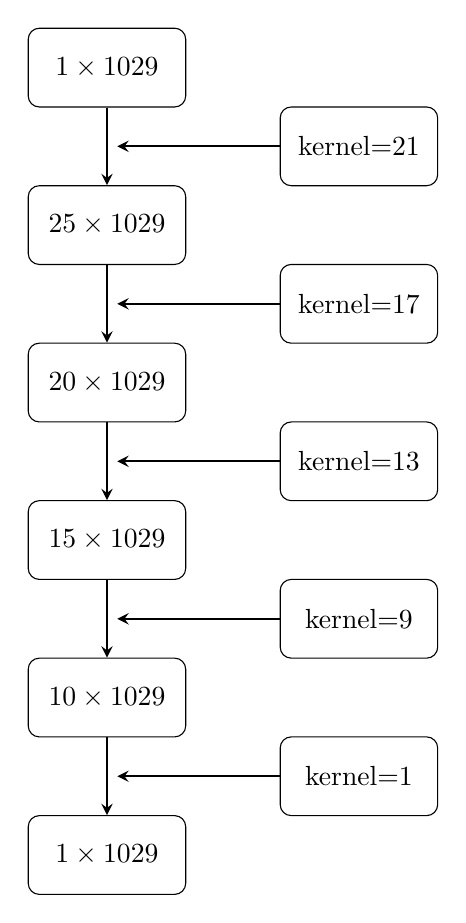
\begin{tikzpicture}[node distance=2cm]
    \node (0) [block] {$1\times1029$};
    \node (1) [block, below of=0] {$25\times1029$};
    \node (2) [block, below of=1] {$20\times1029$};
    \node (3) [block, below of=2] {$15\times1029$};
    \node (4) [block, below of=3] {$10\times1029$};
    \node (5) [block, below of=4] {$1\times1029$};
    \draw [arrow] (0) -- node [midway](0to1) {} (1);
    \draw [arrow] (1) -- node [midway](1to2) {} (2);
    \draw [arrow] (2) -- node [midway](2to3) {} (3);
    \draw [arrow] (3) -- node [midway](3to4) {} (4);
    \draw [arrow] (4) -- node [midway](4to5) {} (5);
    \node (a) [block, right of=0to1, xshift=1.2cm] {kernel=$21$};
    \node (b) [block, right of=1to2, xshift=1.2cm] {kernel=$17$};
    \node (c) [block, right of=2to3, xshift=1.2cm] {kernel=$13$};
    \node (d) [block, right of=3to4, xshift=1.2cm] {kernel=$9$};
    \node (e) [block, right of=4to5, xshift=1.2cm] {kernel=$1$};
    \draw [arrow] (a) -- (0to1) {};
    \draw [arrow] (b) -- (1to2) {};
    \draw [arrow] (c) -- (2to3) {};
    \draw [arrow] (d) -- (3to4) {};
    \draw [arrow] (e) -- (4to5) {};
\end{tikzpicture}
    \end{adjustbox}
    \caption{\label{fig:struct} Structure of the neural network.}
  \end{subfigure}
  \begin{subfigure}{.5\textwidth}
    \centering
    \resizebox{\textwidth}{!}{version https://git-lfs.github.com/spec/v1
oid sha256:73951bc6ffdd6eeb65da3a90d8fe1d632cd9229743e7cf4c70a83604012baa97
size 35431
}
    \caption{\label{fig:loss} Evolution of loss.}
  \end{subfigure}
  \caption{\label{fig:CNN} Training process of a CNN. A shallow network structure of 5 layers in~\subref{fig:struct} is trained to converge in Wasserstein distance as shown in~\subref{fig:loss}.}
\end{figure}

\vspace{-0.5cm}
In figure~\ref{fig:cnn-npe}, we use box plot to describe $D_w$ distributions. From figure~\ref{fig:cnn-npe}, we find $D_w$ is the smallest for one PE.  $D_w$ stops increasing with $N_\mathrm{PE}$ at about 6 PEs, where the PE times are the most challenging to extract.  When the number of PEs is more than 6, pile-ups tend to produce a continuous waveform and the average PE time accuracy stays flat. Thus waveform analysis is the most important in recovering time accuracy for PEs less than 10.

Such small $D_w$ in figure~\ref{fig:cnn-npe} provides a precise matching of waveforms horizontally to guarantee effective $\hat{\alpha}$ scaling, explaining why $\mathrm{RSS}$ is also small in figure~\ref{fig:cnn}.

\begin{figure}[H]
  \begin{subfigure}{.5\textwidth}
    \centering
    \resizebox{\textwidth}{!}{%% Creator: Matplotlib, PGF backend
%%
%% To include the figure in your LaTeX document, write
%%   \input{<filename>.pgf}
%%
%% Make sure the required packages are loaded in your preamble
%%   \usepackage{pgf}
%%
%% and, on pdftex
%%   \usepackage[utf8]{inputenc}\DeclareUnicodeCharacter{2212}{-}
%%
%% or, on luatex and xetex
%%   \usepackage{unicode-math}
%%
%% Figures using additional raster images can only be included by \input if
%% they are in the same directory as the main LaTeX file. For loading figures
%% from other directories you can use the `import` package
%%   \usepackage{import}
%%
%% and then include the figures with
%%   \import{<path to file>}{<filename>.pgf}
%%
%% Matplotlib used the following preamble
%%   \usepackage[detect-all,locale=DE]{siunitx}
%%
\begingroup%
\makeatletter%
\begin{pgfpicture}%
\pgfpathrectangle{\pgfpointorigin}{\pgfqpoint{8.000000in}{6.000000in}}%
\pgfusepath{use as bounding box, clip}%
\begin{pgfscope}%
\pgfsetbuttcap%
\pgfsetmiterjoin%
\definecolor{currentfill}{rgb}{1.000000,1.000000,1.000000}%
\pgfsetfillcolor{currentfill}%
\pgfsetlinewidth{0.000000pt}%
\definecolor{currentstroke}{rgb}{1.000000,1.000000,1.000000}%
\pgfsetstrokecolor{currentstroke}%
\pgfsetdash{}{0pt}%
\pgfpathmoveto{\pgfqpoint{0.000000in}{0.000000in}}%
\pgfpathlineto{\pgfqpoint{8.000000in}{0.000000in}}%
\pgfpathlineto{\pgfqpoint{8.000000in}{6.000000in}}%
\pgfpathlineto{\pgfqpoint{0.000000in}{6.000000in}}%
\pgfpathclose%
\pgfusepath{fill}%
\end{pgfscope}%
\begin{pgfscope}%
\pgfsetbuttcap%
\pgfsetmiterjoin%
\definecolor{currentfill}{rgb}{1.000000,1.000000,1.000000}%
\pgfsetfillcolor{currentfill}%
\pgfsetlinewidth{0.000000pt}%
\definecolor{currentstroke}{rgb}{0.000000,0.000000,0.000000}%
\pgfsetstrokecolor{currentstroke}%
\pgfsetstrokeopacity{0.000000}%
\pgfsetdash{}{0pt}%
\pgfpathmoveto{\pgfqpoint{1.200000in}{0.900000in}}%
\pgfpathlineto{\pgfqpoint{6.800000in}{0.900000in}}%
\pgfpathlineto{\pgfqpoint{6.800000in}{5.700000in}}%
\pgfpathlineto{\pgfqpoint{1.200000in}{5.700000in}}%
\pgfpathclose%
\pgfusepath{fill}%
\end{pgfscope}%
\begin{pgfscope}%
\pgfpathrectangle{\pgfqpoint{1.200000in}{0.900000in}}{\pgfqpoint{5.600000in}{4.800000in}}%
\pgfusepath{clip}%
\pgfsetbuttcap%
\pgfsetroundjoin%
\pgfsetlinewidth{1.003750pt}%
\definecolor{currentstroke}{rgb}{0.000000,0.000000,1.000000}%
\pgfsetstrokecolor{currentstroke}%
\pgfsetdash{{6.000000pt}{6.000000pt}}{0.000000pt}%
\pgfpathmoveto{\pgfqpoint{1.789474in}{1.451297in}}%
\pgfpathlineto{\pgfqpoint{1.789474in}{0.926813in}}%
\pgfusepath{stroke}%
\end{pgfscope}%
\begin{pgfscope}%
\pgfpathrectangle{\pgfqpoint{1.200000in}{0.900000in}}{\pgfqpoint{5.600000in}{4.800000in}}%
\pgfusepath{clip}%
\pgfsetbuttcap%
\pgfsetroundjoin%
\pgfsetlinewidth{1.003750pt}%
\definecolor{currentstroke}{rgb}{0.000000,0.000000,1.000000}%
\pgfsetstrokecolor{currentstroke}%
\pgfsetdash{{6.000000pt}{6.000000pt}}{0.000000pt}%
\pgfpathmoveto{\pgfqpoint{1.789474in}{2.578695in}}%
\pgfpathlineto{\pgfqpoint{1.789474in}{4.083740in}}%
\pgfusepath{stroke}%
\end{pgfscope}%
\begin{pgfscope}%
\pgfpathrectangle{\pgfqpoint{1.200000in}{0.900000in}}{\pgfqpoint{5.600000in}{4.800000in}}%
\pgfusepath{clip}%
\pgfsetrectcap%
\pgfsetroundjoin%
\pgfsetlinewidth{1.003750pt}%
\definecolor{currentstroke}{rgb}{0.000000,0.000000,0.000000}%
\pgfsetstrokecolor{currentstroke}%
\pgfsetdash{}{0pt}%
\pgfpathmoveto{\pgfqpoint{1.752632in}{0.926813in}}%
\pgfpathlineto{\pgfqpoint{1.826316in}{0.926813in}}%
\pgfusepath{stroke}%
\end{pgfscope}%
\begin{pgfscope}%
\pgfpathrectangle{\pgfqpoint{1.200000in}{0.900000in}}{\pgfqpoint{5.600000in}{4.800000in}}%
\pgfusepath{clip}%
\pgfsetrectcap%
\pgfsetroundjoin%
\pgfsetlinewidth{1.003750pt}%
\definecolor{currentstroke}{rgb}{0.000000,0.000000,0.000000}%
\pgfsetstrokecolor{currentstroke}%
\pgfsetdash{}{0pt}%
\pgfpathmoveto{\pgfqpoint{1.752632in}{4.083740in}}%
\pgfpathlineto{\pgfqpoint{1.826316in}{4.083740in}}%
\pgfusepath{stroke}%
\end{pgfscope}%
\begin{pgfscope}%
\pgfpathrectangle{\pgfqpoint{1.200000in}{0.900000in}}{\pgfqpoint{5.600000in}{4.800000in}}%
\pgfusepath{clip}%
\pgfsetbuttcap%
\pgfsetroundjoin%
\pgfsetlinewidth{1.003750pt}%
\definecolor{currentstroke}{rgb}{0.000000,0.000000,1.000000}%
\pgfsetstrokecolor{currentstroke}%
\pgfsetdash{{6.000000pt}{6.000000pt}}{0.000000pt}%
\pgfpathmoveto{\pgfqpoint{2.084211in}{2.151508in}}%
\pgfpathlineto{\pgfqpoint{2.084211in}{0.949024in}}%
\pgfusepath{stroke}%
\end{pgfscope}%
\begin{pgfscope}%
\pgfpathrectangle{\pgfqpoint{1.200000in}{0.900000in}}{\pgfqpoint{5.600000in}{4.800000in}}%
\pgfusepath{clip}%
\pgfsetbuttcap%
\pgfsetroundjoin%
\pgfsetlinewidth{1.003750pt}%
\definecolor{currentstroke}{rgb}{0.000000,0.000000,1.000000}%
\pgfsetstrokecolor{currentstroke}%
\pgfsetdash{{6.000000pt}{6.000000pt}}{0.000000pt}%
\pgfpathmoveto{\pgfqpoint{2.084211in}{3.293548in}}%
\pgfpathlineto{\pgfqpoint{2.084211in}{5.006041in}}%
\pgfusepath{stroke}%
\end{pgfscope}%
\begin{pgfscope}%
\pgfpathrectangle{\pgfqpoint{1.200000in}{0.900000in}}{\pgfqpoint{5.600000in}{4.800000in}}%
\pgfusepath{clip}%
\pgfsetrectcap%
\pgfsetroundjoin%
\pgfsetlinewidth{1.003750pt}%
\definecolor{currentstroke}{rgb}{0.000000,0.000000,0.000000}%
\pgfsetstrokecolor{currentstroke}%
\pgfsetdash{}{0pt}%
\pgfpathmoveto{\pgfqpoint{2.047368in}{0.949024in}}%
\pgfpathlineto{\pgfqpoint{2.121053in}{0.949024in}}%
\pgfusepath{stroke}%
\end{pgfscope}%
\begin{pgfscope}%
\pgfpathrectangle{\pgfqpoint{1.200000in}{0.900000in}}{\pgfqpoint{5.600000in}{4.800000in}}%
\pgfusepath{clip}%
\pgfsetrectcap%
\pgfsetroundjoin%
\pgfsetlinewidth{1.003750pt}%
\definecolor{currentstroke}{rgb}{0.000000,0.000000,0.000000}%
\pgfsetstrokecolor{currentstroke}%
\pgfsetdash{}{0pt}%
\pgfpathmoveto{\pgfqpoint{2.047368in}{5.006041in}}%
\pgfpathlineto{\pgfqpoint{2.121053in}{5.006041in}}%
\pgfusepath{stroke}%
\end{pgfscope}%
\begin{pgfscope}%
\pgfpathrectangle{\pgfqpoint{1.200000in}{0.900000in}}{\pgfqpoint{5.600000in}{4.800000in}}%
\pgfusepath{clip}%
\pgfsetbuttcap%
\pgfsetroundjoin%
\pgfsetlinewidth{1.003750pt}%
\definecolor{currentstroke}{rgb}{0.000000,0.000000,1.000000}%
\pgfsetstrokecolor{currentstroke}%
\pgfsetdash{{6.000000pt}{6.000000pt}}{0.000000pt}%
\pgfpathmoveto{\pgfqpoint{2.378947in}{2.491092in}}%
\pgfpathlineto{\pgfqpoint{2.378947in}{1.292644in}}%
\pgfusepath{stroke}%
\end{pgfscope}%
\begin{pgfscope}%
\pgfpathrectangle{\pgfqpoint{1.200000in}{0.900000in}}{\pgfqpoint{5.600000in}{4.800000in}}%
\pgfusepath{clip}%
\pgfsetbuttcap%
\pgfsetroundjoin%
\pgfsetlinewidth{1.003750pt}%
\definecolor{currentstroke}{rgb}{0.000000,0.000000,1.000000}%
\pgfsetstrokecolor{currentstroke}%
\pgfsetdash{{6.000000pt}{6.000000pt}}{0.000000pt}%
\pgfpathmoveto{\pgfqpoint{2.378947in}{3.496755in}}%
\pgfpathlineto{\pgfqpoint{2.378947in}{4.984562in}}%
\pgfusepath{stroke}%
\end{pgfscope}%
\begin{pgfscope}%
\pgfpathrectangle{\pgfqpoint{1.200000in}{0.900000in}}{\pgfqpoint{5.600000in}{4.800000in}}%
\pgfusepath{clip}%
\pgfsetrectcap%
\pgfsetroundjoin%
\pgfsetlinewidth{1.003750pt}%
\definecolor{currentstroke}{rgb}{0.000000,0.000000,0.000000}%
\pgfsetstrokecolor{currentstroke}%
\pgfsetdash{}{0pt}%
\pgfpathmoveto{\pgfqpoint{2.342105in}{1.292644in}}%
\pgfpathlineto{\pgfqpoint{2.415789in}{1.292644in}}%
\pgfusepath{stroke}%
\end{pgfscope}%
\begin{pgfscope}%
\pgfpathrectangle{\pgfqpoint{1.200000in}{0.900000in}}{\pgfqpoint{5.600000in}{4.800000in}}%
\pgfusepath{clip}%
\pgfsetrectcap%
\pgfsetroundjoin%
\pgfsetlinewidth{1.003750pt}%
\definecolor{currentstroke}{rgb}{0.000000,0.000000,0.000000}%
\pgfsetstrokecolor{currentstroke}%
\pgfsetdash{}{0pt}%
\pgfpathmoveto{\pgfqpoint{2.342105in}{4.984562in}}%
\pgfpathlineto{\pgfqpoint{2.415789in}{4.984562in}}%
\pgfusepath{stroke}%
\end{pgfscope}%
\begin{pgfscope}%
\pgfpathrectangle{\pgfqpoint{1.200000in}{0.900000in}}{\pgfqpoint{5.600000in}{4.800000in}}%
\pgfusepath{clip}%
\pgfsetbuttcap%
\pgfsetroundjoin%
\pgfsetlinewidth{1.003750pt}%
\definecolor{currentstroke}{rgb}{0.000000,0.000000,1.000000}%
\pgfsetstrokecolor{currentstroke}%
\pgfsetdash{{6.000000pt}{6.000000pt}}{0.000000pt}%
\pgfpathmoveto{\pgfqpoint{2.673684in}{2.644277in}}%
\pgfpathlineto{\pgfqpoint{2.673684in}{1.595563in}}%
\pgfusepath{stroke}%
\end{pgfscope}%
\begin{pgfscope}%
\pgfpathrectangle{\pgfqpoint{1.200000in}{0.900000in}}{\pgfqpoint{5.600000in}{4.800000in}}%
\pgfusepath{clip}%
\pgfsetbuttcap%
\pgfsetroundjoin%
\pgfsetlinewidth{1.003750pt}%
\definecolor{currentstroke}{rgb}{0.000000,0.000000,1.000000}%
\pgfsetstrokecolor{currentstroke}%
\pgfsetdash{{6.000000pt}{6.000000pt}}{0.000000pt}%
\pgfpathmoveto{\pgfqpoint{2.673684in}{3.589533in}}%
\pgfpathlineto{\pgfqpoint{2.673684in}{4.949122in}}%
\pgfusepath{stroke}%
\end{pgfscope}%
\begin{pgfscope}%
\pgfpathrectangle{\pgfqpoint{1.200000in}{0.900000in}}{\pgfqpoint{5.600000in}{4.800000in}}%
\pgfusepath{clip}%
\pgfsetrectcap%
\pgfsetroundjoin%
\pgfsetlinewidth{1.003750pt}%
\definecolor{currentstroke}{rgb}{0.000000,0.000000,0.000000}%
\pgfsetstrokecolor{currentstroke}%
\pgfsetdash{}{0pt}%
\pgfpathmoveto{\pgfqpoint{2.636842in}{1.595563in}}%
\pgfpathlineto{\pgfqpoint{2.710526in}{1.595563in}}%
\pgfusepath{stroke}%
\end{pgfscope}%
\begin{pgfscope}%
\pgfpathrectangle{\pgfqpoint{1.200000in}{0.900000in}}{\pgfqpoint{5.600000in}{4.800000in}}%
\pgfusepath{clip}%
\pgfsetrectcap%
\pgfsetroundjoin%
\pgfsetlinewidth{1.003750pt}%
\definecolor{currentstroke}{rgb}{0.000000,0.000000,0.000000}%
\pgfsetstrokecolor{currentstroke}%
\pgfsetdash{}{0pt}%
\pgfpathmoveto{\pgfqpoint{2.636842in}{4.949122in}}%
\pgfpathlineto{\pgfqpoint{2.710526in}{4.949122in}}%
\pgfusepath{stroke}%
\end{pgfscope}%
\begin{pgfscope}%
\pgfpathrectangle{\pgfqpoint{1.200000in}{0.900000in}}{\pgfqpoint{5.600000in}{4.800000in}}%
\pgfusepath{clip}%
\pgfsetbuttcap%
\pgfsetroundjoin%
\pgfsetlinewidth{1.003750pt}%
\definecolor{currentstroke}{rgb}{0.000000,0.000000,1.000000}%
\pgfsetstrokecolor{currentstroke}%
\pgfsetdash{{6.000000pt}{6.000000pt}}{0.000000pt}%
\pgfpathmoveto{\pgfqpoint{2.968421in}{2.760790in}}%
\pgfpathlineto{\pgfqpoint{2.968421in}{1.794585in}}%
\pgfusepath{stroke}%
\end{pgfscope}%
\begin{pgfscope}%
\pgfpathrectangle{\pgfqpoint{1.200000in}{0.900000in}}{\pgfqpoint{5.600000in}{4.800000in}}%
\pgfusepath{clip}%
\pgfsetbuttcap%
\pgfsetroundjoin%
\pgfsetlinewidth{1.003750pt}%
\definecolor{currentstroke}{rgb}{0.000000,0.000000,1.000000}%
\pgfsetstrokecolor{currentstroke}%
\pgfsetdash{{6.000000pt}{6.000000pt}}{0.000000pt}%
\pgfpathmoveto{\pgfqpoint{2.968421in}{3.650464in}}%
\pgfpathlineto{\pgfqpoint{2.968421in}{4.981272in}}%
\pgfusepath{stroke}%
\end{pgfscope}%
\begin{pgfscope}%
\pgfpathrectangle{\pgfqpoint{1.200000in}{0.900000in}}{\pgfqpoint{5.600000in}{4.800000in}}%
\pgfusepath{clip}%
\pgfsetrectcap%
\pgfsetroundjoin%
\pgfsetlinewidth{1.003750pt}%
\definecolor{currentstroke}{rgb}{0.000000,0.000000,0.000000}%
\pgfsetstrokecolor{currentstroke}%
\pgfsetdash{}{0pt}%
\pgfpathmoveto{\pgfqpoint{2.931579in}{1.794585in}}%
\pgfpathlineto{\pgfqpoint{3.005263in}{1.794585in}}%
\pgfusepath{stroke}%
\end{pgfscope}%
\begin{pgfscope}%
\pgfpathrectangle{\pgfqpoint{1.200000in}{0.900000in}}{\pgfqpoint{5.600000in}{4.800000in}}%
\pgfusepath{clip}%
\pgfsetrectcap%
\pgfsetroundjoin%
\pgfsetlinewidth{1.003750pt}%
\definecolor{currentstroke}{rgb}{0.000000,0.000000,0.000000}%
\pgfsetstrokecolor{currentstroke}%
\pgfsetdash{}{0pt}%
\pgfpathmoveto{\pgfqpoint{2.931579in}{4.981272in}}%
\pgfpathlineto{\pgfqpoint{3.005263in}{4.981272in}}%
\pgfusepath{stroke}%
\end{pgfscope}%
\begin{pgfscope}%
\pgfpathrectangle{\pgfqpoint{1.200000in}{0.900000in}}{\pgfqpoint{5.600000in}{4.800000in}}%
\pgfusepath{clip}%
\pgfsetbuttcap%
\pgfsetroundjoin%
\pgfsetlinewidth{1.003750pt}%
\definecolor{currentstroke}{rgb}{0.000000,0.000000,1.000000}%
\pgfsetstrokecolor{currentstroke}%
\pgfsetdash{{6.000000pt}{6.000000pt}}{0.000000pt}%
\pgfpathmoveto{\pgfqpoint{3.263158in}{2.815825in}}%
\pgfpathlineto{\pgfqpoint{3.263158in}{1.754251in}}%
\pgfusepath{stroke}%
\end{pgfscope}%
\begin{pgfscope}%
\pgfpathrectangle{\pgfqpoint{1.200000in}{0.900000in}}{\pgfqpoint{5.600000in}{4.800000in}}%
\pgfusepath{clip}%
\pgfsetbuttcap%
\pgfsetroundjoin%
\pgfsetlinewidth{1.003750pt}%
\definecolor{currentstroke}{rgb}{0.000000,0.000000,1.000000}%
\pgfsetstrokecolor{currentstroke}%
\pgfsetdash{{6.000000pt}{6.000000pt}}{0.000000pt}%
\pgfpathmoveto{\pgfqpoint{3.263158in}{3.623093in}}%
\pgfpathlineto{\pgfqpoint{3.263158in}{4.830075in}}%
\pgfusepath{stroke}%
\end{pgfscope}%
\begin{pgfscope}%
\pgfpathrectangle{\pgfqpoint{1.200000in}{0.900000in}}{\pgfqpoint{5.600000in}{4.800000in}}%
\pgfusepath{clip}%
\pgfsetrectcap%
\pgfsetroundjoin%
\pgfsetlinewidth{1.003750pt}%
\definecolor{currentstroke}{rgb}{0.000000,0.000000,0.000000}%
\pgfsetstrokecolor{currentstroke}%
\pgfsetdash{}{0pt}%
\pgfpathmoveto{\pgfqpoint{3.226316in}{1.754251in}}%
\pgfpathlineto{\pgfqpoint{3.300000in}{1.754251in}}%
\pgfusepath{stroke}%
\end{pgfscope}%
\begin{pgfscope}%
\pgfpathrectangle{\pgfqpoint{1.200000in}{0.900000in}}{\pgfqpoint{5.600000in}{4.800000in}}%
\pgfusepath{clip}%
\pgfsetrectcap%
\pgfsetroundjoin%
\pgfsetlinewidth{1.003750pt}%
\definecolor{currentstroke}{rgb}{0.000000,0.000000,0.000000}%
\pgfsetstrokecolor{currentstroke}%
\pgfsetdash{}{0pt}%
\pgfpathmoveto{\pgfqpoint{3.226316in}{4.830075in}}%
\pgfpathlineto{\pgfqpoint{3.300000in}{4.830075in}}%
\pgfusepath{stroke}%
\end{pgfscope}%
\begin{pgfscope}%
\pgfpathrectangle{\pgfqpoint{1.200000in}{0.900000in}}{\pgfqpoint{5.600000in}{4.800000in}}%
\pgfusepath{clip}%
\pgfsetbuttcap%
\pgfsetroundjoin%
\pgfsetlinewidth{1.003750pt}%
\definecolor{currentstroke}{rgb}{0.000000,0.000000,1.000000}%
\pgfsetstrokecolor{currentstroke}%
\pgfsetdash{{6.000000pt}{6.000000pt}}{0.000000pt}%
\pgfpathmoveto{\pgfqpoint{3.557895in}{2.906672in}}%
\pgfpathlineto{\pgfqpoint{3.557895in}{1.976729in}}%
\pgfusepath{stroke}%
\end{pgfscope}%
\begin{pgfscope}%
\pgfpathrectangle{\pgfqpoint{1.200000in}{0.900000in}}{\pgfqpoint{5.600000in}{4.800000in}}%
\pgfusepath{clip}%
\pgfsetbuttcap%
\pgfsetroundjoin%
\pgfsetlinewidth{1.003750pt}%
\definecolor{currentstroke}{rgb}{0.000000,0.000000,1.000000}%
\pgfsetstrokecolor{currentstroke}%
\pgfsetdash{{6.000000pt}{6.000000pt}}{0.000000pt}%
\pgfpathmoveto{\pgfqpoint{3.557895in}{3.653824in}}%
\pgfpathlineto{\pgfqpoint{3.557895in}{4.755740in}}%
\pgfusepath{stroke}%
\end{pgfscope}%
\begin{pgfscope}%
\pgfpathrectangle{\pgfqpoint{1.200000in}{0.900000in}}{\pgfqpoint{5.600000in}{4.800000in}}%
\pgfusepath{clip}%
\pgfsetrectcap%
\pgfsetroundjoin%
\pgfsetlinewidth{1.003750pt}%
\definecolor{currentstroke}{rgb}{0.000000,0.000000,0.000000}%
\pgfsetstrokecolor{currentstroke}%
\pgfsetdash{}{0pt}%
\pgfpathmoveto{\pgfqpoint{3.521053in}{1.976729in}}%
\pgfpathlineto{\pgfqpoint{3.594737in}{1.976729in}}%
\pgfusepath{stroke}%
\end{pgfscope}%
\begin{pgfscope}%
\pgfpathrectangle{\pgfqpoint{1.200000in}{0.900000in}}{\pgfqpoint{5.600000in}{4.800000in}}%
\pgfusepath{clip}%
\pgfsetrectcap%
\pgfsetroundjoin%
\pgfsetlinewidth{1.003750pt}%
\definecolor{currentstroke}{rgb}{0.000000,0.000000,0.000000}%
\pgfsetstrokecolor{currentstroke}%
\pgfsetdash{}{0pt}%
\pgfpathmoveto{\pgfqpoint{3.521053in}{4.755740in}}%
\pgfpathlineto{\pgfqpoint{3.594737in}{4.755740in}}%
\pgfusepath{stroke}%
\end{pgfscope}%
\begin{pgfscope}%
\pgfpathrectangle{\pgfqpoint{1.200000in}{0.900000in}}{\pgfqpoint{5.600000in}{4.800000in}}%
\pgfusepath{clip}%
\pgfsetbuttcap%
\pgfsetroundjoin%
\pgfsetlinewidth{1.003750pt}%
\definecolor{currentstroke}{rgb}{0.000000,0.000000,1.000000}%
\pgfsetstrokecolor{currentstroke}%
\pgfsetdash{{6.000000pt}{6.000000pt}}{0.000000pt}%
\pgfpathmoveto{\pgfqpoint{3.852632in}{2.920793in}}%
\pgfpathlineto{\pgfqpoint{3.852632in}{1.968834in}}%
\pgfusepath{stroke}%
\end{pgfscope}%
\begin{pgfscope}%
\pgfpathrectangle{\pgfqpoint{1.200000in}{0.900000in}}{\pgfqpoint{5.600000in}{4.800000in}}%
\pgfusepath{clip}%
\pgfsetbuttcap%
\pgfsetroundjoin%
\pgfsetlinewidth{1.003750pt}%
\definecolor{currentstroke}{rgb}{0.000000,0.000000,1.000000}%
\pgfsetstrokecolor{currentstroke}%
\pgfsetdash{{6.000000pt}{6.000000pt}}{0.000000pt}%
\pgfpathmoveto{\pgfqpoint{3.852632in}{3.652953in}}%
\pgfpathlineto{\pgfqpoint{3.852632in}{4.710205in}}%
\pgfusepath{stroke}%
\end{pgfscope}%
\begin{pgfscope}%
\pgfpathrectangle{\pgfqpoint{1.200000in}{0.900000in}}{\pgfqpoint{5.600000in}{4.800000in}}%
\pgfusepath{clip}%
\pgfsetrectcap%
\pgfsetroundjoin%
\pgfsetlinewidth{1.003750pt}%
\definecolor{currentstroke}{rgb}{0.000000,0.000000,0.000000}%
\pgfsetstrokecolor{currentstroke}%
\pgfsetdash{}{0pt}%
\pgfpathmoveto{\pgfqpoint{3.815789in}{1.968834in}}%
\pgfpathlineto{\pgfqpoint{3.889474in}{1.968834in}}%
\pgfusepath{stroke}%
\end{pgfscope}%
\begin{pgfscope}%
\pgfpathrectangle{\pgfqpoint{1.200000in}{0.900000in}}{\pgfqpoint{5.600000in}{4.800000in}}%
\pgfusepath{clip}%
\pgfsetrectcap%
\pgfsetroundjoin%
\pgfsetlinewidth{1.003750pt}%
\definecolor{currentstroke}{rgb}{0.000000,0.000000,0.000000}%
\pgfsetstrokecolor{currentstroke}%
\pgfsetdash{}{0pt}%
\pgfpathmoveto{\pgfqpoint{3.815789in}{4.710205in}}%
\pgfpathlineto{\pgfqpoint{3.889474in}{4.710205in}}%
\pgfusepath{stroke}%
\end{pgfscope}%
\begin{pgfscope}%
\pgfpathrectangle{\pgfqpoint{1.200000in}{0.900000in}}{\pgfqpoint{5.600000in}{4.800000in}}%
\pgfusepath{clip}%
\pgfsetbuttcap%
\pgfsetroundjoin%
\pgfsetlinewidth{1.003750pt}%
\definecolor{currentstroke}{rgb}{0.000000,0.000000,1.000000}%
\pgfsetstrokecolor{currentstroke}%
\pgfsetdash{{6.000000pt}{6.000000pt}}{0.000000pt}%
\pgfpathmoveto{\pgfqpoint{4.147368in}{3.041567in}}%
\pgfpathlineto{\pgfqpoint{4.147368in}{2.287572in}}%
\pgfusepath{stroke}%
\end{pgfscope}%
\begin{pgfscope}%
\pgfpathrectangle{\pgfqpoint{1.200000in}{0.900000in}}{\pgfqpoint{5.600000in}{4.800000in}}%
\pgfusepath{clip}%
\pgfsetbuttcap%
\pgfsetroundjoin%
\pgfsetlinewidth{1.003750pt}%
\definecolor{currentstroke}{rgb}{0.000000,0.000000,1.000000}%
\pgfsetstrokecolor{currentstroke}%
\pgfsetdash{{6.000000pt}{6.000000pt}}{0.000000pt}%
\pgfpathmoveto{\pgfqpoint{4.147368in}{3.718268in}}%
\pgfpathlineto{\pgfqpoint{4.147368in}{4.719618in}}%
\pgfusepath{stroke}%
\end{pgfscope}%
\begin{pgfscope}%
\pgfpathrectangle{\pgfqpoint{1.200000in}{0.900000in}}{\pgfqpoint{5.600000in}{4.800000in}}%
\pgfusepath{clip}%
\pgfsetrectcap%
\pgfsetroundjoin%
\pgfsetlinewidth{1.003750pt}%
\definecolor{currentstroke}{rgb}{0.000000,0.000000,0.000000}%
\pgfsetstrokecolor{currentstroke}%
\pgfsetdash{}{0pt}%
\pgfpathmoveto{\pgfqpoint{4.110526in}{2.287572in}}%
\pgfpathlineto{\pgfqpoint{4.184211in}{2.287572in}}%
\pgfusepath{stroke}%
\end{pgfscope}%
\begin{pgfscope}%
\pgfpathrectangle{\pgfqpoint{1.200000in}{0.900000in}}{\pgfqpoint{5.600000in}{4.800000in}}%
\pgfusepath{clip}%
\pgfsetrectcap%
\pgfsetroundjoin%
\pgfsetlinewidth{1.003750pt}%
\definecolor{currentstroke}{rgb}{0.000000,0.000000,0.000000}%
\pgfsetstrokecolor{currentstroke}%
\pgfsetdash{}{0pt}%
\pgfpathmoveto{\pgfqpoint{4.110526in}{4.719618in}}%
\pgfpathlineto{\pgfqpoint{4.184211in}{4.719618in}}%
\pgfusepath{stroke}%
\end{pgfscope}%
\begin{pgfscope}%
\pgfpathrectangle{\pgfqpoint{1.200000in}{0.900000in}}{\pgfqpoint{5.600000in}{4.800000in}}%
\pgfusepath{clip}%
\pgfsetbuttcap%
\pgfsetroundjoin%
\pgfsetlinewidth{1.003750pt}%
\definecolor{currentstroke}{rgb}{0.000000,0.000000,1.000000}%
\pgfsetstrokecolor{currentstroke}%
\pgfsetdash{{6.000000pt}{6.000000pt}}{0.000000pt}%
\pgfpathmoveto{\pgfqpoint{4.442105in}{3.028589in}}%
\pgfpathlineto{\pgfqpoint{4.442105in}{2.289877in}}%
\pgfusepath{stroke}%
\end{pgfscope}%
\begin{pgfscope}%
\pgfpathrectangle{\pgfqpoint{1.200000in}{0.900000in}}{\pgfqpoint{5.600000in}{4.800000in}}%
\pgfusepath{clip}%
\pgfsetbuttcap%
\pgfsetroundjoin%
\pgfsetlinewidth{1.003750pt}%
\definecolor{currentstroke}{rgb}{0.000000,0.000000,1.000000}%
\pgfsetstrokecolor{currentstroke}%
\pgfsetdash{{6.000000pt}{6.000000pt}}{0.000000pt}%
\pgfpathmoveto{\pgfqpoint{4.442105in}{3.679035in}}%
\pgfpathlineto{\pgfqpoint{4.442105in}{4.603787in}}%
\pgfusepath{stroke}%
\end{pgfscope}%
\begin{pgfscope}%
\pgfpathrectangle{\pgfqpoint{1.200000in}{0.900000in}}{\pgfqpoint{5.600000in}{4.800000in}}%
\pgfusepath{clip}%
\pgfsetrectcap%
\pgfsetroundjoin%
\pgfsetlinewidth{1.003750pt}%
\definecolor{currentstroke}{rgb}{0.000000,0.000000,0.000000}%
\pgfsetstrokecolor{currentstroke}%
\pgfsetdash{}{0pt}%
\pgfpathmoveto{\pgfqpoint{4.405263in}{2.289877in}}%
\pgfpathlineto{\pgfqpoint{4.478947in}{2.289877in}}%
\pgfusepath{stroke}%
\end{pgfscope}%
\begin{pgfscope}%
\pgfpathrectangle{\pgfqpoint{1.200000in}{0.900000in}}{\pgfqpoint{5.600000in}{4.800000in}}%
\pgfusepath{clip}%
\pgfsetrectcap%
\pgfsetroundjoin%
\pgfsetlinewidth{1.003750pt}%
\definecolor{currentstroke}{rgb}{0.000000,0.000000,0.000000}%
\pgfsetstrokecolor{currentstroke}%
\pgfsetdash{}{0pt}%
\pgfpathmoveto{\pgfqpoint{4.405263in}{4.603787in}}%
\pgfpathlineto{\pgfqpoint{4.478947in}{4.603787in}}%
\pgfusepath{stroke}%
\end{pgfscope}%
\begin{pgfscope}%
\pgfpathrectangle{\pgfqpoint{1.200000in}{0.900000in}}{\pgfqpoint{5.600000in}{4.800000in}}%
\pgfusepath{clip}%
\pgfsetbuttcap%
\pgfsetroundjoin%
\pgfsetlinewidth{1.003750pt}%
\definecolor{currentstroke}{rgb}{0.000000,0.000000,1.000000}%
\pgfsetstrokecolor{currentstroke}%
\pgfsetdash{{6.000000pt}{6.000000pt}}{0.000000pt}%
\pgfpathmoveto{\pgfqpoint{4.736842in}{3.025016in}}%
\pgfpathlineto{\pgfqpoint{4.736842in}{2.553360in}}%
\pgfusepath{stroke}%
\end{pgfscope}%
\begin{pgfscope}%
\pgfpathrectangle{\pgfqpoint{1.200000in}{0.900000in}}{\pgfqpoint{5.600000in}{4.800000in}}%
\pgfusepath{clip}%
\pgfsetbuttcap%
\pgfsetroundjoin%
\pgfsetlinewidth{1.003750pt}%
\definecolor{currentstroke}{rgb}{0.000000,0.000000,1.000000}%
\pgfsetstrokecolor{currentstroke}%
\pgfsetdash{{6.000000pt}{6.000000pt}}{0.000000pt}%
\pgfpathmoveto{\pgfqpoint{4.736842in}{3.557869in}}%
\pgfpathlineto{\pgfqpoint{4.736842in}{4.276899in}}%
\pgfusepath{stroke}%
\end{pgfscope}%
\begin{pgfscope}%
\pgfpathrectangle{\pgfqpoint{1.200000in}{0.900000in}}{\pgfqpoint{5.600000in}{4.800000in}}%
\pgfusepath{clip}%
\pgfsetrectcap%
\pgfsetroundjoin%
\pgfsetlinewidth{1.003750pt}%
\definecolor{currentstroke}{rgb}{0.000000,0.000000,0.000000}%
\pgfsetstrokecolor{currentstroke}%
\pgfsetdash{}{0pt}%
\pgfpathmoveto{\pgfqpoint{4.700000in}{2.553360in}}%
\pgfpathlineto{\pgfqpoint{4.773684in}{2.553360in}}%
\pgfusepath{stroke}%
\end{pgfscope}%
\begin{pgfscope}%
\pgfpathrectangle{\pgfqpoint{1.200000in}{0.900000in}}{\pgfqpoint{5.600000in}{4.800000in}}%
\pgfusepath{clip}%
\pgfsetrectcap%
\pgfsetroundjoin%
\pgfsetlinewidth{1.003750pt}%
\definecolor{currentstroke}{rgb}{0.000000,0.000000,0.000000}%
\pgfsetstrokecolor{currentstroke}%
\pgfsetdash{}{0pt}%
\pgfpathmoveto{\pgfqpoint{4.700000in}{4.276899in}}%
\pgfpathlineto{\pgfqpoint{4.773684in}{4.276899in}}%
\pgfusepath{stroke}%
\end{pgfscope}%
\begin{pgfscope}%
\pgfpathrectangle{\pgfqpoint{1.200000in}{0.900000in}}{\pgfqpoint{5.600000in}{4.800000in}}%
\pgfusepath{clip}%
\pgfsetbuttcap%
\pgfsetroundjoin%
\pgfsetlinewidth{1.003750pt}%
\definecolor{currentstroke}{rgb}{0.000000,0.000000,1.000000}%
\pgfsetstrokecolor{currentstroke}%
\pgfsetdash{{6.000000pt}{6.000000pt}}{0.000000pt}%
\pgfpathmoveto{\pgfqpoint{5.031579in}{3.059799in}}%
\pgfpathlineto{\pgfqpoint{5.031579in}{2.819291in}}%
\pgfusepath{stroke}%
\end{pgfscope}%
\begin{pgfscope}%
\pgfpathrectangle{\pgfqpoint{1.200000in}{0.900000in}}{\pgfqpoint{5.600000in}{4.800000in}}%
\pgfusepath{clip}%
\pgfsetbuttcap%
\pgfsetroundjoin%
\pgfsetlinewidth{1.003750pt}%
\definecolor{currentstroke}{rgb}{0.000000,0.000000,1.000000}%
\pgfsetstrokecolor{currentstroke}%
\pgfsetdash{{6.000000pt}{6.000000pt}}{0.000000pt}%
\pgfpathmoveto{\pgfqpoint{5.031579in}{3.724486in}}%
\pgfpathlineto{\pgfqpoint{5.031579in}{4.257433in}}%
\pgfusepath{stroke}%
\end{pgfscope}%
\begin{pgfscope}%
\pgfpathrectangle{\pgfqpoint{1.200000in}{0.900000in}}{\pgfqpoint{5.600000in}{4.800000in}}%
\pgfusepath{clip}%
\pgfsetrectcap%
\pgfsetroundjoin%
\pgfsetlinewidth{1.003750pt}%
\definecolor{currentstroke}{rgb}{0.000000,0.000000,0.000000}%
\pgfsetstrokecolor{currentstroke}%
\pgfsetdash{}{0pt}%
\pgfpathmoveto{\pgfqpoint{4.994737in}{2.819291in}}%
\pgfpathlineto{\pgfqpoint{5.068421in}{2.819291in}}%
\pgfusepath{stroke}%
\end{pgfscope}%
\begin{pgfscope}%
\pgfpathrectangle{\pgfqpoint{1.200000in}{0.900000in}}{\pgfqpoint{5.600000in}{4.800000in}}%
\pgfusepath{clip}%
\pgfsetrectcap%
\pgfsetroundjoin%
\pgfsetlinewidth{1.003750pt}%
\definecolor{currentstroke}{rgb}{0.000000,0.000000,0.000000}%
\pgfsetstrokecolor{currentstroke}%
\pgfsetdash{}{0pt}%
\pgfpathmoveto{\pgfqpoint{4.994737in}{4.257433in}}%
\pgfpathlineto{\pgfqpoint{5.068421in}{4.257433in}}%
\pgfusepath{stroke}%
\end{pgfscope}%
\begin{pgfscope}%
\pgfpathrectangle{\pgfqpoint{1.200000in}{0.900000in}}{\pgfqpoint{5.600000in}{4.800000in}}%
\pgfusepath{clip}%
\pgfsetbuttcap%
\pgfsetroundjoin%
\pgfsetlinewidth{1.003750pt}%
\definecolor{currentstroke}{rgb}{0.000000,0.000000,1.000000}%
\pgfsetstrokecolor{currentstroke}%
\pgfsetdash{{6.000000pt}{6.000000pt}}{0.000000pt}%
\pgfpathmoveto{\pgfqpoint{5.326316in}{3.175489in}}%
\pgfpathlineto{\pgfqpoint{5.326316in}{2.813171in}}%
\pgfusepath{stroke}%
\end{pgfscope}%
\begin{pgfscope}%
\pgfpathrectangle{\pgfqpoint{1.200000in}{0.900000in}}{\pgfqpoint{5.600000in}{4.800000in}}%
\pgfusepath{clip}%
\pgfsetbuttcap%
\pgfsetroundjoin%
\pgfsetlinewidth{1.003750pt}%
\definecolor{currentstroke}{rgb}{0.000000,0.000000,1.000000}%
\pgfsetstrokecolor{currentstroke}%
\pgfsetdash{{6.000000pt}{6.000000pt}}{0.000000pt}%
\pgfpathmoveto{\pgfqpoint{5.326316in}{3.801701in}}%
\pgfpathlineto{\pgfqpoint{5.326316in}{3.914474in}}%
\pgfusepath{stroke}%
\end{pgfscope}%
\begin{pgfscope}%
\pgfpathrectangle{\pgfqpoint{1.200000in}{0.900000in}}{\pgfqpoint{5.600000in}{4.800000in}}%
\pgfusepath{clip}%
\pgfsetrectcap%
\pgfsetroundjoin%
\pgfsetlinewidth{1.003750pt}%
\definecolor{currentstroke}{rgb}{0.000000,0.000000,0.000000}%
\pgfsetstrokecolor{currentstroke}%
\pgfsetdash{}{0pt}%
\pgfpathmoveto{\pgfqpoint{5.289474in}{2.813171in}}%
\pgfpathlineto{\pgfqpoint{5.363158in}{2.813171in}}%
\pgfusepath{stroke}%
\end{pgfscope}%
\begin{pgfscope}%
\pgfpathrectangle{\pgfqpoint{1.200000in}{0.900000in}}{\pgfqpoint{5.600000in}{4.800000in}}%
\pgfusepath{clip}%
\pgfsetrectcap%
\pgfsetroundjoin%
\pgfsetlinewidth{1.003750pt}%
\definecolor{currentstroke}{rgb}{0.000000,0.000000,0.000000}%
\pgfsetstrokecolor{currentstroke}%
\pgfsetdash{}{0pt}%
\pgfpathmoveto{\pgfqpoint{5.289474in}{3.914474in}}%
\pgfpathlineto{\pgfqpoint{5.363158in}{3.914474in}}%
\pgfusepath{stroke}%
\end{pgfscope}%
\begin{pgfscope}%
\pgfpathrectangle{\pgfqpoint{1.200000in}{0.900000in}}{\pgfqpoint{5.600000in}{4.800000in}}%
\pgfusepath{clip}%
\pgfsetbuttcap%
\pgfsetroundjoin%
\pgfsetlinewidth{1.003750pt}%
\definecolor{currentstroke}{rgb}{0.000000,0.000000,1.000000}%
\pgfsetstrokecolor{currentstroke}%
\pgfsetdash{{6.000000pt}{6.000000pt}}{0.000000pt}%
\pgfpathmoveto{\pgfqpoint{5.621053in}{3.099317in}}%
\pgfpathlineto{\pgfqpoint{5.621053in}{2.925145in}}%
\pgfusepath{stroke}%
\end{pgfscope}%
\begin{pgfscope}%
\pgfpathrectangle{\pgfqpoint{1.200000in}{0.900000in}}{\pgfqpoint{5.600000in}{4.800000in}}%
\pgfusepath{clip}%
\pgfsetbuttcap%
\pgfsetroundjoin%
\pgfsetlinewidth{1.003750pt}%
\definecolor{currentstroke}{rgb}{0.000000,0.000000,1.000000}%
\pgfsetstrokecolor{currentstroke}%
\pgfsetdash{{6.000000pt}{6.000000pt}}{0.000000pt}%
\pgfpathmoveto{\pgfqpoint{5.621053in}{3.497327in}}%
\pgfpathlineto{\pgfqpoint{5.621053in}{3.921554in}}%
\pgfusepath{stroke}%
\end{pgfscope}%
\begin{pgfscope}%
\pgfpathrectangle{\pgfqpoint{1.200000in}{0.900000in}}{\pgfqpoint{5.600000in}{4.800000in}}%
\pgfusepath{clip}%
\pgfsetrectcap%
\pgfsetroundjoin%
\pgfsetlinewidth{1.003750pt}%
\definecolor{currentstroke}{rgb}{0.000000,0.000000,0.000000}%
\pgfsetstrokecolor{currentstroke}%
\pgfsetdash{}{0pt}%
\pgfpathmoveto{\pgfqpoint{5.584211in}{2.925145in}}%
\pgfpathlineto{\pgfqpoint{5.657895in}{2.925145in}}%
\pgfusepath{stroke}%
\end{pgfscope}%
\begin{pgfscope}%
\pgfpathrectangle{\pgfqpoint{1.200000in}{0.900000in}}{\pgfqpoint{5.600000in}{4.800000in}}%
\pgfusepath{clip}%
\pgfsetrectcap%
\pgfsetroundjoin%
\pgfsetlinewidth{1.003750pt}%
\definecolor{currentstroke}{rgb}{0.000000,0.000000,0.000000}%
\pgfsetstrokecolor{currentstroke}%
\pgfsetdash{}{0pt}%
\pgfpathmoveto{\pgfqpoint{5.584211in}{3.921554in}}%
\pgfpathlineto{\pgfqpoint{5.657895in}{3.921554in}}%
\pgfusepath{stroke}%
\end{pgfscope}%
\begin{pgfscope}%
\pgfpathrectangle{\pgfqpoint{1.200000in}{0.900000in}}{\pgfqpoint{5.600000in}{4.800000in}}%
\pgfusepath{clip}%
\pgfsetbuttcap%
\pgfsetroundjoin%
\pgfsetlinewidth{1.003750pt}%
\definecolor{currentstroke}{rgb}{0.000000,0.000000,1.000000}%
\pgfsetstrokecolor{currentstroke}%
\pgfsetdash{{6.000000pt}{6.000000pt}}{0.000000pt}%
\pgfpathmoveto{\pgfqpoint{5.915789in}{3.136199in}}%
\pgfpathlineto{\pgfqpoint{5.915789in}{3.136199in}}%
\pgfusepath{stroke}%
\end{pgfscope}%
\begin{pgfscope}%
\pgfpathrectangle{\pgfqpoint{1.200000in}{0.900000in}}{\pgfqpoint{5.600000in}{4.800000in}}%
\pgfusepath{clip}%
\pgfsetbuttcap%
\pgfsetroundjoin%
\pgfsetlinewidth{1.003750pt}%
\definecolor{currentstroke}{rgb}{0.000000,0.000000,1.000000}%
\pgfsetstrokecolor{currentstroke}%
\pgfsetdash{{6.000000pt}{6.000000pt}}{0.000000pt}%
\pgfpathmoveto{\pgfqpoint{5.915789in}{3.136199in}}%
\pgfpathlineto{\pgfqpoint{5.915789in}{3.136199in}}%
\pgfusepath{stroke}%
\end{pgfscope}%
\begin{pgfscope}%
\pgfpathrectangle{\pgfqpoint{1.200000in}{0.900000in}}{\pgfqpoint{5.600000in}{4.800000in}}%
\pgfusepath{clip}%
\pgfsetrectcap%
\pgfsetroundjoin%
\pgfsetlinewidth{1.003750pt}%
\definecolor{currentstroke}{rgb}{0.000000,0.000000,0.000000}%
\pgfsetstrokecolor{currentstroke}%
\pgfsetdash{}{0pt}%
\pgfpathmoveto{\pgfqpoint{5.878947in}{3.136199in}}%
\pgfpathlineto{\pgfqpoint{5.952632in}{3.136199in}}%
\pgfusepath{stroke}%
\end{pgfscope}%
\begin{pgfscope}%
\pgfpathrectangle{\pgfqpoint{1.200000in}{0.900000in}}{\pgfqpoint{5.600000in}{4.800000in}}%
\pgfusepath{clip}%
\pgfsetrectcap%
\pgfsetroundjoin%
\pgfsetlinewidth{1.003750pt}%
\definecolor{currentstroke}{rgb}{0.000000,0.000000,0.000000}%
\pgfsetstrokecolor{currentstroke}%
\pgfsetdash{}{0pt}%
\pgfpathmoveto{\pgfqpoint{5.878947in}{3.136199in}}%
\pgfpathlineto{\pgfqpoint{5.952632in}{3.136199in}}%
\pgfusepath{stroke}%
\end{pgfscope}%
\begin{pgfscope}%
\pgfpathrectangle{\pgfqpoint{1.200000in}{0.900000in}}{\pgfqpoint{5.600000in}{4.800000in}}%
\pgfusepath{clip}%
\pgfsetbuttcap%
\pgfsetroundjoin%
\pgfsetlinewidth{1.003750pt}%
\definecolor{currentstroke}{rgb}{0.000000,0.000000,1.000000}%
\pgfsetstrokecolor{currentstroke}%
\pgfsetdash{{6.000000pt}{6.000000pt}}{0.000000pt}%
\pgfpathmoveto{\pgfqpoint{6.210526in}{3.220811in}}%
\pgfpathlineto{\pgfqpoint{6.210526in}{3.220811in}}%
\pgfusepath{stroke}%
\end{pgfscope}%
\begin{pgfscope}%
\pgfpathrectangle{\pgfqpoint{1.200000in}{0.900000in}}{\pgfqpoint{5.600000in}{4.800000in}}%
\pgfusepath{clip}%
\pgfsetbuttcap%
\pgfsetroundjoin%
\pgfsetlinewidth{1.003750pt}%
\definecolor{currentstroke}{rgb}{0.000000,0.000000,1.000000}%
\pgfsetstrokecolor{currentstroke}%
\pgfsetdash{{6.000000pt}{6.000000pt}}{0.000000pt}%
\pgfpathmoveto{\pgfqpoint{6.210526in}{3.220811in}}%
\pgfpathlineto{\pgfqpoint{6.210526in}{3.220811in}}%
\pgfusepath{stroke}%
\end{pgfscope}%
\begin{pgfscope}%
\pgfpathrectangle{\pgfqpoint{1.200000in}{0.900000in}}{\pgfqpoint{5.600000in}{4.800000in}}%
\pgfusepath{clip}%
\pgfsetrectcap%
\pgfsetroundjoin%
\pgfsetlinewidth{1.003750pt}%
\definecolor{currentstroke}{rgb}{0.000000,0.000000,0.000000}%
\pgfsetstrokecolor{currentstroke}%
\pgfsetdash{}{0pt}%
\pgfpathmoveto{\pgfqpoint{6.173684in}{3.220811in}}%
\pgfpathlineto{\pgfqpoint{6.247368in}{3.220811in}}%
\pgfusepath{stroke}%
\end{pgfscope}%
\begin{pgfscope}%
\pgfpathrectangle{\pgfqpoint{1.200000in}{0.900000in}}{\pgfqpoint{5.600000in}{4.800000in}}%
\pgfusepath{clip}%
\pgfsetrectcap%
\pgfsetroundjoin%
\pgfsetlinewidth{1.003750pt}%
\definecolor{currentstroke}{rgb}{0.000000,0.000000,0.000000}%
\pgfsetstrokecolor{currentstroke}%
\pgfsetdash{}{0pt}%
\pgfpathmoveto{\pgfqpoint{6.173684in}{3.220811in}}%
\pgfpathlineto{\pgfqpoint{6.247368in}{3.220811in}}%
\pgfusepath{stroke}%
\end{pgfscope}%
\begin{pgfscope}%
\pgfpathrectangle{\pgfqpoint{1.200000in}{0.900000in}}{\pgfqpoint{5.600000in}{4.800000in}}%
\pgfusepath{clip}%
\pgfsetbuttcap%
\pgfsetroundjoin%
\pgfsetlinewidth{1.003750pt}%
\definecolor{currentstroke}{rgb}{0.000000,0.000000,1.000000}%
\pgfsetstrokecolor{currentstroke}%
\pgfsetdash{{6.000000pt}{6.000000pt}}{0.000000pt}%
\pgfpathmoveto{\pgfqpoint{6.505263in}{3.012458in}}%
\pgfpathlineto{\pgfqpoint{6.505263in}{3.012458in}}%
\pgfusepath{stroke}%
\end{pgfscope}%
\begin{pgfscope}%
\pgfpathrectangle{\pgfqpoint{1.200000in}{0.900000in}}{\pgfqpoint{5.600000in}{4.800000in}}%
\pgfusepath{clip}%
\pgfsetbuttcap%
\pgfsetroundjoin%
\pgfsetlinewidth{1.003750pt}%
\definecolor{currentstroke}{rgb}{0.000000,0.000000,1.000000}%
\pgfsetstrokecolor{currentstroke}%
\pgfsetdash{{6.000000pt}{6.000000pt}}{0.000000pt}%
\pgfpathmoveto{\pgfqpoint{6.505263in}{3.012458in}}%
\pgfpathlineto{\pgfqpoint{6.505263in}{3.012458in}}%
\pgfusepath{stroke}%
\end{pgfscope}%
\begin{pgfscope}%
\pgfpathrectangle{\pgfqpoint{1.200000in}{0.900000in}}{\pgfqpoint{5.600000in}{4.800000in}}%
\pgfusepath{clip}%
\pgfsetrectcap%
\pgfsetroundjoin%
\pgfsetlinewidth{1.003750pt}%
\definecolor{currentstroke}{rgb}{0.000000,0.000000,0.000000}%
\pgfsetstrokecolor{currentstroke}%
\pgfsetdash{}{0pt}%
\pgfpathmoveto{\pgfqpoint{6.468421in}{3.012458in}}%
\pgfpathlineto{\pgfqpoint{6.542105in}{3.012458in}}%
\pgfusepath{stroke}%
\end{pgfscope}%
\begin{pgfscope}%
\pgfpathrectangle{\pgfqpoint{1.200000in}{0.900000in}}{\pgfqpoint{5.600000in}{4.800000in}}%
\pgfusepath{clip}%
\pgfsetrectcap%
\pgfsetroundjoin%
\pgfsetlinewidth{1.003750pt}%
\definecolor{currentstroke}{rgb}{0.000000,0.000000,0.000000}%
\pgfsetstrokecolor{currentstroke}%
\pgfsetdash{}{0pt}%
\pgfpathmoveto{\pgfqpoint{6.468421in}{3.012458in}}%
\pgfpathlineto{\pgfqpoint{6.542105in}{3.012458in}}%
\pgfusepath{stroke}%
\end{pgfscope}%
\begin{pgfscope}%
\pgfpathrectangle{\pgfqpoint{1.200000in}{0.900000in}}{\pgfqpoint{5.600000in}{4.800000in}}%
\pgfusepath{clip}%
\pgfsetrectcap%
\pgfsetroundjoin%
\pgfsetlinewidth{2.007500pt}%
\definecolor{currentstroke}{rgb}{0.000000,0.000000,1.000000}%
\pgfsetstrokecolor{currentstroke}%
\pgfsetdash{}{0pt}%
\pgfpathmoveto{\pgfqpoint{1.789474in}{1.964019in}}%
\pgfpathlineto{\pgfqpoint{2.084211in}{2.707429in}}%
\pgfpathlineto{\pgfqpoint{2.378947in}{2.911292in}}%
\pgfpathlineto{\pgfqpoint{2.673684in}{3.084758in}}%
\pgfpathlineto{\pgfqpoint{2.968421in}{3.155247in}}%
\pgfpathlineto{\pgfqpoint{3.263158in}{3.201393in}}%
\pgfpathlineto{\pgfqpoint{3.557895in}{3.260923in}}%
\pgfpathlineto{\pgfqpoint{3.852632in}{3.264489in}}%
\pgfpathlineto{\pgfqpoint{4.147368in}{3.328001in}}%
\pgfpathlineto{\pgfqpoint{4.442105in}{3.324748in}}%
\pgfpathlineto{\pgfqpoint{4.736842in}{3.278722in}}%
\pgfpathlineto{\pgfqpoint{5.031579in}{3.328385in}}%
\pgfpathlineto{\pgfqpoint{5.326316in}{3.286192in}}%
\pgfpathlineto{\pgfqpoint{5.621053in}{3.256646in}}%
\pgfpathlineto{\pgfqpoint{5.915789in}{3.136199in}}%
\pgfpathlineto{\pgfqpoint{6.210526in}{3.220811in}}%
\pgfpathlineto{\pgfqpoint{6.505263in}{3.012458in}}%
\pgfusepath{stroke}%
\end{pgfscope}%
\begin{pgfscope}%
\pgfpathrectangle{\pgfqpoint{1.200000in}{0.900000in}}{\pgfqpoint{5.600000in}{4.800000in}}%
\pgfusepath{clip}%
\pgfsetbuttcap%
\pgfsetmiterjoin%
\definecolor{currentfill}{rgb}{1.000000,1.000000,1.000000}%
\pgfsetfillcolor{currentfill}%
\pgfsetlinewidth{1.003750pt}%
\definecolor{currentstroke}{rgb}{0.000000,0.000000,1.000000}%
\pgfsetstrokecolor{currentstroke}%
\pgfsetdash{}{0pt}%
\pgfpathmoveto{\pgfqpoint{1.715789in}{1.451297in}}%
\pgfpathlineto{\pgfqpoint{1.863158in}{1.451297in}}%
\pgfpathlineto{\pgfqpoint{1.863158in}{2.578695in}}%
\pgfpathlineto{\pgfqpoint{1.715789in}{2.578695in}}%
\pgfpathlineto{\pgfqpoint{1.715789in}{1.451297in}}%
\pgfpathclose%
\pgfusepath{stroke,fill}%
\end{pgfscope}%
\begin{pgfscope}%
\pgfpathrectangle{\pgfqpoint{1.200000in}{0.900000in}}{\pgfqpoint{5.600000in}{4.800000in}}%
\pgfusepath{clip}%
\pgfsetbuttcap%
\pgfsetmiterjoin%
\definecolor{currentfill}{rgb}{1.000000,1.000000,1.000000}%
\pgfsetfillcolor{currentfill}%
\pgfsetlinewidth{1.003750pt}%
\definecolor{currentstroke}{rgb}{0.000000,0.000000,1.000000}%
\pgfsetstrokecolor{currentstroke}%
\pgfsetdash{}{0pt}%
\pgfpathmoveto{\pgfqpoint{2.010526in}{2.151508in}}%
\pgfpathlineto{\pgfqpoint{2.157895in}{2.151508in}}%
\pgfpathlineto{\pgfqpoint{2.157895in}{3.293548in}}%
\pgfpathlineto{\pgfqpoint{2.010526in}{3.293548in}}%
\pgfpathlineto{\pgfqpoint{2.010526in}{2.151508in}}%
\pgfpathclose%
\pgfusepath{stroke,fill}%
\end{pgfscope}%
\begin{pgfscope}%
\pgfpathrectangle{\pgfqpoint{1.200000in}{0.900000in}}{\pgfqpoint{5.600000in}{4.800000in}}%
\pgfusepath{clip}%
\pgfsetbuttcap%
\pgfsetmiterjoin%
\definecolor{currentfill}{rgb}{1.000000,1.000000,1.000000}%
\pgfsetfillcolor{currentfill}%
\pgfsetlinewidth{1.003750pt}%
\definecolor{currentstroke}{rgb}{0.000000,0.000000,1.000000}%
\pgfsetstrokecolor{currentstroke}%
\pgfsetdash{}{0pt}%
\pgfpathmoveto{\pgfqpoint{2.305263in}{2.491092in}}%
\pgfpathlineto{\pgfqpoint{2.452632in}{2.491092in}}%
\pgfpathlineto{\pgfqpoint{2.452632in}{3.496755in}}%
\pgfpathlineto{\pgfqpoint{2.305263in}{3.496755in}}%
\pgfpathlineto{\pgfqpoint{2.305263in}{2.491092in}}%
\pgfpathclose%
\pgfusepath{stroke,fill}%
\end{pgfscope}%
\begin{pgfscope}%
\pgfpathrectangle{\pgfqpoint{1.200000in}{0.900000in}}{\pgfqpoint{5.600000in}{4.800000in}}%
\pgfusepath{clip}%
\pgfsetbuttcap%
\pgfsetmiterjoin%
\definecolor{currentfill}{rgb}{1.000000,1.000000,1.000000}%
\pgfsetfillcolor{currentfill}%
\pgfsetlinewidth{1.003750pt}%
\definecolor{currentstroke}{rgb}{0.000000,0.000000,1.000000}%
\pgfsetstrokecolor{currentstroke}%
\pgfsetdash{}{0pt}%
\pgfpathmoveto{\pgfqpoint{2.600000in}{2.644277in}}%
\pgfpathlineto{\pgfqpoint{2.747368in}{2.644277in}}%
\pgfpathlineto{\pgfqpoint{2.747368in}{3.589533in}}%
\pgfpathlineto{\pgfqpoint{2.600000in}{3.589533in}}%
\pgfpathlineto{\pgfqpoint{2.600000in}{2.644277in}}%
\pgfpathclose%
\pgfusepath{stroke,fill}%
\end{pgfscope}%
\begin{pgfscope}%
\pgfpathrectangle{\pgfqpoint{1.200000in}{0.900000in}}{\pgfqpoint{5.600000in}{4.800000in}}%
\pgfusepath{clip}%
\pgfsetbuttcap%
\pgfsetmiterjoin%
\definecolor{currentfill}{rgb}{1.000000,1.000000,1.000000}%
\pgfsetfillcolor{currentfill}%
\pgfsetlinewidth{1.003750pt}%
\definecolor{currentstroke}{rgb}{0.000000,0.000000,1.000000}%
\pgfsetstrokecolor{currentstroke}%
\pgfsetdash{}{0pt}%
\pgfpathmoveto{\pgfqpoint{2.894737in}{2.760790in}}%
\pgfpathlineto{\pgfqpoint{3.042105in}{2.760790in}}%
\pgfpathlineto{\pgfqpoint{3.042105in}{3.650464in}}%
\pgfpathlineto{\pgfqpoint{2.894737in}{3.650464in}}%
\pgfpathlineto{\pgfqpoint{2.894737in}{2.760790in}}%
\pgfpathclose%
\pgfusepath{stroke,fill}%
\end{pgfscope}%
\begin{pgfscope}%
\pgfpathrectangle{\pgfqpoint{1.200000in}{0.900000in}}{\pgfqpoint{5.600000in}{4.800000in}}%
\pgfusepath{clip}%
\pgfsetbuttcap%
\pgfsetmiterjoin%
\definecolor{currentfill}{rgb}{1.000000,1.000000,1.000000}%
\pgfsetfillcolor{currentfill}%
\pgfsetlinewidth{1.003750pt}%
\definecolor{currentstroke}{rgb}{0.000000,0.000000,1.000000}%
\pgfsetstrokecolor{currentstroke}%
\pgfsetdash{}{0pt}%
\pgfpathmoveto{\pgfqpoint{3.189474in}{2.815825in}}%
\pgfpathlineto{\pgfqpoint{3.336842in}{2.815825in}}%
\pgfpathlineto{\pgfqpoint{3.336842in}{3.623093in}}%
\pgfpathlineto{\pgfqpoint{3.189474in}{3.623093in}}%
\pgfpathlineto{\pgfqpoint{3.189474in}{2.815825in}}%
\pgfpathclose%
\pgfusepath{stroke,fill}%
\end{pgfscope}%
\begin{pgfscope}%
\pgfpathrectangle{\pgfqpoint{1.200000in}{0.900000in}}{\pgfqpoint{5.600000in}{4.800000in}}%
\pgfusepath{clip}%
\pgfsetbuttcap%
\pgfsetmiterjoin%
\definecolor{currentfill}{rgb}{1.000000,1.000000,1.000000}%
\pgfsetfillcolor{currentfill}%
\pgfsetlinewidth{1.003750pt}%
\definecolor{currentstroke}{rgb}{0.000000,0.000000,1.000000}%
\pgfsetstrokecolor{currentstroke}%
\pgfsetdash{}{0pt}%
\pgfpathmoveto{\pgfqpoint{3.484211in}{2.906672in}}%
\pgfpathlineto{\pgfqpoint{3.631579in}{2.906672in}}%
\pgfpathlineto{\pgfqpoint{3.631579in}{3.653824in}}%
\pgfpathlineto{\pgfqpoint{3.484211in}{3.653824in}}%
\pgfpathlineto{\pgfqpoint{3.484211in}{2.906672in}}%
\pgfpathclose%
\pgfusepath{stroke,fill}%
\end{pgfscope}%
\begin{pgfscope}%
\pgfpathrectangle{\pgfqpoint{1.200000in}{0.900000in}}{\pgfqpoint{5.600000in}{4.800000in}}%
\pgfusepath{clip}%
\pgfsetbuttcap%
\pgfsetmiterjoin%
\definecolor{currentfill}{rgb}{1.000000,1.000000,1.000000}%
\pgfsetfillcolor{currentfill}%
\pgfsetlinewidth{1.003750pt}%
\definecolor{currentstroke}{rgb}{0.000000,0.000000,1.000000}%
\pgfsetstrokecolor{currentstroke}%
\pgfsetdash{}{0pt}%
\pgfpathmoveto{\pgfqpoint{3.778947in}{2.920793in}}%
\pgfpathlineto{\pgfqpoint{3.926316in}{2.920793in}}%
\pgfpathlineto{\pgfqpoint{3.926316in}{3.652953in}}%
\pgfpathlineto{\pgfqpoint{3.778947in}{3.652953in}}%
\pgfpathlineto{\pgfqpoint{3.778947in}{2.920793in}}%
\pgfpathclose%
\pgfusepath{stroke,fill}%
\end{pgfscope}%
\begin{pgfscope}%
\pgfpathrectangle{\pgfqpoint{1.200000in}{0.900000in}}{\pgfqpoint{5.600000in}{4.800000in}}%
\pgfusepath{clip}%
\pgfsetbuttcap%
\pgfsetmiterjoin%
\definecolor{currentfill}{rgb}{1.000000,1.000000,1.000000}%
\pgfsetfillcolor{currentfill}%
\pgfsetlinewidth{1.003750pt}%
\definecolor{currentstroke}{rgb}{0.000000,0.000000,1.000000}%
\pgfsetstrokecolor{currentstroke}%
\pgfsetdash{}{0pt}%
\pgfpathmoveto{\pgfqpoint{4.073684in}{3.041567in}}%
\pgfpathlineto{\pgfqpoint{4.221053in}{3.041567in}}%
\pgfpathlineto{\pgfqpoint{4.221053in}{3.718268in}}%
\pgfpathlineto{\pgfqpoint{4.073684in}{3.718268in}}%
\pgfpathlineto{\pgfqpoint{4.073684in}{3.041567in}}%
\pgfpathclose%
\pgfusepath{stroke,fill}%
\end{pgfscope}%
\begin{pgfscope}%
\pgfpathrectangle{\pgfqpoint{1.200000in}{0.900000in}}{\pgfqpoint{5.600000in}{4.800000in}}%
\pgfusepath{clip}%
\pgfsetbuttcap%
\pgfsetmiterjoin%
\definecolor{currentfill}{rgb}{1.000000,1.000000,1.000000}%
\pgfsetfillcolor{currentfill}%
\pgfsetlinewidth{1.003750pt}%
\definecolor{currentstroke}{rgb}{0.000000,0.000000,1.000000}%
\pgfsetstrokecolor{currentstroke}%
\pgfsetdash{}{0pt}%
\pgfpathmoveto{\pgfqpoint{4.368421in}{3.028589in}}%
\pgfpathlineto{\pgfqpoint{4.515789in}{3.028589in}}%
\pgfpathlineto{\pgfqpoint{4.515789in}{3.679035in}}%
\pgfpathlineto{\pgfqpoint{4.368421in}{3.679035in}}%
\pgfpathlineto{\pgfqpoint{4.368421in}{3.028589in}}%
\pgfpathclose%
\pgfusepath{stroke,fill}%
\end{pgfscope}%
\begin{pgfscope}%
\pgfpathrectangle{\pgfqpoint{1.200000in}{0.900000in}}{\pgfqpoint{5.600000in}{4.800000in}}%
\pgfusepath{clip}%
\pgfsetbuttcap%
\pgfsetmiterjoin%
\definecolor{currentfill}{rgb}{1.000000,1.000000,1.000000}%
\pgfsetfillcolor{currentfill}%
\pgfsetlinewidth{1.003750pt}%
\definecolor{currentstroke}{rgb}{0.000000,0.000000,1.000000}%
\pgfsetstrokecolor{currentstroke}%
\pgfsetdash{}{0pt}%
\pgfpathmoveto{\pgfqpoint{4.663158in}{3.025016in}}%
\pgfpathlineto{\pgfqpoint{4.810526in}{3.025016in}}%
\pgfpathlineto{\pgfqpoint{4.810526in}{3.557869in}}%
\pgfpathlineto{\pgfqpoint{4.663158in}{3.557869in}}%
\pgfpathlineto{\pgfqpoint{4.663158in}{3.025016in}}%
\pgfpathclose%
\pgfusepath{stroke,fill}%
\end{pgfscope}%
\begin{pgfscope}%
\pgfpathrectangle{\pgfqpoint{1.200000in}{0.900000in}}{\pgfqpoint{5.600000in}{4.800000in}}%
\pgfusepath{clip}%
\pgfsetbuttcap%
\pgfsetmiterjoin%
\definecolor{currentfill}{rgb}{1.000000,1.000000,1.000000}%
\pgfsetfillcolor{currentfill}%
\pgfsetlinewidth{1.003750pt}%
\definecolor{currentstroke}{rgb}{0.000000,0.000000,1.000000}%
\pgfsetstrokecolor{currentstroke}%
\pgfsetdash{}{0pt}%
\pgfpathmoveto{\pgfqpoint{4.957895in}{3.059799in}}%
\pgfpathlineto{\pgfqpoint{5.105263in}{3.059799in}}%
\pgfpathlineto{\pgfqpoint{5.105263in}{3.724486in}}%
\pgfpathlineto{\pgfqpoint{4.957895in}{3.724486in}}%
\pgfpathlineto{\pgfqpoint{4.957895in}{3.059799in}}%
\pgfpathclose%
\pgfusepath{stroke,fill}%
\end{pgfscope}%
\begin{pgfscope}%
\pgfpathrectangle{\pgfqpoint{1.200000in}{0.900000in}}{\pgfqpoint{5.600000in}{4.800000in}}%
\pgfusepath{clip}%
\pgfsetbuttcap%
\pgfsetmiterjoin%
\definecolor{currentfill}{rgb}{1.000000,1.000000,1.000000}%
\pgfsetfillcolor{currentfill}%
\pgfsetlinewidth{1.003750pt}%
\definecolor{currentstroke}{rgb}{0.000000,0.000000,1.000000}%
\pgfsetstrokecolor{currentstroke}%
\pgfsetdash{}{0pt}%
\pgfpathmoveto{\pgfqpoint{5.252632in}{3.175489in}}%
\pgfpathlineto{\pgfqpoint{5.400000in}{3.175489in}}%
\pgfpathlineto{\pgfqpoint{5.400000in}{3.801701in}}%
\pgfpathlineto{\pgfqpoint{5.252632in}{3.801701in}}%
\pgfpathlineto{\pgfqpoint{5.252632in}{3.175489in}}%
\pgfpathclose%
\pgfusepath{stroke,fill}%
\end{pgfscope}%
\begin{pgfscope}%
\pgfpathrectangle{\pgfqpoint{1.200000in}{0.900000in}}{\pgfqpoint{5.600000in}{4.800000in}}%
\pgfusepath{clip}%
\pgfsetbuttcap%
\pgfsetmiterjoin%
\definecolor{currentfill}{rgb}{1.000000,1.000000,1.000000}%
\pgfsetfillcolor{currentfill}%
\pgfsetlinewidth{1.003750pt}%
\definecolor{currentstroke}{rgb}{0.000000,0.000000,1.000000}%
\pgfsetstrokecolor{currentstroke}%
\pgfsetdash{}{0pt}%
\pgfpathmoveto{\pgfqpoint{5.547368in}{3.099317in}}%
\pgfpathlineto{\pgfqpoint{5.694737in}{3.099317in}}%
\pgfpathlineto{\pgfqpoint{5.694737in}{3.497327in}}%
\pgfpathlineto{\pgfqpoint{5.547368in}{3.497327in}}%
\pgfpathlineto{\pgfqpoint{5.547368in}{3.099317in}}%
\pgfpathclose%
\pgfusepath{stroke,fill}%
\end{pgfscope}%
\begin{pgfscope}%
\pgfpathrectangle{\pgfqpoint{1.200000in}{0.900000in}}{\pgfqpoint{5.600000in}{4.800000in}}%
\pgfusepath{clip}%
\pgfsetbuttcap%
\pgfsetmiterjoin%
\definecolor{currentfill}{rgb}{1.000000,1.000000,1.000000}%
\pgfsetfillcolor{currentfill}%
\pgfsetlinewidth{1.003750pt}%
\definecolor{currentstroke}{rgb}{0.000000,0.000000,1.000000}%
\pgfsetstrokecolor{currentstroke}%
\pgfsetdash{}{0pt}%
\pgfpathmoveto{\pgfqpoint{5.842105in}{3.136199in}}%
\pgfpathlineto{\pgfqpoint{5.989474in}{3.136199in}}%
\pgfpathlineto{\pgfqpoint{5.989474in}{3.136199in}}%
\pgfpathlineto{\pgfqpoint{5.842105in}{3.136199in}}%
\pgfpathlineto{\pgfqpoint{5.842105in}{3.136199in}}%
\pgfpathclose%
\pgfusepath{stroke,fill}%
\end{pgfscope}%
\begin{pgfscope}%
\pgfpathrectangle{\pgfqpoint{1.200000in}{0.900000in}}{\pgfqpoint{5.600000in}{4.800000in}}%
\pgfusepath{clip}%
\pgfsetbuttcap%
\pgfsetmiterjoin%
\definecolor{currentfill}{rgb}{1.000000,1.000000,1.000000}%
\pgfsetfillcolor{currentfill}%
\pgfsetlinewidth{1.003750pt}%
\definecolor{currentstroke}{rgb}{0.000000,0.000000,1.000000}%
\pgfsetstrokecolor{currentstroke}%
\pgfsetdash{}{0pt}%
\pgfpathmoveto{\pgfqpoint{6.136842in}{3.220811in}}%
\pgfpathlineto{\pgfqpoint{6.284211in}{3.220811in}}%
\pgfpathlineto{\pgfqpoint{6.284211in}{3.220811in}}%
\pgfpathlineto{\pgfqpoint{6.136842in}{3.220811in}}%
\pgfpathlineto{\pgfqpoint{6.136842in}{3.220811in}}%
\pgfpathclose%
\pgfusepath{stroke,fill}%
\end{pgfscope}%
\begin{pgfscope}%
\pgfpathrectangle{\pgfqpoint{1.200000in}{0.900000in}}{\pgfqpoint{5.600000in}{4.800000in}}%
\pgfusepath{clip}%
\pgfsetbuttcap%
\pgfsetmiterjoin%
\definecolor{currentfill}{rgb}{1.000000,1.000000,1.000000}%
\pgfsetfillcolor{currentfill}%
\pgfsetlinewidth{1.003750pt}%
\definecolor{currentstroke}{rgb}{0.000000,0.000000,1.000000}%
\pgfsetstrokecolor{currentstroke}%
\pgfsetdash{}{0pt}%
\pgfpathmoveto{\pgfqpoint{6.431579in}{3.012458in}}%
\pgfpathlineto{\pgfqpoint{6.578947in}{3.012458in}}%
\pgfpathlineto{\pgfqpoint{6.578947in}{3.012458in}}%
\pgfpathlineto{\pgfqpoint{6.431579in}{3.012458in}}%
\pgfpathlineto{\pgfqpoint{6.431579in}{3.012458in}}%
\pgfpathclose%
\pgfusepath{stroke,fill}%
\end{pgfscope}%
\begin{pgfscope}%
\pgfpathrectangle{\pgfqpoint{1.200000in}{0.900000in}}{\pgfqpoint{5.600000in}{4.800000in}}%
\pgfusepath{clip}%
\pgfsetrectcap%
\pgfsetroundjoin%
\pgfsetlinewidth{1.003750pt}%
\definecolor{currentstroke}{rgb}{1.000000,0.000000,0.000000}%
\pgfsetstrokecolor{currentstroke}%
\pgfsetdash{}{0pt}%
\pgfpathmoveto{\pgfqpoint{1.715789in}{1.964019in}}%
\pgfpathlineto{\pgfqpoint{1.863158in}{1.964019in}}%
\pgfusepath{stroke}%
\end{pgfscope}%
\begin{pgfscope}%
\pgfpathrectangle{\pgfqpoint{1.200000in}{0.900000in}}{\pgfqpoint{5.600000in}{4.800000in}}%
\pgfusepath{clip}%
\pgfsetrectcap%
\pgfsetroundjoin%
\pgfsetlinewidth{1.003750pt}%
\definecolor{currentstroke}{rgb}{1.000000,0.000000,0.000000}%
\pgfsetstrokecolor{currentstroke}%
\pgfsetdash{}{0pt}%
\pgfpathmoveto{\pgfqpoint{2.010526in}{2.707429in}}%
\pgfpathlineto{\pgfqpoint{2.157895in}{2.707429in}}%
\pgfusepath{stroke}%
\end{pgfscope}%
\begin{pgfscope}%
\pgfpathrectangle{\pgfqpoint{1.200000in}{0.900000in}}{\pgfqpoint{5.600000in}{4.800000in}}%
\pgfusepath{clip}%
\pgfsetrectcap%
\pgfsetroundjoin%
\pgfsetlinewidth{1.003750pt}%
\definecolor{currentstroke}{rgb}{1.000000,0.000000,0.000000}%
\pgfsetstrokecolor{currentstroke}%
\pgfsetdash{}{0pt}%
\pgfpathmoveto{\pgfqpoint{2.305263in}{2.911292in}}%
\pgfpathlineto{\pgfqpoint{2.452632in}{2.911292in}}%
\pgfusepath{stroke}%
\end{pgfscope}%
\begin{pgfscope}%
\pgfpathrectangle{\pgfqpoint{1.200000in}{0.900000in}}{\pgfqpoint{5.600000in}{4.800000in}}%
\pgfusepath{clip}%
\pgfsetrectcap%
\pgfsetroundjoin%
\pgfsetlinewidth{1.003750pt}%
\definecolor{currentstroke}{rgb}{1.000000,0.000000,0.000000}%
\pgfsetstrokecolor{currentstroke}%
\pgfsetdash{}{0pt}%
\pgfpathmoveto{\pgfqpoint{2.600000in}{3.084758in}}%
\pgfpathlineto{\pgfqpoint{2.747368in}{3.084758in}}%
\pgfusepath{stroke}%
\end{pgfscope}%
\begin{pgfscope}%
\pgfpathrectangle{\pgfqpoint{1.200000in}{0.900000in}}{\pgfqpoint{5.600000in}{4.800000in}}%
\pgfusepath{clip}%
\pgfsetrectcap%
\pgfsetroundjoin%
\pgfsetlinewidth{1.003750pt}%
\definecolor{currentstroke}{rgb}{1.000000,0.000000,0.000000}%
\pgfsetstrokecolor{currentstroke}%
\pgfsetdash{}{0pt}%
\pgfpathmoveto{\pgfqpoint{2.894737in}{3.155247in}}%
\pgfpathlineto{\pgfqpoint{3.042105in}{3.155247in}}%
\pgfusepath{stroke}%
\end{pgfscope}%
\begin{pgfscope}%
\pgfpathrectangle{\pgfqpoint{1.200000in}{0.900000in}}{\pgfqpoint{5.600000in}{4.800000in}}%
\pgfusepath{clip}%
\pgfsetrectcap%
\pgfsetroundjoin%
\pgfsetlinewidth{1.003750pt}%
\definecolor{currentstroke}{rgb}{1.000000,0.000000,0.000000}%
\pgfsetstrokecolor{currentstroke}%
\pgfsetdash{}{0pt}%
\pgfpathmoveto{\pgfqpoint{3.189474in}{3.201393in}}%
\pgfpathlineto{\pgfqpoint{3.336842in}{3.201393in}}%
\pgfusepath{stroke}%
\end{pgfscope}%
\begin{pgfscope}%
\pgfpathrectangle{\pgfqpoint{1.200000in}{0.900000in}}{\pgfqpoint{5.600000in}{4.800000in}}%
\pgfusepath{clip}%
\pgfsetrectcap%
\pgfsetroundjoin%
\pgfsetlinewidth{1.003750pt}%
\definecolor{currentstroke}{rgb}{1.000000,0.000000,0.000000}%
\pgfsetstrokecolor{currentstroke}%
\pgfsetdash{}{0pt}%
\pgfpathmoveto{\pgfqpoint{3.484211in}{3.260923in}}%
\pgfpathlineto{\pgfqpoint{3.631579in}{3.260923in}}%
\pgfusepath{stroke}%
\end{pgfscope}%
\begin{pgfscope}%
\pgfpathrectangle{\pgfqpoint{1.200000in}{0.900000in}}{\pgfqpoint{5.600000in}{4.800000in}}%
\pgfusepath{clip}%
\pgfsetrectcap%
\pgfsetroundjoin%
\pgfsetlinewidth{1.003750pt}%
\definecolor{currentstroke}{rgb}{1.000000,0.000000,0.000000}%
\pgfsetstrokecolor{currentstroke}%
\pgfsetdash{}{0pt}%
\pgfpathmoveto{\pgfqpoint{3.778947in}{3.264489in}}%
\pgfpathlineto{\pgfqpoint{3.926316in}{3.264489in}}%
\pgfusepath{stroke}%
\end{pgfscope}%
\begin{pgfscope}%
\pgfpathrectangle{\pgfqpoint{1.200000in}{0.900000in}}{\pgfqpoint{5.600000in}{4.800000in}}%
\pgfusepath{clip}%
\pgfsetrectcap%
\pgfsetroundjoin%
\pgfsetlinewidth{1.003750pt}%
\definecolor{currentstroke}{rgb}{1.000000,0.000000,0.000000}%
\pgfsetstrokecolor{currentstroke}%
\pgfsetdash{}{0pt}%
\pgfpathmoveto{\pgfqpoint{4.073684in}{3.328001in}}%
\pgfpathlineto{\pgfqpoint{4.221053in}{3.328001in}}%
\pgfusepath{stroke}%
\end{pgfscope}%
\begin{pgfscope}%
\pgfpathrectangle{\pgfqpoint{1.200000in}{0.900000in}}{\pgfqpoint{5.600000in}{4.800000in}}%
\pgfusepath{clip}%
\pgfsetrectcap%
\pgfsetroundjoin%
\pgfsetlinewidth{1.003750pt}%
\definecolor{currentstroke}{rgb}{1.000000,0.000000,0.000000}%
\pgfsetstrokecolor{currentstroke}%
\pgfsetdash{}{0pt}%
\pgfpathmoveto{\pgfqpoint{4.368421in}{3.324748in}}%
\pgfpathlineto{\pgfqpoint{4.515789in}{3.324748in}}%
\pgfusepath{stroke}%
\end{pgfscope}%
\begin{pgfscope}%
\pgfpathrectangle{\pgfqpoint{1.200000in}{0.900000in}}{\pgfqpoint{5.600000in}{4.800000in}}%
\pgfusepath{clip}%
\pgfsetrectcap%
\pgfsetroundjoin%
\pgfsetlinewidth{1.003750pt}%
\definecolor{currentstroke}{rgb}{1.000000,0.000000,0.000000}%
\pgfsetstrokecolor{currentstroke}%
\pgfsetdash{}{0pt}%
\pgfpathmoveto{\pgfqpoint{4.663158in}{3.278722in}}%
\pgfpathlineto{\pgfqpoint{4.810526in}{3.278722in}}%
\pgfusepath{stroke}%
\end{pgfscope}%
\begin{pgfscope}%
\pgfpathrectangle{\pgfqpoint{1.200000in}{0.900000in}}{\pgfqpoint{5.600000in}{4.800000in}}%
\pgfusepath{clip}%
\pgfsetrectcap%
\pgfsetroundjoin%
\pgfsetlinewidth{1.003750pt}%
\definecolor{currentstroke}{rgb}{1.000000,0.000000,0.000000}%
\pgfsetstrokecolor{currentstroke}%
\pgfsetdash{}{0pt}%
\pgfpathmoveto{\pgfqpoint{4.957895in}{3.328385in}}%
\pgfpathlineto{\pgfqpoint{5.105263in}{3.328385in}}%
\pgfusepath{stroke}%
\end{pgfscope}%
\begin{pgfscope}%
\pgfpathrectangle{\pgfqpoint{1.200000in}{0.900000in}}{\pgfqpoint{5.600000in}{4.800000in}}%
\pgfusepath{clip}%
\pgfsetrectcap%
\pgfsetroundjoin%
\pgfsetlinewidth{1.003750pt}%
\definecolor{currentstroke}{rgb}{1.000000,0.000000,0.000000}%
\pgfsetstrokecolor{currentstroke}%
\pgfsetdash{}{0pt}%
\pgfpathmoveto{\pgfqpoint{5.252632in}{3.286192in}}%
\pgfpathlineto{\pgfqpoint{5.400000in}{3.286192in}}%
\pgfusepath{stroke}%
\end{pgfscope}%
\begin{pgfscope}%
\pgfpathrectangle{\pgfqpoint{1.200000in}{0.900000in}}{\pgfqpoint{5.600000in}{4.800000in}}%
\pgfusepath{clip}%
\pgfsetrectcap%
\pgfsetroundjoin%
\pgfsetlinewidth{1.003750pt}%
\definecolor{currentstroke}{rgb}{1.000000,0.000000,0.000000}%
\pgfsetstrokecolor{currentstroke}%
\pgfsetdash{}{0pt}%
\pgfpathmoveto{\pgfqpoint{5.547368in}{3.256646in}}%
\pgfpathlineto{\pgfqpoint{5.694737in}{3.256646in}}%
\pgfusepath{stroke}%
\end{pgfscope}%
\begin{pgfscope}%
\pgfpathrectangle{\pgfqpoint{1.200000in}{0.900000in}}{\pgfqpoint{5.600000in}{4.800000in}}%
\pgfusepath{clip}%
\pgfsetrectcap%
\pgfsetroundjoin%
\pgfsetlinewidth{1.003750pt}%
\definecolor{currentstroke}{rgb}{1.000000,0.000000,0.000000}%
\pgfsetstrokecolor{currentstroke}%
\pgfsetdash{}{0pt}%
\pgfpathmoveto{\pgfqpoint{5.842105in}{3.136199in}}%
\pgfpathlineto{\pgfqpoint{5.989474in}{3.136199in}}%
\pgfusepath{stroke}%
\end{pgfscope}%
\begin{pgfscope}%
\pgfpathrectangle{\pgfqpoint{1.200000in}{0.900000in}}{\pgfqpoint{5.600000in}{4.800000in}}%
\pgfusepath{clip}%
\pgfsetrectcap%
\pgfsetroundjoin%
\pgfsetlinewidth{1.003750pt}%
\definecolor{currentstroke}{rgb}{1.000000,0.000000,0.000000}%
\pgfsetstrokecolor{currentstroke}%
\pgfsetdash{}{0pt}%
\pgfpathmoveto{\pgfqpoint{6.136842in}{3.220811in}}%
\pgfpathlineto{\pgfqpoint{6.284211in}{3.220811in}}%
\pgfusepath{stroke}%
\end{pgfscope}%
\begin{pgfscope}%
\pgfpathrectangle{\pgfqpoint{1.200000in}{0.900000in}}{\pgfqpoint{5.600000in}{4.800000in}}%
\pgfusepath{clip}%
\pgfsetrectcap%
\pgfsetroundjoin%
\pgfsetlinewidth{1.003750pt}%
\definecolor{currentstroke}{rgb}{1.000000,0.000000,0.000000}%
\pgfsetstrokecolor{currentstroke}%
\pgfsetdash{}{0pt}%
\pgfpathmoveto{\pgfqpoint{6.431579in}{3.012458in}}%
\pgfpathlineto{\pgfqpoint{6.578947in}{3.012458in}}%
\pgfusepath{stroke}%
\end{pgfscope}%
\begin{pgfscope}%
\pgfsetrectcap%
\pgfsetmiterjoin%
\pgfsetlinewidth{1.003750pt}%
\definecolor{currentstroke}{rgb}{0.000000,0.000000,0.000000}%
\pgfsetstrokecolor{currentstroke}%
\pgfsetdash{}{0pt}%
\pgfpathmoveto{\pgfqpoint{1.200000in}{0.900000in}}%
\pgfpathlineto{\pgfqpoint{1.200000in}{5.700000in}}%
\pgfusepath{stroke}%
\end{pgfscope}%
\begin{pgfscope}%
\pgfsetrectcap%
\pgfsetmiterjoin%
\pgfsetlinewidth{1.003750pt}%
\definecolor{currentstroke}{rgb}{0.000000,0.000000,0.000000}%
\pgfsetstrokecolor{currentstroke}%
\pgfsetdash{}{0pt}%
\pgfpathmoveto{\pgfqpoint{6.800000in}{0.900000in}}%
\pgfpathlineto{\pgfqpoint{6.800000in}{5.700000in}}%
\pgfusepath{stroke}%
\end{pgfscope}%
\begin{pgfscope}%
\pgfsetrectcap%
\pgfsetmiterjoin%
\pgfsetlinewidth{1.003750pt}%
\definecolor{currentstroke}{rgb}{0.000000,0.000000,0.000000}%
\pgfsetstrokecolor{currentstroke}%
\pgfsetdash{}{0pt}%
\pgfpathmoveto{\pgfqpoint{1.200000in}{0.900000in}}%
\pgfpathlineto{\pgfqpoint{6.800000in}{0.900000in}}%
\pgfusepath{stroke}%
\end{pgfscope}%
\begin{pgfscope}%
\pgfsetrectcap%
\pgfsetmiterjoin%
\pgfsetlinewidth{1.003750pt}%
\definecolor{currentstroke}{rgb}{0.000000,0.000000,0.000000}%
\pgfsetstrokecolor{currentstroke}%
\pgfsetdash{}{0pt}%
\pgfpathmoveto{\pgfqpoint{1.200000in}{5.700000in}}%
\pgfpathlineto{\pgfqpoint{6.800000in}{5.700000in}}%
\pgfusepath{stroke}%
\end{pgfscope}%
\begin{pgfscope}%
\pgfsetbuttcap%
\pgfsetroundjoin%
\definecolor{currentfill}{rgb}{0.000000,0.000000,0.000000}%
\pgfsetfillcolor{currentfill}%
\pgfsetlinewidth{0.501875pt}%
\definecolor{currentstroke}{rgb}{0.000000,0.000000,0.000000}%
\pgfsetstrokecolor{currentstroke}%
\pgfsetdash{}{0pt}%
\pgfsys@defobject{currentmarker}{\pgfqpoint{0.000000in}{0.000000in}}{\pgfqpoint{0.000000in}{0.055556in}}{%
\pgfpathmoveto{\pgfqpoint{0.000000in}{0.000000in}}%
\pgfpathlineto{\pgfqpoint{0.000000in}{0.055556in}}%
\pgfusepath{stroke,fill}%
}%
\begin{pgfscope}%
\pgfsys@transformshift{1.789474in}{0.900000in}%
\pgfsys@useobject{currentmarker}{}%
\end{pgfscope}%
\end{pgfscope}%
\begin{pgfscope}%
\pgfsetbuttcap%
\pgfsetroundjoin%
\definecolor{currentfill}{rgb}{0.000000,0.000000,0.000000}%
\pgfsetfillcolor{currentfill}%
\pgfsetlinewidth{0.501875pt}%
\definecolor{currentstroke}{rgb}{0.000000,0.000000,0.000000}%
\pgfsetstrokecolor{currentstroke}%
\pgfsetdash{}{0pt}%
\pgfsys@defobject{currentmarker}{\pgfqpoint{0.000000in}{-0.055556in}}{\pgfqpoint{0.000000in}{0.000000in}}{%
\pgfpathmoveto{\pgfqpoint{0.000000in}{0.000000in}}%
\pgfpathlineto{\pgfqpoint{0.000000in}{-0.055556in}}%
\pgfusepath{stroke,fill}%
}%
\begin{pgfscope}%
\pgfsys@transformshift{1.789474in}{5.700000in}%
\pgfsys@useobject{currentmarker}{}%
\end{pgfscope}%
\end{pgfscope}%
\begin{pgfscope}%
\definecolor{textcolor}{rgb}{0.000000,0.000000,0.000000}%
\pgfsetstrokecolor{textcolor}%
\pgfsetfillcolor{textcolor}%
\pgftext[x=1.789474in,y=0.844444in,,top]{\color{textcolor}\sffamily\fontsize{20.000000}{24.000000}\selectfont 1}%
\end{pgfscope}%
\begin{pgfscope}%
\pgfsetbuttcap%
\pgfsetroundjoin%
\definecolor{currentfill}{rgb}{0.000000,0.000000,0.000000}%
\pgfsetfillcolor{currentfill}%
\pgfsetlinewidth{0.501875pt}%
\definecolor{currentstroke}{rgb}{0.000000,0.000000,0.000000}%
\pgfsetstrokecolor{currentstroke}%
\pgfsetdash{}{0pt}%
\pgfsys@defobject{currentmarker}{\pgfqpoint{0.000000in}{0.000000in}}{\pgfqpoint{0.000000in}{0.055556in}}{%
\pgfpathmoveto{\pgfqpoint{0.000000in}{0.000000in}}%
\pgfpathlineto{\pgfqpoint{0.000000in}{0.055556in}}%
\pgfusepath{stroke,fill}%
}%
\begin{pgfscope}%
\pgfsys@transformshift{2.084211in}{0.900000in}%
\pgfsys@useobject{currentmarker}{}%
\end{pgfscope}%
\end{pgfscope}%
\begin{pgfscope}%
\pgfsetbuttcap%
\pgfsetroundjoin%
\definecolor{currentfill}{rgb}{0.000000,0.000000,0.000000}%
\pgfsetfillcolor{currentfill}%
\pgfsetlinewidth{0.501875pt}%
\definecolor{currentstroke}{rgb}{0.000000,0.000000,0.000000}%
\pgfsetstrokecolor{currentstroke}%
\pgfsetdash{}{0pt}%
\pgfsys@defobject{currentmarker}{\pgfqpoint{0.000000in}{-0.055556in}}{\pgfqpoint{0.000000in}{0.000000in}}{%
\pgfpathmoveto{\pgfqpoint{0.000000in}{0.000000in}}%
\pgfpathlineto{\pgfqpoint{0.000000in}{-0.055556in}}%
\pgfusepath{stroke,fill}%
}%
\begin{pgfscope}%
\pgfsys@transformshift{2.084211in}{5.700000in}%
\pgfsys@useobject{currentmarker}{}%
\end{pgfscope}%
\end{pgfscope}%
\begin{pgfscope}%
\definecolor{textcolor}{rgb}{0.000000,0.000000,0.000000}%
\pgfsetstrokecolor{textcolor}%
\pgfsetfillcolor{textcolor}%
\pgftext[x=2.084211in,y=0.844444in,,top]{\color{textcolor}\sffamily\fontsize{20.000000}{24.000000}\selectfont 2}%
\end{pgfscope}%
\begin{pgfscope}%
\pgfsetbuttcap%
\pgfsetroundjoin%
\definecolor{currentfill}{rgb}{0.000000,0.000000,0.000000}%
\pgfsetfillcolor{currentfill}%
\pgfsetlinewidth{0.501875pt}%
\definecolor{currentstroke}{rgb}{0.000000,0.000000,0.000000}%
\pgfsetstrokecolor{currentstroke}%
\pgfsetdash{}{0pt}%
\pgfsys@defobject{currentmarker}{\pgfqpoint{0.000000in}{0.000000in}}{\pgfqpoint{0.000000in}{0.055556in}}{%
\pgfpathmoveto{\pgfqpoint{0.000000in}{0.000000in}}%
\pgfpathlineto{\pgfqpoint{0.000000in}{0.055556in}}%
\pgfusepath{stroke,fill}%
}%
\begin{pgfscope}%
\pgfsys@transformshift{2.378947in}{0.900000in}%
\pgfsys@useobject{currentmarker}{}%
\end{pgfscope}%
\end{pgfscope}%
\begin{pgfscope}%
\pgfsetbuttcap%
\pgfsetroundjoin%
\definecolor{currentfill}{rgb}{0.000000,0.000000,0.000000}%
\pgfsetfillcolor{currentfill}%
\pgfsetlinewidth{0.501875pt}%
\definecolor{currentstroke}{rgb}{0.000000,0.000000,0.000000}%
\pgfsetstrokecolor{currentstroke}%
\pgfsetdash{}{0pt}%
\pgfsys@defobject{currentmarker}{\pgfqpoint{0.000000in}{-0.055556in}}{\pgfqpoint{0.000000in}{0.000000in}}{%
\pgfpathmoveto{\pgfqpoint{0.000000in}{0.000000in}}%
\pgfpathlineto{\pgfqpoint{0.000000in}{-0.055556in}}%
\pgfusepath{stroke,fill}%
}%
\begin{pgfscope}%
\pgfsys@transformshift{2.378947in}{5.700000in}%
\pgfsys@useobject{currentmarker}{}%
\end{pgfscope}%
\end{pgfscope}%
\begin{pgfscope}%
\definecolor{textcolor}{rgb}{0.000000,0.000000,0.000000}%
\pgfsetstrokecolor{textcolor}%
\pgfsetfillcolor{textcolor}%
\pgftext[x=2.378947in,y=0.844444in,,top]{\color{textcolor}\sffamily\fontsize{20.000000}{24.000000}\selectfont 3}%
\end{pgfscope}%
\begin{pgfscope}%
\pgfsetbuttcap%
\pgfsetroundjoin%
\definecolor{currentfill}{rgb}{0.000000,0.000000,0.000000}%
\pgfsetfillcolor{currentfill}%
\pgfsetlinewidth{0.501875pt}%
\definecolor{currentstroke}{rgb}{0.000000,0.000000,0.000000}%
\pgfsetstrokecolor{currentstroke}%
\pgfsetdash{}{0pt}%
\pgfsys@defobject{currentmarker}{\pgfqpoint{0.000000in}{0.000000in}}{\pgfqpoint{0.000000in}{0.055556in}}{%
\pgfpathmoveto{\pgfqpoint{0.000000in}{0.000000in}}%
\pgfpathlineto{\pgfqpoint{0.000000in}{0.055556in}}%
\pgfusepath{stroke,fill}%
}%
\begin{pgfscope}%
\pgfsys@transformshift{2.673684in}{0.900000in}%
\pgfsys@useobject{currentmarker}{}%
\end{pgfscope}%
\end{pgfscope}%
\begin{pgfscope}%
\pgfsetbuttcap%
\pgfsetroundjoin%
\definecolor{currentfill}{rgb}{0.000000,0.000000,0.000000}%
\pgfsetfillcolor{currentfill}%
\pgfsetlinewidth{0.501875pt}%
\definecolor{currentstroke}{rgb}{0.000000,0.000000,0.000000}%
\pgfsetstrokecolor{currentstroke}%
\pgfsetdash{}{0pt}%
\pgfsys@defobject{currentmarker}{\pgfqpoint{0.000000in}{-0.055556in}}{\pgfqpoint{0.000000in}{0.000000in}}{%
\pgfpathmoveto{\pgfqpoint{0.000000in}{0.000000in}}%
\pgfpathlineto{\pgfqpoint{0.000000in}{-0.055556in}}%
\pgfusepath{stroke,fill}%
}%
\begin{pgfscope}%
\pgfsys@transformshift{2.673684in}{5.700000in}%
\pgfsys@useobject{currentmarker}{}%
\end{pgfscope}%
\end{pgfscope}%
\begin{pgfscope}%
\definecolor{textcolor}{rgb}{0.000000,0.000000,0.000000}%
\pgfsetstrokecolor{textcolor}%
\pgfsetfillcolor{textcolor}%
\pgftext[x=2.673684in,y=0.844444in,,top]{\color{textcolor}\sffamily\fontsize{20.000000}{24.000000}\selectfont 4}%
\end{pgfscope}%
\begin{pgfscope}%
\pgfsetbuttcap%
\pgfsetroundjoin%
\definecolor{currentfill}{rgb}{0.000000,0.000000,0.000000}%
\pgfsetfillcolor{currentfill}%
\pgfsetlinewidth{0.501875pt}%
\definecolor{currentstroke}{rgb}{0.000000,0.000000,0.000000}%
\pgfsetstrokecolor{currentstroke}%
\pgfsetdash{}{0pt}%
\pgfsys@defobject{currentmarker}{\pgfqpoint{0.000000in}{0.000000in}}{\pgfqpoint{0.000000in}{0.055556in}}{%
\pgfpathmoveto{\pgfqpoint{0.000000in}{0.000000in}}%
\pgfpathlineto{\pgfqpoint{0.000000in}{0.055556in}}%
\pgfusepath{stroke,fill}%
}%
\begin{pgfscope}%
\pgfsys@transformshift{2.968421in}{0.900000in}%
\pgfsys@useobject{currentmarker}{}%
\end{pgfscope}%
\end{pgfscope}%
\begin{pgfscope}%
\pgfsetbuttcap%
\pgfsetroundjoin%
\definecolor{currentfill}{rgb}{0.000000,0.000000,0.000000}%
\pgfsetfillcolor{currentfill}%
\pgfsetlinewidth{0.501875pt}%
\definecolor{currentstroke}{rgb}{0.000000,0.000000,0.000000}%
\pgfsetstrokecolor{currentstroke}%
\pgfsetdash{}{0pt}%
\pgfsys@defobject{currentmarker}{\pgfqpoint{0.000000in}{-0.055556in}}{\pgfqpoint{0.000000in}{0.000000in}}{%
\pgfpathmoveto{\pgfqpoint{0.000000in}{0.000000in}}%
\pgfpathlineto{\pgfqpoint{0.000000in}{-0.055556in}}%
\pgfusepath{stroke,fill}%
}%
\begin{pgfscope}%
\pgfsys@transformshift{2.968421in}{5.700000in}%
\pgfsys@useobject{currentmarker}{}%
\end{pgfscope}%
\end{pgfscope}%
\begin{pgfscope}%
\definecolor{textcolor}{rgb}{0.000000,0.000000,0.000000}%
\pgfsetstrokecolor{textcolor}%
\pgfsetfillcolor{textcolor}%
\pgftext[x=2.968421in,y=0.844444in,,top]{\color{textcolor}\sffamily\fontsize{20.000000}{24.000000}\selectfont 5}%
\end{pgfscope}%
\begin{pgfscope}%
\pgfsetbuttcap%
\pgfsetroundjoin%
\definecolor{currentfill}{rgb}{0.000000,0.000000,0.000000}%
\pgfsetfillcolor{currentfill}%
\pgfsetlinewidth{0.501875pt}%
\definecolor{currentstroke}{rgb}{0.000000,0.000000,0.000000}%
\pgfsetstrokecolor{currentstroke}%
\pgfsetdash{}{0pt}%
\pgfsys@defobject{currentmarker}{\pgfqpoint{0.000000in}{0.000000in}}{\pgfqpoint{0.000000in}{0.055556in}}{%
\pgfpathmoveto{\pgfqpoint{0.000000in}{0.000000in}}%
\pgfpathlineto{\pgfqpoint{0.000000in}{0.055556in}}%
\pgfusepath{stroke,fill}%
}%
\begin{pgfscope}%
\pgfsys@transformshift{3.263158in}{0.900000in}%
\pgfsys@useobject{currentmarker}{}%
\end{pgfscope}%
\end{pgfscope}%
\begin{pgfscope}%
\pgfsetbuttcap%
\pgfsetroundjoin%
\definecolor{currentfill}{rgb}{0.000000,0.000000,0.000000}%
\pgfsetfillcolor{currentfill}%
\pgfsetlinewidth{0.501875pt}%
\definecolor{currentstroke}{rgb}{0.000000,0.000000,0.000000}%
\pgfsetstrokecolor{currentstroke}%
\pgfsetdash{}{0pt}%
\pgfsys@defobject{currentmarker}{\pgfqpoint{0.000000in}{-0.055556in}}{\pgfqpoint{0.000000in}{0.000000in}}{%
\pgfpathmoveto{\pgfqpoint{0.000000in}{0.000000in}}%
\pgfpathlineto{\pgfqpoint{0.000000in}{-0.055556in}}%
\pgfusepath{stroke,fill}%
}%
\begin{pgfscope}%
\pgfsys@transformshift{3.263158in}{5.700000in}%
\pgfsys@useobject{currentmarker}{}%
\end{pgfscope}%
\end{pgfscope}%
\begin{pgfscope}%
\definecolor{textcolor}{rgb}{0.000000,0.000000,0.000000}%
\pgfsetstrokecolor{textcolor}%
\pgfsetfillcolor{textcolor}%
\pgftext[x=3.263158in,y=0.844444in,,top]{\color{textcolor}\sffamily\fontsize{20.000000}{24.000000}\selectfont 6}%
\end{pgfscope}%
\begin{pgfscope}%
\pgfsetbuttcap%
\pgfsetroundjoin%
\definecolor{currentfill}{rgb}{0.000000,0.000000,0.000000}%
\pgfsetfillcolor{currentfill}%
\pgfsetlinewidth{0.501875pt}%
\definecolor{currentstroke}{rgb}{0.000000,0.000000,0.000000}%
\pgfsetstrokecolor{currentstroke}%
\pgfsetdash{}{0pt}%
\pgfsys@defobject{currentmarker}{\pgfqpoint{0.000000in}{0.000000in}}{\pgfqpoint{0.000000in}{0.055556in}}{%
\pgfpathmoveto{\pgfqpoint{0.000000in}{0.000000in}}%
\pgfpathlineto{\pgfqpoint{0.000000in}{0.055556in}}%
\pgfusepath{stroke,fill}%
}%
\begin{pgfscope}%
\pgfsys@transformshift{3.557895in}{0.900000in}%
\pgfsys@useobject{currentmarker}{}%
\end{pgfscope}%
\end{pgfscope}%
\begin{pgfscope}%
\pgfsetbuttcap%
\pgfsetroundjoin%
\definecolor{currentfill}{rgb}{0.000000,0.000000,0.000000}%
\pgfsetfillcolor{currentfill}%
\pgfsetlinewidth{0.501875pt}%
\definecolor{currentstroke}{rgb}{0.000000,0.000000,0.000000}%
\pgfsetstrokecolor{currentstroke}%
\pgfsetdash{}{0pt}%
\pgfsys@defobject{currentmarker}{\pgfqpoint{0.000000in}{-0.055556in}}{\pgfqpoint{0.000000in}{0.000000in}}{%
\pgfpathmoveto{\pgfqpoint{0.000000in}{0.000000in}}%
\pgfpathlineto{\pgfqpoint{0.000000in}{-0.055556in}}%
\pgfusepath{stroke,fill}%
}%
\begin{pgfscope}%
\pgfsys@transformshift{3.557895in}{5.700000in}%
\pgfsys@useobject{currentmarker}{}%
\end{pgfscope}%
\end{pgfscope}%
\begin{pgfscope}%
\definecolor{textcolor}{rgb}{0.000000,0.000000,0.000000}%
\pgfsetstrokecolor{textcolor}%
\pgfsetfillcolor{textcolor}%
\pgftext[x=3.557895in,y=0.844444in,,top]{\color{textcolor}\sffamily\fontsize{20.000000}{24.000000}\selectfont 7}%
\end{pgfscope}%
\begin{pgfscope}%
\pgfsetbuttcap%
\pgfsetroundjoin%
\definecolor{currentfill}{rgb}{0.000000,0.000000,0.000000}%
\pgfsetfillcolor{currentfill}%
\pgfsetlinewidth{0.501875pt}%
\definecolor{currentstroke}{rgb}{0.000000,0.000000,0.000000}%
\pgfsetstrokecolor{currentstroke}%
\pgfsetdash{}{0pt}%
\pgfsys@defobject{currentmarker}{\pgfqpoint{0.000000in}{0.000000in}}{\pgfqpoint{0.000000in}{0.055556in}}{%
\pgfpathmoveto{\pgfqpoint{0.000000in}{0.000000in}}%
\pgfpathlineto{\pgfqpoint{0.000000in}{0.055556in}}%
\pgfusepath{stroke,fill}%
}%
\begin{pgfscope}%
\pgfsys@transformshift{3.852632in}{0.900000in}%
\pgfsys@useobject{currentmarker}{}%
\end{pgfscope}%
\end{pgfscope}%
\begin{pgfscope}%
\pgfsetbuttcap%
\pgfsetroundjoin%
\definecolor{currentfill}{rgb}{0.000000,0.000000,0.000000}%
\pgfsetfillcolor{currentfill}%
\pgfsetlinewidth{0.501875pt}%
\definecolor{currentstroke}{rgb}{0.000000,0.000000,0.000000}%
\pgfsetstrokecolor{currentstroke}%
\pgfsetdash{}{0pt}%
\pgfsys@defobject{currentmarker}{\pgfqpoint{0.000000in}{-0.055556in}}{\pgfqpoint{0.000000in}{0.000000in}}{%
\pgfpathmoveto{\pgfqpoint{0.000000in}{0.000000in}}%
\pgfpathlineto{\pgfqpoint{0.000000in}{-0.055556in}}%
\pgfusepath{stroke,fill}%
}%
\begin{pgfscope}%
\pgfsys@transformshift{3.852632in}{5.700000in}%
\pgfsys@useobject{currentmarker}{}%
\end{pgfscope}%
\end{pgfscope}%
\begin{pgfscope}%
\definecolor{textcolor}{rgb}{0.000000,0.000000,0.000000}%
\pgfsetstrokecolor{textcolor}%
\pgfsetfillcolor{textcolor}%
\pgftext[x=3.852632in,y=0.844444in,,top]{\color{textcolor}\sffamily\fontsize{20.000000}{24.000000}\selectfont 8}%
\end{pgfscope}%
\begin{pgfscope}%
\pgfsetbuttcap%
\pgfsetroundjoin%
\definecolor{currentfill}{rgb}{0.000000,0.000000,0.000000}%
\pgfsetfillcolor{currentfill}%
\pgfsetlinewidth{0.501875pt}%
\definecolor{currentstroke}{rgb}{0.000000,0.000000,0.000000}%
\pgfsetstrokecolor{currentstroke}%
\pgfsetdash{}{0pt}%
\pgfsys@defobject{currentmarker}{\pgfqpoint{0.000000in}{0.000000in}}{\pgfqpoint{0.000000in}{0.055556in}}{%
\pgfpathmoveto{\pgfqpoint{0.000000in}{0.000000in}}%
\pgfpathlineto{\pgfqpoint{0.000000in}{0.055556in}}%
\pgfusepath{stroke,fill}%
}%
\begin{pgfscope}%
\pgfsys@transformshift{4.147368in}{0.900000in}%
\pgfsys@useobject{currentmarker}{}%
\end{pgfscope}%
\end{pgfscope}%
\begin{pgfscope}%
\pgfsetbuttcap%
\pgfsetroundjoin%
\definecolor{currentfill}{rgb}{0.000000,0.000000,0.000000}%
\pgfsetfillcolor{currentfill}%
\pgfsetlinewidth{0.501875pt}%
\definecolor{currentstroke}{rgb}{0.000000,0.000000,0.000000}%
\pgfsetstrokecolor{currentstroke}%
\pgfsetdash{}{0pt}%
\pgfsys@defobject{currentmarker}{\pgfqpoint{0.000000in}{-0.055556in}}{\pgfqpoint{0.000000in}{0.000000in}}{%
\pgfpathmoveto{\pgfqpoint{0.000000in}{0.000000in}}%
\pgfpathlineto{\pgfqpoint{0.000000in}{-0.055556in}}%
\pgfusepath{stroke,fill}%
}%
\begin{pgfscope}%
\pgfsys@transformshift{4.147368in}{5.700000in}%
\pgfsys@useobject{currentmarker}{}%
\end{pgfscope}%
\end{pgfscope}%
\begin{pgfscope}%
\definecolor{textcolor}{rgb}{0.000000,0.000000,0.000000}%
\pgfsetstrokecolor{textcolor}%
\pgfsetfillcolor{textcolor}%
\pgftext[x=4.147368in,y=0.844444in,,top]{\color{textcolor}\sffamily\fontsize{20.000000}{24.000000}\selectfont 9}%
\end{pgfscope}%
\begin{pgfscope}%
\pgfsetbuttcap%
\pgfsetroundjoin%
\definecolor{currentfill}{rgb}{0.000000,0.000000,0.000000}%
\pgfsetfillcolor{currentfill}%
\pgfsetlinewidth{0.501875pt}%
\definecolor{currentstroke}{rgb}{0.000000,0.000000,0.000000}%
\pgfsetstrokecolor{currentstroke}%
\pgfsetdash{}{0pt}%
\pgfsys@defobject{currentmarker}{\pgfqpoint{0.000000in}{0.000000in}}{\pgfqpoint{0.000000in}{0.055556in}}{%
\pgfpathmoveto{\pgfqpoint{0.000000in}{0.000000in}}%
\pgfpathlineto{\pgfqpoint{0.000000in}{0.055556in}}%
\pgfusepath{stroke,fill}%
}%
\begin{pgfscope}%
\pgfsys@transformshift{4.442105in}{0.900000in}%
\pgfsys@useobject{currentmarker}{}%
\end{pgfscope}%
\end{pgfscope}%
\begin{pgfscope}%
\pgfsetbuttcap%
\pgfsetroundjoin%
\definecolor{currentfill}{rgb}{0.000000,0.000000,0.000000}%
\pgfsetfillcolor{currentfill}%
\pgfsetlinewidth{0.501875pt}%
\definecolor{currentstroke}{rgb}{0.000000,0.000000,0.000000}%
\pgfsetstrokecolor{currentstroke}%
\pgfsetdash{}{0pt}%
\pgfsys@defobject{currentmarker}{\pgfqpoint{0.000000in}{-0.055556in}}{\pgfqpoint{0.000000in}{0.000000in}}{%
\pgfpathmoveto{\pgfqpoint{0.000000in}{0.000000in}}%
\pgfpathlineto{\pgfqpoint{0.000000in}{-0.055556in}}%
\pgfusepath{stroke,fill}%
}%
\begin{pgfscope}%
\pgfsys@transformshift{4.442105in}{5.700000in}%
\pgfsys@useobject{currentmarker}{}%
\end{pgfscope}%
\end{pgfscope}%
\begin{pgfscope}%
\definecolor{textcolor}{rgb}{0.000000,0.000000,0.000000}%
\pgfsetstrokecolor{textcolor}%
\pgfsetfillcolor{textcolor}%
\pgftext[x=4.442105in,y=0.844444in,,top]{\color{textcolor}\sffamily\fontsize{20.000000}{24.000000}\selectfont 10}%
\end{pgfscope}%
\begin{pgfscope}%
\pgfsetbuttcap%
\pgfsetroundjoin%
\definecolor{currentfill}{rgb}{0.000000,0.000000,0.000000}%
\pgfsetfillcolor{currentfill}%
\pgfsetlinewidth{0.501875pt}%
\definecolor{currentstroke}{rgb}{0.000000,0.000000,0.000000}%
\pgfsetstrokecolor{currentstroke}%
\pgfsetdash{}{0pt}%
\pgfsys@defobject{currentmarker}{\pgfqpoint{0.000000in}{0.000000in}}{\pgfqpoint{0.000000in}{0.055556in}}{%
\pgfpathmoveto{\pgfqpoint{0.000000in}{0.000000in}}%
\pgfpathlineto{\pgfqpoint{0.000000in}{0.055556in}}%
\pgfusepath{stroke,fill}%
}%
\begin{pgfscope}%
\pgfsys@transformshift{4.736842in}{0.900000in}%
\pgfsys@useobject{currentmarker}{}%
\end{pgfscope}%
\end{pgfscope}%
\begin{pgfscope}%
\pgfsetbuttcap%
\pgfsetroundjoin%
\definecolor{currentfill}{rgb}{0.000000,0.000000,0.000000}%
\pgfsetfillcolor{currentfill}%
\pgfsetlinewidth{0.501875pt}%
\definecolor{currentstroke}{rgb}{0.000000,0.000000,0.000000}%
\pgfsetstrokecolor{currentstroke}%
\pgfsetdash{}{0pt}%
\pgfsys@defobject{currentmarker}{\pgfqpoint{0.000000in}{-0.055556in}}{\pgfqpoint{0.000000in}{0.000000in}}{%
\pgfpathmoveto{\pgfqpoint{0.000000in}{0.000000in}}%
\pgfpathlineto{\pgfqpoint{0.000000in}{-0.055556in}}%
\pgfusepath{stroke,fill}%
}%
\begin{pgfscope}%
\pgfsys@transformshift{4.736842in}{5.700000in}%
\pgfsys@useobject{currentmarker}{}%
\end{pgfscope}%
\end{pgfscope}%
\begin{pgfscope}%
\definecolor{textcolor}{rgb}{0.000000,0.000000,0.000000}%
\pgfsetstrokecolor{textcolor}%
\pgfsetfillcolor{textcolor}%
\pgftext[x=4.736842in,y=0.844444in,,top]{\color{textcolor}\sffamily\fontsize{20.000000}{24.000000}\selectfont 11}%
\end{pgfscope}%
\begin{pgfscope}%
\pgfsetbuttcap%
\pgfsetroundjoin%
\definecolor{currentfill}{rgb}{0.000000,0.000000,0.000000}%
\pgfsetfillcolor{currentfill}%
\pgfsetlinewidth{0.501875pt}%
\definecolor{currentstroke}{rgb}{0.000000,0.000000,0.000000}%
\pgfsetstrokecolor{currentstroke}%
\pgfsetdash{}{0pt}%
\pgfsys@defobject{currentmarker}{\pgfqpoint{0.000000in}{0.000000in}}{\pgfqpoint{0.000000in}{0.055556in}}{%
\pgfpathmoveto{\pgfqpoint{0.000000in}{0.000000in}}%
\pgfpathlineto{\pgfqpoint{0.000000in}{0.055556in}}%
\pgfusepath{stroke,fill}%
}%
\begin{pgfscope}%
\pgfsys@transformshift{5.031579in}{0.900000in}%
\pgfsys@useobject{currentmarker}{}%
\end{pgfscope}%
\end{pgfscope}%
\begin{pgfscope}%
\pgfsetbuttcap%
\pgfsetroundjoin%
\definecolor{currentfill}{rgb}{0.000000,0.000000,0.000000}%
\pgfsetfillcolor{currentfill}%
\pgfsetlinewidth{0.501875pt}%
\definecolor{currentstroke}{rgb}{0.000000,0.000000,0.000000}%
\pgfsetstrokecolor{currentstroke}%
\pgfsetdash{}{0pt}%
\pgfsys@defobject{currentmarker}{\pgfqpoint{0.000000in}{-0.055556in}}{\pgfqpoint{0.000000in}{0.000000in}}{%
\pgfpathmoveto{\pgfqpoint{0.000000in}{0.000000in}}%
\pgfpathlineto{\pgfqpoint{0.000000in}{-0.055556in}}%
\pgfusepath{stroke,fill}%
}%
\begin{pgfscope}%
\pgfsys@transformshift{5.031579in}{5.700000in}%
\pgfsys@useobject{currentmarker}{}%
\end{pgfscope}%
\end{pgfscope}%
\begin{pgfscope}%
\definecolor{textcolor}{rgb}{0.000000,0.000000,0.000000}%
\pgfsetstrokecolor{textcolor}%
\pgfsetfillcolor{textcolor}%
\pgftext[x=5.031579in,y=0.844444in,,top]{\color{textcolor}\sffamily\fontsize{20.000000}{24.000000}\selectfont 12}%
\end{pgfscope}%
\begin{pgfscope}%
\pgfsetbuttcap%
\pgfsetroundjoin%
\definecolor{currentfill}{rgb}{0.000000,0.000000,0.000000}%
\pgfsetfillcolor{currentfill}%
\pgfsetlinewidth{0.501875pt}%
\definecolor{currentstroke}{rgb}{0.000000,0.000000,0.000000}%
\pgfsetstrokecolor{currentstroke}%
\pgfsetdash{}{0pt}%
\pgfsys@defobject{currentmarker}{\pgfqpoint{0.000000in}{0.000000in}}{\pgfqpoint{0.000000in}{0.055556in}}{%
\pgfpathmoveto{\pgfqpoint{0.000000in}{0.000000in}}%
\pgfpathlineto{\pgfqpoint{0.000000in}{0.055556in}}%
\pgfusepath{stroke,fill}%
}%
\begin{pgfscope}%
\pgfsys@transformshift{5.326316in}{0.900000in}%
\pgfsys@useobject{currentmarker}{}%
\end{pgfscope}%
\end{pgfscope}%
\begin{pgfscope}%
\pgfsetbuttcap%
\pgfsetroundjoin%
\definecolor{currentfill}{rgb}{0.000000,0.000000,0.000000}%
\pgfsetfillcolor{currentfill}%
\pgfsetlinewidth{0.501875pt}%
\definecolor{currentstroke}{rgb}{0.000000,0.000000,0.000000}%
\pgfsetstrokecolor{currentstroke}%
\pgfsetdash{}{0pt}%
\pgfsys@defobject{currentmarker}{\pgfqpoint{0.000000in}{-0.055556in}}{\pgfqpoint{0.000000in}{0.000000in}}{%
\pgfpathmoveto{\pgfqpoint{0.000000in}{0.000000in}}%
\pgfpathlineto{\pgfqpoint{0.000000in}{-0.055556in}}%
\pgfusepath{stroke,fill}%
}%
\begin{pgfscope}%
\pgfsys@transformshift{5.326316in}{5.700000in}%
\pgfsys@useobject{currentmarker}{}%
\end{pgfscope}%
\end{pgfscope}%
\begin{pgfscope}%
\definecolor{textcolor}{rgb}{0.000000,0.000000,0.000000}%
\pgfsetstrokecolor{textcolor}%
\pgfsetfillcolor{textcolor}%
\pgftext[x=5.326316in,y=0.844444in,,top]{\color{textcolor}\sffamily\fontsize{20.000000}{24.000000}\selectfont 13}%
\end{pgfscope}%
\begin{pgfscope}%
\pgfsetbuttcap%
\pgfsetroundjoin%
\definecolor{currentfill}{rgb}{0.000000,0.000000,0.000000}%
\pgfsetfillcolor{currentfill}%
\pgfsetlinewidth{0.501875pt}%
\definecolor{currentstroke}{rgb}{0.000000,0.000000,0.000000}%
\pgfsetstrokecolor{currentstroke}%
\pgfsetdash{}{0pt}%
\pgfsys@defobject{currentmarker}{\pgfqpoint{0.000000in}{0.000000in}}{\pgfqpoint{0.000000in}{0.055556in}}{%
\pgfpathmoveto{\pgfqpoint{0.000000in}{0.000000in}}%
\pgfpathlineto{\pgfqpoint{0.000000in}{0.055556in}}%
\pgfusepath{stroke,fill}%
}%
\begin{pgfscope}%
\pgfsys@transformshift{5.621053in}{0.900000in}%
\pgfsys@useobject{currentmarker}{}%
\end{pgfscope}%
\end{pgfscope}%
\begin{pgfscope}%
\pgfsetbuttcap%
\pgfsetroundjoin%
\definecolor{currentfill}{rgb}{0.000000,0.000000,0.000000}%
\pgfsetfillcolor{currentfill}%
\pgfsetlinewidth{0.501875pt}%
\definecolor{currentstroke}{rgb}{0.000000,0.000000,0.000000}%
\pgfsetstrokecolor{currentstroke}%
\pgfsetdash{}{0pt}%
\pgfsys@defobject{currentmarker}{\pgfqpoint{0.000000in}{-0.055556in}}{\pgfqpoint{0.000000in}{0.000000in}}{%
\pgfpathmoveto{\pgfqpoint{0.000000in}{0.000000in}}%
\pgfpathlineto{\pgfqpoint{0.000000in}{-0.055556in}}%
\pgfusepath{stroke,fill}%
}%
\begin{pgfscope}%
\pgfsys@transformshift{5.621053in}{5.700000in}%
\pgfsys@useobject{currentmarker}{}%
\end{pgfscope}%
\end{pgfscope}%
\begin{pgfscope}%
\definecolor{textcolor}{rgb}{0.000000,0.000000,0.000000}%
\pgfsetstrokecolor{textcolor}%
\pgfsetfillcolor{textcolor}%
\pgftext[x=5.621053in,y=0.844444in,,top]{\color{textcolor}\sffamily\fontsize{20.000000}{24.000000}\selectfont 14}%
\end{pgfscope}%
\begin{pgfscope}%
\pgfsetbuttcap%
\pgfsetroundjoin%
\definecolor{currentfill}{rgb}{0.000000,0.000000,0.000000}%
\pgfsetfillcolor{currentfill}%
\pgfsetlinewidth{0.501875pt}%
\definecolor{currentstroke}{rgb}{0.000000,0.000000,0.000000}%
\pgfsetstrokecolor{currentstroke}%
\pgfsetdash{}{0pt}%
\pgfsys@defobject{currentmarker}{\pgfqpoint{0.000000in}{0.000000in}}{\pgfqpoint{0.000000in}{0.055556in}}{%
\pgfpathmoveto{\pgfqpoint{0.000000in}{0.000000in}}%
\pgfpathlineto{\pgfqpoint{0.000000in}{0.055556in}}%
\pgfusepath{stroke,fill}%
}%
\begin{pgfscope}%
\pgfsys@transformshift{5.915789in}{0.900000in}%
\pgfsys@useobject{currentmarker}{}%
\end{pgfscope}%
\end{pgfscope}%
\begin{pgfscope}%
\pgfsetbuttcap%
\pgfsetroundjoin%
\definecolor{currentfill}{rgb}{0.000000,0.000000,0.000000}%
\pgfsetfillcolor{currentfill}%
\pgfsetlinewidth{0.501875pt}%
\definecolor{currentstroke}{rgb}{0.000000,0.000000,0.000000}%
\pgfsetstrokecolor{currentstroke}%
\pgfsetdash{}{0pt}%
\pgfsys@defobject{currentmarker}{\pgfqpoint{0.000000in}{-0.055556in}}{\pgfqpoint{0.000000in}{0.000000in}}{%
\pgfpathmoveto{\pgfqpoint{0.000000in}{0.000000in}}%
\pgfpathlineto{\pgfqpoint{0.000000in}{-0.055556in}}%
\pgfusepath{stroke,fill}%
}%
\begin{pgfscope}%
\pgfsys@transformshift{5.915789in}{5.700000in}%
\pgfsys@useobject{currentmarker}{}%
\end{pgfscope}%
\end{pgfscope}%
\begin{pgfscope}%
\definecolor{textcolor}{rgb}{0.000000,0.000000,0.000000}%
\pgfsetstrokecolor{textcolor}%
\pgfsetfillcolor{textcolor}%
\pgftext[x=5.915789in,y=0.844444in,,top]{\color{textcolor}\sffamily\fontsize{20.000000}{24.000000}\selectfont 15}%
\end{pgfscope}%
\begin{pgfscope}%
\pgfsetbuttcap%
\pgfsetroundjoin%
\definecolor{currentfill}{rgb}{0.000000,0.000000,0.000000}%
\pgfsetfillcolor{currentfill}%
\pgfsetlinewidth{0.501875pt}%
\definecolor{currentstroke}{rgb}{0.000000,0.000000,0.000000}%
\pgfsetstrokecolor{currentstroke}%
\pgfsetdash{}{0pt}%
\pgfsys@defobject{currentmarker}{\pgfqpoint{0.000000in}{0.000000in}}{\pgfqpoint{0.000000in}{0.055556in}}{%
\pgfpathmoveto{\pgfqpoint{0.000000in}{0.000000in}}%
\pgfpathlineto{\pgfqpoint{0.000000in}{0.055556in}}%
\pgfusepath{stroke,fill}%
}%
\begin{pgfscope}%
\pgfsys@transformshift{6.210526in}{0.900000in}%
\pgfsys@useobject{currentmarker}{}%
\end{pgfscope}%
\end{pgfscope}%
\begin{pgfscope}%
\pgfsetbuttcap%
\pgfsetroundjoin%
\definecolor{currentfill}{rgb}{0.000000,0.000000,0.000000}%
\pgfsetfillcolor{currentfill}%
\pgfsetlinewidth{0.501875pt}%
\definecolor{currentstroke}{rgb}{0.000000,0.000000,0.000000}%
\pgfsetstrokecolor{currentstroke}%
\pgfsetdash{}{0pt}%
\pgfsys@defobject{currentmarker}{\pgfqpoint{0.000000in}{-0.055556in}}{\pgfqpoint{0.000000in}{0.000000in}}{%
\pgfpathmoveto{\pgfqpoint{0.000000in}{0.000000in}}%
\pgfpathlineto{\pgfqpoint{0.000000in}{-0.055556in}}%
\pgfusepath{stroke,fill}%
}%
\begin{pgfscope}%
\pgfsys@transformshift{6.210526in}{5.700000in}%
\pgfsys@useobject{currentmarker}{}%
\end{pgfscope}%
\end{pgfscope}%
\begin{pgfscope}%
\definecolor{textcolor}{rgb}{0.000000,0.000000,0.000000}%
\pgfsetstrokecolor{textcolor}%
\pgfsetfillcolor{textcolor}%
\pgftext[x=6.210526in,y=0.844444in,,top]{\color{textcolor}\sffamily\fontsize{20.000000}{24.000000}\selectfont 16}%
\end{pgfscope}%
\begin{pgfscope}%
\pgfsetbuttcap%
\pgfsetroundjoin%
\definecolor{currentfill}{rgb}{0.000000,0.000000,0.000000}%
\pgfsetfillcolor{currentfill}%
\pgfsetlinewidth{0.501875pt}%
\definecolor{currentstroke}{rgb}{0.000000,0.000000,0.000000}%
\pgfsetstrokecolor{currentstroke}%
\pgfsetdash{}{0pt}%
\pgfsys@defobject{currentmarker}{\pgfqpoint{0.000000in}{0.000000in}}{\pgfqpoint{0.000000in}{0.055556in}}{%
\pgfpathmoveto{\pgfqpoint{0.000000in}{0.000000in}}%
\pgfpathlineto{\pgfqpoint{0.000000in}{0.055556in}}%
\pgfusepath{stroke,fill}%
}%
\begin{pgfscope}%
\pgfsys@transformshift{6.505263in}{0.900000in}%
\pgfsys@useobject{currentmarker}{}%
\end{pgfscope}%
\end{pgfscope}%
\begin{pgfscope}%
\pgfsetbuttcap%
\pgfsetroundjoin%
\definecolor{currentfill}{rgb}{0.000000,0.000000,0.000000}%
\pgfsetfillcolor{currentfill}%
\pgfsetlinewidth{0.501875pt}%
\definecolor{currentstroke}{rgb}{0.000000,0.000000,0.000000}%
\pgfsetstrokecolor{currentstroke}%
\pgfsetdash{}{0pt}%
\pgfsys@defobject{currentmarker}{\pgfqpoint{0.000000in}{-0.055556in}}{\pgfqpoint{0.000000in}{0.000000in}}{%
\pgfpathmoveto{\pgfqpoint{0.000000in}{0.000000in}}%
\pgfpathlineto{\pgfqpoint{0.000000in}{-0.055556in}}%
\pgfusepath{stroke,fill}%
}%
\begin{pgfscope}%
\pgfsys@transformshift{6.505263in}{5.700000in}%
\pgfsys@useobject{currentmarker}{}%
\end{pgfscope}%
\end{pgfscope}%
\begin{pgfscope}%
\definecolor{textcolor}{rgb}{0.000000,0.000000,0.000000}%
\pgfsetstrokecolor{textcolor}%
\pgfsetfillcolor{textcolor}%
\pgftext[x=6.505263in,y=0.844444in,,top]{\color{textcolor}\sffamily\fontsize{20.000000}{24.000000}\selectfont 17}%
\end{pgfscope}%
\begin{pgfscope}%
\definecolor{textcolor}{rgb}{0.000000,0.000000,0.000000}%
\pgfsetstrokecolor{textcolor}%
\pgfsetfillcolor{textcolor}%
\pgftext[x=4.000000in,y=0.518932in,,top]{\color{textcolor}\sffamily\fontsize{20.000000}{24.000000}\selectfont \(\displaystyle N_{pe}\)}%
\end{pgfscope}%
\begin{pgfscope}%
\pgfsetbuttcap%
\pgfsetroundjoin%
\definecolor{currentfill}{rgb}{0.000000,0.000000,0.000000}%
\pgfsetfillcolor{currentfill}%
\pgfsetlinewidth{0.501875pt}%
\definecolor{currentstroke}{rgb}{0.000000,0.000000,0.000000}%
\pgfsetstrokecolor{currentstroke}%
\pgfsetdash{}{0pt}%
\pgfsys@defobject{currentmarker}{\pgfqpoint{0.000000in}{0.000000in}}{\pgfqpoint{0.055556in}{0.000000in}}{%
\pgfpathmoveto{\pgfqpoint{0.000000in}{0.000000in}}%
\pgfpathlineto{\pgfqpoint{0.055556in}{0.000000in}}%
\pgfusepath{stroke,fill}%
}%
\begin{pgfscope}%
\pgfsys@transformshift{1.200000in}{0.900000in}%
\pgfsys@useobject{currentmarker}{}%
\end{pgfscope}%
\end{pgfscope}%
\begin{pgfscope}%
\pgfsetbuttcap%
\pgfsetroundjoin%
\definecolor{currentfill}{rgb}{0.000000,0.000000,0.000000}%
\pgfsetfillcolor{currentfill}%
\pgfsetlinewidth{0.501875pt}%
\definecolor{currentstroke}{rgb}{0.000000,0.000000,0.000000}%
\pgfsetstrokecolor{currentstroke}%
\pgfsetdash{}{0pt}%
\pgfsys@defobject{currentmarker}{\pgfqpoint{-0.055556in}{0.000000in}}{\pgfqpoint{-0.000000in}{0.000000in}}{%
\pgfpathmoveto{\pgfqpoint{-0.000000in}{0.000000in}}%
\pgfpathlineto{\pgfqpoint{-0.055556in}{0.000000in}}%
\pgfusepath{stroke,fill}%
}%
\begin{pgfscope}%
\pgfsys@transformshift{6.800000in}{0.900000in}%
\pgfsys@useobject{currentmarker}{}%
\end{pgfscope}%
\end{pgfscope}%
\begin{pgfscope}%
\definecolor{textcolor}{rgb}{0.000000,0.000000,0.000000}%
\pgfsetstrokecolor{textcolor}%
\pgfsetfillcolor{textcolor}%
\pgftext[x=1.144444in,y=0.900000in,right,]{\color{textcolor}\sffamily\fontsize{20.000000}{24.000000}\selectfont \(\displaystyle {0.0}\)}%
\end{pgfscope}%
\begin{pgfscope}%
\pgfsetbuttcap%
\pgfsetroundjoin%
\definecolor{currentfill}{rgb}{0.000000,0.000000,0.000000}%
\pgfsetfillcolor{currentfill}%
\pgfsetlinewidth{0.501875pt}%
\definecolor{currentstroke}{rgb}{0.000000,0.000000,0.000000}%
\pgfsetstrokecolor{currentstroke}%
\pgfsetdash{}{0pt}%
\pgfsys@defobject{currentmarker}{\pgfqpoint{0.000000in}{0.000000in}}{\pgfqpoint{0.055556in}{0.000000in}}{%
\pgfpathmoveto{\pgfqpoint{0.000000in}{0.000000in}}%
\pgfpathlineto{\pgfqpoint{0.055556in}{0.000000in}}%
\pgfusepath{stroke,fill}%
}%
\begin{pgfscope}%
\pgfsys@transformshift{1.200000in}{1.700000in}%
\pgfsys@useobject{currentmarker}{}%
\end{pgfscope}%
\end{pgfscope}%
\begin{pgfscope}%
\pgfsetbuttcap%
\pgfsetroundjoin%
\definecolor{currentfill}{rgb}{0.000000,0.000000,0.000000}%
\pgfsetfillcolor{currentfill}%
\pgfsetlinewidth{0.501875pt}%
\definecolor{currentstroke}{rgb}{0.000000,0.000000,0.000000}%
\pgfsetstrokecolor{currentstroke}%
\pgfsetdash{}{0pt}%
\pgfsys@defobject{currentmarker}{\pgfqpoint{-0.055556in}{0.000000in}}{\pgfqpoint{-0.000000in}{0.000000in}}{%
\pgfpathmoveto{\pgfqpoint{-0.000000in}{0.000000in}}%
\pgfpathlineto{\pgfqpoint{-0.055556in}{0.000000in}}%
\pgfusepath{stroke,fill}%
}%
\begin{pgfscope}%
\pgfsys@transformshift{6.800000in}{1.700000in}%
\pgfsys@useobject{currentmarker}{}%
\end{pgfscope}%
\end{pgfscope}%
\begin{pgfscope}%
\definecolor{textcolor}{rgb}{0.000000,0.000000,0.000000}%
\pgfsetstrokecolor{textcolor}%
\pgfsetfillcolor{textcolor}%
\pgftext[x=1.144444in,y=1.700000in,right,]{\color{textcolor}\sffamily\fontsize{20.000000}{24.000000}\selectfont \(\displaystyle {0.2}\)}%
\end{pgfscope}%
\begin{pgfscope}%
\pgfsetbuttcap%
\pgfsetroundjoin%
\definecolor{currentfill}{rgb}{0.000000,0.000000,0.000000}%
\pgfsetfillcolor{currentfill}%
\pgfsetlinewidth{0.501875pt}%
\definecolor{currentstroke}{rgb}{0.000000,0.000000,0.000000}%
\pgfsetstrokecolor{currentstroke}%
\pgfsetdash{}{0pt}%
\pgfsys@defobject{currentmarker}{\pgfqpoint{0.000000in}{0.000000in}}{\pgfqpoint{0.055556in}{0.000000in}}{%
\pgfpathmoveto{\pgfqpoint{0.000000in}{0.000000in}}%
\pgfpathlineto{\pgfqpoint{0.055556in}{0.000000in}}%
\pgfusepath{stroke,fill}%
}%
\begin{pgfscope}%
\pgfsys@transformshift{1.200000in}{2.500000in}%
\pgfsys@useobject{currentmarker}{}%
\end{pgfscope}%
\end{pgfscope}%
\begin{pgfscope}%
\pgfsetbuttcap%
\pgfsetroundjoin%
\definecolor{currentfill}{rgb}{0.000000,0.000000,0.000000}%
\pgfsetfillcolor{currentfill}%
\pgfsetlinewidth{0.501875pt}%
\definecolor{currentstroke}{rgb}{0.000000,0.000000,0.000000}%
\pgfsetstrokecolor{currentstroke}%
\pgfsetdash{}{0pt}%
\pgfsys@defobject{currentmarker}{\pgfqpoint{-0.055556in}{0.000000in}}{\pgfqpoint{-0.000000in}{0.000000in}}{%
\pgfpathmoveto{\pgfqpoint{-0.000000in}{0.000000in}}%
\pgfpathlineto{\pgfqpoint{-0.055556in}{0.000000in}}%
\pgfusepath{stroke,fill}%
}%
\begin{pgfscope}%
\pgfsys@transformshift{6.800000in}{2.500000in}%
\pgfsys@useobject{currentmarker}{}%
\end{pgfscope}%
\end{pgfscope}%
\begin{pgfscope}%
\definecolor{textcolor}{rgb}{0.000000,0.000000,0.000000}%
\pgfsetstrokecolor{textcolor}%
\pgfsetfillcolor{textcolor}%
\pgftext[x=1.144444in,y=2.500000in,right,]{\color{textcolor}\sffamily\fontsize{20.000000}{24.000000}\selectfont \(\displaystyle {0.4}\)}%
\end{pgfscope}%
\begin{pgfscope}%
\pgfsetbuttcap%
\pgfsetroundjoin%
\definecolor{currentfill}{rgb}{0.000000,0.000000,0.000000}%
\pgfsetfillcolor{currentfill}%
\pgfsetlinewidth{0.501875pt}%
\definecolor{currentstroke}{rgb}{0.000000,0.000000,0.000000}%
\pgfsetstrokecolor{currentstroke}%
\pgfsetdash{}{0pt}%
\pgfsys@defobject{currentmarker}{\pgfqpoint{0.000000in}{0.000000in}}{\pgfqpoint{0.055556in}{0.000000in}}{%
\pgfpathmoveto{\pgfqpoint{0.000000in}{0.000000in}}%
\pgfpathlineto{\pgfqpoint{0.055556in}{0.000000in}}%
\pgfusepath{stroke,fill}%
}%
\begin{pgfscope}%
\pgfsys@transformshift{1.200000in}{3.300000in}%
\pgfsys@useobject{currentmarker}{}%
\end{pgfscope}%
\end{pgfscope}%
\begin{pgfscope}%
\pgfsetbuttcap%
\pgfsetroundjoin%
\definecolor{currentfill}{rgb}{0.000000,0.000000,0.000000}%
\pgfsetfillcolor{currentfill}%
\pgfsetlinewidth{0.501875pt}%
\definecolor{currentstroke}{rgb}{0.000000,0.000000,0.000000}%
\pgfsetstrokecolor{currentstroke}%
\pgfsetdash{}{0pt}%
\pgfsys@defobject{currentmarker}{\pgfqpoint{-0.055556in}{0.000000in}}{\pgfqpoint{-0.000000in}{0.000000in}}{%
\pgfpathmoveto{\pgfqpoint{-0.000000in}{0.000000in}}%
\pgfpathlineto{\pgfqpoint{-0.055556in}{0.000000in}}%
\pgfusepath{stroke,fill}%
}%
\begin{pgfscope}%
\pgfsys@transformshift{6.800000in}{3.300000in}%
\pgfsys@useobject{currentmarker}{}%
\end{pgfscope}%
\end{pgfscope}%
\begin{pgfscope}%
\definecolor{textcolor}{rgb}{0.000000,0.000000,0.000000}%
\pgfsetstrokecolor{textcolor}%
\pgfsetfillcolor{textcolor}%
\pgftext[x=1.144444in,y=3.300000in,right,]{\color{textcolor}\sffamily\fontsize{20.000000}{24.000000}\selectfont \(\displaystyle {0.6}\)}%
\end{pgfscope}%
\begin{pgfscope}%
\pgfsetbuttcap%
\pgfsetroundjoin%
\definecolor{currentfill}{rgb}{0.000000,0.000000,0.000000}%
\pgfsetfillcolor{currentfill}%
\pgfsetlinewidth{0.501875pt}%
\definecolor{currentstroke}{rgb}{0.000000,0.000000,0.000000}%
\pgfsetstrokecolor{currentstroke}%
\pgfsetdash{}{0pt}%
\pgfsys@defobject{currentmarker}{\pgfqpoint{0.000000in}{0.000000in}}{\pgfqpoint{0.055556in}{0.000000in}}{%
\pgfpathmoveto{\pgfqpoint{0.000000in}{0.000000in}}%
\pgfpathlineto{\pgfqpoint{0.055556in}{0.000000in}}%
\pgfusepath{stroke,fill}%
}%
\begin{pgfscope}%
\pgfsys@transformshift{1.200000in}{4.100000in}%
\pgfsys@useobject{currentmarker}{}%
\end{pgfscope}%
\end{pgfscope}%
\begin{pgfscope}%
\pgfsetbuttcap%
\pgfsetroundjoin%
\definecolor{currentfill}{rgb}{0.000000,0.000000,0.000000}%
\pgfsetfillcolor{currentfill}%
\pgfsetlinewidth{0.501875pt}%
\definecolor{currentstroke}{rgb}{0.000000,0.000000,0.000000}%
\pgfsetstrokecolor{currentstroke}%
\pgfsetdash{}{0pt}%
\pgfsys@defobject{currentmarker}{\pgfqpoint{-0.055556in}{0.000000in}}{\pgfqpoint{-0.000000in}{0.000000in}}{%
\pgfpathmoveto{\pgfqpoint{-0.000000in}{0.000000in}}%
\pgfpathlineto{\pgfqpoint{-0.055556in}{0.000000in}}%
\pgfusepath{stroke,fill}%
}%
\begin{pgfscope}%
\pgfsys@transformshift{6.800000in}{4.100000in}%
\pgfsys@useobject{currentmarker}{}%
\end{pgfscope}%
\end{pgfscope}%
\begin{pgfscope}%
\definecolor{textcolor}{rgb}{0.000000,0.000000,0.000000}%
\pgfsetstrokecolor{textcolor}%
\pgfsetfillcolor{textcolor}%
\pgftext[x=1.144444in,y=4.100000in,right,]{\color{textcolor}\sffamily\fontsize{20.000000}{24.000000}\selectfont \(\displaystyle {0.8}\)}%
\end{pgfscope}%
\begin{pgfscope}%
\pgfsetbuttcap%
\pgfsetroundjoin%
\definecolor{currentfill}{rgb}{0.000000,0.000000,0.000000}%
\pgfsetfillcolor{currentfill}%
\pgfsetlinewidth{0.501875pt}%
\definecolor{currentstroke}{rgb}{0.000000,0.000000,0.000000}%
\pgfsetstrokecolor{currentstroke}%
\pgfsetdash{}{0pt}%
\pgfsys@defobject{currentmarker}{\pgfqpoint{0.000000in}{0.000000in}}{\pgfqpoint{0.055556in}{0.000000in}}{%
\pgfpathmoveto{\pgfqpoint{0.000000in}{0.000000in}}%
\pgfpathlineto{\pgfqpoint{0.055556in}{0.000000in}}%
\pgfusepath{stroke,fill}%
}%
\begin{pgfscope}%
\pgfsys@transformshift{1.200000in}{4.900000in}%
\pgfsys@useobject{currentmarker}{}%
\end{pgfscope}%
\end{pgfscope}%
\begin{pgfscope}%
\pgfsetbuttcap%
\pgfsetroundjoin%
\definecolor{currentfill}{rgb}{0.000000,0.000000,0.000000}%
\pgfsetfillcolor{currentfill}%
\pgfsetlinewidth{0.501875pt}%
\definecolor{currentstroke}{rgb}{0.000000,0.000000,0.000000}%
\pgfsetstrokecolor{currentstroke}%
\pgfsetdash{}{0pt}%
\pgfsys@defobject{currentmarker}{\pgfqpoint{-0.055556in}{0.000000in}}{\pgfqpoint{-0.000000in}{0.000000in}}{%
\pgfpathmoveto{\pgfqpoint{-0.000000in}{0.000000in}}%
\pgfpathlineto{\pgfqpoint{-0.055556in}{0.000000in}}%
\pgfusepath{stroke,fill}%
}%
\begin{pgfscope}%
\pgfsys@transformshift{6.800000in}{4.900000in}%
\pgfsys@useobject{currentmarker}{}%
\end{pgfscope}%
\end{pgfscope}%
\begin{pgfscope}%
\definecolor{textcolor}{rgb}{0.000000,0.000000,0.000000}%
\pgfsetstrokecolor{textcolor}%
\pgfsetfillcolor{textcolor}%
\pgftext[x=1.144444in,y=4.900000in,right,]{\color{textcolor}\sffamily\fontsize{20.000000}{24.000000}\selectfont \(\displaystyle {1.0}\)}%
\end{pgfscope}%
\begin{pgfscope}%
\pgfsetbuttcap%
\pgfsetroundjoin%
\definecolor{currentfill}{rgb}{0.000000,0.000000,0.000000}%
\pgfsetfillcolor{currentfill}%
\pgfsetlinewidth{0.501875pt}%
\definecolor{currentstroke}{rgb}{0.000000,0.000000,0.000000}%
\pgfsetstrokecolor{currentstroke}%
\pgfsetdash{}{0pt}%
\pgfsys@defobject{currentmarker}{\pgfqpoint{0.000000in}{0.000000in}}{\pgfqpoint{0.055556in}{0.000000in}}{%
\pgfpathmoveto{\pgfqpoint{0.000000in}{0.000000in}}%
\pgfpathlineto{\pgfqpoint{0.055556in}{0.000000in}}%
\pgfusepath{stroke,fill}%
}%
\begin{pgfscope}%
\pgfsys@transformshift{1.200000in}{5.700000in}%
\pgfsys@useobject{currentmarker}{}%
\end{pgfscope}%
\end{pgfscope}%
\begin{pgfscope}%
\pgfsetbuttcap%
\pgfsetroundjoin%
\definecolor{currentfill}{rgb}{0.000000,0.000000,0.000000}%
\pgfsetfillcolor{currentfill}%
\pgfsetlinewidth{0.501875pt}%
\definecolor{currentstroke}{rgb}{0.000000,0.000000,0.000000}%
\pgfsetstrokecolor{currentstroke}%
\pgfsetdash{}{0pt}%
\pgfsys@defobject{currentmarker}{\pgfqpoint{-0.055556in}{0.000000in}}{\pgfqpoint{-0.000000in}{0.000000in}}{%
\pgfpathmoveto{\pgfqpoint{-0.000000in}{0.000000in}}%
\pgfpathlineto{\pgfqpoint{-0.055556in}{0.000000in}}%
\pgfusepath{stroke,fill}%
}%
\begin{pgfscope}%
\pgfsys@transformshift{6.800000in}{5.700000in}%
\pgfsys@useobject{currentmarker}{}%
\end{pgfscope}%
\end{pgfscope}%
\begin{pgfscope}%
\definecolor{textcolor}{rgb}{0.000000,0.000000,0.000000}%
\pgfsetstrokecolor{textcolor}%
\pgfsetfillcolor{textcolor}%
\pgftext[x=1.144444in,y=5.700000in,right,]{\color{textcolor}\sffamily\fontsize{20.000000}{24.000000}\selectfont \(\displaystyle {1.2}\)}%
\end{pgfscope}%
\begin{pgfscope}%
\definecolor{textcolor}{rgb}{0.000000,0.000000,0.000000}%
\pgfsetstrokecolor{textcolor}%
\pgfsetfillcolor{textcolor}%
\pgftext[x=0.732438in,y=3.300000in,,bottom,rotate=90.000000]{\color{textcolor}\sffamily\fontsize{20.000000}{24.000000}\selectfont \(\displaystyle \mathrm{W-dist}/\si{ns}\)}%
\end{pgfscope}%
\begin{pgfscope}%
\pgfsetbuttcap%
\pgfsetmiterjoin%
\definecolor{currentfill}{rgb}{1.000000,1.000000,1.000000}%
\pgfsetfillcolor{currentfill}%
\pgfsetlinewidth{1.003750pt}%
\definecolor{currentstroke}{rgb}{0.000000,0.000000,0.000000}%
\pgfsetstrokecolor{currentstroke}%
\pgfsetdash{}{0pt}%
\pgfpathmoveto{\pgfqpoint{4.532900in}{4.959484in}}%
\pgfpathlineto{\pgfqpoint{6.633333in}{4.959484in}}%
\pgfpathlineto{\pgfqpoint{6.633333in}{5.533333in}}%
\pgfpathlineto{\pgfqpoint{4.532900in}{5.533333in}}%
\pgfpathclose%
\pgfusepath{stroke,fill}%
\end{pgfscope}%
\begin{pgfscope}%
\pgfsetrectcap%
\pgfsetroundjoin%
\pgfsetlinewidth{2.007500pt}%
\definecolor{currentstroke}{rgb}{0.000000,0.000000,1.000000}%
\pgfsetstrokecolor{currentstroke}%
\pgfsetdash{}{0pt}%
\pgfpathmoveto{\pgfqpoint{4.766234in}{5.276697in}}%
\pgfpathlineto{\pgfqpoint{5.232900in}{5.276697in}}%
\pgfusepath{stroke}%
\end{pgfscope}%
\begin{pgfscope}%
\definecolor{textcolor}{rgb}{0.000000,0.000000,0.000000}%
\pgfsetstrokecolor{textcolor}%
\pgfsetfillcolor{textcolor}%
\pgftext[x=5.599567in,y=5.160031in,left,base]{\color{textcolor}\sffamily\fontsize{24.000000}{28.800000}\selectfont W-dist}%
\end{pgfscope}%
\end{pgfpicture}%
\makeatother%
\endgroup%
}
    \caption{\label{fig:cnn-npe} $D_w$ histogram and its distributions conditioned \\ on $N_{\mathrm{PE}}$. ``arbi. unit'' means arbitrary unit.}
  \end{subfigure}
  \begin{subfigure}{.5\textwidth}
    \centering
    \resizebox{\textwidth}{!}{%% Creator: Matplotlib, PGF backend
%%
%% To include the figure in your LaTeX document, write
%%   \input{<filename>.pgf}
%%
%% Make sure the required packages are loaded in your preamble
%%   \usepackage{pgf}
%%
%% and, on pdftex
%%   \usepackage[utf8]{inputenc}\DeclareUnicodeCharacter{2212}{-}
%%
%% or, on luatex and xetex
%%   \usepackage{unicode-math}
%%
%% Figures using additional raster images can only be included by \input if
%% they are in the same directory as the main LaTeX file. For loading figures
%% from other directories you can use the `import` package
%%   \usepackage{import}
%%
%% and then include the figures with
%%   \import{<path to file>}{<filename>.pgf}
%%
%% Matplotlib used the following preamble
%%   \usepackage[detect-all,locale=DE]{siunitx}
%%
\begingroup%
\makeatletter%
\begin{pgfpicture}%
\pgfpathrectangle{\pgfpointorigin}{\pgfqpoint{8.000000in}{6.000000in}}%
\pgfusepath{use as bounding box, clip}%
\begin{pgfscope}%
\pgfsetbuttcap%
\pgfsetmiterjoin%
\definecolor{currentfill}{rgb}{1.000000,1.000000,1.000000}%
\pgfsetfillcolor{currentfill}%
\pgfsetlinewidth{0.000000pt}%
\definecolor{currentstroke}{rgb}{1.000000,1.000000,1.000000}%
\pgfsetstrokecolor{currentstroke}%
\pgfsetdash{}{0pt}%
\pgfpathmoveto{\pgfqpoint{0.000000in}{0.000000in}}%
\pgfpathlineto{\pgfqpoint{8.000000in}{0.000000in}}%
\pgfpathlineto{\pgfqpoint{8.000000in}{6.000000in}}%
\pgfpathlineto{\pgfqpoint{0.000000in}{6.000000in}}%
\pgfpathclose%
\pgfusepath{fill}%
\end{pgfscope}%
\begin{pgfscope}%
\pgfsetbuttcap%
\pgfsetmiterjoin%
\definecolor{currentfill}{rgb}{1.000000,1.000000,1.000000}%
\pgfsetfillcolor{currentfill}%
\pgfsetlinewidth{0.000000pt}%
\definecolor{currentstroke}{rgb}{0.000000,0.000000,0.000000}%
\pgfsetstrokecolor{currentstroke}%
\pgfsetstrokeopacity{0.000000}%
\pgfsetdash{}{0pt}%
\pgfpathmoveto{\pgfqpoint{1.000000in}{0.660000in}}%
\pgfpathlineto{\pgfqpoint{7.200000in}{0.660000in}}%
\pgfpathlineto{\pgfqpoint{7.200000in}{5.280000in}}%
\pgfpathlineto{\pgfqpoint{1.000000in}{5.280000in}}%
\pgfpathclose%
\pgfusepath{fill}%
\end{pgfscope}%
\begin{pgfscope}%
\pgfsetbuttcap%
\pgfsetroundjoin%
\definecolor{currentfill}{rgb}{0.000000,0.000000,0.000000}%
\pgfsetfillcolor{currentfill}%
\pgfsetlinewidth{0.803000pt}%
\definecolor{currentstroke}{rgb}{0.000000,0.000000,0.000000}%
\pgfsetstrokecolor{currentstroke}%
\pgfsetdash{}{0pt}%
\pgfsys@defobject{currentmarker}{\pgfqpoint{0.000000in}{-0.048611in}}{\pgfqpoint{0.000000in}{0.000000in}}{%
\pgfpathmoveto{\pgfqpoint{0.000000in}{0.000000in}}%
\pgfpathlineto{\pgfqpoint{0.000000in}{-0.048611in}}%
\pgfusepath{stroke,fill}%
}%
\begin{pgfscope}%
\pgfsys@transformshift{1.620000in}{0.660000in}%
\pgfsys@useobject{currentmarker}{}%
\end{pgfscope}%
\end{pgfscope}%
\begin{pgfscope}%
\definecolor{textcolor}{rgb}{0.000000,0.000000,0.000000}%
\pgfsetstrokecolor{textcolor}%
\pgfsetfillcolor{textcolor}%
\pgftext[x=1.620000in,y=0.562778in,,top]{\color{textcolor}\sffamily\fontsize{20.000000}{24.000000}\selectfont \(\displaystyle {200}\)}%
\end{pgfscope}%
\begin{pgfscope}%
\pgfsetbuttcap%
\pgfsetroundjoin%
\definecolor{currentfill}{rgb}{0.000000,0.000000,0.000000}%
\pgfsetfillcolor{currentfill}%
\pgfsetlinewidth{0.803000pt}%
\definecolor{currentstroke}{rgb}{0.000000,0.000000,0.000000}%
\pgfsetstrokecolor{currentstroke}%
\pgfsetdash{}{0pt}%
\pgfsys@defobject{currentmarker}{\pgfqpoint{0.000000in}{-0.048611in}}{\pgfqpoint{0.000000in}{0.000000in}}{%
\pgfpathmoveto{\pgfqpoint{0.000000in}{0.000000in}}%
\pgfpathlineto{\pgfqpoint{0.000000in}{-0.048611in}}%
\pgfusepath{stroke,fill}%
}%
\begin{pgfscope}%
\pgfsys@transformshift{3.170000in}{0.660000in}%
\pgfsys@useobject{currentmarker}{}%
\end{pgfscope}%
\end{pgfscope}%
\begin{pgfscope}%
\definecolor{textcolor}{rgb}{0.000000,0.000000,0.000000}%
\pgfsetstrokecolor{textcolor}%
\pgfsetfillcolor{textcolor}%
\pgftext[x=3.170000in,y=0.562778in,,top]{\color{textcolor}\sffamily\fontsize{20.000000}{24.000000}\selectfont \(\displaystyle {250}\)}%
\end{pgfscope}%
\begin{pgfscope}%
\pgfsetbuttcap%
\pgfsetroundjoin%
\definecolor{currentfill}{rgb}{0.000000,0.000000,0.000000}%
\pgfsetfillcolor{currentfill}%
\pgfsetlinewidth{0.803000pt}%
\definecolor{currentstroke}{rgb}{0.000000,0.000000,0.000000}%
\pgfsetstrokecolor{currentstroke}%
\pgfsetdash{}{0pt}%
\pgfsys@defobject{currentmarker}{\pgfqpoint{0.000000in}{-0.048611in}}{\pgfqpoint{0.000000in}{0.000000in}}{%
\pgfpathmoveto{\pgfqpoint{0.000000in}{0.000000in}}%
\pgfpathlineto{\pgfqpoint{0.000000in}{-0.048611in}}%
\pgfusepath{stroke,fill}%
}%
\begin{pgfscope}%
\pgfsys@transformshift{4.720000in}{0.660000in}%
\pgfsys@useobject{currentmarker}{}%
\end{pgfscope}%
\end{pgfscope}%
\begin{pgfscope}%
\definecolor{textcolor}{rgb}{0.000000,0.000000,0.000000}%
\pgfsetstrokecolor{textcolor}%
\pgfsetfillcolor{textcolor}%
\pgftext[x=4.720000in,y=0.562778in,,top]{\color{textcolor}\sffamily\fontsize{20.000000}{24.000000}\selectfont \(\displaystyle {300}\)}%
\end{pgfscope}%
\begin{pgfscope}%
\pgfsetbuttcap%
\pgfsetroundjoin%
\definecolor{currentfill}{rgb}{0.000000,0.000000,0.000000}%
\pgfsetfillcolor{currentfill}%
\pgfsetlinewidth{0.803000pt}%
\definecolor{currentstroke}{rgb}{0.000000,0.000000,0.000000}%
\pgfsetstrokecolor{currentstroke}%
\pgfsetdash{}{0pt}%
\pgfsys@defobject{currentmarker}{\pgfqpoint{0.000000in}{-0.048611in}}{\pgfqpoint{0.000000in}{0.000000in}}{%
\pgfpathmoveto{\pgfqpoint{0.000000in}{0.000000in}}%
\pgfpathlineto{\pgfqpoint{0.000000in}{-0.048611in}}%
\pgfusepath{stroke,fill}%
}%
\begin{pgfscope}%
\pgfsys@transformshift{6.270000in}{0.660000in}%
\pgfsys@useobject{currentmarker}{}%
\end{pgfscope}%
\end{pgfscope}%
\begin{pgfscope}%
\definecolor{textcolor}{rgb}{0.000000,0.000000,0.000000}%
\pgfsetstrokecolor{textcolor}%
\pgfsetfillcolor{textcolor}%
\pgftext[x=6.270000in,y=0.562778in,,top]{\color{textcolor}\sffamily\fontsize{20.000000}{24.000000}\selectfont \(\displaystyle {350}\)}%
\end{pgfscope}%
\begin{pgfscope}%
\definecolor{textcolor}{rgb}{0.000000,0.000000,0.000000}%
\pgfsetstrokecolor{textcolor}%
\pgfsetfillcolor{textcolor}%
\pgftext[x=4.100000in,y=0.251155in,,top]{\color{textcolor}\sffamily\fontsize{20.000000}{24.000000}\selectfont \(\displaystyle \mathrm{t}/\si{ns}\)}%
\end{pgfscope}%
\begin{pgfscope}%
\pgfsetbuttcap%
\pgfsetroundjoin%
\definecolor{currentfill}{rgb}{0.000000,0.000000,0.000000}%
\pgfsetfillcolor{currentfill}%
\pgfsetlinewidth{0.803000pt}%
\definecolor{currentstroke}{rgb}{0.000000,0.000000,0.000000}%
\pgfsetstrokecolor{currentstroke}%
\pgfsetdash{}{0pt}%
\pgfsys@defobject{currentmarker}{\pgfqpoint{-0.048611in}{0.000000in}}{\pgfqpoint{-0.000000in}{0.000000in}}{%
\pgfpathmoveto{\pgfqpoint{-0.000000in}{0.000000in}}%
\pgfpathlineto{\pgfqpoint{-0.048611in}{0.000000in}}%
\pgfusepath{stroke,fill}%
}%
\begin{pgfscope}%
\pgfsys@transformshift{1.000000in}{1.143913in}%
\pgfsys@useobject{currentmarker}{}%
\end{pgfscope}%
\end{pgfscope}%
\begin{pgfscope}%
\definecolor{textcolor}{rgb}{0.000000,0.000000,0.000000}%
\pgfsetstrokecolor{textcolor}%
\pgfsetfillcolor{textcolor}%
\pgftext[x=0.770670in, y=1.043894in, left, base]{\color{textcolor}\sffamily\fontsize{20.000000}{24.000000}\selectfont \(\displaystyle {0}\)}%
\end{pgfscope}%
\begin{pgfscope}%
\pgfsetbuttcap%
\pgfsetroundjoin%
\definecolor{currentfill}{rgb}{0.000000,0.000000,0.000000}%
\pgfsetfillcolor{currentfill}%
\pgfsetlinewidth{0.803000pt}%
\definecolor{currentstroke}{rgb}{0.000000,0.000000,0.000000}%
\pgfsetstrokecolor{currentstroke}%
\pgfsetdash{}{0pt}%
\pgfsys@defobject{currentmarker}{\pgfqpoint{-0.048611in}{0.000000in}}{\pgfqpoint{-0.000000in}{0.000000in}}{%
\pgfpathmoveto{\pgfqpoint{-0.000000in}{0.000000in}}%
\pgfpathlineto{\pgfqpoint{-0.048611in}{0.000000in}}%
\pgfusepath{stroke,fill}%
}%
\begin{pgfscope}%
\pgfsys@transformshift{1.000000in}{1.726941in}%
\pgfsys@useobject{currentmarker}{}%
\end{pgfscope}%
\end{pgfscope}%
\begin{pgfscope}%
\definecolor{textcolor}{rgb}{0.000000,0.000000,0.000000}%
\pgfsetstrokecolor{textcolor}%
\pgfsetfillcolor{textcolor}%
\pgftext[x=0.770670in, y=1.626922in, left, base]{\color{textcolor}\sffamily\fontsize{20.000000}{24.000000}\selectfont \(\displaystyle {5}\)}%
\end{pgfscope}%
\begin{pgfscope}%
\pgfsetbuttcap%
\pgfsetroundjoin%
\definecolor{currentfill}{rgb}{0.000000,0.000000,0.000000}%
\pgfsetfillcolor{currentfill}%
\pgfsetlinewidth{0.803000pt}%
\definecolor{currentstroke}{rgb}{0.000000,0.000000,0.000000}%
\pgfsetstrokecolor{currentstroke}%
\pgfsetdash{}{0pt}%
\pgfsys@defobject{currentmarker}{\pgfqpoint{-0.048611in}{0.000000in}}{\pgfqpoint{-0.000000in}{0.000000in}}{%
\pgfpathmoveto{\pgfqpoint{-0.000000in}{0.000000in}}%
\pgfpathlineto{\pgfqpoint{-0.048611in}{0.000000in}}%
\pgfusepath{stroke,fill}%
}%
\begin{pgfscope}%
\pgfsys@transformshift{1.000000in}{2.309969in}%
\pgfsys@useobject{currentmarker}{}%
\end{pgfscope}%
\end{pgfscope}%
\begin{pgfscope}%
\definecolor{textcolor}{rgb}{0.000000,0.000000,0.000000}%
\pgfsetstrokecolor{textcolor}%
\pgfsetfillcolor{textcolor}%
\pgftext[x=0.638563in, y=2.209949in, left, base]{\color{textcolor}\sffamily\fontsize{20.000000}{24.000000}\selectfont \(\displaystyle {10}\)}%
\end{pgfscope}%
\begin{pgfscope}%
\pgfsetbuttcap%
\pgfsetroundjoin%
\definecolor{currentfill}{rgb}{0.000000,0.000000,0.000000}%
\pgfsetfillcolor{currentfill}%
\pgfsetlinewidth{0.803000pt}%
\definecolor{currentstroke}{rgb}{0.000000,0.000000,0.000000}%
\pgfsetstrokecolor{currentstroke}%
\pgfsetdash{}{0pt}%
\pgfsys@defobject{currentmarker}{\pgfqpoint{-0.048611in}{0.000000in}}{\pgfqpoint{-0.000000in}{0.000000in}}{%
\pgfpathmoveto{\pgfqpoint{-0.000000in}{0.000000in}}%
\pgfpathlineto{\pgfqpoint{-0.048611in}{0.000000in}}%
\pgfusepath{stroke,fill}%
}%
\begin{pgfscope}%
\pgfsys@transformshift{1.000000in}{2.892996in}%
\pgfsys@useobject{currentmarker}{}%
\end{pgfscope}%
\end{pgfscope}%
\begin{pgfscope}%
\definecolor{textcolor}{rgb}{0.000000,0.000000,0.000000}%
\pgfsetstrokecolor{textcolor}%
\pgfsetfillcolor{textcolor}%
\pgftext[x=0.638563in, y=2.792977in, left, base]{\color{textcolor}\sffamily\fontsize{20.000000}{24.000000}\selectfont \(\displaystyle {15}\)}%
\end{pgfscope}%
\begin{pgfscope}%
\pgfsetbuttcap%
\pgfsetroundjoin%
\definecolor{currentfill}{rgb}{0.000000,0.000000,0.000000}%
\pgfsetfillcolor{currentfill}%
\pgfsetlinewidth{0.803000pt}%
\definecolor{currentstroke}{rgb}{0.000000,0.000000,0.000000}%
\pgfsetstrokecolor{currentstroke}%
\pgfsetdash{}{0pt}%
\pgfsys@defobject{currentmarker}{\pgfqpoint{-0.048611in}{0.000000in}}{\pgfqpoint{-0.000000in}{0.000000in}}{%
\pgfpathmoveto{\pgfqpoint{-0.000000in}{0.000000in}}%
\pgfpathlineto{\pgfqpoint{-0.048611in}{0.000000in}}%
\pgfusepath{stroke,fill}%
}%
\begin{pgfscope}%
\pgfsys@transformshift{1.000000in}{3.476024in}%
\pgfsys@useobject{currentmarker}{}%
\end{pgfscope}%
\end{pgfscope}%
\begin{pgfscope}%
\definecolor{textcolor}{rgb}{0.000000,0.000000,0.000000}%
\pgfsetstrokecolor{textcolor}%
\pgfsetfillcolor{textcolor}%
\pgftext[x=0.638563in, y=3.376005in, left, base]{\color{textcolor}\sffamily\fontsize{20.000000}{24.000000}\selectfont \(\displaystyle {20}\)}%
\end{pgfscope}%
\begin{pgfscope}%
\pgfsetbuttcap%
\pgfsetroundjoin%
\definecolor{currentfill}{rgb}{0.000000,0.000000,0.000000}%
\pgfsetfillcolor{currentfill}%
\pgfsetlinewidth{0.803000pt}%
\definecolor{currentstroke}{rgb}{0.000000,0.000000,0.000000}%
\pgfsetstrokecolor{currentstroke}%
\pgfsetdash{}{0pt}%
\pgfsys@defobject{currentmarker}{\pgfqpoint{-0.048611in}{0.000000in}}{\pgfqpoint{-0.000000in}{0.000000in}}{%
\pgfpathmoveto{\pgfqpoint{-0.000000in}{0.000000in}}%
\pgfpathlineto{\pgfqpoint{-0.048611in}{0.000000in}}%
\pgfusepath{stroke,fill}%
}%
\begin{pgfscope}%
\pgfsys@transformshift{1.000000in}{4.059052in}%
\pgfsys@useobject{currentmarker}{}%
\end{pgfscope}%
\end{pgfscope}%
\begin{pgfscope}%
\definecolor{textcolor}{rgb}{0.000000,0.000000,0.000000}%
\pgfsetstrokecolor{textcolor}%
\pgfsetfillcolor{textcolor}%
\pgftext[x=0.638563in, y=3.959033in, left, base]{\color{textcolor}\sffamily\fontsize{20.000000}{24.000000}\selectfont \(\displaystyle {25}\)}%
\end{pgfscope}%
\begin{pgfscope}%
\pgfsetbuttcap%
\pgfsetroundjoin%
\definecolor{currentfill}{rgb}{0.000000,0.000000,0.000000}%
\pgfsetfillcolor{currentfill}%
\pgfsetlinewidth{0.803000pt}%
\definecolor{currentstroke}{rgb}{0.000000,0.000000,0.000000}%
\pgfsetstrokecolor{currentstroke}%
\pgfsetdash{}{0pt}%
\pgfsys@defobject{currentmarker}{\pgfqpoint{-0.048611in}{0.000000in}}{\pgfqpoint{-0.000000in}{0.000000in}}{%
\pgfpathmoveto{\pgfqpoint{-0.000000in}{0.000000in}}%
\pgfpathlineto{\pgfqpoint{-0.048611in}{0.000000in}}%
\pgfusepath{stroke,fill}%
}%
\begin{pgfscope}%
\pgfsys@transformshift{1.000000in}{4.642080in}%
\pgfsys@useobject{currentmarker}{}%
\end{pgfscope}%
\end{pgfscope}%
\begin{pgfscope}%
\definecolor{textcolor}{rgb}{0.000000,0.000000,0.000000}%
\pgfsetstrokecolor{textcolor}%
\pgfsetfillcolor{textcolor}%
\pgftext[x=0.638563in, y=4.542060in, left, base]{\color{textcolor}\sffamily\fontsize{20.000000}{24.000000}\selectfont \(\displaystyle {30}\)}%
\end{pgfscope}%
\begin{pgfscope}%
\pgfsetbuttcap%
\pgfsetroundjoin%
\definecolor{currentfill}{rgb}{0.000000,0.000000,0.000000}%
\pgfsetfillcolor{currentfill}%
\pgfsetlinewidth{0.803000pt}%
\definecolor{currentstroke}{rgb}{0.000000,0.000000,0.000000}%
\pgfsetstrokecolor{currentstroke}%
\pgfsetdash{}{0pt}%
\pgfsys@defobject{currentmarker}{\pgfqpoint{-0.048611in}{0.000000in}}{\pgfqpoint{-0.000000in}{0.000000in}}{%
\pgfpathmoveto{\pgfqpoint{-0.000000in}{0.000000in}}%
\pgfpathlineto{\pgfqpoint{-0.048611in}{0.000000in}}%
\pgfusepath{stroke,fill}%
}%
\begin{pgfscope}%
\pgfsys@transformshift{1.000000in}{5.225107in}%
\pgfsys@useobject{currentmarker}{}%
\end{pgfscope}%
\end{pgfscope}%
\begin{pgfscope}%
\definecolor{textcolor}{rgb}{0.000000,0.000000,0.000000}%
\pgfsetstrokecolor{textcolor}%
\pgfsetfillcolor{textcolor}%
\pgftext[x=0.638563in, y=5.125088in, left, base]{\color{textcolor}\sffamily\fontsize{20.000000}{24.000000}\selectfont \(\displaystyle {35}\)}%
\end{pgfscope}%
\begin{pgfscope}%
\definecolor{textcolor}{rgb}{0.000000,0.000000,0.000000}%
\pgfsetstrokecolor{textcolor}%
\pgfsetfillcolor{textcolor}%
\pgftext[x=0.583007in,y=2.970000in,,bottom,rotate=90.000000]{\color{textcolor}\sffamily\fontsize{20.000000}{24.000000}\selectfont \(\displaystyle \mathrm{Voltage}/\si{mV}\)}%
\end{pgfscope}%
\begin{pgfscope}%
\pgfpathrectangle{\pgfqpoint{1.000000in}{0.660000in}}{\pgfqpoint{6.200000in}{4.620000in}}%
\pgfusepath{clip}%
\pgfsetbuttcap%
\pgfsetroundjoin%
\pgfsetlinewidth{2.007500pt}%
\definecolor{currentstroke}{rgb}{0.000000,0.500000,0.000000}%
\pgfsetstrokecolor{currentstroke}%
\pgfsetdash{}{0pt}%
\pgfpathmoveto{\pgfqpoint{0.990000in}{1.726941in}}%
\pgfpathlineto{\pgfqpoint{7.210000in}{1.726941in}}%
\pgfusepath{stroke}%
\end{pgfscope}%
\begin{pgfscope}%
\pgfpathrectangle{\pgfqpoint{1.000000in}{0.660000in}}{\pgfqpoint{6.200000in}{4.620000in}}%
\pgfusepath{clip}%
\pgfsetrectcap%
\pgfsetroundjoin%
\pgfsetlinewidth{2.007500pt}%
\definecolor{currentstroke}{rgb}{0.121569,0.466667,0.705882}%
\pgfsetstrokecolor{currentstroke}%
\pgfsetdash{}{0pt}%
\pgfpathmoveto{\pgfqpoint{0.990000in}{1.027307in}}%
\pgfpathlineto{\pgfqpoint{1.031000in}{1.027307in}}%
\pgfpathlineto{\pgfqpoint{1.093000in}{1.260519in}}%
\pgfpathlineto{\pgfqpoint{1.155000in}{1.027307in}}%
\pgfpathlineto{\pgfqpoint{1.186000in}{1.260519in}}%
\pgfpathlineto{\pgfqpoint{1.217000in}{1.260519in}}%
\pgfpathlineto{\pgfqpoint{1.248000in}{1.143913in}}%
\pgfpathlineto{\pgfqpoint{1.279000in}{1.260519in}}%
\pgfpathlineto{\pgfqpoint{1.310000in}{1.143913in}}%
\pgfpathlineto{\pgfqpoint{1.341000in}{1.143913in}}%
\pgfpathlineto{\pgfqpoint{1.372000in}{1.027307in}}%
\pgfpathlineto{\pgfqpoint{1.403000in}{1.027307in}}%
\pgfpathlineto{\pgfqpoint{1.434000in}{1.377124in}}%
\pgfpathlineto{\pgfqpoint{1.465000in}{1.027307in}}%
\pgfpathlineto{\pgfqpoint{1.496000in}{1.143913in}}%
\pgfpathlineto{\pgfqpoint{1.527000in}{1.377124in}}%
\pgfpathlineto{\pgfqpoint{1.558000in}{1.143913in}}%
\pgfpathlineto{\pgfqpoint{1.589000in}{1.143913in}}%
\pgfpathlineto{\pgfqpoint{1.620000in}{1.377124in}}%
\pgfpathlineto{\pgfqpoint{1.651000in}{1.143913in}}%
\pgfpathlineto{\pgfqpoint{1.682000in}{1.493730in}}%
\pgfpathlineto{\pgfqpoint{1.744000in}{1.960152in}}%
\pgfpathlineto{\pgfqpoint{1.775000in}{1.960152in}}%
\pgfpathlineto{\pgfqpoint{1.837000in}{2.193363in}}%
\pgfpathlineto{\pgfqpoint{1.868000in}{2.193363in}}%
\pgfpathlineto{\pgfqpoint{1.961000in}{1.843546in}}%
\pgfpathlineto{\pgfqpoint{1.992000in}{1.610335in}}%
\pgfpathlineto{\pgfqpoint{2.023000in}{1.843546in}}%
\pgfpathlineto{\pgfqpoint{2.054000in}{1.377124in}}%
\pgfpathlineto{\pgfqpoint{2.085000in}{1.610335in}}%
\pgfpathlineto{\pgfqpoint{2.116000in}{1.960152in}}%
\pgfpathlineto{\pgfqpoint{2.147000in}{1.960152in}}%
\pgfpathlineto{\pgfqpoint{2.178000in}{2.543180in}}%
\pgfpathlineto{\pgfqpoint{2.209000in}{2.659785in}}%
\pgfpathlineto{\pgfqpoint{2.240000in}{2.659785in}}%
\pgfpathlineto{\pgfqpoint{2.271000in}{2.892996in}}%
\pgfpathlineto{\pgfqpoint{2.302000in}{2.426574in}}%
\pgfpathlineto{\pgfqpoint{2.333000in}{2.543180in}}%
\pgfpathlineto{\pgfqpoint{2.364000in}{2.543180in}}%
\pgfpathlineto{\pgfqpoint{2.395000in}{2.193363in}}%
\pgfpathlineto{\pgfqpoint{2.426000in}{2.659785in}}%
\pgfpathlineto{\pgfqpoint{2.457000in}{3.242813in}}%
\pgfpathlineto{\pgfqpoint{2.581000in}{3.242813in}}%
\pgfpathlineto{\pgfqpoint{2.643000in}{3.476024in}}%
\pgfpathlineto{\pgfqpoint{2.674000in}{3.242813in}}%
\pgfpathlineto{\pgfqpoint{2.705000in}{3.126207in}}%
\pgfpathlineto{\pgfqpoint{2.736000in}{3.126207in}}%
\pgfpathlineto{\pgfqpoint{2.767000in}{3.009602in}}%
\pgfpathlineto{\pgfqpoint{2.798000in}{2.776391in}}%
\pgfpathlineto{\pgfqpoint{2.829000in}{2.659785in}}%
\pgfpathlineto{\pgfqpoint{2.860000in}{2.193363in}}%
\pgfpathlineto{\pgfqpoint{2.891000in}{1.960152in}}%
\pgfpathlineto{\pgfqpoint{2.922000in}{1.960152in}}%
\pgfpathlineto{\pgfqpoint{2.953000in}{2.076757in}}%
\pgfpathlineto{\pgfqpoint{2.984000in}{1.843546in}}%
\pgfpathlineto{\pgfqpoint{3.015000in}{1.726941in}}%
\pgfpathlineto{\pgfqpoint{3.046000in}{1.377124in}}%
\pgfpathlineto{\pgfqpoint{3.077000in}{1.260519in}}%
\pgfpathlineto{\pgfqpoint{3.108000in}{1.377124in}}%
\pgfpathlineto{\pgfqpoint{3.139000in}{1.260519in}}%
\pgfpathlineto{\pgfqpoint{3.232000in}{1.960152in}}%
\pgfpathlineto{\pgfqpoint{3.294000in}{1.960152in}}%
\pgfpathlineto{\pgfqpoint{3.325000in}{2.193363in}}%
\pgfpathlineto{\pgfqpoint{3.387000in}{1.960152in}}%
\pgfpathlineto{\pgfqpoint{3.418000in}{1.960152in}}%
\pgfpathlineto{\pgfqpoint{3.511000in}{1.610335in}}%
\pgfpathlineto{\pgfqpoint{3.542000in}{1.377124in}}%
\pgfpathlineto{\pgfqpoint{3.573000in}{1.260519in}}%
\pgfpathlineto{\pgfqpoint{3.604000in}{1.377124in}}%
\pgfpathlineto{\pgfqpoint{3.666000in}{1.377124in}}%
\pgfpathlineto{\pgfqpoint{3.697000in}{1.260519in}}%
\pgfpathlineto{\pgfqpoint{3.728000in}{1.260519in}}%
\pgfpathlineto{\pgfqpoint{3.759000in}{1.377124in}}%
\pgfpathlineto{\pgfqpoint{3.790000in}{1.143913in}}%
\pgfpathlineto{\pgfqpoint{3.821000in}{1.260519in}}%
\pgfpathlineto{\pgfqpoint{3.852000in}{1.143913in}}%
\pgfpathlineto{\pgfqpoint{3.883000in}{1.143913in}}%
\pgfpathlineto{\pgfqpoint{3.914000in}{1.260519in}}%
\pgfpathlineto{\pgfqpoint{3.945000in}{1.260519in}}%
\pgfpathlineto{\pgfqpoint{3.976000in}{1.143913in}}%
\pgfpathlineto{\pgfqpoint{4.007000in}{1.260519in}}%
\pgfpathlineto{\pgfqpoint{4.069000in}{1.260519in}}%
\pgfpathlineto{\pgfqpoint{4.100000in}{1.143913in}}%
\pgfpathlineto{\pgfqpoint{4.131000in}{1.143913in}}%
\pgfpathlineto{\pgfqpoint{4.162000in}{0.910702in}}%
\pgfpathlineto{\pgfqpoint{4.193000in}{1.143913in}}%
\pgfpathlineto{\pgfqpoint{4.224000in}{1.260519in}}%
\pgfpathlineto{\pgfqpoint{4.286000in}{1.027307in}}%
\pgfpathlineto{\pgfqpoint{4.317000in}{1.260519in}}%
\pgfpathlineto{\pgfqpoint{4.348000in}{0.910702in}}%
\pgfpathlineto{\pgfqpoint{4.410000in}{1.143913in}}%
\pgfpathlineto{\pgfqpoint{4.441000in}{1.143913in}}%
\pgfpathlineto{\pgfqpoint{4.472000in}{1.027307in}}%
\pgfpathlineto{\pgfqpoint{4.503000in}{1.143913in}}%
\pgfpathlineto{\pgfqpoint{4.534000in}{1.143913in}}%
\pgfpathlineto{\pgfqpoint{4.565000in}{1.027307in}}%
\pgfpathlineto{\pgfqpoint{4.596000in}{1.143913in}}%
\pgfpathlineto{\pgfqpoint{4.658000in}{1.143913in}}%
\pgfpathlineto{\pgfqpoint{4.689000in}{0.794096in}}%
\pgfpathlineto{\pgfqpoint{4.720000in}{1.260519in}}%
\pgfpathlineto{\pgfqpoint{4.751000in}{1.143913in}}%
\pgfpathlineto{\pgfqpoint{4.782000in}{1.260519in}}%
\pgfpathlineto{\pgfqpoint{4.813000in}{1.143913in}}%
\pgfpathlineto{\pgfqpoint{4.844000in}{1.260519in}}%
\pgfpathlineto{\pgfqpoint{4.875000in}{1.143913in}}%
\pgfpathlineto{\pgfqpoint{4.906000in}{1.260519in}}%
\pgfpathlineto{\pgfqpoint{4.937000in}{1.027307in}}%
\pgfpathlineto{\pgfqpoint{4.999000in}{1.260519in}}%
\pgfpathlineto{\pgfqpoint{5.030000in}{1.143913in}}%
\pgfpathlineto{\pgfqpoint{5.061000in}{1.143913in}}%
\pgfpathlineto{\pgfqpoint{5.092000in}{1.027307in}}%
\pgfpathlineto{\pgfqpoint{5.123000in}{1.260519in}}%
\pgfpathlineto{\pgfqpoint{5.154000in}{1.143913in}}%
\pgfpathlineto{\pgfqpoint{5.185000in}{1.143913in}}%
\pgfpathlineto{\pgfqpoint{5.216000in}{1.027307in}}%
\pgfpathlineto{\pgfqpoint{5.278000in}{1.260519in}}%
\pgfpathlineto{\pgfqpoint{5.309000in}{1.027307in}}%
\pgfpathlineto{\pgfqpoint{5.340000in}{1.377124in}}%
\pgfpathlineto{\pgfqpoint{5.371000in}{1.143913in}}%
\pgfpathlineto{\pgfqpoint{5.464000in}{1.143913in}}%
\pgfpathlineto{\pgfqpoint{5.495000in}{1.027307in}}%
\pgfpathlineto{\pgfqpoint{5.526000in}{1.143913in}}%
\pgfpathlineto{\pgfqpoint{5.557000in}{1.143913in}}%
\pgfpathlineto{\pgfqpoint{5.588000in}{1.260519in}}%
\pgfpathlineto{\pgfqpoint{5.650000in}{1.027307in}}%
\pgfpathlineto{\pgfqpoint{5.681000in}{1.027307in}}%
\pgfpathlineto{\pgfqpoint{5.712000in}{1.143913in}}%
\pgfpathlineto{\pgfqpoint{5.743000in}{1.143913in}}%
\pgfpathlineto{\pgfqpoint{5.805000in}{1.377124in}}%
\pgfpathlineto{\pgfqpoint{5.836000in}{1.143913in}}%
\pgfpathlineto{\pgfqpoint{5.867000in}{1.143913in}}%
\pgfpathlineto{\pgfqpoint{5.898000in}{1.260519in}}%
\pgfpathlineto{\pgfqpoint{5.929000in}{0.910702in}}%
\pgfpathlineto{\pgfqpoint{5.960000in}{1.143913in}}%
\pgfpathlineto{\pgfqpoint{6.022000in}{1.143913in}}%
\pgfpathlineto{\pgfqpoint{6.053000in}{1.260519in}}%
\pgfpathlineto{\pgfqpoint{6.084000in}{1.143913in}}%
\pgfpathlineto{\pgfqpoint{6.115000in}{1.143913in}}%
\pgfpathlineto{\pgfqpoint{6.146000in}{1.027307in}}%
\pgfpathlineto{\pgfqpoint{6.177000in}{1.143913in}}%
\pgfpathlineto{\pgfqpoint{6.239000in}{1.143913in}}%
\pgfpathlineto{\pgfqpoint{6.270000in}{1.027307in}}%
\pgfpathlineto{\pgfqpoint{6.301000in}{1.377124in}}%
\pgfpathlineto{\pgfqpoint{6.332000in}{1.260519in}}%
\pgfpathlineto{\pgfqpoint{6.425000in}{1.260519in}}%
\pgfpathlineto{\pgfqpoint{6.456000in}{0.910702in}}%
\pgfpathlineto{\pgfqpoint{6.487000in}{1.143913in}}%
\pgfpathlineto{\pgfqpoint{6.580000in}{1.143913in}}%
\pgfpathlineto{\pgfqpoint{6.611000in}{1.260519in}}%
\pgfpathlineto{\pgfqpoint{6.673000in}{1.260519in}}%
\pgfpathlineto{\pgfqpoint{6.735000in}{1.027307in}}%
\pgfpathlineto{\pgfqpoint{6.766000in}{1.143913in}}%
\pgfpathlineto{\pgfqpoint{6.797000in}{1.143913in}}%
\pgfpathlineto{\pgfqpoint{6.828000in}{1.260519in}}%
\pgfpathlineto{\pgfqpoint{6.859000in}{1.027307in}}%
\pgfpathlineto{\pgfqpoint{6.890000in}{0.910702in}}%
\pgfpathlineto{\pgfqpoint{6.921000in}{1.260519in}}%
\pgfpathlineto{\pgfqpoint{6.952000in}{1.260519in}}%
\pgfpathlineto{\pgfqpoint{6.983000in}{1.143913in}}%
\pgfpathlineto{\pgfqpoint{7.045000in}{1.143913in}}%
\pgfpathlineto{\pgfqpoint{7.076000in}{1.027307in}}%
\pgfpathlineto{\pgfqpoint{7.107000in}{1.143913in}}%
\pgfpathlineto{\pgfqpoint{7.138000in}{1.027307in}}%
\pgfpathlineto{\pgfqpoint{7.169000in}{1.143913in}}%
\pgfpathlineto{\pgfqpoint{7.210000in}{1.143913in}}%
\pgfpathlineto{\pgfqpoint{7.210000in}{1.143913in}}%
\pgfusepath{stroke}%
\end{pgfscope}%
\begin{pgfscope}%
\pgfsetrectcap%
\pgfsetmiterjoin%
\pgfsetlinewidth{0.803000pt}%
\definecolor{currentstroke}{rgb}{0.000000,0.000000,0.000000}%
\pgfsetstrokecolor{currentstroke}%
\pgfsetdash{}{0pt}%
\pgfpathmoveto{\pgfqpoint{1.000000in}{0.660000in}}%
\pgfpathlineto{\pgfqpoint{1.000000in}{5.280000in}}%
\pgfusepath{stroke}%
\end{pgfscope}%
\begin{pgfscope}%
\pgfsetrectcap%
\pgfsetmiterjoin%
\pgfsetlinewidth{0.803000pt}%
\definecolor{currentstroke}{rgb}{0.000000,0.000000,0.000000}%
\pgfsetstrokecolor{currentstroke}%
\pgfsetdash{}{0pt}%
\pgfpathmoveto{\pgfqpoint{7.200000in}{0.660000in}}%
\pgfpathlineto{\pgfqpoint{7.200000in}{5.280000in}}%
\pgfusepath{stroke}%
\end{pgfscope}%
\begin{pgfscope}%
\pgfsetrectcap%
\pgfsetmiterjoin%
\pgfsetlinewidth{0.803000pt}%
\definecolor{currentstroke}{rgb}{0.000000,0.000000,0.000000}%
\pgfsetstrokecolor{currentstroke}%
\pgfsetdash{}{0pt}%
\pgfpathmoveto{\pgfqpoint{1.000000in}{0.660000in}}%
\pgfpathlineto{\pgfqpoint{7.200000in}{0.660000in}}%
\pgfusepath{stroke}%
\end{pgfscope}%
\begin{pgfscope}%
\pgfsetrectcap%
\pgfsetmiterjoin%
\pgfsetlinewidth{0.803000pt}%
\definecolor{currentstroke}{rgb}{0.000000,0.000000,0.000000}%
\pgfsetstrokecolor{currentstroke}%
\pgfsetdash{}{0pt}%
\pgfpathmoveto{\pgfqpoint{1.000000in}{5.280000in}}%
\pgfpathlineto{\pgfqpoint{7.200000in}{5.280000in}}%
\pgfusepath{stroke}%
\end{pgfscope}%
\begin{pgfscope}%
\pgfsetbuttcap%
\pgfsetroundjoin%
\definecolor{currentfill}{rgb}{0.000000,0.000000,0.000000}%
\pgfsetfillcolor{currentfill}%
\pgfsetlinewidth{0.803000pt}%
\definecolor{currentstroke}{rgb}{0.000000,0.000000,0.000000}%
\pgfsetstrokecolor{currentstroke}%
\pgfsetdash{}{0pt}%
\pgfsys@defobject{currentmarker}{\pgfqpoint{0.000000in}{0.000000in}}{\pgfqpoint{0.048611in}{0.000000in}}{%
\pgfpathmoveto{\pgfqpoint{0.000000in}{0.000000in}}%
\pgfpathlineto{\pgfqpoint{0.048611in}{0.000000in}}%
\pgfusepath{stroke,fill}%
}%
\begin{pgfscope}%
\pgfsys@transformshift{7.200000in}{1.143913in}%
\pgfsys@useobject{currentmarker}{}%
\end{pgfscope}%
\end{pgfscope}%
\begin{pgfscope}%
\definecolor{textcolor}{rgb}{0.000000,0.000000,0.000000}%
\pgfsetstrokecolor{textcolor}%
\pgfsetfillcolor{textcolor}%
\pgftext[x=7.297222in, y=1.043894in, left, base]{\color{textcolor}\sffamily\fontsize{20.000000}{24.000000}\selectfont \(\displaystyle {0.0}\)}%
\end{pgfscope}%
\begin{pgfscope}%
\pgfsetbuttcap%
\pgfsetroundjoin%
\definecolor{currentfill}{rgb}{0.000000,0.000000,0.000000}%
\pgfsetfillcolor{currentfill}%
\pgfsetlinewidth{0.803000pt}%
\definecolor{currentstroke}{rgb}{0.000000,0.000000,0.000000}%
\pgfsetstrokecolor{currentstroke}%
\pgfsetdash{}{0pt}%
\pgfsys@defobject{currentmarker}{\pgfqpoint{0.000000in}{0.000000in}}{\pgfqpoint{0.048611in}{0.000000in}}{%
\pgfpathmoveto{\pgfqpoint{0.000000in}{0.000000in}}%
\pgfpathlineto{\pgfqpoint{0.048611in}{0.000000in}}%
\pgfusepath{stroke,fill}%
}%
\begin{pgfscope}%
\pgfsys@transformshift{7.200000in}{1.913502in}%
\pgfsys@useobject{currentmarker}{}%
\end{pgfscope}%
\end{pgfscope}%
\begin{pgfscope}%
\definecolor{textcolor}{rgb}{0.000000,0.000000,0.000000}%
\pgfsetstrokecolor{textcolor}%
\pgfsetfillcolor{textcolor}%
\pgftext[x=7.297222in, y=1.813482in, left, base]{\color{textcolor}\sffamily\fontsize{20.000000}{24.000000}\selectfont \(\displaystyle {0.2}\)}%
\end{pgfscope}%
\begin{pgfscope}%
\pgfsetbuttcap%
\pgfsetroundjoin%
\definecolor{currentfill}{rgb}{0.000000,0.000000,0.000000}%
\pgfsetfillcolor{currentfill}%
\pgfsetlinewidth{0.803000pt}%
\definecolor{currentstroke}{rgb}{0.000000,0.000000,0.000000}%
\pgfsetstrokecolor{currentstroke}%
\pgfsetdash{}{0pt}%
\pgfsys@defobject{currentmarker}{\pgfqpoint{0.000000in}{0.000000in}}{\pgfqpoint{0.048611in}{0.000000in}}{%
\pgfpathmoveto{\pgfqpoint{0.000000in}{0.000000in}}%
\pgfpathlineto{\pgfqpoint{0.048611in}{0.000000in}}%
\pgfusepath{stroke,fill}%
}%
\begin{pgfscope}%
\pgfsys@transformshift{7.200000in}{2.683090in}%
\pgfsys@useobject{currentmarker}{}%
\end{pgfscope}%
\end{pgfscope}%
\begin{pgfscope}%
\definecolor{textcolor}{rgb}{0.000000,0.000000,0.000000}%
\pgfsetstrokecolor{textcolor}%
\pgfsetfillcolor{textcolor}%
\pgftext[x=7.297222in, y=2.583071in, left, base]{\color{textcolor}\sffamily\fontsize{20.000000}{24.000000}\selectfont \(\displaystyle {0.4}\)}%
\end{pgfscope}%
\begin{pgfscope}%
\pgfsetbuttcap%
\pgfsetroundjoin%
\definecolor{currentfill}{rgb}{0.000000,0.000000,0.000000}%
\pgfsetfillcolor{currentfill}%
\pgfsetlinewidth{0.803000pt}%
\definecolor{currentstroke}{rgb}{0.000000,0.000000,0.000000}%
\pgfsetstrokecolor{currentstroke}%
\pgfsetdash{}{0pt}%
\pgfsys@defobject{currentmarker}{\pgfqpoint{0.000000in}{0.000000in}}{\pgfqpoint{0.048611in}{0.000000in}}{%
\pgfpathmoveto{\pgfqpoint{0.000000in}{0.000000in}}%
\pgfpathlineto{\pgfqpoint{0.048611in}{0.000000in}}%
\pgfusepath{stroke,fill}%
}%
\begin{pgfscope}%
\pgfsys@transformshift{7.200000in}{3.452679in}%
\pgfsys@useobject{currentmarker}{}%
\end{pgfscope}%
\end{pgfscope}%
\begin{pgfscope}%
\definecolor{textcolor}{rgb}{0.000000,0.000000,0.000000}%
\pgfsetstrokecolor{textcolor}%
\pgfsetfillcolor{textcolor}%
\pgftext[x=7.297222in, y=3.352659in, left, base]{\color{textcolor}\sffamily\fontsize{20.000000}{24.000000}\selectfont \(\displaystyle {0.6}\)}%
\end{pgfscope}%
\begin{pgfscope}%
\pgfsetbuttcap%
\pgfsetroundjoin%
\definecolor{currentfill}{rgb}{0.000000,0.000000,0.000000}%
\pgfsetfillcolor{currentfill}%
\pgfsetlinewidth{0.803000pt}%
\definecolor{currentstroke}{rgb}{0.000000,0.000000,0.000000}%
\pgfsetstrokecolor{currentstroke}%
\pgfsetdash{}{0pt}%
\pgfsys@defobject{currentmarker}{\pgfqpoint{0.000000in}{0.000000in}}{\pgfqpoint{0.048611in}{0.000000in}}{%
\pgfpathmoveto{\pgfqpoint{0.000000in}{0.000000in}}%
\pgfpathlineto{\pgfqpoint{0.048611in}{0.000000in}}%
\pgfusepath{stroke,fill}%
}%
\begin{pgfscope}%
\pgfsys@transformshift{7.200000in}{4.222267in}%
\pgfsys@useobject{currentmarker}{}%
\end{pgfscope}%
\end{pgfscope}%
\begin{pgfscope}%
\definecolor{textcolor}{rgb}{0.000000,0.000000,0.000000}%
\pgfsetstrokecolor{textcolor}%
\pgfsetfillcolor{textcolor}%
\pgftext[x=7.297222in, y=4.122248in, left, base]{\color{textcolor}\sffamily\fontsize{20.000000}{24.000000}\selectfont \(\displaystyle {0.8}\)}%
\end{pgfscope}%
\begin{pgfscope}%
\pgfsetbuttcap%
\pgfsetroundjoin%
\definecolor{currentfill}{rgb}{0.000000,0.000000,0.000000}%
\pgfsetfillcolor{currentfill}%
\pgfsetlinewidth{0.803000pt}%
\definecolor{currentstroke}{rgb}{0.000000,0.000000,0.000000}%
\pgfsetstrokecolor{currentstroke}%
\pgfsetdash{}{0pt}%
\pgfsys@defobject{currentmarker}{\pgfqpoint{0.000000in}{0.000000in}}{\pgfqpoint{0.048611in}{0.000000in}}{%
\pgfpathmoveto{\pgfqpoint{0.000000in}{0.000000in}}%
\pgfpathlineto{\pgfqpoint{0.048611in}{0.000000in}}%
\pgfusepath{stroke,fill}%
}%
\begin{pgfscope}%
\pgfsys@transformshift{7.200000in}{4.991856in}%
\pgfsys@useobject{currentmarker}{}%
\end{pgfscope}%
\end{pgfscope}%
\begin{pgfscope}%
\definecolor{textcolor}{rgb}{0.000000,0.000000,0.000000}%
\pgfsetstrokecolor{textcolor}%
\pgfsetfillcolor{textcolor}%
\pgftext[x=7.297222in, y=4.891836in, left, base]{\color{textcolor}\sffamily\fontsize{20.000000}{24.000000}\selectfont \(\displaystyle {1.0}\)}%
\end{pgfscope}%
\begin{pgfscope}%
\definecolor{textcolor}{rgb}{0.000000,0.000000,0.000000}%
\pgfsetstrokecolor{textcolor}%
\pgfsetfillcolor{textcolor}%
\pgftext[x=7.695340in,y=2.970000in,,top,rotate=90.000000]{\color{textcolor}\sffamily\fontsize{20.000000}{24.000000}\selectfont \(\displaystyle \mathrm{Charge}\)}%
\end{pgfscope}%
\begin{pgfscope}%
\pgfpathrectangle{\pgfqpoint{1.000000in}{0.660000in}}{\pgfqpoint{6.200000in}{4.620000in}}%
\pgfusepath{clip}%
\pgfsetbuttcap%
\pgfsetroundjoin%
\pgfsetlinewidth{0.501875pt}%
\definecolor{currentstroke}{rgb}{1.000000,0.000000,0.000000}%
\pgfsetstrokecolor{currentstroke}%
\pgfsetdash{}{0pt}%
\pgfpathmoveto{\pgfqpoint{1.558000in}{1.143913in}}%
\pgfpathlineto{\pgfqpoint{1.558000in}{2.207607in}}%
\pgfusepath{stroke}%
\end{pgfscope}%
\begin{pgfscope}%
\pgfpathrectangle{\pgfqpoint{1.000000in}{0.660000in}}{\pgfqpoint{6.200000in}{4.620000in}}%
\pgfusepath{clip}%
\pgfsetbuttcap%
\pgfsetroundjoin%
\pgfsetlinewidth{0.501875pt}%
\definecolor{currentstroke}{rgb}{1.000000,0.000000,0.000000}%
\pgfsetstrokecolor{currentstroke}%
\pgfsetdash{}{0pt}%
\pgfpathmoveto{\pgfqpoint{1.589000in}{1.143913in}}%
\pgfpathlineto{\pgfqpoint{1.589000in}{2.552839in}}%
\pgfusepath{stroke}%
\end{pgfscope}%
\begin{pgfscope}%
\pgfpathrectangle{\pgfqpoint{1.000000in}{0.660000in}}{\pgfqpoint{6.200000in}{4.620000in}}%
\pgfusepath{clip}%
\pgfsetbuttcap%
\pgfsetroundjoin%
\pgfsetlinewidth{0.501875pt}%
\definecolor{currentstroke}{rgb}{1.000000,0.000000,0.000000}%
\pgfsetstrokecolor{currentstroke}%
\pgfsetdash{}{0pt}%
\pgfpathmoveto{\pgfqpoint{1.992000in}{1.143913in}}%
\pgfpathlineto{\pgfqpoint{1.992000in}{3.119428in}}%
\pgfusepath{stroke}%
\end{pgfscope}%
\begin{pgfscope}%
\pgfpathrectangle{\pgfqpoint{1.000000in}{0.660000in}}{\pgfqpoint{6.200000in}{4.620000in}}%
\pgfusepath{clip}%
\pgfsetbuttcap%
\pgfsetroundjoin%
\pgfsetlinewidth{0.501875pt}%
\definecolor{currentstroke}{rgb}{1.000000,0.000000,0.000000}%
\pgfsetstrokecolor{currentstroke}%
\pgfsetdash{}{0pt}%
\pgfpathmoveto{\pgfqpoint{2.023000in}{1.143913in}}%
\pgfpathlineto{\pgfqpoint{2.023000in}{2.655791in}}%
\pgfusepath{stroke}%
\end{pgfscope}%
\begin{pgfscope}%
\pgfpathrectangle{\pgfqpoint{1.000000in}{0.660000in}}{\pgfqpoint{6.200000in}{4.620000in}}%
\pgfusepath{clip}%
\pgfsetbuttcap%
\pgfsetroundjoin%
\pgfsetlinewidth{0.501875pt}%
\definecolor{currentstroke}{rgb}{1.000000,0.000000,0.000000}%
\pgfsetstrokecolor{currentstroke}%
\pgfsetdash{}{0pt}%
\pgfpathmoveto{\pgfqpoint{2.302000in}{1.143913in}}%
\pgfpathlineto{\pgfqpoint{2.302000in}{5.083043in}}%
\pgfusepath{stroke}%
\end{pgfscope}%
\begin{pgfscope}%
\pgfpathrectangle{\pgfqpoint{1.000000in}{0.660000in}}{\pgfqpoint{6.200000in}{4.620000in}}%
\pgfusepath{clip}%
\pgfsetbuttcap%
\pgfsetroundjoin%
\pgfsetlinewidth{0.501875pt}%
\definecolor{currentstroke}{rgb}{1.000000,0.000000,0.000000}%
\pgfsetstrokecolor{currentstroke}%
\pgfsetdash{}{0pt}%
\pgfpathmoveto{\pgfqpoint{2.488000in}{1.143913in}}%
\pgfpathlineto{\pgfqpoint{2.488000in}{3.407589in}}%
\pgfusepath{stroke}%
\end{pgfscope}%
\begin{pgfscope}%
\pgfpathrectangle{\pgfqpoint{1.000000in}{0.660000in}}{\pgfqpoint{6.200000in}{4.620000in}}%
\pgfusepath{clip}%
\pgfsetbuttcap%
\pgfsetroundjoin%
\pgfsetlinewidth{0.501875pt}%
\definecolor{currentstroke}{rgb}{1.000000,0.000000,0.000000}%
\pgfsetstrokecolor{currentstroke}%
\pgfsetdash{}{0pt}%
\pgfpathmoveto{\pgfqpoint{3.077000in}{1.143913in}}%
\pgfpathlineto{\pgfqpoint{3.077000in}{3.194430in}}%
\pgfusepath{stroke}%
\end{pgfscope}%
\begin{pgfscope}%
\pgfsetrectcap%
\pgfsetmiterjoin%
\pgfsetlinewidth{0.803000pt}%
\definecolor{currentstroke}{rgb}{0.000000,0.000000,0.000000}%
\pgfsetstrokecolor{currentstroke}%
\pgfsetdash{}{0pt}%
\pgfpathmoveto{\pgfqpoint{1.000000in}{0.660000in}}%
\pgfpathlineto{\pgfqpoint{1.000000in}{5.280000in}}%
\pgfusepath{stroke}%
\end{pgfscope}%
\begin{pgfscope}%
\pgfsetrectcap%
\pgfsetmiterjoin%
\pgfsetlinewidth{0.803000pt}%
\definecolor{currentstroke}{rgb}{0.000000,0.000000,0.000000}%
\pgfsetstrokecolor{currentstroke}%
\pgfsetdash{}{0pt}%
\pgfpathmoveto{\pgfqpoint{7.200000in}{0.660000in}}%
\pgfpathlineto{\pgfqpoint{7.200000in}{5.280000in}}%
\pgfusepath{stroke}%
\end{pgfscope}%
\begin{pgfscope}%
\pgfsetrectcap%
\pgfsetmiterjoin%
\pgfsetlinewidth{0.803000pt}%
\definecolor{currentstroke}{rgb}{0.000000,0.000000,0.000000}%
\pgfsetstrokecolor{currentstroke}%
\pgfsetdash{}{0pt}%
\pgfpathmoveto{\pgfqpoint{1.000000in}{0.660000in}}%
\pgfpathlineto{\pgfqpoint{7.200000in}{0.660000in}}%
\pgfusepath{stroke}%
\end{pgfscope}%
\begin{pgfscope}%
\pgfsetrectcap%
\pgfsetmiterjoin%
\pgfsetlinewidth{0.803000pt}%
\definecolor{currentstroke}{rgb}{0.000000,0.000000,0.000000}%
\pgfsetstrokecolor{currentstroke}%
\pgfsetdash{}{0pt}%
\pgfpathmoveto{\pgfqpoint{1.000000in}{5.280000in}}%
\pgfpathlineto{\pgfqpoint{7.200000in}{5.280000in}}%
\pgfusepath{stroke}%
\end{pgfscope}%
\begin{pgfscope}%
\pgfsetbuttcap%
\pgfsetmiterjoin%
\definecolor{currentfill}{rgb}{1.000000,1.000000,1.000000}%
\pgfsetfillcolor{currentfill}%
\pgfsetfillopacity{0.800000}%
\pgfsetlinewidth{1.003750pt}%
\definecolor{currentstroke}{rgb}{0.800000,0.800000,0.800000}%
\pgfsetstrokecolor{currentstroke}%
\pgfsetstrokeopacity{0.800000}%
\pgfsetdash{}{0pt}%
\pgfpathmoveto{\pgfqpoint{4.976872in}{3.872908in}}%
\pgfpathlineto{\pgfqpoint{7.005556in}{3.872908in}}%
\pgfpathquadraticcurveto{\pgfqpoint{7.061111in}{3.872908in}}{\pgfqpoint{7.061111in}{3.928464in}}%
\pgfpathlineto{\pgfqpoint{7.061111in}{5.085556in}}%
\pgfpathquadraticcurveto{\pgfqpoint{7.061111in}{5.141111in}}{\pgfqpoint{7.005556in}{5.141111in}}%
\pgfpathlineto{\pgfqpoint{4.976872in}{5.141111in}}%
\pgfpathquadraticcurveto{\pgfqpoint{4.921317in}{5.141111in}}{\pgfqpoint{4.921317in}{5.085556in}}%
\pgfpathlineto{\pgfqpoint{4.921317in}{3.928464in}}%
\pgfpathquadraticcurveto{\pgfqpoint{4.921317in}{3.872908in}}{\pgfqpoint{4.976872in}{3.872908in}}%
\pgfpathclose%
\pgfusepath{stroke,fill}%
\end{pgfscope}%
\begin{pgfscope}%
\pgfsetrectcap%
\pgfsetroundjoin%
\pgfsetlinewidth{2.007500pt}%
\definecolor{currentstroke}{rgb}{0.121569,0.466667,0.705882}%
\pgfsetstrokecolor{currentstroke}%
\pgfsetdash{}{0pt}%
\pgfpathmoveto{\pgfqpoint{5.032428in}{4.927184in}}%
\pgfpathlineto{\pgfqpoint{5.587983in}{4.927184in}}%
\pgfusepath{stroke}%
\end{pgfscope}%
\begin{pgfscope}%
\definecolor{textcolor}{rgb}{0.000000,0.000000,0.000000}%
\pgfsetstrokecolor{textcolor}%
\pgfsetfillcolor{textcolor}%
\pgftext[x=5.810206in,y=4.829962in,left,base]{\color{textcolor}\sffamily\fontsize{20.000000}{24.000000}\selectfont Waveform}%
\end{pgfscope}%
\begin{pgfscope}%
\pgfsetbuttcap%
\pgfsetroundjoin%
\pgfsetlinewidth{2.007500pt}%
\definecolor{currentstroke}{rgb}{0.000000,0.500000,0.000000}%
\pgfsetstrokecolor{currentstroke}%
\pgfsetdash{}{0pt}%
\pgfpathmoveto{\pgfqpoint{5.032428in}{4.532227in}}%
\pgfpathlineto{\pgfqpoint{5.587983in}{4.532227in}}%
\pgfusepath{stroke}%
\end{pgfscope}%
\begin{pgfscope}%
\definecolor{textcolor}{rgb}{0.000000,0.000000,0.000000}%
\pgfsetstrokecolor{textcolor}%
\pgfsetfillcolor{textcolor}%
\pgftext[x=5.810206in,y=4.435005in,left,base]{\color{textcolor}\sffamily\fontsize{20.000000}{24.000000}\selectfont Threshold}%
\end{pgfscope}%
\begin{pgfscope}%
\pgfsetbuttcap%
\pgfsetroundjoin%
\pgfsetlinewidth{0.501875pt}%
\definecolor{currentstroke}{rgb}{1.000000,0.000000,0.000000}%
\pgfsetstrokecolor{currentstroke}%
\pgfsetdash{}{0pt}%
\pgfpathmoveto{\pgfqpoint{5.032428in}{4.137271in}}%
\pgfpathlineto{\pgfqpoint{5.587983in}{4.137271in}}%
\pgfusepath{stroke}%
\end{pgfscope}%
\begin{pgfscope}%
\definecolor{textcolor}{rgb}{0.000000,0.000000,0.000000}%
\pgfsetstrokecolor{textcolor}%
\pgfsetfillcolor{textcolor}%
\pgftext[x=5.810206in,y=4.040048in,left,base]{\color{textcolor}\sffamily\fontsize{20.000000}{24.000000}\selectfont Charge}%
\end{pgfscope}%
\end{pgfpicture}%
\makeatother%
\endgroup%
}
    \caption{\label{fig:cnn}An example giving \\ $\Delta t_0=\SI{-3.05}{ns}$, $\mathrm{RSS}=\SI{10.0}{mV^2}$, $D_w=\SI{0.64}{ns}$.}
  \end{subfigure}
  \caption{\label{fig:cnn-performance}Demonstration of CNN on $\num[retain-unity-mantissa=false]{1e4}$ waveforms in~\subref{fig:cnn-npe} and one waveform in~\subref{fig:cnn} sampled from the same setup as figure~\ref{fig:method}.  In figure~\subref{fig:cnn-npe}, the middle line is the median of distribution. The upper and lower hinge are the first quartile $Q_1$ at \SI{25}{\percent} and the third quartile $Q_3$ at \SI{75}{\percent}. The upper and lower whiskers are $Q_1 \pm 1.5(Q_3-Q_1)$. }
\end{figure}

\subsection{Regression analysis}
\label{sec:regression}
With the generative waveform model in eq.~\eqref{eq:1}, regression is ideal for analysis. Although computational complexity hinders the applications of regression by the vast volumes of raw data, the advancement of sparse models and big data infrastructures strengthens the advantage of regression.

We replace $\hat{N}$ with a fixed sample size $N_\mathrm{s}$ and $\hat{t}_i$ with a fixed grid of times $t'_i$ in eq.~\eqref{eq:w-hat}, 
\begin{equation}
  \label{eq:gd}
  w'(t) = \sum_{i=1}^{N_\mathrm{s}}q'_iV_\mathrm{PE}(t-t'_i).
\end{equation}
When $\{t'_i\}$ is dense enough, $\{\hat{q}_i\}$ determines the inferred PE distribution $\hat{\phi}(t)$,
\begin{equation}
  \label{eq:gd-phi}
  \hat{\phi}(t) = \sum_{i=1}^{N_\mathrm{s}}\hat{q}_i\delta(t-t'_i).
\end{equation}
From the output $\hat{\phi}_\mathrm{dec}(t)$ of a deconvolution method in section~\ref{sec:lucyddm}, we confidently leave out all the $t'_i$ that $\hat{\phi}_\mathrm{dec}(t_i')=0$ in eq.~\eqref{eq:gd-phi} to reduce the number of parameters and the complexity.


We attempted to replace the dense $\bm{t'}$ grid in eq.~\eqref{eq:gd} with a length-varying vector of sparse PEs. However, the truth $N_\mathrm{PE}$ is unknown and formulating an explicit trans-dimensional model is expansive.  We shall leave this possibility to the future.

\subsubsection{Direct charge fitting}
\label{sec:dcf}

Fitting the charges $q'_i$ in eq.~\eqref{eq:gd} directly by minimizing RSS of $w'(t)$ and $w(t)$, we get
\begin{equation}
  \label{eq:gd-q}
  \bm{\hat{q}} = \arg \underset{q'_i \ge 0}{\min}~\mathrm{RSS}\left[w'(t),w(t)\right].
\end{equation}
Slawski and Hein~\cite{slawski_non-negative_2013} prove that in deconvolution problems, the non-negative least squares formulation in eq.~\eqref{eq:gd-q} is self-regularized and gives sparse solutions of $q'_i$.  We optimize eq.~\eqref{eq:gd-q} by Broyden-Fletcher-Goldfarb-Shanno algorithm with a bound constraint~\cite{byrd_limited_1995}.  In figure~\ref{fig:fitting-npe} charge fitting is consistent in $D_w$ for different $N_\mathrm{PE}$'s, showing its resilience to pile-up.

\begin{figure}[H]
  \begin{subfigure}{.5\textwidth}
    \centering
    \resizebox{\textwidth}{!}{%% Creator: Matplotlib, PGF backend
%%
%% To include the figure in your LaTeX document, write
%%   \input{<filename>.pgf}
%%
%% Make sure the required packages are loaded in your preamble
%%   \usepackage{pgf}
%%
%% and, on pdftex
%%   \usepackage[utf8]{inputenc}\DeclareUnicodeCharacter{2212}{-}
%%
%% or, on luatex and xetex
%%   \usepackage{unicode-math}
%%
%% Figures using additional raster images can only be included by \input if
%% they are in the same directory as the main LaTeX file. For loading figures
%% from other directories you can use the `import` package
%%   \usepackage{import}
%%
%% and then include the figures with
%%   \import{<path to file>}{<filename>.pgf}
%%
%% Matplotlib used the following preamble
%%   \usepackage[detect-all,locale=DE]{siunitx}
%%
\begingroup%
\makeatletter%
\begin{pgfpicture}%
\pgfpathrectangle{\pgfpointorigin}{\pgfqpoint{8.000000in}{6.000000in}}%
\pgfusepath{use as bounding box, clip}%
\begin{pgfscope}%
\pgfsetbuttcap%
\pgfsetmiterjoin%
\definecolor{currentfill}{rgb}{1.000000,1.000000,1.000000}%
\pgfsetfillcolor{currentfill}%
\pgfsetlinewidth{0.000000pt}%
\definecolor{currentstroke}{rgb}{1.000000,1.000000,1.000000}%
\pgfsetstrokecolor{currentstroke}%
\pgfsetdash{}{0pt}%
\pgfpathmoveto{\pgfqpoint{0.000000in}{0.000000in}}%
\pgfpathlineto{\pgfqpoint{8.000000in}{0.000000in}}%
\pgfpathlineto{\pgfqpoint{8.000000in}{6.000000in}}%
\pgfpathlineto{\pgfqpoint{0.000000in}{6.000000in}}%
\pgfpathclose%
\pgfusepath{fill}%
\end{pgfscope}%
\begin{pgfscope}%
\pgfsetbuttcap%
\pgfsetmiterjoin%
\definecolor{currentfill}{rgb}{1.000000,1.000000,1.000000}%
\pgfsetfillcolor{currentfill}%
\pgfsetlinewidth{0.000000pt}%
\definecolor{currentstroke}{rgb}{0.000000,0.000000,0.000000}%
\pgfsetstrokecolor{currentstroke}%
\pgfsetstrokeopacity{0.000000}%
\pgfsetdash{}{0pt}%
\pgfpathmoveto{\pgfqpoint{1.200000in}{0.900000in}}%
\pgfpathlineto{\pgfqpoint{6.800000in}{0.900000in}}%
\pgfpathlineto{\pgfqpoint{6.800000in}{5.700000in}}%
\pgfpathlineto{\pgfqpoint{1.200000in}{5.700000in}}%
\pgfpathclose%
\pgfusepath{fill}%
\end{pgfscope}%
\begin{pgfscope}%
\pgfpathrectangle{\pgfqpoint{1.200000in}{0.900000in}}{\pgfqpoint{5.600000in}{4.800000in}}%
\pgfusepath{clip}%
\pgfsetbuttcap%
\pgfsetroundjoin%
\pgfsetlinewidth{1.003750pt}%
\definecolor{currentstroke}{rgb}{0.000000,0.000000,1.000000}%
\pgfsetstrokecolor{currentstroke}%
\pgfsetdash{{6.000000pt}{6.000000pt}}{0.000000pt}%
\pgfpathmoveto{\pgfqpoint{1.789474in}{1.277377in}}%
\pgfpathlineto{\pgfqpoint{1.789474in}{0.913301in}}%
\pgfusepath{stroke}%
\end{pgfscope}%
\begin{pgfscope}%
\pgfpathrectangle{\pgfqpoint{1.200000in}{0.900000in}}{\pgfqpoint{5.600000in}{4.800000in}}%
\pgfusepath{clip}%
\pgfsetbuttcap%
\pgfsetroundjoin%
\pgfsetlinewidth{1.003750pt}%
\definecolor{currentstroke}{rgb}{0.000000,0.000000,1.000000}%
\pgfsetstrokecolor{currentstroke}%
\pgfsetdash{{6.000000pt}{6.000000pt}}{0.000000pt}%
\pgfpathmoveto{\pgfqpoint{1.789474in}{1.708601in}}%
\pgfpathlineto{\pgfqpoint{1.789474in}{2.345774in}}%
\pgfusepath{stroke}%
\end{pgfscope}%
\begin{pgfscope}%
\pgfpathrectangle{\pgfqpoint{1.200000in}{0.900000in}}{\pgfqpoint{5.600000in}{4.800000in}}%
\pgfusepath{clip}%
\pgfsetrectcap%
\pgfsetroundjoin%
\pgfsetlinewidth{1.003750pt}%
\definecolor{currentstroke}{rgb}{0.000000,0.000000,0.000000}%
\pgfsetstrokecolor{currentstroke}%
\pgfsetdash{}{0pt}%
\pgfpathmoveto{\pgfqpoint{1.752632in}{0.913301in}}%
\pgfpathlineto{\pgfqpoint{1.826316in}{0.913301in}}%
\pgfusepath{stroke}%
\end{pgfscope}%
\begin{pgfscope}%
\pgfpathrectangle{\pgfqpoint{1.200000in}{0.900000in}}{\pgfqpoint{5.600000in}{4.800000in}}%
\pgfusepath{clip}%
\pgfsetrectcap%
\pgfsetroundjoin%
\pgfsetlinewidth{1.003750pt}%
\definecolor{currentstroke}{rgb}{0.000000,0.000000,0.000000}%
\pgfsetstrokecolor{currentstroke}%
\pgfsetdash{}{0pt}%
\pgfpathmoveto{\pgfqpoint{1.752632in}{2.345774in}}%
\pgfpathlineto{\pgfqpoint{1.826316in}{2.345774in}}%
\pgfusepath{stroke}%
\end{pgfscope}%
\begin{pgfscope}%
\pgfpathrectangle{\pgfqpoint{1.200000in}{0.900000in}}{\pgfqpoint{5.600000in}{4.800000in}}%
\pgfusepath{clip}%
\pgfsetbuttcap%
\pgfsetroundjoin%
\pgfsetlinewidth{1.003750pt}%
\definecolor{currentstroke}{rgb}{0.000000,0.000000,1.000000}%
\pgfsetstrokecolor{currentstroke}%
\pgfsetdash{{6.000000pt}{6.000000pt}}{0.000000pt}%
\pgfpathmoveto{\pgfqpoint{2.084211in}{1.774264in}}%
\pgfpathlineto{\pgfqpoint{2.084211in}{1.019503in}}%
\pgfusepath{stroke}%
\end{pgfscope}%
\begin{pgfscope}%
\pgfpathrectangle{\pgfqpoint{1.200000in}{0.900000in}}{\pgfqpoint{5.600000in}{4.800000in}}%
\pgfusepath{clip}%
\pgfsetbuttcap%
\pgfsetroundjoin%
\pgfsetlinewidth{1.003750pt}%
\definecolor{currentstroke}{rgb}{0.000000,0.000000,1.000000}%
\pgfsetstrokecolor{currentstroke}%
\pgfsetdash{{6.000000pt}{6.000000pt}}{0.000000pt}%
\pgfpathmoveto{\pgfqpoint{2.084211in}{2.966422in}}%
\pgfpathlineto{\pgfqpoint{2.084211in}{4.727932in}}%
\pgfusepath{stroke}%
\end{pgfscope}%
\begin{pgfscope}%
\pgfpathrectangle{\pgfqpoint{1.200000in}{0.900000in}}{\pgfqpoint{5.600000in}{4.800000in}}%
\pgfusepath{clip}%
\pgfsetrectcap%
\pgfsetroundjoin%
\pgfsetlinewidth{1.003750pt}%
\definecolor{currentstroke}{rgb}{0.000000,0.000000,0.000000}%
\pgfsetstrokecolor{currentstroke}%
\pgfsetdash{}{0pt}%
\pgfpathmoveto{\pgfqpoint{2.047368in}{1.019503in}}%
\pgfpathlineto{\pgfqpoint{2.121053in}{1.019503in}}%
\pgfusepath{stroke}%
\end{pgfscope}%
\begin{pgfscope}%
\pgfpathrectangle{\pgfqpoint{1.200000in}{0.900000in}}{\pgfqpoint{5.600000in}{4.800000in}}%
\pgfusepath{clip}%
\pgfsetrectcap%
\pgfsetroundjoin%
\pgfsetlinewidth{1.003750pt}%
\definecolor{currentstroke}{rgb}{0.000000,0.000000,0.000000}%
\pgfsetstrokecolor{currentstroke}%
\pgfsetdash{}{0pt}%
\pgfpathmoveto{\pgfqpoint{2.047368in}{4.727932in}}%
\pgfpathlineto{\pgfqpoint{2.121053in}{4.727932in}}%
\pgfusepath{stroke}%
\end{pgfscope}%
\begin{pgfscope}%
\pgfpathrectangle{\pgfqpoint{1.200000in}{0.900000in}}{\pgfqpoint{5.600000in}{4.800000in}}%
\pgfusepath{clip}%
\pgfsetbuttcap%
\pgfsetroundjoin%
\pgfsetlinewidth{1.003750pt}%
\definecolor{currentstroke}{rgb}{0.000000,0.000000,1.000000}%
\pgfsetstrokecolor{currentstroke}%
\pgfsetdash{{6.000000pt}{6.000000pt}}{0.000000pt}%
\pgfpathmoveto{\pgfqpoint{2.378947in}{1.971949in}}%
\pgfpathlineto{\pgfqpoint{2.378947in}{1.043870in}}%
\pgfusepath{stroke}%
\end{pgfscope}%
\begin{pgfscope}%
\pgfpathrectangle{\pgfqpoint{1.200000in}{0.900000in}}{\pgfqpoint{5.600000in}{4.800000in}}%
\pgfusepath{clip}%
\pgfsetbuttcap%
\pgfsetroundjoin%
\pgfsetlinewidth{1.003750pt}%
\definecolor{currentstroke}{rgb}{0.000000,0.000000,1.000000}%
\pgfsetstrokecolor{currentstroke}%
\pgfsetdash{{6.000000pt}{6.000000pt}}{0.000000pt}%
\pgfpathmoveto{\pgfqpoint{2.378947in}{3.189090in}}%
\pgfpathlineto{\pgfqpoint{2.378947in}{4.996869in}}%
\pgfusepath{stroke}%
\end{pgfscope}%
\begin{pgfscope}%
\pgfpathrectangle{\pgfqpoint{1.200000in}{0.900000in}}{\pgfqpoint{5.600000in}{4.800000in}}%
\pgfusepath{clip}%
\pgfsetrectcap%
\pgfsetroundjoin%
\pgfsetlinewidth{1.003750pt}%
\definecolor{currentstroke}{rgb}{0.000000,0.000000,0.000000}%
\pgfsetstrokecolor{currentstroke}%
\pgfsetdash{}{0pt}%
\pgfpathmoveto{\pgfqpoint{2.342105in}{1.043870in}}%
\pgfpathlineto{\pgfqpoint{2.415789in}{1.043870in}}%
\pgfusepath{stroke}%
\end{pgfscope}%
\begin{pgfscope}%
\pgfpathrectangle{\pgfqpoint{1.200000in}{0.900000in}}{\pgfqpoint{5.600000in}{4.800000in}}%
\pgfusepath{clip}%
\pgfsetrectcap%
\pgfsetroundjoin%
\pgfsetlinewidth{1.003750pt}%
\definecolor{currentstroke}{rgb}{0.000000,0.000000,0.000000}%
\pgfsetstrokecolor{currentstroke}%
\pgfsetdash{}{0pt}%
\pgfpathmoveto{\pgfqpoint{2.342105in}{4.996869in}}%
\pgfpathlineto{\pgfqpoint{2.415789in}{4.996869in}}%
\pgfusepath{stroke}%
\end{pgfscope}%
\begin{pgfscope}%
\pgfpathrectangle{\pgfqpoint{1.200000in}{0.900000in}}{\pgfqpoint{5.600000in}{4.800000in}}%
\pgfusepath{clip}%
\pgfsetbuttcap%
\pgfsetroundjoin%
\pgfsetlinewidth{1.003750pt}%
\definecolor{currentstroke}{rgb}{0.000000,0.000000,1.000000}%
\pgfsetstrokecolor{currentstroke}%
\pgfsetdash{{6.000000pt}{6.000000pt}}{0.000000pt}%
\pgfpathmoveto{\pgfqpoint{2.673684in}{2.021586in}}%
\pgfpathlineto{\pgfqpoint{2.673684in}{1.254960in}}%
\pgfusepath{stroke}%
\end{pgfscope}%
\begin{pgfscope}%
\pgfpathrectangle{\pgfqpoint{1.200000in}{0.900000in}}{\pgfqpoint{5.600000in}{4.800000in}}%
\pgfusepath{clip}%
\pgfsetbuttcap%
\pgfsetroundjoin%
\pgfsetlinewidth{1.003750pt}%
\definecolor{currentstroke}{rgb}{0.000000,0.000000,1.000000}%
\pgfsetstrokecolor{currentstroke}%
\pgfsetdash{{6.000000pt}{6.000000pt}}{0.000000pt}%
\pgfpathmoveto{\pgfqpoint{2.673684in}{3.080408in}}%
\pgfpathlineto{\pgfqpoint{2.673684in}{4.640353in}}%
\pgfusepath{stroke}%
\end{pgfscope}%
\begin{pgfscope}%
\pgfpathrectangle{\pgfqpoint{1.200000in}{0.900000in}}{\pgfqpoint{5.600000in}{4.800000in}}%
\pgfusepath{clip}%
\pgfsetrectcap%
\pgfsetroundjoin%
\pgfsetlinewidth{1.003750pt}%
\definecolor{currentstroke}{rgb}{0.000000,0.000000,0.000000}%
\pgfsetstrokecolor{currentstroke}%
\pgfsetdash{}{0pt}%
\pgfpathmoveto{\pgfqpoint{2.636842in}{1.254960in}}%
\pgfpathlineto{\pgfqpoint{2.710526in}{1.254960in}}%
\pgfusepath{stroke}%
\end{pgfscope}%
\begin{pgfscope}%
\pgfpathrectangle{\pgfqpoint{1.200000in}{0.900000in}}{\pgfqpoint{5.600000in}{4.800000in}}%
\pgfusepath{clip}%
\pgfsetrectcap%
\pgfsetroundjoin%
\pgfsetlinewidth{1.003750pt}%
\definecolor{currentstroke}{rgb}{0.000000,0.000000,0.000000}%
\pgfsetstrokecolor{currentstroke}%
\pgfsetdash{}{0pt}%
\pgfpathmoveto{\pgfqpoint{2.636842in}{4.640353in}}%
\pgfpathlineto{\pgfqpoint{2.710526in}{4.640353in}}%
\pgfusepath{stroke}%
\end{pgfscope}%
\begin{pgfscope}%
\pgfpathrectangle{\pgfqpoint{1.200000in}{0.900000in}}{\pgfqpoint{5.600000in}{4.800000in}}%
\pgfusepath{clip}%
\pgfsetbuttcap%
\pgfsetroundjoin%
\pgfsetlinewidth{1.003750pt}%
\definecolor{currentstroke}{rgb}{0.000000,0.000000,1.000000}%
\pgfsetstrokecolor{currentstroke}%
\pgfsetdash{{6.000000pt}{6.000000pt}}{0.000000pt}%
\pgfpathmoveto{\pgfqpoint{2.968421in}{2.078727in}}%
\pgfpathlineto{\pgfqpoint{2.968421in}{1.327927in}}%
\pgfusepath{stroke}%
\end{pgfscope}%
\begin{pgfscope}%
\pgfpathrectangle{\pgfqpoint{1.200000in}{0.900000in}}{\pgfqpoint{5.600000in}{4.800000in}}%
\pgfusepath{clip}%
\pgfsetbuttcap%
\pgfsetroundjoin%
\pgfsetlinewidth{1.003750pt}%
\definecolor{currentstroke}{rgb}{0.000000,0.000000,1.000000}%
\pgfsetstrokecolor{currentstroke}%
\pgfsetdash{{6.000000pt}{6.000000pt}}{0.000000pt}%
\pgfpathmoveto{\pgfqpoint{2.968421in}{3.206660in}}%
\pgfpathlineto{\pgfqpoint{2.968421in}{4.885223in}}%
\pgfusepath{stroke}%
\end{pgfscope}%
\begin{pgfscope}%
\pgfpathrectangle{\pgfqpoint{1.200000in}{0.900000in}}{\pgfqpoint{5.600000in}{4.800000in}}%
\pgfusepath{clip}%
\pgfsetrectcap%
\pgfsetroundjoin%
\pgfsetlinewidth{1.003750pt}%
\definecolor{currentstroke}{rgb}{0.000000,0.000000,0.000000}%
\pgfsetstrokecolor{currentstroke}%
\pgfsetdash{}{0pt}%
\pgfpathmoveto{\pgfqpoint{2.931579in}{1.327927in}}%
\pgfpathlineto{\pgfqpoint{3.005263in}{1.327927in}}%
\pgfusepath{stroke}%
\end{pgfscope}%
\begin{pgfscope}%
\pgfpathrectangle{\pgfqpoint{1.200000in}{0.900000in}}{\pgfqpoint{5.600000in}{4.800000in}}%
\pgfusepath{clip}%
\pgfsetrectcap%
\pgfsetroundjoin%
\pgfsetlinewidth{1.003750pt}%
\definecolor{currentstroke}{rgb}{0.000000,0.000000,0.000000}%
\pgfsetstrokecolor{currentstroke}%
\pgfsetdash{}{0pt}%
\pgfpathmoveto{\pgfqpoint{2.931579in}{4.885223in}}%
\pgfpathlineto{\pgfqpoint{3.005263in}{4.885223in}}%
\pgfusepath{stroke}%
\end{pgfscope}%
\begin{pgfscope}%
\pgfpathrectangle{\pgfqpoint{1.200000in}{0.900000in}}{\pgfqpoint{5.600000in}{4.800000in}}%
\pgfusepath{clip}%
\pgfsetbuttcap%
\pgfsetroundjoin%
\pgfsetlinewidth{1.003750pt}%
\definecolor{currentstroke}{rgb}{0.000000,0.000000,1.000000}%
\pgfsetstrokecolor{currentstroke}%
\pgfsetdash{{6.000000pt}{6.000000pt}}{0.000000pt}%
\pgfpathmoveto{\pgfqpoint{3.263158in}{2.085927in}}%
\pgfpathlineto{\pgfqpoint{3.263158in}{1.406084in}}%
\pgfusepath{stroke}%
\end{pgfscope}%
\begin{pgfscope}%
\pgfpathrectangle{\pgfqpoint{1.200000in}{0.900000in}}{\pgfqpoint{5.600000in}{4.800000in}}%
\pgfusepath{clip}%
\pgfsetbuttcap%
\pgfsetroundjoin%
\pgfsetlinewidth{1.003750pt}%
\definecolor{currentstroke}{rgb}{0.000000,0.000000,1.000000}%
\pgfsetstrokecolor{currentstroke}%
\pgfsetdash{{6.000000pt}{6.000000pt}}{0.000000pt}%
\pgfpathmoveto{\pgfqpoint{3.263158in}{2.990674in}}%
\pgfpathlineto{\pgfqpoint{3.263158in}{4.319333in}}%
\pgfusepath{stroke}%
\end{pgfscope}%
\begin{pgfscope}%
\pgfpathrectangle{\pgfqpoint{1.200000in}{0.900000in}}{\pgfqpoint{5.600000in}{4.800000in}}%
\pgfusepath{clip}%
\pgfsetrectcap%
\pgfsetroundjoin%
\pgfsetlinewidth{1.003750pt}%
\definecolor{currentstroke}{rgb}{0.000000,0.000000,0.000000}%
\pgfsetstrokecolor{currentstroke}%
\pgfsetdash{}{0pt}%
\pgfpathmoveto{\pgfqpoint{3.226316in}{1.406084in}}%
\pgfpathlineto{\pgfqpoint{3.300000in}{1.406084in}}%
\pgfusepath{stroke}%
\end{pgfscope}%
\begin{pgfscope}%
\pgfpathrectangle{\pgfqpoint{1.200000in}{0.900000in}}{\pgfqpoint{5.600000in}{4.800000in}}%
\pgfusepath{clip}%
\pgfsetrectcap%
\pgfsetroundjoin%
\pgfsetlinewidth{1.003750pt}%
\definecolor{currentstroke}{rgb}{0.000000,0.000000,0.000000}%
\pgfsetstrokecolor{currentstroke}%
\pgfsetdash{}{0pt}%
\pgfpathmoveto{\pgfqpoint{3.226316in}{4.319333in}}%
\pgfpathlineto{\pgfqpoint{3.300000in}{4.319333in}}%
\pgfusepath{stroke}%
\end{pgfscope}%
\begin{pgfscope}%
\pgfpathrectangle{\pgfqpoint{1.200000in}{0.900000in}}{\pgfqpoint{5.600000in}{4.800000in}}%
\pgfusepath{clip}%
\pgfsetbuttcap%
\pgfsetroundjoin%
\pgfsetlinewidth{1.003750pt}%
\definecolor{currentstroke}{rgb}{0.000000,0.000000,1.000000}%
\pgfsetstrokecolor{currentstroke}%
\pgfsetdash{{6.000000pt}{6.000000pt}}{0.000000pt}%
\pgfpathmoveto{\pgfqpoint{3.557895in}{2.094002in}}%
\pgfpathlineto{\pgfqpoint{3.557895in}{1.424478in}}%
\pgfusepath{stroke}%
\end{pgfscope}%
\begin{pgfscope}%
\pgfpathrectangle{\pgfqpoint{1.200000in}{0.900000in}}{\pgfqpoint{5.600000in}{4.800000in}}%
\pgfusepath{clip}%
\pgfsetbuttcap%
\pgfsetroundjoin%
\pgfsetlinewidth{1.003750pt}%
\definecolor{currentstroke}{rgb}{0.000000,0.000000,1.000000}%
\pgfsetstrokecolor{currentstroke}%
\pgfsetdash{{6.000000pt}{6.000000pt}}{0.000000pt}%
\pgfpathmoveto{\pgfqpoint{3.557895in}{2.984022in}}%
\pgfpathlineto{\pgfqpoint{3.557895in}{4.312122in}}%
\pgfusepath{stroke}%
\end{pgfscope}%
\begin{pgfscope}%
\pgfpathrectangle{\pgfqpoint{1.200000in}{0.900000in}}{\pgfqpoint{5.600000in}{4.800000in}}%
\pgfusepath{clip}%
\pgfsetrectcap%
\pgfsetroundjoin%
\pgfsetlinewidth{1.003750pt}%
\definecolor{currentstroke}{rgb}{0.000000,0.000000,0.000000}%
\pgfsetstrokecolor{currentstroke}%
\pgfsetdash{}{0pt}%
\pgfpathmoveto{\pgfqpoint{3.521053in}{1.424478in}}%
\pgfpathlineto{\pgfqpoint{3.594737in}{1.424478in}}%
\pgfusepath{stroke}%
\end{pgfscope}%
\begin{pgfscope}%
\pgfpathrectangle{\pgfqpoint{1.200000in}{0.900000in}}{\pgfqpoint{5.600000in}{4.800000in}}%
\pgfusepath{clip}%
\pgfsetrectcap%
\pgfsetroundjoin%
\pgfsetlinewidth{1.003750pt}%
\definecolor{currentstroke}{rgb}{0.000000,0.000000,0.000000}%
\pgfsetstrokecolor{currentstroke}%
\pgfsetdash{}{0pt}%
\pgfpathmoveto{\pgfqpoint{3.521053in}{4.312122in}}%
\pgfpathlineto{\pgfqpoint{3.594737in}{4.312122in}}%
\pgfusepath{stroke}%
\end{pgfscope}%
\begin{pgfscope}%
\pgfpathrectangle{\pgfqpoint{1.200000in}{0.900000in}}{\pgfqpoint{5.600000in}{4.800000in}}%
\pgfusepath{clip}%
\pgfsetbuttcap%
\pgfsetroundjoin%
\pgfsetlinewidth{1.003750pt}%
\definecolor{currentstroke}{rgb}{0.000000,0.000000,1.000000}%
\pgfsetstrokecolor{currentstroke}%
\pgfsetdash{{6.000000pt}{6.000000pt}}{0.000000pt}%
\pgfpathmoveto{\pgfqpoint{3.852632in}{2.089121in}}%
\pgfpathlineto{\pgfqpoint{3.852632in}{1.482046in}}%
\pgfusepath{stroke}%
\end{pgfscope}%
\begin{pgfscope}%
\pgfpathrectangle{\pgfqpoint{1.200000in}{0.900000in}}{\pgfqpoint{5.600000in}{4.800000in}}%
\pgfusepath{clip}%
\pgfsetbuttcap%
\pgfsetroundjoin%
\pgfsetlinewidth{1.003750pt}%
\definecolor{currentstroke}{rgb}{0.000000,0.000000,1.000000}%
\pgfsetstrokecolor{currentstroke}%
\pgfsetdash{{6.000000pt}{6.000000pt}}{0.000000pt}%
\pgfpathmoveto{\pgfqpoint{3.852632in}{2.934235in}}%
\pgfpathlineto{\pgfqpoint{3.852632in}{4.181750in}}%
\pgfusepath{stroke}%
\end{pgfscope}%
\begin{pgfscope}%
\pgfpathrectangle{\pgfqpoint{1.200000in}{0.900000in}}{\pgfqpoint{5.600000in}{4.800000in}}%
\pgfusepath{clip}%
\pgfsetrectcap%
\pgfsetroundjoin%
\pgfsetlinewidth{1.003750pt}%
\definecolor{currentstroke}{rgb}{0.000000,0.000000,0.000000}%
\pgfsetstrokecolor{currentstroke}%
\pgfsetdash{}{0pt}%
\pgfpathmoveto{\pgfqpoint{3.815789in}{1.482046in}}%
\pgfpathlineto{\pgfqpoint{3.889474in}{1.482046in}}%
\pgfusepath{stroke}%
\end{pgfscope}%
\begin{pgfscope}%
\pgfpathrectangle{\pgfqpoint{1.200000in}{0.900000in}}{\pgfqpoint{5.600000in}{4.800000in}}%
\pgfusepath{clip}%
\pgfsetrectcap%
\pgfsetroundjoin%
\pgfsetlinewidth{1.003750pt}%
\definecolor{currentstroke}{rgb}{0.000000,0.000000,0.000000}%
\pgfsetstrokecolor{currentstroke}%
\pgfsetdash{}{0pt}%
\pgfpathmoveto{\pgfqpoint{3.815789in}{4.181750in}}%
\pgfpathlineto{\pgfqpoint{3.889474in}{4.181750in}}%
\pgfusepath{stroke}%
\end{pgfscope}%
\begin{pgfscope}%
\pgfpathrectangle{\pgfqpoint{1.200000in}{0.900000in}}{\pgfqpoint{5.600000in}{4.800000in}}%
\pgfusepath{clip}%
\pgfsetbuttcap%
\pgfsetroundjoin%
\pgfsetlinewidth{1.003750pt}%
\definecolor{currentstroke}{rgb}{0.000000,0.000000,1.000000}%
\pgfsetstrokecolor{currentstroke}%
\pgfsetdash{{6.000000pt}{6.000000pt}}{0.000000pt}%
\pgfpathmoveto{\pgfqpoint{4.147368in}{2.133236in}}%
\pgfpathlineto{\pgfqpoint{4.147368in}{1.453660in}}%
\pgfusepath{stroke}%
\end{pgfscope}%
\begin{pgfscope}%
\pgfpathrectangle{\pgfqpoint{1.200000in}{0.900000in}}{\pgfqpoint{5.600000in}{4.800000in}}%
\pgfusepath{clip}%
\pgfsetbuttcap%
\pgfsetroundjoin%
\pgfsetlinewidth{1.003750pt}%
\definecolor{currentstroke}{rgb}{0.000000,0.000000,1.000000}%
\pgfsetstrokecolor{currentstroke}%
\pgfsetdash{{6.000000pt}{6.000000pt}}{0.000000pt}%
\pgfpathmoveto{\pgfqpoint{4.147368in}{2.888827in}}%
\pgfpathlineto{\pgfqpoint{4.147368in}{3.956442in}}%
\pgfusepath{stroke}%
\end{pgfscope}%
\begin{pgfscope}%
\pgfpathrectangle{\pgfqpoint{1.200000in}{0.900000in}}{\pgfqpoint{5.600000in}{4.800000in}}%
\pgfusepath{clip}%
\pgfsetrectcap%
\pgfsetroundjoin%
\pgfsetlinewidth{1.003750pt}%
\definecolor{currentstroke}{rgb}{0.000000,0.000000,0.000000}%
\pgfsetstrokecolor{currentstroke}%
\pgfsetdash{}{0pt}%
\pgfpathmoveto{\pgfqpoint{4.110526in}{1.453660in}}%
\pgfpathlineto{\pgfqpoint{4.184211in}{1.453660in}}%
\pgfusepath{stroke}%
\end{pgfscope}%
\begin{pgfscope}%
\pgfpathrectangle{\pgfqpoint{1.200000in}{0.900000in}}{\pgfqpoint{5.600000in}{4.800000in}}%
\pgfusepath{clip}%
\pgfsetrectcap%
\pgfsetroundjoin%
\pgfsetlinewidth{1.003750pt}%
\definecolor{currentstroke}{rgb}{0.000000,0.000000,0.000000}%
\pgfsetstrokecolor{currentstroke}%
\pgfsetdash{}{0pt}%
\pgfpathmoveto{\pgfqpoint{4.110526in}{3.956442in}}%
\pgfpathlineto{\pgfqpoint{4.184211in}{3.956442in}}%
\pgfusepath{stroke}%
\end{pgfscope}%
\begin{pgfscope}%
\pgfpathrectangle{\pgfqpoint{1.200000in}{0.900000in}}{\pgfqpoint{5.600000in}{4.800000in}}%
\pgfusepath{clip}%
\pgfsetbuttcap%
\pgfsetroundjoin%
\pgfsetlinewidth{1.003750pt}%
\definecolor{currentstroke}{rgb}{0.000000,0.000000,1.000000}%
\pgfsetstrokecolor{currentstroke}%
\pgfsetdash{{6.000000pt}{6.000000pt}}{0.000000pt}%
\pgfpathmoveto{\pgfqpoint{4.442105in}{2.055068in}}%
\pgfpathlineto{\pgfqpoint{4.442105in}{1.649767in}}%
\pgfusepath{stroke}%
\end{pgfscope}%
\begin{pgfscope}%
\pgfpathrectangle{\pgfqpoint{1.200000in}{0.900000in}}{\pgfqpoint{5.600000in}{4.800000in}}%
\pgfusepath{clip}%
\pgfsetbuttcap%
\pgfsetroundjoin%
\pgfsetlinewidth{1.003750pt}%
\definecolor{currentstroke}{rgb}{0.000000,0.000000,1.000000}%
\pgfsetstrokecolor{currentstroke}%
\pgfsetdash{{6.000000pt}{6.000000pt}}{0.000000pt}%
\pgfpathmoveto{\pgfqpoint{4.442105in}{2.734635in}}%
\pgfpathlineto{\pgfqpoint{4.442105in}{3.702472in}}%
\pgfusepath{stroke}%
\end{pgfscope}%
\begin{pgfscope}%
\pgfpathrectangle{\pgfqpoint{1.200000in}{0.900000in}}{\pgfqpoint{5.600000in}{4.800000in}}%
\pgfusepath{clip}%
\pgfsetrectcap%
\pgfsetroundjoin%
\pgfsetlinewidth{1.003750pt}%
\definecolor{currentstroke}{rgb}{0.000000,0.000000,0.000000}%
\pgfsetstrokecolor{currentstroke}%
\pgfsetdash{}{0pt}%
\pgfpathmoveto{\pgfqpoint{4.405263in}{1.649767in}}%
\pgfpathlineto{\pgfqpoint{4.478947in}{1.649767in}}%
\pgfusepath{stroke}%
\end{pgfscope}%
\begin{pgfscope}%
\pgfpathrectangle{\pgfqpoint{1.200000in}{0.900000in}}{\pgfqpoint{5.600000in}{4.800000in}}%
\pgfusepath{clip}%
\pgfsetrectcap%
\pgfsetroundjoin%
\pgfsetlinewidth{1.003750pt}%
\definecolor{currentstroke}{rgb}{0.000000,0.000000,0.000000}%
\pgfsetstrokecolor{currentstroke}%
\pgfsetdash{}{0pt}%
\pgfpathmoveto{\pgfqpoint{4.405263in}{3.702472in}}%
\pgfpathlineto{\pgfqpoint{4.478947in}{3.702472in}}%
\pgfusepath{stroke}%
\end{pgfscope}%
\begin{pgfscope}%
\pgfpathrectangle{\pgfqpoint{1.200000in}{0.900000in}}{\pgfqpoint{5.600000in}{4.800000in}}%
\pgfusepath{clip}%
\pgfsetbuttcap%
\pgfsetroundjoin%
\pgfsetlinewidth{1.003750pt}%
\definecolor{currentstroke}{rgb}{0.000000,0.000000,1.000000}%
\pgfsetstrokecolor{currentstroke}%
\pgfsetdash{{6.000000pt}{6.000000pt}}{0.000000pt}%
\pgfpathmoveto{\pgfqpoint{4.736842in}{1.963945in}}%
\pgfpathlineto{\pgfqpoint{4.736842in}{1.670606in}}%
\pgfusepath{stroke}%
\end{pgfscope}%
\begin{pgfscope}%
\pgfpathrectangle{\pgfqpoint{1.200000in}{0.900000in}}{\pgfqpoint{5.600000in}{4.800000in}}%
\pgfusepath{clip}%
\pgfsetbuttcap%
\pgfsetroundjoin%
\pgfsetlinewidth{1.003750pt}%
\definecolor{currentstroke}{rgb}{0.000000,0.000000,1.000000}%
\pgfsetstrokecolor{currentstroke}%
\pgfsetdash{{6.000000pt}{6.000000pt}}{0.000000pt}%
\pgfpathmoveto{\pgfqpoint{4.736842in}{2.707700in}}%
\pgfpathlineto{\pgfqpoint{4.736842in}{3.537250in}}%
\pgfusepath{stroke}%
\end{pgfscope}%
\begin{pgfscope}%
\pgfpathrectangle{\pgfqpoint{1.200000in}{0.900000in}}{\pgfqpoint{5.600000in}{4.800000in}}%
\pgfusepath{clip}%
\pgfsetrectcap%
\pgfsetroundjoin%
\pgfsetlinewidth{1.003750pt}%
\definecolor{currentstroke}{rgb}{0.000000,0.000000,0.000000}%
\pgfsetstrokecolor{currentstroke}%
\pgfsetdash{}{0pt}%
\pgfpathmoveto{\pgfqpoint{4.700000in}{1.670606in}}%
\pgfpathlineto{\pgfqpoint{4.773684in}{1.670606in}}%
\pgfusepath{stroke}%
\end{pgfscope}%
\begin{pgfscope}%
\pgfpathrectangle{\pgfqpoint{1.200000in}{0.900000in}}{\pgfqpoint{5.600000in}{4.800000in}}%
\pgfusepath{clip}%
\pgfsetrectcap%
\pgfsetroundjoin%
\pgfsetlinewidth{1.003750pt}%
\definecolor{currentstroke}{rgb}{0.000000,0.000000,0.000000}%
\pgfsetstrokecolor{currentstroke}%
\pgfsetdash{}{0pt}%
\pgfpathmoveto{\pgfqpoint{4.700000in}{3.537250in}}%
\pgfpathlineto{\pgfqpoint{4.773684in}{3.537250in}}%
\pgfusepath{stroke}%
\end{pgfscope}%
\begin{pgfscope}%
\pgfpathrectangle{\pgfqpoint{1.200000in}{0.900000in}}{\pgfqpoint{5.600000in}{4.800000in}}%
\pgfusepath{clip}%
\pgfsetbuttcap%
\pgfsetroundjoin%
\pgfsetlinewidth{1.003750pt}%
\definecolor{currentstroke}{rgb}{0.000000,0.000000,1.000000}%
\pgfsetstrokecolor{currentstroke}%
\pgfsetdash{{6.000000pt}{6.000000pt}}{0.000000pt}%
\pgfpathmoveto{\pgfqpoint{5.031579in}{2.334059in}}%
\pgfpathlineto{\pgfqpoint{5.031579in}{1.890892in}}%
\pgfusepath{stroke}%
\end{pgfscope}%
\begin{pgfscope}%
\pgfpathrectangle{\pgfqpoint{1.200000in}{0.900000in}}{\pgfqpoint{5.600000in}{4.800000in}}%
\pgfusepath{clip}%
\pgfsetbuttcap%
\pgfsetroundjoin%
\pgfsetlinewidth{1.003750pt}%
\definecolor{currentstroke}{rgb}{0.000000,0.000000,1.000000}%
\pgfsetstrokecolor{currentstroke}%
\pgfsetdash{{6.000000pt}{6.000000pt}}{0.000000pt}%
\pgfpathmoveto{\pgfqpoint{5.031579in}{2.796873in}}%
\pgfpathlineto{\pgfqpoint{5.031579in}{3.420949in}}%
\pgfusepath{stroke}%
\end{pgfscope}%
\begin{pgfscope}%
\pgfpathrectangle{\pgfqpoint{1.200000in}{0.900000in}}{\pgfqpoint{5.600000in}{4.800000in}}%
\pgfusepath{clip}%
\pgfsetrectcap%
\pgfsetroundjoin%
\pgfsetlinewidth{1.003750pt}%
\definecolor{currentstroke}{rgb}{0.000000,0.000000,0.000000}%
\pgfsetstrokecolor{currentstroke}%
\pgfsetdash{}{0pt}%
\pgfpathmoveto{\pgfqpoint{4.994737in}{1.890892in}}%
\pgfpathlineto{\pgfqpoint{5.068421in}{1.890892in}}%
\pgfusepath{stroke}%
\end{pgfscope}%
\begin{pgfscope}%
\pgfpathrectangle{\pgfqpoint{1.200000in}{0.900000in}}{\pgfqpoint{5.600000in}{4.800000in}}%
\pgfusepath{clip}%
\pgfsetrectcap%
\pgfsetroundjoin%
\pgfsetlinewidth{1.003750pt}%
\definecolor{currentstroke}{rgb}{0.000000,0.000000,0.000000}%
\pgfsetstrokecolor{currentstroke}%
\pgfsetdash{}{0pt}%
\pgfpathmoveto{\pgfqpoint{4.994737in}{3.420949in}}%
\pgfpathlineto{\pgfqpoint{5.068421in}{3.420949in}}%
\pgfusepath{stroke}%
\end{pgfscope}%
\begin{pgfscope}%
\pgfpathrectangle{\pgfqpoint{1.200000in}{0.900000in}}{\pgfqpoint{5.600000in}{4.800000in}}%
\pgfusepath{clip}%
\pgfsetbuttcap%
\pgfsetroundjoin%
\pgfsetlinewidth{1.003750pt}%
\definecolor{currentstroke}{rgb}{0.000000,0.000000,1.000000}%
\pgfsetstrokecolor{currentstroke}%
\pgfsetdash{{6.000000pt}{6.000000pt}}{0.000000pt}%
\pgfpathmoveto{\pgfqpoint{5.326316in}{2.100378in}}%
\pgfpathlineto{\pgfqpoint{5.326316in}{1.954471in}}%
\pgfusepath{stroke}%
\end{pgfscope}%
\begin{pgfscope}%
\pgfpathrectangle{\pgfqpoint{1.200000in}{0.900000in}}{\pgfqpoint{5.600000in}{4.800000in}}%
\pgfusepath{clip}%
\pgfsetbuttcap%
\pgfsetroundjoin%
\pgfsetlinewidth{1.003750pt}%
\definecolor{currentstroke}{rgb}{0.000000,0.000000,1.000000}%
\pgfsetstrokecolor{currentstroke}%
\pgfsetdash{{6.000000pt}{6.000000pt}}{0.000000pt}%
\pgfpathmoveto{\pgfqpoint{5.326316in}{2.562631in}}%
\pgfpathlineto{\pgfqpoint{5.326316in}{3.041967in}}%
\pgfusepath{stroke}%
\end{pgfscope}%
\begin{pgfscope}%
\pgfpathrectangle{\pgfqpoint{1.200000in}{0.900000in}}{\pgfqpoint{5.600000in}{4.800000in}}%
\pgfusepath{clip}%
\pgfsetrectcap%
\pgfsetroundjoin%
\pgfsetlinewidth{1.003750pt}%
\definecolor{currentstroke}{rgb}{0.000000,0.000000,0.000000}%
\pgfsetstrokecolor{currentstroke}%
\pgfsetdash{}{0pt}%
\pgfpathmoveto{\pgfqpoint{5.289474in}{1.954471in}}%
\pgfpathlineto{\pgfqpoint{5.363158in}{1.954471in}}%
\pgfusepath{stroke}%
\end{pgfscope}%
\begin{pgfscope}%
\pgfpathrectangle{\pgfqpoint{1.200000in}{0.900000in}}{\pgfqpoint{5.600000in}{4.800000in}}%
\pgfusepath{clip}%
\pgfsetrectcap%
\pgfsetroundjoin%
\pgfsetlinewidth{1.003750pt}%
\definecolor{currentstroke}{rgb}{0.000000,0.000000,0.000000}%
\pgfsetstrokecolor{currentstroke}%
\pgfsetdash{}{0pt}%
\pgfpathmoveto{\pgfqpoint{5.289474in}{3.041967in}}%
\pgfpathlineto{\pgfqpoint{5.363158in}{3.041967in}}%
\pgfusepath{stroke}%
\end{pgfscope}%
\begin{pgfscope}%
\pgfpathrectangle{\pgfqpoint{1.200000in}{0.900000in}}{\pgfqpoint{5.600000in}{4.800000in}}%
\pgfusepath{clip}%
\pgfsetbuttcap%
\pgfsetroundjoin%
\pgfsetlinewidth{1.003750pt}%
\definecolor{currentstroke}{rgb}{0.000000,0.000000,1.000000}%
\pgfsetstrokecolor{currentstroke}%
\pgfsetdash{{6.000000pt}{6.000000pt}}{0.000000pt}%
\pgfpathmoveto{\pgfqpoint{5.621053in}{2.212737in}}%
\pgfpathlineto{\pgfqpoint{5.621053in}{1.906458in}}%
\pgfusepath{stroke}%
\end{pgfscope}%
\begin{pgfscope}%
\pgfpathrectangle{\pgfqpoint{1.200000in}{0.900000in}}{\pgfqpoint{5.600000in}{4.800000in}}%
\pgfusepath{clip}%
\pgfsetbuttcap%
\pgfsetroundjoin%
\pgfsetlinewidth{1.003750pt}%
\definecolor{currentstroke}{rgb}{0.000000,0.000000,1.000000}%
\pgfsetstrokecolor{currentstroke}%
\pgfsetdash{{6.000000pt}{6.000000pt}}{0.000000pt}%
\pgfpathmoveto{\pgfqpoint{5.621053in}{2.589116in}}%
\pgfpathlineto{\pgfqpoint{5.621053in}{2.589116in}}%
\pgfusepath{stroke}%
\end{pgfscope}%
\begin{pgfscope}%
\pgfpathrectangle{\pgfqpoint{1.200000in}{0.900000in}}{\pgfqpoint{5.600000in}{4.800000in}}%
\pgfusepath{clip}%
\pgfsetrectcap%
\pgfsetroundjoin%
\pgfsetlinewidth{1.003750pt}%
\definecolor{currentstroke}{rgb}{0.000000,0.000000,0.000000}%
\pgfsetstrokecolor{currentstroke}%
\pgfsetdash{}{0pt}%
\pgfpathmoveto{\pgfqpoint{5.584211in}{1.906458in}}%
\pgfpathlineto{\pgfqpoint{5.657895in}{1.906458in}}%
\pgfusepath{stroke}%
\end{pgfscope}%
\begin{pgfscope}%
\pgfpathrectangle{\pgfqpoint{1.200000in}{0.900000in}}{\pgfqpoint{5.600000in}{4.800000in}}%
\pgfusepath{clip}%
\pgfsetrectcap%
\pgfsetroundjoin%
\pgfsetlinewidth{1.003750pt}%
\definecolor{currentstroke}{rgb}{0.000000,0.000000,0.000000}%
\pgfsetstrokecolor{currentstroke}%
\pgfsetdash{}{0pt}%
\pgfpathmoveto{\pgfqpoint{5.584211in}{2.589116in}}%
\pgfpathlineto{\pgfqpoint{5.657895in}{2.589116in}}%
\pgfusepath{stroke}%
\end{pgfscope}%
\begin{pgfscope}%
\pgfpathrectangle{\pgfqpoint{1.200000in}{0.900000in}}{\pgfqpoint{5.600000in}{4.800000in}}%
\pgfusepath{clip}%
\pgfsetbuttcap%
\pgfsetroundjoin%
\pgfsetlinewidth{1.003750pt}%
\definecolor{currentstroke}{rgb}{0.000000,0.000000,1.000000}%
\pgfsetstrokecolor{currentstroke}%
\pgfsetdash{{6.000000pt}{6.000000pt}}{0.000000pt}%
\pgfpathmoveto{\pgfqpoint{5.915789in}{2.433615in}}%
\pgfpathlineto{\pgfqpoint{5.915789in}{2.433615in}}%
\pgfusepath{stroke}%
\end{pgfscope}%
\begin{pgfscope}%
\pgfpathrectangle{\pgfqpoint{1.200000in}{0.900000in}}{\pgfqpoint{5.600000in}{4.800000in}}%
\pgfusepath{clip}%
\pgfsetbuttcap%
\pgfsetroundjoin%
\pgfsetlinewidth{1.003750pt}%
\definecolor{currentstroke}{rgb}{0.000000,0.000000,1.000000}%
\pgfsetstrokecolor{currentstroke}%
\pgfsetdash{{6.000000pt}{6.000000pt}}{0.000000pt}%
\pgfpathmoveto{\pgfqpoint{5.915789in}{2.433615in}}%
\pgfpathlineto{\pgfqpoint{5.915789in}{2.433615in}}%
\pgfusepath{stroke}%
\end{pgfscope}%
\begin{pgfscope}%
\pgfpathrectangle{\pgfqpoint{1.200000in}{0.900000in}}{\pgfqpoint{5.600000in}{4.800000in}}%
\pgfusepath{clip}%
\pgfsetrectcap%
\pgfsetroundjoin%
\pgfsetlinewidth{1.003750pt}%
\definecolor{currentstroke}{rgb}{0.000000,0.000000,0.000000}%
\pgfsetstrokecolor{currentstroke}%
\pgfsetdash{}{0pt}%
\pgfpathmoveto{\pgfqpoint{5.878947in}{2.433615in}}%
\pgfpathlineto{\pgfqpoint{5.952632in}{2.433615in}}%
\pgfusepath{stroke}%
\end{pgfscope}%
\begin{pgfscope}%
\pgfpathrectangle{\pgfqpoint{1.200000in}{0.900000in}}{\pgfqpoint{5.600000in}{4.800000in}}%
\pgfusepath{clip}%
\pgfsetrectcap%
\pgfsetroundjoin%
\pgfsetlinewidth{1.003750pt}%
\definecolor{currentstroke}{rgb}{0.000000,0.000000,0.000000}%
\pgfsetstrokecolor{currentstroke}%
\pgfsetdash{}{0pt}%
\pgfpathmoveto{\pgfqpoint{5.878947in}{2.433615in}}%
\pgfpathlineto{\pgfqpoint{5.952632in}{2.433615in}}%
\pgfusepath{stroke}%
\end{pgfscope}%
\begin{pgfscope}%
\pgfpathrectangle{\pgfqpoint{1.200000in}{0.900000in}}{\pgfqpoint{5.600000in}{4.800000in}}%
\pgfusepath{clip}%
\pgfsetbuttcap%
\pgfsetroundjoin%
\pgfsetlinewidth{1.003750pt}%
\definecolor{currentstroke}{rgb}{0.000000,0.000000,1.000000}%
\pgfsetstrokecolor{currentstroke}%
\pgfsetdash{{6.000000pt}{6.000000pt}}{0.000000pt}%
\pgfpathmoveto{\pgfqpoint{6.210526in}{1.964907in}}%
\pgfpathlineto{\pgfqpoint{6.210526in}{1.964907in}}%
\pgfusepath{stroke}%
\end{pgfscope}%
\begin{pgfscope}%
\pgfpathrectangle{\pgfqpoint{1.200000in}{0.900000in}}{\pgfqpoint{5.600000in}{4.800000in}}%
\pgfusepath{clip}%
\pgfsetbuttcap%
\pgfsetroundjoin%
\pgfsetlinewidth{1.003750pt}%
\definecolor{currentstroke}{rgb}{0.000000,0.000000,1.000000}%
\pgfsetstrokecolor{currentstroke}%
\pgfsetdash{{6.000000pt}{6.000000pt}}{0.000000pt}%
\pgfpathmoveto{\pgfqpoint{6.210526in}{1.964907in}}%
\pgfpathlineto{\pgfqpoint{6.210526in}{1.964907in}}%
\pgfusepath{stroke}%
\end{pgfscope}%
\begin{pgfscope}%
\pgfpathrectangle{\pgfqpoint{1.200000in}{0.900000in}}{\pgfqpoint{5.600000in}{4.800000in}}%
\pgfusepath{clip}%
\pgfsetrectcap%
\pgfsetroundjoin%
\pgfsetlinewidth{1.003750pt}%
\definecolor{currentstroke}{rgb}{0.000000,0.000000,0.000000}%
\pgfsetstrokecolor{currentstroke}%
\pgfsetdash{}{0pt}%
\pgfpathmoveto{\pgfqpoint{6.173684in}{1.964907in}}%
\pgfpathlineto{\pgfqpoint{6.247368in}{1.964907in}}%
\pgfusepath{stroke}%
\end{pgfscope}%
\begin{pgfscope}%
\pgfpathrectangle{\pgfqpoint{1.200000in}{0.900000in}}{\pgfqpoint{5.600000in}{4.800000in}}%
\pgfusepath{clip}%
\pgfsetrectcap%
\pgfsetroundjoin%
\pgfsetlinewidth{1.003750pt}%
\definecolor{currentstroke}{rgb}{0.000000,0.000000,0.000000}%
\pgfsetstrokecolor{currentstroke}%
\pgfsetdash{}{0pt}%
\pgfpathmoveto{\pgfqpoint{6.173684in}{1.964907in}}%
\pgfpathlineto{\pgfqpoint{6.247368in}{1.964907in}}%
\pgfusepath{stroke}%
\end{pgfscope}%
\begin{pgfscope}%
\pgfpathrectangle{\pgfqpoint{1.200000in}{0.900000in}}{\pgfqpoint{5.600000in}{4.800000in}}%
\pgfusepath{clip}%
\pgfsetbuttcap%
\pgfsetroundjoin%
\pgfsetlinewidth{1.003750pt}%
\definecolor{currentstroke}{rgb}{0.000000,0.000000,1.000000}%
\pgfsetstrokecolor{currentstroke}%
\pgfsetdash{{6.000000pt}{6.000000pt}}{0.000000pt}%
\pgfpathmoveto{\pgfqpoint{6.505263in}{1.897748in}}%
\pgfpathlineto{\pgfqpoint{6.505263in}{1.897748in}}%
\pgfusepath{stroke}%
\end{pgfscope}%
\begin{pgfscope}%
\pgfpathrectangle{\pgfqpoint{1.200000in}{0.900000in}}{\pgfqpoint{5.600000in}{4.800000in}}%
\pgfusepath{clip}%
\pgfsetbuttcap%
\pgfsetroundjoin%
\pgfsetlinewidth{1.003750pt}%
\definecolor{currentstroke}{rgb}{0.000000,0.000000,1.000000}%
\pgfsetstrokecolor{currentstroke}%
\pgfsetdash{{6.000000pt}{6.000000pt}}{0.000000pt}%
\pgfpathmoveto{\pgfqpoint{6.505263in}{1.897748in}}%
\pgfpathlineto{\pgfqpoint{6.505263in}{1.897748in}}%
\pgfusepath{stroke}%
\end{pgfscope}%
\begin{pgfscope}%
\pgfpathrectangle{\pgfqpoint{1.200000in}{0.900000in}}{\pgfqpoint{5.600000in}{4.800000in}}%
\pgfusepath{clip}%
\pgfsetrectcap%
\pgfsetroundjoin%
\pgfsetlinewidth{1.003750pt}%
\definecolor{currentstroke}{rgb}{0.000000,0.000000,0.000000}%
\pgfsetstrokecolor{currentstroke}%
\pgfsetdash{}{0pt}%
\pgfpathmoveto{\pgfqpoint{6.468421in}{1.897748in}}%
\pgfpathlineto{\pgfqpoint{6.542105in}{1.897748in}}%
\pgfusepath{stroke}%
\end{pgfscope}%
\begin{pgfscope}%
\pgfpathrectangle{\pgfqpoint{1.200000in}{0.900000in}}{\pgfqpoint{5.600000in}{4.800000in}}%
\pgfusepath{clip}%
\pgfsetrectcap%
\pgfsetroundjoin%
\pgfsetlinewidth{1.003750pt}%
\definecolor{currentstroke}{rgb}{0.000000,0.000000,0.000000}%
\pgfsetstrokecolor{currentstroke}%
\pgfsetdash{}{0pt}%
\pgfpathmoveto{\pgfqpoint{6.468421in}{1.897748in}}%
\pgfpathlineto{\pgfqpoint{6.542105in}{1.897748in}}%
\pgfusepath{stroke}%
\end{pgfscope}%
\begin{pgfscope}%
\pgfpathrectangle{\pgfqpoint{1.200000in}{0.900000in}}{\pgfqpoint{5.600000in}{4.800000in}}%
\pgfusepath{clip}%
\pgfsetrectcap%
\pgfsetroundjoin%
\pgfsetlinewidth{2.007500pt}%
\definecolor{currentstroke}{rgb}{0.000000,0.000000,1.000000}%
\pgfsetstrokecolor{currentstroke}%
\pgfsetdash{}{0pt}%
\pgfpathmoveto{\pgfqpoint{1.789474in}{1.590065in}}%
\pgfpathlineto{\pgfqpoint{2.084211in}{2.164957in}}%
\pgfpathlineto{\pgfqpoint{2.378947in}{2.400873in}}%
\pgfpathlineto{\pgfqpoint{2.673684in}{2.410338in}}%
\pgfpathlineto{\pgfqpoint{2.968421in}{2.491615in}}%
\pgfpathlineto{\pgfqpoint{3.263158in}{2.422837in}}%
\pgfpathlineto{\pgfqpoint{3.557895in}{2.435208in}}%
\pgfpathlineto{\pgfqpoint{3.852632in}{2.415598in}}%
\pgfpathlineto{\pgfqpoint{4.147368in}{2.412797in}}%
\pgfpathlineto{\pgfqpoint{4.442105in}{2.326704in}}%
\pgfpathlineto{\pgfqpoint{4.736842in}{2.251544in}}%
\pgfpathlineto{\pgfqpoint{5.031579in}{2.519788in}}%
\pgfpathlineto{\pgfqpoint{5.326316in}{2.221032in}}%
\pgfpathlineto{\pgfqpoint{5.621053in}{2.328981in}}%
\pgfpathlineto{\pgfqpoint{5.915789in}{2.433615in}}%
\pgfpathlineto{\pgfqpoint{6.210526in}{1.964907in}}%
\pgfpathlineto{\pgfqpoint{6.505263in}{1.897748in}}%
\pgfusepath{stroke}%
\end{pgfscope}%
\begin{pgfscope}%
\pgfpathrectangle{\pgfqpoint{1.200000in}{0.900000in}}{\pgfqpoint{5.600000in}{4.800000in}}%
\pgfusepath{clip}%
\pgfsetbuttcap%
\pgfsetmiterjoin%
\definecolor{currentfill}{rgb}{1.000000,1.000000,1.000000}%
\pgfsetfillcolor{currentfill}%
\pgfsetlinewidth{1.003750pt}%
\definecolor{currentstroke}{rgb}{0.000000,0.000000,1.000000}%
\pgfsetstrokecolor{currentstroke}%
\pgfsetdash{}{0pt}%
\pgfpathmoveto{\pgfqpoint{1.715789in}{1.277377in}}%
\pgfpathlineto{\pgfqpoint{1.863158in}{1.277377in}}%
\pgfpathlineto{\pgfqpoint{1.863158in}{1.708601in}}%
\pgfpathlineto{\pgfqpoint{1.715789in}{1.708601in}}%
\pgfpathlineto{\pgfqpoint{1.715789in}{1.277377in}}%
\pgfpathclose%
\pgfusepath{stroke,fill}%
\end{pgfscope}%
\begin{pgfscope}%
\pgfpathrectangle{\pgfqpoint{1.200000in}{0.900000in}}{\pgfqpoint{5.600000in}{4.800000in}}%
\pgfusepath{clip}%
\pgfsetbuttcap%
\pgfsetmiterjoin%
\definecolor{currentfill}{rgb}{1.000000,1.000000,1.000000}%
\pgfsetfillcolor{currentfill}%
\pgfsetlinewidth{1.003750pt}%
\definecolor{currentstroke}{rgb}{0.000000,0.000000,1.000000}%
\pgfsetstrokecolor{currentstroke}%
\pgfsetdash{}{0pt}%
\pgfpathmoveto{\pgfqpoint{2.010526in}{1.774264in}}%
\pgfpathlineto{\pgfqpoint{2.157895in}{1.774264in}}%
\pgfpathlineto{\pgfqpoint{2.157895in}{2.966422in}}%
\pgfpathlineto{\pgfqpoint{2.010526in}{2.966422in}}%
\pgfpathlineto{\pgfqpoint{2.010526in}{1.774264in}}%
\pgfpathclose%
\pgfusepath{stroke,fill}%
\end{pgfscope}%
\begin{pgfscope}%
\pgfpathrectangle{\pgfqpoint{1.200000in}{0.900000in}}{\pgfqpoint{5.600000in}{4.800000in}}%
\pgfusepath{clip}%
\pgfsetbuttcap%
\pgfsetmiterjoin%
\definecolor{currentfill}{rgb}{1.000000,1.000000,1.000000}%
\pgfsetfillcolor{currentfill}%
\pgfsetlinewidth{1.003750pt}%
\definecolor{currentstroke}{rgb}{0.000000,0.000000,1.000000}%
\pgfsetstrokecolor{currentstroke}%
\pgfsetdash{}{0pt}%
\pgfpathmoveto{\pgfqpoint{2.305263in}{1.971949in}}%
\pgfpathlineto{\pgfqpoint{2.452632in}{1.971949in}}%
\pgfpathlineto{\pgfqpoint{2.452632in}{3.189090in}}%
\pgfpathlineto{\pgfqpoint{2.305263in}{3.189090in}}%
\pgfpathlineto{\pgfqpoint{2.305263in}{1.971949in}}%
\pgfpathclose%
\pgfusepath{stroke,fill}%
\end{pgfscope}%
\begin{pgfscope}%
\pgfpathrectangle{\pgfqpoint{1.200000in}{0.900000in}}{\pgfqpoint{5.600000in}{4.800000in}}%
\pgfusepath{clip}%
\pgfsetbuttcap%
\pgfsetmiterjoin%
\definecolor{currentfill}{rgb}{1.000000,1.000000,1.000000}%
\pgfsetfillcolor{currentfill}%
\pgfsetlinewidth{1.003750pt}%
\definecolor{currentstroke}{rgb}{0.000000,0.000000,1.000000}%
\pgfsetstrokecolor{currentstroke}%
\pgfsetdash{}{0pt}%
\pgfpathmoveto{\pgfqpoint{2.600000in}{2.021586in}}%
\pgfpathlineto{\pgfqpoint{2.747368in}{2.021586in}}%
\pgfpathlineto{\pgfqpoint{2.747368in}{3.080408in}}%
\pgfpathlineto{\pgfqpoint{2.600000in}{3.080408in}}%
\pgfpathlineto{\pgfqpoint{2.600000in}{2.021586in}}%
\pgfpathclose%
\pgfusepath{stroke,fill}%
\end{pgfscope}%
\begin{pgfscope}%
\pgfpathrectangle{\pgfqpoint{1.200000in}{0.900000in}}{\pgfqpoint{5.600000in}{4.800000in}}%
\pgfusepath{clip}%
\pgfsetbuttcap%
\pgfsetmiterjoin%
\definecolor{currentfill}{rgb}{1.000000,1.000000,1.000000}%
\pgfsetfillcolor{currentfill}%
\pgfsetlinewidth{1.003750pt}%
\definecolor{currentstroke}{rgb}{0.000000,0.000000,1.000000}%
\pgfsetstrokecolor{currentstroke}%
\pgfsetdash{}{0pt}%
\pgfpathmoveto{\pgfqpoint{2.894737in}{2.078727in}}%
\pgfpathlineto{\pgfqpoint{3.042105in}{2.078727in}}%
\pgfpathlineto{\pgfqpoint{3.042105in}{3.206660in}}%
\pgfpathlineto{\pgfqpoint{2.894737in}{3.206660in}}%
\pgfpathlineto{\pgfqpoint{2.894737in}{2.078727in}}%
\pgfpathclose%
\pgfusepath{stroke,fill}%
\end{pgfscope}%
\begin{pgfscope}%
\pgfpathrectangle{\pgfqpoint{1.200000in}{0.900000in}}{\pgfqpoint{5.600000in}{4.800000in}}%
\pgfusepath{clip}%
\pgfsetbuttcap%
\pgfsetmiterjoin%
\definecolor{currentfill}{rgb}{1.000000,1.000000,1.000000}%
\pgfsetfillcolor{currentfill}%
\pgfsetlinewidth{1.003750pt}%
\definecolor{currentstroke}{rgb}{0.000000,0.000000,1.000000}%
\pgfsetstrokecolor{currentstroke}%
\pgfsetdash{}{0pt}%
\pgfpathmoveto{\pgfqpoint{3.189474in}{2.085927in}}%
\pgfpathlineto{\pgfqpoint{3.336842in}{2.085927in}}%
\pgfpathlineto{\pgfqpoint{3.336842in}{2.990674in}}%
\pgfpathlineto{\pgfqpoint{3.189474in}{2.990674in}}%
\pgfpathlineto{\pgfqpoint{3.189474in}{2.085927in}}%
\pgfpathclose%
\pgfusepath{stroke,fill}%
\end{pgfscope}%
\begin{pgfscope}%
\pgfpathrectangle{\pgfqpoint{1.200000in}{0.900000in}}{\pgfqpoint{5.600000in}{4.800000in}}%
\pgfusepath{clip}%
\pgfsetbuttcap%
\pgfsetmiterjoin%
\definecolor{currentfill}{rgb}{1.000000,1.000000,1.000000}%
\pgfsetfillcolor{currentfill}%
\pgfsetlinewidth{1.003750pt}%
\definecolor{currentstroke}{rgb}{0.000000,0.000000,1.000000}%
\pgfsetstrokecolor{currentstroke}%
\pgfsetdash{}{0pt}%
\pgfpathmoveto{\pgfqpoint{3.484211in}{2.094002in}}%
\pgfpathlineto{\pgfqpoint{3.631579in}{2.094002in}}%
\pgfpathlineto{\pgfqpoint{3.631579in}{2.984022in}}%
\pgfpathlineto{\pgfqpoint{3.484211in}{2.984022in}}%
\pgfpathlineto{\pgfqpoint{3.484211in}{2.094002in}}%
\pgfpathclose%
\pgfusepath{stroke,fill}%
\end{pgfscope}%
\begin{pgfscope}%
\pgfpathrectangle{\pgfqpoint{1.200000in}{0.900000in}}{\pgfqpoint{5.600000in}{4.800000in}}%
\pgfusepath{clip}%
\pgfsetbuttcap%
\pgfsetmiterjoin%
\definecolor{currentfill}{rgb}{1.000000,1.000000,1.000000}%
\pgfsetfillcolor{currentfill}%
\pgfsetlinewidth{1.003750pt}%
\definecolor{currentstroke}{rgb}{0.000000,0.000000,1.000000}%
\pgfsetstrokecolor{currentstroke}%
\pgfsetdash{}{0pt}%
\pgfpathmoveto{\pgfqpoint{3.778947in}{2.089121in}}%
\pgfpathlineto{\pgfqpoint{3.926316in}{2.089121in}}%
\pgfpathlineto{\pgfqpoint{3.926316in}{2.934235in}}%
\pgfpathlineto{\pgfqpoint{3.778947in}{2.934235in}}%
\pgfpathlineto{\pgfqpoint{3.778947in}{2.089121in}}%
\pgfpathclose%
\pgfusepath{stroke,fill}%
\end{pgfscope}%
\begin{pgfscope}%
\pgfpathrectangle{\pgfqpoint{1.200000in}{0.900000in}}{\pgfqpoint{5.600000in}{4.800000in}}%
\pgfusepath{clip}%
\pgfsetbuttcap%
\pgfsetmiterjoin%
\definecolor{currentfill}{rgb}{1.000000,1.000000,1.000000}%
\pgfsetfillcolor{currentfill}%
\pgfsetlinewidth{1.003750pt}%
\definecolor{currentstroke}{rgb}{0.000000,0.000000,1.000000}%
\pgfsetstrokecolor{currentstroke}%
\pgfsetdash{}{0pt}%
\pgfpathmoveto{\pgfqpoint{4.073684in}{2.133236in}}%
\pgfpathlineto{\pgfqpoint{4.221053in}{2.133236in}}%
\pgfpathlineto{\pgfqpoint{4.221053in}{2.888827in}}%
\pgfpathlineto{\pgfqpoint{4.073684in}{2.888827in}}%
\pgfpathlineto{\pgfqpoint{4.073684in}{2.133236in}}%
\pgfpathclose%
\pgfusepath{stroke,fill}%
\end{pgfscope}%
\begin{pgfscope}%
\pgfpathrectangle{\pgfqpoint{1.200000in}{0.900000in}}{\pgfqpoint{5.600000in}{4.800000in}}%
\pgfusepath{clip}%
\pgfsetbuttcap%
\pgfsetmiterjoin%
\definecolor{currentfill}{rgb}{1.000000,1.000000,1.000000}%
\pgfsetfillcolor{currentfill}%
\pgfsetlinewidth{1.003750pt}%
\definecolor{currentstroke}{rgb}{0.000000,0.000000,1.000000}%
\pgfsetstrokecolor{currentstroke}%
\pgfsetdash{}{0pt}%
\pgfpathmoveto{\pgfqpoint{4.368421in}{2.055068in}}%
\pgfpathlineto{\pgfqpoint{4.515789in}{2.055068in}}%
\pgfpathlineto{\pgfqpoint{4.515789in}{2.734635in}}%
\pgfpathlineto{\pgfqpoint{4.368421in}{2.734635in}}%
\pgfpathlineto{\pgfqpoint{4.368421in}{2.055068in}}%
\pgfpathclose%
\pgfusepath{stroke,fill}%
\end{pgfscope}%
\begin{pgfscope}%
\pgfpathrectangle{\pgfqpoint{1.200000in}{0.900000in}}{\pgfqpoint{5.600000in}{4.800000in}}%
\pgfusepath{clip}%
\pgfsetbuttcap%
\pgfsetmiterjoin%
\definecolor{currentfill}{rgb}{1.000000,1.000000,1.000000}%
\pgfsetfillcolor{currentfill}%
\pgfsetlinewidth{1.003750pt}%
\definecolor{currentstroke}{rgb}{0.000000,0.000000,1.000000}%
\pgfsetstrokecolor{currentstroke}%
\pgfsetdash{}{0pt}%
\pgfpathmoveto{\pgfqpoint{4.663158in}{1.963945in}}%
\pgfpathlineto{\pgfqpoint{4.810526in}{1.963945in}}%
\pgfpathlineto{\pgfqpoint{4.810526in}{2.707700in}}%
\pgfpathlineto{\pgfqpoint{4.663158in}{2.707700in}}%
\pgfpathlineto{\pgfqpoint{4.663158in}{1.963945in}}%
\pgfpathclose%
\pgfusepath{stroke,fill}%
\end{pgfscope}%
\begin{pgfscope}%
\pgfpathrectangle{\pgfqpoint{1.200000in}{0.900000in}}{\pgfqpoint{5.600000in}{4.800000in}}%
\pgfusepath{clip}%
\pgfsetbuttcap%
\pgfsetmiterjoin%
\definecolor{currentfill}{rgb}{1.000000,1.000000,1.000000}%
\pgfsetfillcolor{currentfill}%
\pgfsetlinewidth{1.003750pt}%
\definecolor{currentstroke}{rgb}{0.000000,0.000000,1.000000}%
\pgfsetstrokecolor{currentstroke}%
\pgfsetdash{}{0pt}%
\pgfpathmoveto{\pgfqpoint{4.957895in}{2.334059in}}%
\pgfpathlineto{\pgfqpoint{5.105263in}{2.334059in}}%
\pgfpathlineto{\pgfqpoint{5.105263in}{2.796873in}}%
\pgfpathlineto{\pgfqpoint{4.957895in}{2.796873in}}%
\pgfpathlineto{\pgfqpoint{4.957895in}{2.334059in}}%
\pgfpathclose%
\pgfusepath{stroke,fill}%
\end{pgfscope}%
\begin{pgfscope}%
\pgfpathrectangle{\pgfqpoint{1.200000in}{0.900000in}}{\pgfqpoint{5.600000in}{4.800000in}}%
\pgfusepath{clip}%
\pgfsetbuttcap%
\pgfsetmiterjoin%
\definecolor{currentfill}{rgb}{1.000000,1.000000,1.000000}%
\pgfsetfillcolor{currentfill}%
\pgfsetlinewidth{1.003750pt}%
\definecolor{currentstroke}{rgb}{0.000000,0.000000,1.000000}%
\pgfsetstrokecolor{currentstroke}%
\pgfsetdash{}{0pt}%
\pgfpathmoveto{\pgfqpoint{5.252632in}{2.100378in}}%
\pgfpathlineto{\pgfqpoint{5.400000in}{2.100378in}}%
\pgfpathlineto{\pgfqpoint{5.400000in}{2.562631in}}%
\pgfpathlineto{\pgfqpoint{5.252632in}{2.562631in}}%
\pgfpathlineto{\pgfqpoint{5.252632in}{2.100378in}}%
\pgfpathclose%
\pgfusepath{stroke,fill}%
\end{pgfscope}%
\begin{pgfscope}%
\pgfpathrectangle{\pgfqpoint{1.200000in}{0.900000in}}{\pgfqpoint{5.600000in}{4.800000in}}%
\pgfusepath{clip}%
\pgfsetbuttcap%
\pgfsetmiterjoin%
\definecolor{currentfill}{rgb}{1.000000,1.000000,1.000000}%
\pgfsetfillcolor{currentfill}%
\pgfsetlinewidth{1.003750pt}%
\definecolor{currentstroke}{rgb}{0.000000,0.000000,1.000000}%
\pgfsetstrokecolor{currentstroke}%
\pgfsetdash{}{0pt}%
\pgfpathmoveto{\pgfqpoint{5.547368in}{2.212737in}}%
\pgfpathlineto{\pgfqpoint{5.694737in}{2.212737in}}%
\pgfpathlineto{\pgfqpoint{5.694737in}{2.589116in}}%
\pgfpathlineto{\pgfqpoint{5.547368in}{2.589116in}}%
\pgfpathlineto{\pgfqpoint{5.547368in}{2.212737in}}%
\pgfpathclose%
\pgfusepath{stroke,fill}%
\end{pgfscope}%
\begin{pgfscope}%
\pgfpathrectangle{\pgfqpoint{1.200000in}{0.900000in}}{\pgfqpoint{5.600000in}{4.800000in}}%
\pgfusepath{clip}%
\pgfsetbuttcap%
\pgfsetmiterjoin%
\definecolor{currentfill}{rgb}{1.000000,1.000000,1.000000}%
\pgfsetfillcolor{currentfill}%
\pgfsetlinewidth{1.003750pt}%
\definecolor{currentstroke}{rgb}{0.000000,0.000000,1.000000}%
\pgfsetstrokecolor{currentstroke}%
\pgfsetdash{}{0pt}%
\pgfpathmoveto{\pgfqpoint{5.842105in}{2.433615in}}%
\pgfpathlineto{\pgfqpoint{5.989474in}{2.433615in}}%
\pgfpathlineto{\pgfqpoint{5.989474in}{2.433615in}}%
\pgfpathlineto{\pgfqpoint{5.842105in}{2.433615in}}%
\pgfpathlineto{\pgfqpoint{5.842105in}{2.433615in}}%
\pgfpathclose%
\pgfusepath{stroke,fill}%
\end{pgfscope}%
\begin{pgfscope}%
\pgfpathrectangle{\pgfqpoint{1.200000in}{0.900000in}}{\pgfqpoint{5.600000in}{4.800000in}}%
\pgfusepath{clip}%
\pgfsetbuttcap%
\pgfsetmiterjoin%
\definecolor{currentfill}{rgb}{1.000000,1.000000,1.000000}%
\pgfsetfillcolor{currentfill}%
\pgfsetlinewidth{1.003750pt}%
\definecolor{currentstroke}{rgb}{0.000000,0.000000,1.000000}%
\pgfsetstrokecolor{currentstroke}%
\pgfsetdash{}{0pt}%
\pgfpathmoveto{\pgfqpoint{6.136842in}{1.964907in}}%
\pgfpathlineto{\pgfqpoint{6.284211in}{1.964907in}}%
\pgfpathlineto{\pgfqpoint{6.284211in}{1.964907in}}%
\pgfpathlineto{\pgfqpoint{6.136842in}{1.964907in}}%
\pgfpathlineto{\pgfqpoint{6.136842in}{1.964907in}}%
\pgfpathclose%
\pgfusepath{stroke,fill}%
\end{pgfscope}%
\begin{pgfscope}%
\pgfpathrectangle{\pgfqpoint{1.200000in}{0.900000in}}{\pgfqpoint{5.600000in}{4.800000in}}%
\pgfusepath{clip}%
\pgfsetbuttcap%
\pgfsetmiterjoin%
\definecolor{currentfill}{rgb}{1.000000,1.000000,1.000000}%
\pgfsetfillcolor{currentfill}%
\pgfsetlinewidth{1.003750pt}%
\definecolor{currentstroke}{rgb}{0.000000,0.000000,1.000000}%
\pgfsetstrokecolor{currentstroke}%
\pgfsetdash{}{0pt}%
\pgfpathmoveto{\pgfqpoint{6.431579in}{1.897748in}}%
\pgfpathlineto{\pgfqpoint{6.578947in}{1.897748in}}%
\pgfpathlineto{\pgfqpoint{6.578947in}{1.897748in}}%
\pgfpathlineto{\pgfqpoint{6.431579in}{1.897748in}}%
\pgfpathlineto{\pgfqpoint{6.431579in}{1.897748in}}%
\pgfpathclose%
\pgfusepath{stroke,fill}%
\end{pgfscope}%
\begin{pgfscope}%
\pgfpathrectangle{\pgfqpoint{1.200000in}{0.900000in}}{\pgfqpoint{5.600000in}{4.800000in}}%
\pgfusepath{clip}%
\pgfsetrectcap%
\pgfsetroundjoin%
\pgfsetlinewidth{1.003750pt}%
\definecolor{currentstroke}{rgb}{1.000000,0.000000,0.000000}%
\pgfsetstrokecolor{currentstroke}%
\pgfsetdash{}{0pt}%
\pgfpathmoveto{\pgfqpoint{1.715789in}{1.590065in}}%
\pgfpathlineto{\pgfqpoint{1.863158in}{1.590065in}}%
\pgfusepath{stroke}%
\end{pgfscope}%
\begin{pgfscope}%
\pgfpathrectangle{\pgfqpoint{1.200000in}{0.900000in}}{\pgfqpoint{5.600000in}{4.800000in}}%
\pgfusepath{clip}%
\pgfsetrectcap%
\pgfsetroundjoin%
\pgfsetlinewidth{1.003750pt}%
\definecolor{currentstroke}{rgb}{1.000000,0.000000,0.000000}%
\pgfsetstrokecolor{currentstroke}%
\pgfsetdash{}{0pt}%
\pgfpathmoveto{\pgfqpoint{2.010526in}{2.164957in}}%
\pgfpathlineto{\pgfqpoint{2.157895in}{2.164957in}}%
\pgfusepath{stroke}%
\end{pgfscope}%
\begin{pgfscope}%
\pgfpathrectangle{\pgfqpoint{1.200000in}{0.900000in}}{\pgfqpoint{5.600000in}{4.800000in}}%
\pgfusepath{clip}%
\pgfsetrectcap%
\pgfsetroundjoin%
\pgfsetlinewidth{1.003750pt}%
\definecolor{currentstroke}{rgb}{1.000000,0.000000,0.000000}%
\pgfsetstrokecolor{currentstroke}%
\pgfsetdash{}{0pt}%
\pgfpathmoveto{\pgfqpoint{2.305263in}{2.400873in}}%
\pgfpathlineto{\pgfqpoint{2.452632in}{2.400873in}}%
\pgfusepath{stroke}%
\end{pgfscope}%
\begin{pgfscope}%
\pgfpathrectangle{\pgfqpoint{1.200000in}{0.900000in}}{\pgfqpoint{5.600000in}{4.800000in}}%
\pgfusepath{clip}%
\pgfsetrectcap%
\pgfsetroundjoin%
\pgfsetlinewidth{1.003750pt}%
\definecolor{currentstroke}{rgb}{1.000000,0.000000,0.000000}%
\pgfsetstrokecolor{currentstroke}%
\pgfsetdash{}{0pt}%
\pgfpathmoveto{\pgfqpoint{2.600000in}{2.410338in}}%
\pgfpathlineto{\pgfqpoint{2.747368in}{2.410338in}}%
\pgfusepath{stroke}%
\end{pgfscope}%
\begin{pgfscope}%
\pgfpathrectangle{\pgfqpoint{1.200000in}{0.900000in}}{\pgfqpoint{5.600000in}{4.800000in}}%
\pgfusepath{clip}%
\pgfsetrectcap%
\pgfsetroundjoin%
\pgfsetlinewidth{1.003750pt}%
\definecolor{currentstroke}{rgb}{1.000000,0.000000,0.000000}%
\pgfsetstrokecolor{currentstroke}%
\pgfsetdash{}{0pt}%
\pgfpathmoveto{\pgfqpoint{2.894737in}{2.491615in}}%
\pgfpathlineto{\pgfqpoint{3.042105in}{2.491615in}}%
\pgfusepath{stroke}%
\end{pgfscope}%
\begin{pgfscope}%
\pgfpathrectangle{\pgfqpoint{1.200000in}{0.900000in}}{\pgfqpoint{5.600000in}{4.800000in}}%
\pgfusepath{clip}%
\pgfsetrectcap%
\pgfsetroundjoin%
\pgfsetlinewidth{1.003750pt}%
\definecolor{currentstroke}{rgb}{1.000000,0.000000,0.000000}%
\pgfsetstrokecolor{currentstroke}%
\pgfsetdash{}{0pt}%
\pgfpathmoveto{\pgfqpoint{3.189474in}{2.422837in}}%
\pgfpathlineto{\pgfqpoint{3.336842in}{2.422837in}}%
\pgfusepath{stroke}%
\end{pgfscope}%
\begin{pgfscope}%
\pgfpathrectangle{\pgfqpoint{1.200000in}{0.900000in}}{\pgfqpoint{5.600000in}{4.800000in}}%
\pgfusepath{clip}%
\pgfsetrectcap%
\pgfsetroundjoin%
\pgfsetlinewidth{1.003750pt}%
\definecolor{currentstroke}{rgb}{1.000000,0.000000,0.000000}%
\pgfsetstrokecolor{currentstroke}%
\pgfsetdash{}{0pt}%
\pgfpathmoveto{\pgfqpoint{3.484211in}{2.435208in}}%
\pgfpathlineto{\pgfqpoint{3.631579in}{2.435208in}}%
\pgfusepath{stroke}%
\end{pgfscope}%
\begin{pgfscope}%
\pgfpathrectangle{\pgfqpoint{1.200000in}{0.900000in}}{\pgfqpoint{5.600000in}{4.800000in}}%
\pgfusepath{clip}%
\pgfsetrectcap%
\pgfsetroundjoin%
\pgfsetlinewidth{1.003750pt}%
\definecolor{currentstroke}{rgb}{1.000000,0.000000,0.000000}%
\pgfsetstrokecolor{currentstroke}%
\pgfsetdash{}{0pt}%
\pgfpathmoveto{\pgfqpoint{3.778947in}{2.415598in}}%
\pgfpathlineto{\pgfqpoint{3.926316in}{2.415598in}}%
\pgfusepath{stroke}%
\end{pgfscope}%
\begin{pgfscope}%
\pgfpathrectangle{\pgfqpoint{1.200000in}{0.900000in}}{\pgfqpoint{5.600000in}{4.800000in}}%
\pgfusepath{clip}%
\pgfsetrectcap%
\pgfsetroundjoin%
\pgfsetlinewidth{1.003750pt}%
\definecolor{currentstroke}{rgb}{1.000000,0.000000,0.000000}%
\pgfsetstrokecolor{currentstroke}%
\pgfsetdash{}{0pt}%
\pgfpathmoveto{\pgfqpoint{4.073684in}{2.412797in}}%
\pgfpathlineto{\pgfqpoint{4.221053in}{2.412797in}}%
\pgfusepath{stroke}%
\end{pgfscope}%
\begin{pgfscope}%
\pgfpathrectangle{\pgfqpoint{1.200000in}{0.900000in}}{\pgfqpoint{5.600000in}{4.800000in}}%
\pgfusepath{clip}%
\pgfsetrectcap%
\pgfsetroundjoin%
\pgfsetlinewidth{1.003750pt}%
\definecolor{currentstroke}{rgb}{1.000000,0.000000,0.000000}%
\pgfsetstrokecolor{currentstroke}%
\pgfsetdash{}{0pt}%
\pgfpathmoveto{\pgfqpoint{4.368421in}{2.326704in}}%
\pgfpathlineto{\pgfqpoint{4.515789in}{2.326704in}}%
\pgfusepath{stroke}%
\end{pgfscope}%
\begin{pgfscope}%
\pgfpathrectangle{\pgfqpoint{1.200000in}{0.900000in}}{\pgfqpoint{5.600000in}{4.800000in}}%
\pgfusepath{clip}%
\pgfsetrectcap%
\pgfsetroundjoin%
\pgfsetlinewidth{1.003750pt}%
\definecolor{currentstroke}{rgb}{1.000000,0.000000,0.000000}%
\pgfsetstrokecolor{currentstroke}%
\pgfsetdash{}{0pt}%
\pgfpathmoveto{\pgfqpoint{4.663158in}{2.251544in}}%
\pgfpathlineto{\pgfqpoint{4.810526in}{2.251544in}}%
\pgfusepath{stroke}%
\end{pgfscope}%
\begin{pgfscope}%
\pgfpathrectangle{\pgfqpoint{1.200000in}{0.900000in}}{\pgfqpoint{5.600000in}{4.800000in}}%
\pgfusepath{clip}%
\pgfsetrectcap%
\pgfsetroundjoin%
\pgfsetlinewidth{1.003750pt}%
\definecolor{currentstroke}{rgb}{1.000000,0.000000,0.000000}%
\pgfsetstrokecolor{currentstroke}%
\pgfsetdash{}{0pt}%
\pgfpathmoveto{\pgfqpoint{4.957895in}{2.519788in}}%
\pgfpathlineto{\pgfqpoint{5.105263in}{2.519788in}}%
\pgfusepath{stroke}%
\end{pgfscope}%
\begin{pgfscope}%
\pgfpathrectangle{\pgfqpoint{1.200000in}{0.900000in}}{\pgfqpoint{5.600000in}{4.800000in}}%
\pgfusepath{clip}%
\pgfsetrectcap%
\pgfsetroundjoin%
\pgfsetlinewidth{1.003750pt}%
\definecolor{currentstroke}{rgb}{1.000000,0.000000,0.000000}%
\pgfsetstrokecolor{currentstroke}%
\pgfsetdash{}{0pt}%
\pgfpathmoveto{\pgfqpoint{5.252632in}{2.221032in}}%
\pgfpathlineto{\pgfqpoint{5.400000in}{2.221032in}}%
\pgfusepath{stroke}%
\end{pgfscope}%
\begin{pgfscope}%
\pgfpathrectangle{\pgfqpoint{1.200000in}{0.900000in}}{\pgfqpoint{5.600000in}{4.800000in}}%
\pgfusepath{clip}%
\pgfsetrectcap%
\pgfsetroundjoin%
\pgfsetlinewidth{1.003750pt}%
\definecolor{currentstroke}{rgb}{1.000000,0.000000,0.000000}%
\pgfsetstrokecolor{currentstroke}%
\pgfsetdash{}{0pt}%
\pgfpathmoveto{\pgfqpoint{5.547368in}{2.328981in}}%
\pgfpathlineto{\pgfqpoint{5.694737in}{2.328981in}}%
\pgfusepath{stroke}%
\end{pgfscope}%
\begin{pgfscope}%
\pgfpathrectangle{\pgfqpoint{1.200000in}{0.900000in}}{\pgfqpoint{5.600000in}{4.800000in}}%
\pgfusepath{clip}%
\pgfsetrectcap%
\pgfsetroundjoin%
\pgfsetlinewidth{1.003750pt}%
\definecolor{currentstroke}{rgb}{1.000000,0.000000,0.000000}%
\pgfsetstrokecolor{currentstroke}%
\pgfsetdash{}{0pt}%
\pgfpathmoveto{\pgfqpoint{5.842105in}{2.433615in}}%
\pgfpathlineto{\pgfqpoint{5.989474in}{2.433615in}}%
\pgfusepath{stroke}%
\end{pgfscope}%
\begin{pgfscope}%
\pgfpathrectangle{\pgfqpoint{1.200000in}{0.900000in}}{\pgfqpoint{5.600000in}{4.800000in}}%
\pgfusepath{clip}%
\pgfsetrectcap%
\pgfsetroundjoin%
\pgfsetlinewidth{1.003750pt}%
\definecolor{currentstroke}{rgb}{1.000000,0.000000,0.000000}%
\pgfsetstrokecolor{currentstroke}%
\pgfsetdash{}{0pt}%
\pgfpathmoveto{\pgfqpoint{6.136842in}{1.964907in}}%
\pgfpathlineto{\pgfqpoint{6.284211in}{1.964907in}}%
\pgfusepath{stroke}%
\end{pgfscope}%
\begin{pgfscope}%
\pgfpathrectangle{\pgfqpoint{1.200000in}{0.900000in}}{\pgfqpoint{5.600000in}{4.800000in}}%
\pgfusepath{clip}%
\pgfsetrectcap%
\pgfsetroundjoin%
\pgfsetlinewidth{1.003750pt}%
\definecolor{currentstroke}{rgb}{1.000000,0.000000,0.000000}%
\pgfsetstrokecolor{currentstroke}%
\pgfsetdash{}{0pt}%
\pgfpathmoveto{\pgfqpoint{6.431579in}{1.897748in}}%
\pgfpathlineto{\pgfqpoint{6.578947in}{1.897748in}}%
\pgfusepath{stroke}%
\end{pgfscope}%
\begin{pgfscope}%
\pgfsetrectcap%
\pgfsetmiterjoin%
\pgfsetlinewidth{1.003750pt}%
\definecolor{currentstroke}{rgb}{0.000000,0.000000,0.000000}%
\pgfsetstrokecolor{currentstroke}%
\pgfsetdash{}{0pt}%
\pgfpathmoveto{\pgfqpoint{1.200000in}{0.900000in}}%
\pgfpathlineto{\pgfqpoint{1.200000in}{5.700000in}}%
\pgfusepath{stroke}%
\end{pgfscope}%
\begin{pgfscope}%
\pgfsetrectcap%
\pgfsetmiterjoin%
\pgfsetlinewidth{1.003750pt}%
\definecolor{currentstroke}{rgb}{0.000000,0.000000,0.000000}%
\pgfsetstrokecolor{currentstroke}%
\pgfsetdash{}{0pt}%
\pgfpathmoveto{\pgfqpoint{6.800000in}{0.900000in}}%
\pgfpathlineto{\pgfqpoint{6.800000in}{5.700000in}}%
\pgfusepath{stroke}%
\end{pgfscope}%
\begin{pgfscope}%
\pgfsetrectcap%
\pgfsetmiterjoin%
\pgfsetlinewidth{1.003750pt}%
\definecolor{currentstroke}{rgb}{0.000000,0.000000,0.000000}%
\pgfsetstrokecolor{currentstroke}%
\pgfsetdash{}{0pt}%
\pgfpathmoveto{\pgfqpoint{1.200000in}{0.900000in}}%
\pgfpathlineto{\pgfqpoint{6.800000in}{0.900000in}}%
\pgfusepath{stroke}%
\end{pgfscope}%
\begin{pgfscope}%
\pgfsetrectcap%
\pgfsetmiterjoin%
\pgfsetlinewidth{1.003750pt}%
\definecolor{currentstroke}{rgb}{0.000000,0.000000,0.000000}%
\pgfsetstrokecolor{currentstroke}%
\pgfsetdash{}{0pt}%
\pgfpathmoveto{\pgfqpoint{1.200000in}{5.700000in}}%
\pgfpathlineto{\pgfqpoint{6.800000in}{5.700000in}}%
\pgfusepath{stroke}%
\end{pgfscope}%
\begin{pgfscope}%
\pgfsetbuttcap%
\pgfsetroundjoin%
\definecolor{currentfill}{rgb}{0.000000,0.000000,0.000000}%
\pgfsetfillcolor{currentfill}%
\pgfsetlinewidth{0.501875pt}%
\definecolor{currentstroke}{rgb}{0.000000,0.000000,0.000000}%
\pgfsetstrokecolor{currentstroke}%
\pgfsetdash{}{0pt}%
\pgfsys@defobject{currentmarker}{\pgfqpoint{0.000000in}{0.000000in}}{\pgfqpoint{0.000000in}{0.055556in}}{%
\pgfpathmoveto{\pgfqpoint{0.000000in}{0.000000in}}%
\pgfpathlineto{\pgfqpoint{0.000000in}{0.055556in}}%
\pgfusepath{stroke,fill}%
}%
\begin{pgfscope}%
\pgfsys@transformshift{1.789474in}{0.900000in}%
\pgfsys@useobject{currentmarker}{}%
\end{pgfscope}%
\end{pgfscope}%
\begin{pgfscope}%
\pgfsetbuttcap%
\pgfsetroundjoin%
\definecolor{currentfill}{rgb}{0.000000,0.000000,0.000000}%
\pgfsetfillcolor{currentfill}%
\pgfsetlinewidth{0.501875pt}%
\definecolor{currentstroke}{rgb}{0.000000,0.000000,0.000000}%
\pgfsetstrokecolor{currentstroke}%
\pgfsetdash{}{0pt}%
\pgfsys@defobject{currentmarker}{\pgfqpoint{0.000000in}{-0.055556in}}{\pgfqpoint{0.000000in}{0.000000in}}{%
\pgfpathmoveto{\pgfqpoint{0.000000in}{0.000000in}}%
\pgfpathlineto{\pgfqpoint{0.000000in}{-0.055556in}}%
\pgfusepath{stroke,fill}%
}%
\begin{pgfscope}%
\pgfsys@transformshift{1.789474in}{5.700000in}%
\pgfsys@useobject{currentmarker}{}%
\end{pgfscope}%
\end{pgfscope}%
\begin{pgfscope}%
\definecolor{textcolor}{rgb}{0.000000,0.000000,0.000000}%
\pgfsetstrokecolor{textcolor}%
\pgfsetfillcolor{textcolor}%
\pgftext[x=1.789474in,y=0.844444in,,top]{\color{textcolor}\sffamily\fontsize{20.000000}{24.000000}\selectfont 1}%
\end{pgfscope}%
\begin{pgfscope}%
\pgfsetbuttcap%
\pgfsetroundjoin%
\definecolor{currentfill}{rgb}{0.000000,0.000000,0.000000}%
\pgfsetfillcolor{currentfill}%
\pgfsetlinewidth{0.501875pt}%
\definecolor{currentstroke}{rgb}{0.000000,0.000000,0.000000}%
\pgfsetstrokecolor{currentstroke}%
\pgfsetdash{}{0pt}%
\pgfsys@defobject{currentmarker}{\pgfqpoint{0.000000in}{0.000000in}}{\pgfqpoint{0.000000in}{0.055556in}}{%
\pgfpathmoveto{\pgfqpoint{0.000000in}{0.000000in}}%
\pgfpathlineto{\pgfqpoint{0.000000in}{0.055556in}}%
\pgfusepath{stroke,fill}%
}%
\begin{pgfscope}%
\pgfsys@transformshift{2.084211in}{0.900000in}%
\pgfsys@useobject{currentmarker}{}%
\end{pgfscope}%
\end{pgfscope}%
\begin{pgfscope}%
\pgfsetbuttcap%
\pgfsetroundjoin%
\definecolor{currentfill}{rgb}{0.000000,0.000000,0.000000}%
\pgfsetfillcolor{currentfill}%
\pgfsetlinewidth{0.501875pt}%
\definecolor{currentstroke}{rgb}{0.000000,0.000000,0.000000}%
\pgfsetstrokecolor{currentstroke}%
\pgfsetdash{}{0pt}%
\pgfsys@defobject{currentmarker}{\pgfqpoint{0.000000in}{-0.055556in}}{\pgfqpoint{0.000000in}{0.000000in}}{%
\pgfpathmoveto{\pgfqpoint{0.000000in}{0.000000in}}%
\pgfpathlineto{\pgfqpoint{0.000000in}{-0.055556in}}%
\pgfusepath{stroke,fill}%
}%
\begin{pgfscope}%
\pgfsys@transformshift{2.084211in}{5.700000in}%
\pgfsys@useobject{currentmarker}{}%
\end{pgfscope}%
\end{pgfscope}%
\begin{pgfscope}%
\definecolor{textcolor}{rgb}{0.000000,0.000000,0.000000}%
\pgfsetstrokecolor{textcolor}%
\pgfsetfillcolor{textcolor}%
\pgftext[x=2.084211in,y=0.844444in,,top]{\color{textcolor}\sffamily\fontsize{20.000000}{24.000000}\selectfont 2}%
\end{pgfscope}%
\begin{pgfscope}%
\pgfsetbuttcap%
\pgfsetroundjoin%
\definecolor{currentfill}{rgb}{0.000000,0.000000,0.000000}%
\pgfsetfillcolor{currentfill}%
\pgfsetlinewidth{0.501875pt}%
\definecolor{currentstroke}{rgb}{0.000000,0.000000,0.000000}%
\pgfsetstrokecolor{currentstroke}%
\pgfsetdash{}{0pt}%
\pgfsys@defobject{currentmarker}{\pgfqpoint{0.000000in}{0.000000in}}{\pgfqpoint{0.000000in}{0.055556in}}{%
\pgfpathmoveto{\pgfqpoint{0.000000in}{0.000000in}}%
\pgfpathlineto{\pgfqpoint{0.000000in}{0.055556in}}%
\pgfusepath{stroke,fill}%
}%
\begin{pgfscope}%
\pgfsys@transformshift{2.378947in}{0.900000in}%
\pgfsys@useobject{currentmarker}{}%
\end{pgfscope}%
\end{pgfscope}%
\begin{pgfscope}%
\pgfsetbuttcap%
\pgfsetroundjoin%
\definecolor{currentfill}{rgb}{0.000000,0.000000,0.000000}%
\pgfsetfillcolor{currentfill}%
\pgfsetlinewidth{0.501875pt}%
\definecolor{currentstroke}{rgb}{0.000000,0.000000,0.000000}%
\pgfsetstrokecolor{currentstroke}%
\pgfsetdash{}{0pt}%
\pgfsys@defobject{currentmarker}{\pgfqpoint{0.000000in}{-0.055556in}}{\pgfqpoint{0.000000in}{0.000000in}}{%
\pgfpathmoveto{\pgfqpoint{0.000000in}{0.000000in}}%
\pgfpathlineto{\pgfqpoint{0.000000in}{-0.055556in}}%
\pgfusepath{stroke,fill}%
}%
\begin{pgfscope}%
\pgfsys@transformshift{2.378947in}{5.700000in}%
\pgfsys@useobject{currentmarker}{}%
\end{pgfscope}%
\end{pgfscope}%
\begin{pgfscope}%
\definecolor{textcolor}{rgb}{0.000000,0.000000,0.000000}%
\pgfsetstrokecolor{textcolor}%
\pgfsetfillcolor{textcolor}%
\pgftext[x=2.378947in,y=0.844444in,,top]{\color{textcolor}\sffamily\fontsize{20.000000}{24.000000}\selectfont 3}%
\end{pgfscope}%
\begin{pgfscope}%
\pgfsetbuttcap%
\pgfsetroundjoin%
\definecolor{currentfill}{rgb}{0.000000,0.000000,0.000000}%
\pgfsetfillcolor{currentfill}%
\pgfsetlinewidth{0.501875pt}%
\definecolor{currentstroke}{rgb}{0.000000,0.000000,0.000000}%
\pgfsetstrokecolor{currentstroke}%
\pgfsetdash{}{0pt}%
\pgfsys@defobject{currentmarker}{\pgfqpoint{0.000000in}{0.000000in}}{\pgfqpoint{0.000000in}{0.055556in}}{%
\pgfpathmoveto{\pgfqpoint{0.000000in}{0.000000in}}%
\pgfpathlineto{\pgfqpoint{0.000000in}{0.055556in}}%
\pgfusepath{stroke,fill}%
}%
\begin{pgfscope}%
\pgfsys@transformshift{2.673684in}{0.900000in}%
\pgfsys@useobject{currentmarker}{}%
\end{pgfscope}%
\end{pgfscope}%
\begin{pgfscope}%
\pgfsetbuttcap%
\pgfsetroundjoin%
\definecolor{currentfill}{rgb}{0.000000,0.000000,0.000000}%
\pgfsetfillcolor{currentfill}%
\pgfsetlinewidth{0.501875pt}%
\definecolor{currentstroke}{rgb}{0.000000,0.000000,0.000000}%
\pgfsetstrokecolor{currentstroke}%
\pgfsetdash{}{0pt}%
\pgfsys@defobject{currentmarker}{\pgfqpoint{0.000000in}{-0.055556in}}{\pgfqpoint{0.000000in}{0.000000in}}{%
\pgfpathmoveto{\pgfqpoint{0.000000in}{0.000000in}}%
\pgfpathlineto{\pgfqpoint{0.000000in}{-0.055556in}}%
\pgfusepath{stroke,fill}%
}%
\begin{pgfscope}%
\pgfsys@transformshift{2.673684in}{5.700000in}%
\pgfsys@useobject{currentmarker}{}%
\end{pgfscope}%
\end{pgfscope}%
\begin{pgfscope}%
\definecolor{textcolor}{rgb}{0.000000,0.000000,0.000000}%
\pgfsetstrokecolor{textcolor}%
\pgfsetfillcolor{textcolor}%
\pgftext[x=2.673684in,y=0.844444in,,top]{\color{textcolor}\sffamily\fontsize{20.000000}{24.000000}\selectfont 4}%
\end{pgfscope}%
\begin{pgfscope}%
\pgfsetbuttcap%
\pgfsetroundjoin%
\definecolor{currentfill}{rgb}{0.000000,0.000000,0.000000}%
\pgfsetfillcolor{currentfill}%
\pgfsetlinewidth{0.501875pt}%
\definecolor{currentstroke}{rgb}{0.000000,0.000000,0.000000}%
\pgfsetstrokecolor{currentstroke}%
\pgfsetdash{}{0pt}%
\pgfsys@defobject{currentmarker}{\pgfqpoint{0.000000in}{0.000000in}}{\pgfqpoint{0.000000in}{0.055556in}}{%
\pgfpathmoveto{\pgfqpoint{0.000000in}{0.000000in}}%
\pgfpathlineto{\pgfqpoint{0.000000in}{0.055556in}}%
\pgfusepath{stroke,fill}%
}%
\begin{pgfscope}%
\pgfsys@transformshift{2.968421in}{0.900000in}%
\pgfsys@useobject{currentmarker}{}%
\end{pgfscope}%
\end{pgfscope}%
\begin{pgfscope}%
\pgfsetbuttcap%
\pgfsetroundjoin%
\definecolor{currentfill}{rgb}{0.000000,0.000000,0.000000}%
\pgfsetfillcolor{currentfill}%
\pgfsetlinewidth{0.501875pt}%
\definecolor{currentstroke}{rgb}{0.000000,0.000000,0.000000}%
\pgfsetstrokecolor{currentstroke}%
\pgfsetdash{}{0pt}%
\pgfsys@defobject{currentmarker}{\pgfqpoint{0.000000in}{-0.055556in}}{\pgfqpoint{0.000000in}{0.000000in}}{%
\pgfpathmoveto{\pgfqpoint{0.000000in}{0.000000in}}%
\pgfpathlineto{\pgfqpoint{0.000000in}{-0.055556in}}%
\pgfusepath{stroke,fill}%
}%
\begin{pgfscope}%
\pgfsys@transformshift{2.968421in}{5.700000in}%
\pgfsys@useobject{currentmarker}{}%
\end{pgfscope}%
\end{pgfscope}%
\begin{pgfscope}%
\definecolor{textcolor}{rgb}{0.000000,0.000000,0.000000}%
\pgfsetstrokecolor{textcolor}%
\pgfsetfillcolor{textcolor}%
\pgftext[x=2.968421in,y=0.844444in,,top]{\color{textcolor}\sffamily\fontsize{20.000000}{24.000000}\selectfont 5}%
\end{pgfscope}%
\begin{pgfscope}%
\pgfsetbuttcap%
\pgfsetroundjoin%
\definecolor{currentfill}{rgb}{0.000000,0.000000,0.000000}%
\pgfsetfillcolor{currentfill}%
\pgfsetlinewidth{0.501875pt}%
\definecolor{currentstroke}{rgb}{0.000000,0.000000,0.000000}%
\pgfsetstrokecolor{currentstroke}%
\pgfsetdash{}{0pt}%
\pgfsys@defobject{currentmarker}{\pgfqpoint{0.000000in}{0.000000in}}{\pgfqpoint{0.000000in}{0.055556in}}{%
\pgfpathmoveto{\pgfqpoint{0.000000in}{0.000000in}}%
\pgfpathlineto{\pgfqpoint{0.000000in}{0.055556in}}%
\pgfusepath{stroke,fill}%
}%
\begin{pgfscope}%
\pgfsys@transformshift{3.263158in}{0.900000in}%
\pgfsys@useobject{currentmarker}{}%
\end{pgfscope}%
\end{pgfscope}%
\begin{pgfscope}%
\pgfsetbuttcap%
\pgfsetroundjoin%
\definecolor{currentfill}{rgb}{0.000000,0.000000,0.000000}%
\pgfsetfillcolor{currentfill}%
\pgfsetlinewidth{0.501875pt}%
\definecolor{currentstroke}{rgb}{0.000000,0.000000,0.000000}%
\pgfsetstrokecolor{currentstroke}%
\pgfsetdash{}{0pt}%
\pgfsys@defobject{currentmarker}{\pgfqpoint{0.000000in}{-0.055556in}}{\pgfqpoint{0.000000in}{0.000000in}}{%
\pgfpathmoveto{\pgfqpoint{0.000000in}{0.000000in}}%
\pgfpathlineto{\pgfqpoint{0.000000in}{-0.055556in}}%
\pgfusepath{stroke,fill}%
}%
\begin{pgfscope}%
\pgfsys@transformshift{3.263158in}{5.700000in}%
\pgfsys@useobject{currentmarker}{}%
\end{pgfscope}%
\end{pgfscope}%
\begin{pgfscope}%
\definecolor{textcolor}{rgb}{0.000000,0.000000,0.000000}%
\pgfsetstrokecolor{textcolor}%
\pgfsetfillcolor{textcolor}%
\pgftext[x=3.263158in,y=0.844444in,,top]{\color{textcolor}\sffamily\fontsize{20.000000}{24.000000}\selectfont 6}%
\end{pgfscope}%
\begin{pgfscope}%
\pgfsetbuttcap%
\pgfsetroundjoin%
\definecolor{currentfill}{rgb}{0.000000,0.000000,0.000000}%
\pgfsetfillcolor{currentfill}%
\pgfsetlinewidth{0.501875pt}%
\definecolor{currentstroke}{rgb}{0.000000,0.000000,0.000000}%
\pgfsetstrokecolor{currentstroke}%
\pgfsetdash{}{0pt}%
\pgfsys@defobject{currentmarker}{\pgfqpoint{0.000000in}{0.000000in}}{\pgfqpoint{0.000000in}{0.055556in}}{%
\pgfpathmoveto{\pgfqpoint{0.000000in}{0.000000in}}%
\pgfpathlineto{\pgfqpoint{0.000000in}{0.055556in}}%
\pgfusepath{stroke,fill}%
}%
\begin{pgfscope}%
\pgfsys@transformshift{3.557895in}{0.900000in}%
\pgfsys@useobject{currentmarker}{}%
\end{pgfscope}%
\end{pgfscope}%
\begin{pgfscope}%
\pgfsetbuttcap%
\pgfsetroundjoin%
\definecolor{currentfill}{rgb}{0.000000,0.000000,0.000000}%
\pgfsetfillcolor{currentfill}%
\pgfsetlinewidth{0.501875pt}%
\definecolor{currentstroke}{rgb}{0.000000,0.000000,0.000000}%
\pgfsetstrokecolor{currentstroke}%
\pgfsetdash{}{0pt}%
\pgfsys@defobject{currentmarker}{\pgfqpoint{0.000000in}{-0.055556in}}{\pgfqpoint{0.000000in}{0.000000in}}{%
\pgfpathmoveto{\pgfqpoint{0.000000in}{0.000000in}}%
\pgfpathlineto{\pgfqpoint{0.000000in}{-0.055556in}}%
\pgfusepath{stroke,fill}%
}%
\begin{pgfscope}%
\pgfsys@transformshift{3.557895in}{5.700000in}%
\pgfsys@useobject{currentmarker}{}%
\end{pgfscope}%
\end{pgfscope}%
\begin{pgfscope}%
\definecolor{textcolor}{rgb}{0.000000,0.000000,0.000000}%
\pgfsetstrokecolor{textcolor}%
\pgfsetfillcolor{textcolor}%
\pgftext[x=3.557895in,y=0.844444in,,top]{\color{textcolor}\sffamily\fontsize{20.000000}{24.000000}\selectfont 7}%
\end{pgfscope}%
\begin{pgfscope}%
\pgfsetbuttcap%
\pgfsetroundjoin%
\definecolor{currentfill}{rgb}{0.000000,0.000000,0.000000}%
\pgfsetfillcolor{currentfill}%
\pgfsetlinewidth{0.501875pt}%
\definecolor{currentstroke}{rgb}{0.000000,0.000000,0.000000}%
\pgfsetstrokecolor{currentstroke}%
\pgfsetdash{}{0pt}%
\pgfsys@defobject{currentmarker}{\pgfqpoint{0.000000in}{0.000000in}}{\pgfqpoint{0.000000in}{0.055556in}}{%
\pgfpathmoveto{\pgfqpoint{0.000000in}{0.000000in}}%
\pgfpathlineto{\pgfqpoint{0.000000in}{0.055556in}}%
\pgfusepath{stroke,fill}%
}%
\begin{pgfscope}%
\pgfsys@transformshift{3.852632in}{0.900000in}%
\pgfsys@useobject{currentmarker}{}%
\end{pgfscope}%
\end{pgfscope}%
\begin{pgfscope}%
\pgfsetbuttcap%
\pgfsetroundjoin%
\definecolor{currentfill}{rgb}{0.000000,0.000000,0.000000}%
\pgfsetfillcolor{currentfill}%
\pgfsetlinewidth{0.501875pt}%
\definecolor{currentstroke}{rgb}{0.000000,0.000000,0.000000}%
\pgfsetstrokecolor{currentstroke}%
\pgfsetdash{}{0pt}%
\pgfsys@defobject{currentmarker}{\pgfqpoint{0.000000in}{-0.055556in}}{\pgfqpoint{0.000000in}{0.000000in}}{%
\pgfpathmoveto{\pgfqpoint{0.000000in}{0.000000in}}%
\pgfpathlineto{\pgfqpoint{0.000000in}{-0.055556in}}%
\pgfusepath{stroke,fill}%
}%
\begin{pgfscope}%
\pgfsys@transformshift{3.852632in}{5.700000in}%
\pgfsys@useobject{currentmarker}{}%
\end{pgfscope}%
\end{pgfscope}%
\begin{pgfscope}%
\definecolor{textcolor}{rgb}{0.000000,0.000000,0.000000}%
\pgfsetstrokecolor{textcolor}%
\pgfsetfillcolor{textcolor}%
\pgftext[x=3.852632in,y=0.844444in,,top]{\color{textcolor}\sffamily\fontsize{20.000000}{24.000000}\selectfont 8}%
\end{pgfscope}%
\begin{pgfscope}%
\pgfsetbuttcap%
\pgfsetroundjoin%
\definecolor{currentfill}{rgb}{0.000000,0.000000,0.000000}%
\pgfsetfillcolor{currentfill}%
\pgfsetlinewidth{0.501875pt}%
\definecolor{currentstroke}{rgb}{0.000000,0.000000,0.000000}%
\pgfsetstrokecolor{currentstroke}%
\pgfsetdash{}{0pt}%
\pgfsys@defobject{currentmarker}{\pgfqpoint{0.000000in}{0.000000in}}{\pgfqpoint{0.000000in}{0.055556in}}{%
\pgfpathmoveto{\pgfqpoint{0.000000in}{0.000000in}}%
\pgfpathlineto{\pgfqpoint{0.000000in}{0.055556in}}%
\pgfusepath{stroke,fill}%
}%
\begin{pgfscope}%
\pgfsys@transformshift{4.147368in}{0.900000in}%
\pgfsys@useobject{currentmarker}{}%
\end{pgfscope}%
\end{pgfscope}%
\begin{pgfscope}%
\pgfsetbuttcap%
\pgfsetroundjoin%
\definecolor{currentfill}{rgb}{0.000000,0.000000,0.000000}%
\pgfsetfillcolor{currentfill}%
\pgfsetlinewidth{0.501875pt}%
\definecolor{currentstroke}{rgb}{0.000000,0.000000,0.000000}%
\pgfsetstrokecolor{currentstroke}%
\pgfsetdash{}{0pt}%
\pgfsys@defobject{currentmarker}{\pgfqpoint{0.000000in}{-0.055556in}}{\pgfqpoint{0.000000in}{0.000000in}}{%
\pgfpathmoveto{\pgfqpoint{0.000000in}{0.000000in}}%
\pgfpathlineto{\pgfqpoint{0.000000in}{-0.055556in}}%
\pgfusepath{stroke,fill}%
}%
\begin{pgfscope}%
\pgfsys@transformshift{4.147368in}{5.700000in}%
\pgfsys@useobject{currentmarker}{}%
\end{pgfscope}%
\end{pgfscope}%
\begin{pgfscope}%
\definecolor{textcolor}{rgb}{0.000000,0.000000,0.000000}%
\pgfsetstrokecolor{textcolor}%
\pgfsetfillcolor{textcolor}%
\pgftext[x=4.147368in,y=0.844444in,,top]{\color{textcolor}\sffamily\fontsize{20.000000}{24.000000}\selectfont 9}%
\end{pgfscope}%
\begin{pgfscope}%
\pgfsetbuttcap%
\pgfsetroundjoin%
\definecolor{currentfill}{rgb}{0.000000,0.000000,0.000000}%
\pgfsetfillcolor{currentfill}%
\pgfsetlinewidth{0.501875pt}%
\definecolor{currentstroke}{rgb}{0.000000,0.000000,0.000000}%
\pgfsetstrokecolor{currentstroke}%
\pgfsetdash{}{0pt}%
\pgfsys@defobject{currentmarker}{\pgfqpoint{0.000000in}{0.000000in}}{\pgfqpoint{0.000000in}{0.055556in}}{%
\pgfpathmoveto{\pgfqpoint{0.000000in}{0.000000in}}%
\pgfpathlineto{\pgfqpoint{0.000000in}{0.055556in}}%
\pgfusepath{stroke,fill}%
}%
\begin{pgfscope}%
\pgfsys@transformshift{4.442105in}{0.900000in}%
\pgfsys@useobject{currentmarker}{}%
\end{pgfscope}%
\end{pgfscope}%
\begin{pgfscope}%
\pgfsetbuttcap%
\pgfsetroundjoin%
\definecolor{currentfill}{rgb}{0.000000,0.000000,0.000000}%
\pgfsetfillcolor{currentfill}%
\pgfsetlinewidth{0.501875pt}%
\definecolor{currentstroke}{rgb}{0.000000,0.000000,0.000000}%
\pgfsetstrokecolor{currentstroke}%
\pgfsetdash{}{0pt}%
\pgfsys@defobject{currentmarker}{\pgfqpoint{0.000000in}{-0.055556in}}{\pgfqpoint{0.000000in}{0.000000in}}{%
\pgfpathmoveto{\pgfqpoint{0.000000in}{0.000000in}}%
\pgfpathlineto{\pgfqpoint{0.000000in}{-0.055556in}}%
\pgfusepath{stroke,fill}%
}%
\begin{pgfscope}%
\pgfsys@transformshift{4.442105in}{5.700000in}%
\pgfsys@useobject{currentmarker}{}%
\end{pgfscope}%
\end{pgfscope}%
\begin{pgfscope}%
\definecolor{textcolor}{rgb}{0.000000,0.000000,0.000000}%
\pgfsetstrokecolor{textcolor}%
\pgfsetfillcolor{textcolor}%
\pgftext[x=4.442105in,y=0.844444in,,top]{\color{textcolor}\sffamily\fontsize{20.000000}{24.000000}\selectfont 10}%
\end{pgfscope}%
\begin{pgfscope}%
\pgfsetbuttcap%
\pgfsetroundjoin%
\definecolor{currentfill}{rgb}{0.000000,0.000000,0.000000}%
\pgfsetfillcolor{currentfill}%
\pgfsetlinewidth{0.501875pt}%
\definecolor{currentstroke}{rgb}{0.000000,0.000000,0.000000}%
\pgfsetstrokecolor{currentstroke}%
\pgfsetdash{}{0pt}%
\pgfsys@defobject{currentmarker}{\pgfqpoint{0.000000in}{0.000000in}}{\pgfqpoint{0.000000in}{0.055556in}}{%
\pgfpathmoveto{\pgfqpoint{0.000000in}{0.000000in}}%
\pgfpathlineto{\pgfqpoint{0.000000in}{0.055556in}}%
\pgfusepath{stroke,fill}%
}%
\begin{pgfscope}%
\pgfsys@transformshift{4.736842in}{0.900000in}%
\pgfsys@useobject{currentmarker}{}%
\end{pgfscope}%
\end{pgfscope}%
\begin{pgfscope}%
\pgfsetbuttcap%
\pgfsetroundjoin%
\definecolor{currentfill}{rgb}{0.000000,0.000000,0.000000}%
\pgfsetfillcolor{currentfill}%
\pgfsetlinewidth{0.501875pt}%
\definecolor{currentstroke}{rgb}{0.000000,0.000000,0.000000}%
\pgfsetstrokecolor{currentstroke}%
\pgfsetdash{}{0pt}%
\pgfsys@defobject{currentmarker}{\pgfqpoint{0.000000in}{-0.055556in}}{\pgfqpoint{0.000000in}{0.000000in}}{%
\pgfpathmoveto{\pgfqpoint{0.000000in}{0.000000in}}%
\pgfpathlineto{\pgfqpoint{0.000000in}{-0.055556in}}%
\pgfusepath{stroke,fill}%
}%
\begin{pgfscope}%
\pgfsys@transformshift{4.736842in}{5.700000in}%
\pgfsys@useobject{currentmarker}{}%
\end{pgfscope}%
\end{pgfscope}%
\begin{pgfscope}%
\definecolor{textcolor}{rgb}{0.000000,0.000000,0.000000}%
\pgfsetstrokecolor{textcolor}%
\pgfsetfillcolor{textcolor}%
\pgftext[x=4.736842in,y=0.844444in,,top]{\color{textcolor}\sffamily\fontsize{20.000000}{24.000000}\selectfont 11}%
\end{pgfscope}%
\begin{pgfscope}%
\pgfsetbuttcap%
\pgfsetroundjoin%
\definecolor{currentfill}{rgb}{0.000000,0.000000,0.000000}%
\pgfsetfillcolor{currentfill}%
\pgfsetlinewidth{0.501875pt}%
\definecolor{currentstroke}{rgb}{0.000000,0.000000,0.000000}%
\pgfsetstrokecolor{currentstroke}%
\pgfsetdash{}{0pt}%
\pgfsys@defobject{currentmarker}{\pgfqpoint{0.000000in}{0.000000in}}{\pgfqpoint{0.000000in}{0.055556in}}{%
\pgfpathmoveto{\pgfqpoint{0.000000in}{0.000000in}}%
\pgfpathlineto{\pgfqpoint{0.000000in}{0.055556in}}%
\pgfusepath{stroke,fill}%
}%
\begin{pgfscope}%
\pgfsys@transformshift{5.031579in}{0.900000in}%
\pgfsys@useobject{currentmarker}{}%
\end{pgfscope}%
\end{pgfscope}%
\begin{pgfscope}%
\pgfsetbuttcap%
\pgfsetroundjoin%
\definecolor{currentfill}{rgb}{0.000000,0.000000,0.000000}%
\pgfsetfillcolor{currentfill}%
\pgfsetlinewidth{0.501875pt}%
\definecolor{currentstroke}{rgb}{0.000000,0.000000,0.000000}%
\pgfsetstrokecolor{currentstroke}%
\pgfsetdash{}{0pt}%
\pgfsys@defobject{currentmarker}{\pgfqpoint{0.000000in}{-0.055556in}}{\pgfqpoint{0.000000in}{0.000000in}}{%
\pgfpathmoveto{\pgfqpoint{0.000000in}{0.000000in}}%
\pgfpathlineto{\pgfqpoint{0.000000in}{-0.055556in}}%
\pgfusepath{stroke,fill}%
}%
\begin{pgfscope}%
\pgfsys@transformshift{5.031579in}{5.700000in}%
\pgfsys@useobject{currentmarker}{}%
\end{pgfscope}%
\end{pgfscope}%
\begin{pgfscope}%
\definecolor{textcolor}{rgb}{0.000000,0.000000,0.000000}%
\pgfsetstrokecolor{textcolor}%
\pgfsetfillcolor{textcolor}%
\pgftext[x=5.031579in,y=0.844444in,,top]{\color{textcolor}\sffamily\fontsize{20.000000}{24.000000}\selectfont 12}%
\end{pgfscope}%
\begin{pgfscope}%
\pgfsetbuttcap%
\pgfsetroundjoin%
\definecolor{currentfill}{rgb}{0.000000,0.000000,0.000000}%
\pgfsetfillcolor{currentfill}%
\pgfsetlinewidth{0.501875pt}%
\definecolor{currentstroke}{rgb}{0.000000,0.000000,0.000000}%
\pgfsetstrokecolor{currentstroke}%
\pgfsetdash{}{0pt}%
\pgfsys@defobject{currentmarker}{\pgfqpoint{0.000000in}{0.000000in}}{\pgfqpoint{0.000000in}{0.055556in}}{%
\pgfpathmoveto{\pgfqpoint{0.000000in}{0.000000in}}%
\pgfpathlineto{\pgfqpoint{0.000000in}{0.055556in}}%
\pgfusepath{stroke,fill}%
}%
\begin{pgfscope}%
\pgfsys@transformshift{5.326316in}{0.900000in}%
\pgfsys@useobject{currentmarker}{}%
\end{pgfscope}%
\end{pgfscope}%
\begin{pgfscope}%
\pgfsetbuttcap%
\pgfsetroundjoin%
\definecolor{currentfill}{rgb}{0.000000,0.000000,0.000000}%
\pgfsetfillcolor{currentfill}%
\pgfsetlinewidth{0.501875pt}%
\definecolor{currentstroke}{rgb}{0.000000,0.000000,0.000000}%
\pgfsetstrokecolor{currentstroke}%
\pgfsetdash{}{0pt}%
\pgfsys@defobject{currentmarker}{\pgfqpoint{0.000000in}{-0.055556in}}{\pgfqpoint{0.000000in}{0.000000in}}{%
\pgfpathmoveto{\pgfqpoint{0.000000in}{0.000000in}}%
\pgfpathlineto{\pgfqpoint{0.000000in}{-0.055556in}}%
\pgfusepath{stroke,fill}%
}%
\begin{pgfscope}%
\pgfsys@transformshift{5.326316in}{5.700000in}%
\pgfsys@useobject{currentmarker}{}%
\end{pgfscope}%
\end{pgfscope}%
\begin{pgfscope}%
\definecolor{textcolor}{rgb}{0.000000,0.000000,0.000000}%
\pgfsetstrokecolor{textcolor}%
\pgfsetfillcolor{textcolor}%
\pgftext[x=5.326316in,y=0.844444in,,top]{\color{textcolor}\sffamily\fontsize{20.000000}{24.000000}\selectfont 13}%
\end{pgfscope}%
\begin{pgfscope}%
\pgfsetbuttcap%
\pgfsetroundjoin%
\definecolor{currentfill}{rgb}{0.000000,0.000000,0.000000}%
\pgfsetfillcolor{currentfill}%
\pgfsetlinewidth{0.501875pt}%
\definecolor{currentstroke}{rgb}{0.000000,0.000000,0.000000}%
\pgfsetstrokecolor{currentstroke}%
\pgfsetdash{}{0pt}%
\pgfsys@defobject{currentmarker}{\pgfqpoint{0.000000in}{0.000000in}}{\pgfqpoint{0.000000in}{0.055556in}}{%
\pgfpathmoveto{\pgfqpoint{0.000000in}{0.000000in}}%
\pgfpathlineto{\pgfqpoint{0.000000in}{0.055556in}}%
\pgfusepath{stroke,fill}%
}%
\begin{pgfscope}%
\pgfsys@transformshift{5.621053in}{0.900000in}%
\pgfsys@useobject{currentmarker}{}%
\end{pgfscope}%
\end{pgfscope}%
\begin{pgfscope}%
\pgfsetbuttcap%
\pgfsetroundjoin%
\definecolor{currentfill}{rgb}{0.000000,0.000000,0.000000}%
\pgfsetfillcolor{currentfill}%
\pgfsetlinewidth{0.501875pt}%
\definecolor{currentstroke}{rgb}{0.000000,0.000000,0.000000}%
\pgfsetstrokecolor{currentstroke}%
\pgfsetdash{}{0pt}%
\pgfsys@defobject{currentmarker}{\pgfqpoint{0.000000in}{-0.055556in}}{\pgfqpoint{0.000000in}{0.000000in}}{%
\pgfpathmoveto{\pgfqpoint{0.000000in}{0.000000in}}%
\pgfpathlineto{\pgfqpoint{0.000000in}{-0.055556in}}%
\pgfusepath{stroke,fill}%
}%
\begin{pgfscope}%
\pgfsys@transformshift{5.621053in}{5.700000in}%
\pgfsys@useobject{currentmarker}{}%
\end{pgfscope}%
\end{pgfscope}%
\begin{pgfscope}%
\definecolor{textcolor}{rgb}{0.000000,0.000000,0.000000}%
\pgfsetstrokecolor{textcolor}%
\pgfsetfillcolor{textcolor}%
\pgftext[x=5.621053in,y=0.844444in,,top]{\color{textcolor}\sffamily\fontsize{20.000000}{24.000000}\selectfont 14}%
\end{pgfscope}%
\begin{pgfscope}%
\pgfsetbuttcap%
\pgfsetroundjoin%
\definecolor{currentfill}{rgb}{0.000000,0.000000,0.000000}%
\pgfsetfillcolor{currentfill}%
\pgfsetlinewidth{0.501875pt}%
\definecolor{currentstroke}{rgb}{0.000000,0.000000,0.000000}%
\pgfsetstrokecolor{currentstroke}%
\pgfsetdash{}{0pt}%
\pgfsys@defobject{currentmarker}{\pgfqpoint{0.000000in}{0.000000in}}{\pgfqpoint{0.000000in}{0.055556in}}{%
\pgfpathmoveto{\pgfqpoint{0.000000in}{0.000000in}}%
\pgfpathlineto{\pgfqpoint{0.000000in}{0.055556in}}%
\pgfusepath{stroke,fill}%
}%
\begin{pgfscope}%
\pgfsys@transformshift{5.915789in}{0.900000in}%
\pgfsys@useobject{currentmarker}{}%
\end{pgfscope}%
\end{pgfscope}%
\begin{pgfscope}%
\pgfsetbuttcap%
\pgfsetroundjoin%
\definecolor{currentfill}{rgb}{0.000000,0.000000,0.000000}%
\pgfsetfillcolor{currentfill}%
\pgfsetlinewidth{0.501875pt}%
\definecolor{currentstroke}{rgb}{0.000000,0.000000,0.000000}%
\pgfsetstrokecolor{currentstroke}%
\pgfsetdash{}{0pt}%
\pgfsys@defobject{currentmarker}{\pgfqpoint{0.000000in}{-0.055556in}}{\pgfqpoint{0.000000in}{0.000000in}}{%
\pgfpathmoveto{\pgfqpoint{0.000000in}{0.000000in}}%
\pgfpathlineto{\pgfqpoint{0.000000in}{-0.055556in}}%
\pgfusepath{stroke,fill}%
}%
\begin{pgfscope}%
\pgfsys@transformshift{5.915789in}{5.700000in}%
\pgfsys@useobject{currentmarker}{}%
\end{pgfscope}%
\end{pgfscope}%
\begin{pgfscope}%
\definecolor{textcolor}{rgb}{0.000000,0.000000,0.000000}%
\pgfsetstrokecolor{textcolor}%
\pgfsetfillcolor{textcolor}%
\pgftext[x=5.915789in,y=0.844444in,,top]{\color{textcolor}\sffamily\fontsize{20.000000}{24.000000}\selectfont 15}%
\end{pgfscope}%
\begin{pgfscope}%
\pgfsetbuttcap%
\pgfsetroundjoin%
\definecolor{currentfill}{rgb}{0.000000,0.000000,0.000000}%
\pgfsetfillcolor{currentfill}%
\pgfsetlinewidth{0.501875pt}%
\definecolor{currentstroke}{rgb}{0.000000,0.000000,0.000000}%
\pgfsetstrokecolor{currentstroke}%
\pgfsetdash{}{0pt}%
\pgfsys@defobject{currentmarker}{\pgfqpoint{0.000000in}{0.000000in}}{\pgfqpoint{0.000000in}{0.055556in}}{%
\pgfpathmoveto{\pgfqpoint{0.000000in}{0.000000in}}%
\pgfpathlineto{\pgfqpoint{0.000000in}{0.055556in}}%
\pgfusepath{stroke,fill}%
}%
\begin{pgfscope}%
\pgfsys@transformshift{6.210526in}{0.900000in}%
\pgfsys@useobject{currentmarker}{}%
\end{pgfscope}%
\end{pgfscope}%
\begin{pgfscope}%
\pgfsetbuttcap%
\pgfsetroundjoin%
\definecolor{currentfill}{rgb}{0.000000,0.000000,0.000000}%
\pgfsetfillcolor{currentfill}%
\pgfsetlinewidth{0.501875pt}%
\definecolor{currentstroke}{rgb}{0.000000,0.000000,0.000000}%
\pgfsetstrokecolor{currentstroke}%
\pgfsetdash{}{0pt}%
\pgfsys@defobject{currentmarker}{\pgfqpoint{0.000000in}{-0.055556in}}{\pgfqpoint{0.000000in}{0.000000in}}{%
\pgfpathmoveto{\pgfqpoint{0.000000in}{0.000000in}}%
\pgfpathlineto{\pgfqpoint{0.000000in}{-0.055556in}}%
\pgfusepath{stroke,fill}%
}%
\begin{pgfscope}%
\pgfsys@transformshift{6.210526in}{5.700000in}%
\pgfsys@useobject{currentmarker}{}%
\end{pgfscope}%
\end{pgfscope}%
\begin{pgfscope}%
\definecolor{textcolor}{rgb}{0.000000,0.000000,0.000000}%
\pgfsetstrokecolor{textcolor}%
\pgfsetfillcolor{textcolor}%
\pgftext[x=6.210526in,y=0.844444in,,top]{\color{textcolor}\sffamily\fontsize{20.000000}{24.000000}\selectfont 16}%
\end{pgfscope}%
\begin{pgfscope}%
\pgfsetbuttcap%
\pgfsetroundjoin%
\definecolor{currentfill}{rgb}{0.000000,0.000000,0.000000}%
\pgfsetfillcolor{currentfill}%
\pgfsetlinewidth{0.501875pt}%
\definecolor{currentstroke}{rgb}{0.000000,0.000000,0.000000}%
\pgfsetstrokecolor{currentstroke}%
\pgfsetdash{}{0pt}%
\pgfsys@defobject{currentmarker}{\pgfqpoint{0.000000in}{0.000000in}}{\pgfqpoint{0.000000in}{0.055556in}}{%
\pgfpathmoveto{\pgfqpoint{0.000000in}{0.000000in}}%
\pgfpathlineto{\pgfqpoint{0.000000in}{0.055556in}}%
\pgfusepath{stroke,fill}%
}%
\begin{pgfscope}%
\pgfsys@transformshift{6.505263in}{0.900000in}%
\pgfsys@useobject{currentmarker}{}%
\end{pgfscope}%
\end{pgfscope}%
\begin{pgfscope}%
\pgfsetbuttcap%
\pgfsetroundjoin%
\definecolor{currentfill}{rgb}{0.000000,0.000000,0.000000}%
\pgfsetfillcolor{currentfill}%
\pgfsetlinewidth{0.501875pt}%
\definecolor{currentstroke}{rgb}{0.000000,0.000000,0.000000}%
\pgfsetstrokecolor{currentstroke}%
\pgfsetdash{}{0pt}%
\pgfsys@defobject{currentmarker}{\pgfqpoint{0.000000in}{-0.055556in}}{\pgfqpoint{0.000000in}{0.000000in}}{%
\pgfpathmoveto{\pgfqpoint{0.000000in}{0.000000in}}%
\pgfpathlineto{\pgfqpoint{0.000000in}{-0.055556in}}%
\pgfusepath{stroke,fill}%
}%
\begin{pgfscope}%
\pgfsys@transformshift{6.505263in}{5.700000in}%
\pgfsys@useobject{currentmarker}{}%
\end{pgfscope}%
\end{pgfscope}%
\begin{pgfscope}%
\definecolor{textcolor}{rgb}{0.000000,0.000000,0.000000}%
\pgfsetstrokecolor{textcolor}%
\pgfsetfillcolor{textcolor}%
\pgftext[x=6.505263in,y=0.844444in,,top]{\color{textcolor}\sffamily\fontsize{20.000000}{24.000000}\selectfont 17}%
\end{pgfscope}%
\begin{pgfscope}%
\definecolor{textcolor}{rgb}{0.000000,0.000000,0.000000}%
\pgfsetstrokecolor{textcolor}%
\pgfsetfillcolor{textcolor}%
\pgftext[x=4.000000in,y=0.518932in,,top]{\color{textcolor}\sffamily\fontsize{20.000000}{24.000000}\selectfont \(\displaystyle N_{pe}\)}%
\end{pgfscope}%
\begin{pgfscope}%
\pgfsetbuttcap%
\pgfsetroundjoin%
\definecolor{currentfill}{rgb}{0.000000,0.000000,0.000000}%
\pgfsetfillcolor{currentfill}%
\pgfsetlinewidth{0.501875pt}%
\definecolor{currentstroke}{rgb}{0.000000,0.000000,0.000000}%
\pgfsetstrokecolor{currentstroke}%
\pgfsetdash{}{0pt}%
\pgfsys@defobject{currentmarker}{\pgfqpoint{0.000000in}{0.000000in}}{\pgfqpoint{0.055556in}{0.000000in}}{%
\pgfpathmoveto{\pgfqpoint{0.000000in}{0.000000in}}%
\pgfpathlineto{\pgfqpoint{0.055556in}{0.000000in}}%
\pgfusepath{stroke,fill}%
}%
\begin{pgfscope}%
\pgfsys@transformshift{1.200000in}{0.900000in}%
\pgfsys@useobject{currentmarker}{}%
\end{pgfscope}%
\end{pgfscope}%
\begin{pgfscope}%
\pgfsetbuttcap%
\pgfsetroundjoin%
\definecolor{currentfill}{rgb}{0.000000,0.000000,0.000000}%
\pgfsetfillcolor{currentfill}%
\pgfsetlinewidth{0.501875pt}%
\definecolor{currentstroke}{rgb}{0.000000,0.000000,0.000000}%
\pgfsetstrokecolor{currentstroke}%
\pgfsetdash{}{0pt}%
\pgfsys@defobject{currentmarker}{\pgfqpoint{-0.055556in}{0.000000in}}{\pgfqpoint{-0.000000in}{0.000000in}}{%
\pgfpathmoveto{\pgfqpoint{-0.000000in}{0.000000in}}%
\pgfpathlineto{\pgfqpoint{-0.055556in}{0.000000in}}%
\pgfusepath{stroke,fill}%
}%
\begin{pgfscope}%
\pgfsys@transformshift{6.800000in}{0.900000in}%
\pgfsys@useobject{currentmarker}{}%
\end{pgfscope}%
\end{pgfscope}%
\begin{pgfscope}%
\definecolor{textcolor}{rgb}{0.000000,0.000000,0.000000}%
\pgfsetstrokecolor{textcolor}%
\pgfsetfillcolor{textcolor}%
\pgftext[x=1.144444in,y=0.900000in,right,]{\color{textcolor}\sffamily\fontsize{20.000000}{24.000000}\selectfont \(\displaystyle {0.0}\)}%
\end{pgfscope}%
\begin{pgfscope}%
\pgfsetbuttcap%
\pgfsetroundjoin%
\definecolor{currentfill}{rgb}{0.000000,0.000000,0.000000}%
\pgfsetfillcolor{currentfill}%
\pgfsetlinewidth{0.501875pt}%
\definecolor{currentstroke}{rgb}{0.000000,0.000000,0.000000}%
\pgfsetstrokecolor{currentstroke}%
\pgfsetdash{}{0pt}%
\pgfsys@defobject{currentmarker}{\pgfqpoint{0.000000in}{0.000000in}}{\pgfqpoint{0.055556in}{0.000000in}}{%
\pgfpathmoveto{\pgfqpoint{0.000000in}{0.000000in}}%
\pgfpathlineto{\pgfqpoint{0.055556in}{0.000000in}}%
\pgfusepath{stroke,fill}%
}%
\begin{pgfscope}%
\pgfsys@transformshift{1.200000in}{1.700000in}%
\pgfsys@useobject{currentmarker}{}%
\end{pgfscope}%
\end{pgfscope}%
\begin{pgfscope}%
\pgfsetbuttcap%
\pgfsetroundjoin%
\definecolor{currentfill}{rgb}{0.000000,0.000000,0.000000}%
\pgfsetfillcolor{currentfill}%
\pgfsetlinewidth{0.501875pt}%
\definecolor{currentstroke}{rgb}{0.000000,0.000000,0.000000}%
\pgfsetstrokecolor{currentstroke}%
\pgfsetdash{}{0pt}%
\pgfsys@defobject{currentmarker}{\pgfqpoint{-0.055556in}{0.000000in}}{\pgfqpoint{-0.000000in}{0.000000in}}{%
\pgfpathmoveto{\pgfqpoint{-0.000000in}{0.000000in}}%
\pgfpathlineto{\pgfqpoint{-0.055556in}{0.000000in}}%
\pgfusepath{stroke,fill}%
}%
\begin{pgfscope}%
\pgfsys@transformshift{6.800000in}{1.700000in}%
\pgfsys@useobject{currentmarker}{}%
\end{pgfscope}%
\end{pgfscope}%
\begin{pgfscope}%
\definecolor{textcolor}{rgb}{0.000000,0.000000,0.000000}%
\pgfsetstrokecolor{textcolor}%
\pgfsetfillcolor{textcolor}%
\pgftext[x=1.144444in,y=1.700000in,right,]{\color{textcolor}\sffamily\fontsize{20.000000}{24.000000}\selectfont \(\displaystyle {0.5}\)}%
\end{pgfscope}%
\begin{pgfscope}%
\pgfsetbuttcap%
\pgfsetroundjoin%
\definecolor{currentfill}{rgb}{0.000000,0.000000,0.000000}%
\pgfsetfillcolor{currentfill}%
\pgfsetlinewidth{0.501875pt}%
\definecolor{currentstroke}{rgb}{0.000000,0.000000,0.000000}%
\pgfsetstrokecolor{currentstroke}%
\pgfsetdash{}{0pt}%
\pgfsys@defobject{currentmarker}{\pgfqpoint{0.000000in}{0.000000in}}{\pgfqpoint{0.055556in}{0.000000in}}{%
\pgfpathmoveto{\pgfqpoint{0.000000in}{0.000000in}}%
\pgfpathlineto{\pgfqpoint{0.055556in}{0.000000in}}%
\pgfusepath{stroke,fill}%
}%
\begin{pgfscope}%
\pgfsys@transformshift{1.200000in}{2.500000in}%
\pgfsys@useobject{currentmarker}{}%
\end{pgfscope}%
\end{pgfscope}%
\begin{pgfscope}%
\pgfsetbuttcap%
\pgfsetroundjoin%
\definecolor{currentfill}{rgb}{0.000000,0.000000,0.000000}%
\pgfsetfillcolor{currentfill}%
\pgfsetlinewidth{0.501875pt}%
\definecolor{currentstroke}{rgb}{0.000000,0.000000,0.000000}%
\pgfsetstrokecolor{currentstroke}%
\pgfsetdash{}{0pt}%
\pgfsys@defobject{currentmarker}{\pgfqpoint{-0.055556in}{0.000000in}}{\pgfqpoint{-0.000000in}{0.000000in}}{%
\pgfpathmoveto{\pgfqpoint{-0.000000in}{0.000000in}}%
\pgfpathlineto{\pgfqpoint{-0.055556in}{0.000000in}}%
\pgfusepath{stroke,fill}%
}%
\begin{pgfscope}%
\pgfsys@transformshift{6.800000in}{2.500000in}%
\pgfsys@useobject{currentmarker}{}%
\end{pgfscope}%
\end{pgfscope}%
\begin{pgfscope}%
\definecolor{textcolor}{rgb}{0.000000,0.000000,0.000000}%
\pgfsetstrokecolor{textcolor}%
\pgfsetfillcolor{textcolor}%
\pgftext[x=1.144444in,y=2.500000in,right,]{\color{textcolor}\sffamily\fontsize{20.000000}{24.000000}\selectfont \(\displaystyle {1.0}\)}%
\end{pgfscope}%
\begin{pgfscope}%
\pgfsetbuttcap%
\pgfsetroundjoin%
\definecolor{currentfill}{rgb}{0.000000,0.000000,0.000000}%
\pgfsetfillcolor{currentfill}%
\pgfsetlinewidth{0.501875pt}%
\definecolor{currentstroke}{rgb}{0.000000,0.000000,0.000000}%
\pgfsetstrokecolor{currentstroke}%
\pgfsetdash{}{0pt}%
\pgfsys@defobject{currentmarker}{\pgfqpoint{0.000000in}{0.000000in}}{\pgfqpoint{0.055556in}{0.000000in}}{%
\pgfpathmoveto{\pgfqpoint{0.000000in}{0.000000in}}%
\pgfpathlineto{\pgfqpoint{0.055556in}{0.000000in}}%
\pgfusepath{stroke,fill}%
}%
\begin{pgfscope}%
\pgfsys@transformshift{1.200000in}{3.300000in}%
\pgfsys@useobject{currentmarker}{}%
\end{pgfscope}%
\end{pgfscope}%
\begin{pgfscope}%
\pgfsetbuttcap%
\pgfsetroundjoin%
\definecolor{currentfill}{rgb}{0.000000,0.000000,0.000000}%
\pgfsetfillcolor{currentfill}%
\pgfsetlinewidth{0.501875pt}%
\definecolor{currentstroke}{rgb}{0.000000,0.000000,0.000000}%
\pgfsetstrokecolor{currentstroke}%
\pgfsetdash{}{0pt}%
\pgfsys@defobject{currentmarker}{\pgfqpoint{-0.055556in}{0.000000in}}{\pgfqpoint{-0.000000in}{0.000000in}}{%
\pgfpathmoveto{\pgfqpoint{-0.000000in}{0.000000in}}%
\pgfpathlineto{\pgfqpoint{-0.055556in}{0.000000in}}%
\pgfusepath{stroke,fill}%
}%
\begin{pgfscope}%
\pgfsys@transformshift{6.800000in}{3.300000in}%
\pgfsys@useobject{currentmarker}{}%
\end{pgfscope}%
\end{pgfscope}%
\begin{pgfscope}%
\definecolor{textcolor}{rgb}{0.000000,0.000000,0.000000}%
\pgfsetstrokecolor{textcolor}%
\pgfsetfillcolor{textcolor}%
\pgftext[x=1.144444in,y=3.300000in,right,]{\color{textcolor}\sffamily\fontsize{20.000000}{24.000000}\selectfont \(\displaystyle {1.5}\)}%
\end{pgfscope}%
\begin{pgfscope}%
\pgfsetbuttcap%
\pgfsetroundjoin%
\definecolor{currentfill}{rgb}{0.000000,0.000000,0.000000}%
\pgfsetfillcolor{currentfill}%
\pgfsetlinewidth{0.501875pt}%
\definecolor{currentstroke}{rgb}{0.000000,0.000000,0.000000}%
\pgfsetstrokecolor{currentstroke}%
\pgfsetdash{}{0pt}%
\pgfsys@defobject{currentmarker}{\pgfqpoint{0.000000in}{0.000000in}}{\pgfqpoint{0.055556in}{0.000000in}}{%
\pgfpathmoveto{\pgfqpoint{0.000000in}{0.000000in}}%
\pgfpathlineto{\pgfqpoint{0.055556in}{0.000000in}}%
\pgfusepath{stroke,fill}%
}%
\begin{pgfscope}%
\pgfsys@transformshift{1.200000in}{4.100000in}%
\pgfsys@useobject{currentmarker}{}%
\end{pgfscope}%
\end{pgfscope}%
\begin{pgfscope}%
\pgfsetbuttcap%
\pgfsetroundjoin%
\definecolor{currentfill}{rgb}{0.000000,0.000000,0.000000}%
\pgfsetfillcolor{currentfill}%
\pgfsetlinewidth{0.501875pt}%
\definecolor{currentstroke}{rgb}{0.000000,0.000000,0.000000}%
\pgfsetstrokecolor{currentstroke}%
\pgfsetdash{}{0pt}%
\pgfsys@defobject{currentmarker}{\pgfqpoint{-0.055556in}{0.000000in}}{\pgfqpoint{-0.000000in}{0.000000in}}{%
\pgfpathmoveto{\pgfqpoint{-0.000000in}{0.000000in}}%
\pgfpathlineto{\pgfqpoint{-0.055556in}{0.000000in}}%
\pgfusepath{stroke,fill}%
}%
\begin{pgfscope}%
\pgfsys@transformshift{6.800000in}{4.100000in}%
\pgfsys@useobject{currentmarker}{}%
\end{pgfscope}%
\end{pgfscope}%
\begin{pgfscope}%
\definecolor{textcolor}{rgb}{0.000000,0.000000,0.000000}%
\pgfsetstrokecolor{textcolor}%
\pgfsetfillcolor{textcolor}%
\pgftext[x=1.144444in,y=4.100000in,right,]{\color{textcolor}\sffamily\fontsize{20.000000}{24.000000}\selectfont \(\displaystyle {2.0}\)}%
\end{pgfscope}%
\begin{pgfscope}%
\pgfsetbuttcap%
\pgfsetroundjoin%
\definecolor{currentfill}{rgb}{0.000000,0.000000,0.000000}%
\pgfsetfillcolor{currentfill}%
\pgfsetlinewidth{0.501875pt}%
\definecolor{currentstroke}{rgb}{0.000000,0.000000,0.000000}%
\pgfsetstrokecolor{currentstroke}%
\pgfsetdash{}{0pt}%
\pgfsys@defobject{currentmarker}{\pgfqpoint{0.000000in}{0.000000in}}{\pgfqpoint{0.055556in}{0.000000in}}{%
\pgfpathmoveto{\pgfqpoint{0.000000in}{0.000000in}}%
\pgfpathlineto{\pgfqpoint{0.055556in}{0.000000in}}%
\pgfusepath{stroke,fill}%
}%
\begin{pgfscope}%
\pgfsys@transformshift{1.200000in}{4.900000in}%
\pgfsys@useobject{currentmarker}{}%
\end{pgfscope}%
\end{pgfscope}%
\begin{pgfscope}%
\pgfsetbuttcap%
\pgfsetroundjoin%
\definecolor{currentfill}{rgb}{0.000000,0.000000,0.000000}%
\pgfsetfillcolor{currentfill}%
\pgfsetlinewidth{0.501875pt}%
\definecolor{currentstroke}{rgb}{0.000000,0.000000,0.000000}%
\pgfsetstrokecolor{currentstroke}%
\pgfsetdash{}{0pt}%
\pgfsys@defobject{currentmarker}{\pgfqpoint{-0.055556in}{0.000000in}}{\pgfqpoint{-0.000000in}{0.000000in}}{%
\pgfpathmoveto{\pgfqpoint{-0.000000in}{0.000000in}}%
\pgfpathlineto{\pgfqpoint{-0.055556in}{0.000000in}}%
\pgfusepath{stroke,fill}%
}%
\begin{pgfscope}%
\pgfsys@transformshift{6.800000in}{4.900000in}%
\pgfsys@useobject{currentmarker}{}%
\end{pgfscope}%
\end{pgfscope}%
\begin{pgfscope}%
\definecolor{textcolor}{rgb}{0.000000,0.000000,0.000000}%
\pgfsetstrokecolor{textcolor}%
\pgfsetfillcolor{textcolor}%
\pgftext[x=1.144444in,y=4.900000in,right,]{\color{textcolor}\sffamily\fontsize{20.000000}{24.000000}\selectfont \(\displaystyle {2.5}\)}%
\end{pgfscope}%
\begin{pgfscope}%
\pgfsetbuttcap%
\pgfsetroundjoin%
\definecolor{currentfill}{rgb}{0.000000,0.000000,0.000000}%
\pgfsetfillcolor{currentfill}%
\pgfsetlinewidth{0.501875pt}%
\definecolor{currentstroke}{rgb}{0.000000,0.000000,0.000000}%
\pgfsetstrokecolor{currentstroke}%
\pgfsetdash{}{0pt}%
\pgfsys@defobject{currentmarker}{\pgfqpoint{0.000000in}{0.000000in}}{\pgfqpoint{0.055556in}{0.000000in}}{%
\pgfpathmoveto{\pgfqpoint{0.000000in}{0.000000in}}%
\pgfpathlineto{\pgfqpoint{0.055556in}{0.000000in}}%
\pgfusepath{stroke,fill}%
}%
\begin{pgfscope}%
\pgfsys@transformshift{1.200000in}{5.700000in}%
\pgfsys@useobject{currentmarker}{}%
\end{pgfscope}%
\end{pgfscope}%
\begin{pgfscope}%
\pgfsetbuttcap%
\pgfsetroundjoin%
\definecolor{currentfill}{rgb}{0.000000,0.000000,0.000000}%
\pgfsetfillcolor{currentfill}%
\pgfsetlinewidth{0.501875pt}%
\definecolor{currentstroke}{rgb}{0.000000,0.000000,0.000000}%
\pgfsetstrokecolor{currentstroke}%
\pgfsetdash{}{0pt}%
\pgfsys@defobject{currentmarker}{\pgfqpoint{-0.055556in}{0.000000in}}{\pgfqpoint{-0.000000in}{0.000000in}}{%
\pgfpathmoveto{\pgfqpoint{-0.000000in}{0.000000in}}%
\pgfpathlineto{\pgfqpoint{-0.055556in}{0.000000in}}%
\pgfusepath{stroke,fill}%
}%
\begin{pgfscope}%
\pgfsys@transformshift{6.800000in}{5.700000in}%
\pgfsys@useobject{currentmarker}{}%
\end{pgfscope}%
\end{pgfscope}%
\begin{pgfscope}%
\definecolor{textcolor}{rgb}{0.000000,0.000000,0.000000}%
\pgfsetstrokecolor{textcolor}%
\pgfsetfillcolor{textcolor}%
\pgftext[x=1.144444in,y=5.700000in,right,]{\color{textcolor}\sffamily\fontsize{20.000000}{24.000000}\selectfont \(\displaystyle {3.0}\)}%
\end{pgfscope}%
\begin{pgfscope}%
\definecolor{textcolor}{rgb}{0.000000,0.000000,0.000000}%
\pgfsetstrokecolor{textcolor}%
\pgfsetfillcolor{textcolor}%
\pgftext[x=0.732438in,y=3.300000in,,bottom,rotate=90.000000]{\color{textcolor}\sffamily\fontsize{20.000000}{24.000000}\selectfont \(\displaystyle \mathrm{W-dist}/\si{ns}\)}%
\end{pgfscope}%
\begin{pgfscope}%
\pgfsetbuttcap%
\pgfsetmiterjoin%
\definecolor{currentfill}{rgb}{1.000000,1.000000,1.000000}%
\pgfsetfillcolor{currentfill}%
\pgfsetlinewidth{1.003750pt}%
\definecolor{currentstroke}{rgb}{0.000000,0.000000,0.000000}%
\pgfsetstrokecolor{currentstroke}%
\pgfsetdash{}{0pt}%
\pgfpathmoveto{\pgfqpoint{4.532900in}{4.959484in}}%
\pgfpathlineto{\pgfqpoint{6.633333in}{4.959484in}}%
\pgfpathlineto{\pgfqpoint{6.633333in}{5.533333in}}%
\pgfpathlineto{\pgfqpoint{4.532900in}{5.533333in}}%
\pgfpathclose%
\pgfusepath{stroke,fill}%
\end{pgfscope}%
\begin{pgfscope}%
\pgfsetrectcap%
\pgfsetroundjoin%
\pgfsetlinewidth{2.007500pt}%
\definecolor{currentstroke}{rgb}{0.000000,0.000000,1.000000}%
\pgfsetstrokecolor{currentstroke}%
\pgfsetdash{}{0pt}%
\pgfpathmoveto{\pgfqpoint{4.766234in}{5.276697in}}%
\pgfpathlineto{\pgfqpoint{5.232900in}{5.276697in}}%
\pgfusepath{stroke}%
\end{pgfscope}%
\begin{pgfscope}%
\definecolor{textcolor}{rgb}{0.000000,0.000000,0.000000}%
\pgfsetstrokecolor{textcolor}%
\pgfsetfillcolor{textcolor}%
\pgftext[x=5.599567in,y=5.160031in,left,base]{\color{textcolor}\sffamily\fontsize{24.000000}{28.800000}\selectfont W-dist}%
\end{pgfscope}%
\end{pgfpicture}%
\makeatother%
\endgroup%
}
    \caption{\label{fig:fitting-npe} $D_w$ histogram and its distributions conditioned \\ on $N_{\mathrm{PE}}$, boxplot explained in figure~\ref{fig:cnn-performance}.}
  \end{subfigure}
  \begin{subfigure}{.5\textwidth}
    \centering
    \resizebox{\textwidth}{!}{%% Creator: Matplotlib, PGF backend
%%
%% To include the figure in your LaTeX document, write
%%   \input{<filename>.pgf}
%%
%% Make sure the required packages are loaded in your preamble
%%   \usepackage{pgf}
%%
%% and, on pdftex
%%   \usepackage[utf8]{inputenc}\DeclareUnicodeCharacter{2212}{-}
%%
%% or, on luatex and xetex
%%   \usepackage{unicode-math}
%%
%% Figures using additional raster images can only be included by \input if
%% they are in the same directory as the main LaTeX file. For loading figures
%% from other directories you can use the `import` package
%%   \usepackage{import}
%%
%% and then include the figures with
%%   \import{<path to file>}{<filename>.pgf}
%%
%% Matplotlib used the following preamble
%%   \usepackage[detect-all,locale=DE]{siunitx}
%%
\begingroup%
\makeatletter%
\begin{pgfpicture}%
\pgfpathrectangle{\pgfpointorigin}{\pgfqpoint{8.000000in}{6.000000in}}%
\pgfusepath{use as bounding box, clip}%
\begin{pgfscope}%
\pgfsetbuttcap%
\pgfsetmiterjoin%
\definecolor{currentfill}{rgb}{1.000000,1.000000,1.000000}%
\pgfsetfillcolor{currentfill}%
\pgfsetlinewidth{0.000000pt}%
\definecolor{currentstroke}{rgb}{1.000000,1.000000,1.000000}%
\pgfsetstrokecolor{currentstroke}%
\pgfsetdash{}{0pt}%
\pgfpathmoveto{\pgfqpoint{0.000000in}{0.000000in}}%
\pgfpathlineto{\pgfqpoint{8.000000in}{0.000000in}}%
\pgfpathlineto{\pgfqpoint{8.000000in}{6.000000in}}%
\pgfpathlineto{\pgfqpoint{0.000000in}{6.000000in}}%
\pgfpathclose%
\pgfusepath{fill}%
\end{pgfscope}%
\begin{pgfscope}%
\pgfsetbuttcap%
\pgfsetmiterjoin%
\definecolor{currentfill}{rgb}{1.000000,1.000000,1.000000}%
\pgfsetfillcolor{currentfill}%
\pgfsetlinewidth{0.000000pt}%
\definecolor{currentstroke}{rgb}{0.000000,0.000000,0.000000}%
\pgfsetstrokecolor{currentstroke}%
\pgfsetstrokeopacity{0.000000}%
\pgfsetdash{}{0pt}%
\pgfpathmoveto{\pgfqpoint{1.000000in}{0.720000in}}%
\pgfpathlineto{\pgfqpoint{7.200000in}{0.720000in}}%
\pgfpathlineto{\pgfqpoint{7.200000in}{5.340000in}}%
\pgfpathlineto{\pgfqpoint{1.000000in}{5.340000in}}%
\pgfpathclose%
\pgfusepath{fill}%
\end{pgfscope}%
\begin{pgfscope}%
\pgfsetbuttcap%
\pgfsetroundjoin%
\definecolor{currentfill}{rgb}{0.000000,0.000000,0.000000}%
\pgfsetfillcolor{currentfill}%
\pgfsetlinewidth{0.803000pt}%
\definecolor{currentstroke}{rgb}{0.000000,0.000000,0.000000}%
\pgfsetstrokecolor{currentstroke}%
\pgfsetdash{}{0pt}%
\pgfsys@defobject{currentmarker}{\pgfqpoint{0.000000in}{-0.048611in}}{\pgfqpoint{0.000000in}{0.000000in}}{%
\pgfpathmoveto{\pgfqpoint{0.000000in}{0.000000in}}%
\pgfpathlineto{\pgfqpoint{0.000000in}{-0.048611in}}%
\pgfusepath{stroke,fill}%
}%
\begin{pgfscope}%
\pgfsys@transformshift{2.240000in}{0.720000in}%
\pgfsys@useobject{currentmarker}{}%
\end{pgfscope}%
\end{pgfscope}%
\begin{pgfscope}%
\definecolor{textcolor}{rgb}{0.000000,0.000000,0.000000}%
\pgfsetstrokecolor{textcolor}%
\pgfsetfillcolor{textcolor}%
\pgftext[x=2.240000in,y=0.622778in,,top]{\color{textcolor}\sffamily\fontsize{20.000000}{24.000000}\selectfont \(\displaystyle {200}\)}%
\end{pgfscope}%
\begin{pgfscope}%
\pgfsetbuttcap%
\pgfsetroundjoin%
\definecolor{currentfill}{rgb}{0.000000,0.000000,0.000000}%
\pgfsetfillcolor{currentfill}%
\pgfsetlinewidth{0.803000pt}%
\definecolor{currentstroke}{rgb}{0.000000,0.000000,0.000000}%
\pgfsetstrokecolor{currentstroke}%
\pgfsetdash{}{0pt}%
\pgfsys@defobject{currentmarker}{\pgfqpoint{0.000000in}{-0.048611in}}{\pgfqpoint{0.000000in}{0.000000in}}{%
\pgfpathmoveto{\pgfqpoint{0.000000in}{0.000000in}}%
\pgfpathlineto{\pgfqpoint{0.000000in}{-0.048611in}}%
\pgfusepath{stroke,fill}%
}%
\begin{pgfscope}%
\pgfsys@transformshift{3.790000in}{0.720000in}%
\pgfsys@useobject{currentmarker}{}%
\end{pgfscope}%
\end{pgfscope}%
\begin{pgfscope}%
\definecolor{textcolor}{rgb}{0.000000,0.000000,0.000000}%
\pgfsetstrokecolor{textcolor}%
\pgfsetfillcolor{textcolor}%
\pgftext[x=3.790000in,y=0.622778in,,top]{\color{textcolor}\sffamily\fontsize{20.000000}{24.000000}\selectfont \(\displaystyle {250}\)}%
\end{pgfscope}%
\begin{pgfscope}%
\pgfsetbuttcap%
\pgfsetroundjoin%
\definecolor{currentfill}{rgb}{0.000000,0.000000,0.000000}%
\pgfsetfillcolor{currentfill}%
\pgfsetlinewidth{0.803000pt}%
\definecolor{currentstroke}{rgb}{0.000000,0.000000,0.000000}%
\pgfsetstrokecolor{currentstroke}%
\pgfsetdash{}{0pt}%
\pgfsys@defobject{currentmarker}{\pgfqpoint{0.000000in}{-0.048611in}}{\pgfqpoint{0.000000in}{0.000000in}}{%
\pgfpathmoveto{\pgfqpoint{0.000000in}{0.000000in}}%
\pgfpathlineto{\pgfqpoint{0.000000in}{-0.048611in}}%
\pgfusepath{stroke,fill}%
}%
\begin{pgfscope}%
\pgfsys@transformshift{5.340000in}{0.720000in}%
\pgfsys@useobject{currentmarker}{}%
\end{pgfscope}%
\end{pgfscope}%
\begin{pgfscope}%
\definecolor{textcolor}{rgb}{0.000000,0.000000,0.000000}%
\pgfsetstrokecolor{textcolor}%
\pgfsetfillcolor{textcolor}%
\pgftext[x=5.340000in,y=0.622778in,,top]{\color{textcolor}\sffamily\fontsize{20.000000}{24.000000}\selectfont \(\displaystyle {300}\)}%
\end{pgfscope}%
\begin{pgfscope}%
\pgfsetbuttcap%
\pgfsetroundjoin%
\definecolor{currentfill}{rgb}{0.000000,0.000000,0.000000}%
\pgfsetfillcolor{currentfill}%
\pgfsetlinewidth{0.803000pt}%
\definecolor{currentstroke}{rgb}{0.000000,0.000000,0.000000}%
\pgfsetstrokecolor{currentstroke}%
\pgfsetdash{}{0pt}%
\pgfsys@defobject{currentmarker}{\pgfqpoint{0.000000in}{-0.048611in}}{\pgfqpoint{0.000000in}{0.000000in}}{%
\pgfpathmoveto{\pgfqpoint{0.000000in}{0.000000in}}%
\pgfpathlineto{\pgfqpoint{0.000000in}{-0.048611in}}%
\pgfusepath{stroke,fill}%
}%
\begin{pgfscope}%
\pgfsys@transformshift{6.890000in}{0.720000in}%
\pgfsys@useobject{currentmarker}{}%
\end{pgfscope}%
\end{pgfscope}%
\begin{pgfscope}%
\definecolor{textcolor}{rgb}{0.000000,0.000000,0.000000}%
\pgfsetstrokecolor{textcolor}%
\pgfsetfillcolor{textcolor}%
\pgftext[x=6.890000in,y=0.622778in,,top]{\color{textcolor}\sffamily\fontsize{20.000000}{24.000000}\selectfont \(\displaystyle {350}\)}%
\end{pgfscope}%
\begin{pgfscope}%
\definecolor{textcolor}{rgb}{0.000000,0.000000,0.000000}%
\pgfsetstrokecolor{textcolor}%
\pgfsetfillcolor{textcolor}%
\pgftext[x=4.100000in,y=0.311155in,,top]{\color{textcolor}\sffamily\fontsize{20.000000}{24.000000}\selectfont \(\displaystyle \mathrm{t}/\si{ns}\)}%
\end{pgfscope}%
\begin{pgfscope}%
\pgfsetbuttcap%
\pgfsetroundjoin%
\definecolor{currentfill}{rgb}{0.000000,0.000000,0.000000}%
\pgfsetfillcolor{currentfill}%
\pgfsetlinewidth{0.803000pt}%
\definecolor{currentstroke}{rgb}{0.000000,0.000000,0.000000}%
\pgfsetstrokecolor{currentstroke}%
\pgfsetdash{}{0pt}%
\pgfsys@defobject{currentmarker}{\pgfqpoint{-0.048611in}{0.000000in}}{\pgfqpoint{-0.000000in}{0.000000in}}{%
\pgfpathmoveto{\pgfqpoint{-0.000000in}{0.000000in}}%
\pgfpathlineto{\pgfqpoint{-0.048611in}{0.000000in}}%
\pgfusepath{stroke,fill}%
}%
\begin{pgfscope}%
\pgfsys@transformshift{1.000000in}{1.216628in}%
\pgfsys@useobject{currentmarker}{}%
\end{pgfscope}%
\end{pgfscope}%
\begin{pgfscope}%
\definecolor{textcolor}{rgb}{0.000000,0.000000,0.000000}%
\pgfsetstrokecolor{textcolor}%
\pgfsetfillcolor{textcolor}%
\pgftext[x=0.770670in, y=1.116609in, left, base]{\color{textcolor}\sffamily\fontsize{20.000000}{24.000000}\selectfont \(\displaystyle {0}\)}%
\end{pgfscope}%
\begin{pgfscope}%
\pgfsetbuttcap%
\pgfsetroundjoin%
\definecolor{currentfill}{rgb}{0.000000,0.000000,0.000000}%
\pgfsetfillcolor{currentfill}%
\pgfsetlinewidth{0.803000pt}%
\definecolor{currentstroke}{rgb}{0.000000,0.000000,0.000000}%
\pgfsetstrokecolor{currentstroke}%
\pgfsetdash{}{0pt}%
\pgfsys@defobject{currentmarker}{\pgfqpoint{-0.048611in}{0.000000in}}{\pgfqpoint{-0.000000in}{0.000000in}}{%
\pgfpathmoveto{\pgfqpoint{-0.000000in}{0.000000in}}%
\pgfpathlineto{\pgfqpoint{-0.048611in}{0.000000in}}%
\pgfusepath{stroke,fill}%
}%
\begin{pgfscope}%
\pgfsys@transformshift{1.000000in}{2.368924in}%
\pgfsys@useobject{currentmarker}{}%
\end{pgfscope}%
\end{pgfscope}%
\begin{pgfscope}%
\definecolor{textcolor}{rgb}{0.000000,0.000000,0.000000}%
\pgfsetstrokecolor{textcolor}%
\pgfsetfillcolor{textcolor}%
\pgftext[x=0.638563in, y=2.268904in, left, base]{\color{textcolor}\sffamily\fontsize{20.000000}{24.000000}\selectfont \(\displaystyle {10}\)}%
\end{pgfscope}%
\begin{pgfscope}%
\pgfsetbuttcap%
\pgfsetroundjoin%
\definecolor{currentfill}{rgb}{0.000000,0.000000,0.000000}%
\pgfsetfillcolor{currentfill}%
\pgfsetlinewidth{0.803000pt}%
\definecolor{currentstroke}{rgb}{0.000000,0.000000,0.000000}%
\pgfsetstrokecolor{currentstroke}%
\pgfsetdash{}{0pt}%
\pgfsys@defobject{currentmarker}{\pgfqpoint{-0.048611in}{0.000000in}}{\pgfqpoint{-0.000000in}{0.000000in}}{%
\pgfpathmoveto{\pgfqpoint{-0.000000in}{0.000000in}}%
\pgfpathlineto{\pgfqpoint{-0.048611in}{0.000000in}}%
\pgfusepath{stroke,fill}%
}%
\begin{pgfscope}%
\pgfsys@transformshift{1.000000in}{3.521219in}%
\pgfsys@useobject{currentmarker}{}%
\end{pgfscope}%
\end{pgfscope}%
\begin{pgfscope}%
\definecolor{textcolor}{rgb}{0.000000,0.000000,0.000000}%
\pgfsetstrokecolor{textcolor}%
\pgfsetfillcolor{textcolor}%
\pgftext[x=0.638563in, y=3.421200in, left, base]{\color{textcolor}\sffamily\fontsize{20.000000}{24.000000}\selectfont \(\displaystyle {20}\)}%
\end{pgfscope}%
\begin{pgfscope}%
\pgfsetbuttcap%
\pgfsetroundjoin%
\definecolor{currentfill}{rgb}{0.000000,0.000000,0.000000}%
\pgfsetfillcolor{currentfill}%
\pgfsetlinewidth{0.803000pt}%
\definecolor{currentstroke}{rgb}{0.000000,0.000000,0.000000}%
\pgfsetstrokecolor{currentstroke}%
\pgfsetdash{}{0pt}%
\pgfsys@defobject{currentmarker}{\pgfqpoint{-0.048611in}{0.000000in}}{\pgfqpoint{-0.000000in}{0.000000in}}{%
\pgfpathmoveto{\pgfqpoint{-0.000000in}{0.000000in}}%
\pgfpathlineto{\pgfqpoint{-0.048611in}{0.000000in}}%
\pgfusepath{stroke,fill}%
}%
\begin{pgfscope}%
\pgfsys@transformshift{1.000000in}{4.673515in}%
\pgfsys@useobject{currentmarker}{}%
\end{pgfscope}%
\end{pgfscope}%
\begin{pgfscope}%
\definecolor{textcolor}{rgb}{0.000000,0.000000,0.000000}%
\pgfsetstrokecolor{textcolor}%
\pgfsetfillcolor{textcolor}%
\pgftext[x=0.638563in, y=4.573495in, left, base]{\color{textcolor}\sffamily\fontsize{20.000000}{24.000000}\selectfont \(\displaystyle {30}\)}%
\end{pgfscope}%
\begin{pgfscope}%
\definecolor{textcolor}{rgb}{0.000000,0.000000,0.000000}%
\pgfsetstrokecolor{textcolor}%
\pgfsetfillcolor{textcolor}%
\pgftext[x=0.583007in,y=3.030000in,,bottom,rotate=90.000000]{\color{textcolor}\sffamily\fontsize{20.000000}{24.000000}\selectfont \(\displaystyle \mathrm{Voltage}/\si{mV}\)}%
\end{pgfscope}%
\begin{pgfscope}%
\pgfpathrectangle{\pgfqpoint{1.000000in}{0.720000in}}{\pgfqpoint{6.200000in}{4.620000in}}%
\pgfusepath{clip}%
\pgfsetbuttcap%
\pgfsetroundjoin%
\pgfsetlinewidth{2.007500pt}%
\definecolor{currentstroke}{rgb}{0.000000,0.500000,0.000000}%
\pgfsetstrokecolor{currentstroke}%
\pgfsetdash{}{0pt}%
\pgfpathmoveto{\pgfqpoint{0.990000in}{1.792776in}}%
\pgfpathlineto{\pgfqpoint{7.210000in}{1.792776in}}%
\pgfusepath{stroke}%
\end{pgfscope}%
\begin{pgfscope}%
\pgfpathrectangle{\pgfqpoint{1.000000in}{0.720000in}}{\pgfqpoint{6.200000in}{4.620000in}}%
\pgfusepath{clip}%
\pgfsetrectcap%
\pgfsetroundjoin%
\pgfsetlinewidth{2.007500pt}%
\definecolor{currentstroke}{rgb}{0.121569,0.466667,0.705882}%
\pgfsetstrokecolor{currentstroke}%
\pgfsetdash{}{0pt}%
\pgfpathmoveto{\pgfqpoint{0.990000in}{1.259166in}}%
\pgfpathlineto{\pgfqpoint{1.000000in}{1.324513in}}%
\pgfpathlineto{\pgfqpoint{1.031000in}{1.216365in}}%
\pgfpathlineto{\pgfqpoint{1.062000in}{1.062244in}}%
\pgfpathlineto{\pgfqpoint{1.093000in}{1.230703in}}%
\pgfpathlineto{\pgfqpoint{1.124000in}{1.041274in}}%
\pgfpathlineto{\pgfqpoint{1.155000in}{1.303116in}}%
\pgfpathlineto{\pgfqpoint{1.186000in}{1.244552in}}%
\pgfpathlineto{\pgfqpoint{1.217000in}{1.162208in}}%
\pgfpathlineto{\pgfqpoint{1.248000in}{1.179449in}}%
\pgfpathlineto{\pgfqpoint{1.279000in}{1.348020in}}%
\pgfpathlineto{\pgfqpoint{1.310000in}{1.185473in}}%
\pgfpathlineto{\pgfqpoint{1.341000in}{1.290854in}}%
\pgfpathlineto{\pgfqpoint{1.372000in}{1.270902in}}%
\pgfpathlineto{\pgfqpoint{1.403000in}{1.428783in}}%
\pgfpathlineto{\pgfqpoint{1.434000in}{1.348261in}}%
\pgfpathlineto{\pgfqpoint{1.465000in}{1.147818in}}%
\pgfpathlineto{\pgfqpoint{1.496000in}{1.253873in}}%
\pgfpathlineto{\pgfqpoint{1.527000in}{1.326430in}}%
\pgfpathlineto{\pgfqpoint{1.558000in}{1.186665in}}%
\pgfpathlineto{\pgfqpoint{1.589000in}{1.065293in}}%
\pgfpathlineto{\pgfqpoint{1.651000in}{1.114523in}}%
\pgfpathlineto{\pgfqpoint{1.682000in}{1.234776in}}%
\pgfpathlineto{\pgfqpoint{1.713000in}{1.304042in}}%
\pgfpathlineto{\pgfqpoint{1.744000in}{1.268083in}}%
\pgfpathlineto{\pgfqpoint{1.775000in}{1.089604in}}%
\pgfpathlineto{\pgfqpoint{1.806000in}{1.304014in}}%
\pgfpathlineto{\pgfqpoint{1.837000in}{1.375344in}}%
\pgfpathlineto{\pgfqpoint{1.868000in}{1.210887in}}%
\pgfpathlineto{\pgfqpoint{1.899000in}{1.294952in}}%
\pgfpathlineto{\pgfqpoint{1.930000in}{1.239778in}}%
\pgfpathlineto{\pgfqpoint{1.961000in}{1.241811in}}%
\pgfpathlineto{\pgfqpoint{1.992000in}{1.131081in}}%
\pgfpathlineto{\pgfqpoint{2.023000in}{1.090292in}}%
\pgfpathlineto{\pgfqpoint{2.054000in}{1.421251in}}%
\pgfpathlineto{\pgfqpoint{2.085000in}{1.099354in}}%
\pgfpathlineto{\pgfqpoint{2.116000in}{1.246851in}}%
\pgfpathlineto{\pgfqpoint{2.147000in}{1.408942in}}%
\pgfpathlineto{\pgfqpoint{2.178000in}{1.216381in}}%
\pgfpathlineto{\pgfqpoint{2.209000in}{1.192902in}}%
\pgfpathlineto{\pgfqpoint{2.240000in}{1.482274in}}%
\pgfpathlineto{\pgfqpoint{2.271000in}{1.190138in}}%
\pgfpathlineto{\pgfqpoint{2.302000in}{1.587539in}}%
\pgfpathlineto{\pgfqpoint{2.333000in}{1.815340in}}%
\pgfpathlineto{\pgfqpoint{2.364000in}{1.966713in}}%
\pgfpathlineto{\pgfqpoint{2.395000in}{2.070177in}}%
\pgfpathlineto{\pgfqpoint{2.426000in}{2.104790in}}%
\pgfpathlineto{\pgfqpoint{2.457000in}{2.209770in}}%
\pgfpathlineto{\pgfqpoint{2.488000in}{2.250044in}}%
\pgfpathlineto{\pgfqpoint{2.550000in}{2.048327in}}%
\pgfpathlineto{\pgfqpoint{2.581000in}{1.890512in}}%
\pgfpathlineto{\pgfqpoint{2.612000in}{1.726305in}}%
\pgfpathlineto{\pgfqpoint{2.643000in}{1.861973in}}%
\pgfpathlineto{\pgfqpoint{2.674000in}{1.494055in}}%
\pgfpathlineto{\pgfqpoint{2.705000in}{1.667500in}}%
\pgfpathlineto{\pgfqpoint{2.736000in}{1.997864in}}%
\pgfpathlineto{\pgfqpoint{2.767000in}{2.049254in}}%
\pgfpathlineto{\pgfqpoint{2.798000in}{2.570207in}}%
\pgfpathlineto{\pgfqpoint{2.829000in}{2.720641in}}%
\pgfpathlineto{\pgfqpoint{2.860000in}{2.741739in}}%
\pgfpathlineto{\pgfqpoint{2.891000in}{2.982150in}}%
\pgfpathlineto{\pgfqpoint{2.922000in}{2.479577in}}%
\pgfpathlineto{\pgfqpoint{2.953000in}{2.576149in}}%
\pgfpathlineto{\pgfqpoint{2.984000in}{2.577245in}}%
\pgfpathlineto{\pgfqpoint{3.015000in}{2.279583in}}%
\pgfpathlineto{\pgfqpoint{3.046000in}{2.748119in}}%
\pgfpathlineto{\pgfqpoint{3.077000in}{3.314676in}}%
\pgfpathlineto{\pgfqpoint{3.108000in}{3.267783in}}%
\pgfpathlineto{\pgfqpoint{3.139000in}{3.312337in}}%
\pgfpathlineto{\pgfqpoint{3.170000in}{3.340504in}}%
\pgfpathlineto{\pgfqpoint{3.201000in}{3.246880in}}%
\pgfpathlineto{\pgfqpoint{3.232000in}{3.434146in}}%
\pgfpathlineto{\pgfqpoint{3.263000in}{3.516186in}}%
\pgfpathlineto{\pgfqpoint{3.294000in}{3.304102in}}%
\pgfpathlineto{\pgfqpoint{3.325000in}{3.227273in}}%
\pgfpathlineto{\pgfqpoint{3.356000in}{3.146840in}}%
\pgfpathlineto{\pgfqpoint{3.387000in}{3.004278in}}%
\pgfpathlineto{\pgfqpoint{3.418000in}{2.782934in}}%
\pgfpathlineto{\pgfqpoint{3.449000in}{2.672557in}}%
\pgfpathlineto{\pgfqpoint{3.480000in}{2.307185in}}%
\pgfpathlineto{\pgfqpoint{3.511000in}{2.013032in}}%
\pgfpathlineto{\pgfqpoint{3.542000in}{1.973499in}}%
\pgfpathlineto{\pgfqpoint{3.573000in}{2.113799in}}%
\pgfpathlineto{\pgfqpoint{3.604000in}{1.871462in}}%
\pgfpathlineto{\pgfqpoint{3.635000in}{1.752360in}}%
\pgfpathlineto{\pgfqpoint{3.666000in}{1.492732in}}%
\pgfpathlineto{\pgfqpoint{3.697000in}{1.388334in}}%
\pgfpathlineto{\pgfqpoint{3.728000in}{1.423544in}}%
\pgfpathlineto{\pgfqpoint{3.759000in}{1.290665in}}%
\pgfpathlineto{\pgfqpoint{3.790000in}{1.584987in}}%
\pgfpathlineto{\pgfqpoint{3.821000in}{1.765486in}}%
\pgfpathlineto{\pgfqpoint{3.852000in}{2.006149in}}%
\pgfpathlineto{\pgfqpoint{3.883000in}{2.074590in}}%
\pgfpathlineto{\pgfqpoint{3.914000in}{1.996375in}}%
\pgfpathlineto{\pgfqpoint{3.945000in}{2.250922in}}%
\pgfpathlineto{\pgfqpoint{3.976000in}{2.156159in}}%
\pgfpathlineto{\pgfqpoint{4.007000in}{2.000141in}}%
\pgfpathlineto{\pgfqpoint{4.038000in}{1.967183in}}%
\pgfpathlineto{\pgfqpoint{4.069000in}{1.898653in}}%
\pgfpathlineto{\pgfqpoint{4.100000in}{1.772321in}}%
\pgfpathlineto{\pgfqpoint{4.131000in}{1.725336in}}%
\pgfpathlineto{\pgfqpoint{4.162000in}{1.452591in}}%
\pgfpathlineto{\pgfqpoint{4.193000in}{1.303933in}}%
\pgfpathlineto{\pgfqpoint{4.224000in}{1.500766in}}%
\pgfpathlineto{\pgfqpoint{4.255000in}{1.493246in}}%
\pgfpathlineto{\pgfqpoint{4.286000in}{1.454263in}}%
\pgfpathlineto{\pgfqpoint{4.317000in}{1.337234in}}%
\pgfpathlineto{\pgfqpoint{4.348000in}{1.330732in}}%
\pgfpathlineto{\pgfqpoint{4.379000in}{1.484354in}}%
\pgfpathlineto{\pgfqpoint{4.410000in}{1.176350in}}%
\pgfpathlineto{\pgfqpoint{4.441000in}{1.336339in}}%
\pgfpathlineto{\pgfqpoint{4.472000in}{1.220422in}}%
\pgfpathlineto{\pgfqpoint{4.503000in}{1.206405in}}%
\pgfpathlineto{\pgfqpoint{4.534000in}{1.294305in}}%
\pgfpathlineto{\pgfqpoint{4.565000in}{1.347051in}}%
\pgfpathlineto{\pgfqpoint{4.596000in}{1.174563in}}%
\pgfpathlineto{\pgfqpoint{4.627000in}{1.307704in}}%
\pgfpathlineto{\pgfqpoint{4.658000in}{1.352711in}}%
\pgfpathlineto{\pgfqpoint{4.689000in}{1.317780in}}%
\pgfpathlineto{\pgfqpoint{4.720000in}{1.195136in}}%
\pgfpathlineto{\pgfqpoint{4.751000in}{1.166124in}}%
\pgfpathlineto{\pgfqpoint{4.782000in}{0.959072in}}%
\pgfpathlineto{\pgfqpoint{4.813000in}{1.261171in}}%
\pgfpathlineto{\pgfqpoint{4.844000in}{1.296112in}}%
\pgfpathlineto{\pgfqpoint{4.875000in}{1.240588in}}%
\pgfpathlineto{\pgfqpoint{4.906000in}{1.067230in}}%
\pgfpathlineto{\pgfqpoint{4.937000in}{1.311625in}}%
\pgfpathlineto{\pgfqpoint{4.968000in}{1.036103in}}%
\pgfpathlineto{\pgfqpoint{4.999000in}{1.106575in}}%
\pgfpathlineto{\pgfqpoint{5.030000in}{1.217254in}}%
\pgfpathlineto{\pgfqpoint{5.061000in}{1.266262in}}%
\pgfpathlineto{\pgfqpoint{5.092000in}{1.143094in}}%
\pgfpathlineto{\pgfqpoint{5.123000in}{1.236623in}}%
\pgfpathlineto{\pgfqpoint{5.154000in}{1.215406in}}%
\pgfpathlineto{\pgfqpoint{5.185000in}{1.131646in}}%
\pgfpathlineto{\pgfqpoint{5.216000in}{1.241081in}}%
\pgfpathlineto{\pgfqpoint{5.247000in}{1.261583in}}%
\pgfpathlineto{\pgfqpoint{5.278000in}{1.225657in}}%
\pgfpathlineto{\pgfqpoint{5.309000in}{0.879922in}}%
\pgfpathlineto{\pgfqpoint{5.340000in}{1.327029in}}%
\pgfpathlineto{\pgfqpoint{5.371000in}{1.197321in}}%
\pgfpathlineto{\pgfqpoint{5.402000in}{1.359345in}}%
\pgfpathlineto{\pgfqpoint{5.433000in}{1.259374in}}%
\pgfpathlineto{\pgfqpoint{5.464000in}{1.300059in}}%
\pgfpathlineto{\pgfqpoint{5.495000in}{1.242462in}}%
\pgfpathlineto{\pgfqpoint{5.526000in}{1.277393in}}%
\pgfpathlineto{\pgfqpoint{5.557000in}{1.140668in}}%
\pgfpathlineto{\pgfqpoint{5.588000in}{1.191909in}}%
\pgfpathlineto{\pgfqpoint{5.619000in}{1.374748in}}%
\pgfpathlineto{\pgfqpoint{5.650000in}{1.253916in}}%
\pgfpathlineto{\pgfqpoint{5.681000in}{1.194244in}}%
\pgfpathlineto{\pgfqpoint{5.712000in}{1.091504in}}%
\pgfpathlineto{\pgfqpoint{5.743000in}{1.292385in}}%
\pgfpathlineto{\pgfqpoint{5.774000in}{1.263252in}}%
\pgfpathlineto{\pgfqpoint{5.805000in}{1.263979in}}%
\pgfpathlineto{\pgfqpoint{5.836000in}{1.126904in}}%
\pgfpathlineto{\pgfqpoint{5.867000in}{1.196833in}}%
\pgfpathlineto{\pgfqpoint{5.898000in}{1.346917in}}%
\pgfpathlineto{\pgfqpoint{5.929000in}{1.099555in}}%
\pgfpathlineto{\pgfqpoint{5.960000in}{1.470179in}}%
\pgfpathlineto{\pgfqpoint{5.991000in}{1.188071in}}%
\pgfpathlineto{\pgfqpoint{6.022000in}{1.232076in}}%
\pgfpathlineto{\pgfqpoint{6.053000in}{1.183611in}}%
\pgfpathlineto{\pgfqpoint{6.084000in}{1.189938in}}%
\pgfpathlineto{\pgfqpoint{6.115000in}{1.066875in}}%
\pgfpathlineto{\pgfqpoint{6.146000in}{1.194354in}}%
\pgfpathlineto{\pgfqpoint{6.177000in}{1.270541in}}%
\pgfpathlineto{\pgfqpoint{6.208000in}{1.326104in}}%
\pgfpathlineto{\pgfqpoint{6.239000in}{1.237888in}}%
\pgfpathlineto{\pgfqpoint{6.270000in}{1.144805in}}%
\pgfpathlineto{\pgfqpoint{6.301000in}{1.139158in}}%
\pgfpathlineto{\pgfqpoint{6.332000in}{1.256961in}}%
\pgfpathlineto{\pgfqpoint{6.363000in}{1.189772in}}%
\pgfpathlineto{\pgfqpoint{6.394000in}{1.335674in}}%
\pgfpathlineto{\pgfqpoint{6.425000in}{1.436643in}}%
\pgfpathlineto{\pgfqpoint{6.456000in}{1.208226in}}%
\pgfpathlineto{\pgfqpoint{6.487000in}{1.160169in}}%
\pgfpathlineto{\pgfqpoint{6.518000in}{1.355090in}}%
\pgfpathlineto{\pgfqpoint{6.549000in}{1.002682in}}%
\pgfpathlineto{\pgfqpoint{6.580000in}{1.268253in}}%
\pgfpathlineto{\pgfqpoint{6.611000in}{1.240896in}}%
\pgfpathlineto{\pgfqpoint{6.642000in}{1.220780in}}%
\pgfpathlineto{\pgfqpoint{6.673000in}{1.282894in}}%
\pgfpathlineto{\pgfqpoint{6.704000in}{1.218320in}}%
\pgfpathlineto{\pgfqpoint{6.735000in}{1.224396in}}%
\pgfpathlineto{\pgfqpoint{6.766000in}{1.158163in}}%
\pgfpathlineto{\pgfqpoint{6.797000in}{1.265718in}}%
\pgfpathlineto{\pgfqpoint{6.828000in}{1.226415in}}%
\pgfpathlineto{\pgfqpoint{6.859000in}{1.252724in}}%
\pgfpathlineto{\pgfqpoint{6.890000in}{1.089848in}}%
\pgfpathlineto{\pgfqpoint{6.921000in}{1.390178in}}%
\pgfpathlineto{\pgfqpoint{6.952000in}{1.384890in}}%
\pgfpathlineto{\pgfqpoint{6.983000in}{1.302144in}}%
\pgfpathlineto{\pgfqpoint{7.014000in}{1.320951in}}%
\pgfpathlineto{\pgfqpoint{7.045000in}{1.314784in}}%
\pgfpathlineto{\pgfqpoint{7.076000in}{1.006810in}}%
\pgfpathlineto{\pgfqpoint{7.107000in}{1.256666in}}%
\pgfpathlineto{\pgfqpoint{7.138000in}{1.235709in}}%
\pgfpathlineto{\pgfqpoint{7.169000in}{1.190949in}}%
\pgfpathlineto{\pgfqpoint{7.200000in}{1.253171in}}%
\pgfpathlineto{\pgfqpoint{7.210000in}{1.293453in}}%
\pgfpathlineto{\pgfqpoint{7.210000in}{1.293453in}}%
\pgfusepath{stroke}%
\end{pgfscope}%
\begin{pgfscope}%
\pgfsetrectcap%
\pgfsetmiterjoin%
\pgfsetlinewidth{0.803000pt}%
\definecolor{currentstroke}{rgb}{0.000000,0.000000,0.000000}%
\pgfsetstrokecolor{currentstroke}%
\pgfsetdash{}{0pt}%
\pgfpathmoveto{\pgfqpoint{1.000000in}{0.720000in}}%
\pgfpathlineto{\pgfqpoint{1.000000in}{5.340000in}}%
\pgfusepath{stroke}%
\end{pgfscope}%
\begin{pgfscope}%
\pgfsetrectcap%
\pgfsetmiterjoin%
\pgfsetlinewidth{0.803000pt}%
\definecolor{currentstroke}{rgb}{0.000000,0.000000,0.000000}%
\pgfsetstrokecolor{currentstroke}%
\pgfsetdash{}{0pt}%
\pgfpathmoveto{\pgfqpoint{7.200000in}{0.720000in}}%
\pgfpathlineto{\pgfqpoint{7.200000in}{5.340000in}}%
\pgfusepath{stroke}%
\end{pgfscope}%
\begin{pgfscope}%
\pgfsetrectcap%
\pgfsetmiterjoin%
\pgfsetlinewidth{0.803000pt}%
\definecolor{currentstroke}{rgb}{0.000000,0.000000,0.000000}%
\pgfsetstrokecolor{currentstroke}%
\pgfsetdash{}{0pt}%
\pgfpathmoveto{\pgfqpoint{1.000000in}{0.720000in}}%
\pgfpathlineto{\pgfqpoint{7.200000in}{0.720000in}}%
\pgfusepath{stroke}%
\end{pgfscope}%
\begin{pgfscope}%
\pgfsetrectcap%
\pgfsetmiterjoin%
\pgfsetlinewidth{0.803000pt}%
\definecolor{currentstroke}{rgb}{0.000000,0.000000,0.000000}%
\pgfsetstrokecolor{currentstroke}%
\pgfsetdash{}{0pt}%
\pgfpathmoveto{\pgfqpoint{1.000000in}{5.340000in}}%
\pgfpathlineto{\pgfqpoint{7.200000in}{5.340000in}}%
\pgfusepath{stroke}%
\end{pgfscope}%
\begin{pgfscope}%
\pgfsetbuttcap%
\pgfsetroundjoin%
\definecolor{currentfill}{rgb}{0.000000,0.000000,0.000000}%
\pgfsetfillcolor{currentfill}%
\pgfsetlinewidth{0.803000pt}%
\definecolor{currentstroke}{rgb}{0.000000,0.000000,0.000000}%
\pgfsetstrokecolor{currentstroke}%
\pgfsetdash{}{0pt}%
\pgfsys@defobject{currentmarker}{\pgfqpoint{0.000000in}{0.000000in}}{\pgfqpoint{0.048611in}{0.000000in}}{%
\pgfpathmoveto{\pgfqpoint{0.000000in}{0.000000in}}%
\pgfpathlineto{\pgfqpoint{0.048611in}{0.000000in}}%
\pgfusepath{stroke,fill}%
}%
\begin{pgfscope}%
\pgfsys@transformshift{7.200000in}{1.216628in}%
\pgfsys@useobject{currentmarker}{}%
\end{pgfscope}%
\end{pgfscope}%
\begin{pgfscope}%
\definecolor{textcolor}{rgb}{0.000000,0.000000,0.000000}%
\pgfsetstrokecolor{textcolor}%
\pgfsetfillcolor{textcolor}%
\pgftext[x=7.297222in, y=1.116609in, left, base]{\color{textcolor}\sffamily\fontsize{20.000000}{24.000000}\selectfont 0.0}%
\end{pgfscope}%
\begin{pgfscope}%
\pgfsetbuttcap%
\pgfsetroundjoin%
\definecolor{currentfill}{rgb}{0.000000,0.000000,0.000000}%
\pgfsetfillcolor{currentfill}%
\pgfsetlinewidth{0.803000pt}%
\definecolor{currentstroke}{rgb}{0.000000,0.000000,0.000000}%
\pgfsetstrokecolor{currentstroke}%
\pgfsetdash{}{0pt}%
\pgfsys@defobject{currentmarker}{\pgfqpoint{0.000000in}{0.000000in}}{\pgfqpoint{0.048611in}{0.000000in}}{%
\pgfpathmoveto{\pgfqpoint{0.000000in}{0.000000in}}%
\pgfpathlineto{\pgfqpoint{0.048611in}{0.000000in}}%
\pgfusepath{stroke,fill}%
}%
\begin{pgfscope}%
\pgfsys@transformshift{7.200000in}{1.976266in}%
\pgfsys@useobject{currentmarker}{}%
\end{pgfscope}%
\end{pgfscope}%
\begin{pgfscope}%
\definecolor{textcolor}{rgb}{0.000000,0.000000,0.000000}%
\pgfsetstrokecolor{textcolor}%
\pgfsetfillcolor{textcolor}%
\pgftext[x=7.297222in, y=1.876247in, left, base]{\color{textcolor}\sffamily\fontsize{20.000000}{24.000000}\selectfont 0.2}%
\end{pgfscope}%
\begin{pgfscope}%
\pgfsetbuttcap%
\pgfsetroundjoin%
\definecolor{currentfill}{rgb}{0.000000,0.000000,0.000000}%
\pgfsetfillcolor{currentfill}%
\pgfsetlinewidth{0.803000pt}%
\definecolor{currentstroke}{rgb}{0.000000,0.000000,0.000000}%
\pgfsetstrokecolor{currentstroke}%
\pgfsetdash{}{0pt}%
\pgfsys@defobject{currentmarker}{\pgfqpoint{0.000000in}{0.000000in}}{\pgfqpoint{0.048611in}{0.000000in}}{%
\pgfpathmoveto{\pgfqpoint{0.000000in}{0.000000in}}%
\pgfpathlineto{\pgfqpoint{0.048611in}{0.000000in}}%
\pgfusepath{stroke,fill}%
}%
\begin{pgfscope}%
\pgfsys@transformshift{7.200000in}{2.735905in}%
\pgfsys@useobject{currentmarker}{}%
\end{pgfscope}%
\end{pgfscope}%
\begin{pgfscope}%
\definecolor{textcolor}{rgb}{0.000000,0.000000,0.000000}%
\pgfsetstrokecolor{textcolor}%
\pgfsetfillcolor{textcolor}%
\pgftext[x=7.297222in, y=2.635886in, left, base]{\color{textcolor}\sffamily\fontsize{20.000000}{24.000000}\selectfont 0.4}%
\end{pgfscope}%
\begin{pgfscope}%
\pgfsetbuttcap%
\pgfsetroundjoin%
\definecolor{currentfill}{rgb}{0.000000,0.000000,0.000000}%
\pgfsetfillcolor{currentfill}%
\pgfsetlinewidth{0.803000pt}%
\definecolor{currentstroke}{rgb}{0.000000,0.000000,0.000000}%
\pgfsetstrokecolor{currentstroke}%
\pgfsetdash{}{0pt}%
\pgfsys@defobject{currentmarker}{\pgfqpoint{0.000000in}{0.000000in}}{\pgfqpoint{0.048611in}{0.000000in}}{%
\pgfpathmoveto{\pgfqpoint{0.000000in}{0.000000in}}%
\pgfpathlineto{\pgfqpoint{0.048611in}{0.000000in}}%
\pgfusepath{stroke,fill}%
}%
\begin{pgfscope}%
\pgfsys@transformshift{7.200000in}{3.495543in}%
\pgfsys@useobject{currentmarker}{}%
\end{pgfscope}%
\end{pgfscope}%
\begin{pgfscope}%
\definecolor{textcolor}{rgb}{0.000000,0.000000,0.000000}%
\pgfsetstrokecolor{textcolor}%
\pgfsetfillcolor{textcolor}%
\pgftext[x=7.297222in, y=3.395524in, left, base]{\color{textcolor}\sffamily\fontsize{20.000000}{24.000000}\selectfont 0.6}%
\end{pgfscope}%
\begin{pgfscope}%
\pgfsetbuttcap%
\pgfsetroundjoin%
\definecolor{currentfill}{rgb}{0.000000,0.000000,0.000000}%
\pgfsetfillcolor{currentfill}%
\pgfsetlinewidth{0.803000pt}%
\definecolor{currentstroke}{rgb}{0.000000,0.000000,0.000000}%
\pgfsetstrokecolor{currentstroke}%
\pgfsetdash{}{0pt}%
\pgfsys@defobject{currentmarker}{\pgfqpoint{0.000000in}{0.000000in}}{\pgfqpoint{0.048611in}{0.000000in}}{%
\pgfpathmoveto{\pgfqpoint{0.000000in}{0.000000in}}%
\pgfpathlineto{\pgfqpoint{0.048611in}{0.000000in}}%
\pgfusepath{stroke,fill}%
}%
\begin{pgfscope}%
\pgfsys@transformshift{7.200000in}{4.255182in}%
\pgfsys@useobject{currentmarker}{}%
\end{pgfscope}%
\end{pgfscope}%
\begin{pgfscope}%
\definecolor{textcolor}{rgb}{0.000000,0.000000,0.000000}%
\pgfsetstrokecolor{textcolor}%
\pgfsetfillcolor{textcolor}%
\pgftext[x=7.297222in, y=4.155163in, left, base]{\color{textcolor}\sffamily\fontsize{20.000000}{24.000000}\selectfont 0.8}%
\end{pgfscope}%
\begin{pgfscope}%
\pgfsetbuttcap%
\pgfsetroundjoin%
\definecolor{currentfill}{rgb}{0.000000,0.000000,0.000000}%
\pgfsetfillcolor{currentfill}%
\pgfsetlinewidth{0.803000pt}%
\definecolor{currentstroke}{rgb}{0.000000,0.000000,0.000000}%
\pgfsetstrokecolor{currentstroke}%
\pgfsetdash{}{0pt}%
\pgfsys@defobject{currentmarker}{\pgfqpoint{0.000000in}{0.000000in}}{\pgfqpoint{0.048611in}{0.000000in}}{%
\pgfpathmoveto{\pgfqpoint{0.000000in}{0.000000in}}%
\pgfpathlineto{\pgfqpoint{0.048611in}{0.000000in}}%
\pgfusepath{stroke,fill}%
}%
\begin{pgfscope}%
\pgfsys@transformshift{7.200000in}{5.014820in}%
\pgfsys@useobject{currentmarker}{}%
\end{pgfscope}%
\end{pgfscope}%
\begin{pgfscope}%
\definecolor{textcolor}{rgb}{0.000000,0.000000,0.000000}%
\pgfsetstrokecolor{textcolor}%
\pgfsetfillcolor{textcolor}%
\pgftext[x=7.297222in, y=4.914801in, left, base]{\color{textcolor}\sffamily\fontsize{20.000000}{24.000000}\selectfont 1.0}%
\end{pgfscope}%
\begin{pgfscope}%
\definecolor{textcolor}{rgb}{0.000000,0.000000,0.000000}%
\pgfsetstrokecolor{textcolor}%
\pgfsetfillcolor{textcolor}%
\pgftext[x=7.698906in,y=3.030000in,,top,rotate=90.000000]{\color{textcolor}\sffamily\fontsize{20.000000}{24.000000}\selectfont \(\displaystyle \mathrm{Charge}\)}%
\end{pgfscope}%
\begin{pgfscope}%
\pgfpathrectangle{\pgfqpoint{1.000000in}{0.720000in}}{\pgfqpoint{6.200000in}{4.620000in}}%
\pgfusepath{clip}%
\pgfsetbuttcap%
\pgfsetroundjoin%
\pgfsetlinewidth{0.501875pt}%
\definecolor{currentstroke}{rgb}{1.000000,0.000000,0.000000}%
\pgfsetstrokecolor{currentstroke}%
\pgfsetdash{}{0pt}%
\pgfpathmoveto{\pgfqpoint{2.178000in}{1.216628in}}%
\pgfpathlineto{\pgfqpoint{2.178000in}{1.998908in}}%
\pgfusepath{stroke}%
\end{pgfscope}%
\begin{pgfscope}%
\pgfpathrectangle{\pgfqpoint{1.000000in}{0.720000in}}{\pgfqpoint{6.200000in}{4.620000in}}%
\pgfusepath{clip}%
\pgfsetbuttcap%
\pgfsetroundjoin%
\pgfsetlinewidth{0.501875pt}%
\definecolor{currentstroke}{rgb}{1.000000,0.000000,0.000000}%
\pgfsetstrokecolor{currentstroke}%
\pgfsetdash{}{0pt}%
\pgfpathmoveto{\pgfqpoint{2.209000in}{1.216628in}}%
\pgfpathlineto{\pgfqpoint{2.209000in}{2.587931in}}%
\pgfusepath{stroke}%
\end{pgfscope}%
\begin{pgfscope}%
\pgfpathrectangle{\pgfqpoint{1.000000in}{0.720000in}}{\pgfqpoint{6.200000in}{4.620000in}}%
\pgfusepath{clip}%
\pgfsetbuttcap%
\pgfsetroundjoin%
\pgfsetlinewidth{0.501875pt}%
\definecolor{currentstroke}{rgb}{1.000000,0.000000,0.000000}%
\pgfsetstrokecolor{currentstroke}%
\pgfsetdash{}{0pt}%
\pgfpathmoveto{\pgfqpoint{2.612000in}{1.216628in}}%
\pgfpathlineto{\pgfqpoint{2.612000in}{2.830848in}}%
\pgfusepath{stroke}%
\end{pgfscope}%
\begin{pgfscope}%
\pgfpathrectangle{\pgfqpoint{1.000000in}{0.720000in}}{\pgfqpoint{6.200000in}{4.620000in}}%
\pgfusepath{clip}%
\pgfsetbuttcap%
\pgfsetroundjoin%
\pgfsetlinewidth{0.501875pt}%
\definecolor{currentstroke}{rgb}{1.000000,0.000000,0.000000}%
\pgfsetstrokecolor{currentstroke}%
\pgfsetdash{}{0pt}%
\pgfpathmoveto{\pgfqpoint{2.643000in}{1.216628in}}%
\pgfpathlineto{\pgfqpoint{2.643000in}{3.191169in}}%
\pgfusepath{stroke}%
\end{pgfscope}%
\begin{pgfscope}%
\pgfpathrectangle{\pgfqpoint{1.000000in}{0.720000in}}{\pgfqpoint{6.200000in}{4.620000in}}%
\pgfusepath{clip}%
\pgfsetbuttcap%
\pgfsetroundjoin%
\pgfsetlinewidth{0.501875pt}%
\definecolor{currentstroke}{rgb}{1.000000,0.000000,0.000000}%
\pgfsetstrokecolor{currentstroke}%
\pgfsetdash{}{0pt}%
\pgfpathmoveto{\pgfqpoint{2.922000in}{1.216628in}}%
\pgfpathlineto{\pgfqpoint{2.922000in}{5.143649in}}%
\pgfusepath{stroke}%
\end{pgfscope}%
\begin{pgfscope}%
\pgfpathrectangle{\pgfqpoint{1.000000in}{0.720000in}}{\pgfqpoint{6.200000in}{4.620000in}}%
\pgfusepath{clip}%
\pgfsetbuttcap%
\pgfsetroundjoin%
\pgfsetlinewidth{0.501875pt}%
\definecolor{currentstroke}{rgb}{1.000000,0.000000,0.000000}%
\pgfsetstrokecolor{currentstroke}%
\pgfsetdash{}{0pt}%
\pgfpathmoveto{\pgfqpoint{3.108000in}{1.216628in}}%
\pgfpathlineto{\pgfqpoint{3.108000in}{3.266015in}}%
\pgfusepath{stroke}%
\end{pgfscope}%
\begin{pgfscope}%
\pgfpathrectangle{\pgfqpoint{1.000000in}{0.720000in}}{\pgfqpoint{6.200000in}{4.620000in}}%
\pgfusepath{clip}%
\pgfsetbuttcap%
\pgfsetroundjoin%
\pgfsetlinewidth{0.501875pt}%
\definecolor{currentstroke}{rgb}{1.000000,0.000000,0.000000}%
\pgfsetstrokecolor{currentstroke}%
\pgfsetdash{}{0pt}%
\pgfpathmoveto{\pgfqpoint{3.697000in}{1.216628in}}%
\pgfpathlineto{\pgfqpoint{3.697000in}{2.923832in}}%
\pgfusepath{stroke}%
\end{pgfscope}%
\begin{pgfscope}%
\pgfsetrectcap%
\pgfsetmiterjoin%
\pgfsetlinewidth{0.803000pt}%
\definecolor{currentstroke}{rgb}{0.000000,0.000000,0.000000}%
\pgfsetstrokecolor{currentstroke}%
\pgfsetdash{}{0pt}%
\pgfpathmoveto{\pgfqpoint{1.000000in}{0.720000in}}%
\pgfpathlineto{\pgfqpoint{1.000000in}{5.340000in}}%
\pgfusepath{stroke}%
\end{pgfscope}%
\begin{pgfscope}%
\pgfsetrectcap%
\pgfsetmiterjoin%
\pgfsetlinewidth{0.803000pt}%
\definecolor{currentstroke}{rgb}{0.000000,0.000000,0.000000}%
\pgfsetstrokecolor{currentstroke}%
\pgfsetdash{}{0pt}%
\pgfpathmoveto{\pgfqpoint{7.200000in}{0.720000in}}%
\pgfpathlineto{\pgfqpoint{7.200000in}{5.340000in}}%
\pgfusepath{stroke}%
\end{pgfscope}%
\begin{pgfscope}%
\pgfsetrectcap%
\pgfsetmiterjoin%
\pgfsetlinewidth{0.803000pt}%
\definecolor{currentstroke}{rgb}{0.000000,0.000000,0.000000}%
\pgfsetstrokecolor{currentstroke}%
\pgfsetdash{}{0pt}%
\pgfpathmoveto{\pgfqpoint{1.000000in}{0.720000in}}%
\pgfpathlineto{\pgfqpoint{7.200000in}{0.720000in}}%
\pgfusepath{stroke}%
\end{pgfscope}%
\begin{pgfscope}%
\pgfsetrectcap%
\pgfsetmiterjoin%
\pgfsetlinewidth{0.803000pt}%
\definecolor{currentstroke}{rgb}{0.000000,0.000000,0.000000}%
\pgfsetstrokecolor{currentstroke}%
\pgfsetdash{}{0pt}%
\pgfpathmoveto{\pgfqpoint{1.000000in}{5.340000in}}%
\pgfpathlineto{\pgfqpoint{7.200000in}{5.340000in}}%
\pgfusepath{stroke}%
\end{pgfscope}%
\begin{pgfscope}%
\pgfsetbuttcap%
\pgfsetmiterjoin%
\definecolor{currentfill}{rgb}{1.000000,1.000000,1.000000}%
\pgfsetfillcolor{currentfill}%
\pgfsetfillopacity{0.800000}%
\pgfsetlinewidth{1.003750pt}%
\definecolor{currentstroke}{rgb}{0.800000,0.800000,0.800000}%
\pgfsetstrokecolor{currentstroke}%
\pgfsetstrokeopacity{0.800000}%
\pgfsetdash{}{0pt}%
\pgfpathmoveto{\pgfqpoint{4.976872in}{3.932908in}}%
\pgfpathlineto{\pgfqpoint{7.005556in}{3.932908in}}%
\pgfpathquadraticcurveto{\pgfqpoint{7.061111in}{3.932908in}}{\pgfqpoint{7.061111in}{3.988464in}}%
\pgfpathlineto{\pgfqpoint{7.061111in}{5.145556in}}%
\pgfpathquadraticcurveto{\pgfqpoint{7.061111in}{5.201111in}}{\pgfqpoint{7.005556in}{5.201111in}}%
\pgfpathlineto{\pgfqpoint{4.976872in}{5.201111in}}%
\pgfpathquadraticcurveto{\pgfqpoint{4.921317in}{5.201111in}}{\pgfqpoint{4.921317in}{5.145556in}}%
\pgfpathlineto{\pgfqpoint{4.921317in}{3.988464in}}%
\pgfpathquadraticcurveto{\pgfqpoint{4.921317in}{3.932908in}}{\pgfqpoint{4.976872in}{3.932908in}}%
\pgfpathclose%
\pgfusepath{stroke,fill}%
\end{pgfscope}%
\begin{pgfscope}%
\pgfsetrectcap%
\pgfsetroundjoin%
\pgfsetlinewidth{2.007500pt}%
\definecolor{currentstroke}{rgb}{0.121569,0.466667,0.705882}%
\pgfsetstrokecolor{currentstroke}%
\pgfsetdash{}{0pt}%
\pgfpathmoveto{\pgfqpoint{5.032428in}{4.987184in}}%
\pgfpathlineto{\pgfqpoint{5.587983in}{4.987184in}}%
\pgfusepath{stroke}%
\end{pgfscope}%
\begin{pgfscope}%
\definecolor{textcolor}{rgb}{0.000000,0.000000,0.000000}%
\pgfsetstrokecolor{textcolor}%
\pgfsetfillcolor{textcolor}%
\pgftext[x=5.810206in,y=4.889962in,left,base]{\color{textcolor}\sffamily\fontsize{20.000000}{24.000000}\selectfont Waveform}%
\end{pgfscope}%
\begin{pgfscope}%
\pgfsetbuttcap%
\pgfsetroundjoin%
\pgfsetlinewidth{2.007500pt}%
\definecolor{currentstroke}{rgb}{0.000000,0.500000,0.000000}%
\pgfsetstrokecolor{currentstroke}%
\pgfsetdash{}{0pt}%
\pgfpathmoveto{\pgfqpoint{5.032428in}{4.592227in}}%
\pgfpathlineto{\pgfqpoint{5.587983in}{4.592227in}}%
\pgfusepath{stroke}%
\end{pgfscope}%
\begin{pgfscope}%
\definecolor{textcolor}{rgb}{0.000000,0.000000,0.000000}%
\pgfsetstrokecolor{textcolor}%
\pgfsetfillcolor{textcolor}%
\pgftext[x=5.810206in,y=4.495005in,left,base]{\color{textcolor}\sffamily\fontsize{20.000000}{24.000000}\selectfont Threshold}%
\end{pgfscope}%
\begin{pgfscope}%
\pgfsetbuttcap%
\pgfsetroundjoin%
\pgfsetlinewidth{0.501875pt}%
\definecolor{currentstroke}{rgb}{1.000000,0.000000,0.000000}%
\pgfsetstrokecolor{currentstroke}%
\pgfsetdash{}{0pt}%
\pgfpathmoveto{\pgfqpoint{5.032428in}{4.197271in}}%
\pgfpathlineto{\pgfqpoint{5.587983in}{4.197271in}}%
\pgfusepath{stroke}%
\end{pgfscope}%
\begin{pgfscope}%
\definecolor{textcolor}{rgb}{0.000000,0.000000,0.000000}%
\pgfsetstrokecolor{textcolor}%
\pgfsetfillcolor{textcolor}%
\pgftext[x=5.810206in,y=4.100048in,left,base]{\color{textcolor}\sffamily\fontsize{20.000000}{24.000000}\selectfont Charge}%
\end{pgfscope}%
\end{pgfpicture}%
\makeatother%
\endgroup%
}
    \caption{\label{fig:fitting}An example giving \\ $\Delta{t_0}=\SI{-3.23}{ns}$, $\mathrm{RSS}=\SI{7.64}{mV^2}$,$D_w=\SI{0.68}{ns}$.}
  \end{subfigure}
  \caption{\label{fig:dcf}Demonstration of direct charge fitting with $\num[retain-unity-mantissa=false]{1e4}$ waveforms in~\subref{fig:fitting-npe} and one waveform in~\subref{fig:fitting} sampled from the same setup as figure~\ref{fig:method}.  Direct charge fitting shows a better performance than LucyDDM in figure~\ref{fig:lucy} and a comparable $D_w$ to CNN in figure~\ref{fig:cnn}.}
\end{figure}

In figure~\ref{fig:fitting}, sparsity of $q'_i$ is evident as speculated.  However, the majority of the results $\hat{q}_i$ is less than 1.  That motivates us to incorporate prior knowledge of $q'_i$ towards a sparser and performant model than directly fitting charges.


\subsubsection{Markov chain Monte Carlo}
\label{subsec:mcmc}
Chaining the $q'_i$ distribution~(section~\ref{subsec:spe}), the charge fitting eq.~\eqref{eq:gd-q} and the light curve eq.~\eqref{eq:time-pro}, we arrive at a hierarchical Bayesian model,
\begin{equation}
  \begin{aligned}
    t_{0} &\sim \mathcal{U}(0, \overline{t_0}) \\
    \mu_i &= \mu \int_{t'_i-\frac{\Delta t'}{2}}^{t'_i+\frac{\Delta t'}{2}} \phi(t' - t_0)\mathrm{d}t' \approx \mu\phi(t'_i - t_0)\Delta{t'} \\
    z_i &\sim \mathcal{B}(\mu_i) \\
    q'_{i,0}&=0\\
    q'_{i,1}& \sim \mathcal{N}(1, \sigma_\mathrm{q})\\
    q'_i &= q'_{i,z_i}\\
    w'(t) & = \sum_{i=1}^{N_\mathrm{s}}q'_iV_\mathrm{PE}(t-t'_i)\\
    w(t) &\sim \mathcal{N}(w'(t), \sigma_\epsilon)
  \end{aligned}
  \label{eq:mixnormal}
\end{equation}
where $\mathcal{U}$ and $\mathcal{B}$ stands for uniform and Bernoulli distributions, $\overline{t_0}$ is an upper bound of $t_0$, and $q'_i$ is a mixture of 0 (no PE) and normally distributed $q'_{i,1}$ (1 PE). When expection $\mu_i$ of a PE hitting $(t'_{i} - \frac{\Delta t'}{2}, t'_{i} + \frac{\Delta t'}{2})$ is small enough, that 0-1 approximation is valid.  The inferred waveform $w'(t)$ differs from observable $w(t)$ by a white noise $\epsilon(t) \sim \mathcal{N}(0, \sigma_\epsilon)$ motivated by eq.~\eqref{eq:1}.  When an indicator $z_i=0$, it turns off $q'_i$, reducing the number of parameters by one.  That is how eq.~\eqref{eq:mixnormal} achieves sparsity.

We generate posterior samples of $t_0$ and $\bm{q'}$ by Hamiltonian Monte Carlo~(HMC)~\cite{neal_mcmc_2012}, a variant of Markov chain Monte Carlo that is suitable to high-dimensional problems. Construct $\hat{t}$ and $\hat{q}_i$ as the mean estimators of posterior samples $t_0$ and $q'_i$ at $z_i=1$.  Unlike the $\hat{t}_\mathrm{KL}$ discussed in section~\ref{sec:pseudo}, $\hat{t}_0$ is a direct Bayesian estimator from eq.~\eqref{eq:mixnormal}.  We construct $\hat{\phi}(t)$ by eq.~\eqref{eq:gd-phi} and $\hat{w}(t)$ by
\begin{equation}
  \label{eq:mcmc-w}
  \hat{w}(t) = \sum_{i=1}^{N_\mathrm{s}}\hat{q}_iV_\mathrm{PE}(t-t'_i).
\end{equation}
RSS and $D_w$ are then calculated according to eqs.~(\ref{eq:rss}) and (\ref{eq:numerical}).

\begin{figure}[H]
  \begin{subfigure}{.5\textwidth}
    \centering
    \resizebox{\textwidth}{!}{%% Creator: Matplotlib, PGF backend
%%
%% To include the figure in your LaTeX document, write
%%   \input{<filename>.pgf}
%%
%% Make sure the required packages are loaded in your preamble
%%   \usepackage{pgf}
%%
%% and, on pdftex
%%   \usepackage[utf8]{inputenc}\DeclareUnicodeCharacter{2212}{-}
%%
%% or, on luatex and xetex
%%   \usepackage{unicode-math}
%%
%% Figures using additional raster images can only be included by \input if
%% they are in the same directory as the main LaTeX file. For loading figures
%% from other directories you can use the `import` package
%%   \usepackage{import}
%%
%% and then include the figures with
%%   \import{<path to file>}{<filename>.pgf}
%%
%% Matplotlib used the following preamble
%%   \usepackage[detect-all,locale=DE]{siunitx}
%%
\begingroup%
\makeatletter%
\begin{pgfpicture}%
\pgfpathrectangle{\pgfpointorigin}{\pgfqpoint{8.000000in}{6.000000in}}%
\pgfusepath{use as bounding box, clip}%
\begin{pgfscope}%
\pgfsetbuttcap%
\pgfsetmiterjoin%
\definecolor{currentfill}{rgb}{1.000000,1.000000,1.000000}%
\pgfsetfillcolor{currentfill}%
\pgfsetlinewidth{0.000000pt}%
\definecolor{currentstroke}{rgb}{1.000000,1.000000,1.000000}%
\pgfsetstrokecolor{currentstroke}%
\pgfsetdash{}{0pt}%
\pgfpathmoveto{\pgfqpoint{0.000000in}{0.000000in}}%
\pgfpathlineto{\pgfqpoint{8.000000in}{0.000000in}}%
\pgfpathlineto{\pgfqpoint{8.000000in}{6.000000in}}%
\pgfpathlineto{\pgfqpoint{0.000000in}{6.000000in}}%
\pgfpathclose%
\pgfusepath{fill}%
\end{pgfscope}%
\begin{pgfscope}%
\pgfsetbuttcap%
\pgfsetmiterjoin%
\definecolor{currentfill}{rgb}{1.000000,1.000000,1.000000}%
\pgfsetfillcolor{currentfill}%
\pgfsetlinewidth{0.000000pt}%
\definecolor{currentstroke}{rgb}{0.000000,0.000000,0.000000}%
\pgfsetstrokecolor{currentstroke}%
\pgfsetstrokeopacity{0.000000}%
\pgfsetdash{}{0pt}%
\pgfpathmoveto{\pgfqpoint{1.000000in}{0.720000in}}%
\pgfpathlineto{\pgfqpoint{5.800000in}{0.720000in}}%
\pgfpathlineto{\pgfqpoint{5.800000in}{5.340000in}}%
\pgfpathlineto{\pgfqpoint{1.000000in}{5.340000in}}%
\pgfpathclose%
\pgfusepath{fill}%
\end{pgfscope}%
\begin{pgfscope}%
\pgfsetbuttcap%
\pgfsetroundjoin%
\definecolor{currentfill}{rgb}{0.000000,0.000000,0.000000}%
\pgfsetfillcolor{currentfill}%
\pgfsetlinewidth{0.803000pt}%
\definecolor{currentstroke}{rgb}{0.000000,0.000000,0.000000}%
\pgfsetstrokecolor{currentstroke}%
\pgfsetdash{}{0pt}%
\pgfsys@defobject{currentmarker}{\pgfqpoint{0.000000in}{-0.048611in}}{\pgfqpoint{0.000000in}{0.000000in}}{%
\pgfpathmoveto{\pgfqpoint{0.000000in}{0.000000in}}%
\pgfpathlineto{\pgfqpoint{0.000000in}{-0.048611in}}%
\pgfusepath{stroke,fill}%
}%
\begin{pgfscope}%
\pgfsys@transformshift{1.300000in}{0.720000in}%
\pgfsys@useobject{currentmarker}{}%
\end{pgfscope}%
\end{pgfscope}%
\begin{pgfscope}%
\definecolor{textcolor}{rgb}{0.000000,0.000000,0.000000}%
\pgfsetstrokecolor{textcolor}%
\pgfsetfillcolor{textcolor}%
\pgftext[x=1.300000in,y=0.622778in,,top]{\color{textcolor}\sffamily\fontsize{20.000000}{24.000000}\selectfont 1}%
\end{pgfscope}%
\begin{pgfscope}%
\pgfsetbuttcap%
\pgfsetroundjoin%
\definecolor{currentfill}{rgb}{0.000000,0.000000,0.000000}%
\pgfsetfillcolor{currentfill}%
\pgfsetlinewidth{0.803000pt}%
\definecolor{currentstroke}{rgb}{0.000000,0.000000,0.000000}%
\pgfsetstrokecolor{currentstroke}%
\pgfsetdash{}{0pt}%
\pgfsys@defobject{currentmarker}{\pgfqpoint{0.000000in}{-0.048611in}}{\pgfqpoint{0.000000in}{0.000000in}}{%
\pgfpathmoveto{\pgfqpoint{0.000000in}{0.000000in}}%
\pgfpathlineto{\pgfqpoint{0.000000in}{-0.048611in}}%
\pgfusepath{stroke,fill}%
}%
\begin{pgfscope}%
\pgfsys@transformshift{1.900000in}{0.720000in}%
\pgfsys@useobject{currentmarker}{}%
\end{pgfscope}%
\end{pgfscope}%
\begin{pgfscope}%
\definecolor{textcolor}{rgb}{0.000000,0.000000,0.000000}%
\pgfsetstrokecolor{textcolor}%
\pgfsetfillcolor{textcolor}%
\pgftext[x=1.900000in,y=0.622778in,,top]{\color{textcolor}\sffamily\fontsize{20.000000}{24.000000}\selectfont 3}%
\end{pgfscope}%
\begin{pgfscope}%
\pgfsetbuttcap%
\pgfsetroundjoin%
\definecolor{currentfill}{rgb}{0.000000,0.000000,0.000000}%
\pgfsetfillcolor{currentfill}%
\pgfsetlinewidth{0.803000pt}%
\definecolor{currentstroke}{rgb}{0.000000,0.000000,0.000000}%
\pgfsetstrokecolor{currentstroke}%
\pgfsetdash{}{0pt}%
\pgfsys@defobject{currentmarker}{\pgfqpoint{0.000000in}{-0.048611in}}{\pgfqpoint{0.000000in}{0.000000in}}{%
\pgfpathmoveto{\pgfqpoint{0.000000in}{0.000000in}}%
\pgfpathlineto{\pgfqpoint{0.000000in}{-0.048611in}}%
\pgfusepath{stroke,fill}%
}%
\begin{pgfscope}%
\pgfsys@transformshift{2.500000in}{0.720000in}%
\pgfsys@useobject{currentmarker}{}%
\end{pgfscope}%
\end{pgfscope}%
\begin{pgfscope}%
\definecolor{textcolor}{rgb}{0.000000,0.000000,0.000000}%
\pgfsetstrokecolor{textcolor}%
\pgfsetfillcolor{textcolor}%
\pgftext[x=2.500000in,y=0.622778in,,top]{\color{textcolor}\sffamily\fontsize{20.000000}{24.000000}\selectfont 5}%
\end{pgfscope}%
\begin{pgfscope}%
\pgfsetbuttcap%
\pgfsetroundjoin%
\definecolor{currentfill}{rgb}{0.000000,0.000000,0.000000}%
\pgfsetfillcolor{currentfill}%
\pgfsetlinewidth{0.803000pt}%
\definecolor{currentstroke}{rgb}{0.000000,0.000000,0.000000}%
\pgfsetstrokecolor{currentstroke}%
\pgfsetdash{}{0pt}%
\pgfsys@defobject{currentmarker}{\pgfqpoint{0.000000in}{-0.048611in}}{\pgfqpoint{0.000000in}{0.000000in}}{%
\pgfpathmoveto{\pgfqpoint{0.000000in}{0.000000in}}%
\pgfpathlineto{\pgfqpoint{0.000000in}{-0.048611in}}%
\pgfusepath{stroke,fill}%
}%
\begin{pgfscope}%
\pgfsys@transformshift{3.100000in}{0.720000in}%
\pgfsys@useobject{currentmarker}{}%
\end{pgfscope}%
\end{pgfscope}%
\begin{pgfscope}%
\definecolor{textcolor}{rgb}{0.000000,0.000000,0.000000}%
\pgfsetstrokecolor{textcolor}%
\pgfsetfillcolor{textcolor}%
\pgftext[x=3.100000in,y=0.622778in,,top]{\color{textcolor}\sffamily\fontsize{20.000000}{24.000000}\selectfont 7}%
\end{pgfscope}%
\begin{pgfscope}%
\pgfsetbuttcap%
\pgfsetroundjoin%
\definecolor{currentfill}{rgb}{0.000000,0.000000,0.000000}%
\pgfsetfillcolor{currentfill}%
\pgfsetlinewidth{0.803000pt}%
\definecolor{currentstroke}{rgb}{0.000000,0.000000,0.000000}%
\pgfsetstrokecolor{currentstroke}%
\pgfsetdash{}{0pt}%
\pgfsys@defobject{currentmarker}{\pgfqpoint{0.000000in}{-0.048611in}}{\pgfqpoint{0.000000in}{0.000000in}}{%
\pgfpathmoveto{\pgfqpoint{0.000000in}{0.000000in}}%
\pgfpathlineto{\pgfqpoint{0.000000in}{-0.048611in}}%
\pgfusepath{stroke,fill}%
}%
\begin{pgfscope}%
\pgfsys@transformshift{3.700000in}{0.720000in}%
\pgfsys@useobject{currentmarker}{}%
\end{pgfscope}%
\end{pgfscope}%
\begin{pgfscope}%
\definecolor{textcolor}{rgb}{0.000000,0.000000,0.000000}%
\pgfsetstrokecolor{textcolor}%
\pgfsetfillcolor{textcolor}%
\pgftext[x=3.700000in,y=0.622778in,,top]{\color{textcolor}\sffamily\fontsize{20.000000}{24.000000}\selectfont 9}%
\end{pgfscope}%
\begin{pgfscope}%
\pgfsetbuttcap%
\pgfsetroundjoin%
\definecolor{currentfill}{rgb}{0.000000,0.000000,0.000000}%
\pgfsetfillcolor{currentfill}%
\pgfsetlinewidth{0.803000pt}%
\definecolor{currentstroke}{rgb}{0.000000,0.000000,0.000000}%
\pgfsetstrokecolor{currentstroke}%
\pgfsetdash{}{0pt}%
\pgfsys@defobject{currentmarker}{\pgfqpoint{0.000000in}{-0.048611in}}{\pgfqpoint{0.000000in}{0.000000in}}{%
\pgfpathmoveto{\pgfqpoint{0.000000in}{0.000000in}}%
\pgfpathlineto{\pgfqpoint{0.000000in}{-0.048611in}}%
\pgfusepath{stroke,fill}%
}%
\begin{pgfscope}%
\pgfsys@transformshift{4.300000in}{0.720000in}%
\pgfsys@useobject{currentmarker}{}%
\end{pgfscope}%
\end{pgfscope}%
\begin{pgfscope}%
\definecolor{textcolor}{rgb}{0.000000,0.000000,0.000000}%
\pgfsetstrokecolor{textcolor}%
\pgfsetfillcolor{textcolor}%
\pgftext[x=4.300000in,y=0.622778in,,top]{\color{textcolor}\sffamily\fontsize{20.000000}{24.000000}\selectfont 11}%
\end{pgfscope}%
\begin{pgfscope}%
\pgfsetbuttcap%
\pgfsetroundjoin%
\definecolor{currentfill}{rgb}{0.000000,0.000000,0.000000}%
\pgfsetfillcolor{currentfill}%
\pgfsetlinewidth{0.803000pt}%
\definecolor{currentstroke}{rgb}{0.000000,0.000000,0.000000}%
\pgfsetstrokecolor{currentstroke}%
\pgfsetdash{}{0pt}%
\pgfsys@defobject{currentmarker}{\pgfqpoint{0.000000in}{-0.048611in}}{\pgfqpoint{0.000000in}{0.000000in}}{%
\pgfpathmoveto{\pgfqpoint{0.000000in}{0.000000in}}%
\pgfpathlineto{\pgfqpoint{0.000000in}{-0.048611in}}%
\pgfusepath{stroke,fill}%
}%
\begin{pgfscope}%
\pgfsys@transformshift{4.900000in}{0.720000in}%
\pgfsys@useobject{currentmarker}{}%
\end{pgfscope}%
\end{pgfscope}%
\begin{pgfscope}%
\definecolor{textcolor}{rgb}{0.000000,0.000000,0.000000}%
\pgfsetstrokecolor{textcolor}%
\pgfsetfillcolor{textcolor}%
\pgftext[x=4.900000in,y=0.622778in,,top]{\color{textcolor}\sffamily\fontsize{20.000000}{24.000000}\selectfont 13}%
\end{pgfscope}%
\begin{pgfscope}%
\pgfsetbuttcap%
\pgfsetroundjoin%
\definecolor{currentfill}{rgb}{0.000000,0.000000,0.000000}%
\pgfsetfillcolor{currentfill}%
\pgfsetlinewidth{0.803000pt}%
\definecolor{currentstroke}{rgb}{0.000000,0.000000,0.000000}%
\pgfsetstrokecolor{currentstroke}%
\pgfsetdash{}{0pt}%
\pgfsys@defobject{currentmarker}{\pgfqpoint{0.000000in}{-0.048611in}}{\pgfqpoint{0.000000in}{0.000000in}}{%
\pgfpathmoveto{\pgfqpoint{0.000000in}{0.000000in}}%
\pgfpathlineto{\pgfqpoint{0.000000in}{-0.048611in}}%
\pgfusepath{stroke,fill}%
}%
\begin{pgfscope}%
\pgfsys@transformshift{5.500000in}{0.720000in}%
\pgfsys@useobject{currentmarker}{}%
\end{pgfscope}%
\end{pgfscope}%
\begin{pgfscope}%
\definecolor{textcolor}{rgb}{0.000000,0.000000,0.000000}%
\pgfsetstrokecolor{textcolor}%
\pgfsetfillcolor{textcolor}%
\pgftext[x=5.500000in,y=0.622778in,,top]{\color{textcolor}\sffamily\fontsize{20.000000}{24.000000}\selectfont 15}%
\end{pgfscope}%
\begin{pgfscope}%
\definecolor{textcolor}{rgb}{0.000000,0.000000,0.000000}%
\pgfsetstrokecolor{textcolor}%
\pgfsetfillcolor{textcolor}%
\pgftext[x=3.400000in,y=0.311155in,,top]{\color{textcolor}\sffamily\fontsize{20.000000}{24.000000}\selectfont \(\displaystyle N_{pe}\)}%
\end{pgfscope}%
\begin{pgfscope}%
\pgfsetbuttcap%
\pgfsetroundjoin%
\definecolor{currentfill}{rgb}{0.000000,0.000000,0.000000}%
\pgfsetfillcolor{currentfill}%
\pgfsetlinewidth{0.803000pt}%
\definecolor{currentstroke}{rgb}{0.000000,0.000000,0.000000}%
\pgfsetstrokecolor{currentstroke}%
\pgfsetdash{}{0pt}%
\pgfsys@defobject{currentmarker}{\pgfqpoint{-0.048611in}{0.000000in}}{\pgfqpoint{-0.000000in}{0.000000in}}{%
\pgfpathmoveto{\pgfqpoint{-0.000000in}{0.000000in}}%
\pgfpathlineto{\pgfqpoint{-0.048611in}{0.000000in}}%
\pgfusepath{stroke,fill}%
}%
\begin{pgfscope}%
\pgfsys@transformshift{1.000000in}{0.720000in}%
\pgfsys@useobject{currentmarker}{}%
\end{pgfscope}%
\end{pgfscope}%
\begin{pgfscope}%
\definecolor{textcolor}{rgb}{0.000000,0.000000,0.000000}%
\pgfsetstrokecolor{textcolor}%
\pgfsetfillcolor{textcolor}%
\pgftext[x=0.560215in, y=0.619981in, left, base]{\color{textcolor}\sffamily\fontsize{20.000000}{24.000000}\selectfont \(\displaystyle {0.0}\)}%
\end{pgfscope}%
\begin{pgfscope}%
\pgfsetbuttcap%
\pgfsetroundjoin%
\definecolor{currentfill}{rgb}{0.000000,0.000000,0.000000}%
\pgfsetfillcolor{currentfill}%
\pgfsetlinewidth{0.803000pt}%
\definecolor{currentstroke}{rgb}{0.000000,0.000000,0.000000}%
\pgfsetstrokecolor{currentstroke}%
\pgfsetdash{}{0pt}%
\pgfsys@defobject{currentmarker}{\pgfqpoint{-0.048611in}{0.000000in}}{\pgfqpoint{-0.000000in}{0.000000in}}{%
\pgfpathmoveto{\pgfqpoint{-0.000000in}{0.000000in}}%
\pgfpathlineto{\pgfqpoint{-0.048611in}{0.000000in}}%
\pgfusepath{stroke,fill}%
}%
\begin{pgfscope}%
\pgfsys@transformshift{1.000000in}{1.297742in}%
\pgfsys@useobject{currentmarker}{}%
\end{pgfscope}%
\end{pgfscope}%
\begin{pgfscope}%
\definecolor{textcolor}{rgb}{0.000000,0.000000,0.000000}%
\pgfsetstrokecolor{textcolor}%
\pgfsetfillcolor{textcolor}%
\pgftext[x=0.560215in, y=1.197723in, left, base]{\color{textcolor}\sffamily\fontsize{20.000000}{24.000000}\selectfont \(\displaystyle {0.2}\)}%
\end{pgfscope}%
\begin{pgfscope}%
\pgfsetbuttcap%
\pgfsetroundjoin%
\definecolor{currentfill}{rgb}{0.000000,0.000000,0.000000}%
\pgfsetfillcolor{currentfill}%
\pgfsetlinewidth{0.803000pt}%
\definecolor{currentstroke}{rgb}{0.000000,0.000000,0.000000}%
\pgfsetstrokecolor{currentstroke}%
\pgfsetdash{}{0pt}%
\pgfsys@defobject{currentmarker}{\pgfqpoint{-0.048611in}{0.000000in}}{\pgfqpoint{-0.000000in}{0.000000in}}{%
\pgfpathmoveto{\pgfqpoint{-0.000000in}{0.000000in}}%
\pgfpathlineto{\pgfqpoint{-0.048611in}{0.000000in}}%
\pgfusepath{stroke,fill}%
}%
\begin{pgfscope}%
\pgfsys@transformshift{1.000000in}{1.875484in}%
\pgfsys@useobject{currentmarker}{}%
\end{pgfscope}%
\end{pgfscope}%
\begin{pgfscope}%
\definecolor{textcolor}{rgb}{0.000000,0.000000,0.000000}%
\pgfsetstrokecolor{textcolor}%
\pgfsetfillcolor{textcolor}%
\pgftext[x=0.560215in, y=1.775465in, left, base]{\color{textcolor}\sffamily\fontsize{20.000000}{24.000000}\selectfont \(\displaystyle {0.4}\)}%
\end{pgfscope}%
\begin{pgfscope}%
\pgfsetbuttcap%
\pgfsetroundjoin%
\definecolor{currentfill}{rgb}{0.000000,0.000000,0.000000}%
\pgfsetfillcolor{currentfill}%
\pgfsetlinewidth{0.803000pt}%
\definecolor{currentstroke}{rgb}{0.000000,0.000000,0.000000}%
\pgfsetstrokecolor{currentstroke}%
\pgfsetdash{}{0pt}%
\pgfsys@defobject{currentmarker}{\pgfqpoint{-0.048611in}{0.000000in}}{\pgfqpoint{-0.000000in}{0.000000in}}{%
\pgfpathmoveto{\pgfqpoint{-0.000000in}{0.000000in}}%
\pgfpathlineto{\pgfqpoint{-0.048611in}{0.000000in}}%
\pgfusepath{stroke,fill}%
}%
\begin{pgfscope}%
\pgfsys@transformshift{1.000000in}{2.453226in}%
\pgfsys@useobject{currentmarker}{}%
\end{pgfscope}%
\end{pgfscope}%
\begin{pgfscope}%
\definecolor{textcolor}{rgb}{0.000000,0.000000,0.000000}%
\pgfsetstrokecolor{textcolor}%
\pgfsetfillcolor{textcolor}%
\pgftext[x=0.560215in, y=2.353207in, left, base]{\color{textcolor}\sffamily\fontsize{20.000000}{24.000000}\selectfont \(\displaystyle {0.6}\)}%
\end{pgfscope}%
\begin{pgfscope}%
\pgfsetbuttcap%
\pgfsetroundjoin%
\definecolor{currentfill}{rgb}{0.000000,0.000000,0.000000}%
\pgfsetfillcolor{currentfill}%
\pgfsetlinewidth{0.803000pt}%
\definecolor{currentstroke}{rgb}{0.000000,0.000000,0.000000}%
\pgfsetstrokecolor{currentstroke}%
\pgfsetdash{}{0pt}%
\pgfsys@defobject{currentmarker}{\pgfqpoint{-0.048611in}{0.000000in}}{\pgfqpoint{-0.000000in}{0.000000in}}{%
\pgfpathmoveto{\pgfqpoint{-0.000000in}{0.000000in}}%
\pgfpathlineto{\pgfqpoint{-0.048611in}{0.000000in}}%
\pgfusepath{stroke,fill}%
}%
\begin{pgfscope}%
\pgfsys@transformshift{1.000000in}{3.030968in}%
\pgfsys@useobject{currentmarker}{}%
\end{pgfscope}%
\end{pgfscope}%
\begin{pgfscope}%
\definecolor{textcolor}{rgb}{0.000000,0.000000,0.000000}%
\pgfsetstrokecolor{textcolor}%
\pgfsetfillcolor{textcolor}%
\pgftext[x=0.560215in, y=2.930949in, left, base]{\color{textcolor}\sffamily\fontsize{20.000000}{24.000000}\selectfont \(\displaystyle {0.8}\)}%
\end{pgfscope}%
\begin{pgfscope}%
\pgfsetbuttcap%
\pgfsetroundjoin%
\definecolor{currentfill}{rgb}{0.000000,0.000000,0.000000}%
\pgfsetfillcolor{currentfill}%
\pgfsetlinewidth{0.803000pt}%
\definecolor{currentstroke}{rgb}{0.000000,0.000000,0.000000}%
\pgfsetstrokecolor{currentstroke}%
\pgfsetdash{}{0pt}%
\pgfsys@defobject{currentmarker}{\pgfqpoint{-0.048611in}{0.000000in}}{\pgfqpoint{-0.000000in}{0.000000in}}{%
\pgfpathmoveto{\pgfqpoint{-0.000000in}{0.000000in}}%
\pgfpathlineto{\pgfqpoint{-0.048611in}{0.000000in}}%
\pgfusepath{stroke,fill}%
}%
\begin{pgfscope}%
\pgfsys@transformshift{1.000000in}{3.608710in}%
\pgfsys@useobject{currentmarker}{}%
\end{pgfscope}%
\end{pgfscope}%
\begin{pgfscope}%
\definecolor{textcolor}{rgb}{0.000000,0.000000,0.000000}%
\pgfsetstrokecolor{textcolor}%
\pgfsetfillcolor{textcolor}%
\pgftext[x=0.560215in, y=3.508691in, left, base]{\color{textcolor}\sffamily\fontsize{20.000000}{24.000000}\selectfont \(\displaystyle {1.0}\)}%
\end{pgfscope}%
\begin{pgfscope}%
\pgfsetbuttcap%
\pgfsetroundjoin%
\definecolor{currentfill}{rgb}{0.000000,0.000000,0.000000}%
\pgfsetfillcolor{currentfill}%
\pgfsetlinewidth{0.803000pt}%
\definecolor{currentstroke}{rgb}{0.000000,0.000000,0.000000}%
\pgfsetstrokecolor{currentstroke}%
\pgfsetdash{}{0pt}%
\pgfsys@defobject{currentmarker}{\pgfqpoint{-0.048611in}{0.000000in}}{\pgfqpoint{-0.000000in}{0.000000in}}{%
\pgfpathmoveto{\pgfqpoint{-0.000000in}{0.000000in}}%
\pgfpathlineto{\pgfqpoint{-0.048611in}{0.000000in}}%
\pgfusepath{stroke,fill}%
}%
\begin{pgfscope}%
\pgfsys@transformshift{1.000000in}{4.186452in}%
\pgfsys@useobject{currentmarker}{}%
\end{pgfscope}%
\end{pgfscope}%
\begin{pgfscope}%
\definecolor{textcolor}{rgb}{0.000000,0.000000,0.000000}%
\pgfsetstrokecolor{textcolor}%
\pgfsetfillcolor{textcolor}%
\pgftext[x=0.560215in, y=4.086432in, left, base]{\color{textcolor}\sffamily\fontsize{20.000000}{24.000000}\selectfont \(\displaystyle {1.2}\)}%
\end{pgfscope}%
\begin{pgfscope}%
\pgfsetbuttcap%
\pgfsetroundjoin%
\definecolor{currentfill}{rgb}{0.000000,0.000000,0.000000}%
\pgfsetfillcolor{currentfill}%
\pgfsetlinewidth{0.803000pt}%
\definecolor{currentstroke}{rgb}{0.000000,0.000000,0.000000}%
\pgfsetstrokecolor{currentstroke}%
\pgfsetdash{}{0pt}%
\pgfsys@defobject{currentmarker}{\pgfqpoint{-0.048611in}{0.000000in}}{\pgfqpoint{-0.000000in}{0.000000in}}{%
\pgfpathmoveto{\pgfqpoint{-0.000000in}{0.000000in}}%
\pgfpathlineto{\pgfqpoint{-0.048611in}{0.000000in}}%
\pgfusepath{stroke,fill}%
}%
\begin{pgfscope}%
\pgfsys@transformshift{1.000000in}{4.764194in}%
\pgfsys@useobject{currentmarker}{}%
\end{pgfscope}%
\end{pgfscope}%
\begin{pgfscope}%
\definecolor{textcolor}{rgb}{0.000000,0.000000,0.000000}%
\pgfsetstrokecolor{textcolor}%
\pgfsetfillcolor{textcolor}%
\pgftext[x=0.560215in, y=4.664174in, left, base]{\color{textcolor}\sffamily\fontsize{20.000000}{24.000000}\selectfont \(\displaystyle {1.4}\)}%
\end{pgfscope}%
\begin{pgfscope}%
\definecolor{textcolor}{rgb}{0.000000,0.000000,0.000000}%
\pgfsetstrokecolor{textcolor}%
\pgfsetfillcolor{textcolor}%
\pgftext[x=0.504660in,y=3.030000in,,bottom,rotate=90.000000]{\color{textcolor}\sffamily\fontsize{20.000000}{24.000000}\selectfont \(\displaystyle \mathrm{W-dist}/\si{ns}\)}%
\end{pgfscope}%
\begin{pgfscope}%
\pgfpathrectangle{\pgfqpoint{1.000000in}{0.720000in}}{\pgfqpoint{4.800000in}{4.620000in}}%
\pgfusepath{clip}%
\pgfsetrectcap%
\pgfsetroundjoin%
\pgfsetlinewidth{1.003750pt}%
\definecolor{currentstroke}{rgb}{0.000000,0.000000,0.000000}%
\pgfsetstrokecolor{currentstroke}%
\pgfsetdash{}{0pt}%
\pgfpathmoveto{\pgfqpoint{1.300000in}{1.361115in}}%
\pgfpathlineto{\pgfqpoint{1.300000in}{0.720863in}}%
\pgfusepath{stroke}%
\end{pgfscope}%
\begin{pgfscope}%
\pgfpathrectangle{\pgfqpoint{1.000000in}{0.720000in}}{\pgfqpoint{4.800000in}{4.620000in}}%
\pgfusepath{clip}%
\pgfsetrectcap%
\pgfsetroundjoin%
\pgfsetlinewidth{1.003750pt}%
\definecolor{currentstroke}{rgb}{0.000000,0.000000,0.000000}%
\pgfsetstrokecolor{currentstroke}%
\pgfsetdash{}{0pt}%
\pgfpathmoveto{\pgfqpoint{1.300000in}{2.939637in}}%
\pgfpathlineto{\pgfqpoint{1.300000in}{5.120000in}}%
\pgfusepath{stroke}%
\end{pgfscope}%
\begin{pgfscope}%
\pgfpathrectangle{\pgfqpoint{1.000000in}{0.720000in}}{\pgfqpoint{4.800000in}{4.620000in}}%
\pgfusepath{clip}%
\pgfsetrectcap%
\pgfsetroundjoin%
\pgfsetlinewidth{1.003750pt}%
\definecolor{currentstroke}{rgb}{0.000000,0.000000,0.000000}%
\pgfsetstrokecolor{currentstroke}%
\pgfsetdash{}{0pt}%
\pgfpathmoveto{\pgfqpoint{1.262500in}{0.720863in}}%
\pgfpathlineto{\pgfqpoint{1.337500in}{0.720863in}}%
\pgfusepath{stroke}%
\end{pgfscope}%
\begin{pgfscope}%
\pgfpathrectangle{\pgfqpoint{1.000000in}{0.720000in}}{\pgfqpoint{4.800000in}{4.620000in}}%
\pgfusepath{clip}%
\pgfsetrectcap%
\pgfsetroundjoin%
\pgfsetlinewidth{1.003750pt}%
\definecolor{currentstroke}{rgb}{0.000000,0.000000,0.000000}%
\pgfsetstrokecolor{currentstroke}%
\pgfsetdash{}{0pt}%
\pgfpathmoveto{\pgfqpoint{1.262500in}{5.120000in}}%
\pgfpathlineto{\pgfqpoint{1.337500in}{5.120000in}}%
\pgfusepath{stroke}%
\end{pgfscope}%
\begin{pgfscope}%
\pgfpathrectangle{\pgfqpoint{1.000000in}{0.720000in}}{\pgfqpoint{4.800000in}{4.620000in}}%
\pgfusepath{clip}%
\pgfsetrectcap%
\pgfsetroundjoin%
\pgfsetlinewidth{1.003750pt}%
\definecolor{currentstroke}{rgb}{0.000000,0.000000,0.000000}%
\pgfsetstrokecolor{currentstroke}%
\pgfsetdash{}{0pt}%
\pgfpathmoveto{\pgfqpoint{1.600000in}{2.052272in}}%
\pgfpathlineto{\pgfqpoint{1.600000in}{0.784704in}}%
\pgfusepath{stroke}%
\end{pgfscope}%
\begin{pgfscope}%
\pgfpathrectangle{\pgfqpoint{1.000000in}{0.720000in}}{\pgfqpoint{4.800000in}{4.620000in}}%
\pgfusepath{clip}%
\pgfsetrectcap%
\pgfsetroundjoin%
\pgfsetlinewidth{1.003750pt}%
\definecolor{currentstroke}{rgb}{0.000000,0.000000,0.000000}%
\pgfsetstrokecolor{currentstroke}%
\pgfsetdash{}{0pt}%
\pgfpathmoveto{\pgfqpoint{1.600000in}{3.271276in}}%
\pgfpathlineto{\pgfqpoint{1.600000in}{5.088521in}}%
\pgfusepath{stroke}%
\end{pgfscope}%
\begin{pgfscope}%
\pgfpathrectangle{\pgfqpoint{1.000000in}{0.720000in}}{\pgfqpoint{4.800000in}{4.620000in}}%
\pgfusepath{clip}%
\pgfsetrectcap%
\pgfsetroundjoin%
\pgfsetlinewidth{1.003750pt}%
\definecolor{currentstroke}{rgb}{0.000000,0.000000,0.000000}%
\pgfsetstrokecolor{currentstroke}%
\pgfsetdash{}{0pt}%
\pgfpathmoveto{\pgfqpoint{1.562500in}{0.784704in}}%
\pgfpathlineto{\pgfqpoint{1.637500in}{0.784704in}}%
\pgfusepath{stroke}%
\end{pgfscope}%
\begin{pgfscope}%
\pgfpathrectangle{\pgfqpoint{1.000000in}{0.720000in}}{\pgfqpoint{4.800000in}{4.620000in}}%
\pgfusepath{clip}%
\pgfsetrectcap%
\pgfsetroundjoin%
\pgfsetlinewidth{1.003750pt}%
\definecolor{currentstroke}{rgb}{0.000000,0.000000,0.000000}%
\pgfsetstrokecolor{currentstroke}%
\pgfsetdash{}{0pt}%
\pgfpathmoveto{\pgfqpoint{1.562500in}{5.088521in}}%
\pgfpathlineto{\pgfqpoint{1.637500in}{5.088521in}}%
\pgfusepath{stroke}%
\end{pgfscope}%
\begin{pgfscope}%
\pgfpathrectangle{\pgfqpoint{1.000000in}{0.720000in}}{\pgfqpoint{4.800000in}{4.620000in}}%
\pgfusepath{clip}%
\pgfsetrectcap%
\pgfsetroundjoin%
\pgfsetlinewidth{1.003750pt}%
\definecolor{currentstroke}{rgb}{0.000000,0.000000,0.000000}%
\pgfsetstrokecolor{currentstroke}%
\pgfsetdash{}{0pt}%
\pgfpathmoveto{\pgfqpoint{1.900000in}{2.206069in}}%
\pgfpathlineto{\pgfqpoint{1.900000in}{1.049658in}}%
\pgfusepath{stroke}%
\end{pgfscope}%
\begin{pgfscope}%
\pgfpathrectangle{\pgfqpoint{1.000000in}{0.720000in}}{\pgfqpoint{4.800000in}{4.620000in}}%
\pgfusepath{clip}%
\pgfsetrectcap%
\pgfsetroundjoin%
\pgfsetlinewidth{1.003750pt}%
\definecolor{currentstroke}{rgb}{0.000000,0.000000,0.000000}%
\pgfsetstrokecolor{currentstroke}%
\pgfsetdash{}{0pt}%
\pgfpathmoveto{\pgfqpoint{1.900000in}{3.253534in}}%
\pgfpathlineto{\pgfqpoint{1.900000in}{4.816906in}}%
\pgfusepath{stroke}%
\end{pgfscope}%
\begin{pgfscope}%
\pgfpathrectangle{\pgfqpoint{1.000000in}{0.720000in}}{\pgfqpoint{4.800000in}{4.620000in}}%
\pgfusepath{clip}%
\pgfsetrectcap%
\pgfsetroundjoin%
\pgfsetlinewidth{1.003750pt}%
\definecolor{currentstroke}{rgb}{0.000000,0.000000,0.000000}%
\pgfsetstrokecolor{currentstroke}%
\pgfsetdash{}{0pt}%
\pgfpathmoveto{\pgfqpoint{1.862500in}{1.049658in}}%
\pgfpathlineto{\pgfqpoint{1.937500in}{1.049658in}}%
\pgfusepath{stroke}%
\end{pgfscope}%
\begin{pgfscope}%
\pgfpathrectangle{\pgfqpoint{1.000000in}{0.720000in}}{\pgfqpoint{4.800000in}{4.620000in}}%
\pgfusepath{clip}%
\pgfsetrectcap%
\pgfsetroundjoin%
\pgfsetlinewidth{1.003750pt}%
\definecolor{currentstroke}{rgb}{0.000000,0.000000,0.000000}%
\pgfsetstrokecolor{currentstroke}%
\pgfsetdash{}{0pt}%
\pgfpathmoveto{\pgfqpoint{1.862500in}{4.816906in}}%
\pgfpathlineto{\pgfqpoint{1.937500in}{4.816906in}}%
\pgfusepath{stroke}%
\end{pgfscope}%
\begin{pgfscope}%
\pgfpathrectangle{\pgfqpoint{1.000000in}{0.720000in}}{\pgfqpoint{4.800000in}{4.620000in}}%
\pgfusepath{clip}%
\pgfsetrectcap%
\pgfsetroundjoin%
\pgfsetlinewidth{1.003750pt}%
\definecolor{currentstroke}{rgb}{0.000000,0.000000,0.000000}%
\pgfsetstrokecolor{currentstroke}%
\pgfsetdash{}{0pt}%
\pgfpathmoveto{\pgfqpoint{2.200000in}{2.351348in}}%
\pgfpathlineto{\pgfqpoint{2.200000in}{1.236710in}}%
\pgfusepath{stroke}%
\end{pgfscope}%
\begin{pgfscope}%
\pgfpathrectangle{\pgfqpoint{1.000000in}{0.720000in}}{\pgfqpoint{4.800000in}{4.620000in}}%
\pgfusepath{clip}%
\pgfsetrectcap%
\pgfsetroundjoin%
\pgfsetlinewidth{1.003750pt}%
\definecolor{currentstroke}{rgb}{0.000000,0.000000,0.000000}%
\pgfsetstrokecolor{currentstroke}%
\pgfsetdash{}{0pt}%
\pgfpathmoveto{\pgfqpoint{2.200000in}{3.269474in}}%
\pgfpathlineto{\pgfqpoint{2.200000in}{4.640379in}}%
\pgfusepath{stroke}%
\end{pgfscope}%
\begin{pgfscope}%
\pgfpathrectangle{\pgfqpoint{1.000000in}{0.720000in}}{\pgfqpoint{4.800000in}{4.620000in}}%
\pgfusepath{clip}%
\pgfsetrectcap%
\pgfsetroundjoin%
\pgfsetlinewidth{1.003750pt}%
\definecolor{currentstroke}{rgb}{0.000000,0.000000,0.000000}%
\pgfsetstrokecolor{currentstroke}%
\pgfsetdash{}{0pt}%
\pgfpathmoveto{\pgfqpoint{2.162500in}{1.236710in}}%
\pgfpathlineto{\pgfqpoint{2.237500in}{1.236710in}}%
\pgfusepath{stroke}%
\end{pgfscope}%
\begin{pgfscope}%
\pgfpathrectangle{\pgfqpoint{1.000000in}{0.720000in}}{\pgfqpoint{4.800000in}{4.620000in}}%
\pgfusepath{clip}%
\pgfsetrectcap%
\pgfsetroundjoin%
\pgfsetlinewidth{1.003750pt}%
\definecolor{currentstroke}{rgb}{0.000000,0.000000,0.000000}%
\pgfsetstrokecolor{currentstroke}%
\pgfsetdash{}{0pt}%
\pgfpathmoveto{\pgfqpoint{2.162500in}{4.640379in}}%
\pgfpathlineto{\pgfqpoint{2.237500in}{4.640379in}}%
\pgfusepath{stroke}%
\end{pgfscope}%
\begin{pgfscope}%
\pgfpathrectangle{\pgfqpoint{1.000000in}{0.720000in}}{\pgfqpoint{4.800000in}{4.620000in}}%
\pgfusepath{clip}%
\pgfsetrectcap%
\pgfsetroundjoin%
\pgfsetlinewidth{1.003750pt}%
\definecolor{currentstroke}{rgb}{0.000000,0.000000,0.000000}%
\pgfsetstrokecolor{currentstroke}%
\pgfsetdash{}{0pt}%
\pgfpathmoveto{\pgfqpoint{2.500000in}{2.422057in}}%
\pgfpathlineto{\pgfqpoint{2.500000in}{1.439243in}}%
\pgfusepath{stroke}%
\end{pgfscope}%
\begin{pgfscope}%
\pgfpathrectangle{\pgfqpoint{1.000000in}{0.720000in}}{\pgfqpoint{4.800000in}{4.620000in}}%
\pgfusepath{clip}%
\pgfsetrectcap%
\pgfsetroundjoin%
\pgfsetlinewidth{1.003750pt}%
\definecolor{currentstroke}{rgb}{0.000000,0.000000,0.000000}%
\pgfsetstrokecolor{currentstroke}%
\pgfsetdash{}{0pt}%
\pgfpathmoveto{\pgfqpoint{2.500000in}{3.278357in}}%
\pgfpathlineto{\pgfqpoint{2.500000in}{4.539014in}}%
\pgfusepath{stroke}%
\end{pgfscope}%
\begin{pgfscope}%
\pgfpathrectangle{\pgfqpoint{1.000000in}{0.720000in}}{\pgfqpoint{4.800000in}{4.620000in}}%
\pgfusepath{clip}%
\pgfsetrectcap%
\pgfsetroundjoin%
\pgfsetlinewidth{1.003750pt}%
\definecolor{currentstroke}{rgb}{0.000000,0.000000,0.000000}%
\pgfsetstrokecolor{currentstroke}%
\pgfsetdash{}{0pt}%
\pgfpathmoveto{\pgfqpoint{2.462500in}{1.439243in}}%
\pgfpathlineto{\pgfqpoint{2.537500in}{1.439243in}}%
\pgfusepath{stroke}%
\end{pgfscope}%
\begin{pgfscope}%
\pgfpathrectangle{\pgfqpoint{1.000000in}{0.720000in}}{\pgfqpoint{4.800000in}{4.620000in}}%
\pgfusepath{clip}%
\pgfsetrectcap%
\pgfsetroundjoin%
\pgfsetlinewidth{1.003750pt}%
\definecolor{currentstroke}{rgb}{0.000000,0.000000,0.000000}%
\pgfsetstrokecolor{currentstroke}%
\pgfsetdash{}{0pt}%
\pgfpathmoveto{\pgfqpoint{2.462500in}{4.539014in}}%
\pgfpathlineto{\pgfqpoint{2.537500in}{4.539014in}}%
\pgfusepath{stroke}%
\end{pgfscope}%
\begin{pgfscope}%
\pgfpathrectangle{\pgfqpoint{1.000000in}{0.720000in}}{\pgfqpoint{4.800000in}{4.620000in}}%
\pgfusepath{clip}%
\pgfsetrectcap%
\pgfsetroundjoin%
\pgfsetlinewidth{1.003750pt}%
\definecolor{currentstroke}{rgb}{0.000000,0.000000,0.000000}%
\pgfsetstrokecolor{currentstroke}%
\pgfsetdash{}{0pt}%
\pgfpathmoveto{\pgfqpoint{2.800000in}{2.520089in}}%
\pgfpathlineto{\pgfqpoint{2.800000in}{1.443585in}}%
\pgfusepath{stroke}%
\end{pgfscope}%
\begin{pgfscope}%
\pgfpathrectangle{\pgfqpoint{1.000000in}{0.720000in}}{\pgfqpoint{4.800000in}{4.620000in}}%
\pgfusepath{clip}%
\pgfsetrectcap%
\pgfsetroundjoin%
\pgfsetlinewidth{1.003750pt}%
\definecolor{currentstroke}{rgb}{0.000000,0.000000,0.000000}%
\pgfsetstrokecolor{currentstroke}%
\pgfsetdash{}{0pt}%
\pgfpathmoveto{\pgfqpoint{2.800000in}{3.273162in}}%
\pgfpathlineto{\pgfqpoint{2.800000in}{4.366947in}}%
\pgfusepath{stroke}%
\end{pgfscope}%
\begin{pgfscope}%
\pgfpathrectangle{\pgfqpoint{1.000000in}{0.720000in}}{\pgfqpoint{4.800000in}{4.620000in}}%
\pgfusepath{clip}%
\pgfsetrectcap%
\pgfsetroundjoin%
\pgfsetlinewidth{1.003750pt}%
\definecolor{currentstroke}{rgb}{0.000000,0.000000,0.000000}%
\pgfsetstrokecolor{currentstroke}%
\pgfsetdash{}{0pt}%
\pgfpathmoveto{\pgfqpoint{2.762500in}{1.443585in}}%
\pgfpathlineto{\pgfqpoint{2.837500in}{1.443585in}}%
\pgfusepath{stroke}%
\end{pgfscope}%
\begin{pgfscope}%
\pgfpathrectangle{\pgfqpoint{1.000000in}{0.720000in}}{\pgfqpoint{4.800000in}{4.620000in}}%
\pgfusepath{clip}%
\pgfsetrectcap%
\pgfsetroundjoin%
\pgfsetlinewidth{1.003750pt}%
\definecolor{currentstroke}{rgb}{0.000000,0.000000,0.000000}%
\pgfsetstrokecolor{currentstroke}%
\pgfsetdash{}{0pt}%
\pgfpathmoveto{\pgfqpoint{2.762500in}{4.366947in}}%
\pgfpathlineto{\pgfqpoint{2.837500in}{4.366947in}}%
\pgfusepath{stroke}%
\end{pgfscope}%
\begin{pgfscope}%
\pgfpathrectangle{\pgfqpoint{1.000000in}{0.720000in}}{\pgfqpoint{4.800000in}{4.620000in}}%
\pgfusepath{clip}%
\pgfsetrectcap%
\pgfsetroundjoin%
\pgfsetlinewidth{1.003750pt}%
\definecolor{currentstroke}{rgb}{0.000000,0.000000,0.000000}%
\pgfsetstrokecolor{currentstroke}%
\pgfsetdash{}{0pt}%
\pgfpathmoveto{\pgfqpoint{3.100000in}{2.476837in}}%
\pgfpathlineto{\pgfqpoint{3.100000in}{1.548505in}}%
\pgfusepath{stroke}%
\end{pgfscope}%
\begin{pgfscope}%
\pgfpathrectangle{\pgfqpoint{1.000000in}{0.720000in}}{\pgfqpoint{4.800000in}{4.620000in}}%
\pgfusepath{clip}%
\pgfsetrectcap%
\pgfsetroundjoin%
\pgfsetlinewidth{1.003750pt}%
\definecolor{currentstroke}{rgb}{0.000000,0.000000,0.000000}%
\pgfsetstrokecolor{currentstroke}%
\pgfsetdash{}{0pt}%
\pgfpathmoveto{\pgfqpoint{3.100000in}{3.215822in}}%
\pgfpathlineto{\pgfqpoint{3.100000in}{4.226881in}}%
\pgfusepath{stroke}%
\end{pgfscope}%
\begin{pgfscope}%
\pgfpathrectangle{\pgfqpoint{1.000000in}{0.720000in}}{\pgfqpoint{4.800000in}{4.620000in}}%
\pgfusepath{clip}%
\pgfsetrectcap%
\pgfsetroundjoin%
\pgfsetlinewidth{1.003750pt}%
\definecolor{currentstroke}{rgb}{0.000000,0.000000,0.000000}%
\pgfsetstrokecolor{currentstroke}%
\pgfsetdash{}{0pt}%
\pgfpathmoveto{\pgfqpoint{3.062500in}{1.548505in}}%
\pgfpathlineto{\pgfqpoint{3.137500in}{1.548505in}}%
\pgfusepath{stroke}%
\end{pgfscope}%
\begin{pgfscope}%
\pgfpathrectangle{\pgfqpoint{1.000000in}{0.720000in}}{\pgfqpoint{4.800000in}{4.620000in}}%
\pgfusepath{clip}%
\pgfsetrectcap%
\pgfsetroundjoin%
\pgfsetlinewidth{1.003750pt}%
\definecolor{currentstroke}{rgb}{0.000000,0.000000,0.000000}%
\pgfsetstrokecolor{currentstroke}%
\pgfsetdash{}{0pt}%
\pgfpathmoveto{\pgfqpoint{3.062500in}{4.226881in}}%
\pgfpathlineto{\pgfqpoint{3.137500in}{4.226881in}}%
\pgfusepath{stroke}%
\end{pgfscope}%
\begin{pgfscope}%
\pgfpathrectangle{\pgfqpoint{1.000000in}{0.720000in}}{\pgfqpoint{4.800000in}{4.620000in}}%
\pgfusepath{clip}%
\pgfsetrectcap%
\pgfsetroundjoin%
\pgfsetlinewidth{1.003750pt}%
\definecolor{currentstroke}{rgb}{0.000000,0.000000,0.000000}%
\pgfsetstrokecolor{currentstroke}%
\pgfsetdash{}{0pt}%
\pgfpathmoveto{\pgfqpoint{3.400000in}{2.525338in}}%
\pgfpathlineto{\pgfqpoint{3.400000in}{1.628284in}}%
\pgfusepath{stroke}%
\end{pgfscope}%
\begin{pgfscope}%
\pgfpathrectangle{\pgfqpoint{1.000000in}{0.720000in}}{\pgfqpoint{4.800000in}{4.620000in}}%
\pgfusepath{clip}%
\pgfsetrectcap%
\pgfsetroundjoin%
\pgfsetlinewidth{1.003750pt}%
\definecolor{currentstroke}{rgb}{0.000000,0.000000,0.000000}%
\pgfsetstrokecolor{currentstroke}%
\pgfsetdash{}{0pt}%
\pgfpathmoveto{\pgfqpoint{3.400000in}{3.159684in}}%
\pgfpathlineto{\pgfqpoint{3.400000in}{4.076750in}}%
\pgfusepath{stroke}%
\end{pgfscope}%
\begin{pgfscope}%
\pgfpathrectangle{\pgfqpoint{1.000000in}{0.720000in}}{\pgfqpoint{4.800000in}{4.620000in}}%
\pgfusepath{clip}%
\pgfsetrectcap%
\pgfsetroundjoin%
\pgfsetlinewidth{1.003750pt}%
\definecolor{currentstroke}{rgb}{0.000000,0.000000,0.000000}%
\pgfsetstrokecolor{currentstroke}%
\pgfsetdash{}{0pt}%
\pgfpathmoveto{\pgfqpoint{3.362500in}{1.628284in}}%
\pgfpathlineto{\pgfqpoint{3.437500in}{1.628284in}}%
\pgfusepath{stroke}%
\end{pgfscope}%
\begin{pgfscope}%
\pgfpathrectangle{\pgfqpoint{1.000000in}{0.720000in}}{\pgfqpoint{4.800000in}{4.620000in}}%
\pgfusepath{clip}%
\pgfsetrectcap%
\pgfsetroundjoin%
\pgfsetlinewidth{1.003750pt}%
\definecolor{currentstroke}{rgb}{0.000000,0.000000,0.000000}%
\pgfsetstrokecolor{currentstroke}%
\pgfsetdash{}{0pt}%
\pgfpathmoveto{\pgfqpoint{3.362500in}{4.076750in}}%
\pgfpathlineto{\pgfqpoint{3.437500in}{4.076750in}}%
\pgfusepath{stroke}%
\end{pgfscope}%
\begin{pgfscope}%
\pgfpathrectangle{\pgfqpoint{1.000000in}{0.720000in}}{\pgfqpoint{4.800000in}{4.620000in}}%
\pgfusepath{clip}%
\pgfsetrectcap%
\pgfsetroundjoin%
\pgfsetlinewidth{1.003750pt}%
\definecolor{currentstroke}{rgb}{0.000000,0.000000,0.000000}%
\pgfsetstrokecolor{currentstroke}%
\pgfsetdash{}{0pt}%
\pgfpathmoveto{\pgfqpoint{3.700000in}{2.519957in}}%
\pgfpathlineto{\pgfqpoint{3.700000in}{1.742665in}}%
\pgfusepath{stroke}%
\end{pgfscope}%
\begin{pgfscope}%
\pgfpathrectangle{\pgfqpoint{1.000000in}{0.720000in}}{\pgfqpoint{4.800000in}{4.620000in}}%
\pgfusepath{clip}%
\pgfsetrectcap%
\pgfsetroundjoin%
\pgfsetlinewidth{1.003750pt}%
\definecolor{currentstroke}{rgb}{0.000000,0.000000,0.000000}%
\pgfsetstrokecolor{currentstroke}%
\pgfsetdash{}{0pt}%
\pgfpathmoveto{\pgfqpoint{3.700000in}{3.213477in}}%
\pgfpathlineto{\pgfqpoint{3.700000in}{4.226135in}}%
\pgfusepath{stroke}%
\end{pgfscope}%
\begin{pgfscope}%
\pgfpathrectangle{\pgfqpoint{1.000000in}{0.720000in}}{\pgfqpoint{4.800000in}{4.620000in}}%
\pgfusepath{clip}%
\pgfsetrectcap%
\pgfsetroundjoin%
\pgfsetlinewidth{1.003750pt}%
\definecolor{currentstroke}{rgb}{0.000000,0.000000,0.000000}%
\pgfsetstrokecolor{currentstroke}%
\pgfsetdash{}{0pt}%
\pgfpathmoveto{\pgfqpoint{3.662500in}{1.742665in}}%
\pgfpathlineto{\pgfqpoint{3.737500in}{1.742665in}}%
\pgfusepath{stroke}%
\end{pgfscope}%
\begin{pgfscope}%
\pgfpathrectangle{\pgfqpoint{1.000000in}{0.720000in}}{\pgfqpoint{4.800000in}{4.620000in}}%
\pgfusepath{clip}%
\pgfsetrectcap%
\pgfsetroundjoin%
\pgfsetlinewidth{1.003750pt}%
\definecolor{currentstroke}{rgb}{0.000000,0.000000,0.000000}%
\pgfsetstrokecolor{currentstroke}%
\pgfsetdash{}{0pt}%
\pgfpathmoveto{\pgfqpoint{3.662500in}{4.226135in}}%
\pgfpathlineto{\pgfqpoint{3.737500in}{4.226135in}}%
\pgfusepath{stroke}%
\end{pgfscope}%
\begin{pgfscope}%
\pgfpathrectangle{\pgfqpoint{1.000000in}{0.720000in}}{\pgfqpoint{4.800000in}{4.620000in}}%
\pgfusepath{clip}%
\pgfsetrectcap%
\pgfsetroundjoin%
\pgfsetlinewidth{1.003750pt}%
\definecolor{currentstroke}{rgb}{0.000000,0.000000,0.000000}%
\pgfsetstrokecolor{currentstroke}%
\pgfsetdash{}{0pt}%
\pgfpathmoveto{\pgfqpoint{4.000000in}{2.625229in}}%
\pgfpathlineto{\pgfqpoint{4.000000in}{2.082967in}}%
\pgfusepath{stroke}%
\end{pgfscope}%
\begin{pgfscope}%
\pgfpathrectangle{\pgfqpoint{1.000000in}{0.720000in}}{\pgfqpoint{4.800000in}{4.620000in}}%
\pgfusepath{clip}%
\pgfsetrectcap%
\pgfsetroundjoin%
\pgfsetlinewidth{1.003750pt}%
\definecolor{currentstroke}{rgb}{0.000000,0.000000,0.000000}%
\pgfsetstrokecolor{currentstroke}%
\pgfsetdash{}{0pt}%
\pgfpathmoveto{\pgfqpoint{4.000000in}{3.162845in}}%
\pgfpathlineto{\pgfqpoint{4.000000in}{3.626430in}}%
\pgfusepath{stroke}%
\end{pgfscope}%
\begin{pgfscope}%
\pgfpathrectangle{\pgfqpoint{1.000000in}{0.720000in}}{\pgfqpoint{4.800000in}{4.620000in}}%
\pgfusepath{clip}%
\pgfsetrectcap%
\pgfsetroundjoin%
\pgfsetlinewidth{1.003750pt}%
\definecolor{currentstroke}{rgb}{0.000000,0.000000,0.000000}%
\pgfsetstrokecolor{currentstroke}%
\pgfsetdash{}{0pt}%
\pgfpathmoveto{\pgfqpoint{3.962500in}{2.082967in}}%
\pgfpathlineto{\pgfqpoint{4.037500in}{2.082967in}}%
\pgfusepath{stroke}%
\end{pgfscope}%
\begin{pgfscope}%
\pgfpathrectangle{\pgfqpoint{1.000000in}{0.720000in}}{\pgfqpoint{4.800000in}{4.620000in}}%
\pgfusepath{clip}%
\pgfsetrectcap%
\pgfsetroundjoin%
\pgfsetlinewidth{1.003750pt}%
\definecolor{currentstroke}{rgb}{0.000000,0.000000,0.000000}%
\pgfsetstrokecolor{currentstroke}%
\pgfsetdash{}{0pt}%
\pgfpathmoveto{\pgfqpoint{3.962500in}{3.626430in}}%
\pgfpathlineto{\pgfqpoint{4.037500in}{3.626430in}}%
\pgfusepath{stroke}%
\end{pgfscope}%
\begin{pgfscope}%
\pgfpathrectangle{\pgfqpoint{1.000000in}{0.720000in}}{\pgfqpoint{4.800000in}{4.620000in}}%
\pgfusepath{clip}%
\pgfsetrectcap%
\pgfsetroundjoin%
\pgfsetlinewidth{1.003750pt}%
\definecolor{currentstroke}{rgb}{0.000000,0.000000,0.000000}%
\pgfsetstrokecolor{currentstroke}%
\pgfsetdash{}{0pt}%
\pgfpathmoveto{\pgfqpoint{4.300000in}{2.406026in}}%
\pgfpathlineto{\pgfqpoint{4.300000in}{2.150228in}}%
\pgfusepath{stroke}%
\end{pgfscope}%
\begin{pgfscope}%
\pgfpathrectangle{\pgfqpoint{1.000000in}{0.720000in}}{\pgfqpoint{4.800000in}{4.620000in}}%
\pgfusepath{clip}%
\pgfsetrectcap%
\pgfsetroundjoin%
\pgfsetlinewidth{1.003750pt}%
\definecolor{currentstroke}{rgb}{0.000000,0.000000,0.000000}%
\pgfsetstrokecolor{currentstroke}%
\pgfsetdash{}{0pt}%
\pgfpathmoveto{\pgfqpoint{4.300000in}{2.831177in}}%
\pgfpathlineto{\pgfqpoint{4.300000in}{3.406266in}}%
\pgfusepath{stroke}%
\end{pgfscope}%
\begin{pgfscope}%
\pgfpathrectangle{\pgfqpoint{1.000000in}{0.720000in}}{\pgfqpoint{4.800000in}{4.620000in}}%
\pgfusepath{clip}%
\pgfsetrectcap%
\pgfsetroundjoin%
\pgfsetlinewidth{1.003750pt}%
\definecolor{currentstroke}{rgb}{0.000000,0.000000,0.000000}%
\pgfsetstrokecolor{currentstroke}%
\pgfsetdash{}{0pt}%
\pgfpathmoveto{\pgfqpoint{4.262500in}{2.150228in}}%
\pgfpathlineto{\pgfqpoint{4.337500in}{2.150228in}}%
\pgfusepath{stroke}%
\end{pgfscope}%
\begin{pgfscope}%
\pgfpathrectangle{\pgfqpoint{1.000000in}{0.720000in}}{\pgfqpoint{4.800000in}{4.620000in}}%
\pgfusepath{clip}%
\pgfsetrectcap%
\pgfsetroundjoin%
\pgfsetlinewidth{1.003750pt}%
\definecolor{currentstroke}{rgb}{0.000000,0.000000,0.000000}%
\pgfsetstrokecolor{currentstroke}%
\pgfsetdash{}{0pt}%
\pgfpathmoveto{\pgfqpoint{4.262500in}{3.406266in}}%
\pgfpathlineto{\pgfqpoint{4.337500in}{3.406266in}}%
\pgfusepath{stroke}%
\end{pgfscope}%
\begin{pgfscope}%
\pgfpathrectangle{\pgfqpoint{1.000000in}{0.720000in}}{\pgfqpoint{4.800000in}{4.620000in}}%
\pgfusepath{clip}%
\pgfsetrectcap%
\pgfsetroundjoin%
\pgfsetlinewidth{1.003750pt}%
\definecolor{currentstroke}{rgb}{0.000000,0.000000,0.000000}%
\pgfsetstrokecolor{currentstroke}%
\pgfsetdash{}{0pt}%
\pgfpathmoveto{\pgfqpoint{4.600000in}{2.990152in}}%
\pgfpathlineto{\pgfqpoint{4.600000in}{2.716960in}}%
\pgfusepath{stroke}%
\end{pgfscope}%
\begin{pgfscope}%
\pgfpathrectangle{\pgfqpoint{1.000000in}{0.720000in}}{\pgfqpoint{4.800000in}{4.620000in}}%
\pgfusepath{clip}%
\pgfsetrectcap%
\pgfsetroundjoin%
\pgfsetlinewidth{1.003750pt}%
\definecolor{currentstroke}{rgb}{0.000000,0.000000,0.000000}%
\pgfsetstrokecolor{currentstroke}%
\pgfsetdash{}{0pt}%
\pgfpathmoveto{\pgfqpoint{4.600000in}{3.539648in}}%
\pgfpathlineto{\pgfqpoint{4.600000in}{3.998836in}}%
\pgfusepath{stroke}%
\end{pgfscope}%
\begin{pgfscope}%
\pgfpathrectangle{\pgfqpoint{1.000000in}{0.720000in}}{\pgfqpoint{4.800000in}{4.620000in}}%
\pgfusepath{clip}%
\pgfsetrectcap%
\pgfsetroundjoin%
\pgfsetlinewidth{1.003750pt}%
\definecolor{currentstroke}{rgb}{0.000000,0.000000,0.000000}%
\pgfsetstrokecolor{currentstroke}%
\pgfsetdash{}{0pt}%
\pgfpathmoveto{\pgfqpoint{4.562500in}{2.716960in}}%
\pgfpathlineto{\pgfqpoint{4.637500in}{2.716960in}}%
\pgfusepath{stroke}%
\end{pgfscope}%
\begin{pgfscope}%
\pgfpathrectangle{\pgfqpoint{1.000000in}{0.720000in}}{\pgfqpoint{4.800000in}{4.620000in}}%
\pgfusepath{clip}%
\pgfsetrectcap%
\pgfsetroundjoin%
\pgfsetlinewidth{1.003750pt}%
\definecolor{currentstroke}{rgb}{0.000000,0.000000,0.000000}%
\pgfsetstrokecolor{currentstroke}%
\pgfsetdash{}{0pt}%
\pgfpathmoveto{\pgfqpoint{4.562500in}{3.998836in}}%
\pgfpathlineto{\pgfqpoint{4.637500in}{3.998836in}}%
\pgfusepath{stroke}%
\end{pgfscope}%
\begin{pgfscope}%
\pgfpathrectangle{\pgfqpoint{1.000000in}{0.720000in}}{\pgfqpoint{4.800000in}{4.620000in}}%
\pgfusepath{clip}%
\pgfsetrectcap%
\pgfsetroundjoin%
\pgfsetlinewidth{1.003750pt}%
\definecolor{currentstroke}{rgb}{0.000000,0.000000,0.000000}%
\pgfsetstrokecolor{currentstroke}%
\pgfsetdash{}{0pt}%
\pgfpathmoveto{\pgfqpoint{4.900000in}{2.252842in}}%
\pgfpathlineto{\pgfqpoint{4.900000in}{2.252842in}}%
\pgfusepath{stroke}%
\end{pgfscope}%
\begin{pgfscope}%
\pgfpathrectangle{\pgfqpoint{1.000000in}{0.720000in}}{\pgfqpoint{4.800000in}{4.620000in}}%
\pgfusepath{clip}%
\pgfsetrectcap%
\pgfsetroundjoin%
\pgfsetlinewidth{1.003750pt}%
\definecolor{currentstroke}{rgb}{0.000000,0.000000,0.000000}%
\pgfsetstrokecolor{currentstroke}%
\pgfsetdash{}{0pt}%
\pgfpathmoveto{\pgfqpoint{4.900000in}{2.252842in}}%
\pgfpathlineto{\pgfqpoint{4.900000in}{2.252842in}}%
\pgfusepath{stroke}%
\end{pgfscope}%
\begin{pgfscope}%
\pgfpathrectangle{\pgfqpoint{1.000000in}{0.720000in}}{\pgfqpoint{4.800000in}{4.620000in}}%
\pgfusepath{clip}%
\pgfsetrectcap%
\pgfsetroundjoin%
\pgfsetlinewidth{1.003750pt}%
\definecolor{currentstroke}{rgb}{0.000000,0.000000,0.000000}%
\pgfsetstrokecolor{currentstroke}%
\pgfsetdash{}{0pt}%
\pgfpathmoveto{\pgfqpoint{4.862500in}{2.252842in}}%
\pgfpathlineto{\pgfqpoint{4.937500in}{2.252842in}}%
\pgfusepath{stroke}%
\end{pgfscope}%
\begin{pgfscope}%
\pgfpathrectangle{\pgfqpoint{1.000000in}{0.720000in}}{\pgfqpoint{4.800000in}{4.620000in}}%
\pgfusepath{clip}%
\pgfsetrectcap%
\pgfsetroundjoin%
\pgfsetlinewidth{1.003750pt}%
\definecolor{currentstroke}{rgb}{0.000000,0.000000,0.000000}%
\pgfsetstrokecolor{currentstroke}%
\pgfsetdash{}{0pt}%
\pgfpathmoveto{\pgfqpoint{4.862500in}{2.252842in}}%
\pgfpathlineto{\pgfqpoint{4.937500in}{2.252842in}}%
\pgfusepath{stroke}%
\end{pgfscope}%
\begin{pgfscope}%
\pgfpathrectangle{\pgfqpoint{1.000000in}{0.720000in}}{\pgfqpoint{4.800000in}{4.620000in}}%
\pgfusepath{clip}%
\pgfsetrectcap%
\pgfsetroundjoin%
\pgfsetlinewidth{1.003750pt}%
\definecolor{currentstroke}{rgb}{0.000000,0.000000,0.000000}%
\pgfsetstrokecolor{currentstroke}%
\pgfsetdash{}{0pt}%
\pgfpathmoveto{\pgfqpoint{5.200000in}{2.849472in}}%
\pgfpathlineto{\pgfqpoint{5.200000in}{2.849472in}}%
\pgfusepath{stroke}%
\end{pgfscope}%
\begin{pgfscope}%
\pgfpathrectangle{\pgfqpoint{1.000000in}{0.720000in}}{\pgfqpoint{4.800000in}{4.620000in}}%
\pgfusepath{clip}%
\pgfsetrectcap%
\pgfsetroundjoin%
\pgfsetlinewidth{1.003750pt}%
\definecolor{currentstroke}{rgb}{0.000000,0.000000,0.000000}%
\pgfsetstrokecolor{currentstroke}%
\pgfsetdash{}{0pt}%
\pgfpathmoveto{\pgfqpoint{5.200000in}{2.849472in}}%
\pgfpathlineto{\pgfqpoint{5.200000in}{2.849472in}}%
\pgfusepath{stroke}%
\end{pgfscope}%
\begin{pgfscope}%
\pgfpathrectangle{\pgfqpoint{1.000000in}{0.720000in}}{\pgfqpoint{4.800000in}{4.620000in}}%
\pgfusepath{clip}%
\pgfsetrectcap%
\pgfsetroundjoin%
\pgfsetlinewidth{1.003750pt}%
\definecolor{currentstroke}{rgb}{0.000000,0.000000,0.000000}%
\pgfsetstrokecolor{currentstroke}%
\pgfsetdash{}{0pt}%
\pgfpathmoveto{\pgfqpoint{5.162500in}{2.849472in}}%
\pgfpathlineto{\pgfqpoint{5.237500in}{2.849472in}}%
\pgfusepath{stroke}%
\end{pgfscope}%
\begin{pgfscope}%
\pgfpathrectangle{\pgfqpoint{1.000000in}{0.720000in}}{\pgfqpoint{4.800000in}{4.620000in}}%
\pgfusepath{clip}%
\pgfsetrectcap%
\pgfsetroundjoin%
\pgfsetlinewidth{1.003750pt}%
\definecolor{currentstroke}{rgb}{0.000000,0.000000,0.000000}%
\pgfsetstrokecolor{currentstroke}%
\pgfsetdash{}{0pt}%
\pgfpathmoveto{\pgfqpoint{5.162500in}{2.849472in}}%
\pgfpathlineto{\pgfqpoint{5.237500in}{2.849472in}}%
\pgfusepath{stroke}%
\end{pgfscope}%
\begin{pgfscope}%
\pgfpathrectangle{\pgfqpoint{1.000000in}{0.720000in}}{\pgfqpoint{4.800000in}{4.620000in}}%
\pgfusepath{clip}%
\pgfsetrectcap%
\pgfsetroundjoin%
\pgfsetlinewidth{1.003750pt}%
\definecolor{currentstroke}{rgb}{0.000000,0.000000,0.000000}%
\pgfsetstrokecolor{currentstroke}%
\pgfsetdash{}{0pt}%
\pgfpathmoveto{\pgfqpoint{5.500000in}{2.810787in}}%
\pgfpathlineto{\pgfqpoint{5.500000in}{2.810787in}}%
\pgfusepath{stroke}%
\end{pgfscope}%
\begin{pgfscope}%
\pgfpathrectangle{\pgfqpoint{1.000000in}{0.720000in}}{\pgfqpoint{4.800000in}{4.620000in}}%
\pgfusepath{clip}%
\pgfsetrectcap%
\pgfsetroundjoin%
\pgfsetlinewidth{1.003750pt}%
\definecolor{currentstroke}{rgb}{0.000000,0.000000,0.000000}%
\pgfsetstrokecolor{currentstroke}%
\pgfsetdash{}{0pt}%
\pgfpathmoveto{\pgfqpoint{5.500000in}{2.810787in}}%
\pgfpathlineto{\pgfqpoint{5.500000in}{2.810787in}}%
\pgfusepath{stroke}%
\end{pgfscope}%
\begin{pgfscope}%
\pgfpathrectangle{\pgfqpoint{1.000000in}{0.720000in}}{\pgfqpoint{4.800000in}{4.620000in}}%
\pgfusepath{clip}%
\pgfsetrectcap%
\pgfsetroundjoin%
\pgfsetlinewidth{1.003750pt}%
\definecolor{currentstroke}{rgb}{0.000000,0.000000,0.000000}%
\pgfsetstrokecolor{currentstroke}%
\pgfsetdash{}{0pt}%
\pgfpathmoveto{\pgfqpoint{5.462500in}{2.810787in}}%
\pgfpathlineto{\pgfqpoint{5.537500in}{2.810787in}}%
\pgfusepath{stroke}%
\end{pgfscope}%
\begin{pgfscope}%
\pgfpathrectangle{\pgfqpoint{1.000000in}{0.720000in}}{\pgfqpoint{4.800000in}{4.620000in}}%
\pgfusepath{clip}%
\pgfsetrectcap%
\pgfsetroundjoin%
\pgfsetlinewidth{1.003750pt}%
\definecolor{currentstroke}{rgb}{0.000000,0.000000,0.000000}%
\pgfsetstrokecolor{currentstroke}%
\pgfsetdash{}{0pt}%
\pgfpathmoveto{\pgfqpoint{5.462500in}{2.810787in}}%
\pgfpathlineto{\pgfqpoint{5.537500in}{2.810787in}}%
\pgfusepath{stroke}%
\end{pgfscope}%
\begin{pgfscope}%
\pgfpathrectangle{\pgfqpoint{1.000000in}{0.720000in}}{\pgfqpoint{4.800000in}{4.620000in}}%
\pgfusepath{clip}%
\pgfsetrectcap%
\pgfsetroundjoin%
\pgfsetlinewidth{2.007500pt}%
\definecolor{currentstroke}{rgb}{0.121569,0.466667,0.705882}%
\pgfsetstrokecolor{currentstroke}%
\pgfsetdash{}{0pt}%
\pgfpathmoveto{\pgfqpoint{1.300000in}{2.059647in}}%
\pgfpathlineto{\pgfqpoint{1.600000in}{2.626181in}}%
\pgfpathlineto{\pgfqpoint{1.900000in}{2.703584in}}%
\pgfpathlineto{\pgfqpoint{2.200000in}{2.776231in}}%
\pgfpathlineto{\pgfqpoint{2.500000in}{2.844559in}}%
\pgfpathlineto{\pgfqpoint{2.800000in}{2.867053in}}%
\pgfpathlineto{\pgfqpoint{3.100000in}{2.800935in}}%
\pgfpathlineto{\pgfqpoint{3.400000in}{2.823390in}}%
\pgfpathlineto{\pgfqpoint{3.700000in}{2.785253in}}%
\pgfpathlineto{\pgfqpoint{4.000000in}{2.797547in}}%
\pgfpathlineto{\pgfqpoint{4.300000in}{2.763553in}}%
\pgfpathlineto{\pgfqpoint{4.600000in}{3.309428in}}%
\pgfpathlineto{\pgfqpoint{4.900000in}{2.252842in}}%
\pgfpathlineto{\pgfqpoint{5.200000in}{2.849472in}}%
\pgfpathlineto{\pgfqpoint{5.500000in}{2.810787in}}%
\pgfusepath{stroke}%
\end{pgfscope}%
\begin{pgfscope}%
\pgfpathrectangle{\pgfqpoint{1.000000in}{0.720000in}}{\pgfqpoint{4.800000in}{4.620000in}}%
\pgfusepath{clip}%
\pgfsetbuttcap%
\pgfsetmiterjoin%
\definecolor{currentfill}{rgb}{0.121569,0.466667,0.705882}%
\pgfsetfillcolor{currentfill}%
\pgfsetlinewidth{1.003750pt}%
\definecolor{currentstroke}{rgb}{0.000000,0.000000,0.000000}%
\pgfsetstrokecolor{currentstroke}%
\pgfsetdash{}{0pt}%
\pgfpathmoveto{\pgfqpoint{1.225000in}{1.361115in}}%
\pgfpathlineto{\pgfqpoint{1.375000in}{1.361115in}}%
\pgfpathlineto{\pgfqpoint{1.375000in}{2.939637in}}%
\pgfpathlineto{\pgfqpoint{1.225000in}{2.939637in}}%
\pgfpathlineto{\pgfqpoint{1.225000in}{1.361115in}}%
\pgfpathclose%
\pgfusepath{stroke,fill}%
\end{pgfscope}%
\begin{pgfscope}%
\pgfpathrectangle{\pgfqpoint{1.000000in}{0.720000in}}{\pgfqpoint{4.800000in}{4.620000in}}%
\pgfusepath{clip}%
\pgfsetbuttcap%
\pgfsetmiterjoin%
\definecolor{currentfill}{rgb}{0.121569,0.466667,0.705882}%
\pgfsetfillcolor{currentfill}%
\pgfsetlinewidth{1.003750pt}%
\definecolor{currentstroke}{rgb}{0.000000,0.000000,0.000000}%
\pgfsetstrokecolor{currentstroke}%
\pgfsetdash{}{0pt}%
\pgfpathmoveto{\pgfqpoint{1.525000in}{2.052272in}}%
\pgfpathlineto{\pgfqpoint{1.675000in}{2.052272in}}%
\pgfpathlineto{\pgfqpoint{1.675000in}{3.271276in}}%
\pgfpathlineto{\pgfqpoint{1.525000in}{3.271276in}}%
\pgfpathlineto{\pgfqpoint{1.525000in}{2.052272in}}%
\pgfpathclose%
\pgfusepath{stroke,fill}%
\end{pgfscope}%
\begin{pgfscope}%
\pgfpathrectangle{\pgfqpoint{1.000000in}{0.720000in}}{\pgfqpoint{4.800000in}{4.620000in}}%
\pgfusepath{clip}%
\pgfsetbuttcap%
\pgfsetmiterjoin%
\definecolor{currentfill}{rgb}{0.121569,0.466667,0.705882}%
\pgfsetfillcolor{currentfill}%
\pgfsetlinewidth{1.003750pt}%
\definecolor{currentstroke}{rgb}{0.000000,0.000000,0.000000}%
\pgfsetstrokecolor{currentstroke}%
\pgfsetdash{}{0pt}%
\pgfpathmoveto{\pgfqpoint{1.825000in}{2.206069in}}%
\pgfpathlineto{\pgfqpoint{1.975000in}{2.206069in}}%
\pgfpathlineto{\pgfqpoint{1.975000in}{3.253534in}}%
\pgfpathlineto{\pgfqpoint{1.825000in}{3.253534in}}%
\pgfpathlineto{\pgfqpoint{1.825000in}{2.206069in}}%
\pgfpathclose%
\pgfusepath{stroke,fill}%
\end{pgfscope}%
\begin{pgfscope}%
\pgfpathrectangle{\pgfqpoint{1.000000in}{0.720000in}}{\pgfqpoint{4.800000in}{4.620000in}}%
\pgfusepath{clip}%
\pgfsetbuttcap%
\pgfsetmiterjoin%
\definecolor{currentfill}{rgb}{0.121569,0.466667,0.705882}%
\pgfsetfillcolor{currentfill}%
\pgfsetlinewidth{1.003750pt}%
\definecolor{currentstroke}{rgb}{0.000000,0.000000,0.000000}%
\pgfsetstrokecolor{currentstroke}%
\pgfsetdash{}{0pt}%
\pgfpathmoveto{\pgfqpoint{2.125000in}{2.351348in}}%
\pgfpathlineto{\pgfqpoint{2.275000in}{2.351348in}}%
\pgfpathlineto{\pgfqpoint{2.275000in}{3.269474in}}%
\pgfpathlineto{\pgfqpoint{2.125000in}{3.269474in}}%
\pgfpathlineto{\pgfqpoint{2.125000in}{2.351348in}}%
\pgfpathclose%
\pgfusepath{stroke,fill}%
\end{pgfscope}%
\begin{pgfscope}%
\pgfpathrectangle{\pgfqpoint{1.000000in}{0.720000in}}{\pgfqpoint{4.800000in}{4.620000in}}%
\pgfusepath{clip}%
\pgfsetbuttcap%
\pgfsetmiterjoin%
\definecolor{currentfill}{rgb}{0.121569,0.466667,0.705882}%
\pgfsetfillcolor{currentfill}%
\pgfsetlinewidth{1.003750pt}%
\definecolor{currentstroke}{rgb}{0.000000,0.000000,0.000000}%
\pgfsetstrokecolor{currentstroke}%
\pgfsetdash{}{0pt}%
\pgfpathmoveto{\pgfqpoint{2.425000in}{2.422057in}}%
\pgfpathlineto{\pgfqpoint{2.575000in}{2.422057in}}%
\pgfpathlineto{\pgfqpoint{2.575000in}{3.278357in}}%
\pgfpathlineto{\pgfqpoint{2.425000in}{3.278357in}}%
\pgfpathlineto{\pgfqpoint{2.425000in}{2.422057in}}%
\pgfpathclose%
\pgfusepath{stroke,fill}%
\end{pgfscope}%
\begin{pgfscope}%
\pgfpathrectangle{\pgfqpoint{1.000000in}{0.720000in}}{\pgfqpoint{4.800000in}{4.620000in}}%
\pgfusepath{clip}%
\pgfsetbuttcap%
\pgfsetmiterjoin%
\definecolor{currentfill}{rgb}{0.121569,0.466667,0.705882}%
\pgfsetfillcolor{currentfill}%
\pgfsetlinewidth{1.003750pt}%
\definecolor{currentstroke}{rgb}{0.000000,0.000000,0.000000}%
\pgfsetstrokecolor{currentstroke}%
\pgfsetdash{}{0pt}%
\pgfpathmoveto{\pgfqpoint{2.725000in}{2.520089in}}%
\pgfpathlineto{\pgfqpoint{2.875000in}{2.520089in}}%
\pgfpathlineto{\pgfqpoint{2.875000in}{3.273162in}}%
\pgfpathlineto{\pgfqpoint{2.725000in}{3.273162in}}%
\pgfpathlineto{\pgfqpoint{2.725000in}{2.520089in}}%
\pgfpathclose%
\pgfusepath{stroke,fill}%
\end{pgfscope}%
\begin{pgfscope}%
\pgfpathrectangle{\pgfqpoint{1.000000in}{0.720000in}}{\pgfqpoint{4.800000in}{4.620000in}}%
\pgfusepath{clip}%
\pgfsetbuttcap%
\pgfsetmiterjoin%
\definecolor{currentfill}{rgb}{0.121569,0.466667,0.705882}%
\pgfsetfillcolor{currentfill}%
\pgfsetlinewidth{1.003750pt}%
\definecolor{currentstroke}{rgb}{0.000000,0.000000,0.000000}%
\pgfsetstrokecolor{currentstroke}%
\pgfsetdash{}{0pt}%
\pgfpathmoveto{\pgfqpoint{3.025000in}{2.476837in}}%
\pgfpathlineto{\pgfqpoint{3.175000in}{2.476837in}}%
\pgfpathlineto{\pgfqpoint{3.175000in}{3.215822in}}%
\pgfpathlineto{\pgfqpoint{3.025000in}{3.215822in}}%
\pgfpathlineto{\pgfqpoint{3.025000in}{2.476837in}}%
\pgfpathclose%
\pgfusepath{stroke,fill}%
\end{pgfscope}%
\begin{pgfscope}%
\pgfpathrectangle{\pgfqpoint{1.000000in}{0.720000in}}{\pgfqpoint{4.800000in}{4.620000in}}%
\pgfusepath{clip}%
\pgfsetbuttcap%
\pgfsetmiterjoin%
\definecolor{currentfill}{rgb}{0.121569,0.466667,0.705882}%
\pgfsetfillcolor{currentfill}%
\pgfsetlinewidth{1.003750pt}%
\definecolor{currentstroke}{rgb}{0.000000,0.000000,0.000000}%
\pgfsetstrokecolor{currentstroke}%
\pgfsetdash{}{0pt}%
\pgfpathmoveto{\pgfqpoint{3.325000in}{2.525338in}}%
\pgfpathlineto{\pgfqpoint{3.475000in}{2.525338in}}%
\pgfpathlineto{\pgfqpoint{3.475000in}{3.159684in}}%
\pgfpathlineto{\pgfqpoint{3.325000in}{3.159684in}}%
\pgfpathlineto{\pgfqpoint{3.325000in}{2.525338in}}%
\pgfpathclose%
\pgfusepath{stroke,fill}%
\end{pgfscope}%
\begin{pgfscope}%
\pgfpathrectangle{\pgfqpoint{1.000000in}{0.720000in}}{\pgfqpoint{4.800000in}{4.620000in}}%
\pgfusepath{clip}%
\pgfsetbuttcap%
\pgfsetmiterjoin%
\definecolor{currentfill}{rgb}{0.121569,0.466667,0.705882}%
\pgfsetfillcolor{currentfill}%
\pgfsetlinewidth{1.003750pt}%
\definecolor{currentstroke}{rgb}{0.000000,0.000000,0.000000}%
\pgfsetstrokecolor{currentstroke}%
\pgfsetdash{}{0pt}%
\pgfpathmoveto{\pgfqpoint{3.625000in}{2.519957in}}%
\pgfpathlineto{\pgfqpoint{3.775000in}{2.519957in}}%
\pgfpathlineto{\pgfqpoint{3.775000in}{3.213477in}}%
\pgfpathlineto{\pgfqpoint{3.625000in}{3.213477in}}%
\pgfpathlineto{\pgfqpoint{3.625000in}{2.519957in}}%
\pgfpathclose%
\pgfusepath{stroke,fill}%
\end{pgfscope}%
\begin{pgfscope}%
\pgfpathrectangle{\pgfqpoint{1.000000in}{0.720000in}}{\pgfqpoint{4.800000in}{4.620000in}}%
\pgfusepath{clip}%
\pgfsetbuttcap%
\pgfsetmiterjoin%
\definecolor{currentfill}{rgb}{0.121569,0.466667,0.705882}%
\pgfsetfillcolor{currentfill}%
\pgfsetlinewidth{1.003750pt}%
\definecolor{currentstroke}{rgb}{0.000000,0.000000,0.000000}%
\pgfsetstrokecolor{currentstroke}%
\pgfsetdash{}{0pt}%
\pgfpathmoveto{\pgfqpoint{3.925000in}{2.625229in}}%
\pgfpathlineto{\pgfqpoint{4.075000in}{2.625229in}}%
\pgfpathlineto{\pgfqpoint{4.075000in}{3.162845in}}%
\pgfpathlineto{\pgfqpoint{3.925000in}{3.162845in}}%
\pgfpathlineto{\pgfqpoint{3.925000in}{2.625229in}}%
\pgfpathclose%
\pgfusepath{stroke,fill}%
\end{pgfscope}%
\begin{pgfscope}%
\pgfpathrectangle{\pgfqpoint{1.000000in}{0.720000in}}{\pgfqpoint{4.800000in}{4.620000in}}%
\pgfusepath{clip}%
\pgfsetbuttcap%
\pgfsetmiterjoin%
\definecolor{currentfill}{rgb}{0.121569,0.466667,0.705882}%
\pgfsetfillcolor{currentfill}%
\pgfsetlinewidth{1.003750pt}%
\definecolor{currentstroke}{rgb}{0.000000,0.000000,0.000000}%
\pgfsetstrokecolor{currentstroke}%
\pgfsetdash{}{0pt}%
\pgfpathmoveto{\pgfqpoint{4.225000in}{2.406026in}}%
\pgfpathlineto{\pgfqpoint{4.375000in}{2.406026in}}%
\pgfpathlineto{\pgfqpoint{4.375000in}{2.831177in}}%
\pgfpathlineto{\pgfqpoint{4.225000in}{2.831177in}}%
\pgfpathlineto{\pgfqpoint{4.225000in}{2.406026in}}%
\pgfpathclose%
\pgfusepath{stroke,fill}%
\end{pgfscope}%
\begin{pgfscope}%
\pgfpathrectangle{\pgfqpoint{1.000000in}{0.720000in}}{\pgfqpoint{4.800000in}{4.620000in}}%
\pgfusepath{clip}%
\pgfsetbuttcap%
\pgfsetmiterjoin%
\definecolor{currentfill}{rgb}{0.121569,0.466667,0.705882}%
\pgfsetfillcolor{currentfill}%
\pgfsetlinewidth{1.003750pt}%
\definecolor{currentstroke}{rgb}{0.000000,0.000000,0.000000}%
\pgfsetstrokecolor{currentstroke}%
\pgfsetdash{}{0pt}%
\pgfpathmoveto{\pgfqpoint{4.525000in}{2.990152in}}%
\pgfpathlineto{\pgfqpoint{4.675000in}{2.990152in}}%
\pgfpathlineto{\pgfqpoint{4.675000in}{3.539648in}}%
\pgfpathlineto{\pgfqpoint{4.525000in}{3.539648in}}%
\pgfpathlineto{\pgfqpoint{4.525000in}{2.990152in}}%
\pgfpathclose%
\pgfusepath{stroke,fill}%
\end{pgfscope}%
\begin{pgfscope}%
\pgfpathrectangle{\pgfqpoint{1.000000in}{0.720000in}}{\pgfqpoint{4.800000in}{4.620000in}}%
\pgfusepath{clip}%
\pgfsetbuttcap%
\pgfsetmiterjoin%
\definecolor{currentfill}{rgb}{0.121569,0.466667,0.705882}%
\pgfsetfillcolor{currentfill}%
\pgfsetlinewidth{1.003750pt}%
\definecolor{currentstroke}{rgb}{0.000000,0.000000,0.000000}%
\pgfsetstrokecolor{currentstroke}%
\pgfsetdash{}{0pt}%
\pgfpathmoveto{\pgfqpoint{4.825000in}{2.252842in}}%
\pgfpathlineto{\pgfqpoint{4.975000in}{2.252842in}}%
\pgfpathlineto{\pgfqpoint{4.975000in}{2.252842in}}%
\pgfpathlineto{\pgfqpoint{4.825000in}{2.252842in}}%
\pgfpathlineto{\pgfqpoint{4.825000in}{2.252842in}}%
\pgfpathclose%
\pgfusepath{stroke,fill}%
\end{pgfscope}%
\begin{pgfscope}%
\pgfpathrectangle{\pgfqpoint{1.000000in}{0.720000in}}{\pgfqpoint{4.800000in}{4.620000in}}%
\pgfusepath{clip}%
\pgfsetbuttcap%
\pgfsetmiterjoin%
\definecolor{currentfill}{rgb}{0.121569,0.466667,0.705882}%
\pgfsetfillcolor{currentfill}%
\pgfsetlinewidth{1.003750pt}%
\definecolor{currentstroke}{rgb}{0.000000,0.000000,0.000000}%
\pgfsetstrokecolor{currentstroke}%
\pgfsetdash{}{0pt}%
\pgfpathmoveto{\pgfqpoint{5.125000in}{2.849472in}}%
\pgfpathlineto{\pgfqpoint{5.275000in}{2.849472in}}%
\pgfpathlineto{\pgfqpoint{5.275000in}{2.849472in}}%
\pgfpathlineto{\pgfqpoint{5.125000in}{2.849472in}}%
\pgfpathlineto{\pgfqpoint{5.125000in}{2.849472in}}%
\pgfpathclose%
\pgfusepath{stroke,fill}%
\end{pgfscope}%
\begin{pgfscope}%
\pgfpathrectangle{\pgfqpoint{1.000000in}{0.720000in}}{\pgfqpoint{4.800000in}{4.620000in}}%
\pgfusepath{clip}%
\pgfsetbuttcap%
\pgfsetmiterjoin%
\definecolor{currentfill}{rgb}{0.121569,0.466667,0.705882}%
\pgfsetfillcolor{currentfill}%
\pgfsetlinewidth{1.003750pt}%
\definecolor{currentstroke}{rgb}{0.000000,0.000000,0.000000}%
\pgfsetstrokecolor{currentstroke}%
\pgfsetdash{}{0pt}%
\pgfpathmoveto{\pgfqpoint{5.425000in}{2.810787in}}%
\pgfpathlineto{\pgfqpoint{5.575000in}{2.810787in}}%
\pgfpathlineto{\pgfqpoint{5.575000in}{2.810787in}}%
\pgfpathlineto{\pgfqpoint{5.425000in}{2.810787in}}%
\pgfpathlineto{\pgfqpoint{5.425000in}{2.810787in}}%
\pgfpathclose%
\pgfusepath{stroke,fill}%
\end{pgfscope}%
\begin{pgfscope}%
\pgfpathrectangle{\pgfqpoint{1.000000in}{0.720000in}}{\pgfqpoint{4.800000in}{4.620000in}}%
\pgfusepath{clip}%
\pgfsetrectcap%
\pgfsetroundjoin%
\pgfsetlinewidth{1.003750pt}%
\definecolor{currentstroke}{rgb}{1.000000,0.498039,0.054902}%
\pgfsetstrokecolor{currentstroke}%
\pgfsetdash{}{0pt}%
\pgfpathmoveto{\pgfqpoint{1.225000in}{2.059647in}}%
\pgfpathlineto{\pgfqpoint{1.375000in}{2.059647in}}%
\pgfusepath{stroke}%
\end{pgfscope}%
\begin{pgfscope}%
\pgfpathrectangle{\pgfqpoint{1.000000in}{0.720000in}}{\pgfqpoint{4.800000in}{4.620000in}}%
\pgfusepath{clip}%
\pgfsetrectcap%
\pgfsetroundjoin%
\pgfsetlinewidth{1.003750pt}%
\definecolor{currentstroke}{rgb}{1.000000,0.498039,0.054902}%
\pgfsetstrokecolor{currentstroke}%
\pgfsetdash{}{0pt}%
\pgfpathmoveto{\pgfqpoint{1.525000in}{2.626181in}}%
\pgfpathlineto{\pgfqpoint{1.675000in}{2.626181in}}%
\pgfusepath{stroke}%
\end{pgfscope}%
\begin{pgfscope}%
\pgfpathrectangle{\pgfqpoint{1.000000in}{0.720000in}}{\pgfqpoint{4.800000in}{4.620000in}}%
\pgfusepath{clip}%
\pgfsetrectcap%
\pgfsetroundjoin%
\pgfsetlinewidth{1.003750pt}%
\definecolor{currentstroke}{rgb}{1.000000,0.498039,0.054902}%
\pgfsetstrokecolor{currentstroke}%
\pgfsetdash{}{0pt}%
\pgfpathmoveto{\pgfqpoint{1.825000in}{2.703584in}}%
\pgfpathlineto{\pgfqpoint{1.975000in}{2.703584in}}%
\pgfusepath{stroke}%
\end{pgfscope}%
\begin{pgfscope}%
\pgfpathrectangle{\pgfqpoint{1.000000in}{0.720000in}}{\pgfqpoint{4.800000in}{4.620000in}}%
\pgfusepath{clip}%
\pgfsetrectcap%
\pgfsetroundjoin%
\pgfsetlinewidth{1.003750pt}%
\definecolor{currentstroke}{rgb}{1.000000,0.498039,0.054902}%
\pgfsetstrokecolor{currentstroke}%
\pgfsetdash{}{0pt}%
\pgfpathmoveto{\pgfqpoint{2.125000in}{2.776231in}}%
\pgfpathlineto{\pgfqpoint{2.275000in}{2.776231in}}%
\pgfusepath{stroke}%
\end{pgfscope}%
\begin{pgfscope}%
\pgfpathrectangle{\pgfqpoint{1.000000in}{0.720000in}}{\pgfqpoint{4.800000in}{4.620000in}}%
\pgfusepath{clip}%
\pgfsetrectcap%
\pgfsetroundjoin%
\pgfsetlinewidth{1.003750pt}%
\definecolor{currentstroke}{rgb}{1.000000,0.498039,0.054902}%
\pgfsetstrokecolor{currentstroke}%
\pgfsetdash{}{0pt}%
\pgfpathmoveto{\pgfqpoint{2.425000in}{2.844559in}}%
\pgfpathlineto{\pgfqpoint{2.575000in}{2.844559in}}%
\pgfusepath{stroke}%
\end{pgfscope}%
\begin{pgfscope}%
\pgfpathrectangle{\pgfqpoint{1.000000in}{0.720000in}}{\pgfqpoint{4.800000in}{4.620000in}}%
\pgfusepath{clip}%
\pgfsetrectcap%
\pgfsetroundjoin%
\pgfsetlinewidth{1.003750pt}%
\definecolor{currentstroke}{rgb}{1.000000,0.498039,0.054902}%
\pgfsetstrokecolor{currentstroke}%
\pgfsetdash{}{0pt}%
\pgfpathmoveto{\pgfqpoint{2.725000in}{2.867053in}}%
\pgfpathlineto{\pgfqpoint{2.875000in}{2.867053in}}%
\pgfusepath{stroke}%
\end{pgfscope}%
\begin{pgfscope}%
\pgfpathrectangle{\pgfqpoint{1.000000in}{0.720000in}}{\pgfqpoint{4.800000in}{4.620000in}}%
\pgfusepath{clip}%
\pgfsetrectcap%
\pgfsetroundjoin%
\pgfsetlinewidth{1.003750pt}%
\definecolor{currentstroke}{rgb}{1.000000,0.498039,0.054902}%
\pgfsetstrokecolor{currentstroke}%
\pgfsetdash{}{0pt}%
\pgfpathmoveto{\pgfqpoint{3.025000in}{2.800935in}}%
\pgfpathlineto{\pgfqpoint{3.175000in}{2.800935in}}%
\pgfusepath{stroke}%
\end{pgfscope}%
\begin{pgfscope}%
\pgfpathrectangle{\pgfqpoint{1.000000in}{0.720000in}}{\pgfqpoint{4.800000in}{4.620000in}}%
\pgfusepath{clip}%
\pgfsetrectcap%
\pgfsetroundjoin%
\pgfsetlinewidth{1.003750pt}%
\definecolor{currentstroke}{rgb}{1.000000,0.498039,0.054902}%
\pgfsetstrokecolor{currentstroke}%
\pgfsetdash{}{0pt}%
\pgfpathmoveto{\pgfqpoint{3.325000in}{2.823390in}}%
\pgfpathlineto{\pgfqpoint{3.475000in}{2.823390in}}%
\pgfusepath{stroke}%
\end{pgfscope}%
\begin{pgfscope}%
\pgfpathrectangle{\pgfqpoint{1.000000in}{0.720000in}}{\pgfqpoint{4.800000in}{4.620000in}}%
\pgfusepath{clip}%
\pgfsetrectcap%
\pgfsetroundjoin%
\pgfsetlinewidth{1.003750pt}%
\definecolor{currentstroke}{rgb}{1.000000,0.498039,0.054902}%
\pgfsetstrokecolor{currentstroke}%
\pgfsetdash{}{0pt}%
\pgfpathmoveto{\pgfqpoint{3.625000in}{2.785253in}}%
\pgfpathlineto{\pgfqpoint{3.775000in}{2.785253in}}%
\pgfusepath{stroke}%
\end{pgfscope}%
\begin{pgfscope}%
\pgfpathrectangle{\pgfqpoint{1.000000in}{0.720000in}}{\pgfqpoint{4.800000in}{4.620000in}}%
\pgfusepath{clip}%
\pgfsetrectcap%
\pgfsetroundjoin%
\pgfsetlinewidth{1.003750pt}%
\definecolor{currentstroke}{rgb}{1.000000,0.498039,0.054902}%
\pgfsetstrokecolor{currentstroke}%
\pgfsetdash{}{0pt}%
\pgfpathmoveto{\pgfqpoint{3.925000in}{2.797547in}}%
\pgfpathlineto{\pgfqpoint{4.075000in}{2.797547in}}%
\pgfusepath{stroke}%
\end{pgfscope}%
\begin{pgfscope}%
\pgfpathrectangle{\pgfqpoint{1.000000in}{0.720000in}}{\pgfqpoint{4.800000in}{4.620000in}}%
\pgfusepath{clip}%
\pgfsetrectcap%
\pgfsetroundjoin%
\pgfsetlinewidth{1.003750pt}%
\definecolor{currentstroke}{rgb}{1.000000,0.498039,0.054902}%
\pgfsetstrokecolor{currentstroke}%
\pgfsetdash{}{0pt}%
\pgfpathmoveto{\pgfqpoint{4.225000in}{2.763553in}}%
\pgfpathlineto{\pgfqpoint{4.375000in}{2.763553in}}%
\pgfusepath{stroke}%
\end{pgfscope}%
\begin{pgfscope}%
\pgfpathrectangle{\pgfqpoint{1.000000in}{0.720000in}}{\pgfqpoint{4.800000in}{4.620000in}}%
\pgfusepath{clip}%
\pgfsetrectcap%
\pgfsetroundjoin%
\pgfsetlinewidth{1.003750pt}%
\definecolor{currentstroke}{rgb}{1.000000,0.498039,0.054902}%
\pgfsetstrokecolor{currentstroke}%
\pgfsetdash{}{0pt}%
\pgfpathmoveto{\pgfqpoint{4.525000in}{3.309428in}}%
\pgfpathlineto{\pgfqpoint{4.675000in}{3.309428in}}%
\pgfusepath{stroke}%
\end{pgfscope}%
\begin{pgfscope}%
\pgfpathrectangle{\pgfqpoint{1.000000in}{0.720000in}}{\pgfqpoint{4.800000in}{4.620000in}}%
\pgfusepath{clip}%
\pgfsetrectcap%
\pgfsetroundjoin%
\pgfsetlinewidth{1.003750pt}%
\definecolor{currentstroke}{rgb}{1.000000,0.498039,0.054902}%
\pgfsetstrokecolor{currentstroke}%
\pgfsetdash{}{0pt}%
\pgfpathmoveto{\pgfqpoint{4.825000in}{2.252842in}}%
\pgfpathlineto{\pgfqpoint{4.975000in}{2.252842in}}%
\pgfusepath{stroke}%
\end{pgfscope}%
\begin{pgfscope}%
\pgfpathrectangle{\pgfqpoint{1.000000in}{0.720000in}}{\pgfqpoint{4.800000in}{4.620000in}}%
\pgfusepath{clip}%
\pgfsetrectcap%
\pgfsetroundjoin%
\pgfsetlinewidth{1.003750pt}%
\definecolor{currentstroke}{rgb}{1.000000,0.498039,0.054902}%
\pgfsetstrokecolor{currentstroke}%
\pgfsetdash{}{0pt}%
\pgfpathmoveto{\pgfqpoint{5.125000in}{2.849472in}}%
\pgfpathlineto{\pgfqpoint{5.275000in}{2.849472in}}%
\pgfusepath{stroke}%
\end{pgfscope}%
\begin{pgfscope}%
\pgfpathrectangle{\pgfqpoint{1.000000in}{0.720000in}}{\pgfqpoint{4.800000in}{4.620000in}}%
\pgfusepath{clip}%
\pgfsetrectcap%
\pgfsetroundjoin%
\pgfsetlinewidth{1.003750pt}%
\definecolor{currentstroke}{rgb}{1.000000,0.498039,0.054902}%
\pgfsetstrokecolor{currentstroke}%
\pgfsetdash{}{0pt}%
\pgfpathmoveto{\pgfqpoint{5.425000in}{2.810787in}}%
\pgfpathlineto{\pgfqpoint{5.575000in}{2.810787in}}%
\pgfusepath{stroke}%
\end{pgfscope}%
\begin{pgfscope}%
\pgfsetrectcap%
\pgfsetmiterjoin%
\pgfsetlinewidth{0.803000pt}%
\definecolor{currentstroke}{rgb}{0.000000,0.000000,0.000000}%
\pgfsetstrokecolor{currentstroke}%
\pgfsetdash{}{0pt}%
\pgfpathmoveto{\pgfqpoint{1.000000in}{0.720000in}}%
\pgfpathlineto{\pgfqpoint{1.000000in}{5.340000in}}%
\pgfusepath{stroke}%
\end{pgfscope}%
\begin{pgfscope}%
\pgfsetrectcap%
\pgfsetmiterjoin%
\pgfsetlinewidth{0.803000pt}%
\definecolor{currentstroke}{rgb}{0.000000,0.000000,0.000000}%
\pgfsetstrokecolor{currentstroke}%
\pgfsetdash{}{0pt}%
\pgfpathmoveto{\pgfqpoint{5.800000in}{0.720000in}}%
\pgfpathlineto{\pgfqpoint{5.800000in}{5.340000in}}%
\pgfusepath{stroke}%
\end{pgfscope}%
\begin{pgfscope}%
\pgfsetrectcap%
\pgfsetmiterjoin%
\pgfsetlinewidth{0.803000pt}%
\definecolor{currentstroke}{rgb}{0.000000,0.000000,0.000000}%
\pgfsetstrokecolor{currentstroke}%
\pgfsetdash{}{0pt}%
\pgfpathmoveto{\pgfqpoint{1.000000in}{0.720000in}}%
\pgfpathlineto{\pgfqpoint{5.800000in}{0.720000in}}%
\pgfusepath{stroke}%
\end{pgfscope}%
\begin{pgfscope}%
\pgfsetrectcap%
\pgfsetmiterjoin%
\pgfsetlinewidth{0.803000pt}%
\definecolor{currentstroke}{rgb}{0.000000,0.000000,0.000000}%
\pgfsetstrokecolor{currentstroke}%
\pgfsetdash{}{0pt}%
\pgfpathmoveto{\pgfqpoint{1.000000in}{5.340000in}}%
\pgfpathlineto{\pgfqpoint{5.800000in}{5.340000in}}%
\pgfusepath{stroke}%
\end{pgfscope}%
\begin{pgfscope}%
\pgfsetbuttcap%
\pgfsetmiterjoin%
\definecolor{currentfill}{rgb}{1.000000,1.000000,1.000000}%
\pgfsetfillcolor{currentfill}%
\pgfsetfillopacity{0.800000}%
\pgfsetlinewidth{1.003750pt}%
\definecolor{currentstroke}{rgb}{0.800000,0.800000,0.800000}%
\pgfsetstrokecolor{currentstroke}%
\pgfsetstrokeopacity{0.800000}%
\pgfsetdash{}{0pt}%
\pgfpathmoveto{\pgfqpoint{3.966065in}{4.722821in}}%
\pgfpathlineto{\pgfqpoint{5.605556in}{4.722821in}}%
\pgfpathquadraticcurveto{\pgfqpoint{5.661111in}{4.722821in}}{\pgfqpoint{5.661111in}{4.778377in}}%
\pgfpathlineto{\pgfqpoint{5.661111in}{5.145556in}}%
\pgfpathquadraticcurveto{\pgfqpoint{5.661111in}{5.201111in}}{\pgfqpoint{5.605556in}{5.201111in}}%
\pgfpathlineto{\pgfqpoint{3.966065in}{5.201111in}}%
\pgfpathquadraticcurveto{\pgfqpoint{3.910509in}{5.201111in}}{\pgfqpoint{3.910509in}{5.145556in}}%
\pgfpathlineto{\pgfqpoint{3.910509in}{4.778377in}}%
\pgfpathquadraticcurveto{\pgfqpoint{3.910509in}{4.722821in}}{\pgfqpoint{3.966065in}{4.722821in}}%
\pgfpathclose%
\pgfusepath{stroke,fill}%
\end{pgfscope}%
\begin{pgfscope}%
\pgfsetrectcap%
\pgfsetroundjoin%
\pgfsetlinewidth{2.007500pt}%
\definecolor{currentstroke}{rgb}{0.121569,0.466667,0.705882}%
\pgfsetstrokecolor{currentstroke}%
\pgfsetdash{}{0pt}%
\pgfpathmoveto{\pgfqpoint{4.021620in}{4.987184in}}%
\pgfpathlineto{\pgfqpoint{4.577176in}{4.987184in}}%
\pgfusepath{stroke}%
\end{pgfscope}%
\begin{pgfscope}%
\definecolor{textcolor}{rgb}{0.000000,0.000000,0.000000}%
\pgfsetstrokecolor{textcolor}%
\pgfsetfillcolor{textcolor}%
\pgftext[x=4.799398in,y=4.889962in,left,base]{\color{textcolor}\sffamily\fontsize{20.000000}{24.000000}\selectfont W-dist}%
\end{pgfscope}%
\begin{pgfscope}%
\pgfsetbuttcap%
\pgfsetmiterjoin%
\definecolor{currentfill}{rgb}{1.000000,1.000000,1.000000}%
\pgfsetfillcolor{currentfill}%
\pgfsetlinewidth{0.000000pt}%
\definecolor{currentstroke}{rgb}{0.000000,0.000000,0.000000}%
\pgfsetstrokecolor{currentstroke}%
\pgfsetstrokeopacity{0.000000}%
\pgfsetdash{}{0pt}%
\pgfpathmoveto{\pgfqpoint{5.800000in}{0.720000in}}%
\pgfpathlineto{\pgfqpoint{7.200000in}{0.720000in}}%
\pgfpathlineto{\pgfqpoint{7.200000in}{5.340000in}}%
\pgfpathlineto{\pgfqpoint{5.800000in}{5.340000in}}%
\pgfpathclose%
\pgfusepath{fill}%
\end{pgfscope}%
\begin{pgfscope}%
\pgfpathrectangle{\pgfqpoint{5.800000in}{0.720000in}}{\pgfqpoint{1.400000in}{4.620000in}}%
\pgfusepath{clip}%
\pgfsetbuttcap%
\pgfsetmiterjoin%
\definecolor{currentfill}{rgb}{0.121569,0.466667,0.705882}%
\pgfsetfillcolor{currentfill}%
\pgfsetlinewidth{0.000000pt}%
\definecolor{currentstroke}{rgb}{0.000000,0.000000,0.000000}%
\pgfsetstrokecolor{currentstroke}%
\pgfsetstrokeopacity{0.000000}%
\pgfsetdash{}{0pt}%
\pgfpathmoveto{\pgfqpoint{5.800000in}{0.720000in}}%
\pgfpathlineto{\pgfqpoint{5.869413in}{0.720000in}}%
\pgfpathlineto{\pgfqpoint{5.869413in}{0.822165in}}%
\pgfpathlineto{\pgfqpoint{5.800000in}{0.822165in}}%
\pgfpathclose%
\pgfusepath{fill}%
\end{pgfscope}%
\begin{pgfscope}%
\pgfpathrectangle{\pgfqpoint{5.800000in}{0.720000in}}{\pgfqpoint{1.400000in}{4.620000in}}%
\pgfusepath{clip}%
\pgfsetbuttcap%
\pgfsetmiterjoin%
\definecolor{currentfill}{rgb}{0.121569,0.466667,0.705882}%
\pgfsetfillcolor{currentfill}%
\pgfsetlinewidth{0.000000pt}%
\definecolor{currentstroke}{rgb}{0.000000,0.000000,0.000000}%
\pgfsetstrokecolor{currentstroke}%
\pgfsetstrokeopacity{0.000000}%
\pgfsetdash{}{0pt}%
\pgfpathmoveto{\pgfqpoint{5.800000in}{0.822165in}}%
\pgfpathlineto{\pgfqpoint{5.857163in}{0.822165in}}%
\pgfpathlineto{\pgfqpoint{5.857163in}{0.924330in}}%
\pgfpathlineto{\pgfqpoint{5.800000in}{0.924330in}}%
\pgfpathclose%
\pgfusepath{fill}%
\end{pgfscope}%
\begin{pgfscope}%
\pgfpathrectangle{\pgfqpoint{5.800000in}{0.720000in}}{\pgfqpoint{1.400000in}{4.620000in}}%
\pgfusepath{clip}%
\pgfsetbuttcap%
\pgfsetmiterjoin%
\definecolor{currentfill}{rgb}{0.121569,0.466667,0.705882}%
\pgfsetfillcolor{currentfill}%
\pgfsetlinewidth{0.000000pt}%
\definecolor{currentstroke}{rgb}{0.000000,0.000000,0.000000}%
\pgfsetstrokecolor{currentstroke}%
\pgfsetstrokeopacity{0.000000}%
\pgfsetdash{}{0pt}%
\pgfpathmoveto{\pgfqpoint{5.800000in}{0.924330in}}%
\pgfpathlineto{\pgfqpoint{5.871454in}{0.924330in}}%
\pgfpathlineto{\pgfqpoint{5.871454in}{1.026495in}}%
\pgfpathlineto{\pgfqpoint{5.800000in}{1.026495in}}%
\pgfpathclose%
\pgfusepath{fill}%
\end{pgfscope}%
\begin{pgfscope}%
\pgfpathrectangle{\pgfqpoint{5.800000in}{0.720000in}}{\pgfqpoint{1.400000in}{4.620000in}}%
\pgfusepath{clip}%
\pgfsetbuttcap%
\pgfsetmiterjoin%
\definecolor{currentfill}{rgb}{0.121569,0.466667,0.705882}%
\pgfsetfillcolor{currentfill}%
\pgfsetlinewidth{0.000000pt}%
\definecolor{currentstroke}{rgb}{0.000000,0.000000,0.000000}%
\pgfsetstrokecolor{currentstroke}%
\pgfsetstrokeopacity{0.000000}%
\pgfsetdash{}{0pt}%
\pgfpathmoveto{\pgfqpoint{5.800000in}{1.026495in}}%
\pgfpathlineto{\pgfqpoint{5.873496in}{1.026495in}}%
\pgfpathlineto{\pgfqpoint{5.873496in}{1.128660in}}%
\pgfpathlineto{\pgfqpoint{5.800000in}{1.128660in}}%
\pgfpathclose%
\pgfusepath{fill}%
\end{pgfscope}%
\begin{pgfscope}%
\pgfpathrectangle{\pgfqpoint{5.800000in}{0.720000in}}{\pgfqpoint{1.400000in}{4.620000in}}%
\pgfusepath{clip}%
\pgfsetbuttcap%
\pgfsetmiterjoin%
\definecolor{currentfill}{rgb}{0.121569,0.466667,0.705882}%
\pgfsetfillcolor{currentfill}%
\pgfsetlinewidth{0.000000pt}%
\definecolor{currentstroke}{rgb}{0.000000,0.000000,0.000000}%
\pgfsetstrokecolor{currentstroke}%
\pgfsetstrokeopacity{0.000000}%
\pgfsetdash{}{0pt}%
\pgfpathmoveto{\pgfqpoint{5.800000in}{1.128660in}}%
\pgfpathlineto{\pgfqpoint{5.902077in}{1.128660in}}%
\pgfpathlineto{\pgfqpoint{5.902077in}{1.230825in}}%
\pgfpathlineto{\pgfqpoint{5.800000in}{1.230825in}}%
\pgfpathclose%
\pgfusepath{fill}%
\end{pgfscope}%
\begin{pgfscope}%
\pgfpathrectangle{\pgfqpoint{5.800000in}{0.720000in}}{\pgfqpoint{1.400000in}{4.620000in}}%
\pgfusepath{clip}%
\pgfsetbuttcap%
\pgfsetmiterjoin%
\definecolor{currentfill}{rgb}{0.121569,0.466667,0.705882}%
\pgfsetfillcolor{currentfill}%
\pgfsetlinewidth{0.000000pt}%
\definecolor{currentstroke}{rgb}{0.000000,0.000000,0.000000}%
\pgfsetstrokecolor{currentstroke}%
\pgfsetstrokeopacity{0.000000}%
\pgfsetdash{}{0pt}%
\pgfpathmoveto{\pgfqpoint{5.800000in}{1.230825in}}%
\pgfpathlineto{\pgfqpoint{5.924534in}{1.230825in}}%
\pgfpathlineto{\pgfqpoint{5.924534in}{1.332990in}}%
\pgfpathlineto{\pgfqpoint{5.800000in}{1.332990in}}%
\pgfpathclose%
\pgfusepath{fill}%
\end{pgfscope}%
\begin{pgfscope}%
\pgfpathrectangle{\pgfqpoint{5.800000in}{0.720000in}}{\pgfqpoint{1.400000in}{4.620000in}}%
\pgfusepath{clip}%
\pgfsetbuttcap%
\pgfsetmiterjoin%
\definecolor{currentfill}{rgb}{0.121569,0.466667,0.705882}%
\pgfsetfillcolor{currentfill}%
\pgfsetlinewidth{0.000000pt}%
\definecolor{currentstroke}{rgb}{0.000000,0.000000,0.000000}%
\pgfsetstrokecolor{currentstroke}%
\pgfsetstrokeopacity{0.000000}%
\pgfsetdash{}{0pt}%
\pgfpathmoveto{\pgfqpoint{5.800000in}{1.332990in}}%
\pgfpathlineto{\pgfqpoint{5.930659in}{1.332990in}}%
\pgfpathlineto{\pgfqpoint{5.930659in}{1.435155in}}%
\pgfpathlineto{\pgfqpoint{5.800000in}{1.435155in}}%
\pgfpathclose%
\pgfusepath{fill}%
\end{pgfscope}%
\begin{pgfscope}%
\pgfpathrectangle{\pgfqpoint{5.800000in}{0.720000in}}{\pgfqpoint{1.400000in}{4.620000in}}%
\pgfusepath{clip}%
\pgfsetbuttcap%
\pgfsetmiterjoin%
\definecolor{currentfill}{rgb}{0.121569,0.466667,0.705882}%
\pgfsetfillcolor{currentfill}%
\pgfsetlinewidth{0.000000pt}%
\definecolor{currentstroke}{rgb}{0.000000,0.000000,0.000000}%
\pgfsetstrokecolor{currentstroke}%
\pgfsetstrokeopacity{0.000000}%
\pgfsetdash{}{0pt}%
\pgfpathmoveto{\pgfqpoint{5.800000in}{1.435155in}}%
\pgfpathlineto{\pgfqpoint{5.979656in}{1.435155in}}%
\pgfpathlineto{\pgfqpoint{5.979656in}{1.537320in}}%
\pgfpathlineto{\pgfqpoint{5.800000in}{1.537320in}}%
\pgfpathclose%
\pgfusepath{fill}%
\end{pgfscope}%
\begin{pgfscope}%
\pgfpathrectangle{\pgfqpoint{5.800000in}{0.720000in}}{\pgfqpoint{1.400000in}{4.620000in}}%
\pgfusepath{clip}%
\pgfsetbuttcap%
\pgfsetmiterjoin%
\definecolor{currentfill}{rgb}{0.121569,0.466667,0.705882}%
\pgfsetfillcolor{currentfill}%
\pgfsetlinewidth{0.000000pt}%
\definecolor{currentstroke}{rgb}{0.000000,0.000000,0.000000}%
\pgfsetstrokecolor{currentstroke}%
\pgfsetstrokeopacity{0.000000}%
\pgfsetdash{}{0pt}%
\pgfpathmoveto{\pgfqpoint{5.800000in}{1.537320in}}%
\pgfpathlineto{\pgfqpoint{6.008238in}{1.537320in}}%
\pgfpathlineto{\pgfqpoint{6.008238in}{1.639484in}}%
\pgfpathlineto{\pgfqpoint{5.800000in}{1.639484in}}%
\pgfpathclose%
\pgfusepath{fill}%
\end{pgfscope}%
\begin{pgfscope}%
\pgfpathrectangle{\pgfqpoint{5.800000in}{0.720000in}}{\pgfqpoint{1.400000in}{4.620000in}}%
\pgfusepath{clip}%
\pgfsetbuttcap%
\pgfsetmiterjoin%
\definecolor{currentfill}{rgb}{0.121569,0.466667,0.705882}%
\pgfsetfillcolor{currentfill}%
\pgfsetlinewidth{0.000000pt}%
\definecolor{currentstroke}{rgb}{0.000000,0.000000,0.000000}%
\pgfsetstrokecolor{currentstroke}%
\pgfsetstrokeopacity{0.000000}%
\pgfsetdash{}{0pt}%
\pgfpathmoveto{\pgfqpoint{5.800000in}{1.639484in}}%
\pgfpathlineto{\pgfqpoint{6.187894in}{1.639484in}}%
\pgfpathlineto{\pgfqpoint{6.187894in}{1.741649in}}%
\pgfpathlineto{\pgfqpoint{5.800000in}{1.741649in}}%
\pgfpathclose%
\pgfusepath{fill}%
\end{pgfscope}%
\begin{pgfscope}%
\pgfpathrectangle{\pgfqpoint{5.800000in}{0.720000in}}{\pgfqpoint{1.400000in}{4.620000in}}%
\pgfusepath{clip}%
\pgfsetbuttcap%
\pgfsetmiterjoin%
\definecolor{currentfill}{rgb}{0.121569,0.466667,0.705882}%
\pgfsetfillcolor{currentfill}%
\pgfsetlinewidth{0.000000pt}%
\definecolor{currentstroke}{rgb}{0.000000,0.000000,0.000000}%
\pgfsetstrokecolor{currentstroke}%
\pgfsetstrokeopacity{0.000000}%
\pgfsetdash{}{0pt}%
\pgfpathmoveto{\pgfqpoint{5.800000in}{1.741649in}}%
\pgfpathlineto{\pgfqpoint{6.247098in}{1.741649in}}%
\pgfpathlineto{\pgfqpoint{6.247098in}{1.843814in}}%
\pgfpathlineto{\pgfqpoint{5.800000in}{1.843814in}}%
\pgfpathclose%
\pgfusepath{fill}%
\end{pgfscope}%
\begin{pgfscope}%
\pgfpathrectangle{\pgfqpoint{5.800000in}{0.720000in}}{\pgfqpoint{1.400000in}{4.620000in}}%
\pgfusepath{clip}%
\pgfsetbuttcap%
\pgfsetmiterjoin%
\definecolor{currentfill}{rgb}{0.121569,0.466667,0.705882}%
\pgfsetfillcolor{currentfill}%
\pgfsetlinewidth{0.000000pt}%
\definecolor{currentstroke}{rgb}{0.000000,0.000000,0.000000}%
\pgfsetstrokecolor{currentstroke}%
\pgfsetstrokeopacity{0.000000}%
\pgfsetdash{}{0pt}%
\pgfpathmoveto{\pgfqpoint{5.800000in}{1.843814in}}%
\pgfpathlineto{\pgfqpoint{6.367550in}{1.843814in}}%
\pgfpathlineto{\pgfqpoint{6.367550in}{1.945979in}}%
\pgfpathlineto{\pgfqpoint{5.800000in}{1.945979in}}%
\pgfpathclose%
\pgfusepath{fill}%
\end{pgfscope}%
\begin{pgfscope}%
\pgfpathrectangle{\pgfqpoint{5.800000in}{0.720000in}}{\pgfqpoint{1.400000in}{4.620000in}}%
\pgfusepath{clip}%
\pgfsetbuttcap%
\pgfsetmiterjoin%
\definecolor{currentfill}{rgb}{0.121569,0.466667,0.705882}%
\pgfsetfillcolor{currentfill}%
\pgfsetlinewidth{0.000000pt}%
\definecolor{currentstroke}{rgb}{0.000000,0.000000,0.000000}%
\pgfsetstrokecolor{currentstroke}%
\pgfsetstrokeopacity{0.000000}%
\pgfsetdash{}{0pt}%
\pgfpathmoveto{\pgfqpoint{5.800000in}{1.945979in}}%
\pgfpathlineto{\pgfqpoint{6.492084in}{1.945979in}}%
\pgfpathlineto{\pgfqpoint{6.492084in}{2.048144in}}%
\pgfpathlineto{\pgfqpoint{5.800000in}{2.048144in}}%
\pgfpathclose%
\pgfusepath{fill}%
\end{pgfscope}%
\begin{pgfscope}%
\pgfpathrectangle{\pgfqpoint{5.800000in}{0.720000in}}{\pgfqpoint{1.400000in}{4.620000in}}%
\pgfusepath{clip}%
\pgfsetbuttcap%
\pgfsetmiterjoin%
\definecolor{currentfill}{rgb}{0.121569,0.466667,0.705882}%
\pgfsetfillcolor{currentfill}%
\pgfsetlinewidth{0.000000pt}%
\definecolor{currentstroke}{rgb}{0.000000,0.000000,0.000000}%
\pgfsetstrokecolor{currentstroke}%
\pgfsetstrokeopacity{0.000000}%
\pgfsetdash{}{0pt}%
\pgfpathmoveto{\pgfqpoint{5.800000in}{2.048144in}}%
\pgfpathlineto{\pgfqpoint{6.690114in}{2.048144in}}%
\pgfpathlineto{\pgfqpoint{6.690114in}{2.150309in}}%
\pgfpathlineto{\pgfqpoint{5.800000in}{2.150309in}}%
\pgfpathclose%
\pgfusepath{fill}%
\end{pgfscope}%
\begin{pgfscope}%
\pgfpathrectangle{\pgfqpoint{5.800000in}{0.720000in}}{\pgfqpoint{1.400000in}{4.620000in}}%
\pgfusepath{clip}%
\pgfsetbuttcap%
\pgfsetmiterjoin%
\definecolor{currentfill}{rgb}{0.121569,0.466667,0.705882}%
\pgfsetfillcolor{currentfill}%
\pgfsetlinewidth{0.000000pt}%
\definecolor{currentstroke}{rgb}{0.000000,0.000000,0.000000}%
\pgfsetstrokecolor{currentstroke}%
\pgfsetstrokeopacity{0.000000}%
\pgfsetdash{}{0pt}%
\pgfpathmoveto{\pgfqpoint{5.800000in}{2.150309in}}%
\pgfpathlineto{\pgfqpoint{6.716654in}{2.150309in}}%
\pgfpathlineto{\pgfqpoint{6.716654in}{2.252474in}}%
\pgfpathlineto{\pgfqpoint{5.800000in}{2.252474in}}%
\pgfpathclose%
\pgfusepath{fill}%
\end{pgfscope}%
\begin{pgfscope}%
\pgfpathrectangle{\pgfqpoint{5.800000in}{0.720000in}}{\pgfqpoint{1.400000in}{4.620000in}}%
\pgfusepath{clip}%
\pgfsetbuttcap%
\pgfsetmiterjoin%
\definecolor{currentfill}{rgb}{0.121569,0.466667,0.705882}%
\pgfsetfillcolor{currentfill}%
\pgfsetlinewidth{0.000000pt}%
\definecolor{currentstroke}{rgb}{0.000000,0.000000,0.000000}%
\pgfsetstrokecolor{currentstroke}%
\pgfsetstrokeopacity{0.000000}%
\pgfsetdash{}{0pt}%
\pgfpathmoveto{\pgfqpoint{5.800000in}{2.252474in}}%
\pgfpathlineto{\pgfqpoint{6.757485in}{2.252474in}}%
\pgfpathlineto{\pgfqpoint{6.757485in}{2.354639in}}%
\pgfpathlineto{\pgfqpoint{5.800000in}{2.354639in}}%
\pgfpathclose%
\pgfusepath{fill}%
\end{pgfscope}%
\begin{pgfscope}%
\pgfpathrectangle{\pgfqpoint{5.800000in}{0.720000in}}{\pgfqpoint{1.400000in}{4.620000in}}%
\pgfusepath{clip}%
\pgfsetbuttcap%
\pgfsetmiterjoin%
\definecolor{currentfill}{rgb}{0.121569,0.466667,0.705882}%
\pgfsetfillcolor{currentfill}%
\pgfsetlinewidth{0.000000pt}%
\definecolor{currentstroke}{rgb}{0.000000,0.000000,0.000000}%
\pgfsetstrokecolor{currentstroke}%
\pgfsetstrokeopacity{0.000000}%
\pgfsetdash{}{0pt}%
\pgfpathmoveto{\pgfqpoint{5.800000in}{2.354639in}}%
\pgfpathlineto{\pgfqpoint{6.804440in}{2.354639in}}%
\pgfpathlineto{\pgfqpoint{6.804440in}{2.456804in}}%
\pgfpathlineto{\pgfqpoint{5.800000in}{2.456804in}}%
\pgfpathclose%
\pgfusepath{fill}%
\end{pgfscope}%
\begin{pgfscope}%
\pgfpathrectangle{\pgfqpoint{5.800000in}{0.720000in}}{\pgfqpoint{1.400000in}{4.620000in}}%
\pgfusepath{clip}%
\pgfsetbuttcap%
\pgfsetmiterjoin%
\definecolor{currentfill}{rgb}{0.121569,0.466667,0.705882}%
\pgfsetfillcolor{currentfill}%
\pgfsetlinewidth{0.000000pt}%
\definecolor{currentstroke}{rgb}{0.000000,0.000000,0.000000}%
\pgfsetstrokecolor{currentstroke}%
\pgfsetstrokeopacity{0.000000}%
\pgfsetdash{}{0pt}%
\pgfpathmoveto{\pgfqpoint{5.800000in}{2.456804in}}%
\pgfpathlineto{\pgfqpoint{6.955515in}{2.456804in}}%
\pgfpathlineto{\pgfqpoint{6.955515in}{2.558969in}}%
\pgfpathlineto{\pgfqpoint{5.800000in}{2.558969in}}%
\pgfpathclose%
\pgfusepath{fill}%
\end{pgfscope}%
\begin{pgfscope}%
\pgfpathrectangle{\pgfqpoint{5.800000in}{0.720000in}}{\pgfqpoint{1.400000in}{4.620000in}}%
\pgfusepath{clip}%
\pgfsetbuttcap%
\pgfsetmiterjoin%
\definecolor{currentfill}{rgb}{0.121569,0.466667,0.705882}%
\pgfsetfillcolor{currentfill}%
\pgfsetlinewidth{0.000000pt}%
\definecolor{currentstroke}{rgb}{0.000000,0.000000,0.000000}%
\pgfsetstrokecolor{currentstroke}%
\pgfsetstrokeopacity{0.000000}%
\pgfsetdash{}{0pt}%
\pgfpathmoveto{\pgfqpoint{5.800000in}{2.558969in}}%
\pgfpathlineto{\pgfqpoint{7.069841in}{2.558969in}}%
\pgfpathlineto{\pgfqpoint{7.069841in}{2.661134in}}%
\pgfpathlineto{\pgfqpoint{5.800000in}{2.661134in}}%
\pgfpathclose%
\pgfusepath{fill}%
\end{pgfscope}%
\begin{pgfscope}%
\pgfpathrectangle{\pgfqpoint{5.800000in}{0.720000in}}{\pgfqpoint{1.400000in}{4.620000in}}%
\pgfusepath{clip}%
\pgfsetbuttcap%
\pgfsetmiterjoin%
\definecolor{currentfill}{rgb}{0.121569,0.466667,0.705882}%
\pgfsetfillcolor{currentfill}%
\pgfsetlinewidth{0.000000pt}%
\definecolor{currentstroke}{rgb}{0.000000,0.000000,0.000000}%
\pgfsetstrokecolor{currentstroke}%
\pgfsetstrokeopacity{0.000000}%
\pgfsetdash{}{0pt}%
\pgfpathmoveto{\pgfqpoint{5.800000in}{2.661134in}}%
\pgfpathlineto{\pgfqpoint{6.884061in}{2.661134in}}%
\pgfpathlineto{\pgfqpoint{6.884061in}{2.763299in}}%
\pgfpathlineto{\pgfqpoint{5.800000in}{2.763299in}}%
\pgfpathclose%
\pgfusepath{fill}%
\end{pgfscope}%
\begin{pgfscope}%
\pgfpathrectangle{\pgfqpoint{5.800000in}{0.720000in}}{\pgfqpoint{1.400000in}{4.620000in}}%
\pgfusepath{clip}%
\pgfsetbuttcap%
\pgfsetmiterjoin%
\definecolor{currentfill}{rgb}{0.121569,0.466667,0.705882}%
\pgfsetfillcolor{currentfill}%
\pgfsetlinewidth{0.000000pt}%
\definecolor{currentstroke}{rgb}{0.000000,0.000000,0.000000}%
\pgfsetstrokecolor{currentstroke}%
\pgfsetstrokeopacity{0.000000}%
\pgfsetdash{}{0pt}%
\pgfpathmoveto{\pgfqpoint{5.800000in}{2.763299in}}%
\pgfpathlineto{\pgfqpoint{6.908559in}{2.763299in}}%
\pgfpathlineto{\pgfqpoint{6.908559in}{2.865464in}}%
\pgfpathlineto{\pgfqpoint{5.800000in}{2.865464in}}%
\pgfpathclose%
\pgfusepath{fill}%
\end{pgfscope}%
\begin{pgfscope}%
\pgfpathrectangle{\pgfqpoint{5.800000in}{0.720000in}}{\pgfqpoint{1.400000in}{4.620000in}}%
\pgfusepath{clip}%
\pgfsetbuttcap%
\pgfsetmiterjoin%
\definecolor{currentfill}{rgb}{0.121569,0.466667,0.705882}%
\pgfsetfillcolor{currentfill}%
\pgfsetlinewidth{0.000000pt}%
\definecolor{currentstroke}{rgb}{0.000000,0.000000,0.000000}%
\pgfsetstrokecolor{currentstroke}%
\pgfsetstrokeopacity{0.000000}%
\pgfsetdash{}{0pt}%
\pgfpathmoveto{\pgfqpoint{5.800000in}{2.865464in}}%
\pgfpathlineto{\pgfqpoint{6.937141in}{2.865464in}}%
\pgfpathlineto{\pgfqpoint{6.937141in}{2.967629in}}%
\pgfpathlineto{\pgfqpoint{5.800000in}{2.967629in}}%
\pgfpathclose%
\pgfusepath{fill}%
\end{pgfscope}%
\begin{pgfscope}%
\pgfpathrectangle{\pgfqpoint{5.800000in}{0.720000in}}{\pgfqpoint{1.400000in}{4.620000in}}%
\pgfusepath{clip}%
\pgfsetbuttcap%
\pgfsetmiterjoin%
\definecolor{currentfill}{rgb}{0.121569,0.466667,0.705882}%
\pgfsetfillcolor{currentfill}%
\pgfsetlinewidth{0.000000pt}%
\definecolor{currentstroke}{rgb}{0.000000,0.000000,0.000000}%
\pgfsetstrokecolor{currentstroke}%
\pgfsetstrokeopacity{0.000000}%
\pgfsetdash{}{0pt}%
\pgfpathmoveto{\pgfqpoint{5.800000in}{2.967629in}}%
\pgfpathlineto{\pgfqpoint{6.830980in}{2.967629in}}%
\pgfpathlineto{\pgfqpoint{6.830980in}{3.069794in}}%
\pgfpathlineto{\pgfqpoint{5.800000in}{3.069794in}}%
\pgfpathclose%
\pgfusepath{fill}%
\end{pgfscope}%
\begin{pgfscope}%
\pgfpathrectangle{\pgfqpoint{5.800000in}{0.720000in}}{\pgfqpoint{1.400000in}{4.620000in}}%
\pgfusepath{clip}%
\pgfsetbuttcap%
\pgfsetmiterjoin%
\definecolor{currentfill}{rgb}{0.121569,0.466667,0.705882}%
\pgfsetfillcolor{currentfill}%
\pgfsetlinewidth{0.000000pt}%
\definecolor{currentstroke}{rgb}{0.000000,0.000000,0.000000}%
\pgfsetstrokecolor{currentstroke}%
\pgfsetstrokeopacity{0.000000}%
\pgfsetdash{}{0pt}%
\pgfpathmoveto{\pgfqpoint{5.800000in}{3.069794in}}%
\pgfpathlineto{\pgfqpoint{6.698280in}{3.069794in}}%
\pgfpathlineto{\pgfqpoint{6.698280in}{3.171959in}}%
\pgfpathlineto{\pgfqpoint{5.800000in}{3.171959in}}%
\pgfpathclose%
\pgfusepath{fill}%
\end{pgfscope}%
\begin{pgfscope}%
\pgfpathrectangle{\pgfqpoint{5.800000in}{0.720000in}}{\pgfqpoint{1.400000in}{4.620000in}}%
\pgfusepath{clip}%
\pgfsetbuttcap%
\pgfsetmiterjoin%
\definecolor{currentfill}{rgb}{0.121569,0.466667,0.705882}%
\pgfsetfillcolor{currentfill}%
\pgfsetlinewidth{0.000000pt}%
\definecolor{currentstroke}{rgb}{0.000000,0.000000,0.000000}%
\pgfsetstrokecolor{currentstroke}%
\pgfsetstrokeopacity{0.000000}%
\pgfsetdash{}{0pt}%
\pgfpathmoveto{\pgfqpoint{5.800000in}{3.171959in}}%
\pgfpathlineto{\pgfqpoint{6.690114in}{3.171959in}}%
\pgfpathlineto{\pgfqpoint{6.690114in}{3.274123in}}%
\pgfpathlineto{\pgfqpoint{5.800000in}{3.274123in}}%
\pgfpathclose%
\pgfusepath{fill}%
\end{pgfscope}%
\begin{pgfscope}%
\pgfpathrectangle{\pgfqpoint{5.800000in}{0.720000in}}{\pgfqpoint{1.400000in}{4.620000in}}%
\pgfusepath{clip}%
\pgfsetbuttcap%
\pgfsetmiterjoin%
\definecolor{currentfill}{rgb}{0.121569,0.466667,0.705882}%
\pgfsetfillcolor{currentfill}%
\pgfsetlinewidth{0.000000pt}%
\definecolor{currentstroke}{rgb}{0.000000,0.000000,0.000000}%
\pgfsetstrokecolor{currentstroke}%
\pgfsetstrokeopacity{0.000000}%
\pgfsetdash{}{0pt}%
\pgfpathmoveto{\pgfqpoint{5.800000in}{3.274123in}}%
\pgfpathlineto{\pgfqpoint{6.488001in}{3.274123in}}%
\pgfpathlineto{\pgfqpoint{6.488001in}{3.376288in}}%
\pgfpathlineto{\pgfqpoint{5.800000in}{3.376288in}}%
\pgfpathclose%
\pgfusepath{fill}%
\end{pgfscope}%
\begin{pgfscope}%
\pgfpathrectangle{\pgfqpoint{5.800000in}{0.720000in}}{\pgfqpoint{1.400000in}{4.620000in}}%
\pgfusepath{clip}%
\pgfsetbuttcap%
\pgfsetmiterjoin%
\definecolor{currentfill}{rgb}{0.121569,0.466667,0.705882}%
\pgfsetfillcolor{currentfill}%
\pgfsetlinewidth{0.000000pt}%
\definecolor{currentstroke}{rgb}{0.000000,0.000000,0.000000}%
\pgfsetstrokecolor{currentstroke}%
\pgfsetstrokeopacity{0.000000}%
\pgfsetdash{}{0pt}%
\pgfpathmoveto{\pgfqpoint{5.800000in}{3.376288in}}%
\pgfpathlineto{\pgfqpoint{6.453295in}{3.376288in}}%
\pgfpathlineto{\pgfqpoint{6.453295in}{3.478453in}}%
\pgfpathlineto{\pgfqpoint{5.800000in}{3.478453in}}%
\pgfpathclose%
\pgfusepath{fill}%
\end{pgfscope}%
\begin{pgfscope}%
\pgfpathrectangle{\pgfqpoint{5.800000in}{0.720000in}}{\pgfqpoint{1.400000in}{4.620000in}}%
\pgfusepath{clip}%
\pgfsetbuttcap%
\pgfsetmiterjoin%
\definecolor{currentfill}{rgb}{0.121569,0.466667,0.705882}%
\pgfsetfillcolor{currentfill}%
\pgfsetlinewidth{0.000000pt}%
\definecolor{currentstroke}{rgb}{0.000000,0.000000,0.000000}%
\pgfsetstrokecolor{currentstroke}%
\pgfsetstrokeopacity{0.000000}%
\pgfsetdash{}{0pt}%
\pgfpathmoveto{\pgfqpoint{5.800000in}{3.478453in}}%
\pgfpathlineto{\pgfqpoint{6.355300in}{3.478453in}}%
\pgfpathlineto{\pgfqpoint{6.355300in}{3.580618in}}%
\pgfpathlineto{\pgfqpoint{5.800000in}{3.580618in}}%
\pgfpathclose%
\pgfusepath{fill}%
\end{pgfscope}%
\begin{pgfscope}%
\pgfpathrectangle{\pgfqpoint{5.800000in}{0.720000in}}{\pgfqpoint{1.400000in}{4.620000in}}%
\pgfusepath{clip}%
\pgfsetbuttcap%
\pgfsetmiterjoin%
\definecolor{currentfill}{rgb}{0.121569,0.466667,0.705882}%
\pgfsetfillcolor{currentfill}%
\pgfsetlinewidth{0.000000pt}%
\definecolor{currentstroke}{rgb}{0.000000,0.000000,0.000000}%
\pgfsetstrokecolor{currentstroke}%
\pgfsetstrokeopacity{0.000000}%
\pgfsetdash{}{0pt}%
\pgfpathmoveto{\pgfqpoint{5.800000in}{3.580618in}}%
\pgfpathlineto{\pgfqpoint{6.361425in}{3.580618in}}%
\pgfpathlineto{\pgfqpoint{6.361425in}{3.682783in}}%
\pgfpathlineto{\pgfqpoint{5.800000in}{3.682783in}}%
\pgfpathclose%
\pgfusepath{fill}%
\end{pgfscope}%
\begin{pgfscope}%
\pgfpathrectangle{\pgfqpoint{5.800000in}{0.720000in}}{\pgfqpoint{1.400000in}{4.620000in}}%
\pgfusepath{clip}%
\pgfsetbuttcap%
\pgfsetmiterjoin%
\definecolor{currentfill}{rgb}{0.121569,0.466667,0.705882}%
\pgfsetfillcolor{currentfill}%
\pgfsetlinewidth{0.000000pt}%
\definecolor{currentstroke}{rgb}{0.000000,0.000000,0.000000}%
\pgfsetstrokecolor{currentstroke}%
\pgfsetstrokeopacity{0.000000}%
\pgfsetdash{}{0pt}%
\pgfpathmoveto{\pgfqpoint{5.800000in}{3.682783in}}%
\pgfpathlineto{\pgfqpoint{6.208309in}{3.682783in}}%
\pgfpathlineto{\pgfqpoint{6.208309in}{3.784948in}}%
\pgfpathlineto{\pgfqpoint{5.800000in}{3.784948in}}%
\pgfpathclose%
\pgfusepath{fill}%
\end{pgfscope}%
\begin{pgfscope}%
\pgfpathrectangle{\pgfqpoint{5.800000in}{0.720000in}}{\pgfqpoint{1.400000in}{4.620000in}}%
\pgfusepath{clip}%
\pgfsetbuttcap%
\pgfsetmiterjoin%
\definecolor{currentfill}{rgb}{0.121569,0.466667,0.705882}%
\pgfsetfillcolor{currentfill}%
\pgfsetlinewidth{0.000000pt}%
\definecolor{currentstroke}{rgb}{0.000000,0.000000,0.000000}%
\pgfsetstrokecolor{currentstroke}%
\pgfsetstrokeopacity{0.000000}%
\pgfsetdash{}{0pt}%
\pgfpathmoveto{\pgfqpoint{5.800000in}{3.784948in}}%
\pgfpathlineto{\pgfqpoint{6.130730in}{3.784948in}}%
\pgfpathlineto{\pgfqpoint{6.130730in}{3.887113in}}%
\pgfpathlineto{\pgfqpoint{5.800000in}{3.887113in}}%
\pgfpathclose%
\pgfusepath{fill}%
\end{pgfscope}%
\begin{pgfscope}%
\pgfpathrectangle{\pgfqpoint{5.800000in}{0.720000in}}{\pgfqpoint{1.400000in}{4.620000in}}%
\pgfusepath{clip}%
\pgfsetbuttcap%
\pgfsetmiterjoin%
\definecolor{currentfill}{rgb}{0.121569,0.466667,0.705882}%
\pgfsetfillcolor{currentfill}%
\pgfsetlinewidth{0.000000pt}%
\definecolor{currentstroke}{rgb}{0.000000,0.000000,0.000000}%
\pgfsetstrokecolor{currentstroke}%
\pgfsetstrokeopacity{0.000000}%
\pgfsetdash{}{0pt}%
\pgfpathmoveto{\pgfqpoint{5.800000in}{3.887113in}}%
\pgfpathlineto{\pgfqpoint{6.032736in}{3.887113in}}%
\pgfpathlineto{\pgfqpoint{6.032736in}{3.989278in}}%
\pgfpathlineto{\pgfqpoint{5.800000in}{3.989278in}}%
\pgfpathclose%
\pgfusepath{fill}%
\end{pgfscope}%
\begin{pgfscope}%
\pgfpathrectangle{\pgfqpoint{5.800000in}{0.720000in}}{\pgfqpoint{1.400000in}{4.620000in}}%
\pgfusepath{clip}%
\pgfsetbuttcap%
\pgfsetmiterjoin%
\definecolor{currentfill}{rgb}{0.121569,0.466667,0.705882}%
\pgfsetfillcolor{currentfill}%
\pgfsetlinewidth{0.000000pt}%
\definecolor{currentstroke}{rgb}{0.000000,0.000000,0.000000}%
\pgfsetstrokecolor{currentstroke}%
\pgfsetstrokeopacity{0.000000}%
\pgfsetdash{}{0pt}%
\pgfpathmoveto{\pgfqpoint{5.800000in}{3.989278in}}%
\pgfpathlineto{\pgfqpoint{6.042944in}{3.989278in}}%
\pgfpathlineto{\pgfqpoint{6.042944in}{4.091443in}}%
\pgfpathlineto{\pgfqpoint{5.800000in}{4.091443in}}%
\pgfpathclose%
\pgfusepath{fill}%
\end{pgfscope}%
\begin{pgfscope}%
\pgfpathrectangle{\pgfqpoint{5.800000in}{0.720000in}}{\pgfqpoint{1.400000in}{4.620000in}}%
\pgfusepath{clip}%
\pgfsetbuttcap%
\pgfsetmiterjoin%
\definecolor{currentfill}{rgb}{0.121569,0.466667,0.705882}%
\pgfsetfillcolor{currentfill}%
\pgfsetlinewidth{0.000000pt}%
\definecolor{currentstroke}{rgb}{0.000000,0.000000,0.000000}%
\pgfsetstrokecolor{currentstroke}%
\pgfsetstrokeopacity{0.000000}%
\pgfsetdash{}{0pt}%
\pgfpathmoveto{\pgfqpoint{5.800000in}{4.091443in}}%
\pgfpathlineto{\pgfqpoint{5.963324in}{4.091443in}}%
\pgfpathlineto{\pgfqpoint{5.963324in}{4.193608in}}%
\pgfpathlineto{\pgfqpoint{5.800000in}{4.193608in}}%
\pgfpathclose%
\pgfusepath{fill}%
\end{pgfscope}%
\begin{pgfscope}%
\pgfpathrectangle{\pgfqpoint{5.800000in}{0.720000in}}{\pgfqpoint{1.400000in}{4.620000in}}%
\pgfusepath{clip}%
\pgfsetbuttcap%
\pgfsetmiterjoin%
\definecolor{currentfill}{rgb}{0.121569,0.466667,0.705882}%
\pgfsetfillcolor{currentfill}%
\pgfsetlinewidth{0.000000pt}%
\definecolor{currentstroke}{rgb}{0.000000,0.000000,0.000000}%
\pgfsetstrokecolor{currentstroke}%
\pgfsetstrokeopacity{0.000000}%
\pgfsetdash{}{0pt}%
\pgfpathmoveto{\pgfqpoint{5.800000in}{4.193608in}}%
\pgfpathlineto{\pgfqpoint{5.963324in}{4.193608in}}%
\pgfpathlineto{\pgfqpoint{5.963324in}{4.295773in}}%
\pgfpathlineto{\pgfqpoint{5.800000in}{4.295773in}}%
\pgfpathclose%
\pgfusepath{fill}%
\end{pgfscope}%
\begin{pgfscope}%
\pgfpathrectangle{\pgfqpoint{5.800000in}{0.720000in}}{\pgfqpoint{1.400000in}{4.620000in}}%
\pgfusepath{clip}%
\pgfsetbuttcap%
\pgfsetmiterjoin%
\definecolor{currentfill}{rgb}{0.121569,0.466667,0.705882}%
\pgfsetfillcolor{currentfill}%
\pgfsetlinewidth{0.000000pt}%
\definecolor{currentstroke}{rgb}{0.000000,0.000000,0.000000}%
\pgfsetstrokecolor{currentstroke}%
\pgfsetstrokeopacity{0.000000}%
\pgfsetdash{}{0pt}%
\pgfpathmoveto{\pgfqpoint{5.800000in}{4.295773in}}%
\pgfpathlineto{\pgfqpoint{5.936784in}{4.295773in}}%
\pgfpathlineto{\pgfqpoint{5.936784in}{4.397938in}}%
\pgfpathlineto{\pgfqpoint{5.800000in}{4.397938in}}%
\pgfpathclose%
\pgfusepath{fill}%
\end{pgfscope}%
\begin{pgfscope}%
\pgfpathrectangle{\pgfqpoint{5.800000in}{0.720000in}}{\pgfqpoint{1.400000in}{4.620000in}}%
\pgfusepath{clip}%
\pgfsetbuttcap%
\pgfsetmiterjoin%
\definecolor{currentfill}{rgb}{0.121569,0.466667,0.705882}%
\pgfsetfillcolor{currentfill}%
\pgfsetlinewidth{0.000000pt}%
\definecolor{currentstroke}{rgb}{0.000000,0.000000,0.000000}%
\pgfsetstrokecolor{currentstroke}%
\pgfsetstrokeopacity{0.000000}%
\pgfsetdash{}{0pt}%
\pgfpathmoveto{\pgfqpoint{5.800000in}{4.397938in}}%
\pgfpathlineto{\pgfqpoint{5.914327in}{4.397938in}}%
\pgfpathlineto{\pgfqpoint{5.914327in}{4.500103in}}%
\pgfpathlineto{\pgfqpoint{5.800000in}{4.500103in}}%
\pgfpathclose%
\pgfusepath{fill}%
\end{pgfscope}%
\begin{pgfscope}%
\pgfpathrectangle{\pgfqpoint{5.800000in}{0.720000in}}{\pgfqpoint{1.400000in}{4.620000in}}%
\pgfusepath{clip}%
\pgfsetbuttcap%
\pgfsetmiterjoin%
\definecolor{currentfill}{rgb}{0.121569,0.466667,0.705882}%
\pgfsetfillcolor{currentfill}%
\pgfsetlinewidth{0.000000pt}%
\definecolor{currentstroke}{rgb}{0.000000,0.000000,0.000000}%
\pgfsetstrokecolor{currentstroke}%
\pgfsetstrokeopacity{0.000000}%
\pgfsetdash{}{0pt}%
\pgfpathmoveto{\pgfqpoint{5.800000in}{4.500103in}}%
\pgfpathlineto{\pgfqpoint{5.891870in}{4.500103in}}%
\pgfpathlineto{\pgfqpoint{5.891870in}{4.602268in}}%
\pgfpathlineto{\pgfqpoint{5.800000in}{4.602268in}}%
\pgfpathclose%
\pgfusepath{fill}%
\end{pgfscope}%
\begin{pgfscope}%
\pgfpathrectangle{\pgfqpoint{5.800000in}{0.720000in}}{\pgfqpoint{1.400000in}{4.620000in}}%
\pgfusepath{clip}%
\pgfsetbuttcap%
\pgfsetmiterjoin%
\definecolor{currentfill}{rgb}{0.121569,0.466667,0.705882}%
\pgfsetfillcolor{currentfill}%
\pgfsetlinewidth{0.000000pt}%
\definecolor{currentstroke}{rgb}{0.000000,0.000000,0.000000}%
\pgfsetstrokecolor{currentstroke}%
\pgfsetstrokeopacity{0.000000}%
\pgfsetdash{}{0pt}%
\pgfpathmoveto{\pgfqpoint{5.800000in}{4.602268in}}%
\pgfpathlineto{\pgfqpoint{5.889828in}{4.602268in}}%
\pgfpathlineto{\pgfqpoint{5.889828in}{4.704433in}}%
\pgfpathlineto{\pgfqpoint{5.800000in}{4.704433in}}%
\pgfpathclose%
\pgfusepath{fill}%
\end{pgfscope}%
\begin{pgfscope}%
\pgfpathrectangle{\pgfqpoint{5.800000in}{0.720000in}}{\pgfqpoint{1.400000in}{4.620000in}}%
\pgfusepath{clip}%
\pgfsetbuttcap%
\pgfsetmiterjoin%
\definecolor{currentfill}{rgb}{0.121569,0.466667,0.705882}%
\pgfsetfillcolor{currentfill}%
\pgfsetlinewidth{0.000000pt}%
\definecolor{currentstroke}{rgb}{0.000000,0.000000,0.000000}%
\pgfsetstrokecolor{currentstroke}%
\pgfsetstrokeopacity{0.000000}%
\pgfsetdash{}{0pt}%
\pgfpathmoveto{\pgfqpoint{5.800000in}{4.704433in}}%
\pgfpathlineto{\pgfqpoint{5.863288in}{4.704433in}}%
\pgfpathlineto{\pgfqpoint{5.863288in}{4.806598in}}%
\pgfpathlineto{\pgfqpoint{5.800000in}{4.806598in}}%
\pgfpathclose%
\pgfusepath{fill}%
\end{pgfscope}%
\begin{pgfscope}%
\pgfpathrectangle{\pgfqpoint{5.800000in}{0.720000in}}{\pgfqpoint{1.400000in}{4.620000in}}%
\pgfusepath{clip}%
\pgfsetbuttcap%
\pgfsetmiterjoin%
\definecolor{currentfill}{rgb}{0.121569,0.466667,0.705882}%
\pgfsetfillcolor{currentfill}%
\pgfsetlinewidth{0.000000pt}%
\definecolor{currentstroke}{rgb}{0.000000,0.000000,0.000000}%
\pgfsetstrokecolor{currentstroke}%
\pgfsetstrokeopacity{0.000000}%
\pgfsetdash{}{0pt}%
\pgfpathmoveto{\pgfqpoint{5.800000in}{4.806598in}}%
\pgfpathlineto{\pgfqpoint{5.863288in}{4.806598in}}%
\pgfpathlineto{\pgfqpoint{5.863288in}{4.908763in}}%
\pgfpathlineto{\pgfqpoint{5.800000in}{4.908763in}}%
\pgfpathclose%
\pgfusepath{fill}%
\end{pgfscope}%
\begin{pgfscope}%
\pgfpathrectangle{\pgfqpoint{5.800000in}{0.720000in}}{\pgfqpoint{1.400000in}{4.620000in}}%
\pgfusepath{clip}%
\pgfsetbuttcap%
\pgfsetmiterjoin%
\definecolor{currentfill}{rgb}{0.121569,0.466667,0.705882}%
\pgfsetfillcolor{currentfill}%
\pgfsetlinewidth{0.000000pt}%
\definecolor{currentstroke}{rgb}{0.000000,0.000000,0.000000}%
\pgfsetstrokecolor{currentstroke}%
\pgfsetstrokeopacity{0.000000}%
\pgfsetdash{}{0pt}%
\pgfpathmoveto{\pgfqpoint{5.800000in}{4.908763in}}%
\pgfpathlineto{\pgfqpoint{5.863288in}{4.908763in}}%
\pgfpathlineto{\pgfqpoint{5.863288in}{5.010927in}}%
\pgfpathlineto{\pgfqpoint{5.800000in}{5.010927in}}%
\pgfpathclose%
\pgfusepath{fill}%
\end{pgfscope}%
\begin{pgfscope}%
\pgfpathrectangle{\pgfqpoint{5.800000in}{0.720000in}}{\pgfqpoint{1.400000in}{4.620000in}}%
\pgfusepath{clip}%
\pgfsetbuttcap%
\pgfsetmiterjoin%
\definecolor{currentfill}{rgb}{0.121569,0.466667,0.705882}%
\pgfsetfillcolor{currentfill}%
\pgfsetlinewidth{0.000000pt}%
\definecolor{currentstroke}{rgb}{0.000000,0.000000,0.000000}%
\pgfsetstrokecolor{currentstroke}%
\pgfsetstrokeopacity{0.000000}%
\pgfsetdash{}{0pt}%
\pgfpathmoveto{\pgfqpoint{5.800000in}{5.010927in}}%
\pgfpathlineto{\pgfqpoint{5.859205in}{5.010927in}}%
\pgfpathlineto{\pgfqpoint{5.859205in}{5.113092in}}%
\pgfpathlineto{\pgfqpoint{5.800000in}{5.113092in}}%
\pgfpathclose%
\pgfusepath{fill}%
\end{pgfscope}%
\begin{pgfscope}%
\pgfpathrectangle{\pgfqpoint{5.800000in}{0.720000in}}{\pgfqpoint{1.400000in}{4.620000in}}%
\pgfusepath{clip}%
\pgfsetbuttcap%
\pgfsetmiterjoin%
\definecolor{currentfill}{rgb}{0.121569,0.466667,0.705882}%
\pgfsetfillcolor{currentfill}%
\pgfsetlinewidth{0.000000pt}%
\definecolor{currentstroke}{rgb}{0.000000,0.000000,0.000000}%
\pgfsetstrokecolor{currentstroke}%
\pgfsetstrokeopacity{0.000000}%
\pgfsetdash{}{0pt}%
\pgfpathmoveto{\pgfqpoint{5.800000in}{5.113092in}}%
\pgfpathlineto{\pgfqpoint{5.826540in}{5.113092in}}%
\pgfpathlineto{\pgfqpoint{5.826540in}{5.215257in}}%
\pgfpathlineto{\pgfqpoint{5.800000in}{5.215257in}}%
\pgfpathclose%
\pgfusepath{fill}%
\end{pgfscope}%
\begin{pgfscope}%
\pgfpathrectangle{\pgfqpoint{5.800000in}{0.720000in}}{\pgfqpoint{1.400000in}{4.620000in}}%
\pgfusepath{clip}%
\pgfsetbuttcap%
\pgfsetmiterjoin%
\definecolor{currentfill}{rgb}{0.121569,0.466667,0.705882}%
\pgfsetfillcolor{currentfill}%
\pgfsetlinewidth{0.000000pt}%
\definecolor{currentstroke}{rgb}{0.000000,0.000000,0.000000}%
\pgfsetstrokecolor{currentstroke}%
\pgfsetstrokeopacity{0.000000}%
\pgfsetdash{}{0pt}%
\pgfpathmoveto{\pgfqpoint{5.800000in}{5.215257in}}%
\pgfpathlineto{\pgfqpoint{5.816332in}{5.215257in}}%
\pgfpathlineto{\pgfqpoint{5.816332in}{5.317422in}}%
\pgfpathlineto{\pgfqpoint{5.800000in}{5.317422in}}%
\pgfpathclose%
\pgfusepath{fill}%
\end{pgfscope}%
\begin{pgfscope}%
\pgfpathrectangle{\pgfqpoint{5.800000in}{0.720000in}}{\pgfqpoint{1.400000in}{4.620000in}}%
\pgfusepath{clip}%
\pgfsetbuttcap%
\pgfsetmiterjoin%
\definecolor{currentfill}{rgb}{0.121569,0.466667,0.705882}%
\pgfsetfillcolor{currentfill}%
\pgfsetlinewidth{0.000000pt}%
\definecolor{currentstroke}{rgb}{0.000000,0.000000,0.000000}%
\pgfsetstrokecolor{currentstroke}%
\pgfsetstrokeopacity{0.000000}%
\pgfsetdash{}{0pt}%
\pgfpathmoveto{\pgfqpoint{5.800000in}{5.317422in}}%
\pgfpathlineto{\pgfqpoint{5.818374in}{5.317422in}}%
\pgfpathlineto{\pgfqpoint{5.818374in}{5.419587in}}%
\pgfpathlineto{\pgfqpoint{5.800000in}{5.419587in}}%
\pgfpathclose%
\pgfusepath{fill}%
\end{pgfscope}%
\begin{pgfscope}%
\pgfpathrectangle{\pgfqpoint{5.800000in}{0.720000in}}{\pgfqpoint{1.400000in}{4.620000in}}%
\pgfusepath{clip}%
\pgfsetbuttcap%
\pgfsetmiterjoin%
\definecolor{currentfill}{rgb}{0.121569,0.466667,0.705882}%
\pgfsetfillcolor{currentfill}%
\pgfsetlinewidth{0.000000pt}%
\definecolor{currentstroke}{rgb}{0.000000,0.000000,0.000000}%
\pgfsetstrokecolor{currentstroke}%
\pgfsetstrokeopacity{0.000000}%
\pgfsetdash{}{0pt}%
\pgfpathmoveto{\pgfqpoint{5.800000in}{5.419587in}}%
\pgfpathlineto{\pgfqpoint{5.818374in}{5.419587in}}%
\pgfpathlineto{\pgfqpoint{5.818374in}{5.521752in}}%
\pgfpathlineto{\pgfqpoint{5.800000in}{5.521752in}}%
\pgfpathclose%
\pgfusepath{fill}%
\end{pgfscope}%
\begin{pgfscope}%
\pgfpathrectangle{\pgfqpoint{5.800000in}{0.720000in}}{\pgfqpoint{1.400000in}{4.620000in}}%
\pgfusepath{clip}%
\pgfsetbuttcap%
\pgfsetmiterjoin%
\definecolor{currentfill}{rgb}{0.121569,0.466667,0.705882}%
\pgfsetfillcolor{currentfill}%
\pgfsetlinewidth{0.000000pt}%
\definecolor{currentstroke}{rgb}{0.000000,0.000000,0.000000}%
\pgfsetstrokecolor{currentstroke}%
\pgfsetstrokeopacity{0.000000}%
\pgfsetdash{}{0pt}%
\pgfpathmoveto{\pgfqpoint{5.800000in}{5.521752in}}%
\pgfpathlineto{\pgfqpoint{5.808166in}{5.521752in}}%
\pgfpathlineto{\pgfqpoint{5.808166in}{5.623917in}}%
\pgfpathlineto{\pgfqpoint{5.800000in}{5.623917in}}%
\pgfpathclose%
\pgfusepath{fill}%
\end{pgfscope}%
\begin{pgfscope}%
\pgfpathrectangle{\pgfqpoint{5.800000in}{0.720000in}}{\pgfqpoint{1.400000in}{4.620000in}}%
\pgfusepath{clip}%
\pgfsetbuttcap%
\pgfsetmiterjoin%
\definecolor{currentfill}{rgb}{0.121569,0.466667,0.705882}%
\pgfsetfillcolor{currentfill}%
\pgfsetlinewidth{0.000000pt}%
\definecolor{currentstroke}{rgb}{0.000000,0.000000,0.000000}%
\pgfsetstrokecolor{currentstroke}%
\pgfsetstrokeopacity{0.000000}%
\pgfsetdash{}{0pt}%
\pgfpathmoveto{\pgfqpoint{5.800000in}{5.623917in}}%
\pgfpathlineto{\pgfqpoint{5.822457in}{5.623917in}}%
\pgfpathlineto{\pgfqpoint{5.822457in}{5.726082in}}%
\pgfpathlineto{\pgfqpoint{5.800000in}{5.726082in}}%
\pgfpathclose%
\pgfusepath{fill}%
\end{pgfscope}%
\begin{pgfscope}%
\pgfpathrectangle{\pgfqpoint{5.800000in}{0.720000in}}{\pgfqpoint{1.400000in}{4.620000in}}%
\pgfusepath{clip}%
\pgfsetbuttcap%
\pgfsetmiterjoin%
\definecolor{currentfill}{rgb}{0.121569,0.466667,0.705882}%
\pgfsetfillcolor{currentfill}%
\pgfsetlinewidth{0.000000pt}%
\definecolor{currentstroke}{rgb}{0.000000,0.000000,0.000000}%
\pgfsetstrokecolor{currentstroke}%
\pgfsetstrokeopacity{0.000000}%
\pgfsetdash{}{0pt}%
\pgfpathmoveto{\pgfqpoint{5.800000in}{5.726082in}}%
\pgfpathlineto{\pgfqpoint{5.812249in}{5.726082in}}%
\pgfpathlineto{\pgfqpoint{5.812249in}{5.828247in}}%
\pgfpathlineto{\pgfqpoint{5.800000in}{5.828247in}}%
\pgfpathclose%
\pgfusepath{fill}%
\end{pgfscope}%
\begin{pgfscope}%
\pgfpathrectangle{\pgfqpoint{5.800000in}{0.720000in}}{\pgfqpoint{1.400000in}{4.620000in}}%
\pgfusepath{clip}%
\pgfsetbuttcap%
\pgfsetmiterjoin%
\definecolor{currentfill}{rgb}{0.121569,0.466667,0.705882}%
\pgfsetfillcolor{currentfill}%
\pgfsetlinewidth{0.000000pt}%
\definecolor{currentstroke}{rgb}{0.000000,0.000000,0.000000}%
\pgfsetstrokecolor{currentstroke}%
\pgfsetstrokeopacity{0.000000}%
\pgfsetdash{}{0pt}%
\pgfpathmoveto{\pgfqpoint{5.800000in}{5.828247in}}%
\pgfpathlineto{\pgfqpoint{5.804083in}{5.828247in}}%
\pgfpathlineto{\pgfqpoint{5.804083in}{5.930412in}}%
\pgfpathlineto{\pgfqpoint{5.800000in}{5.930412in}}%
\pgfpathclose%
\pgfusepath{fill}%
\end{pgfscope}%
\begin{pgfscope}%
\pgfpathrectangle{\pgfqpoint{5.800000in}{0.720000in}}{\pgfqpoint{1.400000in}{4.620000in}}%
\pgfusepath{clip}%
\pgfsetbuttcap%
\pgfsetmiterjoin%
\definecolor{currentfill}{rgb}{0.121569,0.466667,0.705882}%
\pgfsetfillcolor{currentfill}%
\pgfsetlinewidth{0.000000pt}%
\definecolor{currentstroke}{rgb}{0.000000,0.000000,0.000000}%
\pgfsetstrokecolor{currentstroke}%
\pgfsetstrokeopacity{0.000000}%
\pgfsetdash{}{0pt}%
\pgfpathmoveto{\pgfqpoint{5.800000in}{5.930412in}}%
\pgfpathlineto{\pgfqpoint{5.800000in}{5.930412in}}%
\pgfpathlineto{\pgfqpoint{5.800000in}{6.032577in}}%
\pgfpathlineto{\pgfqpoint{5.800000in}{6.032577in}}%
\pgfpathclose%
\pgfusepath{fill}%
\end{pgfscope}%
\begin{pgfscope}%
\pgfpathrectangle{\pgfqpoint{5.800000in}{0.720000in}}{\pgfqpoint{1.400000in}{4.620000in}}%
\pgfusepath{clip}%
\pgfsetbuttcap%
\pgfsetmiterjoin%
\definecolor{currentfill}{rgb}{0.121569,0.466667,0.705882}%
\pgfsetfillcolor{currentfill}%
\pgfsetlinewidth{0.000000pt}%
\definecolor{currentstroke}{rgb}{0.000000,0.000000,0.000000}%
\pgfsetstrokecolor{currentstroke}%
\pgfsetstrokeopacity{0.000000}%
\pgfsetdash{}{0pt}%
\pgfpathmoveto{\pgfqpoint{5.800000in}{6.032577in}}%
\pgfpathlineto{\pgfqpoint{5.808166in}{6.032577in}}%
\pgfpathlineto{\pgfqpoint{5.808166in}{6.134742in}}%
\pgfpathlineto{\pgfqpoint{5.800000in}{6.134742in}}%
\pgfpathclose%
\pgfusepath{fill}%
\end{pgfscope}%
\begin{pgfscope}%
\pgfpathrectangle{\pgfqpoint{5.800000in}{0.720000in}}{\pgfqpoint{1.400000in}{4.620000in}}%
\pgfusepath{clip}%
\pgfsetbuttcap%
\pgfsetmiterjoin%
\definecolor{currentfill}{rgb}{0.121569,0.466667,0.705882}%
\pgfsetfillcolor{currentfill}%
\pgfsetlinewidth{0.000000pt}%
\definecolor{currentstroke}{rgb}{0.000000,0.000000,0.000000}%
\pgfsetstrokecolor{currentstroke}%
\pgfsetstrokeopacity{0.000000}%
\pgfsetdash{}{0pt}%
\pgfpathmoveto{\pgfqpoint{5.800000in}{6.134742in}}%
\pgfpathlineto{\pgfqpoint{5.806125in}{6.134742in}}%
\pgfpathlineto{\pgfqpoint{5.806125in}{6.236907in}}%
\pgfpathlineto{\pgfqpoint{5.800000in}{6.236907in}}%
\pgfpathclose%
\pgfusepath{fill}%
\end{pgfscope}%
\begin{pgfscope}%
\pgfpathrectangle{\pgfqpoint{5.800000in}{0.720000in}}{\pgfqpoint{1.400000in}{4.620000in}}%
\pgfusepath{clip}%
\pgfsetbuttcap%
\pgfsetmiterjoin%
\definecolor{currentfill}{rgb}{0.121569,0.466667,0.705882}%
\pgfsetfillcolor{currentfill}%
\pgfsetlinewidth{0.000000pt}%
\definecolor{currentstroke}{rgb}{0.000000,0.000000,0.000000}%
\pgfsetstrokecolor{currentstroke}%
\pgfsetstrokeopacity{0.000000}%
\pgfsetdash{}{0pt}%
\pgfpathmoveto{\pgfqpoint{5.800000in}{6.236907in}}%
\pgfpathlineto{\pgfqpoint{5.802042in}{6.236907in}}%
\pgfpathlineto{\pgfqpoint{5.802042in}{6.339072in}}%
\pgfpathlineto{\pgfqpoint{5.800000in}{6.339072in}}%
\pgfpathclose%
\pgfusepath{fill}%
\end{pgfscope}%
\begin{pgfscope}%
\pgfpathrectangle{\pgfqpoint{5.800000in}{0.720000in}}{\pgfqpoint{1.400000in}{4.620000in}}%
\pgfusepath{clip}%
\pgfsetbuttcap%
\pgfsetmiterjoin%
\definecolor{currentfill}{rgb}{0.121569,0.466667,0.705882}%
\pgfsetfillcolor{currentfill}%
\pgfsetlinewidth{0.000000pt}%
\definecolor{currentstroke}{rgb}{0.000000,0.000000,0.000000}%
\pgfsetstrokecolor{currentstroke}%
\pgfsetstrokeopacity{0.000000}%
\pgfsetdash{}{0pt}%
\pgfpathmoveto{\pgfqpoint{5.800000in}{6.339072in}}%
\pgfpathlineto{\pgfqpoint{5.806125in}{6.339072in}}%
\pgfpathlineto{\pgfqpoint{5.806125in}{6.441237in}}%
\pgfpathlineto{\pgfqpoint{5.800000in}{6.441237in}}%
\pgfpathclose%
\pgfusepath{fill}%
\end{pgfscope}%
\begin{pgfscope}%
\pgfpathrectangle{\pgfqpoint{5.800000in}{0.720000in}}{\pgfqpoint{1.400000in}{4.620000in}}%
\pgfusepath{clip}%
\pgfsetbuttcap%
\pgfsetmiterjoin%
\definecolor{currentfill}{rgb}{0.121569,0.466667,0.705882}%
\pgfsetfillcolor{currentfill}%
\pgfsetlinewidth{0.000000pt}%
\definecolor{currentstroke}{rgb}{0.000000,0.000000,0.000000}%
\pgfsetstrokecolor{currentstroke}%
\pgfsetstrokeopacity{0.000000}%
\pgfsetdash{}{0pt}%
\pgfpathmoveto{\pgfqpoint{5.800000in}{6.441237in}}%
\pgfpathlineto{\pgfqpoint{5.800000in}{6.441237in}}%
\pgfpathlineto{\pgfqpoint{5.800000in}{6.543402in}}%
\pgfpathlineto{\pgfqpoint{5.800000in}{6.543402in}}%
\pgfpathclose%
\pgfusepath{fill}%
\end{pgfscope}%
\begin{pgfscope}%
\pgfpathrectangle{\pgfqpoint{5.800000in}{0.720000in}}{\pgfqpoint{1.400000in}{4.620000in}}%
\pgfusepath{clip}%
\pgfsetbuttcap%
\pgfsetmiterjoin%
\definecolor{currentfill}{rgb}{0.121569,0.466667,0.705882}%
\pgfsetfillcolor{currentfill}%
\pgfsetlinewidth{0.000000pt}%
\definecolor{currentstroke}{rgb}{0.000000,0.000000,0.000000}%
\pgfsetstrokecolor{currentstroke}%
\pgfsetstrokeopacity{0.000000}%
\pgfsetdash{}{0pt}%
\pgfpathmoveto{\pgfqpoint{5.800000in}{6.543402in}}%
\pgfpathlineto{\pgfqpoint{5.808166in}{6.543402in}}%
\pgfpathlineto{\pgfqpoint{5.808166in}{6.645567in}}%
\pgfpathlineto{\pgfqpoint{5.800000in}{6.645567in}}%
\pgfpathclose%
\pgfusepath{fill}%
\end{pgfscope}%
\begin{pgfscope}%
\pgfpathrectangle{\pgfqpoint{5.800000in}{0.720000in}}{\pgfqpoint{1.400000in}{4.620000in}}%
\pgfusepath{clip}%
\pgfsetbuttcap%
\pgfsetmiterjoin%
\definecolor{currentfill}{rgb}{0.121569,0.466667,0.705882}%
\pgfsetfillcolor{currentfill}%
\pgfsetlinewidth{0.000000pt}%
\definecolor{currentstroke}{rgb}{0.000000,0.000000,0.000000}%
\pgfsetstrokecolor{currentstroke}%
\pgfsetstrokeopacity{0.000000}%
\pgfsetdash{}{0pt}%
\pgfpathmoveto{\pgfqpoint{5.800000in}{6.645567in}}%
\pgfpathlineto{\pgfqpoint{5.804083in}{6.645567in}}%
\pgfpathlineto{\pgfqpoint{5.804083in}{6.747731in}}%
\pgfpathlineto{\pgfqpoint{5.800000in}{6.747731in}}%
\pgfpathclose%
\pgfusepath{fill}%
\end{pgfscope}%
\begin{pgfscope}%
\pgfpathrectangle{\pgfqpoint{5.800000in}{0.720000in}}{\pgfqpoint{1.400000in}{4.620000in}}%
\pgfusepath{clip}%
\pgfsetbuttcap%
\pgfsetmiterjoin%
\definecolor{currentfill}{rgb}{0.121569,0.466667,0.705882}%
\pgfsetfillcolor{currentfill}%
\pgfsetlinewidth{0.000000pt}%
\definecolor{currentstroke}{rgb}{0.000000,0.000000,0.000000}%
\pgfsetstrokecolor{currentstroke}%
\pgfsetstrokeopacity{0.000000}%
\pgfsetdash{}{0pt}%
\pgfpathmoveto{\pgfqpoint{5.800000in}{6.747731in}}%
\pgfpathlineto{\pgfqpoint{5.802042in}{6.747731in}}%
\pgfpathlineto{\pgfqpoint{5.802042in}{6.849896in}}%
\pgfpathlineto{\pgfqpoint{5.800000in}{6.849896in}}%
\pgfpathclose%
\pgfusepath{fill}%
\end{pgfscope}%
\begin{pgfscope}%
\pgfpathrectangle{\pgfqpoint{5.800000in}{0.720000in}}{\pgfqpoint{1.400000in}{4.620000in}}%
\pgfusepath{clip}%
\pgfsetbuttcap%
\pgfsetmiterjoin%
\definecolor{currentfill}{rgb}{0.121569,0.466667,0.705882}%
\pgfsetfillcolor{currentfill}%
\pgfsetlinewidth{0.000000pt}%
\definecolor{currentstroke}{rgb}{0.000000,0.000000,0.000000}%
\pgfsetstrokecolor{currentstroke}%
\pgfsetstrokeopacity{0.000000}%
\pgfsetdash{}{0pt}%
\pgfpathmoveto{\pgfqpoint{5.800000in}{6.849896in}}%
\pgfpathlineto{\pgfqpoint{5.804083in}{6.849896in}}%
\pgfpathlineto{\pgfqpoint{5.804083in}{6.952061in}}%
\pgfpathlineto{\pgfqpoint{5.800000in}{6.952061in}}%
\pgfpathclose%
\pgfusepath{fill}%
\end{pgfscope}%
\begin{pgfscope}%
\pgfpathrectangle{\pgfqpoint{5.800000in}{0.720000in}}{\pgfqpoint{1.400000in}{4.620000in}}%
\pgfusepath{clip}%
\pgfsetbuttcap%
\pgfsetmiterjoin%
\definecolor{currentfill}{rgb}{0.121569,0.466667,0.705882}%
\pgfsetfillcolor{currentfill}%
\pgfsetlinewidth{0.000000pt}%
\definecolor{currentstroke}{rgb}{0.000000,0.000000,0.000000}%
\pgfsetstrokecolor{currentstroke}%
\pgfsetstrokeopacity{0.000000}%
\pgfsetdash{}{0pt}%
\pgfpathmoveto{\pgfqpoint{5.800000in}{6.952061in}}%
\pgfpathlineto{\pgfqpoint{5.804083in}{6.952061in}}%
\pgfpathlineto{\pgfqpoint{5.804083in}{7.054226in}}%
\pgfpathlineto{\pgfqpoint{5.800000in}{7.054226in}}%
\pgfpathclose%
\pgfusepath{fill}%
\end{pgfscope}%
\begin{pgfscope}%
\pgfpathrectangle{\pgfqpoint{5.800000in}{0.720000in}}{\pgfqpoint{1.400000in}{4.620000in}}%
\pgfusepath{clip}%
\pgfsetbuttcap%
\pgfsetmiterjoin%
\definecolor{currentfill}{rgb}{0.121569,0.466667,0.705882}%
\pgfsetfillcolor{currentfill}%
\pgfsetlinewidth{0.000000pt}%
\definecolor{currentstroke}{rgb}{0.000000,0.000000,0.000000}%
\pgfsetstrokecolor{currentstroke}%
\pgfsetstrokeopacity{0.000000}%
\pgfsetdash{}{0pt}%
\pgfpathmoveto{\pgfqpoint{5.800000in}{7.054226in}}%
\pgfpathlineto{\pgfqpoint{5.802042in}{7.054226in}}%
\pgfpathlineto{\pgfqpoint{5.802042in}{7.156391in}}%
\pgfpathlineto{\pgfqpoint{5.800000in}{7.156391in}}%
\pgfpathclose%
\pgfusepath{fill}%
\end{pgfscope}%
\begin{pgfscope}%
\pgfpathrectangle{\pgfqpoint{5.800000in}{0.720000in}}{\pgfqpoint{1.400000in}{4.620000in}}%
\pgfusepath{clip}%
\pgfsetbuttcap%
\pgfsetmiterjoin%
\definecolor{currentfill}{rgb}{0.121569,0.466667,0.705882}%
\pgfsetfillcolor{currentfill}%
\pgfsetlinewidth{0.000000pt}%
\definecolor{currentstroke}{rgb}{0.000000,0.000000,0.000000}%
\pgfsetstrokecolor{currentstroke}%
\pgfsetstrokeopacity{0.000000}%
\pgfsetdash{}{0pt}%
\pgfpathmoveto{\pgfqpoint{5.800000in}{7.156391in}}%
\pgfpathlineto{\pgfqpoint{5.806125in}{7.156391in}}%
\pgfpathlineto{\pgfqpoint{5.806125in}{7.258556in}}%
\pgfpathlineto{\pgfqpoint{5.800000in}{7.258556in}}%
\pgfpathclose%
\pgfusepath{fill}%
\end{pgfscope}%
\begin{pgfscope}%
\pgfpathrectangle{\pgfqpoint{5.800000in}{0.720000in}}{\pgfqpoint{1.400000in}{4.620000in}}%
\pgfusepath{clip}%
\pgfsetbuttcap%
\pgfsetmiterjoin%
\definecolor{currentfill}{rgb}{0.121569,0.466667,0.705882}%
\pgfsetfillcolor{currentfill}%
\pgfsetlinewidth{0.000000pt}%
\definecolor{currentstroke}{rgb}{0.000000,0.000000,0.000000}%
\pgfsetstrokecolor{currentstroke}%
\pgfsetstrokeopacity{0.000000}%
\pgfsetdash{}{0pt}%
\pgfpathmoveto{\pgfqpoint{5.800000in}{7.258556in}}%
\pgfpathlineto{\pgfqpoint{5.804083in}{7.258556in}}%
\pgfpathlineto{\pgfqpoint{5.804083in}{7.360721in}}%
\pgfpathlineto{\pgfqpoint{5.800000in}{7.360721in}}%
\pgfpathclose%
\pgfusepath{fill}%
\end{pgfscope}%
\begin{pgfscope}%
\pgfpathrectangle{\pgfqpoint{5.800000in}{0.720000in}}{\pgfqpoint{1.400000in}{4.620000in}}%
\pgfusepath{clip}%
\pgfsetbuttcap%
\pgfsetmiterjoin%
\definecolor{currentfill}{rgb}{0.121569,0.466667,0.705882}%
\pgfsetfillcolor{currentfill}%
\pgfsetlinewidth{0.000000pt}%
\definecolor{currentstroke}{rgb}{0.000000,0.000000,0.000000}%
\pgfsetstrokecolor{currentstroke}%
\pgfsetstrokeopacity{0.000000}%
\pgfsetdash{}{0pt}%
\pgfpathmoveto{\pgfqpoint{5.800000in}{7.360721in}}%
\pgfpathlineto{\pgfqpoint{5.802042in}{7.360721in}}%
\pgfpathlineto{\pgfqpoint{5.802042in}{7.462886in}}%
\pgfpathlineto{\pgfqpoint{5.800000in}{7.462886in}}%
\pgfpathclose%
\pgfusepath{fill}%
\end{pgfscope}%
\begin{pgfscope}%
\pgfpathrectangle{\pgfqpoint{5.800000in}{0.720000in}}{\pgfqpoint{1.400000in}{4.620000in}}%
\pgfusepath{clip}%
\pgfsetbuttcap%
\pgfsetmiterjoin%
\definecolor{currentfill}{rgb}{0.121569,0.466667,0.705882}%
\pgfsetfillcolor{currentfill}%
\pgfsetlinewidth{0.000000pt}%
\definecolor{currentstroke}{rgb}{0.000000,0.000000,0.000000}%
\pgfsetstrokecolor{currentstroke}%
\pgfsetstrokeopacity{0.000000}%
\pgfsetdash{}{0pt}%
\pgfpathmoveto{\pgfqpoint{5.800000in}{7.462886in}}%
\pgfpathlineto{\pgfqpoint{5.800000in}{7.462886in}}%
\pgfpathlineto{\pgfqpoint{5.800000in}{7.565051in}}%
\pgfpathlineto{\pgfqpoint{5.800000in}{7.565051in}}%
\pgfpathclose%
\pgfusepath{fill}%
\end{pgfscope}%
\begin{pgfscope}%
\pgfpathrectangle{\pgfqpoint{5.800000in}{0.720000in}}{\pgfqpoint{1.400000in}{4.620000in}}%
\pgfusepath{clip}%
\pgfsetbuttcap%
\pgfsetmiterjoin%
\definecolor{currentfill}{rgb}{0.121569,0.466667,0.705882}%
\pgfsetfillcolor{currentfill}%
\pgfsetlinewidth{0.000000pt}%
\definecolor{currentstroke}{rgb}{0.000000,0.000000,0.000000}%
\pgfsetstrokecolor{currentstroke}%
\pgfsetstrokeopacity{0.000000}%
\pgfsetdash{}{0pt}%
\pgfpathmoveto{\pgfqpoint{5.800000in}{7.565051in}}%
\pgfpathlineto{\pgfqpoint{5.800000in}{7.565051in}}%
\pgfpathlineto{\pgfqpoint{5.800000in}{7.667216in}}%
\pgfpathlineto{\pgfqpoint{5.800000in}{7.667216in}}%
\pgfpathclose%
\pgfusepath{fill}%
\end{pgfscope}%
\begin{pgfscope}%
\pgfpathrectangle{\pgfqpoint{5.800000in}{0.720000in}}{\pgfqpoint{1.400000in}{4.620000in}}%
\pgfusepath{clip}%
\pgfsetbuttcap%
\pgfsetmiterjoin%
\definecolor{currentfill}{rgb}{0.121569,0.466667,0.705882}%
\pgfsetfillcolor{currentfill}%
\pgfsetlinewidth{0.000000pt}%
\definecolor{currentstroke}{rgb}{0.000000,0.000000,0.000000}%
\pgfsetstrokecolor{currentstroke}%
\pgfsetstrokeopacity{0.000000}%
\pgfsetdash{}{0pt}%
\pgfpathmoveto{\pgfqpoint{5.800000in}{7.667216in}}%
\pgfpathlineto{\pgfqpoint{5.802042in}{7.667216in}}%
\pgfpathlineto{\pgfqpoint{5.802042in}{7.769381in}}%
\pgfpathlineto{\pgfqpoint{5.800000in}{7.769381in}}%
\pgfpathclose%
\pgfusepath{fill}%
\end{pgfscope}%
\begin{pgfscope}%
\pgfpathrectangle{\pgfqpoint{5.800000in}{0.720000in}}{\pgfqpoint{1.400000in}{4.620000in}}%
\pgfusepath{clip}%
\pgfsetbuttcap%
\pgfsetmiterjoin%
\definecolor{currentfill}{rgb}{0.121569,0.466667,0.705882}%
\pgfsetfillcolor{currentfill}%
\pgfsetlinewidth{0.000000pt}%
\definecolor{currentstroke}{rgb}{0.000000,0.000000,0.000000}%
\pgfsetstrokecolor{currentstroke}%
\pgfsetstrokeopacity{0.000000}%
\pgfsetdash{}{0pt}%
\pgfpathmoveto{\pgfqpoint{5.800000in}{7.769381in}}%
\pgfpathlineto{\pgfqpoint{5.804083in}{7.769381in}}%
\pgfpathlineto{\pgfqpoint{5.804083in}{7.871546in}}%
\pgfpathlineto{\pgfqpoint{5.800000in}{7.871546in}}%
\pgfpathclose%
\pgfusepath{fill}%
\end{pgfscope}%
\begin{pgfscope}%
\pgfpathrectangle{\pgfqpoint{5.800000in}{0.720000in}}{\pgfqpoint{1.400000in}{4.620000in}}%
\pgfusepath{clip}%
\pgfsetbuttcap%
\pgfsetmiterjoin%
\definecolor{currentfill}{rgb}{0.121569,0.466667,0.705882}%
\pgfsetfillcolor{currentfill}%
\pgfsetlinewidth{0.000000pt}%
\definecolor{currentstroke}{rgb}{0.000000,0.000000,0.000000}%
\pgfsetstrokecolor{currentstroke}%
\pgfsetstrokeopacity{0.000000}%
\pgfsetdash{}{0pt}%
\pgfpathmoveto{\pgfqpoint{5.800000in}{7.871546in}}%
\pgfpathlineto{\pgfqpoint{5.800000in}{7.871546in}}%
\pgfpathlineto{\pgfqpoint{5.800000in}{7.973711in}}%
\pgfpathlineto{\pgfqpoint{5.800000in}{7.973711in}}%
\pgfpathclose%
\pgfusepath{fill}%
\end{pgfscope}%
\begin{pgfscope}%
\pgfpathrectangle{\pgfqpoint{5.800000in}{0.720000in}}{\pgfqpoint{1.400000in}{4.620000in}}%
\pgfusepath{clip}%
\pgfsetbuttcap%
\pgfsetmiterjoin%
\definecolor{currentfill}{rgb}{0.121569,0.466667,0.705882}%
\pgfsetfillcolor{currentfill}%
\pgfsetlinewidth{0.000000pt}%
\definecolor{currentstroke}{rgb}{0.000000,0.000000,0.000000}%
\pgfsetstrokecolor{currentstroke}%
\pgfsetstrokeopacity{0.000000}%
\pgfsetdash{}{0pt}%
\pgfpathmoveto{\pgfqpoint{5.800000in}{7.973711in}}%
\pgfpathlineto{\pgfqpoint{5.804083in}{7.973711in}}%
\pgfpathlineto{\pgfqpoint{5.804083in}{8.075876in}}%
\pgfpathlineto{\pgfqpoint{5.800000in}{8.075876in}}%
\pgfpathclose%
\pgfusepath{fill}%
\end{pgfscope}%
\begin{pgfscope}%
\pgfpathrectangle{\pgfqpoint{5.800000in}{0.720000in}}{\pgfqpoint{1.400000in}{4.620000in}}%
\pgfusepath{clip}%
\pgfsetbuttcap%
\pgfsetmiterjoin%
\definecolor{currentfill}{rgb}{0.121569,0.466667,0.705882}%
\pgfsetfillcolor{currentfill}%
\pgfsetlinewidth{0.000000pt}%
\definecolor{currentstroke}{rgb}{0.000000,0.000000,0.000000}%
\pgfsetstrokecolor{currentstroke}%
\pgfsetstrokeopacity{0.000000}%
\pgfsetdash{}{0pt}%
\pgfpathmoveto{\pgfqpoint{5.800000in}{8.075876in}}%
\pgfpathlineto{\pgfqpoint{5.800000in}{8.075876in}}%
\pgfpathlineto{\pgfqpoint{5.800000in}{8.178041in}}%
\pgfpathlineto{\pgfqpoint{5.800000in}{8.178041in}}%
\pgfpathclose%
\pgfusepath{fill}%
\end{pgfscope}%
\begin{pgfscope}%
\pgfpathrectangle{\pgfqpoint{5.800000in}{0.720000in}}{\pgfqpoint{1.400000in}{4.620000in}}%
\pgfusepath{clip}%
\pgfsetbuttcap%
\pgfsetmiterjoin%
\definecolor{currentfill}{rgb}{0.121569,0.466667,0.705882}%
\pgfsetfillcolor{currentfill}%
\pgfsetlinewidth{0.000000pt}%
\definecolor{currentstroke}{rgb}{0.000000,0.000000,0.000000}%
\pgfsetstrokecolor{currentstroke}%
\pgfsetstrokeopacity{0.000000}%
\pgfsetdash{}{0pt}%
\pgfpathmoveto{\pgfqpoint{5.800000in}{8.178041in}}%
\pgfpathlineto{\pgfqpoint{5.800000in}{8.178041in}}%
\pgfpathlineto{\pgfqpoint{5.800000in}{8.280206in}}%
\pgfpathlineto{\pgfqpoint{5.800000in}{8.280206in}}%
\pgfpathclose%
\pgfusepath{fill}%
\end{pgfscope}%
\begin{pgfscope}%
\pgfpathrectangle{\pgfqpoint{5.800000in}{0.720000in}}{\pgfqpoint{1.400000in}{4.620000in}}%
\pgfusepath{clip}%
\pgfsetbuttcap%
\pgfsetmiterjoin%
\definecolor{currentfill}{rgb}{0.121569,0.466667,0.705882}%
\pgfsetfillcolor{currentfill}%
\pgfsetlinewidth{0.000000pt}%
\definecolor{currentstroke}{rgb}{0.000000,0.000000,0.000000}%
\pgfsetstrokecolor{currentstroke}%
\pgfsetstrokeopacity{0.000000}%
\pgfsetdash{}{0pt}%
\pgfpathmoveto{\pgfqpoint{5.800000in}{8.280206in}}%
\pgfpathlineto{\pgfqpoint{5.800000in}{8.280206in}}%
\pgfpathlineto{\pgfqpoint{5.800000in}{8.382370in}}%
\pgfpathlineto{\pgfqpoint{5.800000in}{8.382370in}}%
\pgfpathclose%
\pgfusepath{fill}%
\end{pgfscope}%
\begin{pgfscope}%
\pgfpathrectangle{\pgfqpoint{5.800000in}{0.720000in}}{\pgfqpoint{1.400000in}{4.620000in}}%
\pgfusepath{clip}%
\pgfsetbuttcap%
\pgfsetmiterjoin%
\definecolor{currentfill}{rgb}{0.121569,0.466667,0.705882}%
\pgfsetfillcolor{currentfill}%
\pgfsetlinewidth{0.000000pt}%
\definecolor{currentstroke}{rgb}{0.000000,0.000000,0.000000}%
\pgfsetstrokecolor{currentstroke}%
\pgfsetstrokeopacity{0.000000}%
\pgfsetdash{}{0pt}%
\pgfpathmoveto{\pgfqpoint{5.800000in}{8.382370in}}%
\pgfpathlineto{\pgfqpoint{5.800000in}{8.382370in}}%
\pgfpathlineto{\pgfqpoint{5.800000in}{8.484535in}}%
\pgfpathlineto{\pgfqpoint{5.800000in}{8.484535in}}%
\pgfpathclose%
\pgfusepath{fill}%
\end{pgfscope}%
\begin{pgfscope}%
\pgfpathrectangle{\pgfqpoint{5.800000in}{0.720000in}}{\pgfqpoint{1.400000in}{4.620000in}}%
\pgfusepath{clip}%
\pgfsetbuttcap%
\pgfsetmiterjoin%
\definecolor{currentfill}{rgb}{0.121569,0.466667,0.705882}%
\pgfsetfillcolor{currentfill}%
\pgfsetlinewidth{0.000000pt}%
\definecolor{currentstroke}{rgb}{0.000000,0.000000,0.000000}%
\pgfsetstrokecolor{currentstroke}%
\pgfsetstrokeopacity{0.000000}%
\pgfsetdash{}{0pt}%
\pgfpathmoveto{\pgfqpoint{5.800000in}{8.484535in}}%
\pgfpathlineto{\pgfqpoint{5.802042in}{8.484535in}}%
\pgfpathlineto{\pgfqpoint{5.802042in}{8.586700in}}%
\pgfpathlineto{\pgfqpoint{5.800000in}{8.586700in}}%
\pgfpathclose%
\pgfusepath{fill}%
\end{pgfscope}%
\begin{pgfscope}%
\pgfpathrectangle{\pgfqpoint{5.800000in}{0.720000in}}{\pgfqpoint{1.400000in}{4.620000in}}%
\pgfusepath{clip}%
\pgfsetbuttcap%
\pgfsetmiterjoin%
\definecolor{currentfill}{rgb}{0.121569,0.466667,0.705882}%
\pgfsetfillcolor{currentfill}%
\pgfsetlinewidth{0.000000pt}%
\definecolor{currentstroke}{rgb}{0.000000,0.000000,0.000000}%
\pgfsetstrokecolor{currentstroke}%
\pgfsetstrokeopacity{0.000000}%
\pgfsetdash{}{0pt}%
\pgfpathmoveto{\pgfqpoint{5.800000in}{8.586700in}}%
\pgfpathlineto{\pgfqpoint{5.800000in}{8.586700in}}%
\pgfpathlineto{\pgfqpoint{5.800000in}{8.688865in}}%
\pgfpathlineto{\pgfqpoint{5.800000in}{8.688865in}}%
\pgfpathclose%
\pgfusepath{fill}%
\end{pgfscope}%
\begin{pgfscope}%
\pgfpathrectangle{\pgfqpoint{5.800000in}{0.720000in}}{\pgfqpoint{1.400000in}{4.620000in}}%
\pgfusepath{clip}%
\pgfsetbuttcap%
\pgfsetmiterjoin%
\definecolor{currentfill}{rgb}{0.121569,0.466667,0.705882}%
\pgfsetfillcolor{currentfill}%
\pgfsetlinewidth{0.000000pt}%
\definecolor{currentstroke}{rgb}{0.000000,0.000000,0.000000}%
\pgfsetstrokecolor{currentstroke}%
\pgfsetstrokeopacity{0.000000}%
\pgfsetdash{}{0pt}%
\pgfpathmoveto{\pgfqpoint{5.800000in}{8.688865in}}%
\pgfpathlineto{\pgfqpoint{5.800000in}{8.688865in}}%
\pgfpathlineto{\pgfqpoint{5.800000in}{8.791030in}}%
\pgfpathlineto{\pgfqpoint{5.800000in}{8.791030in}}%
\pgfpathclose%
\pgfusepath{fill}%
\end{pgfscope}%
\begin{pgfscope}%
\pgfpathrectangle{\pgfqpoint{5.800000in}{0.720000in}}{\pgfqpoint{1.400000in}{4.620000in}}%
\pgfusepath{clip}%
\pgfsetbuttcap%
\pgfsetmiterjoin%
\definecolor{currentfill}{rgb}{0.121569,0.466667,0.705882}%
\pgfsetfillcolor{currentfill}%
\pgfsetlinewidth{0.000000pt}%
\definecolor{currentstroke}{rgb}{0.000000,0.000000,0.000000}%
\pgfsetstrokecolor{currentstroke}%
\pgfsetstrokeopacity{0.000000}%
\pgfsetdash{}{0pt}%
\pgfpathmoveto{\pgfqpoint{5.800000in}{8.791030in}}%
\pgfpathlineto{\pgfqpoint{5.802042in}{8.791030in}}%
\pgfpathlineto{\pgfqpoint{5.802042in}{8.893195in}}%
\pgfpathlineto{\pgfqpoint{5.800000in}{8.893195in}}%
\pgfpathclose%
\pgfusepath{fill}%
\end{pgfscope}%
\begin{pgfscope}%
\pgfpathrectangle{\pgfqpoint{5.800000in}{0.720000in}}{\pgfqpoint{1.400000in}{4.620000in}}%
\pgfusepath{clip}%
\pgfsetbuttcap%
\pgfsetmiterjoin%
\definecolor{currentfill}{rgb}{0.121569,0.466667,0.705882}%
\pgfsetfillcolor{currentfill}%
\pgfsetlinewidth{0.000000pt}%
\definecolor{currentstroke}{rgb}{0.000000,0.000000,0.000000}%
\pgfsetstrokecolor{currentstroke}%
\pgfsetstrokeopacity{0.000000}%
\pgfsetdash{}{0pt}%
\pgfpathmoveto{\pgfqpoint{5.800000in}{8.893195in}}%
\pgfpathlineto{\pgfqpoint{5.802042in}{8.893195in}}%
\pgfpathlineto{\pgfqpoint{5.802042in}{8.995360in}}%
\pgfpathlineto{\pgfqpoint{5.800000in}{8.995360in}}%
\pgfpathclose%
\pgfusepath{fill}%
\end{pgfscope}%
\begin{pgfscope}%
\pgfpathrectangle{\pgfqpoint{5.800000in}{0.720000in}}{\pgfqpoint{1.400000in}{4.620000in}}%
\pgfusepath{clip}%
\pgfsetbuttcap%
\pgfsetmiterjoin%
\definecolor{currentfill}{rgb}{0.121569,0.466667,0.705882}%
\pgfsetfillcolor{currentfill}%
\pgfsetlinewidth{0.000000pt}%
\definecolor{currentstroke}{rgb}{0.000000,0.000000,0.000000}%
\pgfsetstrokecolor{currentstroke}%
\pgfsetstrokeopacity{0.000000}%
\pgfsetdash{}{0pt}%
\pgfpathmoveto{\pgfqpoint{5.800000in}{8.995360in}}%
\pgfpathlineto{\pgfqpoint{5.800000in}{8.995360in}}%
\pgfpathlineto{\pgfqpoint{5.800000in}{9.097525in}}%
\pgfpathlineto{\pgfqpoint{5.800000in}{9.097525in}}%
\pgfpathclose%
\pgfusepath{fill}%
\end{pgfscope}%
\begin{pgfscope}%
\pgfpathrectangle{\pgfqpoint{5.800000in}{0.720000in}}{\pgfqpoint{1.400000in}{4.620000in}}%
\pgfusepath{clip}%
\pgfsetbuttcap%
\pgfsetmiterjoin%
\definecolor{currentfill}{rgb}{0.121569,0.466667,0.705882}%
\pgfsetfillcolor{currentfill}%
\pgfsetlinewidth{0.000000pt}%
\definecolor{currentstroke}{rgb}{0.000000,0.000000,0.000000}%
\pgfsetstrokecolor{currentstroke}%
\pgfsetstrokeopacity{0.000000}%
\pgfsetdash{}{0pt}%
\pgfpathmoveto{\pgfqpoint{5.800000in}{9.097525in}}%
\pgfpathlineto{\pgfqpoint{5.802042in}{9.097525in}}%
\pgfpathlineto{\pgfqpoint{5.802042in}{9.199690in}}%
\pgfpathlineto{\pgfqpoint{5.800000in}{9.199690in}}%
\pgfpathclose%
\pgfusepath{fill}%
\end{pgfscope}%
\begin{pgfscope}%
\pgfpathrectangle{\pgfqpoint{5.800000in}{0.720000in}}{\pgfqpoint{1.400000in}{4.620000in}}%
\pgfusepath{clip}%
\pgfsetbuttcap%
\pgfsetmiterjoin%
\definecolor{currentfill}{rgb}{0.121569,0.466667,0.705882}%
\pgfsetfillcolor{currentfill}%
\pgfsetlinewidth{0.000000pt}%
\definecolor{currentstroke}{rgb}{0.000000,0.000000,0.000000}%
\pgfsetstrokecolor{currentstroke}%
\pgfsetstrokeopacity{0.000000}%
\pgfsetdash{}{0pt}%
\pgfpathmoveto{\pgfqpoint{5.800000in}{9.199690in}}%
\pgfpathlineto{\pgfqpoint{5.802042in}{9.199690in}}%
\pgfpathlineto{\pgfqpoint{5.802042in}{9.301855in}}%
\pgfpathlineto{\pgfqpoint{5.800000in}{9.301855in}}%
\pgfpathclose%
\pgfusepath{fill}%
\end{pgfscope}%
\begin{pgfscope}%
\pgfpathrectangle{\pgfqpoint{5.800000in}{0.720000in}}{\pgfqpoint{1.400000in}{4.620000in}}%
\pgfusepath{clip}%
\pgfsetbuttcap%
\pgfsetmiterjoin%
\definecolor{currentfill}{rgb}{0.121569,0.466667,0.705882}%
\pgfsetfillcolor{currentfill}%
\pgfsetlinewidth{0.000000pt}%
\definecolor{currentstroke}{rgb}{0.000000,0.000000,0.000000}%
\pgfsetstrokecolor{currentstroke}%
\pgfsetstrokeopacity{0.000000}%
\pgfsetdash{}{0pt}%
\pgfpathmoveto{\pgfqpoint{5.800000in}{9.301855in}}%
\pgfpathlineto{\pgfqpoint{5.800000in}{9.301855in}}%
\pgfpathlineto{\pgfqpoint{5.800000in}{9.404020in}}%
\pgfpathlineto{\pgfqpoint{5.800000in}{9.404020in}}%
\pgfpathclose%
\pgfusepath{fill}%
\end{pgfscope}%
\begin{pgfscope}%
\pgfpathrectangle{\pgfqpoint{5.800000in}{0.720000in}}{\pgfqpoint{1.400000in}{4.620000in}}%
\pgfusepath{clip}%
\pgfsetbuttcap%
\pgfsetmiterjoin%
\definecolor{currentfill}{rgb}{0.121569,0.466667,0.705882}%
\pgfsetfillcolor{currentfill}%
\pgfsetlinewidth{0.000000pt}%
\definecolor{currentstroke}{rgb}{0.000000,0.000000,0.000000}%
\pgfsetstrokecolor{currentstroke}%
\pgfsetstrokeopacity{0.000000}%
\pgfsetdash{}{0pt}%
\pgfpathmoveto{\pgfqpoint{5.800000in}{9.404020in}}%
\pgfpathlineto{\pgfqpoint{5.800000in}{9.404020in}}%
\pgfpathlineto{\pgfqpoint{5.800000in}{9.506185in}}%
\pgfpathlineto{\pgfqpoint{5.800000in}{9.506185in}}%
\pgfpathclose%
\pgfusepath{fill}%
\end{pgfscope}%
\begin{pgfscope}%
\pgfpathrectangle{\pgfqpoint{5.800000in}{0.720000in}}{\pgfqpoint{1.400000in}{4.620000in}}%
\pgfusepath{clip}%
\pgfsetbuttcap%
\pgfsetmiterjoin%
\definecolor{currentfill}{rgb}{0.121569,0.466667,0.705882}%
\pgfsetfillcolor{currentfill}%
\pgfsetlinewidth{0.000000pt}%
\definecolor{currentstroke}{rgb}{0.000000,0.000000,0.000000}%
\pgfsetstrokecolor{currentstroke}%
\pgfsetstrokeopacity{0.000000}%
\pgfsetdash{}{0pt}%
\pgfpathmoveto{\pgfqpoint{5.800000in}{9.506185in}}%
\pgfpathlineto{\pgfqpoint{5.800000in}{9.506185in}}%
\pgfpathlineto{\pgfqpoint{5.800000in}{9.608350in}}%
\pgfpathlineto{\pgfqpoint{5.800000in}{9.608350in}}%
\pgfpathclose%
\pgfusepath{fill}%
\end{pgfscope}%
\begin{pgfscope}%
\pgfpathrectangle{\pgfqpoint{5.800000in}{0.720000in}}{\pgfqpoint{1.400000in}{4.620000in}}%
\pgfusepath{clip}%
\pgfsetbuttcap%
\pgfsetmiterjoin%
\definecolor{currentfill}{rgb}{0.121569,0.466667,0.705882}%
\pgfsetfillcolor{currentfill}%
\pgfsetlinewidth{0.000000pt}%
\definecolor{currentstroke}{rgb}{0.000000,0.000000,0.000000}%
\pgfsetstrokecolor{currentstroke}%
\pgfsetstrokeopacity{0.000000}%
\pgfsetdash{}{0pt}%
\pgfpathmoveto{\pgfqpoint{5.800000in}{9.608350in}}%
\pgfpathlineto{\pgfqpoint{5.802042in}{9.608350in}}%
\pgfpathlineto{\pgfqpoint{5.802042in}{9.710515in}}%
\pgfpathlineto{\pgfqpoint{5.800000in}{9.710515in}}%
\pgfpathclose%
\pgfusepath{fill}%
\end{pgfscope}%
\begin{pgfscope}%
\pgfpathrectangle{\pgfqpoint{5.800000in}{0.720000in}}{\pgfqpoint{1.400000in}{4.620000in}}%
\pgfusepath{clip}%
\pgfsetbuttcap%
\pgfsetmiterjoin%
\definecolor{currentfill}{rgb}{0.121569,0.466667,0.705882}%
\pgfsetfillcolor{currentfill}%
\pgfsetlinewidth{0.000000pt}%
\definecolor{currentstroke}{rgb}{0.000000,0.000000,0.000000}%
\pgfsetstrokecolor{currentstroke}%
\pgfsetstrokeopacity{0.000000}%
\pgfsetdash{}{0pt}%
\pgfpathmoveto{\pgfqpoint{5.800000in}{9.710515in}}%
\pgfpathlineto{\pgfqpoint{5.800000in}{9.710515in}}%
\pgfpathlineto{\pgfqpoint{5.800000in}{9.812680in}}%
\pgfpathlineto{\pgfqpoint{5.800000in}{9.812680in}}%
\pgfpathclose%
\pgfusepath{fill}%
\end{pgfscope}%
\begin{pgfscope}%
\pgfpathrectangle{\pgfqpoint{5.800000in}{0.720000in}}{\pgfqpoint{1.400000in}{4.620000in}}%
\pgfusepath{clip}%
\pgfsetbuttcap%
\pgfsetmiterjoin%
\definecolor{currentfill}{rgb}{0.121569,0.466667,0.705882}%
\pgfsetfillcolor{currentfill}%
\pgfsetlinewidth{0.000000pt}%
\definecolor{currentstroke}{rgb}{0.000000,0.000000,0.000000}%
\pgfsetstrokecolor{currentstroke}%
\pgfsetstrokeopacity{0.000000}%
\pgfsetdash{}{0pt}%
\pgfpathmoveto{\pgfqpoint{5.800000in}{9.812680in}}%
\pgfpathlineto{\pgfqpoint{5.800000in}{9.812680in}}%
\pgfpathlineto{\pgfqpoint{5.800000in}{9.914845in}}%
\pgfpathlineto{\pgfqpoint{5.800000in}{9.914845in}}%
\pgfpathclose%
\pgfusepath{fill}%
\end{pgfscope}%
\begin{pgfscope}%
\pgfpathrectangle{\pgfqpoint{5.800000in}{0.720000in}}{\pgfqpoint{1.400000in}{4.620000in}}%
\pgfusepath{clip}%
\pgfsetbuttcap%
\pgfsetmiterjoin%
\definecolor{currentfill}{rgb}{0.121569,0.466667,0.705882}%
\pgfsetfillcolor{currentfill}%
\pgfsetlinewidth{0.000000pt}%
\definecolor{currentstroke}{rgb}{0.000000,0.000000,0.000000}%
\pgfsetstrokecolor{currentstroke}%
\pgfsetstrokeopacity{0.000000}%
\pgfsetdash{}{0pt}%
\pgfpathmoveto{\pgfqpoint{5.800000in}{9.914845in}}%
\pgfpathlineto{\pgfqpoint{5.800000in}{9.914845in}}%
\pgfpathlineto{\pgfqpoint{5.800000in}{10.017010in}}%
\pgfpathlineto{\pgfqpoint{5.800000in}{10.017010in}}%
\pgfpathclose%
\pgfusepath{fill}%
\end{pgfscope}%
\begin{pgfscope}%
\pgfpathrectangle{\pgfqpoint{5.800000in}{0.720000in}}{\pgfqpoint{1.400000in}{4.620000in}}%
\pgfusepath{clip}%
\pgfsetbuttcap%
\pgfsetmiterjoin%
\definecolor{currentfill}{rgb}{0.121569,0.466667,0.705882}%
\pgfsetfillcolor{currentfill}%
\pgfsetlinewidth{0.000000pt}%
\definecolor{currentstroke}{rgb}{0.000000,0.000000,0.000000}%
\pgfsetstrokecolor{currentstroke}%
\pgfsetstrokeopacity{0.000000}%
\pgfsetdash{}{0pt}%
\pgfpathmoveto{\pgfqpoint{5.800000in}{10.017010in}}%
\pgfpathlineto{\pgfqpoint{5.800000in}{10.017010in}}%
\pgfpathlineto{\pgfqpoint{5.800000in}{10.119174in}}%
\pgfpathlineto{\pgfqpoint{5.800000in}{10.119174in}}%
\pgfpathclose%
\pgfusepath{fill}%
\end{pgfscope}%
\begin{pgfscope}%
\pgfpathrectangle{\pgfqpoint{5.800000in}{0.720000in}}{\pgfqpoint{1.400000in}{4.620000in}}%
\pgfusepath{clip}%
\pgfsetbuttcap%
\pgfsetmiterjoin%
\definecolor{currentfill}{rgb}{0.121569,0.466667,0.705882}%
\pgfsetfillcolor{currentfill}%
\pgfsetlinewidth{0.000000pt}%
\definecolor{currentstroke}{rgb}{0.000000,0.000000,0.000000}%
\pgfsetstrokecolor{currentstroke}%
\pgfsetstrokeopacity{0.000000}%
\pgfsetdash{}{0pt}%
\pgfpathmoveto{\pgfqpoint{5.800000in}{10.119174in}}%
\pgfpathlineto{\pgfqpoint{5.802042in}{10.119174in}}%
\pgfpathlineto{\pgfqpoint{5.802042in}{10.221339in}}%
\pgfpathlineto{\pgfqpoint{5.800000in}{10.221339in}}%
\pgfpathclose%
\pgfusepath{fill}%
\end{pgfscope}%
\begin{pgfscope}%
\pgfpathrectangle{\pgfqpoint{5.800000in}{0.720000in}}{\pgfqpoint{1.400000in}{4.620000in}}%
\pgfusepath{clip}%
\pgfsetbuttcap%
\pgfsetmiterjoin%
\definecolor{currentfill}{rgb}{0.121569,0.466667,0.705882}%
\pgfsetfillcolor{currentfill}%
\pgfsetlinewidth{0.000000pt}%
\definecolor{currentstroke}{rgb}{0.000000,0.000000,0.000000}%
\pgfsetstrokecolor{currentstroke}%
\pgfsetstrokeopacity{0.000000}%
\pgfsetdash{}{0pt}%
\pgfpathmoveto{\pgfqpoint{5.800000in}{10.221339in}}%
\pgfpathlineto{\pgfqpoint{5.800000in}{10.221339in}}%
\pgfpathlineto{\pgfqpoint{5.800000in}{10.323504in}}%
\pgfpathlineto{\pgfqpoint{5.800000in}{10.323504in}}%
\pgfpathclose%
\pgfusepath{fill}%
\end{pgfscope}%
\begin{pgfscope}%
\pgfpathrectangle{\pgfqpoint{5.800000in}{0.720000in}}{\pgfqpoint{1.400000in}{4.620000in}}%
\pgfusepath{clip}%
\pgfsetbuttcap%
\pgfsetmiterjoin%
\definecolor{currentfill}{rgb}{0.121569,0.466667,0.705882}%
\pgfsetfillcolor{currentfill}%
\pgfsetlinewidth{0.000000pt}%
\definecolor{currentstroke}{rgb}{0.000000,0.000000,0.000000}%
\pgfsetstrokecolor{currentstroke}%
\pgfsetstrokeopacity{0.000000}%
\pgfsetdash{}{0pt}%
\pgfpathmoveto{\pgfqpoint{5.800000in}{10.323504in}}%
\pgfpathlineto{\pgfqpoint{5.802042in}{10.323504in}}%
\pgfpathlineto{\pgfqpoint{5.802042in}{10.425669in}}%
\pgfpathlineto{\pgfqpoint{5.800000in}{10.425669in}}%
\pgfpathclose%
\pgfusepath{fill}%
\end{pgfscope}%
\begin{pgfscope}%
\pgfpathrectangle{\pgfqpoint{5.800000in}{0.720000in}}{\pgfqpoint{1.400000in}{4.620000in}}%
\pgfusepath{clip}%
\pgfsetbuttcap%
\pgfsetmiterjoin%
\definecolor{currentfill}{rgb}{0.121569,0.466667,0.705882}%
\pgfsetfillcolor{currentfill}%
\pgfsetlinewidth{0.000000pt}%
\definecolor{currentstroke}{rgb}{0.000000,0.000000,0.000000}%
\pgfsetstrokecolor{currentstroke}%
\pgfsetstrokeopacity{0.000000}%
\pgfsetdash{}{0pt}%
\pgfpathmoveto{\pgfqpoint{5.800000in}{10.425669in}}%
\pgfpathlineto{\pgfqpoint{5.800000in}{10.425669in}}%
\pgfpathlineto{\pgfqpoint{5.800000in}{10.527834in}}%
\pgfpathlineto{\pgfqpoint{5.800000in}{10.527834in}}%
\pgfpathclose%
\pgfusepath{fill}%
\end{pgfscope}%
\begin{pgfscope}%
\pgfpathrectangle{\pgfqpoint{5.800000in}{0.720000in}}{\pgfqpoint{1.400000in}{4.620000in}}%
\pgfusepath{clip}%
\pgfsetbuttcap%
\pgfsetmiterjoin%
\definecolor{currentfill}{rgb}{0.121569,0.466667,0.705882}%
\pgfsetfillcolor{currentfill}%
\pgfsetlinewidth{0.000000pt}%
\definecolor{currentstroke}{rgb}{0.000000,0.000000,0.000000}%
\pgfsetstrokecolor{currentstroke}%
\pgfsetstrokeopacity{0.000000}%
\pgfsetdash{}{0pt}%
\pgfpathmoveto{\pgfqpoint{5.800000in}{10.527834in}}%
\pgfpathlineto{\pgfqpoint{5.800000in}{10.527834in}}%
\pgfpathlineto{\pgfqpoint{5.800000in}{10.629999in}}%
\pgfpathlineto{\pgfqpoint{5.800000in}{10.629999in}}%
\pgfpathclose%
\pgfusepath{fill}%
\end{pgfscope}%
\begin{pgfscope}%
\pgfpathrectangle{\pgfqpoint{5.800000in}{0.720000in}}{\pgfqpoint{1.400000in}{4.620000in}}%
\pgfusepath{clip}%
\pgfsetbuttcap%
\pgfsetmiterjoin%
\definecolor{currentfill}{rgb}{0.121569,0.466667,0.705882}%
\pgfsetfillcolor{currentfill}%
\pgfsetlinewidth{0.000000pt}%
\definecolor{currentstroke}{rgb}{0.000000,0.000000,0.000000}%
\pgfsetstrokecolor{currentstroke}%
\pgfsetstrokeopacity{0.000000}%
\pgfsetdash{}{0pt}%
\pgfpathmoveto{\pgfqpoint{5.800000in}{10.629999in}}%
\pgfpathlineto{\pgfqpoint{5.800000in}{10.629999in}}%
\pgfpathlineto{\pgfqpoint{5.800000in}{10.732164in}}%
\pgfpathlineto{\pgfqpoint{5.800000in}{10.732164in}}%
\pgfpathclose%
\pgfusepath{fill}%
\end{pgfscope}%
\begin{pgfscope}%
\pgfpathrectangle{\pgfqpoint{5.800000in}{0.720000in}}{\pgfqpoint{1.400000in}{4.620000in}}%
\pgfusepath{clip}%
\pgfsetbuttcap%
\pgfsetmiterjoin%
\definecolor{currentfill}{rgb}{0.121569,0.466667,0.705882}%
\pgfsetfillcolor{currentfill}%
\pgfsetlinewidth{0.000000pt}%
\definecolor{currentstroke}{rgb}{0.000000,0.000000,0.000000}%
\pgfsetstrokecolor{currentstroke}%
\pgfsetstrokeopacity{0.000000}%
\pgfsetdash{}{0pt}%
\pgfpathmoveto{\pgfqpoint{5.800000in}{10.732164in}}%
\pgfpathlineto{\pgfqpoint{5.800000in}{10.732164in}}%
\pgfpathlineto{\pgfqpoint{5.800000in}{10.834329in}}%
\pgfpathlineto{\pgfqpoint{5.800000in}{10.834329in}}%
\pgfpathclose%
\pgfusepath{fill}%
\end{pgfscope}%
\begin{pgfscope}%
\pgfpathrectangle{\pgfqpoint{5.800000in}{0.720000in}}{\pgfqpoint{1.400000in}{4.620000in}}%
\pgfusepath{clip}%
\pgfsetbuttcap%
\pgfsetmiterjoin%
\definecolor{currentfill}{rgb}{0.121569,0.466667,0.705882}%
\pgfsetfillcolor{currentfill}%
\pgfsetlinewidth{0.000000pt}%
\definecolor{currentstroke}{rgb}{0.000000,0.000000,0.000000}%
\pgfsetstrokecolor{currentstroke}%
\pgfsetstrokeopacity{0.000000}%
\pgfsetdash{}{0pt}%
\pgfpathmoveto{\pgfqpoint{5.800000in}{10.834329in}}%
\pgfpathlineto{\pgfqpoint{5.800000in}{10.834329in}}%
\pgfpathlineto{\pgfqpoint{5.800000in}{10.936494in}}%
\pgfpathlineto{\pgfqpoint{5.800000in}{10.936494in}}%
\pgfpathclose%
\pgfusepath{fill}%
\end{pgfscope}%
\begin{pgfscope}%
\pgfpathrectangle{\pgfqpoint{5.800000in}{0.720000in}}{\pgfqpoint{1.400000in}{4.620000in}}%
\pgfusepath{clip}%
\pgfsetbuttcap%
\pgfsetmiterjoin%
\definecolor{currentfill}{rgb}{0.121569,0.466667,0.705882}%
\pgfsetfillcolor{currentfill}%
\pgfsetlinewidth{0.000000pt}%
\definecolor{currentstroke}{rgb}{0.000000,0.000000,0.000000}%
\pgfsetstrokecolor{currentstroke}%
\pgfsetstrokeopacity{0.000000}%
\pgfsetdash{}{0pt}%
\pgfpathmoveto{\pgfqpoint{5.800000in}{10.936494in}}%
\pgfpathlineto{\pgfqpoint{5.800000in}{10.936494in}}%
\pgfpathlineto{\pgfqpoint{5.800000in}{11.038659in}}%
\pgfpathlineto{\pgfqpoint{5.800000in}{11.038659in}}%
\pgfpathclose%
\pgfusepath{fill}%
\end{pgfscope}%
\begin{pgfscope}%
\pgfpathrectangle{\pgfqpoint{5.800000in}{0.720000in}}{\pgfqpoint{1.400000in}{4.620000in}}%
\pgfusepath{clip}%
\pgfsetbuttcap%
\pgfsetmiterjoin%
\definecolor{currentfill}{rgb}{0.121569,0.466667,0.705882}%
\pgfsetfillcolor{currentfill}%
\pgfsetlinewidth{0.000000pt}%
\definecolor{currentstroke}{rgb}{0.000000,0.000000,0.000000}%
\pgfsetstrokecolor{currentstroke}%
\pgfsetstrokeopacity{0.000000}%
\pgfsetdash{}{0pt}%
\pgfpathmoveto{\pgfqpoint{5.800000in}{11.038659in}}%
\pgfpathlineto{\pgfqpoint{5.800000in}{11.038659in}}%
\pgfpathlineto{\pgfqpoint{5.800000in}{11.140824in}}%
\pgfpathlineto{\pgfqpoint{5.800000in}{11.140824in}}%
\pgfpathclose%
\pgfusepath{fill}%
\end{pgfscope}%
\begin{pgfscope}%
\pgfpathrectangle{\pgfqpoint{5.800000in}{0.720000in}}{\pgfqpoint{1.400000in}{4.620000in}}%
\pgfusepath{clip}%
\pgfsetbuttcap%
\pgfsetmiterjoin%
\definecolor{currentfill}{rgb}{0.121569,0.466667,0.705882}%
\pgfsetfillcolor{currentfill}%
\pgfsetlinewidth{0.000000pt}%
\definecolor{currentstroke}{rgb}{0.000000,0.000000,0.000000}%
\pgfsetstrokecolor{currentstroke}%
\pgfsetstrokeopacity{0.000000}%
\pgfsetdash{}{0pt}%
\pgfpathmoveto{\pgfqpoint{5.800000in}{11.140824in}}%
\pgfpathlineto{\pgfqpoint{5.800000in}{11.140824in}}%
\pgfpathlineto{\pgfqpoint{5.800000in}{11.242989in}}%
\pgfpathlineto{\pgfqpoint{5.800000in}{11.242989in}}%
\pgfpathclose%
\pgfusepath{fill}%
\end{pgfscope}%
\begin{pgfscope}%
\pgfpathrectangle{\pgfqpoint{5.800000in}{0.720000in}}{\pgfqpoint{1.400000in}{4.620000in}}%
\pgfusepath{clip}%
\pgfsetbuttcap%
\pgfsetmiterjoin%
\definecolor{currentfill}{rgb}{0.121569,0.466667,0.705882}%
\pgfsetfillcolor{currentfill}%
\pgfsetlinewidth{0.000000pt}%
\definecolor{currentstroke}{rgb}{0.000000,0.000000,0.000000}%
\pgfsetstrokecolor{currentstroke}%
\pgfsetstrokeopacity{0.000000}%
\pgfsetdash{}{0pt}%
\pgfpathmoveto{\pgfqpoint{5.800000in}{11.242989in}}%
\pgfpathlineto{\pgfqpoint{5.800000in}{11.242989in}}%
\pgfpathlineto{\pgfqpoint{5.800000in}{11.345154in}}%
\pgfpathlineto{\pgfqpoint{5.800000in}{11.345154in}}%
\pgfpathclose%
\pgfusepath{fill}%
\end{pgfscope}%
\begin{pgfscope}%
\pgfpathrectangle{\pgfqpoint{5.800000in}{0.720000in}}{\pgfqpoint{1.400000in}{4.620000in}}%
\pgfusepath{clip}%
\pgfsetbuttcap%
\pgfsetmiterjoin%
\definecolor{currentfill}{rgb}{0.121569,0.466667,0.705882}%
\pgfsetfillcolor{currentfill}%
\pgfsetlinewidth{0.000000pt}%
\definecolor{currentstroke}{rgb}{0.000000,0.000000,0.000000}%
\pgfsetstrokecolor{currentstroke}%
\pgfsetstrokeopacity{0.000000}%
\pgfsetdash{}{0pt}%
\pgfpathmoveto{\pgfqpoint{5.800000in}{11.345154in}}%
\pgfpathlineto{\pgfqpoint{5.800000in}{11.345154in}}%
\pgfpathlineto{\pgfqpoint{5.800000in}{11.447319in}}%
\pgfpathlineto{\pgfqpoint{5.800000in}{11.447319in}}%
\pgfpathclose%
\pgfusepath{fill}%
\end{pgfscope}%
\begin{pgfscope}%
\pgfpathrectangle{\pgfqpoint{5.800000in}{0.720000in}}{\pgfqpoint{1.400000in}{4.620000in}}%
\pgfusepath{clip}%
\pgfsetbuttcap%
\pgfsetmiterjoin%
\definecolor{currentfill}{rgb}{0.121569,0.466667,0.705882}%
\pgfsetfillcolor{currentfill}%
\pgfsetlinewidth{0.000000pt}%
\definecolor{currentstroke}{rgb}{0.000000,0.000000,0.000000}%
\pgfsetstrokecolor{currentstroke}%
\pgfsetstrokeopacity{0.000000}%
\pgfsetdash{}{0pt}%
\pgfpathmoveto{\pgfqpoint{5.800000in}{11.447319in}}%
\pgfpathlineto{\pgfqpoint{5.800000in}{11.447319in}}%
\pgfpathlineto{\pgfqpoint{5.800000in}{11.549484in}}%
\pgfpathlineto{\pgfqpoint{5.800000in}{11.549484in}}%
\pgfpathclose%
\pgfusepath{fill}%
\end{pgfscope}%
\begin{pgfscope}%
\pgfpathrectangle{\pgfqpoint{5.800000in}{0.720000in}}{\pgfqpoint{1.400000in}{4.620000in}}%
\pgfusepath{clip}%
\pgfsetbuttcap%
\pgfsetmiterjoin%
\definecolor{currentfill}{rgb}{0.121569,0.466667,0.705882}%
\pgfsetfillcolor{currentfill}%
\pgfsetlinewidth{0.000000pt}%
\definecolor{currentstroke}{rgb}{0.000000,0.000000,0.000000}%
\pgfsetstrokecolor{currentstroke}%
\pgfsetstrokeopacity{0.000000}%
\pgfsetdash{}{0pt}%
\pgfpathmoveto{\pgfqpoint{5.800000in}{11.549484in}}%
\pgfpathlineto{\pgfqpoint{5.800000in}{11.549484in}}%
\pgfpathlineto{\pgfqpoint{5.800000in}{11.651649in}}%
\pgfpathlineto{\pgfqpoint{5.800000in}{11.651649in}}%
\pgfpathclose%
\pgfusepath{fill}%
\end{pgfscope}%
\begin{pgfscope}%
\pgfpathrectangle{\pgfqpoint{5.800000in}{0.720000in}}{\pgfqpoint{1.400000in}{4.620000in}}%
\pgfusepath{clip}%
\pgfsetbuttcap%
\pgfsetmiterjoin%
\definecolor{currentfill}{rgb}{0.121569,0.466667,0.705882}%
\pgfsetfillcolor{currentfill}%
\pgfsetlinewidth{0.000000pt}%
\definecolor{currentstroke}{rgb}{0.000000,0.000000,0.000000}%
\pgfsetstrokecolor{currentstroke}%
\pgfsetstrokeopacity{0.000000}%
\pgfsetdash{}{0pt}%
\pgfpathmoveto{\pgfqpoint{5.800000in}{11.651649in}}%
\pgfpathlineto{\pgfqpoint{5.800000in}{11.651649in}}%
\pgfpathlineto{\pgfqpoint{5.800000in}{11.753813in}}%
\pgfpathlineto{\pgfqpoint{5.800000in}{11.753813in}}%
\pgfpathclose%
\pgfusepath{fill}%
\end{pgfscope}%
\begin{pgfscope}%
\pgfpathrectangle{\pgfqpoint{5.800000in}{0.720000in}}{\pgfqpoint{1.400000in}{4.620000in}}%
\pgfusepath{clip}%
\pgfsetbuttcap%
\pgfsetmiterjoin%
\definecolor{currentfill}{rgb}{0.121569,0.466667,0.705882}%
\pgfsetfillcolor{currentfill}%
\pgfsetlinewidth{0.000000pt}%
\definecolor{currentstroke}{rgb}{0.000000,0.000000,0.000000}%
\pgfsetstrokecolor{currentstroke}%
\pgfsetstrokeopacity{0.000000}%
\pgfsetdash{}{0pt}%
\pgfpathmoveto{\pgfqpoint{5.800000in}{11.753813in}}%
\pgfpathlineto{\pgfqpoint{5.800000in}{11.753813in}}%
\pgfpathlineto{\pgfqpoint{5.800000in}{11.855978in}}%
\pgfpathlineto{\pgfqpoint{5.800000in}{11.855978in}}%
\pgfpathclose%
\pgfusepath{fill}%
\end{pgfscope}%
\begin{pgfscope}%
\pgfpathrectangle{\pgfqpoint{5.800000in}{0.720000in}}{\pgfqpoint{1.400000in}{4.620000in}}%
\pgfusepath{clip}%
\pgfsetbuttcap%
\pgfsetmiterjoin%
\definecolor{currentfill}{rgb}{0.121569,0.466667,0.705882}%
\pgfsetfillcolor{currentfill}%
\pgfsetlinewidth{0.000000pt}%
\definecolor{currentstroke}{rgb}{0.000000,0.000000,0.000000}%
\pgfsetstrokecolor{currentstroke}%
\pgfsetstrokeopacity{0.000000}%
\pgfsetdash{}{0pt}%
\pgfpathmoveto{\pgfqpoint{5.800000in}{11.855978in}}%
\pgfpathlineto{\pgfqpoint{5.800000in}{11.855978in}}%
\pgfpathlineto{\pgfqpoint{5.800000in}{11.958143in}}%
\pgfpathlineto{\pgfqpoint{5.800000in}{11.958143in}}%
\pgfpathclose%
\pgfusepath{fill}%
\end{pgfscope}%
\begin{pgfscope}%
\pgfpathrectangle{\pgfqpoint{5.800000in}{0.720000in}}{\pgfqpoint{1.400000in}{4.620000in}}%
\pgfusepath{clip}%
\pgfsetbuttcap%
\pgfsetmiterjoin%
\definecolor{currentfill}{rgb}{0.121569,0.466667,0.705882}%
\pgfsetfillcolor{currentfill}%
\pgfsetlinewidth{0.000000pt}%
\definecolor{currentstroke}{rgb}{0.000000,0.000000,0.000000}%
\pgfsetstrokecolor{currentstroke}%
\pgfsetstrokeopacity{0.000000}%
\pgfsetdash{}{0pt}%
\pgfpathmoveto{\pgfqpoint{5.800000in}{11.958143in}}%
\pgfpathlineto{\pgfqpoint{5.800000in}{11.958143in}}%
\pgfpathlineto{\pgfqpoint{5.800000in}{12.060308in}}%
\pgfpathlineto{\pgfqpoint{5.800000in}{12.060308in}}%
\pgfpathclose%
\pgfusepath{fill}%
\end{pgfscope}%
\begin{pgfscope}%
\pgfpathrectangle{\pgfqpoint{5.800000in}{0.720000in}}{\pgfqpoint{1.400000in}{4.620000in}}%
\pgfusepath{clip}%
\pgfsetbuttcap%
\pgfsetmiterjoin%
\definecolor{currentfill}{rgb}{0.121569,0.466667,0.705882}%
\pgfsetfillcolor{currentfill}%
\pgfsetlinewidth{0.000000pt}%
\definecolor{currentstroke}{rgb}{0.000000,0.000000,0.000000}%
\pgfsetstrokecolor{currentstroke}%
\pgfsetstrokeopacity{0.000000}%
\pgfsetdash{}{0pt}%
\pgfpathmoveto{\pgfqpoint{5.800000in}{12.060308in}}%
\pgfpathlineto{\pgfqpoint{5.800000in}{12.060308in}}%
\pgfpathlineto{\pgfqpoint{5.800000in}{12.162473in}}%
\pgfpathlineto{\pgfqpoint{5.800000in}{12.162473in}}%
\pgfpathclose%
\pgfusepath{fill}%
\end{pgfscope}%
\begin{pgfscope}%
\pgfpathrectangle{\pgfqpoint{5.800000in}{0.720000in}}{\pgfqpoint{1.400000in}{4.620000in}}%
\pgfusepath{clip}%
\pgfsetbuttcap%
\pgfsetmiterjoin%
\definecolor{currentfill}{rgb}{0.121569,0.466667,0.705882}%
\pgfsetfillcolor{currentfill}%
\pgfsetlinewidth{0.000000pt}%
\definecolor{currentstroke}{rgb}{0.000000,0.000000,0.000000}%
\pgfsetstrokecolor{currentstroke}%
\pgfsetstrokeopacity{0.000000}%
\pgfsetdash{}{0pt}%
\pgfpathmoveto{\pgfqpoint{5.800000in}{12.162473in}}%
\pgfpathlineto{\pgfqpoint{5.802042in}{12.162473in}}%
\pgfpathlineto{\pgfqpoint{5.802042in}{12.264638in}}%
\pgfpathlineto{\pgfqpoint{5.800000in}{12.264638in}}%
\pgfpathclose%
\pgfusepath{fill}%
\end{pgfscope}%
\begin{pgfscope}%
\pgfpathrectangle{\pgfqpoint{5.800000in}{0.720000in}}{\pgfqpoint{1.400000in}{4.620000in}}%
\pgfusepath{clip}%
\pgfsetbuttcap%
\pgfsetmiterjoin%
\definecolor{currentfill}{rgb}{0.121569,0.466667,0.705882}%
\pgfsetfillcolor{currentfill}%
\pgfsetlinewidth{0.000000pt}%
\definecolor{currentstroke}{rgb}{0.000000,0.000000,0.000000}%
\pgfsetstrokecolor{currentstroke}%
\pgfsetstrokeopacity{0.000000}%
\pgfsetdash{}{0pt}%
\pgfpathmoveto{\pgfqpoint{5.800000in}{12.264638in}}%
\pgfpathlineto{\pgfqpoint{5.800000in}{12.264638in}}%
\pgfpathlineto{\pgfqpoint{5.800000in}{12.366803in}}%
\pgfpathlineto{\pgfqpoint{5.800000in}{12.366803in}}%
\pgfpathclose%
\pgfusepath{fill}%
\end{pgfscope}%
\begin{pgfscope}%
\pgfpathrectangle{\pgfqpoint{5.800000in}{0.720000in}}{\pgfqpoint{1.400000in}{4.620000in}}%
\pgfusepath{clip}%
\pgfsetbuttcap%
\pgfsetmiterjoin%
\definecolor{currentfill}{rgb}{0.121569,0.466667,0.705882}%
\pgfsetfillcolor{currentfill}%
\pgfsetlinewidth{0.000000pt}%
\definecolor{currentstroke}{rgb}{0.000000,0.000000,0.000000}%
\pgfsetstrokecolor{currentstroke}%
\pgfsetstrokeopacity{0.000000}%
\pgfsetdash{}{0pt}%
\pgfpathmoveto{\pgfqpoint{5.800000in}{12.366803in}}%
\pgfpathlineto{\pgfqpoint{5.800000in}{12.366803in}}%
\pgfpathlineto{\pgfqpoint{5.800000in}{12.468968in}}%
\pgfpathlineto{\pgfqpoint{5.800000in}{12.468968in}}%
\pgfpathclose%
\pgfusepath{fill}%
\end{pgfscope}%
\begin{pgfscope}%
\pgfpathrectangle{\pgfqpoint{5.800000in}{0.720000in}}{\pgfqpoint{1.400000in}{4.620000in}}%
\pgfusepath{clip}%
\pgfsetbuttcap%
\pgfsetmiterjoin%
\definecolor{currentfill}{rgb}{0.121569,0.466667,0.705882}%
\pgfsetfillcolor{currentfill}%
\pgfsetlinewidth{0.000000pt}%
\definecolor{currentstroke}{rgb}{0.000000,0.000000,0.000000}%
\pgfsetstrokecolor{currentstroke}%
\pgfsetstrokeopacity{0.000000}%
\pgfsetdash{}{0pt}%
\pgfpathmoveto{\pgfqpoint{5.800000in}{12.468968in}}%
\pgfpathlineto{\pgfqpoint{5.800000in}{12.468968in}}%
\pgfpathlineto{\pgfqpoint{5.800000in}{12.571133in}}%
\pgfpathlineto{\pgfqpoint{5.800000in}{12.571133in}}%
\pgfpathclose%
\pgfusepath{fill}%
\end{pgfscope}%
\begin{pgfscope}%
\pgfpathrectangle{\pgfqpoint{5.800000in}{0.720000in}}{\pgfqpoint{1.400000in}{4.620000in}}%
\pgfusepath{clip}%
\pgfsetbuttcap%
\pgfsetmiterjoin%
\definecolor{currentfill}{rgb}{0.121569,0.466667,0.705882}%
\pgfsetfillcolor{currentfill}%
\pgfsetlinewidth{0.000000pt}%
\definecolor{currentstroke}{rgb}{0.000000,0.000000,0.000000}%
\pgfsetstrokecolor{currentstroke}%
\pgfsetstrokeopacity{0.000000}%
\pgfsetdash{}{0pt}%
\pgfpathmoveto{\pgfqpoint{5.800000in}{12.571133in}}%
\pgfpathlineto{\pgfqpoint{5.800000in}{12.571133in}}%
\pgfpathlineto{\pgfqpoint{5.800000in}{12.673298in}}%
\pgfpathlineto{\pgfqpoint{5.800000in}{12.673298in}}%
\pgfpathclose%
\pgfusepath{fill}%
\end{pgfscope}%
\begin{pgfscope}%
\pgfpathrectangle{\pgfqpoint{5.800000in}{0.720000in}}{\pgfqpoint{1.400000in}{4.620000in}}%
\pgfusepath{clip}%
\pgfsetbuttcap%
\pgfsetmiterjoin%
\definecolor{currentfill}{rgb}{0.121569,0.466667,0.705882}%
\pgfsetfillcolor{currentfill}%
\pgfsetlinewidth{0.000000pt}%
\definecolor{currentstroke}{rgb}{0.000000,0.000000,0.000000}%
\pgfsetstrokecolor{currentstroke}%
\pgfsetstrokeopacity{0.000000}%
\pgfsetdash{}{0pt}%
\pgfpathmoveto{\pgfqpoint{5.800000in}{12.673298in}}%
\pgfpathlineto{\pgfqpoint{5.800000in}{12.673298in}}%
\pgfpathlineto{\pgfqpoint{5.800000in}{12.775463in}}%
\pgfpathlineto{\pgfqpoint{5.800000in}{12.775463in}}%
\pgfpathclose%
\pgfusepath{fill}%
\end{pgfscope}%
\begin{pgfscope}%
\pgfpathrectangle{\pgfqpoint{5.800000in}{0.720000in}}{\pgfqpoint{1.400000in}{4.620000in}}%
\pgfusepath{clip}%
\pgfsetbuttcap%
\pgfsetmiterjoin%
\definecolor{currentfill}{rgb}{0.121569,0.466667,0.705882}%
\pgfsetfillcolor{currentfill}%
\pgfsetlinewidth{0.000000pt}%
\definecolor{currentstroke}{rgb}{0.000000,0.000000,0.000000}%
\pgfsetstrokecolor{currentstroke}%
\pgfsetstrokeopacity{0.000000}%
\pgfsetdash{}{0pt}%
\pgfpathmoveto{\pgfqpoint{5.800000in}{12.775463in}}%
\pgfpathlineto{\pgfqpoint{5.800000in}{12.775463in}}%
\pgfpathlineto{\pgfqpoint{5.800000in}{12.877628in}}%
\pgfpathlineto{\pgfqpoint{5.800000in}{12.877628in}}%
\pgfpathclose%
\pgfusepath{fill}%
\end{pgfscope}%
\begin{pgfscope}%
\pgfpathrectangle{\pgfqpoint{5.800000in}{0.720000in}}{\pgfqpoint{1.400000in}{4.620000in}}%
\pgfusepath{clip}%
\pgfsetbuttcap%
\pgfsetmiterjoin%
\definecolor{currentfill}{rgb}{0.121569,0.466667,0.705882}%
\pgfsetfillcolor{currentfill}%
\pgfsetlinewidth{0.000000pt}%
\definecolor{currentstroke}{rgb}{0.000000,0.000000,0.000000}%
\pgfsetstrokecolor{currentstroke}%
\pgfsetstrokeopacity{0.000000}%
\pgfsetdash{}{0pt}%
\pgfpathmoveto{\pgfqpoint{5.800000in}{12.877628in}}%
\pgfpathlineto{\pgfqpoint{5.800000in}{12.877628in}}%
\pgfpathlineto{\pgfqpoint{5.800000in}{12.979793in}}%
\pgfpathlineto{\pgfqpoint{5.800000in}{12.979793in}}%
\pgfpathclose%
\pgfusepath{fill}%
\end{pgfscope}%
\begin{pgfscope}%
\pgfpathrectangle{\pgfqpoint{5.800000in}{0.720000in}}{\pgfqpoint{1.400000in}{4.620000in}}%
\pgfusepath{clip}%
\pgfsetbuttcap%
\pgfsetmiterjoin%
\definecolor{currentfill}{rgb}{0.121569,0.466667,0.705882}%
\pgfsetfillcolor{currentfill}%
\pgfsetlinewidth{0.000000pt}%
\definecolor{currentstroke}{rgb}{0.000000,0.000000,0.000000}%
\pgfsetstrokecolor{currentstroke}%
\pgfsetstrokeopacity{0.000000}%
\pgfsetdash{}{0pt}%
\pgfpathmoveto{\pgfqpoint{5.800000in}{12.979793in}}%
\pgfpathlineto{\pgfqpoint{5.800000in}{12.979793in}}%
\pgfpathlineto{\pgfqpoint{5.800000in}{13.081958in}}%
\pgfpathlineto{\pgfqpoint{5.800000in}{13.081958in}}%
\pgfpathclose%
\pgfusepath{fill}%
\end{pgfscope}%
\begin{pgfscope}%
\pgfpathrectangle{\pgfqpoint{5.800000in}{0.720000in}}{\pgfqpoint{1.400000in}{4.620000in}}%
\pgfusepath{clip}%
\pgfsetbuttcap%
\pgfsetmiterjoin%
\definecolor{currentfill}{rgb}{0.121569,0.466667,0.705882}%
\pgfsetfillcolor{currentfill}%
\pgfsetlinewidth{0.000000pt}%
\definecolor{currentstroke}{rgb}{0.000000,0.000000,0.000000}%
\pgfsetstrokecolor{currentstroke}%
\pgfsetstrokeopacity{0.000000}%
\pgfsetdash{}{0pt}%
\pgfpathmoveto{\pgfqpoint{5.800000in}{13.081958in}}%
\pgfpathlineto{\pgfqpoint{5.800000in}{13.081958in}}%
\pgfpathlineto{\pgfqpoint{5.800000in}{13.184123in}}%
\pgfpathlineto{\pgfqpoint{5.800000in}{13.184123in}}%
\pgfpathclose%
\pgfusepath{fill}%
\end{pgfscope}%
\begin{pgfscope}%
\pgfpathrectangle{\pgfqpoint{5.800000in}{0.720000in}}{\pgfqpoint{1.400000in}{4.620000in}}%
\pgfusepath{clip}%
\pgfsetbuttcap%
\pgfsetmiterjoin%
\definecolor{currentfill}{rgb}{0.121569,0.466667,0.705882}%
\pgfsetfillcolor{currentfill}%
\pgfsetlinewidth{0.000000pt}%
\definecolor{currentstroke}{rgb}{0.000000,0.000000,0.000000}%
\pgfsetstrokecolor{currentstroke}%
\pgfsetstrokeopacity{0.000000}%
\pgfsetdash{}{0pt}%
\pgfpathmoveto{\pgfqpoint{5.800000in}{13.184123in}}%
\pgfpathlineto{\pgfqpoint{5.800000in}{13.184123in}}%
\pgfpathlineto{\pgfqpoint{5.800000in}{13.286288in}}%
\pgfpathlineto{\pgfqpoint{5.800000in}{13.286288in}}%
\pgfpathclose%
\pgfusepath{fill}%
\end{pgfscope}%
\begin{pgfscope}%
\pgfpathrectangle{\pgfqpoint{5.800000in}{0.720000in}}{\pgfqpoint{1.400000in}{4.620000in}}%
\pgfusepath{clip}%
\pgfsetbuttcap%
\pgfsetmiterjoin%
\definecolor{currentfill}{rgb}{0.121569,0.466667,0.705882}%
\pgfsetfillcolor{currentfill}%
\pgfsetlinewidth{0.000000pt}%
\definecolor{currentstroke}{rgb}{0.000000,0.000000,0.000000}%
\pgfsetstrokecolor{currentstroke}%
\pgfsetstrokeopacity{0.000000}%
\pgfsetdash{}{0pt}%
\pgfpathmoveto{\pgfqpoint{5.800000in}{13.286288in}}%
\pgfpathlineto{\pgfqpoint{5.800000in}{13.286288in}}%
\pgfpathlineto{\pgfqpoint{5.800000in}{13.388453in}}%
\pgfpathlineto{\pgfqpoint{5.800000in}{13.388453in}}%
\pgfpathclose%
\pgfusepath{fill}%
\end{pgfscope}%
\begin{pgfscope}%
\pgfpathrectangle{\pgfqpoint{5.800000in}{0.720000in}}{\pgfqpoint{1.400000in}{4.620000in}}%
\pgfusepath{clip}%
\pgfsetbuttcap%
\pgfsetmiterjoin%
\definecolor{currentfill}{rgb}{0.121569,0.466667,0.705882}%
\pgfsetfillcolor{currentfill}%
\pgfsetlinewidth{0.000000pt}%
\definecolor{currentstroke}{rgb}{0.000000,0.000000,0.000000}%
\pgfsetstrokecolor{currentstroke}%
\pgfsetstrokeopacity{0.000000}%
\pgfsetdash{}{0pt}%
\pgfpathmoveto{\pgfqpoint{5.800000in}{13.388453in}}%
\pgfpathlineto{\pgfqpoint{5.800000in}{13.388453in}}%
\pgfpathlineto{\pgfqpoint{5.800000in}{13.490617in}}%
\pgfpathlineto{\pgfqpoint{5.800000in}{13.490617in}}%
\pgfpathclose%
\pgfusepath{fill}%
\end{pgfscope}%
\begin{pgfscope}%
\pgfpathrectangle{\pgfqpoint{5.800000in}{0.720000in}}{\pgfqpoint{1.400000in}{4.620000in}}%
\pgfusepath{clip}%
\pgfsetbuttcap%
\pgfsetmiterjoin%
\definecolor{currentfill}{rgb}{0.121569,0.466667,0.705882}%
\pgfsetfillcolor{currentfill}%
\pgfsetlinewidth{0.000000pt}%
\definecolor{currentstroke}{rgb}{0.000000,0.000000,0.000000}%
\pgfsetstrokecolor{currentstroke}%
\pgfsetstrokeopacity{0.000000}%
\pgfsetdash{}{0pt}%
\pgfpathmoveto{\pgfqpoint{5.800000in}{13.490617in}}%
\pgfpathlineto{\pgfqpoint{5.800000in}{13.490617in}}%
\pgfpathlineto{\pgfqpoint{5.800000in}{13.592782in}}%
\pgfpathlineto{\pgfqpoint{5.800000in}{13.592782in}}%
\pgfpathclose%
\pgfusepath{fill}%
\end{pgfscope}%
\begin{pgfscope}%
\pgfpathrectangle{\pgfqpoint{5.800000in}{0.720000in}}{\pgfqpoint{1.400000in}{4.620000in}}%
\pgfusepath{clip}%
\pgfsetbuttcap%
\pgfsetmiterjoin%
\definecolor{currentfill}{rgb}{0.121569,0.466667,0.705882}%
\pgfsetfillcolor{currentfill}%
\pgfsetlinewidth{0.000000pt}%
\definecolor{currentstroke}{rgb}{0.000000,0.000000,0.000000}%
\pgfsetstrokecolor{currentstroke}%
\pgfsetstrokeopacity{0.000000}%
\pgfsetdash{}{0pt}%
\pgfpathmoveto{\pgfqpoint{5.800000in}{13.592782in}}%
\pgfpathlineto{\pgfqpoint{5.802042in}{13.592782in}}%
\pgfpathlineto{\pgfqpoint{5.802042in}{13.694947in}}%
\pgfpathlineto{\pgfqpoint{5.800000in}{13.694947in}}%
\pgfpathclose%
\pgfusepath{fill}%
\end{pgfscope}%
\begin{pgfscope}%
\pgfpathrectangle{\pgfqpoint{5.800000in}{0.720000in}}{\pgfqpoint{1.400000in}{4.620000in}}%
\pgfusepath{clip}%
\pgfsetbuttcap%
\pgfsetmiterjoin%
\definecolor{currentfill}{rgb}{0.121569,0.466667,0.705882}%
\pgfsetfillcolor{currentfill}%
\pgfsetlinewidth{0.000000pt}%
\definecolor{currentstroke}{rgb}{0.000000,0.000000,0.000000}%
\pgfsetstrokecolor{currentstroke}%
\pgfsetstrokeopacity{0.000000}%
\pgfsetdash{}{0pt}%
\pgfpathmoveto{\pgfqpoint{5.800000in}{13.694947in}}%
\pgfpathlineto{\pgfqpoint{5.800000in}{13.694947in}}%
\pgfpathlineto{\pgfqpoint{5.800000in}{13.797112in}}%
\pgfpathlineto{\pgfqpoint{5.800000in}{13.797112in}}%
\pgfpathclose%
\pgfusepath{fill}%
\end{pgfscope}%
\begin{pgfscope}%
\pgfpathrectangle{\pgfqpoint{5.800000in}{0.720000in}}{\pgfqpoint{1.400000in}{4.620000in}}%
\pgfusepath{clip}%
\pgfsetbuttcap%
\pgfsetmiterjoin%
\definecolor{currentfill}{rgb}{0.121569,0.466667,0.705882}%
\pgfsetfillcolor{currentfill}%
\pgfsetlinewidth{0.000000pt}%
\definecolor{currentstroke}{rgb}{0.000000,0.000000,0.000000}%
\pgfsetstrokecolor{currentstroke}%
\pgfsetstrokeopacity{0.000000}%
\pgfsetdash{}{0pt}%
\pgfpathmoveto{\pgfqpoint{5.800000in}{13.797112in}}%
\pgfpathlineto{\pgfqpoint{5.800000in}{13.797112in}}%
\pgfpathlineto{\pgfqpoint{5.800000in}{13.899277in}}%
\pgfpathlineto{\pgfqpoint{5.800000in}{13.899277in}}%
\pgfpathclose%
\pgfusepath{fill}%
\end{pgfscope}%
\begin{pgfscope}%
\pgfpathrectangle{\pgfqpoint{5.800000in}{0.720000in}}{\pgfqpoint{1.400000in}{4.620000in}}%
\pgfusepath{clip}%
\pgfsetbuttcap%
\pgfsetmiterjoin%
\definecolor{currentfill}{rgb}{0.121569,0.466667,0.705882}%
\pgfsetfillcolor{currentfill}%
\pgfsetlinewidth{0.000000pt}%
\definecolor{currentstroke}{rgb}{0.000000,0.000000,0.000000}%
\pgfsetstrokecolor{currentstroke}%
\pgfsetstrokeopacity{0.000000}%
\pgfsetdash{}{0pt}%
\pgfpathmoveto{\pgfqpoint{5.800000in}{13.899277in}}%
\pgfpathlineto{\pgfqpoint{5.800000in}{13.899277in}}%
\pgfpathlineto{\pgfqpoint{5.800000in}{14.001442in}}%
\pgfpathlineto{\pgfqpoint{5.800000in}{14.001442in}}%
\pgfpathclose%
\pgfusepath{fill}%
\end{pgfscope}%
\begin{pgfscope}%
\pgfpathrectangle{\pgfqpoint{5.800000in}{0.720000in}}{\pgfqpoint{1.400000in}{4.620000in}}%
\pgfusepath{clip}%
\pgfsetbuttcap%
\pgfsetmiterjoin%
\definecolor{currentfill}{rgb}{0.121569,0.466667,0.705882}%
\pgfsetfillcolor{currentfill}%
\pgfsetlinewidth{0.000000pt}%
\definecolor{currentstroke}{rgb}{0.000000,0.000000,0.000000}%
\pgfsetstrokecolor{currentstroke}%
\pgfsetstrokeopacity{0.000000}%
\pgfsetdash{}{0pt}%
\pgfpathmoveto{\pgfqpoint{5.800000in}{14.001442in}}%
\pgfpathlineto{\pgfqpoint{5.800000in}{14.001442in}}%
\pgfpathlineto{\pgfqpoint{5.800000in}{14.103607in}}%
\pgfpathlineto{\pgfqpoint{5.800000in}{14.103607in}}%
\pgfpathclose%
\pgfusepath{fill}%
\end{pgfscope}%
\begin{pgfscope}%
\pgfpathrectangle{\pgfqpoint{5.800000in}{0.720000in}}{\pgfqpoint{1.400000in}{4.620000in}}%
\pgfusepath{clip}%
\pgfsetbuttcap%
\pgfsetmiterjoin%
\definecolor{currentfill}{rgb}{0.121569,0.466667,0.705882}%
\pgfsetfillcolor{currentfill}%
\pgfsetlinewidth{0.000000pt}%
\definecolor{currentstroke}{rgb}{0.000000,0.000000,0.000000}%
\pgfsetstrokecolor{currentstroke}%
\pgfsetstrokeopacity{0.000000}%
\pgfsetdash{}{0pt}%
\pgfpathmoveto{\pgfqpoint{5.800000in}{14.103607in}}%
\pgfpathlineto{\pgfqpoint{5.800000in}{14.103607in}}%
\pgfpathlineto{\pgfqpoint{5.800000in}{14.205772in}}%
\pgfpathlineto{\pgfqpoint{5.800000in}{14.205772in}}%
\pgfpathclose%
\pgfusepath{fill}%
\end{pgfscope}%
\begin{pgfscope}%
\pgfpathrectangle{\pgfqpoint{5.800000in}{0.720000in}}{\pgfqpoint{1.400000in}{4.620000in}}%
\pgfusepath{clip}%
\pgfsetbuttcap%
\pgfsetmiterjoin%
\definecolor{currentfill}{rgb}{0.121569,0.466667,0.705882}%
\pgfsetfillcolor{currentfill}%
\pgfsetlinewidth{0.000000pt}%
\definecolor{currentstroke}{rgb}{0.000000,0.000000,0.000000}%
\pgfsetstrokecolor{currentstroke}%
\pgfsetstrokeopacity{0.000000}%
\pgfsetdash{}{0pt}%
\pgfpathmoveto{\pgfqpoint{5.800000in}{14.205772in}}%
\pgfpathlineto{\pgfqpoint{5.800000in}{14.205772in}}%
\pgfpathlineto{\pgfqpoint{5.800000in}{14.307937in}}%
\pgfpathlineto{\pgfqpoint{5.800000in}{14.307937in}}%
\pgfpathclose%
\pgfusepath{fill}%
\end{pgfscope}%
\begin{pgfscope}%
\pgfpathrectangle{\pgfqpoint{5.800000in}{0.720000in}}{\pgfqpoint{1.400000in}{4.620000in}}%
\pgfusepath{clip}%
\pgfsetbuttcap%
\pgfsetmiterjoin%
\definecolor{currentfill}{rgb}{0.121569,0.466667,0.705882}%
\pgfsetfillcolor{currentfill}%
\pgfsetlinewidth{0.000000pt}%
\definecolor{currentstroke}{rgb}{0.000000,0.000000,0.000000}%
\pgfsetstrokecolor{currentstroke}%
\pgfsetstrokeopacity{0.000000}%
\pgfsetdash{}{0pt}%
\pgfpathmoveto{\pgfqpoint{5.800000in}{14.307937in}}%
\pgfpathlineto{\pgfqpoint{5.800000in}{14.307937in}}%
\pgfpathlineto{\pgfqpoint{5.800000in}{14.410102in}}%
\pgfpathlineto{\pgfqpoint{5.800000in}{14.410102in}}%
\pgfpathclose%
\pgfusepath{fill}%
\end{pgfscope}%
\begin{pgfscope}%
\pgfpathrectangle{\pgfqpoint{5.800000in}{0.720000in}}{\pgfqpoint{1.400000in}{4.620000in}}%
\pgfusepath{clip}%
\pgfsetbuttcap%
\pgfsetmiterjoin%
\definecolor{currentfill}{rgb}{0.121569,0.466667,0.705882}%
\pgfsetfillcolor{currentfill}%
\pgfsetlinewidth{0.000000pt}%
\definecolor{currentstroke}{rgb}{0.000000,0.000000,0.000000}%
\pgfsetstrokecolor{currentstroke}%
\pgfsetstrokeopacity{0.000000}%
\pgfsetdash{}{0pt}%
\pgfpathmoveto{\pgfqpoint{5.800000in}{14.410102in}}%
\pgfpathlineto{\pgfqpoint{5.802042in}{14.410102in}}%
\pgfpathlineto{\pgfqpoint{5.802042in}{14.512267in}}%
\pgfpathlineto{\pgfqpoint{5.800000in}{14.512267in}}%
\pgfpathclose%
\pgfusepath{fill}%
\end{pgfscope}%
\begin{pgfscope}%
\pgfpathrectangle{\pgfqpoint{5.800000in}{0.720000in}}{\pgfqpoint{1.400000in}{4.620000in}}%
\pgfusepath{clip}%
\pgfsetbuttcap%
\pgfsetmiterjoin%
\definecolor{currentfill}{rgb}{0.121569,0.466667,0.705882}%
\pgfsetfillcolor{currentfill}%
\pgfsetlinewidth{0.000000pt}%
\definecolor{currentstroke}{rgb}{0.000000,0.000000,0.000000}%
\pgfsetstrokecolor{currentstroke}%
\pgfsetstrokeopacity{0.000000}%
\pgfsetdash{}{0pt}%
\pgfpathmoveto{\pgfqpoint{5.800000in}{14.512267in}}%
\pgfpathlineto{\pgfqpoint{5.800000in}{14.512267in}}%
\pgfpathlineto{\pgfqpoint{5.800000in}{14.614432in}}%
\pgfpathlineto{\pgfqpoint{5.800000in}{14.614432in}}%
\pgfpathclose%
\pgfusepath{fill}%
\end{pgfscope}%
\begin{pgfscope}%
\pgfpathrectangle{\pgfqpoint{5.800000in}{0.720000in}}{\pgfqpoint{1.400000in}{4.620000in}}%
\pgfusepath{clip}%
\pgfsetbuttcap%
\pgfsetmiterjoin%
\definecolor{currentfill}{rgb}{0.121569,0.466667,0.705882}%
\pgfsetfillcolor{currentfill}%
\pgfsetlinewidth{0.000000pt}%
\definecolor{currentstroke}{rgb}{0.000000,0.000000,0.000000}%
\pgfsetstrokecolor{currentstroke}%
\pgfsetstrokeopacity{0.000000}%
\pgfsetdash{}{0pt}%
\pgfpathmoveto{\pgfqpoint{5.800000in}{14.614432in}}%
\pgfpathlineto{\pgfqpoint{5.800000in}{14.614432in}}%
\pgfpathlineto{\pgfqpoint{5.800000in}{14.716597in}}%
\pgfpathlineto{\pgfqpoint{5.800000in}{14.716597in}}%
\pgfpathclose%
\pgfusepath{fill}%
\end{pgfscope}%
\begin{pgfscope}%
\pgfpathrectangle{\pgfqpoint{5.800000in}{0.720000in}}{\pgfqpoint{1.400000in}{4.620000in}}%
\pgfusepath{clip}%
\pgfsetbuttcap%
\pgfsetmiterjoin%
\definecolor{currentfill}{rgb}{0.121569,0.466667,0.705882}%
\pgfsetfillcolor{currentfill}%
\pgfsetlinewidth{0.000000pt}%
\definecolor{currentstroke}{rgb}{0.000000,0.000000,0.000000}%
\pgfsetstrokecolor{currentstroke}%
\pgfsetstrokeopacity{0.000000}%
\pgfsetdash{}{0pt}%
\pgfpathmoveto{\pgfqpoint{5.800000in}{14.716597in}}%
\pgfpathlineto{\pgfqpoint{5.800000in}{14.716597in}}%
\pgfpathlineto{\pgfqpoint{5.800000in}{14.818762in}}%
\pgfpathlineto{\pgfqpoint{5.800000in}{14.818762in}}%
\pgfpathclose%
\pgfusepath{fill}%
\end{pgfscope}%
\begin{pgfscope}%
\pgfpathrectangle{\pgfqpoint{5.800000in}{0.720000in}}{\pgfqpoint{1.400000in}{4.620000in}}%
\pgfusepath{clip}%
\pgfsetbuttcap%
\pgfsetmiterjoin%
\definecolor{currentfill}{rgb}{0.121569,0.466667,0.705882}%
\pgfsetfillcolor{currentfill}%
\pgfsetlinewidth{0.000000pt}%
\definecolor{currentstroke}{rgb}{0.000000,0.000000,0.000000}%
\pgfsetstrokecolor{currentstroke}%
\pgfsetstrokeopacity{0.000000}%
\pgfsetdash{}{0pt}%
\pgfpathmoveto{\pgfqpoint{5.800000in}{14.818762in}}%
\pgfpathlineto{\pgfqpoint{5.800000in}{14.818762in}}%
\pgfpathlineto{\pgfqpoint{5.800000in}{14.920927in}}%
\pgfpathlineto{\pgfqpoint{5.800000in}{14.920927in}}%
\pgfpathclose%
\pgfusepath{fill}%
\end{pgfscope}%
\begin{pgfscope}%
\pgfpathrectangle{\pgfqpoint{5.800000in}{0.720000in}}{\pgfqpoint{1.400000in}{4.620000in}}%
\pgfusepath{clip}%
\pgfsetbuttcap%
\pgfsetmiterjoin%
\definecolor{currentfill}{rgb}{0.121569,0.466667,0.705882}%
\pgfsetfillcolor{currentfill}%
\pgfsetlinewidth{0.000000pt}%
\definecolor{currentstroke}{rgb}{0.000000,0.000000,0.000000}%
\pgfsetstrokecolor{currentstroke}%
\pgfsetstrokeopacity{0.000000}%
\pgfsetdash{}{0pt}%
\pgfpathmoveto{\pgfqpoint{5.800000in}{14.920927in}}%
\pgfpathlineto{\pgfqpoint{5.800000in}{14.920927in}}%
\pgfpathlineto{\pgfqpoint{5.800000in}{15.023092in}}%
\pgfpathlineto{\pgfqpoint{5.800000in}{15.023092in}}%
\pgfpathclose%
\pgfusepath{fill}%
\end{pgfscope}%
\begin{pgfscope}%
\pgfpathrectangle{\pgfqpoint{5.800000in}{0.720000in}}{\pgfqpoint{1.400000in}{4.620000in}}%
\pgfusepath{clip}%
\pgfsetbuttcap%
\pgfsetmiterjoin%
\definecolor{currentfill}{rgb}{0.121569,0.466667,0.705882}%
\pgfsetfillcolor{currentfill}%
\pgfsetlinewidth{0.000000pt}%
\definecolor{currentstroke}{rgb}{0.000000,0.000000,0.000000}%
\pgfsetstrokecolor{currentstroke}%
\pgfsetstrokeopacity{0.000000}%
\pgfsetdash{}{0pt}%
\pgfpathmoveto{\pgfqpoint{5.800000in}{15.023092in}}%
\pgfpathlineto{\pgfqpoint{5.800000in}{15.023092in}}%
\pgfpathlineto{\pgfqpoint{5.800000in}{15.125256in}}%
\pgfpathlineto{\pgfqpoint{5.800000in}{15.125256in}}%
\pgfpathclose%
\pgfusepath{fill}%
\end{pgfscope}%
\begin{pgfscope}%
\pgfpathrectangle{\pgfqpoint{5.800000in}{0.720000in}}{\pgfqpoint{1.400000in}{4.620000in}}%
\pgfusepath{clip}%
\pgfsetbuttcap%
\pgfsetmiterjoin%
\definecolor{currentfill}{rgb}{0.121569,0.466667,0.705882}%
\pgfsetfillcolor{currentfill}%
\pgfsetlinewidth{0.000000pt}%
\definecolor{currentstroke}{rgb}{0.000000,0.000000,0.000000}%
\pgfsetstrokecolor{currentstroke}%
\pgfsetstrokeopacity{0.000000}%
\pgfsetdash{}{0pt}%
\pgfpathmoveto{\pgfqpoint{5.800000in}{15.125256in}}%
\pgfpathlineto{\pgfqpoint{5.800000in}{15.125256in}}%
\pgfpathlineto{\pgfqpoint{5.800000in}{15.227421in}}%
\pgfpathlineto{\pgfqpoint{5.800000in}{15.227421in}}%
\pgfpathclose%
\pgfusepath{fill}%
\end{pgfscope}%
\begin{pgfscope}%
\pgfpathrectangle{\pgfqpoint{5.800000in}{0.720000in}}{\pgfqpoint{1.400000in}{4.620000in}}%
\pgfusepath{clip}%
\pgfsetbuttcap%
\pgfsetmiterjoin%
\definecolor{currentfill}{rgb}{0.121569,0.466667,0.705882}%
\pgfsetfillcolor{currentfill}%
\pgfsetlinewidth{0.000000pt}%
\definecolor{currentstroke}{rgb}{0.000000,0.000000,0.000000}%
\pgfsetstrokecolor{currentstroke}%
\pgfsetstrokeopacity{0.000000}%
\pgfsetdash{}{0pt}%
\pgfpathmoveto{\pgfqpoint{5.800000in}{15.227421in}}%
\pgfpathlineto{\pgfqpoint{5.800000in}{15.227421in}}%
\pgfpathlineto{\pgfqpoint{5.800000in}{15.329586in}}%
\pgfpathlineto{\pgfqpoint{5.800000in}{15.329586in}}%
\pgfpathclose%
\pgfusepath{fill}%
\end{pgfscope}%
\begin{pgfscope}%
\pgfpathrectangle{\pgfqpoint{5.800000in}{0.720000in}}{\pgfqpoint{1.400000in}{4.620000in}}%
\pgfusepath{clip}%
\pgfsetbuttcap%
\pgfsetmiterjoin%
\definecolor{currentfill}{rgb}{0.121569,0.466667,0.705882}%
\pgfsetfillcolor{currentfill}%
\pgfsetlinewidth{0.000000pt}%
\definecolor{currentstroke}{rgb}{0.000000,0.000000,0.000000}%
\pgfsetstrokecolor{currentstroke}%
\pgfsetstrokeopacity{0.000000}%
\pgfsetdash{}{0pt}%
\pgfpathmoveto{\pgfqpoint{5.800000in}{15.329586in}}%
\pgfpathlineto{\pgfqpoint{5.800000in}{15.329586in}}%
\pgfpathlineto{\pgfqpoint{5.800000in}{15.431751in}}%
\pgfpathlineto{\pgfqpoint{5.800000in}{15.431751in}}%
\pgfpathclose%
\pgfusepath{fill}%
\end{pgfscope}%
\begin{pgfscope}%
\pgfpathrectangle{\pgfqpoint{5.800000in}{0.720000in}}{\pgfqpoint{1.400000in}{4.620000in}}%
\pgfusepath{clip}%
\pgfsetbuttcap%
\pgfsetmiterjoin%
\definecolor{currentfill}{rgb}{0.121569,0.466667,0.705882}%
\pgfsetfillcolor{currentfill}%
\pgfsetlinewidth{0.000000pt}%
\definecolor{currentstroke}{rgb}{0.000000,0.000000,0.000000}%
\pgfsetstrokecolor{currentstroke}%
\pgfsetstrokeopacity{0.000000}%
\pgfsetdash{}{0pt}%
\pgfpathmoveto{\pgfqpoint{5.800000in}{15.431751in}}%
\pgfpathlineto{\pgfqpoint{5.800000in}{15.431751in}}%
\pgfpathlineto{\pgfqpoint{5.800000in}{15.533916in}}%
\pgfpathlineto{\pgfqpoint{5.800000in}{15.533916in}}%
\pgfpathclose%
\pgfusepath{fill}%
\end{pgfscope}%
\begin{pgfscope}%
\pgfpathrectangle{\pgfqpoint{5.800000in}{0.720000in}}{\pgfqpoint{1.400000in}{4.620000in}}%
\pgfusepath{clip}%
\pgfsetbuttcap%
\pgfsetmiterjoin%
\definecolor{currentfill}{rgb}{0.121569,0.466667,0.705882}%
\pgfsetfillcolor{currentfill}%
\pgfsetlinewidth{0.000000pt}%
\definecolor{currentstroke}{rgb}{0.000000,0.000000,0.000000}%
\pgfsetstrokecolor{currentstroke}%
\pgfsetstrokeopacity{0.000000}%
\pgfsetdash{}{0pt}%
\pgfpathmoveto{\pgfqpoint{5.800000in}{15.533916in}}%
\pgfpathlineto{\pgfqpoint{5.800000in}{15.533916in}}%
\pgfpathlineto{\pgfqpoint{5.800000in}{15.636081in}}%
\pgfpathlineto{\pgfqpoint{5.800000in}{15.636081in}}%
\pgfpathclose%
\pgfusepath{fill}%
\end{pgfscope}%
\begin{pgfscope}%
\pgfpathrectangle{\pgfqpoint{5.800000in}{0.720000in}}{\pgfqpoint{1.400000in}{4.620000in}}%
\pgfusepath{clip}%
\pgfsetbuttcap%
\pgfsetmiterjoin%
\definecolor{currentfill}{rgb}{0.121569,0.466667,0.705882}%
\pgfsetfillcolor{currentfill}%
\pgfsetlinewidth{0.000000pt}%
\definecolor{currentstroke}{rgb}{0.000000,0.000000,0.000000}%
\pgfsetstrokecolor{currentstroke}%
\pgfsetstrokeopacity{0.000000}%
\pgfsetdash{}{0pt}%
\pgfpathmoveto{\pgfqpoint{5.800000in}{15.636081in}}%
\pgfpathlineto{\pgfqpoint{5.800000in}{15.636081in}}%
\pgfpathlineto{\pgfqpoint{5.800000in}{15.738246in}}%
\pgfpathlineto{\pgfqpoint{5.800000in}{15.738246in}}%
\pgfpathclose%
\pgfusepath{fill}%
\end{pgfscope}%
\begin{pgfscope}%
\pgfpathrectangle{\pgfqpoint{5.800000in}{0.720000in}}{\pgfqpoint{1.400000in}{4.620000in}}%
\pgfusepath{clip}%
\pgfsetbuttcap%
\pgfsetmiterjoin%
\definecolor{currentfill}{rgb}{0.121569,0.466667,0.705882}%
\pgfsetfillcolor{currentfill}%
\pgfsetlinewidth{0.000000pt}%
\definecolor{currentstroke}{rgb}{0.000000,0.000000,0.000000}%
\pgfsetstrokecolor{currentstroke}%
\pgfsetstrokeopacity{0.000000}%
\pgfsetdash{}{0pt}%
\pgfpathmoveto{\pgfqpoint{5.800000in}{15.738246in}}%
\pgfpathlineto{\pgfqpoint{5.802042in}{15.738246in}}%
\pgfpathlineto{\pgfqpoint{5.802042in}{15.840411in}}%
\pgfpathlineto{\pgfqpoint{5.800000in}{15.840411in}}%
\pgfpathclose%
\pgfusepath{fill}%
\end{pgfscope}%
\begin{pgfscope}%
\pgfpathrectangle{\pgfqpoint{5.800000in}{0.720000in}}{\pgfqpoint{1.400000in}{4.620000in}}%
\pgfusepath{clip}%
\pgfsetbuttcap%
\pgfsetmiterjoin%
\definecolor{currentfill}{rgb}{0.121569,0.466667,0.705882}%
\pgfsetfillcolor{currentfill}%
\pgfsetlinewidth{0.000000pt}%
\definecolor{currentstroke}{rgb}{0.000000,0.000000,0.000000}%
\pgfsetstrokecolor{currentstroke}%
\pgfsetstrokeopacity{0.000000}%
\pgfsetdash{}{0pt}%
\pgfpathmoveto{\pgfqpoint{5.800000in}{15.840411in}}%
\pgfpathlineto{\pgfqpoint{5.800000in}{15.840411in}}%
\pgfpathlineto{\pgfqpoint{5.800000in}{15.942576in}}%
\pgfpathlineto{\pgfqpoint{5.800000in}{15.942576in}}%
\pgfpathclose%
\pgfusepath{fill}%
\end{pgfscope}%
\begin{pgfscope}%
\pgfpathrectangle{\pgfqpoint{5.800000in}{0.720000in}}{\pgfqpoint{1.400000in}{4.620000in}}%
\pgfusepath{clip}%
\pgfsetbuttcap%
\pgfsetmiterjoin%
\definecolor{currentfill}{rgb}{0.121569,0.466667,0.705882}%
\pgfsetfillcolor{currentfill}%
\pgfsetlinewidth{0.000000pt}%
\definecolor{currentstroke}{rgb}{0.000000,0.000000,0.000000}%
\pgfsetstrokecolor{currentstroke}%
\pgfsetstrokeopacity{0.000000}%
\pgfsetdash{}{0pt}%
\pgfpathmoveto{\pgfqpoint{5.800000in}{15.942576in}}%
\pgfpathlineto{\pgfqpoint{5.800000in}{15.942576in}}%
\pgfpathlineto{\pgfqpoint{5.800000in}{16.044741in}}%
\pgfpathlineto{\pgfqpoint{5.800000in}{16.044741in}}%
\pgfpathclose%
\pgfusepath{fill}%
\end{pgfscope}%
\begin{pgfscope}%
\pgfpathrectangle{\pgfqpoint{5.800000in}{0.720000in}}{\pgfqpoint{1.400000in}{4.620000in}}%
\pgfusepath{clip}%
\pgfsetbuttcap%
\pgfsetmiterjoin%
\definecolor{currentfill}{rgb}{0.121569,0.466667,0.705882}%
\pgfsetfillcolor{currentfill}%
\pgfsetlinewidth{0.000000pt}%
\definecolor{currentstroke}{rgb}{0.000000,0.000000,0.000000}%
\pgfsetstrokecolor{currentstroke}%
\pgfsetstrokeopacity{0.000000}%
\pgfsetdash{}{0pt}%
\pgfpathmoveto{\pgfqpoint{5.800000in}{16.044741in}}%
\pgfpathlineto{\pgfqpoint{5.800000in}{16.044741in}}%
\pgfpathlineto{\pgfqpoint{5.800000in}{16.146906in}}%
\pgfpathlineto{\pgfqpoint{5.800000in}{16.146906in}}%
\pgfpathclose%
\pgfusepath{fill}%
\end{pgfscope}%
\begin{pgfscope}%
\pgfpathrectangle{\pgfqpoint{5.800000in}{0.720000in}}{\pgfqpoint{1.400000in}{4.620000in}}%
\pgfusepath{clip}%
\pgfsetbuttcap%
\pgfsetmiterjoin%
\definecolor{currentfill}{rgb}{0.121569,0.466667,0.705882}%
\pgfsetfillcolor{currentfill}%
\pgfsetlinewidth{0.000000pt}%
\definecolor{currentstroke}{rgb}{0.000000,0.000000,0.000000}%
\pgfsetstrokecolor{currentstroke}%
\pgfsetstrokeopacity{0.000000}%
\pgfsetdash{}{0pt}%
\pgfpathmoveto{\pgfqpoint{5.800000in}{16.146906in}}%
\pgfpathlineto{\pgfqpoint{5.800000in}{16.146906in}}%
\pgfpathlineto{\pgfqpoint{5.800000in}{16.249071in}}%
\pgfpathlineto{\pgfqpoint{5.800000in}{16.249071in}}%
\pgfpathclose%
\pgfusepath{fill}%
\end{pgfscope}%
\begin{pgfscope}%
\pgfpathrectangle{\pgfqpoint{5.800000in}{0.720000in}}{\pgfqpoint{1.400000in}{4.620000in}}%
\pgfusepath{clip}%
\pgfsetbuttcap%
\pgfsetmiterjoin%
\definecolor{currentfill}{rgb}{0.121569,0.466667,0.705882}%
\pgfsetfillcolor{currentfill}%
\pgfsetlinewidth{0.000000pt}%
\definecolor{currentstroke}{rgb}{0.000000,0.000000,0.000000}%
\pgfsetstrokecolor{currentstroke}%
\pgfsetstrokeopacity{0.000000}%
\pgfsetdash{}{0pt}%
\pgfpathmoveto{\pgfqpoint{5.800000in}{16.249071in}}%
\pgfpathlineto{\pgfqpoint{5.800000in}{16.249071in}}%
\pgfpathlineto{\pgfqpoint{5.800000in}{16.351236in}}%
\pgfpathlineto{\pgfqpoint{5.800000in}{16.351236in}}%
\pgfpathclose%
\pgfusepath{fill}%
\end{pgfscope}%
\begin{pgfscope}%
\pgfpathrectangle{\pgfqpoint{5.800000in}{0.720000in}}{\pgfqpoint{1.400000in}{4.620000in}}%
\pgfusepath{clip}%
\pgfsetbuttcap%
\pgfsetmiterjoin%
\definecolor{currentfill}{rgb}{0.121569,0.466667,0.705882}%
\pgfsetfillcolor{currentfill}%
\pgfsetlinewidth{0.000000pt}%
\definecolor{currentstroke}{rgb}{0.000000,0.000000,0.000000}%
\pgfsetstrokecolor{currentstroke}%
\pgfsetstrokeopacity{0.000000}%
\pgfsetdash{}{0pt}%
\pgfpathmoveto{\pgfqpoint{5.800000in}{16.351236in}}%
\pgfpathlineto{\pgfqpoint{5.800000in}{16.351236in}}%
\pgfpathlineto{\pgfqpoint{5.800000in}{16.453401in}}%
\pgfpathlineto{\pgfqpoint{5.800000in}{16.453401in}}%
\pgfpathclose%
\pgfusepath{fill}%
\end{pgfscope}%
\begin{pgfscope}%
\pgfpathrectangle{\pgfqpoint{5.800000in}{0.720000in}}{\pgfqpoint{1.400000in}{4.620000in}}%
\pgfusepath{clip}%
\pgfsetbuttcap%
\pgfsetmiterjoin%
\definecolor{currentfill}{rgb}{0.121569,0.466667,0.705882}%
\pgfsetfillcolor{currentfill}%
\pgfsetlinewidth{0.000000pt}%
\definecolor{currentstroke}{rgb}{0.000000,0.000000,0.000000}%
\pgfsetstrokecolor{currentstroke}%
\pgfsetstrokeopacity{0.000000}%
\pgfsetdash{}{0pt}%
\pgfpathmoveto{\pgfqpoint{5.800000in}{16.453401in}}%
\pgfpathlineto{\pgfqpoint{5.800000in}{16.453401in}}%
\pgfpathlineto{\pgfqpoint{5.800000in}{16.555566in}}%
\pgfpathlineto{\pgfqpoint{5.800000in}{16.555566in}}%
\pgfpathclose%
\pgfusepath{fill}%
\end{pgfscope}%
\begin{pgfscope}%
\pgfpathrectangle{\pgfqpoint{5.800000in}{0.720000in}}{\pgfqpoint{1.400000in}{4.620000in}}%
\pgfusepath{clip}%
\pgfsetbuttcap%
\pgfsetmiterjoin%
\definecolor{currentfill}{rgb}{0.121569,0.466667,0.705882}%
\pgfsetfillcolor{currentfill}%
\pgfsetlinewidth{0.000000pt}%
\definecolor{currentstroke}{rgb}{0.000000,0.000000,0.000000}%
\pgfsetstrokecolor{currentstroke}%
\pgfsetstrokeopacity{0.000000}%
\pgfsetdash{}{0pt}%
\pgfpathmoveto{\pgfqpoint{5.800000in}{16.555566in}}%
\pgfpathlineto{\pgfqpoint{5.800000in}{16.555566in}}%
\pgfpathlineto{\pgfqpoint{5.800000in}{16.657731in}}%
\pgfpathlineto{\pgfqpoint{5.800000in}{16.657731in}}%
\pgfpathclose%
\pgfusepath{fill}%
\end{pgfscope}%
\begin{pgfscope}%
\pgfpathrectangle{\pgfqpoint{5.800000in}{0.720000in}}{\pgfqpoint{1.400000in}{4.620000in}}%
\pgfusepath{clip}%
\pgfsetbuttcap%
\pgfsetmiterjoin%
\definecolor{currentfill}{rgb}{0.121569,0.466667,0.705882}%
\pgfsetfillcolor{currentfill}%
\pgfsetlinewidth{0.000000pt}%
\definecolor{currentstroke}{rgb}{0.000000,0.000000,0.000000}%
\pgfsetstrokecolor{currentstroke}%
\pgfsetstrokeopacity{0.000000}%
\pgfsetdash{}{0pt}%
\pgfpathmoveto{\pgfqpoint{5.800000in}{16.657731in}}%
\pgfpathlineto{\pgfqpoint{5.800000in}{16.657731in}}%
\pgfpathlineto{\pgfqpoint{5.800000in}{16.759896in}}%
\pgfpathlineto{\pgfqpoint{5.800000in}{16.759896in}}%
\pgfpathclose%
\pgfusepath{fill}%
\end{pgfscope}%
\begin{pgfscope}%
\pgfpathrectangle{\pgfqpoint{5.800000in}{0.720000in}}{\pgfqpoint{1.400000in}{4.620000in}}%
\pgfusepath{clip}%
\pgfsetbuttcap%
\pgfsetmiterjoin%
\definecolor{currentfill}{rgb}{0.121569,0.466667,0.705882}%
\pgfsetfillcolor{currentfill}%
\pgfsetlinewidth{0.000000pt}%
\definecolor{currentstroke}{rgb}{0.000000,0.000000,0.000000}%
\pgfsetstrokecolor{currentstroke}%
\pgfsetstrokeopacity{0.000000}%
\pgfsetdash{}{0pt}%
\pgfpathmoveto{\pgfqpoint{5.800000in}{16.759896in}}%
\pgfpathlineto{\pgfqpoint{5.800000in}{16.759896in}}%
\pgfpathlineto{\pgfqpoint{5.800000in}{16.862060in}}%
\pgfpathlineto{\pgfqpoint{5.800000in}{16.862060in}}%
\pgfpathclose%
\pgfusepath{fill}%
\end{pgfscope}%
\begin{pgfscope}%
\pgfpathrectangle{\pgfqpoint{5.800000in}{0.720000in}}{\pgfqpoint{1.400000in}{4.620000in}}%
\pgfusepath{clip}%
\pgfsetbuttcap%
\pgfsetmiterjoin%
\definecolor{currentfill}{rgb}{0.121569,0.466667,0.705882}%
\pgfsetfillcolor{currentfill}%
\pgfsetlinewidth{0.000000pt}%
\definecolor{currentstroke}{rgb}{0.000000,0.000000,0.000000}%
\pgfsetstrokecolor{currentstroke}%
\pgfsetstrokeopacity{0.000000}%
\pgfsetdash{}{0pt}%
\pgfpathmoveto{\pgfqpoint{5.800000in}{16.862060in}}%
\pgfpathlineto{\pgfqpoint{5.800000in}{16.862060in}}%
\pgfpathlineto{\pgfqpoint{5.800000in}{16.964225in}}%
\pgfpathlineto{\pgfqpoint{5.800000in}{16.964225in}}%
\pgfpathclose%
\pgfusepath{fill}%
\end{pgfscope}%
\begin{pgfscope}%
\pgfpathrectangle{\pgfqpoint{5.800000in}{0.720000in}}{\pgfqpoint{1.400000in}{4.620000in}}%
\pgfusepath{clip}%
\pgfsetbuttcap%
\pgfsetmiterjoin%
\definecolor{currentfill}{rgb}{0.121569,0.466667,0.705882}%
\pgfsetfillcolor{currentfill}%
\pgfsetlinewidth{0.000000pt}%
\definecolor{currentstroke}{rgb}{0.000000,0.000000,0.000000}%
\pgfsetstrokecolor{currentstroke}%
\pgfsetstrokeopacity{0.000000}%
\pgfsetdash{}{0pt}%
\pgfpathmoveto{\pgfqpoint{5.800000in}{16.964225in}}%
\pgfpathlineto{\pgfqpoint{5.800000in}{16.964225in}}%
\pgfpathlineto{\pgfqpoint{5.800000in}{17.066390in}}%
\pgfpathlineto{\pgfqpoint{5.800000in}{17.066390in}}%
\pgfpathclose%
\pgfusepath{fill}%
\end{pgfscope}%
\begin{pgfscope}%
\pgfpathrectangle{\pgfqpoint{5.800000in}{0.720000in}}{\pgfqpoint{1.400000in}{4.620000in}}%
\pgfusepath{clip}%
\pgfsetbuttcap%
\pgfsetmiterjoin%
\definecolor{currentfill}{rgb}{0.121569,0.466667,0.705882}%
\pgfsetfillcolor{currentfill}%
\pgfsetlinewidth{0.000000pt}%
\definecolor{currentstroke}{rgb}{0.000000,0.000000,0.000000}%
\pgfsetstrokecolor{currentstroke}%
\pgfsetstrokeopacity{0.000000}%
\pgfsetdash{}{0pt}%
\pgfpathmoveto{\pgfqpoint{5.800000in}{17.066390in}}%
\pgfpathlineto{\pgfqpoint{5.800000in}{17.066390in}}%
\pgfpathlineto{\pgfqpoint{5.800000in}{17.168555in}}%
\pgfpathlineto{\pgfqpoint{5.800000in}{17.168555in}}%
\pgfpathclose%
\pgfusepath{fill}%
\end{pgfscope}%
\begin{pgfscope}%
\definecolor{textcolor}{rgb}{0.000000,0.000000,0.000000}%
\pgfsetstrokecolor{textcolor}%
\pgfsetfillcolor{textcolor}%
\pgftext[x=6.500000in,y=0.664444in,,top]{\color{textcolor}\sffamily\fontsize{20.000000}{24.000000}\selectfont R. U.}%
\end{pgfscope}%
\begin{pgfscope}%
\pgfsetrectcap%
\pgfsetmiterjoin%
\pgfsetlinewidth{0.803000pt}%
\definecolor{currentstroke}{rgb}{0.000000,0.000000,0.000000}%
\pgfsetstrokecolor{currentstroke}%
\pgfsetdash{}{0pt}%
\pgfpathmoveto{\pgfqpoint{5.800000in}{0.720000in}}%
\pgfpathlineto{\pgfqpoint{5.800000in}{5.340000in}}%
\pgfusepath{stroke}%
\end{pgfscope}%
\begin{pgfscope}%
\pgfsetrectcap%
\pgfsetmiterjoin%
\pgfsetlinewidth{0.803000pt}%
\definecolor{currentstroke}{rgb}{0.000000,0.000000,0.000000}%
\pgfsetstrokecolor{currentstroke}%
\pgfsetdash{}{0pt}%
\pgfpathmoveto{\pgfqpoint{7.200000in}{0.720000in}}%
\pgfpathlineto{\pgfqpoint{7.200000in}{5.340000in}}%
\pgfusepath{stroke}%
\end{pgfscope}%
\begin{pgfscope}%
\pgfsetrectcap%
\pgfsetmiterjoin%
\pgfsetlinewidth{0.803000pt}%
\definecolor{currentstroke}{rgb}{0.000000,0.000000,0.000000}%
\pgfsetstrokecolor{currentstroke}%
\pgfsetdash{}{0pt}%
\pgfpathmoveto{\pgfqpoint{5.800000in}{0.720000in}}%
\pgfpathlineto{\pgfqpoint{7.200000in}{0.720000in}}%
\pgfusepath{stroke}%
\end{pgfscope}%
\begin{pgfscope}%
\pgfsetrectcap%
\pgfsetmiterjoin%
\pgfsetlinewidth{0.803000pt}%
\definecolor{currentstroke}{rgb}{0.000000,0.000000,0.000000}%
\pgfsetstrokecolor{currentstroke}%
\pgfsetdash{}{0pt}%
\pgfpathmoveto{\pgfqpoint{5.800000in}{5.340000in}}%
\pgfpathlineto{\pgfqpoint{7.200000in}{5.340000in}}%
\pgfusepath{stroke}%
\end{pgfscope}%
\end{pgfpicture}%
\makeatother%
\endgroup%
}
    \caption{\label{fig:mcmc-npe} $D_w$ histogram and its distributions conditioned \\ on $N_{\mathrm{PE}}$, boxplot explained in figure~\ref{fig:cnn-performance}.}
  \end{subfigure}
  \begin{subfigure}{.5\textwidth}
    \centering
    \resizebox{\textwidth}{!}{%% Creator: Matplotlib, PGF backend
%%
%% To include the figure in your LaTeX document, write
%%   \input{<filename>.pgf}
%%
%% Make sure the required packages are loaded in your preamble
%%   \usepackage{pgf}
%%
%% and, on pdftex
%%   \usepackage[utf8]{inputenc}\DeclareUnicodeCharacter{2212}{-}
%%
%% or, on luatex and xetex
%%   \usepackage{unicode-math}
%%
%% Figures using additional raster images can only be included by \input if
%% they are in the same directory as the main LaTeX file. For loading figures
%% from other directories you can use the `import` package
%%   \usepackage{import}
%%
%% and then include the figures with
%%   \import{<path to file>}{<filename>.pgf}
%%
%% Matplotlib used the following preamble
%%   \usepackage[detect-all,locale=DE]{siunitx}
%%
\begingroup%
\makeatletter%
\begin{pgfpicture}%
\pgfpathrectangle{\pgfpointorigin}{\pgfqpoint{8.000000in}{6.000000in}}%
\pgfusepath{use as bounding box, clip}%
\begin{pgfscope}%
\pgfsetbuttcap%
\pgfsetmiterjoin%
\definecolor{currentfill}{rgb}{1.000000,1.000000,1.000000}%
\pgfsetfillcolor{currentfill}%
\pgfsetlinewidth{0.000000pt}%
\definecolor{currentstroke}{rgb}{1.000000,1.000000,1.000000}%
\pgfsetstrokecolor{currentstroke}%
\pgfsetdash{}{0pt}%
\pgfpathmoveto{\pgfqpoint{0.000000in}{0.000000in}}%
\pgfpathlineto{\pgfqpoint{8.000000in}{0.000000in}}%
\pgfpathlineto{\pgfqpoint{8.000000in}{6.000000in}}%
\pgfpathlineto{\pgfqpoint{0.000000in}{6.000000in}}%
\pgfpathclose%
\pgfusepath{fill}%
\end{pgfscope}%
\begin{pgfscope}%
\pgfsetbuttcap%
\pgfsetmiterjoin%
\definecolor{currentfill}{rgb}{1.000000,1.000000,1.000000}%
\pgfsetfillcolor{currentfill}%
\pgfsetlinewidth{0.000000pt}%
\definecolor{currentstroke}{rgb}{0.000000,0.000000,0.000000}%
\pgfsetstrokecolor{currentstroke}%
\pgfsetstrokeopacity{0.000000}%
\pgfsetdash{}{0pt}%
\pgfpathmoveto{\pgfqpoint{1.000000in}{0.660000in}}%
\pgfpathlineto{\pgfqpoint{7.200000in}{0.660000in}}%
\pgfpathlineto{\pgfqpoint{7.200000in}{5.280000in}}%
\pgfpathlineto{\pgfqpoint{1.000000in}{5.280000in}}%
\pgfpathclose%
\pgfusepath{fill}%
\end{pgfscope}%
\begin{pgfscope}%
\pgfsetbuttcap%
\pgfsetroundjoin%
\definecolor{currentfill}{rgb}{0.000000,0.000000,0.000000}%
\pgfsetfillcolor{currentfill}%
\pgfsetlinewidth{0.803000pt}%
\definecolor{currentstroke}{rgb}{0.000000,0.000000,0.000000}%
\pgfsetstrokecolor{currentstroke}%
\pgfsetdash{}{0pt}%
\pgfsys@defobject{currentmarker}{\pgfqpoint{0.000000in}{-0.048611in}}{\pgfqpoint{0.000000in}{0.000000in}}{%
\pgfpathmoveto{\pgfqpoint{0.000000in}{0.000000in}}%
\pgfpathlineto{\pgfqpoint{0.000000in}{-0.048611in}}%
\pgfusepath{stroke,fill}%
}%
\begin{pgfscope}%
\pgfsys@transformshift{1.620000in}{0.660000in}%
\pgfsys@useobject{currentmarker}{}%
\end{pgfscope}%
\end{pgfscope}%
\begin{pgfscope}%
\definecolor{textcolor}{rgb}{0.000000,0.000000,0.000000}%
\pgfsetstrokecolor{textcolor}%
\pgfsetfillcolor{textcolor}%
\pgftext[x=1.620000in,y=0.562778in,,top]{\color{textcolor}\sffamily\fontsize{20.000000}{24.000000}\selectfont \(\displaystyle {200}\)}%
\end{pgfscope}%
\begin{pgfscope}%
\pgfsetbuttcap%
\pgfsetroundjoin%
\definecolor{currentfill}{rgb}{0.000000,0.000000,0.000000}%
\pgfsetfillcolor{currentfill}%
\pgfsetlinewidth{0.803000pt}%
\definecolor{currentstroke}{rgb}{0.000000,0.000000,0.000000}%
\pgfsetstrokecolor{currentstroke}%
\pgfsetdash{}{0pt}%
\pgfsys@defobject{currentmarker}{\pgfqpoint{0.000000in}{-0.048611in}}{\pgfqpoint{0.000000in}{0.000000in}}{%
\pgfpathmoveto{\pgfqpoint{0.000000in}{0.000000in}}%
\pgfpathlineto{\pgfqpoint{0.000000in}{-0.048611in}}%
\pgfusepath{stroke,fill}%
}%
\begin{pgfscope}%
\pgfsys@transformshift{3.170000in}{0.660000in}%
\pgfsys@useobject{currentmarker}{}%
\end{pgfscope}%
\end{pgfscope}%
\begin{pgfscope}%
\definecolor{textcolor}{rgb}{0.000000,0.000000,0.000000}%
\pgfsetstrokecolor{textcolor}%
\pgfsetfillcolor{textcolor}%
\pgftext[x=3.170000in,y=0.562778in,,top]{\color{textcolor}\sffamily\fontsize{20.000000}{24.000000}\selectfont \(\displaystyle {250}\)}%
\end{pgfscope}%
\begin{pgfscope}%
\pgfsetbuttcap%
\pgfsetroundjoin%
\definecolor{currentfill}{rgb}{0.000000,0.000000,0.000000}%
\pgfsetfillcolor{currentfill}%
\pgfsetlinewidth{0.803000pt}%
\definecolor{currentstroke}{rgb}{0.000000,0.000000,0.000000}%
\pgfsetstrokecolor{currentstroke}%
\pgfsetdash{}{0pt}%
\pgfsys@defobject{currentmarker}{\pgfqpoint{0.000000in}{-0.048611in}}{\pgfqpoint{0.000000in}{0.000000in}}{%
\pgfpathmoveto{\pgfqpoint{0.000000in}{0.000000in}}%
\pgfpathlineto{\pgfqpoint{0.000000in}{-0.048611in}}%
\pgfusepath{stroke,fill}%
}%
\begin{pgfscope}%
\pgfsys@transformshift{4.720000in}{0.660000in}%
\pgfsys@useobject{currentmarker}{}%
\end{pgfscope}%
\end{pgfscope}%
\begin{pgfscope}%
\definecolor{textcolor}{rgb}{0.000000,0.000000,0.000000}%
\pgfsetstrokecolor{textcolor}%
\pgfsetfillcolor{textcolor}%
\pgftext[x=4.720000in,y=0.562778in,,top]{\color{textcolor}\sffamily\fontsize{20.000000}{24.000000}\selectfont \(\displaystyle {300}\)}%
\end{pgfscope}%
\begin{pgfscope}%
\pgfsetbuttcap%
\pgfsetroundjoin%
\definecolor{currentfill}{rgb}{0.000000,0.000000,0.000000}%
\pgfsetfillcolor{currentfill}%
\pgfsetlinewidth{0.803000pt}%
\definecolor{currentstroke}{rgb}{0.000000,0.000000,0.000000}%
\pgfsetstrokecolor{currentstroke}%
\pgfsetdash{}{0pt}%
\pgfsys@defobject{currentmarker}{\pgfqpoint{0.000000in}{-0.048611in}}{\pgfqpoint{0.000000in}{0.000000in}}{%
\pgfpathmoveto{\pgfqpoint{0.000000in}{0.000000in}}%
\pgfpathlineto{\pgfqpoint{0.000000in}{-0.048611in}}%
\pgfusepath{stroke,fill}%
}%
\begin{pgfscope}%
\pgfsys@transformshift{6.270000in}{0.660000in}%
\pgfsys@useobject{currentmarker}{}%
\end{pgfscope}%
\end{pgfscope}%
\begin{pgfscope}%
\definecolor{textcolor}{rgb}{0.000000,0.000000,0.000000}%
\pgfsetstrokecolor{textcolor}%
\pgfsetfillcolor{textcolor}%
\pgftext[x=6.270000in,y=0.562778in,,top]{\color{textcolor}\sffamily\fontsize{20.000000}{24.000000}\selectfont \(\displaystyle {350}\)}%
\end{pgfscope}%
\begin{pgfscope}%
\definecolor{textcolor}{rgb}{0.000000,0.000000,0.000000}%
\pgfsetstrokecolor{textcolor}%
\pgfsetfillcolor{textcolor}%
\pgftext[x=4.100000in,y=0.251155in,,top]{\color{textcolor}\sffamily\fontsize{20.000000}{24.000000}\selectfont \(\displaystyle \mathrm{t}/\si{ns}\)}%
\end{pgfscope}%
\begin{pgfscope}%
\pgfsetbuttcap%
\pgfsetroundjoin%
\definecolor{currentfill}{rgb}{0.000000,0.000000,0.000000}%
\pgfsetfillcolor{currentfill}%
\pgfsetlinewidth{0.803000pt}%
\definecolor{currentstroke}{rgb}{0.000000,0.000000,0.000000}%
\pgfsetstrokecolor{currentstroke}%
\pgfsetdash{}{0pt}%
\pgfsys@defobject{currentmarker}{\pgfqpoint{-0.048611in}{0.000000in}}{\pgfqpoint{-0.000000in}{0.000000in}}{%
\pgfpathmoveto{\pgfqpoint{-0.000000in}{0.000000in}}%
\pgfpathlineto{\pgfqpoint{-0.048611in}{0.000000in}}%
\pgfusepath{stroke,fill}%
}%
\begin{pgfscope}%
\pgfsys@transformshift{1.000000in}{1.143913in}%
\pgfsys@useobject{currentmarker}{}%
\end{pgfscope}%
\end{pgfscope}%
\begin{pgfscope}%
\definecolor{textcolor}{rgb}{0.000000,0.000000,0.000000}%
\pgfsetstrokecolor{textcolor}%
\pgfsetfillcolor{textcolor}%
\pgftext[x=0.770670in, y=1.043894in, left, base]{\color{textcolor}\sffamily\fontsize{20.000000}{24.000000}\selectfont \(\displaystyle {0}\)}%
\end{pgfscope}%
\begin{pgfscope}%
\pgfsetbuttcap%
\pgfsetroundjoin%
\definecolor{currentfill}{rgb}{0.000000,0.000000,0.000000}%
\pgfsetfillcolor{currentfill}%
\pgfsetlinewidth{0.803000pt}%
\definecolor{currentstroke}{rgb}{0.000000,0.000000,0.000000}%
\pgfsetstrokecolor{currentstroke}%
\pgfsetdash{}{0pt}%
\pgfsys@defobject{currentmarker}{\pgfqpoint{-0.048611in}{0.000000in}}{\pgfqpoint{-0.000000in}{0.000000in}}{%
\pgfpathmoveto{\pgfqpoint{-0.000000in}{0.000000in}}%
\pgfpathlineto{\pgfqpoint{-0.048611in}{0.000000in}}%
\pgfusepath{stroke,fill}%
}%
\begin{pgfscope}%
\pgfsys@transformshift{1.000000in}{1.726941in}%
\pgfsys@useobject{currentmarker}{}%
\end{pgfscope}%
\end{pgfscope}%
\begin{pgfscope}%
\definecolor{textcolor}{rgb}{0.000000,0.000000,0.000000}%
\pgfsetstrokecolor{textcolor}%
\pgfsetfillcolor{textcolor}%
\pgftext[x=0.770670in, y=1.626922in, left, base]{\color{textcolor}\sffamily\fontsize{20.000000}{24.000000}\selectfont \(\displaystyle {5}\)}%
\end{pgfscope}%
\begin{pgfscope}%
\pgfsetbuttcap%
\pgfsetroundjoin%
\definecolor{currentfill}{rgb}{0.000000,0.000000,0.000000}%
\pgfsetfillcolor{currentfill}%
\pgfsetlinewidth{0.803000pt}%
\definecolor{currentstroke}{rgb}{0.000000,0.000000,0.000000}%
\pgfsetstrokecolor{currentstroke}%
\pgfsetdash{}{0pt}%
\pgfsys@defobject{currentmarker}{\pgfqpoint{-0.048611in}{0.000000in}}{\pgfqpoint{-0.000000in}{0.000000in}}{%
\pgfpathmoveto{\pgfqpoint{-0.000000in}{0.000000in}}%
\pgfpathlineto{\pgfqpoint{-0.048611in}{0.000000in}}%
\pgfusepath{stroke,fill}%
}%
\begin{pgfscope}%
\pgfsys@transformshift{1.000000in}{2.309969in}%
\pgfsys@useobject{currentmarker}{}%
\end{pgfscope}%
\end{pgfscope}%
\begin{pgfscope}%
\definecolor{textcolor}{rgb}{0.000000,0.000000,0.000000}%
\pgfsetstrokecolor{textcolor}%
\pgfsetfillcolor{textcolor}%
\pgftext[x=0.638563in, y=2.209949in, left, base]{\color{textcolor}\sffamily\fontsize{20.000000}{24.000000}\selectfont \(\displaystyle {10}\)}%
\end{pgfscope}%
\begin{pgfscope}%
\pgfsetbuttcap%
\pgfsetroundjoin%
\definecolor{currentfill}{rgb}{0.000000,0.000000,0.000000}%
\pgfsetfillcolor{currentfill}%
\pgfsetlinewidth{0.803000pt}%
\definecolor{currentstroke}{rgb}{0.000000,0.000000,0.000000}%
\pgfsetstrokecolor{currentstroke}%
\pgfsetdash{}{0pt}%
\pgfsys@defobject{currentmarker}{\pgfqpoint{-0.048611in}{0.000000in}}{\pgfqpoint{-0.000000in}{0.000000in}}{%
\pgfpathmoveto{\pgfqpoint{-0.000000in}{0.000000in}}%
\pgfpathlineto{\pgfqpoint{-0.048611in}{0.000000in}}%
\pgfusepath{stroke,fill}%
}%
\begin{pgfscope}%
\pgfsys@transformshift{1.000000in}{2.892996in}%
\pgfsys@useobject{currentmarker}{}%
\end{pgfscope}%
\end{pgfscope}%
\begin{pgfscope}%
\definecolor{textcolor}{rgb}{0.000000,0.000000,0.000000}%
\pgfsetstrokecolor{textcolor}%
\pgfsetfillcolor{textcolor}%
\pgftext[x=0.638563in, y=2.792977in, left, base]{\color{textcolor}\sffamily\fontsize{20.000000}{24.000000}\selectfont \(\displaystyle {15}\)}%
\end{pgfscope}%
\begin{pgfscope}%
\pgfsetbuttcap%
\pgfsetroundjoin%
\definecolor{currentfill}{rgb}{0.000000,0.000000,0.000000}%
\pgfsetfillcolor{currentfill}%
\pgfsetlinewidth{0.803000pt}%
\definecolor{currentstroke}{rgb}{0.000000,0.000000,0.000000}%
\pgfsetstrokecolor{currentstroke}%
\pgfsetdash{}{0pt}%
\pgfsys@defobject{currentmarker}{\pgfqpoint{-0.048611in}{0.000000in}}{\pgfqpoint{-0.000000in}{0.000000in}}{%
\pgfpathmoveto{\pgfqpoint{-0.000000in}{0.000000in}}%
\pgfpathlineto{\pgfqpoint{-0.048611in}{0.000000in}}%
\pgfusepath{stroke,fill}%
}%
\begin{pgfscope}%
\pgfsys@transformshift{1.000000in}{3.476024in}%
\pgfsys@useobject{currentmarker}{}%
\end{pgfscope}%
\end{pgfscope}%
\begin{pgfscope}%
\definecolor{textcolor}{rgb}{0.000000,0.000000,0.000000}%
\pgfsetstrokecolor{textcolor}%
\pgfsetfillcolor{textcolor}%
\pgftext[x=0.638563in, y=3.376005in, left, base]{\color{textcolor}\sffamily\fontsize{20.000000}{24.000000}\selectfont \(\displaystyle {20}\)}%
\end{pgfscope}%
\begin{pgfscope}%
\pgfsetbuttcap%
\pgfsetroundjoin%
\definecolor{currentfill}{rgb}{0.000000,0.000000,0.000000}%
\pgfsetfillcolor{currentfill}%
\pgfsetlinewidth{0.803000pt}%
\definecolor{currentstroke}{rgb}{0.000000,0.000000,0.000000}%
\pgfsetstrokecolor{currentstroke}%
\pgfsetdash{}{0pt}%
\pgfsys@defobject{currentmarker}{\pgfqpoint{-0.048611in}{0.000000in}}{\pgfqpoint{-0.000000in}{0.000000in}}{%
\pgfpathmoveto{\pgfqpoint{-0.000000in}{0.000000in}}%
\pgfpathlineto{\pgfqpoint{-0.048611in}{0.000000in}}%
\pgfusepath{stroke,fill}%
}%
\begin{pgfscope}%
\pgfsys@transformshift{1.000000in}{4.059052in}%
\pgfsys@useobject{currentmarker}{}%
\end{pgfscope}%
\end{pgfscope}%
\begin{pgfscope}%
\definecolor{textcolor}{rgb}{0.000000,0.000000,0.000000}%
\pgfsetstrokecolor{textcolor}%
\pgfsetfillcolor{textcolor}%
\pgftext[x=0.638563in, y=3.959033in, left, base]{\color{textcolor}\sffamily\fontsize{20.000000}{24.000000}\selectfont \(\displaystyle {25}\)}%
\end{pgfscope}%
\begin{pgfscope}%
\pgfsetbuttcap%
\pgfsetroundjoin%
\definecolor{currentfill}{rgb}{0.000000,0.000000,0.000000}%
\pgfsetfillcolor{currentfill}%
\pgfsetlinewidth{0.803000pt}%
\definecolor{currentstroke}{rgb}{0.000000,0.000000,0.000000}%
\pgfsetstrokecolor{currentstroke}%
\pgfsetdash{}{0pt}%
\pgfsys@defobject{currentmarker}{\pgfqpoint{-0.048611in}{0.000000in}}{\pgfqpoint{-0.000000in}{0.000000in}}{%
\pgfpathmoveto{\pgfqpoint{-0.000000in}{0.000000in}}%
\pgfpathlineto{\pgfqpoint{-0.048611in}{0.000000in}}%
\pgfusepath{stroke,fill}%
}%
\begin{pgfscope}%
\pgfsys@transformshift{1.000000in}{4.642080in}%
\pgfsys@useobject{currentmarker}{}%
\end{pgfscope}%
\end{pgfscope}%
\begin{pgfscope}%
\definecolor{textcolor}{rgb}{0.000000,0.000000,0.000000}%
\pgfsetstrokecolor{textcolor}%
\pgfsetfillcolor{textcolor}%
\pgftext[x=0.638563in, y=4.542060in, left, base]{\color{textcolor}\sffamily\fontsize{20.000000}{24.000000}\selectfont \(\displaystyle {30}\)}%
\end{pgfscope}%
\begin{pgfscope}%
\pgfsetbuttcap%
\pgfsetroundjoin%
\definecolor{currentfill}{rgb}{0.000000,0.000000,0.000000}%
\pgfsetfillcolor{currentfill}%
\pgfsetlinewidth{0.803000pt}%
\definecolor{currentstroke}{rgb}{0.000000,0.000000,0.000000}%
\pgfsetstrokecolor{currentstroke}%
\pgfsetdash{}{0pt}%
\pgfsys@defobject{currentmarker}{\pgfqpoint{-0.048611in}{0.000000in}}{\pgfqpoint{-0.000000in}{0.000000in}}{%
\pgfpathmoveto{\pgfqpoint{-0.000000in}{0.000000in}}%
\pgfpathlineto{\pgfqpoint{-0.048611in}{0.000000in}}%
\pgfusepath{stroke,fill}%
}%
\begin{pgfscope}%
\pgfsys@transformshift{1.000000in}{5.225107in}%
\pgfsys@useobject{currentmarker}{}%
\end{pgfscope}%
\end{pgfscope}%
\begin{pgfscope}%
\definecolor{textcolor}{rgb}{0.000000,0.000000,0.000000}%
\pgfsetstrokecolor{textcolor}%
\pgfsetfillcolor{textcolor}%
\pgftext[x=0.638563in, y=5.125088in, left, base]{\color{textcolor}\sffamily\fontsize{20.000000}{24.000000}\selectfont \(\displaystyle {35}\)}%
\end{pgfscope}%
\begin{pgfscope}%
\definecolor{textcolor}{rgb}{0.000000,0.000000,0.000000}%
\pgfsetstrokecolor{textcolor}%
\pgfsetfillcolor{textcolor}%
\pgftext[x=0.583007in,y=2.970000in,,bottom,rotate=90.000000]{\color{textcolor}\sffamily\fontsize{20.000000}{24.000000}\selectfont \(\displaystyle \mathrm{Voltage}/\si{mV}\)}%
\end{pgfscope}%
\begin{pgfscope}%
\pgfpathrectangle{\pgfqpoint{1.000000in}{0.660000in}}{\pgfqpoint{6.200000in}{4.620000in}}%
\pgfusepath{clip}%
\pgfsetbuttcap%
\pgfsetroundjoin%
\pgfsetlinewidth{2.007500pt}%
\definecolor{currentstroke}{rgb}{0.000000,0.500000,0.000000}%
\pgfsetstrokecolor{currentstroke}%
\pgfsetdash{}{0pt}%
\pgfpathmoveto{\pgfqpoint{0.990000in}{1.726941in}}%
\pgfpathlineto{\pgfqpoint{7.210000in}{1.726941in}}%
\pgfusepath{stroke}%
\end{pgfscope}%
\begin{pgfscope}%
\pgfpathrectangle{\pgfqpoint{1.000000in}{0.660000in}}{\pgfqpoint{6.200000in}{4.620000in}}%
\pgfusepath{clip}%
\pgfsetrectcap%
\pgfsetroundjoin%
\pgfsetlinewidth{2.007500pt}%
\definecolor{currentstroke}{rgb}{0.121569,0.466667,0.705882}%
\pgfsetstrokecolor{currentstroke}%
\pgfsetdash{}{0pt}%
\pgfpathmoveto{\pgfqpoint{0.990000in}{1.027307in}}%
\pgfpathlineto{\pgfqpoint{1.031000in}{1.027307in}}%
\pgfpathlineto{\pgfqpoint{1.093000in}{1.260519in}}%
\pgfpathlineto{\pgfqpoint{1.155000in}{1.027307in}}%
\pgfpathlineto{\pgfqpoint{1.186000in}{1.260519in}}%
\pgfpathlineto{\pgfqpoint{1.217000in}{1.260519in}}%
\pgfpathlineto{\pgfqpoint{1.248000in}{1.143913in}}%
\pgfpathlineto{\pgfqpoint{1.279000in}{1.260519in}}%
\pgfpathlineto{\pgfqpoint{1.310000in}{1.143913in}}%
\pgfpathlineto{\pgfqpoint{1.341000in}{1.143913in}}%
\pgfpathlineto{\pgfqpoint{1.372000in}{1.027307in}}%
\pgfpathlineto{\pgfqpoint{1.403000in}{1.027307in}}%
\pgfpathlineto{\pgfqpoint{1.434000in}{1.377124in}}%
\pgfpathlineto{\pgfqpoint{1.465000in}{1.027307in}}%
\pgfpathlineto{\pgfqpoint{1.496000in}{1.143913in}}%
\pgfpathlineto{\pgfqpoint{1.527000in}{1.377124in}}%
\pgfpathlineto{\pgfqpoint{1.558000in}{1.143913in}}%
\pgfpathlineto{\pgfqpoint{1.589000in}{1.143913in}}%
\pgfpathlineto{\pgfqpoint{1.620000in}{1.377124in}}%
\pgfpathlineto{\pgfqpoint{1.651000in}{1.143913in}}%
\pgfpathlineto{\pgfqpoint{1.682000in}{1.493730in}}%
\pgfpathlineto{\pgfqpoint{1.744000in}{1.960152in}}%
\pgfpathlineto{\pgfqpoint{1.775000in}{1.960152in}}%
\pgfpathlineto{\pgfqpoint{1.837000in}{2.193363in}}%
\pgfpathlineto{\pgfqpoint{1.868000in}{2.193363in}}%
\pgfpathlineto{\pgfqpoint{1.961000in}{1.843546in}}%
\pgfpathlineto{\pgfqpoint{1.992000in}{1.610335in}}%
\pgfpathlineto{\pgfqpoint{2.023000in}{1.843546in}}%
\pgfpathlineto{\pgfqpoint{2.054000in}{1.377124in}}%
\pgfpathlineto{\pgfqpoint{2.085000in}{1.610335in}}%
\pgfpathlineto{\pgfqpoint{2.116000in}{1.960152in}}%
\pgfpathlineto{\pgfqpoint{2.147000in}{1.960152in}}%
\pgfpathlineto{\pgfqpoint{2.178000in}{2.543180in}}%
\pgfpathlineto{\pgfqpoint{2.209000in}{2.659785in}}%
\pgfpathlineto{\pgfqpoint{2.240000in}{2.659785in}}%
\pgfpathlineto{\pgfqpoint{2.271000in}{2.892996in}}%
\pgfpathlineto{\pgfqpoint{2.302000in}{2.426574in}}%
\pgfpathlineto{\pgfqpoint{2.333000in}{2.543180in}}%
\pgfpathlineto{\pgfqpoint{2.364000in}{2.543180in}}%
\pgfpathlineto{\pgfqpoint{2.395000in}{2.193363in}}%
\pgfpathlineto{\pgfqpoint{2.426000in}{2.659785in}}%
\pgfpathlineto{\pgfqpoint{2.457000in}{3.242813in}}%
\pgfpathlineto{\pgfqpoint{2.581000in}{3.242813in}}%
\pgfpathlineto{\pgfqpoint{2.643000in}{3.476024in}}%
\pgfpathlineto{\pgfqpoint{2.674000in}{3.242813in}}%
\pgfpathlineto{\pgfqpoint{2.705000in}{3.126207in}}%
\pgfpathlineto{\pgfqpoint{2.736000in}{3.126207in}}%
\pgfpathlineto{\pgfqpoint{2.767000in}{3.009602in}}%
\pgfpathlineto{\pgfqpoint{2.798000in}{2.776391in}}%
\pgfpathlineto{\pgfqpoint{2.829000in}{2.659785in}}%
\pgfpathlineto{\pgfqpoint{2.860000in}{2.193363in}}%
\pgfpathlineto{\pgfqpoint{2.891000in}{1.960152in}}%
\pgfpathlineto{\pgfqpoint{2.922000in}{1.960152in}}%
\pgfpathlineto{\pgfqpoint{2.953000in}{2.076757in}}%
\pgfpathlineto{\pgfqpoint{2.984000in}{1.843546in}}%
\pgfpathlineto{\pgfqpoint{3.015000in}{1.726941in}}%
\pgfpathlineto{\pgfqpoint{3.046000in}{1.377124in}}%
\pgfpathlineto{\pgfqpoint{3.077000in}{1.260519in}}%
\pgfpathlineto{\pgfqpoint{3.108000in}{1.377124in}}%
\pgfpathlineto{\pgfqpoint{3.139000in}{1.260519in}}%
\pgfpathlineto{\pgfqpoint{3.232000in}{1.960152in}}%
\pgfpathlineto{\pgfqpoint{3.294000in}{1.960152in}}%
\pgfpathlineto{\pgfqpoint{3.325000in}{2.193363in}}%
\pgfpathlineto{\pgfqpoint{3.387000in}{1.960152in}}%
\pgfpathlineto{\pgfqpoint{3.418000in}{1.960152in}}%
\pgfpathlineto{\pgfqpoint{3.511000in}{1.610335in}}%
\pgfpathlineto{\pgfqpoint{3.542000in}{1.377124in}}%
\pgfpathlineto{\pgfqpoint{3.573000in}{1.260519in}}%
\pgfpathlineto{\pgfqpoint{3.604000in}{1.377124in}}%
\pgfpathlineto{\pgfqpoint{3.666000in}{1.377124in}}%
\pgfpathlineto{\pgfqpoint{3.697000in}{1.260519in}}%
\pgfpathlineto{\pgfqpoint{3.728000in}{1.260519in}}%
\pgfpathlineto{\pgfqpoint{3.759000in}{1.377124in}}%
\pgfpathlineto{\pgfqpoint{3.790000in}{1.143913in}}%
\pgfpathlineto{\pgfqpoint{3.821000in}{1.260519in}}%
\pgfpathlineto{\pgfqpoint{3.852000in}{1.143913in}}%
\pgfpathlineto{\pgfqpoint{3.883000in}{1.143913in}}%
\pgfpathlineto{\pgfqpoint{3.914000in}{1.260519in}}%
\pgfpathlineto{\pgfqpoint{3.945000in}{1.260519in}}%
\pgfpathlineto{\pgfqpoint{3.976000in}{1.143913in}}%
\pgfpathlineto{\pgfqpoint{4.007000in}{1.260519in}}%
\pgfpathlineto{\pgfqpoint{4.069000in}{1.260519in}}%
\pgfpathlineto{\pgfqpoint{4.100000in}{1.143913in}}%
\pgfpathlineto{\pgfqpoint{4.131000in}{1.143913in}}%
\pgfpathlineto{\pgfqpoint{4.162000in}{0.910702in}}%
\pgfpathlineto{\pgfqpoint{4.193000in}{1.143913in}}%
\pgfpathlineto{\pgfqpoint{4.224000in}{1.260519in}}%
\pgfpathlineto{\pgfqpoint{4.286000in}{1.027307in}}%
\pgfpathlineto{\pgfqpoint{4.317000in}{1.260519in}}%
\pgfpathlineto{\pgfqpoint{4.348000in}{0.910702in}}%
\pgfpathlineto{\pgfqpoint{4.410000in}{1.143913in}}%
\pgfpathlineto{\pgfqpoint{4.441000in}{1.143913in}}%
\pgfpathlineto{\pgfqpoint{4.472000in}{1.027307in}}%
\pgfpathlineto{\pgfqpoint{4.503000in}{1.143913in}}%
\pgfpathlineto{\pgfqpoint{4.534000in}{1.143913in}}%
\pgfpathlineto{\pgfqpoint{4.565000in}{1.027307in}}%
\pgfpathlineto{\pgfqpoint{4.596000in}{1.143913in}}%
\pgfpathlineto{\pgfqpoint{4.658000in}{1.143913in}}%
\pgfpathlineto{\pgfqpoint{4.689000in}{0.794096in}}%
\pgfpathlineto{\pgfqpoint{4.720000in}{1.260519in}}%
\pgfpathlineto{\pgfqpoint{4.751000in}{1.143913in}}%
\pgfpathlineto{\pgfqpoint{4.782000in}{1.260519in}}%
\pgfpathlineto{\pgfqpoint{4.813000in}{1.143913in}}%
\pgfpathlineto{\pgfqpoint{4.844000in}{1.260519in}}%
\pgfpathlineto{\pgfqpoint{4.875000in}{1.143913in}}%
\pgfpathlineto{\pgfqpoint{4.906000in}{1.260519in}}%
\pgfpathlineto{\pgfqpoint{4.937000in}{1.027307in}}%
\pgfpathlineto{\pgfqpoint{4.999000in}{1.260519in}}%
\pgfpathlineto{\pgfqpoint{5.030000in}{1.143913in}}%
\pgfpathlineto{\pgfqpoint{5.061000in}{1.143913in}}%
\pgfpathlineto{\pgfqpoint{5.092000in}{1.027307in}}%
\pgfpathlineto{\pgfqpoint{5.123000in}{1.260519in}}%
\pgfpathlineto{\pgfqpoint{5.154000in}{1.143913in}}%
\pgfpathlineto{\pgfqpoint{5.185000in}{1.143913in}}%
\pgfpathlineto{\pgfqpoint{5.216000in}{1.027307in}}%
\pgfpathlineto{\pgfqpoint{5.278000in}{1.260519in}}%
\pgfpathlineto{\pgfqpoint{5.309000in}{1.027307in}}%
\pgfpathlineto{\pgfqpoint{5.340000in}{1.377124in}}%
\pgfpathlineto{\pgfqpoint{5.371000in}{1.143913in}}%
\pgfpathlineto{\pgfqpoint{5.464000in}{1.143913in}}%
\pgfpathlineto{\pgfqpoint{5.495000in}{1.027307in}}%
\pgfpathlineto{\pgfqpoint{5.526000in}{1.143913in}}%
\pgfpathlineto{\pgfqpoint{5.557000in}{1.143913in}}%
\pgfpathlineto{\pgfqpoint{5.588000in}{1.260519in}}%
\pgfpathlineto{\pgfqpoint{5.650000in}{1.027307in}}%
\pgfpathlineto{\pgfqpoint{5.681000in}{1.027307in}}%
\pgfpathlineto{\pgfqpoint{5.712000in}{1.143913in}}%
\pgfpathlineto{\pgfqpoint{5.743000in}{1.143913in}}%
\pgfpathlineto{\pgfqpoint{5.805000in}{1.377124in}}%
\pgfpathlineto{\pgfqpoint{5.836000in}{1.143913in}}%
\pgfpathlineto{\pgfqpoint{5.867000in}{1.143913in}}%
\pgfpathlineto{\pgfqpoint{5.898000in}{1.260519in}}%
\pgfpathlineto{\pgfqpoint{5.929000in}{0.910702in}}%
\pgfpathlineto{\pgfqpoint{5.960000in}{1.143913in}}%
\pgfpathlineto{\pgfqpoint{6.022000in}{1.143913in}}%
\pgfpathlineto{\pgfqpoint{6.053000in}{1.260519in}}%
\pgfpathlineto{\pgfqpoint{6.084000in}{1.143913in}}%
\pgfpathlineto{\pgfqpoint{6.115000in}{1.143913in}}%
\pgfpathlineto{\pgfqpoint{6.146000in}{1.027307in}}%
\pgfpathlineto{\pgfqpoint{6.177000in}{1.143913in}}%
\pgfpathlineto{\pgfqpoint{6.239000in}{1.143913in}}%
\pgfpathlineto{\pgfqpoint{6.270000in}{1.027307in}}%
\pgfpathlineto{\pgfqpoint{6.301000in}{1.377124in}}%
\pgfpathlineto{\pgfqpoint{6.332000in}{1.260519in}}%
\pgfpathlineto{\pgfqpoint{6.425000in}{1.260519in}}%
\pgfpathlineto{\pgfqpoint{6.456000in}{0.910702in}}%
\pgfpathlineto{\pgfqpoint{6.487000in}{1.143913in}}%
\pgfpathlineto{\pgfqpoint{6.580000in}{1.143913in}}%
\pgfpathlineto{\pgfqpoint{6.611000in}{1.260519in}}%
\pgfpathlineto{\pgfqpoint{6.673000in}{1.260519in}}%
\pgfpathlineto{\pgfqpoint{6.735000in}{1.027307in}}%
\pgfpathlineto{\pgfqpoint{6.766000in}{1.143913in}}%
\pgfpathlineto{\pgfqpoint{6.797000in}{1.143913in}}%
\pgfpathlineto{\pgfqpoint{6.828000in}{1.260519in}}%
\pgfpathlineto{\pgfqpoint{6.859000in}{1.027307in}}%
\pgfpathlineto{\pgfqpoint{6.890000in}{0.910702in}}%
\pgfpathlineto{\pgfqpoint{6.921000in}{1.260519in}}%
\pgfpathlineto{\pgfqpoint{6.952000in}{1.260519in}}%
\pgfpathlineto{\pgfqpoint{6.983000in}{1.143913in}}%
\pgfpathlineto{\pgfqpoint{7.045000in}{1.143913in}}%
\pgfpathlineto{\pgfqpoint{7.076000in}{1.027307in}}%
\pgfpathlineto{\pgfqpoint{7.107000in}{1.143913in}}%
\pgfpathlineto{\pgfqpoint{7.138000in}{1.027307in}}%
\pgfpathlineto{\pgfqpoint{7.169000in}{1.143913in}}%
\pgfpathlineto{\pgfqpoint{7.210000in}{1.143913in}}%
\pgfpathlineto{\pgfqpoint{7.210000in}{1.143913in}}%
\pgfusepath{stroke}%
\end{pgfscope}%
\begin{pgfscope}%
\pgfsetrectcap%
\pgfsetmiterjoin%
\pgfsetlinewidth{0.803000pt}%
\definecolor{currentstroke}{rgb}{0.000000,0.000000,0.000000}%
\pgfsetstrokecolor{currentstroke}%
\pgfsetdash{}{0pt}%
\pgfpathmoveto{\pgfqpoint{1.000000in}{0.660000in}}%
\pgfpathlineto{\pgfqpoint{1.000000in}{5.280000in}}%
\pgfusepath{stroke}%
\end{pgfscope}%
\begin{pgfscope}%
\pgfsetrectcap%
\pgfsetmiterjoin%
\pgfsetlinewidth{0.803000pt}%
\definecolor{currentstroke}{rgb}{0.000000,0.000000,0.000000}%
\pgfsetstrokecolor{currentstroke}%
\pgfsetdash{}{0pt}%
\pgfpathmoveto{\pgfqpoint{7.200000in}{0.660000in}}%
\pgfpathlineto{\pgfqpoint{7.200000in}{5.280000in}}%
\pgfusepath{stroke}%
\end{pgfscope}%
\begin{pgfscope}%
\pgfsetrectcap%
\pgfsetmiterjoin%
\pgfsetlinewidth{0.803000pt}%
\definecolor{currentstroke}{rgb}{0.000000,0.000000,0.000000}%
\pgfsetstrokecolor{currentstroke}%
\pgfsetdash{}{0pt}%
\pgfpathmoveto{\pgfqpoint{1.000000in}{0.660000in}}%
\pgfpathlineto{\pgfqpoint{7.200000in}{0.660000in}}%
\pgfusepath{stroke}%
\end{pgfscope}%
\begin{pgfscope}%
\pgfsetrectcap%
\pgfsetmiterjoin%
\pgfsetlinewidth{0.803000pt}%
\definecolor{currentstroke}{rgb}{0.000000,0.000000,0.000000}%
\pgfsetstrokecolor{currentstroke}%
\pgfsetdash{}{0pt}%
\pgfpathmoveto{\pgfqpoint{1.000000in}{5.280000in}}%
\pgfpathlineto{\pgfqpoint{7.200000in}{5.280000in}}%
\pgfusepath{stroke}%
\end{pgfscope}%
\begin{pgfscope}%
\pgfsetbuttcap%
\pgfsetroundjoin%
\definecolor{currentfill}{rgb}{0.000000,0.000000,0.000000}%
\pgfsetfillcolor{currentfill}%
\pgfsetlinewidth{0.803000pt}%
\definecolor{currentstroke}{rgb}{0.000000,0.000000,0.000000}%
\pgfsetstrokecolor{currentstroke}%
\pgfsetdash{}{0pt}%
\pgfsys@defobject{currentmarker}{\pgfqpoint{0.000000in}{0.000000in}}{\pgfqpoint{0.048611in}{0.000000in}}{%
\pgfpathmoveto{\pgfqpoint{0.000000in}{0.000000in}}%
\pgfpathlineto{\pgfqpoint{0.048611in}{0.000000in}}%
\pgfusepath{stroke,fill}%
}%
\begin{pgfscope}%
\pgfsys@transformshift{7.200000in}{1.143913in}%
\pgfsys@useobject{currentmarker}{}%
\end{pgfscope}%
\end{pgfscope}%
\begin{pgfscope}%
\definecolor{textcolor}{rgb}{0.000000,0.000000,0.000000}%
\pgfsetstrokecolor{textcolor}%
\pgfsetfillcolor{textcolor}%
\pgftext[x=7.297222in, y=1.043894in, left, base]{\color{textcolor}\sffamily\fontsize{20.000000}{24.000000}\selectfont \(\displaystyle {0.0}\)}%
\end{pgfscope}%
\begin{pgfscope}%
\pgfsetbuttcap%
\pgfsetroundjoin%
\definecolor{currentfill}{rgb}{0.000000,0.000000,0.000000}%
\pgfsetfillcolor{currentfill}%
\pgfsetlinewidth{0.803000pt}%
\definecolor{currentstroke}{rgb}{0.000000,0.000000,0.000000}%
\pgfsetstrokecolor{currentstroke}%
\pgfsetdash{}{0pt}%
\pgfsys@defobject{currentmarker}{\pgfqpoint{0.000000in}{0.000000in}}{\pgfqpoint{0.048611in}{0.000000in}}{%
\pgfpathmoveto{\pgfqpoint{0.000000in}{0.000000in}}%
\pgfpathlineto{\pgfqpoint{0.048611in}{0.000000in}}%
\pgfusepath{stroke,fill}%
}%
\begin{pgfscope}%
\pgfsys@transformshift{7.200000in}{2.089502in}%
\pgfsys@useobject{currentmarker}{}%
\end{pgfscope}%
\end{pgfscope}%
\begin{pgfscope}%
\definecolor{textcolor}{rgb}{0.000000,0.000000,0.000000}%
\pgfsetstrokecolor{textcolor}%
\pgfsetfillcolor{textcolor}%
\pgftext[x=7.297222in, y=1.989483in, left, base]{\color{textcolor}\sffamily\fontsize{20.000000}{24.000000}\selectfont \(\displaystyle {0.2}\)}%
\end{pgfscope}%
\begin{pgfscope}%
\pgfsetbuttcap%
\pgfsetroundjoin%
\definecolor{currentfill}{rgb}{0.000000,0.000000,0.000000}%
\pgfsetfillcolor{currentfill}%
\pgfsetlinewidth{0.803000pt}%
\definecolor{currentstroke}{rgb}{0.000000,0.000000,0.000000}%
\pgfsetstrokecolor{currentstroke}%
\pgfsetdash{}{0pt}%
\pgfsys@defobject{currentmarker}{\pgfqpoint{0.000000in}{0.000000in}}{\pgfqpoint{0.048611in}{0.000000in}}{%
\pgfpathmoveto{\pgfqpoint{0.000000in}{0.000000in}}%
\pgfpathlineto{\pgfqpoint{0.048611in}{0.000000in}}%
\pgfusepath{stroke,fill}%
}%
\begin{pgfscope}%
\pgfsys@transformshift{7.200000in}{3.035091in}%
\pgfsys@useobject{currentmarker}{}%
\end{pgfscope}%
\end{pgfscope}%
\begin{pgfscope}%
\definecolor{textcolor}{rgb}{0.000000,0.000000,0.000000}%
\pgfsetstrokecolor{textcolor}%
\pgfsetfillcolor{textcolor}%
\pgftext[x=7.297222in, y=2.935071in, left, base]{\color{textcolor}\sffamily\fontsize{20.000000}{24.000000}\selectfont \(\displaystyle {0.4}\)}%
\end{pgfscope}%
\begin{pgfscope}%
\pgfsetbuttcap%
\pgfsetroundjoin%
\definecolor{currentfill}{rgb}{0.000000,0.000000,0.000000}%
\pgfsetfillcolor{currentfill}%
\pgfsetlinewidth{0.803000pt}%
\definecolor{currentstroke}{rgb}{0.000000,0.000000,0.000000}%
\pgfsetstrokecolor{currentstroke}%
\pgfsetdash{}{0pt}%
\pgfsys@defobject{currentmarker}{\pgfqpoint{0.000000in}{0.000000in}}{\pgfqpoint{0.048611in}{0.000000in}}{%
\pgfpathmoveto{\pgfqpoint{0.000000in}{0.000000in}}%
\pgfpathlineto{\pgfqpoint{0.048611in}{0.000000in}}%
\pgfusepath{stroke,fill}%
}%
\begin{pgfscope}%
\pgfsys@transformshift{7.200000in}{3.980679in}%
\pgfsys@useobject{currentmarker}{}%
\end{pgfscope}%
\end{pgfscope}%
\begin{pgfscope}%
\definecolor{textcolor}{rgb}{0.000000,0.000000,0.000000}%
\pgfsetstrokecolor{textcolor}%
\pgfsetfillcolor{textcolor}%
\pgftext[x=7.297222in, y=3.880660in, left, base]{\color{textcolor}\sffamily\fontsize{20.000000}{24.000000}\selectfont \(\displaystyle {0.6}\)}%
\end{pgfscope}%
\begin{pgfscope}%
\pgfsetbuttcap%
\pgfsetroundjoin%
\definecolor{currentfill}{rgb}{0.000000,0.000000,0.000000}%
\pgfsetfillcolor{currentfill}%
\pgfsetlinewidth{0.803000pt}%
\definecolor{currentstroke}{rgb}{0.000000,0.000000,0.000000}%
\pgfsetstrokecolor{currentstroke}%
\pgfsetdash{}{0pt}%
\pgfsys@defobject{currentmarker}{\pgfqpoint{0.000000in}{0.000000in}}{\pgfqpoint{0.048611in}{0.000000in}}{%
\pgfpathmoveto{\pgfqpoint{0.000000in}{0.000000in}}%
\pgfpathlineto{\pgfqpoint{0.048611in}{0.000000in}}%
\pgfusepath{stroke,fill}%
}%
\begin{pgfscope}%
\pgfsys@transformshift{7.200000in}{4.926268in}%
\pgfsys@useobject{currentmarker}{}%
\end{pgfscope}%
\end{pgfscope}%
\begin{pgfscope}%
\definecolor{textcolor}{rgb}{0.000000,0.000000,0.000000}%
\pgfsetstrokecolor{textcolor}%
\pgfsetfillcolor{textcolor}%
\pgftext[x=7.297222in, y=4.826249in, left, base]{\color{textcolor}\sffamily\fontsize{20.000000}{24.000000}\selectfont \(\displaystyle {0.8}\)}%
\end{pgfscope}%
\begin{pgfscope}%
\definecolor{textcolor}{rgb}{0.000000,0.000000,0.000000}%
\pgfsetstrokecolor{textcolor}%
\pgfsetfillcolor{textcolor}%
\pgftext[x=7.695340in,y=2.970000in,,top,rotate=90.000000]{\color{textcolor}\sffamily\fontsize{20.000000}{24.000000}\selectfont \(\displaystyle \mathrm{Charge}\)}%
\end{pgfscope}%
\begin{pgfscope}%
\pgfpathrectangle{\pgfqpoint{1.000000in}{0.660000in}}{\pgfqpoint{6.200000in}{4.620000in}}%
\pgfusepath{clip}%
\pgfsetbuttcap%
\pgfsetroundjoin%
\pgfsetlinewidth{0.501875pt}%
\definecolor{currentstroke}{rgb}{1.000000,0.000000,0.000000}%
\pgfsetstrokecolor{currentstroke}%
\pgfsetdash{}{0pt}%
\pgfusepath{stroke}%
\end{pgfscope}%
\begin{pgfscope}%
\pgfpathrectangle{\pgfqpoint{1.000000in}{0.660000in}}{\pgfqpoint{6.200000in}{4.620000in}}%
\pgfusepath{clip}%
\pgfsetbuttcap%
\pgfsetroundjoin%
\pgfsetlinewidth{0.501875pt}%
\definecolor{currentstroke}{rgb}{1.000000,0.000000,0.000000}%
\pgfsetstrokecolor{currentstroke}%
\pgfsetdash{}{0pt}%
\pgfusepath{stroke}%
\end{pgfscope}%
\begin{pgfscope}%
\pgfpathrectangle{\pgfqpoint{1.000000in}{0.660000in}}{\pgfqpoint{6.200000in}{4.620000in}}%
\pgfusepath{clip}%
\pgfsetbuttcap%
\pgfsetroundjoin%
\pgfsetlinewidth{0.501875pt}%
\definecolor{currentstroke}{rgb}{1.000000,0.000000,0.000000}%
\pgfsetstrokecolor{currentstroke}%
\pgfsetdash{}{0pt}%
\pgfusepath{stroke}%
\end{pgfscope}%
\begin{pgfscope}%
\pgfpathrectangle{\pgfqpoint{1.000000in}{0.660000in}}{\pgfqpoint{6.200000in}{4.620000in}}%
\pgfusepath{clip}%
\pgfsetbuttcap%
\pgfsetroundjoin%
\pgfsetlinewidth{0.501875pt}%
\definecolor{currentstroke}{rgb}{1.000000,0.000000,0.000000}%
\pgfsetstrokecolor{currentstroke}%
\pgfsetdash{}{0pt}%
\pgfusepath{stroke}%
\end{pgfscope}%
\begin{pgfscope}%
\pgfpathrectangle{\pgfqpoint{1.000000in}{0.660000in}}{\pgfqpoint{6.200000in}{4.620000in}}%
\pgfusepath{clip}%
\pgfsetbuttcap%
\pgfsetroundjoin%
\pgfsetlinewidth{0.501875pt}%
\definecolor{currentstroke}{rgb}{1.000000,0.000000,0.000000}%
\pgfsetstrokecolor{currentstroke}%
\pgfsetdash{}{0pt}%
\pgfusepath{stroke}%
\end{pgfscope}%
\begin{pgfscope}%
\pgfpathrectangle{\pgfqpoint{1.000000in}{0.660000in}}{\pgfqpoint{6.200000in}{4.620000in}}%
\pgfusepath{clip}%
\pgfsetbuttcap%
\pgfsetroundjoin%
\pgfsetlinewidth{0.501875pt}%
\definecolor{currentstroke}{rgb}{1.000000,0.000000,0.000000}%
\pgfsetstrokecolor{currentstroke}%
\pgfsetdash{}{0pt}%
\pgfusepath{stroke}%
\end{pgfscope}%
\begin{pgfscope}%
\pgfpathrectangle{\pgfqpoint{1.000000in}{0.660000in}}{\pgfqpoint{6.200000in}{4.620000in}}%
\pgfusepath{clip}%
\pgfsetbuttcap%
\pgfsetroundjoin%
\pgfsetlinewidth{0.501875pt}%
\definecolor{currentstroke}{rgb}{1.000000,0.000000,0.000000}%
\pgfsetstrokecolor{currentstroke}%
\pgfsetdash{}{0pt}%
\pgfusepath{stroke}%
\end{pgfscope}%
\begin{pgfscope}%
\pgfpathrectangle{\pgfqpoint{1.000000in}{0.660000in}}{\pgfqpoint{6.200000in}{4.620000in}}%
\pgfusepath{clip}%
\pgfsetbuttcap%
\pgfsetroundjoin%
\pgfsetlinewidth{0.501875pt}%
\definecolor{currentstroke}{rgb}{1.000000,0.000000,0.000000}%
\pgfsetstrokecolor{currentstroke}%
\pgfsetdash{}{0pt}%
\pgfusepath{stroke}%
\end{pgfscope}%
\begin{pgfscope}%
\pgfpathrectangle{\pgfqpoint{1.000000in}{0.660000in}}{\pgfqpoint{6.200000in}{4.620000in}}%
\pgfusepath{clip}%
\pgfsetbuttcap%
\pgfsetroundjoin%
\pgfsetlinewidth{0.501875pt}%
\definecolor{currentstroke}{rgb}{1.000000,0.000000,0.000000}%
\pgfsetstrokecolor{currentstroke}%
\pgfsetdash{}{0pt}%
\pgfusepath{stroke}%
\end{pgfscope}%
\begin{pgfscope}%
\pgfpathrectangle{\pgfqpoint{1.000000in}{0.660000in}}{\pgfqpoint{6.200000in}{4.620000in}}%
\pgfusepath{clip}%
\pgfsetbuttcap%
\pgfsetroundjoin%
\pgfsetlinewidth{0.501875pt}%
\definecolor{currentstroke}{rgb}{1.000000,0.000000,0.000000}%
\pgfsetstrokecolor{currentstroke}%
\pgfsetdash{}{0pt}%
\pgfusepath{stroke}%
\end{pgfscope}%
\begin{pgfscope}%
\pgfpathrectangle{\pgfqpoint{1.000000in}{0.660000in}}{\pgfqpoint{6.200000in}{4.620000in}}%
\pgfusepath{clip}%
\pgfsetbuttcap%
\pgfsetroundjoin%
\pgfsetlinewidth{0.501875pt}%
\definecolor{currentstroke}{rgb}{1.000000,0.000000,0.000000}%
\pgfsetstrokecolor{currentstroke}%
\pgfsetdash{}{0pt}%
\pgfusepath{stroke}%
\end{pgfscope}%
\begin{pgfscope}%
\pgfpathrectangle{\pgfqpoint{1.000000in}{0.660000in}}{\pgfqpoint{6.200000in}{4.620000in}}%
\pgfusepath{clip}%
\pgfsetbuttcap%
\pgfsetroundjoin%
\pgfsetlinewidth{0.501875pt}%
\definecolor{currentstroke}{rgb}{1.000000,0.000000,0.000000}%
\pgfsetstrokecolor{currentstroke}%
\pgfsetdash{}{0pt}%
\pgfusepath{stroke}%
\end{pgfscope}%
\begin{pgfscope}%
\pgfpathrectangle{\pgfqpoint{1.000000in}{0.660000in}}{\pgfqpoint{6.200000in}{4.620000in}}%
\pgfusepath{clip}%
\pgfsetbuttcap%
\pgfsetroundjoin%
\pgfsetlinewidth{0.501875pt}%
\definecolor{currentstroke}{rgb}{1.000000,0.000000,0.000000}%
\pgfsetstrokecolor{currentstroke}%
\pgfsetdash{}{0pt}%
\pgfusepath{stroke}%
\end{pgfscope}%
\begin{pgfscope}%
\pgfpathrectangle{\pgfqpoint{1.000000in}{0.660000in}}{\pgfqpoint{6.200000in}{4.620000in}}%
\pgfusepath{clip}%
\pgfsetbuttcap%
\pgfsetroundjoin%
\pgfsetlinewidth{0.501875pt}%
\definecolor{currentstroke}{rgb}{1.000000,0.000000,0.000000}%
\pgfsetstrokecolor{currentstroke}%
\pgfsetdash{}{0pt}%
\pgfusepath{stroke}%
\end{pgfscope}%
\begin{pgfscope}%
\pgfpathrectangle{\pgfqpoint{1.000000in}{0.660000in}}{\pgfqpoint{6.200000in}{4.620000in}}%
\pgfusepath{clip}%
\pgfsetbuttcap%
\pgfsetroundjoin%
\pgfsetlinewidth{0.501875pt}%
\definecolor{currentstroke}{rgb}{1.000000,0.000000,0.000000}%
\pgfsetstrokecolor{currentstroke}%
\pgfsetdash{}{0pt}%
\pgfusepath{stroke}%
\end{pgfscope}%
\begin{pgfscope}%
\pgfpathrectangle{\pgfqpoint{1.000000in}{0.660000in}}{\pgfqpoint{6.200000in}{4.620000in}}%
\pgfusepath{clip}%
\pgfsetbuttcap%
\pgfsetroundjoin%
\pgfsetlinewidth{0.501875pt}%
\definecolor{currentstroke}{rgb}{1.000000,0.000000,0.000000}%
\pgfsetstrokecolor{currentstroke}%
\pgfsetdash{}{0pt}%
\pgfusepath{stroke}%
\end{pgfscope}%
\begin{pgfscope}%
\pgfpathrectangle{\pgfqpoint{1.000000in}{0.660000in}}{\pgfqpoint{6.200000in}{4.620000in}}%
\pgfusepath{clip}%
\pgfsetbuttcap%
\pgfsetroundjoin%
\pgfsetlinewidth{0.501875pt}%
\definecolor{currentstroke}{rgb}{1.000000,0.000000,0.000000}%
\pgfsetstrokecolor{currentstroke}%
\pgfsetdash{}{0pt}%
\pgfusepath{stroke}%
\end{pgfscope}%
\begin{pgfscope}%
\pgfpathrectangle{\pgfqpoint{1.000000in}{0.660000in}}{\pgfqpoint{6.200000in}{4.620000in}}%
\pgfusepath{clip}%
\pgfsetbuttcap%
\pgfsetroundjoin%
\pgfsetlinewidth{0.501875pt}%
\definecolor{currentstroke}{rgb}{1.000000,0.000000,0.000000}%
\pgfsetstrokecolor{currentstroke}%
\pgfsetdash{}{0pt}%
\pgfusepath{stroke}%
\end{pgfscope}%
\begin{pgfscope}%
\pgfpathrectangle{\pgfqpoint{1.000000in}{0.660000in}}{\pgfqpoint{6.200000in}{4.620000in}}%
\pgfusepath{clip}%
\pgfsetbuttcap%
\pgfsetroundjoin%
\pgfsetlinewidth{0.501875pt}%
\definecolor{currentstroke}{rgb}{1.000000,0.000000,0.000000}%
\pgfsetstrokecolor{currentstroke}%
\pgfsetdash{}{0pt}%
\pgfusepath{stroke}%
\end{pgfscope}%
\begin{pgfscope}%
\pgfpathrectangle{\pgfqpoint{1.000000in}{0.660000in}}{\pgfqpoint{6.200000in}{4.620000in}}%
\pgfusepath{clip}%
\pgfsetbuttcap%
\pgfsetroundjoin%
\pgfsetlinewidth{0.501875pt}%
\definecolor{currentstroke}{rgb}{1.000000,0.000000,0.000000}%
\pgfsetstrokecolor{currentstroke}%
\pgfsetdash{}{0pt}%
\pgfusepath{stroke}%
\end{pgfscope}%
\begin{pgfscope}%
\pgfpathrectangle{\pgfqpoint{1.000000in}{0.660000in}}{\pgfqpoint{6.200000in}{4.620000in}}%
\pgfusepath{clip}%
\pgfsetbuttcap%
\pgfsetroundjoin%
\pgfsetlinewidth{0.501875pt}%
\definecolor{currentstroke}{rgb}{1.000000,0.000000,0.000000}%
\pgfsetstrokecolor{currentstroke}%
\pgfsetdash{}{0pt}%
\pgfusepath{stroke}%
\end{pgfscope}%
\begin{pgfscope}%
\pgfpathrectangle{\pgfqpoint{1.000000in}{0.660000in}}{\pgfqpoint{6.200000in}{4.620000in}}%
\pgfusepath{clip}%
\pgfsetbuttcap%
\pgfsetroundjoin%
\pgfsetlinewidth{0.501875pt}%
\definecolor{currentstroke}{rgb}{1.000000,0.000000,0.000000}%
\pgfsetstrokecolor{currentstroke}%
\pgfsetdash{}{0pt}%
\pgfusepath{stroke}%
\end{pgfscope}%
\begin{pgfscope}%
\pgfpathrectangle{\pgfqpoint{1.000000in}{0.660000in}}{\pgfqpoint{6.200000in}{4.620000in}}%
\pgfusepath{clip}%
\pgfsetbuttcap%
\pgfsetroundjoin%
\pgfsetlinewidth{0.501875pt}%
\definecolor{currentstroke}{rgb}{1.000000,0.000000,0.000000}%
\pgfsetstrokecolor{currentstroke}%
\pgfsetdash{}{0pt}%
\pgfusepath{stroke}%
\end{pgfscope}%
\begin{pgfscope}%
\pgfpathrectangle{\pgfqpoint{1.000000in}{0.660000in}}{\pgfqpoint{6.200000in}{4.620000in}}%
\pgfusepath{clip}%
\pgfsetbuttcap%
\pgfsetroundjoin%
\pgfsetlinewidth{0.501875pt}%
\definecolor{currentstroke}{rgb}{1.000000,0.000000,0.000000}%
\pgfsetstrokecolor{currentstroke}%
\pgfsetdash{}{0pt}%
\pgfusepath{stroke}%
\end{pgfscope}%
\begin{pgfscope}%
\pgfpathrectangle{\pgfqpoint{1.000000in}{0.660000in}}{\pgfqpoint{6.200000in}{4.620000in}}%
\pgfusepath{clip}%
\pgfsetbuttcap%
\pgfsetroundjoin%
\pgfsetlinewidth{0.501875pt}%
\definecolor{currentstroke}{rgb}{1.000000,0.000000,0.000000}%
\pgfsetstrokecolor{currentstroke}%
\pgfsetdash{}{0pt}%
\pgfusepath{stroke}%
\end{pgfscope}%
\begin{pgfscope}%
\pgfpathrectangle{\pgfqpoint{1.000000in}{0.660000in}}{\pgfqpoint{6.200000in}{4.620000in}}%
\pgfusepath{clip}%
\pgfsetbuttcap%
\pgfsetroundjoin%
\pgfsetlinewidth{0.501875pt}%
\definecolor{currentstroke}{rgb}{1.000000,0.000000,0.000000}%
\pgfsetstrokecolor{currentstroke}%
\pgfsetdash{}{0pt}%
\pgfusepath{stroke}%
\end{pgfscope}%
\begin{pgfscope}%
\pgfpathrectangle{\pgfqpoint{1.000000in}{0.660000in}}{\pgfqpoint{6.200000in}{4.620000in}}%
\pgfusepath{clip}%
\pgfsetbuttcap%
\pgfsetroundjoin%
\pgfsetlinewidth{0.501875pt}%
\definecolor{currentstroke}{rgb}{1.000000,0.000000,0.000000}%
\pgfsetstrokecolor{currentstroke}%
\pgfsetdash{}{0pt}%
\pgfusepath{stroke}%
\end{pgfscope}%
\begin{pgfscope}%
\pgfpathrectangle{\pgfqpoint{1.000000in}{0.660000in}}{\pgfqpoint{6.200000in}{4.620000in}}%
\pgfusepath{clip}%
\pgfsetbuttcap%
\pgfsetroundjoin%
\pgfsetlinewidth{0.501875pt}%
\definecolor{currentstroke}{rgb}{1.000000,0.000000,0.000000}%
\pgfsetstrokecolor{currentstroke}%
\pgfsetdash{}{0pt}%
\pgfusepath{stroke}%
\end{pgfscope}%
\begin{pgfscope}%
\pgfpathrectangle{\pgfqpoint{1.000000in}{0.660000in}}{\pgfqpoint{6.200000in}{4.620000in}}%
\pgfusepath{clip}%
\pgfsetbuttcap%
\pgfsetroundjoin%
\pgfsetlinewidth{0.501875pt}%
\definecolor{currentstroke}{rgb}{1.000000,0.000000,0.000000}%
\pgfsetstrokecolor{currentstroke}%
\pgfsetdash{}{0pt}%
\pgfusepath{stroke}%
\end{pgfscope}%
\begin{pgfscope}%
\pgfpathrectangle{\pgfqpoint{1.000000in}{0.660000in}}{\pgfqpoint{6.200000in}{4.620000in}}%
\pgfusepath{clip}%
\pgfsetbuttcap%
\pgfsetroundjoin%
\pgfsetlinewidth{0.501875pt}%
\definecolor{currentstroke}{rgb}{1.000000,0.000000,0.000000}%
\pgfsetstrokecolor{currentstroke}%
\pgfsetdash{}{0pt}%
\pgfusepath{stroke}%
\end{pgfscope}%
\begin{pgfscope}%
\pgfpathrectangle{\pgfqpoint{1.000000in}{0.660000in}}{\pgfqpoint{6.200000in}{4.620000in}}%
\pgfusepath{clip}%
\pgfsetbuttcap%
\pgfsetroundjoin%
\pgfsetlinewidth{0.501875pt}%
\definecolor{currentstroke}{rgb}{1.000000,0.000000,0.000000}%
\pgfsetstrokecolor{currentstroke}%
\pgfsetdash{}{0pt}%
\pgfusepath{stroke}%
\end{pgfscope}%
\begin{pgfscope}%
\pgfpathrectangle{\pgfqpoint{1.000000in}{0.660000in}}{\pgfqpoint{6.200000in}{4.620000in}}%
\pgfusepath{clip}%
\pgfsetbuttcap%
\pgfsetroundjoin%
\pgfsetlinewidth{0.501875pt}%
\definecolor{currentstroke}{rgb}{1.000000,0.000000,0.000000}%
\pgfsetstrokecolor{currentstroke}%
\pgfsetdash{}{0pt}%
\pgfusepath{stroke}%
\end{pgfscope}%
\begin{pgfscope}%
\pgfpathrectangle{\pgfqpoint{1.000000in}{0.660000in}}{\pgfqpoint{6.200000in}{4.620000in}}%
\pgfusepath{clip}%
\pgfsetbuttcap%
\pgfsetroundjoin%
\pgfsetlinewidth{0.501875pt}%
\definecolor{currentstroke}{rgb}{1.000000,0.000000,0.000000}%
\pgfsetstrokecolor{currentstroke}%
\pgfsetdash{}{0pt}%
\pgfusepath{stroke}%
\end{pgfscope}%
\begin{pgfscope}%
\pgfpathrectangle{\pgfqpoint{1.000000in}{0.660000in}}{\pgfqpoint{6.200000in}{4.620000in}}%
\pgfusepath{clip}%
\pgfsetbuttcap%
\pgfsetroundjoin%
\pgfsetlinewidth{0.501875pt}%
\definecolor{currentstroke}{rgb}{1.000000,0.000000,0.000000}%
\pgfsetstrokecolor{currentstroke}%
\pgfsetdash{}{0pt}%
\pgfusepath{stroke}%
\end{pgfscope}%
\begin{pgfscope}%
\pgfpathrectangle{\pgfqpoint{1.000000in}{0.660000in}}{\pgfqpoint{6.200000in}{4.620000in}}%
\pgfusepath{clip}%
\pgfsetbuttcap%
\pgfsetroundjoin%
\pgfsetlinewidth{0.501875pt}%
\definecolor{currentstroke}{rgb}{1.000000,0.000000,0.000000}%
\pgfsetstrokecolor{currentstroke}%
\pgfsetdash{}{0pt}%
\pgfusepath{stroke}%
\end{pgfscope}%
\begin{pgfscope}%
\pgfpathrectangle{\pgfqpoint{1.000000in}{0.660000in}}{\pgfqpoint{6.200000in}{4.620000in}}%
\pgfusepath{clip}%
\pgfsetbuttcap%
\pgfsetroundjoin%
\pgfsetlinewidth{0.501875pt}%
\definecolor{currentstroke}{rgb}{1.000000,0.000000,0.000000}%
\pgfsetstrokecolor{currentstroke}%
\pgfsetdash{}{0pt}%
\pgfusepath{stroke}%
\end{pgfscope}%
\begin{pgfscope}%
\pgfpathrectangle{\pgfqpoint{1.000000in}{0.660000in}}{\pgfqpoint{6.200000in}{4.620000in}}%
\pgfusepath{clip}%
\pgfsetbuttcap%
\pgfsetroundjoin%
\pgfsetlinewidth{0.501875pt}%
\definecolor{currentstroke}{rgb}{1.000000,0.000000,0.000000}%
\pgfsetstrokecolor{currentstroke}%
\pgfsetdash{}{0pt}%
\pgfusepath{stroke}%
\end{pgfscope}%
\begin{pgfscope}%
\pgfpathrectangle{\pgfqpoint{1.000000in}{0.660000in}}{\pgfqpoint{6.200000in}{4.620000in}}%
\pgfusepath{clip}%
\pgfsetbuttcap%
\pgfsetroundjoin%
\pgfsetlinewidth{0.501875pt}%
\definecolor{currentstroke}{rgb}{1.000000,0.000000,0.000000}%
\pgfsetstrokecolor{currentstroke}%
\pgfsetdash{}{0pt}%
\pgfusepath{stroke}%
\end{pgfscope}%
\begin{pgfscope}%
\pgfpathrectangle{\pgfqpoint{1.000000in}{0.660000in}}{\pgfqpoint{6.200000in}{4.620000in}}%
\pgfusepath{clip}%
\pgfsetbuttcap%
\pgfsetroundjoin%
\pgfsetlinewidth{0.501875pt}%
\definecolor{currentstroke}{rgb}{1.000000,0.000000,0.000000}%
\pgfsetstrokecolor{currentstroke}%
\pgfsetdash{}{0pt}%
\pgfusepath{stroke}%
\end{pgfscope}%
\begin{pgfscope}%
\pgfpathrectangle{\pgfqpoint{1.000000in}{0.660000in}}{\pgfqpoint{6.200000in}{4.620000in}}%
\pgfusepath{clip}%
\pgfsetbuttcap%
\pgfsetroundjoin%
\pgfsetlinewidth{0.501875pt}%
\definecolor{currentstroke}{rgb}{1.000000,0.000000,0.000000}%
\pgfsetstrokecolor{currentstroke}%
\pgfsetdash{}{0pt}%
\pgfusepath{stroke}%
\end{pgfscope}%
\begin{pgfscope}%
\pgfpathrectangle{\pgfqpoint{1.000000in}{0.660000in}}{\pgfqpoint{6.200000in}{4.620000in}}%
\pgfusepath{clip}%
\pgfsetbuttcap%
\pgfsetroundjoin%
\pgfsetlinewidth{0.501875pt}%
\definecolor{currentstroke}{rgb}{1.000000,0.000000,0.000000}%
\pgfsetstrokecolor{currentstroke}%
\pgfsetdash{}{0pt}%
\pgfusepath{stroke}%
\end{pgfscope}%
\begin{pgfscope}%
\pgfpathrectangle{\pgfqpoint{1.000000in}{0.660000in}}{\pgfqpoint{6.200000in}{4.620000in}}%
\pgfusepath{clip}%
\pgfsetbuttcap%
\pgfsetroundjoin%
\pgfsetlinewidth{0.501875pt}%
\definecolor{currentstroke}{rgb}{1.000000,0.000000,0.000000}%
\pgfsetstrokecolor{currentstroke}%
\pgfsetdash{}{0pt}%
\pgfusepath{stroke}%
\end{pgfscope}%
\begin{pgfscope}%
\pgfpathrectangle{\pgfqpoint{1.000000in}{0.660000in}}{\pgfqpoint{6.200000in}{4.620000in}}%
\pgfusepath{clip}%
\pgfsetbuttcap%
\pgfsetroundjoin%
\pgfsetlinewidth{0.501875pt}%
\definecolor{currentstroke}{rgb}{1.000000,0.000000,0.000000}%
\pgfsetstrokecolor{currentstroke}%
\pgfsetdash{}{0pt}%
\pgfusepath{stroke}%
\end{pgfscope}%
\begin{pgfscope}%
\pgfpathrectangle{\pgfqpoint{1.000000in}{0.660000in}}{\pgfqpoint{6.200000in}{4.620000in}}%
\pgfusepath{clip}%
\pgfsetbuttcap%
\pgfsetroundjoin%
\pgfsetlinewidth{0.501875pt}%
\definecolor{currentstroke}{rgb}{1.000000,0.000000,0.000000}%
\pgfsetstrokecolor{currentstroke}%
\pgfsetdash{}{0pt}%
\pgfusepath{stroke}%
\end{pgfscope}%
\begin{pgfscope}%
\pgfpathrectangle{\pgfqpoint{1.000000in}{0.660000in}}{\pgfqpoint{6.200000in}{4.620000in}}%
\pgfusepath{clip}%
\pgfsetbuttcap%
\pgfsetroundjoin%
\pgfsetlinewidth{0.501875pt}%
\definecolor{currentstroke}{rgb}{1.000000,0.000000,0.000000}%
\pgfsetstrokecolor{currentstroke}%
\pgfsetdash{}{0pt}%
\pgfusepath{stroke}%
\end{pgfscope}%
\begin{pgfscope}%
\pgfpathrectangle{\pgfqpoint{1.000000in}{0.660000in}}{\pgfqpoint{6.200000in}{4.620000in}}%
\pgfusepath{clip}%
\pgfsetbuttcap%
\pgfsetroundjoin%
\pgfsetlinewidth{0.501875pt}%
\definecolor{currentstroke}{rgb}{1.000000,0.000000,0.000000}%
\pgfsetstrokecolor{currentstroke}%
\pgfsetdash{}{0pt}%
\pgfusepath{stroke}%
\end{pgfscope}%
\begin{pgfscope}%
\pgfpathrectangle{\pgfqpoint{1.000000in}{0.660000in}}{\pgfqpoint{6.200000in}{4.620000in}}%
\pgfusepath{clip}%
\pgfsetbuttcap%
\pgfsetroundjoin%
\pgfsetlinewidth{0.501875pt}%
\definecolor{currentstroke}{rgb}{1.000000,0.000000,0.000000}%
\pgfsetstrokecolor{currentstroke}%
\pgfsetdash{}{0pt}%
\pgfusepath{stroke}%
\end{pgfscope}%
\begin{pgfscope}%
\pgfpathrectangle{\pgfqpoint{1.000000in}{0.660000in}}{\pgfqpoint{6.200000in}{4.620000in}}%
\pgfusepath{clip}%
\pgfsetbuttcap%
\pgfsetroundjoin%
\pgfsetlinewidth{0.501875pt}%
\definecolor{currentstroke}{rgb}{1.000000,0.000000,0.000000}%
\pgfsetstrokecolor{currentstroke}%
\pgfsetdash{}{0pt}%
\pgfusepath{stroke}%
\end{pgfscope}%
\begin{pgfscope}%
\pgfpathrectangle{\pgfqpoint{1.000000in}{0.660000in}}{\pgfqpoint{6.200000in}{4.620000in}}%
\pgfusepath{clip}%
\pgfsetbuttcap%
\pgfsetroundjoin%
\pgfsetlinewidth{0.501875pt}%
\definecolor{currentstroke}{rgb}{1.000000,0.000000,0.000000}%
\pgfsetstrokecolor{currentstroke}%
\pgfsetdash{}{0pt}%
\pgfusepath{stroke}%
\end{pgfscope}%
\begin{pgfscope}%
\pgfpathrectangle{\pgfqpoint{1.000000in}{0.660000in}}{\pgfqpoint{6.200000in}{4.620000in}}%
\pgfusepath{clip}%
\pgfsetbuttcap%
\pgfsetroundjoin%
\pgfsetlinewidth{0.501875pt}%
\definecolor{currentstroke}{rgb}{1.000000,0.000000,0.000000}%
\pgfsetstrokecolor{currentstroke}%
\pgfsetdash{}{0pt}%
\pgfusepath{stroke}%
\end{pgfscope}%
\begin{pgfscope}%
\pgfpathrectangle{\pgfqpoint{1.000000in}{0.660000in}}{\pgfqpoint{6.200000in}{4.620000in}}%
\pgfusepath{clip}%
\pgfsetbuttcap%
\pgfsetroundjoin%
\pgfsetlinewidth{0.501875pt}%
\definecolor{currentstroke}{rgb}{1.000000,0.000000,0.000000}%
\pgfsetstrokecolor{currentstroke}%
\pgfsetdash{}{0pt}%
\pgfusepath{stroke}%
\end{pgfscope}%
\begin{pgfscope}%
\pgfpathrectangle{\pgfqpoint{1.000000in}{0.660000in}}{\pgfqpoint{6.200000in}{4.620000in}}%
\pgfusepath{clip}%
\pgfsetbuttcap%
\pgfsetroundjoin%
\pgfsetlinewidth{0.501875pt}%
\definecolor{currentstroke}{rgb}{1.000000,0.000000,0.000000}%
\pgfsetstrokecolor{currentstroke}%
\pgfsetdash{}{0pt}%
\pgfusepath{stroke}%
\end{pgfscope}%
\begin{pgfscope}%
\pgfpathrectangle{\pgfqpoint{1.000000in}{0.660000in}}{\pgfqpoint{6.200000in}{4.620000in}}%
\pgfusepath{clip}%
\pgfsetbuttcap%
\pgfsetroundjoin%
\pgfsetlinewidth{0.501875pt}%
\definecolor{currentstroke}{rgb}{1.000000,0.000000,0.000000}%
\pgfsetstrokecolor{currentstroke}%
\pgfsetdash{}{0pt}%
\pgfusepath{stroke}%
\end{pgfscope}%
\begin{pgfscope}%
\pgfpathrectangle{\pgfqpoint{1.000000in}{0.660000in}}{\pgfqpoint{6.200000in}{4.620000in}}%
\pgfusepath{clip}%
\pgfsetbuttcap%
\pgfsetroundjoin%
\pgfsetlinewidth{0.501875pt}%
\definecolor{currentstroke}{rgb}{1.000000,0.000000,0.000000}%
\pgfsetstrokecolor{currentstroke}%
\pgfsetdash{}{0pt}%
\pgfusepath{stroke}%
\end{pgfscope}%
\begin{pgfscope}%
\pgfpathrectangle{\pgfqpoint{1.000000in}{0.660000in}}{\pgfqpoint{6.200000in}{4.620000in}}%
\pgfusepath{clip}%
\pgfsetbuttcap%
\pgfsetroundjoin%
\pgfsetlinewidth{0.501875pt}%
\definecolor{currentstroke}{rgb}{1.000000,0.000000,0.000000}%
\pgfsetstrokecolor{currentstroke}%
\pgfsetdash{}{0pt}%
\pgfusepath{stroke}%
\end{pgfscope}%
\begin{pgfscope}%
\pgfpathrectangle{\pgfqpoint{1.000000in}{0.660000in}}{\pgfqpoint{6.200000in}{4.620000in}}%
\pgfusepath{clip}%
\pgfsetbuttcap%
\pgfsetroundjoin%
\pgfsetlinewidth{0.501875pt}%
\definecolor{currentstroke}{rgb}{1.000000,0.000000,0.000000}%
\pgfsetstrokecolor{currentstroke}%
\pgfsetdash{}{0pt}%
\pgfusepath{stroke}%
\end{pgfscope}%
\begin{pgfscope}%
\pgfpathrectangle{\pgfqpoint{1.000000in}{0.660000in}}{\pgfqpoint{6.200000in}{4.620000in}}%
\pgfusepath{clip}%
\pgfsetbuttcap%
\pgfsetroundjoin%
\pgfsetlinewidth{0.501875pt}%
\definecolor{currentstroke}{rgb}{1.000000,0.000000,0.000000}%
\pgfsetstrokecolor{currentstroke}%
\pgfsetdash{}{0pt}%
\pgfusepath{stroke}%
\end{pgfscope}%
\begin{pgfscope}%
\pgfpathrectangle{\pgfqpoint{1.000000in}{0.660000in}}{\pgfqpoint{6.200000in}{4.620000in}}%
\pgfusepath{clip}%
\pgfsetbuttcap%
\pgfsetroundjoin%
\pgfsetlinewidth{0.501875pt}%
\definecolor{currentstroke}{rgb}{1.000000,0.000000,0.000000}%
\pgfsetstrokecolor{currentstroke}%
\pgfsetdash{}{0pt}%
\pgfusepath{stroke}%
\end{pgfscope}%
\begin{pgfscope}%
\pgfpathrectangle{\pgfqpoint{1.000000in}{0.660000in}}{\pgfqpoint{6.200000in}{4.620000in}}%
\pgfusepath{clip}%
\pgfsetbuttcap%
\pgfsetroundjoin%
\pgfsetlinewidth{0.501875pt}%
\definecolor{currentstroke}{rgb}{1.000000,0.000000,0.000000}%
\pgfsetstrokecolor{currentstroke}%
\pgfsetdash{}{0pt}%
\pgfusepath{stroke}%
\end{pgfscope}%
\begin{pgfscope}%
\pgfpathrectangle{\pgfqpoint{1.000000in}{0.660000in}}{\pgfqpoint{6.200000in}{4.620000in}}%
\pgfusepath{clip}%
\pgfsetbuttcap%
\pgfsetroundjoin%
\pgfsetlinewidth{0.501875pt}%
\definecolor{currentstroke}{rgb}{1.000000,0.000000,0.000000}%
\pgfsetstrokecolor{currentstroke}%
\pgfsetdash{}{0pt}%
\pgfusepath{stroke}%
\end{pgfscope}%
\begin{pgfscope}%
\pgfpathrectangle{\pgfqpoint{1.000000in}{0.660000in}}{\pgfqpoint{6.200000in}{4.620000in}}%
\pgfusepath{clip}%
\pgfsetbuttcap%
\pgfsetroundjoin%
\pgfsetlinewidth{0.501875pt}%
\definecolor{currentstroke}{rgb}{1.000000,0.000000,0.000000}%
\pgfsetstrokecolor{currentstroke}%
\pgfsetdash{}{0pt}%
\pgfusepath{stroke}%
\end{pgfscope}%
\begin{pgfscope}%
\pgfpathrectangle{\pgfqpoint{1.000000in}{0.660000in}}{\pgfqpoint{6.200000in}{4.620000in}}%
\pgfusepath{clip}%
\pgfsetbuttcap%
\pgfsetroundjoin%
\pgfsetlinewidth{0.501875pt}%
\definecolor{currentstroke}{rgb}{1.000000,0.000000,0.000000}%
\pgfsetstrokecolor{currentstroke}%
\pgfsetdash{}{0pt}%
\pgfusepath{stroke}%
\end{pgfscope}%
\begin{pgfscope}%
\pgfpathrectangle{\pgfqpoint{1.000000in}{0.660000in}}{\pgfqpoint{6.200000in}{4.620000in}}%
\pgfusepath{clip}%
\pgfsetbuttcap%
\pgfsetroundjoin%
\pgfsetlinewidth{0.501875pt}%
\definecolor{currentstroke}{rgb}{1.000000,0.000000,0.000000}%
\pgfsetstrokecolor{currentstroke}%
\pgfsetdash{}{0pt}%
\pgfusepath{stroke}%
\end{pgfscope}%
\begin{pgfscope}%
\pgfpathrectangle{\pgfqpoint{1.000000in}{0.660000in}}{\pgfqpoint{6.200000in}{4.620000in}}%
\pgfusepath{clip}%
\pgfsetbuttcap%
\pgfsetroundjoin%
\pgfsetlinewidth{0.501875pt}%
\definecolor{currentstroke}{rgb}{1.000000,0.000000,0.000000}%
\pgfsetstrokecolor{currentstroke}%
\pgfsetdash{}{0pt}%
\pgfusepath{stroke}%
\end{pgfscope}%
\begin{pgfscope}%
\pgfpathrectangle{\pgfqpoint{1.000000in}{0.660000in}}{\pgfqpoint{6.200000in}{4.620000in}}%
\pgfusepath{clip}%
\pgfsetbuttcap%
\pgfsetroundjoin%
\pgfsetlinewidth{0.501875pt}%
\definecolor{currentstroke}{rgb}{1.000000,0.000000,0.000000}%
\pgfsetstrokecolor{currentstroke}%
\pgfsetdash{}{0pt}%
\pgfusepath{stroke}%
\end{pgfscope}%
\begin{pgfscope}%
\pgfpathrectangle{\pgfqpoint{1.000000in}{0.660000in}}{\pgfqpoint{6.200000in}{4.620000in}}%
\pgfusepath{clip}%
\pgfsetbuttcap%
\pgfsetroundjoin%
\pgfsetlinewidth{0.501875pt}%
\definecolor{currentstroke}{rgb}{1.000000,0.000000,0.000000}%
\pgfsetstrokecolor{currentstroke}%
\pgfsetdash{}{0pt}%
\pgfusepath{stroke}%
\end{pgfscope}%
\begin{pgfscope}%
\pgfpathrectangle{\pgfqpoint{1.000000in}{0.660000in}}{\pgfqpoint{6.200000in}{4.620000in}}%
\pgfusepath{clip}%
\pgfsetbuttcap%
\pgfsetroundjoin%
\pgfsetlinewidth{0.501875pt}%
\definecolor{currentstroke}{rgb}{1.000000,0.000000,0.000000}%
\pgfsetstrokecolor{currentstroke}%
\pgfsetdash{}{0pt}%
\pgfusepath{stroke}%
\end{pgfscope}%
\begin{pgfscope}%
\pgfpathrectangle{\pgfqpoint{1.000000in}{0.660000in}}{\pgfqpoint{6.200000in}{4.620000in}}%
\pgfusepath{clip}%
\pgfsetbuttcap%
\pgfsetroundjoin%
\pgfsetlinewidth{0.501875pt}%
\definecolor{currentstroke}{rgb}{1.000000,0.000000,0.000000}%
\pgfsetstrokecolor{currentstroke}%
\pgfsetdash{}{0pt}%
\pgfusepath{stroke}%
\end{pgfscope}%
\begin{pgfscope}%
\pgfpathrectangle{\pgfqpoint{1.000000in}{0.660000in}}{\pgfqpoint{6.200000in}{4.620000in}}%
\pgfusepath{clip}%
\pgfsetbuttcap%
\pgfsetroundjoin%
\pgfsetlinewidth{0.501875pt}%
\definecolor{currentstroke}{rgb}{1.000000,0.000000,0.000000}%
\pgfsetstrokecolor{currentstroke}%
\pgfsetdash{}{0pt}%
\pgfusepath{stroke}%
\end{pgfscope}%
\begin{pgfscope}%
\pgfpathrectangle{\pgfqpoint{1.000000in}{0.660000in}}{\pgfqpoint{6.200000in}{4.620000in}}%
\pgfusepath{clip}%
\pgfsetbuttcap%
\pgfsetroundjoin%
\pgfsetlinewidth{0.501875pt}%
\definecolor{currentstroke}{rgb}{1.000000,0.000000,0.000000}%
\pgfsetstrokecolor{currentstroke}%
\pgfsetdash{}{0pt}%
\pgfusepath{stroke}%
\end{pgfscope}%
\begin{pgfscope}%
\pgfpathrectangle{\pgfqpoint{1.000000in}{0.660000in}}{\pgfqpoint{6.200000in}{4.620000in}}%
\pgfusepath{clip}%
\pgfsetbuttcap%
\pgfsetroundjoin%
\pgfsetlinewidth{0.501875pt}%
\definecolor{currentstroke}{rgb}{1.000000,0.000000,0.000000}%
\pgfsetstrokecolor{currentstroke}%
\pgfsetdash{}{0pt}%
\pgfpathmoveto{\pgfqpoint{1.000000in}{1.143913in}}%
\pgfpathlineto{\pgfqpoint{1.000000in}{1.144050in}}%
\pgfusepath{stroke}%
\end{pgfscope}%
\begin{pgfscope}%
\pgfpathrectangle{\pgfqpoint{1.000000in}{0.660000in}}{\pgfqpoint{6.200000in}{4.620000in}}%
\pgfusepath{clip}%
\pgfsetbuttcap%
\pgfsetroundjoin%
\pgfsetlinewidth{0.501875pt}%
\definecolor{currentstroke}{rgb}{1.000000,0.000000,0.000000}%
\pgfsetstrokecolor{currentstroke}%
\pgfsetdash{}{0pt}%
\pgfpathmoveto{\pgfqpoint{1.015500in}{1.143913in}}%
\pgfpathlineto{\pgfqpoint{1.015500in}{1.144206in}}%
\pgfusepath{stroke}%
\end{pgfscope}%
\begin{pgfscope}%
\pgfpathrectangle{\pgfqpoint{1.000000in}{0.660000in}}{\pgfqpoint{6.200000in}{4.620000in}}%
\pgfusepath{clip}%
\pgfsetbuttcap%
\pgfsetroundjoin%
\pgfsetlinewidth{0.501875pt}%
\definecolor{currentstroke}{rgb}{1.000000,0.000000,0.000000}%
\pgfsetstrokecolor{currentstroke}%
\pgfsetdash{}{0pt}%
\pgfpathmoveto{\pgfqpoint{1.031000in}{1.143913in}}%
\pgfpathlineto{\pgfqpoint{1.031000in}{1.144163in}}%
\pgfusepath{stroke}%
\end{pgfscope}%
\begin{pgfscope}%
\pgfpathrectangle{\pgfqpoint{1.000000in}{0.660000in}}{\pgfqpoint{6.200000in}{4.620000in}}%
\pgfusepath{clip}%
\pgfsetbuttcap%
\pgfsetroundjoin%
\pgfsetlinewidth{0.501875pt}%
\definecolor{currentstroke}{rgb}{1.000000,0.000000,0.000000}%
\pgfsetstrokecolor{currentstroke}%
\pgfsetdash{}{0pt}%
\pgfpathmoveto{\pgfqpoint{1.046500in}{1.143913in}}%
\pgfpathlineto{\pgfqpoint{1.046500in}{1.144143in}}%
\pgfusepath{stroke}%
\end{pgfscope}%
\begin{pgfscope}%
\pgfpathrectangle{\pgfqpoint{1.000000in}{0.660000in}}{\pgfqpoint{6.200000in}{4.620000in}}%
\pgfusepath{clip}%
\pgfsetbuttcap%
\pgfsetroundjoin%
\pgfsetlinewidth{0.501875pt}%
\definecolor{currentstroke}{rgb}{1.000000,0.000000,0.000000}%
\pgfsetstrokecolor{currentstroke}%
\pgfsetdash{}{0pt}%
\pgfpathmoveto{\pgfqpoint{1.062000in}{1.143913in}}%
\pgfpathlineto{\pgfqpoint{1.062000in}{1.143942in}}%
\pgfusepath{stroke}%
\end{pgfscope}%
\begin{pgfscope}%
\pgfpathrectangle{\pgfqpoint{1.000000in}{0.660000in}}{\pgfqpoint{6.200000in}{4.620000in}}%
\pgfusepath{clip}%
\pgfsetbuttcap%
\pgfsetroundjoin%
\pgfsetlinewidth{0.501875pt}%
\definecolor{currentstroke}{rgb}{1.000000,0.000000,0.000000}%
\pgfsetstrokecolor{currentstroke}%
\pgfsetdash{}{0pt}%
\pgfpathmoveto{\pgfqpoint{1.093000in}{1.143913in}}%
\pgfpathlineto{\pgfqpoint{1.093000in}{1.144089in}}%
\pgfusepath{stroke}%
\end{pgfscope}%
\begin{pgfscope}%
\pgfpathrectangle{\pgfqpoint{1.000000in}{0.660000in}}{\pgfqpoint{6.200000in}{4.620000in}}%
\pgfusepath{clip}%
\pgfsetbuttcap%
\pgfsetroundjoin%
\pgfsetlinewidth{0.501875pt}%
\definecolor{currentstroke}{rgb}{1.000000,0.000000,0.000000}%
\pgfsetstrokecolor{currentstroke}%
\pgfsetdash{}{0pt}%
\pgfpathmoveto{\pgfqpoint{1.108500in}{1.143913in}}%
\pgfpathlineto{\pgfqpoint{1.108500in}{1.144153in}}%
\pgfusepath{stroke}%
\end{pgfscope}%
\begin{pgfscope}%
\pgfpathrectangle{\pgfqpoint{1.000000in}{0.660000in}}{\pgfqpoint{6.200000in}{4.620000in}}%
\pgfusepath{clip}%
\pgfsetbuttcap%
\pgfsetroundjoin%
\pgfsetlinewidth{0.501875pt}%
\definecolor{currentstroke}{rgb}{1.000000,0.000000,0.000000}%
\pgfsetstrokecolor{currentstroke}%
\pgfsetdash{}{0pt}%
\pgfpathmoveto{\pgfqpoint{1.124000in}{1.143913in}}%
\pgfpathlineto{\pgfqpoint{1.124000in}{1.144043in}}%
\pgfusepath{stroke}%
\end{pgfscope}%
\begin{pgfscope}%
\pgfpathrectangle{\pgfqpoint{1.000000in}{0.660000in}}{\pgfqpoint{6.200000in}{4.620000in}}%
\pgfusepath{clip}%
\pgfsetbuttcap%
\pgfsetroundjoin%
\pgfsetlinewidth{0.501875pt}%
\definecolor{currentstroke}{rgb}{1.000000,0.000000,0.000000}%
\pgfsetstrokecolor{currentstroke}%
\pgfsetdash{}{0pt}%
\pgfpathmoveto{\pgfqpoint{1.139500in}{1.143913in}}%
\pgfpathlineto{\pgfqpoint{1.139500in}{1.144158in}}%
\pgfusepath{stroke}%
\end{pgfscope}%
\begin{pgfscope}%
\pgfpathrectangle{\pgfqpoint{1.000000in}{0.660000in}}{\pgfqpoint{6.200000in}{4.620000in}}%
\pgfusepath{clip}%
\pgfsetbuttcap%
\pgfsetroundjoin%
\pgfsetlinewidth{0.501875pt}%
\definecolor{currentstroke}{rgb}{1.000000,0.000000,0.000000}%
\pgfsetstrokecolor{currentstroke}%
\pgfsetdash{}{0pt}%
\pgfpathmoveto{\pgfqpoint{1.155000in}{1.143913in}}%
\pgfpathlineto{\pgfqpoint{1.155000in}{1.143999in}}%
\pgfusepath{stroke}%
\end{pgfscope}%
\begin{pgfscope}%
\pgfpathrectangle{\pgfqpoint{1.000000in}{0.660000in}}{\pgfqpoint{6.200000in}{4.620000in}}%
\pgfusepath{clip}%
\pgfsetbuttcap%
\pgfsetroundjoin%
\pgfsetlinewidth{0.501875pt}%
\definecolor{currentstroke}{rgb}{1.000000,0.000000,0.000000}%
\pgfsetstrokecolor{currentstroke}%
\pgfsetdash{}{0pt}%
\pgfpathmoveto{\pgfqpoint{1.170500in}{1.143913in}}%
\pgfpathlineto{\pgfqpoint{1.170500in}{1.144087in}}%
\pgfusepath{stroke}%
\end{pgfscope}%
\begin{pgfscope}%
\pgfpathrectangle{\pgfqpoint{1.000000in}{0.660000in}}{\pgfqpoint{6.200000in}{4.620000in}}%
\pgfusepath{clip}%
\pgfsetbuttcap%
\pgfsetroundjoin%
\pgfsetlinewidth{0.501875pt}%
\definecolor{currentstroke}{rgb}{1.000000,0.000000,0.000000}%
\pgfsetstrokecolor{currentstroke}%
\pgfsetdash{}{0pt}%
\pgfpathmoveto{\pgfqpoint{1.186000in}{1.143913in}}%
\pgfpathlineto{\pgfqpoint{1.186000in}{1.144118in}}%
\pgfusepath{stroke}%
\end{pgfscope}%
\begin{pgfscope}%
\pgfpathrectangle{\pgfqpoint{1.000000in}{0.660000in}}{\pgfqpoint{6.200000in}{4.620000in}}%
\pgfusepath{clip}%
\pgfsetbuttcap%
\pgfsetroundjoin%
\pgfsetlinewidth{0.501875pt}%
\definecolor{currentstroke}{rgb}{1.000000,0.000000,0.000000}%
\pgfsetstrokecolor{currentstroke}%
\pgfsetdash{}{0pt}%
\pgfpathmoveto{\pgfqpoint{1.217000in}{1.143913in}}%
\pgfpathlineto{\pgfqpoint{1.217000in}{1.144018in}}%
\pgfusepath{stroke}%
\end{pgfscope}%
\begin{pgfscope}%
\pgfpathrectangle{\pgfqpoint{1.000000in}{0.660000in}}{\pgfqpoint{6.200000in}{4.620000in}}%
\pgfusepath{clip}%
\pgfsetbuttcap%
\pgfsetroundjoin%
\pgfsetlinewidth{0.501875pt}%
\definecolor{currentstroke}{rgb}{1.000000,0.000000,0.000000}%
\pgfsetstrokecolor{currentstroke}%
\pgfsetdash{}{0pt}%
\pgfpathmoveto{\pgfqpoint{1.232500in}{1.143913in}}%
\pgfpathlineto{\pgfqpoint{1.232500in}{1.144020in}}%
\pgfusepath{stroke}%
\end{pgfscope}%
\begin{pgfscope}%
\pgfpathrectangle{\pgfqpoint{1.000000in}{0.660000in}}{\pgfqpoint{6.200000in}{4.620000in}}%
\pgfusepath{clip}%
\pgfsetbuttcap%
\pgfsetroundjoin%
\pgfsetlinewidth{0.501875pt}%
\definecolor{currentstroke}{rgb}{1.000000,0.000000,0.000000}%
\pgfsetstrokecolor{currentstroke}%
\pgfsetdash{}{0pt}%
\pgfpathmoveto{\pgfqpoint{1.248000in}{1.143913in}}%
\pgfpathlineto{\pgfqpoint{1.248000in}{1.144123in}}%
\pgfusepath{stroke}%
\end{pgfscope}%
\begin{pgfscope}%
\pgfpathrectangle{\pgfqpoint{1.000000in}{0.660000in}}{\pgfqpoint{6.200000in}{4.620000in}}%
\pgfusepath{clip}%
\pgfsetbuttcap%
\pgfsetroundjoin%
\pgfsetlinewidth{0.501875pt}%
\definecolor{currentstroke}{rgb}{1.000000,0.000000,0.000000}%
\pgfsetstrokecolor{currentstroke}%
\pgfsetdash{}{0pt}%
\pgfpathmoveto{\pgfqpoint{1.263500in}{1.143913in}}%
\pgfpathlineto{\pgfqpoint{1.263500in}{1.144249in}}%
\pgfusepath{stroke}%
\end{pgfscope}%
\begin{pgfscope}%
\pgfpathrectangle{\pgfqpoint{1.000000in}{0.660000in}}{\pgfqpoint{6.200000in}{4.620000in}}%
\pgfusepath{clip}%
\pgfsetbuttcap%
\pgfsetroundjoin%
\pgfsetlinewidth{0.501875pt}%
\definecolor{currentstroke}{rgb}{1.000000,0.000000,0.000000}%
\pgfsetstrokecolor{currentstroke}%
\pgfsetdash{}{0pt}%
\pgfpathmoveto{\pgfqpoint{1.279000in}{1.143913in}}%
\pgfpathlineto{\pgfqpoint{1.279000in}{1.144182in}}%
\pgfusepath{stroke}%
\end{pgfscope}%
\begin{pgfscope}%
\pgfpathrectangle{\pgfqpoint{1.000000in}{0.660000in}}{\pgfqpoint{6.200000in}{4.620000in}}%
\pgfusepath{clip}%
\pgfsetbuttcap%
\pgfsetroundjoin%
\pgfsetlinewidth{0.501875pt}%
\definecolor{currentstroke}{rgb}{1.000000,0.000000,0.000000}%
\pgfsetstrokecolor{currentstroke}%
\pgfsetdash{}{0pt}%
\pgfpathmoveto{\pgfqpoint{1.294500in}{1.143913in}}%
\pgfpathlineto{\pgfqpoint{1.294500in}{1.144203in}}%
\pgfusepath{stroke}%
\end{pgfscope}%
\begin{pgfscope}%
\pgfpathrectangle{\pgfqpoint{1.000000in}{0.660000in}}{\pgfqpoint{6.200000in}{4.620000in}}%
\pgfusepath{clip}%
\pgfsetbuttcap%
\pgfsetroundjoin%
\pgfsetlinewidth{0.501875pt}%
\definecolor{currentstroke}{rgb}{1.000000,0.000000,0.000000}%
\pgfsetstrokecolor{currentstroke}%
\pgfsetdash{}{0pt}%
\pgfpathmoveto{\pgfqpoint{1.310000in}{1.143913in}}%
\pgfpathlineto{\pgfqpoint{1.310000in}{1.144024in}}%
\pgfusepath{stroke}%
\end{pgfscope}%
\begin{pgfscope}%
\pgfpathrectangle{\pgfqpoint{1.000000in}{0.660000in}}{\pgfqpoint{6.200000in}{4.620000in}}%
\pgfusepath{clip}%
\pgfsetbuttcap%
\pgfsetroundjoin%
\pgfsetlinewidth{0.501875pt}%
\definecolor{currentstroke}{rgb}{1.000000,0.000000,0.000000}%
\pgfsetstrokecolor{currentstroke}%
\pgfsetdash{}{0pt}%
\pgfpathmoveto{\pgfqpoint{1.325500in}{1.143913in}}%
\pgfpathlineto{\pgfqpoint{1.325500in}{1.144149in}}%
\pgfusepath{stroke}%
\end{pgfscope}%
\begin{pgfscope}%
\pgfpathrectangle{\pgfqpoint{1.000000in}{0.660000in}}{\pgfqpoint{6.200000in}{4.620000in}}%
\pgfusepath{clip}%
\pgfsetbuttcap%
\pgfsetroundjoin%
\pgfsetlinewidth{0.501875pt}%
\definecolor{currentstroke}{rgb}{1.000000,0.000000,0.000000}%
\pgfsetstrokecolor{currentstroke}%
\pgfsetdash{}{0pt}%
\pgfpathmoveto{\pgfqpoint{1.341000in}{1.143913in}}%
\pgfpathlineto{\pgfqpoint{1.341000in}{1.144087in}}%
\pgfusepath{stroke}%
\end{pgfscope}%
\begin{pgfscope}%
\pgfpathrectangle{\pgfqpoint{1.000000in}{0.660000in}}{\pgfqpoint{6.200000in}{4.620000in}}%
\pgfusepath{clip}%
\pgfsetbuttcap%
\pgfsetroundjoin%
\pgfsetlinewidth{0.501875pt}%
\definecolor{currentstroke}{rgb}{1.000000,0.000000,0.000000}%
\pgfsetstrokecolor{currentstroke}%
\pgfsetdash{}{0pt}%
\pgfpathmoveto{\pgfqpoint{1.356500in}{1.143913in}}%
\pgfpathlineto{\pgfqpoint{1.356500in}{1.144171in}}%
\pgfusepath{stroke}%
\end{pgfscope}%
\begin{pgfscope}%
\pgfpathrectangle{\pgfqpoint{1.000000in}{0.660000in}}{\pgfqpoint{6.200000in}{4.620000in}}%
\pgfusepath{clip}%
\pgfsetbuttcap%
\pgfsetroundjoin%
\pgfsetlinewidth{0.501875pt}%
\definecolor{currentstroke}{rgb}{1.000000,0.000000,0.000000}%
\pgfsetstrokecolor{currentstroke}%
\pgfsetdash{}{0pt}%
\pgfpathmoveto{\pgfqpoint{1.372000in}{1.143913in}}%
\pgfpathlineto{\pgfqpoint{1.372000in}{1.144223in}}%
\pgfusepath{stroke}%
\end{pgfscope}%
\begin{pgfscope}%
\pgfpathrectangle{\pgfqpoint{1.000000in}{0.660000in}}{\pgfqpoint{6.200000in}{4.620000in}}%
\pgfusepath{clip}%
\pgfsetbuttcap%
\pgfsetroundjoin%
\pgfsetlinewidth{0.501875pt}%
\definecolor{currentstroke}{rgb}{1.000000,0.000000,0.000000}%
\pgfsetstrokecolor{currentstroke}%
\pgfsetdash{}{0pt}%
\pgfpathmoveto{\pgfqpoint{1.387500in}{1.143913in}}%
\pgfpathlineto{\pgfqpoint{1.387500in}{1.144197in}}%
\pgfusepath{stroke}%
\end{pgfscope}%
\begin{pgfscope}%
\pgfpathrectangle{\pgfqpoint{1.000000in}{0.660000in}}{\pgfqpoint{6.200000in}{4.620000in}}%
\pgfusepath{clip}%
\pgfsetbuttcap%
\pgfsetroundjoin%
\pgfsetlinewidth{0.501875pt}%
\definecolor{currentstroke}{rgb}{1.000000,0.000000,0.000000}%
\pgfsetstrokecolor{currentstroke}%
\pgfsetdash{}{0pt}%
\pgfpathmoveto{\pgfqpoint{1.403000in}{1.143913in}}%
\pgfpathlineto{\pgfqpoint{1.403000in}{1.144125in}}%
\pgfusepath{stroke}%
\end{pgfscope}%
\begin{pgfscope}%
\pgfpathrectangle{\pgfqpoint{1.000000in}{0.660000in}}{\pgfqpoint{6.200000in}{4.620000in}}%
\pgfusepath{clip}%
\pgfsetbuttcap%
\pgfsetroundjoin%
\pgfsetlinewidth{0.501875pt}%
\definecolor{currentstroke}{rgb}{1.000000,0.000000,0.000000}%
\pgfsetstrokecolor{currentstroke}%
\pgfsetdash{}{0pt}%
\pgfpathmoveto{\pgfqpoint{1.418500in}{1.143913in}}%
\pgfpathlineto{\pgfqpoint{1.418500in}{1.143964in}}%
\pgfusepath{stroke}%
\end{pgfscope}%
\begin{pgfscope}%
\pgfpathrectangle{\pgfqpoint{1.000000in}{0.660000in}}{\pgfqpoint{6.200000in}{4.620000in}}%
\pgfusepath{clip}%
\pgfsetbuttcap%
\pgfsetroundjoin%
\pgfsetlinewidth{0.501875pt}%
\definecolor{currentstroke}{rgb}{1.000000,0.000000,0.000000}%
\pgfsetstrokecolor{currentstroke}%
\pgfsetdash{}{0pt}%
\pgfpathmoveto{\pgfqpoint{1.434000in}{1.143913in}}%
\pgfpathlineto{\pgfqpoint{1.434000in}{1.143943in}}%
\pgfusepath{stroke}%
\end{pgfscope}%
\begin{pgfscope}%
\pgfpathrectangle{\pgfqpoint{1.000000in}{0.660000in}}{\pgfqpoint{6.200000in}{4.620000in}}%
\pgfusepath{clip}%
\pgfsetbuttcap%
\pgfsetroundjoin%
\pgfsetlinewidth{0.501875pt}%
\definecolor{currentstroke}{rgb}{1.000000,0.000000,0.000000}%
\pgfsetstrokecolor{currentstroke}%
\pgfsetdash{}{0pt}%
\pgfpathmoveto{\pgfqpoint{1.449500in}{1.143913in}}%
\pgfpathlineto{\pgfqpoint{1.449500in}{1.143998in}}%
\pgfusepath{stroke}%
\end{pgfscope}%
\begin{pgfscope}%
\pgfpathrectangle{\pgfqpoint{1.000000in}{0.660000in}}{\pgfqpoint{6.200000in}{4.620000in}}%
\pgfusepath{clip}%
\pgfsetbuttcap%
\pgfsetroundjoin%
\pgfsetlinewidth{0.501875pt}%
\definecolor{currentstroke}{rgb}{1.000000,0.000000,0.000000}%
\pgfsetstrokecolor{currentstroke}%
\pgfsetdash{}{0pt}%
\pgfpathmoveto{\pgfqpoint{1.465000in}{1.143913in}}%
\pgfpathlineto{\pgfqpoint{1.465000in}{1.144102in}}%
\pgfusepath{stroke}%
\end{pgfscope}%
\begin{pgfscope}%
\pgfpathrectangle{\pgfqpoint{1.000000in}{0.660000in}}{\pgfqpoint{6.200000in}{4.620000in}}%
\pgfusepath{clip}%
\pgfsetbuttcap%
\pgfsetroundjoin%
\pgfsetlinewidth{0.501875pt}%
\definecolor{currentstroke}{rgb}{1.000000,0.000000,0.000000}%
\pgfsetstrokecolor{currentstroke}%
\pgfsetdash{}{0pt}%
\pgfpathmoveto{\pgfqpoint{1.496000in}{1.143913in}}%
\pgfpathlineto{\pgfqpoint{1.496000in}{1.143989in}}%
\pgfusepath{stroke}%
\end{pgfscope}%
\begin{pgfscope}%
\pgfpathrectangle{\pgfqpoint{1.000000in}{0.660000in}}{\pgfqpoint{6.200000in}{4.620000in}}%
\pgfusepath{clip}%
\pgfsetbuttcap%
\pgfsetroundjoin%
\pgfsetlinewidth{0.501875pt}%
\definecolor{currentstroke}{rgb}{1.000000,0.000000,0.000000}%
\pgfsetstrokecolor{currentstroke}%
\pgfsetdash{}{0pt}%
\pgfpathmoveto{\pgfqpoint{1.542500in}{1.143913in}}%
\pgfpathlineto{\pgfqpoint{1.542500in}{1.144040in}}%
\pgfusepath{stroke}%
\end{pgfscope}%
\begin{pgfscope}%
\pgfpathrectangle{\pgfqpoint{1.000000in}{0.660000in}}{\pgfqpoint{6.200000in}{4.620000in}}%
\pgfusepath{clip}%
\pgfsetbuttcap%
\pgfsetroundjoin%
\pgfsetlinewidth{0.501875pt}%
\definecolor{currentstroke}{rgb}{1.000000,0.000000,0.000000}%
\pgfsetstrokecolor{currentstroke}%
\pgfsetdash{}{0pt}%
\pgfpathmoveto{\pgfqpoint{1.558000in}{1.143913in}}%
\pgfpathlineto{\pgfqpoint{1.558000in}{1.143914in}}%
\pgfusepath{stroke}%
\end{pgfscope}%
\begin{pgfscope}%
\pgfpathrectangle{\pgfqpoint{1.000000in}{0.660000in}}{\pgfqpoint{6.200000in}{4.620000in}}%
\pgfusepath{clip}%
\pgfsetbuttcap%
\pgfsetroundjoin%
\pgfsetlinewidth{0.501875pt}%
\definecolor{currentstroke}{rgb}{1.000000,0.000000,0.000000}%
\pgfsetstrokecolor{currentstroke}%
\pgfsetdash{}{0pt}%
\pgfpathmoveto{\pgfqpoint{1.573500in}{1.143913in}}%
\pgfpathlineto{\pgfqpoint{1.573500in}{4.080273in}}%
\pgfusepath{stroke}%
\end{pgfscope}%
\begin{pgfscope}%
\pgfpathrectangle{\pgfqpoint{1.000000in}{0.660000in}}{\pgfqpoint{6.200000in}{4.620000in}}%
\pgfusepath{clip}%
\pgfsetbuttcap%
\pgfsetroundjoin%
\pgfsetlinewidth{0.501875pt}%
\definecolor{currentstroke}{rgb}{1.000000,0.000000,0.000000}%
\pgfsetstrokecolor{currentstroke}%
\pgfsetdash{}{0pt}%
\pgfpathmoveto{\pgfqpoint{1.604500in}{1.143913in}}%
\pgfpathlineto{\pgfqpoint{1.604500in}{1.143987in}}%
\pgfusepath{stroke}%
\end{pgfscope}%
\begin{pgfscope}%
\pgfpathrectangle{\pgfqpoint{1.000000in}{0.660000in}}{\pgfqpoint{6.200000in}{4.620000in}}%
\pgfusepath{clip}%
\pgfsetbuttcap%
\pgfsetroundjoin%
\pgfsetlinewidth{0.501875pt}%
\definecolor{currentstroke}{rgb}{1.000000,0.000000,0.000000}%
\pgfsetstrokecolor{currentstroke}%
\pgfsetdash{}{0pt}%
\pgfpathmoveto{\pgfqpoint{1.620000in}{1.143913in}}%
\pgfpathlineto{\pgfqpoint{1.620000in}{1.143923in}}%
\pgfusepath{stroke}%
\end{pgfscope}%
\begin{pgfscope}%
\pgfpathrectangle{\pgfqpoint{1.000000in}{0.660000in}}{\pgfqpoint{6.200000in}{4.620000in}}%
\pgfusepath{clip}%
\pgfsetbuttcap%
\pgfsetroundjoin%
\pgfsetlinewidth{0.501875pt}%
\definecolor{currentstroke}{rgb}{1.000000,0.000000,0.000000}%
\pgfsetstrokecolor{currentstroke}%
\pgfsetdash{}{0pt}%
\pgfpathmoveto{\pgfqpoint{1.651000in}{1.143913in}}%
\pgfpathlineto{\pgfqpoint{1.651000in}{1.143936in}}%
\pgfusepath{stroke}%
\end{pgfscope}%
\begin{pgfscope}%
\pgfpathrectangle{\pgfqpoint{1.000000in}{0.660000in}}{\pgfqpoint{6.200000in}{4.620000in}}%
\pgfusepath{clip}%
\pgfsetbuttcap%
\pgfsetroundjoin%
\pgfsetlinewidth{0.501875pt}%
\definecolor{currentstroke}{rgb}{1.000000,0.000000,0.000000}%
\pgfsetstrokecolor{currentstroke}%
\pgfsetdash{}{0pt}%
\pgfpathmoveto{\pgfqpoint{1.713000in}{1.143913in}}%
\pgfpathlineto{\pgfqpoint{1.713000in}{1.143958in}}%
\pgfusepath{stroke}%
\end{pgfscope}%
\begin{pgfscope}%
\pgfpathrectangle{\pgfqpoint{1.000000in}{0.660000in}}{\pgfqpoint{6.200000in}{4.620000in}}%
\pgfusepath{clip}%
\pgfsetbuttcap%
\pgfsetroundjoin%
\pgfsetlinewidth{0.501875pt}%
\definecolor{currentstroke}{rgb}{1.000000,0.000000,0.000000}%
\pgfsetstrokecolor{currentstroke}%
\pgfsetdash{}{0pt}%
\pgfpathmoveto{\pgfqpoint{1.728500in}{1.143913in}}%
\pgfpathlineto{\pgfqpoint{1.728500in}{1.143962in}}%
\pgfusepath{stroke}%
\end{pgfscope}%
\begin{pgfscope}%
\pgfpathrectangle{\pgfqpoint{1.000000in}{0.660000in}}{\pgfqpoint{6.200000in}{4.620000in}}%
\pgfusepath{clip}%
\pgfsetbuttcap%
\pgfsetroundjoin%
\pgfsetlinewidth{0.501875pt}%
\definecolor{currentstroke}{rgb}{1.000000,0.000000,0.000000}%
\pgfsetstrokecolor{currentstroke}%
\pgfsetdash{}{0pt}%
\pgfpathmoveto{\pgfqpoint{1.992000in}{1.143913in}}%
\pgfpathlineto{\pgfqpoint{1.992000in}{5.083043in}}%
\pgfusepath{stroke}%
\end{pgfscope}%
\begin{pgfscope}%
\pgfpathrectangle{\pgfqpoint{1.000000in}{0.660000in}}{\pgfqpoint{6.200000in}{4.620000in}}%
\pgfusepath{clip}%
\pgfsetbuttcap%
\pgfsetroundjoin%
\pgfsetlinewidth{0.501875pt}%
\definecolor{currentstroke}{rgb}{1.000000,0.000000,0.000000}%
\pgfsetstrokecolor{currentstroke}%
\pgfsetdash{}{0pt}%
\pgfpathmoveto{\pgfqpoint{2.007500in}{1.143913in}}%
\pgfpathlineto{\pgfqpoint{2.007500in}{1.288259in}}%
\pgfusepath{stroke}%
\end{pgfscope}%
\begin{pgfscope}%
\pgfpathrectangle{\pgfqpoint{1.000000in}{0.660000in}}{\pgfqpoint{6.200000in}{4.620000in}}%
\pgfusepath{clip}%
\pgfsetbuttcap%
\pgfsetroundjoin%
\pgfsetlinewidth{0.501875pt}%
\definecolor{currentstroke}{rgb}{1.000000,0.000000,0.000000}%
\pgfsetstrokecolor{currentstroke}%
\pgfsetdash{}{0pt}%
\pgfpathmoveto{\pgfqpoint{2.023000in}{1.143913in}}%
\pgfpathlineto{\pgfqpoint{2.023000in}{1.144164in}}%
\pgfusepath{stroke}%
\end{pgfscope}%
\begin{pgfscope}%
\pgfpathrectangle{\pgfqpoint{1.000000in}{0.660000in}}{\pgfqpoint{6.200000in}{4.620000in}}%
\pgfusepath{clip}%
\pgfsetbuttcap%
\pgfsetroundjoin%
\pgfsetlinewidth{0.501875pt}%
\definecolor{currentstroke}{rgb}{1.000000,0.000000,0.000000}%
\pgfsetstrokecolor{currentstroke}%
\pgfsetdash{}{0pt}%
\pgfpathmoveto{\pgfqpoint{2.038500in}{1.143913in}}%
\pgfpathlineto{\pgfqpoint{2.038500in}{1.143955in}}%
\pgfusepath{stroke}%
\end{pgfscope}%
\begin{pgfscope}%
\pgfpathrectangle{\pgfqpoint{1.000000in}{0.660000in}}{\pgfqpoint{6.200000in}{4.620000in}}%
\pgfusepath{clip}%
\pgfsetbuttcap%
\pgfsetroundjoin%
\pgfsetlinewidth{0.501875pt}%
\definecolor{currentstroke}{rgb}{1.000000,0.000000,0.000000}%
\pgfsetstrokecolor{currentstroke}%
\pgfsetdash{}{0pt}%
\pgfpathmoveto{\pgfqpoint{2.054000in}{1.143913in}}%
\pgfpathlineto{\pgfqpoint{2.054000in}{1.144333in}}%
\pgfusepath{stroke}%
\end{pgfscope}%
\begin{pgfscope}%
\pgfpathrectangle{\pgfqpoint{1.000000in}{0.660000in}}{\pgfqpoint{6.200000in}{4.620000in}}%
\pgfusepath{clip}%
\pgfsetbuttcap%
\pgfsetroundjoin%
\pgfsetlinewidth{0.501875pt}%
\definecolor{currentstroke}{rgb}{1.000000,0.000000,0.000000}%
\pgfsetstrokecolor{currentstroke}%
\pgfsetdash{}{0pt}%
\pgfpathmoveto{\pgfqpoint{2.069500in}{1.143913in}}%
\pgfpathlineto{\pgfqpoint{2.069500in}{1.144046in}}%
\pgfusepath{stroke}%
\end{pgfscope}%
\begin{pgfscope}%
\pgfpathrectangle{\pgfqpoint{1.000000in}{0.660000in}}{\pgfqpoint{6.200000in}{4.620000in}}%
\pgfusepath{clip}%
\pgfsetbuttcap%
\pgfsetroundjoin%
\pgfsetlinewidth{0.501875pt}%
\definecolor{currentstroke}{rgb}{1.000000,0.000000,0.000000}%
\pgfsetstrokecolor{currentstroke}%
\pgfsetdash{}{0pt}%
\pgfpathmoveto{\pgfqpoint{2.085000in}{1.143913in}}%
\pgfpathlineto{\pgfqpoint{2.085000in}{1.144101in}}%
\pgfusepath{stroke}%
\end{pgfscope}%
\begin{pgfscope}%
\pgfpathrectangle{\pgfqpoint{1.000000in}{0.660000in}}{\pgfqpoint{6.200000in}{4.620000in}}%
\pgfusepath{clip}%
\pgfsetbuttcap%
\pgfsetroundjoin%
\pgfsetlinewidth{0.501875pt}%
\definecolor{currentstroke}{rgb}{1.000000,0.000000,0.000000}%
\pgfsetstrokecolor{currentstroke}%
\pgfsetdash{}{0pt}%
\pgfpathmoveto{\pgfqpoint{2.100500in}{1.143913in}}%
\pgfpathlineto{\pgfqpoint{2.100500in}{1.143995in}}%
\pgfusepath{stroke}%
\end{pgfscope}%
\begin{pgfscope}%
\pgfpathrectangle{\pgfqpoint{1.000000in}{0.660000in}}{\pgfqpoint{6.200000in}{4.620000in}}%
\pgfusepath{clip}%
\pgfsetbuttcap%
\pgfsetroundjoin%
\pgfsetlinewidth{0.501875pt}%
\definecolor{currentstroke}{rgb}{1.000000,0.000000,0.000000}%
\pgfsetstrokecolor{currentstroke}%
\pgfsetdash{}{0pt}%
\pgfpathmoveto{\pgfqpoint{2.116000in}{1.143913in}}%
\pgfpathlineto{\pgfqpoint{2.116000in}{1.143951in}}%
\pgfusepath{stroke}%
\end{pgfscope}%
\begin{pgfscope}%
\pgfpathrectangle{\pgfqpoint{1.000000in}{0.660000in}}{\pgfqpoint{6.200000in}{4.620000in}}%
\pgfusepath{clip}%
\pgfsetbuttcap%
\pgfsetroundjoin%
\pgfsetlinewidth{0.501875pt}%
\definecolor{currentstroke}{rgb}{1.000000,0.000000,0.000000}%
\pgfsetstrokecolor{currentstroke}%
\pgfsetdash{}{0pt}%
\pgfpathmoveto{\pgfqpoint{2.162500in}{1.143913in}}%
\pgfpathlineto{\pgfqpoint{2.162500in}{1.144011in}}%
\pgfusepath{stroke}%
\end{pgfscope}%
\begin{pgfscope}%
\pgfpathrectangle{\pgfqpoint{1.000000in}{0.660000in}}{\pgfqpoint{6.200000in}{4.620000in}}%
\pgfusepath{clip}%
\pgfsetbuttcap%
\pgfsetroundjoin%
\pgfsetlinewidth{0.501875pt}%
\definecolor{currentstroke}{rgb}{1.000000,0.000000,0.000000}%
\pgfsetstrokecolor{currentstroke}%
\pgfsetdash{}{0pt}%
\pgfpathmoveto{\pgfqpoint{2.178000in}{1.143913in}}%
\pgfpathlineto{\pgfqpoint{2.178000in}{1.143946in}}%
\pgfusepath{stroke}%
\end{pgfscope}%
\begin{pgfscope}%
\pgfpathrectangle{\pgfqpoint{1.000000in}{0.660000in}}{\pgfqpoint{6.200000in}{4.620000in}}%
\pgfusepath{clip}%
\pgfsetbuttcap%
\pgfsetroundjoin%
\pgfsetlinewidth{0.501875pt}%
\definecolor{currentstroke}{rgb}{1.000000,0.000000,0.000000}%
\pgfsetstrokecolor{currentstroke}%
\pgfsetdash{}{0pt}%
\pgfpathmoveto{\pgfqpoint{2.193500in}{1.143913in}}%
\pgfpathlineto{\pgfqpoint{2.193500in}{1.143972in}}%
\pgfusepath{stroke}%
\end{pgfscope}%
\begin{pgfscope}%
\pgfpathrectangle{\pgfqpoint{1.000000in}{0.660000in}}{\pgfqpoint{6.200000in}{4.620000in}}%
\pgfusepath{clip}%
\pgfsetbuttcap%
\pgfsetroundjoin%
\pgfsetlinewidth{0.501875pt}%
\definecolor{currentstroke}{rgb}{1.000000,0.000000,0.000000}%
\pgfsetstrokecolor{currentstroke}%
\pgfsetdash{}{0pt}%
\pgfpathmoveto{\pgfqpoint{2.209000in}{1.143913in}}%
\pgfpathlineto{\pgfqpoint{2.209000in}{1.143935in}}%
\pgfusepath{stroke}%
\end{pgfscope}%
\begin{pgfscope}%
\pgfpathrectangle{\pgfqpoint{1.000000in}{0.660000in}}{\pgfqpoint{6.200000in}{4.620000in}}%
\pgfusepath{clip}%
\pgfsetbuttcap%
\pgfsetroundjoin%
\pgfsetlinewidth{0.501875pt}%
\definecolor{currentstroke}{rgb}{1.000000,0.000000,0.000000}%
\pgfsetstrokecolor{currentstroke}%
\pgfsetdash{}{0pt}%
\pgfpathmoveto{\pgfqpoint{2.255500in}{1.143913in}}%
\pgfpathlineto{\pgfqpoint{2.255500in}{1.143924in}}%
\pgfusepath{stroke}%
\end{pgfscope}%
\begin{pgfscope}%
\pgfpathrectangle{\pgfqpoint{1.000000in}{0.660000in}}{\pgfqpoint{6.200000in}{4.620000in}}%
\pgfusepath{clip}%
\pgfsetbuttcap%
\pgfsetroundjoin%
\pgfsetlinewidth{0.501875pt}%
\definecolor{currentstroke}{rgb}{1.000000,0.000000,0.000000}%
\pgfsetstrokecolor{currentstroke}%
\pgfsetdash{}{0pt}%
\pgfpathmoveto{\pgfqpoint{2.271000in}{1.143913in}}%
\pgfpathlineto{\pgfqpoint{2.271000in}{1.143919in}}%
\pgfusepath{stroke}%
\end{pgfscope}%
\begin{pgfscope}%
\pgfpathrectangle{\pgfqpoint{1.000000in}{0.660000in}}{\pgfqpoint{6.200000in}{4.620000in}}%
\pgfusepath{clip}%
\pgfsetbuttcap%
\pgfsetroundjoin%
\pgfsetlinewidth{0.501875pt}%
\definecolor{currentstroke}{rgb}{1.000000,0.000000,0.000000}%
\pgfsetstrokecolor{currentstroke}%
\pgfsetdash{}{0pt}%
\pgfpathmoveto{\pgfqpoint{2.286500in}{1.143913in}}%
\pgfpathlineto{\pgfqpoint{2.286500in}{3.577794in}}%
\pgfusepath{stroke}%
\end{pgfscope}%
\begin{pgfscope}%
\pgfpathrectangle{\pgfqpoint{1.000000in}{0.660000in}}{\pgfqpoint{6.200000in}{4.620000in}}%
\pgfusepath{clip}%
\pgfsetbuttcap%
\pgfsetroundjoin%
\pgfsetlinewidth{0.501875pt}%
\definecolor{currentstroke}{rgb}{1.000000,0.000000,0.000000}%
\pgfsetstrokecolor{currentstroke}%
\pgfsetdash{}{0pt}%
\pgfpathmoveto{\pgfqpoint{2.302000in}{1.143913in}}%
\pgfpathlineto{\pgfqpoint{2.302000in}{3.690218in}}%
\pgfusepath{stroke}%
\end{pgfscope}%
\begin{pgfscope}%
\pgfpathrectangle{\pgfqpoint{1.000000in}{0.660000in}}{\pgfqpoint{6.200000in}{4.620000in}}%
\pgfusepath{clip}%
\pgfsetbuttcap%
\pgfsetroundjoin%
\pgfsetlinewidth{0.501875pt}%
\definecolor{currentstroke}{rgb}{1.000000,0.000000,0.000000}%
\pgfsetstrokecolor{currentstroke}%
\pgfsetdash{}{0pt}%
\pgfpathmoveto{\pgfqpoint{2.364000in}{1.143913in}}%
\pgfpathlineto{\pgfqpoint{2.364000in}{1.144027in}}%
\pgfusepath{stroke}%
\end{pgfscope}%
\begin{pgfscope}%
\pgfpathrectangle{\pgfqpoint{1.000000in}{0.660000in}}{\pgfqpoint{6.200000in}{4.620000in}}%
\pgfusepath{clip}%
\pgfsetbuttcap%
\pgfsetroundjoin%
\pgfsetlinewidth{0.501875pt}%
\definecolor{currentstroke}{rgb}{1.000000,0.000000,0.000000}%
\pgfsetstrokecolor{currentstroke}%
\pgfsetdash{}{0pt}%
\pgfpathmoveto{\pgfqpoint{2.379500in}{1.143913in}}%
\pgfpathlineto{\pgfqpoint{2.379500in}{1.144053in}}%
\pgfusepath{stroke}%
\end{pgfscope}%
\begin{pgfscope}%
\pgfpathrectangle{\pgfqpoint{1.000000in}{0.660000in}}{\pgfqpoint{6.200000in}{4.620000in}}%
\pgfusepath{clip}%
\pgfsetbuttcap%
\pgfsetroundjoin%
\pgfsetlinewidth{0.501875pt}%
\definecolor{currentstroke}{rgb}{1.000000,0.000000,0.000000}%
\pgfsetstrokecolor{currentstroke}%
\pgfsetdash{}{0pt}%
\pgfpathmoveto{\pgfqpoint{2.426000in}{1.143913in}}%
\pgfpathlineto{\pgfqpoint{2.426000in}{1.143917in}}%
\pgfusepath{stroke}%
\end{pgfscope}%
\begin{pgfscope}%
\pgfpathrectangle{\pgfqpoint{1.000000in}{0.660000in}}{\pgfqpoint{6.200000in}{4.620000in}}%
\pgfusepath{clip}%
\pgfsetbuttcap%
\pgfsetroundjoin%
\pgfsetlinewidth{0.501875pt}%
\definecolor{currentstroke}{rgb}{1.000000,0.000000,0.000000}%
\pgfsetstrokecolor{currentstroke}%
\pgfsetdash{}{0pt}%
\pgfpathmoveto{\pgfqpoint{2.441500in}{1.143913in}}%
\pgfpathlineto{\pgfqpoint{2.441500in}{1.143977in}}%
\pgfusepath{stroke}%
\end{pgfscope}%
\begin{pgfscope}%
\pgfpathrectangle{\pgfqpoint{1.000000in}{0.660000in}}{\pgfqpoint{6.200000in}{4.620000in}}%
\pgfusepath{clip}%
\pgfsetbuttcap%
\pgfsetroundjoin%
\pgfsetlinewidth{0.501875pt}%
\definecolor{currentstroke}{rgb}{1.000000,0.000000,0.000000}%
\pgfsetstrokecolor{currentstroke}%
\pgfsetdash{}{0pt}%
\pgfpathmoveto{\pgfqpoint{2.488000in}{1.143913in}}%
\pgfpathlineto{\pgfqpoint{2.488000in}{3.842126in}}%
\pgfusepath{stroke}%
\end{pgfscope}%
\begin{pgfscope}%
\pgfpathrectangle{\pgfqpoint{1.000000in}{0.660000in}}{\pgfqpoint{6.200000in}{4.620000in}}%
\pgfusepath{clip}%
\pgfsetbuttcap%
\pgfsetroundjoin%
\pgfsetlinewidth{0.501875pt}%
\definecolor{currentstroke}{rgb}{1.000000,0.000000,0.000000}%
\pgfsetstrokecolor{currentstroke}%
\pgfsetdash{}{0pt}%
\pgfpathmoveto{\pgfqpoint{2.519000in}{1.143913in}}%
\pgfpathlineto{\pgfqpoint{2.519000in}{1.143918in}}%
\pgfusepath{stroke}%
\end{pgfscope}%
\begin{pgfscope}%
\pgfpathrectangle{\pgfqpoint{1.000000in}{0.660000in}}{\pgfqpoint{6.200000in}{4.620000in}}%
\pgfusepath{clip}%
\pgfsetbuttcap%
\pgfsetroundjoin%
\pgfsetlinewidth{0.501875pt}%
\definecolor{currentstroke}{rgb}{1.000000,0.000000,0.000000}%
\pgfsetstrokecolor{currentstroke}%
\pgfsetdash{}{0pt}%
\pgfpathmoveto{\pgfqpoint{2.550000in}{1.143913in}}%
\pgfpathlineto{\pgfqpoint{2.550000in}{1.143996in}}%
\pgfusepath{stroke}%
\end{pgfscope}%
\begin{pgfscope}%
\pgfpathrectangle{\pgfqpoint{1.000000in}{0.660000in}}{\pgfqpoint{6.200000in}{4.620000in}}%
\pgfusepath{clip}%
\pgfsetbuttcap%
\pgfsetroundjoin%
\pgfsetlinewidth{0.501875pt}%
\definecolor{currentstroke}{rgb}{1.000000,0.000000,0.000000}%
\pgfsetstrokecolor{currentstroke}%
\pgfsetdash{}{0pt}%
\pgfpathmoveto{\pgfqpoint{2.565500in}{1.143913in}}%
\pgfpathlineto{\pgfqpoint{2.565500in}{1.143935in}}%
\pgfusepath{stroke}%
\end{pgfscope}%
\begin{pgfscope}%
\pgfpathrectangle{\pgfqpoint{1.000000in}{0.660000in}}{\pgfqpoint{6.200000in}{4.620000in}}%
\pgfusepath{clip}%
\pgfsetbuttcap%
\pgfsetroundjoin%
\pgfsetlinewidth{0.501875pt}%
\definecolor{currentstroke}{rgb}{1.000000,0.000000,0.000000}%
\pgfsetstrokecolor{currentstroke}%
\pgfsetdash{}{0pt}%
\pgfpathmoveto{\pgfqpoint{2.596500in}{1.143913in}}%
\pgfpathlineto{\pgfqpoint{2.596500in}{1.144013in}}%
\pgfusepath{stroke}%
\end{pgfscope}%
\begin{pgfscope}%
\pgfpathrectangle{\pgfqpoint{1.000000in}{0.660000in}}{\pgfqpoint{6.200000in}{4.620000in}}%
\pgfusepath{clip}%
\pgfsetbuttcap%
\pgfsetroundjoin%
\pgfsetlinewidth{0.501875pt}%
\definecolor{currentstroke}{rgb}{1.000000,0.000000,0.000000}%
\pgfsetstrokecolor{currentstroke}%
\pgfsetdash{}{0pt}%
\pgfpathmoveto{\pgfqpoint{2.658500in}{1.143913in}}%
\pgfpathlineto{\pgfqpoint{2.658500in}{1.143959in}}%
\pgfusepath{stroke}%
\end{pgfscope}%
\begin{pgfscope}%
\pgfpathrectangle{\pgfqpoint{1.000000in}{0.660000in}}{\pgfqpoint{6.200000in}{4.620000in}}%
\pgfusepath{clip}%
\pgfsetbuttcap%
\pgfsetroundjoin%
\pgfsetlinewidth{0.501875pt}%
\definecolor{currentstroke}{rgb}{1.000000,0.000000,0.000000}%
\pgfsetstrokecolor{currentstroke}%
\pgfsetdash{}{0pt}%
\pgfpathmoveto{\pgfqpoint{2.999500in}{1.143913in}}%
\pgfpathlineto{\pgfqpoint{2.999500in}{1.143986in}}%
\pgfusepath{stroke}%
\end{pgfscope}%
\begin{pgfscope}%
\pgfpathrectangle{\pgfqpoint{1.000000in}{0.660000in}}{\pgfqpoint{6.200000in}{4.620000in}}%
\pgfusepath{clip}%
\pgfsetbuttcap%
\pgfsetroundjoin%
\pgfsetlinewidth{0.501875pt}%
\definecolor{currentstroke}{rgb}{1.000000,0.000000,0.000000}%
\pgfsetstrokecolor{currentstroke}%
\pgfsetdash{}{0pt}%
\pgfpathmoveto{\pgfqpoint{3.015000in}{1.143913in}}%
\pgfpathlineto{\pgfqpoint{3.015000in}{1.143958in}}%
\pgfusepath{stroke}%
\end{pgfscope}%
\begin{pgfscope}%
\pgfpathrectangle{\pgfqpoint{1.000000in}{0.660000in}}{\pgfqpoint{6.200000in}{4.620000in}}%
\pgfusepath{clip}%
\pgfsetbuttcap%
\pgfsetroundjoin%
\pgfsetlinewidth{0.501875pt}%
\definecolor{currentstroke}{rgb}{1.000000,0.000000,0.000000}%
\pgfsetstrokecolor{currentstroke}%
\pgfsetdash{}{0pt}%
\pgfpathmoveto{\pgfqpoint{3.030500in}{1.143913in}}%
\pgfpathlineto{\pgfqpoint{3.030500in}{1.143951in}}%
\pgfusepath{stroke}%
\end{pgfscope}%
\begin{pgfscope}%
\pgfpathrectangle{\pgfqpoint{1.000000in}{0.660000in}}{\pgfqpoint{6.200000in}{4.620000in}}%
\pgfusepath{clip}%
\pgfsetbuttcap%
\pgfsetroundjoin%
\pgfsetlinewidth{0.501875pt}%
\definecolor{currentstroke}{rgb}{1.000000,0.000000,0.000000}%
\pgfsetstrokecolor{currentstroke}%
\pgfsetdash{}{0pt}%
\pgfpathmoveto{\pgfqpoint{3.061500in}{1.143913in}}%
\pgfpathlineto{\pgfqpoint{3.061500in}{1.143920in}}%
\pgfusepath{stroke}%
\end{pgfscope}%
\begin{pgfscope}%
\pgfpathrectangle{\pgfqpoint{1.000000in}{0.660000in}}{\pgfqpoint{6.200000in}{4.620000in}}%
\pgfusepath{clip}%
\pgfsetbuttcap%
\pgfsetroundjoin%
\pgfsetlinewidth{0.501875pt}%
\definecolor{currentstroke}{rgb}{1.000000,0.000000,0.000000}%
\pgfsetstrokecolor{currentstroke}%
\pgfsetdash{}{0pt}%
\pgfpathmoveto{\pgfqpoint{3.077000in}{1.143913in}}%
\pgfpathlineto{\pgfqpoint{3.077000in}{3.629165in}}%
\pgfusepath{stroke}%
\end{pgfscope}%
\begin{pgfscope}%
\pgfpathrectangle{\pgfqpoint{1.000000in}{0.660000in}}{\pgfqpoint{6.200000in}{4.620000in}}%
\pgfusepath{clip}%
\pgfsetbuttcap%
\pgfsetroundjoin%
\pgfsetlinewidth{0.501875pt}%
\definecolor{currentstroke}{rgb}{1.000000,0.000000,0.000000}%
\pgfsetstrokecolor{currentstroke}%
\pgfsetdash{}{0pt}%
\pgfpathmoveto{\pgfqpoint{3.092500in}{1.143913in}}%
\pgfpathlineto{\pgfqpoint{3.092500in}{1.144006in}}%
\pgfusepath{stroke}%
\end{pgfscope}%
\begin{pgfscope}%
\pgfpathrectangle{\pgfqpoint{1.000000in}{0.660000in}}{\pgfqpoint{6.200000in}{4.620000in}}%
\pgfusepath{clip}%
\pgfsetbuttcap%
\pgfsetroundjoin%
\pgfsetlinewidth{0.501875pt}%
\definecolor{currentstroke}{rgb}{1.000000,0.000000,0.000000}%
\pgfsetstrokecolor{currentstroke}%
\pgfsetdash{}{0pt}%
\pgfpathmoveto{\pgfqpoint{3.526500in}{1.143913in}}%
\pgfpathlineto{\pgfqpoint{3.526500in}{1.143935in}}%
\pgfusepath{stroke}%
\end{pgfscope}%
\begin{pgfscope}%
\pgfpathrectangle{\pgfqpoint{1.000000in}{0.660000in}}{\pgfqpoint{6.200000in}{4.620000in}}%
\pgfusepath{clip}%
\pgfsetbuttcap%
\pgfsetroundjoin%
\pgfsetlinewidth{0.501875pt}%
\definecolor{currentstroke}{rgb}{1.000000,0.000000,0.000000}%
\pgfsetstrokecolor{currentstroke}%
\pgfsetdash{}{0pt}%
\pgfpathmoveto{\pgfqpoint{3.573000in}{1.143913in}}%
\pgfpathlineto{\pgfqpoint{3.573000in}{1.143996in}}%
\pgfusepath{stroke}%
\end{pgfscope}%
\begin{pgfscope}%
\pgfpathrectangle{\pgfqpoint{1.000000in}{0.660000in}}{\pgfqpoint{6.200000in}{4.620000in}}%
\pgfusepath{clip}%
\pgfsetbuttcap%
\pgfsetroundjoin%
\pgfsetlinewidth{0.501875pt}%
\definecolor{currentstroke}{rgb}{1.000000,0.000000,0.000000}%
\pgfsetstrokecolor{currentstroke}%
\pgfsetdash{}{0pt}%
\pgfpathmoveto{\pgfqpoint{3.588500in}{1.143913in}}%
\pgfpathlineto{\pgfqpoint{3.588500in}{1.143993in}}%
\pgfusepath{stroke}%
\end{pgfscope}%
\begin{pgfscope}%
\pgfpathrectangle{\pgfqpoint{1.000000in}{0.660000in}}{\pgfqpoint{6.200000in}{4.620000in}}%
\pgfusepath{clip}%
\pgfsetbuttcap%
\pgfsetroundjoin%
\pgfsetlinewidth{0.501875pt}%
\definecolor{currentstroke}{rgb}{1.000000,0.000000,0.000000}%
\pgfsetstrokecolor{currentstroke}%
\pgfsetdash{}{0pt}%
\pgfpathmoveto{\pgfqpoint{3.604000in}{1.143913in}}%
\pgfpathlineto{\pgfqpoint{3.604000in}{1.144013in}}%
\pgfusepath{stroke}%
\end{pgfscope}%
\begin{pgfscope}%
\pgfpathrectangle{\pgfqpoint{1.000000in}{0.660000in}}{\pgfqpoint{6.200000in}{4.620000in}}%
\pgfusepath{clip}%
\pgfsetbuttcap%
\pgfsetroundjoin%
\pgfsetlinewidth{0.501875pt}%
\definecolor{currentstroke}{rgb}{1.000000,0.000000,0.000000}%
\pgfsetstrokecolor{currentstroke}%
\pgfsetdash{}{0pt}%
\pgfpathmoveto{\pgfqpoint{3.650500in}{1.143913in}}%
\pgfpathlineto{\pgfqpoint{3.650500in}{1.143930in}}%
\pgfusepath{stroke}%
\end{pgfscope}%
\begin{pgfscope}%
\pgfpathrectangle{\pgfqpoint{1.000000in}{0.660000in}}{\pgfqpoint{6.200000in}{4.620000in}}%
\pgfusepath{clip}%
\pgfsetbuttcap%
\pgfsetroundjoin%
\pgfsetlinewidth{0.501875pt}%
\definecolor{currentstroke}{rgb}{1.000000,0.000000,0.000000}%
\pgfsetstrokecolor{currentstroke}%
\pgfsetdash{}{0pt}%
\pgfpathmoveto{\pgfqpoint{3.681500in}{1.143913in}}%
\pgfpathlineto{\pgfqpoint{3.681500in}{1.143953in}}%
\pgfusepath{stroke}%
\end{pgfscope}%
\begin{pgfscope}%
\pgfpathrectangle{\pgfqpoint{1.000000in}{0.660000in}}{\pgfqpoint{6.200000in}{4.620000in}}%
\pgfusepath{clip}%
\pgfsetbuttcap%
\pgfsetroundjoin%
\pgfsetlinewidth{0.501875pt}%
\definecolor{currentstroke}{rgb}{1.000000,0.000000,0.000000}%
\pgfsetstrokecolor{currentstroke}%
\pgfsetdash{}{0pt}%
\pgfpathmoveto{\pgfqpoint{3.728000in}{1.143913in}}%
\pgfpathlineto{\pgfqpoint{3.728000in}{1.144098in}}%
\pgfusepath{stroke}%
\end{pgfscope}%
\begin{pgfscope}%
\pgfpathrectangle{\pgfqpoint{1.000000in}{0.660000in}}{\pgfqpoint{6.200000in}{4.620000in}}%
\pgfusepath{clip}%
\pgfsetbuttcap%
\pgfsetroundjoin%
\pgfsetlinewidth{0.501875pt}%
\definecolor{currentstroke}{rgb}{1.000000,0.000000,0.000000}%
\pgfsetstrokecolor{currentstroke}%
\pgfsetdash{}{0pt}%
\pgfpathmoveto{\pgfqpoint{3.743500in}{1.143913in}}%
\pgfpathlineto{\pgfqpoint{3.743500in}{1.144009in}}%
\pgfusepath{stroke}%
\end{pgfscope}%
\begin{pgfscope}%
\pgfpathrectangle{\pgfqpoint{1.000000in}{0.660000in}}{\pgfqpoint{6.200000in}{4.620000in}}%
\pgfusepath{clip}%
\pgfsetbuttcap%
\pgfsetroundjoin%
\pgfsetlinewidth{0.501875pt}%
\definecolor{currentstroke}{rgb}{1.000000,0.000000,0.000000}%
\pgfsetstrokecolor{currentstroke}%
\pgfsetdash{}{0pt}%
\pgfpathmoveto{\pgfqpoint{3.821000in}{1.143913in}}%
\pgfpathlineto{\pgfqpoint{3.821000in}{1.144034in}}%
\pgfusepath{stroke}%
\end{pgfscope}%
\begin{pgfscope}%
\pgfpathrectangle{\pgfqpoint{1.000000in}{0.660000in}}{\pgfqpoint{6.200000in}{4.620000in}}%
\pgfusepath{clip}%
\pgfsetbuttcap%
\pgfsetroundjoin%
\pgfsetlinewidth{0.501875pt}%
\definecolor{currentstroke}{rgb}{1.000000,0.000000,0.000000}%
\pgfsetstrokecolor{currentstroke}%
\pgfsetdash{}{0pt}%
\pgfpathmoveto{\pgfqpoint{3.836500in}{1.143913in}}%
\pgfpathlineto{\pgfqpoint{3.836500in}{1.143957in}}%
\pgfusepath{stroke}%
\end{pgfscope}%
\begin{pgfscope}%
\pgfpathrectangle{\pgfqpoint{1.000000in}{0.660000in}}{\pgfqpoint{6.200000in}{4.620000in}}%
\pgfusepath{clip}%
\pgfsetbuttcap%
\pgfsetroundjoin%
\pgfsetlinewidth{0.501875pt}%
\definecolor{currentstroke}{rgb}{1.000000,0.000000,0.000000}%
\pgfsetstrokecolor{currentstroke}%
\pgfsetdash{}{0pt}%
\pgfpathmoveto{\pgfqpoint{3.852000in}{1.143913in}}%
\pgfpathlineto{\pgfqpoint{3.852000in}{1.143930in}}%
\pgfusepath{stroke}%
\end{pgfscope}%
\begin{pgfscope}%
\pgfpathrectangle{\pgfqpoint{1.000000in}{0.660000in}}{\pgfqpoint{6.200000in}{4.620000in}}%
\pgfusepath{clip}%
\pgfsetbuttcap%
\pgfsetroundjoin%
\pgfsetlinewidth{0.501875pt}%
\definecolor{currentstroke}{rgb}{1.000000,0.000000,0.000000}%
\pgfsetstrokecolor{currentstroke}%
\pgfsetdash{}{0pt}%
\pgfpathmoveto{\pgfqpoint{4.286000in}{1.143913in}}%
\pgfpathlineto{\pgfqpoint{4.286000in}{1.143934in}}%
\pgfusepath{stroke}%
\end{pgfscope}%
\begin{pgfscope}%
\pgfpathrectangle{\pgfqpoint{1.000000in}{0.660000in}}{\pgfqpoint{6.200000in}{4.620000in}}%
\pgfusepath{clip}%
\pgfsetbuttcap%
\pgfsetroundjoin%
\pgfsetlinewidth{0.501875pt}%
\definecolor{currentstroke}{rgb}{1.000000,0.000000,0.000000}%
\pgfsetstrokecolor{currentstroke}%
\pgfsetdash{}{0pt}%
\pgfpathmoveto{\pgfqpoint{4.379000in}{1.143913in}}%
\pgfpathlineto{\pgfqpoint{4.379000in}{1.143921in}}%
\pgfusepath{stroke}%
\end{pgfscope}%
\begin{pgfscope}%
\pgfpathrectangle{\pgfqpoint{1.000000in}{0.660000in}}{\pgfqpoint{6.200000in}{4.620000in}}%
\pgfusepath{clip}%
\pgfsetbuttcap%
\pgfsetroundjoin%
\pgfsetlinewidth{0.501875pt}%
\definecolor{currentstroke}{rgb}{1.000000,0.000000,0.000000}%
\pgfsetstrokecolor{currentstroke}%
\pgfsetdash{}{0pt}%
\pgfpathmoveto{\pgfqpoint{4.410000in}{1.143913in}}%
\pgfpathlineto{\pgfqpoint{4.410000in}{1.143959in}}%
\pgfusepath{stroke}%
\end{pgfscope}%
\begin{pgfscope}%
\pgfpathrectangle{\pgfqpoint{1.000000in}{0.660000in}}{\pgfqpoint{6.200000in}{4.620000in}}%
\pgfusepath{clip}%
\pgfsetbuttcap%
\pgfsetroundjoin%
\pgfsetlinewidth{0.501875pt}%
\definecolor{currentstroke}{rgb}{1.000000,0.000000,0.000000}%
\pgfsetstrokecolor{currentstroke}%
\pgfsetdash{}{0pt}%
\pgfpathmoveto{\pgfqpoint{4.472000in}{1.143913in}}%
\pgfpathlineto{\pgfqpoint{4.472000in}{1.143976in}}%
\pgfusepath{stroke}%
\end{pgfscope}%
\begin{pgfscope}%
\pgfpathrectangle{\pgfqpoint{1.000000in}{0.660000in}}{\pgfqpoint{6.200000in}{4.620000in}}%
\pgfusepath{clip}%
\pgfsetbuttcap%
\pgfsetroundjoin%
\pgfsetlinewidth{0.501875pt}%
\definecolor{currentstroke}{rgb}{1.000000,0.000000,0.000000}%
\pgfsetstrokecolor{currentstroke}%
\pgfsetdash{}{0pt}%
\pgfpathmoveto{\pgfqpoint{4.503000in}{1.143913in}}%
\pgfpathlineto{\pgfqpoint{4.503000in}{1.144007in}}%
\pgfusepath{stroke}%
\end{pgfscope}%
\begin{pgfscope}%
\pgfpathrectangle{\pgfqpoint{1.000000in}{0.660000in}}{\pgfqpoint{6.200000in}{4.620000in}}%
\pgfusepath{clip}%
\pgfsetbuttcap%
\pgfsetroundjoin%
\pgfsetlinewidth{0.501875pt}%
\definecolor{currentstroke}{rgb}{1.000000,0.000000,0.000000}%
\pgfsetstrokecolor{currentstroke}%
\pgfsetdash{}{0pt}%
\pgfpathmoveto{\pgfqpoint{4.518500in}{1.143913in}}%
\pgfpathlineto{\pgfqpoint{4.518500in}{1.143974in}}%
\pgfusepath{stroke}%
\end{pgfscope}%
\begin{pgfscope}%
\pgfpathrectangle{\pgfqpoint{1.000000in}{0.660000in}}{\pgfqpoint{6.200000in}{4.620000in}}%
\pgfusepath{clip}%
\pgfsetbuttcap%
\pgfsetroundjoin%
\pgfsetlinewidth{0.501875pt}%
\definecolor{currentstroke}{rgb}{1.000000,0.000000,0.000000}%
\pgfsetstrokecolor{currentstroke}%
\pgfsetdash{}{0pt}%
\pgfpathmoveto{\pgfqpoint{4.534000in}{1.143913in}}%
\pgfpathlineto{\pgfqpoint{4.534000in}{1.144029in}}%
\pgfusepath{stroke}%
\end{pgfscope}%
\begin{pgfscope}%
\pgfpathrectangle{\pgfqpoint{1.000000in}{0.660000in}}{\pgfqpoint{6.200000in}{4.620000in}}%
\pgfusepath{clip}%
\pgfsetbuttcap%
\pgfsetroundjoin%
\pgfsetlinewidth{0.501875pt}%
\definecolor{currentstroke}{rgb}{1.000000,0.000000,0.000000}%
\pgfsetstrokecolor{currentstroke}%
\pgfsetdash{}{0pt}%
\pgfpathmoveto{\pgfqpoint{4.549500in}{1.143913in}}%
\pgfpathlineto{\pgfqpoint{4.549500in}{1.144155in}}%
\pgfusepath{stroke}%
\end{pgfscope}%
\begin{pgfscope}%
\pgfpathrectangle{\pgfqpoint{1.000000in}{0.660000in}}{\pgfqpoint{6.200000in}{4.620000in}}%
\pgfusepath{clip}%
\pgfsetbuttcap%
\pgfsetroundjoin%
\pgfsetlinewidth{0.501875pt}%
\definecolor{currentstroke}{rgb}{1.000000,0.000000,0.000000}%
\pgfsetstrokecolor{currentstroke}%
\pgfsetdash{}{0pt}%
\pgfpathmoveto{\pgfqpoint{4.565000in}{1.143913in}}%
\pgfpathlineto{\pgfqpoint{4.565000in}{1.144027in}}%
\pgfusepath{stroke}%
\end{pgfscope}%
\begin{pgfscope}%
\pgfpathrectangle{\pgfqpoint{1.000000in}{0.660000in}}{\pgfqpoint{6.200000in}{4.620000in}}%
\pgfusepath{clip}%
\pgfsetbuttcap%
\pgfsetroundjoin%
\pgfsetlinewidth{0.501875pt}%
\definecolor{currentstroke}{rgb}{1.000000,0.000000,0.000000}%
\pgfsetstrokecolor{currentstroke}%
\pgfsetdash{}{0pt}%
\pgfpathmoveto{\pgfqpoint{4.580500in}{1.143913in}}%
\pgfpathlineto{\pgfqpoint{4.580500in}{1.144059in}}%
\pgfusepath{stroke}%
\end{pgfscope}%
\begin{pgfscope}%
\pgfpathrectangle{\pgfqpoint{1.000000in}{0.660000in}}{\pgfqpoint{6.200000in}{4.620000in}}%
\pgfusepath{clip}%
\pgfsetbuttcap%
\pgfsetroundjoin%
\pgfsetlinewidth{0.501875pt}%
\definecolor{currentstroke}{rgb}{1.000000,0.000000,0.000000}%
\pgfsetstrokecolor{currentstroke}%
\pgfsetdash{}{0pt}%
\pgfpathmoveto{\pgfqpoint{4.596000in}{1.143913in}}%
\pgfpathlineto{\pgfqpoint{4.596000in}{1.144025in}}%
\pgfusepath{stroke}%
\end{pgfscope}%
\begin{pgfscope}%
\pgfpathrectangle{\pgfqpoint{1.000000in}{0.660000in}}{\pgfqpoint{6.200000in}{4.620000in}}%
\pgfusepath{clip}%
\pgfsetbuttcap%
\pgfsetroundjoin%
\pgfsetlinewidth{0.501875pt}%
\definecolor{currentstroke}{rgb}{1.000000,0.000000,0.000000}%
\pgfsetstrokecolor{currentstroke}%
\pgfsetdash{}{0pt}%
\pgfpathmoveto{\pgfqpoint{4.611500in}{1.143913in}}%
\pgfpathlineto{\pgfqpoint{4.611500in}{1.144016in}}%
\pgfusepath{stroke}%
\end{pgfscope}%
\begin{pgfscope}%
\pgfpathrectangle{\pgfqpoint{1.000000in}{0.660000in}}{\pgfqpoint{6.200000in}{4.620000in}}%
\pgfusepath{clip}%
\pgfsetbuttcap%
\pgfsetroundjoin%
\pgfsetlinewidth{0.501875pt}%
\definecolor{currentstroke}{rgb}{1.000000,0.000000,0.000000}%
\pgfsetstrokecolor{currentstroke}%
\pgfsetdash{}{0pt}%
\pgfpathmoveto{\pgfqpoint{4.627000in}{1.143913in}}%
\pgfpathlineto{\pgfqpoint{4.627000in}{1.144146in}}%
\pgfusepath{stroke}%
\end{pgfscope}%
\begin{pgfscope}%
\pgfpathrectangle{\pgfqpoint{1.000000in}{0.660000in}}{\pgfqpoint{6.200000in}{4.620000in}}%
\pgfusepath{clip}%
\pgfsetbuttcap%
\pgfsetroundjoin%
\pgfsetlinewidth{0.501875pt}%
\definecolor{currentstroke}{rgb}{1.000000,0.000000,0.000000}%
\pgfsetstrokecolor{currentstroke}%
\pgfsetdash{}{0pt}%
\pgfpathmoveto{\pgfqpoint{4.642500in}{1.143913in}}%
\pgfpathlineto{\pgfqpoint{4.642500in}{1.144083in}}%
\pgfusepath{stroke}%
\end{pgfscope}%
\begin{pgfscope}%
\pgfpathrectangle{\pgfqpoint{1.000000in}{0.660000in}}{\pgfqpoint{6.200000in}{4.620000in}}%
\pgfusepath{clip}%
\pgfsetbuttcap%
\pgfsetroundjoin%
\pgfsetlinewidth{0.501875pt}%
\definecolor{currentstroke}{rgb}{1.000000,0.000000,0.000000}%
\pgfsetstrokecolor{currentstroke}%
\pgfsetdash{}{0pt}%
\pgfpathmoveto{\pgfqpoint{4.658000in}{1.143913in}}%
\pgfpathlineto{\pgfqpoint{4.658000in}{1.143980in}}%
\pgfusepath{stroke}%
\end{pgfscope}%
\begin{pgfscope}%
\pgfpathrectangle{\pgfqpoint{1.000000in}{0.660000in}}{\pgfqpoint{6.200000in}{4.620000in}}%
\pgfusepath{clip}%
\pgfsetbuttcap%
\pgfsetroundjoin%
\pgfsetlinewidth{0.501875pt}%
\definecolor{currentstroke}{rgb}{1.000000,0.000000,0.000000}%
\pgfsetstrokecolor{currentstroke}%
\pgfsetdash{}{0pt}%
\pgfpathmoveto{\pgfqpoint{4.673500in}{1.143913in}}%
\pgfpathlineto{\pgfqpoint{4.673500in}{1.144097in}}%
\pgfusepath{stroke}%
\end{pgfscope}%
\begin{pgfscope}%
\pgfpathrectangle{\pgfqpoint{1.000000in}{0.660000in}}{\pgfqpoint{6.200000in}{4.620000in}}%
\pgfusepath{clip}%
\pgfsetbuttcap%
\pgfsetroundjoin%
\pgfsetlinewidth{0.501875pt}%
\definecolor{currentstroke}{rgb}{1.000000,0.000000,0.000000}%
\pgfsetstrokecolor{currentstroke}%
\pgfsetdash{}{0pt}%
\pgfpathmoveto{\pgfqpoint{4.689000in}{1.143913in}}%
\pgfpathlineto{\pgfqpoint{4.689000in}{1.143937in}}%
\pgfusepath{stroke}%
\end{pgfscope}%
\begin{pgfscope}%
\pgfpathrectangle{\pgfqpoint{1.000000in}{0.660000in}}{\pgfqpoint{6.200000in}{4.620000in}}%
\pgfusepath{clip}%
\pgfsetbuttcap%
\pgfsetroundjoin%
\pgfsetlinewidth{0.501875pt}%
\definecolor{currentstroke}{rgb}{1.000000,0.000000,0.000000}%
\pgfsetstrokecolor{currentstroke}%
\pgfsetdash{}{0pt}%
\pgfpathmoveto{\pgfqpoint{4.720000in}{1.143913in}}%
\pgfpathlineto{\pgfqpoint{4.720000in}{1.143982in}}%
\pgfusepath{stroke}%
\end{pgfscope}%
\begin{pgfscope}%
\pgfpathrectangle{\pgfqpoint{1.000000in}{0.660000in}}{\pgfqpoint{6.200000in}{4.620000in}}%
\pgfusepath{clip}%
\pgfsetbuttcap%
\pgfsetroundjoin%
\pgfsetlinewidth{0.501875pt}%
\definecolor{currentstroke}{rgb}{1.000000,0.000000,0.000000}%
\pgfsetstrokecolor{currentstroke}%
\pgfsetdash{}{0pt}%
\pgfpathmoveto{\pgfqpoint{4.735500in}{1.143913in}}%
\pgfpathlineto{\pgfqpoint{4.735500in}{1.143963in}}%
\pgfusepath{stroke}%
\end{pgfscope}%
\begin{pgfscope}%
\pgfpathrectangle{\pgfqpoint{1.000000in}{0.660000in}}{\pgfqpoint{6.200000in}{4.620000in}}%
\pgfusepath{clip}%
\pgfsetbuttcap%
\pgfsetroundjoin%
\pgfsetlinewidth{0.501875pt}%
\definecolor{currentstroke}{rgb}{1.000000,0.000000,0.000000}%
\pgfsetstrokecolor{currentstroke}%
\pgfsetdash{}{0pt}%
\pgfpathmoveto{\pgfqpoint{4.751000in}{1.143913in}}%
\pgfpathlineto{\pgfqpoint{4.751000in}{1.143996in}}%
\pgfusepath{stroke}%
\end{pgfscope}%
\begin{pgfscope}%
\pgfpathrectangle{\pgfqpoint{1.000000in}{0.660000in}}{\pgfqpoint{6.200000in}{4.620000in}}%
\pgfusepath{clip}%
\pgfsetbuttcap%
\pgfsetroundjoin%
\pgfsetlinewidth{0.501875pt}%
\definecolor{currentstroke}{rgb}{1.000000,0.000000,0.000000}%
\pgfsetstrokecolor{currentstroke}%
\pgfsetdash{}{0pt}%
\pgfpathmoveto{\pgfqpoint{4.766500in}{1.143913in}}%
\pgfpathlineto{\pgfqpoint{4.766500in}{1.143993in}}%
\pgfusepath{stroke}%
\end{pgfscope}%
\begin{pgfscope}%
\pgfpathrectangle{\pgfqpoint{1.000000in}{0.660000in}}{\pgfqpoint{6.200000in}{4.620000in}}%
\pgfusepath{clip}%
\pgfsetbuttcap%
\pgfsetroundjoin%
\pgfsetlinewidth{0.501875pt}%
\definecolor{currentstroke}{rgb}{1.000000,0.000000,0.000000}%
\pgfsetstrokecolor{currentstroke}%
\pgfsetdash{}{0pt}%
\pgfpathmoveto{\pgfqpoint{4.782000in}{1.143913in}}%
\pgfpathlineto{\pgfqpoint{4.782000in}{1.144032in}}%
\pgfusepath{stroke}%
\end{pgfscope}%
\begin{pgfscope}%
\pgfpathrectangle{\pgfqpoint{1.000000in}{0.660000in}}{\pgfqpoint{6.200000in}{4.620000in}}%
\pgfusepath{clip}%
\pgfsetbuttcap%
\pgfsetroundjoin%
\pgfsetlinewidth{0.501875pt}%
\definecolor{currentstroke}{rgb}{1.000000,0.000000,0.000000}%
\pgfsetstrokecolor{currentstroke}%
\pgfsetdash{}{0pt}%
\pgfpathmoveto{\pgfqpoint{4.797500in}{1.143913in}}%
\pgfpathlineto{\pgfqpoint{4.797500in}{1.143953in}}%
\pgfusepath{stroke}%
\end{pgfscope}%
\begin{pgfscope}%
\pgfpathrectangle{\pgfqpoint{1.000000in}{0.660000in}}{\pgfqpoint{6.200000in}{4.620000in}}%
\pgfusepath{clip}%
\pgfsetbuttcap%
\pgfsetroundjoin%
\pgfsetlinewidth{0.501875pt}%
\definecolor{currentstroke}{rgb}{1.000000,0.000000,0.000000}%
\pgfsetstrokecolor{currentstroke}%
\pgfsetdash{}{0pt}%
\pgfpathmoveto{\pgfqpoint{4.828500in}{1.143913in}}%
\pgfpathlineto{\pgfqpoint{4.828500in}{1.144003in}}%
\pgfusepath{stroke}%
\end{pgfscope}%
\begin{pgfscope}%
\pgfpathrectangle{\pgfqpoint{1.000000in}{0.660000in}}{\pgfqpoint{6.200000in}{4.620000in}}%
\pgfusepath{clip}%
\pgfsetbuttcap%
\pgfsetroundjoin%
\pgfsetlinewidth{0.501875pt}%
\definecolor{currentstroke}{rgb}{1.000000,0.000000,0.000000}%
\pgfsetstrokecolor{currentstroke}%
\pgfsetdash{}{0pt}%
\pgfpathmoveto{\pgfqpoint{4.844000in}{1.143913in}}%
\pgfpathlineto{\pgfqpoint{4.844000in}{1.143966in}}%
\pgfusepath{stroke}%
\end{pgfscope}%
\begin{pgfscope}%
\pgfpathrectangle{\pgfqpoint{1.000000in}{0.660000in}}{\pgfqpoint{6.200000in}{4.620000in}}%
\pgfusepath{clip}%
\pgfsetbuttcap%
\pgfsetroundjoin%
\pgfsetlinewidth{0.501875pt}%
\definecolor{currentstroke}{rgb}{1.000000,0.000000,0.000000}%
\pgfsetstrokecolor{currentstroke}%
\pgfsetdash{}{0pt}%
\pgfpathmoveto{\pgfqpoint{4.859500in}{1.143913in}}%
\pgfpathlineto{\pgfqpoint{4.859500in}{1.144016in}}%
\pgfusepath{stroke}%
\end{pgfscope}%
\begin{pgfscope}%
\pgfpathrectangle{\pgfqpoint{1.000000in}{0.660000in}}{\pgfqpoint{6.200000in}{4.620000in}}%
\pgfusepath{clip}%
\pgfsetbuttcap%
\pgfsetroundjoin%
\pgfsetlinewidth{0.501875pt}%
\definecolor{currentstroke}{rgb}{1.000000,0.000000,0.000000}%
\pgfsetstrokecolor{currentstroke}%
\pgfsetdash{}{0pt}%
\pgfpathmoveto{\pgfqpoint{4.875000in}{1.143913in}}%
\pgfpathlineto{\pgfqpoint{4.875000in}{1.144102in}}%
\pgfusepath{stroke}%
\end{pgfscope}%
\begin{pgfscope}%
\pgfpathrectangle{\pgfqpoint{1.000000in}{0.660000in}}{\pgfqpoint{6.200000in}{4.620000in}}%
\pgfusepath{clip}%
\pgfsetbuttcap%
\pgfsetroundjoin%
\pgfsetlinewidth{0.501875pt}%
\definecolor{currentstroke}{rgb}{1.000000,0.000000,0.000000}%
\pgfsetstrokecolor{currentstroke}%
\pgfsetdash{}{0pt}%
\pgfpathmoveto{\pgfqpoint{4.890500in}{1.143913in}}%
\pgfpathlineto{\pgfqpoint{4.890500in}{1.144011in}}%
\pgfusepath{stroke}%
\end{pgfscope}%
\begin{pgfscope}%
\pgfpathrectangle{\pgfqpoint{1.000000in}{0.660000in}}{\pgfqpoint{6.200000in}{4.620000in}}%
\pgfusepath{clip}%
\pgfsetbuttcap%
\pgfsetroundjoin%
\pgfsetlinewidth{0.501875pt}%
\definecolor{currentstroke}{rgb}{1.000000,0.000000,0.000000}%
\pgfsetstrokecolor{currentstroke}%
\pgfsetdash{}{0pt}%
\pgfpathmoveto{\pgfqpoint{4.921500in}{1.143913in}}%
\pgfpathlineto{\pgfqpoint{4.921500in}{1.143943in}}%
\pgfusepath{stroke}%
\end{pgfscope}%
\begin{pgfscope}%
\pgfpathrectangle{\pgfqpoint{1.000000in}{0.660000in}}{\pgfqpoint{6.200000in}{4.620000in}}%
\pgfusepath{clip}%
\pgfsetbuttcap%
\pgfsetroundjoin%
\pgfsetlinewidth{0.501875pt}%
\definecolor{currentstroke}{rgb}{1.000000,0.000000,0.000000}%
\pgfsetstrokecolor{currentstroke}%
\pgfsetdash{}{0pt}%
\pgfpathmoveto{\pgfqpoint{4.952500in}{1.143913in}}%
\pgfpathlineto{\pgfqpoint{4.952500in}{1.143931in}}%
\pgfusepath{stroke}%
\end{pgfscope}%
\begin{pgfscope}%
\pgfpathrectangle{\pgfqpoint{1.000000in}{0.660000in}}{\pgfqpoint{6.200000in}{4.620000in}}%
\pgfusepath{clip}%
\pgfsetbuttcap%
\pgfsetroundjoin%
\pgfsetlinewidth{0.501875pt}%
\definecolor{currentstroke}{rgb}{1.000000,0.000000,0.000000}%
\pgfsetstrokecolor{currentstroke}%
\pgfsetdash{}{0pt}%
\pgfpathmoveto{\pgfqpoint{4.968000in}{1.143913in}}%
\pgfpathlineto{\pgfqpoint{4.968000in}{1.143928in}}%
\pgfusepath{stroke}%
\end{pgfscope}%
\begin{pgfscope}%
\pgfpathrectangle{\pgfqpoint{1.000000in}{0.660000in}}{\pgfqpoint{6.200000in}{4.620000in}}%
\pgfusepath{clip}%
\pgfsetbuttcap%
\pgfsetroundjoin%
\pgfsetlinewidth{0.501875pt}%
\definecolor{currentstroke}{rgb}{1.000000,0.000000,0.000000}%
\pgfsetstrokecolor{currentstroke}%
\pgfsetdash{}{0pt}%
\pgfpathmoveto{\pgfqpoint{4.983500in}{1.143913in}}%
\pgfpathlineto{\pgfqpoint{4.983500in}{1.143957in}}%
\pgfusepath{stroke}%
\end{pgfscope}%
\begin{pgfscope}%
\pgfpathrectangle{\pgfqpoint{1.000000in}{0.660000in}}{\pgfqpoint{6.200000in}{4.620000in}}%
\pgfusepath{clip}%
\pgfsetbuttcap%
\pgfsetroundjoin%
\pgfsetlinewidth{0.501875pt}%
\definecolor{currentstroke}{rgb}{1.000000,0.000000,0.000000}%
\pgfsetstrokecolor{currentstroke}%
\pgfsetdash{}{0pt}%
\pgfpathmoveto{\pgfqpoint{5.045500in}{1.143913in}}%
\pgfpathlineto{\pgfqpoint{5.045500in}{1.144066in}}%
\pgfusepath{stroke}%
\end{pgfscope}%
\begin{pgfscope}%
\pgfpathrectangle{\pgfqpoint{1.000000in}{0.660000in}}{\pgfqpoint{6.200000in}{4.620000in}}%
\pgfusepath{clip}%
\pgfsetbuttcap%
\pgfsetroundjoin%
\pgfsetlinewidth{0.501875pt}%
\definecolor{currentstroke}{rgb}{1.000000,0.000000,0.000000}%
\pgfsetstrokecolor{currentstroke}%
\pgfsetdash{}{0pt}%
\pgfpathmoveto{\pgfqpoint{5.061000in}{1.143913in}}%
\pgfpathlineto{\pgfqpoint{5.061000in}{1.143914in}}%
\pgfusepath{stroke}%
\end{pgfscope}%
\begin{pgfscope}%
\pgfpathrectangle{\pgfqpoint{1.000000in}{0.660000in}}{\pgfqpoint{6.200000in}{4.620000in}}%
\pgfusepath{clip}%
\pgfsetbuttcap%
\pgfsetroundjoin%
\pgfsetlinewidth{0.501875pt}%
\definecolor{currentstroke}{rgb}{1.000000,0.000000,0.000000}%
\pgfsetstrokecolor{currentstroke}%
\pgfsetdash{}{0pt}%
\pgfpathmoveto{\pgfqpoint{5.076500in}{1.143913in}}%
\pgfpathlineto{\pgfqpoint{5.076500in}{1.143941in}}%
\pgfusepath{stroke}%
\end{pgfscope}%
\begin{pgfscope}%
\pgfpathrectangle{\pgfqpoint{1.000000in}{0.660000in}}{\pgfqpoint{6.200000in}{4.620000in}}%
\pgfusepath{clip}%
\pgfsetbuttcap%
\pgfsetroundjoin%
\pgfsetlinewidth{0.501875pt}%
\definecolor{currentstroke}{rgb}{1.000000,0.000000,0.000000}%
\pgfsetstrokecolor{currentstroke}%
\pgfsetdash{}{0pt}%
\pgfpathmoveto{\pgfqpoint{5.107500in}{1.143913in}}%
\pgfpathlineto{\pgfqpoint{5.107500in}{1.143947in}}%
\pgfusepath{stroke}%
\end{pgfscope}%
\begin{pgfscope}%
\pgfpathrectangle{\pgfqpoint{1.000000in}{0.660000in}}{\pgfqpoint{6.200000in}{4.620000in}}%
\pgfusepath{clip}%
\pgfsetbuttcap%
\pgfsetroundjoin%
\pgfsetlinewidth{0.501875pt}%
\definecolor{currentstroke}{rgb}{1.000000,0.000000,0.000000}%
\pgfsetstrokecolor{currentstroke}%
\pgfsetdash{}{0pt}%
\pgfpathmoveto{\pgfqpoint{5.123000in}{1.143913in}}%
\pgfpathlineto{\pgfqpoint{5.123000in}{1.144049in}}%
\pgfusepath{stroke}%
\end{pgfscope}%
\begin{pgfscope}%
\pgfpathrectangle{\pgfqpoint{1.000000in}{0.660000in}}{\pgfqpoint{6.200000in}{4.620000in}}%
\pgfusepath{clip}%
\pgfsetbuttcap%
\pgfsetroundjoin%
\pgfsetlinewidth{0.501875pt}%
\definecolor{currentstroke}{rgb}{1.000000,0.000000,0.000000}%
\pgfsetstrokecolor{currentstroke}%
\pgfsetdash{}{0pt}%
\pgfpathmoveto{\pgfqpoint{5.138500in}{1.143913in}}%
\pgfpathlineto{\pgfqpoint{5.138500in}{1.143959in}}%
\pgfusepath{stroke}%
\end{pgfscope}%
\begin{pgfscope}%
\pgfpathrectangle{\pgfqpoint{1.000000in}{0.660000in}}{\pgfqpoint{6.200000in}{4.620000in}}%
\pgfusepath{clip}%
\pgfsetbuttcap%
\pgfsetroundjoin%
\pgfsetlinewidth{0.501875pt}%
\definecolor{currentstroke}{rgb}{1.000000,0.000000,0.000000}%
\pgfsetstrokecolor{currentstroke}%
\pgfsetdash{}{0pt}%
\pgfpathmoveto{\pgfqpoint{5.185000in}{1.143913in}}%
\pgfpathlineto{\pgfqpoint{5.185000in}{1.143976in}}%
\pgfusepath{stroke}%
\end{pgfscope}%
\begin{pgfscope}%
\pgfpathrectangle{\pgfqpoint{1.000000in}{0.660000in}}{\pgfqpoint{6.200000in}{4.620000in}}%
\pgfusepath{clip}%
\pgfsetbuttcap%
\pgfsetroundjoin%
\pgfsetlinewidth{0.501875pt}%
\definecolor{currentstroke}{rgb}{1.000000,0.000000,0.000000}%
\pgfsetstrokecolor{currentstroke}%
\pgfsetdash{}{0pt}%
\pgfpathmoveto{\pgfqpoint{5.216000in}{1.143913in}}%
\pgfpathlineto{\pgfqpoint{5.216000in}{1.143915in}}%
\pgfusepath{stroke}%
\end{pgfscope}%
\begin{pgfscope}%
\pgfpathrectangle{\pgfqpoint{1.000000in}{0.660000in}}{\pgfqpoint{6.200000in}{4.620000in}}%
\pgfusepath{clip}%
\pgfsetbuttcap%
\pgfsetroundjoin%
\pgfsetlinewidth{0.501875pt}%
\definecolor{currentstroke}{rgb}{1.000000,0.000000,0.000000}%
\pgfsetstrokecolor{currentstroke}%
\pgfsetdash{}{0pt}%
\pgfpathmoveto{\pgfqpoint{5.247000in}{1.143913in}}%
\pgfpathlineto{\pgfqpoint{5.247000in}{1.144124in}}%
\pgfusepath{stroke}%
\end{pgfscope}%
\begin{pgfscope}%
\pgfpathrectangle{\pgfqpoint{1.000000in}{0.660000in}}{\pgfqpoint{6.200000in}{4.620000in}}%
\pgfusepath{clip}%
\pgfsetbuttcap%
\pgfsetroundjoin%
\pgfsetlinewidth{0.501875pt}%
\definecolor{currentstroke}{rgb}{1.000000,0.000000,0.000000}%
\pgfsetstrokecolor{currentstroke}%
\pgfsetdash{}{0pt}%
\pgfpathmoveto{\pgfqpoint{5.278000in}{1.143913in}}%
\pgfpathlineto{\pgfqpoint{5.278000in}{1.144076in}}%
\pgfusepath{stroke}%
\end{pgfscope}%
\begin{pgfscope}%
\pgfpathrectangle{\pgfqpoint{1.000000in}{0.660000in}}{\pgfqpoint{6.200000in}{4.620000in}}%
\pgfusepath{clip}%
\pgfsetbuttcap%
\pgfsetroundjoin%
\pgfsetlinewidth{0.501875pt}%
\definecolor{currentstroke}{rgb}{1.000000,0.000000,0.000000}%
\pgfsetstrokecolor{currentstroke}%
\pgfsetdash{}{0pt}%
\pgfpathmoveto{\pgfqpoint{5.293500in}{1.143913in}}%
\pgfpathlineto{\pgfqpoint{5.293500in}{1.143986in}}%
\pgfusepath{stroke}%
\end{pgfscope}%
\begin{pgfscope}%
\pgfpathrectangle{\pgfqpoint{1.000000in}{0.660000in}}{\pgfqpoint{6.200000in}{4.620000in}}%
\pgfusepath{clip}%
\pgfsetbuttcap%
\pgfsetroundjoin%
\pgfsetlinewidth{0.501875pt}%
\definecolor{currentstroke}{rgb}{1.000000,0.000000,0.000000}%
\pgfsetstrokecolor{currentstroke}%
\pgfsetdash{}{0pt}%
\pgfpathmoveto{\pgfqpoint{5.355500in}{1.143913in}}%
\pgfpathlineto{\pgfqpoint{5.355500in}{1.143960in}}%
\pgfusepath{stroke}%
\end{pgfscope}%
\begin{pgfscope}%
\pgfpathrectangle{\pgfqpoint{1.000000in}{0.660000in}}{\pgfqpoint{6.200000in}{4.620000in}}%
\pgfusepath{clip}%
\pgfsetbuttcap%
\pgfsetroundjoin%
\pgfsetlinewidth{0.501875pt}%
\definecolor{currentstroke}{rgb}{1.000000,0.000000,0.000000}%
\pgfsetstrokecolor{currentstroke}%
\pgfsetdash{}{0pt}%
\pgfpathmoveto{\pgfqpoint{5.371000in}{1.143913in}}%
\pgfpathlineto{\pgfqpoint{5.371000in}{1.144098in}}%
\pgfusepath{stroke}%
\end{pgfscope}%
\begin{pgfscope}%
\pgfpathrectangle{\pgfqpoint{1.000000in}{0.660000in}}{\pgfqpoint{6.200000in}{4.620000in}}%
\pgfusepath{clip}%
\pgfsetbuttcap%
\pgfsetroundjoin%
\pgfsetlinewidth{0.501875pt}%
\definecolor{currentstroke}{rgb}{1.000000,0.000000,0.000000}%
\pgfsetstrokecolor{currentstroke}%
\pgfsetdash{}{0pt}%
\pgfpathmoveto{\pgfqpoint{5.402000in}{1.143913in}}%
\pgfpathlineto{\pgfqpoint{5.402000in}{1.143950in}}%
\pgfusepath{stroke}%
\end{pgfscope}%
\begin{pgfscope}%
\pgfpathrectangle{\pgfqpoint{1.000000in}{0.660000in}}{\pgfqpoint{6.200000in}{4.620000in}}%
\pgfusepath{clip}%
\pgfsetbuttcap%
\pgfsetroundjoin%
\pgfsetlinewidth{0.501875pt}%
\definecolor{currentstroke}{rgb}{1.000000,0.000000,0.000000}%
\pgfsetstrokecolor{currentstroke}%
\pgfsetdash{}{0pt}%
\pgfpathmoveto{\pgfqpoint{5.433000in}{1.143913in}}%
\pgfpathlineto{\pgfqpoint{5.433000in}{1.144023in}}%
\pgfusepath{stroke}%
\end{pgfscope}%
\begin{pgfscope}%
\pgfpathrectangle{\pgfqpoint{1.000000in}{0.660000in}}{\pgfqpoint{6.200000in}{4.620000in}}%
\pgfusepath{clip}%
\pgfsetbuttcap%
\pgfsetroundjoin%
\pgfsetlinewidth{0.501875pt}%
\definecolor{currentstroke}{rgb}{1.000000,0.000000,0.000000}%
\pgfsetstrokecolor{currentstroke}%
\pgfsetdash{}{0pt}%
\pgfpathmoveto{\pgfqpoint{5.448500in}{1.143913in}}%
\pgfpathlineto{\pgfqpoint{5.448500in}{1.144125in}}%
\pgfusepath{stroke}%
\end{pgfscope}%
\begin{pgfscope}%
\pgfpathrectangle{\pgfqpoint{1.000000in}{0.660000in}}{\pgfqpoint{6.200000in}{4.620000in}}%
\pgfusepath{clip}%
\pgfsetbuttcap%
\pgfsetroundjoin%
\pgfsetlinewidth{0.501875pt}%
\definecolor{currentstroke}{rgb}{1.000000,0.000000,0.000000}%
\pgfsetstrokecolor{currentstroke}%
\pgfsetdash{}{0pt}%
\pgfpathmoveto{\pgfqpoint{5.464000in}{1.143913in}}%
\pgfpathlineto{\pgfqpoint{5.464000in}{1.143970in}}%
\pgfusepath{stroke}%
\end{pgfscope}%
\begin{pgfscope}%
\pgfpathrectangle{\pgfqpoint{1.000000in}{0.660000in}}{\pgfqpoint{6.200000in}{4.620000in}}%
\pgfusepath{clip}%
\pgfsetbuttcap%
\pgfsetroundjoin%
\pgfsetlinewidth{0.501875pt}%
\definecolor{currentstroke}{rgb}{1.000000,0.000000,0.000000}%
\pgfsetstrokecolor{currentstroke}%
\pgfsetdash{}{0pt}%
\pgfpathmoveto{\pgfqpoint{5.479500in}{1.143913in}}%
\pgfpathlineto{\pgfqpoint{5.479500in}{1.143967in}}%
\pgfusepath{stroke}%
\end{pgfscope}%
\begin{pgfscope}%
\pgfpathrectangle{\pgfqpoint{1.000000in}{0.660000in}}{\pgfqpoint{6.200000in}{4.620000in}}%
\pgfusepath{clip}%
\pgfsetbuttcap%
\pgfsetroundjoin%
\pgfsetlinewidth{0.501875pt}%
\definecolor{currentstroke}{rgb}{1.000000,0.000000,0.000000}%
\pgfsetstrokecolor{currentstroke}%
\pgfsetdash{}{0pt}%
\pgfpathmoveto{\pgfqpoint{5.495000in}{1.143913in}}%
\pgfpathlineto{\pgfqpoint{5.495000in}{1.143947in}}%
\pgfusepath{stroke}%
\end{pgfscope}%
\begin{pgfscope}%
\pgfpathrectangle{\pgfqpoint{1.000000in}{0.660000in}}{\pgfqpoint{6.200000in}{4.620000in}}%
\pgfusepath{clip}%
\pgfsetbuttcap%
\pgfsetroundjoin%
\pgfsetlinewidth{0.501875pt}%
\definecolor{currentstroke}{rgb}{1.000000,0.000000,0.000000}%
\pgfsetstrokecolor{currentstroke}%
\pgfsetdash{}{0pt}%
\pgfpathmoveto{\pgfqpoint{5.510500in}{1.143913in}}%
\pgfpathlineto{\pgfqpoint{5.510500in}{1.143978in}}%
\pgfusepath{stroke}%
\end{pgfscope}%
\begin{pgfscope}%
\pgfpathrectangle{\pgfqpoint{1.000000in}{0.660000in}}{\pgfqpoint{6.200000in}{4.620000in}}%
\pgfusepath{clip}%
\pgfsetbuttcap%
\pgfsetroundjoin%
\pgfsetlinewidth{0.501875pt}%
\definecolor{currentstroke}{rgb}{1.000000,0.000000,0.000000}%
\pgfsetstrokecolor{currentstroke}%
\pgfsetdash{}{0pt}%
\pgfpathmoveto{\pgfqpoint{5.526000in}{1.143913in}}%
\pgfpathlineto{\pgfqpoint{5.526000in}{1.143967in}}%
\pgfusepath{stroke}%
\end{pgfscope}%
\begin{pgfscope}%
\pgfpathrectangle{\pgfqpoint{1.000000in}{0.660000in}}{\pgfqpoint{6.200000in}{4.620000in}}%
\pgfusepath{clip}%
\pgfsetbuttcap%
\pgfsetroundjoin%
\pgfsetlinewidth{0.501875pt}%
\definecolor{currentstroke}{rgb}{1.000000,0.000000,0.000000}%
\pgfsetstrokecolor{currentstroke}%
\pgfsetdash{}{0pt}%
\pgfpathmoveto{\pgfqpoint{5.541500in}{1.143913in}}%
\pgfpathlineto{\pgfqpoint{5.541500in}{1.143993in}}%
\pgfusepath{stroke}%
\end{pgfscope}%
\begin{pgfscope}%
\pgfpathrectangle{\pgfqpoint{1.000000in}{0.660000in}}{\pgfqpoint{6.200000in}{4.620000in}}%
\pgfusepath{clip}%
\pgfsetbuttcap%
\pgfsetroundjoin%
\pgfsetlinewidth{0.501875pt}%
\definecolor{currentstroke}{rgb}{1.000000,0.000000,0.000000}%
\pgfsetstrokecolor{currentstroke}%
\pgfsetdash{}{0pt}%
\pgfpathmoveto{\pgfqpoint{5.557000in}{1.143913in}}%
\pgfpathlineto{\pgfqpoint{5.557000in}{1.144133in}}%
\pgfusepath{stroke}%
\end{pgfscope}%
\begin{pgfscope}%
\pgfpathrectangle{\pgfqpoint{1.000000in}{0.660000in}}{\pgfqpoint{6.200000in}{4.620000in}}%
\pgfusepath{clip}%
\pgfsetbuttcap%
\pgfsetroundjoin%
\pgfsetlinewidth{0.501875pt}%
\definecolor{currentstroke}{rgb}{1.000000,0.000000,0.000000}%
\pgfsetstrokecolor{currentstroke}%
\pgfsetdash{}{0pt}%
\pgfpathmoveto{\pgfqpoint{5.572500in}{1.143913in}}%
\pgfpathlineto{\pgfqpoint{5.572500in}{1.144127in}}%
\pgfusepath{stroke}%
\end{pgfscope}%
\begin{pgfscope}%
\pgfpathrectangle{\pgfqpoint{1.000000in}{0.660000in}}{\pgfqpoint{6.200000in}{4.620000in}}%
\pgfusepath{clip}%
\pgfsetbuttcap%
\pgfsetroundjoin%
\pgfsetlinewidth{0.501875pt}%
\definecolor{currentstroke}{rgb}{1.000000,0.000000,0.000000}%
\pgfsetstrokecolor{currentstroke}%
\pgfsetdash{}{0pt}%
\pgfpathmoveto{\pgfqpoint{5.588000in}{1.143913in}}%
\pgfpathlineto{\pgfqpoint{5.588000in}{1.144138in}}%
\pgfusepath{stroke}%
\end{pgfscope}%
\begin{pgfscope}%
\pgfpathrectangle{\pgfqpoint{1.000000in}{0.660000in}}{\pgfqpoint{6.200000in}{4.620000in}}%
\pgfusepath{clip}%
\pgfsetbuttcap%
\pgfsetroundjoin%
\pgfsetlinewidth{0.501875pt}%
\definecolor{currentstroke}{rgb}{1.000000,0.000000,0.000000}%
\pgfsetstrokecolor{currentstroke}%
\pgfsetdash{}{0pt}%
\pgfpathmoveto{\pgfqpoint{5.603500in}{1.143913in}}%
\pgfpathlineto{\pgfqpoint{5.603500in}{1.143947in}}%
\pgfusepath{stroke}%
\end{pgfscope}%
\begin{pgfscope}%
\pgfpathrectangle{\pgfqpoint{1.000000in}{0.660000in}}{\pgfqpoint{6.200000in}{4.620000in}}%
\pgfusepath{clip}%
\pgfsetbuttcap%
\pgfsetroundjoin%
\pgfsetlinewidth{0.501875pt}%
\definecolor{currentstroke}{rgb}{1.000000,0.000000,0.000000}%
\pgfsetstrokecolor{currentstroke}%
\pgfsetdash{}{0pt}%
\pgfpathmoveto{\pgfqpoint{5.619000in}{1.143913in}}%
\pgfpathlineto{\pgfqpoint{5.619000in}{1.143993in}}%
\pgfusepath{stroke}%
\end{pgfscope}%
\begin{pgfscope}%
\pgfpathrectangle{\pgfqpoint{1.000000in}{0.660000in}}{\pgfqpoint{6.200000in}{4.620000in}}%
\pgfusepath{clip}%
\pgfsetbuttcap%
\pgfsetroundjoin%
\pgfsetlinewidth{0.501875pt}%
\definecolor{currentstroke}{rgb}{1.000000,0.000000,0.000000}%
\pgfsetstrokecolor{currentstroke}%
\pgfsetdash{}{0pt}%
\pgfpathmoveto{\pgfqpoint{5.650000in}{1.143913in}}%
\pgfpathlineto{\pgfqpoint{5.650000in}{1.144012in}}%
\pgfusepath{stroke}%
\end{pgfscope}%
\begin{pgfscope}%
\pgfpathrectangle{\pgfqpoint{1.000000in}{0.660000in}}{\pgfqpoint{6.200000in}{4.620000in}}%
\pgfusepath{clip}%
\pgfsetbuttcap%
\pgfsetroundjoin%
\pgfsetlinewidth{0.501875pt}%
\definecolor{currentstroke}{rgb}{1.000000,0.000000,0.000000}%
\pgfsetstrokecolor{currentstroke}%
\pgfsetdash{}{0pt}%
\pgfpathmoveto{\pgfqpoint{5.681000in}{1.143913in}}%
\pgfpathlineto{\pgfqpoint{5.681000in}{1.143977in}}%
\pgfusepath{stroke}%
\end{pgfscope}%
\begin{pgfscope}%
\pgfpathrectangle{\pgfqpoint{1.000000in}{0.660000in}}{\pgfqpoint{6.200000in}{4.620000in}}%
\pgfusepath{clip}%
\pgfsetbuttcap%
\pgfsetroundjoin%
\pgfsetlinewidth{0.501875pt}%
\definecolor{currentstroke}{rgb}{1.000000,0.000000,0.000000}%
\pgfsetstrokecolor{currentstroke}%
\pgfsetdash{}{0pt}%
\pgfpathmoveto{\pgfqpoint{5.696500in}{1.143913in}}%
\pgfpathlineto{\pgfqpoint{5.696500in}{1.143966in}}%
\pgfusepath{stroke}%
\end{pgfscope}%
\begin{pgfscope}%
\pgfpathrectangle{\pgfqpoint{1.000000in}{0.660000in}}{\pgfqpoint{6.200000in}{4.620000in}}%
\pgfusepath{clip}%
\pgfsetbuttcap%
\pgfsetroundjoin%
\pgfsetlinewidth{0.501875pt}%
\definecolor{currentstroke}{rgb}{1.000000,0.000000,0.000000}%
\pgfsetstrokecolor{currentstroke}%
\pgfsetdash{}{0pt}%
\pgfpathmoveto{\pgfqpoint{5.712000in}{1.143913in}}%
\pgfpathlineto{\pgfqpoint{5.712000in}{1.143931in}}%
\pgfusepath{stroke}%
\end{pgfscope}%
\begin{pgfscope}%
\pgfpathrectangle{\pgfqpoint{1.000000in}{0.660000in}}{\pgfqpoint{6.200000in}{4.620000in}}%
\pgfusepath{clip}%
\pgfsetbuttcap%
\pgfsetroundjoin%
\pgfsetlinewidth{0.501875pt}%
\definecolor{currentstroke}{rgb}{1.000000,0.000000,0.000000}%
\pgfsetstrokecolor{currentstroke}%
\pgfsetdash{}{0pt}%
\pgfpathmoveto{\pgfqpoint{5.727500in}{1.143913in}}%
\pgfpathlineto{\pgfqpoint{5.727500in}{1.143978in}}%
\pgfusepath{stroke}%
\end{pgfscope}%
\begin{pgfscope}%
\pgfpathrectangle{\pgfqpoint{1.000000in}{0.660000in}}{\pgfqpoint{6.200000in}{4.620000in}}%
\pgfusepath{clip}%
\pgfsetbuttcap%
\pgfsetroundjoin%
\pgfsetlinewidth{0.501875pt}%
\definecolor{currentstroke}{rgb}{1.000000,0.000000,0.000000}%
\pgfsetstrokecolor{currentstroke}%
\pgfsetdash{}{0pt}%
\pgfpathmoveto{\pgfqpoint{5.758500in}{1.143913in}}%
\pgfpathlineto{\pgfqpoint{5.758500in}{1.143993in}}%
\pgfusepath{stroke}%
\end{pgfscope}%
\begin{pgfscope}%
\pgfpathrectangle{\pgfqpoint{1.000000in}{0.660000in}}{\pgfqpoint{6.200000in}{4.620000in}}%
\pgfusepath{clip}%
\pgfsetbuttcap%
\pgfsetroundjoin%
\pgfsetlinewidth{0.501875pt}%
\definecolor{currentstroke}{rgb}{1.000000,0.000000,0.000000}%
\pgfsetstrokecolor{currentstroke}%
\pgfsetdash{}{0pt}%
\pgfpathmoveto{\pgfqpoint{5.789500in}{1.143913in}}%
\pgfpathlineto{\pgfqpoint{5.789500in}{1.143922in}}%
\pgfusepath{stroke}%
\end{pgfscope}%
\begin{pgfscope}%
\pgfpathrectangle{\pgfqpoint{1.000000in}{0.660000in}}{\pgfqpoint{6.200000in}{4.620000in}}%
\pgfusepath{clip}%
\pgfsetbuttcap%
\pgfsetroundjoin%
\pgfsetlinewidth{0.501875pt}%
\definecolor{currentstroke}{rgb}{1.000000,0.000000,0.000000}%
\pgfsetstrokecolor{currentstroke}%
\pgfsetdash{}{0pt}%
\pgfpathmoveto{\pgfqpoint{5.805000in}{1.143913in}}%
\pgfpathlineto{\pgfqpoint{5.805000in}{1.144019in}}%
\pgfusepath{stroke}%
\end{pgfscope}%
\begin{pgfscope}%
\pgfpathrectangle{\pgfqpoint{1.000000in}{0.660000in}}{\pgfqpoint{6.200000in}{4.620000in}}%
\pgfusepath{clip}%
\pgfsetbuttcap%
\pgfsetroundjoin%
\pgfsetlinewidth{0.501875pt}%
\definecolor{currentstroke}{rgb}{1.000000,0.000000,0.000000}%
\pgfsetstrokecolor{currentstroke}%
\pgfsetdash{}{0pt}%
\pgfpathmoveto{\pgfqpoint{5.820500in}{1.143913in}}%
\pgfpathlineto{\pgfqpoint{5.820500in}{1.144130in}}%
\pgfusepath{stroke}%
\end{pgfscope}%
\begin{pgfscope}%
\pgfpathrectangle{\pgfqpoint{1.000000in}{0.660000in}}{\pgfqpoint{6.200000in}{4.620000in}}%
\pgfusepath{clip}%
\pgfsetbuttcap%
\pgfsetroundjoin%
\pgfsetlinewidth{0.501875pt}%
\definecolor{currentstroke}{rgb}{1.000000,0.000000,0.000000}%
\pgfsetstrokecolor{currentstroke}%
\pgfsetdash{}{0pt}%
\pgfpathmoveto{\pgfqpoint{5.851500in}{1.143913in}}%
\pgfpathlineto{\pgfqpoint{5.851500in}{1.143952in}}%
\pgfusepath{stroke}%
\end{pgfscope}%
\begin{pgfscope}%
\pgfpathrectangle{\pgfqpoint{1.000000in}{0.660000in}}{\pgfqpoint{6.200000in}{4.620000in}}%
\pgfusepath{clip}%
\pgfsetbuttcap%
\pgfsetroundjoin%
\pgfsetlinewidth{0.501875pt}%
\definecolor{currentstroke}{rgb}{1.000000,0.000000,0.000000}%
\pgfsetstrokecolor{currentstroke}%
\pgfsetdash{}{0pt}%
\pgfpathmoveto{\pgfqpoint{5.867000in}{1.143913in}}%
\pgfpathlineto{\pgfqpoint{5.867000in}{1.144026in}}%
\pgfusepath{stroke}%
\end{pgfscope}%
\begin{pgfscope}%
\pgfpathrectangle{\pgfqpoint{1.000000in}{0.660000in}}{\pgfqpoint{6.200000in}{4.620000in}}%
\pgfusepath{clip}%
\pgfsetbuttcap%
\pgfsetroundjoin%
\pgfsetlinewidth{0.501875pt}%
\definecolor{currentstroke}{rgb}{1.000000,0.000000,0.000000}%
\pgfsetstrokecolor{currentstroke}%
\pgfsetdash{}{0pt}%
\pgfpathmoveto{\pgfqpoint{5.882500in}{1.143913in}}%
\pgfpathlineto{\pgfqpoint{5.882500in}{1.143937in}}%
\pgfusepath{stroke}%
\end{pgfscope}%
\begin{pgfscope}%
\pgfpathrectangle{\pgfqpoint{1.000000in}{0.660000in}}{\pgfqpoint{6.200000in}{4.620000in}}%
\pgfusepath{clip}%
\pgfsetbuttcap%
\pgfsetroundjoin%
\pgfsetlinewidth{0.501875pt}%
\definecolor{currentstroke}{rgb}{1.000000,0.000000,0.000000}%
\pgfsetstrokecolor{currentstroke}%
\pgfsetdash{}{0pt}%
\pgfpathmoveto{\pgfqpoint{5.898000in}{1.143913in}}%
\pgfpathlineto{\pgfqpoint{5.898000in}{1.144057in}}%
\pgfusepath{stroke}%
\end{pgfscope}%
\begin{pgfscope}%
\pgfpathrectangle{\pgfqpoint{1.000000in}{0.660000in}}{\pgfqpoint{6.200000in}{4.620000in}}%
\pgfusepath{clip}%
\pgfsetbuttcap%
\pgfsetroundjoin%
\pgfsetlinewidth{0.501875pt}%
\definecolor{currentstroke}{rgb}{1.000000,0.000000,0.000000}%
\pgfsetstrokecolor{currentstroke}%
\pgfsetdash{}{0pt}%
\pgfpathmoveto{\pgfqpoint{5.913500in}{1.143913in}}%
\pgfpathlineto{\pgfqpoint{5.913500in}{1.144102in}}%
\pgfusepath{stroke}%
\end{pgfscope}%
\begin{pgfscope}%
\pgfpathrectangle{\pgfqpoint{1.000000in}{0.660000in}}{\pgfqpoint{6.200000in}{4.620000in}}%
\pgfusepath{clip}%
\pgfsetbuttcap%
\pgfsetroundjoin%
\pgfsetlinewidth{0.501875pt}%
\definecolor{currentstroke}{rgb}{1.000000,0.000000,0.000000}%
\pgfsetstrokecolor{currentstroke}%
\pgfsetdash{}{0pt}%
\pgfpathmoveto{\pgfqpoint{5.929000in}{1.143913in}}%
\pgfpathlineto{\pgfqpoint{5.929000in}{1.143947in}}%
\pgfusepath{stroke}%
\end{pgfscope}%
\begin{pgfscope}%
\pgfpathrectangle{\pgfqpoint{1.000000in}{0.660000in}}{\pgfqpoint{6.200000in}{4.620000in}}%
\pgfusepath{clip}%
\pgfsetbuttcap%
\pgfsetroundjoin%
\pgfsetlinewidth{0.501875pt}%
\definecolor{currentstroke}{rgb}{1.000000,0.000000,0.000000}%
\pgfsetstrokecolor{currentstroke}%
\pgfsetdash{}{0pt}%
\pgfpathmoveto{\pgfqpoint{5.960000in}{1.143913in}}%
\pgfpathlineto{\pgfqpoint{5.960000in}{1.143964in}}%
\pgfusepath{stroke}%
\end{pgfscope}%
\begin{pgfscope}%
\pgfpathrectangle{\pgfqpoint{1.000000in}{0.660000in}}{\pgfqpoint{6.200000in}{4.620000in}}%
\pgfusepath{clip}%
\pgfsetbuttcap%
\pgfsetroundjoin%
\pgfsetlinewidth{0.501875pt}%
\definecolor{currentstroke}{rgb}{1.000000,0.000000,0.000000}%
\pgfsetstrokecolor{currentstroke}%
\pgfsetdash{}{0pt}%
\pgfpathmoveto{\pgfqpoint{5.975500in}{1.143913in}}%
\pgfpathlineto{\pgfqpoint{5.975500in}{1.144228in}}%
\pgfusepath{stroke}%
\end{pgfscope}%
\begin{pgfscope}%
\pgfpathrectangle{\pgfqpoint{1.000000in}{0.660000in}}{\pgfqpoint{6.200000in}{4.620000in}}%
\pgfusepath{clip}%
\pgfsetbuttcap%
\pgfsetroundjoin%
\pgfsetlinewidth{0.501875pt}%
\definecolor{currentstroke}{rgb}{1.000000,0.000000,0.000000}%
\pgfsetstrokecolor{currentstroke}%
\pgfsetdash{}{0pt}%
\pgfpathmoveto{\pgfqpoint{5.991000in}{1.143913in}}%
\pgfpathlineto{\pgfqpoint{5.991000in}{1.144156in}}%
\pgfusepath{stroke}%
\end{pgfscope}%
\begin{pgfscope}%
\pgfpathrectangle{\pgfqpoint{1.000000in}{0.660000in}}{\pgfqpoint{6.200000in}{4.620000in}}%
\pgfusepath{clip}%
\pgfsetbuttcap%
\pgfsetroundjoin%
\pgfsetlinewidth{0.501875pt}%
\definecolor{currentstroke}{rgb}{1.000000,0.000000,0.000000}%
\pgfsetstrokecolor{currentstroke}%
\pgfsetdash{}{0pt}%
\pgfpathmoveto{\pgfqpoint{6.006500in}{1.143913in}}%
\pgfpathlineto{\pgfqpoint{6.006500in}{1.144035in}}%
\pgfusepath{stroke}%
\end{pgfscope}%
\begin{pgfscope}%
\pgfpathrectangle{\pgfqpoint{1.000000in}{0.660000in}}{\pgfqpoint{6.200000in}{4.620000in}}%
\pgfusepath{clip}%
\pgfsetbuttcap%
\pgfsetroundjoin%
\pgfsetlinewidth{0.501875pt}%
\definecolor{currentstroke}{rgb}{1.000000,0.000000,0.000000}%
\pgfsetstrokecolor{currentstroke}%
\pgfsetdash{}{0pt}%
\pgfpathmoveto{\pgfqpoint{6.022000in}{1.143913in}}%
\pgfpathlineto{\pgfqpoint{6.022000in}{1.143971in}}%
\pgfusepath{stroke}%
\end{pgfscope}%
\begin{pgfscope}%
\pgfpathrectangle{\pgfqpoint{1.000000in}{0.660000in}}{\pgfqpoint{6.200000in}{4.620000in}}%
\pgfusepath{clip}%
\pgfsetbuttcap%
\pgfsetroundjoin%
\pgfsetlinewidth{0.501875pt}%
\definecolor{currentstroke}{rgb}{1.000000,0.000000,0.000000}%
\pgfsetstrokecolor{currentstroke}%
\pgfsetdash{}{0pt}%
\pgfpathmoveto{\pgfqpoint{6.037500in}{1.143913in}}%
\pgfpathlineto{\pgfqpoint{6.037500in}{1.144217in}}%
\pgfusepath{stroke}%
\end{pgfscope}%
\begin{pgfscope}%
\pgfpathrectangle{\pgfqpoint{1.000000in}{0.660000in}}{\pgfqpoint{6.200000in}{4.620000in}}%
\pgfusepath{clip}%
\pgfsetbuttcap%
\pgfsetroundjoin%
\pgfsetlinewidth{0.501875pt}%
\definecolor{currentstroke}{rgb}{1.000000,0.000000,0.000000}%
\pgfsetstrokecolor{currentstroke}%
\pgfsetdash{}{0pt}%
\pgfpathmoveto{\pgfqpoint{6.053000in}{1.143913in}}%
\pgfpathlineto{\pgfqpoint{6.053000in}{1.144118in}}%
\pgfusepath{stroke}%
\end{pgfscope}%
\begin{pgfscope}%
\pgfpathrectangle{\pgfqpoint{1.000000in}{0.660000in}}{\pgfqpoint{6.200000in}{4.620000in}}%
\pgfusepath{clip}%
\pgfsetbuttcap%
\pgfsetroundjoin%
\pgfsetlinewidth{0.501875pt}%
\definecolor{currentstroke}{rgb}{1.000000,0.000000,0.000000}%
\pgfsetstrokecolor{currentstroke}%
\pgfsetdash{}{0pt}%
\pgfpathmoveto{\pgfqpoint{6.068500in}{1.143913in}}%
\pgfpathlineto{\pgfqpoint{6.068500in}{1.144105in}}%
\pgfusepath{stroke}%
\end{pgfscope}%
\begin{pgfscope}%
\pgfpathrectangle{\pgfqpoint{1.000000in}{0.660000in}}{\pgfqpoint{6.200000in}{4.620000in}}%
\pgfusepath{clip}%
\pgfsetbuttcap%
\pgfsetroundjoin%
\pgfsetlinewidth{0.501875pt}%
\definecolor{currentstroke}{rgb}{1.000000,0.000000,0.000000}%
\pgfsetstrokecolor{currentstroke}%
\pgfsetdash{}{0pt}%
\pgfpathmoveto{\pgfqpoint{6.084000in}{1.143913in}}%
\pgfpathlineto{\pgfqpoint{6.084000in}{1.144212in}}%
\pgfusepath{stroke}%
\end{pgfscope}%
\begin{pgfscope}%
\pgfpathrectangle{\pgfqpoint{1.000000in}{0.660000in}}{\pgfqpoint{6.200000in}{4.620000in}}%
\pgfusepath{clip}%
\pgfsetbuttcap%
\pgfsetroundjoin%
\pgfsetlinewidth{0.501875pt}%
\definecolor{currentstroke}{rgb}{1.000000,0.000000,0.000000}%
\pgfsetstrokecolor{currentstroke}%
\pgfsetdash{}{0pt}%
\pgfpathmoveto{\pgfqpoint{6.099500in}{1.143913in}}%
\pgfpathlineto{\pgfqpoint{6.099500in}{1.144112in}}%
\pgfusepath{stroke}%
\end{pgfscope}%
\begin{pgfscope}%
\pgfpathrectangle{\pgfqpoint{1.000000in}{0.660000in}}{\pgfqpoint{6.200000in}{4.620000in}}%
\pgfusepath{clip}%
\pgfsetbuttcap%
\pgfsetroundjoin%
\pgfsetlinewidth{0.501875pt}%
\definecolor{currentstroke}{rgb}{1.000000,0.000000,0.000000}%
\pgfsetstrokecolor{currentstroke}%
\pgfsetdash{}{0pt}%
\pgfpathmoveto{\pgfqpoint{6.115000in}{1.143913in}}%
\pgfpathlineto{\pgfqpoint{6.115000in}{1.144180in}}%
\pgfusepath{stroke}%
\end{pgfscope}%
\begin{pgfscope}%
\pgfpathrectangle{\pgfqpoint{1.000000in}{0.660000in}}{\pgfqpoint{6.200000in}{4.620000in}}%
\pgfusepath{clip}%
\pgfsetbuttcap%
\pgfsetroundjoin%
\pgfsetlinewidth{0.501875pt}%
\definecolor{currentstroke}{rgb}{1.000000,0.000000,0.000000}%
\pgfsetstrokecolor{currentstroke}%
\pgfsetdash{}{0pt}%
\pgfpathmoveto{\pgfqpoint{6.130500in}{1.143913in}}%
\pgfpathlineto{\pgfqpoint{6.130500in}{1.143938in}}%
\pgfusepath{stroke}%
\end{pgfscope}%
\begin{pgfscope}%
\pgfpathrectangle{\pgfqpoint{1.000000in}{0.660000in}}{\pgfqpoint{6.200000in}{4.620000in}}%
\pgfusepath{clip}%
\pgfsetbuttcap%
\pgfsetroundjoin%
\pgfsetlinewidth{0.501875pt}%
\definecolor{currentstroke}{rgb}{1.000000,0.000000,0.000000}%
\pgfsetstrokecolor{currentstroke}%
\pgfsetdash{}{0pt}%
\pgfpathmoveto{\pgfqpoint{6.146000in}{1.143913in}}%
\pgfpathlineto{\pgfqpoint{6.146000in}{1.144014in}}%
\pgfusepath{stroke}%
\end{pgfscope}%
\begin{pgfscope}%
\pgfpathrectangle{\pgfqpoint{1.000000in}{0.660000in}}{\pgfqpoint{6.200000in}{4.620000in}}%
\pgfusepath{clip}%
\pgfsetbuttcap%
\pgfsetroundjoin%
\pgfsetlinewidth{0.501875pt}%
\definecolor{currentstroke}{rgb}{1.000000,0.000000,0.000000}%
\pgfsetstrokecolor{currentstroke}%
\pgfsetdash{}{0pt}%
\pgfpathmoveto{\pgfqpoint{6.161500in}{1.143913in}}%
\pgfpathlineto{\pgfqpoint{6.161500in}{1.143992in}}%
\pgfusepath{stroke}%
\end{pgfscope}%
\begin{pgfscope}%
\pgfpathrectangle{\pgfqpoint{1.000000in}{0.660000in}}{\pgfqpoint{6.200000in}{4.620000in}}%
\pgfusepath{clip}%
\pgfsetbuttcap%
\pgfsetroundjoin%
\pgfsetlinewidth{0.501875pt}%
\definecolor{currentstroke}{rgb}{1.000000,0.000000,0.000000}%
\pgfsetstrokecolor{currentstroke}%
\pgfsetdash{}{0pt}%
\pgfpathmoveto{\pgfqpoint{6.177000in}{1.143913in}}%
\pgfpathlineto{\pgfqpoint{6.177000in}{1.144145in}}%
\pgfusepath{stroke}%
\end{pgfscope}%
\begin{pgfscope}%
\pgfpathrectangle{\pgfqpoint{1.000000in}{0.660000in}}{\pgfqpoint{6.200000in}{4.620000in}}%
\pgfusepath{clip}%
\pgfsetbuttcap%
\pgfsetroundjoin%
\pgfsetlinewidth{0.501875pt}%
\definecolor{currentstroke}{rgb}{1.000000,0.000000,0.000000}%
\pgfsetstrokecolor{currentstroke}%
\pgfsetdash{}{0pt}%
\pgfpathmoveto{\pgfqpoint{6.192500in}{1.143913in}}%
\pgfpathlineto{\pgfqpoint{6.192500in}{1.144189in}}%
\pgfusepath{stroke}%
\end{pgfscope}%
\begin{pgfscope}%
\pgfsetrectcap%
\pgfsetmiterjoin%
\pgfsetlinewidth{0.803000pt}%
\definecolor{currentstroke}{rgb}{0.000000,0.000000,0.000000}%
\pgfsetstrokecolor{currentstroke}%
\pgfsetdash{}{0pt}%
\pgfpathmoveto{\pgfqpoint{1.000000in}{0.660000in}}%
\pgfpathlineto{\pgfqpoint{1.000000in}{5.280000in}}%
\pgfusepath{stroke}%
\end{pgfscope}%
\begin{pgfscope}%
\pgfsetrectcap%
\pgfsetmiterjoin%
\pgfsetlinewidth{0.803000pt}%
\definecolor{currentstroke}{rgb}{0.000000,0.000000,0.000000}%
\pgfsetstrokecolor{currentstroke}%
\pgfsetdash{}{0pt}%
\pgfpathmoveto{\pgfqpoint{7.200000in}{0.660000in}}%
\pgfpathlineto{\pgfqpoint{7.200000in}{5.280000in}}%
\pgfusepath{stroke}%
\end{pgfscope}%
\begin{pgfscope}%
\pgfsetrectcap%
\pgfsetmiterjoin%
\pgfsetlinewidth{0.803000pt}%
\definecolor{currentstroke}{rgb}{0.000000,0.000000,0.000000}%
\pgfsetstrokecolor{currentstroke}%
\pgfsetdash{}{0pt}%
\pgfpathmoveto{\pgfqpoint{1.000000in}{0.660000in}}%
\pgfpathlineto{\pgfqpoint{7.200000in}{0.660000in}}%
\pgfusepath{stroke}%
\end{pgfscope}%
\begin{pgfscope}%
\pgfsetrectcap%
\pgfsetmiterjoin%
\pgfsetlinewidth{0.803000pt}%
\definecolor{currentstroke}{rgb}{0.000000,0.000000,0.000000}%
\pgfsetstrokecolor{currentstroke}%
\pgfsetdash{}{0pt}%
\pgfpathmoveto{\pgfqpoint{1.000000in}{5.280000in}}%
\pgfpathlineto{\pgfqpoint{7.200000in}{5.280000in}}%
\pgfusepath{stroke}%
\end{pgfscope}%
\begin{pgfscope}%
\pgfsetbuttcap%
\pgfsetmiterjoin%
\definecolor{currentfill}{rgb}{1.000000,1.000000,1.000000}%
\pgfsetfillcolor{currentfill}%
\pgfsetfillopacity{0.800000}%
\pgfsetlinewidth{1.003750pt}%
\definecolor{currentstroke}{rgb}{0.800000,0.800000,0.800000}%
\pgfsetstrokecolor{currentstroke}%
\pgfsetstrokeopacity{0.800000}%
\pgfsetdash{}{0pt}%
\pgfpathmoveto{\pgfqpoint{4.976872in}{3.872908in}}%
\pgfpathlineto{\pgfqpoint{7.005556in}{3.872908in}}%
\pgfpathquadraticcurveto{\pgfqpoint{7.061111in}{3.872908in}}{\pgfqpoint{7.061111in}{3.928464in}}%
\pgfpathlineto{\pgfqpoint{7.061111in}{5.085556in}}%
\pgfpathquadraticcurveto{\pgfqpoint{7.061111in}{5.141111in}}{\pgfqpoint{7.005556in}{5.141111in}}%
\pgfpathlineto{\pgfqpoint{4.976872in}{5.141111in}}%
\pgfpathquadraticcurveto{\pgfqpoint{4.921317in}{5.141111in}}{\pgfqpoint{4.921317in}{5.085556in}}%
\pgfpathlineto{\pgfqpoint{4.921317in}{3.928464in}}%
\pgfpathquadraticcurveto{\pgfqpoint{4.921317in}{3.872908in}}{\pgfqpoint{4.976872in}{3.872908in}}%
\pgfpathclose%
\pgfusepath{stroke,fill}%
\end{pgfscope}%
\begin{pgfscope}%
\pgfsetrectcap%
\pgfsetroundjoin%
\pgfsetlinewidth{2.007500pt}%
\definecolor{currentstroke}{rgb}{0.121569,0.466667,0.705882}%
\pgfsetstrokecolor{currentstroke}%
\pgfsetdash{}{0pt}%
\pgfpathmoveto{\pgfqpoint{5.032428in}{4.927184in}}%
\pgfpathlineto{\pgfqpoint{5.587983in}{4.927184in}}%
\pgfusepath{stroke}%
\end{pgfscope}%
\begin{pgfscope}%
\definecolor{textcolor}{rgb}{0.000000,0.000000,0.000000}%
\pgfsetstrokecolor{textcolor}%
\pgfsetfillcolor{textcolor}%
\pgftext[x=5.810206in,y=4.829962in,left,base]{\color{textcolor}\sffamily\fontsize{20.000000}{24.000000}\selectfont Waveform}%
\end{pgfscope}%
\begin{pgfscope}%
\pgfsetbuttcap%
\pgfsetroundjoin%
\pgfsetlinewidth{2.007500pt}%
\definecolor{currentstroke}{rgb}{0.000000,0.500000,0.000000}%
\pgfsetstrokecolor{currentstroke}%
\pgfsetdash{}{0pt}%
\pgfpathmoveto{\pgfqpoint{5.032428in}{4.532227in}}%
\pgfpathlineto{\pgfqpoint{5.587983in}{4.532227in}}%
\pgfusepath{stroke}%
\end{pgfscope}%
\begin{pgfscope}%
\definecolor{textcolor}{rgb}{0.000000,0.000000,0.000000}%
\pgfsetstrokecolor{textcolor}%
\pgfsetfillcolor{textcolor}%
\pgftext[x=5.810206in,y=4.435005in,left,base]{\color{textcolor}\sffamily\fontsize{20.000000}{24.000000}\selectfont Threshold}%
\end{pgfscope}%
\begin{pgfscope}%
\pgfsetbuttcap%
\pgfsetroundjoin%
\pgfsetlinewidth{0.501875pt}%
\definecolor{currentstroke}{rgb}{1.000000,0.000000,0.000000}%
\pgfsetstrokecolor{currentstroke}%
\pgfsetdash{}{0pt}%
\pgfpathmoveto{\pgfqpoint{5.032428in}{4.137271in}}%
\pgfpathlineto{\pgfqpoint{5.587983in}{4.137271in}}%
\pgfusepath{stroke}%
\end{pgfscope}%
\begin{pgfscope}%
\definecolor{textcolor}{rgb}{0.000000,0.000000,0.000000}%
\pgfsetstrokecolor{textcolor}%
\pgfsetfillcolor{textcolor}%
\pgftext[x=5.810206in,y=4.040048in,left,base]{\color{textcolor}\sffamily\fontsize{20.000000}{24.000000}\selectfont Charge}%
\end{pgfscope}%
\end{pgfpicture}%
\makeatother%
\endgroup%
}
    \caption{\label{fig:mcmc}An example with \\ $\Delta{t_0}=\SI{-2.48}{ns}$, $\mathrm{RSS}=\SI{16.25}{mV^2}$, $D_w=\SI{0.76}{ns}$.}
  \end{subfigure}
  \caption{Demonstration of MCMC with $\num[retain-unity-mantissa=false]{1e4}$ waveforms in~\subref{fig:mcmc-npe} and one waveform in~\subref{fig:mcmc} sampled from the same setup as figure~\ref{fig:method}.  Although using a more dedicated model, MCMC performs worse than direct charge fitting in figure~\ref{fig:dcf}. We suspect the Markov chain is not long enough.}
\end{figure}
Although we imposed a $\mathcal{N}(1, \sigma_\mathrm{q})$ prior, The charges $\hat{q}_i$ in figure~\ref{fig:fitting} are still less than 1.  The $D_w$ marginal distribution in figure~\ref{fig:mcmc-npe} is less smooth than that of direct charge fitting in figure~\ref{fig:fitting-npe}.  Similarly, RSS in figure~\ref{fig:mcmc} is slightly worse than that in figure~\ref{fig:fitting}.  We suspect the markov chain has not finally converged due to the trans-dimensional property of eq.~\eqref{eq:mixnormal}.  Enlonging the burning and chain is not a solution because MCMC is already much slower than direct fitting in section~\ref{sec:dcf}.  We need an algorithm that pertains the model of eq.~\eqref{eq:mixnormal} but much faster than MCMC.

\subsubsection{Fast Bayesian matching pursuit}
\label{subsec:fbmp}
If we discretize waveform variable $t$ in eq.~\eqref{eq:mixnormal} into $t_j$, $w(t)$ becomes a vector $w_j \coloneqq w(t_j)$ and $V_\mathrm{PE}(t - t'_i)$ a matrix $V_{\mathrm{PE},ji} \coloneqq V_\mathrm{PE}(t_j - t'_i)$.  Such a formulation unveils a joint multivariate normal distribution of $\bm{w}$ and $\bm{q}'$ subject to $\bm{z}$,
\begin{equation}
  \label{eq:mgauss}
  \begin{aligned}
    \left.
      \begin{bmatrix}
        \bm{w} \\
        \bm{q}'
      \end{bmatrix}
    \right\vert\bm{z}
    &\sim \mathcal{N}\left(
      \begin{bmatrix}
        \bm{V}_\mathrm{PE}\bm{z} \\
        \bm{z}
      \end{bmatrix}, 
      \begin{bmatrix}
        \bm{\Sigma} & \bm{V}_\mathrm{PE}\bm{Z} \\
        \bm{Z}\bm{V}_\mathrm{PE}^\intercal & \bm{Z}
      \end{bmatrix}
    \right) \\
    \bm{Z} &= \sigma_\mathrm{q}^2 \begin{bmatrix}
      z_1 & & \\
      & \ddots \\
      && z_{N_\mathrm{s}}
    \end{bmatrix}\\
    \bm{\Sigma} &= \bm{V}_\mathrm{PE}\bm{Z}\bm{V}_\mathrm{PE}^\intercal+\sigma_\epsilon^2\bm{I}\\
    z_i &\sim \mathcal{P}(\mu_i) \\
    \mu_i &= \mu \int_{t'_i-\frac{\Delta t'}{2}}^{t'_i+\frac{\Delta t'}{2}} \phi(t' - t_0)\mathrm{d}t' \\
  \end{aligned}
\end{equation}
where $\mathcal{P}$ stands for Poisson distribution.  Unlike eq.~\eqref{eq:mixnormal}, $z_i$ can take non-negative integers larger than 1, encoding the number of PE's in the $i$-th time bin.  Marginalizing out $\bm{z}$,
\begin{equation}
  \begin{aligned}
    \label{eq:bayesianinter}
    p(\bm{w}|t_0, \mu) & = \sum_{\bm{z}}p(\bm{w}, \bm{z}|t_0,\mu) = \sum_{\bm{z}}p(\bm{w}|\bm{z})p(\bm{z}|t_0,\mu),\\
    \left(\hat{t}_0, \hat{\mu}\right) &= \arg\underset{t_0,\mu}{\max} ~p(\bm{w} | t_0, \mu),
  \end{aligned}
\end{equation}
gives the probability of $\bm{w}$ subject to $\mu$ and $t_0$ with the corresponding estimators. $p(\bm{w}|z)$ is in place of $p(\bm{w}|z, t_0, \mu)$ because $\bm{w}$ does not depend on $t_0$ or $\mu$ if $\bm{z}$ is given.  The summation over $\bm{z}$, however, takes exploding number of combinations. Only a few $\bm{z}$'s contribute significantly in eq.~\eqref{eq:bayesianinter}.  Schniter~et al.~\cite{schniter_fast_2008} propose fast Bayesian matching pursuit~(FBMP) to construct a dominating set $\Omega$ of $\bm{z}$ with non-negligible $p(\bm{w}|\bm{z})$.  In terms of variational inference~(e.g.~\cite{mackay_information_2003}), the dominating set $\Omega$ defines an approximation $p_\Omega(\bm{z})$ to $p(\bm{z}|\bm{w})$, dropping the context $t_0$ and $\mu$ for simplicity,

\begin{equation}
  \label{eq:VI}
  \begin{aligned}
    p_\Omega(\bm{z}) &= \begin{cases}
      \frac{p(\bm{w},\bm{z})}{\sum_{z' \in \Omega} p(\bm{w},\bm{z}')} & \text{ if } \bm{z} \in \Omega \\ 
      0 & \text{ if } \bm{z} \notin \Omega
    \end{cases}\\
    \log p(\bm{w}) - D_\mathrm{KL}\left[p_\Omega(\bm{z}) \parallel p(\bm{z}|\bm{w})\right] &= \sum_z p_\Omega(\bm{z}) \log \frac{p(\bm{w}) p(\bm{z}|\bm{w})}{p_\Omega(\bm{z})} \\
    &= \left[\sum_z p_\Omega(\bm{z})\right]\left[\log \sum_{z' \in \Omega} p(\bm{w}, \bm{z'}) \right] \\
    &= \log \sum_{z \in \Omega} p(\bm{w}, \bm{z}).
  \end{aligned}
\end{equation}
Since the KL divergence is non-negative, $\log \sum_{\bm{z} \in \Omega} p(\bm{w}, \bm{z})$ is the evidence lower bound~(ELBO) to $\log p(\bm{w})$.  Schniter et al.~\cite{schniter_fast_2008} construct $\Omega$ by repeated greedy search~(RGS) of $\bm{z}$'s with largest $p(\bm{w}, \bm{z})$.  But we find an RGS on $p(\bm{w}|\bm{z})$ instead gives better ELBO and less biased $\hat{\mu}$~(section~\ref{subsec:chargereconstruction}).  An iteration scheme~\cite{schniter_fast_2008} efficiently computes $p(\bm{w}|\bm{z})$ in eq.~(\ref{eq:mgauss}) and overcomes the difficulty of MCMC~(section~\ref{subsec:mcmc}) to make FBMP practical.

We take the maximum a posteriori estimation $\hat{\bm{z}}$ and the expectation estimation of $\hat{\bm{q}}$,
\begin{equation}
  \label{eq:fbmpcharge}
  \begin{aligned}
    \hat{\bm{z}} &= \arg \underset{\bm{z} \in \Omega}{\max} p(\bm{w}|\bm{z}) \\
    \hat{\bm{q}}_{\hat{\bm{z}}} &= E(\bm{q}'|\bm{w},\hat{\bm{z}}) = \hat{\bm{z}} + \bm{Z}\bm{V}_\mathrm{PE}^\intercal\bm{\Sigma}^{-1}(\bm{w}-\bm{V}_\mathrm{PE}\hat{\bm{z}})
  \end{aligned}
\end{equation}
and calculate RSS and $D_w$ by eqs.~\eqref{eq:rss}, \eqref{eq:mcmc-w}, \eqref{eq:numerical} and \eqref{eq:gd-phi}.

\begin{figure}[H]
  \begin{subfigure}[b]{.45\textwidth}
    \centering
    \resizebox{1.05\textwidth}{!}{%% Creator: Matplotlib, PGF backend
%%
%% To include the figure in your LaTeX document, write
%%   \input{<filename>.pgf}
%%
%% Make sure the required packages are loaded in your preamble
%%   \usepackage{pgf}
%%
%% and, on pdftex
%%   \usepackage[utf8]{inputenc}\DeclareUnicodeCharacter{2212}{-}
%%
%% or, on luatex and xetex
%%   \usepackage{unicode-math}
%%
%% Figures using additional raster images can only be included by \input if
%% they are in the same directory as the main LaTeX file. For loading figures
%% from other directories you can use the `import` package
%%   \usepackage{import}
%%
%% and then include the figures with
%%   \import{<path to file>}{<filename>.pgf}
%%
%% Matplotlib used the following preamble
%%   \usepackage[detect-all,locale=DE]{siunitx}
%%
\begingroup%
\makeatletter%
\begin{pgfpicture}%
\pgfpathrectangle{\pgfpointorigin}{\pgfqpoint{8.000000in}{6.000000in}}%
\pgfusepath{use as bounding box, clip}%
\begin{pgfscope}%
\pgfsetbuttcap%
\pgfsetmiterjoin%
\definecolor{currentfill}{rgb}{1.000000,1.000000,1.000000}%
\pgfsetfillcolor{currentfill}%
\pgfsetlinewidth{0.000000pt}%
\definecolor{currentstroke}{rgb}{1.000000,1.000000,1.000000}%
\pgfsetstrokecolor{currentstroke}%
\pgfsetdash{}{0pt}%
\pgfpathmoveto{\pgfqpoint{0.000000in}{0.000000in}}%
\pgfpathlineto{\pgfqpoint{8.000000in}{0.000000in}}%
\pgfpathlineto{\pgfqpoint{8.000000in}{6.000000in}}%
\pgfpathlineto{\pgfqpoint{0.000000in}{6.000000in}}%
\pgfpathclose%
\pgfusepath{fill}%
\end{pgfscope}%
\begin{pgfscope}%
\pgfsetbuttcap%
\pgfsetmiterjoin%
\definecolor{currentfill}{rgb}{1.000000,1.000000,1.000000}%
\pgfsetfillcolor{currentfill}%
\pgfsetlinewidth{0.000000pt}%
\definecolor{currentstroke}{rgb}{0.000000,0.000000,0.000000}%
\pgfsetstrokecolor{currentstroke}%
\pgfsetstrokeopacity{0.000000}%
\pgfsetdash{}{0pt}%
\pgfpathmoveto{\pgfqpoint{1.000000in}{0.720000in}}%
\pgfpathlineto{\pgfqpoint{5.800000in}{0.720000in}}%
\pgfpathlineto{\pgfqpoint{5.800000in}{5.340000in}}%
\pgfpathlineto{\pgfqpoint{1.000000in}{5.340000in}}%
\pgfpathclose%
\pgfusepath{fill}%
\end{pgfscope}%
\begin{pgfscope}%
\pgfsetbuttcap%
\pgfsetroundjoin%
\definecolor{currentfill}{rgb}{0.000000,0.000000,0.000000}%
\pgfsetfillcolor{currentfill}%
\pgfsetlinewidth{0.803000pt}%
\definecolor{currentstroke}{rgb}{0.000000,0.000000,0.000000}%
\pgfsetstrokecolor{currentstroke}%
\pgfsetdash{}{0pt}%
\pgfsys@defobject{currentmarker}{\pgfqpoint{0.000000in}{-0.048611in}}{\pgfqpoint{0.000000in}{0.000000in}}{%
\pgfpathmoveto{\pgfqpoint{0.000000in}{0.000000in}}%
\pgfpathlineto{\pgfqpoint{0.000000in}{-0.048611in}}%
\pgfusepath{stroke,fill}%
}%
\begin{pgfscope}%
\pgfsys@transformshift{1.300000in}{0.720000in}%
\pgfsys@useobject{currentmarker}{}%
\end{pgfscope}%
\end{pgfscope}%
\begin{pgfscope}%
\definecolor{textcolor}{rgb}{0.000000,0.000000,0.000000}%
\pgfsetstrokecolor{textcolor}%
\pgfsetfillcolor{textcolor}%
\pgftext[x=1.300000in,y=0.622778in,,top]{\color{textcolor}\sffamily\fontsize{20.000000}{24.000000}\selectfont 1}%
\end{pgfscope}%
\begin{pgfscope}%
\pgfsetbuttcap%
\pgfsetroundjoin%
\definecolor{currentfill}{rgb}{0.000000,0.000000,0.000000}%
\pgfsetfillcolor{currentfill}%
\pgfsetlinewidth{0.803000pt}%
\definecolor{currentstroke}{rgb}{0.000000,0.000000,0.000000}%
\pgfsetstrokecolor{currentstroke}%
\pgfsetdash{}{0pt}%
\pgfsys@defobject{currentmarker}{\pgfqpoint{0.000000in}{-0.048611in}}{\pgfqpoint{0.000000in}{0.000000in}}{%
\pgfpathmoveto{\pgfqpoint{0.000000in}{0.000000in}}%
\pgfpathlineto{\pgfqpoint{0.000000in}{-0.048611in}}%
\pgfusepath{stroke,fill}%
}%
\begin{pgfscope}%
\pgfsys@transformshift{1.900000in}{0.720000in}%
\pgfsys@useobject{currentmarker}{}%
\end{pgfscope}%
\end{pgfscope}%
\begin{pgfscope}%
\definecolor{textcolor}{rgb}{0.000000,0.000000,0.000000}%
\pgfsetstrokecolor{textcolor}%
\pgfsetfillcolor{textcolor}%
\pgftext[x=1.900000in,y=0.622778in,,top]{\color{textcolor}\sffamily\fontsize{20.000000}{24.000000}\selectfont 3}%
\end{pgfscope}%
\begin{pgfscope}%
\pgfsetbuttcap%
\pgfsetroundjoin%
\definecolor{currentfill}{rgb}{0.000000,0.000000,0.000000}%
\pgfsetfillcolor{currentfill}%
\pgfsetlinewidth{0.803000pt}%
\definecolor{currentstroke}{rgb}{0.000000,0.000000,0.000000}%
\pgfsetstrokecolor{currentstroke}%
\pgfsetdash{}{0pt}%
\pgfsys@defobject{currentmarker}{\pgfqpoint{0.000000in}{-0.048611in}}{\pgfqpoint{0.000000in}{0.000000in}}{%
\pgfpathmoveto{\pgfqpoint{0.000000in}{0.000000in}}%
\pgfpathlineto{\pgfqpoint{0.000000in}{-0.048611in}}%
\pgfusepath{stroke,fill}%
}%
\begin{pgfscope}%
\pgfsys@transformshift{2.500000in}{0.720000in}%
\pgfsys@useobject{currentmarker}{}%
\end{pgfscope}%
\end{pgfscope}%
\begin{pgfscope}%
\definecolor{textcolor}{rgb}{0.000000,0.000000,0.000000}%
\pgfsetstrokecolor{textcolor}%
\pgfsetfillcolor{textcolor}%
\pgftext[x=2.500000in,y=0.622778in,,top]{\color{textcolor}\sffamily\fontsize{20.000000}{24.000000}\selectfont 5}%
\end{pgfscope}%
\begin{pgfscope}%
\pgfsetbuttcap%
\pgfsetroundjoin%
\definecolor{currentfill}{rgb}{0.000000,0.000000,0.000000}%
\pgfsetfillcolor{currentfill}%
\pgfsetlinewidth{0.803000pt}%
\definecolor{currentstroke}{rgb}{0.000000,0.000000,0.000000}%
\pgfsetstrokecolor{currentstroke}%
\pgfsetdash{}{0pt}%
\pgfsys@defobject{currentmarker}{\pgfqpoint{0.000000in}{-0.048611in}}{\pgfqpoint{0.000000in}{0.000000in}}{%
\pgfpathmoveto{\pgfqpoint{0.000000in}{0.000000in}}%
\pgfpathlineto{\pgfqpoint{0.000000in}{-0.048611in}}%
\pgfusepath{stroke,fill}%
}%
\begin{pgfscope}%
\pgfsys@transformshift{3.100000in}{0.720000in}%
\pgfsys@useobject{currentmarker}{}%
\end{pgfscope}%
\end{pgfscope}%
\begin{pgfscope}%
\definecolor{textcolor}{rgb}{0.000000,0.000000,0.000000}%
\pgfsetstrokecolor{textcolor}%
\pgfsetfillcolor{textcolor}%
\pgftext[x=3.100000in,y=0.622778in,,top]{\color{textcolor}\sffamily\fontsize{20.000000}{24.000000}\selectfont 7}%
\end{pgfscope}%
\begin{pgfscope}%
\pgfsetbuttcap%
\pgfsetroundjoin%
\definecolor{currentfill}{rgb}{0.000000,0.000000,0.000000}%
\pgfsetfillcolor{currentfill}%
\pgfsetlinewidth{0.803000pt}%
\definecolor{currentstroke}{rgb}{0.000000,0.000000,0.000000}%
\pgfsetstrokecolor{currentstroke}%
\pgfsetdash{}{0pt}%
\pgfsys@defobject{currentmarker}{\pgfqpoint{0.000000in}{-0.048611in}}{\pgfqpoint{0.000000in}{0.000000in}}{%
\pgfpathmoveto{\pgfqpoint{0.000000in}{0.000000in}}%
\pgfpathlineto{\pgfqpoint{0.000000in}{-0.048611in}}%
\pgfusepath{stroke,fill}%
}%
\begin{pgfscope}%
\pgfsys@transformshift{3.700000in}{0.720000in}%
\pgfsys@useobject{currentmarker}{}%
\end{pgfscope}%
\end{pgfscope}%
\begin{pgfscope}%
\definecolor{textcolor}{rgb}{0.000000,0.000000,0.000000}%
\pgfsetstrokecolor{textcolor}%
\pgfsetfillcolor{textcolor}%
\pgftext[x=3.700000in,y=0.622778in,,top]{\color{textcolor}\sffamily\fontsize{20.000000}{24.000000}\selectfont 9}%
\end{pgfscope}%
\begin{pgfscope}%
\pgfsetbuttcap%
\pgfsetroundjoin%
\definecolor{currentfill}{rgb}{0.000000,0.000000,0.000000}%
\pgfsetfillcolor{currentfill}%
\pgfsetlinewidth{0.803000pt}%
\definecolor{currentstroke}{rgb}{0.000000,0.000000,0.000000}%
\pgfsetstrokecolor{currentstroke}%
\pgfsetdash{}{0pt}%
\pgfsys@defobject{currentmarker}{\pgfqpoint{0.000000in}{-0.048611in}}{\pgfqpoint{0.000000in}{0.000000in}}{%
\pgfpathmoveto{\pgfqpoint{0.000000in}{0.000000in}}%
\pgfpathlineto{\pgfqpoint{0.000000in}{-0.048611in}}%
\pgfusepath{stroke,fill}%
}%
\begin{pgfscope}%
\pgfsys@transformshift{4.300000in}{0.720000in}%
\pgfsys@useobject{currentmarker}{}%
\end{pgfscope}%
\end{pgfscope}%
\begin{pgfscope}%
\definecolor{textcolor}{rgb}{0.000000,0.000000,0.000000}%
\pgfsetstrokecolor{textcolor}%
\pgfsetfillcolor{textcolor}%
\pgftext[x=4.300000in,y=0.622778in,,top]{\color{textcolor}\sffamily\fontsize{20.000000}{24.000000}\selectfont 11}%
\end{pgfscope}%
\begin{pgfscope}%
\pgfsetbuttcap%
\pgfsetroundjoin%
\definecolor{currentfill}{rgb}{0.000000,0.000000,0.000000}%
\pgfsetfillcolor{currentfill}%
\pgfsetlinewidth{0.803000pt}%
\definecolor{currentstroke}{rgb}{0.000000,0.000000,0.000000}%
\pgfsetstrokecolor{currentstroke}%
\pgfsetdash{}{0pt}%
\pgfsys@defobject{currentmarker}{\pgfqpoint{0.000000in}{-0.048611in}}{\pgfqpoint{0.000000in}{0.000000in}}{%
\pgfpathmoveto{\pgfqpoint{0.000000in}{0.000000in}}%
\pgfpathlineto{\pgfqpoint{0.000000in}{-0.048611in}}%
\pgfusepath{stroke,fill}%
}%
\begin{pgfscope}%
\pgfsys@transformshift{4.900000in}{0.720000in}%
\pgfsys@useobject{currentmarker}{}%
\end{pgfscope}%
\end{pgfscope}%
\begin{pgfscope}%
\definecolor{textcolor}{rgb}{0.000000,0.000000,0.000000}%
\pgfsetstrokecolor{textcolor}%
\pgfsetfillcolor{textcolor}%
\pgftext[x=4.900000in,y=0.622778in,,top]{\color{textcolor}\sffamily\fontsize{20.000000}{24.000000}\selectfont 13}%
\end{pgfscope}%
\begin{pgfscope}%
\pgfsetbuttcap%
\pgfsetroundjoin%
\definecolor{currentfill}{rgb}{0.000000,0.000000,0.000000}%
\pgfsetfillcolor{currentfill}%
\pgfsetlinewidth{0.803000pt}%
\definecolor{currentstroke}{rgb}{0.000000,0.000000,0.000000}%
\pgfsetstrokecolor{currentstroke}%
\pgfsetdash{}{0pt}%
\pgfsys@defobject{currentmarker}{\pgfqpoint{0.000000in}{-0.048611in}}{\pgfqpoint{0.000000in}{0.000000in}}{%
\pgfpathmoveto{\pgfqpoint{0.000000in}{0.000000in}}%
\pgfpathlineto{\pgfqpoint{0.000000in}{-0.048611in}}%
\pgfusepath{stroke,fill}%
}%
\begin{pgfscope}%
\pgfsys@transformshift{5.500000in}{0.720000in}%
\pgfsys@useobject{currentmarker}{}%
\end{pgfscope}%
\end{pgfscope}%
\begin{pgfscope}%
\definecolor{textcolor}{rgb}{0.000000,0.000000,0.000000}%
\pgfsetstrokecolor{textcolor}%
\pgfsetfillcolor{textcolor}%
\pgftext[x=5.500000in,y=0.622778in,,top]{\color{textcolor}\sffamily\fontsize{20.000000}{24.000000}\selectfont 15}%
\end{pgfscope}%
\begin{pgfscope}%
\definecolor{textcolor}{rgb}{0.000000,0.000000,0.000000}%
\pgfsetstrokecolor{textcolor}%
\pgfsetfillcolor{textcolor}%
\pgftext[x=3.400000in,y=0.311155in,,top]{\color{textcolor}\sffamily\fontsize{20.000000}{24.000000}\selectfont \(\displaystyle N_{\mathrm{PE}}\)}%
\end{pgfscope}%
\begin{pgfscope}%
\pgfsetbuttcap%
\pgfsetroundjoin%
\definecolor{currentfill}{rgb}{0.000000,0.000000,0.000000}%
\pgfsetfillcolor{currentfill}%
\pgfsetlinewidth{0.803000pt}%
\definecolor{currentstroke}{rgb}{0.000000,0.000000,0.000000}%
\pgfsetstrokecolor{currentstroke}%
\pgfsetdash{}{0pt}%
\pgfsys@defobject{currentmarker}{\pgfqpoint{-0.048611in}{0.000000in}}{\pgfqpoint{-0.000000in}{0.000000in}}{%
\pgfpathmoveto{\pgfqpoint{-0.000000in}{0.000000in}}%
\pgfpathlineto{\pgfqpoint{-0.048611in}{0.000000in}}%
\pgfusepath{stroke,fill}%
}%
\begin{pgfscope}%
\pgfsys@transformshift{1.000000in}{0.720000in}%
\pgfsys@useobject{currentmarker}{}%
\end{pgfscope}%
\end{pgfscope}%
\begin{pgfscope}%
\definecolor{textcolor}{rgb}{0.000000,0.000000,0.000000}%
\pgfsetstrokecolor{textcolor}%
\pgfsetfillcolor{textcolor}%
\pgftext[x=0.560215in, y=0.619981in, left, base]{\color{textcolor}\sffamily\fontsize{20.000000}{24.000000}\selectfont \(\displaystyle {0.0}\)}%
\end{pgfscope}%
\begin{pgfscope}%
\pgfsetbuttcap%
\pgfsetroundjoin%
\definecolor{currentfill}{rgb}{0.000000,0.000000,0.000000}%
\pgfsetfillcolor{currentfill}%
\pgfsetlinewidth{0.803000pt}%
\definecolor{currentstroke}{rgb}{0.000000,0.000000,0.000000}%
\pgfsetstrokecolor{currentstroke}%
\pgfsetdash{}{0pt}%
\pgfsys@defobject{currentmarker}{\pgfqpoint{-0.048611in}{0.000000in}}{\pgfqpoint{-0.000000in}{0.000000in}}{%
\pgfpathmoveto{\pgfqpoint{-0.000000in}{0.000000in}}%
\pgfpathlineto{\pgfqpoint{-0.048611in}{0.000000in}}%
\pgfusepath{stroke,fill}%
}%
\begin{pgfscope}%
\pgfsys@transformshift{1.000000in}{1.421250in}%
\pgfsys@useobject{currentmarker}{}%
\end{pgfscope}%
\end{pgfscope}%
\begin{pgfscope}%
\definecolor{textcolor}{rgb}{0.000000,0.000000,0.000000}%
\pgfsetstrokecolor{textcolor}%
\pgfsetfillcolor{textcolor}%
\pgftext[x=0.560215in, y=1.321230in, left, base]{\color{textcolor}\sffamily\fontsize{20.000000}{24.000000}\selectfont \(\displaystyle {0.2}\)}%
\end{pgfscope}%
\begin{pgfscope}%
\pgfsetbuttcap%
\pgfsetroundjoin%
\definecolor{currentfill}{rgb}{0.000000,0.000000,0.000000}%
\pgfsetfillcolor{currentfill}%
\pgfsetlinewidth{0.803000pt}%
\definecolor{currentstroke}{rgb}{0.000000,0.000000,0.000000}%
\pgfsetstrokecolor{currentstroke}%
\pgfsetdash{}{0pt}%
\pgfsys@defobject{currentmarker}{\pgfqpoint{-0.048611in}{0.000000in}}{\pgfqpoint{-0.000000in}{0.000000in}}{%
\pgfpathmoveto{\pgfqpoint{-0.000000in}{0.000000in}}%
\pgfpathlineto{\pgfqpoint{-0.048611in}{0.000000in}}%
\pgfusepath{stroke,fill}%
}%
\begin{pgfscope}%
\pgfsys@transformshift{1.000000in}{2.122499in}%
\pgfsys@useobject{currentmarker}{}%
\end{pgfscope}%
\end{pgfscope}%
\begin{pgfscope}%
\definecolor{textcolor}{rgb}{0.000000,0.000000,0.000000}%
\pgfsetstrokecolor{textcolor}%
\pgfsetfillcolor{textcolor}%
\pgftext[x=0.560215in, y=2.022480in, left, base]{\color{textcolor}\sffamily\fontsize{20.000000}{24.000000}\selectfont \(\displaystyle {0.4}\)}%
\end{pgfscope}%
\begin{pgfscope}%
\pgfsetbuttcap%
\pgfsetroundjoin%
\definecolor{currentfill}{rgb}{0.000000,0.000000,0.000000}%
\pgfsetfillcolor{currentfill}%
\pgfsetlinewidth{0.803000pt}%
\definecolor{currentstroke}{rgb}{0.000000,0.000000,0.000000}%
\pgfsetstrokecolor{currentstroke}%
\pgfsetdash{}{0pt}%
\pgfsys@defobject{currentmarker}{\pgfqpoint{-0.048611in}{0.000000in}}{\pgfqpoint{-0.000000in}{0.000000in}}{%
\pgfpathmoveto{\pgfqpoint{-0.000000in}{0.000000in}}%
\pgfpathlineto{\pgfqpoint{-0.048611in}{0.000000in}}%
\pgfusepath{stroke,fill}%
}%
\begin{pgfscope}%
\pgfsys@transformshift{1.000000in}{2.823749in}%
\pgfsys@useobject{currentmarker}{}%
\end{pgfscope}%
\end{pgfscope}%
\begin{pgfscope}%
\definecolor{textcolor}{rgb}{0.000000,0.000000,0.000000}%
\pgfsetstrokecolor{textcolor}%
\pgfsetfillcolor{textcolor}%
\pgftext[x=0.560215in, y=2.723730in, left, base]{\color{textcolor}\sffamily\fontsize{20.000000}{24.000000}\selectfont \(\displaystyle {0.6}\)}%
\end{pgfscope}%
\begin{pgfscope}%
\pgfsetbuttcap%
\pgfsetroundjoin%
\definecolor{currentfill}{rgb}{0.000000,0.000000,0.000000}%
\pgfsetfillcolor{currentfill}%
\pgfsetlinewidth{0.803000pt}%
\definecolor{currentstroke}{rgb}{0.000000,0.000000,0.000000}%
\pgfsetstrokecolor{currentstroke}%
\pgfsetdash{}{0pt}%
\pgfsys@defobject{currentmarker}{\pgfqpoint{-0.048611in}{0.000000in}}{\pgfqpoint{-0.000000in}{0.000000in}}{%
\pgfpathmoveto{\pgfqpoint{-0.000000in}{0.000000in}}%
\pgfpathlineto{\pgfqpoint{-0.048611in}{0.000000in}}%
\pgfusepath{stroke,fill}%
}%
\begin{pgfscope}%
\pgfsys@transformshift{1.000000in}{3.524999in}%
\pgfsys@useobject{currentmarker}{}%
\end{pgfscope}%
\end{pgfscope}%
\begin{pgfscope}%
\definecolor{textcolor}{rgb}{0.000000,0.000000,0.000000}%
\pgfsetstrokecolor{textcolor}%
\pgfsetfillcolor{textcolor}%
\pgftext[x=0.560215in, y=3.424979in, left, base]{\color{textcolor}\sffamily\fontsize{20.000000}{24.000000}\selectfont \(\displaystyle {0.8}\)}%
\end{pgfscope}%
\begin{pgfscope}%
\pgfsetbuttcap%
\pgfsetroundjoin%
\definecolor{currentfill}{rgb}{0.000000,0.000000,0.000000}%
\pgfsetfillcolor{currentfill}%
\pgfsetlinewidth{0.803000pt}%
\definecolor{currentstroke}{rgb}{0.000000,0.000000,0.000000}%
\pgfsetstrokecolor{currentstroke}%
\pgfsetdash{}{0pt}%
\pgfsys@defobject{currentmarker}{\pgfqpoint{-0.048611in}{0.000000in}}{\pgfqpoint{-0.000000in}{0.000000in}}{%
\pgfpathmoveto{\pgfqpoint{-0.000000in}{0.000000in}}%
\pgfpathlineto{\pgfqpoint{-0.048611in}{0.000000in}}%
\pgfusepath{stroke,fill}%
}%
\begin{pgfscope}%
\pgfsys@transformshift{1.000000in}{4.226248in}%
\pgfsys@useobject{currentmarker}{}%
\end{pgfscope}%
\end{pgfscope}%
\begin{pgfscope}%
\definecolor{textcolor}{rgb}{0.000000,0.000000,0.000000}%
\pgfsetstrokecolor{textcolor}%
\pgfsetfillcolor{textcolor}%
\pgftext[x=0.560215in, y=4.126229in, left, base]{\color{textcolor}\sffamily\fontsize{20.000000}{24.000000}\selectfont \(\displaystyle {1.0}\)}%
\end{pgfscope}%
\begin{pgfscope}%
\pgfsetbuttcap%
\pgfsetroundjoin%
\definecolor{currentfill}{rgb}{0.000000,0.000000,0.000000}%
\pgfsetfillcolor{currentfill}%
\pgfsetlinewidth{0.803000pt}%
\definecolor{currentstroke}{rgb}{0.000000,0.000000,0.000000}%
\pgfsetstrokecolor{currentstroke}%
\pgfsetdash{}{0pt}%
\pgfsys@defobject{currentmarker}{\pgfqpoint{-0.048611in}{0.000000in}}{\pgfqpoint{-0.000000in}{0.000000in}}{%
\pgfpathmoveto{\pgfqpoint{-0.000000in}{0.000000in}}%
\pgfpathlineto{\pgfqpoint{-0.048611in}{0.000000in}}%
\pgfusepath{stroke,fill}%
}%
\begin{pgfscope}%
\pgfsys@transformshift{1.000000in}{4.927498in}%
\pgfsys@useobject{currentmarker}{}%
\end{pgfscope}%
\end{pgfscope}%
\begin{pgfscope}%
\definecolor{textcolor}{rgb}{0.000000,0.000000,0.000000}%
\pgfsetstrokecolor{textcolor}%
\pgfsetfillcolor{textcolor}%
\pgftext[x=0.560215in, y=4.827479in, left, base]{\color{textcolor}\sffamily\fontsize{20.000000}{24.000000}\selectfont \(\displaystyle {1.2}\)}%
\end{pgfscope}%
\begin{pgfscope}%
\definecolor{textcolor}{rgb}{0.000000,0.000000,0.000000}%
\pgfsetstrokecolor{textcolor}%
\pgfsetfillcolor{textcolor}%
\pgftext[x=0.504660in,y=3.030000in,,bottom,rotate=90.000000]{\color{textcolor}\sffamily\fontsize{20.000000}{24.000000}\selectfont \(\displaystyle \mathrm{Wasserstein\ Distance}/\si{ns}\)}%
\end{pgfscope}%
\begin{pgfscope}%
\pgfpathrectangle{\pgfqpoint{1.000000in}{0.720000in}}{\pgfqpoint{4.800000in}{4.620000in}}%
\pgfusepath{clip}%
\pgfsetrectcap%
\pgfsetroundjoin%
\pgfsetlinewidth{1.003750pt}%
\definecolor{currentstroke}{rgb}{0.000000,0.000000,0.000000}%
\pgfsetstrokecolor{currentstroke}%
\pgfsetdash{}{0pt}%
\pgfpathmoveto{\pgfqpoint{1.300000in}{1.169035in}}%
\pgfpathlineto{\pgfqpoint{1.300000in}{0.720429in}}%
\pgfusepath{stroke}%
\end{pgfscope}%
\begin{pgfscope}%
\pgfpathrectangle{\pgfqpoint{1.000000in}{0.720000in}}{\pgfqpoint{4.800000in}{4.620000in}}%
\pgfusepath{clip}%
\pgfsetrectcap%
\pgfsetroundjoin%
\pgfsetlinewidth{1.003750pt}%
\definecolor{currentstroke}{rgb}{0.000000,0.000000,0.000000}%
\pgfsetstrokecolor{currentstroke}%
\pgfsetdash{}{0pt}%
\pgfpathmoveto{\pgfqpoint{1.300000in}{2.103806in}}%
\pgfpathlineto{\pgfqpoint{1.300000in}{3.407481in}}%
\pgfusepath{stroke}%
\end{pgfscope}%
\begin{pgfscope}%
\pgfpathrectangle{\pgfqpoint{1.000000in}{0.720000in}}{\pgfqpoint{4.800000in}{4.620000in}}%
\pgfusepath{clip}%
\pgfsetrectcap%
\pgfsetroundjoin%
\pgfsetlinewidth{1.003750pt}%
\definecolor{currentstroke}{rgb}{0.000000,0.000000,0.000000}%
\pgfsetstrokecolor{currentstroke}%
\pgfsetdash{}{0pt}%
\pgfpathmoveto{\pgfqpoint{1.262500in}{0.720429in}}%
\pgfpathlineto{\pgfqpoint{1.337500in}{0.720429in}}%
\pgfusepath{stroke}%
\end{pgfscope}%
\begin{pgfscope}%
\pgfpathrectangle{\pgfqpoint{1.000000in}{0.720000in}}{\pgfqpoint{4.800000in}{4.620000in}}%
\pgfusepath{clip}%
\pgfsetrectcap%
\pgfsetroundjoin%
\pgfsetlinewidth{1.003750pt}%
\definecolor{currentstroke}{rgb}{0.000000,0.000000,0.000000}%
\pgfsetstrokecolor{currentstroke}%
\pgfsetdash{}{0pt}%
\pgfpathmoveto{\pgfqpoint{1.262500in}{3.407481in}}%
\pgfpathlineto{\pgfqpoint{1.337500in}{3.407481in}}%
\pgfusepath{stroke}%
\end{pgfscope}%
\begin{pgfscope}%
\pgfpathrectangle{\pgfqpoint{1.000000in}{0.720000in}}{\pgfqpoint{4.800000in}{4.620000in}}%
\pgfusepath{clip}%
\pgfsetrectcap%
\pgfsetroundjoin%
\pgfsetlinewidth{1.003750pt}%
\definecolor{currentstroke}{rgb}{0.000000,0.000000,0.000000}%
\pgfsetstrokecolor{currentstroke}%
\pgfsetdash{}{0pt}%
\pgfpathmoveto{\pgfqpoint{1.600000in}{1.809859in}}%
\pgfpathlineto{\pgfqpoint{1.600000in}{0.808337in}}%
\pgfusepath{stroke}%
\end{pgfscope}%
\begin{pgfscope}%
\pgfpathrectangle{\pgfqpoint{1.000000in}{0.720000in}}{\pgfqpoint{4.800000in}{4.620000in}}%
\pgfusepath{clip}%
\pgfsetrectcap%
\pgfsetroundjoin%
\pgfsetlinewidth{1.003750pt}%
\definecolor{currentstroke}{rgb}{0.000000,0.000000,0.000000}%
\pgfsetstrokecolor{currentstroke}%
\pgfsetdash{}{0pt}%
\pgfpathmoveto{\pgfqpoint{1.600000in}{2.926791in}}%
\pgfpathlineto{\pgfqpoint{1.600000in}{4.561083in}}%
\pgfusepath{stroke}%
\end{pgfscope}%
\begin{pgfscope}%
\pgfpathrectangle{\pgfqpoint{1.000000in}{0.720000in}}{\pgfqpoint{4.800000in}{4.620000in}}%
\pgfusepath{clip}%
\pgfsetrectcap%
\pgfsetroundjoin%
\pgfsetlinewidth{1.003750pt}%
\definecolor{currentstroke}{rgb}{0.000000,0.000000,0.000000}%
\pgfsetstrokecolor{currentstroke}%
\pgfsetdash{}{0pt}%
\pgfpathmoveto{\pgfqpoint{1.562500in}{0.808337in}}%
\pgfpathlineto{\pgfqpoint{1.637500in}{0.808337in}}%
\pgfusepath{stroke}%
\end{pgfscope}%
\begin{pgfscope}%
\pgfpathrectangle{\pgfqpoint{1.000000in}{0.720000in}}{\pgfqpoint{4.800000in}{4.620000in}}%
\pgfusepath{clip}%
\pgfsetrectcap%
\pgfsetroundjoin%
\pgfsetlinewidth{1.003750pt}%
\definecolor{currentstroke}{rgb}{0.000000,0.000000,0.000000}%
\pgfsetstrokecolor{currentstroke}%
\pgfsetdash{}{0pt}%
\pgfpathmoveto{\pgfqpoint{1.562500in}{4.561083in}}%
\pgfpathlineto{\pgfqpoint{1.637500in}{4.561083in}}%
\pgfusepath{stroke}%
\end{pgfscope}%
\begin{pgfscope}%
\pgfpathrectangle{\pgfqpoint{1.000000in}{0.720000in}}{\pgfqpoint{4.800000in}{4.620000in}}%
\pgfusepath{clip}%
\pgfsetrectcap%
\pgfsetroundjoin%
\pgfsetlinewidth{1.003750pt}%
\definecolor{currentstroke}{rgb}{0.000000,0.000000,0.000000}%
\pgfsetstrokecolor{currentstroke}%
\pgfsetdash{}{0pt}%
\pgfpathmoveto{\pgfqpoint{1.900000in}{2.114223in}}%
\pgfpathlineto{\pgfqpoint{1.900000in}{1.084338in}}%
\pgfusepath{stroke}%
\end{pgfscope}%
\begin{pgfscope}%
\pgfpathrectangle{\pgfqpoint{1.000000in}{0.720000in}}{\pgfqpoint{4.800000in}{4.620000in}}%
\pgfusepath{clip}%
\pgfsetrectcap%
\pgfsetroundjoin%
\pgfsetlinewidth{1.003750pt}%
\definecolor{currentstroke}{rgb}{0.000000,0.000000,0.000000}%
\pgfsetstrokecolor{currentstroke}%
\pgfsetdash{}{0pt}%
\pgfpathmoveto{\pgfqpoint{1.900000in}{3.183098in}}%
\pgfpathlineto{\pgfqpoint{1.900000in}{4.785416in}}%
\pgfusepath{stroke}%
\end{pgfscope}%
\begin{pgfscope}%
\pgfpathrectangle{\pgfqpoint{1.000000in}{0.720000in}}{\pgfqpoint{4.800000in}{4.620000in}}%
\pgfusepath{clip}%
\pgfsetrectcap%
\pgfsetroundjoin%
\pgfsetlinewidth{1.003750pt}%
\definecolor{currentstroke}{rgb}{0.000000,0.000000,0.000000}%
\pgfsetstrokecolor{currentstroke}%
\pgfsetdash{}{0pt}%
\pgfpathmoveto{\pgfqpoint{1.862500in}{1.084338in}}%
\pgfpathlineto{\pgfqpoint{1.937500in}{1.084338in}}%
\pgfusepath{stroke}%
\end{pgfscope}%
\begin{pgfscope}%
\pgfpathrectangle{\pgfqpoint{1.000000in}{0.720000in}}{\pgfqpoint{4.800000in}{4.620000in}}%
\pgfusepath{clip}%
\pgfsetrectcap%
\pgfsetroundjoin%
\pgfsetlinewidth{1.003750pt}%
\definecolor{currentstroke}{rgb}{0.000000,0.000000,0.000000}%
\pgfsetstrokecolor{currentstroke}%
\pgfsetdash{}{0pt}%
\pgfpathmoveto{\pgfqpoint{1.862500in}{4.785416in}}%
\pgfpathlineto{\pgfqpoint{1.937500in}{4.785416in}}%
\pgfusepath{stroke}%
\end{pgfscope}%
\begin{pgfscope}%
\pgfpathrectangle{\pgfqpoint{1.000000in}{0.720000in}}{\pgfqpoint{4.800000in}{4.620000in}}%
\pgfusepath{clip}%
\pgfsetrectcap%
\pgfsetroundjoin%
\pgfsetlinewidth{1.003750pt}%
\definecolor{currentstroke}{rgb}{0.000000,0.000000,0.000000}%
\pgfsetstrokecolor{currentstroke}%
\pgfsetdash{}{0pt}%
\pgfpathmoveto{\pgfqpoint{2.200000in}{2.291483in}}%
\pgfpathlineto{\pgfqpoint{2.200000in}{0.988328in}}%
\pgfusepath{stroke}%
\end{pgfscope}%
\begin{pgfscope}%
\pgfpathrectangle{\pgfqpoint{1.000000in}{0.720000in}}{\pgfqpoint{4.800000in}{4.620000in}}%
\pgfusepath{clip}%
\pgfsetrectcap%
\pgfsetroundjoin%
\pgfsetlinewidth{1.003750pt}%
\definecolor{currentstroke}{rgb}{0.000000,0.000000,0.000000}%
\pgfsetstrokecolor{currentstroke}%
\pgfsetdash{}{0pt}%
\pgfpathmoveto{\pgfqpoint{2.200000in}{3.309486in}}%
\pgfpathlineto{\pgfqpoint{2.200000in}{4.801134in}}%
\pgfusepath{stroke}%
\end{pgfscope}%
\begin{pgfscope}%
\pgfpathrectangle{\pgfqpoint{1.000000in}{0.720000in}}{\pgfqpoint{4.800000in}{4.620000in}}%
\pgfusepath{clip}%
\pgfsetrectcap%
\pgfsetroundjoin%
\pgfsetlinewidth{1.003750pt}%
\definecolor{currentstroke}{rgb}{0.000000,0.000000,0.000000}%
\pgfsetstrokecolor{currentstroke}%
\pgfsetdash{}{0pt}%
\pgfpathmoveto{\pgfqpoint{2.162500in}{0.988328in}}%
\pgfpathlineto{\pgfqpoint{2.237500in}{0.988328in}}%
\pgfusepath{stroke}%
\end{pgfscope}%
\begin{pgfscope}%
\pgfpathrectangle{\pgfqpoint{1.000000in}{0.720000in}}{\pgfqpoint{4.800000in}{4.620000in}}%
\pgfusepath{clip}%
\pgfsetrectcap%
\pgfsetroundjoin%
\pgfsetlinewidth{1.003750pt}%
\definecolor{currentstroke}{rgb}{0.000000,0.000000,0.000000}%
\pgfsetstrokecolor{currentstroke}%
\pgfsetdash{}{0pt}%
\pgfpathmoveto{\pgfqpoint{2.162500in}{4.801134in}}%
\pgfpathlineto{\pgfqpoint{2.237500in}{4.801134in}}%
\pgfusepath{stroke}%
\end{pgfscope}%
\begin{pgfscope}%
\pgfpathrectangle{\pgfqpoint{1.000000in}{0.720000in}}{\pgfqpoint{4.800000in}{4.620000in}}%
\pgfusepath{clip}%
\pgfsetrectcap%
\pgfsetroundjoin%
\pgfsetlinewidth{1.003750pt}%
\definecolor{currentstroke}{rgb}{0.000000,0.000000,0.000000}%
\pgfsetstrokecolor{currentstroke}%
\pgfsetdash{}{0pt}%
\pgfpathmoveto{\pgfqpoint{2.500000in}{2.470818in}}%
\pgfpathlineto{\pgfqpoint{2.500000in}{1.200656in}}%
\pgfusepath{stroke}%
\end{pgfscope}%
\begin{pgfscope}%
\pgfpathrectangle{\pgfqpoint{1.000000in}{0.720000in}}{\pgfqpoint{4.800000in}{4.620000in}}%
\pgfusepath{clip}%
\pgfsetrectcap%
\pgfsetroundjoin%
\pgfsetlinewidth{1.003750pt}%
\definecolor{currentstroke}{rgb}{0.000000,0.000000,0.000000}%
\pgfsetstrokecolor{currentstroke}%
\pgfsetdash{}{0pt}%
\pgfpathmoveto{\pgfqpoint{2.500000in}{3.475065in}}%
\pgfpathlineto{\pgfqpoint{2.500000in}{4.969194in}}%
\pgfusepath{stroke}%
\end{pgfscope}%
\begin{pgfscope}%
\pgfpathrectangle{\pgfqpoint{1.000000in}{0.720000in}}{\pgfqpoint{4.800000in}{4.620000in}}%
\pgfusepath{clip}%
\pgfsetrectcap%
\pgfsetroundjoin%
\pgfsetlinewidth{1.003750pt}%
\definecolor{currentstroke}{rgb}{0.000000,0.000000,0.000000}%
\pgfsetstrokecolor{currentstroke}%
\pgfsetdash{}{0pt}%
\pgfpathmoveto{\pgfqpoint{2.462500in}{1.200656in}}%
\pgfpathlineto{\pgfqpoint{2.537500in}{1.200656in}}%
\pgfusepath{stroke}%
\end{pgfscope}%
\begin{pgfscope}%
\pgfpathrectangle{\pgfqpoint{1.000000in}{0.720000in}}{\pgfqpoint{4.800000in}{4.620000in}}%
\pgfusepath{clip}%
\pgfsetrectcap%
\pgfsetroundjoin%
\pgfsetlinewidth{1.003750pt}%
\definecolor{currentstroke}{rgb}{0.000000,0.000000,0.000000}%
\pgfsetstrokecolor{currentstroke}%
\pgfsetdash{}{0pt}%
\pgfpathmoveto{\pgfqpoint{2.462500in}{4.969194in}}%
\pgfpathlineto{\pgfqpoint{2.537500in}{4.969194in}}%
\pgfusepath{stroke}%
\end{pgfscope}%
\begin{pgfscope}%
\pgfpathrectangle{\pgfqpoint{1.000000in}{0.720000in}}{\pgfqpoint{4.800000in}{4.620000in}}%
\pgfusepath{clip}%
\pgfsetrectcap%
\pgfsetroundjoin%
\pgfsetlinewidth{1.003750pt}%
\definecolor{currentstroke}{rgb}{0.000000,0.000000,0.000000}%
\pgfsetstrokecolor{currentstroke}%
\pgfsetdash{}{0pt}%
\pgfpathmoveto{\pgfqpoint{2.800000in}{2.527181in}}%
\pgfpathlineto{\pgfqpoint{2.800000in}{1.411982in}}%
\pgfusepath{stroke}%
\end{pgfscope}%
\begin{pgfscope}%
\pgfpathrectangle{\pgfqpoint{1.000000in}{0.720000in}}{\pgfqpoint{4.800000in}{4.620000in}}%
\pgfusepath{clip}%
\pgfsetrectcap%
\pgfsetroundjoin%
\pgfsetlinewidth{1.003750pt}%
\definecolor{currentstroke}{rgb}{0.000000,0.000000,0.000000}%
\pgfsetstrokecolor{currentstroke}%
\pgfsetdash{}{0pt}%
\pgfpathmoveto{\pgfqpoint{2.800000in}{3.479811in}}%
\pgfpathlineto{\pgfqpoint{2.800000in}{4.902681in}}%
\pgfusepath{stroke}%
\end{pgfscope}%
\begin{pgfscope}%
\pgfpathrectangle{\pgfqpoint{1.000000in}{0.720000in}}{\pgfqpoint{4.800000in}{4.620000in}}%
\pgfusepath{clip}%
\pgfsetrectcap%
\pgfsetroundjoin%
\pgfsetlinewidth{1.003750pt}%
\definecolor{currentstroke}{rgb}{0.000000,0.000000,0.000000}%
\pgfsetstrokecolor{currentstroke}%
\pgfsetdash{}{0pt}%
\pgfpathmoveto{\pgfqpoint{2.762500in}{1.411982in}}%
\pgfpathlineto{\pgfqpoint{2.837500in}{1.411982in}}%
\pgfusepath{stroke}%
\end{pgfscope}%
\begin{pgfscope}%
\pgfpathrectangle{\pgfqpoint{1.000000in}{0.720000in}}{\pgfqpoint{4.800000in}{4.620000in}}%
\pgfusepath{clip}%
\pgfsetrectcap%
\pgfsetroundjoin%
\pgfsetlinewidth{1.003750pt}%
\definecolor{currentstroke}{rgb}{0.000000,0.000000,0.000000}%
\pgfsetstrokecolor{currentstroke}%
\pgfsetdash{}{0pt}%
\pgfpathmoveto{\pgfqpoint{2.762500in}{4.902681in}}%
\pgfpathlineto{\pgfqpoint{2.837500in}{4.902681in}}%
\pgfusepath{stroke}%
\end{pgfscope}%
\begin{pgfscope}%
\pgfpathrectangle{\pgfqpoint{1.000000in}{0.720000in}}{\pgfqpoint{4.800000in}{4.620000in}}%
\pgfusepath{clip}%
\pgfsetrectcap%
\pgfsetroundjoin%
\pgfsetlinewidth{1.003750pt}%
\definecolor{currentstroke}{rgb}{0.000000,0.000000,0.000000}%
\pgfsetstrokecolor{currentstroke}%
\pgfsetdash{}{0pt}%
\pgfpathmoveto{\pgfqpoint{3.100000in}{2.610220in}}%
\pgfpathlineto{\pgfqpoint{3.100000in}{1.568395in}}%
\pgfusepath{stroke}%
\end{pgfscope}%
\begin{pgfscope}%
\pgfpathrectangle{\pgfqpoint{1.000000in}{0.720000in}}{\pgfqpoint{4.800000in}{4.620000in}}%
\pgfusepath{clip}%
\pgfsetrectcap%
\pgfsetroundjoin%
\pgfsetlinewidth{1.003750pt}%
\definecolor{currentstroke}{rgb}{0.000000,0.000000,0.000000}%
\pgfsetstrokecolor{currentstroke}%
\pgfsetdash{}{0pt}%
\pgfpathmoveto{\pgfqpoint{3.100000in}{3.544204in}}%
\pgfpathlineto{\pgfqpoint{3.100000in}{4.937558in}}%
\pgfusepath{stroke}%
\end{pgfscope}%
\begin{pgfscope}%
\pgfpathrectangle{\pgfqpoint{1.000000in}{0.720000in}}{\pgfqpoint{4.800000in}{4.620000in}}%
\pgfusepath{clip}%
\pgfsetrectcap%
\pgfsetroundjoin%
\pgfsetlinewidth{1.003750pt}%
\definecolor{currentstroke}{rgb}{0.000000,0.000000,0.000000}%
\pgfsetstrokecolor{currentstroke}%
\pgfsetdash{}{0pt}%
\pgfpathmoveto{\pgfqpoint{3.062500in}{1.568395in}}%
\pgfpathlineto{\pgfqpoint{3.137500in}{1.568395in}}%
\pgfusepath{stroke}%
\end{pgfscope}%
\begin{pgfscope}%
\pgfpathrectangle{\pgfqpoint{1.000000in}{0.720000in}}{\pgfqpoint{4.800000in}{4.620000in}}%
\pgfusepath{clip}%
\pgfsetrectcap%
\pgfsetroundjoin%
\pgfsetlinewidth{1.003750pt}%
\definecolor{currentstroke}{rgb}{0.000000,0.000000,0.000000}%
\pgfsetstrokecolor{currentstroke}%
\pgfsetdash{}{0pt}%
\pgfpathmoveto{\pgfqpoint{3.062500in}{4.937558in}}%
\pgfpathlineto{\pgfqpoint{3.137500in}{4.937558in}}%
\pgfusepath{stroke}%
\end{pgfscope}%
\begin{pgfscope}%
\pgfpathrectangle{\pgfqpoint{1.000000in}{0.720000in}}{\pgfqpoint{4.800000in}{4.620000in}}%
\pgfusepath{clip}%
\pgfsetrectcap%
\pgfsetroundjoin%
\pgfsetlinewidth{1.003750pt}%
\definecolor{currentstroke}{rgb}{0.000000,0.000000,0.000000}%
\pgfsetstrokecolor{currentstroke}%
\pgfsetdash{}{0pt}%
\pgfpathmoveto{\pgfqpoint{3.400000in}{2.619069in}}%
\pgfpathlineto{\pgfqpoint{3.400000in}{1.679259in}}%
\pgfusepath{stroke}%
\end{pgfscope}%
\begin{pgfscope}%
\pgfpathrectangle{\pgfqpoint{1.000000in}{0.720000in}}{\pgfqpoint{4.800000in}{4.620000in}}%
\pgfusepath{clip}%
\pgfsetrectcap%
\pgfsetroundjoin%
\pgfsetlinewidth{1.003750pt}%
\definecolor{currentstroke}{rgb}{0.000000,0.000000,0.000000}%
\pgfsetstrokecolor{currentstroke}%
\pgfsetdash{}{0pt}%
\pgfpathmoveto{\pgfqpoint{3.400000in}{3.512155in}}%
\pgfpathlineto{\pgfqpoint{3.400000in}{4.638770in}}%
\pgfusepath{stroke}%
\end{pgfscope}%
\begin{pgfscope}%
\pgfpathrectangle{\pgfqpoint{1.000000in}{0.720000in}}{\pgfqpoint{4.800000in}{4.620000in}}%
\pgfusepath{clip}%
\pgfsetrectcap%
\pgfsetroundjoin%
\pgfsetlinewidth{1.003750pt}%
\definecolor{currentstroke}{rgb}{0.000000,0.000000,0.000000}%
\pgfsetstrokecolor{currentstroke}%
\pgfsetdash{}{0pt}%
\pgfpathmoveto{\pgfqpoint{3.362500in}{1.679259in}}%
\pgfpathlineto{\pgfqpoint{3.437500in}{1.679259in}}%
\pgfusepath{stroke}%
\end{pgfscope}%
\begin{pgfscope}%
\pgfpathrectangle{\pgfqpoint{1.000000in}{0.720000in}}{\pgfqpoint{4.800000in}{4.620000in}}%
\pgfusepath{clip}%
\pgfsetrectcap%
\pgfsetroundjoin%
\pgfsetlinewidth{1.003750pt}%
\definecolor{currentstroke}{rgb}{0.000000,0.000000,0.000000}%
\pgfsetstrokecolor{currentstroke}%
\pgfsetdash{}{0pt}%
\pgfpathmoveto{\pgfqpoint{3.362500in}{4.638770in}}%
\pgfpathlineto{\pgfqpoint{3.437500in}{4.638770in}}%
\pgfusepath{stroke}%
\end{pgfscope}%
\begin{pgfscope}%
\pgfpathrectangle{\pgfqpoint{1.000000in}{0.720000in}}{\pgfqpoint{4.800000in}{4.620000in}}%
\pgfusepath{clip}%
\pgfsetrectcap%
\pgfsetroundjoin%
\pgfsetlinewidth{1.003750pt}%
\definecolor{currentstroke}{rgb}{0.000000,0.000000,0.000000}%
\pgfsetstrokecolor{currentstroke}%
\pgfsetdash{}{0pt}%
\pgfpathmoveto{\pgfqpoint{3.700000in}{2.681560in}}%
\pgfpathlineto{\pgfqpoint{3.700000in}{1.781356in}}%
\pgfusepath{stroke}%
\end{pgfscope}%
\begin{pgfscope}%
\pgfpathrectangle{\pgfqpoint{1.000000in}{0.720000in}}{\pgfqpoint{4.800000in}{4.620000in}}%
\pgfusepath{clip}%
\pgfsetrectcap%
\pgfsetroundjoin%
\pgfsetlinewidth{1.003750pt}%
\definecolor{currentstroke}{rgb}{0.000000,0.000000,0.000000}%
\pgfsetstrokecolor{currentstroke}%
\pgfsetdash{}{0pt}%
\pgfpathmoveto{\pgfqpoint{3.700000in}{3.650320in}}%
\pgfpathlineto{\pgfqpoint{3.700000in}{4.795914in}}%
\pgfusepath{stroke}%
\end{pgfscope}%
\begin{pgfscope}%
\pgfpathrectangle{\pgfqpoint{1.000000in}{0.720000in}}{\pgfqpoint{4.800000in}{4.620000in}}%
\pgfusepath{clip}%
\pgfsetrectcap%
\pgfsetroundjoin%
\pgfsetlinewidth{1.003750pt}%
\definecolor{currentstroke}{rgb}{0.000000,0.000000,0.000000}%
\pgfsetstrokecolor{currentstroke}%
\pgfsetdash{}{0pt}%
\pgfpathmoveto{\pgfqpoint{3.662500in}{1.781356in}}%
\pgfpathlineto{\pgfqpoint{3.737500in}{1.781356in}}%
\pgfusepath{stroke}%
\end{pgfscope}%
\begin{pgfscope}%
\pgfpathrectangle{\pgfqpoint{1.000000in}{0.720000in}}{\pgfqpoint{4.800000in}{4.620000in}}%
\pgfusepath{clip}%
\pgfsetrectcap%
\pgfsetroundjoin%
\pgfsetlinewidth{1.003750pt}%
\definecolor{currentstroke}{rgb}{0.000000,0.000000,0.000000}%
\pgfsetstrokecolor{currentstroke}%
\pgfsetdash{}{0pt}%
\pgfpathmoveto{\pgfqpoint{3.662500in}{4.795914in}}%
\pgfpathlineto{\pgfqpoint{3.737500in}{4.795914in}}%
\pgfusepath{stroke}%
\end{pgfscope}%
\begin{pgfscope}%
\pgfpathrectangle{\pgfqpoint{1.000000in}{0.720000in}}{\pgfqpoint{4.800000in}{4.620000in}}%
\pgfusepath{clip}%
\pgfsetrectcap%
\pgfsetroundjoin%
\pgfsetlinewidth{1.003750pt}%
\definecolor{currentstroke}{rgb}{0.000000,0.000000,0.000000}%
\pgfsetstrokecolor{currentstroke}%
\pgfsetdash{}{0pt}%
\pgfpathmoveto{\pgfqpoint{4.000000in}{2.791569in}}%
\pgfpathlineto{\pgfqpoint{4.000000in}{2.034710in}}%
\pgfusepath{stroke}%
\end{pgfscope}%
\begin{pgfscope}%
\pgfpathrectangle{\pgfqpoint{1.000000in}{0.720000in}}{\pgfqpoint{4.800000in}{4.620000in}}%
\pgfusepath{clip}%
\pgfsetrectcap%
\pgfsetroundjoin%
\pgfsetlinewidth{1.003750pt}%
\definecolor{currentstroke}{rgb}{0.000000,0.000000,0.000000}%
\pgfsetstrokecolor{currentstroke}%
\pgfsetdash{}{0pt}%
\pgfpathmoveto{\pgfqpoint{4.000000in}{3.432691in}}%
\pgfpathlineto{\pgfqpoint{4.000000in}{4.144493in}}%
\pgfusepath{stroke}%
\end{pgfscope}%
\begin{pgfscope}%
\pgfpathrectangle{\pgfqpoint{1.000000in}{0.720000in}}{\pgfqpoint{4.800000in}{4.620000in}}%
\pgfusepath{clip}%
\pgfsetrectcap%
\pgfsetroundjoin%
\pgfsetlinewidth{1.003750pt}%
\definecolor{currentstroke}{rgb}{0.000000,0.000000,0.000000}%
\pgfsetstrokecolor{currentstroke}%
\pgfsetdash{}{0pt}%
\pgfpathmoveto{\pgfqpoint{3.962500in}{2.034710in}}%
\pgfpathlineto{\pgfqpoint{4.037500in}{2.034710in}}%
\pgfusepath{stroke}%
\end{pgfscope}%
\begin{pgfscope}%
\pgfpathrectangle{\pgfqpoint{1.000000in}{0.720000in}}{\pgfqpoint{4.800000in}{4.620000in}}%
\pgfusepath{clip}%
\pgfsetrectcap%
\pgfsetroundjoin%
\pgfsetlinewidth{1.003750pt}%
\definecolor{currentstroke}{rgb}{0.000000,0.000000,0.000000}%
\pgfsetstrokecolor{currentstroke}%
\pgfsetdash{}{0pt}%
\pgfpathmoveto{\pgfqpoint{3.962500in}{4.144493in}}%
\pgfpathlineto{\pgfqpoint{4.037500in}{4.144493in}}%
\pgfusepath{stroke}%
\end{pgfscope}%
\begin{pgfscope}%
\pgfpathrectangle{\pgfqpoint{1.000000in}{0.720000in}}{\pgfqpoint{4.800000in}{4.620000in}}%
\pgfusepath{clip}%
\pgfsetrectcap%
\pgfsetroundjoin%
\pgfsetlinewidth{1.003750pt}%
\definecolor{currentstroke}{rgb}{0.000000,0.000000,0.000000}%
\pgfsetstrokecolor{currentstroke}%
\pgfsetdash{}{0pt}%
\pgfpathmoveto{\pgfqpoint{4.300000in}{2.801023in}}%
\pgfpathlineto{\pgfqpoint{4.300000in}{2.001036in}}%
\pgfusepath{stroke}%
\end{pgfscope}%
\begin{pgfscope}%
\pgfpathrectangle{\pgfqpoint{1.000000in}{0.720000in}}{\pgfqpoint{4.800000in}{4.620000in}}%
\pgfusepath{clip}%
\pgfsetrectcap%
\pgfsetroundjoin%
\pgfsetlinewidth{1.003750pt}%
\definecolor{currentstroke}{rgb}{0.000000,0.000000,0.000000}%
\pgfsetstrokecolor{currentstroke}%
\pgfsetdash{}{0pt}%
\pgfpathmoveto{\pgfqpoint{4.300000in}{3.422301in}}%
\pgfpathlineto{\pgfqpoint{4.300000in}{3.990013in}}%
\pgfusepath{stroke}%
\end{pgfscope}%
\begin{pgfscope}%
\pgfpathrectangle{\pgfqpoint{1.000000in}{0.720000in}}{\pgfqpoint{4.800000in}{4.620000in}}%
\pgfusepath{clip}%
\pgfsetrectcap%
\pgfsetroundjoin%
\pgfsetlinewidth{1.003750pt}%
\definecolor{currentstroke}{rgb}{0.000000,0.000000,0.000000}%
\pgfsetstrokecolor{currentstroke}%
\pgfsetdash{}{0pt}%
\pgfpathmoveto{\pgfqpoint{4.262500in}{2.001036in}}%
\pgfpathlineto{\pgfqpoint{4.337500in}{2.001036in}}%
\pgfusepath{stroke}%
\end{pgfscope}%
\begin{pgfscope}%
\pgfpathrectangle{\pgfqpoint{1.000000in}{0.720000in}}{\pgfqpoint{4.800000in}{4.620000in}}%
\pgfusepath{clip}%
\pgfsetrectcap%
\pgfsetroundjoin%
\pgfsetlinewidth{1.003750pt}%
\definecolor{currentstroke}{rgb}{0.000000,0.000000,0.000000}%
\pgfsetstrokecolor{currentstroke}%
\pgfsetdash{}{0pt}%
\pgfpathmoveto{\pgfqpoint{4.262500in}{3.990013in}}%
\pgfpathlineto{\pgfqpoint{4.337500in}{3.990013in}}%
\pgfusepath{stroke}%
\end{pgfscope}%
\begin{pgfscope}%
\pgfpathrectangle{\pgfqpoint{1.000000in}{0.720000in}}{\pgfqpoint{4.800000in}{4.620000in}}%
\pgfusepath{clip}%
\pgfsetrectcap%
\pgfsetroundjoin%
\pgfsetlinewidth{1.003750pt}%
\definecolor{currentstroke}{rgb}{0.000000,0.000000,0.000000}%
\pgfsetstrokecolor{currentstroke}%
\pgfsetdash{}{0pt}%
\pgfpathmoveto{\pgfqpoint{4.600000in}{3.399568in}}%
\pgfpathlineto{\pgfqpoint{4.600000in}{2.890483in}}%
\pgfusepath{stroke}%
\end{pgfscope}%
\begin{pgfscope}%
\pgfpathrectangle{\pgfqpoint{1.000000in}{0.720000in}}{\pgfqpoint{4.800000in}{4.620000in}}%
\pgfusepath{clip}%
\pgfsetrectcap%
\pgfsetroundjoin%
\pgfsetlinewidth{1.003750pt}%
\definecolor{currentstroke}{rgb}{0.000000,0.000000,0.000000}%
\pgfsetstrokecolor{currentstroke}%
\pgfsetdash{}{0pt}%
\pgfpathmoveto{\pgfqpoint{4.600000in}{4.285052in}}%
\pgfpathlineto{\pgfqpoint{4.600000in}{5.120000in}}%
\pgfusepath{stroke}%
\end{pgfscope}%
\begin{pgfscope}%
\pgfpathrectangle{\pgfqpoint{1.000000in}{0.720000in}}{\pgfqpoint{4.800000in}{4.620000in}}%
\pgfusepath{clip}%
\pgfsetrectcap%
\pgfsetroundjoin%
\pgfsetlinewidth{1.003750pt}%
\definecolor{currentstroke}{rgb}{0.000000,0.000000,0.000000}%
\pgfsetstrokecolor{currentstroke}%
\pgfsetdash{}{0pt}%
\pgfpathmoveto{\pgfqpoint{4.562500in}{2.890483in}}%
\pgfpathlineto{\pgfqpoint{4.637500in}{2.890483in}}%
\pgfusepath{stroke}%
\end{pgfscope}%
\begin{pgfscope}%
\pgfpathrectangle{\pgfqpoint{1.000000in}{0.720000in}}{\pgfqpoint{4.800000in}{4.620000in}}%
\pgfusepath{clip}%
\pgfsetrectcap%
\pgfsetroundjoin%
\pgfsetlinewidth{1.003750pt}%
\definecolor{currentstroke}{rgb}{0.000000,0.000000,0.000000}%
\pgfsetstrokecolor{currentstroke}%
\pgfsetdash{}{0pt}%
\pgfpathmoveto{\pgfqpoint{4.562500in}{5.120000in}}%
\pgfpathlineto{\pgfqpoint{4.637500in}{5.120000in}}%
\pgfusepath{stroke}%
\end{pgfscope}%
\begin{pgfscope}%
\pgfpathrectangle{\pgfqpoint{1.000000in}{0.720000in}}{\pgfqpoint{4.800000in}{4.620000in}}%
\pgfusepath{clip}%
\pgfsetrectcap%
\pgfsetroundjoin%
\pgfsetlinewidth{1.003750pt}%
\definecolor{currentstroke}{rgb}{0.000000,0.000000,0.000000}%
\pgfsetstrokecolor{currentstroke}%
\pgfsetdash{}{0pt}%
\pgfpathmoveto{\pgfqpoint{4.900000in}{3.366848in}}%
\pgfpathlineto{\pgfqpoint{4.900000in}{3.366848in}}%
\pgfusepath{stroke}%
\end{pgfscope}%
\begin{pgfscope}%
\pgfpathrectangle{\pgfqpoint{1.000000in}{0.720000in}}{\pgfqpoint{4.800000in}{4.620000in}}%
\pgfusepath{clip}%
\pgfsetrectcap%
\pgfsetroundjoin%
\pgfsetlinewidth{1.003750pt}%
\definecolor{currentstroke}{rgb}{0.000000,0.000000,0.000000}%
\pgfsetstrokecolor{currentstroke}%
\pgfsetdash{}{0pt}%
\pgfpathmoveto{\pgfqpoint{4.900000in}{3.366848in}}%
\pgfpathlineto{\pgfqpoint{4.900000in}{3.366848in}}%
\pgfusepath{stroke}%
\end{pgfscope}%
\begin{pgfscope}%
\pgfpathrectangle{\pgfqpoint{1.000000in}{0.720000in}}{\pgfqpoint{4.800000in}{4.620000in}}%
\pgfusepath{clip}%
\pgfsetrectcap%
\pgfsetroundjoin%
\pgfsetlinewidth{1.003750pt}%
\definecolor{currentstroke}{rgb}{0.000000,0.000000,0.000000}%
\pgfsetstrokecolor{currentstroke}%
\pgfsetdash{}{0pt}%
\pgfpathmoveto{\pgfqpoint{4.862500in}{3.366848in}}%
\pgfpathlineto{\pgfqpoint{4.937500in}{3.366848in}}%
\pgfusepath{stroke}%
\end{pgfscope}%
\begin{pgfscope}%
\pgfpathrectangle{\pgfqpoint{1.000000in}{0.720000in}}{\pgfqpoint{4.800000in}{4.620000in}}%
\pgfusepath{clip}%
\pgfsetrectcap%
\pgfsetroundjoin%
\pgfsetlinewidth{1.003750pt}%
\definecolor{currentstroke}{rgb}{0.000000,0.000000,0.000000}%
\pgfsetstrokecolor{currentstroke}%
\pgfsetdash{}{0pt}%
\pgfpathmoveto{\pgfqpoint{4.862500in}{3.366848in}}%
\pgfpathlineto{\pgfqpoint{4.937500in}{3.366848in}}%
\pgfusepath{stroke}%
\end{pgfscope}%
\begin{pgfscope}%
\pgfpathrectangle{\pgfqpoint{1.000000in}{0.720000in}}{\pgfqpoint{4.800000in}{4.620000in}}%
\pgfusepath{clip}%
\pgfsetrectcap%
\pgfsetroundjoin%
\pgfsetlinewidth{1.003750pt}%
\definecolor{currentstroke}{rgb}{0.000000,0.000000,0.000000}%
\pgfsetstrokecolor{currentstroke}%
\pgfsetdash{}{0pt}%
\pgfpathmoveto{\pgfqpoint{5.200000in}{2.395066in}}%
\pgfpathlineto{\pgfqpoint{5.200000in}{2.395066in}}%
\pgfusepath{stroke}%
\end{pgfscope}%
\begin{pgfscope}%
\pgfpathrectangle{\pgfqpoint{1.000000in}{0.720000in}}{\pgfqpoint{4.800000in}{4.620000in}}%
\pgfusepath{clip}%
\pgfsetrectcap%
\pgfsetroundjoin%
\pgfsetlinewidth{1.003750pt}%
\definecolor{currentstroke}{rgb}{0.000000,0.000000,0.000000}%
\pgfsetstrokecolor{currentstroke}%
\pgfsetdash{}{0pt}%
\pgfpathmoveto{\pgfqpoint{5.200000in}{2.395066in}}%
\pgfpathlineto{\pgfqpoint{5.200000in}{2.395066in}}%
\pgfusepath{stroke}%
\end{pgfscope}%
\begin{pgfscope}%
\pgfpathrectangle{\pgfqpoint{1.000000in}{0.720000in}}{\pgfqpoint{4.800000in}{4.620000in}}%
\pgfusepath{clip}%
\pgfsetrectcap%
\pgfsetroundjoin%
\pgfsetlinewidth{1.003750pt}%
\definecolor{currentstroke}{rgb}{0.000000,0.000000,0.000000}%
\pgfsetstrokecolor{currentstroke}%
\pgfsetdash{}{0pt}%
\pgfpathmoveto{\pgfqpoint{5.162500in}{2.395066in}}%
\pgfpathlineto{\pgfqpoint{5.237500in}{2.395066in}}%
\pgfusepath{stroke}%
\end{pgfscope}%
\begin{pgfscope}%
\pgfpathrectangle{\pgfqpoint{1.000000in}{0.720000in}}{\pgfqpoint{4.800000in}{4.620000in}}%
\pgfusepath{clip}%
\pgfsetrectcap%
\pgfsetroundjoin%
\pgfsetlinewidth{1.003750pt}%
\definecolor{currentstroke}{rgb}{0.000000,0.000000,0.000000}%
\pgfsetstrokecolor{currentstroke}%
\pgfsetdash{}{0pt}%
\pgfpathmoveto{\pgfqpoint{5.162500in}{2.395066in}}%
\pgfpathlineto{\pgfqpoint{5.237500in}{2.395066in}}%
\pgfusepath{stroke}%
\end{pgfscope}%
\begin{pgfscope}%
\pgfpathrectangle{\pgfqpoint{1.000000in}{0.720000in}}{\pgfqpoint{4.800000in}{4.620000in}}%
\pgfusepath{clip}%
\pgfsetrectcap%
\pgfsetroundjoin%
\pgfsetlinewidth{1.003750pt}%
\definecolor{currentstroke}{rgb}{0.000000,0.000000,0.000000}%
\pgfsetstrokecolor{currentstroke}%
\pgfsetdash{}{0pt}%
\pgfpathmoveto{\pgfqpoint{5.500000in}{3.176830in}}%
\pgfpathlineto{\pgfqpoint{5.500000in}{3.176830in}}%
\pgfusepath{stroke}%
\end{pgfscope}%
\begin{pgfscope}%
\pgfpathrectangle{\pgfqpoint{1.000000in}{0.720000in}}{\pgfqpoint{4.800000in}{4.620000in}}%
\pgfusepath{clip}%
\pgfsetrectcap%
\pgfsetroundjoin%
\pgfsetlinewidth{1.003750pt}%
\definecolor{currentstroke}{rgb}{0.000000,0.000000,0.000000}%
\pgfsetstrokecolor{currentstroke}%
\pgfsetdash{}{0pt}%
\pgfpathmoveto{\pgfqpoint{5.500000in}{3.176830in}}%
\pgfpathlineto{\pgfqpoint{5.500000in}{3.176830in}}%
\pgfusepath{stroke}%
\end{pgfscope}%
\begin{pgfscope}%
\pgfpathrectangle{\pgfqpoint{1.000000in}{0.720000in}}{\pgfqpoint{4.800000in}{4.620000in}}%
\pgfusepath{clip}%
\pgfsetrectcap%
\pgfsetroundjoin%
\pgfsetlinewidth{1.003750pt}%
\definecolor{currentstroke}{rgb}{0.000000,0.000000,0.000000}%
\pgfsetstrokecolor{currentstroke}%
\pgfsetdash{}{0pt}%
\pgfpathmoveto{\pgfqpoint{5.462500in}{3.176830in}}%
\pgfpathlineto{\pgfqpoint{5.537500in}{3.176830in}}%
\pgfusepath{stroke}%
\end{pgfscope}%
\begin{pgfscope}%
\pgfpathrectangle{\pgfqpoint{1.000000in}{0.720000in}}{\pgfqpoint{4.800000in}{4.620000in}}%
\pgfusepath{clip}%
\pgfsetrectcap%
\pgfsetroundjoin%
\pgfsetlinewidth{1.003750pt}%
\definecolor{currentstroke}{rgb}{0.000000,0.000000,0.000000}%
\pgfsetstrokecolor{currentstroke}%
\pgfsetdash{}{0pt}%
\pgfpathmoveto{\pgfqpoint{5.462500in}{3.176830in}}%
\pgfpathlineto{\pgfqpoint{5.537500in}{3.176830in}}%
\pgfusepath{stroke}%
\end{pgfscope}%
\begin{pgfscope}%
\pgfpathrectangle{\pgfqpoint{1.000000in}{0.720000in}}{\pgfqpoint{4.800000in}{4.620000in}}%
\pgfusepath{clip}%
\pgfsetrectcap%
\pgfsetroundjoin%
\pgfsetlinewidth{2.007500pt}%
\definecolor{currentstroke}{rgb}{0.121569,0.466667,0.705882}%
\pgfsetstrokecolor{currentstroke}%
\pgfsetdash{}{0pt}%
\pgfpathmoveto{\pgfqpoint{1.300000in}{1.647459in}}%
\pgfpathlineto{\pgfqpoint{1.600000in}{2.291645in}}%
\pgfpathlineto{\pgfqpoint{1.900000in}{2.593085in}}%
\pgfpathlineto{\pgfqpoint{2.200000in}{2.736961in}}%
\pgfpathlineto{\pgfqpoint{2.500000in}{2.926272in}}%
\pgfpathlineto{\pgfqpoint{2.800000in}{2.987590in}}%
\pgfpathlineto{\pgfqpoint{3.100000in}{3.011750in}}%
\pgfpathlineto{\pgfqpoint{3.400000in}{3.045335in}}%
\pgfpathlineto{\pgfqpoint{3.700000in}{3.066931in}}%
\pgfpathlineto{\pgfqpoint{4.000000in}{3.074232in}}%
\pgfpathlineto{\pgfqpoint{4.300000in}{3.037917in}}%
\pgfpathlineto{\pgfqpoint{4.600000in}{3.536151in}}%
\pgfpathlineto{\pgfqpoint{4.900000in}{3.366848in}}%
\pgfpathlineto{\pgfqpoint{5.200000in}{2.395066in}}%
\pgfpathlineto{\pgfqpoint{5.500000in}{3.176830in}}%
\pgfusepath{stroke}%
\end{pgfscope}%
\begin{pgfscope}%
\pgfpathrectangle{\pgfqpoint{1.000000in}{0.720000in}}{\pgfqpoint{4.800000in}{4.620000in}}%
\pgfusepath{clip}%
\pgfsetbuttcap%
\pgfsetmiterjoin%
\definecolor{currentfill}{rgb}{0.121569,0.466667,0.705882}%
\pgfsetfillcolor{currentfill}%
\pgfsetlinewidth{1.003750pt}%
\definecolor{currentstroke}{rgb}{0.000000,0.000000,0.000000}%
\pgfsetstrokecolor{currentstroke}%
\pgfsetdash{}{0pt}%
\pgfpathmoveto{\pgfqpoint{1.225000in}{1.169035in}}%
\pgfpathlineto{\pgfqpoint{1.375000in}{1.169035in}}%
\pgfpathlineto{\pgfqpoint{1.375000in}{2.103806in}}%
\pgfpathlineto{\pgfqpoint{1.225000in}{2.103806in}}%
\pgfpathlineto{\pgfqpoint{1.225000in}{1.169035in}}%
\pgfpathclose%
\pgfusepath{stroke,fill}%
\end{pgfscope}%
\begin{pgfscope}%
\pgfpathrectangle{\pgfqpoint{1.000000in}{0.720000in}}{\pgfqpoint{4.800000in}{4.620000in}}%
\pgfusepath{clip}%
\pgfsetbuttcap%
\pgfsetmiterjoin%
\definecolor{currentfill}{rgb}{0.121569,0.466667,0.705882}%
\pgfsetfillcolor{currentfill}%
\pgfsetlinewidth{1.003750pt}%
\definecolor{currentstroke}{rgb}{0.000000,0.000000,0.000000}%
\pgfsetstrokecolor{currentstroke}%
\pgfsetdash{}{0pt}%
\pgfpathmoveto{\pgfqpoint{1.525000in}{1.809859in}}%
\pgfpathlineto{\pgfqpoint{1.675000in}{1.809859in}}%
\pgfpathlineto{\pgfqpoint{1.675000in}{2.926791in}}%
\pgfpathlineto{\pgfqpoint{1.525000in}{2.926791in}}%
\pgfpathlineto{\pgfqpoint{1.525000in}{1.809859in}}%
\pgfpathclose%
\pgfusepath{stroke,fill}%
\end{pgfscope}%
\begin{pgfscope}%
\pgfpathrectangle{\pgfqpoint{1.000000in}{0.720000in}}{\pgfqpoint{4.800000in}{4.620000in}}%
\pgfusepath{clip}%
\pgfsetbuttcap%
\pgfsetmiterjoin%
\definecolor{currentfill}{rgb}{0.121569,0.466667,0.705882}%
\pgfsetfillcolor{currentfill}%
\pgfsetlinewidth{1.003750pt}%
\definecolor{currentstroke}{rgb}{0.000000,0.000000,0.000000}%
\pgfsetstrokecolor{currentstroke}%
\pgfsetdash{}{0pt}%
\pgfpathmoveto{\pgfqpoint{1.825000in}{2.114223in}}%
\pgfpathlineto{\pgfqpoint{1.975000in}{2.114223in}}%
\pgfpathlineto{\pgfqpoint{1.975000in}{3.183098in}}%
\pgfpathlineto{\pgfqpoint{1.825000in}{3.183098in}}%
\pgfpathlineto{\pgfqpoint{1.825000in}{2.114223in}}%
\pgfpathclose%
\pgfusepath{stroke,fill}%
\end{pgfscope}%
\begin{pgfscope}%
\pgfpathrectangle{\pgfqpoint{1.000000in}{0.720000in}}{\pgfqpoint{4.800000in}{4.620000in}}%
\pgfusepath{clip}%
\pgfsetbuttcap%
\pgfsetmiterjoin%
\definecolor{currentfill}{rgb}{0.121569,0.466667,0.705882}%
\pgfsetfillcolor{currentfill}%
\pgfsetlinewidth{1.003750pt}%
\definecolor{currentstroke}{rgb}{0.000000,0.000000,0.000000}%
\pgfsetstrokecolor{currentstroke}%
\pgfsetdash{}{0pt}%
\pgfpathmoveto{\pgfqpoint{2.125000in}{2.291483in}}%
\pgfpathlineto{\pgfqpoint{2.275000in}{2.291483in}}%
\pgfpathlineto{\pgfqpoint{2.275000in}{3.309486in}}%
\pgfpathlineto{\pgfqpoint{2.125000in}{3.309486in}}%
\pgfpathlineto{\pgfqpoint{2.125000in}{2.291483in}}%
\pgfpathclose%
\pgfusepath{stroke,fill}%
\end{pgfscope}%
\begin{pgfscope}%
\pgfpathrectangle{\pgfqpoint{1.000000in}{0.720000in}}{\pgfqpoint{4.800000in}{4.620000in}}%
\pgfusepath{clip}%
\pgfsetbuttcap%
\pgfsetmiterjoin%
\definecolor{currentfill}{rgb}{0.121569,0.466667,0.705882}%
\pgfsetfillcolor{currentfill}%
\pgfsetlinewidth{1.003750pt}%
\definecolor{currentstroke}{rgb}{0.000000,0.000000,0.000000}%
\pgfsetstrokecolor{currentstroke}%
\pgfsetdash{}{0pt}%
\pgfpathmoveto{\pgfqpoint{2.425000in}{2.470818in}}%
\pgfpathlineto{\pgfqpoint{2.575000in}{2.470818in}}%
\pgfpathlineto{\pgfqpoint{2.575000in}{3.475065in}}%
\pgfpathlineto{\pgfqpoint{2.425000in}{3.475065in}}%
\pgfpathlineto{\pgfqpoint{2.425000in}{2.470818in}}%
\pgfpathclose%
\pgfusepath{stroke,fill}%
\end{pgfscope}%
\begin{pgfscope}%
\pgfpathrectangle{\pgfqpoint{1.000000in}{0.720000in}}{\pgfqpoint{4.800000in}{4.620000in}}%
\pgfusepath{clip}%
\pgfsetbuttcap%
\pgfsetmiterjoin%
\definecolor{currentfill}{rgb}{0.121569,0.466667,0.705882}%
\pgfsetfillcolor{currentfill}%
\pgfsetlinewidth{1.003750pt}%
\definecolor{currentstroke}{rgb}{0.000000,0.000000,0.000000}%
\pgfsetstrokecolor{currentstroke}%
\pgfsetdash{}{0pt}%
\pgfpathmoveto{\pgfqpoint{2.725000in}{2.527181in}}%
\pgfpathlineto{\pgfqpoint{2.875000in}{2.527181in}}%
\pgfpathlineto{\pgfqpoint{2.875000in}{3.479811in}}%
\pgfpathlineto{\pgfqpoint{2.725000in}{3.479811in}}%
\pgfpathlineto{\pgfqpoint{2.725000in}{2.527181in}}%
\pgfpathclose%
\pgfusepath{stroke,fill}%
\end{pgfscope}%
\begin{pgfscope}%
\pgfpathrectangle{\pgfqpoint{1.000000in}{0.720000in}}{\pgfqpoint{4.800000in}{4.620000in}}%
\pgfusepath{clip}%
\pgfsetbuttcap%
\pgfsetmiterjoin%
\definecolor{currentfill}{rgb}{0.121569,0.466667,0.705882}%
\pgfsetfillcolor{currentfill}%
\pgfsetlinewidth{1.003750pt}%
\definecolor{currentstroke}{rgb}{0.000000,0.000000,0.000000}%
\pgfsetstrokecolor{currentstroke}%
\pgfsetdash{}{0pt}%
\pgfpathmoveto{\pgfqpoint{3.025000in}{2.610220in}}%
\pgfpathlineto{\pgfqpoint{3.175000in}{2.610220in}}%
\pgfpathlineto{\pgfqpoint{3.175000in}{3.544204in}}%
\pgfpathlineto{\pgfqpoint{3.025000in}{3.544204in}}%
\pgfpathlineto{\pgfqpoint{3.025000in}{2.610220in}}%
\pgfpathclose%
\pgfusepath{stroke,fill}%
\end{pgfscope}%
\begin{pgfscope}%
\pgfpathrectangle{\pgfqpoint{1.000000in}{0.720000in}}{\pgfqpoint{4.800000in}{4.620000in}}%
\pgfusepath{clip}%
\pgfsetbuttcap%
\pgfsetmiterjoin%
\definecolor{currentfill}{rgb}{0.121569,0.466667,0.705882}%
\pgfsetfillcolor{currentfill}%
\pgfsetlinewidth{1.003750pt}%
\definecolor{currentstroke}{rgb}{0.000000,0.000000,0.000000}%
\pgfsetstrokecolor{currentstroke}%
\pgfsetdash{}{0pt}%
\pgfpathmoveto{\pgfqpoint{3.325000in}{2.619069in}}%
\pgfpathlineto{\pgfqpoint{3.475000in}{2.619069in}}%
\pgfpathlineto{\pgfqpoint{3.475000in}{3.512155in}}%
\pgfpathlineto{\pgfqpoint{3.325000in}{3.512155in}}%
\pgfpathlineto{\pgfqpoint{3.325000in}{2.619069in}}%
\pgfpathclose%
\pgfusepath{stroke,fill}%
\end{pgfscope}%
\begin{pgfscope}%
\pgfpathrectangle{\pgfqpoint{1.000000in}{0.720000in}}{\pgfqpoint{4.800000in}{4.620000in}}%
\pgfusepath{clip}%
\pgfsetbuttcap%
\pgfsetmiterjoin%
\definecolor{currentfill}{rgb}{0.121569,0.466667,0.705882}%
\pgfsetfillcolor{currentfill}%
\pgfsetlinewidth{1.003750pt}%
\definecolor{currentstroke}{rgb}{0.000000,0.000000,0.000000}%
\pgfsetstrokecolor{currentstroke}%
\pgfsetdash{}{0pt}%
\pgfpathmoveto{\pgfqpoint{3.625000in}{2.681560in}}%
\pgfpathlineto{\pgfqpoint{3.775000in}{2.681560in}}%
\pgfpathlineto{\pgfqpoint{3.775000in}{3.650320in}}%
\pgfpathlineto{\pgfqpoint{3.625000in}{3.650320in}}%
\pgfpathlineto{\pgfqpoint{3.625000in}{2.681560in}}%
\pgfpathclose%
\pgfusepath{stroke,fill}%
\end{pgfscope}%
\begin{pgfscope}%
\pgfpathrectangle{\pgfqpoint{1.000000in}{0.720000in}}{\pgfqpoint{4.800000in}{4.620000in}}%
\pgfusepath{clip}%
\pgfsetbuttcap%
\pgfsetmiterjoin%
\definecolor{currentfill}{rgb}{0.121569,0.466667,0.705882}%
\pgfsetfillcolor{currentfill}%
\pgfsetlinewidth{1.003750pt}%
\definecolor{currentstroke}{rgb}{0.000000,0.000000,0.000000}%
\pgfsetstrokecolor{currentstroke}%
\pgfsetdash{}{0pt}%
\pgfpathmoveto{\pgfqpoint{3.925000in}{2.791569in}}%
\pgfpathlineto{\pgfqpoint{4.075000in}{2.791569in}}%
\pgfpathlineto{\pgfqpoint{4.075000in}{3.432691in}}%
\pgfpathlineto{\pgfqpoint{3.925000in}{3.432691in}}%
\pgfpathlineto{\pgfqpoint{3.925000in}{2.791569in}}%
\pgfpathclose%
\pgfusepath{stroke,fill}%
\end{pgfscope}%
\begin{pgfscope}%
\pgfpathrectangle{\pgfqpoint{1.000000in}{0.720000in}}{\pgfqpoint{4.800000in}{4.620000in}}%
\pgfusepath{clip}%
\pgfsetbuttcap%
\pgfsetmiterjoin%
\definecolor{currentfill}{rgb}{0.121569,0.466667,0.705882}%
\pgfsetfillcolor{currentfill}%
\pgfsetlinewidth{1.003750pt}%
\definecolor{currentstroke}{rgb}{0.000000,0.000000,0.000000}%
\pgfsetstrokecolor{currentstroke}%
\pgfsetdash{}{0pt}%
\pgfpathmoveto{\pgfqpoint{4.225000in}{2.801023in}}%
\pgfpathlineto{\pgfqpoint{4.375000in}{2.801023in}}%
\pgfpathlineto{\pgfqpoint{4.375000in}{3.422301in}}%
\pgfpathlineto{\pgfqpoint{4.225000in}{3.422301in}}%
\pgfpathlineto{\pgfqpoint{4.225000in}{2.801023in}}%
\pgfpathclose%
\pgfusepath{stroke,fill}%
\end{pgfscope}%
\begin{pgfscope}%
\pgfpathrectangle{\pgfqpoint{1.000000in}{0.720000in}}{\pgfqpoint{4.800000in}{4.620000in}}%
\pgfusepath{clip}%
\pgfsetbuttcap%
\pgfsetmiterjoin%
\definecolor{currentfill}{rgb}{0.121569,0.466667,0.705882}%
\pgfsetfillcolor{currentfill}%
\pgfsetlinewidth{1.003750pt}%
\definecolor{currentstroke}{rgb}{0.000000,0.000000,0.000000}%
\pgfsetstrokecolor{currentstroke}%
\pgfsetdash{}{0pt}%
\pgfpathmoveto{\pgfqpoint{4.525000in}{3.399568in}}%
\pgfpathlineto{\pgfqpoint{4.675000in}{3.399568in}}%
\pgfpathlineto{\pgfqpoint{4.675000in}{4.285052in}}%
\pgfpathlineto{\pgfqpoint{4.525000in}{4.285052in}}%
\pgfpathlineto{\pgfqpoint{4.525000in}{3.399568in}}%
\pgfpathclose%
\pgfusepath{stroke,fill}%
\end{pgfscope}%
\begin{pgfscope}%
\pgfpathrectangle{\pgfqpoint{1.000000in}{0.720000in}}{\pgfqpoint{4.800000in}{4.620000in}}%
\pgfusepath{clip}%
\pgfsetbuttcap%
\pgfsetmiterjoin%
\definecolor{currentfill}{rgb}{0.121569,0.466667,0.705882}%
\pgfsetfillcolor{currentfill}%
\pgfsetlinewidth{1.003750pt}%
\definecolor{currentstroke}{rgb}{0.000000,0.000000,0.000000}%
\pgfsetstrokecolor{currentstroke}%
\pgfsetdash{}{0pt}%
\pgfpathmoveto{\pgfqpoint{4.825000in}{3.366848in}}%
\pgfpathlineto{\pgfqpoint{4.975000in}{3.366848in}}%
\pgfpathlineto{\pgfqpoint{4.975000in}{3.366848in}}%
\pgfpathlineto{\pgfqpoint{4.825000in}{3.366848in}}%
\pgfpathlineto{\pgfqpoint{4.825000in}{3.366848in}}%
\pgfpathclose%
\pgfusepath{stroke,fill}%
\end{pgfscope}%
\begin{pgfscope}%
\pgfpathrectangle{\pgfqpoint{1.000000in}{0.720000in}}{\pgfqpoint{4.800000in}{4.620000in}}%
\pgfusepath{clip}%
\pgfsetbuttcap%
\pgfsetmiterjoin%
\definecolor{currentfill}{rgb}{0.121569,0.466667,0.705882}%
\pgfsetfillcolor{currentfill}%
\pgfsetlinewidth{1.003750pt}%
\definecolor{currentstroke}{rgb}{0.000000,0.000000,0.000000}%
\pgfsetstrokecolor{currentstroke}%
\pgfsetdash{}{0pt}%
\pgfpathmoveto{\pgfqpoint{5.125000in}{2.395066in}}%
\pgfpathlineto{\pgfqpoint{5.275000in}{2.395066in}}%
\pgfpathlineto{\pgfqpoint{5.275000in}{2.395066in}}%
\pgfpathlineto{\pgfqpoint{5.125000in}{2.395066in}}%
\pgfpathlineto{\pgfqpoint{5.125000in}{2.395066in}}%
\pgfpathclose%
\pgfusepath{stroke,fill}%
\end{pgfscope}%
\begin{pgfscope}%
\pgfpathrectangle{\pgfqpoint{1.000000in}{0.720000in}}{\pgfqpoint{4.800000in}{4.620000in}}%
\pgfusepath{clip}%
\pgfsetbuttcap%
\pgfsetmiterjoin%
\definecolor{currentfill}{rgb}{0.121569,0.466667,0.705882}%
\pgfsetfillcolor{currentfill}%
\pgfsetlinewidth{1.003750pt}%
\definecolor{currentstroke}{rgb}{0.000000,0.000000,0.000000}%
\pgfsetstrokecolor{currentstroke}%
\pgfsetdash{}{0pt}%
\pgfpathmoveto{\pgfqpoint{5.425000in}{3.176830in}}%
\pgfpathlineto{\pgfqpoint{5.575000in}{3.176830in}}%
\pgfpathlineto{\pgfqpoint{5.575000in}{3.176830in}}%
\pgfpathlineto{\pgfqpoint{5.425000in}{3.176830in}}%
\pgfpathlineto{\pgfqpoint{5.425000in}{3.176830in}}%
\pgfpathclose%
\pgfusepath{stroke,fill}%
\end{pgfscope}%
\begin{pgfscope}%
\pgfpathrectangle{\pgfqpoint{1.000000in}{0.720000in}}{\pgfqpoint{4.800000in}{4.620000in}}%
\pgfusepath{clip}%
\pgfsetrectcap%
\pgfsetroundjoin%
\pgfsetlinewidth{1.003750pt}%
\definecolor{currentstroke}{rgb}{1.000000,0.498039,0.054902}%
\pgfsetstrokecolor{currentstroke}%
\pgfsetdash{}{0pt}%
\pgfpathmoveto{\pgfqpoint{1.225000in}{1.647459in}}%
\pgfpathlineto{\pgfqpoint{1.375000in}{1.647459in}}%
\pgfusepath{stroke}%
\end{pgfscope}%
\begin{pgfscope}%
\pgfpathrectangle{\pgfqpoint{1.000000in}{0.720000in}}{\pgfqpoint{4.800000in}{4.620000in}}%
\pgfusepath{clip}%
\pgfsetrectcap%
\pgfsetroundjoin%
\pgfsetlinewidth{1.003750pt}%
\definecolor{currentstroke}{rgb}{1.000000,0.498039,0.054902}%
\pgfsetstrokecolor{currentstroke}%
\pgfsetdash{}{0pt}%
\pgfpathmoveto{\pgfqpoint{1.525000in}{2.291645in}}%
\pgfpathlineto{\pgfqpoint{1.675000in}{2.291645in}}%
\pgfusepath{stroke}%
\end{pgfscope}%
\begin{pgfscope}%
\pgfpathrectangle{\pgfqpoint{1.000000in}{0.720000in}}{\pgfqpoint{4.800000in}{4.620000in}}%
\pgfusepath{clip}%
\pgfsetrectcap%
\pgfsetroundjoin%
\pgfsetlinewidth{1.003750pt}%
\definecolor{currentstroke}{rgb}{1.000000,0.498039,0.054902}%
\pgfsetstrokecolor{currentstroke}%
\pgfsetdash{}{0pt}%
\pgfpathmoveto{\pgfqpoint{1.825000in}{2.593085in}}%
\pgfpathlineto{\pgfqpoint{1.975000in}{2.593085in}}%
\pgfusepath{stroke}%
\end{pgfscope}%
\begin{pgfscope}%
\pgfpathrectangle{\pgfqpoint{1.000000in}{0.720000in}}{\pgfqpoint{4.800000in}{4.620000in}}%
\pgfusepath{clip}%
\pgfsetrectcap%
\pgfsetroundjoin%
\pgfsetlinewidth{1.003750pt}%
\definecolor{currentstroke}{rgb}{1.000000,0.498039,0.054902}%
\pgfsetstrokecolor{currentstroke}%
\pgfsetdash{}{0pt}%
\pgfpathmoveto{\pgfqpoint{2.125000in}{2.736961in}}%
\pgfpathlineto{\pgfqpoint{2.275000in}{2.736961in}}%
\pgfusepath{stroke}%
\end{pgfscope}%
\begin{pgfscope}%
\pgfpathrectangle{\pgfqpoint{1.000000in}{0.720000in}}{\pgfqpoint{4.800000in}{4.620000in}}%
\pgfusepath{clip}%
\pgfsetrectcap%
\pgfsetroundjoin%
\pgfsetlinewidth{1.003750pt}%
\definecolor{currentstroke}{rgb}{1.000000,0.498039,0.054902}%
\pgfsetstrokecolor{currentstroke}%
\pgfsetdash{}{0pt}%
\pgfpathmoveto{\pgfqpoint{2.425000in}{2.926272in}}%
\pgfpathlineto{\pgfqpoint{2.575000in}{2.926272in}}%
\pgfusepath{stroke}%
\end{pgfscope}%
\begin{pgfscope}%
\pgfpathrectangle{\pgfqpoint{1.000000in}{0.720000in}}{\pgfqpoint{4.800000in}{4.620000in}}%
\pgfusepath{clip}%
\pgfsetrectcap%
\pgfsetroundjoin%
\pgfsetlinewidth{1.003750pt}%
\definecolor{currentstroke}{rgb}{1.000000,0.498039,0.054902}%
\pgfsetstrokecolor{currentstroke}%
\pgfsetdash{}{0pt}%
\pgfpathmoveto{\pgfqpoint{2.725000in}{2.987590in}}%
\pgfpathlineto{\pgfqpoint{2.875000in}{2.987590in}}%
\pgfusepath{stroke}%
\end{pgfscope}%
\begin{pgfscope}%
\pgfpathrectangle{\pgfqpoint{1.000000in}{0.720000in}}{\pgfqpoint{4.800000in}{4.620000in}}%
\pgfusepath{clip}%
\pgfsetrectcap%
\pgfsetroundjoin%
\pgfsetlinewidth{1.003750pt}%
\definecolor{currentstroke}{rgb}{1.000000,0.498039,0.054902}%
\pgfsetstrokecolor{currentstroke}%
\pgfsetdash{}{0pt}%
\pgfpathmoveto{\pgfqpoint{3.025000in}{3.011750in}}%
\pgfpathlineto{\pgfqpoint{3.175000in}{3.011750in}}%
\pgfusepath{stroke}%
\end{pgfscope}%
\begin{pgfscope}%
\pgfpathrectangle{\pgfqpoint{1.000000in}{0.720000in}}{\pgfqpoint{4.800000in}{4.620000in}}%
\pgfusepath{clip}%
\pgfsetrectcap%
\pgfsetroundjoin%
\pgfsetlinewidth{1.003750pt}%
\definecolor{currentstroke}{rgb}{1.000000,0.498039,0.054902}%
\pgfsetstrokecolor{currentstroke}%
\pgfsetdash{}{0pt}%
\pgfpathmoveto{\pgfqpoint{3.325000in}{3.045335in}}%
\pgfpathlineto{\pgfqpoint{3.475000in}{3.045335in}}%
\pgfusepath{stroke}%
\end{pgfscope}%
\begin{pgfscope}%
\pgfpathrectangle{\pgfqpoint{1.000000in}{0.720000in}}{\pgfqpoint{4.800000in}{4.620000in}}%
\pgfusepath{clip}%
\pgfsetrectcap%
\pgfsetroundjoin%
\pgfsetlinewidth{1.003750pt}%
\definecolor{currentstroke}{rgb}{1.000000,0.498039,0.054902}%
\pgfsetstrokecolor{currentstroke}%
\pgfsetdash{}{0pt}%
\pgfpathmoveto{\pgfqpoint{3.625000in}{3.066931in}}%
\pgfpathlineto{\pgfqpoint{3.775000in}{3.066931in}}%
\pgfusepath{stroke}%
\end{pgfscope}%
\begin{pgfscope}%
\pgfpathrectangle{\pgfqpoint{1.000000in}{0.720000in}}{\pgfqpoint{4.800000in}{4.620000in}}%
\pgfusepath{clip}%
\pgfsetrectcap%
\pgfsetroundjoin%
\pgfsetlinewidth{1.003750pt}%
\definecolor{currentstroke}{rgb}{1.000000,0.498039,0.054902}%
\pgfsetstrokecolor{currentstroke}%
\pgfsetdash{}{0pt}%
\pgfpathmoveto{\pgfqpoint{3.925000in}{3.074232in}}%
\pgfpathlineto{\pgfqpoint{4.075000in}{3.074232in}}%
\pgfusepath{stroke}%
\end{pgfscope}%
\begin{pgfscope}%
\pgfpathrectangle{\pgfqpoint{1.000000in}{0.720000in}}{\pgfqpoint{4.800000in}{4.620000in}}%
\pgfusepath{clip}%
\pgfsetrectcap%
\pgfsetroundjoin%
\pgfsetlinewidth{1.003750pt}%
\definecolor{currentstroke}{rgb}{1.000000,0.498039,0.054902}%
\pgfsetstrokecolor{currentstroke}%
\pgfsetdash{}{0pt}%
\pgfpathmoveto{\pgfqpoint{4.225000in}{3.037917in}}%
\pgfpathlineto{\pgfqpoint{4.375000in}{3.037917in}}%
\pgfusepath{stroke}%
\end{pgfscope}%
\begin{pgfscope}%
\pgfpathrectangle{\pgfqpoint{1.000000in}{0.720000in}}{\pgfqpoint{4.800000in}{4.620000in}}%
\pgfusepath{clip}%
\pgfsetrectcap%
\pgfsetroundjoin%
\pgfsetlinewidth{1.003750pt}%
\definecolor{currentstroke}{rgb}{1.000000,0.498039,0.054902}%
\pgfsetstrokecolor{currentstroke}%
\pgfsetdash{}{0pt}%
\pgfpathmoveto{\pgfqpoint{4.525000in}{3.536151in}}%
\pgfpathlineto{\pgfqpoint{4.675000in}{3.536151in}}%
\pgfusepath{stroke}%
\end{pgfscope}%
\begin{pgfscope}%
\pgfpathrectangle{\pgfqpoint{1.000000in}{0.720000in}}{\pgfqpoint{4.800000in}{4.620000in}}%
\pgfusepath{clip}%
\pgfsetrectcap%
\pgfsetroundjoin%
\pgfsetlinewidth{1.003750pt}%
\definecolor{currentstroke}{rgb}{1.000000,0.498039,0.054902}%
\pgfsetstrokecolor{currentstroke}%
\pgfsetdash{}{0pt}%
\pgfpathmoveto{\pgfqpoint{4.825000in}{3.366848in}}%
\pgfpathlineto{\pgfqpoint{4.975000in}{3.366848in}}%
\pgfusepath{stroke}%
\end{pgfscope}%
\begin{pgfscope}%
\pgfpathrectangle{\pgfqpoint{1.000000in}{0.720000in}}{\pgfqpoint{4.800000in}{4.620000in}}%
\pgfusepath{clip}%
\pgfsetrectcap%
\pgfsetroundjoin%
\pgfsetlinewidth{1.003750pt}%
\definecolor{currentstroke}{rgb}{1.000000,0.498039,0.054902}%
\pgfsetstrokecolor{currentstroke}%
\pgfsetdash{}{0pt}%
\pgfpathmoveto{\pgfqpoint{5.125000in}{2.395066in}}%
\pgfpathlineto{\pgfqpoint{5.275000in}{2.395066in}}%
\pgfusepath{stroke}%
\end{pgfscope}%
\begin{pgfscope}%
\pgfpathrectangle{\pgfqpoint{1.000000in}{0.720000in}}{\pgfqpoint{4.800000in}{4.620000in}}%
\pgfusepath{clip}%
\pgfsetrectcap%
\pgfsetroundjoin%
\pgfsetlinewidth{1.003750pt}%
\definecolor{currentstroke}{rgb}{1.000000,0.498039,0.054902}%
\pgfsetstrokecolor{currentstroke}%
\pgfsetdash{}{0pt}%
\pgfpathmoveto{\pgfqpoint{5.425000in}{3.176830in}}%
\pgfpathlineto{\pgfqpoint{5.575000in}{3.176830in}}%
\pgfusepath{stroke}%
\end{pgfscope}%
\begin{pgfscope}%
\pgfsetrectcap%
\pgfsetmiterjoin%
\pgfsetlinewidth{0.803000pt}%
\definecolor{currentstroke}{rgb}{0.000000,0.000000,0.000000}%
\pgfsetstrokecolor{currentstroke}%
\pgfsetdash{}{0pt}%
\pgfpathmoveto{\pgfqpoint{1.000000in}{0.720000in}}%
\pgfpathlineto{\pgfqpoint{1.000000in}{5.340000in}}%
\pgfusepath{stroke}%
\end{pgfscope}%
\begin{pgfscope}%
\pgfsetrectcap%
\pgfsetmiterjoin%
\pgfsetlinewidth{0.803000pt}%
\definecolor{currentstroke}{rgb}{0.000000,0.000000,0.000000}%
\pgfsetstrokecolor{currentstroke}%
\pgfsetdash{}{0pt}%
\pgfpathmoveto{\pgfqpoint{5.800000in}{0.720000in}}%
\pgfpathlineto{\pgfqpoint{5.800000in}{5.340000in}}%
\pgfusepath{stroke}%
\end{pgfscope}%
\begin{pgfscope}%
\pgfsetrectcap%
\pgfsetmiterjoin%
\pgfsetlinewidth{0.803000pt}%
\definecolor{currentstroke}{rgb}{0.000000,0.000000,0.000000}%
\pgfsetstrokecolor{currentstroke}%
\pgfsetdash{}{0pt}%
\pgfpathmoveto{\pgfqpoint{1.000000in}{0.720000in}}%
\pgfpathlineto{\pgfqpoint{5.800000in}{0.720000in}}%
\pgfusepath{stroke}%
\end{pgfscope}%
\begin{pgfscope}%
\pgfsetrectcap%
\pgfsetmiterjoin%
\pgfsetlinewidth{0.803000pt}%
\definecolor{currentstroke}{rgb}{0.000000,0.000000,0.000000}%
\pgfsetstrokecolor{currentstroke}%
\pgfsetdash{}{0pt}%
\pgfpathmoveto{\pgfqpoint{1.000000in}{5.340000in}}%
\pgfpathlineto{\pgfqpoint{5.800000in}{5.340000in}}%
\pgfusepath{stroke}%
\end{pgfscope}%
\begin{pgfscope}%
\pgfsetbuttcap%
\pgfsetmiterjoin%
\definecolor{currentfill}{rgb}{1.000000,1.000000,1.000000}%
\pgfsetfillcolor{currentfill}%
\pgfsetfillopacity{0.800000}%
\pgfsetlinewidth{1.003750pt}%
\definecolor{currentstroke}{rgb}{0.800000,0.800000,0.800000}%
\pgfsetstrokecolor{currentstroke}%
\pgfsetstrokeopacity{0.800000}%
\pgfsetdash{}{0pt}%
\pgfpathmoveto{\pgfqpoint{4.330170in}{0.858889in}}%
\pgfpathlineto{\pgfqpoint{5.605556in}{0.858889in}}%
\pgfpathquadraticcurveto{\pgfqpoint{5.661111in}{0.858889in}}{\pgfqpoint{5.661111in}{0.914444in}}%
\pgfpathlineto{\pgfqpoint{5.661111in}{1.281623in}}%
\pgfpathquadraticcurveto{\pgfqpoint{5.661111in}{1.337179in}}{\pgfqpoint{5.605556in}{1.337179in}}%
\pgfpathlineto{\pgfqpoint{4.330170in}{1.337179in}}%
\pgfpathquadraticcurveto{\pgfqpoint{4.274615in}{1.337179in}}{\pgfqpoint{4.274615in}{1.281623in}}%
\pgfpathlineto{\pgfqpoint{4.274615in}{0.914444in}}%
\pgfpathquadraticcurveto{\pgfqpoint{4.274615in}{0.858889in}}{\pgfqpoint{4.330170in}{0.858889in}}%
\pgfpathclose%
\pgfusepath{stroke,fill}%
\end{pgfscope}%
\begin{pgfscope}%
\pgfsetrectcap%
\pgfsetroundjoin%
\pgfsetlinewidth{2.007500pt}%
\definecolor{currentstroke}{rgb}{0.121569,0.466667,0.705882}%
\pgfsetstrokecolor{currentstroke}%
\pgfsetdash{}{0pt}%
\pgfpathmoveto{\pgfqpoint{4.385726in}{1.123251in}}%
\pgfpathlineto{\pgfqpoint{4.941281in}{1.123251in}}%
\pgfusepath{stroke}%
\end{pgfscope}%
\begin{pgfscope}%
\definecolor{textcolor}{rgb}{0.000000,0.000000,0.000000}%
\pgfsetstrokecolor{textcolor}%
\pgfsetfillcolor{textcolor}%
\pgftext[x=5.163504in,y=1.026029in,left,base]{\color{textcolor}\sffamily\fontsize{20.000000}{24.000000}\selectfont \(\displaystyle D_w\)}%
\end{pgfscope}%
\begin{pgfscope}%
\pgfsetbuttcap%
\pgfsetmiterjoin%
\definecolor{currentfill}{rgb}{1.000000,1.000000,1.000000}%
\pgfsetfillcolor{currentfill}%
\pgfsetlinewidth{0.000000pt}%
\definecolor{currentstroke}{rgb}{0.000000,0.000000,0.000000}%
\pgfsetstrokecolor{currentstroke}%
\pgfsetstrokeopacity{0.000000}%
\pgfsetdash{}{0pt}%
\pgfpathmoveto{\pgfqpoint{5.800000in}{0.720000in}}%
\pgfpathlineto{\pgfqpoint{7.200000in}{0.720000in}}%
\pgfpathlineto{\pgfqpoint{7.200000in}{5.340000in}}%
\pgfpathlineto{\pgfqpoint{5.800000in}{5.340000in}}%
\pgfpathclose%
\pgfusepath{fill}%
\end{pgfscope}%
\begin{pgfscope}%
\pgfpathrectangle{\pgfqpoint{5.800000in}{0.720000in}}{\pgfqpoint{1.400000in}{4.620000in}}%
\pgfusepath{clip}%
\pgfsetbuttcap%
\pgfsetmiterjoin%
\definecolor{currentfill}{rgb}{0.121569,0.466667,0.705882}%
\pgfsetfillcolor{currentfill}%
\pgfsetlinewidth{0.000000pt}%
\definecolor{currentstroke}{rgb}{0.000000,0.000000,0.000000}%
\pgfsetstrokecolor{currentstroke}%
\pgfsetstrokeopacity{0.000000}%
\pgfsetdash{}{0pt}%
\pgfpathmoveto{\pgfqpoint{5.800000in}{0.720000in}}%
\pgfpathlineto{\pgfqpoint{5.905820in}{0.720000in}}%
\pgfpathlineto{\pgfqpoint{5.905820in}{0.837852in}}%
\pgfpathlineto{\pgfqpoint{5.800000in}{0.837852in}}%
\pgfpathclose%
\pgfusepath{fill}%
\end{pgfscope}%
\begin{pgfscope}%
\pgfpathrectangle{\pgfqpoint{5.800000in}{0.720000in}}{\pgfqpoint{1.400000in}{4.620000in}}%
\pgfusepath{clip}%
\pgfsetbuttcap%
\pgfsetmiterjoin%
\definecolor{currentfill}{rgb}{0.121569,0.466667,0.705882}%
\pgfsetfillcolor{currentfill}%
\pgfsetlinewidth{0.000000pt}%
\definecolor{currentstroke}{rgb}{0.000000,0.000000,0.000000}%
\pgfsetstrokecolor{currentstroke}%
\pgfsetstrokeopacity{0.000000}%
\pgfsetdash{}{0pt}%
\pgfpathmoveto{\pgfqpoint{5.800000in}{0.837852in}}%
\pgfpathlineto{\pgfqpoint{5.916618in}{0.837852in}}%
\pgfpathlineto{\pgfqpoint{5.916618in}{0.955704in}}%
\pgfpathlineto{\pgfqpoint{5.800000in}{0.955704in}}%
\pgfpathclose%
\pgfusepath{fill}%
\end{pgfscope}%
\begin{pgfscope}%
\pgfpathrectangle{\pgfqpoint{5.800000in}{0.720000in}}{\pgfqpoint{1.400000in}{4.620000in}}%
\pgfusepath{clip}%
\pgfsetbuttcap%
\pgfsetmiterjoin%
\definecolor{currentfill}{rgb}{0.121569,0.466667,0.705882}%
\pgfsetfillcolor{currentfill}%
\pgfsetlinewidth{0.000000pt}%
\definecolor{currentstroke}{rgb}{0.000000,0.000000,0.000000}%
\pgfsetstrokecolor{currentstroke}%
\pgfsetstrokeopacity{0.000000}%
\pgfsetdash{}{0pt}%
\pgfpathmoveto{\pgfqpoint{5.800000in}{0.955704in}}%
\pgfpathlineto{\pgfqpoint{5.923097in}{0.955704in}}%
\pgfpathlineto{\pgfqpoint{5.923097in}{1.073556in}}%
\pgfpathlineto{\pgfqpoint{5.800000in}{1.073556in}}%
\pgfpathclose%
\pgfusepath{fill}%
\end{pgfscope}%
\begin{pgfscope}%
\pgfpathrectangle{\pgfqpoint{5.800000in}{0.720000in}}{\pgfqpoint{1.400000in}{4.620000in}}%
\pgfusepath{clip}%
\pgfsetbuttcap%
\pgfsetmiterjoin%
\definecolor{currentfill}{rgb}{0.121569,0.466667,0.705882}%
\pgfsetfillcolor{currentfill}%
\pgfsetlinewidth{0.000000pt}%
\definecolor{currentstroke}{rgb}{0.000000,0.000000,0.000000}%
\pgfsetstrokecolor{currentstroke}%
\pgfsetstrokeopacity{0.000000}%
\pgfsetdash{}{0pt}%
\pgfpathmoveto{\pgfqpoint{5.800000in}{1.073556in}}%
\pgfpathlineto{\pgfqpoint{5.953331in}{1.073556in}}%
\pgfpathlineto{\pgfqpoint{5.953331in}{1.191407in}}%
\pgfpathlineto{\pgfqpoint{5.800000in}{1.191407in}}%
\pgfpathclose%
\pgfusepath{fill}%
\end{pgfscope}%
\begin{pgfscope}%
\pgfpathrectangle{\pgfqpoint{5.800000in}{0.720000in}}{\pgfqpoint{1.400000in}{4.620000in}}%
\pgfusepath{clip}%
\pgfsetbuttcap%
\pgfsetmiterjoin%
\definecolor{currentfill}{rgb}{0.121569,0.466667,0.705882}%
\pgfsetfillcolor{currentfill}%
\pgfsetlinewidth{0.000000pt}%
\definecolor{currentstroke}{rgb}{0.000000,0.000000,0.000000}%
\pgfsetstrokecolor{currentstroke}%
\pgfsetstrokeopacity{0.000000}%
\pgfsetdash{}{0pt}%
\pgfpathmoveto{\pgfqpoint{5.800000in}{1.191407in}}%
\pgfpathlineto{\pgfqpoint{6.031077in}{1.191407in}}%
\pgfpathlineto{\pgfqpoint{6.031077in}{1.309259in}}%
\pgfpathlineto{\pgfqpoint{5.800000in}{1.309259in}}%
\pgfpathclose%
\pgfusepath{fill}%
\end{pgfscope}%
\begin{pgfscope}%
\pgfpathrectangle{\pgfqpoint{5.800000in}{0.720000in}}{\pgfqpoint{1.400000in}{4.620000in}}%
\pgfusepath{clip}%
\pgfsetbuttcap%
\pgfsetmiterjoin%
\definecolor{currentfill}{rgb}{0.121569,0.466667,0.705882}%
\pgfsetfillcolor{currentfill}%
\pgfsetlinewidth{0.000000pt}%
\definecolor{currentstroke}{rgb}{0.000000,0.000000,0.000000}%
\pgfsetstrokecolor{currentstroke}%
\pgfsetstrokeopacity{0.000000}%
\pgfsetdash{}{0pt}%
\pgfpathmoveto{\pgfqpoint{5.800000in}{1.309259in}}%
\pgfpathlineto{\pgfqpoint{6.100184in}{1.309259in}}%
\pgfpathlineto{\pgfqpoint{6.100184in}{1.427111in}}%
\pgfpathlineto{\pgfqpoint{5.800000in}{1.427111in}}%
\pgfpathclose%
\pgfusepath{fill}%
\end{pgfscope}%
\begin{pgfscope}%
\pgfpathrectangle{\pgfqpoint{5.800000in}{0.720000in}}{\pgfqpoint{1.400000in}{4.620000in}}%
\pgfusepath{clip}%
\pgfsetbuttcap%
\pgfsetmiterjoin%
\definecolor{currentfill}{rgb}{0.121569,0.466667,0.705882}%
\pgfsetfillcolor{currentfill}%
\pgfsetlinewidth{0.000000pt}%
\definecolor{currentstroke}{rgb}{0.000000,0.000000,0.000000}%
\pgfsetstrokecolor{currentstroke}%
\pgfsetstrokeopacity{0.000000}%
\pgfsetdash{}{0pt}%
\pgfpathmoveto{\pgfqpoint{5.800000in}{1.427111in}}%
\pgfpathlineto{\pgfqpoint{6.210323in}{1.427111in}}%
\pgfpathlineto{\pgfqpoint{6.210323in}{1.544963in}}%
\pgfpathlineto{\pgfqpoint{5.800000in}{1.544963in}}%
\pgfpathclose%
\pgfusepath{fill}%
\end{pgfscope}%
\begin{pgfscope}%
\pgfpathrectangle{\pgfqpoint{5.800000in}{0.720000in}}{\pgfqpoint{1.400000in}{4.620000in}}%
\pgfusepath{clip}%
\pgfsetbuttcap%
\pgfsetmiterjoin%
\definecolor{currentfill}{rgb}{0.121569,0.466667,0.705882}%
\pgfsetfillcolor{currentfill}%
\pgfsetlinewidth{0.000000pt}%
\definecolor{currentstroke}{rgb}{0.000000,0.000000,0.000000}%
\pgfsetstrokecolor{currentstroke}%
\pgfsetstrokeopacity{0.000000}%
\pgfsetdash{}{0pt}%
\pgfpathmoveto{\pgfqpoint{5.800000in}{1.544963in}}%
\pgfpathlineto{\pgfqpoint{6.236238in}{1.544963in}}%
\pgfpathlineto{\pgfqpoint{6.236238in}{1.662815in}}%
\pgfpathlineto{\pgfqpoint{5.800000in}{1.662815in}}%
\pgfpathclose%
\pgfusepath{fill}%
\end{pgfscope}%
\begin{pgfscope}%
\pgfpathrectangle{\pgfqpoint{5.800000in}{0.720000in}}{\pgfqpoint{1.400000in}{4.620000in}}%
\pgfusepath{clip}%
\pgfsetbuttcap%
\pgfsetmiterjoin%
\definecolor{currentfill}{rgb}{0.121569,0.466667,0.705882}%
\pgfsetfillcolor{currentfill}%
\pgfsetlinewidth{0.000000pt}%
\definecolor{currentstroke}{rgb}{0.000000,0.000000,0.000000}%
\pgfsetstrokecolor{currentstroke}%
\pgfsetstrokeopacity{0.000000}%
\pgfsetdash{}{0pt}%
\pgfpathmoveto{\pgfqpoint{5.800000in}{1.662815in}}%
\pgfpathlineto{\pgfqpoint{6.428442in}{1.662815in}}%
\pgfpathlineto{\pgfqpoint{6.428442in}{1.780667in}}%
\pgfpathlineto{\pgfqpoint{5.800000in}{1.780667in}}%
\pgfpathclose%
\pgfusepath{fill}%
\end{pgfscope}%
\begin{pgfscope}%
\pgfpathrectangle{\pgfqpoint{5.800000in}{0.720000in}}{\pgfqpoint{1.400000in}{4.620000in}}%
\pgfusepath{clip}%
\pgfsetbuttcap%
\pgfsetmiterjoin%
\definecolor{currentfill}{rgb}{0.121569,0.466667,0.705882}%
\pgfsetfillcolor{currentfill}%
\pgfsetlinewidth{0.000000pt}%
\definecolor{currentstroke}{rgb}{0.000000,0.000000,0.000000}%
\pgfsetstrokecolor{currentstroke}%
\pgfsetstrokeopacity{0.000000}%
\pgfsetdash{}{0pt}%
\pgfpathmoveto{\pgfqpoint{5.800000in}{1.780667in}}%
\pgfpathlineto{\pgfqpoint{6.536422in}{1.780667in}}%
\pgfpathlineto{\pgfqpoint{6.536422in}{1.898519in}}%
\pgfpathlineto{\pgfqpoint{5.800000in}{1.898519in}}%
\pgfpathclose%
\pgfusepath{fill}%
\end{pgfscope}%
\begin{pgfscope}%
\pgfpathrectangle{\pgfqpoint{5.800000in}{0.720000in}}{\pgfqpoint{1.400000in}{4.620000in}}%
\pgfusepath{clip}%
\pgfsetbuttcap%
\pgfsetmiterjoin%
\definecolor{currentfill}{rgb}{0.121569,0.466667,0.705882}%
\pgfsetfillcolor{currentfill}%
\pgfsetlinewidth{0.000000pt}%
\definecolor{currentstroke}{rgb}{0.000000,0.000000,0.000000}%
\pgfsetstrokecolor{currentstroke}%
\pgfsetstrokeopacity{0.000000}%
\pgfsetdash{}{0pt}%
\pgfpathmoveto{\pgfqpoint{5.800000in}{1.898519in}}%
\pgfpathlineto{\pgfqpoint{6.635763in}{1.898519in}}%
\pgfpathlineto{\pgfqpoint{6.635763in}{2.016371in}}%
\pgfpathlineto{\pgfqpoint{5.800000in}{2.016371in}}%
\pgfpathclose%
\pgfusepath{fill}%
\end{pgfscope}%
\begin{pgfscope}%
\pgfpathrectangle{\pgfqpoint{5.800000in}{0.720000in}}{\pgfqpoint{1.400000in}{4.620000in}}%
\pgfusepath{clip}%
\pgfsetbuttcap%
\pgfsetmiterjoin%
\definecolor{currentfill}{rgb}{0.121569,0.466667,0.705882}%
\pgfsetfillcolor{currentfill}%
\pgfsetlinewidth{0.000000pt}%
\definecolor{currentstroke}{rgb}{0.000000,0.000000,0.000000}%
\pgfsetstrokecolor{currentstroke}%
\pgfsetstrokeopacity{0.000000}%
\pgfsetdash{}{0pt}%
\pgfpathmoveto{\pgfqpoint{5.800000in}{2.016371in}}%
\pgfpathlineto{\pgfqpoint{6.817169in}{2.016371in}}%
\pgfpathlineto{\pgfqpoint{6.817169in}{2.134222in}}%
\pgfpathlineto{\pgfqpoint{5.800000in}{2.134222in}}%
\pgfpathclose%
\pgfusepath{fill}%
\end{pgfscope}%
\begin{pgfscope}%
\pgfpathrectangle{\pgfqpoint{5.800000in}{0.720000in}}{\pgfqpoint{1.400000in}{4.620000in}}%
\pgfusepath{clip}%
\pgfsetbuttcap%
\pgfsetmiterjoin%
\definecolor{currentfill}{rgb}{0.121569,0.466667,0.705882}%
\pgfsetfillcolor{currentfill}%
\pgfsetlinewidth{0.000000pt}%
\definecolor{currentstroke}{rgb}{0.000000,0.000000,0.000000}%
\pgfsetstrokecolor{currentstroke}%
\pgfsetstrokeopacity{0.000000}%
\pgfsetdash{}{0pt}%
\pgfpathmoveto{\pgfqpoint{5.800000in}{2.134222in}}%
\pgfpathlineto{\pgfqpoint{6.838765in}{2.134222in}}%
\pgfpathlineto{\pgfqpoint{6.838765in}{2.252074in}}%
\pgfpathlineto{\pgfqpoint{5.800000in}{2.252074in}}%
\pgfpathclose%
\pgfusepath{fill}%
\end{pgfscope}%
\begin{pgfscope}%
\pgfpathrectangle{\pgfqpoint{5.800000in}{0.720000in}}{\pgfqpoint{1.400000in}{4.620000in}}%
\pgfusepath{clip}%
\pgfsetbuttcap%
\pgfsetmiterjoin%
\definecolor{currentfill}{rgb}{0.121569,0.466667,0.705882}%
\pgfsetfillcolor{currentfill}%
\pgfsetlinewidth{0.000000pt}%
\definecolor{currentstroke}{rgb}{0.000000,0.000000,0.000000}%
\pgfsetstrokecolor{currentstroke}%
\pgfsetstrokeopacity{0.000000}%
\pgfsetdash{}{0pt}%
\pgfpathmoveto{\pgfqpoint{5.800000in}{2.252074in}}%
\pgfpathlineto{\pgfqpoint{7.026649in}{2.252074in}}%
\pgfpathlineto{\pgfqpoint{7.026649in}{2.369926in}}%
\pgfpathlineto{\pgfqpoint{5.800000in}{2.369926in}}%
\pgfpathclose%
\pgfusepath{fill}%
\end{pgfscope}%
\begin{pgfscope}%
\pgfpathrectangle{\pgfqpoint{5.800000in}{0.720000in}}{\pgfqpoint{1.400000in}{4.620000in}}%
\pgfusepath{clip}%
\pgfsetbuttcap%
\pgfsetmiterjoin%
\definecolor{currentfill}{rgb}{0.121569,0.466667,0.705882}%
\pgfsetfillcolor{currentfill}%
\pgfsetlinewidth{0.000000pt}%
\definecolor{currentstroke}{rgb}{0.000000,0.000000,0.000000}%
\pgfsetstrokecolor{currentstroke}%
\pgfsetstrokeopacity{0.000000}%
\pgfsetdash{}{0pt}%
\pgfpathmoveto{\pgfqpoint{5.800000in}{2.369926in}}%
\pgfpathlineto{\pgfqpoint{7.030969in}{2.369926in}}%
\pgfpathlineto{\pgfqpoint{7.030969in}{2.487778in}}%
\pgfpathlineto{\pgfqpoint{5.800000in}{2.487778in}}%
\pgfpathclose%
\pgfusepath{fill}%
\end{pgfscope}%
\begin{pgfscope}%
\pgfpathrectangle{\pgfqpoint{5.800000in}{0.720000in}}{\pgfqpoint{1.400000in}{4.620000in}}%
\pgfusepath{clip}%
\pgfsetbuttcap%
\pgfsetmiterjoin%
\definecolor{currentfill}{rgb}{0.121569,0.466667,0.705882}%
\pgfsetfillcolor{currentfill}%
\pgfsetlinewidth{0.000000pt}%
\definecolor{currentstroke}{rgb}{0.000000,0.000000,0.000000}%
\pgfsetstrokecolor{currentstroke}%
\pgfsetstrokeopacity{0.000000}%
\pgfsetdash{}{0pt}%
\pgfpathmoveto{\pgfqpoint{5.800000in}{2.487778in}}%
\pgfpathlineto{\pgfqpoint{7.033128in}{2.487778in}}%
\pgfpathlineto{\pgfqpoint{7.033128in}{2.605630in}}%
\pgfpathlineto{\pgfqpoint{5.800000in}{2.605630in}}%
\pgfpathclose%
\pgfusepath{fill}%
\end{pgfscope}%
\begin{pgfscope}%
\pgfpathrectangle{\pgfqpoint{5.800000in}{0.720000in}}{\pgfqpoint{1.400000in}{4.620000in}}%
\pgfusepath{clip}%
\pgfsetbuttcap%
\pgfsetmiterjoin%
\definecolor{currentfill}{rgb}{0.121569,0.466667,0.705882}%
\pgfsetfillcolor{currentfill}%
\pgfsetlinewidth{0.000000pt}%
\definecolor{currentstroke}{rgb}{0.000000,0.000000,0.000000}%
\pgfsetstrokecolor{currentstroke}%
\pgfsetstrokeopacity{0.000000}%
\pgfsetdash{}{0pt}%
\pgfpathmoveto{\pgfqpoint{5.800000in}{2.605630in}}%
\pgfpathlineto{\pgfqpoint{7.069841in}{2.605630in}}%
\pgfpathlineto{\pgfqpoint{7.069841in}{2.723482in}}%
\pgfpathlineto{\pgfqpoint{5.800000in}{2.723482in}}%
\pgfpathclose%
\pgfusepath{fill}%
\end{pgfscope}%
\begin{pgfscope}%
\pgfpathrectangle{\pgfqpoint{5.800000in}{0.720000in}}{\pgfqpoint{1.400000in}{4.620000in}}%
\pgfusepath{clip}%
\pgfsetbuttcap%
\pgfsetmiterjoin%
\definecolor{currentfill}{rgb}{0.121569,0.466667,0.705882}%
\pgfsetfillcolor{currentfill}%
\pgfsetlinewidth{0.000000pt}%
\definecolor{currentstroke}{rgb}{0.000000,0.000000,0.000000}%
\pgfsetstrokecolor{currentstroke}%
\pgfsetstrokeopacity{0.000000}%
\pgfsetdash{}{0pt}%
\pgfpathmoveto{\pgfqpoint{5.800000in}{2.723482in}}%
\pgfpathlineto{\pgfqpoint{7.022330in}{2.723482in}}%
\pgfpathlineto{\pgfqpoint{7.022330in}{2.841334in}}%
\pgfpathlineto{\pgfqpoint{5.800000in}{2.841334in}}%
\pgfpathclose%
\pgfusepath{fill}%
\end{pgfscope}%
\begin{pgfscope}%
\pgfpathrectangle{\pgfqpoint{5.800000in}{0.720000in}}{\pgfqpoint{1.400000in}{4.620000in}}%
\pgfusepath{clip}%
\pgfsetbuttcap%
\pgfsetmiterjoin%
\definecolor{currentfill}{rgb}{0.121569,0.466667,0.705882}%
\pgfsetfillcolor{currentfill}%
\pgfsetlinewidth{0.000000pt}%
\definecolor{currentstroke}{rgb}{0.000000,0.000000,0.000000}%
\pgfsetstrokecolor{currentstroke}%
\pgfsetstrokeopacity{0.000000}%
\pgfsetdash{}{0pt}%
\pgfpathmoveto{\pgfqpoint{5.800000in}{2.841334in}}%
\pgfpathlineto{\pgfqpoint{6.955383in}{2.841334in}}%
\pgfpathlineto{\pgfqpoint{6.955383in}{2.959186in}}%
\pgfpathlineto{\pgfqpoint{5.800000in}{2.959186in}}%
\pgfpathclose%
\pgfusepath{fill}%
\end{pgfscope}%
\begin{pgfscope}%
\pgfpathrectangle{\pgfqpoint{5.800000in}{0.720000in}}{\pgfqpoint{1.400000in}{4.620000in}}%
\pgfusepath{clip}%
\pgfsetbuttcap%
\pgfsetmiterjoin%
\definecolor{currentfill}{rgb}{0.121569,0.466667,0.705882}%
\pgfsetfillcolor{currentfill}%
\pgfsetlinewidth{0.000000pt}%
\definecolor{currentstroke}{rgb}{0.000000,0.000000,0.000000}%
\pgfsetstrokecolor{currentstroke}%
\pgfsetstrokeopacity{0.000000}%
\pgfsetdash{}{0pt}%
\pgfpathmoveto{\pgfqpoint{5.800000in}{2.959186in}}%
\pgfpathlineto{\pgfqpoint{6.894914in}{2.959186in}}%
\pgfpathlineto{\pgfqpoint{6.894914in}{3.077037in}}%
\pgfpathlineto{\pgfqpoint{5.800000in}{3.077037in}}%
\pgfpathclose%
\pgfusepath{fill}%
\end{pgfscope}%
\begin{pgfscope}%
\pgfpathrectangle{\pgfqpoint{5.800000in}{0.720000in}}{\pgfqpoint{1.400000in}{4.620000in}}%
\pgfusepath{clip}%
\pgfsetbuttcap%
\pgfsetmiterjoin%
\definecolor{currentfill}{rgb}{0.121569,0.466667,0.705882}%
\pgfsetfillcolor{currentfill}%
\pgfsetlinewidth{0.000000pt}%
\definecolor{currentstroke}{rgb}{0.000000,0.000000,0.000000}%
\pgfsetstrokecolor{currentstroke}%
\pgfsetstrokeopacity{0.000000}%
\pgfsetdash{}{0pt}%
\pgfpathmoveto{\pgfqpoint{5.800000in}{3.077037in}}%
\pgfpathlineto{\pgfqpoint{6.685434in}{3.077037in}}%
\pgfpathlineto{\pgfqpoint{6.685434in}{3.194889in}}%
\pgfpathlineto{\pgfqpoint{5.800000in}{3.194889in}}%
\pgfpathclose%
\pgfusepath{fill}%
\end{pgfscope}%
\begin{pgfscope}%
\pgfpathrectangle{\pgfqpoint{5.800000in}{0.720000in}}{\pgfqpoint{1.400000in}{4.620000in}}%
\pgfusepath{clip}%
\pgfsetbuttcap%
\pgfsetmiterjoin%
\definecolor{currentfill}{rgb}{0.121569,0.466667,0.705882}%
\pgfsetfillcolor{currentfill}%
\pgfsetlinewidth{0.000000pt}%
\definecolor{currentstroke}{rgb}{0.000000,0.000000,0.000000}%
\pgfsetstrokecolor{currentstroke}%
\pgfsetstrokeopacity{0.000000}%
\pgfsetdash{}{0pt}%
\pgfpathmoveto{\pgfqpoint{5.800000in}{3.194889in}}%
\pgfpathlineto{\pgfqpoint{6.717827in}{3.194889in}}%
\pgfpathlineto{\pgfqpoint{6.717827in}{3.312741in}}%
\pgfpathlineto{\pgfqpoint{5.800000in}{3.312741in}}%
\pgfpathclose%
\pgfusepath{fill}%
\end{pgfscope}%
\begin{pgfscope}%
\pgfpathrectangle{\pgfqpoint{5.800000in}{0.720000in}}{\pgfqpoint{1.400000in}{4.620000in}}%
\pgfusepath{clip}%
\pgfsetbuttcap%
\pgfsetmiterjoin%
\definecolor{currentfill}{rgb}{0.121569,0.466667,0.705882}%
\pgfsetfillcolor{currentfill}%
\pgfsetlinewidth{0.000000pt}%
\definecolor{currentstroke}{rgb}{0.000000,0.000000,0.000000}%
\pgfsetstrokecolor{currentstroke}%
\pgfsetstrokeopacity{0.000000}%
\pgfsetdash{}{0pt}%
\pgfpathmoveto{\pgfqpoint{5.800000in}{3.312741in}}%
\pgfpathlineto{\pgfqpoint{6.542900in}{3.312741in}}%
\pgfpathlineto{\pgfqpoint{6.542900in}{3.430593in}}%
\pgfpathlineto{\pgfqpoint{5.800000in}{3.430593in}}%
\pgfpathclose%
\pgfusepath{fill}%
\end{pgfscope}%
\begin{pgfscope}%
\pgfpathrectangle{\pgfqpoint{5.800000in}{0.720000in}}{\pgfqpoint{1.400000in}{4.620000in}}%
\pgfusepath{clip}%
\pgfsetbuttcap%
\pgfsetmiterjoin%
\definecolor{currentfill}{rgb}{0.121569,0.466667,0.705882}%
\pgfsetfillcolor{currentfill}%
\pgfsetlinewidth{0.000000pt}%
\definecolor{currentstroke}{rgb}{0.000000,0.000000,0.000000}%
\pgfsetstrokecolor{currentstroke}%
\pgfsetstrokeopacity{0.000000}%
\pgfsetdash{}{0pt}%
\pgfpathmoveto{\pgfqpoint{5.800000in}{3.430593in}}%
\pgfpathlineto{\pgfqpoint{6.443559in}{3.430593in}}%
\pgfpathlineto{\pgfqpoint{6.443559in}{3.548445in}}%
\pgfpathlineto{\pgfqpoint{5.800000in}{3.548445in}}%
\pgfpathclose%
\pgfusepath{fill}%
\end{pgfscope}%
\begin{pgfscope}%
\pgfpathrectangle{\pgfqpoint{5.800000in}{0.720000in}}{\pgfqpoint{1.400000in}{4.620000in}}%
\pgfusepath{clip}%
\pgfsetbuttcap%
\pgfsetmiterjoin%
\definecolor{currentfill}{rgb}{0.121569,0.466667,0.705882}%
\pgfsetfillcolor{currentfill}%
\pgfsetlinewidth{0.000000pt}%
\definecolor{currentstroke}{rgb}{0.000000,0.000000,0.000000}%
\pgfsetstrokecolor{currentstroke}%
\pgfsetstrokeopacity{0.000000}%
\pgfsetdash{}{0pt}%
\pgfpathmoveto{\pgfqpoint{5.800000in}{3.548445in}}%
\pgfpathlineto{\pgfqpoint{6.378771in}{3.548445in}}%
\pgfpathlineto{\pgfqpoint{6.378771in}{3.666297in}}%
\pgfpathlineto{\pgfqpoint{5.800000in}{3.666297in}}%
\pgfpathclose%
\pgfusepath{fill}%
\end{pgfscope}%
\begin{pgfscope}%
\pgfpathrectangle{\pgfqpoint{5.800000in}{0.720000in}}{\pgfqpoint{1.400000in}{4.620000in}}%
\pgfusepath{clip}%
\pgfsetbuttcap%
\pgfsetmiterjoin%
\definecolor{currentfill}{rgb}{0.121569,0.466667,0.705882}%
\pgfsetfillcolor{currentfill}%
\pgfsetlinewidth{0.000000pt}%
\definecolor{currentstroke}{rgb}{0.000000,0.000000,0.000000}%
\pgfsetstrokecolor{currentstroke}%
\pgfsetstrokeopacity{0.000000}%
\pgfsetdash{}{0pt}%
\pgfpathmoveto{\pgfqpoint{5.800000in}{3.666297in}}%
\pgfpathlineto{\pgfqpoint{6.316143in}{3.666297in}}%
\pgfpathlineto{\pgfqpoint{6.316143in}{3.784149in}}%
\pgfpathlineto{\pgfqpoint{5.800000in}{3.784149in}}%
\pgfpathclose%
\pgfusepath{fill}%
\end{pgfscope}%
\begin{pgfscope}%
\pgfpathrectangle{\pgfqpoint{5.800000in}{0.720000in}}{\pgfqpoint{1.400000in}{4.620000in}}%
\pgfusepath{clip}%
\pgfsetbuttcap%
\pgfsetmiterjoin%
\definecolor{currentfill}{rgb}{0.121569,0.466667,0.705882}%
\pgfsetfillcolor{currentfill}%
\pgfsetlinewidth{0.000000pt}%
\definecolor{currentstroke}{rgb}{0.000000,0.000000,0.000000}%
\pgfsetstrokecolor{currentstroke}%
\pgfsetstrokeopacity{0.000000}%
\pgfsetdash{}{0pt}%
\pgfpathmoveto{\pgfqpoint{5.800000in}{3.784149in}}%
\pgfpathlineto{\pgfqpoint{6.216802in}{3.784149in}}%
\pgfpathlineto{\pgfqpoint{6.216802in}{3.902000in}}%
\pgfpathlineto{\pgfqpoint{5.800000in}{3.902000in}}%
\pgfpathclose%
\pgfusepath{fill}%
\end{pgfscope}%
\begin{pgfscope}%
\pgfpathrectangle{\pgfqpoint{5.800000in}{0.720000in}}{\pgfqpoint{1.400000in}{4.620000in}}%
\pgfusepath{clip}%
\pgfsetbuttcap%
\pgfsetmiterjoin%
\definecolor{currentfill}{rgb}{0.121569,0.466667,0.705882}%
\pgfsetfillcolor{currentfill}%
\pgfsetlinewidth{0.000000pt}%
\definecolor{currentstroke}{rgb}{0.000000,0.000000,0.000000}%
\pgfsetstrokecolor{currentstroke}%
\pgfsetstrokeopacity{0.000000}%
\pgfsetdash{}{0pt}%
\pgfpathmoveto{\pgfqpoint{5.800000in}{3.902000in}}%
\pgfpathlineto{\pgfqpoint{6.136897in}{3.902000in}}%
\pgfpathlineto{\pgfqpoint{6.136897in}{4.019852in}}%
\pgfpathlineto{\pgfqpoint{5.800000in}{4.019852in}}%
\pgfpathclose%
\pgfusepath{fill}%
\end{pgfscope}%
\begin{pgfscope}%
\pgfpathrectangle{\pgfqpoint{5.800000in}{0.720000in}}{\pgfqpoint{1.400000in}{4.620000in}}%
\pgfusepath{clip}%
\pgfsetbuttcap%
\pgfsetmiterjoin%
\definecolor{currentfill}{rgb}{0.121569,0.466667,0.705882}%
\pgfsetfillcolor{currentfill}%
\pgfsetlinewidth{0.000000pt}%
\definecolor{currentstroke}{rgb}{0.000000,0.000000,0.000000}%
\pgfsetstrokecolor{currentstroke}%
\pgfsetstrokeopacity{0.000000}%
\pgfsetdash{}{0pt}%
\pgfpathmoveto{\pgfqpoint{5.800000in}{4.019852in}}%
\pgfpathlineto{\pgfqpoint{6.065630in}{4.019852in}}%
\pgfpathlineto{\pgfqpoint{6.065630in}{4.137704in}}%
\pgfpathlineto{\pgfqpoint{5.800000in}{4.137704in}}%
\pgfpathclose%
\pgfusepath{fill}%
\end{pgfscope}%
\begin{pgfscope}%
\pgfpathrectangle{\pgfqpoint{5.800000in}{0.720000in}}{\pgfqpoint{1.400000in}{4.620000in}}%
\pgfusepath{clip}%
\pgfsetbuttcap%
\pgfsetmiterjoin%
\definecolor{currentfill}{rgb}{0.121569,0.466667,0.705882}%
\pgfsetfillcolor{currentfill}%
\pgfsetlinewidth{0.000000pt}%
\definecolor{currentstroke}{rgb}{0.000000,0.000000,0.000000}%
\pgfsetstrokecolor{currentstroke}%
\pgfsetstrokeopacity{0.000000}%
\pgfsetdash{}{0pt}%
\pgfpathmoveto{\pgfqpoint{5.800000in}{4.137704in}}%
\pgfpathlineto{\pgfqpoint{6.022438in}{4.137704in}}%
\pgfpathlineto{\pgfqpoint{6.022438in}{4.255556in}}%
\pgfpathlineto{\pgfqpoint{5.800000in}{4.255556in}}%
\pgfpathclose%
\pgfusepath{fill}%
\end{pgfscope}%
\begin{pgfscope}%
\pgfpathrectangle{\pgfqpoint{5.800000in}{0.720000in}}{\pgfqpoint{1.400000in}{4.620000in}}%
\pgfusepath{clip}%
\pgfsetbuttcap%
\pgfsetmiterjoin%
\definecolor{currentfill}{rgb}{0.121569,0.466667,0.705882}%
\pgfsetfillcolor{currentfill}%
\pgfsetlinewidth{0.000000pt}%
\definecolor{currentstroke}{rgb}{0.000000,0.000000,0.000000}%
\pgfsetstrokecolor{currentstroke}%
\pgfsetstrokeopacity{0.000000}%
\pgfsetdash{}{0pt}%
\pgfpathmoveto{\pgfqpoint{5.800000in}{4.255556in}}%
\pgfpathlineto{\pgfqpoint{6.024598in}{4.255556in}}%
\pgfpathlineto{\pgfqpoint{6.024598in}{4.373408in}}%
\pgfpathlineto{\pgfqpoint{5.800000in}{4.373408in}}%
\pgfpathclose%
\pgfusepath{fill}%
\end{pgfscope}%
\begin{pgfscope}%
\pgfpathrectangle{\pgfqpoint{5.800000in}{0.720000in}}{\pgfqpoint{1.400000in}{4.620000in}}%
\pgfusepath{clip}%
\pgfsetbuttcap%
\pgfsetmiterjoin%
\definecolor{currentfill}{rgb}{0.121569,0.466667,0.705882}%
\pgfsetfillcolor{currentfill}%
\pgfsetlinewidth{0.000000pt}%
\definecolor{currentstroke}{rgb}{0.000000,0.000000,0.000000}%
\pgfsetstrokecolor{currentstroke}%
\pgfsetstrokeopacity{0.000000}%
\pgfsetdash{}{0pt}%
\pgfpathmoveto{\pgfqpoint{5.800000in}{4.373408in}}%
\pgfpathlineto{\pgfqpoint{5.977087in}{4.373408in}}%
\pgfpathlineto{\pgfqpoint{5.977087in}{4.491260in}}%
\pgfpathlineto{\pgfqpoint{5.800000in}{4.491260in}}%
\pgfpathclose%
\pgfusepath{fill}%
\end{pgfscope}%
\begin{pgfscope}%
\pgfpathrectangle{\pgfqpoint{5.800000in}{0.720000in}}{\pgfqpoint{1.400000in}{4.620000in}}%
\pgfusepath{clip}%
\pgfsetbuttcap%
\pgfsetmiterjoin%
\definecolor{currentfill}{rgb}{0.121569,0.466667,0.705882}%
\pgfsetfillcolor{currentfill}%
\pgfsetlinewidth{0.000000pt}%
\definecolor{currentstroke}{rgb}{0.000000,0.000000,0.000000}%
\pgfsetstrokecolor{currentstroke}%
\pgfsetstrokeopacity{0.000000}%
\pgfsetdash{}{0pt}%
\pgfpathmoveto{\pgfqpoint{5.800000in}{4.491260in}}%
\pgfpathlineto{\pgfqpoint{5.916618in}{4.491260in}}%
\pgfpathlineto{\pgfqpoint{5.916618in}{4.609112in}}%
\pgfpathlineto{\pgfqpoint{5.800000in}{4.609112in}}%
\pgfpathclose%
\pgfusepath{fill}%
\end{pgfscope}%
\begin{pgfscope}%
\pgfpathrectangle{\pgfqpoint{5.800000in}{0.720000in}}{\pgfqpoint{1.400000in}{4.620000in}}%
\pgfusepath{clip}%
\pgfsetbuttcap%
\pgfsetmiterjoin%
\definecolor{currentfill}{rgb}{0.121569,0.466667,0.705882}%
\pgfsetfillcolor{currentfill}%
\pgfsetlinewidth{0.000000pt}%
\definecolor{currentstroke}{rgb}{0.000000,0.000000,0.000000}%
\pgfsetstrokecolor{currentstroke}%
\pgfsetstrokeopacity{0.000000}%
\pgfsetdash{}{0pt}%
\pgfpathmoveto{\pgfqpoint{5.800000in}{4.609112in}}%
\pgfpathlineto{\pgfqpoint{5.931735in}{4.609112in}}%
\pgfpathlineto{\pgfqpoint{5.931735in}{4.726964in}}%
\pgfpathlineto{\pgfqpoint{5.800000in}{4.726964in}}%
\pgfpathclose%
\pgfusepath{fill}%
\end{pgfscope}%
\begin{pgfscope}%
\pgfpathrectangle{\pgfqpoint{5.800000in}{0.720000in}}{\pgfqpoint{1.400000in}{4.620000in}}%
\pgfusepath{clip}%
\pgfsetbuttcap%
\pgfsetmiterjoin%
\definecolor{currentfill}{rgb}{0.121569,0.466667,0.705882}%
\pgfsetfillcolor{currentfill}%
\pgfsetlinewidth{0.000000pt}%
\definecolor{currentstroke}{rgb}{0.000000,0.000000,0.000000}%
\pgfsetstrokecolor{currentstroke}%
\pgfsetstrokeopacity{0.000000}%
\pgfsetdash{}{0pt}%
\pgfpathmoveto{\pgfqpoint{5.800000in}{4.726964in}}%
\pgfpathlineto{\pgfqpoint{5.882065in}{4.726964in}}%
\pgfpathlineto{\pgfqpoint{5.882065in}{4.844815in}}%
\pgfpathlineto{\pgfqpoint{5.800000in}{4.844815in}}%
\pgfpathclose%
\pgfusepath{fill}%
\end{pgfscope}%
\begin{pgfscope}%
\pgfpathrectangle{\pgfqpoint{5.800000in}{0.720000in}}{\pgfqpoint{1.400000in}{4.620000in}}%
\pgfusepath{clip}%
\pgfsetbuttcap%
\pgfsetmiterjoin%
\definecolor{currentfill}{rgb}{0.121569,0.466667,0.705882}%
\pgfsetfillcolor{currentfill}%
\pgfsetlinewidth{0.000000pt}%
\definecolor{currentstroke}{rgb}{0.000000,0.000000,0.000000}%
\pgfsetstrokecolor{currentstroke}%
\pgfsetstrokeopacity{0.000000}%
\pgfsetdash{}{0pt}%
\pgfpathmoveto{\pgfqpoint{5.800000in}{4.844815in}}%
\pgfpathlineto{\pgfqpoint{5.877745in}{4.844815in}}%
\pgfpathlineto{\pgfqpoint{5.877745in}{4.962667in}}%
\pgfpathlineto{\pgfqpoint{5.800000in}{4.962667in}}%
\pgfpathclose%
\pgfusepath{fill}%
\end{pgfscope}%
\begin{pgfscope}%
\pgfpathrectangle{\pgfqpoint{5.800000in}{0.720000in}}{\pgfqpoint{1.400000in}{4.620000in}}%
\pgfusepath{clip}%
\pgfsetbuttcap%
\pgfsetmiterjoin%
\definecolor{currentfill}{rgb}{0.121569,0.466667,0.705882}%
\pgfsetfillcolor{currentfill}%
\pgfsetlinewidth{0.000000pt}%
\definecolor{currentstroke}{rgb}{0.000000,0.000000,0.000000}%
\pgfsetstrokecolor{currentstroke}%
\pgfsetstrokeopacity{0.000000}%
\pgfsetdash{}{0pt}%
\pgfpathmoveto{\pgfqpoint{5.800000in}{4.962667in}}%
\pgfpathlineto{\pgfqpoint{5.869107in}{4.962667in}}%
\pgfpathlineto{\pgfqpoint{5.869107in}{5.080519in}}%
\pgfpathlineto{\pgfqpoint{5.800000in}{5.080519in}}%
\pgfpathclose%
\pgfusepath{fill}%
\end{pgfscope}%
\begin{pgfscope}%
\pgfpathrectangle{\pgfqpoint{5.800000in}{0.720000in}}{\pgfqpoint{1.400000in}{4.620000in}}%
\pgfusepath{clip}%
\pgfsetbuttcap%
\pgfsetmiterjoin%
\definecolor{currentfill}{rgb}{0.121569,0.466667,0.705882}%
\pgfsetfillcolor{currentfill}%
\pgfsetlinewidth{0.000000pt}%
\definecolor{currentstroke}{rgb}{0.000000,0.000000,0.000000}%
\pgfsetstrokecolor{currentstroke}%
\pgfsetstrokeopacity{0.000000}%
\pgfsetdash{}{0pt}%
\pgfpathmoveto{\pgfqpoint{5.800000in}{5.080519in}}%
\pgfpathlineto{\pgfqpoint{5.871267in}{5.080519in}}%
\pgfpathlineto{\pgfqpoint{5.871267in}{5.198371in}}%
\pgfpathlineto{\pgfqpoint{5.800000in}{5.198371in}}%
\pgfpathclose%
\pgfusepath{fill}%
\end{pgfscope}%
\begin{pgfscope}%
\pgfpathrectangle{\pgfqpoint{5.800000in}{0.720000in}}{\pgfqpoint{1.400000in}{4.620000in}}%
\pgfusepath{clip}%
\pgfsetbuttcap%
\pgfsetmiterjoin%
\definecolor{currentfill}{rgb}{0.121569,0.466667,0.705882}%
\pgfsetfillcolor{currentfill}%
\pgfsetlinewidth{0.000000pt}%
\definecolor{currentstroke}{rgb}{0.000000,0.000000,0.000000}%
\pgfsetstrokecolor{currentstroke}%
\pgfsetstrokeopacity{0.000000}%
\pgfsetdash{}{0pt}%
\pgfpathmoveto{\pgfqpoint{5.800000in}{5.198371in}}%
\pgfpathlineto{\pgfqpoint{5.845351in}{5.198371in}}%
\pgfpathlineto{\pgfqpoint{5.845351in}{5.316223in}}%
\pgfpathlineto{\pgfqpoint{5.800000in}{5.316223in}}%
\pgfpathclose%
\pgfusepath{fill}%
\end{pgfscope}%
\begin{pgfscope}%
\pgfpathrectangle{\pgfqpoint{5.800000in}{0.720000in}}{\pgfqpoint{1.400000in}{4.620000in}}%
\pgfusepath{clip}%
\pgfsetbuttcap%
\pgfsetmiterjoin%
\definecolor{currentfill}{rgb}{0.121569,0.466667,0.705882}%
\pgfsetfillcolor{currentfill}%
\pgfsetlinewidth{0.000000pt}%
\definecolor{currentstroke}{rgb}{0.000000,0.000000,0.000000}%
\pgfsetstrokecolor{currentstroke}%
\pgfsetstrokeopacity{0.000000}%
\pgfsetdash{}{0pt}%
\pgfpathmoveto{\pgfqpoint{5.800000in}{5.316223in}}%
\pgfpathlineto{\pgfqpoint{5.834554in}{5.316223in}}%
\pgfpathlineto{\pgfqpoint{5.834554in}{5.434075in}}%
\pgfpathlineto{\pgfqpoint{5.800000in}{5.434075in}}%
\pgfpathclose%
\pgfusepath{fill}%
\end{pgfscope}%
\begin{pgfscope}%
\pgfpathrectangle{\pgfqpoint{5.800000in}{0.720000in}}{\pgfqpoint{1.400000in}{4.620000in}}%
\pgfusepath{clip}%
\pgfsetbuttcap%
\pgfsetmiterjoin%
\definecolor{currentfill}{rgb}{0.121569,0.466667,0.705882}%
\pgfsetfillcolor{currentfill}%
\pgfsetlinewidth{0.000000pt}%
\definecolor{currentstroke}{rgb}{0.000000,0.000000,0.000000}%
\pgfsetstrokecolor{currentstroke}%
\pgfsetstrokeopacity{0.000000}%
\pgfsetdash{}{0pt}%
\pgfpathmoveto{\pgfqpoint{5.800000in}{5.434075in}}%
\pgfpathlineto{\pgfqpoint{5.834554in}{5.434075in}}%
\pgfpathlineto{\pgfqpoint{5.834554in}{5.551927in}}%
\pgfpathlineto{\pgfqpoint{5.800000in}{5.551927in}}%
\pgfpathclose%
\pgfusepath{fill}%
\end{pgfscope}%
\begin{pgfscope}%
\pgfpathrectangle{\pgfqpoint{5.800000in}{0.720000in}}{\pgfqpoint{1.400000in}{4.620000in}}%
\pgfusepath{clip}%
\pgfsetbuttcap%
\pgfsetmiterjoin%
\definecolor{currentfill}{rgb}{0.121569,0.466667,0.705882}%
\pgfsetfillcolor{currentfill}%
\pgfsetlinewidth{0.000000pt}%
\definecolor{currentstroke}{rgb}{0.000000,0.000000,0.000000}%
\pgfsetstrokecolor{currentstroke}%
\pgfsetstrokeopacity{0.000000}%
\pgfsetdash{}{0pt}%
\pgfpathmoveto{\pgfqpoint{5.800000in}{5.551927in}}%
\pgfpathlineto{\pgfqpoint{5.832394in}{5.551927in}}%
\pgfpathlineto{\pgfqpoint{5.832394in}{5.669779in}}%
\pgfpathlineto{\pgfqpoint{5.800000in}{5.669779in}}%
\pgfpathclose%
\pgfusepath{fill}%
\end{pgfscope}%
\begin{pgfscope}%
\pgfpathrectangle{\pgfqpoint{5.800000in}{0.720000in}}{\pgfqpoint{1.400000in}{4.620000in}}%
\pgfusepath{clip}%
\pgfsetbuttcap%
\pgfsetmiterjoin%
\definecolor{currentfill}{rgb}{0.121569,0.466667,0.705882}%
\pgfsetfillcolor{currentfill}%
\pgfsetlinewidth{0.000000pt}%
\definecolor{currentstroke}{rgb}{0.000000,0.000000,0.000000}%
\pgfsetstrokecolor{currentstroke}%
\pgfsetstrokeopacity{0.000000}%
\pgfsetdash{}{0pt}%
\pgfpathmoveto{\pgfqpoint{5.800000in}{5.669779in}}%
\pgfpathlineto{\pgfqpoint{5.817277in}{5.669779in}}%
\pgfpathlineto{\pgfqpoint{5.817277in}{5.787630in}}%
\pgfpathlineto{\pgfqpoint{5.800000in}{5.787630in}}%
\pgfpathclose%
\pgfusepath{fill}%
\end{pgfscope}%
\begin{pgfscope}%
\pgfpathrectangle{\pgfqpoint{5.800000in}{0.720000in}}{\pgfqpoint{1.400000in}{4.620000in}}%
\pgfusepath{clip}%
\pgfsetbuttcap%
\pgfsetmiterjoin%
\definecolor{currentfill}{rgb}{0.121569,0.466667,0.705882}%
\pgfsetfillcolor{currentfill}%
\pgfsetlinewidth{0.000000pt}%
\definecolor{currentstroke}{rgb}{0.000000,0.000000,0.000000}%
\pgfsetstrokecolor{currentstroke}%
\pgfsetstrokeopacity{0.000000}%
\pgfsetdash{}{0pt}%
\pgfpathmoveto{\pgfqpoint{5.800000in}{5.787630in}}%
\pgfpathlineto{\pgfqpoint{5.834554in}{5.787630in}}%
\pgfpathlineto{\pgfqpoint{5.834554in}{5.905482in}}%
\pgfpathlineto{\pgfqpoint{5.800000in}{5.905482in}}%
\pgfpathclose%
\pgfusepath{fill}%
\end{pgfscope}%
\begin{pgfscope}%
\pgfpathrectangle{\pgfqpoint{5.800000in}{0.720000in}}{\pgfqpoint{1.400000in}{4.620000in}}%
\pgfusepath{clip}%
\pgfsetbuttcap%
\pgfsetmiterjoin%
\definecolor{currentfill}{rgb}{0.121569,0.466667,0.705882}%
\pgfsetfillcolor{currentfill}%
\pgfsetlinewidth{0.000000pt}%
\definecolor{currentstroke}{rgb}{0.000000,0.000000,0.000000}%
\pgfsetstrokecolor{currentstroke}%
\pgfsetstrokeopacity{0.000000}%
\pgfsetdash{}{0pt}%
\pgfpathmoveto{\pgfqpoint{5.800000in}{5.905482in}}%
\pgfpathlineto{\pgfqpoint{5.815117in}{5.905482in}}%
\pgfpathlineto{\pgfqpoint{5.815117in}{6.023334in}}%
\pgfpathlineto{\pgfqpoint{5.800000in}{6.023334in}}%
\pgfpathclose%
\pgfusepath{fill}%
\end{pgfscope}%
\begin{pgfscope}%
\pgfpathrectangle{\pgfqpoint{5.800000in}{0.720000in}}{\pgfqpoint{1.400000in}{4.620000in}}%
\pgfusepath{clip}%
\pgfsetbuttcap%
\pgfsetmiterjoin%
\definecolor{currentfill}{rgb}{0.121569,0.466667,0.705882}%
\pgfsetfillcolor{currentfill}%
\pgfsetlinewidth{0.000000pt}%
\definecolor{currentstroke}{rgb}{0.000000,0.000000,0.000000}%
\pgfsetstrokecolor{currentstroke}%
\pgfsetstrokeopacity{0.000000}%
\pgfsetdash{}{0pt}%
\pgfpathmoveto{\pgfqpoint{5.800000in}{6.023334in}}%
\pgfpathlineto{\pgfqpoint{5.806479in}{6.023334in}}%
\pgfpathlineto{\pgfqpoint{5.806479in}{6.141186in}}%
\pgfpathlineto{\pgfqpoint{5.800000in}{6.141186in}}%
\pgfpathclose%
\pgfusepath{fill}%
\end{pgfscope}%
\begin{pgfscope}%
\pgfpathrectangle{\pgfqpoint{5.800000in}{0.720000in}}{\pgfqpoint{1.400000in}{4.620000in}}%
\pgfusepath{clip}%
\pgfsetbuttcap%
\pgfsetmiterjoin%
\definecolor{currentfill}{rgb}{0.121569,0.466667,0.705882}%
\pgfsetfillcolor{currentfill}%
\pgfsetlinewidth{0.000000pt}%
\definecolor{currentstroke}{rgb}{0.000000,0.000000,0.000000}%
\pgfsetstrokecolor{currentstroke}%
\pgfsetstrokeopacity{0.000000}%
\pgfsetdash{}{0pt}%
\pgfpathmoveto{\pgfqpoint{5.800000in}{6.141186in}}%
\pgfpathlineto{\pgfqpoint{5.832394in}{6.141186in}}%
\pgfpathlineto{\pgfqpoint{5.832394in}{6.259038in}}%
\pgfpathlineto{\pgfqpoint{5.800000in}{6.259038in}}%
\pgfpathclose%
\pgfusepath{fill}%
\end{pgfscope}%
\begin{pgfscope}%
\pgfpathrectangle{\pgfqpoint{5.800000in}{0.720000in}}{\pgfqpoint{1.400000in}{4.620000in}}%
\pgfusepath{clip}%
\pgfsetbuttcap%
\pgfsetmiterjoin%
\definecolor{currentfill}{rgb}{0.121569,0.466667,0.705882}%
\pgfsetfillcolor{currentfill}%
\pgfsetlinewidth{0.000000pt}%
\definecolor{currentstroke}{rgb}{0.000000,0.000000,0.000000}%
\pgfsetstrokecolor{currentstroke}%
\pgfsetstrokeopacity{0.000000}%
\pgfsetdash{}{0pt}%
\pgfpathmoveto{\pgfqpoint{5.800000in}{6.259038in}}%
\pgfpathlineto{\pgfqpoint{5.815117in}{6.259038in}}%
\pgfpathlineto{\pgfqpoint{5.815117in}{6.376890in}}%
\pgfpathlineto{\pgfqpoint{5.800000in}{6.376890in}}%
\pgfpathclose%
\pgfusepath{fill}%
\end{pgfscope}%
\begin{pgfscope}%
\pgfpathrectangle{\pgfqpoint{5.800000in}{0.720000in}}{\pgfqpoint{1.400000in}{4.620000in}}%
\pgfusepath{clip}%
\pgfsetbuttcap%
\pgfsetmiterjoin%
\definecolor{currentfill}{rgb}{0.121569,0.466667,0.705882}%
\pgfsetfillcolor{currentfill}%
\pgfsetlinewidth{0.000000pt}%
\definecolor{currentstroke}{rgb}{0.000000,0.000000,0.000000}%
\pgfsetstrokecolor{currentstroke}%
\pgfsetstrokeopacity{0.000000}%
\pgfsetdash{}{0pt}%
\pgfpathmoveto{\pgfqpoint{5.800000in}{6.376890in}}%
\pgfpathlineto{\pgfqpoint{5.806479in}{6.376890in}}%
\pgfpathlineto{\pgfqpoint{5.806479in}{6.494742in}}%
\pgfpathlineto{\pgfqpoint{5.800000in}{6.494742in}}%
\pgfpathclose%
\pgfusepath{fill}%
\end{pgfscope}%
\begin{pgfscope}%
\pgfpathrectangle{\pgfqpoint{5.800000in}{0.720000in}}{\pgfqpoint{1.400000in}{4.620000in}}%
\pgfusepath{clip}%
\pgfsetbuttcap%
\pgfsetmiterjoin%
\definecolor{currentfill}{rgb}{0.121569,0.466667,0.705882}%
\pgfsetfillcolor{currentfill}%
\pgfsetlinewidth{0.000000pt}%
\definecolor{currentstroke}{rgb}{0.000000,0.000000,0.000000}%
\pgfsetstrokecolor{currentstroke}%
\pgfsetstrokeopacity{0.000000}%
\pgfsetdash{}{0pt}%
\pgfpathmoveto{\pgfqpoint{5.800000in}{6.494742in}}%
\pgfpathlineto{\pgfqpoint{5.812958in}{6.494742in}}%
\pgfpathlineto{\pgfqpoint{5.812958in}{6.612594in}}%
\pgfpathlineto{\pgfqpoint{5.800000in}{6.612594in}}%
\pgfpathclose%
\pgfusepath{fill}%
\end{pgfscope}%
\begin{pgfscope}%
\pgfpathrectangle{\pgfqpoint{5.800000in}{0.720000in}}{\pgfqpoint{1.400000in}{4.620000in}}%
\pgfusepath{clip}%
\pgfsetbuttcap%
\pgfsetmiterjoin%
\definecolor{currentfill}{rgb}{0.121569,0.466667,0.705882}%
\pgfsetfillcolor{currentfill}%
\pgfsetlinewidth{0.000000pt}%
\definecolor{currentstroke}{rgb}{0.000000,0.000000,0.000000}%
\pgfsetstrokecolor{currentstroke}%
\pgfsetstrokeopacity{0.000000}%
\pgfsetdash{}{0pt}%
\pgfpathmoveto{\pgfqpoint{5.800000in}{6.612594in}}%
\pgfpathlineto{\pgfqpoint{5.819436in}{6.612594in}}%
\pgfpathlineto{\pgfqpoint{5.819436in}{6.730445in}}%
\pgfpathlineto{\pgfqpoint{5.800000in}{6.730445in}}%
\pgfpathclose%
\pgfusepath{fill}%
\end{pgfscope}%
\begin{pgfscope}%
\pgfpathrectangle{\pgfqpoint{5.800000in}{0.720000in}}{\pgfqpoint{1.400000in}{4.620000in}}%
\pgfusepath{clip}%
\pgfsetbuttcap%
\pgfsetmiterjoin%
\definecolor{currentfill}{rgb}{0.121569,0.466667,0.705882}%
\pgfsetfillcolor{currentfill}%
\pgfsetlinewidth{0.000000pt}%
\definecolor{currentstroke}{rgb}{0.000000,0.000000,0.000000}%
\pgfsetstrokecolor{currentstroke}%
\pgfsetstrokeopacity{0.000000}%
\pgfsetdash{}{0pt}%
\pgfpathmoveto{\pgfqpoint{5.800000in}{6.730445in}}%
\pgfpathlineto{\pgfqpoint{5.808638in}{6.730445in}}%
\pgfpathlineto{\pgfqpoint{5.808638in}{6.848297in}}%
\pgfpathlineto{\pgfqpoint{5.800000in}{6.848297in}}%
\pgfpathclose%
\pgfusepath{fill}%
\end{pgfscope}%
\begin{pgfscope}%
\pgfpathrectangle{\pgfqpoint{5.800000in}{0.720000in}}{\pgfqpoint{1.400000in}{4.620000in}}%
\pgfusepath{clip}%
\pgfsetbuttcap%
\pgfsetmiterjoin%
\definecolor{currentfill}{rgb}{0.121569,0.466667,0.705882}%
\pgfsetfillcolor{currentfill}%
\pgfsetlinewidth{0.000000pt}%
\definecolor{currentstroke}{rgb}{0.000000,0.000000,0.000000}%
\pgfsetstrokecolor{currentstroke}%
\pgfsetstrokeopacity{0.000000}%
\pgfsetdash{}{0pt}%
\pgfpathmoveto{\pgfqpoint{5.800000in}{6.848297in}}%
\pgfpathlineto{\pgfqpoint{5.804319in}{6.848297in}}%
\pgfpathlineto{\pgfqpoint{5.804319in}{6.966149in}}%
\pgfpathlineto{\pgfqpoint{5.800000in}{6.966149in}}%
\pgfpathclose%
\pgfusepath{fill}%
\end{pgfscope}%
\begin{pgfscope}%
\pgfpathrectangle{\pgfqpoint{5.800000in}{0.720000in}}{\pgfqpoint{1.400000in}{4.620000in}}%
\pgfusepath{clip}%
\pgfsetbuttcap%
\pgfsetmiterjoin%
\definecolor{currentfill}{rgb}{0.121569,0.466667,0.705882}%
\pgfsetfillcolor{currentfill}%
\pgfsetlinewidth{0.000000pt}%
\definecolor{currentstroke}{rgb}{0.000000,0.000000,0.000000}%
\pgfsetstrokecolor{currentstroke}%
\pgfsetstrokeopacity{0.000000}%
\pgfsetdash{}{0pt}%
\pgfpathmoveto{\pgfqpoint{5.800000in}{6.966149in}}%
\pgfpathlineto{\pgfqpoint{5.808638in}{6.966149in}}%
\pgfpathlineto{\pgfqpoint{5.808638in}{7.084001in}}%
\pgfpathlineto{\pgfqpoint{5.800000in}{7.084001in}}%
\pgfpathclose%
\pgfusepath{fill}%
\end{pgfscope}%
\begin{pgfscope}%
\pgfpathrectangle{\pgfqpoint{5.800000in}{0.720000in}}{\pgfqpoint{1.400000in}{4.620000in}}%
\pgfusepath{clip}%
\pgfsetbuttcap%
\pgfsetmiterjoin%
\definecolor{currentfill}{rgb}{0.121569,0.466667,0.705882}%
\pgfsetfillcolor{currentfill}%
\pgfsetlinewidth{0.000000pt}%
\definecolor{currentstroke}{rgb}{0.000000,0.000000,0.000000}%
\pgfsetstrokecolor{currentstroke}%
\pgfsetstrokeopacity{0.000000}%
\pgfsetdash{}{0pt}%
\pgfpathmoveto{\pgfqpoint{5.800000in}{7.084001in}}%
\pgfpathlineto{\pgfqpoint{5.802160in}{7.084001in}}%
\pgfpathlineto{\pgfqpoint{5.802160in}{7.201853in}}%
\pgfpathlineto{\pgfqpoint{5.800000in}{7.201853in}}%
\pgfpathclose%
\pgfusepath{fill}%
\end{pgfscope}%
\begin{pgfscope}%
\pgfpathrectangle{\pgfqpoint{5.800000in}{0.720000in}}{\pgfqpoint{1.400000in}{4.620000in}}%
\pgfusepath{clip}%
\pgfsetbuttcap%
\pgfsetmiterjoin%
\definecolor{currentfill}{rgb}{0.121569,0.466667,0.705882}%
\pgfsetfillcolor{currentfill}%
\pgfsetlinewidth{0.000000pt}%
\definecolor{currentstroke}{rgb}{0.000000,0.000000,0.000000}%
\pgfsetstrokecolor{currentstroke}%
\pgfsetstrokeopacity{0.000000}%
\pgfsetdash{}{0pt}%
\pgfpathmoveto{\pgfqpoint{5.800000in}{7.201853in}}%
\pgfpathlineto{\pgfqpoint{5.808638in}{7.201853in}}%
\pgfpathlineto{\pgfqpoint{5.808638in}{7.319705in}}%
\pgfpathlineto{\pgfqpoint{5.800000in}{7.319705in}}%
\pgfpathclose%
\pgfusepath{fill}%
\end{pgfscope}%
\begin{pgfscope}%
\pgfpathrectangle{\pgfqpoint{5.800000in}{0.720000in}}{\pgfqpoint{1.400000in}{4.620000in}}%
\pgfusepath{clip}%
\pgfsetbuttcap%
\pgfsetmiterjoin%
\definecolor{currentfill}{rgb}{0.121569,0.466667,0.705882}%
\pgfsetfillcolor{currentfill}%
\pgfsetlinewidth{0.000000pt}%
\definecolor{currentstroke}{rgb}{0.000000,0.000000,0.000000}%
\pgfsetstrokecolor{currentstroke}%
\pgfsetstrokeopacity{0.000000}%
\pgfsetdash{}{0pt}%
\pgfpathmoveto{\pgfqpoint{5.800000in}{7.319705in}}%
\pgfpathlineto{\pgfqpoint{5.806479in}{7.319705in}}%
\pgfpathlineto{\pgfqpoint{5.806479in}{7.437557in}}%
\pgfpathlineto{\pgfqpoint{5.800000in}{7.437557in}}%
\pgfpathclose%
\pgfusepath{fill}%
\end{pgfscope}%
\begin{pgfscope}%
\pgfpathrectangle{\pgfqpoint{5.800000in}{0.720000in}}{\pgfqpoint{1.400000in}{4.620000in}}%
\pgfusepath{clip}%
\pgfsetbuttcap%
\pgfsetmiterjoin%
\definecolor{currentfill}{rgb}{0.121569,0.466667,0.705882}%
\pgfsetfillcolor{currentfill}%
\pgfsetlinewidth{0.000000pt}%
\definecolor{currentstroke}{rgb}{0.000000,0.000000,0.000000}%
\pgfsetstrokecolor{currentstroke}%
\pgfsetstrokeopacity{0.000000}%
\pgfsetdash{}{0pt}%
\pgfpathmoveto{\pgfqpoint{5.800000in}{7.437557in}}%
\pgfpathlineto{\pgfqpoint{5.802160in}{7.437557in}}%
\pgfpathlineto{\pgfqpoint{5.802160in}{7.555408in}}%
\pgfpathlineto{\pgfqpoint{5.800000in}{7.555408in}}%
\pgfpathclose%
\pgfusepath{fill}%
\end{pgfscope}%
\begin{pgfscope}%
\pgfpathrectangle{\pgfqpoint{5.800000in}{0.720000in}}{\pgfqpoint{1.400000in}{4.620000in}}%
\pgfusepath{clip}%
\pgfsetbuttcap%
\pgfsetmiterjoin%
\definecolor{currentfill}{rgb}{0.121569,0.466667,0.705882}%
\pgfsetfillcolor{currentfill}%
\pgfsetlinewidth{0.000000pt}%
\definecolor{currentstroke}{rgb}{0.000000,0.000000,0.000000}%
\pgfsetstrokecolor{currentstroke}%
\pgfsetstrokeopacity{0.000000}%
\pgfsetdash{}{0pt}%
\pgfpathmoveto{\pgfqpoint{5.800000in}{7.555408in}}%
\pgfpathlineto{\pgfqpoint{5.804319in}{7.555408in}}%
\pgfpathlineto{\pgfqpoint{5.804319in}{7.673260in}}%
\pgfpathlineto{\pgfqpoint{5.800000in}{7.673260in}}%
\pgfpathclose%
\pgfusepath{fill}%
\end{pgfscope}%
\begin{pgfscope}%
\pgfpathrectangle{\pgfqpoint{5.800000in}{0.720000in}}{\pgfqpoint{1.400000in}{4.620000in}}%
\pgfusepath{clip}%
\pgfsetbuttcap%
\pgfsetmiterjoin%
\definecolor{currentfill}{rgb}{0.121569,0.466667,0.705882}%
\pgfsetfillcolor{currentfill}%
\pgfsetlinewidth{0.000000pt}%
\definecolor{currentstroke}{rgb}{0.000000,0.000000,0.000000}%
\pgfsetstrokecolor{currentstroke}%
\pgfsetstrokeopacity{0.000000}%
\pgfsetdash{}{0pt}%
\pgfpathmoveto{\pgfqpoint{5.800000in}{7.673260in}}%
\pgfpathlineto{\pgfqpoint{5.802160in}{7.673260in}}%
\pgfpathlineto{\pgfqpoint{5.802160in}{7.791112in}}%
\pgfpathlineto{\pgfqpoint{5.800000in}{7.791112in}}%
\pgfpathclose%
\pgfusepath{fill}%
\end{pgfscope}%
\begin{pgfscope}%
\pgfpathrectangle{\pgfqpoint{5.800000in}{0.720000in}}{\pgfqpoint{1.400000in}{4.620000in}}%
\pgfusepath{clip}%
\pgfsetbuttcap%
\pgfsetmiterjoin%
\definecolor{currentfill}{rgb}{0.121569,0.466667,0.705882}%
\pgfsetfillcolor{currentfill}%
\pgfsetlinewidth{0.000000pt}%
\definecolor{currentstroke}{rgb}{0.000000,0.000000,0.000000}%
\pgfsetstrokecolor{currentstroke}%
\pgfsetstrokeopacity{0.000000}%
\pgfsetdash{}{0pt}%
\pgfpathmoveto{\pgfqpoint{5.800000in}{7.791112in}}%
\pgfpathlineto{\pgfqpoint{5.806479in}{7.791112in}}%
\pgfpathlineto{\pgfqpoint{5.806479in}{7.908964in}}%
\pgfpathlineto{\pgfqpoint{5.800000in}{7.908964in}}%
\pgfpathclose%
\pgfusepath{fill}%
\end{pgfscope}%
\begin{pgfscope}%
\pgfpathrectangle{\pgfqpoint{5.800000in}{0.720000in}}{\pgfqpoint{1.400000in}{4.620000in}}%
\pgfusepath{clip}%
\pgfsetbuttcap%
\pgfsetmiterjoin%
\definecolor{currentfill}{rgb}{0.121569,0.466667,0.705882}%
\pgfsetfillcolor{currentfill}%
\pgfsetlinewidth{0.000000pt}%
\definecolor{currentstroke}{rgb}{0.000000,0.000000,0.000000}%
\pgfsetstrokecolor{currentstroke}%
\pgfsetstrokeopacity{0.000000}%
\pgfsetdash{}{0pt}%
\pgfpathmoveto{\pgfqpoint{5.800000in}{7.908964in}}%
\pgfpathlineto{\pgfqpoint{5.800000in}{7.908964in}}%
\pgfpathlineto{\pgfqpoint{5.800000in}{8.026816in}}%
\pgfpathlineto{\pgfqpoint{5.800000in}{8.026816in}}%
\pgfpathclose%
\pgfusepath{fill}%
\end{pgfscope}%
\begin{pgfscope}%
\pgfpathrectangle{\pgfqpoint{5.800000in}{0.720000in}}{\pgfqpoint{1.400000in}{4.620000in}}%
\pgfusepath{clip}%
\pgfsetbuttcap%
\pgfsetmiterjoin%
\definecolor{currentfill}{rgb}{0.121569,0.466667,0.705882}%
\pgfsetfillcolor{currentfill}%
\pgfsetlinewidth{0.000000pt}%
\definecolor{currentstroke}{rgb}{0.000000,0.000000,0.000000}%
\pgfsetstrokecolor{currentstroke}%
\pgfsetstrokeopacity{0.000000}%
\pgfsetdash{}{0pt}%
\pgfpathmoveto{\pgfqpoint{5.800000in}{8.026816in}}%
\pgfpathlineto{\pgfqpoint{5.800000in}{8.026816in}}%
\pgfpathlineto{\pgfqpoint{5.800000in}{8.144668in}}%
\pgfpathlineto{\pgfqpoint{5.800000in}{8.144668in}}%
\pgfpathclose%
\pgfusepath{fill}%
\end{pgfscope}%
\begin{pgfscope}%
\pgfpathrectangle{\pgfqpoint{5.800000in}{0.720000in}}{\pgfqpoint{1.400000in}{4.620000in}}%
\pgfusepath{clip}%
\pgfsetbuttcap%
\pgfsetmiterjoin%
\definecolor{currentfill}{rgb}{0.121569,0.466667,0.705882}%
\pgfsetfillcolor{currentfill}%
\pgfsetlinewidth{0.000000pt}%
\definecolor{currentstroke}{rgb}{0.000000,0.000000,0.000000}%
\pgfsetstrokecolor{currentstroke}%
\pgfsetstrokeopacity{0.000000}%
\pgfsetdash{}{0pt}%
\pgfpathmoveto{\pgfqpoint{5.800000in}{8.144668in}}%
\pgfpathlineto{\pgfqpoint{5.802160in}{8.144668in}}%
\pgfpathlineto{\pgfqpoint{5.802160in}{8.262520in}}%
\pgfpathlineto{\pgfqpoint{5.800000in}{8.262520in}}%
\pgfpathclose%
\pgfusepath{fill}%
\end{pgfscope}%
\begin{pgfscope}%
\pgfpathrectangle{\pgfqpoint{5.800000in}{0.720000in}}{\pgfqpoint{1.400000in}{4.620000in}}%
\pgfusepath{clip}%
\pgfsetbuttcap%
\pgfsetmiterjoin%
\definecolor{currentfill}{rgb}{0.121569,0.466667,0.705882}%
\pgfsetfillcolor{currentfill}%
\pgfsetlinewidth{0.000000pt}%
\definecolor{currentstroke}{rgb}{0.000000,0.000000,0.000000}%
\pgfsetstrokecolor{currentstroke}%
\pgfsetstrokeopacity{0.000000}%
\pgfsetdash{}{0pt}%
\pgfpathmoveto{\pgfqpoint{5.800000in}{8.262520in}}%
\pgfpathlineto{\pgfqpoint{5.802160in}{8.262520in}}%
\pgfpathlineto{\pgfqpoint{5.802160in}{8.380372in}}%
\pgfpathlineto{\pgfqpoint{5.800000in}{8.380372in}}%
\pgfpathclose%
\pgfusepath{fill}%
\end{pgfscope}%
\begin{pgfscope}%
\pgfpathrectangle{\pgfqpoint{5.800000in}{0.720000in}}{\pgfqpoint{1.400000in}{4.620000in}}%
\pgfusepath{clip}%
\pgfsetbuttcap%
\pgfsetmiterjoin%
\definecolor{currentfill}{rgb}{0.121569,0.466667,0.705882}%
\pgfsetfillcolor{currentfill}%
\pgfsetlinewidth{0.000000pt}%
\definecolor{currentstroke}{rgb}{0.000000,0.000000,0.000000}%
\pgfsetstrokecolor{currentstroke}%
\pgfsetstrokeopacity{0.000000}%
\pgfsetdash{}{0pt}%
\pgfpathmoveto{\pgfqpoint{5.800000in}{8.380372in}}%
\pgfpathlineto{\pgfqpoint{5.804319in}{8.380372in}}%
\pgfpathlineto{\pgfqpoint{5.804319in}{8.498223in}}%
\pgfpathlineto{\pgfqpoint{5.800000in}{8.498223in}}%
\pgfpathclose%
\pgfusepath{fill}%
\end{pgfscope}%
\begin{pgfscope}%
\pgfpathrectangle{\pgfqpoint{5.800000in}{0.720000in}}{\pgfqpoint{1.400000in}{4.620000in}}%
\pgfusepath{clip}%
\pgfsetbuttcap%
\pgfsetmiterjoin%
\definecolor{currentfill}{rgb}{0.121569,0.466667,0.705882}%
\pgfsetfillcolor{currentfill}%
\pgfsetlinewidth{0.000000pt}%
\definecolor{currentstroke}{rgb}{0.000000,0.000000,0.000000}%
\pgfsetstrokecolor{currentstroke}%
\pgfsetstrokeopacity{0.000000}%
\pgfsetdash{}{0pt}%
\pgfpathmoveto{\pgfqpoint{5.800000in}{8.498223in}}%
\pgfpathlineto{\pgfqpoint{5.808638in}{8.498223in}}%
\pgfpathlineto{\pgfqpoint{5.808638in}{8.616075in}}%
\pgfpathlineto{\pgfqpoint{5.800000in}{8.616075in}}%
\pgfpathclose%
\pgfusepath{fill}%
\end{pgfscope}%
\begin{pgfscope}%
\pgfpathrectangle{\pgfqpoint{5.800000in}{0.720000in}}{\pgfqpoint{1.400000in}{4.620000in}}%
\pgfusepath{clip}%
\pgfsetbuttcap%
\pgfsetmiterjoin%
\definecolor{currentfill}{rgb}{0.121569,0.466667,0.705882}%
\pgfsetfillcolor{currentfill}%
\pgfsetlinewidth{0.000000pt}%
\definecolor{currentstroke}{rgb}{0.000000,0.000000,0.000000}%
\pgfsetstrokecolor{currentstroke}%
\pgfsetstrokeopacity{0.000000}%
\pgfsetdash{}{0pt}%
\pgfpathmoveto{\pgfqpoint{5.800000in}{8.616075in}}%
\pgfpathlineto{\pgfqpoint{5.800000in}{8.616075in}}%
\pgfpathlineto{\pgfqpoint{5.800000in}{8.733927in}}%
\pgfpathlineto{\pgfqpoint{5.800000in}{8.733927in}}%
\pgfpathclose%
\pgfusepath{fill}%
\end{pgfscope}%
\begin{pgfscope}%
\pgfpathrectangle{\pgfqpoint{5.800000in}{0.720000in}}{\pgfqpoint{1.400000in}{4.620000in}}%
\pgfusepath{clip}%
\pgfsetbuttcap%
\pgfsetmiterjoin%
\definecolor{currentfill}{rgb}{0.121569,0.466667,0.705882}%
\pgfsetfillcolor{currentfill}%
\pgfsetlinewidth{0.000000pt}%
\definecolor{currentstroke}{rgb}{0.000000,0.000000,0.000000}%
\pgfsetstrokecolor{currentstroke}%
\pgfsetstrokeopacity{0.000000}%
\pgfsetdash{}{0pt}%
\pgfpathmoveto{\pgfqpoint{5.800000in}{8.733927in}}%
\pgfpathlineto{\pgfqpoint{5.804319in}{8.733927in}}%
\pgfpathlineto{\pgfqpoint{5.804319in}{8.851779in}}%
\pgfpathlineto{\pgfqpoint{5.800000in}{8.851779in}}%
\pgfpathclose%
\pgfusepath{fill}%
\end{pgfscope}%
\begin{pgfscope}%
\pgfpathrectangle{\pgfqpoint{5.800000in}{0.720000in}}{\pgfqpoint{1.400000in}{4.620000in}}%
\pgfusepath{clip}%
\pgfsetbuttcap%
\pgfsetmiterjoin%
\definecolor{currentfill}{rgb}{0.121569,0.466667,0.705882}%
\pgfsetfillcolor{currentfill}%
\pgfsetlinewidth{0.000000pt}%
\definecolor{currentstroke}{rgb}{0.000000,0.000000,0.000000}%
\pgfsetstrokecolor{currentstroke}%
\pgfsetstrokeopacity{0.000000}%
\pgfsetdash{}{0pt}%
\pgfpathmoveto{\pgfqpoint{5.800000in}{8.851779in}}%
\pgfpathlineto{\pgfqpoint{5.806479in}{8.851779in}}%
\pgfpathlineto{\pgfqpoint{5.806479in}{8.969631in}}%
\pgfpathlineto{\pgfqpoint{5.800000in}{8.969631in}}%
\pgfpathclose%
\pgfusepath{fill}%
\end{pgfscope}%
\begin{pgfscope}%
\pgfpathrectangle{\pgfqpoint{5.800000in}{0.720000in}}{\pgfqpoint{1.400000in}{4.620000in}}%
\pgfusepath{clip}%
\pgfsetbuttcap%
\pgfsetmiterjoin%
\definecolor{currentfill}{rgb}{0.121569,0.466667,0.705882}%
\pgfsetfillcolor{currentfill}%
\pgfsetlinewidth{0.000000pt}%
\definecolor{currentstroke}{rgb}{0.000000,0.000000,0.000000}%
\pgfsetstrokecolor{currentstroke}%
\pgfsetstrokeopacity{0.000000}%
\pgfsetdash{}{0pt}%
\pgfpathmoveto{\pgfqpoint{5.800000in}{8.969631in}}%
\pgfpathlineto{\pgfqpoint{5.802160in}{8.969631in}}%
\pgfpathlineto{\pgfqpoint{5.802160in}{9.087483in}}%
\pgfpathlineto{\pgfqpoint{5.800000in}{9.087483in}}%
\pgfpathclose%
\pgfusepath{fill}%
\end{pgfscope}%
\begin{pgfscope}%
\pgfpathrectangle{\pgfqpoint{5.800000in}{0.720000in}}{\pgfqpoint{1.400000in}{4.620000in}}%
\pgfusepath{clip}%
\pgfsetbuttcap%
\pgfsetmiterjoin%
\definecolor{currentfill}{rgb}{0.121569,0.466667,0.705882}%
\pgfsetfillcolor{currentfill}%
\pgfsetlinewidth{0.000000pt}%
\definecolor{currentstroke}{rgb}{0.000000,0.000000,0.000000}%
\pgfsetstrokecolor{currentstroke}%
\pgfsetstrokeopacity{0.000000}%
\pgfsetdash{}{0pt}%
\pgfpathmoveto{\pgfqpoint{5.800000in}{9.087483in}}%
\pgfpathlineto{\pgfqpoint{5.804319in}{9.087483in}}%
\pgfpathlineto{\pgfqpoint{5.804319in}{9.205335in}}%
\pgfpathlineto{\pgfqpoint{5.800000in}{9.205335in}}%
\pgfpathclose%
\pgfusepath{fill}%
\end{pgfscope}%
\begin{pgfscope}%
\pgfpathrectangle{\pgfqpoint{5.800000in}{0.720000in}}{\pgfqpoint{1.400000in}{4.620000in}}%
\pgfusepath{clip}%
\pgfsetbuttcap%
\pgfsetmiterjoin%
\definecolor{currentfill}{rgb}{0.121569,0.466667,0.705882}%
\pgfsetfillcolor{currentfill}%
\pgfsetlinewidth{0.000000pt}%
\definecolor{currentstroke}{rgb}{0.000000,0.000000,0.000000}%
\pgfsetstrokecolor{currentstroke}%
\pgfsetstrokeopacity{0.000000}%
\pgfsetdash{}{0pt}%
\pgfpathmoveto{\pgfqpoint{5.800000in}{9.205335in}}%
\pgfpathlineto{\pgfqpoint{5.802160in}{9.205335in}}%
\pgfpathlineto{\pgfqpoint{5.802160in}{9.323187in}}%
\pgfpathlineto{\pgfqpoint{5.800000in}{9.323187in}}%
\pgfpathclose%
\pgfusepath{fill}%
\end{pgfscope}%
\begin{pgfscope}%
\pgfpathrectangle{\pgfqpoint{5.800000in}{0.720000in}}{\pgfqpoint{1.400000in}{4.620000in}}%
\pgfusepath{clip}%
\pgfsetbuttcap%
\pgfsetmiterjoin%
\definecolor{currentfill}{rgb}{0.121569,0.466667,0.705882}%
\pgfsetfillcolor{currentfill}%
\pgfsetlinewidth{0.000000pt}%
\definecolor{currentstroke}{rgb}{0.000000,0.000000,0.000000}%
\pgfsetstrokecolor{currentstroke}%
\pgfsetstrokeopacity{0.000000}%
\pgfsetdash{}{0pt}%
\pgfpathmoveto{\pgfqpoint{5.800000in}{9.323187in}}%
\pgfpathlineto{\pgfqpoint{5.804319in}{9.323187in}}%
\pgfpathlineto{\pgfqpoint{5.804319in}{9.441038in}}%
\pgfpathlineto{\pgfqpoint{5.800000in}{9.441038in}}%
\pgfpathclose%
\pgfusepath{fill}%
\end{pgfscope}%
\begin{pgfscope}%
\pgfpathrectangle{\pgfqpoint{5.800000in}{0.720000in}}{\pgfqpoint{1.400000in}{4.620000in}}%
\pgfusepath{clip}%
\pgfsetbuttcap%
\pgfsetmiterjoin%
\definecolor{currentfill}{rgb}{0.121569,0.466667,0.705882}%
\pgfsetfillcolor{currentfill}%
\pgfsetlinewidth{0.000000pt}%
\definecolor{currentstroke}{rgb}{0.000000,0.000000,0.000000}%
\pgfsetstrokecolor{currentstroke}%
\pgfsetstrokeopacity{0.000000}%
\pgfsetdash{}{0pt}%
\pgfpathmoveto{\pgfqpoint{5.800000in}{9.441038in}}%
\pgfpathlineto{\pgfqpoint{5.800000in}{9.441038in}}%
\pgfpathlineto{\pgfqpoint{5.800000in}{9.558890in}}%
\pgfpathlineto{\pgfqpoint{5.800000in}{9.558890in}}%
\pgfpathclose%
\pgfusepath{fill}%
\end{pgfscope}%
\begin{pgfscope}%
\pgfpathrectangle{\pgfqpoint{5.800000in}{0.720000in}}{\pgfqpoint{1.400000in}{4.620000in}}%
\pgfusepath{clip}%
\pgfsetbuttcap%
\pgfsetmiterjoin%
\definecolor{currentfill}{rgb}{0.121569,0.466667,0.705882}%
\pgfsetfillcolor{currentfill}%
\pgfsetlinewidth{0.000000pt}%
\definecolor{currentstroke}{rgb}{0.000000,0.000000,0.000000}%
\pgfsetstrokecolor{currentstroke}%
\pgfsetstrokeopacity{0.000000}%
\pgfsetdash{}{0pt}%
\pgfpathmoveto{\pgfqpoint{5.800000in}{9.558890in}}%
\pgfpathlineto{\pgfqpoint{5.800000in}{9.558890in}}%
\pgfpathlineto{\pgfqpoint{5.800000in}{9.676742in}}%
\pgfpathlineto{\pgfqpoint{5.800000in}{9.676742in}}%
\pgfpathclose%
\pgfusepath{fill}%
\end{pgfscope}%
\begin{pgfscope}%
\pgfpathrectangle{\pgfqpoint{5.800000in}{0.720000in}}{\pgfqpoint{1.400000in}{4.620000in}}%
\pgfusepath{clip}%
\pgfsetbuttcap%
\pgfsetmiterjoin%
\definecolor{currentfill}{rgb}{0.121569,0.466667,0.705882}%
\pgfsetfillcolor{currentfill}%
\pgfsetlinewidth{0.000000pt}%
\definecolor{currentstroke}{rgb}{0.000000,0.000000,0.000000}%
\pgfsetstrokecolor{currentstroke}%
\pgfsetstrokeopacity{0.000000}%
\pgfsetdash{}{0pt}%
\pgfpathmoveto{\pgfqpoint{5.800000in}{9.676742in}}%
\pgfpathlineto{\pgfqpoint{5.802160in}{9.676742in}}%
\pgfpathlineto{\pgfqpoint{5.802160in}{9.794594in}}%
\pgfpathlineto{\pgfqpoint{5.800000in}{9.794594in}}%
\pgfpathclose%
\pgfusepath{fill}%
\end{pgfscope}%
\begin{pgfscope}%
\pgfpathrectangle{\pgfqpoint{5.800000in}{0.720000in}}{\pgfqpoint{1.400000in}{4.620000in}}%
\pgfusepath{clip}%
\pgfsetbuttcap%
\pgfsetmiterjoin%
\definecolor{currentfill}{rgb}{0.121569,0.466667,0.705882}%
\pgfsetfillcolor{currentfill}%
\pgfsetlinewidth{0.000000pt}%
\definecolor{currentstroke}{rgb}{0.000000,0.000000,0.000000}%
\pgfsetstrokecolor{currentstroke}%
\pgfsetstrokeopacity{0.000000}%
\pgfsetdash{}{0pt}%
\pgfpathmoveto{\pgfqpoint{5.800000in}{9.794594in}}%
\pgfpathlineto{\pgfqpoint{5.800000in}{9.794594in}}%
\pgfpathlineto{\pgfqpoint{5.800000in}{9.912446in}}%
\pgfpathlineto{\pgfqpoint{5.800000in}{9.912446in}}%
\pgfpathclose%
\pgfusepath{fill}%
\end{pgfscope}%
\begin{pgfscope}%
\pgfpathrectangle{\pgfqpoint{5.800000in}{0.720000in}}{\pgfqpoint{1.400000in}{4.620000in}}%
\pgfusepath{clip}%
\pgfsetbuttcap%
\pgfsetmiterjoin%
\definecolor{currentfill}{rgb}{0.121569,0.466667,0.705882}%
\pgfsetfillcolor{currentfill}%
\pgfsetlinewidth{0.000000pt}%
\definecolor{currentstroke}{rgb}{0.000000,0.000000,0.000000}%
\pgfsetstrokecolor{currentstroke}%
\pgfsetstrokeopacity{0.000000}%
\pgfsetdash{}{0pt}%
\pgfpathmoveto{\pgfqpoint{5.800000in}{9.912446in}}%
\pgfpathlineto{\pgfqpoint{5.800000in}{9.912446in}}%
\pgfpathlineto{\pgfqpoint{5.800000in}{10.030298in}}%
\pgfpathlineto{\pgfqpoint{5.800000in}{10.030298in}}%
\pgfpathclose%
\pgfusepath{fill}%
\end{pgfscope}%
\begin{pgfscope}%
\pgfpathrectangle{\pgfqpoint{5.800000in}{0.720000in}}{\pgfqpoint{1.400000in}{4.620000in}}%
\pgfusepath{clip}%
\pgfsetbuttcap%
\pgfsetmiterjoin%
\definecolor{currentfill}{rgb}{0.121569,0.466667,0.705882}%
\pgfsetfillcolor{currentfill}%
\pgfsetlinewidth{0.000000pt}%
\definecolor{currentstroke}{rgb}{0.000000,0.000000,0.000000}%
\pgfsetstrokecolor{currentstroke}%
\pgfsetstrokeopacity{0.000000}%
\pgfsetdash{}{0pt}%
\pgfpathmoveto{\pgfqpoint{5.800000in}{10.030298in}}%
\pgfpathlineto{\pgfqpoint{5.802160in}{10.030298in}}%
\pgfpathlineto{\pgfqpoint{5.802160in}{10.148150in}}%
\pgfpathlineto{\pgfqpoint{5.800000in}{10.148150in}}%
\pgfpathclose%
\pgfusepath{fill}%
\end{pgfscope}%
\begin{pgfscope}%
\pgfpathrectangle{\pgfqpoint{5.800000in}{0.720000in}}{\pgfqpoint{1.400000in}{4.620000in}}%
\pgfusepath{clip}%
\pgfsetbuttcap%
\pgfsetmiterjoin%
\definecolor{currentfill}{rgb}{0.121569,0.466667,0.705882}%
\pgfsetfillcolor{currentfill}%
\pgfsetlinewidth{0.000000pt}%
\definecolor{currentstroke}{rgb}{0.000000,0.000000,0.000000}%
\pgfsetstrokecolor{currentstroke}%
\pgfsetstrokeopacity{0.000000}%
\pgfsetdash{}{0pt}%
\pgfpathmoveto{\pgfqpoint{5.800000in}{10.148150in}}%
\pgfpathlineto{\pgfqpoint{5.802160in}{10.148150in}}%
\pgfpathlineto{\pgfqpoint{5.802160in}{10.266001in}}%
\pgfpathlineto{\pgfqpoint{5.800000in}{10.266001in}}%
\pgfpathclose%
\pgfusepath{fill}%
\end{pgfscope}%
\begin{pgfscope}%
\pgfpathrectangle{\pgfqpoint{5.800000in}{0.720000in}}{\pgfqpoint{1.400000in}{4.620000in}}%
\pgfusepath{clip}%
\pgfsetbuttcap%
\pgfsetmiterjoin%
\definecolor{currentfill}{rgb}{0.121569,0.466667,0.705882}%
\pgfsetfillcolor{currentfill}%
\pgfsetlinewidth{0.000000pt}%
\definecolor{currentstroke}{rgb}{0.000000,0.000000,0.000000}%
\pgfsetstrokecolor{currentstroke}%
\pgfsetstrokeopacity{0.000000}%
\pgfsetdash{}{0pt}%
\pgfpathmoveto{\pgfqpoint{5.800000in}{10.266001in}}%
\pgfpathlineto{\pgfqpoint{5.806479in}{10.266001in}}%
\pgfpathlineto{\pgfqpoint{5.806479in}{10.383853in}}%
\pgfpathlineto{\pgfqpoint{5.800000in}{10.383853in}}%
\pgfpathclose%
\pgfusepath{fill}%
\end{pgfscope}%
\begin{pgfscope}%
\pgfpathrectangle{\pgfqpoint{5.800000in}{0.720000in}}{\pgfqpoint{1.400000in}{4.620000in}}%
\pgfusepath{clip}%
\pgfsetbuttcap%
\pgfsetmiterjoin%
\definecolor{currentfill}{rgb}{0.121569,0.466667,0.705882}%
\pgfsetfillcolor{currentfill}%
\pgfsetlinewidth{0.000000pt}%
\definecolor{currentstroke}{rgb}{0.000000,0.000000,0.000000}%
\pgfsetstrokecolor{currentstroke}%
\pgfsetstrokeopacity{0.000000}%
\pgfsetdash{}{0pt}%
\pgfpathmoveto{\pgfqpoint{5.800000in}{10.383853in}}%
\pgfpathlineto{\pgfqpoint{5.802160in}{10.383853in}}%
\pgfpathlineto{\pgfqpoint{5.802160in}{10.501705in}}%
\pgfpathlineto{\pgfqpoint{5.800000in}{10.501705in}}%
\pgfpathclose%
\pgfusepath{fill}%
\end{pgfscope}%
\begin{pgfscope}%
\pgfpathrectangle{\pgfqpoint{5.800000in}{0.720000in}}{\pgfqpoint{1.400000in}{4.620000in}}%
\pgfusepath{clip}%
\pgfsetbuttcap%
\pgfsetmiterjoin%
\definecolor{currentfill}{rgb}{0.121569,0.466667,0.705882}%
\pgfsetfillcolor{currentfill}%
\pgfsetlinewidth{0.000000pt}%
\definecolor{currentstroke}{rgb}{0.000000,0.000000,0.000000}%
\pgfsetstrokecolor{currentstroke}%
\pgfsetstrokeopacity{0.000000}%
\pgfsetdash{}{0pt}%
\pgfpathmoveto{\pgfqpoint{5.800000in}{10.501705in}}%
\pgfpathlineto{\pgfqpoint{5.802160in}{10.501705in}}%
\pgfpathlineto{\pgfqpoint{5.802160in}{10.619557in}}%
\pgfpathlineto{\pgfqpoint{5.800000in}{10.619557in}}%
\pgfpathclose%
\pgfusepath{fill}%
\end{pgfscope}%
\begin{pgfscope}%
\pgfpathrectangle{\pgfqpoint{5.800000in}{0.720000in}}{\pgfqpoint{1.400000in}{4.620000in}}%
\pgfusepath{clip}%
\pgfsetbuttcap%
\pgfsetmiterjoin%
\definecolor{currentfill}{rgb}{0.121569,0.466667,0.705882}%
\pgfsetfillcolor{currentfill}%
\pgfsetlinewidth{0.000000pt}%
\definecolor{currentstroke}{rgb}{0.000000,0.000000,0.000000}%
\pgfsetstrokecolor{currentstroke}%
\pgfsetstrokeopacity{0.000000}%
\pgfsetdash{}{0pt}%
\pgfpathmoveto{\pgfqpoint{5.800000in}{10.619557in}}%
\pgfpathlineto{\pgfqpoint{5.800000in}{10.619557in}}%
\pgfpathlineto{\pgfqpoint{5.800000in}{10.737409in}}%
\pgfpathlineto{\pgfqpoint{5.800000in}{10.737409in}}%
\pgfpathclose%
\pgfusepath{fill}%
\end{pgfscope}%
\begin{pgfscope}%
\pgfpathrectangle{\pgfqpoint{5.800000in}{0.720000in}}{\pgfqpoint{1.400000in}{4.620000in}}%
\pgfusepath{clip}%
\pgfsetbuttcap%
\pgfsetmiterjoin%
\definecolor{currentfill}{rgb}{0.121569,0.466667,0.705882}%
\pgfsetfillcolor{currentfill}%
\pgfsetlinewidth{0.000000pt}%
\definecolor{currentstroke}{rgb}{0.000000,0.000000,0.000000}%
\pgfsetstrokecolor{currentstroke}%
\pgfsetstrokeopacity{0.000000}%
\pgfsetdash{}{0pt}%
\pgfpathmoveto{\pgfqpoint{5.800000in}{10.737409in}}%
\pgfpathlineto{\pgfqpoint{5.806479in}{10.737409in}}%
\pgfpathlineto{\pgfqpoint{5.806479in}{10.855261in}}%
\pgfpathlineto{\pgfqpoint{5.800000in}{10.855261in}}%
\pgfpathclose%
\pgfusepath{fill}%
\end{pgfscope}%
\begin{pgfscope}%
\pgfpathrectangle{\pgfqpoint{5.800000in}{0.720000in}}{\pgfqpoint{1.400000in}{4.620000in}}%
\pgfusepath{clip}%
\pgfsetbuttcap%
\pgfsetmiterjoin%
\definecolor{currentfill}{rgb}{0.121569,0.466667,0.705882}%
\pgfsetfillcolor{currentfill}%
\pgfsetlinewidth{0.000000pt}%
\definecolor{currentstroke}{rgb}{0.000000,0.000000,0.000000}%
\pgfsetstrokecolor{currentstroke}%
\pgfsetstrokeopacity{0.000000}%
\pgfsetdash{}{0pt}%
\pgfpathmoveto{\pgfqpoint{5.800000in}{10.855261in}}%
\pgfpathlineto{\pgfqpoint{5.804319in}{10.855261in}}%
\pgfpathlineto{\pgfqpoint{5.804319in}{10.973113in}}%
\pgfpathlineto{\pgfqpoint{5.800000in}{10.973113in}}%
\pgfpathclose%
\pgfusepath{fill}%
\end{pgfscope}%
\begin{pgfscope}%
\pgfpathrectangle{\pgfqpoint{5.800000in}{0.720000in}}{\pgfqpoint{1.400000in}{4.620000in}}%
\pgfusepath{clip}%
\pgfsetbuttcap%
\pgfsetmiterjoin%
\definecolor{currentfill}{rgb}{0.121569,0.466667,0.705882}%
\pgfsetfillcolor{currentfill}%
\pgfsetlinewidth{0.000000pt}%
\definecolor{currentstroke}{rgb}{0.000000,0.000000,0.000000}%
\pgfsetstrokecolor{currentstroke}%
\pgfsetstrokeopacity{0.000000}%
\pgfsetdash{}{0pt}%
\pgfpathmoveto{\pgfqpoint{5.800000in}{10.973113in}}%
\pgfpathlineto{\pgfqpoint{5.800000in}{10.973113in}}%
\pgfpathlineto{\pgfqpoint{5.800000in}{11.090965in}}%
\pgfpathlineto{\pgfqpoint{5.800000in}{11.090965in}}%
\pgfpathclose%
\pgfusepath{fill}%
\end{pgfscope}%
\begin{pgfscope}%
\pgfpathrectangle{\pgfqpoint{5.800000in}{0.720000in}}{\pgfqpoint{1.400000in}{4.620000in}}%
\pgfusepath{clip}%
\pgfsetbuttcap%
\pgfsetmiterjoin%
\definecolor{currentfill}{rgb}{0.121569,0.466667,0.705882}%
\pgfsetfillcolor{currentfill}%
\pgfsetlinewidth{0.000000pt}%
\definecolor{currentstroke}{rgb}{0.000000,0.000000,0.000000}%
\pgfsetstrokecolor{currentstroke}%
\pgfsetstrokeopacity{0.000000}%
\pgfsetdash{}{0pt}%
\pgfpathmoveto{\pgfqpoint{5.800000in}{11.090965in}}%
\pgfpathlineto{\pgfqpoint{5.804319in}{11.090965in}}%
\pgfpathlineto{\pgfqpoint{5.804319in}{11.208816in}}%
\pgfpathlineto{\pgfqpoint{5.800000in}{11.208816in}}%
\pgfpathclose%
\pgfusepath{fill}%
\end{pgfscope}%
\begin{pgfscope}%
\pgfpathrectangle{\pgfqpoint{5.800000in}{0.720000in}}{\pgfqpoint{1.400000in}{4.620000in}}%
\pgfusepath{clip}%
\pgfsetbuttcap%
\pgfsetmiterjoin%
\definecolor{currentfill}{rgb}{0.121569,0.466667,0.705882}%
\pgfsetfillcolor{currentfill}%
\pgfsetlinewidth{0.000000pt}%
\definecolor{currentstroke}{rgb}{0.000000,0.000000,0.000000}%
\pgfsetstrokecolor{currentstroke}%
\pgfsetstrokeopacity{0.000000}%
\pgfsetdash{}{0pt}%
\pgfpathmoveto{\pgfqpoint{5.800000in}{11.208816in}}%
\pgfpathlineto{\pgfqpoint{5.800000in}{11.208816in}}%
\pgfpathlineto{\pgfqpoint{5.800000in}{11.326668in}}%
\pgfpathlineto{\pgfqpoint{5.800000in}{11.326668in}}%
\pgfpathclose%
\pgfusepath{fill}%
\end{pgfscope}%
\begin{pgfscope}%
\pgfpathrectangle{\pgfqpoint{5.800000in}{0.720000in}}{\pgfqpoint{1.400000in}{4.620000in}}%
\pgfusepath{clip}%
\pgfsetbuttcap%
\pgfsetmiterjoin%
\definecolor{currentfill}{rgb}{0.121569,0.466667,0.705882}%
\pgfsetfillcolor{currentfill}%
\pgfsetlinewidth{0.000000pt}%
\definecolor{currentstroke}{rgb}{0.000000,0.000000,0.000000}%
\pgfsetstrokecolor{currentstroke}%
\pgfsetstrokeopacity{0.000000}%
\pgfsetdash{}{0pt}%
\pgfpathmoveto{\pgfqpoint{5.800000in}{11.326668in}}%
\pgfpathlineto{\pgfqpoint{5.800000in}{11.326668in}}%
\pgfpathlineto{\pgfqpoint{5.800000in}{11.444520in}}%
\pgfpathlineto{\pgfqpoint{5.800000in}{11.444520in}}%
\pgfpathclose%
\pgfusepath{fill}%
\end{pgfscope}%
\begin{pgfscope}%
\pgfpathrectangle{\pgfqpoint{5.800000in}{0.720000in}}{\pgfqpoint{1.400000in}{4.620000in}}%
\pgfusepath{clip}%
\pgfsetbuttcap%
\pgfsetmiterjoin%
\definecolor{currentfill}{rgb}{0.121569,0.466667,0.705882}%
\pgfsetfillcolor{currentfill}%
\pgfsetlinewidth{0.000000pt}%
\definecolor{currentstroke}{rgb}{0.000000,0.000000,0.000000}%
\pgfsetstrokecolor{currentstroke}%
\pgfsetstrokeopacity{0.000000}%
\pgfsetdash{}{0pt}%
\pgfpathmoveto{\pgfqpoint{5.800000in}{11.444520in}}%
\pgfpathlineto{\pgfqpoint{5.802160in}{11.444520in}}%
\pgfpathlineto{\pgfqpoint{5.802160in}{11.562372in}}%
\pgfpathlineto{\pgfqpoint{5.800000in}{11.562372in}}%
\pgfpathclose%
\pgfusepath{fill}%
\end{pgfscope}%
\begin{pgfscope}%
\pgfpathrectangle{\pgfqpoint{5.800000in}{0.720000in}}{\pgfqpoint{1.400000in}{4.620000in}}%
\pgfusepath{clip}%
\pgfsetbuttcap%
\pgfsetmiterjoin%
\definecolor{currentfill}{rgb}{0.121569,0.466667,0.705882}%
\pgfsetfillcolor{currentfill}%
\pgfsetlinewidth{0.000000pt}%
\definecolor{currentstroke}{rgb}{0.000000,0.000000,0.000000}%
\pgfsetstrokecolor{currentstroke}%
\pgfsetstrokeopacity{0.000000}%
\pgfsetdash{}{0pt}%
\pgfpathmoveto{\pgfqpoint{5.800000in}{11.562372in}}%
\pgfpathlineto{\pgfqpoint{5.802160in}{11.562372in}}%
\pgfpathlineto{\pgfqpoint{5.802160in}{11.680224in}}%
\pgfpathlineto{\pgfqpoint{5.800000in}{11.680224in}}%
\pgfpathclose%
\pgfusepath{fill}%
\end{pgfscope}%
\begin{pgfscope}%
\pgfpathrectangle{\pgfqpoint{5.800000in}{0.720000in}}{\pgfqpoint{1.400000in}{4.620000in}}%
\pgfusepath{clip}%
\pgfsetbuttcap%
\pgfsetmiterjoin%
\definecolor{currentfill}{rgb}{0.121569,0.466667,0.705882}%
\pgfsetfillcolor{currentfill}%
\pgfsetlinewidth{0.000000pt}%
\definecolor{currentstroke}{rgb}{0.000000,0.000000,0.000000}%
\pgfsetstrokecolor{currentstroke}%
\pgfsetstrokeopacity{0.000000}%
\pgfsetdash{}{0pt}%
\pgfpathmoveto{\pgfqpoint{5.800000in}{11.680224in}}%
\pgfpathlineto{\pgfqpoint{5.804319in}{11.680224in}}%
\pgfpathlineto{\pgfqpoint{5.804319in}{11.798076in}}%
\pgfpathlineto{\pgfqpoint{5.800000in}{11.798076in}}%
\pgfpathclose%
\pgfusepath{fill}%
\end{pgfscope}%
\begin{pgfscope}%
\pgfpathrectangle{\pgfqpoint{5.800000in}{0.720000in}}{\pgfqpoint{1.400000in}{4.620000in}}%
\pgfusepath{clip}%
\pgfsetbuttcap%
\pgfsetmiterjoin%
\definecolor{currentfill}{rgb}{0.121569,0.466667,0.705882}%
\pgfsetfillcolor{currentfill}%
\pgfsetlinewidth{0.000000pt}%
\definecolor{currentstroke}{rgb}{0.000000,0.000000,0.000000}%
\pgfsetstrokecolor{currentstroke}%
\pgfsetstrokeopacity{0.000000}%
\pgfsetdash{}{0pt}%
\pgfpathmoveto{\pgfqpoint{5.800000in}{11.798076in}}%
\pgfpathlineto{\pgfqpoint{5.800000in}{11.798076in}}%
\pgfpathlineto{\pgfqpoint{5.800000in}{11.915928in}}%
\pgfpathlineto{\pgfqpoint{5.800000in}{11.915928in}}%
\pgfpathclose%
\pgfusepath{fill}%
\end{pgfscope}%
\begin{pgfscope}%
\pgfpathrectangle{\pgfqpoint{5.800000in}{0.720000in}}{\pgfqpoint{1.400000in}{4.620000in}}%
\pgfusepath{clip}%
\pgfsetbuttcap%
\pgfsetmiterjoin%
\definecolor{currentfill}{rgb}{0.121569,0.466667,0.705882}%
\pgfsetfillcolor{currentfill}%
\pgfsetlinewidth{0.000000pt}%
\definecolor{currentstroke}{rgb}{0.000000,0.000000,0.000000}%
\pgfsetstrokecolor{currentstroke}%
\pgfsetstrokeopacity{0.000000}%
\pgfsetdash{}{0pt}%
\pgfpathmoveto{\pgfqpoint{5.800000in}{11.915928in}}%
\pgfpathlineto{\pgfqpoint{5.800000in}{11.915928in}}%
\pgfpathlineto{\pgfqpoint{5.800000in}{12.033780in}}%
\pgfpathlineto{\pgfqpoint{5.800000in}{12.033780in}}%
\pgfpathclose%
\pgfusepath{fill}%
\end{pgfscope}%
\begin{pgfscope}%
\pgfpathrectangle{\pgfqpoint{5.800000in}{0.720000in}}{\pgfqpoint{1.400000in}{4.620000in}}%
\pgfusepath{clip}%
\pgfsetbuttcap%
\pgfsetmiterjoin%
\definecolor{currentfill}{rgb}{0.121569,0.466667,0.705882}%
\pgfsetfillcolor{currentfill}%
\pgfsetlinewidth{0.000000pt}%
\definecolor{currentstroke}{rgb}{0.000000,0.000000,0.000000}%
\pgfsetstrokecolor{currentstroke}%
\pgfsetstrokeopacity{0.000000}%
\pgfsetdash{}{0pt}%
\pgfpathmoveto{\pgfqpoint{5.800000in}{12.033780in}}%
\pgfpathlineto{\pgfqpoint{5.800000in}{12.033780in}}%
\pgfpathlineto{\pgfqpoint{5.800000in}{12.151631in}}%
\pgfpathlineto{\pgfqpoint{5.800000in}{12.151631in}}%
\pgfpathclose%
\pgfusepath{fill}%
\end{pgfscope}%
\begin{pgfscope}%
\pgfpathrectangle{\pgfqpoint{5.800000in}{0.720000in}}{\pgfqpoint{1.400000in}{4.620000in}}%
\pgfusepath{clip}%
\pgfsetbuttcap%
\pgfsetmiterjoin%
\definecolor{currentfill}{rgb}{0.121569,0.466667,0.705882}%
\pgfsetfillcolor{currentfill}%
\pgfsetlinewidth{0.000000pt}%
\definecolor{currentstroke}{rgb}{0.000000,0.000000,0.000000}%
\pgfsetstrokecolor{currentstroke}%
\pgfsetstrokeopacity{0.000000}%
\pgfsetdash{}{0pt}%
\pgfpathmoveto{\pgfqpoint{5.800000in}{12.151631in}}%
\pgfpathlineto{\pgfqpoint{5.800000in}{12.151631in}}%
\pgfpathlineto{\pgfqpoint{5.800000in}{12.269483in}}%
\pgfpathlineto{\pgfqpoint{5.800000in}{12.269483in}}%
\pgfpathclose%
\pgfusepath{fill}%
\end{pgfscope}%
\begin{pgfscope}%
\pgfpathrectangle{\pgfqpoint{5.800000in}{0.720000in}}{\pgfqpoint{1.400000in}{4.620000in}}%
\pgfusepath{clip}%
\pgfsetbuttcap%
\pgfsetmiterjoin%
\definecolor{currentfill}{rgb}{0.121569,0.466667,0.705882}%
\pgfsetfillcolor{currentfill}%
\pgfsetlinewidth{0.000000pt}%
\definecolor{currentstroke}{rgb}{0.000000,0.000000,0.000000}%
\pgfsetstrokecolor{currentstroke}%
\pgfsetstrokeopacity{0.000000}%
\pgfsetdash{}{0pt}%
\pgfpathmoveto{\pgfqpoint{5.800000in}{12.269483in}}%
\pgfpathlineto{\pgfqpoint{5.802160in}{12.269483in}}%
\pgfpathlineto{\pgfqpoint{5.802160in}{12.387335in}}%
\pgfpathlineto{\pgfqpoint{5.800000in}{12.387335in}}%
\pgfpathclose%
\pgfusepath{fill}%
\end{pgfscope}%
\begin{pgfscope}%
\pgfpathrectangle{\pgfqpoint{5.800000in}{0.720000in}}{\pgfqpoint{1.400000in}{4.620000in}}%
\pgfusepath{clip}%
\pgfsetbuttcap%
\pgfsetmiterjoin%
\definecolor{currentfill}{rgb}{0.121569,0.466667,0.705882}%
\pgfsetfillcolor{currentfill}%
\pgfsetlinewidth{0.000000pt}%
\definecolor{currentstroke}{rgb}{0.000000,0.000000,0.000000}%
\pgfsetstrokecolor{currentstroke}%
\pgfsetstrokeopacity{0.000000}%
\pgfsetdash{}{0pt}%
\pgfpathmoveto{\pgfqpoint{5.800000in}{12.387335in}}%
\pgfpathlineto{\pgfqpoint{5.802160in}{12.387335in}}%
\pgfpathlineto{\pgfqpoint{5.802160in}{12.505187in}}%
\pgfpathlineto{\pgfqpoint{5.800000in}{12.505187in}}%
\pgfpathclose%
\pgfusepath{fill}%
\end{pgfscope}%
\begin{pgfscope}%
\pgfpathrectangle{\pgfqpoint{5.800000in}{0.720000in}}{\pgfqpoint{1.400000in}{4.620000in}}%
\pgfusepath{clip}%
\pgfsetbuttcap%
\pgfsetmiterjoin%
\definecolor{currentfill}{rgb}{0.121569,0.466667,0.705882}%
\pgfsetfillcolor{currentfill}%
\pgfsetlinewidth{0.000000pt}%
\definecolor{currentstroke}{rgb}{0.000000,0.000000,0.000000}%
\pgfsetstrokecolor{currentstroke}%
\pgfsetstrokeopacity{0.000000}%
\pgfsetdash{}{0pt}%
\pgfpathmoveto{\pgfqpoint{5.800000in}{12.505187in}}%
\pgfpathlineto{\pgfqpoint{5.800000in}{12.505187in}}%
\pgfpathlineto{\pgfqpoint{5.800000in}{12.623039in}}%
\pgfpathlineto{\pgfqpoint{5.800000in}{12.623039in}}%
\pgfpathclose%
\pgfusepath{fill}%
\end{pgfscope}%
\begin{pgfscope}%
\pgfpathrectangle{\pgfqpoint{5.800000in}{0.720000in}}{\pgfqpoint{1.400000in}{4.620000in}}%
\pgfusepath{clip}%
\pgfsetbuttcap%
\pgfsetmiterjoin%
\definecolor{currentfill}{rgb}{0.121569,0.466667,0.705882}%
\pgfsetfillcolor{currentfill}%
\pgfsetlinewidth{0.000000pt}%
\definecolor{currentstroke}{rgb}{0.000000,0.000000,0.000000}%
\pgfsetstrokecolor{currentstroke}%
\pgfsetstrokeopacity{0.000000}%
\pgfsetdash{}{0pt}%
\pgfpathmoveto{\pgfqpoint{5.800000in}{12.623039in}}%
\pgfpathlineto{\pgfqpoint{5.800000in}{12.623039in}}%
\pgfpathlineto{\pgfqpoint{5.800000in}{12.740891in}}%
\pgfpathlineto{\pgfqpoint{5.800000in}{12.740891in}}%
\pgfpathclose%
\pgfusepath{fill}%
\end{pgfscope}%
\begin{pgfscope}%
\pgfpathrectangle{\pgfqpoint{5.800000in}{0.720000in}}{\pgfqpoint{1.400000in}{4.620000in}}%
\pgfusepath{clip}%
\pgfsetbuttcap%
\pgfsetmiterjoin%
\definecolor{currentfill}{rgb}{0.121569,0.466667,0.705882}%
\pgfsetfillcolor{currentfill}%
\pgfsetlinewidth{0.000000pt}%
\definecolor{currentstroke}{rgb}{0.000000,0.000000,0.000000}%
\pgfsetstrokecolor{currentstroke}%
\pgfsetstrokeopacity{0.000000}%
\pgfsetdash{}{0pt}%
\pgfpathmoveto{\pgfqpoint{5.800000in}{12.740891in}}%
\pgfpathlineto{\pgfqpoint{5.802160in}{12.740891in}}%
\pgfpathlineto{\pgfqpoint{5.802160in}{12.858743in}}%
\pgfpathlineto{\pgfqpoint{5.800000in}{12.858743in}}%
\pgfpathclose%
\pgfusepath{fill}%
\end{pgfscope}%
\begin{pgfscope}%
\pgfpathrectangle{\pgfqpoint{5.800000in}{0.720000in}}{\pgfqpoint{1.400000in}{4.620000in}}%
\pgfusepath{clip}%
\pgfsetbuttcap%
\pgfsetmiterjoin%
\definecolor{currentfill}{rgb}{0.121569,0.466667,0.705882}%
\pgfsetfillcolor{currentfill}%
\pgfsetlinewidth{0.000000pt}%
\definecolor{currentstroke}{rgb}{0.000000,0.000000,0.000000}%
\pgfsetstrokecolor{currentstroke}%
\pgfsetstrokeopacity{0.000000}%
\pgfsetdash{}{0pt}%
\pgfpathmoveto{\pgfqpoint{5.800000in}{12.858743in}}%
\pgfpathlineto{\pgfqpoint{5.800000in}{12.858743in}}%
\pgfpathlineto{\pgfqpoint{5.800000in}{12.976595in}}%
\pgfpathlineto{\pgfqpoint{5.800000in}{12.976595in}}%
\pgfpathclose%
\pgfusepath{fill}%
\end{pgfscope}%
\begin{pgfscope}%
\pgfpathrectangle{\pgfqpoint{5.800000in}{0.720000in}}{\pgfqpoint{1.400000in}{4.620000in}}%
\pgfusepath{clip}%
\pgfsetbuttcap%
\pgfsetmiterjoin%
\definecolor{currentfill}{rgb}{0.121569,0.466667,0.705882}%
\pgfsetfillcolor{currentfill}%
\pgfsetlinewidth{0.000000pt}%
\definecolor{currentstroke}{rgb}{0.000000,0.000000,0.000000}%
\pgfsetstrokecolor{currentstroke}%
\pgfsetstrokeopacity{0.000000}%
\pgfsetdash{}{0pt}%
\pgfpathmoveto{\pgfqpoint{5.800000in}{12.976595in}}%
\pgfpathlineto{\pgfqpoint{5.800000in}{12.976595in}}%
\pgfpathlineto{\pgfqpoint{5.800000in}{13.094446in}}%
\pgfpathlineto{\pgfqpoint{5.800000in}{13.094446in}}%
\pgfpathclose%
\pgfusepath{fill}%
\end{pgfscope}%
\begin{pgfscope}%
\pgfpathrectangle{\pgfqpoint{5.800000in}{0.720000in}}{\pgfqpoint{1.400000in}{4.620000in}}%
\pgfusepath{clip}%
\pgfsetbuttcap%
\pgfsetmiterjoin%
\definecolor{currentfill}{rgb}{0.121569,0.466667,0.705882}%
\pgfsetfillcolor{currentfill}%
\pgfsetlinewidth{0.000000pt}%
\definecolor{currentstroke}{rgb}{0.000000,0.000000,0.000000}%
\pgfsetstrokecolor{currentstroke}%
\pgfsetstrokeopacity{0.000000}%
\pgfsetdash{}{0pt}%
\pgfpathmoveto{\pgfqpoint{5.800000in}{13.094446in}}%
\pgfpathlineto{\pgfqpoint{5.800000in}{13.094446in}}%
\pgfpathlineto{\pgfqpoint{5.800000in}{13.212298in}}%
\pgfpathlineto{\pgfqpoint{5.800000in}{13.212298in}}%
\pgfpathclose%
\pgfusepath{fill}%
\end{pgfscope}%
\begin{pgfscope}%
\pgfpathrectangle{\pgfqpoint{5.800000in}{0.720000in}}{\pgfqpoint{1.400000in}{4.620000in}}%
\pgfusepath{clip}%
\pgfsetbuttcap%
\pgfsetmiterjoin%
\definecolor{currentfill}{rgb}{0.121569,0.466667,0.705882}%
\pgfsetfillcolor{currentfill}%
\pgfsetlinewidth{0.000000pt}%
\definecolor{currentstroke}{rgb}{0.000000,0.000000,0.000000}%
\pgfsetstrokecolor{currentstroke}%
\pgfsetstrokeopacity{0.000000}%
\pgfsetdash{}{0pt}%
\pgfpathmoveto{\pgfqpoint{5.800000in}{13.212298in}}%
\pgfpathlineto{\pgfqpoint{5.802160in}{13.212298in}}%
\pgfpathlineto{\pgfqpoint{5.802160in}{13.330150in}}%
\pgfpathlineto{\pgfqpoint{5.800000in}{13.330150in}}%
\pgfpathclose%
\pgfusepath{fill}%
\end{pgfscope}%
\begin{pgfscope}%
\pgfpathrectangle{\pgfqpoint{5.800000in}{0.720000in}}{\pgfqpoint{1.400000in}{4.620000in}}%
\pgfusepath{clip}%
\pgfsetbuttcap%
\pgfsetmiterjoin%
\definecolor{currentfill}{rgb}{0.121569,0.466667,0.705882}%
\pgfsetfillcolor{currentfill}%
\pgfsetlinewidth{0.000000pt}%
\definecolor{currentstroke}{rgb}{0.000000,0.000000,0.000000}%
\pgfsetstrokecolor{currentstroke}%
\pgfsetstrokeopacity{0.000000}%
\pgfsetdash{}{0pt}%
\pgfpathmoveto{\pgfqpoint{5.800000in}{13.330150in}}%
\pgfpathlineto{\pgfqpoint{5.800000in}{13.330150in}}%
\pgfpathlineto{\pgfqpoint{5.800000in}{13.448002in}}%
\pgfpathlineto{\pgfqpoint{5.800000in}{13.448002in}}%
\pgfpathclose%
\pgfusepath{fill}%
\end{pgfscope}%
\begin{pgfscope}%
\pgfpathrectangle{\pgfqpoint{5.800000in}{0.720000in}}{\pgfqpoint{1.400000in}{4.620000in}}%
\pgfusepath{clip}%
\pgfsetbuttcap%
\pgfsetmiterjoin%
\definecolor{currentfill}{rgb}{0.121569,0.466667,0.705882}%
\pgfsetfillcolor{currentfill}%
\pgfsetlinewidth{0.000000pt}%
\definecolor{currentstroke}{rgb}{0.000000,0.000000,0.000000}%
\pgfsetstrokecolor{currentstroke}%
\pgfsetstrokeopacity{0.000000}%
\pgfsetdash{}{0pt}%
\pgfpathmoveto{\pgfqpoint{5.800000in}{13.448002in}}%
\pgfpathlineto{\pgfqpoint{5.800000in}{13.448002in}}%
\pgfpathlineto{\pgfqpoint{5.800000in}{13.565854in}}%
\pgfpathlineto{\pgfqpoint{5.800000in}{13.565854in}}%
\pgfpathclose%
\pgfusepath{fill}%
\end{pgfscope}%
\begin{pgfscope}%
\pgfpathrectangle{\pgfqpoint{5.800000in}{0.720000in}}{\pgfqpoint{1.400000in}{4.620000in}}%
\pgfusepath{clip}%
\pgfsetbuttcap%
\pgfsetmiterjoin%
\definecolor{currentfill}{rgb}{0.121569,0.466667,0.705882}%
\pgfsetfillcolor{currentfill}%
\pgfsetlinewidth{0.000000pt}%
\definecolor{currentstroke}{rgb}{0.000000,0.000000,0.000000}%
\pgfsetstrokecolor{currentstroke}%
\pgfsetstrokeopacity{0.000000}%
\pgfsetdash{}{0pt}%
\pgfpathmoveto{\pgfqpoint{5.800000in}{13.565854in}}%
\pgfpathlineto{\pgfqpoint{5.800000in}{13.565854in}}%
\pgfpathlineto{\pgfqpoint{5.800000in}{13.683706in}}%
\pgfpathlineto{\pgfqpoint{5.800000in}{13.683706in}}%
\pgfpathclose%
\pgfusepath{fill}%
\end{pgfscope}%
\begin{pgfscope}%
\pgfpathrectangle{\pgfqpoint{5.800000in}{0.720000in}}{\pgfqpoint{1.400000in}{4.620000in}}%
\pgfusepath{clip}%
\pgfsetbuttcap%
\pgfsetmiterjoin%
\definecolor{currentfill}{rgb}{0.121569,0.466667,0.705882}%
\pgfsetfillcolor{currentfill}%
\pgfsetlinewidth{0.000000pt}%
\definecolor{currentstroke}{rgb}{0.000000,0.000000,0.000000}%
\pgfsetstrokecolor{currentstroke}%
\pgfsetstrokeopacity{0.000000}%
\pgfsetdash{}{0pt}%
\pgfpathmoveto{\pgfqpoint{5.800000in}{13.683706in}}%
\pgfpathlineto{\pgfqpoint{5.802160in}{13.683706in}}%
\pgfpathlineto{\pgfqpoint{5.802160in}{13.801558in}}%
\pgfpathlineto{\pgfqpoint{5.800000in}{13.801558in}}%
\pgfpathclose%
\pgfusepath{fill}%
\end{pgfscope}%
\begin{pgfscope}%
\pgfpathrectangle{\pgfqpoint{5.800000in}{0.720000in}}{\pgfqpoint{1.400000in}{4.620000in}}%
\pgfusepath{clip}%
\pgfsetbuttcap%
\pgfsetmiterjoin%
\definecolor{currentfill}{rgb}{0.121569,0.466667,0.705882}%
\pgfsetfillcolor{currentfill}%
\pgfsetlinewidth{0.000000pt}%
\definecolor{currentstroke}{rgb}{0.000000,0.000000,0.000000}%
\pgfsetstrokecolor{currentstroke}%
\pgfsetstrokeopacity{0.000000}%
\pgfsetdash{}{0pt}%
\pgfpathmoveto{\pgfqpoint{5.800000in}{13.801558in}}%
\pgfpathlineto{\pgfqpoint{5.800000in}{13.801558in}}%
\pgfpathlineto{\pgfqpoint{5.800000in}{13.919409in}}%
\pgfpathlineto{\pgfqpoint{5.800000in}{13.919409in}}%
\pgfpathclose%
\pgfusepath{fill}%
\end{pgfscope}%
\begin{pgfscope}%
\pgfpathrectangle{\pgfqpoint{5.800000in}{0.720000in}}{\pgfqpoint{1.400000in}{4.620000in}}%
\pgfusepath{clip}%
\pgfsetbuttcap%
\pgfsetmiterjoin%
\definecolor{currentfill}{rgb}{0.121569,0.466667,0.705882}%
\pgfsetfillcolor{currentfill}%
\pgfsetlinewidth{0.000000pt}%
\definecolor{currentstroke}{rgb}{0.000000,0.000000,0.000000}%
\pgfsetstrokecolor{currentstroke}%
\pgfsetstrokeopacity{0.000000}%
\pgfsetdash{}{0pt}%
\pgfpathmoveto{\pgfqpoint{5.800000in}{13.919409in}}%
\pgfpathlineto{\pgfqpoint{5.800000in}{13.919409in}}%
\pgfpathlineto{\pgfqpoint{5.800000in}{14.037261in}}%
\pgfpathlineto{\pgfqpoint{5.800000in}{14.037261in}}%
\pgfpathclose%
\pgfusepath{fill}%
\end{pgfscope}%
\begin{pgfscope}%
\pgfpathrectangle{\pgfqpoint{5.800000in}{0.720000in}}{\pgfqpoint{1.400000in}{4.620000in}}%
\pgfusepath{clip}%
\pgfsetbuttcap%
\pgfsetmiterjoin%
\definecolor{currentfill}{rgb}{0.121569,0.466667,0.705882}%
\pgfsetfillcolor{currentfill}%
\pgfsetlinewidth{0.000000pt}%
\definecolor{currentstroke}{rgb}{0.000000,0.000000,0.000000}%
\pgfsetstrokecolor{currentstroke}%
\pgfsetstrokeopacity{0.000000}%
\pgfsetdash{}{0pt}%
\pgfpathmoveto{\pgfqpoint{5.800000in}{14.037261in}}%
\pgfpathlineto{\pgfqpoint{5.800000in}{14.037261in}}%
\pgfpathlineto{\pgfqpoint{5.800000in}{14.155113in}}%
\pgfpathlineto{\pgfqpoint{5.800000in}{14.155113in}}%
\pgfpathclose%
\pgfusepath{fill}%
\end{pgfscope}%
\begin{pgfscope}%
\pgfpathrectangle{\pgfqpoint{5.800000in}{0.720000in}}{\pgfqpoint{1.400000in}{4.620000in}}%
\pgfusepath{clip}%
\pgfsetbuttcap%
\pgfsetmiterjoin%
\definecolor{currentfill}{rgb}{0.121569,0.466667,0.705882}%
\pgfsetfillcolor{currentfill}%
\pgfsetlinewidth{0.000000pt}%
\definecolor{currentstroke}{rgb}{0.000000,0.000000,0.000000}%
\pgfsetstrokecolor{currentstroke}%
\pgfsetstrokeopacity{0.000000}%
\pgfsetdash{}{0pt}%
\pgfpathmoveto{\pgfqpoint{5.800000in}{14.155113in}}%
\pgfpathlineto{\pgfqpoint{5.800000in}{14.155113in}}%
\pgfpathlineto{\pgfqpoint{5.800000in}{14.272965in}}%
\pgfpathlineto{\pgfqpoint{5.800000in}{14.272965in}}%
\pgfpathclose%
\pgfusepath{fill}%
\end{pgfscope}%
\begin{pgfscope}%
\pgfpathrectangle{\pgfqpoint{5.800000in}{0.720000in}}{\pgfqpoint{1.400000in}{4.620000in}}%
\pgfusepath{clip}%
\pgfsetbuttcap%
\pgfsetmiterjoin%
\definecolor{currentfill}{rgb}{0.121569,0.466667,0.705882}%
\pgfsetfillcolor{currentfill}%
\pgfsetlinewidth{0.000000pt}%
\definecolor{currentstroke}{rgb}{0.000000,0.000000,0.000000}%
\pgfsetstrokecolor{currentstroke}%
\pgfsetstrokeopacity{0.000000}%
\pgfsetdash{}{0pt}%
\pgfpathmoveto{\pgfqpoint{5.800000in}{14.272965in}}%
\pgfpathlineto{\pgfqpoint{5.800000in}{14.272965in}}%
\pgfpathlineto{\pgfqpoint{5.800000in}{14.390817in}}%
\pgfpathlineto{\pgfqpoint{5.800000in}{14.390817in}}%
\pgfpathclose%
\pgfusepath{fill}%
\end{pgfscope}%
\begin{pgfscope}%
\pgfpathrectangle{\pgfqpoint{5.800000in}{0.720000in}}{\pgfqpoint{1.400000in}{4.620000in}}%
\pgfusepath{clip}%
\pgfsetbuttcap%
\pgfsetmiterjoin%
\definecolor{currentfill}{rgb}{0.121569,0.466667,0.705882}%
\pgfsetfillcolor{currentfill}%
\pgfsetlinewidth{0.000000pt}%
\definecolor{currentstroke}{rgb}{0.000000,0.000000,0.000000}%
\pgfsetstrokecolor{currentstroke}%
\pgfsetstrokeopacity{0.000000}%
\pgfsetdash{}{0pt}%
\pgfpathmoveto{\pgfqpoint{5.800000in}{14.390817in}}%
\pgfpathlineto{\pgfqpoint{5.800000in}{14.390817in}}%
\pgfpathlineto{\pgfqpoint{5.800000in}{14.508669in}}%
\pgfpathlineto{\pgfqpoint{5.800000in}{14.508669in}}%
\pgfpathclose%
\pgfusepath{fill}%
\end{pgfscope}%
\begin{pgfscope}%
\pgfpathrectangle{\pgfqpoint{5.800000in}{0.720000in}}{\pgfqpoint{1.400000in}{4.620000in}}%
\pgfusepath{clip}%
\pgfsetbuttcap%
\pgfsetmiterjoin%
\definecolor{currentfill}{rgb}{0.121569,0.466667,0.705882}%
\pgfsetfillcolor{currentfill}%
\pgfsetlinewidth{0.000000pt}%
\definecolor{currentstroke}{rgb}{0.000000,0.000000,0.000000}%
\pgfsetstrokecolor{currentstroke}%
\pgfsetstrokeopacity{0.000000}%
\pgfsetdash{}{0pt}%
\pgfpathmoveto{\pgfqpoint{5.800000in}{14.508669in}}%
\pgfpathlineto{\pgfqpoint{5.800000in}{14.508669in}}%
\pgfpathlineto{\pgfqpoint{5.800000in}{14.626521in}}%
\pgfpathlineto{\pgfqpoint{5.800000in}{14.626521in}}%
\pgfpathclose%
\pgfusepath{fill}%
\end{pgfscope}%
\begin{pgfscope}%
\pgfpathrectangle{\pgfqpoint{5.800000in}{0.720000in}}{\pgfqpoint{1.400000in}{4.620000in}}%
\pgfusepath{clip}%
\pgfsetbuttcap%
\pgfsetmiterjoin%
\definecolor{currentfill}{rgb}{0.121569,0.466667,0.705882}%
\pgfsetfillcolor{currentfill}%
\pgfsetlinewidth{0.000000pt}%
\definecolor{currentstroke}{rgb}{0.000000,0.000000,0.000000}%
\pgfsetstrokecolor{currentstroke}%
\pgfsetstrokeopacity{0.000000}%
\pgfsetdash{}{0pt}%
\pgfpathmoveto{\pgfqpoint{5.800000in}{14.626521in}}%
\pgfpathlineto{\pgfqpoint{5.800000in}{14.626521in}}%
\pgfpathlineto{\pgfqpoint{5.800000in}{14.744373in}}%
\pgfpathlineto{\pgfqpoint{5.800000in}{14.744373in}}%
\pgfpathclose%
\pgfusepath{fill}%
\end{pgfscope}%
\begin{pgfscope}%
\pgfpathrectangle{\pgfqpoint{5.800000in}{0.720000in}}{\pgfqpoint{1.400000in}{4.620000in}}%
\pgfusepath{clip}%
\pgfsetbuttcap%
\pgfsetmiterjoin%
\definecolor{currentfill}{rgb}{0.121569,0.466667,0.705882}%
\pgfsetfillcolor{currentfill}%
\pgfsetlinewidth{0.000000pt}%
\definecolor{currentstroke}{rgb}{0.000000,0.000000,0.000000}%
\pgfsetstrokecolor{currentstroke}%
\pgfsetstrokeopacity{0.000000}%
\pgfsetdash{}{0pt}%
\pgfpathmoveto{\pgfqpoint{5.800000in}{14.744373in}}%
\pgfpathlineto{\pgfqpoint{5.800000in}{14.744373in}}%
\pgfpathlineto{\pgfqpoint{5.800000in}{14.862224in}}%
\pgfpathlineto{\pgfqpoint{5.800000in}{14.862224in}}%
\pgfpathclose%
\pgfusepath{fill}%
\end{pgfscope}%
\begin{pgfscope}%
\pgfpathrectangle{\pgfqpoint{5.800000in}{0.720000in}}{\pgfqpoint{1.400000in}{4.620000in}}%
\pgfusepath{clip}%
\pgfsetbuttcap%
\pgfsetmiterjoin%
\definecolor{currentfill}{rgb}{0.121569,0.466667,0.705882}%
\pgfsetfillcolor{currentfill}%
\pgfsetlinewidth{0.000000pt}%
\definecolor{currentstroke}{rgb}{0.000000,0.000000,0.000000}%
\pgfsetstrokecolor{currentstroke}%
\pgfsetstrokeopacity{0.000000}%
\pgfsetdash{}{0pt}%
\pgfpathmoveto{\pgfqpoint{5.800000in}{14.862224in}}%
\pgfpathlineto{\pgfqpoint{5.800000in}{14.862224in}}%
\pgfpathlineto{\pgfqpoint{5.800000in}{14.980076in}}%
\pgfpathlineto{\pgfqpoint{5.800000in}{14.980076in}}%
\pgfpathclose%
\pgfusepath{fill}%
\end{pgfscope}%
\begin{pgfscope}%
\pgfpathrectangle{\pgfqpoint{5.800000in}{0.720000in}}{\pgfqpoint{1.400000in}{4.620000in}}%
\pgfusepath{clip}%
\pgfsetbuttcap%
\pgfsetmiterjoin%
\definecolor{currentfill}{rgb}{0.121569,0.466667,0.705882}%
\pgfsetfillcolor{currentfill}%
\pgfsetlinewidth{0.000000pt}%
\definecolor{currentstroke}{rgb}{0.000000,0.000000,0.000000}%
\pgfsetstrokecolor{currentstroke}%
\pgfsetstrokeopacity{0.000000}%
\pgfsetdash{}{0pt}%
\pgfpathmoveto{\pgfqpoint{5.800000in}{14.980076in}}%
\pgfpathlineto{\pgfqpoint{5.800000in}{14.980076in}}%
\pgfpathlineto{\pgfqpoint{5.800000in}{15.097928in}}%
\pgfpathlineto{\pgfqpoint{5.800000in}{15.097928in}}%
\pgfpathclose%
\pgfusepath{fill}%
\end{pgfscope}%
\begin{pgfscope}%
\pgfpathrectangle{\pgfqpoint{5.800000in}{0.720000in}}{\pgfqpoint{1.400000in}{4.620000in}}%
\pgfusepath{clip}%
\pgfsetbuttcap%
\pgfsetmiterjoin%
\definecolor{currentfill}{rgb}{0.121569,0.466667,0.705882}%
\pgfsetfillcolor{currentfill}%
\pgfsetlinewidth{0.000000pt}%
\definecolor{currentstroke}{rgb}{0.000000,0.000000,0.000000}%
\pgfsetstrokecolor{currentstroke}%
\pgfsetstrokeopacity{0.000000}%
\pgfsetdash{}{0pt}%
\pgfpathmoveto{\pgfqpoint{5.800000in}{15.097928in}}%
\pgfpathlineto{\pgfqpoint{5.800000in}{15.097928in}}%
\pgfpathlineto{\pgfqpoint{5.800000in}{15.215780in}}%
\pgfpathlineto{\pgfqpoint{5.800000in}{15.215780in}}%
\pgfpathclose%
\pgfusepath{fill}%
\end{pgfscope}%
\begin{pgfscope}%
\pgfpathrectangle{\pgfqpoint{5.800000in}{0.720000in}}{\pgfqpoint{1.400000in}{4.620000in}}%
\pgfusepath{clip}%
\pgfsetbuttcap%
\pgfsetmiterjoin%
\definecolor{currentfill}{rgb}{0.121569,0.466667,0.705882}%
\pgfsetfillcolor{currentfill}%
\pgfsetlinewidth{0.000000pt}%
\definecolor{currentstroke}{rgb}{0.000000,0.000000,0.000000}%
\pgfsetstrokecolor{currentstroke}%
\pgfsetstrokeopacity{0.000000}%
\pgfsetdash{}{0pt}%
\pgfpathmoveto{\pgfqpoint{5.800000in}{15.215780in}}%
\pgfpathlineto{\pgfqpoint{5.800000in}{15.215780in}}%
\pgfpathlineto{\pgfqpoint{5.800000in}{15.333632in}}%
\pgfpathlineto{\pgfqpoint{5.800000in}{15.333632in}}%
\pgfpathclose%
\pgfusepath{fill}%
\end{pgfscope}%
\begin{pgfscope}%
\pgfpathrectangle{\pgfqpoint{5.800000in}{0.720000in}}{\pgfqpoint{1.400000in}{4.620000in}}%
\pgfusepath{clip}%
\pgfsetbuttcap%
\pgfsetmiterjoin%
\definecolor{currentfill}{rgb}{0.121569,0.466667,0.705882}%
\pgfsetfillcolor{currentfill}%
\pgfsetlinewidth{0.000000pt}%
\definecolor{currentstroke}{rgb}{0.000000,0.000000,0.000000}%
\pgfsetstrokecolor{currentstroke}%
\pgfsetstrokeopacity{0.000000}%
\pgfsetdash{}{0pt}%
\pgfpathmoveto{\pgfqpoint{5.800000in}{15.333632in}}%
\pgfpathlineto{\pgfqpoint{5.802160in}{15.333632in}}%
\pgfpathlineto{\pgfqpoint{5.802160in}{15.451484in}}%
\pgfpathlineto{\pgfqpoint{5.800000in}{15.451484in}}%
\pgfpathclose%
\pgfusepath{fill}%
\end{pgfscope}%
\begin{pgfscope}%
\pgfpathrectangle{\pgfqpoint{5.800000in}{0.720000in}}{\pgfqpoint{1.400000in}{4.620000in}}%
\pgfusepath{clip}%
\pgfsetbuttcap%
\pgfsetmiterjoin%
\definecolor{currentfill}{rgb}{0.121569,0.466667,0.705882}%
\pgfsetfillcolor{currentfill}%
\pgfsetlinewidth{0.000000pt}%
\definecolor{currentstroke}{rgb}{0.000000,0.000000,0.000000}%
\pgfsetstrokecolor{currentstroke}%
\pgfsetstrokeopacity{0.000000}%
\pgfsetdash{}{0pt}%
\pgfpathmoveto{\pgfqpoint{5.800000in}{15.451484in}}%
\pgfpathlineto{\pgfqpoint{5.800000in}{15.451484in}}%
\pgfpathlineto{\pgfqpoint{5.800000in}{15.569336in}}%
\pgfpathlineto{\pgfqpoint{5.800000in}{15.569336in}}%
\pgfpathclose%
\pgfusepath{fill}%
\end{pgfscope}%
\begin{pgfscope}%
\pgfpathrectangle{\pgfqpoint{5.800000in}{0.720000in}}{\pgfqpoint{1.400000in}{4.620000in}}%
\pgfusepath{clip}%
\pgfsetbuttcap%
\pgfsetmiterjoin%
\definecolor{currentfill}{rgb}{0.121569,0.466667,0.705882}%
\pgfsetfillcolor{currentfill}%
\pgfsetlinewidth{0.000000pt}%
\definecolor{currentstroke}{rgb}{0.000000,0.000000,0.000000}%
\pgfsetstrokecolor{currentstroke}%
\pgfsetstrokeopacity{0.000000}%
\pgfsetdash{}{0pt}%
\pgfpathmoveto{\pgfqpoint{5.800000in}{15.569336in}}%
\pgfpathlineto{\pgfqpoint{5.800000in}{15.569336in}}%
\pgfpathlineto{\pgfqpoint{5.800000in}{15.687188in}}%
\pgfpathlineto{\pgfqpoint{5.800000in}{15.687188in}}%
\pgfpathclose%
\pgfusepath{fill}%
\end{pgfscope}%
\begin{pgfscope}%
\pgfpathrectangle{\pgfqpoint{5.800000in}{0.720000in}}{\pgfqpoint{1.400000in}{4.620000in}}%
\pgfusepath{clip}%
\pgfsetbuttcap%
\pgfsetmiterjoin%
\definecolor{currentfill}{rgb}{0.121569,0.466667,0.705882}%
\pgfsetfillcolor{currentfill}%
\pgfsetlinewidth{0.000000pt}%
\definecolor{currentstroke}{rgb}{0.000000,0.000000,0.000000}%
\pgfsetstrokecolor{currentstroke}%
\pgfsetstrokeopacity{0.000000}%
\pgfsetdash{}{0pt}%
\pgfpathmoveto{\pgfqpoint{5.800000in}{15.687188in}}%
\pgfpathlineto{\pgfqpoint{5.800000in}{15.687188in}}%
\pgfpathlineto{\pgfqpoint{5.800000in}{15.805039in}}%
\pgfpathlineto{\pgfqpoint{5.800000in}{15.805039in}}%
\pgfpathclose%
\pgfusepath{fill}%
\end{pgfscope}%
\begin{pgfscope}%
\pgfpathrectangle{\pgfqpoint{5.800000in}{0.720000in}}{\pgfqpoint{1.400000in}{4.620000in}}%
\pgfusepath{clip}%
\pgfsetbuttcap%
\pgfsetmiterjoin%
\definecolor{currentfill}{rgb}{0.121569,0.466667,0.705882}%
\pgfsetfillcolor{currentfill}%
\pgfsetlinewidth{0.000000pt}%
\definecolor{currentstroke}{rgb}{0.000000,0.000000,0.000000}%
\pgfsetstrokecolor{currentstroke}%
\pgfsetstrokeopacity{0.000000}%
\pgfsetdash{}{0pt}%
\pgfpathmoveto{\pgfqpoint{5.800000in}{15.805039in}}%
\pgfpathlineto{\pgfqpoint{5.800000in}{15.805039in}}%
\pgfpathlineto{\pgfqpoint{5.800000in}{15.922891in}}%
\pgfpathlineto{\pgfqpoint{5.800000in}{15.922891in}}%
\pgfpathclose%
\pgfusepath{fill}%
\end{pgfscope}%
\begin{pgfscope}%
\pgfpathrectangle{\pgfqpoint{5.800000in}{0.720000in}}{\pgfqpoint{1.400000in}{4.620000in}}%
\pgfusepath{clip}%
\pgfsetbuttcap%
\pgfsetmiterjoin%
\definecolor{currentfill}{rgb}{0.121569,0.466667,0.705882}%
\pgfsetfillcolor{currentfill}%
\pgfsetlinewidth{0.000000pt}%
\definecolor{currentstroke}{rgb}{0.000000,0.000000,0.000000}%
\pgfsetstrokecolor{currentstroke}%
\pgfsetstrokeopacity{0.000000}%
\pgfsetdash{}{0pt}%
\pgfpathmoveto{\pgfqpoint{5.800000in}{15.922891in}}%
\pgfpathlineto{\pgfqpoint{5.800000in}{15.922891in}}%
\pgfpathlineto{\pgfqpoint{5.800000in}{16.040743in}}%
\pgfpathlineto{\pgfqpoint{5.800000in}{16.040743in}}%
\pgfpathclose%
\pgfusepath{fill}%
\end{pgfscope}%
\begin{pgfscope}%
\pgfpathrectangle{\pgfqpoint{5.800000in}{0.720000in}}{\pgfqpoint{1.400000in}{4.620000in}}%
\pgfusepath{clip}%
\pgfsetbuttcap%
\pgfsetmiterjoin%
\definecolor{currentfill}{rgb}{0.121569,0.466667,0.705882}%
\pgfsetfillcolor{currentfill}%
\pgfsetlinewidth{0.000000pt}%
\definecolor{currentstroke}{rgb}{0.000000,0.000000,0.000000}%
\pgfsetstrokecolor{currentstroke}%
\pgfsetstrokeopacity{0.000000}%
\pgfsetdash{}{0pt}%
\pgfpathmoveto{\pgfqpoint{5.800000in}{16.040743in}}%
\pgfpathlineto{\pgfqpoint{5.802160in}{16.040743in}}%
\pgfpathlineto{\pgfqpoint{5.802160in}{16.158595in}}%
\pgfpathlineto{\pgfqpoint{5.800000in}{16.158595in}}%
\pgfpathclose%
\pgfusepath{fill}%
\end{pgfscope}%
\begin{pgfscope}%
\pgfpathrectangle{\pgfqpoint{5.800000in}{0.720000in}}{\pgfqpoint{1.400000in}{4.620000in}}%
\pgfusepath{clip}%
\pgfsetbuttcap%
\pgfsetmiterjoin%
\definecolor{currentfill}{rgb}{0.121569,0.466667,0.705882}%
\pgfsetfillcolor{currentfill}%
\pgfsetlinewidth{0.000000pt}%
\definecolor{currentstroke}{rgb}{0.000000,0.000000,0.000000}%
\pgfsetstrokecolor{currentstroke}%
\pgfsetstrokeopacity{0.000000}%
\pgfsetdash{}{0pt}%
\pgfpathmoveto{\pgfqpoint{5.800000in}{16.158595in}}%
\pgfpathlineto{\pgfqpoint{5.802160in}{16.158595in}}%
\pgfpathlineto{\pgfqpoint{5.802160in}{16.276447in}}%
\pgfpathlineto{\pgfqpoint{5.800000in}{16.276447in}}%
\pgfpathclose%
\pgfusepath{fill}%
\end{pgfscope}%
\begin{pgfscope}%
\pgfpathrectangle{\pgfqpoint{5.800000in}{0.720000in}}{\pgfqpoint{1.400000in}{4.620000in}}%
\pgfusepath{clip}%
\pgfsetbuttcap%
\pgfsetmiterjoin%
\definecolor{currentfill}{rgb}{0.121569,0.466667,0.705882}%
\pgfsetfillcolor{currentfill}%
\pgfsetlinewidth{0.000000pt}%
\definecolor{currentstroke}{rgb}{0.000000,0.000000,0.000000}%
\pgfsetstrokecolor{currentstroke}%
\pgfsetstrokeopacity{0.000000}%
\pgfsetdash{}{0pt}%
\pgfpathmoveto{\pgfqpoint{5.800000in}{16.276447in}}%
\pgfpathlineto{\pgfqpoint{5.802160in}{16.276447in}}%
\pgfpathlineto{\pgfqpoint{5.802160in}{16.394299in}}%
\pgfpathlineto{\pgfqpoint{5.800000in}{16.394299in}}%
\pgfpathclose%
\pgfusepath{fill}%
\end{pgfscope}%
\begin{pgfscope}%
\pgfpathrectangle{\pgfqpoint{5.800000in}{0.720000in}}{\pgfqpoint{1.400000in}{4.620000in}}%
\pgfusepath{clip}%
\pgfsetbuttcap%
\pgfsetmiterjoin%
\definecolor{currentfill}{rgb}{0.121569,0.466667,0.705882}%
\pgfsetfillcolor{currentfill}%
\pgfsetlinewidth{0.000000pt}%
\definecolor{currentstroke}{rgb}{0.000000,0.000000,0.000000}%
\pgfsetstrokecolor{currentstroke}%
\pgfsetstrokeopacity{0.000000}%
\pgfsetdash{}{0pt}%
\pgfpathmoveto{\pgfqpoint{5.800000in}{16.394299in}}%
\pgfpathlineto{\pgfqpoint{5.800000in}{16.394299in}}%
\pgfpathlineto{\pgfqpoint{5.800000in}{16.512151in}}%
\pgfpathlineto{\pgfqpoint{5.800000in}{16.512151in}}%
\pgfpathclose%
\pgfusepath{fill}%
\end{pgfscope}%
\begin{pgfscope}%
\pgfpathrectangle{\pgfqpoint{5.800000in}{0.720000in}}{\pgfqpoint{1.400000in}{4.620000in}}%
\pgfusepath{clip}%
\pgfsetbuttcap%
\pgfsetmiterjoin%
\definecolor{currentfill}{rgb}{0.121569,0.466667,0.705882}%
\pgfsetfillcolor{currentfill}%
\pgfsetlinewidth{0.000000pt}%
\definecolor{currentstroke}{rgb}{0.000000,0.000000,0.000000}%
\pgfsetstrokecolor{currentstroke}%
\pgfsetstrokeopacity{0.000000}%
\pgfsetdash{}{0pt}%
\pgfpathmoveto{\pgfqpoint{5.800000in}{16.512151in}}%
\pgfpathlineto{\pgfqpoint{5.800000in}{16.512151in}}%
\pgfpathlineto{\pgfqpoint{5.800000in}{16.630002in}}%
\pgfpathlineto{\pgfqpoint{5.800000in}{16.630002in}}%
\pgfpathclose%
\pgfusepath{fill}%
\end{pgfscope}%
\begin{pgfscope}%
\pgfpathrectangle{\pgfqpoint{5.800000in}{0.720000in}}{\pgfqpoint{1.400000in}{4.620000in}}%
\pgfusepath{clip}%
\pgfsetbuttcap%
\pgfsetmiterjoin%
\definecolor{currentfill}{rgb}{0.121569,0.466667,0.705882}%
\pgfsetfillcolor{currentfill}%
\pgfsetlinewidth{0.000000pt}%
\definecolor{currentstroke}{rgb}{0.000000,0.000000,0.000000}%
\pgfsetstrokecolor{currentstroke}%
\pgfsetstrokeopacity{0.000000}%
\pgfsetdash{}{0pt}%
\pgfpathmoveto{\pgfqpoint{5.800000in}{16.630002in}}%
\pgfpathlineto{\pgfqpoint{5.800000in}{16.630002in}}%
\pgfpathlineto{\pgfqpoint{5.800000in}{16.747854in}}%
\pgfpathlineto{\pgfqpoint{5.800000in}{16.747854in}}%
\pgfpathclose%
\pgfusepath{fill}%
\end{pgfscope}%
\begin{pgfscope}%
\pgfpathrectangle{\pgfqpoint{5.800000in}{0.720000in}}{\pgfqpoint{1.400000in}{4.620000in}}%
\pgfusepath{clip}%
\pgfsetbuttcap%
\pgfsetmiterjoin%
\definecolor{currentfill}{rgb}{0.121569,0.466667,0.705882}%
\pgfsetfillcolor{currentfill}%
\pgfsetlinewidth{0.000000pt}%
\definecolor{currentstroke}{rgb}{0.000000,0.000000,0.000000}%
\pgfsetstrokecolor{currentstroke}%
\pgfsetstrokeopacity{0.000000}%
\pgfsetdash{}{0pt}%
\pgfpathmoveto{\pgfqpoint{5.800000in}{16.747854in}}%
\pgfpathlineto{\pgfqpoint{5.800000in}{16.747854in}}%
\pgfpathlineto{\pgfqpoint{5.800000in}{16.865706in}}%
\pgfpathlineto{\pgfqpoint{5.800000in}{16.865706in}}%
\pgfpathclose%
\pgfusepath{fill}%
\end{pgfscope}%
\begin{pgfscope}%
\pgfpathrectangle{\pgfqpoint{5.800000in}{0.720000in}}{\pgfqpoint{1.400000in}{4.620000in}}%
\pgfusepath{clip}%
\pgfsetbuttcap%
\pgfsetmiterjoin%
\definecolor{currentfill}{rgb}{0.121569,0.466667,0.705882}%
\pgfsetfillcolor{currentfill}%
\pgfsetlinewidth{0.000000pt}%
\definecolor{currentstroke}{rgb}{0.000000,0.000000,0.000000}%
\pgfsetstrokecolor{currentstroke}%
\pgfsetstrokeopacity{0.000000}%
\pgfsetdash{}{0pt}%
\pgfpathmoveto{\pgfqpoint{5.800000in}{16.865706in}}%
\pgfpathlineto{\pgfqpoint{5.800000in}{16.865706in}}%
\pgfpathlineto{\pgfqpoint{5.800000in}{16.983558in}}%
\pgfpathlineto{\pgfqpoint{5.800000in}{16.983558in}}%
\pgfpathclose%
\pgfusepath{fill}%
\end{pgfscope}%
\begin{pgfscope}%
\pgfpathrectangle{\pgfqpoint{5.800000in}{0.720000in}}{\pgfqpoint{1.400000in}{4.620000in}}%
\pgfusepath{clip}%
\pgfsetbuttcap%
\pgfsetmiterjoin%
\definecolor{currentfill}{rgb}{0.121569,0.466667,0.705882}%
\pgfsetfillcolor{currentfill}%
\pgfsetlinewidth{0.000000pt}%
\definecolor{currentstroke}{rgb}{0.000000,0.000000,0.000000}%
\pgfsetstrokecolor{currentstroke}%
\pgfsetstrokeopacity{0.000000}%
\pgfsetdash{}{0pt}%
\pgfpathmoveto{\pgfqpoint{5.800000in}{16.983558in}}%
\pgfpathlineto{\pgfqpoint{5.802160in}{16.983558in}}%
\pgfpathlineto{\pgfqpoint{5.802160in}{17.101410in}}%
\pgfpathlineto{\pgfqpoint{5.800000in}{17.101410in}}%
\pgfpathclose%
\pgfusepath{fill}%
\end{pgfscope}%
\begin{pgfscope}%
\pgfpathrectangle{\pgfqpoint{5.800000in}{0.720000in}}{\pgfqpoint{1.400000in}{4.620000in}}%
\pgfusepath{clip}%
\pgfsetbuttcap%
\pgfsetmiterjoin%
\definecolor{currentfill}{rgb}{0.121569,0.466667,0.705882}%
\pgfsetfillcolor{currentfill}%
\pgfsetlinewidth{0.000000pt}%
\definecolor{currentstroke}{rgb}{0.000000,0.000000,0.000000}%
\pgfsetstrokecolor{currentstroke}%
\pgfsetstrokeopacity{0.000000}%
\pgfsetdash{}{0pt}%
\pgfpathmoveto{\pgfqpoint{5.800000in}{17.101410in}}%
\pgfpathlineto{\pgfqpoint{5.800000in}{17.101410in}}%
\pgfpathlineto{\pgfqpoint{5.800000in}{17.219262in}}%
\pgfpathlineto{\pgfqpoint{5.800000in}{17.219262in}}%
\pgfpathclose%
\pgfusepath{fill}%
\end{pgfscope}%
\begin{pgfscope}%
\pgfpathrectangle{\pgfqpoint{5.800000in}{0.720000in}}{\pgfqpoint{1.400000in}{4.620000in}}%
\pgfusepath{clip}%
\pgfsetbuttcap%
\pgfsetmiterjoin%
\definecolor{currentfill}{rgb}{0.121569,0.466667,0.705882}%
\pgfsetfillcolor{currentfill}%
\pgfsetlinewidth{0.000000pt}%
\definecolor{currentstroke}{rgb}{0.000000,0.000000,0.000000}%
\pgfsetstrokecolor{currentstroke}%
\pgfsetstrokeopacity{0.000000}%
\pgfsetdash{}{0pt}%
\pgfpathmoveto{\pgfqpoint{5.800000in}{17.219262in}}%
\pgfpathlineto{\pgfqpoint{5.800000in}{17.219262in}}%
\pgfpathlineto{\pgfqpoint{5.800000in}{17.337114in}}%
\pgfpathlineto{\pgfqpoint{5.800000in}{17.337114in}}%
\pgfpathclose%
\pgfusepath{fill}%
\end{pgfscope}%
\begin{pgfscope}%
\pgfpathrectangle{\pgfqpoint{5.800000in}{0.720000in}}{\pgfqpoint{1.400000in}{4.620000in}}%
\pgfusepath{clip}%
\pgfsetbuttcap%
\pgfsetmiterjoin%
\definecolor{currentfill}{rgb}{0.121569,0.466667,0.705882}%
\pgfsetfillcolor{currentfill}%
\pgfsetlinewidth{0.000000pt}%
\definecolor{currentstroke}{rgb}{0.000000,0.000000,0.000000}%
\pgfsetstrokecolor{currentstroke}%
\pgfsetstrokeopacity{0.000000}%
\pgfsetdash{}{0pt}%
\pgfpathmoveto{\pgfqpoint{5.800000in}{17.337114in}}%
\pgfpathlineto{\pgfqpoint{5.800000in}{17.337114in}}%
\pgfpathlineto{\pgfqpoint{5.800000in}{17.454966in}}%
\pgfpathlineto{\pgfqpoint{5.800000in}{17.454966in}}%
\pgfpathclose%
\pgfusepath{fill}%
\end{pgfscope}%
\begin{pgfscope}%
\pgfpathrectangle{\pgfqpoint{5.800000in}{0.720000in}}{\pgfqpoint{1.400000in}{4.620000in}}%
\pgfusepath{clip}%
\pgfsetbuttcap%
\pgfsetmiterjoin%
\definecolor{currentfill}{rgb}{0.121569,0.466667,0.705882}%
\pgfsetfillcolor{currentfill}%
\pgfsetlinewidth{0.000000pt}%
\definecolor{currentstroke}{rgb}{0.000000,0.000000,0.000000}%
\pgfsetstrokecolor{currentstroke}%
\pgfsetstrokeopacity{0.000000}%
\pgfsetdash{}{0pt}%
\pgfpathmoveto{\pgfqpoint{5.800000in}{17.454966in}}%
\pgfpathlineto{\pgfqpoint{5.800000in}{17.454966in}}%
\pgfpathlineto{\pgfqpoint{5.800000in}{17.572817in}}%
\pgfpathlineto{\pgfqpoint{5.800000in}{17.572817in}}%
\pgfpathclose%
\pgfusepath{fill}%
\end{pgfscope}%
\begin{pgfscope}%
\pgfpathrectangle{\pgfqpoint{5.800000in}{0.720000in}}{\pgfqpoint{1.400000in}{4.620000in}}%
\pgfusepath{clip}%
\pgfsetbuttcap%
\pgfsetmiterjoin%
\definecolor{currentfill}{rgb}{0.121569,0.466667,0.705882}%
\pgfsetfillcolor{currentfill}%
\pgfsetlinewidth{0.000000pt}%
\definecolor{currentstroke}{rgb}{0.000000,0.000000,0.000000}%
\pgfsetstrokecolor{currentstroke}%
\pgfsetstrokeopacity{0.000000}%
\pgfsetdash{}{0pt}%
\pgfpathmoveto{\pgfqpoint{5.800000in}{17.572817in}}%
\pgfpathlineto{\pgfqpoint{5.804319in}{17.572817in}}%
\pgfpathlineto{\pgfqpoint{5.804319in}{17.690669in}}%
\pgfpathlineto{\pgfqpoint{5.800000in}{17.690669in}}%
\pgfpathclose%
\pgfusepath{fill}%
\end{pgfscope}%
\begin{pgfscope}%
\pgfpathrectangle{\pgfqpoint{5.800000in}{0.720000in}}{\pgfqpoint{1.400000in}{4.620000in}}%
\pgfusepath{clip}%
\pgfsetbuttcap%
\pgfsetmiterjoin%
\definecolor{currentfill}{rgb}{0.121569,0.466667,0.705882}%
\pgfsetfillcolor{currentfill}%
\pgfsetlinewidth{0.000000pt}%
\definecolor{currentstroke}{rgb}{0.000000,0.000000,0.000000}%
\pgfsetstrokecolor{currentstroke}%
\pgfsetstrokeopacity{0.000000}%
\pgfsetdash{}{0pt}%
\pgfpathmoveto{\pgfqpoint{5.800000in}{17.690669in}}%
\pgfpathlineto{\pgfqpoint{5.800000in}{17.690669in}}%
\pgfpathlineto{\pgfqpoint{5.800000in}{17.808521in}}%
\pgfpathlineto{\pgfqpoint{5.800000in}{17.808521in}}%
\pgfpathclose%
\pgfusepath{fill}%
\end{pgfscope}%
\begin{pgfscope}%
\pgfpathrectangle{\pgfqpoint{5.800000in}{0.720000in}}{\pgfqpoint{1.400000in}{4.620000in}}%
\pgfusepath{clip}%
\pgfsetbuttcap%
\pgfsetmiterjoin%
\definecolor{currentfill}{rgb}{0.121569,0.466667,0.705882}%
\pgfsetfillcolor{currentfill}%
\pgfsetlinewidth{0.000000pt}%
\definecolor{currentstroke}{rgb}{0.000000,0.000000,0.000000}%
\pgfsetstrokecolor{currentstroke}%
\pgfsetstrokeopacity{0.000000}%
\pgfsetdash{}{0pt}%
\pgfpathmoveto{\pgfqpoint{5.800000in}{17.808521in}}%
\pgfpathlineto{\pgfqpoint{5.800000in}{17.808521in}}%
\pgfpathlineto{\pgfqpoint{5.800000in}{17.926373in}}%
\pgfpathlineto{\pgfqpoint{5.800000in}{17.926373in}}%
\pgfpathclose%
\pgfusepath{fill}%
\end{pgfscope}%
\begin{pgfscope}%
\pgfpathrectangle{\pgfqpoint{5.800000in}{0.720000in}}{\pgfqpoint{1.400000in}{4.620000in}}%
\pgfusepath{clip}%
\pgfsetbuttcap%
\pgfsetmiterjoin%
\definecolor{currentfill}{rgb}{0.121569,0.466667,0.705882}%
\pgfsetfillcolor{currentfill}%
\pgfsetlinewidth{0.000000pt}%
\definecolor{currentstroke}{rgb}{0.000000,0.000000,0.000000}%
\pgfsetstrokecolor{currentstroke}%
\pgfsetstrokeopacity{0.000000}%
\pgfsetdash{}{0pt}%
\pgfpathmoveto{\pgfqpoint{5.800000in}{17.926373in}}%
\pgfpathlineto{\pgfqpoint{5.800000in}{17.926373in}}%
\pgfpathlineto{\pgfqpoint{5.800000in}{18.044225in}}%
\pgfpathlineto{\pgfqpoint{5.800000in}{18.044225in}}%
\pgfpathclose%
\pgfusepath{fill}%
\end{pgfscope}%
\begin{pgfscope}%
\pgfpathrectangle{\pgfqpoint{5.800000in}{0.720000in}}{\pgfqpoint{1.400000in}{4.620000in}}%
\pgfusepath{clip}%
\pgfsetbuttcap%
\pgfsetmiterjoin%
\definecolor{currentfill}{rgb}{0.121569,0.466667,0.705882}%
\pgfsetfillcolor{currentfill}%
\pgfsetlinewidth{0.000000pt}%
\definecolor{currentstroke}{rgb}{0.000000,0.000000,0.000000}%
\pgfsetstrokecolor{currentstroke}%
\pgfsetstrokeopacity{0.000000}%
\pgfsetdash{}{0pt}%
\pgfpathmoveto{\pgfqpoint{5.800000in}{18.044225in}}%
\pgfpathlineto{\pgfqpoint{5.800000in}{18.044225in}}%
\pgfpathlineto{\pgfqpoint{5.800000in}{18.162077in}}%
\pgfpathlineto{\pgfqpoint{5.800000in}{18.162077in}}%
\pgfpathclose%
\pgfusepath{fill}%
\end{pgfscope}%
\begin{pgfscope}%
\pgfpathrectangle{\pgfqpoint{5.800000in}{0.720000in}}{\pgfqpoint{1.400000in}{4.620000in}}%
\pgfusepath{clip}%
\pgfsetbuttcap%
\pgfsetmiterjoin%
\definecolor{currentfill}{rgb}{0.121569,0.466667,0.705882}%
\pgfsetfillcolor{currentfill}%
\pgfsetlinewidth{0.000000pt}%
\definecolor{currentstroke}{rgb}{0.000000,0.000000,0.000000}%
\pgfsetstrokecolor{currentstroke}%
\pgfsetstrokeopacity{0.000000}%
\pgfsetdash{}{0pt}%
\pgfpathmoveto{\pgfqpoint{5.800000in}{18.162077in}}%
\pgfpathlineto{\pgfqpoint{5.800000in}{18.162077in}}%
\pgfpathlineto{\pgfqpoint{5.800000in}{18.279929in}}%
\pgfpathlineto{\pgfqpoint{5.800000in}{18.279929in}}%
\pgfpathclose%
\pgfusepath{fill}%
\end{pgfscope}%
\begin{pgfscope}%
\pgfpathrectangle{\pgfqpoint{5.800000in}{0.720000in}}{\pgfqpoint{1.400000in}{4.620000in}}%
\pgfusepath{clip}%
\pgfsetbuttcap%
\pgfsetmiterjoin%
\definecolor{currentfill}{rgb}{0.121569,0.466667,0.705882}%
\pgfsetfillcolor{currentfill}%
\pgfsetlinewidth{0.000000pt}%
\definecolor{currentstroke}{rgb}{0.000000,0.000000,0.000000}%
\pgfsetstrokecolor{currentstroke}%
\pgfsetstrokeopacity{0.000000}%
\pgfsetdash{}{0pt}%
\pgfpathmoveto{\pgfqpoint{5.800000in}{18.279929in}}%
\pgfpathlineto{\pgfqpoint{5.800000in}{18.279929in}}%
\pgfpathlineto{\pgfqpoint{5.800000in}{18.397781in}}%
\pgfpathlineto{\pgfqpoint{5.800000in}{18.397781in}}%
\pgfpathclose%
\pgfusepath{fill}%
\end{pgfscope}%
\begin{pgfscope}%
\pgfpathrectangle{\pgfqpoint{5.800000in}{0.720000in}}{\pgfqpoint{1.400000in}{4.620000in}}%
\pgfusepath{clip}%
\pgfsetbuttcap%
\pgfsetmiterjoin%
\definecolor{currentfill}{rgb}{0.121569,0.466667,0.705882}%
\pgfsetfillcolor{currentfill}%
\pgfsetlinewidth{0.000000pt}%
\definecolor{currentstroke}{rgb}{0.000000,0.000000,0.000000}%
\pgfsetstrokecolor{currentstroke}%
\pgfsetstrokeopacity{0.000000}%
\pgfsetdash{}{0pt}%
\pgfpathmoveto{\pgfqpoint{5.800000in}{18.397781in}}%
\pgfpathlineto{\pgfqpoint{5.800000in}{18.397781in}}%
\pgfpathlineto{\pgfqpoint{5.800000in}{18.515632in}}%
\pgfpathlineto{\pgfqpoint{5.800000in}{18.515632in}}%
\pgfpathclose%
\pgfusepath{fill}%
\end{pgfscope}%
\begin{pgfscope}%
\pgfpathrectangle{\pgfqpoint{5.800000in}{0.720000in}}{\pgfqpoint{1.400000in}{4.620000in}}%
\pgfusepath{clip}%
\pgfsetbuttcap%
\pgfsetmiterjoin%
\definecolor{currentfill}{rgb}{0.121569,0.466667,0.705882}%
\pgfsetfillcolor{currentfill}%
\pgfsetlinewidth{0.000000pt}%
\definecolor{currentstroke}{rgb}{0.000000,0.000000,0.000000}%
\pgfsetstrokecolor{currentstroke}%
\pgfsetstrokeopacity{0.000000}%
\pgfsetdash{}{0pt}%
\pgfpathmoveto{\pgfqpoint{5.800000in}{18.515632in}}%
\pgfpathlineto{\pgfqpoint{5.800000in}{18.515632in}}%
\pgfpathlineto{\pgfqpoint{5.800000in}{18.633484in}}%
\pgfpathlineto{\pgfqpoint{5.800000in}{18.633484in}}%
\pgfpathclose%
\pgfusepath{fill}%
\end{pgfscope}%
\begin{pgfscope}%
\pgfpathrectangle{\pgfqpoint{5.800000in}{0.720000in}}{\pgfqpoint{1.400000in}{4.620000in}}%
\pgfusepath{clip}%
\pgfsetbuttcap%
\pgfsetmiterjoin%
\definecolor{currentfill}{rgb}{0.121569,0.466667,0.705882}%
\pgfsetfillcolor{currentfill}%
\pgfsetlinewidth{0.000000pt}%
\definecolor{currentstroke}{rgb}{0.000000,0.000000,0.000000}%
\pgfsetstrokecolor{currentstroke}%
\pgfsetstrokeopacity{0.000000}%
\pgfsetdash{}{0pt}%
\pgfpathmoveto{\pgfqpoint{5.800000in}{18.633484in}}%
\pgfpathlineto{\pgfqpoint{5.800000in}{18.633484in}}%
\pgfpathlineto{\pgfqpoint{5.800000in}{18.751336in}}%
\pgfpathlineto{\pgfqpoint{5.800000in}{18.751336in}}%
\pgfpathclose%
\pgfusepath{fill}%
\end{pgfscope}%
\begin{pgfscope}%
\pgfpathrectangle{\pgfqpoint{5.800000in}{0.720000in}}{\pgfqpoint{1.400000in}{4.620000in}}%
\pgfusepath{clip}%
\pgfsetbuttcap%
\pgfsetmiterjoin%
\definecolor{currentfill}{rgb}{0.121569,0.466667,0.705882}%
\pgfsetfillcolor{currentfill}%
\pgfsetlinewidth{0.000000pt}%
\definecolor{currentstroke}{rgb}{0.000000,0.000000,0.000000}%
\pgfsetstrokecolor{currentstroke}%
\pgfsetstrokeopacity{0.000000}%
\pgfsetdash{}{0pt}%
\pgfpathmoveto{\pgfqpoint{5.800000in}{18.751336in}}%
\pgfpathlineto{\pgfqpoint{5.800000in}{18.751336in}}%
\pgfpathlineto{\pgfqpoint{5.800000in}{18.869188in}}%
\pgfpathlineto{\pgfqpoint{5.800000in}{18.869188in}}%
\pgfpathclose%
\pgfusepath{fill}%
\end{pgfscope}%
\begin{pgfscope}%
\pgfpathrectangle{\pgfqpoint{5.800000in}{0.720000in}}{\pgfqpoint{1.400000in}{4.620000in}}%
\pgfusepath{clip}%
\pgfsetbuttcap%
\pgfsetmiterjoin%
\definecolor{currentfill}{rgb}{0.121569,0.466667,0.705882}%
\pgfsetfillcolor{currentfill}%
\pgfsetlinewidth{0.000000pt}%
\definecolor{currentstroke}{rgb}{0.000000,0.000000,0.000000}%
\pgfsetstrokecolor{currentstroke}%
\pgfsetstrokeopacity{0.000000}%
\pgfsetdash{}{0pt}%
\pgfpathmoveto{\pgfqpoint{5.800000in}{18.869188in}}%
\pgfpathlineto{\pgfqpoint{5.800000in}{18.869188in}}%
\pgfpathlineto{\pgfqpoint{5.800000in}{18.987040in}}%
\pgfpathlineto{\pgfqpoint{5.800000in}{18.987040in}}%
\pgfpathclose%
\pgfusepath{fill}%
\end{pgfscope}%
\begin{pgfscope}%
\pgfpathrectangle{\pgfqpoint{5.800000in}{0.720000in}}{\pgfqpoint{1.400000in}{4.620000in}}%
\pgfusepath{clip}%
\pgfsetbuttcap%
\pgfsetmiterjoin%
\definecolor{currentfill}{rgb}{0.121569,0.466667,0.705882}%
\pgfsetfillcolor{currentfill}%
\pgfsetlinewidth{0.000000pt}%
\definecolor{currentstroke}{rgb}{0.000000,0.000000,0.000000}%
\pgfsetstrokecolor{currentstroke}%
\pgfsetstrokeopacity{0.000000}%
\pgfsetdash{}{0pt}%
\pgfpathmoveto{\pgfqpoint{5.800000in}{18.987040in}}%
\pgfpathlineto{\pgfqpoint{5.800000in}{18.987040in}}%
\pgfpathlineto{\pgfqpoint{5.800000in}{19.104892in}}%
\pgfpathlineto{\pgfqpoint{5.800000in}{19.104892in}}%
\pgfpathclose%
\pgfusepath{fill}%
\end{pgfscope}%
\begin{pgfscope}%
\pgfpathrectangle{\pgfqpoint{5.800000in}{0.720000in}}{\pgfqpoint{1.400000in}{4.620000in}}%
\pgfusepath{clip}%
\pgfsetbuttcap%
\pgfsetmiterjoin%
\definecolor{currentfill}{rgb}{0.121569,0.466667,0.705882}%
\pgfsetfillcolor{currentfill}%
\pgfsetlinewidth{0.000000pt}%
\definecolor{currentstroke}{rgb}{0.000000,0.000000,0.000000}%
\pgfsetstrokecolor{currentstroke}%
\pgfsetstrokeopacity{0.000000}%
\pgfsetdash{}{0pt}%
\pgfpathmoveto{\pgfqpoint{5.800000in}{19.104892in}}%
\pgfpathlineto{\pgfqpoint{5.800000in}{19.104892in}}%
\pgfpathlineto{\pgfqpoint{5.800000in}{19.222744in}}%
\pgfpathlineto{\pgfqpoint{5.800000in}{19.222744in}}%
\pgfpathclose%
\pgfusepath{fill}%
\end{pgfscope}%
\begin{pgfscope}%
\pgfpathrectangle{\pgfqpoint{5.800000in}{0.720000in}}{\pgfqpoint{1.400000in}{4.620000in}}%
\pgfusepath{clip}%
\pgfsetbuttcap%
\pgfsetmiterjoin%
\definecolor{currentfill}{rgb}{0.121569,0.466667,0.705882}%
\pgfsetfillcolor{currentfill}%
\pgfsetlinewidth{0.000000pt}%
\definecolor{currentstroke}{rgb}{0.000000,0.000000,0.000000}%
\pgfsetstrokecolor{currentstroke}%
\pgfsetstrokeopacity{0.000000}%
\pgfsetdash{}{0pt}%
\pgfpathmoveto{\pgfqpoint{5.800000in}{19.222744in}}%
\pgfpathlineto{\pgfqpoint{5.800000in}{19.222744in}}%
\pgfpathlineto{\pgfqpoint{5.800000in}{19.340596in}}%
\pgfpathlineto{\pgfqpoint{5.800000in}{19.340596in}}%
\pgfpathclose%
\pgfusepath{fill}%
\end{pgfscope}%
\begin{pgfscope}%
\pgfpathrectangle{\pgfqpoint{5.800000in}{0.720000in}}{\pgfqpoint{1.400000in}{4.620000in}}%
\pgfusepath{clip}%
\pgfsetbuttcap%
\pgfsetmiterjoin%
\definecolor{currentfill}{rgb}{0.121569,0.466667,0.705882}%
\pgfsetfillcolor{currentfill}%
\pgfsetlinewidth{0.000000pt}%
\definecolor{currentstroke}{rgb}{0.000000,0.000000,0.000000}%
\pgfsetstrokecolor{currentstroke}%
\pgfsetstrokeopacity{0.000000}%
\pgfsetdash{}{0pt}%
\pgfpathmoveto{\pgfqpoint{5.800000in}{19.340596in}}%
\pgfpathlineto{\pgfqpoint{5.800000in}{19.340596in}}%
\pgfpathlineto{\pgfqpoint{5.800000in}{19.458447in}}%
\pgfpathlineto{\pgfqpoint{5.800000in}{19.458447in}}%
\pgfpathclose%
\pgfusepath{fill}%
\end{pgfscope}%
\begin{pgfscope}%
\pgfpathrectangle{\pgfqpoint{5.800000in}{0.720000in}}{\pgfqpoint{1.400000in}{4.620000in}}%
\pgfusepath{clip}%
\pgfsetbuttcap%
\pgfsetmiterjoin%
\definecolor{currentfill}{rgb}{0.121569,0.466667,0.705882}%
\pgfsetfillcolor{currentfill}%
\pgfsetlinewidth{0.000000pt}%
\definecolor{currentstroke}{rgb}{0.000000,0.000000,0.000000}%
\pgfsetstrokecolor{currentstroke}%
\pgfsetstrokeopacity{0.000000}%
\pgfsetdash{}{0pt}%
\pgfpathmoveto{\pgfqpoint{5.800000in}{19.458447in}}%
\pgfpathlineto{\pgfqpoint{5.802160in}{19.458447in}}%
\pgfpathlineto{\pgfqpoint{5.802160in}{19.576299in}}%
\pgfpathlineto{\pgfqpoint{5.800000in}{19.576299in}}%
\pgfpathclose%
\pgfusepath{fill}%
\end{pgfscope}%
\begin{pgfscope}%
\pgfpathrectangle{\pgfqpoint{5.800000in}{0.720000in}}{\pgfqpoint{1.400000in}{4.620000in}}%
\pgfusepath{clip}%
\pgfsetbuttcap%
\pgfsetmiterjoin%
\definecolor{currentfill}{rgb}{0.121569,0.466667,0.705882}%
\pgfsetfillcolor{currentfill}%
\pgfsetlinewidth{0.000000pt}%
\definecolor{currentstroke}{rgb}{0.000000,0.000000,0.000000}%
\pgfsetstrokecolor{currentstroke}%
\pgfsetstrokeopacity{0.000000}%
\pgfsetdash{}{0pt}%
\pgfpathmoveto{\pgfqpoint{5.800000in}{19.576299in}}%
\pgfpathlineto{\pgfqpoint{5.802160in}{19.576299in}}%
\pgfpathlineto{\pgfqpoint{5.802160in}{19.694151in}}%
\pgfpathlineto{\pgfqpoint{5.800000in}{19.694151in}}%
\pgfpathclose%
\pgfusepath{fill}%
\end{pgfscope}%
\begin{pgfscope}%
\pgfpathrectangle{\pgfqpoint{5.800000in}{0.720000in}}{\pgfqpoint{1.400000in}{4.620000in}}%
\pgfusepath{clip}%
\pgfsetbuttcap%
\pgfsetmiterjoin%
\definecolor{currentfill}{rgb}{0.121569,0.466667,0.705882}%
\pgfsetfillcolor{currentfill}%
\pgfsetlinewidth{0.000000pt}%
\definecolor{currentstroke}{rgb}{0.000000,0.000000,0.000000}%
\pgfsetstrokecolor{currentstroke}%
\pgfsetstrokeopacity{0.000000}%
\pgfsetdash{}{0pt}%
\pgfpathmoveto{\pgfqpoint{5.800000in}{19.694151in}}%
\pgfpathlineto{\pgfqpoint{5.800000in}{19.694151in}}%
\pgfpathlineto{\pgfqpoint{5.800000in}{19.812003in}}%
\pgfpathlineto{\pgfqpoint{5.800000in}{19.812003in}}%
\pgfpathclose%
\pgfusepath{fill}%
\end{pgfscope}%
\begin{pgfscope}%
\pgfpathrectangle{\pgfqpoint{5.800000in}{0.720000in}}{\pgfqpoint{1.400000in}{4.620000in}}%
\pgfusepath{clip}%
\pgfsetbuttcap%
\pgfsetmiterjoin%
\definecolor{currentfill}{rgb}{0.121569,0.466667,0.705882}%
\pgfsetfillcolor{currentfill}%
\pgfsetlinewidth{0.000000pt}%
\definecolor{currentstroke}{rgb}{0.000000,0.000000,0.000000}%
\pgfsetstrokecolor{currentstroke}%
\pgfsetstrokeopacity{0.000000}%
\pgfsetdash{}{0pt}%
\pgfpathmoveto{\pgfqpoint{5.800000in}{19.812003in}}%
\pgfpathlineto{\pgfqpoint{5.800000in}{19.812003in}}%
\pgfpathlineto{\pgfqpoint{5.800000in}{19.929855in}}%
\pgfpathlineto{\pgfqpoint{5.800000in}{19.929855in}}%
\pgfpathclose%
\pgfusepath{fill}%
\end{pgfscope}%
\begin{pgfscope}%
\pgfpathrectangle{\pgfqpoint{5.800000in}{0.720000in}}{\pgfqpoint{1.400000in}{4.620000in}}%
\pgfusepath{clip}%
\pgfsetbuttcap%
\pgfsetmiterjoin%
\definecolor{currentfill}{rgb}{0.121569,0.466667,0.705882}%
\pgfsetfillcolor{currentfill}%
\pgfsetlinewidth{0.000000pt}%
\definecolor{currentstroke}{rgb}{0.000000,0.000000,0.000000}%
\pgfsetstrokecolor{currentstroke}%
\pgfsetstrokeopacity{0.000000}%
\pgfsetdash{}{0pt}%
\pgfpathmoveto{\pgfqpoint{5.800000in}{19.929855in}}%
\pgfpathlineto{\pgfqpoint{5.800000in}{19.929855in}}%
\pgfpathlineto{\pgfqpoint{5.800000in}{20.047707in}}%
\pgfpathlineto{\pgfqpoint{5.800000in}{20.047707in}}%
\pgfpathclose%
\pgfusepath{fill}%
\end{pgfscope}%
\begin{pgfscope}%
\pgfpathrectangle{\pgfqpoint{5.800000in}{0.720000in}}{\pgfqpoint{1.400000in}{4.620000in}}%
\pgfusepath{clip}%
\pgfsetbuttcap%
\pgfsetmiterjoin%
\definecolor{currentfill}{rgb}{0.121569,0.466667,0.705882}%
\pgfsetfillcolor{currentfill}%
\pgfsetlinewidth{0.000000pt}%
\definecolor{currentstroke}{rgb}{0.000000,0.000000,0.000000}%
\pgfsetstrokecolor{currentstroke}%
\pgfsetstrokeopacity{0.000000}%
\pgfsetdash{}{0pt}%
\pgfpathmoveto{\pgfqpoint{5.800000in}{20.047707in}}%
\pgfpathlineto{\pgfqpoint{5.800000in}{20.047707in}}%
\pgfpathlineto{\pgfqpoint{5.800000in}{20.165559in}}%
\pgfpathlineto{\pgfqpoint{5.800000in}{20.165559in}}%
\pgfpathclose%
\pgfusepath{fill}%
\end{pgfscope}%
\begin{pgfscope}%
\pgfpathrectangle{\pgfqpoint{5.800000in}{0.720000in}}{\pgfqpoint{1.400000in}{4.620000in}}%
\pgfusepath{clip}%
\pgfsetbuttcap%
\pgfsetmiterjoin%
\definecolor{currentfill}{rgb}{0.121569,0.466667,0.705882}%
\pgfsetfillcolor{currentfill}%
\pgfsetlinewidth{0.000000pt}%
\definecolor{currentstroke}{rgb}{0.000000,0.000000,0.000000}%
\pgfsetstrokecolor{currentstroke}%
\pgfsetstrokeopacity{0.000000}%
\pgfsetdash{}{0pt}%
\pgfpathmoveto{\pgfqpoint{5.800000in}{20.165559in}}%
\pgfpathlineto{\pgfqpoint{5.800000in}{20.165559in}}%
\pgfpathlineto{\pgfqpoint{5.800000in}{20.283410in}}%
\pgfpathlineto{\pgfqpoint{5.800000in}{20.283410in}}%
\pgfpathclose%
\pgfusepath{fill}%
\end{pgfscope}%
\begin{pgfscope}%
\pgfpathrectangle{\pgfqpoint{5.800000in}{0.720000in}}{\pgfqpoint{1.400000in}{4.620000in}}%
\pgfusepath{clip}%
\pgfsetbuttcap%
\pgfsetmiterjoin%
\definecolor{currentfill}{rgb}{0.121569,0.466667,0.705882}%
\pgfsetfillcolor{currentfill}%
\pgfsetlinewidth{0.000000pt}%
\definecolor{currentstroke}{rgb}{0.000000,0.000000,0.000000}%
\pgfsetstrokecolor{currentstroke}%
\pgfsetstrokeopacity{0.000000}%
\pgfsetdash{}{0pt}%
\pgfpathmoveto{\pgfqpoint{5.800000in}{20.283410in}}%
\pgfpathlineto{\pgfqpoint{5.800000in}{20.283410in}}%
\pgfpathlineto{\pgfqpoint{5.800000in}{20.401262in}}%
\pgfpathlineto{\pgfqpoint{5.800000in}{20.401262in}}%
\pgfpathclose%
\pgfusepath{fill}%
\end{pgfscope}%
\begin{pgfscope}%
\pgfpathrectangle{\pgfqpoint{5.800000in}{0.720000in}}{\pgfqpoint{1.400000in}{4.620000in}}%
\pgfusepath{clip}%
\pgfsetbuttcap%
\pgfsetmiterjoin%
\definecolor{currentfill}{rgb}{0.121569,0.466667,0.705882}%
\pgfsetfillcolor{currentfill}%
\pgfsetlinewidth{0.000000pt}%
\definecolor{currentstroke}{rgb}{0.000000,0.000000,0.000000}%
\pgfsetstrokecolor{currentstroke}%
\pgfsetstrokeopacity{0.000000}%
\pgfsetdash{}{0pt}%
\pgfpathmoveto{\pgfqpoint{5.800000in}{20.401262in}}%
\pgfpathlineto{\pgfqpoint{5.802160in}{20.401262in}}%
\pgfpathlineto{\pgfqpoint{5.802160in}{20.519114in}}%
\pgfpathlineto{\pgfqpoint{5.800000in}{20.519114in}}%
\pgfpathclose%
\pgfusepath{fill}%
\end{pgfscope}%
\begin{pgfscope}%
\pgfpathrectangle{\pgfqpoint{5.800000in}{0.720000in}}{\pgfqpoint{1.400000in}{4.620000in}}%
\pgfusepath{clip}%
\pgfsetbuttcap%
\pgfsetmiterjoin%
\definecolor{currentfill}{rgb}{0.121569,0.466667,0.705882}%
\pgfsetfillcolor{currentfill}%
\pgfsetlinewidth{0.000000pt}%
\definecolor{currentstroke}{rgb}{0.000000,0.000000,0.000000}%
\pgfsetstrokecolor{currentstroke}%
\pgfsetstrokeopacity{0.000000}%
\pgfsetdash{}{0pt}%
\pgfpathmoveto{\pgfqpoint{5.800000in}{20.519114in}}%
\pgfpathlineto{\pgfqpoint{5.800000in}{20.519114in}}%
\pgfpathlineto{\pgfqpoint{5.800000in}{20.636966in}}%
\pgfpathlineto{\pgfqpoint{5.800000in}{20.636966in}}%
\pgfpathclose%
\pgfusepath{fill}%
\end{pgfscope}%
\begin{pgfscope}%
\pgfpathrectangle{\pgfqpoint{5.800000in}{0.720000in}}{\pgfqpoint{1.400000in}{4.620000in}}%
\pgfusepath{clip}%
\pgfsetbuttcap%
\pgfsetmiterjoin%
\definecolor{currentfill}{rgb}{0.121569,0.466667,0.705882}%
\pgfsetfillcolor{currentfill}%
\pgfsetlinewidth{0.000000pt}%
\definecolor{currentstroke}{rgb}{0.000000,0.000000,0.000000}%
\pgfsetstrokecolor{currentstroke}%
\pgfsetstrokeopacity{0.000000}%
\pgfsetdash{}{0pt}%
\pgfpathmoveto{\pgfqpoint{5.800000in}{20.636966in}}%
\pgfpathlineto{\pgfqpoint{5.800000in}{20.636966in}}%
\pgfpathlineto{\pgfqpoint{5.800000in}{20.754818in}}%
\pgfpathlineto{\pgfqpoint{5.800000in}{20.754818in}}%
\pgfpathclose%
\pgfusepath{fill}%
\end{pgfscope}%
\begin{pgfscope}%
\pgfpathrectangle{\pgfqpoint{5.800000in}{0.720000in}}{\pgfqpoint{1.400000in}{4.620000in}}%
\pgfusepath{clip}%
\pgfsetbuttcap%
\pgfsetmiterjoin%
\definecolor{currentfill}{rgb}{0.121569,0.466667,0.705882}%
\pgfsetfillcolor{currentfill}%
\pgfsetlinewidth{0.000000pt}%
\definecolor{currentstroke}{rgb}{0.000000,0.000000,0.000000}%
\pgfsetstrokecolor{currentstroke}%
\pgfsetstrokeopacity{0.000000}%
\pgfsetdash{}{0pt}%
\pgfpathmoveto{\pgfqpoint{5.800000in}{20.754818in}}%
\pgfpathlineto{\pgfqpoint{5.800000in}{20.754818in}}%
\pgfpathlineto{\pgfqpoint{5.800000in}{20.872670in}}%
\pgfpathlineto{\pgfqpoint{5.800000in}{20.872670in}}%
\pgfpathclose%
\pgfusepath{fill}%
\end{pgfscope}%
\begin{pgfscope}%
\pgfpathrectangle{\pgfqpoint{5.800000in}{0.720000in}}{\pgfqpoint{1.400000in}{4.620000in}}%
\pgfusepath{clip}%
\pgfsetbuttcap%
\pgfsetmiterjoin%
\definecolor{currentfill}{rgb}{0.121569,0.466667,0.705882}%
\pgfsetfillcolor{currentfill}%
\pgfsetlinewidth{0.000000pt}%
\definecolor{currentstroke}{rgb}{0.000000,0.000000,0.000000}%
\pgfsetstrokecolor{currentstroke}%
\pgfsetstrokeopacity{0.000000}%
\pgfsetdash{}{0pt}%
\pgfpathmoveto{\pgfqpoint{5.800000in}{20.872670in}}%
\pgfpathlineto{\pgfqpoint{5.802160in}{20.872670in}}%
\pgfpathlineto{\pgfqpoint{5.802160in}{20.990522in}}%
\pgfpathlineto{\pgfqpoint{5.800000in}{20.990522in}}%
\pgfpathclose%
\pgfusepath{fill}%
\end{pgfscope}%
\begin{pgfscope}%
\pgfpathrectangle{\pgfqpoint{5.800000in}{0.720000in}}{\pgfqpoint{1.400000in}{4.620000in}}%
\pgfusepath{clip}%
\pgfsetbuttcap%
\pgfsetmiterjoin%
\definecolor{currentfill}{rgb}{0.121569,0.466667,0.705882}%
\pgfsetfillcolor{currentfill}%
\pgfsetlinewidth{0.000000pt}%
\definecolor{currentstroke}{rgb}{0.000000,0.000000,0.000000}%
\pgfsetstrokecolor{currentstroke}%
\pgfsetstrokeopacity{0.000000}%
\pgfsetdash{}{0pt}%
\pgfpathmoveto{\pgfqpoint{5.800000in}{20.990522in}}%
\pgfpathlineto{\pgfqpoint{5.802160in}{20.990522in}}%
\pgfpathlineto{\pgfqpoint{5.802160in}{21.108374in}}%
\pgfpathlineto{\pgfqpoint{5.800000in}{21.108374in}}%
\pgfpathclose%
\pgfusepath{fill}%
\end{pgfscope}%
\begin{pgfscope}%
\pgfpathrectangle{\pgfqpoint{5.800000in}{0.720000in}}{\pgfqpoint{1.400000in}{4.620000in}}%
\pgfusepath{clip}%
\pgfsetbuttcap%
\pgfsetmiterjoin%
\definecolor{currentfill}{rgb}{0.121569,0.466667,0.705882}%
\pgfsetfillcolor{currentfill}%
\pgfsetlinewidth{0.000000pt}%
\definecolor{currentstroke}{rgb}{0.000000,0.000000,0.000000}%
\pgfsetstrokecolor{currentstroke}%
\pgfsetstrokeopacity{0.000000}%
\pgfsetdash{}{0pt}%
\pgfpathmoveto{\pgfqpoint{5.800000in}{21.108374in}}%
\pgfpathlineto{\pgfqpoint{5.800000in}{21.108374in}}%
\pgfpathlineto{\pgfqpoint{5.800000in}{21.226225in}}%
\pgfpathlineto{\pgfqpoint{5.800000in}{21.226225in}}%
\pgfpathclose%
\pgfusepath{fill}%
\end{pgfscope}%
\begin{pgfscope}%
\pgfpathrectangle{\pgfqpoint{5.800000in}{0.720000in}}{\pgfqpoint{1.400000in}{4.620000in}}%
\pgfusepath{clip}%
\pgfsetbuttcap%
\pgfsetmiterjoin%
\definecolor{currentfill}{rgb}{0.121569,0.466667,0.705882}%
\pgfsetfillcolor{currentfill}%
\pgfsetlinewidth{0.000000pt}%
\definecolor{currentstroke}{rgb}{0.000000,0.000000,0.000000}%
\pgfsetstrokecolor{currentstroke}%
\pgfsetstrokeopacity{0.000000}%
\pgfsetdash{}{0pt}%
\pgfpathmoveto{\pgfqpoint{5.800000in}{21.226225in}}%
\pgfpathlineto{\pgfqpoint{5.800000in}{21.226225in}}%
\pgfpathlineto{\pgfqpoint{5.800000in}{21.344077in}}%
\pgfpathlineto{\pgfqpoint{5.800000in}{21.344077in}}%
\pgfpathclose%
\pgfusepath{fill}%
\end{pgfscope}%
\begin{pgfscope}%
\pgfpathrectangle{\pgfqpoint{5.800000in}{0.720000in}}{\pgfqpoint{1.400000in}{4.620000in}}%
\pgfusepath{clip}%
\pgfsetbuttcap%
\pgfsetmiterjoin%
\definecolor{currentfill}{rgb}{0.121569,0.466667,0.705882}%
\pgfsetfillcolor{currentfill}%
\pgfsetlinewidth{0.000000pt}%
\definecolor{currentstroke}{rgb}{0.000000,0.000000,0.000000}%
\pgfsetstrokecolor{currentstroke}%
\pgfsetstrokeopacity{0.000000}%
\pgfsetdash{}{0pt}%
\pgfpathmoveto{\pgfqpoint{5.800000in}{21.344077in}}%
\pgfpathlineto{\pgfqpoint{5.802160in}{21.344077in}}%
\pgfpathlineto{\pgfqpoint{5.802160in}{21.461929in}}%
\pgfpathlineto{\pgfqpoint{5.800000in}{21.461929in}}%
\pgfpathclose%
\pgfusepath{fill}%
\end{pgfscope}%
\begin{pgfscope}%
\pgfpathrectangle{\pgfqpoint{5.800000in}{0.720000in}}{\pgfqpoint{1.400000in}{4.620000in}}%
\pgfusepath{clip}%
\pgfsetbuttcap%
\pgfsetmiterjoin%
\definecolor{currentfill}{rgb}{0.121569,0.466667,0.705882}%
\pgfsetfillcolor{currentfill}%
\pgfsetlinewidth{0.000000pt}%
\definecolor{currentstroke}{rgb}{0.000000,0.000000,0.000000}%
\pgfsetstrokecolor{currentstroke}%
\pgfsetstrokeopacity{0.000000}%
\pgfsetdash{}{0pt}%
\pgfpathmoveto{\pgfqpoint{5.800000in}{21.461929in}}%
\pgfpathlineto{\pgfqpoint{5.800000in}{21.461929in}}%
\pgfpathlineto{\pgfqpoint{5.800000in}{21.579781in}}%
\pgfpathlineto{\pgfqpoint{5.800000in}{21.579781in}}%
\pgfpathclose%
\pgfusepath{fill}%
\end{pgfscope}%
\begin{pgfscope}%
\pgfpathrectangle{\pgfqpoint{5.800000in}{0.720000in}}{\pgfqpoint{1.400000in}{4.620000in}}%
\pgfusepath{clip}%
\pgfsetbuttcap%
\pgfsetmiterjoin%
\definecolor{currentfill}{rgb}{0.121569,0.466667,0.705882}%
\pgfsetfillcolor{currentfill}%
\pgfsetlinewidth{0.000000pt}%
\definecolor{currentstroke}{rgb}{0.000000,0.000000,0.000000}%
\pgfsetstrokecolor{currentstroke}%
\pgfsetstrokeopacity{0.000000}%
\pgfsetdash{}{0pt}%
\pgfpathmoveto{\pgfqpoint{5.800000in}{21.579781in}}%
\pgfpathlineto{\pgfqpoint{5.800000in}{21.579781in}}%
\pgfpathlineto{\pgfqpoint{5.800000in}{21.697633in}}%
\pgfpathlineto{\pgfqpoint{5.800000in}{21.697633in}}%
\pgfpathclose%
\pgfusepath{fill}%
\end{pgfscope}%
\begin{pgfscope}%
\pgfpathrectangle{\pgfqpoint{5.800000in}{0.720000in}}{\pgfqpoint{1.400000in}{4.620000in}}%
\pgfusepath{clip}%
\pgfsetbuttcap%
\pgfsetmiterjoin%
\definecolor{currentfill}{rgb}{0.121569,0.466667,0.705882}%
\pgfsetfillcolor{currentfill}%
\pgfsetlinewidth{0.000000pt}%
\definecolor{currentstroke}{rgb}{0.000000,0.000000,0.000000}%
\pgfsetstrokecolor{currentstroke}%
\pgfsetstrokeopacity{0.000000}%
\pgfsetdash{}{0pt}%
\pgfpathmoveto{\pgfqpoint{5.800000in}{21.697633in}}%
\pgfpathlineto{\pgfqpoint{5.802160in}{21.697633in}}%
\pgfpathlineto{\pgfqpoint{5.802160in}{21.815485in}}%
\pgfpathlineto{\pgfqpoint{5.800000in}{21.815485in}}%
\pgfpathclose%
\pgfusepath{fill}%
\end{pgfscope}%
\begin{pgfscope}%
\pgfpathrectangle{\pgfqpoint{5.800000in}{0.720000in}}{\pgfqpoint{1.400000in}{4.620000in}}%
\pgfusepath{clip}%
\pgfsetbuttcap%
\pgfsetmiterjoin%
\definecolor{currentfill}{rgb}{0.121569,0.466667,0.705882}%
\pgfsetfillcolor{currentfill}%
\pgfsetlinewidth{0.000000pt}%
\definecolor{currentstroke}{rgb}{0.000000,0.000000,0.000000}%
\pgfsetstrokecolor{currentstroke}%
\pgfsetstrokeopacity{0.000000}%
\pgfsetdash{}{0pt}%
\pgfpathmoveto{\pgfqpoint{5.800000in}{21.815485in}}%
\pgfpathlineto{\pgfqpoint{5.800000in}{21.815485in}}%
\pgfpathlineto{\pgfqpoint{5.800000in}{21.933337in}}%
\pgfpathlineto{\pgfqpoint{5.800000in}{21.933337in}}%
\pgfpathclose%
\pgfusepath{fill}%
\end{pgfscope}%
\begin{pgfscope}%
\pgfpathrectangle{\pgfqpoint{5.800000in}{0.720000in}}{\pgfqpoint{1.400000in}{4.620000in}}%
\pgfusepath{clip}%
\pgfsetbuttcap%
\pgfsetmiterjoin%
\definecolor{currentfill}{rgb}{0.121569,0.466667,0.705882}%
\pgfsetfillcolor{currentfill}%
\pgfsetlinewidth{0.000000pt}%
\definecolor{currentstroke}{rgb}{0.000000,0.000000,0.000000}%
\pgfsetstrokecolor{currentstroke}%
\pgfsetstrokeopacity{0.000000}%
\pgfsetdash{}{0pt}%
\pgfpathmoveto{\pgfqpoint{5.800000in}{21.933337in}}%
\pgfpathlineto{\pgfqpoint{5.800000in}{21.933337in}}%
\pgfpathlineto{\pgfqpoint{5.800000in}{22.051189in}}%
\pgfpathlineto{\pgfqpoint{5.800000in}{22.051189in}}%
\pgfpathclose%
\pgfusepath{fill}%
\end{pgfscope}%
\begin{pgfscope}%
\pgfpathrectangle{\pgfqpoint{5.800000in}{0.720000in}}{\pgfqpoint{1.400000in}{4.620000in}}%
\pgfusepath{clip}%
\pgfsetbuttcap%
\pgfsetmiterjoin%
\definecolor{currentfill}{rgb}{0.121569,0.466667,0.705882}%
\pgfsetfillcolor{currentfill}%
\pgfsetlinewidth{0.000000pt}%
\definecolor{currentstroke}{rgb}{0.000000,0.000000,0.000000}%
\pgfsetstrokecolor{currentstroke}%
\pgfsetstrokeopacity{0.000000}%
\pgfsetdash{}{0pt}%
\pgfpathmoveto{\pgfqpoint{5.800000in}{22.051189in}}%
\pgfpathlineto{\pgfqpoint{5.802160in}{22.051189in}}%
\pgfpathlineto{\pgfqpoint{5.802160in}{22.169040in}}%
\pgfpathlineto{\pgfqpoint{5.800000in}{22.169040in}}%
\pgfpathclose%
\pgfusepath{fill}%
\end{pgfscope}%
\begin{pgfscope}%
\pgfpathrectangle{\pgfqpoint{5.800000in}{0.720000in}}{\pgfqpoint{1.400000in}{4.620000in}}%
\pgfusepath{clip}%
\pgfsetbuttcap%
\pgfsetmiterjoin%
\definecolor{currentfill}{rgb}{0.121569,0.466667,0.705882}%
\pgfsetfillcolor{currentfill}%
\pgfsetlinewidth{0.000000pt}%
\definecolor{currentstroke}{rgb}{0.000000,0.000000,0.000000}%
\pgfsetstrokecolor{currentstroke}%
\pgfsetstrokeopacity{0.000000}%
\pgfsetdash{}{0pt}%
\pgfpathmoveto{\pgfqpoint{5.800000in}{22.169040in}}%
\pgfpathlineto{\pgfqpoint{5.800000in}{22.169040in}}%
\pgfpathlineto{\pgfqpoint{5.800000in}{22.286892in}}%
\pgfpathlineto{\pgfqpoint{5.800000in}{22.286892in}}%
\pgfpathclose%
\pgfusepath{fill}%
\end{pgfscope}%
\begin{pgfscope}%
\pgfpathrectangle{\pgfqpoint{5.800000in}{0.720000in}}{\pgfqpoint{1.400000in}{4.620000in}}%
\pgfusepath{clip}%
\pgfsetbuttcap%
\pgfsetmiterjoin%
\definecolor{currentfill}{rgb}{0.121569,0.466667,0.705882}%
\pgfsetfillcolor{currentfill}%
\pgfsetlinewidth{0.000000pt}%
\definecolor{currentstroke}{rgb}{0.000000,0.000000,0.000000}%
\pgfsetstrokecolor{currentstroke}%
\pgfsetstrokeopacity{0.000000}%
\pgfsetdash{}{0pt}%
\pgfpathmoveto{\pgfqpoint{5.800000in}{22.286892in}}%
\pgfpathlineto{\pgfqpoint{5.800000in}{22.286892in}}%
\pgfpathlineto{\pgfqpoint{5.800000in}{22.404744in}}%
\pgfpathlineto{\pgfqpoint{5.800000in}{22.404744in}}%
\pgfpathclose%
\pgfusepath{fill}%
\end{pgfscope}%
\begin{pgfscope}%
\pgfpathrectangle{\pgfqpoint{5.800000in}{0.720000in}}{\pgfqpoint{1.400000in}{4.620000in}}%
\pgfusepath{clip}%
\pgfsetbuttcap%
\pgfsetmiterjoin%
\definecolor{currentfill}{rgb}{0.121569,0.466667,0.705882}%
\pgfsetfillcolor{currentfill}%
\pgfsetlinewidth{0.000000pt}%
\definecolor{currentstroke}{rgb}{0.000000,0.000000,0.000000}%
\pgfsetstrokecolor{currentstroke}%
\pgfsetstrokeopacity{0.000000}%
\pgfsetdash{}{0pt}%
\pgfpathmoveto{\pgfqpoint{5.800000in}{22.404744in}}%
\pgfpathlineto{\pgfqpoint{5.802160in}{22.404744in}}%
\pgfpathlineto{\pgfqpoint{5.802160in}{22.522596in}}%
\pgfpathlineto{\pgfqpoint{5.800000in}{22.522596in}}%
\pgfpathclose%
\pgfusepath{fill}%
\end{pgfscope}%
\begin{pgfscope}%
\pgfpathrectangle{\pgfqpoint{5.800000in}{0.720000in}}{\pgfqpoint{1.400000in}{4.620000in}}%
\pgfusepath{clip}%
\pgfsetbuttcap%
\pgfsetmiterjoin%
\definecolor{currentfill}{rgb}{0.121569,0.466667,0.705882}%
\pgfsetfillcolor{currentfill}%
\pgfsetlinewidth{0.000000pt}%
\definecolor{currentstroke}{rgb}{0.000000,0.000000,0.000000}%
\pgfsetstrokecolor{currentstroke}%
\pgfsetstrokeopacity{0.000000}%
\pgfsetdash{}{0pt}%
\pgfpathmoveto{\pgfqpoint{5.800000in}{22.522596in}}%
\pgfpathlineto{\pgfqpoint{5.802160in}{22.522596in}}%
\pgfpathlineto{\pgfqpoint{5.802160in}{22.640448in}}%
\pgfpathlineto{\pgfqpoint{5.800000in}{22.640448in}}%
\pgfpathclose%
\pgfusepath{fill}%
\end{pgfscope}%
\begin{pgfscope}%
\pgfpathrectangle{\pgfqpoint{5.800000in}{0.720000in}}{\pgfqpoint{1.400000in}{4.620000in}}%
\pgfusepath{clip}%
\pgfsetbuttcap%
\pgfsetmiterjoin%
\definecolor{currentfill}{rgb}{0.121569,0.466667,0.705882}%
\pgfsetfillcolor{currentfill}%
\pgfsetlinewidth{0.000000pt}%
\definecolor{currentstroke}{rgb}{0.000000,0.000000,0.000000}%
\pgfsetstrokecolor{currentstroke}%
\pgfsetstrokeopacity{0.000000}%
\pgfsetdash{}{0pt}%
\pgfpathmoveto{\pgfqpoint{5.800000in}{22.640448in}}%
\pgfpathlineto{\pgfqpoint{5.800000in}{22.640448in}}%
\pgfpathlineto{\pgfqpoint{5.800000in}{22.758300in}}%
\pgfpathlineto{\pgfqpoint{5.800000in}{22.758300in}}%
\pgfpathclose%
\pgfusepath{fill}%
\end{pgfscope}%
\begin{pgfscope}%
\pgfpathrectangle{\pgfqpoint{5.800000in}{0.720000in}}{\pgfqpoint{1.400000in}{4.620000in}}%
\pgfusepath{clip}%
\pgfsetbuttcap%
\pgfsetmiterjoin%
\definecolor{currentfill}{rgb}{0.121569,0.466667,0.705882}%
\pgfsetfillcolor{currentfill}%
\pgfsetlinewidth{0.000000pt}%
\definecolor{currentstroke}{rgb}{0.000000,0.000000,0.000000}%
\pgfsetstrokecolor{currentstroke}%
\pgfsetstrokeopacity{0.000000}%
\pgfsetdash{}{0pt}%
\pgfpathmoveto{\pgfqpoint{5.800000in}{22.758300in}}%
\pgfpathlineto{\pgfqpoint{5.800000in}{22.758300in}}%
\pgfpathlineto{\pgfqpoint{5.800000in}{22.876152in}}%
\pgfpathlineto{\pgfqpoint{5.800000in}{22.876152in}}%
\pgfpathclose%
\pgfusepath{fill}%
\end{pgfscope}%
\begin{pgfscope}%
\pgfpathrectangle{\pgfqpoint{5.800000in}{0.720000in}}{\pgfqpoint{1.400000in}{4.620000in}}%
\pgfusepath{clip}%
\pgfsetbuttcap%
\pgfsetmiterjoin%
\definecolor{currentfill}{rgb}{0.121569,0.466667,0.705882}%
\pgfsetfillcolor{currentfill}%
\pgfsetlinewidth{0.000000pt}%
\definecolor{currentstroke}{rgb}{0.000000,0.000000,0.000000}%
\pgfsetstrokecolor{currentstroke}%
\pgfsetstrokeopacity{0.000000}%
\pgfsetdash{}{0pt}%
\pgfpathmoveto{\pgfqpoint{5.800000in}{22.876152in}}%
\pgfpathlineto{\pgfqpoint{5.800000in}{22.876152in}}%
\pgfpathlineto{\pgfqpoint{5.800000in}{22.994003in}}%
\pgfpathlineto{\pgfqpoint{5.800000in}{22.994003in}}%
\pgfpathclose%
\pgfusepath{fill}%
\end{pgfscope}%
\begin{pgfscope}%
\pgfpathrectangle{\pgfqpoint{5.800000in}{0.720000in}}{\pgfqpoint{1.400000in}{4.620000in}}%
\pgfusepath{clip}%
\pgfsetbuttcap%
\pgfsetmiterjoin%
\definecolor{currentfill}{rgb}{0.121569,0.466667,0.705882}%
\pgfsetfillcolor{currentfill}%
\pgfsetlinewidth{0.000000pt}%
\definecolor{currentstroke}{rgb}{0.000000,0.000000,0.000000}%
\pgfsetstrokecolor{currentstroke}%
\pgfsetstrokeopacity{0.000000}%
\pgfsetdash{}{0pt}%
\pgfpathmoveto{\pgfqpoint{5.800000in}{22.994003in}}%
\pgfpathlineto{\pgfqpoint{5.800000in}{22.994003in}}%
\pgfpathlineto{\pgfqpoint{5.800000in}{23.111855in}}%
\pgfpathlineto{\pgfqpoint{5.800000in}{23.111855in}}%
\pgfpathclose%
\pgfusepath{fill}%
\end{pgfscope}%
\begin{pgfscope}%
\pgfpathrectangle{\pgfqpoint{5.800000in}{0.720000in}}{\pgfqpoint{1.400000in}{4.620000in}}%
\pgfusepath{clip}%
\pgfsetbuttcap%
\pgfsetmiterjoin%
\definecolor{currentfill}{rgb}{0.121569,0.466667,0.705882}%
\pgfsetfillcolor{currentfill}%
\pgfsetlinewidth{0.000000pt}%
\definecolor{currentstroke}{rgb}{0.000000,0.000000,0.000000}%
\pgfsetstrokecolor{currentstroke}%
\pgfsetstrokeopacity{0.000000}%
\pgfsetdash{}{0pt}%
\pgfpathmoveto{\pgfqpoint{5.800000in}{23.111855in}}%
\pgfpathlineto{\pgfqpoint{5.800000in}{23.111855in}}%
\pgfpathlineto{\pgfqpoint{5.800000in}{23.229707in}}%
\pgfpathlineto{\pgfqpoint{5.800000in}{23.229707in}}%
\pgfpathclose%
\pgfusepath{fill}%
\end{pgfscope}%
\begin{pgfscope}%
\pgfpathrectangle{\pgfqpoint{5.800000in}{0.720000in}}{\pgfqpoint{1.400000in}{4.620000in}}%
\pgfusepath{clip}%
\pgfsetbuttcap%
\pgfsetmiterjoin%
\definecolor{currentfill}{rgb}{0.121569,0.466667,0.705882}%
\pgfsetfillcolor{currentfill}%
\pgfsetlinewidth{0.000000pt}%
\definecolor{currentstroke}{rgb}{0.000000,0.000000,0.000000}%
\pgfsetstrokecolor{currentstroke}%
\pgfsetstrokeopacity{0.000000}%
\pgfsetdash{}{0pt}%
\pgfpathmoveto{\pgfqpoint{5.800000in}{23.229707in}}%
\pgfpathlineto{\pgfqpoint{5.802160in}{23.229707in}}%
\pgfpathlineto{\pgfqpoint{5.802160in}{23.347559in}}%
\pgfpathlineto{\pgfqpoint{5.800000in}{23.347559in}}%
\pgfpathclose%
\pgfusepath{fill}%
\end{pgfscope}%
\begin{pgfscope}%
\pgfpathrectangle{\pgfqpoint{5.800000in}{0.720000in}}{\pgfqpoint{1.400000in}{4.620000in}}%
\pgfusepath{clip}%
\pgfsetbuttcap%
\pgfsetmiterjoin%
\definecolor{currentfill}{rgb}{0.121569,0.466667,0.705882}%
\pgfsetfillcolor{currentfill}%
\pgfsetlinewidth{0.000000pt}%
\definecolor{currentstroke}{rgb}{0.000000,0.000000,0.000000}%
\pgfsetstrokecolor{currentstroke}%
\pgfsetstrokeopacity{0.000000}%
\pgfsetdash{}{0pt}%
\pgfpathmoveto{\pgfqpoint{5.800000in}{23.347559in}}%
\pgfpathlineto{\pgfqpoint{5.800000in}{23.347559in}}%
\pgfpathlineto{\pgfqpoint{5.800000in}{23.465411in}}%
\pgfpathlineto{\pgfqpoint{5.800000in}{23.465411in}}%
\pgfpathclose%
\pgfusepath{fill}%
\end{pgfscope}%
\begin{pgfscope}%
\pgfpathrectangle{\pgfqpoint{5.800000in}{0.720000in}}{\pgfqpoint{1.400000in}{4.620000in}}%
\pgfusepath{clip}%
\pgfsetbuttcap%
\pgfsetmiterjoin%
\definecolor{currentfill}{rgb}{0.121569,0.466667,0.705882}%
\pgfsetfillcolor{currentfill}%
\pgfsetlinewidth{0.000000pt}%
\definecolor{currentstroke}{rgb}{0.000000,0.000000,0.000000}%
\pgfsetstrokecolor{currentstroke}%
\pgfsetstrokeopacity{0.000000}%
\pgfsetdash{}{0pt}%
\pgfpathmoveto{\pgfqpoint{5.800000in}{23.465411in}}%
\pgfpathlineto{\pgfqpoint{5.800000in}{23.465411in}}%
\pgfpathlineto{\pgfqpoint{5.800000in}{23.583263in}}%
\pgfpathlineto{\pgfqpoint{5.800000in}{23.583263in}}%
\pgfpathclose%
\pgfusepath{fill}%
\end{pgfscope}%
\begin{pgfscope}%
\pgfpathrectangle{\pgfqpoint{5.800000in}{0.720000in}}{\pgfqpoint{1.400000in}{4.620000in}}%
\pgfusepath{clip}%
\pgfsetbuttcap%
\pgfsetmiterjoin%
\definecolor{currentfill}{rgb}{0.121569,0.466667,0.705882}%
\pgfsetfillcolor{currentfill}%
\pgfsetlinewidth{0.000000pt}%
\definecolor{currentstroke}{rgb}{0.000000,0.000000,0.000000}%
\pgfsetstrokecolor{currentstroke}%
\pgfsetstrokeopacity{0.000000}%
\pgfsetdash{}{0pt}%
\pgfpathmoveto{\pgfqpoint{5.800000in}{23.583263in}}%
\pgfpathlineto{\pgfqpoint{5.802160in}{23.583263in}}%
\pgfpathlineto{\pgfqpoint{5.802160in}{23.701115in}}%
\pgfpathlineto{\pgfqpoint{5.800000in}{23.701115in}}%
\pgfpathclose%
\pgfusepath{fill}%
\end{pgfscope}%
\begin{pgfscope}%
\pgfpathrectangle{\pgfqpoint{5.800000in}{0.720000in}}{\pgfqpoint{1.400000in}{4.620000in}}%
\pgfusepath{clip}%
\pgfsetbuttcap%
\pgfsetmiterjoin%
\definecolor{currentfill}{rgb}{0.121569,0.466667,0.705882}%
\pgfsetfillcolor{currentfill}%
\pgfsetlinewidth{0.000000pt}%
\definecolor{currentstroke}{rgb}{0.000000,0.000000,0.000000}%
\pgfsetstrokecolor{currentstroke}%
\pgfsetstrokeopacity{0.000000}%
\pgfsetdash{}{0pt}%
\pgfpathmoveto{\pgfqpoint{5.800000in}{23.701115in}}%
\pgfpathlineto{\pgfqpoint{5.800000in}{23.701115in}}%
\pgfpathlineto{\pgfqpoint{5.800000in}{23.818967in}}%
\pgfpathlineto{\pgfqpoint{5.800000in}{23.818967in}}%
\pgfpathclose%
\pgfusepath{fill}%
\end{pgfscope}%
\begin{pgfscope}%
\pgfpathrectangle{\pgfqpoint{5.800000in}{0.720000in}}{\pgfqpoint{1.400000in}{4.620000in}}%
\pgfusepath{clip}%
\pgfsetbuttcap%
\pgfsetmiterjoin%
\definecolor{currentfill}{rgb}{0.121569,0.466667,0.705882}%
\pgfsetfillcolor{currentfill}%
\pgfsetlinewidth{0.000000pt}%
\definecolor{currentstroke}{rgb}{0.000000,0.000000,0.000000}%
\pgfsetstrokecolor{currentstroke}%
\pgfsetstrokeopacity{0.000000}%
\pgfsetdash{}{0pt}%
\pgfpathmoveto{\pgfqpoint{5.800000in}{23.818967in}}%
\pgfpathlineto{\pgfqpoint{5.802160in}{23.818967in}}%
\pgfpathlineto{\pgfqpoint{5.802160in}{23.936818in}}%
\pgfpathlineto{\pgfqpoint{5.800000in}{23.936818in}}%
\pgfpathclose%
\pgfusepath{fill}%
\end{pgfscope}%
\begin{pgfscope}%
\pgfpathrectangle{\pgfqpoint{5.800000in}{0.720000in}}{\pgfqpoint{1.400000in}{4.620000in}}%
\pgfusepath{clip}%
\pgfsetbuttcap%
\pgfsetmiterjoin%
\definecolor{currentfill}{rgb}{0.121569,0.466667,0.705882}%
\pgfsetfillcolor{currentfill}%
\pgfsetlinewidth{0.000000pt}%
\definecolor{currentstroke}{rgb}{0.000000,0.000000,0.000000}%
\pgfsetstrokecolor{currentstroke}%
\pgfsetstrokeopacity{0.000000}%
\pgfsetdash{}{0pt}%
\pgfpathmoveto{\pgfqpoint{5.800000in}{23.936818in}}%
\pgfpathlineto{\pgfqpoint{5.800000in}{23.936818in}}%
\pgfpathlineto{\pgfqpoint{5.800000in}{24.054670in}}%
\pgfpathlineto{\pgfqpoint{5.800000in}{24.054670in}}%
\pgfpathclose%
\pgfusepath{fill}%
\end{pgfscope}%
\begin{pgfscope}%
\pgfpathrectangle{\pgfqpoint{5.800000in}{0.720000in}}{\pgfqpoint{1.400000in}{4.620000in}}%
\pgfusepath{clip}%
\pgfsetbuttcap%
\pgfsetmiterjoin%
\definecolor{currentfill}{rgb}{0.121569,0.466667,0.705882}%
\pgfsetfillcolor{currentfill}%
\pgfsetlinewidth{0.000000pt}%
\definecolor{currentstroke}{rgb}{0.000000,0.000000,0.000000}%
\pgfsetstrokecolor{currentstroke}%
\pgfsetstrokeopacity{0.000000}%
\pgfsetdash{}{0pt}%
\pgfpathmoveto{\pgfqpoint{5.800000in}{24.054670in}}%
\pgfpathlineto{\pgfqpoint{5.800000in}{24.054670in}}%
\pgfpathlineto{\pgfqpoint{5.800000in}{24.172522in}}%
\pgfpathlineto{\pgfqpoint{5.800000in}{24.172522in}}%
\pgfpathclose%
\pgfusepath{fill}%
\end{pgfscope}%
\begin{pgfscope}%
\pgfpathrectangle{\pgfqpoint{5.800000in}{0.720000in}}{\pgfqpoint{1.400000in}{4.620000in}}%
\pgfusepath{clip}%
\pgfsetbuttcap%
\pgfsetmiterjoin%
\definecolor{currentfill}{rgb}{0.121569,0.466667,0.705882}%
\pgfsetfillcolor{currentfill}%
\pgfsetlinewidth{0.000000pt}%
\definecolor{currentstroke}{rgb}{0.000000,0.000000,0.000000}%
\pgfsetstrokecolor{currentstroke}%
\pgfsetstrokeopacity{0.000000}%
\pgfsetdash{}{0pt}%
\pgfpathmoveto{\pgfqpoint{5.800000in}{24.172522in}}%
\pgfpathlineto{\pgfqpoint{5.800000in}{24.172522in}}%
\pgfpathlineto{\pgfqpoint{5.800000in}{24.290374in}}%
\pgfpathlineto{\pgfqpoint{5.800000in}{24.290374in}}%
\pgfpathclose%
\pgfusepath{fill}%
\end{pgfscope}%
\begin{pgfscope}%
\pgfpathrectangle{\pgfqpoint{5.800000in}{0.720000in}}{\pgfqpoint{1.400000in}{4.620000in}}%
\pgfusepath{clip}%
\pgfsetbuttcap%
\pgfsetmiterjoin%
\definecolor{currentfill}{rgb}{0.121569,0.466667,0.705882}%
\pgfsetfillcolor{currentfill}%
\pgfsetlinewidth{0.000000pt}%
\definecolor{currentstroke}{rgb}{0.000000,0.000000,0.000000}%
\pgfsetstrokecolor{currentstroke}%
\pgfsetstrokeopacity{0.000000}%
\pgfsetdash{}{0pt}%
\pgfpathmoveto{\pgfqpoint{5.800000in}{24.290374in}}%
\pgfpathlineto{\pgfqpoint{5.800000in}{24.290374in}}%
\pgfpathlineto{\pgfqpoint{5.800000in}{24.408226in}}%
\pgfpathlineto{\pgfqpoint{5.800000in}{24.408226in}}%
\pgfpathclose%
\pgfusepath{fill}%
\end{pgfscope}%
\begin{pgfscope}%
\pgfpathrectangle{\pgfqpoint{5.800000in}{0.720000in}}{\pgfqpoint{1.400000in}{4.620000in}}%
\pgfusepath{clip}%
\pgfsetbuttcap%
\pgfsetmiterjoin%
\definecolor{currentfill}{rgb}{0.121569,0.466667,0.705882}%
\pgfsetfillcolor{currentfill}%
\pgfsetlinewidth{0.000000pt}%
\definecolor{currentstroke}{rgb}{0.000000,0.000000,0.000000}%
\pgfsetstrokecolor{currentstroke}%
\pgfsetstrokeopacity{0.000000}%
\pgfsetdash{}{0pt}%
\pgfpathmoveto{\pgfqpoint{5.800000in}{24.408226in}}%
\pgfpathlineto{\pgfqpoint{5.800000in}{24.408226in}}%
\pgfpathlineto{\pgfqpoint{5.800000in}{24.526078in}}%
\pgfpathlineto{\pgfqpoint{5.800000in}{24.526078in}}%
\pgfpathclose%
\pgfusepath{fill}%
\end{pgfscope}%
\begin{pgfscope}%
\pgfpathrectangle{\pgfqpoint{5.800000in}{0.720000in}}{\pgfqpoint{1.400000in}{4.620000in}}%
\pgfusepath{clip}%
\pgfsetbuttcap%
\pgfsetmiterjoin%
\definecolor{currentfill}{rgb}{0.121569,0.466667,0.705882}%
\pgfsetfillcolor{currentfill}%
\pgfsetlinewidth{0.000000pt}%
\definecolor{currentstroke}{rgb}{0.000000,0.000000,0.000000}%
\pgfsetstrokecolor{currentstroke}%
\pgfsetstrokeopacity{0.000000}%
\pgfsetdash{}{0pt}%
\pgfpathmoveto{\pgfqpoint{5.800000in}{24.526078in}}%
\pgfpathlineto{\pgfqpoint{5.800000in}{24.526078in}}%
\pgfpathlineto{\pgfqpoint{5.800000in}{24.643930in}}%
\pgfpathlineto{\pgfqpoint{5.800000in}{24.643930in}}%
\pgfpathclose%
\pgfusepath{fill}%
\end{pgfscope}%
\begin{pgfscope}%
\pgfpathrectangle{\pgfqpoint{5.800000in}{0.720000in}}{\pgfqpoint{1.400000in}{4.620000in}}%
\pgfusepath{clip}%
\pgfsetbuttcap%
\pgfsetmiterjoin%
\definecolor{currentfill}{rgb}{0.121569,0.466667,0.705882}%
\pgfsetfillcolor{currentfill}%
\pgfsetlinewidth{0.000000pt}%
\definecolor{currentstroke}{rgb}{0.000000,0.000000,0.000000}%
\pgfsetstrokecolor{currentstroke}%
\pgfsetstrokeopacity{0.000000}%
\pgfsetdash{}{0pt}%
\pgfpathmoveto{\pgfqpoint{5.800000in}{24.643930in}}%
\pgfpathlineto{\pgfqpoint{5.800000in}{24.643930in}}%
\pgfpathlineto{\pgfqpoint{5.800000in}{24.761782in}}%
\pgfpathlineto{\pgfqpoint{5.800000in}{24.761782in}}%
\pgfpathclose%
\pgfusepath{fill}%
\end{pgfscope}%
\begin{pgfscope}%
\pgfpathrectangle{\pgfqpoint{5.800000in}{0.720000in}}{\pgfqpoint{1.400000in}{4.620000in}}%
\pgfusepath{clip}%
\pgfsetbuttcap%
\pgfsetmiterjoin%
\definecolor{currentfill}{rgb}{0.121569,0.466667,0.705882}%
\pgfsetfillcolor{currentfill}%
\pgfsetlinewidth{0.000000pt}%
\definecolor{currentstroke}{rgb}{0.000000,0.000000,0.000000}%
\pgfsetstrokecolor{currentstroke}%
\pgfsetstrokeopacity{0.000000}%
\pgfsetdash{}{0pt}%
\pgfpathmoveto{\pgfqpoint{5.800000in}{24.761782in}}%
\pgfpathlineto{\pgfqpoint{5.800000in}{24.761782in}}%
\pgfpathlineto{\pgfqpoint{5.800000in}{24.879633in}}%
\pgfpathlineto{\pgfqpoint{5.800000in}{24.879633in}}%
\pgfpathclose%
\pgfusepath{fill}%
\end{pgfscope}%
\begin{pgfscope}%
\pgfpathrectangle{\pgfqpoint{5.800000in}{0.720000in}}{\pgfqpoint{1.400000in}{4.620000in}}%
\pgfusepath{clip}%
\pgfsetbuttcap%
\pgfsetmiterjoin%
\definecolor{currentfill}{rgb}{0.121569,0.466667,0.705882}%
\pgfsetfillcolor{currentfill}%
\pgfsetlinewidth{0.000000pt}%
\definecolor{currentstroke}{rgb}{0.000000,0.000000,0.000000}%
\pgfsetstrokecolor{currentstroke}%
\pgfsetstrokeopacity{0.000000}%
\pgfsetdash{}{0pt}%
\pgfpathmoveto{\pgfqpoint{5.800000in}{24.879633in}}%
\pgfpathlineto{\pgfqpoint{5.800000in}{24.879633in}}%
\pgfpathlineto{\pgfqpoint{5.800000in}{24.997485in}}%
\pgfpathlineto{\pgfqpoint{5.800000in}{24.997485in}}%
\pgfpathclose%
\pgfusepath{fill}%
\end{pgfscope}%
\begin{pgfscope}%
\pgfpathrectangle{\pgfqpoint{5.800000in}{0.720000in}}{\pgfqpoint{1.400000in}{4.620000in}}%
\pgfusepath{clip}%
\pgfsetbuttcap%
\pgfsetmiterjoin%
\definecolor{currentfill}{rgb}{0.121569,0.466667,0.705882}%
\pgfsetfillcolor{currentfill}%
\pgfsetlinewidth{0.000000pt}%
\definecolor{currentstroke}{rgb}{0.000000,0.000000,0.000000}%
\pgfsetstrokecolor{currentstroke}%
\pgfsetstrokeopacity{0.000000}%
\pgfsetdash{}{0pt}%
\pgfpathmoveto{\pgfqpoint{5.800000in}{24.997485in}}%
\pgfpathlineto{\pgfqpoint{5.800000in}{24.997485in}}%
\pgfpathlineto{\pgfqpoint{5.800000in}{25.115337in}}%
\pgfpathlineto{\pgfqpoint{5.800000in}{25.115337in}}%
\pgfpathclose%
\pgfusepath{fill}%
\end{pgfscope}%
\begin{pgfscope}%
\pgfpathrectangle{\pgfqpoint{5.800000in}{0.720000in}}{\pgfqpoint{1.400000in}{4.620000in}}%
\pgfusepath{clip}%
\pgfsetbuttcap%
\pgfsetmiterjoin%
\definecolor{currentfill}{rgb}{0.121569,0.466667,0.705882}%
\pgfsetfillcolor{currentfill}%
\pgfsetlinewidth{0.000000pt}%
\definecolor{currentstroke}{rgb}{0.000000,0.000000,0.000000}%
\pgfsetstrokecolor{currentstroke}%
\pgfsetstrokeopacity{0.000000}%
\pgfsetdash{}{0pt}%
\pgfpathmoveto{\pgfqpoint{5.800000in}{25.115337in}}%
\pgfpathlineto{\pgfqpoint{5.802160in}{25.115337in}}%
\pgfpathlineto{\pgfqpoint{5.802160in}{25.233189in}}%
\pgfpathlineto{\pgfqpoint{5.800000in}{25.233189in}}%
\pgfpathclose%
\pgfusepath{fill}%
\end{pgfscope}%
\begin{pgfscope}%
\pgfpathrectangle{\pgfqpoint{5.800000in}{0.720000in}}{\pgfqpoint{1.400000in}{4.620000in}}%
\pgfusepath{clip}%
\pgfsetbuttcap%
\pgfsetmiterjoin%
\definecolor{currentfill}{rgb}{0.121569,0.466667,0.705882}%
\pgfsetfillcolor{currentfill}%
\pgfsetlinewidth{0.000000pt}%
\definecolor{currentstroke}{rgb}{0.000000,0.000000,0.000000}%
\pgfsetstrokecolor{currentstroke}%
\pgfsetstrokeopacity{0.000000}%
\pgfsetdash{}{0pt}%
\pgfpathmoveto{\pgfqpoint{5.800000in}{25.233189in}}%
\pgfpathlineto{\pgfqpoint{5.800000in}{25.233189in}}%
\pgfpathlineto{\pgfqpoint{5.800000in}{25.351041in}}%
\pgfpathlineto{\pgfqpoint{5.800000in}{25.351041in}}%
\pgfpathclose%
\pgfusepath{fill}%
\end{pgfscope}%
\begin{pgfscope}%
\pgfpathrectangle{\pgfqpoint{5.800000in}{0.720000in}}{\pgfqpoint{1.400000in}{4.620000in}}%
\pgfusepath{clip}%
\pgfsetbuttcap%
\pgfsetmiterjoin%
\definecolor{currentfill}{rgb}{0.121569,0.466667,0.705882}%
\pgfsetfillcolor{currentfill}%
\pgfsetlinewidth{0.000000pt}%
\definecolor{currentstroke}{rgb}{0.000000,0.000000,0.000000}%
\pgfsetstrokecolor{currentstroke}%
\pgfsetstrokeopacity{0.000000}%
\pgfsetdash{}{0pt}%
\pgfpathmoveto{\pgfqpoint{5.800000in}{25.351041in}}%
\pgfpathlineto{\pgfqpoint{5.800000in}{25.351041in}}%
\pgfpathlineto{\pgfqpoint{5.800000in}{25.468893in}}%
\pgfpathlineto{\pgfqpoint{5.800000in}{25.468893in}}%
\pgfpathclose%
\pgfusepath{fill}%
\end{pgfscope}%
\begin{pgfscope}%
\pgfpathrectangle{\pgfqpoint{5.800000in}{0.720000in}}{\pgfqpoint{1.400000in}{4.620000in}}%
\pgfusepath{clip}%
\pgfsetbuttcap%
\pgfsetmiterjoin%
\definecolor{currentfill}{rgb}{0.121569,0.466667,0.705882}%
\pgfsetfillcolor{currentfill}%
\pgfsetlinewidth{0.000000pt}%
\definecolor{currentstroke}{rgb}{0.000000,0.000000,0.000000}%
\pgfsetstrokecolor{currentstroke}%
\pgfsetstrokeopacity{0.000000}%
\pgfsetdash{}{0pt}%
\pgfpathmoveto{\pgfqpoint{5.800000in}{25.468893in}}%
\pgfpathlineto{\pgfqpoint{5.800000in}{25.468893in}}%
\pgfpathlineto{\pgfqpoint{5.800000in}{25.586745in}}%
\pgfpathlineto{\pgfqpoint{5.800000in}{25.586745in}}%
\pgfpathclose%
\pgfusepath{fill}%
\end{pgfscope}%
\begin{pgfscope}%
\pgfpathrectangle{\pgfqpoint{5.800000in}{0.720000in}}{\pgfqpoint{1.400000in}{4.620000in}}%
\pgfusepath{clip}%
\pgfsetbuttcap%
\pgfsetmiterjoin%
\definecolor{currentfill}{rgb}{0.121569,0.466667,0.705882}%
\pgfsetfillcolor{currentfill}%
\pgfsetlinewidth{0.000000pt}%
\definecolor{currentstroke}{rgb}{0.000000,0.000000,0.000000}%
\pgfsetstrokecolor{currentstroke}%
\pgfsetstrokeopacity{0.000000}%
\pgfsetdash{}{0pt}%
\pgfpathmoveto{\pgfqpoint{5.800000in}{25.586745in}}%
\pgfpathlineto{\pgfqpoint{5.800000in}{25.586745in}}%
\pgfpathlineto{\pgfqpoint{5.800000in}{25.704597in}}%
\pgfpathlineto{\pgfqpoint{5.800000in}{25.704597in}}%
\pgfpathclose%
\pgfusepath{fill}%
\end{pgfscope}%
\begin{pgfscope}%
\pgfpathrectangle{\pgfqpoint{5.800000in}{0.720000in}}{\pgfqpoint{1.400000in}{4.620000in}}%
\pgfusepath{clip}%
\pgfsetbuttcap%
\pgfsetmiterjoin%
\definecolor{currentfill}{rgb}{0.121569,0.466667,0.705882}%
\pgfsetfillcolor{currentfill}%
\pgfsetlinewidth{0.000000pt}%
\definecolor{currentstroke}{rgb}{0.000000,0.000000,0.000000}%
\pgfsetstrokecolor{currentstroke}%
\pgfsetstrokeopacity{0.000000}%
\pgfsetdash{}{0pt}%
\pgfpathmoveto{\pgfqpoint{5.800000in}{25.704597in}}%
\pgfpathlineto{\pgfqpoint{5.800000in}{25.704597in}}%
\pgfpathlineto{\pgfqpoint{5.800000in}{25.822448in}}%
\pgfpathlineto{\pgfqpoint{5.800000in}{25.822448in}}%
\pgfpathclose%
\pgfusepath{fill}%
\end{pgfscope}%
\begin{pgfscope}%
\pgfpathrectangle{\pgfqpoint{5.800000in}{0.720000in}}{\pgfqpoint{1.400000in}{4.620000in}}%
\pgfusepath{clip}%
\pgfsetbuttcap%
\pgfsetmiterjoin%
\definecolor{currentfill}{rgb}{0.121569,0.466667,0.705882}%
\pgfsetfillcolor{currentfill}%
\pgfsetlinewidth{0.000000pt}%
\definecolor{currentstroke}{rgb}{0.000000,0.000000,0.000000}%
\pgfsetstrokecolor{currentstroke}%
\pgfsetstrokeopacity{0.000000}%
\pgfsetdash{}{0pt}%
\pgfpathmoveto{\pgfqpoint{5.800000in}{25.822448in}}%
\pgfpathlineto{\pgfqpoint{5.800000in}{25.822448in}}%
\pgfpathlineto{\pgfqpoint{5.800000in}{25.940300in}}%
\pgfpathlineto{\pgfqpoint{5.800000in}{25.940300in}}%
\pgfpathclose%
\pgfusepath{fill}%
\end{pgfscope}%
\begin{pgfscope}%
\pgfpathrectangle{\pgfqpoint{5.800000in}{0.720000in}}{\pgfqpoint{1.400000in}{4.620000in}}%
\pgfusepath{clip}%
\pgfsetbuttcap%
\pgfsetmiterjoin%
\definecolor{currentfill}{rgb}{0.121569,0.466667,0.705882}%
\pgfsetfillcolor{currentfill}%
\pgfsetlinewidth{0.000000pt}%
\definecolor{currentstroke}{rgb}{0.000000,0.000000,0.000000}%
\pgfsetstrokecolor{currentstroke}%
\pgfsetstrokeopacity{0.000000}%
\pgfsetdash{}{0pt}%
\pgfpathmoveto{\pgfqpoint{5.800000in}{25.940300in}}%
\pgfpathlineto{\pgfqpoint{5.802160in}{25.940300in}}%
\pgfpathlineto{\pgfqpoint{5.802160in}{26.058152in}}%
\pgfpathlineto{\pgfqpoint{5.800000in}{26.058152in}}%
\pgfpathclose%
\pgfusepath{fill}%
\end{pgfscope}%
\begin{pgfscope}%
\pgfpathrectangle{\pgfqpoint{5.800000in}{0.720000in}}{\pgfqpoint{1.400000in}{4.620000in}}%
\pgfusepath{clip}%
\pgfsetbuttcap%
\pgfsetmiterjoin%
\definecolor{currentfill}{rgb}{0.121569,0.466667,0.705882}%
\pgfsetfillcolor{currentfill}%
\pgfsetlinewidth{0.000000pt}%
\definecolor{currentstroke}{rgb}{0.000000,0.000000,0.000000}%
\pgfsetstrokecolor{currentstroke}%
\pgfsetstrokeopacity{0.000000}%
\pgfsetdash{}{0pt}%
\pgfpathmoveto{\pgfqpoint{5.800000in}{26.058152in}}%
\pgfpathlineto{\pgfqpoint{5.800000in}{26.058152in}}%
\pgfpathlineto{\pgfqpoint{5.800000in}{26.176004in}}%
\pgfpathlineto{\pgfqpoint{5.800000in}{26.176004in}}%
\pgfpathclose%
\pgfusepath{fill}%
\end{pgfscope}%
\begin{pgfscope}%
\pgfpathrectangle{\pgfqpoint{5.800000in}{0.720000in}}{\pgfqpoint{1.400000in}{4.620000in}}%
\pgfusepath{clip}%
\pgfsetbuttcap%
\pgfsetmiterjoin%
\definecolor{currentfill}{rgb}{0.121569,0.466667,0.705882}%
\pgfsetfillcolor{currentfill}%
\pgfsetlinewidth{0.000000pt}%
\definecolor{currentstroke}{rgb}{0.000000,0.000000,0.000000}%
\pgfsetstrokecolor{currentstroke}%
\pgfsetstrokeopacity{0.000000}%
\pgfsetdash{}{0pt}%
\pgfpathmoveto{\pgfqpoint{5.800000in}{26.176004in}}%
\pgfpathlineto{\pgfqpoint{5.800000in}{26.176004in}}%
\pgfpathlineto{\pgfqpoint{5.800000in}{26.293856in}}%
\pgfpathlineto{\pgfqpoint{5.800000in}{26.293856in}}%
\pgfpathclose%
\pgfusepath{fill}%
\end{pgfscope}%
\begin{pgfscope}%
\pgfpathrectangle{\pgfqpoint{5.800000in}{0.720000in}}{\pgfqpoint{1.400000in}{4.620000in}}%
\pgfusepath{clip}%
\pgfsetbuttcap%
\pgfsetmiterjoin%
\definecolor{currentfill}{rgb}{0.121569,0.466667,0.705882}%
\pgfsetfillcolor{currentfill}%
\pgfsetlinewidth{0.000000pt}%
\definecolor{currentstroke}{rgb}{0.000000,0.000000,0.000000}%
\pgfsetstrokecolor{currentstroke}%
\pgfsetstrokeopacity{0.000000}%
\pgfsetdash{}{0pt}%
\pgfpathmoveto{\pgfqpoint{5.800000in}{26.293856in}}%
\pgfpathlineto{\pgfqpoint{5.800000in}{26.293856in}}%
\pgfpathlineto{\pgfqpoint{5.800000in}{26.411708in}}%
\pgfpathlineto{\pgfqpoint{5.800000in}{26.411708in}}%
\pgfpathclose%
\pgfusepath{fill}%
\end{pgfscope}%
\begin{pgfscope}%
\pgfpathrectangle{\pgfqpoint{5.800000in}{0.720000in}}{\pgfqpoint{1.400000in}{4.620000in}}%
\pgfusepath{clip}%
\pgfsetbuttcap%
\pgfsetmiterjoin%
\definecolor{currentfill}{rgb}{0.121569,0.466667,0.705882}%
\pgfsetfillcolor{currentfill}%
\pgfsetlinewidth{0.000000pt}%
\definecolor{currentstroke}{rgb}{0.000000,0.000000,0.000000}%
\pgfsetstrokecolor{currentstroke}%
\pgfsetstrokeopacity{0.000000}%
\pgfsetdash{}{0pt}%
\pgfpathmoveto{\pgfqpoint{5.800000in}{26.411708in}}%
\pgfpathlineto{\pgfqpoint{5.800000in}{26.411708in}}%
\pgfpathlineto{\pgfqpoint{5.800000in}{26.529560in}}%
\pgfpathlineto{\pgfqpoint{5.800000in}{26.529560in}}%
\pgfpathclose%
\pgfusepath{fill}%
\end{pgfscope}%
\begin{pgfscope}%
\pgfpathrectangle{\pgfqpoint{5.800000in}{0.720000in}}{\pgfqpoint{1.400000in}{4.620000in}}%
\pgfusepath{clip}%
\pgfsetbuttcap%
\pgfsetmiterjoin%
\definecolor{currentfill}{rgb}{0.121569,0.466667,0.705882}%
\pgfsetfillcolor{currentfill}%
\pgfsetlinewidth{0.000000pt}%
\definecolor{currentstroke}{rgb}{0.000000,0.000000,0.000000}%
\pgfsetstrokecolor{currentstroke}%
\pgfsetstrokeopacity{0.000000}%
\pgfsetdash{}{0pt}%
\pgfpathmoveto{\pgfqpoint{5.800000in}{26.529560in}}%
\pgfpathlineto{\pgfqpoint{5.800000in}{26.529560in}}%
\pgfpathlineto{\pgfqpoint{5.800000in}{26.647411in}}%
\pgfpathlineto{\pgfqpoint{5.800000in}{26.647411in}}%
\pgfpathclose%
\pgfusepath{fill}%
\end{pgfscope}%
\begin{pgfscope}%
\pgfpathrectangle{\pgfqpoint{5.800000in}{0.720000in}}{\pgfqpoint{1.400000in}{4.620000in}}%
\pgfusepath{clip}%
\pgfsetbuttcap%
\pgfsetmiterjoin%
\definecolor{currentfill}{rgb}{0.121569,0.466667,0.705882}%
\pgfsetfillcolor{currentfill}%
\pgfsetlinewidth{0.000000pt}%
\definecolor{currentstroke}{rgb}{0.000000,0.000000,0.000000}%
\pgfsetstrokecolor{currentstroke}%
\pgfsetstrokeopacity{0.000000}%
\pgfsetdash{}{0pt}%
\pgfpathmoveto{\pgfqpoint{5.800000in}{26.647411in}}%
\pgfpathlineto{\pgfqpoint{5.800000in}{26.647411in}}%
\pgfpathlineto{\pgfqpoint{5.800000in}{26.765263in}}%
\pgfpathlineto{\pgfqpoint{5.800000in}{26.765263in}}%
\pgfpathclose%
\pgfusepath{fill}%
\end{pgfscope}%
\begin{pgfscope}%
\pgfpathrectangle{\pgfqpoint{5.800000in}{0.720000in}}{\pgfqpoint{1.400000in}{4.620000in}}%
\pgfusepath{clip}%
\pgfsetbuttcap%
\pgfsetmiterjoin%
\definecolor{currentfill}{rgb}{0.121569,0.466667,0.705882}%
\pgfsetfillcolor{currentfill}%
\pgfsetlinewidth{0.000000pt}%
\definecolor{currentstroke}{rgb}{0.000000,0.000000,0.000000}%
\pgfsetstrokecolor{currentstroke}%
\pgfsetstrokeopacity{0.000000}%
\pgfsetdash{}{0pt}%
\pgfpathmoveto{\pgfqpoint{5.800000in}{26.765263in}}%
\pgfpathlineto{\pgfqpoint{5.800000in}{26.765263in}}%
\pgfpathlineto{\pgfqpoint{5.800000in}{26.883115in}}%
\pgfpathlineto{\pgfqpoint{5.800000in}{26.883115in}}%
\pgfpathclose%
\pgfusepath{fill}%
\end{pgfscope}%
\begin{pgfscope}%
\pgfpathrectangle{\pgfqpoint{5.800000in}{0.720000in}}{\pgfqpoint{1.400000in}{4.620000in}}%
\pgfusepath{clip}%
\pgfsetbuttcap%
\pgfsetmiterjoin%
\definecolor{currentfill}{rgb}{0.121569,0.466667,0.705882}%
\pgfsetfillcolor{currentfill}%
\pgfsetlinewidth{0.000000pt}%
\definecolor{currentstroke}{rgb}{0.000000,0.000000,0.000000}%
\pgfsetstrokecolor{currentstroke}%
\pgfsetstrokeopacity{0.000000}%
\pgfsetdash{}{0pt}%
\pgfpathmoveto{\pgfqpoint{5.800000in}{26.883115in}}%
\pgfpathlineto{\pgfqpoint{5.800000in}{26.883115in}}%
\pgfpathlineto{\pgfqpoint{5.800000in}{27.000967in}}%
\pgfpathlineto{\pgfqpoint{5.800000in}{27.000967in}}%
\pgfpathclose%
\pgfusepath{fill}%
\end{pgfscope}%
\begin{pgfscope}%
\pgfpathrectangle{\pgfqpoint{5.800000in}{0.720000in}}{\pgfqpoint{1.400000in}{4.620000in}}%
\pgfusepath{clip}%
\pgfsetbuttcap%
\pgfsetmiterjoin%
\definecolor{currentfill}{rgb}{0.121569,0.466667,0.705882}%
\pgfsetfillcolor{currentfill}%
\pgfsetlinewidth{0.000000pt}%
\definecolor{currentstroke}{rgb}{0.000000,0.000000,0.000000}%
\pgfsetstrokecolor{currentstroke}%
\pgfsetstrokeopacity{0.000000}%
\pgfsetdash{}{0pt}%
\pgfpathmoveto{\pgfqpoint{5.800000in}{27.000967in}}%
\pgfpathlineto{\pgfqpoint{5.800000in}{27.000967in}}%
\pgfpathlineto{\pgfqpoint{5.800000in}{27.118819in}}%
\pgfpathlineto{\pgfqpoint{5.800000in}{27.118819in}}%
\pgfpathclose%
\pgfusepath{fill}%
\end{pgfscope}%
\begin{pgfscope}%
\pgfpathrectangle{\pgfqpoint{5.800000in}{0.720000in}}{\pgfqpoint{1.400000in}{4.620000in}}%
\pgfusepath{clip}%
\pgfsetbuttcap%
\pgfsetmiterjoin%
\definecolor{currentfill}{rgb}{0.121569,0.466667,0.705882}%
\pgfsetfillcolor{currentfill}%
\pgfsetlinewidth{0.000000pt}%
\definecolor{currentstroke}{rgb}{0.000000,0.000000,0.000000}%
\pgfsetstrokecolor{currentstroke}%
\pgfsetstrokeopacity{0.000000}%
\pgfsetdash{}{0pt}%
\pgfpathmoveto{\pgfqpoint{5.800000in}{27.118819in}}%
\pgfpathlineto{\pgfqpoint{5.800000in}{27.118819in}}%
\pgfpathlineto{\pgfqpoint{5.800000in}{27.236671in}}%
\pgfpathlineto{\pgfqpoint{5.800000in}{27.236671in}}%
\pgfpathclose%
\pgfusepath{fill}%
\end{pgfscope}%
\begin{pgfscope}%
\pgfpathrectangle{\pgfqpoint{5.800000in}{0.720000in}}{\pgfqpoint{1.400000in}{4.620000in}}%
\pgfusepath{clip}%
\pgfsetbuttcap%
\pgfsetmiterjoin%
\definecolor{currentfill}{rgb}{0.121569,0.466667,0.705882}%
\pgfsetfillcolor{currentfill}%
\pgfsetlinewidth{0.000000pt}%
\definecolor{currentstroke}{rgb}{0.000000,0.000000,0.000000}%
\pgfsetstrokecolor{currentstroke}%
\pgfsetstrokeopacity{0.000000}%
\pgfsetdash{}{0pt}%
\pgfpathmoveto{\pgfqpoint{5.800000in}{27.236671in}}%
\pgfpathlineto{\pgfqpoint{5.800000in}{27.236671in}}%
\pgfpathlineto{\pgfqpoint{5.800000in}{27.354523in}}%
\pgfpathlineto{\pgfqpoint{5.800000in}{27.354523in}}%
\pgfpathclose%
\pgfusepath{fill}%
\end{pgfscope}%
\begin{pgfscope}%
\pgfpathrectangle{\pgfqpoint{5.800000in}{0.720000in}}{\pgfqpoint{1.400000in}{4.620000in}}%
\pgfusepath{clip}%
\pgfsetbuttcap%
\pgfsetmiterjoin%
\definecolor{currentfill}{rgb}{0.121569,0.466667,0.705882}%
\pgfsetfillcolor{currentfill}%
\pgfsetlinewidth{0.000000pt}%
\definecolor{currentstroke}{rgb}{0.000000,0.000000,0.000000}%
\pgfsetstrokecolor{currentstroke}%
\pgfsetstrokeopacity{0.000000}%
\pgfsetdash{}{0pt}%
\pgfpathmoveto{\pgfqpoint{5.800000in}{27.354523in}}%
\pgfpathlineto{\pgfqpoint{5.800000in}{27.354523in}}%
\pgfpathlineto{\pgfqpoint{5.800000in}{27.472375in}}%
\pgfpathlineto{\pgfqpoint{5.800000in}{27.472375in}}%
\pgfpathclose%
\pgfusepath{fill}%
\end{pgfscope}%
\begin{pgfscope}%
\pgfpathrectangle{\pgfqpoint{5.800000in}{0.720000in}}{\pgfqpoint{1.400000in}{4.620000in}}%
\pgfusepath{clip}%
\pgfsetbuttcap%
\pgfsetmiterjoin%
\definecolor{currentfill}{rgb}{0.121569,0.466667,0.705882}%
\pgfsetfillcolor{currentfill}%
\pgfsetlinewidth{0.000000pt}%
\definecolor{currentstroke}{rgb}{0.000000,0.000000,0.000000}%
\pgfsetstrokecolor{currentstroke}%
\pgfsetstrokeopacity{0.000000}%
\pgfsetdash{}{0pt}%
\pgfpathmoveto{\pgfqpoint{5.800000in}{27.472375in}}%
\pgfpathlineto{\pgfqpoint{5.800000in}{27.472375in}}%
\pgfpathlineto{\pgfqpoint{5.800000in}{27.590226in}}%
\pgfpathlineto{\pgfqpoint{5.800000in}{27.590226in}}%
\pgfpathclose%
\pgfusepath{fill}%
\end{pgfscope}%
\begin{pgfscope}%
\pgfpathrectangle{\pgfqpoint{5.800000in}{0.720000in}}{\pgfqpoint{1.400000in}{4.620000in}}%
\pgfusepath{clip}%
\pgfsetbuttcap%
\pgfsetmiterjoin%
\definecolor{currentfill}{rgb}{0.121569,0.466667,0.705882}%
\pgfsetfillcolor{currentfill}%
\pgfsetlinewidth{0.000000pt}%
\definecolor{currentstroke}{rgb}{0.000000,0.000000,0.000000}%
\pgfsetstrokecolor{currentstroke}%
\pgfsetstrokeopacity{0.000000}%
\pgfsetdash{}{0pt}%
\pgfpathmoveto{\pgfqpoint{5.800000in}{27.590226in}}%
\pgfpathlineto{\pgfqpoint{5.800000in}{27.590226in}}%
\pgfpathlineto{\pgfqpoint{5.800000in}{27.708078in}}%
\pgfpathlineto{\pgfqpoint{5.800000in}{27.708078in}}%
\pgfpathclose%
\pgfusepath{fill}%
\end{pgfscope}%
\begin{pgfscope}%
\pgfpathrectangle{\pgfqpoint{5.800000in}{0.720000in}}{\pgfqpoint{1.400000in}{4.620000in}}%
\pgfusepath{clip}%
\pgfsetbuttcap%
\pgfsetmiterjoin%
\definecolor{currentfill}{rgb}{0.121569,0.466667,0.705882}%
\pgfsetfillcolor{currentfill}%
\pgfsetlinewidth{0.000000pt}%
\definecolor{currentstroke}{rgb}{0.000000,0.000000,0.000000}%
\pgfsetstrokecolor{currentstroke}%
\pgfsetstrokeopacity{0.000000}%
\pgfsetdash{}{0pt}%
\pgfpathmoveto{\pgfqpoint{5.800000in}{27.708078in}}%
\pgfpathlineto{\pgfqpoint{5.800000in}{27.708078in}}%
\pgfpathlineto{\pgfqpoint{5.800000in}{27.825930in}}%
\pgfpathlineto{\pgfqpoint{5.800000in}{27.825930in}}%
\pgfpathclose%
\pgfusepath{fill}%
\end{pgfscope}%
\begin{pgfscope}%
\pgfpathrectangle{\pgfqpoint{5.800000in}{0.720000in}}{\pgfqpoint{1.400000in}{4.620000in}}%
\pgfusepath{clip}%
\pgfsetbuttcap%
\pgfsetmiterjoin%
\definecolor{currentfill}{rgb}{0.121569,0.466667,0.705882}%
\pgfsetfillcolor{currentfill}%
\pgfsetlinewidth{0.000000pt}%
\definecolor{currentstroke}{rgb}{0.000000,0.000000,0.000000}%
\pgfsetstrokecolor{currentstroke}%
\pgfsetstrokeopacity{0.000000}%
\pgfsetdash{}{0pt}%
\pgfpathmoveto{\pgfqpoint{5.800000in}{27.825930in}}%
\pgfpathlineto{\pgfqpoint{5.800000in}{27.825930in}}%
\pgfpathlineto{\pgfqpoint{5.800000in}{27.943782in}}%
\pgfpathlineto{\pgfqpoint{5.800000in}{27.943782in}}%
\pgfpathclose%
\pgfusepath{fill}%
\end{pgfscope}%
\begin{pgfscope}%
\pgfpathrectangle{\pgfqpoint{5.800000in}{0.720000in}}{\pgfqpoint{1.400000in}{4.620000in}}%
\pgfusepath{clip}%
\pgfsetbuttcap%
\pgfsetmiterjoin%
\definecolor{currentfill}{rgb}{0.121569,0.466667,0.705882}%
\pgfsetfillcolor{currentfill}%
\pgfsetlinewidth{0.000000pt}%
\definecolor{currentstroke}{rgb}{0.000000,0.000000,0.000000}%
\pgfsetstrokecolor{currentstroke}%
\pgfsetstrokeopacity{0.000000}%
\pgfsetdash{}{0pt}%
\pgfpathmoveto{\pgfqpoint{5.800000in}{27.943782in}}%
\pgfpathlineto{\pgfqpoint{5.800000in}{27.943782in}}%
\pgfpathlineto{\pgfqpoint{5.800000in}{28.061634in}}%
\pgfpathlineto{\pgfqpoint{5.800000in}{28.061634in}}%
\pgfpathclose%
\pgfusepath{fill}%
\end{pgfscope}%
\begin{pgfscope}%
\pgfpathrectangle{\pgfqpoint{5.800000in}{0.720000in}}{\pgfqpoint{1.400000in}{4.620000in}}%
\pgfusepath{clip}%
\pgfsetbuttcap%
\pgfsetmiterjoin%
\definecolor{currentfill}{rgb}{0.121569,0.466667,0.705882}%
\pgfsetfillcolor{currentfill}%
\pgfsetlinewidth{0.000000pt}%
\definecolor{currentstroke}{rgb}{0.000000,0.000000,0.000000}%
\pgfsetstrokecolor{currentstroke}%
\pgfsetstrokeopacity{0.000000}%
\pgfsetdash{}{0pt}%
\pgfpathmoveto{\pgfqpoint{5.800000in}{28.061634in}}%
\pgfpathlineto{\pgfqpoint{5.800000in}{28.061634in}}%
\pgfpathlineto{\pgfqpoint{5.800000in}{28.179486in}}%
\pgfpathlineto{\pgfqpoint{5.800000in}{28.179486in}}%
\pgfpathclose%
\pgfusepath{fill}%
\end{pgfscope}%
\begin{pgfscope}%
\pgfpathrectangle{\pgfqpoint{5.800000in}{0.720000in}}{\pgfqpoint{1.400000in}{4.620000in}}%
\pgfusepath{clip}%
\pgfsetbuttcap%
\pgfsetmiterjoin%
\definecolor{currentfill}{rgb}{0.121569,0.466667,0.705882}%
\pgfsetfillcolor{currentfill}%
\pgfsetlinewidth{0.000000pt}%
\definecolor{currentstroke}{rgb}{0.000000,0.000000,0.000000}%
\pgfsetstrokecolor{currentstroke}%
\pgfsetstrokeopacity{0.000000}%
\pgfsetdash{}{0pt}%
\pgfpathmoveto{\pgfqpoint{5.800000in}{28.179486in}}%
\pgfpathlineto{\pgfqpoint{5.800000in}{28.179486in}}%
\pgfpathlineto{\pgfqpoint{5.800000in}{28.297338in}}%
\pgfpathlineto{\pgfqpoint{5.800000in}{28.297338in}}%
\pgfpathclose%
\pgfusepath{fill}%
\end{pgfscope}%
\begin{pgfscope}%
\pgfpathrectangle{\pgfqpoint{5.800000in}{0.720000in}}{\pgfqpoint{1.400000in}{4.620000in}}%
\pgfusepath{clip}%
\pgfsetbuttcap%
\pgfsetmiterjoin%
\definecolor{currentfill}{rgb}{0.121569,0.466667,0.705882}%
\pgfsetfillcolor{currentfill}%
\pgfsetlinewidth{0.000000pt}%
\definecolor{currentstroke}{rgb}{0.000000,0.000000,0.000000}%
\pgfsetstrokecolor{currentstroke}%
\pgfsetstrokeopacity{0.000000}%
\pgfsetdash{}{0pt}%
\pgfpathmoveto{\pgfqpoint{5.800000in}{28.297338in}}%
\pgfpathlineto{\pgfqpoint{5.800000in}{28.297338in}}%
\pgfpathlineto{\pgfqpoint{5.800000in}{28.415190in}}%
\pgfpathlineto{\pgfqpoint{5.800000in}{28.415190in}}%
\pgfpathclose%
\pgfusepath{fill}%
\end{pgfscope}%
\begin{pgfscope}%
\pgfpathrectangle{\pgfqpoint{5.800000in}{0.720000in}}{\pgfqpoint{1.400000in}{4.620000in}}%
\pgfusepath{clip}%
\pgfsetbuttcap%
\pgfsetmiterjoin%
\definecolor{currentfill}{rgb}{0.121569,0.466667,0.705882}%
\pgfsetfillcolor{currentfill}%
\pgfsetlinewidth{0.000000pt}%
\definecolor{currentstroke}{rgb}{0.000000,0.000000,0.000000}%
\pgfsetstrokecolor{currentstroke}%
\pgfsetstrokeopacity{0.000000}%
\pgfsetdash{}{0pt}%
\pgfpathmoveto{\pgfqpoint{5.800000in}{28.415190in}}%
\pgfpathlineto{\pgfqpoint{5.800000in}{28.415190in}}%
\pgfpathlineto{\pgfqpoint{5.800000in}{28.533041in}}%
\pgfpathlineto{\pgfqpoint{5.800000in}{28.533041in}}%
\pgfpathclose%
\pgfusepath{fill}%
\end{pgfscope}%
\begin{pgfscope}%
\pgfpathrectangle{\pgfqpoint{5.800000in}{0.720000in}}{\pgfqpoint{1.400000in}{4.620000in}}%
\pgfusepath{clip}%
\pgfsetbuttcap%
\pgfsetmiterjoin%
\definecolor{currentfill}{rgb}{0.121569,0.466667,0.705882}%
\pgfsetfillcolor{currentfill}%
\pgfsetlinewidth{0.000000pt}%
\definecolor{currentstroke}{rgb}{0.000000,0.000000,0.000000}%
\pgfsetstrokecolor{currentstroke}%
\pgfsetstrokeopacity{0.000000}%
\pgfsetdash{}{0pt}%
\pgfpathmoveto{\pgfqpoint{5.800000in}{28.533041in}}%
\pgfpathlineto{\pgfqpoint{5.800000in}{28.533041in}}%
\pgfpathlineto{\pgfqpoint{5.800000in}{28.650893in}}%
\pgfpathlineto{\pgfqpoint{5.800000in}{28.650893in}}%
\pgfpathclose%
\pgfusepath{fill}%
\end{pgfscope}%
\begin{pgfscope}%
\pgfpathrectangle{\pgfqpoint{5.800000in}{0.720000in}}{\pgfqpoint{1.400000in}{4.620000in}}%
\pgfusepath{clip}%
\pgfsetbuttcap%
\pgfsetmiterjoin%
\definecolor{currentfill}{rgb}{0.121569,0.466667,0.705882}%
\pgfsetfillcolor{currentfill}%
\pgfsetlinewidth{0.000000pt}%
\definecolor{currentstroke}{rgb}{0.000000,0.000000,0.000000}%
\pgfsetstrokecolor{currentstroke}%
\pgfsetstrokeopacity{0.000000}%
\pgfsetdash{}{0pt}%
\pgfpathmoveto{\pgfqpoint{5.800000in}{28.650893in}}%
\pgfpathlineto{\pgfqpoint{5.800000in}{28.650893in}}%
\pgfpathlineto{\pgfqpoint{5.800000in}{28.768745in}}%
\pgfpathlineto{\pgfqpoint{5.800000in}{28.768745in}}%
\pgfpathclose%
\pgfusepath{fill}%
\end{pgfscope}%
\begin{pgfscope}%
\pgfpathrectangle{\pgfqpoint{5.800000in}{0.720000in}}{\pgfqpoint{1.400000in}{4.620000in}}%
\pgfusepath{clip}%
\pgfsetbuttcap%
\pgfsetmiterjoin%
\definecolor{currentfill}{rgb}{0.121569,0.466667,0.705882}%
\pgfsetfillcolor{currentfill}%
\pgfsetlinewidth{0.000000pt}%
\definecolor{currentstroke}{rgb}{0.000000,0.000000,0.000000}%
\pgfsetstrokecolor{currentstroke}%
\pgfsetstrokeopacity{0.000000}%
\pgfsetdash{}{0pt}%
\pgfpathmoveto{\pgfqpoint{5.800000in}{28.768745in}}%
\pgfpathlineto{\pgfqpoint{5.800000in}{28.768745in}}%
\pgfpathlineto{\pgfqpoint{5.800000in}{28.886597in}}%
\pgfpathlineto{\pgfqpoint{5.800000in}{28.886597in}}%
\pgfpathclose%
\pgfusepath{fill}%
\end{pgfscope}%
\begin{pgfscope}%
\pgfpathrectangle{\pgfqpoint{5.800000in}{0.720000in}}{\pgfqpoint{1.400000in}{4.620000in}}%
\pgfusepath{clip}%
\pgfsetbuttcap%
\pgfsetmiterjoin%
\definecolor{currentfill}{rgb}{0.121569,0.466667,0.705882}%
\pgfsetfillcolor{currentfill}%
\pgfsetlinewidth{0.000000pt}%
\definecolor{currentstroke}{rgb}{0.000000,0.000000,0.000000}%
\pgfsetstrokecolor{currentstroke}%
\pgfsetstrokeopacity{0.000000}%
\pgfsetdash{}{0pt}%
\pgfpathmoveto{\pgfqpoint{5.800000in}{28.886597in}}%
\pgfpathlineto{\pgfqpoint{5.800000in}{28.886597in}}%
\pgfpathlineto{\pgfqpoint{5.800000in}{29.004449in}}%
\pgfpathlineto{\pgfqpoint{5.800000in}{29.004449in}}%
\pgfpathclose%
\pgfusepath{fill}%
\end{pgfscope}%
\begin{pgfscope}%
\pgfpathrectangle{\pgfqpoint{5.800000in}{0.720000in}}{\pgfqpoint{1.400000in}{4.620000in}}%
\pgfusepath{clip}%
\pgfsetbuttcap%
\pgfsetmiterjoin%
\definecolor{currentfill}{rgb}{0.121569,0.466667,0.705882}%
\pgfsetfillcolor{currentfill}%
\pgfsetlinewidth{0.000000pt}%
\definecolor{currentstroke}{rgb}{0.000000,0.000000,0.000000}%
\pgfsetstrokecolor{currentstroke}%
\pgfsetstrokeopacity{0.000000}%
\pgfsetdash{}{0pt}%
\pgfpathmoveto{\pgfqpoint{5.800000in}{29.004449in}}%
\pgfpathlineto{\pgfqpoint{5.800000in}{29.004449in}}%
\pgfpathlineto{\pgfqpoint{5.800000in}{29.122301in}}%
\pgfpathlineto{\pgfqpoint{5.800000in}{29.122301in}}%
\pgfpathclose%
\pgfusepath{fill}%
\end{pgfscope}%
\begin{pgfscope}%
\pgfpathrectangle{\pgfqpoint{5.800000in}{0.720000in}}{\pgfqpoint{1.400000in}{4.620000in}}%
\pgfusepath{clip}%
\pgfsetbuttcap%
\pgfsetmiterjoin%
\definecolor{currentfill}{rgb}{0.121569,0.466667,0.705882}%
\pgfsetfillcolor{currentfill}%
\pgfsetlinewidth{0.000000pt}%
\definecolor{currentstroke}{rgb}{0.000000,0.000000,0.000000}%
\pgfsetstrokecolor{currentstroke}%
\pgfsetstrokeopacity{0.000000}%
\pgfsetdash{}{0pt}%
\pgfpathmoveto{\pgfqpoint{5.800000in}{29.122301in}}%
\pgfpathlineto{\pgfqpoint{5.800000in}{29.122301in}}%
\pgfpathlineto{\pgfqpoint{5.800000in}{29.240153in}}%
\pgfpathlineto{\pgfqpoint{5.800000in}{29.240153in}}%
\pgfpathclose%
\pgfusepath{fill}%
\end{pgfscope}%
\begin{pgfscope}%
\pgfpathrectangle{\pgfqpoint{5.800000in}{0.720000in}}{\pgfqpoint{1.400000in}{4.620000in}}%
\pgfusepath{clip}%
\pgfsetbuttcap%
\pgfsetmiterjoin%
\definecolor{currentfill}{rgb}{0.121569,0.466667,0.705882}%
\pgfsetfillcolor{currentfill}%
\pgfsetlinewidth{0.000000pt}%
\definecolor{currentstroke}{rgb}{0.000000,0.000000,0.000000}%
\pgfsetstrokecolor{currentstroke}%
\pgfsetstrokeopacity{0.000000}%
\pgfsetdash{}{0pt}%
\pgfpathmoveto{\pgfqpoint{5.800000in}{29.240153in}}%
\pgfpathlineto{\pgfqpoint{5.800000in}{29.240153in}}%
\pgfpathlineto{\pgfqpoint{5.800000in}{29.358004in}}%
\pgfpathlineto{\pgfqpoint{5.800000in}{29.358004in}}%
\pgfpathclose%
\pgfusepath{fill}%
\end{pgfscope}%
\begin{pgfscope}%
\pgfpathrectangle{\pgfqpoint{5.800000in}{0.720000in}}{\pgfqpoint{1.400000in}{4.620000in}}%
\pgfusepath{clip}%
\pgfsetbuttcap%
\pgfsetmiterjoin%
\definecolor{currentfill}{rgb}{0.121569,0.466667,0.705882}%
\pgfsetfillcolor{currentfill}%
\pgfsetlinewidth{0.000000pt}%
\definecolor{currentstroke}{rgb}{0.000000,0.000000,0.000000}%
\pgfsetstrokecolor{currentstroke}%
\pgfsetstrokeopacity{0.000000}%
\pgfsetdash{}{0pt}%
\pgfpathmoveto{\pgfqpoint{5.800000in}{29.358004in}}%
\pgfpathlineto{\pgfqpoint{5.800000in}{29.358004in}}%
\pgfpathlineto{\pgfqpoint{5.800000in}{29.475856in}}%
\pgfpathlineto{\pgfqpoint{5.800000in}{29.475856in}}%
\pgfpathclose%
\pgfusepath{fill}%
\end{pgfscope}%
\begin{pgfscope}%
\pgfpathrectangle{\pgfqpoint{5.800000in}{0.720000in}}{\pgfqpoint{1.400000in}{4.620000in}}%
\pgfusepath{clip}%
\pgfsetbuttcap%
\pgfsetmiterjoin%
\definecolor{currentfill}{rgb}{0.121569,0.466667,0.705882}%
\pgfsetfillcolor{currentfill}%
\pgfsetlinewidth{0.000000pt}%
\definecolor{currentstroke}{rgb}{0.000000,0.000000,0.000000}%
\pgfsetstrokecolor{currentstroke}%
\pgfsetstrokeopacity{0.000000}%
\pgfsetdash{}{0pt}%
\pgfpathmoveto{\pgfqpoint{5.800000in}{29.475856in}}%
\pgfpathlineto{\pgfqpoint{5.800000in}{29.475856in}}%
\pgfpathlineto{\pgfqpoint{5.800000in}{29.593708in}}%
\pgfpathlineto{\pgfqpoint{5.800000in}{29.593708in}}%
\pgfpathclose%
\pgfusepath{fill}%
\end{pgfscope}%
\begin{pgfscope}%
\pgfpathrectangle{\pgfqpoint{5.800000in}{0.720000in}}{\pgfqpoint{1.400000in}{4.620000in}}%
\pgfusepath{clip}%
\pgfsetbuttcap%
\pgfsetmiterjoin%
\definecolor{currentfill}{rgb}{0.121569,0.466667,0.705882}%
\pgfsetfillcolor{currentfill}%
\pgfsetlinewidth{0.000000pt}%
\definecolor{currentstroke}{rgb}{0.000000,0.000000,0.000000}%
\pgfsetstrokecolor{currentstroke}%
\pgfsetstrokeopacity{0.000000}%
\pgfsetdash{}{0pt}%
\pgfpathmoveto{\pgfqpoint{5.800000in}{29.593708in}}%
\pgfpathlineto{\pgfqpoint{5.800000in}{29.593708in}}%
\pgfpathlineto{\pgfqpoint{5.800000in}{29.711560in}}%
\pgfpathlineto{\pgfqpoint{5.800000in}{29.711560in}}%
\pgfpathclose%
\pgfusepath{fill}%
\end{pgfscope}%
\begin{pgfscope}%
\pgfpathrectangle{\pgfqpoint{5.800000in}{0.720000in}}{\pgfqpoint{1.400000in}{4.620000in}}%
\pgfusepath{clip}%
\pgfsetbuttcap%
\pgfsetmiterjoin%
\definecolor{currentfill}{rgb}{0.121569,0.466667,0.705882}%
\pgfsetfillcolor{currentfill}%
\pgfsetlinewidth{0.000000pt}%
\definecolor{currentstroke}{rgb}{0.000000,0.000000,0.000000}%
\pgfsetstrokecolor{currentstroke}%
\pgfsetstrokeopacity{0.000000}%
\pgfsetdash{}{0pt}%
\pgfpathmoveto{\pgfqpoint{5.800000in}{29.711560in}}%
\pgfpathlineto{\pgfqpoint{5.800000in}{29.711560in}}%
\pgfpathlineto{\pgfqpoint{5.800000in}{29.829412in}}%
\pgfpathlineto{\pgfqpoint{5.800000in}{29.829412in}}%
\pgfpathclose%
\pgfusepath{fill}%
\end{pgfscope}%
\begin{pgfscope}%
\pgfpathrectangle{\pgfqpoint{5.800000in}{0.720000in}}{\pgfqpoint{1.400000in}{4.620000in}}%
\pgfusepath{clip}%
\pgfsetbuttcap%
\pgfsetmiterjoin%
\definecolor{currentfill}{rgb}{0.121569,0.466667,0.705882}%
\pgfsetfillcolor{currentfill}%
\pgfsetlinewidth{0.000000pt}%
\definecolor{currentstroke}{rgb}{0.000000,0.000000,0.000000}%
\pgfsetstrokecolor{currentstroke}%
\pgfsetstrokeopacity{0.000000}%
\pgfsetdash{}{0pt}%
\pgfpathmoveto{\pgfqpoint{5.800000in}{29.829412in}}%
\pgfpathlineto{\pgfqpoint{5.802160in}{29.829412in}}%
\pgfpathlineto{\pgfqpoint{5.802160in}{29.947264in}}%
\pgfpathlineto{\pgfqpoint{5.800000in}{29.947264in}}%
\pgfpathclose%
\pgfusepath{fill}%
\end{pgfscope}%
\begin{pgfscope}%
\pgfpathrectangle{\pgfqpoint{5.800000in}{0.720000in}}{\pgfqpoint{1.400000in}{4.620000in}}%
\pgfusepath{clip}%
\pgfsetbuttcap%
\pgfsetmiterjoin%
\definecolor{currentfill}{rgb}{0.121569,0.466667,0.705882}%
\pgfsetfillcolor{currentfill}%
\pgfsetlinewidth{0.000000pt}%
\definecolor{currentstroke}{rgb}{0.000000,0.000000,0.000000}%
\pgfsetstrokecolor{currentstroke}%
\pgfsetstrokeopacity{0.000000}%
\pgfsetdash{}{0pt}%
\pgfpathmoveto{\pgfqpoint{5.800000in}{29.947264in}}%
\pgfpathlineto{\pgfqpoint{5.800000in}{29.947264in}}%
\pgfpathlineto{\pgfqpoint{5.800000in}{30.065116in}}%
\pgfpathlineto{\pgfqpoint{5.800000in}{30.065116in}}%
\pgfpathclose%
\pgfusepath{fill}%
\end{pgfscope}%
\begin{pgfscope}%
\pgfpathrectangle{\pgfqpoint{5.800000in}{0.720000in}}{\pgfqpoint{1.400000in}{4.620000in}}%
\pgfusepath{clip}%
\pgfsetbuttcap%
\pgfsetmiterjoin%
\definecolor{currentfill}{rgb}{0.121569,0.466667,0.705882}%
\pgfsetfillcolor{currentfill}%
\pgfsetlinewidth{0.000000pt}%
\definecolor{currentstroke}{rgb}{0.000000,0.000000,0.000000}%
\pgfsetstrokecolor{currentstroke}%
\pgfsetstrokeopacity{0.000000}%
\pgfsetdash{}{0pt}%
\pgfpathmoveto{\pgfqpoint{5.800000in}{30.065116in}}%
\pgfpathlineto{\pgfqpoint{5.800000in}{30.065116in}}%
\pgfpathlineto{\pgfqpoint{5.800000in}{30.182968in}}%
\pgfpathlineto{\pgfqpoint{5.800000in}{30.182968in}}%
\pgfpathclose%
\pgfusepath{fill}%
\end{pgfscope}%
\begin{pgfscope}%
\pgfpathrectangle{\pgfqpoint{5.800000in}{0.720000in}}{\pgfqpoint{1.400000in}{4.620000in}}%
\pgfusepath{clip}%
\pgfsetbuttcap%
\pgfsetmiterjoin%
\definecolor{currentfill}{rgb}{0.121569,0.466667,0.705882}%
\pgfsetfillcolor{currentfill}%
\pgfsetlinewidth{0.000000pt}%
\definecolor{currentstroke}{rgb}{0.000000,0.000000,0.000000}%
\pgfsetstrokecolor{currentstroke}%
\pgfsetstrokeopacity{0.000000}%
\pgfsetdash{}{0pt}%
\pgfpathmoveto{\pgfqpoint{5.800000in}{30.182968in}}%
\pgfpathlineto{\pgfqpoint{5.800000in}{30.182968in}}%
\pgfpathlineto{\pgfqpoint{5.800000in}{30.300819in}}%
\pgfpathlineto{\pgfqpoint{5.800000in}{30.300819in}}%
\pgfpathclose%
\pgfusepath{fill}%
\end{pgfscope}%
\begin{pgfscope}%
\pgfpathrectangle{\pgfqpoint{5.800000in}{0.720000in}}{\pgfqpoint{1.400000in}{4.620000in}}%
\pgfusepath{clip}%
\pgfsetbuttcap%
\pgfsetmiterjoin%
\definecolor{currentfill}{rgb}{0.121569,0.466667,0.705882}%
\pgfsetfillcolor{currentfill}%
\pgfsetlinewidth{0.000000pt}%
\definecolor{currentstroke}{rgb}{0.000000,0.000000,0.000000}%
\pgfsetstrokecolor{currentstroke}%
\pgfsetstrokeopacity{0.000000}%
\pgfsetdash{}{0pt}%
\pgfpathmoveto{\pgfqpoint{5.800000in}{30.300819in}}%
\pgfpathlineto{\pgfqpoint{5.800000in}{30.300819in}}%
\pgfpathlineto{\pgfqpoint{5.800000in}{30.418671in}}%
\pgfpathlineto{\pgfqpoint{5.800000in}{30.418671in}}%
\pgfpathclose%
\pgfusepath{fill}%
\end{pgfscope}%
\begin{pgfscope}%
\pgfpathrectangle{\pgfqpoint{5.800000in}{0.720000in}}{\pgfqpoint{1.400000in}{4.620000in}}%
\pgfusepath{clip}%
\pgfsetbuttcap%
\pgfsetmiterjoin%
\definecolor{currentfill}{rgb}{0.121569,0.466667,0.705882}%
\pgfsetfillcolor{currentfill}%
\pgfsetlinewidth{0.000000pt}%
\definecolor{currentstroke}{rgb}{0.000000,0.000000,0.000000}%
\pgfsetstrokecolor{currentstroke}%
\pgfsetstrokeopacity{0.000000}%
\pgfsetdash{}{0pt}%
\pgfpathmoveto{\pgfqpoint{5.800000in}{30.418671in}}%
\pgfpathlineto{\pgfqpoint{5.800000in}{30.418671in}}%
\pgfpathlineto{\pgfqpoint{5.800000in}{30.536523in}}%
\pgfpathlineto{\pgfqpoint{5.800000in}{30.536523in}}%
\pgfpathclose%
\pgfusepath{fill}%
\end{pgfscope}%
\begin{pgfscope}%
\pgfpathrectangle{\pgfqpoint{5.800000in}{0.720000in}}{\pgfqpoint{1.400000in}{4.620000in}}%
\pgfusepath{clip}%
\pgfsetbuttcap%
\pgfsetmiterjoin%
\definecolor{currentfill}{rgb}{0.121569,0.466667,0.705882}%
\pgfsetfillcolor{currentfill}%
\pgfsetlinewidth{0.000000pt}%
\definecolor{currentstroke}{rgb}{0.000000,0.000000,0.000000}%
\pgfsetstrokecolor{currentstroke}%
\pgfsetstrokeopacity{0.000000}%
\pgfsetdash{}{0pt}%
\pgfpathmoveto{\pgfqpoint{5.800000in}{30.536523in}}%
\pgfpathlineto{\pgfqpoint{5.800000in}{30.536523in}}%
\pgfpathlineto{\pgfqpoint{5.800000in}{30.654375in}}%
\pgfpathlineto{\pgfqpoint{5.800000in}{30.654375in}}%
\pgfpathclose%
\pgfusepath{fill}%
\end{pgfscope}%
\begin{pgfscope}%
\pgfpathrectangle{\pgfqpoint{5.800000in}{0.720000in}}{\pgfqpoint{1.400000in}{4.620000in}}%
\pgfusepath{clip}%
\pgfsetbuttcap%
\pgfsetmiterjoin%
\definecolor{currentfill}{rgb}{0.121569,0.466667,0.705882}%
\pgfsetfillcolor{currentfill}%
\pgfsetlinewidth{0.000000pt}%
\definecolor{currentstroke}{rgb}{0.000000,0.000000,0.000000}%
\pgfsetstrokecolor{currentstroke}%
\pgfsetstrokeopacity{0.000000}%
\pgfsetdash{}{0pt}%
\pgfpathmoveto{\pgfqpoint{5.800000in}{30.654375in}}%
\pgfpathlineto{\pgfqpoint{5.800000in}{30.654375in}}%
\pgfpathlineto{\pgfqpoint{5.800000in}{30.772227in}}%
\pgfpathlineto{\pgfqpoint{5.800000in}{30.772227in}}%
\pgfpathclose%
\pgfusepath{fill}%
\end{pgfscope}%
\begin{pgfscope}%
\pgfpathrectangle{\pgfqpoint{5.800000in}{0.720000in}}{\pgfqpoint{1.400000in}{4.620000in}}%
\pgfusepath{clip}%
\pgfsetbuttcap%
\pgfsetmiterjoin%
\definecolor{currentfill}{rgb}{0.121569,0.466667,0.705882}%
\pgfsetfillcolor{currentfill}%
\pgfsetlinewidth{0.000000pt}%
\definecolor{currentstroke}{rgb}{0.000000,0.000000,0.000000}%
\pgfsetstrokecolor{currentstroke}%
\pgfsetstrokeopacity{0.000000}%
\pgfsetdash{}{0pt}%
\pgfpathmoveto{\pgfqpoint{5.800000in}{30.772227in}}%
\pgfpathlineto{\pgfqpoint{5.800000in}{30.772227in}}%
\pgfpathlineto{\pgfqpoint{5.800000in}{30.890079in}}%
\pgfpathlineto{\pgfqpoint{5.800000in}{30.890079in}}%
\pgfpathclose%
\pgfusepath{fill}%
\end{pgfscope}%
\begin{pgfscope}%
\pgfpathrectangle{\pgfqpoint{5.800000in}{0.720000in}}{\pgfqpoint{1.400000in}{4.620000in}}%
\pgfusepath{clip}%
\pgfsetbuttcap%
\pgfsetmiterjoin%
\definecolor{currentfill}{rgb}{0.121569,0.466667,0.705882}%
\pgfsetfillcolor{currentfill}%
\pgfsetlinewidth{0.000000pt}%
\definecolor{currentstroke}{rgb}{0.000000,0.000000,0.000000}%
\pgfsetstrokecolor{currentstroke}%
\pgfsetstrokeopacity{0.000000}%
\pgfsetdash{}{0pt}%
\pgfpathmoveto{\pgfqpoint{5.800000in}{30.890079in}}%
\pgfpathlineto{\pgfqpoint{5.800000in}{30.890079in}}%
\pgfpathlineto{\pgfqpoint{5.800000in}{31.007931in}}%
\pgfpathlineto{\pgfqpoint{5.800000in}{31.007931in}}%
\pgfpathclose%
\pgfusepath{fill}%
\end{pgfscope}%
\begin{pgfscope}%
\pgfpathrectangle{\pgfqpoint{5.800000in}{0.720000in}}{\pgfqpoint{1.400000in}{4.620000in}}%
\pgfusepath{clip}%
\pgfsetbuttcap%
\pgfsetmiterjoin%
\definecolor{currentfill}{rgb}{0.121569,0.466667,0.705882}%
\pgfsetfillcolor{currentfill}%
\pgfsetlinewidth{0.000000pt}%
\definecolor{currentstroke}{rgb}{0.000000,0.000000,0.000000}%
\pgfsetstrokecolor{currentstroke}%
\pgfsetstrokeopacity{0.000000}%
\pgfsetdash{}{0pt}%
\pgfpathmoveto{\pgfqpoint{5.800000in}{31.007931in}}%
\pgfpathlineto{\pgfqpoint{5.800000in}{31.007931in}}%
\pgfpathlineto{\pgfqpoint{5.800000in}{31.125783in}}%
\pgfpathlineto{\pgfqpoint{5.800000in}{31.125783in}}%
\pgfpathclose%
\pgfusepath{fill}%
\end{pgfscope}%
\begin{pgfscope}%
\pgfpathrectangle{\pgfqpoint{5.800000in}{0.720000in}}{\pgfqpoint{1.400000in}{4.620000in}}%
\pgfusepath{clip}%
\pgfsetbuttcap%
\pgfsetmiterjoin%
\definecolor{currentfill}{rgb}{0.121569,0.466667,0.705882}%
\pgfsetfillcolor{currentfill}%
\pgfsetlinewidth{0.000000pt}%
\definecolor{currentstroke}{rgb}{0.000000,0.000000,0.000000}%
\pgfsetstrokecolor{currentstroke}%
\pgfsetstrokeopacity{0.000000}%
\pgfsetdash{}{0pt}%
\pgfpathmoveto{\pgfqpoint{5.800000in}{31.125783in}}%
\pgfpathlineto{\pgfqpoint{5.800000in}{31.125783in}}%
\pgfpathlineto{\pgfqpoint{5.800000in}{31.243634in}}%
\pgfpathlineto{\pgfqpoint{5.800000in}{31.243634in}}%
\pgfpathclose%
\pgfusepath{fill}%
\end{pgfscope}%
\begin{pgfscope}%
\pgfpathrectangle{\pgfqpoint{5.800000in}{0.720000in}}{\pgfqpoint{1.400000in}{4.620000in}}%
\pgfusepath{clip}%
\pgfsetbuttcap%
\pgfsetmiterjoin%
\definecolor{currentfill}{rgb}{0.121569,0.466667,0.705882}%
\pgfsetfillcolor{currentfill}%
\pgfsetlinewidth{0.000000pt}%
\definecolor{currentstroke}{rgb}{0.000000,0.000000,0.000000}%
\pgfsetstrokecolor{currentstroke}%
\pgfsetstrokeopacity{0.000000}%
\pgfsetdash{}{0pt}%
\pgfpathmoveto{\pgfqpoint{5.800000in}{31.243634in}}%
\pgfpathlineto{\pgfqpoint{5.800000in}{31.243634in}}%
\pgfpathlineto{\pgfqpoint{5.800000in}{31.361486in}}%
\pgfpathlineto{\pgfqpoint{5.800000in}{31.361486in}}%
\pgfpathclose%
\pgfusepath{fill}%
\end{pgfscope}%
\begin{pgfscope}%
\pgfpathrectangle{\pgfqpoint{5.800000in}{0.720000in}}{\pgfqpoint{1.400000in}{4.620000in}}%
\pgfusepath{clip}%
\pgfsetbuttcap%
\pgfsetmiterjoin%
\definecolor{currentfill}{rgb}{0.121569,0.466667,0.705882}%
\pgfsetfillcolor{currentfill}%
\pgfsetlinewidth{0.000000pt}%
\definecolor{currentstroke}{rgb}{0.000000,0.000000,0.000000}%
\pgfsetstrokecolor{currentstroke}%
\pgfsetstrokeopacity{0.000000}%
\pgfsetdash{}{0pt}%
\pgfpathmoveto{\pgfqpoint{5.800000in}{31.361486in}}%
\pgfpathlineto{\pgfqpoint{5.800000in}{31.361486in}}%
\pgfpathlineto{\pgfqpoint{5.800000in}{31.479338in}}%
\pgfpathlineto{\pgfqpoint{5.800000in}{31.479338in}}%
\pgfpathclose%
\pgfusepath{fill}%
\end{pgfscope}%
\begin{pgfscope}%
\pgfpathrectangle{\pgfqpoint{5.800000in}{0.720000in}}{\pgfqpoint{1.400000in}{4.620000in}}%
\pgfusepath{clip}%
\pgfsetbuttcap%
\pgfsetmiterjoin%
\definecolor{currentfill}{rgb}{0.121569,0.466667,0.705882}%
\pgfsetfillcolor{currentfill}%
\pgfsetlinewidth{0.000000pt}%
\definecolor{currentstroke}{rgb}{0.000000,0.000000,0.000000}%
\pgfsetstrokecolor{currentstroke}%
\pgfsetstrokeopacity{0.000000}%
\pgfsetdash{}{0pt}%
\pgfpathmoveto{\pgfqpoint{5.800000in}{31.479338in}}%
\pgfpathlineto{\pgfqpoint{5.800000in}{31.479338in}}%
\pgfpathlineto{\pgfqpoint{5.800000in}{31.597190in}}%
\pgfpathlineto{\pgfqpoint{5.800000in}{31.597190in}}%
\pgfpathclose%
\pgfusepath{fill}%
\end{pgfscope}%
\begin{pgfscope}%
\pgfpathrectangle{\pgfqpoint{5.800000in}{0.720000in}}{\pgfqpoint{1.400000in}{4.620000in}}%
\pgfusepath{clip}%
\pgfsetbuttcap%
\pgfsetmiterjoin%
\definecolor{currentfill}{rgb}{0.121569,0.466667,0.705882}%
\pgfsetfillcolor{currentfill}%
\pgfsetlinewidth{0.000000pt}%
\definecolor{currentstroke}{rgb}{0.000000,0.000000,0.000000}%
\pgfsetstrokecolor{currentstroke}%
\pgfsetstrokeopacity{0.000000}%
\pgfsetdash{}{0pt}%
\pgfpathmoveto{\pgfqpoint{5.800000in}{31.597190in}}%
\pgfpathlineto{\pgfqpoint{5.800000in}{31.597190in}}%
\pgfpathlineto{\pgfqpoint{5.800000in}{31.715042in}}%
\pgfpathlineto{\pgfqpoint{5.800000in}{31.715042in}}%
\pgfpathclose%
\pgfusepath{fill}%
\end{pgfscope}%
\begin{pgfscope}%
\pgfpathrectangle{\pgfqpoint{5.800000in}{0.720000in}}{\pgfqpoint{1.400000in}{4.620000in}}%
\pgfusepath{clip}%
\pgfsetbuttcap%
\pgfsetmiterjoin%
\definecolor{currentfill}{rgb}{0.121569,0.466667,0.705882}%
\pgfsetfillcolor{currentfill}%
\pgfsetlinewidth{0.000000pt}%
\definecolor{currentstroke}{rgb}{0.000000,0.000000,0.000000}%
\pgfsetstrokecolor{currentstroke}%
\pgfsetstrokeopacity{0.000000}%
\pgfsetdash{}{0pt}%
\pgfpathmoveto{\pgfqpoint{5.800000in}{31.715042in}}%
\pgfpathlineto{\pgfqpoint{5.800000in}{31.715042in}}%
\pgfpathlineto{\pgfqpoint{5.800000in}{31.832894in}}%
\pgfpathlineto{\pgfqpoint{5.800000in}{31.832894in}}%
\pgfpathclose%
\pgfusepath{fill}%
\end{pgfscope}%
\begin{pgfscope}%
\pgfpathrectangle{\pgfqpoint{5.800000in}{0.720000in}}{\pgfqpoint{1.400000in}{4.620000in}}%
\pgfusepath{clip}%
\pgfsetbuttcap%
\pgfsetmiterjoin%
\definecolor{currentfill}{rgb}{0.121569,0.466667,0.705882}%
\pgfsetfillcolor{currentfill}%
\pgfsetlinewidth{0.000000pt}%
\definecolor{currentstroke}{rgb}{0.000000,0.000000,0.000000}%
\pgfsetstrokecolor{currentstroke}%
\pgfsetstrokeopacity{0.000000}%
\pgfsetdash{}{0pt}%
\pgfpathmoveto{\pgfqpoint{5.800000in}{31.832894in}}%
\pgfpathlineto{\pgfqpoint{5.800000in}{31.832894in}}%
\pgfpathlineto{\pgfqpoint{5.800000in}{31.950746in}}%
\pgfpathlineto{\pgfqpoint{5.800000in}{31.950746in}}%
\pgfpathclose%
\pgfusepath{fill}%
\end{pgfscope}%
\begin{pgfscope}%
\pgfpathrectangle{\pgfqpoint{5.800000in}{0.720000in}}{\pgfqpoint{1.400000in}{4.620000in}}%
\pgfusepath{clip}%
\pgfsetbuttcap%
\pgfsetmiterjoin%
\definecolor{currentfill}{rgb}{0.121569,0.466667,0.705882}%
\pgfsetfillcolor{currentfill}%
\pgfsetlinewidth{0.000000pt}%
\definecolor{currentstroke}{rgb}{0.000000,0.000000,0.000000}%
\pgfsetstrokecolor{currentstroke}%
\pgfsetstrokeopacity{0.000000}%
\pgfsetdash{}{0pt}%
\pgfpathmoveto{\pgfqpoint{5.800000in}{31.950746in}}%
\pgfpathlineto{\pgfqpoint{5.802160in}{31.950746in}}%
\pgfpathlineto{\pgfqpoint{5.802160in}{32.068598in}}%
\pgfpathlineto{\pgfqpoint{5.800000in}{32.068598in}}%
\pgfpathclose%
\pgfusepath{fill}%
\end{pgfscope}%
\begin{pgfscope}%
\pgfpathrectangle{\pgfqpoint{5.800000in}{0.720000in}}{\pgfqpoint{1.400000in}{4.620000in}}%
\pgfusepath{clip}%
\pgfsetbuttcap%
\pgfsetmiterjoin%
\definecolor{currentfill}{rgb}{0.121569,0.466667,0.705882}%
\pgfsetfillcolor{currentfill}%
\pgfsetlinewidth{0.000000pt}%
\definecolor{currentstroke}{rgb}{0.000000,0.000000,0.000000}%
\pgfsetstrokecolor{currentstroke}%
\pgfsetstrokeopacity{0.000000}%
\pgfsetdash{}{0pt}%
\pgfpathmoveto{\pgfqpoint{5.800000in}{32.068598in}}%
\pgfpathlineto{\pgfqpoint{5.800000in}{32.068598in}}%
\pgfpathlineto{\pgfqpoint{5.800000in}{32.186449in}}%
\pgfpathlineto{\pgfqpoint{5.800000in}{32.186449in}}%
\pgfpathclose%
\pgfusepath{fill}%
\end{pgfscope}%
\begin{pgfscope}%
\pgfpathrectangle{\pgfqpoint{5.800000in}{0.720000in}}{\pgfqpoint{1.400000in}{4.620000in}}%
\pgfusepath{clip}%
\pgfsetbuttcap%
\pgfsetmiterjoin%
\definecolor{currentfill}{rgb}{0.121569,0.466667,0.705882}%
\pgfsetfillcolor{currentfill}%
\pgfsetlinewidth{0.000000pt}%
\definecolor{currentstroke}{rgb}{0.000000,0.000000,0.000000}%
\pgfsetstrokecolor{currentstroke}%
\pgfsetstrokeopacity{0.000000}%
\pgfsetdash{}{0pt}%
\pgfpathmoveto{\pgfqpoint{5.800000in}{32.186449in}}%
\pgfpathlineto{\pgfqpoint{5.800000in}{32.186449in}}%
\pgfpathlineto{\pgfqpoint{5.800000in}{32.304301in}}%
\pgfpathlineto{\pgfqpoint{5.800000in}{32.304301in}}%
\pgfpathclose%
\pgfusepath{fill}%
\end{pgfscope}%
\begin{pgfscope}%
\pgfpathrectangle{\pgfqpoint{5.800000in}{0.720000in}}{\pgfqpoint{1.400000in}{4.620000in}}%
\pgfusepath{clip}%
\pgfsetbuttcap%
\pgfsetmiterjoin%
\definecolor{currentfill}{rgb}{0.121569,0.466667,0.705882}%
\pgfsetfillcolor{currentfill}%
\pgfsetlinewidth{0.000000pt}%
\definecolor{currentstroke}{rgb}{0.000000,0.000000,0.000000}%
\pgfsetstrokecolor{currentstroke}%
\pgfsetstrokeopacity{0.000000}%
\pgfsetdash{}{0pt}%
\pgfpathmoveto{\pgfqpoint{5.800000in}{32.304301in}}%
\pgfpathlineto{\pgfqpoint{5.800000in}{32.304301in}}%
\pgfpathlineto{\pgfqpoint{5.800000in}{32.422153in}}%
\pgfpathlineto{\pgfqpoint{5.800000in}{32.422153in}}%
\pgfpathclose%
\pgfusepath{fill}%
\end{pgfscope}%
\begin{pgfscope}%
\pgfpathrectangle{\pgfqpoint{5.800000in}{0.720000in}}{\pgfqpoint{1.400000in}{4.620000in}}%
\pgfusepath{clip}%
\pgfsetbuttcap%
\pgfsetmiterjoin%
\definecolor{currentfill}{rgb}{0.121569,0.466667,0.705882}%
\pgfsetfillcolor{currentfill}%
\pgfsetlinewidth{0.000000pt}%
\definecolor{currentstroke}{rgb}{0.000000,0.000000,0.000000}%
\pgfsetstrokecolor{currentstroke}%
\pgfsetstrokeopacity{0.000000}%
\pgfsetdash{}{0pt}%
\pgfpathmoveto{\pgfqpoint{5.800000in}{32.422153in}}%
\pgfpathlineto{\pgfqpoint{5.800000in}{32.422153in}}%
\pgfpathlineto{\pgfqpoint{5.800000in}{32.540005in}}%
\pgfpathlineto{\pgfqpoint{5.800000in}{32.540005in}}%
\pgfpathclose%
\pgfusepath{fill}%
\end{pgfscope}%
\begin{pgfscope}%
\pgfpathrectangle{\pgfqpoint{5.800000in}{0.720000in}}{\pgfqpoint{1.400000in}{4.620000in}}%
\pgfusepath{clip}%
\pgfsetbuttcap%
\pgfsetmiterjoin%
\definecolor{currentfill}{rgb}{0.121569,0.466667,0.705882}%
\pgfsetfillcolor{currentfill}%
\pgfsetlinewidth{0.000000pt}%
\definecolor{currentstroke}{rgb}{0.000000,0.000000,0.000000}%
\pgfsetstrokecolor{currentstroke}%
\pgfsetstrokeopacity{0.000000}%
\pgfsetdash{}{0pt}%
\pgfpathmoveto{\pgfqpoint{5.800000in}{32.540005in}}%
\pgfpathlineto{\pgfqpoint{5.800000in}{32.540005in}}%
\pgfpathlineto{\pgfqpoint{5.800000in}{32.657857in}}%
\pgfpathlineto{\pgfqpoint{5.800000in}{32.657857in}}%
\pgfpathclose%
\pgfusepath{fill}%
\end{pgfscope}%
\begin{pgfscope}%
\pgfpathrectangle{\pgfqpoint{5.800000in}{0.720000in}}{\pgfqpoint{1.400000in}{4.620000in}}%
\pgfusepath{clip}%
\pgfsetbuttcap%
\pgfsetmiterjoin%
\definecolor{currentfill}{rgb}{0.121569,0.466667,0.705882}%
\pgfsetfillcolor{currentfill}%
\pgfsetlinewidth{0.000000pt}%
\definecolor{currentstroke}{rgb}{0.000000,0.000000,0.000000}%
\pgfsetstrokecolor{currentstroke}%
\pgfsetstrokeopacity{0.000000}%
\pgfsetdash{}{0pt}%
\pgfpathmoveto{\pgfqpoint{5.800000in}{32.657857in}}%
\pgfpathlineto{\pgfqpoint{5.800000in}{32.657857in}}%
\pgfpathlineto{\pgfqpoint{5.800000in}{32.775709in}}%
\pgfpathlineto{\pgfqpoint{5.800000in}{32.775709in}}%
\pgfpathclose%
\pgfusepath{fill}%
\end{pgfscope}%
\begin{pgfscope}%
\pgfpathrectangle{\pgfqpoint{5.800000in}{0.720000in}}{\pgfqpoint{1.400000in}{4.620000in}}%
\pgfusepath{clip}%
\pgfsetbuttcap%
\pgfsetmiterjoin%
\definecolor{currentfill}{rgb}{0.121569,0.466667,0.705882}%
\pgfsetfillcolor{currentfill}%
\pgfsetlinewidth{0.000000pt}%
\definecolor{currentstroke}{rgb}{0.000000,0.000000,0.000000}%
\pgfsetstrokecolor{currentstroke}%
\pgfsetstrokeopacity{0.000000}%
\pgfsetdash{}{0pt}%
\pgfpathmoveto{\pgfqpoint{5.800000in}{32.775709in}}%
\pgfpathlineto{\pgfqpoint{5.800000in}{32.775709in}}%
\pgfpathlineto{\pgfqpoint{5.800000in}{32.893561in}}%
\pgfpathlineto{\pgfqpoint{5.800000in}{32.893561in}}%
\pgfpathclose%
\pgfusepath{fill}%
\end{pgfscope}%
\begin{pgfscope}%
\pgfpathrectangle{\pgfqpoint{5.800000in}{0.720000in}}{\pgfqpoint{1.400000in}{4.620000in}}%
\pgfusepath{clip}%
\pgfsetbuttcap%
\pgfsetmiterjoin%
\definecolor{currentfill}{rgb}{0.121569,0.466667,0.705882}%
\pgfsetfillcolor{currentfill}%
\pgfsetlinewidth{0.000000pt}%
\definecolor{currentstroke}{rgb}{0.000000,0.000000,0.000000}%
\pgfsetstrokecolor{currentstroke}%
\pgfsetstrokeopacity{0.000000}%
\pgfsetdash{}{0pt}%
\pgfpathmoveto{\pgfqpoint{5.800000in}{32.893561in}}%
\pgfpathlineto{\pgfqpoint{5.800000in}{32.893561in}}%
\pgfpathlineto{\pgfqpoint{5.800000in}{33.011412in}}%
\pgfpathlineto{\pgfqpoint{5.800000in}{33.011412in}}%
\pgfpathclose%
\pgfusepath{fill}%
\end{pgfscope}%
\begin{pgfscope}%
\pgfpathrectangle{\pgfqpoint{5.800000in}{0.720000in}}{\pgfqpoint{1.400000in}{4.620000in}}%
\pgfusepath{clip}%
\pgfsetbuttcap%
\pgfsetmiterjoin%
\definecolor{currentfill}{rgb}{0.121569,0.466667,0.705882}%
\pgfsetfillcolor{currentfill}%
\pgfsetlinewidth{0.000000pt}%
\definecolor{currentstroke}{rgb}{0.000000,0.000000,0.000000}%
\pgfsetstrokecolor{currentstroke}%
\pgfsetstrokeopacity{0.000000}%
\pgfsetdash{}{0pt}%
\pgfpathmoveto{\pgfqpoint{5.800000in}{33.011412in}}%
\pgfpathlineto{\pgfqpoint{5.800000in}{33.011412in}}%
\pgfpathlineto{\pgfqpoint{5.800000in}{33.129264in}}%
\pgfpathlineto{\pgfqpoint{5.800000in}{33.129264in}}%
\pgfpathclose%
\pgfusepath{fill}%
\end{pgfscope}%
\begin{pgfscope}%
\pgfpathrectangle{\pgfqpoint{5.800000in}{0.720000in}}{\pgfqpoint{1.400000in}{4.620000in}}%
\pgfusepath{clip}%
\pgfsetbuttcap%
\pgfsetmiterjoin%
\definecolor{currentfill}{rgb}{0.121569,0.466667,0.705882}%
\pgfsetfillcolor{currentfill}%
\pgfsetlinewidth{0.000000pt}%
\definecolor{currentstroke}{rgb}{0.000000,0.000000,0.000000}%
\pgfsetstrokecolor{currentstroke}%
\pgfsetstrokeopacity{0.000000}%
\pgfsetdash{}{0pt}%
\pgfpathmoveto{\pgfqpoint{5.800000in}{33.129264in}}%
\pgfpathlineto{\pgfqpoint{5.800000in}{33.129264in}}%
\pgfpathlineto{\pgfqpoint{5.800000in}{33.247116in}}%
\pgfpathlineto{\pgfqpoint{5.800000in}{33.247116in}}%
\pgfpathclose%
\pgfusepath{fill}%
\end{pgfscope}%
\begin{pgfscope}%
\pgfpathrectangle{\pgfqpoint{5.800000in}{0.720000in}}{\pgfqpoint{1.400000in}{4.620000in}}%
\pgfusepath{clip}%
\pgfsetbuttcap%
\pgfsetmiterjoin%
\definecolor{currentfill}{rgb}{0.121569,0.466667,0.705882}%
\pgfsetfillcolor{currentfill}%
\pgfsetlinewidth{0.000000pt}%
\definecolor{currentstroke}{rgb}{0.000000,0.000000,0.000000}%
\pgfsetstrokecolor{currentstroke}%
\pgfsetstrokeopacity{0.000000}%
\pgfsetdash{}{0pt}%
\pgfpathmoveto{\pgfqpoint{5.800000in}{33.247116in}}%
\pgfpathlineto{\pgfqpoint{5.800000in}{33.247116in}}%
\pgfpathlineto{\pgfqpoint{5.800000in}{33.364968in}}%
\pgfpathlineto{\pgfqpoint{5.800000in}{33.364968in}}%
\pgfpathclose%
\pgfusepath{fill}%
\end{pgfscope}%
\begin{pgfscope}%
\pgfpathrectangle{\pgfqpoint{5.800000in}{0.720000in}}{\pgfqpoint{1.400000in}{4.620000in}}%
\pgfusepath{clip}%
\pgfsetbuttcap%
\pgfsetmiterjoin%
\definecolor{currentfill}{rgb}{0.121569,0.466667,0.705882}%
\pgfsetfillcolor{currentfill}%
\pgfsetlinewidth{0.000000pt}%
\definecolor{currentstroke}{rgb}{0.000000,0.000000,0.000000}%
\pgfsetstrokecolor{currentstroke}%
\pgfsetstrokeopacity{0.000000}%
\pgfsetdash{}{0pt}%
\pgfpathmoveto{\pgfqpoint{5.800000in}{33.364968in}}%
\pgfpathlineto{\pgfqpoint{5.800000in}{33.364968in}}%
\pgfpathlineto{\pgfqpoint{5.800000in}{33.482820in}}%
\pgfpathlineto{\pgfqpoint{5.800000in}{33.482820in}}%
\pgfpathclose%
\pgfusepath{fill}%
\end{pgfscope}%
\begin{pgfscope}%
\pgfpathrectangle{\pgfqpoint{5.800000in}{0.720000in}}{\pgfqpoint{1.400000in}{4.620000in}}%
\pgfusepath{clip}%
\pgfsetbuttcap%
\pgfsetmiterjoin%
\definecolor{currentfill}{rgb}{0.121569,0.466667,0.705882}%
\pgfsetfillcolor{currentfill}%
\pgfsetlinewidth{0.000000pt}%
\definecolor{currentstroke}{rgb}{0.000000,0.000000,0.000000}%
\pgfsetstrokecolor{currentstroke}%
\pgfsetstrokeopacity{0.000000}%
\pgfsetdash{}{0pt}%
\pgfpathmoveto{\pgfqpoint{5.800000in}{33.482820in}}%
\pgfpathlineto{\pgfqpoint{5.800000in}{33.482820in}}%
\pgfpathlineto{\pgfqpoint{5.800000in}{33.600672in}}%
\pgfpathlineto{\pgfqpoint{5.800000in}{33.600672in}}%
\pgfpathclose%
\pgfusepath{fill}%
\end{pgfscope}%
\begin{pgfscope}%
\pgfpathrectangle{\pgfqpoint{5.800000in}{0.720000in}}{\pgfqpoint{1.400000in}{4.620000in}}%
\pgfusepath{clip}%
\pgfsetbuttcap%
\pgfsetmiterjoin%
\definecolor{currentfill}{rgb}{0.121569,0.466667,0.705882}%
\pgfsetfillcolor{currentfill}%
\pgfsetlinewidth{0.000000pt}%
\definecolor{currentstroke}{rgb}{0.000000,0.000000,0.000000}%
\pgfsetstrokecolor{currentstroke}%
\pgfsetstrokeopacity{0.000000}%
\pgfsetdash{}{0pt}%
\pgfpathmoveto{\pgfqpoint{5.800000in}{33.600672in}}%
\pgfpathlineto{\pgfqpoint{5.800000in}{33.600672in}}%
\pgfpathlineto{\pgfqpoint{5.800000in}{33.718524in}}%
\pgfpathlineto{\pgfqpoint{5.800000in}{33.718524in}}%
\pgfpathclose%
\pgfusepath{fill}%
\end{pgfscope}%
\begin{pgfscope}%
\pgfpathrectangle{\pgfqpoint{5.800000in}{0.720000in}}{\pgfqpoint{1.400000in}{4.620000in}}%
\pgfusepath{clip}%
\pgfsetbuttcap%
\pgfsetmiterjoin%
\definecolor{currentfill}{rgb}{0.121569,0.466667,0.705882}%
\pgfsetfillcolor{currentfill}%
\pgfsetlinewidth{0.000000pt}%
\definecolor{currentstroke}{rgb}{0.000000,0.000000,0.000000}%
\pgfsetstrokecolor{currentstroke}%
\pgfsetstrokeopacity{0.000000}%
\pgfsetdash{}{0pt}%
\pgfpathmoveto{\pgfqpoint{5.800000in}{33.718524in}}%
\pgfpathlineto{\pgfqpoint{5.800000in}{33.718524in}}%
\pgfpathlineto{\pgfqpoint{5.800000in}{33.836376in}}%
\pgfpathlineto{\pgfqpoint{5.800000in}{33.836376in}}%
\pgfpathclose%
\pgfusepath{fill}%
\end{pgfscope}%
\begin{pgfscope}%
\pgfpathrectangle{\pgfqpoint{5.800000in}{0.720000in}}{\pgfqpoint{1.400000in}{4.620000in}}%
\pgfusepath{clip}%
\pgfsetbuttcap%
\pgfsetmiterjoin%
\definecolor{currentfill}{rgb}{0.121569,0.466667,0.705882}%
\pgfsetfillcolor{currentfill}%
\pgfsetlinewidth{0.000000pt}%
\definecolor{currentstroke}{rgb}{0.000000,0.000000,0.000000}%
\pgfsetstrokecolor{currentstroke}%
\pgfsetstrokeopacity{0.000000}%
\pgfsetdash{}{0pt}%
\pgfpathmoveto{\pgfqpoint{5.800000in}{33.836376in}}%
\pgfpathlineto{\pgfqpoint{5.800000in}{33.836376in}}%
\pgfpathlineto{\pgfqpoint{5.800000in}{33.954227in}}%
\pgfpathlineto{\pgfqpoint{5.800000in}{33.954227in}}%
\pgfpathclose%
\pgfusepath{fill}%
\end{pgfscope}%
\begin{pgfscope}%
\pgfpathrectangle{\pgfqpoint{5.800000in}{0.720000in}}{\pgfqpoint{1.400000in}{4.620000in}}%
\pgfusepath{clip}%
\pgfsetbuttcap%
\pgfsetmiterjoin%
\definecolor{currentfill}{rgb}{0.121569,0.466667,0.705882}%
\pgfsetfillcolor{currentfill}%
\pgfsetlinewidth{0.000000pt}%
\definecolor{currentstroke}{rgb}{0.000000,0.000000,0.000000}%
\pgfsetstrokecolor{currentstroke}%
\pgfsetstrokeopacity{0.000000}%
\pgfsetdash{}{0pt}%
\pgfpathmoveto{\pgfqpoint{5.800000in}{33.954227in}}%
\pgfpathlineto{\pgfqpoint{5.800000in}{33.954227in}}%
\pgfpathlineto{\pgfqpoint{5.800000in}{34.072079in}}%
\pgfpathlineto{\pgfqpoint{5.800000in}{34.072079in}}%
\pgfpathclose%
\pgfusepath{fill}%
\end{pgfscope}%
\begin{pgfscope}%
\pgfpathrectangle{\pgfqpoint{5.800000in}{0.720000in}}{\pgfqpoint{1.400000in}{4.620000in}}%
\pgfusepath{clip}%
\pgfsetbuttcap%
\pgfsetmiterjoin%
\definecolor{currentfill}{rgb}{0.121569,0.466667,0.705882}%
\pgfsetfillcolor{currentfill}%
\pgfsetlinewidth{0.000000pt}%
\definecolor{currentstroke}{rgb}{0.000000,0.000000,0.000000}%
\pgfsetstrokecolor{currentstroke}%
\pgfsetstrokeopacity{0.000000}%
\pgfsetdash{}{0pt}%
\pgfpathmoveto{\pgfqpoint{5.800000in}{34.072079in}}%
\pgfpathlineto{\pgfqpoint{5.800000in}{34.072079in}}%
\pgfpathlineto{\pgfqpoint{5.800000in}{34.189931in}}%
\pgfpathlineto{\pgfqpoint{5.800000in}{34.189931in}}%
\pgfpathclose%
\pgfusepath{fill}%
\end{pgfscope}%
\begin{pgfscope}%
\pgfpathrectangle{\pgfqpoint{5.800000in}{0.720000in}}{\pgfqpoint{1.400000in}{4.620000in}}%
\pgfusepath{clip}%
\pgfsetbuttcap%
\pgfsetmiterjoin%
\definecolor{currentfill}{rgb}{0.121569,0.466667,0.705882}%
\pgfsetfillcolor{currentfill}%
\pgfsetlinewidth{0.000000pt}%
\definecolor{currentstroke}{rgb}{0.000000,0.000000,0.000000}%
\pgfsetstrokecolor{currentstroke}%
\pgfsetstrokeopacity{0.000000}%
\pgfsetdash{}{0pt}%
\pgfpathmoveto{\pgfqpoint{5.800000in}{34.189931in}}%
\pgfpathlineto{\pgfqpoint{5.800000in}{34.189931in}}%
\pgfpathlineto{\pgfqpoint{5.800000in}{34.307783in}}%
\pgfpathlineto{\pgfqpoint{5.800000in}{34.307783in}}%
\pgfpathclose%
\pgfusepath{fill}%
\end{pgfscope}%
\begin{pgfscope}%
\pgfpathrectangle{\pgfqpoint{5.800000in}{0.720000in}}{\pgfqpoint{1.400000in}{4.620000in}}%
\pgfusepath{clip}%
\pgfsetbuttcap%
\pgfsetmiterjoin%
\definecolor{currentfill}{rgb}{0.121569,0.466667,0.705882}%
\pgfsetfillcolor{currentfill}%
\pgfsetlinewidth{0.000000pt}%
\definecolor{currentstroke}{rgb}{0.000000,0.000000,0.000000}%
\pgfsetstrokecolor{currentstroke}%
\pgfsetstrokeopacity{0.000000}%
\pgfsetdash{}{0pt}%
\pgfpathmoveto{\pgfqpoint{5.800000in}{34.307783in}}%
\pgfpathlineto{\pgfqpoint{5.800000in}{34.307783in}}%
\pgfpathlineto{\pgfqpoint{5.800000in}{34.425635in}}%
\pgfpathlineto{\pgfqpoint{5.800000in}{34.425635in}}%
\pgfpathclose%
\pgfusepath{fill}%
\end{pgfscope}%
\begin{pgfscope}%
\pgfpathrectangle{\pgfqpoint{5.800000in}{0.720000in}}{\pgfqpoint{1.400000in}{4.620000in}}%
\pgfusepath{clip}%
\pgfsetbuttcap%
\pgfsetmiterjoin%
\definecolor{currentfill}{rgb}{0.121569,0.466667,0.705882}%
\pgfsetfillcolor{currentfill}%
\pgfsetlinewidth{0.000000pt}%
\definecolor{currentstroke}{rgb}{0.000000,0.000000,0.000000}%
\pgfsetstrokecolor{currentstroke}%
\pgfsetstrokeopacity{0.000000}%
\pgfsetdash{}{0pt}%
\pgfpathmoveto{\pgfqpoint{5.800000in}{34.425635in}}%
\pgfpathlineto{\pgfqpoint{5.800000in}{34.425635in}}%
\pgfpathlineto{\pgfqpoint{5.800000in}{34.543487in}}%
\pgfpathlineto{\pgfqpoint{5.800000in}{34.543487in}}%
\pgfpathclose%
\pgfusepath{fill}%
\end{pgfscope}%
\begin{pgfscope}%
\pgfpathrectangle{\pgfqpoint{5.800000in}{0.720000in}}{\pgfqpoint{1.400000in}{4.620000in}}%
\pgfusepath{clip}%
\pgfsetbuttcap%
\pgfsetmiterjoin%
\definecolor{currentfill}{rgb}{0.121569,0.466667,0.705882}%
\pgfsetfillcolor{currentfill}%
\pgfsetlinewidth{0.000000pt}%
\definecolor{currentstroke}{rgb}{0.000000,0.000000,0.000000}%
\pgfsetstrokecolor{currentstroke}%
\pgfsetstrokeopacity{0.000000}%
\pgfsetdash{}{0pt}%
\pgfpathmoveto{\pgfqpoint{5.800000in}{34.543487in}}%
\pgfpathlineto{\pgfqpoint{5.800000in}{34.543487in}}%
\pgfpathlineto{\pgfqpoint{5.800000in}{34.661339in}}%
\pgfpathlineto{\pgfqpoint{5.800000in}{34.661339in}}%
\pgfpathclose%
\pgfusepath{fill}%
\end{pgfscope}%
\begin{pgfscope}%
\pgfpathrectangle{\pgfqpoint{5.800000in}{0.720000in}}{\pgfqpoint{1.400000in}{4.620000in}}%
\pgfusepath{clip}%
\pgfsetbuttcap%
\pgfsetmiterjoin%
\definecolor{currentfill}{rgb}{0.121569,0.466667,0.705882}%
\pgfsetfillcolor{currentfill}%
\pgfsetlinewidth{0.000000pt}%
\definecolor{currentstroke}{rgb}{0.000000,0.000000,0.000000}%
\pgfsetstrokecolor{currentstroke}%
\pgfsetstrokeopacity{0.000000}%
\pgfsetdash{}{0pt}%
\pgfpathmoveto{\pgfqpoint{5.800000in}{34.661339in}}%
\pgfpathlineto{\pgfqpoint{5.800000in}{34.661339in}}%
\pgfpathlineto{\pgfqpoint{5.800000in}{34.779191in}}%
\pgfpathlineto{\pgfqpoint{5.800000in}{34.779191in}}%
\pgfpathclose%
\pgfusepath{fill}%
\end{pgfscope}%
\begin{pgfscope}%
\pgfpathrectangle{\pgfqpoint{5.800000in}{0.720000in}}{\pgfqpoint{1.400000in}{4.620000in}}%
\pgfusepath{clip}%
\pgfsetbuttcap%
\pgfsetmiterjoin%
\definecolor{currentfill}{rgb}{0.121569,0.466667,0.705882}%
\pgfsetfillcolor{currentfill}%
\pgfsetlinewidth{0.000000pt}%
\definecolor{currentstroke}{rgb}{0.000000,0.000000,0.000000}%
\pgfsetstrokecolor{currentstroke}%
\pgfsetstrokeopacity{0.000000}%
\pgfsetdash{}{0pt}%
\pgfpathmoveto{\pgfqpoint{5.800000in}{34.779191in}}%
\pgfpathlineto{\pgfqpoint{5.800000in}{34.779191in}}%
\pgfpathlineto{\pgfqpoint{5.800000in}{34.897042in}}%
\pgfpathlineto{\pgfqpoint{5.800000in}{34.897042in}}%
\pgfpathclose%
\pgfusepath{fill}%
\end{pgfscope}%
\begin{pgfscope}%
\pgfpathrectangle{\pgfqpoint{5.800000in}{0.720000in}}{\pgfqpoint{1.400000in}{4.620000in}}%
\pgfusepath{clip}%
\pgfsetbuttcap%
\pgfsetmiterjoin%
\definecolor{currentfill}{rgb}{0.121569,0.466667,0.705882}%
\pgfsetfillcolor{currentfill}%
\pgfsetlinewidth{0.000000pt}%
\definecolor{currentstroke}{rgb}{0.000000,0.000000,0.000000}%
\pgfsetstrokecolor{currentstroke}%
\pgfsetstrokeopacity{0.000000}%
\pgfsetdash{}{0pt}%
\pgfpathmoveto{\pgfqpoint{5.800000in}{34.897042in}}%
\pgfpathlineto{\pgfqpoint{5.800000in}{34.897042in}}%
\pgfpathlineto{\pgfqpoint{5.800000in}{35.014894in}}%
\pgfpathlineto{\pgfqpoint{5.800000in}{35.014894in}}%
\pgfpathclose%
\pgfusepath{fill}%
\end{pgfscope}%
\begin{pgfscope}%
\pgfpathrectangle{\pgfqpoint{5.800000in}{0.720000in}}{\pgfqpoint{1.400000in}{4.620000in}}%
\pgfusepath{clip}%
\pgfsetbuttcap%
\pgfsetmiterjoin%
\definecolor{currentfill}{rgb}{0.121569,0.466667,0.705882}%
\pgfsetfillcolor{currentfill}%
\pgfsetlinewidth{0.000000pt}%
\definecolor{currentstroke}{rgb}{0.000000,0.000000,0.000000}%
\pgfsetstrokecolor{currentstroke}%
\pgfsetstrokeopacity{0.000000}%
\pgfsetdash{}{0pt}%
\pgfpathmoveto{\pgfqpoint{5.800000in}{35.014894in}}%
\pgfpathlineto{\pgfqpoint{5.800000in}{35.014894in}}%
\pgfpathlineto{\pgfqpoint{5.800000in}{35.132746in}}%
\pgfpathlineto{\pgfqpoint{5.800000in}{35.132746in}}%
\pgfpathclose%
\pgfusepath{fill}%
\end{pgfscope}%
\begin{pgfscope}%
\pgfpathrectangle{\pgfqpoint{5.800000in}{0.720000in}}{\pgfqpoint{1.400000in}{4.620000in}}%
\pgfusepath{clip}%
\pgfsetbuttcap%
\pgfsetmiterjoin%
\definecolor{currentfill}{rgb}{0.121569,0.466667,0.705882}%
\pgfsetfillcolor{currentfill}%
\pgfsetlinewidth{0.000000pt}%
\definecolor{currentstroke}{rgb}{0.000000,0.000000,0.000000}%
\pgfsetstrokecolor{currentstroke}%
\pgfsetstrokeopacity{0.000000}%
\pgfsetdash{}{0pt}%
\pgfpathmoveto{\pgfqpoint{5.800000in}{35.132746in}}%
\pgfpathlineto{\pgfqpoint{5.802160in}{35.132746in}}%
\pgfpathlineto{\pgfqpoint{5.802160in}{35.250598in}}%
\pgfpathlineto{\pgfqpoint{5.800000in}{35.250598in}}%
\pgfpathclose%
\pgfusepath{fill}%
\end{pgfscope}%
\begin{pgfscope}%
\pgfpathrectangle{\pgfqpoint{5.800000in}{0.720000in}}{\pgfqpoint{1.400000in}{4.620000in}}%
\pgfusepath{clip}%
\pgfsetbuttcap%
\pgfsetmiterjoin%
\definecolor{currentfill}{rgb}{0.121569,0.466667,0.705882}%
\pgfsetfillcolor{currentfill}%
\pgfsetlinewidth{0.000000pt}%
\definecolor{currentstroke}{rgb}{0.000000,0.000000,0.000000}%
\pgfsetstrokecolor{currentstroke}%
\pgfsetstrokeopacity{0.000000}%
\pgfsetdash{}{0pt}%
\pgfpathmoveto{\pgfqpoint{5.800000in}{35.250598in}}%
\pgfpathlineto{\pgfqpoint{5.800000in}{35.250598in}}%
\pgfpathlineto{\pgfqpoint{5.800000in}{35.368450in}}%
\pgfpathlineto{\pgfqpoint{5.800000in}{35.368450in}}%
\pgfpathclose%
\pgfusepath{fill}%
\end{pgfscope}%
\begin{pgfscope}%
\pgfpathrectangle{\pgfqpoint{5.800000in}{0.720000in}}{\pgfqpoint{1.400000in}{4.620000in}}%
\pgfusepath{clip}%
\pgfsetbuttcap%
\pgfsetmiterjoin%
\definecolor{currentfill}{rgb}{0.121569,0.466667,0.705882}%
\pgfsetfillcolor{currentfill}%
\pgfsetlinewidth{0.000000pt}%
\definecolor{currentstroke}{rgb}{0.000000,0.000000,0.000000}%
\pgfsetstrokecolor{currentstroke}%
\pgfsetstrokeopacity{0.000000}%
\pgfsetdash{}{0pt}%
\pgfpathmoveto{\pgfqpoint{5.800000in}{35.368450in}}%
\pgfpathlineto{\pgfqpoint{5.800000in}{35.368450in}}%
\pgfpathlineto{\pgfqpoint{5.800000in}{35.486302in}}%
\pgfpathlineto{\pgfqpoint{5.800000in}{35.486302in}}%
\pgfpathclose%
\pgfusepath{fill}%
\end{pgfscope}%
\begin{pgfscope}%
\pgfpathrectangle{\pgfqpoint{5.800000in}{0.720000in}}{\pgfqpoint{1.400000in}{4.620000in}}%
\pgfusepath{clip}%
\pgfsetbuttcap%
\pgfsetmiterjoin%
\definecolor{currentfill}{rgb}{0.121569,0.466667,0.705882}%
\pgfsetfillcolor{currentfill}%
\pgfsetlinewidth{0.000000pt}%
\definecolor{currentstroke}{rgb}{0.000000,0.000000,0.000000}%
\pgfsetstrokecolor{currentstroke}%
\pgfsetstrokeopacity{0.000000}%
\pgfsetdash{}{0pt}%
\pgfpathmoveto{\pgfqpoint{5.800000in}{35.486302in}}%
\pgfpathlineto{\pgfqpoint{5.800000in}{35.486302in}}%
\pgfpathlineto{\pgfqpoint{5.800000in}{35.604154in}}%
\pgfpathlineto{\pgfqpoint{5.800000in}{35.604154in}}%
\pgfpathclose%
\pgfusepath{fill}%
\end{pgfscope}%
\begin{pgfscope}%
\pgfpathrectangle{\pgfqpoint{5.800000in}{0.720000in}}{\pgfqpoint{1.400000in}{4.620000in}}%
\pgfusepath{clip}%
\pgfsetbuttcap%
\pgfsetmiterjoin%
\definecolor{currentfill}{rgb}{0.121569,0.466667,0.705882}%
\pgfsetfillcolor{currentfill}%
\pgfsetlinewidth{0.000000pt}%
\definecolor{currentstroke}{rgb}{0.000000,0.000000,0.000000}%
\pgfsetstrokecolor{currentstroke}%
\pgfsetstrokeopacity{0.000000}%
\pgfsetdash{}{0pt}%
\pgfpathmoveto{\pgfqpoint{5.800000in}{35.604154in}}%
\pgfpathlineto{\pgfqpoint{5.800000in}{35.604154in}}%
\pgfpathlineto{\pgfqpoint{5.800000in}{35.722005in}}%
\pgfpathlineto{\pgfqpoint{5.800000in}{35.722005in}}%
\pgfpathclose%
\pgfusepath{fill}%
\end{pgfscope}%
\begin{pgfscope}%
\pgfpathrectangle{\pgfqpoint{5.800000in}{0.720000in}}{\pgfqpoint{1.400000in}{4.620000in}}%
\pgfusepath{clip}%
\pgfsetbuttcap%
\pgfsetmiterjoin%
\definecolor{currentfill}{rgb}{0.121569,0.466667,0.705882}%
\pgfsetfillcolor{currentfill}%
\pgfsetlinewidth{0.000000pt}%
\definecolor{currentstroke}{rgb}{0.000000,0.000000,0.000000}%
\pgfsetstrokecolor{currentstroke}%
\pgfsetstrokeopacity{0.000000}%
\pgfsetdash{}{0pt}%
\pgfpathmoveto{\pgfqpoint{5.800000in}{35.722005in}}%
\pgfpathlineto{\pgfqpoint{5.800000in}{35.722005in}}%
\pgfpathlineto{\pgfqpoint{5.800000in}{35.839857in}}%
\pgfpathlineto{\pgfqpoint{5.800000in}{35.839857in}}%
\pgfpathclose%
\pgfusepath{fill}%
\end{pgfscope}%
\begin{pgfscope}%
\pgfpathrectangle{\pgfqpoint{5.800000in}{0.720000in}}{\pgfqpoint{1.400000in}{4.620000in}}%
\pgfusepath{clip}%
\pgfsetbuttcap%
\pgfsetmiterjoin%
\definecolor{currentfill}{rgb}{0.121569,0.466667,0.705882}%
\pgfsetfillcolor{currentfill}%
\pgfsetlinewidth{0.000000pt}%
\definecolor{currentstroke}{rgb}{0.000000,0.000000,0.000000}%
\pgfsetstrokecolor{currentstroke}%
\pgfsetstrokeopacity{0.000000}%
\pgfsetdash{}{0pt}%
\pgfpathmoveto{\pgfqpoint{5.800000in}{35.839857in}}%
\pgfpathlineto{\pgfqpoint{5.800000in}{35.839857in}}%
\pgfpathlineto{\pgfqpoint{5.800000in}{35.957709in}}%
\pgfpathlineto{\pgfqpoint{5.800000in}{35.957709in}}%
\pgfpathclose%
\pgfusepath{fill}%
\end{pgfscope}%
\begin{pgfscope}%
\pgfpathrectangle{\pgfqpoint{5.800000in}{0.720000in}}{\pgfqpoint{1.400000in}{4.620000in}}%
\pgfusepath{clip}%
\pgfsetbuttcap%
\pgfsetmiterjoin%
\definecolor{currentfill}{rgb}{0.121569,0.466667,0.705882}%
\pgfsetfillcolor{currentfill}%
\pgfsetlinewidth{0.000000pt}%
\definecolor{currentstroke}{rgb}{0.000000,0.000000,0.000000}%
\pgfsetstrokecolor{currentstroke}%
\pgfsetstrokeopacity{0.000000}%
\pgfsetdash{}{0pt}%
\pgfpathmoveto{\pgfqpoint{5.800000in}{35.957709in}}%
\pgfpathlineto{\pgfqpoint{5.800000in}{35.957709in}}%
\pgfpathlineto{\pgfqpoint{5.800000in}{36.075561in}}%
\pgfpathlineto{\pgfqpoint{5.800000in}{36.075561in}}%
\pgfpathclose%
\pgfusepath{fill}%
\end{pgfscope}%
\begin{pgfscope}%
\pgfpathrectangle{\pgfqpoint{5.800000in}{0.720000in}}{\pgfqpoint{1.400000in}{4.620000in}}%
\pgfusepath{clip}%
\pgfsetbuttcap%
\pgfsetmiterjoin%
\definecolor{currentfill}{rgb}{0.121569,0.466667,0.705882}%
\pgfsetfillcolor{currentfill}%
\pgfsetlinewidth{0.000000pt}%
\definecolor{currentstroke}{rgb}{0.000000,0.000000,0.000000}%
\pgfsetstrokecolor{currentstroke}%
\pgfsetstrokeopacity{0.000000}%
\pgfsetdash{}{0pt}%
\pgfpathmoveto{\pgfqpoint{5.800000in}{36.075561in}}%
\pgfpathlineto{\pgfqpoint{5.800000in}{36.075561in}}%
\pgfpathlineto{\pgfqpoint{5.800000in}{36.193413in}}%
\pgfpathlineto{\pgfqpoint{5.800000in}{36.193413in}}%
\pgfpathclose%
\pgfusepath{fill}%
\end{pgfscope}%
\begin{pgfscope}%
\pgfpathrectangle{\pgfqpoint{5.800000in}{0.720000in}}{\pgfqpoint{1.400000in}{4.620000in}}%
\pgfusepath{clip}%
\pgfsetbuttcap%
\pgfsetmiterjoin%
\definecolor{currentfill}{rgb}{0.121569,0.466667,0.705882}%
\pgfsetfillcolor{currentfill}%
\pgfsetlinewidth{0.000000pt}%
\definecolor{currentstroke}{rgb}{0.000000,0.000000,0.000000}%
\pgfsetstrokecolor{currentstroke}%
\pgfsetstrokeopacity{0.000000}%
\pgfsetdash{}{0pt}%
\pgfpathmoveto{\pgfqpoint{5.800000in}{36.193413in}}%
\pgfpathlineto{\pgfqpoint{5.800000in}{36.193413in}}%
\pgfpathlineto{\pgfqpoint{5.800000in}{36.311265in}}%
\pgfpathlineto{\pgfqpoint{5.800000in}{36.311265in}}%
\pgfpathclose%
\pgfusepath{fill}%
\end{pgfscope}%
\begin{pgfscope}%
\pgfpathrectangle{\pgfqpoint{5.800000in}{0.720000in}}{\pgfqpoint{1.400000in}{4.620000in}}%
\pgfusepath{clip}%
\pgfsetbuttcap%
\pgfsetmiterjoin%
\definecolor{currentfill}{rgb}{0.121569,0.466667,0.705882}%
\pgfsetfillcolor{currentfill}%
\pgfsetlinewidth{0.000000pt}%
\definecolor{currentstroke}{rgb}{0.000000,0.000000,0.000000}%
\pgfsetstrokecolor{currentstroke}%
\pgfsetstrokeopacity{0.000000}%
\pgfsetdash{}{0pt}%
\pgfpathmoveto{\pgfqpoint{5.800000in}{36.311265in}}%
\pgfpathlineto{\pgfqpoint{5.800000in}{36.311265in}}%
\pgfpathlineto{\pgfqpoint{5.800000in}{36.429117in}}%
\pgfpathlineto{\pgfqpoint{5.800000in}{36.429117in}}%
\pgfpathclose%
\pgfusepath{fill}%
\end{pgfscope}%
\begin{pgfscope}%
\pgfpathrectangle{\pgfqpoint{5.800000in}{0.720000in}}{\pgfqpoint{1.400000in}{4.620000in}}%
\pgfusepath{clip}%
\pgfsetbuttcap%
\pgfsetmiterjoin%
\definecolor{currentfill}{rgb}{0.121569,0.466667,0.705882}%
\pgfsetfillcolor{currentfill}%
\pgfsetlinewidth{0.000000pt}%
\definecolor{currentstroke}{rgb}{0.000000,0.000000,0.000000}%
\pgfsetstrokecolor{currentstroke}%
\pgfsetstrokeopacity{0.000000}%
\pgfsetdash{}{0pt}%
\pgfpathmoveto{\pgfqpoint{5.800000in}{36.429117in}}%
\pgfpathlineto{\pgfqpoint{5.800000in}{36.429117in}}%
\pgfpathlineto{\pgfqpoint{5.800000in}{36.546969in}}%
\pgfpathlineto{\pgfqpoint{5.800000in}{36.546969in}}%
\pgfpathclose%
\pgfusepath{fill}%
\end{pgfscope}%
\begin{pgfscope}%
\pgfpathrectangle{\pgfqpoint{5.800000in}{0.720000in}}{\pgfqpoint{1.400000in}{4.620000in}}%
\pgfusepath{clip}%
\pgfsetbuttcap%
\pgfsetmiterjoin%
\definecolor{currentfill}{rgb}{0.121569,0.466667,0.705882}%
\pgfsetfillcolor{currentfill}%
\pgfsetlinewidth{0.000000pt}%
\definecolor{currentstroke}{rgb}{0.000000,0.000000,0.000000}%
\pgfsetstrokecolor{currentstroke}%
\pgfsetstrokeopacity{0.000000}%
\pgfsetdash{}{0pt}%
\pgfpathmoveto{\pgfqpoint{5.800000in}{36.546969in}}%
\pgfpathlineto{\pgfqpoint{5.800000in}{36.546969in}}%
\pgfpathlineto{\pgfqpoint{5.800000in}{36.664820in}}%
\pgfpathlineto{\pgfqpoint{5.800000in}{36.664820in}}%
\pgfpathclose%
\pgfusepath{fill}%
\end{pgfscope}%
\begin{pgfscope}%
\pgfpathrectangle{\pgfqpoint{5.800000in}{0.720000in}}{\pgfqpoint{1.400000in}{4.620000in}}%
\pgfusepath{clip}%
\pgfsetbuttcap%
\pgfsetmiterjoin%
\definecolor{currentfill}{rgb}{0.121569,0.466667,0.705882}%
\pgfsetfillcolor{currentfill}%
\pgfsetlinewidth{0.000000pt}%
\definecolor{currentstroke}{rgb}{0.000000,0.000000,0.000000}%
\pgfsetstrokecolor{currentstroke}%
\pgfsetstrokeopacity{0.000000}%
\pgfsetdash{}{0pt}%
\pgfpathmoveto{\pgfqpoint{5.800000in}{36.664820in}}%
\pgfpathlineto{\pgfqpoint{5.800000in}{36.664820in}}%
\pgfpathlineto{\pgfqpoint{5.800000in}{36.782672in}}%
\pgfpathlineto{\pgfqpoint{5.800000in}{36.782672in}}%
\pgfpathclose%
\pgfusepath{fill}%
\end{pgfscope}%
\begin{pgfscope}%
\pgfpathrectangle{\pgfqpoint{5.800000in}{0.720000in}}{\pgfqpoint{1.400000in}{4.620000in}}%
\pgfusepath{clip}%
\pgfsetbuttcap%
\pgfsetmiterjoin%
\definecolor{currentfill}{rgb}{0.121569,0.466667,0.705882}%
\pgfsetfillcolor{currentfill}%
\pgfsetlinewidth{0.000000pt}%
\definecolor{currentstroke}{rgb}{0.000000,0.000000,0.000000}%
\pgfsetstrokecolor{currentstroke}%
\pgfsetstrokeopacity{0.000000}%
\pgfsetdash{}{0pt}%
\pgfpathmoveto{\pgfqpoint{5.800000in}{36.782672in}}%
\pgfpathlineto{\pgfqpoint{5.800000in}{36.782672in}}%
\pgfpathlineto{\pgfqpoint{5.800000in}{36.900524in}}%
\pgfpathlineto{\pgfqpoint{5.800000in}{36.900524in}}%
\pgfpathclose%
\pgfusepath{fill}%
\end{pgfscope}%
\begin{pgfscope}%
\pgfpathrectangle{\pgfqpoint{5.800000in}{0.720000in}}{\pgfqpoint{1.400000in}{4.620000in}}%
\pgfusepath{clip}%
\pgfsetbuttcap%
\pgfsetmiterjoin%
\definecolor{currentfill}{rgb}{0.121569,0.466667,0.705882}%
\pgfsetfillcolor{currentfill}%
\pgfsetlinewidth{0.000000pt}%
\definecolor{currentstroke}{rgb}{0.000000,0.000000,0.000000}%
\pgfsetstrokecolor{currentstroke}%
\pgfsetstrokeopacity{0.000000}%
\pgfsetdash{}{0pt}%
\pgfpathmoveto{\pgfqpoint{5.800000in}{36.900524in}}%
\pgfpathlineto{\pgfqpoint{5.800000in}{36.900524in}}%
\pgfpathlineto{\pgfqpoint{5.800000in}{37.018376in}}%
\pgfpathlineto{\pgfqpoint{5.800000in}{37.018376in}}%
\pgfpathclose%
\pgfusepath{fill}%
\end{pgfscope}%
\begin{pgfscope}%
\pgfpathrectangle{\pgfqpoint{5.800000in}{0.720000in}}{\pgfqpoint{1.400000in}{4.620000in}}%
\pgfusepath{clip}%
\pgfsetbuttcap%
\pgfsetmiterjoin%
\definecolor{currentfill}{rgb}{0.121569,0.466667,0.705882}%
\pgfsetfillcolor{currentfill}%
\pgfsetlinewidth{0.000000pt}%
\definecolor{currentstroke}{rgb}{0.000000,0.000000,0.000000}%
\pgfsetstrokecolor{currentstroke}%
\pgfsetstrokeopacity{0.000000}%
\pgfsetdash{}{0pt}%
\pgfpathmoveto{\pgfqpoint{5.800000in}{37.018376in}}%
\pgfpathlineto{\pgfqpoint{5.800000in}{37.018376in}}%
\pgfpathlineto{\pgfqpoint{5.800000in}{37.136228in}}%
\pgfpathlineto{\pgfqpoint{5.800000in}{37.136228in}}%
\pgfpathclose%
\pgfusepath{fill}%
\end{pgfscope}%
\begin{pgfscope}%
\pgfpathrectangle{\pgfqpoint{5.800000in}{0.720000in}}{\pgfqpoint{1.400000in}{4.620000in}}%
\pgfusepath{clip}%
\pgfsetbuttcap%
\pgfsetmiterjoin%
\definecolor{currentfill}{rgb}{0.121569,0.466667,0.705882}%
\pgfsetfillcolor{currentfill}%
\pgfsetlinewidth{0.000000pt}%
\definecolor{currentstroke}{rgb}{0.000000,0.000000,0.000000}%
\pgfsetstrokecolor{currentstroke}%
\pgfsetstrokeopacity{0.000000}%
\pgfsetdash{}{0pt}%
\pgfpathmoveto{\pgfqpoint{5.800000in}{37.136228in}}%
\pgfpathlineto{\pgfqpoint{5.800000in}{37.136228in}}%
\pgfpathlineto{\pgfqpoint{5.800000in}{37.254080in}}%
\pgfpathlineto{\pgfqpoint{5.800000in}{37.254080in}}%
\pgfpathclose%
\pgfusepath{fill}%
\end{pgfscope}%
\begin{pgfscope}%
\pgfpathrectangle{\pgfqpoint{5.800000in}{0.720000in}}{\pgfqpoint{1.400000in}{4.620000in}}%
\pgfusepath{clip}%
\pgfsetbuttcap%
\pgfsetmiterjoin%
\definecolor{currentfill}{rgb}{0.121569,0.466667,0.705882}%
\pgfsetfillcolor{currentfill}%
\pgfsetlinewidth{0.000000pt}%
\definecolor{currentstroke}{rgb}{0.000000,0.000000,0.000000}%
\pgfsetstrokecolor{currentstroke}%
\pgfsetstrokeopacity{0.000000}%
\pgfsetdash{}{0pt}%
\pgfpathmoveto{\pgfqpoint{5.800000in}{37.254080in}}%
\pgfpathlineto{\pgfqpoint{5.800000in}{37.254080in}}%
\pgfpathlineto{\pgfqpoint{5.800000in}{37.371932in}}%
\pgfpathlineto{\pgfqpoint{5.800000in}{37.371932in}}%
\pgfpathclose%
\pgfusepath{fill}%
\end{pgfscope}%
\begin{pgfscope}%
\pgfpathrectangle{\pgfqpoint{5.800000in}{0.720000in}}{\pgfqpoint{1.400000in}{4.620000in}}%
\pgfusepath{clip}%
\pgfsetbuttcap%
\pgfsetmiterjoin%
\definecolor{currentfill}{rgb}{0.121569,0.466667,0.705882}%
\pgfsetfillcolor{currentfill}%
\pgfsetlinewidth{0.000000pt}%
\definecolor{currentstroke}{rgb}{0.000000,0.000000,0.000000}%
\pgfsetstrokecolor{currentstroke}%
\pgfsetstrokeopacity{0.000000}%
\pgfsetdash{}{0pt}%
\pgfpathmoveto{\pgfqpoint{5.800000in}{37.371932in}}%
\pgfpathlineto{\pgfqpoint{5.800000in}{37.371932in}}%
\pgfpathlineto{\pgfqpoint{5.800000in}{37.489784in}}%
\pgfpathlineto{\pgfqpoint{5.800000in}{37.489784in}}%
\pgfpathclose%
\pgfusepath{fill}%
\end{pgfscope}%
\begin{pgfscope}%
\pgfpathrectangle{\pgfqpoint{5.800000in}{0.720000in}}{\pgfqpoint{1.400000in}{4.620000in}}%
\pgfusepath{clip}%
\pgfsetbuttcap%
\pgfsetmiterjoin%
\definecolor{currentfill}{rgb}{0.121569,0.466667,0.705882}%
\pgfsetfillcolor{currentfill}%
\pgfsetlinewidth{0.000000pt}%
\definecolor{currentstroke}{rgb}{0.000000,0.000000,0.000000}%
\pgfsetstrokecolor{currentstroke}%
\pgfsetstrokeopacity{0.000000}%
\pgfsetdash{}{0pt}%
\pgfpathmoveto{\pgfqpoint{5.800000in}{37.489784in}}%
\pgfpathlineto{\pgfqpoint{5.800000in}{37.489784in}}%
\pgfpathlineto{\pgfqpoint{5.800000in}{37.607635in}}%
\pgfpathlineto{\pgfqpoint{5.800000in}{37.607635in}}%
\pgfpathclose%
\pgfusepath{fill}%
\end{pgfscope}%
\begin{pgfscope}%
\pgfpathrectangle{\pgfqpoint{5.800000in}{0.720000in}}{\pgfqpoint{1.400000in}{4.620000in}}%
\pgfusepath{clip}%
\pgfsetbuttcap%
\pgfsetmiterjoin%
\definecolor{currentfill}{rgb}{0.121569,0.466667,0.705882}%
\pgfsetfillcolor{currentfill}%
\pgfsetlinewidth{0.000000pt}%
\definecolor{currentstroke}{rgb}{0.000000,0.000000,0.000000}%
\pgfsetstrokecolor{currentstroke}%
\pgfsetstrokeopacity{0.000000}%
\pgfsetdash{}{0pt}%
\pgfpathmoveto{\pgfqpoint{5.800000in}{37.607635in}}%
\pgfpathlineto{\pgfqpoint{5.800000in}{37.607635in}}%
\pgfpathlineto{\pgfqpoint{5.800000in}{37.725487in}}%
\pgfpathlineto{\pgfqpoint{5.800000in}{37.725487in}}%
\pgfpathclose%
\pgfusepath{fill}%
\end{pgfscope}%
\begin{pgfscope}%
\pgfpathrectangle{\pgfqpoint{5.800000in}{0.720000in}}{\pgfqpoint{1.400000in}{4.620000in}}%
\pgfusepath{clip}%
\pgfsetbuttcap%
\pgfsetmiterjoin%
\definecolor{currentfill}{rgb}{0.121569,0.466667,0.705882}%
\pgfsetfillcolor{currentfill}%
\pgfsetlinewidth{0.000000pt}%
\definecolor{currentstroke}{rgb}{0.000000,0.000000,0.000000}%
\pgfsetstrokecolor{currentstroke}%
\pgfsetstrokeopacity{0.000000}%
\pgfsetdash{}{0pt}%
\pgfpathmoveto{\pgfqpoint{5.800000in}{37.725487in}}%
\pgfpathlineto{\pgfqpoint{5.800000in}{37.725487in}}%
\pgfpathlineto{\pgfqpoint{5.800000in}{37.843339in}}%
\pgfpathlineto{\pgfqpoint{5.800000in}{37.843339in}}%
\pgfpathclose%
\pgfusepath{fill}%
\end{pgfscope}%
\begin{pgfscope}%
\pgfpathrectangle{\pgfqpoint{5.800000in}{0.720000in}}{\pgfqpoint{1.400000in}{4.620000in}}%
\pgfusepath{clip}%
\pgfsetbuttcap%
\pgfsetmiterjoin%
\definecolor{currentfill}{rgb}{0.121569,0.466667,0.705882}%
\pgfsetfillcolor{currentfill}%
\pgfsetlinewidth{0.000000pt}%
\definecolor{currentstroke}{rgb}{0.000000,0.000000,0.000000}%
\pgfsetstrokecolor{currentstroke}%
\pgfsetstrokeopacity{0.000000}%
\pgfsetdash{}{0pt}%
\pgfpathmoveto{\pgfqpoint{5.800000in}{37.843339in}}%
\pgfpathlineto{\pgfqpoint{5.800000in}{37.843339in}}%
\pgfpathlineto{\pgfqpoint{5.800000in}{37.961191in}}%
\pgfpathlineto{\pgfqpoint{5.800000in}{37.961191in}}%
\pgfpathclose%
\pgfusepath{fill}%
\end{pgfscope}%
\begin{pgfscope}%
\pgfpathrectangle{\pgfqpoint{5.800000in}{0.720000in}}{\pgfqpoint{1.400000in}{4.620000in}}%
\pgfusepath{clip}%
\pgfsetbuttcap%
\pgfsetmiterjoin%
\definecolor{currentfill}{rgb}{0.121569,0.466667,0.705882}%
\pgfsetfillcolor{currentfill}%
\pgfsetlinewidth{0.000000pt}%
\definecolor{currentstroke}{rgb}{0.000000,0.000000,0.000000}%
\pgfsetstrokecolor{currentstroke}%
\pgfsetstrokeopacity{0.000000}%
\pgfsetdash{}{0pt}%
\pgfpathmoveto{\pgfqpoint{5.800000in}{37.961191in}}%
\pgfpathlineto{\pgfqpoint{5.800000in}{37.961191in}}%
\pgfpathlineto{\pgfqpoint{5.800000in}{38.079043in}}%
\pgfpathlineto{\pgfqpoint{5.800000in}{38.079043in}}%
\pgfpathclose%
\pgfusepath{fill}%
\end{pgfscope}%
\begin{pgfscope}%
\pgfpathrectangle{\pgfqpoint{5.800000in}{0.720000in}}{\pgfqpoint{1.400000in}{4.620000in}}%
\pgfusepath{clip}%
\pgfsetbuttcap%
\pgfsetmiterjoin%
\definecolor{currentfill}{rgb}{0.121569,0.466667,0.705882}%
\pgfsetfillcolor{currentfill}%
\pgfsetlinewidth{0.000000pt}%
\definecolor{currentstroke}{rgb}{0.000000,0.000000,0.000000}%
\pgfsetstrokecolor{currentstroke}%
\pgfsetstrokeopacity{0.000000}%
\pgfsetdash{}{0pt}%
\pgfpathmoveto{\pgfqpoint{5.800000in}{38.079043in}}%
\pgfpathlineto{\pgfqpoint{5.800000in}{38.079043in}}%
\pgfpathlineto{\pgfqpoint{5.800000in}{38.196895in}}%
\pgfpathlineto{\pgfqpoint{5.800000in}{38.196895in}}%
\pgfpathclose%
\pgfusepath{fill}%
\end{pgfscope}%
\begin{pgfscope}%
\pgfpathrectangle{\pgfqpoint{5.800000in}{0.720000in}}{\pgfqpoint{1.400000in}{4.620000in}}%
\pgfusepath{clip}%
\pgfsetbuttcap%
\pgfsetmiterjoin%
\definecolor{currentfill}{rgb}{0.121569,0.466667,0.705882}%
\pgfsetfillcolor{currentfill}%
\pgfsetlinewidth{0.000000pt}%
\definecolor{currentstroke}{rgb}{0.000000,0.000000,0.000000}%
\pgfsetstrokecolor{currentstroke}%
\pgfsetstrokeopacity{0.000000}%
\pgfsetdash{}{0pt}%
\pgfpathmoveto{\pgfqpoint{5.800000in}{38.196895in}}%
\pgfpathlineto{\pgfqpoint{5.800000in}{38.196895in}}%
\pgfpathlineto{\pgfqpoint{5.800000in}{38.314747in}}%
\pgfpathlineto{\pgfqpoint{5.800000in}{38.314747in}}%
\pgfpathclose%
\pgfusepath{fill}%
\end{pgfscope}%
\begin{pgfscope}%
\pgfpathrectangle{\pgfqpoint{5.800000in}{0.720000in}}{\pgfqpoint{1.400000in}{4.620000in}}%
\pgfusepath{clip}%
\pgfsetbuttcap%
\pgfsetmiterjoin%
\definecolor{currentfill}{rgb}{0.121569,0.466667,0.705882}%
\pgfsetfillcolor{currentfill}%
\pgfsetlinewidth{0.000000pt}%
\definecolor{currentstroke}{rgb}{0.000000,0.000000,0.000000}%
\pgfsetstrokecolor{currentstroke}%
\pgfsetstrokeopacity{0.000000}%
\pgfsetdash{}{0pt}%
\pgfpathmoveto{\pgfqpoint{5.800000in}{38.314747in}}%
\pgfpathlineto{\pgfqpoint{5.800000in}{38.314747in}}%
\pgfpathlineto{\pgfqpoint{5.800000in}{38.432598in}}%
\pgfpathlineto{\pgfqpoint{5.800000in}{38.432598in}}%
\pgfpathclose%
\pgfusepath{fill}%
\end{pgfscope}%
\begin{pgfscope}%
\pgfpathrectangle{\pgfqpoint{5.800000in}{0.720000in}}{\pgfqpoint{1.400000in}{4.620000in}}%
\pgfusepath{clip}%
\pgfsetbuttcap%
\pgfsetmiterjoin%
\definecolor{currentfill}{rgb}{0.121569,0.466667,0.705882}%
\pgfsetfillcolor{currentfill}%
\pgfsetlinewidth{0.000000pt}%
\definecolor{currentstroke}{rgb}{0.000000,0.000000,0.000000}%
\pgfsetstrokecolor{currentstroke}%
\pgfsetstrokeopacity{0.000000}%
\pgfsetdash{}{0pt}%
\pgfpathmoveto{\pgfqpoint{5.800000in}{38.432598in}}%
\pgfpathlineto{\pgfqpoint{5.800000in}{38.432598in}}%
\pgfpathlineto{\pgfqpoint{5.800000in}{38.550450in}}%
\pgfpathlineto{\pgfqpoint{5.800000in}{38.550450in}}%
\pgfpathclose%
\pgfusepath{fill}%
\end{pgfscope}%
\begin{pgfscope}%
\pgfpathrectangle{\pgfqpoint{5.800000in}{0.720000in}}{\pgfqpoint{1.400000in}{4.620000in}}%
\pgfusepath{clip}%
\pgfsetbuttcap%
\pgfsetmiterjoin%
\definecolor{currentfill}{rgb}{0.121569,0.466667,0.705882}%
\pgfsetfillcolor{currentfill}%
\pgfsetlinewidth{0.000000pt}%
\definecolor{currentstroke}{rgb}{0.000000,0.000000,0.000000}%
\pgfsetstrokecolor{currentstroke}%
\pgfsetstrokeopacity{0.000000}%
\pgfsetdash{}{0pt}%
\pgfpathmoveto{\pgfqpoint{5.800000in}{38.550450in}}%
\pgfpathlineto{\pgfqpoint{5.800000in}{38.550450in}}%
\pgfpathlineto{\pgfqpoint{5.800000in}{38.668302in}}%
\pgfpathlineto{\pgfqpoint{5.800000in}{38.668302in}}%
\pgfpathclose%
\pgfusepath{fill}%
\end{pgfscope}%
\begin{pgfscope}%
\pgfpathrectangle{\pgfqpoint{5.800000in}{0.720000in}}{\pgfqpoint{1.400000in}{4.620000in}}%
\pgfusepath{clip}%
\pgfsetbuttcap%
\pgfsetmiterjoin%
\definecolor{currentfill}{rgb}{0.121569,0.466667,0.705882}%
\pgfsetfillcolor{currentfill}%
\pgfsetlinewidth{0.000000pt}%
\definecolor{currentstroke}{rgb}{0.000000,0.000000,0.000000}%
\pgfsetstrokecolor{currentstroke}%
\pgfsetstrokeopacity{0.000000}%
\pgfsetdash{}{0pt}%
\pgfpathmoveto{\pgfqpoint{5.800000in}{38.668302in}}%
\pgfpathlineto{\pgfqpoint{5.800000in}{38.668302in}}%
\pgfpathlineto{\pgfqpoint{5.800000in}{38.786154in}}%
\pgfpathlineto{\pgfqpoint{5.800000in}{38.786154in}}%
\pgfpathclose%
\pgfusepath{fill}%
\end{pgfscope}%
\begin{pgfscope}%
\pgfpathrectangle{\pgfqpoint{5.800000in}{0.720000in}}{\pgfqpoint{1.400000in}{4.620000in}}%
\pgfusepath{clip}%
\pgfsetbuttcap%
\pgfsetmiterjoin%
\definecolor{currentfill}{rgb}{0.121569,0.466667,0.705882}%
\pgfsetfillcolor{currentfill}%
\pgfsetlinewidth{0.000000pt}%
\definecolor{currentstroke}{rgb}{0.000000,0.000000,0.000000}%
\pgfsetstrokecolor{currentstroke}%
\pgfsetstrokeopacity{0.000000}%
\pgfsetdash{}{0pt}%
\pgfpathmoveto{\pgfqpoint{5.800000in}{38.786154in}}%
\pgfpathlineto{\pgfqpoint{5.800000in}{38.786154in}}%
\pgfpathlineto{\pgfqpoint{5.800000in}{38.904006in}}%
\pgfpathlineto{\pgfqpoint{5.800000in}{38.904006in}}%
\pgfpathclose%
\pgfusepath{fill}%
\end{pgfscope}%
\begin{pgfscope}%
\pgfpathrectangle{\pgfqpoint{5.800000in}{0.720000in}}{\pgfqpoint{1.400000in}{4.620000in}}%
\pgfusepath{clip}%
\pgfsetbuttcap%
\pgfsetmiterjoin%
\definecolor{currentfill}{rgb}{0.121569,0.466667,0.705882}%
\pgfsetfillcolor{currentfill}%
\pgfsetlinewidth{0.000000pt}%
\definecolor{currentstroke}{rgb}{0.000000,0.000000,0.000000}%
\pgfsetstrokecolor{currentstroke}%
\pgfsetstrokeopacity{0.000000}%
\pgfsetdash{}{0pt}%
\pgfpathmoveto{\pgfqpoint{5.800000in}{38.904006in}}%
\pgfpathlineto{\pgfqpoint{5.800000in}{38.904006in}}%
\pgfpathlineto{\pgfqpoint{5.800000in}{39.021858in}}%
\pgfpathlineto{\pgfqpoint{5.800000in}{39.021858in}}%
\pgfpathclose%
\pgfusepath{fill}%
\end{pgfscope}%
\begin{pgfscope}%
\pgfpathrectangle{\pgfqpoint{5.800000in}{0.720000in}}{\pgfqpoint{1.400000in}{4.620000in}}%
\pgfusepath{clip}%
\pgfsetbuttcap%
\pgfsetmiterjoin%
\definecolor{currentfill}{rgb}{0.121569,0.466667,0.705882}%
\pgfsetfillcolor{currentfill}%
\pgfsetlinewidth{0.000000pt}%
\definecolor{currentstroke}{rgb}{0.000000,0.000000,0.000000}%
\pgfsetstrokecolor{currentstroke}%
\pgfsetstrokeopacity{0.000000}%
\pgfsetdash{}{0pt}%
\pgfpathmoveto{\pgfqpoint{5.800000in}{39.021858in}}%
\pgfpathlineto{\pgfqpoint{5.800000in}{39.021858in}}%
\pgfpathlineto{\pgfqpoint{5.800000in}{39.139710in}}%
\pgfpathlineto{\pgfqpoint{5.800000in}{39.139710in}}%
\pgfpathclose%
\pgfusepath{fill}%
\end{pgfscope}%
\begin{pgfscope}%
\pgfpathrectangle{\pgfqpoint{5.800000in}{0.720000in}}{\pgfqpoint{1.400000in}{4.620000in}}%
\pgfusepath{clip}%
\pgfsetbuttcap%
\pgfsetmiterjoin%
\definecolor{currentfill}{rgb}{0.121569,0.466667,0.705882}%
\pgfsetfillcolor{currentfill}%
\pgfsetlinewidth{0.000000pt}%
\definecolor{currentstroke}{rgb}{0.000000,0.000000,0.000000}%
\pgfsetstrokecolor{currentstroke}%
\pgfsetstrokeopacity{0.000000}%
\pgfsetdash{}{0pt}%
\pgfpathmoveto{\pgfqpoint{5.800000in}{39.139710in}}%
\pgfpathlineto{\pgfqpoint{5.800000in}{39.139710in}}%
\pgfpathlineto{\pgfqpoint{5.800000in}{39.257562in}}%
\pgfpathlineto{\pgfqpoint{5.800000in}{39.257562in}}%
\pgfpathclose%
\pgfusepath{fill}%
\end{pgfscope}%
\begin{pgfscope}%
\pgfpathrectangle{\pgfqpoint{5.800000in}{0.720000in}}{\pgfqpoint{1.400000in}{4.620000in}}%
\pgfusepath{clip}%
\pgfsetbuttcap%
\pgfsetmiterjoin%
\definecolor{currentfill}{rgb}{0.121569,0.466667,0.705882}%
\pgfsetfillcolor{currentfill}%
\pgfsetlinewidth{0.000000pt}%
\definecolor{currentstroke}{rgb}{0.000000,0.000000,0.000000}%
\pgfsetstrokecolor{currentstroke}%
\pgfsetstrokeopacity{0.000000}%
\pgfsetdash{}{0pt}%
\pgfpathmoveto{\pgfqpoint{5.800000in}{39.257562in}}%
\pgfpathlineto{\pgfqpoint{5.800000in}{39.257562in}}%
\pgfpathlineto{\pgfqpoint{5.800000in}{39.375413in}}%
\pgfpathlineto{\pgfqpoint{5.800000in}{39.375413in}}%
\pgfpathclose%
\pgfusepath{fill}%
\end{pgfscope}%
\begin{pgfscope}%
\pgfpathrectangle{\pgfqpoint{5.800000in}{0.720000in}}{\pgfqpoint{1.400000in}{4.620000in}}%
\pgfusepath{clip}%
\pgfsetbuttcap%
\pgfsetmiterjoin%
\definecolor{currentfill}{rgb}{0.121569,0.466667,0.705882}%
\pgfsetfillcolor{currentfill}%
\pgfsetlinewidth{0.000000pt}%
\definecolor{currentstroke}{rgb}{0.000000,0.000000,0.000000}%
\pgfsetstrokecolor{currentstroke}%
\pgfsetstrokeopacity{0.000000}%
\pgfsetdash{}{0pt}%
\pgfpathmoveto{\pgfqpoint{5.800000in}{39.375413in}}%
\pgfpathlineto{\pgfqpoint{5.800000in}{39.375413in}}%
\pgfpathlineto{\pgfqpoint{5.800000in}{39.493265in}}%
\pgfpathlineto{\pgfqpoint{5.800000in}{39.493265in}}%
\pgfpathclose%
\pgfusepath{fill}%
\end{pgfscope}%
\begin{pgfscope}%
\pgfpathrectangle{\pgfqpoint{5.800000in}{0.720000in}}{\pgfqpoint{1.400000in}{4.620000in}}%
\pgfusepath{clip}%
\pgfsetbuttcap%
\pgfsetmiterjoin%
\definecolor{currentfill}{rgb}{0.121569,0.466667,0.705882}%
\pgfsetfillcolor{currentfill}%
\pgfsetlinewidth{0.000000pt}%
\definecolor{currentstroke}{rgb}{0.000000,0.000000,0.000000}%
\pgfsetstrokecolor{currentstroke}%
\pgfsetstrokeopacity{0.000000}%
\pgfsetdash{}{0pt}%
\pgfpathmoveto{\pgfqpoint{5.800000in}{39.493265in}}%
\pgfpathlineto{\pgfqpoint{5.800000in}{39.493265in}}%
\pgfpathlineto{\pgfqpoint{5.800000in}{39.611117in}}%
\pgfpathlineto{\pgfqpoint{5.800000in}{39.611117in}}%
\pgfpathclose%
\pgfusepath{fill}%
\end{pgfscope}%
\begin{pgfscope}%
\pgfpathrectangle{\pgfqpoint{5.800000in}{0.720000in}}{\pgfqpoint{1.400000in}{4.620000in}}%
\pgfusepath{clip}%
\pgfsetbuttcap%
\pgfsetmiterjoin%
\definecolor{currentfill}{rgb}{0.121569,0.466667,0.705882}%
\pgfsetfillcolor{currentfill}%
\pgfsetlinewidth{0.000000pt}%
\definecolor{currentstroke}{rgb}{0.000000,0.000000,0.000000}%
\pgfsetstrokecolor{currentstroke}%
\pgfsetstrokeopacity{0.000000}%
\pgfsetdash{}{0pt}%
\pgfpathmoveto{\pgfqpoint{5.800000in}{39.611117in}}%
\pgfpathlineto{\pgfqpoint{5.800000in}{39.611117in}}%
\pgfpathlineto{\pgfqpoint{5.800000in}{39.728969in}}%
\pgfpathlineto{\pgfqpoint{5.800000in}{39.728969in}}%
\pgfpathclose%
\pgfusepath{fill}%
\end{pgfscope}%
\begin{pgfscope}%
\pgfpathrectangle{\pgfqpoint{5.800000in}{0.720000in}}{\pgfqpoint{1.400000in}{4.620000in}}%
\pgfusepath{clip}%
\pgfsetbuttcap%
\pgfsetmiterjoin%
\definecolor{currentfill}{rgb}{0.121569,0.466667,0.705882}%
\pgfsetfillcolor{currentfill}%
\pgfsetlinewidth{0.000000pt}%
\definecolor{currentstroke}{rgb}{0.000000,0.000000,0.000000}%
\pgfsetstrokecolor{currentstroke}%
\pgfsetstrokeopacity{0.000000}%
\pgfsetdash{}{0pt}%
\pgfpathmoveto{\pgfqpoint{5.800000in}{39.728969in}}%
\pgfpathlineto{\pgfqpoint{5.800000in}{39.728969in}}%
\pgfpathlineto{\pgfqpoint{5.800000in}{39.846821in}}%
\pgfpathlineto{\pgfqpoint{5.800000in}{39.846821in}}%
\pgfpathclose%
\pgfusepath{fill}%
\end{pgfscope}%
\begin{pgfscope}%
\pgfpathrectangle{\pgfqpoint{5.800000in}{0.720000in}}{\pgfqpoint{1.400000in}{4.620000in}}%
\pgfusepath{clip}%
\pgfsetbuttcap%
\pgfsetmiterjoin%
\definecolor{currentfill}{rgb}{0.121569,0.466667,0.705882}%
\pgfsetfillcolor{currentfill}%
\pgfsetlinewidth{0.000000pt}%
\definecolor{currentstroke}{rgb}{0.000000,0.000000,0.000000}%
\pgfsetstrokecolor{currentstroke}%
\pgfsetstrokeopacity{0.000000}%
\pgfsetdash{}{0pt}%
\pgfpathmoveto{\pgfqpoint{5.800000in}{39.846821in}}%
\pgfpathlineto{\pgfqpoint{5.800000in}{39.846821in}}%
\pgfpathlineto{\pgfqpoint{5.800000in}{39.964673in}}%
\pgfpathlineto{\pgfqpoint{5.800000in}{39.964673in}}%
\pgfpathclose%
\pgfusepath{fill}%
\end{pgfscope}%
\begin{pgfscope}%
\pgfpathrectangle{\pgfqpoint{5.800000in}{0.720000in}}{\pgfqpoint{1.400000in}{4.620000in}}%
\pgfusepath{clip}%
\pgfsetbuttcap%
\pgfsetmiterjoin%
\definecolor{currentfill}{rgb}{0.121569,0.466667,0.705882}%
\pgfsetfillcolor{currentfill}%
\pgfsetlinewidth{0.000000pt}%
\definecolor{currentstroke}{rgb}{0.000000,0.000000,0.000000}%
\pgfsetstrokecolor{currentstroke}%
\pgfsetstrokeopacity{0.000000}%
\pgfsetdash{}{0pt}%
\pgfpathmoveto{\pgfqpoint{5.800000in}{39.964673in}}%
\pgfpathlineto{\pgfqpoint{5.800000in}{39.964673in}}%
\pgfpathlineto{\pgfqpoint{5.800000in}{40.082525in}}%
\pgfpathlineto{\pgfqpoint{5.800000in}{40.082525in}}%
\pgfpathclose%
\pgfusepath{fill}%
\end{pgfscope}%
\begin{pgfscope}%
\pgfpathrectangle{\pgfqpoint{5.800000in}{0.720000in}}{\pgfqpoint{1.400000in}{4.620000in}}%
\pgfusepath{clip}%
\pgfsetbuttcap%
\pgfsetmiterjoin%
\definecolor{currentfill}{rgb}{0.121569,0.466667,0.705882}%
\pgfsetfillcolor{currentfill}%
\pgfsetlinewidth{0.000000pt}%
\definecolor{currentstroke}{rgb}{0.000000,0.000000,0.000000}%
\pgfsetstrokecolor{currentstroke}%
\pgfsetstrokeopacity{0.000000}%
\pgfsetdash{}{0pt}%
\pgfpathmoveto{\pgfqpoint{5.800000in}{40.082525in}}%
\pgfpathlineto{\pgfqpoint{5.800000in}{40.082525in}}%
\pgfpathlineto{\pgfqpoint{5.800000in}{40.200377in}}%
\pgfpathlineto{\pgfqpoint{5.800000in}{40.200377in}}%
\pgfpathclose%
\pgfusepath{fill}%
\end{pgfscope}%
\begin{pgfscope}%
\pgfpathrectangle{\pgfqpoint{5.800000in}{0.720000in}}{\pgfqpoint{1.400000in}{4.620000in}}%
\pgfusepath{clip}%
\pgfsetbuttcap%
\pgfsetmiterjoin%
\definecolor{currentfill}{rgb}{0.121569,0.466667,0.705882}%
\pgfsetfillcolor{currentfill}%
\pgfsetlinewidth{0.000000pt}%
\definecolor{currentstroke}{rgb}{0.000000,0.000000,0.000000}%
\pgfsetstrokecolor{currentstroke}%
\pgfsetstrokeopacity{0.000000}%
\pgfsetdash{}{0pt}%
\pgfpathmoveto{\pgfqpoint{5.800000in}{40.200377in}}%
\pgfpathlineto{\pgfqpoint{5.800000in}{40.200377in}}%
\pgfpathlineto{\pgfqpoint{5.800000in}{40.318228in}}%
\pgfpathlineto{\pgfqpoint{5.800000in}{40.318228in}}%
\pgfpathclose%
\pgfusepath{fill}%
\end{pgfscope}%
\begin{pgfscope}%
\pgfpathrectangle{\pgfqpoint{5.800000in}{0.720000in}}{\pgfqpoint{1.400000in}{4.620000in}}%
\pgfusepath{clip}%
\pgfsetbuttcap%
\pgfsetmiterjoin%
\definecolor{currentfill}{rgb}{0.121569,0.466667,0.705882}%
\pgfsetfillcolor{currentfill}%
\pgfsetlinewidth{0.000000pt}%
\definecolor{currentstroke}{rgb}{0.000000,0.000000,0.000000}%
\pgfsetstrokecolor{currentstroke}%
\pgfsetstrokeopacity{0.000000}%
\pgfsetdash{}{0pt}%
\pgfpathmoveto{\pgfqpoint{5.800000in}{40.318228in}}%
\pgfpathlineto{\pgfqpoint{5.800000in}{40.318228in}}%
\pgfpathlineto{\pgfqpoint{5.800000in}{40.436080in}}%
\pgfpathlineto{\pgfqpoint{5.800000in}{40.436080in}}%
\pgfpathclose%
\pgfusepath{fill}%
\end{pgfscope}%
\begin{pgfscope}%
\pgfpathrectangle{\pgfqpoint{5.800000in}{0.720000in}}{\pgfqpoint{1.400000in}{4.620000in}}%
\pgfusepath{clip}%
\pgfsetbuttcap%
\pgfsetmiterjoin%
\definecolor{currentfill}{rgb}{0.121569,0.466667,0.705882}%
\pgfsetfillcolor{currentfill}%
\pgfsetlinewidth{0.000000pt}%
\definecolor{currentstroke}{rgb}{0.000000,0.000000,0.000000}%
\pgfsetstrokecolor{currentstroke}%
\pgfsetstrokeopacity{0.000000}%
\pgfsetdash{}{0pt}%
\pgfpathmoveto{\pgfqpoint{5.800000in}{40.436080in}}%
\pgfpathlineto{\pgfqpoint{5.800000in}{40.436080in}}%
\pgfpathlineto{\pgfqpoint{5.800000in}{40.553932in}}%
\pgfpathlineto{\pgfqpoint{5.800000in}{40.553932in}}%
\pgfpathclose%
\pgfusepath{fill}%
\end{pgfscope}%
\begin{pgfscope}%
\pgfpathrectangle{\pgfqpoint{5.800000in}{0.720000in}}{\pgfqpoint{1.400000in}{4.620000in}}%
\pgfusepath{clip}%
\pgfsetbuttcap%
\pgfsetmiterjoin%
\definecolor{currentfill}{rgb}{0.121569,0.466667,0.705882}%
\pgfsetfillcolor{currentfill}%
\pgfsetlinewidth{0.000000pt}%
\definecolor{currentstroke}{rgb}{0.000000,0.000000,0.000000}%
\pgfsetstrokecolor{currentstroke}%
\pgfsetstrokeopacity{0.000000}%
\pgfsetdash{}{0pt}%
\pgfpathmoveto{\pgfqpoint{5.800000in}{40.553932in}}%
\pgfpathlineto{\pgfqpoint{5.800000in}{40.553932in}}%
\pgfpathlineto{\pgfqpoint{5.800000in}{40.671784in}}%
\pgfpathlineto{\pgfqpoint{5.800000in}{40.671784in}}%
\pgfpathclose%
\pgfusepath{fill}%
\end{pgfscope}%
\begin{pgfscope}%
\pgfpathrectangle{\pgfqpoint{5.800000in}{0.720000in}}{\pgfqpoint{1.400000in}{4.620000in}}%
\pgfusepath{clip}%
\pgfsetbuttcap%
\pgfsetmiterjoin%
\definecolor{currentfill}{rgb}{0.121569,0.466667,0.705882}%
\pgfsetfillcolor{currentfill}%
\pgfsetlinewidth{0.000000pt}%
\definecolor{currentstroke}{rgb}{0.000000,0.000000,0.000000}%
\pgfsetstrokecolor{currentstroke}%
\pgfsetstrokeopacity{0.000000}%
\pgfsetdash{}{0pt}%
\pgfpathmoveto{\pgfqpoint{5.800000in}{40.671784in}}%
\pgfpathlineto{\pgfqpoint{5.800000in}{40.671784in}}%
\pgfpathlineto{\pgfqpoint{5.800000in}{40.789636in}}%
\pgfpathlineto{\pgfqpoint{5.800000in}{40.789636in}}%
\pgfpathclose%
\pgfusepath{fill}%
\end{pgfscope}%
\begin{pgfscope}%
\pgfpathrectangle{\pgfqpoint{5.800000in}{0.720000in}}{\pgfqpoint{1.400000in}{4.620000in}}%
\pgfusepath{clip}%
\pgfsetbuttcap%
\pgfsetmiterjoin%
\definecolor{currentfill}{rgb}{0.121569,0.466667,0.705882}%
\pgfsetfillcolor{currentfill}%
\pgfsetlinewidth{0.000000pt}%
\definecolor{currentstroke}{rgb}{0.000000,0.000000,0.000000}%
\pgfsetstrokecolor{currentstroke}%
\pgfsetstrokeopacity{0.000000}%
\pgfsetdash{}{0pt}%
\pgfpathmoveto{\pgfqpoint{5.800000in}{40.789636in}}%
\pgfpathlineto{\pgfqpoint{5.800000in}{40.789636in}}%
\pgfpathlineto{\pgfqpoint{5.800000in}{40.907488in}}%
\pgfpathlineto{\pgfqpoint{5.800000in}{40.907488in}}%
\pgfpathclose%
\pgfusepath{fill}%
\end{pgfscope}%
\begin{pgfscope}%
\pgfpathrectangle{\pgfqpoint{5.800000in}{0.720000in}}{\pgfqpoint{1.400000in}{4.620000in}}%
\pgfusepath{clip}%
\pgfsetbuttcap%
\pgfsetmiterjoin%
\definecolor{currentfill}{rgb}{0.121569,0.466667,0.705882}%
\pgfsetfillcolor{currentfill}%
\pgfsetlinewidth{0.000000pt}%
\definecolor{currentstroke}{rgb}{0.000000,0.000000,0.000000}%
\pgfsetstrokecolor{currentstroke}%
\pgfsetstrokeopacity{0.000000}%
\pgfsetdash{}{0pt}%
\pgfpathmoveto{\pgfqpoint{5.800000in}{40.907488in}}%
\pgfpathlineto{\pgfqpoint{5.800000in}{40.907488in}}%
\pgfpathlineto{\pgfqpoint{5.800000in}{41.025340in}}%
\pgfpathlineto{\pgfqpoint{5.800000in}{41.025340in}}%
\pgfpathclose%
\pgfusepath{fill}%
\end{pgfscope}%
\begin{pgfscope}%
\pgfpathrectangle{\pgfqpoint{5.800000in}{0.720000in}}{\pgfqpoint{1.400000in}{4.620000in}}%
\pgfusepath{clip}%
\pgfsetbuttcap%
\pgfsetmiterjoin%
\definecolor{currentfill}{rgb}{0.121569,0.466667,0.705882}%
\pgfsetfillcolor{currentfill}%
\pgfsetlinewidth{0.000000pt}%
\definecolor{currentstroke}{rgb}{0.000000,0.000000,0.000000}%
\pgfsetstrokecolor{currentstroke}%
\pgfsetstrokeopacity{0.000000}%
\pgfsetdash{}{0pt}%
\pgfpathmoveto{\pgfqpoint{5.800000in}{41.025340in}}%
\pgfpathlineto{\pgfqpoint{5.800000in}{41.025340in}}%
\pgfpathlineto{\pgfqpoint{5.800000in}{41.143192in}}%
\pgfpathlineto{\pgfqpoint{5.800000in}{41.143192in}}%
\pgfpathclose%
\pgfusepath{fill}%
\end{pgfscope}%
\begin{pgfscope}%
\pgfpathrectangle{\pgfqpoint{5.800000in}{0.720000in}}{\pgfqpoint{1.400000in}{4.620000in}}%
\pgfusepath{clip}%
\pgfsetbuttcap%
\pgfsetmiterjoin%
\definecolor{currentfill}{rgb}{0.121569,0.466667,0.705882}%
\pgfsetfillcolor{currentfill}%
\pgfsetlinewidth{0.000000pt}%
\definecolor{currentstroke}{rgb}{0.000000,0.000000,0.000000}%
\pgfsetstrokecolor{currentstroke}%
\pgfsetstrokeopacity{0.000000}%
\pgfsetdash{}{0pt}%
\pgfpathmoveto{\pgfqpoint{5.800000in}{41.143192in}}%
\pgfpathlineto{\pgfqpoint{5.800000in}{41.143192in}}%
\pgfpathlineto{\pgfqpoint{5.800000in}{41.261043in}}%
\pgfpathlineto{\pgfqpoint{5.800000in}{41.261043in}}%
\pgfpathclose%
\pgfusepath{fill}%
\end{pgfscope}%
\begin{pgfscope}%
\pgfpathrectangle{\pgfqpoint{5.800000in}{0.720000in}}{\pgfqpoint{1.400000in}{4.620000in}}%
\pgfusepath{clip}%
\pgfsetbuttcap%
\pgfsetmiterjoin%
\definecolor{currentfill}{rgb}{0.121569,0.466667,0.705882}%
\pgfsetfillcolor{currentfill}%
\pgfsetlinewidth{0.000000pt}%
\definecolor{currentstroke}{rgb}{0.000000,0.000000,0.000000}%
\pgfsetstrokecolor{currentstroke}%
\pgfsetstrokeopacity{0.000000}%
\pgfsetdash{}{0pt}%
\pgfpathmoveto{\pgfqpoint{5.800000in}{41.261043in}}%
\pgfpathlineto{\pgfqpoint{5.800000in}{41.261043in}}%
\pgfpathlineto{\pgfqpoint{5.800000in}{41.378895in}}%
\pgfpathlineto{\pgfqpoint{5.800000in}{41.378895in}}%
\pgfpathclose%
\pgfusepath{fill}%
\end{pgfscope}%
\begin{pgfscope}%
\pgfpathrectangle{\pgfqpoint{5.800000in}{0.720000in}}{\pgfqpoint{1.400000in}{4.620000in}}%
\pgfusepath{clip}%
\pgfsetbuttcap%
\pgfsetmiterjoin%
\definecolor{currentfill}{rgb}{0.121569,0.466667,0.705882}%
\pgfsetfillcolor{currentfill}%
\pgfsetlinewidth{0.000000pt}%
\definecolor{currentstroke}{rgb}{0.000000,0.000000,0.000000}%
\pgfsetstrokecolor{currentstroke}%
\pgfsetstrokeopacity{0.000000}%
\pgfsetdash{}{0pt}%
\pgfpathmoveto{\pgfqpoint{5.800000in}{41.378895in}}%
\pgfpathlineto{\pgfqpoint{5.800000in}{41.378895in}}%
\pgfpathlineto{\pgfqpoint{5.800000in}{41.496747in}}%
\pgfpathlineto{\pgfqpoint{5.800000in}{41.496747in}}%
\pgfpathclose%
\pgfusepath{fill}%
\end{pgfscope}%
\begin{pgfscope}%
\pgfpathrectangle{\pgfqpoint{5.800000in}{0.720000in}}{\pgfqpoint{1.400000in}{4.620000in}}%
\pgfusepath{clip}%
\pgfsetbuttcap%
\pgfsetmiterjoin%
\definecolor{currentfill}{rgb}{0.121569,0.466667,0.705882}%
\pgfsetfillcolor{currentfill}%
\pgfsetlinewidth{0.000000pt}%
\definecolor{currentstroke}{rgb}{0.000000,0.000000,0.000000}%
\pgfsetstrokecolor{currentstroke}%
\pgfsetstrokeopacity{0.000000}%
\pgfsetdash{}{0pt}%
\pgfpathmoveto{\pgfqpoint{5.800000in}{41.496747in}}%
\pgfpathlineto{\pgfqpoint{5.800000in}{41.496747in}}%
\pgfpathlineto{\pgfqpoint{5.800000in}{41.614599in}}%
\pgfpathlineto{\pgfqpoint{5.800000in}{41.614599in}}%
\pgfpathclose%
\pgfusepath{fill}%
\end{pgfscope}%
\begin{pgfscope}%
\pgfpathrectangle{\pgfqpoint{5.800000in}{0.720000in}}{\pgfqpoint{1.400000in}{4.620000in}}%
\pgfusepath{clip}%
\pgfsetbuttcap%
\pgfsetmiterjoin%
\definecolor{currentfill}{rgb}{0.121569,0.466667,0.705882}%
\pgfsetfillcolor{currentfill}%
\pgfsetlinewidth{0.000000pt}%
\definecolor{currentstroke}{rgb}{0.000000,0.000000,0.000000}%
\pgfsetstrokecolor{currentstroke}%
\pgfsetstrokeopacity{0.000000}%
\pgfsetdash{}{0pt}%
\pgfpathmoveto{\pgfqpoint{5.800000in}{41.614599in}}%
\pgfpathlineto{\pgfqpoint{5.800000in}{41.614599in}}%
\pgfpathlineto{\pgfqpoint{5.800000in}{41.732451in}}%
\pgfpathlineto{\pgfqpoint{5.800000in}{41.732451in}}%
\pgfpathclose%
\pgfusepath{fill}%
\end{pgfscope}%
\begin{pgfscope}%
\pgfpathrectangle{\pgfqpoint{5.800000in}{0.720000in}}{\pgfqpoint{1.400000in}{4.620000in}}%
\pgfusepath{clip}%
\pgfsetbuttcap%
\pgfsetmiterjoin%
\definecolor{currentfill}{rgb}{0.121569,0.466667,0.705882}%
\pgfsetfillcolor{currentfill}%
\pgfsetlinewidth{0.000000pt}%
\definecolor{currentstroke}{rgb}{0.000000,0.000000,0.000000}%
\pgfsetstrokecolor{currentstroke}%
\pgfsetstrokeopacity{0.000000}%
\pgfsetdash{}{0pt}%
\pgfpathmoveto{\pgfqpoint{5.800000in}{41.732451in}}%
\pgfpathlineto{\pgfqpoint{5.802160in}{41.732451in}}%
\pgfpathlineto{\pgfqpoint{5.802160in}{41.850303in}}%
\pgfpathlineto{\pgfqpoint{5.800000in}{41.850303in}}%
\pgfpathclose%
\pgfusepath{fill}%
\end{pgfscope}%
\begin{pgfscope}%
\pgfpathrectangle{\pgfqpoint{5.800000in}{0.720000in}}{\pgfqpoint{1.400000in}{4.620000in}}%
\pgfusepath{clip}%
\pgfsetbuttcap%
\pgfsetmiterjoin%
\definecolor{currentfill}{rgb}{0.121569,0.466667,0.705882}%
\pgfsetfillcolor{currentfill}%
\pgfsetlinewidth{0.000000pt}%
\definecolor{currentstroke}{rgb}{0.000000,0.000000,0.000000}%
\pgfsetstrokecolor{currentstroke}%
\pgfsetstrokeopacity{0.000000}%
\pgfsetdash{}{0pt}%
\pgfpathmoveto{\pgfqpoint{5.800000in}{41.850303in}}%
\pgfpathlineto{\pgfqpoint{5.800000in}{41.850303in}}%
\pgfpathlineto{\pgfqpoint{5.800000in}{41.968155in}}%
\pgfpathlineto{\pgfqpoint{5.800000in}{41.968155in}}%
\pgfpathclose%
\pgfusepath{fill}%
\end{pgfscope}%
\begin{pgfscope}%
\pgfpathrectangle{\pgfqpoint{5.800000in}{0.720000in}}{\pgfqpoint{1.400000in}{4.620000in}}%
\pgfusepath{clip}%
\pgfsetbuttcap%
\pgfsetmiterjoin%
\definecolor{currentfill}{rgb}{0.121569,0.466667,0.705882}%
\pgfsetfillcolor{currentfill}%
\pgfsetlinewidth{0.000000pt}%
\definecolor{currentstroke}{rgb}{0.000000,0.000000,0.000000}%
\pgfsetstrokecolor{currentstroke}%
\pgfsetstrokeopacity{0.000000}%
\pgfsetdash{}{0pt}%
\pgfpathmoveto{\pgfqpoint{5.800000in}{41.968155in}}%
\pgfpathlineto{\pgfqpoint{5.800000in}{41.968155in}}%
\pgfpathlineto{\pgfqpoint{5.800000in}{42.086006in}}%
\pgfpathlineto{\pgfqpoint{5.800000in}{42.086006in}}%
\pgfpathclose%
\pgfusepath{fill}%
\end{pgfscope}%
\begin{pgfscope}%
\pgfpathrectangle{\pgfqpoint{5.800000in}{0.720000in}}{\pgfqpoint{1.400000in}{4.620000in}}%
\pgfusepath{clip}%
\pgfsetbuttcap%
\pgfsetmiterjoin%
\definecolor{currentfill}{rgb}{0.121569,0.466667,0.705882}%
\pgfsetfillcolor{currentfill}%
\pgfsetlinewidth{0.000000pt}%
\definecolor{currentstroke}{rgb}{0.000000,0.000000,0.000000}%
\pgfsetstrokecolor{currentstroke}%
\pgfsetstrokeopacity{0.000000}%
\pgfsetdash{}{0pt}%
\pgfpathmoveto{\pgfqpoint{5.800000in}{42.086006in}}%
\pgfpathlineto{\pgfqpoint{5.800000in}{42.086006in}}%
\pgfpathlineto{\pgfqpoint{5.800000in}{42.203858in}}%
\pgfpathlineto{\pgfqpoint{5.800000in}{42.203858in}}%
\pgfpathclose%
\pgfusepath{fill}%
\end{pgfscope}%
\begin{pgfscope}%
\pgfpathrectangle{\pgfqpoint{5.800000in}{0.720000in}}{\pgfqpoint{1.400000in}{4.620000in}}%
\pgfusepath{clip}%
\pgfsetbuttcap%
\pgfsetmiterjoin%
\definecolor{currentfill}{rgb}{0.121569,0.466667,0.705882}%
\pgfsetfillcolor{currentfill}%
\pgfsetlinewidth{0.000000pt}%
\definecolor{currentstroke}{rgb}{0.000000,0.000000,0.000000}%
\pgfsetstrokecolor{currentstroke}%
\pgfsetstrokeopacity{0.000000}%
\pgfsetdash{}{0pt}%
\pgfpathmoveto{\pgfqpoint{5.800000in}{42.203858in}}%
\pgfpathlineto{\pgfqpoint{5.800000in}{42.203858in}}%
\pgfpathlineto{\pgfqpoint{5.800000in}{42.321710in}}%
\pgfpathlineto{\pgfqpoint{5.800000in}{42.321710in}}%
\pgfpathclose%
\pgfusepath{fill}%
\end{pgfscope}%
\begin{pgfscope}%
\pgfpathrectangle{\pgfqpoint{5.800000in}{0.720000in}}{\pgfqpoint{1.400000in}{4.620000in}}%
\pgfusepath{clip}%
\pgfsetbuttcap%
\pgfsetmiterjoin%
\definecolor{currentfill}{rgb}{0.121569,0.466667,0.705882}%
\pgfsetfillcolor{currentfill}%
\pgfsetlinewidth{0.000000pt}%
\definecolor{currentstroke}{rgb}{0.000000,0.000000,0.000000}%
\pgfsetstrokecolor{currentstroke}%
\pgfsetstrokeopacity{0.000000}%
\pgfsetdash{}{0pt}%
\pgfpathmoveto{\pgfqpoint{5.800000in}{42.321710in}}%
\pgfpathlineto{\pgfqpoint{5.800000in}{42.321710in}}%
\pgfpathlineto{\pgfqpoint{5.800000in}{42.439562in}}%
\pgfpathlineto{\pgfqpoint{5.800000in}{42.439562in}}%
\pgfpathclose%
\pgfusepath{fill}%
\end{pgfscope}%
\begin{pgfscope}%
\pgfpathrectangle{\pgfqpoint{5.800000in}{0.720000in}}{\pgfqpoint{1.400000in}{4.620000in}}%
\pgfusepath{clip}%
\pgfsetbuttcap%
\pgfsetmiterjoin%
\definecolor{currentfill}{rgb}{0.121569,0.466667,0.705882}%
\pgfsetfillcolor{currentfill}%
\pgfsetlinewidth{0.000000pt}%
\definecolor{currentstroke}{rgb}{0.000000,0.000000,0.000000}%
\pgfsetstrokecolor{currentstroke}%
\pgfsetstrokeopacity{0.000000}%
\pgfsetdash{}{0pt}%
\pgfpathmoveto{\pgfqpoint{5.800000in}{42.439562in}}%
\pgfpathlineto{\pgfqpoint{5.800000in}{42.439562in}}%
\pgfpathlineto{\pgfqpoint{5.800000in}{42.557414in}}%
\pgfpathlineto{\pgfqpoint{5.800000in}{42.557414in}}%
\pgfpathclose%
\pgfusepath{fill}%
\end{pgfscope}%
\begin{pgfscope}%
\pgfpathrectangle{\pgfqpoint{5.800000in}{0.720000in}}{\pgfqpoint{1.400000in}{4.620000in}}%
\pgfusepath{clip}%
\pgfsetbuttcap%
\pgfsetmiterjoin%
\definecolor{currentfill}{rgb}{0.121569,0.466667,0.705882}%
\pgfsetfillcolor{currentfill}%
\pgfsetlinewidth{0.000000pt}%
\definecolor{currentstroke}{rgb}{0.000000,0.000000,0.000000}%
\pgfsetstrokecolor{currentstroke}%
\pgfsetstrokeopacity{0.000000}%
\pgfsetdash{}{0pt}%
\pgfpathmoveto{\pgfqpoint{5.800000in}{42.557414in}}%
\pgfpathlineto{\pgfqpoint{5.800000in}{42.557414in}}%
\pgfpathlineto{\pgfqpoint{5.800000in}{42.675266in}}%
\pgfpathlineto{\pgfqpoint{5.800000in}{42.675266in}}%
\pgfpathclose%
\pgfusepath{fill}%
\end{pgfscope}%
\begin{pgfscope}%
\pgfpathrectangle{\pgfqpoint{5.800000in}{0.720000in}}{\pgfqpoint{1.400000in}{4.620000in}}%
\pgfusepath{clip}%
\pgfsetbuttcap%
\pgfsetmiterjoin%
\definecolor{currentfill}{rgb}{0.121569,0.466667,0.705882}%
\pgfsetfillcolor{currentfill}%
\pgfsetlinewidth{0.000000pt}%
\definecolor{currentstroke}{rgb}{0.000000,0.000000,0.000000}%
\pgfsetstrokecolor{currentstroke}%
\pgfsetstrokeopacity{0.000000}%
\pgfsetdash{}{0pt}%
\pgfpathmoveto{\pgfqpoint{5.800000in}{42.675266in}}%
\pgfpathlineto{\pgfqpoint{5.800000in}{42.675266in}}%
\pgfpathlineto{\pgfqpoint{5.800000in}{42.793118in}}%
\pgfpathlineto{\pgfqpoint{5.800000in}{42.793118in}}%
\pgfpathclose%
\pgfusepath{fill}%
\end{pgfscope}%
\begin{pgfscope}%
\pgfpathrectangle{\pgfqpoint{5.800000in}{0.720000in}}{\pgfqpoint{1.400000in}{4.620000in}}%
\pgfusepath{clip}%
\pgfsetbuttcap%
\pgfsetmiterjoin%
\definecolor{currentfill}{rgb}{0.121569,0.466667,0.705882}%
\pgfsetfillcolor{currentfill}%
\pgfsetlinewidth{0.000000pt}%
\definecolor{currentstroke}{rgb}{0.000000,0.000000,0.000000}%
\pgfsetstrokecolor{currentstroke}%
\pgfsetstrokeopacity{0.000000}%
\pgfsetdash{}{0pt}%
\pgfpathmoveto{\pgfqpoint{5.800000in}{42.793118in}}%
\pgfpathlineto{\pgfqpoint{5.800000in}{42.793118in}}%
\pgfpathlineto{\pgfqpoint{5.800000in}{42.910970in}}%
\pgfpathlineto{\pgfqpoint{5.800000in}{42.910970in}}%
\pgfpathclose%
\pgfusepath{fill}%
\end{pgfscope}%
\begin{pgfscope}%
\pgfpathrectangle{\pgfqpoint{5.800000in}{0.720000in}}{\pgfqpoint{1.400000in}{4.620000in}}%
\pgfusepath{clip}%
\pgfsetbuttcap%
\pgfsetmiterjoin%
\definecolor{currentfill}{rgb}{0.121569,0.466667,0.705882}%
\pgfsetfillcolor{currentfill}%
\pgfsetlinewidth{0.000000pt}%
\definecolor{currentstroke}{rgb}{0.000000,0.000000,0.000000}%
\pgfsetstrokecolor{currentstroke}%
\pgfsetstrokeopacity{0.000000}%
\pgfsetdash{}{0pt}%
\pgfpathmoveto{\pgfqpoint{5.800000in}{42.910970in}}%
\pgfpathlineto{\pgfqpoint{5.800000in}{42.910970in}}%
\pgfpathlineto{\pgfqpoint{5.800000in}{43.028821in}}%
\pgfpathlineto{\pgfqpoint{5.800000in}{43.028821in}}%
\pgfpathclose%
\pgfusepath{fill}%
\end{pgfscope}%
\begin{pgfscope}%
\pgfpathrectangle{\pgfqpoint{5.800000in}{0.720000in}}{\pgfqpoint{1.400000in}{4.620000in}}%
\pgfusepath{clip}%
\pgfsetbuttcap%
\pgfsetmiterjoin%
\definecolor{currentfill}{rgb}{0.121569,0.466667,0.705882}%
\pgfsetfillcolor{currentfill}%
\pgfsetlinewidth{0.000000pt}%
\definecolor{currentstroke}{rgb}{0.000000,0.000000,0.000000}%
\pgfsetstrokecolor{currentstroke}%
\pgfsetstrokeopacity{0.000000}%
\pgfsetdash{}{0pt}%
\pgfpathmoveto{\pgfqpoint{5.800000in}{43.028821in}}%
\pgfpathlineto{\pgfqpoint{5.800000in}{43.028821in}}%
\pgfpathlineto{\pgfqpoint{5.800000in}{43.146673in}}%
\pgfpathlineto{\pgfqpoint{5.800000in}{43.146673in}}%
\pgfpathclose%
\pgfusepath{fill}%
\end{pgfscope}%
\begin{pgfscope}%
\pgfpathrectangle{\pgfqpoint{5.800000in}{0.720000in}}{\pgfqpoint{1.400000in}{4.620000in}}%
\pgfusepath{clip}%
\pgfsetbuttcap%
\pgfsetmiterjoin%
\definecolor{currentfill}{rgb}{0.121569,0.466667,0.705882}%
\pgfsetfillcolor{currentfill}%
\pgfsetlinewidth{0.000000pt}%
\definecolor{currentstroke}{rgb}{0.000000,0.000000,0.000000}%
\pgfsetstrokecolor{currentstroke}%
\pgfsetstrokeopacity{0.000000}%
\pgfsetdash{}{0pt}%
\pgfpathmoveto{\pgfqpoint{5.800000in}{43.146673in}}%
\pgfpathlineto{\pgfqpoint{5.800000in}{43.146673in}}%
\pgfpathlineto{\pgfqpoint{5.800000in}{43.264525in}}%
\pgfpathlineto{\pgfqpoint{5.800000in}{43.264525in}}%
\pgfpathclose%
\pgfusepath{fill}%
\end{pgfscope}%
\begin{pgfscope}%
\pgfpathrectangle{\pgfqpoint{5.800000in}{0.720000in}}{\pgfqpoint{1.400000in}{4.620000in}}%
\pgfusepath{clip}%
\pgfsetbuttcap%
\pgfsetmiterjoin%
\definecolor{currentfill}{rgb}{0.121569,0.466667,0.705882}%
\pgfsetfillcolor{currentfill}%
\pgfsetlinewidth{0.000000pt}%
\definecolor{currentstroke}{rgb}{0.000000,0.000000,0.000000}%
\pgfsetstrokecolor{currentstroke}%
\pgfsetstrokeopacity{0.000000}%
\pgfsetdash{}{0pt}%
\pgfpathmoveto{\pgfqpoint{5.800000in}{43.264525in}}%
\pgfpathlineto{\pgfqpoint{5.800000in}{43.264525in}}%
\pgfpathlineto{\pgfqpoint{5.800000in}{43.382377in}}%
\pgfpathlineto{\pgfqpoint{5.800000in}{43.382377in}}%
\pgfpathclose%
\pgfusepath{fill}%
\end{pgfscope}%
\begin{pgfscope}%
\pgfpathrectangle{\pgfqpoint{5.800000in}{0.720000in}}{\pgfqpoint{1.400000in}{4.620000in}}%
\pgfusepath{clip}%
\pgfsetbuttcap%
\pgfsetmiterjoin%
\definecolor{currentfill}{rgb}{0.121569,0.466667,0.705882}%
\pgfsetfillcolor{currentfill}%
\pgfsetlinewidth{0.000000pt}%
\definecolor{currentstroke}{rgb}{0.000000,0.000000,0.000000}%
\pgfsetstrokecolor{currentstroke}%
\pgfsetstrokeopacity{0.000000}%
\pgfsetdash{}{0pt}%
\pgfpathmoveto{\pgfqpoint{5.800000in}{43.382377in}}%
\pgfpathlineto{\pgfqpoint{5.800000in}{43.382377in}}%
\pgfpathlineto{\pgfqpoint{5.800000in}{43.500229in}}%
\pgfpathlineto{\pgfqpoint{5.800000in}{43.500229in}}%
\pgfpathclose%
\pgfusepath{fill}%
\end{pgfscope}%
\begin{pgfscope}%
\pgfpathrectangle{\pgfqpoint{5.800000in}{0.720000in}}{\pgfqpoint{1.400000in}{4.620000in}}%
\pgfusepath{clip}%
\pgfsetbuttcap%
\pgfsetmiterjoin%
\definecolor{currentfill}{rgb}{0.121569,0.466667,0.705882}%
\pgfsetfillcolor{currentfill}%
\pgfsetlinewidth{0.000000pt}%
\definecolor{currentstroke}{rgb}{0.000000,0.000000,0.000000}%
\pgfsetstrokecolor{currentstroke}%
\pgfsetstrokeopacity{0.000000}%
\pgfsetdash{}{0pt}%
\pgfpathmoveto{\pgfqpoint{5.800000in}{43.500229in}}%
\pgfpathlineto{\pgfqpoint{5.800000in}{43.500229in}}%
\pgfpathlineto{\pgfqpoint{5.800000in}{43.618081in}}%
\pgfpathlineto{\pgfqpoint{5.800000in}{43.618081in}}%
\pgfpathclose%
\pgfusepath{fill}%
\end{pgfscope}%
\begin{pgfscope}%
\pgfpathrectangle{\pgfqpoint{5.800000in}{0.720000in}}{\pgfqpoint{1.400000in}{4.620000in}}%
\pgfusepath{clip}%
\pgfsetbuttcap%
\pgfsetmiterjoin%
\definecolor{currentfill}{rgb}{0.121569,0.466667,0.705882}%
\pgfsetfillcolor{currentfill}%
\pgfsetlinewidth{0.000000pt}%
\definecolor{currentstroke}{rgb}{0.000000,0.000000,0.000000}%
\pgfsetstrokecolor{currentstroke}%
\pgfsetstrokeopacity{0.000000}%
\pgfsetdash{}{0pt}%
\pgfpathmoveto{\pgfqpoint{5.800000in}{43.618081in}}%
\pgfpathlineto{\pgfqpoint{5.800000in}{43.618081in}}%
\pgfpathlineto{\pgfqpoint{5.800000in}{43.735933in}}%
\pgfpathlineto{\pgfqpoint{5.800000in}{43.735933in}}%
\pgfpathclose%
\pgfusepath{fill}%
\end{pgfscope}%
\begin{pgfscope}%
\definecolor{textcolor}{rgb}{0.000000,0.000000,0.000000}%
\pgfsetstrokecolor{textcolor}%
\pgfsetfillcolor{textcolor}%
\pgftext[x=6.500000in,y=0.664444in,,top]{\color{textcolor}\sffamily\fontsize{20.000000}{24.000000}\selectfont \(\displaystyle \mathrm{arb.\ unit}\)}%
\end{pgfscope}%
\begin{pgfscope}%
\pgfsetrectcap%
\pgfsetmiterjoin%
\pgfsetlinewidth{0.803000pt}%
\definecolor{currentstroke}{rgb}{0.000000,0.000000,0.000000}%
\pgfsetstrokecolor{currentstroke}%
\pgfsetdash{}{0pt}%
\pgfpathmoveto{\pgfqpoint{5.800000in}{0.720000in}}%
\pgfpathlineto{\pgfqpoint{5.800000in}{5.340000in}}%
\pgfusepath{stroke}%
\end{pgfscope}%
\begin{pgfscope}%
\pgfsetrectcap%
\pgfsetmiterjoin%
\pgfsetlinewidth{0.803000pt}%
\definecolor{currentstroke}{rgb}{0.000000,0.000000,0.000000}%
\pgfsetstrokecolor{currentstroke}%
\pgfsetdash{}{0pt}%
\pgfpathmoveto{\pgfqpoint{7.200000in}{0.720000in}}%
\pgfpathlineto{\pgfqpoint{7.200000in}{5.340000in}}%
\pgfusepath{stroke}%
\end{pgfscope}%
\begin{pgfscope}%
\pgfsetrectcap%
\pgfsetmiterjoin%
\pgfsetlinewidth{0.803000pt}%
\definecolor{currentstroke}{rgb}{0.000000,0.000000,0.000000}%
\pgfsetstrokecolor{currentstroke}%
\pgfsetdash{}{0pt}%
\pgfpathmoveto{\pgfqpoint{5.800000in}{0.720000in}}%
\pgfpathlineto{\pgfqpoint{7.200000in}{0.720000in}}%
\pgfusepath{stroke}%
\end{pgfscope}%
\begin{pgfscope}%
\pgfsetrectcap%
\pgfsetmiterjoin%
\pgfsetlinewidth{0.803000pt}%
\definecolor{currentstroke}{rgb}{0.000000,0.000000,0.000000}%
\pgfsetstrokecolor{currentstroke}%
\pgfsetdash{}{0pt}%
\pgfpathmoveto{\pgfqpoint{5.800000in}{5.340000in}}%
\pgfpathlineto{\pgfqpoint{7.200000in}{5.340000in}}%
\pgfusepath{stroke}%
\end{pgfscope}%
\end{pgfpicture}%
\makeatother%
\endgroup%
}
    \caption{\label{fig:fbmp-npe} $D_w$ histogram and distributions conditioned on $N_{\mathrm{PE}}$, boxplot explained in figure~\ref{fig:cnn-performance}.}
  \end{subfigure}
  \hspace{0.5em}
  \begin{subfigure}[b]{.55\textwidth}
    \centering
    \resizebox{\textwidth}{!}{%% Creator: Matplotlib, PGF backend
%%
%% To include the figure in your LaTeX document, write
%%   \input{<filename>.pgf}
%%
%% Make sure the required packages are loaded in your preamble
%%   \usepackage{pgf}
%%
%% and, on pdftex
%%   \usepackage[utf8]{inputenc}\DeclareUnicodeCharacter{2212}{-}
%%
%% or, on luatex and xetex
%%   \usepackage{unicode-math}
%%
%% Figures using additional raster images can only be included by \input if
%% they are in the same directory as the main LaTeX file. For loading figures
%% from other directories you can use the `import` package
%%   \usepackage{import}
%%
%% and then include the figures with
%%   \import{<path to file>}{<filename>.pgf}
%%
%% Matplotlib used the following preamble
%%
\begingroup%
\makeatletter%
\begin{pgfpicture}%
\pgfpathrectangle{\pgfpointorigin}{\pgfqpoint{10.000000in}{10.000000in}}%
\pgfusepath{use as bounding box, clip}%
\begin{pgfscope}%
\pgfsetbuttcap%
\pgfsetmiterjoin%
\definecolor{currentfill}{rgb}{1.000000,1.000000,1.000000}%
\pgfsetfillcolor{currentfill}%
\pgfsetlinewidth{0.000000pt}%
\definecolor{currentstroke}{rgb}{1.000000,1.000000,1.000000}%
\pgfsetstrokecolor{currentstroke}%
\pgfsetdash{}{0pt}%
\pgfpathmoveto{\pgfqpoint{0.000000in}{0.000000in}}%
\pgfpathlineto{\pgfqpoint{10.000000in}{0.000000in}}%
\pgfpathlineto{\pgfqpoint{10.000000in}{10.000000in}}%
\pgfpathlineto{\pgfqpoint{0.000000in}{10.000000in}}%
\pgfpathclose%
\pgfusepath{fill}%
\end{pgfscope}%
\begin{pgfscope}%
\pgfsetbuttcap%
\pgfsetmiterjoin%
\definecolor{currentfill}{rgb}{1.000000,1.000000,1.000000}%
\pgfsetfillcolor{currentfill}%
\pgfsetlinewidth{0.000000pt}%
\definecolor{currentstroke}{rgb}{0.000000,0.000000,0.000000}%
\pgfsetstrokecolor{currentstroke}%
\pgfsetstrokeopacity{0.000000}%
\pgfsetdash{}{0pt}%
\pgfpathmoveto{\pgfqpoint{1.000000in}{2.000000in}}%
\pgfpathlineto{\pgfqpoint{9.500000in}{2.000000in}}%
\pgfpathlineto{\pgfqpoint{9.500000in}{5.000000in}}%
\pgfpathlineto{\pgfqpoint{1.000000in}{5.000000in}}%
\pgfpathclose%
\pgfusepath{fill}%
\end{pgfscope}%
\begin{pgfscope}%
\pgfpathrectangle{\pgfqpoint{1.000000in}{2.000000in}}{\pgfqpoint{8.500000in}{3.000000in}}%
\pgfusepath{clip}%
\pgfsetbuttcap%
\pgfsetroundjoin%
\pgfsetlinewidth{2.007500pt}%
\definecolor{currentstroke}{rgb}{0.000000,0.750000,0.750000}%
\pgfsetstrokecolor{currentstroke}%
\pgfsetdash{}{0pt}%
\pgfpathmoveto{\pgfqpoint{0.990000in}{3.026316in}}%
\pgfpathlineto{\pgfqpoint{9.510000in}{3.026316in}}%
\pgfusepath{stroke}%
\end{pgfscope}%
\begin{pgfscope}%
\pgfpathrectangle{\pgfqpoint{1.000000in}{2.000000in}}{\pgfqpoint{8.500000in}{3.000000in}}%
\pgfusepath{clip}%
\pgfsetrectcap%
\pgfsetroundjoin%
\pgfsetlinewidth{2.007500pt}%
\definecolor{currentstroke}{rgb}{0.000000,0.000000,1.000000}%
\pgfsetstrokecolor{currentstroke}%
\pgfsetdash{}{0pt}%
\pgfpathmoveto{\pgfqpoint{0.997329in}{2.631579in}}%
\pgfpathlineto{\pgfqpoint{1.033697in}{2.473684in}}%
\pgfpathlineto{\pgfqpoint{1.070065in}{2.710526in}}%
\pgfpathlineto{\pgfqpoint{1.179168in}{2.473684in}}%
\pgfpathlineto{\pgfqpoint{1.215536in}{2.552632in}}%
\pgfpathlineto{\pgfqpoint{1.251904in}{2.552632in}}%
\pgfpathlineto{\pgfqpoint{1.288272in}{2.631579in}}%
\pgfpathlineto{\pgfqpoint{1.324640in}{2.552632in}}%
\pgfpathlineto{\pgfqpoint{1.361008in}{2.789474in}}%
\pgfpathlineto{\pgfqpoint{1.470111in}{2.552632in}}%
\pgfpathlineto{\pgfqpoint{1.506479in}{2.631579in}}%
\pgfpathlineto{\pgfqpoint{1.542847in}{2.473684in}}%
\pgfpathlineto{\pgfqpoint{1.579215in}{2.710526in}}%
\pgfpathlineto{\pgfqpoint{1.651951in}{2.710526in}}%
\pgfpathlineto{\pgfqpoint{1.688319in}{2.552632in}}%
\pgfpathlineto{\pgfqpoint{1.724687in}{2.710526in}}%
\pgfpathlineto{\pgfqpoint{1.761054in}{2.710526in}}%
\pgfpathlineto{\pgfqpoint{1.833790in}{2.552632in}}%
\pgfpathlineto{\pgfqpoint{1.870158in}{2.710526in}}%
\pgfpathlineto{\pgfqpoint{1.906526in}{2.631579in}}%
\pgfpathlineto{\pgfqpoint{1.979262in}{2.631579in}}%
\pgfpathlineto{\pgfqpoint{2.015630in}{2.552632in}}%
\pgfpathlineto{\pgfqpoint{2.051997in}{2.710526in}}%
\pgfpathlineto{\pgfqpoint{2.088365in}{2.473684in}}%
\pgfpathlineto{\pgfqpoint{2.124733in}{2.710526in}}%
\pgfpathlineto{\pgfqpoint{2.161101in}{2.631579in}}%
\pgfpathlineto{\pgfqpoint{2.197469in}{2.631579in}}%
\pgfpathlineto{\pgfqpoint{2.233837in}{2.552632in}}%
\pgfpathlineto{\pgfqpoint{2.270205in}{2.710526in}}%
\pgfpathlineto{\pgfqpoint{2.306573in}{2.631579in}}%
\pgfpathlineto{\pgfqpoint{2.342940in}{2.789474in}}%
\pgfpathlineto{\pgfqpoint{2.379308in}{2.631579in}}%
\pgfpathlineto{\pgfqpoint{2.524780in}{2.631579in}}%
\pgfpathlineto{\pgfqpoint{2.561148in}{2.710526in}}%
\pgfpathlineto{\pgfqpoint{2.597516in}{2.710526in}}%
\pgfpathlineto{\pgfqpoint{2.633884in}{2.473684in}}%
\pgfpathlineto{\pgfqpoint{2.670251in}{2.552632in}}%
\pgfpathlineto{\pgfqpoint{2.706619in}{2.552632in}}%
\pgfpathlineto{\pgfqpoint{2.742987in}{2.710526in}}%
\pgfpathlineto{\pgfqpoint{2.779355in}{2.552632in}}%
\pgfpathlineto{\pgfqpoint{2.815723in}{2.710526in}}%
\pgfpathlineto{\pgfqpoint{2.888459in}{2.710526in}}%
\pgfpathlineto{\pgfqpoint{2.924827in}{2.631579in}}%
\pgfpathlineto{\pgfqpoint{2.961194in}{2.789474in}}%
\pgfpathlineto{\pgfqpoint{2.997562in}{2.868421in}}%
\pgfpathlineto{\pgfqpoint{3.033930in}{3.263158in}}%
\pgfpathlineto{\pgfqpoint{3.070298in}{3.184211in}}%
\pgfpathlineto{\pgfqpoint{3.106666in}{3.342105in}}%
\pgfpathlineto{\pgfqpoint{3.143034in}{3.342105in}}%
\pgfpathlineto{\pgfqpoint{3.179402in}{3.184211in}}%
\pgfpathlineto{\pgfqpoint{3.215770in}{3.342105in}}%
\pgfpathlineto{\pgfqpoint{3.252137in}{3.263158in}}%
\pgfpathlineto{\pgfqpoint{3.324873in}{3.894737in}}%
\pgfpathlineto{\pgfqpoint{3.361241in}{4.289474in}}%
\pgfpathlineto{\pgfqpoint{3.397609in}{4.368421in}}%
\pgfpathlineto{\pgfqpoint{3.433977in}{4.605263in}}%
\pgfpathlineto{\pgfqpoint{3.470345in}{4.289474in}}%
\pgfpathlineto{\pgfqpoint{3.506713in}{4.210526in}}%
\pgfpathlineto{\pgfqpoint{3.543081in}{4.052632in}}%
\pgfpathlineto{\pgfqpoint{3.579448in}{3.973684in}}%
\pgfpathlineto{\pgfqpoint{3.615816in}{3.736842in}}%
\pgfpathlineto{\pgfqpoint{3.652184in}{3.421053in}}%
\pgfpathlineto{\pgfqpoint{3.688552in}{3.421053in}}%
\pgfpathlineto{\pgfqpoint{3.724920in}{3.342105in}}%
\pgfpathlineto{\pgfqpoint{3.761288in}{3.184211in}}%
\pgfpathlineto{\pgfqpoint{3.797656in}{3.342105in}}%
\pgfpathlineto{\pgfqpoint{3.870391in}{3.973684in}}%
\pgfpathlineto{\pgfqpoint{3.906759in}{4.131579in}}%
\pgfpathlineto{\pgfqpoint{3.943127in}{3.973684in}}%
\pgfpathlineto{\pgfqpoint{4.015863in}{4.131579in}}%
\pgfpathlineto{\pgfqpoint{4.124967in}{3.657895in}}%
\pgfpathlineto{\pgfqpoint{4.161335in}{3.894737in}}%
\pgfpathlineto{\pgfqpoint{4.197702in}{3.894737in}}%
\pgfpathlineto{\pgfqpoint{4.234070in}{4.052632in}}%
\pgfpathlineto{\pgfqpoint{4.343174in}{4.289474in}}%
\pgfpathlineto{\pgfqpoint{4.379542in}{3.894737in}}%
\pgfpathlineto{\pgfqpoint{4.452278in}{3.894737in}}%
\pgfpathlineto{\pgfqpoint{4.488645in}{3.578947in}}%
\pgfpathlineto{\pgfqpoint{4.525013in}{3.421053in}}%
\pgfpathlineto{\pgfqpoint{4.561381in}{3.342105in}}%
\pgfpathlineto{\pgfqpoint{4.597749in}{3.184211in}}%
\pgfpathlineto{\pgfqpoint{4.634117in}{3.184211in}}%
\pgfpathlineto{\pgfqpoint{4.670485in}{2.947368in}}%
\pgfpathlineto{\pgfqpoint{4.706853in}{3.105263in}}%
\pgfpathlineto{\pgfqpoint{4.743221in}{2.868421in}}%
\pgfpathlineto{\pgfqpoint{4.852324in}{2.868421in}}%
\pgfpathlineto{\pgfqpoint{4.888692in}{2.789474in}}%
\pgfpathlineto{\pgfqpoint{4.925060in}{2.789474in}}%
\pgfpathlineto{\pgfqpoint{4.961428in}{2.710526in}}%
\pgfpathlineto{\pgfqpoint{4.997796in}{2.789474in}}%
\pgfpathlineto{\pgfqpoint{5.034164in}{2.710526in}}%
\pgfpathlineto{\pgfqpoint{5.070532in}{2.789474in}}%
\pgfpathlineto{\pgfqpoint{5.106899in}{2.631579in}}%
\pgfpathlineto{\pgfqpoint{5.143267in}{2.710526in}}%
\pgfpathlineto{\pgfqpoint{5.179635in}{2.631579in}}%
\pgfpathlineto{\pgfqpoint{5.216003in}{2.710526in}}%
\pgfpathlineto{\pgfqpoint{5.252371in}{2.631579in}}%
\pgfpathlineto{\pgfqpoint{5.361475in}{2.631579in}}%
\pgfpathlineto{\pgfqpoint{5.397842in}{2.473684in}}%
\pgfpathlineto{\pgfqpoint{5.434210in}{2.552632in}}%
\pgfpathlineto{\pgfqpoint{5.470578in}{2.710526in}}%
\pgfpathlineto{\pgfqpoint{5.506946in}{2.631579in}}%
\pgfpathlineto{\pgfqpoint{5.543314in}{2.631579in}}%
\pgfpathlineto{\pgfqpoint{5.579682in}{2.710526in}}%
\pgfpathlineto{\pgfqpoint{5.616050in}{2.710526in}}%
\pgfpathlineto{\pgfqpoint{5.652418in}{2.789474in}}%
\pgfpathlineto{\pgfqpoint{5.725153in}{2.631579in}}%
\pgfpathlineto{\pgfqpoint{5.761521in}{2.631579in}}%
\pgfpathlineto{\pgfqpoint{5.797889in}{2.710526in}}%
\pgfpathlineto{\pgfqpoint{5.834257in}{2.710526in}}%
\pgfpathlineto{\pgfqpoint{5.870625in}{2.552632in}}%
\pgfpathlineto{\pgfqpoint{5.906993in}{2.710526in}}%
\pgfpathlineto{\pgfqpoint{5.943361in}{2.789474in}}%
\pgfpathlineto{\pgfqpoint{5.979729in}{2.631579in}}%
\pgfpathlineto{\pgfqpoint{6.016096in}{2.631579in}}%
\pgfpathlineto{\pgfqpoint{6.052464in}{2.552632in}}%
\pgfpathlineto{\pgfqpoint{6.088832in}{2.552632in}}%
\pgfpathlineto{\pgfqpoint{6.161568in}{2.710526in}}%
\pgfpathlineto{\pgfqpoint{6.197936in}{2.631579in}}%
\pgfpathlineto{\pgfqpoint{6.234304in}{2.710526in}}%
\pgfpathlineto{\pgfqpoint{6.270672in}{2.710526in}}%
\pgfpathlineto{\pgfqpoint{6.307039in}{2.631579in}}%
\pgfpathlineto{\pgfqpoint{6.343407in}{2.710526in}}%
\pgfpathlineto{\pgfqpoint{6.379775in}{2.631579in}}%
\pgfpathlineto{\pgfqpoint{6.416143in}{2.631579in}}%
\pgfpathlineto{\pgfqpoint{6.488879in}{2.789474in}}%
\pgfpathlineto{\pgfqpoint{6.525247in}{2.552632in}}%
\pgfpathlineto{\pgfqpoint{6.597983in}{2.710526in}}%
\pgfpathlineto{\pgfqpoint{6.634350in}{2.631579in}}%
\pgfpathlineto{\pgfqpoint{6.670718in}{2.631579in}}%
\pgfpathlineto{\pgfqpoint{6.707086in}{2.789474in}}%
\pgfpathlineto{\pgfqpoint{6.743454in}{2.631579in}}%
\pgfpathlineto{\pgfqpoint{6.779822in}{2.710526in}}%
\pgfpathlineto{\pgfqpoint{6.816190in}{2.631579in}}%
\pgfpathlineto{\pgfqpoint{6.852558in}{2.473684in}}%
\pgfpathlineto{\pgfqpoint{6.888926in}{2.552632in}}%
\pgfpathlineto{\pgfqpoint{6.925293in}{2.710526in}}%
\pgfpathlineto{\pgfqpoint{6.998029in}{2.552632in}}%
\pgfpathlineto{\pgfqpoint{7.034397in}{2.789474in}}%
\pgfpathlineto{\pgfqpoint{7.070765in}{2.631579in}}%
\pgfpathlineto{\pgfqpoint{7.107133in}{2.552632in}}%
\pgfpathlineto{\pgfqpoint{7.143501in}{2.710526in}}%
\pgfpathlineto{\pgfqpoint{7.179869in}{2.710526in}}%
\pgfpathlineto{\pgfqpoint{7.216237in}{2.552632in}}%
\pgfpathlineto{\pgfqpoint{7.252604in}{2.710526in}}%
\pgfpathlineto{\pgfqpoint{7.288972in}{2.710526in}}%
\pgfpathlineto{\pgfqpoint{7.325340in}{2.631579in}}%
\pgfpathlineto{\pgfqpoint{7.361708in}{2.631579in}}%
\pgfpathlineto{\pgfqpoint{7.398076in}{2.473684in}}%
\pgfpathlineto{\pgfqpoint{7.434444in}{2.631579in}}%
\pgfpathlineto{\pgfqpoint{7.470812in}{2.631579in}}%
\pgfpathlineto{\pgfqpoint{7.507180in}{2.552632in}}%
\pgfpathlineto{\pgfqpoint{7.579915in}{2.710526in}}%
\pgfpathlineto{\pgfqpoint{7.616283in}{2.631579in}}%
\pgfpathlineto{\pgfqpoint{7.652651in}{2.473684in}}%
\pgfpathlineto{\pgfqpoint{7.689019in}{2.552632in}}%
\pgfpathlineto{\pgfqpoint{7.725387in}{2.552632in}}%
\pgfpathlineto{\pgfqpoint{7.761755in}{2.631579in}}%
\pgfpathlineto{\pgfqpoint{7.798123in}{2.552632in}}%
\pgfpathlineto{\pgfqpoint{7.834490in}{2.631579in}}%
\pgfpathlineto{\pgfqpoint{7.870858in}{2.552632in}}%
\pgfpathlineto{\pgfqpoint{7.907226in}{2.710526in}}%
\pgfpathlineto{\pgfqpoint{7.943594in}{2.631579in}}%
\pgfpathlineto{\pgfqpoint{7.979962in}{2.710526in}}%
\pgfpathlineto{\pgfqpoint{8.052698in}{2.552632in}}%
\pgfpathlineto{\pgfqpoint{8.089066in}{2.631579in}}%
\pgfpathlineto{\pgfqpoint{8.125434in}{2.789474in}}%
\pgfpathlineto{\pgfqpoint{8.161801in}{2.473684in}}%
\pgfpathlineto{\pgfqpoint{8.198169in}{2.710526in}}%
\pgfpathlineto{\pgfqpoint{8.234537in}{2.631579in}}%
\pgfpathlineto{\pgfqpoint{8.270905in}{2.473684in}}%
\pgfpathlineto{\pgfqpoint{8.307273in}{2.710526in}}%
\pgfpathlineto{\pgfqpoint{8.343641in}{2.710526in}}%
\pgfpathlineto{\pgfqpoint{8.380009in}{2.631579in}}%
\pgfpathlineto{\pgfqpoint{8.416377in}{2.631579in}}%
\pgfpathlineto{\pgfqpoint{8.452744in}{2.789474in}}%
\pgfpathlineto{\pgfqpoint{8.489112in}{2.552632in}}%
\pgfpathlineto{\pgfqpoint{8.525480in}{2.789474in}}%
\pgfpathlineto{\pgfqpoint{8.561848in}{2.789474in}}%
\pgfpathlineto{\pgfqpoint{8.598216in}{2.552632in}}%
\pgfpathlineto{\pgfqpoint{8.634584in}{2.631579in}}%
\pgfpathlineto{\pgfqpoint{8.670952in}{2.631579in}}%
\pgfpathlineto{\pgfqpoint{8.707320in}{2.710526in}}%
\pgfpathlineto{\pgfqpoint{8.743687in}{2.710526in}}%
\pgfpathlineto{\pgfqpoint{8.780055in}{2.789474in}}%
\pgfpathlineto{\pgfqpoint{8.816423in}{2.473684in}}%
\pgfpathlineto{\pgfqpoint{8.852791in}{2.710526in}}%
\pgfpathlineto{\pgfqpoint{8.889159in}{2.710526in}}%
\pgfpathlineto{\pgfqpoint{8.925527in}{2.473684in}}%
\pgfpathlineto{\pgfqpoint{8.961895in}{2.710526in}}%
\pgfpathlineto{\pgfqpoint{8.998263in}{2.552632in}}%
\pgfpathlineto{\pgfqpoint{9.034631in}{2.710526in}}%
\pgfpathlineto{\pgfqpoint{9.070998in}{2.552632in}}%
\pgfpathlineto{\pgfqpoint{9.107366in}{2.631579in}}%
\pgfpathlineto{\pgfqpoint{9.180102in}{2.631579in}}%
\pgfpathlineto{\pgfqpoint{9.216470in}{2.552632in}}%
\pgfpathlineto{\pgfqpoint{9.252838in}{2.631579in}}%
\pgfpathlineto{\pgfqpoint{9.289206in}{2.552632in}}%
\pgfpathlineto{\pgfqpoint{9.325574in}{2.710526in}}%
\pgfpathlineto{\pgfqpoint{9.361941in}{2.552632in}}%
\pgfpathlineto{\pgfqpoint{9.398309in}{2.631579in}}%
\pgfpathlineto{\pgfqpoint{9.434677in}{2.631579in}}%
\pgfpathlineto{\pgfqpoint{9.471045in}{2.789474in}}%
\pgfpathlineto{\pgfqpoint{9.507413in}{2.473684in}}%
\pgfpathlineto{\pgfqpoint{9.507413in}{2.473684in}}%
\pgfusepath{stroke}%
\end{pgfscope}%
\begin{pgfscope}%
\pgfpathrectangle{\pgfqpoint{1.000000in}{2.000000in}}{\pgfqpoint{8.500000in}{3.000000in}}%
\pgfusepath{clip}%
\pgfsetrectcap%
\pgfsetroundjoin%
\pgfsetlinewidth{2.007500pt}%
\definecolor{currentstroke}{rgb}{0.000000,0.000000,0.000000}%
\pgfsetstrokecolor{currentstroke}%
\pgfsetdash{}{0pt}%
\pgfpathmoveto{\pgfqpoint{0.997329in}{2.631579in}}%
\pgfpathlineto{\pgfqpoint{9.507413in}{2.631579in}}%
\pgfpathlineto{\pgfqpoint{9.507413in}{2.631579in}}%
\pgfusepath{stroke}%
\end{pgfscope}%
\begin{pgfscope}%
\pgfpathrectangle{\pgfqpoint{1.000000in}{2.000000in}}{\pgfqpoint{8.500000in}{3.000000in}}%
\pgfusepath{clip}%
\pgfsetrectcap%
\pgfsetroundjoin%
\pgfsetlinewidth{2.007500pt}%
\definecolor{currentstroke}{rgb}{0.000000,0.500000,0.000000}%
\pgfsetstrokecolor{currentstroke}%
\pgfsetdash{}{0pt}%
\pgfpathmoveto{\pgfqpoint{0.997329in}{2.631579in}}%
\pgfpathlineto{\pgfqpoint{2.852091in}{2.631621in}}%
\pgfpathlineto{\pgfqpoint{2.888459in}{2.636772in}}%
\pgfpathlineto{\pgfqpoint{2.924827in}{2.675369in}}%
\pgfpathlineto{\pgfqpoint{2.961194in}{2.783570in}}%
\pgfpathlineto{\pgfqpoint{3.033930in}{3.100673in}}%
\pgfpathlineto{\pgfqpoint{3.070298in}{3.213566in}}%
\pgfpathlineto{\pgfqpoint{3.106666in}{3.270650in}}%
\pgfpathlineto{\pgfqpoint{3.143034in}{3.278628in}}%
\pgfpathlineto{\pgfqpoint{3.179402in}{3.251377in}}%
\pgfpathlineto{\pgfqpoint{3.215770in}{3.228109in}}%
\pgfpathlineto{\pgfqpoint{3.252137in}{3.326269in}}%
\pgfpathlineto{\pgfqpoint{3.288505in}{3.588800in}}%
\pgfpathlineto{\pgfqpoint{3.324873in}{3.915880in}}%
\pgfpathlineto{\pgfqpoint{3.361241in}{4.186887in}}%
\pgfpathlineto{\pgfqpoint{3.397609in}{4.341049in}}%
\pgfpathlineto{\pgfqpoint{3.433977in}{4.374884in}}%
\pgfpathlineto{\pgfqpoint{3.470345in}{4.314044in}}%
\pgfpathlineto{\pgfqpoint{3.506713in}{4.191297in}}%
\pgfpathlineto{\pgfqpoint{3.543081in}{4.035518in}}%
\pgfpathlineto{\pgfqpoint{3.615816in}{3.703369in}}%
\pgfpathlineto{\pgfqpoint{3.652184in}{3.549528in}}%
\pgfpathlineto{\pgfqpoint{3.688552in}{3.410930in}}%
\pgfpathlineto{\pgfqpoint{3.724920in}{3.298529in}}%
\pgfpathlineto{\pgfqpoint{3.761288in}{3.265793in}}%
\pgfpathlineto{\pgfqpoint{3.797656in}{3.382147in}}%
\pgfpathlineto{\pgfqpoint{3.870391in}{3.851774in}}%
\pgfpathlineto{\pgfqpoint{3.906759in}{4.016316in}}%
\pgfpathlineto{\pgfqpoint{3.943127in}{4.082414in}}%
\pgfpathlineto{\pgfqpoint{3.979495in}{4.061346in}}%
\pgfpathlineto{\pgfqpoint{4.015863in}{3.978139in}}%
\pgfpathlineto{\pgfqpoint{4.052231in}{3.858261in}}%
\pgfpathlineto{\pgfqpoint{4.088599in}{3.730428in}}%
\pgfpathlineto{\pgfqpoint{4.124967in}{3.653194in}}%
\pgfpathlineto{\pgfqpoint{4.161335in}{3.687360in}}%
\pgfpathlineto{\pgfqpoint{4.197702in}{3.818735in}}%
\pgfpathlineto{\pgfqpoint{4.234070in}{3.969974in}}%
\pgfpathlineto{\pgfqpoint{4.270438in}{4.072674in}}%
\pgfpathlineto{\pgfqpoint{4.306806in}{4.099689in}}%
\pgfpathlineto{\pgfqpoint{4.343174in}{4.056101in}}%
\pgfpathlineto{\pgfqpoint{4.379542in}{3.961224in}}%
\pgfpathlineto{\pgfqpoint{4.415910in}{3.836270in}}%
\pgfpathlineto{\pgfqpoint{4.488645in}{3.561043in}}%
\pgfpathlineto{\pgfqpoint{4.525013in}{3.430885in}}%
\pgfpathlineto{\pgfqpoint{4.561381in}{3.312467in}}%
\pgfpathlineto{\pgfqpoint{4.597749in}{3.207535in}}%
\pgfpathlineto{\pgfqpoint{4.634117in}{3.116283in}}%
\pgfpathlineto{\pgfqpoint{4.670485in}{3.037995in}}%
\pgfpathlineto{\pgfqpoint{4.706853in}{2.971492in}}%
\pgfpathlineto{\pgfqpoint{4.743221in}{2.915405in}}%
\pgfpathlineto{\pgfqpoint{4.779588in}{2.868352in}}%
\pgfpathlineto{\pgfqpoint{4.815956in}{2.829023in}}%
\pgfpathlineto{\pgfqpoint{4.852324in}{2.796237in}}%
\pgfpathlineto{\pgfqpoint{4.888692in}{2.768950in}}%
\pgfpathlineto{\pgfqpoint{4.925060in}{2.746263in}}%
\pgfpathlineto{\pgfqpoint{4.961428in}{2.727408in}}%
\pgfpathlineto{\pgfqpoint{4.997796in}{2.711740in}}%
\pgfpathlineto{\pgfqpoint{5.034164in}{2.698714in}}%
\pgfpathlineto{\pgfqpoint{5.070532in}{2.687879in}}%
\pgfpathlineto{\pgfqpoint{5.106899in}{2.678859in}}%
\pgfpathlineto{\pgfqpoint{5.143267in}{2.671342in}}%
\pgfpathlineto{\pgfqpoint{5.216003in}{2.659831in}}%
\pgfpathlineto{\pgfqpoint{5.288739in}{2.651778in}}%
\pgfpathlineto{\pgfqpoint{5.361475in}{2.646113in}}%
\pgfpathlineto{\pgfqpoint{5.470578in}{2.640555in}}%
\pgfpathlineto{\pgfqpoint{5.616050in}{2.636402in}}%
\pgfpathlineto{\pgfqpoint{5.797889in}{2.633858in}}%
\pgfpathlineto{\pgfqpoint{6.125200in}{2.632197in}}%
\pgfpathlineto{\pgfqpoint{6.888926in}{2.631612in}}%
\pgfpathlineto{\pgfqpoint{9.507413in}{2.631579in}}%
\pgfpathlineto{\pgfqpoint{9.507413in}{2.631579in}}%
\pgfusepath{stroke}%
\end{pgfscope}%
\begin{pgfscope}%
\pgfsetrectcap%
\pgfsetmiterjoin%
\pgfsetlinewidth{1.003750pt}%
\definecolor{currentstroke}{rgb}{0.000000,0.000000,0.000000}%
\pgfsetstrokecolor{currentstroke}%
\pgfsetdash{}{0pt}%
\pgfpathmoveto{\pgfqpoint{1.000000in}{2.000000in}}%
\pgfpathlineto{\pgfqpoint{1.000000in}{5.000000in}}%
\pgfusepath{stroke}%
\end{pgfscope}%
\begin{pgfscope}%
\pgfsetrectcap%
\pgfsetmiterjoin%
\pgfsetlinewidth{1.003750pt}%
\definecolor{currentstroke}{rgb}{0.000000,0.000000,0.000000}%
\pgfsetstrokecolor{currentstroke}%
\pgfsetdash{}{0pt}%
\pgfpathmoveto{\pgfqpoint{9.500000in}{2.000000in}}%
\pgfpathlineto{\pgfqpoint{9.500000in}{5.000000in}}%
\pgfusepath{stroke}%
\end{pgfscope}%
\begin{pgfscope}%
\pgfsetrectcap%
\pgfsetmiterjoin%
\pgfsetlinewidth{1.003750pt}%
\definecolor{currentstroke}{rgb}{0.000000,0.000000,0.000000}%
\pgfsetstrokecolor{currentstroke}%
\pgfsetdash{}{0pt}%
\pgfpathmoveto{\pgfqpoint{1.000000in}{2.000000in}}%
\pgfpathlineto{\pgfqpoint{9.500000in}{2.000000in}}%
\pgfusepath{stroke}%
\end{pgfscope}%
\begin{pgfscope}%
\pgfsetrectcap%
\pgfsetmiterjoin%
\pgfsetlinewidth{1.003750pt}%
\definecolor{currentstroke}{rgb}{0.000000,0.000000,0.000000}%
\pgfsetstrokecolor{currentstroke}%
\pgfsetdash{}{0pt}%
\pgfpathmoveto{\pgfqpoint{1.000000in}{5.000000in}}%
\pgfpathlineto{\pgfqpoint{9.500000in}{5.000000in}}%
\pgfusepath{stroke}%
\end{pgfscope}%
\begin{pgfscope}%
\pgfpathrectangle{\pgfqpoint{1.000000in}{2.000000in}}{\pgfqpoint{8.500000in}{3.000000in}}%
\pgfusepath{clip}%
\pgfsetbuttcap%
\pgfsetroundjoin%
\pgfsetlinewidth{0.501875pt}%
\definecolor{currentstroke}{rgb}{0.000000,0.000000,0.000000}%
\pgfsetstrokecolor{currentstroke}%
\pgfsetdash{{1.000000pt}{3.000000pt}}{0.000000pt}%
\pgfpathmoveto{\pgfqpoint{1.470111in}{2.000000in}}%
\pgfpathlineto{\pgfqpoint{1.470111in}{5.000000in}}%
\pgfusepath{stroke}%
\end{pgfscope}%
\begin{pgfscope}%
\pgfsetbuttcap%
\pgfsetroundjoin%
\definecolor{currentfill}{rgb}{0.000000,0.000000,0.000000}%
\pgfsetfillcolor{currentfill}%
\pgfsetlinewidth{0.501875pt}%
\definecolor{currentstroke}{rgb}{0.000000,0.000000,0.000000}%
\pgfsetstrokecolor{currentstroke}%
\pgfsetdash{}{0pt}%
\pgfsys@defobject{currentmarker}{\pgfqpoint{0.000000in}{0.000000in}}{\pgfqpoint{0.000000in}{0.055556in}}{%
\pgfpathmoveto{\pgfqpoint{0.000000in}{0.000000in}}%
\pgfpathlineto{\pgfqpoint{0.000000in}{0.055556in}}%
\pgfusepath{stroke,fill}%
}%
\begin{pgfscope}%
\pgfsys@transformshift{1.470111in}{2.000000in}%
\pgfsys@useobject{currentmarker}{}%
\end{pgfscope}%
\end{pgfscope}%
\begin{pgfscope}%
\pgfsetbuttcap%
\pgfsetroundjoin%
\definecolor{currentfill}{rgb}{0.000000,0.000000,0.000000}%
\pgfsetfillcolor{currentfill}%
\pgfsetlinewidth{0.501875pt}%
\definecolor{currentstroke}{rgb}{0.000000,0.000000,0.000000}%
\pgfsetstrokecolor{currentstroke}%
\pgfsetdash{}{0pt}%
\pgfsys@defobject{currentmarker}{\pgfqpoint{0.000000in}{-0.055556in}}{\pgfqpoint{0.000000in}{0.000000in}}{%
\pgfpathmoveto{\pgfqpoint{0.000000in}{0.000000in}}%
\pgfpathlineto{\pgfqpoint{0.000000in}{-0.055556in}}%
\pgfusepath{stroke,fill}%
}%
\begin{pgfscope}%
\pgfsys@transformshift{1.470111in}{5.000000in}%
\pgfsys@useobject{currentmarker}{}%
\end{pgfscope}%
\end{pgfscope}%
\begin{pgfscope}%
\pgfpathrectangle{\pgfqpoint{1.000000in}{2.000000in}}{\pgfqpoint{8.500000in}{3.000000in}}%
\pgfusepath{clip}%
\pgfsetbuttcap%
\pgfsetroundjoin%
\pgfsetlinewidth{0.501875pt}%
\definecolor{currentstroke}{rgb}{0.000000,0.000000,0.000000}%
\pgfsetstrokecolor{currentstroke}%
\pgfsetdash{{1.000000pt}{3.000000pt}}{0.000000pt}%
\pgfpathmoveto{\pgfqpoint{3.288505in}{2.000000in}}%
\pgfpathlineto{\pgfqpoint{3.288505in}{5.000000in}}%
\pgfusepath{stroke}%
\end{pgfscope}%
\begin{pgfscope}%
\pgfsetbuttcap%
\pgfsetroundjoin%
\definecolor{currentfill}{rgb}{0.000000,0.000000,0.000000}%
\pgfsetfillcolor{currentfill}%
\pgfsetlinewidth{0.501875pt}%
\definecolor{currentstroke}{rgb}{0.000000,0.000000,0.000000}%
\pgfsetstrokecolor{currentstroke}%
\pgfsetdash{}{0pt}%
\pgfsys@defobject{currentmarker}{\pgfqpoint{0.000000in}{0.000000in}}{\pgfqpoint{0.000000in}{0.055556in}}{%
\pgfpathmoveto{\pgfqpoint{0.000000in}{0.000000in}}%
\pgfpathlineto{\pgfqpoint{0.000000in}{0.055556in}}%
\pgfusepath{stroke,fill}%
}%
\begin{pgfscope}%
\pgfsys@transformshift{3.288505in}{2.000000in}%
\pgfsys@useobject{currentmarker}{}%
\end{pgfscope}%
\end{pgfscope}%
\begin{pgfscope}%
\pgfsetbuttcap%
\pgfsetroundjoin%
\definecolor{currentfill}{rgb}{0.000000,0.000000,0.000000}%
\pgfsetfillcolor{currentfill}%
\pgfsetlinewidth{0.501875pt}%
\definecolor{currentstroke}{rgb}{0.000000,0.000000,0.000000}%
\pgfsetstrokecolor{currentstroke}%
\pgfsetdash{}{0pt}%
\pgfsys@defobject{currentmarker}{\pgfqpoint{0.000000in}{-0.055556in}}{\pgfqpoint{0.000000in}{0.000000in}}{%
\pgfpathmoveto{\pgfqpoint{0.000000in}{0.000000in}}%
\pgfpathlineto{\pgfqpoint{0.000000in}{-0.055556in}}%
\pgfusepath{stroke,fill}%
}%
\begin{pgfscope}%
\pgfsys@transformshift{3.288505in}{5.000000in}%
\pgfsys@useobject{currentmarker}{}%
\end{pgfscope}%
\end{pgfscope}%
\begin{pgfscope}%
\pgfpathrectangle{\pgfqpoint{1.000000in}{2.000000in}}{\pgfqpoint{8.500000in}{3.000000in}}%
\pgfusepath{clip}%
\pgfsetbuttcap%
\pgfsetroundjoin%
\pgfsetlinewidth{0.501875pt}%
\definecolor{currentstroke}{rgb}{0.000000,0.000000,0.000000}%
\pgfsetstrokecolor{currentstroke}%
\pgfsetdash{{1.000000pt}{3.000000pt}}{0.000000pt}%
\pgfpathmoveto{\pgfqpoint{5.106899in}{2.000000in}}%
\pgfpathlineto{\pgfqpoint{5.106899in}{5.000000in}}%
\pgfusepath{stroke}%
\end{pgfscope}%
\begin{pgfscope}%
\pgfsetbuttcap%
\pgfsetroundjoin%
\definecolor{currentfill}{rgb}{0.000000,0.000000,0.000000}%
\pgfsetfillcolor{currentfill}%
\pgfsetlinewidth{0.501875pt}%
\definecolor{currentstroke}{rgb}{0.000000,0.000000,0.000000}%
\pgfsetstrokecolor{currentstroke}%
\pgfsetdash{}{0pt}%
\pgfsys@defobject{currentmarker}{\pgfqpoint{0.000000in}{0.000000in}}{\pgfqpoint{0.000000in}{0.055556in}}{%
\pgfpathmoveto{\pgfqpoint{0.000000in}{0.000000in}}%
\pgfpathlineto{\pgfqpoint{0.000000in}{0.055556in}}%
\pgfusepath{stroke,fill}%
}%
\begin{pgfscope}%
\pgfsys@transformshift{5.106899in}{2.000000in}%
\pgfsys@useobject{currentmarker}{}%
\end{pgfscope}%
\end{pgfscope}%
\begin{pgfscope}%
\pgfsetbuttcap%
\pgfsetroundjoin%
\definecolor{currentfill}{rgb}{0.000000,0.000000,0.000000}%
\pgfsetfillcolor{currentfill}%
\pgfsetlinewidth{0.501875pt}%
\definecolor{currentstroke}{rgb}{0.000000,0.000000,0.000000}%
\pgfsetstrokecolor{currentstroke}%
\pgfsetdash{}{0pt}%
\pgfsys@defobject{currentmarker}{\pgfqpoint{0.000000in}{-0.055556in}}{\pgfqpoint{0.000000in}{0.000000in}}{%
\pgfpathmoveto{\pgfqpoint{0.000000in}{0.000000in}}%
\pgfpathlineto{\pgfqpoint{0.000000in}{-0.055556in}}%
\pgfusepath{stroke,fill}%
}%
\begin{pgfscope}%
\pgfsys@transformshift{5.106899in}{5.000000in}%
\pgfsys@useobject{currentmarker}{}%
\end{pgfscope}%
\end{pgfscope}%
\begin{pgfscope}%
\pgfpathrectangle{\pgfqpoint{1.000000in}{2.000000in}}{\pgfqpoint{8.500000in}{3.000000in}}%
\pgfusepath{clip}%
\pgfsetbuttcap%
\pgfsetroundjoin%
\pgfsetlinewidth{0.501875pt}%
\definecolor{currentstroke}{rgb}{0.000000,0.000000,0.000000}%
\pgfsetstrokecolor{currentstroke}%
\pgfsetdash{{1.000000pt}{3.000000pt}}{0.000000pt}%
\pgfpathmoveto{\pgfqpoint{6.925293in}{2.000000in}}%
\pgfpathlineto{\pgfqpoint{6.925293in}{5.000000in}}%
\pgfusepath{stroke}%
\end{pgfscope}%
\begin{pgfscope}%
\pgfsetbuttcap%
\pgfsetroundjoin%
\definecolor{currentfill}{rgb}{0.000000,0.000000,0.000000}%
\pgfsetfillcolor{currentfill}%
\pgfsetlinewidth{0.501875pt}%
\definecolor{currentstroke}{rgb}{0.000000,0.000000,0.000000}%
\pgfsetstrokecolor{currentstroke}%
\pgfsetdash{}{0pt}%
\pgfsys@defobject{currentmarker}{\pgfqpoint{0.000000in}{0.000000in}}{\pgfqpoint{0.000000in}{0.055556in}}{%
\pgfpathmoveto{\pgfqpoint{0.000000in}{0.000000in}}%
\pgfpathlineto{\pgfqpoint{0.000000in}{0.055556in}}%
\pgfusepath{stroke,fill}%
}%
\begin{pgfscope}%
\pgfsys@transformshift{6.925293in}{2.000000in}%
\pgfsys@useobject{currentmarker}{}%
\end{pgfscope}%
\end{pgfscope}%
\begin{pgfscope}%
\pgfsetbuttcap%
\pgfsetroundjoin%
\definecolor{currentfill}{rgb}{0.000000,0.000000,0.000000}%
\pgfsetfillcolor{currentfill}%
\pgfsetlinewidth{0.501875pt}%
\definecolor{currentstroke}{rgb}{0.000000,0.000000,0.000000}%
\pgfsetstrokecolor{currentstroke}%
\pgfsetdash{}{0pt}%
\pgfsys@defobject{currentmarker}{\pgfqpoint{0.000000in}{-0.055556in}}{\pgfqpoint{0.000000in}{0.000000in}}{%
\pgfpathmoveto{\pgfqpoint{0.000000in}{0.000000in}}%
\pgfpathlineto{\pgfqpoint{0.000000in}{-0.055556in}}%
\pgfusepath{stroke,fill}%
}%
\begin{pgfscope}%
\pgfsys@transformshift{6.925293in}{5.000000in}%
\pgfsys@useobject{currentmarker}{}%
\end{pgfscope}%
\end{pgfscope}%
\begin{pgfscope}%
\pgfpathrectangle{\pgfqpoint{1.000000in}{2.000000in}}{\pgfqpoint{8.500000in}{3.000000in}}%
\pgfusepath{clip}%
\pgfsetbuttcap%
\pgfsetroundjoin%
\pgfsetlinewidth{0.501875pt}%
\definecolor{currentstroke}{rgb}{0.000000,0.000000,0.000000}%
\pgfsetstrokecolor{currentstroke}%
\pgfsetdash{{1.000000pt}{3.000000pt}}{0.000000pt}%
\pgfpathmoveto{\pgfqpoint{8.743687in}{2.000000in}}%
\pgfpathlineto{\pgfqpoint{8.743687in}{5.000000in}}%
\pgfusepath{stroke}%
\end{pgfscope}%
\begin{pgfscope}%
\pgfsetbuttcap%
\pgfsetroundjoin%
\definecolor{currentfill}{rgb}{0.000000,0.000000,0.000000}%
\pgfsetfillcolor{currentfill}%
\pgfsetlinewidth{0.501875pt}%
\definecolor{currentstroke}{rgb}{0.000000,0.000000,0.000000}%
\pgfsetstrokecolor{currentstroke}%
\pgfsetdash{}{0pt}%
\pgfsys@defobject{currentmarker}{\pgfqpoint{0.000000in}{0.000000in}}{\pgfqpoint{0.000000in}{0.055556in}}{%
\pgfpathmoveto{\pgfqpoint{0.000000in}{0.000000in}}%
\pgfpathlineto{\pgfqpoint{0.000000in}{0.055556in}}%
\pgfusepath{stroke,fill}%
}%
\begin{pgfscope}%
\pgfsys@transformshift{8.743687in}{2.000000in}%
\pgfsys@useobject{currentmarker}{}%
\end{pgfscope}%
\end{pgfscope}%
\begin{pgfscope}%
\pgfsetbuttcap%
\pgfsetroundjoin%
\definecolor{currentfill}{rgb}{0.000000,0.000000,0.000000}%
\pgfsetfillcolor{currentfill}%
\pgfsetlinewidth{0.501875pt}%
\definecolor{currentstroke}{rgb}{0.000000,0.000000,0.000000}%
\pgfsetstrokecolor{currentstroke}%
\pgfsetdash{}{0pt}%
\pgfsys@defobject{currentmarker}{\pgfqpoint{0.000000in}{-0.055556in}}{\pgfqpoint{0.000000in}{0.000000in}}{%
\pgfpathmoveto{\pgfqpoint{0.000000in}{0.000000in}}%
\pgfpathlineto{\pgfqpoint{0.000000in}{-0.055556in}}%
\pgfusepath{stroke,fill}%
}%
\begin{pgfscope}%
\pgfsys@transformshift{8.743687in}{5.000000in}%
\pgfsys@useobject{currentmarker}{}%
\end{pgfscope}%
\end{pgfscope}%
\begin{pgfscope}%
\pgfpathrectangle{\pgfqpoint{1.000000in}{2.000000in}}{\pgfqpoint{8.500000in}{3.000000in}}%
\pgfusepath{clip}%
\pgfsetbuttcap%
\pgfsetroundjoin%
\pgfsetlinewidth{0.501875pt}%
\definecolor{currentstroke}{rgb}{0.000000,0.000000,0.000000}%
\pgfsetstrokecolor{currentstroke}%
\pgfsetdash{{1.000000pt}{3.000000pt}}{0.000000pt}%
\pgfpathmoveto{\pgfqpoint{1.000000in}{2.236842in}}%
\pgfpathlineto{\pgfqpoint{9.500000in}{2.236842in}}%
\pgfusepath{stroke}%
\end{pgfscope}%
\begin{pgfscope}%
\pgfsetbuttcap%
\pgfsetroundjoin%
\definecolor{currentfill}{rgb}{0.000000,0.000000,0.000000}%
\pgfsetfillcolor{currentfill}%
\pgfsetlinewidth{0.501875pt}%
\definecolor{currentstroke}{rgb}{0.000000,0.000000,0.000000}%
\pgfsetstrokecolor{currentstroke}%
\pgfsetdash{}{0pt}%
\pgfsys@defobject{currentmarker}{\pgfqpoint{0.000000in}{0.000000in}}{\pgfqpoint{0.055556in}{0.000000in}}{%
\pgfpathmoveto{\pgfqpoint{0.000000in}{0.000000in}}%
\pgfpathlineto{\pgfqpoint{0.055556in}{0.000000in}}%
\pgfusepath{stroke,fill}%
}%
\begin{pgfscope}%
\pgfsys@transformshift{1.000000in}{2.236842in}%
\pgfsys@useobject{currentmarker}{}%
\end{pgfscope}%
\end{pgfscope}%
\begin{pgfscope}%
\pgfsetbuttcap%
\pgfsetroundjoin%
\definecolor{currentfill}{rgb}{0.000000,0.000000,0.000000}%
\pgfsetfillcolor{currentfill}%
\pgfsetlinewidth{0.501875pt}%
\definecolor{currentstroke}{rgb}{0.000000,0.000000,0.000000}%
\pgfsetstrokecolor{currentstroke}%
\pgfsetdash{}{0pt}%
\pgfsys@defobject{currentmarker}{\pgfqpoint{-0.055556in}{0.000000in}}{\pgfqpoint{0.000000in}{0.000000in}}{%
\pgfpathmoveto{\pgfqpoint{0.000000in}{0.000000in}}%
\pgfpathlineto{\pgfqpoint{-0.055556in}{0.000000in}}%
\pgfusepath{stroke,fill}%
}%
\begin{pgfscope}%
\pgfsys@transformshift{9.500000in}{2.236842in}%
\pgfsys@useobject{currentmarker}{}%
\end{pgfscope}%
\end{pgfscope}%
\begin{pgfscope}%
\definecolor{textcolor}{rgb}{0.000000,0.000000,0.000000}%
\pgfsetstrokecolor{textcolor}%
\pgfsetfillcolor{textcolor}%
\pgftext[x=0.944444in,y=2.236842in,right,]{\color{textcolor}\sffamily\fontsize{20.000000}{24.000000}\selectfont \(\displaystyle {-5}\)}%
\end{pgfscope}%
\begin{pgfscope}%
\pgfpathrectangle{\pgfqpoint{1.000000in}{2.000000in}}{\pgfqpoint{8.500000in}{3.000000in}}%
\pgfusepath{clip}%
\pgfsetbuttcap%
\pgfsetroundjoin%
\pgfsetlinewidth{0.501875pt}%
\definecolor{currentstroke}{rgb}{0.000000,0.000000,0.000000}%
\pgfsetstrokecolor{currentstroke}%
\pgfsetdash{{1.000000pt}{3.000000pt}}{0.000000pt}%
\pgfpathmoveto{\pgfqpoint{1.000000in}{2.631579in}}%
\pgfpathlineto{\pgfqpoint{9.500000in}{2.631579in}}%
\pgfusepath{stroke}%
\end{pgfscope}%
\begin{pgfscope}%
\pgfsetbuttcap%
\pgfsetroundjoin%
\definecolor{currentfill}{rgb}{0.000000,0.000000,0.000000}%
\pgfsetfillcolor{currentfill}%
\pgfsetlinewidth{0.501875pt}%
\definecolor{currentstroke}{rgb}{0.000000,0.000000,0.000000}%
\pgfsetstrokecolor{currentstroke}%
\pgfsetdash{}{0pt}%
\pgfsys@defobject{currentmarker}{\pgfqpoint{0.000000in}{0.000000in}}{\pgfqpoint{0.055556in}{0.000000in}}{%
\pgfpathmoveto{\pgfqpoint{0.000000in}{0.000000in}}%
\pgfpathlineto{\pgfqpoint{0.055556in}{0.000000in}}%
\pgfusepath{stroke,fill}%
}%
\begin{pgfscope}%
\pgfsys@transformshift{1.000000in}{2.631579in}%
\pgfsys@useobject{currentmarker}{}%
\end{pgfscope}%
\end{pgfscope}%
\begin{pgfscope}%
\pgfsetbuttcap%
\pgfsetroundjoin%
\definecolor{currentfill}{rgb}{0.000000,0.000000,0.000000}%
\pgfsetfillcolor{currentfill}%
\pgfsetlinewidth{0.501875pt}%
\definecolor{currentstroke}{rgb}{0.000000,0.000000,0.000000}%
\pgfsetstrokecolor{currentstroke}%
\pgfsetdash{}{0pt}%
\pgfsys@defobject{currentmarker}{\pgfqpoint{-0.055556in}{0.000000in}}{\pgfqpoint{0.000000in}{0.000000in}}{%
\pgfpathmoveto{\pgfqpoint{0.000000in}{0.000000in}}%
\pgfpathlineto{\pgfqpoint{-0.055556in}{0.000000in}}%
\pgfusepath{stroke,fill}%
}%
\begin{pgfscope}%
\pgfsys@transformshift{9.500000in}{2.631579in}%
\pgfsys@useobject{currentmarker}{}%
\end{pgfscope}%
\end{pgfscope}%
\begin{pgfscope}%
\definecolor{textcolor}{rgb}{0.000000,0.000000,0.000000}%
\pgfsetstrokecolor{textcolor}%
\pgfsetfillcolor{textcolor}%
\pgftext[x=0.944444in,y=2.631579in,right,]{\color{textcolor}\sffamily\fontsize{20.000000}{24.000000}\selectfont \(\displaystyle {0}\)}%
\end{pgfscope}%
\begin{pgfscope}%
\pgfpathrectangle{\pgfqpoint{1.000000in}{2.000000in}}{\pgfqpoint{8.500000in}{3.000000in}}%
\pgfusepath{clip}%
\pgfsetbuttcap%
\pgfsetroundjoin%
\pgfsetlinewidth{0.501875pt}%
\definecolor{currentstroke}{rgb}{0.000000,0.000000,0.000000}%
\pgfsetstrokecolor{currentstroke}%
\pgfsetdash{{1.000000pt}{3.000000pt}}{0.000000pt}%
\pgfpathmoveto{\pgfqpoint{1.000000in}{3.026316in}}%
\pgfpathlineto{\pgfqpoint{9.500000in}{3.026316in}}%
\pgfusepath{stroke}%
\end{pgfscope}%
\begin{pgfscope}%
\pgfsetbuttcap%
\pgfsetroundjoin%
\definecolor{currentfill}{rgb}{0.000000,0.000000,0.000000}%
\pgfsetfillcolor{currentfill}%
\pgfsetlinewidth{0.501875pt}%
\definecolor{currentstroke}{rgb}{0.000000,0.000000,0.000000}%
\pgfsetstrokecolor{currentstroke}%
\pgfsetdash{}{0pt}%
\pgfsys@defobject{currentmarker}{\pgfqpoint{0.000000in}{0.000000in}}{\pgfqpoint{0.055556in}{0.000000in}}{%
\pgfpathmoveto{\pgfqpoint{0.000000in}{0.000000in}}%
\pgfpathlineto{\pgfqpoint{0.055556in}{0.000000in}}%
\pgfusepath{stroke,fill}%
}%
\begin{pgfscope}%
\pgfsys@transformshift{1.000000in}{3.026316in}%
\pgfsys@useobject{currentmarker}{}%
\end{pgfscope}%
\end{pgfscope}%
\begin{pgfscope}%
\pgfsetbuttcap%
\pgfsetroundjoin%
\definecolor{currentfill}{rgb}{0.000000,0.000000,0.000000}%
\pgfsetfillcolor{currentfill}%
\pgfsetlinewidth{0.501875pt}%
\definecolor{currentstroke}{rgb}{0.000000,0.000000,0.000000}%
\pgfsetstrokecolor{currentstroke}%
\pgfsetdash{}{0pt}%
\pgfsys@defobject{currentmarker}{\pgfqpoint{-0.055556in}{0.000000in}}{\pgfqpoint{0.000000in}{0.000000in}}{%
\pgfpathmoveto{\pgfqpoint{0.000000in}{0.000000in}}%
\pgfpathlineto{\pgfqpoint{-0.055556in}{0.000000in}}%
\pgfusepath{stroke,fill}%
}%
\begin{pgfscope}%
\pgfsys@transformshift{9.500000in}{3.026316in}%
\pgfsys@useobject{currentmarker}{}%
\end{pgfscope}%
\end{pgfscope}%
\begin{pgfscope}%
\definecolor{textcolor}{rgb}{0.000000,0.000000,0.000000}%
\pgfsetstrokecolor{textcolor}%
\pgfsetfillcolor{textcolor}%
\pgftext[x=0.944444in,y=3.026316in,right,]{\color{textcolor}\sffamily\fontsize{20.000000}{24.000000}\selectfont \(\displaystyle {5}\)}%
\end{pgfscope}%
\begin{pgfscope}%
\pgfpathrectangle{\pgfqpoint{1.000000in}{2.000000in}}{\pgfqpoint{8.500000in}{3.000000in}}%
\pgfusepath{clip}%
\pgfsetbuttcap%
\pgfsetroundjoin%
\pgfsetlinewidth{0.501875pt}%
\definecolor{currentstroke}{rgb}{0.000000,0.000000,0.000000}%
\pgfsetstrokecolor{currentstroke}%
\pgfsetdash{{1.000000pt}{3.000000pt}}{0.000000pt}%
\pgfpathmoveto{\pgfqpoint{1.000000in}{3.421053in}}%
\pgfpathlineto{\pgfqpoint{9.500000in}{3.421053in}}%
\pgfusepath{stroke}%
\end{pgfscope}%
\begin{pgfscope}%
\pgfsetbuttcap%
\pgfsetroundjoin%
\definecolor{currentfill}{rgb}{0.000000,0.000000,0.000000}%
\pgfsetfillcolor{currentfill}%
\pgfsetlinewidth{0.501875pt}%
\definecolor{currentstroke}{rgb}{0.000000,0.000000,0.000000}%
\pgfsetstrokecolor{currentstroke}%
\pgfsetdash{}{0pt}%
\pgfsys@defobject{currentmarker}{\pgfqpoint{0.000000in}{0.000000in}}{\pgfqpoint{0.055556in}{0.000000in}}{%
\pgfpathmoveto{\pgfqpoint{0.000000in}{0.000000in}}%
\pgfpathlineto{\pgfqpoint{0.055556in}{0.000000in}}%
\pgfusepath{stroke,fill}%
}%
\begin{pgfscope}%
\pgfsys@transformshift{1.000000in}{3.421053in}%
\pgfsys@useobject{currentmarker}{}%
\end{pgfscope}%
\end{pgfscope}%
\begin{pgfscope}%
\pgfsetbuttcap%
\pgfsetroundjoin%
\definecolor{currentfill}{rgb}{0.000000,0.000000,0.000000}%
\pgfsetfillcolor{currentfill}%
\pgfsetlinewidth{0.501875pt}%
\definecolor{currentstroke}{rgb}{0.000000,0.000000,0.000000}%
\pgfsetstrokecolor{currentstroke}%
\pgfsetdash{}{0pt}%
\pgfsys@defobject{currentmarker}{\pgfqpoint{-0.055556in}{0.000000in}}{\pgfqpoint{0.000000in}{0.000000in}}{%
\pgfpathmoveto{\pgfqpoint{0.000000in}{0.000000in}}%
\pgfpathlineto{\pgfqpoint{-0.055556in}{0.000000in}}%
\pgfusepath{stroke,fill}%
}%
\begin{pgfscope}%
\pgfsys@transformshift{9.500000in}{3.421053in}%
\pgfsys@useobject{currentmarker}{}%
\end{pgfscope}%
\end{pgfscope}%
\begin{pgfscope}%
\definecolor{textcolor}{rgb}{0.000000,0.000000,0.000000}%
\pgfsetstrokecolor{textcolor}%
\pgfsetfillcolor{textcolor}%
\pgftext[x=0.944444in,y=3.421053in,right,]{\color{textcolor}\sffamily\fontsize{20.000000}{24.000000}\selectfont \(\displaystyle {10}\)}%
\end{pgfscope}%
\begin{pgfscope}%
\pgfpathrectangle{\pgfqpoint{1.000000in}{2.000000in}}{\pgfqpoint{8.500000in}{3.000000in}}%
\pgfusepath{clip}%
\pgfsetbuttcap%
\pgfsetroundjoin%
\pgfsetlinewidth{0.501875pt}%
\definecolor{currentstroke}{rgb}{0.000000,0.000000,0.000000}%
\pgfsetstrokecolor{currentstroke}%
\pgfsetdash{{1.000000pt}{3.000000pt}}{0.000000pt}%
\pgfpathmoveto{\pgfqpoint{1.000000in}{3.815789in}}%
\pgfpathlineto{\pgfqpoint{9.500000in}{3.815789in}}%
\pgfusepath{stroke}%
\end{pgfscope}%
\begin{pgfscope}%
\pgfsetbuttcap%
\pgfsetroundjoin%
\definecolor{currentfill}{rgb}{0.000000,0.000000,0.000000}%
\pgfsetfillcolor{currentfill}%
\pgfsetlinewidth{0.501875pt}%
\definecolor{currentstroke}{rgb}{0.000000,0.000000,0.000000}%
\pgfsetstrokecolor{currentstroke}%
\pgfsetdash{}{0pt}%
\pgfsys@defobject{currentmarker}{\pgfqpoint{0.000000in}{0.000000in}}{\pgfqpoint{0.055556in}{0.000000in}}{%
\pgfpathmoveto{\pgfqpoint{0.000000in}{0.000000in}}%
\pgfpathlineto{\pgfqpoint{0.055556in}{0.000000in}}%
\pgfusepath{stroke,fill}%
}%
\begin{pgfscope}%
\pgfsys@transformshift{1.000000in}{3.815789in}%
\pgfsys@useobject{currentmarker}{}%
\end{pgfscope}%
\end{pgfscope}%
\begin{pgfscope}%
\pgfsetbuttcap%
\pgfsetroundjoin%
\definecolor{currentfill}{rgb}{0.000000,0.000000,0.000000}%
\pgfsetfillcolor{currentfill}%
\pgfsetlinewidth{0.501875pt}%
\definecolor{currentstroke}{rgb}{0.000000,0.000000,0.000000}%
\pgfsetstrokecolor{currentstroke}%
\pgfsetdash{}{0pt}%
\pgfsys@defobject{currentmarker}{\pgfqpoint{-0.055556in}{0.000000in}}{\pgfqpoint{0.000000in}{0.000000in}}{%
\pgfpathmoveto{\pgfqpoint{0.000000in}{0.000000in}}%
\pgfpathlineto{\pgfqpoint{-0.055556in}{0.000000in}}%
\pgfusepath{stroke,fill}%
}%
\begin{pgfscope}%
\pgfsys@transformshift{9.500000in}{3.815789in}%
\pgfsys@useobject{currentmarker}{}%
\end{pgfscope}%
\end{pgfscope}%
\begin{pgfscope}%
\definecolor{textcolor}{rgb}{0.000000,0.000000,0.000000}%
\pgfsetstrokecolor{textcolor}%
\pgfsetfillcolor{textcolor}%
\pgftext[x=0.944444in,y=3.815789in,right,]{\color{textcolor}\sffamily\fontsize{20.000000}{24.000000}\selectfont \(\displaystyle {15}\)}%
\end{pgfscope}%
\begin{pgfscope}%
\pgfpathrectangle{\pgfqpoint{1.000000in}{2.000000in}}{\pgfqpoint{8.500000in}{3.000000in}}%
\pgfusepath{clip}%
\pgfsetbuttcap%
\pgfsetroundjoin%
\pgfsetlinewidth{0.501875pt}%
\definecolor{currentstroke}{rgb}{0.000000,0.000000,0.000000}%
\pgfsetstrokecolor{currentstroke}%
\pgfsetdash{{1.000000pt}{3.000000pt}}{0.000000pt}%
\pgfpathmoveto{\pgfqpoint{1.000000in}{4.210526in}}%
\pgfpathlineto{\pgfqpoint{9.500000in}{4.210526in}}%
\pgfusepath{stroke}%
\end{pgfscope}%
\begin{pgfscope}%
\pgfsetbuttcap%
\pgfsetroundjoin%
\definecolor{currentfill}{rgb}{0.000000,0.000000,0.000000}%
\pgfsetfillcolor{currentfill}%
\pgfsetlinewidth{0.501875pt}%
\definecolor{currentstroke}{rgb}{0.000000,0.000000,0.000000}%
\pgfsetstrokecolor{currentstroke}%
\pgfsetdash{}{0pt}%
\pgfsys@defobject{currentmarker}{\pgfqpoint{0.000000in}{0.000000in}}{\pgfqpoint{0.055556in}{0.000000in}}{%
\pgfpathmoveto{\pgfqpoint{0.000000in}{0.000000in}}%
\pgfpathlineto{\pgfqpoint{0.055556in}{0.000000in}}%
\pgfusepath{stroke,fill}%
}%
\begin{pgfscope}%
\pgfsys@transformshift{1.000000in}{4.210526in}%
\pgfsys@useobject{currentmarker}{}%
\end{pgfscope}%
\end{pgfscope}%
\begin{pgfscope}%
\pgfsetbuttcap%
\pgfsetroundjoin%
\definecolor{currentfill}{rgb}{0.000000,0.000000,0.000000}%
\pgfsetfillcolor{currentfill}%
\pgfsetlinewidth{0.501875pt}%
\definecolor{currentstroke}{rgb}{0.000000,0.000000,0.000000}%
\pgfsetstrokecolor{currentstroke}%
\pgfsetdash{}{0pt}%
\pgfsys@defobject{currentmarker}{\pgfqpoint{-0.055556in}{0.000000in}}{\pgfqpoint{0.000000in}{0.000000in}}{%
\pgfpathmoveto{\pgfqpoint{0.000000in}{0.000000in}}%
\pgfpathlineto{\pgfqpoint{-0.055556in}{0.000000in}}%
\pgfusepath{stroke,fill}%
}%
\begin{pgfscope}%
\pgfsys@transformshift{9.500000in}{4.210526in}%
\pgfsys@useobject{currentmarker}{}%
\end{pgfscope}%
\end{pgfscope}%
\begin{pgfscope}%
\definecolor{textcolor}{rgb}{0.000000,0.000000,0.000000}%
\pgfsetstrokecolor{textcolor}%
\pgfsetfillcolor{textcolor}%
\pgftext[x=0.944444in,y=4.210526in,right,]{\color{textcolor}\sffamily\fontsize{20.000000}{24.000000}\selectfont \(\displaystyle {20}\)}%
\end{pgfscope}%
\begin{pgfscope}%
\pgfpathrectangle{\pgfqpoint{1.000000in}{2.000000in}}{\pgfqpoint{8.500000in}{3.000000in}}%
\pgfusepath{clip}%
\pgfsetbuttcap%
\pgfsetroundjoin%
\pgfsetlinewidth{0.501875pt}%
\definecolor{currentstroke}{rgb}{0.000000,0.000000,0.000000}%
\pgfsetstrokecolor{currentstroke}%
\pgfsetdash{{1.000000pt}{3.000000pt}}{0.000000pt}%
\pgfpathmoveto{\pgfqpoint{1.000000in}{4.605263in}}%
\pgfpathlineto{\pgfqpoint{9.500000in}{4.605263in}}%
\pgfusepath{stroke}%
\end{pgfscope}%
\begin{pgfscope}%
\pgfsetbuttcap%
\pgfsetroundjoin%
\definecolor{currentfill}{rgb}{0.000000,0.000000,0.000000}%
\pgfsetfillcolor{currentfill}%
\pgfsetlinewidth{0.501875pt}%
\definecolor{currentstroke}{rgb}{0.000000,0.000000,0.000000}%
\pgfsetstrokecolor{currentstroke}%
\pgfsetdash{}{0pt}%
\pgfsys@defobject{currentmarker}{\pgfqpoint{0.000000in}{0.000000in}}{\pgfqpoint{0.055556in}{0.000000in}}{%
\pgfpathmoveto{\pgfqpoint{0.000000in}{0.000000in}}%
\pgfpathlineto{\pgfqpoint{0.055556in}{0.000000in}}%
\pgfusepath{stroke,fill}%
}%
\begin{pgfscope}%
\pgfsys@transformshift{1.000000in}{4.605263in}%
\pgfsys@useobject{currentmarker}{}%
\end{pgfscope}%
\end{pgfscope}%
\begin{pgfscope}%
\pgfsetbuttcap%
\pgfsetroundjoin%
\definecolor{currentfill}{rgb}{0.000000,0.000000,0.000000}%
\pgfsetfillcolor{currentfill}%
\pgfsetlinewidth{0.501875pt}%
\definecolor{currentstroke}{rgb}{0.000000,0.000000,0.000000}%
\pgfsetstrokecolor{currentstroke}%
\pgfsetdash{}{0pt}%
\pgfsys@defobject{currentmarker}{\pgfqpoint{-0.055556in}{0.000000in}}{\pgfqpoint{0.000000in}{0.000000in}}{%
\pgfpathmoveto{\pgfqpoint{0.000000in}{0.000000in}}%
\pgfpathlineto{\pgfqpoint{-0.055556in}{0.000000in}}%
\pgfusepath{stroke,fill}%
}%
\begin{pgfscope}%
\pgfsys@transformshift{9.500000in}{4.605263in}%
\pgfsys@useobject{currentmarker}{}%
\end{pgfscope}%
\end{pgfscope}%
\begin{pgfscope}%
\definecolor{textcolor}{rgb}{0.000000,0.000000,0.000000}%
\pgfsetstrokecolor{textcolor}%
\pgfsetfillcolor{textcolor}%
\pgftext[x=0.944444in,y=4.605263in,right,]{\color{textcolor}\sffamily\fontsize{20.000000}{24.000000}\selectfont \(\displaystyle {25}\)}%
\end{pgfscope}%
\begin{pgfscope}%
\pgfpathrectangle{\pgfqpoint{1.000000in}{2.000000in}}{\pgfqpoint{8.500000in}{3.000000in}}%
\pgfusepath{clip}%
\pgfsetbuttcap%
\pgfsetroundjoin%
\pgfsetlinewidth{0.501875pt}%
\definecolor{currentstroke}{rgb}{0.000000,0.000000,0.000000}%
\pgfsetstrokecolor{currentstroke}%
\pgfsetdash{{1.000000pt}{3.000000pt}}{0.000000pt}%
\pgfpathmoveto{\pgfqpoint{1.000000in}{5.000000in}}%
\pgfpathlineto{\pgfqpoint{9.500000in}{5.000000in}}%
\pgfusepath{stroke}%
\end{pgfscope}%
\begin{pgfscope}%
\pgfsetbuttcap%
\pgfsetroundjoin%
\definecolor{currentfill}{rgb}{0.000000,0.000000,0.000000}%
\pgfsetfillcolor{currentfill}%
\pgfsetlinewidth{0.501875pt}%
\definecolor{currentstroke}{rgb}{0.000000,0.000000,0.000000}%
\pgfsetstrokecolor{currentstroke}%
\pgfsetdash{}{0pt}%
\pgfsys@defobject{currentmarker}{\pgfqpoint{0.000000in}{0.000000in}}{\pgfqpoint{0.055556in}{0.000000in}}{%
\pgfpathmoveto{\pgfqpoint{0.000000in}{0.000000in}}%
\pgfpathlineto{\pgfqpoint{0.055556in}{0.000000in}}%
\pgfusepath{stroke,fill}%
}%
\begin{pgfscope}%
\pgfsys@transformshift{1.000000in}{5.000000in}%
\pgfsys@useobject{currentmarker}{}%
\end{pgfscope}%
\end{pgfscope}%
\begin{pgfscope}%
\pgfsetbuttcap%
\pgfsetroundjoin%
\definecolor{currentfill}{rgb}{0.000000,0.000000,0.000000}%
\pgfsetfillcolor{currentfill}%
\pgfsetlinewidth{0.501875pt}%
\definecolor{currentstroke}{rgb}{0.000000,0.000000,0.000000}%
\pgfsetstrokecolor{currentstroke}%
\pgfsetdash{}{0pt}%
\pgfsys@defobject{currentmarker}{\pgfqpoint{-0.055556in}{0.000000in}}{\pgfqpoint{0.000000in}{0.000000in}}{%
\pgfpathmoveto{\pgfqpoint{0.000000in}{0.000000in}}%
\pgfpathlineto{\pgfqpoint{-0.055556in}{0.000000in}}%
\pgfusepath{stroke,fill}%
}%
\begin{pgfscope}%
\pgfsys@transformshift{9.500000in}{5.000000in}%
\pgfsys@useobject{currentmarker}{}%
\end{pgfscope}%
\end{pgfscope}%
\begin{pgfscope}%
\definecolor{textcolor}{rgb}{0.000000,0.000000,0.000000}%
\pgfsetstrokecolor{textcolor}%
\pgfsetfillcolor{textcolor}%
\pgftext[x=0.944444in,y=5.000000in,right,]{\color{textcolor}\sffamily\fontsize{20.000000}{24.000000}\selectfont \(\displaystyle {30}\)}%
\end{pgfscope}%
\begin{pgfscope}%
\definecolor{textcolor}{rgb}{0.000000,0.000000,0.000000}%
\pgfsetstrokecolor{textcolor}%
\pgfsetfillcolor{textcolor}%
\pgftext[x=0.518849in,y=3.500000in,,bottom,rotate=90.000000]{\color{textcolor}\sffamily\fontsize{20.000000}{24.000000}\selectfont \(\displaystyle Voltage/\mathrm{mV}\)}%
\end{pgfscope}%
\begin{pgfscope}%
\pgfsetbuttcap%
\pgfsetmiterjoin%
\definecolor{currentfill}{rgb}{1.000000,1.000000,1.000000}%
\pgfsetfillcolor{currentfill}%
\pgfsetlinewidth{1.003750pt}%
\definecolor{currentstroke}{rgb}{0.000000,0.000000,0.000000}%
\pgfsetstrokecolor{currentstroke}%
\pgfsetdash{}{0pt}%
\pgfpathmoveto{\pgfqpoint{6.615623in}{2.837936in}}%
\pgfpathlineto{\pgfqpoint{9.333333in}{2.837936in}}%
\pgfpathlineto{\pgfqpoint{9.333333in}{4.833333in}}%
\pgfpathlineto{\pgfqpoint{6.615623in}{4.833333in}}%
\pgfpathclose%
\pgfusepath{stroke,fill}%
\end{pgfscope}%
\begin{pgfscope}%
\pgfsetrectcap%
\pgfsetroundjoin%
\pgfsetlinewidth{2.007500pt}%
\definecolor{currentstroke}{rgb}{0.000000,0.000000,1.000000}%
\pgfsetstrokecolor{currentstroke}%
\pgfsetdash{}{0pt}%
\pgfpathmoveto{\pgfqpoint{6.848957in}{4.576697in}}%
\pgfpathlineto{\pgfqpoint{7.315623in}{4.576697in}}%
\pgfusepath{stroke}%
\end{pgfscope}%
\begin{pgfscope}%
\definecolor{textcolor}{rgb}{0.000000,0.000000,0.000000}%
\pgfsetstrokecolor{textcolor}%
\pgfsetfillcolor{textcolor}%
\pgftext[x=7.682290in,y=4.460031in,left,base]{\color{textcolor}\sffamily\fontsize{24.000000}{28.800000}\selectfont origin wave}%
\end{pgfscope}%
\begin{pgfscope}%
\pgfsetrectcap%
\pgfsetroundjoin%
\pgfsetlinewidth{2.007500pt}%
\definecolor{currentstroke}{rgb}{0.000000,0.000000,0.000000}%
\pgfsetstrokecolor{currentstroke}%
\pgfsetdash{}{0pt}%
\pgfpathmoveto{\pgfqpoint{6.848957in}{4.102848in}}%
\pgfpathlineto{\pgfqpoint{7.315623in}{4.102848in}}%
\pgfusepath{stroke}%
\end{pgfscope}%
\begin{pgfscope}%
\definecolor{textcolor}{rgb}{0.000000,0.000000,0.000000}%
\pgfsetstrokecolor{textcolor}%
\pgfsetfillcolor{textcolor}%
\pgftext[x=7.682290in,y=3.986181in,left,base]{\color{textcolor}\sffamily\fontsize{24.000000}{28.800000}\selectfont truth wave}%
\end{pgfscope}%
\begin{pgfscope}%
\pgfsetrectcap%
\pgfsetroundjoin%
\pgfsetlinewidth{2.007500pt}%
\definecolor{currentstroke}{rgb}{0.000000,0.500000,0.000000}%
\pgfsetstrokecolor{currentstroke}%
\pgfsetdash{}{0pt}%
\pgfpathmoveto{\pgfqpoint{6.848957in}{3.628998in}}%
\pgfpathlineto{\pgfqpoint{7.315623in}{3.628998in}}%
\pgfusepath{stroke}%
\end{pgfscope}%
\begin{pgfscope}%
\definecolor{textcolor}{rgb}{0.000000,0.000000,0.000000}%
\pgfsetstrokecolor{textcolor}%
\pgfsetfillcolor{textcolor}%
\pgftext[x=7.682290in,y=3.512332in,left,base]{\color{textcolor}\sffamily\fontsize{24.000000}{28.800000}\selectfont recon wave}%
\end{pgfscope}%
\begin{pgfscope}%
\pgfsetbuttcap%
\pgfsetroundjoin%
\pgfsetlinewidth{2.007500pt}%
\definecolor{currentstroke}{rgb}{0.000000,0.750000,0.750000}%
\pgfsetstrokecolor{currentstroke}%
\pgfsetdash{}{0pt}%
\pgfpathmoveto{\pgfqpoint{6.848957in}{3.155149in}}%
\pgfpathlineto{\pgfqpoint{7.082290in}{3.155149in}}%
\pgfpathlineto{\pgfqpoint{7.315623in}{3.155149in}}%
\pgfusepath{stroke}%
\end{pgfscope}%
\begin{pgfscope}%
\definecolor{textcolor}{rgb}{0.000000,0.000000,0.000000}%
\pgfsetstrokecolor{textcolor}%
\pgfsetfillcolor{textcolor}%
\pgftext[x=7.682290in,y=3.038482in,left,base]{\color{textcolor}\sffamily\fontsize{24.000000}{28.800000}\selectfont threshold}%
\end{pgfscope}%
\begin{pgfscope}%
\pgfsetbuttcap%
\pgfsetmiterjoin%
\definecolor{currentfill}{rgb}{1.000000,1.000000,1.000000}%
\pgfsetfillcolor{currentfill}%
\pgfsetlinewidth{0.000000pt}%
\definecolor{currentstroke}{rgb}{0.000000,0.000000,0.000000}%
\pgfsetstrokecolor{currentstroke}%
\pgfsetstrokeopacity{0.000000}%
\pgfsetdash{}{0pt}%
\pgfpathmoveto{\pgfqpoint{1.000000in}{5.000000in}}%
\pgfpathlineto{\pgfqpoint{9.500000in}{5.000000in}}%
\pgfpathlineto{\pgfqpoint{9.500000in}{7.000000in}}%
\pgfpathlineto{\pgfqpoint{1.000000in}{7.000000in}}%
\pgfpathclose%
\pgfusepath{fill}%
\end{pgfscope}%
\begin{pgfscope}%
\pgfpathrectangle{\pgfqpoint{1.000000in}{5.000000in}}{\pgfqpoint{8.500000in}{2.000000in}}%
\pgfusepath{clip}%
\pgfsetbuttcap%
\pgfsetroundjoin%
\pgfsetlinewidth{2.007500pt}%
\definecolor{currentstroke}{rgb}{0.000000,0.500000,0.000000}%
\pgfsetstrokecolor{currentstroke}%
\pgfsetdash{}{0pt}%
\pgfpathmoveto{\pgfqpoint{2.818394in}{5.000000in}}%
\pgfpathlineto{\pgfqpoint{2.818394in}{5.819050in}}%
\pgfusepath{stroke}%
\end{pgfscope}%
\begin{pgfscope}%
\pgfpathrectangle{\pgfqpoint{1.000000in}{5.000000in}}{\pgfqpoint{8.500000in}{2.000000in}}%
\pgfusepath{clip}%
\pgfsetbuttcap%
\pgfsetroundjoin%
\pgfsetlinewidth{2.007500pt}%
\definecolor{currentstroke}{rgb}{0.000000,0.500000,0.000000}%
\pgfsetstrokecolor{currentstroke}%
\pgfsetdash{}{0pt}%
\pgfpathmoveto{\pgfqpoint{3.145231in}{5.000000in}}%
\pgfpathlineto{\pgfqpoint{3.145231in}{6.818182in}}%
\pgfusepath{stroke}%
\end{pgfscope}%
\begin{pgfscope}%
\pgfpathrectangle{\pgfqpoint{1.000000in}{5.000000in}}{\pgfqpoint{8.500000in}{2.000000in}}%
\pgfusepath{clip}%
\pgfsetbuttcap%
\pgfsetroundjoin%
\pgfsetlinewidth{2.007500pt}%
\definecolor{currentstroke}{rgb}{0.000000,0.500000,0.000000}%
\pgfsetstrokecolor{currentstroke}%
\pgfsetdash{}{0pt}%
\pgfpathmoveto{\pgfqpoint{3.667065in}{5.000000in}}%
\pgfpathlineto{\pgfqpoint{3.667065in}{6.512864in}}%
\pgfusepath{stroke}%
\end{pgfscope}%
\begin{pgfscope}%
\pgfpathrectangle{\pgfqpoint{1.000000in}{5.000000in}}{\pgfqpoint{8.500000in}{2.000000in}}%
\pgfusepath{clip}%
\pgfsetbuttcap%
\pgfsetroundjoin%
\pgfsetlinewidth{2.007500pt}%
\definecolor{currentstroke}{rgb}{0.000000,0.500000,0.000000}%
\pgfsetstrokecolor{currentstroke}%
\pgfsetdash{}{0pt}%
\pgfpathmoveto{\pgfqpoint{4.044818in}{5.000000in}}%
\pgfpathlineto{\pgfqpoint{4.044818in}{6.403836in}}%
\pgfusepath{stroke}%
\end{pgfscope}%
\begin{pgfscope}%
\pgfsetrectcap%
\pgfsetmiterjoin%
\pgfsetlinewidth{1.003750pt}%
\definecolor{currentstroke}{rgb}{0.000000,0.000000,0.000000}%
\pgfsetstrokecolor{currentstroke}%
\pgfsetdash{}{0pt}%
\pgfpathmoveto{\pgfqpoint{1.000000in}{5.000000in}}%
\pgfpathlineto{\pgfqpoint{1.000000in}{7.000000in}}%
\pgfusepath{stroke}%
\end{pgfscope}%
\begin{pgfscope}%
\pgfsetrectcap%
\pgfsetmiterjoin%
\pgfsetlinewidth{1.003750pt}%
\definecolor{currentstroke}{rgb}{0.000000,0.000000,0.000000}%
\pgfsetstrokecolor{currentstroke}%
\pgfsetdash{}{0pt}%
\pgfpathmoveto{\pgfqpoint{9.500000in}{5.000000in}}%
\pgfpathlineto{\pgfqpoint{9.500000in}{7.000000in}}%
\pgfusepath{stroke}%
\end{pgfscope}%
\begin{pgfscope}%
\pgfsetrectcap%
\pgfsetmiterjoin%
\pgfsetlinewidth{1.003750pt}%
\definecolor{currentstroke}{rgb}{0.000000,0.000000,0.000000}%
\pgfsetstrokecolor{currentstroke}%
\pgfsetdash{}{0pt}%
\pgfpathmoveto{\pgfqpoint{1.000000in}{5.000000in}}%
\pgfpathlineto{\pgfqpoint{9.500000in}{5.000000in}}%
\pgfusepath{stroke}%
\end{pgfscope}%
\begin{pgfscope}%
\pgfsetrectcap%
\pgfsetmiterjoin%
\pgfsetlinewidth{1.003750pt}%
\definecolor{currentstroke}{rgb}{0.000000,0.000000,0.000000}%
\pgfsetstrokecolor{currentstroke}%
\pgfsetdash{}{0pt}%
\pgfpathmoveto{\pgfqpoint{1.000000in}{7.000000in}}%
\pgfpathlineto{\pgfqpoint{9.500000in}{7.000000in}}%
\pgfusepath{stroke}%
\end{pgfscope}%
\begin{pgfscope}%
\pgfpathrectangle{\pgfqpoint{1.000000in}{5.000000in}}{\pgfqpoint{8.500000in}{2.000000in}}%
\pgfusepath{clip}%
\pgfsetbuttcap%
\pgfsetroundjoin%
\pgfsetlinewidth{0.501875pt}%
\definecolor{currentstroke}{rgb}{0.000000,0.000000,0.000000}%
\pgfsetstrokecolor{currentstroke}%
\pgfsetdash{{1.000000pt}{3.000000pt}}{0.000000pt}%
\pgfpathmoveto{\pgfqpoint{1.470111in}{5.000000in}}%
\pgfpathlineto{\pgfqpoint{1.470111in}{7.000000in}}%
\pgfusepath{stroke}%
\end{pgfscope}%
\begin{pgfscope}%
\pgfsetbuttcap%
\pgfsetroundjoin%
\definecolor{currentfill}{rgb}{0.000000,0.000000,0.000000}%
\pgfsetfillcolor{currentfill}%
\pgfsetlinewidth{0.501875pt}%
\definecolor{currentstroke}{rgb}{0.000000,0.000000,0.000000}%
\pgfsetstrokecolor{currentstroke}%
\pgfsetdash{}{0pt}%
\pgfsys@defobject{currentmarker}{\pgfqpoint{0.000000in}{0.000000in}}{\pgfqpoint{0.000000in}{0.055556in}}{%
\pgfpathmoveto{\pgfqpoint{0.000000in}{0.000000in}}%
\pgfpathlineto{\pgfqpoint{0.000000in}{0.055556in}}%
\pgfusepath{stroke,fill}%
}%
\begin{pgfscope}%
\pgfsys@transformshift{1.470111in}{5.000000in}%
\pgfsys@useobject{currentmarker}{}%
\end{pgfscope}%
\end{pgfscope}%
\begin{pgfscope}%
\pgfsetbuttcap%
\pgfsetroundjoin%
\definecolor{currentfill}{rgb}{0.000000,0.000000,0.000000}%
\pgfsetfillcolor{currentfill}%
\pgfsetlinewidth{0.501875pt}%
\definecolor{currentstroke}{rgb}{0.000000,0.000000,0.000000}%
\pgfsetstrokecolor{currentstroke}%
\pgfsetdash{}{0pt}%
\pgfsys@defobject{currentmarker}{\pgfqpoint{0.000000in}{-0.055556in}}{\pgfqpoint{0.000000in}{0.000000in}}{%
\pgfpathmoveto{\pgfqpoint{0.000000in}{0.000000in}}%
\pgfpathlineto{\pgfqpoint{0.000000in}{-0.055556in}}%
\pgfusepath{stroke,fill}%
}%
\begin{pgfscope}%
\pgfsys@transformshift{1.470111in}{7.000000in}%
\pgfsys@useobject{currentmarker}{}%
\end{pgfscope}%
\end{pgfscope}%
\begin{pgfscope}%
\pgfpathrectangle{\pgfqpoint{1.000000in}{5.000000in}}{\pgfqpoint{8.500000in}{2.000000in}}%
\pgfusepath{clip}%
\pgfsetbuttcap%
\pgfsetroundjoin%
\pgfsetlinewidth{0.501875pt}%
\definecolor{currentstroke}{rgb}{0.000000,0.000000,0.000000}%
\pgfsetstrokecolor{currentstroke}%
\pgfsetdash{{1.000000pt}{3.000000pt}}{0.000000pt}%
\pgfpathmoveto{\pgfqpoint{3.288505in}{5.000000in}}%
\pgfpathlineto{\pgfqpoint{3.288505in}{7.000000in}}%
\pgfusepath{stroke}%
\end{pgfscope}%
\begin{pgfscope}%
\pgfsetbuttcap%
\pgfsetroundjoin%
\definecolor{currentfill}{rgb}{0.000000,0.000000,0.000000}%
\pgfsetfillcolor{currentfill}%
\pgfsetlinewidth{0.501875pt}%
\definecolor{currentstroke}{rgb}{0.000000,0.000000,0.000000}%
\pgfsetstrokecolor{currentstroke}%
\pgfsetdash{}{0pt}%
\pgfsys@defobject{currentmarker}{\pgfqpoint{0.000000in}{0.000000in}}{\pgfqpoint{0.000000in}{0.055556in}}{%
\pgfpathmoveto{\pgfqpoint{0.000000in}{0.000000in}}%
\pgfpathlineto{\pgfqpoint{0.000000in}{0.055556in}}%
\pgfusepath{stroke,fill}%
}%
\begin{pgfscope}%
\pgfsys@transformshift{3.288505in}{5.000000in}%
\pgfsys@useobject{currentmarker}{}%
\end{pgfscope}%
\end{pgfscope}%
\begin{pgfscope}%
\pgfsetbuttcap%
\pgfsetroundjoin%
\definecolor{currentfill}{rgb}{0.000000,0.000000,0.000000}%
\pgfsetfillcolor{currentfill}%
\pgfsetlinewidth{0.501875pt}%
\definecolor{currentstroke}{rgb}{0.000000,0.000000,0.000000}%
\pgfsetstrokecolor{currentstroke}%
\pgfsetdash{}{0pt}%
\pgfsys@defobject{currentmarker}{\pgfqpoint{0.000000in}{-0.055556in}}{\pgfqpoint{0.000000in}{0.000000in}}{%
\pgfpathmoveto{\pgfqpoint{0.000000in}{0.000000in}}%
\pgfpathlineto{\pgfqpoint{0.000000in}{-0.055556in}}%
\pgfusepath{stroke,fill}%
}%
\begin{pgfscope}%
\pgfsys@transformshift{3.288505in}{7.000000in}%
\pgfsys@useobject{currentmarker}{}%
\end{pgfscope}%
\end{pgfscope}%
\begin{pgfscope}%
\pgfpathrectangle{\pgfqpoint{1.000000in}{5.000000in}}{\pgfqpoint{8.500000in}{2.000000in}}%
\pgfusepath{clip}%
\pgfsetbuttcap%
\pgfsetroundjoin%
\pgfsetlinewidth{0.501875pt}%
\definecolor{currentstroke}{rgb}{0.000000,0.000000,0.000000}%
\pgfsetstrokecolor{currentstroke}%
\pgfsetdash{{1.000000pt}{3.000000pt}}{0.000000pt}%
\pgfpathmoveto{\pgfqpoint{5.106899in}{5.000000in}}%
\pgfpathlineto{\pgfqpoint{5.106899in}{7.000000in}}%
\pgfusepath{stroke}%
\end{pgfscope}%
\begin{pgfscope}%
\pgfsetbuttcap%
\pgfsetroundjoin%
\definecolor{currentfill}{rgb}{0.000000,0.000000,0.000000}%
\pgfsetfillcolor{currentfill}%
\pgfsetlinewidth{0.501875pt}%
\definecolor{currentstroke}{rgb}{0.000000,0.000000,0.000000}%
\pgfsetstrokecolor{currentstroke}%
\pgfsetdash{}{0pt}%
\pgfsys@defobject{currentmarker}{\pgfqpoint{0.000000in}{0.000000in}}{\pgfqpoint{0.000000in}{0.055556in}}{%
\pgfpathmoveto{\pgfqpoint{0.000000in}{0.000000in}}%
\pgfpathlineto{\pgfqpoint{0.000000in}{0.055556in}}%
\pgfusepath{stroke,fill}%
}%
\begin{pgfscope}%
\pgfsys@transformshift{5.106899in}{5.000000in}%
\pgfsys@useobject{currentmarker}{}%
\end{pgfscope}%
\end{pgfscope}%
\begin{pgfscope}%
\pgfsetbuttcap%
\pgfsetroundjoin%
\definecolor{currentfill}{rgb}{0.000000,0.000000,0.000000}%
\pgfsetfillcolor{currentfill}%
\pgfsetlinewidth{0.501875pt}%
\definecolor{currentstroke}{rgb}{0.000000,0.000000,0.000000}%
\pgfsetstrokecolor{currentstroke}%
\pgfsetdash{}{0pt}%
\pgfsys@defobject{currentmarker}{\pgfqpoint{0.000000in}{-0.055556in}}{\pgfqpoint{0.000000in}{0.000000in}}{%
\pgfpathmoveto{\pgfqpoint{0.000000in}{0.000000in}}%
\pgfpathlineto{\pgfqpoint{0.000000in}{-0.055556in}}%
\pgfusepath{stroke,fill}%
}%
\begin{pgfscope}%
\pgfsys@transformshift{5.106899in}{7.000000in}%
\pgfsys@useobject{currentmarker}{}%
\end{pgfscope}%
\end{pgfscope}%
\begin{pgfscope}%
\pgfpathrectangle{\pgfqpoint{1.000000in}{5.000000in}}{\pgfqpoint{8.500000in}{2.000000in}}%
\pgfusepath{clip}%
\pgfsetbuttcap%
\pgfsetroundjoin%
\pgfsetlinewidth{0.501875pt}%
\definecolor{currentstroke}{rgb}{0.000000,0.000000,0.000000}%
\pgfsetstrokecolor{currentstroke}%
\pgfsetdash{{1.000000pt}{3.000000pt}}{0.000000pt}%
\pgfpathmoveto{\pgfqpoint{6.925293in}{5.000000in}}%
\pgfpathlineto{\pgfqpoint{6.925293in}{7.000000in}}%
\pgfusepath{stroke}%
\end{pgfscope}%
\begin{pgfscope}%
\pgfsetbuttcap%
\pgfsetroundjoin%
\definecolor{currentfill}{rgb}{0.000000,0.000000,0.000000}%
\pgfsetfillcolor{currentfill}%
\pgfsetlinewidth{0.501875pt}%
\definecolor{currentstroke}{rgb}{0.000000,0.000000,0.000000}%
\pgfsetstrokecolor{currentstroke}%
\pgfsetdash{}{0pt}%
\pgfsys@defobject{currentmarker}{\pgfqpoint{0.000000in}{0.000000in}}{\pgfqpoint{0.000000in}{0.055556in}}{%
\pgfpathmoveto{\pgfqpoint{0.000000in}{0.000000in}}%
\pgfpathlineto{\pgfqpoint{0.000000in}{0.055556in}}%
\pgfusepath{stroke,fill}%
}%
\begin{pgfscope}%
\pgfsys@transformshift{6.925293in}{5.000000in}%
\pgfsys@useobject{currentmarker}{}%
\end{pgfscope}%
\end{pgfscope}%
\begin{pgfscope}%
\pgfsetbuttcap%
\pgfsetroundjoin%
\definecolor{currentfill}{rgb}{0.000000,0.000000,0.000000}%
\pgfsetfillcolor{currentfill}%
\pgfsetlinewidth{0.501875pt}%
\definecolor{currentstroke}{rgb}{0.000000,0.000000,0.000000}%
\pgfsetstrokecolor{currentstroke}%
\pgfsetdash{}{0pt}%
\pgfsys@defobject{currentmarker}{\pgfqpoint{0.000000in}{-0.055556in}}{\pgfqpoint{0.000000in}{0.000000in}}{%
\pgfpathmoveto{\pgfqpoint{0.000000in}{0.000000in}}%
\pgfpathlineto{\pgfqpoint{0.000000in}{-0.055556in}}%
\pgfusepath{stroke,fill}%
}%
\begin{pgfscope}%
\pgfsys@transformshift{6.925293in}{7.000000in}%
\pgfsys@useobject{currentmarker}{}%
\end{pgfscope}%
\end{pgfscope}%
\begin{pgfscope}%
\pgfpathrectangle{\pgfqpoint{1.000000in}{5.000000in}}{\pgfqpoint{8.500000in}{2.000000in}}%
\pgfusepath{clip}%
\pgfsetbuttcap%
\pgfsetroundjoin%
\pgfsetlinewidth{0.501875pt}%
\definecolor{currentstroke}{rgb}{0.000000,0.000000,0.000000}%
\pgfsetstrokecolor{currentstroke}%
\pgfsetdash{{1.000000pt}{3.000000pt}}{0.000000pt}%
\pgfpathmoveto{\pgfqpoint{8.743687in}{5.000000in}}%
\pgfpathlineto{\pgfqpoint{8.743687in}{7.000000in}}%
\pgfusepath{stroke}%
\end{pgfscope}%
\begin{pgfscope}%
\pgfsetbuttcap%
\pgfsetroundjoin%
\definecolor{currentfill}{rgb}{0.000000,0.000000,0.000000}%
\pgfsetfillcolor{currentfill}%
\pgfsetlinewidth{0.501875pt}%
\definecolor{currentstroke}{rgb}{0.000000,0.000000,0.000000}%
\pgfsetstrokecolor{currentstroke}%
\pgfsetdash{}{0pt}%
\pgfsys@defobject{currentmarker}{\pgfqpoint{0.000000in}{0.000000in}}{\pgfqpoint{0.000000in}{0.055556in}}{%
\pgfpathmoveto{\pgfqpoint{0.000000in}{0.000000in}}%
\pgfpathlineto{\pgfqpoint{0.000000in}{0.055556in}}%
\pgfusepath{stroke,fill}%
}%
\begin{pgfscope}%
\pgfsys@transformshift{8.743687in}{5.000000in}%
\pgfsys@useobject{currentmarker}{}%
\end{pgfscope}%
\end{pgfscope}%
\begin{pgfscope}%
\pgfsetbuttcap%
\pgfsetroundjoin%
\definecolor{currentfill}{rgb}{0.000000,0.000000,0.000000}%
\pgfsetfillcolor{currentfill}%
\pgfsetlinewidth{0.501875pt}%
\definecolor{currentstroke}{rgb}{0.000000,0.000000,0.000000}%
\pgfsetstrokecolor{currentstroke}%
\pgfsetdash{}{0pt}%
\pgfsys@defobject{currentmarker}{\pgfqpoint{0.000000in}{-0.055556in}}{\pgfqpoint{0.000000in}{0.000000in}}{%
\pgfpathmoveto{\pgfqpoint{0.000000in}{0.000000in}}%
\pgfpathlineto{\pgfqpoint{0.000000in}{-0.055556in}}%
\pgfusepath{stroke,fill}%
}%
\begin{pgfscope}%
\pgfsys@transformshift{8.743687in}{7.000000in}%
\pgfsys@useobject{currentmarker}{}%
\end{pgfscope}%
\end{pgfscope}%
\begin{pgfscope}%
\pgfpathrectangle{\pgfqpoint{1.000000in}{5.000000in}}{\pgfqpoint{8.500000in}{2.000000in}}%
\pgfusepath{clip}%
\pgfsetbuttcap%
\pgfsetroundjoin%
\pgfsetlinewidth{0.501875pt}%
\definecolor{currentstroke}{rgb}{0.000000,0.000000,0.000000}%
\pgfsetstrokecolor{currentstroke}%
\pgfsetdash{{1.000000pt}{3.000000pt}}{0.000000pt}%
\pgfpathmoveto{\pgfqpoint{1.000000in}{5.000000in}}%
\pgfpathlineto{\pgfqpoint{9.500000in}{5.000000in}}%
\pgfusepath{stroke}%
\end{pgfscope}%
\begin{pgfscope}%
\pgfsetbuttcap%
\pgfsetroundjoin%
\definecolor{currentfill}{rgb}{0.000000,0.000000,0.000000}%
\pgfsetfillcolor{currentfill}%
\pgfsetlinewidth{0.501875pt}%
\definecolor{currentstroke}{rgb}{0.000000,0.000000,0.000000}%
\pgfsetstrokecolor{currentstroke}%
\pgfsetdash{}{0pt}%
\pgfsys@defobject{currentmarker}{\pgfqpoint{0.000000in}{0.000000in}}{\pgfqpoint{0.055556in}{0.000000in}}{%
\pgfpathmoveto{\pgfqpoint{0.000000in}{0.000000in}}%
\pgfpathlineto{\pgfqpoint{0.055556in}{0.000000in}}%
\pgfusepath{stroke,fill}%
}%
\begin{pgfscope}%
\pgfsys@transformshift{1.000000in}{5.000000in}%
\pgfsys@useobject{currentmarker}{}%
\end{pgfscope}%
\end{pgfscope}%
\begin{pgfscope}%
\pgfsetbuttcap%
\pgfsetroundjoin%
\definecolor{currentfill}{rgb}{0.000000,0.000000,0.000000}%
\pgfsetfillcolor{currentfill}%
\pgfsetlinewidth{0.501875pt}%
\definecolor{currentstroke}{rgb}{0.000000,0.000000,0.000000}%
\pgfsetstrokecolor{currentstroke}%
\pgfsetdash{}{0pt}%
\pgfsys@defobject{currentmarker}{\pgfqpoint{-0.055556in}{0.000000in}}{\pgfqpoint{0.000000in}{0.000000in}}{%
\pgfpathmoveto{\pgfqpoint{0.000000in}{0.000000in}}%
\pgfpathlineto{\pgfqpoint{-0.055556in}{0.000000in}}%
\pgfusepath{stroke,fill}%
}%
\begin{pgfscope}%
\pgfsys@transformshift{9.500000in}{5.000000in}%
\pgfsys@useobject{currentmarker}{}%
\end{pgfscope}%
\end{pgfscope}%
\begin{pgfscope}%
\definecolor{textcolor}{rgb}{0.000000,0.000000,0.000000}%
\pgfsetstrokecolor{textcolor}%
\pgfsetfillcolor{textcolor}%
\pgftext[x=0.944444in,y=5.000000in,right,]{\color{textcolor}\sffamily\fontsize{20.000000}{24.000000}\selectfont \(\displaystyle {0}\)}%
\end{pgfscope}%
\begin{pgfscope}%
\pgfpathrectangle{\pgfqpoint{1.000000in}{5.000000in}}{\pgfqpoint{8.500000in}{2.000000in}}%
\pgfusepath{clip}%
\pgfsetbuttcap%
\pgfsetroundjoin%
\pgfsetlinewidth{0.501875pt}%
\definecolor{currentstroke}{rgb}{0.000000,0.000000,0.000000}%
\pgfsetstrokecolor{currentstroke}%
\pgfsetdash{{1.000000pt}{3.000000pt}}{0.000000pt}%
\pgfpathmoveto{\pgfqpoint{1.000000in}{5.399785in}}%
\pgfpathlineto{\pgfqpoint{9.500000in}{5.399785in}}%
\pgfusepath{stroke}%
\end{pgfscope}%
\begin{pgfscope}%
\pgfsetbuttcap%
\pgfsetroundjoin%
\definecolor{currentfill}{rgb}{0.000000,0.000000,0.000000}%
\pgfsetfillcolor{currentfill}%
\pgfsetlinewidth{0.501875pt}%
\definecolor{currentstroke}{rgb}{0.000000,0.000000,0.000000}%
\pgfsetstrokecolor{currentstroke}%
\pgfsetdash{}{0pt}%
\pgfsys@defobject{currentmarker}{\pgfqpoint{0.000000in}{0.000000in}}{\pgfqpoint{0.055556in}{0.000000in}}{%
\pgfpathmoveto{\pgfqpoint{0.000000in}{0.000000in}}%
\pgfpathlineto{\pgfqpoint{0.055556in}{0.000000in}}%
\pgfusepath{stroke,fill}%
}%
\begin{pgfscope}%
\pgfsys@transformshift{1.000000in}{5.399785in}%
\pgfsys@useobject{currentmarker}{}%
\end{pgfscope}%
\end{pgfscope}%
\begin{pgfscope}%
\pgfsetbuttcap%
\pgfsetroundjoin%
\definecolor{currentfill}{rgb}{0.000000,0.000000,0.000000}%
\pgfsetfillcolor{currentfill}%
\pgfsetlinewidth{0.501875pt}%
\definecolor{currentstroke}{rgb}{0.000000,0.000000,0.000000}%
\pgfsetstrokecolor{currentstroke}%
\pgfsetdash{}{0pt}%
\pgfsys@defobject{currentmarker}{\pgfqpoint{-0.055556in}{0.000000in}}{\pgfqpoint{0.000000in}{0.000000in}}{%
\pgfpathmoveto{\pgfqpoint{0.000000in}{0.000000in}}%
\pgfpathlineto{\pgfqpoint{-0.055556in}{0.000000in}}%
\pgfusepath{stroke,fill}%
}%
\begin{pgfscope}%
\pgfsys@transformshift{9.500000in}{5.399785in}%
\pgfsys@useobject{currentmarker}{}%
\end{pgfscope}%
\end{pgfscope}%
\begin{pgfscope}%
\definecolor{textcolor}{rgb}{0.000000,0.000000,0.000000}%
\pgfsetstrokecolor{textcolor}%
\pgfsetfillcolor{textcolor}%
\pgftext[x=0.944444in,y=5.399785in,right,]{\color{textcolor}\sffamily\fontsize{20.000000}{24.000000}\selectfont \(\displaystyle {50}\)}%
\end{pgfscope}%
\begin{pgfscope}%
\pgfpathrectangle{\pgfqpoint{1.000000in}{5.000000in}}{\pgfqpoint{8.500000in}{2.000000in}}%
\pgfusepath{clip}%
\pgfsetbuttcap%
\pgfsetroundjoin%
\pgfsetlinewidth{0.501875pt}%
\definecolor{currentstroke}{rgb}{0.000000,0.000000,0.000000}%
\pgfsetstrokecolor{currentstroke}%
\pgfsetdash{{1.000000pt}{3.000000pt}}{0.000000pt}%
\pgfpathmoveto{\pgfqpoint{1.000000in}{5.799569in}}%
\pgfpathlineto{\pgfqpoint{9.500000in}{5.799569in}}%
\pgfusepath{stroke}%
\end{pgfscope}%
\begin{pgfscope}%
\pgfsetbuttcap%
\pgfsetroundjoin%
\definecolor{currentfill}{rgb}{0.000000,0.000000,0.000000}%
\pgfsetfillcolor{currentfill}%
\pgfsetlinewidth{0.501875pt}%
\definecolor{currentstroke}{rgb}{0.000000,0.000000,0.000000}%
\pgfsetstrokecolor{currentstroke}%
\pgfsetdash{}{0pt}%
\pgfsys@defobject{currentmarker}{\pgfqpoint{0.000000in}{0.000000in}}{\pgfqpoint{0.055556in}{0.000000in}}{%
\pgfpathmoveto{\pgfqpoint{0.000000in}{0.000000in}}%
\pgfpathlineto{\pgfqpoint{0.055556in}{0.000000in}}%
\pgfusepath{stroke,fill}%
}%
\begin{pgfscope}%
\pgfsys@transformshift{1.000000in}{5.799569in}%
\pgfsys@useobject{currentmarker}{}%
\end{pgfscope}%
\end{pgfscope}%
\begin{pgfscope}%
\pgfsetbuttcap%
\pgfsetroundjoin%
\definecolor{currentfill}{rgb}{0.000000,0.000000,0.000000}%
\pgfsetfillcolor{currentfill}%
\pgfsetlinewidth{0.501875pt}%
\definecolor{currentstroke}{rgb}{0.000000,0.000000,0.000000}%
\pgfsetstrokecolor{currentstroke}%
\pgfsetdash{}{0pt}%
\pgfsys@defobject{currentmarker}{\pgfqpoint{-0.055556in}{0.000000in}}{\pgfqpoint{0.000000in}{0.000000in}}{%
\pgfpathmoveto{\pgfqpoint{0.000000in}{0.000000in}}%
\pgfpathlineto{\pgfqpoint{-0.055556in}{0.000000in}}%
\pgfusepath{stroke,fill}%
}%
\begin{pgfscope}%
\pgfsys@transformshift{9.500000in}{5.799569in}%
\pgfsys@useobject{currentmarker}{}%
\end{pgfscope}%
\end{pgfscope}%
\begin{pgfscope}%
\definecolor{textcolor}{rgb}{0.000000,0.000000,0.000000}%
\pgfsetstrokecolor{textcolor}%
\pgfsetfillcolor{textcolor}%
\pgftext[x=0.944444in,y=5.799569in,right,]{\color{textcolor}\sffamily\fontsize{20.000000}{24.000000}\selectfont \(\displaystyle {100}\)}%
\end{pgfscope}%
\begin{pgfscope}%
\pgfpathrectangle{\pgfqpoint{1.000000in}{5.000000in}}{\pgfqpoint{8.500000in}{2.000000in}}%
\pgfusepath{clip}%
\pgfsetbuttcap%
\pgfsetroundjoin%
\pgfsetlinewidth{0.501875pt}%
\definecolor{currentstroke}{rgb}{0.000000,0.000000,0.000000}%
\pgfsetstrokecolor{currentstroke}%
\pgfsetdash{{1.000000pt}{3.000000pt}}{0.000000pt}%
\pgfpathmoveto{\pgfqpoint{1.000000in}{6.199354in}}%
\pgfpathlineto{\pgfqpoint{9.500000in}{6.199354in}}%
\pgfusepath{stroke}%
\end{pgfscope}%
\begin{pgfscope}%
\pgfsetbuttcap%
\pgfsetroundjoin%
\definecolor{currentfill}{rgb}{0.000000,0.000000,0.000000}%
\pgfsetfillcolor{currentfill}%
\pgfsetlinewidth{0.501875pt}%
\definecolor{currentstroke}{rgb}{0.000000,0.000000,0.000000}%
\pgfsetstrokecolor{currentstroke}%
\pgfsetdash{}{0pt}%
\pgfsys@defobject{currentmarker}{\pgfqpoint{0.000000in}{0.000000in}}{\pgfqpoint{0.055556in}{0.000000in}}{%
\pgfpathmoveto{\pgfqpoint{0.000000in}{0.000000in}}%
\pgfpathlineto{\pgfqpoint{0.055556in}{0.000000in}}%
\pgfusepath{stroke,fill}%
}%
\begin{pgfscope}%
\pgfsys@transformshift{1.000000in}{6.199354in}%
\pgfsys@useobject{currentmarker}{}%
\end{pgfscope}%
\end{pgfscope}%
\begin{pgfscope}%
\pgfsetbuttcap%
\pgfsetroundjoin%
\definecolor{currentfill}{rgb}{0.000000,0.000000,0.000000}%
\pgfsetfillcolor{currentfill}%
\pgfsetlinewidth{0.501875pt}%
\definecolor{currentstroke}{rgb}{0.000000,0.000000,0.000000}%
\pgfsetstrokecolor{currentstroke}%
\pgfsetdash{}{0pt}%
\pgfsys@defobject{currentmarker}{\pgfqpoint{-0.055556in}{0.000000in}}{\pgfqpoint{0.000000in}{0.000000in}}{%
\pgfpathmoveto{\pgfqpoint{0.000000in}{0.000000in}}%
\pgfpathlineto{\pgfqpoint{-0.055556in}{0.000000in}}%
\pgfusepath{stroke,fill}%
}%
\begin{pgfscope}%
\pgfsys@transformshift{9.500000in}{6.199354in}%
\pgfsys@useobject{currentmarker}{}%
\end{pgfscope}%
\end{pgfscope}%
\begin{pgfscope}%
\definecolor{textcolor}{rgb}{0.000000,0.000000,0.000000}%
\pgfsetstrokecolor{textcolor}%
\pgfsetfillcolor{textcolor}%
\pgftext[x=0.944444in,y=6.199354in,right,]{\color{textcolor}\sffamily\fontsize{20.000000}{24.000000}\selectfont \(\displaystyle {150}\)}%
\end{pgfscope}%
\begin{pgfscope}%
\pgfpathrectangle{\pgfqpoint{1.000000in}{5.000000in}}{\pgfqpoint{8.500000in}{2.000000in}}%
\pgfusepath{clip}%
\pgfsetbuttcap%
\pgfsetroundjoin%
\pgfsetlinewidth{0.501875pt}%
\definecolor{currentstroke}{rgb}{0.000000,0.000000,0.000000}%
\pgfsetstrokecolor{currentstroke}%
\pgfsetdash{{1.000000pt}{3.000000pt}}{0.000000pt}%
\pgfpathmoveto{\pgfqpoint{1.000000in}{6.599138in}}%
\pgfpathlineto{\pgfqpoint{9.500000in}{6.599138in}}%
\pgfusepath{stroke}%
\end{pgfscope}%
\begin{pgfscope}%
\pgfsetbuttcap%
\pgfsetroundjoin%
\definecolor{currentfill}{rgb}{0.000000,0.000000,0.000000}%
\pgfsetfillcolor{currentfill}%
\pgfsetlinewidth{0.501875pt}%
\definecolor{currentstroke}{rgb}{0.000000,0.000000,0.000000}%
\pgfsetstrokecolor{currentstroke}%
\pgfsetdash{}{0pt}%
\pgfsys@defobject{currentmarker}{\pgfqpoint{0.000000in}{0.000000in}}{\pgfqpoint{0.055556in}{0.000000in}}{%
\pgfpathmoveto{\pgfqpoint{0.000000in}{0.000000in}}%
\pgfpathlineto{\pgfqpoint{0.055556in}{0.000000in}}%
\pgfusepath{stroke,fill}%
}%
\begin{pgfscope}%
\pgfsys@transformshift{1.000000in}{6.599138in}%
\pgfsys@useobject{currentmarker}{}%
\end{pgfscope}%
\end{pgfscope}%
\begin{pgfscope}%
\pgfsetbuttcap%
\pgfsetroundjoin%
\definecolor{currentfill}{rgb}{0.000000,0.000000,0.000000}%
\pgfsetfillcolor{currentfill}%
\pgfsetlinewidth{0.501875pt}%
\definecolor{currentstroke}{rgb}{0.000000,0.000000,0.000000}%
\pgfsetstrokecolor{currentstroke}%
\pgfsetdash{}{0pt}%
\pgfsys@defobject{currentmarker}{\pgfqpoint{-0.055556in}{0.000000in}}{\pgfqpoint{0.000000in}{0.000000in}}{%
\pgfpathmoveto{\pgfqpoint{0.000000in}{0.000000in}}%
\pgfpathlineto{\pgfqpoint{-0.055556in}{0.000000in}}%
\pgfusepath{stroke,fill}%
}%
\begin{pgfscope}%
\pgfsys@transformshift{9.500000in}{6.599138in}%
\pgfsys@useobject{currentmarker}{}%
\end{pgfscope}%
\end{pgfscope}%
\begin{pgfscope}%
\definecolor{textcolor}{rgb}{0.000000,0.000000,0.000000}%
\pgfsetstrokecolor{textcolor}%
\pgfsetfillcolor{textcolor}%
\pgftext[x=0.944444in,y=6.599138in,right,]{\color{textcolor}\sffamily\fontsize{20.000000}{24.000000}\selectfont \(\displaystyle {200}\)}%
\end{pgfscope}%
\begin{pgfscope}%
\definecolor{textcolor}{rgb}{0.000000,0.000000,0.000000}%
\pgfsetstrokecolor{textcolor}%
\pgfsetfillcolor{textcolor}%
\pgftext[x=0.478678in,y=6.000000in,,bottom,rotate=90.000000]{\color{textcolor}\sffamily\fontsize{20.000000}{24.000000}\selectfont \(\displaystyle Charge/\mathrm{mV}\cdot\mathrm{ns}\)}%
\end{pgfscope}%
\begin{pgfscope}%
\pgfsetbuttcap%
\pgfsetmiterjoin%
\definecolor{currentfill}{rgb}{1.000000,1.000000,1.000000}%
\pgfsetfillcolor{currentfill}%
\pgfsetlinewidth{1.003750pt}%
\definecolor{currentstroke}{rgb}{0.000000,0.000000,0.000000}%
\pgfsetstrokecolor{currentstroke}%
\pgfsetdash{}{0pt}%
\pgfpathmoveto{\pgfqpoint{6.406069in}{6.259484in}}%
\pgfpathlineto{\pgfqpoint{9.333333in}{6.259484in}}%
\pgfpathlineto{\pgfqpoint{9.333333in}{6.833333in}}%
\pgfpathlineto{\pgfqpoint{6.406069in}{6.833333in}}%
\pgfpathclose%
\pgfusepath{stroke,fill}%
\end{pgfscope}%
\begin{pgfscope}%
\pgfsetbuttcap%
\pgfsetroundjoin%
\pgfsetlinewidth{2.007500pt}%
\definecolor{currentstroke}{rgb}{0.000000,0.500000,0.000000}%
\pgfsetstrokecolor{currentstroke}%
\pgfsetdash{}{0pt}%
\pgfpathmoveto{\pgfqpoint{6.639402in}{6.576697in}}%
\pgfpathlineto{\pgfqpoint{6.872736in}{6.576697in}}%
\pgfpathlineto{\pgfqpoint{7.106069in}{6.576697in}}%
\pgfusepath{stroke}%
\end{pgfscope}%
\begin{pgfscope}%
\definecolor{textcolor}{rgb}{0.000000,0.000000,0.000000}%
\pgfsetstrokecolor{textcolor}%
\pgfsetfillcolor{textcolor}%
\pgftext[x=7.472736in,y=6.460031in,left,base]{\color{textcolor}\sffamily\fontsize{24.000000}{28.800000}\selectfont truth Charge}%
\end{pgfscope}%
\begin{pgfscope}%
\pgfsetbuttcap%
\pgfsetmiterjoin%
\definecolor{currentfill}{rgb}{1.000000,1.000000,1.000000}%
\pgfsetfillcolor{currentfill}%
\pgfsetlinewidth{0.000000pt}%
\definecolor{currentstroke}{rgb}{0.000000,0.000000,0.000000}%
\pgfsetstrokecolor{currentstroke}%
\pgfsetstrokeopacity{0.000000}%
\pgfsetdash{}{0pt}%
\pgfpathmoveto{\pgfqpoint{1.000000in}{7.000000in}}%
\pgfpathlineto{\pgfqpoint{9.500000in}{7.000000in}}%
\pgfpathlineto{\pgfqpoint{9.500000in}{9.000000in}}%
\pgfpathlineto{\pgfqpoint{1.000000in}{9.000000in}}%
\pgfpathclose%
\pgfusepath{fill}%
\end{pgfscope}%
\begin{pgfscope}%
\pgfpathrectangle{\pgfqpoint{1.000000in}{7.000000in}}{\pgfqpoint{8.500000in}{2.000000in}}%
\pgfusepath{clip}%
\pgfsetbuttcap%
\pgfsetroundjoin%
\pgfsetlinewidth{2.007500pt}%
\definecolor{currentstroke}{rgb}{0.750000,0.750000,0.000000}%
\pgfsetstrokecolor{currentstroke}%
\pgfsetdash{}{0pt}%
\pgfpathmoveto{\pgfqpoint{2.815723in}{7.000000in}}%
\pgfpathlineto{\pgfqpoint{2.815723in}{7.275137in}}%
\pgfusepath{stroke}%
\end{pgfscope}%
\begin{pgfscope}%
\pgfpathrectangle{\pgfqpoint{1.000000in}{7.000000in}}{\pgfqpoint{8.500000in}{2.000000in}}%
\pgfusepath{clip}%
\pgfsetbuttcap%
\pgfsetroundjoin%
\pgfsetlinewidth{2.007500pt}%
\definecolor{currentstroke}{rgb}{0.750000,0.750000,0.000000}%
\pgfsetstrokecolor{currentstroke}%
\pgfsetdash{}{0pt}%
\pgfpathmoveto{\pgfqpoint{2.852091in}{7.000000in}}%
\pgfpathlineto{\pgfqpoint{2.852091in}{7.476925in}}%
\pgfusepath{stroke}%
\end{pgfscope}%
\begin{pgfscope}%
\pgfpathrectangle{\pgfqpoint{1.000000in}{7.000000in}}{\pgfqpoint{8.500000in}{2.000000in}}%
\pgfusepath{clip}%
\pgfsetbuttcap%
\pgfsetroundjoin%
\pgfsetlinewidth{2.007500pt}%
\definecolor{currentstroke}{rgb}{0.750000,0.750000,0.000000}%
\pgfsetstrokecolor{currentstroke}%
\pgfsetdash{}{0pt}%
\pgfpathmoveto{\pgfqpoint{3.143034in}{7.000000in}}%
\pgfpathlineto{\pgfqpoint{3.143034in}{8.400668in}}%
\pgfusepath{stroke}%
\end{pgfscope}%
\begin{pgfscope}%
\pgfpathrectangle{\pgfqpoint{1.000000in}{7.000000in}}{\pgfqpoint{8.500000in}{2.000000in}}%
\pgfusepath{clip}%
\pgfsetbuttcap%
\pgfsetroundjoin%
\pgfsetlinewidth{2.007500pt}%
\definecolor{currentstroke}{rgb}{0.750000,0.750000,0.000000}%
\pgfsetstrokecolor{currentstroke}%
\pgfsetdash{}{0pt}%
\pgfpathmoveto{\pgfqpoint{3.179402in}{7.000000in}}%
\pgfpathlineto{\pgfqpoint{3.179402in}{7.346664in}}%
\pgfusepath{stroke}%
\end{pgfscope}%
\begin{pgfscope}%
\pgfpathrectangle{\pgfqpoint{1.000000in}{7.000000in}}{\pgfqpoint{8.500000in}{2.000000in}}%
\pgfusepath{clip}%
\pgfsetbuttcap%
\pgfsetroundjoin%
\pgfsetlinewidth{2.007500pt}%
\definecolor{currentstroke}{rgb}{0.750000,0.750000,0.000000}%
\pgfsetstrokecolor{currentstroke}%
\pgfsetdash{}{0pt}%
\pgfpathmoveto{\pgfqpoint{3.652184in}{7.000000in}}%
\pgfpathlineto{\pgfqpoint{3.652184in}{7.513216in}}%
\pgfusepath{stroke}%
\end{pgfscope}%
\begin{pgfscope}%
\pgfpathrectangle{\pgfqpoint{1.000000in}{7.000000in}}{\pgfqpoint{8.500000in}{2.000000in}}%
\pgfusepath{clip}%
\pgfsetbuttcap%
\pgfsetroundjoin%
\pgfsetlinewidth{2.007500pt}%
\definecolor{currentstroke}{rgb}{0.750000,0.750000,0.000000}%
\pgfsetstrokecolor{currentstroke}%
\pgfsetdash{}{0pt}%
\pgfpathmoveto{\pgfqpoint{3.688552in}{7.000000in}}%
\pgfpathlineto{\pgfqpoint{3.688552in}{7.932641in}}%
\pgfusepath{stroke}%
\end{pgfscope}%
\begin{pgfscope}%
\pgfpathrectangle{\pgfqpoint{1.000000in}{7.000000in}}{\pgfqpoint{8.500000in}{2.000000in}}%
\pgfusepath{clip}%
\pgfsetbuttcap%
\pgfsetroundjoin%
\pgfsetlinewidth{2.007500pt}%
\definecolor{currentstroke}{rgb}{0.750000,0.750000,0.000000}%
\pgfsetstrokecolor{currentstroke}%
\pgfsetdash{}{0pt}%
\pgfpathmoveto{\pgfqpoint{4.015863in}{7.000000in}}%
\pgfpathlineto{\pgfqpoint{4.015863in}{7.458480in}}%
\pgfusepath{stroke}%
\end{pgfscope}%
\begin{pgfscope}%
\pgfpathrectangle{\pgfqpoint{1.000000in}{7.000000in}}{\pgfqpoint{8.500000in}{2.000000in}}%
\pgfusepath{clip}%
\pgfsetbuttcap%
\pgfsetroundjoin%
\pgfsetlinewidth{2.007500pt}%
\definecolor{currentstroke}{rgb}{0.750000,0.750000,0.000000}%
\pgfsetstrokecolor{currentstroke}%
\pgfsetdash{}{0pt}%
\pgfpathmoveto{\pgfqpoint{4.052231in}{7.000000in}}%
\pgfpathlineto{\pgfqpoint{4.052231in}{7.638888in}}%
\pgfusepath{stroke}%
\end{pgfscope}%
\begin{pgfscope}%
\pgfpathrectangle{\pgfqpoint{1.000000in}{7.000000in}}{\pgfqpoint{8.500000in}{2.000000in}}%
\pgfusepath{clip}%
\pgfsetbuttcap%
\pgfsetroundjoin%
\pgfsetlinewidth{2.007500pt}%
\definecolor{currentstroke}{rgb}{0.750000,0.750000,0.000000}%
\pgfsetstrokecolor{currentstroke}%
\pgfsetdash{}{0pt}%
\pgfpathmoveto{\pgfqpoint{4.088599in}{7.000000in}}%
\pgfpathlineto{\pgfqpoint{4.088599in}{7.158534in}}%
\pgfusepath{stroke}%
\end{pgfscope}%
\begin{pgfscope}%
\pgfsetrectcap%
\pgfsetmiterjoin%
\pgfsetlinewidth{1.003750pt}%
\definecolor{currentstroke}{rgb}{0.000000,0.000000,0.000000}%
\pgfsetstrokecolor{currentstroke}%
\pgfsetdash{}{0pt}%
\pgfpathmoveto{\pgfqpoint{1.000000in}{7.000000in}}%
\pgfpathlineto{\pgfqpoint{1.000000in}{9.000000in}}%
\pgfusepath{stroke}%
\end{pgfscope}%
\begin{pgfscope}%
\pgfsetrectcap%
\pgfsetmiterjoin%
\pgfsetlinewidth{1.003750pt}%
\definecolor{currentstroke}{rgb}{0.000000,0.000000,0.000000}%
\pgfsetstrokecolor{currentstroke}%
\pgfsetdash{}{0pt}%
\pgfpathmoveto{\pgfqpoint{9.500000in}{7.000000in}}%
\pgfpathlineto{\pgfqpoint{9.500000in}{9.000000in}}%
\pgfusepath{stroke}%
\end{pgfscope}%
\begin{pgfscope}%
\pgfsetrectcap%
\pgfsetmiterjoin%
\pgfsetlinewidth{1.003750pt}%
\definecolor{currentstroke}{rgb}{0.000000,0.000000,0.000000}%
\pgfsetstrokecolor{currentstroke}%
\pgfsetdash{}{0pt}%
\pgfpathmoveto{\pgfqpoint{1.000000in}{7.000000in}}%
\pgfpathlineto{\pgfqpoint{9.500000in}{7.000000in}}%
\pgfusepath{stroke}%
\end{pgfscope}%
\begin{pgfscope}%
\pgfsetrectcap%
\pgfsetmiterjoin%
\pgfsetlinewidth{1.003750pt}%
\definecolor{currentstroke}{rgb}{0.000000,0.000000,0.000000}%
\pgfsetstrokecolor{currentstroke}%
\pgfsetdash{}{0pt}%
\pgfpathmoveto{\pgfqpoint{1.000000in}{9.000000in}}%
\pgfpathlineto{\pgfqpoint{9.500000in}{9.000000in}}%
\pgfusepath{stroke}%
\end{pgfscope}%
\begin{pgfscope}%
\pgfpathrectangle{\pgfqpoint{1.000000in}{7.000000in}}{\pgfqpoint{8.500000in}{2.000000in}}%
\pgfusepath{clip}%
\pgfsetbuttcap%
\pgfsetroundjoin%
\pgfsetlinewidth{0.501875pt}%
\definecolor{currentstroke}{rgb}{0.000000,0.000000,0.000000}%
\pgfsetstrokecolor{currentstroke}%
\pgfsetdash{{1.000000pt}{3.000000pt}}{0.000000pt}%
\pgfpathmoveto{\pgfqpoint{1.470111in}{7.000000in}}%
\pgfpathlineto{\pgfqpoint{1.470111in}{9.000000in}}%
\pgfusepath{stroke}%
\end{pgfscope}%
\begin{pgfscope}%
\pgfsetbuttcap%
\pgfsetroundjoin%
\definecolor{currentfill}{rgb}{0.000000,0.000000,0.000000}%
\pgfsetfillcolor{currentfill}%
\pgfsetlinewidth{0.501875pt}%
\definecolor{currentstroke}{rgb}{0.000000,0.000000,0.000000}%
\pgfsetstrokecolor{currentstroke}%
\pgfsetdash{}{0pt}%
\pgfsys@defobject{currentmarker}{\pgfqpoint{0.000000in}{0.000000in}}{\pgfqpoint{0.000000in}{0.055556in}}{%
\pgfpathmoveto{\pgfqpoint{0.000000in}{0.000000in}}%
\pgfpathlineto{\pgfqpoint{0.000000in}{0.055556in}}%
\pgfusepath{stroke,fill}%
}%
\begin{pgfscope}%
\pgfsys@transformshift{1.470111in}{7.000000in}%
\pgfsys@useobject{currentmarker}{}%
\end{pgfscope}%
\end{pgfscope}%
\begin{pgfscope}%
\pgfsetbuttcap%
\pgfsetroundjoin%
\definecolor{currentfill}{rgb}{0.000000,0.000000,0.000000}%
\pgfsetfillcolor{currentfill}%
\pgfsetlinewidth{0.501875pt}%
\definecolor{currentstroke}{rgb}{0.000000,0.000000,0.000000}%
\pgfsetstrokecolor{currentstroke}%
\pgfsetdash{}{0pt}%
\pgfsys@defobject{currentmarker}{\pgfqpoint{0.000000in}{-0.055556in}}{\pgfqpoint{0.000000in}{0.000000in}}{%
\pgfpathmoveto{\pgfqpoint{0.000000in}{0.000000in}}%
\pgfpathlineto{\pgfqpoint{0.000000in}{-0.055556in}}%
\pgfusepath{stroke,fill}%
}%
\begin{pgfscope}%
\pgfsys@transformshift{1.470111in}{9.000000in}%
\pgfsys@useobject{currentmarker}{}%
\end{pgfscope}%
\end{pgfscope}%
\begin{pgfscope}%
\pgfpathrectangle{\pgfqpoint{1.000000in}{7.000000in}}{\pgfqpoint{8.500000in}{2.000000in}}%
\pgfusepath{clip}%
\pgfsetbuttcap%
\pgfsetroundjoin%
\pgfsetlinewidth{0.501875pt}%
\definecolor{currentstroke}{rgb}{0.000000,0.000000,0.000000}%
\pgfsetstrokecolor{currentstroke}%
\pgfsetdash{{1.000000pt}{3.000000pt}}{0.000000pt}%
\pgfpathmoveto{\pgfqpoint{3.288505in}{7.000000in}}%
\pgfpathlineto{\pgfqpoint{3.288505in}{9.000000in}}%
\pgfusepath{stroke}%
\end{pgfscope}%
\begin{pgfscope}%
\pgfsetbuttcap%
\pgfsetroundjoin%
\definecolor{currentfill}{rgb}{0.000000,0.000000,0.000000}%
\pgfsetfillcolor{currentfill}%
\pgfsetlinewidth{0.501875pt}%
\definecolor{currentstroke}{rgb}{0.000000,0.000000,0.000000}%
\pgfsetstrokecolor{currentstroke}%
\pgfsetdash{}{0pt}%
\pgfsys@defobject{currentmarker}{\pgfqpoint{0.000000in}{0.000000in}}{\pgfqpoint{0.000000in}{0.055556in}}{%
\pgfpathmoveto{\pgfqpoint{0.000000in}{0.000000in}}%
\pgfpathlineto{\pgfqpoint{0.000000in}{0.055556in}}%
\pgfusepath{stroke,fill}%
}%
\begin{pgfscope}%
\pgfsys@transformshift{3.288505in}{7.000000in}%
\pgfsys@useobject{currentmarker}{}%
\end{pgfscope}%
\end{pgfscope}%
\begin{pgfscope}%
\pgfsetbuttcap%
\pgfsetroundjoin%
\definecolor{currentfill}{rgb}{0.000000,0.000000,0.000000}%
\pgfsetfillcolor{currentfill}%
\pgfsetlinewidth{0.501875pt}%
\definecolor{currentstroke}{rgb}{0.000000,0.000000,0.000000}%
\pgfsetstrokecolor{currentstroke}%
\pgfsetdash{}{0pt}%
\pgfsys@defobject{currentmarker}{\pgfqpoint{0.000000in}{-0.055556in}}{\pgfqpoint{0.000000in}{0.000000in}}{%
\pgfpathmoveto{\pgfqpoint{0.000000in}{0.000000in}}%
\pgfpathlineto{\pgfqpoint{0.000000in}{-0.055556in}}%
\pgfusepath{stroke,fill}%
}%
\begin{pgfscope}%
\pgfsys@transformshift{3.288505in}{9.000000in}%
\pgfsys@useobject{currentmarker}{}%
\end{pgfscope}%
\end{pgfscope}%
\begin{pgfscope}%
\pgfpathrectangle{\pgfqpoint{1.000000in}{7.000000in}}{\pgfqpoint{8.500000in}{2.000000in}}%
\pgfusepath{clip}%
\pgfsetbuttcap%
\pgfsetroundjoin%
\pgfsetlinewidth{0.501875pt}%
\definecolor{currentstroke}{rgb}{0.000000,0.000000,0.000000}%
\pgfsetstrokecolor{currentstroke}%
\pgfsetdash{{1.000000pt}{3.000000pt}}{0.000000pt}%
\pgfpathmoveto{\pgfqpoint{5.106899in}{7.000000in}}%
\pgfpathlineto{\pgfqpoint{5.106899in}{9.000000in}}%
\pgfusepath{stroke}%
\end{pgfscope}%
\begin{pgfscope}%
\pgfsetbuttcap%
\pgfsetroundjoin%
\definecolor{currentfill}{rgb}{0.000000,0.000000,0.000000}%
\pgfsetfillcolor{currentfill}%
\pgfsetlinewidth{0.501875pt}%
\definecolor{currentstroke}{rgb}{0.000000,0.000000,0.000000}%
\pgfsetstrokecolor{currentstroke}%
\pgfsetdash{}{0pt}%
\pgfsys@defobject{currentmarker}{\pgfqpoint{0.000000in}{0.000000in}}{\pgfqpoint{0.000000in}{0.055556in}}{%
\pgfpathmoveto{\pgfqpoint{0.000000in}{0.000000in}}%
\pgfpathlineto{\pgfqpoint{0.000000in}{0.055556in}}%
\pgfusepath{stroke,fill}%
}%
\begin{pgfscope}%
\pgfsys@transformshift{5.106899in}{7.000000in}%
\pgfsys@useobject{currentmarker}{}%
\end{pgfscope}%
\end{pgfscope}%
\begin{pgfscope}%
\pgfsetbuttcap%
\pgfsetroundjoin%
\definecolor{currentfill}{rgb}{0.000000,0.000000,0.000000}%
\pgfsetfillcolor{currentfill}%
\pgfsetlinewidth{0.501875pt}%
\definecolor{currentstroke}{rgb}{0.000000,0.000000,0.000000}%
\pgfsetstrokecolor{currentstroke}%
\pgfsetdash{}{0pt}%
\pgfsys@defobject{currentmarker}{\pgfqpoint{0.000000in}{-0.055556in}}{\pgfqpoint{0.000000in}{0.000000in}}{%
\pgfpathmoveto{\pgfqpoint{0.000000in}{0.000000in}}%
\pgfpathlineto{\pgfqpoint{0.000000in}{-0.055556in}}%
\pgfusepath{stroke,fill}%
}%
\begin{pgfscope}%
\pgfsys@transformshift{5.106899in}{9.000000in}%
\pgfsys@useobject{currentmarker}{}%
\end{pgfscope}%
\end{pgfscope}%
\begin{pgfscope}%
\pgfpathrectangle{\pgfqpoint{1.000000in}{7.000000in}}{\pgfqpoint{8.500000in}{2.000000in}}%
\pgfusepath{clip}%
\pgfsetbuttcap%
\pgfsetroundjoin%
\pgfsetlinewidth{0.501875pt}%
\definecolor{currentstroke}{rgb}{0.000000,0.000000,0.000000}%
\pgfsetstrokecolor{currentstroke}%
\pgfsetdash{{1.000000pt}{3.000000pt}}{0.000000pt}%
\pgfpathmoveto{\pgfqpoint{6.925293in}{7.000000in}}%
\pgfpathlineto{\pgfqpoint{6.925293in}{9.000000in}}%
\pgfusepath{stroke}%
\end{pgfscope}%
\begin{pgfscope}%
\pgfsetbuttcap%
\pgfsetroundjoin%
\definecolor{currentfill}{rgb}{0.000000,0.000000,0.000000}%
\pgfsetfillcolor{currentfill}%
\pgfsetlinewidth{0.501875pt}%
\definecolor{currentstroke}{rgb}{0.000000,0.000000,0.000000}%
\pgfsetstrokecolor{currentstroke}%
\pgfsetdash{}{0pt}%
\pgfsys@defobject{currentmarker}{\pgfqpoint{0.000000in}{0.000000in}}{\pgfqpoint{0.000000in}{0.055556in}}{%
\pgfpathmoveto{\pgfqpoint{0.000000in}{0.000000in}}%
\pgfpathlineto{\pgfqpoint{0.000000in}{0.055556in}}%
\pgfusepath{stroke,fill}%
}%
\begin{pgfscope}%
\pgfsys@transformshift{6.925293in}{7.000000in}%
\pgfsys@useobject{currentmarker}{}%
\end{pgfscope}%
\end{pgfscope}%
\begin{pgfscope}%
\pgfsetbuttcap%
\pgfsetroundjoin%
\definecolor{currentfill}{rgb}{0.000000,0.000000,0.000000}%
\pgfsetfillcolor{currentfill}%
\pgfsetlinewidth{0.501875pt}%
\definecolor{currentstroke}{rgb}{0.000000,0.000000,0.000000}%
\pgfsetstrokecolor{currentstroke}%
\pgfsetdash{}{0pt}%
\pgfsys@defobject{currentmarker}{\pgfqpoint{0.000000in}{-0.055556in}}{\pgfqpoint{0.000000in}{0.000000in}}{%
\pgfpathmoveto{\pgfqpoint{0.000000in}{0.000000in}}%
\pgfpathlineto{\pgfqpoint{0.000000in}{-0.055556in}}%
\pgfusepath{stroke,fill}%
}%
\begin{pgfscope}%
\pgfsys@transformshift{6.925293in}{9.000000in}%
\pgfsys@useobject{currentmarker}{}%
\end{pgfscope}%
\end{pgfscope}%
\begin{pgfscope}%
\pgfpathrectangle{\pgfqpoint{1.000000in}{7.000000in}}{\pgfqpoint{8.500000in}{2.000000in}}%
\pgfusepath{clip}%
\pgfsetbuttcap%
\pgfsetroundjoin%
\pgfsetlinewidth{0.501875pt}%
\definecolor{currentstroke}{rgb}{0.000000,0.000000,0.000000}%
\pgfsetstrokecolor{currentstroke}%
\pgfsetdash{{1.000000pt}{3.000000pt}}{0.000000pt}%
\pgfpathmoveto{\pgfqpoint{8.743687in}{7.000000in}}%
\pgfpathlineto{\pgfqpoint{8.743687in}{9.000000in}}%
\pgfusepath{stroke}%
\end{pgfscope}%
\begin{pgfscope}%
\pgfsetbuttcap%
\pgfsetroundjoin%
\definecolor{currentfill}{rgb}{0.000000,0.000000,0.000000}%
\pgfsetfillcolor{currentfill}%
\pgfsetlinewidth{0.501875pt}%
\definecolor{currentstroke}{rgb}{0.000000,0.000000,0.000000}%
\pgfsetstrokecolor{currentstroke}%
\pgfsetdash{}{0pt}%
\pgfsys@defobject{currentmarker}{\pgfqpoint{0.000000in}{0.000000in}}{\pgfqpoint{0.000000in}{0.055556in}}{%
\pgfpathmoveto{\pgfqpoint{0.000000in}{0.000000in}}%
\pgfpathlineto{\pgfqpoint{0.000000in}{0.055556in}}%
\pgfusepath{stroke,fill}%
}%
\begin{pgfscope}%
\pgfsys@transformshift{8.743687in}{7.000000in}%
\pgfsys@useobject{currentmarker}{}%
\end{pgfscope}%
\end{pgfscope}%
\begin{pgfscope}%
\pgfsetbuttcap%
\pgfsetroundjoin%
\definecolor{currentfill}{rgb}{0.000000,0.000000,0.000000}%
\pgfsetfillcolor{currentfill}%
\pgfsetlinewidth{0.501875pt}%
\definecolor{currentstroke}{rgb}{0.000000,0.000000,0.000000}%
\pgfsetstrokecolor{currentstroke}%
\pgfsetdash{}{0pt}%
\pgfsys@defobject{currentmarker}{\pgfqpoint{0.000000in}{-0.055556in}}{\pgfqpoint{0.000000in}{0.000000in}}{%
\pgfpathmoveto{\pgfqpoint{0.000000in}{0.000000in}}%
\pgfpathlineto{\pgfqpoint{0.000000in}{-0.055556in}}%
\pgfusepath{stroke,fill}%
}%
\begin{pgfscope}%
\pgfsys@transformshift{8.743687in}{9.000000in}%
\pgfsys@useobject{currentmarker}{}%
\end{pgfscope}%
\end{pgfscope}%
\begin{pgfscope}%
\pgfpathrectangle{\pgfqpoint{1.000000in}{7.000000in}}{\pgfqpoint{8.500000in}{2.000000in}}%
\pgfusepath{clip}%
\pgfsetbuttcap%
\pgfsetroundjoin%
\pgfsetlinewidth{0.501875pt}%
\definecolor{currentstroke}{rgb}{0.000000,0.000000,0.000000}%
\pgfsetstrokecolor{currentstroke}%
\pgfsetdash{{1.000000pt}{3.000000pt}}{0.000000pt}%
\pgfpathmoveto{\pgfqpoint{1.000000in}{7.000000in}}%
\pgfpathlineto{\pgfqpoint{9.500000in}{7.000000in}}%
\pgfusepath{stroke}%
\end{pgfscope}%
\begin{pgfscope}%
\pgfsetbuttcap%
\pgfsetroundjoin%
\definecolor{currentfill}{rgb}{0.000000,0.000000,0.000000}%
\pgfsetfillcolor{currentfill}%
\pgfsetlinewidth{0.501875pt}%
\definecolor{currentstroke}{rgb}{0.000000,0.000000,0.000000}%
\pgfsetstrokecolor{currentstroke}%
\pgfsetdash{}{0pt}%
\pgfsys@defobject{currentmarker}{\pgfqpoint{0.000000in}{0.000000in}}{\pgfqpoint{0.055556in}{0.000000in}}{%
\pgfpathmoveto{\pgfqpoint{0.000000in}{0.000000in}}%
\pgfpathlineto{\pgfqpoint{0.055556in}{0.000000in}}%
\pgfusepath{stroke,fill}%
}%
\begin{pgfscope}%
\pgfsys@transformshift{1.000000in}{7.000000in}%
\pgfsys@useobject{currentmarker}{}%
\end{pgfscope}%
\end{pgfscope}%
\begin{pgfscope}%
\pgfsetbuttcap%
\pgfsetroundjoin%
\definecolor{currentfill}{rgb}{0.000000,0.000000,0.000000}%
\pgfsetfillcolor{currentfill}%
\pgfsetlinewidth{0.501875pt}%
\definecolor{currentstroke}{rgb}{0.000000,0.000000,0.000000}%
\pgfsetstrokecolor{currentstroke}%
\pgfsetdash{}{0pt}%
\pgfsys@defobject{currentmarker}{\pgfqpoint{-0.055556in}{0.000000in}}{\pgfqpoint{0.000000in}{0.000000in}}{%
\pgfpathmoveto{\pgfqpoint{0.000000in}{0.000000in}}%
\pgfpathlineto{\pgfqpoint{-0.055556in}{0.000000in}}%
\pgfusepath{stroke,fill}%
}%
\begin{pgfscope}%
\pgfsys@transformshift{9.500000in}{7.000000in}%
\pgfsys@useobject{currentmarker}{}%
\end{pgfscope}%
\end{pgfscope}%
\begin{pgfscope}%
\definecolor{textcolor}{rgb}{0.000000,0.000000,0.000000}%
\pgfsetstrokecolor{textcolor}%
\pgfsetfillcolor{textcolor}%
\pgftext[x=0.944444in,y=7.000000in,right,]{\color{textcolor}\sffamily\fontsize{20.000000}{24.000000}\selectfont \(\displaystyle {0}\)}%
\end{pgfscope}%
\begin{pgfscope}%
\pgfpathrectangle{\pgfqpoint{1.000000in}{7.000000in}}{\pgfqpoint{8.500000in}{2.000000in}}%
\pgfusepath{clip}%
\pgfsetbuttcap%
\pgfsetroundjoin%
\pgfsetlinewidth{0.501875pt}%
\definecolor{currentstroke}{rgb}{0.000000,0.000000,0.000000}%
\pgfsetstrokecolor{currentstroke}%
\pgfsetdash{{1.000000pt}{3.000000pt}}{0.000000pt}%
\pgfpathmoveto{\pgfqpoint{1.000000in}{7.399785in}}%
\pgfpathlineto{\pgfqpoint{9.500000in}{7.399785in}}%
\pgfusepath{stroke}%
\end{pgfscope}%
\begin{pgfscope}%
\pgfsetbuttcap%
\pgfsetroundjoin%
\definecolor{currentfill}{rgb}{0.000000,0.000000,0.000000}%
\pgfsetfillcolor{currentfill}%
\pgfsetlinewidth{0.501875pt}%
\definecolor{currentstroke}{rgb}{0.000000,0.000000,0.000000}%
\pgfsetstrokecolor{currentstroke}%
\pgfsetdash{}{0pt}%
\pgfsys@defobject{currentmarker}{\pgfqpoint{0.000000in}{0.000000in}}{\pgfqpoint{0.055556in}{0.000000in}}{%
\pgfpathmoveto{\pgfqpoint{0.000000in}{0.000000in}}%
\pgfpathlineto{\pgfqpoint{0.055556in}{0.000000in}}%
\pgfusepath{stroke,fill}%
}%
\begin{pgfscope}%
\pgfsys@transformshift{1.000000in}{7.399785in}%
\pgfsys@useobject{currentmarker}{}%
\end{pgfscope}%
\end{pgfscope}%
\begin{pgfscope}%
\pgfsetbuttcap%
\pgfsetroundjoin%
\definecolor{currentfill}{rgb}{0.000000,0.000000,0.000000}%
\pgfsetfillcolor{currentfill}%
\pgfsetlinewidth{0.501875pt}%
\definecolor{currentstroke}{rgb}{0.000000,0.000000,0.000000}%
\pgfsetstrokecolor{currentstroke}%
\pgfsetdash{}{0pt}%
\pgfsys@defobject{currentmarker}{\pgfqpoint{-0.055556in}{0.000000in}}{\pgfqpoint{0.000000in}{0.000000in}}{%
\pgfpathmoveto{\pgfqpoint{0.000000in}{0.000000in}}%
\pgfpathlineto{\pgfqpoint{-0.055556in}{0.000000in}}%
\pgfusepath{stroke,fill}%
}%
\begin{pgfscope}%
\pgfsys@transformshift{9.500000in}{7.399785in}%
\pgfsys@useobject{currentmarker}{}%
\end{pgfscope}%
\end{pgfscope}%
\begin{pgfscope}%
\definecolor{textcolor}{rgb}{0.000000,0.000000,0.000000}%
\pgfsetstrokecolor{textcolor}%
\pgfsetfillcolor{textcolor}%
\pgftext[x=0.944444in,y=7.399785in,right,]{\color{textcolor}\sffamily\fontsize{20.000000}{24.000000}\selectfont \(\displaystyle {50}\)}%
\end{pgfscope}%
\begin{pgfscope}%
\pgfpathrectangle{\pgfqpoint{1.000000in}{7.000000in}}{\pgfqpoint{8.500000in}{2.000000in}}%
\pgfusepath{clip}%
\pgfsetbuttcap%
\pgfsetroundjoin%
\pgfsetlinewidth{0.501875pt}%
\definecolor{currentstroke}{rgb}{0.000000,0.000000,0.000000}%
\pgfsetstrokecolor{currentstroke}%
\pgfsetdash{{1.000000pt}{3.000000pt}}{0.000000pt}%
\pgfpathmoveto{\pgfqpoint{1.000000in}{7.799569in}}%
\pgfpathlineto{\pgfqpoint{9.500000in}{7.799569in}}%
\pgfusepath{stroke}%
\end{pgfscope}%
\begin{pgfscope}%
\pgfsetbuttcap%
\pgfsetroundjoin%
\definecolor{currentfill}{rgb}{0.000000,0.000000,0.000000}%
\pgfsetfillcolor{currentfill}%
\pgfsetlinewidth{0.501875pt}%
\definecolor{currentstroke}{rgb}{0.000000,0.000000,0.000000}%
\pgfsetstrokecolor{currentstroke}%
\pgfsetdash{}{0pt}%
\pgfsys@defobject{currentmarker}{\pgfqpoint{0.000000in}{0.000000in}}{\pgfqpoint{0.055556in}{0.000000in}}{%
\pgfpathmoveto{\pgfqpoint{0.000000in}{0.000000in}}%
\pgfpathlineto{\pgfqpoint{0.055556in}{0.000000in}}%
\pgfusepath{stroke,fill}%
}%
\begin{pgfscope}%
\pgfsys@transformshift{1.000000in}{7.799569in}%
\pgfsys@useobject{currentmarker}{}%
\end{pgfscope}%
\end{pgfscope}%
\begin{pgfscope}%
\pgfsetbuttcap%
\pgfsetroundjoin%
\definecolor{currentfill}{rgb}{0.000000,0.000000,0.000000}%
\pgfsetfillcolor{currentfill}%
\pgfsetlinewidth{0.501875pt}%
\definecolor{currentstroke}{rgb}{0.000000,0.000000,0.000000}%
\pgfsetstrokecolor{currentstroke}%
\pgfsetdash{}{0pt}%
\pgfsys@defobject{currentmarker}{\pgfqpoint{-0.055556in}{0.000000in}}{\pgfqpoint{0.000000in}{0.000000in}}{%
\pgfpathmoveto{\pgfqpoint{0.000000in}{0.000000in}}%
\pgfpathlineto{\pgfqpoint{-0.055556in}{0.000000in}}%
\pgfusepath{stroke,fill}%
}%
\begin{pgfscope}%
\pgfsys@transformshift{9.500000in}{7.799569in}%
\pgfsys@useobject{currentmarker}{}%
\end{pgfscope}%
\end{pgfscope}%
\begin{pgfscope}%
\definecolor{textcolor}{rgb}{0.000000,0.000000,0.000000}%
\pgfsetstrokecolor{textcolor}%
\pgfsetfillcolor{textcolor}%
\pgftext[x=0.944444in,y=7.799569in,right,]{\color{textcolor}\sffamily\fontsize{20.000000}{24.000000}\selectfont \(\displaystyle {100}\)}%
\end{pgfscope}%
\begin{pgfscope}%
\pgfpathrectangle{\pgfqpoint{1.000000in}{7.000000in}}{\pgfqpoint{8.500000in}{2.000000in}}%
\pgfusepath{clip}%
\pgfsetbuttcap%
\pgfsetroundjoin%
\pgfsetlinewidth{0.501875pt}%
\definecolor{currentstroke}{rgb}{0.000000,0.000000,0.000000}%
\pgfsetstrokecolor{currentstroke}%
\pgfsetdash{{1.000000pt}{3.000000pt}}{0.000000pt}%
\pgfpathmoveto{\pgfqpoint{1.000000in}{8.199354in}}%
\pgfpathlineto{\pgfqpoint{9.500000in}{8.199354in}}%
\pgfusepath{stroke}%
\end{pgfscope}%
\begin{pgfscope}%
\pgfsetbuttcap%
\pgfsetroundjoin%
\definecolor{currentfill}{rgb}{0.000000,0.000000,0.000000}%
\pgfsetfillcolor{currentfill}%
\pgfsetlinewidth{0.501875pt}%
\definecolor{currentstroke}{rgb}{0.000000,0.000000,0.000000}%
\pgfsetstrokecolor{currentstroke}%
\pgfsetdash{}{0pt}%
\pgfsys@defobject{currentmarker}{\pgfqpoint{0.000000in}{0.000000in}}{\pgfqpoint{0.055556in}{0.000000in}}{%
\pgfpathmoveto{\pgfqpoint{0.000000in}{0.000000in}}%
\pgfpathlineto{\pgfqpoint{0.055556in}{0.000000in}}%
\pgfusepath{stroke,fill}%
}%
\begin{pgfscope}%
\pgfsys@transformshift{1.000000in}{8.199354in}%
\pgfsys@useobject{currentmarker}{}%
\end{pgfscope}%
\end{pgfscope}%
\begin{pgfscope}%
\pgfsetbuttcap%
\pgfsetroundjoin%
\definecolor{currentfill}{rgb}{0.000000,0.000000,0.000000}%
\pgfsetfillcolor{currentfill}%
\pgfsetlinewidth{0.501875pt}%
\definecolor{currentstroke}{rgb}{0.000000,0.000000,0.000000}%
\pgfsetstrokecolor{currentstroke}%
\pgfsetdash{}{0pt}%
\pgfsys@defobject{currentmarker}{\pgfqpoint{-0.055556in}{0.000000in}}{\pgfqpoint{0.000000in}{0.000000in}}{%
\pgfpathmoveto{\pgfqpoint{0.000000in}{0.000000in}}%
\pgfpathlineto{\pgfqpoint{-0.055556in}{0.000000in}}%
\pgfusepath{stroke,fill}%
}%
\begin{pgfscope}%
\pgfsys@transformshift{9.500000in}{8.199354in}%
\pgfsys@useobject{currentmarker}{}%
\end{pgfscope}%
\end{pgfscope}%
\begin{pgfscope}%
\definecolor{textcolor}{rgb}{0.000000,0.000000,0.000000}%
\pgfsetstrokecolor{textcolor}%
\pgfsetfillcolor{textcolor}%
\pgftext[x=0.944444in,y=8.199354in,right,]{\color{textcolor}\sffamily\fontsize{20.000000}{24.000000}\selectfont \(\displaystyle {150}\)}%
\end{pgfscope}%
\begin{pgfscope}%
\pgfpathrectangle{\pgfqpoint{1.000000in}{7.000000in}}{\pgfqpoint{8.500000in}{2.000000in}}%
\pgfusepath{clip}%
\pgfsetbuttcap%
\pgfsetroundjoin%
\pgfsetlinewidth{0.501875pt}%
\definecolor{currentstroke}{rgb}{0.000000,0.000000,0.000000}%
\pgfsetstrokecolor{currentstroke}%
\pgfsetdash{{1.000000pt}{3.000000pt}}{0.000000pt}%
\pgfpathmoveto{\pgfqpoint{1.000000in}{8.599138in}}%
\pgfpathlineto{\pgfqpoint{9.500000in}{8.599138in}}%
\pgfusepath{stroke}%
\end{pgfscope}%
\begin{pgfscope}%
\pgfsetbuttcap%
\pgfsetroundjoin%
\definecolor{currentfill}{rgb}{0.000000,0.000000,0.000000}%
\pgfsetfillcolor{currentfill}%
\pgfsetlinewidth{0.501875pt}%
\definecolor{currentstroke}{rgb}{0.000000,0.000000,0.000000}%
\pgfsetstrokecolor{currentstroke}%
\pgfsetdash{}{0pt}%
\pgfsys@defobject{currentmarker}{\pgfqpoint{0.000000in}{0.000000in}}{\pgfqpoint{0.055556in}{0.000000in}}{%
\pgfpathmoveto{\pgfqpoint{0.000000in}{0.000000in}}%
\pgfpathlineto{\pgfqpoint{0.055556in}{0.000000in}}%
\pgfusepath{stroke,fill}%
}%
\begin{pgfscope}%
\pgfsys@transformshift{1.000000in}{8.599138in}%
\pgfsys@useobject{currentmarker}{}%
\end{pgfscope}%
\end{pgfscope}%
\begin{pgfscope}%
\pgfsetbuttcap%
\pgfsetroundjoin%
\definecolor{currentfill}{rgb}{0.000000,0.000000,0.000000}%
\pgfsetfillcolor{currentfill}%
\pgfsetlinewidth{0.501875pt}%
\definecolor{currentstroke}{rgb}{0.000000,0.000000,0.000000}%
\pgfsetstrokecolor{currentstroke}%
\pgfsetdash{}{0pt}%
\pgfsys@defobject{currentmarker}{\pgfqpoint{-0.055556in}{0.000000in}}{\pgfqpoint{0.000000in}{0.000000in}}{%
\pgfpathmoveto{\pgfqpoint{0.000000in}{0.000000in}}%
\pgfpathlineto{\pgfqpoint{-0.055556in}{0.000000in}}%
\pgfusepath{stroke,fill}%
}%
\begin{pgfscope}%
\pgfsys@transformshift{9.500000in}{8.599138in}%
\pgfsys@useobject{currentmarker}{}%
\end{pgfscope}%
\end{pgfscope}%
\begin{pgfscope}%
\definecolor{textcolor}{rgb}{0.000000,0.000000,0.000000}%
\pgfsetstrokecolor{textcolor}%
\pgfsetfillcolor{textcolor}%
\pgftext[x=0.944444in,y=8.599138in,right,]{\color{textcolor}\sffamily\fontsize{20.000000}{24.000000}\selectfont \(\displaystyle {200}\)}%
\end{pgfscope}%
\begin{pgfscope}%
\definecolor{textcolor}{rgb}{0.000000,0.000000,0.000000}%
\pgfsetstrokecolor{textcolor}%
\pgfsetfillcolor{textcolor}%
\pgftext[x=0.478678in,y=8.000000in,,bottom,rotate=90.000000]{\color{textcolor}\sffamily\fontsize{20.000000}{24.000000}\selectfont \(\displaystyle Charge/\mathrm{mV}\cdot\mathrm{ns}\)}%
\end{pgfscope}%
\begin{pgfscope}%
\pgfsetbuttcap%
\pgfsetmiterjoin%
\definecolor{currentfill}{rgb}{1.000000,1.000000,1.000000}%
\pgfsetfillcolor{currentfill}%
\pgfsetlinewidth{1.003750pt}%
\definecolor{currentstroke}{rgb}{0.000000,0.000000,0.000000}%
\pgfsetstrokecolor{currentstroke}%
\pgfsetdash{}{0pt}%
\pgfpathmoveto{\pgfqpoint{6.356632in}{8.259484in}}%
\pgfpathlineto{\pgfqpoint{9.333333in}{8.259484in}}%
\pgfpathlineto{\pgfqpoint{9.333333in}{8.833333in}}%
\pgfpathlineto{\pgfqpoint{6.356632in}{8.833333in}}%
\pgfpathclose%
\pgfusepath{stroke,fill}%
\end{pgfscope}%
\begin{pgfscope}%
\pgfsetbuttcap%
\pgfsetroundjoin%
\pgfsetlinewidth{2.007500pt}%
\definecolor{currentstroke}{rgb}{0.750000,0.750000,0.000000}%
\pgfsetstrokecolor{currentstroke}%
\pgfsetdash{}{0pt}%
\pgfpathmoveto{\pgfqpoint{6.589965in}{8.576697in}}%
\pgfpathlineto{\pgfqpoint{6.823298in}{8.576697in}}%
\pgfpathlineto{\pgfqpoint{7.056632in}{8.576697in}}%
\pgfusepath{stroke}%
\end{pgfscope}%
\begin{pgfscope}%
\definecolor{textcolor}{rgb}{0.000000,0.000000,0.000000}%
\pgfsetstrokecolor{textcolor}%
\pgfsetfillcolor{textcolor}%
\pgftext[x=7.423298in,y=8.460031in,left,base]{\color{textcolor}\sffamily\fontsize{24.000000}{28.800000}\selectfont recon Charge}%
\end{pgfscope}%
\begin{pgfscope}%
\pgfsetbuttcap%
\pgfsetmiterjoin%
\definecolor{currentfill}{rgb}{1.000000,1.000000,1.000000}%
\pgfsetfillcolor{currentfill}%
\pgfsetlinewidth{0.000000pt}%
\definecolor{currentstroke}{rgb}{0.000000,0.000000,0.000000}%
\pgfsetstrokecolor{currentstroke}%
\pgfsetstrokeopacity{0.000000}%
\pgfsetdash{}{0pt}%
\pgfpathmoveto{\pgfqpoint{1.000000in}{1.000000in}}%
\pgfpathlineto{\pgfqpoint{9.500000in}{1.000000in}}%
\pgfpathlineto{\pgfqpoint{9.500000in}{2.000000in}}%
\pgfpathlineto{\pgfqpoint{1.000000in}{2.000000in}}%
\pgfpathclose%
\pgfusepath{fill}%
\end{pgfscope}%
\begin{pgfscope}%
\pgfpathrectangle{\pgfqpoint{1.000000in}{1.000000in}}{\pgfqpoint{8.500000in}{1.000000in}}%
\pgfusepath{clip}%
\pgfsetbuttcap%
\pgfsetroundjoin%
\definecolor{currentfill}{rgb}{0.000000,0.000000,0.000000}%
\pgfsetfillcolor{currentfill}%
\pgfsetlinewidth{1.003750pt}%
\definecolor{currentstroke}{rgb}{0.000000,0.000000,0.000000}%
\pgfsetstrokecolor{currentstroke}%
\pgfsetdash{}{0pt}%
\pgfsys@defobject{currentmarker}{\pgfqpoint{-0.015528in}{-0.015528in}}{\pgfqpoint{0.015528in}{0.015528in}}{%
\pgfpathmoveto{\pgfqpoint{0.000000in}{-0.015528in}}%
\pgfpathcurveto{\pgfqpoint{0.004118in}{-0.015528in}}{\pgfqpoint{0.008068in}{-0.013892in}}{\pgfqpoint{0.010980in}{-0.010980in}}%
\pgfpathcurveto{\pgfqpoint{0.013892in}{-0.008068in}}{\pgfqpoint{0.015528in}{-0.004118in}}{\pgfqpoint{0.015528in}{0.000000in}}%
\pgfpathcurveto{\pgfqpoint{0.015528in}{0.004118in}}{\pgfqpoint{0.013892in}{0.008068in}}{\pgfqpoint{0.010980in}{0.010980in}}%
\pgfpathcurveto{\pgfqpoint{0.008068in}{0.013892in}}{\pgfqpoint{0.004118in}{0.015528in}}{\pgfqpoint{0.000000in}{0.015528in}}%
\pgfpathcurveto{\pgfqpoint{-0.004118in}{0.015528in}}{\pgfqpoint{-0.008068in}{0.013892in}}{\pgfqpoint{-0.010980in}{0.010980in}}%
\pgfpathcurveto{\pgfqpoint{-0.013892in}{0.008068in}}{\pgfqpoint{-0.015528in}{0.004118in}}{\pgfqpoint{-0.015528in}{0.000000in}}%
\pgfpathcurveto{\pgfqpoint{-0.015528in}{-0.004118in}}{\pgfqpoint{-0.013892in}{-0.008068in}}{\pgfqpoint{-0.010980in}{-0.010980in}}%
\pgfpathcurveto{\pgfqpoint{-0.008068in}{-0.013892in}}{\pgfqpoint{-0.004118in}{-0.015528in}}{\pgfqpoint{0.000000in}{-0.015528in}}%
\pgfpathclose%
\pgfusepath{stroke,fill}%
}%
\begin{pgfscope}%
\pgfsys@transformshift{-3.985071in}{1.300000in}%
\pgfsys@useobject{currentmarker}{}%
\end{pgfscope}%
\begin{pgfscope}%
\pgfsys@transformshift{-3.948703in}{1.500000in}%
\pgfsys@useobject{currentmarker}{}%
\end{pgfscope}%
\begin{pgfscope}%
\pgfsys@transformshift{-3.912335in}{1.300000in}%
\pgfsys@useobject{currentmarker}{}%
\end{pgfscope}%
\begin{pgfscope}%
\pgfsys@transformshift{-3.875967in}{1.700000in}%
\pgfsys@useobject{currentmarker}{}%
\end{pgfscope}%
\begin{pgfscope}%
\pgfsys@transformshift{-3.839599in}{1.500000in}%
\pgfsys@useobject{currentmarker}{}%
\end{pgfscope}%
\begin{pgfscope}%
\pgfsys@transformshift{-3.803231in}{1.600000in}%
\pgfsys@useobject{currentmarker}{}%
\end{pgfscope}%
\begin{pgfscope}%
\pgfsys@transformshift{-3.766863in}{1.600000in}%
\pgfsys@useobject{currentmarker}{}%
\end{pgfscope}%
\begin{pgfscope}%
\pgfsys@transformshift{-3.730496in}{1.600000in}%
\pgfsys@useobject{currentmarker}{}%
\end{pgfscope}%
\begin{pgfscope}%
\pgfsys@transformshift{-3.694128in}{1.600000in}%
\pgfsys@useobject{currentmarker}{}%
\end{pgfscope}%
\begin{pgfscope}%
\pgfsys@transformshift{-3.657760in}{1.300000in}%
\pgfsys@useobject{currentmarker}{}%
\end{pgfscope}%
\begin{pgfscope}%
\pgfsys@transformshift{-3.621392in}{1.600000in}%
\pgfsys@useobject{currentmarker}{}%
\end{pgfscope}%
\begin{pgfscope}%
\pgfsys@transformshift{-3.585024in}{1.400000in}%
\pgfsys@useobject{currentmarker}{}%
\end{pgfscope}%
\begin{pgfscope}%
\pgfsys@transformshift{-3.548656in}{1.700000in}%
\pgfsys@useobject{currentmarker}{}%
\end{pgfscope}%
\begin{pgfscope}%
\pgfsys@transformshift{-3.512288in}{1.300000in}%
\pgfsys@useobject{currentmarker}{}%
\end{pgfscope}%
\begin{pgfscope}%
\pgfsys@transformshift{-3.475920in}{1.500000in}%
\pgfsys@useobject{currentmarker}{}%
\end{pgfscope}%
\begin{pgfscope}%
\pgfsys@transformshift{-3.439553in}{1.400000in}%
\pgfsys@useobject{currentmarker}{}%
\end{pgfscope}%
\begin{pgfscope}%
\pgfsys@transformshift{-3.403185in}{1.400000in}%
\pgfsys@useobject{currentmarker}{}%
\end{pgfscope}%
\begin{pgfscope}%
\pgfsys@transformshift{-3.366817in}{1.600000in}%
\pgfsys@useobject{currentmarker}{}%
\end{pgfscope}%
\begin{pgfscope}%
\pgfsys@transformshift{-3.330449in}{1.500000in}%
\pgfsys@useobject{currentmarker}{}%
\end{pgfscope}%
\begin{pgfscope}%
\pgfsys@transformshift{-3.294081in}{1.500000in}%
\pgfsys@useobject{currentmarker}{}%
\end{pgfscope}%
\begin{pgfscope}%
\pgfsys@transformshift{-3.257713in}{1.600000in}%
\pgfsys@useobject{currentmarker}{}%
\end{pgfscope}%
\begin{pgfscope}%
\pgfsys@transformshift{-3.221345in}{1.700000in}%
\pgfsys@useobject{currentmarker}{}%
\end{pgfscope}%
\begin{pgfscope}%
\pgfsys@transformshift{-3.184977in}{1.500000in}%
\pgfsys@useobject{currentmarker}{}%
\end{pgfscope}%
\begin{pgfscope}%
\pgfsys@transformshift{-3.148610in}{1.400000in}%
\pgfsys@useobject{currentmarker}{}%
\end{pgfscope}%
\begin{pgfscope}%
\pgfsys@transformshift{-3.112242in}{1.400000in}%
\pgfsys@useobject{currentmarker}{}%
\end{pgfscope}%
\begin{pgfscope}%
\pgfsys@transformshift{-3.075874in}{1.500000in}%
\pgfsys@useobject{currentmarker}{}%
\end{pgfscope}%
\begin{pgfscope}%
\pgfsys@transformshift{-3.039506in}{1.500000in}%
\pgfsys@useobject{currentmarker}{}%
\end{pgfscope}%
\begin{pgfscope}%
\pgfsys@transformshift{-3.003138in}{1.500000in}%
\pgfsys@useobject{currentmarker}{}%
\end{pgfscope}%
\begin{pgfscope}%
\pgfsys@transformshift{-2.966770in}{1.600000in}%
\pgfsys@useobject{currentmarker}{}%
\end{pgfscope}%
\begin{pgfscope}%
\pgfsys@transformshift{-2.930402in}{1.700000in}%
\pgfsys@useobject{currentmarker}{}%
\end{pgfscope}%
\begin{pgfscope}%
\pgfsys@transformshift{-2.894034in}{1.600000in}%
\pgfsys@useobject{currentmarker}{}%
\end{pgfscope}%
\begin{pgfscope}%
\pgfsys@transformshift{-2.857666in}{1.700000in}%
\pgfsys@useobject{currentmarker}{}%
\end{pgfscope}%
\begin{pgfscope}%
\pgfsys@transformshift{-2.821299in}{1.400000in}%
\pgfsys@useobject{currentmarker}{}%
\end{pgfscope}%
\begin{pgfscope}%
\pgfsys@transformshift{-2.784931in}{1.300000in}%
\pgfsys@useobject{currentmarker}{}%
\end{pgfscope}%
\begin{pgfscope}%
\pgfsys@transformshift{-2.748563in}{1.400000in}%
\pgfsys@useobject{currentmarker}{}%
\end{pgfscope}%
\begin{pgfscope}%
\pgfsys@transformshift{-2.712195in}{1.500000in}%
\pgfsys@useobject{currentmarker}{}%
\end{pgfscope}%
\begin{pgfscope}%
\pgfsys@transformshift{-2.675827in}{1.500000in}%
\pgfsys@useobject{currentmarker}{}%
\end{pgfscope}%
\begin{pgfscope}%
\pgfsys@transformshift{-2.639459in}{1.400000in}%
\pgfsys@useobject{currentmarker}{}%
\end{pgfscope}%
\begin{pgfscope}%
\pgfsys@transformshift{-2.603091in}{1.600000in}%
\pgfsys@useobject{currentmarker}{}%
\end{pgfscope}%
\begin{pgfscope}%
\pgfsys@transformshift{-2.566723in}{1.500000in}%
\pgfsys@useobject{currentmarker}{}%
\end{pgfscope}%
\begin{pgfscope}%
\pgfsys@transformshift{-2.530356in}{1.700000in}%
\pgfsys@useobject{currentmarker}{}%
\end{pgfscope}%
\begin{pgfscope}%
\pgfsys@transformshift{-2.493988in}{1.600000in}%
\pgfsys@useobject{currentmarker}{}%
\end{pgfscope}%
\begin{pgfscope}%
\pgfsys@transformshift{-2.457620in}{1.600000in}%
\pgfsys@useobject{currentmarker}{}%
\end{pgfscope}%
\begin{pgfscope}%
\pgfsys@transformshift{-2.421252in}{1.400000in}%
\pgfsys@useobject{currentmarker}{}%
\end{pgfscope}%
\begin{pgfscope}%
\pgfsys@transformshift{-2.384884in}{1.600000in}%
\pgfsys@useobject{currentmarker}{}%
\end{pgfscope}%
\begin{pgfscope}%
\pgfsys@transformshift{-2.348516in}{1.400000in}%
\pgfsys@useobject{currentmarker}{}%
\end{pgfscope}%
\begin{pgfscope}%
\pgfsys@transformshift{-2.312148in}{1.500000in}%
\pgfsys@useobject{currentmarker}{}%
\end{pgfscope}%
\begin{pgfscope}%
\pgfsys@transformshift{-2.275780in}{1.300000in}%
\pgfsys@useobject{currentmarker}{}%
\end{pgfscope}%
\begin{pgfscope}%
\pgfsys@transformshift{-2.239413in}{1.600000in}%
\pgfsys@useobject{currentmarker}{}%
\end{pgfscope}%
\begin{pgfscope}%
\pgfsys@transformshift{-2.203045in}{1.700000in}%
\pgfsys@useobject{currentmarker}{}%
\end{pgfscope}%
\begin{pgfscope}%
\pgfsys@transformshift{-2.166677in}{1.700000in}%
\pgfsys@useobject{currentmarker}{}%
\end{pgfscope}%
\begin{pgfscope}%
\pgfsys@transformshift{-2.130309in}{1.500000in}%
\pgfsys@useobject{currentmarker}{}%
\end{pgfscope}%
\begin{pgfscope}%
\pgfsys@transformshift{-2.093941in}{1.400000in}%
\pgfsys@useobject{currentmarker}{}%
\end{pgfscope}%
\begin{pgfscope}%
\pgfsys@transformshift{-2.057573in}{1.500000in}%
\pgfsys@useobject{currentmarker}{}%
\end{pgfscope}%
\begin{pgfscope}%
\pgfsys@transformshift{-2.021205in}{1.400000in}%
\pgfsys@useobject{currentmarker}{}%
\end{pgfscope}%
\begin{pgfscope}%
\pgfsys@transformshift{-1.984837in}{1.500000in}%
\pgfsys@useobject{currentmarker}{}%
\end{pgfscope}%
\begin{pgfscope}%
\pgfsys@transformshift{-1.948469in}{1.500000in}%
\pgfsys@useobject{currentmarker}{}%
\end{pgfscope}%
\begin{pgfscope}%
\pgfsys@transformshift{-1.912102in}{1.700000in}%
\pgfsys@useobject{currentmarker}{}%
\end{pgfscope}%
\begin{pgfscope}%
\pgfsys@transformshift{-1.875734in}{1.300000in}%
\pgfsys@useobject{currentmarker}{}%
\end{pgfscope}%
\begin{pgfscope}%
\pgfsys@transformshift{-1.839366in}{1.500000in}%
\pgfsys@useobject{currentmarker}{}%
\end{pgfscope}%
\begin{pgfscope}%
\pgfsys@transformshift{-1.802998in}{1.600000in}%
\pgfsys@useobject{currentmarker}{}%
\end{pgfscope}%
\begin{pgfscope}%
\pgfsys@transformshift{-1.766630in}{1.700000in}%
\pgfsys@useobject{currentmarker}{}%
\end{pgfscope}%
\begin{pgfscope}%
\pgfsys@transformshift{-1.730262in}{1.400000in}%
\pgfsys@useobject{currentmarker}{}%
\end{pgfscope}%
\begin{pgfscope}%
\pgfsys@transformshift{-1.693894in}{1.500000in}%
\pgfsys@useobject{currentmarker}{}%
\end{pgfscope}%
\begin{pgfscope}%
\pgfsys@transformshift{-1.657526in}{1.500000in}%
\pgfsys@useobject{currentmarker}{}%
\end{pgfscope}%
\begin{pgfscope}%
\pgfsys@transformshift{-1.621159in}{1.400000in}%
\pgfsys@useobject{currentmarker}{}%
\end{pgfscope}%
\begin{pgfscope}%
\pgfsys@transformshift{-1.584791in}{1.600000in}%
\pgfsys@useobject{currentmarker}{}%
\end{pgfscope}%
\begin{pgfscope}%
\pgfsys@transformshift{-1.548423in}{1.600000in}%
\pgfsys@useobject{currentmarker}{}%
\end{pgfscope}%
\begin{pgfscope}%
\pgfsys@transformshift{-1.512055in}{1.400000in}%
\pgfsys@useobject{currentmarker}{}%
\end{pgfscope}%
\begin{pgfscope}%
\pgfsys@transformshift{-1.475687in}{1.400000in}%
\pgfsys@useobject{currentmarker}{}%
\end{pgfscope}%
\begin{pgfscope}%
\pgfsys@transformshift{-1.439319in}{1.600000in}%
\pgfsys@useobject{currentmarker}{}%
\end{pgfscope}%
\begin{pgfscope}%
\pgfsys@transformshift{-1.402951in}{1.400000in}%
\pgfsys@useobject{currentmarker}{}%
\end{pgfscope}%
\begin{pgfscope}%
\pgfsys@transformshift{-1.366583in}{1.300000in}%
\pgfsys@useobject{currentmarker}{}%
\end{pgfscope}%
\begin{pgfscope}%
\pgfsys@transformshift{-1.330215in}{1.500000in}%
\pgfsys@useobject{currentmarker}{}%
\end{pgfscope}%
\begin{pgfscope}%
\pgfsys@transformshift{-1.293848in}{1.600000in}%
\pgfsys@useobject{currentmarker}{}%
\end{pgfscope}%
\begin{pgfscope}%
\pgfsys@transformshift{-1.257480in}{1.600000in}%
\pgfsys@useobject{currentmarker}{}%
\end{pgfscope}%
\begin{pgfscope}%
\pgfsys@transformshift{-1.221112in}{1.400000in}%
\pgfsys@useobject{currentmarker}{}%
\end{pgfscope}%
\begin{pgfscope}%
\pgfsys@transformshift{-1.184744in}{1.400000in}%
\pgfsys@useobject{currentmarker}{}%
\end{pgfscope}%
\begin{pgfscope}%
\pgfsys@transformshift{-1.148376in}{1.600000in}%
\pgfsys@useobject{currentmarker}{}%
\end{pgfscope}%
\begin{pgfscope}%
\pgfsys@transformshift{-1.112008in}{1.400000in}%
\pgfsys@useobject{currentmarker}{}%
\end{pgfscope}%
\begin{pgfscope}%
\pgfsys@transformshift{-1.075640in}{1.400000in}%
\pgfsys@useobject{currentmarker}{}%
\end{pgfscope}%
\begin{pgfscope}%
\pgfsys@transformshift{-1.039272in}{1.500000in}%
\pgfsys@useobject{currentmarker}{}%
\end{pgfscope}%
\begin{pgfscope}%
\pgfsys@transformshift{-1.002905in}{1.700000in}%
\pgfsys@useobject{currentmarker}{}%
\end{pgfscope}%
\begin{pgfscope}%
\pgfsys@transformshift{-0.966537in}{1.400000in}%
\pgfsys@useobject{currentmarker}{}%
\end{pgfscope}%
\begin{pgfscope}%
\pgfsys@transformshift{-0.930169in}{1.700000in}%
\pgfsys@useobject{currentmarker}{}%
\end{pgfscope}%
\begin{pgfscope}%
\pgfsys@transformshift{-0.893801in}{1.400000in}%
\pgfsys@useobject{currentmarker}{}%
\end{pgfscope}%
\begin{pgfscope}%
\pgfsys@transformshift{-0.857433in}{1.400000in}%
\pgfsys@useobject{currentmarker}{}%
\end{pgfscope}%
\begin{pgfscope}%
\pgfsys@transformshift{-0.821065in}{1.400000in}%
\pgfsys@useobject{currentmarker}{}%
\end{pgfscope}%
\begin{pgfscope}%
\pgfsys@transformshift{-0.784697in}{1.800000in}%
\pgfsys@useobject{currentmarker}{}%
\end{pgfscope}%
\begin{pgfscope}%
\pgfsys@transformshift{-0.748329in}{1.600000in}%
\pgfsys@useobject{currentmarker}{}%
\end{pgfscope}%
\begin{pgfscope}%
\pgfsys@transformshift{-0.711962in}{1.400000in}%
\pgfsys@useobject{currentmarker}{}%
\end{pgfscope}%
\begin{pgfscope}%
\pgfsys@transformshift{-0.675594in}{1.500000in}%
\pgfsys@useobject{currentmarker}{}%
\end{pgfscope}%
\begin{pgfscope}%
\pgfsys@transformshift{-0.639226in}{1.700000in}%
\pgfsys@useobject{currentmarker}{}%
\end{pgfscope}%
\begin{pgfscope}%
\pgfsys@transformshift{-0.602858in}{1.500000in}%
\pgfsys@useobject{currentmarker}{}%
\end{pgfscope}%
\begin{pgfscope}%
\pgfsys@transformshift{-0.566490in}{1.500000in}%
\pgfsys@useobject{currentmarker}{}%
\end{pgfscope}%
\begin{pgfscope}%
\pgfsys@transformshift{-0.530122in}{1.700000in}%
\pgfsys@useobject{currentmarker}{}%
\end{pgfscope}%
\begin{pgfscope}%
\pgfsys@transformshift{-0.493754in}{1.300000in}%
\pgfsys@useobject{currentmarker}{}%
\end{pgfscope}%
\begin{pgfscope}%
\pgfsys@transformshift{-0.457386in}{1.400000in}%
\pgfsys@useobject{currentmarker}{}%
\end{pgfscope}%
\begin{pgfscope}%
\pgfsys@transformshift{-0.421018in}{1.500000in}%
\pgfsys@useobject{currentmarker}{}%
\end{pgfscope}%
\begin{pgfscope}%
\pgfsys@transformshift{-0.384651in}{1.600000in}%
\pgfsys@useobject{currentmarker}{}%
\end{pgfscope}%
\begin{pgfscope}%
\pgfsys@transformshift{-0.348283in}{1.500000in}%
\pgfsys@useobject{currentmarker}{}%
\end{pgfscope}%
\begin{pgfscope}%
\pgfsys@transformshift{-0.311915in}{1.600000in}%
\pgfsys@useobject{currentmarker}{}%
\end{pgfscope}%
\begin{pgfscope}%
\pgfsys@transformshift{-0.275547in}{1.600000in}%
\pgfsys@useobject{currentmarker}{}%
\end{pgfscope}%
\begin{pgfscope}%
\pgfsys@transformshift{-0.239179in}{1.500000in}%
\pgfsys@useobject{currentmarker}{}%
\end{pgfscope}%
\begin{pgfscope}%
\pgfsys@transformshift{-0.202811in}{1.400000in}%
\pgfsys@useobject{currentmarker}{}%
\end{pgfscope}%
\begin{pgfscope}%
\pgfsys@transformshift{-0.166443in}{1.500000in}%
\pgfsys@useobject{currentmarker}{}%
\end{pgfscope}%
\begin{pgfscope}%
\pgfsys@transformshift{-0.130075in}{1.500000in}%
\pgfsys@useobject{currentmarker}{}%
\end{pgfscope}%
\begin{pgfscope}%
\pgfsys@transformshift{-0.093708in}{1.500000in}%
\pgfsys@useobject{currentmarker}{}%
\end{pgfscope}%
\begin{pgfscope}%
\pgfsys@transformshift{-0.057340in}{1.400000in}%
\pgfsys@useobject{currentmarker}{}%
\end{pgfscope}%
\begin{pgfscope}%
\pgfsys@transformshift{-0.020972in}{1.600000in}%
\pgfsys@useobject{currentmarker}{}%
\end{pgfscope}%
\begin{pgfscope}%
\pgfsys@transformshift{0.015396in}{1.600000in}%
\pgfsys@useobject{currentmarker}{}%
\end{pgfscope}%
\begin{pgfscope}%
\pgfsys@transformshift{0.051764in}{1.400000in}%
\pgfsys@useobject{currentmarker}{}%
\end{pgfscope}%
\begin{pgfscope}%
\pgfsys@transformshift{0.088132in}{1.600000in}%
\pgfsys@useobject{currentmarker}{}%
\end{pgfscope}%
\begin{pgfscope}%
\pgfsys@transformshift{0.124500in}{1.400000in}%
\pgfsys@useobject{currentmarker}{}%
\end{pgfscope}%
\begin{pgfscope}%
\pgfsys@transformshift{0.160868in}{1.500000in}%
\pgfsys@useobject{currentmarker}{}%
\end{pgfscope}%
\begin{pgfscope}%
\pgfsys@transformshift{0.197236in}{1.600000in}%
\pgfsys@useobject{currentmarker}{}%
\end{pgfscope}%
\begin{pgfscope}%
\pgfsys@transformshift{0.233603in}{1.400000in}%
\pgfsys@useobject{currentmarker}{}%
\end{pgfscope}%
\begin{pgfscope}%
\pgfsys@transformshift{0.269971in}{1.400000in}%
\pgfsys@useobject{currentmarker}{}%
\end{pgfscope}%
\begin{pgfscope}%
\pgfsys@transformshift{0.306339in}{1.400000in}%
\pgfsys@useobject{currentmarker}{}%
\end{pgfscope}%
\begin{pgfscope}%
\pgfsys@transformshift{0.342707in}{1.500000in}%
\pgfsys@useobject{currentmarker}{}%
\end{pgfscope}%
\begin{pgfscope}%
\pgfsys@transformshift{0.379075in}{1.500000in}%
\pgfsys@useobject{currentmarker}{}%
\end{pgfscope}%
\begin{pgfscope}%
\pgfsys@transformshift{0.415443in}{1.600000in}%
\pgfsys@useobject{currentmarker}{}%
\end{pgfscope}%
\begin{pgfscope}%
\pgfsys@transformshift{0.451811in}{1.600000in}%
\pgfsys@useobject{currentmarker}{}%
\end{pgfscope}%
\begin{pgfscope}%
\pgfsys@transformshift{0.488179in}{1.700000in}%
\pgfsys@useobject{currentmarker}{}%
\end{pgfscope}%
\begin{pgfscope}%
\pgfsys@transformshift{0.524546in}{1.500000in}%
\pgfsys@useobject{currentmarker}{}%
\end{pgfscope}%
\begin{pgfscope}%
\pgfsys@transformshift{0.560914in}{1.400000in}%
\pgfsys@useobject{currentmarker}{}%
\end{pgfscope}%
\begin{pgfscope}%
\pgfsys@transformshift{0.597282in}{1.500000in}%
\pgfsys@useobject{currentmarker}{}%
\end{pgfscope}%
\begin{pgfscope}%
\pgfsys@transformshift{0.633650in}{1.500000in}%
\pgfsys@useobject{currentmarker}{}%
\end{pgfscope}%
\begin{pgfscope}%
\pgfsys@transformshift{0.670018in}{1.600000in}%
\pgfsys@useobject{currentmarker}{}%
\end{pgfscope}%
\begin{pgfscope}%
\pgfsys@transformshift{0.706386in}{1.500000in}%
\pgfsys@useobject{currentmarker}{}%
\end{pgfscope}%
\begin{pgfscope}%
\pgfsys@transformshift{0.742754in}{1.500000in}%
\pgfsys@useobject{currentmarker}{}%
\end{pgfscope}%
\begin{pgfscope}%
\pgfsys@transformshift{0.779122in}{1.600000in}%
\pgfsys@useobject{currentmarker}{}%
\end{pgfscope}%
\begin{pgfscope}%
\pgfsys@transformshift{0.815489in}{1.400000in}%
\pgfsys@useobject{currentmarker}{}%
\end{pgfscope}%
\begin{pgfscope}%
\pgfsys@transformshift{0.851857in}{1.500000in}%
\pgfsys@useobject{currentmarker}{}%
\end{pgfscope}%
\begin{pgfscope}%
\pgfsys@transformshift{0.888225in}{1.400000in}%
\pgfsys@useobject{currentmarker}{}%
\end{pgfscope}%
\begin{pgfscope}%
\pgfsys@transformshift{0.924593in}{1.500000in}%
\pgfsys@useobject{currentmarker}{}%
\end{pgfscope}%
\begin{pgfscope}%
\pgfsys@transformshift{0.960961in}{1.600000in}%
\pgfsys@useobject{currentmarker}{}%
\end{pgfscope}%
\begin{pgfscope}%
\pgfsys@transformshift{0.997329in}{1.500000in}%
\pgfsys@useobject{currentmarker}{}%
\end{pgfscope}%
\begin{pgfscope}%
\pgfsys@transformshift{1.033697in}{1.700000in}%
\pgfsys@useobject{currentmarker}{}%
\end{pgfscope}%
\begin{pgfscope}%
\pgfsys@transformshift{1.070065in}{1.400000in}%
\pgfsys@useobject{currentmarker}{}%
\end{pgfscope}%
\begin{pgfscope}%
\pgfsys@transformshift{1.106433in}{1.500000in}%
\pgfsys@useobject{currentmarker}{}%
\end{pgfscope}%
\begin{pgfscope}%
\pgfsys@transformshift{1.142800in}{1.600000in}%
\pgfsys@useobject{currentmarker}{}%
\end{pgfscope}%
\begin{pgfscope}%
\pgfsys@transformshift{1.179168in}{1.700000in}%
\pgfsys@useobject{currentmarker}{}%
\end{pgfscope}%
\begin{pgfscope}%
\pgfsys@transformshift{1.215536in}{1.600000in}%
\pgfsys@useobject{currentmarker}{}%
\end{pgfscope}%
\begin{pgfscope}%
\pgfsys@transformshift{1.251904in}{1.600000in}%
\pgfsys@useobject{currentmarker}{}%
\end{pgfscope}%
\begin{pgfscope}%
\pgfsys@transformshift{1.288272in}{1.500000in}%
\pgfsys@useobject{currentmarker}{}%
\end{pgfscope}%
\begin{pgfscope}%
\pgfsys@transformshift{1.324640in}{1.600000in}%
\pgfsys@useobject{currentmarker}{}%
\end{pgfscope}%
\begin{pgfscope}%
\pgfsys@transformshift{1.361008in}{1.300000in}%
\pgfsys@useobject{currentmarker}{}%
\end{pgfscope}%
\begin{pgfscope}%
\pgfsys@transformshift{1.397376in}{1.400000in}%
\pgfsys@useobject{currentmarker}{}%
\end{pgfscope}%
\begin{pgfscope}%
\pgfsys@transformshift{1.433743in}{1.500000in}%
\pgfsys@useobject{currentmarker}{}%
\end{pgfscope}%
\begin{pgfscope}%
\pgfsys@transformshift{1.470111in}{1.600000in}%
\pgfsys@useobject{currentmarker}{}%
\end{pgfscope}%
\begin{pgfscope}%
\pgfsys@transformshift{1.506479in}{1.500000in}%
\pgfsys@useobject{currentmarker}{}%
\end{pgfscope}%
\begin{pgfscope}%
\pgfsys@transformshift{1.542847in}{1.700000in}%
\pgfsys@useobject{currentmarker}{}%
\end{pgfscope}%
\begin{pgfscope}%
\pgfsys@transformshift{1.579215in}{1.400000in}%
\pgfsys@useobject{currentmarker}{}%
\end{pgfscope}%
\begin{pgfscope}%
\pgfsys@transformshift{1.615583in}{1.400000in}%
\pgfsys@useobject{currentmarker}{}%
\end{pgfscope}%
\begin{pgfscope}%
\pgfsys@transformshift{1.651951in}{1.400000in}%
\pgfsys@useobject{currentmarker}{}%
\end{pgfscope}%
\begin{pgfscope}%
\pgfsys@transformshift{1.688319in}{1.600000in}%
\pgfsys@useobject{currentmarker}{}%
\end{pgfscope}%
\begin{pgfscope}%
\pgfsys@transformshift{1.724687in}{1.400000in}%
\pgfsys@useobject{currentmarker}{}%
\end{pgfscope}%
\begin{pgfscope}%
\pgfsys@transformshift{1.761054in}{1.400000in}%
\pgfsys@useobject{currentmarker}{}%
\end{pgfscope}%
\begin{pgfscope}%
\pgfsys@transformshift{1.797422in}{1.500000in}%
\pgfsys@useobject{currentmarker}{}%
\end{pgfscope}%
\begin{pgfscope}%
\pgfsys@transformshift{1.833790in}{1.600000in}%
\pgfsys@useobject{currentmarker}{}%
\end{pgfscope}%
\begin{pgfscope}%
\pgfsys@transformshift{1.870158in}{1.400000in}%
\pgfsys@useobject{currentmarker}{}%
\end{pgfscope}%
\begin{pgfscope}%
\pgfsys@transformshift{1.906526in}{1.500000in}%
\pgfsys@useobject{currentmarker}{}%
\end{pgfscope}%
\begin{pgfscope}%
\pgfsys@transformshift{1.942894in}{1.500000in}%
\pgfsys@useobject{currentmarker}{}%
\end{pgfscope}%
\begin{pgfscope}%
\pgfsys@transformshift{1.979262in}{1.500000in}%
\pgfsys@useobject{currentmarker}{}%
\end{pgfscope}%
\begin{pgfscope}%
\pgfsys@transformshift{2.015630in}{1.600000in}%
\pgfsys@useobject{currentmarker}{}%
\end{pgfscope}%
\begin{pgfscope}%
\pgfsys@transformshift{2.051997in}{1.400000in}%
\pgfsys@useobject{currentmarker}{}%
\end{pgfscope}%
\begin{pgfscope}%
\pgfsys@transformshift{2.088365in}{1.700000in}%
\pgfsys@useobject{currentmarker}{}%
\end{pgfscope}%
\begin{pgfscope}%
\pgfsys@transformshift{2.124733in}{1.400000in}%
\pgfsys@useobject{currentmarker}{}%
\end{pgfscope}%
\begin{pgfscope}%
\pgfsys@transformshift{2.161101in}{1.500000in}%
\pgfsys@useobject{currentmarker}{}%
\end{pgfscope}%
\begin{pgfscope}%
\pgfsys@transformshift{2.197469in}{1.500000in}%
\pgfsys@useobject{currentmarker}{}%
\end{pgfscope}%
\begin{pgfscope}%
\pgfsys@transformshift{2.233837in}{1.600000in}%
\pgfsys@useobject{currentmarker}{}%
\end{pgfscope}%
\begin{pgfscope}%
\pgfsys@transformshift{2.270205in}{1.400000in}%
\pgfsys@useobject{currentmarker}{}%
\end{pgfscope}%
\begin{pgfscope}%
\pgfsys@transformshift{2.306573in}{1.500000in}%
\pgfsys@useobject{currentmarker}{}%
\end{pgfscope}%
\begin{pgfscope}%
\pgfsys@transformshift{2.342940in}{1.300000in}%
\pgfsys@useobject{currentmarker}{}%
\end{pgfscope}%
\begin{pgfscope}%
\pgfsys@transformshift{2.379308in}{1.500000in}%
\pgfsys@useobject{currentmarker}{}%
\end{pgfscope}%
\begin{pgfscope}%
\pgfsys@transformshift{2.415676in}{1.500000in}%
\pgfsys@useobject{currentmarker}{}%
\end{pgfscope}%
\begin{pgfscope}%
\pgfsys@transformshift{2.452044in}{1.500000in}%
\pgfsys@useobject{currentmarker}{}%
\end{pgfscope}%
\begin{pgfscope}%
\pgfsys@transformshift{2.488412in}{1.500000in}%
\pgfsys@useobject{currentmarker}{}%
\end{pgfscope}%
\begin{pgfscope}%
\pgfsys@transformshift{2.524780in}{1.500000in}%
\pgfsys@useobject{currentmarker}{}%
\end{pgfscope}%
\begin{pgfscope}%
\pgfsys@transformshift{2.561148in}{1.400000in}%
\pgfsys@useobject{currentmarker}{}%
\end{pgfscope}%
\begin{pgfscope}%
\pgfsys@transformshift{2.597516in}{1.400000in}%
\pgfsys@useobject{currentmarker}{}%
\end{pgfscope}%
\begin{pgfscope}%
\pgfsys@transformshift{2.633884in}{1.700000in}%
\pgfsys@useobject{currentmarker}{}%
\end{pgfscope}%
\begin{pgfscope}%
\pgfsys@transformshift{2.670251in}{1.600000in}%
\pgfsys@useobject{currentmarker}{}%
\end{pgfscope}%
\begin{pgfscope}%
\pgfsys@transformshift{2.706619in}{1.600000in}%
\pgfsys@useobject{currentmarker}{}%
\end{pgfscope}%
\begin{pgfscope}%
\pgfsys@transformshift{2.742987in}{1.400000in}%
\pgfsys@useobject{currentmarker}{}%
\end{pgfscope}%
\begin{pgfscope}%
\pgfsys@transformshift{2.779355in}{1.600000in}%
\pgfsys@useobject{currentmarker}{}%
\end{pgfscope}%
\begin{pgfscope}%
\pgfsys@transformshift{2.815723in}{1.400000in}%
\pgfsys@useobject{currentmarker}{}%
\end{pgfscope}%
\begin{pgfscope}%
\pgfsys@transformshift{2.852091in}{1.400053in}%
\pgfsys@useobject{currentmarker}{}%
\end{pgfscope}%
\begin{pgfscope}%
\pgfsys@transformshift{2.888459in}{1.406578in}%
\pgfsys@useobject{currentmarker}{}%
\end{pgfscope}%
\begin{pgfscope}%
\pgfsys@transformshift{2.924827in}{1.555468in}%
\pgfsys@useobject{currentmarker}{}%
\end{pgfscope}%
\begin{pgfscope}%
\pgfsys@transformshift{2.961194in}{1.492522in}%
\pgfsys@useobject{currentmarker}{}%
\end{pgfscope}%
\begin{pgfscope}%
\pgfsys@transformshift{2.997562in}{1.595550in}%
\pgfsys@useobject{currentmarker}{}%
\end{pgfscope}%
\begin{pgfscope}%
\pgfsys@transformshift{3.033930in}{1.294186in}%
\pgfsys@useobject{currentmarker}{}%
\end{pgfscope}%
\begin{pgfscope}%
\pgfsys@transformshift{3.070298in}{1.537183in}%
\pgfsys@useobject{currentmarker}{}%
\end{pgfscope}%
\begin{pgfscope}%
\pgfsys@transformshift{3.106666in}{1.409491in}%
\pgfsys@useobject{currentmarker}{}%
\end{pgfscope}%
\begin{pgfscope}%
\pgfsys@transformshift{3.143034in}{1.419595in}%
\pgfsys@useobject{currentmarker}{}%
\end{pgfscope}%
\begin{pgfscope}%
\pgfsys@transformshift{3.179402in}{1.585078in}%
\pgfsys@useobject{currentmarker}{}%
\end{pgfscope}%
\begin{pgfscope}%
\pgfsys@transformshift{3.215770in}{1.355605in}%
\pgfsys@useobject{currentmarker}{}%
\end{pgfscope}%
\begin{pgfscope}%
\pgfsys@transformshift{3.252137in}{1.579941in}%
\pgfsys@useobject{currentmarker}{}%
\end{pgfscope}%
\begin{pgfscope}%
\pgfsys@transformshift{3.288505in}{1.512480in}%
\pgfsys@useobject{currentmarker}{}%
\end{pgfscope}%
\begin{pgfscope}%
\pgfsys@transformshift{3.324873in}{1.526781in}%
\pgfsys@useobject{currentmarker}{}%
\end{pgfscope}%
\begin{pgfscope}%
\pgfsys@transformshift{3.361241in}{1.370057in}%
\pgfsys@useobject{currentmarker}{}%
\end{pgfscope}%
\begin{pgfscope}%
\pgfsys@transformshift{3.397609in}{1.465329in}%
\pgfsys@useobject{currentmarker}{}%
\end{pgfscope}%
\begin{pgfscope}%
\pgfsys@transformshift{3.433977in}{1.208186in}%
\pgfsys@useobject{currentmarker}{}%
\end{pgfscope}%
\begin{pgfscope}%
\pgfsys@transformshift{3.470345in}{1.531122in}%
\pgfsys@useobject{currentmarker}{}%
\end{pgfscope}%
\begin{pgfscope}%
\pgfsys@transformshift{3.506713in}{1.475643in}%
\pgfsys@useobject{currentmarker}{}%
\end{pgfscope}%
\begin{pgfscope}%
\pgfsys@transformshift{3.543081in}{1.478323in}%
\pgfsys@useobject{currentmarker}{}%
\end{pgfscope}%
\begin{pgfscope}%
\pgfsys@transformshift{3.579448in}{1.366327in}%
\pgfsys@useobject{currentmarker}{}%
\end{pgfscope}%
\begin{pgfscope}%
\pgfsys@transformshift{3.615816in}{1.457601in}%
\pgfsys@useobject{currentmarker}{}%
\end{pgfscope}%
\begin{pgfscope}%
\pgfsys@transformshift{3.652184in}{1.662736in}%
\pgfsys@useobject{currentmarker}{}%
\end{pgfscope}%
\begin{pgfscope}%
\pgfsys@transformshift{3.688552in}{1.487178in}%
\pgfsys@useobject{currentmarker}{}%
\end{pgfscope}%
\begin{pgfscope}%
\pgfsys@transformshift{3.724920in}{1.444804in}%
\pgfsys@useobject{currentmarker}{}%
\end{pgfscope}%
\begin{pgfscope}%
\pgfsys@transformshift{3.761288in}{1.603338in}%
\pgfsys@useobject{currentmarker}{}%
\end{pgfscope}%
\begin{pgfscope}%
\pgfsys@transformshift{3.797656in}{1.550719in}%
\pgfsys@useobject{currentmarker}{}%
\end{pgfscope}%
\begin{pgfscope}%
\pgfsys@transformshift{3.834024in}{1.443994in}%
\pgfsys@useobject{currentmarker}{}%
\end{pgfscope}%
\begin{pgfscope}%
\pgfsys@transformshift{3.870391in}{1.345580in}%
\pgfsys@useobject{currentmarker}{}%
\end{pgfscope}%
\begin{pgfscope}%
\pgfsys@transformshift{3.906759in}{1.354001in}%
\pgfsys@useobject{currentmarker}{}%
\end{pgfscope}%
\begin{pgfscope}%
\pgfsys@transformshift{3.943127in}{1.637725in}%
\pgfsys@useobject{currentmarker}{}%
\end{pgfscope}%
\begin{pgfscope}%
\pgfsys@transformshift{3.979495in}{1.511039in}%
\pgfsys@useobject{currentmarker}{}%
\end{pgfscope}%
\begin{pgfscope}%
\pgfsys@transformshift{4.015863in}{1.305643in}%
\pgfsys@useobject{currentmarker}{}%
\end{pgfscope}%
\begin{pgfscope}%
\pgfsys@transformshift{4.052231in}{1.353797in}%
\pgfsys@useobject{currentmarker}{}%
\end{pgfscope}%
\begin{pgfscope}%
\pgfsys@transformshift{4.088599in}{1.391875in}%
\pgfsys@useobject{currentmarker}{}%
\end{pgfscope}%
\begin{pgfscope}%
\pgfsys@transformshift{4.124967in}{1.494045in}%
\pgfsys@useobject{currentmarker}{}%
\end{pgfscope}%
\begin{pgfscope}%
\pgfsys@transformshift{4.161335in}{1.237323in}%
\pgfsys@useobject{currentmarker}{}%
\end{pgfscope}%
\begin{pgfscope}%
\pgfsys@transformshift{4.197702in}{1.403731in}%
\pgfsys@useobject{currentmarker}{}%
\end{pgfscope}%
\begin{pgfscope}%
\pgfsys@transformshift{4.234070in}{1.395301in}%
\pgfsys@useobject{currentmarker}{}%
\end{pgfscope}%
\begin{pgfscope}%
\pgfsys@transformshift{4.270438in}{1.425387in}%
\pgfsys@useobject{currentmarker}{}%
\end{pgfscope}%
\begin{pgfscope}%
\pgfsys@transformshift{4.306806in}{1.359606in}%
\pgfsys@useobject{currentmarker}{}%
\end{pgfscope}%
\begin{pgfscope}%
\pgfsys@transformshift{4.343174in}{1.204395in}%
\pgfsys@useobject{currentmarker}{}%
\end{pgfscope}%
\begin{pgfscope}%
\pgfsys@transformshift{4.379542in}{1.584217in}%
\pgfsys@useobject{currentmarker}{}%
\end{pgfscope}%
\begin{pgfscope}%
\pgfsys@transformshift{4.415910in}{1.425942in}%
\pgfsys@useobject{currentmarker}{}%
\end{pgfscope}%
\begin{pgfscope}%
\pgfsys@transformshift{4.452278in}{1.251751in}%
\pgfsys@useobject{currentmarker}{}%
\end{pgfscope}%
\begin{pgfscope}%
\pgfsys@transformshift{4.488645in}{1.477321in}%
\pgfsys@useobject{currentmarker}{}%
\end{pgfscope}%
\begin{pgfscope}%
\pgfsys@transformshift{4.525013in}{1.512454in}%
\pgfsys@useobject{currentmarker}{}%
\end{pgfscope}%
\begin{pgfscope}%
\pgfsys@transformshift{4.561381in}{1.462458in}%
\pgfsys@useobject{currentmarker}{}%
\end{pgfscope}%
\begin{pgfscope}%
\pgfsys@transformshift{4.597749in}{1.529545in}%
\pgfsys@useobject{currentmarker}{}%
\end{pgfscope}%
\begin{pgfscope}%
\pgfsys@transformshift{4.634117in}{1.413958in}%
\pgfsys@useobject{currentmarker}{}%
\end{pgfscope}%
\begin{pgfscope}%
\pgfsys@transformshift{4.670485in}{1.614793in}%
\pgfsys@useobject{currentmarker}{}%
\end{pgfscope}%
\begin{pgfscope}%
\pgfsys@transformshift{4.706853in}{1.330556in}%
\pgfsys@useobject{currentmarker}{}%
\end{pgfscope}%
\begin{pgfscope}%
\pgfsys@transformshift{4.743221in}{1.559514in}%
\pgfsys@useobject{currentmarker}{}%
\end{pgfscope}%
\begin{pgfscope}%
\pgfsys@transformshift{4.779588in}{1.499912in}%
\pgfsys@useobject{currentmarker}{}%
\end{pgfscope}%
\begin{pgfscope}%
\pgfsys@transformshift{4.815956in}{1.450096in}%
\pgfsys@useobject{currentmarker}{}%
\end{pgfscope}%
\begin{pgfscope}%
\pgfsys@transformshift{4.852324in}{1.408566in}%
\pgfsys@useobject{currentmarker}{}%
\end{pgfscope}%
\begin{pgfscope}%
\pgfsys@transformshift{4.888692in}{1.474003in}%
\pgfsys@useobject{currentmarker}{}%
\end{pgfscope}%
\begin{pgfscope}%
\pgfsys@transformshift{4.925060in}{1.445266in}%
\pgfsys@useobject{currentmarker}{}%
\end{pgfscope}%
\begin{pgfscope}%
\pgfsys@transformshift{4.961428in}{1.521384in}%
\pgfsys@useobject{currentmarker}{}%
\end{pgfscope}%
\begin{pgfscope}%
\pgfsys@transformshift{4.997796in}{1.401537in}%
\pgfsys@useobject{currentmarker}{}%
\end{pgfscope}%
\begin{pgfscope}%
\pgfsys@transformshift{5.034164in}{1.485038in}%
\pgfsys@useobject{currentmarker}{}%
\end{pgfscope}%
\begin{pgfscope}%
\pgfsys@transformshift{5.070532in}{1.371314in}%
\pgfsys@useobject{currentmarker}{}%
\end{pgfscope}%
\begin{pgfscope}%
\pgfsys@transformshift{5.106899in}{1.559888in}%
\pgfsys@useobject{currentmarker}{}%
\end{pgfscope}%
\begin{pgfscope}%
\pgfsys@transformshift{5.143267in}{1.450366in}%
\pgfsys@useobject{currentmarker}{}%
\end{pgfscope}%
\begin{pgfscope}%
\pgfsys@transformshift{5.179635in}{1.542422in}%
\pgfsys@useobject{currentmarker}{}%
\end{pgfscope}%
\begin{pgfscope}%
\pgfsys@transformshift{5.216003in}{1.435786in}%
\pgfsys@useobject{currentmarker}{}%
\end{pgfscope}%
\begin{pgfscope}%
\pgfsys@transformshift{5.252371in}{1.530235in}%
\pgfsys@useobject{currentmarker}{}%
\end{pgfscope}%
\begin{pgfscope}%
\pgfsys@transformshift{5.288739in}{1.525586in}%
\pgfsys@useobject{currentmarker}{}%
\end{pgfscope}%
\begin{pgfscope}%
\pgfsys@transformshift{5.325107in}{1.521686in}%
\pgfsys@useobject{currentmarker}{}%
\end{pgfscope}%
\begin{pgfscope}%
\pgfsys@transformshift{5.361475in}{1.518409in}%
\pgfsys@useobject{currentmarker}{}%
\end{pgfscope}%
\begin{pgfscope}%
\pgfsys@transformshift{5.397842in}{1.715653in}%
\pgfsys@useobject{currentmarker}{}%
\end{pgfscope}%
\begin{pgfscope}%
\pgfsys@transformshift{5.434210in}{1.613330in}%
\pgfsys@useobject{currentmarker}{}%
\end{pgfscope}%
\begin{pgfscope}%
\pgfsys@transformshift{5.470578in}{1.411369in}%
\pgfsys@useobject{currentmarker}{}%
\end{pgfscope}%
\begin{pgfscope}%
\pgfsys@transformshift{5.506946in}{1.509712in}%
\pgfsys@useobject{currentmarker}{}%
\end{pgfscope}%
\begin{pgfscope}%
\pgfsys@transformshift{5.543314in}{1.508309in}%
\pgfsys@useobject{currentmarker}{}%
\end{pgfscope}%
\begin{pgfscope}%
\pgfsys@transformshift{5.579682in}{1.407119in}%
\pgfsys@useobject{currentmarker}{}%
\end{pgfscope}%
\begin{pgfscope}%
\pgfsys@transformshift{5.616050in}{1.406109in}%
\pgfsys@useobject{currentmarker}{}%
\end{pgfscope}%
\begin{pgfscope}%
\pgfsys@transformshift{5.652418in}{1.305250in}%
\pgfsys@useobject{currentmarker}{}%
\end{pgfscope}%
\begin{pgfscope}%
\pgfsys@transformshift{5.688786in}{1.404519in}%
\pgfsys@useobject{currentmarker}{}%
\end{pgfscope}%
\begin{pgfscope}%
\pgfsys@transformshift{5.725153in}{1.503887in}%
\pgfsys@useobject{currentmarker}{}%
\end{pgfscope}%
\begin{pgfscope}%
\pgfsys@transformshift{5.761521in}{1.503341in}%
\pgfsys@useobject{currentmarker}{}%
\end{pgfscope}%
\begin{pgfscope}%
\pgfsys@transformshift{5.797889in}{1.402887in}%
\pgfsys@useobject{currentmarker}{}%
\end{pgfscope}%
\begin{pgfscope}%
\pgfsys@transformshift{5.834257in}{1.402498in}%
\pgfsys@useobject{currentmarker}{}%
\end{pgfscope}%
\begin{pgfscope}%
\pgfsys@transformshift{5.870625in}{1.602165in}%
\pgfsys@useobject{currentmarker}{}%
\end{pgfscope}%
\begin{pgfscope}%
\pgfsys@transformshift{5.906993in}{1.401878in}%
\pgfsys@useobject{currentmarker}{}%
\end{pgfscope}%
\begin{pgfscope}%
\pgfsys@transformshift{5.943361in}{1.301632in}%
\pgfsys@useobject{currentmarker}{}%
\end{pgfscope}%
\begin{pgfscope}%
\pgfsys@transformshift{5.979729in}{1.501419in}%
\pgfsys@useobject{currentmarker}{}%
\end{pgfscope}%
\begin{pgfscope}%
\pgfsys@transformshift{6.016096in}{1.501236in}%
\pgfsys@useobject{currentmarker}{}%
\end{pgfscope}%
\begin{pgfscope}%
\pgfsys@transformshift{6.052464in}{1.601039in}%
\pgfsys@useobject{currentmarker}{}%
\end{pgfscope}%
\begin{pgfscope}%
\pgfsys@transformshift{6.088832in}{1.600897in}%
\pgfsys@useobject{currentmarker}{}%
\end{pgfscope}%
\begin{pgfscope}%
\pgfsys@transformshift{6.125200in}{1.500783in}%
\pgfsys@useobject{currentmarker}{}%
\end{pgfscope}%
\begin{pgfscope}%
\pgfsys@transformshift{6.161568in}{1.400685in}%
\pgfsys@useobject{currentmarker}{}%
\end{pgfscope}%
\begin{pgfscope}%
\pgfsys@transformshift{6.197936in}{1.500599in}%
\pgfsys@useobject{currentmarker}{}%
\end{pgfscope}%
\begin{pgfscope}%
\pgfsys@transformshift{6.234304in}{1.400525in}%
\pgfsys@useobject{currentmarker}{}%
\end{pgfscope}%
\begin{pgfscope}%
\pgfsys@transformshift{6.270672in}{1.400461in}%
\pgfsys@useobject{currentmarker}{}%
\end{pgfscope}%
\begin{pgfscope}%
\pgfsys@transformshift{6.307039in}{1.500405in}%
\pgfsys@useobject{currentmarker}{}%
\end{pgfscope}%
\begin{pgfscope}%
\pgfsys@transformshift{6.343407in}{1.400356in}%
\pgfsys@useobject{currentmarker}{}%
\end{pgfscope}%
\begin{pgfscope}%
\pgfsys@transformshift{6.379775in}{1.500313in}%
\pgfsys@useobject{currentmarker}{}%
\end{pgfscope}%
\begin{pgfscope}%
\pgfsys@transformshift{6.416143in}{1.500276in}%
\pgfsys@useobject{currentmarker}{}%
\end{pgfscope}%
\begin{pgfscope}%
\pgfsys@transformshift{6.452511in}{1.400243in}%
\pgfsys@useobject{currentmarker}{}%
\end{pgfscope}%
\begin{pgfscope}%
\pgfsys@transformshift{6.488879in}{1.300215in}%
\pgfsys@useobject{currentmarker}{}%
\end{pgfscope}%
\begin{pgfscope}%
\pgfsys@transformshift{6.525247in}{1.600190in}%
\pgfsys@useobject{currentmarker}{}%
\end{pgfscope}%
\begin{pgfscope}%
\pgfsys@transformshift{6.561615in}{1.500154in}%
\pgfsys@useobject{currentmarker}{}%
\end{pgfscope}%
\begin{pgfscope}%
\pgfsys@transformshift{6.597983in}{1.400110in}%
\pgfsys@useobject{currentmarker}{}%
\end{pgfscope}%
\begin{pgfscope}%
\pgfsys@transformshift{6.634350in}{1.500098in}%
\pgfsys@useobject{currentmarker}{}%
\end{pgfscope}%
\begin{pgfscope}%
\pgfsys@transformshift{6.670718in}{1.500086in}%
\pgfsys@useobject{currentmarker}{}%
\end{pgfscope}%
\begin{pgfscope}%
\pgfsys@transformshift{6.707086in}{1.300076in}%
\pgfsys@useobject{currentmarker}{}%
\end{pgfscope}%
\begin{pgfscope}%
\pgfsys@transformshift{6.743454in}{1.500068in}%
\pgfsys@useobject{currentmarker}{}%
\end{pgfscope}%
\begin{pgfscope}%
\pgfsys@transformshift{6.779822in}{1.400060in}%
\pgfsys@useobject{currentmarker}{}%
\end{pgfscope}%
\begin{pgfscope}%
\pgfsys@transformshift{6.816190in}{1.500053in}%
\pgfsys@useobject{currentmarker}{}%
\end{pgfscope}%
\begin{pgfscope}%
\pgfsys@transformshift{6.852558in}{1.700047in}%
\pgfsys@useobject{currentmarker}{}%
\end{pgfscope}%
\begin{pgfscope}%
\pgfsys@transformshift{6.888926in}{1.600042in}%
\pgfsys@useobject{currentmarker}{}%
\end{pgfscope}%
\begin{pgfscope}%
\pgfsys@transformshift{6.925293in}{1.400025in}%
\pgfsys@useobject{currentmarker}{}%
\end{pgfscope}%
\begin{pgfscope}%
\pgfsys@transformshift{6.961661in}{1.500005in}%
\pgfsys@useobject{currentmarker}{}%
\end{pgfscope}%
\begin{pgfscope}%
\pgfsys@transformshift{6.998029in}{1.600000in}%
\pgfsys@useobject{currentmarker}{}%
\end{pgfscope}%
\begin{pgfscope}%
\pgfsys@transformshift{7.034397in}{1.300000in}%
\pgfsys@useobject{currentmarker}{}%
\end{pgfscope}%
\begin{pgfscope}%
\pgfsys@transformshift{7.070765in}{1.500000in}%
\pgfsys@useobject{currentmarker}{}%
\end{pgfscope}%
\begin{pgfscope}%
\pgfsys@transformshift{7.107133in}{1.600000in}%
\pgfsys@useobject{currentmarker}{}%
\end{pgfscope}%
\begin{pgfscope}%
\pgfsys@transformshift{7.143501in}{1.400000in}%
\pgfsys@useobject{currentmarker}{}%
\end{pgfscope}%
\begin{pgfscope}%
\pgfsys@transformshift{7.179869in}{1.400000in}%
\pgfsys@useobject{currentmarker}{}%
\end{pgfscope}%
\begin{pgfscope}%
\pgfsys@transformshift{7.216237in}{1.600000in}%
\pgfsys@useobject{currentmarker}{}%
\end{pgfscope}%
\begin{pgfscope}%
\pgfsys@transformshift{7.252604in}{1.400000in}%
\pgfsys@useobject{currentmarker}{}%
\end{pgfscope}%
\begin{pgfscope}%
\pgfsys@transformshift{7.288972in}{1.400000in}%
\pgfsys@useobject{currentmarker}{}%
\end{pgfscope}%
\begin{pgfscope}%
\pgfsys@transformshift{7.325340in}{1.500000in}%
\pgfsys@useobject{currentmarker}{}%
\end{pgfscope}%
\begin{pgfscope}%
\pgfsys@transformshift{7.361708in}{1.500000in}%
\pgfsys@useobject{currentmarker}{}%
\end{pgfscope}%
\begin{pgfscope}%
\pgfsys@transformshift{7.398076in}{1.700000in}%
\pgfsys@useobject{currentmarker}{}%
\end{pgfscope}%
\begin{pgfscope}%
\pgfsys@transformshift{7.434444in}{1.500000in}%
\pgfsys@useobject{currentmarker}{}%
\end{pgfscope}%
\begin{pgfscope}%
\pgfsys@transformshift{7.470812in}{1.500000in}%
\pgfsys@useobject{currentmarker}{}%
\end{pgfscope}%
\begin{pgfscope}%
\pgfsys@transformshift{7.507180in}{1.600000in}%
\pgfsys@useobject{currentmarker}{}%
\end{pgfscope}%
\begin{pgfscope}%
\pgfsys@transformshift{7.543547in}{1.500000in}%
\pgfsys@useobject{currentmarker}{}%
\end{pgfscope}%
\begin{pgfscope}%
\pgfsys@transformshift{7.579915in}{1.400000in}%
\pgfsys@useobject{currentmarker}{}%
\end{pgfscope}%
\begin{pgfscope}%
\pgfsys@transformshift{7.616283in}{1.500000in}%
\pgfsys@useobject{currentmarker}{}%
\end{pgfscope}%
\begin{pgfscope}%
\pgfsys@transformshift{7.652651in}{1.700000in}%
\pgfsys@useobject{currentmarker}{}%
\end{pgfscope}%
\begin{pgfscope}%
\pgfsys@transformshift{7.689019in}{1.600000in}%
\pgfsys@useobject{currentmarker}{}%
\end{pgfscope}%
\begin{pgfscope}%
\pgfsys@transformshift{7.725387in}{1.600000in}%
\pgfsys@useobject{currentmarker}{}%
\end{pgfscope}%
\begin{pgfscope}%
\pgfsys@transformshift{7.761755in}{1.500000in}%
\pgfsys@useobject{currentmarker}{}%
\end{pgfscope}%
\begin{pgfscope}%
\pgfsys@transformshift{7.798123in}{1.600000in}%
\pgfsys@useobject{currentmarker}{}%
\end{pgfscope}%
\begin{pgfscope}%
\pgfsys@transformshift{7.834490in}{1.500000in}%
\pgfsys@useobject{currentmarker}{}%
\end{pgfscope}%
\begin{pgfscope}%
\pgfsys@transformshift{7.870858in}{1.600000in}%
\pgfsys@useobject{currentmarker}{}%
\end{pgfscope}%
\begin{pgfscope}%
\pgfsys@transformshift{7.907226in}{1.400000in}%
\pgfsys@useobject{currentmarker}{}%
\end{pgfscope}%
\begin{pgfscope}%
\pgfsys@transformshift{7.943594in}{1.500000in}%
\pgfsys@useobject{currentmarker}{}%
\end{pgfscope}%
\begin{pgfscope}%
\pgfsys@transformshift{7.979962in}{1.400000in}%
\pgfsys@useobject{currentmarker}{}%
\end{pgfscope}%
\begin{pgfscope}%
\pgfsys@transformshift{8.016330in}{1.500000in}%
\pgfsys@useobject{currentmarker}{}%
\end{pgfscope}%
\begin{pgfscope}%
\pgfsys@transformshift{8.052698in}{1.600000in}%
\pgfsys@useobject{currentmarker}{}%
\end{pgfscope}%
\begin{pgfscope}%
\pgfsys@transformshift{8.089066in}{1.500000in}%
\pgfsys@useobject{currentmarker}{}%
\end{pgfscope}%
\begin{pgfscope}%
\pgfsys@transformshift{8.125434in}{1.300000in}%
\pgfsys@useobject{currentmarker}{}%
\end{pgfscope}%
\begin{pgfscope}%
\pgfsys@transformshift{8.161801in}{1.700000in}%
\pgfsys@useobject{currentmarker}{}%
\end{pgfscope}%
\begin{pgfscope}%
\pgfsys@transformshift{8.198169in}{1.400000in}%
\pgfsys@useobject{currentmarker}{}%
\end{pgfscope}%
\begin{pgfscope}%
\pgfsys@transformshift{8.234537in}{1.500000in}%
\pgfsys@useobject{currentmarker}{}%
\end{pgfscope}%
\begin{pgfscope}%
\pgfsys@transformshift{8.270905in}{1.700000in}%
\pgfsys@useobject{currentmarker}{}%
\end{pgfscope}%
\begin{pgfscope}%
\pgfsys@transformshift{8.307273in}{1.400000in}%
\pgfsys@useobject{currentmarker}{}%
\end{pgfscope}%
\begin{pgfscope}%
\pgfsys@transformshift{8.343641in}{1.400000in}%
\pgfsys@useobject{currentmarker}{}%
\end{pgfscope}%
\begin{pgfscope}%
\pgfsys@transformshift{8.380009in}{1.500000in}%
\pgfsys@useobject{currentmarker}{}%
\end{pgfscope}%
\begin{pgfscope}%
\pgfsys@transformshift{8.416377in}{1.500000in}%
\pgfsys@useobject{currentmarker}{}%
\end{pgfscope}%
\begin{pgfscope}%
\pgfsys@transformshift{8.452744in}{1.300000in}%
\pgfsys@useobject{currentmarker}{}%
\end{pgfscope}%
\begin{pgfscope}%
\pgfsys@transformshift{8.489112in}{1.600000in}%
\pgfsys@useobject{currentmarker}{}%
\end{pgfscope}%
\begin{pgfscope}%
\pgfsys@transformshift{8.525480in}{1.300000in}%
\pgfsys@useobject{currentmarker}{}%
\end{pgfscope}%
\begin{pgfscope}%
\pgfsys@transformshift{8.561848in}{1.300000in}%
\pgfsys@useobject{currentmarker}{}%
\end{pgfscope}%
\begin{pgfscope}%
\pgfsys@transformshift{8.598216in}{1.600000in}%
\pgfsys@useobject{currentmarker}{}%
\end{pgfscope}%
\begin{pgfscope}%
\pgfsys@transformshift{8.634584in}{1.500000in}%
\pgfsys@useobject{currentmarker}{}%
\end{pgfscope}%
\begin{pgfscope}%
\pgfsys@transformshift{8.670952in}{1.500000in}%
\pgfsys@useobject{currentmarker}{}%
\end{pgfscope}%
\begin{pgfscope}%
\pgfsys@transformshift{8.707320in}{1.400000in}%
\pgfsys@useobject{currentmarker}{}%
\end{pgfscope}%
\begin{pgfscope}%
\pgfsys@transformshift{8.743687in}{1.400000in}%
\pgfsys@useobject{currentmarker}{}%
\end{pgfscope}%
\begin{pgfscope}%
\pgfsys@transformshift{8.780055in}{1.300000in}%
\pgfsys@useobject{currentmarker}{}%
\end{pgfscope}%
\begin{pgfscope}%
\pgfsys@transformshift{8.816423in}{1.700000in}%
\pgfsys@useobject{currentmarker}{}%
\end{pgfscope}%
\begin{pgfscope}%
\pgfsys@transformshift{8.852791in}{1.400000in}%
\pgfsys@useobject{currentmarker}{}%
\end{pgfscope}%
\begin{pgfscope}%
\pgfsys@transformshift{8.889159in}{1.400000in}%
\pgfsys@useobject{currentmarker}{}%
\end{pgfscope}%
\begin{pgfscope}%
\pgfsys@transformshift{8.925527in}{1.700000in}%
\pgfsys@useobject{currentmarker}{}%
\end{pgfscope}%
\begin{pgfscope}%
\pgfsys@transformshift{8.961895in}{1.400000in}%
\pgfsys@useobject{currentmarker}{}%
\end{pgfscope}%
\begin{pgfscope}%
\pgfsys@transformshift{8.998263in}{1.600000in}%
\pgfsys@useobject{currentmarker}{}%
\end{pgfscope}%
\begin{pgfscope}%
\pgfsys@transformshift{9.034631in}{1.400000in}%
\pgfsys@useobject{currentmarker}{}%
\end{pgfscope}%
\begin{pgfscope}%
\pgfsys@transformshift{9.070998in}{1.600000in}%
\pgfsys@useobject{currentmarker}{}%
\end{pgfscope}%
\begin{pgfscope}%
\pgfsys@transformshift{9.107366in}{1.500000in}%
\pgfsys@useobject{currentmarker}{}%
\end{pgfscope}%
\begin{pgfscope}%
\pgfsys@transformshift{9.143734in}{1.500000in}%
\pgfsys@useobject{currentmarker}{}%
\end{pgfscope}%
\begin{pgfscope}%
\pgfsys@transformshift{9.180102in}{1.500000in}%
\pgfsys@useobject{currentmarker}{}%
\end{pgfscope}%
\begin{pgfscope}%
\pgfsys@transformshift{9.216470in}{1.600000in}%
\pgfsys@useobject{currentmarker}{}%
\end{pgfscope}%
\begin{pgfscope}%
\pgfsys@transformshift{9.252838in}{1.500000in}%
\pgfsys@useobject{currentmarker}{}%
\end{pgfscope}%
\begin{pgfscope}%
\pgfsys@transformshift{9.289206in}{1.600000in}%
\pgfsys@useobject{currentmarker}{}%
\end{pgfscope}%
\begin{pgfscope}%
\pgfsys@transformshift{9.325574in}{1.400000in}%
\pgfsys@useobject{currentmarker}{}%
\end{pgfscope}%
\begin{pgfscope}%
\pgfsys@transformshift{9.361941in}{1.600000in}%
\pgfsys@useobject{currentmarker}{}%
\end{pgfscope}%
\begin{pgfscope}%
\pgfsys@transformshift{9.398309in}{1.500000in}%
\pgfsys@useobject{currentmarker}{}%
\end{pgfscope}%
\begin{pgfscope}%
\pgfsys@transformshift{9.434677in}{1.500000in}%
\pgfsys@useobject{currentmarker}{}%
\end{pgfscope}%
\begin{pgfscope}%
\pgfsys@transformshift{9.471045in}{1.300000in}%
\pgfsys@useobject{currentmarker}{}%
\end{pgfscope}%
\begin{pgfscope}%
\pgfsys@transformshift{9.507413in}{1.700000in}%
\pgfsys@useobject{currentmarker}{}%
\end{pgfscope}%
\begin{pgfscope}%
\pgfsys@transformshift{9.543781in}{1.500000in}%
\pgfsys@useobject{currentmarker}{}%
\end{pgfscope}%
\begin{pgfscope}%
\pgfsys@transformshift{9.580149in}{1.600000in}%
\pgfsys@useobject{currentmarker}{}%
\end{pgfscope}%
\begin{pgfscope}%
\pgfsys@transformshift{9.616517in}{1.500000in}%
\pgfsys@useobject{currentmarker}{}%
\end{pgfscope}%
\begin{pgfscope}%
\pgfsys@transformshift{9.652885in}{1.500000in}%
\pgfsys@useobject{currentmarker}{}%
\end{pgfscope}%
\begin{pgfscope}%
\pgfsys@transformshift{9.689252in}{1.400000in}%
\pgfsys@useobject{currentmarker}{}%
\end{pgfscope}%
\begin{pgfscope}%
\pgfsys@transformshift{9.725620in}{1.400000in}%
\pgfsys@useobject{currentmarker}{}%
\end{pgfscope}%
\begin{pgfscope}%
\pgfsys@transformshift{9.761988in}{1.500000in}%
\pgfsys@useobject{currentmarker}{}%
\end{pgfscope}%
\begin{pgfscope}%
\pgfsys@transformshift{9.798356in}{1.500000in}%
\pgfsys@useobject{currentmarker}{}%
\end{pgfscope}%
\begin{pgfscope}%
\pgfsys@transformshift{9.834724in}{1.400000in}%
\pgfsys@useobject{currentmarker}{}%
\end{pgfscope}%
\begin{pgfscope}%
\pgfsys@transformshift{9.871092in}{1.600000in}%
\pgfsys@useobject{currentmarker}{}%
\end{pgfscope}%
\begin{pgfscope}%
\pgfsys@transformshift{9.907460in}{1.500000in}%
\pgfsys@useobject{currentmarker}{}%
\end{pgfscope}%
\begin{pgfscope}%
\pgfsys@transformshift{9.943828in}{1.400000in}%
\pgfsys@useobject{currentmarker}{}%
\end{pgfscope}%
\begin{pgfscope}%
\pgfsys@transformshift{9.980195in}{1.600000in}%
\pgfsys@useobject{currentmarker}{}%
\end{pgfscope}%
\begin{pgfscope}%
\pgfsys@transformshift{10.016563in}{1.700000in}%
\pgfsys@useobject{currentmarker}{}%
\end{pgfscope}%
\begin{pgfscope}%
\pgfsys@transformshift{10.052931in}{1.500000in}%
\pgfsys@useobject{currentmarker}{}%
\end{pgfscope}%
\begin{pgfscope}%
\pgfsys@transformshift{10.089299in}{1.400000in}%
\pgfsys@useobject{currentmarker}{}%
\end{pgfscope}%
\begin{pgfscope}%
\pgfsys@transformshift{10.125667in}{1.700000in}%
\pgfsys@useobject{currentmarker}{}%
\end{pgfscope}%
\begin{pgfscope}%
\pgfsys@transformshift{10.162035in}{1.500000in}%
\pgfsys@useobject{currentmarker}{}%
\end{pgfscope}%
\begin{pgfscope}%
\pgfsys@transformshift{10.198403in}{1.500000in}%
\pgfsys@useobject{currentmarker}{}%
\end{pgfscope}%
\begin{pgfscope}%
\pgfsys@transformshift{10.234771in}{1.500000in}%
\pgfsys@useobject{currentmarker}{}%
\end{pgfscope}%
\begin{pgfscope}%
\pgfsys@transformshift{10.271138in}{1.400000in}%
\pgfsys@useobject{currentmarker}{}%
\end{pgfscope}%
\begin{pgfscope}%
\pgfsys@transformshift{10.307506in}{1.500000in}%
\pgfsys@useobject{currentmarker}{}%
\end{pgfscope}%
\begin{pgfscope}%
\pgfsys@transformshift{10.343874in}{1.600000in}%
\pgfsys@useobject{currentmarker}{}%
\end{pgfscope}%
\begin{pgfscope}%
\pgfsys@transformshift{10.380242in}{1.500000in}%
\pgfsys@useobject{currentmarker}{}%
\end{pgfscope}%
\begin{pgfscope}%
\pgfsys@transformshift{10.416610in}{1.500000in}%
\pgfsys@useobject{currentmarker}{}%
\end{pgfscope}%
\begin{pgfscope}%
\pgfsys@transformshift{10.452978in}{1.500000in}%
\pgfsys@useobject{currentmarker}{}%
\end{pgfscope}%
\begin{pgfscope}%
\pgfsys@transformshift{10.489346in}{1.400000in}%
\pgfsys@useobject{currentmarker}{}%
\end{pgfscope}%
\begin{pgfscope}%
\pgfsys@transformshift{10.525714in}{1.600000in}%
\pgfsys@useobject{currentmarker}{}%
\end{pgfscope}%
\begin{pgfscope}%
\pgfsys@transformshift{10.562082in}{1.600000in}%
\pgfsys@useobject{currentmarker}{}%
\end{pgfscope}%
\begin{pgfscope}%
\pgfsys@transformshift{10.598449in}{1.500000in}%
\pgfsys@useobject{currentmarker}{}%
\end{pgfscope}%
\begin{pgfscope}%
\pgfsys@transformshift{10.634817in}{1.400000in}%
\pgfsys@useobject{currentmarker}{}%
\end{pgfscope}%
\begin{pgfscope}%
\pgfsys@transformshift{10.671185in}{1.500000in}%
\pgfsys@useobject{currentmarker}{}%
\end{pgfscope}%
\begin{pgfscope}%
\pgfsys@transformshift{10.707553in}{1.600000in}%
\pgfsys@useobject{currentmarker}{}%
\end{pgfscope}%
\begin{pgfscope}%
\pgfsys@transformshift{10.743921in}{1.500000in}%
\pgfsys@useobject{currentmarker}{}%
\end{pgfscope}%
\begin{pgfscope}%
\pgfsys@transformshift{10.780289in}{1.300000in}%
\pgfsys@useobject{currentmarker}{}%
\end{pgfscope}%
\begin{pgfscope}%
\pgfsys@transformshift{10.816657in}{1.400000in}%
\pgfsys@useobject{currentmarker}{}%
\end{pgfscope}%
\begin{pgfscope}%
\pgfsys@transformshift{10.853025in}{1.700000in}%
\pgfsys@useobject{currentmarker}{}%
\end{pgfscope}%
\begin{pgfscope}%
\pgfsys@transformshift{10.889392in}{1.600000in}%
\pgfsys@useobject{currentmarker}{}%
\end{pgfscope}%
\begin{pgfscope}%
\pgfsys@transformshift{10.925760in}{1.500000in}%
\pgfsys@useobject{currentmarker}{}%
\end{pgfscope}%
\begin{pgfscope}%
\pgfsys@transformshift{10.962128in}{1.400000in}%
\pgfsys@useobject{currentmarker}{}%
\end{pgfscope}%
\begin{pgfscope}%
\pgfsys@transformshift{10.998496in}{1.600000in}%
\pgfsys@useobject{currentmarker}{}%
\end{pgfscope}%
\begin{pgfscope}%
\pgfsys@transformshift{11.034864in}{1.300000in}%
\pgfsys@useobject{currentmarker}{}%
\end{pgfscope}%
\begin{pgfscope}%
\pgfsys@transformshift{11.071232in}{1.400000in}%
\pgfsys@useobject{currentmarker}{}%
\end{pgfscope}%
\begin{pgfscope}%
\pgfsys@transformshift{11.107600in}{1.500000in}%
\pgfsys@useobject{currentmarker}{}%
\end{pgfscope}%
\begin{pgfscope}%
\pgfsys@transformshift{11.143968in}{1.400000in}%
\pgfsys@useobject{currentmarker}{}%
\end{pgfscope}%
\begin{pgfscope}%
\pgfsys@transformshift{11.180336in}{1.500000in}%
\pgfsys@useobject{currentmarker}{}%
\end{pgfscope}%
\begin{pgfscope}%
\pgfsys@transformshift{11.216703in}{1.700000in}%
\pgfsys@useobject{currentmarker}{}%
\end{pgfscope}%
\begin{pgfscope}%
\pgfsys@transformshift{11.253071in}{1.500000in}%
\pgfsys@useobject{currentmarker}{}%
\end{pgfscope}%
\begin{pgfscope}%
\pgfsys@transformshift{11.289439in}{1.600000in}%
\pgfsys@useobject{currentmarker}{}%
\end{pgfscope}%
\begin{pgfscope}%
\pgfsys@transformshift{11.325807in}{1.500000in}%
\pgfsys@useobject{currentmarker}{}%
\end{pgfscope}%
\begin{pgfscope}%
\pgfsys@transformshift{11.362175in}{1.500000in}%
\pgfsys@useobject{currentmarker}{}%
\end{pgfscope}%
\begin{pgfscope}%
\pgfsys@transformshift{11.398543in}{1.400000in}%
\pgfsys@useobject{currentmarker}{}%
\end{pgfscope}%
\begin{pgfscope}%
\pgfsys@transformshift{11.434911in}{1.600000in}%
\pgfsys@useobject{currentmarker}{}%
\end{pgfscope}%
\begin{pgfscope}%
\pgfsys@transformshift{11.471279in}{1.600000in}%
\pgfsys@useobject{currentmarker}{}%
\end{pgfscope}%
\begin{pgfscope}%
\pgfsys@transformshift{11.507646in}{1.500000in}%
\pgfsys@useobject{currentmarker}{}%
\end{pgfscope}%
\begin{pgfscope}%
\pgfsys@transformshift{11.544014in}{1.400000in}%
\pgfsys@useobject{currentmarker}{}%
\end{pgfscope}%
\begin{pgfscope}%
\pgfsys@transformshift{11.580382in}{1.400000in}%
\pgfsys@useobject{currentmarker}{}%
\end{pgfscope}%
\begin{pgfscope}%
\pgfsys@transformshift{11.616750in}{1.400000in}%
\pgfsys@useobject{currentmarker}{}%
\end{pgfscope}%
\begin{pgfscope}%
\pgfsys@transformshift{11.653118in}{1.400000in}%
\pgfsys@useobject{currentmarker}{}%
\end{pgfscope}%
\begin{pgfscope}%
\pgfsys@transformshift{11.689486in}{1.500000in}%
\pgfsys@useobject{currentmarker}{}%
\end{pgfscope}%
\begin{pgfscope}%
\pgfsys@transformshift{11.725854in}{1.400000in}%
\pgfsys@useobject{currentmarker}{}%
\end{pgfscope}%
\begin{pgfscope}%
\pgfsys@transformshift{11.762222in}{1.500000in}%
\pgfsys@useobject{currentmarker}{}%
\end{pgfscope}%
\begin{pgfscope}%
\pgfsys@transformshift{11.798589in}{1.500000in}%
\pgfsys@useobject{currentmarker}{}%
\end{pgfscope}%
\begin{pgfscope}%
\pgfsys@transformshift{11.834957in}{1.300000in}%
\pgfsys@useobject{currentmarker}{}%
\end{pgfscope}%
\begin{pgfscope}%
\pgfsys@transformshift{11.871325in}{1.500000in}%
\pgfsys@useobject{currentmarker}{}%
\end{pgfscope}%
\begin{pgfscope}%
\pgfsys@transformshift{11.907693in}{1.600000in}%
\pgfsys@useobject{currentmarker}{}%
\end{pgfscope}%
\begin{pgfscope}%
\pgfsys@transformshift{11.944061in}{1.400000in}%
\pgfsys@useobject{currentmarker}{}%
\end{pgfscope}%
\begin{pgfscope}%
\pgfsys@transformshift{11.980429in}{1.500000in}%
\pgfsys@useobject{currentmarker}{}%
\end{pgfscope}%
\begin{pgfscope}%
\pgfsys@transformshift{12.016797in}{1.400000in}%
\pgfsys@useobject{currentmarker}{}%
\end{pgfscope}%
\begin{pgfscope}%
\pgfsys@transformshift{12.053165in}{1.500000in}%
\pgfsys@useobject{currentmarker}{}%
\end{pgfscope}%
\begin{pgfscope}%
\pgfsys@transformshift{12.089533in}{1.700000in}%
\pgfsys@useobject{currentmarker}{}%
\end{pgfscope}%
\begin{pgfscope}%
\pgfsys@transformshift{12.125900in}{1.500000in}%
\pgfsys@useobject{currentmarker}{}%
\end{pgfscope}%
\begin{pgfscope}%
\pgfsys@transformshift{12.162268in}{1.400000in}%
\pgfsys@useobject{currentmarker}{}%
\end{pgfscope}%
\begin{pgfscope}%
\pgfsys@transformshift{12.198636in}{1.500000in}%
\pgfsys@useobject{currentmarker}{}%
\end{pgfscope}%
\begin{pgfscope}%
\pgfsys@transformshift{12.235004in}{1.400000in}%
\pgfsys@useobject{currentmarker}{}%
\end{pgfscope}%
\begin{pgfscope}%
\pgfsys@transformshift{12.271372in}{1.400000in}%
\pgfsys@useobject{currentmarker}{}%
\end{pgfscope}%
\begin{pgfscope}%
\pgfsys@transformshift{12.307740in}{1.400000in}%
\pgfsys@useobject{currentmarker}{}%
\end{pgfscope}%
\begin{pgfscope}%
\pgfsys@transformshift{12.344108in}{1.400000in}%
\pgfsys@useobject{currentmarker}{}%
\end{pgfscope}%
\begin{pgfscope}%
\pgfsys@transformshift{12.380476in}{1.600000in}%
\pgfsys@useobject{currentmarker}{}%
\end{pgfscope}%
\begin{pgfscope}%
\pgfsys@transformshift{12.416843in}{1.500000in}%
\pgfsys@useobject{currentmarker}{}%
\end{pgfscope}%
\begin{pgfscope}%
\pgfsys@transformshift{12.453211in}{1.600000in}%
\pgfsys@useobject{currentmarker}{}%
\end{pgfscope}%
\begin{pgfscope}%
\pgfsys@transformshift{12.489579in}{1.500000in}%
\pgfsys@useobject{currentmarker}{}%
\end{pgfscope}%
\begin{pgfscope}%
\pgfsys@transformshift{12.525947in}{1.500000in}%
\pgfsys@useobject{currentmarker}{}%
\end{pgfscope}%
\begin{pgfscope}%
\pgfsys@transformshift{12.562315in}{1.500000in}%
\pgfsys@useobject{currentmarker}{}%
\end{pgfscope}%
\begin{pgfscope}%
\pgfsys@transformshift{12.598683in}{1.500000in}%
\pgfsys@useobject{currentmarker}{}%
\end{pgfscope}%
\begin{pgfscope}%
\pgfsys@transformshift{12.635051in}{1.300000in}%
\pgfsys@useobject{currentmarker}{}%
\end{pgfscope}%
\begin{pgfscope}%
\pgfsys@transformshift{12.671419in}{1.500000in}%
\pgfsys@useobject{currentmarker}{}%
\end{pgfscope}%
\begin{pgfscope}%
\pgfsys@transformshift{12.707786in}{1.300000in}%
\pgfsys@useobject{currentmarker}{}%
\end{pgfscope}%
\begin{pgfscope}%
\pgfsys@transformshift{12.744154in}{1.500000in}%
\pgfsys@useobject{currentmarker}{}%
\end{pgfscope}%
\begin{pgfscope}%
\pgfsys@transformshift{12.780522in}{1.400000in}%
\pgfsys@useobject{currentmarker}{}%
\end{pgfscope}%
\begin{pgfscope}%
\pgfsys@transformshift{12.816890in}{1.500000in}%
\pgfsys@useobject{currentmarker}{}%
\end{pgfscope}%
\begin{pgfscope}%
\pgfsys@transformshift{12.853258in}{1.500000in}%
\pgfsys@useobject{currentmarker}{}%
\end{pgfscope}%
\begin{pgfscope}%
\pgfsys@transformshift{12.889626in}{1.600000in}%
\pgfsys@useobject{currentmarker}{}%
\end{pgfscope}%
\begin{pgfscope}%
\pgfsys@transformshift{12.925994in}{1.400000in}%
\pgfsys@useobject{currentmarker}{}%
\end{pgfscope}%
\begin{pgfscope}%
\pgfsys@transformshift{12.962362in}{1.600000in}%
\pgfsys@useobject{currentmarker}{}%
\end{pgfscope}%
\begin{pgfscope}%
\pgfsys@transformshift{12.998730in}{1.500000in}%
\pgfsys@useobject{currentmarker}{}%
\end{pgfscope}%
\begin{pgfscope}%
\pgfsys@transformshift{13.035097in}{1.500000in}%
\pgfsys@useobject{currentmarker}{}%
\end{pgfscope}%
\begin{pgfscope}%
\pgfsys@transformshift{13.071465in}{1.500000in}%
\pgfsys@useobject{currentmarker}{}%
\end{pgfscope}%
\begin{pgfscope}%
\pgfsys@transformshift{13.107833in}{1.400000in}%
\pgfsys@useobject{currentmarker}{}%
\end{pgfscope}%
\begin{pgfscope}%
\pgfsys@transformshift{13.144201in}{1.500000in}%
\pgfsys@useobject{currentmarker}{}%
\end{pgfscope}%
\begin{pgfscope}%
\pgfsys@transformshift{13.180569in}{1.600000in}%
\pgfsys@useobject{currentmarker}{}%
\end{pgfscope}%
\begin{pgfscope}%
\pgfsys@transformshift{13.216937in}{1.700000in}%
\pgfsys@useobject{currentmarker}{}%
\end{pgfscope}%
\begin{pgfscope}%
\pgfsys@transformshift{13.253305in}{1.600000in}%
\pgfsys@useobject{currentmarker}{}%
\end{pgfscope}%
\begin{pgfscope}%
\pgfsys@transformshift{13.289673in}{1.600000in}%
\pgfsys@useobject{currentmarker}{}%
\end{pgfscope}%
\begin{pgfscope}%
\pgfsys@transformshift{13.326040in}{1.600000in}%
\pgfsys@useobject{currentmarker}{}%
\end{pgfscope}%
\begin{pgfscope}%
\pgfsys@transformshift{13.362408in}{1.600000in}%
\pgfsys@useobject{currentmarker}{}%
\end{pgfscope}%
\begin{pgfscope}%
\pgfsys@transformshift{13.398776in}{1.500000in}%
\pgfsys@useobject{currentmarker}{}%
\end{pgfscope}%
\begin{pgfscope}%
\pgfsys@transformshift{13.435144in}{1.500000in}%
\pgfsys@useobject{currentmarker}{}%
\end{pgfscope}%
\begin{pgfscope}%
\pgfsys@transformshift{13.471512in}{1.500000in}%
\pgfsys@useobject{currentmarker}{}%
\end{pgfscope}%
\begin{pgfscope}%
\pgfsys@transformshift{13.507880in}{1.600000in}%
\pgfsys@useobject{currentmarker}{}%
\end{pgfscope}%
\begin{pgfscope}%
\pgfsys@transformshift{13.544248in}{1.300000in}%
\pgfsys@useobject{currentmarker}{}%
\end{pgfscope}%
\begin{pgfscope}%
\pgfsys@transformshift{13.580616in}{1.500000in}%
\pgfsys@useobject{currentmarker}{}%
\end{pgfscope}%
\begin{pgfscope}%
\pgfsys@transformshift{13.616984in}{1.700000in}%
\pgfsys@useobject{currentmarker}{}%
\end{pgfscope}%
\begin{pgfscope}%
\pgfsys@transformshift{13.653351in}{1.600000in}%
\pgfsys@useobject{currentmarker}{}%
\end{pgfscope}%
\begin{pgfscope}%
\pgfsys@transformshift{13.689719in}{1.600000in}%
\pgfsys@useobject{currentmarker}{}%
\end{pgfscope}%
\begin{pgfscope}%
\pgfsys@transformshift{13.726087in}{1.600000in}%
\pgfsys@useobject{currentmarker}{}%
\end{pgfscope}%
\begin{pgfscope}%
\pgfsys@transformshift{13.762455in}{1.500000in}%
\pgfsys@useobject{currentmarker}{}%
\end{pgfscope}%
\begin{pgfscope}%
\pgfsys@transformshift{13.798823in}{1.300000in}%
\pgfsys@useobject{currentmarker}{}%
\end{pgfscope}%
\begin{pgfscope}%
\pgfsys@transformshift{13.835191in}{1.600000in}%
\pgfsys@useobject{currentmarker}{}%
\end{pgfscope}%
\begin{pgfscope}%
\pgfsys@transformshift{13.871559in}{1.500000in}%
\pgfsys@useobject{currentmarker}{}%
\end{pgfscope}%
\begin{pgfscope}%
\pgfsys@transformshift{13.907927in}{1.600000in}%
\pgfsys@useobject{currentmarker}{}%
\end{pgfscope}%
\begin{pgfscope}%
\pgfsys@transformshift{13.944294in}{1.700000in}%
\pgfsys@useobject{currentmarker}{}%
\end{pgfscope}%
\begin{pgfscope}%
\pgfsys@transformshift{13.980662in}{1.400000in}%
\pgfsys@useobject{currentmarker}{}%
\end{pgfscope}%
\begin{pgfscope}%
\pgfsys@transformshift{14.017030in}{1.600000in}%
\pgfsys@useobject{currentmarker}{}%
\end{pgfscope}%
\begin{pgfscope}%
\pgfsys@transformshift{14.053398in}{1.400000in}%
\pgfsys@useobject{currentmarker}{}%
\end{pgfscope}%
\begin{pgfscope}%
\pgfsys@transformshift{14.089766in}{1.400000in}%
\pgfsys@useobject{currentmarker}{}%
\end{pgfscope}%
\begin{pgfscope}%
\pgfsys@transformshift{14.126134in}{1.500000in}%
\pgfsys@useobject{currentmarker}{}%
\end{pgfscope}%
\begin{pgfscope}%
\pgfsys@transformshift{14.162502in}{1.600000in}%
\pgfsys@useobject{currentmarker}{}%
\end{pgfscope}%
\begin{pgfscope}%
\pgfsys@transformshift{14.198870in}{1.800000in}%
\pgfsys@useobject{currentmarker}{}%
\end{pgfscope}%
\begin{pgfscope}%
\pgfsys@transformshift{14.235237in}{1.400000in}%
\pgfsys@useobject{currentmarker}{}%
\end{pgfscope}%
\begin{pgfscope}%
\pgfsys@transformshift{14.271605in}{1.300000in}%
\pgfsys@useobject{currentmarker}{}%
\end{pgfscope}%
\begin{pgfscope}%
\pgfsys@transformshift{14.307973in}{1.500000in}%
\pgfsys@useobject{currentmarker}{}%
\end{pgfscope}%
\begin{pgfscope}%
\pgfsys@transformshift{14.344341in}{1.500000in}%
\pgfsys@useobject{currentmarker}{}%
\end{pgfscope}%
\begin{pgfscope}%
\pgfsys@transformshift{14.380709in}{1.500000in}%
\pgfsys@useobject{currentmarker}{}%
\end{pgfscope}%
\begin{pgfscope}%
\pgfsys@transformshift{14.417077in}{1.600000in}%
\pgfsys@useobject{currentmarker}{}%
\end{pgfscope}%
\begin{pgfscope}%
\pgfsys@transformshift{14.453445in}{1.300000in}%
\pgfsys@useobject{currentmarker}{}%
\end{pgfscope}%
\begin{pgfscope}%
\pgfsys@transformshift{14.489813in}{1.500000in}%
\pgfsys@useobject{currentmarker}{}%
\end{pgfscope}%
\begin{pgfscope}%
\pgfsys@transformshift{14.526181in}{1.500000in}%
\pgfsys@useobject{currentmarker}{}%
\end{pgfscope}%
\begin{pgfscope}%
\pgfsys@transformshift{14.562548in}{1.500000in}%
\pgfsys@useobject{currentmarker}{}%
\end{pgfscope}%
\begin{pgfscope}%
\pgfsys@transformshift{14.598916in}{1.500000in}%
\pgfsys@useobject{currentmarker}{}%
\end{pgfscope}%
\begin{pgfscope}%
\pgfsys@transformshift{14.635284in}{1.700000in}%
\pgfsys@useobject{currentmarker}{}%
\end{pgfscope}%
\begin{pgfscope}%
\pgfsys@transformshift{14.671652in}{1.500000in}%
\pgfsys@useobject{currentmarker}{}%
\end{pgfscope}%
\begin{pgfscope}%
\pgfsys@transformshift{14.708020in}{1.300000in}%
\pgfsys@useobject{currentmarker}{}%
\end{pgfscope}%
\begin{pgfscope}%
\pgfsys@transformshift{14.744388in}{1.400000in}%
\pgfsys@useobject{currentmarker}{}%
\end{pgfscope}%
\begin{pgfscope}%
\pgfsys@transformshift{14.780756in}{1.600000in}%
\pgfsys@useobject{currentmarker}{}%
\end{pgfscope}%
\begin{pgfscope}%
\pgfsys@transformshift{14.817124in}{1.500000in}%
\pgfsys@useobject{currentmarker}{}%
\end{pgfscope}%
\begin{pgfscope}%
\pgfsys@transformshift{14.853491in}{1.400000in}%
\pgfsys@useobject{currentmarker}{}%
\end{pgfscope}%
\begin{pgfscope}%
\pgfsys@transformshift{14.889859in}{1.500000in}%
\pgfsys@useobject{currentmarker}{}%
\end{pgfscope}%
\begin{pgfscope}%
\pgfsys@transformshift{14.926227in}{1.300000in}%
\pgfsys@useobject{currentmarker}{}%
\end{pgfscope}%
\begin{pgfscope}%
\pgfsys@transformshift{14.962595in}{1.500000in}%
\pgfsys@useobject{currentmarker}{}%
\end{pgfscope}%
\begin{pgfscope}%
\pgfsys@transformshift{14.998963in}{1.500000in}%
\pgfsys@useobject{currentmarker}{}%
\end{pgfscope}%
\begin{pgfscope}%
\pgfsys@transformshift{15.035331in}{1.600000in}%
\pgfsys@useobject{currentmarker}{}%
\end{pgfscope}%
\begin{pgfscope}%
\pgfsys@transformshift{15.071699in}{1.700000in}%
\pgfsys@useobject{currentmarker}{}%
\end{pgfscope}%
\begin{pgfscope}%
\pgfsys@transformshift{15.108067in}{1.400000in}%
\pgfsys@useobject{currentmarker}{}%
\end{pgfscope}%
\begin{pgfscope}%
\pgfsys@transformshift{15.144435in}{1.500000in}%
\pgfsys@useobject{currentmarker}{}%
\end{pgfscope}%
\begin{pgfscope}%
\pgfsys@transformshift{15.180802in}{1.600000in}%
\pgfsys@useobject{currentmarker}{}%
\end{pgfscope}%
\begin{pgfscope}%
\pgfsys@transformshift{15.217170in}{1.400000in}%
\pgfsys@useobject{currentmarker}{}%
\end{pgfscope}%
\begin{pgfscope}%
\pgfsys@transformshift{15.253538in}{1.600000in}%
\pgfsys@useobject{currentmarker}{}%
\end{pgfscope}%
\begin{pgfscope}%
\pgfsys@transformshift{15.289906in}{1.400000in}%
\pgfsys@useobject{currentmarker}{}%
\end{pgfscope}%
\begin{pgfscope}%
\pgfsys@transformshift{15.326274in}{1.500000in}%
\pgfsys@useobject{currentmarker}{}%
\end{pgfscope}%
\begin{pgfscope}%
\pgfsys@transformshift{15.362642in}{1.600000in}%
\pgfsys@useobject{currentmarker}{}%
\end{pgfscope}%
\begin{pgfscope}%
\pgfsys@transformshift{15.399010in}{1.500000in}%
\pgfsys@useobject{currentmarker}{}%
\end{pgfscope}%
\begin{pgfscope}%
\pgfsys@transformshift{15.435378in}{1.600000in}%
\pgfsys@useobject{currentmarker}{}%
\end{pgfscope}%
\begin{pgfscope}%
\pgfsys@transformshift{15.471745in}{1.500000in}%
\pgfsys@useobject{currentmarker}{}%
\end{pgfscope}%
\begin{pgfscope}%
\pgfsys@transformshift{15.508113in}{1.600000in}%
\pgfsys@useobject{currentmarker}{}%
\end{pgfscope}%
\begin{pgfscope}%
\pgfsys@transformshift{15.544481in}{1.500000in}%
\pgfsys@useobject{currentmarker}{}%
\end{pgfscope}%
\begin{pgfscope}%
\pgfsys@transformshift{15.580849in}{1.400000in}%
\pgfsys@useobject{currentmarker}{}%
\end{pgfscope}%
\begin{pgfscope}%
\pgfsys@transformshift{15.617217in}{1.500000in}%
\pgfsys@useobject{currentmarker}{}%
\end{pgfscope}%
\begin{pgfscope}%
\pgfsys@transformshift{15.653585in}{1.600000in}%
\pgfsys@useobject{currentmarker}{}%
\end{pgfscope}%
\begin{pgfscope}%
\pgfsys@transformshift{15.689953in}{1.400000in}%
\pgfsys@useobject{currentmarker}{}%
\end{pgfscope}%
\begin{pgfscope}%
\pgfsys@transformshift{15.726321in}{1.500000in}%
\pgfsys@useobject{currentmarker}{}%
\end{pgfscope}%
\begin{pgfscope}%
\pgfsys@transformshift{15.762688in}{1.400000in}%
\pgfsys@useobject{currentmarker}{}%
\end{pgfscope}%
\begin{pgfscope}%
\pgfsys@transformshift{15.799056in}{1.600000in}%
\pgfsys@useobject{currentmarker}{}%
\end{pgfscope}%
\begin{pgfscope}%
\pgfsys@transformshift{15.835424in}{1.500000in}%
\pgfsys@useobject{currentmarker}{}%
\end{pgfscope}%
\begin{pgfscope}%
\pgfsys@transformshift{15.871792in}{1.600000in}%
\pgfsys@useobject{currentmarker}{}%
\end{pgfscope}%
\begin{pgfscope}%
\pgfsys@transformshift{15.908160in}{1.600000in}%
\pgfsys@useobject{currentmarker}{}%
\end{pgfscope}%
\begin{pgfscope}%
\pgfsys@transformshift{15.944528in}{1.500000in}%
\pgfsys@useobject{currentmarker}{}%
\end{pgfscope}%
\begin{pgfscope}%
\pgfsys@transformshift{15.980896in}{1.600000in}%
\pgfsys@useobject{currentmarker}{}%
\end{pgfscope}%
\begin{pgfscope}%
\pgfsys@transformshift{16.017264in}{1.600000in}%
\pgfsys@useobject{currentmarker}{}%
\end{pgfscope}%
\begin{pgfscope}%
\pgfsys@transformshift{16.053632in}{1.500000in}%
\pgfsys@useobject{currentmarker}{}%
\end{pgfscope}%
\begin{pgfscope}%
\pgfsys@transformshift{16.089999in}{1.600000in}%
\pgfsys@useobject{currentmarker}{}%
\end{pgfscope}%
\begin{pgfscope}%
\pgfsys@transformshift{16.126367in}{1.500000in}%
\pgfsys@useobject{currentmarker}{}%
\end{pgfscope}%
\begin{pgfscope}%
\pgfsys@transformshift{16.162735in}{1.600000in}%
\pgfsys@useobject{currentmarker}{}%
\end{pgfscope}%
\begin{pgfscope}%
\pgfsys@transformshift{16.199103in}{1.300000in}%
\pgfsys@useobject{currentmarker}{}%
\end{pgfscope}%
\begin{pgfscope}%
\pgfsys@transformshift{16.235471in}{1.600000in}%
\pgfsys@useobject{currentmarker}{}%
\end{pgfscope}%
\begin{pgfscope}%
\pgfsys@transformshift{16.271839in}{1.600000in}%
\pgfsys@useobject{currentmarker}{}%
\end{pgfscope}%
\begin{pgfscope}%
\pgfsys@transformshift{16.308207in}{1.600000in}%
\pgfsys@useobject{currentmarker}{}%
\end{pgfscope}%
\begin{pgfscope}%
\pgfsys@transformshift{16.344575in}{1.500000in}%
\pgfsys@useobject{currentmarker}{}%
\end{pgfscope}%
\begin{pgfscope}%
\pgfsys@transformshift{16.380942in}{1.600000in}%
\pgfsys@useobject{currentmarker}{}%
\end{pgfscope}%
\begin{pgfscope}%
\pgfsys@transformshift{16.417310in}{1.600000in}%
\pgfsys@useobject{currentmarker}{}%
\end{pgfscope}%
\begin{pgfscope}%
\pgfsys@transformshift{16.453678in}{1.600000in}%
\pgfsys@useobject{currentmarker}{}%
\end{pgfscope}%
\begin{pgfscope}%
\pgfsys@transformshift{16.490046in}{1.600000in}%
\pgfsys@useobject{currentmarker}{}%
\end{pgfscope}%
\begin{pgfscope}%
\pgfsys@transformshift{16.526414in}{1.500000in}%
\pgfsys@useobject{currentmarker}{}%
\end{pgfscope}%
\begin{pgfscope}%
\pgfsys@transformshift{16.562782in}{1.400000in}%
\pgfsys@useobject{currentmarker}{}%
\end{pgfscope}%
\begin{pgfscope}%
\pgfsys@transformshift{16.599150in}{1.500000in}%
\pgfsys@useobject{currentmarker}{}%
\end{pgfscope}%
\begin{pgfscope}%
\pgfsys@transformshift{16.635518in}{1.400000in}%
\pgfsys@useobject{currentmarker}{}%
\end{pgfscope}%
\begin{pgfscope}%
\pgfsys@transformshift{16.671886in}{1.500000in}%
\pgfsys@useobject{currentmarker}{}%
\end{pgfscope}%
\begin{pgfscope}%
\pgfsys@transformshift{16.708253in}{1.400000in}%
\pgfsys@useobject{currentmarker}{}%
\end{pgfscope}%
\begin{pgfscope}%
\pgfsys@transformshift{16.744621in}{1.500000in}%
\pgfsys@useobject{currentmarker}{}%
\end{pgfscope}%
\begin{pgfscope}%
\pgfsys@transformshift{16.780989in}{1.500000in}%
\pgfsys@useobject{currentmarker}{}%
\end{pgfscope}%
\begin{pgfscope}%
\pgfsys@transformshift{16.817357in}{1.700000in}%
\pgfsys@useobject{currentmarker}{}%
\end{pgfscope}%
\begin{pgfscope}%
\pgfsys@transformshift{16.853725in}{1.500000in}%
\pgfsys@useobject{currentmarker}{}%
\end{pgfscope}%
\begin{pgfscope}%
\pgfsys@transformshift{16.890093in}{1.400000in}%
\pgfsys@useobject{currentmarker}{}%
\end{pgfscope}%
\begin{pgfscope}%
\pgfsys@transformshift{16.926461in}{1.600000in}%
\pgfsys@useobject{currentmarker}{}%
\end{pgfscope}%
\begin{pgfscope}%
\pgfsys@transformshift{16.962829in}{1.300000in}%
\pgfsys@useobject{currentmarker}{}%
\end{pgfscope}%
\begin{pgfscope}%
\pgfsys@transformshift{16.999196in}{1.400000in}%
\pgfsys@useobject{currentmarker}{}%
\end{pgfscope}%
\begin{pgfscope}%
\pgfsys@transformshift{17.035564in}{1.300000in}%
\pgfsys@useobject{currentmarker}{}%
\end{pgfscope}%
\begin{pgfscope}%
\pgfsys@transformshift{17.071932in}{1.300000in}%
\pgfsys@useobject{currentmarker}{}%
\end{pgfscope}%
\begin{pgfscope}%
\pgfsys@transformshift{17.108300in}{1.700000in}%
\pgfsys@useobject{currentmarker}{}%
\end{pgfscope}%
\begin{pgfscope}%
\pgfsys@transformshift{17.144668in}{1.400000in}%
\pgfsys@useobject{currentmarker}{}%
\end{pgfscope}%
\begin{pgfscope}%
\pgfsys@transformshift{17.181036in}{1.500000in}%
\pgfsys@useobject{currentmarker}{}%
\end{pgfscope}%
\begin{pgfscope}%
\pgfsys@transformshift{17.217404in}{1.400000in}%
\pgfsys@useobject{currentmarker}{}%
\end{pgfscope}%
\begin{pgfscope}%
\pgfsys@transformshift{17.253772in}{1.400000in}%
\pgfsys@useobject{currentmarker}{}%
\end{pgfscope}%
\begin{pgfscope}%
\pgfsys@transformshift{17.290139in}{1.600000in}%
\pgfsys@useobject{currentmarker}{}%
\end{pgfscope}%
\begin{pgfscope}%
\pgfsys@transformshift{17.326507in}{1.600000in}%
\pgfsys@useobject{currentmarker}{}%
\end{pgfscope}%
\begin{pgfscope}%
\pgfsys@transformshift{17.362875in}{1.600000in}%
\pgfsys@useobject{currentmarker}{}%
\end{pgfscope}%
\begin{pgfscope}%
\pgfsys@transformshift{17.399243in}{1.500000in}%
\pgfsys@useobject{currentmarker}{}%
\end{pgfscope}%
\begin{pgfscope}%
\pgfsys@transformshift{17.435611in}{1.600000in}%
\pgfsys@useobject{currentmarker}{}%
\end{pgfscope}%
\begin{pgfscope}%
\pgfsys@transformshift{17.471979in}{1.600000in}%
\pgfsys@useobject{currentmarker}{}%
\end{pgfscope}%
\begin{pgfscope}%
\pgfsys@transformshift{17.508347in}{1.600000in}%
\pgfsys@useobject{currentmarker}{}%
\end{pgfscope}%
\begin{pgfscope}%
\pgfsys@transformshift{17.544715in}{1.500000in}%
\pgfsys@useobject{currentmarker}{}%
\end{pgfscope}%
\begin{pgfscope}%
\pgfsys@transformshift{17.581083in}{1.600000in}%
\pgfsys@useobject{currentmarker}{}%
\end{pgfscope}%
\begin{pgfscope}%
\pgfsys@transformshift{17.617450in}{1.400000in}%
\pgfsys@useobject{currentmarker}{}%
\end{pgfscope}%
\begin{pgfscope}%
\pgfsys@transformshift{17.653818in}{1.600000in}%
\pgfsys@useobject{currentmarker}{}%
\end{pgfscope}%
\begin{pgfscope}%
\pgfsys@transformshift{17.690186in}{1.400000in}%
\pgfsys@useobject{currentmarker}{}%
\end{pgfscope}%
\begin{pgfscope}%
\pgfsys@transformshift{17.726554in}{1.600000in}%
\pgfsys@useobject{currentmarker}{}%
\end{pgfscope}%
\begin{pgfscope}%
\pgfsys@transformshift{17.762922in}{1.500000in}%
\pgfsys@useobject{currentmarker}{}%
\end{pgfscope}%
\begin{pgfscope}%
\pgfsys@transformshift{17.799290in}{1.500000in}%
\pgfsys@useobject{currentmarker}{}%
\end{pgfscope}%
\begin{pgfscope}%
\pgfsys@transformshift{17.835658in}{1.600000in}%
\pgfsys@useobject{currentmarker}{}%
\end{pgfscope}%
\begin{pgfscope}%
\pgfsys@transformshift{17.872026in}{1.600000in}%
\pgfsys@useobject{currentmarker}{}%
\end{pgfscope}%
\begin{pgfscope}%
\pgfsys@transformshift{17.908393in}{1.500000in}%
\pgfsys@useobject{currentmarker}{}%
\end{pgfscope}%
\begin{pgfscope}%
\pgfsys@transformshift{17.944761in}{1.500000in}%
\pgfsys@useobject{currentmarker}{}%
\end{pgfscope}%
\begin{pgfscope}%
\pgfsys@transformshift{17.981129in}{1.600000in}%
\pgfsys@useobject{currentmarker}{}%
\end{pgfscope}%
\begin{pgfscope}%
\pgfsys@transformshift{18.017497in}{1.500000in}%
\pgfsys@useobject{currentmarker}{}%
\end{pgfscope}%
\begin{pgfscope}%
\pgfsys@transformshift{18.053865in}{1.500000in}%
\pgfsys@useobject{currentmarker}{}%
\end{pgfscope}%
\begin{pgfscope}%
\pgfsys@transformshift{18.090233in}{1.600000in}%
\pgfsys@useobject{currentmarker}{}%
\end{pgfscope}%
\begin{pgfscope}%
\pgfsys@transformshift{18.126601in}{1.300000in}%
\pgfsys@useobject{currentmarker}{}%
\end{pgfscope}%
\begin{pgfscope}%
\pgfsys@transformshift{18.162969in}{1.700000in}%
\pgfsys@useobject{currentmarker}{}%
\end{pgfscope}%
\begin{pgfscope}%
\pgfsys@transformshift{18.199336in}{1.500000in}%
\pgfsys@useobject{currentmarker}{}%
\end{pgfscope}%
\begin{pgfscope}%
\pgfsys@transformshift{18.235704in}{1.500000in}%
\pgfsys@useobject{currentmarker}{}%
\end{pgfscope}%
\begin{pgfscope}%
\pgfsys@transformshift{18.272072in}{1.500000in}%
\pgfsys@useobject{currentmarker}{}%
\end{pgfscope}%
\begin{pgfscope}%
\pgfsys@transformshift{18.308440in}{1.600000in}%
\pgfsys@useobject{currentmarker}{}%
\end{pgfscope}%
\begin{pgfscope}%
\pgfsys@transformshift{18.344808in}{1.400000in}%
\pgfsys@useobject{currentmarker}{}%
\end{pgfscope}%
\begin{pgfscope}%
\pgfsys@transformshift{18.381176in}{1.700000in}%
\pgfsys@useobject{currentmarker}{}%
\end{pgfscope}%
\begin{pgfscope}%
\pgfsys@transformshift{18.417544in}{1.400000in}%
\pgfsys@useobject{currentmarker}{}%
\end{pgfscope}%
\begin{pgfscope}%
\pgfsys@transformshift{18.453912in}{1.500000in}%
\pgfsys@useobject{currentmarker}{}%
\end{pgfscope}%
\begin{pgfscope}%
\pgfsys@transformshift{18.490280in}{1.600000in}%
\pgfsys@useobject{currentmarker}{}%
\end{pgfscope}%
\begin{pgfscope}%
\pgfsys@transformshift{18.526647in}{1.600000in}%
\pgfsys@useobject{currentmarker}{}%
\end{pgfscope}%
\begin{pgfscope}%
\pgfsys@transformshift{18.563015in}{1.600000in}%
\pgfsys@useobject{currentmarker}{}%
\end{pgfscope}%
\begin{pgfscope}%
\pgfsys@transformshift{18.599383in}{1.700000in}%
\pgfsys@useobject{currentmarker}{}%
\end{pgfscope}%
\begin{pgfscope}%
\pgfsys@transformshift{18.635751in}{1.400000in}%
\pgfsys@useobject{currentmarker}{}%
\end{pgfscope}%
\begin{pgfscope}%
\pgfsys@transformshift{18.672119in}{1.500000in}%
\pgfsys@useobject{currentmarker}{}%
\end{pgfscope}%
\begin{pgfscope}%
\pgfsys@transformshift{18.708487in}{1.400000in}%
\pgfsys@useobject{currentmarker}{}%
\end{pgfscope}%
\begin{pgfscope}%
\pgfsys@transformshift{18.744855in}{1.600000in}%
\pgfsys@useobject{currentmarker}{}%
\end{pgfscope}%
\begin{pgfscope}%
\pgfsys@transformshift{18.781223in}{1.600000in}%
\pgfsys@useobject{currentmarker}{}%
\end{pgfscope}%
\begin{pgfscope}%
\pgfsys@transformshift{18.817590in}{1.400000in}%
\pgfsys@useobject{currentmarker}{}%
\end{pgfscope}%
\begin{pgfscope}%
\pgfsys@transformshift{18.853958in}{1.500000in}%
\pgfsys@useobject{currentmarker}{}%
\end{pgfscope}%
\begin{pgfscope}%
\pgfsys@transformshift{18.890326in}{1.400000in}%
\pgfsys@useobject{currentmarker}{}%
\end{pgfscope}%
\begin{pgfscope}%
\pgfsys@transformshift{18.926694in}{1.500000in}%
\pgfsys@useobject{currentmarker}{}%
\end{pgfscope}%
\begin{pgfscope}%
\pgfsys@transformshift{18.963062in}{1.500000in}%
\pgfsys@useobject{currentmarker}{}%
\end{pgfscope}%
\begin{pgfscope}%
\pgfsys@transformshift{18.999430in}{1.500000in}%
\pgfsys@useobject{currentmarker}{}%
\end{pgfscope}%
\begin{pgfscope}%
\pgfsys@transformshift{19.035798in}{1.400000in}%
\pgfsys@useobject{currentmarker}{}%
\end{pgfscope}%
\begin{pgfscope}%
\pgfsys@transformshift{19.072166in}{1.500000in}%
\pgfsys@useobject{currentmarker}{}%
\end{pgfscope}%
\begin{pgfscope}%
\pgfsys@transformshift{19.108534in}{1.600000in}%
\pgfsys@useobject{currentmarker}{}%
\end{pgfscope}%
\begin{pgfscope}%
\pgfsys@transformshift{19.144901in}{1.500000in}%
\pgfsys@useobject{currentmarker}{}%
\end{pgfscope}%
\begin{pgfscope}%
\pgfsys@transformshift{19.181269in}{1.500000in}%
\pgfsys@useobject{currentmarker}{}%
\end{pgfscope}%
\begin{pgfscope}%
\pgfsys@transformshift{19.217637in}{1.500000in}%
\pgfsys@useobject{currentmarker}{}%
\end{pgfscope}%
\begin{pgfscope}%
\pgfsys@transformshift{19.254005in}{1.400000in}%
\pgfsys@useobject{currentmarker}{}%
\end{pgfscope}%
\begin{pgfscope}%
\pgfsys@transformshift{19.290373in}{1.500000in}%
\pgfsys@useobject{currentmarker}{}%
\end{pgfscope}%
\begin{pgfscope}%
\pgfsys@transformshift{19.326741in}{1.600000in}%
\pgfsys@useobject{currentmarker}{}%
\end{pgfscope}%
\begin{pgfscope}%
\pgfsys@transformshift{19.363109in}{1.300000in}%
\pgfsys@useobject{currentmarker}{}%
\end{pgfscope}%
\begin{pgfscope}%
\pgfsys@transformshift{19.399477in}{1.600000in}%
\pgfsys@useobject{currentmarker}{}%
\end{pgfscope}%
\begin{pgfscope}%
\pgfsys@transformshift{19.435844in}{1.400000in}%
\pgfsys@useobject{currentmarker}{}%
\end{pgfscope}%
\begin{pgfscope}%
\pgfsys@transformshift{19.472212in}{1.600000in}%
\pgfsys@useobject{currentmarker}{}%
\end{pgfscope}%
\begin{pgfscope}%
\pgfsys@transformshift{19.508580in}{1.600000in}%
\pgfsys@useobject{currentmarker}{}%
\end{pgfscope}%
\begin{pgfscope}%
\pgfsys@transformshift{19.544948in}{1.500000in}%
\pgfsys@useobject{currentmarker}{}%
\end{pgfscope}%
\begin{pgfscope}%
\pgfsys@transformshift{19.581316in}{1.300000in}%
\pgfsys@useobject{currentmarker}{}%
\end{pgfscope}%
\begin{pgfscope}%
\pgfsys@transformshift{19.617684in}{1.500000in}%
\pgfsys@useobject{currentmarker}{}%
\end{pgfscope}%
\begin{pgfscope}%
\pgfsys@transformshift{19.654052in}{1.500000in}%
\pgfsys@useobject{currentmarker}{}%
\end{pgfscope}%
\begin{pgfscope}%
\pgfsys@transformshift{19.690420in}{1.600000in}%
\pgfsys@useobject{currentmarker}{}%
\end{pgfscope}%
\begin{pgfscope}%
\pgfsys@transformshift{19.726787in}{1.500000in}%
\pgfsys@useobject{currentmarker}{}%
\end{pgfscope}%
\begin{pgfscope}%
\pgfsys@transformshift{19.763155in}{1.600000in}%
\pgfsys@useobject{currentmarker}{}%
\end{pgfscope}%
\begin{pgfscope}%
\pgfsys@transformshift{19.799523in}{1.600000in}%
\pgfsys@useobject{currentmarker}{}%
\end{pgfscope}%
\begin{pgfscope}%
\pgfsys@transformshift{19.835891in}{1.500000in}%
\pgfsys@useobject{currentmarker}{}%
\end{pgfscope}%
\begin{pgfscope}%
\pgfsys@transformshift{19.872259in}{1.500000in}%
\pgfsys@useobject{currentmarker}{}%
\end{pgfscope}%
\begin{pgfscope}%
\pgfsys@transformshift{19.908627in}{1.300000in}%
\pgfsys@useobject{currentmarker}{}%
\end{pgfscope}%
\begin{pgfscope}%
\pgfsys@transformshift{19.944995in}{1.400000in}%
\pgfsys@useobject{currentmarker}{}%
\end{pgfscope}%
\begin{pgfscope}%
\pgfsys@transformshift{19.981363in}{1.500000in}%
\pgfsys@useobject{currentmarker}{}%
\end{pgfscope}%
\begin{pgfscope}%
\pgfsys@transformshift{20.017731in}{1.500000in}%
\pgfsys@useobject{currentmarker}{}%
\end{pgfscope}%
\begin{pgfscope}%
\pgfsys@transformshift{20.054098in}{1.500000in}%
\pgfsys@useobject{currentmarker}{}%
\end{pgfscope}%
\begin{pgfscope}%
\pgfsys@transformshift{20.090466in}{1.500000in}%
\pgfsys@useobject{currentmarker}{}%
\end{pgfscope}%
\begin{pgfscope}%
\pgfsys@transformshift{20.126834in}{1.500000in}%
\pgfsys@useobject{currentmarker}{}%
\end{pgfscope}%
\begin{pgfscope}%
\pgfsys@transformshift{20.163202in}{1.500000in}%
\pgfsys@useobject{currentmarker}{}%
\end{pgfscope}%
\begin{pgfscope}%
\pgfsys@transformshift{20.199570in}{1.600000in}%
\pgfsys@useobject{currentmarker}{}%
\end{pgfscope}%
\begin{pgfscope}%
\pgfsys@transformshift{20.235938in}{1.500000in}%
\pgfsys@useobject{currentmarker}{}%
\end{pgfscope}%
\begin{pgfscope}%
\pgfsys@transformshift{20.272306in}{1.500000in}%
\pgfsys@useobject{currentmarker}{}%
\end{pgfscope}%
\begin{pgfscope}%
\pgfsys@transformshift{20.308674in}{1.600000in}%
\pgfsys@useobject{currentmarker}{}%
\end{pgfscope}%
\begin{pgfscope}%
\pgfsys@transformshift{20.345041in}{1.500000in}%
\pgfsys@useobject{currentmarker}{}%
\end{pgfscope}%
\begin{pgfscope}%
\pgfsys@transformshift{20.381409in}{1.600000in}%
\pgfsys@useobject{currentmarker}{}%
\end{pgfscope}%
\begin{pgfscope}%
\pgfsys@transformshift{20.417777in}{1.400000in}%
\pgfsys@useobject{currentmarker}{}%
\end{pgfscope}%
\begin{pgfscope}%
\pgfsys@transformshift{20.454145in}{1.500000in}%
\pgfsys@useobject{currentmarker}{}%
\end{pgfscope}%
\begin{pgfscope}%
\pgfsys@transformshift{20.490513in}{1.500000in}%
\pgfsys@useobject{currentmarker}{}%
\end{pgfscope}%
\begin{pgfscope}%
\pgfsys@transformshift{20.526881in}{1.400000in}%
\pgfsys@useobject{currentmarker}{}%
\end{pgfscope}%
\begin{pgfscope}%
\pgfsys@transformshift{20.563249in}{1.300000in}%
\pgfsys@useobject{currentmarker}{}%
\end{pgfscope}%
\begin{pgfscope}%
\pgfsys@transformshift{20.599617in}{1.500000in}%
\pgfsys@useobject{currentmarker}{}%
\end{pgfscope}%
\begin{pgfscope}%
\pgfsys@transformshift{20.635985in}{1.400000in}%
\pgfsys@useobject{currentmarker}{}%
\end{pgfscope}%
\begin{pgfscope}%
\pgfsys@transformshift{20.672352in}{1.400000in}%
\pgfsys@useobject{currentmarker}{}%
\end{pgfscope}%
\begin{pgfscope}%
\pgfsys@transformshift{20.708720in}{1.500000in}%
\pgfsys@useobject{currentmarker}{}%
\end{pgfscope}%
\begin{pgfscope}%
\pgfsys@transformshift{20.745088in}{1.400000in}%
\pgfsys@useobject{currentmarker}{}%
\end{pgfscope}%
\begin{pgfscope}%
\pgfsys@transformshift{20.781456in}{1.400000in}%
\pgfsys@useobject{currentmarker}{}%
\end{pgfscope}%
\begin{pgfscope}%
\pgfsys@transformshift{20.817824in}{1.500000in}%
\pgfsys@useobject{currentmarker}{}%
\end{pgfscope}%
\begin{pgfscope}%
\pgfsys@transformshift{20.854192in}{1.200000in}%
\pgfsys@useobject{currentmarker}{}%
\end{pgfscope}%
\begin{pgfscope}%
\pgfsys@transformshift{20.890560in}{1.700000in}%
\pgfsys@useobject{currentmarker}{}%
\end{pgfscope}%
\begin{pgfscope}%
\pgfsys@transformshift{20.926928in}{1.600000in}%
\pgfsys@useobject{currentmarker}{}%
\end{pgfscope}%
\begin{pgfscope}%
\pgfsys@transformshift{20.963295in}{1.600000in}%
\pgfsys@useobject{currentmarker}{}%
\end{pgfscope}%
\begin{pgfscope}%
\pgfsys@transformshift{20.999663in}{1.400000in}%
\pgfsys@useobject{currentmarker}{}%
\end{pgfscope}%
\begin{pgfscope}%
\pgfsys@transformshift{21.036031in}{1.500000in}%
\pgfsys@useobject{currentmarker}{}%
\end{pgfscope}%
\begin{pgfscope}%
\pgfsys@transformshift{21.072399in}{1.600000in}%
\pgfsys@useobject{currentmarker}{}%
\end{pgfscope}%
\begin{pgfscope}%
\pgfsys@transformshift{21.108767in}{1.400000in}%
\pgfsys@useobject{currentmarker}{}%
\end{pgfscope}%
\begin{pgfscope}%
\pgfsys@transformshift{21.145135in}{1.500000in}%
\pgfsys@useobject{currentmarker}{}%
\end{pgfscope}%
\begin{pgfscope}%
\pgfsys@transformshift{21.181503in}{1.200000in}%
\pgfsys@useobject{currentmarker}{}%
\end{pgfscope}%
\begin{pgfscope}%
\pgfsys@transformshift{21.217871in}{1.600000in}%
\pgfsys@useobject{currentmarker}{}%
\end{pgfscope}%
\begin{pgfscope}%
\pgfsys@transformshift{21.254238in}{1.400000in}%
\pgfsys@useobject{currentmarker}{}%
\end{pgfscope}%
\begin{pgfscope}%
\pgfsys@transformshift{21.290606in}{1.600000in}%
\pgfsys@useobject{currentmarker}{}%
\end{pgfscope}%
\begin{pgfscope}%
\pgfsys@transformshift{21.326974in}{1.400000in}%
\pgfsys@useobject{currentmarker}{}%
\end{pgfscope}%
\begin{pgfscope}%
\pgfsys@transformshift{21.363342in}{1.500000in}%
\pgfsys@useobject{currentmarker}{}%
\end{pgfscope}%
\begin{pgfscope}%
\pgfsys@transformshift{21.399710in}{1.600000in}%
\pgfsys@useobject{currentmarker}{}%
\end{pgfscope}%
\begin{pgfscope}%
\pgfsys@transformshift{21.436078in}{1.700000in}%
\pgfsys@useobject{currentmarker}{}%
\end{pgfscope}%
\begin{pgfscope}%
\pgfsys@transformshift{21.472446in}{1.500000in}%
\pgfsys@useobject{currentmarker}{}%
\end{pgfscope}%
\begin{pgfscope}%
\pgfsys@transformshift{21.508814in}{1.400000in}%
\pgfsys@useobject{currentmarker}{}%
\end{pgfscope}%
\begin{pgfscope}%
\pgfsys@transformshift{21.545182in}{1.500000in}%
\pgfsys@useobject{currentmarker}{}%
\end{pgfscope}%
\begin{pgfscope}%
\pgfsys@transformshift{21.581549in}{1.600000in}%
\pgfsys@useobject{currentmarker}{}%
\end{pgfscope}%
\begin{pgfscope}%
\pgfsys@transformshift{21.617917in}{1.400000in}%
\pgfsys@useobject{currentmarker}{}%
\end{pgfscope}%
\begin{pgfscope}%
\pgfsys@transformshift{21.654285in}{1.500000in}%
\pgfsys@useobject{currentmarker}{}%
\end{pgfscope}%
\begin{pgfscope}%
\pgfsys@transformshift{21.690653in}{1.400000in}%
\pgfsys@useobject{currentmarker}{}%
\end{pgfscope}%
\begin{pgfscope}%
\pgfsys@transformshift{21.727021in}{1.500000in}%
\pgfsys@useobject{currentmarker}{}%
\end{pgfscope}%
\begin{pgfscope}%
\pgfsys@transformshift{21.763389in}{1.200000in}%
\pgfsys@useobject{currentmarker}{}%
\end{pgfscope}%
\begin{pgfscope}%
\pgfsys@transformshift{21.799757in}{1.500000in}%
\pgfsys@useobject{currentmarker}{}%
\end{pgfscope}%
\begin{pgfscope}%
\pgfsys@transformshift{21.836125in}{1.600000in}%
\pgfsys@useobject{currentmarker}{}%
\end{pgfscope}%
\begin{pgfscope}%
\pgfsys@transformshift{21.872492in}{1.400000in}%
\pgfsys@useobject{currentmarker}{}%
\end{pgfscope}%
\begin{pgfscope}%
\pgfsys@transformshift{21.908860in}{1.700000in}%
\pgfsys@useobject{currentmarker}{}%
\end{pgfscope}%
\begin{pgfscope}%
\pgfsys@transformshift{21.945228in}{1.500000in}%
\pgfsys@useobject{currentmarker}{}%
\end{pgfscope}%
\begin{pgfscope}%
\pgfsys@transformshift{21.981596in}{1.500000in}%
\pgfsys@useobject{currentmarker}{}%
\end{pgfscope}%
\begin{pgfscope}%
\pgfsys@transformshift{22.017964in}{1.400000in}%
\pgfsys@useobject{currentmarker}{}%
\end{pgfscope}%
\begin{pgfscope}%
\pgfsys@transformshift{22.054332in}{1.500000in}%
\pgfsys@useobject{currentmarker}{}%
\end{pgfscope}%
\begin{pgfscope}%
\pgfsys@transformshift{22.090700in}{1.600000in}%
\pgfsys@useobject{currentmarker}{}%
\end{pgfscope}%
\begin{pgfscope}%
\pgfsys@transformshift{22.127068in}{1.500000in}%
\pgfsys@useobject{currentmarker}{}%
\end{pgfscope}%
\begin{pgfscope}%
\pgfsys@transformshift{22.163436in}{1.600000in}%
\pgfsys@useobject{currentmarker}{}%
\end{pgfscope}%
\begin{pgfscope}%
\pgfsys@transformshift{22.199803in}{1.300000in}%
\pgfsys@useobject{currentmarker}{}%
\end{pgfscope}%
\begin{pgfscope}%
\pgfsys@transformshift{22.236171in}{1.500000in}%
\pgfsys@useobject{currentmarker}{}%
\end{pgfscope}%
\begin{pgfscope}%
\pgfsys@transformshift{22.272539in}{1.400000in}%
\pgfsys@useobject{currentmarker}{}%
\end{pgfscope}%
\begin{pgfscope}%
\pgfsys@transformshift{22.308907in}{1.600000in}%
\pgfsys@useobject{currentmarker}{}%
\end{pgfscope}%
\begin{pgfscope}%
\pgfsys@transformshift{22.345275in}{1.500000in}%
\pgfsys@useobject{currentmarker}{}%
\end{pgfscope}%
\begin{pgfscope}%
\pgfsys@transformshift{22.381643in}{1.500000in}%
\pgfsys@useobject{currentmarker}{}%
\end{pgfscope}%
\begin{pgfscope}%
\pgfsys@transformshift{22.418011in}{1.300000in}%
\pgfsys@useobject{currentmarker}{}%
\end{pgfscope}%
\begin{pgfscope}%
\pgfsys@transformshift{22.454379in}{1.600000in}%
\pgfsys@useobject{currentmarker}{}%
\end{pgfscope}%
\begin{pgfscope}%
\pgfsys@transformshift{22.490746in}{1.500000in}%
\pgfsys@useobject{currentmarker}{}%
\end{pgfscope}%
\begin{pgfscope}%
\pgfsys@transformshift{22.527114in}{1.600000in}%
\pgfsys@useobject{currentmarker}{}%
\end{pgfscope}%
\begin{pgfscope}%
\pgfsys@transformshift{22.563482in}{1.600000in}%
\pgfsys@useobject{currentmarker}{}%
\end{pgfscope}%
\begin{pgfscope}%
\pgfsys@transformshift{22.599850in}{1.500000in}%
\pgfsys@useobject{currentmarker}{}%
\end{pgfscope}%
\begin{pgfscope}%
\pgfsys@transformshift{22.636218in}{1.400000in}%
\pgfsys@useobject{currentmarker}{}%
\end{pgfscope}%
\begin{pgfscope}%
\pgfsys@transformshift{22.672586in}{1.600000in}%
\pgfsys@useobject{currentmarker}{}%
\end{pgfscope}%
\begin{pgfscope}%
\pgfsys@transformshift{22.708954in}{1.500000in}%
\pgfsys@useobject{currentmarker}{}%
\end{pgfscope}%
\begin{pgfscope}%
\pgfsys@transformshift{22.745322in}{1.500000in}%
\pgfsys@useobject{currentmarker}{}%
\end{pgfscope}%
\begin{pgfscope}%
\pgfsys@transformshift{22.781689in}{1.400000in}%
\pgfsys@useobject{currentmarker}{}%
\end{pgfscope}%
\begin{pgfscope}%
\pgfsys@transformshift{22.818057in}{1.600000in}%
\pgfsys@useobject{currentmarker}{}%
\end{pgfscope}%
\begin{pgfscope}%
\pgfsys@transformshift{22.854425in}{1.700000in}%
\pgfsys@useobject{currentmarker}{}%
\end{pgfscope}%
\begin{pgfscope}%
\pgfsys@transformshift{22.890793in}{1.500000in}%
\pgfsys@useobject{currentmarker}{}%
\end{pgfscope}%
\begin{pgfscope}%
\pgfsys@transformshift{22.927161in}{1.300000in}%
\pgfsys@useobject{currentmarker}{}%
\end{pgfscope}%
\begin{pgfscope}%
\pgfsys@transformshift{22.963529in}{1.600000in}%
\pgfsys@useobject{currentmarker}{}%
\end{pgfscope}%
\begin{pgfscope}%
\pgfsys@transformshift{22.999897in}{1.600000in}%
\pgfsys@useobject{currentmarker}{}%
\end{pgfscope}%
\begin{pgfscope}%
\pgfsys@transformshift{23.036265in}{1.500000in}%
\pgfsys@useobject{currentmarker}{}%
\end{pgfscope}%
\begin{pgfscope}%
\pgfsys@transformshift{23.072633in}{1.500000in}%
\pgfsys@useobject{currentmarker}{}%
\end{pgfscope}%
\begin{pgfscope}%
\pgfsys@transformshift{23.109000in}{1.600000in}%
\pgfsys@useobject{currentmarker}{}%
\end{pgfscope}%
\begin{pgfscope}%
\pgfsys@transformshift{23.145368in}{1.500000in}%
\pgfsys@useobject{currentmarker}{}%
\end{pgfscope}%
\begin{pgfscope}%
\pgfsys@transformshift{23.181736in}{1.500000in}%
\pgfsys@useobject{currentmarker}{}%
\end{pgfscope}%
\begin{pgfscope}%
\pgfsys@transformshift{23.218104in}{1.500000in}%
\pgfsys@useobject{currentmarker}{}%
\end{pgfscope}%
\begin{pgfscope}%
\pgfsys@transformshift{23.254472in}{1.500000in}%
\pgfsys@useobject{currentmarker}{}%
\end{pgfscope}%
\begin{pgfscope}%
\pgfsys@transformshift{23.290840in}{1.600000in}%
\pgfsys@useobject{currentmarker}{}%
\end{pgfscope}%
\begin{pgfscope}%
\pgfsys@transformshift{23.327208in}{1.400000in}%
\pgfsys@useobject{currentmarker}{}%
\end{pgfscope}%
\begin{pgfscope}%
\pgfsys@transformshift{23.363576in}{1.500000in}%
\pgfsys@useobject{currentmarker}{}%
\end{pgfscope}%
\begin{pgfscope}%
\pgfsys@transformshift{23.399943in}{1.600000in}%
\pgfsys@useobject{currentmarker}{}%
\end{pgfscope}%
\begin{pgfscope}%
\pgfsys@transformshift{23.436311in}{1.400000in}%
\pgfsys@useobject{currentmarker}{}%
\end{pgfscope}%
\begin{pgfscope}%
\pgfsys@transformshift{23.472679in}{1.500000in}%
\pgfsys@useobject{currentmarker}{}%
\end{pgfscope}%
\begin{pgfscope}%
\pgfsys@transformshift{23.509047in}{1.500000in}%
\pgfsys@useobject{currentmarker}{}%
\end{pgfscope}%
\begin{pgfscope}%
\pgfsys@transformshift{23.545415in}{1.500000in}%
\pgfsys@useobject{currentmarker}{}%
\end{pgfscope}%
\begin{pgfscope}%
\pgfsys@transformshift{23.581783in}{1.400000in}%
\pgfsys@useobject{currentmarker}{}%
\end{pgfscope}%
\begin{pgfscope}%
\pgfsys@transformshift{23.618151in}{1.500000in}%
\pgfsys@useobject{currentmarker}{}%
\end{pgfscope}%
\begin{pgfscope}%
\pgfsys@transformshift{23.654519in}{1.400000in}%
\pgfsys@useobject{currentmarker}{}%
\end{pgfscope}%
\begin{pgfscope}%
\pgfsys@transformshift{23.690886in}{1.700000in}%
\pgfsys@useobject{currentmarker}{}%
\end{pgfscope}%
\begin{pgfscope}%
\pgfsys@transformshift{23.727254in}{1.400000in}%
\pgfsys@useobject{currentmarker}{}%
\end{pgfscope}%
\begin{pgfscope}%
\pgfsys@transformshift{23.763622in}{1.500000in}%
\pgfsys@useobject{currentmarker}{}%
\end{pgfscope}%
\begin{pgfscope}%
\pgfsys@transformshift{23.799990in}{1.400000in}%
\pgfsys@useobject{currentmarker}{}%
\end{pgfscope}%
\begin{pgfscope}%
\pgfsys@transformshift{23.836358in}{1.400000in}%
\pgfsys@useobject{currentmarker}{}%
\end{pgfscope}%
\begin{pgfscope}%
\pgfsys@transformshift{23.872726in}{1.400000in}%
\pgfsys@useobject{currentmarker}{}%
\end{pgfscope}%
\begin{pgfscope}%
\pgfsys@transformshift{23.909094in}{1.600000in}%
\pgfsys@useobject{currentmarker}{}%
\end{pgfscope}%
\begin{pgfscope}%
\pgfsys@transformshift{23.945462in}{1.400000in}%
\pgfsys@useobject{currentmarker}{}%
\end{pgfscope}%
\begin{pgfscope}%
\pgfsys@transformshift{23.981830in}{1.500000in}%
\pgfsys@useobject{currentmarker}{}%
\end{pgfscope}%
\begin{pgfscope}%
\pgfsys@transformshift{24.018197in}{1.400000in}%
\pgfsys@useobject{currentmarker}{}%
\end{pgfscope}%
\begin{pgfscope}%
\pgfsys@transformshift{24.054565in}{1.700000in}%
\pgfsys@useobject{currentmarker}{}%
\end{pgfscope}%
\begin{pgfscope}%
\pgfsys@transformshift{24.090933in}{1.600000in}%
\pgfsys@useobject{currentmarker}{}%
\end{pgfscope}%
\begin{pgfscope}%
\pgfsys@transformshift{24.127301in}{1.500000in}%
\pgfsys@useobject{currentmarker}{}%
\end{pgfscope}%
\begin{pgfscope}%
\pgfsys@transformshift{24.163669in}{1.600000in}%
\pgfsys@useobject{currentmarker}{}%
\end{pgfscope}%
\begin{pgfscope}%
\pgfsys@transformshift{24.200037in}{1.500000in}%
\pgfsys@useobject{currentmarker}{}%
\end{pgfscope}%
\begin{pgfscope}%
\pgfsys@transformshift{24.236405in}{1.400000in}%
\pgfsys@useobject{currentmarker}{}%
\end{pgfscope}%
\begin{pgfscope}%
\pgfsys@transformshift{24.272773in}{1.300000in}%
\pgfsys@useobject{currentmarker}{}%
\end{pgfscope}%
\begin{pgfscope}%
\pgfsys@transformshift{24.309140in}{1.500000in}%
\pgfsys@useobject{currentmarker}{}%
\end{pgfscope}%
\begin{pgfscope}%
\pgfsys@transformshift{24.345508in}{1.400000in}%
\pgfsys@useobject{currentmarker}{}%
\end{pgfscope}%
\begin{pgfscope}%
\pgfsys@transformshift{24.381876in}{1.500000in}%
\pgfsys@useobject{currentmarker}{}%
\end{pgfscope}%
\begin{pgfscope}%
\pgfsys@transformshift{24.418244in}{1.400000in}%
\pgfsys@useobject{currentmarker}{}%
\end{pgfscope}%
\begin{pgfscope}%
\pgfsys@transformshift{24.454612in}{1.400000in}%
\pgfsys@useobject{currentmarker}{}%
\end{pgfscope}%
\begin{pgfscope}%
\pgfsys@transformshift{24.490980in}{1.600000in}%
\pgfsys@useobject{currentmarker}{}%
\end{pgfscope}%
\begin{pgfscope}%
\pgfsys@transformshift{24.527348in}{1.400000in}%
\pgfsys@useobject{currentmarker}{}%
\end{pgfscope}%
\begin{pgfscope}%
\pgfsys@transformshift{24.563716in}{1.600000in}%
\pgfsys@useobject{currentmarker}{}%
\end{pgfscope}%
\begin{pgfscope}%
\pgfsys@transformshift{24.600084in}{1.600000in}%
\pgfsys@useobject{currentmarker}{}%
\end{pgfscope}%
\begin{pgfscope}%
\pgfsys@transformshift{24.636451in}{1.400000in}%
\pgfsys@useobject{currentmarker}{}%
\end{pgfscope}%
\begin{pgfscope}%
\pgfsys@transformshift{24.672819in}{1.500000in}%
\pgfsys@useobject{currentmarker}{}%
\end{pgfscope}%
\begin{pgfscope}%
\pgfsys@transformshift{24.709187in}{1.400000in}%
\pgfsys@useobject{currentmarker}{}%
\end{pgfscope}%
\begin{pgfscope}%
\pgfsys@transformshift{24.745555in}{1.400000in}%
\pgfsys@useobject{currentmarker}{}%
\end{pgfscope}%
\begin{pgfscope}%
\pgfsys@transformshift{24.781923in}{1.600000in}%
\pgfsys@useobject{currentmarker}{}%
\end{pgfscope}%
\begin{pgfscope}%
\pgfsys@transformshift{24.818291in}{1.700000in}%
\pgfsys@useobject{currentmarker}{}%
\end{pgfscope}%
\begin{pgfscope}%
\pgfsys@transformshift{24.854659in}{1.300000in}%
\pgfsys@useobject{currentmarker}{}%
\end{pgfscope}%
\begin{pgfscope}%
\pgfsys@transformshift{24.891027in}{1.400000in}%
\pgfsys@useobject{currentmarker}{}%
\end{pgfscope}%
\begin{pgfscope}%
\pgfsys@transformshift{24.927394in}{1.400000in}%
\pgfsys@useobject{currentmarker}{}%
\end{pgfscope}%
\begin{pgfscope}%
\pgfsys@transformshift{24.963762in}{1.500000in}%
\pgfsys@useobject{currentmarker}{}%
\end{pgfscope}%
\begin{pgfscope}%
\pgfsys@transformshift{25.000130in}{1.400000in}%
\pgfsys@useobject{currentmarker}{}%
\end{pgfscope}%
\begin{pgfscope}%
\pgfsys@transformshift{25.036498in}{1.300000in}%
\pgfsys@useobject{currentmarker}{}%
\end{pgfscope}%
\begin{pgfscope}%
\pgfsys@transformshift{25.072866in}{1.500000in}%
\pgfsys@useobject{currentmarker}{}%
\end{pgfscope}%
\begin{pgfscope}%
\pgfsys@transformshift{25.109234in}{1.500000in}%
\pgfsys@useobject{currentmarker}{}%
\end{pgfscope}%
\begin{pgfscope}%
\pgfsys@transformshift{25.145602in}{1.500000in}%
\pgfsys@useobject{currentmarker}{}%
\end{pgfscope}%
\begin{pgfscope}%
\pgfsys@transformshift{25.181970in}{1.500000in}%
\pgfsys@useobject{currentmarker}{}%
\end{pgfscope}%
\begin{pgfscope}%
\pgfsys@transformshift{25.218337in}{1.800000in}%
\pgfsys@useobject{currentmarker}{}%
\end{pgfscope}%
\begin{pgfscope}%
\pgfsys@transformshift{25.254705in}{1.600000in}%
\pgfsys@useobject{currentmarker}{}%
\end{pgfscope}%
\begin{pgfscope}%
\pgfsys@transformshift{25.291073in}{1.500000in}%
\pgfsys@useobject{currentmarker}{}%
\end{pgfscope}%
\begin{pgfscope}%
\pgfsys@transformshift{25.327441in}{1.500000in}%
\pgfsys@useobject{currentmarker}{}%
\end{pgfscope}%
\begin{pgfscope}%
\pgfsys@transformshift{25.363809in}{1.500000in}%
\pgfsys@useobject{currentmarker}{}%
\end{pgfscope}%
\begin{pgfscope}%
\pgfsys@transformshift{25.400177in}{1.500000in}%
\pgfsys@useobject{currentmarker}{}%
\end{pgfscope}%
\begin{pgfscope}%
\pgfsys@transformshift{25.436545in}{1.700000in}%
\pgfsys@useobject{currentmarker}{}%
\end{pgfscope}%
\begin{pgfscope}%
\pgfsys@transformshift{25.472913in}{1.500000in}%
\pgfsys@useobject{currentmarker}{}%
\end{pgfscope}%
\begin{pgfscope}%
\pgfsys@transformshift{25.509281in}{1.500000in}%
\pgfsys@useobject{currentmarker}{}%
\end{pgfscope}%
\begin{pgfscope}%
\pgfsys@transformshift{25.545648in}{1.600000in}%
\pgfsys@useobject{currentmarker}{}%
\end{pgfscope}%
\begin{pgfscope}%
\pgfsys@transformshift{25.582016in}{1.500000in}%
\pgfsys@useobject{currentmarker}{}%
\end{pgfscope}%
\begin{pgfscope}%
\pgfsys@transformshift{25.618384in}{1.500000in}%
\pgfsys@useobject{currentmarker}{}%
\end{pgfscope}%
\begin{pgfscope}%
\pgfsys@transformshift{25.654752in}{1.600000in}%
\pgfsys@useobject{currentmarker}{}%
\end{pgfscope}%
\begin{pgfscope}%
\pgfsys@transformshift{25.691120in}{1.500000in}%
\pgfsys@useobject{currentmarker}{}%
\end{pgfscope}%
\begin{pgfscope}%
\pgfsys@transformshift{25.727488in}{1.400000in}%
\pgfsys@useobject{currentmarker}{}%
\end{pgfscope}%
\begin{pgfscope}%
\pgfsys@transformshift{25.763856in}{1.500000in}%
\pgfsys@useobject{currentmarker}{}%
\end{pgfscope}%
\begin{pgfscope}%
\pgfsys@transformshift{25.800224in}{1.600000in}%
\pgfsys@useobject{currentmarker}{}%
\end{pgfscope}%
\begin{pgfscope}%
\pgfsys@transformshift{25.836591in}{1.300000in}%
\pgfsys@useobject{currentmarker}{}%
\end{pgfscope}%
\begin{pgfscope}%
\pgfsys@transformshift{25.872959in}{1.400000in}%
\pgfsys@useobject{currentmarker}{}%
\end{pgfscope}%
\begin{pgfscope}%
\pgfsys@transformshift{25.909327in}{1.600000in}%
\pgfsys@useobject{currentmarker}{}%
\end{pgfscope}%
\begin{pgfscope}%
\pgfsys@transformshift{25.945695in}{1.600000in}%
\pgfsys@useobject{currentmarker}{}%
\end{pgfscope}%
\begin{pgfscope}%
\pgfsys@transformshift{25.982063in}{1.600000in}%
\pgfsys@useobject{currentmarker}{}%
\end{pgfscope}%
\begin{pgfscope}%
\pgfsys@transformshift{26.018431in}{1.400000in}%
\pgfsys@useobject{currentmarker}{}%
\end{pgfscope}%
\begin{pgfscope}%
\pgfsys@transformshift{26.054799in}{1.400000in}%
\pgfsys@useobject{currentmarker}{}%
\end{pgfscope}%
\begin{pgfscope}%
\pgfsys@transformshift{26.091167in}{1.400000in}%
\pgfsys@useobject{currentmarker}{}%
\end{pgfscope}%
\begin{pgfscope}%
\pgfsys@transformshift{26.127535in}{1.400000in}%
\pgfsys@useobject{currentmarker}{}%
\end{pgfscope}%
\begin{pgfscope}%
\pgfsys@transformshift{26.163902in}{1.600000in}%
\pgfsys@useobject{currentmarker}{}%
\end{pgfscope}%
\begin{pgfscope}%
\pgfsys@transformshift{26.200270in}{1.600000in}%
\pgfsys@useobject{currentmarker}{}%
\end{pgfscope}%
\begin{pgfscope}%
\pgfsys@transformshift{26.236638in}{1.700000in}%
\pgfsys@useobject{currentmarker}{}%
\end{pgfscope}%
\begin{pgfscope}%
\pgfsys@transformshift{26.273006in}{1.400000in}%
\pgfsys@useobject{currentmarker}{}%
\end{pgfscope}%
\begin{pgfscope}%
\pgfsys@transformshift{26.309374in}{1.400000in}%
\pgfsys@useobject{currentmarker}{}%
\end{pgfscope}%
\begin{pgfscope}%
\pgfsys@transformshift{26.345742in}{1.400000in}%
\pgfsys@useobject{currentmarker}{}%
\end{pgfscope}%
\begin{pgfscope}%
\pgfsys@transformshift{26.382110in}{1.500000in}%
\pgfsys@useobject{currentmarker}{}%
\end{pgfscope}%
\begin{pgfscope}%
\pgfsys@transformshift{26.418478in}{1.500000in}%
\pgfsys@useobject{currentmarker}{}%
\end{pgfscope}%
\begin{pgfscope}%
\pgfsys@transformshift{26.454845in}{1.500000in}%
\pgfsys@useobject{currentmarker}{}%
\end{pgfscope}%
\begin{pgfscope}%
\pgfsys@transformshift{26.491213in}{1.300000in}%
\pgfsys@useobject{currentmarker}{}%
\end{pgfscope}%
\begin{pgfscope}%
\pgfsys@transformshift{26.527581in}{1.700000in}%
\pgfsys@useobject{currentmarker}{}%
\end{pgfscope}%
\begin{pgfscope}%
\pgfsys@transformshift{26.563949in}{1.400000in}%
\pgfsys@useobject{currentmarker}{}%
\end{pgfscope}%
\begin{pgfscope}%
\pgfsys@transformshift{26.600317in}{1.500000in}%
\pgfsys@useobject{currentmarker}{}%
\end{pgfscope}%
\begin{pgfscope}%
\pgfsys@transformshift{26.636685in}{1.500000in}%
\pgfsys@useobject{currentmarker}{}%
\end{pgfscope}%
\begin{pgfscope}%
\pgfsys@transformshift{26.673053in}{1.400000in}%
\pgfsys@useobject{currentmarker}{}%
\end{pgfscope}%
\begin{pgfscope}%
\pgfsys@transformshift{26.709421in}{1.500000in}%
\pgfsys@useobject{currentmarker}{}%
\end{pgfscope}%
\begin{pgfscope}%
\pgfsys@transformshift{26.745788in}{1.600000in}%
\pgfsys@useobject{currentmarker}{}%
\end{pgfscope}%
\begin{pgfscope}%
\pgfsys@transformshift{26.782156in}{1.400000in}%
\pgfsys@useobject{currentmarker}{}%
\end{pgfscope}%
\begin{pgfscope}%
\pgfsys@transformshift{26.818524in}{1.500000in}%
\pgfsys@useobject{currentmarker}{}%
\end{pgfscope}%
\begin{pgfscope}%
\pgfsys@transformshift{26.854892in}{1.300000in}%
\pgfsys@useobject{currentmarker}{}%
\end{pgfscope}%
\begin{pgfscope}%
\pgfsys@transformshift{26.891260in}{1.500000in}%
\pgfsys@useobject{currentmarker}{}%
\end{pgfscope}%
\begin{pgfscope}%
\pgfsys@transformshift{26.927628in}{1.400000in}%
\pgfsys@useobject{currentmarker}{}%
\end{pgfscope}%
\begin{pgfscope}%
\pgfsys@transformshift{26.963996in}{1.600000in}%
\pgfsys@useobject{currentmarker}{}%
\end{pgfscope}%
\begin{pgfscope}%
\pgfsys@transformshift{27.000364in}{1.500000in}%
\pgfsys@useobject{currentmarker}{}%
\end{pgfscope}%
\begin{pgfscope}%
\pgfsys@transformshift{27.036732in}{1.600000in}%
\pgfsys@useobject{currentmarker}{}%
\end{pgfscope}%
\begin{pgfscope}%
\pgfsys@transformshift{27.073099in}{1.500000in}%
\pgfsys@useobject{currentmarker}{}%
\end{pgfscope}%
\begin{pgfscope}%
\pgfsys@transformshift{27.109467in}{1.300000in}%
\pgfsys@useobject{currentmarker}{}%
\end{pgfscope}%
\begin{pgfscope}%
\pgfsys@transformshift{27.145835in}{1.700000in}%
\pgfsys@useobject{currentmarker}{}%
\end{pgfscope}%
\begin{pgfscope}%
\pgfsys@transformshift{27.182203in}{1.500000in}%
\pgfsys@useobject{currentmarker}{}%
\end{pgfscope}%
\begin{pgfscope}%
\pgfsys@transformshift{27.218571in}{1.500000in}%
\pgfsys@useobject{currentmarker}{}%
\end{pgfscope}%
\begin{pgfscope}%
\pgfsys@transformshift{27.254939in}{1.600000in}%
\pgfsys@useobject{currentmarker}{}%
\end{pgfscope}%
\begin{pgfscope}%
\pgfsys@transformshift{27.291307in}{1.400000in}%
\pgfsys@useobject{currentmarker}{}%
\end{pgfscope}%
\begin{pgfscope}%
\pgfsys@transformshift{27.327675in}{1.400000in}%
\pgfsys@useobject{currentmarker}{}%
\end{pgfscope}%
\begin{pgfscope}%
\pgfsys@transformshift{27.364042in}{1.400000in}%
\pgfsys@useobject{currentmarker}{}%
\end{pgfscope}%
\begin{pgfscope}%
\pgfsys@transformshift{27.400410in}{1.500000in}%
\pgfsys@useobject{currentmarker}{}%
\end{pgfscope}%
\begin{pgfscope}%
\pgfsys@transformshift{27.436778in}{1.500000in}%
\pgfsys@useobject{currentmarker}{}%
\end{pgfscope}%
\begin{pgfscope}%
\pgfsys@transformshift{27.473146in}{1.400000in}%
\pgfsys@useobject{currentmarker}{}%
\end{pgfscope}%
\begin{pgfscope}%
\pgfsys@transformshift{27.509514in}{1.500000in}%
\pgfsys@useobject{currentmarker}{}%
\end{pgfscope}%
\begin{pgfscope}%
\pgfsys@transformshift{27.545882in}{1.600000in}%
\pgfsys@useobject{currentmarker}{}%
\end{pgfscope}%
\begin{pgfscope}%
\pgfsys@transformshift{27.582250in}{1.400000in}%
\pgfsys@useobject{currentmarker}{}%
\end{pgfscope}%
\begin{pgfscope}%
\pgfsys@transformshift{27.618618in}{1.700000in}%
\pgfsys@useobject{currentmarker}{}%
\end{pgfscope}%
\begin{pgfscope}%
\pgfsys@transformshift{27.654985in}{1.400000in}%
\pgfsys@useobject{currentmarker}{}%
\end{pgfscope}%
\begin{pgfscope}%
\pgfsys@transformshift{27.691353in}{1.300000in}%
\pgfsys@useobject{currentmarker}{}%
\end{pgfscope}%
\begin{pgfscope}%
\pgfsys@transformshift{27.727721in}{1.500000in}%
\pgfsys@useobject{currentmarker}{}%
\end{pgfscope}%
\begin{pgfscope}%
\pgfsys@transformshift{27.764089in}{1.400000in}%
\pgfsys@useobject{currentmarker}{}%
\end{pgfscope}%
\begin{pgfscope}%
\pgfsys@transformshift{27.800457in}{1.500000in}%
\pgfsys@useobject{currentmarker}{}%
\end{pgfscope}%
\begin{pgfscope}%
\pgfsys@transformshift{27.836825in}{1.600000in}%
\pgfsys@useobject{currentmarker}{}%
\end{pgfscope}%
\begin{pgfscope}%
\pgfsys@transformshift{27.873193in}{1.400000in}%
\pgfsys@useobject{currentmarker}{}%
\end{pgfscope}%
\begin{pgfscope}%
\pgfsys@transformshift{27.909561in}{1.600000in}%
\pgfsys@useobject{currentmarker}{}%
\end{pgfscope}%
\begin{pgfscope}%
\pgfsys@transformshift{27.945929in}{1.300000in}%
\pgfsys@useobject{currentmarker}{}%
\end{pgfscope}%
\begin{pgfscope}%
\pgfsys@transformshift{27.982296in}{1.500000in}%
\pgfsys@useobject{currentmarker}{}%
\end{pgfscope}%
\begin{pgfscope}%
\pgfsys@transformshift{28.018664in}{1.500000in}%
\pgfsys@useobject{currentmarker}{}%
\end{pgfscope}%
\begin{pgfscope}%
\pgfsys@transformshift{28.055032in}{1.500000in}%
\pgfsys@useobject{currentmarker}{}%
\end{pgfscope}%
\begin{pgfscope}%
\pgfsys@transformshift{28.091400in}{1.500000in}%
\pgfsys@useobject{currentmarker}{}%
\end{pgfscope}%
\begin{pgfscope}%
\pgfsys@transformshift{28.127768in}{1.600000in}%
\pgfsys@useobject{currentmarker}{}%
\end{pgfscope}%
\begin{pgfscope}%
\pgfsys@transformshift{28.164136in}{1.500000in}%
\pgfsys@useobject{currentmarker}{}%
\end{pgfscope}%
\begin{pgfscope}%
\pgfsys@transformshift{28.200504in}{1.400000in}%
\pgfsys@useobject{currentmarker}{}%
\end{pgfscope}%
\begin{pgfscope}%
\pgfsys@transformshift{28.236872in}{1.600000in}%
\pgfsys@useobject{currentmarker}{}%
\end{pgfscope}%
\begin{pgfscope}%
\pgfsys@transformshift{28.273239in}{1.600000in}%
\pgfsys@useobject{currentmarker}{}%
\end{pgfscope}%
\begin{pgfscope}%
\pgfsys@transformshift{28.309607in}{1.600000in}%
\pgfsys@useobject{currentmarker}{}%
\end{pgfscope}%
\begin{pgfscope}%
\pgfsys@transformshift{28.345975in}{1.500000in}%
\pgfsys@useobject{currentmarker}{}%
\end{pgfscope}%
\begin{pgfscope}%
\pgfsys@transformshift{28.382343in}{1.500000in}%
\pgfsys@useobject{currentmarker}{}%
\end{pgfscope}%
\begin{pgfscope}%
\pgfsys@transformshift{28.418711in}{1.500000in}%
\pgfsys@useobject{currentmarker}{}%
\end{pgfscope}%
\begin{pgfscope}%
\pgfsys@transformshift{28.455079in}{1.500000in}%
\pgfsys@useobject{currentmarker}{}%
\end{pgfscope}%
\begin{pgfscope}%
\pgfsys@transformshift{28.491447in}{1.400000in}%
\pgfsys@useobject{currentmarker}{}%
\end{pgfscope}%
\begin{pgfscope}%
\pgfsys@transformshift{28.527815in}{1.400000in}%
\pgfsys@useobject{currentmarker}{}%
\end{pgfscope}%
\begin{pgfscope}%
\pgfsys@transformshift{28.564183in}{1.500000in}%
\pgfsys@useobject{currentmarker}{}%
\end{pgfscope}%
\begin{pgfscope}%
\pgfsys@transformshift{28.600550in}{1.500000in}%
\pgfsys@useobject{currentmarker}{}%
\end{pgfscope}%
\begin{pgfscope}%
\pgfsys@transformshift{28.636918in}{1.600000in}%
\pgfsys@useobject{currentmarker}{}%
\end{pgfscope}%
\begin{pgfscope}%
\pgfsys@transformshift{28.673286in}{1.400000in}%
\pgfsys@useobject{currentmarker}{}%
\end{pgfscope}%
\begin{pgfscope}%
\pgfsys@transformshift{28.709654in}{1.500000in}%
\pgfsys@useobject{currentmarker}{}%
\end{pgfscope}%
\begin{pgfscope}%
\pgfsys@transformshift{28.746022in}{1.700000in}%
\pgfsys@useobject{currentmarker}{}%
\end{pgfscope}%
\begin{pgfscope}%
\pgfsys@transformshift{28.782390in}{1.500000in}%
\pgfsys@useobject{currentmarker}{}%
\end{pgfscope}%
\begin{pgfscope}%
\pgfsys@transformshift{28.818758in}{1.600000in}%
\pgfsys@useobject{currentmarker}{}%
\end{pgfscope}%
\begin{pgfscope}%
\pgfsys@transformshift{28.855126in}{1.400000in}%
\pgfsys@useobject{currentmarker}{}%
\end{pgfscope}%
\begin{pgfscope}%
\pgfsys@transformshift{28.891493in}{1.600000in}%
\pgfsys@useobject{currentmarker}{}%
\end{pgfscope}%
\begin{pgfscope}%
\pgfsys@transformshift{28.927861in}{1.600000in}%
\pgfsys@useobject{currentmarker}{}%
\end{pgfscope}%
\begin{pgfscope}%
\pgfsys@transformshift{28.964229in}{1.600000in}%
\pgfsys@useobject{currentmarker}{}%
\end{pgfscope}%
\begin{pgfscope}%
\pgfsys@transformshift{29.000597in}{1.700000in}%
\pgfsys@useobject{currentmarker}{}%
\end{pgfscope}%
\begin{pgfscope}%
\pgfsys@transformshift{29.036965in}{1.600000in}%
\pgfsys@useobject{currentmarker}{}%
\end{pgfscope}%
\begin{pgfscope}%
\pgfsys@transformshift{29.073333in}{1.400000in}%
\pgfsys@useobject{currentmarker}{}%
\end{pgfscope}%
\begin{pgfscope}%
\pgfsys@transformshift{29.109701in}{1.600000in}%
\pgfsys@useobject{currentmarker}{}%
\end{pgfscope}%
\begin{pgfscope}%
\pgfsys@transformshift{29.146069in}{1.400000in}%
\pgfsys@useobject{currentmarker}{}%
\end{pgfscope}%
\begin{pgfscope}%
\pgfsys@transformshift{29.182436in}{1.600000in}%
\pgfsys@useobject{currentmarker}{}%
\end{pgfscope}%
\begin{pgfscope}%
\pgfsys@transformshift{29.218804in}{1.500000in}%
\pgfsys@useobject{currentmarker}{}%
\end{pgfscope}%
\begin{pgfscope}%
\pgfsys@transformshift{29.255172in}{1.500000in}%
\pgfsys@useobject{currentmarker}{}%
\end{pgfscope}%
\begin{pgfscope}%
\pgfsys@transformshift{29.291540in}{1.600000in}%
\pgfsys@useobject{currentmarker}{}%
\end{pgfscope}%
\begin{pgfscope}%
\pgfsys@transformshift{29.327908in}{1.500000in}%
\pgfsys@useobject{currentmarker}{}%
\end{pgfscope}%
\begin{pgfscope}%
\pgfsys@transformshift{29.364276in}{1.600000in}%
\pgfsys@useobject{currentmarker}{}%
\end{pgfscope}%
\begin{pgfscope}%
\pgfsys@transformshift{29.400644in}{1.500000in}%
\pgfsys@useobject{currentmarker}{}%
\end{pgfscope}%
\begin{pgfscope}%
\pgfsys@transformshift{29.437012in}{1.500000in}%
\pgfsys@useobject{currentmarker}{}%
\end{pgfscope}%
\begin{pgfscope}%
\pgfsys@transformshift{29.473380in}{1.600000in}%
\pgfsys@useobject{currentmarker}{}%
\end{pgfscope}%
\begin{pgfscope}%
\pgfsys@transformshift{29.509747in}{1.300000in}%
\pgfsys@useobject{currentmarker}{}%
\end{pgfscope}%
\begin{pgfscope}%
\pgfsys@transformshift{29.546115in}{1.600000in}%
\pgfsys@useobject{currentmarker}{}%
\end{pgfscope}%
\begin{pgfscope}%
\pgfsys@transformshift{29.582483in}{1.400000in}%
\pgfsys@useobject{currentmarker}{}%
\end{pgfscope}%
\begin{pgfscope}%
\pgfsys@transformshift{29.618851in}{1.500000in}%
\pgfsys@useobject{currentmarker}{}%
\end{pgfscope}%
\begin{pgfscope}%
\pgfsys@transformshift{29.655219in}{1.500000in}%
\pgfsys@useobject{currentmarker}{}%
\end{pgfscope}%
\begin{pgfscope}%
\pgfsys@transformshift{29.691587in}{1.500000in}%
\pgfsys@useobject{currentmarker}{}%
\end{pgfscope}%
\begin{pgfscope}%
\pgfsys@transformshift{29.727955in}{1.600000in}%
\pgfsys@useobject{currentmarker}{}%
\end{pgfscope}%
\begin{pgfscope}%
\pgfsys@transformshift{29.764323in}{1.500000in}%
\pgfsys@useobject{currentmarker}{}%
\end{pgfscope}%
\begin{pgfscope}%
\pgfsys@transformshift{29.800690in}{1.500000in}%
\pgfsys@useobject{currentmarker}{}%
\end{pgfscope}%
\begin{pgfscope}%
\pgfsys@transformshift{29.837058in}{1.500000in}%
\pgfsys@useobject{currentmarker}{}%
\end{pgfscope}%
\begin{pgfscope}%
\pgfsys@transformshift{29.873426in}{1.500000in}%
\pgfsys@useobject{currentmarker}{}%
\end{pgfscope}%
\begin{pgfscope}%
\pgfsys@transformshift{29.909794in}{1.500000in}%
\pgfsys@useobject{currentmarker}{}%
\end{pgfscope}%
\begin{pgfscope}%
\pgfsys@transformshift{29.946162in}{1.600000in}%
\pgfsys@useobject{currentmarker}{}%
\end{pgfscope}%
\begin{pgfscope}%
\pgfsys@transformshift{29.982530in}{1.500000in}%
\pgfsys@useobject{currentmarker}{}%
\end{pgfscope}%
\begin{pgfscope}%
\pgfsys@transformshift{30.018898in}{1.600000in}%
\pgfsys@useobject{currentmarker}{}%
\end{pgfscope}%
\begin{pgfscope}%
\pgfsys@transformshift{30.055266in}{1.500000in}%
\pgfsys@useobject{currentmarker}{}%
\end{pgfscope}%
\begin{pgfscope}%
\pgfsys@transformshift{30.091634in}{1.500000in}%
\pgfsys@useobject{currentmarker}{}%
\end{pgfscope}%
\begin{pgfscope}%
\pgfsys@transformshift{30.128001in}{1.500000in}%
\pgfsys@useobject{currentmarker}{}%
\end{pgfscope}%
\begin{pgfscope}%
\pgfsys@transformshift{30.164369in}{1.300000in}%
\pgfsys@useobject{currentmarker}{}%
\end{pgfscope}%
\begin{pgfscope}%
\pgfsys@transformshift{30.200737in}{1.600000in}%
\pgfsys@useobject{currentmarker}{}%
\end{pgfscope}%
\begin{pgfscope}%
\pgfsys@transformshift{30.237105in}{1.400000in}%
\pgfsys@useobject{currentmarker}{}%
\end{pgfscope}%
\begin{pgfscope}%
\pgfsys@transformshift{30.273473in}{1.500000in}%
\pgfsys@useobject{currentmarker}{}%
\end{pgfscope}%
\begin{pgfscope}%
\pgfsys@transformshift{30.309841in}{1.500000in}%
\pgfsys@useobject{currentmarker}{}%
\end{pgfscope}%
\begin{pgfscope}%
\pgfsys@transformshift{30.346209in}{1.700000in}%
\pgfsys@useobject{currentmarker}{}%
\end{pgfscope}%
\begin{pgfscope}%
\pgfsys@transformshift{30.382577in}{1.500000in}%
\pgfsys@useobject{currentmarker}{}%
\end{pgfscope}%
\begin{pgfscope}%
\pgfsys@transformshift{30.418944in}{1.500000in}%
\pgfsys@useobject{currentmarker}{}%
\end{pgfscope}%
\begin{pgfscope}%
\pgfsys@transformshift{30.455312in}{1.500000in}%
\pgfsys@useobject{currentmarker}{}%
\end{pgfscope}%
\begin{pgfscope}%
\pgfsys@transformshift{30.491680in}{1.600000in}%
\pgfsys@useobject{currentmarker}{}%
\end{pgfscope}%
\begin{pgfscope}%
\pgfsys@transformshift{30.528048in}{1.600000in}%
\pgfsys@useobject{currentmarker}{}%
\end{pgfscope}%
\begin{pgfscope}%
\pgfsys@transformshift{30.564416in}{1.500000in}%
\pgfsys@useobject{currentmarker}{}%
\end{pgfscope}%
\begin{pgfscope}%
\pgfsys@transformshift{30.600784in}{1.400000in}%
\pgfsys@useobject{currentmarker}{}%
\end{pgfscope}%
\begin{pgfscope}%
\pgfsys@transformshift{30.637152in}{1.500000in}%
\pgfsys@useobject{currentmarker}{}%
\end{pgfscope}%
\begin{pgfscope}%
\pgfsys@transformshift{30.673520in}{1.700000in}%
\pgfsys@useobject{currentmarker}{}%
\end{pgfscope}%
\begin{pgfscope}%
\pgfsys@transformshift{30.709887in}{1.500000in}%
\pgfsys@useobject{currentmarker}{}%
\end{pgfscope}%
\begin{pgfscope}%
\pgfsys@transformshift{30.746255in}{1.400000in}%
\pgfsys@useobject{currentmarker}{}%
\end{pgfscope}%
\begin{pgfscope}%
\pgfsys@transformshift{30.782623in}{1.500000in}%
\pgfsys@useobject{currentmarker}{}%
\end{pgfscope}%
\begin{pgfscope}%
\pgfsys@transformshift{30.818991in}{1.600000in}%
\pgfsys@useobject{currentmarker}{}%
\end{pgfscope}%
\begin{pgfscope}%
\pgfsys@transformshift{30.855359in}{1.500000in}%
\pgfsys@useobject{currentmarker}{}%
\end{pgfscope}%
\begin{pgfscope}%
\pgfsys@transformshift{30.891727in}{1.600000in}%
\pgfsys@useobject{currentmarker}{}%
\end{pgfscope}%
\begin{pgfscope}%
\pgfsys@transformshift{30.928095in}{1.500000in}%
\pgfsys@useobject{currentmarker}{}%
\end{pgfscope}%
\begin{pgfscope}%
\pgfsys@transformshift{30.964463in}{1.500000in}%
\pgfsys@useobject{currentmarker}{}%
\end{pgfscope}%
\begin{pgfscope}%
\pgfsys@transformshift{31.000831in}{1.500000in}%
\pgfsys@useobject{currentmarker}{}%
\end{pgfscope}%
\begin{pgfscope}%
\pgfsys@transformshift{31.037198in}{1.500000in}%
\pgfsys@useobject{currentmarker}{}%
\end{pgfscope}%
\begin{pgfscope}%
\pgfsys@transformshift{31.073566in}{1.600000in}%
\pgfsys@useobject{currentmarker}{}%
\end{pgfscope}%
\begin{pgfscope}%
\pgfsys@transformshift{31.109934in}{1.600000in}%
\pgfsys@useobject{currentmarker}{}%
\end{pgfscope}%
\begin{pgfscope}%
\pgfsys@transformshift{31.146302in}{1.600000in}%
\pgfsys@useobject{currentmarker}{}%
\end{pgfscope}%
\begin{pgfscope}%
\pgfsys@transformshift{31.182670in}{1.500000in}%
\pgfsys@useobject{currentmarker}{}%
\end{pgfscope}%
\begin{pgfscope}%
\pgfsys@transformshift{31.219038in}{1.500000in}%
\pgfsys@useobject{currentmarker}{}%
\end{pgfscope}%
\begin{pgfscope}%
\pgfsys@transformshift{31.255406in}{1.500000in}%
\pgfsys@useobject{currentmarker}{}%
\end{pgfscope}%
\begin{pgfscope}%
\pgfsys@transformshift{31.291774in}{1.400000in}%
\pgfsys@useobject{currentmarker}{}%
\end{pgfscope}%
\begin{pgfscope}%
\pgfsys@transformshift{31.328141in}{1.500000in}%
\pgfsys@useobject{currentmarker}{}%
\end{pgfscope}%
\begin{pgfscope}%
\pgfsys@transformshift{31.364509in}{1.300000in}%
\pgfsys@useobject{currentmarker}{}%
\end{pgfscope}%
\begin{pgfscope}%
\pgfsys@transformshift{31.400877in}{1.400000in}%
\pgfsys@useobject{currentmarker}{}%
\end{pgfscope}%
\begin{pgfscope}%
\pgfsys@transformshift{31.437245in}{1.500000in}%
\pgfsys@useobject{currentmarker}{}%
\end{pgfscope}%
\begin{pgfscope}%
\pgfsys@transformshift{31.473613in}{1.600000in}%
\pgfsys@useobject{currentmarker}{}%
\end{pgfscope}%
\begin{pgfscope}%
\pgfsys@transformshift{31.509981in}{1.500000in}%
\pgfsys@useobject{currentmarker}{}%
\end{pgfscope}%
\begin{pgfscope}%
\pgfsys@transformshift{31.546349in}{1.600000in}%
\pgfsys@useobject{currentmarker}{}%
\end{pgfscope}%
\begin{pgfscope}%
\pgfsys@transformshift{31.582717in}{1.400000in}%
\pgfsys@useobject{currentmarker}{}%
\end{pgfscope}%
\begin{pgfscope}%
\pgfsys@transformshift{31.619085in}{1.500000in}%
\pgfsys@useobject{currentmarker}{}%
\end{pgfscope}%
\begin{pgfscope}%
\pgfsys@transformshift{31.655452in}{1.400000in}%
\pgfsys@useobject{currentmarker}{}%
\end{pgfscope}%
\begin{pgfscope}%
\pgfsys@transformshift{31.691820in}{1.600000in}%
\pgfsys@useobject{currentmarker}{}%
\end{pgfscope}%
\begin{pgfscope}%
\pgfsys@transformshift{31.728188in}{1.500000in}%
\pgfsys@useobject{currentmarker}{}%
\end{pgfscope}%
\begin{pgfscope}%
\pgfsys@transformshift{31.764556in}{1.500000in}%
\pgfsys@useobject{currentmarker}{}%
\end{pgfscope}%
\begin{pgfscope}%
\pgfsys@transformshift{31.800924in}{1.600000in}%
\pgfsys@useobject{currentmarker}{}%
\end{pgfscope}%
\begin{pgfscope}%
\pgfsys@transformshift{31.837292in}{1.400000in}%
\pgfsys@useobject{currentmarker}{}%
\end{pgfscope}%
\begin{pgfscope}%
\pgfsys@transformshift{31.873660in}{1.200000in}%
\pgfsys@useobject{currentmarker}{}%
\end{pgfscope}%
\begin{pgfscope}%
\pgfsys@transformshift{31.910028in}{1.400000in}%
\pgfsys@useobject{currentmarker}{}%
\end{pgfscope}%
\begin{pgfscope}%
\pgfsys@transformshift{31.946395in}{1.600000in}%
\pgfsys@useobject{currentmarker}{}%
\end{pgfscope}%
\begin{pgfscope}%
\pgfsys@transformshift{31.982763in}{1.600000in}%
\pgfsys@useobject{currentmarker}{}%
\end{pgfscope}%
\begin{pgfscope}%
\pgfsys@transformshift{32.019131in}{1.500000in}%
\pgfsys@useobject{currentmarker}{}%
\end{pgfscope}%
\begin{pgfscope}%
\pgfsys@transformshift{32.055499in}{1.500000in}%
\pgfsys@useobject{currentmarker}{}%
\end{pgfscope}%
\begin{pgfscope}%
\pgfsys@transformshift{32.091867in}{1.500000in}%
\pgfsys@useobject{currentmarker}{}%
\end{pgfscope}%
\begin{pgfscope}%
\pgfsys@transformshift{32.128235in}{1.600000in}%
\pgfsys@useobject{currentmarker}{}%
\end{pgfscope}%
\begin{pgfscope}%
\pgfsys@transformshift{32.164603in}{1.400000in}%
\pgfsys@useobject{currentmarker}{}%
\end{pgfscope}%
\begin{pgfscope}%
\pgfsys@transformshift{32.200971in}{1.500000in}%
\pgfsys@useobject{currentmarker}{}%
\end{pgfscope}%
\begin{pgfscope}%
\pgfsys@transformshift{32.237338in}{1.500000in}%
\pgfsys@useobject{currentmarker}{}%
\end{pgfscope}%
\begin{pgfscope}%
\pgfsys@transformshift{32.273706in}{1.300000in}%
\pgfsys@useobject{currentmarker}{}%
\end{pgfscope}%
\begin{pgfscope}%
\pgfsys@transformshift{32.310074in}{1.700000in}%
\pgfsys@useobject{currentmarker}{}%
\end{pgfscope}%
\begin{pgfscope}%
\pgfsys@transformshift{32.346442in}{1.500000in}%
\pgfsys@useobject{currentmarker}{}%
\end{pgfscope}%
\begin{pgfscope}%
\pgfsys@transformshift{32.382810in}{1.500000in}%
\pgfsys@useobject{currentmarker}{}%
\end{pgfscope}%
\begin{pgfscope}%
\pgfsys@transformshift{32.419178in}{1.500000in}%
\pgfsys@useobject{currentmarker}{}%
\end{pgfscope}%
\begin{pgfscope}%
\pgfsys@transformshift{32.455546in}{1.500000in}%
\pgfsys@useobject{currentmarker}{}%
\end{pgfscope}%
\begin{pgfscope}%
\pgfsys@transformshift{32.491914in}{1.500000in}%
\pgfsys@useobject{currentmarker}{}%
\end{pgfscope}%
\begin{pgfscope}%
\pgfsys@transformshift{32.528282in}{1.600000in}%
\pgfsys@useobject{currentmarker}{}%
\end{pgfscope}%
\begin{pgfscope}%
\pgfsys@transformshift{32.564649in}{1.500000in}%
\pgfsys@useobject{currentmarker}{}%
\end{pgfscope}%
\begin{pgfscope}%
\pgfsys@transformshift{32.601017in}{1.600000in}%
\pgfsys@useobject{currentmarker}{}%
\end{pgfscope}%
\begin{pgfscope}%
\pgfsys@transformshift{32.637385in}{1.600000in}%
\pgfsys@useobject{currentmarker}{}%
\end{pgfscope}%
\begin{pgfscope}%
\pgfsys@transformshift{32.673753in}{1.500000in}%
\pgfsys@useobject{currentmarker}{}%
\end{pgfscope}%
\begin{pgfscope}%
\pgfsys@transformshift{32.710121in}{1.700000in}%
\pgfsys@useobject{currentmarker}{}%
\end{pgfscope}%
\begin{pgfscope}%
\pgfsys@transformshift{32.746489in}{1.800000in}%
\pgfsys@useobject{currentmarker}{}%
\end{pgfscope}%
\begin{pgfscope}%
\pgfsys@transformshift{32.782857in}{1.500000in}%
\pgfsys@useobject{currentmarker}{}%
\end{pgfscope}%
\begin{pgfscope}%
\pgfsys@transformshift{32.819225in}{1.500000in}%
\pgfsys@useobject{currentmarker}{}%
\end{pgfscope}%
\begin{pgfscope}%
\pgfsys@transformshift{32.855592in}{1.500000in}%
\pgfsys@useobject{currentmarker}{}%
\end{pgfscope}%
\begin{pgfscope}%
\pgfsys@transformshift{32.891960in}{1.400000in}%
\pgfsys@useobject{currentmarker}{}%
\end{pgfscope}%
\begin{pgfscope}%
\pgfsys@transformshift{32.928328in}{1.400000in}%
\pgfsys@useobject{currentmarker}{}%
\end{pgfscope}%
\begin{pgfscope}%
\pgfsys@transformshift{32.964696in}{1.400000in}%
\pgfsys@useobject{currentmarker}{}%
\end{pgfscope}%
\begin{pgfscope}%
\pgfsys@transformshift{33.001064in}{1.400000in}%
\pgfsys@useobject{currentmarker}{}%
\end{pgfscope}%
\begin{pgfscope}%
\pgfsys@transformshift{33.037432in}{1.500000in}%
\pgfsys@useobject{currentmarker}{}%
\end{pgfscope}%
\begin{pgfscope}%
\pgfsys@transformshift{33.073800in}{1.400000in}%
\pgfsys@useobject{currentmarker}{}%
\end{pgfscope}%
\begin{pgfscope}%
\pgfsys@transformshift{33.110168in}{1.600000in}%
\pgfsys@useobject{currentmarker}{}%
\end{pgfscope}%
\begin{pgfscope}%
\pgfsys@transformshift{33.146535in}{1.500000in}%
\pgfsys@useobject{currentmarker}{}%
\end{pgfscope}%
\begin{pgfscope}%
\pgfsys@transformshift{33.182903in}{1.600000in}%
\pgfsys@useobject{currentmarker}{}%
\end{pgfscope}%
\begin{pgfscope}%
\pgfsys@transformshift{33.219271in}{1.500000in}%
\pgfsys@useobject{currentmarker}{}%
\end{pgfscope}%
\begin{pgfscope}%
\pgfsys@transformshift{33.255639in}{1.600000in}%
\pgfsys@useobject{currentmarker}{}%
\end{pgfscope}%
\begin{pgfscope}%
\pgfsys@transformshift{33.292007in}{1.500000in}%
\pgfsys@useobject{currentmarker}{}%
\end{pgfscope}%
\begin{pgfscope}%
\pgfsys@transformshift{33.328375in}{1.500000in}%
\pgfsys@useobject{currentmarker}{}%
\end{pgfscope}%
\begin{pgfscope}%
\pgfsys@transformshift{33.364743in}{1.300000in}%
\pgfsys@useobject{currentmarker}{}%
\end{pgfscope}%
\begin{pgfscope}%
\pgfsys@transformshift{33.401111in}{1.600000in}%
\pgfsys@useobject{currentmarker}{}%
\end{pgfscope}%
\end{pgfscope}%
\begin{pgfscope}%
\pgfsetrectcap%
\pgfsetmiterjoin%
\pgfsetlinewidth{1.003750pt}%
\definecolor{currentstroke}{rgb}{0.000000,0.000000,0.000000}%
\pgfsetstrokecolor{currentstroke}%
\pgfsetdash{}{0pt}%
\pgfpathmoveto{\pgfqpoint{1.000000in}{1.000000in}}%
\pgfpathlineto{\pgfqpoint{1.000000in}{2.000000in}}%
\pgfusepath{stroke}%
\end{pgfscope}%
\begin{pgfscope}%
\pgfsetrectcap%
\pgfsetmiterjoin%
\pgfsetlinewidth{1.003750pt}%
\definecolor{currentstroke}{rgb}{0.000000,0.000000,0.000000}%
\pgfsetstrokecolor{currentstroke}%
\pgfsetdash{}{0pt}%
\pgfpathmoveto{\pgfqpoint{9.500000in}{1.000000in}}%
\pgfpathlineto{\pgfqpoint{9.500000in}{2.000000in}}%
\pgfusepath{stroke}%
\end{pgfscope}%
\begin{pgfscope}%
\pgfsetrectcap%
\pgfsetmiterjoin%
\pgfsetlinewidth{1.003750pt}%
\definecolor{currentstroke}{rgb}{0.000000,0.000000,0.000000}%
\pgfsetstrokecolor{currentstroke}%
\pgfsetdash{}{0pt}%
\pgfpathmoveto{\pgfqpoint{1.000000in}{1.000000in}}%
\pgfpathlineto{\pgfqpoint{9.500000in}{1.000000in}}%
\pgfusepath{stroke}%
\end{pgfscope}%
\begin{pgfscope}%
\pgfsetrectcap%
\pgfsetmiterjoin%
\pgfsetlinewidth{1.003750pt}%
\definecolor{currentstroke}{rgb}{0.000000,0.000000,0.000000}%
\pgfsetstrokecolor{currentstroke}%
\pgfsetdash{}{0pt}%
\pgfpathmoveto{\pgfqpoint{1.000000in}{2.000000in}}%
\pgfpathlineto{\pgfqpoint{9.500000in}{2.000000in}}%
\pgfusepath{stroke}%
\end{pgfscope}%
\begin{pgfscope}%
\pgfpathrectangle{\pgfqpoint{1.000000in}{1.000000in}}{\pgfqpoint{8.500000in}{1.000000in}}%
\pgfusepath{clip}%
\pgfsetbuttcap%
\pgfsetroundjoin%
\pgfsetlinewidth{0.501875pt}%
\definecolor{currentstroke}{rgb}{0.000000,0.000000,0.000000}%
\pgfsetstrokecolor{currentstroke}%
\pgfsetdash{{1.000000pt}{3.000000pt}}{0.000000pt}%
\pgfpathmoveto{\pgfqpoint{1.470111in}{1.000000in}}%
\pgfpathlineto{\pgfqpoint{1.470111in}{2.000000in}}%
\pgfusepath{stroke}%
\end{pgfscope}%
\begin{pgfscope}%
\pgfsetbuttcap%
\pgfsetroundjoin%
\definecolor{currentfill}{rgb}{0.000000,0.000000,0.000000}%
\pgfsetfillcolor{currentfill}%
\pgfsetlinewidth{0.501875pt}%
\definecolor{currentstroke}{rgb}{0.000000,0.000000,0.000000}%
\pgfsetstrokecolor{currentstroke}%
\pgfsetdash{}{0pt}%
\pgfsys@defobject{currentmarker}{\pgfqpoint{0.000000in}{0.000000in}}{\pgfqpoint{0.000000in}{0.055556in}}{%
\pgfpathmoveto{\pgfqpoint{0.000000in}{0.000000in}}%
\pgfpathlineto{\pgfqpoint{0.000000in}{0.055556in}}%
\pgfusepath{stroke,fill}%
}%
\begin{pgfscope}%
\pgfsys@transformshift{1.470111in}{1.000000in}%
\pgfsys@useobject{currentmarker}{}%
\end{pgfscope}%
\end{pgfscope}%
\begin{pgfscope}%
\pgfsetbuttcap%
\pgfsetroundjoin%
\definecolor{currentfill}{rgb}{0.000000,0.000000,0.000000}%
\pgfsetfillcolor{currentfill}%
\pgfsetlinewidth{0.501875pt}%
\definecolor{currentstroke}{rgb}{0.000000,0.000000,0.000000}%
\pgfsetstrokecolor{currentstroke}%
\pgfsetdash{}{0pt}%
\pgfsys@defobject{currentmarker}{\pgfqpoint{0.000000in}{-0.055556in}}{\pgfqpoint{0.000000in}{0.000000in}}{%
\pgfpathmoveto{\pgfqpoint{0.000000in}{0.000000in}}%
\pgfpathlineto{\pgfqpoint{0.000000in}{-0.055556in}}%
\pgfusepath{stroke,fill}%
}%
\begin{pgfscope}%
\pgfsys@transformshift{1.470111in}{2.000000in}%
\pgfsys@useobject{currentmarker}{}%
\end{pgfscope}%
\end{pgfscope}%
\begin{pgfscope}%
\definecolor{textcolor}{rgb}{0.000000,0.000000,0.000000}%
\pgfsetstrokecolor{textcolor}%
\pgfsetfillcolor{textcolor}%
\pgftext[x=1.470111in,y=0.944444in,,top]{\color{textcolor}\sffamily\fontsize{20.000000}{24.000000}\selectfont \(\displaystyle {150}\)}%
\end{pgfscope}%
\begin{pgfscope}%
\pgfpathrectangle{\pgfqpoint{1.000000in}{1.000000in}}{\pgfqpoint{8.500000in}{1.000000in}}%
\pgfusepath{clip}%
\pgfsetbuttcap%
\pgfsetroundjoin%
\pgfsetlinewidth{0.501875pt}%
\definecolor{currentstroke}{rgb}{0.000000,0.000000,0.000000}%
\pgfsetstrokecolor{currentstroke}%
\pgfsetdash{{1.000000pt}{3.000000pt}}{0.000000pt}%
\pgfpathmoveto{\pgfqpoint{3.288505in}{1.000000in}}%
\pgfpathlineto{\pgfqpoint{3.288505in}{2.000000in}}%
\pgfusepath{stroke}%
\end{pgfscope}%
\begin{pgfscope}%
\pgfsetbuttcap%
\pgfsetroundjoin%
\definecolor{currentfill}{rgb}{0.000000,0.000000,0.000000}%
\pgfsetfillcolor{currentfill}%
\pgfsetlinewidth{0.501875pt}%
\definecolor{currentstroke}{rgb}{0.000000,0.000000,0.000000}%
\pgfsetstrokecolor{currentstroke}%
\pgfsetdash{}{0pt}%
\pgfsys@defobject{currentmarker}{\pgfqpoint{0.000000in}{0.000000in}}{\pgfqpoint{0.000000in}{0.055556in}}{%
\pgfpathmoveto{\pgfqpoint{0.000000in}{0.000000in}}%
\pgfpathlineto{\pgfqpoint{0.000000in}{0.055556in}}%
\pgfusepath{stroke,fill}%
}%
\begin{pgfscope}%
\pgfsys@transformshift{3.288505in}{1.000000in}%
\pgfsys@useobject{currentmarker}{}%
\end{pgfscope}%
\end{pgfscope}%
\begin{pgfscope}%
\pgfsetbuttcap%
\pgfsetroundjoin%
\definecolor{currentfill}{rgb}{0.000000,0.000000,0.000000}%
\pgfsetfillcolor{currentfill}%
\pgfsetlinewidth{0.501875pt}%
\definecolor{currentstroke}{rgb}{0.000000,0.000000,0.000000}%
\pgfsetstrokecolor{currentstroke}%
\pgfsetdash{}{0pt}%
\pgfsys@defobject{currentmarker}{\pgfqpoint{0.000000in}{-0.055556in}}{\pgfqpoint{0.000000in}{0.000000in}}{%
\pgfpathmoveto{\pgfqpoint{0.000000in}{0.000000in}}%
\pgfpathlineto{\pgfqpoint{0.000000in}{-0.055556in}}%
\pgfusepath{stroke,fill}%
}%
\begin{pgfscope}%
\pgfsys@transformshift{3.288505in}{2.000000in}%
\pgfsys@useobject{currentmarker}{}%
\end{pgfscope}%
\end{pgfscope}%
\begin{pgfscope}%
\definecolor{textcolor}{rgb}{0.000000,0.000000,0.000000}%
\pgfsetstrokecolor{textcolor}%
\pgfsetfillcolor{textcolor}%
\pgftext[x=3.288505in,y=0.944444in,,top]{\color{textcolor}\sffamily\fontsize{20.000000}{24.000000}\selectfont \(\displaystyle {200}\)}%
\end{pgfscope}%
\begin{pgfscope}%
\pgfpathrectangle{\pgfqpoint{1.000000in}{1.000000in}}{\pgfqpoint{8.500000in}{1.000000in}}%
\pgfusepath{clip}%
\pgfsetbuttcap%
\pgfsetroundjoin%
\pgfsetlinewidth{0.501875pt}%
\definecolor{currentstroke}{rgb}{0.000000,0.000000,0.000000}%
\pgfsetstrokecolor{currentstroke}%
\pgfsetdash{{1.000000pt}{3.000000pt}}{0.000000pt}%
\pgfpathmoveto{\pgfqpoint{5.106899in}{1.000000in}}%
\pgfpathlineto{\pgfqpoint{5.106899in}{2.000000in}}%
\pgfusepath{stroke}%
\end{pgfscope}%
\begin{pgfscope}%
\pgfsetbuttcap%
\pgfsetroundjoin%
\definecolor{currentfill}{rgb}{0.000000,0.000000,0.000000}%
\pgfsetfillcolor{currentfill}%
\pgfsetlinewidth{0.501875pt}%
\definecolor{currentstroke}{rgb}{0.000000,0.000000,0.000000}%
\pgfsetstrokecolor{currentstroke}%
\pgfsetdash{}{0pt}%
\pgfsys@defobject{currentmarker}{\pgfqpoint{0.000000in}{0.000000in}}{\pgfqpoint{0.000000in}{0.055556in}}{%
\pgfpathmoveto{\pgfqpoint{0.000000in}{0.000000in}}%
\pgfpathlineto{\pgfqpoint{0.000000in}{0.055556in}}%
\pgfusepath{stroke,fill}%
}%
\begin{pgfscope}%
\pgfsys@transformshift{5.106899in}{1.000000in}%
\pgfsys@useobject{currentmarker}{}%
\end{pgfscope}%
\end{pgfscope}%
\begin{pgfscope}%
\pgfsetbuttcap%
\pgfsetroundjoin%
\definecolor{currentfill}{rgb}{0.000000,0.000000,0.000000}%
\pgfsetfillcolor{currentfill}%
\pgfsetlinewidth{0.501875pt}%
\definecolor{currentstroke}{rgb}{0.000000,0.000000,0.000000}%
\pgfsetstrokecolor{currentstroke}%
\pgfsetdash{}{0pt}%
\pgfsys@defobject{currentmarker}{\pgfqpoint{0.000000in}{-0.055556in}}{\pgfqpoint{0.000000in}{0.000000in}}{%
\pgfpathmoveto{\pgfqpoint{0.000000in}{0.000000in}}%
\pgfpathlineto{\pgfqpoint{0.000000in}{-0.055556in}}%
\pgfusepath{stroke,fill}%
}%
\begin{pgfscope}%
\pgfsys@transformshift{5.106899in}{2.000000in}%
\pgfsys@useobject{currentmarker}{}%
\end{pgfscope}%
\end{pgfscope}%
\begin{pgfscope}%
\definecolor{textcolor}{rgb}{0.000000,0.000000,0.000000}%
\pgfsetstrokecolor{textcolor}%
\pgfsetfillcolor{textcolor}%
\pgftext[x=5.106899in,y=0.944444in,,top]{\color{textcolor}\sffamily\fontsize{20.000000}{24.000000}\selectfont \(\displaystyle {250}\)}%
\end{pgfscope}%
\begin{pgfscope}%
\pgfpathrectangle{\pgfqpoint{1.000000in}{1.000000in}}{\pgfqpoint{8.500000in}{1.000000in}}%
\pgfusepath{clip}%
\pgfsetbuttcap%
\pgfsetroundjoin%
\pgfsetlinewidth{0.501875pt}%
\definecolor{currentstroke}{rgb}{0.000000,0.000000,0.000000}%
\pgfsetstrokecolor{currentstroke}%
\pgfsetdash{{1.000000pt}{3.000000pt}}{0.000000pt}%
\pgfpathmoveto{\pgfqpoint{6.925293in}{1.000000in}}%
\pgfpathlineto{\pgfqpoint{6.925293in}{2.000000in}}%
\pgfusepath{stroke}%
\end{pgfscope}%
\begin{pgfscope}%
\pgfsetbuttcap%
\pgfsetroundjoin%
\definecolor{currentfill}{rgb}{0.000000,0.000000,0.000000}%
\pgfsetfillcolor{currentfill}%
\pgfsetlinewidth{0.501875pt}%
\definecolor{currentstroke}{rgb}{0.000000,0.000000,0.000000}%
\pgfsetstrokecolor{currentstroke}%
\pgfsetdash{}{0pt}%
\pgfsys@defobject{currentmarker}{\pgfqpoint{0.000000in}{0.000000in}}{\pgfqpoint{0.000000in}{0.055556in}}{%
\pgfpathmoveto{\pgfqpoint{0.000000in}{0.000000in}}%
\pgfpathlineto{\pgfqpoint{0.000000in}{0.055556in}}%
\pgfusepath{stroke,fill}%
}%
\begin{pgfscope}%
\pgfsys@transformshift{6.925293in}{1.000000in}%
\pgfsys@useobject{currentmarker}{}%
\end{pgfscope}%
\end{pgfscope}%
\begin{pgfscope}%
\pgfsetbuttcap%
\pgfsetroundjoin%
\definecolor{currentfill}{rgb}{0.000000,0.000000,0.000000}%
\pgfsetfillcolor{currentfill}%
\pgfsetlinewidth{0.501875pt}%
\definecolor{currentstroke}{rgb}{0.000000,0.000000,0.000000}%
\pgfsetstrokecolor{currentstroke}%
\pgfsetdash{}{0pt}%
\pgfsys@defobject{currentmarker}{\pgfqpoint{0.000000in}{-0.055556in}}{\pgfqpoint{0.000000in}{0.000000in}}{%
\pgfpathmoveto{\pgfqpoint{0.000000in}{0.000000in}}%
\pgfpathlineto{\pgfqpoint{0.000000in}{-0.055556in}}%
\pgfusepath{stroke,fill}%
}%
\begin{pgfscope}%
\pgfsys@transformshift{6.925293in}{2.000000in}%
\pgfsys@useobject{currentmarker}{}%
\end{pgfscope}%
\end{pgfscope}%
\begin{pgfscope}%
\definecolor{textcolor}{rgb}{0.000000,0.000000,0.000000}%
\pgfsetstrokecolor{textcolor}%
\pgfsetfillcolor{textcolor}%
\pgftext[x=6.925293in,y=0.944444in,,top]{\color{textcolor}\sffamily\fontsize{20.000000}{24.000000}\selectfont \(\displaystyle {300}\)}%
\end{pgfscope}%
\begin{pgfscope}%
\pgfpathrectangle{\pgfqpoint{1.000000in}{1.000000in}}{\pgfqpoint{8.500000in}{1.000000in}}%
\pgfusepath{clip}%
\pgfsetbuttcap%
\pgfsetroundjoin%
\pgfsetlinewidth{0.501875pt}%
\definecolor{currentstroke}{rgb}{0.000000,0.000000,0.000000}%
\pgfsetstrokecolor{currentstroke}%
\pgfsetdash{{1.000000pt}{3.000000pt}}{0.000000pt}%
\pgfpathmoveto{\pgfqpoint{8.743687in}{1.000000in}}%
\pgfpathlineto{\pgfqpoint{8.743687in}{2.000000in}}%
\pgfusepath{stroke}%
\end{pgfscope}%
\begin{pgfscope}%
\pgfsetbuttcap%
\pgfsetroundjoin%
\definecolor{currentfill}{rgb}{0.000000,0.000000,0.000000}%
\pgfsetfillcolor{currentfill}%
\pgfsetlinewidth{0.501875pt}%
\definecolor{currentstroke}{rgb}{0.000000,0.000000,0.000000}%
\pgfsetstrokecolor{currentstroke}%
\pgfsetdash{}{0pt}%
\pgfsys@defobject{currentmarker}{\pgfqpoint{0.000000in}{0.000000in}}{\pgfqpoint{0.000000in}{0.055556in}}{%
\pgfpathmoveto{\pgfqpoint{0.000000in}{0.000000in}}%
\pgfpathlineto{\pgfqpoint{0.000000in}{0.055556in}}%
\pgfusepath{stroke,fill}%
}%
\begin{pgfscope}%
\pgfsys@transformshift{8.743687in}{1.000000in}%
\pgfsys@useobject{currentmarker}{}%
\end{pgfscope}%
\end{pgfscope}%
\begin{pgfscope}%
\pgfsetbuttcap%
\pgfsetroundjoin%
\definecolor{currentfill}{rgb}{0.000000,0.000000,0.000000}%
\pgfsetfillcolor{currentfill}%
\pgfsetlinewidth{0.501875pt}%
\definecolor{currentstroke}{rgb}{0.000000,0.000000,0.000000}%
\pgfsetstrokecolor{currentstroke}%
\pgfsetdash{}{0pt}%
\pgfsys@defobject{currentmarker}{\pgfqpoint{0.000000in}{-0.055556in}}{\pgfqpoint{0.000000in}{0.000000in}}{%
\pgfpathmoveto{\pgfqpoint{0.000000in}{0.000000in}}%
\pgfpathlineto{\pgfqpoint{0.000000in}{-0.055556in}}%
\pgfusepath{stroke,fill}%
}%
\begin{pgfscope}%
\pgfsys@transformshift{8.743687in}{2.000000in}%
\pgfsys@useobject{currentmarker}{}%
\end{pgfscope}%
\end{pgfscope}%
\begin{pgfscope}%
\definecolor{textcolor}{rgb}{0.000000,0.000000,0.000000}%
\pgfsetstrokecolor{textcolor}%
\pgfsetfillcolor{textcolor}%
\pgftext[x=8.743687in,y=0.944444in,,top]{\color{textcolor}\sffamily\fontsize{20.000000}{24.000000}\selectfont \(\displaystyle {350}\)}%
\end{pgfscope}%
\begin{pgfscope}%
\definecolor{textcolor}{rgb}{0.000000,0.000000,0.000000}%
\pgfsetstrokecolor{textcolor}%
\pgfsetfillcolor{textcolor}%
\pgftext[x=5.250000in,y=0.618932in,,top]{\color{textcolor}\sffamily\fontsize{20.000000}{24.000000}\selectfont \(\displaystyle t/\mathrm{ns}\)}%
\end{pgfscope}%
\begin{pgfscope}%
\pgfpathrectangle{\pgfqpoint{1.000000in}{1.000000in}}{\pgfqpoint{8.500000in}{1.000000in}}%
\pgfusepath{clip}%
\pgfsetbuttcap%
\pgfsetroundjoin%
\pgfsetlinewidth{0.501875pt}%
\definecolor{currentstroke}{rgb}{0.000000,0.000000,0.000000}%
\pgfsetstrokecolor{currentstroke}%
\pgfsetdash{{1.000000pt}{3.000000pt}}{0.000000pt}%
\pgfpathmoveto{\pgfqpoint{1.000000in}{1.000000in}}%
\pgfpathlineto{\pgfqpoint{9.500000in}{1.000000in}}%
\pgfusepath{stroke}%
\end{pgfscope}%
\begin{pgfscope}%
\pgfsetbuttcap%
\pgfsetroundjoin%
\definecolor{currentfill}{rgb}{0.000000,0.000000,0.000000}%
\pgfsetfillcolor{currentfill}%
\pgfsetlinewidth{0.501875pt}%
\definecolor{currentstroke}{rgb}{0.000000,0.000000,0.000000}%
\pgfsetstrokecolor{currentstroke}%
\pgfsetdash{}{0pt}%
\pgfsys@defobject{currentmarker}{\pgfqpoint{0.000000in}{0.000000in}}{\pgfqpoint{0.055556in}{0.000000in}}{%
\pgfpathmoveto{\pgfqpoint{0.000000in}{0.000000in}}%
\pgfpathlineto{\pgfqpoint{0.055556in}{0.000000in}}%
\pgfusepath{stroke,fill}%
}%
\begin{pgfscope}%
\pgfsys@transformshift{1.000000in}{1.000000in}%
\pgfsys@useobject{currentmarker}{}%
\end{pgfscope}%
\end{pgfscope}%
\begin{pgfscope}%
\pgfsetbuttcap%
\pgfsetroundjoin%
\definecolor{currentfill}{rgb}{0.000000,0.000000,0.000000}%
\pgfsetfillcolor{currentfill}%
\pgfsetlinewidth{0.501875pt}%
\definecolor{currentstroke}{rgb}{0.000000,0.000000,0.000000}%
\pgfsetstrokecolor{currentstroke}%
\pgfsetdash{}{0pt}%
\pgfsys@defobject{currentmarker}{\pgfqpoint{-0.055556in}{0.000000in}}{\pgfqpoint{0.000000in}{0.000000in}}{%
\pgfpathmoveto{\pgfqpoint{0.000000in}{0.000000in}}%
\pgfpathlineto{\pgfqpoint{-0.055556in}{0.000000in}}%
\pgfusepath{stroke,fill}%
}%
\begin{pgfscope}%
\pgfsys@transformshift{9.500000in}{1.000000in}%
\pgfsys@useobject{currentmarker}{}%
\end{pgfscope}%
\end{pgfscope}%
\begin{pgfscope}%
\definecolor{textcolor}{rgb}{0.000000,0.000000,0.000000}%
\pgfsetstrokecolor{textcolor}%
\pgfsetfillcolor{textcolor}%
\pgftext[x=0.944444in,y=1.000000in,right,]{\color{textcolor}\sffamily\fontsize{20.000000}{24.000000}\selectfont \(\displaystyle {-5}\)}%
\end{pgfscope}%
\begin{pgfscope}%
\pgfpathrectangle{\pgfqpoint{1.000000in}{1.000000in}}{\pgfqpoint{8.500000in}{1.000000in}}%
\pgfusepath{clip}%
\pgfsetbuttcap%
\pgfsetroundjoin%
\pgfsetlinewidth{0.501875pt}%
\definecolor{currentstroke}{rgb}{0.000000,0.000000,0.000000}%
\pgfsetstrokecolor{currentstroke}%
\pgfsetdash{{1.000000pt}{3.000000pt}}{0.000000pt}%
\pgfpathmoveto{\pgfqpoint{1.000000in}{1.500000in}}%
\pgfpathlineto{\pgfqpoint{9.500000in}{1.500000in}}%
\pgfusepath{stroke}%
\end{pgfscope}%
\begin{pgfscope}%
\pgfsetbuttcap%
\pgfsetroundjoin%
\definecolor{currentfill}{rgb}{0.000000,0.000000,0.000000}%
\pgfsetfillcolor{currentfill}%
\pgfsetlinewidth{0.501875pt}%
\definecolor{currentstroke}{rgb}{0.000000,0.000000,0.000000}%
\pgfsetstrokecolor{currentstroke}%
\pgfsetdash{}{0pt}%
\pgfsys@defobject{currentmarker}{\pgfqpoint{0.000000in}{0.000000in}}{\pgfqpoint{0.055556in}{0.000000in}}{%
\pgfpathmoveto{\pgfqpoint{0.000000in}{0.000000in}}%
\pgfpathlineto{\pgfqpoint{0.055556in}{0.000000in}}%
\pgfusepath{stroke,fill}%
}%
\begin{pgfscope}%
\pgfsys@transformshift{1.000000in}{1.500000in}%
\pgfsys@useobject{currentmarker}{}%
\end{pgfscope}%
\end{pgfscope}%
\begin{pgfscope}%
\pgfsetbuttcap%
\pgfsetroundjoin%
\definecolor{currentfill}{rgb}{0.000000,0.000000,0.000000}%
\pgfsetfillcolor{currentfill}%
\pgfsetlinewidth{0.501875pt}%
\definecolor{currentstroke}{rgb}{0.000000,0.000000,0.000000}%
\pgfsetstrokecolor{currentstroke}%
\pgfsetdash{}{0pt}%
\pgfsys@defobject{currentmarker}{\pgfqpoint{-0.055556in}{0.000000in}}{\pgfqpoint{0.000000in}{0.000000in}}{%
\pgfpathmoveto{\pgfqpoint{0.000000in}{0.000000in}}%
\pgfpathlineto{\pgfqpoint{-0.055556in}{0.000000in}}%
\pgfusepath{stroke,fill}%
}%
\begin{pgfscope}%
\pgfsys@transformshift{9.500000in}{1.500000in}%
\pgfsys@useobject{currentmarker}{}%
\end{pgfscope}%
\end{pgfscope}%
\begin{pgfscope}%
\definecolor{textcolor}{rgb}{0.000000,0.000000,0.000000}%
\pgfsetstrokecolor{textcolor}%
\pgfsetfillcolor{textcolor}%
\pgftext[x=0.944444in,y=1.500000in,right,]{\color{textcolor}\sffamily\fontsize{20.000000}{24.000000}\selectfont \(\displaystyle {0}\)}%
\end{pgfscope}%
\begin{pgfscope}%
\pgfpathrectangle{\pgfqpoint{1.000000in}{1.000000in}}{\pgfqpoint{8.500000in}{1.000000in}}%
\pgfusepath{clip}%
\pgfsetbuttcap%
\pgfsetroundjoin%
\pgfsetlinewidth{0.501875pt}%
\definecolor{currentstroke}{rgb}{0.000000,0.000000,0.000000}%
\pgfsetstrokecolor{currentstroke}%
\pgfsetdash{{1.000000pt}{3.000000pt}}{0.000000pt}%
\pgfpathmoveto{\pgfqpoint{1.000000in}{2.000000in}}%
\pgfpathlineto{\pgfqpoint{9.500000in}{2.000000in}}%
\pgfusepath{stroke}%
\end{pgfscope}%
\begin{pgfscope}%
\pgfsetbuttcap%
\pgfsetroundjoin%
\definecolor{currentfill}{rgb}{0.000000,0.000000,0.000000}%
\pgfsetfillcolor{currentfill}%
\pgfsetlinewidth{0.501875pt}%
\definecolor{currentstroke}{rgb}{0.000000,0.000000,0.000000}%
\pgfsetstrokecolor{currentstroke}%
\pgfsetdash{}{0pt}%
\pgfsys@defobject{currentmarker}{\pgfqpoint{0.000000in}{0.000000in}}{\pgfqpoint{0.055556in}{0.000000in}}{%
\pgfpathmoveto{\pgfqpoint{0.000000in}{0.000000in}}%
\pgfpathlineto{\pgfqpoint{0.055556in}{0.000000in}}%
\pgfusepath{stroke,fill}%
}%
\begin{pgfscope}%
\pgfsys@transformshift{1.000000in}{2.000000in}%
\pgfsys@useobject{currentmarker}{}%
\end{pgfscope}%
\end{pgfscope}%
\begin{pgfscope}%
\pgfsetbuttcap%
\pgfsetroundjoin%
\definecolor{currentfill}{rgb}{0.000000,0.000000,0.000000}%
\pgfsetfillcolor{currentfill}%
\pgfsetlinewidth{0.501875pt}%
\definecolor{currentstroke}{rgb}{0.000000,0.000000,0.000000}%
\pgfsetstrokecolor{currentstroke}%
\pgfsetdash{}{0pt}%
\pgfsys@defobject{currentmarker}{\pgfqpoint{-0.055556in}{0.000000in}}{\pgfqpoint{0.000000in}{0.000000in}}{%
\pgfpathmoveto{\pgfqpoint{0.000000in}{0.000000in}}%
\pgfpathlineto{\pgfqpoint{-0.055556in}{0.000000in}}%
\pgfusepath{stroke,fill}%
}%
\begin{pgfscope}%
\pgfsys@transformshift{9.500000in}{2.000000in}%
\pgfsys@useobject{currentmarker}{}%
\end{pgfscope}%
\end{pgfscope}%
\begin{pgfscope}%
\definecolor{textcolor}{rgb}{0.000000,0.000000,0.000000}%
\pgfsetstrokecolor{textcolor}%
\pgfsetfillcolor{textcolor}%
\pgftext[x=0.944444in,y=2.000000in,right,]{\color{textcolor}\sffamily\fontsize{20.000000}{24.000000}\selectfont \(\displaystyle {5}\)}%
\end{pgfscope}%
\begin{pgfscope}%
\definecolor{textcolor}{rgb}{0.000000,0.000000,0.000000}%
\pgfsetstrokecolor{textcolor}%
\pgfsetfillcolor{textcolor}%
\pgftext[x=0.518849in,y=1.500000in,,bottom,rotate=90.000000]{\color{textcolor}\sffamily\fontsize{20.000000}{24.000000}\selectfont \(\displaystyle Voltage/\mathrm{mV}\)}%
\end{pgfscope}%
\begin{pgfscope}%
\pgfsetbuttcap%
\pgfsetmiterjoin%
\definecolor{currentfill}{rgb}{1.000000,1.000000,1.000000}%
\pgfsetfillcolor{currentfill}%
\pgfsetlinewidth{1.003750pt}%
\definecolor{currentstroke}{rgb}{0.000000,0.000000,0.000000}%
\pgfsetstrokecolor{currentstroke}%
\pgfsetdash{}{0pt}%
\pgfpathmoveto{\pgfqpoint{6.339549in}{1.259484in}}%
\pgfpathlineto{\pgfqpoint{9.333333in}{1.259484in}}%
\pgfpathlineto{\pgfqpoint{9.333333in}{1.833333in}}%
\pgfpathlineto{\pgfqpoint{6.339549in}{1.833333in}}%
\pgfpathclose%
\pgfusepath{stroke,fill}%
\end{pgfscope}%
\begin{pgfscope}%
\pgfsetbuttcap%
\pgfsetroundjoin%
\definecolor{currentfill}{rgb}{0.000000,0.000000,0.000000}%
\pgfsetfillcolor{currentfill}%
\pgfsetlinewidth{1.003750pt}%
\definecolor{currentstroke}{rgb}{0.000000,0.000000,0.000000}%
\pgfsetstrokecolor{currentstroke}%
\pgfsetdash{}{0pt}%
\pgfpathmoveto{\pgfqpoint{6.572882in}{1.532002in}}%
\pgfpathcurveto{\pgfqpoint{6.577000in}{1.532002in}}{\pgfqpoint{6.580950in}{1.533639in}}{\pgfqpoint{6.583862in}{1.536551in}}%
\pgfpathcurveto{\pgfqpoint{6.586774in}{1.539463in}}{\pgfqpoint{6.588410in}{1.543413in}}{\pgfqpoint{6.588410in}{1.547531in}}%
\pgfpathcurveto{\pgfqpoint{6.588410in}{1.551649in}}{\pgfqpoint{6.586774in}{1.555599in}}{\pgfqpoint{6.583862in}{1.558511in}}%
\pgfpathcurveto{\pgfqpoint{6.580950in}{1.561423in}}{\pgfqpoint{6.577000in}{1.563059in}}{\pgfqpoint{6.572882in}{1.563059in}}%
\pgfpathcurveto{\pgfqpoint{6.568764in}{1.563059in}}{\pgfqpoint{6.564814in}{1.561423in}}{\pgfqpoint{6.561902in}{1.558511in}}%
\pgfpathcurveto{\pgfqpoint{6.558990in}{1.555599in}}{\pgfqpoint{6.557354in}{1.551649in}}{\pgfqpoint{6.557354in}{1.547531in}}%
\pgfpathcurveto{\pgfqpoint{6.557354in}{1.543413in}}{\pgfqpoint{6.558990in}{1.539463in}}{\pgfqpoint{6.561902in}{1.536551in}}%
\pgfpathcurveto{\pgfqpoint{6.564814in}{1.533639in}}{\pgfqpoint{6.568764in}{1.532002in}}{\pgfqpoint{6.572882in}{1.532002in}}%
\pgfpathclose%
\pgfusepath{stroke,fill}%
\end{pgfscope}%
\begin{pgfscope}%
\pgfsetbuttcap%
\pgfsetroundjoin%
\definecolor{currentfill}{rgb}{0.000000,0.000000,0.000000}%
\pgfsetfillcolor{currentfill}%
\pgfsetlinewidth{1.003750pt}%
\definecolor{currentstroke}{rgb}{0.000000,0.000000,0.000000}%
\pgfsetstrokecolor{currentstroke}%
\pgfsetdash{}{0pt}%
\pgfpathmoveto{\pgfqpoint{6.806215in}{1.561169in}}%
\pgfpathcurveto{\pgfqpoint{6.810333in}{1.561169in}}{\pgfqpoint{6.814283in}{1.562805in}}{\pgfqpoint{6.817195in}{1.565717in}}%
\pgfpathcurveto{\pgfqpoint{6.820107in}{1.568629in}}{\pgfqpoint{6.821744in}{1.572579in}}{\pgfqpoint{6.821744in}{1.576697in}}%
\pgfpathcurveto{\pgfqpoint{6.821744in}{1.580816in}}{\pgfqpoint{6.820107in}{1.584766in}}{\pgfqpoint{6.817195in}{1.587677in}}%
\pgfpathcurveto{\pgfqpoint{6.814283in}{1.590589in}}{\pgfqpoint{6.810333in}{1.592226in}}{\pgfqpoint{6.806215in}{1.592226in}}%
\pgfpathcurveto{\pgfqpoint{6.802097in}{1.592226in}}{\pgfqpoint{6.798147in}{1.590589in}}{\pgfqpoint{6.795235in}{1.587677in}}%
\pgfpathcurveto{\pgfqpoint{6.792323in}{1.584766in}}{\pgfqpoint{6.790687in}{1.580816in}}{\pgfqpoint{6.790687in}{1.576697in}}%
\pgfpathcurveto{\pgfqpoint{6.790687in}{1.572579in}}{\pgfqpoint{6.792323in}{1.568629in}}{\pgfqpoint{6.795235in}{1.565717in}}%
\pgfpathcurveto{\pgfqpoint{6.798147in}{1.562805in}}{\pgfqpoint{6.802097in}{1.561169in}}{\pgfqpoint{6.806215in}{1.561169in}}%
\pgfpathclose%
\pgfusepath{stroke,fill}%
\end{pgfscope}%
\begin{pgfscope}%
\pgfsetbuttcap%
\pgfsetroundjoin%
\definecolor{currentfill}{rgb}{0.000000,0.000000,0.000000}%
\pgfsetfillcolor{currentfill}%
\pgfsetlinewidth{1.003750pt}%
\definecolor{currentstroke}{rgb}{0.000000,0.000000,0.000000}%
\pgfsetstrokecolor{currentstroke}%
\pgfsetdash{}{0pt}%
\pgfpathmoveto{\pgfqpoint{7.039549in}{1.517419in}}%
\pgfpathcurveto{\pgfqpoint{7.043667in}{1.517419in}}{\pgfqpoint{7.047617in}{1.519055in}}{\pgfqpoint{7.050529in}{1.521967in}}%
\pgfpathcurveto{\pgfqpoint{7.053441in}{1.524879in}}{\pgfqpoint{7.055077in}{1.528829in}}{\pgfqpoint{7.055077in}{1.532947in}}%
\pgfpathcurveto{\pgfqpoint{7.055077in}{1.537066in}}{\pgfqpoint{7.053441in}{1.541016in}}{\pgfqpoint{7.050529in}{1.543927in}}%
\pgfpathcurveto{\pgfqpoint{7.047617in}{1.546839in}}{\pgfqpoint{7.043667in}{1.548476in}}{\pgfqpoint{7.039549in}{1.548476in}}%
\pgfpathcurveto{\pgfqpoint{7.035430in}{1.548476in}}{\pgfqpoint{7.031480in}{1.546839in}}{\pgfqpoint{7.028568in}{1.543927in}}%
\pgfpathcurveto{\pgfqpoint{7.025657in}{1.541016in}}{\pgfqpoint{7.024020in}{1.537066in}}{\pgfqpoint{7.024020in}{1.532947in}}%
\pgfpathcurveto{\pgfqpoint{7.024020in}{1.528829in}}{\pgfqpoint{7.025657in}{1.524879in}}{\pgfqpoint{7.028568in}{1.521967in}}%
\pgfpathcurveto{\pgfqpoint{7.031480in}{1.519055in}}{\pgfqpoint{7.035430in}{1.517419in}}{\pgfqpoint{7.039549in}{1.517419in}}%
\pgfpathclose%
\pgfusepath{stroke,fill}%
\end{pgfscope}%
\begin{pgfscope}%
\definecolor{textcolor}{rgb}{0.000000,0.000000,0.000000}%
\pgfsetstrokecolor{textcolor}%
\pgfsetfillcolor{textcolor}%
\pgftext[x=7.406215in,y=1.460031in,left,base]{\color{textcolor}\sffamily\fontsize{24.000000}{28.800000}\selectfont residual wave}%
\end{pgfscope}%
\end{pgfpicture}%
\makeatother%
\endgroup%
}
    \caption{\label{fig:fbmp} An example giving \\ $\Delta{t_0}=\SI{-3.51}{ns}$, $\mathrm{RSS}=\SI{15.8}{mV^2}$, $D_w=\SI{0.59}{ns}$.}
  \end{subfigure}
  \caption{Demonstration of FBMP with $\num[retain-unity-mantissa=false]{1e4}$ waveforms in~\subref{fig:fbmp-npe} and one waveform in~\subref{fig:fbmp} sampled from the same setup as figure~\ref{fig:method}.  FBMP reconstructs the waveform and charges flawlessly.}
\end{figure}
In terms of $D_w$, figure~\ref{fig:fbmp-npe} show that FBMP is on par with CNN in figure~\ref{fig:cnn-npe}.  Figure~\ref{fig:fbmp} demonstrates a perfect reconstruction example where the true and reconstructed charges and waveforms overlap.  A bias of $\Delta{t_0}=\SI{-3.51}{ns}$ aligns with $\hat{t}_\mathrm{ALL}$ in eq.~\eqref{eq:2}, which will be covered in section~\ref{subsec:timeresolution}.  The superior performance of FBMP attributes to sparsity and positiveness of $q'_i$, correct modeling of $V_\mathrm{PE}$, $q'$ distribution and white noise.  In addition, FBMP provides a Bayesian interface to event reconstruction by eq.~\eqref{eq:bayesianinter}.  We shall investigate it in the upcoming publications.
\subsection{Performance}

% Methods

Figure~\ref{fig:chargesummary} shows the $D_w$ summary of all methods with $\tau_\mathrm{l}=\SI{20}{ns}$, and $\sigma_\mathrm{l}=\SI{5}{ns}$. The error bars show 5 to 95 percentile of Wasserstein distance distributions. 

\begin{figure}[H]
    \centering
    \resizebox{\textwidth}{!}{%% Creator: Matplotlib, PGF backend
%%
%% To include the figure in your LaTeX document, write
%%   \input{<filename>.pgf}
%%
%% Make sure the required packages are loaded in your preamble
%%   \usepackage{pgf}
%%
%% and, on pdftex
%%   \usepackage[utf8]{inputenc}\DeclareUnicodeCharacter{2212}{-}
%%
%% or, on luatex and xetex
%%   \usepackage{unicode-math}
%%
%% Figures using additional raster images can only be included by \input if
%% they are in the same directory as the main LaTeX file. For loading figures
%% from other directories you can use the `import` package
%%   \usepackage{import}
%%
%% and then include the figures with
%%   \import{<path to file>}{<filename>.pgf}
%%
%% Matplotlib used the following preamble
%%   \usepackage{fontspec}
%%   \setmainfont{DejaVuSerif.ttf}[Path=/home/xdc/.local/lib/python3.8/site-packages/matplotlib/mpl-data/fonts/ttf/]
%%   \setsansfont{DejaVuSans.ttf}[Path=/home/xdc/.local/lib/python3.8/site-packages/matplotlib/mpl-data/fonts/ttf/]
%%   \setmonofont{DejaVuSansMono.ttf}[Path=/home/xdc/.local/lib/python3.8/site-packages/matplotlib/mpl-data/fonts/ttf/]
%%
\begingroup%
\makeatletter%
\begin{pgfpicture}%
\pgfpathrectangle{\pgfpointorigin}{\pgfqpoint{6.400000in}{4.800000in}}%
\pgfusepath{use as bounding box, clip}%
\begin{pgfscope}%
\pgfsetbuttcap%
\pgfsetmiterjoin%
\definecolor{currentfill}{rgb}{1.000000,1.000000,1.000000}%
\pgfsetfillcolor{currentfill}%
\pgfsetlinewidth{0.000000pt}%
\definecolor{currentstroke}{rgb}{1.000000,1.000000,1.000000}%
\pgfsetstrokecolor{currentstroke}%
\pgfsetdash{}{0pt}%
\pgfpathmoveto{\pgfqpoint{0.000000in}{0.000000in}}%
\pgfpathlineto{\pgfqpoint{6.400000in}{0.000000in}}%
\pgfpathlineto{\pgfqpoint{6.400000in}{4.800000in}}%
\pgfpathlineto{\pgfqpoint{0.000000in}{4.800000in}}%
\pgfpathclose%
\pgfusepath{fill}%
\end{pgfscope}%
\begin{pgfscope}%
\pgfsetbuttcap%
\pgfsetmiterjoin%
\definecolor{currentfill}{rgb}{1.000000,1.000000,1.000000}%
\pgfsetfillcolor{currentfill}%
\pgfsetlinewidth{0.000000pt}%
\definecolor{currentstroke}{rgb}{0.000000,0.000000,0.000000}%
\pgfsetstrokecolor{currentstroke}%
\pgfsetstrokeopacity{0.000000}%
\pgfsetdash{}{0pt}%
\pgfpathmoveto{\pgfqpoint{0.800000in}{0.528000in}}%
\pgfpathlineto{\pgfqpoint{5.760000in}{0.528000in}}%
\pgfpathlineto{\pgfqpoint{5.760000in}{4.224000in}}%
\pgfpathlineto{\pgfqpoint{0.800000in}{4.224000in}}%
\pgfpathclose%
\pgfusepath{fill}%
\end{pgfscope}%
\begin{pgfscope}%
\pgfpathrectangle{\pgfqpoint{0.800000in}{0.528000in}}{\pgfqpoint{4.960000in}{3.696000in}}%
\pgfusepath{clip}%
\pgfsetbuttcap%
\pgfsetmiterjoin%
\definecolor{currentfill}{rgb}{0.000000,0.000000,1.000000}%
\pgfsetfillcolor{currentfill}%
\pgfsetlinewidth{0.000000pt}%
\definecolor{currentstroke}{rgb}{0.000000,0.000000,0.000000}%
\pgfsetstrokecolor{currentstroke}%
\pgfsetstrokeopacity{0.000000}%
\pgfsetdash{}{0pt}%
\pgfpathmoveto{\pgfqpoint{1.025455in}{0.528000in}}%
\pgfpathlineto{\pgfqpoint{1.555936in}{0.528000in}}%
\pgfpathlineto{\pgfqpoint{1.555936in}{1.709568in}}%
\pgfpathlineto{\pgfqpoint{1.025455in}{1.709568in}}%
\pgfpathclose%
\pgfusepath{fill}%
\end{pgfscope}%
\begin{pgfscope}%
\pgfpathrectangle{\pgfqpoint{0.800000in}{0.528000in}}{\pgfqpoint{4.960000in}{3.696000in}}%
\pgfusepath{clip}%
\pgfsetbuttcap%
\pgfsetmiterjoin%
\definecolor{currentfill}{rgb}{0.000000,0.000000,1.000000}%
\pgfsetfillcolor{currentfill}%
\pgfsetlinewidth{0.000000pt}%
\definecolor{currentstroke}{rgb}{0.000000,0.000000,0.000000}%
\pgfsetstrokecolor{currentstroke}%
\pgfsetstrokeopacity{0.000000}%
\pgfsetdash{}{0pt}%
\pgfpathmoveto{\pgfqpoint{1.688556in}{0.528000in}}%
\pgfpathlineto{\pgfqpoint{2.219037in}{0.528000in}}%
\pgfpathlineto{\pgfqpoint{2.219037in}{1.966772in}}%
\pgfpathlineto{\pgfqpoint{1.688556in}{1.966772in}}%
\pgfpathclose%
\pgfusepath{fill}%
\end{pgfscope}%
\begin{pgfscope}%
\pgfpathrectangle{\pgfqpoint{0.800000in}{0.528000in}}{\pgfqpoint{4.960000in}{3.696000in}}%
\pgfusepath{clip}%
\pgfsetbuttcap%
\pgfsetmiterjoin%
\definecolor{currentfill}{rgb}{0.000000,0.000000,1.000000}%
\pgfsetfillcolor{currentfill}%
\pgfsetlinewidth{0.000000pt}%
\definecolor{currentstroke}{rgb}{0.000000,0.000000,0.000000}%
\pgfsetstrokecolor{currentstroke}%
\pgfsetstrokeopacity{0.000000}%
\pgfsetdash{}{0pt}%
\pgfpathmoveto{\pgfqpoint{2.351658in}{0.528000in}}%
\pgfpathlineto{\pgfqpoint{2.882139in}{0.528000in}}%
\pgfpathlineto{\pgfqpoint{2.882139in}{1.062269in}}%
\pgfpathlineto{\pgfqpoint{2.351658in}{1.062269in}}%
\pgfpathclose%
\pgfusepath{fill}%
\end{pgfscope}%
\begin{pgfscope}%
\pgfpathrectangle{\pgfqpoint{0.800000in}{0.528000in}}{\pgfqpoint{4.960000in}{3.696000in}}%
\pgfusepath{clip}%
\pgfsetbuttcap%
\pgfsetmiterjoin%
\definecolor{currentfill}{rgb}{0.000000,0.000000,1.000000}%
\pgfsetfillcolor{currentfill}%
\pgfsetlinewidth{0.000000pt}%
\definecolor{currentstroke}{rgb}{0.000000,0.000000,0.000000}%
\pgfsetstrokecolor{currentstroke}%
\pgfsetstrokeopacity{0.000000}%
\pgfsetdash{}{0pt}%
\pgfpathmoveto{\pgfqpoint{3.014759in}{0.528000in}}%
\pgfpathlineto{\pgfqpoint{3.545241in}{0.528000in}}%
\pgfpathlineto{\pgfqpoint{3.545241in}{0.871415in}}%
\pgfpathlineto{\pgfqpoint{3.014759in}{0.871415in}}%
\pgfpathclose%
\pgfusepath{fill}%
\end{pgfscope}%
\begin{pgfscope}%
\pgfpathrectangle{\pgfqpoint{0.800000in}{0.528000in}}{\pgfqpoint{4.960000in}{3.696000in}}%
\pgfusepath{clip}%
\pgfsetbuttcap%
\pgfsetmiterjoin%
\definecolor{currentfill}{rgb}{0.000000,0.000000,1.000000}%
\pgfsetfillcolor{currentfill}%
\pgfsetlinewidth{0.000000pt}%
\definecolor{currentstroke}{rgb}{0.000000,0.000000,0.000000}%
\pgfsetstrokecolor{currentstroke}%
\pgfsetstrokeopacity{0.000000}%
\pgfsetdash{}{0pt}%
\pgfpathmoveto{\pgfqpoint{3.677861in}{0.528000in}}%
\pgfpathlineto{\pgfqpoint{4.208342in}{0.528000in}}%
\pgfpathlineto{\pgfqpoint{4.208342in}{0.827705in}}%
\pgfpathlineto{\pgfqpoint{3.677861in}{0.827705in}}%
\pgfpathclose%
\pgfusepath{fill}%
\end{pgfscope}%
\begin{pgfscope}%
\pgfpathrectangle{\pgfqpoint{0.800000in}{0.528000in}}{\pgfqpoint{4.960000in}{3.696000in}}%
\pgfusepath{clip}%
\pgfsetbuttcap%
\pgfsetmiterjoin%
\definecolor{currentfill}{rgb}{0.000000,0.000000,1.000000}%
\pgfsetfillcolor{currentfill}%
\pgfsetlinewidth{0.000000pt}%
\definecolor{currentstroke}{rgb}{0.000000,0.000000,0.000000}%
\pgfsetstrokecolor{currentstroke}%
\pgfsetstrokeopacity{0.000000}%
\pgfsetdash{}{0pt}%
\pgfpathmoveto{\pgfqpoint{4.340963in}{0.528000in}}%
\pgfpathlineto{\pgfqpoint{4.871444in}{0.528000in}}%
\pgfpathlineto{\pgfqpoint{4.871444in}{0.829097in}}%
\pgfpathlineto{\pgfqpoint{4.340963in}{0.829097in}}%
\pgfpathclose%
\pgfusepath{fill}%
\end{pgfscope}%
\begin{pgfscope}%
\pgfpathrectangle{\pgfqpoint{0.800000in}{0.528000in}}{\pgfqpoint{4.960000in}{3.696000in}}%
\pgfusepath{clip}%
\pgfsetbuttcap%
\pgfsetmiterjoin%
\definecolor{currentfill}{rgb}{0.000000,0.000000,1.000000}%
\pgfsetfillcolor{currentfill}%
\pgfsetlinewidth{0.000000pt}%
\definecolor{currentstroke}{rgb}{0.000000,0.000000,0.000000}%
\pgfsetstrokecolor{currentstroke}%
\pgfsetstrokeopacity{0.000000}%
\pgfsetdash{}{0pt}%
\pgfpathmoveto{\pgfqpoint{5.004064in}{0.528000in}}%
\pgfpathlineto{\pgfqpoint{5.534545in}{0.528000in}}%
\pgfpathlineto{\pgfqpoint{5.534545in}{0.694183in}}%
\pgfpathlineto{\pgfqpoint{5.004064in}{0.694183in}}%
\pgfpathclose%
\pgfusepath{fill}%
\end{pgfscope}%
\begin{pgfscope}%
\pgfsetbuttcap%
\pgfsetroundjoin%
\definecolor{currentfill}{rgb}{0.000000,0.000000,0.000000}%
\pgfsetfillcolor{currentfill}%
\pgfsetlinewidth{0.803000pt}%
\definecolor{currentstroke}{rgb}{0.000000,0.000000,0.000000}%
\pgfsetstrokecolor{currentstroke}%
\pgfsetdash{}{0pt}%
\pgfsys@defobject{currentmarker}{\pgfqpoint{0.000000in}{-0.048611in}}{\pgfqpoint{0.000000in}{0.000000in}}{%
\pgfpathmoveto{\pgfqpoint{0.000000in}{0.000000in}}%
\pgfpathlineto{\pgfqpoint{0.000000in}{-0.048611in}}%
\pgfusepath{stroke,fill}%
}%
\begin{pgfscope}%
\pgfsys@transformshift{1.290695in}{0.528000in}%
\pgfsys@useobject{currentmarker}{}%
\end{pgfscope}%
\end{pgfscope}%
\begin{pgfscope}%
\definecolor{textcolor}{rgb}{0.000000,0.000000,0.000000}%
\pgfsetstrokecolor{textcolor}%
\pgfsetfillcolor{textcolor}%
\pgftext[x=1.290695in,y=0.430778in,,top]{\color{textcolor}\sffamily\fontsize{12.000000}{14.400000}\selectfont \(\displaystyle \mathrm{FindPeak}\)}%
\end{pgfscope}%
\begin{pgfscope}%
\pgfsetbuttcap%
\pgfsetroundjoin%
\definecolor{currentfill}{rgb}{0.000000,0.000000,0.000000}%
\pgfsetfillcolor{currentfill}%
\pgfsetlinewidth{0.803000pt}%
\definecolor{currentstroke}{rgb}{0.000000,0.000000,0.000000}%
\pgfsetstrokecolor{currentstroke}%
\pgfsetdash{}{0pt}%
\pgfsys@defobject{currentmarker}{\pgfqpoint{0.000000in}{-0.048611in}}{\pgfqpoint{0.000000in}{0.000000in}}{%
\pgfpathmoveto{\pgfqpoint{0.000000in}{0.000000in}}%
\pgfpathlineto{\pgfqpoint{0.000000in}{-0.048611in}}%
\pgfusepath{stroke,fill}%
}%
\begin{pgfscope}%
\pgfsys@transformshift{1.953797in}{0.528000in}%
\pgfsys@useobject{currentmarker}{}%
\end{pgfscope}%
\end{pgfscope}%
\begin{pgfscope}%
\definecolor{textcolor}{rgb}{0.000000,0.000000,0.000000}%
\pgfsetstrokecolor{textcolor}%
\pgfsetfillcolor{textcolor}%
\pgftext[x=1.953797in,y=0.430778in,,top]{\color{textcolor}\sffamily\fontsize{12.000000}{14.400000}\selectfont \(\displaystyle \mathrm{Shift}\)}%
\end{pgfscope}%
\begin{pgfscope}%
\pgfsetbuttcap%
\pgfsetroundjoin%
\definecolor{currentfill}{rgb}{0.000000,0.000000,0.000000}%
\pgfsetfillcolor{currentfill}%
\pgfsetlinewidth{0.803000pt}%
\definecolor{currentstroke}{rgb}{0.000000,0.000000,0.000000}%
\pgfsetstrokecolor{currentstroke}%
\pgfsetdash{}{0pt}%
\pgfsys@defobject{currentmarker}{\pgfqpoint{0.000000in}{-0.048611in}}{\pgfqpoint{0.000000in}{0.000000in}}{%
\pgfpathmoveto{\pgfqpoint{0.000000in}{0.000000in}}%
\pgfpathlineto{\pgfqpoint{0.000000in}{-0.048611in}}%
\pgfusepath{stroke,fill}%
}%
\begin{pgfscope}%
\pgfsys@transformshift{2.616898in}{0.528000in}%
\pgfsys@useobject{currentmarker}{}%
\end{pgfscope}%
\end{pgfscope}%
\begin{pgfscope}%
\definecolor{textcolor}{rgb}{0.000000,0.000000,0.000000}%
\pgfsetstrokecolor{textcolor}%
\pgfsetfillcolor{textcolor}%
\pgftext[x=2.616898in,y=0.430778in,,top]{\color{textcolor}\sffamily\fontsize{12.000000}{14.400000}\selectfont \(\displaystyle \mathrm{FFT}\)}%
\end{pgfscope}%
\begin{pgfscope}%
\pgfsetbuttcap%
\pgfsetroundjoin%
\definecolor{currentfill}{rgb}{0.000000,0.000000,0.000000}%
\pgfsetfillcolor{currentfill}%
\pgfsetlinewidth{0.803000pt}%
\definecolor{currentstroke}{rgb}{0.000000,0.000000,0.000000}%
\pgfsetstrokecolor{currentstroke}%
\pgfsetdash{}{0pt}%
\pgfsys@defobject{currentmarker}{\pgfqpoint{0.000000in}{-0.048611in}}{\pgfqpoint{0.000000in}{0.000000in}}{%
\pgfpathmoveto{\pgfqpoint{0.000000in}{0.000000in}}%
\pgfpathlineto{\pgfqpoint{0.000000in}{-0.048611in}}%
\pgfusepath{stroke,fill}%
}%
\begin{pgfscope}%
\pgfsys@transformshift{3.280000in}{0.528000in}%
\pgfsys@useobject{currentmarker}{}%
\end{pgfscope}%
\end{pgfscope}%
\begin{pgfscope}%
\definecolor{textcolor}{rgb}{0.000000,0.000000,0.000000}%
\pgfsetstrokecolor{textcolor}%
\pgfsetfillcolor{textcolor}%
\pgftext[x=3.280000in,y=0.430778in,,top]{\color{textcolor}\sffamily\fontsize{12.000000}{14.400000}\selectfont \(\displaystyle \mathrm{LucyDDM}\)}%
\end{pgfscope}%
\begin{pgfscope}%
\pgfsetbuttcap%
\pgfsetroundjoin%
\definecolor{currentfill}{rgb}{0.000000,0.000000,0.000000}%
\pgfsetfillcolor{currentfill}%
\pgfsetlinewidth{0.803000pt}%
\definecolor{currentstroke}{rgb}{0.000000,0.000000,0.000000}%
\pgfsetstrokecolor{currentstroke}%
\pgfsetdash{}{0pt}%
\pgfsys@defobject{currentmarker}{\pgfqpoint{0.000000in}{-0.048611in}}{\pgfqpoint{0.000000in}{0.000000in}}{%
\pgfpathmoveto{\pgfqpoint{0.000000in}{0.000000in}}%
\pgfpathlineto{\pgfqpoint{0.000000in}{-0.048611in}}%
\pgfusepath{stroke,fill}%
}%
\begin{pgfscope}%
\pgfsys@transformshift{3.943102in}{0.528000in}%
\pgfsys@useobject{currentmarker}{}%
\end{pgfscope}%
\end{pgfscope}%
\begin{pgfscope}%
\definecolor{textcolor}{rgb}{0.000000,0.000000,0.000000}%
\pgfsetstrokecolor{textcolor}%
\pgfsetfillcolor{textcolor}%
\pgftext[x=3.943102in,y=0.430778in,,top]{\color{textcolor}\sffamily\fontsize{12.000000}{14.400000}\selectfont \(\displaystyle \mathrm{Fitting}\)}%
\end{pgfscope}%
\begin{pgfscope}%
\pgfsetbuttcap%
\pgfsetroundjoin%
\definecolor{currentfill}{rgb}{0.000000,0.000000,0.000000}%
\pgfsetfillcolor{currentfill}%
\pgfsetlinewidth{0.803000pt}%
\definecolor{currentstroke}{rgb}{0.000000,0.000000,0.000000}%
\pgfsetstrokecolor{currentstroke}%
\pgfsetdash{}{0pt}%
\pgfsys@defobject{currentmarker}{\pgfqpoint{0.000000in}{-0.048611in}}{\pgfqpoint{0.000000in}{0.000000in}}{%
\pgfpathmoveto{\pgfqpoint{0.000000in}{0.000000in}}%
\pgfpathlineto{\pgfqpoint{0.000000in}{-0.048611in}}%
\pgfusepath{stroke,fill}%
}%
\begin{pgfscope}%
\pgfsys@transformshift{4.606203in}{0.528000in}%
\pgfsys@useobject{currentmarker}{}%
\end{pgfscope}%
\end{pgfscope}%
\begin{pgfscope}%
\definecolor{textcolor}{rgb}{0.000000,0.000000,0.000000}%
\pgfsetstrokecolor{textcolor}%
\pgfsetfillcolor{textcolor}%
\pgftext[x=4.606203in,y=0.430778in,,top]{\color{textcolor}\sffamily\fontsize{12.000000}{14.400000}\selectfont \(\displaystyle \mathrm{MCMC}\)}%
\end{pgfscope}%
\begin{pgfscope}%
\pgfsetbuttcap%
\pgfsetroundjoin%
\definecolor{currentfill}{rgb}{0.000000,0.000000,0.000000}%
\pgfsetfillcolor{currentfill}%
\pgfsetlinewidth{0.803000pt}%
\definecolor{currentstroke}{rgb}{0.000000,0.000000,0.000000}%
\pgfsetstrokecolor{currentstroke}%
\pgfsetdash{}{0pt}%
\pgfsys@defobject{currentmarker}{\pgfqpoint{0.000000in}{-0.048611in}}{\pgfqpoint{0.000000in}{0.000000in}}{%
\pgfpathmoveto{\pgfqpoint{0.000000in}{0.000000in}}%
\pgfpathlineto{\pgfqpoint{0.000000in}{-0.048611in}}%
\pgfusepath{stroke,fill}%
}%
\begin{pgfscope}%
\pgfsys@transformshift{5.269305in}{0.528000in}%
\pgfsys@useobject{currentmarker}{}%
\end{pgfscope}%
\end{pgfscope}%
\begin{pgfscope}%
\definecolor{textcolor}{rgb}{0.000000,0.000000,0.000000}%
\pgfsetstrokecolor{textcolor}%
\pgfsetfillcolor{textcolor}%
\pgftext[x=5.269305in,y=0.430778in,,top]{\color{textcolor}\sffamily\fontsize{12.000000}{14.400000}\selectfont \(\displaystyle \mathrm{CNN}\)}%
\end{pgfscope}%
\begin{pgfscope}%
\pgfsetbuttcap%
\pgfsetroundjoin%
\definecolor{currentfill}{rgb}{0.000000,0.000000,0.000000}%
\pgfsetfillcolor{currentfill}%
\pgfsetlinewidth{0.803000pt}%
\definecolor{currentstroke}{rgb}{0.000000,0.000000,0.000000}%
\pgfsetstrokecolor{currentstroke}%
\pgfsetdash{}{0pt}%
\pgfsys@defobject{currentmarker}{\pgfqpoint{-0.048611in}{0.000000in}}{\pgfqpoint{-0.000000in}{0.000000in}}{%
\pgfpathmoveto{\pgfqpoint{-0.000000in}{0.000000in}}%
\pgfpathlineto{\pgfqpoint{-0.048611in}{0.000000in}}%
\pgfusepath{stroke,fill}%
}%
\begin{pgfscope}%
\pgfsys@transformshift{0.800000in}{0.528000in}%
\pgfsys@useobject{currentmarker}{}%
\end{pgfscope}%
\end{pgfscope}%
\begin{pgfscope}%
\definecolor{textcolor}{rgb}{0.000000,0.000000,0.000000}%
\pgfsetstrokecolor{textcolor}%
\pgfsetfillcolor{textcolor}%
\pgftext[x=0.570230in, y=0.448858in, left, base]{\color{textcolor}\sffamily\fontsize{15.000000}{18.000000}\selectfont 0}%
\end{pgfscope}%
\begin{pgfscope}%
\pgfsetbuttcap%
\pgfsetroundjoin%
\definecolor{currentfill}{rgb}{0.000000,0.000000,0.000000}%
\pgfsetfillcolor{currentfill}%
\pgfsetlinewidth{0.803000pt}%
\definecolor{currentstroke}{rgb}{0.000000,0.000000,0.000000}%
\pgfsetstrokecolor{currentstroke}%
\pgfsetdash{}{0pt}%
\pgfsys@defobject{currentmarker}{\pgfqpoint{-0.048611in}{0.000000in}}{\pgfqpoint{-0.000000in}{0.000000in}}{%
\pgfpathmoveto{\pgfqpoint{-0.000000in}{0.000000in}}%
\pgfpathlineto{\pgfqpoint{-0.048611in}{0.000000in}}%
\pgfusepath{stroke,fill}%
}%
\begin{pgfscope}%
\pgfsys@transformshift{0.800000in}{1.096615in}%
\pgfsys@useobject{currentmarker}{}%
\end{pgfscope}%
\end{pgfscope}%
\begin{pgfscope}%
\definecolor{textcolor}{rgb}{0.000000,0.000000,0.000000}%
\pgfsetstrokecolor{textcolor}%
\pgfsetfillcolor{textcolor}%
\pgftext[x=0.570230in, y=1.017473in, left, base]{\color{textcolor}\sffamily\fontsize{15.000000}{18.000000}\selectfont 2}%
\end{pgfscope}%
\begin{pgfscope}%
\pgfsetbuttcap%
\pgfsetroundjoin%
\definecolor{currentfill}{rgb}{0.000000,0.000000,0.000000}%
\pgfsetfillcolor{currentfill}%
\pgfsetlinewidth{0.803000pt}%
\definecolor{currentstroke}{rgb}{0.000000,0.000000,0.000000}%
\pgfsetstrokecolor{currentstroke}%
\pgfsetdash{}{0pt}%
\pgfsys@defobject{currentmarker}{\pgfqpoint{-0.048611in}{0.000000in}}{\pgfqpoint{-0.000000in}{0.000000in}}{%
\pgfpathmoveto{\pgfqpoint{-0.000000in}{0.000000in}}%
\pgfpathlineto{\pgfqpoint{-0.048611in}{0.000000in}}%
\pgfusepath{stroke,fill}%
}%
\begin{pgfscope}%
\pgfsys@transformshift{0.800000in}{1.665231in}%
\pgfsys@useobject{currentmarker}{}%
\end{pgfscope}%
\end{pgfscope}%
\begin{pgfscope}%
\definecolor{textcolor}{rgb}{0.000000,0.000000,0.000000}%
\pgfsetstrokecolor{textcolor}%
\pgfsetfillcolor{textcolor}%
\pgftext[x=0.570230in, y=1.586089in, left, base]{\color{textcolor}\sffamily\fontsize{15.000000}{18.000000}\selectfont 4}%
\end{pgfscope}%
\begin{pgfscope}%
\pgfsetbuttcap%
\pgfsetroundjoin%
\definecolor{currentfill}{rgb}{0.000000,0.000000,0.000000}%
\pgfsetfillcolor{currentfill}%
\pgfsetlinewidth{0.803000pt}%
\definecolor{currentstroke}{rgb}{0.000000,0.000000,0.000000}%
\pgfsetstrokecolor{currentstroke}%
\pgfsetdash{}{0pt}%
\pgfsys@defobject{currentmarker}{\pgfqpoint{-0.048611in}{0.000000in}}{\pgfqpoint{-0.000000in}{0.000000in}}{%
\pgfpathmoveto{\pgfqpoint{-0.000000in}{0.000000in}}%
\pgfpathlineto{\pgfqpoint{-0.048611in}{0.000000in}}%
\pgfusepath{stroke,fill}%
}%
\begin{pgfscope}%
\pgfsys@transformshift{0.800000in}{2.233846in}%
\pgfsys@useobject{currentmarker}{}%
\end{pgfscope}%
\end{pgfscope}%
\begin{pgfscope}%
\definecolor{textcolor}{rgb}{0.000000,0.000000,0.000000}%
\pgfsetstrokecolor{textcolor}%
\pgfsetfillcolor{textcolor}%
\pgftext[x=0.570230in, y=2.154704in, left, base]{\color{textcolor}\sffamily\fontsize{15.000000}{18.000000}\selectfont 6}%
\end{pgfscope}%
\begin{pgfscope}%
\pgfsetbuttcap%
\pgfsetroundjoin%
\definecolor{currentfill}{rgb}{0.000000,0.000000,0.000000}%
\pgfsetfillcolor{currentfill}%
\pgfsetlinewidth{0.803000pt}%
\definecolor{currentstroke}{rgb}{0.000000,0.000000,0.000000}%
\pgfsetstrokecolor{currentstroke}%
\pgfsetdash{}{0pt}%
\pgfsys@defobject{currentmarker}{\pgfqpoint{-0.048611in}{0.000000in}}{\pgfqpoint{-0.000000in}{0.000000in}}{%
\pgfpathmoveto{\pgfqpoint{-0.000000in}{0.000000in}}%
\pgfpathlineto{\pgfqpoint{-0.048611in}{0.000000in}}%
\pgfusepath{stroke,fill}%
}%
\begin{pgfscope}%
\pgfsys@transformshift{0.800000in}{2.802462in}%
\pgfsys@useobject{currentmarker}{}%
\end{pgfscope}%
\end{pgfscope}%
\begin{pgfscope}%
\definecolor{textcolor}{rgb}{0.000000,0.000000,0.000000}%
\pgfsetstrokecolor{textcolor}%
\pgfsetfillcolor{textcolor}%
\pgftext[x=0.570230in, y=2.723319in, left, base]{\color{textcolor}\sffamily\fontsize{15.000000}{18.000000}\selectfont 8}%
\end{pgfscope}%
\begin{pgfscope}%
\pgfsetbuttcap%
\pgfsetroundjoin%
\definecolor{currentfill}{rgb}{0.000000,0.000000,0.000000}%
\pgfsetfillcolor{currentfill}%
\pgfsetlinewidth{0.803000pt}%
\definecolor{currentstroke}{rgb}{0.000000,0.000000,0.000000}%
\pgfsetstrokecolor{currentstroke}%
\pgfsetdash{}{0pt}%
\pgfsys@defobject{currentmarker}{\pgfqpoint{-0.048611in}{0.000000in}}{\pgfqpoint{-0.000000in}{0.000000in}}{%
\pgfpathmoveto{\pgfqpoint{-0.000000in}{0.000000in}}%
\pgfpathlineto{\pgfqpoint{-0.048611in}{0.000000in}}%
\pgfusepath{stroke,fill}%
}%
\begin{pgfscope}%
\pgfsys@transformshift{0.800000in}{3.371077in}%
\pgfsys@useobject{currentmarker}{}%
\end{pgfscope}%
\end{pgfscope}%
\begin{pgfscope}%
\definecolor{textcolor}{rgb}{0.000000,0.000000,0.000000}%
\pgfsetstrokecolor{textcolor}%
\pgfsetfillcolor{textcolor}%
\pgftext[x=0.437682in, y=3.291935in, left, base]{\color{textcolor}\sffamily\fontsize{15.000000}{18.000000}\selectfont 10}%
\end{pgfscope}%
\begin{pgfscope}%
\pgfsetbuttcap%
\pgfsetroundjoin%
\definecolor{currentfill}{rgb}{0.000000,0.000000,0.000000}%
\pgfsetfillcolor{currentfill}%
\pgfsetlinewidth{0.803000pt}%
\definecolor{currentstroke}{rgb}{0.000000,0.000000,0.000000}%
\pgfsetstrokecolor{currentstroke}%
\pgfsetdash{}{0pt}%
\pgfsys@defobject{currentmarker}{\pgfqpoint{-0.048611in}{0.000000in}}{\pgfqpoint{-0.000000in}{0.000000in}}{%
\pgfpathmoveto{\pgfqpoint{-0.000000in}{0.000000in}}%
\pgfpathlineto{\pgfqpoint{-0.048611in}{0.000000in}}%
\pgfusepath{stroke,fill}%
}%
\begin{pgfscope}%
\pgfsys@transformshift{0.800000in}{3.939692in}%
\pgfsys@useobject{currentmarker}{}%
\end{pgfscope}%
\end{pgfscope}%
\begin{pgfscope}%
\definecolor{textcolor}{rgb}{0.000000,0.000000,0.000000}%
\pgfsetstrokecolor{textcolor}%
\pgfsetfillcolor{textcolor}%
\pgftext[x=0.437682in, y=3.860550in, left, base]{\color{textcolor}\sffamily\fontsize{15.000000}{18.000000}\selectfont 12}%
\end{pgfscope}%
\begin{pgfscope}%
\definecolor{textcolor}{rgb}{0.000000,0.000000,0.000000}%
\pgfsetstrokecolor{textcolor}%
\pgfsetfillcolor{textcolor}%
\pgftext[x=0.382126in,y=2.376000in,,bottom,rotate=90.000000]{\color{textcolor}\sffamily\fontsize{15.000000}{18.000000}\selectfont \(\displaystyle \mathrm{Wasserstein}\ \mathrm{Distance}/\mathrm{ns}\)}%
\end{pgfscope}%
\begin{pgfscope}%
\pgfpathrectangle{\pgfqpoint{0.800000in}{0.528000in}}{\pgfqpoint{4.960000in}{3.696000in}}%
\pgfusepath{clip}%
\pgfsetbuttcap%
\pgfsetroundjoin%
\pgfsetlinewidth{2.007500pt}%
\definecolor{currentstroke}{rgb}{1.000000,0.000000,0.000000}%
\pgfsetstrokecolor{currentstroke}%
\pgfsetdash{}{0pt}%
\pgfpathmoveto{\pgfqpoint{1.290695in}{1.114198in}}%
\pgfpathlineto{\pgfqpoint{1.290695in}{2.678882in}}%
\pgfusepath{stroke}%
\end{pgfscope}%
\begin{pgfscope}%
\pgfpathrectangle{\pgfqpoint{0.800000in}{0.528000in}}{\pgfqpoint{4.960000in}{3.696000in}}%
\pgfusepath{clip}%
\pgfsetbuttcap%
\pgfsetroundjoin%
\pgfsetlinewidth{2.007500pt}%
\definecolor{currentstroke}{rgb}{1.000000,0.000000,0.000000}%
\pgfsetstrokecolor{currentstroke}%
\pgfsetdash{}{0pt}%
\pgfpathmoveto{\pgfqpoint{1.953797in}{1.070206in}}%
\pgfpathlineto{\pgfqpoint{1.953797in}{4.024759in}}%
\pgfusepath{stroke}%
\end{pgfscope}%
\begin{pgfscope}%
\pgfpathrectangle{\pgfqpoint{0.800000in}{0.528000in}}{\pgfqpoint{4.960000in}{3.696000in}}%
\pgfusepath{clip}%
\pgfsetbuttcap%
\pgfsetroundjoin%
\pgfsetlinewidth{2.007500pt}%
\definecolor{currentstroke}{rgb}{1.000000,0.000000,0.000000}%
\pgfsetstrokecolor{currentstroke}%
\pgfsetdash{}{0pt}%
\pgfpathmoveto{\pgfqpoint{2.616898in}{0.808484in}}%
\pgfpathlineto{\pgfqpoint{2.616898in}{1.610793in}}%
\pgfusepath{stroke}%
\end{pgfscope}%
\begin{pgfscope}%
\pgfpathrectangle{\pgfqpoint{0.800000in}{0.528000in}}{\pgfqpoint{4.960000in}{3.696000in}}%
\pgfusepath{clip}%
\pgfsetbuttcap%
\pgfsetroundjoin%
\pgfsetlinewidth{2.007500pt}%
\definecolor{currentstroke}{rgb}{1.000000,0.000000,0.000000}%
\pgfsetstrokecolor{currentstroke}%
\pgfsetdash{}{0pt}%
\pgfpathmoveto{\pgfqpoint{3.280000in}{0.663134in}}%
\pgfpathlineto{\pgfqpoint{3.280000in}{1.267193in}}%
\pgfusepath{stroke}%
\end{pgfscope}%
\begin{pgfscope}%
\pgfpathrectangle{\pgfqpoint{0.800000in}{0.528000in}}{\pgfqpoint{4.960000in}{3.696000in}}%
\pgfusepath{clip}%
\pgfsetbuttcap%
\pgfsetroundjoin%
\pgfsetlinewidth{2.007500pt}%
\definecolor{currentstroke}{rgb}{1.000000,0.000000,0.000000}%
\pgfsetstrokecolor{currentstroke}%
\pgfsetdash{}{0pt}%
\pgfpathmoveto{\pgfqpoint{3.943102in}{0.653412in}}%
\pgfpathlineto{\pgfqpoint{3.943102in}{1.159181in}}%
\pgfusepath{stroke}%
\end{pgfscope}%
\begin{pgfscope}%
\pgfpathrectangle{\pgfqpoint{0.800000in}{0.528000in}}{\pgfqpoint{4.960000in}{3.696000in}}%
\pgfusepath{clip}%
\pgfsetbuttcap%
\pgfsetroundjoin%
\pgfsetlinewidth{2.007500pt}%
\definecolor{currentstroke}{rgb}{1.000000,0.000000,0.000000}%
\pgfsetstrokecolor{currentstroke}%
\pgfsetdash{}{0pt}%
\pgfpathmoveto{\pgfqpoint{4.606203in}{0.654301in}}%
\pgfpathlineto{\pgfqpoint{4.606203in}{1.092998in}}%
\pgfusepath{stroke}%
\end{pgfscope}%
\begin{pgfscope}%
\pgfpathrectangle{\pgfqpoint{0.800000in}{0.528000in}}{\pgfqpoint{4.960000in}{3.696000in}}%
\pgfusepath{clip}%
\pgfsetbuttcap%
\pgfsetroundjoin%
\pgfsetlinewidth{2.007500pt}%
\definecolor{currentstroke}{rgb}{1.000000,0.000000,0.000000}%
\pgfsetstrokecolor{currentstroke}%
\pgfsetdash{}{0pt}%
\pgfpathmoveto{\pgfqpoint{5.269305in}{0.621106in}}%
\pgfpathlineto{\pgfqpoint{5.269305in}{0.781161in}}%
\pgfusepath{stroke}%
\end{pgfscope}%
\begin{pgfscope}%
\pgfpathrectangle{\pgfqpoint{0.800000in}{0.528000in}}{\pgfqpoint{4.960000in}{3.696000in}}%
\pgfusepath{clip}%
\pgfsetbuttcap%
\pgfsetroundjoin%
\definecolor{currentfill}{rgb}{1.000000,0.000000,0.000000}%
\pgfsetfillcolor{currentfill}%
\pgfsetlinewidth{1.003750pt}%
\definecolor{currentstroke}{rgb}{1.000000,0.000000,0.000000}%
\pgfsetstrokecolor{currentstroke}%
\pgfsetdash{}{0pt}%
\pgfsys@defobject{currentmarker}{\pgfqpoint{-0.041667in}{-0.000000in}}{\pgfqpoint{0.041667in}{0.000000in}}{%
\pgfpathmoveto{\pgfqpoint{0.041667in}{-0.000000in}}%
\pgfpathlineto{\pgfqpoint{-0.041667in}{0.000000in}}%
\pgfusepath{stroke,fill}%
}%
\begin{pgfscope}%
\pgfsys@transformshift{1.290695in}{1.114198in}%
\pgfsys@useobject{currentmarker}{}%
\end{pgfscope}%
\begin{pgfscope}%
\pgfsys@transformshift{1.953797in}{1.070206in}%
\pgfsys@useobject{currentmarker}{}%
\end{pgfscope}%
\begin{pgfscope}%
\pgfsys@transformshift{2.616898in}{0.808484in}%
\pgfsys@useobject{currentmarker}{}%
\end{pgfscope}%
\begin{pgfscope}%
\pgfsys@transformshift{3.280000in}{0.663134in}%
\pgfsys@useobject{currentmarker}{}%
\end{pgfscope}%
\begin{pgfscope}%
\pgfsys@transformshift{3.943102in}{0.653412in}%
\pgfsys@useobject{currentmarker}{}%
\end{pgfscope}%
\begin{pgfscope}%
\pgfsys@transformshift{4.606203in}{0.654301in}%
\pgfsys@useobject{currentmarker}{}%
\end{pgfscope}%
\begin{pgfscope}%
\pgfsys@transformshift{5.269305in}{0.621106in}%
\pgfsys@useobject{currentmarker}{}%
\end{pgfscope}%
\end{pgfscope}%
\begin{pgfscope}%
\pgfpathrectangle{\pgfqpoint{0.800000in}{0.528000in}}{\pgfqpoint{4.960000in}{3.696000in}}%
\pgfusepath{clip}%
\pgfsetbuttcap%
\pgfsetroundjoin%
\definecolor{currentfill}{rgb}{1.000000,0.000000,0.000000}%
\pgfsetfillcolor{currentfill}%
\pgfsetlinewidth{1.003750pt}%
\definecolor{currentstroke}{rgb}{1.000000,0.000000,0.000000}%
\pgfsetstrokecolor{currentstroke}%
\pgfsetdash{}{0pt}%
\pgfsys@defobject{currentmarker}{\pgfqpoint{-0.041667in}{-0.000000in}}{\pgfqpoint{0.041667in}{0.000000in}}{%
\pgfpathmoveto{\pgfqpoint{0.041667in}{-0.000000in}}%
\pgfpathlineto{\pgfqpoint{-0.041667in}{0.000000in}}%
\pgfusepath{stroke,fill}%
}%
\begin{pgfscope}%
\pgfsys@transformshift{1.290695in}{2.678882in}%
\pgfsys@useobject{currentmarker}{}%
\end{pgfscope}%
\begin{pgfscope}%
\pgfsys@transformshift{1.953797in}{4.024759in}%
\pgfsys@useobject{currentmarker}{}%
\end{pgfscope}%
\begin{pgfscope}%
\pgfsys@transformshift{2.616898in}{1.610793in}%
\pgfsys@useobject{currentmarker}{}%
\end{pgfscope}%
\begin{pgfscope}%
\pgfsys@transformshift{3.280000in}{1.267193in}%
\pgfsys@useobject{currentmarker}{}%
\end{pgfscope}%
\begin{pgfscope}%
\pgfsys@transformshift{3.943102in}{1.159181in}%
\pgfsys@useobject{currentmarker}{}%
\end{pgfscope}%
\begin{pgfscope}%
\pgfsys@transformshift{4.606203in}{1.092998in}%
\pgfsys@useobject{currentmarker}{}%
\end{pgfscope}%
\begin{pgfscope}%
\pgfsys@transformshift{5.269305in}{0.781161in}%
\pgfsys@useobject{currentmarker}{}%
\end{pgfscope}%
\end{pgfscope}%
\begin{pgfscope}%
\pgfpathrectangle{\pgfqpoint{0.800000in}{0.528000in}}{\pgfqpoint{4.960000in}{3.696000in}}%
\pgfusepath{clip}%
\pgfsetbuttcap%
\pgfsetroundjoin%
\definecolor{currentfill}{rgb}{0.000000,0.000000,1.000000}%
\pgfsetfillcolor{currentfill}%
\pgfsetlinewidth{1.003750pt}%
\definecolor{currentstroke}{rgb}{0.000000,0.000000,1.000000}%
\pgfsetstrokecolor{currentstroke}%
\pgfsetdash{}{0pt}%
\pgfsys@defobject{currentmarker}{\pgfqpoint{-0.041667in}{-0.041667in}}{\pgfqpoint{0.041667in}{0.041667in}}{%
\pgfpathmoveto{\pgfqpoint{0.000000in}{-0.041667in}}%
\pgfpathcurveto{\pgfqpoint{0.011050in}{-0.041667in}}{\pgfqpoint{0.021649in}{-0.037276in}}{\pgfqpoint{0.029463in}{-0.029463in}}%
\pgfpathcurveto{\pgfqpoint{0.037276in}{-0.021649in}}{\pgfqpoint{0.041667in}{-0.011050in}}{\pgfqpoint{0.041667in}{0.000000in}}%
\pgfpathcurveto{\pgfqpoint{0.041667in}{0.011050in}}{\pgfqpoint{0.037276in}{0.021649in}}{\pgfqpoint{0.029463in}{0.029463in}}%
\pgfpathcurveto{\pgfqpoint{0.021649in}{0.037276in}}{\pgfqpoint{0.011050in}{0.041667in}}{\pgfqpoint{0.000000in}{0.041667in}}%
\pgfpathcurveto{\pgfqpoint{-0.011050in}{0.041667in}}{\pgfqpoint{-0.021649in}{0.037276in}}{\pgfqpoint{-0.029463in}{0.029463in}}%
\pgfpathcurveto{\pgfqpoint{-0.037276in}{0.021649in}}{\pgfqpoint{-0.041667in}{0.011050in}}{\pgfqpoint{-0.041667in}{0.000000in}}%
\pgfpathcurveto{\pgfqpoint{-0.041667in}{-0.011050in}}{\pgfqpoint{-0.037276in}{-0.021649in}}{\pgfqpoint{-0.029463in}{-0.029463in}}%
\pgfpathcurveto{\pgfqpoint{-0.021649in}{-0.037276in}}{\pgfqpoint{-0.011050in}{-0.041667in}}{\pgfqpoint{0.000000in}{-0.041667in}}%
\pgfpathclose%
\pgfusepath{stroke,fill}%
}%
\begin{pgfscope}%
\pgfsys@transformshift{1.290695in}{1.709568in}%
\pgfsys@useobject{currentmarker}{}%
\end{pgfscope}%
\begin{pgfscope}%
\pgfsys@transformshift{1.953797in}{1.966772in}%
\pgfsys@useobject{currentmarker}{}%
\end{pgfscope}%
\begin{pgfscope}%
\pgfsys@transformshift{2.616898in}{1.062269in}%
\pgfsys@useobject{currentmarker}{}%
\end{pgfscope}%
\begin{pgfscope}%
\pgfsys@transformshift{3.280000in}{0.871415in}%
\pgfsys@useobject{currentmarker}{}%
\end{pgfscope}%
\begin{pgfscope}%
\pgfsys@transformshift{3.943102in}{0.827705in}%
\pgfsys@useobject{currentmarker}{}%
\end{pgfscope}%
\begin{pgfscope}%
\pgfsys@transformshift{4.606203in}{0.829097in}%
\pgfsys@useobject{currentmarker}{}%
\end{pgfscope}%
\begin{pgfscope}%
\pgfsys@transformshift{5.269305in}{0.694183in}%
\pgfsys@useobject{currentmarker}{}%
\end{pgfscope}%
\end{pgfscope}%
\begin{pgfscope}%
\pgfsetrectcap%
\pgfsetmiterjoin%
\pgfsetlinewidth{0.803000pt}%
\definecolor{currentstroke}{rgb}{0.000000,0.000000,0.000000}%
\pgfsetstrokecolor{currentstroke}%
\pgfsetdash{}{0pt}%
\pgfpathmoveto{\pgfqpoint{0.800000in}{0.528000in}}%
\pgfpathlineto{\pgfqpoint{0.800000in}{4.224000in}}%
\pgfusepath{stroke}%
\end{pgfscope}%
\begin{pgfscope}%
\pgfsetrectcap%
\pgfsetmiterjoin%
\pgfsetlinewidth{0.803000pt}%
\definecolor{currentstroke}{rgb}{0.000000,0.000000,0.000000}%
\pgfsetstrokecolor{currentstroke}%
\pgfsetdash{}{0pt}%
\pgfpathmoveto{\pgfqpoint{5.760000in}{0.528000in}}%
\pgfpathlineto{\pgfqpoint{5.760000in}{4.224000in}}%
\pgfusepath{stroke}%
\end{pgfscope}%
\begin{pgfscope}%
\pgfsetrectcap%
\pgfsetmiterjoin%
\pgfsetlinewidth{0.803000pt}%
\definecolor{currentstroke}{rgb}{0.000000,0.000000,0.000000}%
\pgfsetstrokecolor{currentstroke}%
\pgfsetdash{}{0pt}%
\pgfpathmoveto{\pgfqpoint{0.800000in}{0.528000in}}%
\pgfpathlineto{\pgfqpoint{5.760000in}{0.528000in}}%
\pgfusepath{stroke}%
\end{pgfscope}%
\begin{pgfscope}%
\pgfsetrectcap%
\pgfsetmiterjoin%
\pgfsetlinewidth{0.803000pt}%
\definecolor{currentstroke}{rgb}{0.000000,0.000000,0.000000}%
\pgfsetstrokecolor{currentstroke}%
\pgfsetdash{}{0pt}%
\pgfpathmoveto{\pgfqpoint{0.800000in}{4.224000in}}%
\pgfpathlineto{\pgfqpoint{5.760000in}{4.224000in}}%
\pgfusepath{stroke}%
\end{pgfscope}%
\begin{pgfscope}%
\definecolor{textcolor}{rgb}{0.000000,0.000000,0.000000}%
\pgfsetstrokecolor{textcolor}%
\pgfsetfillcolor{textcolor}%
\pgftext[x=3.280000in,y=4.307333in,,base]{\color{textcolor}\sffamily\fontsize{18.000000}{21.600000}\selectfont \(\displaystyle \tau=20\mathrm{ns},\,\sigma=10\mathrm{ns}\)}%
\end{pgfscope}%
\end{pgfpicture}%
\makeatother%
\endgroup%
}
    \caption{\label{fig:chargesummary} $D_w$ for all the methods with light curve $\mu=4, \tau_\mathrm{l}=\SI{20}{ns}, \sigma_\mathrm{l}=\SI{5}{ns}$. The methods colored with dark blue are discussed in section~\ref{sec:discussion}. }
\end{figure}

It is apparent that FindPeak, Shift, and FFT are second-rated among all eight methods. On time resolution and charge reconstruction which we discuss in sections~\ref{subsec:timeresolution} and~\ref{subsec:chargereconstruction}, MCMC does not perform well and is time-consuming. So we only discuss the other four methods below. 

% Figure of Merits

The $D_w$ summary of four methods (LucyDDM, Fitting, CNN, FBMP) is plotted in figure~\ref{fig:wdistsummary}, with all dataset parameters combination. The error bar shows 5 to 95 percentile of Wasserstein distance distribution. Wasserstein distances of all 4 methods are approaching each other when $\mu$ increases. 

We can see the Wasserstein distance of method CNN is the smallest, as it directly uses Wasserstein distance as the loss during training. While the Fitting method treats RSS as its loss, FBMP obtains the least RSS among four methods (see figure~\ref{fig:rsssummary}). 
\begin{figure}[H]
    \centering
    \resizebox{\textwidth}{!}{%% Creator: Matplotlib, PGF backend
%%
%% To include the figure in your LaTeX document, write
%%   \input{<filename>.pgf}
%%
%% Make sure the required packages are loaded in your preamble
%%   \usepackage{pgf}
%%
%% and, on pdftex
%%   \usepackage[utf8]{inputenc}\DeclareUnicodeCharacter{2212}{-}
%%
%% or, on luatex and xetex
%%   \usepackage{unicode-math}
%%
%% Figures using additional raster images can only be included by \input if
%% they are in the same directory as the main LaTeX file. For loading figures
%% from other directories you can use the `import` package
%%   \usepackage{import}
%%
%% and then include the figures with
%%   \import{<path to file>}{<filename>.pgf}
%%
%% Matplotlib used the following preamble
%%   \usepackage[detect-all,locale=DE]{siunitx}
%%
\begingroup%
\makeatletter%
\begin{pgfpicture}%
\pgfpathrectangle{\pgfpointorigin}{\pgfqpoint{10.000000in}{4.500000in}}%
\pgfusepath{use as bounding box, clip}%
\begin{pgfscope}%
\pgfsetbuttcap%
\pgfsetmiterjoin%
\definecolor{currentfill}{rgb}{1.000000,1.000000,1.000000}%
\pgfsetfillcolor{currentfill}%
\pgfsetlinewidth{0.000000pt}%
\definecolor{currentstroke}{rgb}{1.000000,1.000000,1.000000}%
\pgfsetstrokecolor{currentstroke}%
\pgfsetdash{}{0pt}%
\pgfpathmoveto{\pgfqpoint{0.000000in}{0.000000in}}%
\pgfpathlineto{\pgfqpoint{10.000000in}{0.000000in}}%
\pgfpathlineto{\pgfqpoint{10.000000in}{4.500000in}}%
\pgfpathlineto{\pgfqpoint{0.000000in}{4.500000in}}%
\pgfpathclose%
\pgfusepath{fill}%
\end{pgfscope}%
\begin{pgfscope}%
\pgfsetbuttcap%
\pgfsetmiterjoin%
\definecolor{currentfill}{rgb}{1.000000,1.000000,1.000000}%
\pgfsetfillcolor{currentfill}%
\pgfsetlinewidth{0.000000pt}%
\definecolor{currentstroke}{rgb}{0.000000,0.000000,0.000000}%
\pgfsetstrokecolor{currentstroke}%
\pgfsetstrokeopacity{0.000000}%
\pgfsetdash{}{0pt}%
\pgfpathmoveto{\pgfqpoint{1.000000in}{0.450000in}}%
\pgfpathlineto{\pgfqpoint{4.043478in}{0.450000in}}%
\pgfpathlineto{\pgfqpoint{4.043478in}{4.185000in}}%
\pgfpathlineto{\pgfqpoint{1.000000in}{4.185000in}}%
\pgfpathclose%
\pgfusepath{fill}%
\end{pgfscope}%
\begin{pgfscope}%
\pgfpathrectangle{\pgfqpoint{1.000000in}{0.450000in}}{\pgfqpoint{3.043478in}{3.735000in}}%
\pgfusepath{clip}%
\pgfsetbuttcap%
\pgfsetroundjoin%
\definecolor{currentfill}{rgb}{0.121569,0.466667,0.705882}%
\pgfsetfillcolor{currentfill}%
\pgfsetfillopacity{0.100000}%
\pgfsetlinewidth{0.000000pt}%
\definecolor{currentstroke}{rgb}{0.000000,0.000000,0.000000}%
\pgfsetstrokecolor{currentstroke}%
\pgfsetdash{}{0pt}%
\pgfpathmoveto{\pgfqpoint{1.147656in}{3.865307in}}%
\pgfpathlineto{\pgfqpoint{1.147656in}{0.590467in}}%
\pgfpathlineto{\pgfqpoint{1.194235in}{0.629598in}}%
\pgfpathlineto{\pgfqpoint{1.240814in}{0.705444in}}%
\pgfpathlineto{\pgfqpoint{1.287393in}{0.764128in}}%
\pgfpathlineto{\pgfqpoint{1.333972in}{0.899985in}}%
\pgfpathlineto{\pgfqpoint{1.380551in}{0.988425in}}%
\pgfpathlineto{\pgfqpoint{1.427130in}{1.110772in}}%
\pgfpathlineto{\pgfqpoint{1.473709in}{1.229573in}}%
\pgfpathlineto{\pgfqpoint{1.660026in}{1.487268in}}%
\pgfpathlineto{\pgfqpoint{1.846342in}{1.534960in}}%
\pgfpathlineto{\pgfqpoint{2.032659in}{1.513556in}}%
\pgfpathlineto{\pgfqpoint{2.498450in}{1.461852in}}%
\pgfpathlineto{\pgfqpoint{2.964241in}{1.404676in}}%
\pgfpathlineto{\pgfqpoint{3.430032in}{1.360372in}}%
\pgfpathlineto{\pgfqpoint{3.895823in}{1.326275in}}%
\pgfpathlineto{\pgfqpoint{3.895823in}{1.822051in}}%
\pgfpathlineto{\pgfqpoint{3.895823in}{1.822051in}}%
\pgfpathlineto{\pgfqpoint{3.430032in}{1.936399in}}%
\pgfpathlineto{\pgfqpoint{2.964241in}{2.111115in}}%
\pgfpathlineto{\pgfqpoint{2.498450in}{2.399399in}}%
\pgfpathlineto{\pgfqpoint{2.032659in}{2.864631in}}%
\pgfpathlineto{\pgfqpoint{1.846342in}{3.128391in}}%
\pgfpathlineto{\pgfqpoint{1.660026in}{3.417520in}}%
\pgfpathlineto{\pgfqpoint{1.473709in}{3.758169in}}%
\pgfpathlineto{\pgfqpoint{1.427130in}{3.796437in}}%
\pgfpathlineto{\pgfqpoint{1.380551in}{3.850797in}}%
\pgfpathlineto{\pgfqpoint{1.333972in}{3.933412in}}%
\pgfpathlineto{\pgfqpoint{1.287393in}{3.904538in}}%
\pgfpathlineto{\pgfqpoint{1.240814in}{3.974578in}}%
\pgfpathlineto{\pgfqpoint{1.194235in}{3.909685in}}%
\pgfpathlineto{\pgfqpoint{1.147656in}{3.865307in}}%
\pgfpathclose%
\pgfusepath{fill}%
\end{pgfscope}%
\begin{pgfscope}%
\pgfpathrectangle{\pgfqpoint{1.000000in}{0.450000in}}{\pgfqpoint{3.043478in}{3.735000in}}%
\pgfusepath{clip}%
\pgfsetbuttcap%
\pgfsetroundjoin%
\definecolor{currentfill}{rgb}{0.121569,0.466667,0.705882}%
\pgfsetfillcolor{currentfill}%
\pgfsetfillopacity{0.100000}%
\pgfsetlinewidth{0.000000pt}%
\definecolor{currentstroke}{rgb}{0.000000,0.000000,0.000000}%
\pgfsetstrokecolor{currentstroke}%
\pgfsetdash{}{0pt}%
\pgfpathmoveto{\pgfqpoint{1.152314in}{2.880353in}}%
\pgfpathlineto{\pgfqpoint{1.152314in}{0.588768in}}%
\pgfpathlineto{\pgfqpoint{1.198893in}{0.617450in}}%
\pgfpathlineto{\pgfqpoint{1.245472in}{0.687858in}}%
\pgfpathlineto{\pgfqpoint{1.292051in}{0.752098in}}%
\pgfpathlineto{\pgfqpoint{1.338630in}{0.872926in}}%
\pgfpathlineto{\pgfqpoint{1.385209in}{0.987932in}}%
\pgfpathlineto{\pgfqpoint{1.431788in}{1.093304in}}%
\pgfpathlineto{\pgfqpoint{1.478367in}{1.167572in}}%
\pgfpathlineto{\pgfqpoint{1.664684in}{1.369029in}}%
\pgfpathlineto{\pgfqpoint{1.851000in}{1.437993in}}%
\pgfpathlineto{\pgfqpoint{2.037317in}{1.457115in}}%
\pgfpathlineto{\pgfqpoint{2.503107in}{1.435832in}}%
\pgfpathlineto{\pgfqpoint{2.968898in}{1.400719in}}%
\pgfpathlineto{\pgfqpoint{3.434689in}{1.361562in}}%
\pgfpathlineto{\pgfqpoint{3.900480in}{1.330108in}}%
\pgfpathlineto{\pgfqpoint{3.900480in}{1.942597in}}%
\pgfpathlineto{\pgfqpoint{3.900480in}{1.942597in}}%
\pgfpathlineto{\pgfqpoint{3.434689in}{2.023300in}}%
\pgfpathlineto{\pgfqpoint{2.968898in}{2.144960in}}%
\pgfpathlineto{\pgfqpoint{2.503107in}{2.317635in}}%
\pgfpathlineto{\pgfqpoint{2.037317in}{2.598117in}}%
\pgfpathlineto{\pgfqpoint{1.851000in}{2.770979in}}%
\pgfpathlineto{\pgfqpoint{1.664684in}{2.948379in}}%
\pgfpathlineto{\pgfqpoint{1.478367in}{3.164316in}}%
\pgfpathlineto{\pgfqpoint{1.431788in}{3.239684in}}%
\pgfpathlineto{\pgfqpoint{1.385209in}{3.262397in}}%
\pgfpathlineto{\pgfqpoint{1.338630in}{3.251375in}}%
\pgfpathlineto{\pgfqpoint{1.292051in}{3.252293in}}%
\pgfpathlineto{\pgfqpoint{1.245472in}{3.173137in}}%
\pgfpathlineto{\pgfqpoint{1.198893in}{3.139474in}}%
\pgfpathlineto{\pgfqpoint{1.152314in}{2.880353in}}%
\pgfpathclose%
\pgfusepath{fill}%
\end{pgfscope}%
\begin{pgfscope}%
\pgfpathrectangle{\pgfqpoint{1.000000in}{0.450000in}}{\pgfqpoint{3.043478in}{3.735000in}}%
\pgfusepath{clip}%
\pgfsetbuttcap%
\pgfsetroundjoin%
\definecolor{currentfill}{rgb}{0.121569,0.466667,0.705882}%
\pgfsetfillcolor{currentfill}%
\pgfsetfillopacity{0.100000}%
\pgfsetlinewidth{0.000000pt}%
\definecolor{currentstroke}{rgb}{0.000000,0.000000,0.000000}%
\pgfsetstrokecolor{currentstroke}%
\pgfsetdash{}{0pt}%
\pgfpathmoveto{\pgfqpoint{1.156972in}{2.031548in}}%
\pgfpathlineto{\pgfqpoint{1.156972in}{0.533266in}}%
\pgfpathlineto{\pgfqpoint{1.203551in}{0.563222in}}%
\pgfpathlineto{\pgfqpoint{1.250130in}{0.605783in}}%
\pgfpathlineto{\pgfqpoint{1.296709in}{0.643293in}}%
\pgfpathlineto{\pgfqpoint{1.343288in}{0.715179in}}%
\pgfpathlineto{\pgfqpoint{1.389867in}{0.778001in}}%
\pgfpathlineto{\pgfqpoint{1.436446in}{0.863738in}}%
\pgfpathlineto{\pgfqpoint{1.483025in}{0.953466in}}%
\pgfpathlineto{\pgfqpoint{1.669342in}{1.197592in}}%
\pgfpathlineto{\pgfqpoint{1.855658in}{1.309714in}}%
\pgfpathlineto{\pgfqpoint{2.041974in}{1.344776in}}%
\pgfpathlineto{\pgfqpoint{2.507765in}{1.331199in}}%
\pgfpathlineto{\pgfqpoint{2.973556in}{1.306158in}}%
\pgfpathlineto{\pgfqpoint{3.439347in}{1.279738in}}%
\pgfpathlineto{\pgfqpoint{3.905138in}{1.256278in}}%
\pgfpathlineto{\pgfqpoint{3.905138in}{1.606836in}}%
\pgfpathlineto{\pgfqpoint{3.905138in}{1.606836in}}%
\pgfpathlineto{\pgfqpoint{3.439347in}{1.678921in}}%
\pgfpathlineto{\pgfqpoint{2.973556in}{1.782091in}}%
\pgfpathlineto{\pgfqpoint{2.507765in}{1.923008in}}%
\pgfpathlineto{\pgfqpoint{2.041974in}{2.129051in}}%
\pgfpathlineto{\pgfqpoint{1.855658in}{2.230950in}}%
\pgfpathlineto{\pgfqpoint{1.669342in}{2.331991in}}%
\pgfpathlineto{\pgfqpoint{1.483025in}{2.401877in}}%
\pgfpathlineto{\pgfqpoint{1.436446in}{2.393670in}}%
\pgfpathlineto{\pgfqpoint{1.389867in}{2.372136in}}%
\pgfpathlineto{\pgfqpoint{1.343288in}{2.380487in}}%
\pgfpathlineto{\pgfqpoint{1.296709in}{2.336978in}}%
\pgfpathlineto{\pgfqpoint{1.250130in}{2.261767in}}%
\pgfpathlineto{\pgfqpoint{1.203551in}{2.168574in}}%
\pgfpathlineto{\pgfqpoint{1.156972in}{2.031548in}}%
\pgfpathclose%
\pgfusepath{fill}%
\end{pgfscope}%
\begin{pgfscope}%
\pgfpathrectangle{\pgfqpoint{1.000000in}{0.450000in}}{\pgfqpoint{3.043478in}{3.735000in}}%
\pgfusepath{clip}%
\pgfsetbuttcap%
\pgfsetroundjoin%
\definecolor{currentfill}{rgb}{0.121569,0.466667,0.705882}%
\pgfsetfillcolor{currentfill}%
\pgfsetfillopacity{0.100000}%
\pgfsetlinewidth{0.000000pt}%
\definecolor{currentstroke}{rgb}{0.000000,0.000000,0.000000}%
\pgfsetstrokecolor{currentstroke}%
\pgfsetdash{}{0pt}%
\pgfpathmoveto{\pgfqpoint{1.138340in}{2.094401in}}%
\pgfpathlineto{\pgfqpoint{1.138340in}{0.480753in}}%
\pgfpathlineto{\pgfqpoint{1.184919in}{0.493477in}}%
\pgfpathlineto{\pgfqpoint{1.231498in}{0.504393in}}%
\pgfpathlineto{\pgfqpoint{1.278077in}{0.526664in}}%
\pgfpathlineto{\pgfqpoint{1.324656in}{0.554412in}}%
\pgfpathlineto{\pgfqpoint{1.371235in}{0.576593in}}%
\pgfpathlineto{\pgfqpoint{1.417815in}{0.633698in}}%
\pgfpathlineto{\pgfqpoint{1.464394in}{0.700268in}}%
\pgfpathlineto{\pgfqpoint{1.650710in}{1.070880in}}%
\pgfpathlineto{\pgfqpoint{1.837026in}{1.334474in}}%
\pgfpathlineto{\pgfqpoint{2.023343in}{1.458687in}}%
\pgfpathlineto{\pgfqpoint{2.489134in}{1.508512in}}%
\pgfpathlineto{\pgfqpoint{2.954925in}{1.460784in}}%
\pgfpathlineto{\pgfqpoint{3.420716in}{1.395308in}}%
\pgfpathlineto{\pgfqpoint{3.886507in}{1.337270in}}%
\pgfpathlineto{\pgfqpoint{3.886507in}{2.106958in}}%
\pgfpathlineto{\pgfqpoint{3.886507in}{2.106958in}}%
\pgfpathlineto{\pgfqpoint{3.420716in}{2.238724in}}%
\pgfpathlineto{\pgfqpoint{2.954925in}{2.426037in}}%
\pgfpathlineto{\pgfqpoint{2.489134in}{2.653169in}}%
\pgfpathlineto{\pgfqpoint{2.023343in}{2.867992in}}%
\pgfpathlineto{\pgfqpoint{1.837026in}{2.965376in}}%
\pgfpathlineto{\pgfqpoint{1.650710in}{3.038982in}}%
\pgfpathlineto{\pgfqpoint{1.464394in}{3.079606in}}%
\pgfpathlineto{\pgfqpoint{1.417815in}{3.112830in}}%
\pgfpathlineto{\pgfqpoint{1.371235in}{3.054613in}}%
\pgfpathlineto{\pgfqpoint{1.324656in}{3.108231in}}%
\pgfpathlineto{\pgfqpoint{1.278077in}{2.971372in}}%
\pgfpathlineto{\pgfqpoint{1.231498in}{2.857229in}}%
\pgfpathlineto{\pgfqpoint{1.184919in}{2.546169in}}%
\pgfpathlineto{\pgfqpoint{1.138340in}{2.094401in}}%
\pgfpathclose%
\pgfusepath{fill}%
\end{pgfscope}%
\begin{pgfscope}%
\pgfpathrectangle{\pgfqpoint{1.000000in}{0.450000in}}{\pgfqpoint{3.043478in}{3.735000in}}%
\pgfusepath{clip}%
\pgfsetrectcap%
\pgfsetroundjoin%
\pgfsetlinewidth{0.803000pt}%
\definecolor{currentstroke}{rgb}{0.690196,0.690196,0.690196}%
\pgfsetstrokecolor{currentstroke}%
\pgfsetdash{}{0pt}%
\pgfpathmoveto{\pgfqpoint{1.101077in}{0.450000in}}%
\pgfpathlineto{\pgfqpoint{1.101077in}{4.185000in}}%
\pgfusepath{stroke}%
\end{pgfscope}%
\begin{pgfscope}%
\pgfsetbuttcap%
\pgfsetroundjoin%
\definecolor{currentfill}{rgb}{0.000000,0.000000,0.000000}%
\pgfsetfillcolor{currentfill}%
\pgfsetlinewidth{0.803000pt}%
\definecolor{currentstroke}{rgb}{0.000000,0.000000,0.000000}%
\pgfsetstrokecolor{currentstroke}%
\pgfsetdash{}{0pt}%
\pgfsys@defobject{currentmarker}{\pgfqpoint{0.000000in}{-0.048611in}}{\pgfqpoint{0.000000in}{0.000000in}}{%
\pgfpathmoveto{\pgfqpoint{0.000000in}{0.000000in}}%
\pgfpathlineto{\pgfqpoint{0.000000in}{-0.048611in}}%
\pgfusepath{stroke,fill}%
}%
\begin{pgfscope}%
\pgfsys@transformshift{1.101077in}{0.450000in}%
\pgfsys@useobject{currentmarker}{}%
\end{pgfscope}%
\end{pgfscope}%
\begin{pgfscope}%
\definecolor{textcolor}{rgb}{0.000000,0.000000,0.000000}%
\pgfsetstrokecolor{textcolor}%
\pgfsetfillcolor{textcolor}%
\pgftext[x=1.101077in,y=0.352778in,,top]{\color{textcolor}\sffamily\fontsize{12.000000}{14.400000}\selectfont \(\displaystyle {0}\)}%
\end{pgfscope}%
\begin{pgfscope}%
\pgfpathrectangle{\pgfqpoint{1.000000in}{0.450000in}}{\pgfqpoint{3.043478in}{3.735000in}}%
\pgfusepath{clip}%
\pgfsetrectcap%
\pgfsetroundjoin%
\pgfsetlinewidth{0.803000pt}%
\definecolor{currentstroke}{rgb}{0.690196,0.690196,0.690196}%
\pgfsetstrokecolor{currentstroke}%
\pgfsetdash{}{0pt}%
\pgfpathmoveto{\pgfqpoint{2.032659in}{0.450000in}}%
\pgfpathlineto{\pgfqpoint{2.032659in}{4.185000in}}%
\pgfusepath{stroke}%
\end{pgfscope}%
\begin{pgfscope}%
\pgfsetbuttcap%
\pgfsetroundjoin%
\definecolor{currentfill}{rgb}{0.000000,0.000000,0.000000}%
\pgfsetfillcolor{currentfill}%
\pgfsetlinewidth{0.803000pt}%
\definecolor{currentstroke}{rgb}{0.000000,0.000000,0.000000}%
\pgfsetstrokecolor{currentstroke}%
\pgfsetdash{}{0pt}%
\pgfsys@defobject{currentmarker}{\pgfqpoint{0.000000in}{-0.048611in}}{\pgfqpoint{0.000000in}{0.000000in}}{%
\pgfpathmoveto{\pgfqpoint{0.000000in}{0.000000in}}%
\pgfpathlineto{\pgfqpoint{0.000000in}{-0.048611in}}%
\pgfusepath{stroke,fill}%
}%
\begin{pgfscope}%
\pgfsys@transformshift{2.032659in}{0.450000in}%
\pgfsys@useobject{currentmarker}{}%
\end{pgfscope}%
\end{pgfscope}%
\begin{pgfscope}%
\definecolor{textcolor}{rgb}{0.000000,0.000000,0.000000}%
\pgfsetstrokecolor{textcolor}%
\pgfsetfillcolor{textcolor}%
\pgftext[x=2.032659in,y=0.352778in,,top]{\color{textcolor}\sffamily\fontsize{12.000000}{14.400000}\selectfont \(\displaystyle {10}\)}%
\end{pgfscope}%
\begin{pgfscope}%
\pgfpathrectangle{\pgfqpoint{1.000000in}{0.450000in}}{\pgfqpoint{3.043478in}{3.735000in}}%
\pgfusepath{clip}%
\pgfsetrectcap%
\pgfsetroundjoin%
\pgfsetlinewidth{0.803000pt}%
\definecolor{currentstroke}{rgb}{0.690196,0.690196,0.690196}%
\pgfsetstrokecolor{currentstroke}%
\pgfsetdash{}{0pt}%
\pgfpathmoveto{\pgfqpoint{2.964241in}{0.450000in}}%
\pgfpathlineto{\pgfqpoint{2.964241in}{4.185000in}}%
\pgfusepath{stroke}%
\end{pgfscope}%
\begin{pgfscope}%
\pgfsetbuttcap%
\pgfsetroundjoin%
\definecolor{currentfill}{rgb}{0.000000,0.000000,0.000000}%
\pgfsetfillcolor{currentfill}%
\pgfsetlinewidth{0.803000pt}%
\definecolor{currentstroke}{rgb}{0.000000,0.000000,0.000000}%
\pgfsetstrokecolor{currentstroke}%
\pgfsetdash{}{0pt}%
\pgfsys@defobject{currentmarker}{\pgfqpoint{0.000000in}{-0.048611in}}{\pgfqpoint{0.000000in}{0.000000in}}{%
\pgfpathmoveto{\pgfqpoint{0.000000in}{0.000000in}}%
\pgfpathlineto{\pgfqpoint{0.000000in}{-0.048611in}}%
\pgfusepath{stroke,fill}%
}%
\begin{pgfscope}%
\pgfsys@transformshift{2.964241in}{0.450000in}%
\pgfsys@useobject{currentmarker}{}%
\end{pgfscope}%
\end{pgfscope}%
\begin{pgfscope}%
\definecolor{textcolor}{rgb}{0.000000,0.000000,0.000000}%
\pgfsetstrokecolor{textcolor}%
\pgfsetfillcolor{textcolor}%
\pgftext[x=2.964241in,y=0.352778in,,top]{\color{textcolor}\sffamily\fontsize{12.000000}{14.400000}\selectfont \(\displaystyle {20}\)}%
\end{pgfscope}%
\begin{pgfscope}%
\pgfpathrectangle{\pgfqpoint{1.000000in}{0.450000in}}{\pgfqpoint{3.043478in}{3.735000in}}%
\pgfusepath{clip}%
\pgfsetrectcap%
\pgfsetroundjoin%
\pgfsetlinewidth{0.803000pt}%
\definecolor{currentstroke}{rgb}{0.690196,0.690196,0.690196}%
\pgfsetstrokecolor{currentstroke}%
\pgfsetdash{}{0pt}%
\pgfpathmoveto{\pgfqpoint{3.895823in}{0.450000in}}%
\pgfpathlineto{\pgfqpoint{3.895823in}{4.185000in}}%
\pgfusepath{stroke}%
\end{pgfscope}%
\begin{pgfscope}%
\pgfsetbuttcap%
\pgfsetroundjoin%
\definecolor{currentfill}{rgb}{0.000000,0.000000,0.000000}%
\pgfsetfillcolor{currentfill}%
\pgfsetlinewidth{0.803000pt}%
\definecolor{currentstroke}{rgb}{0.000000,0.000000,0.000000}%
\pgfsetstrokecolor{currentstroke}%
\pgfsetdash{}{0pt}%
\pgfsys@defobject{currentmarker}{\pgfqpoint{0.000000in}{-0.048611in}}{\pgfqpoint{0.000000in}{0.000000in}}{%
\pgfpathmoveto{\pgfqpoint{0.000000in}{0.000000in}}%
\pgfpathlineto{\pgfqpoint{0.000000in}{-0.048611in}}%
\pgfusepath{stroke,fill}%
}%
\begin{pgfscope}%
\pgfsys@transformshift{3.895823in}{0.450000in}%
\pgfsys@useobject{currentmarker}{}%
\end{pgfscope}%
\end{pgfscope}%
\begin{pgfscope}%
\definecolor{textcolor}{rgb}{0.000000,0.000000,0.000000}%
\pgfsetstrokecolor{textcolor}%
\pgfsetfillcolor{textcolor}%
\pgftext[x=3.895823in,y=0.352778in,,top]{\color{textcolor}\sffamily\fontsize{12.000000}{14.400000}\selectfont \(\displaystyle {30}\)}%
\end{pgfscope}%
\begin{pgfscope}%
\definecolor{textcolor}{rgb}{0.000000,0.000000,0.000000}%
\pgfsetstrokecolor{textcolor}%
\pgfsetfillcolor{textcolor}%
\pgftext[x=2.521739in,y=0.149075in,,top]{\color{textcolor}\sffamily\fontsize{12.000000}{14.400000}\selectfont \(\displaystyle N_{\mathrm{PE}}\ \mathrm{expectation}\ \mu\)}%
\end{pgfscope}%
\begin{pgfscope}%
\pgfpathrectangle{\pgfqpoint{1.000000in}{0.450000in}}{\pgfqpoint{3.043478in}{3.735000in}}%
\pgfusepath{clip}%
\pgfsetrectcap%
\pgfsetroundjoin%
\pgfsetlinewidth{0.803000pt}%
\definecolor{currentstroke}{rgb}{0.690196,0.690196,0.690196}%
\pgfsetstrokecolor{currentstroke}%
\pgfsetdash{}{0pt}%
\pgfpathmoveto{\pgfqpoint{1.000000in}{0.450000in}}%
\pgfpathlineto{\pgfqpoint{4.043478in}{0.450000in}}%
\pgfusepath{stroke}%
\end{pgfscope}%
\begin{pgfscope}%
\pgfsetbuttcap%
\pgfsetroundjoin%
\definecolor{currentfill}{rgb}{0.000000,0.000000,0.000000}%
\pgfsetfillcolor{currentfill}%
\pgfsetlinewidth{0.803000pt}%
\definecolor{currentstroke}{rgb}{0.000000,0.000000,0.000000}%
\pgfsetstrokecolor{currentstroke}%
\pgfsetdash{}{0pt}%
\pgfsys@defobject{currentmarker}{\pgfqpoint{-0.048611in}{0.000000in}}{\pgfqpoint{-0.000000in}{0.000000in}}{%
\pgfpathmoveto{\pgfqpoint{-0.000000in}{0.000000in}}%
\pgfpathlineto{\pgfqpoint{-0.048611in}{0.000000in}}%
\pgfusepath{stroke,fill}%
}%
\begin{pgfscope}%
\pgfsys@transformshift{1.000000in}{0.450000in}%
\pgfsys@useobject{currentmarker}{}%
\end{pgfscope}%
\end{pgfscope}%
\begin{pgfscope}%
\definecolor{textcolor}{rgb}{0.000000,0.000000,0.000000}%
\pgfsetstrokecolor{textcolor}%
\pgfsetfillcolor{textcolor}%
\pgftext[x=0.694254in, y=0.392130in, left, base]{\color{textcolor}\sffamily\fontsize{12.000000}{14.400000}\selectfont \(\displaystyle {0.0}\)}%
\end{pgfscope}%
\begin{pgfscope}%
\pgfpathrectangle{\pgfqpoint{1.000000in}{0.450000in}}{\pgfqpoint{3.043478in}{3.735000in}}%
\pgfusepath{clip}%
\pgfsetrectcap%
\pgfsetroundjoin%
\pgfsetlinewidth{0.803000pt}%
\definecolor{currentstroke}{rgb}{0.690196,0.690196,0.690196}%
\pgfsetstrokecolor{currentstroke}%
\pgfsetdash{}{0pt}%
\pgfpathmoveto{\pgfqpoint{1.000000in}{0.948000in}}%
\pgfpathlineto{\pgfqpoint{4.043478in}{0.948000in}}%
\pgfusepath{stroke}%
\end{pgfscope}%
\begin{pgfscope}%
\pgfsetbuttcap%
\pgfsetroundjoin%
\definecolor{currentfill}{rgb}{0.000000,0.000000,0.000000}%
\pgfsetfillcolor{currentfill}%
\pgfsetlinewidth{0.803000pt}%
\definecolor{currentstroke}{rgb}{0.000000,0.000000,0.000000}%
\pgfsetstrokecolor{currentstroke}%
\pgfsetdash{}{0pt}%
\pgfsys@defobject{currentmarker}{\pgfqpoint{-0.048611in}{0.000000in}}{\pgfqpoint{-0.000000in}{0.000000in}}{%
\pgfpathmoveto{\pgfqpoint{-0.000000in}{0.000000in}}%
\pgfpathlineto{\pgfqpoint{-0.048611in}{0.000000in}}%
\pgfusepath{stroke,fill}%
}%
\begin{pgfscope}%
\pgfsys@transformshift{1.000000in}{0.948000in}%
\pgfsys@useobject{currentmarker}{}%
\end{pgfscope}%
\end{pgfscope}%
\begin{pgfscope}%
\definecolor{textcolor}{rgb}{0.000000,0.000000,0.000000}%
\pgfsetstrokecolor{textcolor}%
\pgfsetfillcolor{textcolor}%
\pgftext[x=0.694254in, y=0.890130in, left, base]{\color{textcolor}\sffamily\fontsize{12.000000}{14.400000}\selectfont \(\displaystyle {0.2}\)}%
\end{pgfscope}%
\begin{pgfscope}%
\pgfpathrectangle{\pgfqpoint{1.000000in}{0.450000in}}{\pgfqpoint{3.043478in}{3.735000in}}%
\pgfusepath{clip}%
\pgfsetrectcap%
\pgfsetroundjoin%
\pgfsetlinewidth{0.803000pt}%
\definecolor{currentstroke}{rgb}{0.690196,0.690196,0.690196}%
\pgfsetstrokecolor{currentstroke}%
\pgfsetdash{}{0pt}%
\pgfpathmoveto{\pgfqpoint{1.000000in}{1.446000in}}%
\pgfpathlineto{\pgfqpoint{4.043478in}{1.446000in}}%
\pgfusepath{stroke}%
\end{pgfscope}%
\begin{pgfscope}%
\pgfsetbuttcap%
\pgfsetroundjoin%
\definecolor{currentfill}{rgb}{0.000000,0.000000,0.000000}%
\pgfsetfillcolor{currentfill}%
\pgfsetlinewidth{0.803000pt}%
\definecolor{currentstroke}{rgb}{0.000000,0.000000,0.000000}%
\pgfsetstrokecolor{currentstroke}%
\pgfsetdash{}{0pt}%
\pgfsys@defobject{currentmarker}{\pgfqpoint{-0.048611in}{0.000000in}}{\pgfqpoint{-0.000000in}{0.000000in}}{%
\pgfpathmoveto{\pgfqpoint{-0.000000in}{0.000000in}}%
\pgfpathlineto{\pgfqpoint{-0.048611in}{0.000000in}}%
\pgfusepath{stroke,fill}%
}%
\begin{pgfscope}%
\pgfsys@transformshift{1.000000in}{1.446000in}%
\pgfsys@useobject{currentmarker}{}%
\end{pgfscope}%
\end{pgfscope}%
\begin{pgfscope}%
\definecolor{textcolor}{rgb}{0.000000,0.000000,0.000000}%
\pgfsetstrokecolor{textcolor}%
\pgfsetfillcolor{textcolor}%
\pgftext[x=0.694254in, y=1.388130in, left, base]{\color{textcolor}\sffamily\fontsize{12.000000}{14.400000}\selectfont \(\displaystyle {0.4}\)}%
\end{pgfscope}%
\begin{pgfscope}%
\pgfpathrectangle{\pgfqpoint{1.000000in}{0.450000in}}{\pgfqpoint{3.043478in}{3.735000in}}%
\pgfusepath{clip}%
\pgfsetrectcap%
\pgfsetroundjoin%
\pgfsetlinewidth{0.803000pt}%
\definecolor{currentstroke}{rgb}{0.690196,0.690196,0.690196}%
\pgfsetstrokecolor{currentstroke}%
\pgfsetdash{}{0pt}%
\pgfpathmoveto{\pgfqpoint{1.000000in}{1.944000in}}%
\pgfpathlineto{\pgfqpoint{4.043478in}{1.944000in}}%
\pgfusepath{stroke}%
\end{pgfscope}%
\begin{pgfscope}%
\pgfsetbuttcap%
\pgfsetroundjoin%
\definecolor{currentfill}{rgb}{0.000000,0.000000,0.000000}%
\pgfsetfillcolor{currentfill}%
\pgfsetlinewidth{0.803000pt}%
\definecolor{currentstroke}{rgb}{0.000000,0.000000,0.000000}%
\pgfsetstrokecolor{currentstroke}%
\pgfsetdash{}{0pt}%
\pgfsys@defobject{currentmarker}{\pgfqpoint{-0.048611in}{0.000000in}}{\pgfqpoint{-0.000000in}{0.000000in}}{%
\pgfpathmoveto{\pgfqpoint{-0.000000in}{0.000000in}}%
\pgfpathlineto{\pgfqpoint{-0.048611in}{0.000000in}}%
\pgfusepath{stroke,fill}%
}%
\begin{pgfscope}%
\pgfsys@transformshift{1.000000in}{1.944000in}%
\pgfsys@useobject{currentmarker}{}%
\end{pgfscope}%
\end{pgfscope}%
\begin{pgfscope}%
\definecolor{textcolor}{rgb}{0.000000,0.000000,0.000000}%
\pgfsetstrokecolor{textcolor}%
\pgfsetfillcolor{textcolor}%
\pgftext[x=0.694254in, y=1.886130in, left, base]{\color{textcolor}\sffamily\fontsize{12.000000}{14.400000}\selectfont \(\displaystyle {0.6}\)}%
\end{pgfscope}%
\begin{pgfscope}%
\pgfpathrectangle{\pgfqpoint{1.000000in}{0.450000in}}{\pgfqpoint{3.043478in}{3.735000in}}%
\pgfusepath{clip}%
\pgfsetrectcap%
\pgfsetroundjoin%
\pgfsetlinewidth{0.803000pt}%
\definecolor{currentstroke}{rgb}{0.690196,0.690196,0.690196}%
\pgfsetstrokecolor{currentstroke}%
\pgfsetdash{}{0pt}%
\pgfpathmoveto{\pgfqpoint{1.000000in}{2.442000in}}%
\pgfpathlineto{\pgfqpoint{4.043478in}{2.442000in}}%
\pgfusepath{stroke}%
\end{pgfscope}%
\begin{pgfscope}%
\pgfsetbuttcap%
\pgfsetroundjoin%
\definecolor{currentfill}{rgb}{0.000000,0.000000,0.000000}%
\pgfsetfillcolor{currentfill}%
\pgfsetlinewidth{0.803000pt}%
\definecolor{currentstroke}{rgb}{0.000000,0.000000,0.000000}%
\pgfsetstrokecolor{currentstroke}%
\pgfsetdash{}{0pt}%
\pgfsys@defobject{currentmarker}{\pgfqpoint{-0.048611in}{0.000000in}}{\pgfqpoint{-0.000000in}{0.000000in}}{%
\pgfpathmoveto{\pgfqpoint{-0.000000in}{0.000000in}}%
\pgfpathlineto{\pgfqpoint{-0.048611in}{0.000000in}}%
\pgfusepath{stroke,fill}%
}%
\begin{pgfscope}%
\pgfsys@transformshift{1.000000in}{2.442000in}%
\pgfsys@useobject{currentmarker}{}%
\end{pgfscope}%
\end{pgfscope}%
\begin{pgfscope}%
\definecolor{textcolor}{rgb}{0.000000,0.000000,0.000000}%
\pgfsetstrokecolor{textcolor}%
\pgfsetfillcolor{textcolor}%
\pgftext[x=0.694254in, y=2.384130in, left, base]{\color{textcolor}\sffamily\fontsize{12.000000}{14.400000}\selectfont \(\displaystyle {0.8}\)}%
\end{pgfscope}%
\begin{pgfscope}%
\pgfpathrectangle{\pgfqpoint{1.000000in}{0.450000in}}{\pgfqpoint{3.043478in}{3.735000in}}%
\pgfusepath{clip}%
\pgfsetrectcap%
\pgfsetroundjoin%
\pgfsetlinewidth{0.803000pt}%
\definecolor{currentstroke}{rgb}{0.690196,0.690196,0.690196}%
\pgfsetstrokecolor{currentstroke}%
\pgfsetdash{}{0pt}%
\pgfpathmoveto{\pgfqpoint{1.000000in}{2.940000in}}%
\pgfpathlineto{\pgfqpoint{4.043478in}{2.940000in}}%
\pgfusepath{stroke}%
\end{pgfscope}%
\begin{pgfscope}%
\pgfsetbuttcap%
\pgfsetroundjoin%
\definecolor{currentfill}{rgb}{0.000000,0.000000,0.000000}%
\pgfsetfillcolor{currentfill}%
\pgfsetlinewidth{0.803000pt}%
\definecolor{currentstroke}{rgb}{0.000000,0.000000,0.000000}%
\pgfsetstrokecolor{currentstroke}%
\pgfsetdash{}{0pt}%
\pgfsys@defobject{currentmarker}{\pgfqpoint{-0.048611in}{0.000000in}}{\pgfqpoint{-0.000000in}{0.000000in}}{%
\pgfpathmoveto{\pgfqpoint{-0.000000in}{0.000000in}}%
\pgfpathlineto{\pgfqpoint{-0.048611in}{0.000000in}}%
\pgfusepath{stroke,fill}%
}%
\begin{pgfscope}%
\pgfsys@transformshift{1.000000in}{2.940000in}%
\pgfsys@useobject{currentmarker}{}%
\end{pgfscope}%
\end{pgfscope}%
\begin{pgfscope}%
\definecolor{textcolor}{rgb}{0.000000,0.000000,0.000000}%
\pgfsetstrokecolor{textcolor}%
\pgfsetfillcolor{textcolor}%
\pgftext[x=0.694254in, y=2.882130in, left, base]{\color{textcolor}\sffamily\fontsize{12.000000}{14.400000}\selectfont \(\displaystyle {1.0}\)}%
\end{pgfscope}%
\begin{pgfscope}%
\pgfpathrectangle{\pgfqpoint{1.000000in}{0.450000in}}{\pgfqpoint{3.043478in}{3.735000in}}%
\pgfusepath{clip}%
\pgfsetrectcap%
\pgfsetroundjoin%
\pgfsetlinewidth{0.803000pt}%
\definecolor{currentstroke}{rgb}{0.690196,0.690196,0.690196}%
\pgfsetstrokecolor{currentstroke}%
\pgfsetdash{}{0pt}%
\pgfpathmoveto{\pgfqpoint{1.000000in}{3.438000in}}%
\pgfpathlineto{\pgfqpoint{4.043478in}{3.438000in}}%
\pgfusepath{stroke}%
\end{pgfscope}%
\begin{pgfscope}%
\pgfsetbuttcap%
\pgfsetroundjoin%
\definecolor{currentfill}{rgb}{0.000000,0.000000,0.000000}%
\pgfsetfillcolor{currentfill}%
\pgfsetlinewidth{0.803000pt}%
\definecolor{currentstroke}{rgb}{0.000000,0.000000,0.000000}%
\pgfsetstrokecolor{currentstroke}%
\pgfsetdash{}{0pt}%
\pgfsys@defobject{currentmarker}{\pgfqpoint{-0.048611in}{0.000000in}}{\pgfqpoint{-0.000000in}{0.000000in}}{%
\pgfpathmoveto{\pgfqpoint{-0.000000in}{0.000000in}}%
\pgfpathlineto{\pgfqpoint{-0.048611in}{0.000000in}}%
\pgfusepath{stroke,fill}%
}%
\begin{pgfscope}%
\pgfsys@transformshift{1.000000in}{3.438000in}%
\pgfsys@useobject{currentmarker}{}%
\end{pgfscope}%
\end{pgfscope}%
\begin{pgfscope}%
\definecolor{textcolor}{rgb}{0.000000,0.000000,0.000000}%
\pgfsetstrokecolor{textcolor}%
\pgfsetfillcolor{textcolor}%
\pgftext[x=0.694254in, y=3.380130in, left, base]{\color{textcolor}\sffamily\fontsize{12.000000}{14.400000}\selectfont \(\displaystyle {1.2}\)}%
\end{pgfscope}%
\begin{pgfscope}%
\pgfpathrectangle{\pgfqpoint{1.000000in}{0.450000in}}{\pgfqpoint{3.043478in}{3.735000in}}%
\pgfusepath{clip}%
\pgfsetrectcap%
\pgfsetroundjoin%
\pgfsetlinewidth{0.803000pt}%
\definecolor{currentstroke}{rgb}{0.690196,0.690196,0.690196}%
\pgfsetstrokecolor{currentstroke}%
\pgfsetdash{}{0pt}%
\pgfpathmoveto{\pgfqpoint{1.000000in}{3.936000in}}%
\pgfpathlineto{\pgfqpoint{4.043478in}{3.936000in}}%
\pgfusepath{stroke}%
\end{pgfscope}%
\begin{pgfscope}%
\pgfsetbuttcap%
\pgfsetroundjoin%
\definecolor{currentfill}{rgb}{0.000000,0.000000,0.000000}%
\pgfsetfillcolor{currentfill}%
\pgfsetlinewidth{0.803000pt}%
\definecolor{currentstroke}{rgb}{0.000000,0.000000,0.000000}%
\pgfsetstrokecolor{currentstroke}%
\pgfsetdash{}{0pt}%
\pgfsys@defobject{currentmarker}{\pgfqpoint{-0.048611in}{0.000000in}}{\pgfqpoint{-0.000000in}{0.000000in}}{%
\pgfpathmoveto{\pgfqpoint{-0.000000in}{0.000000in}}%
\pgfpathlineto{\pgfqpoint{-0.048611in}{0.000000in}}%
\pgfusepath{stroke,fill}%
}%
\begin{pgfscope}%
\pgfsys@transformshift{1.000000in}{3.936000in}%
\pgfsys@useobject{currentmarker}{}%
\end{pgfscope}%
\end{pgfscope}%
\begin{pgfscope}%
\definecolor{textcolor}{rgb}{0.000000,0.000000,0.000000}%
\pgfsetstrokecolor{textcolor}%
\pgfsetfillcolor{textcolor}%
\pgftext[x=0.694254in, y=3.878130in, left, base]{\color{textcolor}\sffamily\fontsize{12.000000}{14.400000}\selectfont \(\displaystyle {1.4}\)}%
\end{pgfscope}%
\begin{pgfscope}%
\definecolor{textcolor}{rgb}{0.000000,0.000000,0.000000}%
\pgfsetstrokecolor{textcolor}%
\pgfsetfillcolor{textcolor}%
\pgftext[x=0.638698in,y=2.317500in,,bottom,rotate=90.000000]{\color{textcolor}\sffamily\fontsize{12.000000}{14.400000}\selectfont \(\displaystyle \mathrm{W-dist}/\si{ns}\)}%
\end{pgfscope}%
\begin{pgfscope}%
\pgfpathrectangle{\pgfqpoint{1.000000in}{0.450000in}}{\pgfqpoint{3.043478in}{3.735000in}}%
\pgfusepath{clip}%
\pgfsetbuttcap%
\pgfsetroundjoin%
\pgfsetlinewidth{2.007500pt}%
\definecolor{currentstroke}{rgb}{0.750000,0.750000,0.000000}%
\pgfsetstrokecolor{currentstroke}%
\pgfsetdash{}{0pt}%
\pgfpathmoveto{\pgfqpoint{1.147656in}{0.590467in}}%
\pgfpathlineto{\pgfqpoint{1.147656in}{3.865307in}}%
\pgfusepath{stroke}%
\end{pgfscope}%
\begin{pgfscope}%
\pgfpathrectangle{\pgfqpoint{1.000000in}{0.450000in}}{\pgfqpoint{3.043478in}{3.735000in}}%
\pgfusepath{clip}%
\pgfsetbuttcap%
\pgfsetroundjoin%
\pgfsetlinewidth{2.007500pt}%
\definecolor{currentstroke}{rgb}{0.750000,0.750000,0.000000}%
\pgfsetstrokecolor{currentstroke}%
\pgfsetdash{}{0pt}%
\pgfpathmoveto{\pgfqpoint{1.194235in}{0.629598in}}%
\pgfpathlineto{\pgfqpoint{1.194235in}{3.909685in}}%
\pgfusepath{stroke}%
\end{pgfscope}%
\begin{pgfscope}%
\pgfpathrectangle{\pgfqpoint{1.000000in}{0.450000in}}{\pgfqpoint{3.043478in}{3.735000in}}%
\pgfusepath{clip}%
\pgfsetbuttcap%
\pgfsetroundjoin%
\pgfsetlinewidth{2.007500pt}%
\definecolor{currentstroke}{rgb}{0.750000,0.750000,0.000000}%
\pgfsetstrokecolor{currentstroke}%
\pgfsetdash{}{0pt}%
\pgfpathmoveto{\pgfqpoint{1.240814in}{0.705444in}}%
\pgfpathlineto{\pgfqpoint{1.240814in}{3.974578in}}%
\pgfusepath{stroke}%
\end{pgfscope}%
\begin{pgfscope}%
\pgfpathrectangle{\pgfqpoint{1.000000in}{0.450000in}}{\pgfqpoint{3.043478in}{3.735000in}}%
\pgfusepath{clip}%
\pgfsetbuttcap%
\pgfsetroundjoin%
\pgfsetlinewidth{2.007500pt}%
\definecolor{currentstroke}{rgb}{0.750000,0.750000,0.000000}%
\pgfsetstrokecolor{currentstroke}%
\pgfsetdash{}{0pt}%
\pgfpathmoveto{\pgfqpoint{1.287393in}{0.764128in}}%
\pgfpathlineto{\pgfqpoint{1.287393in}{3.904538in}}%
\pgfusepath{stroke}%
\end{pgfscope}%
\begin{pgfscope}%
\pgfpathrectangle{\pgfqpoint{1.000000in}{0.450000in}}{\pgfqpoint{3.043478in}{3.735000in}}%
\pgfusepath{clip}%
\pgfsetbuttcap%
\pgfsetroundjoin%
\pgfsetlinewidth{2.007500pt}%
\definecolor{currentstroke}{rgb}{0.750000,0.750000,0.000000}%
\pgfsetstrokecolor{currentstroke}%
\pgfsetdash{}{0pt}%
\pgfpathmoveto{\pgfqpoint{1.333972in}{0.899985in}}%
\pgfpathlineto{\pgfqpoint{1.333972in}{3.933412in}}%
\pgfusepath{stroke}%
\end{pgfscope}%
\begin{pgfscope}%
\pgfpathrectangle{\pgfqpoint{1.000000in}{0.450000in}}{\pgfqpoint{3.043478in}{3.735000in}}%
\pgfusepath{clip}%
\pgfsetbuttcap%
\pgfsetroundjoin%
\pgfsetlinewidth{2.007500pt}%
\definecolor{currentstroke}{rgb}{0.750000,0.750000,0.000000}%
\pgfsetstrokecolor{currentstroke}%
\pgfsetdash{}{0pt}%
\pgfpathmoveto{\pgfqpoint{1.380551in}{0.988425in}}%
\pgfpathlineto{\pgfqpoint{1.380551in}{3.850797in}}%
\pgfusepath{stroke}%
\end{pgfscope}%
\begin{pgfscope}%
\pgfpathrectangle{\pgfqpoint{1.000000in}{0.450000in}}{\pgfqpoint{3.043478in}{3.735000in}}%
\pgfusepath{clip}%
\pgfsetbuttcap%
\pgfsetroundjoin%
\pgfsetlinewidth{2.007500pt}%
\definecolor{currentstroke}{rgb}{0.750000,0.750000,0.000000}%
\pgfsetstrokecolor{currentstroke}%
\pgfsetdash{}{0pt}%
\pgfpathmoveto{\pgfqpoint{1.427130in}{1.110772in}}%
\pgfpathlineto{\pgfqpoint{1.427130in}{3.796437in}}%
\pgfusepath{stroke}%
\end{pgfscope}%
\begin{pgfscope}%
\pgfpathrectangle{\pgfqpoint{1.000000in}{0.450000in}}{\pgfqpoint{3.043478in}{3.735000in}}%
\pgfusepath{clip}%
\pgfsetbuttcap%
\pgfsetroundjoin%
\pgfsetlinewidth{2.007500pt}%
\definecolor{currentstroke}{rgb}{0.750000,0.750000,0.000000}%
\pgfsetstrokecolor{currentstroke}%
\pgfsetdash{}{0pt}%
\pgfpathmoveto{\pgfqpoint{1.473709in}{1.229573in}}%
\pgfpathlineto{\pgfqpoint{1.473709in}{3.758169in}}%
\pgfusepath{stroke}%
\end{pgfscope}%
\begin{pgfscope}%
\pgfpathrectangle{\pgfqpoint{1.000000in}{0.450000in}}{\pgfqpoint{3.043478in}{3.735000in}}%
\pgfusepath{clip}%
\pgfsetbuttcap%
\pgfsetroundjoin%
\pgfsetlinewidth{2.007500pt}%
\definecolor{currentstroke}{rgb}{0.750000,0.750000,0.000000}%
\pgfsetstrokecolor{currentstroke}%
\pgfsetdash{}{0pt}%
\pgfpathmoveto{\pgfqpoint{1.660026in}{1.487268in}}%
\pgfpathlineto{\pgfqpoint{1.660026in}{3.417520in}}%
\pgfusepath{stroke}%
\end{pgfscope}%
\begin{pgfscope}%
\pgfpathrectangle{\pgfqpoint{1.000000in}{0.450000in}}{\pgfqpoint{3.043478in}{3.735000in}}%
\pgfusepath{clip}%
\pgfsetbuttcap%
\pgfsetroundjoin%
\pgfsetlinewidth{2.007500pt}%
\definecolor{currentstroke}{rgb}{0.750000,0.750000,0.000000}%
\pgfsetstrokecolor{currentstroke}%
\pgfsetdash{}{0pt}%
\pgfpathmoveto{\pgfqpoint{1.846342in}{1.534960in}}%
\pgfpathlineto{\pgfqpoint{1.846342in}{3.128391in}}%
\pgfusepath{stroke}%
\end{pgfscope}%
\begin{pgfscope}%
\pgfpathrectangle{\pgfqpoint{1.000000in}{0.450000in}}{\pgfqpoint{3.043478in}{3.735000in}}%
\pgfusepath{clip}%
\pgfsetbuttcap%
\pgfsetroundjoin%
\pgfsetlinewidth{2.007500pt}%
\definecolor{currentstroke}{rgb}{0.750000,0.750000,0.000000}%
\pgfsetstrokecolor{currentstroke}%
\pgfsetdash{}{0pt}%
\pgfpathmoveto{\pgfqpoint{2.032659in}{1.513556in}}%
\pgfpathlineto{\pgfqpoint{2.032659in}{2.864631in}}%
\pgfusepath{stroke}%
\end{pgfscope}%
\begin{pgfscope}%
\pgfpathrectangle{\pgfqpoint{1.000000in}{0.450000in}}{\pgfqpoint{3.043478in}{3.735000in}}%
\pgfusepath{clip}%
\pgfsetbuttcap%
\pgfsetroundjoin%
\pgfsetlinewidth{2.007500pt}%
\definecolor{currentstroke}{rgb}{0.750000,0.750000,0.000000}%
\pgfsetstrokecolor{currentstroke}%
\pgfsetdash{}{0pt}%
\pgfpathmoveto{\pgfqpoint{2.498450in}{1.461852in}}%
\pgfpathlineto{\pgfqpoint{2.498450in}{2.399399in}}%
\pgfusepath{stroke}%
\end{pgfscope}%
\begin{pgfscope}%
\pgfpathrectangle{\pgfqpoint{1.000000in}{0.450000in}}{\pgfqpoint{3.043478in}{3.735000in}}%
\pgfusepath{clip}%
\pgfsetbuttcap%
\pgfsetroundjoin%
\pgfsetlinewidth{2.007500pt}%
\definecolor{currentstroke}{rgb}{0.750000,0.750000,0.000000}%
\pgfsetstrokecolor{currentstroke}%
\pgfsetdash{}{0pt}%
\pgfpathmoveto{\pgfqpoint{2.964241in}{1.404676in}}%
\pgfpathlineto{\pgfqpoint{2.964241in}{2.111115in}}%
\pgfusepath{stroke}%
\end{pgfscope}%
\begin{pgfscope}%
\pgfpathrectangle{\pgfqpoint{1.000000in}{0.450000in}}{\pgfqpoint{3.043478in}{3.735000in}}%
\pgfusepath{clip}%
\pgfsetbuttcap%
\pgfsetroundjoin%
\pgfsetlinewidth{2.007500pt}%
\definecolor{currentstroke}{rgb}{0.750000,0.750000,0.000000}%
\pgfsetstrokecolor{currentstroke}%
\pgfsetdash{}{0pt}%
\pgfpathmoveto{\pgfqpoint{3.430032in}{1.360372in}}%
\pgfpathlineto{\pgfqpoint{3.430032in}{1.936399in}}%
\pgfusepath{stroke}%
\end{pgfscope}%
\begin{pgfscope}%
\pgfpathrectangle{\pgfqpoint{1.000000in}{0.450000in}}{\pgfqpoint{3.043478in}{3.735000in}}%
\pgfusepath{clip}%
\pgfsetbuttcap%
\pgfsetroundjoin%
\pgfsetlinewidth{2.007500pt}%
\definecolor{currentstroke}{rgb}{0.750000,0.750000,0.000000}%
\pgfsetstrokecolor{currentstroke}%
\pgfsetdash{}{0pt}%
\pgfpathmoveto{\pgfqpoint{3.895823in}{1.326275in}}%
\pgfpathlineto{\pgfqpoint{3.895823in}{1.822051in}}%
\pgfusepath{stroke}%
\end{pgfscope}%
\begin{pgfscope}%
\pgfpathrectangle{\pgfqpoint{1.000000in}{0.450000in}}{\pgfqpoint{3.043478in}{3.735000in}}%
\pgfusepath{clip}%
\pgfsetbuttcap%
\pgfsetroundjoin%
\pgfsetlinewidth{2.007500pt}%
\definecolor{currentstroke}{rgb}{0.000000,0.750000,0.750000}%
\pgfsetstrokecolor{currentstroke}%
\pgfsetdash{}{0pt}%
\pgfpathmoveto{\pgfqpoint{1.152314in}{0.588768in}}%
\pgfpathlineto{\pgfqpoint{1.152314in}{2.880353in}}%
\pgfusepath{stroke}%
\end{pgfscope}%
\begin{pgfscope}%
\pgfpathrectangle{\pgfqpoint{1.000000in}{0.450000in}}{\pgfqpoint{3.043478in}{3.735000in}}%
\pgfusepath{clip}%
\pgfsetbuttcap%
\pgfsetroundjoin%
\pgfsetlinewidth{2.007500pt}%
\definecolor{currentstroke}{rgb}{0.000000,0.750000,0.750000}%
\pgfsetstrokecolor{currentstroke}%
\pgfsetdash{}{0pt}%
\pgfpathmoveto{\pgfqpoint{1.198893in}{0.617450in}}%
\pgfpathlineto{\pgfqpoint{1.198893in}{3.139474in}}%
\pgfusepath{stroke}%
\end{pgfscope}%
\begin{pgfscope}%
\pgfpathrectangle{\pgfqpoint{1.000000in}{0.450000in}}{\pgfqpoint{3.043478in}{3.735000in}}%
\pgfusepath{clip}%
\pgfsetbuttcap%
\pgfsetroundjoin%
\pgfsetlinewidth{2.007500pt}%
\definecolor{currentstroke}{rgb}{0.000000,0.750000,0.750000}%
\pgfsetstrokecolor{currentstroke}%
\pgfsetdash{}{0pt}%
\pgfpathmoveto{\pgfqpoint{1.245472in}{0.687858in}}%
\pgfpathlineto{\pgfqpoint{1.245472in}{3.173137in}}%
\pgfusepath{stroke}%
\end{pgfscope}%
\begin{pgfscope}%
\pgfpathrectangle{\pgfqpoint{1.000000in}{0.450000in}}{\pgfqpoint{3.043478in}{3.735000in}}%
\pgfusepath{clip}%
\pgfsetbuttcap%
\pgfsetroundjoin%
\pgfsetlinewidth{2.007500pt}%
\definecolor{currentstroke}{rgb}{0.000000,0.750000,0.750000}%
\pgfsetstrokecolor{currentstroke}%
\pgfsetdash{}{0pt}%
\pgfpathmoveto{\pgfqpoint{1.292051in}{0.752098in}}%
\pgfpathlineto{\pgfqpoint{1.292051in}{3.252293in}}%
\pgfusepath{stroke}%
\end{pgfscope}%
\begin{pgfscope}%
\pgfpathrectangle{\pgfqpoint{1.000000in}{0.450000in}}{\pgfqpoint{3.043478in}{3.735000in}}%
\pgfusepath{clip}%
\pgfsetbuttcap%
\pgfsetroundjoin%
\pgfsetlinewidth{2.007500pt}%
\definecolor{currentstroke}{rgb}{0.000000,0.750000,0.750000}%
\pgfsetstrokecolor{currentstroke}%
\pgfsetdash{}{0pt}%
\pgfpathmoveto{\pgfqpoint{1.338630in}{0.872926in}}%
\pgfpathlineto{\pgfqpoint{1.338630in}{3.251375in}}%
\pgfusepath{stroke}%
\end{pgfscope}%
\begin{pgfscope}%
\pgfpathrectangle{\pgfqpoint{1.000000in}{0.450000in}}{\pgfqpoint{3.043478in}{3.735000in}}%
\pgfusepath{clip}%
\pgfsetbuttcap%
\pgfsetroundjoin%
\pgfsetlinewidth{2.007500pt}%
\definecolor{currentstroke}{rgb}{0.000000,0.750000,0.750000}%
\pgfsetstrokecolor{currentstroke}%
\pgfsetdash{}{0pt}%
\pgfpathmoveto{\pgfqpoint{1.385209in}{0.987932in}}%
\pgfpathlineto{\pgfqpoint{1.385209in}{3.262397in}}%
\pgfusepath{stroke}%
\end{pgfscope}%
\begin{pgfscope}%
\pgfpathrectangle{\pgfqpoint{1.000000in}{0.450000in}}{\pgfqpoint{3.043478in}{3.735000in}}%
\pgfusepath{clip}%
\pgfsetbuttcap%
\pgfsetroundjoin%
\pgfsetlinewidth{2.007500pt}%
\definecolor{currentstroke}{rgb}{0.000000,0.750000,0.750000}%
\pgfsetstrokecolor{currentstroke}%
\pgfsetdash{}{0pt}%
\pgfpathmoveto{\pgfqpoint{1.431788in}{1.093304in}}%
\pgfpathlineto{\pgfqpoint{1.431788in}{3.239684in}}%
\pgfusepath{stroke}%
\end{pgfscope}%
\begin{pgfscope}%
\pgfpathrectangle{\pgfqpoint{1.000000in}{0.450000in}}{\pgfqpoint{3.043478in}{3.735000in}}%
\pgfusepath{clip}%
\pgfsetbuttcap%
\pgfsetroundjoin%
\pgfsetlinewidth{2.007500pt}%
\definecolor{currentstroke}{rgb}{0.000000,0.750000,0.750000}%
\pgfsetstrokecolor{currentstroke}%
\pgfsetdash{}{0pt}%
\pgfpathmoveto{\pgfqpoint{1.478367in}{1.167572in}}%
\pgfpathlineto{\pgfqpoint{1.478367in}{3.164316in}}%
\pgfusepath{stroke}%
\end{pgfscope}%
\begin{pgfscope}%
\pgfpathrectangle{\pgfqpoint{1.000000in}{0.450000in}}{\pgfqpoint{3.043478in}{3.735000in}}%
\pgfusepath{clip}%
\pgfsetbuttcap%
\pgfsetroundjoin%
\pgfsetlinewidth{2.007500pt}%
\definecolor{currentstroke}{rgb}{0.000000,0.750000,0.750000}%
\pgfsetstrokecolor{currentstroke}%
\pgfsetdash{}{0pt}%
\pgfpathmoveto{\pgfqpoint{1.664684in}{1.369029in}}%
\pgfpathlineto{\pgfqpoint{1.664684in}{2.948379in}}%
\pgfusepath{stroke}%
\end{pgfscope}%
\begin{pgfscope}%
\pgfpathrectangle{\pgfqpoint{1.000000in}{0.450000in}}{\pgfqpoint{3.043478in}{3.735000in}}%
\pgfusepath{clip}%
\pgfsetbuttcap%
\pgfsetroundjoin%
\pgfsetlinewidth{2.007500pt}%
\definecolor{currentstroke}{rgb}{0.000000,0.750000,0.750000}%
\pgfsetstrokecolor{currentstroke}%
\pgfsetdash{}{0pt}%
\pgfpathmoveto{\pgfqpoint{1.851000in}{1.437993in}}%
\pgfpathlineto{\pgfqpoint{1.851000in}{2.770979in}}%
\pgfusepath{stroke}%
\end{pgfscope}%
\begin{pgfscope}%
\pgfpathrectangle{\pgfqpoint{1.000000in}{0.450000in}}{\pgfqpoint{3.043478in}{3.735000in}}%
\pgfusepath{clip}%
\pgfsetbuttcap%
\pgfsetroundjoin%
\pgfsetlinewidth{2.007500pt}%
\definecolor{currentstroke}{rgb}{0.000000,0.750000,0.750000}%
\pgfsetstrokecolor{currentstroke}%
\pgfsetdash{}{0pt}%
\pgfpathmoveto{\pgfqpoint{2.037317in}{1.457115in}}%
\pgfpathlineto{\pgfqpoint{2.037317in}{2.598117in}}%
\pgfusepath{stroke}%
\end{pgfscope}%
\begin{pgfscope}%
\pgfpathrectangle{\pgfqpoint{1.000000in}{0.450000in}}{\pgfqpoint{3.043478in}{3.735000in}}%
\pgfusepath{clip}%
\pgfsetbuttcap%
\pgfsetroundjoin%
\pgfsetlinewidth{2.007500pt}%
\definecolor{currentstroke}{rgb}{0.000000,0.750000,0.750000}%
\pgfsetstrokecolor{currentstroke}%
\pgfsetdash{}{0pt}%
\pgfpathmoveto{\pgfqpoint{2.503107in}{1.435832in}}%
\pgfpathlineto{\pgfqpoint{2.503107in}{2.317635in}}%
\pgfusepath{stroke}%
\end{pgfscope}%
\begin{pgfscope}%
\pgfpathrectangle{\pgfqpoint{1.000000in}{0.450000in}}{\pgfqpoint{3.043478in}{3.735000in}}%
\pgfusepath{clip}%
\pgfsetbuttcap%
\pgfsetroundjoin%
\pgfsetlinewidth{2.007500pt}%
\definecolor{currentstroke}{rgb}{0.000000,0.750000,0.750000}%
\pgfsetstrokecolor{currentstroke}%
\pgfsetdash{}{0pt}%
\pgfpathmoveto{\pgfqpoint{2.968898in}{1.400719in}}%
\pgfpathlineto{\pgfqpoint{2.968898in}{2.144960in}}%
\pgfusepath{stroke}%
\end{pgfscope}%
\begin{pgfscope}%
\pgfpathrectangle{\pgfqpoint{1.000000in}{0.450000in}}{\pgfqpoint{3.043478in}{3.735000in}}%
\pgfusepath{clip}%
\pgfsetbuttcap%
\pgfsetroundjoin%
\pgfsetlinewidth{2.007500pt}%
\definecolor{currentstroke}{rgb}{0.000000,0.750000,0.750000}%
\pgfsetstrokecolor{currentstroke}%
\pgfsetdash{}{0pt}%
\pgfpathmoveto{\pgfqpoint{3.434689in}{1.361562in}}%
\pgfpathlineto{\pgfqpoint{3.434689in}{2.023300in}}%
\pgfusepath{stroke}%
\end{pgfscope}%
\begin{pgfscope}%
\pgfpathrectangle{\pgfqpoint{1.000000in}{0.450000in}}{\pgfqpoint{3.043478in}{3.735000in}}%
\pgfusepath{clip}%
\pgfsetbuttcap%
\pgfsetroundjoin%
\pgfsetlinewidth{2.007500pt}%
\definecolor{currentstroke}{rgb}{0.000000,0.750000,0.750000}%
\pgfsetstrokecolor{currentstroke}%
\pgfsetdash{}{0pt}%
\pgfpathmoveto{\pgfqpoint{3.900480in}{1.330108in}}%
\pgfpathlineto{\pgfqpoint{3.900480in}{1.942597in}}%
\pgfusepath{stroke}%
\end{pgfscope}%
\begin{pgfscope}%
\pgfpathrectangle{\pgfqpoint{1.000000in}{0.450000in}}{\pgfqpoint{3.043478in}{3.735000in}}%
\pgfusepath{clip}%
\pgfsetbuttcap%
\pgfsetroundjoin%
\pgfsetlinewidth{2.007500pt}%
\definecolor{currentstroke}{rgb}{0.121569,0.466667,0.705882}%
\pgfsetstrokecolor{currentstroke}%
\pgfsetdash{}{0pt}%
\pgfpathmoveto{\pgfqpoint{1.156972in}{0.533266in}}%
\pgfpathlineto{\pgfqpoint{1.156972in}{2.031548in}}%
\pgfusepath{stroke}%
\end{pgfscope}%
\begin{pgfscope}%
\pgfpathrectangle{\pgfqpoint{1.000000in}{0.450000in}}{\pgfqpoint{3.043478in}{3.735000in}}%
\pgfusepath{clip}%
\pgfsetbuttcap%
\pgfsetroundjoin%
\pgfsetlinewidth{2.007500pt}%
\definecolor{currentstroke}{rgb}{0.121569,0.466667,0.705882}%
\pgfsetstrokecolor{currentstroke}%
\pgfsetdash{}{0pt}%
\pgfpathmoveto{\pgfqpoint{1.203551in}{0.563222in}}%
\pgfpathlineto{\pgfqpoint{1.203551in}{2.168574in}}%
\pgfusepath{stroke}%
\end{pgfscope}%
\begin{pgfscope}%
\pgfpathrectangle{\pgfqpoint{1.000000in}{0.450000in}}{\pgfqpoint{3.043478in}{3.735000in}}%
\pgfusepath{clip}%
\pgfsetbuttcap%
\pgfsetroundjoin%
\pgfsetlinewidth{2.007500pt}%
\definecolor{currentstroke}{rgb}{0.121569,0.466667,0.705882}%
\pgfsetstrokecolor{currentstroke}%
\pgfsetdash{}{0pt}%
\pgfpathmoveto{\pgfqpoint{1.250130in}{0.605783in}}%
\pgfpathlineto{\pgfqpoint{1.250130in}{2.261767in}}%
\pgfusepath{stroke}%
\end{pgfscope}%
\begin{pgfscope}%
\pgfpathrectangle{\pgfqpoint{1.000000in}{0.450000in}}{\pgfqpoint{3.043478in}{3.735000in}}%
\pgfusepath{clip}%
\pgfsetbuttcap%
\pgfsetroundjoin%
\pgfsetlinewidth{2.007500pt}%
\definecolor{currentstroke}{rgb}{0.121569,0.466667,0.705882}%
\pgfsetstrokecolor{currentstroke}%
\pgfsetdash{}{0pt}%
\pgfpathmoveto{\pgfqpoint{1.296709in}{0.643293in}}%
\pgfpathlineto{\pgfqpoint{1.296709in}{2.336978in}}%
\pgfusepath{stroke}%
\end{pgfscope}%
\begin{pgfscope}%
\pgfpathrectangle{\pgfqpoint{1.000000in}{0.450000in}}{\pgfqpoint{3.043478in}{3.735000in}}%
\pgfusepath{clip}%
\pgfsetbuttcap%
\pgfsetroundjoin%
\pgfsetlinewidth{2.007500pt}%
\definecolor{currentstroke}{rgb}{0.121569,0.466667,0.705882}%
\pgfsetstrokecolor{currentstroke}%
\pgfsetdash{}{0pt}%
\pgfpathmoveto{\pgfqpoint{1.343288in}{0.715179in}}%
\pgfpathlineto{\pgfqpoint{1.343288in}{2.380487in}}%
\pgfusepath{stroke}%
\end{pgfscope}%
\begin{pgfscope}%
\pgfpathrectangle{\pgfqpoint{1.000000in}{0.450000in}}{\pgfqpoint{3.043478in}{3.735000in}}%
\pgfusepath{clip}%
\pgfsetbuttcap%
\pgfsetroundjoin%
\pgfsetlinewidth{2.007500pt}%
\definecolor{currentstroke}{rgb}{0.121569,0.466667,0.705882}%
\pgfsetstrokecolor{currentstroke}%
\pgfsetdash{}{0pt}%
\pgfpathmoveto{\pgfqpoint{1.389867in}{0.778001in}}%
\pgfpathlineto{\pgfqpoint{1.389867in}{2.372136in}}%
\pgfusepath{stroke}%
\end{pgfscope}%
\begin{pgfscope}%
\pgfpathrectangle{\pgfqpoint{1.000000in}{0.450000in}}{\pgfqpoint{3.043478in}{3.735000in}}%
\pgfusepath{clip}%
\pgfsetbuttcap%
\pgfsetroundjoin%
\pgfsetlinewidth{2.007500pt}%
\definecolor{currentstroke}{rgb}{0.121569,0.466667,0.705882}%
\pgfsetstrokecolor{currentstroke}%
\pgfsetdash{}{0pt}%
\pgfpathmoveto{\pgfqpoint{1.436446in}{0.863738in}}%
\pgfpathlineto{\pgfqpoint{1.436446in}{2.393670in}}%
\pgfusepath{stroke}%
\end{pgfscope}%
\begin{pgfscope}%
\pgfpathrectangle{\pgfqpoint{1.000000in}{0.450000in}}{\pgfqpoint{3.043478in}{3.735000in}}%
\pgfusepath{clip}%
\pgfsetbuttcap%
\pgfsetroundjoin%
\pgfsetlinewidth{2.007500pt}%
\definecolor{currentstroke}{rgb}{0.121569,0.466667,0.705882}%
\pgfsetstrokecolor{currentstroke}%
\pgfsetdash{}{0pt}%
\pgfpathmoveto{\pgfqpoint{1.483025in}{0.953466in}}%
\pgfpathlineto{\pgfqpoint{1.483025in}{2.401877in}}%
\pgfusepath{stroke}%
\end{pgfscope}%
\begin{pgfscope}%
\pgfpathrectangle{\pgfqpoint{1.000000in}{0.450000in}}{\pgfqpoint{3.043478in}{3.735000in}}%
\pgfusepath{clip}%
\pgfsetbuttcap%
\pgfsetroundjoin%
\pgfsetlinewidth{2.007500pt}%
\definecolor{currentstroke}{rgb}{0.121569,0.466667,0.705882}%
\pgfsetstrokecolor{currentstroke}%
\pgfsetdash{}{0pt}%
\pgfpathmoveto{\pgfqpoint{1.669342in}{1.197592in}}%
\pgfpathlineto{\pgfqpoint{1.669342in}{2.331991in}}%
\pgfusepath{stroke}%
\end{pgfscope}%
\begin{pgfscope}%
\pgfpathrectangle{\pgfqpoint{1.000000in}{0.450000in}}{\pgfqpoint{3.043478in}{3.735000in}}%
\pgfusepath{clip}%
\pgfsetbuttcap%
\pgfsetroundjoin%
\pgfsetlinewidth{2.007500pt}%
\definecolor{currentstroke}{rgb}{0.121569,0.466667,0.705882}%
\pgfsetstrokecolor{currentstroke}%
\pgfsetdash{}{0pt}%
\pgfpathmoveto{\pgfqpoint{1.855658in}{1.309714in}}%
\pgfpathlineto{\pgfqpoint{1.855658in}{2.230950in}}%
\pgfusepath{stroke}%
\end{pgfscope}%
\begin{pgfscope}%
\pgfpathrectangle{\pgfqpoint{1.000000in}{0.450000in}}{\pgfqpoint{3.043478in}{3.735000in}}%
\pgfusepath{clip}%
\pgfsetbuttcap%
\pgfsetroundjoin%
\pgfsetlinewidth{2.007500pt}%
\definecolor{currentstroke}{rgb}{0.121569,0.466667,0.705882}%
\pgfsetstrokecolor{currentstroke}%
\pgfsetdash{}{0pt}%
\pgfpathmoveto{\pgfqpoint{2.041974in}{1.344776in}}%
\pgfpathlineto{\pgfqpoint{2.041974in}{2.129051in}}%
\pgfusepath{stroke}%
\end{pgfscope}%
\begin{pgfscope}%
\pgfpathrectangle{\pgfqpoint{1.000000in}{0.450000in}}{\pgfqpoint{3.043478in}{3.735000in}}%
\pgfusepath{clip}%
\pgfsetbuttcap%
\pgfsetroundjoin%
\pgfsetlinewidth{2.007500pt}%
\definecolor{currentstroke}{rgb}{0.121569,0.466667,0.705882}%
\pgfsetstrokecolor{currentstroke}%
\pgfsetdash{}{0pt}%
\pgfpathmoveto{\pgfqpoint{2.507765in}{1.331199in}}%
\pgfpathlineto{\pgfqpoint{2.507765in}{1.923008in}}%
\pgfusepath{stroke}%
\end{pgfscope}%
\begin{pgfscope}%
\pgfpathrectangle{\pgfqpoint{1.000000in}{0.450000in}}{\pgfqpoint{3.043478in}{3.735000in}}%
\pgfusepath{clip}%
\pgfsetbuttcap%
\pgfsetroundjoin%
\pgfsetlinewidth{2.007500pt}%
\definecolor{currentstroke}{rgb}{0.121569,0.466667,0.705882}%
\pgfsetstrokecolor{currentstroke}%
\pgfsetdash{}{0pt}%
\pgfpathmoveto{\pgfqpoint{2.973556in}{1.306158in}}%
\pgfpathlineto{\pgfqpoint{2.973556in}{1.782091in}}%
\pgfusepath{stroke}%
\end{pgfscope}%
\begin{pgfscope}%
\pgfpathrectangle{\pgfqpoint{1.000000in}{0.450000in}}{\pgfqpoint{3.043478in}{3.735000in}}%
\pgfusepath{clip}%
\pgfsetbuttcap%
\pgfsetroundjoin%
\pgfsetlinewidth{2.007500pt}%
\definecolor{currentstroke}{rgb}{0.121569,0.466667,0.705882}%
\pgfsetstrokecolor{currentstroke}%
\pgfsetdash{}{0pt}%
\pgfpathmoveto{\pgfqpoint{3.439347in}{1.279738in}}%
\pgfpathlineto{\pgfqpoint{3.439347in}{1.678921in}}%
\pgfusepath{stroke}%
\end{pgfscope}%
\begin{pgfscope}%
\pgfpathrectangle{\pgfqpoint{1.000000in}{0.450000in}}{\pgfqpoint{3.043478in}{3.735000in}}%
\pgfusepath{clip}%
\pgfsetbuttcap%
\pgfsetroundjoin%
\pgfsetlinewidth{2.007500pt}%
\definecolor{currentstroke}{rgb}{0.121569,0.466667,0.705882}%
\pgfsetstrokecolor{currentstroke}%
\pgfsetdash{}{0pt}%
\pgfpathmoveto{\pgfqpoint{3.905138in}{1.256278in}}%
\pgfpathlineto{\pgfqpoint{3.905138in}{1.606836in}}%
\pgfusepath{stroke}%
\end{pgfscope}%
\begin{pgfscope}%
\pgfpathrectangle{\pgfqpoint{1.000000in}{0.450000in}}{\pgfqpoint{3.043478in}{3.735000in}}%
\pgfusepath{clip}%
\pgfsetbuttcap%
\pgfsetroundjoin%
\pgfsetlinewidth{2.007500pt}%
\definecolor{currentstroke}{rgb}{1.000000,0.000000,0.000000}%
\pgfsetstrokecolor{currentstroke}%
\pgfsetdash{}{0pt}%
\pgfpathmoveto{\pgfqpoint{1.138340in}{0.480753in}}%
\pgfpathlineto{\pgfqpoint{1.138340in}{2.094401in}}%
\pgfusepath{stroke}%
\end{pgfscope}%
\begin{pgfscope}%
\pgfpathrectangle{\pgfqpoint{1.000000in}{0.450000in}}{\pgfqpoint{3.043478in}{3.735000in}}%
\pgfusepath{clip}%
\pgfsetbuttcap%
\pgfsetroundjoin%
\pgfsetlinewidth{2.007500pt}%
\definecolor{currentstroke}{rgb}{1.000000,0.000000,0.000000}%
\pgfsetstrokecolor{currentstroke}%
\pgfsetdash{}{0pt}%
\pgfpathmoveto{\pgfqpoint{1.184919in}{0.493477in}}%
\pgfpathlineto{\pgfqpoint{1.184919in}{2.546169in}}%
\pgfusepath{stroke}%
\end{pgfscope}%
\begin{pgfscope}%
\pgfpathrectangle{\pgfqpoint{1.000000in}{0.450000in}}{\pgfqpoint{3.043478in}{3.735000in}}%
\pgfusepath{clip}%
\pgfsetbuttcap%
\pgfsetroundjoin%
\pgfsetlinewidth{2.007500pt}%
\definecolor{currentstroke}{rgb}{1.000000,0.000000,0.000000}%
\pgfsetstrokecolor{currentstroke}%
\pgfsetdash{}{0pt}%
\pgfpathmoveto{\pgfqpoint{1.231498in}{0.504393in}}%
\pgfpathlineto{\pgfqpoint{1.231498in}{2.857229in}}%
\pgfusepath{stroke}%
\end{pgfscope}%
\begin{pgfscope}%
\pgfpathrectangle{\pgfqpoint{1.000000in}{0.450000in}}{\pgfqpoint{3.043478in}{3.735000in}}%
\pgfusepath{clip}%
\pgfsetbuttcap%
\pgfsetroundjoin%
\pgfsetlinewidth{2.007500pt}%
\definecolor{currentstroke}{rgb}{1.000000,0.000000,0.000000}%
\pgfsetstrokecolor{currentstroke}%
\pgfsetdash{}{0pt}%
\pgfpathmoveto{\pgfqpoint{1.278077in}{0.526664in}}%
\pgfpathlineto{\pgfqpoint{1.278077in}{2.971372in}}%
\pgfusepath{stroke}%
\end{pgfscope}%
\begin{pgfscope}%
\pgfpathrectangle{\pgfqpoint{1.000000in}{0.450000in}}{\pgfqpoint{3.043478in}{3.735000in}}%
\pgfusepath{clip}%
\pgfsetbuttcap%
\pgfsetroundjoin%
\pgfsetlinewidth{2.007500pt}%
\definecolor{currentstroke}{rgb}{1.000000,0.000000,0.000000}%
\pgfsetstrokecolor{currentstroke}%
\pgfsetdash{}{0pt}%
\pgfpathmoveto{\pgfqpoint{1.324656in}{0.554412in}}%
\pgfpathlineto{\pgfqpoint{1.324656in}{3.108231in}}%
\pgfusepath{stroke}%
\end{pgfscope}%
\begin{pgfscope}%
\pgfpathrectangle{\pgfqpoint{1.000000in}{0.450000in}}{\pgfqpoint{3.043478in}{3.735000in}}%
\pgfusepath{clip}%
\pgfsetbuttcap%
\pgfsetroundjoin%
\pgfsetlinewidth{2.007500pt}%
\definecolor{currentstroke}{rgb}{1.000000,0.000000,0.000000}%
\pgfsetstrokecolor{currentstroke}%
\pgfsetdash{}{0pt}%
\pgfpathmoveto{\pgfqpoint{1.371235in}{0.576593in}}%
\pgfpathlineto{\pgfqpoint{1.371235in}{3.054613in}}%
\pgfusepath{stroke}%
\end{pgfscope}%
\begin{pgfscope}%
\pgfpathrectangle{\pgfqpoint{1.000000in}{0.450000in}}{\pgfqpoint{3.043478in}{3.735000in}}%
\pgfusepath{clip}%
\pgfsetbuttcap%
\pgfsetroundjoin%
\pgfsetlinewidth{2.007500pt}%
\definecolor{currentstroke}{rgb}{1.000000,0.000000,0.000000}%
\pgfsetstrokecolor{currentstroke}%
\pgfsetdash{}{0pt}%
\pgfpathmoveto{\pgfqpoint{1.417815in}{0.633698in}}%
\pgfpathlineto{\pgfqpoint{1.417815in}{3.112830in}}%
\pgfusepath{stroke}%
\end{pgfscope}%
\begin{pgfscope}%
\pgfpathrectangle{\pgfqpoint{1.000000in}{0.450000in}}{\pgfqpoint{3.043478in}{3.735000in}}%
\pgfusepath{clip}%
\pgfsetbuttcap%
\pgfsetroundjoin%
\pgfsetlinewidth{2.007500pt}%
\definecolor{currentstroke}{rgb}{1.000000,0.000000,0.000000}%
\pgfsetstrokecolor{currentstroke}%
\pgfsetdash{}{0pt}%
\pgfpathmoveto{\pgfqpoint{1.464394in}{0.700268in}}%
\pgfpathlineto{\pgfqpoint{1.464394in}{3.079606in}}%
\pgfusepath{stroke}%
\end{pgfscope}%
\begin{pgfscope}%
\pgfpathrectangle{\pgfqpoint{1.000000in}{0.450000in}}{\pgfqpoint{3.043478in}{3.735000in}}%
\pgfusepath{clip}%
\pgfsetbuttcap%
\pgfsetroundjoin%
\pgfsetlinewidth{2.007500pt}%
\definecolor{currentstroke}{rgb}{1.000000,0.000000,0.000000}%
\pgfsetstrokecolor{currentstroke}%
\pgfsetdash{}{0pt}%
\pgfpathmoveto{\pgfqpoint{1.650710in}{1.070880in}}%
\pgfpathlineto{\pgfqpoint{1.650710in}{3.038982in}}%
\pgfusepath{stroke}%
\end{pgfscope}%
\begin{pgfscope}%
\pgfpathrectangle{\pgfqpoint{1.000000in}{0.450000in}}{\pgfqpoint{3.043478in}{3.735000in}}%
\pgfusepath{clip}%
\pgfsetbuttcap%
\pgfsetroundjoin%
\pgfsetlinewidth{2.007500pt}%
\definecolor{currentstroke}{rgb}{1.000000,0.000000,0.000000}%
\pgfsetstrokecolor{currentstroke}%
\pgfsetdash{}{0pt}%
\pgfpathmoveto{\pgfqpoint{1.837026in}{1.334474in}}%
\pgfpathlineto{\pgfqpoint{1.837026in}{2.965376in}}%
\pgfusepath{stroke}%
\end{pgfscope}%
\begin{pgfscope}%
\pgfpathrectangle{\pgfqpoint{1.000000in}{0.450000in}}{\pgfqpoint{3.043478in}{3.735000in}}%
\pgfusepath{clip}%
\pgfsetbuttcap%
\pgfsetroundjoin%
\pgfsetlinewidth{2.007500pt}%
\definecolor{currentstroke}{rgb}{1.000000,0.000000,0.000000}%
\pgfsetstrokecolor{currentstroke}%
\pgfsetdash{}{0pt}%
\pgfpathmoveto{\pgfqpoint{2.023343in}{1.458687in}}%
\pgfpathlineto{\pgfqpoint{2.023343in}{2.867992in}}%
\pgfusepath{stroke}%
\end{pgfscope}%
\begin{pgfscope}%
\pgfpathrectangle{\pgfqpoint{1.000000in}{0.450000in}}{\pgfqpoint{3.043478in}{3.735000in}}%
\pgfusepath{clip}%
\pgfsetbuttcap%
\pgfsetroundjoin%
\pgfsetlinewidth{2.007500pt}%
\definecolor{currentstroke}{rgb}{1.000000,0.000000,0.000000}%
\pgfsetstrokecolor{currentstroke}%
\pgfsetdash{}{0pt}%
\pgfpathmoveto{\pgfqpoint{2.489134in}{1.508512in}}%
\pgfpathlineto{\pgfqpoint{2.489134in}{2.653169in}}%
\pgfusepath{stroke}%
\end{pgfscope}%
\begin{pgfscope}%
\pgfpathrectangle{\pgfqpoint{1.000000in}{0.450000in}}{\pgfqpoint{3.043478in}{3.735000in}}%
\pgfusepath{clip}%
\pgfsetbuttcap%
\pgfsetroundjoin%
\pgfsetlinewidth{2.007500pt}%
\definecolor{currentstroke}{rgb}{1.000000,0.000000,0.000000}%
\pgfsetstrokecolor{currentstroke}%
\pgfsetdash{}{0pt}%
\pgfpathmoveto{\pgfqpoint{2.954925in}{1.460784in}}%
\pgfpathlineto{\pgfqpoint{2.954925in}{2.426037in}}%
\pgfusepath{stroke}%
\end{pgfscope}%
\begin{pgfscope}%
\pgfpathrectangle{\pgfqpoint{1.000000in}{0.450000in}}{\pgfqpoint{3.043478in}{3.735000in}}%
\pgfusepath{clip}%
\pgfsetbuttcap%
\pgfsetroundjoin%
\pgfsetlinewidth{2.007500pt}%
\definecolor{currentstroke}{rgb}{1.000000,0.000000,0.000000}%
\pgfsetstrokecolor{currentstroke}%
\pgfsetdash{}{0pt}%
\pgfpathmoveto{\pgfqpoint{3.420716in}{1.395308in}}%
\pgfpathlineto{\pgfqpoint{3.420716in}{2.238724in}}%
\pgfusepath{stroke}%
\end{pgfscope}%
\begin{pgfscope}%
\pgfpathrectangle{\pgfqpoint{1.000000in}{0.450000in}}{\pgfqpoint{3.043478in}{3.735000in}}%
\pgfusepath{clip}%
\pgfsetbuttcap%
\pgfsetroundjoin%
\pgfsetlinewidth{2.007500pt}%
\definecolor{currentstroke}{rgb}{1.000000,0.000000,0.000000}%
\pgfsetstrokecolor{currentstroke}%
\pgfsetdash{}{0pt}%
\pgfpathmoveto{\pgfqpoint{3.886507in}{1.337270in}}%
\pgfpathlineto{\pgfqpoint{3.886507in}{2.106958in}}%
\pgfusepath{stroke}%
\end{pgfscope}%
\begin{pgfscope}%
\pgfpathrectangle{\pgfqpoint{1.000000in}{0.450000in}}{\pgfqpoint{3.043478in}{3.735000in}}%
\pgfusepath{clip}%
\pgfsetrectcap%
\pgfsetroundjoin%
\pgfsetlinewidth{2.007500pt}%
\definecolor{currentstroke}{rgb}{0.750000,0.750000,0.000000}%
\pgfsetstrokecolor{currentstroke}%
\pgfsetdash{}{0pt}%
\pgfpathmoveto{\pgfqpoint{1.147656in}{1.850247in}}%
\pgfpathlineto{\pgfqpoint{1.194235in}{1.995757in}}%
\pgfpathlineto{\pgfqpoint{1.240814in}{2.125504in}}%
\pgfpathlineto{\pgfqpoint{1.287393in}{2.175461in}}%
\pgfpathlineto{\pgfqpoint{1.333972in}{2.263127in}}%
\pgfpathlineto{\pgfqpoint{1.380551in}{2.288358in}}%
\pgfpathlineto{\pgfqpoint{1.427130in}{2.307284in}}%
\pgfpathlineto{\pgfqpoint{1.473709in}{2.324763in}}%
\pgfpathlineto{\pgfqpoint{1.660026in}{2.275251in}}%
\pgfpathlineto{\pgfqpoint{1.846342in}{2.175261in}}%
\pgfpathlineto{\pgfqpoint{2.032659in}{2.054275in}}%
\pgfpathlineto{\pgfqpoint{2.498450in}{1.843601in}}%
\pgfpathlineto{\pgfqpoint{2.964241in}{1.707360in}}%
\pgfpathlineto{\pgfqpoint{3.430032in}{1.610471in}}%
\pgfpathlineto{\pgfqpoint{3.895823in}{1.542100in}}%
\pgfusepath{stroke}%
\end{pgfscope}%
\begin{pgfscope}%
\pgfpathrectangle{\pgfqpoint{1.000000in}{0.450000in}}{\pgfqpoint{3.043478in}{3.735000in}}%
\pgfusepath{clip}%
\pgfsetbuttcap%
\pgfsetmiterjoin%
\definecolor{currentfill}{rgb}{0.750000,0.750000,0.000000}%
\pgfsetfillcolor{currentfill}%
\pgfsetlinewidth{1.003750pt}%
\definecolor{currentstroke}{rgb}{0.750000,0.750000,0.000000}%
\pgfsetstrokecolor{currentstroke}%
\pgfsetdash{}{0pt}%
\pgfsys@defobject{currentmarker}{\pgfqpoint{-0.026418in}{-0.022473in}}{\pgfqpoint{0.026418in}{0.027778in}}{%
\pgfpathmoveto{\pgfqpoint{0.000000in}{0.027778in}}%
\pgfpathlineto{\pgfqpoint{-0.026418in}{0.008584in}}%
\pgfpathlineto{\pgfqpoint{-0.016327in}{-0.022473in}}%
\pgfpathlineto{\pgfqpoint{0.016327in}{-0.022473in}}%
\pgfpathlineto{\pgfqpoint{0.026418in}{0.008584in}}%
\pgfpathclose%
\pgfusepath{stroke,fill}%
}%
\begin{pgfscope}%
\pgfsys@transformshift{1.147656in}{1.850247in}%
\pgfsys@useobject{currentmarker}{}%
\end{pgfscope}%
\begin{pgfscope}%
\pgfsys@transformshift{1.194235in}{1.995757in}%
\pgfsys@useobject{currentmarker}{}%
\end{pgfscope}%
\begin{pgfscope}%
\pgfsys@transformshift{1.240814in}{2.125504in}%
\pgfsys@useobject{currentmarker}{}%
\end{pgfscope}%
\begin{pgfscope}%
\pgfsys@transformshift{1.287393in}{2.175461in}%
\pgfsys@useobject{currentmarker}{}%
\end{pgfscope}%
\begin{pgfscope}%
\pgfsys@transformshift{1.333972in}{2.263127in}%
\pgfsys@useobject{currentmarker}{}%
\end{pgfscope}%
\begin{pgfscope}%
\pgfsys@transformshift{1.380551in}{2.288358in}%
\pgfsys@useobject{currentmarker}{}%
\end{pgfscope}%
\begin{pgfscope}%
\pgfsys@transformshift{1.427130in}{2.307284in}%
\pgfsys@useobject{currentmarker}{}%
\end{pgfscope}%
\begin{pgfscope}%
\pgfsys@transformshift{1.473709in}{2.324763in}%
\pgfsys@useobject{currentmarker}{}%
\end{pgfscope}%
\begin{pgfscope}%
\pgfsys@transformshift{1.660026in}{2.275251in}%
\pgfsys@useobject{currentmarker}{}%
\end{pgfscope}%
\begin{pgfscope}%
\pgfsys@transformshift{1.846342in}{2.175261in}%
\pgfsys@useobject{currentmarker}{}%
\end{pgfscope}%
\begin{pgfscope}%
\pgfsys@transformshift{2.032659in}{2.054275in}%
\pgfsys@useobject{currentmarker}{}%
\end{pgfscope}%
\begin{pgfscope}%
\pgfsys@transformshift{2.498450in}{1.843601in}%
\pgfsys@useobject{currentmarker}{}%
\end{pgfscope}%
\begin{pgfscope}%
\pgfsys@transformshift{2.964241in}{1.707360in}%
\pgfsys@useobject{currentmarker}{}%
\end{pgfscope}%
\begin{pgfscope}%
\pgfsys@transformshift{3.430032in}{1.610471in}%
\pgfsys@useobject{currentmarker}{}%
\end{pgfscope}%
\begin{pgfscope}%
\pgfsys@transformshift{3.895823in}{1.542100in}%
\pgfsys@useobject{currentmarker}{}%
\end{pgfscope}%
\end{pgfscope}%
\begin{pgfscope}%
\pgfpathrectangle{\pgfqpoint{1.000000in}{0.450000in}}{\pgfqpoint{3.043478in}{3.735000in}}%
\pgfusepath{clip}%
\pgfsetrectcap%
\pgfsetroundjoin%
\pgfsetlinewidth{2.007500pt}%
\definecolor{currentstroke}{rgb}{0.000000,0.750000,0.750000}%
\pgfsetstrokecolor{currentstroke}%
\pgfsetdash{}{0pt}%
\pgfpathmoveto{\pgfqpoint{1.152314in}{1.634834in}}%
\pgfpathlineto{\pgfqpoint{1.198893in}{1.753078in}}%
\pgfpathlineto{\pgfqpoint{1.245472in}{1.853648in}}%
\pgfpathlineto{\pgfqpoint{1.292051in}{1.928702in}}%
\pgfpathlineto{\pgfqpoint{1.338630in}{1.998949in}}%
\pgfpathlineto{\pgfqpoint{1.385209in}{2.034528in}}%
\pgfpathlineto{\pgfqpoint{1.431788in}{2.062467in}}%
\pgfpathlineto{\pgfqpoint{1.478367in}{2.079559in}}%
\pgfpathlineto{\pgfqpoint{1.664684in}{2.072643in}}%
\pgfpathlineto{\pgfqpoint{1.851000in}{2.014627in}}%
\pgfpathlineto{\pgfqpoint{2.037317in}{1.953717in}}%
\pgfpathlineto{\pgfqpoint{2.503107in}{1.823445in}}%
\pgfpathlineto{\pgfqpoint{2.968898in}{1.729563in}}%
\pgfpathlineto{\pgfqpoint{3.434689in}{1.655982in}}%
\pgfpathlineto{\pgfqpoint{3.900480in}{1.601566in}}%
\pgfusepath{stroke}%
\end{pgfscope}%
\begin{pgfscope}%
\pgfpathrectangle{\pgfqpoint{1.000000in}{0.450000in}}{\pgfqpoint{3.043478in}{3.735000in}}%
\pgfusepath{clip}%
\pgfsetbuttcap%
\pgfsetbeveljoin%
\definecolor{currentfill}{rgb}{0.000000,0.750000,0.750000}%
\pgfsetfillcolor{currentfill}%
\pgfsetlinewidth{1.003750pt}%
\definecolor{currentstroke}{rgb}{0.000000,0.750000,0.750000}%
\pgfsetstrokecolor{currentstroke}%
\pgfsetdash{}{0pt}%
\pgfsys@defobject{currentmarker}{\pgfqpoint{-0.026418in}{-0.022473in}}{\pgfqpoint{0.026418in}{0.027778in}}{%
\pgfpathmoveto{\pgfqpoint{0.000000in}{0.027778in}}%
\pgfpathlineto{\pgfqpoint{-0.006236in}{0.008584in}}%
\pgfpathlineto{\pgfqpoint{-0.026418in}{0.008584in}}%
\pgfpathlineto{\pgfqpoint{-0.010091in}{-0.003279in}}%
\pgfpathlineto{\pgfqpoint{-0.016327in}{-0.022473in}}%
\pgfpathlineto{\pgfqpoint{-0.000000in}{-0.010610in}}%
\pgfpathlineto{\pgfqpoint{0.016327in}{-0.022473in}}%
\pgfpathlineto{\pgfqpoint{0.010091in}{-0.003279in}}%
\pgfpathlineto{\pgfqpoint{0.026418in}{0.008584in}}%
\pgfpathlineto{\pgfqpoint{0.006236in}{0.008584in}}%
\pgfpathclose%
\pgfusepath{stroke,fill}%
}%
\begin{pgfscope}%
\pgfsys@transformshift{1.152314in}{1.634834in}%
\pgfsys@useobject{currentmarker}{}%
\end{pgfscope}%
\begin{pgfscope}%
\pgfsys@transformshift{1.198893in}{1.753078in}%
\pgfsys@useobject{currentmarker}{}%
\end{pgfscope}%
\begin{pgfscope}%
\pgfsys@transformshift{1.245472in}{1.853648in}%
\pgfsys@useobject{currentmarker}{}%
\end{pgfscope}%
\begin{pgfscope}%
\pgfsys@transformshift{1.292051in}{1.928702in}%
\pgfsys@useobject{currentmarker}{}%
\end{pgfscope}%
\begin{pgfscope}%
\pgfsys@transformshift{1.338630in}{1.998949in}%
\pgfsys@useobject{currentmarker}{}%
\end{pgfscope}%
\begin{pgfscope}%
\pgfsys@transformshift{1.385209in}{2.034528in}%
\pgfsys@useobject{currentmarker}{}%
\end{pgfscope}%
\begin{pgfscope}%
\pgfsys@transformshift{1.431788in}{2.062467in}%
\pgfsys@useobject{currentmarker}{}%
\end{pgfscope}%
\begin{pgfscope}%
\pgfsys@transformshift{1.478367in}{2.079559in}%
\pgfsys@useobject{currentmarker}{}%
\end{pgfscope}%
\begin{pgfscope}%
\pgfsys@transformshift{1.664684in}{2.072643in}%
\pgfsys@useobject{currentmarker}{}%
\end{pgfscope}%
\begin{pgfscope}%
\pgfsys@transformshift{1.851000in}{2.014627in}%
\pgfsys@useobject{currentmarker}{}%
\end{pgfscope}%
\begin{pgfscope}%
\pgfsys@transformshift{2.037317in}{1.953717in}%
\pgfsys@useobject{currentmarker}{}%
\end{pgfscope}%
\begin{pgfscope}%
\pgfsys@transformshift{2.503107in}{1.823445in}%
\pgfsys@useobject{currentmarker}{}%
\end{pgfscope}%
\begin{pgfscope}%
\pgfsys@transformshift{2.968898in}{1.729563in}%
\pgfsys@useobject{currentmarker}{}%
\end{pgfscope}%
\begin{pgfscope}%
\pgfsys@transformshift{3.434689in}{1.655982in}%
\pgfsys@useobject{currentmarker}{}%
\end{pgfscope}%
\begin{pgfscope}%
\pgfsys@transformshift{3.900480in}{1.601566in}%
\pgfsys@useobject{currentmarker}{}%
\end{pgfscope}%
\end{pgfscope}%
\begin{pgfscope}%
\pgfpathrectangle{\pgfqpoint{1.000000in}{0.450000in}}{\pgfqpoint{3.043478in}{3.735000in}}%
\pgfusepath{clip}%
\pgfsetrectcap%
\pgfsetroundjoin%
\pgfsetlinewidth{2.007500pt}%
\definecolor{currentstroke}{rgb}{0.121569,0.466667,0.705882}%
\pgfsetstrokecolor{currentstroke}%
\pgfsetdash{}{0pt}%
\pgfpathmoveto{\pgfqpoint{1.156972in}{1.237350in}}%
\pgfpathlineto{\pgfqpoint{1.203551in}{1.318040in}}%
\pgfpathlineto{\pgfqpoint{1.250130in}{1.413190in}}%
\pgfpathlineto{\pgfqpoint{1.296709in}{1.476751in}}%
\pgfpathlineto{\pgfqpoint{1.343288in}{1.541530in}}%
\pgfpathlineto{\pgfqpoint{1.389867in}{1.581796in}}%
\pgfpathlineto{\pgfqpoint{1.436446in}{1.637811in}}%
\pgfpathlineto{\pgfqpoint{1.483025in}{1.663729in}}%
\pgfpathlineto{\pgfqpoint{1.669342in}{1.729818in}}%
\pgfpathlineto{\pgfqpoint{1.855658in}{1.723509in}}%
\pgfpathlineto{\pgfqpoint{2.041974in}{1.693619in}}%
\pgfpathlineto{\pgfqpoint{2.507765in}{1.599115in}}%
\pgfpathlineto{\pgfqpoint{2.973556in}{1.523409in}}%
\pgfpathlineto{\pgfqpoint{3.439347in}{1.462102in}}%
\pgfpathlineto{\pgfqpoint{3.905138in}{1.418610in}}%
\pgfusepath{stroke}%
\end{pgfscope}%
\begin{pgfscope}%
\pgfpathrectangle{\pgfqpoint{1.000000in}{0.450000in}}{\pgfqpoint{3.043478in}{3.735000in}}%
\pgfusepath{clip}%
\pgfsetbuttcap%
\pgfsetroundjoin%
\definecolor{currentfill}{rgb}{0.121569,0.466667,0.705882}%
\pgfsetfillcolor{currentfill}%
\pgfsetlinewidth{1.003750pt}%
\definecolor{currentstroke}{rgb}{0.121569,0.466667,0.705882}%
\pgfsetstrokecolor{currentstroke}%
\pgfsetdash{}{0pt}%
\pgfsys@defobject{currentmarker}{\pgfqpoint{-0.027778in}{-0.027778in}}{\pgfqpoint{0.027778in}{0.027778in}}{%
\pgfpathmoveto{\pgfqpoint{-0.027778in}{-0.027778in}}%
\pgfpathlineto{\pgfqpoint{0.027778in}{0.027778in}}%
\pgfpathmoveto{\pgfqpoint{-0.027778in}{0.027778in}}%
\pgfpathlineto{\pgfqpoint{0.027778in}{-0.027778in}}%
\pgfusepath{stroke,fill}%
}%
\begin{pgfscope}%
\pgfsys@transformshift{1.156972in}{1.237350in}%
\pgfsys@useobject{currentmarker}{}%
\end{pgfscope}%
\begin{pgfscope}%
\pgfsys@transformshift{1.203551in}{1.318040in}%
\pgfsys@useobject{currentmarker}{}%
\end{pgfscope}%
\begin{pgfscope}%
\pgfsys@transformshift{1.250130in}{1.413190in}%
\pgfsys@useobject{currentmarker}{}%
\end{pgfscope}%
\begin{pgfscope}%
\pgfsys@transformshift{1.296709in}{1.476751in}%
\pgfsys@useobject{currentmarker}{}%
\end{pgfscope}%
\begin{pgfscope}%
\pgfsys@transformshift{1.343288in}{1.541530in}%
\pgfsys@useobject{currentmarker}{}%
\end{pgfscope}%
\begin{pgfscope}%
\pgfsys@transformshift{1.389867in}{1.581796in}%
\pgfsys@useobject{currentmarker}{}%
\end{pgfscope}%
\begin{pgfscope}%
\pgfsys@transformshift{1.436446in}{1.637811in}%
\pgfsys@useobject{currentmarker}{}%
\end{pgfscope}%
\begin{pgfscope}%
\pgfsys@transformshift{1.483025in}{1.663729in}%
\pgfsys@useobject{currentmarker}{}%
\end{pgfscope}%
\begin{pgfscope}%
\pgfsys@transformshift{1.669342in}{1.729818in}%
\pgfsys@useobject{currentmarker}{}%
\end{pgfscope}%
\begin{pgfscope}%
\pgfsys@transformshift{1.855658in}{1.723509in}%
\pgfsys@useobject{currentmarker}{}%
\end{pgfscope}%
\begin{pgfscope}%
\pgfsys@transformshift{2.041974in}{1.693619in}%
\pgfsys@useobject{currentmarker}{}%
\end{pgfscope}%
\begin{pgfscope}%
\pgfsys@transformshift{2.507765in}{1.599115in}%
\pgfsys@useobject{currentmarker}{}%
\end{pgfscope}%
\begin{pgfscope}%
\pgfsys@transformshift{2.973556in}{1.523409in}%
\pgfsys@useobject{currentmarker}{}%
\end{pgfscope}%
\begin{pgfscope}%
\pgfsys@transformshift{3.439347in}{1.462102in}%
\pgfsys@useobject{currentmarker}{}%
\end{pgfscope}%
\begin{pgfscope}%
\pgfsys@transformshift{3.905138in}{1.418610in}%
\pgfsys@useobject{currentmarker}{}%
\end{pgfscope}%
\end{pgfscope}%
\begin{pgfscope}%
\pgfpathrectangle{\pgfqpoint{1.000000in}{0.450000in}}{\pgfqpoint{3.043478in}{3.735000in}}%
\pgfusepath{clip}%
\pgfsetrectcap%
\pgfsetroundjoin%
\pgfsetlinewidth{2.007500pt}%
\definecolor{currentstroke}{rgb}{1.000000,0.000000,0.000000}%
\pgfsetstrokecolor{currentstroke}%
\pgfsetdash{}{0pt}%
\pgfpathmoveto{\pgfqpoint{1.138340in}{0.956951in}}%
\pgfpathlineto{\pgfqpoint{1.184919in}{1.113276in}}%
\pgfpathlineto{\pgfqpoint{1.231498in}{1.292929in}}%
\pgfpathlineto{\pgfqpoint{1.278077in}{1.437986in}}%
\pgfpathlineto{\pgfqpoint{1.324656in}{1.583135in}}%
\pgfpathlineto{\pgfqpoint{1.371235in}{1.682036in}}%
\pgfpathlineto{\pgfqpoint{1.417815in}{1.784233in}}%
\pgfpathlineto{\pgfqpoint{1.464394in}{1.856451in}}%
\pgfpathlineto{\pgfqpoint{1.650710in}{2.042488in}}%
\pgfpathlineto{\pgfqpoint{1.837026in}{2.117497in}}%
\pgfpathlineto{\pgfqpoint{2.023343in}{2.119243in}}%
\pgfpathlineto{\pgfqpoint{2.489134in}{2.030468in}}%
\pgfpathlineto{\pgfqpoint{2.954925in}{1.894164in}}%
\pgfpathlineto{\pgfqpoint{3.420716in}{1.769718in}}%
\pgfpathlineto{\pgfqpoint{3.886507in}{1.680629in}}%
\pgfusepath{stroke}%
\end{pgfscope}%
\begin{pgfscope}%
\pgfpathrectangle{\pgfqpoint{1.000000in}{0.450000in}}{\pgfqpoint{3.043478in}{3.735000in}}%
\pgfusepath{clip}%
\pgfsetbuttcap%
\pgfsetmiterjoin%
\definecolor{currentfill}{rgb}{1.000000,0.000000,0.000000}%
\pgfsetfillcolor{currentfill}%
\pgfsetlinewidth{1.003750pt}%
\definecolor{currentstroke}{rgb}{1.000000,0.000000,0.000000}%
\pgfsetstrokecolor{currentstroke}%
\pgfsetdash{}{0pt}%
\pgfsys@defobject{currentmarker}{\pgfqpoint{-0.027778in}{-0.027778in}}{\pgfqpoint{0.027778in}{0.027778in}}{%
\pgfpathmoveto{\pgfqpoint{-0.027778in}{-0.027778in}}%
\pgfpathlineto{\pgfqpoint{0.027778in}{-0.027778in}}%
\pgfpathlineto{\pgfqpoint{0.027778in}{0.027778in}}%
\pgfpathlineto{\pgfqpoint{-0.027778in}{0.027778in}}%
\pgfpathclose%
\pgfusepath{stroke,fill}%
}%
\begin{pgfscope}%
\pgfsys@transformshift{1.138340in}{0.956951in}%
\pgfsys@useobject{currentmarker}{}%
\end{pgfscope}%
\begin{pgfscope}%
\pgfsys@transformshift{1.184919in}{1.113276in}%
\pgfsys@useobject{currentmarker}{}%
\end{pgfscope}%
\begin{pgfscope}%
\pgfsys@transformshift{1.231498in}{1.292929in}%
\pgfsys@useobject{currentmarker}{}%
\end{pgfscope}%
\begin{pgfscope}%
\pgfsys@transformshift{1.278077in}{1.437986in}%
\pgfsys@useobject{currentmarker}{}%
\end{pgfscope}%
\begin{pgfscope}%
\pgfsys@transformshift{1.324656in}{1.583135in}%
\pgfsys@useobject{currentmarker}{}%
\end{pgfscope}%
\begin{pgfscope}%
\pgfsys@transformshift{1.371235in}{1.682036in}%
\pgfsys@useobject{currentmarker}{}%
\end{pgfscope}%
\begin{pgfscope}%
\pgfsys@transformshift{1.417815in}{1.784233in}%
\pgfsys@useobject{currentmarker}{}%
\end{pgfscope}%
\begin{pgfscope}%
\pgfsys@transformshift{1.464394in}{1.856451in}%
\pgfsys@useobject{currentmarker}{}%
\end{pgfscope}%
\begin{pgfscope}%
\pgfsys@transformshift{1.650710in}{2.042488in}%
\pgfsys@useobject{currentmarker}{}%
\end{pgfscope}%
\begin{pgfscope}%
\pgfsys@transformshift{1.837026in}{2.117497in}%
\pgfsys@useobject{currentmarker}{}%
\end{pgfscope}%
\begin{pgfscope}%
\pgfsys@transformshift{2.023343in}{2.119243in}%
\pgfsys@useobject{currentmarker}{}%
\end{pgfscope}%
\begin{pgfscope}%
\pgfsys@transformshift{2.489134in}{2.030468in}%
\pgfsys@useobject{currentmarker}{}%
\end{pgfscope}%
\begin{pgfscope}%
\pgfsys@transformshift{2.954925in}{1.894164in}%
\pgfsys@useobject{currentmarker}{}%
\end{pgfscope}%
\begin{pgfscope}%
\pgfsys@transformshift{3.420716in}{1.769718in}%
\pgfsys@useobject{currentmarker}{}%
\end{pgfscope}%
\begin{pgfscope}%
\pgfsys@transformshift{3.886507in}{1.680629in}%
\pgfsys@useobject{currentmarker}{}%
\end{pgfscope}%
\end{pgfscope}%
\begin{pgfscope}%
\pgfsetrectcap%
\pgfsetmiterjoin%
\pgfsetlinewidth{0.803000pt}%
\definecolor{currentstroke}{rgb}{0.000000,0.000000,0.000000}%
\pgfsetstrokecolor{currentstroke}%
\pgfsetdash{}{0pt}%
\pgfpathmoveto{\pgfqpoint{1.000000in}{0.450000in}}%
\pgfpathlineto{\pgfqpoint{1.000000in}{4.185000in}}%
\pgfusepath{stroke}%
\end{pgfscope}%
\begin{pgfscope}%
\pgfsetrectcap%
\pgfsetmiterjoin%
\pgfsetlinewidth{0.803000pt}%
\definecolor{currentstroke}{rgb}{0.000000,0.000000,0.000000}%
\pgfsetstrokecolor{currentstroke}%
\pgfsetdash{}{0pt}%
\pgfpathmoveto{\pgfqpoint{4.043478in}{0.450000in}}%
\pgfpathlineto{\pgfqpoint{4.043478in}{4.185000in}}%
\pgfusepath{stroke}%
\end{pgfscope}%
\begin{pgfscope}%
\pgfsetrectcap%
\pgfsetmiterjoin%
\pgfsetlinewidth{0.803000pt}%
\definecolor{currentstroke}{rgb}{0.000000,0.000000,0.000000}%
\pgfsetstrokecolor{currentstroke}%
\pgfsetdash{}{0pt}%
\pgfpathmoveto{\pgfqpoint{1.000000in}{0.450000in}}%
\pgfpathlineto{\pgfqpoint{4.043478in}{0.450000in}}%
\pgfusepath{stroke}%
\end{pgfscope}%
\begin{pgfscope}%
\pgfsetrectcap%
\pgfsetmiterjoin%
\pgfsetlinewidth{0.803000pt}%
\definecolor{currentstroke}{rgb}{0.000000,0.000000,0.000000}%
\pgfsetstrokecolor{currentstroke}%
\pgfsetdash{}{0pt}%
\pgfpathmoveto{\pgfqpoint{1.000000in}{4.185000in}}%
\pgfpathlineto{\pgfqpoint{4.043478in}{4.185000in}}%
\pgfusepath{stroke}%
\end{pgfscope}%
\begin{pgfscope}%
\definecolor{textcolor}{rgb}{0.000000,0.000000,0.000000}%
\pgfsetstrokecolor{textcolor}%
\pgfsetfillcolor{textcolor}%
\pgftext[x=2.521739in,y=4.268333in,,base]{\color{textcolor}\sffamily\fontsize{14.400000}{17.280000}\selectfont \(\displaystyle \tau=0.0\si{ns},\,\sigma=5.0\si{ns}\)}%
\end{pgfscope}%
\begin{pgfscope}%
\pgfsetbuttcap%
\pgfsetmiterjoin%
\definecolor{currentfill}{rgb}{1.000000,1.000000,1.000000}%
\pgfsetfillcolor{currentfill}%
\pgfsetlinewidth{0.000000pt}%
\definecolor{currentstroke}{rgb}{0.000000,0.000000,0.000000}%
\pgfsetstrokecolor{currentstroke}%
\pgfsetstrokeopacity{0.000000}%
\pgfsetdash{}{0pt}%
\pgfpathmoveto{\pgfqpoint{4.956522in}{0.450000in}}%
\pgfpathlineto{\pgfqpoint{8.000000in}{0.450000in}}%
\pgfpathlineto{\pgfqpoint{8.000000in}{4.185000in}}%
\pgfpathlineto{\pgfqpoint{4.956522in}{4.185000in}}%
\pgfpathclose%
\pgfusepath{fill}%
\end{pgfscope}%
\begin{pgfscope}%
\pgfpathrectangle{\pgfqpoint{4.956522in}{0.450000in}}{\pgfqpoint{3.043478in}{3.735000in}}%
\pgfusepath{clip}%
\pgfsetbuttcap%
\pgfsetroundjoin%
\definecolor{currentfill}{rgb}{0.121569,0.466667,0.705882}%
\pgfsetfillcolor{currentfill}%
\pgfsetfillopacity{0.100000}%
\pgfsetlinewidth{0.000000pt}%
\definecolor{currentstroke}{rgb}{0.000000,0.000000,0.000000}%
\pgfsetstrokecolor{currentstroke}%
\pgfsetdash{}{0pt}%
\pgfpathmoveto{\pgfqpoint{5.104177in}{2.443932in}}%
\pgfpathlineto{\pgfqpoint{5.104177in}{0.516321in}}%
\pgfpathlineto{\pgfqpoint{5.150757in}{0.542553in}}%
\pgfpathlineto{\pgfqpoint{5.197336in}{0.572868in}}%
\pgfpathlineto{\pgfqpoint{5.243915in}{0.624024in}}%
\pgfpathlineto{\pgfqpoint{5.290494in}{0.682010in}}%
\pgfpathlineto{\pgfqpoint{5.337073in}{0.753348in}}%
\pgfpathlineto{\pgfqpoint{5.383652in}{0.848844in}}%
\pgfpathlineto{\pgfqpoint{5.430231in}{0.937639in}}%
\pgfpathlineto{\pgfqpoint{5.616548in}{1.123965in}}%
\pgfpathlineto{\pgfqpoint{5.802864in}{1.216340in}}%
\pgfpathlineto{\pgfqpoint{5.989180in}{1.240197in}}%
\pgfpathlineto{\pgfqpoint{6.454971in}{1.246301in}}%
\pgfpathlineto{\pgfqpoint{6.920762in}{1.235154in}}%
\pgfpathlineto{\pgfqpoint{7.386553in}{1.215133in}}%
\pgfpathlineto{\pgfqpoint{7.852344in}{1.191211in}}%
\pgfpathlineto{\pgfqpoint{7.852344in}{2.566959in}}%
\pgfpathlineto{\pgfqpoint{7.852344in}{2.566959in}}%
\pgfpathlineto{\pgfqpoint{7.386553in}{2.654563in}}%
\pgfpathlineto{\pgfqpoint{6.920762in}{2.777445in}}%
\pgfpathlineto{\pgfqpoint{6.454971in}{2.969127in}}%
\pgfpathlineto{\pgfqpoint{5.989180in}{3.358951in}}%
\pgfpathlineto{\pgfqpoint{5.802864in}{3.597604in}}%
\pgfpathlineto{\pgfqpoint{5.616548in}{3.733166in}}%
\pgfpathlineto{\pgfqpoint{5.430231in}{3.962642in}}%
\pgfpathlineto{\pgfqpoint{5.383652in}{3.892252in}}%
\pgfpathlineto{\pgfqpoint{5.337073in}{3.850126in}}%
\pgfpathlineto{\pgfqpoint{5.290494in}{3.819523in}}%
\pgfpathlineto{\pgfqpoint{5.243915in}{3.625383in}}%
\pgfpathlineto{\pgfqpoint{5.197336in}{3.367587in}}%
\pgfpathlineto{\pgfqpoint{5.150757in}{3.030523in}}%
\pgfpathlineto{\pgfqpoint{5.104177in}{2.443932in}}%
\pgfpathclose%
\pgfusepath{fill}%
\end{pgfscope}%
\begin{pgfscope}%
\pgfpathrectangle{\pgfqpoint{4.956522in}{0.450000in}}{\pgfqpoint{3.043478in}{3.735000in}}%
\pgfusepath{clip}%
\pgfsetbuttcap%
\pgfsetroundjoin%
\definecolor{currentfill}{rgb}{0.121569,0.466667,0.705882}%
\pgfsetfillcolor{currentfill}%
\pgfsetfillopacity{0.100000}%
\pgfsetlinewidth{0.000000pt}%
\definecolor{currentstroke}{rgb}{0.000000,0.000000,0.000000}%
\pgfsetstrokecolor{currentstroke}%
\pgfsetdash{}{0pt}%
\pgfpathmoveto{\pgfqpoint{5.108835in}{2.312957in}}%
\pgfpathlineto{\pgfqpoint{5.108835in}{0.516972in}}%
\pgfpathlineto{\pgfqpoint{5.155414in}{0.538306in}}%
\pgfpathlineto{\pgfqpoint{5.201994in}{0.564967in}}%
\pgfpathlineto{\pgfqpoint{5.248573in}{0.626610in}}%
\pgfpathlineto{\pgfqpoint{5.295152in}{0.685783in}}%
\pgfpathlineto{\pgfqpoint{5.341731in}{0.756430in}}%
\pgfpathlineto{\pgfqpoint{5.388310in}{0.823538in}}%
\pgfpathlineto{\pgfqpoint{5.434889in}{0.916337in}}%
\pgfpathlineto{\pgfqpoint{5.621205in}{1.054809in}}%
\pgfpathlineto{\pgfqpoint{5.807522in}{1.115886in}}%
\pgfpathlineto{\pgfqpoint{5.993838in}{1.142146in}}%
\pgfpathlineto{\pgfqpoint{6.459629in}{1.167511in}}%
\pgfpathlineto{\pgfqpoint{6.925420in}{1.163738in}}%
\pgfpathlineto{\pgfqpoint{7.391211in}{1.146555in}}%
\pgfpathlineto{\pgfqpoint{7.857002in}{1.128235in}}%
\pgfpathlineto{\pgfqpoint{7.857002in}{2.020096in}}%
\pgfpathlineto{\pgfqpoint{7.857002in}{2.020096in}}%
\pgfpathlineto{\pgfqpoint{7.391211in}{2.125090in}}%
\pgfpathlineto{\pgfqpoint{6.925420in}{2.264732in}}%
\pgfpathlineto{\pgfqpoint{6.459629in}{2.456499in}}%
\pgfpathlineto{\pgfqpoint{5.993838in}{2.875756in}}%
\pgfpathlineto{\pgfqpoint{5.807522in}{3.155696in}}%
\pgfpathlineto{\pgfqpoint{5.621205in}{3.617178in}}%
\pgfpathlineto{\pgfqpoint{5.434889in}{3.878701in}}%
\pgfpathlineto{\pgfqpoint{5.388310in}{4.017442in}}%
\pgfpathlineto{\pgfqpoint{5.341731in}{3.950906in}}%
\pgfpathlineto{\pgfqpoint{5.295152in}{3.862751in}}%
\pgfpathlineto{\pgfqpoint{5.248573in}{3.933224in}}%
\pgfpathlineto{\pgfqpoint{5.201994in}{3.572544in}}%
\pgfpathlineto{\pgfqpoint{5.155414in}{3.192642in}}%
\pgfpathlineto{\pgfqpoint{5.108835in}{2.312957in}}%
\pgfpathclose%
\pgfusepath{fill}%
\end{pgfscope}%
\begin{pgfscope}%
\pgfpathrectangle{\pgfqpoint{4.956522in}{0.450000in}}{\pgfqpoint{3.043478in}{3.735000in}}%
\pgfusepath{clip}%
\pgfsetbuttcap%
\pgfsetroundjoin%
\definecolor{currentfill}{rgb}{0.121569,0.466667,0.705882}%
\pgfsetfillcolor{currentfill}%
\pgfsetfillopacity{0.100000}%
\pgfsetlinewidth{0.000000pt}%
\definecolor{currentstroke}{rgb}{0.000000,0.000000,0.000000}%
\pgfsetstrokecolor{currentstroke}%
\pgfsetdash{}{0pt}%
\pgfpathmoveto{\pgfqpoint{5.113493in}{1.321015in}}%
\pgfpathlineto{\pgfqpoint{5.113493in}{0.493249in}}%
\pgfpathlineto{\pgfqpoint{5.160072in}{0.504937in}}%
\pgfpathlineto{\pgfqpoint{5.206651in}{0.521909in}}%
\pgfpathlineto{\pgfqpoint{5.253231in}{0.556800in}}%
\pgfpathlineto{\pgfqpoint{5.299810in}{0.590217in}}%
\pgfpathlineto{\pgfqpoint{5.346389in}{0.615614in}}%
\pgfpathlineto{\pgfqpoint{5.392968in}{0.666699in}}%
\pgfpathlineto{\pgfqpoint{5.439547in}{0.721065in}}%
\pgfpathlineto{\pgfqpoint{5.625863in}{0.856174in}}%
\pgfpathlineto{\pgfqpoint{5.812180in}{0.927708in}}%
\pgfpathlineto{\pgfqpoint{5.998496in}{0.965735in}}%
\pgfpathlineto{\pgfqpoint{6.464287in}{1.013543in}}%
\pgfpathlineto{\pgfqpoint{6.930078in}{1.023789in}}%
\pgfpathlineto{\pgfqpoint{7.395869in}{1.018493in}}%
\pgfpathlineto{\pgfqpoint{7.861660in}{1.006869in}}%
\pgfpathlineto{\pgfqpoint{7.861660in}{1.286824in}}%
\pgfpathlineto{\pgfqpoint{7.861660in}{1.286824in}}%
\pgfpathlineto{\pgfqpoint{7.395869in}{1.335390in}}%
\pgfpathlineto{\pgfqpoint{6.930078in}{1.381588in}}%
\pgfpathlineto{\pgfqpoint{6.464287in}{1.438916in}}%
\pgfpathlineto{\pgfqpoint{5.998496in}{1.513593in}}%
\pgfpathlineto{\pgfqpoint{5.812180in}{1.565612in}}%
\pgfpathlineto{\pgfqpoint{5.625863in}{1.585669in}}%
\pgfpathlineto{\pgfqpoint{5.439547in}{1.619570in}}%
\pgfpathlineto{\pgfqpoint{5.392968in}{1.632892in}}%
\pgfpathlineto{\pgfqpoint{5.346389in}{1.612801in}}%
\pgfpathlineto{\pgfqpoint{5.299810in}{1.605497in}}%
\pgfpathlineto{\pgfqpoint{5.253231in}{1.582511in}}%
\pgfpathlineto{\pgfqpoint{5.206651in}{1.510041in}}%
\pgfpathlineto{\pgfqpoint{5.160072in}{1.438711in}}%
\pgfpathlineto{\pgfqpoint{5.113493in}{1.321015in}}%
\pgfpathclose%
\pgfusepath{fill}%
\end{pgfscope}%
\begin{pgfscope}%
\pgfpathrectangle{\pgfqpoint{4.956522in}{0.450000in}}{\pgfqpoint{3.043478in}{3.735000in}}%
\pgfusepath{clip}%
\pgfsetbuttcap%
\pgfsetroundjoin%
\definecolor{currentfill}{rgb}{0.121569,0.466667,0.705882}%
\pgfsetfillcolor{currentfill}%
\pgfsetfillopacity{0.100000}%
\pgfsetlinewidth{0.000000pt}%
\definecolor{currentstroke}{rgb}{0.000000,0.000000,0.000000}%
\pgfsetstrokecolor{currentstroke}%
\pgfsetdash{}{0pt}%
\pgfpathmoveto{\pgfqpoint{5.094862in}{1.158577in}}%
\pgfpathlineto{\pgfqpoint{5.094862in}{0.468278in}}%
\pgfpathlineto{\pgfqpoint{5.141441in}{0.471230in}}%
\pgfpathlineto{\pgfqpoint{5.188020in}{0.479637in}}%
\pgfpathlineto{\pgfqpoint{5.234599in}{0.490658in}}%
\pgfpathlineto{\pgfqpoint{5.281178in}{0.504060in}}%
\pgfpathlineto{\pgfqpoint{5.327757in}{0.526707in}}%
\pgfpathlineto{\pgfqpoint{5.374336in}{0.552618in}}%
\pgfpathlineto{\pgfqpoint{5.420915in}{0.581698in}}%
\pgfpathlineto{\pgfqpoint{5.607232in}{0.737853in}}%
\pgfpathlineto{\pgfqpoint{5.793548in}{0.863177in}}%
\pgfpathlineto{\pgfqpoint{5.979865in}{0.952432in}}%
\pgfpathlineto{\pgfqpoint{6.445656in}{1.084936in}}%
\pgfpathlineto{\pgfqpoint{6.911446in}{1.138644in}}%
\pgfpathlineto{\pgfqpoint{7.377237in}{1.167923in}}%
\pgfpathlineto{\pgfqpoint{7.843028in}{1.156122in}}%
\pgfpathlineto{\pgfqpoint{7.843028in}{1.609895in}}%
\pgfpathlineto{\pgfqpoint{7.843028in}{1.609895in}}%
\pgfpathlineto{\pgfqpoint{7.377237in}{1.659103in}}%
\pgfpathlineto{\pgfqpoint{6.911446in}{1.699127in}}%
\pgfpathlineto{\pgfqpoint{6.445656in}{1.739400in}}%
\pgfpathlineto{\pgfqpoint{5.979865in}{1.773685in}}%
\pgfpathlineto{\pgfqpoint{5.793548in}{1.791073in}}%
\pgfpathlineto{\pgfqpoint{5.607232in}{1.793518in}}%
\pgfpathlineto{\pgfqpoint{5.420915in}{1.746167in}}%
\pgfpathlineto{\pgfqpoint{5.374336in}{1.725996in}}%
\pgfpathlineto{\pgfqpoint{5.327757in}{1.688277in}}%
\pgfpathlineto{\pgfqpoint{5.281178in}{1.645711in}}%
\pgfpathlineto{\pgfqpoint{5.234599in}{1.587106in}}%
\pgfpathlineto{\pgfqpoint{5.188020in}{1.493639in}}%
\pgfpathlineto{\pgfqpoint{5.141441in}{1.358147in}}%
\pgfpathlineto{\pgfqpoint{5.094862in}{1.158577in}}%
\pgfpathclose%
\pgfusepath{fill}%
\end{pgfscope}%
\begin{pgfscope}%
\pgfpathrectangle{\pgfqpoint{4.956522in}{0.450000in}}{\pgfqpoint{3.043478in}{3.735000in}}%
\pgfusepath{clip}%
\pgfsetrectcap%
\pgfsetroundjoin%
\pgfsetlinewidth{0.803000pt}%
\definecolor{currentstroke}{rgb}{0.690196,0.690196,0.690196}%
\pgfsetstrokecolor{currentstroke}%
\pgfsetdash{}{0pt}%
\pgfpathmoveto{\pgfqpoint{5.057598in}{0.450000in}}%
\pgfpathlineto{\pgfqpoint{5.057598in}{4.185000in}}%
\pgfusepath{stroke}%
\end{pgfscope}%
\begin{pgfscope}%
\pgfsetbuttcap%
\pgfsetroundjoin%
\definecolor{currentfill}{rgb}{0.000000,0.000000,0.000000}%
\pgfsetfillcolor{currentfill}%
\pgfsetlinewidth{0.803000pt}%
\definecolor{currentstroke}{rgb}{0.000000,0.000000,0.000000}%
\pgfsetstrokecolor{currentstroke}%
\pgfsetdash{}{0pt}%
\pgfsys@defobject{currentmarker}{\pgfqpoint{0.000000in}{-0.048611in}}{\pgfqpoint{0.000000in}{0.000000in}}{%
\pgfpathmoveto{\pgfqpoint{0.000000in}{0.000000in}}%
\pgfpathlineto{\pgfqpoint{0.000000in}{-0.048611in}}%
\pgfusepath{stroke,fill}%
}%
\begin{pgfscope}%
\pgfsys@transformshift{5.057598in}{0.450000in}%
\pgfsys@useobject{currentmarker}{}%
\end{pgfscope}%
\end{pgfscope}%
\begin{pgfscope}%
\definecolor{textcolor}{rgb}{0.000000,0.000000,0.000000}%
\pgfsetstrokecolor{textcolor}%
\pgfsetfillcolor{textcolor}%
\pgftext[x=5.057598in,y=0.352778in,,top]{\color{textcolor}\sffamily\fontsize{12.000000}{14.400000}\selectfont \(\displaystyle {0}\)}%
\end{pgfscope}%
\begin{pgfscope}%
\pgfpathrectangle{\pgfqpoint{4.956522in}{0.450000in}}{\pgfqpoint{3.043478in}{3.735000in}}%
\pgfusepath{clip}%
\pgfsetrectcap%
\pgfsetroundjoin%
\pgfsetlinewidth{0.803000pt}%
\definecolor{currentstroke}{rgb}{0.690196,0.690196,0.690196}%
\pgfsetstrokecolor{currentstroke}%
\pgfsetdash{}{0pt}%
\pgfpathmoveto{\pgfqpoint{5.989180in}{0.450000in}}%
\pgfpathlineto{\pgfqpoint{5.989180in}{4.185000in}}%
\pgfusepath{stroke}%
\end{pgfscope}%
\begin{pgfscope}%
\pgfsetbuttcap%
\pgfsetroundjoin%
\definecolor{currentfill}{rgb}{0.000000,0.000000,0.000000}%
\pgfsetfillcolor{currentfill}%
\pgfsetlinewidth{0.803000pt}%
\definecolor{currentstroke}{rgb}{0.000000,0.000000,0.000000}%
\pgfsetstrokecolor{currentstroke}%
\pgfsetdash{}{0pt}%
\pgfsys@defobject{currentmarker}{\pgfqpoint{0.000000in}{-0.048611in}}{\pgfqpoint{0.000000in}{0.000000in}}{%
\pgfpathmoveto{\pgfqpoint{0.000000in}{0.000000in}}%
\pgfpathlineto{\pgfqpoint{0.000000in}{-0.048611in}}%
\pgfusepath{stroke,fill}%
}%
\begin{pgfscope}%
\pgfsys@transformshift{5.989180in}{0.450000in}%
\pgfsys@useobject{currentmarker}{}%
\end{pgfscope}%
\end{pgfscope}%
\begin{pgfscope}%
\definecolor{textcolor}{rgb}{0.000000,0.000000,0.000000}%
\pgfsetstrokecolor{textcolor}%
\pgfsetfillcolor{textcolor}%
\pgftext[x=5.989180in,y=0.352778in,,top]{\color{textcolor}\sffamily\fontsize{12.000000}{14.400000}\selectfont \(\displaystyle {10}\)}%
\end{pgfscope}%
\begin{pgfscope}%
\pgfpathrectangle{\pgfqpoint{4.956522in}{0.450000in}}{\pgfqpoint{3.043478in}{3.735000in}}%
\pgfusepath{clip}%
\pgfsetrectcap%
\pgfsetroundjoin%
\pgfsetlinewidth{0.803000pt}%
\definecolor{currentstroke}{rgb}{0.690196,0.690196,0.690196}%
\pgfsetstrokecolor{currentstroke}%
\pgfsetdash{}{0pt}%
\pgfpathmoveto{\pgfqpoint{6.920762in}{0.450000in}}%
\pgfpathlineto{\pgfqpoint{6.920762in}{4.185000in}}%
\pgfusepath{stroke}%
\end{pgfscope}%
\begin{pgfscope}%
\pgfsetbuttcap%
\pgfsetroundjoin%
\definecolor{currentfill}{rgb}{0.000000,0.000000,0.000000}%
\pgfsetfillcolor{currentfill}%
\pgfsetlinewidth{0.803000pt}%
\definecolor{currentstroke}{rgb}{0.000000,0.000000,0.000000}%
\pgfsetstrokecolor{currentstroke}%
\pgfsetdash{}{0pt}%
\pgfsys@defobject{currentmarker}{\pgfqpoint{0.000000in}{-0.048611in}}{\pgfqpoint{0.000000in}{0.000000in}}{%
\pgfpathmoveto{\pgfqpoint{0.000000in}{0.000000in}}%
\pgfpathlineto{\pgfqpoint{0.000000in}{-0.048611in}}%
\pgfusepath{stroke,fill}%
}%
\begin{pgfscope}%
\pgfsys@transformshift{6.920762in}{0.450000in}%
\pgfsys@useobject{currentmarker}{}%
\end{pgfscope}%
\end{pgfscope}%
\begin{pgfscope}%
\definecolor{textcolor}{rgb}{0.000000,0.000000,0.000000}%
\pgfsetstrokecolor{textcolor}%
\pgfsetfillcolor{textcolor}%
\pgftext[x=6.920762in,y=0.352778in,,top]{\color{textcolor}\sffamily\fontsize{12.000000}{14.400000}\selectfont \(\displaystyle {20}\)}%
\end{pgfscope}%
\begin{pgfscope}%
\pgfpathrectangle{\pgfqpoint{4.956522in}{0.450000in}}{\pgfqpoint{3.043478in}{3.735000in}}%
\pgfusepath{clip}%
\pgfsetrectcap%
\pgfsetroundjoin%
\pgfsetlinewidth{0.803000pt}%
\definecolor{currentstroke}{rgb}{0.690196,0.690196,0.690196}%
\pgfsetstrokecolor{currentstroke}%
\pgfsetdash{}{0pt}%
\pgfpathmoveto{\pgfqpoint{7.852344in}{0.450000in}}%
\pgfpathlineto{\pgfqpoint{7.852344in}{4.185000in}}%
\pgfusepath{stroke}%
\end{pgfscope}%
\begin{pgfscope}%
\pgfsetbuttcap%
\pgfsetroundjoin%
\definecolor{currentfill}{rgb}{0.000000,0.000000,0.000000}%
\pgfsetfillcolor{currentfill}%
\pgfsetlinewidth{0.803000pt}%
\definecolor{currentstroke}{rgb}{0.000000,0.000000,0.000000}%
\pgfsetstrokecolor{currentstroke}%
\pgfsetdash{}{0pt}%
\pgfsys@defobject{currentmarker}{\pgfqpoint{0.000000in}{-0.048611in}}{\pgfqpoint{0.000000in}{0.000000in}}{%
\pgfpathmoveto{\pgfqpoint{0.000000in}{0.000000in}}%
\pgfpathlineto{\pgfqpoint{0.000000in}{-0.048611in}}%
\pgfusepath{stroke,fill}%
}%
\begin{pgfscope}%
\pgfsys@transformshift{7.852344in}{0.450000in}%
\pgfsys@useobject{currentmarker}{}%
\end{pgfscope}%
\end{pgfscope}%
\begin{pgfscope}%
\definecolor{textcolor}{rgb}{0.000000,0.000000,0.000000}%
\pgfsetstrokecolor{textcolor}%
\pgfsetfillcolor{textcolor}%
\pgftext[x=7.852344in,y=0.352778in,,top]{\color{textcolor}\sffamily\fontsize{12.000000}{14.400000}\selectfont \(\displaystyle {30}\)}%
\end{pgfscope}%
\begin{pgfscope}%
\definecolor{textcolor}{rgb}{0.000000,0.000000,0.000000}%
\pgfsetstrokecolor{textcolor}%
\pgfsetfillcolor{textcolor}%
\pgftext[x=6.478261in,y=0.149075in,,top]{\color{textcolor}\sffamily\fontsize{12.000000}{14.400000}\selectfont \(\displaystyle N_{\mathrm{PE}}\ \mathrm{expectation}\ \mu\)}%
\end{pgfscope}%
\begin{pgfscope}%
\pgfpathrectangle{\pgfqpoint{4.956522in}{0.450000in}}{\pgfqpoint{3.043478in}{3.735000in}}%
\pgfusepath{clip}%
\pgfsetrectcap%
\pgfsetroundjoin%
\pgfsetlinewidth{0.803000pt}%
\definecolor{currentstroke}{rgb}{0.690196,0.690196,0.690196}%
\pgfsetstrokecolor{currentstroke}%
\pgfsetdash{}{0pt}%
\pgfpathmoveto{\pgfqpoint{4.956522in}{0.450000in}}%
\pgfpathlineto{\pgfqpoint{8.000000in}{0.450000in}}%
\pgfusepath{stroke}%
\end{pgfscope}%
\begin{pgfscope}%
\pgfsetbuttcap%
\pgfsetroundjoin%
\definecolor{currentfill}{rgb}{0.000000,0.000000,0.000000}%
\pgfsetfillcolor{currentfill}%
\pgfsetlinewidth{0.803000pt}%
\definecolor{currentstroke}{rgb}{0.000000,0.000000,0.000000}%
\pgfsetstrokecolor{currentstroke}%
\pgfsetdash{}{0pt}%
\pgfsys@defobject{currentmarker}{\pgfqpoint{-0.048611in}{0.000000in}}{\pgfqpoint{-0.000000in}{0.000000in}}{%
\pgfpathmoveto{\pgfqpoint{-0.000000in}{0.000000in}}%
\pgfpathlineto{\pgfqpoint{-0.048611in}{0.000000in}}%
\pgfusepath{stroke,fill}%
}%
\begin{pgfscope}%
\pgfsys@transformshift{4.956522in}{0.450000in}%
\pgfsys@useobject{currentmarker}{}%
\end{pgfscope}%
\end{pgfscope}%
\begin{pgfscope}%
\definecolor{textcolor}{rgb}{0.000000,0.000000,0.000000}%
\pgfsetstrokecolor{textcolor}%
\pgfsetfillcolor{textcolor}%
\pgftext[x=4.650775in, y=0.392130in, left, base]{\color{textcolor}\sffamily\fontsize{12.000000}{14.400000}\selectfont \(\displaystyle {0.0}\)}%
\end{pgfscope}%
\begin{pgfscope}%
\pgfpathrectangle{\pgfqpoint{4.956522in}{0.450000in}}{\pgfqpoint{3.043478in}{3.735000in}}%
\pgfusepath{clip}%
\pgfsetrectcap%
\pgfsetroundjoin%
\pgfsetlinewidth{0.803000pt}%
\definecolor{currentstroke}{rgb}{0.690196,0.690196,0.690196}%
\pgfsetstrokecolor{currentstroke}%
\pgfsetdash{}{0pt}%
\pgfpathmoveto{\pgfqpoint{4.956522in}{1.072500in}}%
\pgfpathlineto{\pgfqpoint{8.000000in}{1.072500in}}%
\pgfusepath{stroke}%
\end{pgfscope}%
\begin{pgfscope}%
\pgfsetbuttcap%
\pgfsetroundjoin%
\definecolor{currentfill}{rgb}{0.000000,0.000000,0.000000}%
\pgfsetfillcolor{currentfill}%
\pgfsetlinewidth{0.803000pt}%
\definecolor{currentstroke}{rgb}{0.000000,0.000000,0.000000}%
\pgfsetstrokecolor{currentstroke}%
\pgfsetdash{}{0pt}%
\pgfsys@defobject{currentmarker}{\pgfqpoint{-0.048611in}{0.000000in}}{\pgfqpoint{-0.000000in}{0.000000in}}{%
\pgfpathmoveto{\pgfqpoint{-0.000000in}{0.000000in}}%
\pgfpathlineto{\pgfqpoint{-0.048611in}{0.000000in}}%
\pgfusepath{stroke,fill}%
}%
\begin{pgfscope}%
\pgfsys@transformshift{4.956522in}{1.072500in}%
\pgfsys@useobject{currentmarker}{}%
\end{pgfscope}%
\end{pgfscope}%
\begin{pgfscope}%
\definecolor{textcolor}{rgb}{0.000000,0.000000,0.000000}%
\pgfsetstrokecolor{textcolor}%
\pgfsetfillcolor{textcolor}%
\pgftext[x=4.650775in, y=1.014630in, left, base]{\color{textcolor}\sffamily\fontsize{12.000000}{14.400000}\selectfont \(\displaystyle {0.5}\)}%
\end{pgfscope}%
\begin{pgfscope}%
\pgfpathrectangle{\pgfqpoint{4.956522in}{0.450000in}}{\pgfqpoint{3.043478in}{3.735000in}}%
\pgfusepath{clip}%
\pgfsetrectcap%
\pgfsetroundjoin%
\pgfsetlinewidth{0.803000pt}%
\definecolor{currentstroke}{rgb}{0.690196,0.690196,0.690196}%
\pgfsetstrokecolor{currentstroke}%
\pgfsetdash{}{0pt}%
\pgfpathmoveto{\pgfqpoint{4.956522in}{1.695000in}}%
\pgfpathlineto{\pgfqpoint{8.000000in}{1.695000in}}%
\pgfusepath{stroke}%
\end{pgfscope}%
\begin{pgfscope}%
\pgfsetbuttcap%
\pgfsetroundjoin%
\definecolor{currentfill}{rgb}{0.000000,0.000000,0.000000}%
\pgfsetfillcolor{currentfill}%
\pgfsetlinewidth{0.803000pt}%
\definecolor{currentstroke}{rgb}{0.000000,0.000000,0.000000}%
\pgfsetstrokecolor{currentstroke}%
\pgfsetdash{}{0pt}%
\pgfsys@defobject{currentmarker}{\pgfqpoint{-0.048611in}{0.000000in}}{\pgfqpoint{-0.000000in}{0.000000in}}{%
\pgfpathmoveto{\pgfqpoint{-0.000000in}{0.000000in}}%
\pgfpathlineto{\pgfqpoint{-0.048611in}{0.000000in}}%
\pgfusepath{stroke,fill}%
}%
\begin{pgfscope}%
\pgfsys@transformshift{4.956522in}{1.695000in}%
\pgfsys@useobject{currentmarker}{}%
\end{pgfscope}%
\end{pgfscope}%
\begin{pgfscope}%
\definecolor{textcolor}{rgb}{0.000000,0.000000,0.000000}%
\pgfsetstrokecolor{textcolor}%
\pgfsetfillcolor{textcolor}%
\pgftext[x=4.650775in, y=1.637130in, left, base]{\color{textcolor}\sffamily\fontsize{12.000000}{14.400000}\selectfont \(\displaystyle {1.0}\)}%
\end{pgfscope}%
\begin{pgfscope}%
\pgfpathrectangle{\pgfqpoint{4.956522in}{0.450000in}}{\pgfqpoint{3.043478in}{3.735000in}}%
\pgfusepath{clip}%
\pgfsetrectcap%
\pgfsetroundjoin%
\pgfsetlinewidth{0.803000pt}%
\definecolor{currentstroke}{rgb}{0.690196,0.690196,0.690196}%
\pgfsetstrokecolor{currentstroke}%
\pgfsetdash{}{0pt}%
\pgfpathmoveto{\pgfqpoint{4.956522in}{2.317500in}}%
\pgfpathlineto{\pgfqpoint{8.000000in}{2.317500in}}%
\pgfusepath{stroke}%
\end{pgfscope}%
\begin{pgfscope}%
\pgfsetbuttcap%
\pgfsetroundjoin%
\definecolor{currentfill}{rgb}{0.000000,0.000000,0.000000}%
\pgfsetfillcolor{currentfill}%
\pgfsetlinewidth{0.803000pt}%
\definecolor{currentstroke}{rgb}{0.000000,0.000000,0.000000}%
\pgfsetstrokecolor{currentstroke}%
\pgfsetdash{}{0pt}%
\pgfsys@defobject{currentmarker}{\pgfqpoint{-0.048611in}{0.000000in}}{\pgfqpoint{-0.000000in}{0.000000in}}{%
\pgfpathmoveto{\pgfqpoint{-0.000000in}{0.000000in}}%
\pgfpathlineto{\pgfqpoint{-0.048611in}{0.000000in}}%
\pgfusepath{stroke,fill}%
}%
\begin{pgfscope}%
\pgfsys@transformshift{4.956522in}{2.317500in}%
\pgfsys@useobject{currentmarker}{}%
\end{pgfscope}%
\end{pgfscope}%
\begin{pgfscope}%
\definecolor{textcolor}{rgb}{0.000000,0.000000,0.000000}%
\pgfsetstrokecolor{textcolor}%
\pgfsetfillcolor{textcolor}%
\pgftext[x=4.650775in, y=2.259630in, left, base]{\color{textcolor}\sffamily\fontsize{12.000000}{14.400000}\selectfont \(\displaystyle {1.5}\)}%
\end{pgfscope}%
\begin{pgfscope}%
\pgfpathrectangle{\pgfqpoint{4.956522in}{0.450000in}}{\pgfqpoint{3.043478in}{3.735000in}}%
\pgfusepath{clip}%
\pgfsetrectcap%
\pgfsetroundjoin%
\pgfsetlinewidth{0.803000pt}%
\definecolor{currentstroke}{rgb}{0.690196,0.690196,0.690196}%
\pgfsetstrokecolor{currentstroke}%
\pgfsetdash{}{0pt}%
\pgfpathmoveto{\pgfqpoint{4.956522in}{2.940000in}}%
\pgfpathlineto{\pgfqpoint{8.000000in}{2.940000in}}%
\pgfusepath{stroke}%
\end{pgfscope}%
\begin{pgfscope}%
\pgfsetbuttcap%
\pgfsetroundjoin%
\definecolor{currentfill}{rgb}{0.000000,0.000000,0.000000}%
\pgfsetfillcolor{currentfill}%
\pgfsetlinewidth{0.803000pt}%
\definecolor{currentstroke}{rgb}{0.000000,0.000000,0.000000}%
\pgfsetstrokecolor{currentstroke}%
\pgfsetdash{}{0pt}%
\pgfsys@defobject{currentmarker}{\pgfqpoint{-0.048611in}{0.000000in}}{\pgfqpoint{-0.000000in}{0.000000in}}{%
\pgfpathmoveto{\pgfqpoint{-0.000000in}{0.000000in}}%
\pgfpathlineto{\pgfqpoint{-0.048611in}{0.000000in}}%
\pgfusepath{stroke,fill}%
}%
\begin{pgfscope}%
\pgfsys@transformshift{4.956522in}{2.940000in}%
\pgfsys@useobject{currentmarker}{}%
\end{pgfscope}%
\end{pgfscope}%
\begin{pgfscope}%
\definecolor{textcolor}{rgb}{0.000000,0.000000,0.000000}%
\pgfsetstrokecolor{textcolor}%
\pgfsetfillcolor{textcolor}%
\pgftext[x=4.650775in, y=2.882130in, left, base]{\color{textcolor}\sffamily\fontsize{12.000000}{14.400000}\selectfont \(\displaystyle {2.0}\)}%
\end{pgfscope}%
\begin{pgfscope}%
\pgfpathrectangle{\pgfqpoint{4.956522in}{0.450000in}}{\pgfqpoint{3.043478in}{3.735000in}}%
\pgfusepath{clip}%
\pgfsetrectcap%
\pgfsetroundjoin%
\pgfsetlinewidth{0.803000pt}%
\definecolor{currentstroke}{rgb}{0.690196,0.690196,0.690196}%
\pgfsetstrokecolor{currentstroke}%
\pgfsetdash{}{0pt}%
\pgfpathmoveto{\pgfqpoint{4.956522in}{3.562500in}}%
\pgfpathlineto{\pgfqpoint{8.000000in}{3.562500in}}%
\pgfusepath{stroke}%
\end{pgfscope}%
\begin{pgfscope}%
\pgfsetbuttcap%
\pgfsetroundjoin%
\definecolor{currentfill}{rgb}{0.000000,0.000000,0.000000}%
\pgfsetfillcolor{currentfill}%
\pgfsetlinewidth{0.803000pt}%
\definecolor{currentstroke}{rgb}{0.000000,0.000000,0.000000}%
\pgfsetstrokecolor{currentstroke}%
\pgfsetdash{}{0pt}%
\pgfsys@defobject{currentmarker}{\pgfqpoint{-0.048611in}{0.000000in}}{\pgfqpoint{-0.000000in}{0.000000in}}{%
\pgfpathmoveto{\pgfqpoint{-0.000000in}{0.000000in}}%
\pgfpathlineto{\pgfqpoint{-0.048611in}{0.000000in}}%
\pgfusepath{stroke,fill}%
}%
\begin{pgfscope}%
\pgfsys@transformshift{4.956522in}{3.562500in}%
\pgfsys@useobject{currentmarker}{}%
\end{pgfscope}%
\end{pgfscope}%
\begin{pgfscope}%
\definecolor{textcolor}{rgb}{0.000000,0.000000,0.000000}%
\pgfsetstrokecolor{textcolor}%
\pgfsetfillcolor{textcolor}%
\pgftext[x=4.650775in, y=3.504630in, left, base]{\color{textcolor}\sffamily\fontsize{12.000000}{14.400000}\selectfont \(\displaystyle {2.5}\)}%
\end{pgfscope}%
\begin{pgfscope}%
\pgfpathrectangle{\pgfqpoint{4.956522in}{0.450000in}}{\pgfqpoint{3.043478in}{3.735000in}}%
\pgfusepath{clip}%
\pgfsetrectcap%
\pgfsetroundjoin%
\pgfsetlinewidth{0.803000pt}%
\definecolor{currentstroke}{rgb}{0.690196,0.690196,0.690196}%
\pgfsetstrokecolor{currentstroke}%
\pgfsetdash{}{0pt}%
\pgfpathmoveto{\pgfqpoint{4.956522in}{4.185000in}}%
\pgfpathlineto{\pgfqpoint{8.000000in}{4.185000in}}%
\pgfusepath{stroke}%
\end{pgfscope}%
\begin{pgfscope}%
\pgfsetbuttcap%
\pgfsetroundjoin%
\definecolor{currentfill}{rgb}{0.000000,0.000000,0.000000}%
\pgfsetfillcolor{currentfill}%
\pgfsetlinewidth{0.803000pt}%
\definecolor{currentstroke}{rgb}{0.000000,0.000000,0.000000}%
\pgfsetstrokecolor{currentstroke}%
\pgfsetdash{}{0pt}%
\pgfsys@defobject{currentmarker}{\pgfqpoint{-0.048611in}{0.000000in}}{\pgfqpoint{-0.000000in}{0.000000in}}{%
\pgfpathmoveto{\pgfqpoint{-0.000000in}{0.000000in}}%
\pgfpathlineto{\pgfqpoint{-0.048611in}{0.000000in}}%
\pgfusepath{stroke,fill}%
}%
\begin{pgfscope}%
\pgfsys@transformshift{4.956522in}{4.185000in}%
\pgfsys@useobject{currentmarker}{}%
\end{pgfscope}%
\end{pgfscope}%
\begin{pgfscope}%
\definecolor{textcolor}{rgb}{0.000000,0.000000,0.000000}%
\pgfsetstrokecolor{textcolor}%
\pgfsetfillcolor{textcolor}%
\pgftext[x=4.650775in, y=4.127130in, left, base]{\color{textcolor}\sffamily\fontsize{12.000000}{14.400000}\selectfont \(\displaystyle {3.0}\)}%
\end{pgfscope}%
\begin{pgfscope}%
\definecolor{textcolor}{rgb}{0.000000,0.000000,0.000000}%
\pgfsetstrokecolor{textcolor}%
\pgfsetfillcolor{textcolor}%
\pgftext[x=4.595220in,y=2.317500in,,bottom,rotate=90.000000]{\color{textcolor}\sffamily\fontsize{12.000000}{14.400000}\selectfont \(\displaystyle \mathrm{W-dist}/\si{ns}\)}%
\end{pgfscope}%
\begin{pgfscope}%
\pgfpathrectangle{\pgfqpoint{4.956522in}{0.450000in}}{\pgfqpoint{3.043478in}{3.735000in}}%
\pgfusepath{clip}%
\pgfsetbuttcap%
\pgfsetroundjoin%
\pgfsetlinewidth{2.007500pt}%
\definecolor{currentstroke}{rgb}{0.750000,0.750000,0.000000}%
\pgfsetstrokecolor{currentstroke}%
\pgfsetdash{}{0pt}%
\pgfpathmoveto{\pgfqpoint{5.104177in}{0.516321in}}%
\pgfpathlineto{\pgfqpoint{5.104177in}{2.443932in}}%
\pgfusepath{stroke}%
\end{pgfscope}%
\begin{pgfscope}%
\pgfpathrectangle{\pgfqpoint{4.956522in}{0.450000in}}{\pgfqpoint{3.043478in}{3.735000in}}%
\pgfusepath{clip}%
\pgfsetbuttcap%
\pgfsetroundjoin%
\pgfsetlinewidth{2.007500pt}%
\definecolor{currentstroke}{rgb}{0.750000,0.750000,0.000000}%
\pgfsetstrokecolor{currentstroke}%
\pgfsetdash{}{0pt}%
\pgfpathmoveto{\pgfqpoint{5.150757in}{0.542553in}}%
\pgfpathlineto{\pgfqpoint{5.150757in}{3.030523in}}%
\pgfusepath{stroke}%
\end{pgfscope}%
\begin{pgfscope}%
\pgfpathrectangle{\pgfqpoint{4.956522in}{0.450000in}}{\pgfqpoint{3.043478in}{3.735000in}}%
\pgfusepath{clip}%
\pgfsetbuttcap%
\pgfsetroundjoin%
\pgfsetlinewidth{2.007500pt}%
\definecolor{currentstroke}{rgb}{0.750000,0.750000,0.000000}%
\pgfsetstrokecolor{currentstroke}%
\pgfsetdash{}{0pt}%
\pgfpathmoveto{\pgfqpoint{5.197336in}{0.572868in}}%
\pgfpathlineto{\pgfqpoint{5.197336in}{3.367587in}}%
\pgfusepath{stroke}%
\end{pgfscope}%
\begin{pgfscope}%
\pgfpathrectangle{\pgfqpoint{4.956522in}{0.450000in}}{\pgfqpoint{3.043478in}{3.735000in}}%
\pgfusepath{clip}%
\pgfsetbuttcap%
\pgfsetroundjoin%
\pgfsetlinewidth{2.007500pt}%
\definecolor{currentstroke}{rgb}{0.750000,0.750000,0.000000}%
\pgfsetstrokecolor{currentstroke}%
\pgfsetdash{}{0pt}%
\pgfpathmoveto{\pgfqpoint{5.243915in}{0.624024in}}%
\pgfpathlineto{\pgfqpoint{5.243915in}{3.625383in}}%
\pgfusepath{stroke}%
\end{pgfscope}%
\begin{pgfscope}%
\pgfpathrectangle{\pgfqpoint{4.956522in}{0.450000in}}{\pgfqpoint{3.043478in}{3.735000in}}%
\pgfusepath{clip}%
\pgfsetbuttcap%
\pgfsetroundjoin%
\pgfsetlinewidth{2.007500pt}%
\definecolor{currentstroke}{rgb}{0.750000,0.750000,0.000000}%
\pgfsetstrokecolor{currentstroke}%
\pgfsetdash{}{0pt}%
\pgfpathmoveto{\pgfqpoint{5.290494in}{0.682010in}}%
\pgfpathlineto{\pgfqpoint{5.290494in}{3.819523in}}%
\pgfusepath{stroke}%
\end{pgfscope}%
\begin{pgfscope}%
\pgfpathrectangle{\pgfqpoint{4.956522in}{0.450000in}}{\pgfqpoint{3.043478in}{3.735000in}}%
\pgfusepath{clip}%
\pgfsetbuttcap%
\pgfsetroundjoin%
\pgfsetlinewidth{2.007500pt}%
\definecolor{currentstroke}{rgb}{0.750000,0.750000,0.000000}%
\pgfsetstrokecolor{currentstroke}%
\pgfsetdash{}{0pt}%
\pgfpathmoveto{\pgfqpoint{5.337073in}{0.753348in}}%
\pgfpathlineto{\pgfqpoint{5.337073in}{3.850126in}}%
\pgfusepath{stroke}%
\end{pgfscope}%
\begin{pgfscope}%
\pgfpathrectangle{\pgfqpoint{4.956522in}{0.450000in}}{\pgfqpoint{3.043478in}{3.735000in}}%
\pgfusepath{clip}%
\pgfsetbuttcap%
\pgfsetroundjoin%
\pgfsetlinewidth{2.007500pt}%
\definecolor{currentstroke}{rgb}{0.750000,0.750000,0.000000}%
\pgfsetstrokecolor{currentstroke}%
\pgfsetdash{}{0pt}%
\pgfpathmoveto{\pgfqpoint{5.383652in}{0.848844in}}%
\pgfpathlineto{\pgfqpoint{5.383652in}{3.892252in}}%
\pgfusepath{stroke}%
\end{pgfscope}%
\begin{pgfscope}%
\pgfpathrectangle{\pgfqpoint{4.956522in}{0.450000in}}{\pgfqpoint{3.043478in}{3.735000in}}%
\pgfusepath{clip}%
\pgfsetbuttcap%
\pgfsetroundjoin%
\pgfsetlinewidth{2.007500pt}%
\definecolor{currentstroke}{rgb}{0.750000,0.750000,0.000000}%
\pgfsetstrokecolor{currentstroke}%
\pgfsetdash{}{0pt}%
\pgfpathmoveto{\pgfqpoint{5.430231in}{0.937639in}}%
\pgfpathlineto{\pgfqpoint{5.430231in}{3.962642in}}%
\pgfusepath{stroke}%
\end{pgfscope}%
\begin{pgfscope}%
\pgfpathrectangle{\pgfqpoint{4.956522in}{0.450000in}}{\pgfqpoint{3.043478in}{3.735000in}}%
\pgfusepath{clip}%
\pgfsetbuttcap%
\pgfsetroundjoin%
\pgfsetlinewidth{2.007500pt}%
\definecolor{currentstroke}{rgb}{0.750000,0.750000,0.000000}%
\pgfsetstrokecolor{currentstroke}%
\pgfsetdash{}{0pt}%
\pgfpathmoveto{\pgfqpoint{5.616548in}{1.123965in}}%
\pgfpathlineto{\pgfqpoint{5.616548in}{3.733166in}}%
\pgfusepath{stroke}%
\end{pgfscope}%
\begin{pgfscope}%
\pgfpathrectangle{\pgfqpoint{4.956522in}{0.450000in}}{\pgfqpoint{3.043478in}{3.735000in}}%
\pgfusepath{clip}%
\pgfsetbuttcap%
\pgfsetroundjoin%
\pgfsetlinewidth{2.007500pt}%
\definecolor{currentstroke}{rgb}{0.750000,0.750000,0.000000}%
\pgfsetstrokecolor{currentstroke}%
\pgfsetdash{}{0pt}%
\pgfpathmoveto{\pgfqpoint{5.802864in}{1.216340in}}%
\pgfpathlineto{\pgfqpoint{5.802864in}{3.597604in}}%
\pgfusepath{stroke}%
\end{pgfscope}%
\begin{pgfscope}%
\pgfpathrectangle{\pgfqpoint{4.956522in}{0.450000in}}{\pgfqpoint{3.043478in}{3.735000in}}%
\pgfusepath{clip}%
\pgfsetbuttcap%
\pgfsetroundjoin%
\pgfsetlinewidth{2.007500pt}%
\definecolor{currentstroke}{rgb}{0.750000,0.750000,0.000000}%
\pgfsetstrokecolor{currentstroke}%
\pgfsetdash{}{0pt}%
\pgfpathmoveto{\pgfqpoint{5.989180in}{1.240197in}}%
\pgfpathlineto{\pgfqpoint{5.989180in}{3.358951in}}%
\pgfusepath{stroke}%
\end{pgfscope}%
\begin{pgfscope}%
\pgfpathrectangle{\pgfqpoint{4.956522in}{0.450000in}}{\pgfqpoint{3.043478in}{3.735000in}}%
\pgfusepath{clip}%
\pgfsetbuttcap%
\pgfsetroundjoin%
\pgfsetlinewidth{2.007500pt}%
\definecolor{currentstroke}{rgb}{0.750000,0.750000,0.000000}%
\pgfsetstrokecolor{currentstroke}%
\pgfsetdash{}{0pt}%
\pgfpathmoveto{\pgfqpoint{6.454971in}{1.246301in}}%
\pgfpathlineto{\pgfqpoint{6.454971in}{2.969127in}}%
\pgfusepath{stroke}%
\end{pgfscope}%
\begin{pgfscope}%
\pgfpathrectangle{\pgfqpoint{4.956522in}{0.450000in}}{\pgfqpoint{3.043478in}{3.735000in}}%
\pgfusepath{clip}%
\pgfsetbuttcap%
\pgfsetroundjoin%
\pgfsetlinewidth{2.007500pt}%
\definecolor{currentstroke}{rgb}{0.750000,0.750000,0.000000}%
\pgfsetstrokecolor{currentstroke}%
\pgfsetdash{}{0pt}%
\pgfpathmoveto{\pgfqpoint{6.920762in}{1.235154in}}%
\pgfpathlineto{\pgfqpoint{6.920762in}{2.777445in}}%
\pgfusepath{stroke}%
\end{pgfscope}%
\begin{pgfscope}%
\pgfpathrectangle{\pgfqpoint{4.956522in}{0.450000in}}{\pgfqpoint{3.043478in}{3.735000in}}%
\pgfusepath{clip}%
\pgfsetbuttcap%
\pgfsetroundjoin%
\pgfsetlinewidth{2.007500pt}%
\definecolor{currentstroke}{rgb}{0.750000,0.750000,0.000000}%
\pgfsetstrokecolor{currentstroke}%
\pgfsetdash{}{0pt}%
\pgfpathmoveto{\pgfqpoint{7.386553in}{1.215133in}}%
\pgfpathlineto{\pgfqpoint{7.386553in}{2.654563in}}%
\pgfusepath{stroke}%
\end{pgfscope}%
\begin{pgfscope}%
\pgfpathrectangle{\pgfqpoint{4.956522in}{0.450000in}}{\pgfqpoint{3.043478in}{3.735000in}}%
\pgfusepath{clip}%
\pgfsetbuttcap%
\pgfsetroundjoin%
\pgfsetlinewidth{2.007500pt}%
\definecolor{currentstroke}{rgb}{0.750000,0.750000,0.000000}%
\pgfsetstrokecolor{currentstroke}%
\pgfsetdash{}{0pt}%
\pgfpathmoveto{\pgfqpoint{7.852344in}{1.191211in}}%
\pgfpathlineto{\pgfqpoint{7.852344in}{2.566959in}}%
\pgfusepath{stroke}%
\end{pgfscope}%
\begin{pgfscope}%
\pgfpathrectangle{\pgfqpoint{4.956522in}{0.450000in}}{\pgfqpoint{3.043478in}{3.735000in}}%
\pgfusepath{clip}%
\pgfsetbuttcap%
\pgfsetroundjoin%
\pgfsetlinewidth{2.007500pt}%
\definecolor{currentstroke}{rgb}{0.000000,0.750000,0.750000}%
\pgfsetstrokecolor{currentstroke}%
\pgfsetdash{}{0pt}%
\pgfpathmoveto{\pgfqpoint{5.108835in}{0.516972in}}%
\pgfpathlineto{\pgfqpoint{5.108835in}{2.312957in}}%
\pgfusepath{stroke}%
\end{pgfscope}%
\begin{pgfscope}%
\pgfpathrectangle{\pgfqpoint{4.956522in}{0.450000in}}{\pgfqpoint{3.043478in}{3.735000in}}%
\pgfusepath{clip}%
\pgfsetbuttcap%
\pgfsetroundjoin%
\pgfsetlinewidth{2.007500pt}%
\definecolor{currentstroke}{rgb}{0.000000,0.750000,0.750000}%
\pgfsetstrokecolor{currentstroke}%
\pgfsetdash{}{0pt}%
\pgfpathmoveto{\pgfqpoint{5.155414in}{0.538306in}}%
\pgfpathlineto{\pgfqpoint{5.155414in}{3.192642in}}%
\pgfusepath{stroke}%
\end{pgfscope}%
\begin{pgfscope}%
\pgfpathrectangle{\pgfqpoint{4.956522in}{0.450000in}}{\pgfqpoint{3.043478in}{3.735000in}}%
\pgfusepath{clip}%
\pgfsetbuttcap%
\pgfsetroundjoin%
\pgfsetlinewidth{2.007500pt}%
\definecolor{currentstroke}{rgb}{0.000000,0.750000,0.750000}%
\pgfsetstrokecolor{currentstroke}%
\pgfsetdash{}{0pt}%
\pgfpathmoveto{\pgfqpoint{5.201994in}{0.564967in}}%
\pgfpathlineto{\pgfqpoint{5.201994in}{3.572544in}}%
\pgfusepath{stroke}%
\end{pgfscope}%
\begin{pgfscope}%
\pgfpathrectangle{\pgfqpoint{4.956522in}{0.450000in}}{\pgfqpoint{3.043478in}{3.735000in}}%
\pgfusepath{clip}%
\pgfsetbuttcap%
\pgfsetroundjoin%
\pgfsetlinewidth{2.007500pt}%
\definecolor{currentstroke}{rgb}{0.000000,0.750000,0.750000}%
\pgfsetstrokecolor{currentstroke}%
\pgfsetdash{}{0pt}%
\pgfpathmoveto{\pgfqpoint{5.248573in}{0.626610in}}%
\pgfpathlineto{\pgfqpoint{5.248573in}{3.933224in}}%
\pgfusepath{stroke}%
\end{pgfscope}%
\begin{pgfscope}%
\pgfpathrectangle{\pgfqpoint{4.956522in}{0.450000in}}{\pgfqpoint{3.043478in}{3.735000in}}%
\pgfusepath{clip}%
\pgfsetbuttcap%
\pgfsetroundjoin%
\pgfsetlinewidth{2.007500pt}%
\definecolor{currentstroke}{rgb}{0.000000,0.750000,0.750000}%
\pgfsetstrokecolor{currentstroke}%
\pgfsetdash{}{0pt}%
\pgfpathmoveto{\pgfqpoint{5.295152in}{0.685783in}}%
\pgfpathlineto{\pgfqpoint{5.295152in}{3.862751in}}%
\pgfusepath{stroke}%
\end{pgfscope}%
\begin{pgfscope}%
\pgfpathrectangle{\pgfqpoint{4.956522in}{0.450000in}}{\pgfqpoint{3.043478in}{3.735000in}}%
\pgfusepath{clip}%
\pgfsetbuttcap%
\pgfsetroundjoin%
\pgfsetlinewidth{2.007500pt}%
\definecolor{currentstroke}{rgb}{0.000000,0.750000,0.750000}%
\pgfsetstrokecolor{currentstroke}%
\pgfsetdash{}{0pt}%
\pgfpathmoveto{\pgfqpoint{5.341731in}{0.756430in}}%
\pgfpathlineto{\pgfqpoint{5.341731in}{3.950906in}}%
\pgfusepath{stroke}%
\end{pgfscope}%
\begin{pgfscope}%
\pgfpathrectangle{\pgfqpoint{4.956522in}{0.450000in}}{\pgfqpoint{3.043478in}{3.735000in}}%
\pgfusepath{clip}%
\pgfsetbuttcap%
\pgfsetroundjoin%
\pgfsetlinewidth{2.007500pt}%
\definecolor{currentstroke}{rgb}{0.000000,0.750000,0.750000}%
\pgfsetstrokecolor{currentstroke}%
\pgfsetdash{}{0pt}%
\pgfpathmoveto{\pgfqpoint{5.388310in}{0.823538in}}%
\pgfpathlineto{\pgfqpoint{5.388310in}{4.017442in}}%
\pgfusepath{stroke}%
\end{pgfscope}%
\begin{pgfscope}%
\pgfpathrectangle{\pgfqpoint{4.956522in}{0.450000in}}{\pgfqpoint{3.043478in}{3.735000in}}%
\pgfusepath{clip}%
\pgfsetbuttcap%
\pgfsetroundjoin%
\pgfsetlinewidth{2.007500pt}%
\definecolor{currentstroke}{rgb}{0.000000,0.750000,0.750000}%
\pgfsetstrokecolor{currentstroke}%
\pgfsetdash{}{0pt}%
\pgfpathmoveto{\pgfqpoint{5.434889in}{0.916337in}}%
\pgfpathlineto{\pgfqpoint{5.434889in}{3.878701in}}%
\pgfusepath{stroke}%
\end{pgfscope}%
\begin{pgfscope}%
\pgfpathrectangle{\pgfqpoint{4.956522in}{0.450000in}}{\pgfqpoint{3.043478in}{3.735000in}}%
\pgfusepath{clip}%
\pgfsetbuttcap%
\pgfsetroundjoin%
\pgfsetlinewidth{2.007500pt}%
\definecolor{currentstroke}{rgb}{0.000000,0.750000,0.750000}%
\pgfsetstrokecolor{currentstroke}%
\pgfsetdash{}{0pt}%
\pgfpathmoveto{\pgfqpoint{5.621205in}{1.054809in}}%
\pgfpathlineto{\pgfqpoint{5.621205in}{3.617178in}}%
\pgfusepath{stroke}%
\end{pgfscope}%
\begin{pgfscope}%
\pgfpathrectangle{\pgfqpoint{4.956522in}{0.450000in}}{\pgfqpoint{3.043478in}{3.735000in}}%
\pgfusepath{clip}%
\pgfsetbuttcap%
\pgfsetroundjoin%
\pgfsetlinewidth{2.007500pt}%
\definecolor{currentstroke}{rgb}{0.000000,0.750000,0.750000}%
\pgfsetstrokecolor{currentstroke}%
\pgfsetdash{}{0pt}%
\pgfpathmoveto{\pgfqpoint{5.807522in}{1.115886in}}%
\pgfpathlineto{\pgfqpoint{5.807522in}{3.155696in}}%
\pgfusepath{stroke}%
\end{pgfscope}%
\begin{pgfscope}%
\pgfpathrectangle{\pgfqpoint{4.956522in}{0.450000in}}{\pgfqpoint{3.043478in}{3.735000in}}%
\pgfusepath{clip}%
\pgfsetbuttcap%
\pgfsetroundjoin%
\pgfsetlinewidth{2.007500pt}%
\definecolor{currentstroke}{rgb}{0.000000,0.750000,0.750000}%
\pgfsetstrokecolor{currentstroke}%
\pgfsetdash{}{0pt}%
\pgfpathmoveto{\pgfqpoint{5.993838in}{1.142146in}}%
\pgfpathlineto{\pgfqpoint{5.993838in}{2.875756in}}%
\pgfusepath{stroke}%
\end{pgfscope}%
\begin{pgfscope}%
\pgfpathrectangle{\pgfqpoint{4.956522in}{0.450000in}}{\pgfqpoint{3.043478in}{3.735000in}}%
\pgfusepath{clip}%
\pgfsetbuttcap%
\pgfsetroundjoin%
\pgfsetlinewidth{2.007500pt}%
\definecolor{currentstroke}{rgb}{0.000000,0.750000,0.750000}%
\pgfsetstrokecolor{currentstroke}%
\pgfsetdash{}{0pt}%
\pgfpathmoveto{\pgfqpoint{6.459629in}{1.167511in}}%
\pgfpathlineto{\pgfqpoint{6.459629in}{2.456499in}}%
\pgfusepath{stroke}%
\end{pgfscope}%
\begin{pgfscope}%
\pgfpathrectangle{\pgfqpoint{4.956522in}{0.450000in}}{\pgfqpoint{3.043478in}{3.735000in}}%
\pgfusepath{clip}%
\pgfsetbuttcap%
\pgfsetroundjoin%
\pgfsetlinewidth{2.007500pt}%
\definecolor{currentstroke}{rgb}{0.000000,0.750000,0.750000}%
\pgfsetstrokecolor{currentstroke}%
\pgfsetdash{}{0pt}%
\pgfpathmoveto{\pgfqpoint{6.925420in}{1.163738in}}%
\pgfpathlineto{\pgfqpoint{6.925420in}{2.264732in}}%
\pgfusepath{stroke}%
\end{pgfscope}%
\begin{pgfscope}%
\pgfpathrectangle{\pgfqpoint{4.956522in}{0.450000in}}{\pgfqpoint{3.043478in}{3.735000in}}%
\pgfusepath{clip}%
\pgfsetbuttcap%
\pgfsetroundjoin%
\pgfsetlinewidth{2.007500pt}%
\definecolor{currentstroke}{rgb}{0.000000,0.750000,0.750000}%
\pgfsetstrokecolor{currentstroke}%
\pgfsetdash{}{0pt}%
\pgfpathmoveto{\pgfqpoint{7.391211in}{1.146555in}}%
\pgfpathlineto{\pgfqpoint{7.391211in}{2.125090in}}%
\pgfusepath{stroke}%
\end{pgfscope}%
\begin{pgfscope}%
\pgfpathrectangle{\pgfqpoint{4.956522in}{0.450000in}}{\pgfqpoint{3.043478in}{3.735000in}}%
\pgfusepath{clip}%
\pgfsetbuttcap%
\pgfsetroundjoin%
\pgfsetlinewidth{2.007500pt}%
\definecolor{currentstroke}{rgb}{0.000000,0.750000,0.750000}%
\pgfsetstrokecolor{currentstroke}%
\pgfsetdash{}{0pt}%
\pgfpathmoveto{\pgfqpoint{7.857002in}{1.128235in}}%
\pgfpathlineto{\pgfqpoint{7.857002in}{2.020096in}}%
\pgfusepath{stroke}%
\end{pgfscope}%
\begin{pgfscope}%
\pgfpathrectangle{\pgfqpoint{4.956522in}{0.450000in}}{\pgfqpoint{3.043478in}{3.735000in}}%
\pgfusepath{clip}%
\pgfsetbuttcap%
\pgfsetroundjoin%
\pgfsetlinewidth{2.007500pt}%
\definecolor{currentstroke}{rgb}{0.121569,0.466667,0.705882}%
\pgfsetstrokecolor{currentstroke}%
\pgfsetdash{}{0pt}%
\pgfpathmoveto{\pgfqpoint{5.113493in}{0.493249in}}%
\pgfpathlineto{\pgfqpoint{5.113493in}{1.321015in}}%
\pgfusepath{stroke}%
\end{pgfscope}%
\begin{pgfscope}%
\pgfpathrectangle{\pgfqpoint{4.956522in}{0.450000in}}{\pgfqpoint{3.043478in}{3.735000in}}%
\pgfusepath{clip}%
\pgfsetbuttcap%
\pgfsetroundjoin%
\pgfsetlinewidth{2.007500pt}%
\definecolor{currentstroke}{rgb}{0.121569,0.466667,0.705882}%
\pgfsetstrokecolor{currentstroke}%
\pgfsetdash{}{0pt}%
\pgfpathmoveto{\pgfqpoint{5.160072in}{0.504937in}}%
\pgfpathlineto{\pgfqpoint{5.160072in}{1.438711in}}%
\pgfusepath{stroke}%
\end{pgfscope}%
\begin{pgfscope}%
\pgfpathrectangle{\pgfqpoint{4.956522in}{0.450000in}}{\pgfqpoint{3.043478in}{3.735000in}}%
\pgfusepath{clip}%
\pgfsetbuttcap%
\pgfsetroundjoin%
\pgfsetlinewidth{2.007500pt}%
\definecolor{currentstroke}{rgb}{0.121569,0.466667,0.705882}%
\pgfsetstrokecolor{currentstroke}%
\pgfsetdash{}{0pt}%
\pgfpathmoveto{\pgfqpoint{5.206651in}{0.521909in}}%
\pgfpathlineto{\pgfqpoint{5.206651in}{1.510041in}}%
\pgfusepath{stroke}%
\end{pgfscope}%
\begin{pgfscope}%
\pgfpathrectangle{\pgfqpoint{4.956522in}{0.450000in}}{\pgfqpoint{3.043478in}{3.735000in}}%
\pgfusepath{clip}%
\pgfsetbuttcap%
\pgfsetroundjoin%
\pgfsetlinewidth{2.007500pt}%
\definecolor{currentstroke}{rgb}{0.121569,0.466667,0.705882}%
\pgfsetstrokecolor{currentstroke}%
\pgfsetdash{}{0pt}%
\pgfpathmoveto{\pgfqpoint{5.253231in}{0.556800in}}%
\pgfpathlineto{\pgfqpoint{5.253231in}{1.582511in}}%
\pgfusepath{stroke}%
\end{pgfscope}%
\begin{pgfscope}%
\pgfpathrectangle{\pgfqpoint{4.956522in}{0.450000in}}{\pgfqpoint{3.043478in}{3.735000in}}%
\pgfusepath{clip}%
\pgfsetbuttcap%
\pgfsetroundjoin%
\pgfsetlinewidth{2.007500pt}%
\definecolor{currentstroke}{rgb}{0.121569,0.466667,0.705882}%
\pgfsetstrokecolor{currentstroke}%
\pgfsetdash{}{0pt}%
\pgfpathmoveto{\pgfqpoint{5.299810in}{0.590217in}}%
\pgfpathlineto{\pgfqpoint{5.299810in}{1.605497in}}%
\pgfusepath{stroke}%
\end{pgfscope}%
\begin{pgfscope}%
\pgfpathrectangle{\pgfqpoint{4.956522in}{0.450000in}}{\pgfqpoint{3.043478in}{3.735000in}}%
\pgfusepath{clip}%
\pgfsetbuttcap%
\pgfsetroundjoin%
\pgfsetlinewidth{2.007500pt}%
\definecolor{currentstroke}{rgb}{0.121569,0.466667,0.705882}%
\pgfsetstrokecolor{currentstroke}%
\pgfsetdash{}{0pt}%
\pgfpathmoveto{\pgfqpoint{5.346389in}{0.615614in}}%
\pgfpathlineto{\pgfqpoint{5.346389in}{1.612801in}}%
\pgfusepath{stroke}%
\end{pgfscope}%
\begin{pgfscope}%
\pgfpathrectangle{\pgfqpoint{4.956522in}{0.450000in}}{\pgfqpoint{3.043478in}{3.735000in}}%
\pgfusepath{clip}%
\pgfsetbuttcap%
\pgfsetroundjoin%
\pgfsetlinewidth{2.007500pt}%
\definecolor{currentstroke}{rgb}{0.121569,0.466667,0.705882}%
\pgfsetstrokecolor{currentstroke}%
\pgfsetdash{}{0pt}%
\pgfpathmoveto{\pgfqpoint{5.392968in}{0.666699in}}%
\pgfpathlineto{\pgfqpoint{5.392968in}{1.632892in}}%
\pgfusepath{stroke}%
\end{pgfscope}%
\begin{pgfscope}%
\pgfpathrectangle{\pgfqpoint{4.956522in}{0.450000in}}{\pgfqpoint{3.043478in}{3.735000in}}%
\pgfusepath{clip}%
\pgfsetbuttcap%
\pgfsetroundjoin%
\pgfsetlinewidth{2.007500pt}%
\definecolor{currentstroke}{rgb}{0.121569,0.466667,0.705882}%
\pgfsetstrokecolor{currentstroke}%
\pgfsetdash{}{0pt}%
\pgfpathmoveto{\pgfqpoint{5.439547in}{0.721065in}}%
\pgfpathlineto{\pgfqpoint{5.439547in}{1.619570in}}%
\pgfusepath{stroke}%
\end{pgfscope}%
\begin{pgfscope}%
\pgfpathrectangle{\pgfqpoint{4.956522in}{0.450000in}}{\pgfqpoint{3.043478in}{3.735000in}}%
\pgfusepath{clip}%
\pgfsetbuttcap%
\pgfsetroundjoin%
\pgfsetlinewidth{2.007500pt}%
\definecolor{currentstroke}{rgb}{0.121569,0.466667,0.705882}%
\pgfsetstrokecolor{currentstroke}%
\pgfsetdash{}{0pt}%
\pgfpathmoveto{\pgfqpoint{5.625863in}{0.856174in}}%
\pgfpathlineto{\pgfqpoint{5.625863in}{1.585669in}}%
\pgfusepath{stroke}%
\end{pgfscope}%
\begin{pgfscope}%
\pgfpathrectangle{\pgfqpoint{4.956522in}{0.450000in}}{\pgfqpoint{3.043478in}{3.735000in}}%
\pgfusepath{clip}%
\pgfsetbuttcap%
\pgfsetroundjoin%
\pgfsetlinewidth{2.007500pt}%
\definecolor{currentstroke}{rgb}{0.121569,0.466667,0.705882}%
\pgfsetstrokecolor{currentstroke}%
\pgfsetdash{}{0pt}%
\pgfpathmoveto{\pgfqpoint{5.812180in}{0.927708in}}%
\pgfpathlineto{\pgfqpoint{5.812180in}{1.565612in}}%
\pgfusepath{stroke}%
\end{pgfscope}%
\begin{pgfscope}%
\pgfpathrectangle{\pgfqpoint{4.956522in}{0.450000in}}{\pgfqpoint{3.043478in}{3.735000in}}%
\pgfusepath{clip}%
\pgfsetbuttcap%
\pgfsetroundjoin%
\pgfsetlinewidth{2.007500pt}%
\definecolor{currentstroke}{rgb}{0.121569,0.466667,0.705882}%
\pgfsetstrokecolor{currentstroke}%
\pgfsetdash{}{0pt}%
\pgfpathmoveto{\pgfqpoint{5.998496in}{0.965735in}}%
\pgfpathlineto{\pgfqpoint{5.998496in}{1.513593in}}%
\pgfusepath{stroke}%
\end{pgfscope}%
\begin{pgfscope}%
\pgfpathrectangle{\pgfqpoint{4.956522in}{0.450000in}}{\pgfqpoint{3.043478in}{3.735000in}}%
\pgfusepath{clip}%
\pgfsetbuttcap%
\pgfsetroundjoin%
\pgfsetlinewidth{2.007500pt}%
\definecolor{currentstroke}{rgb}{0.121569,0.466667,0.705882}%
\pgfsetstrokecolor{currentstroke}%
\pgfsetdash{}{0pt}%
\pgfpathmoveto{\pgfqpoint{6.464287in}{1.013543in}}%
\pgfpathlineto{\pgfqpoint{6.464287in}{1.438916in}}%
\pgfusepath{stroke}%
\end{pgfscope}%
\begin{pgfscope}%
\pgfpathrectangle{\pgfqpoint{4.956522in}{0.450000in}}{\pgfqpoint{3.043478in}{3.735000in}}%
\pgfusepath{clip}%
\pgfsetbuttcap%
\pgfsetroundjoin%
\pgfsetlinewidth{2.007500pt}%
\definecolor{currentstroke}{rgb}{0.121569,0.466667,0.705882}%
\pgfsetstrokecolor{currentstroke}%
\pgfsetdash{}{0pt}%
\pgfpathmoveto{\pgfqpoint{6.930078in}{1.023789in}}%
\pgfpathlineto{\pgfqpoint{6.930078in}{1.381588in}}%
\pgfusepath{stroke}%
\end{pgfscope}%
\begin{pgfscope}%
\pgfpathrectangle{\pgfqpoint{4.956522in}{0.450000in}}{\pgfqpoint{3.043478in}{3.735000in}}%
\pgfusepath{clip}%
\pgfsetbuttcap%
\pgfsetroundjoin%
\pgfsetlinewidth{2.007500pt}%
\definecolor{currentstroke}{rgb}{0.121569,0.466667,0.705882}%
\pgfsetstrokecolor{currentstroke}%
\pgfsetdash{}{0pt}%
\pgfpathmoveto{\pgfqpoint{7.395869in}{1.018493in}}%
\pgfpathlineto{\pgfqpoint{7.395869in}{1.335390in}}%
\pgfusepath{stroke}%
\end{pgfscope}%
\begin{pgfscope}%
\pgfpathrectangle{\pgfqpoint{4.956522in}{0.450000in}}{\pgfqpoint{3.043478in}{3.735000in}}%
\pgfusepath{clip}%
\pgfsetbuttcap%
\pgfsetroundjoin%
\pgfsetlinewidth{2.007500pt}%
\definecolor{currentstroke}{rgb}{0.121569,0.466667,0.705882}%
\pgfsetstrokecolor{currentstroke}%
\pgfsetdash{}{0pt}%
\pgfpathmoveto{\pgfqpoint{7.861660in}{1.006869in}}%
\pgfpathlineto{\pgfqpoint{7.861660in}{1.286824in}}%
\pgfusepath{stroke}%
\end{pgfscope}%
\begin{pgfscope}%
\pgfpathrectangle{\pgfqpoint{4.956522in}{0.450000in}}{\pgfqpoint{3.043478in}{3.735000in}}%
\pgfusepath{clip}%
\pgfsetbuttcap%
\pgfsetroundjoin%
\pgfsetlinewidth{2.007500pt}%
\definecolor{currentstroke}{rgb}{1.000000,0.000000,0.000000}%
\pgfsetstrokecolor{currentstroke}%
\pgfsetdash{}{0pt}%
\pgfpathmoveto{\pgfqpoint{5.094862in}{0.468278in}}%
\pgfpathlineto{\pgfqpoint{5.094862in}{1.158577in}}%
\pgfusepath{stroke}%
\end{pgfscope}%
\begin{pgfscope}%
\pgfpathrectangle{\pgfqpoint{4.956522in}{0.450000in}}{\pgfqpoint{3.043478in}{3.735000in}}%
\pgfusepath{clip}%
\pgfsetbuttcap%
\pgfsetroundjoin%
\pgfsetlinewidth{2.007500pt}%
\definecolor{currentstroke}{rgb}{1.000000,0.000000,0.000000}%
\pgfsetstrokecolor{currentstroke}%
\pgfsetdash{}{0pt}%
\pgfpathmoveto{\pgfqpoint{5.141441in}{0.471230in}}%
\pgfpathlineto{\pgfqpoint{5.141441in}{1.358147in}}%
\pgfusepath{stroke}%
\end{pgfscope}%
\begin{pgfscope}%
\pgfpathrectangle{\pgfqpoint{4.956522in}{0.450000in}}{\pgfqpoint{3.043478in}{3.735000in}}%
\pgfusepath{clip}%
\pgfsetbuttcap%
\pgfsetroundjoin%
\pgfsetlinewidth{2.007500pt}%
\definecolor{currentstroke}{rgb}{1.000000,0.000000,0.000000}%
\pgfsetstrokecolor{currentstroke}%
\pgfsetdash{}{0pt}%
\pgfpathmoveto{\pgfqpoint{5.188020in}{0.479637in}}%
\pgfpathlineto{\pgfqpoint{5.188020in}{1.493639in}}%
\pgfusepath{stroke}%
\end{pgfscope}%
\begin{pgfscope}%
\pgfpathrectangle{\pgfqpoint{4.956522in}{0.450000in}}{\pgfqpoint{3.043478in}{3.735000in}}%
\pgfusepath{clip}%
\pgfsetbuttcap%
\pgfsetroundjoin%
\pgfsetlinewidth{2.007500pt}%
\definecolor{currentstroke}{rgb}{1.000000,0.000000,0.000000}%
\pgfsetstrokecolor{currentstroke}%
\pgfsetdash{}{0pt}%
\pgfpathmoveto{\pgfqpoint{5.234599in}{0.490658in}}%
\pgfpathlineto{\pgfqpoint{5.234599in}{1.587106in}}%
\pgfusepath{stroke}%
\end{pgfscope}%
\begin{pgfscope}%
\pgfpathrectangle{\pgfqpoint{4.956522in}{0.450000in}}{\pgfqpoint{3.043478in}{3.735000in}}%
\pgfusepath{clip}%
\pgfsetbuttcap%
\pgfsetroundjoin%
\pgfsetlinewidth{2.007500pt}%
\definecolor{currentstroke}{rgb}{1.000000,0.000000,0.000000}%
\pgfsetstrokecolor{currentstroke}%
\pgfsetdash{}{0pt}%
\pgfpathmoveto{\pgfqpoint{5.281178in}{0.504060in}}%
\pgfpathlineto{\pgfqpoint{5.281178in}{1.645711in}}%
\pgfusepath{stroke}%
\end{pgfscope}%
\begin{pgfscope}%
\pgfpathrectangle{\pgfqpoint{4.956522in}{0.450000in}}{\pgfqpoint{3.043478in}{3.735000in}}%
\pgfusepath{clip}%
\pgfsetbuttcap%
\pgfsetroundjoin%
\pgfsetlinewidth{2.007500pt}%
\definecolor{currentstroke}{rgb}{1.000000,0.000000,0.000000}%
\pgfsetstrokecolor{currentstroke}%
\pgfsetdash{}{0pt}%
\pgfpathmoveto{\pgfqpoint{5.327757in}{0.526707in}}%
\pgfpathlineto{\pgfqpoint{5.327757in}{1.688277in}}%
\pgfusepath{stroke}%
\end{pgfscope}%
\begin{pgfscope}%
\pgfpathrectangle{\pgfqpoint{4.956522in}{0.450000in}}{\pgfqpoint{3.043478in}{3.735000in}}%
\pgfusepath{clip}%
\pgfsetbuttcap%
\pgfsetroundjoin%
\pgfsetlinewidth{2.007500pt}%
\definecolor{currentstroke}{rgb}{1.000000,0.000000,0.000000}%
\pgfsetstrokecolor{currentstroke}%
\pgfsetdash{}{0pt}%
\pgfpathmoveto{\pgfqpoint{5.374336in}{0.552618in}}%
\pgfpathlineto{\pgfqpoint{5.374336in}{1.725996in}}%
\pgfusepath{stroke}%
\end{pgfscope}%
\begin{pgfscope}%
\pgfpathrectangle{\pgfqpoint{4.956522in}{0.450000in}}{\pgfqpoint{3.043478in}{3.735000in}}%
\pgfusepath{clip}%
\pgfsetbuttcap%
\pgfsetroundjoin%
\pgfsetlinewidth{2.007500pt}%
\definecolor{currentstroke}{rgb}{1.000000,0.000000,0.000000}%
\pgfsetstrokecolor{currentstroke}%
\pgfsetdash{}{0pt}%
\pgfpathmoveto{\pgfqpoint{5.420915in}{0.581698in}}%
\pgfpathlineto{\pgfqpoint{5.420915in}{1.746167in}}%
\pgfusepath{stroke}%
\end{pgfscope}%
\begin{pgfscope}%
\pgfpathrectangle{\pgfqpoint{4.956522in}{0.450000in}}{\pgfqpoint{3.043478in}{3.735000in}}%
\pgfusepath{clip}%
\pgfsetbuttcap%
\pgfsetroundjoin%
\pgfsetlinewidth{2.007500pt}%
\definecolor{currentstroke}{rgb}{1.000000,0.000000,0.000000}%
\pgfsetstrokecolor{currentstroke}%
\pgfsetdash{}{0pt}%
\pgfpathmoveto{\pgfqpoint{5.607232in}{0.737853in}}%
\pgfpathlineto{\pgfqpoint{5.607232in}{1.793518in}}%
\pgfusepath{stroke}%
\end{pgfscope}%
\begin{pgfscope}%
\pgfpathrectangle{\pgfqpoint{4.956522in}{0.450000in}}{\pgfqpoint{3.043478in}{3.735000in}}%
\pgfusepath{clip}%
\pgfsetbuttcap%
\pgfsetroundjoin%
\pgfsetlinewidth{2.007500pt}%
\definecolor{currentstroke}{rgb}{1.000000,0.000000,0.000000}%
\pgfsetstrokecolor{currentstroke}%
\pgfsetdash{}{0pt}%
\pgfpathmoveto{\pgfqpoint{5.793548in}{0.863177in}}%
\pgfpathlineto{\pgfqpoint{5.793548in}{1.791073in}}%
\pgfusepath{stroke}%
\end{pgfscope}%
\begin{pgfscope}%
\pgfpathrectangle{\pgfqpoint{4.956522in}{0.450000in}}{\pgfqpoint{3.043478in}{3.735000in}}%
\pgfusepath{clip}%
\pgfsetbuttcap%
\pgfsetroundjoin%
\pgfsetlinewidth{2.007500pt}%
\definecolor{currentstroke}{rgb}{1.000000,0.000000,0.000000}%
\pgfsetstrokecolor{currentstroke}%
\pgfsetdash{}{0pt}%
\pgfpathmoveto{\pgfqpoint{5.979865in}{0.952432in}}%
\pgfpathlineto{\pgfqpoint{5.979865in}{1.773685in}}%
\pgfusepath{stroke}%
\end{pgfscope}%
\begin{pgfscope}%
\pgfpathrectangle{\pgfqpoint{4.956522in}{0.450000in}}{\pgfqpoint{3.043478in}{3.735000in}}%
\pgfusepath{clip}%
\pgfsetbuttcap%
\pgfsetroundjoin%
\pgfsetlinewidth{2.007500pt}%
\definecolor{currentstroke}{rgb}{1.000000,0.000000,0.000000}%
\pgfsetstrokecolor{currentstroke}%
\pgfsetdash{}{0pt}%
\pgfpathmoveto{\pgfqpoint{6.445656in}{1.084936in}}%
\pgfpathlineto{\pgfqpoint{6.445656in}{1.739400in}}%
\pgfusepath{stroke}%
\end{pgfscope}%
\begin{pgfscope}%
\pgfpathrectangle{\pgfqpoint{4.956522in}{0.450000in}}{\pgfqpoint{3.043478in}{3.735000in}}%
\pgfusepath{clip}%
\pgfsetbuttcap%
\pgfsetroundjoin%
\pgfsetlinewidth{2.007500pt}%
\definecolor{currentstroke}{rgb}{1.000000,0.000000,0.000000}%
\pgfsetstrokecolor{currentstroke}%
\pgfsetdash{}{0pt}%
\pgfpathmoveto{\pgfqpoint{6.911446in}{1.138644in}}%
\pgfpathlineto{\pgfqpoint{6.911446in}{1.699127in}}%
\pgfusepath{stroke}%
\end{pgfscope}%
\begin{pgfscope}%
\pgfpathrectangle{\pgfqpoint{4.956522in}{0.450000in}}{\pgfqpoint{3.043478in}{3.735000in}}%
\pgfusepath{clip}%
\pgfsetbuttcap%
\pgfsetroundjoin%
\pgfsetlinewidth{2.007500pt}%
\definecolor{currentstroke}{rgb}{1.000000,0.000000,0.000000}%
\pgfsetstrokecolor{currentstroke}%
\pgfsetdash{}{0pt}%
\pgfpathmoveto{\pgfqpoint{7.377237in}{1.167923in}}%
\pgfpathlineto{\pgfqpoint{7.377237in}{1.659103in}}%
\pgfusepath{stroke}%
\end{pgfscope}%
\begin{pgfscope}%
\pgfpathrectangle{\pgfqpoint{4.956522in}{0.450000in}}{\pgfqpoint{3.043478in}{3.735000in}}%
\pgfusepath{clip}%
\pgfsetbuttcap%
\pgfsetroundjoin%
\pgfsetlinewidth{2.007500pt}%
\definecolor{currentstroke}{rgb}{1.000000,0.000000,0.000000}%
\pgfsetstrokecolor{currentstroke}%
\pgfsetdash{}{0pt}%
\pgfpathmoveto{\pgfqpoint{7.843028in}{1.156122in}}%
\pgfpathlineto{\pgfqpoint{7.843028in}{1.609895in}}%
\pgfusepath{stroke}%
\end{pgfscope}%
\begin{pgfscope}%
\pgfpathrectangle{\pgfqpoint{4.956522in}{0.450000in}}{\pgfqpoint{3.043478in}{3.735000in}}%
\pgfusepath{clip}%
\pgfsetrectcap%
\pgfsetroundjoin%
\pgfsetlinewidth{2.007500pt}%
\definecolor{currentstroke}{rgb}{0.750000,0.750000,0.000000}%
\pgfsetstrokecolor{currentstroke}%
\pgfsetdash{}{0pt}%
\pgfpathmoveto{\pgfqpoint{5.104177in}{1.290197in}}%
\pgfpathlineto{\pgfqpoint{5.150757in}{1.469752in}}%
\pgfpathlineto{\pgfqpoint{5.197336in}{1.584346in}}%
\pgfpathlineto{\pgfqpoint{5.243915in}{1.718044in}}%
\pgfpathlineto{\pgfqpoint{5.290494in}{1.818775in}}%
\pgfpathlineto{\pgfqpoint{5.337073in}{1.887484in}}%
\pgfpathlineto{\pgfqpoint{5.383652in}{1.944911in}}%
\pgfpathlineto{\pgfqpoint{5.430231in}{1.997878in}}%
\pgfpathlineto{\pgfqpoint{5.616548in}{2.059251in}}%
\pgfpathlineto{\pgfqpoint{5.802864in}{2.050391in}}%
\pgfpathlineto{\pgfqpoint{5.989180in}{1.992292in}}%
\pgfpathlineto{\pgfqpoint{6.454971in}{1.867605in}}%
\pgfpathlineto{\pgfqpoint{6.920762in}{1.796145in}}%
\pgfpathlineto{\pgfqpoint{7.386553in}{1.745800in}}%
\pgfpathlineto{\pgfqpoint{7.852344in}{1.707022in}}%
\pgfusepath{stroke}%
\end{pgfscope}%
\begin{pgfscope}%
\pgfpathrectangle{\pgfqpoint{4.956522in}{0.450000in}}{\pgfqpoint{3.043478in}{3.735000in}}%
\pgfusepath{clip}%
\pgfsetbuttcap%
\pgfsetmiterjoin%
\definecolor{currentfill}{rgb}{0.750000,0.750000,0.000000}%
\pgfsetfillcolor{currentfill}%
\pgfsetlinewidth{1.003750pt}%
\definecolor{currentstroke}{rgb}{0.750000,0.750000,0.000000}%
\pgfsetstrokecolor{currentstroke}%
\pgfsetdash{}{0pt}%
\pgfsys@defobject{currentmarker}{\pgfqpoint{-0.026418in}{-0.022473in}}{\pgfqpoint{0.026418in}{0.027778in}}{%
\pgfpathmoveto{\pgfqpoint{0.000000in}{0.027778in}}%
\pgfpathlineto{\pgfqpoint{-0.026418in}{0.008584in}}%
\pgfpathlineto{\pgfqpoint{-0.016327in}{-0.022473in}}%
\pgfpathlineto{\pgfqpoint{0.016327in}{-0.022473in}}%
\pgfpathlineto{\pgfqpoint{0.026418in}{0.008584in}}%
\pgfpathclose%
\pgfusepath{stroke,fill}%
}%
\begin{pgfscope}%
\pgfsys@transformshift{5.104177in}{1.290197in}%
\pgfsys@useobject{currentmarker}{}%
\end{pgfscope}%
\begin{pgfscope}%
\pgfsys@transformshift{5.150757in}{1.469752in}%
\pgfsys@useobject{currentmarker}{}%
\end{pgfscope}%
\begin{pgfscope}%
\pgfsys@transformshift{5.197336in}{1.584346in}%
\pgfsys@useobject{currentmarker}{}%
\end{pgfscope}%
\begin{pgfscope}%
\pgfsys@transformshift{5.243915in}{1.718044in}%
\pgfsys@useobject{currentmarker}{}%
\end{pgfscope}%
\begin{pgfscope}%
\pgfsys@transformshift{5.290494in}{1.818775in}%
\pgfsys@useobject{currentmarker}{}%
\end{pgfscope}%
\begin{pgfscope}%
\pgfsys@transformshift{5.337073in}{1.887484in}%
\pgfsys@useobject{currentmarker}{}%
\end{pgfscope}%
\begin{pgfscope}%
\pgfsys@transformshift{5.383652in}{1.944911in}%
\pgfsys@useobject{currentmarker}{}%
\end{pgfscope}%
\begin{pgfscope}%
\pgfsys@transformshift{5.430231in}{1.997878in}%
\pgfsys@useobject{currentmarker}{}%
\end{pgfscope}%
\begin{pgfscope}%
\pgfsys@transformshift{5.616548in}{2.059251in}%
\pgfsys@useobject{currentmarker}{}%
\end{pgfscope}%
\begin{pgfscope}%
\pgfsys@transformshift{5.802864in}{2.050391in}%
\pgfsys@useobject{currentmarker}{}%
\end{pgfscope}%
\begin{pgfscope}%
\pgfsys@transformshift{5.989180in}{1.992292in}%
\pgfsys@useobject{currentmarker}{}%
\end{pgfscope}%
\begin{pgfscope}%
\pgfsys@transformshift{6.454971in}{1.867605in}%
\pgfsys@useobject{currentmarker}{}%
\end{pgfscope}%
\begin{pgfscope}%
\pgfsys@transformshift{6.920762in}{1.796145in}%
\pgfsys@useobject{currentmarker}{}%
\end{pgfscope}%
\begin{pgfscope}%
\pgfsys@transformshift{7.386553in}{1.745800in}%
\pgfsys@useobject{currentmarker}{}%
\end{pgfscope}%
\begin{pgfscope}%
\pgfsys@transformshift{7.852344in}{1.707022in}%
\pgfsys@useobject{currentmarker}{}%
\end{pgfscope}%
\end{pgfscope}%
\begin{pgfscope}%
\pgfpathrectangle{\pgfqpoint{4.956522in}{0.450000in}}{\pgfqpoint{3.043478in}{3.735000in}}%
\pgfusepath{clip}%
\pgfsetrectcap%
\pgfsetroundjoin%
\pgfsetlinewidth{2.007500pt}%
\definecolor{currentstroke}{rgb}{0.000000,0.750000,0.750000}%
\pgfsetstrokecolor{currentstroke}%
\pgfsetdash{}{0pt}%
\pgfpathmoveto{\pgfqpoint{5.108835in}{1.211728in}}%
\pgfpathlineto{\pgfqpoint{5.155414in}{1.416640in}}%
\pgfpathlineto{\pgfqpoint{5.201994in}{1.560486in}}%
\pgfpathlineto{\pgfqpoint{5.248573in}{1.695346in}}%
\pgfpathlineto{\pgfqpoint{5.295152in}{1.749302in}}%
\pgfpathlineto{\pgfqpoint{5.341731in}{1.815842in}}%
\pgfpathlineto{\pgfqpoint{5.388310in}{1.861486in}}%
\pgfpathlineto{\pgfqpoint{5.434889in}{1.899800in}}%
\pgfpathlineto{\pgfqpoint{5.621205in}{1.910505in}}%
\pgfpathlineto{\pgfqpoint{5.807522in}{1.817138in}}%
\pgfpathlineto{\pgfqpoint{5.993838in}{1.738291in}}%
\pgfpathlineto{\pgfqpoint{6.459629in}{1.626079in}}%
\pgfpathlineto{\pgfqpoint{6.925420in}{1.551779in}}%
\pgfpathlineto{\pgfqpoint{7.391211in}{1.497368in}}%
\pgfpathlineto{\pgfqpoint{7.857002in}{1.453057in}}%
\pgfusepath{stroke}%
\end{pgfscope}%
\begin{pgfscope}%
\pgfpathrectangle{\pgfqpoint{4.956522in}{0.450000in}}{\pgfqpoint{3.043478in}{3.735000in}}%
\pgfusepath{clip}%
\pgfsetbuttcap%
\pgfsetbeveljoin%
\definecolor{currentfill}{rgb}{0.000000,0.750000,0.750000}%
\pgfsetfillcolor{currentfill}%
\pgfsetlinewidth{1.003750pt}%
\definecolor{currentstroke}{rgb}{0.000000,0.750000,0.750000}%
\pgfsetstrokecolor{currentstroke}%
\pgfsetdash{}{0pt}%
\pgfsys@defobject{currentmarker}{\pgfqpoint{-0.026418in}{-0.022473in}}{\pgfqpoint{0.026418in}{0.027778in}}{%
\pgfpathmoveto{\pgfqpoint{0.000000in}{0.027778in}}%
\pgfpathlineto{\pgfqpoint{-0.006236in}{0.008584in}}%
\pgfpathlineto{\pgfqpoint{-0.026418in}{0.008584in}}%
\pgfpathlineto{\pgfqpoint{-0.010091in}{-0.003279in}}%
\pgfpathlineto{\pgfqpoint{-0.016327in}{-0.022473in}}%
\pgfpathlineto{\pgfqpoint{-0.000000in}{-0.010610in}}%
\pgfpathlineto{\pgfqpoint{0.016327in}{-0.022473in}}%
\pgfpathlineto{\pgfqpoint{0.010091in}{-0.003279in}}%
\pgfpathlineto{\pgfqpoint{0.026418in}{0.008584in}}%
\pgfpathlineto{\pgfqpoint{0.006236in}{0.008584in}}%
\pgfpathclose%
\pgfusepath{stroke,fill}%
}%
\begin{pgfscope}%
\pgfsys@transformshift{5.108835in}{1.211728in}%
\pgfsys@useobject{currentmarker}{}%
\end{pgfscope}%
\begin{pgfscope}%
\pgfsys@transformshift{5.155414in}{1.416640in}%
\pgfsys@useobject{currentmarker}{}%
\end{pgfscope}%
\begin{pgfscope}%
\pgfsys@transformshift{5.201994in}{1.560486in}%
\pgfsys@useobject{currentmarker}{}%
\end{pgfscope}%
\begin{pgfscope}%
\pgfsys@transformshift{5.248573in}{1.695346in}%
\pgfsys@useobject{currentmarker}{}%
\end{pgfscope}%
\begin{pgfscope}%
\pgfsys@transformshift{5.295152in}{1.749302in}%
\pgfsys@useobject{currentmarker}{}%
\end{pgfscope}%
\begin{pgfscope}%
\pgfsys@transformshift{5.341731in}{1.815842in}%
\pgfsys@useobject{currentmarker}{}%
\end{pgfscope}%
\begin{pgfscope}%
\pgfsys@transformshift{5.388310in}{1.861486in}%
\pgfsys@useobject{currentmarker}{}%
\end{pgfscope}%
\begin{pgfscope}%
\pgfsys@transformshift{5.434889in}{1.899800in}%
\pgfsys@useobject{currentmarker}{}%
\end{pgfscope}%
\begin{pgfscope}%
\pgfsys@transformshift{5.621205in}{1.910505in}%
\pgfsys@useobject{currentmarker}{}%
\end{pgfscope}%
\begin{pgfscope}%
\pgfsys@transformshift{5.807522in}{1.817138in}%
\pgfsys@useobject{currentmarker}{}%
\end{pgfscope}%
\begin{pgfscope}%
\pgfsys@transformshift{5.993838in}{1.738291in}%
\pgfsys@useobject{currentmarker}{}%
\end{pgfscope}%
\begin{pgfscope}%
\pgfsys@transformshift{6.459629in}{1.626079in}%
\pgfsys@useobject{currentmarker}{}%
\end{pgfscope}%
\begin{pgfscope}%
\pgfsys@transformshift{6.925420in}{1.551779in}%
\pgfsys@useobject{currentmarker}{}%
\end{pgfscope}%
\begin{pgfscope}%
\pgfsys@transformshift{7.391211in}{1.497368in}%
\pgfsys@useobject{currentmarker}{}%
\end{pgfscope}%
\begin{pgfscope}%
\pgfsys@transformshift{7.857002in}{1.453057in}%
\pgfsys@useobject{currentmarker}{}%
\end{pgfscope}%
\end{pgfscope}%
\begin{pgfscope}%
\pgfpathrectangle{\pgfqpoint{4.956522in}{0.450000in}}{\pgfqpoint{3.043478in}{3.735000in}}%
\pgfusepath{clip}%
\pgfsetrectcap%
\pgfsetroundjoin%
\pgfsetlinewidth{2.007500pt}%
\definecolor{currentstroke}{rgb}{0.121569,0.466667,0.705882}%
\pgfsetstrokecolor{currentstroke}%
\pgfsetdash{}{0pt}%
\pgfpathmoveto{\pgfqpoint{5.113493in}{0.866043in}}%
\pgfpathlineto{\pgfqpoint{5.160072in}{0.919222in}}%
\pgfpathlineto{\pgfqpoint{5.206651in}{0.971396in}}%
\pgfpathlineto{\pgfqpoint{5.253231in}{1.022143in}}%
\pgfpathlineto{\pgfqpoint{5.299810in}{1.054929in}}%
\pgfpathlineto{\pgfqpoint{5.346389in}{1.081947in}}%
\pgfpathlineto{\pgfqpoint{5.392968in}{1.115304in}}%
\pgfpathlineto{\pgfqpoint{5.439547in}{1.137169in}}%
\pgfpathlineto{\pgfqpoint{5.625863in}{1.187361in}}%
\pgfpathlineto{\pgfqpoint{5.812180in}{1.210875in}}%
\pgfpathlineto{\pgfqpoint{5.998496in}{1.211694in}}%
\pgfpathlineto{\pgfqpoint{6.464287in}{1.204309in}}%
\pgfpathlineto{\pgfqpoint{6.930078in}{1.182488in}}%
\pgfpathlineto{\pgfqpoint{7.395869in}{1.156899in}}%
\pgfpathlineto{\pgfqpoint{7.861660in}{1.132126in}}%
\pgfusepath{stroke}%
\end{pgfscope}%
\begin{pgfscope}%
\pgfpathrectangle{\pgfqpoint{4.956522in}{0.450000in}}{\pgfqpoint{3.043478in}{3.735000in}}%
\pgfusepath{clip}%
\pgfsetbuttcap%
\pgfsetroundjoin%
\definecolor{currentfill}{rgb}{0.121569,0.466667,0.705882}%
\pgfsetfillcolor{currentfill}%
\pgfsetlinewidth{1.003750pt}%
\definecolor{currentstroke}{rgb}{0.121569,0.466667,0.705882}%
\pgfsetstrokecolor{currentstroke}%
\pgfsetdash{}{0pt}%
\pgfsys@defobject{currentmarker}{\pgfqpoint{-0.027778in}{-0.027778in}}{\pgfqpoint{0.027778in}{0.027778in}}{%
\pgfpathmoveto{\pgfqpoint{-0.027778in}{-0.027778in}}%
\pgfpathlineto{\pgfqpoint{0.027778in}{0.027778in}}%
\pgfpathmoveto{\pgfqpoint{-0.027778in}{0.027778in}}%
\pgfpathlineto{\pgfqpoint{0.027778in}{-0.027778in}}%
\pgfusepath{stroke,fill}%
}%
\begin{pgfscope}%
\pgfsys@transformshift{5.113493in}{0.866043in}%
\pgfsys@useobject{currentmarker}{}%
\end{pgfscope}%
\begin{pgfscope}%
\pgfsys@transformshift{5.160072in}{0.919222in}%
\pgfsys@useobject{currentmarker}{}%
\end{pgfscope}%
\begin{pgfscope}%
\pgfsys@transformshift{5.206651in}{0.971396in}%
\pgfsys@useobject{currentmarker}{}%
\end{pgfscope}%
\begin{pgfscope}%
\pgfsys@transformshift{5.253231in}{1.022143in}%
\pgfsys@useobject{currentmarker}{}%
\end{pgfscope}%
\begin{pgfscope}%
\pgfsys@transformshift{5.299810in}{1.054929in}%
\pgfsys@useobject{currentmarker}{}%
\end{pgfscope}%
\begin{pgfscope}%
\pgfsys@transformshift{5.346389in}{1.081947in}%
\pgfsys@useobject{currentmarker}{}%
\end{pgfscope}%
\begin{pgfscope}%
\pgfsys@transformshift{5.392968in}{1.115304in}%
\pgfsys@useobject{currentmarker}{}%
\end{pgfscope}%
\begin{pgfscope}%
\pgfsys@transformshift{5.439547in}{1.137169in}%
\pgfsys@useobject{currentmarker}{}%
\end{pgfscope}%
\begin{pgfscope}%
\pgfsys@transformshift{5.625863in}{1.187361in}%
\pgfsys@useobject{currentmarker}{}%
\end{pgfscope}%
\begin{pgfscope}%
\pgfsys@transformshift{5.812180in}{1.210875in}%
\pgfsys@useobject{currentmarker}{}%
\end{pgfscope}%
\begin{pgfscope}%
\pgfsys@transformshift{5.998496in}{1.211694in}%
\pgfsys@useobject{currentmarker}{}%
\end{pgfscope}%
\begin{pgfscope}%
\pgfsys@transformshift{6.464287in}{1.204309in}%
\pgfsys@useobject{currentmarker}{}%
\end{pgfscope}%
\begin{pgfscope}%
\pgfsys@transformshift{6.930078in}{1.182488in}%
\pgfsys@useobject{currentmarker}{}%
\end{pgfscope}%
\begin{pgfscope}%
\pgfsys@transformshift{7.395869in}{1.156899in}%
\pgfsys@useobject{currentmarker}{}%
\end{pgfscope}%
\begin{pgfscope}%
\pgfsys@transformshift{7.861660in}{1.132126in}%
\pgfsys@useobject{currentmarker}{}%
\end{pgfscope}%
\end{pgfscope}%
\begin{pgfscope}%
\pgfpathrectangle{\pgfqpoint{4.956522in}{0.450000in}}{\pgfqpoint{3.043478in}{3.735000in}}%
\pgfusepath{clip}%
\pgfsetrectcap%
\pgfsetroundjoin%
\pgfsetlinewidth{2.007500pt}%
\definecolor{currentstroke}{rgb}{1.000000,0.000000,0.000000}%
\pgfsetstrokecolor{currentstroke}%
\pgfsetdash{}{0pt}%
\pgfpathmoveto{\pgfqpoint{5.094862in}{0.709442in}}%
\pgfpathlineto{\pgfqpoint{5.141441in}{0.767474in}}%
\pgfpathlineto{\pgfqpoint{5.188020in}{0.829335in}}%
\pgfpathlineto{\pgfqpoint{5.234599in}{0.898192in}}%
\pgfpathlineto{\pgfqpoint{5.281178in}{0.953940in}}%
\pgfpathlineto{\pgfqpoint{5.327757in}{1.012577in}}%
\pgfpathlineto{\pgfqpoint{5.374336in}{1.061047in}}%
\pgfpathlineto{\pgfqpoint{5.420915in}{1.109049in}}%
\pgfpathlineto{\pgfqpoint{5.607232in}{1.237017in}}%
\pgfpathlineto{\pgfqpoint{5.793548in}{1.307632in}}%
\pgfpathlineto{\pgfqpoint{5.979865in}{1.343555in}}%
\pgfpathlineto{\pgfqpoint{6.445656in}{1.398917in}}%
\pgfpathlineto{\pgfqpoint{6.911446in}{1.409917in}}%
\pgfpathlineto{\pgfqpoint{7.377237in}{1.398039in}}%
\pgfpathlineto{\pgfqpoint{7.843028in}{1.373283in}}%
\pgfusepath{stroke}%
\end{pgfscope}%
\begin{pgfscope}%
\pgfpathrectangle{\pgfqpoint{4.956522in}{0.450000in}}{\pgfqpoint{3.043478in}{3.735000in}}%
\pgfusepath{clip}%
\pgfsetbuttcap%
\pgfsetmiterjoin%
\definecolor{currentfill}{rgb}{1.000000,0.000000,0.000000}%
\pgfsetfillcolor{currentfill}%
\pgfsetlinewidth{1.003750pt}%
\definecolor{currentstroke}{rgb}{1.000000,0.000000,0.000000}%
\pgfsetstrokecolor{currentstroke}%
\pgfsetdash{}{0pt}%
\pgfsys@defobject{currentmarker}{\pgfqpoint{-0.027778in}{-0.027778in}}{\pgfqpoint{0.027778in}{0.027778in}}{%
\pgfpathmoveto{\pgfqpoint{-0.027778in}{-0.027778in}}%
\pgfpathlineto{\pgfqpoint{0.027778in}{-0.027778in}}%
\pgfpathlineto{\pgfqpoint{0.027778in}{0.027778in}}%
\pgfpathlineto{\pgfqpoint{-0.027778in}{0.027778in}}%
\pgfpathclose%
\pgfusepath{stroke,fill}%
}%
\begin{pgfscope}%
\pgfsys@transformshift{5.094862in}{0.709442in}%
\pgfsys@useobject{currentmarker}{}%
\end{pgfscope}%
\begin{pgfscope}%
\pgfsys@transformshift{5.141441in}{0.767474in}%
\pgfsys@useobject{currentmarker}{}%
\end{pgfscope}%
\begin{pgfscope}%
\pgfsys@transformshift{5.188020in}{0.829335in}%
\pgfsys@useobject{currentmarker}{}%
\end{pgfscope}%
\begin{pgfscope}%
\pgfsys@transformshift{5.234599in}{0.898192in}%
\pgfsys@useobject{currentmarker}{}%
\end{pgfscope}%
\begin{pgfscope}%
\pgfsys@transformshift{5.281178in}{0.953940in}%
\pgfsys@useobject{currentmarker}{}%
\end{pgfscope}%
\begin{pgfscope}%
\pgfsys@transformshift{5.327757in}{1.012577in}%
\pgfsys@useobject{currentmarker}{}%
\end{pgfscope}%
\begin{pgfscope}%
\pgfsys@transformshift{5.374336in}{1.061047in}%
\pgfsys@useobject{currentmarker}{}%
\end{pgfscope}%
\begin{pgfscope}%
\pgfsys@transformshift{5.420915in}{1.109049in}%
\pgfsys@useobject{currentmarker}{}%
\end{pgfscope}%
\begin{pgfscope}%
\pgfsys@transformshift{5.607232in}{1.237017in}%
\pgfsys@useobject{currentmarker}{}%
\end{pgfscope}%
\begin{pgfscope}%
\pgfsys@transformshift{5.793548in}{1.307632in}%
\pgfsys@useobject{currentmarker}{}%
\end{pgfscope}%
\begin{pgfscope}%
\pgfsys@transformshift{5.979865in}{1.343555in}%
\pgfsys@useobject{currentmarker}{}%
\end{pgfscope}%
\begin{pgfscope}%
\pgfsys@transformshift{6.445656in}{1.398917in}%
\pgfsys@useobject{currentmarker}{}%
\end{pgfscope}%
\begin{pgfscope}%
\pgfsys@transformshift{6.911446in}{1.409917in}%
\pgfsys@useobject{currentmarker}{}%
\end{pgfscope}%
\begin{pgfscope}%
\pgfsys@transformshift{7.377237in}{1.398039in}%
\pgfsys@useobject{currentmarker}{}%
\end{pgfscope}%
\begin{pgfscope}%
\pgfsys@transformshift{7.843028in}{1.373283in}%
\pgfsys@useobject{currentmarker}{}%
\end{pgfscope}%
\end{pgfscope}%
\begin{pgfscope}%
\pgfsetrectcap%
\pgfsetmiterjoin%
\pgfsetlinewidth{0.803000pt}%
\definecolor{currentstroke}{rgb}{0.000000,0.000000,0.000000}%
\pgfsetstrokecolor{currentstroke}%
\pgfsetdash{}{0pt}%
\pgfpathmoveto{\pgfqpoint{4.956522in}{0.450000in}}%
\pgfpathlineto{\pgfqpoint{4.956522in}{4.185000in}}%
\pgfusepath{stroke}%
\end{pgfscope}%
\begin{pgfscope}%
\pgfsetrectcap%
\pgfsetmiterjoin%
\pgfsetlinewidth{0.803000pt}%
\definecolor{currentstroke}{rgb}{0.000000,0.000000,0.000000}%
\pgfsetstrokecolor{currentstroke}%
\pgfsetdash{}{0pt}%
\pgfpathmoveto{\pgfqpoint{8.000000in}{0.450000in}}%
\pgfpathlineto{\pgfqpoint{8.000000in}{4.185000in}}%
\pgfusepath{stroke}%
\end{pgfscope}%
\begin{pgfscope}%
\pgfsetrectcap%
\pgfsetmiterjoin%
\pgfsetlinewidth{0.803000pt}%
\definecolor{currentstroke}{rgb}{0.000000,0.000000,0.000000}%
\pgfsetstrokecolor{currentstroke}%
\pgfsetdash{}{0pt}%
\pgfpathmoveto{\pgfqpoint{4.956522in}{0.450000in}}%
\pgfpathlineto{\pgfqpoint{8.000000in}{0.450000in}}%
\pgfusepath{stroke}%
\end{pgfscope}%
\begin{pgfscope}%
\pgfsetrectcap%
\pgfsetmiterjoin%
\pgfsetlinewidth{0.803000pt}%
\definecolor{currentstroke}{rgb}{0.000000,0.000000,0.000000}%
\pgfsetstrokecolor{currentstroke}%
\pgfsetdash{}{0pt}%
\pgfpathmoveto{\pgfqpoint{4.956522in}{4.185000in}}%
\pgfpathlineto{\pgfqpoint{8.000000in}{4.185000in}}%
\pgfusepath{stroke}%
\end{pgfscope}%
\begin{pgfscope}%
\definecolor{textcolor}{rgb}{0.000000,0.000000,0.000000}%
\pgfsetstrokecolor{textcolor}%
\pgfsetfillcolor{textcolor}%
\pgftext[x=6.478261in,y=4.268333in,,base]{\color{textcolor}\sffamily\fontsize{14.400000}{17.280000}\selectfont \(\displaystyle \tau=20.0\si{ns},\,\sigma=5.0\si{ns}\)}%
\end{pgfscope}%
\begin{pgfscope}%
\pgfsetbuttcap%
\pgfsetmiterjoin%
\definecolor{currentfill}{rgb}{1.000000,1.000000,1.000000}%
\pgfsetfillcolor{currentfill}%
\pgfsetfillopacity{0.800000}%
\pgfsetlinewidth{1.003750pt}%
\definecolor{currentstroke}{rgb}{0.800000,0.800000,0.800000}%
\pgfsetstrokecolor{currentstroke}%
\pgfsetstrokeopacity{0.800000}%
\pgfsetdash{}{0pt}%
\pgfpathmoveto{\pgfqpoint{8.116667in}{2.748538in}}%
\pgfpathlineto{\pgfqpoint{9.400089in}{2.748538in}}%
\pgfpathquadraticcurveto{\pgfqpoint{9.433422in}{2.748538in}}{\pgfqpoint{9.433422in}{2.781872in}}%
\pgfpathlineto{\pgfqpoint{9.433422in}{3.694833in}}%
\pgfpathquadraticcurveto{\pgfqpoint{9.433422in}{3.728167in}}{\pgfqpoint{9.400089in}{3.728167in}}%
\pgfpathlineto{\pgfqpoint{8.116667in}{3.728167in}}%
\pgfpathquadraticcurveto{\pgfqpoint{8.083333in}{3.728167in}}{\pgfqpoint{8.083333in}{3.694833in}}%
\pgfpathlineto{\pgfqpoint{8.083333in}{2.781872in}}%
\pgfpathquadraticcurveto{\pgfqpoint{8.083333in}{2.748538in}}{\pgfqpoint{8.116667in}{2.748538in}}%
\pgfpathclose%
\pgfusepath{stroke,fill}%
\end{pgfscope}%
\begin{pgfscope}%
\pgfsetbuttcap%
\pgfsetroundjoin%
\pgfsetlinewidth{2.007500pt}%
\definecolor{currentstroke}{rgb}{0.750000,0.750000,0.000000}%
\pgfsetstrokecolor{currentstroke}%
\pgfsetdash{}{0pt}%
\pgfpathmoveto{\pgfqpoint{8.316667in}{3.519833in}}%
\pgfpathlineto{\pgfqpoint{8.316667in}{3.686500in}}%
\pgfusepath{stroke}%
\end{pgfscope}%
\begin{pgfscope}%
\pgfsetrectcap%
\pgfsetroundjoin%
\pgfsetlinewidth{2.007500pt}%
\definecolor{currentstroke}{rgb}{0.750000,0.750000,0.000000}%
\pgfsetstrokecolor{currentstroke}%
\pgfsetdash{}{0pt}%
\pgfpathmoveto{\pgfqpoint{8.150000in}{3.603167in}}%
\pgfpathlineto{\pgfqpoint{8.483333in}{3.603167in}}%
\pgfusepath{stroke}%
\end{pgfscope}%
\begin{pgfscope}%
\pgfsetbuttcap%
\pgfsetmiterjoin%
\definecolor{currentfill}{rgb}{0.750000,0.750000,0.000000}%
\pgfsetfillcolor{currentfill}%
\pgfsetlinewidth{1.003750pt}%
\definecolor{currentstroke}{rgb}{0.750000,0.750000,0.000000}%
\pgfsetstrokecolor{currentstroke}%
\pgfsetdash{}{0pt}%
\pgfsys@defobject{currentmarker}{\pgfqpoint{-0.026418in}{-0.022473in}}{\pgfqpoint{0.026418in}{0.027778in}}{%
\pgfpathmoveto{\pgfqpoint{0.000000in}{0.027778in}}%
\pgfpathlineto{\pgfqpoint{-0.026418in}{0.008584in}}%
\pgfpathlineto{\pgfqpoint{-0.016327in}{-0.022473in}}%
\pgfpathlineto{\pgfqpoint{0.016327in}{-0.022473in}}%
\pgfpathlineto{\pgfqpoint{0.026418in}{0.008584in}}%
\pgfpathclose%
\pgfusepath{stroke,fill}%
}%
\begin{pgfscope}%
\pgfsys@transformshift{8.316667in}{3.603167in}%
\pgfsys@useobject{currentmarker}{}%
\end{pgfscope}%
\end{pgfscope}%
\begin{pgfscope}%
\definecolor{textcolor}{rgb}{0.000000,0.000000,0.000000}%
\pgfsetstrokecolor{textcolor}%
\pgfsetfillcolor{textcolor}%
\pgftext[x=8.616667in,y=3.544833in,left,base]{\color{textcolor}\sffamily\fontsize{12.000000}{14.400000}\selectfont \(\displaystyle \mathrm{LucyDDM}\)}%
\end{pgfscope}%
\begin{pgfscope}%
\pgfsetbuttcap%
\pgfsetroundjoin%
\pgfsetlinewidth{2.007500pt}%
\definecolor{currentstroke}{rgb}{0.000000,0.750000,0.750000}%
\pgfsetstrokecolor{currentstroke}%
\pgfsetdash{}{0pt}%
\pgfpathmoveto{\pgfqpoint{8.316667in}{3.287426in}}%
\pgfpathlineto{\pgfqpoint{8.316667in}{3.454093in}}%
\pgfusepath{stroke}%
\end{pgfscope}%
\begin{pgfscope}%
\pgfsetrectcap%
\pgfsetroundjoin%
\pgfsetlinewidth{2.007500pt}%
\definecolor{currentstroke}{rgb}{0.000000,0.750000,0.750000}%
\pgfsetstrokecolor{currentstroke}%
\pgfsetdash{}{0pt}%
\pgfpathmoveto{\pgfqpoint{8.150000in}{3.370760in}}%
\pgfpathlineto{\pgfqpoint{8.483333in}{3.370760in}}%
\pgfusepath{stroke}%
\end{pgfscope}%
\begin{pgfscope}%
\pgfsetbuttcap%
\pgfsetbeveljoin%
\definecolor{currentfill}{rgb}{0.000000,0.750000,0.750000}%
\pgfsetfillcolor{currentfill}%
\pgfsetlinewidth{1.003750pt}%
\definecolor{currentstroke}{rgb}{0.000000,0.750000,0.750000}%
\pgfsetstrokecolor{currentstroke}%
\pgfsetdash{}{0pt}%
\pgfsys@defobject{currentmarker}{\pgfqpoint{-0.026418in}{-0.022473in}}{\pgfqpoint{0.026418in}{0.027778in}}{%
\pgfpathmoveto{\pgfqpoint{0.000000in}{0.027778in}}%
\pgfpathlineto{\pgfqpoint{-0.006236in}{0.008584in}}%
\pgfpathlineto{\pgfqpoint{-0.026418in}{0.008584in}}%
\pgfpathlineto{\pgfqpoint{-0.010091in}{-0.003279in}}%
\pgfpathlineto{\pgfqpoint{-0.016327in}{-0.022473in}}%
\pgfpathlineto{\pgfqpoint{-0.000000in}{-0.010610in}}%
\pgfpathlineto{\pgfqpoint{0.016327in}{-0.022473in}}%
\pgfpathlineto{\pgfqpoint{0.010091in}{-0.003279in}}%
\pgfpathlineto{\pgfqpoint{0.026418in}{0.008584in}}%
\pgfpathlineto{\pgfqpoint{0.006236in}{0.008584in}}%
\pgfpathclose%
\pgfusepath{stroke,fill}%
}%
\begin{pgfscope}%
\pgfsys@transformshift{8.316667in}{3.370760in}%
\pgfsys@useobject{currentmarker}{}%
\end{pgfscope}%
\end{pgfscope}%
\begin{pgfscope}%
\definecolor{textcolor}{rgb}{0.000000,0.000000,0.000000}%
\pgfsetstrokecolor{textcolor}%
\pgfsetfillcolor{textcolor}%
\pgftext[x=8.616667in,y=3.312426in,left,base]{\color{textcolor}\sffamily\fontsize{12.000000}{14.400000}\selectfont \(\displaystyle \mathrm{Fitting}\)}%
\end{pgfscope}%
\begin{pgfscope}%
\pgfsetbuttcap%
\pgfsetroundjoin%
\pgfsetlinewidth{2.007500pt}%
\definecolor{currentstroke}{rgb}{0.121569,0.466667,0.705882}%
\pgfsetstrokecolor{currentstroke}%
\pgfsetdash{}{0pt}%
\pgfpathmoveto{\pgfqpoint{8.316667in}{3.055019in}}%
\pgfpathlineto{\pgfqpoint{8.316667in}{3.221686in}}%
\pgfusepath{stroke}%
\end{pgfscope}%
\begin{pgfscope}%
\pgfsetrectcap%
\pgfsetroundjoin%
\pgfsetlinewidth{2.007500pt}%
\definecolor{currentstroke}{rgb}{0.121569,0.466667,0.705882}%
\pgfsetstrokecolor{currentstroke}%
\pgfsetdash{}{0pt}%
\pgfpathmoveto{\pgfqpoint{8.150000in}{3.138353in}}%
\pgfpathlineto{\pgfqpoint{8.483333in}{3.138353in}}%
\pgfusepath{stroke}%
\end{pgfscope}%
\begin{pgfscope}%
\pgfsetbuttcap%
\pgfsetroundjoin%
\definecolor{currentfill}{rgb}{0.121569,0.466667,0.705882}%
\pgfsetfillcolor{currentfill}%
\pgfsetlinewidth{1.003750pt}%
\definecolor{currentstroke}{rgb}{0.121569,0.466667,0.705882}%
\pgfsetstrokecolor{currentstroke}%
\pgfsetdash{}{0pt}%
\pgfsys@defobject{currentmarker}{\pgfqpoint{-0.027778in}{-0.027778in}}{\pgfqpoint{0.027778in}{0.027778in}}{%
\pgfpathmoveto{\pgfqpoint{-0.027778in}{-0.027778in}}%
\pgfpathlineto{\pgfqpoint{0.027778in}{0.027778in}}%
\pgfpathmoveto{\pgfqpoint{-0.027778in}{0.027778in}}%
\pgfpathlineto{\pgfqpoint{0.027778in}{-0.027778in}}%
\pgfusepath{stroke,fill}%
}%
\begin{pgfscope}%
\pgfsys@transformshift{8.316667in}{3.138353in}%
\pgfsys@useobject{currentmarker}{}%
\end{pgfscope}%
\end{pgfscope}%
\begin{pgfscope}%
\definecolor{textcolor}{rgb}{0.000000,0.000000,0.000000}%
\pgfsetstrokecolor{textcolor}%
\pgfsetfillcolor{textcolor}%
\pgftext[x=8.616667in,y=3.080019in,left,base]{\color{textcolor}\sffamily\fontsize{12.000000}{14.400000}\selectfont \(\displaystyle \mathrm{CNN}\)}%
\end{pgfscope}%
\begin{pgfscope}%
\pgfsetbuttcap%
\pgfsetroundjoin%
\pgfsetlinewidth{2.007500pt}%
\definecolor{currentstroke}{rgb}{1.000000,0.000000,0.000000}%
\pgfsetstrokecolor{currentstroke}%
\pgfsetdash{}{0pt}%
\pgfpathmoveto{\pgfqpoint{8.316667in}{2.822612in}}%
\pgfpathlineto{\pgfqpoint{8.316667in}{2.989279in}}%
\pgfusepath{stroke}%
\end{pgfscope}%
\begin{pgfscope}%
\pgfsetrectcap%
\pgfsetroundjoin%
\pgfsetlinewidth{2.007500pt}%
\definecolor{currentstroke}{rgb}{1.000000,0.000000,0.000000}%
\pgfsetstrokecolor{currentstroke}%
\pgfsetdash{}{0pt}%
\pgfpathmoveto{\pgfqpoint{8.150000in}{2.905945in}}%
\pgfpathlineto{\pgfqpoint{8.483333in}{2.905945in}}%
\pgfusepath{stroke}%
\end{pgfscope}%
\begin{pgfscope}%
\pgfsetbuttcap%
\pgfsetmiterjoin%
\definecolor{currentfill}{rgb}{1.000000,0.000000,0.000000}%
\pgfsetfillcolor{currentfill}%
\pgfsetlinewidth{1.003750pt}%
\definecolor{currentstroke}{rgb}{1.000000,0.000000,0.000000}%
\pgfsetstrokecolor{currentstroke}%
\pgfsetdash{}{0pt}%
\pgfsys@defobject{currentmarker}{\pgfqpoint{-0.027778in}{-0.027778in}}{\pgfqpoint{0.027778in}{0.027778in}}{%
\pgfpathmoveto{\pgfqpoint{-0.027778in}{-0.027778in}}%
\pgfpathlineto{\pgfqpoint{0.027778in}{-0.027778in}}%
\pgfpathlineto{\pgfqpoint{0.027778in}{0.027778in}}%
\pgfpathlineto{\pgfqpoint{-0.027778in}{0.027778in}}%
\pgfpathclose%
\pgfusepath{stroke,fill}%
}%
\begin{pgfscope}%
\pgfsys@transformshift{8.316667in}{2.905945in}%
\pgfsys@useobject{currentmarker}{}%
\end{pgfscope}%
\end{pgfscope}%
\begin{pgfscope}%
\definecolor{textcolor}{rgb}{0.000000,0.000000,0.000000}%
\pgfsetstrokecolor{textcolor}%
\pgfsetfillcolor{textcolor}%
\pgftext[x=8.616667in,y=2.847612in,left,base]{\color{textcolor}\sffamily\fontsize{12.000000}{14.400000}\selectfont \(\displaystyle \mathrm{FBMP}\)}%
\end{pgfscope}%
\end{pgfpicture}%
\makeatother%
\endgroup%
}
    \caption{\label{fig:wdistsummary} $D_w$ of methods, error bar 5--95 percentile ($\hat{q}$)}
\end{figure}

\begin{figure}[H]
    \centering
    \resizebox{\textwidth}{!}{%% Creator: Matplotlib, PGF backend
%%
%% To include the figure in your LaTeX document, write
%%   \input{<filename>.pgf}
%%
%% Make sure the required packages are loaded in your preamble
%%   \usepackage{pgf}
%%
%% and, on pdftex
%%   \usepackage[utf8]{inputenc}\DeclareUnicodeCharacter{2212}{-}
%%
%% or, on luatex and xetex
%%   \usepackage{unicode-math}
%%
%% Figures using additional raster images can only be included by \input if
%% they are in the same directory as the main LaTeX file. For loading figures
%% from other directories you can use the `import` package
%%   \usepackage{import}
%%
%% and then include the figures with
%%   \import{<path to file>}{<filename>.pgf}
%%
%% Matplotlib used the following preamble
%%   \usepackage[detect-all,locale=DE]{siunitx}
%%
\begingroup%
\makeatletter%
\begin{pgfpicture}%
\pgfpathrectangle{\pgfpointorigin}{\pgfqpoint{10.000000in}{3.000000in}}%
\pgfusepath{use as bounding box, clip}%
\begin{pgfscope}%
\pgfsetbuttcap%
\pgfsetmiterjoin%
\definecolor{currentfill}{rgb}{1.000000,1.000000,1.000000}%
\pgfsetfillcolor{currentfill}%
\pgfsetlinewidth{0.000000pt}%
\definecolor{currentstroke}{rgb}{1.000000,1.000000,1.000000}%
\pgfsetstrokecolor{currentstroke}%
\pgfsetdash{}{0pt}%
\pgfpathmoveto{\pgfqpoint{0.000000in}{0.000000in}}%
\pgfpathlineto{\pgfqpoint{10.000000in}{0.000000in}}%
\pgfpathlineto{\pgfqpoint{10.000000in}{3.000000in}}%
\pgfpathlineto{\pgfqpoint{0.000000in}{3.000000in}}%
\pgfpathclose%
\pgfusepath{fill}%
\end{pgfscope}%
\begin{pgfscope}%
\pgfsetbuttcap%
\pgfsetmiterjoin%
\definecolor{currentfill}{rgb}{1.000000,1.000000,1.000000}%
\pgfsetfillcolor{currentfill}%
\pgfsetlinewidth{0.000000pt}%
\definecolor{currentstroke}{rgb}{0.000000,0.000000,0.000000}%
\pgfsetstrokecolor{currentstroke}%
\pgfsetstrokeopacity{0.000000}%
\pgfsetdash{}{0pt}%
\pgfpathmoveto{\pgfqpoint{1.000000in}{0.450000in}}%
\pgfpathlineto{\pgfqpoint{4.043478in}{0.450000in}}%
\pgfpathlineto{\pgfqpoint{4.043478in}{2.760000in}}%
\pgfpathlineto{\pgfqpoint{1.000000in}{2.760000in}}%
\pgfpathclose%
\pgfusepath{fill}%
\end{pgfscope}%
\begin{pgfscope}%
\pgfpathrectangle{\pgfqpoint{1.000000in}{0.450000in}}{\pgfqpoint{3.043478in}{2.310000in}}%
\pgfusepath{clip}%
\pgfsetbuttcap%
\pgfsetroundjoin%
\definecolor{currentfill}{rgb}{0.121569,0.466667,0.705882}%
\pgfsetfillcolor{currentfill}%
\pgfsetfillopacity{0.100000}%
\pgfsetlinewidth{0.000000pt}%
\definecolor{currentstroke}{rgb}{0.000000,0.000000,0.000000}%
\pgfsetstrokecolor{currentstroke}%
\pgfsetdash{}{0pt}%
\pgfpathmoveto{\pgfqpoint{1.156972in}{0.571509in}}%
\pgfpathlineto{\pgfqpoint{1.156972in}{0.452079in}}%
\pgfpathlineto{\pgfqpoint{1.203551in}{0.452733in}}%
\pgfpathlineto{\pgfqpoint{1.250130in}{0.453506in}}%
\pgfpathlineto{\pgfqpoint{1.296709in}{0.454367in}}%
\pgfpathlineto{\pgfqpoint{1.343288in}{0.455447in}}%
\pgfpathlineto{\pgfqpoint{1.389867in}{0.456559in}}%
\pgfpathlineto{\pgfqpoint{1.436446in}{0.458434in}}%
\pgfpathlineto{\pgfqpoint{1.483025in}{0.460439in}}%
\pgfpathlineto{\pgfqpoint{1.669342in}{0.467957in}}%
\pgfpathlineto{\pgfqpoint{1.855658in}{0.474031in}}%
\pgfpathlineto{\pgfqpoint{2.041974in}{0.480508in}}%
\pgfpathlineto{\pgfqpoint{2.507765in}{0.488789in}}%
\pgfpathlineto{\pgfqpoint{2.973556in}{0.501240in}}%
\pgfpathlineto{\pgfqpoint{3.439347in}{0.511878in}}%
\pgfpathlineto{\pgfqpoint{3.905138in}{0.527684in}}%
\pgfpathlineto{\pgfqpoint{3.905138in}{1.002757in}}%
\pgfpathlineto{\pgfqpoint{3.905138in}{1.002757in}}%
\pgfpathlineto{\pgfqpoint{3.439347in}{0.880958in}}%
\pgfpathlineto{\pgfqpoint{2.973556in}{0.776875in}}%
\pgfpathlineto{\pgfqpoint{2.507765in}{0.710398in}}%
\pgfpathlineto{\pgfqpoint{2.041974in}{0.663437in}}%
\pgfpathlineto{\pgfqpoint{1.855658in}{0.652612in}}%
\pgfpathlineto{\pgfqpoint{1.669342in}{0.642709in}}%
\pgfpathlineto{\pgfqpoint{1.483025in}{0.626512in}}%
\pgfpathlineto{\pgfqpoint{1.436446in}{0.620404in}}%
\pgfpathlineto{\pgfqpoint{1.389867in}{0.614352in}}%
\pgfpathlineto{\pgfqpoint{1.343288in}{0.607169in}}%
\pgfpathlineto{\pgfqpoint{1.296709in}{0.598170in}}%
\pgfpathlineto{\pgfqpoint{1.250130in}{0.589781in}}%
\pgfpathlineto{\pgfqpoint{1.203551in}{0.580947in}}%
\pgfpathlineto{\pgfqpoint{1.156972in}{0.571509in}}%
\pgfpathclose%
\pgfusepath{fill}%
\end{pgfscope}%
\begin{pgfscope}%
\pgfpathrectangle{\pgfqpoint{1.000000in}{0.450000in}}{\pgfqpoint{3.043478in}{2.310000in}}%
\pgfusepath{clip}%
\pgfsetbuttcap%
\pgfsetroundjoin%
\definecolor{currentfill}{rgb}{0.121569,0.466667,0.705882}%
\pgfsetfillcolor{currentfill}%
\pgfsetfillopacity{0.100000}%
\pgfsetlinewidth{0.000000pt}%
\definecolor{currentstroke}{rgb}{0.000000,0.000000,0.000000}%
\pgfsetstrokecolor{currentstroke}%
\pgfsetdash{}{0pt}%
\pgfpathmoveto{\pgfqpoint{1.152314in}{0.595764in}}%
\pgfpathlineto{\pgfqpoint{1.152314in}{0.451809in}}%
\pgfpathlineto{\pgfqpoint{1.198893in}{0.452231in}}%
\pgfpathlineto{\pgfqpoint{1.245472in}{0.452856in}}%
\pgfpathlineto{\pgfqpoint{1.292051in}{0.453436in}}%
\pgfpathlineto{\pgfqpoint{1.338630in}{0.454244in}}%
\pgfpathlineto{\pgfqpoint{1.385209in}{0.455254in}}%
\pgfpathlineto{\pgfqpoint{1.431788in}{0.456821in}}%
\pgfpathlineto{\pgfqpoint{1.478367in}{0.459097in}}%
\pgfpathlineto{\pgfqpoint{1.664684in}{0.466881in}}%
\pgfpathlineto{\pgfqpoint{1.851000in}{0.475930in}}%
\pgfpathlineto{\pgfqpoint{2.037317in}{0.482395in}}%
\pgfpathlineto{\pgfqpoint{2.503107in}{0.491906in}}%
\pgfpathlineto{\pgfqpoint{2.968898in}{0.496870in}}%
\pgfpathlineto{\pgfqpoint{3.434689in}{0.502363in}}%
\pgfpathlineto{\pgfqpoint{3.900480in}{0.507356in}}%
\pgfpathlineto{\pgfqpoint{3.900480in}{1.416765in}}%
\pgfpathlineto{\pgfqpoint{3.900480in}{1.416765in}}%
\pgfpathlineto{\pgfqpoint{3.434689in}{1.367288in}}%
\pgfpathlineto{\pgfqpoint{2.968898in}{1.363515in}}%
\pgfpathlineto{\pgfqpoint{2.503107in}{1.330549in}}%
\pgfpathlineto{\pgfqpoint{2.037317in}{1.235500in}}%
\pgfpathlineto{\pgfqpoint{1.851000in}{1.185023in}}%
\pgfpathlineto{\pgfqpoint{1.664684in}{1.103421in}}%
\pgfpathlineto{\pgfqpoint{1.478367in}{0.985584in}}%
\pgfpathlineto{\pgfqpoint{1.431788in}{0.965984in}}%
\pgfpathlineto{\pgfqpoint{1.385209in}{0.936347in}}%
\pgfpathlineto{\pgfqpoint{1.338630in}{0.877549in}}%
\pgfpathlineto{\pgfqpoint{1.292051in}{0.799906in}}%
\pgfpathlineto{\pgfqpoint{1.245472in}{0.745311in}}%
\pgfpathlineto{\pgfqpoint{1.198893in}{0.661456in}}%
\pgfpathlineto{\pgfqpoint{1.152314in}{0.595764in}}%
\pgfpathclose%
\pgfusepath{fill}%
\end{pgfscope}%
\begin{pgfscope}%
\pgfpathrectangle{\pgfqpoint{1.000000in}{0.450000in}}{\pgfqpoint{3.043478in}{2.310000in}}%
\pgfusepath{clip}%
\pgfsetbuttcap%
\pgfsetroundjoin%
\definecolor{currentfill}{rgb}{0.121569,0.466667,0.705882}%
\pgfsetfillcolor{currentfill}%
\pgfsetfillopacity{0.100000}%
\pgfsetlinewidth{0.000000pt}%
\definecolor{currentstroke}{rgb}{0.000000,0.000000,0.000000}%
\pgfsetstrokecolor{currentstroke}%
\pgfsetdash{}{0pt}%
\pgfpathmoveto{\pgfqpoint{1.147656in}{0.649286in}}%
\pgfpathlineto{\pgfqpoint{1.147656in}{0.452603in}}%
\pgfpathlineto{\pgfqpoint{1.194235in}{0.453427in}}%
\pgfpathlineto{\pgfqpoint{1.240814in}{0.454275in}}%
\pgfpathlineto{\pgfqpoint{1.287393in}{0.455344in}}%
\pgfpathlineto{\pgfqpoint{1.333972in}{0.457095in}}%
\pgfpathlineto{\pgfqpoint{1.380551in}{0.458954in}}%
\pgfpathlineto{\pgfqpoint{1.427130in}{0.461030in}}%
\pgfpathlineto{\pgfqpoint{1.473709in}{0.463606in}}%
\pgfpathlineto{\pgfqpoint{1.660026in}{0.477521in}}%
\pgfpathlineto{\pgfqpoint{1.846342in}{0.493127in}}%
\pgfpathlineto{\pgfqpoint{2.032659in}{0.502423in}}%
\pgfpathlineto{\pgfqpoint{2.498450in}{0.522695in}}%
\pgfpathlineto{\pgfqpoint{2.964241in}{0.528008in}}%
\pgfpathlineto{\pgfqpoint{3.430032in}{0.537031in}}%
\pgfpathlineto{\pgfqpoint{3.895823in}{0.542829in}}%
\pgfpathlineto{\pgfqpoint{3.895823in}{2.602463in}}%
\pgfpathlineto{\pgfqpoint{3.895823in}{2.602463in}}%
\pgfpathlineto{\pgfqpoint{3.430032in}{2.578174in}}%
\pgfpathlineto{\pgfqpoint{2.964241in}{2.472064in}}%
\pgfpathlineto{\pgfqpoint{2.498450in}{2.470397in}}%
\pgfpathlineto{\pgfqpoint{2.032659in}{2.213992in}}%
\pgfpathlineto{\pgfqpoint{1.846342in}{2.150126in}}%
\pgfpathlineto{\pgfqpoint{1.660026in}{1.915306in}}%
\pgfpathlineto{\pgfqpoint{1.473709in}{1.560614in}}%
\pgfpathlineto{\pgfqpoint{1.427130in}{1.458759in}}%
\pgfpathlineto{\pgfqpoint{1.380551in}{1.308567in}}%
\pgfpathlineto{\pgfqpoint{1.333972in}{1.178310in}}%
\pgfpathlineto{\pgfqpoint{1.287393in}{1.038474in}}%
\pgfpathlineto{\pgfqpoint{1.240814in}{0.911155in}}%
\pgfpathlineto{\pgfqpoint{1.194235in}{0.757784in}}%
\pgfpathlineto{\pgfqpoint{1.147656in}{0.649286in}}%
\pgfpathclose%
\pgfusepath{fill}%
\end{pgfscope}%
\begin{pgfscope}%
\pgfpathrectangle{\pgfqpoint{1.000000in}{0.450000in}}{\pgfqpoint{3.043478in}{2.310000in}}%
\pgfusepath{clip}%
\pgfsetbuttcap%
\pgfsetroundjoin%
\definecolor{currentfill}{rgb}{0.121569,0.466667,0.705882}%
\pgfsetfillcolor{currentfill}%
\pgfsetfillopacity{0.100000}%
\pgfsetlinewidth{0.000000pt}%
\definecolor{currentstroke}{rgb}{0.000000,0.000000,0.000000}%
\pgfsetstrokecolor{currentstroke}%
\pgfsetdash{}{0pt}%
\pgfpathmoveto{\pgfqpoint{1.138340in}{0.540333in}}%
\pgfpathlineto{\pgfqpoint{1.138340in}{0.451681in}}%
\pgfpathlineto{\pgfqpoint{1.184919in}{0.452142in}}%
\pgfpathlineto{\pgfqpoint{1.231498in}{0.452725in}}%
\pgfpathlineto{\pgfqpoint{1.278077in}{0.453119in}}%
\pgfpathlineto{\pgfqpoint{1.324656in}{0.454278in}}%
\pgfpathlineto{\pgfqpoint{1.371235in}{0.455010in}}%
\pgfpathlineto{\pgfqpoint{1.417815in}{0.456250in}}%
\pgfpathlineto{\pgfqpoint{1.464394in}{0.457921in}}%
\pgfpathlineto{\pgfqpoint{1.650710in}{0.464868in}}%
\pgfpathlineto{\pgfqpoint{1.837026in}{0.470198in}}%
\pgfpathlineto{\pgfqpoint{2.023343in}{0.474107in}}%
\pgfpathlineto{\pgfqpoint{2.489134in}{0.483279in}}%
\pgfpathlineto{\pgfqpoint{2.954925in}{0.488775in}}%
\pgfpathlineto{\pgfqpoint{3.420716in}{0.492754in}}%
\pgfpathlineto{\pgfqpoint{3.886507in}{0.496751in}}%
\pgfpathlineto{\pgfqpoint{3.886507in}{0.632928in}}%
\pgfpathlineto{\pgfqpoint{3.886507in}{0.632928in}}%
\pgfpathlineto{\pgfqpoint{3.420716in}{0.628637in}}%
\pgfpathlineto{\pgfqpoint{2.954925in}{0.621108in}}%
\pgfpathlineto{\pgfqpoint{2.489134in}{0.611677in}}%
\pgfpathlineto{\pgfqpoint{2.023343in}{0.600363in}}%
\pgfpathlineto{\pgfqpoint{1.837026in}{0.596835in}}%
\pgfpathlineto{\pgfqpoint{1.650710in}{0.587433in}}%
\pgfpathlineto{\pgfqpoint{1.464394in}{0.577062in}}%
\pgfpathlineto{\pgfqpoint{1.417815in}{0.575323in}}%
\pgfpathlineto{\pgfqpoint{1.371235in}{0.572514in}}%
\pgfpathlineto{\pgfqpoint{1.324656in}{0.567861in}}%
\pgfpathlineto{\pgfqpoint{1.278077in}{0.561139in}}%
\pgfpathlineto{\pgfqpoint{1.231498in}{0.557321in}}%
\pgfpathlineto{\pgfqpoint{1.184919in}{0.548577in}}%
\pgfpathlineto{\pgfqpoint{1.138340in}{0.540333in}}%
\pgfpathclose%
\pgfusepath{fill}%
\end{pgfscope}%
\begin{pgfscope}%
\pgfpathrectangle{\pgfqpoint{1.000000in}{0.450000in}}{\pgfqpoint{3.043478in}{2.310000in}}%
\pgfusepath{clip}%
\pgfsetrectcap%
\pgfsetroundjoin%
\pgfsetlinewidth{0.803000pt}%
\definecolor{currentstroke}{rgb}{0.690196,0.690196,0.690196}%
\pgfsetstrokecolor{currentstroke}%
\pgfsetdash{}{0pt}%
\pgfpathmoveto{\pgfqpoint{1.101077in}{0.450000in}}%
\pgfpathlineto{\pgfqpoint{1.101077in}{2.760000in}}%
\pgfusepath{stroke}%
\end{pgfscope}%
\begin{pgfscope}%
\pgfsetbuttcap%
\pgfsetroundjoin%
\definecolor{currentfill}{rgb}{0.000000,0.000000,0.000000}%
\pgfsetfillcolor{currentfill}%
\pgfsetlinewidth{0.803000pt}%
\definecolor{currentstroke}{rgb}{0.000000,0.000000,0.000000}%
\pgfsetstrokecolor{currentstroke}%
\pgfsetdash{}{0pt}%
\pgfsys@defobject{currentmarker}{\pgfqpoint{0.000000in}{-0.048611in}}{\pgfqpoint{0.000000in}{0.000000in}}{%
\pgfpathmoveto{\pgfqpoint{0.000000in}{0.000000in}}%
\pgfpathlineto{\pgfqpoint{0.000000in}{-0.048611in}}%
\pgfusepath{stroke,fill}%
}%
\begin{pgfscope}%
\pgfsys@transformshift{1.101077in}{0.450000in}%
\pgfsys@useobject{currentmarker}{}%
\end{pgfscope}%
\end{pgfscope}%
\begin{pgfscope}%
\definecolor{textcolor}{rgb}{0.000000,0.000000,0.000000}%
\pgfsetstrokecolor{textcolor}%
\pgfsetfillcolor{textcolor}%
\pgftext[x=1.101077in,y=0.352778in,,top]{\color{textcolor}\sffamily\fontsize{12.000000}{14.400000}\selectfont \(\displaystyle {0}\)}%
\end{pgfscope}%
\begin{pgfscope}%
\pgfpathrectangle{\pgfqpoint{1.000000in}{0.450000in}}{\pgfqpoint{3.043478in}{2.310000in}}%
\pgfusepath{clip}%
\pgfsetrectcap%
\pgfsetroundjoin%
\pgfsetlinewidth{0.803000pt}%
\definecolor{currentstroke}{rgb}{0.690196,0.690196,0.690196}%
\pgfsetstrokecolor{currentstroke}%
\pgfsetdash{}{0pt}%
\pgfpathmoveto{\pgfqpoint{2.032659in}{0.450000in}}%
\pgfpathlineto{\pgfqpoint{2.032659in}{2.760000in}}%
\pgfusepath{stroke}%
\end{pgfscope}%
\begin{pgfscope}%
\pgfsetbuttcap%
\pgfsetroundjoin%
\definecolor{currentfill}{rgb}{0.000000,0.000000,0.000000}%
\pgfsetfillcolor{currentfill}%
\pgfsetlinewidth{0.803000pt}%
\definecolor{currentstroke}{rgb}{0.000000,0.000000,0.000000}%
\pgfsetstrokecolor{currentstroke}%
\pgfsetdash{}{0pt}%
\pgfsys@defobject{currentmarker}{\pgfqpoint{0.000000in}{-0.048611in}}{\pgfqpoint{0.000000in}{0.000000in}}{%
\pgfpathmoveto{\pgfqpoint{0.000000in}{0.000000in}}%
\pgfpathlineto{\pgfqpoint{0.000000in}{-0.048611in}}%
\pgfusepath{stroke,fill}%
}%
\begin{pgfscope}%
\pgfsys@transformshift{2.032659in}{0.450000in}%
\pgfsys@useobject{currentmarker}{}%
\end{pgfscope}%
\end{pgfscope}%
\begin{pgfscope}%
\definecolor{textcolor}{rgb}{0.000000,0.000000,0.000000}%
\pgfsetstrokecolor{textcolor}%
\pgfsetfillcolor{textcolor}%
\pgftext[x=2.032659in,y=0.352778in,,top]{\color{textcolor}\sffamily\fontsize{12.000000}{14.400000}\selectfont \(\displaystyle {10}\)}%
\end{pgfscope}%
\begin{pgfscope}%
\pgfpathrectangle{\pgfqpoint{1.000000in}{0.450000in}}{\pgfqpoint{3.043478in}{2.310000in}}%
\pgfusepath{clip}%
\pgfsetrectcap%
\pgfsetroundjoin%
\pgfsetlinewidth{0.803000pt}%
\definecolor{currentstroke}{rgb}{0.690196,0.690196,0.690196}%
\pgfsetstrokecolor{currentstroke}%
\pgfsetdash{}{0pt}%
\pgfpathmoveto{\pgfqpoint{2.964241in}{0.450000in}}%
\pgfpathlineto{\pgfqpoint{2.964241in}{2.760000in}}%
\pgfusepath{stroke}%
\end{pgfscope}%
\begin{pgfscope}%
\pgfsetbuttcap%
\pgfsetroundjoin%
\definecolor{currentfill}{rgb}{0.000000,0.000000,0.000000}%
\pgfsetfillcolor{currentfill}%
\pgfsetlinewidth{0.803000pt}%
\definecolor{currentstroke}{rgb}{0.000000,0.000000,0.000000}%
\pgfsetstrokecolor{currentstroke}%
\pgfsetdash{}{0pt}%
\pgfsys@defobject{currentmarker}{\pgfqpoint{0.000000in}{-0.048611in}}{\pgfqpoint{0.000000in}{0.000000in}}{%
\pgfpathmoveto{\pgfqpoint{0.000000in}{0.000000in}}%
\pgfpathlineto{\pgfqpoint{0.000000in}{-0.048611in}}%
\pgfusepath{stroke,fill}%
}%
\begin{pgfscope}%
\pgfsys@transformshift{2.964241in}{0.450000in}%
\pgfsys@useobject{currentmarker}{}%
\end{pgfscope}%
\end{pgfscope}%
\begin{pgfscope}%
\definecolor{textcolor}{rgb}{0.000000,0.000000,0.000000}%
\pgfsetstrokecolor{textcolor}%
\pgfsetfillcolor{textcolor}%
\pgftext[x=2.964241in,y=0.352778in,,top]{\color{textcolor}\sffamily\fontsize{12.000000}{14.400000}\selectfont \(\displaystyle {20}\)}%
\end{pgfscope}%
\begin{pgfscope}%
\pgfpathrectangle{\pgfqpoint{1.000000in}{0.450000in}}{\pgfqpoint{3.043478in}{2.310000in}}%
\pgfusepath{clip}%
\pgfsetrectcap%
\pgfsetroundjoin%
\pgfsetlinewidth{0.803000pt}%
\definecolor{currentstroke}{rgb}{0.690196,0.690196,0.690196}%
\pgfsetstrokecolor{currentstroke}%
\pgfsetdash{}{0pt}%
\pgfpathmoveto{\pgfqpoint{3.895823in}{0.450000in}}%
\pgfpathlineto{\pgfqpoint{3.895823in}{2.760000in}}%
\pgfusepath{stroke}%
\end{pgfscope}%
\begin{pgfscope}%
\pgfsetbuttcap%
\pgfsetroundjoin%
\definecolor{currentfill}{rgb}{0.000000,0.000000,0.000000}%
\pgfsetfillcolor{currentfill}%
\pgfsetlinewidth{0.803000pt}%
\definecolor{currentstroke}{rgb}{0.000000,0.000000,0.000000}%
\pgfsetstrokecolor{currentstroke}%
\pgfsetdash{}{0pt}%
\pgfsys@defobject{currentmarker}{\pgfqpoint{0.000000in}{-0.048611in}}{\pgfqpoint{0.000000in}{0.000000in}}{%
\pgfpathmoveto{\pgfqpoint{0.000000in}{0.000000in}}%
\pgfpathlineto{\pgfqpoint{0.000000in}{-0.048611in}}%
\pgfusepath{stroke,fill}%
}%
\begin{pgfscope}%
\pgfsys@transformshift{3.895823in}{0.450000in}%
\pgfsys@useobject{currentmarker}{}%
\end{pgfscope}%
\end{pgfscope}%
\begin{pgfscope}%
\definecolor{textcolor}{rgb}{0.000000,0.000000,0.000000}%
\pgfsetstrokecolor{textcolor}%
\pgfsetfillcolor{textcolor}%
\pgftext[x=3.895823in,y=0.352778in,,top]{\color{textcolor}\sffamily\fontsize{12.000000}{14.400000}\selectfont \(\displaystyle {30}\)}%
\end{pgfscope}%
\begin{pgfscope}%
\definecolor{textcolor}{rgb}{0.000000,0.000000,0.000000}%
\pgfsetstrokecolor{textcolor}%
\pgfsetfillcolor{textcolor}%
\pgftext[x=2.521739in,y=0.149075in,,top]{\color{textcolor}\sffamily\fontsize{12.000000}{14.400000}\selectfont \(\displaystyle \mu\)}%
\end{pgfscope}%
\begin{pgfscope}%
\pgfpathrectangle{\pgfqpoint{1.000000in}{0.450000in}}{\pgfqpoint{3.043478in}{2.310000in}}%
\pgfusepath{clip}%
\pgfsetrectcap%
\pgfsetroundjoin%
\pgfsetlinewidth{0.803000pt}%
\definecolor{currentstroke}{rgb}{0.690196,0.690196,0.690196}%
\pgfsetstrokecolor{currentstroke}%
\pgfsetdash{}{0pt}%
\pgfpathmoveto{\pgfqpoint{1.000000in}{0.450000in}}%
\pgfpathlineto{\pgfqpoint{4.043478in}{0.450000in}}%
\pgfusepath{stroke}%
\end{pgfscope}%
\begin{pgfscope}%
\pgfsetbuttcap%
\pgfsetroundjoin%
\definecolor{currentfill}{rgb}{0.000000,0.000000,0.000000}%
\pgfsetfillcolor{currentfill}%
\pgfsetlinewidth{0.803000pt}%
\definecolor{currentstroke}{rgb}{0.000000,0.000000,0.000000}%
\pgfsetstrokecolor{currentstroke}%
\pgfsetdash{}{0pt}%
\pgfsys@defobject{currentmarker}{\pgfqpoint{-0.048611in}{0.000000in}}{\pgfqpoint{-0.000000in}{0.000000in}}{%
\pgfpathmoveto{\pgfqpoint{-0.000000in}{0.000000in}}%
\pgfpathlineto{\pgfqpoint{-0.048611in}{0.000000in}}%
\pgfusepath{stroke,fill}%
}%
\begin{pgfscope}%
\pgfsys@transformshift{1.000000in}{0.450000in}%
\pgfsys@useobject{currentmarker}{}%
\end{pgfscope}%
\end{pgfscope}%
\begin{pgfscope}%
\definecolor{textcolor}{rgb}{0.000000,0.000000,0.000000}%
\pgfsetstrokecolor{textcolor}%
\pgfsetfillcolor{textcolor}%
\pgftext[x=0.821181in, y=0.392130in, left, base]{\color{textcolor}\sffamily\fontsize{12.000000}{14.400000}\selectfont \(\displaystyle {0}\)}%
\end{pgfscope}%
\begin{pgfscope}%
\pgfpathrectangle{\pgfqpoint{1.000000in}{0.450000in}}{\pgfqpoint{3.043478in}{2.310000in}}%
\pgfusepath{clip}%
\pgfsetrectcap%
\pgfsetroundjoin%
\pgfsetlinewidth{0.803000pt}%
\definecolor{currentstroke}{rgb}{0.690196,0.690196,0.690196}%
\pgfsetstrokecolor{currentstroke}%
\pgfsetdash{}{0pt}%
\pgfpathmoveto{\pgfqpoint{1.000000in}{1.074324in}}%
\pgfpathlineto{\pgfqpoint{4.043478in}{1.074324in}}%
\pgfusepath{stroke}%
\end{pgfscope}%
\begin{pgfscope}%
\pgfsetbuttcap%
\pgfsetroundjoin%
\definecolor{currentfill}{rgb}{0.000000,0.000000,0.000000}%
\pgfsetfillcolor{currentfill}%
\pgfsetlinewidth{0.803000pt}%
\definecolor{currentstroke}{rgb}{0.000000,0.000000,0.000000}%
\pgfsetstrokecolor{currentstroke}%
\pgfsetdash{}{0pt}%
\pgfsys@defobject{currentmarker}{\pgfqpoint{-0.048611in}{0.000000in}}{\pgfqpoint{-0.000000in}{0.000000in}}{%
\pgfpathmoveto{\pgfqpoint{-0.000000in}{0.000000in}}%
\pgfpathlineto{\pgfqpoint{-0.048611in}{0.000000in}}%
\pgfusepath{stroke,fill}%
}%
\begin{pgfscope}%
\pgfsys@transformshift{1.000000in}{1.074324in}%
\pgfsys@useobject{currentmarker}{}%
\end{pgfscope}%
\end{pgfscope}%
\begin{pgfscope}%
\definecolor{textcolor}{rgb}{0.000000,0.000000,0.000000}%
\pgfsetstrokecolor{textcolor}%
\pgfsetfillcolor{textcolor}%
\pgftext[x=0.821181in, y=1.016454in, left, base]{\color{textcolor}\sffamily\fontsize{12.000000}{14.400000}\selectfont \(\displaystyle {1}\)}%
\end{pgfscope}%
\begin{pgfscope}%
\pgfpathrectangle{\pgfqpoint{1.000000in}{0.450000in}}{\pgfqpoint{3.043478in}{2.310000in}}%
\pgfusepath{clip}%
\pgfsetrectcap%
\pgfsetroundjoin%
\pgfsetlinewidth{0.803000pt}%
\definecolor{currentstroke}{rgb}{0.690196,0.690196,0.690196}%
\pgfsetstrokecolor{currentstroke}%
\pgfsetdash{}{0pt}%
\pgfpathmoveto{\pgfqpoint{1.000000in}{1.698649in}}%
\pgfpathlineto{\pgfqpoint{4.043478in}{1.698649in}}%
\pgfusepath{stroke}%
\end{pgfscope}%
\begin{pgfscope}%
\pgfsetbuttcap%
\pgfsetroundjoin%
\definecolor{currentfill}{rgb}{0.000000,0.000000,0.000000}%
\pgfsetfillcolor{currentfill}%
\pgfsetlinewidth{0.803000pt}%
\definecolor{currentstroke}{rgb}{0.000000,0.000000,0.000000}%
\pgfsetstrokecolor{currentstroke}%
\pgfsetdash{}{0pt}%
\pgfsys@defobject{currentmarker}{\pgfqpoint{-0.048611in}{0.000000in}}{\pgfqpoint{-0.000000in}{0.000000in}}{%
\pgfpathmoveto{\pgfqpoint{-0.000000in}{0.000000in}}%
\pgfpathlineto{\pgfqpoint{-0.048611in}{0.000000in}}%
\pgfusepath{stroke,fill}%
}%
\begin{pgfscope}%
\pgfsys@transformshift{1.000000in}{1.698649in}%
\pgfsys@useobject{currentmarker}{}%
\end{pgfscope}%
\end{pgfscope}%
\begin{pgfscope}%
\definecolor{textcolor}{rgb}{0.000000,0.000000,0.000000}%
\pgfsetstrokecolor{textcolor}%
\pgfsetfillcolor{textcolor}%
\pgftext[x=0.821181in, y=1.640778in, left, base]{\color{textcolor}\sffamily\fontsize{12.000000}{14.400000}\selectfont \(\displaystyle {2}\)}%
\end{pgfscope}%
\begin{pgfscope}%
\pgfpathrectangle{\pgfqpoint{1.000000in}{0.450000in}}{\pgfqpoint{3.043478in}{2.310000in}}%
\pgfusepath{clip}%
\pgfsetrectcap%
\pgfsetroundjoin%
\pgfsetlinewidth{0.803000pt}%
\definecolor{currentstroke}{rgb}{0.690196,0.690196,0.690196}%
\pgfsetstrokecolor{currentstroke}%
\pgfsetdash{}{0pt}%
\pgfpathmoveto{\pgfqpoint{1.000000in}{2.322973in}}%
\pgfpathlineto{\pgfqpoint{4.043478in}{2.322973in}}%
\pgfusepath{stroke}%
\end{pgfscope}%
\begin{pgfscope}%
\pgfsetbuttcap%
\pgfsetroundjoin%
\definecolor{currentfill}{rgb}{0.000000,0.000000,0.000000}%
\pgfsetfillcolor{currentfill}%
\pgfsetlinewidth{0.803000pt}%
\definecolor{currentstroke}{rgb}{0.000000,0.000000,0.000000}%
\pgfsetstrokecolor{currentstroke}%
\pgfsetdash{}{0pt}%
\pgfsys@defobject{currentmarker}{\pgfqpoint{-0.048611in}{0.000000in}}{\pgfqpoint{-0.000000in}{0.000000in}}{%
\pgfpathmoveto{\pgfqpoint{-0.000000in}{0.000000in}}%
\pgfpathlineto{\pgfqpoint{-0.048611in}{0.000000in}}%
\pgfusepath{stroke,fill}%
}%
\begin{pgfscope}%
\pgfsys@transformshift{1.000000in}{2.322973in}%
\pgfsys@useobject{currentmarker}{}%
\end{pgfscope}%
\end{pgfscope}%
\begin{pgfscope}%
\definecolor{textcolor}{rgb}{0.000000,0.000000,0.000000}%
\pgfsetstrokecolor{textcolor}%
\pgfsetfillcolor{textcolor}%
\pgftext[x=0.821181in, y=2.265103in, left, base]{\color{textcolor}\sffamily\fontsize{12.000000}{14.400000}\selectfont \(\displaystyle {3}\)}%
\end{pgfscope}%
\begin{pgfscope}%
\definecolor{textcolor}{rgb}{0.000000,0.000000,0.000000}%
\pgfsetstrokecolor{textcolor}%
\pgfsetfillcolor{textcolor}%
\pgftext[x=0.765626in,y=1.605000in,,bottom,rotate=90.000000]{\color{textcolor}\sffamily\fontsize{12.000000}{14.400000}\selectfont \(\displaystyle \mathrm{RSS}/\si{mV}^{2}\)}%
\end{pgfscope}%
\begin{pgfscope}%
\definecolor{textcolor}{rgb}{0.000000,0.000000,0.000000}%
\pgfsetstrokecolor{textcolor}%
\pgfsetfillcolor{textcolor}%
\pgftext[x=1.000000in,y=2.801667in,left,base]{\color{textcolor}\sffamily\fontsize{12.000000}{14.400000}\selectfont \(\displaystyle \times{10^{2}}{}\)}%
\end{pgfscope}%
\begin{pgfscope}%
\pgfpathrectangle{\pgfqpoint{1.000000in}{0.450000in}}{\pgfqpoint{3.043478in}{2.310000in}}%
\pgfusepath{clip}%
\pgfsetbuttcap%
\pgfsetroundjoin%
\pgfsetlinewidth{2.007500pt}%
\definecolor{currentstroke}{rgb}{0.121569,0.466667,0.705882}%
\pgfsetstrokecolor{currentstroke}%
\pgfsetdash{}{0pt}%
\pgfpathmoveto{\pgfqpoint{1.156972in}{0.452079in}}%
\pgfpathlineto{\pgfqpoint{1.156972in}{0.571509in}}%
\pgfusepath{stroke}%
\end{pgfscope}%
\begin{pgfscope}%
\pgfpathrectangle{\pgfqpoint{1.000000in}{0.450000in}}{\pgfqpoint{3.043478in}{2.310000in}}%
\pgfusepath{clip}%
\pgfsetbuttcap%
\pgfsetroundjoin%
\pgfsetlinewidth{2.007500pt}%
\definecolor{currentstroke}{rgb}{0.121569,0.466667,0.705882}%
\pgfsetstrokecolor{currentstroke}%
\pgfsetdash{}{0pt}%
\pgfpathmoveto{\pgfqpoint{1.203551in}{0.452733in}}%
\pgfpathlineto{\pgfqpoint{1.203551in}{0.580947in}}%
\pgfusepath{stroke}%
\end{pgfscope}%
\begin{pgfscope}%
\pgfpathrectangle{\pgfqpoint{1.000000in}{0.450000in}}{\pgfqpoint{3.043478in}{2.310000in}}%
\pgfusepath{clip}%
\pgfsetbuttcap%
\pgfsetroundjoin%
\pgfsetlinewidth{2.007500pt}%
\definecolor{currentstroke}{rgb}{0.121569,0.466667,0.705882}%
\pgfsetstrokecolor{currentstroke}%
\pgfsetdash{}{0pt}%
\pgfpathmoveto{\pgfqpoint{1.250130in}{0.453506in}}%
\pgfpathlineto{\pgfqpoint{1.250130in}{0.589781in}}%
\pgfusepath{stroke}%
\end{pgfscope}%
\begin{pgfscope}%
\pgfpathrectangle{\pgfqpoint{1.000000in}{0.450000in}}{\pgfqpoint{3.043478in}{2.310000in}}%
\pgfusepath{clip}%
\pgfsetbuttcap%
\pgfsetroundjoin%
\pgfsetlinewidth{2.007500pt}%
\definecolor{currentstroke}{rgb}{0.121569,0.466667,0.705882}%
\pgfsetstrokecolor{currentstroke}%
\pgfsetdash{}{0pt}%
\pgfpathmoveto{\pgfqpoint{1.296709in}{0.454367in}}%
\pgfpathlineto{\pgfqpoint{1.296709in}{0.598170in}}%
\pgfusepath{stroke}%
\end{pgfscope}%
\begin{pgfscope}%
\pgfpathrectangle{\pgfqpoint{1.000000in}{0.450000in}}{\pgfqpoint{3.043478in}{2.310000in}}%
\pgfusepath{clip}%
\pgfsetbuttcap%
\pgfsetroundjoin%
\pgfsetlinewidth{2.007500pt}%
\definecolor{currentstroke}{rgb}{0.121569,0.466667,0.705882}%
\pgfsetstrokecolor{currentstroke}%
\pgfsetdash{}{0pt}%
\pgfpathmoveto{\pgfqpoint{1.343288in}{0.455447in}}%
\pgfpathlineto{\pgfqpoint{1.343288in}{0.607169in}}%
\pgfusepath{stroke}%
\end{pgfscope}%
\begin{pgfscope}%
\pgfpathrectangle{\pgfqpoint{1.000000in}{0.450000in}}{\pgfqpoint{3.043478in}{2.310000in}}%
\pgfusepath{clip}%
\pgfsetbuttcap%
\pgfsetroundjoin%
\pgfsetlinewidth{2.007500pt}%
\definecolor{currentstroke}{rgb}{0.121569,0.466667,0.705882}%
\pgfsetstrokecolor{currentstroke}%
\pgfsetdash{}{0pt}%
\pgfpathmoveto{\pgfqpoint{1.389867in}{0.456559in}}%
\pgfpathlineto{\pgfqpoint{1.389867in}{0.614352in}}%
\pgfusepath{stroke}%
\end{pgfscope}%
\begin{pgfscope}%
\pgfpathrectangle{\pgfqpoint{1.000000in}{0.450000in}}{\pgfqpoint{3.043478in}{2.310000in}}%
\pgfusepath{clip}%
\pgfsetbuttcap%
\pgfsetroundjoin%
\pgfsetlinewidth{2.007500pt}%
\definecolor{currentstroke}{rgb}{0.121569,0.466667,0.705882}%
\pgfsetstrokecolor{currentstroke}%
\pgfsetdash{}{0pt}%
\pgfpathmoveto{\pgfqpoint{1.436446in}{0.458434in}}%
\pgfpathlineto{\pgfqpoint{1.436446in}{0.620404in}}%
\pgfusepath{stroke}%
\end{pgfscope}%
\begin{pgfscope}%
\pgfpathrectangle{\pgfqpoint{1.000000in}{0.450000in}}{\pgfqpoint{3.043478in}{2.310000in}}%
\pgfusepath{clip}%
\pgfsetbuttcap%
\pgfsetroundjoin%
\pgfsetlinewidth{2.007500pt}%
\definecolor{currentstroke}{rgb}{0.121569,0.466667,0.705882}%
\pgfsetstrokecolor{currentstroke}%
\pgfsetdash{}{0pt}%
\pgfpathmoveto{\pgfqpoint{1.483025in}{0.460439in}}%
\pgfpathlineto{\pgfqpoint{1.483025in}{0.626512in}}%
\pgfusepath{stroke}%
\end{pgfscope}%
\begin{pgfscope}%
\pgfpathrectangle{\pgfqpoint{1.000000in}{0.450000in}}{\pgfqpoint{3.043478in}{2.310000in}}%
\pgfusepath{clip}%
\pgfsetbuttcap%
\pgfsetroundjoin%
\pgfsetlinewidth{2.007500pt}%
\definecolor{currentstroke}{rgb}{0.121569,0.466667,0.705882}%
\pgfsetstrokecolor{currentstroke}%
\pgfsetdash{}{0pt}%
\pgfpathmoveto{\pgfqpoint{1.669342in}{0.467957in}}%
\pgfpathlineto{\pgfqpoint{1.669342in}{0.642709in}}%
\pgfusepath{stroke}%
\end{pgfscope}%
\begin{pgfscope}%
\pgfpathrectangle{\pgfqpoint{1.000000in}{0.450000in}}{\pgfqpoint{3.043478in}{2.310000in}}%
\pgfusepath{clip}%
\pgfsetbuttcap%
\pgfsetroundjoin%
\pgfsetlinewidth{2.007500pt}%
\definecolor{currentstroke}{rgb}{0.121569,0.466667,0.705882}%
\pgfsetstrokecolor{currentstroke}%
\pgfsetdash{}{0pt}%
\pgfpathmoveto{\pgfqpoint{1.855658in}{0.474031in}}%
\pgfpathlineto{\pgfqpoint{1.855658in}{0.652612in}}%
\pgfusepath{stroke}%
\end{pgfscope}%
\begin{pgfscope}%
\pgfpathrectangle{\pgfqpoint{1.000000in}{0.450000in}}{\pgfqpoint{3.043478in}{2.310000in}}%
\pgfusepath{clip}%
\pgfsetbuttcap%
\pgfsetroundjoin%
\pgfsetlinewidth{2.007500pt}%
\definecolor{currentstroke}{rgb}{0.121569,0.466667,0.705882}%
\pgfsetstrokecolor{currentstroke}%
\pgfsetdash{}{0pt}%
\pgfpathmoveto{\pgfqpoint{2.041974in}{0.480508in}}%
\pgfpathlineto{\pgfqpoint{2.041974in}{0.663437in}}%
\pgfusepath{stroke}%
\end{pgfscope}%
\begin{pgfscope}%
\pgfpathrectangle{\pgfqpoint{1.000000in}{0.450000in}}{\pgfqpoint{3.043478in}{2.310000in}}%
\pgfusepath{clip}%
\pgfsetbuttcap%
\pgfsetroundjoin%
\pgfsetlinewidth{2.007500pt}%
\definecolor{currentstroke}{rgb}{0.121569,0.466667,0.705882}%
\pgfsetstrokecolor{currentstroke}%
\pgfsetdash{}{0pt}%
\pgfpathmoveto{\pgfqpoint{2.507765in}{0.488789in}}%
\pgfpathlineto{\pgfqpoint{2.507765in}{0.710398in}}%
\pgfusepath{stroke}%
\end{pgfscope}%
\begin{pgfscope}%
\pgfpathrectangle{\pgfqpoint{1.000000in}{0.450000in}}{\pgfqpoint{3.043478in}{2.310000in}}%
\pgfusepath{clip}%
\pgfsetbuttcap%
\pgfsetroundjoin%
\pgfsetlinewidth{2.007500pt}%
\definecolor{currentstroke}{rgb}{0.121569,0.466667,0.705882}%
\pgfsetstrokecolor{currentstroke}%
\pgfsetdash{}{0pt}%
\pgfpathmoveto{\pgfqpoint{2.973556in}{0.501240in}}%
\pgfpathlineto{\pgfqpoint{2.973556in}{0.776875in}}%
\pgfusepath{stroke}%
\end{pgfscope}%
\begin{pgfscope}%
\pgfpathrectangle{\pgfqpoint{1.000000in}{0.450000in}}{\pgfqpoint{3.043478in}{2.310000in}}%
\pgfusepath{clip}%
\pgfsetbuttcap%
\pgfsetroundjoin%
\pgfsetlinewidth{2.007500pt}%
\definecolor{currentstroke}{rgb}{0.121569,0.466667,0.705882}%
\pgfsetstrokecolor{currentstroke}%
\pgfsetdash{}{0pt}%
\pgfpathmoveto{\pgfqpoint{3.439347in}{0.511878in}}%
\pgfpathlineto{\pgfqpoint{3.439347in}{0.880958in}}%
\pgfusepath{stroke}%
\end{pgfscope}%
\begin{pgfscope}%
\pgfpathrectangle{\pgfqpoint{1.000000in}{0.450000in}}{\pgfqpoint{3.043478in}{2.310000in}}%
\pgfusepath{clip}%
\pgfsetbuttcap%
\pgfsetroundjoin%
\pgfsetlinewidth{2.007500pt}%
\definecolor{currentstroke}{rgb}{0.121569,0.466667,0.705882}%
\pgfsetstrokecolor{currentstroke}%
\pgfsetdash{}{0pt}%
\pgfpathmoveto{\pgfqpoint{3.905138in}{0.527684in}}%
\pgfpathlineto{\pgfqpoint{3.905138in}{1.002757in}}%
\pgfusepath{stroke}%
\end{pgfscope}%
\begin{pgfscope}%
\pgfpathrectangle{\pgfqpoint{1.000000in}{0.450000in}}{\pgfqpoint{3.043478in}{2.310000in}}%
\pgfusepath{clip}%
\pgfsetbuttcap%
\pgfsetroundjoin%
\pgfsetlinewidth{2.007500pt}%
\definecolor{currentstroke}{rgb}{0.000000,0.750000,0.750000}%
\pgfsetstrokecolor{currentstroke}%
\pgfsetdash{}{0pt}%
\pgfpathmoveto{\pgfqpoint{1.152314in}{0.451809in}}%
\pgfpathlineto{\pgfqpoint{1.152314in}{0.595764in}}%
\pgfusepath{stroke}%
\end{pgfscope}%
\begin{pgfscope}%
\pgfpathrectangle{\pgfqpoint{1.000000in}{0.450000in}}{\pgfqpoint{3.043478in}{2.310000in}}%
\pgfusepath{clip}%
\pgfsetbuttcap%
\pgfsetroundjoin%
\pgfsetlinewidth{2.007500pt}%
\definecolor{currentstroke}{rgb}{0.000000,0.750000,0.750000}%
\pgfsetstrokecolor{currentstroke}%
\pgfsetdash{}{0pt}%
\pgfpathmoveto{\pgfqpoint{1.198893in}{0.452231in}}%
\pgfpathlineto{\pgfqpoint{1.198893in}{0.661456in}}%
\pgfusepath{stroke}%
\end{pgfscope}%
\begin{pgfscope}%
\pgfpathrectangle{\pgfqpoint{1.000000in}{0.450000in}}{\pgfqpoint{3.043478in}{2.310000in}}%
\pgfusepath{clip}%
\pgfsetbuttcap%
\pgfsetroundjoin%
\pgfsetlinewidth{2.007500pt}%
\definecolor{currentstroke}{rgb}{0.000000,0.750000,0.750000}%
\pgfsetstrokecolor{currentstroke}%
\pgfsetdash{}{0pt}%
\pgfpathmoveto{\pgfqpoint{1.245472in}{0.452856in}}%
\pgfpathlineto{\pgfqpoint{1.245472in}{0.745311in}}%
\pgfusepath{stroke}%
\end{pgfscope}%
\begin{pgfscope}%
\pgfpathrectangle{\pgfqpoint{1.000000in}{0.450000in}}{\pgfqpoint{3.043478in}{2.310000in}}%
\pgfusepath{clip}%
\pgfsetbuttcap%
\pgfsetroundjoin%
\pgfsetlinewidth{2.007500pt}%
\definecolor{currentstroke}{rgb}{0.000000,0.750000,0.750000}%
\pgfsetstrokecolor{currentstroke}%
\pgfsetdash{}{0pt}%
\pgfpathmoveto{\pgfqpoint{1.292051in}{0.453436in}}%
\pgfpathlineto{\pgfqpoint{1.292051in}{0.799906in}}%
\pgfusepath{stroke}%
\end{pgfscope}%
\begin{pgfscope}%
\pgfpathrectangle{\pgfqpoint{1.000000in}{0.450000in}}{\pgfqpoint{3.043478in}{2.310000in}}%
\pgfusepath{clip}%
\pgfsetbuttcap%
\pgfsetroundjoin%
\pgfsetlinewidth{2.007500pt}%
\definecolor{currentstroke}{rgb}{0.000000,0.750000,0.750000}%
\pgfsetstrokecolor{currentstroke}%
\pgfsetdash{}{0pt}%
\pgfpathmoveto{\pgfqpoint{1.338630in}{0.454244in}}%
\pgfpathlineto{\pgfqpoint{1.338630in}{0.877549in}}%
\pgfusepath{stroke}%
\end{pgfscope}%
\begin{pgfscope}%
\pgfpathrectangle{\pgfqpoint{1.000000in}{0.450000in}}{\pgfqpoint{3.043478in}{2.310000in}}%
\pgfusepath{clip}%
\pgfsetbuttcap%
\pgfsetroundjoin%
\pgfsetlinewidth{2.007500pt}%
\definecolor{currentstroke}{rgb}{0.000000,0.750000,0.750000}%
\pgfsetstrokecolor{currentstroke}%
\pgfsetdash{}{0pt}%
\pgfpathmoveto{\pgfqpoint{1.385209in}{0.455254in}}%
\pgfpathlineto{\pgfqpoint{1.385209in}{0.936347in}}%
\pgfusepath{stroke}%
\end{pgfscope}%
\begin{pgfscope}%
\pgfpathrectangle{\pgfqpoint{1.000000in}{0.450000in}}{\pgfqpoint{3.043478in}{2.310000in}}%
\pgfusepath{clip}%
\pgfsetbuttcap%
\pgfsetroundjoin%
\pgfsetlinewidth{2.007500pt}%
\definecolor{currentstroke}{rgb}{0.000000,0.750000,0.750000}%
\pgfsetstrokecolor{currentstroke}%
\pgfsetdash{}{0pt}%
\pgfpathmoveto{\pgfqpoint{1.431788in}{0.456821in}}%
\pgfpathlineto{\pgfqpoint{1.431788in}{0.965984in}}%
\pgfusepath{stroke}%
\end{pgfscope}%
\begin{pgfscope}%
\pgfpathrectangle{\pgfqpoint{1.000000in}{0.450000in}}{\pgfqpoint{3.043478in}{2.310000in}}%
\pgfusepath{clip}%
\pgfsetbuttcap%
\pgfsetroundjoin%
\pgfsetlinewidth{2.007500pt}%
\definecolor{currentstroke}{rgb}{0.000000,0.750000,0.750000}%
\pgfsetstrokecolor{currentstroke}%
\pgfsetdash{}{0pt}%
\pgfpathmoveto{\pgfqpoint{1.478367in}{0.459097in}}%
\pgfpathlineto{\pgfqpoint{1.478367in}{0.985584in}}%
\pgfusepath{stroke}%
\end{pgfscope}%
\begin{pgfscope}%
\pgfpathrectangle{\pgfqpoint{1.000000in}{0.450000in}}{\pgfqpoint{3.043478in}{2.310000in}}%
\pgfusepath{clip}%
\pgfsetbuttcap%
\pgfsetroundjoin%
\pgfsetlinewidth{2.007500pt}%
\definecolor{currentstroke}{rgb}{0.000000,0.750000,0.750000}%
\pgfsetstrokecolor{currentstroke}%
\pgfsetdash{}{0pt}%
\pgfpathmoveto{\pgfqpoint{1.664684in}{0.466881in}}%
\pgfpathlineto{\pgfqpoint{1.664684in}{1.103421in}}%
\pgfusepath{stroke}%
\end{pgfscope}%
\begin{pgfscope}%
\pgfpathrectangle{\pgfqpoint{1.000000in}{0.450000in}}{\pgfqpoint{3.043478in}{2.310000in}}%
\pgfusepath{clip}%
\pgfsetbuttcap%
\pgfsetroundjoin%
\pgfsetlinewidth{2.007500pt}%
\definecolor{currentstroke}{rgb}{0.000000,0.750000,0.750000}%
\pgfsetstrokecolor{currentstroke}%
\pgfsetdash{}{0pt}%
\pgfpathmoveto{\pgfqpoint{1.851000in}{0.475930in}}%
\pgfpathlineto{\pgfqpoint{1.851000in}{1.185023in}}%
\pgfusepath{stroke}%
\end{pgfscope}%
\begin{pgfscope}%
\pgfpathrectangle{\pgfqpoint{1.000000in}{0.450000in}}{\pgfqpoint{3.043478in}{2.310000in}}%
\pgfusepath{clip}%
\pgfsetbuttcap%
\pgfsetroundjoin%
\pgfsetlinewidth{2.007500pt}%
\definecolor{currentstroke}{rgb}{0.000000,0.750000,0.750000}%
\pgfsetstrokecolor{currentstroke}%
\pgfsetdash{}{0pt}%
\pgfpathmoveto{\pgfqpoint{2.037317in}{0.482395in}}%
\pgfpathlineto{\pgfqpoint{2.037317in}{1.235500in}}%
\pgfusepath{stroke}%
\end{pgfscope}%
\begin{pgfscope}%
\pgfpathrectangle{\pgfqpoint{1.000000in}{0.450000in}}{\pgfqpoint{3.043478in}{2.310000in}}%
\pgfusepath{clip}%
\pgfsetbuttcap%
\pgfsetroundjoin%
\pgfsetlinewidth{2.007500pt}%
\definecolor{currentstroke}{rgb}{0.000000,0.750000,0.750000}%
\pgfsetstrokecolor{currentstroke}%
\pgfsetdash{}{0pt}%
\pgfpathmoveto{\pgfqpoint{2.503107in}{0.491906in}}%
\pgfpathlineto{\pgfqpoint{2.503107in}{1.330549in}}%
\pgfusepath{stroke}%
\end{pgfscope}%
\begin{pgfscope}%
\pgfpathrectangle{\pgfqpoint{1.000000in}{0.450000in}}{\pgfqpoint{3.043478in}{2.310000in}}%
\pgfusepath{clip}%
\pgfsetbuttcap%
\pgfsetroundjoin%
\pgfsetlinewidth{2.007500pt}%
\definecolor{currentstroke}{rgb}{0.000000,0.750000,0.750000}%
\pgfsetstrokecolor{currentstroke}%
\pgfsetdash{}{0pt}%
\pgfpathmoveto{\pgfqpoint{2.968898in}{0.496870in}}%
\pgfpathlineto{\pgfqpoint{2.968898in}{1.363515in}}%
\pgfusepath{stroke}%
\end{pgfscope}%
\begin{pgfscope}%
\pgfpathrectangle{\pgfqpoint{1.000000in}{0.450000in}}{\pgfqpoint{3.043478in}{2.310000in}}%
\pgfusepath{clip}%
\pgfsetbuttcap%
\pgfsetroundjoin%
\pgfsetlinewidth{2.007500pt}%
\definecolor{currentstroke}{rgb}{0.000000,0.750000,0.750000}%
\pgfsetstrokecolor{currentstroke}%
\pgfsetdash{}{0pt}%
\pgfpathmoveto{\pgfqpoint{3.434689in}{0.502363in}}%
\pgfpathlineto{\pgfqpoint{3.434689in}{1.367288in}}%
\pgfusepath{stroke}%
\end{pgfscope}%
\begin{pgfscope}%
\pgfpathrectangle{\pgfqpoint{1.000000in}{0.450000in}}{\pgfqpoint{3.043478in}{2.310000in}}%
\pgfusepath{clip}%
\pgfsetbuttcap%
\pgfsetroundjoin%
\pgfsetlinewidth{2.007500pt}%
\definecolor{currentstroke}{rgb}{0.000000,0.750000,0.750000}%
\pgfsetstrokecolor{currentstroke}%
\pgfsetdash{}{0pt}%
\pgfpathmoveto{\pgfqpoint{3.900480in}{0.507356in}}%
\pgfpathlineto{\pgfqpoint{3.900480in}{1.416765in}}%
\pgfusepath{stroke}%
\end{pgfscope}%
\begin{pgfscope}%
\pgfpathrectangle{\pgfqpoint{1.000000in}{0.450000in}}{\pgfqpoint{3.043478in}{2.310000in}}%
\pgfusepath{clip}%
\pgfsetbuttcap%
\pgfsetroundjoin%
\pgfsetlinewidth{2.007500pt}%
\definecolor{currentstroke}{rgb}{0.750000,0.750000,0.000000}%
\pgfsetstrokecolor{currentstroke}%
\pgfsetdash{}{0pt}%
\pgfpathmoveto{\pgfqpoint{1.147656in}{0.452603in}}%
\pgfpathlineto{\pgfqpoint{1.147656in}{0.649286in}}%
\pgfusepath{stroke}%
\end{pgfscope}%
\begin{pgfscope}%
\pgfpathrectangle{\pgfqpoint{1.000000in}{0.450000in}}{\pgfqpoint{3.043478in}{2.310000in}}%
\pgfusepath{clip}%
\pgfsetbuttcap%
\pgfsetroundjoin%
\pgfsetlinewidth{2.007500pt}%
\definecolor{currentstroke}{rgb}{0.750000,0.750000,0.000000}%
\pgfsetstrokecolor{currentstroke}%
\pgfsetdash{}{0pt}%
\pgfpathmoveto{\pgfqpoint{1.194235in}{0.453427in}}%
\pgfpathlineto{\pgfqpoint{1.194235in}{0.757784in}}%
\pgfusepath{stroke}%
\end{pgfscope}%
\begin{pgfscope}%
\pgfpathrectangle{\pgfqpoint{1.000000in}{0.450000in}}{\pgfqpoint{3.043478in}{2.310000in}}%
\pgfusepath{clip}%
\pgfsetbuttcap%
\pgfsetroundjoin%
\pgfsetlinewidth{2.007500pt}%
\definecolor{currentstroke}{rgb}{0.750000,0.750000,0.000000}%
\pgfsetstrokecolor{currentstroke}%
\pgfsetdash{}{0pt}%
\pgfpathmoveto{\pgfqpoint{1.240814in}{0.454275in}}%
\pgfpathlineto{\pgfqpoint{1.240814in}{0.911155in}}%
\pgfusepath{stroke}%
\end{pgfscope}%
\begin{pgfscope}%
\pgfpathrectangle{\pgfqpoint{1.000000in}{0.450000in}}{\pgfqpoint{3.043478in}{2.310000in}}%
\pgfusepath{clip}%
\pgfsetbuttcap%
\pgfsetroundjoin%
\pgfsetlinewidth{2.007500pt}%
\definecolor{currentstroke}{rgb}{0.750000,0.750000,0.000000}%
\pgfsetstrokecolor{currentstroke}%
\pgfsetdash{}{0pt}%
\pgfpathmoveto{\pgfqpoint{1.287393in}{0.455344in}}%
\pgfpathlineto{\pgfqpoint{1.287393in}{1.038474in}}%
\pgfusepath{stroke}%
\end{pgfscope}%
\begin{pgfscope}%
\pgfpathrectangle{\pgfqpoint{1.000000in}{0.450000in}}{\pgfqpoint{3.043478in}{2.310000in}}%
\pgfusepath{clip}%
\pgfsetbuttcap%
\pgfsetroundjoin%
\pgfsetlinewidth{2.007500pt}%
\definecolor{currentstroke}{rgb}{0.750000,0.750000,0.000000}%
\pgfsetstrokecolor{currentstroke}%
\pgfsetdash{}{0pt}%
\pgfpathmoveto{\pgfqpoint{1.333972in}{0.457095in}}%
\pgfpathlineto{\pgfqpoint{1.333972in}{1.178310in}}%
\pgfusepath{stroke}%
\end{pgfscope}%
\begin{pgfscope}%
\pgfpathrectangle{\pgfqpoint{1.000000in}{0.450000in}}{\pgfqpoint{3.043478in}{2.310000in}}%
\pgfusepath{clip}%
\pgfsetbuttcap%
\pgfsetroundjoin%
\pgfsetlinewidth{2.007500pt}%
\definecolor{currentstroke}{rgb}{0.750000,0.750000,0.000000}%
\pgfsetstrokecolor{currentstroke}%
\pgfsetdash{}{0pt}%
\pgfpathmoveto{\pgfqpoint{1.380551in}{0.458954in}}%
\pgfpathlineto{\pgfqpoint{1.380551in}{1.308567in}}%
\pgfusepath{stroke}%
\end{pgfscope}%
\begin{pgfscope}%
\pgfpathrectangle{\pgfqpoint{1.000000in}{0.450000in}}{\pgfqpoint{3.043478in}{2.310000in}}%
\pgfusepath{clip}%
\pgfsetbuttcap%
\pgfsetroundjoin%
\pgfsetlinewidth{2.007500pt}%
\definecolor{currentstroke}{rgb}{0.750000,0.750000,0.000000}%
\pgfsetstrokecolor{currentstroke}%
\pgfsetdash{}{0pt}%
\pgfpathmoveto{\pgfqpoint{1.427130in}{0.461030in}}%
\pgfpathlineto{\pgfqpoint{1.427130in}{1.458759in}}%
\pgfusepath{stroke}%
\end{pgfscope}%
\begin{pgfscope}%
\pgfpathrectangle{\pgfqpoint{1.000000in}{0.450000in}}{\pgfqpoint{3.043478in}{2.310000in}}%
\pgfusepath{clip}%
\pgfsetbuttcap%
\pgfsetroundjoin%
\pgfsetlinewidth{2.007500pt}%
\definecolor{currentstroke}{rgb}{0.750000,0.750000,0.000000}%
\pgfsetstrokecolor{currentstroke}%
\pgfsetdash{}{0pt}%
\pgfpathmoveto{\pgfqpoint{1.473709in}{0.463606in}}%
\pgfpathlineto{\pgfqpoint{1.473709in}{1.560614in}}%
\pgfusepath{stroke}%
\end{pgfscope}%
\begin{pgfscope}%
\pgfpathrectangle{\pgfqpoint{1.000000in}{0.450000in}}{\pgfqpoint{3.043478in}{2.310000in}}%
\pgfusepath{clip}%
\pgfsetbuttcap%
\pgfsetroundjoin%
\pgfsetlinewidth{2.007500pt}%
\definecolor{currentstroke}{rgb}{0.750000,0.750000,0.000000}%
\pgfsetstrokecolor{currentstroke}%
\pgfsetdash{}{0pt}%
\pgfpathmoveto{\pgfqpoint{1.660026in}{0.477521in}}%
\pgfpathlineto{\pgfqpoint{1.660026in}{1.915306in}}%
\pgfusepath{stroke}%
\end{pgfscope}%
\begin{pgfscope}%
\pgfpathrectangle{\pgfqpoint{1.000000in}{0.450000in}}{\pgfqpoint{3.043478in}{2.310000in}}%
\pgfusepath{clip}%
\pgfsetbuttcap%
\pgfsetroundjoin%
\pgfsetlinewidth{2.007500pt}%
\definecolor{currentstroke}{rgb}{0.750000,0.750000,0.000000}%
\pgfsetstrokecolor{currentstroke}%
\pgfsetdash{}{0pt}%
\pgfpathmoveto{\pgfqpoint{1.846342in}{0.493127in}}%
\pgfpathlineto{\pgfqpoint{1.846342in}{2.150126in}}%
\pgfusepath{stroke}%
\end{pgfscope}%
\begin{pgfscope}%
\pgfpathrectangle{\pgfqpoint{1.000000in}{0.450000in}}{\pgfqpoint{3.043478in}{2.310000in}}%
\pgfusepath{clip}%
\pgfsetbuttcap%
\pgfsetroundjoin%
\pgfsetlinewidth{2.007500pt}%
\definecolor{currentstroke}{rgb}{0.750000,0.750000,0.000000}%
\pgfsetstrokecolor{currentstroke}%
\pgfsetdash{}{0pt}%
\pgfpathmoveto{\pgfqpoint{2.032659in}{0.502423in}}%
\pgfpathlineto{\pgfqpoint{2.032659in}{2.213992in}}%
\pgfusepath{stroke}%
\end{pgfscope}%
\begin{pgfscope}%
\pgfpathrectangle{\pgfqpoint{1.000000in}{0.450000in}}{\pgfqpoint{3.043478in}{2.310000in}}%
\pgfusepath{clip}%
\pgfsetbuttcap%
\pgfsetroundjoin%
\pgfsetlinewidth{2.007500pt}%
\definecolor{currentstroke}{rgb}{0.750000,0.750000,0.000000}%
\pgfsetstrokecolor{currentstroke}%
\pgfsetdash{}{0pt}%
\pgfpathmoveto{\pgfqpoint{2.498450in}{0.522695in}}%
\pgfpathlineto{\pgfqpoint{2.498450in}{2.470397in}}%
\pgfusepath{stroke}%
\end{pgfscope}%
\begin{pgfscope}%
\pgfpathrectangle{\pgfqpoint{1.000000in}{0.450000in}}{\pgfqpoint{3.043478in}{2.310000in}}%
\pgfusepath{clip}%
\pgfsetbuttcap%
\pgfsetroundjoin%
\pgfsetlinewidth{2.007500pt}%
\definecolor{currentstroke}{rgb}{0.750000,0.750000,0.000000}%
\pgfsetstrokecolor{currentstroke}%
\pgfsetdash{}{0pt}%
\pgfpathmoveto{\pgfqpoint{2.964241in}{0.528008in}}%
\pgfpathlineto{\pgfqpoint{2.964241in}{2.472064in}}%
\pgfusepath{stroke}%
\end{pgfscope}%
\begin{pgfscope}%
\pgfpathrectangle{\pgfqpoint{1.000000in}{0.450000in}}{\pgfqpoint{3.043478in}{2.310000in}}%
\pgfusepath{clip}%
\pgfsetbuttcap%
\pgfsetroundjoin%
\pgfsetlinewidth{2.007500pt}%
\definecolor{currentstroke}{rgb}{0.750000,0.750000,0.000000}%
\pgfsetstrokecolor{currentstroke}%
\pgfsetdash{}{0pt}%
\pgfpathmoveto{\pgfqpoint{3.430032in}{0.537031in}}%
\pgfpathlineto{\pgfqpoint{3.430032in}{2.578174in}}%
\pgfusepath{stroke}%
\end{pgfscope}%
\begin{pgfscope}%
\pgfpathrectangle{\pgfqpoint{1.000000in}{0.450000in}}{\pgfqpoint{3.043478in}{2.310000in}}%
\pgfusepath{clip}%
\pgfsetbuttcap%
\pgfsetroundjoin%
\pgfsetlinewidth{2.007500pt}%
\definecolor{currentstroke}{rgb}{0.750000,0.750000,0.000000}%
\pgfsetstrokecolor{currentstroke}%
\pgfsetdash{}{0pt}%
\pgfpathmoveto{\pgfqpoint{3.895823in}{0.542829in}}%
\pgfpathlineto{\pgfqpoint{3.895823in}{2.602463in}}%
\pgfusepath{stroke}%
\end{pgfscope}%
\begin{pgfscope}%
\pgfpathrectangle{\pgfqpoint{1.000000in}{0.450000in}}{\pgfqpoint{3.043478in}{2.310000in}}%
\pgfusepath{clip}%
\pgfsetbuttcap%
\pgfsetroundjoin%
\pgfsetlinewidth{2.007500pt}%
\definecolor{currentstroke}{rgb}{1.000000,0.000000,0.000000}%
\pgfsetstrokecolor{currentstroke}%
\pgfsetdash{}{0pt}%
\pgfpathmoveto{\pgfqpoint{1.138340in}{0.451681in}}%
\pgfpathlineto{\pgfqpoint{1.138340in}{0.540333in}}%
\pgfusepath{stroke}%
\end{pgfscope}%
\begin{pgfscope}%
\pgfpathrectangle{\pgfqpoint{1.000000in}{0.450000in}}{\pgfqpoint{3.043478in}{2.310000in}}%
\pgfusepath{clip}%
\pgfsetbuttcap%
\pgfsetroundjoin%
\pgfsetlinewidth{2.007500pt}%
\definecolor{currentstroke}{rgb}{1.000000,0.000000,0.000000}%
\pgfsetstrokecolor{currentstroke}%
\pgfsetdash{}{0pt}%
\pgfpathmoveto{\pgfqpoint{1.184919in}{0.452142in}}%
\pgfpathlineto{\pgfqpoint{1.184919in}{0.548577in}}%
\pgfusepath{stroke}%
\end{pgfscope}%
\begin{pgfscope}%
\pgfpathrectangle{\pgfqpoint{1.000000in}{0.450000in}}{\pgfqpoint{3.043478in}{2.310000in}}%
\pgfusepath{clip}%
\pgfsetbuttcap%
\pgfsetroundjoin%
\pgfsetlinewidth{2.007500pt}%
\definecolor{currentstroke}{rgb}{1.000000,0.000000,0.000000}%
\pgfsetstrokecolor{currentstroke}%
\pgfsetdash{}{0pt}%
\pgfpathmoveto{\pgfqpoint{1.231498in}{0.452725in}}%
\pgfpathlineto{\pgfqpoint{1.231498in}{0.557321in}}%
\pgfusepath{stroke}%
\end{pgfscope}%
\begin{pgfscope}%
\pgfpathrectangle{\pgfqpoint{1.000000in}{0.450000in}}{\pgfqpoint{3.043478in}{2.310000in}}%
\pgfusepath{clip}%
\pgfsetbuttcap%
\pgfsetroundjoin%
\pgfsetlinewidth{2.007500pt}%
\definecolor{currentstroke}{rgb}{1.000000,0.000000,0.000000}%
\pgfsetstrokecolor{currentstroke}%
\pgfsetdash{}{0pt}%
\pgfpathmoveto{\pgfqpoint{1.278077in}{0.453119in}}%
\pgfpathlineto{\pgfqpoint{1.278077in}{0.561139in}}%
\pgfusepath{stroke}%
\end{pgfscope}%
\begin{pgfscope}%
\pgfpathrectangle{\pgfqpoint{1.000000in}{0.450000in}}{\pgfqpoint{3.043478in}{2.310000in}}%
\pgfusepath{clip}%
\pgfsetbuttcap%
\pgfsetroundjoin%
\pgfsetlinewidth{2.007500pt}%
\definecolor{currentstroke}{rgb}{1.000000,0.000000,0.000000}%
\pgfsetstrokecolor{currentstroke}%
\pgfsetdash{}{0pt}%
\pgfpathmoveto{\pgfqpoint{1.324656in}{0.454278in}}%
\pgfpathlineto{\pgfqpoint{1.324656in}{0.567861in}}%
\pgfusepath{stroke}%
\end{pgfscope}%
\begin{pgfscope}%
\pgfpathrectangle{\pgfqpoint{1.000000in}{0.450000in}}{\pgfqpoint{3.043478in}{2.310000in}}%
\pgfusepath{clip}%
\pgfsetbuttcap%
\pgfsetroundjoin%
\pgfsetlinewidth{2.007500pt}%
\definecolor{currentstroke}{rgb}{1.000000,0.000000,0.000000}%
\pgfsetstrokecolor{currentstroke}%
\pgfsetdash{}{0pt}%
\pgfpathmoveto{\pgfqpoint{1.371235in}{0.455010in}}%
\pgfpathlineto{\pgfqpoint{1.371235in}{0.572514in}}%
\pgfusepath{stroke}%
\end{pgfscope}%
\begin{pgfscope}%
\pgfpathrectangle{\pgfqpoint{1.000000in}{0.450000in}}{\pgfqpoint{3.043478in}{2.310000in}}%
\pgfusepath{clip}%
\pgfsetbuttcap%
\pgfsetroundjoin%
\pgfsetlinewidth{2.007500pt}%
\definecolor{currentstroke}{rgb}{1.000000,0.000000,0.000000}%
\pgfsetstrokecolor{currentstroke}%
\pgfsetdash{}{0pt}%
\pgfpathmoveto{\pgfqpoint{1.417815in}{0.456250in}}%
\pgfpathlineto{\pgfqpoint{1.417815in}{0.575323in}}%
\pgfusepath{stroke}%
\end{pgfscope}%
\begin{pgfscope}%
\pgfpathrectangle{\pgfqpoint{1.000000in}{0.450000in}}{\pgfqpoint{3.043478in}{2.310000in}}%
\pgfusepath{clip}%
\pgfsetbuttcap%
\pgfsetroundjoin%
\pgfsetlinewidth{2.007500pt}%
\definecolor{currentstroke}{rgb}{1.000000,0.000000,0.000000}%
\pgfsetstrokecolor{currentstroke}%
\pgfsetdash{}{0pt}%
\pgfpathmoveto{\pgfqpoint{1.464394in}{0.457921in}}%
\pgfpathlineto{\pgfqpoint{1.464394in}{0.577062in}}%
\pgfusepath{stroke}%
\end{pgfscope}%
\begin{pgfscope}%
\pgfpathrectangle{\pgfqpoint{1.000000in}{0.450000in}}{\pgfqpoint{3.043478in}{2.310000in}}%
\pgfusepath{clip}%
\pgfsetbuttcap%
\pgfsetroundjoin%
\pgfsetlinewidth{2.007500pt}%
\definecolor{currentstroke}{rgb}{1.000000,0.000000,0.000000}%
\pgfsetstrokecolor{currentstroke}%
\pgfsetdash{}{0pt}%
\pgfpathmoveto{\pgfqpoint{1.650710in}{0.464868in}}%
\pgfpathlineto{\pgfqpoint{1.650710in}{0.587433in}}%
\pgfusepath{stroke}%
\end{pgfscope}%
\begin{pgfscope}%
\pgfpathrectangle{\pgfqpoint{1.000000in}{0.450000in}}{\pgfqpoint{3.043478in}{2.310000in}}%
\pgfusepath{clip}%
\pgfsetbuttcap%
\pgfsetroundjoin%
\pgfsetlinewidth{2.007500pt}%
\definecolor{currentstroke}{rgb}{1.000000,0.000000,0.000000}%
\pgfsetstrokecolor{currentstroke}%
\pgfsetdash{}{0pt}%
\pgfpathmoveto{\pgfqpoint{1.837026in}{0.470198in}}%
\pgfpathlineto{\pgfqpoint{1.837026in}{0.596835in}}%
\pgfusepath{stroke}%
\end{pgfscope}%
\begin{pgfscope}%
\pgfpathrectangle{\pgfqpoint{1.000000in}{0.450000in}}{\pgfqpoint{3.043478in}{2.310000in}}%
\pgfusepath{clip}%
\pgfsetbuttcap%
\pgfsetroundjoin%
\pgfsetlinewidth{2.007500pt}%
\definecolor{currentstroke}{rgb}{1.000000,0.000000,0.000000}%
\pgfsetstrokecolor{currentstroke}%
\pgfsetdash{}{0pt}%
\pgfpathmoveto{\pgfqpoint{2.023343in}{0.474107in}}%
\pgfpathlineto{\pgfqpoint{2.023343in}{0.600363in}}%
\pgfusepath{stroke}%
\end{pgfscope}%
\begin{pgfscope}%
\pgfpathrectangle{\pgfqpoint{1.000000in}{0.450000in}}{\pgfqpoint{3.043478in}{2.310000in}}%
\pgfusepath{clip}%
\pgfsetbuttcap%
\pgfsetroundjoin%
\pgfsetlinewidth{2.007500pt}%
\definecolor{currentstroke}{rgb}{1.000000,0.000000,0.000000}%
\pgfsetstrokecolor{currentstroke}%
\pgfsetdash{}{0pt}%
\pgfpathmoveto{\pgfqpoint{2.489134in}{0.483279in}}%
\pgfpathlineto{\pgfqpoint{2.489134in}{0.611677in}}%
\pgfusepath{stroke}%
\end{pgfscope}%
\begin{pgfscope}%
\pgfpathrectangle{\pgfqpoint{1.000000in}{0.450000in}}{\pgfqpoint{3.043478in}{2.310000in}}%
\pgfusepath{clip}%
\pgfsetbuttcap%
\pgfsetroundjoin%
\pgfsetlinewidth{2.007500pt}%
\definecolor{currentstroke}{rgb}{1.000000,0.000000,0.000000}%
\pgfsetstrokecolor{currentstroke}%
\pgfsetdash{}{0pt}%
\pgfpathmoveto{\pgfqpoint{2.954925in}{0.488775in}}%
\pgfpathlineto{\pgfqpoint{2.954925in}{0.621108in}}%
\pgfusepath{stroke}%
\end{pgfscope}%
\begin{pgfscope}%
\pgfpathrectangle{\pgfqpoint{1.000000in}{0.450000in}}{\pgfqpoint{3.043478in}{2.310000in}}%
\pgfusepath{clip}%
\pgfsetbuttcap%
\pgfsetroundjoin%
\pgfsetlinewidth{2.007500pt}%
\definecolor{currentstroke}{rgb}{1.000000,0.000000,0.000000}%
\pgfsetstrokecolor{currentstroke}%
\pgfsetdash{}{0pt}%
\pgfpathmoveto{\pgfqpoint{3.420716in}{0.492754in}}%
\pgfpathlineto{\pgfqpoint{3.420716in}{0.628637in}}%
\pgfusepath{stroke}%
\end{pgfscope}%
\begin{pgfscope}%
\pgfpathrectangle{\pgfqpoint{1.000000in}{0.450000in}}{\pgfqpoint{3.043478in}{2.310000in}}%
\pgfusepath{clip}%
\pgfsetbuttcap%
\pgfsetroundjoin%
\pgfsetlinewidth{2.007500pt}%
\definecolor{currentstroke}{rgb}{1.000000,0.000000,0.000000}%
\pgfsetstrokecolor{currentstroke}%
\pgfsetdash{}{0pt}%
\pgfpathmoveto{\pgfqpoint{3.886507in}{0.496751in}}%
\pgfpathlineto{\pgfqpoint{3.886507in}{0.632928in}}%
\pgfusepath{stroke}%
\end{pgfscope}%
\begin{pgfscope}%
\pgfpathrectangle{\pgfqpoint{1.000000in}{0.450000in}}{\pgfqpoint{3.043478in}{2.310000in}}%
\pgfusepath{clip}%
\pgfsetrectcap%
\pgfsetroundjoin%
\pgfsetlinewidth{2.007500pt}%
\definecolor{currentstroke}{rgb}{0.121569,0.466667,0.705882}%
\pgfsetstrokecolor{currentstroke}%
\pgfsetdash{}{0pt}%
\pgfpathmoveto{\pgfqpoint{1.156972in}{0.490588in}}%
\pgfpathlineto{\pgfqpoint{1.203551in}{0.495375in}}%
\pgfpathlineto{\pgfqpoint{1.250130in}{0.500925in}}%
\pgfpathlineto{\pgfqpoint{1.296709in}{0.505910in}}%
\pgfpathlineto{\pgfqpoint{1.343288in}{0.510734in}}%
\pgfpathlineto{\pgfqpoint{1.389867in}{0.514658in}}%
\pgfpathlineto{\pgfqpoint{1.436446in}{0.519388in}}%
\pgfpathlineto{\pgfqpoint{1.483025in}{0.523326in}}%
\pgfpathlineto{\pgfqpoint{1.669342in}{0.535735in}}%
\pgfpathlineto{\pgfqpoint{1.855658in}{0.543564in}}%
\pgfpathlineto{\pgfqpoint{2.041974in}{0.552288in}}%
\pgfpathlineto{\pgfqpoint{2.507765in}{0.574900in}}%
\pgfpathlineto{\pgfqpoint{2.973556in}{0.606203in}}%
\pgfpathlineto{\pgfqpoint{3.439347in}{0.647407in}}%
\pgfpathlineto{\pgfqpoint{3.905138in}{0.703732in}}%
\pgfusepath{stroke}%
\end{pgfscope}%
\begin{pgfscope}%
\pgfpathrectangle{\pgfqpoint{1.000000in}{0.450000in}}{\pgfqpoint{3.043478in}{2.310000in}}%
\pgfusepath{clip}%
\pgfsetbuttcap%
\pgfsetroundjoin%
\definecolor{currentfill}{rgb}{0.121569,0.466667,0.705882}%
\pgfsetfillcolor{currentfill}%
\pgfsetlinewidth{1.003750pt}%
\definecolor{currentstroke}{rgb}{0.121569,0.466667,0.705882}%
\pgfsetstrokecolor{currentstroke}%
\pgfsetdash{}{0pt}%
\pgfsys@defobject{currentmarker}{\pgfqpoint{-0.027778in}{-0.027778in}}{\pgfqpoint{0.027778in}{0.027778in}}{%
\pgfpathmoveto{\pgfqpoint{-0.027778in}{-0.027778in}}%
\pgfpathlineto{\pgfqpoint{0.027778in}{0.027778in}}%
\pgfpathmoveto{\pgfqpoint{-0.027778in}{0.027778in}}%
\pgfpathlineto{\pgfqpoint{0.027778in}{-0.027778in}}%
\pgfusepath{stroke,fill}%
}%
\begin{pgfscope}%
\pgfsys@transformshift{1.156972in}{0.490588in}%
\pgfsys@useobject{currentmarker}{}%
\end{pgfscope}%
\begin{pgfscope}%
\pgfsys@transformshift{1.203551in}{0.495375in}%
\pgfsys@useobject{currentmarker}{}%
\end{pgfscope}%
\begin{pgfscope}%
\pgfsys@transformshift{1.250130in}{0.500925in}%
\pgfsys@useobject{currentmarker}{}%
\end{pgfscope}%
\begin{pgfscope}%
\pgfsys@transformshift{1.296709in}{0.505910in}%
\pgfsys@useobject{currentmarker}{}%
\end{pgfscope}%
\begin{pgfscope}%
\pgfsys@transformshift{1.343288in}{0.510734in}%
\pgfsys@useobject{currentmarker}{}%
\end{pgfscope}%
\begin{pgfscope}%
\pgfsys@transformshift{1.389867in}{0.514658in}%
\pgfsys@useobject{currentmarker}{}%
\end{pgfscope}%
\begin{pgfscope}%
\pgfsys@transformshift{1.436446in}{0.519388in}%
\pgfsys@useobject{currentmarker}{}%
\end{pgfscope}%
\begin{pgfscope}%
\pgfsys@transformshift{1.483025in}{0.523326in}%
\pgfsys@useobject{currentmarker}{}%
\end{pgfscope}%
\begin{pgfscope}%
\pgfsys@transformshift{1.669342in}{0.535735in}%
\pgfsys@useobject{currentmarker}{}%
\end{pgfscope}%
\begin{pgfscope}%
\pgfsys@transformshift{1.855658in}{0.543564in}%
\pgfsys@useobject{currentmarker}{}%
\end{pgfscope}%
\begin{pgfscope}%
\pgfsys@transformshift{2.041974in}{0.552288in}%
\pgfsys@useobject{currentmarker}{}%
\end{pgfscope}%
\begin{pgfscope}%
\pgfsys@transformshift{2.507765in}{0.574900in}%
\pgfsys@useobject{currentmarker}{}%
\end{pgfscope}%
\begin{pgfscope}%
\pgfsys@transformshift{2.973556in}{0.606203in}%
\pgfsys@useobject{currentmarker}{}%
\end{pgfscope}%
\begin{pgfscope}%
\pgfsys@transformshift{3.439347in}{0.647407in}%
\pgfsys@useobject{currentmarker}{}%
\end{pgfscope}%
\begin{pgfscope}%
\pgfsys@transformshift{3.905138in}{0.703732in}%
\pgfsys@useobject{currentmarker}{}%
\end{pgfscope}%
\end{pgfscope}%
\begin{pgfscope}%
\pgfpathrectangle{\pgfqpoint{1.000000in}{0.450000in}}{\pgfqpoint{3.043478in}{2.310000in}}%
\pgfusepath{clip}%
\pgfsetrectcap%
\pgfsetroundjoin%
\pgfsetlinewidth{2.007500pt}%
\definecolor{currentstroke}{rgb}{0.000000,0.750000,0.750000}%
\pgfsetstrokecolor{currentstroke}%
\pgfsetdash{}{0pt}%
\pgfpathmoveto{\pgfqpoint{1.152314in}{0.496128in}}%
\pgfpathlineto{\pgfqpoint{1.198893in}{0.516657in}}%
\pgfpathlineto{\pgfqpoint{1.245472in}{0.536268in}}%
\pgfpathlineto{\pgfqpoint{1.292051in}{0.555437in}}%
\pgfpathlineto{\pgfqpoint{1.338630in}{0.574298in}}%
\pgfpathlineto{\pgfqpoint{1.385209in}{0.592239in}}%
\pgfpathlineto{\pgfqpoint{1.431788in}{0.601150in}}%
\pgfpathlineto{\pgfqpoint{1.478367in}{0.610835in}}%
\pgfpathlineto{\pgfqpoint{1.664684in}{0.646885in}}%
\pgfpathlineto{\pgfqpoint{1.851000in}{0.680016in}}%
\pgfpathlineto{\pgfqpoint{2.037317in}{0.695006in}}%
\pgfpathlineto{\pgfqpoint{2.503107in}{0.731414in}}%
\pgfpathlineto{\pgfqpoint{2.968898in}{0.750201in}}%
\pgfpathlineto{\pgfqpoint{3.434689in}{0.762114in}}%
\pgfpathlineto{\pgfqpoint{3.900480in}{0.776259in}}%
\pgfusepath{stroke}%
\end{pgfscope}%
\begin{pgfscope}%
\pgfpathrectangle{\pgfqpoint{1.000000in}{0.450000in}}{\pgfqpoint{3.043478in}{2.310000in}}%
\pgfusepath{clip}%
\pgfsetbuttcap%
\pgfsetbeveljoin%
\definecolor{currentfill}{rgb}{0.000000,0.750000,0.750000}%
\pgfsetfillcolor{currentfill}%
\pgfsetlinewidth{1.003750pt}%
\definecolor{currentstroke}{rgb}{0.000000,0.750000,0.750000}%
\pgfsetstrokecolor{currentstroke}%
\pgfsetdash{}{0pt}%
\pgfsys@defobject{currentmarker}{\pgfqpoint{-0.026418in}{-0.022473in}}{\pgfqpoint{0.026418in}{0.027778in}}{%
\pgfpathmoveto{\pgfqpoint{0.000000in}{0.027778in}}%
\pgfpathlineto{\pgfqpoint{-0.006236in}{0.008584in}}%
\pgfpathlineto{\pgfqpoint{-0.026418in}{0.008584in}}%
\pgfpathlineto{\pgfqpoint{-0.010091in}{-0.003279in}}%
\pgfpathlineto{\pgfqpoint{-0.016327in}{-0.022473in}}%
\pgfpathlineto{\pgfqpoint{-0.000000in}{-0.010610in}}%
\pgfpathlineto{\pgfqpoint{0.016327in}{-0.022473in}}%
\pgfpathlineto{\pgfqpoint{0.010091in}{-0.003279in}}%
\pgfpathlineto{\pgfqpoint{0.026418in}{0.008584in}}%
\pgfpathlineto{\pgfqpoint{0.006236in}{0.008584in}}%
\pgfpathclose%
\pgfusepath{stroke,fill}%
}%
\begin{pgfscope}%
\pgfsys@transformshift{1.152314in}{0.496128in}%
\pgfsys@useobject{currentmarker}{}%
\end{pgfscope}%
\begin{pgfscope}%
\pgfsys@transformshift{1.198893in}{0.516657in}%
\pgfsys@useobject{currentmarker}{}%
\end{pgfscope}%
\begin{pgfscope}%
\pgfsys@transformshift{1.245472in}{0.536268in}%
\pgfsys@useobject{currentmarker}{}%
\end{pgfscope}%
\begin{pgfscope}%
\pgfsys@transformshift{1.292051in}{0.555437in}%
\pgfsys@useobject{currentmarker}{}%
\end{pgfscope}%
\begin{pgfscope}%
\pgfsys@transformshift{1.338630in}{0.574298in}%
\pgfsys@useobject{currentmarker}{}%
\end{pgfscope}%
\begin{pgfscope}%
\pgfsys@transformshift{1.385209in}{0.592239in}%
\pgfsys@useobject{currentmarker}{}%
\end{pgfscope}%
\begin{pgfscope}%
\pgfsys@transformshift{1.431788in}{0.601150in}%
\pgfsys@useobject{currentmarker}{}%
\end{pgfscope}%
\begin{pgfscope}%
\pgfsys@transformshift{1.478367in}{0.610835in}%
\pgfsys@useobject{currentmarker}{}%
\end{pgfscope}%
\begin{pgfscope}%
\pgfsys@transformshift{1.664684in}{0.646885in}%
\pgfsys@useobject{currentmarker}{}%
\end{pgfscope}%
\begin{pgfscope}%
\pgfsys@transformshift{1.851000in}{0.680016in}%
\pgfsys@useobject{currentmarker}{}%
\end{pgfscope}%
\begin{pgfscope}%
\pgfsys@transformshift{2.037317in}{0.695006in}%
\pgfsys@useobject{currentmarker}{}%
\end{pgfscope}%
\begin{pgfscope}%
\pgfsys@transformshift{2.503107in}{0.731414in}%
\pgfsys@useobject{currentmarker}{}%
\end{pgfscope}%
\begin{pgfscope}%
\pgfsys@transformshift{2.968898in}{0.750201in}%
\pgfsys@useobject{currentmarker}{}%
\end{pgfscope}%
\begin{pgfscope}%
\pgfsys@transformshift{3.434689in}{0.762114in}%
\pgfsys@useobject{currentmarker}{}%
\end{pgfscope}%
\begin{pgfscope}%
\pgfsys@transformshift{3.900480in}{0.776259in}%
\pgfsys@useobject{currentmarker}{}%
\end{pgfscope}%
\end{pgfscope}%
\begin{pgfscope}%
\pgfpathrectangle{\pgfqpoint{1.000000in}{0.450000in}}{\pgfqpoint{3.043478in}{2.310000in}}%
\pgfusepath{clip}%
\pgfsetrectcap%
\pgfsetroundjoin%
\pgfsetlinewidth{2.007500pt}%
\definecolor{currentstroke}{rgb}{0.750000,0.750000,0.000000}%
\pgfsetstrokecolor{currentstroke}%
\pgfsetdash{}{0pt}%
\pgfpathmoveto{\pgfqpoint{1.147656in}{0.510976in}}%
\pgfpathlineto{\pgfqpoint{1.194235in}{0.539408in}}%
\pgfpathlineto{\pgfqpoint{1.240814in}{0.578045in}}%
\pgfpathlineto{\pgfqpoint{1.287393in}{0.605437in}}%
\pgfpathlineto{\pgfqpoint{1.333972in}{0.643128in}}%
\pgfpathlineto{\pgfqpoint{1.380551in}{0.676258in}}%
\pgfpathlineto{\pgfqpoint{1.427130in}{0.712201in}}%
\pgfpathlineto{\pgfqpoint{1.473709in}{0.739261in}}%
\pgfpathlineto{\pgfqpoint{1.660026in}{0.849372in}}%
\pgfpathlineto{\pgfqpoint{1.846342in}{0.924824in}}%
\pgfpathlineto{\pgfqpoint{2.032659in}{0.963611in}}%
\pgfpathlineto{\pgfqpoint{2.498450in}{1.039262in}}%
\pgfpathlineto{\pgfqpoint{2.964241in}{1.058529in}}%
\pgfpathlineto{\pgfqpoint{3.430032in}{1.069754in}}%
\pgfpathlineto{\pgfqpoint{3.895823in}{1.081109in}}%
\pgfusepath{stroke}%
\end{pgfscope}%
\begin{pgfscope}%
\pgfpathrectangle{\pgfqpoint{1.000000in}{0.450000in}}{\pgfqpoint{3.043478in}{2.310000in}}%
\pgfusepath{clip}%
\pgfsetbuttcap%
\pgfsetmiterjoin%
\definecolor{currentfill}{rgb}{0.750000,0.750000,0.000000}%
\pgfsetfillcolor{currentfill}%
\pgfsetlinewidth{1.003750pt}%
\definecolor{currentstroke}{rgb}{0.750000,0.750000,0.000000}%
\pgfsetstrokecolor{currentstroke}%
\pgfsetdash{}{0pt}%
\pgfsys@defobject{currentmarker}{\pgfqpoint{-0.026418in}{-0.022473in}}{\pgfqpoint{0.026418in}{0.027778in}}{%
\pgfpathmoveto{\pgfqpoint{0.000000in}{0.027778in}}%
\pgfpathlineto{\pgfqpoint{-0.026418in}{0.008584in}}%
\pgfpathlineto{\pgfqpoint{-0.016327in}{-0.022473in}}%
\pgfpathlineto{\pgfqpoint{0.016327in}{-0.022473in}}%
\pgfpathlineto{\pgfqpoint{0.026418in}{0.008584in}}%
\pgfpathclose%
\pgfusepath{stroke,fill}%
}%
\begin{pgfscope}%
\pgfsys@transformshift{1.147656in}{0.510976in}%
\pgfsys@useobject{currentmarker}{}%
\end{pgfscope}%
\begin{pgfscope}%
\pgfsys@transformshift{1.194235in}{0.539408in}%
\pgfsys@useobject{currentmarker}{}%
\end{pgfscope}%
\begin{pgfscope}%
\pgfsys@transformshift{1.240814in}{0.578045in}%
\pgfsys@useobject{currentmarker}{}%
\end{pgfscope}%
\begin{pgfscope}%
\pgfsys@transformshift{1.287393in}{0.605437in}%
\pgfsys@useobject{currentmarker}{}%
\end{pgfscope}%
\begin{pgfscope}%
\pgfsys@transformshift{1.333972in}{0.643128in}%
\pgfsys@useobject{currentmarker}{}%
\end{pgfscope}%
\begin{pgfscope}%
\pgfsys@transformshift{1.380551in}{0.676258in}%
\pgfsys@useobject{currentmarker}{}%
\end{pgfscope}%
\begin{pgfscope}%
\pgfsys@transformshift{1.427130in}{0.712201in}%
\pgfsys@useobject{currentmarker}{}%
\end{pgfscope}%
\begin{pgfscope}%
\pgfsys@transformshift{1.473709in}{0.739261in}%
\pgfsys@useobject{currentmarker}{}%
\end{pgfscope}%
\begin{pgfscope}%
\pgfsys@transformshift{1.660026in}{0.849372in}%
\pgfsys@useobject{currentmarker}{}%
\end{pgfscope}%
\begin{pgfscope}%
\pgfsys@transformshift{1.846342in}{0.924824in}%
\pgfsys@useobject{currentmarker}{}%
\end{pgfscope}%
\begin{pgfscope}%
\pgfsys@transformshift{2.032659in}{0.963611in}%
\pgfsys@useobject{currentmarker}{}%
\end{pgfscope}%
\begin{pgfscope}%
\pgfsys@transformshift{2.498450in}{1.039262in}%
\pgfsys@useobject{currentmarker}{}%
\end{pgfscope}%
\begin{pgfscope}%
\pgfsys@transformshift{2.964241in}{1.058529in}%
\pgfsys@useobject{currentmarker}{}%
\end{pgfscope}%
\begin{pgfscope}%
\pgfsys@transformshift{3.430032in}{1.069754in}%
\pgfsys@useobject{currentmarker}{}%
\end{pgfscope}%
\begin{pgfscope}%
\pgfsys@transformshift{3.895823in}{1.081109in}%
\pgfsys@useobject{currentmarker}{}%
\end{pgfscope}%
\end{pgfscope}%
\begin{pgfscope}%
\pgfpathrectangle{\pgfqpoint{1.000000in}{0.450000in}}{\pgfqpoint{3.043478in}{2.310000in}}%
\pgfusepath{clip}%
\pgfsetrectcap%
\pgfsetroundjoin%
\pgfsetlinewidth{2.007500pt}%
\definecolor{currentstroke}{rgb}{1.000000,0.000000,0.000000}%
\pgfsetstrokecolor{currentstroke}%
\pgfsetdash{}{0pt}%
\pgfpathmoveto{\pgfqpoint{1.138340in}{0.479534in}}%
\pgfpathlineto{\pgfqpoint{1.184919in}{0.483310in}}%
\pgfpathlineto{\pgfqpoint{1.231498in}{0.487436in}}%
\pgfpathlineto{\pgfqpoint{1.278077in}{0.490385in}}%
\pgfpathlineto{\pgfqpoint{1.324656in}{0.494382in}}%
\pgfpathlineto{\pgfqpoint{1.371235in}{0.497584in}}%
\pgfpathlineto{\pgfqpoint{1.417815in}{0.501023in}}%
\pgfpathlineto{\pgfqpoint{1.464394in}{0.503992in}}%
\pgfpathlineto{\pgfqpoint{1.650710in}{0.513676in}}%
\pgfpathlineto{\pgfqpoint{1.837026in}{0.520932in}}%
\pgfpathlineto{\pgfqpoint{2.023343in}{0.525822in}}%
\pgfpathlineto{\pgfqpoint{2.489134in}{0.536486in}}%
\pgfpathlineto{\pgfqpoint{2.954925in}{0.545283in}}%
\pgfpathlineto{\pgfqpoint{3.420716in}{0.550719in}}%
\pgfpathlineto{\pgfqpoint{3.886507in}{0.555369in}}%
\pgfusepath{stroke}%
\end{pgfscope}%
\begin{pgfscope}%
\pgfpathrectangle{\pgfqpoint{1.000000in}{0.450000in}}{\pgfqpoint{3.043478in}{2.310000in}}%
\pgfusepath{clip}%
\pgfsetbuttcap%
\pgfsetmiterjoin%
\definecolor{currentfill}{rgb}{1.000000,0.000000,0.000000}%
\pgfsetfillcolor{currentfill}%
\pgfsetlinewidth{1.003750pt}%
\definecolor{currentstroke}{rgb}{1.000000,0.000000,0.000000}%
\pgfsetstrokecolor{currentstroke}%
\pgfsetdash{}{0pt}%
\pgfsys@defobject{currentmarker}{\pgfqpoint{-0.027778in}{-0.027778in}}{\pgfqpoint{0.027778in}{0.027778in}}{%
\pgfpathmoveto{\pgfqpoint{-0.027778in}{-0.027778in}}%
\pgfpathlineto{\pgfqpoint{0.027778in}{-0.027778in}}%
\pgfpathlineto{\pgfqpoint{0.027778in}{0.027778in}}%
\pgfpathlineto{\pgfqpoint{-0.027778in}{0.027778in}}%
\pgfpathclose%
\pgfusepath{stroke,fill}%
}%
\begin{pgfscope}%
\pgfsys@transformshift{1.138340in}{0.479534in}%
\pgfsys@useobject{currentmarker}{}%
\end{pgfscope}%
\begin{pgfscope}%
\pgfsys@transformshift{1.184919in}{0.483310in}%
\pgfsys@useobject{currentmarker}{}%
\end{pgfscope}%
\begin{pgfscope}%
\pgfsys@transformshift{1.231498in}{0.487436in}%
\pgfsys@useobject{currentmarker}{}%
\end{pgfscope}%
\begin{pgfscope}%
\pgfsys@transformshift{1.278077in}{0.490385in}%
\pgfsys@useobject{currentmarker}{}%
\end{pgfscope}%
\begin{pgfscope}%
\pgfsys@transformshift{1.324656in}{0.494382in}%
\pgfsys@useobject{currentmarker}{}%
\end{pgfscope}%
\begin{pgfscope}%
\pgfsys@transformshift{1.371235in}{0.497584in}%
\pgfsys@useobject{currentmarker}{}%
\end{pgfscope}%
\begin{pgfscope}%
\pgfsys@transformshift{1.417815in}{0.501023in}%
\pgfsys@useobject{currentmarker}{}%
\end{pgfscope}%
\begin{pgfscope}%
\pgfsys@transformshift{1.464394in}{0.503992in}%
\pgfsys@useobject{currentmarker}{}%
\end{pgfscope}%
\begin{pgfscope}%
\pgfsys@transformshift{1.650710in}{0.513676in}%
\pgfsys@useobject{currentmarker}{}%
\end{pgfscope}%
\begin{pgfscope}%
\pgfsys@transformshift{1.837026in}{0.520932in}%
\pgfsys@useobject{currentmarker}{}%
\end{pgfscope}%
\begin{pgfscope}%
\pgfsys@transformshift{2.023343in}{0.525822in}%
\pgfsys@useobject{currentmarker}{}%
\end{pgfscope}%
\begin{pgfscope}%
\pgfsys@transformshift{2.489134in}{0.536486in}%
\pgfsys@useobject{currentmarker}{}%
\end{pgfscope}%
\begin{pgfscope}%
\pgfsys@transformshift{2.954925in}{0.545283in}%
\pgfsys@useobject{currentmarker}{}%
\end{pgfscope}%
\begin{pgfscope}%
\pgfsys@transformshift{3.420716in}{0.550719in}%
\pgfsys@useobject{currentmarker}{}%
\end{pgfscope}%
\begin{pgfscope}%
\pgfsys@transformshift{3.886507in}{0.555369in}%
\pgfsys@useobject{currentmarker}{}%
\end{pgfscope}%
\end{pgfscope}%
\begin{pgfscope}%
\pgfsetrectcap%
\pgfsetmiterjoin%
\pgfsetlinewidth{0.803000pt}%
\definecolor{currentstroke}{rgb}{0.000000,0.000000,0.000000}%
\pgfsetstrokecolor{currentstroke}%
\pgfsetdash{}{0pt}%
\pgfpathmoveto{\pgfqpoint{1.000000in}{0.450000in}}%
\pgfpathlineto{\pgfqpoint{1.000000in}{2.760000in}}%
\pgfusepath{stroke}%
\end{pgfscope}%
\begin{pgfscope}%
\pgfsetrectcap%
\pgfsetmiterjoin%
\pgfsetlinewidth{0.803000pt}%
\definecolor{currentstroke}{rgb}{0.000000,0.000000,0.000000}%
\pgfsetstrokecolor{currentstroke}%
\pgfsetdash{}{0pt}%
\pgfpathmoveto{\pgfqpoint{4.043478in}{0.450000in}}%
\pgfpathlineto{\pgfqpoint{4.043478in}{2.760000in}}%
\pgfusepath{stroke}%
\end{pgfscope}%
\begin{pgfscope}%
\pgfsetrectcap%
\pgfsetmiterjoin%
\pgfsetlinewidth{0.803000pt}%
\definecolor{currentstroke}{rgb}{0.000000,0.000000,0.000000}%
\pgfsetstrokecolor{currentstroke}%
\pgfsetdash{}{0pt}%
\pgfpathmoveto{\pgfqpoint{1.000000in}{0.450000in}}%
\pgfpathlineto{\pgfqpoint{4.043478in}{0.450000in}}%
\pgfusepath{stroke}%
\end{pgfscope}%
\begin{pgfscope}%
\pgfsetrectcap%
\pgfsetmiterjoin%
\pgfsetlinewidth{0.803000pt}%
\definecolor{currentstroke}{rgb}{0.000000,0.000000,0.000000}%
\pgfsetstrokecolor{currentstroke}%
\pgfsetdash{}{0pt}%
\pgfpathmoveto{\pgfqpoint{1.000000in}{2.760000in}}%
\pgfpathlineto{\pgfqpoint{4.043478in}{2.760000in}}%
\pgfusepath{stroke}%
\end{pgfscope}%
\begin{pgfscope}%
\definecolor{textcolor}{rgb}{0.000000,0.000000,0.000000}%
\pgfsetstrokecolor{textcolor}%
\pgfsetfillcolor{textcolor}%
\pgftext[x=2.521739in,y=2.843333in,,base]{\color{textcolor}\sffamily\fontsize{14.400000}{17.280000}\selectfont \(\displaystyle \tau_l=0.0\si{ns},\,\sigma_l=5.0\si{ns}\)}%
\end{pgfscope}%
\begin{pgfscope}%
\pgfsetbuttcap%
\pgfsetmiterjoin%
\definecolor{currentfill}{rgb}{1.000000,1.000000,1.000000}%
\pgfsetfillcolor{currentfill}%
\pgfsetlinewidth{0.000000pt}%
\definecolor{currentstroke}{rgb}{0.000000,0.000000,0.000000}%
\pgfsetstrokecolor{currentstroke}%
\pgfsetstrokeopacity{0.000000}%
\pgfsetdash{}{0pt}%
\pgfpathmoveto{\pgfqpoint{4.956522in}{0.450000in}}%
\pgfpathlineto{\pgfqpoint{8.000000in}{0.450000in}}%
\pgfpathlineto{\pgfqpoint{8.000000in}{2.760000in}}%
\pgfpathlineto{\pgfqpoint{4.956522in}{2.760000in}}%
\pgfpathclose%
\pgfusepath{fill}%
\end{pgfscope}%
\begin{pgfscope}%
\pgfpathrectangle{\pgfqpoint{4.956522in}{0.450000in}}{\pgfqpoint{3.043478in}{2.310000in}}%
\pgfusepath{clip}%
\pgfsetbuttcap%
\pgfsetroundjoin%
\definecolor{currentfill}{rgb}{0.121569,0.466667,0.705882}%
\pgfsetfillcolor{currentfill}%
\pgfsetfillopacity{0.100000}%
\pgfsetlinewidth{0.000000pt}%
\definecolor{currentstroke}{rgb}{0.000000,0.000000,0.000000}%
\pgfsetstrokecolor{currentstroke}%
\pgfsetdash{}{0pt}%
\pgfpathmoveto{\pgfqpoint{5.113493in}{0.478061in}}%
\pgfpathlineto{\pgfqpoint{5.113493in}{0.450457in}}%
\pgfpathlineto{\pgfqpoint{5.160072in}{0.450639in}}%
\pgfpathlineto{\pgfqpoint{5.206651in}{0.450755in}}%
\pgfpathlineto{\pgfqpoint{5.253231in}{0.451056in}}%
\pgfpathlineto{\pgfqpoint{5.299810in}{0.451423in}}%
\pgfpathlineto{\pgfqpoint{5.346389in}{0.451791in}}%
\pgfpathlineto{\pgfqpoint{5.392968in}{0.452486in}}%
\pgfpathlineto{\pgfqpoint{5.439547in}{0.453465in}}%
\pgfpathlineto{\pgfqpoint{5.625863in}{0.456918in}}%
\pgfpathlineto{\pgfqpoint{5.812180in}{0.461449in}}%
\pgfpathlineto{\pgfqpoint{5.998496in}{0.464893in}}%
\pgfpathlineto{\pgfqpoint{6.464287in}{0.472790in}}%
\pgfpathlineto{\pgfqpoint{6.930078in}{0.479942in}}%
\pgfpathlineto{\pgfqpoint{7.395869in}{0.485824in}}%
\pgfpathlineto{\pgfqpoint{7.861660in}{0.492570in}}%
\pgfpathlineto{\pgfqpoint{7.861660in}{0.588288in}}%
\pgfpathlineto{\pgfqpoint{7.861660in}{0.588288in}}%
\pgfpathlineto{\pgfqpoint{7.395869in}{0.575088in}}%
\pgfpathlineto{\pgfqpoint{6.930078in}{0.560107in}}%
\pgfpathlineto{\pgfqpoint{6.464287in}{0.547668in}}%
\pgfpathlineto{\pgfqpoint{5.998496in}{0.533185in}}%
\pgfpathlineto{\pgfqpoint{5.812180in}{0.525933in}}%
\pgfpathlineto{\pgfqpoint{5.625863in}{0.517380in}}%
\pgfpathlineto{\pgfqpoint{5.439547in}{0.505431in}}%
\pgfpathlineto{\pgfqpoint{5.392968in}{0.501715in}}%
\pgfpathlineto{\pgfqpoint{5.346389in}{0.498712in}}%
\pgfpathlineto{\pgfqpoint{5.299810in}{0.494911in}}%
\pgfpathlineto{\pgfqpoint{5.253231in}{0.491265in}}%
\pgfpathlineto{\pgfqpoint{5.206651in}{0.487682in}}%
\pgfpathlineto{\pgfqpoint{5.160072in}{0.482408in}}%
\pgfpathlineto{\pgfqpoint{5.113493in}{0.478061in}}%
\pgfpathclose%
\pgfusepath{fill}%
\end{pgfscope}%
\begin{pgfscope}%
\pgfpathrectangle{\pgfqpoint{4.956522in}{0.450000in}}{\pgfqpoint{3.043478in}{2.310000in}}%
\pgfusepath{clip}%
\pgfsetbuttcap%
\pgfsetroundjoin%
\definecolor{currentfill}{rgb}{0.121569,0.466667,0.705882}%
\pgfsetfillcolor{currentfill}%
\pgfsetfillopacity{0.100000}%
\pgfsetlinewidth{0.000000pt}%
\definecolor{currentstroke}{rgb}{0.000000,0.000000,0.000000}%
\pgfsetstrokecolor{currentstroke}%
\pgfsetdash{}{0pt}%
\pgfpathmoveto{\pgfqpoint{5.108835in}{0.494367in}}%
\pgfpathlineto{\pgfqpoint{5.108835in}{0.450414in}}%
\pgfpathlineto{\pgfqpoint{5.155414in}{0.450538in}}%
\pgfpathlineto{\pgfqpoint{5.201994in}{0.450594in}}%
\pgfpathlineto{\pgfqpoint{5.248573in}{0.450887in}}%
\pgfpathlineto{\pgfqpoint{5.295152in}{0.451157in}}%
\pgfpathlineto{\pgfqpoint{5.341731in}{0.451383in}}%
\pgfpathlineto{\pgfqpoint{5.388310in}{0.452063in}}%
\pgfpathlineto{\pgfqpoint{5.434889in}{0.452769in}}%
\pgfpathlineto{\pgfqpoint{5.621205in}{0.457263in}}%
\pgfpathlineto{\pgfqpoint{5.807522in}{0.463765in}}%
\pgfpathlineto{\pgfqpoint{5.993838in}{0.469238in}}%
\pgfpathlineto{\pgfqpoint{6.459629in}{0.483764in}}%
\pgfpathlineto{\pgfqpoint{6.925420in}{0.494012in}}%
\pgfpathlineto{\pgfqpoint{7.391211in}{0.503039in}}%
\pgfpathlineto{\pgfqpoint{7.857002in}{0.508736in}}%
\pgfpathlineto{\pgfqpoint{7.857002in}{1.051375in}}%
\pgfpathlineto{\pgfqpoint{7.857002in}{1.051375in}}%
\pgfpathlineto{\pgfqpoint{7.391211in}{1.022870in}}%
\pgfpathlineto{\pgfqpoint{6.925420in}{0.970218in}}%
\pgfpathlineto{\pgfqpoint{6.459629in}{0.917181in}}%
\pgfpathlineto{\pgfqpoint{5.993838in}{0.856694in}}%
\pgfpathlineto{\pgfqpoint{5.807522in}{0.799991in}}%
\pgfpathlineto{\pgfqpoint{5.621205in}{0.738212in}}%
\pgfpathlineto{\pgfqpoint{5.434889in}{0.676788in}}%
\pgfpathlineto{\pgfqpoint{5.388310in}{0.666073in}}%
\pgfpathlineto{\pgfqpoint{5.341731in}{0.640744in}}%
\pgfpathlineto{\pgfqpoint{5.295152in}{0.619081in}}%
\pgfpathlineto{\pgfqpoint{5.248573in}{0.597663in}}%
\pgfpathlineto{\pgfqpoint{5.201994in}{0.562175in}}%
\pgfpathlineto{\pgfqpoint{5.155414in}{0.530404in}}%
\pgfpathlineto{\pgfqpoint{5.108835in}{0.494367in}}%
\pgfpathclose%
\pgfusepath{fill}%
\end{pgfscope}%
\begin{pgfscope}%
\pgfpathrectangle{\pgfqpoint{4.956522in}{0.450000in}}{\pgfqpoint{3.043478in}{2.310000in}}%
\pgfusepath{clip}%
\pgfsetbuttcap%
\pgfsetroundjoin%
\definecolor{currentfill}{rgb}{0.121569,0.466667,0.705882}%
\pgfsetfillcolor{currentfill}%
\pgfsetfillopacity{0.100000}%
\pgfsetlinewidth{0.000000pt}%
\definecolor{currentstroke}{rgb}{0.000000,0.000000,0.000000}%
\pgfsetstrokecolor{currentstroke}%
\pgfsetdash{}{0pt}%
\pgfpathmoveto{\pgfqpoint{5.104177in}{0.502790in}}%
\pgfpathlineto{\pgfqpoint{5.104177in}{0.450568in}}%
\pgfpathlineto{\pgfqpoint{5.150757in}{0.450779in}}%
\pgfpathlineto{\pgfqpoint{5.197336in}{0.450963in}}%
\pgfpathlineto{\pgfqpoint{5.243915in}{0.451414in}}%
\pgfpathlineto{\pgfqpoint{5.290494in}{0.451871in}}%
\pgfpathlineto{\pgfqpoint{5.337073in}{0.452091in}}%
\pgfpathlineto{\pgfqpoint{5.383652in}{0.453474in}}%
\pgfpathlineto{\pgfqpoint{5.430231in}{0.454232in}}%
\pgfpathlineto{\pgfqpoint{5.616548in}{0.461168in}}%
\pgfpathlineto{\pgfqpoint{5.802864in}{0.473309in}}%
\pgfpathlineto{\pgfqpoint{5.989180in}{0.485429in}}%
\pgfpathlineto{\pgfqpoint{6.454971in}{0.525741in}}%
\pgfpathlineto{\pgfqpoint{6.920762in}{0.567337in}}%
\pgfpathlineto{\pgfqpoint{7.386553in}{0.600722in}}%
\pgfpathlineto{\pgfqpoint{7.852344in}{0.625231in}}%
\pgfpathlineto{\pgfqpoint{7.852344in}{2.561275in}}%
\pgfpathlineto{\pgfqpoint{7.852344in}{2.561275in}}%
\pgfpathlineto{\pgfqpoint{7.386553in}{2.333840in}}%
\pgfpathlineto{\pgfqpoint{6.920762in}{2.116979in}}%
\pgfpathlineto{\pgfqpoint{6.454971in}{1.817496in}}%
\pgfpathlineto{\pgfqpoint{5.989180in}{1.441345in}}%
\pgfpathlineto{\pgfqpoint{5.802864in}{1.262971in}}%
\pgfpathlineto{\pgfqpoint{5.616548in}{1.063533in}}%
\pgfpathlineto{\pgfqpoint{5.430231in}{0.838444in}}%
\pgfpathlineto{\pgfqpoint{5.383652in}{0.790042in}}%
\pgfpathlineto{\pgfqpoint{5.337073in}{0.725716in}}%
\pgfpathlineto{\pgfqpoint{5.290494in}{0.692989in}}%
\pgfpathlineto{\pgfqpoint{5.243915in}{0.628430in}}%
\pgfpathlineto{\pgfqpoint{5.197336in}{0.583270in}}%
\pgfpathlineto{\pgfqpoint{5.150757in}{0.538119in}}%
\pgfpathlineto{\pgfqpoint{5.104177in}{0.502790in}}%
\pgfpathclose%
\pgfusepath{fill}%
\end{pgfscope}%
\begin{pgfscope}%
\pgfpathrectangle{\pgfqpoint{4.956522in}{0.450000in}}{\pgfqpoint{3.043478in}{2.310000in}}%
\pgfusepath{clip}%
\pgfsetbuttcap%
\pgfsetroundjoin%
\definecolor{currentfill}{rgb}{0.121569,0.466667,0.705882}%
\pgfsetfillcolor{currentfill}%
\pgfsetfillopacity{0.100000}%
\pgfsetlinewidth{0.000000pt}%
\definecolor{currentstroke}{rgb}{0.000000,0.000000,0.000000}%
\pgfsetstrokecolor{currentstroke}%
\pgfsetdash{}{0pt}%
\pgfpathmoveto{\pgfqpoint{5.094862in}{0.471622in}}%
\pgfpathlineto{\pgfqpoint{5.094862in}{0.450375in}}%
\pgfpathlineto{\pgfqpoint{5.141441in}{0.450501in}}%
\pgfpathlineto{\pgfqpoint{5.188020in}{0.450579in}}%
\pgfpathlineto{\pgfqpoint{5.234599in}{0.450838in}}%
\pgfpathlineto{\pgfqpoint{5.281178in}{0.451137in}}%
\pgfpathlineto{\pgfqpoint{5.327757in}{0.451368in}}%
\pgfpathlineto{\pgfqpoint{5.374336in}{0.451873in}}%
\pgfpathlineto{\pgfqpoint{5.420915in}{0.452334in}}%
\pgfpathlineto{\pgfqpoint{5.607232in}{0.454918in}}%
\pgfpathlineto{\pgfqpoint{5.793548in}{0.458112in}}%
\pgfpathlineto{\pgfqpoint{5.979865in}{0.460826in}}%
\pgfpathlineto{\pgfqpoint{6.445656in}{0.467227in}}%
\pgfpathlineto{\pgfqpoint{6.911446in}{0.472468in}}%
\pgfpathlineto{\pgfqpoint{7.377237in}{0.475989in}}%
\pgfpathlineto{\pgfqpoint{7.843028in}{0.479310in}}%
\pgfpathlineto{\pgfqpoint{7.843028in}{0.536224in}}%
\pgfpathlineto{\pgfqpoint{7.843028in}{0.536224in}}%
\pgfpathlineto{\pgfqpoint{7.377237in}{0.532426in}}%
\pgfpathlineto{\pgfqpoint{6.911446in}{0.526596in}}%
\pgfpathlineto{\pgfqpoint{6.445656in}{0.519906in}}%
\pgfpathlineto{\pgfqpoint{5.979865in}{0.510530in}}%
\pgfpathlineto{\pgfqpoint{5.793548in}{0.505653in}}%
\pgfpathlineto{\pgfqpoint{5.607232in}{0.499305in}}%
\pgfpathlineto{\pgfqpoint{5.420915in}{0.489266in}}%
\pgfpathlineto{\pgfqpoint{5.374336in}{0.487042in}}%
\pgfpathlineto{\pgfqpoint{5.327757in}{0.484476in}}%
\pgfpathlineto{\pgfqpoint{5.281178in}{0.481540in}}%
\pgfpathlineto{\pgfqpoint{5.234599in}{0.478784in}}%
\pgfpathlineto{\pgfqpoint{5.188020in}{0.475896in}}%
\pgfpathlineto{\pgfqpoint{5.141441in}{0.473273in}}%
\pgfpathlineto{\pgfqpoint{5.094862in}{0.471622in}}%
\pgfpathclose%
\pgfusepath{fill}%
\end{pgfscope}%
\begin{pgfscope}%
\pgfpathrectangle{\pgfqpoint{4.956522in}{0.450000in}}{\pgfqpoint{3.043478in}{2.310000in}}%
\pgfusepath{clip}%
\pgfsetrectcap%
\pgfsetroundjoin%
\pgfsetlinewidth{0.803000pt}%
\definecolor{currentstroke}{rgb}{0.690196,0.690196,0.690196}%
\pgfsetstrokecolor{currentstroke}%
\pgfsetdash{}{0pt}%
\pgfpathmoveto{\pgfqpoint{5.057598in}{0.450000in}}%
\pgfpathlineto{\pgfqpoint{5.057598in}{2.760000in}}%
\pgfusepath{stroke}%
\end{pgfscope}%
\begin{pgfscope}%
\pgfsetbuttcap%
\pgfsetroundjoin%
\definecolor{currentfill}{rgb}{0.000000,0.000000,0.000000}%
\pgfsetfillcolor{currentfill}%
\pgfsetlinewidth{0.803000pt}%
\definecolor{currentstroke}{rgb}{0.000000,0.000000,0.000000}%
\pgfsetstrokecolor{currentstroke}%
\pgfsetdash{}{0pt}%
\pgfsys@defobject{currentmarker}{\pgfqpoint{0.000000in}{-0.048611in}}{\pgfqpoint{0.000000in}{0.000000in}}{%
\pgfpathmoveto{\pgfqpoint{0.000000in}{0.000000in}}%
\pgfpathlineto{\pgfqpoint{0.000000in}{-0.048611in}}%
\pgfusepath{stroke,fill}%
}%
\begin{pgfscope}%
\pgfsys@transformshift{5.057598in}{0.450000in}%
\pgfsys@useobject{currentmarker}{}%
\end{pgfscope}%
\end{pgfscope}%
\begin{pgfscope}%
\definecolor{textcolor}{rgb}{0.000000,0.000000,0.000000}%
\pgfsetstrokecolor{textcolor}%
\pgfsetfillcolor{textcolor}%
\pgftext[x=5.057598in,y=0.352778in,,top]{\color{textcolor}\sffamily\fontsize{12.000000}{14.400000}\selectfont \(\displaystyle {0}\)}%
\end{pgfscope}%
\begin{pgfscope}%
\pgfpathrectangle{\pgfqpoint{4.956522in}{0.450000in}}{\pgfqpoint{3.043478in}{2.310000in}}%
\pgfusepath{clip}%
\pgfsetrectcap%
\pgfsetroundjoin%
\pgfsetlinewidth{0.803000pt}%
\definecolor{currentstroke}{rgb}{0.690196,0.690196,0.690196}%
\pgfsetstrokecolor{currentstroke}%
\pgfsetdash{}{0pt}%
\pgfpathmoveto{\pgfqpoint{5.989180in}{0.450000in}}%
\pgfpathlineto{\pgfqpoint{5.989180in}{2.760000in}}%
\pgfusepath{stroke}%
\end{pgfscope}%
\begin{pgfscope}%
\pgfsetbuttcap%
\pgfsetroundjoin%
\definecolor{currentfill}{rgb}{0.000000,0.000000,0.000000}%
\pgfsetfillcolor{currentfill}%
\pgfsetlinewidth{0.803000pt}%
\definecolor{currentstroke}{rgb}{0.000000,0.000000,0.000000}%
\pgfsetstrokecolor{currentstroke}%
\pgfsetdash{}{0pt}%
\pgfsys@defobject{currentmarker}{\pgfqpoint{0.000000in}{-0.048611in}}{\pgfqpoint{0.000000in}{0.000000in}}{%
\pgfpathmoveto{\pgfqpoint{0.000000in}{0.000000in}}%
\pgfpathlineto{\pgfqpoint{0.000000in}{-0.048611in}}%
\pgfusepath{stroke,fill}%
}%
\begin{pgfscope}%
\pgfsys@transformshift{5.989180in}{0.450000in}%
\pgfsys@useobject{currentmarker}{}%
\end{pgfscope}%
\end{pgfscope}%
\begin{pgfscope}%
\definecolor{textcolor}{rgb}{0.000000,0.000000,0.000000}%
\pgfsetstrokecolor{textcolor}%
\pgfsetfillcolor{textcolor}%
\pgftext[x=5.989180in,y=0.352778in,,top]{\color{textcolor}\sffamily\fontsize{12.000000}{14.400000}\selectfont \(\displaystyle {10}\)}%
\end{pgfscope}%
\begin{pgfscope}%
\pgfpathrectangle{\pgfqpoint{4.956522in}{0.450000in}}{\pgfqpoint{3.043478in}{2.310000in}}%
\pgfusepath{clip}%
\pgfsetrectcap%
\pgfsetroundjoin%
\pgfsetlinewidth{0.803000pt}%
\definecolor{currentstroke}{rgb}{0.690196,0.690196,0.690196}%
\pgfsetstrokecolor{currentstroke}%
\pgfsetdash{}{0pt}%
\pgfpathmoveto{\pgfqpoint{6.920762in}{0.450000in}}%
\pgfpathlineto{\pgfqpoint{6.920762in}{2.760000in}}%
\pgfusepath{stroke}%
\end{pgfscope}%
\begin{pgfscope}%
\pgfsetbuttcap%
\pgfsetroundjoin%
\definecolor{currentfill}{rgb}{0.000000,0.000000,0.000000}%
\pgfsetfillcolor{currentfill}%
\pgfsetlinewidth{0.803000pt}%
\definecolor{currentstroke}{rgb}{0.000000,0.000000,0.000000}%
\pgfsetstrokecolor{currentstroke}%
\pgfsetdash{}{0pt}%
\pgfsys@defobject{currentmarker}{\pgfqpoint{0.000000in}{-0.048611in}}{\pgfqpoint{0.000000in}{0.000000in}}{%
\pgfpathmoveto{\pgfqpoint{0.000000in}{0.000000in}}%
\pgfpathlineto{\pgfqpoint{0.000000in}{-0.048611in}}%
\pgfusepath{stroke,fill}%
}%
\begin{pgfscope}%
\pgfsys@transformshift{6.920762in}{0.450000in}%
\pgfsys@useobject{currentmarker}{}%
\end{pgfscope}%
\end{pgfscope}%
\begin{pgfscope}%
\definecolor{textcolor}{rgb}{0.000000,0.000000,0.000000}%
\pgfsetstrokecolor{textcolor}%
\pgfsetfillcolor{textcolor}%
\pgftext[x=6.920762in,y=0.352778in,,top]{\color{textcolor}\sffamily\fontsize{12.000000}{14.400000}\selectfont \(\displaystyle {20}\)}%
\end{pgfscope}%
\begin{pgfscope}%
\pgfpathrectangle{\pgfqpoint{4.956522in}{0.450000in}}{\pgfqpoint{3.043478in}{2.310000in}}%
\pgfusepath{clip}%
\pgfsetrectcap%
\pgfsetroundjoin%
\pgfsetlinewidth{0.803000pt}%
\definecolor{currentstroke}{rgb}{0.690196,0.690196,0.690196}%
\pgfsetstrokecolor{currentstroke}%
\pgfsetdash{}{0pt}%
\pgfpathmoveto{\pgfqpoint{7.852344in}{0.450000in}}%
\pgfpathlineto{\pgfqpoint{7.852344in}{2.760000in}}%
\pgfusepath{stroke}%
\end{pgfscope}%
\begin{pgfscope}%
\pgfsetbuttcap%
\pgfsetroundjoin%
\definecolor{currentfill}{rgb}{0.000000,0.000000,0.000000}%
\pgfsetfillcolor{currentfill}%
\pgfsetlinewidth{0.803000pt}%
\definecolor{currentstroke}{rgb}{0.000000,0.000000,0.000000}%
\pgfsetstrokecolor{currentstroke}%
\pgfsetdash{}{0pt}%
\pgfsys@defobject{currentmarker}{\pgfqpoint{0.000000in}{-0.048611in}}{\pgfqpoint{0.000000in}{0.000000in}}{%
\pgfpathmoveto{\pgfqpoint{0.000000in}{0.000000in}}%
\pgfpathlineto{\pgfqpoint{0.000000in}{-0.048611in}}%
\pgfusepath{stroke,fill}%
}%
\begin{pgfscope}%
\pgfsys@transformshift{7.852344in}{0.450000in}%
\pgfsys@useobject{currentmarker}{}%
\end{pgfscope}%
\end{pgfscope}%
\begin{pgfscope}%
\definecolor{textcolor}{rgb}{0.000000,0.000000,0.000000}%
\pgfsetstrokecolor{textcolor}%
\pgfsetfillcolor{textcolor}%
\pgftext[x=7.852344in,y=0.352778in,,top]{\color{textcolor}\sffamily\fontsize{12.000000}{14.400000}\selectfont \(\displaystyle {30}\)}%
\end{pgfscope}%
\begin{pgfscope}%
\definecolor{textcolor}{rgb}{0.000000,0.000000,0.000000}%
\pgfsetstrokecolor{textcolor}%
\pgfsetfillcolor{textcolor}%
\pgftext[x=6.478261in,y=0.149075in,,top]{\color{textcolor}\sffamily\fontsize{12.000000}{14.400000}\selectfont \(\displaystyle \mu\)}%
\end{pgfscope}%
\begin{pgfscope}%
\pgfpathrectangle{\pgfqpoint{4.956522in}{0.450000in}}{\pgfqpoint{3.043478in}{2.310000in}}%
\pgfusepath{clip}%
\pgfsetrectcap%
\pgfsetroundjoin%
\pgfsetlinewidth{0.803000pt}%
\definecolor{currentstroke}{rgb}{0.690196,0.690196,0.690196}%
\pgfsetstrokecolor{currentstroke}%
\pgfsetdash{}{0pt}%
\pgfpathmoveto{\pgfqpoint{4.956522in}{0.450000in}}%
\pgfpathlineto{\pgfqpoint{8.000000in}{0.450000in}}%
\pgfusepath{stroke}%
\end{pgfscope}%
\begin{pgfscope}%
\pgfsetbuttcap%
\pgfsetroundjoin%
\definecolor{currentfill}{rgb}{0.000000,0.000000,0.000000}%
\pgfsetfillcolor{currentfill}%
\pgfsetlinewidth{0.803000pt}%
\definecolor{currentstroke}{rgb}{0.000000,0.000000,0.000000}%
\pgfsetstrokecolor{currentstroke}%
\pgfsetdash{}{0pt}%
\pgfsys@defobject{currentmarker}{\pgfqpoint{-0.048611in}{0.000000in}}{\pgfqpoint{-0.000000in}{0.000000in}}{%
\pgfpathmoveto{\pgfqpoint{-0.000000in}{0.000000in}}%
\pgfpathlineto{\pgfqpoint{-0.048611in}{0.000000in}}%
\pgfusepath{stroke,fill}%
}%
\begin{pgfscope}%
\pgfsys@transformshift{4.956522in}{0.450000in}%
\pgfsys@useobject{currentmarker}{}%
\end{pgfscope}%
\end{pgfscope}%
\begin{pgfscope}%
\definecolor{textcolor}{rgb}{0.000000,0.000000,0.000000}%
\pgfsetstrokecolor{textcolor}%
\pgfsetfillcolor{textcolor}%
\pgftext[x=4.650775in, y=0.392130in, left, base]{\color{textcolor}\sffamily\fontsize{12.000000}{14.400000}\selectfont \(\displaystyle {0.0}\)}%
\end{pgfscope}%
\begin{pgfscope}%
\pgfpathrectangle{\pgfqpoint{4.956522in}{0.450000in}}{\pgfqpoint{3.043478in}{2.310000in}}%
\pgfusepath{clip}%
\pgfsetrectcap%
\pgfsetroundjoin%
\pgfsetlinewidth{0.803000pt}%
\definecolor{currentstroke}{rgb}{0.690196,0.690196,0.690196}%
\pgfsetstrokecolor{currentstroke}%
\pgfsetdash{}{0pt}%
\pgfpathmoveto{\pgfqpoint{4.956522in}{1.129412in}}%
\pgfpathlineto{\pgfqpoint{8.000000in}{1.129412in}}%
\pgfusepath{stroke}%
\end{pgfscope}%
\begin{pgfscope}%
\pgfsetbuttcap%
\pgfsetroundjoin%
\definecolor{currentfill}{rgb}{0.000000,0.000000,0.000000}%
\pgfsetfillcolor{currentfill}%
\pgfsetlinewidth{0.803000pt}%
\definecolor{currentstroke}{rgb}{0.000000,0.000000,0.000000}%
\pgfsetstrokecolor{currentstroke}%
\pgfsetdash{}{0pt}%
\pgfsys@defobject{currentmarker}{\pgfqpoint{-0.048611in}{0.000000in}}{\pgfqpoint{-0.000000in}{0.000000in}}{%
\pgfpathmoveto{\pgfqpoint{-0.000000in}{0.000000in}}%
\pgfpathlineto{\pgfqpoint{-0.048611in}{0.000000in}}%
\pgfusepath{stroke,fill}%
}%
\begin{pgfscope}%
\pgfsys@transformshift{4.956522in}{1.129412in}%
\pgfsys@useobject{currentmarker}{}%
\end{pgfscope}%
\end{pgfscope}%
\begin{pgfscope}%
\definecolor{textcolor}{rgb}{0.000000,0.000000,0.000000}%
\pgfsetstrokecolor{textcolor}%
\pgfsetfillcolor{textcolor}%
\pgftext[x=4.650775in, y=1.071542in, left, base]{\color{textcolor}\sffamily\fontsize{12.000000}{14.400000}\selectfont \(\displaystyle {0.5}\)}%
\end{pgfscope}%
\begin{pgfscope}%
\pgfpathrectangle{\pgfqpoint{4.956522in}{0.450000in}}{\pgfqpoint{3.043478in}{2.310000in}}%
\pgfusepath{clip}%
\pgfsetrectcap%
\pgfsetroundjoin%
\pgfsetlinewidth{0.803000pt}%
\definecolor{currentstroke}{rgb}{0.690196,0.690196,0.690196}%
\pgfsetstrokecolor{currentstroke}%
\pgfsetdash{}{0pt}%
\pgfpathmoveto{\pgfqpoint{4.956522in}{1.808824in}}%
\pgfpathlineto{\pgfqpoint{8.000000in}{1.808824in}}%
\pgfusepath{stroke}%
\end{pgfscope}%
\begin{pgfscope}%
\pgfsetbuttcap%
\pgfsetroundjoin%
\definecolor{currentfill}{rgb}{0.000000,0.000000,0.000000}%
\pgfsetfillcolor{currentfill}%
\pgfsetlinewidth{0.803000pt}%
\definecolor{currentstroke}{rgb}{0.000000,0.000000,0.000000}%
\pgfsetstrokecolor{currentstroke}%
\pgfsetdash{}{0pt}%
\pgfsys@defobject{currentmarker}{\pgfqpoint{-0.048611in}{0.000000in}}{\pgfqpoint{-0.000000in}{0.000000in}}{%
\pgfpathmoveto{\pgfqpoint{-0.000000in}{0.000000in}}%
\pgfpathlineto{\pgfqpoint{-0.048611in}{0.000000in}}%
\pgfusepath{stroke,fill}%
}%
\begin{pgfscope}%
\pgfsys@transformshift{4.956522in}{1.808824in}%
\pgfsys@useobject{currentmarker}{}%
\end{pgfscope}%
\end{pgfscope}%
\begin{pgfscope}%
\definecolor{textcolor}{rgb}{0.000000,0.000000,0.000000}%
\pgfsetstrokecolor{textcolor}%
\pgfsetfillcolor{textcolor}%
\pgftext[x=4.650775in, y=1.750953in, left, base]{\color{textcolor}\sffamily\fontsize{12.000000}{14.400000}\selectfont \(\displaystyle {1.0}\)}%
\end{pgfscope}%
\begin{pgfscope}%
\pgfpathrectangle{\pgfqpoint{4.956522in}{0.450000in}}{\pgfqpoint{3.043478in}{2.310000in}}%
\pgfusepath{clip}%
\pgfsetrectcap%
\pgfsetroundjoin%
\pgfsetlinewidth{0.803000pt}%
\definecolor{currentstroke}{rgb}{0.690196,0.690196,0.690196}%
\pgfsetstrokecolor{currentstroke}%
\pgfsetdash{}{0pt}%
\pgfpathmoveto{\pgfqpoint{4.956522in}{2.488235in}}%
\pgfpathlineto{\pgfqpoint{8.000000in}{2.488235in}}%
\pgfusepath{stroke}%
\end{pgfscope}%
\begin{pgfscope}%
\pgfsetbuttcap%
\pgfsetroundjoin%
\definecolor{currentfill}{rgb}{0.000000,0.000000,0.000000}%
\pgfsetfillcolor{currentfill}%
\pgfsetlinewidth{0.803000pt}%
\definecolor{currentstroke}{rgb}{0.000000,0.000000,0.000000}%
\pgfsetstrokecolor{currentstroke}%
\pgfsetdash{}{0pt}%
\pgfsys@defobject{currentmarker}{\pgfqpoint{-0.048611in}{0.000000in}}{\pgfqpoint{-0.000000in}{0.000000in}}{%
\pgfpathmoveto{\pgfqpoint{-0.000000in}{0.000000in}}%
\pgfpathlineto{\pgfqpoint{-0.048611in}{0.000000in}}%
\pgfusepath{stroke,fill}%
}%
\begin{pgfscope}%
\pgfsys@transformshift{4.956522in}{2.488235in}%
\pgfsys@useobject{currentmarker}{}%
\end{pgfscope}%
\end{pgfscope}%
\begin{pgfscope}%
\definecolor{textcolor}{rgb}{0.000000,0.000000,0.000000}%
\pgfsetstrokecolor{textcolor}%
\pgfsetfillcolor{textcolor}%
\pgftext[x=4.650775in, y=2.430365in, left, base]{\color{textcolor}\sffamily\fontsize{12.000000}{14.400000}\selectfont \(\displaystyle {1.5}\)}%
\end{pgfscope}%
\begin{pgfscope}%
\definecolor{textcolor}{rgb}{0.000000,0.000000,0.000000}%
\pgfsetstrokecolor{textcolor}%
\pgfsetfillcolor{textcolor}%
\pgftext[x=4.595220in,y=1.605000in,,bottom,rotate=90.000000]{\color{textcolor}\sffamily\fontsize{12.000000}{14.400000}\selectfont \(\displaystyle \mathrm{RSS}/\si{mV}^{2}\)}%
\end{pgfscope}%
\begin{pgfscope}%
\definecolor{textcolor}{rgb}{0.000000,0.000000,0.000000}%
\pgfsetstrokecolor{textcolor}%
\pgfsetfillcolor{textcolor}%
\pgftext[x=4.956522in,y=2.801667in,left,base]{\color{textcolor}\sffamily\fontsize{12.000000}{14.400000}\selectfont \(\displaystyle \times{10^{3}}{}\)}%
\end{pgfscope}%
\begin{pgfscope}%
\pgfpathrectangle{\pgfqpoint{4.956522in}{0.450000in}}{\pgfqpoint{3.043478in}{2.310000in}}%
\pgfusepath{clip}%
\pgfsetbuttcap%
\pgfsetroundjoin%
\pgfsetlinewidth{2.007500pt}%
\definecolor{currentstroke}{rgb}{0.121569,0.466667,0.705882}%
\pgfsetstrokecolor{currentstroke}%
\pgfsetdash{}{0pt}%
\pgfpathmoveto{\pgfqpoint{5.113493in}{0.450457in}}%
\pgfpathlineto{\pgfqpoint{5.113493in}{0.478061in}}%
\pgfusepath{stroke}%
\end{pgfscope}%
\begin{pgfscope}%
\pgfpathrectangle{\pgfqpoint{4.956522in}{0.450000in}}{\pgfqpoint{3.043478in}{2.310000in}}%
\pgfusepath{clip}%
\pgfsetbuttcap%
\pgfsetroundjoin%
\pgfsetlinewidth{2.007500pt}%
\definecolor{currentstroke}{rgb}{0.121569,0.466667,0.705882}%
\pgfsetstrokecolor{currentstroke}%
\pgfsetdash{}{0pt}%
\pgfpathmoveto{\pgfqpoint{5.160072in}{0.450639in}}%
\pgfpathlineto{\pgfqpoint{5.160072in}{0.482408in}}%
\pgfusepath{stroke}%
\end{pgfscope}%
\begin{pgfscope}%
\pgfpathrectangle{\pgfqpoint{4.956522in}{0.450000in}}{\pgfqpoint{3.043478in}{2.310000in}}%
\pgfusepath{clip}%
\pgfsetbuttcap%
\pgfsetroundjoin%
\pgfsetlinewidth{2.007500pt}%
\definecolor{currentstroke}{rgb}{0.121569,0.466667,0.705882}%
\pgfsetstrokecolor{currentstroke}%
\pgfsetdash{}{0pt}%
\pgfpathmoveto{\pgfqpoint{5.206651in}{0.450755in}}%
\pgfpathlineto{\pgfqpoint{5.206651in}{0.487682in}}%
\pgfusepath{stroke}%
\end{pgfscope}%
\begin{pgfscope}%
\pgfpathrectangle{\pgfqpoint{4.956522in}{0.450000in}}{\pgfqpoint{3.043478in}{2.310000in}}%
\pgfusepath{clip}%
\pgfsetbuttcap%
\pgfsetroundjoin%
\pgfsetlinewidth{2.007500pt}%
\definecolor{currentstroke}{rgb}{0.121569,0.466667,0.705882}%
\pgfsetstrokecolor{currentstroke}%
\pgfsetdash{}{0pt}%
\pgfpathmoveto{\pgfqpoint{5.253231in}{0.451056in}}%
\pgfpathlineto{\pgfqpoint{5.253231in}{0.491265in}}%
\pgfusepath{stroke}%
\end{pgfscope}%
\begin{pgfscope}%
\pgfpathrectangle{\pgfqpoint{4.956522in}{0.450000in}}{\pgfqpoint{3.043478in}{2.310000in}}%
\pgfusepath{clip}%
\pgfsetbuttcap%
\pgfsetroundjoin%
\pgfsetlinewidth{2.007500pt}%
\definecolor{currentstroke}{rgb}{0.121569,0.466667,0.705882}%
\pgfsetstrokecolor{currentstroke}%
\pgfsetdash{}{0pt}%
\pgfpathmoveto{\pgfqpoint{5.299810in}{0.451423in}}%
\pgfpathlineto{\pgfqpoint{5.299810in}{0.494911in}}%
\pgfusepath{stroke}%
\end{pgfscope}%
\begin{pgfscope}%
\pgfpathrectangle{\pgfqpoint{4.956522in}{0.450000in}}{\pgfqpoint{3.043478in}{2.310000in}}%
\pgfusepath{clip}%
\pgfsetbuttcap%
\pgfsetroundjoin%
\pgfsetlinewidth{2.007500pt}%
\definecolor{currentstroke}{rgb}{0.121569,0.466667,0.705882}%
\pgfsetstrokecolor{currentstroke}%
\pgfsetdash{}{0pt}%
\pgfpathmoveto{\pgfqpoint{5.346389in}{0.451791in}}%
\pgfpathlineto{\pgfqpoint{5.346389in}{0.498712in}}%
\pgfusepath{stroke}%
\end{pgfscope}%
\begin{pgfscope}%
\pgfpathrectangle{\pgfqpoint{4.956522in}{0.450000in}}{\pgfqpoint{3.043478in}{2.310000in}}%
\pgfusepath{clip}%
\pgfsetbuttcap%
\pgfsetroundjoin%
\pgfsetlinewidth{2.007500pt}%
\definecolor{currentstroke}{rgb}{0.121569,0.466667,0.705882}%
\pgfsetstrokecolor{currentstroke}%
\pgfsetdash{}{0pt}%
\pgfpathmoveto{\pgfqpoint{5.392968in}{0.452486in}}%
\pgfpathlineto{\pgfqpoint{5.392968in}{0.501715in}}%
\pgfusepath{stroke}%
\end{pgfscope}%
\begin{pgfscope}%
\pgfpathrectangle{\pgfqpoint{4.956522in}{0.450000in}}{\pgfqpoint{3.043478in}{2.310000in}}%
\pgfusepath{clip}%
\pgfsetbuttcap%
\pgfsetroundjoin%
\pgfsetlinewidth{2.007500pt}%
\definecolor{currentstroke}{rgb}{0.121569,0.466667,0.705882}%
\pgfsetstrokecolor{currentstroke}%
\pgfsetdash{}{0pt}%
\pgfpathmoveto{\pgfqpoint{5.439547in}{0.453465in}}%
\pgfpathlineto{\pgfqpoint{5.439547in}{0.505431in}}%
\pgfusepath{stroke}%
\end{pgfscope}%
\begin{pgfscope}%
\pgfpathrectangle{\pgfqpoint{4.956522in}{0.450000in}}{\pgfqpoint{3.043478in}{2.310000in}}%
\pgfusepath{clip}%
\pgfsetbuttcap%
\pgfsetroundjoin%
\pgfsetlinewidth{2.007500pt}%
\definecolor{currentstroke}{rgb}{0.121569,0.466667,0.705882}%
\pgfsetstrokecolor{currentstroke}%
\pgfsetdash{}{0pt}%
\pgfpathmoveto{\pgfqpoint{5.625863in}{0.456918in}}%
\pgfpathlineto{\pgfqpoint{5.625863in}{0.517380in}}%
\pgfusepath{stroke}%
\end{pgfscope}%
\begin{pgfscope}%
\pgfpathrectangle{\pgfqpoint{4.956522in}{0.450000in}}{\pgfqpoint{3.043478in}{2.310000in}}%
\pgfusepath{clip}%
\pgfsetbuttcap%
\pgfsetroundjoin%
\pgfsetlinewidth{2.007500pt}%
\definecolor{currentstroke}{rgb}{0.121569,0.466667,0.705882}%
\pgfsetstrokecolor{currentstroke}%
\pgfsetdash{}{0pt}%
\pgfpathmoveto{\pgfqpoint{5.812180in}{0.461449in}}%
\pgfpathlineto{\pgfqpoint{5.812180in}{0.525933in}}%
\pgfusepath{stroke}%
\end{pgfscope}%
\begin{pgfscope}%
\pgfpathrectangle{\pgfqpoint{4.956522in}{0.450000in}}{\pgfqpoint{3.043478in}{2.310000in}}%
\pgfusepath{clip}%
\pgfsetbuttcap%
\pgfsetroundjoin%
\pgfsetlinewidth{2.007500pt}%
\definecolor{currentstroke}{rgb}{0.121569,0.466667,0.705882}%
\pgfsetstrokecolor{currentstroke}%
\pgfsetdash{}{0pt}%
\pgfpathmoveto{\pgfqpoint{5.998496in}{0.464893in}}%
\pgfpathlineto{\pgfqpoint{5.998496in}{0.533185in}}%
\pgfusepath{stroke}%
\end{pgfscope}%
\begin{pgfscope}%
\pgfpathrectangle{\pgfqpoint{4.956522in}{0.450000in}}{\pgfqpoint{3.043478in}{2.310000in}}%
\pgfusepath{clip}%
\pgfsetbuttcap%
\pgfsetroundjoin%
\pgfsetlinewidth{2.007500pt}%
\definecolor{currentstroke}{rgb}{0.121569,0.466667,0.705882}%
\pgfsetstrokecolor{currentstroke}%
\pgfsetdash{}{0pt}%
\pgfpathmoveto{\pgfqpoint{6.464287in}{0.472790in}}%
\pgfpathlineto{\pgfqpoint{6.464287in}{0.547668in}}%
\pgfusepath{stroke}%
\end{pgfscope}%
\begin{pgfscope}%
\pgfpathrectangle{\pgfqpoint{4.956522in}{0.450000in}}{\pgfqpoint{3.043478in}{2.310000in}}%
\pgfusepath{clip}%
\pgfsetbuttcap%
\pgfsetroundjoin%
\pgfsetlinewidth{2.007500pt}%
\definecolor{currentstroke}{rgb}{0.121569,0.466667,0.705882}%
\pgfsetstrokecolor{currentstroke}%
\pgfsetdash{}{0pt}%
\pgfpathmoveto{\pgfqpoint{6.930078in}{0.479942in}}%
\pgfpathlineto{\pgfqpoint{6.930078in}{0.560107in}}%
\pgfusepath{stroke}%
\end{pgfscope}%
\begin{pgfscope}%
\pgfpathrectangle{\pgfqpoint{4.956522in}{0.450000in}}{\pgfqpoint{3.043478in}{2.310000in}}%
\pgfusepath{clip}%
\pgfsetbuttcap%
\pgfsetroundjoin%
\pgfsetlinewidth{2.007500pt}%
\definecolor{currentstroke}{rgb}{0.121569,0.466667,0.705882}%
\pgfsetstrokecolor{currentstroke}%
\pgfsetdash{}{0pt}%
\pgfpathmoveto{\pgfqpoint{7.395869in}{0.485824in}}%
\pgfpathlineto{\pgfqpoint{7.395869in}{0.575088in}}%
\pgfusepath{stroke}%
\end{pgfscope}%
\begin{pgfscope}%
\pgfpathrectangle{\pgfqpoint{4.956522in}{0.450000in}}{\pgfqpoint{3.043478in}{2.310000in}}%
\pgfusepath{clip}%
\pgfsetbuttcap%
\pgfsetroundjoin%
\pgfsetlinewidth{2.007500pt}%
\definecolor{currentstroke}{rgb}{0.121569,0.466667,0.705882}%
\pgfsetstrokecolor{currentstroke}%
\pgfsetdash{}{0pt}%
\pgfpathmoveto{\pgfqpoint{7.861660in}{0.492570in}}%
\pgfpathlineto{\pgfqpoint{7.861660in}{0.588288in}}%
\pgfusepath{stroke}%
\end{pgfscope}%
\begin{pgfscope}%
\pgfpathrectangle{\pgfqpoint{4.956522in}{0.450000in}}{\pgfqpoint{3.043478in}{2.310000in}}%
\pgfusepath{clip}%
\pgfsetbuttcap%
\pgfsetroundjoin%
\pgfsetlinewidth{2.007500pt}%
\definecolor{currentstroke}{rgb}{0.000000,0.750000,0.750000}%
\pgfsetstrokecolor{currentstroke}%
\pgfsetdash{}{0pt}%
\pgfpathmoveto{\pgfqpoint{5.108835in}{0.450414in}}%
\pgfpathlineto{\pgfqpoint{5.108835in}{0.494367in}}%
\pgfusepath{stroke}%
\end{pgfscope}%
\begin{pgfscope}%
\pgfpathrectangle{\pgfqpoint{4.956522in}{0.450000in}}{\pgfqpoint{3.043478in}{2.310000in}}%
\pgfusepath{clip}%
\pgfsetbuttcap%
\pgfsetroundjoin%
\pgfsetlinewidth{2.007500pt}%
\definecolor{currentstroke}{rgb}{0.000000,0.750000,0.750000}%
\pgfsetstrokecolor{currentstroke}%
\pgfsetdash{}{0pt}%
\pgfpathmoveto{\pgfqpoint{5.155414in}{0.450538in}}%
\pgfpathlineto{\pgfqpoint{5.155414in}{0.530404in}}%
\pgfusepath{stroke}%
\end{pgfscope}%
\begin{pgfscope}%
\pgfpathrectangle{\pgfqpoint{4.956522in}{0.450000in}}{\pgfqpoint{3.043478in}{2.310000in}}%
\pgfusepath{clip}%
\pgfsetbuttcap%
\pgfsetroundjoin%
\pgfsetlinewidth{2.007500pt}%
\definecolor{currentstroke}{rgb}{0.000000,0.750000,0.750000}%
\pgfsetstrokecolor{currentstroke}%
\pgfsetdash{}{0pt}%
\pgfpathmoveto{\pgfqpoint{5.201994in}{0.450594in}}%
\pgfpathlineto{\pgfqpoint{5.201994in}{0.562175in}}%
\pgfusepath{stroke}%
\end{pgfscope}%
\begin{pgfscope}%
\pgfpathrectangle{\pgfqpoint{4.956522in}{0.450000in}}{\pgfqpoint{3.043478in}{2.310000in}}%
\pgfusepath{clip}%
\pgfsetbuttcap%
\pgfsetroundjoin%
\pgfsetlinewidth{2.007500pt}%
\definecolor{currentstroke}{rgb}{0.000000,0.750000,0.750000}%
\pgfsetstrokecolor{currentstroke}%
\pgfsetdash{}{0pt}%
\pgfpathmoveto{\pgfqpoint{5.248573in}{0.450887in}}%
\pgfpathlineto{\pgfqpoint{5.248573in}{0.597663in}}%
\pgfusepath{stroke}%
\end{pgfscope}%
\begin{pgfscope}%
\pgfpathrectangle{\pgfqpoint{4.956522in}{0.450000in}}{\pgfqpoint{3.043478in}{2.310000in}}%
\pgfusepath{clip}%
\pgfsetbuttcap%
\pgfsetroundjoin%
\pgfsetlinewidth{2.007500pt}%
\definecolor{currentstroke}{rgb}{0.000000,0.750000,0.750000}%
\pgfsetstrokecolor{currentstroke}%
\pgfsetdash{}{0pt}%
\pgfpathmoveto{\pgfqpoint{5.295152in}{0.451157in}}%
\pgfpathlineto{\pgfqpoint{5.295152in}{0.619081in}}%
\pgfusepath{stroke}%
\end{pgfscope}%
\begin{pgfscope}%
\pgfpathrectangle{\pgfqpoint{4.956522in}{0.450000in}}{\pgfqpoint{3.043478in}{2.310000in}}%
\pgfusepath{clip}%
\pgfsetbuttcap%
\pgfsetroundjoin%
\pgfsetlinewidth{2.007500pt}%
\definecolor{currentstroke}{rgb}{0.000000,0.750000,0.750000}%
\pgfsetstrokecolor{currentstroke}%
\pgfsetdash{}{0pt}%
\pgfpathmoveto{\pgfqpoint{5.341731in}{0.451383in}}%
\pgfpathlineto{\pgfqpoint{5.341731in}{0.640744in}}%
\pgfusepath{stroke}%
\end{pgfscope}%
\begin{pgfscope}%
\pgfpathrectangle{\pgfqpoint{4.956522in}{0.450000in}}{\pgfqpoint{3.043478in}{2.310000in}}%
\pgfusepath{clip}%
\pgfsetbuttcap%
\pgfsetroundjoin%
\pgfsetlinewidth{2.007500pt}%
\definecolor{currentstroke}{rgb}{0.000000,0.750000,0.750000}%
\pgfsetstrokecolor{currentstroke}%
\pgfsetdash{}{0pt}%
\pgfpathmoveto{\pgfqpoint{5.388310in}{0.452063in}}%
\pgfpathlineto{\pgfqpoint{5.388310in}{0.666073in}}%
\pgfusepath{stroke}%
\end{pgfscope}%
\begin{pgfscope}%
\pgfpathrectangle{\pgfqpoint{4.956522in}{0.450000in}}{\pgfqpoint{3.043478in}{2.310000in}}%
\pgfusepath{clip}%
\pgfsetbuttcap%
\pgfsetroundjoin%
\pgfsetlinewidth{2.007500pt}%
\definecolor{currentstroke}{rgb}{0.000000,0.750000,0.750000}%
\pgfsetstrokecolor{currentstroke}%
\pgfsetdash{}{0pt}%
\pgfpathmoveto{\pgfqpoint{5.434889in}{0.452769in}}%
\pgfpathlineto{\pgfqpoint{5.434889in}{0.676788in}}%
\pgfusepath{stroke}%
\end{pgfscope}%
\begin{pgfscope}%
\pgfpathrectangle{\pgfqpoint{4.956522in}{0.450000in}}{\pgfqpoint{3.043478in}{2.310000in}}%
\pgfusepath{clip}%
\pgfsetbuttcap%
\pgfsetroundjoin%
\pgfsetlinewidth{2.007500pt}%
\definecolor{currentstroke}{rgb}{0.000000,0.750000,0.750000}%
\pgfsetstrokecolor{currentstroke}%
\pgfsetdash{}{0pt}%
\pgfpathmoveto{\pgfqpoint{5.621205in}{0.457263in}}%
\pgfpathlineto{\pgfqpoint{5.621205in}{0.738212in}}%
\pgfusepath{stroke}%
\end{pgfscope}%
\begin{pgfscope}%
\pgfpathrectangle{\pgfqpoint{4.956522in}{0.450000in}}{\pgfqpoint{3.043478in}{2.310000in}}%
\pgfusepath{clip}%
\pgfsetbuttcap%
\pgfsetroundjoin%
\pgfsetlinewidth{2.007500pt}%
\definecolor{currentstroke}{rgb}{0.000000,0.750000,0.750000}%
\pgfsetstrokecolor{currentstroke}%
\pgfsetdash{}{0pt}%
\pgfpathmoveto{\pgfqpoint{5.807522in}{0.463765in}}%
\pgfpathlineto{\pgfqpoint{5.807522in}{0.799991in}}%
\pgfusepath{stroke}%
\end{pgfscope}%
\begin{pgfscope}%
\pgfpathrectangle{\pgfqpoint{4.956522in}{0.450000in}}{\pgfqpoint{3.043478in}{2.310000in}}%
\pgfusepath{clip}%
\pgfsetbuttcap%
\pgfsetroundjoin%
\pgfsetlinewidth{2.007500pt}%
\definecolor{currentstroke}{rgb}{0.000000,0.750000,0.750000}%
\pgfsetstrokecolor{currentstroke}%
\pgfsetdash{}{0pt}%
\pgfpathmoveto{\pgfqpoint{5.993838in}{0.469238in}}%
\pgfpathlineto{\pgfqpoint{5.993838in}{0.856694in}}%
\pgfusepath{stroke}%
\end{pgfscope}%
\begin{pgfscope}%
\pgfpathrectangle{\pgfqpoint{4.956522in}{0.450000in}}{\pgfqpoint{3.043478in}{2.310000in}}%
\pgfusepath{clip}%
\pgfsetbuttcap%
\pgfsetroundjoin%
\pgfsetlinewidth{2.007500pt}%
\definecolor{currentstroke}{rgb}{0.000000,0.750000,0.750000}%
\pgfsetstrokecolor{currentstroke}%
\pgfsetdash{}{0pt}%
\pgfpathmoveto{\pgfqpoint{6.459629in}{0.483764in}}%
\pgfpathlineto{\pgfqpoint{6.459629in}{0.917181in}}%
\pgfusepath{stroke}%
\end{pgfscope}%
\begin{pgfscope}%
\pgfpathrectangle{\pgfqpoint{4.956522in}{0.450000in}}{\pgfqpoint{3.043478in}{2.310000in}}%
\pgfusepath{clip}%
\pgfsetbuttcap%
\pgfsetroundjoin%
\pgfsetlinewidth{2.007500pt}%
\definecolor{currentstroke}{rgb}{0.000000,0.750000,0.750000}%
\pgfsetstrokecolor{currentstroke}%
\pgfsetdash{}{0pt}%
\pgfpathmoveto{\pgfqpoint{6.925420in}{0.494012in}}%
\pgfpathlineto{\pgfqpoint{6.925420in}{0.970218in}}%
\pgfusepath{stroke}%
\end{pgfscope}%
\begin{pgfscope}%
\pgfpathrectangle{\pgfqpoint{4.956522in}{0.450000in}}{\pgfqpoint{3.043478in}{2.310000in}}%
\pgfusepath{clip}%
\pgfsetbuttcap%
\pgfsetroundjoin%
\pgfsetlinewidth{2.007500pt}%
\definecolor{currentstroke}{rgb}{0.000000,0.750000,0.750000}%
\pgfsetstrokecolor{currentstroke}%
\pgfsetdash{}{0pt}%
\pgfpathmoveto{\pgfqpoint{7.391211in}{0.503039in}}%
\pgfpathlineto{\pgfqpoint{7.391211in}{1.022870in}}%
\pgfusepath{stroke}%
\end{pgfscope}%
\begin{pgfscope}%
\pgfpathrectangle{\pgfqpoint{4.956522in}{0.450000in}}{\pgfqpoint{3.043478in}{2.310000in}}%
\pgfusepath{clip}%
\pgfsetbuttcap%
\pgfsetroundjoin%
\pgfsetlinewidth{2.007500pt}%
\definecolor{currentstroke}{rgb}{0.000000,0.750000,0.750000}%
\pgfsetstrokecolor{currentstroke}%
\pgfsetdash{}{0pt}%
\pgfpathmoveto{\pgfqpoint{7.857002in}{0.508736in}}%
\pgfpathlineto{\pgfqpoint{7.857002in}{1.051375in}}%
\pgfusepath{stroke}%
\end{pgfscope}%
\begin{pgfscope}%
\pgfpathrectangle{\pgfqpoint{4.956522in}{0.450000in}}{\pgfqpoint{3.043478in}{2.310000in}}%
\pgfusepath{clip}%
\pgfsetbuttcap%
\pgfsetroundjoin%
\pgfsetlinewidth{2.007500pt}%
\definecolor{currentstroke}{rgb}{0.750000,0.750000,0.000000}%
\pgfsetstrokecolor{currentstroke}%
\pgfsetdash{}{0pt}%
\pgfpathmoveto{\pgfqpoint{5.104177in}{0.450568in}}%
\pgfpathlineto{\pgfqpoint{5.104177in}{0.502790in}}%
\pgfusepath{stroke}%
\end{pgfscope}%
\begin{pgfscope}%
\pgfpathrectangle{\pgfqpoint{4.956522in}{0.450000in}}{\pgfqpoint{3.043478in}{2.310000in}}%
\pgfusepath{clip}%
\pgfsetbuttcap%
\pgfsetroundjoin%
\pgfsetlinewidth{2.007500pt}%
\definecolor{currentstroke}{rgb}{0.750000,0.750000,0.000000}%
\pgfsetstrokecolor{currentstroke}%
\pgfsetdash{}{0pt}%
\pgfpathmoveto{\pgfqpoint{5.150757in}{0.450779in}}%
\pgfpathlineto{\pgfqpoint{5.150757in}{0.538119in}}%
\pgfusepath{stroke}%
\end{pgfscope}%
\begin{pgfscope}%
\pgfpathrectangle{\pgfqpoint{4.956522in}{0.450000in}}{\pgfqpoint{3.043478in}{2.310000in}}%
\pgfusepath{clip}%
\pgfsetbuttcap%
\pgfsetroundjoin%
\pgfsetlinewidth{2.007500pt}%
\definecolor{currentstroke}{rgb}{0.750000,0.750000,0.000000}%
\pgfsetstrokecolor{currentstroke}%
\pgfsetdash{}{0pt}%
\pgfpathmoveto{\pgfqpoint{5.197336in}{0.450963in}}%
\pgfpathlineto{\pgfqpoint{5.197336in}{0.583270in}}%
\pgfusepath{stroke}%
\end{pgfscope}%
\begin{pgfscope}%
\pgfpathrectangle{\pgfqpoint{4.956522in}{0.450000in}}{\pgfqpoint{3.043478in}{2.310000in}}%
\pgfusepath{clip}%
\pgfsetbuttcap%
\pgfsetroundjoin%
\pgfsetlinewidth{2.007500pt}%
\definecolor{currentstroke}{rgb}{0.750000,0.750000,0.000000}%
\pgfsetstrokecolor{currentstroke}%
\pgfsetdash{}{0pt}%
\pgfpathmoveto{\pgfqpoint{5.243915in}{0.451414in}}%
\pgfpathlineto{\pgfqpoint{5.243915in}{0.628430in}}%
\pgfusepath{stroke}%
\end{pgfscope}%
\begin{pgfscope}%
\pgfpathrectangle{\pgfqpoint{4.956522in}{0.450000in}}{\pgfqpoint{3.043478in}{2.310000in}}%
\pgfusepath{clip}%
\pgfsetbuttcap%
\pgfsetroundjoin%
\pgfsetlinewidth{2.007500pt}%
\definecolor{currentstroke}{rgb}{0.750000,0.750000,0.000000}%
\pgfsetstrokecolor{currentstroke}%
\pgfsetdash{}{0pt}%
\pgfpathmoveto{\pgfqpoint{5.290494in}{0.451871in}}%
\pgfpathlineto{\pgfqpoint{5.290494in}{0.692989in}}%
\pgfusepath{stroke}%
\end{pgfscope}%
\begin{pgfscope}%
\pgfpathrectangle{\pgfqpoint{4.956522in}{0.450000in}}{\pgfqpoint{3.043478in}{2.310000in}}%
\pgfusepath{clip}%
\pgfsetbuttcap%
\pgfsetroundjoin%
\pgfsetlinewidth{2.007500pt}%
\definecolor{currentstroke}{rgb}{0.750000,0.750000,0.000000}%
\pgfsetstrokecolor{currentstroke}%
\pgfsetdash{}{0pt}%
\pgfpathmoveto{\pgfqpoint{5.337073in}{0.452091in}}%
\pgfpathlineto{\pgfqpoint{5.337073in}{0.725716in}}%
\pgfusepath{stroke}%
\end{pgfscope}%
\begin{pgfscope}%
\pgfpathrectangle{\pgfqpoint{4.956522in}{0.450000in}}{\pgfqpoint{3.043478in}{2.310000in}}%
\pgfusepath{clip}%
\pgfsetbuttcap%
\pgfsetroundjoin%
\pgfsetlinewidth{2.007500pt}%
\definecolor{currentstroke}{rgb}{0.750000,0.750000,0.000000}%
\pgfsetstrokecolor{currentstroke}%
\pgfsetdash{}{0pt}%
\pgfpathmoveto{\pgfqpoint{5.383652in}{0.453474in}}%
\pgfpathlineto{\pgfqpoint{5.383652in}{0.790042in}}%
\pgfusepath{stroke}%
\end{pgfscope}%
\begin{pgfscope}%
\pgfpathrectangle{\pgfqpoint{4.956522in}{0.450000in}}{\pgfqpoint{3.043478in}{2.310000in}}%
\pgfusepath{clip}%
\pgfsetbuttcap%
\pgfsetroundjoin%
\pgfsetlinewidth{2.007500pt}%
\definecolor{currentstroke}{rgb}{0.750000,0.750000,0.000000}%
\pgfsetstrokecolor{currentstroke}%
\pgfsetdash{}{0pt}%
\pgfpathmoveto{\pgfqpoint{5.430231in}{0.454232in}}%
\pgfpathlineto{\pgfqpoint{5.430231in}{0.838444in}}%
\pgfusepath{stroke}%
\end{pgfscope}%
\begin{pgfscope}%
\pgfpathrectangle{\pgfqpoint{4.956522in}{0.450000in}}{\pgfqpoint{3.043478in}{2.310000in}}%
\pgfusepath{clip}%
\pgfsetbuttcap%
\pgfsetroundjoin%
\pgfsetlinewidth{2.007500pt}%
\definecolor{currentstroke}{rgb}{0.750000,0.750000,0.000000}%
\pgfsetstrokecolor{currentstroke}%
\pgfsetdash{}{0pt}%
\pgfpathmoveto{\pgfqpoint{5.616548in}{0.461168in}}%
\pgfpathlineto{\pgfqpoint{5.616548in}{1.063533in}}%
\pgfusepath{stroke}%
\end{pgfscope}%
\begin{pgfscope}%
\pgfpathrectangle{\pgfqpoint{4.956522in}{0.450000in}}{\pgfqpoint{3.043478in}{2.310000in}}%
\pgfusepath{clip}%
\pgfsetbuttcap%
\pgfsetroundjoin%
\pgfsetlinewidth{2.007500pt}%
\definecolor{currentstroke}{rgb}{0.750000,0.750000,0.000000}%
\pgfsetstrokecolor{currentstroke}%
\pgfsetdash{}{0pt}%
\pgfpathmoveto{\pgfqpoint{5.802864in}{0.473309in}}%
\pgfpathlineto{\pgfqpoint{5.802864in}{1.262971in}}%
\pgfusepath{stroke}%
\end{pgfscope}%
\begin{pgfscope}%
\pgfpathrectangle{\pgfqpoint{4.956522in}{0.450000in}}{\pgfqpoint{3.043478in}{2.310000in}}%
\pgfusepath{clip}%
\pgfsetbuttcap%
\pgfsetroundjoin%
\pgfsetlinewidth{2.007500pt}%
\definecolor{currentstroke}{rgb}{0.750000,0.750000,0.000000}%
\pgfsetstrokecolor{currentstroke}%
\pgfsetdash{}{0pt}%
\pgfpathmoveto{\pgfqpoint{5.989180in}{0.485429in}}%
\pgfpathlineto{\pgfqpoint{5.989180in}{1.441345in}}%
\pgfusepath{stroke}%
\end{pgfscope}%
\begin{pgfscope}%
\pgfpathrectangle{\pgfqpoint{4.956522in}{0.450000in}}{\pgfqpoint{3.043478in}{2.310000in}}%
\pgfusepath{clip}%
\pgfsetbuttcap%
\pgfsetroundjoin%
\pgfsetlinewidth{2.007500pt}%
\definecolor{currentstroke}{rgb}{0.750000,0.750000,0.000000}%
\pgfsetstrokecolor{currentstroke}%
\pgfsetdash{}{0pt}%
\pgfpathmoveto{\pgfqpoint{6.454971in}{0.525741in}}%
\pgfpathlineto{\pgfqpoint{6.454971in}{1.817496in}}%
\pgfusepath{stroke}%
\end{pgfscope}%
\begin{pgfscope}%
\pgfpathrectangle{\pgfqpoint{4.956522in}{0.450000in}}{\pgfqpoint{3.043478in}{2.310000in}}%
\pgfusepath{clip}%
\pgfsetbuttcap%
\pgfsetroundjoin%
\pgfsetlinewidth{2.007500pt}%
\definecolor{currentstroke}{rgb}{0.750000,0.750000,0.000000}%
\pgfsetstrokecolor{currentstroke}%
\pgfsetdash{}{0pt}%
\pgfpathmoveto{\pgfqpoint{6.920762in}{0.567337in}}%
\pgfpathlineto{\pgfqpoint{6.920762in}{2.116979in}}%
\pgfusepath{stroke}%
\end{pgfscope}%
\begin{pgfscope}%
\pgfpathrectangle{\pgfqpoint{4.956522in}{0.450000in}}{\pgfqpoint{3.043478in}{2.310000in}}%
\pgfusepath{clip}%
\pgfsetbuttcap%
\pgfsetroundjoin%
\pgfsetlinewidth{2.007500pt}%
\definecolor{currentstroke}{rgb}{0.750000,0.750000,0.000000}%
\pgfsetstrokecolor{currentstroke}%
\pgfsetdash{}{0pt}%
\pgfpathmoveto{\pgfqpoint{7.386553in}{0.600722in}}%
\pgfpathlineto{\pgfqpoint{7.386553in}{2.333840in}}%
\pgfusepath{stroke}%
\end{pgfscope}%
\begin{pgfscope}%
\pgfpathrectangle{\pgfqpoint{4.956522in}{0.450000in}}{\pgfqpoint{3.043478in}{2.310000in}}%
\pgfusepath{clip}%
\pgfsetbuttcap%
\pgfsetroundjoin%
\pgfsetlinewidth{2.007500pt}%
\definecolor{currentstroke}{rgb}{0.750000,0.750000,0.000000}%
\pgfsetstrokecolor{currentstroke}%
\pgfsetdash{}{0pt}%
\pgfpathmoveto{\pgfqpoint{7.852344in}{0.625231in}}%
\pgfpathlineto{\pgfqpoint{7.852344in}{2.561275in}}%
\pgfusepath{stroke}%
\end{pgfscope}%
\begin{pgfscope}%
\pgfpathrectangle{\pgfqpoint{4.956522in}{0.450000in}}{\pgfqpoint{3.043478in}{2.310000in}}%
\pgfusepath{clip}%
\pgfsetbuttcap%
\pgfsetroundjoin%
\pgfsetlinewidth{2.007500pt}%
\definecolor{currentstroke}{rgb}{1.000000,0.000000,0.000000}%
\pgfsetstrokecolor{currentstroke}%
\pgfsetdash{}{0pt}%
\pgfpathmoveto{\pgfqpoint{5.094862in}{0.450375in}}%
\pgfpathlineto{\pgfqpoint{5.094862in}{0.471622in}}%
\pgfusepath{stroke}%
\end{pgfscope}%
\begin{pgfscope}%
\pgfpathrectangle{\pgfqpoint{4.956522in}{0.450000in}}{\pgfqpoint{3.043478in}{2.310000in}}%
\pgfusepath{clip}%
\pgfsetbuttcap%
\pgfsetroundjoin%
\pgfsetlinewidth{2.007500pt}%
\definecolor{currentstroke}{rgb}{1.000000,0.000000,0.000000}%
\pgfsetstrokecolor{currentstroke}%
\pgfsetdash{}{0pt}%
\pgfpathmoveto{\pgfqpoint{5.141441in}{0.450501in}}%
\pgfpathlineto{\pgfqpoint{5.141441in}{0.473273in}}%
\pgfusepath{stroke}%
\end{pgfscope}%
\begin{pgfscope}%
\pgfpathrectangle{\pgfqpoint{4.956522in}{0.450000in}}{\pgfqpoint{3.043478in}{2.310000in}}%
\pgfusepath{clip}%
\pgfsetbuttcap%
\pgfsetroundjoin%
\pgfsetlinewidth{2.007500pt}%
\definecolor{currentstroke}{rgb}{1.000000,0.000000,0.000000}%
\pgfsetstrokecolor{currentstroke}%
\pgfsetdash{}{0pt}%
\pgfpathmoveto{\pgfqpoint{5.188020in}{0.450579in}}%
\pgfpathlineto{\pgfqpoint{5.188020in}{0.475896in}}%
\pgfusepath{stroke}%
\end{pgfscope}%
\begin{pgfscope}%
\pgfpathrectangle{\pgfqpoint{4.956522in}{0.450000in}}{\pgfqpoint{3.043478in}{2.310000in}}%
\pgfusepath{clip}%
\pgfsetbuttcap%
\pgfsetroundjoin%
\pgfsetlinewidth{2.007500pt}%
\definecolor{currentstroke}{rgb}{1.000000,0.000000,0.000000}%
\pgfsetstrokecolor{currentstroke}%
\pgfsetdash{}{0pt}%
\pgfpathmoveto{\pgfqpoint{5.234599in}{0.450838in}}%
\pgfpathlineto{\pgfqpoint{5.234599in}{0.478784in}}%
\pgfusepath{stroke}%
\end{pgfscope}%
\begin{pgfscope}%
\pgfpathrectangle{\pgfqpoint{4.956522in}{0.450000in}}{\pgfqpoint{3.043478in}{2.310000in}}%
\pgfusepath{clip}%
\pgfsetbuttcap%
\pgfsetroundjoin%
\pgfsetlinewidth{2.007500pt}%
\definecolor{currentstroke}{rgb}{1.000000,0.000000,0.000000}%
\pgfsetstrokecolor{currentstroke}%
\pgfsetdash{}{0pt}%
\pgfpathmoveto{\pgfqpoint{5.281178in}{0.451137in}}%
\pgfpathlineto{\pgfqpoint{5.281178in}{0.481540in}}%
\pgfusepath{stroke}%
\end{pgfscope}%
\begin{pgfscope}%
\pgfpathrectangle{\pgfqpoint{4.956522in}{0.450000in}}{\pgfqpoint{3.043478in}{2.310000in}}%
\pgfusepath{clip}%
\pgfsetbuttcap%
\pgfsetroundjoin%
\pgfsetlinewidth{2.007500pt}%
\definecolor{currentstroke}{rgb}{1.000000,0.000000,0.000000}%
\pgfsetstrokecolor{currentstroke}%
\pgfsetdash{}{0pt}%
\pgfpathmoveto{\pgfqpoint{5.327757in}{0.451368in}}%
\pgfpathlineto{\pgfqpoint{5.327757in}{0.484476in}}%
\pgfusepath{stroke}%
\end{pgfscope}%
\begin{pgfscope}%
\pgfpathrectangle{\pgfqpoint{4.956522in}{0.450000in}}{\pgfqpoint{3.043478in}{2.310000in}}%
\pgfusepath{clip}%
\pgfsetbuttcap%
\pgfsetroundjoin%
\pgfsetlinewidth{2.007500pt}%
\definecolor{currentstroke}{rgb}{1.000000,0.000000,0.000000}%
\pgfsetstrokecolor{currentstroke}%
\pgfsetdash{}{0pt}%
\pgfpathmoveto{\pgfqpoint{5.374336in}{0.451873in}}%
\pgfpathlineto{\pgfqpoint{5.374336in}{0.487042in}}%
\pgfusepath{stroke}%
\end{pgfscope}%
\begin{pgfscope}%
\pgfpathrectangle{\pgfqpoint{4.956522in}{0.450000in}}{\pgfqpoint{3.043478in}{2.310000in}}%
\pgfusepath{clip}%
\pgfsetbuttcap%
\pgfsetroundjoin%
\pgfsetlinewidth{2.007500pt}%
\definecolor{currentstroke}{rgb}{1.000000,0.000000,0.000000}%
\pgfsetstrokecolor{currentstroke}%
\pgfsetdash{}{0pt}%
\pgfpathmoveto{\pgfqpoint{5.420915in}{0.452334in}}%
\pgfpathlineto{\pgfqpoint{5.420915in}{0.489266in}}%
\pgfusepath{stroke}%
\end{pgfscope}%
\begin{pgfscope}%
\pgfpathrectangle{\pgfqpoint{4.956522in}{0.450000in}}{\pgfqpoint{3.043478in}{2.310000in}}%
\pgfusepath{clip}%
\pgfsetbuttcap%
\pgfsetroundjoin%
\pgfsetlinewidth{2.007500pt}%
\definecolor{currentstroke}{rgb}{1.000000,0.000000,0.000000}%
\pgfsetstrokecolor{currentstroke}%
\pgfsetdash{}{0pt}%
\pgfpathmoveto{\pgfqpoint{5.607232in}{0.454918in}}%
\pgfpathlineto{\pgfqpoint{5.607232in}{0.499305in}}%
\pgfusepath{stroke}%
\end{pgfscope}%
\begin{pgfscope}%
\pgfpathrectangle{\pgfqpoint{4.956522in}{0.450000in}}{\pgfqpoint{3.043478in}{2.310000in}}%
\pgfusepath{clip}%
\pgfsetbuttcap%
\pgfsetroundjoin%
\pgfsetlinewidth{2.007500pt}%
\definecolor{currentstroke}{rgb}{1.000000,0.000000,0.000000}%
\pgfsetstrokecolor{currentstroke}%
\pgfsetdash{}{0pt}%
\pgfpathmoveto{\pgfqpoint{5.793548in}{0.458112in}}%
\pgfpathlineto{\pgfqpoint{5.793548in}{0.505653in}}%
\pgfusepath{stroke}%
\end{pgfscope}%
\begin{pgfscope}%
\pgfpathrectangle{\pgfqpoint{4.956522in}{0.450000in}}{\pgfqpoint{3.043478in}{2.310000in}}%
\pgfusepath{clip}%
\pgfsetbuttcap%
\pgfsetroundjoin%
\pgfsetlinewidth{2.007500pt}%
\definecolor{currentstroke}{rgb}{1.000000,0.000000,0.000000}%
\pgfsetstrokecolor{currentstroke}%
\pgfsetdash{}{0pt}%
\pgfpathmoveto{\pgfqpoint{5.979865in}{0.460826in}}%
\pgfpathlineto{\pgfqpoint{5.979865in}{0.510530in}}%
\pgfusepath{stroke}%
\end{pgfscope}%
\begin{pgfscope}%
\pgfpathrectangle{\pgfqpoint{4.956522in}{0.450000in}}{\pgfqpoint{3.043478in}{2.310000in}}%
\pgfusepath{clip}%
\pgfsetbuttcap%
\pgfsetroundjoin%
\pgfsetlinewidth{2.007500pt}%
\definecolor{currentstroke}{rgb}{1.000000,0.000000,0.000000}%
\pgfsetstrokecolor{currentstroke}%
\pgfsetdash{}{0pt}%
\pgfpathmoveto{\pgfqpoint{6.445656in}{0.467227in}}%
\pgfpathlineto{\pgfqpoint{6.445656in}{0.519906in}}%
\pgfusepath{stroke}%
\end{pgfscope}%
\begin{pgfscope}%
\pgfpathrectangle{\pgfqpoint{4.956522in}{0.450000in}}{\pgfqpoint{3.043478in}{2.310000in}}%
\pgfusepath{clip}%
\pgfsetbuttcap%
\pgfsetroundjoin%
\pgfsetlinewidth{2.007500pt}%
\definecolor{currentstroke}{rgb}{1.000000,0.000000,0.000000}%
\pgfsetstrokecolor{currentstroke}%
\pgfsetdash{}{0pt}%
\pgfpathmoveto{\pgfqpoint{6.911446in}{0.472468in}}%
\pgfpathlineto{\pgfqpoint{6.911446in}{0.526596in}}%
\pgfusepath{stroke}%
\end{pgfscope}%
\begin{pgfscope}%
\pgfpathrectangle{\pgfqpoint{4.956522in}{0.450000in}}{\pgfqpoint{3.043478in}{2.310000in}}%
\pgfusepath{clip}%
\pgfsetbuttcap%
\pgfsetroundjoin%
\pgfsetlinewidth{2.007500pt}%
\definecolor{currentstroke}{rgb}{1.000000,0.000000,0.000000}%
\pgfsetstrokecolor{currentstroke}%
\pgfsetdash{}{0pt}%
\pgfpathmoveto{\pgfqpoint{7.377237in}{0.475989in}}%
\pgfpathlineto{\pgfqpoint{7.377237in}{0.532426in}}%
\pgfusepath{stroke}%
\end{pgfscope}%
\begin{pgfscope}%
\pgfpathrectangle{\pgfqpoint{4.956522in}{0.450000in}}{\pgfqpoint{3.043478in}{2.310000in}}%
\pgfusepath{clip}%
\pgfsetbuttcap%
\pgfsetroundjoin%
\pgfsetlinewidth{2.007500pt}%
\definecolor{currentstroke}{rgb}{1.000000,0.000000,0.000000}%
\pgfsetstrokecolor{currentstroke}%
\pgfsetdash{}{0pt}%
\pgfpathmoveto{\pgfqpoint{7.843028in}{0.479310in}}%
\pgfpathlineto{\pgfqpoint{7.843028in}{0.536224in}}%
\pgfusepath{stroke}%
\end{pgfscope}%
\begin{pgfscope}%
\pgfpathrectangle{\pgfqpoint{4.956522in}{0.450000in}}{\pgfqpoint{3.043478in}{2.310000in}}%
\pgfusepath{clip}%
\pgfsetrectcap%
\pgfsetroundjoin%
\pgfsetlinewidth{2.007500pt}%
\definecolor{currentstroke}{rgb}{0.121569,0.466667,0.705882}%
\pgfsetstrokecolor{currentstroke}%
\pgfsetdash{}{0pt}%
\pgfpathmoveto{\pgfqpoint{5.113493in}{0.459362in}}%
\pgfpathlineto{\pgfqpoint{5.160072in}{0.461151in}}%
\pgfpathlineto{\pgfqpoint{5.206651in}{0.463208in}}%
\pgfpathlineto{\pgfqpoint{5.253231in}{0.465441in}}%
\pgfpathlineto{\pgfqpoint{5.299810in}{0.467477in}}%
\pgfpathlineto{\pgfqpoint{5.346389in}{0.469585in}}%
\pgfpathlineto{\pgfqpoint{5.392968in}{0.471702in}}%
\pgfpathlineto{\pgfqpoint{5.439547in}{0.473796in}}%
\pgfpathlineto{\pgfqpoint{5.625863in}{0.481956in}}%
\pgfpathlineto{\pgfqpoint{5.812180in}{0.488366in}}%
\pgfpathlineto{\pgfqpoint{5.998496in}{0.493689in}}%
\pgfpathlineto{\pgfqpoint{6.464287in}{0.504973in}}%
\pgfpathlineto{\pgfqpoint{6.930078in}{0.514654in}}%
\pgfpathlineto{\pgfqpoint{7.395869in}{0.524434in}}%
\pgfpathlineto{\pgfqpoint{7.861660in}{0.534022in}}%
\pgfusepath{stroke}%
\end{pgfscope}%
\begin{pgfscope}%
\pgfpathrectangle{\pgfqpoint{4.956522in}{0.450000in}}{\pgfqpoint{3.043478in}{2.310000in}}%
\pgfusepath{clip}%
\pgfsetbuttcap%
\pgfsetroundjoin%
\definecolor{currentfill}{rgb}{0.121569,0.466667,0.705882}%
\pgfsetfillcolor{currentfill}%
\pgfsetlinewidth{1.003750pt}%
\definecolor{currentstroke}{rgb}{0.121569,0.466667,0.705882}%
\pgfsetstrokecolor{currentstroke}%
\pgfsetdash{}{0pt}%
\pgfsys@defobject{currentmarker}{\pgfqpoint{-0.027778in}{-0.027778in}}{\pgfqpoint{0.027778in}{0.027778in}}{%
\pgfpathmoveto{\pgfqpoint{-0.027778in}{-0.027778in}}%
\pgfpathlineto{\pgfqpoint{0.027778in}{0.027778in}}%
\pgfpathmoveto{\pgfqpoint{-0.027778in}{0.027778in}}%
\pgfpathlineto{\pgfqpoint{0.027778in}{-0.027778in}}%
\pgfusepath{stroke,fill}%
}%
\begin{pgfscope}%
\pgfsys@transformshift{5.113493in}{0.459362in}%
\pgfsys@useobject{currentmarker}{}%
\end{pgfscope}%
\begin{pgfscope}%
\pgfsys@transformshift{5.160072in}{0.461151in}%
\pgfsys@useobject{currentmarker}{}%
\end{pgfscope}%
\begin{pgfscope}%
\pgfsys@transformshift{5.206651in}{0.463208in}%
\pgfsys@useobject{currentmarker}{}%
\end{pgfscope}%
\begin{pgfscope}%
\pgfsys@transformshift{5.253231in}{0.465441in}%
\pgfsys@useobject{currentmarker}{}%
\end{pgfscope}%
\begin{pgfscope}%
\pgfsys@transformshift{5.299810in}{0.467477in}%
\pgfsys@useobject{currentmarker}{}%
\end{pgfscope}%
\begin{pgfscope}%
\pgfsys@transformshift{5.346389in}{0.469585in}%
\pgfsys@useobject{currentmarker}{}%
\end{pgfscope}%
\begin{pgfscope}%
\pgfsys@transformshift{5.392968in}{0.471702in}%
\pgfsys@useobject{currentmarker}{}%
\end{pgfscope}%
\begin{pgfscope}%
\pgfsys@transformshift{5.439547in}{0.473796in}%
\pgfsys@useobject{currentmarker}{}%
\end{pgfscope}%
\begin{pgfscope}%
\pgfsys@transformshift{5.625863in}{0.481956in}%
\pgfsys@useobject{currentmarker}{}%
\end{pgfscope}%
\begin{pgfscope}%
\pgfsys@transformshift{5.812180in}{0.488366in}%
\pgfsys@useobject{currentmarker}{}%
\end{pgfscope}%
\begin{pgfscope}%
\pgfsys@transformshift{5.998496in}{0.493689in}%
\pgfsys@useobject{currentmarker}{}%
\end{pgfscope}%
\begin{pgfscope}%
\pgfsys@transformshift{6.464287in}{0.504973in}%
\pgfsys@useobject{currentmarker}{}%
\end{pgfscope}%
\begin{pgfscope}%
\pgfsys@transformshift{6.930078in}{0.514654in}%
\pgfsys@useobject{currentmarker}{}%
\end{pgfscope}%
\begin{pgfscope}%
\pgfsys@transformshift{7.395869in}{0.524434in}%
\pgfsys@useobject{currentmarker}{}%
\end{pgfscope}%
\begin{pgfscope}%
\pgfsys@transformshift{7.861660in}{0.534022in}%
\pgfsys@useobject{currentmarker}{}%
\end{pgfscope}%
\end{pgfscope}%
\begin{pgfscope}%
\pgfpathrectangle{\pgfqpoint{4.956522in}{0.450000in}}{\pgfqpoint{3.043478in}{2.310000in}}%
\pgfusepath{clip}%
\pgfsetrectcap%
\pgfsetroundjoin%
\pgfsetlinewidth{2.007500pt}%
\definecolor{currentstroke}{rgb}{0.000000,0.750000,0.750000}%
\pgfsetstrokecolor{currentstroke}%
\pgfsetdash{}{0pt}%
\pgfpathmoveto{\pgfqpoint{5.108835in}{0.462811in}}%
\pgfpathlineto{\pgfqpoint{5.155414in}{0.471808in}}%
\pgfpathlineto{\pgfqpoint{5.201994in}{0.479808in}}%
\pgfpathlineto{\pgfqpoint{5.248573in}{0.489125in}}%
\pgfpathlineto{\pgfqpoint{5.295152in}{0.498484in}}%
\pgfpathlineto{\pgfqpoint{5.341731in}{0.503966in}}%
\pgfpathlineto{\pgfqpoint{5.388310in}{0.511767in}}%
\pgfpathlineto{\pgfqpoint{5.434889in}{0.518557in}}%
\pgfpathlineto{\pgfqpoint{5.621205in}{0.547256in}}%
\pgfpathlineto{\pgfqpoint{5.807522in}{0.570388in}}%
\pgfpathlineto{\pgfqpoint{5.993838in}{0.590583in}}%
\pgfpathlineto{\pgfqpoint{6.459629in}{0.627867in}}%
\pgfpathlineto{\pgfqpoint{6.925420in}{0.656251in}}%
\pgfpathlineto{\pgfqpoint{7.391211in}{0.681400in}}%
\pgfpathlineto{\pgfqpoint{7.857002in}{0.697598in}}%
\pgfusepath{stroke}%
\end{pgfscope}%
\begin{pgfscope}%
\pgfpathrectangle{\pgfqpoint{4.956522in}{0.450000in}}{\pgfqpoint{3.043478in}{2.310000in}}%
\pgfusepath{clip}%
\pgfsetbuttcap%
\pgfsetbeveljoin%
\definecolor{currentfill}{rgb}{0.000000,0.750000,0.750000}%
\pgfsetfillcolor{currentfill}%
\pgfsetlinewidth{1.003750pt}%
\definecolor{currentstroke}{rgb}{0.000000,0.750000,0.750000}%
\pgfsetstrokecolor{currentstroke}%
\pgfsetdash{}{0pt}%
\pgfsys@defobject{currentmarker}{\pgfqpoint{-0.026418in}{-0.022473in}}{\pgfqpoint{0.026418in}{0.027778in}}{%
\pgfpathmoveto{\pgfqpoint{0.000000in}{0.027778in}}%
\pgfpathlineto{\pgfqpoint{-0.006236in}{0.008584in}}%
\pgfpathlineto{\pgfqpoint{-0.026418in}{0.008584in}}%
\pgfpathlineto{\pgfqpoint{-0.010091in}{-0.003279in}}%
\pgfpathlineto{\pgfqpoint{-0.016327in}{-0.022473in}}%
\pgfpathlineto{\pgfqpoint{-0.000000in}{-0.010610in}}%
\pgfpathlineto{\pgfqpoint{0.016327in}{-0.022473in}}%
\pgfpathlineto{\pgfqpoint{0.010091in}{-0.003279in}}%
\pgfpathlineto{\pgfqpoint{0.026418in}{0.008584in}}%
\pgfpathlineto{\pgfqpoint{0.006236in}{0.008584in}}%
\pgfpathclose%
\pgfusepath{stroke,fill}%
}%
\begin{pgfscope}%
\pgfsys@transformshift{5.108835in}{0.462811in}%
\pgfsys@useobject{currentmarker}{}%
\end{pgfscope}%
\begin{pgfscope}%
\pgfsys@transformshift{5.155414in}{0.471808in}%
\pgfsys@useobject{currentmarker}{}%
\end{pgfscope}%
\begin{pgfscope}%
\pgfsys@transformshift{5.201994in}{0.479808in}%
\pgfsys@useobject{currentmarker}{}%
\end{pgfscope}%
\begin{pgfscope}%
\pgfsys@transformshift{5.248573in}{0.489125in}%
\pgfsys@useobject{currentmarker}{}%
\end{pgfscope}%
\begin{pgfscope}%
\pgfsys@transformshift{5.295152in}{0.498484in}%
\pgfsys@useobject{currentmarker}{}%
\end{pgfscope}%
\begin{pgfscope}%
\pgfsys@transformshift{5.341731in}{0.503966in}%
\pgfsys@useobject{currentmarker}{}%
\end{pgfscope}%
\begin{pgfscope}%
\pgfsys@transformshift{5.388310in}{0.511767in}%
\pgfsys@useobject{currentmarker}{}%
\end{pgfscope}%
\begin{pgfscope}%
\pgfsys@transformshift{5.434889in}{0.518557in}%
\pgfsys@useobject{currentmarker}{}%
\end{pgfscope}%
\begin{pgfscope}%
\pgfsys@transformshift{5.621205in}{0.547256in}%
\pgfsys@useobject{currentmarker}{}%
\end{pgfscope}%
\begin{pgfscope}%
\pgfsys@transformshift{5.807522in}{0.570388in}%
\pgfsys@useobject{currentmarker}{}%
\end{pgfscope}%
\begin{pgfscope}%
\pgfsys@transformshift{5.993838in}{0.590583in}%
\pgfsys@useobject{currentmarker}{}%
\end{pgfscope}%
\begin{pgfscope}%
\pgfsys@transformshift{6.459629in}{0.627867in}%
\pgfsys@useobject{currentmarker}{}%
\end{pgfscope}%
\begin{pgfscope}%
\pgfsys@transformshift{6.925420in}{0.656251in}%
\pgfsys@useobject{currentmarker}{}%
\end{pgfscope}%
\begin{pgfscope}%
\pgfsys@transformshift{7.391211in}{0.681400in}%
\pgfsys@useobject{currentmarker}{}%
\end{pgfscope}%
\begin{pgfscope}%
\pgfsys@transformshift{7.857002in}{0.697598in}%
\pgfsys@useobject{currentmarker}{}%
\end{pgfscope}%
\end{pgfscope}%
\begin{pgfscope}%
\pgfpathrectangle{\pgfqpoint{4.956522in}{0.450000in}}{\pgfqpoint{3.043478in}{2.310000in}}%
\pgfusepath{clip}%
\pgfsetrectcap%
\pgfsetroundjoin%
\pgfsetlinewidth{2.007500pt}%
\definecolor{currentstroke}{rgb}{0.750000,0.750000,0.000000}%
\pgfsetstrokecolor{currentstroke}%
\pgfsetdash{}{0pt}%
\pgfpathmoveto{\pgfqpoint{5.104177in}{0.465512in}}%
\pgfpathlineto{\pgfqpoint{5.150757in}{0.474241in}}%
\pgfpathlineto{\pgfqpoint{5.197336in}{0.485254in}}%
\pgfpathlineto{\pgfqpoint{5.243915in}{0.496743in}}%
\pgfpathlineto{\pgfqpoint{5.290494in}{0.510976in}}%
\pgfpathlineto{\pgfqpoint{5.337073in}{0.523867in}}%
\pgfpathlineto{\pgfqpoint{5.383652in}{0.540617in}}%
\pgfpathlineto{\pgfqpoint{5.430231in}{0.557925in}}%
\pgfpathlineto{\pgfqpoint{5.616548in}{0.631872in}}%
\pgfpathlineto{\pgfqpoint{5.802864in}{0.703182in}}%
\pgfpathlineto{\pgfqpoint{5.989180in}{0.772414in}}%
\pgfpathlineto{\pgfqpoint{6.454971in}{0.935463in}}%
\pgfpathlineto{\pgfqpoint{6.920762in}{1.077347in}}%
\pgfpathlineto{\pgfqpoint{7.386553in}{1.193481in}}%
\pgfpathlineto{\pgfqpoint{7.852344in}{1.293459in}}%
\pgfusepath{stroke}%
\end{pgfscope}%
\begin{pgfscope}%
\pgfpathrectangle{\pgfqpoint{4.956522in}{0.450000in}}{\pgfqpoint{3.043478in}{2.310000in}}%
\pgfusepath{clip}%
\pgfsetbuttcap%
\pgfsetmiterjoin%
\definecolor{currentfill}{rgb}{0.750000,0.750000,0.000000}%
\pgfsetfillcolor{currentfill}%
\pgfsetlinewidth{1.003750pt}%
\definecolor{currentstroke}{rgb}{0.750000,0.750000,0.000000}%
\pgfsetstrokecolor{currentstroke}%
\pgfsetdash{}{0pt}%
\pgfsys@defobject{currentmarker}{\pgfqpoint{-0.026418in}{-0.022473in}}{\pgfqpoint{0.026418in}{0.027778in}}{%
\pgfpathmoveto{\pgfqpoint{0.000000in}{0.027778in}}%
\pgfpathlineto{\pgfqpoint{-0.026418in}{0.008584in}}%
\pgfpathlineto{\pgfqpoint{-0.016327in}{-0.022473in}}%
\pgfpathlineto{\pgfqpoint{0.016327in}{-0.022473in}}%
\pgfpathlineto{\pgfqpoint{0.026418in}{0.008584in}}%
\pgfpathclose%
\pgfusepath{stroke,fill}%
}%
\begin{pgfscope}%
\pgfsys@transformshift{5.104177in}{0.465512in}%
\pgfsys@useobject{currentmarker}{}%
\end{pgfscope}%
\begin{pgfscope}%
\pgfsys@transformshift{5.150757in}{0.474241in}%
\pgfsys@useobject{currentmarker}{}%
\end{pgfscope}%
\begin{pgfscope}%
\pgfsys@transformshift{5.197336in}{0.485254in}%
\pgfsys@useobject{currentmarker}{}%
\end{pgfscope}%
\begin{pgfscope}%
\pgfsys@transformshift{5.243915in}{0.496743in}%
\pgfsys@useobject{currentmarker}{}%
\end{pgfscope}%
\begin{pgfscope}%
\pgfsys@transformshift{5.290494in}{0.510976in}%
\pgfsys@useobject{currentmarker}{}%
\end{pgfscope}%
\begin{pgfscope}%
\pgfsys@transformshift{5.337073in}{0.523867in}%
\pgfsys@useobject{currentmarker}{}%
\end{pgfscope}%
\begin{pgfscope}%
\pgfsys@transformshift{5.383652in}{0.540617in}%
\pgfsys@useobject{currentmarker}{}%
\end{pgfscope}%
\begin{pgfscope}%
\pgfsys@transformshift{5.430231in}{0.557925in}%
\pgfsys@useobject{currentmarker}{}%
\end{pgfscope}%
\begin{pgfscope}%
\pgfsys@transformshift{5.616548in}{0.631872in}%
\pgfsys@useobject{currentmarker}{}%
\end{pgfscope}%
\begin{pgfscope}%
\pgfsys@transformshift{5.802864in}{0.703182in}%
\pgfsys@useobject{currentmarker}{}%
\end{pgfscope}%
\begin{pgfscope}%
\pgfsys@transformshift{5.989180in}{0.772414in}%
\pgfsys@useobject{currentmarker}{}%
\end{pgfscope}%
\begin{pgfscope}%
\pgfsys@transformshift{6.454971in}{0.935463in}%
\pgfsys@useobject{currentmarker}{}%
\end{pgfscope}%
\begin{pgfscope}%
\pgfsys@transformshift{6.920762in}{1.077347in}%
\pgfsys@useobject{currentmarker}{}%
\end{pgfscope}%
\begin{pgfscope}%
\pgfsys@transformshift{7.386553in}{1.193481in}%
\pgfsys@useobject{currentmarker}{}%
\end{pgfscope}%
\begin{pgfscope}%
\pgfsys@transformshift{7.852344in}{1.293459in}%
\pgfsys@useobject{currentmarker}{}%
\end{pgfscope}%
\end{pgfscope}%
\begin{pgfscope}%
\pgfpathrectangle{\pgfqpoint{4.956522in}{0.450000in}}{\pgfqpoint{3.043478in}{2.310000in}}%
\pgfusepath{clip}%
\pgfsetrectcap%
\pgfsetroundjoin%
\pgfsetlinewidth{2.007500pt}%
\definecolor{currentstroke}{rgb}{1.000000,0.000000,0.000000}%
\pgfsetstrokecolor{currentstroke}%
\pgfsetdash{}{0pt}%
\pgfpathmoveto{\pgfqpoint{5.094862in}{0.456866in}}%
\pgfpathlineto{\pgfqpoint{5.141441in}{0.457906in}}%
\pgfpathlineto{\pgfqpoint{5.188020in}{0.459026in}}%
\pgfpathlineto{\pgfqpoint{5.234599in}{0.460662in}}%
\pgfpathlineto{\pgfqpoint{5.281178in}{0.462038in}}%
\pgfpathlineto{\pgfqpoint{5.327757in}{0.463423in}}%
\pgfpathlineto{\pgfqpoint{5.374336in}{0.464980in}}%
\pgfpathlineto{\pgfqpoint{5.420915in}{0.466619in}}%
\pgfpathlineto{\pgfqpoint{5.607232in}{0.472739in}}%
\pgfpathlineto{\pgfqpoint{5.793548in}{0.477935in}}%
\pgfpathlineto{\pgfqpoint{5.979865in}{0.481936in}}%
\pgfpathlineto{\pgfqpoint{6.445656in}{0.490209in}}%
\pgfpathlineto{\pgfqpoint{6.911446in}{0.496065in}}%
\pgfpathlineto{\pgfqpoint{7.377237in}{0.500781in}}%
\pgfpathlineto{\pgfqpoint{7.843028in}{0.504556in}}%
\pgfusepath{stroke}%
\end{pgfscope}%
\begin{pgfscope}%
\pgfpathrectangle{\pgfqpoint{4.956522in}{0.450000in}}{\pgfqpoint{3.043478in}{2.310000in}}%
\pgfusepath{clip}%
\pgfsetbuttcap%
\pgfsetmiterjoin%
\definecolor{currentfill}{rgb}{1.000000,0.000000,0.000000}%
\pgfsetfillcolor{currentfill}%
\pgfsetlinewidth{1.003750pt}%
\definecolor{currentstroke}{rgb}{1.000000,0.000000,0.000000}%
\pgfsetstrokecolor{currentstroke}%
\pgfsetdash{}{0pt}%
\pgfsys@defobject{currentmarker}{\pgfqpoint{-0.027778in}{-0.027778in}}{\pgfqpoint{0.027778in}{0.027778in}}{%
\pgfpathmoveto{\pgfqpoint{-0.027778in}{-0.027778in}}%
\pgfpathlineto{\pgfqpoint{0.027778in}{-0.027778in}}%
\pgfpathlineto{\pgfqpoint{0.027778in}{0.027778in}}%
\pgfpathlineto{\pgfqpoint{-0.027778in}{0.027778in}}%
\pgfpathclose%
\pgfusepath{stroke,fill}%
}%
\begin{pgfscope}%
\pgfsys@transformshift{5.094862in}{0.456866in}%
\pgfsys@useobject{currentmarker}{}%
\end{pgfscope}%
\begin{pgfscope}%
\pgfsys@transformshift{5.141441in}{0.457906in}%
\pgfsys@useobject{currentmarker}{}%
\end{pgfscope}%
\begin{pgfscope}%
\pgfsys@transformshift{5.188020in}{0.459026in}%
\pgfsys@useobject{currentmarker}{}%
\end{pgfscope}%
\begin{pgfscope}%
\pgfsys@transformshift{5.234599in}{0.460662in}%
\pgfsys@useobject{currentmarker}{}%
\end{pgfscope}%
\begin{pgfscope}%
\pgfsys@transformshift{5.281178in}{0.462038in}%
\pgfsys@useobject{currentmarker}{}%
\end{pgfscope}%
\begin{pgfscope}%
\pgfsys@transformshift{5.327757in}{0.463423in}%
\pgfsys@useobject{currentmarker}{}%
\end{pgfscope}%
\begin{pgfscope}%
\pgfsys@transformshift{5.374336in}{0.464980in}%
\pgfsys@useobject{currentmarker}{}%
\end{pgfscope}%
\begin{pgfscope}%
\pgfsys@transformshift{5.420915in}{0.466619in}%
\pgfsys@useobject{currentmarker}{}%
\end{pgfscope}%
\begin{pgfscope}%
\pgfsys@transformshift{5.607232in}{0.472739in}%
\pgfsys@useobject{currentmarker}{}%
\end{pgfscope}%
\begin{pgfscope}%
\pgfsys@transformshift{5.793548in}{0.477935in}%
\pgfsys@useobject{currentmarker}{}%
\end{pgfscope}%
\begin{pgfscope}%
\pgfsys@transformshift{5.979865in}{0.481936in}%
\pgfsys@useobject{currentmarker}{}%
\end{pgfscope}%
\begin{pgfscope}%
\pgfsys@transformshift{6.445656in}{0.490209in}%
\pgfsys@useobject{currentmarker}{}%
\end{pgfscope}%
\begin{pgfscope}%
\pgfsys@transformshift{6.911446in}{0.496065in}%
\pgfsys@useobject{currentmarker}{}%
\end{pgfscope}%
\begin{pgfscope}%
\pgfsys@transformshift{7.377237in}{0.500781in}%
\pgfsys@useobject{currentmarker}{}%
\end{pgfscope}%
\begin{pgfscope}%
\pgfsys@transformshift{7.843028in}{0.504556in}%
\pgfsys@useobject{currentmarker}{}%
\end{pgfscope}%
\end{pgfscope}%
\begin{pgfscope}%
\pgfsetrectcap%
\pgfsetmiterjoin%
\pgfsetlinewidth{0.803000pt}%
\definecolor{currentstroke}{rgb}{0.000000,0.000000,0.000000}%
\pgfsetstrokecolor{currentstroke}%
\pgfsetdash{}{0pt}%
\pgfpathmoveto{\pgfqpoint{4.956522in}{0.450000in}}%
\pgfpathlineto{\pgfqpoint{4.956522in}{2.760000in}}%
\pgfusepath{stroke}%
\end{pgfscope}%
\begin{pgfscope}%
\pgfsetrectcap%
\pgfsetmiterjoin%
\pgfsetlinewidth{0.803000pt}%
\definecolor{currentstroke}{rgb}{0.000000,0.000000,0.000000}%
\pgfsetstrokecolor{currentstroke}%
\pgfsetdash{}{0pt}%
\pgfpathmoveto{\pgfqpoint{8.000000in}{0.450000in}}%
\pgfpathlineto{\pgfqpoint{8.000000in}{2.760000in}}%
\pgfusepath{stroke}%
\end{pgfscope}%
\begin{pgfscope}%
\pgfsetrectcap%
\pgfsetmiterjoin%
\pgfsetlinewidth{0.803000pt}%
\definecolor{currentstroke}{rgb}{0.000000,0.000000,0.000000}%
\pgfsetstrokecolor{currentstroke}%
\pgfsetdash{}{0pt}%
\pgfpathmoveto{\pgfqpoint{4.956522in}{0.450000in}}%
\pgfpathlineto{\pgfqpoint{8.000000in}{0.450000in}}%
\pgfusepath{stroke}%
\end{pgfscope}%
\begin{pgfscope}%
\pgfsetrectcap%
\pgfsetmiterjoin%
\pgfsetlinewidth{0.803000pt}%
\definecolor{currentstroke}{rgb}{0.000000,0.000000,0.000000}%
\pgfsetstrokecolor{currentstroke}%
\pgfsetdash{}{0pt}%
\pgfpathmoveto{\pgfqpoint{4.956522in}{2.760000in}}%
\pgfpathlineto{\pgfqpoint{8.000000in}{2.760000in}}%
\pgfusepath{stroke}%
\end{pgfscope}%
\begin{pgfscope}%
\definecolor{textcolor}{rgb}{0.000000,0.000000,0.000000}%
\pgfsetstrokecolor{textcolor}%
\pgfsetfillcolor{textcolor}%
\pgftext[x=6.478261in,y=2.843333in,,base]{\color{textcolor}\sffamily\fontsize{14.400000}{17.280000}\selectfont \(\displaystyle \tau_l=20.0\si{ns},\,\sigma_l=5.0\si{ns}\)}%
\end{pgfscope}%
\begin{pgfscope}%
\pgfsetbuttcap%
\pgfsetmiterjoin%
\definecolor{currentfill}{rgb}{1.000000,1.000000,1.000000}%
\pgfsetfillcolor{currentfill}%
\pgfsetfillopacity{0.800000}%
\pgfsetlinewidth{1.003750pt}%
\definecolor{currentstroke}{rgb}{0.800000,0.800000,0.800000}%
\pgfsetstrokecolor{currentstroke}%
\pgfsetstrokeopacity{0.800000}%
\pgfsetdash{}{0pt}%
\pgfpathmoveto{\pgfqpoint{8.116667in}{1.466038in}}%
\pgfpathlineto{\pgfqpoint{9.400089in}{1.466038in}}%
\pgfpathquadraticcurveto{\pgfqpoint{9.433422in}{1.466038in}}{\pgfqpoint{9.433422in}{1.499372in}}%
\pgfpathlineto{\pgfqpoint{9.433422in}{2.412333in}}%
\pgfpathquadraticcurveto{\pgfqpoint{9.433422in}{2.445667in}}{\pgfqpoint{9.400089in}{2.445667in}}%
\pgfpathlineto{\pgfqpoint{8.116667in}{2.445667in}}%
\pgfpathquadraticcurveto{\pgfqpoint{8.083333in}{2.445667in}}{\pgfqpoint{8.083333in}{2.412333in}}%
\pgfpathlineto{\pgfqpoint{8.083333in}{1.499372in}}%
\pgfpathquadraticcurveto{\pgfqpoint{8.083333in}{1.466038in}}{\pgfqpoint{8.116667in}{1.466038in}}%
\pgfpathclose%
\pgfusepath{stroke,fill}%
\end{pgfscope}%
\begin{pgfscope}%
\pgfsetbuttcap%
\pgfsetroundjoin%
\pgfsetlinewidth{2.007500pt}%
\definecolor{currentstroke}{rgb}{0.121569,0.466667,0.705882}%
\pgfsetstrokecolor{currentstroke}%
\pgfsetdash{}{0pt}%
\pgfpathmoveto{\pgfqpoint{8.316667in}{2.237333in}}%
\pgfpathlineto{\pgfqpoint{8.316667in}{2.404000in}}%
\pgfusepath{stroke}%
\end{pgfscope}%
\begin{pgfscope}%
\pgfsetrectcap%
\pgfsetroundjoin%
\pgfsetlinewidth{2.007500pt}%
\definecolor{currentstroke}{rgb}{0.121569,0.466667,0.705882}%
\pgfsetstrokecolor{currentstroke}%
\pgfsetdash{}{0pt}%
\pgfpathmoveto{\pgfqpoint{8.150000in}{2.320667in}}%
\pgfpathlineto{\pgfqpoint{8.483333in}{2.320667in}}%
\pgfusepath{stroke}%
\end{pgfscope}%
\begin{pgfscope}%
\pgfsetbuttcap%
\pgfsetroundjoin%
\definecolor{currentfill}{rgb}{0.121569,0.466667,0.705882}%
\pgfsetfillcolor{currentfill}%
\pgfsetlinewidth{1.003750pt}%
\definecolor{currentstroke}{rgb}{0.121569,0.466667,0.705882}%
\pgfsetstrokecolor{currentstroke}%
\pgfsetdash{}{0pt}%
\pgfsys@defobject{currentmarker}{\pgfqpoint{-0.027778in}{-0.027778in}}{\pgfqpoint{0.027778in}{0.027778in}}{%
\pgfpathmoveto{\pgfqpoint{-0.027778in}{-0.027778in}}%
\pgfpathlineto{\pgfqpoint{0.027778in}{0.027778in}}%
\pgfpathmoveto{\pgfqpoint{-0.027778in}{0.027778in}}%
\pgfpathlineto{\pgfqpoint{0.027778in}{-0.027778in}}%
\pgfusepath{stroke,fill}%
}%
\begin{pgfscope}%
\pgfsys@transformshift{8.316667in}{2.320667in}%
\pgfsys@useobject{currentmarker}{}%
\end{pgfscope}%
\end{pgfscope}%
\begin{pgfscope}%
\definecolor{textcolor}{rgb}{0.000000,0.000000,0.000000}%
\pgfsetstrokecolor{textcolor}%
\pgfsetfillcolor{textcolor}%
\pgftext[x=8.616667in,y=2.262333in,left,base]{\color{textcolor}\sffamily\fontsize{12.000000}{14.400000}\selectfont \(\displaystyle \mathrm{CNN}\)}%
\end{pgfscope}%
\begin{pgfscope}%
\pgfsetbuttcap%
\pgfsetroundjoin%
\pgfsetlinewidth{2.007500pt}%
\definecolor{currentstroke}{rgb}{0.000000,0.750000,0.750000}%
\pgfsetstrokecolor{currentstroke}%
\pgfsetdash{}{0pt}%
\pgfpathmoveto{\pgfqpoint{8.316667in}{2.004926in}}%
\pgfpathlineto{\pgfqpoint{8.316667in}{2.171593in}}%
\pgfusepath{stroke}%
\end{pgfscope}%
\begin{pgfscope}%
\pgfsetrectcap%
\pgfsetroundjoin%
\pgfsetlinewidth{2.007500pt}%
\definecolor{currentstroke}{rgb}{0.000000,0.750000,0.750000}%
\pgfsetstrokecolor{currentstroke}%
\pgfsetdash{}{0pt}%
\pgfpathmoveto{\pgfqpoint{8.150000in}{2.088260in}}%
\pgfpathlineto{\pgfqpoint{8.483333in}{2.088260in}}%
\pgfusepath{stroke}%
\end{pgfscope}%
\begin{pgfscope}%
\pgfsetbuttcap%
\pgfsetbeveljoin%
\definecolor{currentfill}{rgb}{0.000000,0.750000,0.750000}%
\pgfsetfillcolor{currentfill}%
\pgfsetlinewidth{1.003750pt}%
\definecolor{currentstroke}{rgb}{0.000000,0.750000,0.750000}%
\pgfsetstrokecolor{currentstroke}%
\pgfsetdash{}{0pt}%
\pgfsys@defobject{currentmarker}{\pgfqpoint{-0.026418in}{-0.022473in}}{\pgfqpoint{0.026418in}{0.027778in}}{%
\pgfpathmoveto{\pgfqpoint{0.000000in}{0.027778in}}%
\pgfpathlineto{\pgfqpoint{-0.006236in}{0.008584in}}%
\pgfpathlineto{\pgfqpoint{-0.026418in}{0.008584in}}%
\pgfpathlineto{\pgfqpoint{-0.010091in}{-0.003279in}}%
\pgfpathlineto{\pgfqpoint{-0.016327in}{-0.022473in}}%
\pgfpathlineto{\pgfqpoint{-0.000000in}{-0.010610in}}%
\pgfpathlineto{\pgfqpoint{0.016327in}{-0.022473in}}%
\pgfpathlineto{\pgfqpoint{0.010091in}{-0.003279in}}%
\pgfpathlineto{\pgfqpoint{0.026418in}{0.008584in}}%
\pgfpathlineto{\pgfqpoint{0.006236in}{0.008584in}}%
\pgfpathclose%
\pgfusepath{stroke,fill}%
}%
\begin{pgfscope}%
\pgfsys@transformshift{8.316667in}{2.088260in}%
\pgfsys@useobject{currentmarker}{}%
\end{pgfscope}%
\end{pgfscope}%
\begin{pgfscope}%
\definecolor{textcolor}{rgb}{0.000000,0.000000,0.000000}%
\pgfsetstrokecolor{textcolor}%
\pgfsetfillcolor{textcolor}%
\pgftext[x=8.616667in,y=2.029926in,left,base]{\color{textcolor}\sffamily\fontsize{12.000000}{14.400000}\selectfont \(\displaystyle \mathrm{Fitting}\)}%
\end{pgfscope}%
\begin{pgfscope}%
\pgfsetbuttcap%
\pgfsetroundjoin%
\pgfsetlinewidth{2.007500pt}%
\definecolor{currentstroke}{rgb}{0.750000,0.750000,0.000000}%
\pgfsetstrokecolor{currentstroke}%
\pgfsetdash{}{0pt}%
\pgfpathmoveto{\pgfqpoint{8.316667in}{1.772519in}}%
\pgfpathlineto{\pgfqpoint{8.316667in}{1.939186in}}%
\pgfusepath{stroke}%
\end{pgfscope}%
\begin{pgfscope}%
\pgfsetrectcap%
\pgfsetroundjoin%
\pgfsetlinewidth{2.007500pt}%
\definecolor{currentstroke}{rgb}{0.750000,0.750000,0.000000}%
\pgfsetstrokecolor{currentstroke}%
\pgfsetdash{}{0pt}%
\pgfpathmoveto{\pgfqpoint{8.150000in}{1.855853in}}%
\pgfpathlineto{\pgfqpoint{8.483333in}{1.855853in}}%
\pgfusepath{stroke}%
\end{pgfscope}%
\begin{pgfscope}%
\pgfsetbuttcap%
\pgfsetmiterjoin%
\definecolor{currentfill}{rgb}{0.750000,0.750000,0.000000}%
\pgfsetfillcolor{currentfill}%
\pgfsetlinewidth{1.003750pt}%
\definecolor{currentstroke}{rgb}{0.750000,0.750000,0.000000}%
\pgfsetstrokecolor{currentstroke}%
\pgfsetdash{}{0pt}%
\pgfsys@defobject{currentmarker}{\pgfqpoint{-0.026418in}{-0.022473in}}{\pgfqpoint{0.026418in}{0.027778in}}{%
\pgfpathmoveto{\pgfqpoint{0.000000in}{0.027778in}}%
\pgfpathlineto{\pgfqpoint{-0.026418in}{0.008584in}}%
\pgfpathlineto{\pgfqpoint{-0.016327in}{-0.022473in}}%
\pgfpathlineto{\pgfqpoint{0.016327in}{-0.022473in}}%
\pgfpathlineto{\pgfqpoint{0.026418in}{0.008584in}}%
\pgfpathclose%
\pgfusepath{stroke,fill}%
}%
\begin{pgfscope}%
\pgfsys@transformshift{8.316667in}{1.855853in}%
\pgfsys@useobject{currentmarker}{}%
\end{pgfscope}%
\end{pgfscope}%
\begin{pgfscope}%
\definecolor{textcolor}{rgb}{0.000000,0.000000,0.000000}%
\pgfsetstrokecolor{textcolor}%
\pgfsetfillcolor{textcolor}%
\pgftext[x=8.616667in,y=1.797519in,left,base]{\color{textcolor}\sffamily\fontsize{12.000000}{14.400000}\selectfont \(\displaystyle \mathrm{LucyDDM}\)}%
\end{pgfscope}%
\begin{pgfscope}%
\pgfsetbuttcap%
\pgfsetroundjoin%
\pgfsetlinewidth{2.007500pt}%
\definecolor{currentstroke}{rgb}{1.000000,0.000000,0.000000}%
\pgfsetstrokecolor{currentstroke}%
\pgfsetdash{}{0pt}%
\pgfpathmoveto{\pgfqpoint{8.316667in}{1.540112in}}%
\pgfpathlineto{\pgfqpoint{8.316667in}{1.706779in}}%
\pgfusepath{stroke}%
\end{pgfscope}%
\begin{pgfscope}%
\pgfsetrectcap%
\pgfsetroundjoin%
\pgfsetlinewidth{2.007500pt}%
\definecolor{currentstroke}{rgb}{1.000000,0.000000,0.000000}%
\pgfsetstrokecolor{currentstroke}%
\pgfsetdash{}{0pt}%
\pgfpathmoveto{\pgfqpoint{8.150000in}{1.623445in}}%
\pgfpathlineto{\pgfqpoint{8.483333in}{1.623445in}}%
\pgfusepath{stroke}%
\end{pgfscope}%
\begin{pgfscope}%
\pgfsetbuttcap%
\pgfsetmiterjoin%
\definecolor{currentfill}{rgb}{1.000000,0.000000,0.000000}%
\pgfsetfillcolor{currentfill}%
\pgfsetlinewidth{1.003750pt}%
\definecolor{currentstroke}{rgb}{1.000000,0.000000,0.000000}%
\pgfsetstrokecolor{currentstroke}%
\pgfsetdash{}{0pt}%
\pgfsys@defobject{currentmarker}{\pgfqpoint{-0.027778in}{-0.027778in}}{\pgfqpoint{0.027778in}{0.027778in}}{%
\pgfpathmoveto{\pgfqpoint{-0.027778in}{-0.027778in}}%
\pgfpathlineto{\pgfqpoint{0.027778in}{-0.027778in}}%
\pgfpathlineto{\pgfqpoint{0.027778in}{0.027778in}}%
\pgfpathlineto{\pgfqpoint{-0.027778in}{0.027778in}}%
\pgfpathclose%
\pgfusepath{stroke,fill}%
}%
\begin{pgfscope}%
\pgfsys@transformshift{8.316667in}{1.623445in}%
\pgfsys@useobject{currentmarker}{}%
\end{pgfscope}%
\end{pgfscope}%
\begin{pgfscope}%
\definecolor{textcolor}{rgb}{0.000000,0.000000,0.000000}%
\pgfsetstrokecolor{textcolor}%
\pgfsetfillcolor{textcolor}%
\pgftext[x=8.616667in,y=1.565112in,left,base]{\color{textcolor}\sffamily\fontsize{12.000000}{14.400000}\selectfont \(\displaystyle \mathrm{FBMP}\)}%
\end{pgfscope}%
\end{pgfpicture}%
\makeatother%
\endgroup%
}
    \caption{\label{fig:rsssummary} RSS of methods, error bar 5--95 percentile ($\hat{q}$)}
\end{figure}
